\documentclass[11pt]{article}
\usepackage[margin=1in]{geometry}
\usepackage{booktabs}
\usepackage{amsmath}
\usepackage{amssymb}
\usepackage{graphicx}
\usepackage{xcolor}
\usepackage{caption}
\usepackage{capt-of}
\usepackage{tikz}
\usetikzlibrary{arrows.meta}
\title{LoCoBench: Logical Coherence Score Evaluation\\
\large Gold-relation and mined arms on generated items}
\author{FactReasoner --- LoCoBench evaluation}
\date{\today}


\begin{document}

\maketitle

\section{Setup}

This report evaluates the Logical Coherence Score (LCS) pipeline on the \textbf{500 generated items} of \texttt{locobench-opus-5-5}. Unlike the mining experiments, relations are \emph{not} mined by a model here: each item already carries its inter-atom relations as gold labels, and those labels are compiled directly into the coherence MRF. No LLM is involved, so every number below is deterministic and reproducible offline (Merlin is the only subprocess).

\paragraph{Atom priors.} An atom's unary factor is $[1-\pi_i, \pi_i]$ with $\pi_i = 0.9$ when the item marks the atom \texttt{factual} and $\pi_i = 0.1$ when it does not. The coherence MRF therefore starts from the corpus's own factuality labels --- the label-driven analogue of the two-stage model, where stage~1's posterior marginals play this role. Hard $1/0$ priors are deliberately avoided: they would zero out worlds and make several readouts degenerate.

\paragraph{Edge probabilities.} A gold relation carries an intended strength band and a strength range; the factor probability is the range's \textbf{midpoint} (strong $[0.85,1] \to 0.925$, moderate $[0.6,0.84] \to 0.720$, weak $[0.35,0.59] \to 0.470$). Because gold is a \emph{label} rather than an estimate, the type confidence $P(\tau \mid a_i,a_j)$ is fixed at $1.0$ and the conditional strength is that same midpoint. Any apparent precision beyond the band is an artefact of the midpoint convention, not a measurement.

\paragraph{Resolved concessions.} A concession the text resolves is softened by $p \mapsto p\,(1-\lambda)$ with $\lambda = 0.45$ (deep-dive Eq.~2). The resolver is read from the item's own \texttt{resolver\_atom\_id}, so the miner's text heuristic for spotting a holding atom is bypassed entirely --- when the label states the resolver, guessing it would be the wrong instrument.

\paragraph{Ordering-only relations.} \texttt{Precedence} and \texttt{Succession} compile to Level-1 \texttt{none}: they record source/target order but couple no truth values, so they contribute \textbf{no factor}. They are counted in the dataset table and excluded from the MRF, exactly as \texttt{lcs.taxonomy.compile\_sense} dictates.

\paragraph{Arms.} Each item is scored under \textbf{\texttt{gold}} (all gold edges) and \textbf{\texttt{gold\_valid}} (valid edges only) and \textbf{\texttt{mined:llama-3.3-70b-instruct:windowed}} (mined by llama-3.3-70b-instruct, windowed) and \textbf{\texttt{mined:llama-3.3-70b-instruct:bidirectional}} (mined by llama-3.3-70b-instruct, bidirectional) and \textbf{\texttt{mined:gpt-oss-120b:windowed}} (mined by gpt-oss-120b, windowed) and \textbf{\texttt{mined:gpt-oss-120b:bidirectional}} (mined by gpt-oss-120b, bidirectional). The second arm drops the deliberately-planted invalid relations, which isolates what those planted errors cost. All four readouts are computed for both: \texttt{mean\_marginal}, \texttt{consistency}, \texttt{reified}, \texttt{log\_partition}.

\section{Dataset}

\begin{table}[htbp]
\centering
\small
\caption{Per-item size. \textbf{Gold} is every relation the item lists; \textbf{ord-only} are the Precedence/Succession edges that carry no truth coupling and so produce no factor; \textbf{MRF} is what remains and is scored; \textbf{valid} is the subset whose \texttt{validity} is \texttt{valid}.}
\label{tab:dataset}
\begin{tabular}{lllrrrrr}
\toprule
Family & Rung & Name & Atoms & Gold & ord-only & MRF & valid \\
\midrule
\texttt{f001} & 0 & break\_3 & 15 & 7 & 1 & 6 & 3 \\
\texttt{f001} & 1 & break\_2 & 15 & 8 & 1 & 7 & 4 \\
\texttt{f001} & 2 & break\_1 & 15 & 9 & 1 & 8 & 5 \\
\texttt{f001} & 3 & base & 15 & 10 & 1 & 9 & 6 \\
\texttt{f001} & 4 & coherent & 15 & 9 & 1 & 8 & 5 \\
\texttt{f002} & 0 & worse & 16 & 11 & 1 & 10 & 6 \\
\texttt{f002} & 1 & base & 16 & 10 & 1 & 9 & 6 \\
\texttt{f002} & 2 & concession\_resolved & 16 & 10 & 1 & 9 & 6 \\
\texttt{f002} & 3 & fix\_one\_conflict & 16 & 9 & 1 & 8 & 6 \\
\texttt{f002} & 4 & coherent & 16 & 8 & 1 & 7 & 6 \\
\texttt{f003} & 0 & ordering\_only\_a & 16 & 10 & 1 & 9 & 6 \\
\texttt{f003} & 1 & direction\_reversal\_a & 16 & 10 & 1 & 9 & 6 \\
\texttt{f003} & 2 & base & 16 & 10 & 1 & 9 & 6 \\
\texttt{f003} & 3 & direction\_reversal\_b & 16 & 10 & 1 & 9 & 6 \\
\texttt{f003} & 4 & ordering\_only\_b & 16 & 10 & 1 & 9 & 6 \\
\texttt{f004} & 0 & shuffle\_full & 15 & 10 & 1 & 9 & 6 \\
\texttt{f004} & 1 & shuffle\_block & 15 & 10 & 1 & 9 & 6 \\
\texttt{f004} & 2 & shuffle\_adjacent & 15 & 10 & 1 & 9 & 6 \\
\texttt{f004} & 3 & base & 15 & 10 & 1 & 9 & 6 \\
\texttt{f004} & 4 & ordering\_only & 15 & 10 & 1 & 9 & 6 \\
\texttt{f005} & 0 & break\_3 & 16 & 7 & 1 & 6 & 3 \\
\texttt{f005} & 1 & break\_2 & 16 & 8 & 1 & 7 & 4 \\
\texttt{f005} & 2 & break\_1 & 16 & 9 & 1 & 8 & 5 \\
\texttt{f005} & 3 & base & 16 & 10 & 1 & 9 & 6 \\
\texttt{f005} & 4 & coherent & 16 & 9 & 1 & 8 & 5 \\
\texttt{f006} & 0 & worse & 16 & 11 & 1 & 10 & 5 \\
\texttt{f006} & 1 & base & 16 & 10 & 1 & 9 & 5 \\
\texttt{f006} & 2 & concession\_resolved & 16 & 10 & 1 & 9 & 5 \\
\texttt{f006} & 3 & fix\_one\_conflict & 16 & 9 & 1 & 8 & 5 \\
\texttt{f006} & 4 & coherent & 16 & 8 & 1 & 7 & 5 \\
\texttt{f007} & 0 & ordering\_only\_a & 15 & 10 & 1 & 9 & 5 \\
\texttt{f007} & 1 & direction\_reversal\_a & 15 & 10 & 1 & 9 & 5 \\
\texttt{f007} & 2 & base & 15 & 10 & 1 & 9 & 5 \\
\texttt{f007} & 3 & direction\_reversal\_b & 15 & 10 & 1 & 9 & 5 \\
\texttt{f007} & 4 & ordering\_only\_b & 15 & 10 & 1 & 9 & 5 \\
\texttt{f008} & 0 & shuffle\_full & 15 & 10 & 1 & 9 & 5 \\
\texttt{f008} & 1 & shuffle\_block & 15 & 10 & 1 & 9 & 5 \\
\texttt{f008} & 2 & shuffle\_adjacent & 15 & 10 & 1 & 9 & 5 \\
\texttt{f008} & 3 & base & 15 & 10 & 1 & 9 & 5 \\
\texttt{f008} & 4 & ordering\_only & 15 & 10 & 1 & 9 & 5 \\
\texttt{f009} & 0 & break\_3 & 15 & 7 & 1 & 6 & 3 \\
\texttt{f009} & 1 & break\_2 & 15 & 8 & 1 & 7 & 4 \\
\texttt{f009} & 2 & break\_1 & 15 & 9 & 1 & 8 & 5 \\
\texttt{f009} & 3 & base & 15 & 10 & 1 & 9 & 6 \\
\texttt{f009} & 4 & coherent & 15 & 9 & 1 & 8 & 6 \\
\texttt{f010} & 0 & worse & 15 & 11 & 1 & 10 & 6 \\
\texttt{f010} & 1 & base & 15 & 10 & 1 & 9 & 6 \\
\texttt{f010} & 2 & concession\_resolved & 15 & 10 & 1 & 9 & 6 \\
\texttt{f010} & 3 & fix\_one\_conflict & 15 & 9 & 1 & 8 & 5 \\
\texttt{f010} & 4 & coherent & 15 & 8 & 1 & 7 & 4 \\
\texttt{f011} & 0 & ordering\_only\_a & 15 & 10 & 1 & 9 & 6 \\
\texttt{f011} & 1 & direction\_reversal\_a & 15 & 10 & 1 & 9 & 6 \\
\texttt{f011} & 2 & base & 15 & 10 & 1 & 9 & 6 \\
\texttt{f011} & 3 & direction\_reversal\_b & 15 & 10 & 1 & 9 & 6 \\
\texttt{f011} & 4 & ordering\_only\_b & 15 & 10 & 1 & 9 & 6 \\
\texttt{f012} & 0 & shuffle\_full & 15 & 10 & 1 & 9 & 6 \\
\texttt{f012} & 1 & shuffle\_block & 15 & 10 & 1 & 9 & 6 \\
\texttt{f012} & 2 & shuffle\_adjacent & 15 & 10 & 1 & 9 & 6 \\
\texttt{f012} & 3 & base & 15 & 10 & 1 & 9 & 6 \\
\texttt{f012} & 4 & ordering\_only & 15 & 10 & 1 & 9 & 6 \\
\texttt{f013} & 0 & break\_3 & 15 & 7 & 1 & 6 & 3 \\
\texttt{f013} & 1 & break\_2 & 15 & 8 & 1 & 7 & 4 \\
\texttt{f013} & 2 & break\_1 & 15 & 9 & 1 & 8 & 5 \\
\texttt{f013} & 3 & base & 15 & 10 & 1 & 9 & 6 \\
\texttt{f013} & 4 & coherent & 15 & 9 & 1 & 8 & 5 \\
\texttt{f014} & 0 & worse & 15 & 11 & 1 & 10 & 5 \\
\texttt{f014} & 1 & base & 15 & 10 & 1 & 9 & 5 \\
\texttt{f014} & 2 & concession\_resolved & 15 & 10 & 1 & 9 & 5 \\
\texttt{f014} & 3 & fix\_one\_conflict & 15 & 9 & 1 & 8 & 5 \\
\texttt{f014} & 4 & coherent & 15 & 8 & 1 & 7 & 5 \\
\texttt{f015} & 0 & ordering\_only\_a & 15 & 10 & 1 & 9 & 5 \\
\texttt{f015} & 1 & direction\_reversal\_a & 15 & 10 & 1 & 9 & 5 \\
\texttt{f015} & 2 & base & 15 & 10 & 1 & 9 & 5 \\
\texttt{f015} & 3 & direction\_reversal\_b & 15 & 10 & 1 & 9 & 5 \\
\texttt{f015} & 4 & ordering\_only\_b & 15 & 10 & 1 & 9 & 5 \\
\texttt{f016} & 0 & shuffle\_full & 16 & 10 & 1 & 9 & 5 \\
\texttt{f016} & 1 & shuffle\_block & 16 & 10 & 1 & 9 & 5 \\
\texttt{f016} & 2 & shuffle\_adjacent & 16 & 10 & 1 & 9 & 5 \\
\texttt{f016} & 3 & base & 16 & 10 & 1 & 9 & 5 \\
\texttt{f016} & 4 & ordering\_only & 16 & 10 & 1 & 9 & 5 \\
\texttt{f017} & 0 & break\_3 & 15 & 7 & 1 & 6 & 3 \\
\texttt{f017} & 1 & break\_2 & 15 & 8 & 1 & 7 & 4 \\
\texttt{f017} & 2 & break\_1 & 15 & 9 & 1 & 8 & 5 \\
\texttt{f017} & 3 & base & 15 & 10 & 1 & 9 & 6 \\
\texttt{f017} & 4 & coherent & 15 & 9 & 1 & 8 & 6 \\
\texttt{f018} & 0 & worse & 16 & 11 & 1 & 10 & 5 \\
\texttt{f018} & 1 & base & 16 & 10 & 1 & 9 & 5 \\
\texttt{f018} & 2 & concession\_resolved & 16 & 10 & 1 & 9 & 5 \\
\texttt{f018} & 3 & fix\_one\_conflict & 16 & 9 & 1 & 8 & 5 \\
\texttt{f018} & 4 & coherent & 16 & 8 & 1 & 7 & 4 \\
\texttt{f019} & 0 & ordering\_only\_a & 15 & 10 & 1 & 9 & 5 \\
\texttt{f019} & 1 & direction\_reversal\_a & 15 & 10 & 1 & 9 & 5 \\
\texttt{f019} & 2 & base & 15 & 10 & 1 & 9 & 5 \\
\texttt{f019} & 3 & direction\_reversal\_b & 15 & 10 & 1 & 9 & 5 \\
\texttt{f019} & 4 & ordering\_only\_b & 15 & 10 & 1 & 9 & 5 \\
\texttt{f020} & 0 & shuffle\_full & 16 & 10 & 1 & 9 & 5 \\
\texttt{f020} & 1 & shuffle\_block & 16 & 10 & 1 & 9 & 5 \\
\texttt{f020} & 2 & shuffle\_adjacent & 16 & 10 & 1 & 9 & 5 \\
\texttt{f020} & 3 & base & 16 & 10 & 1 & 9 & 5 \\
\texttt{f020} & 4 & ordering\_only & 16 & 10 & 1 & 9 & 5 \\
\texttt{f021} & 0 & break\_3 & 16 & 7 & 1 & 6 & 3 \\
\texttt{f021} & 1 & break\_2 & 16 & 8 & 1 & 7 & 4 \\
\texttt{f021} & 2 & break\_1 & 16 & 9 & 1 & 8 & 5 \\
\texttt{f021} & 3 & base & 16 & 10 & 1 & 9 & 6 \\
\texttt{f021} & 4 & coherent & 16 & 9 & 1 & 8 & 6 \\
\texttt{f022} & 0 & worse & 15 & 11 & 1 & 10 & 6 \\
\texttt{f022} & 1 & base & 15 & 10 & 1 & 9 & 6 \\
\texttt{f022} & 2 & concession\_resolved & 15 & 10 & 1 & 9 & 6 \\
\texttt{f022} & 3 & fix\_one\_conflict & 15 & 9 & 1 & 8 & 6 \\
\texttt{f022} & 4 & coherent & 15 & 8 & 1 & 7 & 5 \\
\texttt{f023} & 0 & ordering\_only\_a & 15 & 10 & 1 & 9 & 5 \\
\texttt{f023} & 1 & direction\_reversal\_a & 15 & 10 & 1 & 9 & 5 \\
\texttt{f023} & 2 & base & 15 & 10 & 1 & 9 & 5 \\
\texttt{f023} & 3 & direction\_reversal\_b & 15 & 10 & 1 & 9 & 5 \\
\texttt{f023} & 4 & ordering\_only\_b & 15 & 10 & 1 & 9 & 5 \\
\texttt{f024} & 0 & shuffle\_full & 15 & 10 & 1 & 9 & 5 \\
\texttt{f024} & 1 & shuffle\_block & 15 & 10 & 1 & 9 & 5 \\
\texttt{f024} & 2 & shuffle\_adjacent & 15 & 10 & 1 & 9 & 5 \\
\texttt{f024} & 3 & base & 15 & 10 & 1 & 9 & 5 \\
\texttt{f024} & 4 & ordering\_only & 15 & 10 & 1 & 9 & 5 \\
\texttt{f025} & 0 & break\_3 & 16 & 7 & 1 & 6 & 3 \\
\texttt{f025} & 1 & break\_2 & 16 & 8 & 1 & 7 & 4 \\
\texttt{f025} & 2 & break\_1 & 16 & 9 & 1 & 8 & 5 \\
\texttt{f025} & 3 & base & 16 & 10 & 1 & 9 & 6 \\
\texttt{f025} & 4 & coherent & 16 & 9 & 1 & 8 & 5 \\
\texttt{f026} & 0 & worse & 15 & 11 & 1 & 10 & 5 \\
\texttt{f026} & 1 & base & 15 & 10 & 1 & 9 & 5 \\
\texttt{f026} & 2 & concession\_resolved & 15 & 10 & 1 & 9 & 5 \\
\texttt{f026} & 3 & fix\_one\_conflict & 15 & 9 & 1 & 8 & 5 \\
\texttt{f026} & 4 & coherent & 15 & 8 & 1 & 7 & 4 \\
\texttt{f027} & 0 & ordering\_only\_a & 15 & 10 & 1 & 9 & 6 \\
\texttt{f027} & 1 & direction\_reversal\_a & 15 & 10 & 1 & 9 & 6 \\
\texttt{f027} & 2 & base & 15 & 10 & 1 & 9 & 6 \\
\texttt{f027} & 3 & direction\_reversal\_b & 15 & 10 & 1 & 9 & 6 \\
\texttt{f027} & 4 & ordering\_only\_b & 15 & 10 & 1 & 9 & 6 \\
\texttt{f028} & 0 & shuffle\_full & 16 & 10 & 1 & 9 & 5 \\
\texttt{f028} & 1 & shuffle\_block & 16 & 10 & 1 & 9 & 5 \\
\texttt{f028} & 2 & shuffle\_adjacent & 16 & 10 & 1 & 9 & 5 \\
\texttt{f028} & 3 & base & 16 & 10 & 1 & 9 & 5 \\
\texttt{f028} & 4 & ordering\_only & 16 & 10 & 1 & 9 & 5 \\
\texttt{f029} & 0 & break\_3 & 16 & 7 & 1 & 6 & 3 \\
\texttt{f029} & 1 & break\_2 & 16 & 8 & 1 & 7 & 4 \\
\texttt{f029} & 2 & break\_1 & 16 & 9 & 1 & 8 & 5 \\
\texttt{f029} & 3 & base & 16 & 10 & 1 & 9 & 6 \\
\texttt{f029} & 4 & coherent & 16 & 9 & 1 & 8 & 6 \\
\texttt{f030} & 0 & worse & 15 & 11 & 1 & 10 & 5 \\
\texttt{f030} & 1 & base & 15 & 10 & 1 & 9 & 5 \\
\texttt{f030} & 2 & concession\_resolved & 15 & 10 & 1 & 9 & 5 \\
\texttt{f030} & 3 & fix\_one\_conflict & 15 & 9 & 1 & 8 & 5 \\
\texttt{f030} & 4 & coherent & 15 & 8 & 1 & 7 & 4 \\
\texttt{f031} & 0 & ordering\_only\_a & 15 & 10 & 1 & 9 & 5 \\
\texttt{f031} & 1 & direction\_reversal\_a & 15 & 10 & 1 & 9 & 5 \\
\texttt{f031} & 2 & base & 15 & 10 & 1 & 9 & 5 \\
\texttt{f031} & 3 & direction\_reversal\_b & 15 & 10 & 1 & 9 & 5 \\
\texttt{f031} & 4 & ordering\_only\_b & 15 & 10 & 1 & 9 & 5 \\
\texttt{f032} & 0 & shuffle\_full & 15 & 10 & 1 & 9 & 5 \\
\texttt{f032} & 1 & shuffle\_block & 15 & 10 & 1 & 9 & 5 \\
\texttt{f032} & 2 & shuffle\_adjacent & 15 & 10 & 1 & 9 & 5 \\
\texttt{f032} & 3 & base & 15 & 10 & 1 & 9 & 5 \\
\texttt{f032} & 4 & ordering\_only & 15 & 10 & 1 & 9 & 5 \\
\texttt{f033} & 0 & break\_3 & 16 & 7 & 1 & 6 & 3 \\
\texttt{f033} & 1 & break\_2 & 16 & 8 & 1 & 7 & 4 \\
\texttt{f033} & 2 & break\_1 & 16 & 9 & 1 & 8 & 5 \\
\texttt{f033} & 3 & base & 16 & 10 & 1 & 9 & 6 \\
\texttt{f033} & 4 & coherent & 16 & 9 & 1 & 8 & 5 \\
\texttt{f034} & 0 & worse & 15 & 11 & 1 & 10 & 5 \\
\texttt{f034} & 1 & base & 15 & 10 & 1 & 9 & 5 \\
\texttt{f034} & 2 & concession\_resolved & 15 & 10 & 1 & 9 & 5 \\
\texttt{f034} & 3 & fix\_one\_conflict & 15 & 9 & 1 & 8 & 5 \\
\texttt{f034} & 4 & coherent & 15 & 8 & 1 & 7 & 4 \\
\texttt{f035} & 0 & ordering\_only\_a & 15 & 10 & 1 & 9 & 6 \\
\texttt{f035} & 1 & direction\_reversal\_a & 15 & 10 & 1 & 9 & 6 \\
\texttt{f035} & 2 & base & 15 & 10 & 1 & 9 & 6 \\
\texttt{f035} & 3 & direction\_reversal\_b & 15 & 10 & 1 & 9 & 6 \\
\texttt{f035} & 4 & ordering\_only\_b & 15 & 10 & 1 & 9 & 6 \\
\texttt{f036} & 0 & shuffle\_full & 15 & 10 & 1 & 9 & 6 \\
\texttt{f036} & 1 & shuffle\_block & 15 & 10 & 1 & 9 & 6 \\
\texttt{f036} & 2 & shuffle\_adjacent & 15 & 10 & 1 & 9 & 6 \\
\texttt{f036} & 3 & base & 15 & 10 & 1 & 9 & 6 \\
\texttt{f036} & 4 & ordering\_only & 15 & 10 & 1 & 9 & 6 \\
\texttt{f037} & 0 & break\_3 & 15 & 7 & 1 & 6 & 3 \\
\texttt{f037} & 1 & break\_2 & 15 & 8 & 1 & 7 & 4 \\
\texttt{f037} & 2 & break\_1 & 15 & 9 & 1 & 8 & 5 \\
\texttt{f037} & 3 & base & 15 & 10 & 1 & 9 & 6 \\
\texttt{f037} & 4 & coherent & 15 & 9 & 1 & 8 & 6 \\
\texttt{f038} & 0 & worse & 16 & 11 & 1 & 10 & 5 \\
\texttt{f038} & 1 & base & 16 & 10 & 1 & 9 & 5 \\
\texttt{f038} & 2 & concession\_resolved & 16 & 10 & 1 & 9 & 5 \\
\texttt{f038} & 3 & fix\_one\_conflict & 16 & 9 & 1 & 8 & 5 \\
\texttt{f038} & 4 & coherent & 16 & 8 & 1 & 7 & 4 \\
\texttt{f039} & 0 & ordering\_only\_a & 15 & 10 & 1 & 9 & 6 \\
\texttt{f039} & 1 & direction\_reversal\_a & 15 & 10 & 1 & 9 & 6 \\
\texttt{f039} & 2 & base & 15 & 10 & 1 & 9 & 6 \\
\texttt{f039} & 3 & direction\_reversal\_b & 15 & 10 & 1 & 9 & 6 \\
\texttt{f039} & 4 & ordering\_only\_b & 15 & 10 & 1 & 9 & 6 \\
\texttt{f040} & 0 & shuffle\_full & 15 & 10 & 1 & 9 & 6 \\
\texttt{f040} & 1 & shuffle\_block & 15 & 10 & 1 & 9 & 6 \\
\texttt{f040} & 2 & shuffle\_adjacent & 15 & 10 & 1 & 9 & 6 \\
\texttt{f040} & 3 & base & 15 & 10 & 1 & 9 & 6 \\
\texttt{f040} & 4 & ordering\_only & 15 & 10 & 1 & 9 & 6 \\
\texttt{f041} & 0 & break\_3 & 15 & 7 & 1 & 6 & 3 \\
\texttt{f041} & 1 & break\_2 & 15 & 8 & 1 & 7 & 4 \\
\texttt{f041} & 2 & break\_1 & 15 & 9 & 1 & 8 & 5 \\
\texttt{f041} & 3 & base & 15 & 10 & 1 & 9 & 6 \\
\texttt{f041} & 4 & coherent & 15 & 9 & 1 & 8 & 5 \\
\texttt{f042} & 0 & worse & 16 & 11 & 2 & 9 & 5 \\
\texttt{f042} & 1 & base & 16 & 10 & 2 & 8 & 5 \\
\texttt{f042} & 2 & concession\_resolved & 16 & 10 & 2 & 8 & 5 \\
\texttt{f042} & 3 & fix\_one\_conflict & 16 & 9 & 2 & 7 & 5 \\
\texttt{f042} & 4 & coherent & 16 & 8 & 2 & 6 & 4 \\
\texttt{f043} & 0 & ordering\_only\_a & 15 & 10 & 1 & 9 & 5 \\
\texttt{f043} & 1 & direction\_reversal\_a & 15 & 10 & 1 & 9 & 5 \\
\texttt{f043} & 2 & base & 15 & 10 & 1 & 9 & 5 \\
\texttt{f043} & 3 & direction\_reversal\_b & 15 & 10 & 1 & 9 & 5 \\
\texttt{f043} & 4 & ordering\_only\_b & 15 & 10 & 1 & 9 & 5 \\
\texttt{f044} & 0 & shuffle\_full & 15 & 10 & 1 & 9 & 6 \\
\texttt{f044} & 1 & shuffle\_block & 15 & 10 & 1 & 9 & 6 \\
\texttt{f044} & 2 & shuffle\_adjacent & 15 & 10 & 1 & 9 & 6 \\
\texttt{f044} & 3 & base & 15 & 10 & 1 & 9 & 6 \\
\texttt{f044} & 4 & ordering\_only & 15 & 10 & 1 & 9 & 6 \\
\texttt{f045} & 0 & break\_3 & 16 & 7 & 1 & 6 & 3 \\
\texttt{f045} & 1 & break\_2 & 16 & 8 & 1 & 7 & 4 \\
\texttt{f045} & 2 & break\_1 & 16 & 9 & 1 & 8 & 5 \\
\texttt{f045} & 3 & base & 16 & 10 & 1 & 9 & 6 \\
\texttt{f045} & 4 & coherent & 16 & 9 & 1 & 8 & 6 \\
\texttt{f046} & 0 & worse & 15 & 11 & 1 & 10 & 6 \\
\texttt{f046} & 1 & base & 15 & 10 & 1 & 9 & 6 \\
\texttt{f046} & 2 & concession\_resolved & 15 & 10 & 1 & 9 & 6 \\
\texttt{f046} & 3 & fix\_one\_conflict & 15 & 9 & 1 & 8 & 6 \\
\texttt{f046} & 4 & coherent & 15 & 8 & 1 & 7 & 5 \\
\texttt{f047} & 0 & ordering\_only\_a & 15 & 10 & 1 & 9 & 6 \\
\texttt{f047} & 1 & direction\_reversal\_a & 15 & 10 & 1 & 9 & 6 \\
\texttt{f047} & 2 & base & 15 & 10 & 1 & 9 & 6 \\
\texttt{f047} & 3 & direction\_reversal\_b & 15 & 10 & 1 & 9 & 6 \\
\texttt{f047} & 4 & ordering\_only\_b & 15 & 10 & 1 & 9 & 6 \\
\texttt{f048} & 0 & shuffle\_full & 15 & 10 & 1 & 9 & 5 \\
\texttt{f048} & 1 & shuffle\_block & 15 & 10 & 1 & 9 & 5 \\
\texttt{f048} & 2 & shuffle\_adjacent & 15 & 10 & 1 & 9 & 5 \\
\texttt{f048} & 3 & base & 15 & 10 & 1 & 9 & 5 \\
\texttt{f048} & 4 & ordering\_only & 15 & 10 & 1 & 9 & 5 \\
\texttt{f049} & 0 & break\_3 & 15 & 7 & 1 & 6 & 3 \\
\texttt{f049} & 1 & break\_2 & 15 & 8 & 1 & 7 & 4 \\
\texttt{f049} & 2 & break\_1 & 15 & 9 & 1 & 8 & 5 \\
\texttt{f049} & 3 & base & 15 & 10 & 1 & 9 & 6 \\
\texttt{f049} & 4 & coherent & 15 & 9 & 1 & 8 & 5 \\
\texttt{f050} & 0 & worse & 15 & 11 & 1 & 10 & 5 \\
\texttt{f050} & 1 & base & 15 & 10 & 1 & 9 & 5 \\
\texttt{f050} & 2 & concession\_resolved & 15 & 10 & 1 & 9 & 5 \\
\texttt{f050} & 3 & fix\_one\_conflict & 15 & 9 & 1 & 8 & 5 \\
\texttt{f050} & 4 & coherent & 15 & 8 & 1 & 7 & 5 \\
\texttt{f051} & 0 & shuffle\_full & 16 & 10 & 1 & 9 & 6 \\
\texttt{f051} & 1 & shuffle\_block & 16 & 10 & 1 & 9 & 6 \\
\texttt{f051} & 2 & shuffle\_adjacent & 16 & 10 & 1 & 9 & 6 \\
\texttt{f051} & 3 & base & 16 & 10 & 1 & 9 & 6 \\
\texttt{f051} & 4 & ordering\_only & 16 & 10 & 1 & 9 & 6 \\
\texttt{f052} & 0 & break\_3 & 15 & 7 & 1 & 6 & 3 \\
\texttt{f052} & 1 & break\_2 & 15 & 8 & 1 & 7 & 4 \\
\texttt{f052} & 2 & break\_1 & 15 & 9 & 1 & 8 & 5 \\
\texttt{f052} & 3 & base & 15 & 10 & 1 & 9 & 6 \\
\texttt{f052} & 4 & coherent & 15 & 9 & 1 & 8 & 6 \\
\texttt{f053} & 0 & worse & 15 & 11 & 1 & 10 & 5 \\
\texttt{f053} & 1 & base & 15 & 10 & 1 & 9 & 5 \\
\texttt{f053} & 2 & concession\_resolved & 15 & 10 & 1 & 9 & 5 \\
\texttt{f053} & 3 & fix\_one\_conflict & 15 & 9 & 1 & 8 & 5 \\
\texttt{f053} & 4 & coherent & 15 & 8 & 1 & 7 & 4 \\
\texttt{f054} & 0 & shuffle\_full & 16 & 10 & 1 & 9 & 5 \\
\texttt{f054} & 1 & shuffle\_block & 16 & 10 & 1 & 9 & 5 \\
\texttt{f054} & 2 & shuffle\_adjacent & 16 & 10 & 1 & 9 & 5 \\
\texttt{f054} & 3 & base & 16 & 10 & 1 & 9 & 5 \\
\texttt{f054} & 4 & ordering\_only & 16 & 10 & 1 & 9 & 5 \\
\texttt{f055} & 0 & break\_3 & 16 & 7 & 1 & 6 & 3 \\
\texttt{f055} & 1 & break\_2 & 16 & 8 & 1 & 7 & 4 \\
\texttt{f055} & 2 & break\_1 & 16 & 9 & 1 & 8 & 5 \\
\texttt{f055} & 3 & base & 16 & 10 & 1 & 9 & 6 \\
\texttt{f055} & 4 & coherent & 16 & 9 & 1 & 8 & 5 \\
\texttt{f056} & 0 & worse & 15 & 11 & 1 & 10 & 6 \\
\texttt{f056} & 1 & base & 15 & 10 & 1 & 9 & 6 \\
\texttt{f056} & 2 & concession\_resolved & 15 & 10 & 1 & 9 & 6 \\
\texttt{f056} & 3 & fix\_one\_conflict & 15 & 9 & 1 & 8 & 6 \\
\texttt{f056} & 4 & coherent & 15 & 8 & 1 & 7 & 6 \\
\texttt{f057} & 0 & shuffle\_full & 16 & 10 & 1 & 9 & 6 \\
\texttt{f057} & 1 & shuffle\_block & 16 & 10 & 1 & 9 & 6 \\
\texttt{f057} & 2 & shuffle\_adjacent & 16 & 10 & 1 & 9 & 6 \\
\texttt{f057} & 3 & base & 16 & 10 & 1 & 9 & 6 \\
\texttt{f057} & 4 & ordering\_only & 16 & 10 & 1 & 9 & 6 \\
\texttt{f058} & 0 & break\_3 & 15 & 7 & 1 & 6 & 3 \\
\texttt{f058} & 1 & break\_2 & 15 & 8 & 1 & 7 & 4 \\
\texttt{f058} & 2 & break\_1 & 15 & 9 & 1 & 8 & 5 \\
\texttt{f058} & 3 & base & 15 & 10 & 1 & 9 & 6 \\
\texttt{f058} & 4 & coherent & 15 & 9 & 1 & 8 & 5 \\
\texttt{f059} & 0 & worse & 16 & 11 & 1 & 10 & 5 \\
\texttt{f059} & 1 & base & 16 & 10 & 1 & 9 & 5 \\
\texttt{f059} & 2 & concession\_resolved & 16 & 10 & 1 & 9 & 5 \\
\texttt{f059} & 3 & fix\_one\_conflict & 16 & 9 & 1 & 8 & 5 \\
\texttt{f059} & 4 & coherent & 16 & 8 & 1 & 7 & 5 \\
\texttt{f060} & 0 & shuffle\_full & 15 & 10 & 1 & 9 & 6 \\
\texttt{f060} & 1 & shuffle\_block & 15 & 10 & 1 & 9 & 6 \\
\texttt{f060} & 2 & shuffle\_adjacent & 15 & 10 & 1 & 9 & 6 \\
\texttt{f060} & 3 & base & 15 & 10 & 1 & 9 & 6 \\
\texttt{f060} & 4 & ordering\_only & 15 & 10 & 1 & 9 & 6 \\
\texttt{f061} & 0 & break\_3 & 16 & 7 & 1 & 6 & 3 \\
\texttt{f061} & 1 & break\_2 & 16 & 8 & 1 & 7 & 4 \\
\texttt{f061} & 2 & break\_1 & 16 & 9 & 1 & 8 & 5 \\
\texttt{f061} & 3 & base & 16 & 10 & 1 & 9 & 6 \\
\texttt{f061} & 4 & coherent & 16 & 9 & 1 & 8 & 6 \\
\texttt{f062} & 0 & worse & 15 & 11 & 1 & 10 & 5 \\
\texttt{f062} & 1 & base & 15 & 10 & 1 & 9 & 5 \\
\texttt{f062} & 2 & concession\_resolved & 15 & 10 & 1 & 9 & 5 \\
\texttt{f062} & 3 & fix\_one\_conflict & 15 & 9 & 1 & 8 & 5 \\
\texttt{f062} & 4 & coherent & 15 & 8 & 1 & 7 & 4 \\
\texttt{f063} & 0 & shuffle\_full & 15 & 10 & 1 & 9 & 6 \\
\texttt{f063} & 1 & shuffle\_block & 15 & 10 & 1 & 9 & 6 \\
\texttt{f063} & 2 & shuffle\_adjacent & 15 & 10 & 1 & 9 & 6 \\
\texttt{f063} & 3 & base & 15 & 10 & 1 & 9 & 6 \\
\texttt{f063} & 4 & ordering\_only & 15 & 10 & 1 & 9 & 6 \\
\texttt{f064} & 0 & break\_3 & 16 & 7 & 1 & 6 & 3 \\
\texttt{f064} & 1 & break\_2 & 16 & 8 & 1 & 7 & 4 \\
\texttt{f064} & 2 & break\_1 & 16 & 9 & 1 & 8 & 5 \\
\texttt{f064} & 3 & base & 16 & 10 & 1 & 9 & 6 \\
\texttt{f064} & 4 & coherent & 16 & 9 & 1 & 8 & 6 \\
\texttt{f065} & 0 & worse & 15 & 11 & 1 & 10 & 6 \\
\texttt{f065} & 1 & base & 15 & 10 & 1 & 9 & 6 \\
\texttt{f065} & 2 & concession\_resolved & 15 & 10 & 1 & 9 & 6 \\
\texttt{f065} & 3 & fix\_one\_conflict & 15 & 9 & 1 & 8 & 6 \\
\texttt{f065} & 4 & coherent & 15 & 8 & 1 & 7 & 6 \\
\texttt{f066} & 0 & shuffle\_full & 16 & 10 & 1 & 9 & 6 \\
\texttt{f066} & 1 & shuffle\_block & 16 & 10 & 1 & 9 & 6 \\
\texttt{f066} & 2 & shuffle\_adjacent & 16 & 10 & 1 & 9 & 6 \\
\texttt{f066} & 3 & base & 16 & 10 & 1 & 9 & 6 \\
\texttt{f066} & 4 & ordering\_only & 16 & 10 & 1 & 9 & 6 \\
\texttt{f067} & 0 & break\_3 & 16 & 7 & 1 & 6 & 3 \\
\texttt{f067} & 1 & break\_2 & 16 & 8 & 1 & 7 & 4 \\
\texttt{f067} & 2 & break\_1 & 16 & 9 & 1 & 8 & 5 \\
\texttt{f067} & 3 & base & 16 & 10 & 1 & 9 & 6 \\
\texttt{f067} & 4 & coherent & 16 & 9 & 1 & 8 & 5 \\
\texttt{f068} & 0 & worse & 16 & 11 & 1 & 10 & 5 \\
\texttt{f068} & 1 & base & 16 & 10 & 1 & 9 & 5 \\
\texttt{f068} & 2 & concession\_resolved & 16 & 10 & 1 & 9 & 5 \\
\texttt{f068} & 3 & fix\_one\_conflict & 16 & 9 & 1 & 8 & 5 \\
\texttt{f068} & 4 & coherent & 16 & 8 & 1 & 7 & 5 \\
\texttt{f069} & 0 & shuffle\_full & 16 & 10 & 1 & 9 & 5 \\
\texttt{f069} & 1 & shuffle\_block & 16 & 10 & 1 & 9 & 5 \\
\texttt{f069} & 2 & shuffle\_adjacent & 16 & 10 & 1 & 9 & 5 \\
\texttt{f069} & 3 & base & 16 & 10 & 1 & 9 & 5 \\
\texttt{f069} & 4 & ordering\_only & 16 & 10 & 1 & 9 & 5 \\
\texttt{f070} & 0 & break\_3 & 16 & 7 & 1 & 6 & 3 \\
\texttt{f070} & 1 & break\_2 & 16 & 8 & 1 & 7 & 4 \\
\texttt{f070} & 2 & break\_1 & 16 & 9 & 1 & 8 & 5 \\
\texttt{f070} & 3 & base & 16 & 10 & 1 & 9 & 6 \\
\texttt{f070} & 4 & coherent & 16 & 9 & 1 & 8 & 5 \\
\texttt{f071} & 0 & worse & 15 & 11 & 1 & 10 & 5 \\
\texttt{f071} & 1 & base & 15 & 10 & 1 & 9 & 5 \\
\texttt{f071} & 2 & concession\_resolved & 15 & 10 & 1 & 9 & 5 \\
\texttt{f071} & 3 & fix\_one\_conflict & 15 & 9 & 1 & 8 & 5 \\
\texttt{f071} & 4 & coherent & 15 & 8 & 1 & 7 & 5 \\
\texttt{f072} & 0 & shuffle\_full & 16 & 10 & 1 & 9 & 6 \\
\texttt{f072} & 1 & shuffle\_block & 16 & 10 & 1 & 9 & 6 \\
\texttt{f072} & 2 & shuffle\_adjacent & 16 & 10 & 1 & 9 & 6 \\
\texttt{f072} & 3 & base & 16 & 10 & 1 & 9 & 6 \\
\texttt{f072} & 4 & ordering\_only & 16 & 10 & 1 & 9 & 6 \\
\texttt{f073} & 0 & break\_3 & 15 & 7 & 1 & 6 & 3 \\
\texttt{f073} & 1 & break\_2 & 15 & 8 & 1 & 7 & 4 \\
\texttt{f073} & 2 & break\_1 & 15 & 9 & 1 & 8 & 5 \\
\texttt{f073} & 3 & base & 15 & 10 & 1 & 9 & 6 \\
\texttt{f073} & 4 & coherent & 15 & 9 & 1 & 8 & 5 \\
\texttt{f074} & 0 & worse & 16 & 11 & 1 & 10 & 5 \\
\texttt{f074} & 1 & base & 16 & 10 & 1 & 9 & 5 \\
\texttt{f074} & 2 & concession\_resolved & 16 & 10 & 1 & 9 & 5 \\
\texttt{f074} & 3 & fix\_one\_conflict & 16 & 9 & 1 & 8 & 5 \\
\texttt{f074} & 4 & coherent & 16 & 8 & 1 & 7 & 5 \\
\texttt{f075} & 0 & shuffle\_full & 15 & 10 & 1 & 9 & 6 \\
\texttt{f075} & 1 & shuffle\_block & 15 & 10 & 1 & 9 & 6 \\
\texttt{f075} & 2 & shuffle\_adjacent & 15 & 10 & 1 & 9 & 6 \\
\texttt{f075} & 3 & base & 15 & 10 & 1 & 9 & 6 \\
\texttt{f075} & 4 & ordering\_only & 15 & 10 & 1 & 9 & 6 \\
\texttt{f076} & 0 & worse & 16 & 11 & 1 & 10 & 6 \\
\texttt{f076} & 1 & base & 16 & 10 & 1 & 9 & 6 \\
\texttt{f076} & 2 & concession\_resolved & 16 & 10 & 1 & 9 & 6 \\
\texttt{f076} & 3 & fix\_one\_conflict & 16 & 9 & 1 & 8 & 6 \\
\texttt{f076} & 4 & coherent & 16 & 8 & 1 & 7 & 5 \\
\texttt{f077} & 0 & worse & 15 & 11 & 1 & 10 & 5 \\
\texttt{f077} & 1 & base & 15 & 10 & 1 & 9 & 5 \\
\texttt{f077} & 2 & concession\_resolved & 15 & 10 & 1 & 9 & 5 \\
\texttt{f077} & 3 & fix\_one\_conflict & 15 & 9 & 1 & 8 & 5 \\
\texttt{f077} & 4 & coherent & 15 & 8 & 1 & 7 & 4 \\
\texttt{f078} & 0 & worse & 15 & 11 & 1 & 10 & 6 \\
\texttt{f078} & 1 & base & 15 & 10 & 1 & 9 & 6 \\
\texttt{f078} & 2 & concession\_resolved & 15 & 10 & 1 & 9 & 6 \\
\texttt{f078} & 3 & fix\_one\_conflict & 15 & 9 & 1 & 8 & 6 \\
\texttt{f078} & 4 & coherent & 15 & 8 & 1 & 7 & 5 \\
\texttt{f079} & 0 & worse & 15 & 11 & 1 & 10 & 6 \\
\texttt{f079} & 1 & base & 15 & 10 & 1 & 9 & 6 \\
\texttt{f079} & 2 & concession\_resolved & 15 & 10 & 1 & 9 & 6 \\
\texttt{f079} & 3 & fix\_one\_conflict & 15 & 9 & 1 & 8 & 6 \\
\texttt{f079} & 4 & coherent & 15 & 8 & 1 & 7 & 5 \\
\texttt{f080} & 0 & worse & 15 & 11 & 1 & 10 & 5 \\
\texttt{f080} & 1 & base & 15 & 10 & 1 & 9 & 5 \\
\texttt{f080} & 2 & concession\_resolved & 15 & 10 & 1 & 9 & 5 \\
\texttt{f080} & 3 & fix\_one\_conflict & 15 & 9 & 1 & 8 & 5 \\
\texttt{f080} & 4 & coherent & 15 & 8 & 1 & 7 & 5 \\
\texttt{f081} & 0 & worse & 15 & 11 & 1 & 10 & 5 \\
\texttt{f081} & 1 & base & 15 & 10 & 1 & 9 & 5 \\
\texttt{f081} & 2 & concession\_resolved & 15 & 10 & 1 & 9 & 5 \\
\texttt{f081} & 3 & fix\_one\_conflict & 15 & 9 & 1 & 8 & 5 \\
\texttt{f081} & 4 & coherent & 15 & 8 & 1 & 7 & 5 \\
\texttt{f082} & 0 & worse & 16 & 11 & 1 & 10 & 6 \\
\texttt{f082} & 1 & base & 16 & 10 & 1 & 9 & 6 \\
\texttt{f082} & 2 & concession\_resolved & 16 & 10 & 1 & 9 & 6 \\
\texttt{f082} & 3 & fix\_one\_conflict & 16 & 9 & 1 & 8 & 6 \\
\texttt{f082} & 4 & coherent & 16 & 8 & 1 & 7 & 5 \\
\texttt{f083} & 0 & worse & 16 & 11 & 1 & 10 & 5 \\
\texttt{f083} & 1 & base & 16 & 10 & 1 & 9 & 5 \\
\texttt{f083} & 2 & concession\_resolved & 16 & 10 & 1 & 9 & 5 \\
\texttt{f083} & 3 & fix\_one\_conflict & 16 & 9 & 1 & 8 & 5 \\
\texttt{f083} & 4 & coherent & 16 & 8 & 1 & 7 & 5 \\
\texttt{f084} & 0 & worse & 15 & 11 & 1 & 10 & 5 \\
\texttt{f084} & 1 & base & 15 & 10 & 1 & 9 & 5 \\
\texttt{f084} & 2 & concession\_resolved & 15 & 10 & 1 & 9 & 5 \\
\texttt{f084} & 3 & fix\_one\_conflict & 15 & 9 & 1 & 8 & 5 \\
\texttt{f084} & 4 & coherent & 15 & 8 & 1 & 7 & 5 \\
\texttt{f085} & 0 & worse & 15 & 11 & 1 & 10 & 5 \\
\texttt{f085} & 1 & base & 15 & 10 & 1 & 9 & 5 \\
\texttt{f085} & 2 & concession\_resolved & 15 & 10 & 1 & 9 & 5 \\
\texttt{f085} & 3 & fix\_one\_conflict & 15 & 9 & 1 & 8 & 5 \\
\texttt{f085} & 4 & coherent & 15 & 8 & 1 & 7 & 5 \\
\texttt{f086} & 0 & worse & 16 & 11 & 1 & 10 & 6 \\
\texttt{f086} & 1 & base & 16 & 10 & 1 & 9 & 6 \\
\texttt{f086} & 2 & concession\_resolved & 16 & 10 & 1 & 9 & 6 \\
\texttt{f086} & 3 & fix\_one\_conflict & 16 & 9 & 1 & 8 & 6 \\
\texttt{f086} & 4 & coherent & 16 & 8 & 1 & 7 & 5 \\
\texttt{f087} & 0 & worse & 15 & 11 & 1 & 10 & 5 \\
\texttt{f087} & 1 & base & 15 & 10 & 1 & 9 & 5 \\
\texttt{f087} & 2 & concession\_resolved & 15 & 10 & 1 & 9 & 5 \\
\texttt{f087} & 3 & fix\_one\_conflict & 15 & 9 & 1 & 8 & 5 \\
\texttt{f087} & 4 & coherent & 15 & 8 & 1 & 7 & 5 \\
\texttt{f088} & 0 & worse & 16 & 11 & 1 & 10 & 5 \\
\texttt{f088} & 1 & base & 16 & 10 & 1 & 9 & 5 \\
\texttt{f088} & 2 & concession\_resolved & 16 & 10 & 1 & 9 & 5 \\
\texttt{f088} & 3 & fix\_one\_conflict & 16 & 9 & 1 & 8 & 5 \\
\texttt{f088} & 4 & coherent & 16 & 8 & 1 & 7 & 4 \\
\texttt{f089} & 0 & worse & 16 & 11 & 1 & 10 & 6 \\
\texttt{f089} & 1 & base & 16 & 10 & 1 & 9 & 6 \\
\texttt{f089} & 2 & concession\_resolved & 16 & 10 & 1 & 9 & 6 \\
\texttt{f089} & 3 & fix\_one\_conflict & 16 & 9 & 1 & 8 & 6 \\
\texttt{f089} & 4 & coherent & 16 & 8 & 1 & 7 & 5 \\
\texttt{f090} & 0 & worse & 15 & 11 & 2 & 9 & 5 \\
\texttt{f090} & 1 & base & 15 & 10 & 2 & 8 & 5 \\
\texttt{f090} & 2 & concession\_resolved & 15 & 10 & 2 & 8 & 5 \\
\texttt{f090} & 3 & fix\_one\_conflict & 15 & 9 & 2 & 7 & 5 \\
\texttt{f090} & 4 & coherent & 15 & 8 & 2 & 6 & 4 \\
\texttt{f091} & 0 & worse & 16 & 11 & 1 & 10 & 5 \\
\texttt{f091} & 1 & base & 16 & 10 & 1 & 9 & 5 \\
\texttt{f091} & 2 & concession\_resolved & 16 & 10 & 1 & 9 & 5 \\
\texttt{f091} & 3 & fix\_one\_conflict & 16 & 9 & 1 & 8 & 5 \\
\texttt{f091} & 4 & coherent & 16 & 8 & 1 & 7 & 4 \\
\texttt{f092} & 0 & worse & 15 & 11 & 1 & 10 & 5 \\
\texttt{f092} & 1 & base & 15 & 10 & 1 & 9 & 5 \\
\texttt{f092} & 2 & concession\_resolved & 15 & 10 & 1 & 9 & 5 \\
\texttt{f092} & 3 & fix\_one\_conflict & 15 & 9 & 1 & 8 & 5 \\
\texttt{f092} & 4 & coherent & 15 & 8 & 1 & 7 & 5 \\
\texttt{f093} & 0 & worse & 16 & 11 & 1 & 10 & 5 \\
\texttt{f093} & 1 & base & 16 & 10 & 1 & 9 & 5 \\
\texttt{f093} & 2 & concession\_resolved & 16 & 10 & 1 & 9 & 5 \\
\texttt{f093} & 3 & fix\_one\_conflict & 16 & 9 & 1 & 8 & 5 \\
\texttt{f093} & 4 & coherent & 16 & 8 & 1 & 7 & 5 \\
\texttt{f094} & 0 & worse & 15 & 11 & 1 & 10 & 6 \\
\texttt{f094} & 1 & base & 15 & 10 & 1 & 9 & 6 \\
\texttt{f094} & 2 & concession\_resolved & 15 & 10 & 1 & 9 & 6 \\
\texttt{f094} & 3 & fix\_one\_conflict & 15 & 9 & 1 & 8 & 6 \\
\texttt{f094} & 4 & coherent & 15 & 8 & 1 & 7 & 5 \\
\texttt{f095} & 0 & worse & 16 & 11 & 1 & 10 & 5 \\
\texttt{f095} & 1 & base & 16 & 10 & 1 & 9 & 5 \\
\texttt{f095} & 2 & concession\_resolved & 16 & 10 & 1 & 9 & 5 \\
\texttt{f095} & 3 & fix\_one\_conflict & 16 & 9 & 1 & 8 & 5 \\
\texttt{f095} & 4 & coherent & 16 & 8 & 1 & 7 & 5 \\
\texttt{f096} & 0 & worse & 15 & 11 & 1 & 10 & 5 \\
\texttt{f096} & 1 & base & 15 & 10 & 1 & 9 & 5 \\
\texttt{f096} & 2 & concession\_resolved & 15 & 10 & 1 & 9 & 5 \\
\texttt{f096} & 3 & fix\_one\_conflict & 15 & 9 & 1 & 8 & 5 \\
\texttt{f096} & 4 & coherent & 15 & 8 & 1 & 7 & 4 \\
\texttt{f097} & 0 & worse & 15 & 11 & 1 & 10 & 5 \\
\texttt{f097} & 1 & base & 15 & 10 & 1 & 9 & 5 \\
\texttt{f097} & 2 & concession\_resolved & 15 & 10 & 1 & 9 & 5 \\
\texttt{f097} & 3 & fix\_one\_conflict & 15 & 9 & 1 & 8 & 5 \\
\texttt{f097} & 4 & coherent & 15 & 8 & 1 & 7 & 5 \\
\texttt{f098} & 0 & worse & 16 & 11 & 1 & 10 & 5 \\
\texttt{f098} & 1 & base & 16 & 10 & 1 & 9 & 5 \\
\texttt{f098} & 2 & concession\_resolved & 16 & 10 & 1 & 9 & 5 \\
\texttt{f098} & 3 & fix\_one\_conflict & 16 & 9 & 1 & 8 & 5 \\
\texttt{f098} & 4 & coherent & 16 & 8 & 1 & 7 & 4 \\
\texttt{f099} & 0 & worse & 15 & 11 & 1 & 10 & 6 \\
\texttt{f099} & 1 & base & 15 & 10 & 1 & 9 & 6 \\
\texttt{f099} & 2 & concession\_resolved & 15 & 10 & 1 & 9 & 6 \\
\texttt{f099} & 3 & fix\_one\_conflict & 15 & 9 & 1 & 8 & 6 \\
\texttt{f099} & 4 & coherent & 15 & 8 & 1 & 7 & 6 \\
\texttt{f100} & 0 & worse & 15 & 11 & 1 & 10 & 6 \\
\texttt{f100} & 1 & base & 15 & 10 & 1 & 9 & 6 \\
\texttt{f100} & 2 & concession\_resolved & 15 & 10 & 1 & 9 & 6 \\
\texttt{f100} & 3 & fix\_one\_conflict & 15 & 9 & 1 & 8 & 5 \\
\texttt{f100} & 4 & coherent & 15 & 8 & 1 & 7 & 4 \\
\bottomrule
\end{tabular}
\end{table}

Across the dataset there are 7695 atoms, of which 6680 are marked \texttt{factual} (prior 0.9) and 1015 are not (prior 0.1).

\begin{minipage}[t]{0.48\linewidth}
\centering
\small
\captionof{table}{Level-2 discourse senses.}
\label{tab:senses}
\begin{tabular}{lr}
\toprule
Value & Count \\
\midrule
\texttt{Contrast} & 716 \\
\texttt{Cause-Effect} & 667 \\
\texttt{Evidence} & 660 \\
\texttt{Restatement} & 560 \\
\texttt{Concession} & 500 \\
\texttt{Disjunction} & 500 \\
\texttt{Alternative} & 491 \\
\texttt{Precedence} & 459 \\
\texttt{Instantiation} & 70 \\
\texttt{Effect-Cause} & 51 \\
\texttt{Succession} & 51 \\
\texttt{Condition} & 36 \\
\bottomrule
\end{tabular}
\end{minipage}\hfill\begin{minipage}[t]{0.48\linewidth}
\centering
\small
\captionof{table}{Level-1 couplings.}
\label{tab:couplings}
\begin{tabular}{lr}
\toprule
Value & Count \\
\midrule
\texttt{entailment} & 1484 \\
\texttt{contradiction} & 1216 \\
\texttt{equivalence} & 560 \\
\texttt{none} & 510 \\
\texttt{co\_necessity} & 500 \\
\texttt{exclusive} & 491 \\
\bottomrule
\end{tabular}
\end{minipage}

\bigskip
\begin{minipage}[t]{0.48\linewidth}
\centering
\small
\captionof{table}{Relation validity.}
\label{tab:validity}
\begin{tabular}{lr}
\toprule
Value & Count \\
\midrule
\texttt{valid} & 2833 \\
\texttt{invalid} & 1928 \\
\bottomrule
\end{tabular}
\end{minipage}\hfill\begin{minipage}[t]{0.48\linewidth}
\centering
\small
\captionof{table}{Planted error kinds.}
\label{tab:errorkinds}
\begin{tabular}{lr}
\toprule
Value & Count \\
\midrule
\texttt{false\_endpoint} & 768 \\
\texttt{spurious} & 460 \\
\texttt{wrong\_sense} & 365 \\
\texttt{wrong\_direction} & 335 \\
\bottomrule
\end{tabular}
\end{minipage}

\noindent 1928 of 4761 gold relations (40\%) are deliberately invalid: the corpus plants relation-level errors so a system's ability to \emph{recover} the intended graph can be graded. The \texttt{gold} arm scores the graph as labelled, including those errors; the \texttt{gold\_valid} arm scores only the intended-correct subgraph.

\section{LCS scores}

\begin{table}[htbp]
\centering
\small
\caption{LCS readouts, arm \texttt{gold} (all gold edges). Higher is more coherent for every readout. \textbf{Rel} is the number of edge-producing relations in the MRF.}
\label{tab:scores-gold}
\begin{tabular}{llrrrrrr}
\toprule
Family & Rung & Rel & \textbf{mean-marg} & \textbf{consist} & \textbf{reified} & \textbf{log-Z} & $\log Z$ \\
\midrule
\texttt{f001} & 0 (break\_3) & 6 & 0.769 & 0.411 & 0.259 & 0.595 & -5.06 \\
\texttt{f001} & 1 (break\_2) & 7 & 0.774 & 0.409 & 0.209 & 0.552 & -5.66 \\
\texttt{f001} & 2 (break\_1) & 8 & 0.782 & 0.439 & 0.203 & 0.538 & -5.86 \\
\texttt{f001} & 3 (base) & 9 & 0.786 & 0.447 & 0.198 & 0.534 & -6.25 \\
\texttt{f001} & 4 (coherent) & 8 & 0.821 & 0.470 & 0.305 & 0.779 & -4.58 \\
\midrule
\texttt{f002} & 0 (worse) & 10 & 0.784 & 0.441 & 0.162 & 0.319 & -6.35 \\
\texttt{f002} & 1 (base) & 9 & 0.792 & 0.470 & 0.283 & 0.364 & -5.23 \\
\texttt{f002} & 2 (concession\_resolved) & 9 & 0.825 & 0.427 & 0.186 & 0.304 & -4.39 \\
\texttt{f002} & 3 (fix\_one\_conflict) & 8 & 0.828 & 0.428 & 0.192 & 0.385 & -3.66 \\
\texttt{f002} & 4 (coherent) & 7 & 0.827 & 0.491 & 0.273 & 0.490 & -3.01 \\
\midrule
\texttt{f003} & 0 (ordering\_only\_a) & 9 & 0.796 & 0.488 & 0.290 & 0.366 & -5.28 \\
\texttt{f003} & 1 (direction\_reversal\_a) & 9 & 0.796 & 0.488 & 0.290 & 0.366 & -5.28 \\
\texttt{f003} & 2 (base) & 9 & 0.796 & 0.488 & 0.290 & 0.366 & -5.28 \\
\texttt{f003} & 3 (direction\_reversal\_b) & 9 & 0.796 & 0.488 & 0.290 & 0.366 & -5.28 \\
\texttt{f003} & 4 (ordering\_only\_b) & 9 & 0.796 & 0.488 & 0.290 & 0.366 & -5.28 \\
\midrule
\texttt{f004} & 0 (shuffle\_full) & 9 & 0.785 & 0.437 & 0.299 & 0.345 & -5.23 \\
\texttt{f004} & 1 (shuffle\_block) & 9 & 0.785 & 0.437 & 0.299 & 0.345 & -5.23 \\
\texttt{f004} & 2 (shuffle\_adjacent) & 9 & 0.785 & 0.437 & 0.299 & 0.345 & -5.23 \\
\texttt{f004} & 3 (base) & 9 & 0.785 & 0.437 & 0.299 & 0.345 & -5.23 \\
\texttt{f004} & 4 (ordering\_only) & 9 & 0.785 & 0.437 & 0.299 & 0.345 & -5.23 \\
\midrule
\texttt{f005} & 0 (break\_3) & 6 & 0.783 & 0.538 & 0.338 & 0.493 & -4.19 \\
\texttt{f005} & 1 (break\_2) & 7 & 0.782 & 0.542 & 0.327 & 0.495 & -4.93 \\
\texttt{f005} & 2 (break\_1) & 8 & 0.786 & 0.516 & 0.309 & 0.472 & -5.40 \\
\texttt{f005} & 3 (base) & 9 & 0.791 & 0.473 & 0.246 & 0.439 & -5.90 \\
\texttt{f005} & 4 (coherent) & 8 & 0.824 & 0.463 & 0.346 & 0.698 & -4.16 \\
\midrule
\texttt{f006} & 0 (worse) & 10 & 0.778 & 0.431 & 0.178 & 0.329 & -6.52 \\
\texttt{f006} & 1 (base) & 9 & 0.788 & 0.472 & 0.290 & 0.372 & -5.45 \\
\texttt{f006} & 2 (concession\_resolved) & 9 & 0.821 & 0.462 & 0.243 & 0.334 & -4.60 \\
\texttt{f006} & 3 (fix\_one\_conflict) & 8 & 0.824 & 0.464 & 0.248 & 0.389 & -4.21 \\
\texttt{f006} & 4 (coherent) & 7 & 0.824 & 0.471 & 0.257 & 0.499 & -3.47 \\
\midrule
\texttt{f007} & 0 (ordering\_only\_a) & 9 & 0.775 & 0.421 & 0.083 & 0.379 & -6.51 \\
\texttt{f007} & 1 (direction\_reversal\_a) & 9 & 0.775 & 0.421 & 0.083 & 0.379 & -6.51 \\
\texttt{f007} & 2 (base) & 9 & 0.775 & 0.421 & 0.083 & 0.379 & -6.51 \\
\texttt{f007} & 3 (direction\_reversal\_b) & 9 & 0.775 & 0.421 & 0.083 & 0.379 & -6.51 \\
\texttt{f007} & 4 (ordering\_only\_b) & 9 & 0.775 & 0.421 & 0.083 & 0.379 & -6.51 \\
\midrule
\texttt{f008} & 0 (shuffle\_full) & 9 & 0.784 & 0.431 & 0.210 & 0.353 & -5.56 \\
\texttt{f008} & 1 (shuffle\_block) & 9 & 0.784 & 0.431 & 0.210 & 0.353 & -5.56 \\
\texttt{f008} & 2 (shuffle\_adjacent) & 9 & 0.784 & 0.431 & 0.210 & 0.353 & -5.56 \\
\texttt{f008} & 3 (base) & 9 & 0.784 & 0.431 & 0.210 & 0.353 & -5.56 \\
\texttt{f008} & 4 (ordering\_only) & 9 & 0.784 & 0.431 & 0.210 & 0.353 & -5.56 \\
\midrule
\texttt{f009} & 0 (break\_3) & 6 & 0.777 & 0.350 & 0.304 & 0.501 & -4.12 \\
\texttt{f009} & 1 (break\_2) & 7 & 0.782 & 0.384 & 0.298 & 0.492 & -4.53 \\
\texttt{f009} & 2 (break\_1) & 8 & 0.787 & 0.420 & 0.297 & 0.480 & -4.70 \\
\texttt{f009} & 3 (base) & 9 & 0.792 & 0.438 & 0.294 & 0.472 & -5.10 \\
\texttt{f009} & 4 (coherent) & 8 & 0.791 & 0.850 & 0.404 & 0.563 & -4.45 \\
\midrule
\texttt{f010} & 0 (worse) & 10 & 0.751 & 0.329 & 0.071 & 0.325 & -7.75 \\
\texttt{f010} & 1 (base) & 9 & 0.758 & 0.332 & 0.107 & 0.369 & -6.60 \\
\texttt{f010} & 2 (concession\_resolved) & 9 & 0.793 & 0.284 & 0.087 & 0.326 & -5.83 \\
\texttt{f010} & 3 (fix\_one\_conflict) & 8 & 0.803 & 0.292 & 0.154 & 0.383 & -4.76 \\
\texttt{f010} & 4 (coherent) & 7 & 0.813 & 0.316 & 0.258 & 0.501 & -3.68 \\
\midrule
\texttt{f011} & 0 (ordering\_only\_a) & 9 & 0.777 & 0.449 & 0.178 & 0.352 & -5.68 \\
\texttt{f011} & 1 (direction\_reversal\_a) & 9 & 0.777 & 0.449 & 0.178 & 0.352 & -5.68 \\
\texttt{f011} & 2 (base) & 9 & 0.777 & 0.449 & 0.178 & 0.352 & -5.68 \\
\texttt{f011} & 3 (direction\_reversal\_b) & 9 & 0.777 & 0.449 & 0.178 & 0.352 & -5.68 \\
\texttt{f011} & 4 (ordering\_only\_b) & 9 & 0.777 & 0.449 & 0.178 & 0.352 & -5.68 \\
\midrule
\texttt{f012} & 0 (shuffle\_full) & 9 & 0.793 & 0.446 & 0.196 & 0.346 & -5.09 \\
\texttt{f012} & 1 (shuffle\_block) & 9 & 0.793 & 0.446 & 0.196 & 0.346 & -5.09 \\
\texttt{f012} & 2 (shuffle\_adjacent) & 9 & 0.793 & 0.446 & 0.196 & 0.346 & -5.09 \\
\texttt{f012} & 3 (base) & 9 & 0.793 & 0.446 & 0.196 & 0.346 & -5.09 \\
\texttt{f012} & 4 (ordering\_only) & 9 & 0.793 & 0.446 & 0.196 & 0.346 & -5.09 \\
\midrule
\texttt{f013} & 0 (break\_3) & 6 & 0.786 & 0.410 & 0.214 & 0.574 & -4.89 \\
\texttt{f013} & 1 (break\_2) & 7 & 0.792 & 0.427 & 0.209 & 0.565 & -5.31 \\
\texttt{f013} & 2 (break\_1) & 8 & 0.796 & 0.423 & 0.201 & 0.541 & -5.79 \\
\texttt{f013} & 3 (base) & 9 & 0.801 & 0.431 & 0.166 & 0.502 & -6.34 \\
\texttt{f013} & 4 (coherent) & 8 & 0.837 & 0.460 & 0.252 & 0.755 & -4.64 \\
\midrule
\texttt{f014} & 0 (worse) & 10 & 0.773 & 0.440 & 0.141 & 0.309 & -6.79 \\
\texttt{f014} & 1 (base) & 9 & 0.780 & 0.478 & 0.284 & 0.361 & -5.63 \\
\texttt{f014} & 2 (concession\_resolved) & 9 & 0.815 & 0.445 & 0.236 & 0.301 & -4.86 \\
\texttt{f014} & 3 (fix\_one\_conflict) & 8 & 0.818 & 0.447 & 0.243 & 0.380 & -4.13 \\
\texttt{f014} & 4 (coherent) & 7 & 0.818 & 0.452 & 0.251 & 0.487 & -3.44 \\
\midrule
\texttt{f015} & 0 (ordering\_only\_a) & 9 & 0.769 & 0.372 & 0.105 & 0.398 & -6.64 \\
\texttt{f015} & 1 (direction\_reversal\_a) & 9 & 0.769 & 0.372 & 0.105 & 0.398 & -6.64 \\
\texttt{f015} & 2 (base) & 9 & 0.769 & 0.372 & 0.105 & 0.398 & -6.64 \\
\texttt{f015} & 3 (direction\_reversal\_b) & 9 & 0.769 & 0.372 & 0.105 & 0.398 & -6.64 \\
\texttt{f015} & 4 (ordering\_only\_b) & 9 & 0.769 & 0.372 & 0.105 & 0.398 & -6.64 \\
\midrule
\texttt{f016} & 0 (shuffle\_full) & 9 & 0.792 & 0.449 & 0.297 & 0.371 & -5.63 \\
\texttt{f016} & 1 (shuffle\_block) & 9 & 0.792 & 0.449 & 0.297 & 0.371 & -5.63 \\
\texttt{f016} & 2 (shuffle\_adjacent) & 9 & 0.792 & 0.449 & 0.297 & 0.371 & -5.63 \\
\texttt{f016} & 3 (base) & 9 & 0.792 & 0.449 & 0.297 & 0.371 & -5.63 \\
\texttt{f016} & 4 (ordering\_only) & 9 & 0.792 & 0.449 & 0.297 & 0.371 & -5.63 \\
\midrule
\texttt{f017} & 0 (break\_3) & 6 & 0.774 & 0.621 & 0.345 & 0.406 & -3.94 \\
\texttt{f017} & 1 (break\_2) & 7 & 0.779 & 0.626 & 0.339 & 0.395 & -4.35 \\
\texttt{f017} & 2 (break\_1) & 8 & 0.783 & 0.632 & 0.335 & 0.387 & -4.75 \\
\texttt{f017} & 3 (base) & 9 & 0.787 & 0.636 & 0.331 & 0.378 & -5.15 \\
\texttt{f017} & 4 (coherent) & 8 & 0.790 & 0.648 & 0.340 & 0.455 & -4.41 \\
\midrule
\texttt{f018} & 0 (worse) & 10 & 0.778 & 0.421 & 0.150 & 0.322 & -7.16 \\
\texttt{f018} & 1 (base) & 9 & 0.780 & 0.426 & 0.153 & 0.364 & -6.43 \\
\texttt{f018} & 2 (concession\_resolved) & 9 & 0.813 & 0.382 & 0.124 & 0.316 & -5.65 \\
\texttt{f018} & 3 (fix\_one\_conflict) & 8 & 0.813 & 0.388 & 0.129 & 0.374 & -4.92 \\
\texttt{f018} & 4 (coherent) & 7 & 0.819 & 0.397 & 0.258 & 0.514 & -3.76 \\
\midrule
\texttt{f019} & 0 (ordering\_only\_a) & 9 & 0.788 & 0.555 & 0.319 & 0.338 & -5.35 \\
\texttt{f019} & 1 (direction\_reversal\_a) & 9 & 0.788 & 0.555 & 0.319 & 0.338 & -5.35 \\
\texttt{f019} & 2 (base) & 9 & 0.788 & 0.555 & 0.319 & 0.338 & -5.35 \\
\texttt{f019} & 3 (direction\_reversal\_b) & 9 & 0.788 & 0.555 & 0.319 & 0.338 & -5.35 \\
\texttt{f019} & 4 (ordering\_only\_b) & 9 & 0.788 & 0.555 & 0.319 & 0.338 & -5.35 \\
\midrule
\texttt{f020} & 0 (shuffle\_full) & 9 & 0.790 & 0.370 & 0.203 & 0.390 & -5.83 \\
\texttt{f020} & 1 (shuffle\_block) & 9 & 0.790 & 0.370 & 0.203 & 0.390 & -5.83 \\
\texttt{f020} & 2 (shuffle\_adjacent) & 9 & 0.790 & 0.370 & 0.203 & 0.390 & -5.83 \\
\texttt{f020} & 3 (base) & 9 & 0.790 & 0.370 & 0.203 & 0.390 & -5.83 \\
\texttt{f020} & 4 (ordering\_only) & 9 & 0.790 & 0.370 & 0.203 & 0.390 & -5.83 \\
\midrule
\texttt{f021} & 0 (break\_3) & 6 & 0.779 & 0.866 & 0.389 & 0.508 & -4.34 \\
\texttt{f021} & 1 (break\_2) & 7 & 0.784 & 0.848 & 0.324 & 0.459 & -4.94 \\
\texttt{f021} & 2 (break\_1) & 8 & 0.792 & 0.871 & 0.326 & 0.440 & -5.15 \\
\texttt{f021} & 3 (base) & 9 & 0.796 & 0.878 & 0.323 & 0.431 & -5.55 \\
\texttt{f021} & 4 (coherent) & 8 & 0.795 & 0.928 & 0.333 & 0.519 & -4.81 \\
\midrule
\texttt{f022} & 0 (worse) & 10 & 0.741 & 0.435 & 0.145 & 0.323 & -7.25 \\
\texttt{f022} & 1 (base) & 9 & 0.753 & 0.427 & 0.161 & 0.338 & -6.28 \\
\texttt{f022} & 2 (concession\_resolved) & 9 & 0.766 & 0.396 & 0.196 & 0.340 & -5.76 \\
\texttt{f022} & 3 (fix\_one\_conflict) & 8 & 0.766 & 0.396 & 0.196 & 0.384 & -5.07 \\
\texttt{f022} & 4 (coherent) & 7 & 0.769 & 0.396 & 0.198 & 0.416 & -4.85 \\
\midrule
\texttt{f023} & 0 (ordering\_only\_a) & 9 & 0.789 & 0.493 & 0.225 & 0.321 & -5.32 \\
\texttt{f023} & 1 (direction\_reversal\_a) & 9 & 0.789 & 0.493 & 0.225 & 0.321 & -5.32 \\
\texttt{f023} & 2 (base) & 9 & 0.789 & 0.493 & 0.225 & 0.321 & -5.32 \\
\texttt{f023} & 3 (direction\_reversal\_b) & 9 & 0.789 & 0.493 & 0.225 & 0.321 & -5.32 \\
\texttt{f023} & 4 (ordering\_only\_b) & 9 & 0.789 & 0.493 & 0.225 & 0.321 & -5.32 \\
\midrule
\texttt{f024} & 0 (shuffle\_full) & 9 & 0.762 & 0.369 & 0.061 & 0.361 & -7.27 \\
\texttt{f024} & 1 (shuffle\_block) & 9 & 0.762 & 0.369 & 0.061 & 0.361 & -7.27 \\
\texttt{f024} & 2 (shuffle\_adjacent) & 9 & 0.762 & 0.369 & 0.061 & 0.361 & -7.27 \\
\texttt{f024} & 3 (base) & 9 & 0.762 & 0.369 & 0.061 & 0.361 & -7.27 \\
\texttt{f024} & 4 (ordering\_only) & 9 & 0.762 & 0.369 & 0.061 & 0.361 & -7.27 \\
\midrule
\texttt{f025} & 0 (break\_3) & 6 & 0.807 & 0.357 & 0.154 & 0.605 & -5.35 \\
\texttt{f025} & 1 (break\_2) & 7 & 0.814 & 0.381 & 0.132 & 0.595 & -5.79 \\
\texttt{f025} & 2 (break\_1) & 8 & 0.821 & 0.411 & 0.130 & 0.584 & -5.99 \\
\texttt{f025} & 3 (base) & 9 & 0.825 & 0.425 & 0.128 & 0.578 & -6.38 \\
\texttt{f025} & 4 (coherent) & 8 & 0.859 & 0.426 & 0.163 & 0.818 & -4.90 \\
\midrule
\texttt{f026} & 0 (worse) & 10 & 0.766 & 0.427 & 0.140 & 0.318 & -6.81 \\
\texttt{f026} & 1 (base) & 9 & 0.768 & 0.425 & 0.140 & 0.351 & -6.38 \\
\texttt{f026} & 2 (concession\_resolved) & 9 & 0.804 & 0.354 & 0.101 & 0.319 & -5.51 \\
\texttt{f026} & 3 (fix\_one\_conflict) & 8 & 0.803 & 0.356 & 0.106 & 0.378 & -4.78 \\
\texttt{f026} & 4 (coherent) & 7 & 0.813 & 0.399 & 0.184 & 0.492 & -3.70 \\
\midrule
\texttt{f027} & 0 (ordering\_only\_a) & 9 & 0.788 & 0.541 & 0.207 & 0.344 & -5.09 \\
\texttt{f027} & 1 (direction\_reversal\_a) & 9 & 0.788 & 0.541 & 0.207 & 0.344 & -5.09 \\
\texttt{f027} & 2 (base) & 9 & 0.788 & 0.541 & 0.207 & 0.344 & -5.09 \\
\texttt{f027} & 3 (direction\_reversal\_b) & 9 & 0.788 & 0.541 & 0.207 & 0.344 & -5.09 \\
\texttt{f027} & 4 (ordering\_only\_b) & 9 & 0.788 & 0.541 & 0.207 & 0.344 & -5.09 \\
\midrule
\texttt{f028} & 0 (shuffle\_full) & 9 & 0.790 & 0.439 & 0.231 & 0.365 & -5.69 \\
\texttt{f028} & 1 (shuffle\_block) & 9 & 0.790 & 0.439 & 0.231 & 0.365 & -5.69 \\
\texttt{f028} & 2 (shuffle\_adjacent) & 9 & 0.790 & 0.439 & 0.231 & 0.365 & -5.69 \\
\texttt{f028} & 3 (base) & 9 & 0.790 & 0.439 & 0.231 & 0.365 & -5.69 \\
\texttt{f028} & 4 (ordering\_only) & 9 & 0.790 & 0.439 & 0.231 & 0.365 & -5.69 \\
\midrule
\texttt{f029} & 0 (break\_3) & 6 & 0.788 & 0.790 & 0.339 & 0.400 & -4.12 \\
\texttt{f029} & 1 (break\_2) & 7 & 0.793 & 0.804 & 0.327 & 0.389 & -4.53 \\
\texttt{f029} & 2 (break\_1) & 8 & 0.798 & 0.828 & 0.326 & 0.379 & -4.69 \\
\texttt{f029} & 3 (base) & 9 & 0.802 & 0.836 & 0.326 & 0.372 & -4.82 \\
\texttt{f029} & 4 (coherent) & 8 & 0.802 & 0.880 & 0.337 & 0.435 & -4.08 \\
\midrule
\texttt{f030} & 0 (worse) & 10 & 0.768 & 0.383 & 0.092 & 0.295 & -7.23 \\
\texttt{f030} & 1 (base) & 9 & 0.775 & 0.422 & 0.197 & 0.342 & -6.06 \\
\texttt{f030} & 2 (concession\_resolved) & 9 & 0.810 & 0.359 & 0.147 & 0.304 & -5.20 \\
\texttt{f030} & 3 (fix\_one\_conflict) & 8 & 0.809 & 0.361 & 0.153 & 0.360 & -4.51 \\
\texttt{f030} & 4 (coherent) & 7 & 0.819 & 0.409 & 0.264 & 0.474 & -3.42 \\
\midrule
\texttt{f031} & 0 (ordering\_only\_a) & 9 & 0.735 & 0.447 & 0.273 & 0.333 & -4.96 \\
\texttt{f031} & 1 (direction\_reversal\_a) & 9 & 0.735 & 0.447 & 0.273 & 0.333 & -4.96 \\
\texttt{f031} & 2 (base) & 9 & 0.735 & 0.447 & 0.273 & 0.333 & -4.96 \\
\texttt{f031} & 3 (direction\_reversal\_b) & 9 & 0.735 & 0.447 & 0.273 & 0.333 & -4.96 \\
\texttt{f031} & 4 (ordering\_only\_b) & 9 & 0.735 & 0.447 & 0.273 & 0.333 & -4.96 \\
\midrule
\texttt{f032} & 0 (shuffle\_full) & 9 & 0.780 & 0.442 & 0.281 & 0.362 & -5.18 \\
\texttt{f032} & 1 (shuffle\_block) & 9 & 0.780 & 0.442 & 0.281 & 0.362 & -5.18 \\
\texttt{f032} & 2 (shuffle\_adjacent) & 9 & 0.780 & 0.442 & 0.281 & 0.362 & -5.18 \\
\texttt{f032} & 3 (base) & 9 & 0.780 & 0.442 & 0.281 & 0.362 & -5.18 \\
\texttt{f032} & 4 (ordering\_only) & 9 & 0.780 & 0.442 & 0.281 & 0.362 & -5.18 \\
\midrule
\texttt{f033} & 0 (break\_3) & 6 & 0.786 & 0.813 & 0.340 & 0.580 & -4.69 \\
\texttt{f033} & 1 (break\_2) & 7 & 0.793 & 0.832 & 0.338 & 0.568 & -4.91 \\
\texttt{f033} & 2 (break\_1) & 8 & 0.799 & 0.849 & 0.336 & 0.561 & -5.07 \\
\texttt{f033} & 3 (base) & 9 & 0.802 & 0.856 & 0.334 & 0.556 & -5.46 \\
\texttt{f033} & 4 (coherent) & 8 & 0.836 & 0.865 & 0.400 & 0.738 & -3.98 \\
\midrule
\texttt{f034} & 0 (worse) & 10 & 0.767 & 0.530 & 0.233 & 0.257 & -6.81 \\
\texttt{f034} & 1 (base) & 9 & 0.774 & 0.553 & 0.243 & 0.342 & -6.04 \\
\texttt{f034} & 2 (concession\_resolved) & 9 & 0.810 & 0.544 & 0.202 & 0.303 & -5.19 \\
\texttt{f034} & 3 (fix\_one\_conflict) & 8 & 0.810 & 0.559 & 0.209 & 0.358 & -4.46 \\
\texttt{f034} & 4 (coherent) & 7 & 0.820 & 0.854 & 0.337 & 0.459 & -3.38 \\
\midrule
\texttt{f035} & 0 (ordering\_only\_a) & 9 & 0.782 & 0.425 & 0.203 & 0.353 & -5.33 \\
\texttt{f035} & 1 (direction\_reversal\_a) & 9 & 0.782 & 0.425 & 0.203 & 0.353 & -5.33 \\
\texttt{f035} & 2 (base) & 9 & 0.782 & 0.425 & 0.203 & 0.353 & -5.33 \\
\texttt{f035} & 3 (direction\_reversal\_b) & 9 & 0.782 & 0.425 & 0.203 & 0.353 & -5.33 \\
\texttt{f035} & 4 (ordering\_only\_b) & 9 & 0.782 & 0.425 & 0.203 & 0.353 & -5.33 \\
\midrule
\texttt{f036} & 0 (shuffle\_full) & 9 & 0.773 & 0.420 & 0.190 & 0.347 & -6.07 \\
\texttt{f036} & 1 (shuffle\_block) & 9 & 0.773 & 0.420 & 0.190 & 0.347 & -6.07 \\
\texttt{f036} & 2 (shuffle\_adjacent) & 9 & 0.773 & 0.420 & 0.190 & 0.347 & -6.07 \\
\texttt{f036} & 3 (base) & 9 & 0.773 & 0.420 & 0.190 & 0.347 & -6.07 \\
\texttt{f036} & 4 (ordering\_only) & 9 & 0.773 & 0.420 & 0.190 & 0.347 & -6.07 \\
\midrule
\texttt{f037} & 0 (break\_3) & 6 & 0.777 & 0.609 & 0.348 & 0.416 & -4.02 \\
\texttt{f037} & 1 (break\_2) & 7 & 0.783 & 0.608 & 0.339 & 0.404 & -4.45 \\
\texttt{f037} & 2 (break\_1) & 8 & 0.788 & 0.614 & 0.334 & 0.395 & -4.85 \\
\texttt{f037} & 3 (base) & 9 & 0.795 & 0.623 & 0.332 & 0.380 & -5.04 \\
\texttt{f037} & 4 (coherent) & 8 & 0.794 & 0.883 & 0.395 & 0.444 & -4.38 \\
\midrule
\texttt{f038} & 0 (worse) & 10 & 0.787 & 0.478 & 0.257 & 0.331 & -6.03 \\
\texttt{f038} & 1 (base) & 9 & 0.788 & 0.477 & 0.256 & 0.379 & -5.33 \\
\texttt{f038} & 2 (concession\_resolved) & 9 & 0.821 & 0.460 & 0.240 & 0.337 & -4.58 \\
\texttt{f038} & 3 (fix\_one\_conflict) & 8 & 0.820 & 0.466 & 0.249 & 0.419 & -3.84 \\
\texttt{f038} & 4 (coherent) & 7 & 0.822 & 0.468 & 0.254 & 0.509 & -3.43 \\
\midrule
\texttt{f039} & 0 (ordering\_only\_a) & 9 & 0.779 & 0.465 & 0.318 & 0.378 & -5.14 \\
\texttt{f039} & 1 (direction\_reversal\_a) & 9 & 0.779 & 0.465 & 0.318 & 0.378 & -5.14 \\
\texttt{f039} & 2 (base) & 9 & 0.779 & 0.465 & 0.318 & 0.378 & -5.14 \\
\texttt{f039} & 3 (direction\_reversal\_b) & 9 & 0.779 & 0.465 & 0.318 & 0.378 & -5.14 \\
\texttt{f039} & 4 (ordering\_only\_b) & 9 & 0.779 & 0.465 & 0.318 & 0.378 & -5.14 \\
\midrule
\texttt{f040} & 0 (shuffle\_full) & 9 & 0.788 & 0.473 & 0.293 & 0.361 & -4.56 \\
\texttt{f040} & 1 (shuffle\_block) & 9 & 0.788 & 0.473 & 0.293 & 0.361 & -4.56 \\
\texttt{f040} & 2 (shuffle\_adjacent) & 9 & 0.788 & 0.473 & 0.293 & 0.361 & -4.56 \\
\texttt{f040} & 3 (base) & 9 & 0.788 & 0.473 & 0.293 & 0.361 & -4.56 \\
\texttt{f040} & 4 (ordering\_only) & 9 & 0.788 & 0.473 & 0.293 & 0.361 & -4.56 \\
\midrule
\texttt{f041} & 0 (break\_3) & 6 & 0.772 & 0.412 & 0.143 & 0.536 & -4.75 \\
\texttt{f041} & 1 (break\_2) & 7 & 0.778 & 0.432 & 0.140 & 0.527 & -5.17 \\
\texttt{f041} & 2 (break\_1) & 8 & 0.782 & 0.450 & 0.137 & 0.518 & -5.57 \\
\texttt{f041} & 3 (base) & 9 & 0.787 & 0.463 & 0.134 & 0.510 & -5.97 \\
\texttt{f041} & 4 (coherent) & 8 & 0.823 & 0.468 & 0.172 & 0.704 & -4.50 \\
\midrule
\texttt{f042} & 0 (worse) & 9 & 0.776 & 0.416 & 0.172 & 0.333 & -6.10 \\
\texttt{f042} & 1 (base) & 8 & 0.785 & 0.463 & 0.291 & 0.379 & -5.02 \\
\texttt{f042} & 2 (concession\_resolved) & 8 & 0.818 & 0.447 & 0.244 & 0.344 & -4.17 \\
\texttt{f042} & 3 (fix\_one\_conflict) & 7 & 0.818 & 0.451 & 0.253 & 0.425 & -3.48 \\
\texttt{f042} & 4 (coherent) & 6 & 0.820 & 0.454 & 0.258 & 0.513 & -3.06 \\
\midrule
\texttt{f043} & 0 (ordering\_only\_a) & 9 & 0.769 & 0.383 & 0.106 & 0.428 & -7.06 \\
\texttt{f043} & 1 (direction\_reversal\_a) & 9 & 0.769 & 0.383 & 0.106 & 0.428 & -7.06 \\
\texttt{f043} & 2 (base) & 9 & 0.769 & 0.383 & 0.106 & 0.428 & -7.06 \\
\texttt{f043} & 3 (direction\_reversal\_b) & 9 & 0.769 & 0.383 & 0.106 & 0.428 & -7.06 \\
\texttt{f043} & 4 (ordering\_only\_b) & 9 & 0.769 & 0.383 & 0.106 & 0.428 & -7.06 \\
\midrule
\texttt{f044} & 0 (shuffle\_full) & 9 & 0.791 & 0.495 & 0.244 & 0.294 & -5.47 \\
\texttt{f044} & 1 (shuffle\_block) & 9 & 0.791 & 0.495 & 0.244 & 0.294 & -5.47 \\
\texttt{f044} & 2 (shuffle\_adjacent) & 9 & 0.791 & 0.495 & 0.244 & 0.294 & -5.47 \\
\texttt{f044} & 3 (base) & 9 & 0.791 & 0.495 & 0.244 & 0.294 & -5.47 \\
\texttt{f044} & 4 (ordering\_only) & 9 & 0.791 & 0.495 & 0.244 & 0.294 & -5.47 \\
\midrule
\texttt{f045} & 0 (break\_3) & 6 & 0.784 & 0.874 & 0.394 & 0.496 & -4.02 \\
\texttt{f045} & 1 (break\_2) & 7 & 0.789 & 0.878 & 0.387 & 0.486 & -4.43 \\
\texttt{f045} & 2 (break\_1) & 8 & 0.795 & 0.886 & 0.385 & 0.474 & -4.61 \\
\texttt{f045} & 3 (base) & 9 & 0.801 & 0.895 & 0.384 & 0.462 & -4.79 \\
\texttt{f045} & 4 (coherent) & 8 & 0.800 & 0.950 & 0.397 & 0.561 & -4.04 \\
\midrule
\texttt{f046} & 0 (worse) & 10 & 0.722 & 0.396 & 0.112 & 0.312 & -6.40 \\
\texttt{f046} & 1 (base) & 9 & 0.728 & 0.447 & 0.201 & 0.372 & -5.23 \\
\texttt{f046} & 2 (concession\_resolved) & 9 & 0.764 & 0.409 & 0.164 & 0.311 & -4.45 \\
\texttt{f046} & 3 (fix\_one\_conflict) & 8 & 0.763 & 0.411 & 0.170 & 0.389 & -3.77 \\
\texttt{f046} & 4 (coherent) & 7 & 0.765 & 0.417 & 0.182 & 0.477 & -3.35 \\
\midrule
\texttt{f047} & 0 (ordering\_only\_a) & 9 & 0.765 & 0.365 & 0.144 & 0.454 & -6.75 \\
\texttt{f047} & 1 (direction\_reversal\_a) & 9 & 0.765 & 0.365 & 0.144 & 0.454 & -6.75 \\
\texttt{f047} & 2 (base) & 9 & 0.765 & 0.365 & 0.144 & 0.454 & -6.75 \\
\texttt{f047} & 3 (direction\_reversal\_b) & 9 & 0.765 & 0.365 & 0.144 & 0.454 & -6.75 \\
\texttt{f047} & 4 (ordering\_only\_b) & 9 & 0.765 & 0.365 & 0.144 & 0.454 & -6.75 \\
\midrule
\texttt{f048} & 0 (shuffle\_full) & 9 & 0.768 & 0.433 & 0.157 & 0.324 & -6.56 \\
\texttt{f048} & 1 (shuffle\_block) & 9 & 0.768 & 0.433 & 0.157 & 0.324 & -6.56 \\
\texttt{f048} & 2 (shuffle\_adjacent) & 9 & 0.768 & 0.433 & 0.157 & 0.324 & -6.56 \\
\texttt{f048} & 3 (base) & 9 & 0.768 & 0.433 & 0.157 & 0.324 & -6.56 \\
\texttt{f048} & 4 (ordering\_only) & 9 & 0.768 & 0.433 & 0.157 & 0.324 & -6.56 \\
\midrule
\texttt{f049} & 0 (break\_3) & 6 & 0.790 & 0.877 & 0.407 & 0.475 & -3.44 \\
\texttt{f049} & 1 (break\_2) & 7 & 0.795 & 0.878 & 0.400 & 0.464 & -3.85 \\
\texttt{f049} & 2 (break\_1) & 8 & 0.798 & 0.881 & 0.397 & 0.456 & -4.24 \\
\texttt{f049} & 3 (base) & 9 & 0.805 & 0.888 & 0.395 & 0.440 & -4.43 \\
\texttt{f049} & 4 (coherent) & 8 & 0.841 & 0.905 & 0.465 & 0.574 & -2.95 \\
\midrule
\texttt{f050} & 0 (worse) & 10 & 0.780 & 0.471 & 0.284 & 0.320 & -5.84 \\
\texttt{f050} & 1 (base) & 9 & 0.783 & 0.468 & 0.282 & 0.355 & -5.43 \\
\texttt{f050} & 2 (concession\_resolved) & 9 & 0.819 & 0.437 & 0.235 & 0.292 & -4.66 \\
\texttt{f050} & 3 (fix\_one\_conflict) & 8 & 0.821 & 0.439 & 0.242 & 0.370 & -3.93 \\
\texttt{f050} & 4 (coherent) & 7 & 0.821 & 0.443 & 0.250 & 0.478 & -3.24 \\
\midrule
\texttt{f051} & 0 (shuffle\_full) & 9 & 0.783 & 0.425 & 0.234 & 0.466 & -6.50 \\
\texttt{f051} & 1 (shuffle\_block) & 9 & 0.783 & 0.425 & 0.234 & 0.466 & -6.50 \\
\texttt{f051} & 2 (shuffle\_adjacent) & 9 & 0.783 & 0.425 & 0.234 & 0.466 & -6.50 \\
\texttt{f051} & 3 (base) & 9 & 0.783 & 0.425 & 0.234 & 0.466 & -6.50 \\
\texttt{f051} & 4 (ordering\_only) & 9 & 0.783 & 0.425 & 0.234 & 0.466 & -6.50 \\
\midrule
\texttt{f052} & 0 (break\_3) & 6 & 0.771 & 0.809 & 0.400 & 0.498 & -4.25 \\
\texttt{f052} & 1 (break\_2) & 7 & 0.775 & 0.834 & 0.394 & 0.490 & -4.65 \\
\texttt{f052} & 2 (break\_1) & 8 & 0.778 & 0.849 & 0.394 & 0.485 & -5.02 \\
\texttt{f052} & 3 (base) & 9 & 0.782 & 0.862 & 0.390 & 0.477 & -5.41 \\
\texttt{f052} & 4 (coherent) & 8 & 0.782 & 0.908 & 0.401 & 0.572 & -4.72 \\
\midrule
\texttt{f053} & 0 (worse) & 10 & 0.769 & 0.340 & 0.077 & 0.290 & -7.17 \\
\texttt{f053} & 1 (base) & 9 & 0.772 & 0.340 & 0.078 & 0.330 & -6.43 \\
\texttt{f053} & 2 (concession\_resolved) & 9 & 0.780 & 0.338 & 0.116 & 0.355 & -5.79 \\
\texttt{f053} & 3 (fix\_one\_conflict) & 8 & 0.780 & 0.338 & 0.121 & 0.412 & -5.05 \\
\texttt{f053} & 4 (coherent) & 7 & 0.816 & 0.384 & 0.189 & 0.523 & -3.53 \\
\midrule
\texttt{f054} & 0 (shuffle\_full) & 9 & 0.791 & 0.388 & 0.082 & 0.381 & -6.15 \\
\texttt{f054} & 1 (shuffle\_block) & 9 & 0.791 & 0.388 & 0.082 & 0.381 & -6.15 \\
\texttt{f054} & 2 (shuffle\_adjacent) & 9 & 0.791 & 0.388 & 0.082 & 0.381 & -6.15 \\
\texttt{f054} & 3 (base) & 9 & 0.791 & 0.388 & 0.082 & 0.381 & -6.15 \\
\texttt{f054} & 4 (ordering\_only) & 9 & 0.791 & 0.388 & 0.082 & 0.381 & -6.15 \\
\midrule
\texttt{f055} & 0 (break\_3) & 6 & 0.780 & 0.782 & 0.295 & 0.584 & -4.99 \\
\texttt{f055} & 1 (break\_2) & 7 & 0.785 & 0.801 & 0.289 & 0.576 & -5.41 \\
\texttt{f055} & 2 (break\_1) & 8 & 0.789 & 0.824 & 0.285 & 0.572 & -5.79 \\
\texttt{f055} & 3 (base) & 9 & 0.793 & 0.841 & 0.286 & 0.566 & -5.93 \\
\texttt{f055} & 4 (coherent) & 8 & 0.826 & 0.859 & 0.391 & 0.754 & -4.48 \\
\midrule
\texttt{f056} & 0 (worse) & 10 & 0.779 & 0.444 & 0.116 & 0.281 & -6.52 \\
\texttt{f056} & 1 (base) & 9 & 0.788 & 0.442 & 0.177 & 0.314 & -5.43 \\
\texttt{f056} & 2 (concession\_resolved) & 9 & 0.822 & 0.422 & 0.165 & 0.297 & -4.42 \\
\texttt{f056} & 3 (fix\_one\_conflict) & 8 & 0.823 & 0.422 & 0.166 & 0.368 & -3.72 \\
\texttt{f056} & 4 (coherent) & 7 & 0.822 & 0.469 & 0.248 & 0.472 & -3.08 \\
\midrule
\texttt{f057} & 0 (shuffle\_full) & 9 & 0.776 & 0.498 & 0.175 & 0.348 & -6.54 \\
\texttt{f057} & 1 (shuffle\_block) & 9 & 0.776 & 0.498 & 0.175 & 0.348 & -6.54 \\
\texttt{f057} & 2 (shuffle\_adjacent) & 9 & 0.776 & 0.498 & 0.175 & 0.348 & -6.54 \\
\texttt{f057} & 3 (base) & 9 & 0.776 & 0.498 & 0.175 & 0.348 & -6.54 \\
\texttt{f057} & 4 (ordering\_only) & 9 & 0.776 & 0.498 & 0.175 & 0.348 & -6.54 \\
\midrule
\texttt{f058} & 0 (break\_3) & 6 & 0.781 & 0.825 & 0.392 & 0.469 & -4.41 \\
\texttt{f058} & 1 (break\_2) & 7 & 0.786 & 0.847 & 0.391 & 0.460 & -4.56 \\
\texttt{f058} & 2 (break\_1) & 8 & 0.789 & 0.858 & 0.395 & 0.456 & -4.67 \\
\texttt{f058} & 3 (base) & 9 & 0.792 & 0.859 & 0.397 & 0.451 & -5.05 \\
\texttt{f058} & 4 (coherent) & 8 & 0.827 & 0.878 & 0.467 & 0.545 & -3.57 \\
\midrule
\texttt{f059} & 0 (worse) & 10 & 0.791 & 0.485 & 0.260 & 0.293 & -5.55 \\
\texttt{f059} & 1 (base) & 9 & 0.792 & 0.492 & 0.260 & 0.324 & -5.17 \\
\texttt{f059} & 2 (concession\_resolved) & 9 & 0.823 & 0.478 & 0.245 & 0.330 & -4.10 \\
\texttt{f059} & 3 (fix\_one\_conflict) & 8 & 0.825 & 0.481 & 0.250 & 0.401 & -3.68 \\
\texttt{f059} & 4 (coherent) & 7 & 0.827 & 0.484 & 0.255 & 0.488 & -3.27 \\
\midrule
\texttt{f060} & 0 (shuffle\_full) & 9 & 0.781 & 0.642 & 0.324 & 0.336 & -4.83 \\
\texttt{f060} & 1 (shuffle\_block) & 9 & 0.781 & 0.642 & 0.324 & 0.336 & -4.83 \\
\texttt{f060} & 2 (shuffle\_adjacent) & 9 & 0.781 & 0.642 & 0.324 & 0.336 & -4.83 \\
\texttt{f060} & 3 (base) & 9 & 0.781 & 0.642 & 0.324 & 0.336 & -4.83 \\
\texttt{f060} & 4 (ordering\_only) & 9 & 0.781 & 0.642 & 0.324 & 0.336 & -4.83 \\
\midrule
\texttt{f061} & 0 (break\_3) & 6 & 0.785 & 0.823 & 0.405 & 0.498 & -3.93 \\
\texttt{f061} & 1 (break\_2) & 7 & 0.789 & 0.838 & 0.401 & 0.489 & -4.33 \\
\texttt{f061} & 2 (break\_1) & 8 & 0.792 & 0.857 & 0.396 & 0.483 & -4.71 \\
\texttt{f061} & 3 (base) & 9 & 0.796 & 0.870 & 0.397 & 0.476 & -4.85 \\
\texttt{f061} & 4 (coherent) & 8 & 0.796 & 0.918 & 0.408 & 0.570 & -4.16 \\
\midrule
\texttt{f062} & 0 (worse) & 10 & 0.765 & 0.403 & 0.142 & 0.262 & -7.23 \\
\texttt{f062} & 1 (base) & 9 & 0.773 & 0.445 & 0.285 & 0.301 & -6.09 \\
\texttt{f062} & 2 (concession\_resolved) & 9 & 0.805 & 0.400 & 0.182 & 0.315 & -5.59 \\
\texttt{f062} & 3 (fix\_one\_conflict) & 8 & 0.805 & 0.405 & 0.189 & 0.374 & -4.86 \\
\texttt{f062} & 4 (coherent) & 7 & 0.815 & 0.404 & 0.266 & 0.491 & -3.77 \\
\midrule
\texttt{f063} & 0 (shuffle\_full) & 9 & 0.719 & 0.365 & 0.175 & 0.266 & -6.25 \\
\texttt{f063} & 1 (shuffle\_block) & 9 & 0.719 & 0.365 & 0.175 & 0.266 & -6.25 \\
\texttt{f063} & 2 (shuffle\_adjacent) & 9 & 0.719 & 0.365 & 0.175 & 0.266 & -6.25 \\
\texttt{f063} & 3 (base) & 9 & 0.719 & 0.365 & 0.175 & 0.266 & -6.25 \\
\texttt{f063} & 4 (ordering\_only) & 9 & 0.719 & 0.365 & 0.175 & 0.266 & -6.25 \\
\midrule
\texttt{f064} & 0 (break\_3) & 6 & 0.782 & 0.844 & 0.288 & 0.488 & -3.92 \\
\texttt{f064} & 1 (break\_2) & 7 & 0.787 & 0.859 & 0.283 & 0.477 & -4.34 \\
\texttt{f064} & 2 (break\_1) & 8 & 0.794 & 0.880 & 0.281 & 0.462 & -4.53 \\
\texttt{f064} & 3 (base) & 9 & 0.797 & 0.894 & 0.278 & 0.457 & -4.91 \\
\texttt{f064} & 4 (coherent) & 8 & 0.799 & 0.919 & 0.294 & 0.560 & -4.18 \\
\midrule
\texttt{f065} & 0 (worse) & 10 & 0.787 & 0.457 & 0.288 & 0.295 & -5.58 \\
\texttt{f065} & 1 (base) & 9 & 0.789 & 0.455 & 0.286 & 0.332 & -5.16 \\
\texttt{f065} & 2 (concession\_resolved) & 9 & 0.824 & 0.447 & 0.237 & 0.272 & -4.33 \\
\texttt{f065} & 3 (fix\_one\_conflict) & 8 & 0.827 & 0.449 & 0.242 & 0.349 & -3.60 \\
\texttt{f065} & 4 (coherent) & 7 & 0.826 & 0.453 & 0.251 & 0.453 & -2.91 \\
\midrule
\texttt{f066} & 0 (shuffle\_full) & 9 & 0.776 & 0.393 & 0.146 & 0.369 & -6.31 \\
\texttt{f066} & 1 (shuffle\_block) & 9 & 0.776 & 0.393 & 0.146 & 0.369 & -6.31 \\
\texttt{f066} & 2 (shuffle\_adjacent) & 9 & 0.776 & 0.393 & 0.146 & 0.369 & -6.31 \\
\texttt{f066} & 3 (base) & 9 & 0.776 & 0.393 & 0.146 & 0.369 & -6.31 \\
\texttt{f066} & 4 (ordering\_only) & 9 & 0.776 & 0.393 & 0.146 & 0.369 & -6.31 \\
\midrule
\texttt{f067} & 0 (break\_3) & 6 & 0.787 & 0.806 & 0.408 & 0.506 & -3.90 \\
\texttt{f067} & 1 (break\_2) & 7 & 0.795 & 0.828 & 0.406 & 0.489 & -4.12 \\
\texttt{f067} & 2 (break\_1) & 8 & 0.798 & 0.842 & 0.402 & 0.482 & -4.50 \\
\texttt{f067} & 3 (base) & 9 & 0.802 & 0.850 & 0.399 & 0.474 & -4.89 \\
\texttt{f067} & 4 (coherent) & 8 & 0.835 & 0.861 & 0.469 & 0.633 & -3.41 \\
\midrule
\texttt{f068} & 0 (worse) & 10 & 0.762 & 0.404 & 0.093 & 0.354 & -8.50 \\
\texttt{f068} & 1 (base) & 9 & 0.769 & 0.513 & 0.196 & 0.400 & -7.36 \\
\texttt{f068} & 2 (concession\_resolved) & 9 & 0.781 & 0.435 & 0.226 & 0.407 & -6.86 \\
\texttt{f068} & 3 (fix\_one\_conflict) & 8 & 0.787 & 0.436 & 0.244 & 0.514 & -6.05 \\
\texttt{f068} & 4 (coherent) & 7 & 0.787 & 0.443 & 0.253 & 0.589 & -5.32 \\
\midrule
\texttt{f069} & 0 (shuffle\_full) & 9 & 0.791 & 0.488 & 0.288 & 0.373 & -5.71 \\
\texttt{f069} & 1 (shuffle\_block) & 9 & 0.791 & 0.488 & 0.288 & 0.373 & -5.71 \\
\texttt{f069} & 2 (shuffle\_adjacent) & 9 & 0.791 & 0.488 & 0.288 & 0.373 & -5.71 \\
\texttt{f069} & 3 (base) & 9 & 0.791 & 0.488 & 0.288 & 0.373 & -5.71 \\
\texttt{f069} & 4 (ordering\_only) & 9 & 0.791 & 0.488 & 0.288 & 0.373 & -5.71 \\
\midrule
\texttt{f070} & 0 (break\_3) & 6 & 0.784 & 0.792 & 0.260 & 0.534 & -4.62 \\
\texttt{f070} & 1 (break\_2) & 7 & 0.788 & 0.812 & 0.257 & 0.526 & -5.02 \\
\texttt{f070} & 2 (break\_1) & 8 & 0.795 & 0.838 & 0.256 & 0.514 & -5.21 \\
\texttt{f070} & 3 (base) & 9 & 0.798 & 0.849 & 0.252 & 0.507 & -5.61 \\
\texttt{f070} & 4 (coherent) & 8 & 0.832 & 0.856 & 0.310 & 0.677 & -4.13 \\
\midrule
\texttt{f071} & 0 (worse) & 10 & 0.770 & 0.467 & 0.189 & 0.312 & -6.85 \\
\texttt{f071} & 1 (base) & 9 & 0.772 & 0.473 & 0.194 & 0.353 & -6.12 \\
\texttt{f071} & 2 (concession\_resolved) & 9 & 0.785 & 0.417 & 0.203 & 0.362 & -5.57 \\
\texttt{f071} & 3 (fix\_one\_conflict) & 8 & 0.784 & 0.420 & 0.211 & 0.418 & -4.84 \\
\texttt{f071} & 4 (coherent) & 7 & 0.784 & 0.451 & 0.315 & 0.486 & -4.20 \\
\midrule
\texttt{f072} & 0 (shuffle\_full) & 9 & 0.780 & 0.427 & 0.129 & 0.374 & -5.62 \\
\texttt{f072} & 1 (shuffle\_block) & 9 & 0.780 & 0.427 & 0.129 & 0.374 & -5.62 \\
\texttt{f072} & 2 (shuffle\_adjacent) & 9 & 0.780 & 0.427 & 0.129 & 0.374 & -5.62 \\
\texttt{f072} & 3 (base) & 9 & 0.780 & 0.427 & 0.129 & 0.374 & -5.62 \\
\texttt{f072} & 4 (ordering\_only) & 9 & 0.780 & 0.427 & 0.129 & 0.374 & -5.62 \\
\midrule
\texttt{f073} & 0 (break\_3) & 6 & 0.776 & 0.772 & 0.354 & 0.472 & -4.70 \\
\texttt{f073} & 1 (break\_2) & 7 & 0.782 & 0.785 & 0.348 & 0.463 & -5.12 \\
\texttt{f073} & 2 (break\_1) & 8 & 0.786 & 0.798 & 0.343 & 0.454 & -5.52 \\
\texttt{f073} & 3 (base) & 9 & 0.791 & 0.807 & 0.338 & 0.445 & -5.93 \\
\texttt{f073} & 4 (coherent) & 8 & 0.826 & 0.846 & 0.443 & 0.542 & -4.49 \\
\midrule
\texttt{f074} & 0 (worse) & 10 & 0.784 & 0.407 & 0.143 & 0.314 & -6.90 \\
\texttt{f074} & 1 (base) & 9 & 0.793 & 0.401 & 0.212 & 0.351 & -5.82 \\
\texttt{f074} & 2 (concession\_resolved) & 9 & 0.826 & 0.361 & 0.167 & 0.320 & -4.80 \\
\texttt{f074} & 3 (fix\_one\_conflict) & 8 & 0.825 & 0.362 & 0.174 & 0.392 & -4.07 \\
\texttt{f074} & 4 (coherent) & 7 & 0.824 & 0.418 & 0.256 & 0.498 & -3.42 \\
\midrule
\texttt{f075} & 0 (shuffle\_full) & 9 & 0.775 & 0.326 & 0.144 & 0.361 & -6.00 \\
\texttt{f075} & 1 (shuffle\_block) & 9 & 0.775 & 0.326 & 0.144 & 0.361 & -6.00 \\
\texttt{f075} & 2 (shuffle\_adjacent) & 9 & 0.775 & 0.326 & 0.144 & 0.361 & -6.00 \\
\texttt{f075} & 3 (base) & 9 & 0.775 & 0.326 & 0.144 & 0.361 & -6.00 \\
\texttt{f075} & 4 (ordering\_only) & 9 & 0.775 & 0.326 & 0.144 & 0.361 & -6.00 \\
\midrule
\texttt{f076} & 0 (worse) & 10 & 0.779 & 0.492 & 0.182 & 0.341 & -6.41 \\
\texttt{f076} & 1 (base) & 9 & 0.782 & 0.493 & 0.186 & 0.372 & -6.01 \\
\texttt{f076} & 2 (concession\_resolved) & 9 & 0.815 & 0.460 & 0.151 & 0.325 & -5.24 \\
\texttt{f076} & 3 (fix\_one\_conflict) & 8 & 0.815 & 0.467 & 0.157 & 0.383 & -4.55 \\
\texttt{f076} & 4 (coherent) & 7 & 0.824 & 0.458 & 0.250 & 0.502 & -3.47 \\
\midrule
\texttt{f077} & 0 (worse) & 10 & 0.779 & 0.442 & 0.301 & 0.330 & -5.76 \\
\texttt{f077} & 1 (base) & 9 & 0.782 & 0.439 & 0.300 & 0.369 & -5.34 \\
\texttt{f077} & 2 (concession\_resolved) & 9 & 0.817 & 0.400 & 0.250 & 0.308 & -4.57 \\
\texttt{f077} & 3 (fix\_one\_conflict) & 8 & 0.817 & 0.406 & 0.259 & 0.387 & -3.83 \\
\texttt{f077} & 4 (coherent) & 7 & 0.819 & 0.411 & 0.264 & 0.477 & -3.42 \\
\midrule
\texttt{f078} & 0 (worse) & 10 & 0.769 & 0.460 & 0.148 & 0.271 & -7.09 \\
\texttt{f078} & 1 (base) & 9 & 0.775 & 0.485 & 0.181 & 0.354 & -6.09 \\
\texttt{f078} & 2 (concession\_resolved) & 9 & 0.810 & 0.450 & 0.147 & 0.301 & -5.31 \\
\texttt{f078} & 3 (fix\_one\_conflict) & 8 & 0.810 & 0.458 & 0.153 & 0.358 & -4.58 \\
\texttt{f078} & 4 (coherent) & 7 & 0.819 & 0.453 & 0.251 & 0.481 & -3.46 \\
\midrule
\texttt{f079} & 0 (worse) & 10 & 0.775 & 0.434 & 0.157 & 0.293 & -6.64 \\
\texttt{f079} & 1 (base) & 9 & 0.777 & 0.438 & 0.164 & 0.327 & -6.21 \\
\texttt{f079} & 2 (concession\_resolved) & 9 & 0.812 & 0.402 & 0.118 & 0.291 & -5.35 \\
\texttt{f079} & 3 (fix\_one\_conflict) & 8 & 0.812 & 0.404 & 0.123 & 0.347 & -4.62 \\
\texttt{f079} & 4 (coherent) & 7 & 0.820 & 0.457 & 0.255 & 0.475 & -3.48 \\
\midrule
\texttt{f080} & 0 (worse) & 10 & 0.776 & 0.411 & 0.153 & 0.317 & -6.40 \\
\texttt{f080} & 1 (base) & 9 & 0.786 & 0.439 & 0.255 & 0.356 & -5.32 \\
\texttt{f080} & 2 (concession\_resolved) & 9 & 0.822 & 0.399 & 0.183 & 0.300 & -4.52 \\
\texttt{f080} & 3 (fix\_one\_conflict) & 8 & 0.821 & 0.403 & 0.190 & 0.368 & -3.83 \\
\texttt{f080} & 4 (coherent) & 7 & 0.820 & 0.423 & 0.267 & 0.473 & -3.18 \\
\midrule
\texttt{f081} & 0 (worse) & 10 & 0.774 & 0.409 & 0.110 & 0.299 & -6.02 \\
\texttt{f081} & 1 (base) & 9 & 0.781 & 0.420 & 0.228 & 0.353 & -4.89 \\
\texttt{f081} & 2 (concession\_resolved) & 9 & 0.817 & 0.426 & 0.221 & 0.312 & -4.08 \\
\texttt{f081} & 3 (fix\_one\_conflict) & 8 & 0.819 & 0.426 & 0.226 & 0.383 & -3.66 \\
\texttt{f081} & 4 (coherent) & 7 & 0.819 & 0.417 & 0.236 & 0.486 & -3.21 \\
\midrule
\texttt{f082} & 0 (worse) & 10 & 0.774 & 0.368 & 0.084 & 0.332 & -7.18 \\
\texttt{f082} & 1 (base) & 9 & 0.781 & 0.384 & 0.182 & 0.384 & -6.01 \\
\texttt{f082} & 2 (concession\_resolved) & 9 & 0.814 & 0.345 & 0.148 & 0.342 & -5.24 \\
\texttt{f082} & 3 (fix\_one\_conflict) & 8 & 0.813 & 0.346 & 0.154 & 0.402 & -4.55 \\
\texttt{f082} & 4 (coherent) & 7 & 0.823 & 0.379 & 0.259 & 0.523 & -3.48 \\
\midrule
\texttt{f083} & 0 (worse) & 10 & 0.774 & 0.546 & 0.168 & 0.310 & -7.03 \\
\texttt{f083} & 1 (base) & 9 & 0.784 & 0.557 & 0.204 & 0.333 & -6.00 \\
\texttt{f083} & 2 (concession\_resolved) & 9 & 0.817 & 0.545 & 0.195 & 0.312 & -5.06 \\
\texttt{f083} & 3 (fix\_one\_conflict) & 8 & 0.817 & 0.560 & 0.203 & 0.368 & -4.32 \\
\texttt{f083} & 4 (coherent) & 7 & 0.816 & 0.576 & 0.211 & 0.446 & -3.63 \\
\midrule
\texttt{f084} & 0 (worse) & 10 & 0.772 & 0.365 & 0.074 & 0.349 & -7.25 \\
\texttt{f084} & 1 (base) & 9 & 0.783 & 0.390 & 0.103 & 0.389 & -6.20 \\
\texttt{f084} & 2 (concession\_resolved) & 9 & 0.819 & 0.365 & 0.097 & 0.354 & -5.46 \\
\texttt{f084} & 3 (fix\_one\_conflict) & 8 & 0.818 & 0.394 & 0.147 & 0.425 & -4.81 \\
\texttt{f084} & 4 (coherent) & 7 & 0.818 & 0.401 & 0.153 & 0.533 & -4.12 \\
\midrule
\texttt{f085} & 0 (worse) & 10 & 0.771 & 0.354 & 0.088 & 0.299 & -6.81 \\
\texttt{f085} & 1 (base) & 9 & 0.777 & 0.379 & 0.201 & 0.356 & -5.64 \\
\texttt{f085} & 2 (concession\_resolved) & 9 & 0.812 & 0.341 & 0.170 & 0.328 & -4.81 \\
\texttt{f085} & 3 (fix\_one\_conflict) & 8 & 0.814 & 0.342 & 0.174 & 0.391 & -4.39 \\
\texttt{f085} & 4 (coherent) & 7 & 0.813 & 0.394 & 0.256 & 0.497 & -3.74 \\
\midrule
\texttt{f086} & 0 (worse) & 10 & 0.780 & 0.417 & 0.055 & 0.378 & -7.70 \\
\texttt{f086} & 1 (base) & 9 & 0.797 & 0.463 & 0.116 & 0.417 & -7.04 \\
\texttt{f086} & 2 (concession\_resolved) & 9 & 0.830 & 0.428 & 0.093 & 0.391 & -6.26 \\
\texttt{f086} & 3 (fix\_one\_conflict) & 8 & 0.830 & 0.438 & 0.097 & 0.455 & -5.52 \\
\texttt{f086} & 4 (coherent) & 7 & 0.837 & 0.410 & 0.172 & 0.597 & -4.39 \\
\midrule
\texttt{f087} & 0 (worse) & 10 & 0.736 & 0.381 & 0.125 & 0.306 & -7.88 \\
\texttt{f087} & 1 (base) & 9 & 0.737 & 0.381 & 0.124 & 0.337 & -7.16 \\
\texttt{f087} & 2 (concession\_resolved) & 9 & 0.773 & 0.312 & 0.087 & 0.295 & -6.37 \\
\texttt{f087} & 3 (fix\_one\_conflict) & 8 & 0.776 & 0.313 & 0.090 & 0.339 & -5.65 \\
\texttt{f087} & 4 (coherent) & 7 & 0.775 & 0.346 & 0.125 & 0.389 & -4.99 \\
\midrule
\texttt{f088} & 0 (worse) & 10 & 0.769 & 0.413 & 0.075 & 0.335 & -7.36 \\
\texttt{f088} & 1 (base) & 9 & 0.778 & 0.434 & 0.122 & 0.375 & -6.27 \\
\texttt{f088} & 2 (concession\_resolved) & 9 & 0.811 & 0.391 & 0.098 & 0.330 & -5.50 \\
\texttt{f088} & 3 (fix\_one\_conflict) & 8 & 0.811 & 0.397 & 0.102 & 0.388 & -4.81 \\
\texttt{f088} & 4 (coherent) & 7 & 0.820 & 0.411 & 0.174 & 0.510 & -3.72 \\
\midrule
\texttt{f089} & 0 (worse) & 10 & 0.771 & 0.314 & 0.083 & 0.340 & -7.27 \\
\texttt{f089} & 1 (base) & 9 & 0.781 & 0.319 & 0.148 & 0.379 & -6.19 \\
\texttt{f089} & 2 (concession\_resolved) & 9 & 0.814 & 0.267 & 0.099 & 0.338 & -5.41 \\
\texttt{f089} & 3 (fix\_one\_conflict) & 8 & 0.813 & 0.283 & 0.152 & 0.396 & -4.76 \\
\texttt{f089} & 4 (coherent) & 7 & 0.822 & 0.329 & 0.266 & 0.520 & -3.67 \\
\midrule
\texttt{f090} & 0 (worse) & 9 & 0.768 & 0.438 & 0.170 & 0.326 & -6.36 \\
\texttt{f090} & 1 (base) & 8 & 0.769 & 0.437 & 0.171 & 0.366 & -5.66 \\
\texttt{f090} & 2 (concession\_resolved) & 8 & 0.805 & 0.392 & 0.139 & 0.317 & -4.88 \\
\texttt{f090} & 3 (fix\_one\_conflict) & 7 & 0.805 & 0.393 & 0.140 & 0.374 & -4.15 \\
\texttt{f090} & 4 (coherent) & 6 & 0.814 & 0.451 & 0.259 & 0.496 & -3.06 \\
\midrule
\texttt{f091} & 0 (worse) & 10 & 0.782 & 0.355 & 0.032 & 0.309 & -7.73 \\
\texttt{f091} & 1 (base) & 9 & 0.787 & 0.400 & 0.086 & 0.358 & -6.55 \\
\texttt{f091} & 2 (concession\_resolved) & 9 & 0.820 & 0.380 & 0.082 & 0.346 & -5.60 \\
\texttt{f091} & 3 (fix\_one\_conflict) & 8 & 0.820 & 0.385 & 0.086 & 0.406 & -4.91 \\
\texttt{f091} & 4 (coherent) & 7 & 0.829 & 0.397 & 0.149 & 0.531 & -3.82 \\
\midrule
\texttt{f092} & 0 (worse) & 10 & 0.782 & 0.494 & 0.289 & 0.326 & -6.04 \\
\texttt{f092} & 1 (base) & 9 & 0.785 & 0.490 & 0.287 & 0.362 & -5.63 \\
\texttt{f092} & 2 (concession\_resolved) & 9 & 0.820 & 0.455 & 0.236 & 0.304 & -4.85 \\
\texttt{f092} & 3 (fix\_one\_conflict) & 8 & 0.820 & 0.461 & 0.245 & 0.371 & -4.16 \\
\texttt{f092} & 4 (coherent) & 7 & 0.820 & 0.467 & 0.253 & 0.476 & -3.48 \\
\midrule
\texttt{f093} & 0 (worse) & 10 & 0.787 & 0.451 & 0.174 & 0.318 & -6.58 \\
\texttt{f093} & 1 (base) & 9 & 0.795 & 0.487 & 0.298 & 0.363 & -5.47 \\
\texttt{f093} & 2 (concession\_resolved) & 9 & 0.829 & 0.456 & 0.245 & 0.312 & -4.71 \\
\texttt{f093} & 3 (fix\_one\_conflict) & 8 & 0.829 & 0.460 & 0.254 & 0.378 & -4.03 \\
\texttt{f093} & 4 (coherent) & 7 & 0.828 & 0.464 & 0.262 & 0.489 & -3.29 \\
\midrule
\texttt{f094} & 0 (worse) & 10 & 0.761 & 0.460 & 0.207 & 0.347 & -7.28 \\
\texttt{f094} & 1 (base) & 9 & 0.776 & 0.445 & 0.164 & 0.386 & -6.38 \\
\texttt{f094} & 2 (concession\_resolved) & 9 & 0.811 & 0.370 & 0.114 & 0.353 & -5.57 \\
\texttt{f094} & 3 (fix\_one\_conflict) & 8 & 0.810 & 0.509 & 0.168 & 0.412 & -4.92 \\
\texttt{f094} & 4 (coherent) & 7 & 0.823 & 0.731 & 0.196 & 0.511 & -3.90 \\
\midrule
\texttt{f095} & 0 (worse) & 10 & 0.786 & 0.479 & 0.261 & 0.269 & -6.54 \\
\texttt{f095} & 1 (base) & 9 & 0.793 & 0.492 & 0.282 & 0.369 & -5.74 \\
\texttt{f095} & 2 (concession\_resolved) & 9 & 0.826 & 0.458 & 0.235 & 0.316 & -4.96 \\
\texttt{f095} & 3 (fix\_one\_conflict) & 8 & 0.825 & 0.466 & 0.243 & 0.385 & -4.22 \\
\texttt{f095} & 4 (coherent) & 7 & 0.825 & 0.475 & 0.254 & 0.495 & -3.48 \\
\midrule
\texttt{f096} & 0 (worse) & 10 & 0.756 & 0.360 & 0.108 & 0.400 & -8.10 \\
\texttt{f096} & 1 (base) & 9 & 0.767 & 0.365 & 0.146 & 0.441 & -7.06 \\
\texttt{f096} & 2 (concession\_resolved) & 9 & 0.802 & 0.324 & 0.118 & 0.423 & -6.28 \\
\texttt{f096} & 3 (fix\_one\_conflict) & 8 & 0.802 & 0.326 & 0.123 & 0.489 & -5.55 \\
\texttt{f096} & 4 (coherent) & 7 & 0.812 & 0.367 & 0.212 & 0.618 & -4.47 \\
\midrule
\texttt{f097} & 0 (worse) & 10 & 0.789 & 0.486 & 0.282 & 0.322 & -5.99 \\
\texttt{f097} & 1 (base) & 9 & 0.787 & 0.488 & 0.285 & 0.357 & -5.33 \\
\texttt{f097} & 2 (concession\_resolved) & 9 & 0.823 & 0.459 & 0.237 & 0.296 & -4.56 \\
\texttt{f097} & 3 (fix\_one\_conflict) & 8 & 0.822 & 0.463 & 0.246 & 0.363 & -3.82 \\
\texttt{f097} & 4 (coherent) & 7 & 0.822 & 0.468 & 0.256 & 0.473 & -3.08 \\
\midrule
\texttt{f098} & 0 (worse) & 10 & 0.774 & 0.396 & 0.076 & 0.307 & -7.21 \\
\texttt{f098} & 1 (base) & 9 & 0.783 & 0.388 & 0.100 & 0.337 & -6.15 \\
\texttt{f098} & 2 (concession\_resolved) & 9 & 0.816 & 0.369 & 0.096 & 0.318 & -5.20 \\
\texttt{f098} & 3 (fix\_one\_conflict) & 8 & 0.816 & 0.370 & 0.098 & 0.377 & -4.46 \\
\texttt{f098} & 4 (coherent) & 7 & 0.825 & 0.418 & 0.172 & 0.490 & -3.39 \\
\midrule
\texttt{f099} & 0 (worse) & 10 & 0.790 & 0.387 & 0.206 & 0.320 & -5.78 \\
\texttt{f099} & 1 (base) & 9 & 0.792 & 0.386 & 0.204 & 0.358 & -5.35 \\
\texttt{f099} & 2 (concession\_resolved) & 9 & 0.827 & 0.351 & 0.167 & 0.297 & -4.58 \\
\texttt{f099} & 3 (fix\_one\_conflict) & 8 & 0.827 & 0.352 & 0.174 & 0.367 & -3.84 \\
\texttt{f099} & 4 (coherent) & 7 & 0.826 & 0.409 & 0.267 & 0.471 & -3.19 \\
\midrule
\texttt{f100} & 0 (worse) & 10 & 0.779 & 0.420 & 0.350 & 0.347 & -5.09 \\
\texttt{f100} & 1 (base) & 9 & 0.780 & 0.419 & 0.349 & 0.410 & -4.37 \\
\texttt{f100} & 2 (concession\_resolved) & 9 & 0.816 & 0.384 & 0.295 & 0.351 & -3.60 \\
\texttt{f100} & 3 (fix\_one\_conflict) & 8 & 0.819 & 0.389 & 0.296 & 0.416 & -3.39 \\
\texttt{f100} & 4 (coherent) & 7 & 0.821 & 0.390 & 0.301 & 0.521 & -2.97 \\
\bottomrule
\end{tabular}
\end{table}

\begin{table}[htbp]
\centering
\small
\caption{LCS readouts, arm \texttt{gold\_valid} (valid edges only). Higher is more coherent for every readout. \textbf{Rel} is the number of edge-producing relations in the MRF.}
\label{tab:scores-gold-valid}
\begin{tabular}{llrrrrrr}
\toprule
Family & Rung & Rel & \textbf{mean-marg} & \textbf{consist} & \textbf{reified} & \textbf{log-Z} & $\log Z$ \\
\midrule
\texttt{f001} & 0 (break\_3) & 3 & 0.764 & 0.440 & 0.332 & 0.527 & -2.42 \\
\texttt{f001} & 1 (break\_2) & 4 & 0.770 & 0.423 & 0.273 & 0.475 & -3.02 \\
\texttt{f001} & 2 (break\_1) & 5 & 0.778 & 0.473 & 0.265 & 0.457 & -3.22 \\
\texttt{f001} & 3 (base) & 6 & 0.782 & 0.483 & 0.260 & 0.450 & -3.61 \\
\texttt{f001} & 4 (coherent) & 5 & 0.816 & 0.541 & 0.383 & 0.689 & -1.94 \\
\midrule
\texttt{f002} & 0 (worse) & 6 & 0.794 & 0.636 & 0.365 & 0.484 & -3.08 \\
\texttt{f002} & 1 (base) & 6 & 0.794 & 0.636 & 0.365 & 0.484 & -3.08 \\
\texttt{f002} & 2 (concession\_resolved) & 6 & 0.828 & 0.492 & 0.280 & 0.487 & -2.27 \\
\texttt{f002} & 3 (fix\_one\_conflict) & 6 & 0.828 & 0.492 & 0.280 & 0.487 & -2.27 \\
\texttt{f002} & 4 (coherent) & 6 & 0.828 & 0.492 & 0.280 & 0.487 & -2.27 \\
\midrule
\texttt{f003} & 0 (ordering\_only\_a) & 6 & 0.792 & 0.491 & 0.311 & 0.502 & -3.50 \\
\texttt{f003} & 1 (direction\_reversal\_a) & 6 & 0.792 & 0.491 & 0.311 & 0.502 & -3.50 \\
\texttt{f003} & 2 (base) & 6 & 0.792 & 0.491 & 0.311 & 0.502 & -3.50 \\
\texttt{f003} & 3 (direction\_reversal\_b) & 6 & 0.792 & 0.491 & 0.311 & 0.502 & -3.50 \\
\texttt{f003} & 4 (ordering\_only\_b) & 6 & 0.792 & 0.491 & 0.311 & 0.502 & -3.50 \\
\midrule
\texttt{f004} & 0 (shuffle\_full) & 6 & 0.780 & 0.513 & 0.320 & 0.433 & -3.30 \\
\texttt{f004} & 1 (shuffle\_block) & 6 & 0.780 & 0.513 & 0.320 & 0.433 & -3.30 \\
\texttt{f004} & 2 (shuffle\_adjacent) & 6 & 0.780 & 0.513 & 0.320 & 0.433 & -3.30 \\
\texttt{f004} & 3 (base) & 6 & 0.780 & 0.513 & 0.320 & 0.433 & -3.30 \\
\texttt{f004} & 4 (ordering\_only) & 6 & 0.780 & 0.513 & 0.320 & 0.433 & -3.30 \\
\midrule
\texttt{f005} & 0 (break\_3) & 3 & 0.779 & 0.589 & 0.356 & 0.504 & -2.38 \\
\texttt{f005} & 1 (break\_2) & 4 & 0.778 & 0.586 & 0.345 & 0.506 & -3.12 \\
\texttt{f005} & 2 (break\_1) & 5 & 0.783 & 0.549 & 0.326 & 0.484 & -3.59 \\
\texttt{f005} & 3 (base) & 6 & 0.787 & 0.503 & 0.261 & 0.451 & -4.09 \\
\texttt{f005} & 4 (coherent) & 5 & 0.820 & 0.515 & 0.364 & 0.714 & -2.35 \\
\midrule
\texttt{f006} & 0 (worse) & 5 & 0.787 & 0.506 & 0.324 & 0.510 & -3.08 \\
\texttt{f006} & 1 (base) & 5 & 0.787 & 0.506 & 0.324 & 0.510 & -3.08 \\
\texttt{f006} & 2 (concession\_resolved) & 5 & 0.820 & 0.455 & 0.272 & 0.513 & -2.31 \\
\texttt{f006} & 3 (fix\_one\_conflict) & 5 & 0.820 & 0.455 & 0.272 & 0.513 & -2.31 \\
\texttt{f006} & 4 (coherent) & 5 & 0.820 & 0.455 & 0.272 & 0.513 & -2.31 \\
\midrule
\texttt{f007} & 0 (ordering\_only\_a) & 5 & 0.769 & 0.487 & 0.171 & 0.403 & -3.87 \\
\texttt{f007} & 1 (direction\_reversal\_a) & 5 & 0.769 & 0.487 & 0.171 & 0.403 & -3.87 \\
\texttt{f007} & 2 (base) & 5 & 0.769 & 0.487 & 0.171 & 0.403 & -3.87 \\
\texttt{f007} & 3 (direction\_reversal\_b) & 5 & 0.769 & 0.487 & 0.171 & 0.403 & -3.87 \\
\texttt{f007} & 4 (ordering\_only\_b) & 5 & 0.769 & 0.487 & 0.171 & 0.403 & -3.87 \\
\midrule
\texttt{f008} & 0 (shuffle\_full) & 5 & 0.779 & 0.501 & 0.322 & 0.500 & -3.07 \\
\texttt{f008} & 1 (shuffle\_block) & 5 & 0.779 & 0.501 & 0.322 & 0.500 & -3.07 \\
\texttt{f008} & 2 (shuffle\_adjacent) & 5 & 0.779 & 0.501 & 0.322 & 0.500 & -3.07 \\
\texttt{f008} & 3 (base) & 5 & 0.779 & 0.501 & 0.322 & 0.500 & -3.07 \\
\texttt{f008} & 4 (ordering\_only) & 5 & 0.779 & 0.501 & 0.322 & 0.500 & -3.07 \\
\midrule
\texttt{f009} & 0 (break\_3) & 3 & 0.772 & 0.925 & 0.424 & 0.591 & -2.13 \\
\texttt{f009} & 1 (break\_2) & 4 & 0.777 & 0.933 & 0.417 & 0.581 & -2.54 \\
\texttt{f009} & 2 (break\_1) & 5 & 0.783 & 0.947 & 0.416 & 0.570 & -2.71 \\
\texttt{f009} & 3 (base) & 6 & 0.787 & 0.952 & 0.412 & 0.561 & -3.10 \\
\texttt{f009} & 4 (coherent) & 6 & 0.787 & 0.952 & 0.412 & 0.561 & -3.10 \\
\midrule
\texttt{f010} & 0 (worse) & 6 & 0.753 & 0.431 & 0.112 & 0.377 & -4.80 \\
\texttt{f010} & 1 (base) & 6 & 0.753 & 0.431 & 0.112 & 0.377 & -4.80 \\
\texttt{f010} & 2 (concession\_resolved) & 6 & 0.789 & 0.352 & 0.090 & 0.338 & -4.03 \\
\texttt{f010} & 3 (fix\_one\_conflict) & 5 & 0.799 & 0.360 & 0.159 & 0.398 & -2.95 \\
\texttt{f010} & 4 (coherent) & 4 & 0.809 & 0.384 & 0.266 & 0.519 & -1.88 \\
\midrule
\texttt{f011} & 0 (ordering\_only\_a) & 6 & 0.767 & 0.451 & 0.196 & 0.421 & -4.12 \\
\texttt{f011} & 1 (direction\_reversal\_a) & 6 & 0.767 & 0.451 & 0.196 & 0.421 & -4.12 \\
\texttt{f011} & 2 (base) & 6 & 0.767 & 0.451 & 0.196 & 0.421 & -4.12 \\
\texttt{f011} & 3 (direction\_reversal\_b) & 6 & 0.767 & 0.451 & 0.196 & 0.421 & -4.12 \\
\texttt{f011} & 4 (ordering\_only\_b) & 6 & 0.767 & 0.451 & 0.196 & 0.421 & -4.12 \\
\midrule
\texttt{f012} & 0 (shuffle\_full) & 6 & 0.788 & 0.479 & 0.310 & 0.481 & -3.30 \\
\texttt{f012} & 1 (shuffle\_block) & 6 & 0.788 & 0.479 & 0.310 & 0.481 & -3.30 \\
\texttt{f012} & 2 (shuffle\_adjacent) & 6 & 0.788 & 0.479 & 0.310 & 0.481 & -3.30 \\
\texttt{f012} & 3 (base) & 6 & 0.788 & 0.479 & 0.310 & 0.481 & -3.30 \\
\texttt{f012} & 4 (ordering\_only) & 6 & 0.788 & 0.479 & 0.310 & 0.481 & -3.30 \\
\midrule
\texttt{f013} & 0 (break\_3) & 3 & 0.764 & 0.428 & 0.328 & 0.528 & -2.42 \\
\texttt{f013} & 1 (break\_2) & 4 & 0.769 & 0.462 & 0.322 & 0.518 & -2.84 \\
\texttt{f013} & 2 (break\_1) & 5 & 0.774 & 0.443 & 0.311 & 0.490 & -3.32 \\
\texttt{f013} & 3 (base) & 6 & 0.779 & 0.453 & 0.263 & 0.446 & -3.86 \\
\texttt{f013} & 4 (coherent) & 5 & 0.814 & 0.523 & 0.377 & 0.692 & -2.17 \\
\midrule
\texttt{f014} & 0 (worse) & 5 & 0.779 & 0.489 & 0.319 & 0.501 & -3.07 \\
\texttt{f014} & 1 (base) & 5 & 0.779 & 0.489 & 0.319 & 0.501 & -3.07 \\
\texttt{f014} & 2 (concession\_resolved) & 5 & 0.814 & 0.438 & 0.268 & 0.498 & -2.30 \\
\texttt{f014} & 3 (fix\_one\_conflict) & 5 & 0.814 & 0.438 & 0.268 & 0.498 & -2.30 \\
\texttt{f014} & 4 (coherent) & 5 & 0.814 & 0.438 & 0.268 & 0.498 & -2.30 \\
\midrule
\texttt{f015} & 0 (ordering\_only\_a) & 5 & 0.763 & 0.439 & 0.195 & 0.429 & -3.73 \\
\texttt{f015} & 1 (direction\_reversal\_a) & 5 & 0.763 & 0.439 & 0.195 & 0.429 & -3.73 \\
\texttt{f015} & 2 (base) & 5 & 0.763 & 0.439 & 0.195 & 0.429 & -3.73 \\
\texttt{f015} & 3 (direction\_reversal\_b) & 5 & 0.763 & 0.439 & 0.195 & 0.429 & -3.73 \\
\texttt{f015} & 4 (ordering\_only\_b) & 5 & 0.763 & 0.439 & 0.195 & 0.429 & -3.73 \\
\midrule
\texttt{f016} & 0 (shuffle\_full) & 5 & 0.788 & 0.505 & 0.322 & 0.508 & -3.10 \\
\texttt{f016} & 1 (shuffle\_block) & 5 & 0.788 & 0.505 & 0.322 & 0.508 & -3.10 \\
\texttt{f016} & 2 (shuffle\_adjacent) & 5 & 0.788 & 0.505 & 0.322 & 0.508 & -3.10 \\
\texttt{f016} & 3 (base) & 5 & 0.788 & 0.505 & 0.322 & 0.508 & -3.10 \\
\texttt{f016} & 4 (ordering\_only) & 5 & 0.788 & 0.505 & 0.322 & 0.508 & -3.10 \\
\midrule
\texttt{f017} & 0 (break\_3) & 3 & 0.772 & 0.925 & 0.424 & 0.591 & -2.13 \\
\texttt{f017} & 1 (break\_2) & 4 & 0.777 & 0.933 & 0.417 & 0.581 & -2.54 \\
\texttt{f017} & 2 (break\_1) & 5 & 0.781 & 0.941 & 0.414 & 0.574 & -2.93 \\
\texttt{f017} & 3 (base) & 6 & 0.785 & 0.946 & 0.409 & 0.564 & -3.33 \\
\texttt{f017} & 4 (coherent) & 6 & 0.785 & 0.946 & 0.409 & 0.564 & -3.33 \\
\midrule
\texttt{f018} & 0 (worse) & 5 & 0.774 & 0.486 & 0.208 & 0.432 & -3.77 \\
\texttt{f018} & 1 (base) & 5 & 0.774 & 0.486 & 0.208 & 0.432 & -3.77 \\
\texttt{f018} & 2 (concession\_resolved) & 5 & 0.807 & 0.407 & 0.170 & 0.403 & -3.00 \\
\texttt{f018} & 3 (fix\_one\_conflict) & 5 & 0.807 & 0.407 & 0.170 & 0.403 & -3.00 \\
\texttt{f018} & 4 (coherent) & 4 & 0.816 & 0.420 & 0.276 & 0.527 & -1.91 \\
\midrule
\texttt{f019} & 0 (ordering\_only\_a) & 5 & 0.780 & 0.578 & 0.342 & 0.473 & -3.19 \\
\texttt{f019} & 1 (direction\_reversal\_a) & 5 & 0.780 & 0.578 & 0.342 & 0.473 & -3.19 \\
\texttt{f019} & 2 (base) & 5 & 0.780 & 0.578 & 0.342 & 0.473 & -3.19 \\
\texttt{f019} & 3 (direction\_reversal\_b) & 5 & 0.780 & 0.578 & 0.342 & 0.473 & -3.19 \\
\texttt{f019} & 4 (ordering\_only\_b) & 5 & 0.780 & 0.578 & 0.342 & 0.473 & -3.19 \\
\midrule
\texttt{f020} & 0 (shuffle\_full) & 5 & 0.787 & 0.508 & 0.322 & 0.509 & -3.09 \\
\texttt{f020} & 1 (shuffle\_block) & 5 & 0.787 & 0.508 & 0.322 & 0.509 & -3.09 \\
\texttt{f020} & 2 (shuffle\_adjacent) & 5 & 0.787 & 0.508 & 0.322 & 0.509 & -3.09 \\
\texttt{f020} & 3 (base) & 5 & 0.787 & 0.508 & 0.322 & 0.509 & -3.09 \\
\texttt{f020} & 4 (ordering\_only) & 5 & 0.787 & 0.508 & 0.322 & 0.509 & -3.09 \\
\midrule
\texttt{f021} & 0 (break\_3) & 3 & 0.780 & 0.925 & 0.424 & 0.602 & -2.13 \\
\texttt{f021} & 1 (break\_2) & 4 & 0.785 & 0.898 & 0.357 & 0.544 & -2.72 \\
\texttt{f021} & 2 (break\_1) & 5 & 0.793 & 0.921 & 0.349 & 0.525 & -2.93 \\
\texttt{f021} & 3 (base) & 6 & 0.797 & 0.930 & 0.344 & 0.516 & -3.32 \\
\texttt{f021} & 4 (coherent) & 6 & 0.797 & 0.930 & 0.344 & 0.516 & -3.32 \\
\midrule
\texttt{f022} & 0 (worse) & 6 & 0.749 & 0.481 & 0.166 & 0.384 & -4.49 \\
\texttt{f022} & 1 (base) & 6 & 0.749 & 0.481 & 0.166 & 0.384 & -4.49 \\
\texttt{f022} & 2 (concession\_resolved) & 6 & 0.762 & 0.450 & 0.202 & 0.392 & -3.97 \\
\texttt{f022} & 3 (fix\_one\_conflict) & 6 & 0.762 & 0.450 & 0.202 & 0.392 & -3.97 \\
\texttt{f022} & 4 (coherent) & 5 & 0.765 & 0.450 & 0.203 & 0.424 & -3.76 \\
\midrule
\texttt{f023} & 0 (ordering\_only\_a) & 5 & 0.781 & 0.950 & 0.419 & 0.575 & -2.67 \\
\texttt{f023} & 1 (direction\_reversal\_a) & 5 & 0.781 & 0.950 & 0.419 & 0.575 & -2.67 \\
\texttt{f023} & 2 (base) & 5 & 0.781 & 0.950 & 0.419 & 0.575 & -2.67 \\
\texttt{f023} & 3 (direction\_reversal\_b) & 5 & 0.781 & 0.950 & 0.419 & 0.575 & -2.67 \\
\texttt{f023} & 4 (ordering\_only\_b) & 5 & 0.781 & 0.950 & 0.419 & 0.575 & -2.67 \\
\midrule
\texttt{f024} & 0 (shuffle\_full) & 5 & 0.752 & 0.476 & 0.160 & 0.409 & -4.29 \\
\texttt{f024} & 1 (shuffle\_block) & 5 & 0.752 & 0.476 & 0.160 & 0.409 & -4.29 \\
\texttt{f024} & 2 (shuffle\_adjacent) & 5 & 0.752 & 0.476 & 0.160 & 0.409 & -4.29 \\
\texttt{f024} & 3 (base) & 5 & 0.752 & 0.476 & 0.160 & 0.409 & -4.29 \\
\texttt{f024} & 4 (ordering\_only) & 5 & 0.752 & 0.476 & 0.160 & 0.409 & -4.29 \\
\midrule
\texttt{f025} & 0 (break\_3) & 3 & 0.780 & 0.925 & 0.424 & 0.602 & -2.13 \\
\texttt{f025} & 1 (break\_2) & 4 & 0.785 & 0.930 & 0.417 & 0.592 & -2.55 \\
\texttt{f025} & 2 (break\_1) & 5 & 0.792 & 0.946 & 0.415 & 0.579 & -2.74 \\
\texttt{f025} & 3 (base) & 6 & 0.796 & 0.951 & 0.411 & 0.571 & -3.13 \\
\texttt{f025} & 4 (coherent) & 5 & 0.829 & 0.975 & 0.482 & 1.000 & -1.66 \\
\midrule
\texttt{f026} & 0 (worse) & 5 & 0.765 & 0.471 & 0.221 & 0.407 & -3.85 \\
\texttt{f026} & 1 (base) & 5 & 0.765 & 0.471 & 0.221 & 0.407 & -3.85 \\
\texttt{f026} & 2 (concession\_resolved) & 5 & 0.800 & 0.363 & 0.164 & 0.391 & -2.98 \\
\texttt{f026} & 3 (fix\_one\_conflict) & 5 & 0.800 & 0.363 & 0.164 & 0.391 & -2.98 \\
\texttt{f026} & 4 (coherent) & 4 & 0.810 & 0.405 & 0.274 & 0.508 & -1.90 \\
\midrule
\texttt{f027} & 0 (ordering\_only\_a) & 6 & 0.787 & 0.627 & 0.363 & 0.473 & -3.07 \\
\texttt{f027} & 1 (direction\_reversal\_a) & 6 & 0.787 & 0.627 & 0.363 & 0.473 & -3.07 \\
\texttt{f027} & 2 (base) & 6 & 0.787 & 0.627 & 0.363 & 0.473 & -3.07 \\
\texttt{f027} & 3 (direction\_reversal\_b) & 6 & 0.787 & 0.627 & 0.363 & 0.473 & -3.07 \\
\texttt{f027} & 4 (ordering\_only\_b) & 6 & 0.787 & 0.627 & 0.363 & 0.473 & -3.07 \\
\midrule
\texttt{f028} & 0 (shuffle\_full) & 5 & 0.781 & 0.497 & 0.322 & 0.462 & -3.10 \\
\texttt{f028} & 1 (shuffle\_block) & 5 & 0.781 & 0.497 & 0.322 & 0.462 & -3.10 \\
\texttt{f028} & 2 (shuffle\_adjacent) & 5 & 0.781 & 0.497 & 0.322 & 0.462 & -3.10 \\
\texttt{f028} & 3 (base) & 5 & 0.781 & 0.497 & 0.322 & 0.462 & -3.10 \\
\texttt{f028} & 4 (ordering\_only) & 5 & 0.781 & 0.497 & 0.322 & 0.462 & -3.10 \\
\midrule
\texttt{f029} & 0 (break\_3) & 3 & 0.780 & 0.925 & 0.424 & 0.602 & -2.13 \\
\texttt{f029} & 1 (break\_2) & 4 & 0.785 & 0.930 & 0.417 & 0.592 & -2.55 \\
\texttt{f029} & 2 (break\_1) & 5 & 0.790 & 0.954 & 0.416 & 0.583 & -2.71 \\
\texttt{f029} & 3 (base) & 6 & 0.794 & 0.960 & 0.417 & 0.576 & -2.84 \\
\texttt{f029} & 4 (coherent) & 6 & 0.794 & 0.960 & 0.417 & 0.576 & -2.84 \\
\midrule
\texttt{f030} & 0 (worse) & 5 & 0.765 & 0.471 & 0.221 & 0.407 & -3.85 \\
\texttt{f030} & 1 (base) & 5 & 0.765 & 0.471 & 0.221 & 0.407 & -3.85 \\
\texttt{f030} & 2 (concession\_resolved) & 5 & 0.800 & 0.363 & 0.164 & 0.391 & -2.98 \\
\texttt{f030} & 3 (fix\_one\_conflict) & 5 & 0.800 & 0.363 & 0.164 & 0.391 & -2.98 \\
\texttt{f030} & 4 (coherent) & 4 & 0.810 & 0.405 & 0.274 & 0.508 & -1.90 \\
\midrule
\texttt{f031} & 0 (ordering\_only\_a) & 5 & 0.729 & 0.473 & 0.314 & 0.459 & -3.02 \\
\texttt{f031} & 1 (direction\_reversal\_a) & 5 & 0.729 & 0.473 & 0.314 & 0.459 & -3.02 \\
\texttt{f031} & 2 (base) & 5 & 0.729 & 0.473 & 0.314 & 0.459 & -3.02 \\
\texttt{f031} & 3 (direction\_reversal\_b) & 5 & 0.729 & 0.473 & 0.314 & 0.459 & -3.02 \\
\texttt{f031} & 4 (ordering\_only\_b) & 5 & 0.729 & 0.473 & 0.314 & 0.459 & -3.02 \\
\midrule
\texttt{f032} & 0 (shuffle\_full) & 5 & 0.778 & 0.489 & 0.321 & 0.505 & -2.80 \\
\texttt{f032} & 1 (shuffle\_block) & 5 & 0.778 & 0.489 & 0.321 & 0.505 & -2.80 \\
\texttt{f032} & 2 (shuffle\_adjacent) & 5 & 0.778 & 0.489 & 0.321 & 0.505 & -2.80 \\
\texttt{f032} & 3 (base) & 5 & 0.778 & 0.489 & 0.321 & 0.505 & -2.80 \\
\texttt{f032} & 4 (ordering\_only) & 5 & 0.778 & 0.489 & 0.321 & 0.505 & -2.80 \\
\midrule
\texttt{f033} & 0 (break\_3) & 3 & 0.780 & 0.925 & 0.424 & 0.602 & -2.13 \\
\texttt{f033} & 1 (break\_2) & 4 & 0.788 & 0.938 & 0.422 & 0.587 & -2.34 \\
\texttt{f033} & 2 (break\_1) & 5 & 0.793 & 0.955 & 0.421 & 0.576 & -2.51 \\
\texttt{f033} & 3 (base) & 6 & 0.796 & 0.957 & 0.419 & 0.570 & -2.90 \\
\texttt{f033} & 4 (coherent) & 5 & 0.830 & 0.982 & 0.490 & 1.000 & -1.42 \\
\midrule
\texttt{f034} & 0 (worse) & 5 & 0.769 & 0.607 & 0.277 & 0.465 & -3.39 \\
\texttt{f034} & 1 (base) & 5 & 0.769 & 0.607 & 0.277 & 0.465 & -3.39 \\
\texttt{f034} & 2 (concession\_resolved) & 5 & 0.804 & 0.561 & 0.230 & 0.446 & -2.62 \\
\texttt{f034} & 3 (fix\_one\_conflict) & 5 & 0.804 & 0.561 & 0.230 & 0.446 & -2.62 \\
\texttt{f034} & 4 (coherent) & 4 & 0.814 & 0.893 & 0.364 & 0.636 & -1.54 \\
\midrule
\texttt{f035} & 0 (ordering\_only\_a) & 6 & 0.784 & 0.481 & 0.313 & 0.467 & -3.58 \\
\texttt{f035} & 1 (direction\_reversal\_a) & 6 & 0.784 & 0.481 & 0.313 & 0.467 & -3.58 \\
\texttt{f035} & 2 (base) & 6 & 0.784 & 0.481 & 0.313 & 0.467 & -3.58 \\
\texttt{f035} & 3 (direction\_reversal\_b) & 6 & 0.784 & 0.481 & 0.313 & 0.467 & -3.58 \\
\texttt{f035} & 4 (ordering\_only\_b) & 6 & 0.784 & 0.481 & 0.313 & 0.467 & -3.58 \\
\midrule
\texttt{f036} & 0 (shuffle\_full) & 6 & 0.768 & 0.497 & 0.206 & 0.419 & -4.14 \\
\texttt{f036} & 1 (shuffle\_block) & 6 & 0.768 & 0.497 & 0.206 & 0.419 & -4.14 \\
\texttt{f036} & 2 (shuffle\_adjacent) & 6 & 0.768 & 0.497 & 0.206 & 0.419 & -4.14 \\
\texttt{f036} & 3 (base) & 6 & 0.768 & 0.497 & 0.206 & 0.419 & -4.14 \\
\texttt{f036} & 4 (ordering\_only) & 6 & 0.768 & 0.497 & 0.206 & 0.419 & -4.14 \\
\midrule
\texttt{f037} & 0 (break\_3) & 3 & 0.772 & 0.925 & 0.424 & 0.591 & -2.13 \\
\texttt{f037} & 1 (break\_2) & 4 & 0.777 & 0.930 & 0.417 & 0.580 & -2.55 \\
\texttt{f037} & 2 (break\_1) & 5 & 0.782 & 0.938 & 0.412 & 0.571 & -2.95 \\
\texttt{f037} & 3 (base) & 6 & 0.789 & 0.950 & 0.410 & 0.556 & -3.14 \\
\texttt{f037} & 4 (coherent) & 6 & 0.789 & 0.950 & 0.410 & 0.556 & -3.14 \\
\midrule
\texttt{f038} & 0 (worse) & 5 & 0.781 & 0.497 & 0.322 & 0.462 & -3.10 \\
\texttt{f038} & 1 (base) & 5 & 0.781 & 0.497 & 0.322 & 0.462 & -3.10 \\
\texttt{f038} & 2 (concession\_resolved) & 5 & 0.814 & 0.418 & 0.270 & 0.439 & -2.33 \\
\texttt{f038} & 3 (fix\_one\_conflict) & 5 & 0.814 & 0.418 & 0.270 & 0.439 & -2.33 \\
\texttt{f038} & 4 (coherent) & 4 & 0.816 & 0.420 & 0.276 & 0.527 & -1.91 \\
\midrule
\texttt{f039} & 0 (ordering\_only\_a) & 6 & 0.776 & 0.506 & 0.323 & 0.455 & -3.30 \\
\texttt{f039} & 1 (direction\_reversal\_a) & 6 & 0.776 & 0.506 & 0.323 & 0.455 & -3.30 \\
\texttt{f039} & 2 (base) & 6 & 0.776 & 0.506 & 0.323 & 0.455 & -3.30 \\
\texttt{f039} & 3 (direction\_reversal\_b) & 6 & 0.776 & 0.506 & 0.323 & 0.455 & -3.30 \\
\texttt{f039} & 4 (ordering\_only\_b) & 6 & 0.776 & 0.506 & 0.323 & 0.455 & -3.30 \\
\midrule
\texttt{f040} & 0 (shuffle\_full) & 6 & 0.787 & 0.473 & 0.312 & 0.485 & -3.03 \\
\texttt{f040} & 1 (shuffle\_block) & 6 & 0.787 & 0.473 & 0.312 & 0.485 & -3.03 \\
\texttt{f040} & 2 (shuffle\_adjacent) & 6 & 0.787 & 0.473 & 0.312 & 0.485 & -3.03 \\
\texttt{f040} & 3 (base) & 6 & 0.787 & 0.473 & 0.312 & 0.485 & -3.03 \\
\texttt{f040} & 4 (ordering\_only) & 6 & 0.787 & 0.473 & 0.312 & 0.485 & -3.03 \\
\midrule
\texttt{f041} & 0 (break\_3) & 3 & 0.771 & 0.500 & 0.329 & 0.514 & -2.29 \\
\texttt{f041} & 1 (break\_2) & 4 & 0.776 & 0.505 & 0.323 & 0.503 & -2.71 \\
\texttt{f041} & 2 (break\_1) & 5 & 0.781 & 0.513 & 0.318 & 0.494 & -3.11 \\
\texttt{f041} & 3 (base) & 6 & 0.785 & 0.518 & 0.313 & 0.484 & -3.52 \\
\texttt{f041} & 4 (coherent) & 5 & 0.821 & 0.542 & 0.378 & 0.667 & -2.04 \\
\midrule
\texttt{f042} & 0 (worse) & 5 & 0.781 & 0.497 & 0.322 & 0.462 & -3.10 \\
\texttt{f042} & 1 (base) & 5 & 0.781 & 0.497 & 0.322 & 0.462 & -3.10 \\
\texttt{f042} & 2 (concession\_resolved) & 5 & 0.814 & 0.418 & 0.270 & 0.439 & -2.33 \\
\texttt{f042} & 3 (fix\_one\_conflict) & 5 & 0.814 & 0.418 & 0.270 & 0.439 & -2.33 \\
\texttt{f042} & 4 (coherent) & 4 & 0.816 & 0.420 & 0.276 & 0.527 & -1.91 \\
\midrule
\texttt{f043} & 0 (ordering\_only\_a) & 5 & 0.765 & 0.475 & 0.223 & 0.407 & -3.85 \\
\texttt{f043} & 1 (direction\_reversal\_a) & 5 & 0.765 & 0.475 & 0.223 & 0.407 & -3.85 \\
\texttt{f043} & 2 (base) & 5 & 0.765 & 0.475 & 0.223 & 0.407 & -3.85 \\
\texttt{f043} & 3 (direction\_reversal\_b) & 5 & 0.765 & 0.475 & 0.223 & 0.407 & -3.85 \\
\texttt{f043} & 4 (ordering\_only\_b) & 5 & 0.765 & 0.475 & 0.223 & 0.407 & -3.85 \\
\midrule
\texttt{f044} & 0 (shuffle\_full) & 6 & 0.788 & 0.928 & 0.369 & 0.468 & -3.41 \\
\texttt{f044} & 1 (shuffle\_block) & 6 & 0.788 & 0.928 & 0.369 & 0.468 & -3.41 \\
\texttt{f044} & 2 (shuffle\_adjacent) & 6 & 0.788 & 0.928 & 0.369 & 0.468 & -3.41 \\
\texttt{f044} & 3 (base) & 6 & 0.788 & 0.928 & 0.369 & 0.468 & -3.41 \\
\texttt{f044} & 4 (ordering\_only) & 6 & 0.788 & 0.928 & 0.369 & 0.468 & -3.41 \\
\midrule
\texttt{f045} & 0 (break\_3) & 3 & 0.780 & 0.925 & 0.424 & 0.602 & -2.13 \\
\texttt{f045} & 1 (break\_2) & 4 & 0.785 & 0.933 & 0.417 & 0.593 & -2.54 \\
\texttt{f045} & 2 (break\_1) & 5 & 0.790 & 0.947 & 0.416 & 0.583 & -2.71 \\
\texttt{f045} & 3 (base) & 6 & 0.796 & 0.957 & 0.415 & 0.570 & -2.89 \\
\texttt{f045} & 4 (coherent) & 6 & 0.796 & 0.957 & 0.415 & 0.570 & -2.89 \\
\midrule
\texttt{f046} & 0 (worse) & 6 & 0.723 & 0.494 & 0.316 & 0.442 & -3.49 \\
\texttt{f046} & 1 (base) & 6 & 0.723 & 0.494 & 0.316 & 0.442 & -3.49 \\
\texttt{f046} & 2 (concession\_resolved) & 6 & 0.759 & 0.443 & 0.265 & 0.406 & -2.72 \\
\texttt{f046} & 3 (fix\_one\_conflict) & 6 & 0.759 & 0.443 & 0.265 & 0.406 & -2.72 \\
\texttt{f046} & 4 (coherent) & 5 & 0.761 & 0.445 & 0.270 & 0.496 & -2.30 \\
\midrule
\texttt{f047} & 0 (ordering\_only\_a) & 6 & 0.762 & 0.451 & 0.199 & 0.387 & -4.15 \\
\texttt{f047} & 1 (direction\_reversal\_a) & 6 & 0.762 & 0.451 & 0.199 & 0.387 & -4.15 \\
\texttt{f047} & 2 (base) & 6 & 0.762 & 0.451 & 0.199 & 0.387 & -4.15 \\
\texttt{f047} & 3 (direction\_reversal\_b) & 6 & 0.762 & 0.451 & 0.199 & 0.387 & -4.15 \\
\texttt{f047} & 4 (ordering\_only\_b) & 6 & 0.762 & 0.451 & 0.199 & 0.387 & -4.15 \\
\midrule
\texttt{f048} & 0 (shuffle\_full) & 5 & 0.766 & 0.506 & 0.212 & 0.417 & -3.79 \\
\texttt{f048} & 1 (shuffle\_block) & 5 & 0.766 & 0.506 & 0.212 & 0.417 & -3.79 \\
\texttt{f048} & 2 (shuffle\_adjacent) & 5 & 0.766 & 0.506 & 0.212 & 0.417 & -3.79 \\
\texttt{f048} & 3 (base) & 5 & 0.766 & 0.506 & 0.212 & 0.417 & -3.79 \\
\texttt{f048} & 4 (ordering\_only) & 5 & 0.766 & 0.506 & 0.212 & 0.417 & -3.79 \\
\midrule
\texttt{f049} & 0 (break\_3) & 3 & 0.772 & 0.925 & 0.424 & 0.591 & -2.13 \\
\texttt{f049} & 1 (break\_2) & 4 & 0.777 & 0.933 & 0.417 & 0.581 & -2.54 \\
\texttt{f049} & 2 (break\_1) & 5 & 0.781 & 0.941 & 0.414 & 0.574 & -2.93 \\
\texttt{f049} & 3 (base) & 6 & 0.788 & 0.952 & 0.412 & 0.559 & -3.12 \\
\texttt{f049} & 4 (coherent) & 5 & 0.823 & 0.976 & 0.483 & 1.000 & -1.64 \\
\midrule
\texttt{f050} & 0 (worse) & 5 & 0.782 & 0.476 & 0.316 & 0.497 & -2.87 \\
\texttt{f050} & 1 (base) & 5 & 0.782 & 0.476 & 0.316 & 0.497 & -2.87 \\
\texttt{f050} & 2 (concession\_resolved) & 5 & 0.817 & 0.430 & 0.265 & 0.491 & -2.09 \\
\texttt{f050} & 3 (fix\_one\_conflict) & 5 & 0.817 & 0.430 & 0.265 & 0.491 & -2.09 \\
\texttt{f050} & 4 (coherent) & 5 & 0.817 & 0.430 & 0.265 & 0.491 & -2.09 \\
\midrule
\texttt{f051} & 0 (shuffle\_full) & 6 & 0.783 & 0.907 & 0.409 & 0.444 & -3.66 \\
\texttt{f051} & 1 (shuffle\_block) & 6 & 0.783 & 0.907 & 0.409 & 0.444 & -3.66 \\
\texttt{f051} & 2 (shuffle\_adjacent) & 6 & 0.783 & 0.907 & 0.409 & 0.444 & -3.66 \\
\texttt{f051} & 3 (base) & 6 & 0.783 & 0.907 & 0.409 & 0.444 & -3.66 \\
\texttt{f051} & 4 (ordering\_only) & 6 & 0.783 & 0.907 & 0.409 & 0.444 & -3.66 \\
\midrule
\texttt{f052} & 0 (break\_3) & 3 & 0.772 & 0.925 & 0.424 & 0.591 & -2.13 \\
\texttt{f052} & 1 (break\_2) & 4 & 0.776 & 0.939 & 0.417 & 0.583 & -2.53 \\
\texttt{f052} & 2 (break\_1) & 5 & 0.779 & 0.946 & 0.417 & 0.578 & -2.89 \\
\texttt{f052} & 3 (base) & 6 & 0.783 & 0.952 & 0.413 & 0.570 & -3.29 \\
\texttt{f052} & 4 (coherent) & 6 & 0.783 & 0.952 & 0.413 & 0.570 & -3.29 \\
\midrule
\texttt{f053} & 0 (worse) & 5 & 0.768 & 0.432 & 0.165 & 0.407 & -3.85 \\
\texttt{f053} & 1 (base) & 5 & 0.768 & 0.432 & 0.165 & 0.407 & -3.85 \\
\texttt{f053} & 2 (concession\_resolved) & 5 & 0.776 & 0.433 & 0.236 & 0.447 & -3.21 \\
\texttt{f053} & 3 (fix\_one\_conflict) & 5 & 0.776 & 0.433 & 0.236 & 0.447 & -3.21 \\
\texttt{f053} & 4 (coherent) & 4 & 0.812 & 0.495 & 0.291 & 0.541 & -1.73 \\
\midrule
\texttt{f054} & 0 (shuffle\_full) & 5 & 0.773 & 0.450 & 0.203 & 0.435 & -3.76 \\
\texttt{f054} & 1 (shuffle\_block) & 5 & 0.773 & 0.450 & 0.203 & 0.435 & -3.76 \\
\texttt{f054} & 2 (shuffle\_adjacent) & 5 & 0.773 & 0.450 & 0.203 & 0.435 & -3.76 \\
\texttt{f054} & 3 (base) & 5 & 0.773 & 0.450 & 0.203 & 0.435 & -3.76 \\
\texttt{f054} & 4 (ordering\_only) & 5 & 0.773 & 0.450 & 0.203 & 0.435 & -3.76 \\
\midrule
\texttt{f055} & 0 (break\_3) & 3 & 0.780 & 0.925 & 0.424 & 0.602 & -2.13 \\
\texttt{f055} & 1 (break\_2) & 4 & 0.785 & 0.930 & 0.417 & 0.592 & -2.55 \\
\texttt{f055} & 2 (break\_1) & 5 & 0.788 & 0.946 & 0.412 & 0.586 & -2.93 \\
\texttt{f055} & 3 (base) & 6 & 0.792 & 0.954 & 0.413 & 0.579 & -3.07 \\
\texttt{f055} & 4 (coherent) & 5 & 0.826 & 0.979 & 0.484 & 1.000 & -1.59 \\
\midrule
\texttt{f056} & 0 (worse) & 6 & 0.783 & 0.606 & 0.349 & 0.467 & -3.56 \\
\texttt{f056} & 1 (base) & 6 & 0.783 & 0.606 & 0.349 & 0.467 & -3.56 \\
\texttt{f056} & 2 (concession\_resolved) & 6 & 0.819 & 0.474 & 0.272 & 0.480 & -2.70 \\
\texttt{f056} & 3 (fix\_one\_conflict) & 6 & 0.819 & 0.474 & 0.272 & 0.480 & -2.70 \\
\texttt{f056} & 4 (coherent) & 6 & 0.819 & 0.474 & 0.272 & 0.480 & -2.70 \\
\midrule
\texttt{f057} & 0 (shuffle\_full) & 6 & 0.780 & 0.505 & 0.193 & 0.396 & -4.33 \\
\texttt{f057} & 1 (shuffle\_block) & 6 & 0.780 & 0.505 & 0.193 & 0.396 & -4.33 \\
\texttt{f057} & 2 (shuffle\_adjacent) & 6 & 0.780 & 0.505 & 0.193 & 0.396 & -4.33 \\
\texttt{f057} & 3 (base) & 6 & 0.780 & 0.505 & 0.193 & 0.396 & -4.33 \\
\texttt{f057} & 4 (ordering\_only) & 6 & 0.780 & 0.505 & 0.193 & 0.396 & -4.33 \\
\midrule
\texttt{f058} & 0 (break\_3) & 3 & 0.772 & 0.925 & 0.424 & 0.591 & -2.13 \\
\texttt{f058} & 1 (break\_2) & 4 & 0.779 & 0.948 & 0.423 & 0.578 & -2.31 \\
\texttt{f058} & 2 (break\_1) & 5 & 0.783 & 0.956 & 0.424 & 0.571 & -2.45 \\
\texttt{f058} & 3 (base) & 6 & 0.787 & 0.959 & 0.420 & 0.563 & -2.84 \\
\texttt{f058} & 4 (coherent) & 5 & 0.823 & 0.984 & 0.491 & 1.000 & -1.36 \\
\midrule
\texttt{f059} & 0 (worse) & 5 & 0.792 & 0.483 & 0.280 & 0.430 & -3.19 \\
\texttt{f059} & 1 (base) & 5 & 0.792 & 0.483 & 0.280 & 0.430 & -3.19 \\
\texttt{f059} & 2 (concession\_resolved) & 5 & 0.824 & 0.459 & 0.261 & 0.500 & -2.13 \\
\texttt{f059} & 3 (fix\_one\_conflict) & 5 & 0.824 & 0.459 & 0.261 & 0.500 & -2.13 \\
\texttt{f059} & 4 (coherent) & 5 & 0.824 & 0.459 & 0.261 & 0.500 & -2.13 \\
\midrule
\texttt{f060} & 0 (shuffle\_full) & 6 & 0.777 & 0.909 & 0.356 & 0.474 & -3.31 \\
\texttt{f060} & 1 (shuffle\_block) & 6 & 0.777 & 0.909 & 0.356 & 0.474 & -3.31 \\
\texttt{f060} & 2 (shuffle\_adjacent) & 6 & 0.777 & 0.909 & 0.356 & 0.474 & -3.31 \\
\texttt{f060} & 3 (base) & 6 & 0.777 & 0.909 & 0.356 & 0.474 & -3.31 \\
\texttt{f060} & 4 (ordering\_only) & 6 & 0.777 & 0.909 & 0.356 & 0.474 & -3.31 \\
\midrule
\texttt{f061} & 0 (break\_3) & 3 & 0.780 & 0.925 & 0.424 & 0.602 & -2.13 \\
\texttt{f061} & 1 (break\_2) & 4 & 0.784 & 0.932 & 0.420 & 0.594 & -2.53 \\
\texttt{f061} & 2 (break\_1) & 5 & 0.787 & 0.947 & 0.415 & 0.589 & -2.91 \\
\texttt{f061} & 3 (base) & 6 & 0.791 & 0.955 & 0.416 & 0.581 & -3.05 \\
\texttt{f061} & 4 (coherent) & 6 & 0.791 & 0.955 & 0.416 & 0.581 & -3.05 \\
\midrule
\texttt{f062} & 0 (worse) & 5 & 0.768 & 0.510 & 0.306 & 0.361 & -3.49 \\
\texttt{f062} & 1 (base) & 5 & 0.768 & 0.510 & 0.306 & 0.361 & -3.49 \\
\texttt{f062} & 2 (concession\_resolved) & 5 & 0.801 & 0.423 & 0.198 & 0.387 & -2.99 \\
\texttt{f062} & 3 (fix\_one\_conflict) & 5 & 0.801 & 0.423 & 0.198 & 0.387 & -2.99 \\
\texttt{f062} & 4 (coherent) & 4 & 0.810 & 0.420 & 0.276 & 0.507 & -1.91 \\
\midrule
\texttt{f063} & 0 (shuffle\_full) & 6 & 0.714 & 0.444 & 0.181 & 0.336 & -4.26 \\
\texttt{f063} & 1 (shuffle\_block) & 6 & 0.714 & 0.444 & 0.181 & 0.336 & -4.26 \\
\texttt{f063} & 2 (shuffle\_adjacent) & 6 & 0.714 & 0.444 & 0.181 & 0.336 & -4.26 \\
\texttt{f063} & 3 (base) & 6 & 0.714 & 0.444 & 0.181 & 0.336 & -4.26 \\
\texttt{f063} & 4 (ordering\_only) & 6 & 0.714 & 0.444 & 0.181 & 0.336 & -4.26 \\
\midrule
\texttt{f064} & 0 (break\_3) & 3 & 0.780 & 0.925 & 0.424 & 0.602 & -2.13 \\
\texttt{f064} & 1 (break\_2) & 4 & 0.785 & 0.930 & 0.417 & 0.592 & -2.55 \\
\texttt{f064} & 2 (break\_1) & 5 & 0.792 & 0.946 & 0.415 & 0.579 & -2.74 \\
\texttt{f064} & 3 (base) & 6 & 0.795 & 0.957 & 0.411 & 0.574 & -3.11 \\
\texttt{f064} & 4 (coherent) & 6 & 0.795 & 0.957 & 0.411 & 0.574 & -3.11 \\
\midrule
\texttt{f065} & 0 (worse) & 6 & 0.786 & 0.482 & 0.310 & 0.487 & -3.27 \\
\texttt{f065} & 1 (base) & 6 & 0.786 & 0.482 & 0.310 & 0.487 & -3.27 \\
\texttt{f065} & 2 (concession\_resolved) & 6 & 0.821 & 0.448 & 0.259 & 0.474 & -2.49 \\
\texttt{f065} & 3 (fix\_one\_conflict) & 6 & 0.821 & 0.448 & 0.259 & 0.474 & -2.49 \\
\texttt{f065} & 4 (coherent) & 6 & 0.821 & 0.448 & 0.259 & 0.474 & -2.49 \\
\midrule
\texttt{f066} & 0 (shuffle\_full) & 6 & 0.776 & 0.528 & 0.233 & 0.413 & -4.22 \\
\texttt{f066} & 1 (shuffle\_block) & 6 & 0.776 & 0.528 & 0.233 & 0.413 & -4.22 \\
\texttt{f066} & 2 (shuffle\_adjacent) & 6 & 0.776 & 0.528 & 0.233 & 0.413 & -4.22 \\
\texttt{f066} & 3 (base) & 6 & 0.776 & 0.528 & 0.233 & 0.413 & -4.22 \\
\texttt{f066} & 4 (ordering\_only) & 6 & 0.776 & 0.528 & 0.233 & 0.413 & -4.22 \\
\midrule
\texttt{f067} & 0 (break\_3) & 3 & 0.780 & 0.925 & 0.424 & 0.602 & -2.13 \\
\texttt{f067} & 1 (break\_2) & 4 & 0.788 & 0.938 & 0.422 & 0.587 & -2.34 \\
\texttt{f067} & 2 (break\_1) & 5 & 0.791 & 0.948 & 0.418 & 0.580 & -2.73 \\
\texttt{f067} & 3 (base) & 6 & 0.795 & 0.951 & 0.415 & 0.573 & -3.12 \\
\texttt{f067} & 4 (coherent) & 5 & 0.828 & 0.976 & 0.486 & 1.000 & -1.64 \\
\midrule
\texttt{f068} & 0 (worse) & 5 & 0.775 & 0.598 & 0.272 & 0.479 & -3.62 \\
\texttt{f068} & 1 (base) & 5 & 0.775 & 0.598 & 0.272 & 0.479 & -3.62 \\
\texttt{f068} & 2 (concession\_resolved) & 5 & 0.788 & 0.505 & 0.322 & 0.508 & -3.10 \\
\texttt{f068} & 3 (fix\_one\_conflict) & 5 & 0.788 & 0.505 & 0.322 & 0.508 & -3.10 \\
\texttt{f068} & 4 (coherent) & 5 & 0.788 & 0.505 & 0.322 & 0.508 & -3.10 \\
\midrule
\texttt{f069} & 0 (shuffle\_full) & 5 & 0.788 & 0.505 & 0.322 & 0.508 & -3.10 \\
\texttt{f069} & 1 (shuffle\_block) & 5 & 0.788 & 0.505 & 0.322 & 0.508 & -3.10 \\
\texttt{f069} & 2 (shuffle\_adjacent) & 5 & 0.788 & 0.505 & 0.322 & 0.508 & -3.10 \\
\texttt{f069} & 3 (base) & 5 & 0.788 & 0.505 & 0.322 & 0.508 & -3.10 \\
\texttt{f069} & 4 (ordering\_only) & 5 & 0.788 & 0.505 & 0.322 & 0.508 & -3.10 \\
\midrule
\texttt{f070} & 0 (break\_3) & 3 & 0.780 & 0.925 & 0.424 & 0.602 & -2.13 \\
\texttt{f070} & 1 (break\_2) & 4 & 0.784 & 0.932 & 0.420 & 0.594 & -2.53 \\
\texttt{f070} & 2 (break\_1) & 5 & 0.791 & 0.948 & 0.418 & 0.581 & -2.72 \\
\texttt{f070} & 3 (base) & 6 & 0.794 & 0.952 & 0.414 & 0.573 & -3.12 \\
\texttt{f070} & 4 (coherent) & 5 & 0.828 & 0.977 & 0.485 & 1.000 & -1.64 \\
\midrule
\texttt{f071} & 0 (worse) & 5 & 0.766 & 0.600 & 0.274 & 0.470 & -3.60 \\
\texttt{f071} & 1 (base) & 5 & 0.766 & 0.600 & 0.274 & 0.470 & -3.60 \\
\texttt{f071} & 2 (concession\_resolved) & 5 & 0.779 & 0.506 & 0.324 & 0.498 & -3.08 \\
\texttt{f071} & 3 (fix\_one\_conflict) & 5 & 0.779 & 0.506 & 0.324 & 0.498 & -3.08 \\
\texttt{f071} & 4 (coherent) & 5 & 0.779 & 0.506 & 0.324 & 0.498 & -3.08 \\
\midrule
\texttt{f072} & 0 (shuffle\_full) & 6 & 0.778 & 0.468 & 0.204 & 0.428 & -3.90 \\
\texttt{f072} & 1 (shuffle\_block) & 6 & 0.778 & 0.468 & 0.204 & 0.428 & -3.90 \\
\texttt{f072} & 2 (shuffle\_adjacent) & 6 & 0.778 & 0.468 & 0.204 & 0.428 & -3.90 \\
\texttt{f072} & 3 (base) & 6 & 0.778 & 0.468 & 0.204 & 0.428 & -3.90 \\
\texttt{f072} & 4 (ordering\_only) & 6 & 0.778 & 0.468 & 0.204 & 0.428 & -3.90 \\
\midrule
\texttt{f073} & 0 (break\_3) & 3 & 0.772 & 0.925 & 0.424 & 0.591 & -2.13 \\
\texttt{f073} & 1 (break\_2) & 4 & 0.777 & 0.930 & 0.417 & 0.580 & -2.55 \\
\texttt{f073} & 2 (break\_1) & 5 & 0.782 & 0.938 & 0.412 & 0.571 & -2.95 \\
\texttt{f073} & 3 (base) & 6 & 0.786 & 0.944 & 0.406 & 0.562 & -3.35 \\
\texttt{f073} & 4 (coherent) & 5 & 0.822 & 0.968 & 0.477 & 1.000 & -1.87 \\
\midrule
\texttt{f074} & 0 (worse) & 5 & 0.787 & 0.612 & 0.357 & 0.500 & -3.13 \\
\texttt{f074} & 1 (base) & 5 & 0.787 & 0.612 & 0.357 & 0.500 & -3.13 \\
\texttt{f074} & 2 (concession\_resolved) & 5 & 0.821 & 0.448 & 0.273 & 0.513 & -2.32 \\
\texttt{f074} & 3 (fix\_one\_conflict) & 5 & 0.821 & 0.448 & 0.273 & 0.513 & -2.32 \\
\texttt{f074} & 4 (coherent) & 5 & 0.821 & 0.448 & 0.273 & 0.513 & -2.32 \\
\midrule
\texttt{f075} & 0 (shuffle\_full) & 6 & 0.773 & 0.491 & 0.200 & 0.408 & -3.98 \\
\texttt{f075} & 1 (shuffle\_block) & 6 & 0.773 & 0.491 & 0.200 & 0.408 & -3.98 \\
\texttt{f075} & 2 (shuffle\_adjacent) & 6 & 0.773 & 0.491 & 0.200 & 0.408 & -3.98 \\
\texttt{f075} & 3 (base) & 6 & 0.773 & 0.491 & 0.200 & 0.408 & -3.98 \\
\texttt{f075} & 4 (ordering\_only) & 6 & 0.773 & 0.491 & 0.200 & 0.408 & -3.98 \\
\midrule
\texttt{f076} & 0 (worse) & 6 & 0.778 & 0.498 & 0.206 & 0.427 & -4.16 \\
\texttt{f076} & 1 (base) & 6 & 0.778 & 0.498 & 0.206 & 0.427 & -4.16 \\
\texttt{f076} & 2 (concession\_resolved) & 6 & 0.811 & 0.446 & 0.168 & 0.395 & -3.39 \\
\texttt{f076} & 3 (fix\_one\_conflict) & 6 & 0.811 & 0.446 & 0.168 & 0.395 & -3.39 \\
\texttt{f076} & 4 (coherent) & 5 & 0.820 & 0.437 & 0.266 & 0.517 & -2.31 \\
\midrule
\texttt{f077} & 0 (worse) & 5 & 0.772 & 0.488 & 0.319 & 0.451 & -3.09 \\
\texttt{f077} & 1 (base) & 5 & 0.772 & 0.488 & 0.319 & 0.451 & -3.09 \\
\texttt{f077} & 2 (concession\_resolved) & 5 & 0.808 & 0.408 & 0.268 & 0.421 & -2.32 \\
\texttt{f077} & 3 (fix\_one\_conflict) & 5 & 0.808 & 0.408 & 0.268 & 0.421 & -2.32 \\
\texttt{f077} & 4 (coherent) & 4 & 0.810 & 0.411 & 0.273 & 0.511 & -1.90 \\
\midrule
\texttt{f078} & 0 (worse) & 6 & 0.770 & 0.501 & 0.209 & 0.413 & -4.18 \\
\texttt{f078} & 1 (base) & 6 & 0.770 & 0.501 & 0.209 & 0.413 & -4.18 \\
\texttt{f078} & 2 (concession\_resolved) & 6 & 0.806 & 0.449 & 0.171 & 0.374 & -3.41 \\
\texttt{f078} & 3 (fix\_one\_conflict) & 6 & 0.806 & 0.449 & 0.171 & 0.374 & -3.41 \\
\texttt{f078} & 4 (coherent) & 5 & 0.816 & 0.453 & 0.270 & 0.489 & -2.33 \\
\midrule
\texttt{f079} & 0 (worse) & 6 & 0.772 & 0.457 & 0.178 & 0.385 & -4.33 \\
\texttt{f079} & 1 (base) & 6 & 0.772 & 0.457 & 0.178 & 0.385 & -4.33 \\
\texttt{f079} & 2 (concession\_resolved) & 6 & 0.808 & 0.383 & 0.131 & 0.359 & -3.46 \\
\texttt{f079} & 3 (fix\_one\_conflict) & 6 & 0.808 & 0.383 & 0.131 & 0.359 & -3.46 \\
\texttt{f079} & 4 (coherent) & 5 & 0.815 & 0.439 & 0.268 & 0.490 & -2.32 \\
\midrule
\texttt{f080} & 0 (worse) & 5 & 0.781 & 0.504 & 0.324 & 0.496 & -2.86 \\
\texttt{f080} & 1 (base) & 5 & 0.781 & 0.504 & 0.324 & 0.496 & -2.86 \\
\texttt{f080} & 2 (concession\_resolved) & 5 & 0.816 & 0.458 & 0.272 & 0.490 & -2.08 \\
\texttt{f080} & 3 (fix\_one\_conflict) & 5 & 0.816 & 0.458 & 0.272 & 0.490 & -2.08 \\
\texttt{f080} & 4 (coherent) & 5 & 0.816 & 0.458 & 0.272 & 0.490 & -2.08 \\
\midrule
\texttt{f081} & 0 (worse) & 5 & 0.780 & 0.451 & 0.310 & 0.503 & -2.83 \\
\texttt{f081} & 1 (base) & 5 & 0.780 & 0.451 & 0.310 & 0.503 & -2.83 \\
\texttt{f081} & 2 (concession\_resolved) & 5 & 0.815 & 0.406 & 0.259 & 0.501 & -2.06 \\
\texttt{f081} & 3 (fix\_one\_conflict) & 5 & 0.815 & 0.406 & 0.259 & 0.501 & -2.06 \\
\texttt{f081} & 4 (coherent) & 5 & 0.815 & 0.406 & 0.259 & 0.501 & -2.06 \\
\midrule
\texttt{f082} & 0 (worse) & 6 & 0.779 & 0.459 & 0.198 & 0.426 & -3.93 \\
\texttt{f082} & 1 (base) & 6 & 0.779 & 0.459 & 0.198 & 0.426 & -3.93 \\
\texttt{f082} & 2 (concession\_resolved) & 6 & 0.812 & 0.414 & 0.161 & 0.394 & -3.15 \\
\texttt{f082} & 3 (fix\_one\_conflict) & 6 & 0.812 & 0.414 & 0.161 & 0.394 & -3.15 \\
\texttt{f082} & 4 (coherent) & 5 & 0.821 & 0.447 & 0.269 & 0.513 & -2.08 \\
\midrule
\texttt{f083} & 0 (worse) & 5 & 0.776 & 0.566 & 0.225 & 0.443 & -3.80 \\
\texttt{f083} & 1 (base) & 5 & 0.776 & 0.566 & 0.225 & 0.443 & -3.80 \\
\texttt{f083} & 2 (concession\_resolved) & 5 & 0.809 & 0.541 & 0.215 & 0.466 & -2.85 \\
\texttt{f083} & 3 (fix\_one\_conflict) & 5 & 0.809 & 0.541 & 0.215 & 0.466 & -2.85 \\
\texttt{f083} & 4 (coherent) & 5 & 0.809 & 0.541 & 0.215 & 0.466 & -2.85 \\
\midrule
\texttt{f084} & 0 (worse) & 5 & 0.779 & 0.506 & 0.324 & 0.498 & -3.08 \\
\texttt{f084} & 1 (base) & 5 & 0.779 & 0.506 & 0.324 & 0.498 & -3.08 \\
\texttt{f084} & 2 (concession\_resolved) & 5 & 0.815 & 0.455 & 0.272 & 0.493 & -2.31 \\
\texttt{f084} & 3 (fix\_one\_conflict) & 5 & 0.815 & 0.455 & 0.272 & 0.493 & -2.31 \\
\texttt{f084} & 4 (coherent) & 5 & 0.815 & 0.455 & 0.272 & 0.493 & -2.31 \\
\midrule
\texttt{f085} & 0 (worse) & 5 & 0.779 & 0.588 & 0.349 & 0.475 & -3.17 \\
\texttt{f085} & 1 (base) & 5 & 0.779 & 0.588 & 0.349 & 0.475 & -3.17 \\
\texttt{f085} & 2 (concession\_resolved) & 5 & 0.814 & 0.441 & 0.271 & 0.494 & -2.31 \\
\texttt{f085} & 3 (fix\_one\_conflict) & 5 & 0.814 & 0.441 & 0.271 & 0.494 & -2.31 \\
\texttt{f085} & 4 (coherent) & 5 & 0.814 & 0.441 & 0.271 & 0.494 & -2.31 \\
\midrule
\texttt{f086} & 0 (worse) & 6 & 0.780 & 0.526 & 0.197 & 0.414 & -4.23 \\
\texttt{f086} & 1 (base) & 6 & 0.780 & 0.526 & 0.197 & 0.414 & -4.23 \\
\texttt{f086} & 2 (concession\_resolved) & 6 & 0.813 & 0.474 & 0.161 & 0.377 & -3.46 \\
\texttt{f086} & 3 (fix\_one\_conflict) & 6 & 0.813 & 0.474 & 0.161 & 0.377 & -3.46 \\
\texttt{f086} & 4 (coherent) & 5 & 0.821 & 0.453 & 0.270 & 0.510 & -2.33 \\
\midrule
\texttt{f087} & 0 (worse) & 5 & 0.741 & 0.474 & 0.249 & 0.417 & -4.37 \\
\texttt{f087} & 1 (base) & 5 & 0.741 & 0.474 & 0.249 & 0.417 & -4.37 \\
\texttt{f087} & 2 (concession\_resolved) & 5 & 0.777 & 0.395 & 0.205 & 0.389 & -3.60 \\
\texttt{f087} & 3 (fix\_one\_conflict) & 5 & 0.777 & 0.395 & 0.205 & 0.389 & -3.60 \\
\texttt{f087} & 4 (coherent) & 5 & 0.777 & 0.395 & 0.205 & 0.389 & -3.60 \\
\midrule
\texttt{f088} & 0 (worse) & 5 & 0.774 & 0.486 & 0.208 & 0.432 & -3.77 \\
\texttt{f088} & 1 (base) & 5 & 0.774 & 0.486 & 0.208 & 0.432 & -3.77 \\
\texttt{f088} & 2 (concession\_resolved) & 5 & 0.807 & 0.407 & 0.170 & 0.403 & -3.00 \\
\texttt{f088} & 3 (fix\_one\_conflict) & 5 & 0.807 & 0.407 & 0.170 & 0.403 & -3.00 \\
\texttt{f088} & 4 (coherent) & 4 & 0.816 & 0.420 & 0.276 & 0.527 & -1.91 \\
\midrule
\texttt{f089} & 0 (worse) & 6 & 0.778 & 0.450 & 0.189 & 0.424 & -4.18 \\
\texttt{f089} & 1 (base) & 6 & 0.778 & 0.450 & 0.189 & 0.424 & -4.18 \\
\texttt{f089} & 2 (concession\_resolved) & 6 & 0.811 & 0.398 & 0.153 & 0.391 & -3.41 \\
\texttt{f089} & 3 (fix\_one\_conflict) & 6 & 0.811 & 0.398 & 0.153 & 0.391 & -3.41 \\
\texttt{f089} & 4 (coherent) & 5 & 0.820 & 0.443 & 0.268 & 0.514 & -2.32 \\
\midrule
\texttt{f090} & 0 (worse) & 5 & 0.765 & 0.450 & 0.203 & 0.424 & -3.76 \\
\texttt{f090} & 1 (base) & 5 & 0.765 & 0.450 & 0.203 & 0.424 & -3.76 \\
\texttt{f090} & 2 (concession\_resolved) & 5 & 0.800 & 0.371 & 0.166 & 0.390 & -2.98 \\
\texttt{f090} & 3 (fix\_one\_conflict) & 5 & 0.800 & 0.371 & 0.166 & 0.390 & -2.98 \\
\texttt{f090} & 4 (coherent) & 4 & 0.810 & 0.420 & 0.276 & 0.507 & -1.91 \\
\midrule
\texttt{f091} & 0 (worse) & 5 & 0.773 & 0.496 & 0.214 & 0.433 & -3.76 \\
\texttt{f091} & 1 (base) & 5 & 0.773 & 0.496 & 0.214 & 0.433 & -3.76 \\
\texttt{f091} & 2 (concession\_resolved) & 5 & 0.807 & 0.417 & 0.175 & 0.405 & -2.99 \\
\texttt{f091} & 3 (fix\_one\_conflict) & 5 & 0.807 & 0.417 & 0.175 & 0.405 & -2.99 \\
\texttt{f091} & 4 (coherent) & 4 & 0.816 & 0.420 & 0.276 & 0.527 & -1.91 \\
\midrule
\texttt{f092} & 0 (worse) & 5 & 0.780 & 0.505 & 0.322 & 0.495 & -3.10 \\
\texttt{f092} & 1 (base) & 5 & 0.780 & 0.505 & 0.322 & 0.495 & -3.10 \\
\texttt{f092} & 2 (concession\_resolved) & 5 & 0.816 & 0.453 & 0.270 & 0.489 & -2.33 \\
\texttt{f092} & 3 (fix\_one\_conflict) & 5 & 0.816 & 0.453 & 0.270 & 0.489 & -2.33 \\
\texttt{f092} & 4 (coherent) & 5 & 0.816 & 0.453 & 0.270 & 0.489 & -2.33 \\
\midrule
\texttt{f093} & 0 (worse) & 5 & 0.787 & 0.506 & 0.324 & 0.510 & -3.08 \\
\texttt{f093} & 1 (base) & 5 & 0.787 & 0.506 & 0.324 & 0.510 & -3.08 \\
\texttt{f093} & 2 (concession\_resolved) & 5 & 0.820 & 0.455 & 0.272 & 0.513 & -2.31 \\
\texttt{f093} & 3 (fix\_one\_conflict) & 5 & 0.820 & 0.455 & 0.272 & 0.513 & -2.31 \\
\texttt{f093} & 4 (coherent) & 5 & 0.820 & 0.455 & 0.272 & 0.513 & -2.31 \\
\midrule
\texttt{f094} & 0 (worse) & 6 & 0.768 & 0.579 & 0.263 & 0.412 & -4.30 \\
\texttt{f094} & 1 (base) & 6 & 0.768 & 0.579 & 0.263 & 0.412 & -4.30 \\
\texttt{f094} & 2 (concession\_resolved) & 6 & 0.804 & 0.528 & 0.218 & 0.375 & -3.52 \\
\texttt{f094} & 3 (fix\_one\_conflict) & 6 & 0.804 & 0.528 & 0.218 & 0.375 & -3.52 \\
\texttt{f094} & 4 (coherent) & 5 & 0.814 & 0.822 & 0.348 & 0.480 & -2.45 \\
\midrule
\texttt{f095} & 0 (worse) & 5 & 0.788 & 0.505 & 0.322 & 0.508 & -3.10 \\
\texttt{f095} & 1 (base) & 5 & 0.788 & 0.505 & 0.322 & 0.508 & -3.10 \\
\texttt{f095} & 2 (concession\_resolved) & 5 & 0.821 & 0.453 & 0.270 & 0.510 & -2.33 \\
\texttt{f095} & 3 (fix\_one\_conflict) & 5 & 0.821 & 0.453 & 0.270 & 0.510 & -2.33 \\
\texttt{f095} & 4 (coherent) & 5 & 0.821 & 0.453 & 0.270 & 0.510 & -2.33 \\
\midrule
\texttt{f096} & 0 (worse) & 5 & 0.765 & 0.446 & 0.201 & 0.424 & -3.75 \\
\texttt{f096} & 1 (base) & 5 & 0.765 & 0.446 & 0.201 & 0.424 & -3.75 \\
\texttt{f096} & 2 (concession\_resolved) & 5 & 0.800 & 0.367 & 0.164 & 0.391 & -2.98 \\
\texttt{f096} & 3 (fix\_one\_conflict) & 5 & 0.800 & 0.367 & 0.164 & 0.391 & -2.98 \\
\texttt{f096} & 4 (coherent) & 4 & 0.810 & 0.408 & 0.273 & 0.509 & -1.90 \\
\midrule
\texttt{f097} & 0 (worse) & 5 & 0.777 & 0.494 & 0.318 & 0.506 & -3.04 \\
\texttt{f097} & 1 (base) & 5 & 0.777 & 0.494 & 0.318 & 0.506 & -3.04 \\
\texttt{f097} & 2 (concession\_resolved) & 5 & 0.812 & 0.444 & 0.267 & 0.506 & -2.26 \\
\texttt{f097} & 3 (fix\_one\_conflict) & 5 & 0.812 & 0.444 & 0.267 & 0.506 & -2.26 \\
\texttt{f097} & 4 (coherent) & 5 & 0.812 & 0.444 & 0.267 & 0.506 & -2.26 \\
\midrule
\texttt{f098} & 0 (worse) & 5 & 0.773 & 0.450 & 0.203 & 0.435 & -3.76 \\
\texttt{f098} & 1 (base) & 5 & 0.773 & 0.450 & 0.203 & 0.435 & -3.76 \\
\texttt{f098} & 2 (concession\_resolved) & 5 & 0.806 & 0.371 & 0.166 & 0.407 & -2.98 \\
\texttt{f098} & 3 (fix\_one\_conflict) & 5 & 0.806 & 0.371 & 0.166 & 0.407 & -2.98 \\
\texttt{f098} & 4 (coherent) & 4 & 0.816 & 0.420 & 0.276 & 0.527 & -1.91 \\
\midrule
\texttt{f099} & 0 (worse) & 6 & 0.788 & 0.508 & 0.318 & 0.479 & -3.31 \\
\texttt{f099} & 1 (base) & 6 & 0.788 & 0.508 & 0.318 & 0.479 & -3.31 \\
\texttt{f099} & 2 (concession\_resolved) & 6 & 0.823 & 0.473 & 0.267 & 0.462 & -2.53 \\
\texttt{f099} & 3 (fix\_one\_conflict) & 6 & 0.823 & 0.473 & 0.267 & 0.462 & -2.53 \\
\texttt{f099} & 4 (coherent) & 6 & 0.823 & 0.473 & 0.267 & 0.462 & -2.53 \\
\midrule
\texttt{f100} & 0 (worse) & 6 & 0.775 & 0.915 & 0.413 & 0.456 & -2.98 \\
\texttt{f100} & 1 (base) & 6 & 0.775 & 0.915 & 0.413 & 0.456 & -2.98 \\
\texttt{f100} & 2 (concession\_resolved) & 6 & 0.811 & 0.869 & 0.355 & 0.422 & -2.20 \\
\texttt{f100} & 3 (fix\_one\_conflict) & 5 & 0.814 & 0.873 & 0.357 & 0.499 & -1.99 \\
\texttt{f100} & 4 (coherent) & 4 & 0.816 & 0.893 & 0.363 & 0.631 & -1.57 \\
\bottomrule
\end{tabular}
\end{table}

\begin{table}[htbp]
\centering
\small
\caption{LCS readouts, arm \texttt{mined:llama-3.3-70b-instruct:windowed} (mined by llama-3.3-70b-instruct, windowed). Higher is more coherent for every readout. \textbf{Rel} is the number of edge-producing relations in the MRF.}
\label{tab:scores-mined-llama-3-3-70b-instruct-windowed}
\begin{tabular}{llrrrrrr}
\toprule
Family & Rung & Rel & \textbf{mean-marg} & \textbf{consist} & \textbf{reified} & \textbf{log-Z} & $\log Z$ \\
\midrule
\texttt{f001} & 0 (break\_3) & 12 & 0.693 & 0.721 & 0.297 & 0.206 & -9.58 \\
\texttt{f001} & 1 (break\_2) & 11 & 0.704 & 0.751 & 0.455 & 0.297 & -7.79 \\
\texttt{f001} & 2 (break\_1) & 12 & 0.709 & 0.817 & 0.475 & 0.263 & -7.54 \\
\texttt{f001} & 3 (base) & 11 & 0.720 & 0.777 & 0.462 & 0.407 & -7.32 \\
\texttt{f001} & 4 (coherent) & 11 & 0.744 & 0.883 & 0.458 & 0.087 & -10.03 \\
\midrule
\texttt{f002} & 0 (worse) & 9 & 0.788 & 0.664 & 0.443 & 0.319 & -3.64 \\
\texttt{f002} & 1 (base) & 10 & 0.792 & 0.890 & 0.500 & 0.197 & -5.02 \\
\texttt{f002} & 2 (concession\_resolved) & 11 & 0.789 & 0.885 & 0.498 & 0.166 & -5.25 \\
\texttt{f002} & 3 (fix\_one\_conflict) & 9 & 0.706 & 0.880 & 0.499 & 0.098 & -12.08 \\
\texttt{f002} & 4 (coherent) & 10 & 0.789 & 0.761 & 0.466 & 0.187 & -5.32 \\
\midrule
\texttt{f003} & 0 (ordering\_only\_a) & 14 & 0.970 & 0.495 & 0.484 & 0.124 & -5.80 \\
\texttt{f003} & 1 (direction\_reversal\_a) & 14 & 0.898 & 0.497 & 0.455 & 0.259 & -8.53 \\
\texttt{f003} & 2 (base) & 12 & 0.960 & 0.499 & 0.491 & 0.185 & -5.57 \\
\texttt{f003} & 3 (direction\_reversal\_b) & 13 & 0.968 & 0.503 & 0.491 & 0.412 & -5.76 \\
\texttt{f003} & 4 (ordering\_only\_b) & 13 & 0.967 & 0.495 & 0.484 & 0.140 & -5.74 \\
\midrule
\texttt{f004} & 0 (shuffle\_full) & 10 & 0.865 & 0.968 & 0.500 & 0.309 & -2.85 \\
\texttt{f004} & 1 (shuffle\_block) & 13 & 0.918 & 0.990 & 0.500 & 0.075 & -3.57 \\
\texttt{f004} & 2 (shuffle\_adjacent) & 14 & 0.868 & 0.900 & 0.500 & 0.257 & -1.91 \\
\texttt{f004} & 3 (base) & 12 & 0.861 & 0.989 & 0.500 & 0.387 & -1.30 \\
\texttt{f004} & 4 (ordering\_only) & 14 & 0.868 & 0.900 & 0.500 & 0.258 & -1.91 \\
\midrule
\texttt{f005} & 0 (break\_3) & 20 & 0.580 & 0.757 & 0.492 & 0.093 & -21.85 \\
\texttt{f005} & 1 (break\_2) & 20 & 0.677 & 0.411 & 0.188 & 0.091 & -18.04 \\
\texttt{f005} & 2 (break\_1) & 20 & 0.695 & 0.370 & 0.321 & 0.074 & -15.46 \\
\texttt{f005} & 3 (base) & 21 & 0.609 & 0.801 & 0.437 & 0.045 & -21.72 \\
\texttt{f005} & 4 (coherent) & 17 & 0.799 & 0.374 & 0.091 & 0.251 & -11.08 \\
\midrule
\texttt{f006} & 0 (worse) & 7 & 0.805 & 0.400 & 0.397 & 0.160 & -7.63 \\
\texttt{f006} & 1 (base) & 6 & 0.729 & 0.867 & 0.473 & 0.173 & -5.70 \\
\texttt{f006} & 2 (concession\_resolved) & 6 & 0.840 & 0.491 & 0.487 & 0.839 & -0.75 \\
\texttt{f006} & 3 (fix\_one\_conflict) & 8 & 0.892 & 0.454 & 0.448 & 0.257 & -3.19 \\
\texttt{f006} & 4 (coherent) & 8 & 0.892 & 0.470 & 0.475 & 0.265 & -3.08 \\
\midrule
\texttt{f007} & 0 (ordering\_only\_a) & 12 & 0.508 & 0.582 & 0.478 & 0.114 & -18.26 \\
\texttt{f007} & 1 (direction\_reversal\_a) & 12 & 0.539 & 0.588 & 0.469 & 0.173 & -14.79 \\
\texttt{f007} & 2 (base) & 12 & 0.605 & 0.690 & 0.483 & 0.125 & -11.93 \\
\texttt{f007} & 3 (direction\_reversal\_b) & 12 & 0.539 & 0.588 & 0.469 & 0.173 & -14.79 \\
\texttt{f007} & 4 (ordering\_only\_b) & 12 & 0.511 & 0.588 & 0.478 & 0.108 & -18.14 \\
\midrule
\texttt{f008} & 0 (shuffle\_full) & 4 & 0.821 & 0.904 & 0.371 & 0.619 & -1.15 \\
\texttt{f008} & 1 (shuffle\_block) & 10 & 0.815 & 0.474 & 0.496 & 0.757 & -3.35 \\
\texttt{f008} & 2 (shuffle\_adjacent) & 10 & 0.701 & 0.874 & 0.498 & 0.260 & -10.69 \\
\texttt{f008} & 3 (base) & 10 & 0.743 & 0.874 & 0.498 & 0.922 & -6.17 \\
\texttt{f008} & 4 (ordering\_only) & 11 & 0.817 & 0.328 & 0.358 & 0.589 & -5.17 \\
\midrule
\texttt{f009} & 0 (break\_3) & 11 & 0.726 & 0.387 & 0.478 & 0.114 & -7.54 \\
\texttt{f009} & 1 (break\_2) & 15 & 0.724 & 0.499 & 0.337 & 0.136 & -9.82 \\
\texttt{f009} & 2 (break\_1) & 13 & 0.794 & 0.457 & 0.390 & 0.234 & -6.83 \\
\texttt{f009} & 3 (base) & 13 & 0.705 & 0.403 & 0.391 & 0.248 & -10.71 \\
\texttt{f009} & 4 (coherent) & 13 & 0.885 & 0.471 & 0.167 & 0.248 & -7.22 \\
\midrule
\texttt{f010} & 0 (worse) & 15 & 0.835 & 0.356 & 0.144 & 0.287 & -5.17 \\
\texttt{f010} & 1 (base) & 15 & 0.744 & 0.414 & 0.311 & 0.140 & -9.08 \\
\texttt{f010} & 2 (concession\_resolved) & 15 & 0.722 & 0.361 & 0.341 & 0.113 & -9.90 \\
\texttt{f010} & 3 (fix\_one\_conflict) & 14 & 0.682 & 0.382 & 0.494 & 0.132 & -9.72 \\
\texttt{f010} & 4 (coherent) & 14 & 0.712 & 0.341 & 0.366 & 0.154 & -9.28 \\
\midrule
\texttt{f011} & 0 (ordering\_only\_a) & 23 & 0.695 & 0.498 & 0.040 & 0.078 & -12.69 \\
\texttt{f011} & 1 (direction\_reversal\_a) & 22 & 0.633 & 0.497 & 0.016 & 0.072 & -14.42 \\
\texttt{f011} & 2 (base) & 23 & 0.721 & 0.575 & 0.193 & 0.036 & -23.05 \\
\texttt{f011} & 3 (direction\_reversal\_b) & 22 & 0.676 & 0.562 & 0.424 & 0.067 & -9.64 \\
\texttt{f011} & 4 (ordering\_only\_b) & 22 & 0.692 & 0.546 & 0.353 & 0.065 & -15.42 \\
\midrule
\texttt{f012} & 0 (shuffle\_full) & 7 & 0.719 & 0.961 & 0.483 & 0.287 & -6.00 \\
\texttt{f012} & 1 (shuffle\_block) & 9 & 0.905 & 0.491 & 0.500 & 0.201 & -3.15 \\
\texttt{f012} & 2 (shuffle\_adjacent) & 10 & 0.907 & 0.490 & 0.497 & 0.199 & -3.44 \\
\texttt{f012} & 3 (base) & 7 & 0.905 & 0.484 & 0.496 & 0.202 & -3.16 \\
\texttt{f012} & 4 (ordering\_only) & 9 & 0.906 & 0.489 & 0.493 & 0.197 & -3.19 \\
\midrule
\texttt{f013} & 0 (break\_3) & 9 & 0.853 & 0.483 & 0.500 & 0.701 & -1.18 \\
\texttt{f013} & 1 (break\_2) & 9 & 0.853 & 0.483 & 0.500 & 0.701 & -1.18 \\
\texttt{f013} & 2 (break\_1) & 9 & 0.853 & 0.483 & 0.500 & 0.701 & -1.18 \\
\texttt{f013} & 3 (base) & 9 & 0.853 & 0.483 & 0.500 & 0.702 & -1.18 \\
\texttt{f013} & 4 (coherent) & 10 & 0.860 & 0.486 & 0.500 & 0.632 & -1.29 \\
\midrule
\texttt{f014} & 0 (worse) & 8 & 0.848 & 0.987 & 0.498 & 0.344 & -1.77 \\
\texttt{f014} & 1 (base) & 9 & 0.846 & 0.982 & 0.497 & 0.360 & -2.87 \\
\texttt{f014} & 2 (concession\_resolved) & 9 & 0.836 & 0.982 & 0.498 & 0.425 & -3.91 \\
\texttt{f014} & 3 (fix\_one\_conflict) & 10 & 0.844 & 0.985 & 0.498 & 0.373 & -3.20 \\
\texttt{f014} & 4 (coherent) & 9 & 0.850 & 0.987 & 0.499 & 0.329 & -1.84 \\
\midrule
\texttt{f015} & 0 (ordering\_only\_a) & 13 & 0.879 & 0.470 & 0.498 & 0.682 & -5.01 \\
\texttt{f015} & 1 (direction\_reversal\_a) & 12 & 0.820 & 0.797 & 0.499 & 0.251 & -11.56 \\
\texttt{f015} & 2 (base) & 11 & 0.858 & 0.463 & 0.498 & 0.502 & -5.23 \\
\texttt{f015} & 3 (direction\_reversal\_b) & 12 & 0.863 & 0.467 & 0.499 & 0.214 & -7.65 \\
\texttt{f015} & 4 (ordering\_only\_b) & 13 & 0.879 & 0.470 & 0.498 & 0.675 & -5.08 \\
\midrule
\texttt{f016} & 0 (shuffle\_full) & 5 & 0.793 & 0.500 & 0.475 & 0.435 & -2.30 \\
\texttt{f016} & 1 (shuffle\_block) & 12 & 0.724 & 0.662 & 0.460 & 0.368 & -10.08 \\
\texttt{f016} & 2 (shuffle\_adjacent) & 10 & 0.838 & 0.587 & 0.385 & 0.425 & -6.22 \\
\texttt{f016} & 3 (base) & 13 & 0.766 & 0.741 & 0.484 & 0.227 & -10.53 \\
\texttt{f016} & 4 (ordering\_only) & 12 & 0.760 & 0.788 & 0.493 & 0.265 & -9.75 \\
\midrule
\texttt{f017} & 0 (break\_3) & 12 & 0.882 & 0.960 & 0.500 & 0.626 & -3.24 \\
\texttt{f017} & 1 (break\_2) & 12 & 0.881 & 0.955 & 0.500 & 0.381 & -3.83 \\
\texttt{f017} & 2 (break\_1) & 12 & 0.881 & 0.955 & 0.500 & 0.636 & -3.22 \\
\texttt{f017} & 3 (base) & 12 & 0.882 & 0.960 & 0.499 & 0.435 & -3.63 \\
\texttt{f017} & 4 (coherent) & 13 & 0.899 & 0.966 & 0.499 & 0.494 & -3.48 \\
\midrule
\texttt{f018} & 0 (worse) & 10 & 0.796 & 0.426 & 0.495 & 0.303 & -3.43 \\
\texttt{f018} & 1 (base) & 13 & 0.740 & 0.347 & 0.498 & 0.239 & -7.10 \\
\texttt{f018} & 2 (concession\_resolved) & 11 & 0.785 & 0.781 & 0.361 & 0.291 & -5.38 \\
\texttt{f018} & 3 (fix\_one\_conflict) & 11 & 0.738 & 0.969 & 0.496 & 0.228 & -6.44 \\
\texttt{f018} & 4 (coherent) & 11 & 0.748 & 0.962 & 0.450 & 0.314 & -6.44 \\
\midrule
\texttt{f019} & 0 (ordering\_only\_a) & 12 & 0.854 & 0.421 & 0.062 & 0.156 & -5.20 \\
\texttt{f019} & 1 (direction\_reversal\_a) & 12 & 0.862 & 0.439 & 0.085 & 0.147 & -4.83 \\
\texttt{f019} & 2 (base) & 13 & 0.869 & 0.416 & 0.016 & 0.107 & -5.84 \\
\texttt{f019} & 3 (direction\_reversal\_b) & 13 & 0.869 & 0.417 & 0.043 & 0.133 & -4.85 \\
\texttt{f019} & 4 (ordering\_only\_b) & 12 & 0.861 & 0.434 & 0.065 & 0.144 & -5.04 \\
\midrule
\texttt{f020} & 0 (shuffle\_full) & 4 & 0.799 & 0.829 & 0.384 & 0.617 & -2.22 \\
\texttt{f020} & 1 (shuffle\_block) & 11 & 0.750 & 0.383 & 0.172 & 0.242 & -6.50 \\
\texttt{f020} & 2 (shuffle\_adjacent) & 11 & 0.790 & 0.901 & 0.494 & 0.174 & -4.75 \\
\texttt{f020} & 3 (base) & 11 & 0.790 & 0.900 & 0.493 & 0.175 & -4.75 \\
\texttt{f020} & 4 (ordering\_only) & 11 & 0.789 & 0.894 & 0.485 & 0.175 & -4.81 \\
\midrule
\texttt{f021} & 0 (break\_3) & 17 & 0.767 & 0.581 & 0.264 & 0.130 & -9.66 \\
\texttt{f021} & 1 (break\_2) & 18 & 0.784 & 0.601 & 0.273 & 0.097 & -10.09 \\
\texttt{f021} & 2 (break\_1) & 16 & 0.783 & 0.426 & 0.213 & 0.127 & -7.20 \\
\texttt{f021} & 3 (base) & 17 & 0.856 & 0.450 & 0.267 & 0.279 & -4.00 \\
\texttt{f021} & 4 (coherent) & 17 & 0.761 & 0.527 & 0.250 & 0.205 & -9.09 \\
\midrule
\texttt{f022} & 0 (worse) & 13 & 0.848 & 0.474 & 0.498 & 0.040 & -7.11 \\
\texttt{f022} & 1 (base) & 13 & 0.839 & 0.474 & 0.496 & 0.062 & -7.28 \\
\texttt{f022} & 2 (concession\_resolved) & 13 & 0.856 & 0.438 & 0.477 & 0.135 & -6.04 \\
\texttt{f022} & 3 (fix\_one\_conflict) & 13 & 0.894 & 0.465 & 0.477 & 0.054 & -8.54 \\
\texttt{f022} & 4 (coherent) & 13 & 0.861 & 0.450 & 0.495 & 0.117 & -11.45 \\
\midrule
\texttt{f023} & 0 (ordering\_only\_a) & 15 & 0.962 & 0.474 & 0.123 & 0.053 & -9.41 \\
\texttt{f023} & 1 (direction\_reversal\_a) & 15 & 0.868 & 0.452 & 0.115 & 0.125 & -11.38 \\
\texttt{f023} & 2 (base) & 17 & 0.891 & 0.440 & 0.112 & 0.125 & -15.61 \\
\texttt{f023} & 3 (direction\_reversal\_b) & 17 & 0.906 & 0.442 & 0.113 & 0.102 & -13.68 \\
\texttt{f023} & 4 (ordering\_only\_b) & 16 & 0.966 & 0.477 & 0.107 & 0.047 & -9.60 \\
\midrule
\texttt{f024} & 0 (shuffle\_full) & 9 & 0.817 & 0.472 & 0.159 & 0.249 & -3.58 \\
\texttt{f024} & 1 (shuffle\_block) & 12 & 0.715 & 0.210 & 0.313 & 0.058 & -10.35 \\
\texttt{f024} & 2 (shuffle\_adjacent) & 11 & 0.643 & 0.623 & 0.489 & 0.055 & -11.72 \\
\texttt{f024} & 3 (base) & 13 & 0.602 & 0.213 & 0.490 & 0.056 & -14.44 \\
\texttt{f024} & 4 (ordering\_only) & 13 & 0.717 & 0.250 & 0.295 & 0.058 & -10.62 \\
\midrule
\texttt{f025} & 0 (break\_3) & 7 & 0.795 & 0.634 & 0.500 & 0.531 & -5.15 \\
\texttt{f025} & 1 (break\_2) & 12 & 0.847 & 0.394 & 0.493 & 0.301 & -10.69 \\
\texttt{f025} & 2 (break\_1) & 9 & 0.839 & 0.384 & 0.499 & 0.293 & -7.03 \\
\texttt{f025} & 3 (base) & 12 & 0.797 & 0.440 & 0.500 & 0.212 & -9.01 \\
\texttt{f025} & 4 (coherent) & 10 & 0.846 & 0.430 & 0.500 & 0.266 & -6.58 \\
\midrule
\texttt{f026} & 0 (worse) & 11 & 0.628 & 0.280 & 0.496 & 0.102 & -16.43 \\
\texttt{f026} & 1 (base) & 12 & 0.594 & 0.261 & 0.482 & 0.144 & -17.83 \\
\texttt{f026} & 2 (concession\_resolved) & 12 & 0.666 & 0.278 & 0.457 & 0.193 & -15.90 \\
\texttt{f026} & 3 (fix\_one\_conflict) & 12 & 0.664 & 0.276 & 0.416 & 0.241 & -16.35 \\
\texttt{f026} & 4 (coherent) & 12 & 0.694 & 0.305 & 0.439 & 0.176 & -15.36 \\
\midrule
\texttt{f027} & 0 (ordering\_only\_a) & 17 & 0.813 & 0.479 & 0.500 & 0.101 & -9.86 \\
\texttt{f027} & 1 (direction\_reversal\_a) & 15 & 0.876 & 0.479 & 0.167 & 0.329 & -4.55 \\
\texttt{f027} & 2 (base) & 16 & 0.813 & 0.981 & 0.500 & 0.103 & -9.63 \\
\texttt{f027} & 3 (direction\_reversal\_b) & 15 & 0.809 & 0.976 & 0.499 & 0.093 & -11.03 \\
\texttt{f027} & 4 (ordering\_only\_b) & 17 & 0.813 & 0.479 & 0.500 & 0.098 & -10.10 \\
\midrule
\texttt{f028} & 0 (shuffle\_full) & 8 & 0.728 & 0.943 & 0.443 & 0.110 & -15.91 \\
\texttt{f028} & 1 (shuffle\_block) & 13 & 0.814 & 0.785 & 0.475 & 0.208 & -7.08 \\
\texttt{f028} & 2 (shuffle\_adjacent) & 12 & 0.797 & 0.965 & 0.492 & 0.253 & -5.04 \\
\texttt{f028} & 3 (base) & 11 & 0.795 & 0.963 & 0.493 & 0.256 & -4.95 \\
\texttt{f028} & 4 (ordering\_only) & 11 & 0.795 & 0.952 & 0.489 & 0.258 & -5.11 \\
\midrule
\texttt{f029} & 0 (break\_3) & 18 & 0.877 & 0.597 & 0.491 & 0.386 & -4.95 \\
\texttt{f029} & 1 (break\_2) & 18 & 0.881 & 0.592 & 0.495 & 0.371 & -5.75 \\
\texttt{f029} & 2 (break\_1) & 17 & 0.750 & 0.435 & 0.130 & 0.170 & -9.89 \\
\texttt{f029} & 3 (base) & 16 & 0.878 & 0.480 & 0.173 & 0.246 & -6.27 \\
\texttt{f029} & 4 (coherent) & 21 & 0.795 & 0.413 & 0.150 & 0.215 & -9.76 \\
\midrule
\texttt{f030} & 0 (worse) & 14 & 0.786 & 0.916 & 0.500 & 0.177 & -9.13 \\
\texttt{f030} & 1 (base) & 14 & 0.805 & 0.884 & 0.500 & 0.218 & -11.07 \\
\texttt{f030} & 2 (concession\_resolved) & 14 & 0.749 & 0.382 & 0.492 & 0.519 & -9.37 \\
\texttt{f030} & 3 (fix\_one\_conflict) & 14 & 0.729 & 0.412 & 0.494 & 0.446 & -7.41 \\
\texttt{f030} & 4 (coherent) & 14 & 0.767 & 0.409 & 0.486 & 0.558 & -8.35 \\
\midrule
\texttt{f031} & 0 (ordering\_only\_a) & 16 & 0.939 & 0.452 & 0.453 & 0.091 & -7.87 \\
\texttt{f031} & 1 (direction\_reversal\_a) & 17 & 0.940 & 0.456 & 0.442 & 0.089 & -7.93 \\
\texttt{f031} & 2 (base) & 18 & 0.940 & 0.461 & 0.454 & 0.090 & -7.88 \\
\texttt{f031} & 3 (direction\_reversal\_b) & 18 & 0.940 & 0.460 & 0.440 & 0.089 & -7.94 \\
\texttt{f031} & 4 (ordering\_only\_b) & 17 & 0.940 & 0.458 & 0.461 & 0.091 & -7.85 \\
\midrule
\texttt{f032} & 0 (shuffle\_full) & 16 & 0.852 & 0.376 & 0.335 & 0.226 & -4.65 \\
\texttt{f032} & 1 (shuffle\_block) & 12 & 0.777 & 0.485 & 0.470 & 0.333 & -4.19 \\
\texttt{f032} & 2 (shuffle\_adjacent) & 15 & 0.843 & 0.433 & 0.063 & 0.090 & -7.69 \\
\texttt{f032} & 3 (base) & 18 & 0.818 & 0.364 & 0.015 & 0.077 & -14.03 \\
\texttt{f032} & 4 (ordering\_only) & 18 & 0.842 & 0.444 & 0.050 & 0.073 & -6.35 \\
\midrule
\texttt{f033} & 0 (break\_3) & 9 & 0.820 & 0.530 & 0.418 & 0.502 & -5.78 \\
\texttt{f033} & 1 (break\_2) & 10 & 0.880 & 0.461 & 0.491 & 0.544 & -3.83 \\
\texttt{f033} & 2 (break\_1) & 12 & 0.800 & 0.402 & 0.251 & 0.250 & -6.41 \\
\texttt{f033} & 3 (base) & 14 & 0.847 & 0.411 & 0.467 & 0.471 & -7.39 \\
\texttt{f033} & 4 (coherent) & 12 & 0.883 & 0.458 & 0.380 & 0.440 & -5.26 \\
\midrule
\texttt{f034} & 0 (worse) & 7 & 0.800 & 0.662 & 0.491 & 0.425 & -5.39 \\
\texttt{f034} & 1 (base) & 7 & 0.831 & 0.650 & 0.490 & 0.374 & -4.53 \\
\texttt{f034} & 2 (concession\_resolved) & 9 & 0.808 & 0.658 & 0.493 & 0.391 & -7.86 \\
\texttt{f034} & 3 (fix\_one\_conflict) & 9 & 0.787 & 0.655 & 0.487 & 0.430 & -7.19 \\
\texttt{f034} & 4 (coherent) & 9 & 0.853 & 0.480 & 0.485 & 0.296 & -3.96 \\
\midrule
\texttt{f035} & 0 (ordering\_only\_a) & 16 & 0.853 & 0.472 & 0.480 & 0.165 & -6.59 \\
\texttt{f035} & 1 (direction\_reversal\_a) & 15 & 0.851 & 0.470 & 0.488 & 0.211 & -6.85 \\
\texttt{f035} & 2 (base) & 15 & 0.852 & 0.476 & 0.484 & 0.210 & -6.30 \\
\texttt{f035} & 3 (direction\_reversal\_b) & 13 & 0.848 & 0.476 & 0.476 & 0.198 & -6.63 \\
\texttt{f035} & 4 (ordering\_only\_b) & 14 & 0.849 & 0.823 & 0.480 & 0.218 & -6.37 \\
\midrule
\texttt{f036} & 0 (shuffle\_full) & 11 & 0.781 & 0.841 & 0.500 & 0.436 & -5.77 \\
\texttt{f036} & 1 (shuffle\_block) & 16 & 0.755 & 0.398 & 0.490 & 0.182 & -8.78 \\
\texttt{f036} & 2 (shuffle\_adjacent) & 15 & 0.745 & 0.890 & 0.499 & 0.260 & -7.76 \\
\texttt{f036} & 3 (base) & 16 & 0.745 & 0.395 & 0.308 & 0.177 & -8.86 \\
\texttt{f036} & 4 (ordering\_only) & 16 & 0.749 & 0.924 & 0.494 & 0.257 & -8.47 \\
\midrule
\texttt{f037} & 0 (break\_3) & 10 & 0.779 & 0.984 & 0.498 & 0.180 & -3.96 \\
\texttt{f037} & 1 (break\_2) & 10 & 0.879 & 0.610 & 0.498 & 0.314 & -2.99 \\
\texttt{f037} & 2 (break\_1) & 10 & 0.880 & 0.607 & 0.499 & 0.312 & -2.97 \\
\texttt{f037} & 3 (base) & 12 & 0.919 & 0.497 & 0.499 & 0.174 & -3.39 \\
\texttt{f037} & 4 (coherent) & 13 & 0.800 & 0.924 & 0.487 & 0.186 & -4.46 \\
\midrule
\texttt{f038} & 0 (worse) & 15 & 0.869 & 0.497 & 0.376 & 0.303 & -2.95 \\
\texttt{f038} & 1 (base) & 15 & 0.862 & 0.498 & 0.174 & 0.204 & -3.34 \\
\texttt{f038} & 2 (concession\_resolved) & 15 & 0.877 & 0.499 & 0.482 & 0.389 & -2.80 \\
\texttt{f038} & 3 (fix\_one\_conflict) & 16 & 0.889 & 0.491 & 0.473 & 0.361 & -2.97 \\
\texttt{f038} & 4 (coherent) & 16 & 0.869 & 0.497 & 0.499 & 0.554 & -1.40 \\
\midrule
\texttt{f039} & 0 (ordering\_only\_a) & 11 & 0.646 & 0.632 & 0.421 & 0.102 & -9.92 \\
\texttt{f039} & 1 (direction\_reversal\_a) & 10 & 0.718 & 0.740 & 0.431 & 0.121 & -8.15 \\
\texttt{f039} & 2 (base) & 9 & 0.701 & 0.684 & 0.432 & 0.150 & -8.00 \\
\texttt{f039} & 3 (direction\_reversal\_b) & 9 & 0.699 & 0.708 & 0.444 & 0.137 & -7.97 \\
\texttt{f039} & 4 (ordering\_only\_b) & 11 & 0.645 & 0.639 & 0.425 & 0.099 & -9.92 \\
\midrule
\texttt{f040} & 0 (shuffle\_full) & 4 & 0.830 & 0.883 & 0.486 & 0.490 & -1.65 \\
\texttt{f040} & 1 (shuffle\_block) & 8 & 0.826 & 0.992 & 0.500 & 0.539 & -1.03 \\
\texttt{f040} & 2 (shuffle\_adjacent) & 7 & 0.830 & 0.967 & 0.494 & 0.491 & -1.22 \\
\texttt{f040} & 3 (base) & 7 & 0.829 & 0.972 & 0.496 & 0.518 & -1.13 \\
\texttt{f040} & 4 (ordering\_only) & 9 & 0.835 & 0.978 & 0.495 & 0.464 & -1.29 \\
\midrule
\texttt{f041} & 0 (break\_3) & 15 & 0.891 & 0.479 & 0.021 & 0.185 & -7.77 \\
\texttt{f041} & 1 (break\_2) & 13 & 0.872 & 0.450 & 0.010 & 0.237 & -10.73 \\
\texttt{f041} & 2 (break\_1) & 11 & 0.780 & 0.952 & 0.440 & 0.306 & -6.61 \\
\texttt{f041} & 3 (base) & 12 & 0.801 & 0.958 & 0.399 & 0.281 & -6.67 \\
\texttt{f041} & 4 (coherent) & 14 & 0.855 & 0.960 & 0.351 & 0.236 & -8.46 \\
\midrule
\texttt{f042} & 0 (worse) & 22 & 0.741 & 0.676 & 0.487 & 0.183 & -8.69 \\
\texttt{f042} & 1 (base) & 22 & 0.749 & 0.646 & 0.471 & 0.187 & -9.10 \\
\texttt{f042} & 2 (concession\_resolved) & 22 & 0.748 & 0.877 & 0.488 & 0.076 & -9.98 \\
\texttt{f042} & 3 (fix\_one\_conflict) & 22 & 0.743 & 0.650 & 0.474 & 0.153 & -9.41 \\
\texttt{f042} & 4 (coherent) & 21 & 0.749 & 0.875 & 0.492 & 0.077 & -9.96 \\
\midrule
\texttt{f043} & 0 (ordering\_only\_a) & 17 & 0.855 & 0.409 & 0.112 & 0.055 & -11.59 \\
\texttt{f043} & 1 (direction\_reversal\_a) & 17 & 0.745 & 0.408 & 0.341 & 0.076 & -14.08 \\
\texttt{f043} & 2 (base) & 18 & 0.727 & 0.348 & 0.121 & 0.042 & -14.27 \\
\texttt{f043} & 3 (direction\_reversal\_b) & 17 & 0.774 & 0.497 & 0.145 & 0.089 & -8.01 \\
\texttt{f043} & 4 (ordering\_only\_b) & 17 & 0.909 & 0.486 & 0.023 & 0.069 & -9.62 \\
\midrule
\texttt{f044} & 0 (shuffle\_full) & 10 & 0.914 & 0.497 & 0.491 & 0.160 & -3.36 \\
\texttt{f044} & 1 (shuffle\_block) & 18 & 0.898 & 0.456 & 0.145 & 0.110 & -7.91 \\
\texttt{f044} & 2 (shuffle\_adjacent) & 20 & 0.820 & 0.508 & 0.458 & 0.058 & -13.21 \\
\texttt{f044} & 3 (base) & 21 & 0.887 & 0.495 & 0.002 & 0.052 & -14.80 \\
\texttt{f044} & 4 (ordering\_only) & 19 & 0.841 & 0.497 & 0.351 & 0.153 & -6.88 \\
\midrule
\texttt{f045} & 0 (break\_3) & 10 & 0.898 & 0.459 & 0.500 & 0.270 & -3.67 \\
\texttt{f045} & 1 (break\_2) & 10 & 0.896 & 0.447 & 0.498 & 0.246 & -3.75 \\
\texttt{f045} & 2 (break\_1) & 11 & 0.905 & 0.397 & 0.368 & 0.231 & -4.49 \\
\texttt{f045} & 3 (base) & 11 & 0.903 & 0.396 & 0.383 & 0.223 & -4.41 \\
\texttt{f045} & 4 (coherent) & 11 & 0.901 & 0.397 & 0.398 & 0.216 & -4.34 \\
\midrule
\texttt{f046} & 0 (worse) & 11 & 0.827 & 0.472 & 0.496 & 0.151 & -3.90 \\
\texttt{f046} & 1 (base) & 11 & 0.847 & 0.500 & 0.499 & 0.112 & -5.01 \\
\texttt{f046} & 2 (concession\_resolved) & 11 & 0.827 & 0.473 & 0.500 & 0.151 & -3.91 \\
\texttt{f046} & 3 (fix\_one\_conflict) & 11 & 0.795 & 0.501 & 0.500 & 0.203 & -2.49 \\
\texttt{f046} & 4 (coherent) & 10 & 0.791 & 0.505 & 0.500 & 0.220 & -2.44 \\
\midrule
\texttt{f047} & 0 (ordering\_only\_a) & 19 & 0.709 & 0.313 & 0.476 & 0.061 & -13.44 \\
\texttt{f047} & 1 (direction\_reversal\_a) & 19 & 0.699 & 0.315 & 0.493 & 0.030 & -14.01 \\
\texttt{f047} & 2 (base) & 19 & 0.841 & 0.480 & 0.470 & 0.037 & -7.99 \\
\texttt{f047} & 3 (direction\_reversal\_b) & 19 & 0.841 & 0.499 & 0.484 & 0.037 & -7.93 \\
\texttt{f047} & 4 (ordering\_only\_b) & 19 & 0.709 & 0.312 & 0.476 & 0.060 & -13.42 \\
\midrule
\texttt{f048} & 0 (shuffle\_full) & 3 & 0.771 & 0.964 & 0.461 & 0.541 & -1.94 \\
\texttt{f048} & 1 (shuffle\_block) & 10 & 0.858 & 0.422 & 0.331 & 0.529 & -3.14 \\
\texttt{f048} & 2 (shuffle\_adjacent) & 9 & 0.858 & 0.824 & 0.379 & 0.577 & -2.63 \\
\texttt{f048} & 3 (base) & 9 & 0.856 & 0.815 & 0.352 & 0.553 & -2.88 \\
\texttt{f048} & 4 (ordering\_only) & 10 & 0.868 & 0.855 & 0.418 & 0.595 & -2.58 \\
\midrule
\texttt{f049} & 0 (break\_3) & 11 & 0.796 & 0.488 & 0.477 & 0.058 & -9.99 \\
\texttt{f049} & 1 (break\_2) & 11 & 0.790 & 0.991 & 0.485 & 0.143 & -3.99 \\
\texttt{f049} & 2 (break\_1) & 11 & 0.785 & 0.465 & 0.400 & 0.147 & -4.32 \\
\texttt{f049} & 3 (base) & 12 & 0.797 & 0.493 & 0.493 & 0.115 & -4.07 \\
\texttt{f049} & 4 (coherent) & 11 & 0.791 & 0.995 & 0.500 & 0.142 & -3.94 \\
\midrule
\texttt{f050} & 0 (worse) & 14 & 0.849 & 0.495 & 0.493 & 0.516 & -1.60 \\
\texttt{f050} & 1 (base) & 17 & 0.870 & 0.496 & 0.473 & 0.278 & -3.86 \\
\texttt{f050} & 2 (concession\_resolved) & 13 & 0.850 & 0.490 & 0.489 & 0.324 & -6.19 \\
\texttt{f050} & 3 (fix\_one\_conflict) & 14 & 0.876 & 0.490 & 0.497 & 0.259 & -4.50 \\
\texttt{f050} & 4 (coherent) & 15 & 0.834 & 0.489 & 0.376 & 0.184 & -8.27 \\
\midrule
\texttt{f051} & 0 (shuffle\_full) & 10 & 0.848 & 0.505 & 0.104 & 0.145 & -4.37 \\
\texttt{f051} & 1 (shuffle\_block) & 14 & 0.820 & 0.953 & 0.499 & 0.294 & -7.49 \\
\texttt{f051} & 2 (shuffle\_adjacent) & 15 & 0.912 & 0.969 & 0.500 & 0.124 & -5.03 \\
\texttt{f051} & 3 (base) & 14 & 0.815 & 0.569 & 0.244 & 0.087 & -9.52 \\
\texttt{f051} & 4 (ordering\_only) & 15 & 0.907 & 0.969 & 0.500 & 0.178 & -4.93 \\
\midrule
\texttt{f052} & 0 (break\_3) & 24 & 0.797 & 0.996 & 0.500 & 0.124 & -4.15 \\
\texttt{f052} & 1 (break\_2) & 25 & 0.793 & 0.497 & 0.245 & 0.105 & -5.20 \\
\texttt{f052} & 2 (break\_1) & 26 & 0.785 & 0.534 & 0.101 & 0.076 & -7.94 \\
\texttt{f052} & 3 (base) & 28 & 0.667 & 0.973 & 0.500 & 0.078 & -9.44 \\
\texttt{f052} & 4 (coherent) & 27 & 0.787 & 0.578 & 0.351 & 0.139 & -4.81 \\
\midrule
\texttt{f053} & 0 (worse) & 13 & 0.853 & 0.469 & 0.373 & 0.521 & -2.56 \\
\texttt{f053} & 1 (base) & 12 & 0.853 & 0.405 & 0.005 & 0.102 & -9.16 \\
\texttt{f053} & 2 (concession\_resolved) & 12 & 0.850 & 0.399 & 0.006 & 0.040 & -7.96 \\
\texttt{f053} & 3 (fix\_one\_conflict) & 12 & 0.856 & 0.379 & 0.006 & 0.104 & -10.35 \\
\texttt{f053} & 4 (coherent) & 12 & 0.854 & 0.493 & 0.455 & 0.315 & -3.05 \\
\midrule
\texttt{f054} & 0 (shuffle\_full) & 5 & 0.781 & 0.518 & 0.500 & 0.464 & -2.27 \\
\texttt{f054} & 1 (shuffle\_block) & 8 & 0.861 & 0.979 & 0.480 & 0.687 & -1.14 \\
\texttt{f054} & 2 (shuffle\_adjacent) & 9 & 0.858 & 0.466 & 0.242 & 0.331 & -2.21 \\
\texttt{f054} & 3 (base) & 8 & 0.855 & 0.471 & 0.256 & 0.365 & -2.09 \\
\texttt{f054} & 4 (ordering\_only) & 10 & 0.858 & 0.465 & 0.215 & 0.308 & -2.39 \\
\midrule
\texttt{f055} & 0 (break\_3) & 14 & 0.756 & 0.694 & 0.041 & 0.067 & -12.76 \\
\texttt{f055} & 1 (break\_2) & 17 & 0.752 & 0.643 & 0.295 & 0.124 & -10.50 \\
\texttt{f055} & 2 (break\_1) & 18 & 0.762 & 0.757 & 0.044 & 0.054 & -13.63 \\
\texttt{f055} & 3 (base) & 18 & 0.769 & 0.755 & 0.024 & 0.049 & -13.21 \\
\texttt{f055} & 4 (coherent) & 17 & 0.732 & 0.719 & 0.372 & 0.084 & -10.89 \\
\midrule
\texttt{f056} & 0 (worse) & 12 & 0.866 & 0.990 & 0.498 & 0.598 & -1.41 \\
\texttt{f056} & 1 (base) & 12 & 0.888 & 0.970 & 0.487 & 0.838 & -4.27 \\
\texttt{f056} & 2 (concession\_resolved) & 12 & 0.850 & 0.469 & 0.314 & 0.396 & -3.58 \\
\texttt{f056} & 3 (fix\_one\_conflict) & 11 & 0.848 & 0.975 & 0.495 & 0.723 & -2.54 \\
\texttt{f056} & 4 (coherent) & 11 & 0.828 & 0.463 & 0.319 & 0.549 & -3.89 \\
\midrule
\texttt{f057} & 0 (shuffle\_full) & 15 & 0.774 & 0.641 & 0.487 & 0.113 & -11.58 \\
\texttt{f057} & 1 (shuffle\_block) & 16 & 0.890 & 0.464 & 0.029 & 0.133 & -9.08 \\
\texttt{f057} & 2 (shuffle\_adjacent) & 19 & 0.755 & 0.425 & 0.439 & 0.055 & -11.57 \\
\texttt{f057} & 3 (base) & 18 & 0.754 & 0.422 & 0.480 & 0.046 & -11.51 \\
\texttt{f057} & 4 (ordering\_only) & 20 & 0.686 & 0.286 & 0.475 & 0.043 & -16.66 \\
\midrule
\texttt{f058} & 0 (break\_3) & 22 & 0.775 & 0.614 & 0.138 & 0.135 & -9.01 \\
\texttt{f058} & 1 (break\_2) & 21 & 0.813 & 0.885 & 0.322 & 0.080 & -5.78 \\
\texttt{f058} & 2 (break\_1) & 20 & 0.837 & 0.860 & 0.351 & 0.120 & -9.16 \\
\texttt{f058} & 3 (base) & 23 & 0.823 & 0.774 & 0.255 & 0.115 & -10.63 \\
\texttt{f058} & 4 (coherent) & 21 & 0.811 & 0.882 & 0.301 & 0.083 & -5.96 \\
\midrule
\texttt{f059} & 0 (worse) & 13 & 0.819 & 0.608 & 0.498 & 0.108 & -7.58 \\
\texttt{f059} & 1 (base) & 16 & 0.737 & 0.986 & 0.500 & 0.074 & -9.81 \\
\texttt{f059} & 2 (concession\_resolved) & 14 & 0.744 & 0.876 & 0.499 & 0.103 & -9.23 \\
\texttt{f059} & 3 (fix\_one\_conflict) & 16 & 0.822 & 0.595 & 0.498 & 0.102 & -9.79 \\
\texttt{f059} & 4 (coherent) & 15 & 0.825 & 0.596 & 0.498 & 0.096 & -8.68 \\
\midrule
\texttt{f060} & 0 (shuffle\_full) & 8 & 0.825 & 0.475 & 0.500 & 0.256 & -5.82 \\
\texttt{f060} & 1 (shuffle\_block) & 19 & 0.756 & 0.587 & 0.495 & 0.093 & -12.52 \\
\texttt{f060} & 2 (shuffle\_adjacent) & 22 & 0.826 & 0.492 & 0.002 & 0.107 & -28.59 \\
\texttt{f060} & 3 (base) & 22 & 0.844 & 0.491 & 0.001 & 0.095 & -28.44 \\
\texttt{f060} & 4 (ordering\_only) & 21 & 0.832 & 0.486 & 0.016 & 0.080 & -29.47 \\
\midrule
\texttt{f061} & 0 (break\_3) & 13 & 0.817 & 0.432 & 0.464 & 0.228 & -4.96 \\
\texttt{f061} & 1 (break\_2) & 15 & 0.825 & 0.446 & 0.311 & 0.446 & -8.26 \\
\texttt{f061} & 2 (break\_1) & 17 & 0.735 & 0.675 & 0.413 & 0.140 & -15.41 \\
\texttt{f061} & 3 (base) & 17 & 0.731 & 0.619 & 0.279 & 0.379 & -13.86 \\
\texttt{f061} & 4 (coherent) & 15 & 0.817 & 0.482 & 0.331 & 0.386 & -7.17 \\
\midrule
\texttt{f062} & 0 (worse) & 11 & 0.798 & 0.855 & 0.496 & 0.321 & -4.54 \\
\texttt{f062} & 1 (base) & 10 & 0.792 & 0.846 & 0.500 & 0.335 & -4.29 \\
\texttt{f062} & 2 (concession\_resolved) & 12 & 0.794 & 0.490 & 0.497 & 0.156 & -4.62 \\
\texttt{f062} & 3 (fix\_one\_conflict) & 13 & 0.795 & 0.773 & 0.446 & 0.352 & -5.22 \\
\texttt{f062} & 4 (coherent) & 12 & 0.798 & 0.450 & 0.496 & 0.430 & -3.93 \\
\midrule
\texttt{f063} & 0 (shuffle\_full) & 3 & 0.746 & 0.864 & 0.352 & 0.597 & -1.35 \\
\texttt{f063} & 1 (shuffle\_block) & 9 & 0.751 & 0.839 & 0.481 & 0.759 & -5.03 \\
\texttt{f063} & 2 (shuffle\_adjacent) & 9 & 0.827 & 0.885 & 0.485 & 0.851 & -4.49 \\
\texttt{f063} & 3 (base) & 10 & 0.804 & 0.813 & 0.493 & 0.891 & -6.26 \\
\texttt{f063} & 4 (ordering\_only) & 9 & 0.829 & 0.892 & 0.495 & 0.875 & -4.09 \\
\midrule
\texttt{f064} & 0 (break\_3) & 12 & 0.807 & 0.500 & 0.488 & 0.380 & -3.51 \\
\texttt{f064} & 1 (break\_2) & 12 & 0.759 & 0.437 & 0.499 & 0.213 & -6.78 \\
\texttt{f064} & 2 (break\_1) & 10 & 0.814 & 0.502 & 0.498 & 0.342 & -3.31 \\
\texttt{f064} & 3 (base) & 12 & 0.822 & 0.500 & 0.497 & 0.326 & -3.85 \\
\texttt{f064} & 4 (coherent) & 11 & 0.816 & 0.500 & 0.499 & 0.337 & -3.37 \\
\midrule
\texttt{f065} & 0 (worse) & 16 & 0.646 & 0.900 & 0.491 & 0.040 & -13.72 \\
\texttt{f065} & 1 (base) & 16 & 0.652 & 0.908 & 0.493 & 0.037 & -12.04 \\
\texttt{f065} & 2 (concession\_resolved) & 16 & 0.594 & 0.886 & 0.487 & 0.028 & -13.00 \\
\texttt{f065} & 3 (fix\_one\_conflict) & 15 & 0.650 & 0.889 & 0.493 & 0.042 & -11.19 \\
\texttt{f065} & 4 (coherent) & 15 & 0.599 & 0.850 & 0.497 & 0.034 & -14.74 \\
\midrule
\texttt{f066} & 0 (shuffle\_full) & 9 & 0.906 & 0.487 & 0.382 & 0.364 & -3.66 \\
\texttt{f066} & 1 (shuffle\_block) & 10 & 0.907 & 0.930 & 0.274 & 0.159 & -4.19 \\
\texttt{f066} & 2 (shuffle\_adjacent) & 11 & 0.913 & 0.991 & 0.499 & 0.476 & -3.30 \\
\texttt{f066} & 3 (base) & 10 & 0.909 & 0.985 & 0.499 & 0.508 & -3.22 \\
\texttt{f066} & 4 (ordering\_only) & 9 & 0.854 & 0.983 & 0.499 & 0.707 & -0.92 \\
\midrule
\texttt{f067} & 0 (break\_3) & 12 & 0.846 & 0.526 & 0.322 & 0.255 & -7.07 \\
\texttt{f067} & 1 (break\_2) & 12 & 0.837 & 0.534 & 0.361 & 0.217 & -7.25 \\
\texttt{f067} & 2 (break\_1) & 12 & 0.843 & 0.573 & 0.334 & 0.215 & -6.69 \\
\texttt{f067} & 3 (base) & 13 & 0.845 & 0.583 & 0.344 & 0.191 & -6.74 \\
\texttt{f067} & 4 (coherent) & 14 & 0.895 & 0.436 & 0.245 & 0.359 & -5.34 \\
\midrule
\texttt{f068} & 0 (worse) & 7 & 0.758 & 0.947 & 0.497 & 0.534 & -7.02 \\
\texttt{f068} & 1 (base) & 7 & 0.754 & 0.947 & 0.498 & 0.524 & -7.09 \\
\texttt{f068} & 2 (concession\_resolved) & 11 & 0.795 & 0.616 & 0.479 & 0.312 & -9.53 \\
\texttt{f068} & 3 (fix\_one\_conflict) & 10 & 0.770 & 0.795 & 0.486 & 0.501 & -9.34 \\
\texttt{f068} & 4 (coherent) & 8 & 0.722 & 0.930 & 0.499 & 0.533 & -7.71 \\
\midrule
\texttt{f069} & 0 (shuffle\_full) & 4 & 0.789 & 0.646 & 0.485 & 0.298 & -4.37 \\
\texttt{f069} & 1 (shuffle\_block) & 11 & 0.625 & 0.505 & 0.497 & 0.113 & -10.91 \\
\texttt{f069} & 2 (shuffle\_adjacent) & 13 & 0.714 & 0.383 & 0.470 & 0.080 & -11.17 \\
\texttt{f069} & 3 (base) & 12 & 0.652 & 0.604 & 0.500 & 0.116 & -14.44 \\
\texttt{f069} & 4 (ordering\_only) & 12 & 0.667 & 0.534 & 0.499 & 0.150 & -14.11 \\
\midrule
\texttt{f070} & 0 (break\_3) & 11 & 0.846 & 0.813 & 0.495 & 0.355 & -3.32 \\
\texttt{f070} & 1 (break\_2) & 10 & 0.841 & 0.904 & 0.498 & 0.382 & -2.52 \\
\texttt{f070} & 2 (break\_1) & 9 & 0.852 & 0.912 & 0.500 & 0.786 & -1.96 \\
\texttt{f070} & 3 (base) & 10 & 0.848 & 0.925 & 0.495 & 0.699 & -1.92 \\
\texttt{f070} & 4 (coherent) & 12 & 0.863 & 0.904 & 0.476 & 0.698 & -2.64 \\
\midrule
\texttt{f071} & 0 (worse) & 7 & 0.787 & 0.569 & 0.479 & 0.304 & -4.38 \\
\texttt{f071} & 1 (base) & 6 & 0.789 & 0.726 & 0.496 & 0.293 & -4.35 \\
\texttt{f071} & 2 (concession\_resolved) & 7 & 0.856 & 0.429 & 0.452 & 0.417 & -4.55 \\
\texttt{f071} & 3 (fix\_one\_conflict) & 8 & 0.789 & 0.710 & 0.408 & 0.314 & -7.28 \\
\texttt{f071} & 4 (coherent) & 6 & 0.779 & 0.628 & 0.435 & 0.255 & -5.56 \\
\midrule
\texttt{f072} & 0 (shuffle\_full) & 10 & 0.847 & 0.506 & 0.347 & 0.396 & -2.60 \\
\texttt{f072} & 1 (shuffle\_block) & 12 & 0.787 & 0.375 & 0.305 & 0.268 & -5.10 \\
\texttt{f072} & 2 (shuffle\_adjacent) & 16 & 0.748 & 0.915 & 0.500 & 0.201 & -6.35 \\
\texttt{f072} & 3 (base) & 15 & 0.748 & 0.906 & 0.500 & 0.201 & -6.35 \\
\texttt{f072} & 4 (ordering\_only) & 15 & 0.748 & 0.906 & 0.500 & 0.201 & -6.35 \\
\midrule
\texttt{f073} & 0 (break\_3) & 11 & 0.837 & 0.490 & 0.341 & 0.313 & -4.15 \\
\texttt{f073} & 1 (break\_2) & 12 & 0.779 & 0.479 & 0.469 & 0.254 & -6.87 \\
\texttt{f073} & 2 (break\_1) & 13 & 0.855 & 0.478 & 0.210 & 0.236 & -6.28 \\
\texttt{f073} & 3 (base) & 13 & 0.807 & 0.479 & 0.245 & 0.244 & -7.35 \\
\texttt{f073} & 4 (coherent) & 10 & 0.774 & 0.496 & 0.472 & 0.302 & -4.10 \\
\midrule
\texttt{f074} & 0 (worse) & 10 & 0.892 & 0.992 & 0.488 & 0.400 & -2.95 \\
\texttt{f074} & 1 (base) & 12 & 0.885 & 0.488 & 0.478 & 0.435 & -3.93 \\
\texttt{f074} & 2 (concession\_resolved) & 13 & 0.890 & 0.486 & 0.449 & 0.291 & -4.93 \\
\texttt{f074} & 3 (fix\_one\_conflict) & 11 & 0.892 & 0.993 & 0.492 & 0.401 & -2.94 \\
\texttt{f074} & 4 (coherent) & 12 & 0.890 & 0.599 & 0.351 & 0.309 & -3.73 \\
\midrule
\texttt{f075} & 0 (shuffle\_full) & 7 & 0.897 & 0.519 & 0.499 & 0.729 & -3.04 \\
\texttt{f075} & 1 (shuffle\_block) & 9 & 0.840 & 0.489 & 0.498 & 0.189 & -5.56 \\
\texttt{f075} & 2 (shuffle\_adjacent) & 10 & 0.842 & 0.487 & 0.498 & 0.186 & -5.43 \\
\texttt{f075} & 3 (base) & 11 & 0.835 & 0.487 & 0.497 & 0.157 & -6.22 \\
\texttt{f075} & 4 (ordering\_only) & 11 & 0.836 & 0.485 & 0.500 & 0.155 & -6.21 \\
\midrule
\texttt{f076} & 0 (worse) & 8 & 0.788 & 0.987 & 0.499 & 0.317 & -3.57 \\
\texttt{f076} & 1 (base) & 9 & 0.795 & 0.985 & 0.498 & 0.288 & -3.71 \\
\texttt{f076} & 2 (concession\_resolved) & 9 & 0.797 & 0.985 & 0.499 & 0.282 & -3.73 \\
\texttt{f076} & 3 (fix\_one\_conflict) & 9 & 0.797 & 0.983 & 0.496 & 0.282 & -3.74 \\
\texttt{f076} & 4 (coherent) & 9 & 0.798 & 0.975 & 0.494 & 0.289 & -3.71 \\
\midrule
\texttt{f077} & 0 (worse) & 20 & 0.791 & 0.562 & 0.205 & 0.154 & -13.27 \\
\texttt{f077} & 1 (base) & 19 & 0.861 & 0.452 & 0.007 & 0.062 & -10.67 \\
\texttt{f077} & 2 (concession\_resolved) & 21 & 0.854 & 0.493 & 0.049 & 0.052 & -11.94 \\
\texttt{f077} & 3 (fix\_one\_conflict) & 18 & 0.839 & 0.477 & 0.094 & 0.055 & -14.49 \\
\texttt{f077} & 4 (coherent) & 17 & 0.847 & 0.487 & 0.492 & 0.139 & -9.26 \\
\midrule
\texttt{f078} & 0 (worse) & 9 & 0.909 & 0.487 & 0.476 & 0.172 & -3.42 \\
\texttt{f078} & 1 (base) & 8 & 0.907 & 0.483 & 0.448 & 0.172 & -3.43 \\
\texttt{f078} & 2 (concession\_resolved) & 9 & 0.900 & 0.493 & 0.477 & 0.218 & -3.18 \\
\texttt{f078} & 3 (fix\_one\_conflict) & 9 & 0.833 & 0.591 & 0.485 & 0.329 & -4.90 \\
\texttt{f078} & 4 (coherent) & 9 & 0.890 & 0.491 & 0.458 & 0.270 & -3.06 \\
\midrule
\texttt{f079} & 0 (worse) & 9 & 0.792 & 0.610 & 0.385 & 0.258 & -6.81 \\
\texttt{f079} & 1 (base) & 6 & 0.848 & 0.904 & 0.499 & 0.843 & -1.41 \\
\texttt{f079} & 2 (concession\_resolved) & 8 & 0.742 & 0.712 & 0.418 & 0.182 & -7.51 \\
\texttt{f079} & 3 (fix\_one\_conflict) & 6 & 0.779 & 0.874 & 0.495 & 0.277 & -3.54 \\
\texttt{f079} & 4 (coherent) & 9 & 0.850 & 0.436 & 0.080 & 0.202 & -4.53 \\
\midrule
\texttt{f080} & 0 (worse) & 17 & 0.853 & 0.458 & 0.191 & 0.208 & -10.74 \\
\texttt{f080} & 1 (base) & 18 & 0.803 & 0.393 & 0.207 & 0.535 & -11.62 \\
\texttt{f080} & 2 (concession\_resolved) & 14 & 0.852 & 0.942 & 0.497 & 0.191 & -8.69 \\
\texttt{f080} & 3 (fix\_one\_conflict) & 12 & 0.763 & 0.934 & 0.495 & 0.190 & -9.38 \\
\texttt{f080} & 4 (coherent) & 13 & 0.772 & 0.902 & 0.495 & 0.244 & -11.26 \\
\midrule
\texttt{f081} & 0 (worse) & 21 & 0.786 & 0.999 & 0.500 & 0.150 & -7.58 \\
\texttt{f081} & 1 (base) & 21 & 0.786 & 0.998 & 0.500 & 0.144 & -7.87 \\
\texttt{f081} & 2 (concession\_resolved) & 19 & 0.804 & 0.818 & 0.405 & 0.215 & -7.43 \\
\texttt{f081} & 3 (fix\_one\_conflict) & 20 & 0.786 & 0.994 & 0.499 & 0.143 & -7.93 \\
\texttt{f081} & 4 (coherent) & 20 & 0.807 & 0.679 & 0.500 & 0.099 & -8.48 \\
\midrule
\texttt{f082} & 0 (worse) & 16 & 0.752 & 0.448 & 0.483 & 0.265 & -7.94 \\
\texttt{f082} & 1 (base) & 17 & 0.774 & 0.441 & 0.469 & 0.372 & -8.17 \\
\texttt{f082} & 2 (concession\_resolved) & 17 & 0.751 & 0.442 & 0.471 & 0.272 & -8.72 \\
\texttt{f082} & 3 (fix\_one\_conflict) & 17 & 0.801 & 0.756 & 0.317 & 0.346 & -7.79 \\
\texttt{f082} & 4 (coherent) & 17 & 0.803 & 0.723 & 0.287 & 0.360 & -7.83 \\
\midrule
\texttt{f083} & 0 (worse) & 10 & 0.795 & 0.934 & 0.500 & 0.297 & -5.26 \\
\texttt{f083} & 1 (base) & 11 & 0.810 & 0.713 & 0.494 & 0.274 & -7.00 \\
\texttt{f083} & 2 (concession\_resolved) & 10 & 0.795 & 0.925 & 0.499 & 0.292 & -5.26 \\
\texttt{f083} & 3 (fix\_one\_conflict) & 11 & 0.806 & 0.732 & 0.490 & 0.304 & -6.82 \\
\texttt{f083} & 4 (coherent) & 11 & 0.807 & 0.451 & 0.494 & 0.271 & -6.96 \\
\midrule
\texttt{f084} & 0 (worse) & 6 & 0.793 & 0.867 & 0.500 & 0.350 & -5.15 \\
\texttt{f084} & 1 (base) & 6 & 0.793 & 0.867 & 0.500 & 0.350 & -5.15 \\
\texttt{f084} & 2 (concession\_resolved) & 6 & 0.793 & 0.866 & 0.500 & 0.350 & -5.15 \\
\texttt{f084} & 3 (fix\_one\_conflict) & 6 & 0.793 & 0.866 & 0.500 & 0.350 & -5.15 \\
\texttt{f084} & 4 (coherent) & 7 & 0.799 & 0.882 & 0.498 & 0.336 & -5.37 \\
\midrule
\texttt{f085} & 0 (worse) & 10 & 0.788 & 0.810 & 0.498 & 0.543 & -4.40 \\
\texttt{f085} & 1 (base) & 12 & 0.803 & 0.388 & 0.500 & 0.374 & -6.06 \\
\texttt{f085} & 2 (concession\_resolved) & 11 & 0.859 & 0.387 & 0.499 & 0.723 & -2.20 \\
\texttt{f085} & 3 (fix\_one\_conflict) & 9 & 0.851 & 0.842 & 0.497 & 0.683 & -2.19 \\
\texttt{f085} & 4 (coherent) & 10 & 0.865 & 0.876 & 0.500 & 0.845 & -2.07 \\
\midrule
\texttt{f086} & 0 (worse) & 17 & 0.724 & 0.377 & 0.313 & 0.194 & -10.63 \\
\texttt{f086} & 1 (base) & 18 & 0.662 & 0.337 & 0.261 & 0.157 & -14.43 \\
\texttt{f086} & 2 (concession\_resolved) & 16 & 0.720 & 0.388 & 0.332 & 0.225 & -11.82 \\
\texttt{f086} & 3 (fix\_one\_conflict) & 17 & 0.715 & 0.360 & 0.333 & 0.240 & -13.10 \\
\texttt{f086} & 4 (coherent) & 15 & 0.736 & 0.377 & 0.289 & 0.321 & -7.20 \\
\midrule
\texttt{f087} & 0 (worse) & 10 & 0.660 & 0.702 & 0.308 & 0.360 & -14.21 \\
\texttt{f087} & 1 (base) & 10 & 0.659 & 0.790 & 0.317 & 0.336 & -13.34 \\
\texttt{f087} & 2 (concession\_resolved) & 10 & 0.755 & 0.490 & 0.471 & 0.320 & -9.88 \\
\texttt{f087} & 3 (fix\_one\_conflict) & 10 & 0.820 & 0.472 & 0.421 & 0.204 & -7.64 \\
\texttt{f087} & 4 (coherent) & 10 & 0.758 & 0.790 & 0.439 & 0.125 & -10.04 \\
\midrule
\texttt{f088} & 0 (worse) & 11 & 0.798 & 0.414 & 0.242 & 0.457 & -5.53 \\
\texttt{f088} & 1 (base) & 11 & 0.736 & 0.727 & 0.422 & 0.326 & -6.93 \\
\texttt{f088} & 2 (concession\_resolved) & 10 & 0.793 & 0.391 & 0.269 & 0.467 & -5.34 \\
\texttt{f088} & 3 (fix\_one\_conflict) & 10 & 0.796 & 0.366 & 0.279 & 0.490 & -5.24 \\
\texttt{f088} & 4 (coherent) & 10 & 0.805 & 0.408 & 0.374 & 0.400 & -3.83 \\
\midrule
\texttt{f089} & 0 (worse) & 14 & 0.853 & 0.429 & 0.498 & 0.196 & -6.19 \\
\texttt{f089} & 1 (base) & 14 & 0.898 & 0.415 & 0.333 & 0.452 & -4.59 \\
\texttt{f089} & 2 (concession\_resolved) & 13 & 0.774 & 0.395 & 0.496 & 0.144 & -8.19 \\
\texttt{f089} & 3 (fix\_one\_conflict) & 13 & 0.836 & 0.406 & 0.497 & 0.239 & -5.99 \\
\texttt{f089} & 4 (coherent) & 14 & 0.836 & 0.393 & 0.321 & 0.216 & -6.68 \\
\midrule
\texttt{f090} & 0 (worse) & 8 & 0.825 & 0.555 & 0.472 & 0.140 & -5.84 \\
\texttt{f090} & 1 (base) & 9 & 0.782 & 0.796 & 0.489 & 0.330 & -5.10 \\
\texttt{f090} & 2 (concession\_resolved) & 10 & 0.784 & 0.745 & 0.487 & 0.260 & -5.77 \\
\texttt{f090} & 3 (fix\_one\_conflict) & 10 & 0.722 & 0.759 & 0.498 & 0.147 & -7.98 \\
\texttt{f090} & 4 (coherent) & 7 & 0.778 & 0.894 & 0.500 & 0.373 & -4.26 \\
\midrule
\texttt{f091} & 0 (worse) & 21 & 0.526 & 0.675 & 0.251 & 0.033 & -24.18 \\
\texttt{f091} & 1 (base) & 21 & 0.601 & 0.599 & 0.307 & 0.040 & -25.42 \\
\texttt{f091} & 2 (concession\_resolved) & 22 & 0.819 & 0.401 & 0.027 & 0.070 & -22.09 \\
\texttt{f091} & 3 (fix\_one\_conflict) & 20 & 0.556 & 0.624 & 0.407 & 0.087 & -22.48 \\
\texttt{f091} & 4 (coherent) & 18 & 0.586 & 0.685 & 0.449 & 0.076 & -20.85 \\
\midrule
\texttt{f092} & 0 (worse) & 8 & 0.848 & 0.443 & 0.489 & 0.457 & -2.21 \\
\texttt{f092} & 1 (base) & 8 & 0.843 & 0.507 & 0.497 & 0.362 & -2.39 \\
\texttt{f092} & 2 (concession\_resolved) & 7 & 0.855 & 0.745 & 0.497 & 0.590 & -1.94 \\
\texttt{f092} & 3 (fix\_one\_conflict) & 7 & 0.855 & 0.745 & 0.495 & 0.587 & -1.95 \\
\texttt{f092} & 4 (coherent) & 9 & 0.864 & 0.428 & 0.493 & 0.541 & -2.13 \\
\midrule
\texttt{f093} & 0 (worse) & 16 & 0.878 & 0.440 & 0.155 & 0.094 & -9.66 \\
\texttt{f093} & 1 (base) & 17 & 0.914 & 0.410 & 0.311 & 0.070 & -7.25 \\
\texttt{f093} & 2 (concession\_resolved) & 21 & 0.864 & 0.384 & 0.093 & 0.076 & -9.52 \\
\texttt{f093} & 3 (fix\_one\_conflict) & 21 & 0.858 & 0.390 & 0.124 & 0.076 & -9.14 \\
\texttt{f093} & 4 (coherent) & 20 & 0.974 & 0.486 & 0.127 & 0.075 & -7.72 \\
\midrule
\texttt{f094} & 0 (worse) & 13 & 0.683 & 0.936 & 0.468 & 0.061 & -9.69 \\
\texttt{f094} & 1 (base) & 15 & 0.781 & 0.497 & 0.500 & 0.028 & -9.99 \\
\texttt{f094} & 2 (concession\_resolved) & 13 & 0.677 & 0.878 & 0.460 & 0.049 & -9.81 \\
\texttt{f094} & 3 (fix\_one\_conflict) & 14 & 0.857 & 0.435 & 0.125 & 0.104 & -10.24 \\
\texttt{f094} & 4 (coherent) & 13 & 0.770 & 0.654 & 0.305 & 0.127 & -6.25 \\
\midrule
\texttt{f095} & 0 (worse) & 19 & 0.746 & 0.818 & 0.283 & 0.098 & -17.80 \\
\texttt{f095} & 1 (base) & 19 & 0.731 & 0.768 & 0.334 & 0.055 & -15.89 \\
\texttt{f095} & 2 (concession\_resolved) & 21 & 0.802 & 0.452 & 0.218 & 0.037 & -12.87 \\
\texttt{f095} & 3 (fix\_one\_conflict) & 19 & 0.865 & 0.451 & 0.339 & 0.069 & -7.77 \\
\texttt{f095} & 4 (coherent) & 20 & 0.866 & 0.411 & 0.006 & 0.025 & -16.02 \\
\midrule
\texttt{f096} & 0 (worse) & 20 & 0.751 & 0.402 & 0.056 & 0.053 & -16.68 \\
\texttt{f096} & 1 (base) & 19 & 0.730 & 0.442 & 0.293 & 0.063 & -11.46 \\
\texttt{f096} & 2 (concession\_resolved) & 22 & 0.845 & 0.491 & 0.014 & 0.056 & -13.50 \\
\texttt{f096} & 3 (fix\_one\_conflict) & 20 & 0.833 & 0.486 & 0.021 & 0.072 & -13.46 \\
\texttt{f096} & 4 (coherent) & 20 & 0.861 & 0.472 & 0.145 & 0.087 & -10.72 \\
\midrule
\texttt{f097} & 0 (worse) & 22 & 0.798 & 0.447 & 0.000 & 0.014 & -22.01 \\
\texttt{f097} & 1 (base) & 21 & 0.799 & 0.442 & 0.001 & 0.021 & -21.34 \\
\texttt{f097} & 2 (concession\_resolved) & 22 & 0.731 & 0.430 & 0.017 & 0.023 & -26.05 \\
\texttt{f097} & 3 (fix\_one\_conflict) & 23 & 0.746 & 0.489 & 0.494 & 0.037 & -17.06 \\
\texttt{f097} & 4 (coherent) & 21 & 0.741 & 0.429 & 0.006 & 0.022 & -24.47 \\
\midrule
\texttt{f098} & 0 (worse) & 15 & 0.833 & 0.429 & 0.038 & 0.133 & -9.99 \\
\texttt{f098} & 1 (base) & 15 & 0.738 & 0.241 & 0.386 & 0.103 & -13.19 \\
\texttt{f098} & 2 (concession\_resolved) & 15 & 0.807 & 0.384 & 0.138 & 0.130 & -12.02 \\
\texttt{f098} & 3 (fix\_one\_conflict) & 15 & 0.800 & 0.368 & 0.174 & 0.131 & -12.29 \\
\texttt{f098} & 4 (coherent) & 15 & 0.823 & 0.412 & 0.073 & 0.125 & -11.26 \\
\midrule
\texttt{f099} & 0 (worse) & 11 & 0.787 & 0.600 & 0.411 & 0.316 & -6.99 \\
\texttt{f099} & 1 (base) & 11 & 0.801 & 0.578 & 0.362 & 0.350 & -6.79 \\
\texttt{f099} & 2 (concession\_resolved) & 10 & 0.896 & 0.520 & 0.343 & 0.283 & -4.05 \\
\texttt{f099} & 3 (fix\_one\_conflict) & 11 & 0.829 & 0.817 & 0.500 & 0.193 & -7.23 \\
\texttt{f099} & 4 (coherent) & 10 & 0.770 & 0.428 & 0.498 & 0.078 & -8.40 \\
\midrule
\texttt{f100} & 0 (worse) & 12 & 0.856 & 0.870 & 0.480 & 0.422 & -3.15 \\
\texttt{f100} & 1 (base) & 13 & 0.765 & 0.528 & 0.335 & 0.088 & -10.73 \\
\texttt{f100} & 2 (concession\_resolved) & 13 & 0.854 & 0.410 & 0.482 & 0.192 & -3.21 \\
\texttt{f100} & 3 (fix\_one\_conflict) & 12 & 0.869 & 0.459 & 0.485 & 0.096 & -8.89 \\
\texttt{f100} & 4 (coherent) & 11 & 0.948 & 0.658 & 0.489 & 0.137 & -5.56 \\
\bottomrule
\end{tabular}
\end{table}

\begin{table}[htbp]
\centering
\small
\caption{LCS readouts, arm \texttt{mined:llama-3.3-70b-instruct:bidirectional} (mined by llama-3.3-70b-instruct, bidirectional). Higher is more coherent for every readout. \textbf{Rel} is the number of edge-producing relations in the MRF.}
\label{tab:scores-mined-llama-3-3-70b-instruct-bidirectional}
\begin{tabular}{llrrrrrr}
\toprule
Family & Rung & Rel & \textbf{mean-marg} & \textbf{consist} & \textbf{reified} & \textbf{log-Z} & $\log Z$ \\
\midrule
\texttt{f001} & 0 (break\_3) & 46 & 0.668 & 0.844 & 0.037 & 0.017 & -53.39 \\
\texttt{f001} & 1 (break\_2) & 48 & 0.718 & 0.816 & 0.148 & 0.018 & -50.00 \\
\texttt{f001} & 2 (break\_1) & 47 & 0.676 & 0.935 & 0.262 & 0.026 & -31.75 \\
\texttt{f001} & 3 (base) & 46 & 0.739 & 0.836 & 0.091 & 0.019 & -41.20 \\
\texttt{f001} & 4 (coherent) & 50 & 0.556 & 0.823 & 0.433 & 0.021 & -43.51 \\
\midrule
\texttt{f002} & 0 (worse) & 58 & 0.235 & 0.498 & 0.500 & 0.008 & -54.56 \\
\texttt{f002} & 1 (base) & 54 & 0.793 & 0.427 & 0.000 & 0.024 & -37.35 \\
\texttt{f002} & 2 (concession\_resolved) & 52 & 0.607 & 0.406 & 0.170 & 0.032 & -48.55 \\
\texttt{f002} & 3 (fix\_one\_conflict) & 54 & 0.712 & 0.427 & 0.121 & 0.018 & -47.88 \\
\texttt{f002} & 4 (coherent) & 50 & 0.500 & 0.368 & 0.302 & 0.040 & -47.64 \\
\midrule
\texttt{f003} & 0 (ordering\_only\_a) & 33 & 0.813 & 0.407 & 0.365 & 0.028 & -15.73 \\
\texttt{f003} & 1 (direction\_reversal\_a) & 34 & 0.754 & 0.398 & 0.028 & 0.023 & -20.23 \\
\texttt{f003} & 2 (base) & 31 & 0.817 & 0.414 & 0.495 & 0.023 & -13.24 \\
\texttt{f003} & 3 (direction\_reversal\_b) & 33 & 0.754 & 0.403 & 0.028 & 0.023 & -19.61 \\
\texttt{f003} & 4 (ordering\_only\_b) & 34 & 0.815 & 0.436 & 0.480 & 0.020 & -15.61 \\
\midrule
\texttt{f004} & 0 (shuffle\_full) & 42 & 0.804 & 0.483 & 0.433 & 0.038 & -5.27 \\
\texttt{f004} & 1 (shuffle\_block) & 46 & 0.874 & 0.484 & 0.155 & 0.090 & -5.18 \\
\texttt{f004} & 2 (shuffle\_adjacent) & 57 & 0.813 & 0.467 & 0.494 & 0.051 & -6.35 \\
\texttt{f004} & 3 (base) & 50 & 0.877 & 0.488 & 0.484 & 0.185 & -2.79 \\
\texttt{f004} & 4 (ordering\_only) & 52 & 0.876 & 0.489 & 0.500 & 0.199 & -2.73 \\
\midrule
\texttt{f005} & 0 (break\_3) & 62 & 0.709 & 0.440 & 0.000 & 0.018 & -58.69 \\
\texttt{f005} & 1 (break\_2) & 67 & 0.642 & 0.432 & 0.000 & 0.016 & -62.01 \\
\texttt{f005} & 2 (break\_1) & 64 & 0.681 & 0.434 & 0.001 & 0.030 & -52.83 \\
\texttt{f005} & 3 (base) & 73 & 0.601 & 0.422 & 0.000 & 0.009 & -61.40 \\
\texttt{f005} & 4 (coherent) & 63 & 0.686 & 0.412 & 0.036 & 0.034 & -49.14 \\
\midrule
\texttt{f006} & 0 (worse) & 35 & 0.930 & 0.476 & 0.008 & 0.040 & -19.63 \\
\texttt{f006} & 1 (base) & 31 & 0.872 & 0.474 & 0.053 & 0.063 & -21.68 \\
\texttt{f006} & 2 (concession\_resolved) & 39 & 0.928 & 0.496 & 0.010 & 0.045 & -31.43 \\
\texttt{f006} & 3 (fix\_one\_conflict) & 38 & 0.933 & 0.491 & 0.419 & 0.031 & -22.68 \\
\texttt{f006} & 4 (coherent) & 39 & 0.935 & 0.498 & 0.424 & 0.053 & -20.48 \\
\midrule
\texttt{f007} & 0 (ordering\_only\_a) & 51 & 0.324 & 0.500 & 0.394 & 0.035 & -47.50 \\
\texttt{f007} & 1 (direction\_reversal\_a) & 49 & 0.321 & 0.502 & 0.177 & 0.023 & -47.80 \\
\texttt{f007} & 2 (base) & 53 & 0.259 & 0.500 & 0.481 & 0.008 & -50.33 \\
\texttt{f007} & 3 (direction\_reversal\_b) & 50 & 0.259 & 0.500 & 0.195 & 0.014 & -50.35 \\
\texttt{f007} & 4 (ordering\_only\_b) & 51 & 0.266 & 0.500 & 0.410 & 0.035 & -51.38 \\
\midrule
\texttt{f008} & 0 (shuffle\_full) & 24 & 0.873 & 0.446 & 0.360 & 0.377 & -11.12 \\
\texttt{f008} & 1 (shuffle\_block) & 29 & 0.868 & 0.497 & 0.057 & 0.104 & -10.13 \\
\texttt{f008} & 2 (shuffle\_adjacent) & 30 & 0.873 & 0.458 & 0.498 & 0.535 & -13.63 \\
\texttt{f008} & 3 (base) & 31 & 0.874 & 0.463 & 0.499 & 0.100 & -12.82 \\
\texttt{f008} & 4 (ordering\_only) & 32 & 0.915 & 0.482 & 0.354 & 0.298 & -7.57 \\
\midrule
\texttt{f009} & 0 (break\_3) & 35 & 0.951 & 0.490 & 0.099 & 0.188 & -14.38 \\
\texttt{f009} & 1 (break\_2) & 36 & 0.891 & 0.469 & 0.004 & 0.091 & -19.01 \\
\texttt{f009} & 2 (break\_1) & 35 & 0.865 & 0.422 & 0.082 & 0.111 & -15.65 \\
\texttt{f009} & 3 (base) & 37 & 0.821 & 0.429 & 0.009 & 0.119 & -23.95 \\
\texttt{f009} & 4 (coherent) & 35 & 0.935 & 0.498 & 0.077 & 0.102 & -12.39 \\
\midrule
\texttt{f010} & 0 (worse) & 55 & 0.553 & 0.244 & 0.011 & 0.056 & -47.81 \\
\texttt{f010} & 1 (base) & 55 & 0.626 & 0.390 & 0.071 & 0.018 & -50.76 \\
\texttt{f010} & 2 (concession\_resolved) & 58 & 0.860 & 0.425 & 0.000 & 0.002 & -56.59 \\
\texttt{f010} & 3 (fix\_one\_conflict) & 57 & 0.315 & 0.332 & 0.288 & 0.034 & -60.85 \\
\texttt{f010} & 4 (coherent) & 62 & 0.331 & 0.239 & 0.007 & 0.000 & -63.19 \\
\midrule
\texttt{f011} & 0 (ordering\_only\_a) & 62 & 0.610 & 0.839 & 0.000 & 0.011 & -43.19 \\
\texttt{f011} & 1 (direction\_reversal\_a) & 61 & 0.604 & 0.617 & 0.000 & 0.011 & -43.51 \\
\texttt{f011} & 2 (base) & 62 & 0.604 & 0.841 & 0.000 & 0.009 & -43.31 \\
\texttt{f011} & 3 (direction\_reversal\_b) & 62 & 0.604 & 0.867 & 0.000 & 0.007 & -53.65 \\
\texttt{f011} & 4 (ordering\_only\_b) & 62 & 0.458 & 0.732 & 0.182 & 0.023 & -51.21 \\
\midrule
\texttt{f012} & 0 (shuffle\_full) & 31 & 0.870 & 0.472 & 0.000 & 0.011 & -18.98 \\
\texttt{f012} & 1 (shuffle\_block) & 33 & 0.687 & 0.471 & 0.458 & 0.031 & -24.60 \\
\texttt{f012} & 2 (shuffle\_adjacent) & 29 & 0.929 & 0.499 & 0.098 & 0.020 & -16.74 \\
\texttt{f012} & 3 (base) & 28 & 0.875 & 0.497 & 0.004 & 0.018 & -17.82 \\
\texttt{f012} & 4 (ordering\_only) & 34 & 0.870 & 0.498 & 0.004 & 0.011 & -17.84 \\
\midrule
\texttt{f013} & 0 (break\_3) & 34 & 0.864 & 0.496 & 0.498 & 0.191 & -3.32 \\
\texttt{f013} & 1 (break\_2) & 34 & 0.794 & 0.471 & 0.499 & 0.057 & -9.56 \\
\texttt{f013} & 2 (break\_1) & 38 & 0.781 & 0.469 & 0.494 & 0.044 & -11.73 \\
\texttt{f013} & 3 (base) & 35 & 0.796 & 0.469 & 0.459 & 0.037 & -6.69 \\
\texttt{f013} & 4 (coherent) & 36 & 0.870 & 0.498 & 0.500 & 0.150 & -5.55 \\
\midrule
\texttt{f014} & 0 (worse) & 32 & 0.855 & 0.474 & 0.182 & 0.044 & -7.09 \\
\texttt{f014} & 1 (base) & 30 & 0.869 & 0.478 & 0.130 & 0.052 & -5.29 \\
\texttt{f014} & 2 (concession\_resolved) & 33 & 0.860 & 0.472 & 0.030 & 0.026 & -14.96 \\
\texttt{f014} & 3 (fix\_one\_conflict) & 32 & 0.868 & 0.475 & 0.011 & 0.018 & -12.14 \\
\texttt{f014} & 4 (coherent) & 35 & 0.862 & 0.477 & 0.049 & 0.021 & -13.08 \\
\midrule
\texttt{f015} & 0 (ordering\_only\_a) & 40 & 0.739 & 0.457 & 0.432 & 0.042 & -16.29 \\
\texttt{f015} & 1 (direction\_reversal\_a) & 39 & 0.663 & 0.434 & 0.470 & 0.080 & -23.93 \\
\texttt{f015} & 2 (base) & 37 & 0.732 & 0.399 & 0.472 & 0.245 & -14.91 \\
\texttt{f015} & 3 (direction\_reversal\_b) & 34 & 0.699 & 0.481 & 0.481 & 0.063 & -18.87 \\
\texttt{f015} & 4 (ordering\_only\_b) & 34 & 0.896 & 0.486 & 0.476 & 0.078 & -12.88 \\
\midrule
\texttt{f016} & 0 (shuffle\_full) & 60 & 0.868 & 0.470 & 0.496 & 0.012 & -18.95 \\
\texttt{f016} & 1 (shuffle\_block) & 55 & 0.657 & 0.396 & 0.000 & 0.041 & -49.41 \\
\texttt{f016} & 2 (shuffle\_adjacent) & 54 & 0.612 & 0.555 & 0.195 & 0.027 & -56.10 \\
\texttt{f016} & 3 (base) & 53 & 0.701 & 0.416 & 0.000 & 0.019 & -45.93 \\
\texttt{f016} & 4 (ordering\_only) & 54 & 0.701 & 0.397 & 0.000 & 0.018 & -47.76 \\
\midrule
\texttt{f017} & 0 (break\_3) & 38 & 0.808 & 0.894 & 0.498 & 0.128 & -14.29 \\
\texttt{f017} & 1 (break\_2) & 41 & 0.846 & 0.405 & 0.499 & 0.021 & -15.91 \\
\texttt{f017} & 2 (break\_1) & 39 & 0.832 & 0.392 & 0.497 & 0.040 & -14.28 \\
\texttt{f017} & 3 (base) & 44 & 0.732 & 0.899 & 0.498 & 0.106 & -11.96 \\
\texttt{f017} & 4 (coherent) & 41 & 0.833 & 0.961 & 0.499 & 0.135 & -9.22 \\
\midrule
\texttt{f018} & 0 (worse) & 27 & 0.789 & 0.467 & 0.006 & 0.061 & -16.62 \\
\texttt{f018} & 1 (base) & 30 & 0.512 & 0.349 & 0.471 & 0.040 & -24.39 \\
\texttt{f018} & 2 (concession\_resolved) & 33 & 0.536 & 0.498 & 0.067 & 0.039 & -31.31 \\
\texttt{f018} & 3 (fix\_one\_conflict) & 29 & 0.801 & 0.924 & 0.485 & 0.057 & -14.07 \\
\texttt{f018} & 4 (coherent) & 28 & 0.751 & 0.461 & 0.008 & 0.023 & -19.16 \\
\midrule
\texttt{f019} & 0 (ordering\_only\_a) & 60 & 0.938 & 0.488 & 0.000 & 0.015 & -16.39 \\
\texttt{f019} & 1 (direction\_reversal\_a) & 62 & 0.940 & 0.489 & 0.000 & 0.006 & -25.26 \\
\texttt{f019} & 2 (base) & 62 & 0.940 & 0.494 & 0.000 & 0.008 & -18.76 \\
\texttt{f019} & 3 (direction\_reversal\_b) & 59 & 0.940 & 0.489 & 0.000 & 0.009 & -15.13 \\
\texttt{f019} & 4 (ordering\_only\_b) & 61 & 0.943 & 0.474 & 0.001 & 0.031 & -10.82 \\
\midrule
\texttt{f020} & 0 (shuffle\_full) & 31 & 0.780 & 0.506 & 0.140 & 0.086 & -15.28 \\
\texttt{f020} & 1 (shuffle\_block) & 28 & 0.922 & 0.470 & 0.026 & 0.038 & -10.56 \\
\texttt{f020} & 2 (shuffle\_adjacent) & 28 & 0.853 & 0.987 & 0.491 & 0.053 & -8.73 \\
\texttt{f020} & 3 (base) & 28 & 0.853 & 0.984 & 0.490 & 0.053 & -8.88 \\
\texttt{f020} & 4 (ordering\_only) & 26 & 0.851 & 0.965 & 0.477 & 0.060 & -9.49 \\
\midrule
\texttt{f021} & 0 (break\_3) & 36 & 0.586 & 0.335 & 0.294 & 0.109 & -26.89 \\
\texttt{f021} & 1 (break\_2) & 41 & 0.759 & 0.477 & 0.243 & 0.018 & -28.57 \\
\texttt{f021} & 2 (break\_1) & 36 & 0.729 & 0.442 & 0.121 & 0.122 & -18.93 \\
\texttt{f021} & 3 (base) & 40 & 0.739 & 0.410 & 0.014 & 0.030 & -41.02 \\
\texttt{f021} & 4 (coherent) & 44 & 0.695 & 0.433 & 0.442 & 0.019 & -36.96 \\
\midrule
\texttt{f022} & 0 (worse) & 30 & 0.603 & 0.908 & 0.486 & 0.004 & -18.88 \\
\texttt{f022} & 1 (base) & 25 & 0.861 & 0.496 & 0.015 & 0.006 & -12.37 \\
\texttt{f022} & 2 (concession\_resolved) & 24 & 0.859 & 0.493 & 0.260 & 0.012 & -8.51 \\
\texttt{f022} & 3 (fix\_one\_conflict) & 27 & 0.713 & 0.427 & 0.267 & 0.012 & -18.37 \\
\texttt{f022} & 4 (coherent) & 26 & 0.625 & 0.629 & 0.490 & 0.078 & -17.35 \\
\midrule
\texttt{f023} & 0 (ordering\_only\_a) & 47 & 0.989 & 0.497 & 0.020 & 0.009 & -23.68 \\
\texttt{f023} & 1 (direction\_reversal\_a) & 48 & 0.967 & 0.489 & 0.241 & 0.097 & -9.71 \\
\texttt{f023} & 2 (base) & 50 & 0.964 & 0.489 & 0.004 & 0.062 & -17.61 \\
\texttt{f023} & 3 (direction\_reversal\_b) & 47 & 0.963 & 0.488 & 0.003 & 0.063 & -14.78 \\
\texttt{f023} & 4 (ordering\_only\_b) & 47 & 0.989 & 0.497 & 0.015 & 0.009 & -23.73 \\
\midrule
\texttt{f024} & 0 (shuffle\_full) & 45 & 0.848 & 0.454 & 0.000 & 0.009 & -29.86 \\
\texttt{f024} & 1 (shuffle\_block) & 33 & 0.511 & 0.530 & 0.155 & 0.023 & -31.39 \\
\texttt{f024} & 2 (shuffle\_adjacent) & 41 & 0.434 & 0.113 & 0.132 & 0.024 & -42.90 \\
\texttt{f024} & 3 (base) & 44 & 0.394 & 0.019 & 0.385 & 0.059 & -40.65 \\
\texttt{f024} & 4 (ordering\_only) & 41 & 0.806 & 0.403 & 0.002 & 0.042 & -35.49 \\
\midrule
\texttt{f025} & 0 (break\_3) & 22 & 0.860 & 0.376 & 0.374 & 0.244 & -12.15 \\
\texttt{f025} & 1 (break\_2) & 31 & 0.801 & 0.407 & 0.123 & 0.136 & -27.00 \\
\texttt{f025} & 2 (break\_1) & 32 & 0.883 & 0.385 & 0.021 & 0.103 & -25.99 \\
\texttt{f025} & 3 (base) & 30 & 0.871 & 0.418 & 0.342 & 0.258 & -25.20 \\
\texttt{f025} & 4 (coherent) & 30 & 0.863 & 0.283 & 0.002 & 0.074 & -16.38 \\
\midrule
\texttt{f026} & 0 (worse) & 42 & 0.885 & 0.489 & 0.000 & 0.024 & -27.53 \\
\texttt{f026} & 1 (base) & 44 & 0.899 & 0.495 & 0.000 & 0.026 & -20.01 \\
\texttt{f026} & 2 (concession\_resolved) & 42 & 0.862 & 0.497 & 0.000 & 0.010 & -36.38 \\
\texttt{f026} & 3 (fix\_one\_conflict) & 46 & 0.866 & 0.499 & 0.000 & 0.015 & -22.67 \\
\texttt{f026} & 4 (coherent) & 46 & 0.807 & 0.373 & 0.193 & 0.030 & -34.16 \\
\midrule
\texttt{f027} & 0 (ordering\_only\_a) & 47 & 0.551 & 0.183 & 0.419 & 0.034 & -39.38 \\
\texttt{f027} & 1 (direction\_reversal\_a) & 45 & 0.874 & 0.482 & 0.481 & 0.028 & -33.87 \\
\texttt{f027} & 2 (base) & 47 & 0.396 & 0.584 & 0.213 & 0.026 & -45.28 \\
\texttt{f027} & 3 (direction\_reversal\_b) & 43 & 0.872 & 0.479 & 0.477 & 0.028 & -33.87 \\
\texttt{f027} & 4 (ordering\_only\_b) & 43 & 0.395 & 0.061 & 0.182 & 0.024 & -38.42 \\
\midrule
\texttt{f028} & 0 (shuffle\_full) & 30 & 0.714 & 0.448 & 0.006 & 0.018 & -38.10 \\
\texttt{f028} & 1 (shuffle\_block) & 32 & 0.749 & 0.881 & 0.001 & 0.068 & -22.06 \\
\texttt{f028} & 2 (shuffle\_adjacent) & 35 & 0.631 & 0.674 & 0.347 & 0.054 & -45.97 \\
\texttt{f028} & 3 (base) & 34 & 0.769 & 0.395 & 0.018 & 0.081 & -27.51 \\
\texttt{f028} & 4 (ordering\_only) & 32 & 0.705 & 0.724 & 0.006 & 0.041 & -37.29 \\
\midrule
\texttt{f029} & 0 (break\_3) & 52 & 0.885 & 0.488 & 0.000 & 0.058 & -20.33 \\
\texttt{f029} & 1 (break\_2) & 56 & 0.869 & 0.496 & 0.000 & 0.026 & -37.80 \\
\texttt{f029} & 2 (break\_1) & 51 & 0.745 & 0.456 & 0.000 & 0.035 & -25.61 \\
\texttt{f029} & 3 (base) & 54 & 0.887 & 0.492 & 0.000 & 0.099 & -28.47 \\
\texttt{f029} & 4 (coherent) & 59 & 0.865 & 0.496 & 0.000 & 0.007 & -41.20 \\
\midrule
\texttt{f030} & 0 (worse) & 49 & 0.905 & 0.475 & 0.243 & 0.146 & -29.48 \\
\texttt{f030} & 1 (base) & 50 & 0.488 & 0.701 & 0.186 & 0.044 & -45.35 \\
\texttt{f030} & 2 (concession\_resolved) & 49 & 0.833 & 0.490 & 0.001 & 0.014 & -61.36 \\
\texttt{f030} & 3 (fix\_one\_conflict) & 48 & 0.426 & 0.446 & 0.117 & 0.052 & -56.21 \\
\texttt{f030} & 4 (coherent) & 49 & 0.504 & 0.709 & 0.476 & 0.058 & -43.83 \\
\midrule
\texttt{f031} & 0 (ordering\_only\_a) & 47 & 0.735 & 0.295 & 0.414 & 0.004 & -53.00 \\
\texttt{f031} & 1 (direction\_reversal\_a) & 45 & 0.926 & 0.489 & 0.002 & 0.004 & -50.20 \\
\texttt{f031} & 2 (base) & 48 & 0.933 & 0.496 & 0.000 & 0.000 & -50.43 \\
\texttt{f031} & 3 (direction\_reversal\_b) & 48 & 0.715 & 0.299 & 0.104 & 0.006 & -55.29 \\
\texttt{f031} & 4 (ordering\_only\_b) & 49 & 0.870 & 0.409 & 0.000 & 0.005 & -53.57 \\
\midrule
\texttt{f032} & 0 (shuffle\_full) & 50 & 0.908 & 0.490 & 0.117 & 0.025 & -23.89 \\
\texttt{f032} & 1 (shuffle\_block) & 47 & 0.865 & 0.466 & 0.101 & 0.060 & -14.05 \\
\texttt{f032} & 2 (shuffle\_adjacent) & 54 & 0.786 & 0.419 & 0.000 & 0.045 & -56.61 \\
\texttt{f032} & 3 (base) & 55 & 0.814 & 0.417 & 0.001 & 0.034 & -28.55 \\
\texttt{f032} & 4 (ordering\_only) & 58 & 0.754 & 0.411 & 0.003 & 0.028 & -33.00 \\
\midrule
\texttt{f033} & 0 (break\_3) & 56 & 0.926 & 0.477 & 0.000 & 0.007 & -49.50 \\
\texttt{f033} & 1 (break\_2) & 54 & 0.927 & 0.459 & 0.001 & 0.010 & -47.15 \\
\texttt{f033} & 2 (break\_1) & 57 & 0.865 & 0.431 & 0.003 & 0.011 & -54.64 \\
\texttt{f033} & 3 (base) & 59 & 0.195 & 0.253 & 0.486 & 0.006 & -61.77 \\
\texttt{f033} & 4 (coherent) & 57 & 0.909 & 0.471 & 0.016 & 0.009 & -57.05 \\
\midrule
\texttt{f034} & 0 (worse) & 34 & 0.658 & 0.170 & 0.389 & 0.019 & -34.86 \\
\texttt{f034} & 1 (base) & 31 & 0.606 & 0.200 & 0.375 & 0.048 & -31.31 \\
\texttt{f034} & 2 (concession\_resolved) & 36 & 0.450 & 0.074 & 0.476 & 0.018 & -36.40 \\
\texttt{f034} & 3 (fix\_one\_conflict) & 28 & 0.523 & 0.506 & 0.430 & 0.084 & -28.71 \\
\texttt{f034} & 4 (coherent) & 27 & 0.711 & 0.339 & 0.496 & 0.082 & -18.40 \\
\midrule
\texttt{f035} & 0 (ordering\_only\_a) & 39 & 0.716 & 0.431 & 0.302 & 0.070 & -29.33 \\
\texttt{f035} & 1 (direction\_reversal\_a) & 36 & 0.815 & 0.497 & 0.036 & 0.058 & -17.23 \\
\texttt{f035} & 2 (base) & 35 & 0.704 & 0.385 & 0.387 & 0.083 & -27.93 \\
\texttt{f035} & 3 (direction\_reversal\_b) & 37 & 0.684 & 0.435 & 0.331 & 0.058 & -26.06 \\
\texttt{f035} & 4 (ordering\_only\_b) & 36 & 0.683 & 0.428 & 0.268 & 0.064 & -21.55 \\
\midrule
\texttt{f036} & 0 (shuffle\_full) & 40 & 0.798 & 0.454 & 0.045 & 0.003 & -11.66 \\
\texttt{f036} & 1 (shuffle\_block) & 48 & 0.777 & 0.931 & 0.491 & 0.013 & -26.97 \\
\texttt{f036} & 2 (shuffle\_adjacent) & 44 & 0.607 & 0.239 & 0.227 & 0.058 & -29.39 \\
\texttt{f036} & 3 (base) & 48 & 0.750 & 0.387 & 0.131 & 0.085 & -30.20 \\
\texttt{f036} & 4 (ordering\_only) & 44 & 0.521 & 0.694 & 0.449 & 0.084 & -29.62 \\
\midrule
\texttt{f037} & 0 (break\_3) & 24 & 0.682 & 0.727 & 0.423 & 0.121 & -13.95 \\
\texttt{f037} & 1 (break\_2) & 27 & 0.718 & 0.914 & 0.487 & 0.233 & -20.82 \\
\texttt{f037} & 2 (break\_1) & 27 & 0.790 & 0.471 & 0.001 & 0.026 & -15.82 \\
\texttt{f037} & 3 (base) & 29 & 0.602 & 0.354 & 0.464 & 0.018 & -18.88 \\
\texttt{f037} & 4 (coherent) & 25 & 0.738 & 0.624 & 0.308 & 0.095 & -13.82 \\
\midrule
\texttt{f038} & 0 (worse) & 31 & 0.881 & 0.500 & 0.344 & 0.271 & -10.87 \\
\texttt{f038} & 1 (base) & 33 & 0.893 & 0.490 & 0.351 & 0.280 & -7.11 \\
\texttt{f038} & 2 (concession\_resolved) & 40 & 0.900 & 0.492 & 0.455 & 0.422 & -4.92 \\
\texttt{f038} & 3 (fix\_one\_conflict) & 44 & 0.909 & 0.491 & 0.489 & 0.243 & -15.11 \\
\texttt{f038} & 4 (coherent) & 38 & 0.863 & 0.499 & 0.462 & 0.566 & -1.44 \\
\midrule
\texttt{f039} & 0 (ordering\_only\_a) & 36 & 0.551 & 0.700 & 0.004 & 0.031 & -31.74 \\
\texttt{f039} & 1 (direction\_reversal\_a) & 34 & 0.348 & 0.598 & 0.363 & 0.019 & -38.17 \\
\texttt{f039} & 2 (base) & 35 & 0.415 & 0.611 & 0.070 & 0.116 & -35.78 \\
\texttt{f039} & 3 (direction\_reversal\_b) & 35 & 0.351 & 0.603 & 0.372 & 0.022 & -38.78 \\
\texttt{f039} & 4 (ordering\_only\_b) & 34 & 0.484 & 0.661 & 0.004 & 0.066 & -33.05 \\
\midrule
\texttt{f040} & 0 (shuffle\_full) & 29 & 0.931 & 0.476 & 0.249 & 0.061 & -6.97 \\
\texttt{f040} & 1 (shuffle\_block) & 27 & 0.920 & 0.498 & 0.014 & 0.019 & -10.53 \\
\texttt{f040} & 2 (shuffle\_adjacent) & 33 & 0.666 & 0.271 & 0.083 & 0.089 & -34.87 \\
\texttt{f040} & 3 (base) & 31 & 0.655 & 0.269 & 0.055 & 0.014 & -28.33 \\
\texttt{f040} & 4 (ordering\_only) & 31 & 0.683 & 0.310 & 0.214 & 0.027 & -29.81 \\
\midrule
\texttt{f041} & 0 (break\_3) & 42 & 0.868 & 0.444 & 0.008 & 0.039 & -17.95 \\
\texttt{f041} & 1 (break\_2) & 45 & 0.882 & 0.482 & 0.010 & 0.080 & -22.60 \\
\texttt{f041} & 2 (break\_1) & 43 & 0.797 & 0.477 & 0.241 & 0.049 & -21.45 \\
\texttt{f041} & 3 (base) & 41 & 0.789 & 0.438 & 0.000 & 0.045 & -39.19 \\
\texttt{f041} & 4 (coherent) & 43 & 0.795 & 0.446 & 0.000 & 0.048 & -32.52 \\
\midrule
\texttt{f042} & 0 (worse) & 80 & 0.612 & 0.434 & 0.003 & 0.010 & -52.70 \\
\texttt{f042} & 1 (base) & 75 & 0.691 & 0.434 & 0.000 & 0.008 & -64.77 \\
\texttt{f042} & 2 (concession\_resolved) & 74 & 0.632 & 0.417 & 0.078 & 0.007 & -50.68 \\
\texttt{f042} & 3 (fix\_one\_conflict) & 77 & 0.655 & 0.412 & 0.000 & 0.012 & -65.43 \\
\texttt{f042} & 4 (coherent) & 72 & 0.640 & 0.429 & 0.000 & 0.009 & -56.78 \\
\midrule
\texttt{f043} & 0 (ordering\_only\_a) & 47 & 0.875 & 0.486 & 0.010 & 0.027 & -40.96 \\
\texttt{f043} & 1 (direction\_reversal\_a) & 46 & 0.699 & 0.310 & 0.000 & 0.031 & -42.08 \\
\texttt{f043} & 2 (base) & 45 & 0.926 & 0.499 & 0.000 & 0.029 & -27.74 \\
\texttt{f043} & 3 (direction\_reversal\_b) & 47 & 0.795 & 0.440 & 0.000 & 0.033 & -40.15 \\
\texttt{f043} & 4 (ordering\_only\_b) & 48 & 0.706 & 0.391 & 0.000 & 0.047 & -34.32 \\
\midrule
\texttt{f044} & 0 (shuffle\_full) & 40 & 0.863 & 0.475 & 0.000 & 0.020 & -19.18 \\
\texttt{f044} & 1 (shuffle\_block) & 51 & 0.940 & 0.500 & 0.000 & 0.010 & -11.88 \\
\texttt{f044} & 2 (shuffle\_adjacent) & 51 & 0.905 & 0.490 & 0.000 & 0.053 & -20.59 \\
\texttt{f044} & 3 (base) & 54 & 0.777 & 0.472 & 0.000 & 0.028 & -43.80 \\
\texttt{f044} & 4 (ordering\_only) & 49 & 0.921 & 0.497 & 0.000 & 0.015 & -31.09 \\
\midrule
\texttt{f045} & 0 (break\_3) & 38 & 0.861 & 0.419 & 0.472 & 0.020 & -19.96 \\
\texttt{f045} & 1 (break\_2) & 35 & 0.857 & 0.410 & 0.274 & 0.039 & -17.22 \\
\texttt{f045} & 2 (break\_1) & 39 & 0.854 & 0.368 & 0.017 & 0.035 & -33.33 \\
\texttt{f045} & 3 (base) & 34 & 0.853 & 0.409 & 0.338 & 0.094 & -13.99 \\
\texttt{f045} & 4 (coherent) & 35 & 0.843 & 0.403 & 0.367 & 0.027 & -34.16 \\
\midrule
\texttt{f046} & 0 (worse) & 42 & 0.811 & 0.476 & 0.497 & 0.052 & -8.59 \\
\texttt{f046} & 1 (base) & 44 & 0.923 & 0.487 & 0.000 & 0.012 & -32.96 \\
\texttt{f046} & 2 (concession\_resolved) & 52 & 0.741 & 0.439 & 0.210 & 0.012 & -24.69 \\
\texttt{f046} & 3 (fix\_one\_conflict) & 46 & 0.872 & 0.478 & 0.405 & 0.027 & -15.07 \\
\texttt{f046} & 4 (coherent) & 48 & 0.873 & 0.477 & 0.002 & 0.010 & -19.81 \\
\midrule
\texttt{f047} & 0 (ordering\_only\_a) & 55 & 0.622 & 0.308 & 0.016 & 0.024 & -54.17 \\
\texttt{f047} & 1 (direction\_reversal\_a) & 58 & 0.372 & 0.378 & 0.331 & 0.031 & -51.08 \\
\texttt{f047} & 2 (base) & 56 & 0.547 & 0.251 & 0.468 & 0.023 & -48.35 \\
\texttt{f047} & 3 (direction\_reversal\_b) & 55 & 0.317 & 0.292 & 0.415 & 0.020 & -52.63 \\
\texttt{f047} & 4 (ordering\_only\_b) & 55 & 0.416 & 0.173 & 0.053 & 0.020 & -56.31 \\
\midrule
\texttt{f048} & 0 (shuffle\_full) & 58 & 0.876 & 0.426 & 0.003 & 0.012 & -36.38 \\
\texttt{f048} & 1 (shuffle\_block) & 56 & 0.739 & 0.474 & 0.156 & 0.006 & -48.65 \\
\texttt{f048} & 2 (shuffle\_adjacent) & 54 & 0.785 & 0.479 & 0.393 & 0.006 & -45.62 \\
\texttt{f048} & 3 (base) & 55 & 0.649 & 0.462 & 0.013 & 0.005 & -53.73 \\
\texttt{f048} & 4 (ordering\_only) & 57 & 0.734 & 0.472 & 0.212 & 0.000 & -39.14 \\
\midrule
\texttt{f049} & 0 (break\_3) & 24 & 0.713 & 0.400 & 0.491 & 0.082 & -10.49 \\
\texttt{f049} & 1 (break\_2) & 22 & 0.680 & 0.367 & 0.487 & 0.045 & -10.59 \\
\texttt{f049} & 2 (break\_1) & 26 & 0.800 & 0.477 & 0.422 & 0.088 & -5.16 \\
\texttt{f049} & 3 (base) & 25 & 0.791 & 0.435 & 0.490 & 0.162 & -8.21 \\
\texttt{f049} & 4 (coherent) & 24 & 0.796 & 0.487 & 0.499 & 0.066 & -6.85 \\
\midrule
\texttt{f050} & 0 (worse) & 57 & 0.963 & 0.497 & 0.096 & 0.017 & -49.20 \\
\texttt{f050} & 1 (base) & 57 & 0.627 & 0.359 & 0.081 & 0.038 & -54.48 \\
\texttt{f050} & 2 (concession\_resolved) & 61 & 0.929 & 0.483 & 0.013 & 0.040 & -30.13 \\
\texttt{f050} & 3 (fix\_one\_conflict) & 62 & 0.904 & 0.500 & 0.053 & 0.010 & -36.26 \\
\texttt{f050} & 4 (coherent) & 63 & 0.888 & 0.499 & 0.209 & 0.009 & -70.67 \\
\midrule
\texttt{f051} & 0 (shuffle\_full) & 29 & 0.784 & 0.450 & 0.132 & 0.063 & -19.06 \\
\texttt{f051} & 1 (shuffle\_block) & 27 & 0.777 & 0.412 & 0.437 & 0.066 & -18.01 \\
\texttt{f051} & 2 (shuffle\_adjacent) & 30 & 0.644 & 0.791 & 0.469 & 0.047 & -18.14 \\
\texttt{f051} & 3 (base) & 30 & 0.566 & 0.456 & 0.268 & 0.039 & -28.64 \\
\texttt{f051} & 4 (ordering\_only) & 33 & 0.604 & 0.505 & 0.319 & 0.071 & -24.45 \\
\midrule
\texttt{f052} & 0 (break\_3) & 37 & 0.719 & 0.489 & 0.160 & 0.087 & -16.66 \\
\texttt{f052} & 1 (break\_2) & 42 & 0.745 & 0.437 & 0.446 & 0.087 & -13.20 \\
\texttt{f052} & 2 (break\_1) & 43 & 0.778 & 0.432 & 0.212 & 0.074 & -24.95 \\
\texttt{f052} & 3 (base) & 49 & 0.757 & 0.429 & 0.039 & 0.081 & -34.31 \\
\texttt{f052} & 4 (coherent) & 43 & 0.671 & 0.828 & 0.397 & 0.086 & -28.73 \\
\midrule
\texttt{f053} & 0 (worse) & 48 & 0.806 & 0.394 & 0.000 & 0.006 & -32.46 \\
\texttt{f053} & 1 (base) & 47 & 0.800 & 0.417 & 0.000 & 0.001 & -31.22 \\
\texttt{f053} & 2 (concession\_resolved) & 45 & 0.730 & 0.413 & 0.057 & 0.007 & -38.13 \\
\texttt{f053} & 3 (fix\_one\_conflict) & 45 & 0.805 & 0.421 & 0.000 & 0.006 & -27.90 \\
\texttt{f053} & 4 (coherent) & 39 & 0.735 & 0.432 & 0.019 & 0.003 & -13.40 \\
\midrule
\texttt{f054} & 0 (shuffle\_full) & 27 & 0.812 & 0.492 & 0.079 & 0.056 & -6.85 \\
\texttt{f054} & 1 (shuffle\_block) & 31 & 0.753 & 0.752 & 0.372 & 0.042 & -18.70 \\
\texttt{f054} & 2 (shuffle\_adjacent) & 30 & 0.875 & 0.492 & 0.014 & 0.083 & -6.30 \\
\texttt{f054} & 3 (base) & 30 & 0.875 & 0.490 & 0.046 & 0.109 & -5.63 \\
\texttt{f054} & 4 (ordering\_only) & 29 & 0.876 & 0.486 & 0.047 & 0.107 & -4.55 \\
\midrule
\texttt{f055} & 0 (break\_3) & 56 & 0.731 & 0.335 & 0.000 & 0.003 & -74.10 \\
\texttt{f055} & 1 (break\_2) & 60 & 0.626 & 0.828 & 0.000 & 0.000 & -58.15 \\
\texttt{f055} & 2 (break\_1) & 63 & 0.672 & 0.487 & 0.000 & 0.025 & -67.65 \\
\texttt{f055} & 3 (base) & 60 & 0.636 & 0.343 & 0.000 & 0.007 & -69.42 \\
\texttt{f055} & 4 (coherent) & 61 & 0.695 & 0.332 & 0.000 & 0.003 & -69.86 \\
\midrule
\texttt{f056} & 0 (worse) & 68 & 0.867 & 0.415 & 0.000 & 0.000 & -44.03 \\
\texttt{f056} & 1 (base) & 72 & 0.850 & 0.422 & 0.000 & 0.009 & -50.36 \\
\texttt{f056} & 2 (concession\_resolved) & 74 & 0.000 & 0.500 & 0.499 & 0.000 & -71.04 \\
\texttt{f056} & 3 (fix\_one\_conflict) & 73 & 0.388 & 0.441 & 0.339 & 0.012 & -69.69 \\
\texttt{f056} & 4 (coherent) & 72 & 0.082 & 0.491 & 0.474 & 0.002 & -68.87 \\
\midrule
\texttt{f057} & 0 (shuffle\_full) & 69 & 0.841 & 0.459 & 0.061 & 0.027 & -49.02 \\
\texttt{f057} & 1 (shuffle\_block) & 55 & 0.917 & 0.478 & 0.000 & 0.009 & -60.30 \\
\texttt{f057} & 2 (shuffle\_adjacent) & 63 & 0.633 & 0.407 & 0.325 & 0.024 & -67.53 \\
\texttt{f057} & 3 (base) & 58 & 0.677 & 0.458 & 0.005 & 0.019 & -71.46 \\
\texttt{f057} & 4 (ordering\_only) & 61 & 0.589 & 0.401 & 0.000 & 0.014 & -78.49 \\
\midrule
\texttt{f058} & 0 (break\_3) & 42 & 0.654 & 0.867 & 0.045 & 0.038 & -21.92 \\
\texttt{f058} & 1 (break\_2) & 48 & 0.696 & 0.895 & 0.011 & 0.051 & -21.53 \\
\texttt{f058} & 2 (break\_1) & 49 & 0.863 & 0.495 & 0.010 & 0.023 & -24.65 \\
\texttt{f058} & 3 (base) & 49 & 0.926 & 0.461 & 0.001 & 0.005 & -23.42 \\
\texttt{f058} & 4 (coherent) & 50 & 0.705 & 0.893 & 0.127 & 0.042 & -24.98 \\
\midrule
\texttt{f059} & 0 (worse) & 48 & 0.842 & 0.499 & 0.491 & 0.056 & -18.29 \\
\texttt{f059} & 1 (base) & 45 & 0.789 & 0.427 & 0.358 & 0.135 & -16.25 \\
\texttt{f059} & 2 (concession\_resolved) & 49 & 0.771 & 0.449 & 0.351 & 0.065 & -30.00 \\
\texttt{f059} & 3 (fix\_one\_conflict) & 49 & 0.800 & 0.495 & 0.463 & 0.079 & -25.96 \\
\texttt{f059} & 4 (coherent) & 47 & 0.847 & 0.442 & 0.069 & 0.070 & -12.58 \\
\midrule
\texttt{f060} & 0 (shuffle\_full) & 51 & 0.888 & 0.430 & 0.002 & 0.064 & -51.59 \\
\texttt{f060} & 1 (shuffle\_block) & 57 & 0.917 & 0.442 & 0.001 & 0.016 & -42.46 \\
\texttt{f060} & 2 (shuffle\_adjacent) & 59 & 0.920 & 0.393 & 0.000 & 0.008 & -50.67 \\
\texttt{f060} & 3 (base) & 61 & 0.923 & 0.401 & 0.000 & 0.008 & -56.03 \\
\texttt{f060} & 4 (ordering\_only) & 58 & 0.922 & 0.438 & 0.000 & 0.005 & -70.63 \\
\midrule
\texttt{f061} & 0 (break\_3) & 53 & 0.632 & 0.437 & 0.109 & 0.032 & -36.47 \\
\texttt{f061} & 1 (break\_2) & 50 & 0.764 & 0.702 & 0.023 & 0.080 & -42.76 \\
\texttt{f061} & 2 (break\_1) & 51 & 0.614 & 0.901 & 0.048 & 0.026 & -48.70 \\
\texttt{f061} & 3 (base) & 55 & 0.369 & 0.044 & 0.054 & 0.042 & -59.94 \\
\texttt{f061} & 4 (coherent) & 52 & 0.719 & 0.437 & 0.003 & 0.062 & -49.99 \\
\midrule
\texttt{f062} & 0 (worse) & 52 & 0.717 & 0.345 & 0.019 & 0.013 & -34.08 \\
\texttt{f062} & 1 (base) & 57 & 0.722 & 0.363 & 0.000 & 0.004 & -54.15 \\
\texttt{f062} & 2 (concession\_resolved) & 59 & 0.775 & 0.397 & 0.005 & 0.019 & -52.91 \\
\texttt{f062} & 3 (fix\_one\_conflict) & 54 & 0.369 & 0.494 & 0.398 & 0.010 & -56.04 \\
\texttt{f062} & 4 (coherent) & 54 & 0.797 & 0.413 & 0.000 & 0.006 & -40.50 \\
\midrule
\texttt{f063} & 0 (shuffle\_full) & 35 & 0.897 & 0.451 & 0.228 & 0.374 & -7.21 \\
\texttt{f063} & 1 (shuffle\_block) & 42 & 0.766 & 0.323 & 0.430 & 0.076 & -25.11 \\
\texttt{f063} & 2 (shuffle\_adjacent) & 46 & 0.925 & 0.488 & 0.002 & 0.024 & -24.64 \\
\texttt{f063} & 3 (base) & 47 & 0.791 & 0.378 & 0.088 & 0.125 & -23.68 \\
\texttt{f063} & 4 (ordering\_only) & 45 & 0.765 & 0.397 & 0.048 & 0.130 & -22.86 \\
\midrule
\texttt{f064} & 0 (break\_3) & 30 & 0.628 & 0.268 & 0.499 & 0.040 & -16.68 \\
\texttt{f064} & 1 (break\_2) & 30 & 0.629 & 0.276 & 0.500 & 0.095 & -20.82 \\
\texttt{f064} & 2 (break\_1) & 32 & 0.815 & 0.497 & 0.499 & 0.239 & -12.23 \\
\texttt{f064} & 3 (base) & 33 & 0.748 & 0.438 & 0.490 & 0.076 & -23.26 \\
\texttt{f064} & 4 (coherent) & 28 & 0.824 & 0.480 & 0.405 & 0.120 & -18.32 \\
\midrule
\texttt{f065} & 0 (worse) & 64 & 0.666 & 0.951 & 0.500 & 0.005 & -47.89 \\
\texttt{f065} & 1 (base) & 60 & 0.656 & 0.961 & 0.484 & 0.009 & -41.21 \\
\texttt{f065} & 2 (concession\_resolved) & 63 & 0.598 & 0.945 & 0.496 & 0.005 & -46.62 \\
\texttt{f065} & 3 (fix\_one\_conflict) & 62 & 0.648 & 0.952 & 0.483 & 0.014 & -39.27 \\
\texttt{f065} & 4 (coherent) & 62 & 0.582 & 0.675 & 0.225 & 0.014 & -40.46 \\
\midrule
\texttt{f066} & 0 (shuffle\_full) & 34 & 0.871 & 0.474 & 0.287 & 0.024 & -21.77 \\
\texttt{f066} & 1 (shuffle\_block) & 33 & 0.879 & 0.461 & 0.188 & 0.175 & -8.23 \\
\texttt{f066} & 2 (shuffle\_adjacent) & 32 & 0.882 & 0.499 & 0.306 & 0.283 & -6.93 \\
\texttt{f066} & 3 (base) & 29 & 0.928 & 0.500 & 0.099 & 0.110 & -5.92 \\
\texttt{f066} & 4 (ordering\_only) & 33 & 0.822 & 0.474 & 0.073 & 0.133 & -10.28 \\
\midrule
\texttt{f067} & 0 (break\_3) & 48 & 0.936 & 0.409 & 0.000 & 0.002 & -34.58 \\
\texttt{f067} & 1 (break\_2) & 48 & 0.933 & 0.423 & 0.000 & 0.003 & -32.52 \\
\texttt{f067} & 2 (break\_1) & 49 & 0.822 & 0.381 & 0.070 & 0.008 & -34.60 \\
\texttt{f067} & 3 (base) & 52 & 0.937 & 0.466 & 0.269 & 0.004 & -43.36 \\
\texttt{f067} & 4 (coherent) & 49 & 0.874 & 0.497 & 0.013 & 0.020 & -17.51 \\
\midrule
\texttt{f068} & 0 (worse) & 25 & 0.803 & 0.949 & 0.440 & 0.602 & -19.50 \\
\texttt{f068} & 1 (base) & 25 & 0.781 & 0.958 & 0.470 & 0.499 & -21.46 \\
\texttt{f068} & 2 (concession\_resolved) & 28 & 0.855 & 0.893 & 0.498 & 0.199 & -23.72 \\
\texttt{f068} & 3 (fix\_one\_conflict) & 28 & 0.823 & 0.962 & 0.472 & 0.380 & -19.95 \\
\texttt{f068} & 4 (coherent) & 28 & 0.760 & 0.915 & 0.456 & 0.302 & -24.79 \\
\midrule
\texttt{f069} & 0 (shuffle\_full) & 40 & 0.783 & 0.446 & 0.335 & 0.131 & -16.32 \\
\texttt{f069} & 1 (shuffle\_block) & 40 & 0.701 & 0.363 & 0.470 & 0.104 & -18.27 \\
\texttt{f069} & 2 (shuffle\_adjacent) & 42 & 0.747 & 0.307 & 0.020 & 0.316 & -22.63 \\
\texttt{f069} & 3 (base) & 44 & 0.746 & 0.304 & 0.002 & 0.065 & -31.22 \\
\texttt{f069} & 4 (ordering\_only) & 45 & 0.891 & 0.455 & 0.002 & 0.056 & -31.05 \\
\midrule
\texttt{f070} & 0 (break\_3) & 33 & 0.901 & 0.488 & 0.114 & 0.159 & -14.05 \\
\texttt{f070} & 1 (break\_2) & 33 & 0.800 & 0.886 & 0.498 & 0.147 & -8.59 \\
\texttt{f070} & 2 (break\_1) & 38 & 0.803 & 0.904 & 0.497 & 0.301 & -8.25 \\
\texttt{f070} & 3 (base) & 38 & 0.801 & 0.708 & 0.370 & 0.231 & -10.99 \\
\texttt{f070} & 4 (coherent) & 39 & 0.869 & 0.948 & 0.500 & 0.174 & -4.45 \\
\midrule
\texttt{f071} & 0 (worse) & 36 & 0.496 & 0.595 & 0.483 & 0.027 & -38.03 \\
\texttt{f071} & 1 (base) & 35 & 0.619 & 0.513 & 0.478 & 0.022 & -30.91 \\
\texttt{f071} & 2 (concession\_resolved) & 40 & 0.466 & 0.784 & 0.500 & 0.028 & -40.36 \\
\texttt{f071} & 3 (fix\_one\_conflict) & 38 & 0.540 & 0.354 & 0.498 & 0.005 & -35.96 \\
\texttt{f071} & 4 (coherent) & 34 & 0.505 & 0.462 & 0.499 & 0.021 & -24.59 \\
\midrule
\texttt{f072} & 0 (shuffle\_full) & 38 & 0.812 & 0.476 & 0.305 & 0.172 & -11.64 \\
\texttt{f072} & 1 (shuffle\_block) & 42 & 0.710 & 0.415 & 0.395 & 0.085 & -17.23 \\
\texttt{f072} & 2 (shuffle\_adjacent) & 55 & 0.646 & 0.881 & 0.246 & 0.131 & -35.29 \\
\texttt{f072} & 3 (base) & 52 & 0.623 & 0.886 & 0.470 & 0.090 & -20.57 \\
\texttt{f072} & 4 (ordering\_only) & 54 & 0.730 & 0.905 & 0.395 & 0.091 & -40.20 \\
\midrule
\texttt{f073} & 0 (break\_3) & 43 & 0.671 & 0.341 & 0.011 & 0.058 & -31.20 \\
\texttt{f073} & 1 (break\_2) & 43 & 0.554 & 0.284 & 0.024 & 0.046 & -28.34 \\
\texttt{f073} & 2 (break\_1) & 45 & 0.564 & 0.250 & 0.008 & 0.066 & -30.88 \\
\texttt{f073} & 3 (base) & 43 & 0.509 & 0.149 & 0.015 & 0.083 & -37.93 \\
\texttt{f073} & 4 (coherent) & 44 & 0.526 & 0.231 & 0.215 & 0.037 & -38.02 \\
\midrule
\texttt{f074} & 0 (worse) & 38 & 0.795 & 0.438 & 0.143 & 0.033 & -26.00 \\
\texttt{f074} & 1 (base) & 40 & 0.862 & 0.400 & 0.003 & 0.033 & -30.94 \\
\texttt{f074} & 2 (concession\_resolved) & 38 & 0.809 & 0.481 & 0.022 & 0.104 & -14.77 \\
\texttt{f074} & 3 (fix\_one\_conflict) & 41 & 0.803 & 0.400 & 0.002 & 0.066 & -20.79 \\
\texttt{f074} & 4 (coherent) & 41 & 0.859 & 0.499 & 0.001 & 0.059 & -23.57 \\
\midrule
\texttt{f075} & 0 (shuffle\_full) & 57 & 0.854 & 0.467 & 0.193 & 0.009 & -44.55 \\
\texttt{f075} & 1 (shuffle\_block) & 52 & 0.578 & 0.198 & 0.002 & 0.008 & -56.07 \\
\texttt{f075} & 2 (shuffle\_adjacent) & 52 & 0.627 & 0.314 & 0.028 & 0.021 & -50.45 \\
\texttt{f075} & 3 (base) & 55 & 0.527 & 0.232 & 0.057 & 0.015 & -55.61 \\
\texttt{f075} & 4 (ordering\_only) & 57 & 0.655 & 0.306 & 0.002 & 0.018 & -55.50 \\
\midrule
\texttt{f076} & 0 (worse) & 27 & 0.808 & 0.469 & 0.500 & 0.067 & -6.39 \\
\texttt{f076} & 1 (base) & 30 & 0.821 & 0.853 & 0.432 & 0.049 & -15.96 \\
\texttt{f076} & 2 (concession\_resolved) & 27 & 0.805 & 0.501 & 0.267 & 0.066 & -11.33 \\
\texttt{f076} & 3 (fix\_one\_conflict) & 30 & 0.809 & 0.466 & 0.426 & 0.122 & -9.05 \\
\texttt{f076} & 4 (coherent) & 28 & 0.809 & 0.466 & 0.459 & 0.062 & -8.48 \\
\midrule
\texttt{f077} & 0 (worse) & 57 & 0.867 & 0.485 & 0.000 & 0.014 & -36.79 \\
\texttt{f077} & 1 (base) & 51 & 0.866 & 0.485 & 0.000 & 0.021 & -22.53 \\
\texttt{f077} & 2 (concession\_resolved) & 58 & 0.858 & 0.498 & 0.000 & 0.010 & -35.67 \\
\texttt{f077} & 3 (fix\_one\_conflict) & 56 & 0.863 & 0.500 & 0.000 & 0.016 & -22.73 \\
\texttt{f077} & 4 (coherent) & 54 & 0.863 & 0.500 & 0.000 & 0.012 & -33.54 \\
\midrule
\texttt{f078} & 0 (worse) & 42 & 0.379 & 0.181 & 0.172 & 0.036 & -43.00 \\
\texttt{f078} & 1 (base) & 38 & 0.753 & 0.344 & 0.000 & 0.055 & -25.28 \\
\texttt{f078} & 2 (concession\_resolved) & 38 & 0.670 & 0.401 & 0.053 & 0.076 & -31.37 \\
\texttt{f078} & 3 (fix\_one\_conflict) & 38 & 0.348 & 0.595 & 0.486 & 0.015 & -39.09 \\
\texttt{f078} & 4 (coherent) & 40 & 0.642 & 0.504 & 0.359 & 0.028 & -32.01 \\
\midrule
\texttt{f079} & 0 (worse) & 53 & 0.375 & 0.561 & 0.361 & 0.042 & -48.64 \\
\texttt{f079} & 1 (base) & 50 & 0.360 & 0.598 & 0.202 & 0.098 & -46.03 \\
\texttt{f079} & 2 (concession\_resolved) & 50 & 0.277 & 0.568 & 0.107 & 0.021 & -49.61 \\
\texttt{f079} & 3 (fix\_one\_conflict) & 51 & 0.289 & 0.613 & 0.068 & 0.016 & -48.51 \\
\texttt{f079} & 4 (coherent) & 56 & 0.672 & 0.460 & 0.499 & 0.007 & -41.92 \\
\midrule
\texttt{f080} & 0 (worse) & 68 & 0.854 & 0.592 & 0.099 & 0.016 & -61.33 \\
\texttt{f080} & 1 (base) & 63 & 0.650 & 0.892 & 0.457 & 0.017 & -63.30 \\
\texttt{f080} & 2 (concession\_resolved) & 66 & 0.555 & 0.829 & 0.001 & 0.020 & -72.72 \\
\texttt{f080} & 3 (fix\_one\_conflict) & 67 & 0.555 & 0.817 & 0.000 & 0.014 & -89.92 \\
\texttt{f080} & 4 (coherent) & 66 & 0.883 & 0.605 & 0.099 & 0.012 & -60.88 \\
\midrule
\texttt{f081} & 0 (worse) & 58 & 0.597 & 0.742 & 0.000 & 0.003 & -56.14 \\
\texttt{f081} & 1 (base) & 53 & 0.650 & 0.325 & 0.002 & 0.007 & -42.58 \\
\texttt{f081} & 2 (concession\_resolved) & 48 & 0.776 & 0.938 & 0.497 & 0.009 & -37.21 \\
\texttt{f081} & 3 (fix\_one\_conflict) & 47 & 0.754 & 0.424 & 0.454 & 0.019 & -26.29 \\
\texttt{f081} & 4 (coherent) & 53 & 0.769 & 0.508 & 0.492 & 0.014 & -32.78 \\
\midrule
\texttt{f082} & 0 (worse) & 53 & 0.345 & 0.533 & 0.051 & 0.054 & -54.90 \\
\texttt{f082} & 1 (base) & 56 & 0.352 & 0.034 & 0.011 & 0.050 & -56.44 \\
\texttt{f082} & 2 (concession\_resolved) & 58 & 0.209 & 0.499 & 0.016 & 0.024 & -64.47 \\
\texttt{f082} & 3 (fix\_one\_conflict) & 59 & 0.255 & 0.478 & 0.154 & 0.019 & -63.35 \\
\texttt{f082} & 4 (coherent) & 58 & 0.270 & 0.243 & 0.057 & 0.022 & -62.08 \\
\midrule
\texttt{f083} & 0 (worse) & 33 & 0.694 & 0.356 & 0.415 & 0.069 & -27.88 \\
\texttt{f083} & 1 (base) & 37 & 0.765 & 0.391 & 0.426 & 0.043 & -34.37 \\
\texttt{f083} & 2 (concession\_resolved) & 35 & 0.694 & 0.435 & 0.146 & 0.037 & -40.33 \\
\texttt{f083} & 3 (fix\_one\_conflict) & 32 & 0.497 & 0.288 & 0.496 & 0.028 & -28.79 \\
\texttt{f083} & 4 (coherent) & 39 & 0.718 & 0.404 & 0.013 & 0.055 & -36.08 \\
\midrule
\texttt{f084} & 0 (worse) & 40 & 0.790 & 0.487 & 0.173 & 0.007 & -24.93 \\
\texttt{f084} & 1 (base) & 39 & 0.802 & 0.977 & 0.500 & 0.003 & -21.94 \\
\texttt{f084} & 2 (concession\_resolved) & 38 & 0.773 & 0.552 & 0.192 & 0.018 & -23.11 \\
\texttt{f084} & 3 (fix\_one\_conflict) & 37 & 0.808 & 0.662 & 0.294 & 0.028 & -24.42 \\
\texttt{f084} & 4 (coherent) & 44 & 0.860 & 0.474 & 0.024 & 0.003 & -28.62 \\
\midrule
\texttt{f085} & 0 (worse) & 46 & 0.791 & 0.424 & 0.259 & 0.008 & -38.30 \\
\texttt{f085} & 1 (base) & 42 & 0.535 & 0.317 & 0.000 & 0.059 & -43.15 \\
\texttt{f085} & 2 (concession\_resolved) & 43 & 0.457 & 0.576 & 0.017 & 0.010 & -56.46 \\
\texttt{f085} & 3 (fix\_one\_conflict) & 42 & 0.793 & 0.419 & 0.441 & 0.016 & -45.35 \\
\texttt{f085} & 4 (coherent) & 38 & 0.854 & 0.448 & 0.471 & 0.026 & -30.46 \\
\midrule
\texttt{f086} & 0 (worse) & 61 & 0.814 & 0.480 & 0.000 & 0.007 & -55.60 \\
\texttt{f086} & 1 (base) & 60 & 0.811 & 0.474 & 0.000 & 0.015 & -48.84 \\
\texttt{f086} & 2 (concession\_resolved) & 56 & 0.275 & 0.500 & 0.371 & 0.040 & -57.39 \\
\texttt{f086} & 3 (fix\_one\_conflict) & 55 & 0.472 & 0.062 & 0.223 & 0.068 & -52.85 \\
\texttt{f086} & 4 (coherent) & 56 & 0.873 & 0.500 & 0.000 & 0.019 & -21.34 \\
\midrule
\texttt{f087} & 0 (worse) & 41 & 0.633 & 0.403 & 0.231 & 0.040 & -35.34 \\
\texttt{f087} & 1 (base) & 43 & 0.594 & 0.598 & 0.047 & 0.092 & -31.60 \\
\texttt{f087} & 2 (concession\_resolved) & 52 & 0.642 & 0.482 & 0.054 & 0.034 & -32.94 \\
\texttt{f087} & 3 (fix\_one\_conflict) & 50 & 0.643 & 0.451 & 0.008 & 0.033 & -32.93 \\
\texttt{f087} & 4 (coherent) & 55 & 0.590 & 0.477 & 0.002 & 0.007 & -49.06 \\
\midrule
\texttt{f088} & 0 (worse) & 67 & 0.574 & 0.798 & 0.057 & 0.047 & -59.65 \\
\texttt{f088} & 1 (base) & 65 & 0.552 & 0.804 & 0.160 & 0.011 & -53.65 \\
\texttt{f088} & 2 (concession\_resolved) & 72 & 0.557 & 0.340 & 0.004 & 0.010 & -58.79 \\
\texttt{f088} & 3 (fix\_one\_conflict) & 65 & 0.561 & 0.330 & 0.018 & 0.014 & -51.32 \\
\texttt{f088} & 4 (coherent) & 69 & 0.333 & 0.167 & 0.311 & 0.034 & -61.76 \\
\midrule
\texttt{f089} & 0 (worse) & 57 & 0.998 & 0.499 & 0.016 & 0.007 & -12.62 \\
\texttt{f089} & 1 (base) & 54 & 1.000 & 0.499 & 0.071 & 0.001 & -8.69 \\
\texttt{f089} & 2 (concession\_resolved) & 59 & 0.980 & 0.496 & 0.000 & 0.008 & -35.82 \\
\texttt{f089} & 3 (fix\_one\_conflict) & 54 & 0.982 & 0.497 & 0.000 & 0.010 & -32.87 \\
\texttt{f089} & 4 (coherent) & 56 & 0.832 & 0.468 & 0.218 & 0.017 & -44.79 \\
\midrule
\texttt{f090} & 0 (worse) & 22 & 0.924 & 0.496 & 0.306 & 0.030 & -6.43 \\
\texttt{f090} & 1 (base) & 21 & 0.794 & 0.499 & 0.469 & 0.106 & -6.47 \\
\texttt{f090} & 2 (concession\_resolved) & 27 & 0.800 & 0.383 & 0.373 & 0.077 & -11.09 \\
\texttt{f090} & 3 (fix\_one\_conflict) & 25 & 0.808 & 0.419 & 0.237 & 0.053 & -12.75 \\
\texttt{f090} & 4 (coherent) & 24 & 0.774 & 0.421 & 0.235 & 0.090 & -11.78 \\
\midrule
\texttt{f091} & 0 (worse) & 48 & 0.936 & 0.425 & 0.000 & 0.001 & -53.99 \\
\texttt{f091} & 1 (base) & 44 & 0.879 & 0.375 & 0.000 & 0.003 & -42.38 \\
\texttt{f091} & 2 (concession\_resolved) & 44 & 0.800 & 0.344 & 0.000 & 0.005 & -56.38 \\
\texttt{f091} & 3 (fix\_one\_conflict) & 45 & 0.738 & 0.333 & 0.000 & 0.011 & -44.44 \\
\texttt{f091} & 4 (coherent) & 41 & 0.727 & 0.347 & 0.000 & 0.038 & -43.51 \\
\midrule
\texttt{f092} & 0 (worse) & 20 & 0.851 & 0.441 & 0.401 & 0.094 & -10.07 \\
\texttt{f092} & 1 (base) & 18 & 0.793 & 0.418 & 0.483 & 0.245 & -7.65 \\
\texttt{f092} & 2 (concession\_resolved) & 21 & 0.850 & 0.448 & 0.242 & 0.196 & -10.29 \\
\texttt{f092} & 3 (fix\_one\_conflict) & 29 & 0.854 & 0.452 & 0.073 & 0.074 & -18.87 \\
\texttt{f092} & 4 (coherent) & 30 & 0.904 & 0.448 & 0.277 & 0.172 & -17.04 \\
\midrule
\texttt{f093} & 0 (worse) & 59 & 0.987 & 0.497 & 0.000 & 0.008 & -42.01 \\
\texttt{f093} & 1 (base) & 61 & 0.992 & 0.499 & 0.095 & 0.032 & -26.39 \\
\texttt{f093} & 2 (concession\_resolved) & 66 & 0.991 & 0.499 & 0.006 & 0.018 & -39.60 \\
\texttt{f093} & 3 (fix\_one\_conflict) & 61 & 0.992 & 0.500 & 0.037 & 0.022 & -18.71 \\
\texttt{f093} & 4 (coherent) & 61 & 0.993 & 0.500 & 0.231 & 0.031 & -13.12 \\
\midrule
\texttt{f094} & 0 (worse) & 56 & 0.821 & 0.500 & 0.000 & 0.011 & -39.54 \\
\texttt{f094} & 1 (base) & 57 & 0.800 & 0.500 & 0.000 & 0.000 & -36.44 \\
\texttt{f094} & 2 (concession\_resolved) & 55 & 0.878 & 0.500 & 0.000 & 0.006 & -34.51 \\
\texttt{f094} & 3 (fix\_one\_conflict) & 55 & 0.782 & 0.504 & 0.128 & 0.002 & -45.99 \\
\texttt{f094} & 4 (coherent) & 54 & 0.823 & 0.500 & 0.085 & 0.014 & -38.54 \\
\midrule
\texttt{f095} & 0 (worse) & 41 & 0.700 & 0.342 & 0.061 & 0.010 & -23.30 \\
\texttt{f095} & 1 (base) & 42 & 0.852 & 0.461 & 0.000 & 0.026 & -22.62 \\
\texttt{f095} & 2 (concession\_resolved) & 43 & 0.838 & 0.465 & 0.000 & 0.023 & -29.40 \\
\texttt{f095} & 3 (fix\_one\_conflict) & 47 & 0.993 & 0.463 & 0.000 & 0.006 & -31.34 \\
\texttt{f095} & 4 (coherent) & 44 & 0.937 & 0.455 & 0.000 & 0.034 & -35.98 \\
\midrule
\texttt{f096} & 0 (worse) & 57 & 0.500 & 0.393 & 0.006 & 0.011 & -39.36 \\
\texttt{f096} & 1 (base) & 49 & 0.595 & 0.412 & 0.007 & 0.007 & -28.56 \\
\texttt{f096} & 2 (concession\_resolved) & 55 & 0.567 & 0.443 & 0.075 & 0.024 & -35.76 \\
\texttt{f096} & 3 (fix\_one\_conflict) & 56 & 0.561 & 0.455 & 0.034 & 0.006 & -36.30 \\
\texttt{f096} & 4 (coherent) & 53 & 0.800 & 0.500 & 0.006 & 0.000 & -28.34 \\
\midrule
\texttt{f097} & 0 (worse) & 50 & 0.779 & 0.414 & 0.000 & 0.025 & -34.84 \\
\texttt{f097} & 1 (base) & 48 & 0.746 & 0.322 & 0.000 & 0.007 & -40.72 \\
\texttt{f097} & 2 (concession\_resolved) & 47 & 0.640 & 0.319 & 0.015 & 0.029 & -42.10 \\
\texttt{f097} & 3 (fix\_one\_conflict) & 50 & 0.673 & 0.461 & 0.027 & 0.006 & -32.18 \\
\texttt{f097} & 4 (coherent) & 49 & 0.674 & 0.438 & 0.003 & 0.005 & -41.38 \\
\midrule
\texttt{f098} & 0 (worse) & 40 & 0.425 & 0.073 & 0.246 & 0.017 & -41.13 \\
\texttt{f098} & 1 (base) & 42 & 0.357 & 0.031 & 0.265 & 0.021 & -43.28 \\
\texttt{f098} & 2 (concession\_resolved) & 42 & 0.270 & 0.256 & 0.401 & 0.030 & -47.04 \\
\texttt{f098} & 3 (fix\_one\_conflict) & 39 & 0.318 & 0.155 & 0.456 & 0.018 & -41.83 \\
\texttt{f098} & 4 (coherent) & 40 & 0.418 & 0.160 & 0.207 & 0.029 & -43.88 \\
\midrule
\texttt{f099} & 0 (worse) & 46 & 0.729 & 0.327 & 0.006 & 0.002 & -48.17 \\
\texttt{f099} & 1 (base) & 47 & 0.859 & 0.414 & 0.000 & 0.003 & -57.40 \\
\texttt{f099} & 2 (concession\_resolved) & 44 & 0.831 & 0.454 & 0.416 & 0.020 & -39.75 \\
\texttt{f099} & 3 (fix\_one\_conflict) & 46 & 0.746 & 0.306 & 0.211 & 0.011 & -34.00 \\
\texttt{f099} & 4 (coherent) & 43 & 0.674 & 0.324 & 0.000 & 0.005 & -46.66 \\
\midrule
\texttt{f100} & 0 (worse) & 38 & 0.762 & 0.459 & 0.484 & 0.072 & -17.05 \\
\texttt{f100} & 1 (base) & 38 & 0.554 & 0.407 & 0.400 & 0.042 & -19.01 \\
\texttt{f100} & 2 (concession\_resolved) & 41 & 0.797 & 0.448 & 0.494 & 0.017 & -10.19 \\
\texttt{f100} & 3 (fix\_one\_conflict) & 38 & 0.777 & 0.445 & 0.489 & 0.097 & -15.64 \\
\texttt{f100} & 4 (coherent) & 41 & 0.775 & 0.363 & 0.482 & 0.062 & -17.85 \\
\bottomrule
\end{tabular}
\end{table}

\begin{table}[htbp]
\centering
\small
\caption{LCS readouts, arm \texttt{mined:gpt-oss-120b:windowed} (mined by gpt-oss-120b, windowed). Higher is more coherent for every readout. \textbf{Rel} is the number of edge-producing relations in the MRF.}
\label{tab:scores-mined-gpt-oss-120b-windowed}
\begin{tabular}{llrrrrrr}
\toprule
Family & Rung & Rel & \textbf{mean-marg} & \textbf{consist} & \textbf{reified} & \textbf{log-Z} & $\log Z$ \\
\midrule
\texttt{f001} & 0 (break\_3) & 11 & 0.822 & 0.434 & 0.500 & 0.325 & -6.98 \\
\texttt{f001} & 1 (break\_2) & 10 & 0.752 & 0.779 & 0.500 & 0.153 & -11.25 \\
\texttt{f001} & 2 (break\_1) & 12 & 0.628 & 0.764 & 0.500 & 0.147 & -15.41 \\
\texttt{f001} & 3 (base) & 12 & 0.702 & 0.696 & 0.448 & 0.086 & -17.08 \\
\texttt{f001} & 4 (coherent) & 10 & 0.820 & 0.963 & 0.500 & 0.179 & -5.47 \\
\midrule
\texttt{f002} & 0 (worse) & 12 & 0.824 & 0.428 & 0.500 & 0.301 & -6.23 \\
\texttt{f002} & 1 (base) & 10 & 0.791 & 0.491 & 0.500 & 0.246 & -3.63 \\
\texttt{f002} & 2 (concession\_resolved) & 11 & 0.812 & 0.467 & 0.500 & 0.288 & -5.60 \\
\texttt{f002} & 3 (fix\_one\_conflict) & 11 & 0.812 & 0.466 & 0.500 & 0.278 & -5.60 \\
\texttt{f002} & 4 (coherent) & 9 & 0.806 & 0.462 & 0.500 & 0.309 & -5.00 \\
\midrule
\texttt{f003} & 0 (ordering\_only\_a) & 12 & 0.805 & 0.470 & 0.500 & 0.256 & -7.55 \\
\texttt{f003} & 1 (direction\_reversal\_a) & 12 & 0.927 & 0.492 & 0.500 & 0.120 & -3.54 \\
\texttt{f003} & 2 (base) & 13 & 0.876 & 0.452 & 0.500 & 0.135 & -6.26 \\
\texttt{f003} & 3 (direction\_reversal\_b) & 13 & 0.974 & 0.490 & 0.500 & 0.093 & -5.79 \\
\texttt{f003} & 4 (ordering\_only\_b) & 12 & 0.805 & 0.470 & 0.500 & 0.258 & -7.56 \\
\midrule
\texttt{f004} & 0 (shuffle\_full) & 7 & 0.820 & 0.552 & 0.500 & 0.138 & -5.22 \\
\texttt{f004} & 1 (shuffle\_block) & 10 & 0.841 & 0.483 & 0.500 & 0.075 & -6.23 \\
\texttt{f004} & 2 (shuffle\_adjacent) & 11 & 0.841 & 0.483 & 0.500 & 0.075 & -6.23 \\
\texttt{f004} & 3 (base) & 11 & 0.841 & 0.483 & 0.500 & 0.075 & -6.23 \\
\texttt{f004} & 4 (ordering\_only) & 13 & 0.833 & 0.429 & 0.500 & 0.090 & -6.16 \\
\midrule
\texttt{f005} & 0 (break\_3) & 16 & 0.814 & 0.409 & 0.276 & 0.061 & -20.83 \\
\texttt{f005} & 1 (break\_2) & 15 & 0.840 & 0.819 & 0.500 & 0.249 & -6.46 \\
\texttt{f005} & 2 (break\_1) & 11 & 0.804 & 0.522 & 0.500 & 0.226 & -3.84 \\
\texttt{f005} & 3 (base) & 16 & 0.882 & 0.973 & 0.500 & 0.168 & -8.32 \\
\texttt{f005} & 4 (coherent) & 17 & 0.642 & 0.603 & 0.497 & 0.070 & -18.59 \\
\midrule
\texttt{f006} & 0 (worse) & 8 & 0.834 & 0.497 & 0.500 & 0.151 & -5.25 \\
\texttt{f006} & 1 (base) & 8 & 0.593 & 0.824 & 0.500 & 0.174 & -11.60 \\
\texttt{f006} & 2 (concession\_resolved) & 8 & 0.652 & 0.889 & 0.500 & 0.111 & -8.66 \\
\texttt{f006} & 3 (fix\_one\_conflict) & 9 & 0.833 & 0.434 & 0.500 & 0.180 & -5.76 \\
\texttt{f006} & 4 (coherent) & 8 & 0.828 & 0.501 & 0.500 & 0.169 & -5.15 \\
\midrule
\texttt{f007} & 0 (ordering\_only\_a) & 10 & 0.726 & 0.960 & 0.500 & 0.159 & -7.28 \\
\texttt{f007} & 1 (direction\_reversal\_a) & 10 & 0.763 & 0.983 & 0.500 & 0.099 & -7.64 \\
\texttt{f007} & 2 (base) & 12 & 0.700 & 0.917 & 0.500 & 0.073 & -11.27 \\
\texttt{f007} & 3 (direction\_reversal\_b) & 11 & 0.764 & 0.986 & 0.500 & 0.086 & -8.35 \\
\texttt{f007} & 4 (ordering\_only\_b) & 13 & 0.700 & 0.918 & 0.500 & 0.066 & -11.97 \\
\midrule
\texttt{f008} & 0 (shuffle\_full) & 4 & 0.770 & 0.517 & 0.500 & 0.456 & -2.21 \\
\texttt{f008} & 1 (shuffle\_block) & 10 & 0.855 & 0.498 & 0.500 & 0.784 & -0.99 \\
\texttt{f008} & 2 (shuffle\_adjacent) & 9 & 0.872 & 0.954 & 0.500 & 0.843 & -2.89 \\
\texttt{f008} & 3 (base) & 9 & 0.856 & 0.996 & 0.500 & 0.651 & -0.99 \\
\texttt{f008} & 4 (ordering\_only) & 8 & 0.789 & 0.905 & 0.500 & 0.235 & -3.72 \\
\midrule
\texttt{f009} & 0 (break\_3) & 8 & 0.902 & 0.486 & 0.500 & 0.225 & -3.15 \\
\texttt{f009} & 1 (break\_2) & 11 & 0.911 & 0.517 & 0.500 & 0.243 & -3.29 \\
\texttt{f009} & 2 (break\_1) & 9 & 0.846 & 0.389 & 0.500 & 0.497 & -1.77 \\
\texttt{f009} & 3 (base) & 13 & 0.923 & 0.489 & 0.500 & 0.441 & -3.45 \\
\texttt{f009} & 4 (coherent) & 10 & 0.909 & 0.487 & 0.500 & 0.148 & -3.32 \\
\midrule
\texttt{f010} & 0 (worse) & 14 & 0.749 & 0.378 & 0.500 & 0.292 & -5.75 \\
\texttt{f010} & 1 (base) & 14 & 0.738 & 0.415 & 0.500 & 0.219 & -6.01 \\
\texttt{f010} & 2 (concession\_resolved) & 15 & 0.745 & 0.374 & 0.500 & 0.243 & -6.55 \\
\texttt{f010} & 3 (fix\_one\_conflict) & 12 & 0.611 & 0.397 & 0.500 & 0.161 & -11.23 \\
\texttt{f010} & 4 (coherent) & 14 & 0.745 & 0.415 & 0.500 & 0.219 & -6.55 \\
\midrule
\texttt{f011} & 0 (ordering\_only\_a) & 23 & 0.802 & 0.499 & 0.500 & 0.023 & -17.21 \\
\texttt{f011} & 1 (direction\_reversal\_a) & 23 & 0.824 & 0.487 & 0.500 & 0.201 & -5.36 \\
\texttt{f011} & 2 (base) & 23 & 0.802 & 0.499 & 0.500 & 0.135 & -3.39 \\
\texttt{f011} & 3 (direction\_reversal\_b) & 22 & 0.862 & 0.499 & 0.500 & 0.102 & -5.70 \\
\texttt{f011} & 4 (ordering\_only\_b) & 22 & 0.802 & 0.499 & 0.500 & 0.135 & -3.39 \\
\midrule
\texttt{f012} & 0 (shuffle\_full) & 6 & 0.774 & 0.949 & 0.500 & 0.384 & -2.56 \\
\texttt{f012} & 1 (shuffle\_block) & 8 & 0.905 & 0.485 & 0.500 & 0.201 & -3.15 \\
\texttt{f012} & 2 (shuffle\_adjacent) & 9 & 0.906 & 0.490 & 0.500 & 0.197 & -3.16 \\
\texttt{f012} & 3 (base) & 9 & 0.906 & 0.490 & 0.500 & 0.197 & -3.16 \\
\texttt{f012} & 4 (ordering\_only) & 7 & 0.897 & 0.491 & 0.500 & 0.217 & -3.09 \\
\midrule
\texttt{f013} & 0 (break\_3) & 10 & 0.853 & 0.468 & 0.500 & 0.402 & -5.44 \\
\texttt{f013} & 1 (break\_2) & 10 & 0.853 & 0.468 & 0.500 & 0.402 & -5.44 \\
\texttt{f013} & 2 (break\_1) & 9 & 0.847 & 0.512 & 0.500 & 0.383 & -4.84 \\
\texttt{f013} & 3 (base) & 11 & 0.853 & 0.469 & 0.500 & 0.184 & -6.13 \\
\texttt{f013} & 4 (coherent) & 10 & 0.846 & 0.463 & 0.500 & 0.213 & -6.03 \\
\midrule
\texttt{f014} & 0 (worse) & 11 & 0.745 & 0.921 & 0.500 & 0.254 & -6.72 \\
\texttt{f014} & 1 (base) & 11 & 0.745 & 0.921 & 0.500 & 0.254 & -6.72 \\
\texttt{f014} & 2 (concession\_resolved) & 12 & 0.904 & 0.568 & 0.500 & 0.345 & -3.89 \\
\texttt{f014} & 3 (fix\_one\_conflict) & 9 & 0.808 & 0.932 & 0.500 & 0.303 & -4.44 \\
\texttt{f014} & 4 (coherent) & 11 & 0.914 & 0.511 & 0.500 & 0.541 & -3.36 \\
\midrule
\texttt{f015} & 0 (ordering\_only\_a) & 11 & 0.855 & 0.464 & 0.500 & 0.221 & -6.94 \\
\texttt{f015} & 1 (direction\_reversal\_a) & 13 & 0.775 & 0.388 & 0.500 & 0.141 & -10.75 \\
\texttt{f015} & 2 (base) & 12 & 0.856 & 0.470 & 0.500 & 0.221 & -6.95 \\
\texttt{f015} & 3 (direction\_reversal\_b) & 12 & 0.854 & 0.468 & 0.500 & 0.223 & -6.92 \\
\texttt{f015} & 4 (ordering\_only\_b) & 12 & 0.856 & 0.470 & 0.500 & 0.221 & -6.95 \\
\midrule
\texttt{f016} & 0 (shuffle\_full) & 7 & 0.879 & 0.589 & 0.500 & 0.289 & -2.92 \\
\texttt{f016} & 1 (shuffle\_block) & 13 & 0.696 & 0.801 & 0.500 & 0.241 & -10.13 \\
\texttt{f016} & 2 (shuffle\_adjacent) & 11 & 0.746 & 0.833 & 0.500 & 0.279 & -7.05 \\
\texttt{f016} & 3 (base) & 14 & 0.733 & 0.887 & 0.500 & 0.210 & -11.31 \\
\texttt{f016} & 4 (ordering\_only) & 14 & 0.864 & 0.414 & 0.500 & 0.426 & -6.04 \\
\midrule
\texttt{f017} & 0 (break\_3) & 9 & 0.872 & 0.455 & 0.500 & 0.254 & -6.79 \\
\texttt{f017} & 1 (break\_2) & 10 & 0.875 & 0.458 & 0.500 & 0.247 & -6.84 \\
\texttt{f017} & 2 (break\_1) & 10 & 0.876 & 0.457 & 0.500 & 0.244 & -6.86 \\
\texttt{f017} & 3 (base) & 11 & 0.891 & 0.467 & 0.500 & 0.216 & -7.04 \\
\texttt{f017} & 4 (coherent) & 11 & 0.881 & 0.465 & 0.500 & 0.233 & -6.94 \\
\midrule
\texttt{f018} & 0 (worse) & 11 & 0.893 & 0.589 & 0.500 & 0.460 & -3.36 \\
\texttt{f018} & 1 (base) & 13 & 0.910 & 0.483 & 0.500 & 0.170 & -3.36 \\
\texttt{f018} & 2 (concession\_resolved) & 10 & 0.820 & 0.477 & 0.500 & 0.651 & -5.38 \\
\texttt{f018} & 3 (fix\_one\_conflict) & 13 & 0.833 & 0.479 & 0.500 & 0.644 & -5.59 \\
\texttt{f018} & 4 (coherent) & 11 & 0.825 & 0.505 & 0.500 & 0.385 & -5.31 \\
\midrule
\texttt{f019} & 0 (ordering\_only\_a) & 12 & 0.572 & 0.447 & 0.475 & 0.053 & -16.66 \\
\texttt{f019} & 1 (direction\_reversal\_a) & 12 & 0.572 & 0.447 & 0.475 & 0.053 & -16.66 \\
\texttt{f019} & 2 (base) & 11 & 0.673 & 0.570 & 0.500 & 0.081 & -10.88 \\
\texttt{f019} & 3 (direction\_reversal\_b) & 13 & 0.615 & 0.300 & 0.475 & 0.025 & -17.13 \\
\texttt{f019} & 4 (ordering\_only\_b) & 12 & 0.607 & 0.304 & 0.473 & 0.039 & -16.97 \\
\midrule
\texttt{f020} & 0 (shuffle\_full) & 3 & 0.761 & 0.792 & 0.500 & 0.555 & -2.44 \\
\texttt{f020} & 1 (shuffle\_block) & 11 & 0.861 & 0.423 & 0.500 & 0.232 & -5.49 \\
\texttt{f020} & 2 (shuffle\_adjacent) & 10 & 0.855 & 0.423 & 0.500 & 0.251 & -5.38 \\
\texttt{f020} & 3 (base) & 10 & 0.792 & 0.424 & 0.500 & 0.416 & -3.18 \\
\texttt{f020} & 4 (ordering\_only) & 10 & 0.855 & 0.423 & 0.500 & 0.251 & -5.38 \\
\midrule
\texttt{f021} & 0 (break\_3) & 14 & 0.819 & 0.491 & 0.500 & 0.163 & -5.22 \\
\texttt{f021} & 1 (break\_2) & 13 & 0.816 & 0.491 & 0.500 & 0.149 & -5.87 \\
\texttt{f021} & 2 (break\_1) & 13 & 0.816 & 0.489 & 0.500 & 0.153 & -5.87 \\
\texttt{f021} & 3 (base) & 15 & 0.819 & 0.491 & 0.500 & 0.144 & -5.91 \\
\texttt{f021} & 4 (coherent) & 12 & 0.797 & 0.505 & 0.489 & 0.168 & -3.85 \\
\midrule
\texttt{f022} & 0 (worse) & 13 & 0.685 & 0.362 & 0.500 & 0.130 & -10.25 \\
\texttt{f022} & 1 (base) & 17 & 0.676 & 0.425 & 0.500 & 0.083 & -12.64 \\
\texttt{f022} & 2 (concession\_resolved) & 12 & 0.696 & 0.394 & 0.500 & 0.109 & -11.17 \\
\texttt{f022} & 3 (fix\_one\_conflict) & 14 & 0.717 & 0.349 & 0.500 & 0.083 & -12.91 \\
\texttt{f022} & 4 (coherent) & 12 & 0.717 & 0.446 & 0.500 & 0.093 & -11.52 \\
\midrule
\texttt{f023} & 0 (ordering\_only\_a) & 12 & 0.854 & 0.467 & 0.500 & 0.292 & -6.12 \\
\texttt{f023} & 1 (direction\_reversal\_a) & 12 & 0.903 & 0.496 & 0.500 & 0.274 & -7.41 \\
\texttt{f023} & 2 (base) & 13 & 0.860 & 0.882 & 0.500 & 0.254 & -5.80 \\
\texttt{f023} & 3 (direction\_reversal\_b) & 14 & 0.916 & 0.479 & 0.500 & 0.233 & -7.53 \\
\texttt{f023} & 4 (ordering\_only\_b) & 13 & 0.903 & 0.471 & 0.500 & 0.301 & -7.82 \\
\midrule
\texttt{f024} & 0 (shuffle\_full) & 10 & 0.799 & 0.435 & 0.500 & 0.356 & -3.72 \\
\texttt{f024} & 1 (shuffle\_block) & 15 & 0.894 & 0.460 & 0.500 & 0.171 & -7.30 \\
\texttt{f024} & 2 (shuffle\_adjacent) & 12 & 0.893 & 0.452 & 0.500 & 0.170 & -7.29 \\
\texttt{f024} & 3 (base) & 15 & 0.894 & 0.460 & 0.500 & 0.171 & -7.30 \\
\texttt{f024} & 4 (ordering\_only) & 15 & 0.894 & 0.460 & 0.500 & 0.171 & -7.30 \\
\midrule
\texttt{f025} & 0 (break\_3) & 10 & 0.738 & 0.310 & 0.090 & 0.451 & -19.66 \\
\texttt{f025} & 1 (break\_2) & 12 & 0.876 & 0.487 & 0.500 & 0.416 & -6.98 \\
\texttt{f025} & 2 (break\_1) & 12 & 0.876 & 0.458 & 0.500 & 0.416 & -6.98 \\
\texttt{f025} & 3 (base) & 12 & 0.876 & 0.457 & 0.500 & 0.397 & -6.98 \\
\texttt{f025} & 4 (coherent) & 12 & 0.831 & 0.406 & 0.090 & 0.418 & -18.48 \\
\midrule
\texttt{f026} & 0 (worse) & 12 & 0.867 & 0.446 & 0.090 & 0.057 & -16.64 \\
\texttt{f026} & 1 (base) & 11 & 0.846 & 0.464 & 0.090 & 0.050 & -14.67 \\
\texttt{f026} & 2 (concession\_resolved) & 11 & 0.846 & 0.464 & 0.090 & 0.050 & -14.67 \\
\texttt{f026} & 3 (fix\_one\_conflict) & 13 & 0.937 & 0.500 & 0.500 & 0.230 & -5.32 \\
\texttt{f026} & 4 (coherent) & 13 & 0.937 & 0.500 & 0.500 & 0.230 & -5.32 \\
\midrule
\texttt{f027} & 0 (ordering\_only\_a) & 18 & 0.872 & 0.432 & 0.050 & 0.054 & -21.88 \\
\texttt{f027} & 1 (direction\_reversal\_a) & 20 & 0.805 & 0.460 & 0.500 & 0.220 & -12.77 \\
\texttt{f027} & 2 (base) & 19 & 0.870 & 0.421 & 0.050 & 0.062 & -22.46 \\
\texttt{f027} & 3 (direction\_reversal\_b) & 19 & 0.890 & 0.445 & 0.000 & 0.052 & -17.49 \\
\texttt{f027} & 4 (ordering\_only\_b) & 19 & 0.940 & 0.450 & 0.050 & 0.045 & -19.13 \\
\midrule
\texttt{f028} & 0 (shuffle\_full) & 8 & 0.778 & 0.494 & 0.500 & 0.225 & -3.10 \\
\texttt{f028} & 1 (shuffle\_block) & 12 & 0.850 & 0.392 & 0.500 & 0.114 & -8.04 \\
\texttt{f028} & 2 (shuffle\_adjacent) & 12 & 0.827 & 0.403 & 0.500 & 0.094 & -6.23 \\
\texttt{f028} & 3 (base) & 9 & 0.802 & 0.391 & 0.500 & 0.191 & -5.61 \\
\texttt{f028} & 4 (ordering\_only) & 12 & 0.827 & 0.392 & 0.500 & 0.092 & -6.23 \\
\midrule
\texttt{f029} & 0 (break\_3) & 17 & 0.803 & 0.904 & 0.500 & 0.152 & -4.04 \\
\texttt{f029} & 1 (break\_2) & 18 & 0.803 & 0.904 & 0.500 & 0.152 & -4.04 \\
\texttt{f029} & 2 (break\_1) & 16 & 0.843 & 0.540 & 0.500 & 0.134 & -5.98 \\
\texttt{f029} & 3 (base) & 16 & 0.843 & 0.539 & 0.500 & 0.134 & -5.98 \\
\texttt{f029} & 4 (coherent) & 16 & 0.843 & 0.539 & 0.500 & 0.134 & -5.98 \\
\midrule
\texttt{f030} & 0 (worse) & 17 & 0.860 & 0.450 & 0.464 & 0.058 & -21.13 \\
\texttt{f030} & 1 (base) & 16 & 0.812 & 0.437 & 0.482 & 0.078 & -18.50 \\
\texttt{f030} & 2 (concession\_resolved) & 15 & 0.829 & 0.453 & 0.434 & 0.052 & -19.03 \\
\texttt{f030} & 3 (fix\_one\_conflict) & 14 & 0.796 & 0.439 & 0.468 & 0.046 & -17.52 \\
\texttt{f030} & 4 (coherent) & 13 & 0.794 & 0.444 & 0.468 & 0.055 & -17.49 \\
\midrule
\texttt{f031} & 0 (ordering\_only\_a) & 12 & 0.729 & 0.473 & 0.500 & 0.922 & -8.01 \\
\texttt{f031} & 1 (direction\_reversal\_a) & 10 & 0.796 & 0.471 & 0.500 & 0.164 & -5.14 \\
\texttt{f031} & 2 (base) & 11 & 0.604 & 0.781 & 0.500 & 0.096 & -9.98 \\
\texttt{f031} & 3 (direction\_reversal\_b) & 11 & 0.800 & 0.475 & 0.500 & 0.155 & -5.20 \\
\texttt{f031} & 4 (ordering\_only\_b) & 12 & 0.796 & 0.491 & 0.500 & 0.075 & -6.24 \\
\midrule
\texttt{f032} & 0 (shuffle\_full) & 14 & 0.910 & 0.659 & 0.500 & 0.273 & -7.42 \\
\texttt{f032} & 1 (shuffle\_block) & 15 & 0.852 & 0.498 & 0.500 & 0.339 & -10.15 \\
\texttt{f032} & 2 (shuffle\_adjacent) & 16 & 0.645 & 0.271 & 0.500 & 0.111 & -11.98 \\
\texttt{f032} & 3 (base) & 14 & 0.852 & 0.498 & 0.500 & 0.204 & -10.15 \\
\texttt{f032} & 4 (ordering\_only) & 16 & 0.908 & 0.493 & 0.500 & 0.213 & -7.21 \\
\midrule
\texttt{f033} & 0 (break\_3) & 7 & 0.805 & 0.874 & 0.500 & 0.457 & -4.81 \\
\texttt{f033} & 1 (break\_2) & 10 & 0.822 & 0.818 & 0.500 & 0.411 & -5.47 \\
\texttt{f033} & 2 (break\_1) & 10 & 0.736 & 0.832 & 0.500 & 0.454 & -6.23 \\
\texttt{f033} & 3 (base) & 7 & 0.729 & 0.861 & 0.500 & 0.294 & -5.44 \\
\texttt{f033} & 4 (coherent) & 10 & 0.815 & 0.879 & 0.500 & 0.437 & -4.97 \\
\midrule
\texttt{f034} & 0 (worse) & 7 & 0.880 & 0.487 & 0.500 & 0.240 & -4.65 \\
\texttt{f034} & 1 (base) & 7 & 0.855 & 0.494 & 0.500 & 0.284 & -2.83 \\
\texttt{f034} & 2 (concession\_resolved) & 7 & 0.857 & 0.484 & 0.500 & 0.262 & -2.88 \\
\texttt{f034} & 3 (fix\_one\_conflict) & 6 & 0.859 & 0.494 & 0.500 & 0.330 & -2.68 \\
\texttt{f034} & 4 (coherent) & 7 & 0.880 & 0.487 & 0.500 & 0.240 & -4.65 \\
\midrule
\texttt{f035} & 0 (ordering\_only\_a) & 13 & 0.873 & 0.492 & 0.500 & 0.261 & -6.81 \\
\texttt{f035} & 1 (direction\_reversal\_a) & 9 & 0.854 & 0.489 & 0.500 & 0.202 & -6.64 \\
\texttt{f035} & 2 (base) & 10 & 0.857 & 0.488 & 0.500 & 0.199 & -6.67 \\
\texttt{f035} & 3 (direction\_reversal\_b) & 13 & 0.873 & 0.491 & 0.500 & 0.089 & -7.50 \\
\texttt{f035} & 4 (ordering\_only\_b) & 10 & 0.870 & 0.490 & 0.500 & 0.185 & -6.78 \\
\midrule
\texttt{f036} & 0 (shuffle\_full) & 9 & 0.872 & 0.498 & 0.500 & 0.252 & -6.84 \\
\texttt{f036} & 1 (shuffle\_block) & 16 & 0.870 & 0.413 & 0.500 & 0.062 & -7.03 \\
\texttt{f036} & 2 (shuffle\_adjacent) & 14 & 0.864 & 0.403 & 0.500 & 0.077 & -6.95 \\
\texttt{f036} & 3 (base) & 15 & 0.869 & 0.435 & 0.500 & 0.114 & -6.75 \\
\texttt{f036} & 4 (ordering\_only) & 16 & 0.807 & 0.395 & 0.500 & 0.072 & -9.70 \\
\midrule
\texttt{f037} & 0 (break\_3) & 9 & 0.843 & 0.500 & 0.500 & 0.234 & -4.70 \\
\texttt{f037} & 1 (break\_2) & 9 & 0.843 & 0.496 & 0.500 & 0.241 & -4.70 \\
\texttt{f037} & 2 (break\_1) & 10 & 0.846 & 0.493 & 0.500 & 0.233 & -4.75 \\
\texttt{f037} & 3 (base) & 13 & 0.863 & 0.432 & 0.500 & 0.263 & -5.93 \\
\texttt{f037} & 4 (coherent) & 14 & 0.865 & 0.945 & 0.500 & 0.450 & -5.96 \\
\midrule
\texttt{f038} & 0 (worse) & 17 & 0.859 & 0.431 & 0.500 & 0.071 & -6.53 \\
\texttt{f038} & 1 (base) & 16 & 0.840 & 0.434 & 0.500 & 0.135 & -7.87 \\
\texttt{f038} & 2 (concession\_resolved) & 16 & 0.754 & 0.497 & 0.500 & 0.173 & -8.94 \\
\texttt{f038} & 3 (fix\_one\_conflict) & 13 & 0.789 & 0.506 & 0.500 & 0.302 & -3.97 \\
\texttt{f038} & 4 (coherent) & 13 & 0.810 & 0.478 & 0.500 & 0.462 & -5.74 \\
\midrule
\texttt{f039} & 0 (ordering\_only\_a) & 9 & 0.806 & 0.399 & 0.500 & 0.260 & -5.10 \\
\texttt{f039} & 1 (direction\_reversal\_a) & 9 & 0.804 & 0.396 & 0.500 & 0.266 & -5.07 \\
\texttt{f039} & 2 (base) & 8 & 0.793 & 0.482 & 0.500 & 0.328 & -5.58 \\
\texttt{f039} & 3 (direction\_reversal\_b) & 8 & 0.840 & 0.450 & 0.500 & 0.282 & -5.01 \\
\texttt{f039} & 4 (ordering\_only\_b) & 9 & 0.802 & 0.484 & 0.500 & 0.296 & -5.73 \\
\midrule
\texttt{f040} & 0 (shuffle\_full) & 5 & 0.791 & 0.663 & 0.500 & 0.328 & -4.18 \\
\texttt{f040} & 1 (shuffle\_block) & 9 & 0.831 & 0.503 & 0.500 & 0.223 & -4.79 \\
\texttt{f040} & 2 (shuffle\_adjacent) & 8 & 0.847 & 0.496 & 0.500 & 0.224 & -6.45 \\
\texttt{f040} & 3 (base) & 10 & 0.840 & 0.500 & 0.500 & 0.200 & -4.94 \\
\texttt{f040} & 4 (ordering\_only) & 8 & 0.847 & 0.496 & 0.500 & 0.224 & -6.45 \\
\midrule
\texttt{f041} & 0 (break\_3) & 13 & 0.841 & 0.478 & 0.500 & 0.410 & -4.78 \\
\texttt{f041} & 1 (break\_2) & 10 & 0.828 & 0.474 & 0.500 & 0.431 & -4.68 \\
\texttt{f041} & 2 (break\_1) & 11 & 0.844 & 0.476 & 0.500 & 0.383 & -4.84 \\
\texttt{f041} & 3 (base) & 9 & 0.830 & 0.484 & 0.500 & 0.408 & -4.70 \\
\texttt{f041} & 4 (coherent) & 9 & 0.881 & 0.465 & 0.500 & 0.667 & -3.04 \\
\midrule
\texttt{f042} & 0 (worse) & 19 & 0.656 & 0.315 & 0.003 & 0.030 & -27.76 \\
\texttt{f042} & 1 (base) & 20 & 0.885 & 0.498 & 0.500 & 0.123 & -7.67 \\
\texttt{f042} & 2 (concession\_resolved) & 23 & 0.754 & 0.339 & 0.032 & 0.031 & -32.03 \\
\texttt{f042} & 3 (fix\_one\_conflict) & 19 & 0.834 & 0.498 & 0.500 & 0.041 & -19.78 \\
\texttt{f042} & 4 (coherent) & 19 & 0.725 & 0.324 & 0.032 & 0.030 & -29.93 \\
\midrule
\texttt{f043} & 0 (ordering\_only\_a) & 16 & 0.663 & 0.337 & 0.500 & 0.089 & -13.07 \\
\texttt{f043} & 1 (direction\_reversal\_a) & 15 & 0.778 & 0.492 & 0.500 & 0.141 & -8.41 \\
\texttt{f043} & 2 (base) & 16 & 0.724 & 0.418 & 0.500 & 0.047 & -12.11 \\
\texttt{f043} & 3 (direction\_reversal\_b) & 16 & 0.776 & 0.427 & 0.500 & 0.074 & -11.12 \\
\texttt{f043} & 4 (ordering\_only\_b) & 16 & 0.611 & 0.633 & 0.500 & 0.077 & -16.46 \\
\midrule
\texttt{f044} & 0 (shuffle\_full) & 8 & 0.862 & 0.483 & 0.500 & 0.346 & -1.64 \\
\texttt{f044} & 1 (shuffle\_block) & 17 & 0.749 & 0.329 & 0.497 & 0.034 & -14.06 \\
\texttt{f044} & 2 (shuffle\_adjacent) & 17 & 0.750 & 0.280 & 0.494 & 0.035 & -14.73 \\
\texttt{f044} & 3 (base) & 19 & 0.760 & 0.278 & 0.488 & 0.031 & -15.46 \\
\texttt{f044} & 4 (ordering\_only) & 16 & 0.731 & 0.207 & 0.499 & 0.102 & -15.25 \\
\midrule
\texttt{f045} & 0 (break\_3) & 10 & 0.796 & 0.937 & 0.500 & 0.424 & -3.24 \\
\texttt{f045} & 1 (break\_2) & 9 & 0.851 & 0.491 & 0.500 & 0.243 & -4.79 \\
\texttt{f045} & 2 (break\_1) & 8 & 0.838 & 0.517 & 0.500 & 0.260 & -4.68 \\
\texttt{f045} & 3 (base) & 9 & 0.844 & 0.505 & 0.500 & 0.254 & -4.72 \\
\texttt{f045} & 4 (coherent) & 9 & 0.793 & 0.992 & 0.500 & 0.403 & -2.65 \\
\midrule
\texttt{f046} & 0 (worse) & 13 & 0.848 & 0.488 & 0.500 & 0.158 & -7.08 \\
\texttt{f046} & 1 (base) & 13 & 0.848 & 0.489 & 0.500 & 0.159 & -7.08 \\
\texttt{f046} & 2 (concession\_resolved) & 13 & 0.848 & 0.488 & 0.500 & 0.158 & -7.08 \\
\texttt{f046} & 3 (fix\_one\_conflict) & 12 & 0.822 & 0.462 & 0.500 & 0.246 & -6.85 \\
\texttt{f046} & 4 (coherent) & 12 & 0.737 & 0.399 & 0.500 & 0.304 & -10.21 \\
\midrule
\texttt{f047} & 0 (ordering\_only\_a) & 17 & 0.720 & 0.438 & 0.500 & 0.022 & -11.61 \\
\texttt{f047} & 1 (direction\_reversal\_a) & 16 & 0.924 & 0.440 & 0.001 & 0.009 & -17.46 \\
\texttt{f047} & 2 (base) & 15 & 0.849 & 0.467 & 0.376 & 0.042 & -19.83 \\
\texttt{f047} & 3 (direction\_reversal\_b) & 18 & 0.788 & 0.488 & 0.486 & 0.010 & -24.59 \\
\texttt{f047} & 4 (ordering\_only\_b) & 15 & 0.914 & 0.421 & 0.000 & 0.017 & -30.91 \\
\midrule
\texttt{f048} & 0 (shuffle\_full) & 2 & 0.752 & 0.997 & 0.500 & 0.521 & -1.91 \\
\texttt{f048} & 1 (shuffle\_block) & 8 & 0.784 & 0.845 & 0.500 & 0.242 & -4.04 \\
\texttt{f048} & 2 (shuffle\_adjacent) & 9 & 0.727 & 0.759 & 0.500 & 0.274 & -5.68 \\
\texttt{f048} & 3 (base) & 10 & 0.734 & 0.797 & 0.500 & 0.212 & -6.50 \\
\texttt{f048} & 4 (ordering\_only) & 9 & 0.794 & 0.703 & 0.500 & 0.211 & -4.87 \\
\midrule
\texttt{f049} & 0 (break\_3) & 14 & 0.864 & 0.488 & 0.500 & 0.309 & -5.98 \\
\texttt{f049} & 1 (break\_2) & 12 & 0.809 & 0.491 & 0.500 & 0.321 & -3.72 \\
\texttt{f049} & 2 (break\_1) & 13 & 0.861 & 0.487 & 0.500 & 0.309 & -5.99 \\
\texttt{f049} & 3 (base) & 13 & 0.793 & 0.470 & 0.500 & 0.233 & -8.03 \\
\texttt{f049} & 4 (coherent) & 13 & 0.794 & 0.490 & 0.500 & 0.163 & -8.48 \\
\midrule
\texttt{f050} & 0 (worse) & 12 & 0.785 & 0.495 & 0.500 & 0.189 & -4.87 \\
\texttt{f050} & 1 (base) & 11 & 0.819 & 0.469 & 0.500 & 0.185 & -5.53 \\
\texttt{f050} & 2 (concession\_resolved) & 10 & 0.779 & 0.460 & 0.500 & 0.247 & -4.05 \\
\texttt{f050} & 3 (fix\_one\_conflict) & 9 & 0.696 & 0.528 & 0.500 & 0.313 & -6.13 \\
\texttt{f050} & 4 (coherent) & 11 & 0.776 & 0.489 & 0.500 & 0.260 & -4.18 \\
\midrule
\texttt{f051} & 0 (shuffle\_full) & 8 & 0.871 & 0.441 & 0.090 & 0.083 & -18.30 \\
\texttt{f051} & 1 (shuffle\_block) & 11 & 0.879 & 0.458 & 0.500 & 0.122 & -7.61 \\
\texttt{f051} & 2 (shuffle\_adjacent) & 13 & 0.946 & 0.402 & 0.090 & 0.038 & -19.26 \\
\texttt{f051} & 3 (base) & 12 & 0.936 & 0.385 & 0.090 & 0.045 & -19.13 \\
\texttt{f051} & 4 (ordering\_only) & 12 & 0.936 & 0.385 & 0.090 & 0.045 & -19.13 \\
\midrule
\texttt{f052} & 0 (break\_3) & 18 & 0.863 & 0.500 & 0.000 & 0.033 & -14.88 \\
\texttt{f052} & 1 (break\_2) & 21 & 0.615 & 0.731 & 0.363 & 0.047 & -21.92 \\
\texttt{f052} & 2 (break\_1) & 26 & 0.796 & 0.506 & 0.000 & 0.023 & -30.51 \\
\texttt{f052} & 3 (base) & 28 & 0.868 & 0.499 & 0.000 & 0.014 & -28.58 \\
\texttt{f052} & 4 (coherent) & 27 & 0.865 & 0.498 & 0.000 & 0.031 & -14.88 \\
\midrule
\texttt{f053} & 0 (worse) & 10 & 0.824 & 0.454 & 0.500 & 0.263 & -7.72 \\
\texttt{f053} & 1 (base) & 12 & 0.763 & 0.580 & 0.500 & 0.168 & -9.99 \\
\texttt{f053} & 2 (concession\_resolved) & 11 & 0.761 & 0.562 & 0.500 & 0.173 & -9.95 \\
\texttt{f053} & 3 (fix\_one\_conflict) & 9 & 0.801 & 0.949 & 0.500 & 0.444 & -5.72 \\
\texttt{f053} & 4 (coherent) & 8 & 0.789 & 0.950 & 0.500 & 0.279 & -5.53 \\
\midrule
\texttt{f054} & 0 (shuffle\_full) & 7 & 0.821 & 0.482 & 0.500 & 0.461 & -4.48 \\
\texttt{f054} & 1 (shuffle\_block) & 9 & 0.836 & 0.466 & 0.500 & 0.424 & -4.74 \\
\texttt{f054} & 2 (shuffle\_adjacent) & 12 & 0.841 & 0.467 & 0.500 & 0.189 & -5.52 \\
\texttt{f054} & 3 (base) & 11 & 0.839 & 0.467 & 0.500 & 0.197 & -5.49 \\
\texttt{f054} & 4 (ordering\_only) & 12 & 0.841 & 0.467 & 0.500 & 0.189 & -5.52 \\
\midrule
\texttt{f055} & 0 (break\_3) & 14 & 0.749 & 0.869 & 0.500 & 0.111 & -7.39 \\
\texttt{f055} & 1 (break\_2) & 17 & 0.687 & 0.814 & 0.500 & 0.116 & -10.98 \\
\texttt{f055} & 2 (break\_1) & 16 & 0.748 & 0.884 & 0.500 & 0.128 & -6.69 \\
\texttt{f055} & 3 (base) & 17 & 0.812 & 0.844 & 0.500 & 0.150 & -5.89 \\
\texttt{f055} & 4 (coherent) & 15 & 0.751 & 0.879 & 0.500 & 0.181 & -7.44 \\
\midrule
\texttt{f056} & 0 (worse) & 12 & 0.780 & 0.466 & 0.090 & 0.031 & -18.41 \\
\texttt{f056} & 1 (base) & 10 & 0.771 & 0.683 & 0.090 & 0.076 & -17.58 \\
\texttt{f056} & 2 (concession\_resolved) & 11 & 0.772 & 0.914 & 0.090 & 0.042 & -19.00 \\
\texttt{f056} & 3 (fix\_one\_conflict) & 9 & 0.725 & 0.599 & 0.500 & 0.156 & -5.72 \\
\texttt{f056} & 4 (coherent) & 9 & 0.770 & 0.931 & 0.090 & 0.050 & -17.40 \\
\midrule
\texttt{f057} & 0 (shuffle\_full) & 9 & 0.815 & 0.673 & 0.500 & 0.176 & -5.15 \\
\texttt{f057} & 1 (shuffle\_block) & 12 & 0.826 & 0.497 & 0.500 & 0.267 & -4.65 \\
\texttt{f057} & 2 (shuffle\_adjacent) & 14 & 0.802 & 0.456 & 0.500 & 0.286 & -3.51 \\
\texttt{f057} & 3 (base) & 15 & 0.826 & 0.436 & 0.500 & 0.126 & -6.03 \\
\texttt{f057} & 4 (ordering\_only) & 15 & 0.803 & 0.461 & 0.500 & 0.281 & -3.53 \\
\midrule
\texttt{f058} & 0 (break\_3) & 12 & 0.803 & 0.498 & 0.500 & 0.324 & -3.23 \\
\texttt{f058} & 1 (break\_2) & 14 & 0.808 & 0.495 & 0.500 & 0.318 & -3.31 \\
\texttt{f058} & 2 (break\_1) & 11 & 0.734 & 0.520 & 0.500 & 0.214 & -5.39 \\
\texttt{f058} & 3 (base) & 14 & 0.809 & 0.496 & 0.500 & 0.309 & -3.32 \\
\texttt{f058} & 4 (coherent) & 15 & 0.809 & 0.497 & 0.500 & 0.318 & -3.32 \\
\midrule
\texttt{f059} & 0 (worse) & 14 & 0.921 & 0.427 & 0.090 & 0.028 & -17.22 \\
\texttt{f059} & 1 (base) & 14 & 0.865 & 0.493 & 0.500 & 0.070 & -5.72 \\
\texttt{f059} & 2 (concession\_resolved) & 13 & 0.921 & 0.402 & 0.090 & 0.047 & -18.99 \\
\texttt{f059} & 3 (fix\_one\_conflict) & 13 & 0.779 & 0.524 & 0.500 & 0.058 & -10.46 \\
\texttt{f059} & 4 (coherent) & 14 & 0.856 & 0.493 & 0.500 & 0.125 & -7.36 \\
\midrule
\texttt{f060} & 0 (shuffle\_full) & 5 & 0.765 & 0.831 & 0.500 & 0.239 & -3.51 \\
\texttt{f060} & 1 (shuffle\_block) & 11 & 0.802 & 0.614 & 0.500 & 0.126 & -5.92 \\
\texttt{f060} & 2 (shuffle\_adjacent) & 15 & 0.828 & 0.443 & 0.500 & 0.139 & -7.74 \\
\texttt{f060} & 3 (base) & 14 & 0.826 & 0.436 & 0.500 & 0.142 & -7.72 \\
\texttt{f060} & 4 (ordering\_only) & 15 & 0.828 & 0.373 & 0.310 & 0.117 & -9.23 \\
\midrule
\texttt{f061} & 0 (break\_3) & 13 & 0.795 & 0.455 & 0.500 & 0.310 & -6.03 \\
\texttt{f061} & 1 (break\_2) & 13 & 0.738 & 0.450 & 0.500 & 0.283 & -8.33 \\
\texttt{f061} & 2 (break\_1) & 15 & 0.739 & 0.459 & 0.500 & 0.282 & -8.34 \\
\texttt{f061} & 3 (base) & 13 & 0.795 & 0.455 & 0.500 & 0.311 & -6.03 \\
\texttt{f061} & 4 (coherent) & 15 & 0.739 & 0.459 & 0.500 & 0.282 & -8.33 \\
\midrule
\texttt{f062} & 0 (worse) & 11 & 0.794 & 0.440 & 0.500 & 0.355 & -3.79 \\
\texttt{f062} & 1 (base) & 11 & 0.794 & 0.440 & 0.500 & 0.453 & -3.79 \\
\texttt{f062} & 2 (concession\_resolved) & 11 & 0.862 & 0.488 & 0.500 & 0.532 & -1.11 \\
\texttt{f062} & 3 (fix\_one\_conflict) & 11 & 0.847 & 0.419 & 0.500 & 0.295 & -2.47 \\
\texttt{f062} & 4 (coherent) & 10 & 0.860 & 0.432 & 0.500 & 0.705 & -1.58 \\
\midrule
\texttt{f063} & 0 (shuffle\_full) & 3 & 0.702 & 0.985 & 0.500 & 0.513 & -1.97 \\
\texttt{f063} & 1 (shuffle\_block) & 8 & 0.710 & 0.361 & 0.500 & 0.488 & -5.64 \\
\texttt{f063} & 2 (shuffle\_adjacent) & 10 & 0.716 & 0.317 & 0.500 & 0.547 & -6.95 \\
\texttt{f063} & 3 (base) & 9 & 0.748 & 0.389 & 0.500 & 0.526 & -5.53 \\
\texttt{f063} & 4 (ordering\_only) & 9 & 0.748 & 0.389 & 0.500 & 0.526 & -5.53 \\
\midrule
\texttt{f064} & 0 (break\_3) & 7 & 0.823 & 0.566 & 0.500 & 0.437 & -4.55 \\
\texttt{f064} & 1 (break\_2) & 12 & 0.856 & 0.517 & 0.500 & 0.336 & -4.96 \\
\texttt{f064} & 2 (break\_1) & 10 & 0.834 & 0.578 & 0.500 & 0.408 & -4.72 \\
\texttt{f064} & 3 (base) & 11 & 0.847 & 0.540 & 0.500 & 0.368 & -4.85 \\
\texttt{f064} & 4 (coherent) & 10 & 0.844 & 0.542 & 0.500 & 0.368 & -4.81 \\
\midrule
\texttt{f065} & 0 (worse) & 19 & 0.851 & 0.392 & 0.500 & 0.032 & -20.79 \\
\texttt{f065} & 1 (base) & 18 & 0.762 & 0.898 & 0.500 & 0.030 & -24.12 \\
\texttt{f065} & 2 (concession\_resolved) & 19 & 0.876 & 0.491 & 0.000 & 0.034 & -16.25 \\
\texttt{f065} & 3 (fix\_one\_conflict) & 15 & 0.725 & 0.389 & 0.500 & 0.033 & -20.63 \\
\texttt{f065} & 4 (coherent) & 18 & 0.595 & 0.717 & 0.499 & 0.022 & -17.71 \\
\midrule
\texttt{f066} & 0 (shuffle\_full) & 6 & 0.789 & 0.512 & 0.500 & 0.402 & -2.92 \\
\texttt{f066} & 1 (shuffle\_block) & 10 & 0.799 & 0.991 & 0.500 & 0.437 & -2.55 \\
\texttt{f066} & 2 (shuffle\_adjacent) & 8 & 0.796 & 0.990 & 0.500 & 0.447 & -2.50 \\
\texttt{f066} & 3 (base) & 9 & 0.797 & 0.991 & 0.500 & 0.442 & -2.52 \\
\texttt{f066} & 4 (ordering\_only) & 9 & 0.798 & 0.990 & 0.500 & 0.442 & -2.52 \\
\midrule
\texttt{f067} & 0 (break\_3) & 9 & 0.801 & 0.449 & 0.500 & 0.230 & -3.82 \\
\texttt{f067} & 1 (break\_2) & 11 & 0.833 & 0.494 & 0.500 & 0.146 & -6.57 \\
\texttt{f067} & 2 (break\_1) & 12 & 0.849 & 0.443 & 0.500 & 0.109 & -6.81 \\
\texttt{f067} & 3 (base) & 13 & 0.852 & 0.512 & 0.500 & 0.114 & -6.17 \\
\texttt{f067} & 4 (coherent) & 14 & 0.853 & 0.503 & 0.500 & 0.101 & -6.87 \\
\midrule
\texttt{f068} & 0 (worse) & 9 & 0.825 & 0.441 & 0.500 & 0.371 & -6.28 \\
\texttt{f068} & 1 (base) & 9 & 0.764 & 0.433 & 0.500 & 0.325 & -9.21 \\
\texttt{f068} & 2 (concession\_resolved) & 9 & 0.831 & 0.437 & 0.500 & 0.356 & -6.38 \\
\texttt{f068} & 3 (fix\_one\_conflict) & 8 & 0.822 & 0.429 & 0.500 & 0.374 & -6.22 \\
\texttt{f068} & 4 (coherent) & 7 & 0.789 & 0.384 & 0.500 & 0.534 & -4.64 \\
\midrule
\texttt{f069} & 0 (shuffle\_full) & 7 & 0.834 & 0.469 & 0.500 & 0.247 & -6.35 \\
\texttt{f069} & 1 (shuffle\_block) & 11 & 0.845 & 0.475 & 0.500 & 0.228 & -4.88 \\
\texttt{f069} & 2 (shuffle\_adjacent) & 11 & 0.883 & 0.462 & 0.500 & 0.183 & -7.00 \\
\texttt{f069} & 3 (base) & 13 & 0.889 & 0.467 & 0.500 & 0.172 & -7.09 \\
\texttt{f069} & 4 (ordering\_only) & 11 & 0.876 & 0.463 & 0.500 & 0.176 & -6.96 \\
\midrule
\texttt{f070} & 0 (break\_3) & 7 & 0.811 & 0.893 & 0.500 & 0.434 & -4.95 \\
\texttt{f070} & 1 (break\_2) & 11 & 0.833 & 0.823 & 0.500 & 0.433 & -5.71 \\
\texttt{f070} & 2 (break\_1) & 10 & 0.830 & 0.492 & 0.500 & 0.363 & -5.71 \\
\texttt{f070} & 3 (base) & 11 & 0.833 & 0.863 & 0.500 & 0.372 & -5.71 \\
\texttt{f070} & 4 (coherent) & 10 & 0.829 & 0.872 & 0.500 & 0.374 & -5.69 \\
\midrule
\texttt{f071} & 0 (worse) & 10 & 0.822 & 0.441 & 0.500 & 0.323 & -6.26 \\
\texttt{f071} & 1 (base) & 8 & 0.774 & 0.500 & 0.500 & 0.377 & -2.47 \\
\texttt{f071} & 2 (concession\_resolved) & 8 & 0.797 & 0.500 & 0.500 & 0.303 & -4.26 \\
\texttt{f071} & 3 (fix\_one\_conflict) & 9 & 0.775 & 0.500 & 0.500 & 0.373 & -2.48 \\
\texttt{f071} & 4 (coherent) & 9 & 0.819 & 0.452 & 0.500 & 0.339 & -6.22 \\
\midrule
\texttt{f072} & 0 (shuffle\_full) & 11 & 0.830 & 0.485 & 0.500 & 0.266 & -5.46 \\
\texttt{f072} & 1 (shuffle\_block) & 12 & 0.746 & 0.461 & 0.500 & 0.197 & -7.34 \\
\texttt{f072} & 2 (shuffle\_adjacent) & 16 & 0.854 & 0.461 & 0.500 & 0.263 & -5.49 \\
\texttt{f072} & 3 (base) & 14 & 0.849 & 0.498 & 0.500 & 0.220 & -4.89 \\
\texttt{f072} & 4 (ordering\_only) & 15 & 0.854 & 0.458 & 0.500 & 0.233 & -5.49 \\
\midrule
\texttt{f073} & 0 (break\_3) & 11 & 0.776 & 0.436 & 0.498 & 0.118 & -5.17 \\
\texttt{f073} & 1 (break\_2) & 11 & 0.786 & 0.432 & 0.481 & 0.145 & -5.03 \\
\texttt{f073} & 2 (break\_1) & 11 & 0.775 & 0.395 & 0.498 & 0.117 & -5.17 \\
\texttt{f073} & 3 (base) & 9 & 0.705 & 0.885 & 0.500 & 0.157 & -6.31 \\
\texttt{f073} & 4 (coherent) & 8 & 0.846 & 0.489 & 0.481 & 0.351 & -2.06 \\
\midrule
\texttt{f074} & 0 (worse) & 13 & 0.725 & 0.287 & 0.500 & 0.100 & -9.43 \\
\texttt{f074} & 1 (base) & 11 & 0.787 & 0.314 & 0.500 & 0.188 & -5.87 \\
\texttt{f074} & 2 (concession\_resolved) & 11 & 0.721 & 0.362 & 0.500 & 0.101 & -8.16 \\
\texttt{f074} & 3 (fix\_one\_conflict) & 11 & 0.776 & 0.314 & 0.500 & 0.203 & -6.36 \\
\texttt{f074} & 4 (coherent) & 11 & 0.722 & 0.338 & 0.500 & 0.118 & -8.72 \\
\midrule
\texttt{f075} & 0 (shuffle\_full) & 7 & 0.785 & 0.439 & 0.500 & 0.463 & -2.94 \\
\texttt{f075} & 1 (shuffle\_block) & 8 & 0.842 & 0.361 & 0.500 & 0.323 & -2.40 \\
\texttt{f075} & 2 (shuffle\_adjacent) & 9 & 0.839 & 0.484 & 0.500 & 0.192 & -5.40 \\
\texttt{f075} & 3 (base) & 9 & 0.710 & 0.190 & 0.500 & 0.109 & -7.50 \\
\texttt{f075} & 4 (ordering\_only) & 8 & 0.789 & 0.407 & 0.500 & 0.366 & -3.72 \\
\midrule
\texttt{f076} & 0 (worse) & 10 & 0.808 & 0.421 & 0.500 & 0.446 & -6.29 \\
\texttt{f076} & 1 (base) & 10 & 0.844 & 0.486 & 0.500 & 0.359 & -4.82 \\
\texttt{f076} & 2 (concession\_resolved) & 9 & 0.892 & 0.474 & 0.500 & 0.541 & -3.17 \\
\texttt{f076} & 3 (fix\_one\_conflict) & 10 & 0.905 & 0.474 & 0.500 & 0.557 & -3.30 \\
\texttt{f076} & 4 (coherent) & 10 & 0.905 & 0.482 & 0.500 & 0.440 & -3.30 \\
\midrule
\texttt{f077} & 0 (worse) & 16 & 0.829 & 0.490 & 0.500 & 0.096 & -6.79 \\
\texttt{f077} & 1 (base) & 15 & 0.765 & 0.341 & 0.500 & 0.057 & -10.41 \\
\texttt{f077} & 2 (concession\_resolved) & 17 & 0.765 & 0.365 & 0.500 & 0.056 & -10.41 \\
\texttt{f077} & 3 (fix\_one\_conflict) & 15 & 0.828 & 0.490 & 0.500 & 0.113 & -6.08 \\
\texttt{f077} & 4 (coherent) & 15 & 0.794 & 0.353 & 0.500 & 0.045 & -10.52 \\
\midrule
\texttt{f078} & 0 (worse) & 9 & 0.848 & 0.490 & 0.500 & 0.222 & -4.79 \\
\texttt{f078} & 1 (base) & 9 & 0.848 & 0.490 & 0.500 & 0.222 & -4.79 \\
\texttt{f078} & 2 (concession\_resolved) & 9 & 0.848 & 0.490 & 0.500 & 0.222 & -4.79 \\
\texttt{f078} & 3 (fix\_one\_conflict) & 11 & 0.910 & 0.494 & 0.500 & 0.198 & -7.14 \\
\texttt{f078} & 4 (coherent) & 8 & 0.847 & 0.488 & 0.500 & 0.222 & -4.79 \\
\midrule
\texttt{f079} & 0 (worse) & 8 & 0.819 & 0.496 & 0.500 & 0.201 & -5.00 \\
\texttt{f079} & 1 (base) & 8 & 0.815 & 0.491 & 0.500 & 0.278 & -5.16 \\
\texttt{f079} & 2 (concession\_resolved) & 7 & 0.822 & 0.537 & 0.500 & 0.300 & -4.51 \\
\texttt{f079} & 3 (fix\_one\_conflict) & 8 & 0.827 & 0.501 & 0.500 & 0.227 & -4.87 \\
\texttt{f079} & 4 (coherent) & 7 & 0.822 & 0.537 & 0.500 & 0.300 & -4.51 \\
\midrule
\texttt{f080} & 0 (worse) & 17 & 0.728 & 0.286 & 0.500 & 0.094 & -10.38 \\
\texttt{f080} & 1 (base) & 18 & 0.850 & 0.450 & 0.500 & 0.304 & -8.01 \\
\texttt{f080} & 2 (concession\_resolved) & 12 & 0.891 & 0.446 & 0.500 & 0.460 & -3.67 \\
\texttt{f080} & 3 (fix\_one\_conflict) & 14 & 0.910 & 0.478 & 0.500 & 0.420 & -3.87 \\
\texttt{f080} & 4 (coherent) & 10 & 0.829 & 0.472 & 0.500 & 0.210 & -5.31 \\
\midrule
\texttt{f081} & 0 (worse) & 13 & 0.911 & 0.500 & 0.500 & 0.188 & -3.42 \\
\texttt{f081} & 1 (base) & 14 & 0.846 & 0.889 & 0.500 & 0.313 & -2.64 \\
\texttt{f081} & 2 (concession\_resolved) & 15 & 0.648 & 0.669 & 0.500 & 0.037 & -11.96 \\
\texttt{f081} & 3 (fix\_one\_conflict) & 14 & 0.908 & 0.513 & 0.500 & 0.198 & -3.40 \\
\texttt{f081} & 4 (coherent) & 12 & 0.911 & 0.500 & 0.500 & 0.293 & -3.22 \\
\midrule
\texttt{f082} & 0 (worse) & 11 & 0.812 & 0.431 & 0.500 & 0.367 & -3.83 \\
\texttt{f082} & 1 (base) & 13 & 0.815 & 0.450 & 0.500 & 0.373 & -3.89 \\
\texttt{f082} & 2 (concession\_resolved) & 12 & 0.826 & 0.389 & 0.500 & 0.362 & -4.46 \\
\texttt{f082} & 3 (fix\_one\_conflict) & 11 & 0.805 & 0.442 & 0.500 & 0.402 & -3.71 \\
\texttt{f082} & 4 (coherent) & 13 & 0.822 & 0.420 & 0.500 & 0.400 & -4.41 \\
\midrule
\texttt{f083} & 0 (worse) & 10 & 0.754 & 0.639 & 0.500 & 0.179 & -7.47 \\
\texttt{f083} & 1 (base) & 10 & 0.814 & 0.500 & 0.500 & 0.181 & -5.65 \\
\texttt{f083} & 2 (concession\_resolved) & 9 & 0.808 & 0.499 & 0.500 & 0.195 & -5.55 \\
\texttt{f083} & 3 (fix\_one\_conflict) & 9 & 0.793 & 0.511 & 0.500 & 0.229 & -3.66 \\
\texttt{f083} & 4 (coherent) & 8 & 0.788 & 0.512 & 0.500 & 0.244 & -3.58 \\
\midrule
\texttt{f084} & 0 (worse) & 7 & 0.792 & 0.493 & 0.500 & 0.309 & -4.88 \\
\texttt{f084} & 1 (base) & 7 & 0.792 & 0.493 & 0.500 & 0.309 & -4.88 \\
\texttt{f084} & 2 (concession\_resolved) & 7 & 0.792 & 0.493 & 0.500 & 0.309 & -4.88 \\
\texttt{f084} & 3 (fix\_one\_conflict) & 7 & 0.792 & 0.493 & 0.500 & 0.309 & -4.88 \\
\texttt{f084} & 4 (coherent) & 7 & 0.795 & 0.964 & 0.500 & 0.295 & -4.93 \\
\midrule
\texttt{f085} & 0 (worse) & 11 & 0.787 & 0.324 & 0.500 & 0.589 & -4.99 \\
\texttt{f085} & 1 (base) & 10 & 0.783 & 0.376 & 0.500 & 0.713 & -4.22 \\
\texttt{f085} & 2 (concession\_resolved) & 10 & 0.813 & 0.374 & 0.500 & 0.350 & -6.13 \\
\texttt{f085} & 3 (fix\_one\_conflict) & 9 & 0.806 & 0.360 & 0.500 & 0.369 & -6.02 \\
\texttt{f085} & 4 (coherent) & 10 & 0.788 & 0.375 & 0.500 & 0.643 & -4.31 \\
\midrule
\texttt{f086} & 0 (worse) & 16 & 0.737 & 0.337 & 0.493 & 0.206 & -19.85 \\
\texttt{f086} & 1 (base) & 16 & 0.667 & 0.250 & 0.500 & 0.119 & -16.97 \\
\texttt{f086} & 2 (concession\_resolved) & 16 & 0.620 & 0.271 & 0.479 & 0.116 & -19.08 \\
\texttt{f086} & 3 (fix\_one\_conflict) & 16 & 0.798 & 0.500 & 0.500 & 0.212 & -7.83 \\
\texttt{f086} & 4 (coherent) & 16 & 0.861 & 0.500 & 0.500 & 0.213 & -4.94 \\
\midrule
\texttt{f087} & 0 (worse) & 11 & 0.813 & 0.471 & 0.500 & 0.220 & -10.52 \\
\texttt{f087} & 1 (base) & 11 & 0.813 & 0.471 & 0.500 & 0.220 & -10.52 \\
\texttt{f087} & 2 (concession\_resolved) & 11 & 0.878 & 0.371 & 0.500 & 0.122 & -9.00 \\
\texttt{f087} & 3 (fix\_one\_conflict) & 10 & 0.858 & 0.370 & 0.500 & 0.177 & -8.72 \\
\texttt{f087} & 4 (coherent) & 10 & 0.858 & 0.449 & 0.500 & 0.309 & -7.62 \\
\midrule
\texttt{f088} & 0 (worse) & 12 & 0.730 & 0.862 & 0.500 & 0.177 & -10.86 \\
\texttt{f088} & 1 (base) & 10 & 0.791 & 0.455 & 0.500 & 0.256 & -7.43 \\
\texttt{f088} & 2 (concession\_resolved) & 10 & 0.791 & 0.462 & 0.500 & 0.261 & -7.43 \\
\texttt{f088} & 3 (fix\_one\_conflict) & 10 & 0.854 & 0.480 & 0.500 & 0.336 & -5.48 \\
\texttt{f088} & 4 (coherent) & 10 & 0.792 & 0.479 & 0.500 & 0.250 & -7.98 \\
\midrule
\texttt{f089} & 0 (worse) & 13 & 0.810 & 0.432 & 0.500 & 0.331 & -3.96 \\
\texttt{f089} & 1 (base) & 15 & 0.830 & 0.396 & 0.500 & 0.306 & -5.20 \\
\texttt{f089} & 2 (concession\_resolved) & 13 & 0.816 & 0.439 & 0.500 & 0.299 & -4.08 \\
\texttt{f089} & 3 (fix\_one\_conflict) & 12 & 0.815 & 0.394 & 0.500 & 0.411 & -4.30 \\
\texttt{f089} & 4 (coherent) & 11 & 0.806 & 0.417 & 0.500 & 0.349 & -3.49 \\
\midrule
\texttt{f090} & 0 (worse) & 10 & 0.790 & 0.493 & 0.500 & 0.326 & -3.25 \\
\texttt{f090} & 1 (base) & 10 & 0.851 & 0.493 & 0.500 & 0.215 & -4.85 \\
\texttt{f090} & 2 (concession\_resolved) & 9 & 0.852 & 0.498 & 0.500 & 0.358 & -1.68 \\
\texttt{f090} & 3 (fix\_one\_conflict) & 8 & 0.885 & 0.469 & 0.500 & 0.234 & -3.06 \\
\texttt{f090} & 4 (coherent) & 8 & 0.847 & 0.514 & 0.500 & 0.557 & -1.10 \\
\midrule
\texttt{f091} & 0 (worse) & 25 & 0.910 & 0.462 & 0.099 & 0.009 & -33.45 \\
\texttt{f091} & 1 (base) & 22 & 0.871 & 0.417 & 0.000 & 0.035 & -20.70 \\
\texttt{f091} & 2 (concession\_resolved) & 20 & 0.584 & 0.759 & 0.500 & 0.045 & -20.90 \\
\texttt{f091} & 3 (fix\_one\_conflict) & 19 & 0.855 & 0.465 & 0.042 & 0.036 & -19.88 \\
\texttt{f091} & 4 (coherent) & 15 & 0.709 & 0.511 & 0.500 & 0.095 & -11.02 \\
\midrule
\texttt{f092} & 0 (worse) & 10 & 0.842 & 0.454 & 0.400 & 0.102 & -17.83 \\
\texttt{f092} & 1 (base) & 10 & 0.842 & 0.454 & 0.400 & 0.102 & -17.83 \\
\texttt{f092} & 2 (concession\_resolved) & 9 & 0.807 & 0.408 & 0.500 & 0.285 & -5.12 \\
\texttt{f092} & 3 (fix\_one\_conflict) & 8 & 0.785 & 0.417 & 0.500 & 0.407 & -3.15 \\
\texttt{f092} & 4 (coherent) & 9 & 0.791 & 0.440 & 0.500 & 0.223 & -3.75 \\
\midrule
\texttt{f093} & 0 (worse) & 17 & 0.972 & 0.482 & 0.500 & 0.111 & -5.73 \\
\texttt{f093} & 1 (base) & 18 & 0.910 & 0.483 & 0.500 & 0.055 & -8.63 \\
\texttt{f093} & 2 (concession\_resolved) & 15 & 0.861 & 0.483 & 0.500 & 0.167 & -6.11 \\
\texttt{f093} & 3 (fix\_one\_conflict) & 16 & 0.849 & 0.478 & 0.500 & 0.139 & -5.65 \\
\texttt{f093} & 4 (coherent) & 16 & 0.854 & 0.478 & 0.500 & 0.144 & -5.64 \\
\midrule
\texttt{f094} & 0 (worse) & 12 & 0.868 & 0.474 & 0.500 & 0.459 & -7.41 \\
\texttt{f094} & 1 (base) & 11 & 0.919 & 0.499 & 0.500 & 0.357 & -3.35 \\
\texttt{f094} & 2 (concession\_resolved) & 12 & 0.742 & 0.495 & 0.500 & 0.101 & -7.31 \\
\texttt{f094} & 3 (fix\_one\_conflict) & 10 & 0.802 & 0.495 & 0.500 & 0.344 & -3.62 \\
\texttt{f094} & 4 (coherent) & 10 & 0.781 & 0.495 & 0.500 & 0.263 & -3.98 \\
\midrule
\texttt{f095} & 0 (worse) & 18 & 0.926 & 0.497 & 0.500 & 0.171 & -7.40 \\
\texttt{f095} & 1 (base) & 21 & 0.846 & 0.500 & 0.499 & 0.037 & -26.18 \\
\texttt{f095} & 2 (concession\_resolved) & 21 & 0.866 & 0.454 & 0.500 & 0.091 & -11.73 \\
\texttt{f095} & 3 (fix\_one\_conflict) & 18 & 0.874 & 0.493 & 0.500 & 0.335 & -5.18 \\
\texttt{f095} & 4 (coherent) & 19 & 0.814 & 0.455 & 0.500 & 0.122 & -11.39 \\
\midrule
\texttt{f096} & 0 (worse) & 13 & 0.846 & 0.459 & 0.500 & 0.156 & -7.32 \\
\texttt{f096} & 1 (base) & 13 & 0.853 & 0.463 & 0.500 & 0.270 & -6.73 \\
\texttt{f096} & 2 (concession\_resolved) & 17 & 0.831 & 0.435 & 0.500 & 0.111 & -6.34 \\
\texttt{f096} & 3 (fix\_one\_conflict) & 14 & 0.824 & 0.460 & 0.500 & 0.141 & -5.53 \\
\texttt{f096} & 4 (coherent) & 16 & 0.855 & 0.454 & 0.500 & 0.139 & -7.45 \\
\midrule
\texttt{f097} & 0 (worse) & 14 & 0.758 & 0.495 & 0.500 & 0.172 & -6.89 \\
\texttt{f097} & 1 (base) & 16 & 0.842 & 0.487 & 0.500 & 0.239 & -4.87 \\
\texttt{f097} & 2 (concession\_resolved) & 13 & 0.887 & 0.492 & 0.310 & 0.164 & -3.93 \\
\texttt{f097} & 3 (fix\_one\_conflict) & 13 & 0.889 & 0.493 & 0.500 & 0.206 & -3.16 \\
\texttt{f097} & 4 (coherent) & 14 & 0.888 & 0.492 & 0.500 & 0.216 & -3.15 \\
\midrule
\texttt{f098} & 0 (worse) & 16 & 0.824 & 0.286 & 0.500 & 0.057 & -12.64 \\
\texttt{f098} & 1 (base) & 16 & 0.887 & 0.501 & 0.500 & 0.108 & -7.67 \\
\texttt{f098} & 2 (concession\_resolved) & 15 & 0.822 & 0.286 & 0.500 & 0.059 & -12.62 \\
\texttt{f098} & 3 (fix\_one\_conflict) & 15 & 0.688 & 0.227 & 0.500 & 0.043 & -17.58 \\
\texttt{f098} & 4 (coherent) & 15 & 0.808 & 0.199 & 0.500 & 0.058 & -12.51 \\
\midrule
\texttt{f099} & 0 (worse) & 12 & 0.907 & 0.491 & 0.500 & 0.188 & -7.15 \\
\texttt{f099} & 1 (base) & 12 & 0.840 & 0.491 & 0.500 & 0.279 & -9.34 \\
\texttt{f099} & 2 (concession\_resolved) & 12 & 0.907 & 0.491 & 0.500 & 0.188 & -7.15 \\
\texttt{f099} & 3 (fix\_one\_conflict) & 10 & 0.851 & 0.493 & 0.500 & 0.341 & -4.86 \\
\texttt{f099} & 4 (coherent) & 10 & 0.898 & 0.488 & 0.500 & 0.199 & -7.08 \\
\midrule
\texttt{f100} & 0 (worse) & 11 & 0.881 & 0.474 & 0.500 & 0.180 & -6.91 \\
\texttt{f100} & 1 (base) & 9 & 0.856 & 0.485 & 0.500 & 0.218 & -6.68 \\
\texttt{f100} & 2 (concession\_resolved) & 10 & 0.886 & 0.480 & 0.500 & 0.172 & -6.99 \\
\texttt{f100} & 3 (fix\_one\_conflict) & 9 & 0.844 & 0.515 & 0.500 & 0.238 & -6.54 \\
\texttt{f100} & 4 (coherent) & 10 & 0.763 & 0.520 & 0.500 & 0.238 & -8.82 \\
\bottomrule
\end{tabular}
\end{table}

\begin{table}[htbp]
\centering
\small
\caption{LCS readouts, arm \texttt{mined:gpt-oss-120b:bidirectional} (mined by gpt-oss-120b, bidirectional). Higher is more coherent for every readout. \textbf{Rel} is the number of edge-producing relations in the MRF.}
\label{tab:scores-mined-gpt-oss-120b-bidirectional}
\begin{tabular}{llrrrrrr}
\toprule
Family & Rung & Rel & \textbf{mean-marg} & \textbf{consist} & \textbf{reified} & \textbf{log-Z} & $\log Z$ \\
\midrule
\texttt{f001} & 0 (break\_3) & 39 & 0.862 & 0.448 & 0.000 & 0.017 & -51.49 \\
\texttt{f001} & 1 (break\_2) & 42 & 0.864 & 0.476 & 0.000 & 0.024 & -37.15 \\
\texttt{f001} & 2 (break\_1) & 39 & 0.820 & 0.411 & 0.000 & 0.009 & -55.50 \\
\texttt{f001} & 3 (base) & 38 & 0.808 & 0.396 & 0.000 & 0.016 & -61.83 \\
\texttt{f001} & 4 (coherent) & 38 & 0.822 & 0.445 & 0.000 & 0.025 & -35.73 \\
\midrule
\texttt{f002} & 0 (worse) & 53 & 0.931 & 0.500 & 0.000 & 0.006 & -22.68 \\
\texttt{f002} & 1 (base) & 51 & 0.874 & 0.486 & 0.000 & 0.014 & -34.66 \\
\texttt{f002} & 2 (concession\_resolved) & 50 & 0.889 & 0.493 & 0.500 & 0.013 & -49.87 \\
\texttt{f002} & 3 (fix\_one\_conflict) & 49 & 0.874 & 0.483 & 0.000 & 0.006 & -62.19 \\
\texttt{f002} & 4 (coherent) & 46 & 0.749 & 0.460 & 0.003 & 0.005 & -49.34 \\
\midrule
\texttt{f003} & 0 (ordering\_only\_a) & 31 & 0.821 & 0.500 & 0.500 & 0.100 & -10.10 \\
\texttt{f003} & 1 (direction\_reversal\_a) & 31 & 0.884 & 0.500 & 0.500 & 0.051 & -6.53 \\
\texttt{f003} & 2 (base) & 29 & 0.881 & 0.498 & 0.500 & 0.086 & -6.49 \\
\texttt{f003} & 3 (direction\_reversal\_b) & 33 & 0.879 & 0.500 & 0.500 & 0.007 & -19.76 \\
\texttt{f003} & 4 (ordering\_only\_b) & 30 & 0.883 & 0.497 & 0.500 & 0.046 & -6.52 \\
\midrule
\texttt{f004} & 0 (shuffle\_full) & 40 & 0.812 & 0.488 & 0.287 & 0.037 & -30.96 \\
\texttt{f004} & 1 (shuffle\_block) & 39 & 0.876 & 0.486 & 0.356 & 0.021 & -33.64 \\
\texttt{f004} & 2 (shuffle\_adjacent) & 42 & 0.868 & 0.446 & 0.088 & 0.011 & -36.02 \\
\texttt{f004} & 3 (base) & 44 & 0.939 & 0.465 & 0.076 & 0.008 & -45.57 \\
\texttt{f004} & 4 (ordering\_only) & 46 & 0.892 & 0.441 & 0.076 & 0.017 & -58.21 \\
\midrule
\texttt{f005} & 0 (break\_3) & 48 & 0.848 & 0.467 & 0.000 & 0.003 & -56.59 \\
\texttt{f005} & 1 (break\_2) & 53 & 0.936 & 0.499 & 0.497 & 0.005 & -36.59 \\
\texttt{f005} & 2 (break\_1) & 62 & 0.936 & 0.499 & 0.493 & 0.001 & -49.69 \\
\texttt{f005} & 3 (base) & 56 & 0.827 & 0.447 & 0.215 & 0.013 & -52.71 \\
\texttt{f005} & 4 (coherent) & 54 & 0.908 & 0.493 & 0.275 & 0.011 & -77.42 \\
\midrule
\texttt{f006} & 0 (worse) & 39 & 0.937 & 0.479 & 0.500 & 0.012 & -8.96 \\
\texttt{f006} & 1 (base) & 38 & 0.934 & 0.476 & 0.000 & 0.003 & -22.69 \\
\texttt{f006} & 2 (concession\_resolved) & 38 & 0.748 & 0.348 & 0.256 & 0.025 & -48.52 \\
\texttt{f006} & 3 (fix\_one\_conflict) & 38 & 0.880 & 0.463 & 0.500 & 0.010 & -34.78 \\
\texttt{f006} & 4 (coherent) & 40 & 0.886 & 0.465 & 0.000 & 0.005 & -48.46 \\
\midrule
\texttt{f007} & 0 (ordering\_only\_a) & 44 & 0.253 & 0.500 & 0.000 & 0.004 & -60.59 \\
\texttt{f007} & 1 (direction\_reversal\_a) & 44 & 0.321 & 0.040 & 0.500 & 0.023 & -43.91 \\
\texttt{f007} & 2 (base) & 45 & 0.855 & 0.467 & 0.000 & 0.007 & -35.37 \\
\texttt{f007} & 3 (direction\_reversal\_b) & 51 & 0.386 & 0.532 & 0.000 & 0.006 & -57.46 \\
\texttt{f007} & 4 (ordering\_only\_b) & 46 & 0.325 & 0.547 & 0.500 & 0.004 & -44.67 \\
\midrule
\texttt{f008} & 0 (shuffle\_full) & 21 & 0.801 & 0.445 & 0.500 & 0.103 & -19.62 \\
\texttt{f008} & 1 (shuffle\_block) & 30 & 0.815 & 0.474 & 0.500 & 0.108 & -4.80 \\
\texttt{f008} & 2 (shuffle\_adjacent) & 30 & 0.866 & 0.497 & 0.500 & 0.008 & -20.34 \\
\texttt{f008} & 3 (base) & 32 & 0.810 & 0.471 & 0.500 & 0.078 & -6.13 \\
\texttt{f008} & 4 (ordering\_only) & 33 & 0.857 & 0.496 & 0.500 & 0.012 & -20.25 \\
\midrule
\texttt{f009} & 0 (break\_3) & 27 & 0.929 & 0.498 & 0.500 & 0.004 & -22.62 \\
\texttt{f009} & 1 (break\_2) & 23 & 0.877 & 0.411 & 0.085 & 0.024 & -29.90 \\
\texttt{f009} & 2 (break\_1) & 29 & 0.885 & 0.499 & 0.500 & 0.023 & -21.47 \\
\texttt{f009} & 3 (base) & 30 & 0.865 & 0.411 & 0.121 & 0.018 & -17.21 \\
\texttt{f009} & 4 (coherent) & 32 & 0.930 & 0.460 & 0.091 & 0.008 & -31.18 \\
\midrule
\texttt{f010} & 0 (worse) & 41 & 0.900 & 0.473 & 0.000 & 0.002 & -63.92 \\
\texttt{f010} & 1 (base) & 46 & 0.859 & 0.437 & 0.500 & 0.002 & -28.30 \\
\texttt{f010} & 2 (concession\_resolved) & 53 & 0.609 & 0.229 & 0.478 & 0.003 & -42.11 \\
\texttt{f010} & 3 (fix\_one\_conflict) & 49 & 0.867 & 0.448 & 0.000 & 0.000 & -28.30 \\
\texttt{f010} & 4 (coherent) & 47 & 0.677 & 0.338 & 0.487 & 0.005 & -19.88 \\
\midrule
\texttt{f011} & 0 (ordering\_only\_a) & 60 & 0.709 & 0.491 & 0.000 & 0.004 & -95.32 \\
\texttt{f011} & 1 (direction\_reversal\_a) & 63 & 0.865 & 0.473 & 0.000 & 0.001 & -56.56 \\
\texttt{f011} & 2 (base) & 51 & 0.929 & 0.499 & 0.000 & 0.001 & -63.99 \\
\texttt{f011} & 3 (direction\_reversal\_b) & 57 & 0.866 & 0.469 & 0.000 & 0.000 & -71.01 \\
\texttt{f011} & 4 (ordering\_only\_b) & 56 & 0.865 & 0.471 & 0.000 & 0.001 & -42.82 \\
\midrule
\texttt{f012} & 0 (shuffle\_full) & 26 & 0.935 & 0.500 & 0.500 & 0.070 & -3.59 \\
\texttt{f012} & 1 (shuffle\_block) & 36 & 0.878 & 0.480 & 0.500 & 0.178 & -5.76 \\
\texttt{f012} & 2 (shuffle\_adjacent) & 33 & 0.930 & 0.454 & 0.153 & 0.026 & -17.85 \\
\texttt{f012} & 3 (base) & 32 & 0.875 & 0.471 & 0.500 & 0.149 & -6.01 \\
\texttt{f012} & 4 (ordering\_only) & 33 & 0.925 & 0.451 & 0.107 & 0.009 & -18.13 \\
\midrule
\texttt{f013} & 0 (break\_3) & 26 & 0.864 & 0.498 & 0.500 & 0.348 & -5.05 \\
\texttt{f013} & 1 (break\_2) & 33 & 0.925 & 0.499 & 0.499 & 0.065 & -34.99 \\
\texttt{f013} & 2 (break\_1) & 36 & 0.910 & 0.490 & 0.471 & 0.677 & -22.45 \\
\texttt{f013} & 3 (base) & 35 & 0.819 & 0.431 & 0.500 & 0.040 & -25.08 \\
\texttt{f013} & 4 (coherent) & 35 & 0.729 & 0.372 & 0.486 & 0.004 & -28.28 \\
\midrule
\texttt{f014} & 0 (worse) & 33 & 0.731 & 0.459 & 0.500 & 0.117 & -8.71 \\
\texttt{f014} & 1 (base) & 36 & 0.665 & 0.446 & 0.500 & 0.074 & -12.32 \\
\texttt{f014} & 2 (concession\_resolved) & 37 & 0.616 & 0.363 & 0.141 & 0.011 & -30.12 \\
\texttt{f014} & 3 (fix\_one\_conflict) & 30 & 0.746 & 0.416 & 0.153 & 0.036 & -23.32 \\
\texttt{f014} & 4 (coherent) & 35 & 0.831 & 0.431 & 0.030 & 0.034 & -29.68 \\
\midrule
\texttt{f015} & 0 (ordering\_only\_a) & 26 & 0.883 & 0.483 & 0.500 & 0.199 & -7.65 \\
\texttt{f015} & 1 (direction\_reversal\_a) & 26 & 0.896 & 0.484 & 0.500 & 0.153 & -7.37 \\
\texttt{f015} & 2 (base) & 27 & 0.903 & 0.486 & 0.500 & 0.133 & -7.49 \\
\texttt{f015} & 3 (direction\_reversal\_b) & 29 & 0.768 & 0.486 & 0.500 & 0.047 & -23.83 \\
\texttt{f015} & 4 (ordering\_only\_b) & 26 & 0.848 & 0.477 & 0.474 & 0.049 & -21.80 \\
\midrule
\texttt{f016} & 0 (shuffle\_full) & 44 & 0.871 & 0.984 & 0.500 & 0.001 & -42.22 \\
\texttt{f016} & 1 (shuffle\_block) & 46 & 0.891 & 0.478 & 0.500 & 0.392 & -6.35 \\
\texttt{f016} & 2 (shuffle\_adjacent) & 52 & 0.931 & 0.500 & 0.000 & 0.027 & -34.99 \\
\texttt{f016} & 3 (base) & 49 & 0.868 & 0.468 & 0.000 & 0.022 & -39.84 \\
\texttt{f016} & 4 (ordering\_only) & 55 & 0.937 & 0.500 & 0.000 & 0.016 & -48.91 \\
\midrule
\texttt{f017} & 0 (break\_3) & 24 & 0.980 & 0.476 & 0.153 & 0.019 & -19.47 \\
\texttt{f017} & 1 (break\_2) & 28 & 0.985 & 0.476 & 0.153 & 0.014 & -19.55 \\
\texttt{f017} & 2 (break\_1) & 26 & 0.980 & 0.474 & 0.153 & 0.019 & -19.47 \\
\texttt{f017} & 3 (base) & 24 & 0.985 & 0.475 & 0.153 & 0.013 & -19.57 \\
\texttt{f017} & 4 (coherent) & 28 & 0.720 & 0.242 & 0.153 & 0.015 & -28.78 \\
\midrule
\texttt{f018} & 0 (worse) & 27 & 0.762 & 0.445 & 0.496 & 0.027 & -22.09 \\
\texttt{f018} & 1 (base) & 26 & 0.808 & 0.500 & 0.500 & 0.059 & -10.58 \\
\texttt{f018} & 2 (concession\_resolved) & 24 & 0.698 & 0.443 & 0.500 & 0.029 & -25.64 \\
\texttt{f018} & 3 (fix\_one\_conflict) & 29 & 0.791 & 0.478 & 0.500 & 0.045 & -23.90 \\
\texttt{f018} & 4 (coherent) & 27 & 0.828 & 0.477 & 0.451 & 0.029 & -19.26 \\
\midrule
\texttt{f019} & 0 (ordering\_only\_a) & 57 & 0.485 & 0.810 & 0.000 & 0.007 & -83.31 \\
\texttt{f019} & 1 (direction\_reversal\_a) & 54 & 0.527 & 0.392 & 0.457 & 0.004 & -67.25 \\
\texttt{f019} & 2 (base) & 52 & 0.428 & 0.784 & 0.050 & 0.012 & -72.27 \\
\texttt{f019} & 3 (direction\_reversal\_b) & 54 & 0.695 & 0.371 & 0.000 & 0.008 & -102.30 \\
\texttt{f019} & 4 (ordering\_only\_b) & 53 & 0.365 & 0.804 & 0.000 & 0.028 & -46.20 \\
\midrule
\texttt{f020} & 0 (shuffle\_full) & 23 & 0.801 & 0.419 & 0.500 & 0.173 & -9.47 \\
\texttt{f020} & 1 (shuffle\_block) & 21 & 0.836 & 0.485 & 0.500 & 0.303 & -5.62 \\
\texttt{f020} & 2 (shuffle\_adjacent) & 24 & 0.862 & 0.500 & 0.500 & 0.211 & -6.56 \\
\texttt{f020} & 3 (base) & 26 & 0.865 & 0.499 & 0.500 & 0.246 & -5.92 \\
\texttt{f020} & 4 (ordering\_only) & 26 & 0.931 & 0.497 & 0.500 & 0.161 & -7.48 \\
\midrule
\texttt{f021} & 0 (break\_3) & 29 & 0.819 & 0.498 & 0.500 & 0.087 & -4.27 \\
\texttt{f021} & 1 (break\_2) & 29 & 0.815 & 0.471 & 0.500 & 0.029 & -10.89 \\
\texttt{f021} & 2 (break\_1) & 29 & 0.818 & 0.473 & 0.500 & 0.023 & -10.24 \\
\texttt{f021} & 3 (base) & 29 & 0.819 & 0.500 & 0.500 & 0.019 & -10.25 \\
\texttt{f021} & 4 (coherent) & 27 & 0.875 & 0.499 & 0.500 & 0.049 & -5.87 \\
\midrule
\texttt{f022} & 0 (worse) & 28 & 0.466 & 0.272 & 0.002 & 0.019 & -39.65 \\
\texttt{f022} & 1 (base) & 27 & 0.613 & 0.328 & 0.019 & 0.027 & -44.85 \\
\texttt{f022} & 2 (concession\_resolved) & 29 & 0.549 & 0.359 & 0.491 & 0.024 & -50.87 \\
\texttt{f022} & 3 (fix\_one\_conflict) & 28 & 0.730 & 0.391 & 0.001 & 0.029 & -33.33 \\
\texttt{f022} & 4 (coherent) & 27 & 0.730 & 0.407 & 0.500 & 0.048 & -15.87 \\
\midrule
\texttt{f023} & 0 (ordering\_only\_a) & 33 & 0.931 & 0.500 & 0.500 & 0.007 & -8.82 \\
\texttt{f023} & 1 (direction\_reversal\_a) & 40 & 0.931 & 0.499 & 0.000 & 0.001 & -35.70 \\
\texttt{f023} & 2 (base) & 35 & 0.866 & 0.480 & 0.500 & 0.001 & -13.83 \\
\texttt{f023} & 3 (direction\_reversal\_b) & 39 & 0.867 & 0.500 & 0.500 & 0.000 & -13.83 \\
\texttt{f023} & 4 (ordering\_only\_b) & 37 & 0.864 & 0.500 & 0.500 & 0.193 & -12.42 \\
\midrule
\texttt{f024} & 0 (shuffle\_full) & 30 & 0.864 & 0.473 & 0.013 & 0.008 & -33.32 \\
\texttt{f024} & 1 (shuffle\_block) & 30 & 0.859 & 0.468 & 0.500 & 0.005 & -26.14 \\
\texttt{f024} & 2 (shuffle\_adjacent) & 45 & 0.863 & 0.457 & 0.500 & 0.002 & -41.41 \\
\texttt{f024} & 3 (base) & 36 & 0.858 & 0.450 & 0.500 & 0.004 & -39.25 \\
\texttt{f024} & 4 (ordering\_only) & 39 & 0.668 & 0.432 & 0.500 & 0.001 & -35.60 \\
\midrule
\texttt{f025} & 0 (break\_3) & 32 & 0.875 & 0.500 & 0.500 & 0.259 & -24.98 \\
\texttt{f025} & 1 (break\_2) & 38 & 0.936 & 0.500 & 0.500 & 0.262 & -21.37 \\
\texttt{f025} & 2 (break\_1) & 34 & 0.933 & 0.499 & 0.498 & 0.279 & -34.84 \\
\texttt{f025} & 3 (base) & 40 & 0.875 & 0.500 & 0.500 & 0.254 & -11.17 \\
\texttt{f025} & 4 (coherent) & 34 & 0.936 & 0.500 & 0.500 & 0.272 & -21.37 \\
\midrule
\texttt{f026} & 0 (worse) & 41 & 0.876 & 0.481 & 0.500 & 0.007 & -34.77 \\
\texttt{f026} & 1 (base) & 42 & 0.803 & 0.500 & 0.500 & 0.009 & -18.81 \\
\texttt{f026} & 2 (concession\_resolved) & 39 & 0.885 & 0.499 & 0.500 & 0.026 & -22.82 \\
\texttt{f026} & 3 (fix\_one\_conflict) & 42 & 0.901 & 0.495 & 0.500 & 0.010 & -36.18 \\
\texttt{f026} & 4 (coherent) & 42 & 0.904 & 0.499 & 0.500 & 0.007 & -36.26 \\
\midrule
\texttt{f027} & 0 (ordering\_only\_a) & 41 & 0.815 & 0.347 & 0.107 & 0.019 & -65.46 \\
\texttt{f027} & 1 (direction\_reversal\_a) & 35 & 0.858 & 0.437 & 0.500 & 0.007 & -28.11 \\
\texttt{f027} & 2 (base) & 42 & 0.860 & 0.500 & 0.500 & 0.002 & -54.48 \\
\texttt{f027} & 3 (direction\_reversal\_b) & 39 & 0.681 & 0.294 & 0.500 & 0.019 & -48.75 \\
\texttt{f027} & 4 (ordering\_only\_b) & 40 & 0.860 & 0.482 & 0.500 & 0.004 & -41.36 \\
\midrule
\texttt{f028} & 0 (shuffle\_full) & 29 & 0.552 & 0.387 & 0.500 & 0.010 & -48.98 \\
\texttt{f028} & 1 (shuffle\_block) & 29 & 0.809 & 0.419 & 0.500 & 0.004 & -16.08 \\
\texttt{f028} & 2 (shuffle\_adjacent) & 29 & 0.576 & 0.271 & 0.500 & 0.021 & -20.03 \\
\texttt{f028} & 3 (base) & 28 & 0.699 & 0.356 & 0.500 & 0.025 & -20.01 \\
\texttt{f028} & 4 (ordering\_only) & 29 & 0.517 & 0.206 & 0.500 & 0.048 & -24.28 \\
\midrule
\texttt{f029} & 0 (break\_3) & 53 & 0.931 & 0.500 & 0.500 & 0.003 & -37.88 \\
\texttt{f029} & 1 (break\_2) & 48 & 0.931 & 0.500 & 0.500 & 0.003 & -37.88 \\
\texttt{f029} & 2 (break\_1) & 46 & 0.865 & 0.465 & 0.500 & 0.004 & -43.08 \\
\texttt{f029} & 3 (base) & 52 & 0.866 & 0.501 & 0.500 & 0.004 & -36.34 \\
\texttt{f029} & 4 (coherent) & 49 & 0.862 & 0.476 & 0.488 & 0.016 & -56.85 \\
\midrule
\texttt{f030} & 0 (worse) & 55 & 0.875 & 0.474 & 0.500 & 0.008 & -76.18 \\
\texttt{f030} & 1 (base) & 53 & 0.727 & 0.424 & 0.000 & 0.003 & -66.64 \\
\texttt{f030} & 2 (concession\_resolved) & 53 & 0.784 & 0.487 & 0.024 & 0.009 & -77.34 \\
\texttt{f030} & 3 (fix\_one\_conflict) & 52 & 0.796 & 0.440 & 0.000 & 0.009 & -49.08 \\
\texttt{f030} & 4 (coherent) & 47 & 0.828 & 0.458 & 0.000 & 0.016 & -74.92 \\
\midrule
\texttt{f031} & 0 (ordering\_only\_a) & 36 & 0.863 & 0.476 & 0.027 & 0.010 & -36.80 \\
\texttt{f031} & 1 (direction\_reversal\_a) & 40 & 0.875 & 0.483 & 0.500 & 0.014 & -22.43 \\
\texttt{f031} & 2 (base) & 38 & 0.875 & 0.483 & 0.500 & 0.014 & -22.42 \\
\texttt{f031} & 3 (direction\_reversal\_b) & 40 & 0.875 & 0.483 & 0.500 & 0.016 & -36.24 \\
\texttt{f031} & 4 (ordering\_only\_b) & 39 & 0.873 & 0.483 & 0.500 & 0.014 & -22.41 \\
\midrule
\texttt{f032} & 0 (shuffle\_full) & 48 & 0.932 & 0.499 & 0.500 & 0.004 & -8.16 \\
\texttt{f032} & 1 (shuffle\_block) & 47 & 0.909 & 0.489 & 0.500 & 0.026 & -21.54 \\
\texttt{f032} & 2 (shuffle\_adjacent) & 45 & 0.933 & 0.500 & 0.500 & 0.000 & -22.68 \\
\texttt{f032} & 3 (base) & 50 & 0.933 & 0.500 & 0.500 & 0.000 & -8.87 \\
\texttt{f032} & 4 (ordering\_only) & 41 & 0.927 & 0.500 & 0.500 & 0.006 & -21.88 \\
\midrule
\texttt{f033} & 0 (break\_3) & 44 & 0.811 & 0.424 & 0.000 & 0.069 & -26.49 \\
\texttt{f033} & 1 (break\_2) & 42 & 0.800 & 0.432 & 0.000 & 0.040 & -31.75 \\
\texttt{f033} & 2 (break\_1) & 46 & 0.806 & 0.462 & 0.001 & 0.063 & -24.51 \\
\texttt{f033} & 3 (base) & 52 & 0.862 & 0.464 & 0.000 & 0.029 & -41.14 \\
\texttt{f033} & 4 (coherent) & 51 & 0.862 & 0.464 & 0.500 & 0.117 & -14.42 \\
\midrule
\texttt{f034} & 0 (worse) & 40 & 0.891 & 0.454 & 0.330 & 0.025 & -35.61 \\
\texttt{f034} & 1 (base) & 36 & 0.838 & 0.453 & 0.000 & 0.015 & -53.73 \\
\texttt{f034} & 2 (concession\_resolved) & 36 & 0.882 & 0.429 & 0.047 & 0.029 & -38.23 \\
\texttt{f034} & 3 (fix\_one\_conflict) & 35 & 0.871 & 0.440 & 0.060 & 0.021 & -37.80 \\
\texttt{f034} & 4 (coherent) & 31 & 0.865 & 0.475 & 0.091 & 0.026 & -22.84 \\
\midrule
\texttt{f035} & 0 (ordering\_only\_a) & 30 & 0.881 & 0.490 & 0.500 & 0.196 & -7.22 \\
\texttt{f035} & 1 (direction\_reversal\_a) & 33 & 0.900 & 0.491 & 0.500 & 0.112 & -21.25 \\
\texttt{f035} & 2 (base) & 32 & 0.881 & 0.490 & 0.500 & 0.057 & -21.03 \\
\texttt{f035} & 3 (direction\_reversal\_b) & 32 & 0.881 & 0.490 & 0.500 & 0.196 & -7.22 \\
\texttt{f035} & 4 (ordering\_only\_b) & 32 & 0.881 & 0.491 & 0.000 & 0.051 & -20.96 \\
\midrule
\texttt{f036} & 0 (shuffle\_full) & 31 & 0.923 & 0.495 & 0.500 & 0.032 & -8.71 \\
\texttt{f036} & 1 (shuffle\_block) & 41 & 0.885 & 0.486 & 0.168 & 0.022 & -22.38 \\
\texttt{f036} & 2 (shuffle\_adjacent) & 40 & 0.931 & 0.499 & 0.000 & 0.001 & -36.33 \\
\texttt{f036} & 3 (base) & 41 & 0.930 & 0.481 & 0.191 & 0.042 & -22.73 \\
\texttt{f036} & 4 (ordering\_only) & 41 & 0.715 & 0.343 & 0.500 & 0.046 & -18.18 \\
\midrule
\texttt{f037} & 0 (break\_3) & 20 & 0.632 & 0.890 & 0.496 & 0.028 & -17.02 \\
\texttt{f037} & 1 (break\_2) & 24 & 0.669 & 0.696 & 0.438 & 0.089 & -19.29 \\
\texttt{f037} & 2 (break\_1) & 24 & 0.871 & 0.445 & 0.500 & 0.179 & -6.35 \\
\texttt{f037} & 3 (base) & 26 & 0.923 & 0.500 & 0.500 & 0.175 & -7.32 \\
\texttt{f037} & 4 (coherent) & 29 & 0.469 & 0.690 & 0.500 & 0.015 & -27.57 \\
\midrule
\texttt{f038} & 0 (worse) & 44 & 0.493 & 0.129 & 0.500 & 0.006 & -56.08 \\
\texttt{f038} & 1 (base) & 40 & 0.840 & 0.480 & 0.000 & 0.012 & -47.66 \\
\texttt{f038} & 2 (concession\_resolved) & 43 & 0.837 & 0.499 & 0.486 & 0.026 & -47.77 \\
\texttt{f038} & 3 (fix\_one\_conflict) & 41 & 0.806 & 0.484 & 0.500 & 0.029 & -20.00 \\
\texttt{f038} & 4 (coherent) & 39 & 0.809 & 0.499 & 0.000 & 0.016 & -31.69 \\
\midrule
\texttt{f039} & 0 (ordering\_only\_a) & 34 & 0.933 & 0.492 & 0.500 & 0.084 & -7.77 \\
\texttt{f039} & 1 (direction\_reversal\_a) & 29 & 0.905 & 0.457 & 0.500 & 0.250 & -6.99 \\
\texttt{f039} & 2 (base) & 30 & 0.891 & 0.446 & 0.500 & 0.234 & -6.90 \\
\texttt{f039} & 3 (direction\_reversal\_b) & 34 & 0.927 & 0.500 & 0.500 & 0.052 & -8.76 \\
\texttt{f039} & 4 (ordering\_only\_b) & 36 & 0.666 & 0.300 & 0.500 & 0.080 & -34.88 \\
\midrule
\texttt{f040} & 0 (shuffle\_full) & 26 & 0.865 & 0.499 & 0.500 & 0.128 & -5.96 \\
\texttt{f040} & 1 (shuffle\_block) & 33 & 0.866 & 0.475 & 0.500 & 0.139 & -6.67 \\
\texttt{f040} & 2 (shuffle\_adjacent) & 27 & 0.795 & 0.496 & 0.500 & 0.095 & -8.79 \\
\texttt{f040} & 3 (base) & 30 & 0.922 & 0.495 & 0.500 & 0.190 & -7.36 \\
\texttt{f040} & 4 (ordering\_only) & 28 & 0.927 & 0.500 & 0.500 & 0.165 & -7.37 \\
\midrule
\texttt{f041} & 0 (break\_3) & 32 & 0.867 & 0.497 & 0.500 & 0.341 & -5.09 \\
\texttt{f041} & 1 (break\_2) & 33 & 0.872 & 0.498 & 0.500 & 0.365 & -5.68 \\
\texttt{f041} & 2 (break\_1) & 28 & 0.866 & 0.497 & 0.500 & 0.342 & -5.08 \\
\texttt{f041} & 3 (base) & 32 & 0.874 & 0.499 & 0.500 & 0.359 & -5.71 \\
\texttt{f041} & 4 (coherent) & 37 & 0.925 & 0.488 & 0.153 & 0.023 & -17.26 \\
\midrule
\texttt{f042} & 0 (worse) & 68 & 0.514 & 0.843 & 0.495 & 0.002 & -85.26 \\
\texttt{f042} & 1 (base) & 67 & 0.933 & 0.499 & 0.000 & 0.001 & -50.93 \\
\texttt{f042} & 2 (concession\_resolved) & 68 & 0.635 & 0.543 & 0.489 & 0.004 & -119.27 \\
\texttt{f042} & 3 (fix\_one\_conflict) & 66 & 0.624 & 0.817 & 0.500 & 0.005 & -77.82 \\
\texttt{f042} & 4 (coherent) & 64 & 0.563 & 0.895 & 0.500 & 0.004 & -51.18 \\
\midrule
\texttt{f043} & 0 (ordering\_only\_a) & 39 & 0.793 & 0.475 & 0.500 & 0.059 & -11.32 \\
\texttt{f043} & 1 (direction\_reversal\_a) & 41 & 0.799 & 0.433 & 0.500 & 0.061 & -13.31 \\
\texttt{f043} & 2 (base) & 42 & 0.859 & 0.395 & 0.000 & 0.010 & -51.70 \\
\texttt{f043} & 3 (direction\_reversal\_b) & 38 & 0.793 & 0.474 & 0.500 & 0.014 & -36.19 \\
\texttt{f043} & 4 (ordering\_only\_b) & 41 & 0.793 & 0.450 & 0.500 & 0.006 & -53.46 \\
\midrule
\texttt{f044} & 0 (shuffle\_full) & 37 & 0.745 & 0.481 & 0.500 & 0.011 & -24.44 \\
\texttt{f044} & 1 (shuffle\_block) & 36 & 0.924 & 0.437 & 0.091 & 0.003 & -47.07 \\
\texttt{f044} & 2 (shuffle\_adjacent) & 38 & 0.917 & 0.441 & 0.091 & 0.004 & -60.83 \\
\texttt{f044} & 3 (base) & 39 & 0.802 & 0.418 & 0.089 & 0.023 & -62.84 \\
\texttt{f044} & 4 (ordering\_only) & 37 & 0.921 & 0.442 & 0.091 & 0.004 & -46.42 \\
\midrule
\texttt{f045} & 0 (break\_3) & 27 & 0.868 & 0.500 & 0.500 & 0.127 & -6.66 \\
\texttt{f045} & 1 (break\_2) & 30 & 0.694 & 0.406 & 0.500 & 0.063 & -13.25 \\
\texttt{f045} & 2 (break\_1) & 32 & 0.868 & 0.499 & 0.500 & 0.128 & -6.66 \\
\texttt{f045} & 3 (base) & 33 & 0.742 & 0.432 & 0.003 & 0.033 & -25.33 \\
\texttt{f045} & 4 (coherent) & 35 & 0.812 & 0.472 & 0.500 & 0.053 & -13.82 \\
\midrule
\texttt{f046} & 0 (worse) & 51 & 0.873 & 0.500 & 0.500 & 0.134 & -20.62 \\
\texttt{f046} & 1 (base) & 44 & 0.866 & 0.500 & 0.500 & 0.117 & -7.48 \\
\texttt{f046} & 2 (concession\_resolved) & 41 & 0.666 & 0.356 & 0.153 & 0.024 & -32.09 \\
\texttt{f046} & 3 (fix\_one\_conflict) & 39 & 0.844 & 0.448 & 0.000 & 0.016 & -37.24 \\
\texttt{f046} & 4 (coherent) & 44 & 0.740 & 0.366 & 0.153 & 0.037 & -26.94 \\
\midrule
\texttt{f047} & 0 (ordering\_only\_a) & 39 & 0.733 & 0.420 & 0.000 & 0.000 & -45.02 \\
\texttt{f047} & 1 (direction\_reversal\_a) & 42 & 0.798 & 0.385 & 0.000 & 0.001 & -28.88 \\
\texttt{f047} & 2 (base) & 45 & 0.865 & 0.478 & 0.000 & 0.001 & -48.78 \\
\texttt{f047} & 3 (direction\_reversal\_b) & 40 & 0.800 & 0.500 & 0.500 & 0.000 & -25.45 \\
\texttt{f047} & 4 (ordering\_only\_b) & 40 & 0.732 & 0.405 & 0.000 & 0.001 & -40.05 \\
\midrule
\texttt{f048} & 0 (shuffle\_full) & 36 & 0.532 & 0.857 & 0.000 & 0.006 & -75.04 \\
\texttt{f048} & 1 (shuffle\_block) & 43 & 0.784 & 0.427 & 0.058 & 0.003 & -71.11 \\
\texttt{f048} & 2 (shuffle\_adjacent) & 46 & 0.847 & 0.431 & 0.011 & 0.003 & -82.02 \\
\texttt{f048} & 3 (base) & 42 & 0.592 & 0.307 & 0.000 & 0.002 & -65.10 \\
\texttt{f048} & 4 (ordering\_only) & 45 & 0.323 & 0.596 & 0.443 & 0.004 & -108.69 \\
\midrule
\texttt{f049} & 0 (break\_3) & 37 & 0.915 & 0.457 & 0.039 & 0.002 & -22.64 \\
\texttt{f049} & 1 (break\_2) & 38 & 0.899 & 0.455 & 0.069 & 0.005 & -22.56 \\
\texttt{f049} & 2 (break\_1) & 32 & 0.931 & 0.489 & 0.500 & 0.090 & -7.74 \\
\texttt{f049} & 3 (base) & 41 & 0.927 & 0.466 & 0.011 & 0.001 & -36.39 \\
\texttt{f049} & 4 (coherent) & 37 & 0.933 & 0.469 & 0.500 & 0.000 & -8.87 \\
\midrule
\texttt{f050} & 0 (worse) & 39 & 0.856 & 0.477 & 0.000 & 0.004 & -47.66 \\
\texttt{f050} & 1 (base) & 46 & 0.592 & 0.402 & 0.449 & 0.006 & -57.55 \\
\texttt{f050} & 2 (concession\_resolved) & 38 & 0.830 & 0.391 & 0.000 & 0.011 & -70.93 \\
\texttt{f050} & 3 (fix\_one\_conflict) & 39 & 0.510 & 0.184 & 0.000 & 0.009 & -63.06 \\
\texttt{f050} & 4 (coherent) & 39 & 0.520 & 0.121 & 0.000 & 0.006 & -63.75 \\
\midrule
\texttt{f051} & 0 (shuffle\_full) & 23 & 0.917 & 0.495 & 0.500 & 0.015 & -22.49 \\
\texttt{f051} & 1 (shuffle\_block) & 31 & 0.924 & 0.432 & 0.117 & 0.006 & -36.39 \\
\texttt{f051} & 2 (shuffle\_adjacent) & 32 & 0.929 & 0.499 & 0.500 & 0.004 & -35.79 \\
\texttt{f051} & 3 (base) & 32 & 0.933 & 0.499 & 0.500 & 0.004 & -22.03 \\
\texttt{f051} & 4 (ordering\_only) & 32 & 0.933 & 0.499 & 0.500 & 0.002 & -36.53 \\
\midrule
\texttt{f052} & 0 (break\_3) & 38 & 0.863 & 0.500 & 0.500 & 0.099 & -5.71 \\
\texttt{f052} & 1 (break\_2) & 35 & 0.925 & 0.460 & 0.000 & 0.017 & -31.53 \\
\texttt{f052} & 2 (break\_1) & 39 & 0.801 & 0.425 & 0.000 & 0.012 & -40.25 \\
\texttt{f052} & 3 (base) & 35 & 0.865 & 0.481 & 0.000 & 0.013 & -20.00 \\
\texttt{f052} & 4 (coherent) & 42 & 0.871 & 0.464 & 0.000 & 0.010 & -36.02 \\
\midrule
\texttt{f053} & 0 (worse) & 36 & 0.826 & 0.397 & 0.494 & 0.035 & -26.12 \\
\texttt{f053} & 1 (base) & 31 & 0.810 & 0.433 & 0.500 & 0.012 & -24.53 \\
\texttt{f053} & 2 (concession\_resolved) & 32 & 0.923 & 0.475 & 0.224 & 0.017 & -36.07 \\
\texttt{f053} & 3 (fix\_one\_conflict) & 28 & 0.851 & 0.481 & 0.486 & 0.022 & -20.14 \\
\texttt{f053} & 4 (coherent) & 28 & 0.856 & 0.493 & 0.487 & 0.022 & -19.42 \\
\midrule
\texttt{f054} & 0 (shuffle\_full) & 34 & 0.874 & 0.499 & 0.500 & 0.240 & -5.45 \\
\texttt{f054} & 1 (shuffle\_block) & 33 & 0.873 & 0.500 & 0.500 & 0.345 & -5.15 \\
\texttt{f054} & 2 (shuffle\_adjacent) & 36 & 0.813 & 0.500 & 0.500 & 0.273 & -10.15 \\
\texttt{f054} & 3 (base) & 38 & 0.875 & 0.500 & 0.500 & 0.064 & -6.56 \\
\texttt{f054} & 4 (ordering\_only) & 37 & 0.875 & 0.500 & 0.500 & 0.063 & -6.56 \\
\midrule
\texttt{f055} & 0 (break\_3) & 52 & 0.687 & 0.343 & 0.000 & 0.000 & -77.74 \\
\texttt{f055} & 1 (break\_2) & 63 & 0.800 & 0.421 & 0.000 & 0.000 & -124.29 \\
\texttt{f055} & 2 (break\_1) & 56 & 0.870 & 0.434 & 0.000 & 0.000 & -77.94 \\
\texttt{f055} & 3 (base) & 66 & 0.750 & 0.412 & 0.000 & 0.000 & -87.30 \\
\texttt{f055} & 4 (coherent) & 63 & 0.750 & 0.431 & 0.500 & 0.000 & -58.16 \\
\midrule
\texttt{f056} & 0 (worse) & 63 & 0.867 & 0.500 & 0.500 & 0.000 & -40.77 \\
\texttt{f056} & 1 (base) & 59 & 0.655 & 0.488 & 0.402 & 0.006 & -82.52 \\
\texttt{f056} & 2 (concession\_resolved) & 56 & 0.863 & 0.499 & 0.500 & 0.001 & -68.35 \\
\texttt{f056} & 3 (fix\_one\_conflict) & 60 & 0.849 & 0.489 & 0.500 & 0.005 & -68.80 \\
\texttt{f056} & 4 (coherent) & 56 & 0.837 & 0.474 & 0.499 & 0.008 & -81.62 \\
\midrule
\texttt{f057} & 0 (shuffle\_full) & 29 & 0.484 & 0.215 & 0.430 & 0.027 & -31.26 \\
\texttt{f057} & 1 (shuffle\_block) & 32 & 0.696 & 0.420 & 0.500 & 0.052 & -11.97 \\
\texttt{f057} & 2 (shuffle\_adjacent) & 35 & 0.874 & 0.497 & 0.500 & 0.010 & -21.08 \\
\texttt{f057} & 3 (base) & 41 & 0.755 & 0.458 & 0.500 & 0.012 & -28.83 \\
\texttt{f057} & 4 (ordering\_only) & 38 & 0.816 & 0.498 & 0.500 & 0.007 & -20.33 \\
\midrule
\texttt{f058} & 0 (break\_3) & 36 & 0.817 & 0.500 & 0.500 & 0.302 & -3.44 \\
\texttt{f058} & 1 (break\_2) & 32 & 0.804 & 0.491 & 0.500 & 0.384 & -8.32 \\
\texttt{f058} & 2 (break\_1) & 35 & 0.870 & 0.500 & 0.500 & 0.316 & -5.13 \\
\texttt{f058} & 3 (base) & 35 & 0.870 & 0.499 & 0.000 & 0.047 & -18.91 \\
\texttt{f058} & 4 (coherent) & 38 & 0.870 & 0.500 & 0.500 & 0.298 & -5.13 \\
\midrule
\texttt{f059} & 0 (worse) & 43 & 0.831 & 0.484 & 0.495 & 0.081 & -25.91 \\
\texttt{f059} & 1 (base) & 40 & 0.869 & 0.500 & 0.500 & 0.019 & -19.58 \\
\texttt{f059} & 2 (concession\_resolved) & 40 & 0.849 & 0.486 & 0.325 & 0.020 & -53.02 \\
\texttt{f059} & 3 (fix\_one\_conflict) & 43 & 0.815 & 0.484 & 0.500 & 0.009 & -25.40 \\
\texttt{f059} & 4 (coherent) & 38 & 0.818 & 0.446 & 0.000 & 0.007 & -54.09 \\
\midrule
\texttt{f060} & 0 (shuffle\_full) & 46 & 0.914 & 0.477 & 0.000 & 0.007 & -49.36 \\
\texttt{f060} & 1 (shuffle\_block) & 38 & 0.769 & 0.423 & 0.032 & 0.009 & -39.78 \\
\texttt{f060} & 2 (shuffle\_adjacent) & 38 & 0.828 & 0.441 & 0.006 & 0.017 & -29.93 \\
\texttt{f060} & 3 (base) & 35 & 0.893 & 0.500 & 0.499 & 0.051 & -22.93 \\
\texttt{f060} & 4 (ordering\_only) & 32 & 0.826 & 0.476 & 0.500 & 0.036 & -12.70 \\
\midrule
\texttt{f061} & 0 (break\_3) & 39 & 0.873 & 0.499 & 0.500 & 0.013 & -26.81 \\
\texttt{f061} & 1 (break\_2) & 39 & 0.875 & 0.489 & 0.500 & 0.114 & -14.63 \\
\texttt{f061} & 2 (break\_1) & 38 & 0.852 & 0.469 & 0.001 & 0.036 & -27.91 \\
\texttt{f061} & 3 (base) & 34 & 0.807 & 0.482 & 0.500 & 0.157 & -13.49 \\
\texttt{f061} & 4 (coherent) & 39 & 0.875 & 0.500 & 0.500 & 0.075 & -13.53 \\
\midrule
\texttt{f062} & 0 (worse) & 44 & 0.840 & 0.424 & 0.000 & 0.025 & -41.65 \\
\texttt{f062} & 1 (base) & 42 & 0.922 & 0.498 & 0.000 & 0.009 & -22.53 \\
\texttt{f062} & 2 (concession\_resolved) & 43 & 0.924 & 0.499 & 0.500 & 0.007 & -23.25 \\
\texttt{f062} & 3 (fix\_one\_conflict) & 45 & 0.835 & 0.445 & 0.500 & 0.032 & -27.78 \\
\texttt{f062} & 4 (coherent) & 42 & 0.821 & 0.397 & 0.500 & 0.045 & -28.15 \\
\midrule
\texttt{f063} & 0 (shuffle\_full) & 41 & 0.872 & 0.434 & 0.000 & 0.022 & -37.49 \\
\texttt{f063} & 1 (shuffle\_block) & 43 & 0.600 & 0.200 & 0.011 & 0.023 & -47.37 \\
\texttt{f063} & 2 (shuffle\_adjacent) & 41 & 0.731 & 0.323 & 0.000 & 0.001 & -41.20 \\
\texttt{f063} & 3 (base) & 40 & 0.634 & 0.252 & 0.210 & 0.233 & -33.37 \\
\texttt{f063} & 4 (ordering\_only) & 46 & 0.798 & 0.339 & 0.000 & 0.001 & -60.00 \\
\midrule
\texttt{f064} & 0 (break\_3) & 26 & 0.878 & 0.499 & 0.500 & 0.266 & -5.23 \\
\texttt{f064} & 1 (break\_2) & 26 & 0.874 & 0.497 & 0.500 & 0.287 & -5.17 \\
\texttt{f064} & 2 (break\_1) & 30 & 0.692 & 0.272 & 0.500 & 0.288 & -15.22 \\
\texttt{f064} & 3 (base) & 37 & 0.787 & 0.390 & 0.500 & 0.359 & -18.61 \\
\texttt{f064} & 4 (coherent) & 29 & 0.871 & 0.500 & 0.500 & 0.293 & -5.12 \\
\midrule
\texttt{f065} & 0 (worse) & 51 & 0.336 & 0.742 & 0.500 & 0.000 & -68.26 \\
\texttt{f065} & 1 (base) & 50 & 0.863 & 0.460 & 0.000 & 0.001 & -64.49 \\
\texttt{f065} & 2 (concession\_resolved) & 55 & 0.468 & 0.684 & 0.499 & 0.000 & -60.40 \\
\texttt{f065} & 3 (fix\_one\_conflict) & 47 & 0.865 & 0.497 & 0.000 & 0.007 & -36.12 \\
\texttt{f065} & 4 (coherent) & 52 & 0.803 & 0.482 & 0.000 & 0.005 & -36.72 \\
\midrule
\texttt{f066} & 0 (shuffle\_full) & 26 & 0.680 & 0.947 & 0.500 & 0.102 & -12.09 \\
\texttt{f066} & 1 (shuffle\_block) & 28 & 0.823 & 0.480 & 0.500 & 0.415 & -4.15 \\
\texttt{f066} & 2 (shuffle\_adjacent) & 39 & 0.830 & 0.471 & 0.500 & 0.034 & -19.17 \\
\texttt{f066} & 3 (base) & 39 & 0.874 & 0.481 & 0.500 & 0.014 & -20.96 \\
\texttt{f066} & 4 (ordering\_only) & 38 & 0.818 & 0.496 & 0.500 & 0.019 & -22.45 \\
\midrule
\texttt{f067} & 0 (break\_3) & 36 & 0.912 & 0.473 & 0.390 & 0.026 & -21.61 \\
\texttt{f067} & 1 (break\_2) & 40 & 0.934 & 0.499 & 0.500 & 0.002 & -22.75 \\
\texttt{f067} & 2 (break\_1) & 34 & 0.936 & 0.499 & 0.500 & 0.001 & -22.77 \\
\texttt{f067} & 3 (base) & 39 & 0.936 & 0.499 & 0.500 & 0.007 & -8.25 \\
\texttt{f067} & 4 (coherent) & 37 & 0.860 & 0.457 & 0.499 & 0.014 & -14.48 \\
\midrule
\texttt{f068} & 0 (worse) & 25 & 0.864 & 0.468 & 0.500 & 0.322 & -7.41 \\
\texttt{f068} & 1 (base) & 23 & 0.798 & 0.437 & 0.500 & 0.330 & -11.63 \\
\texttt{f068} & 2 (concession\_resolved) & 22 & 0.878 & 0.472 & 0.500 & 0.262 & -7.62 \\
\texttt{f068} & 3 (fix\_one\_conflict) & 24 & 0.808 & 0.470 & 0.500 & 0.389 & -9.32 \\
\texttt{f068} & 4 (coherent) & 23 & 0.868 & 0.463 & 0.500 & 0.287 & -7.50 \\
\midrule
\texttt{f069} & 0 (shuffle\_full) & 31 & 0.849 & 0.441 & 0.500 & 0.128 & -12.32 \\
\texttt{f069} & 1 (shuffle\_block) & 36 & 0.923 & 0.497 & 0.500 & 0.114 & -7.46 \\
\texttt{f069} & 2 (shuffle\_adjacent) & 41 & 0.912 & 0.500 & 0.500 & 0.190 & -7.36 \\
\texttt{f069} & 3 (base) & 36 & 0.912 & 0.500 & 0.000 & 0.044 & -20.96 \\
\texttt{f069} & 4 (ordering\_only) & 42 & 0.850 & 0.444 & 0.500 & 0.141 & -13.02 \\
\midrule
\texttt{f070} & 0 (break\_3) & 27 & 0.930 & 0.496 & 0.500 & 0.231 & -7.49 \\
\texttt{f070} & 1 (break\_2) & 34 & 0.932 & 0.500 & 0.500 & 0.251 & -7.52 \\
\texttt{f070} & 2 (break\_1) & 36 & 0.934 & 0.499 & 0.500 & 0.229 & -7.53 \\
\texttt{f070} & 3 (base) & 39 & 0.932 & 0.502 & 0.500 & 0.225 & -7.52 \\
\texttt{f070} & 4 (coherent) & 29 & 0.934 & 0.499 & 0.500 & 0.229 & -7.53 \\
\midrule
\texttt{f071} & 0 (worse) & 35 & 0.907 & 0.500 & 0.500 & 0.185 & -7.26 \\
\texttt{f071} & 1 (base) & 31 & 0.718 & 0.333 & 0.500 & 0.164 & -15.09 \\
\texttt{f071} & 2 (concession\_resolved) & 34 & 0.612 & 0.321 & 0.500 & 0.126 & -16.41 \\
\texttt{f071} & 3 (fix\_one\_conflict) & 38 & 0.862 & 0.498 & 0.491 & 0.092 & -24.15 \\
\texttt{f071} & 4 (coherent) & 33 & 0.884 & 0.485 & 0.500 & 0.058 & -21.11 \\
\midrule
\texttt{f072} & 0 (shuffle\_full) & 34 & 0.691 & 0.398 & 0.489 & 0.051 & -18.07 \\
\texttt{f072} & 1 (shuffle\_block) & 41 & 0.680 & 0.416 & 0.499 & 0.033 & -33.28 \\
\texttt{f072} & 2 (shuffle\_adjacent) & 50 & 0.398 & 0.722 & 0.000 & 0.072 & -53.33 \\
\texttt{f072} & 3 (base) & 46 & 0.637 & 0.430 & 0.488 & 0.050 & -30.48 \\
\texttt{f072} & 4 (ordering\_only) & 50 & 0.937 & 0.500 & 0.500 & 0.026 & -49.03 \\
\midrule
\texttt{f073} & 0 (break\_3) & 29 & 0.800 & 0.461 & 0.006 & 0.013 & -20.66 \\
\texttt{f073} & 1 (break\_2) & 27 & 0.724 & 0.409 & 0.000 & 0.006 & -38.82 \\
\texttt{f073} & 2 (break\_1) & 31 & 0.800 & 0.465 & 0.003 & 0.007 & -34.52 \\
\texttt{f073} & 3 (base) & 32 & 0.801 & 0.470 & 0.000 & 0.006 & -33.85 \\
\texttt{f073} & 4 (coherent) & 30 & 0.669 & 0.432 & 0.497 & 0.017 & -14.13 \\
\midrule
\texttt{f074} & 0 (worse) & 39 & 0.916 & 0.498 & 0.500 & 0.006 & -50.85 \\
\texttt{f074} & 1 (base) & 34 & 0.873 & 0.482 & 0.500 & 0.013 & -35.37 \\
\texttt{f074} & 2 (concession\_resolved) & 36 & 0.864 & 0.499 & 0.500 & 0.006 & -74.76 \\
\texttt{f074} & 3 (fix\_one\_conflict) & 34 & 0.606 & 0.500 & 0.334 & 0.016 & -73.99 \\
\texttt{f074} & 4 (coherent) & 34 & 0.451 & 0.501 & 0.083 & 0.011 & -72.29 \\
\midrule
\texttt{f075} & 0 (shuffle\_full) & 46 & 0.932 & 0.462 & 0.000 & 0.001 & -37.86 \\
\texttt{f075} & 1 (shuffle\_block) & 38 & 0.842 & 0.447 & 0.500 & 0.193 & -6.39 \\
\texttt{f075} & 2 (shuffle\_adjacent) & 42 & 0.842 & 0.447 & 0.000 & 0.026 & -35.26 \\
\texttt{f075} & 3 (base) & 38 & 0.830 & 0.454 & 0.000 & 0.033 & -21.07 \\
\texttt{f075} & 4 (ordering\_only) & 39 & 0.766 & 0.430 & 0.000 & 0.018 & -38.50 \\
\midrule
\texttt{f076} & 0 (worse) & 35 & 0.924 & 0.499 & 0.500 & 0.048 & -8.10 \\
\texttt{f076} & 1 (base) & 35 & 0.871 & 0.500 & 0.500 & 0.309 & -5.12 \\
\texttt{f076} & 2 (concession\_resolved) & 35 & 0.927 & 0.476 & 0.091 & 0.026 & -17.32 \\
\texttt{f076} & 3 (fix\_one\_conflict) & 34 & 0.921 & 0.477 & 0.153 & 0.032 & -17.22 \\
\texttt{f076} & 4 (coherent) & 37 & 0.928 & 0.478 & 0.091 & 0.026 & -17.33 \\
\midrule
\texttt{f077} & 0 (worse) & 47 & 0.884 & 0.489 & 0.500 & 0.014 & -23.78 \\
\texttt{f077} & 1 (base) & 37 & 0.755 & 0.485 & 0.500 & 0.024 & -22.73 \\
\texttt{f077} & 2 (concession\_resolved) & 44 & 0.767 & 0.482 & 0.500 & 0.039 & -23.87 \\
\texttt{f077} & 3 (fix\_one\_conflict) & 43 & 0.630 & 0.436 & 0.500 & 0.029 & -29.13 \\
\texttt{f077} & 4 (coherent) & 46 & 0.798 & 0.454 & 0.500 & 0.012 & -22.90 \\
\midrule
\texttt{f078} & 0 (worse) & 34 & 0.602 & 0.347 & 0.500 & 0.019 & -23.41 \\
\texttt{f078} & 1 (base) & 29 & 0.585 & 0.210 & 0.126 & 0.030 & -34.59 \\
\texttt{f078} & 2 (concession\_resolved) & 29 & 0.709 & 0.379 & 0.500 & 0.066 & -18.53 \\
\texttt{f078} & 3 (fix\_one\_conflict) & 29 & 0.530 & 0.250 & 0.500 & 0.187 & -19.44 \\
\texttt{f078} & 4 (coherent) & 29 & 0.709 & 0.379 & 0.500 & 0.066 & -18.53 \\
\midrule
\texttt{f079} & 0 (worse) & 38 & 0.873 & 0.479 & 0.500 & 0.008 & -21.07 \\
\texttt{f079} & 1 (base) & 39 & 0.740 & 0.428 & 0.500 & 0.008 & -27.54 \\
\texttt{f079} & 2 (concession\_resolved) & 35 & 0.766 & 0.419 & 0.389 & 0.026 & -33.52 \\
\texttt{f079} & 3 (fix\_one\_conflict) & 35 & 0.873 & 0.500 & 0.500 & 0.005 & -21.07 \\
\texttt{f079} & 4 (coherent) & 41 & 0.540 & 0.900 & 0.500 & 0.003 & -51.18 \\
\midrule
\texttt{f080} & 0 (worse) & 50 & 0.875 & 0.499 & 0.500 & 0.015 & -22.30 \\
\texttt{f080} & 1 (base) & 49 & 0.892 & 0.476 & 0.500 & 0.021 & -38.19 \\
\texttt{f080} & 2 (concession\_resolved) & 49 & 0.925 & 0.498 & 0.500 & 0.005 & -37.11 \\
\texttt{f080} & 3 (fix\_one\_conflict) & 48 & 0.898 & 0.482 & 0.500 & 0.088 & -9.91 \\
\texttt{f080} & 4 (coherent) & 46 & 0.874 & 0.489 & 0.500 & 0.037 & -23.46 \\
\midrule
\texttt{f081} & 0 (worse) & 37 & 0.823 & 0.452 & 0.332 & 0.014 & -61.70 \\
\texttt{f081} & 1 (base) & 33 & 0.833 & 0.469 & 0.252 & 0.014 & -47.49 \\
\texttt{f081} & 2 (concession\_resolved) & 34 & 0.824 & 0.486 & 0.500 & 0.017 & -47.25 \\
\texttt{f081} & 3 (fix\_one\_conflict) & 36 & 0.793 & 0.454 & 0.500 & 0.004 & -34.08 \\
\texttt{f081} & 4 (coherent) & 32 & 0.866 & 0.500 & 0.500 & 0.007 & -34.78 \\
\midrule
\texttt{f082} & 0 (worse) & 40 & 0.937 & 0.500 & 0.000 & 0.035 & -21.40 \\
\texttt{f082} & 1 (base) & 35 & 0.868 & 0.446 & 0.001 & 0.045 & -20.40 \\
\texttt{f082} & 2 (concession\_resolved) & 40 & 0.986 & 0.481 & 0.000 & 0.008 & -33.43 \\
\texttt{f082} & 3 (fix\_one\_conflict) & 42 & 0.550 & 0.219 & 0.152 & 0.006 & -48.24 \\
\texttt{f082} & 4 (coherent) & 40 & 0.986 & 0.481 & 0.000 & 0.008 & -32.49 \\
\midrule
\texttt{f083} & 0 (worse) & 31 & 0.933 & 0.498 & 0.500 & 0.013 & -8.90 \\
\texttt{f083} & 1 (base) & 26 & 0.903 & 0.495 & 0.500 & 0.046 & -8.60 \\
\texttt{f083} & 2 (concession\_resolved) & 28 & 0.894 & 0.493 & 0.500 & 0.053 & -9.19 \\
\texttt{f083} & 3 (fix\_one\_conflict) & 23 & 0.744 & 0.414 & 0.500 & 0.029 & -13.63 \\
\texttt{f083} & 4 (coherent) & 26 & 0.635 & 0.899 & 0.500 & 0.070 & -15.37 \\
\midrule
\texttt{f084} & 0 (worse) & 34 & 0.859 & 0.447 & 0.486 & 0.012 & -27.53 \\
\texttt{f084} & 1 (base) & 35 & 0.933 & 0.500 & 0.500 & 0.001 & -8.17 \\
\texttt{f084} & 2 (concession\_resolved) & 36 & 0.794 & 0.373 & 0.474 & 0.007 & -29.73 \\
\texttt{f084} & 3 (fix\_one\_conflict) & 32 & 0.985 & 0.473 & 0.091 & 0.010 & -19.62 \\
\texttt{f084} & 4 (coherent) & 31 & 0.931 & 0.499 & 0.500 & 0.001 & -21.96 \\
\midrule
\texttt{f085} & 0 (worse) & 38 & 0.798 & 0.448 & 0.497 & 0.001 & -39.94 \\
\texttt{f085} & 1 (base) & 35 & 0.814 & 0.441 & 0.443 & 0.013 & -25.92 \\
\texttt{f085} & 2 (concession\_resolved) & 41 & 0.865 & 0.471 & 0.500 & 0.002 & -21.85 \\
\texttt{f085} & 3 (fix\_one\_conflict) & 41 & 0.933 & 0.500 & 0.500 & 0.000 & -21.98 \\
\texttt{f085} & 4 (coherent) & 44 & 0.866 & 0.456 & 0.500 & 0.000 & -21.86 \\
\midrule
\texttt{f086} & 0 (worse) & 61 & 0.938 & 0.500 & 0.000 & 0.038 & -35.07 \\
\texttt{f086} & 1 (base) & 57 & 0.930 & 0.498 & 0.000 & 0.044 & -48.83 \\
\texttt{f086} & 2 (concession\_resolved) & 56 & 0.985 & 0.487 & 0.000 & 0.006 & -60.70 \\
\texttt{f086} & 3 (fix\_one\_conflict) & 50 & 0.980 & 0.486 & 0.150 & 0.015 & -47.19 \\
\texttt{f086} & 4 (coherent) & 57 & 0.981 & 0.489 & 0.153 & 0.019 & -33.40 \\
\midrule
\texttt{f087} & 0 (worse) & 42 & 0.866 & 0.452 & 0.500 & 0.000 & -30.42 \\
\texttt{f087} & 1 (base) & 34 & 0.849 & 0.433 & 0.000 & 0.007 & -29.60 \\
\texttt{f087} & 2 (concession\_resolved) & 36 & 0.833 & 0.474 & 0.500 & 0.017 & -28.71 \\
\texttt{f087} & 3 (fix\_one\_conflict) & 36 & 0.833 & 0.466 & 0.500 & 0.014 & -28.71 \\
\texttt{f087} & 4 (coherent) & 32 & 0.833 & 0.461 & 0.500 & 0.055 & -15.58 \\
\midrule
\texttt{f088} & 0 (worse) & 44 & 0.382 & 0.623 & 0.482 & 0.029 & -45.71 \\
\texttt{f088} & 1 (base) & 43 & 0.494 & 0.769 & 0.500 & 0.042 & -35.79 \\
\texttt{f088} & 2 (concession\_resolved) & 41 & 0.605 & 0.837 & 0.153 & 0.010 & -42.90 \\
\texttt{f088} & 3 (fix\_one\_conflict) & 40 & 0.432 & 0.099 & 0.147 & 0.010 & -49.28 \\
\texttt{f088} & 4 (coherent) & 43 & 0.363 & 0.081 & 0.152 & 0.008 & -58.75 \\
\midrule
\texttt{f089} & 0 (worse) & 37 & 0.883 & 0.479 & 0.500 & 0.102 & -20.93 \\
\texttt{f089} & 1 (base) & 34 & 0.884 & 0.452 & 0.500 & 0.065 & -20.05 \\
\texttt{f089} & 2 (concession\_resolved) & 35 & 0.950 & 0.443 & 0.091 & 0.019 & -32.42 \\
\texttt{f089} & 3 (fix\_one\_conflict) & 31 & 0.893 & 0.418 & 0.124 & 0.052 & -16.81 \\
\texttt{f089} & 4 (coherent) & 31 & 0.936 & 0.453 & 0.124 & 0.027 & -18.00 \\
\midrule
\texttt{f090} & 0 (worse) & 31 & 0.453 & 0.721 & 0.485 & 0.027 & -32.03 \\
\texttt{f090} & 1 (base) & 34 & 0.477 & 0.303 & 0.415 & 0.042 & -39.35 \\
\texttt{f090} & 2 (concession\_resolved) & 33 & 0.853 & 0.296 & 0.000 & 0.007 & -39.13 \\
\texttt{f090} & 3 (fix\_one\_conflict) & 24 & 0.857 & 0.461 & 0.153 & 0.023 & -16.42 \\
\texttt{f090} & 4 (coherent) & 24 & 0.914 & 0.457 & 0.153 & 0.009 & -32.50 \\
\midrule
\texttt{f091} & 0 (worse) & 50 & 0.937 & 0.500 & 0.500 & 0.000 & -22.09 \\
\texttt{f091} & 1 (base) & 48 & 0.937 & 0.499 & 0.500 & 0.000 & -35.89 \\
\texttt{f091} & 2 (concession\_resolved) & 47 & 0.937 & 0.500 & 0.500 & 0.000 & -36.60 \\
\texttt{f091} & 3 (fix\_one\_conflict) & 40 & 0.886 & 0.485 & 0.500 & 0.012 & -20.39 \\
\texttt{f091} & 4 (coherent) & 39 & 0.886 & 0.484 & 0.500 & 0.061 & -7.26 \\
\midrule
\texttt{f092} & 0 (worse) & 32 & 0.867 & 0.433 & 0.500 & 0.000 & -13.83 \\
\texttt{f092} & 1 (base) & 30 & 0.911 & 0.467 & 0.481 & 0.095 & -22.14 \\
\texttt{f092} & 2 (concession\_resolved) & 30 & 0.661 & 0.343 & 0.500 & 0.003 & -33.93 \\
\texttt{f092} & 3 (fix\_one\_conflict) & 29 & 0.670 & 0.280 & 0.500 & 0.009 & -33.84 \\
\texttt{f092} & 4 (coherent) & 28 & 0.877 & 0.472 & 0.500 & 0.013 & -20.25 \\
\midrule
\texttt{f093} & 0 (worse) & 44 & 0.917 & 0.495 & 0.471 & 0.012 & -22.56 \\
\texttt{f093} & 1 (base) & 44 & 0.916 & 0.494 & 0.471 & 0.008 & -36.36 \\
\texttt{f093} & 2 (concession\_resolved) & 46 & 0.926 & 0.481 & 0.104 & 0.010 & -29.63 \\
\texttt{f093} & 3 (fix\_one\_conflict) & 47 & 0.862 & 0.498 & 0.474 & 0.008 & -35.58 \\
\texttt{f093} & 4 (coherent) & 44 & 0.962 & 0.486 & 0.206 & 0.021 & -33.28 \\
\midrule
\texttt{f094} & 0 (worse) & 55 & 0.364 & 0.517 & 0.408 & 0.009 & -60.03 \\
\texttt{f094} & 1 (base) & 55 & 0.932 & 0.484 & 0.000 & 0.001 & -36.57 \\
\texttt{f094} & 2 (concession\_resolved) & 51 & 0.876 & 0.485 & 0.000 & 0.021 & -46.87 \\
\texttt{f094} & 3 (fix\_one\_conflict) & 48 & 0.877 & 0.486 & 0.310 & 0.264 & -6.55 \\
\texttt{f094} & 4 (coherent) & 49 & 0.932 & 0.500 & 0.500 & 0.289 & -7.47 \\
\midrule
\texttt{f095} & 0 (worse) & 45 & 0.749 & 0.333 & 0.500 & 0.006 & -22.47 \\
\texttt{f095} & 1 (base) & 44 & 0.688 & 0.314 & 0.500 & 0.180 & -25.35 \\
\texttt{f095} & 2 (concession\_resolved) & 43 & 0.874 & 0.500 & 0.500 & 0.000 & -40.17 \\
\texttt{f095} & 3 (fix\_one\_conflict) & 43 & 0.800 & 0.426 & 0.500 & 0.026 & -40.37 \\
\texttt{f095} & 4 (coherent) & 39 & 0.931 & 0.485 & 0.091 & 0.004 & -37.88 \\
\midrule
\texttt{f096} & 0 (worse) & 41 & 0.741 & 0.429 & 0.180 & 0.023 & -29.47 \\
\texttt{f096} & 1 (base) & 33 & 0.859 & 0.407 & 0.180 & 0.127 & -21.49 \\
\texttt{f096} & 2 (concession\_resolved) & 32 & 0.763 & 0.376 & 0.473 & 0.016 & -25.79 \\
\texttt{f096} & 3 (fix\_one\_conflict) & 35 & 0.654 & 0.317 & 0.473 & 0.010 & -28.01 \\
\texttt{f096} & 4 (coherent) & 34 & 0.665 & 0.335 & 0.426 & 0.020 & -54.75 \\
\midrule
\texttt{f097} & 0 (worse) & 37 & 0.870 & 0.499 & 0.500 & 0.317 & -5.12 \\
\texttt{f097} & 1 (base) & 35 & 0.869 & 0.498 & 0.500 & 0.198 & -5.12 \\
\texttt{f097} & 2 (concession\_resolved) & 37 & 0.849 & 0.450 & 0.153 & 0.014 & -36.64 \\
\texttt{f097} & 3 (fix\_one\_conflict) & 40 & 0.919 & 0.480 & 0.153 & 0.024 & -17.22 \\
\texttt{f097} & 4 (coherent) & 39 & 0.722 & 0.419 & 0.153 & 0.016 & -24.96 \\
\midrule
\texttt{f098} & 0 (worse) & 37 & 0.931 & 0.499 & 0.000 & 0.005 & -23.33 \\
\texttt{f098} & 1 (base) & 33 & 0.923 & 0.500 & 0.500 & 0.008 & -37.07 \\
\texttt{f098} & 2 (concession\_resolved) & 36 & 0.928 & 0.498 & 0.500 & 0.006 & -23.35 \\
\texttt{f098} & 3 (fix\_one\_conflict) & 36 & 0.928 & 0.498 & 0.500 & 0.006 & -24.05 \\
\texttt{f098} & 4 (coherent) & 33 & 0.925 & 0.496 & 0.500 & 0.009 & -22.61 \\
\midrule
\texttt{f099} & 0 (worse) & 38 & 0.932 & 0.500 & 0.500 & 0.162 & -7.74 \\
\texttt{f099} & 1 (base) & 37 & 0.932 & 0.500 & 0.500 & 0.161 & -7.47 \\
\texttt{f099} & 2 (concession\_resolved) & 43 & 0.987 & 0.477 & 0.124 & 0.014 & -19.59 \\
\texttt{f099} & 3 (fix\_one\_conflict) & 36 & 0.931 & 0.452 & 0.153 & 0.029 & -17.86 \\
\texttt{f099} & 4 (coherent) & 36 & 0.805 & 0.464 & 0.000 & 0.009 & -38.23 \\
\midrule
\texttt{f100} & 0 (worse) & 35 & 0.859 & 0.408 & 0.000 & 0.064 & -26.16 \\
\texttt{f100} & 1 (base) & 41 & 0.933 & 0.500 & 0.000 & 0.034 & -21.22 \\
\texttt{f100} & 2 (concession\_resolved) & 37 & 0.979 & 0.475 & 0.000 & 0.009 & -33.06 \\
\texttt{f100} & 3 (fix\_one\_conflict) & 34 & 0.972 & 0.473 & 0.000 & 0.010 & -33.16 \\
\texttt{f100} & 4 (coherent) & 35 & 0.912 & 0.477 & 0.153 & 0.027 & -17.16 \\
\bottomrule
\end{tabular}
\end{table}

\subsection{Effect of the planted invalid relations}

Removing the deliberately-invalid gold relations is the clearest single-number effect in this evaluation. The planted errors are predominantly conflict edges attached to a false endpoint, so deleting them removes active contradictions: the conflict-sensitive readouts move sharply, while \texttt{mean\_marginal} --- an average over atom marginals already pinned near their $0.9/0.1$ priors --- barely moves.

\begin{table}[htbp]
\centering
\small
\caption{Change in each readout from arm \texttt{gold} to arm \texttt{gold\_valid} (valid edges only). Positive means the latter scores as more coherent.}
\label{tab:arm-delta-gold-gold-valid}
\begin{tabular}{llrrrrr}
\toprule
Family & Rung & Rel & \textbf{mean-marg} & \textbf{consist} & \textbf{reified} & \textbf{log-Z} \\
\midrule
\texttt{f001} & 0 & 6 $\to$ 3 & -0.004 & +0.028 & +0.072 & -0.068 \\
\texttt{f001} & 1 & 7 $\to$ 4 & -0.004 & +0.013 & +0.063 & -0.077 \\
\texttt{f001} & 2 & 8 $\to$ 5 & -0.004 & +0.033 & +0.062 & -0.081 \\
\texttt{f001} & 3 & 9 $\to$ 6 & -0.004 & +0.036 & +0.061 & -0.083 \\
\texttt{f001} & 4 & 8 $\to$ 5 & -0.004 & +0.071 & +0.078 & -0.091 \\
\texttt{f002} & 0 & 10 $\to$ 6 & +0.011 & +0.195 & +0.203 & +0.165 \\
\texttt{f002} & 1 & 9 $\to$ 6 & +0.003 & +0.166 & +0.082 & +0.120 \\
\texttt{f002} & 2 & 9 $\to$ 6 & +0.003 & +0.065 & +0.094 & +0.183 \\
\texttt{f002} & 3 & 8 $\to$ 6 & -0.000 & +0.063 & +0.088 & +0.103 \\
\texttt{f002} & 4 & 7 $\to$ 6 & +0.001 & +0.000 & +0.007 & -0.003 \\
\texttt{f003} & 0 & 9 $\to$ 6 & -0.005 & +0.003 & +0.020 & +0.136 \\
\texttt{f003} & 1 & 9 $\to$ 6 & -0.005 & +0.003 & +0.020 & +0.136 \\
\texttt{f003} & 2 & 9 $\to$ 6 & -0.005 & +0.003 & +0.020 & +0.136 \\
\texttt{f003} & 3 & 9 $\to$ 6 & -0.005 & +0.003 & +0.020 & +0.136 \\
\texttt{f003} & 4 & 9 $\to$ 6 & -0.005 & +0.003 & +0.020 & +0.136 \\
\texttt{f004} & 0 & 9 $\to$ 6 & -0.005 & +0.076 & +0.022 & +0.088 \\
\texttt{f004} & 1 & 9 $\to$ 6 & -0.005 & +0.076 & +0.022 & +0.088 \\
\texttt{f004} & 2 & 9 $\to$ 6 & -0.005 & +0.076 & +0.022 & +0.088 \\
\texttt{f004} & 3 & 9 $\to$ 6 & -0.005 & +0.076 & +0.022 & +0.088 \\
\texttt{f004} & 4 & 9 $\to$ 6 & -0.005 & +0.076 & +0.022 & +0.088 \\
\texttt{f005} & 0 & 6 $\to$ 3 & -0.004 & +0.052 & +0.018 & +0.011 \\
\texttt{f005} & 1 & 7 $\to$ 4 & -0.004 & +0.043 & +0.018 & +0.011 \\
\texttt{f005} & 2 & 8 $\to$ 5 & -0.004 & +0.033 & +0.017 & +0.012 \\
\texttt{f005} & 3 & 9 $\to$ 6 & -0.004 & +0.030 & +0.015 & +0.013 \\
\texttt{f005} & 4 & 8 $\to$ 5 & -0.004 & +0.053 & +0.018 & +0.015 \\
\texttt{f006} & 0 & 10 $\to$ 5 & +0.009 & +0.075 & +0.146 & +0.181 \\
\texttt{f006} & 1 & 9 $\to$ 5 & -0.001 & +0.034 & +0.034 & +0.139 \\
\texttt{f006} & 2 & 9 $\to$ 5 & -0.001 & -0.007 & +0.029 & +0.179 \\
\texttt{f006} & 3 & 8 $\to$ 5 & -0.004 & -0.009 & +0.024 & +0.125 \\
\texttt{f006} & 4 & 7 $\to$ 5 & -0.004 & -0.016 & +0.015 & +0.015 \\
\texttt{f007} & 0 & 9 $\to$ 5 & -0.006 & +0.066 & +0.088 & +0.024 \\
\texttt{f007} & 1 & 9 $\to$ 5 & -0.006 & +0.066 & +0.088 & +0.024 \\
\texttt{f007} & 2 & 9 $\to$ 5 & -0.006 & +0.066 & +0.088 & +0.024 \\
\texttt{f007} & 3 & 9 $\to$ 5 & -0.006 & +0.066 & +0.088 & +0.024 \\
\texttt{f007} & 4 & 9 $\to$ 5 & -0.006 & +0.066 & +0.088 & +0.024 \\
\texttt{f008} & 0 & 9 $\to$ 5 & -0.005 & +0.070 & +0.113 & +0.146 \\
\texttt{f008} & 1 & 9 $\to$ 5 & -0.005 & +0.070 & +0.113 & +0.146 \\
\texttt{f008} & 2 & 9 $\to$ 5 & -0.005 & +0.070 & +0.113 & +0.146 \\
\texttt{f008} & 3 & 9 $\to$ 5 & -0.005 & +0.070 & +0.113 & +0.146 \\
\texttt{f008} & 4 & 9 $\to$ 5 & -0.005 & +0.070 & +0.113 & +0.146 \\
\texttt{f009} & 0 & 6 $\to$ 3 & -0.005 & +0.575 & +0.120 & +0.089 \\
\texttt{f009} & 1 & 7 $\to$ 4 & -0.005 & +0.549 & +0.119 & +0.090 \\
\texttt{f009} & 2 & 8 $\to$ 5 & -0.005 & +0.527 & +0.119 & +0.090 \\
\texttt{f009} & 3 & 9 $\to$ 6 & -0.005 & +0.513 & +0.119 & +0.090 \\
\texttt{f009} & 4 & 8 $\to$ 6 & -0.004 & +0.102 & +0.008 & -0.002 \\
\texttt{f010} & 0 & 10 $\to$ 6 & +0.003 & +0.102 & +0.042 & +0.052 \\
\texttt{f010} & 1 & 9 $\to$ 6 & -0.004 & +0.099 & +0.005 & +0.008 \\
\texttt{f010} & 2 & 9 $\to$ 6 & -0.004 & +0.068 & +0.003 & +0.012 \\
\texttt{f010} & 3 & 8 $\to$ 5 & -0.004 & +0.068 & +0.005 & +0.015 \\
\texttt{f010} & 4 & 7 $\to$ 4 & -0.004 & +0.068 & +0.008 & +0.018 \\
\texttt{f011} & 0 & 9 $\to$ 6 & -0.010 & +0.002 & +0.018 & +0.069 \\
\texttt{f011} & 1 & 9 $\to$ 6 & -0.010 & +0.002 & +0.018 & +0.069 \\
\texttt{f011} & 2 & 9 $\to$ 6 & -0.010 & +0.002 & +0.018 & +0.069 \\
\texttt{f011} & 3 & 9 $\to$ 6 & -0.010 & +0.002 & +0.018 & +0.069 \\
\texttt{f011} & 4 & 9 $\to$ 6 & -0.010 & +0.002 & +0.018 & +0.069 \\
\texttt{f012} & 0 & 9 $\to$ 6 & -0.005 & +0.034 & +0.115 & +0.135 \\
\texttt{f012} & 1 & 9 $\to$ 6 & -0.005 & +0.034 & +0.115 & +0.135 \\
\texttt{f012} & 2 & 9 $\to$ 6 & -0.005 & +0.034 & +0.115 & +0.135 \\
\texttt{f012} & 3 & 9 $\to$ 6 & -0.005 & +0.034 & +0.115 & +0.135 \\
\texttt{f012} & 4 & 9 $\to$ 6 & -0.005 & +0.034 & +0.115 & +0.135 \\
\texttt{f013} & 0 & 6 $\to$ 3 & -0.022 & +0.018 & +0.114 & -0.046 \\
\texttt{f013} & 1 & 7 $\to$ 4 & -0.022 & +0.035 & +0.113 & -0.047 \\
\texttt{f013} & 2 & 8 $\to$ 5 & -0.022 & +0.020 & +0.110 & -0.051 \\
\texttt{f013} & 3 & 9 $\to$ 6 & -0.022 & +0.022 & +0.097 & -0.056 \\
\texttt{f013} & 4 & 8 $\to$ 5 & -0.022 & +0.063 & +0.125 & -0.063 \\
\texttt{f014} & 0 & 10 $\to$ 5 & +0.005 & +0.049 & +0.177 & +0.191 \\
\texttt{f014} & 1 & 9 $\to$ 5 & -0.001 & +0.011 & +0.035 & +0.140 \\
\texttt{f014} & 2 & 9 $\to$ 5 & -0.001 & -0.007 & +0.032 & +0.197 \\
\texttt{f014} & 3 & 8 $\to$ 5 & -0.004 & -0.009 & +0.025 & +0.118 \\
\texttt{f014} & 4 & 7 $\to$ 5 & -0.004 & -0.014 & +0.016 & +0.011 \\
\texttt{f015} & 0 & 9 $\to$ 5 & -0.006 & +0.067 & +0.090 & +0.032 \\
\texttt{f015} & 1 & 9 $\to$ 5 & -0.006 & +0.067 & +0.090 & +0.032 \\
\texttt{f015} & 2 & 9 $\to$ 5 & -0.006 & +0.067 & +0.090 & +0.032 \\
\texttt{f015} & 3 & 9 $\to$ 5 & -0.006 & +0.067 & +0.090 & +0.032 \\
\texttt{f015} & 4 & 9 $\to$ 5 & -0.006 & +0.067 & +0.090 & +0.032 \\
\texttt{f016} & 0 & 9 $\to$ 5 & -0.004 & +0.055 & +0.024 & +0.137 \\
\texttt{f016} & 1 & 9 $\to$ 5 & -0.004 & +0.055 & +0.024 & +0.137 \\
\texttt{f016} & 2 & 9 $\to$ 5 & -0.004 & +0.055 & +0.024 & +0.137 \\
\texttt{f016} & 3 & 9 $\to$ 5 & -0.004 & +0.055 & +0.024 & +0.137 \\
\texttt{f016} & 4 & 9 $\to$ 5 & -0.004 & +0.055 & +0.024 & +0.137 \\
\texttt{f017} & 0 & 6 $\to$ 3 & -0.002 & +0.304 & +0.079 & +0.185 \\
\texttt{f017} & 1 & 7 $\to$ 4 & -0.002 & +0.307 & +0.078 & +0.186 \\
\texttt{f017} & 2 & 8 $\to$ 5 & -0.002 & +0.309 & +0.079 & +0.186 \\
\texttt{f017} & 3 & 9 $\to$ 6 & -0.002 & +0.309 & +0.078 & +0.187 \\
\texttt{f017} & 4 & 8 $\to$ 6 & -0.005 & +0.298 & +0.069 & +0.110 \\
\texttt{f018} & 0 & 10 $\to$ 5 & -0.004 & +0.065 & +0.058 & +0.109 \\
\texttt{f018} & 1 & 9 $\to$ 5 & -0.006 & +0.060 & +0.054 & +0.068 \\
\texttt{f018} & 2 & 9 $\to$ 5 & -0.006 & +0.025 & +0.046 & +0.086 \\
\texttt{f018} & 3 & 8 $\to$ 5 & -0.006 & +0.019 & +0.041 & +0.029 \\
\texttt{f018} & 4 & 7 $\to$ 4 & -0.004 & +0.024 & +0.018 & +0.013 \\
\texttt{f019} & 0 & 9 $\to$ 5 & -0.009 & +0.023 & +0.023 & +0.135 \\
\texttt{f019} & 1 & 9 $\to$ 5 & -0.009 & +0.023 & +0.023 & +0.135 \\
\texttt{f019} & 2 & 9 $\to$ 5 & -0.009 & +0.023 & +0.023 & +0.135 \\
\texttt{f019} & 3 & 9 $\to$ 5 & -0.009 & +0.023 & +0.023 & +0.135 \\
\texttt{f019} & 4 & 9 $\to$ 5 & -0.009 & +0.023 & +0.023 & +0.135 \\
\texttt{f020} & 0 & 9 $\to$ 5 & -0.003 & +0.137 & +0.118 & +0.120 \\
\texttt{f020} & 1 & 9 $\to$ 5 & -0.003 & +0.137 & +0.118 & +0.120 \\
\texttt{f020} & 2 & 9 $\to$ 5 & -0.003 & +0.137 & +0.118 & +0.120 \\
\texttt{f020} & 3 & 9 $\to$ 5 & -0.003 & +0.137 & +0.118 & +0.120 \\
\texttt{f020} & 4 & 9 $\to$ 5 & -0.003 & +0.137 & +0.118 & +0.120 \\
\texttt{f021} & 0 & 6 $\to$ 3 & +0.001 & +0.059 & +0.035 & +0.094 \\
\texttt{f021} & 1 & 7 $\to$ 4 & +0.001 & +0.050 & +0.034 & +0.085 \\
\texttt{f021} & 2 & 8 $\to$ 5 & +0.001 & +0.051 & +0.022 & +0.085 \\
\texttt{f021} & 3 & 9 $\to$ 6 & +0.001 & +0.052 & +0.022 & +0.085 \\
\texttt{f021} & 4 & 8 $\to$ 6 & +0.001 & +0.002 & +0.011 & -0.004 \\
\texttt{f022} & 0 & 10 $\to$ 6 & +0.008 & +0.046 & +0.021 & +0.061 \\
\texttt{f022} & 1 & 9 $\to$ 6 & -0.004 & +0.054 & +0.005 & +0.045 \\
\texttt{f022} & 2 & 9 $\to$ 6 & -0.004 & +0.054 & +0.006 & +0.052 \\
\texttt{f022} & 3 & 8 $\to$ 6 & -0.004 & +0.054 & +0.005 & +0.008 \\
\texttt{f022} & 4 & 7 $\to$ 5 & -0.004 & +0.054 & +0.006 & +0.008 \\
\texttt{f023} & 0 & 9 $\to$ 5 & -0.008 & +0.457 & +0.194 & +0.254 \\
\texttt{f023} & 1 & 9 $\to$ 5 & -0.008 & +0.457 & +0.194 & +0.254 \\
\texttt{f023} & 2 & 9 $\to$ 5 & -0.008 & +0.457 & +0.194 & +0.254 \\
\texttt{f023} & 3 & 9 $\to$ 5 & -0.008 & +0.457 & +0.194 & +0.254 \\
\texttt{f023} & 4 & 9 $\to$ 5 & -0.008 & +0.457 & +0.194 & +0.254 \\
\texttt{f024} & 0 & 9 $\to$ 5 & -0.009 & +0.108 & +0.099 & +0.048 \\
\texttt{f024} & 1 & 9 $\to$ 5 & -0.009 & +0.108 & +0.099 & +0.048 \\
\texttt{f024} & 2 & 9 $\to$ 5 & -0.009 & +0.108 & +0.099 & +0.048 \\
\texttt{f024} & 3 & 9 $\to$ 5 & -0.009 & +0.108 & +0.099 & +0.048 \\
\texttt{f024} & 4 & 9 $\to$ 5 & -0.009 & +0.108 & +0.099 & +0.048 \\
\texttt{f025} & 0 & 6 $\to$ 3 & -0.027 & +0.568 & +0.270 & -0.003 \\
\texttt{f025} & 1 & 7 $\to$ 4 & -0.029 & +0.549 & +0.285 & -0.002 \\
\texttt{f025} & 2 & 8 $\to$ 5 & -0.030 & +0.536 & +0.286 & -0.005 \\
\texttt{f025} & 3 & 9 $\to$ 6 & -0.030 & +0.526 & +0.283 & -0.007 \\
\texttt{f025} & 4 & 8 $\to$ 5 & -0.030 & +0.549 & +0.319 & +0.182 \\
\texttt{f026} & 0 & 10 $\to$ 5 & -0.001 & +0.044 & +0.081 & +0.088 \\
\texttt{f026} & 1 & 9 $\to$ 5 & -0.004 & +0.047 & +0.082 & +0.055 \\
\texttt{f026} & 2 & 9 $\to$ 5 & -0.004 & +0.009 & +0.063 & +0.072 \\
\texttt{f026} & 3 & 8 $\to$ 5 & -0.003 & +0.006 & +0.059 & +0.013 \\
\texttt{f026} & 4 & 7 $\to$ 4 & -0.003 & +0.006 & +0.089 & +0.016 \\
\texttt{f027} & 0 & 9 $\to$ 6 & -0.001 & +0.086 & +0.156 & +0.129 \\
\texttt{f027} & 1 & 9 $\to$ 6 & -0.001 & +0.086 & +0.156 & +0.129 \\
\texttt{f027} & 2 & 9 $\to$ 6 & -0.001 & +0.086 & +0.156 & +0.129 \\
\texttt{f027} & 3 & 9 $\to$ 6 & -0.001 & +0.086 & +0.156 & +0.129 \\
\texttt{f027} & 4 & 9 $\to$ 6 & -0.001 & +0.086 & +0.156 & +0.129 \\
\texttt{f028} & 0 & 9 $\to$ 5 & -0.009 & +0.058 & +0.091 & +0.096 \\
\texttt{f028} & 1 & 9 $\to$ 5 & -0.009 & +0.058 & +0.091 & +0.096 \\
\texttt{f028} & 2 & 9 $\to$ 5 & -0.009 & +0.058 & +0.091 & +0.096 \\
\texttt{f028} & 3 & 9 $\to$ 5 & -0.009 & +0.058 & +0.091 & +0.096 \\
\texttt{f028} & 4 & 9 $\to$ 5 & -0.009 & +0.058 & +0.091 & +0.096 \\
\texttt{f029} & 0 & 6 $\to$ 3 & -0.008 & +0.135 & +0.085 & +0.203 \\
\texttt{f029} & 1 & 7 $\to$ 4 & -0.008 & +0.126 & +0.090 & +0.204 \\
\texttt{f029} & 2 & 8 $\to$ 5 & -0.008 & +0.126 & +0.090 & +0.204 \\
\texttt{f029} & 3 & 9 $\to$ 6 & -0.008 & +0.123 & +0.090 & +0.205 \\
\texttt{f029} & 4 & 8 $\to$ 6 & -0.008 & +0.080 & +0.080 & +0.141 \\
\texttt{f030} & 0 & 10 $\to$ 5 & -0.003 & +0.088 & +0.129 & +0.112 \\
\texttt{f030} & 1 & 9 $\to$ 5 & -0.010 & +0.049 & +0.025 & +0.065 \\
\texttt{f030} & 2 & 9 $\to$ 5 & -0.010 & +0.004 & +0.018 & +0.088 \\
\texttt{f030} & 3 & 8 $\to$ 5 & -0.009 & +0.002 & +0.012 & +0.031 \\
\texttt{f030} & 4 & 7 $\to$ 4 & -0.009 & -0.004 & +0.010 & +0.034 \\
\texttt{f031} & 0 & 9 $\to$ 5 & -0.006 & +0.026 & +0.041 & +0.126 \\
\texttt{f031} & 1 & 9 $\to$ 5 & -0.006 & +0.026 & +0.041 & +0.126 \\
\texttt{f031} & 2 & 9 $\to$ 5 & -0.006 & +0.026 & +0.041 & +0.126 \\
\texttt{f031} & 3 & 9 $\to$ 5 & -0.006 & +0.026 & +0.041 & +0.126 \\
\texttt{f031} & 4 & 9 $\to$ 5 & -0.006 & +0.026 & +0.041 & +0.126 \\
\texttt{f032} & 0 & 9 $\to$ 5 & -0.002 & +0.048 & +0.041 & +0.144 \\
\texttt{f032} & 1 & 9 $\to$ 5 & -0.002 & +0.048 & +0.041 & +0.144 \\
\texttt{f032} & 2 & 9 $\to$ 5 & -0.002 & +0.048 & +0.041 & +0.144 \\
\texttt{f032} & 3 & 9 $\to$ 5 & -0.002 & +0.048 & +0.041 & +0.144 \\
\texttt{f032} & 4 & 9 $\to$ 5 & -0.002 & +0.048 & +0.041 & +0.144 \\
\texttt{f033} & 0 & 6 $\to$ 3 & -0.006 & +0.112 & +0.084 & +0.023 \\
\texttt{f033} & 1 & 7 $\to$ 4 & -0.006 & +0.106 & +0.085 & +0.019 \\
\texttt{f033} & 2 & 8 $\to$ 5 & -0.006 & +0.106 & +0.085 & +0.016 \\
\texttt{f033} & 3 & 9 $\to$ 6 & -0.006 & +0.101 & +0.085 & +0.014 \\
\texttt{f033} & 4 & 8 $\to$ 5 & -0.006 & +0.117 & +0.089 & +0.262 \\
\texttt{f034} & 0 & 10 $\to$ 5 & +0.001 & +0.077 & +0.044 & +0.209 \\
\texttt{f034} & 1 & 9 $\to$ 5 & -0.006 & +0.054 & +0.034 & +0.123 \\
\texttt{f034} & 2 & 9 $\to$ 5 & -0.006 & +0.017 & +0.029 & +0.143 \\
\texttt{f034} & 3 & 8 $\to$ 5 & -0.006 & +0.002 & +0.021 & +0.088 \\
\texttt{f034} & 4 & 7 $\to$ 4 & -0.006 & +0.039 & +0.028 & +0.178 \\
\texttt{f035} & 0 & 9 $\to$ 6 & +0.002 & +0.056 & +0.110 & +0.115 \\
\texttt{f035} & 1 & 9 $\to$ 6 & +0.002 & +0.056 & +0.110 & +0.115 \\
\texttt{f035} & 2 & 9 $\to$ 6 & +0.002 & +0.056 & +0.110 & +0.115 \\
\texttt{f035} & 3 & 9 $\to$ 6 & +0.002 & +0.056 & +0.110 & +0.115 \\
\texttt{f035} & 4 & 9 $\to$ 6 & +0.002 & +0.056 & +0.110 & +0.115 \\
\texttt{f036} & 0 & 9 $\to$ 6 & -0.005 & +0.077 & +0.016 & +0.072 \\
\texttt{f036} & 1 & 9 $\to$ 6 & -0.005 & +0.077 & +0.016 & +0.072 \\
\texttt{f036} & 2 & 9 $\to$ 6 & -0.005 & +0.077 & +0.016 & +0.072 \\
\texttt{f036} & 3 & 9 $\to$ 6 & -0.005 & +0.077 & +0.016 & +0.072 \\
\texttt{f036} & 4 & 9 $\to$ 6 & -0.005 & +0.077 & +0.016 & +0.072 \\
\texttt{f037} & 0 & 6 $\to$ 3 & -0.005 & +0.316 & +0.076 & +0.174 \\
\texttt{f037} & 1 & 7 $\to$ 4 & -0.006 & +0.322 & +0.078 & +0.177 \\
\texttt{f037} & 2 & 8 $\to$ 5 & -0.006 & +0.325 & +0.078 & +0.177 \\
\texttt{f037} & 3 & 9 $\to$ 6 & -0.006 & +0.327 & +0.077 & +0.176 \\
\texttt{f037} & 4 & 8 $\to$ 6 & -0.005 & +0.067 & +0.015 & +0.113 \\
\texttt{f038} & 0 & 10 $\to$ 5 & -0.006 & +0.019 & +0.065 & +0.131 \\
\texttt{f038} & 1 & 9 $\to$ 5 & -0.007 & +0.019 & +0.065 & +0.083 \\
\texttt{f038} & 2 & 9 $\to$ 5 & -0.007 & -0.042 & +0.030 & +0.102 \\
\texttt{f038} & 3 & 8 $\to$ 5 & -0.006 & -0.048 & +0.021 & +0.019 \\
\texttt{f038} & 4 & 7 $\to$ 4 & -0.006 & -0.048 & +0.022 & +0.018 \\
\texttt{f039} & 0 & 9 $\to$ 6 & -0.003 & +0.041 & +0.005 & +0.077 \\
\texttt{f039} & 1 & 9 $\to$ 6 & -0.003 & +0.041 & +0.005 & +0.077 \\
\texttt{f039} & 2 & 9 $\to$ 6 & -0.003 & +0.041 & +0.005 & +0.077 \\
\texttt{f039} & 3 & 9 $\to$ 6 & -0.003 & +0.041 & +0.005 & +0.077 \\
\texttt{f039} & 4 & 9 $\to$ 6 & -0.003 & +0.041 & +0.005 & +0.077 \\
\texttt{f040} & 0 & 9 $\to$ 6 & -0.001 & -0.000 & +0.020 & +0.124 \\
\texttt{f040} & 1 & 9 $\to$ 6 & -0.001 & -0.000 & +0.020 & +0.124 \\
\texttt{f040} & 2 & 9 $\to$ 6 & -0.001 & -0.000 & +0.020 & +0.124 \\
\texttt{f040} & 3 & 9 $\to$ 6 & -0.001 & -0.000 & +0.020 & +0.124 \\
\texttt{f040} & 4 & 9 $\to$ 6 & -0.001 & -0.000 & +0.020 & +0.124 \\
\texttt{f041} & 0 & 6 $\to$ 3 & -0.002 & +0.087 & +0.185 & -0.023 \\
\texttt{f041} & 1 & 7 $\to$ 4 & -0.002 & +0.072 & +0.183 & -0.024 \\
\texttt{f041} & 2 & 8 $\to$ 5 & -0.002 & +0.063 & +0.181 & -0.025 \\
\texttt{f041} & 3 & 9 $\to$ 6 & -0.002 & +0.055 & +0.178 & -0.025 \\
\texttt{f041} & 4 & 8 $\to$ 5 & -0.002 & +0.074 & +0.206 & -0.036 \\
\texttt{f042} & 0 & 9 $\to$ 5 & +0.005 & +0.080 & +0.150 & +0.129 \\
\texttt{f042} & 1 & 8 $\to$ 5 & -0.004 & +0.034 & +0.031 & +0.083 \\
\texttt{f042} & 2 & 8 $\to$ 5 & -0.004 & -0.029 & +0.026 & +0.094 \\
\texttt{f042} & 3 & 7 $\to$ 5 & -0.004 & -0.034 & +0.018 & +0.014 \\
\texttt{f042} & 4 & 6 $\to$ 4 & -0.004 & -0.034 & +0.018 & +0.013 \\
\texttt{f043} & 0 & 9 $\to$ 5 & -0.004 & +0.092 & +0.117 & -0.021 \\
\texttt{f043} & 1 & 9 $\to$ 5 & -0.004 & +0.092 & +0.117 & -0.021 \\
\texttt{f043} & 2 & 9 $\to$ 5 & -0.004 & +0.092 & +0.117 & -0.021 \\
\texttt{f043} & 3 & 9 $\to$ 5 & -0.004 & +0.092 & +0.117 & -0.021 \\
\texttt{f043} & 4 & 9 $\to$ 5 & -0.004 & +0.092 & +0.117 & -0.021 \\
\texttt{f044} & 0 & 9 $\to$ 6 & -0.002 & +0.433 & +0.125 & +0.174 \\
\texttt{f044} & 1 & 9 $\to$ 6 & -0.002 & +0.433 & +0.125 & +0.174 \\
\texttt{f044} & 2 & 9 $\to$ 6 & -0.002 & +0.433 & +0.125 & +0.174 \\
\texttt{f044} & 3 & 9 $\to$ 6 & -0.002 & +0.433 & +0.125 & +0.174 \\
\texttt{f044} & 4 & 9 $\to$ 6 & -0.002 & +0.433 & +0.125 & +0.174 \\
\texttt{f045} & 0 & 6 $\to$ 3 & -0.004 & +0.052 & +0.030 & +0.106 \\
\texttt{f045} & 1 & 7 $\to$ 4 & -0.004 & +0.055 & +0.030 & +0.107 \\
\texttt{f045} & 2 & 8 $\to$ 5 & -0.005 & +0.061 & +0.031 & +0.108 \\
\texttt{f045} & 3 & 9 $\to$ 6 & -0.005 & +0.062 & +0.031 & +0.109 \\
\texttt{f045} & 4 & 8 $\to$ 6 & -0.004 & +0.007 & +0.018 & +0.009 \\
\texttt{f046} & 0 & 10 $\to$ 6 & +0.002 & +0.099 & +0.204 & +0.130 \\
\texttt{f046} & 1 & 9 $\to$ 6 & -0.005 & +0.047 & +0.114 & +0.070 \\
\texttt{f046} & 2 & 9 $\to$ 6 & -0.005 & +0.034 & +0.100 & +0.095 \\
\texttt{f046} & 3 & 8 $\to$ 6 & -0.005 & +0.032 & +0.094 & +0.018 \\
\texttt{f046} & 4 & 7 $\to$ 5 & -0.004 & +0.029 & +0.088 & +0.019 \\
\texttt{f047} & 0 & 9 $\to$ 6 & -0.003 & +0.086 & +0.054 & -0.067 \\
\texttt{f047} & 1 & 9 $\to$ 6 & -0.003 & +0.086 & +0.054 & -0.067 \\
\texttt{f047} & 2 & 9 $\to$ 6 & -0.003 & +0.086 & +0.054 & -0.067 \\
\texttt{f047} & 3 & 9 $\to$ 6 & -0.003 & +0.086 & +0.054 & -0.067 \\
\texttt{f047} & 4 & 9 $\to$ 6 & -0.003 & +0.086 & +0.054 & -0.067 \\
\texttt{f048} & 0 & 9 $\to$ 5 & -0.002 & +0.073 & +0.055 & +0.093 \\
\texttt{f048} & 1 & 9 $\to$ 5 & -0.002 & +0.073 & +0.055 & +0.093 \\
\texttt{f048} & 2 & 9 $\to$ 5 & -0.002 & +0.073 & +0.055 & +0.093 \\
\texttt{f048} & 3 & 9 $\to$ 5 & -0.002 & +0.073 & +0.055 & +0.093 \\
\texttt{f048} & 4 & 9 $\to$ 5 & -0.002 & +0.073 & +0.055 & +0.093 \\
\texttt{f049} & 0 & 6 $\to$ 3 & -0.018 & +0.048 & +0.017 & +0.115 \\
\texttt{f049} & 1 & 7 $\to$ 4 & -0.018 & +0.055 & +0.017 & +0.117 \\
\texttt{f049} & 2 & 8 $\to$ 5 & -0.018 & +0.060 & +0.017 & +0.118 \\
\texttt{f049} & 3 & 9 $\to$ 6 & -0.018 & +0.064 & +0.017 & +0.120 \\
\texttt{f049} & 4 & 8 $\to$ 5 & -0.018 & +0.071 & +0.018 & +0.426 \\
\texttt{f050} & 0 & 10 $\to$ 5 & +0.001 & +0.004 & +0.032 & +0.177 \\
\texttt{f050} & 1 & 9 $\to$ 5 & -0.002 & +0.008 & +0.033 & +0.142 \\
\texttt{f050} & 2 & 9 $\to$ 5 & -0.002 & -0.007 & +0.030 & +0.199 \\
\texttt{f050} & 3 & 8 $\to$ 5 & -0.004 & -0.009 & +0.023 & +0.121 \\
\texttt{f050} & 4 & 7 $\to$ 5 & -0.004 & -0.013 & +0.014 & +0.014 \\
\texttt{f051} & 0 & 9 $\to$ 6 & +0.001 & +0.482 & +0.175 & -0.022 \\
\texttt{f051} & 1 & 9 $\to$ 6 & +0.001 & +0.482 & +0.175 & -0.022 \\
\texttt{f051} & 2 & 9 $\to$ 6 & +0.001 & +0.482 & +0.175 & -0.022 \\
\texttt{f051} & 3 & 9 $\to$ 6 & +0.001 & +0.482 & +0.175 & -0.022 \\
\texttt{f051} & 4 & 9 $\to$ 6 & +0.001 & +0.482 & +0.175 & -0.022 \\
\texttt{f052} & 0 & 6 $\to$ 3 & +0.001 & +0.116 & +0.024 & +0.093 \\
\texttt{f052} & 1 & 7 $\to$ 4 & +0.001 & +0.105 & +0.023 & +0.093 \\
\texttt{f052} & 2 & 8 $\to$ 5 & +0.001 & +0.097 & +0.023 & +0.093 \\
\texttt{f052} & 3 & 9 $\to$ 6 & +0.001 & +0.091 & +0.023 & +0.093 \\
\texttt{f052} & 4 & 8 $\to$ 6 & +0.001 & +0.044 & +0.012 & -0.002 \\
\texttt{f053} & 0 & 10 $\to$ 5 & -0.001 & +0.092 & +0.088 & +0.117 \\
\texttt{f053} & 1 & 9 $\to$ 5 & -0.004 & +0.092 & +0.088 & +0.076 \\
\texttt{f053} & 2 & 9 $\to$ 5 & -0.004 & +0.095 & +0.120 & +0.092 \\
\texttt{f053} & 3 & 8 $\to$ 5 & -0.003 & +0.094 & +0.115 & +0.035 \\
\texttt{f053} & 4 & 7 $\to$ 4 & -0.004 & +0.111 & +0.102 & +0.018 \\
\texttt{f054} & 0 & 9 $\to$ 5 & -0.018 & +0.062 & +0.121 & +0.054 \\
\texttt{f054} & 1 & 9 $\to$ 5 & -0.018 & +0.062 & +0.121 & +0.054 \\
\texttt{f054} & 2 & 9 $\to$ 5 & -0.018 & +0.062 & +0.121 & +0.054 \\
\texttt{f054} & 3 & 9 $\to$ 5 & -0.018 & +0.062 & +0.121 & +0.054 \\
\texttt{f054} & 4 & 9 $\to$ 5 & -0.018 & +0.062 & +0.121 & +0.054 \\
\texttt{f055} & 0 & 6 $\to$ 3 & -0.000 & +0.143 & +0.129 & +0.019 \\
\texttt{f055} & 1 & 7 $\to$ 4 & -0.000 & +0.129 & +0.128 & +0.016 \\
\texttt{f055} & 2 & 8 $\to$ 5 & -0.000 & +0.122 & +0.127 & +0.015 \\
\texttt{f055} & 3 & 9 $\to$ 6 & -0.000 & +0.113 & +0.127 & +0.013 \\
\texttt{f055} & 4 & 8 $\to$ 5 & -0.000 & +0.120 & +0.093 & +0.246 \\
\texttt{f056} & 0 & 10 $\to$ 6 & +0.004 & +0.162 & +0.233 & +0.186 \\
\texttt{f056} & 1 & 9 $\to$ 6 & -0.005 & +0.164 & +0.172 & +0.153 \\
\texttt{f056} & 2 & 9 $\to$ 6 & -0.004 & +0.052 & +0.107 & +0.183 \\
\texttt{f056} & 3 & 8 $\to$ 6 & -0.004 & +0.051 & +0.106 & +0.112 \\
\texttt{f056} & 4 & 7 $\to$ 6 & -0.003 & +0.005 & +0.024 & +0.007 \\
\texttt{f057} & 0 & 9 $\to$ 6 & +0.004 & +0.007 & +0.018 & +0.048 \\
\texttt{f057} & 1 & 9 $\to$ 6 & +0.004 & +0.007 & +0.018 & +0.048 \\
\texttt{f057} & 2 & 9 $\to$ 6 & +0.004 & +0.007 & +0.018 & +0.048 \\
\texttt{f057} & 3 & 9 $\to$ 6 & +0.004 & +0.007 & +0.018 & +0.048 \\
\texttt{f057} & 4 & 9 $\to$ 6 & +0.004 & +0.007 & +0.018 & +0.048 \\
\texttt{f058} & 0 & 6 $\to$ 3 & -0.009 & +0.100 & +0.032 & +0.122 \\
\texttt{f058} & 1 & 7 $\to$ 4 & -0.008 & +0.101 & +0.032 & +0.119 \\
\texttt{f058} & 2 & 8 $\to$ 5 & -0.006 & +0.099 & +0.029 & +0.115 \\
\texttt{f058} & 3 & 9 $\to$ 6 & -0.005 & +0.100 & +0.023 & +0.112 \\
\texttt{f058} & 4 & 8 $\to$ 5 & -0.005 & +0.105 & +0.024 & +0.455 \\
\texttt{f059} & 0 & 10 $\to$ 5 & +0.000 & -0.001 & +0.021 & +0.138 \\
\texttt{f059} & 1 & 9 $\to$ 5 & +0.000 & -0.009 & +0.021 & +0.107 \\
\texttt{f059} & 2 & 9 $\to$ 5 & +0.001 & -0.019 & +0.016 & +0.170 \\
\texttt{f059} & 3 & 8 $\to$ 5 & -0.001 & -0.021 & +0.011 & +0.099 \\
\texttt{f059} & 4 & 7 $\to$ 5 & -0.003 & -0.024 & +0.005 & +0.012 \\
\texttt{f060} & 0 & 9 $\to$ 6 & -0.003 & +0.267 & +0.032 & +0.138 \\
\texttt{f060} & 1 & 9 $\to$ 6 & -0.003 & +0.267 & +0.032 & +0.138 \\
\texttt{f060} & 2 & 9 $\to$ 6 & -0.003 & +0.267 & +0.032 & +0.138 \\
\texttt{f060} & 3 & 9 $\to$ 6 & -0.003 & +0.267 & +0.032 & +0.138 \\
\texttt{f060} & 4 & 9 $\to$ 6 & -0.003 & +0.267 & +0.032 & +0.138 \\
\texttt{f061} & 0 & 6 $\to$ 3 & -0.005 & +0.102 & +0.019 & +0.104 \\
\texttt{f061} & 1 & 7 $\to$ 4 & -0.005 & +0.094 & +0.019 & +0.105 \\
\texttt{f061} & 2 & 8 $\to$ 5 & -0.005 & +0.091 & +0.019 & +0.105 \\
\texttt{f061} & 3 & 9 $\to$ 6 & -0.005 & +0.085 & +0.019 & +0.106 \\
\texttt{f061} & 4 & 8 $\to$ 6 & -0.005 & +0.037 & +0.008 & +0.011 \\
\texttt{f062} & 0 & 10 $\to$ 5 & +0.003 & +0.107 & +0.164 & +0.099 \\
\texttt{f062} & 1 & 9 $\to$ 5 & -0.005 & +0.065 & +0.021 & +0.060 \\
\texttt{f062} & 2 & 9 $\to$ 5 & -0.005 & +0.023 & +0.016 & +0.072 \\
\texttt{f062} & 3 & 8 $\to$ 5 & -0.004 & +0.017 & +0.009 & +0.013 \\
\texttt{f062} & 4 & 7 $\to$ 4 & -0.004 & +0.016 & +0.010 & +0.016 \\
\texttt{f063} & 0 & 9 $\to$ 6 & -0.005 & +0.078 & +0.006 & +0.071 \\
\texttt{f063} & 1 & 9 $\to$ 6 & -0.005 & +0.078 & +0.006 & +0.071 \\
\texttt{f063} & 2 & 9 $\to$ 6 & -0.005 & +0.078 & +0.006 & +0.071 \\
\texttt{f063} & 3 & 9 $\to$ 6 & -0.005 & +0.078 & +0.006 & +0.071 \\
\texttt{f063} & 4 & 9 $\to$ 6 & -0.005 & +0.078 & +0.006 & +0.071 \\
\texttt{f064} & 0 & 6 $\to$ 3 & -0.002 & +0.081 & +0.136 & +0.114 \\
\texttt{f064} & 1 & 7 $\to$ 4 & -0.002 & +0.072 & +0.134 & +0.115 \\
\texttt{f064} & 2 & 8 $\to$ 5 & -0.002 & +0.066 & +0.134 & +0.117 \\
\texttt{f064} & 3 & 9 $\to$ 6 & -0.002 & +0.063 & +0.133 & +0.117 \\
\texttt{f064} & 4 & 8 $\to$ 6 & -0.005 & +0.038 & +0.117 & +0.013 \\
\texttt{f065} & 0 & 10 $\to$ 6 & -0.001 & +0.026 & +0.022 & +0.191 \\
\texttt{f065} & 1 & 9 $\to$ 6 & -0.003 & +0.027 & +0.024 & +0.155 \\
\texttt{f065} & 2 & 9 $\to$ 6 & -0.003 & +0.001 & +0.023 & +0.202 \\
\texttt{f065} & 3 & 8 $\to$ 6 & -0.006 & -0.001 & +0.017 & +0.126 \\
\texttt{f065} & 4 & 7 $\to$ 6 & -0.005 & -0.005 & +0.008 & +0.021 \\
\texttt{f066} & 0 & 9 $\to$ 6 & +0.000 & +0.135 & +0.087 & +0.044 \\
\texttt{f066} & 1 & 9 $\to$ 6 & +0.000 & +0.135 & +0.087 & +0.044 \\
\texttt{f066} & 2 & 9 $\to$ 6 & +0.000 & +0.135 & +0.087 & +0.044 \\
\texttt{f066} & 3 & 9 $\to$ 6 & +0.000 & +0.135 & +0.087 & +0.044 \\
\texttt{f066} & 4 & 9 $\to$ 6 & +0.000 & +0.135 & +0.087 & +0.044 \\
\texttt{f067} & 0 & 6 $\to$ 3 & -0.007 & +0.119 & +0.016 & +0.097 \\
\texttt{f067} & 1 & 7 $\to$ 4 & -0.007 & +0.110 & +0.016 & +0.098 \\
\texttt{f067} & 2 & 8 $\to$ 5 & -0.007 & +0.106 & +0.016 & +0.098 \\
\texttt{f067} & 3 & 9 $\to$ 6 & -0.007 & +0.101 & +0.016 & +0.098 \\
\texttt{f067} & 4 & 8 $\to$ 5 & -0.007 & +0.115 & +0.017 & +0.367 \\
\texttt{f068} & 0 & 10 $\to$ 5 & +0.014 & +0.194 & +0.179 & +0.125 \\
\texttt{f068} & 1 & 9 $\to$ 5 & +0.007 & +0.085 & +0.076 & +0.079 \\
\texttt{f068} & 2 & 9 $\to$ 5 & +0.007 & +0.069 & +0.096 & +0.101 \\
\texttt{f068} & 3 & 8 $\to$ 5 & +0.001 & +0.069 & +0.077 & -0.006 \\
\texttt{f068} & 4 & 7 $\to$ 5 & +0.001 & +0.062 & +0.068 & -0.081 \\
\texttt{f069} & 0 & 9 $\to$ 5 & -0.004 & +0.017 & +0.034 & +0.135 \\
\texttt{f069} & 1 & 9 $\to$ 5 & -0.004 & +0.017 & +0.034 & +0.135 \\
\texttt{f069} & 2 & 9 $\to$ 5 & -0.004 & +0.017 & +0.034 & +0.135 \\
\texttt{f069} & 3 & 9 $\to$ 5 & -0.004 & +0.017 & +0.034 & +0.135 \\
\texttt{f069} & 4 & 9 $\to$ 5 & -0.004 & +0.017 & +0.034 & +0.135 \\
\texttt{f070} & 0 & 6 $\to$ 3 & -0.004 & +0.133 & +0.164 & +0.068 \\
\texttt{f070} & 1 & 7 $\to$ 4 & -0.004 & +0.120 & +0.163 & +0.068 \\
\texttt{f070} & 2 & 8 $\to$ 5 & -0.004 & +0.110 & +0.163 & +0.067 \\
\texttt{f070} & 3 & 9 $\to$ 6 & -0.004 & +0.103 & +0.162 & +0.066 \\
\texttt{f070} & 4 & 8 $\to$ 5 & -0.004 & +0.120 & +0.175 & +0.323 \\
\texttt{f071} & 0 & 10 $\to$ 5 & -0.004 & +0.133 & +0.085 & +0.157 \\
\texttt{f071} & 1 & 9 $\to$ 5 & -0.006 & +0.127 & +0.080 & +0.116 \\
\texttt{f071} & 2 & 9 $\to$ 5 & -0.006 & +0.089 & +0.121 & +0.136 \\
\texttt{f071} & 3 & 8 $\to$ 5 & -0.005 & +0.086 & +0.113 & +0.080 \\
\texttt{f071} & 4 & 7 $\to$ 5 & -0.005 & +0.055 & +0.009 & +0.011 \\
\texttt{f072} & 0 & 9 $\to$ 6 & -0.003 & +0.041 & +0.075 & +0.054 \\
\texttt{f072} & 1 & 9 $\to$ 6 & -0.003 & +0.041 & +0.075 & +0.054 \\
\texttt{f072} & 2 & 9 $\to$ 6 & -0.003 & +0.041 & +0.075 & +0.054 \\
\texttt{f072} & 3 & 9 $\to$ 6 & -0.003 & +0.041 & +0.075 & +0.054 \\
\texttt{f072} & 4 & 9 $\to$ 6 & -0.003 & +0.041 & +0.075 & +0.054 \\
\texttt{f073} & 0 & 6 $\to$ 3 & -0.004 & +0.153 & +0.070 & +0.118 \\
\texttt{f073} & 1 & 7 $\to$ 4 & -0.004 & +0.145 & +0.069 & +0.118 \\
\texttt{f073} & 2 & 8 $\to$ 5 & -0.004 & +0.140 & +0.069 & +0.117 \\
\texttt{f073} & 3 & 9 $\to$ 6 & -0.004 & +0.137 & +0.069 & +0.116 \\
\texttt{f073} & 4 & 8 $\to$ 5 & -0.004 & +0.122 & +0.035 & +0.458 \\
\texttt{f074} & 0 & 10 $\to$ 5 & +0.003 & +0.205 & +0.214 & +0.186 \\
\texttt{f074} & 1 & 9 $\to$ 5 & -0.006 & +0.212 & +0.145 & +0.149 \\
\texttt{f074} & 2 & 9 $\to$ 5 & -0.005 & +0.088 & +0.106 & +0.193 \\
\texttt{f074} & 3 & 8 $\to$ 5 & -0.005 & +0.086 & +0.099 & +0.121 \\
\texttt{f074} & 4 & 7 $\to$ 5 & -0.004 & +0.031 & +0.017 & +0.015 \\
\texttt{f075} & 0 & 9 $\to$ 6 & -0.002 & +0.164 & +0.055 & +0.047 \\
\texttt{f075} & 1 & 9 $\to$ 6 & -0.002 & +0.164 & +0.055 & +0.047 \\
\texttt{f075} & 2 & 9 $\to$ 6 & -0.002 & +0.164 & +0.055 & +0.047 \\
\texttt{f075} & 3 & 9 $\to$ 6 & -0.002 & +0.164 & +0.055 & +0.047 \\
\texttt{f075} & 4 & 9 $\to$ 6 & -0.002 & +0.164 & +0.055 & +0.047 \\
\texttt{f076} & 0 & 10 $\to$ 6 & -0.002 & +0.006 & +0.024 & +0.087 \\
\texttt{f076} & 1 & 9 $\to$ 6 & -0.004 & +0.005 & +0.020 & +0.056 \\
\texttt{f076} & 2 & 9 $\to$ 6 & -0.004 & -0.014 & +0.017 & +0.071 \\
\texttt{f076} & 3 & 8 $\to$ 6 & -0.004 & -0.020 & +0.011 & +0.012 \\
\texttt{f076} & 4 & 7 $\to$ 5 & -0.004 & -0.021 & +0.016 & +0.015 \\
\texttt{f077} & 0 & 10 $\to$ 5 & -0.007 & +0.046 & +0.018 & +0.121 \\
\texttt{f077} & 1 & 9 $\to$ 5 & -0.010 & +0.049 & +0.020 & +0.082 \\
\texttt{f077} & 2 & 9 $\to$ 5 & -0.010 & +0.009 & +0.018 & +0.114 \\
\texttt{f077} & 3 & 8 $\to$ 5 & -0.009 & +0.002 & +0.009 & +0.035 \\
\texttt{f077} & 4 & 7 $\to$ 4 & -0.009 & -0.001 & +0.010 & +0.034 \\
\texttt{f078} & 0 & 10 $\to$ 6 & +0.001 & +0.041 & +0.062 & +0.142 \\
\texttt{f078} & 1 & 9 $\to$ 6 & -0.005 & +0.016 & +0.029 & +0.058 \\
\texttt{f078} & 2 & 9 $\to$ 6 & -0.005 & -0.001 & +0.024 & +0.073 \\
\texttt{f078} & 3 & 8 $\to$ 6 & -0.004 & -0.009 & +0.018 & +0.016 \\
\texttt{f078} & 4 & 7 $\to$ 5 & -0.003 & -0.000 & +0.019 & +0.008 \\
\texttt{f079} & 0 & 10 $\to$ 6 & -0.003 & +0.023 & +0.022 & +0.092 \\
\texttt{f079} & 1 & 9 $\to$ 6 & -0.005 & +0.019 & +0.014 & +0.057 \\
\texttt{f079} & 2 & 9 $\to$ 6 & -0.005 & -0.019 & +0.013 & +0.068 \\
\texttt{f079} & 3 & 8 $\to$ 6 & -0.004 & -0.021 & +0.008 & +0.013 \\
\texttt{f079} & 4 & 7 $\to$ 5 & -0.004 & -0.018 & +0.013 & +0.015 \\
\texttt{f080} & 0 & 10 $\to$ 5 & +0.005 & +0.093 & +0.171 & +0.179 \\
\texttt{f080} & 1 & 9 $\to$ 5 & -0.005 & +0.064 & +0.069 & +0.140 \\
\texttt{f080} & 2 & 9 $\to$ 5 & -0.005 & +0.059 & +0.089 & +0.190 \\
\texttt{f080} & 3 & 8 $\to$ 5 & -0.005 & +0.055 & +0.082 & +0.122 \\
\texttt{f080} & 4 & 7 $\to$ 5 & -0.004 & +0.036 & +0.005 & +0.017 \\
\texttt{f081} & 0 & 10 $\to$ 5 & +0.005 & +0.043 & +0.200 & +0.204 \\
\texttt{f081} & 1 & 9 $\to$ 5 & -0.002 & +0.032 & +0.082 & +0.150 \\
\texttt{f081} & 2 & 9 $\to$ 5 & -0.002 & -0.020 & +0.038 & +0.189 \\
\texttt{f081} & 3 & 8 $\to$ 5 & -0.004 & -0.020 & +0.033 & +0.118 \\
\texttt{f081} & 4 & 7 $\to$ 5 & -0.004 & -0.011 & +0.023 & +0.016 \\
\texttt{f082} & 0 & 10 $\to$ 6 & +0.005 & +0.091 & +0.113 & +0.095 \\
\texttt{f082} & 1 & 9 $\to$ 6 & -0.002 & +0.075 & +0.015 & +0.042 \\
\texttt{f082} & 2 & 9 $\to$ 6 & -0.002 & +0.069 & +0.013 & +0.052 \\
\texttt{f082} & 3 & 8 $\to$ 6 & -0.001 & +0.068 & +0.007 & -0.008 \\
\texttt{f082} & 4 & 7 $\to$ 5 & -0.001 & +0.068 & +0.010 & -0.010 \\
\texttt{f083} & 0 & 10 $\to$ 5 & +0.002 & +0.019 & +0.057 & +0.134 \\
\texttt{f083} & 1 & 9 $\to$ 5 & -0.008 & +0.009 & +0.021 & +0.111 \\
\texttt{f083} & 2 & 9 $\to$ 5 & -0.008 & -0.004 & +0.020 & +0.154 \\
\texttt{f083} & 3 & 8 $\to$ 5 & -0.008 & -0.019 & +0.012 & +0.098 \\
\texttt{f083} & 4 & 7 $\to$ 5 & -0.007 & -0.035 & +0.004 & +0.021 \\
\texttt{f084} & 0 & 10 $\to$ 5 & +0.007 & +0.141 & +0.250 & +0.149 \\
\texttt{f084} & 1 & 9 $\to$ 5 & -0.004 & +0.116 & +0.221 & +0.108 \\
\texttt{f084} & 2 & 9 $\to$ 5 & -0.004 & +0.090 & +0.176 & +0.138 \\
\texttt{f084} & 3 & 8 $\to$ 5 & -0.003 & +0.061 & +0.126 & +0.068 \\
\texttt{f084} & 4 & 7 $\to$ 5 & -0.003 & +0.054 & +0.120 & -0.040 \\
\texttt{f085} & 0 & 10 $\to$ 5 & +0.008 & +0.235 & +0.261 & +0.176 \\
\texttt{f085} & 1 & 9 $\to$ 5 & +0.002 & +0.209 & +0.148 & +0.119 \\
\texttt{f085} & 2 & 9 $\to$ 5 & +0.002 & +0.100 & +0.101 & +0.166 \\
\texttt{f085} & 3 & 8 $\to$ 5 & +0.000 & +0.100 & +0.097 & +0.103 \\
\texttt{f085} & 4 & 7 $\to$ 5 & +0.001 & +0.047 & +0.015 & -0.003 \\
\texttt{f086} & 0 & 10 $\to$ 6 & -0.001 & +0.109 & +0.143 & +0.036 \\
\texttt{f086} & 1 & 9 $\to$ 6 & -0.017 & +0.063 & +0.082 & -0.003 \\
\texttt{f086} & 2 & 9 $\to$ 6 & -0.017 & +0.046 & +0.068 & -0.013 \\
\texttt{f086} & 3 & 8 $\to$ 6 & -0.017 & +0.035 & +0.064 & -0.077 \\
\texttt{f086} & 4 & 7 $\to$ 5 & -0.017 & +0.043 & +0.098 & -0.087 \\
\texttt{f087} & 0 & 10 $\to$ 5 & +0.005 & +0.093 & +0.124 & +0.111 \\
\texttt{f087} & 1 & 9 $\to$ 5 & +0.004 & +0.094 & +0.124 & +0.081 \\
\texttt{f087} & 2 & 9 $\to$ 5 & +0.004 & +0.083 & +0.118 & +0.093 \\
\texttt{f087} & 3 & 8 $\to$ 5 & +0.001 & +0.082 & +0.115 & +0.049 \\
\texttt{f087} & 4 & 7 $\to$ 5 & +0.002 & +0.049 & +0.081 & -0.001 \\
\texttt{f088} & 0 & 10 $\to$ 5 & +0.005 & +0.073 & +0.133 & +0.097 \\
\texttt{f088} & 1 & 9 $\to$ 5 & -0.004 & +0.052 & +0.086 & +0.057 \\
\texttt{f088} & 2 & 9 $\to$ 5 & -0.004 & +0.015 & +0.072 & +0.073 \\
\texttt{f088} & 3 & 8 $\to$ 5 & -0.004 & +0.010 & +0.068 & +0.014 \\
\texttt{f088} & 4 & 7 $\to$ 4 & -0.004 & +0.010 & +0.101 & +0.017 \\
\texttt{f089} & 0 & 10 $\to$ 6 & +0.007 & +0.135 & +0.106 & +0.084 \\
\texttt{f089} & 1 & 9 $\to$ 6 & -0.003 & +0.130 & +0.041 & +0.045 \\
\texttt{f089} & 2 & 9 $\to$ 6 & -0.003 & +0.131 & +0.055 & +0.053 \\
\texttt{f089} & 3 & 8 $\to$ 6 & -0.002 & +0.114 & +0.001 & -0.005 \\
\texttt{f089} & 4 & 7 $\to$ 5 & -0.002 & +0.114 & +0.002 & -0.006 \\
\texttt{f090} & 0 & 9 $\to$ 5 & -0.003 & +0.012 & +0.033 & +0.097 \\
\texttt{f090} & 1 & 8 $\to$ 5 & -0.005 & +0.013 & +0.032 & +0.058 \\
\texttt{f090} & 2 & 8 $\to$ 5 & -0.005 & -0.021 & +0.027 & +0.073 \\
\texttt{f090} & 3 & 7 $\to$ 5 & -0.005 & -0.022 & +0.026 & +0.016 \\
\texttt{f090} & 4 & 6 $\to$ 4 & -0.004 & -0.031 & +0.017 & +0.011 \\
\texttt{f091} & 0 & 10 $\to$ 5 & -0.008 & +0.141 & +0.182 & +0.125 \\
\texttt{f091} & 1 & 9 $\to$ 5 & -0.014 & +0.096 & +0.128 & +0.075 \\
\texttt{f091} & 2 & 9 $\to$ 5 & -0.014 & +0.037 & +0.093 & +0.059 \\
\texttt{f091} & 3 & 8 $\to$ 5 & -0.014 & +0.032 & +0.090 & -0.001 \\
\texttt{f091} & 4 & 7 $\to$ 4 & -0.013 & +0.024 & +0.127 & -0.004 \\
\texttt{f092} & 0 & 10 $\to$ 5 & -0.002 & +0.010 & +0.033 & +0.169 \\
\texttt{f092} & 1 & 9 $\to$ 5 & -0.005 & +0.015 & +0.035 & +0.133 \\
\texttt{f092} & 2 & 9 $\to$ 5 & -0.005 & -0.002 & +0.034 & +0.185 \\
\texttt{f092} & 3 & 8 $\to$ 5 & -0.004 & -0.008 & +0.026 & +0.118 \\
\texttt{f092} & 4 & 7 $\to$ 5 & -0.004 & -0.014 & +0.018 & +0.013 \\
\texttt{f093} & 0 & 10 $\to$ 5 & -0.000 & +0.056 & +0.150 & +0.192 \\
\texttt{f093} & 1 & 9 $\to$ 5 & -0.009 & +0.019 & +0.026 & +0.148 \\
\texttt{f093} & 2 & 9 $\to$ 5 & -0.009 & -0.001 & +0.027 & +0.202 \\
\texttt{f093} & 3 & 8 $\to$ 5 & -0.009 & -0.005 & +0.019 & +0.135 \\
\texttt{f093} & 4 & 7 $\to$ 5 & -0.008 & -0.009 & +0.011 & +0.024 \\
\texttt{f094} & 0 & 10 $\to$ 6 & +0.008 & +0.120 & +0.056 & +0.065 \\
\texttt{f094} & 1 & 9 $\to$ 6 & -0.007 & +0.134 & +0.099 & +0.026 \\
\texttt{f094} & 2 & 9 $\to$ 6 & -0.007 & +0.157 & +0.104 & +0.022 \\
\texttt{f094} & 3 & 8 $\to$ 6 & -0.007 & +0.018 & +0.050 & -0.037 \\
\texttt{f094} & 4 & 7 $\to$ 5 & -0.009 & +0.091 & +0.152 & -0.031 \\
\texttt{f095} & 0 & 10 $\to$ 5 & +0.001 & +0.025 & +0.061 & +0.240 \\
\texttt{f095} & 1 & 9 $\to$ 5 & -0.005 & +0.013 & +0.040 & +0.139 \\
\texttt{f095} & 2 & 9 $\to$ 5 & -0.005 & -0.006 & +0.036 & +0.194 \\
\texttt{f095} & 3 & 8 $\to$ 5 & -0.005 & -0.013 & +0.027 & +0.125 \\
\texttt{f095} & 4 & 7 $\to$ 5 & -0.004 & -0.022 & +0.017 & +0.015 \\
\texttt{f096} & 0 & 10 $\to$ 5 & +0.008 & +0.086 & +0.093 & +0.024 \\
\texttt{f096} & 1 & 9 $\to$ 5 & -0.002 & +0.081 & +0.054 & -0.017 \\
\texttt{f096} & 2 & 9 $\to$ 5 & -0.002 & +0.043 & +0.046 & -0.031 \\
\texttt{f096} & 3 & 8 $\to$ 5 & -0.002 & +0.041 & +0.041 & -0.097 \\
\texttt{f096} & 4 & 7 $\to$ 4 & -0.002 & +0.041 & +0.061 & -0.109 \\
\texttt{f097} & 0 & 10 $\to$ 5 & -0.012 & +0.008 & +0.036 & +0.184 \\
\texttt{f097} & 1 & 9 $\to$ 5 & -0.010 & +0.006 & +0.033 & +0.149 \\
\texttt{f097} & 2 & 9 $\to$ 5 & -0.010 & -0.014 & +0.030 & +0.210 \\
\texttt{f097} & 3 & 8 $\to$ 5 & -0.010 & -0.019 & +0.021 & +0.143 \\
\texttt{f097} & 4 & 7 $\to$ 5 & -0.009 & -0.024 & +0.011 & +0.033 \\
\texttt{f098} & 0 & 10 $\to$ 5 & -0.001 & +0.055 & +0.127 & +0.128 \\
\texttt{f098} & 1 & 9 $\to$ 5 & -0.010 & +0.062 & +0.103 & +0.097 \\
\texttt{f098} & 2 & 9 $\to$ 5 & -0.009 & +0.002 & +0.070 & +0.088 \\
\texttt{f098} & 3 & 8 $\to$ 5 & -0.009 & +0.001 & +0.068 & +0.030 \\
\texttt{f098} & 4 & 7 $\to$ 4 & -0.009 & +0.002 & +0.104 & +0.036 \\
\texttt{f099} & 0 & 10 $\to$ 6 & -0.002 & +0.121 & +0.112 & +0.159 \\
\texttt{f099} & 1 & 9 $\to$ 6 & -0.004 & +0.122 & +0.114 & +0.121 \\
\texttt{f099} & 2 & 9 $\to$ 6 & -0.004 & +0.122 & +0.100 & +0.165 \\
\texttt{f099} & 3 & 8 $\to$ 6 & -0.003 & +0.121 & +0.092 & +0.095 \\
\texttt{f099} & 4 & 7 $\to$ 6 & -0.003 & +0.064 & -0.000 & -0.009 \\
\texttt{f100} & 0 & 10 $\to$ 6 & -0.004 & +0.496 & +0.063 & +0.109 \\
\texttt{f100} & 1 & 9 $\to$ 6 & -0.005 & +0.496 & +0.064 & +0.046 \\
\texttt{f100} & 2 & 9 $\to$ 6 & -0.005 & +0.486 & +0.060 & +0.071 \\
\texttt{f100} & 3 & 8 $\to$ 5 & -0.005 & +0.485 & +0.061 & +0.082 \\
\texttt{f100} & 4 & 7 $\to$ 4 & -0.005 & +0.503 & +0.062 & +0.110 \\
\bottomrule
\end{tabular}
\end{table}

\subsection{Mined relations versus the gold labels}

This is the mined-versus-labelled comparison: identical atoms, identical priors and identical readouts, with the relation graph the only thing that changed. A positive delta means the graph the miner recovered from the prose scores as \emph{more} coherent than the one the corpus asserts --- which, given the corpus deliberately plants conflict edges, is the expected direction whenever the miner misses them. Read it alongside the recall tables in Section~\ref{sec:mining}: a large positive delta with low conflict recall means the readout moved because edges are missing, not because the text is more coherent.

\begin{table}[htbp]
\centering
\small
\caption{Change in each readout from arm \texttt{gold} to arm \texttt{mined:llama-3.3-70b-instruct:windowed} (mined by llama-3.3-70b-instruct, windowed). Positive means the latter scores as more coherent.}
\label{tab:arm-delta-gold-mined-llama-3-3-70b-instruct-windowed}
\begin{tabular}{llrrrrr}
\toprule
Family & Rung & Rel & \textbf{mean-marg} & \textbf{consist} & \textbf{reified} & \textbf{log-Z} \\
\midrule
\texttt{f001} & 0 & 6 $\to$ 12 & -0.076 & +0.310 & +0.038 & -0.389 \\
\texttt{f001} & 1 & 7 $\to$ 11 & -0.070 & +0.341 & +0.246 & -0.255 \\
\texttt{f001} & 2 & 8 $\to$ 12 & -0.073 & +0.378 & +0.273 & -0.276 \\
\texttt{f001} & 3 & 9 $\to$ 11 & -0.066 & +0.330 & +0.263 & -0.127 \\
\texttt{f001} & 4 & 8 $\to$ 11 & -0.077 & +0.414 & +0.153 & -0.693 \\
\texttt{f002} & 0 & 10 $\to$ 9 & +0.005 & +0.223 & +0.280 & +0.000 \\
\texttt{f002} & 1 & 9 $\to$ 10 & -0.000 & +0.420 & +0.217 & -0.167 \\
\texttt{f002} & 2 & 9 $\to$ 11 & -0.037 & +0.458 & +0.311 & -0.138 \\
\texttt{f002} & 3 & 8 $\to$ 9 & -0.122 & +0.452 & +0.306 & -0.287 \\
\texttt{f002} & 4 & 7 $\to$ 10 & -0.038 & +0.270 & +0.193 & -0.303 \\
\texttt{f003} & 0 & 9 $\to$ 14 & +0.174 & +0.008 & +0.193 & -0.242 \\
\texttt{f003} & 1 & 9 $\to$ 14 & +0.101 & +0.009 & +0.165 & -0.107 \\
\texttt{f003} & 2 & 9 $\to$ 12 & +0.164 & +0.011 & +0.200 & -0.181 \\
\texttt{f003} & 3 & 9 $\to$ 13 & +0.172 & +0.016 & +0.200 & +0.046 \\
\texttt{f003} & 4 & 9 $\to$ 13 & +0.170 & +0.008 & +0.193 & -0.227 \\
\texttt{f004} & 0 & 9 $\to$ 10 & +0.080 & +0.531 & +0.201 & -0.036 \\
\texttt{f004} & 1 & 9 $\to$ 13 & +0.133 & +0.553 & +0.201 & -0.270 \\
\texttt{f004} & 2 & 9 $\to$ 14 & +0.083 & +0.463 & +0.201 & -0.087 \\
\texttt{f004} & 3 & 9 $\to$ 12 & +0.076 & +0.552 & +0.201 & +0.042 \\
\texttt{f004} & 4 & 9 $\to$ 14 & +0.083 & +0.462 & +0.201 & -0.087 \\
\texttt{f005} & 0 & 6 $\to$ 20 & -0.203 & +0.220 & +0.154 & -0.400 \\
\texttt{f005} & 1 & 7 $\to$ 20 & -0.105 & -0.131 & -0.139 & -0.404 \\
\texttt{f005} & 2 & 8 $\to$ 20 & -0.091 & -0.146 & +0.012 & -0.397 \\
\texttt{f005} & 3 & 9 $\to$ 21 & -0.182 & +0.328 & +0.191 & -0.393 \\
\texttt{f005} & 4 & 8 $\to$ 17 & -0.025 & -0.089 & -0.255 & -0.447 \\
\texttt{f006} & 0 & 10 $\to$ 7 & +0.027 & -0.031 & +0.219 & -0.170 \\
\texttt{f006} & 1 & 9 $\to$ 6 & -0.058 & +0.394 & +0.183 & -0.199 \\
\texttt{f006} & 2 & 9 $\to$ 6 & +0.018 & +0.029 & +0.244 & +0.505 \\
\texttt{f006} & 3 & 8 $\to$ 8 & +0.068 & -0.010 & +0.199 & -0.132 \\
\texttt{f006} & 4 & 7 $\to$ 8 & +0.068 & -0.002 & +0.218 & -0.234 \\
\texttt{f007} & 0 & 9 $\to$ 12 & -0.266 & +0.161 & +0.396 & -0.265 \\
\texttt{f007} & 1 & 9 $\to$ 12 & -0.236 & +0.167 & +0.386 & -0.206 \\
\texttt{f007} & 2 & 9 $\to$ 12 & -0.170 & +0.269 & +0.401 & -0.254 \\
\texttt{f007} & 3 & 9 $\to$ 12 & -0.236 & +0.167 & +0.386 & -0.206 \\
\texttt{f007} & 4 & 9 $\to$ 12 & -0.263 & +0.167 & +0.395 & -0.271 \\
\texttt{f008} & 0 & 9 $\to$ 4 & +0.037 & +0.473 & +0.162 & +0.266 \\
\texttt{f008} & 1 & 9 $\to$ 10 & +0.031 & +0.043 & +0.287 & +0.404 \\
\texttt{f008} & 2 & 9 $\to$ 10 & -0.083 & +0.444 & +0.288 & -0.093 \\
\texttt{f008} & 3 & 9 $\to$ 10 & -0.041 & +0.444 & +0.288 & +0.569 \\
\texttt{f008} & 4 & 9 $\to$ 11 & +0.033 & -0.103 & +0.148 & +0.236 \\
\texttt{f009} & 0 & 6 $\to$ 11 & -0.051 & +0.037 & +0.175 & -0.387 \\
\texttt{f009} & 1 & 7 $\to$ 15 & -0.058 & +0.114 & +0.039 & -0.355 \\
\texttt{f009} & 2 & 8 $\to$ 13 & +0.006 & +0.037 & +0.093 & -0.246 \\
\texttt{f009} & 3 & 9 $\to$ 13 & -0.086 & -0.035 & +0.097 & -0.224 \\
\texttt{f009} & 4 & 8 $\to$ 13 & +0.095 & -0.378 & -0.237 & -0.315 \\
\texttt{f010} & 0 & 10 $\to$ 15 & +0.084 & +0.027 & +0.073 & -0.039 \\
\texttt{f010} & 1 & 9 $\to$ 15 & -0.014 & +0.082 & +0.204 & -0.229 \\
\texttt{f010} & 2 & 9 $\to$ 15 & -0.071 & +0.078 & +0.255 & -0.212 \\
\texttt{f010} & 3 & 8 $\to$ 14 & -0.121 & +0.090 & +0.340 & -0.251 \\
\texttt{f010} & 4 & 7 $\to$ 14 & -0.101 & +0.025 & +0.108 & -0.347 \\
\texttt{f011} & 0 & 9 $\to$ 23 & -0.082 & +0.049 & -0.138 & -0.275 \\
\texttt{f011} & 1 & 9 $\to$ 22 & -0.144 & +0.048 & -0.163 & -0.280 \\
\texttt{f011} & 2 & 9 $\to$ 23 & -0.056 & +0.126 & +0.015 & -0.317 \\
\texttt{f011} & 3 & 9 $\to$ 22 & -0.102 & +0.114 & +0.246 & -0.286 \\
\texttt{f011} & 4 & 9 $\to$ 22 & -0.085 & +0.097 & +0.175 & -0.287 \\
\texttt{f012} & 0 & 9 $\to$ 7 & -0.074 & +0.515 & +0.288 & -0.059 \\
\texttt{f012} & 1 & 9 $\to$ 9 & +0.112 & +0.045 & +0.304 & -0.145 \\
\texttt{f012} & 2 & 9 $\to$ 10 & +0.114 & +0.044 & +0.301 & -0.147 \\
\texttt{f012} & 3 & 9 $\to$ 7 & +0.111 & +0.038 & +0.301 & -0.144 \\
\texttt{f012} & 4 & 9 $\to$ 9 & +0.113 & +0.044 & +0.297 & -0.149 \\
\texttt{f013} & 0 & 6 $\to$ 9 & +0.067 & +0.074 & +0.286 & +0.128 \\
\texttt{f013} & 1 & 7 $\to$ 9 & +0.062 & +0.056 & +0.290 & +0.136 \\
\texttt{f013} & 2 & 8 $\to$ 9 & +0.057 & +0.061 & +0.299 & +0.160 \\
\texttt{f013} & 3 & 9 $\to$ 9 & +0.052 & +0.052 & +0.334 & +0.199 \\
\texttt{f013} & 4 & 8 $\to$ 10 & +0.024 & +0.026 & +0.247 & -0.123 \\
\texttt{f014} & 0 & 10 $\to$ 8 & +0.075 & +0.547 & +0.356 & +0.035 \\
\texttt{f014} & 1 & 9 $\to$ 9 & +0.067 & +0.504 & +0.213 & -0.001 \\
\texttt{f014} & 2 & 9 $\to$ 9 & +0.021 & +0.537 & +0.262 & +0.124 \\
\texttt{f014} & 3 & 8 $\to$ 10 & +0.026 & +0.538 & +0.255 & -0.007 \\
\texttt{f014} & 4 & 7 $\to$ 9 & +0.033 & +0.535 & +0.248 & -0.158 \\
\texttt{f015} & 0 & 9 $\to$ 13 & +0.109 & +0.098 & +0.393 & +0.285 \\
\texttt{f015} & 1 & 9 $\to$ 12 & +0.051 & +0.425 & +0.394 & -0.147 \\
\texttt{f015} & 2 & 9 $\to$ 11 & +0.089 & +0.091 & +0.393 & +0.105 \\
\texttt{f015} & 3 & 9 $\to$ 12 & +0.093 & +0.096 & +0.394 & -0.183 \\
\texttt{f015} & 4 & 9 $\to$ 13 & +0.109 & +0.098 & +0.393 & +0.278 \\
\texttt{f016} & 0 & 9 $\to$ 5 & +0.001 & +0.050 & +0.178 & +0.064 \\
\texttt{f016} & 1 & 9 $\to$ 12 & -0.068 & +0.213 & +0.163 & -0.003 \\
\texttt{f016} & 2 & 9 $\to$ 10 & +0.046 & +0.138 & +0.087 & +0.054 \\
\texttt{f016} & 3 & 9 $\to$ 13 & -0.026 & +0.292 & +0.187 & -0.144 \\
\texttt{f016} & 4 & 9 $\to$ 12 & -0.032 & +0.339 & +0.196 & -0.107 \\
\texttt{f017} & 0 & 6 $\to$ 12 & +0.108 & +0.339 & +0.155 & +0.220 \\
\texttt{f017} & 1 & 7 $\to$ 12 & +0.101 & +0.329 & +0.161 & -0.014 \\
\texttt{f017} & 2 & 8 $\to$ 12 & +0.098 & +0.323 & +0.164 & +0.248 \\
\texttt{f017} & 3 & 9 $\to$ 12 & +0.095 & +0.323 & +0.169 & +0.057 \\
\texttt{f017} & 4 & 8 $\to$ 13 & +0.109 & +0.318 & +0.159 & +0.039 \\
\texttt{f018} & 0 & 10 $\to$ 10 & +0.018 & +0.005 & +0.345 & -0.019 \\
\texttt{f018} & 1 & 9 $\to$ 13 & -0.040 & -0.079 & +0.344 & -0.126 \\
\texttt{f018} & 2 & 9 $\to$ 11 & -0.028 & +0.399 & +0.237 & -0.025 \\
\texttt{f018} & 3 & 8 $\to$ 11 & -0.075 & +0.581 & +0.367 & -0.146 \\
\texttt{f018} & 4 & 7 $\to$ 11 & -0.071 & +0.566 & +0.192 & -0.200 \\
\texttt{f019} & 0 & 9 $\to$ 12 & +0.066 & -0.134 & -0.257 & -0.182 \\
\texttt{f019} & 1 & 9 $\to$ 12 & +0.073 & -0.116 & -0.234 & -0.191 \\
\texttt{f019} & 2 & 9 $\to$ 13 & +0.081 & -0.139 & -0.303 & -0.231 \\
\texttt{f019} & 3 & 9 $\to$ 13 & +0.081 & -0.138 & -0.277 & -0.205 \\
\texttt{f019} & 4 & 9 $\to$ 12 & +0.073 & -0.121 & -0.254 & -0.194 \\
\texttt{f020} & 0 & 9 $\to$ 4 & +0.009 & +0.458 & +0.180 & +0.227 \\
\texttt{f020} & 1 & 9 $\to$ 11 & -0.040 & +0.013 & -0.032 & -0.148 \\
\texttt{f020} & 2 & 9 $\to$ 11 & -0.000 & +0.531 & +0.291 & -0.215 \\
\texttt{f020} & 3 & 9 $\to$ 11 & -0.000 & +0.530 & +0.289 & -0.215 \\
\texttt{f020} & 4 & 9 $\to$ 11 & -0.000 & +0.524 & +0.281 & -0.215 \\
\texttt{f021} & 0 & 6 $\to$ 17 & -0.011 & -0.285 & -0.126 & -0.379 \\
\texttt{f021} & 1 & 7 $\to$ 18 & -0.000 & -0.247 & -0.050 & -0.361 \\
\texttt{f021} & 2 & 8 $\to$ 16 & -0.008 & -0.444 & -0.113 & -0.313 \\
\texttt{f021} & 3 & 9 $\to$ 17 & +0.060 & -0.428 & -0.056 & -0.151 \\
\texttt{f021} & 4 & 8 $\to$ 17 & -0.034 & -0.402 & -0.083 & -0.314 \\
\texttt{f022} & 0 & 10 $\to$ 13 & +0.107 & +0.039 & +0.353 & -0.283 \\
\texttt{f022} & 1 & 9 $\to$ 13 & +0.086 & +0.047 & +0.335 & -0.276 \\
\texttt{f022} & 2 & 9 $\to$ 13 & +0.091 & +0.042 & +0.282 & -0.205 \\
\texttt{f022} & 3 & 8 $\to$ 13 & +0.128 & +0.069 & +0.281 & -0.330 \\
\texttt{f022} & 4 & 7 $\to$ 13 & +0.092 & +0.054 & +0.297 & -0.298 \\
\texttt{f023} & 0 & 9 $\to$ 15 & +0.174 & -0.019 & -0.102 & -0.269 \\
\texttt{f023} & 1 & 9 $\to$ 15 & +0.079 & -0.041 & -0.109 & -0.196 \\
\texttt{f023} & 2 & 9 $\to$ 17 & +0.102 & -0.054 & -0.113 & -0.196 \\
\texttt{f023} & 3 & 9 $\to$ 17 & +0.117 & -0.052 & -0.112 & -0.220 \\
\texttt{f023} & 4 & 9 $\to$ 16 & +0.177 & -0.016 & -0.118 & -0.274 \\
\texttt{f024} & 0 & 9 $\to$ 9 & +0.055 & +0.104 & +0.099 & -0.112 \\
\texttt{f024} & 1 & 9 $\to$ 12 & -0.047 & -0.158 & +0.252 & -0.303 \\
\texttt{f024} & 2 & 9 $\to$ 11 & -0.119 & +0.255 & +0.428 & -0.306 \\
\texttt{f024} & 3 & 9 $\to$ 13 & -0.159 & -0.155 & +0.429 & -0.305 \\
\texttt{f024} & 4 & 9 $\to$ 13 & -0.045 & -0.118 & +0.235 & -0.303 \\
\texttt{f025} & 0 & 6 $\to$ 7 & -0.013 & +0.276 & +0.346 & -0.074 \\
\texttt{f025} & 1 & 7 $\to$ 12 & +0.033 & +0.013 & +0.361 & -0.294 \\
\texttt{f025} & 2 & 8 $\to$ 9 & +0.017 & -0.026 & +0.369 & -0.292 \\
\texttt{f025} & 3 & 9 $\to$ 12 & -0.028 & +0.015 & +0.372 & -0.366 \\
\texttt{f025} & 4 & 8 $\to$ 10 & -0.012 & +0.004 & +0.336 & -0.551 \\
\texttt{f026} & 0 & 10 $\to$ 11 & -0.138 & -0.147 & +0.355 & -0.216 \\
\texttt{f026} & 1 & 9 $\to$ 12 & -0.175 & -0.164 & +0.343 & -0.207 \\
\texttt{f026} & 2 & 9 $\to$ 12 & -0.138 & -0.076 & +0.356 & -0.126 \\
\texttt{f026} & 3 & 8 $\to$ 12 & -0.139 & -0.081 & +0.311 & -0.137 \\
\texttt{f026} & 4 & 7 $\to$ 12 & -0.119 & -0.094 & +0.254 & -0.317 \\
\texttt{f027} & 0 & 9 $\to$ 17 & +0.025 & -0.063 & +0.293 & -0.243 \\
\texttt{f027} & 1 & 9 $\to$ 15 & +0.088 & -0.062 & -0.040 & -0.015 \\
\texttt{f027} & 2 & 9 $\to$ 16 & +0.026 & +0.439 & +0.293 & -0.241 \\
\texttt{f027} & 3 & 9 $\to$ 15 & +0.021 & +0.435 & +0.292 & -0.251 \\
\texttt{f027} & 4 & 9 $\to$ 17 & +0.025 & -0.063 & +0.293 & -0.246 \\
\texttt{f028} & 0 & 9 $\to$ 8 & -0.062 & +0.504 & +0.212 & -0.255 \\
\texttt{f028} & 1 & 9 $\to$ 13 & +0.024 & +0.346 & +0.244 & -0.157 \\
\texttt{f028} & 2 & 9 $\to$ 12 & +0.007 & +0.526 & +0.261 & -0.112 \\
\texttt{f028} & 3 & 9 $\to$ 11 & +0.005 & +0.524 & +0.262 & -0.109 \\
\texttt{f028} & 4 & 9 $\to$ 11 & +0.004 & +0.513 & +0.258 & -0.107 \\
\texttt{f029} & 0 & 6 $\to$ 18 & +0.089 & -0.192 & +0.153 & -0.014 \\
\texttt{f029} & 1 & 7 $\to$ 18 & +0.088 & -0.212 & +0.167 & -0.018 \\
\texttt{f029} & 2 & 8 $\to$ 17 & -0.048 & -0.393 & -0.195 & -0.209 \\
\texttt{f029} & 3 & 9 $\to$ 16 & +0.076 & -0.357 & -0.153 & -0.125 \\
\texttt{f029} & 4 & 8 $\to$ 21 & -0.006 & -0.467 & -0.187 & -0.220 \\
\texttt{f030} & 0 & 10 $\to$ 14 & +0.018 & +0.533 & +0.408 & -0.118 \\
\texttt{f030} & 1 & 9 $\to$ 14 & +0.031 & +0.462 & +0.303 & -0.124 \\
\texttt{f030} & 2 & 9 $\to$ 14 & -0.060 & +0.023 & +0.345 & +0.215 \\
\texttt{f030} & 3 & 8 $\to$ 14 & -0.081 & +0.051 & +0.341 & +0.087 \\
\texttt{f030} & 4 & 7 $\to$ 14 & -0.052 & +0.000 & +0.222 & +0.084 \\
\texttt{f031} & 0 & 9 $\to$ 16 & +0.204 & +0.005 & +0.180 & -0.242 \\
\texttt{f031} & 1 & 9 $\to$ 17 & +0.205 & +0.009 & +0.168 & -0.243 \\
\texttt{f031} & 2 & 9 $\to$ 18 & +0.205 & +0.015 & +0.181 & -0.243 \\
\texttt{f031} & 3 & 9 $\to$ 18 & +0.205 & +0.013 & +0.166 & -0.244 \\
\texttt{f031} & 4 & 9 $\to$ 17 & +0.205 & +0.012 & +0.188 & -0.242 \\
\texttt{f032} & 0 & 9 $\to$ 16 & +0.072 & -0.065 & +0.054 & -0.136 \\
\texttt{f032} & 1 & 9 $\to$ 12 & -0.003 & +0.044 & +0.190 & -0.029 \\
\texttt{f032} & 2 & 9 $\to$ 15 & +0.063 & -0.008 & -0.218 & -0.272 \\
\texttt{f032} & 3 & 9 $\to$ 18 & +0.038 & -0.078 & -0.266 & -0.285 \\
\texttt{f032} & 4 & 9 $\to$ 18 & +0.062 & +0.003 & -0.230 & -0.289 \\
\texttt{f033} & 0 & 6 $\to$ 9 & +0.034 & -0.283 & +0.078 & -0.077 \\
\texttt{f033} & 1 & 7 $\to$ 10 & +0.086 & -0.371 & +0.153 & -0.025 \\
\texttt{f033} & 2 & 8 $\to$ 12 & +0.001 & -0.447 & -0.085 & -0.311 \\
\texttt{f033} & 3 & 9 $\to$ 14 & +0.045 & -0.446 & +0.133 & -0.085 \\
\texttt{f033} & 4 & 8 $\to$ 12 & +0.048 & -0.408 & -0.020 & -0.298 \\
\texttt{f034} & 0 & 10 $\to$ 7 & +0.033 & +0.132 & +0.258 & +0.168 \\
\texttt{f034} & 1 & 9 $\to$ 7 & +0.057 & +0.097 & +0.247 & +0.031 \\
\texttt{f034} & 2 & 9 $\to$ 9 & -0.002 & +0.114 & +0.292 & +0.088 \\
\texttt{f034} & 3 & 8 $\to$ 9 & -0.023 & +0.096 & +0.277 & +0.072 \\
\texttt{f034} & 4 & 7 $\to$ 9 & +0.033 & -0.374 & +0.148 & -0.162 \\
\texttt{f035} & 0 & 9 $\to$ 16 & +0.071 & +0.047 & +0.277 & -0.187 \\
\texttt{f035} & 1 & 9 $\to$ 15 & +0.069 & +0.045 & +0.285 & -0.141 \\
\texttt{f035} & 2 & 9 $\to$ 15 & +0.070 & +0.050 & +0.281 & -0.143 \\
\texttt{f035} & 3 & 9 $\to$ 13 & +0.066 & +0.051 & +0.273 & -0.154 \\
\texttt{f035} & 4 & 9 $\to$ 14 & +0.068 & +0.398 & +0.277 & -0.134 \\
\texttt{f036} & 0 & 9 $\to$ 11 & +0.008 & +0.421 & +0.310 & +0.089 \\
\texttt{f036} & 1 & 9 $\to$ 16 & -0.018 & -0.022 & +0.299 & -0.166 \\
\texttt{f036} & 2 & 9 $\to$ 15 & -0.027 & +0.470 & +0.309 & -0.088 \\
\texttt{f036} & 3 & 9 $\to$ 16 & -0.027 & -0.025 & +0.118 & -0.171 \\
\texttt{f036} & 4 & 9 $\to$ 16 & -0.024 & +0.504 & +0.304 & -0.090 \\
\texttt{f037} & 0 & 6 $\to$ 10 & +0.001 & +0.375 & +0.150 & -0.236 \\
\texttt{f037} & 1 & 7 $\to$ 10 & +0.096 & +0.002 & +0.159 & -0.089 \\
\texttt{f037} & 2 & 8 $\to$ 10 & +0.092 & -0.007 & +0.165 & -0.082 \\
\texttt{f037} & 3 & 9 $\to$ 12 & +0.124 & -0.126 & +0.166 & -0.206 \\
\texttt{f037} & 4 & 8 $\to$ 13 & +0.005 & +0.041 & +0.092 & -0.258 \\
\texttt{f038} & 0 & 10 $\to$ 15 & +0.083 & +0.019 & +0.119 & -0.027 \\
\texttt{f038} & 1 & 9 $\to$ 15 & +0.075 & +0.020 & -0.083 & -0.175 \\
\texttt{f038} & 2 & 9 $\to$ 15 & +0.056 & +0.039 & +0.242 & +0.052 \\
\texttt{f038} & 3 & 8 $\to$ 16 & +0.068 & +0.025 & +0.224 & -0.059 \\
\texttt{f038} & 4 & 7 $\to$ 16 & +0.047 & +0.029 & +0.244 & +0.045 \\
\texttt{f039} & 0 & 9 $\to$ 11 & -0.133 & +0.167 & +0.103 & -0.276 \\
\texttt{f039} & 1 & 9 $\to$ 10 & -0.061 & +0.275 & +0.113 & -0.257 \\
\texttt{f039} & 2 & 9 $\to$ 9 & -0.078 & +0.219 & +0.114 & -0.228 \\
\texttt{f039} & 3 & 9 $\to$ 9 & -0.080 & +0.243 & +0.127 & -0.241 \\
\texttt{f039} & 4 & 9 $\to$ 11 & -0.134 & +0.174 & +0.107 & -0.279 \\
\texttt{f040} & 0 & 9 $\to$ 4 & +0.042 & +0.410 & +0.193 & +0.129 \\
\texttt{f040} & 1 & 9 $\to$ 8 & +0.038 & +0.518 & +0.207 & +0.178 \\
\texttt{f040} & 2 & 9 $\to$ 7 & +0.042 & +0.493 & +0.202 & +0.130 \\
\texttt{f040} & 3 & 9 $\to$ 7 & +0.041 & +0.499 & +0.204 & +0.157 \\
\texttt{f040} & 4 & 9 $\to$ 9 & +0.047 & +0.505 & +0.202 & +0.103 \\
\texttt{f041} & 0 & 6 $\to$ 15 & +0.119 & +0.067 & -0.122 & -0.351 \\
\texttt{f041} & 1 & 7 $\to$ 13 & +0.095 & +0.017 & -0.129 & -0.289 \\
\texttt{f041} & 2 & 8 $\to$ 11 & -0.002 & +0.501 & +0.303 & -0.213 \\
\texttt{f041} & 3 & 9 $\to$ 12 & +0.014 & +0.495 & +0.265 & -0.228 \\
\texttt{f041} & 4 & 8 $\to$ 14 & +0.032 & +0.492 & +0.180 & -0.468 \\
\texttt{f042} & 0 & 9 $\to$ 22 & -0.034 & +0.259 & +0.316 & -0.149 \\
\texttt{f042} & 1 & 8 $\to$ 22 & -0.036 & +0.184 & +0.180 & -0.192 \\
\texttt{f042} & 2 & 8 $\to$ 22 & -0.070 & +0.430 & +0.244 & -0.268 \\
\texttt{f042} & 3 & 7 $\to$ 22 & -0.075 & +0.199 & +0.221 & -0.271 \\
\texttt{f042} & 4 & 6 $\to$ 21 & -0.071 & +0.421 & +0.235 & -0.436 \\
\texttt{f043} & 0 & 9 $\to$ 17 & +0.086 & +0.026 & +0.006 & -0.373 \\
\texttt{f043} & 1 & 9 $\to$ 17 & -0.024 & +0.025 & +0.235 & -0.352 \\
\texttt{f043} & 2 & 9 $\to$ 18 & -0.042 & -0.036 & +0.015 & -0.386 \\
\texttt{f043} & 3 & 9 $\to$ 17 & +0.005 & +0.114 & +0.039 & -0.339 \\
\texttt{f043} & 4 & 9 $\to$ 17 & +0.140 & +0.102 & -0.083 & -0.359 \\
\texttt{f044} & 0 & 9 $\to$ 10 & +0.123 & +0.001 & +0.247 & -0.133 \\
\texttt{f044} & 1 & 9 $\to$ 18 & +0.108 & -0.039 & -0.099 & -0.184 \\
\texttt{f044} & 2 & 9 $\to$ 20 & +0.029 & +0.012 & +0.213 & -0.235 \\
\texttt{f044} & 3 & 9 $\to$ 21 & +0.096 & -0.000 & -0.242 & -0.242 \\
\texttt{f044} & 4 & 9 $\to$ 19 & +0.050 & +0.002 & +0.107 & -0.140 \\
\texttt{f045} & 0 & 6 $\to$ 10 & +0.114 & -0.415 & +0.106 & -0.226 \\
\texttt{f045} & 1 & 7 $\to$ 10 & +0.107 & -0.431 & +0.111 & -0.240 \\
\texttt{f045} & 2 & 8 $\to$ 11 & +0.110 & -0.489 & -0.017 & -0.243 \\
\texttt{f045} & 3 & 9 $\to$ 11 & +0.102 & -0.498 & -0.001 & -0.239 \\
\texttt{f045} & 4 & 8 $\to$ 11 & +0.101 & -0.554 & +0.001 & -0.345 \\
\texttt{f046} & 0 & 10 $\to$ 11 & +0.106 & +0.076 & +0.385 & -0.162 \\
\texttt{f046} & 1 & 9 $\to$ 11 & +0.119 & +0.052 & +0.298 & -0.260 \\
\texttt{f046} & 2 & 9 $\to$ 11 & +0.064 & +0.064 & +0.335 & -0.161 \\
\texttt{f046} & 3 & 8 $\to$ 11 & +0.031 & +0.090 & +0.329 & -0.186 \\
\texttt{f046} & 4 & 7 $\to$ 10 & +0.027 & +0.088 & +0.318 & -0.258 \\
\texttt{f047} & 0 & 9 $\to$ 19 & -0.056 & -0.052 & +0.332 & -0.393 \\
\texttt{f047} & 1 & 9 $\to$ 19 & -0.066 & -0.050 & +0.348 & -0.424 \\
\texttt{f047} & 2 & 9 $\to$ 19 & +0.076 & +0.115 & +0.326 & -0.418 \\
\texttt{f047} & 3 & 9 $\to$ 19 & +0.076 & +0.134 & +0.340 & -0.417 \\
\texttt{f047} & 4 & 9 $\to$ 19 & -0.056 & -0.053 & +0.332 & -0.394 \\
\texttt{f048} & 0 & 9 $\to$ 3 & +0.003 & +0.531 & +0.304 & +0.217 \\
\texttt{f048} & 1 & 9 $\to$ 10 & +0.090 & -0.011 & +0.174 & +0.205 \\
\texttt{f048} & 2 & 9 $\to$ 9 & +0.091 & +0.392 & +0.222 & +0.253 \\
\texttt{f048} & 3 & 9 $\to$ 9 & +0.089 & +0.382 & +0.195 & +0.229 \\
\texttt{f048} & 4 & 9 $\to$ 10 & +0.100 & +0.423 & +0.261 & +0.271 \\
\texttt{f049} & 0 & 6 $\to$ 11 & +0.007 & -0.389 & +0.070 & -0.417 \\
\texttt{f049} & 1 & 7 $\to$ 11 & -0.004 & +0.113 & +0.084 & -0.321 \\
\texttt{f049} & 2 & 8 $\to$ 11 & -0.013 & -0.416 & +0.003 & -0.309 \\
\texttt{f049} & 3 & 9 $\to$ 12 & -0.008 & -0.395 & +0.098 & -0.325 \\
\texttt{f049} & 4 & 8 $\to$ 11 & -0.050 & +0.090 & +0.034 & -0.432 \\
\texttt{f050} & 0 & 10 $\to$ 14 & +0.068 & +0.024 & +0.209 & +0.197 \\
\texttt{f050} & 1 & 9 $\to$ 17 & +0.087 & +0.028 & +0.190 & -0.077 \\
\texttt{f050} & 2 & 9 $\to$ 13 & +0.032 & +0.053 & +0.254 & +0.031 \\
\texttt{f050} & 3 & 8 $\to$ 14 & +0.054 & +0.050 & +0.255 & -0.112 \\
\texttt{f050} & 4 & 7 $\to$ 15 & +0.013 & +0.046 & +0.126 & -0.294 \\
\texttt{f051} & 0 & 9 $\to$ 10 & +0.065 & +0.080 & -0.130 & -0.321 \\
\texttt{f051} & 1 & 9 $\to$ 14 & +0.037 & +0.528 & +0.266 & -0.172 \\
\texttt{f051} & 2 & 9 $\to$ 15 & +0.129 & +0.544 & +0.266 & -0.342 \\
\texttt{f051} & 3 & 9 $\to$ 14 & +0.032 & +0.144 & +0.011 & -0.379 \\
\texttt{f051} & 4 & 9 $\to$ 15 & +0.125 & +0.544 & +0.266 & -0.288 \\
\texttt{f052} & 0 & 6 $\to$ 24 & +0.026 & +0.186 & +0.100 & -0.374 \\
\texttt{f052} & 1 & 7 $\to$ 25 & +0.018 & -0.337 & -0.149 & -0.385 \\
\texttt{f052} & 2 & 8 $\to$ 26 & +0.007 & -0.315 & -0.293 & -0.410 \\
\texttt{f052} & 3 & 9 $\to$ 28 & -0.115 & +0.111 & +0.110 & -0.399 \\
\texttt{f052} & 4 & 8 $\to$ 27 & +0.005 & -0.331 & -0.050 & -0.432 \\
\texttt{f053} & 0 & 10 $\to$ 13 & +0.084 & +0.129 & +0.296 & +0.231 \\
\texttt{f053} & 1 & 9 $\to$ 12 & +0.081 & +0.065 & -0.073 & -0.228 \\
\texttt{f053} & 2 & 9 $\to$ 12 & +0.070 & +0.061 & -0.110 & -0.314 \\
\texttt{f053} & 3 & 8 $\to$ 12 & +0.076 & +0.041 & -0.115 & -0.307 \\
\texttt{f053} & 4 & 7 $\to$ 12 & +0.038 & +0.109 & +0.265 & -0.208 \\
\texttt{f054} & 0 & 9 $\to$ 5 & -0.010 & +0.129 & +0.418 & +0.083 \\
\texttt{f054} & 1 & 9 $\to$ 8 & +0.070 & +0.591 & +0.399 & +0.306 \\
\texttt{f054} & 2 & 9 $\to$ 9 & +0.067 & +0.077 & +0.160 & -0.050 \\
\texttt{f054} & 3 & 9 $\to$ 8 & +0.064 & +0.082 & +0.174 & -0.016 \\
\texttt{f054} & 4 & 9 $\to$ 10 & +0.067 & +0.077 & +0.133 & -0.073 \\
\texttt{f055} & 0 & 6 $\to$ 14 & -0.025 & -0.088 & -0.254 & -0.516 \\
\texttt{f055} & 1 & 7 $\to$ 17 & -0.033 & -0.158 & +0.006 & -0.453 \\
\texttt{f055} & 2 & 8 $\to$ 18 & -0.026 & -0.067 & -0.241 & -0.518 \\
\texttt{f055} & 3 & 9 $\to$ 18 & -0.024 & -0.086 & -0.261 & -0.517 \\
\texttt{f055} & 4 & 8 $\to$ 17 & -0.095 & -0.140 & -0.019 & -0.670 \\
\texttt{f056} & 0 & 10 $\to$ 12 & +0.087 & +0.546 & +0.382 & +0.317 \\
\texttt{f056} & 1 & 9 $\to$ 12 & +0.100 & +0.527 & +0.311 & +0.523 \\
\texttt{f056} & 2 & 9 $\to$ 12 & +0.028 & +0.047 & +0.149 & +0.099 \\
\texttt{f056} & 3 & 8 $\to$ 11 & +0.025 & +0.553 & +0.329 & +0.355 \\
\texttt{f056} & 4 & 7 $\to$ 11 & +0.006 & -0.006 & +0.071 & +0.077 \\
\texttt{f057} & 0 & 9 $\to$ 15 & -0.001 & +0.143 & +0.312 & -0.235 \\
\texttt{f057} & 1 & 9 $\to$ 16 & +0.114 & -0.034 & -0.146 & -0.215 \\
\texttt{f057} & 2 & 9 $\to$ 19 & -0.021 & -0.073 & +0.264 & -0.293 \\
\texttt{f057} & 3 & 9 $\to$ 18 & -0.022 & -0.076 & +0.305 & -0.302 \\
\texttt{f057} & 4 & 9 $\to$ 20 & -0.090 & -0.212 & +0.300 & -0.305 \\
\texttt{f058} & 0 & 6 $\to$ 22 & -0.006 & -0.211 & -0.254 & -0.334 \\
\texttt{f058} & 1 & 7 $\to$ 21 & +0.026 & +0.038 & -0.069 & -0.379 \\
\texttt{f058} & 2 & 8 $\to$ 20 & +0.048 & +0.002 & -0.044 & -0.336 \\
\texttt{f058} & 3 & 9 $\to$ 23 & +0.031 & -0.086 & -0.142 & -0.336 \\
\texttt{f058} & 4 & 8 $\to$ 21 & -0.016 & +0.004 & -0.166 & -0.461 \\
\texttt{f059} & 0 & 10 $\to$ 13 & +0.028 & +0.124 & +0.238 & -0.185 \\
\texttt{f059} & 1 & 9 $\to$ 16 & -0.055 & +0.494 & +0.240 & -0.250 \\
\texttt{f059} & 2 & 9 $\to$ 14 & -0.078 & +0.398 & +0.254 & -0.227 \\
\texttt{f059} & 3 & 8 $\to$ 16 & -0.002 & +0.114 & +0.248 & -0.299 \\
\texttt{f059} & 4 & 7 $\to$ 15 & -0.002 & +0.113 & +0.243 & -0.391 \\
\texttt{f060} & 0 & 9 $\to$ 8 & +0.044 & -0.167 & +0.176 & -0.080 \\
\texttt{f060} & 1 & 9 $\to$ 19 & -0.025 & -0.055 & +0.171 & -0.243 \\
\texttt{f060} & 2 & 9 $\to$ 22 & +0.045 & -0.149 & -0.322 & -0.229 \\
\texttt{f060} & 3 & 9 $\to$ 22 & +0.064 & -0.151 & -0.323 & -0.241 \\
\texttt{f060} & 4 & 9 $\to$ 21 & +0.052 & -0.156 & -0.308 & -0.256 \\
\texttt{f061} & 0 & 6 $\to$ 13 & +0.032 & -0.391 & +0.059 & -0.270 \\
\texttt{f061} & 1 & 7 $\to$ 15 & +0.036 & -0.392 & -0.089 & -0.043 \\
\texttt{f061} & 2 & 8 $\to$ 17 & -0.057 & -0.182 & +0.017 & -0.343 \\
\texttt{f061} & 3 & 9 $\to$ 17 & -0.066 & -0.251 & -0.118 & -0.097 \\
\texttt{f061} & 4 & 8 $\to$ 15 & +0.021 & -0.436 & -0.077 & -0.184 \\
\texttt{f062} & 0 & 10 $\to$ 11 & +0.033 & +0.452 & +0.354 & +0.059 \\
\texttt{f062} & 1 & 9 $\to$ 10 & +0.019 & +0.401 & +0.215 & +0.034 \\
\texttt{f062} & 2 & 9 $\to$ 12 & -0.011 & +0.090 & +0.315 & -0.158 \\
\texttt{f062} & 3 & 8 $\to$ 13 & -0.009 & +0.368 & +0.257 & -0.022 \\
\texttt{f062} & 4 & 7 $\to$ 12 & -0.017 & +0.046 & +0.230 & -0.061 \\
\texttt{f063} & 0 & 9 $\to$ 3 & +0.027 & +0.499 & +0.177 & +0.331 \\
\texttt{f063} & 1 & 9 $\to$ 9 & +0.032 & +0.474 & +0.306 & +0.494 \\
\texttt{f063} & 2 & 9 $\to$ 9 & +0.108 & +0.520 & +0.310 & +0.585 \\
\texttt{f063} & 3 & 9 $\to$ 10 & +0.085 & +0.448 & +0.318 & +0.626 \\
\texttt{f063} & 4 & 9 $\to$ 9 & +0.110 & +0.527 & +0.320 & +0.610 \\
\texttt{f064} & 0 & 6 $\to$ 12 & +0.025 & -0.345 & +0.199 & -0.108 \\
\texttt{f064} & 1 & 7 $\to$ 12 & -0.028 & -0.421 & +0.217 & -0.265 \\
\texttt{f064} & 2 & 8 $\to$ 10 & +0.020 & -0.378 & +0.217 & -0.120 \\
\texttt{f064} & 3 & 9 $\to$ 12 & +0.026 & -0.394 & +0.219 & -0.130 \\
\texttt{f064} & 4 & 8 $\to$ 11 & +0.017 & -0.419 & +0.205 & -0.224 \\
\texttt{f065} & 0 & 10 $\to$ 16 & -0.140 & +0.443 & +0.203 & -0.256 \\
\texttt{f065} & 1 & 9 $\to$ 16 & -0.137 & +0.453 & +0.207 & -0.295 \\
\texttt{f065} & 2 & 9 $\to$ 16 & -0.230 & +0.439 & +0.251 & -0.244 \\
\texttt{f065} & 3 & 8 $\to$ 15 & -0.177 & +0.440 & +0.251 & -0.306 \\
\texttt{f065} & 4 & 7 $\to$ 15 & -0.227 & +0.398 & +0.246 & -0.419 \\
\texttt{f066} & 0 & 9 $\to$ 9 & +0.131 & +0.094 & +0.235 & -0.005 \\
\texttt{f066} & 1 & 9 $\to$ 10 & +0.131 & +0.537 & +0.128 & -0.209 \\
\texttt{f066} & 2 & 9 $\to$ 11 & +0.138 & +0.598 & +0.352 & +0.107 \\
\texttt{f066} & 3 & 9 $\to$ 10 & +0.133 & +0.593 & +0.353 & +0.140 \\
\texttt{f066} & 4 & 9 $\to$ 9 & +0.078 & +0.590 & +0.353 & +0.339 \\
\texttt{f067} & 0 & 6 $\to$ 12 & +0.059 & -0.280 & -0.086 & -0.251 \\
\texttt{f067} & 1 & 7 $\to$ 12 & +0.042 & -0.294 & -0.045 & -0.273 \\
\texttt{f067} & 2 & 8 $\to$ 12 & +0.044 & -0.269 & -0.068 & -0.268 \\
\texttt{f067} & 3 & 9 $\to$ 13 & +0.043 & -0.267 & -0.054 & -0.284 \\
\texttt{f067} & 4 & 8 $\to$ 14 & +0.059 & -0.424 & -0.224 & -0.273 \\
\texttt{f068} & 0 & 10 $\to$ 7 & -0.004 & +0.542 & +0.404 & +0.181 \\
\texttt{f068} & 1 & 9 $\to$ 7 & -0.015 & +0.434 & +0.303 & +0.124 \\
\texttt{f068} & 2 & 9 $\to$ 11 & +0.015 & +0.181 & +0.253 & -0.095 \\
\texttt{f068} & 3 & 8 $\to$ 10 & -0.017 & +0.360 & +0.242 & -0.013 \\
\texttt{f068} & 4 & 7 $\to$ 8 & -0.065 & +0.487 & +0.245 & -0.056 \\
\texttt{f069} & 0 & 9 $\to$ 4 & -0.002 & +0.158 & +0.197 & -0.076 \\
\texttt{f069} & 1 & 9 $\to$ 11 & -0.167 & +0.017 & +0.209 & -0.260 \\
\texttt{f069} & 2 & 9 $\to$ 13 & -0.077 & -0.104 & +0.182 & -0.294 \\
\texttt{f069} & 3 & 9 $\to$ 12 & -0.140 & +0.116 & +0.212 & -0.258 \\
\texttt{f069} & 4 & 9 $\to$ 12 & -0.124 & +0.046 & +0.212 & -0.223 \\
\texttt{f070} & 0 & 6 $\to$ 11 & +0.062 & +0.021 & +0.235 & -0.179 \\
\texttt{f070} & 1 & 7 $\to$ 10 & +0.053 & +0.091 & +0.241 & -0.145 \\
\texttt{f070} & 2 & 8 $\to$ 9 & +0.058 & +0.075 & +0.244 & +0.271 \\
\texttt{f070} & 3 & 9 $\to$ 10 & +0.050 & +0.076 & +0.243 & +0.192 \\
\texttt{f070} & 4 & 8 $\to$ 12 & +0.031 & +0.048 & +0.166 & +0.021 \\
\texttt{f071} & 0 & 10 $\to$ 7 & +0.018 & +0.103 & +0.290 & -0.008 \\
\texttt{f071} & 1 & 9 $\to$ 6 & +0.017 & +0.253 & +0.302 & -0.060 \\
\texttt{f071} & 2 & 9 $\to$ 7 & +0.071 & +0.012 & +0.249 & +0.055 \\
\texttt{f071} & 3 & 8 $\to$ 8 & +0.004 & +0.290 & +0.197 & -0.103 \\
\texttt{f071} & 4 & 7 $\to$ 6 & -0.005 & +0.177 & +0.120 & -0.232 \\
\texttt{f072} & 0 & 9 $\to$ 10 & +0.067 & +0.079 & +0.219 & +0.022 \\
\texttt{f072} & 1 & 9 $\to$ 12 & +0.007 & -0.052 & +0.176 & -0.105 \\
\texttt{f072} & 2 & 9 $\to$ 16 & -0.033 & +0.488 & +0.371 & -0.173 \\
\texttt{f072} & 3 & 9 $\to$ 15 & -0.033 & +0.479 & +0.371 & -0.173 \\
\texttt{f072} & 4 & 9 $\to$ 15 & -0.033 & +0.479 & +0.371 & -0.173 \\
\texttt{f073} & 0 & 6 $\to$ 11 & +0.060 & -0.282 & -0.013 & -0.159 \\
\texttt{f073} & 1 & 7 $\to$ 12 & -0.002 & -0.306 & +0.121 & -0.208 \\
\texttt{f073} & 2 & 8 $\to$ 13 & +0.069 & -0.320 & -0.133 & -0.218 \\
\texttt{f073} & 3 & 9 $\to$ 13 & +0.016 & -0.329 & -0.093 & -0.201 \\
\texttt{f073} & 4 & 8 $\to$ 10 & -0.052 & -0.350 & +0.030 & -0.240 \\
\texttt{f074} & 0 & 10 $\to$ 10 & +0.108 & +0.584 & +0.345 & +0.086 \\
\texttt{f074} & 1 & 9 $\to$ 12 & +0.092 & +0.087 & +0.266 & +0.084 \\
\texttt{f074} & 2 & 9 $\to$ 13 & +0.064 & +0.125 & +0.282 & -0.029 \\
\texttt{f074} & 3 & 8 $\to$ 11 & +0.067 & +0.631 & +0.318 & +0.009 \\
\texttt{f074} & 4 & 7 $\to$ 12 & +0.066 & +0.181 & +0.095 & -0.188 \\
\texttt{f075} & 0 & 9 $\to$ 7 & +0.123 & +0.193 & +0.355 & +0.368 \\
\texttt{f075} & 1 & 9 $\to$ 9 & +0.065 & +0.163 & +0.354 & -0.171 \\
\texttt{f075} & 2 & 9 $\to$ 10 & +0.067 & +0.160 & +0.354 & -0.175 \\
\texttt{f075} & 3 & 9 $\to$ 11 & +0.060 & +0.160 & +0.352 & -0.203 \\
\texttt{f075} & 4 & 9 $\to$ 11 & +0.062 & +0.159 & +0.355 & -0.206 \\
\texttt{f076} & 0 & 10 $\to$ 8 & +0.009 & +0.495 & +0.317 & -0.024 \\
\texttt{f076} & 1 & 9 $\to$ 9 & +0.013 & +0.491 & +0.312 & -0.083 \\
\texttt{f076} & 2 & 9 $\to$ 9 & -0.019 & +0.524 & +0.348 & -0.042 \\
\texttt{f076} & 3 & 8 $\to$ 9 & -0.018 & +0.517 & +0.339 & -0.101 \\
\texttt{f076} & 4 & 7 $\to$ 9 & -0.026 & +0.517 & +0.244 & -0.213 \\
\texttt{f077} & 0 & 10 $\to$ 20 & +0.012 & +0.120 & -0.097 & -0.176 \\
\texttt{f077} & 1 & 9 $\to$ 19 & +0.079 & +0.013 & -0.293 & -0.307 \\
\texttt{f077} & 2 & 9 $\to$ 21 & +0.036 & +0.093 & -0.201 & -0.255 \\
\texttt{f077} & 3 & 8 $\to$ 18 & +0.022 & +0.072 & -0.165 & -0.332 \\
\texttt{f077} & 4 & 7 $\to$ 17 & +0.028 & +0.075 & +0.228 & -0.337 \\
\texttt{f078} & 0 & 10 $\to$ 9 & +0.140 & +0.027 & +0.329 & -0.099 \\
\texttt{f078} & 1 & 9 $\to$ 8 & +0.132 & -0.002 & +0.267 & -0.183 \\
\texttt{f078} & 2 & 9 $\to$ 9 & +0.090 & +0.042 & +0.330 & -0.082 \\
\texttt{f078} & 3 & 8 $\to$ 9 & +0.023 & +0.134 & +0.331 & -0.028 \\
\texttt{f078} & 4 & 7 $\to$ 9 & +0.071 & +0.038 & +0.207 & -0.211 \\
\texttt{f079} & 0 & 10 $\to$ 9 & +0.017 & +0.176 & +0.229 & -0.035 \\
\texttt{f079} & 1 & 9 $\to$ 6 & +0.071 & +0.466 & +0.335 & +0.516 \\
\texttt{f079} & 2 & 9 $\to$ 8 & -0.070 & +0.310 & +0.300 & -0.109 \\
\texttt{f079} & 3 & 8 $\to$ 6 & -0.033 & +0.470 & +0.372 & -0.069 \\
\texttt{f079} & 4 & 7 $\to$ 9 & +0.030 & -0.021 & -0.175 & -0.273 \\
\texttt{f080} & 0 & 10 $\to$ 17 & +0.077 & +0.048 & +0.037 & -0.109 \\
\texttt{f080} & 1 & 9 $\to$ 18 & +0.017 & -0.046 & -0.048 & +0.179 \\
\texttt{f080} & 2 & 9 $\to$ 14 & +0.031 & +0.543 & +0.313 & -0.109 \\
\texttt{f080} & 3 & 8 $\to$ 12 & -0.058 & +0.530 & +0.305 & -0.177 \\
\texttt{f080} & 4 & 7 $\to$ 13 & -0.048 & +0.480 & +0.228 & -0.230 \\
\texttt{f081} & 0 & 10 $\to$ 21 & +0.012 & +0.591 & +0.390 & -0.149 \\
\texttt{f081} & 1 & 9 $\to$ 21 & +0.005 & +0.578 & +0.272 & -0.209 \\
\texttt{f081} & 2 & 9 $\to$ 19 & -0.013 & +0.392 & +0.184 & -0.097 \\
\texttt{f081} & 3 & 8 $\to$ 20 & -0.033 & +0.568 & +0.273 & -0.240 \\
\texttt{f081} & 4 & 7 $\to$ 20 & -0.012 & +0.262 & +0.263 & -0.386 \\
\texttt{f082} & 0 & 10 $\to$ 16 & -0.023 & +0.080 & +0.399 & -0.067 \\
\texttt{f082} & 1 & 9 $\to$ 17 & -0.007 & +0.057 & +0.286 & -0.012 \\
\texttt{f082} & 2 & 9 $\to$ 17 & -0.063 & +0.097 & +0.323 & -0.070 \\
\texttt{f082} & 3 & 8 $\to$ 17 & -0.012 & +0.410 & +0.162 & -0.056 \\
\texttt{f082} & 4 & 7 $\to$ 17 & -0.020 & +0.344 & +0.028 & -0.163 \\
\texttt{f083} & 0 & 10 $\to$ 10 & +0.021 & +0.388 & +0.332 & -0.012 \\
\texttt{f083} & 1 & 9 $\to$ 11 & +0.027 & +0.156 & +0.289 & -0.058 \\
\texttt{f083} & 2 & 9 $\to$ 10 & -0.022 & +0.380 & +0.304 & -0.020 \\
\texttt{f083} & 3 & 8 $\to$ 11 & -0.011 & +0.172 & +0.287 & -0.064 \\
\texttt{f083} & 4 & 7 $\to$ 11 & -0.009 & -0.125 & +0.283 & -0.175 \\
\texttt{f084} & 0 & 10 $\to$ 6 & +0.021 & +0.502 & +0.426 & +0.001 \\
\texttt{f084} & 1 & 9 $\to$ 6 & +0.010 & +0.476 & +0.397 & -0.039 \\
\texttt{f084} & 2 & 9 $\to$ 6 & -0.025 & +0.501 & +0.403 & -0.005 \\
\texttt{f084} & 3 & 8 $\to$ 6 & -0.024 & +0.472 & +0.353 & -0.075 \\
\texttt{f084} & 4 & 7 $\to$ 7 & -0.018 & +0.480 & +0.345 & -0.197 \\
\texttt{f085} & 0 & 10 $\to$ 10 & +0.017 & +0.456 & +0.410 & +0.244 \\
\texttt{f085} & 1 & 9 $\to$ 12 & +0.026 & +0.008 & +0.299 & +0.018 \\
\texttt{f085} & 2 & 9 $\to$ 11 & +0.047 & +0.046 & +0.330 & +0.395 \\
\texttt{f085} & 3 & 8 $\to$ 9 & +0.037 & +0.500 & +0.323 & +0.292 \\
\texttt{f085} & 4 & 7 $\to$ 10 & +0.051 & +0.482 & +0.244 & +0.349 \\
\texttt{f086} & 0 & 10 $\to$ 17 & -0.056 & -0.040 & +0.258 & -0.184 \\
\texttt{f086} & 1 & 9 $\to$ 18 & -0.135 & -0.126 & +0.145 & -0.260 \\
\texttt{f086} & 2 & 9 $\to$ 16 & -0.110 & -0.040 & +0.239 & -0.165 \\
\texttt{f086} & 3 & 8 $\to$ 17 & -0.115 & -0.078 & +0.236 & -0.215 \\
\texttt{f086} & 4 & 7 $\to$ 15 & -0.102 & -0.032 & +0.116 & -0.276 \\
\texttt{f087} & 0 & 10 $\to$ 10 & -0.076 & +0.321 & +0.183 & +0.054 \\
\texttt{f087} & 1 & 9 $\to$ 10 & -0.078 & +0.409 & +0.192 & -0.000 \\
\texttt{f087} & 2 & 9 $\to$ 10 & -0.018 & +0.178 & +0.384 & +0.025 \\
\texttt{f087} & 3 & 8 $\to$ 10 & +0.044 & +0.159 & +0.331 & -0.136 \\
\texttt{f087} & 4 & 7 $\to$ 10 & -0.017 & +0.444 & +0.315 & -0.264 \\
\texttt{f088} & 0 & 10 $\to$ 11 & +0.029 & +0.001 & +0.167 & +0.122 \\
\texttt{f088} & 1 & 9 $\to$ 11 & -0.042 & +0.293 & +0.300 & -0.049 \\
\texttt{f088} & 2 & 9 $\to$ 10 & -0.018 & -0.001 & +0.171 & +0.137 \\
\texttt{f088} & 3 & 8 $\to$ 10 & -0.015 & -0.031 & +0.177 & +0.101 \\
\texttt{f088} & 4 & 7 $\to$ 10 & -0.015 & -0.003 & +0.200 & -0.110 \\
\texttt{f089} & 0 & 10 $\to$ 14 & +0.082 & +0.115 & +0.414 & -0.145 \\
\texttt{f089} & 1 & 9 $\to$ 14 & +0.117 & +0.096 & +0.185 & +0.073 \\
\texttt{f089} & 2 & 9 $\to$ 13 & -0.040 & +0.128 & +0.397 & -0.194 \\
\texttt{f089} & 3 & 8 $\to$ 13 & +0.023 & +0.123 & +0.345 & -0.157 \\
\texttt{f089} & 4 & 7 $\to$ 14 & +0.014 & +0.064 & +0.055 & -0.304 \\
\texttt{f090} & 0 & 9 $\to$ 8 & +0.057 & +0.117 & +0.301 & -0.186 \\
\texttt{f090} & 1 & 8 $\to$ 9 & +0.013 & +0.359 & +0.318 & -0.036 \\
\texttt{f090} & 2 & 8 $\to$ 10 & -0.021 & +0.353 & +0.349 & -0.057 \\
\texttt{f090} & 3 & 7 $\to$ 10 & -0.083 & +0.366 & +0.358 & -0.227 \\
\texttt{f090} & 4 & 6 $\to$ 7 & -0.036 & +0.443 & +0.241 & -0.123 \\
\texttt{f091} & 0 & 10 $\to$ 21 & -0.255 & +0.319 & +0.219 & -0.275 \\
\texttt{f091} & 1 & 9 $\to$ 21 & -0.186 & +0.199 & +0.220 & -0.318 \\
\texttt{f091} & 2 & 9 $\to$ 22 & -0.002 & +0.021 & -0.054 & -0.276 \\
\texttt{f091} & 3 & 8 $\to$ 20 & -0.264 & +0.240 & +0.321 & -0.318 \\
\texttt{f091} & 4 & 7 $\to$ 18 & -0.244 & +0.288 & +0.300 & -0.455 \\
\texttt{f092} & 0 & 10 $\to$ 8 & +0.066 & -0.051 & +0.201 & +0.131 \\
\texttt{f092} & 1 & 9 $\to$ 8 & +0.058 & +0.017 & +0.210 & -0.000 \\
\texttt{f092} & 2 & 9 $\to$ 7 & +0.035 & +0.290 & +0.261 & +0.286 \\
\texttt{f092} & 3 & 8 $\to$ 7 & +0.035 & +0.284 & +0.251 & +0.216 \\
\texttt{f092} & 4 & 7 $\to$ 9 & +0.044 & -0.040 & +0.241 & +0.065 \\
\texttt{f093} & 0 & 10 $\to$ 16 & +0.091 & -0.011 & -0.019 & -0.225 \\
\texttt{f093} & 1 & 9 $\to$ 17 & +0.118 & -0.077 & +0.012 & -0.293 \\
\texttt{f093} & 2 & 9 $\to$ 21 & +0.035 & -0.072 & -0.152 & -0.236 \\
\texttt{f093} & 3 & 8 $\to$ 21 & +0.030 & -0.070 & -0.129 & -0.302 \\
\texttt{f093} & 4 & 7 $\to$ 20 & +0.145 & +0.022 & -0.135 & -0.414 \\
\texttt{f094} & 0 & 10 $\to$ 13 & -0.077 & +0.477 & +0.261 & -0.286 \\
\texttt{f094} & 1 & 9 $\to$ 15 & +0.005 & +0.051 & +0.335 & -0.358 \\
\texttt{f094} & 2 & 9 $\to$ 13 & -0.135 & +0.508 & +0.346 & -0.303 \\
\texttt{f094} & 3 & 8 $\to$ 14 & +0.046 & -0.074 & -0.043 & -0.308 \\
\texttt{f094} & 4 & 7 $\to$ 13 & -0.054 & -0.077 & +0.109 & -0.384 \\
\texttt{f095} & 0 & 10 $\to$ 19 & -0.040 & +0.339 & +0.022 & -0.170 \\
\texttt{f095} & 1 & 9 $\to$ 19 & -0.062 & +0.277 & +0.052 & -0.314 \\
\texttt{f095} & 2 & 9 $\to$ 21 & -0.024 & -0.007 & -0.016 & -0.280 \\
\texttt{f095} & 3 & 8 $\to$ 19 & +0.040 & -0.015 & +0.096 & -0.316 \\
\texttt{f095} & 4 & 7 $\to$ 20 & +0.041 & -0.063 & -0.248 & -0.470 \\
\texttt{f096} & 0 & 10 $\to$ 20 & -0.005 & +0.042 & -0.052 & -0.348 \\
\texttt{f096} & 1 & 9 $\to$ 19 & -0.037 & +0.077 & +0.146 & -0.379 \\
\texttt{f096} & 2 & 9 $\to$ 22 & +0.043 & +0.167 & -0.104 & -0.366 \\
\texttt{f096} & 3 & 8 $\to$ 20 & +0.031 & +0.161 & -0.102 & -0.417 \\
\texttt{f096} & 4 & 7 $\to$ 20 & +0.050 & +0.105 & -0.066 & -0.531 \\
\texttt{f097} & 0 & 10 $\to$ 22 & +0.009 & -0.039 & -0.282 & -0.308 \\
\texttt{f097} & 1 & 9 $\to$ 21 & +0.012 & -0.045 & -0.284 & -0.335 \\
\texttt{f097} & 2 & 9 $\to$ 22 & -0.091 & -0.029 & -0.220 & -0.274 \\
\texttt{f097} & 3 & 8 $\to$ 23 & -0.076 & +0.026 & +0.248 & -0.326 \\
\texttt{f097} & 4 & 7 $\to$ 21 & -0.081 & -0.039 & -0.250 & -0.451 \\
\texttt{f098} & 0 & 10 $\to$ 15 & +0.059 & +0.033 & -0.038 & -0.174 \\
\texttt{f098} & 1 & 9 $\to$ 15 & -0.044 & -0.147 & +0.285 & -0.234 \\
\texttt{f098} & 2 & 9 $\to$ 15 & -0.008 & +0.014 & +0.042 & -0.189 \\
\texttt{f098} & 3 & 8 $\to$ 15 & -0.015 & -0.002 & +0.076 & -0.246 \\
\texttt{f098} & 4 & 7 $\to$ 15 & -0.002 & -0.006 & -0.100 & -0.366 \\
\texttt{f099} & 0 & 10 $\to$ 11 & -0.003 & +0.214 & +0.205 & -0.005 \\
\texttt{f099} & 1 & 9 $\to$ 11 & +0.009 & +0.191 & +0.157 & -0.008 \\
\texttt{f099} & 2 & 9 $\to$ 10 & +0.069 & +0.169 & +0.176 & -0.013 \\
\texttt{f099} & 3 & 8 $\to$ 11 & +0.002 & +0.465 & +0.325 & -0.174 \\
\texttt{f099} & 4 & 7 $\to$ 10 & -0.056 & +0.019 & +0.230 & -0.394 \\
\texttt{f100} & 0 & 10 $\to$ 12 & +0.077 & +0.451 & +0.130 & +0.075 \\
\texttt{f100} & 1 & 9 $\to$ 13 & -0.016 & +0.109 & -0.014 & -0.322 \\
\texttt{f100} & 2 & 9 $\to$ 13 & +0.038 & +0.026 & +0.187 & -0.160 \\
\texttt{f100} & 3 & 8 $\to$ 12 & +0.050 & +0.070 & +0.189 & -0.320 \\
\texttt{f100} & 4 & 7 $\to$ 11 & +0.128 & +0.268 & +0.187 & -0.384 \\
\bottomrule
\end{tabular}
\end{table}

This is the mined-versus-labelled comparison: identical atoms, identical priors and identical readouts, with the relation graph the only thing that changed. A positive delta means the graph the miner recovered from the prose scores as \emph{more} coherent than the one the corpus asserts --- which, given the corpus deliberately plants conflict edges, is the expected direction whenever the miner misses them. Read it alongside the recall tables in Section~\ref{sec:mining}: a large positive delta with low conflict recall means the readout moved because edges are missing, not because the text is more coherent.

\begin{table}[htbp]
\centering
\small
\caption{Change in each readout from arm \texttt{gold} to arm \texttt{mined:llama-3.3-70b-instruct:bidirectional} (mined by llama-3.3-70b-instruct, bidirectional). Positive means the latter scores as more coherent.}
\label{tab:arm-delta-gold-mined-llama-3-3-70b-instruct-bidirectional}
\begin{tabular}{llrrrrr}
\toprule
Family & Rung & Rel & \textbf{mean-marg} & \textbf{consist} & \textbf{reified} & \textbf{log-Z} \\
\midrule
\texttt{f001} & 0 & 6 $\to$ 46 & -0.101 & +0.433 & -0.223 & -0.578 \\
\texttt{f001} & 1 & 7 $\to$ 48 & -0.056 & +0.407 & -0.061 & -0.534 \\
\texttt{f001} & 2 & 8 $\to$ 47 & -0.106 & +0.496 & +0.059 & -0.513 \\
\texttt{f001} & 3 & 9 $\to$ 46 & -0.047 & +0.389 & -0.108 & -0.515 \\
\texttt{f001} & 4 & 8 $\to$ 50 & -0.264 & +0.353 & +0.128 & -0.758 \\
\texttt{f002} & 0 & 10 $\to$ 58 & -0.549 & +0.057 & +0.338 & -0.311 \\
\texttt{f002} & 1 & 9 $\to$ 54 & +0.002 & -0.043 & -0.283 & -0.340 \\
\texttt{f002} & 2 & 9 $\to$ 52 & -0.219 & -0.021 & -0.016 & -0.273 \\
\texttt{f002} & 3 & 8 $\to$ 54 & -0.116 & -0.002 & -0.072 & -0.366 \\
\texttt{f002} & 4 & 7 $\to$ 50 & -0.327 & -0.123 & +0.028 & -0.450 \\
\texttt{f003} & 0 & 9 $\to$ 33 & +0.016 & -0.081 & +0.075 & -0.338 \\
\texttt{f003} & 1 & 9 $\to$ 34 & -0.043 & -0.089 & -0.262 & -0.343 \\
\texttt{f003} & 2 & 9 $\to$ 31 & +0.020 & -0.073 & +0.205 & -0.343 \\
\texttt{f003} & 3 & 9 $\to$ 33 & -0.043 & -0.085 & -0.262 & -0.343 \\
\texttt{f003} & 4 & 9 $\to$ 34 & +0.019 & -0.052 & +0.189 & -0.346 \\
\texttt{f004} & 0 & 9 $\to$ 42 & +0.019 & +0.046 & +0.134 & -0.307 \\
\texttt{f004} & 1 & 9 $\to$ 46 & +0.089 & +0.046 & -0.143 & -0.255 \\
\texttt{f004} & 2 & 9 $\to$ 57 & +0.028 & +0.030 & +0.195 & -0.294 \\
\texttt{f004} & 3 & 9 $\to$ 50 & +0.091 & +0.050 & +0.186 & -0.160 \\
\texttt{f004} & 4 & 9 $\to$ 52 & +0.091 & +0.052 & +0.201 & -0.146 \\
\texttt{f005} & 0 & 6 $\to$ 62 & -0.074 & -0.098 & -0.338 & -0.475 \\
\texttt{f005} & 1 & 7 $\to$ 67 & -0.140 & -0.111 & -0.327 & -0.480 \\
\texttt{f005} & 2 & 8 $\to$ 64 & -0.106 & -0.082 & -0.308 & -0.442 \\
\texttt{f005} & 3 & 9 $\to$ 73 & -0.191 & -0.051 & -0.246 & -0.429 \\
\texttt{f005} & 4 & 8 $\to$ 63 & -0.138 & -0.051 & -0.309 & -0.664 \\
\texttt{f006} & 0 & 10 $\to$ 35 & +0.152 & +0.045 & -0.170 & -0.289 \\
\texttt{f006} & 1 & 9 $\to$ 31 & +0.084 & +0.001 & -0.237 & -0.309 \\
\texttt{f006} & 2 & 9 $\to$ 39 & +0.107 & +0.035 & -0.233 & -0.289 \\
\texttt{f006} & 3 & 8 $\to$ 38 & +0.108 & +0.027 & +0.170 & -0.357 \\
\texttt{f006} & 4 & 7 $\to$ 39 & +0.111 & +0.027 & +0.166 & -0.446 \\
\texttt{f007} & 0 & 9 $\to$ 51 & -0.451 & +0.079 & +0.311 & -0.343 \\
\texttt{f007} & 1 & 9 $\to$ 49 & -0.454 & +0.081 & +0.095 & -0.356 \\
\texttt{f007} & 2 & 9 $\to$ 53 & -0.516 & +0.079 & +0.398 & -0.371 \\
\texttt{f007} & 3 & 9 $\to$ 50 & -0.515 & +0.079 & +0.112 & -0.365 \\
\texttt{f007} & 4 & 9 $\to$ 51 & -0.509 & +0.079 & +0.327 & -0.344 \\
\texttt{f008} & 0 & 9 $\to$ 24 & +0.089 & +0.015 & +0.150 & +0.024 \\
\texttt{f008} & 1 & 9 $\to$ 29 & +0.084 & +0.066 & -0.153 & -0.249 \\
\texttt{f008} & 2 & 9 $\to$ 30 & +0.089 & +0.027 & +0.289 & +0.182 \\
\texttt{f008} & 3 & 9 $\to$ 31 & +0.090 & +0.032 & +0.290 & -0.253 \\
\texttt{f008} & 4 & 9 $\to$ 32 & +0.131 & +0.051 & +0.144 & -0.055 \\
\texttt{f009} & 0 & 6 $\to$ 35 & +0.174 & +0.140 & -0.205 & -0.313 \\
\texttt{f009} & 1 & 7 $\to$ 36 & +0.109 & +0.084 & -0.294 & -0.400 \\
\texttt{f009} & 2 & 8 $\to$ 35 & +0.077 & +0.002 & -0.215 & -0.369 \\
\texttt{f009} & 3 & 9 $\to$ 37 & +0.030 & -0.009 & -0.285 & -0.353 \\
\texttt{f009} & 4 & 8 $\to$ 35 & +0.145 & -0.351 & -0.327 & -0.461 \\
\texttt{f010} & 0 & 10 $\to$ 55 & -0.198 & -0.085 & -0.060 & -0.269 \\
\texttt{f010} & 1 & 9 $\to$ 55 & -0.132 & +0.058 & -0.036 & -0.351 \\
\texttt{f010} & 2 & 9 $\to$ 58 & +0.068 & +0.141 & -0.087 & -0.323 \\
\texttt{f010} & 3 & 8 $\to$ 57 & -0.487 & +0.040 & +0.134 & -0.349 \\
\texttt{f010} & 4 & 7 $\to$ 62 & -0.482 & -0.077 & -0.252 & -0.501 \\
\texttt{f011} & 0 & 9 $\to$ 62 & -0.167 & +0.390 & -0.178 & -0.341 \\
\texttt{f011} & 1 & 9 $\to$ 61 & -0.173 & +0.169 & -0.178 & -0.342 \\
\texttt{f011} & 2 & 9 $\to$ 62 & -0.173 & +0.392 & -0.178 & -0.344 \\
\texttt{f011} & 3 & 9 $\to$ 62 & -0.173 & +0.418 & -0.178 & -0.345 \\
\texttt{f011} & 4 & 9 $\to$ 62 & -0.320 & +0.283 & +0.004 & -0.330 \\
\texttt{f012} & 0 & 9 $\to$ 31 & +0.076 & +0.027 & -0.196 & -0.335 \\
\texttt{f012} & 1 & 9 $\to$ 33 & -0.106 & +0.025 & +0.262 & -0.315 \\
\texttt{f012} & 2 & 9 $\to$ 29 & +0.136 & +0.054 & -0.098 & -0.326 \\
\texttt{f012} & 3 & 9 $\to$ 28 & +0.082 & +0.052 & -0.192 & -0.328 \\
\texttt{f012} & 4 & 9 $\to$ 34 & +0.077 & +0.053 & -0.192 & -0.335 \\
\texttt{f013} & 0 & 6 $\to$ 34 & +0.078 & +0.086 & +0.283 & -0.382 \\
\texttt{f013} & 1 & 7 $\to$ 34 & +0.002 & +0.044 & +0.290 & -0.509 \\
\texttt{f013} & 2 & 8 $\to$ 38 & -0.014 & +0.047 & +0.293 & -0.498 \\
\texttt{f013} & 3 & 9 $\to$ 35 & -0.005 & +0.037 & +0.293 & -0.465 \\
\texttt{f013} & 4 & 8 $\to$ 36 & +0.034 & +0.038 & +0.247 & -0.605 \\
\texttt{f014} & 0 & 10 $\to$ 32 & +0.082 & +0.034 & +0.041 & -0.265 \\
\texttt{f014} & 1 & 9 $\to$ 30 & +0.089 & +0.001 & -0.153 & -0.309 \\
\texttt{f014} & 2 & 9 $\to$ 33 & +0.044 & +0.026 & -0.205 & -0.275 \\
\texttt{f014} & 3 & 8 $\to$ 32 & +0.050 & +0.027 & -0.232 & -0.362 \\
\texttt{f014} & 4 & 7 $\to$ 35 & +0.044 & +0.025 & -0.203 & -0.466 \\
\texttt{f015} & 0 & 9 $\to$ 40 & -0.030 & +0.085 & +0.326 & -0.356 \\
\texttt{f015} & 1 & 9 $\to$ 39 & -0.107 & +0.062 & +0.365 & -0.318 \\
\texttt{f015} & 2 & 9 $\to$ 37 & -0.037 & +0.028 & +0.366 & -0.153 \\
\texttt{f015} & 3 & 9 $\to$ 34 & -0.070 & +0.109 & +0.375 & -0.334 \\
\texttt{f015} & 4 & 9 $\to$ 34 & +0.126 & +0.114 & +0.370 & -0.319 \\
\texttt{f016} & 0 & 9 $\to$ 60 & +0.076 & +0.020 & +0.198 & -0.359 \\
\texttt{f016} & 1 & 9 $\to$ 55 & -0.135 & -0.053 & -0.297 & -0.330 \\
\texttt{f016} & 2 & 9 $\to$ 54 & -0.180 & +0.106 & -0.102 & -0.344 \\
\texttt{f016} & 3 & 9 $\to$ 53 & -0.091 & -0.033 & -0.297 & -0.352 \\
\texttt{f016} & 4 & 9 $\to$ 54 & -0.091 & -0.052 & -0.297 & -0.353 \\
\texttt{f017} & 0 & 6 $\to$ 38 & +0.033 & +0.273 & +0.153 & -0.277 \\
\texttt{f017} & 1 & 7 $\to$ 41 & +0.067 & -0.221 & +0.161 & -0.375 \\
\texttt{f017} & 2 & 8 $\to$ 39 & +0.049 & -0.240 & +0.162 & -0.348 \\
\texttt{f017} & 3 & 9 $\to$ 44 & -0.055 & +0.262 & +0.168 & -0.272 \\
\texttt{f017} & 4 & 8 $\to$ 41 & +0.043 & +0.313 & +0.159 & -0.320 \\
\texttt{f018} & 0 & 10 $\to$ 27 & +0.012 & +0.046 & -0.144 & -0.262 \\
\texttt{f018} & 1 & 9 $\to$ 30 & -0.268 & -0.077 & +0.317 & -0.324 \\
\texttt{f018} & 2 & 9 $\to$ 33 & -0.278 & +0.116 & -0.057 & -0.277 \\
\texttt{f018} & 3 & 8 $\to$ 29 & -0.012 & +0.536 & +0.356 & -0.317 \\
\texttt{f018} & 4 & 7 $\to$ 28 & -0.068 & +0.065 & -0.249 & -0.490 \\
\texttt{f019} & 0 & 9 $\to$ 60 & +0.149 & -0.067 & -0.319 & -0.323 \\
\texttt{f019} & 1 & 9 $\to$ 62 & +0.151 & -0.066 & -0.319 & -0.332 \\
\texttt{f019} & 2 & 9 $\to$ 62 & +0.151 & -0.062 & -0.319 & -0.330 \\
\texttt{f019} & 3 & 9 $\to$ 59 & +0.151 & -0.066 & -0.319 & -0.330 \\
\texttt{f019} & 4 & 9 $\to$ 61 & +0.155 & -0.081 & -0.318 & -0.307 \\
\texttt{f020} & 0 & 9 $\to$ 31 & -0.010 & +0.136 & -0.064 & -0.304 \\
\texttt{f020} & 1 & 9 $\to$ 28 & +0.132 & +0.100 & -0.177 & -0.351 \\
\texttt{f020} & 2 & 9 $\to$ 28 & +0.063 & +0.617 & +0.287 & -0.337 \\
\texttt{f020} & 3 & 9 $\to$ 28 & +0.063 & +0.614 & +0.286 & -0.337 \\
\texttt{f020} & 4 & 9 $\to$ 26 & +0.061 & +0.595 & +0.274 & -0.329 \\
\texttt{f021} & 0 & 6 $\to$ 36 & -0.193 & -0.531 & -0.095 & -0.399 \\
\texttt{f021} & 1 & 7 $\to$ 41 & -0.025 & -0.371 & -0.081 & -0.441 \\
\texttt{f021} & 2 & 8 $\to$ 36 & -0.063 & -0.428 & -0.205 & -0.318 \\
\texttt{f021} & 3 & 9 $\to$ 40 & -0.057 & -0.468 & -0.308 & -0.401 \\
\texttt{f021} & 4 & 8 $\to$ 44 & -0.100 & -0.495 & +0.109 & -0.501 \\
\texttt{f022} & 0 & 10 $\to$ 30 & -0.138 & +0.473 & +0.342 & -0.318 \\
\texttt{f022} & 1 & 9 $\to$ 25 & +0.108 & +0.069 & -0.146 & -0.333 \\
\texttt{f022} & 2 & 9 $\to$ 24 & +0.094 & +0.097 & +0.064 & -0.329 \\
\texttt{f022} & 3 & 8 $\to$ 27 & -0.053 & +0.031 & +0.071 & -0.372 \\
\texttt{f022} & 4 & 7 $\to$ 26 & -0.144 & +0.233 & +0.293 & -0.338 \\
\texttt{f023} & 0 & 9 $\to$ 47 & +0.200 & +0.004 & -0.205 & -0.313 \\
\texttt{f023} & 1 & 9 $\to$ 48 & +0.179 & -0.004 & +0.017 & -0.224 \\
\texttt{f023} & 2 & 9 $\to$ 50 & +0.175 & -0.005 & -0.221 & -0.259 \\
\texttt{f023} & 3 & 9 $\to$ 47 & +0.175 & -0.005 & -0.222 & -0.258 \\
\texttt{f023} & 4 & 9 $\to$ 47 & +0.200 & +0.004 & -0.209 & -0.313 \\
\texttt{f024} & 0 & 9 $\to$ 45 & +0.086 & +0.085 & -0.061 & -0.352 \\
\texttt{f024} & 1 & 9 $\to$ 33 & -0.251 & +0.161 & +0.094 & -0.338 \\
\texttt{f024} & 2 & 9 $\to$ 41 & -0.328 & -0.256 & +0.071 & -0.337 \\
\texttt{f024} & 3 & 9 $\to$ 44 & -0.368 & -0.349 & +0.324 & -0.302 \\
\texttt{f024} & 4 & 9 $\to$ 41 & +0.044 & +0.034 & -0.059 & -0.319 \\
\texttt{f025} & 0 & 6 $\to$ 22 & +0.053 & +0.019 & +0.220 & -0.361 \\
\texttt{f025} & 1 & 7 $\to$ 31 & -0.013 & +0.026 & -0.009 & -0.459 \\
\texttt{f025} & 2 & 8 $\to$ 32 & +0.061 & -0.025 & -0.109 & -0.481 \\
\texttt{f025} & 3 & 9 $\to$ 30 & +0.046 & -0.007 & +0.215 & -0.320 \\
\texttt{f025} & 4 & 8 $\to$ 30 & +0.004 & -0.143 & -0.161 & -0.744 \\
\texttt{f026} & 0 & 10 $\to$ 42 & +0.119 & +0.062 & -0.140 & -0.295 \\
\texttt{f026} & 1 & 9 $\to$ 44 & +0.131 & +0.070 & -0.139 & -0.325 \\
\texttt{f026} & 2 & 9 $\to$ 42 & +0.058 & +0.142 & -0.101 & -0.308 \\
\texttt{f026} & 3 & 8 $\to$ 46 & +0.063 & +0.143 & -0.106 & -0.363 \\
\texttt{f026} & 4 & 7 $\to$ 46 & -0.007 & -0.026 & +0.008 & -0.463 \\
\texttt{f027} & 0 & 9 $\to$ 47 & -0.237 & -0.359 & +0.212 & -0.310 \\
\texttt{f027} & 1 & 9 $\to$ 45 & +0.086 & -0.060 & +0.274 & -0.316 \\
\texttt{f027} & 2 & 9 $\to$ 47 & -0.392 & +0.043 & +0.006 & -0.318 \\
\texttt{f027} & 3 & 9 $\to$ 43 & +0.084 & -0.062 & +0.270 & -0.317 \\
\texttt{f027} & 4 & 9 $\to$ 43 & -0.393 & -0.481 & -0.025 & -0.321 \\
\texttt{f028} & 0 & 9 $\to$ 30 & -0.076 & +0.009 & -0.225 & -0.347 \\
\texttt{f028} & 1 & 9 $\to$ 32 & -0.041 & +0.442 & -0.230 & -0.297 \\
\texttt{f028} & 2 & 9 $\to$ 35 & -0.159 & +0.235 & +0.116 & -0.311 \\
\texttt{f028} & 3 & 9 $\to$ 34 & -0.021 & -0.044 & -0.213 & -0.284 \\
\texttt{f028} & 4 & 9 $\to$ 32 & -0.085 & +0.284 & -0.225 & -0.324 \\
\texttt{f029} & 0 & 6 $\to$ 52 & +0.097 & -0.302 & -0.339 & -0.342 \\
\texttt{f029} & 1 & 7 $\to$ 56 & +0.077 & -0.308 & -0.327 & -0.363 \\
\texttt{f029} & 2 & 8 $\to$ 51 & -0.053 & -0.372 & -0.326 & -0.344 \\
\texttt{f029} & 3 & 9 $\to$ 54 & +0.085 & -0.344 & -0.326 & -0.272 \\
\texttt{f029} & 4 & 8 $\to$ 59 & +0.064 & -0.384 & -0.337 & -0.428 \\
\texttt{f030} & 0 & 10 $\to$ 49 & +0.138 & +0.092 & +0.151 & -0.150 \\
\texttt{f030} & 1 & 9 $\to$ 50 & -0.287 & +0.278 & -0.010 & -0.298 \\
\texttt{f030} & 2 & 9 $\to$ 49 & +0.023 & +0.131 & -0.146 & -0.289 \\
\texttt{f030} & 3 & 8 $\to$ 48 & -0.383 & +0.085 & -0.036 & -0.308 \\
\texttt{f030} & 4 & 7 $\to$ 49 & -0.315 & +0.300 & +0.213 & -0.416 \\
\texttt{f031} & 0 & 9 $\to$ 47 & +0.000 & -0.151 & +0.140 & -0.329 \\
\texttt{f031} & 1 & 9 $\to$ 45 & +0.191 & +0.043 & -0.272 & -0.329 \\
\texttt{f031} & 2 & 9 $\to$ 48 & +0.198 & +0.050 & -0.273 & -0.333 \\
\texttt{f031} & 3 & 9 $\to$ 48 & -0.020 & -0.147 & -0.169 & -0.327 \\
\texttt{f031} & 4 & 9 $\to$ 49 & +0.134 & -0.038 & -0.273 & -0.328 \\
\texttt{f032} & 0 & 9 $\to$ 50 & +0.128 & +0.048 & -0.164 & -0.336 \\
\texttt{f032} & 1 & 9 $\to$ 47 & +0.085 & +0.025 & -0.180 & -0.302 \\
\texttt{f032} & 2 & 9 $\to$ 54 & +0.006 & -0.023 & -0.280 & -0.317 \\
\texttt{f032} & 3 & 9 $\to$ 55 & +0.034 & -0.024 & -0.280 & -0.328 \\
\texttt{f032} & 4 & 9 $\to$ 58 & -0.026 & -0.030 & -0.278 & -0.334 \\
\texttt{f033} & 0 & 6 $\to$ 56 & +0.141 & -0.337 & -0.340 & -0.572 \\
\texttt{f033} & 1 & 7 $\to$ 54 & +0.134 & -0.373 & -0.337 & -0.558 \\
\texttt{f033} & 2 & 8 $\to$ 57 & +0.066 & -0.418 & -0.333 & -0.550 \\
\texttt{f033} & 3 & 9 $\to$ 59 & -0.607 & -0.603 & +0.152 & -0.550 \\
\texttt{f033} & 4 & 8 $\to$ 57 & +0.073 & -0.395 & -0.384 & -0.729 \\
\texttt{f034} & 0 & 10 $\to$ 34 & -0.109 & -0.360 & +0.156 & -0.238 \\
\texttt{f034} & 1 & 9 $\to$ 31 & -0.169 & -0.353 & +0.132 & -0.294 \\
\texttt{f034} & 2 & 9 $\to$ 36 & -0.360 & -0.471 & +0.274 & -0.285 \\
\texttt{f034} & 3 & 8 $\to$ 28 & -0.287 & -0.053 & +0.221 & -0.274 \\
\texttt{f034} & 4 & 7 $\to$ 27 & -0.108 & -0.516 & +0.160 & -0.377 \\
\texttt{f035} & 0 & 9 $\to$ 39 & -0.065 & +0.006 & +0.099 & -0.283 \\
\texttt{f035} & 1 & 9 $\to$ 36 & +0.034 & +0.072 & -0.167 & -0.295 \\
\texttt{f035} & 2 & 9 $\to$ 35 & -0.078 & -0.040 & +0.184 & -0.269 \\
\texttt{f035} & 3 & 9 $\to$ 37 & -0.098 & +0.010 & +0.128 & -0.295 \\
\texttt{f035} & 4 & 9 $\to$ 36 & -0.099 & +0.003 & +0.065 & -0.289 \\
\texttt{f036} & 0 & 9 $\to$ 40 & +0.025 & +0.034 & -0.145 & -0.344 \\
\texttt{f036} & 1 & 9 $\to$ 48 & +0.005 & +0.511 & +0.301 & -0.334 \\
\texttt{f036} & 2 & 9 $\to$ 44 & -0.165 & -0.181 & +0.037 & -0.290 \\
\texttt{f036} & 3 & 9 $\to$ 48 & -0.023 & -0.033 & -0.059 & -0.262 \\
\texttt{f036} & 4 & 9 $\to$ 44 & -0.252 & +0.274 & +0.259 & -0.263 \\
\texttt{f037} & 0 & 6 $\to$ 24 & -0.095 & +0.117 & +0.074 & -0.296 \\
\texttt{f037} & 1 & 7 $\to$ 27 & -0.065 & +0.305 & +0.148 & -0.171 \\
\texttt{f037} & 2 & 8 $\to$ 27 & +0.002 & -0.142 & -0.333 & -0.369 \\
\texttt{f037} & 3 & 9 $\to$ 29 & -0.193 & -0.269 & +0.131 & -0.363 \\
\texttt{f037} & 4 & 8 $\to$ 25 & -0.056 & -0.259 & -0.086 & -0.349 \\
\texttt{f038} & 0 & 10 $\to$ 31 & +0.095 & +0.022 & +0.087 & -0.059 \\
\texttt{f038} & 1 & 9 $\to$ 33 & +0.105 & +0.013 & +0.095 & -0.099 \\
\texttt{f038} & 2 & 9 $\to$ 40 & +0.079 & +0.033 & +0.215 & +0.085 \\
\texttt{f038} & 3 & 8 $\to$ 44 & +0.089 & +0.025 & +0.240 & -0.176 \\
\texttt{f038} & 4 & 7 $\to$ 38 & +0.041 & +0.031 & +0.208 & +0.057 \\
\texttt{f039} & 0 & 9 $\to$ 36 & -0.228 & +0.235 & -0.314 & -0.347 \\
\texttt{f039} & 1 & 9 $\to$ 34 & -0.431 & +0.133 & +0.045 & -0.359 \\
\texttt{f039} & 2 & 9 $\to$ 35 & -0.364 & +0.146 & -0.248 & -0.262 \\
\texttt{f039} & 3 & 9 $\to$ 35 & -0.428 & +0.138 & +0.054 & -0.356 \\
\texttt{f039} & 4 & 9 $\to$ 34 & -0.295 & +0.195 & -0.314 & -0.311 \\
\texttt{f040} & 0 & 9 $\to$ 29 & +0.143 & +0.002 & -0.043 & -0.300 \\
\texttt{f040} & 1 & 9 $\to$ 27 & +0.132 & +0.025 & -0.278 & -0.342 \\
\texttt{f040} & 2 & 9 $\to$ 33 & -0.122 & -0.203 & -0.210 & -0.271 \\
\texttt{f040} & 3 & 9 $\to$ 31 & -0.133 & -0.204 & -0.238 & -0.347 \\
\texttt{f040} & 4 & 9 $\to$ 31 & -0.105 & -0.163 & -0.079 & -0.334 \\
\texttt{f041} & 0 & 6 $\to$ 42 & +0.095 & +0.032 & -0.136 & -0.498 \\
\texttt{f041} & 1 & 7 $\to$ 45 & +0.105 & +0.049 & -0.130 & -0.447 \\
\texttt{f041} & 2 & 8 $\to$ 43 & +0.015 & +0.027 & +0.104 & -0.469 \\
\texttt{f041} & 3 & 9 $\to$ 41 & +0.002 & -0.025 & -0.134 & -0.465 \\
\texttt{f041} & 4 & 8 $\to$ 43 & -0.027 & -0.022 & -0.172 & -0.656 \\
\texttt{f042} & 0 & 9 $\to$ 80 & -0.163 & +0.017 & -0.169 & -0.323 \\
\texttt{f042} & 1 & 8 $\to$ 75 & -0.094 & -0.029 & -0.291 & -0.370 \\
\texttt{f042} & 2 & 8 $\to$ 74 & -0.187 & -0.030 & -0.166 & -0.338 \\
\texttt{f042} & 3 & 7 $\to$ 77 & -0.163 & -0.040 & -0.253 & -0.413 \\
\texttt{f042} & 4 & 6 $\to$ 72 & -0.180 & -0.026 & -0.258 & -0.504 \\
\texttt{f043} & 0 & 9 $\to$ 47 & +0.106 & +0.103 & -0.096 & -0.401 \\
\texttt{f043} & 1 & 9 $\to$ 46 & -0.070 & -0.074 & -0.106 & -0.397 \\
\texttt{f043} & 2 & 9 $\to$ 45 & +0.157 & +0.116 & -0.106 & -0.399 \\
\texttt{f043} & 3 & 9 $\to$ 47 & +0.026 & +0.057 & -0.106 & -0.395 \\
\texttt{f043} & 4 & 9 $\to$ 48 & -0.063 & +0.008 & -0.106 & -0.381 \\
\texttt{f044} & 0 & 9 $\to$ 40 & +0.072 & -0.020 & -0.244 & -0.273 \\
\texttt{f044} & 1 & 9 $\to$ 51 & +0.149 & +0.005 & -0.244 & -0.284 \\
\texttt{f044} & 2 & 9 $\to$ 51 & +0.114 & -0.005 & -0.244 & -0.241 \\
\texttt{f044} & 3 & 9 $\to$ 54 & -0.014 & -0.023 & -0.244 & -0.266 \\
\texttt{f044} & 4 & 9 $\to$ 49 & +0.130 & +0.001 & -0.244 & -0.279 \\
\texttt{f045} & 0 & 6 $\to$ 38 & +0.076 & -0.455 & +0.079 & -0.476 \\
\texttt{f045} & 1 & 7 $\to$ 35 & +0.068 & -0.468 & -0.113 & -0.447 \\
\texttt{f045} & 2 & 8 $\to$ 39 & +0.060 & -0.518 & -0.368 & -0.439 \\
\texttt{f045} & 3 & 9 $\to$ 34 & +0.052 & -0.486 & -0.046 & -0.368 \\
\texttt{f045} & 4 & 8 $\to$ 35 & +0.044 & -0.547 & -0.030 & -0.534 \\
\texttt{f046} & 0 & 10 $\to$ 42 & +0.090 & +0.080 & +0.385 & -0.261 \\
\texttt{f046} & 1 & 9 $\to$ 44 & +0.195 & +0.040 & -0.201 & -0.361 \\
\texttt{f046} & 2 & 9 $\to$ 52 & -0.023 & +0.031 & +0.046 & -0.300 \\
\texttt{f046} & 3 & 8 $\to$ 46 & +0.109 & +0.067 & +0.234 & -0.362 \\
\texttt{f046} & 4 & 7 $\to$ 48 & +0.108 & +0.061 & -0.180 & -0.467 \\
\texttt{f047} & 0 & 9 $\to$ 55 & -0.143 & -0.057 & -0.129 & -0.430 \\
\texttt{f047} & 1 & 9 $\to$ 58 & -0.393 & +0.013 & +0.186 & -0.423 \\
\texttt{f047} & 2 & 9 $\to$ 56 & -0.218 & -0.114 & +0.323 & -0.431 \\
\texttt{f047} & 3 & 9 $\to$ 55 & -0.448 & -0.073 & +0.271 & -0.434 \\
\texttt{f047} & 4 & 9 $\to$ 55 & -0.349 & -0.192 & -0.092 & -0.435 \\
\texttt{f048} & 0 & 9 $\to$ 58 & +0.108 & -0.007 & -0.155 & -0.312 \\
\texttt{f048} & 1 & 9 $\to$ 56 & -0.029 & +0.041 & -0.001 & -0.319 \\
\texttt{f048} & 2 & 9 $\to$ 54 & +0.018 & +0.047 & +0.235 & -0.319 \\
\texttt{f048} & 3 & 9 $\to$ 55 & -0.119 & +0.029 & -0.144 & -0.320 \\
\texttt{f048} & 4 & 9 $\to$ 57 & -0.034 & +0.039 & +0.055 & -0.324 \\
\texttt{f049} & 0 & 6 $\to$ 24 & -0.077 & -0.477 & +0.083 & -0.393 \\
\texttt{f049} & 1 & 7 $\to$ 22 & -0.115 & -0.511 & +0.087 & -0.419 \\
\texttt{f049} & 2 & 8 $\to$ 26 & +0.002 & -0.404 & +0.025 & -0.368 \\
\texttt{f049} & 3 & 9 $\to$ 25 & -0.015 & -0.453 & +0.095 & -0.278 \\
\texttt{f049} & 4 & 8 $\to$ 24 & -0.045 & -0.417 & +0.034 & -0.508 \\
\texttt{f050} & 0 & 10 $\to$ 57 & +0.182 & +0.025 & -0.188 & -0.302 \\
\texttt{f050} & 1 & 9 $\to$ 57 & -0.156 & -0.109 & -0.202 & -0.317 \\
\texttt{f050} & 2 & 9 $\to$ 61 & +0.110 & +0.046 & -0.222 & -0.252 \\
\texttt{f050} & 3 & 8 $\to$ 62 & +0.083 & +0.061 & -0.189 & -0.360 \\
\texttt{f050} & 4 & 7 $\to$ 63 & +0.067 & +0.057 & -0.042 & -0.469 \\
\texttt{f051} & 0 & 9 $\to$ 29 & +0.002 & +0.025 & -0.102 & -0.403 \\
\texttt{f051} & 1 & 9 $\to$ 27 & -0.005 & -0.013 & +0.203 & -0.400 \\
\texttt{f051} & 2 & 9 $\to$ 30 & -0.139 & +0.366 & +0.236 & -0.419 \\
\texttt{f051} & 3 & 9 $\to$ 30 & -0.216 & +0.031 & +0.035 & -0.427 \\
\texttt{f051} & 4 & 9 $\to$ 33 & -0.179 & +0.080 & +0.085 & -0.395 \\
\texttt{f052} & 0 & 6 $\to$ 37 & -0.052 & -0.320 & -0.240 & -0.411 \\
\texttt{f052} & 1 & 7 $\to$ 42 & -0.031 & -0.397 & +0.052 & -0.403 \\
\texttt{f052} & 2 & 8 $\to$ 43 & +0.000 & -0.417 & -0.182 & -0.411 \\
\texttt{f052} & 3 & 9 $\to$ 49 & -0.026 & -0.433 & -0.350 & -0.396 \\
\texttt{f052} & 4 & 8 $\to$ 43 & -0.111 & -0.080 & -0.003 & -0.486 \\
\texttt{f053} & 0 & 10 $\to$ 48 & +0.038 & +0.054 & -0.077 & -0.283 \\
\texttt{f053} & 1 & 9 $\to$ 47 & +0.029 & +0.077 & -0.078 & -0.329 \\
\texttt{f053} & 2 & 9 $\to$ 45 & -0.050 & +0.076 & -0.059 & -0.347 \\
\texttt{f053} & 3 & 8 $\to$ 45 & +0.025 & +0.083 & -0.121 & -0.406 \\
\texttt{f053} & 4 & 7 $\to$ 39 & -0.081 & +0.048 & -0.171 & -0.520 \\
\texttt{f054} & 0 & 9 $\to$ 27 & +0.021 & +0.104 & -0.003 & -0.325 \\
\texttt{f054} & 1 & 9 $\to$ 31 & -0.038 & +0.364 & +0.290 & -0.339 \\
\texttt{f054} & 2 & 9 $\to$ 30 & +0.084 & +0.103 & -0.068 & -0.298 \\
\texttt{f054} & 3 & 9 $\to$ 30 & +0.084 & +0.101 & -0.036 & -0.272 \\
\texttt{f054} & 4 & 9 $\to$ 29 & +0.085 & +0.097 & -0.035 & -0.274 \\
\texttt{f055} & 0 & 6 $\to$ 56 & -0.050 & -0.447 & -0.295 & -0.581 \\
\texttt{f055} & 1 & 7 $\to$ 60 & -0.160 & +0.027 & -0.289 & -0.576 \\
\texttt{f055} & 2 & 8 $\to$ 63 & -0.117 & -0.337 & -0.285 & -0.546 \\
\texttt{f055} & 3 & 9 $\to$ 60 & -0.157 & -0.498 & -0.286 & -0.559 \\
\texttt{f055} & 4 & 8 $\to$ 61 & -0.132 & -0.526 & -0.391 & -0.751 \\
\texttt{f056} & 0 & 10 $\to$ 68 & +0.088 & -0.030 & -0.116 & -0.281 \\
\texttt{f056} & 1 & 9 $\to$ 72 & +0.062 & -0.020 & -0.177 & -0.305 \\
\texttt{f056} & 2 & 9 $\to$ 74 & -0.822 & +0.078 & +0.334 & -0.297 \\
\texttt{f056} & 3 & 8 $\to$ 73 & -0.435 & +0.018 & +0.173 & -0.355 \\
\texttt{f056} & 4 & 7 $\to$ 72 & -0.740 & +0.022 & +0.226 & -0.470 \\
\texttt{f057} & 0 & 9 $\to$ 69 & +0.065 & -0.039 & -0.114 & -0.321 \\
\texttt{f057} & 1 & 9 $\to$ 55 & +0.141 & -0.020 & -0.175 & -0.339 \\
\texttt{f057} & 2 & 9 $\to$ 63 & -0.143 & -0.091 & +0.149 & -0.324 \\
\texttt{f057} & 3 & 9 $\to$ 58 & -0.099 & -0.040 & -0.171 & -0.329 \\
\texttt{f057} & 4 & 9 $\to$ 61 & -0.187 & -0.097 & -0.175 & -0.335 \\
\texttt{f058} & 0 & 6 $\to$ 42 & -0.127 & +0.042 & -0.347 & -0.431 \\
\texttt{f058} & 1 & 7 $\to$ 48 & -0.091 & +0.048 & -0.380 & -0.408 \\
\texttt{f058} & 2 & 8 $\to$ 49 & +0.074 & -0.363 & -0.385 & -0.433 \\
\texttt{f058} & 3 & 9 $\to$ 49 & +0.135 & -0.399 & -0.396 & -0.446 \\
\texttt{f058} & 4 & 8 $\to$ 50 & -0.122 & +0.014 & -0.340 & -0.502 \\
\texttt{f059} & 0 & 10 $\to$ 48 & +0.050 & +0.015 & +0.231 & -0.236 \\
\texttt{f059} & 1 & 9 $\to$ 45 & -0.003 & -0.065 & +0.098 & -0.188 \\
\texttt{f059} & 2 & 9 $\to$ 49 & -0.052 & -0.029 & +0.106 & -0.265 \\
\texttt{f059} & 3 & 8 $\to$ 49 & -0.025 & +0.014 & +0.213 & -0.323 \\
\texttt{f059} & 4 & 7 $\to$ 47 & +0.020 & -0.042 & -0.187 & -0.418 \\
\texttt{f060} & 0 & 9 $\to$ 51 & +0.108 & -0.211 & -0.322 & -0.272 \\
\texttt{f060} & 1 & 9 $\to$ 57 & +0.137 & -0.200 & -0.323 & -0.320 \\
\texttt{f060} & 2 & 9 $\to$ 59 & +0.139 & -0.249 & -0.324 & -0.328 \\
\texttt{f060} & 3 & 9 $\to$ 61 & +0.142 & -0.241 & -0.324 & -0.328 \\
\texttt{f060} & 4 & 9 $\to$ 58 & +0.141 & -0.204 & -0.324 & -0.331 \\
\texttt{f061} & 0 & 6 $\to$ 53 & -0.153 & -0.386 & -0.296 & -0.466 \\
\texttt{f061} & 1 & 7 $\to$ 50 & -0.025 & -0.136 & -0.378 & -0.409 \\
\texttt{f061} & 2 & 8 $\to$ 51 & -0.179 & +0.044 & -0.348 & -0.457 \\
\texttt{f061} & 3 & 9 $\to$ 55 & -0.427 & -0.826 & -0.343 & -0.434 \\
\texttt{f061} & 4 & 8 $\to$ 52 & -0.077 & -0.481 & -0.405 & -0.508 \\
\texttt{f062} & 0 & 10 $\to$ 52 & -0.048 & -0.058 & -0.123 & -0.249 \\
\texttt{f062} & 1 & 9 $\to$ 57 & -0.050 & -0.082 & -0.285 & -0.297 \\
\texttt{f062} & 2 & 9 $\to$ 59 & -0.030 & -0.002 & -0.177 & -0.296 \\
\texttt{f062} & 3 & 8 $\to$ 54 & -0.435 & +0.089 & +0.208 & -0.363 \\
\texttt{f062} & 4 & 7 $\to$ 54 & -0.017 & +0.008 & -0.265 & -0.485 \\
\texttt{f063} & 0 & 9 $\to$ 35 & +0.178 & +0.086 & +0.052 & +0.108 \\
\texttt{f063} & 1 & 9 $\to$ 42 & +0.047 & -0.043 & +0.255 & -0.190 \\
\texttt{f063} & 2 & 9 $\to$ 46 & +0.206 & +0.123 & -0.173 & -0.242 \\
\texttt{f063} & 3 & 9 $\to$ 47 & +0.072 & +0.012 & -0.087 & -0.140 \\
\texttt{f063} & 4 & 9 $\to$ 45 & +0.046 & +0.031 & -0.127 & -0.135 \\
\texttt{f064} & 0 & 6 $\to$ 30 & -0.155 & -0.576 & +0.210 & -0.448 \\
\texttt{f064} & 1 & 7 $\to$ 30 & -0.159 & -0.582 & +0.217 & -0.383 \\
\texttt{f064} & 2 & 8 $\to$ 32 & +0.021 & -0.383 & +0.218 & -0.223 \\
\texttt{f064} & 3 & 9 $\to$ 33 & -0.049 & -0.456 & +0.212 & -0.381 \\
\texttt{f064} & 4 & 8 $\to$ 28 & +0.025 & -0.438 & +0.110 & -0.440 \\
\texttt{f065} & 0 & 10 $\to$ 64 & -0.121 & +0.495 & +0.212 & -0.290 \\
\texttt{f065} & 1 & 9 $\to$ 60 & -0.133 & +0.506 & +0.198 & -0.323 \\
\texttt{f065} & 2 & 9 $\to$ 63 & -0.226 & +0.498 & +0.260 & -0.267 \\
\texttt{f065} & 3 & 8 $\to$ 62 & -0.179 & +0.503 & +0.240 & -0.334 \\
\texttt{f065} & 4 & 7 $\to$ 62 & -0.245 & +0.222 & -0.026 & -0.439 \\
\texttt{f066} & 0 & 9 $\to$ 34 & +0.095 & +0.082 & +0.140 & -0.345 \\
\texttt{f066} & 1 & 9 $\to$ 33 & +0.103 & +0.068 & +0.042 & -0.194 \\
\texttt{f066} & 2 & 9 $\to$ 32 & +0.107 & +0.107 & +0.160 & -0.086 \\
\texttt{f066} & 3 & 9 $\to$ 29 & +0.153 & +0.107 & -0.048 & -0.258 \\
\texttt{f066} & 4 & 9 $\to$ 33 & +0.046 & +0.082 & -0.073 & -0.236 \\
\texttt{f067} & 0 & 6 $\to$ 48 & +0.148 & -0.397 & -0.408 & -0.504 \\
\texttt{f067} & 1 & 7 $\to$ 48 & +0.138 & -0.405 & -0.406 & -0.487 \\
\texttt{f067} & 2 & 8 $\to$ 49 & +0.023 & -0.462 & -0.332 & -0.474 \\
\texttt{f067} & 3 & 9 $\to$ 52 & +0.135 & -0.384 & -0.129 & -0.470 \\
\texttt{f067} & 4 & 8 $\to$ 49 & +0.039 & -0.363 & -0.456 & -0.613 \\
\texttt{f068} & 0 & 10 $\to$ 25 & +0.041 & +0.545 & +0.347 & +0.248 \\
\texttt{f068} & 1 & 9 $\to$ 25 & +0.013 & +0.445 & +0.275 & +0.099 \\
\texttt{f068} & 2 & 9 $\to$ 28 & +0.075 & +0.457 & +0.272 & -0.208 \\
\texttt{f068} & 3 & 8 $\to$ 28 & +0.036 & +0.527 & +0.228 & -0.134 \\
\texttt{f068} & 4 & 7 $\to$ 28 & -0.027 & +0.472 & +0.203 & -0.287 \\
\texttt{f069} & 0 & 9 $\to$ 40 & -0.008 & -0.042 & +0.047 & -0.242 \\
\texttt{f069} & 1 & 9 $\to$ 40 & -0.091 & -0.125 & +0.182 & -0.270 \\
\texttt{f069} & 2 & 9 $\to$ 42 & -0.044 & -0.181 & -0.268 & -0.057 \\
\texttt{f069} & 3 & 9 $\to$ 44 & -0.045 & -0.184 & -0.286 & -0.309 \\
\texttt{f069} & 4 & 9 $\to$ 45 & +0.099 & -0.033 & -0.286 & -0.318 \\
\texttt{f070} & 0 & 6 $\to$ 33 & +0.117 & -0.304 & -0.146 & -0.375 \\
\texttt{f070} & 1 & 7 $\to$ 33 & +0.012 & +0.073 & +0.241 & -0.380 \\
\texttt{f070} & 2 & 8 $\to$ 38 & +0.008 & +0.066 & +0.241 & -0.213 \\
\texttt{f070} & 3 & 9 $\to$ 38 & +0.002 & -0.141 & +0.118 & -0.276 \\
\texttt{f070} & 4 & 8 $\to$ 39 & +0.037 & +0.092 & +0.189 & -0.503 \\
\texttt{f071} & 0 & 10 $\to$ 36 & -0.274 & +0.129 & +0.294 & -0.285 \\
\texttt{f071} & 1 & 9 $\to$ 35 & -0.153 & +0.040 & +0.284 & -0.331 \\
\texttt{f071} & 2 & 9 $\to$ 40 & -0.318 & +0.367 & +0.297 & -0.334 \\
\texttt{f071} & 3 & 8 $\to$ 38 & -0.245 & -0.066 & +0.287 & -0.413 \\
\texttt{f071} & 4 & 7 $\to$ 34 & -0.279 & +0.011 & +0.184 & -0.465 \\
\texttt{f072} & 0 & 9 $\to$ 38 & +0.032 & +0.049 & +0.176 & -0.201 \\
\texttt{f072} & 1 & 9 $\to$ 42 & -0.070 & -0.012 & +0.266 & -0.288 \\
\texttt{f072} & 2 & 9 $\to$ 55 & -0.134 & +0.454 & +0.117 & -0.242 \\
\texttt{f072} & 3 & 9 $\to$ 52 & -0.157 & +0.459 & +0.341 & -0.283 \\
\texttt{f072} & 4 & 9 $\to$ 54 & -0.050 & +0.478 & +0.267 & -0.283 \\
\texttt{f073} & 0 & 6 $\to$ 43 & -0.105 & -0.432 & -0.343 & -0.414 \\
\texttt{f073} & 1 & 7 $\to$ 43 & -0.227 & -0.501 & -0.324 & -0.417 \\
\texttt{f073} & 2 & 8 $\to$ 45 & -0.222 & -0.548 & -0.335 & -0.388 \\
\texttt{f073} & 3 & 9 $\to$ 43 & -0.282 & -0.659 & -0.323 & -0.363 \\
\texttt{f073} & 4 & 8 $\to$ 44 & -0.300 & -0.614 & -0.227 & -0.505 \\
\texttt{f074} & 0 & 10 $\to$ 38 & +0.011 & +0.031 & +0.000 & -0.281 \\
\texttt{f074} & 1 & 9 $\to$ 40 & +0.069 & -0.000 & -0.210 & -0.318 \\
\texttt{f074} & 2 & 9 $\to$ 38 & -0.017 & +0.120 & -0.145 & -0.216 \\
\texttt{f074} & 3 & 8 $\to$ 41 & -0.022 & +0.038 & -0.171 & -0.326 \\
\texttt{f074} & 4 & 7 $\to$ 41 & +0.035 & +0.081 & -0.254 & -0.439 \\
\texttt{f075} & 0 & 9 $\to$ 57 & +0.079 & +0.141 & +0.048 & -0.352 \\
\texttt{f075} & 1 & 9 $\to$ 52 & -0.197 & -0.129 & -0.143 & -0.352 \\
\texttt{f075} & 2 & 9 $\to$ 52 & -0.148 & -0.012 & -0.117 & -0.339 \\
\texttt{f075} & 3 & 9 $\to$ 55 & -0.248 & -0.094 & -0.087 & -0.346 \\
\texttt{f075} & 4 & 9 $\to$ 57 & -0.120 & -0.020 & -0.142 & -0.343 \\
\texttt{f076} & 0 & 10 $\to$ 27 & +0.028 & -0.023 & +0.317 & -0.274 \\
\texttt{f076} & 1 & 9 $\to$ 30 & +0.039 & +0.360 & +0.246 & -0.322 \\
\texttt{f076} & 2 & 9 $\to$ 27 & -0.010 & +0.040 & +0.115 & -0.259 \\
\texttt{f076} & 3 & 8 $\to$ 30 & -0.006 & -0.001 & +0.269 & -0.262 \\
\texttt{f076} & 4 & 7 $\to$ 28 & -0.015 & +0.008 & +0.209 & -0.440 \\
\texttt{f077} & 0 & 10 $\to$ 57 & +0.088 & +0.043 & -0.301 & -0.316 \\
\texttt{f077} & 1 & 9 $\to$ 51 & +0.084 & +0.047 & -0.300 & -0.348 \\
\texttt{f077} & 2 & 9 $\to$ 58 & +0.040 & +0.098 & -0.250 & -0.297 \\
\texttt{f077} & 3 & 8 $\to$ 56 & +0.046 & +0.094 & -0.259 & -0.371 \\
\texttt{f077} & 4 & 7 $\to$ 54 & +0.045 & +0.088 & -0.264 & -0.464 \\
\texttt{f078} & 0 & 10 $\to$ 42 & -0.391 & -0.279 & +0.024 & -0.235 \\
\texttt{f078} & 1 & 9 $\to$ 38 & -0.022 & -0.140 & -0.181 & -0.299 \\
\texttt{f078} & 2 & 9 $\to$ 38 & -0.140 & -0.049 & -0.094 & -0.225 \\
\texttt{f078} & 3 & 8 $\to$ 38 & -0.462 & +0.138 & +0.332 & -0.342 \\
\texttt{f078} & 4 & 7 $\to$ 40 & -0.177 & +0.051 & +0.108 & -0.453 \\
\texttt{f079} & 0 & 10 $\to$ 53 & -0.400 & +0.127 & +0.205 & -0.251 \\
\texttt{f079} & 1 & 9 $\to$ 50 & -0.417 & +0.160 & +0.037 & -0.230 \\
\texttt{f079} & 2 & 9 $\to$ 50 & -0.535 & +0.166 & -0.011 & -0.270 \\
\texttt{f079} & 3 & 8 $\to$ 51 & -0.523 & +0.209 & -0.055 & -0.330 \\
\texttt{f079} & 4 & 7 $\to$ 56 & -0.148 & +0.004 & +0.244 & -0.469 \\
\texttt{f080} & 0 & 10 $\to$ 68 & +0.078 & +0.181 & -0.055 & -0.301 \\
\texttt{f080} & 1 & 9 $\to$ 63 & -0.136 & +0.453 & +0.202 & -0.339 \\
\texttt{f080} & 2 & 9 $\to$ 66 & -0.267 & +0.429 & -0.182 & -0.280 \\
\texttt{f080} & 3 & 8 $\to$ 67 & -0.266 & +0.413 & -0.190 & -0.354 \\
\texttt{f080} & 4 & 7 $\to$ 66 & +0.063 & +0.182 & -0.168 & -0.461 \\
\texttt{f081} & 0 & 10 $\to$ 58 & -0.177 & +0.333 & -0.110 & -0.296 \\
\texttt{f081} & 1 & 9 $\to$ 53 & -0.131 & -0.095 & -0.226 & -0.346 \\
\texttt{f081} & 2 & 9 $\to$ 48 & -0.041 & +0.512 & +0.275 & -0.303 \\
\texttt{f081} & 3 & 8 $\to$ 47 & -0.066 & -0.002 & +0.228 & -0.364 \\
\texttt{f081} & 4 & 7 $\to$ 53 & -0.051 & +0.091 & +0.255 & -0.472 \\
\texttt{f082} & 0 & 10 $\to$ 53 & -0.430 & +0.164 & -0.034 & -0.277 \\
\texttt{f082} & 1 & 9 $\to$ 56 & -0.428 & -0.350 & -0.172 & -0.334 \\
\texttt{f082} & 2 & 9 $\to$ 58 & -0.605 & +0.154 & -0.132 & -0.318 \\
\texttt{f082} & 3 & 8 $\to$ 59 & -0.559 & +0.133 & -0.001 & -0.383 \\
\texttt{f082} & 4 & 7 $\to$ 58 & -0.552 & -0.136 & -0.202 & -0.501 \\
\texttt{f083} & 0 & 10 $\to$ 33 & -0.079 & -0.190 & +0.247 & -0.240 \\
\texttt{f083} & 1 & 9 $\to$ 37 & -0.019 & -0.166 & +0.221 & -0.290 \\
\texttt{f083} & 2 & 9 $\to$ 35 & -0.123 & -0.110 & -0.049 & -0.275 \\
\texttt{f083} & 3 & 8 $\to$ 32 & -0.319 & -0.272 & +0.293 & -0.340 \\
\texttt{f083} & 4 & 7 $\to$ 39 & -0.098 & -0.172 & -0.198 & -0.390 \\
\texttt{f084} & 0 & 10 $\to$ 40 & +0.017 & +0.122 & +0.099 & -0.342 \\
\texttt{f084} & 1 & 9 $\to$ 39 & +0.019 & +0.587 & +0.397 & -0.387 \\
\texttt{f084} & 2 & 9 $\to$ 38 & -0.046 & +0.187 & +0.095 & -0.336 \\
\texttt{f084} & 3 & 8 $\to$ 37 & -0.010 & +0.268 & +0.147 & -0.397 \\
\texttt{f084} & 4 & 7 $\to$ 44 & +0.042 & +0.073 & -0.129 & -0.530 \\
\texttt{f085} & 0 & 10 $\to$ 46 & +0.021 & +0.070 & +0.171 & -0.291 \\
\texttt{f085} & 1 & 9 $\to$ 42 & -0.242 & -0.062 & -0.201 & -0.297 \\
\texttt{f085} & 2 & 9 $\to$ 43 & -0.355 & +0.234 & -0.153 & -0.318 \\
\texttt{f085} & 3 & 8 $\to$ 42 & -0.021 & +0.077 & +0.267 & -0.374 \\
\texttt{f085} & 4 & 7 $\to$ 38 & +0.041 & +0.054 & +0.216 & -0.471 \\
\texttt{f086} & 0 & 10 $\to$ 61 & +0.034 & +0.063 & -0.055 & -0.371 \\
\texttt{f086} & 1 & 9 $\to$ 60 & +0.014 & +0.011 & -0.116 & -0.402 \\
\texttt{f086} & 2 & 9 $\to$ 56 & -0.555 & +0.072 & +0.278 & -0.351 \\
\texttt{f086} & 3 & 8 $\to$ 55 & -0.358 & -0.376 & +0.125 & -0.387 \\
\texttt{f086} & 4 & 7 $\to$ 56 & +0.036 & +0.090 & -0.172 & -0.578 \\
\texttt{f087} & 0 & 10 $\to$ 41 & -0.103 & +0.022 & +0.107 & -0.266 \\
\texttt{f087} & 1 & 9 $\to$ 43 & -0.143 & +0.218 & -0.078 & -0.245 \\
\texttt{f087} & 2 & 9 $\to$ 52 & -0.131 & +0.170 & -0.033 & -0.262 \\
\texttt{f087} & 3 & 8 $\to$ 50 & -0.133 & +0.138 & -0.082 & -0.307 \\
\texttt{f087} & 4 & 7 $\to$ 55 & -0.185 & +0.131 & -0.123 & -0.382 \\
\texttt{f088} & 0 & 10 $\to$ 67 & -0.195 & +0.385 & -0.018 & -0.288 \\
\texttt{f088} & 1 & 9 $\to$ 65 & -0.225 & +0.370 & +0.038 & -0.364 \\
\texttt{f088} & 2 & 9 $\to$ 72 & -0.254 & -0.051 & -0.093 & -0.320 \\
\texttt{f088} & 3 & 8 $\to$ 65 & -0.250 & -0.067 & -0.084 & -0.375 \\
\texttt{f088} & 4 & 7 $\to$ 69 & -0.487 & -0.244 & +0.136 & -0.476 \\
\texttt{f089} & 0 & 10 $\to$ 57 & +0.227 & +0.185 & -0.067 & -0.333 \\
\texttt{f089} & 1 & 9 $\to$ 54 & +0.219 & +0.180 & -0.077 & -0.378 \\
\texttt{f089} & 2 & 9 $\to$ 59 & +0.166 & +0.229 & -0.099 & -0.330 \\
\texttt{f089} & 3 & 8 $\to$ 54 & +0.168 & +0.214 & -0.152 & -0.387 \\
\texttt{f089} & 4 & 7 $\to$ 56 & +0.009 & +0.139 & -0.049 & -0.502 \\
\texttt{f090} & 0 & 9 $\to$ 22 & +0.156 & +0.058 & +0.136 & -0.296 \\
\texttt{f090} & 1 & 8 $\to$ 21 & +0.025 & +0.062 & +0.298 & -0.259 \\
\texttt{f090} & 2 & 8 $\to$ 27 & -0.005 & -0.009 & +0.234 & -0.240 \\
\texttt{f090} & 3 & 7 $\to$ 25 & +0.004 & +0.026 & +0.097 & -0.322 \\
\texttt{f090} & 4 & 6 $\to$ 24 & -0.040 & -0.030 & -0.024 & -0.406 \\
\texttt{f091} & 0 & 10 $\to$ 48 & +0.154 & +0.069 & -0.032 & -0.308 \\
\texttt{f091} & 1 & 9 $\to$ 44 & +0.091 & -0.025 & -0.086 & -0.355 \\
\texttt{f091} & 2 & 9 $\to$ 44 & -0.020 & -0.035 & -0.082 & -0.341 \\
\texttt{f091} & 3 & 8 $\to$ 45 & -0.082 & -0.052 & -0.086 & -0.395 \\
\texttt{f091} & 4 & 7 $\to$ 41 & -0.102 & -0.050 & -0.149 & -0.492 \\
\texttt{f092} & 0 & 10 $\to$ 20 & +0.069 & -0.054 & +0.112 & -0.232 \\
\texttt{f092} & 1 & 9 $\to$ 18 & +0.009 & -0.071 & +0.196 & -0.117 \\
\texttt{f092} & 2 & 9 $\to$ 21 & +0.029 & -0.007 & +0.006 & -0.108 \\
\texttt{f092} & 3 & 8 $\to$ 29 & +0.034 & -0.009 & -0.171 & -0.296 \\
\texttt{f092} & 4 & 7 $\to$ 30 & +0.085 & -0.019 & +0.024 & -0.305 \\
\texttt{f093} & 0 & 10 $\to$ 59 & +0.200 & +0.046 & -0.174 & -0.310 \\
\texttt{f093} & 1 & 9 $\to$ 61 & +0.196 & +0.012 & -0.203 & -0.331 \\
\texttt{f093} & 2 & 9 $\to$ 66 & +0.163 & +0.043 & -0.239 & -0.293 \\
\texttt{f093} & 3 & 8 $\to$ 61 & +0.164 & +0.040 & -0.216 & -0.356 \\
\texttt{f093} & 4 & 7 $\to$ 61 & +0.165 & +0.035 & -0.030 & -0.458 \\
\texttt{f094} & 0 & 10 $\to$ 56 & +0.061 & +0.040 & -0.207 & -0.336 \\
\texttt{f094} & 1 & 9 $\to$ 57 & +0.024 & +0.055 & -0.164 & -0.386 \\
\texttt{f094} & 2 & 9 $\to$ 55 & +0.067 & +0.130 & -0.114 & -0.346 \\
\texttt{f094} & 3 & 8 $\to$ 55 & -0.028 & -0.006 & -0.040 & -0.410 \\
\texttt{f094} & 4 & 7 $\to$ 54 & -0.001 & -0.231 & -0.111 & -0.498 \\
\texttt{f095} & 0 & 10 $\to$ 41 & -0.087 & -0.137 & -0.200 & -0.258 \\
\texttt{f095} & 1 & 9 $\to$ 42 & +0.060 & -0.031 & -0.282 & -0.343 \\
\texttt{f095} & 2 & 9 $\to$ 43 & +0.012 & +0.007 & -0.234 & -0.294 \\
\texttt{f095} & 3 & 8 $\to$ 47 & +0.168 & -0.003 & -0.243 & -0.379 \\
\texttt{f095} & 4 & 7 $\to$ 44 & +0.112 & -0.019 & -0.254 & -0.461 \\
\texttt{f096} & 0 & 10 $\to$ 57 & -0.257 & +0.032 & -0.101 & -0.389 \\
\texttt{f096} & 1 & 9 $\to$ 49 & -0.172 & +0.047 & -0.139 & -0.434 \\
\texttt{f096} & 2 & 9 $\to$ 55 & -0.236 & +0.120 & -0.043 & -0.399 \\
\texttt{f096} & 3 & 8 $\to$ 56 & -0.241 & +0.130 & -0.089 & -0.483 \\
\texttt{f096} & 4 & 7 $\to$ 53 & -0.012 & +0.133 & -0.206 & -0.618 \\
\texttt{f097} & 0 & 10 $\to$ 50 & -0.009 & -0.073 & -0.282 & -0.297 \\
\texttt{f097} & 1 & 9 $\to$ 48 & -0.042 & -0.166 & -0.285 & -0.350 \\
\texttt{f097} & 2 & 9 $\to$ 47 & -0.182 & -0.139 & -0.222 & -0.267 \\
\texttt{f097} & 3 & 8 $\to$ 50 & -0.149 & -0.002 & -0.219 & -0.357 \\
\texttt{f097} & 4 & 7 $\to$ 49 & -0.147 & -0.030 & -0.253 & -0.469 \\
\texttt{f098} & 0 & 10 $\to$ 40 & -0.348 & -0.323 & +0.169 & -0.290 \\
\texttt{f098} & 1 & 9 $\to$ 42 & -0.426 & -0.357 & +0.165 & -0.317 \\
\texttt{f098} & 2 & 9 $\to$ 42 & -0.546 & -0.113 & +0.305 & -0.288 \\
\texttt{f098} & 3 & 8 $\to$ 39 & -0.497 & -0.215 & +0.358 & -0.358 \\
\texttt{f098} & 4 & 7 $\to$ 40 & -0.408 & -0.258 & +0.034 & -0.462 \\
\texttt{f099} & 0 & 10 $\to$ 46 & -0.061 & -0.060 & -0.201 & -0.318 \\
\texttt{f099} & 1 & 9 $\to$ 47 & +0.067 & +0.028 & -0.204 & -0.355 \\
\texttt{f099} & 2 & 9 $\to$ 44 & +0.004 & +0.103 & +0.249 & -0.277 \\
\texttt{f099} & 3 & 8 $\to$ 46 & -0.081 & -0.047 & +0.036 & -0.356 \\
\texttt{f099} & 4 & 7 $\to$ 43 & -0.152 & -0.085 & -0.267 & -0.466 \\
\texttt{f100} & 0 & 10 $\to$ 38 & -0.017 & +0.039 & +0.134 & -0.275 \\
\texttt{f100} & 1 & 9 $\to$ 38 & -0.227 & -0.012 & +0.051 & -0.367 \\
\texttt{f100} & 2 & 9 $\to$ 41 & -0.018 & +0.064 & +0.199 & -0.335 \\
\texttt{f100} & 3 & 8 $\to$ 38 & -0.042 & +0.056 & +0.193 & -0.320 \\
\texttt{f100} & 4 & 7 $\to$ 41 & -0.046 & -0.027 & +0.181 & -0.459 \\
\bottomrule
\end{tabular}
\end{table}

This is the mined-versus-labelled comparison: identical atoms, identical priors and identical readouts, with the relation graph the only thing that changed. A positive delta means the graph the miner recovered from the prose scores as \emph{more} coherent than the one the corpus asserts --- which, given the corpus deliberately plants conflict edges, is the expected direction whenever the miner misses them. Read it alongside the recall tables in Section~\ref{sec:mining}: a large positive delta with low conflict recall means the readout moved because edges are missing, not because the text is more coherent.

\begin{table}[htbp]
\centering
\small
\caption{Change in each readout from arm \texttt{gold} to arm \texttt{mined:gpt-oss-120b:windowed} (mined by gpt-oss-120b, windowed). Positive means the latter scores as more coherent.}
\label{tab:arm-delta-gold-mined-gpt-oss-120b-windowed}
\begin{tabular}{llrrrrr}
\toprule
Family & Rung & Rel & \textbf{mean-marg} & \textbf{consist} & \textbf{reified} & \textbf{log-Z} \\
\midrule
\texttt{f001} & 0 & 6 $\to$ 11 & +0.054 & +0.023 & +0.241 & -0.270 \\
\texttt{f001} & 1 & 7 $\to$ 10 & -0.022 & +0.370 & +0.291 & -0.398 \\
\texttt{f001} & 2 & 8 $\to$ 12 & -0.154 & +0.324 & +0.297 & -0.391 \\
\texttt{f001} & 3 & 9 $\to$ 12 & -0.084 & +0.249 & +0.250 & -0.448 \\
\texttt{f001} & 4 & 8 $\to$ 10 & -0.000 & +0.494 & +0.195 & -0.600 \\
\texttt{f002} & 0 & 10 $\to$ 12 & +0.040 & -0.014 & +0.338 & -0.018 \\
\texttt{f002} & 1 & 9 $\to$ 10 & -0.000 & +0.021 & +0.217 & -0.118 \\
\texttt{f002} & 2 & 9 $\to$ 11 & -0.014 & +0.040 & +0.314 & -0.016 \\
\texttt{f002} & 3 & 8 $\to$ 11 & -0.017 & +0.038 & +0.308 & -0.107 \\
\texttt{f002} & 4 & 7 $\to$ 9 & -0.021 & -0.030 & +0.227 & -0.181 \\
\texttt{f003} & 0 & 9 $\to$ 12 & +0.008 & -0.018 & +0.210 & -0.110 \\
\texttt{f003} & 1 & 9 $\to$ 12 & +0.131 & +0.004 & +0.210 & -0.246 \\
\texttt{f003} & 2 & 9 $\to$ 13 & +0.079 & -0.036 & +0.210 & -0.231 \\
\texttt{f003} & 3 & 9 $\to$ 13 & +0.178 & +0.002 & +0.210 & -0.274 \\
\texttt{f003} & 4 & 9 $\to$ 12 & +0.009 & -0.018 & +0.210 & -0.108 \\
\texttt{f004} & 0 & 9 $\to$ 7 & +0.035 & +0.114 & +0.201 & -0.207 \\
\texttt{f004} & 1 & 9 $\to$ 10 & +0.056 & +0.046 & +0.201 & -0.269 \\
\texttt{f004} & 2 & 9 $\to$ 11 & +0.056 & +0.046 & +0.201 & -0.270 \\
\texttt{f004} & 3 & 9 $\to$ 11 & +0.056 & +0.046 & +0.201 & -0.270 \\
\texttt{f004} & 4 & 9 $\to$ 13 & +0.048 & -0.009 & +0.201 & -0.255 \\
\texttt{f005} & 0 & 6 $\to$ 16 & +0.031 & -0.129 & -0.061 & -0.432 \\
\texttt{f005} & 1 & 7 $\to$ 15 & +0.058 & +0.277 & +0.173 & -0.247 \\
\texttt{f005} & 2 & 8 $\to$ 11 & +0.018 & +0.006 & +0.191 & -0.246 \\
\texttt{f005} & 3 & 9 $\to$ 16 & +0.091 & +0.500 & +0.254 & -0.270 \\
\texttt{f005} & 4 & 8 $\to$ 17 & -0.182 & +0.140 & +0.151 & -0.628 \\
\texttt{f006} & 0 & 10 $\to$ 8 & +0.056 & +0.066 & +0.322 & -0.179 \\
\texttt{f006} & 1 & 9 $\to$ 8 & -0.194 & +0.352 & +0.210 & -0.198 \\
\texttt{f006} & 2 & 9 $\to$ 8 & -0.169 & +0.428 & +0.257 & -0.223 \\
\texttt{f006} & 3 & 8 $\to$ 9 & +0.009 & -0.030 & +0.252 & -0.208 \\
\texttt{f006} & 4 & 7 $\to$ 8 & +0.004 & +0.030 & +0.243 & -0.330 \\
\texttt{f007} & 0 & 9 $\to$ 10 & -0.048 & +0.539 & +0.417 & -0.220 \\
\texttt{f007} & 1 & 9 $\to$ 10 & -0.012 & +0.562 & +0.417 & -0.280 \\
\texttt{f007} & 2 & 9 $\to$ 12 & -0.075 & +0.496 & +0.417 & -0.305 \\
\texttt{f007} & 3 & 9 $\to$ 11 & -0.011 & +0.565 & +0.417 & -0.293 \\
\texttt{f007} & 4 & 9 $\to$ 13 & -0.075 & +0.497 & +0.417 & -0.313 \\
\texttt{f008} & 0 & 9 $\to$ 4 & -0.014 & +0.087 & +0.290 & +0.103 \\
\texttt{f008} & 1 & 9 $\to$ 10 & +0.071 & +0.067 & +0.290 & +0.431 \\
\texttt{f008} & 2 & 9 $\to$ 9 & +0.088 & +0.524 & +0.290 & +0.490 \\
\texttt{f008} & 3 & 9 $\to$ 9 & +0.072 & +0.565 & +0.290 & +0.298 \\
\texttt{f008} & 4 & 9 $\to$ 8 & +0.005 & +0.475 & +0.290 & -0.118 \\
\texttt{f009} & 0 & 6 $\to$ 8 & +0.126 & +0.136 & +0.196 & -0.276 \\
\texttt{f009} & 1 & 7 $\to$ 11 & +0.130 & +0.133 & +0.202 & -0.248 \\
\texttt{f009} & 2 & 8 $\to$ 9 & +0.059 & -0.031 & +0.203 & +0.017 \\
\texttt{f009} & 3 & 9 $\to$ 13 & +0.132 & +0.051 & +0.206 & -0.031 \\
\texttt{f009} & 4 & 8 $\to$ 10 & +0.118 & -0.363 & +0.096 & -0.415 \\
\texttt{f010} & 0 & 10 $\to$ 14 & -0.002 & +0.049 & +0.429 & -0.033 \\
\texttt{f010} & 1 & 9 $\to$ 14 & -0.020 & +0.083 & +0.393 & -0.150 \\
\texttt{f010} & 2 & 9 $\to$ 15 & -0.048 & +0.090 & +0.413 & -0.082 \\
\texttt{f010} & 3 & 8 $\to$ 12 & -0.192 & +0.105 & +0.346 & -0.223 \\
\texttt{f010} & 4 & 7 $\to$ 14 & -0.068 & +0.099 & +0.242 & -0.282 \\
\texttt{f011} & 0 & 9 $\to$ 23 & +0.025 & +0.050 & +0.322 & -0.329 \\
\texttt{f011} & 1 & 9 $\to$ 23 & +0.047 & +0.038 & +0.322 & -0.152 \\
\texttt{f011} & 2 & 9 $\to$ 23 & +0.025 & +0.050 & +0.322 & -0.217 \\
\texttt{f011} & 3 & 9 $\to$ 22 & +0.085 & +0.050 & +0.322 & -0.250 \\
\texttt{f011} & 4 & 9 $\to$ 22 & +0.025 & +0.050 & +0.322 & -0.217 \\
\texttt{f012} & 0 & 9 $\to$ 6 & -0.019 & +0.504 & +0.304 & +0.038 \\
\texttt{f012} & 1 & 9 $\to$ 8 & +0.112 & +0.040 & +0.304 & -0.145 \\
\texttt{f012} & 2 & 9 $\to$ 9 & +0.113 & +0.044 & +0.304 & -0.149 \\
\texttt{f012} & 3 & 9 $\to$ 9 & +0.113 & +0.044 & +0.304 & -0.149 \\
\texttt{f012} & 4 & 9 $\to$ 7 & +0.104 & +0.045 & +0.304 & -0.129 \\
\texttt{f013} & 0 & 6 $\to$ 10 & +0.067 & +0.059 & +0.286 & -0.171 \\
\texttt{f013} & 1 & 7 $\to$ 10 & +0.061 & +0.042 & +0.291 & -0.163 \\
\texttt{f013} & 2 & 8 $\to$ 9 & +0.052 & +0.089 & +0.299 & -0.158 \\
\texttt{f013} & 3 & 9 $\to$ 11 & +0.052 & +0.038 & +0.334 & -0.318 \\
\texttt{f013} & 4 & 8 $\to$ 10 & +0.009 & +0.003 & +0.248 & -0.542 \\
\texttt{f014} & 0 & 10 $\to$ 11 & -0.028 & +0.481 & +0.358 & -0.055 \\
\texttt{f014} & 1 & 9 $\to$ 11 & -0.035 & +0.443 & +0.216 & -0.107 \\
\texttt{f014} & 2 & 9 $\to$ 12 & +0.089 & +0.123 & +0.264 & +0.044 \\
\texttt{f014} & 3 & 8 $\to$ 9 & -0.010 & +0.484 & +0.257 & -0.077 \\
\texttt{f014} & 4 & 7 $\to$ 11 & +0.096 & +0.059 & +0.249 & +0.054 \\
\texttt{f015} & 0 & 9 $\to$ 11 & +0.086 & +0.092 & +0.395 & -0.177 \\
\texttt{f015} & 1 & 9 $\to$ 13 & +0.005 & +0.016 & +0.395 & -0.257 \\
\texttt{f015} & 2 & 9 $\to$ 12 & +0.087 & +0.098 & +0.395 & -0.177 \\
\texttt{f015} & 3 & 9 $\to$ 12 & +0.084 & +0.096 & +0.395 & -0.174 \\
\texttt{f015} & 4 & 9 $\to$ 12 & +0.087 & +0.098 & +0.395 & -0.177 \\
\texttt{f016} & 0 & 9 $\to$ 7 & +0.087 & +0.140 & +0.203 & -0.082 \\
\texttt{f016} & 1 & 9 $\to$ 13 & -0.096 & +0.352 & +0.203 & -0.130 \\
\texttt{f016} & 2 & 9 $\to$ 11 & -0.046 & +0.384 & +0.203 & -0.092 \\
\texttt{f016} & 3 & 9 $\to$ 14 & -0.059 & +0.438 & +0.203 & -0.161 \\
\texttt{f016} & 4 & 9 $\to$ 14 & +0.072 & -0.035 & +0.203 & +0.055 \\
\texttt{f017} & 0 & 6 $\to$ 9 & +0.097 & -0.166 & +0.155 & -0.151 \\
\texttt{f017} & 1 & 7 $\to$ 10 & +0.096 & -0.169 & +0.161 & -0.149 \\
\texttt{f017} & 2 & 8 $\to$ 10 & +0.093 & -0.175 & +0.165 & -0.143 \\
\texttt{f017} & 3 & 9 $\to$ 11 & +0.104 & -0.170 & +0.169 & -0.161 \\
\texttt{f017} & 4 & 8 $\to$ 11 & +0.091 & -0.183 & +0.160 & -0.222 \\
\texttt{f018} & 0 & 10 $\to$ 11 & +0.116 & +0.168 & +0.350 & +0.138 \\
\texttt{f018} & 1 & 9 $\to$ 13 & +0.130 & +0.057 & +0.347 & -0.194 \\
\texttt{f018} & 2 & 9 $\to$ 10 & +0.007 & +0.095 & +0.376 & +0.334 \\
\texttt{f018} & 3 & 8 $\to$ 13 & +0.020 & +0.090 & +0.371 & +0.270 \\
\texttt{f018} & 4 & 7 $\to$ 11 & +0.005 & +0.108 & +0.242 & -0.129 \\
\texttt{f019} & 0 & 9 $\to$ 12 & -0.216 & -0.108 & +0.155 & -0.286 \\
\texttt{f019} & 1 & 9 $\to$ 12 & -0.216 & -0.108 & +0.155 & -0.286 \\
\texttt{f019} & 2 & 9 $\to$ 11 & -0.116 & +0.015 & +0.181 & -0.257 \\
\texttt{f019} & 3 & 9 $\to$ 13 & -0.173 & -0.255 & +0.156 & -0.314 \\
\texttt{f019} & 4 & 9 $\to$ 12 & -0.182 & -0.251 & +0.154 & -0.300 \\
\texttt{f020} & 0 & 9 $\to$ 3 & -0.028 & +0.421 & +0.297 & +0.166 \\
\texttt{f020} & 1 & 9 $\to$ 11 & +0.071 & +0.053 & +0.297 & -0.157 \\
\texttt{f020} & 2 & 9 $\to$ 10 & +0.065 & +0.053 & +0.297 & -0.138 \\
\texttt{f020} & 3 & 9 $\to$ 10 & +0.002 & +0.053 & +0.297 & +0.026 \\
\texttt{f020} & 4 & 9 $\to$ 10 & +0.065 & +0.053 & +0.297 & -0.138 \\
\texttt{f021} & 0 & 6 $\to$ 14 & +0.041 & -0.375 & +0.111 & -0.345 \\
\texttt{f021} & 1 & 7 $\to$ 13 & +0.033 & -0.356 & +0.176 & -0.309 \\
\texttt{f021} & 2 & 8 $\to$ 13 & +0.025 & -0.382 & +0.174 & -0.287 \\
\texttt{f021} & 3 & 9 $\to$ 15 & +0.023 & -0.387 & +0.177 & -0.287 \\
\texttt{f021} & 4 & 8 $\to$ 12 & +0.002 & -0.423 & +0.156 & -0.352 \\
\texttt{f022} & 0 & 10 $\to$ 13 & -0.056 & -0.073 & +0.355 & -0.193 \\
\texttt{f022} & 1 & 9 $\to$ 17 & -0.077 & -0.002 & +0.339 & -0.255 \\
\texttt{f022} & 2 & 9 $\to$ 12 & -0.069 & -0.002 & +0.304 & -0.232 \\
\texttt{f022} & 3 & 8 $\to$ 14 & -0.048 & -0.047 & +0.304 & -0.301 \\
\texttt{f022} & 4 & 7 $\to$ 12 & -0.051 & +0.050 & +0.302 & -0.322 \\
\texttt{f023} & 0 & 9 $\to$ 12 & +0.065 & -0.026 & +0.275 & -0.030 \\
\texttt{f023} & 1 & 9 $\to$ 12 & +0.114 & +0.003 & +0.275 & -0.047 \\
\texttt{f023} & 2 & 9 $\to$ 13 & +0.071 & +0.389 & +0.275 & -0.067 \\
\texttt{f023} & 3 & 9 $\to$ 14 & +0.127 & -0.015 & +0.275 & -0.088 \\
\texttt{f023} & 4 & 9 $\to$ 13 & +0.115 & -0.022 & +0.275 & -0.020 \\
\texttt{f024} & 0 & 9 $\to$ 10 & +0.038 & +0.067 & +0.439 & -0.005 \\
\texttt{f024} & 1 & 9 $\to$ 15 & +0.132 & +0.092 & +0.439 & -0.190 \\
\texttt{f024} & 2 & 9 $\to$ 12 & +0.131 & +0.083 & +0.439 & -0.191 \\
\texttt{f024} & 3 & 9 $\to$ 15 & +0.132 & +0.092 & +0.439 & -0.190 \\
\texttt{f024} & 4 & 9 $\to$ 15 & +0.132 & +0.092 & +0.439 & -0.190 \\
\texttt{f025} & 0 & 6 $\to$ 10 & -0.069 & -0.047 & -0.064 & -0.154 \\
\texttt{f025} & 1 & 7 $\to$ 12 & +0.062 & +0.106 & +0.368 & -0.178 \\
\texttt{f025} & 2 & 8 $\to$ 12 & +0.055 & +0.048 & +0.370 & -0.168 \\
\texttt{f025} & 3 & 9 $\to$ 12 & +0.051 & +0.031 & +0.372 & -0.181 \\
\texttt{f025} & 4 & 8 $\to$ 12 & -0.028 & -0.020 & -0.073 & -0.400 \\
\texttt{f026} & 0 & 10 $\to$ 12 & +0.102 & +0.019 & -0.050 & -0.261 \\
\texttt{f026} & 1 & 9 $\to$ 11 & +0.078 & +0.040 & -0.050 & -0.302 \\
\texttt{f026} & 2 & 9 $\to$ 11 & +0.042 & +0.110 & -0.011 & -0.269 \\
\texttt{f026} & 3 & 8 $\to$ 13 & +0.134 & +0.144 & +0.394 & -0.149 \\
\texttt{f026} & 4 & 7 $\to$ 13 & +0.124 & +0.102 & +0.316 & -0.263 \\
\texttt{f027} & 0 & 9 $\to$ 18 & +0.084 & -0.109 & -0.157 & -0.290 \\
\texttt{f027} & 1 & 9 $\to$ 20 & +0.017 & -0.081 & +0.293 & -0.125 \\
\texttt{f027} & 2 & 9 $\to$ 19 & +0.082 & -0.121 & -0.157 & -0.283 \\
\texttt{f027} & 3 & 9 $\to$ 19 & +0.102 & -0.097 & -0.207 & -0.292 \\
\texttt{f027} & 4 & 9 $\to$ 19 & +0.153 & -0.091 & -0.157 & -0.299 \\
\texttt{f028} & 0 & 9 $\to$ 8 & -0.012 & +0.055 & +0.269 & -0.140 \\
\texttt{f028} & 1 & 9 $\to$ 12 & +0.060 & -0.047 & +0.269 & -0.251 \\
\texttt{f028} & 2 & 9 $\to$ 12 & +0.037 & -0.036 & +0.269 & -0.271 \\
\texttt{f028} & 3 & 9 $\to$ 9 & +0.012 & -0.048 & +0.269 & -0.174 \\
\texttt{f028} & 4 & 9 $\to$ 12 & +0.037 & -0.047 & +0.269 & -0.273 \\
\texttt{f029} & 0 & 6 $\to$ 17 & +0.015 & +0.114 & +0.161 & -0.248 \\
\texttt{f029} & 1 & 7 $\to$ 18 & +0.010 & +0.100 & +0.173 & -0.237 \\
\texttt{f029} & 2 & 8 $\to$ 16 & +0.045 & -0.288 & +0.174 & -0.245 \\
\texttt{f029} & 3 & 9 $\to$ 16 & +0.041 & -0.297 & +0.174 & -0.238 \\
\texttt{f029} & 4 & 8 $\to$ 16 & +0.041 & -0.341 & +0.163 & -0.302 \\
\texttt{f030} & 0 & 10 $\to$ 17 & +0.092 & +0.067 & +0.373 & -0.237 \\
\texttt{f030} & 1 & 9 $\to$ 16 & +0.038 & +0.014 & +0.286 & -0.263 \\
\texttt{f030} & 2 & 9 $\to$ 15 & +0.020 & +0.094 & +0.287 & -0.251 \\
\texttt{f030} & 3 & 8 $\to$ 14 & -0.013 & +0.078 & +0.315 & -0.314 \\
\texttt{f030} & 4 & 7 $\to$ 13 & -0.025 & +0.036 & +0.204 & -0.419 \\
\texttt{f031} & 0 & 9 $\to$ 12 & -0.006 & +0.026 & +0.227 & +0.589 \\
\texttt{f031} & 1 & 9 $\to$ 10 & +0.061 & +0.025 & +0.227 & -0.168 \\
\texttt{f031} & 2 & 9 $\to$ 11 & -0.132 & +0.335 & +0.227 & -0.237 \\
\texttt{f031} & 3 & 9 $\to$ 11 & +0.065 & +0.029 & +0.227 & -0.178 \\
\texttt{f031} & 4 & 9 $\to$ 12 & +0.061 & +0.045 & +0.227 & -0.258 \\
\texttt{f032} & 0 & 9 $\to$ 14 & +0.130 & +0.218 & +0.219 & -0.089 \\
\texttt{f032} & 1 & 9 $\to$ 15 & +0.072 & +0.057 & +0.219 & -0.023 \\
\texttt{f032} & 2 & 9 $\to$ 16 & -0.135 & -0.170 & +0.219 & -0.251 \\
\texttt{f032} & 3 & 9 $\to$ 14 & +0.072 & +0.056 & +0.219 & -0.158 \\
\texttt{f032} & 4 & 9 $\to$ 16 & +0.128 & +0.052 & +0.219 & -0.149 \\
\texttt{f033} & 0 & 6 $\to$ 7 & +0.019 & +0.061 & +0.160 & -0.123 \\
\texttt{f033} & 1 & 7 $\to$ 10 & +0.028 & -0.014 & +0.162 & -0.157 \\
\texttt{f033} & 2 & 8 $\to$ 10 & -0.063 & -0.017 & +0.164 & -0.107 \\
\texttt{f033} & 3 & 9 $\to$ 7 & -0.073 & +0.005 & +0.166 & -0.262 \\
\texttt{f033} & 4 & 8 $\to$ 10 & -0.020 & +0.013 & +0.100 & -0.301 \\
\texttt{f034} & 0 & 10 $\to$ 7 & +0.113 & -0.043 & +0.267 & -0.016 \\
\texttt{f034} & 1 & 9 $\to$ 7 & +0.081 & -0.059 & +0.257 & -0.058 \\
\texttt{f034} & 2 & 9 $\to$ 7 & +0.047 & -0.060 & +0.298 & -0.040 \\
\texttt{f034} & 3 & 8 $\to$ 6 & +0.049 & -0.065 & +0.291 & -0.028 \\
\texttt{f034} & 4 & 7 $\to$ 7 & +0.060 & -0.367 & +0.163 & -0.218 \\
\texttt{f035} & 0 & 9 $\to$ 13 & +0.091 & +0.067 & +0.297 & -0.091 \\
\texttt{f035} & 1 & 9 $\to$ 9 & +0.073 & +0.064 & +0.297 & -0.150 \\
\texttt{f035} & 2 & 9 $\to$ 10 & +0.075 & +0.063 & +0.297 & -0.153 \\
\texttt{f035} & 3 & 9 $\to$ 13 & +0.091 & +0.066 & +0.297 & -0.263 \\
\texttt{f035} & 4 & 9 $\to$ 10 & +0.088 & +0.065 & +0.297 & -0.167 \\
\texttt{f036} & 0 & 9 $\to$ 9 & +0.099 & +0.078 & +0.310 & -0.096 \\
\texttt{f036} & 1 & 9 $\to$ 16 & +0.097 & -0.007 & +0.310 & -0.286 \\
\texttt{f036} & 2 & 9 $\to$ 14 & +0.091 & -0.017 & +0.310 & -0.271 \\
\texttt{f036} & 3 & 9 $\to$ 15 & +0.096 & +0.015 & +0.310 & -0.234 \\
\texttt{f036} & 4 & 9 $\to$ 16 & +0.034 & -0.025 & +0.310 & -0.275 \\
\texttt{f037} & 0 & 6 $\to$ 9 & +0.066 & -0.109 & +0.152 & -0.182 \\
\texttt{f037} & 1 & 7 $\to$ 9 & +0.060 & -0.112 & +0.161 & -0.163 \\
\texttt{f037} & 2 & 8 $\to$ 10 & +0.059 & -0.120 & +0.166 & -0.161 \\
\texttt{f037} & 3 & 9 $\to$ 13 & +0.068 & -0.191 & +0.168 & -0.117 \\
\texttt{f037} & 4 & 8 $\to$ 14 & +0.071 & +0.061 & +0.105 & +0.007 \\
\texttt{f038} & 0 & 10 $\to$ 17 & +0.072 & -0.047 & +0.243 & -0.260 \\
\texttt{f038} & 1 & 9 $\to$ 16 & +0.052 & -0.043 & +0.244 & -0.244 \\
\texttt{f038} & 2 & 9 $\to$ 16 & -0.067 & +0.037 & +0.260 & -0.164 \\
\texttt{f038} & 3 & 8 $\to$ 13 & -0.032 & +0.041 & +0.251 & -0.118 \\
\texttt{f038} & 4 & 7 $\to$ 13 & -0.013 & +0.009 & +0.246 & -0.046 \\
\texttt{f039} & 0 & 9 $\to$ 9 & +0.027 & -0.066 & +0.182 & -0.118 \\
\texttt{f039} & 1 & 9 $\to$ 9 & +0.025 & -0.069 & +0.182 & -0.112 \\
\texttt{f039} & 2 & 9 $\to$ 8 & +0.014 & +0.017 & +0.182 & -0.049 \\
\texttt{f039} & 3 & 9 $\to$ 8 & +0.061 & -0.015 & +0.182 & -0.096 \\
\texttt{f039} & 4 & 9 $\to$ 9 & +0.023 & +0.019 & +0.182 & -0.081 \\
\texttt{f040} & 0 & 9 $\to$ 5 & +0.003 & +0.189 & +0.207 & -0.033 \\
\texttt{f040} & 1 & 9 $\to$ 9 & +0.043 & +0.029 & +0.207 & -0.138 \\
\texttt{f040} & 2 & 9 $\to$ 8 & +0.059 & +0.023 & +0.207 & -0.137 \\
\texttt{f040} & 3 & 9 $\to$ 10 & +0.052 & +0.027 & +0.207 & -0.161 \\
\texttt{f040} & 4 & 9 $\to$ 8 & +0.059 & +0.023 & +0.207 & -0.137 \\
\texttt{f041} & 0 & 6 $\to$ 13 & +0.068 & +0.066 & +0.357 & -0.127 \\
\texttt{f041} & 1 & 7 $\to$ 10 & +0.050 & +0.042 & +0.360 & -0.096 \\
\texttt{f041} & 2 & 8 $\to$ 11 & +0.062 & +0.026 & +0.363 & -0.135 \\
\texttt{f041} & 3 & 9 $\to$ 9 & +0.044 & +0.021 & +0.366 & -0.102 \\
\texttt{f041} & 4 & 8 $\to$ 9 & +0.058 & -0.004 & +0.328 & -0.036 \\
\texttt{f042} & 0 & 9 $\to$ 19 & -0.120 & -0.101 & -0.169 & -0.303 \\
\texttt{f042} & 1 & 8 $\to$ 20 & +0.100 & +0.035 & +0.209 & -0.256 \\
\texttt{f042} & 2 & 8 $\to$ 23 & -0.064 & -0.108 & -0.212 & -0.313 \\
\texttt{f042} & 3 & 7 $\to$ 19 & +0.016 & +0.046 & +0.247 & -0.383 \\
\texttt{f042} & 4 & 6 $\to$ 19 & -0.095 & -0.130 & -0.226 & -0.483 \\
\texttt{f043} & 0 & 9 $\to$ 16 & -0.106 & -0.046 & +0.394 & -0.339 \\
\texttt{f043} & 1 & 9 $\to$ 15 & +0.009 & +0.109 & +0.394 & -0.287 \\
\texttt{f043} & 2 & 9 $\to$ 16 & -0.045 & +0.034 & +0.394 & -0.381 \\
\texttt{f043} & 3 & 9 $\to$ 16 & +0.007 & +0.044 & +0.394 & -0.354 \\
\texttt{f043} & 4 & 9 $\to$ 16 & -0.158 & +0.250 & +0.394 & -0.351 \\
\texttt{f044} & 0 & 9 $\to$ 8 & +0.071 & -0.012 & +0.256 & +0.052 \\
\texttt{f044} & 1 & 9 $\to$ 17 & -0.042 & -0.167 & +0.253 & -0.259 \\
\texttt{f044} & 2 & 9 $\to$ 17 & -0.041 & -0.215 & +0.250 & -0.259 \\
\texttt{f044} & 3 & 9 $\to$ 19 & -0.031 & -0.217 & +0.244 & -0.263 \\
\texttt{f044} & 4 & 9 $\to$ 16 & -0.060 & -0.288 & +0.255 & -0.191 \\
\texttt{f045} & 0 & 6 $\to$ 10 & +0.011 & +0.063 & +0.106 & -0.073 \\
\texttt{f045} & 1 & 7 $\to$ 9 & +0.062 & -0.387 & +0.113 & -0.244 \\
\texttt{f045} & 2 & 8 $\to$ 8 & +0.044 & -0.369 & +0.115 & -0.214 \\
\texttt{f045} & 3 & 9 $\to$ 9 & +0.043 & -0.390 & +0.116 & -0.207 \\
\texttt{f045} & 4 & 8 $\to$ 9 & -0.007 & +0.042 & +0.103 & -0.158 \\
\texttt{f046} & 0 & 10 $\to$ 13 & +0.126 & +0.092 & +0.388 & -0.155 \\
\texttt{f046} & 1 & 9 $\to$ 13 & +0.120 & +0.041 & +0.299 & -0.214 \\
\texttt{f046} & 2 & 9 $\to$ 13 & +0.084 & +0.080 & +0.336 & -0.154 \\
\texttt{f046} & 3 & 8 $\to$ 12 & +0.058 & +0.050 & +0.330 & -0.142 \\
\texttt{f046} & 4 & 7 $\to$ 12 & -0.028 & -0.017 & +0.318 & -0.173 \\
\texttt{f047} & 0 & 9 $\to$ 17 & -0.045 & +0.073 & +0.356 & -0.433 \\
\texttt{f047} & 1 & 9 $\to$ 16 & +0.159 & +0.075 & -0.143 & -0.445 \\
\texttt{f047} & 2 & 9 $\to$ 15 & +0.084 & +0.102 & +0.232 & -0.412 \\
\texttt{f047} & 3 & 9 $\to$ 18 & +0.023 & +0.123 & +0.342 & -0.444 \\
\texttt{f047} & 4 & 9 $\to$ 15 & +0.149 & +0.056 & -0.144 & -0.437 \\
\texttt{f048} & 0 & 9 $\to$ 2 & -0.016 & +0.564 & +0.343 & +0.197 \\
\texttt{f048} & 1 & 9 $\to$ 8 & +0.017 & +0.412 & +0.343 & -0.083 \\
\texttt{f048} & 2 & 9 $\to$ 9 & -0.040 & +0.327 & +0.343 & -0.050 \\
\texttt{f048} & 3 & 9 $\to$ 10 & -0.033 & +0.364 & +0.343 & -0.112 \\
\texttt{f048} & 4 & 9 $\to$ 9 & +0.026 & +0.270 & +0.343 & -0.113 \\
\texttt{f049} & 0 & 6 $\to$ 14 & +0.074 & -0.389 & +0.093 & -0.166 \\
\texttt{f049} & 1 & 7 $\to$ 12 & +0.014 & -0.388 & +0.100 & -0.144 \\
\texttt{f049} & 2 & 8 $\to$ 13 & +0.063 & -0.394 & +0.103 & -0.147 \\
\texttt{f049} & 3 & 9 $\to$ 13 & -0.012 & -0.417 & +0.105 & -0.207 \\
\texttt{f049} & 4 & 8 $\to$ 13 & -0.048 & -0.414 & +0.035 & -0.411 \\
\texttt{f050} & 0 & 10 $\to$ 12 & +0.005 & +0.023 & +0.216 & -0.131 \\
\texttt{f050} & 1 & 9 $\to$ 11 & +0.036 & +0.001 & +0.218 & -0.170 \\
\texttt{f050} & 2 & 9 $\to$ 10 & -0.039 & +0.023 & +0.265 & -0.045 \\
\texttt{f050} & 3 & 8 $\to$ 9 & -0.125 & +0.088 & +0.258 & -0.058 \\
\texttt{f050} & 4 & 7 $\to$ 11 & -0.045 & +0.046 & +0.250 & -0.217 \\
\texttt{f051} & 0 & 9 $\to$ 8 & +0.088 & +0.016 & -0.144 & -0.383 \\
\texttt{f051} & 1 & 9 $\to$ 11 & +0.097 & +0.033 & +0.266 & -0.344 \\
\texttt{f051} & 2 & 9 $\to$ 13 & +0.164 & -0.023 & -0.144 & -0.428 \\
\texttt{f051} & 3 & 9 $\to$ 12 & +0.154 & -0.040 & -0.144 & -0.421 \\
\texttt{f051} & 4 & 9 $\to$ 12 & +0.154 & -0.040 & -0.144 & -0.421 \\
\texttt{f052} & 0 & 6 $\to$ 18 & +0.092 & -0.310 & -0.400 & -0.465 \\
\texttt{f052} & 1 & 7 $\to$ 21 & -0.160 & -0.104 & -0.031 & -0.443 \\
\texttt{f052} & 2 & 8 $\to$ 26 & +0.018 & -0.343 & -0.394 & -0.462 \\
\texttt{f052} & 3 & 9 $\to$ 28 & +0.086 & -0.362 & -0.390 & -0.463 \\
\texttt{f052} & 4 & 8 $\to$ 27 & +0.083 & -0.411 & -0.401 & -0.541 \\
\texttt{f053} & 0 & 10 $\to$ 10 & +0.055 & +0.114 & +0.423 & -0.027 \\
\texttt{f053} & 1 & 9 $\to$ 12 & -0.008 & +0.240 & +0.422 & -0.162 \\
\texttt{f053} & 2 & 9 $\to$ 11 & -0.019 & +0.224 & +0.384 & -0.182 \\
\texttt{f053} & 3 & 8 $\to$ 9 & +0.021 & +0.610 & +0.379 & +0.032 \\
\texttt{f053} & 4 & 7 $\to$ 8 & -0.027 & +0.566 & +0.311 & -0.244 \\
\texttt{f054} & 0 & 9 $\to$ 7 & +0.030 & +0.094 & +0.418 & +0.080 \\
\texttt{f054} & 1 & 9 $\to$ 9 & +0.045 & +0.077 & +0.418 & +0.043 \\
\texttt{f054} & 2 & 9 $\to$ 12 & +0.050 & +0.079 & +0.418 & -0.192 \\
\texttt{f054} & 3 & 9 $\to$ 11 & +0.048 & +0.079 & +0.418 & -0.184 \\
\texttt{f054} & 4 & 9 $\to$ 12 & +0.050 & +0.079 & +0.418 & -0.192 \\
\texttt{f055} & 0 & 6 $\to$ 14 & -0.032 & +0.087 & +0.205 & -0.473 \\
\texttt{f055} & 1 & 7 $\to$ 17 & -0.099 & +0.013 & +0.211 & -0.460 \\
\texttt{f055} & 2 & 8 $\to$ 16 & -0.040 & +0.060 & +0.215 & -0.443 \\
\texttt{f055} & 3 & 9 $\to$ 17 & +0.019 & +0.003 & +0.214 & -0.416 \\
\texttt{f055} & 4 & 8 $\to$ 15 & -0.075 & +0.021 & +0.109 & -0.573 \\
\texttt{f056} & 0 & 10 $\to$ 12 & +0.001 & +0.021 & -0.026 & -0.249 \\
\texttt{f056} & 1 & 9 $\to$ 10 & -0.017 & +0.241 & -0.087 & -0.238 \\
\texttt{f056} & 2 & 9 $\to$ 11 & -0.050 & +0.492 & -0.075 & -0.255 \\
\texttt{f056} & 3 & 8 $\to$ 9 & -0.098 & +0.177 & +0.334 & -0.211 \\
\texttt{f056} & 4 & 7 $\to$ 9 & -0.052 & +0.462 & -0.158 & -0.422 \\
\texttt{f057} & 0 & 9 $\to$ 9 & +0.039 & +0.175 & +0.325 & -0.173 \\
\texttt{f057} & 1 & 9 $\to$ 12 & +0.050 & -0.001 & +0.325 & -0.081 \\
\texttt{f057} & 2 & 9 $\to$ 14 & +0.026 & -0.042 & +0.325 & -0.062 \\
\texttt{f057} & 3 & 9 $\to$ 15 & +0.050 & -0.062 & +0.325 & -0.222 \\
\texttt{f057} & 4 & 9 $\to$ 15 & +0.027 & -0.037 & +0.325 & -0.067 \\
\texttt{f058} & 0 & 6 $\to$ 12 & +0.022 & -0.327 & +0.108 & -0.145 \\
\texttt{f058} & 1 & 7 $\to$ 14 & +0.021 & -0.351 & +0.109 & -0.142 \\
\texttt{f058} & 2 & 8 $\to$ 11 & -0.055 & -0.337 & +0.105 & -0.242 \\
\texttt{f058} & 3 & 9 $\to$ 14 & +0.017 & -0.363 & +0.103 & -0.142 \\
\texttt{f058} & 4 & 8 $\to$ 15 & -0.019 & -0.382 & +0.033 & -0.227 \\
\texttt{f059} & 0 & 10 $\to$ 14 & +0.129 & -0.058 & -0.169 & -0.264 \\
\texttt{f059} & 1 & 9 $\to$ 14 & +0.074 & +0.001 & +0.240 & -0.253 \\
\texttt{f059} & 2 & 9 $\to$ 13 & +0.098 & -0.076 & -0.154 & -0.283 \\
\texttt{f059} & 3 & 8 $\to$ 13 & -0.045 & +0.043 & +0.250 & -0.343 \\
\texttt{f059} & 4 & 7 $\to$ 14 & +0.029 & +0.010 & +0.245 & -0.362 \\
\texttt{f060} & 0 & 9 $\to$ 5 & -0.016 & +0.190 & +0.176 & -0.097 \\
\texttt{f060} & 1 & 9 $\to$ 11 & +0.022 & -0.028 & +0.176 & -0.210 \\
\texttt{f060} & 2 & 9 $\to$ 15 & +0.047 & -0.199 & +0.176 & -0.197 \\
\texttt{f060} & 3 & 9 $\to$ 14 & +0.045 & -0.206 & +0.176 & -0.194 \\
\texttt{f060} & 4 & 9 $\to$ 15 & +0.047 & -0.268 & -0.014 & -0.219 \\
\texttt{f061} & 0 & 6 $\to$ 13 & +0.010 & -0.368 & +0.095 & -0.188 \\
\texttt{f061} & 1 & 7 $\to$ 13 & -0.050 & -0.388 & +0.099 & -0.207 \\
\texttt{f061} & 2 & 8 $\to$ 15 & -0.054 & -0.398 & +0.104 & -0.201 \\
\texttt{f061} & 3 & 9 $\to$ 13 & -0.001 & -0.415 & +0.103 & -0.165 \\
\texttt{f061} & 4 & 8 $\to$ 15 & -0.057 & -0.458 & +0.092 & -0.288 \\
\texttt{f062} & 0 & 10 $\to$ 11 & +0.029 & +0.037 & +0.358 & +0.093 \\
\texttt{f062} & 1 & 9 $\to$ 11 & +0.022 & -0.005 & +0.215 & +0.152 \\
\texttt{f062} & 2 & 9 $\to$ 11 & +0.057 & +0.089 & +0.318 & +0.218 \\
\texttt{f062} & 3 & 8 $\to$ 11 & +0.043 & +0.013 & +0.311 & -0.079 \\
\texttt{f062} & 4 & 7 $\to$ 10 & +0.045 & +0.027 & +0.234 & +0.214 \\
\texttt{f063} & 0 & 9 $\to$ 3 & -0.017 & +0.620 & +0.325 & +0.248 \\
\texttt{f063} & 1 & 9 $\to$ 8 & -0.009 & -0.005 & +0.325 & +0.223 \\
\texttt{f063} & 2 & 9 $\to$ 10 & -0.004 & -0.049 & +0.325 & +0.281 \\
\texttt{f063} & 3 & 9 $\to$ 9 & +0.028 & +0.023 & +0.325 & +0.260 \\
\texttt{f063} & 4 & 9 $\to$ 9 & +0.028 & +0.023 & +0.325 & +0.260 \\
\texttt{f064} & 0 & 6 $\to$ 7 & +0.041 & -0.278 & +0.211 & -0.051 \\
\texttt{f064} & 1 & 7 $\to$ 12 & +0.069 & -0.342 & +0.217 & -0.141 \\
\texttt{f064} & 2 & 8 $\to$ 10 & +0.040 & -0.302 & +0.219 & -0.054 \\
\texttt{f064} & 3 & 9 $\to$ 11 & +0.050 & -0.354 & +0.222 & -0.088 \\
\texttt{f064} & 4 & 8 $\to$ 10 & +0.044 & -0.377 & +0.206 & -0.193 \\
\texttt{f065} & 0 & 10 $\to$ 19 & +0.064 & -0.065 & +0.212 & -0.264 \\
\texttt{f065} & 1 & 9 $\to$ 18 & -0.027 & +0.443 & +0.214 & -0.302 \\
\texttt{f065} & 2 & 9 $\to$ 19 & +0.052 & +0.045 & -0.237 & -0.238 \\
\texttt{f065} & 3 & 8 $\to$ 15 & -0.102 & -0.060 & +0.258 & -0.316 \\
\texttt{f065} & 4 & 7 $\to$ 18 & -0.231 & +0.265 & +0.248 & -0.431 \\
\texttt{f066} & 0 & 9 $\to$ 6 & +0.014 & +0.119 & +0.354 & +0.033 \\
\texttt{f066} & 1 & 9 $\to$ 10 & +0.024 & +0.598 & +0.354 & +0.068 \\
\texttt{f066} & 2 & 9 $\to$ 8 & +0.020 & +0.597 & +0.354 & +0.079 \\
\texttt{f066} & 3 & 9 $\to$ 9 & +0.022 & +0.598 & +0.354 & +0.074 \\
\texttt{f066} & 4 & 9 $\to$ 9 & +0.022 & +0.597 & +0.354 & +0.074 \\
\texttt{f067} & 0 & 6 $\to$ 9 & +0.014 & -0.357 & +0.092 & -0.275 \\
\texttt{f067} & 1 & 7 $\to$ 11 & +0.039 & -0.334 & +0.094 & -0.343 \\
\texttt{f067} & 2 & 8 $\to$ 12 & +0.051 & -0.399 & +0.098 & -0.373 \\
\texttt{f067} & 3 & 9 $\to$ 13 & +0.050 & -0.338 & +0.101 & -0.360 \\
\texttt{f067} & 4 & 8 $\to$ 14 & +0.018 & -0.358 & +0.031 & -0.532 \\
\texttt{f068} & 0 & 10 $\to$ 9 & +0.064 & +0.037 & +0.407 & +0.017 \\
\texttt{f068} & 1 & 9 $\to$ 9 & -0.005 & -0.080 & +0.304 & -0.075 \\
\texttt{f068} & 2 & 9 $\to$ 9 & +0.050 & +0.001 & +0.274 & -0.051 \\
\texttt{f068} & 3 & 8 $\to$ 8 & +0.035 & -0.007 & +0.256 & -0.140 \\
\texttt{f068} & 4 & 7 $\to$ 7 & +0.003 & -0.059 & +0.247 & -0.055 \\
\texttt{f069} & 0 & 9 $\to$ 7 & +0.043 & -0.019 & +0.212 & -0.126 \\
\texttt{f069} & 1 & 9 $\to$ 11 & +0.053 & -0.012 & +0.212 & -0.146 \\
\texttt{f069} & 2 & 9 $\to$ 11 & +0.092 & -0.026 & +0.212 & -0.191 \\
\texttt{f069} & 3 & 9 $\to$ 13 & +0.098 & -0.021 & +0.212 & -0.201 \\
\texttt{f069} & 4 & 9 $\to$ 11 & +0.085 & -0.025 & +0.212 & -0.197 \\
\texttt{f070} & 0 & 6 $\to$ 7 & +0.027 & +0.101 & +0.240 & -0.100 \\
\texttt{f070} & 1 & 7 $\to$ 11 & +0.045 & +0.010 & +0.243 & -0.094 \\
\texttt{f070} & 2 & 8 $\to$ 10 & +0.036 & -0.345 & +0.244 & -0.151 \\
\texttt{f070} & 3 & 9 $\to$ 11 & +0.034 & +0.014 & +0.247 & -0.135 \\
\texttt{f070} & 4 & 8 $\to$ 10 & -0.003 & +0.016 & +0.190 & -0.303 \\
\texttt{f071} & 0 & 10 $\to$ 10 & +0.052 & -0.026 & +0.311 & +0.011 \\
\texttt{f071} & 1 & 9 $\to$ 8 & +0.002 & +0.028 & +0.306 & +0.024 \\
\texttt{f071} & 2 & 9 $\to$ 8 & +0.013 & +0.083 & +0.297 & -0.059 \\
\texttt{f071} & 3 & 8 $\to$ 9 & -0.009 & +0.080 & +0.289 & -0.045 \\
\texttt{f071} & 4 & 7 $\to$ 9 & +0.035 & +0.001 & +0.185 & -0.147 \\
\texttt{f072} & 0 & 9 $\to$ 11 & +0.050 & +0.058 & +0.371 & -0.108 \\
\texttt{f072} & 1 & 9 $\to$ 12 & -0.034 & +0.034 & +0.371 & -0.177 \\
\texttt{f072} & 2 & 9 $\to$ 16 & +0.074 & +0.034 & +0.371 & -0.111 \\
\texttt{f072} & 3 & 9 $\to$ 14 & +0.069 & +0.071 & +0.371 & -0.153 \\
\texttt{f072} & 4 & 9 $\to$ 15 & +0.074 & +0.031 & +0.371 & -0.140 \\
\texttt{f073} & 0 & 6 $\to$ 11 & -0.000 & -0.336 & +0.143 & -0.354 \\
\texttt{f073} & 1 & 7 $\to$ 11 & +0.005 & -0.353 & +0.133 & -0.317 \\
\texttt{f073} & 2 & 8 $\to$ 11 & -0.011 & -0.403 & +0.155 & -0.337 \\
\texttt{f073} & 3 & 9 $\to$ 9 & -0.086 & +0.078 & +0.162 & -0.288 \\
\texttt{f073} & 4 & 8 $\to$ 8 & +0.020 & -0.356 & +0.038 & -0.191 \\
\texttt{f074} & 0 & 10 $\to$ 13 & -0.060 & -0.121 & +0.357 & -0.214 \\
\texttt{f074} & 1 & 9 $\to$ 11 & -0.006 & -0.087 & +0.288 & -0.163 \\
\texttt{f074} & 2 & 9 $\to$ 11 & -0.105 & +0.002 & +0.333 & -0.220 \\
\texttt{f074} & 3 & 8 $\to$ 11 & -0.049 & -0.048 & +0.326 & -0.189 \\
\texttt{f074} & 4 & 7 $\to$ 11 & -0.103 & -0.080 & +0.244 & -0.380 \\
\texttt{f075} & 0 & 9 $\to$ 7 & +0.010 & +0.113 & +0.356 & +0.102 \\
\texttt{f075} & 1 & 9 $\to$ 8 & +0.067 & +0.035 & +0.356 & -0.038 \\
\texttt{f075} & 2 & 9 $\to$ 9 & +0.064 & +0.158 & +0.356 & -0.169 \\
\texttt{f075} & 3 & 9 $\to$ 9 & -0.064 & -0.136 & +0.355 & -0.252 \\
\texttt{f075} & 4 & 9 $\to$ 8 & +0.014 & +0.081 & +0.356 & +0.006 \\
\texttt{f076} & 0 & 10 $\to$ 10 & +0.028 & -0.071 & +0.318 & +0.106 \\
\texttt{f076} & 1 & 9 $\to$ 10 & +0.062 & -0.008 & +0.314 & -0.013 \\
\texttt{f076} & 2 & 9 $\to$ 9 & +0.077 & +0.014 & +0.349 & +0.216 \\
\texttt{f076} & 3 & 8 $\to$ 10 & +0.090 & +0.007 & +0.343 & +0.174 \\
\texttt{f076} & 4 & 7 $\to$ 10 & +0.081 & +0.024 & +0.250 & -0.062 \\
\texttt{f077} & 0 & 10 $\to$ 16 & +0.050 & +0.048 & +0.199 & -0.234 \\
\texttt{f077} & 1 & 9 $\to$ 15 & -0.017 & -0.098 & +0.200 & -0.312 \\
\texttt{f077} & 2 & 9 $\to$ 17 & -0.052 & -0.035 & +0.250 & -0.252 \\
\texttt{f077} & 3 & 8 $\to$ 15 & +0.011 & +0.084 & +0.241 & -0.274 \\
\texttt{f077} & 4 & 7 $\to$ 15 & -0.025 & -0.058 & +0.236 & -0.431 \\
\texttt{f078} & 0 & 10 $\to$ 9 & +0.078 & +0.030 & +0.352 & -0.049 \\
\texttt{f078} & 1 & 9 $\to$ 9 & +0.073 & +0.005 & +0.319 & -0.133 \\
\texttt{f078} & 2 & 9 $\to$ 9 & +0.037 & +0.040 & +0.353 & -0.079 \\
\texttt{f078} & 3 & 8 $\to$ 11 & +0.100 & +0.036 & +0.347 & -0.159 \\
\texttt{f078} & 4 & 7 $\to$ 8 & +0.028 & +0.035 & +0.249 & -0.259 \\
\texttt{f079} & 0 & 10 $\to$ 8 & +0.043 & +0.062 & +0.343 & -0.092 \\
\texttt{f079} & 1 & 9 $\to$ 8 & +0.038 & +0.053 & +0.336 & -0.049 \\
\texttt{f079} & 2 & 9 $\to$ 7 & +0.010 & +0.135 & +0.382 & +0.009 \\
\texttt{f079} & 3 & 8 $\to$ 8 & +0.015 & +0.097 & +0.377 & -0.119 \\
\texttt{f079} & 4 & 7 $\to$ 7 & +0.003 & +0.080 & +0.245 & -0.175 \\
\texttt{f080} & 0 & 10 $\to$ 17 & -0.048 & -0.124 & +0.347 & -0.223 \\
\texttt{f080} & 1 & 9 $\to$ 18 & +0.064 & +0.011 & +0.245 & -0.052 \\
\texttt{f080} & 2 & 9 $\to$ 12 & +0.070 & +0.046 & +0.317 & +0.160 \\
\texttt{f080} & 3 & 8 $\to$ 14 & +0.089 & +0.075 & +0.310 & +0.053 \\
\texttt{f080} & 4 & 7 $\to$ 10 & +0.009 & +0.049 & +0.233 & -0.264 \\
\texttt{f081} & 0 & 10 $\to$ 13 & +0.137 & +0.091 & +0.390 & -0.111 \\
\texttt{f081} & 1 & 9 $\to$ 14 & +0.065 & +0.469 & +0.272 & -0.040 \\
\texttt{f081} & 2 & 9 $\to$ 15 & -0.169 & +0.243 & +0.279 & -0.275 \\
\texttt{f081} & 3 & 8 $\to$ 14 & +0.089 & +0.087 & +0.274 & -0.185 \\
\texttt{f081} & 4 & 7 $\to$ 12 & +0.092 & +0.083 & +0.264 & -0.193 \\
\texttt{f082} & 0 & 10 $\to$ 11 & +0.038 & +0.063 & +0.416 & +0.035 \\
\texttt{f082} & 1 & 9 $\to$ 13 & +0.035 & +0.067 & +0.318 & -0.011 \\
\texttt{f082} & 2 & 9 $\to$ 12 & +0.012 & +0.045 & +0.352 & +0.019 \\
\texttt{f082} & 3 & 8 $\to$ 11 & -0.009 & +0.096 & +0.346 & -0.001 \\
\texttt{f082} & 4 & 7 $\to$ 13 & -0.001 & +0.041 & +0.241 & -0.123 \\
\texttt{f083} & 0 & 10 $\to$ 10 & -0.020 & +0.093 & +0.332 & -0.131 \\
\texttt{f083} & 1 & 9 $\to$ 10 & +0.030 & -0.057 & +0.296 & -0.152 \\
\texttt{f083} & 2 & 9 $\to$ 9 & -0.009 & -0.046 & +0.305 & -0.117 \\
\texttt{f083} & 3 & 8 $\to$ 9 & -0.024 & -0.048 & +0.297 & -0.139 \\
\texttt{f083} & 4 & 7 $\to$ 8 & -0.028 & -0.064 & +0.289 & -0.201 \\
\texttt{f084} & 0 & 10 $\to$ 7 & +0.020 & +0.128 & +0.426 & -0.040 \\
\texttt{f084} & 1 & 9 $\to$ 7 & +0.009 & +0.103 & +0.397 & -0.081 \\
\texttt{f084} & 2 & 9 $\to$ 7 & -0.027 & +0.128 & +0.403 & -0.046 \\
\texttt{f084} & 3 & 8 $\to$ 7 & -0.026 & +0.099 & +0.353 & -0.116 \\
\texttt{f084} & 4 & 7 $\to$ 7 & -0.023 & +0.562 & +0.347 & -0.238 \\
\texttt{f085} & 0 & 10 $\to$ 11 & +0.017 & -0.030 & +0.412 & +0.290 \\
\texttt{f085} & 1 & 9 $\to$ 10 & +0.007 & -0.003 & +0.299 & +0.357 \\
\texttt{f085} & 2 & 9 $\to$ 10 & +0.001 & +0.033 & +0.330 & +0.022 \\
\texttt{f085} & 3 & 8 $\to$ 9 & -0.008 & +0.018 & +0.326 & -0.022 \\
\texttt{f085} & 4 & 7 $\to$ 10 & -0.025 & -0.019 & +0.244 & +0.146 \\
\texttt{f086} & 0 & 10 $\to$ 16 & -0.043 & -0.079 & +0.439 & -0.171 \\
\texttt{f086} & 1 & 9 $\to$ 16 & -0.130 & -0.213 & +0.384 & -0.298 \\
\texttt{f086} & 2 & 9 $\to$ 16 & -0.210 & -0.157 & +0.386 & -0.275 \\
\texttt{f086} & 3 & 8 $\to$ 16 & -0.031 & +0.062 & +0.403 & -0.243 \\
\texttt{f086} & 4 & 7 $\to$ 16 & +0.023 & +0.090 & +0.328 & -0.384 \\
\texttt{f087} & 0 & 10 $\to$ 11 & +0.078 & +0.090 & +0.375 & -0.087 \\
\texttt{f087} & 1 & 9 $\to$ 11 & +0.076 & +0.091 & +0.376 & -0.117 \\
\texttt{f087} & 2 & 9 $\to$ 11 & +0.105 & +0.059 & +0.413 & -0.174 \\
\texttt{f087} & 3 & 8 $\to$ 10 & +0.082 & +0.057 & +0.410 & -0.163 \\
\texttt{f087} & 4 & 7 $\to$ 10 & +0.083 & +0.104 & +0.375 & -0.080 \\
\texttt{f088} & 0 & 10 $\to$ 12 & -0.039 & +0.448 & +0.425 & -0.158 \\
\texttt{f088} & 1 & 9 $\to$ 10 & +0.013 & +0.021 & +0.378 & -0.119 \\
\texttt{f088} & 2 & 9 $\to$ 10 & -0.020 & +0.070 & +0.402 & -0.069 \\
\texttt{f088} & 3 & 8 $\to$ 10 & +0.044 & +0.083 & +0.398 & -0.052 \\
\texttt{f088} & 4 & 7 $\to$ 10 & -0.027 & +0.068 & +0.326 & -0.259 \\
\texttt{f089} & 0 & 10 $\to$ 13 & +0.038 & +0.118 & +0.417 & -0.009 \\
\texttt{f089} & 1 & 9 $\to$ 15 & +0.049 & +0.077 & +0.352 & -0.073 \\
\texttt{f089} & 2 & 9 $\to$ 13 & +0.002 & +0.172 & +0.401 & -0.039 \\
\texttt{f089} & 3 & 8 $\to$ 12 & +0.002 & +0.110 & +0.348 & +0.014 \\
\texttt{f089} & 4 & 7 $\to$ 11 & -0.017 & +0.088 & +0.234 & -0.171 \\
\texttt{f090} & 0 & 9 $\to$ 10 & +0.022 & +0.056 & +0.330 & -0.000 \\
\texttt{f090} & 1 & 8 $\to$ 10 & +0.082 & +0.057 & +0.329 & -0.151 \\
\texttt{f090} & 2 & 8 $\to$ 9 & +0.047 & +0.105 & +0.361 & +0.041 \\
\texttt{f090} & 3 & 7 $\to$ 8 & +0.080 & +0.076 & +0.360 & -0.140 \\
\texttt{f090} & 4 & 6 $\to$ 8 & +0.033 & +0.063 & +0.241 & +0.061 \\
\texttt{f091} & 0 & 10 $\to$ 25 & +0.128 & +0.107 & +0.066 & -0.299 \\
\texttt{f091} & 1 & 9 $\to$ 22 & +0.084 & +0.017 & -0.086 & -0.323 \\
\texttt{f091} & 2 & 9 $\to$ 20 & -0.236 & +0.379 & +0.418 & -0.302 \\
\texttt{f091} & 3 & 8 $\to$ 19 & +0.035 & +0.080 & -0.044 & -0.370 \\
\texttt{f091} & 4 & 7 $\to$ 15 & -0.120 & +0.114 & +0.351 & -0.435 \\
\texttt{f092} & 0 & 10 $\to$ 10 & +0.060 & -0.040 & +0.111 & -0.224 \\
\texttt{f092} & 1 & 9 $\to$ 10 & +0.058 & -0.035 & +0.113 & -0.260 \\
\texttt{f092} & 2 & 9 $\to$ 9 & -0.013 & -0.047 & +0.264 & -0.019 \\
\texttt{f092} & 3 & 8 $\to$ 8 & -0.034 & -0.044 & +0.255 & +0.036 \\
\texttt{f092} & 4 & 7 $\to$ 9 & -0.029 & -0.027 & +0.247 & -0.254 \\
\texttt{f093} & 0 & 10 $\to$ 17 & +0.186 & +0.031 & +0.326 & -0.208 \\
\texttt{f093} & 1 & 9 $\to$ 18 & +0.115 & -0.004 & +0.202 & -0.308 \\
\texttt{f093} & 2 & 9 $\to$ 15 & +0.033 & +0.027 & +0.255 & -0.145 \\
\texttt{f093} & 3 & 8 $\to$ 16 & +0.021 & +0.018 & +0.246 & -0.239 \\
\texttt{f093} & 4 & 7 $\to$ 16 & +0.026 & +0.014 & +0.238 & -0.345 \\
\texttt{f094} & 0 & 10 $\to$ 12 & +0.107 & +0.014 & +0.293 & +0.112 \\
\texttt{f094} & 1 & 9 $\to$ 11 & +0.143 & +0.054 & +0.336 & -0.030 \\
\texttt{f094} & 2 & 9 $\to$ 12 & -0.069 & +0.125 & +0.386 & -0.252 \\
\texttt{f094} & 3 & 8 $\to$ 10 & -0.008 & -0.015 & +0.332 & -0.068 \\
\texttt{f094} & 4 & 7 $\to$ 10 & -0.042 & -0.236 & +0.304 & -0.248 \\
\texttt{f095} & 0 & 10 $\to$ 18 & +0.139 & +0.018 & +0.239 & -0.097 \\
\texttt{f095} & 1 & 9 $\to$ 21 & +0.053 & +0.008 & +0.217 & -0.332 \\
\texttt{f095} & 2 & 9 $\to$ 21 & +0.040 & -0.005 & +0.265 & -0.226 \\
\texttt{f095} & 3 & 8 $\to$ 18 & +0.049 & +0.027 & +0.257 & -0.050 \\
\texttt{f095} & 4 & 7 $\to$ 19 & -0.011 & -0.019 & +0.246 & -0.373 \\
\texttt{f096} & 0 & 10 $\to$ 13 & +0.090 & +0.099 & +0.392 & -0.245 \\
\texttt{f096} & 1 & 9 $\to$ 13 & +0.086 & +0.098 & +0.354 & -0.171 \\
\texttt{f096} & 2 & 9 $\to$ 17 & +0.028 & +0.112 & +0.382 & -0.312 \\
\texttt{f096} & 3 & 8 $\to$ 14 & +0.022 & +0.134 & +0.377 & -0.348 \\
\texttt{f096} & 4 & 7 $\to$ 16 & +0.043 & +0.087 & +0.288 & -0.479 \\
\texttt{f097} & 0 & 10 $\to$ 14 & -0.030 & +0.009 & +0.218 & -0.151 \\
\texttt{f097} & 1 & 9 $\to$ 16 & +0.055 & -0.001 & +0.215 & -0.117 \\
\texttt{f097} & 2 & 9 $\to$ 13 & +0.065 & +0.033 & +0.073 & -0.132 \\
\texttt{f097} & 3 & 8 $\to$ 13 & +0.067 & +0.030 & +0.254 & -0.157 \\
\texttt{f097} & 4 & 7 $\to$ 14 & +0.066 & +0.024 & +0.244 & -0.257 \\
\texttt{f098} & 0 & 10 $\to$ 16 & +0.051 & -0.110 & +0.424 & -0.250 \\
\texttt{f098} & 1 & 9 $\to$ 16 & +0.104 & +0.113 & +0.400 & -0.229 \\
\texttt{f098} & 2 & 9 $\to$ 15 & +0.006 & -0.083 & +0.404 & -0.259 \\
\texttt{f098} & 3 & 8 $\to$ 15 & -0.128 & -0.143 & +0.402 & -0.334 \\
\texttt{f098} & 4 & 7 $\to$ 15 & -0.017 & -0.219 & +0.328 & -0.432 \\
\texttt{f099} & 0 & 10 $\to$ 12 & +0.117 & +0.105 & +0.294 & -0.132 \\
\texttt{f099} & 1 & 9 $\to$ 12 & +0.048 & +0.105 & +0.296 & -0.079 \\
\texttt{f099} & 2 & 9 $\to$ 12 & +0.080 & +0.140 & +0.333 & -0.109 \\
\texttt{f099} & 3 & 8 $\to$ 10 & +0.024 & +0.141 & +0.326 & -0.026 \\
\texttt{f099} & 4 & 7 $\to$ 10 & +0.072 & +0.079 & +0.233 & -0.272 \\
\texttt{f100} & 0 & 10 $\to$ 11 & +0.102 & +0.054 & +0.150 & -0.166 \\
\texttt{f100} & 1 & 9 $\to$ 9 & +0.076 & +0.066 & +0.151 & -0.192 \\
\texttt{f100} & 2 & 9 $\to$ 10 & +0.070 & +0.096 & +0.205 & -0.179 \\
\texttt{f100} & 3 & 8 $\to$ 9 & +0.025 & +0.127 & +0.204 & -0.179 \\
\texttt{f100} & 4 & 7 $\to$ 10 & -0.057 & +0.130 & +0.199 & -0.283 \\
\bottomrule
\end{tabular}
\end{table}

This is the mined-versus-labelled comparison: identical atoms, identical priors and identical readouts, with the relation graph the only thing that changed. A positive delta means the graph the miner recovered from the prose scores as \emph{more} coherent than the one the corpus asserts --- which, given the corpus deliberately plants conflict edges, is the expected direction whenever the miner misses them. Read it alongside the recall tables in Section~\ref{sec:mining}: a large positive delta with low conflict recall means the readout moved because edges are missing, not because the text is more coherent.

\begin{table}[htbp]
\centering
\small
\caption{Change in each readout from arm \texttt{gold} to arm \texttt{mined:gpt-oss-120b:bidirectional} (mined by gpt-oss-120b, bidirectional). Positive means the latter scores as more coherent.}
\label{tab:arm-delta-gold-mined-gpt-oss-120b-bidirectional}
\begin{tabular}{llrrrrr}
\toprule
Family & Rung & Rel & \textbf{mean-marg} & \textbf{consist} & \textbf{reified} & \textbf{log-Z} \\
\midrule
\texttt{f001} & 0 & 6 $\to$ 39 & +0.094 & +0.037 & -0.259 & -0.578 \\
\texttt{f001} & 1 & 7 $\to$ 42 & +0.090 & +0.067 & -0.209 & -0.528 \\
\texttt{f001} & 2 & 8 $\to$ 39 & +0.038 & -0.028 & -0.203 & -0.529 \\
\texttt{f001} & 3 & 9 $\to$ 38 & +0.022 & -0.051 & -0.198 & -0.517 \\
\texttt{f001} & 4 & 8 $\to$ 38 & +0.002 & -0.025 & -0.305 & -0.754 \\
\texttt{f002} & 0 & 10 $\to$ 53 & +0.147 & +0.059 & -0.162 & -0.313 \\
\texttt{f002} & 1 & 9 $\to$ 51 & +0.082 & +0.016 & -0.283 & -0.350 \\
\texttt{f002} & 2 & 9 $\to$ 50 & +0.063 & +0.066 & +0.314 & -0.291 \\
\texttt{f002} & 3 & 8 $\to$ 49 & +0.046 & +0.054 & -0.192 & -0.378 \\
\texttt{f002} & 4 & 7 $\to$ 46 & -0.078 & -0.031 & -0.270 & -0.485 \\
\texttt{f003} & 0 & 9 $\to$ 31 & +0.024 & +0.012 & +0.210 & -0.267 \\
\texttt{f003} & 1 & 9 $\to$ 31 & +0.087 & +0.012 & +0.210 & -0.315 \\
\texttt{f003} & 2 & 9 $\to$ 29 & +0.085 & +0.011 & +0.210 & -0.280 \\
\texttt{f003} & 3 & 9 $\to$ 33 & +0.083 & +0.012 & +0.210 & -0.359 \\
\texttt{f003} & 4 & 9 $\to$ 30 & +0.086 & +0.009 & +0.210 & -0.320 \\
\texttt{f004} & 0 & 9 $\to$ 40 & +0.027 & +0.051 & -0.012 & -0.308 \\
\texttt{f004} & 1 & 9 $\to$ 39 & +0.091 & +0.049 & +0.057 & -0.324 \\
\texttt{f004} & 2 & 9 $\to$ 42 & +0.083 & +0.009 & -0.210 & -0.334 \\
\texttt{f004} & 3 & 9 $\to$ 44 & +0.154 & +0.028 & -0.223 & -0.337 \\
\texttt{f004} & 4 & 9 $\to$ 46 & +0.107 & +0.004 & -0.223 & -0.328 \\
\texttt{f005} & 0 & 6 $\to$ 48 & +0.065 & -0.070 & -0.338 & -0.490 \\
\texttt{f005} & 1 & 7 $\to$ 53 & +0.154 & -0.043 & +0.170 & -0.491 \\
\texttt{f005} & 2 & 8 $\to$ 62 & +0.149 & -0.017 & +0.184 & -0.471 \\
\texttt{f005} & 3 & 9 $\to$ 56 & +0.036 & -0.026 & -0.031 & -0.426 \\
\texttt{f005} & 4 & 8 $\to$ 54 & +0.084 & +0.030 & -0.070 & -0.687 \\
\texttt{f006} & 0 & 10 $\to$ 39 & +0.159 & +0.048 & +0.322 & -0.318 \\
\texttt{f006} & 1 & 9 $\to$ 38 & +0.146 & +0.003 & -0.290 & -0.368 \\
\texttt{f006} & 2 & 9 $\to$ 38 & -0.073 & -0.114 & +0.013 & -0.309 \\
\texttt{f006} & 3 & 8 $\to$ 38 & +0.055 & -0.001 & +0.252 & -0.378 \\
\texttt{f006} & 4 & 7 $\to$ 40 & +0.062 & -0.006 & -0.257 & -0.494 \\
\texttt{f007} & 0 & 9 $\to$ 44 & -0.522 & +0.079 & -0.083 & -0.375 \\
\texttt{f007} & 1 & 9 $\to$ 44 & -0.453 & -0.381 & +0.417 & -0.356 \\
\texttt{f007} & 2 & 9 $\to$ 45 & +0.080 & +0.046 & -0.083 & -0.372 \\
\texttt{f007} & 3 & 9 $\to$ 51 & -0.389 & +0.111 & -0.083 & -0.373 \\
\texttt{f007} & 4 & 9 $\to$ 46 & -0.450 & +0.126 & +0.417 & -0.375 \\
\texttt{f008} & 0 & 9 $\to$ 21 & +0.017 & +0.015 & +0.290 & -0.250 \\
\texttt{f008} & 1 & 9 $\to$ 30 & +0.031 & +0.043 & +0.290 & -0.245 \\
\texttt{f008} & 2 & 9 $\to$ 30 & +0.082 & +0.066 & +0.290 & -0.345 \\
\texttt{f008} & 3 & 9 $\to$ 32 & +0.026 & +0.040 & +0.290 & -0.275 \\
\texttt{f008} & 4 & 9 $\to$ 33 & +0.073 & +0.065 & +0.290 & -0.341 \\
\texttt{f009} & 0 & 6 $\to$ 27 & +0.152 & +0.148 & +0.196 & -0.498 \\
\texttt{f009} & 1 & 7 $\to$ 23 & +0.096 & +0.026 & -0.213 & -0.467 \\
\texttt{f009} & 2 & 8 $\to$ 29 & +0.098 & +0.079 & +0.203 & -0.457 \\
\texttt{f009} & 3 & 9 $\to$ 30 & +0.074 & -0.027 & -0.173 & -0.454 \\
\texttt{f009} & 4 & 8 $\to$ 32 & +0.139 & -0.389 & -0.313 & -0.555 \\
\texttt{f010} & 0 & 10 $\to$ 41 & +0.149 & +0.145 & -0.071 & -0.324 \\
\texttt{f010} & 1 & 9 $\to$ 46 & +0.102 & +0.105 & +0.393 & -0.367 \\
\texttt{f010} & 2 & 9 $\to$ 53 & -0.183 & -0.055 & +0.391 & -0.323 \\
\texttt{f010} & 3 & 8 $\to$ 49 & +0.064 & +0.156 & -0.154 & -0.383 \\
\texttt{f010} & 4 & 7 $\to$ 47 & -0.136 & +0.022 & +0.229 & -0.496 \\
\texttt{f011} & 0 & 9 $\to$ 60 & -0.068 & +0.042 & -0.178 & -0.348 \\
\texttt{f011} & 1 & 9 $\to$ 63 & +0.088 & +0.024 & -0.178 & -0.351 \\
\texttt{f011} & 2 & 9 $\to$ 51 & +0.152 & +0.050 & -0.178 & -0.351 \\
\texttt{f011} & 3 & 9 $\to$ 57 & +0.089 & +0.020 & -0.178 & -0.352 \\
\texttt{f011} & 4 & 9 $\to$ 56 & +0.088 & +0.022 & -0.178 & -0.352 \\
\texttt{f012} & 0 & 9 $\to$ 26 & +0.141 & +0.054 & +0.304 & -0.276 \\
\texttt{f012} & 1 & 9 $\to$ 36 & +0.085 & +0.034 & +0.304 & -0.168 \\
\texttt{f012} & 2 & 9 $\to$ 33 & +0.137 & +0.009 & -0.043 & -0.320 \\
\texttt{f012} & 3 & 9 $\to$ 32 & +0.082 & +0.025 & +0.304 & -0.197 \\
\texttt{f012} & 4 & 9 $\to$ 33 & +0.132 & +0.005 & -0.089 & -0.337 \\
\texttt{f013} & 0 & 6 $\to$ 26 & +0.077 & +0.088 & +0.286 & -0.225 \\
\texttt{f013} & 1 & 7 $\to$ 33 & +0.133 & +0.072 & +0.290 & -0.500 \\
\texttt{f013} & 2 & 8 $\to$ 36 & +0.114 & +0.068 & +0.270 & +0.136 \\
\texttt{f013} & 3 & 9 $\to$ 35 & +0.018 & -0.000 & +0.334 & -0.462 \\
\texttt{f013} & 4 & 8 $\to$ 35 & -0.108 & -0.088 & +0.234 & -0.751 \\
\texttt{f014} & 0 & 10 $\to$ 33 & -0.042 & +0.019 & +0.358 & -0.192 \\
\texttt{f014} & 1 & 9 $\to$ 36 & -0.115 & -0.032 & +0.216 & -0.287 \\
\texttt{f014} & 2 & 9 $\to$ 37 & -0.199 & -0.082 & -0.095 & -0.290 \\
\texttt{f014} & 3 & 8 $\to$ 30 & -0.072 & -0.031 & -0.090 & -0.344 \\
\texttt{f014} & 4 & 7 $\to$ 35 & +0.014 & -0.021 & -0.221 & -0.453 \\
\texttt{f015} & 0 & 9 $\to$ 26 & +0.113 & +0.111 & +0.395 & -0.199 \\
\texttt{f015} & 1 & 9 $\to$ 26 & +0.127 & +0.112 & +0.395 & -0.244 \\
\texttt{f015} & 2 & 9 $\to$ 27 & +0.134 & +0.114 & +0.395 & -0.265 \\
\texttt{f015} & 3 & 9 $\to$ 29 & -0.002 & +0.114 & +0.395 & -0.350 \\
\texttt{f015} & 4 & 9 $\to$ 26 & +0.079 & +0.105 & +0.368 & -0.348 \\
\texttt{f016} & 0 & 9 $\to$ 44 & +0.079 & +0.534 & +0.203 & -0.370 \\
\texttt{f016} & 1 & 9 $\to$ 46 & +0.099 & +0.029 & +0.203 & +0.021 \\
\texttt{f016} & 2 & 9 $\to$ 52 & +0.139 & +0.051 & -0.297 & -0.344 \\
\texttt{f016} & 3 & 9 $\to$ 49 & +0.076 & +0.019 & -0.297 & -0.349 \\
\texttt{f016} & 4 & 9 $\to$ 55 & +0.145 & +0.051 & -0.297 & -0.355 \\
\texttt{f017} & 0 & 6 $\to$ 24 & +0.205 & -0.145 & -0.193 & -0.386 \\
\texttt{f017} & 1 & 7 $\to$ 28 & +0.206 & -0.150 & -0.186 & -0.381 \\
\texttt{f017} & 2 & 8 $\to$ 26 & +0.197 & -0.158 & -0.183 & -0.368 \\
\texttt{f017} & 3 & 9 $\to$ 24 & +0.197 & -0.161 & -0.178 & -0.364 \\
\texttt{f017} & 4 & 8 $\to$ 28 & -0.070 & -0.406 & -0.188 & -0.439 \\
\texttt{f018} & 0 & 10 $\to$ 27 & -0.015 & +0.024 & +0.346 & -0.295 \\
\texttt{f018} & 1 & 9 $\to$ 26 & +0.028 & +0.074 & +0.347 & -0.305 \\
\texttt{f018} & 2 & 9 $\to$ 24 & -0.116 & +0.061 & +0.376 & -0.288 \\
\texttt{f018} & 3 & 8 $\to$ 29 & -0.022 & +0.090 & +0.371 & -0.328 \\
\texttt{f018} & 4 & 7 $\to$ 27 & +0.008 & +0.080 & +0.194 & -0.485 \\
\texttt{f019} & 0 & 9 $\to$ 57 & -0.303 & +0.255 & -0.319 & -0.331 \\
\texttt{f019} & 1 & 9 $\to$ 54 & -0.261 & -0.163 & +0.138 & -0.335 \\
\texttt{f019} & 2 & 9 $\to$ 52 & -0.361 & +0.229 & -0.269 & -0.326 \\
\texttt{f019} & 3 & 9 $\to$ 54 & -0.094 & -0.184 & -0.319 & -0.330 \\
\texttt{f019} & 4 & 9 $\to$ 53 & -0.424 & +0.249 & -0.319 & -0.311 \\
\texttt{f020} & 0 & 9 $\to$ 23 & +0.011 & +0.048 & +0.297 & -0.216 \\
\texttt{f020} & 1 & 9 $\to$ 21 & +0.046 & +0.115 & +0.297 & -0.086 \\
\texttt{f020} & 2 & 9 $\to$ 24 & +0.073 & +0.130 & +0.297 & -0.178 \\
\texttt{f020} & 3 & 9 $\to$ 26 & +0.076 & +0.128 & +0.297 & -0.144 \\
\texttt{f020} & 4 & 9 $\to$ 26 & +0.141 & +0.127 & +0.297 & -0.229 \\
\texttt{f021} & 0 & 6 $\to$ 29 & +0.041 & -0.368 & +0.111 & -0.421 \\
\texttt{f021} & 1 & 7 $\to$ 29 & +0.032 & -0.377 & +0.176 & -0.430 \\
\texttt{f021} & 2 & 8 $\to$ 29 & +0.027 & -0.398 & +0.174 & -0.416 \\
\texttt{f021} & 3 & 9 $\to$ 29 & +0.023 & -0.378 & +0.177 & -0.412 \\
\texttt{f021} & 4 & 8 $\to$ 27 & +0.079 & -0.430 & +0.167 & -0.470 \\
\texttt{f022} & 0 & 10 $\to$ 28 & -0.275 & -0.163 & -0.143 & -0.303 \\
\texttt{f022} & 1 & 9 $\to$ 27 & -0.140 & -0.100 & -0.142 & -0.311 \\
\texttt{f022} & 2 & 9 $\to$ 29 & -0.216 & -0.037 & +0.295 & -0.317 \\
\texttt{f022} & 3 & 8 $\to$ 28 & -0.036 & -0.005 & -0.196 & -0.355 \\
\texttt{f022} & 4 & 7 $\to$ 27 & -0.039 & +0.011 & +0.302 & -0.367 \\
\texttt{f023} & 0 & 9 $\to$ 33 & +0.142 & +0.007 & +0.275 & -0.314 \\
\texttt{f023} & 1 & 9 $\to$ 40 & +0.142 & +0.006 & -0.225 & -0.320 \\
\texttt{f023} & 2 & 9 $\to$ 35 & +0.077 & -0.014 & +0.275 & -0.320 \\
\texttt{f023} & 3 & 9 $\to$ 39 & +0.078 & +0.007 & +0.275 & -0.321 \\
\texttt{f023} & 4 & 9 $\to$ 37 & +0.076 & +0.006 & +0.275 & -0.128 \\
\texttt{f024} & 0 & 9 $\to$ 30 & +0.102 & +0.104 & -0.048 & -0.353 \\
\texttt{f024} & 1 & 9 $\to$ 30 & +0.097 & +0.100 & +0.439 & -0.356 \\
\texttt{f024} & 2 & 9 $\to$ 45 & +0.101 & +0.088 & +0.439 & -0.359 \\
\texttt{f024} & 3 & 9 $\to$ 36 & +0.096 & +0.081 & +0.439 & -0.357 \\
\texttt{f024} & 4 & 9 $\to$ 39 & -0.094 & +0.063 & +0.439 & -0.360 \\
\texttt{f025} & 0 & 6 $\to$ 32 & +0.068 & +0.143 & +0.346 & -0.346 \\
\texttt{f025} & 1 & 7 $\to$ 38 & +0.122 & +0.119 & +0.368 & -0.333 \\
\texttt{f025} & 2 & 8 $\to$ 34 & +0.112 & +0.088 & +0.368 & -0.306 \\
\texttt{f025} & 3 & 9 $\to$ 40 & +0.050 & +0.075 & +0.372 & -0.324 \\
\texttt{f025} & 4 & 8 $\to$ 34 & +0.077 & +0.074 & +0.337 & -0.546 \\
\texttt{f026} & 0 & 10 $\to$ 41 & +0.110 & +0.054 & +0.360 & -0.311 \\
\texttt{f026} & 1 & 9 $\to$ 42 & +0.035 & +0.075 & +0.360 & -0.342 \\
\texttt{f026} & 2 & 9 $\to$ 39 & +0.081 & +0.145 & +0.399 & -0.293 \\
\texttt{f026} & 3 & 8 $\to$ 42 & +0.098 & +0.138 & +0.394 & -0.368 \\
\texttt{f026} & 4 & 7 $\to$ 42 & +0.090 & +0.100 & +0.316 & -0.485 \\
\texttt{f027} & 0 & 9 $\to$ 41 & +0.027 & -0.194 & -0.100 & -0.325 \\
\texttt{f027} & 1 & 9 $\to$ 35 & +0.070 & -0.105 & +0.293 & -0.337 \\
\texttt{f027} & 2 & 9 $\to$ 42 & +0.072 & -0.042 & +0.293 & -0.342 \\
\texttt{f027} & 3 & 9 $\to$ 39 & -0.107 & -0.247 & +0.293 & -0.326 \\
\texttt{f027} & 4 & 9 $\to$ 40 & +0.072 & -0.060 & +0.293 & -0.340 \\
\texttt{f028} & 0 & 9 $\to$ 29 & -0.238 & -0.052 & +0.269 & -0.355 \\
\texttt{f028} & 1 & 9 $\to$ 29 & +0.019 & -0.020 & +0.269 & -0.361 \\
\texttt{f028} & 2 & 9 $\to$ 29 & -0.215 & -0.168 & +0.269 & -0.344 \\
\texttt{f028} & 3 & 9 $\to$ 28 & -0.091 & -0.083 & +0.269 & -0.340 \\
\texttt{f028} & 4 & 9 $\to$ 29 & -0.273 & -0.233 & +0.269 & -0.317 \\
\texttt{f029} & 0 & 6 $\to$ 53 & +0.143 & -0.290 & +0.161 & -0.397 \\
\texttt{f029} & 1 & 7 $\to$ 48 & +0.138 & -0.304 & +0.173 & -0.386 \\
\texttt{f029} & 2 & 8 $\to$ 46 & +0.067 & -0.364 & +0.174 & -0.374 \\
\texttt{f029} & 3 & 9 $\to$ 52 & +0.064 & -0.335 & +0.174 & -0.368 \\
\texttt{f029} & 4 & 8 $\to$ 49 & +0.061 & -0.403 & +0.151 & -0.419 \\
\texttt{f030} & 0 & 10 $\to$ 55 & +0.107 & +0.091 & +0.408 & -0.288 \\
\texttt{f030} & 1 & 9 $\to$ 53 & -0.048 & +0.002 & -0.197 & -0.339 \\
\texttt{f030} & 2 & 9 $\to$ 53 & -0.026 & +0.128 & -0.123 & -0.295 \\
\texttt{f030} & 3 & 8 $\to$ 52 & -0.013 & +0.080 & -0.153 & -0.351 \\
\texttt{f030} & 4 & 7 $\to$ 47 & +0.009 & +0.050 & -0.264 & -0.458 \\
\texttt{f031} & 0 & 9 $\to$ 36 & +0.128 & +0.030 & -0.247 & -0.322 \\
\texttt{f031} & 1 & 9 $\to$ 40 & +0.140 & +0.037 & +0.227 & -0.319 \\
\texttt{f031} & 2 & 9 $\to$ 38 & +0.139 & +0.037 & +0.227 & -0.319 \\
\texttt{f031} & 3 & 9 $\to$ 40 & +0.140 & +0.036 & +0.226 & -0.317 \\
\texttt{f031} & 4 & 9 $\to$ 39 & +0.138 & +0.037 & +0.226 & -0.318 \\
\texttt{f032} & 0 & 9 $\to$ 48 & +0.152 & +0.058 & +0.219 & -0.358 \\
\texttt{f032} & 1 & 9 $\to$ 47 & +0.129 & +0.048 & +0.219 & -0.336 \\
\texttt{f032} & 2 & 9 $\to$ 45 & +0.153 & +0.058 & +0.219 & -0.362 \\
\texttt{f032} & 3 & 9 $\to$ 50 & +0.153 & +0.058 & +0.219 & -0.362 \\
\texttt{f032} & 4 & 9 $\to$ 41 & +0.147 & +0.058 & +0.219 & -0.356 \\
\texttt{f033} & 0 & 6 $\to$ 44 & +0.026 & -0.390 & -0.340 & -0.511 \\
\texttt{f033} & 1 & 7 $\to$ 42 & +0.007 & -0.400 & -0.338 & -0.529 \\
\texttt{f033} & 2 & 8 $\to$ 46 & +0.007 & -0.387 & -0.335 & -0.497 \\
\texttt{f033} & 3 & 9 $\to$ 52 & +0.060 & -0.392 & -0.334 & -0.526 \\
\texttt{f033} & 4 & 8 $\to$ 51 & +0.027 & -0.401 & +0.100 & -0.621 \\
\texttt{f034} & 0 & 10 $\to$ 40 & +0.124 & -0.076 & +0.097 & -0.232 \\
\texttt{f034} & 1 & 9 $\to$ 36 & +0.064 & -0.100 & -0.243 & -0.327 \\
\texttt{f034} & 2 & 9 $\to$ 36 & +0.072 & -0.115 & -0.155 & -0.273 \\
\texttt{f034} & 3 & 8 $\to$ 35 & +0.061 & -0.119 & -0.149 & -0.337 \\
\texttt{f034} & 4 & 7 $\to$ 31 & +0.046 & -0.379 & -0.246 & -0.433 \\
\texttt{f035} & 0 & 9 $\to$ 30 & +0.100 & +0.064 & +0.297 & -0.157 \\
\texttt{f035} & 1 & 9 $\to$ 33 & +0.118 & +0.065 & +0.297 & -0.241 \\
\texttt{f035} & 2 & 9 $\to$ 32 & +0.100 & +0.065 & +0.297 & -0.296 \\
\texttt{f035} & 3 & 9 $\to$ 32 & +0.100 & +0.065 & +0.297 & -0.157 \\
\texttt{f035} & 4 & 9 $\to$ 32 & +0.100 & +0.066 & -0.203 & -0.301 \\
\texttt{f036} & 0 & 9 $\to$ 31 & +0.150 & +0.076 & +0.310 & -0.316 \\
\texttt{f036} & 1 & 9 $\to$ 41 & +0.113 & +0.066 & -0.022 & -0.326 \\
\texttt{f036} & 2 & 9 $\to$ 40 & +0.159 & +0.079 & -0.190 & -0.346 \\
\texttt{f036} & 3 & 9 $\to$ 41 & +0.157 & +0.062 & +0.001 & -0.305 \\
\texttt{f036} & 4 & 9 $\to$ 41 & -0.058 & -0.077 & +0.310 & -0.301 \\
\texttt{f037} & 0 & 6 $\to$ 20 & -0.145 & +0.281 & +0.148 & -0.388 \\
\texttt{f037} & 1 & 7 $\to$ 24 & -0.114 & +0.088 & +0.099 & -0.315 \\
\texttt{f037} & 2 & 8 $\to$ 24 & +0.083 & -0.169 & +0.166 & -0.215 \\
\texttt{f037} & 3 & 9 $\to$ 26 & +0.128 & -0.123 & +0.168 & -0.205 \\
\texttt{f037} & 4 & 8 $\to$ 29 & -0.325 & -0.193 & +0.105 & -0.429 \\
\texttt{f038} & 0 & 10 $\to$ 44 & -0.293 & -0.349 & +0.243 & -0.325 \\
\texttt{f038} & 1 & 9 $\to$ 40 & +0.053 & +0.003 & -0.256 & -0.367 \\
\texttt{f038} & 2 & 9 $\to$ 43 & +0.016 & +0.039 & +0.246 & -0.311 \\
\texttt{f038} & 3 & 8 $\to$ 41 & -0.014 & +0.018 & +0.251 & -0.391 \\
\texttt{f038} & 4 & 7 $\to$ 39 & -0.013 & +0.031 & -0.254 & -0.492 \\
\texttt{f039} & 0 & 9 $\to$ 34 & +0.154 & +0.027 & +0.182 & -0.294 \\
\texttt{f039} & 1 & 9 $\to$ 29 & +0.126 & -0.008 & +0.182 & -0.128 \\
\texttt{f039} & 2 & 9 $\to$ 30 & +0.112 & -0.019 & +0.182 & -0.144 \\
\texttt{f039} & 3 & 9 $\to$ 34 & +0.148 & +0.035 & +0.182 & -0.326 \\
\texttt{f039} & 4 & 9 $\to$ 36 & -0.113 & -0.165 & +0.182 & -0.297 \\
\texttt{f040} & 0 & 9 $\to$ 26 & +0.077 & +0.026 & +0.207 & -0.233 \\
\texttt{f040} & 1 & 9 $\to$ 33 & +0.078 & +0.001 & +0.207 & -0.222 \\
\texttt{f040} & 2 & 9 $\to$ 27 & +0.007 & +0.023 & +0.207 & -0.266 \\
\texttt{f040} & 3 & 9 $\to$ 30 & +0.134 & +0.022 & +0.207 & -0.171 \\
\texttt{f040} & 4 & 9 $\to$ 28 & +0.139 & +0.027 & +0.207 & -0.196 \\
\texttt{f041} & 0 & 6 $\to$ 32 & +0.094 & +0.085 & +0.357 & -0.196 \\
\texttt{f041} & 1 & 7 $\to$ 33 & +0.094 & +0.065 & +0.360 & -0.161 \\
\texttt{f041} & 2 & 8 $\to$ 28 & +0.084 & +0.047 & +0.363 & -0.176 \\
\texttt{f041} & 3 & 9 $\to$ 32 & +0.087 & +0.036 & +0.366 & -0.151 \\
\texttt{f041} & 4 & 8 $\to$ 37 & +0.102 & +0.019 & -0.019 & -0.681 \\
\texttt{f042} & 0 & 9 $\to$ 68 & -0.262 & +0.427 & +0.323 & -0.331 \\
\texttt{f042} & 1 & 8 $\to$ 67 & +0.149 & +0.036 & -0.291 & -0.377 \\
\texttt{f042} & 2 & 8 $\to$ 68 & -0.183 & +0.096 & +0.245 & -0.341 \\
\texttt{f042} & 3 & 7 $\to$ 66 & -0.194 & +0.365 & +0.247 & -0.419 \\
\texttt{f042} & 4 & 6 $\to$ 64 & -0.257 & +0.441 & +0.242 & -0.509 \\
\texttt{f043} & 0 & 9 $\to$ 39 & +0.024 & +0.092 & +0.394 & -0.369 \\
\texttt{f043} & 1 & 9 $\to$ 41 & +0.030 & +0.050 & +0.394 & -0.367 \\
\texttt{f043} & 2 & 9 $\to$ 42 & +0.090 & +0.012 & -0.106 & -0.418 \\
\texttt{f043} & 3 & 9 $\to$ 38 & +0.024 & +0.090 & +0.394 & -0.414 \\
\texttt{f043} & 4 & 9 $\to$ 41 & +0.024 & +0.067 & +0.394 & -0.422 \\
\texttt{f044} & 0 & 9 $\to$ 37 & -0.045 & -0.015 & +0.256 & -0.283 \\
\texttt{f044} & 1 & 9 $\to$ 36 & +0.133 & -0.058 & -0.153 & -0.290 \\
\texttt{f044} & 2 & 9 $\to$ 38 & +0.126 & -0.054 & -0.153 & -0.290 \\
\texttt{f044} & 3 & 9 $\to$ 39 & +0.011 & -0.077 & -0.155 & -0.270 \\
\texttt{f044} & 4 & 9 $\to$ 37 & +0.130 & -0.054 & -0.153 & -0.289 \\
\texttt{f045} & 0 & 6 $\to$ 27 & +0.084 & -0.374 & +0.106 & -0.369 \\
\texttt{f045} & 1 & 7 $\to$ 30 & -0.095 & -0.472 & +0.113 & -0.424 \\
\texttt{f045} & 2 & 8 $\to$ 32 & +0.073 & -0.387 & +0.115 & -0.347 \\
\texttt{f045} & 3 & 9 $\to$ 33 & -0.059 & -0.463 & -0.381 & -0.429 \\
\texttt{f045} & 4 & 8 $\to$ 35 & +0.012 & -0.478 & +0.103 & -0.509 \\
\texttt{f046} & 0 & 10 $\to$ 51 & +0.152 & +0.104 & +0.388 & -0.178 \\
\texttt{f046} & 1 & 9 $\to$ 44 & +0.138 & +0.053 & +0.299 & -0.255 \\
\texttt{f046} & 2 & 9 $\to$ 41 & -0.098 & -0.053 & -0.012 & -0.287 \\
\texttt{f046} & 3 & 8 $\to$ 39 & +0.081 & +0.037 & -0.170 & -0.372 \\
\texttt{f046} & 4 & 7 $\to$ 44 & -0.025 & -0.051 & -0.029 & -0.441 \\
\texttt{f047} & 0 & 9 $\to$ 39 & -0.032 & +0.055 & -0.144 & -0.454 \\
\texttt{f047} & 1 & 9 $\to$ 42 & +0.033 & +0.020 & -0.144 & -0.453 \\
\texttt{f047} & 2 & 9 $\to$ 45 & +0.100 & +0.113 & -0.144 & -0.453 \\
\texttt{f047} & 3 & 9 $\to$ 40 & +0.035 & +0.135 & +0.356 & -0.454 \\
\texttt{f047} & 4 & 9 $\to$ 40 & -0.033 & +0.040 & -0.144 & -0.453 \\
\texttt{f048} & 0 & 9 $\to$ 36 & -0.235 & +0.424 & -0.157 & -0.319 \\
\texttt{f048} & 1 & 9 $\to$ 43 & +0.016 & -0.005 & -0.099 & -0.321 \\
\texttt{f048} & 2 & 9 $\to$ 46 & +0.080 & -0.002 & -0.146 & -0.322 \\
\texttt{f048} & 3 & 9 $\to$ 42 & -0.175 & -0.125 & -0.157 & -0.322 \\
\texttt{f048} & 4 & 9 $\to$ 45 & -0.444 & +0.164 & +0.285 & -0.320 \\
\texttt{f049} & 0 & 6 $\to$ 37 & +0.125 & -0.420 & -0.369 & -0.473 \\
\texttt{f049} & 1 & 7 $\to$ 38 & +0.104 & -0.423 & -0.331 & -0.460 \\
\texttt{f049} & 2 & 8 $\to$ 32 & +0.133 & -0.393 & +0.103 & -0.366 \\
\texttt{f049} & 3 & 9 $\to$ 41 & +0.122 & -0.422 & -0.384 & -0.439 \\
\texttt{f049} & 4 & 8 $\to$ 37 & +0.092 & -0.436 & +0.035 & -0.574 \\
\texttt{f050} & 0 & 10 $\to$ 39 & +0.076 & +0.006 & -0.284 & -0.316 \\
\texttt{f050} & 1 & 9 $\to$ 46 & -0.191 & -0.065 & +0.166 & -0.349 \\
\texttt{f050} & 2 & 9 $\to$ 38 & +0.011 & -0.047 & -0.235 & -0.281 \\
\texttt{f050} & 3 & 8 $\to$ 39 & -0.311 & -0.256 & -0.242 & -0.362 \\
\texttt{f050} & 4 & 7 $\to$ 39 & -0.301 & -0.322 & -0.250 & -0.472 \\
\texttt{f051} & 0 & 9 $\to$ 23 & +0.135 & +0.070 & +0.266 & -0.451 \\
\texttt{f051} & 1 & 9 $\to$ 31 & +0.142 & +0.007 & -0.117 & -0.460 \\
\texttt{f051} & 2 & 9 $\to$ 32 & +0.147 & +0.074 & +0.266 & -0.462 \\
\texttt{f051} & 3 & 9 $\to$ 32 & +0.150 & +0.074 & +0.266 & -0.462 \\
\texttt{f051} & 4 & 9 $\to$ 32 & +0.150 & +0.074 & +0.266 & -0.464 \\
\texttt{f052} & 0 & 6 $\to$ 38 & +0.092 & -0.309 & +0.100 & -0.400 \\
\texttt{f052} & 1 & 7 $\to$ 35 & +0.149 & -0.374 & -0.394 & -0.473 \\
\texttt{f052} & 2 & 8 $\to$ 39 & +0.023 & -0.424 & -0.394 & -0.473 \\
\texttt{f052} & 3 & 9 $\to$ 35 & +0.082 & -0.381 & -0.390 & -0.464 \\
\texttt{f052} & 4 & 8 $\to$ 42 & +0.090 & -0.444 & -0.401 & -0.561 \\
\texttt{f053} & 0 & 10 $\to$ 36 & +0.057 & +0.057 & +0.416 & -0.255 \\
\texttt{f053} & 1 & 9 $\to$ 31 & +0.038 & +0.094 & +0.422 & -0.318 \\
\texttt{f053} & 2 & 9 $\to$ 32 & +0.143 & +0.137 & +0.108 & -0.338 \\
\texttt{f053} & 3 & 8 $\to$ 28 & +0.071 & +0.143 & +0.366 & -0.389 \\
\texttt{f053} & 4 & 7 $\to$ 28 & +0.040 & +0.109 & +0.298 & -0.500 \\
\texttt{f054} & 0 & 9 $\to$ 34 & +0.083 & +0.111 & +0.418 & -0.141 \\
\texttt{f054} & 1 & 9 $\to$ 33 & +0.082 & +0.112 & +0.418 & -0.036 \\
\texttt{f054} & 2 & 9 $\to$ 36 & +0.022 & +0.112 & +0.418 & -0.108 \\
\texttt{f054} & 3 & 9 $\to$ 38 & +0.084 & +0.111 & +0.418 & -0.317 \\
\texttt{f054} & 4 & 9 $\to$ 37 & +0.084 & +0.112 & +0.418 & -0.318 \\
\texttt{f055} & 0 & 6 $\to$ 52 & -0.093 & -0.439 & -0.295 & -0.584 \\
\texttt{f055} & 1 & 7 $\to$ 63 & +0.015 & -0.380 & -0.289 & -0.576 \\
\texttt{f055} & 2 & 8 $\to$ 56 & +0.082 & -0.390 & -0.285 & -0.571 \\
\texttt{f055} & 3 & 9 $\to$ 66 & -0.043 & -0.429 & -0.286 & -0.566 \\
\texttt{f055} & 4 & 8 $\to$ 63 & -0.076 & -0.427 & +0.109 & -0.754 \\
\texttt{f056} & 0 & 10 $\to$ 63 & +0.088 & +0.056 & +0.384 & -0.281 \\
\texttt{f056} & 1 & 9 $\to$ 59 & -0.134 & +0.045 & +0.225 & -0.308 \\
\texttt{f056} & 2 & 9 $\to$ 56 & +0.041 & +0.077 & +0.335 & -0.296 \\
\texttt{f056} & 3 & 8 $\to$ 60 & +0.026 & +0.066 & +0.334 & -0.363 \\
\texttt{f056} & 4 & 7 $\to$ 56 & +0.015 & +0.005 & +0.251 & -0.464 \\
\texttt{f057} & 0 & 9 $\to$ 29 & -0.292 & -0.282 & +0.255 & -0.321 \\
\texttt{f057} & 1 & 9 $\to$ 32 & -0.080 & -0.078 & +0.325 & -0.296 \\
\texttt{f057} & 2 & 9 $\to$ 35 & +0.098 & -0.001 & +0.325 & -0.338 \\
\texttt{f057} & 3 & 9 $\to$ 41 & -0.021 & -0.040 & +0.325 & -0.336 \\
\texttt{f057} & 4 & 9 $\to$ 38 & +0.040 & +0.001 & +0.325 & -0.341 \\
\texttt{f058} & 0 & 6 $\to$ 36 & +0.036 & -0.325 & +0.108 & -0.167 \\
\texttt{f058} & 1 & 7 $\to$ 32 & +0.018 & -0.356 & +0.109 & -0.076 \\
\texttt{f058} & 2 & 8 $\to$ 35 & +0.082 & -0.358 & +0.105 & -0.140 \\
\texttt{f058} & 3 & 9 $\to$ 35 & +0.079 & -0.360 & -0.397 & -0.404 \\
\texttt{f058} & 4 & 8 $\to$ 38 & +0.043 & -0.379 & +0.033 & -0.247 \\
\texttt{f059} & 0 & 10 $\to$ 43 & +0.040 & -0.001 & +0.235 & -0.211 \\
\texttt{f059} & 1 & 9 $\to$ 40 & +0.077 & +0.008 & +0.240 & -0.305 \\
\texttt{f059} & 2 & 9 $\to$ 40 & +0.026 & +0.008 & +0.080 & -0.311 \\
\texttt{f059} & 3 & 8 $\to$ 43 & -0.009 & +0.003 & +0.250 & -0.392 \\
\texttt{f059} & 4 & 7 $\to$ 38 & -0.009 & -0.038 & -0.255 & -0.481 \\
\texttt{f060} & 0 & 9 $\to$ 46 & +0.133 & -0.164 & -0.324 & -0.329 \\
\texttt{f060} & 1 & 9 $\to$ 38 & -0.012 & -0.219 & -0.292 & -0.328 \\
\texttt{f060} & 2 & 9 $\to$ 38 & +0.047 & -0.200 & -0.318 & -0.319 \\
\texttt{f060} & 3 & 9 $\to$ 35 & +0.112 & -0.142 & +0.175 & -0.285 \\
\texttt{f060} & 4 & 9 $\to$ 32 & +0.046 & -0.166 & +0.176 & -0.300 \\
\texttt{f061} & 0 & 6 $\to$ 39 & +0.088 & -0.324 & +0.095 & -0.485 \\
\texttt{f061} & 1 & 7 $\to$ 39 & +0.086 & -0.349 & +0.099 & -0.375 \\
\texttt{f061} & 2 & 8 $\to$ 38 & +0.059 & -0.388 & -0.395 & -0.447 \\
\texttt{f061} & 3 & 9 $\to$ 34 & +0.011 & -0.388 & +0.103 & -0.318 \\
\texttt{f061} & 4 & 8 $\to$ 39 & +0.079 & -0.418 & +0.092 & -0.495 \\
\texttt{f062} & 0 & 10 $\to$ 44 & +0.075 & +0.021 & -0.142 & -0.237 \\
\texttt{f062} & 1 & 9 $\to$ 42 & +0.149 & +0.053 & -0.285 & -0.292 \\
\texttt{f062} & 2 & 9 $\to$ 43 & +0.119 & +0.099 & +0.318 & -0.308 \\
\texttt{f062} & 3 & 8 $\to$ 45 & +0.030 & +0.040 & +0.311 & -0.342 \\
\texttt{f062} & 4 & 7 $\to$ 42 & +0.006 & -0.007 & +0.234 & -0.445 \\
\texttt{f063} & 0 & 9 $\to$ 41 & +0.153 & +0.069 & -0.175 & -0.243 \\
\texttt{f063} & 1 & 9 $\to$ 43 & -0.119 & -0.165 & -0.164 & -0.242 \\
\texttt{f063} & 2 & 9 $\to$ 41 & +0.012 & -0.042 & -0.175 & -0.264 \\
\texttt{f063} & 3 & 9 $\to$ 40 & -0.085 & -0.113 & +0.035 & -0.032 \\
\texttt{f063} & 4 & 9 $\to$ 46 & +0.079 & -0.026 & -0.175 & -0.264 \\
\texttt{f064} & 0 & 6 $\to$ 26 & +0.096 & -0.345 & +0.211 & -0.222 \\
\texttt{f064} & 1 & 7 $\to$ 26 & +0.087 & -0.362 & +0.217 & -0.190 \\
\texttt{f064} & 2 & 8 $\to$ 30 & -0.102 & -0.608 & +0.218 & -0.175 \\
\texttt{f064} & 3 & 9 $\to$ 37 & -0.010 & -0.504 & +0.222 & -0.098 \\
\texttt{f064} & 4 & 8 $\to$ 29 & +0.072 & -0.419 & +0.206 & -0.267 \\
\texttt{f065} & 0 & 10 $\to$ 51 & -0.451 & +0.285 & +0.212 & -0.295 \\
\texttt{f065} & 1 & 9 $\to$ 50 & +0.074 & +0.006 & -0.286 & -0.331 \\
\texttt{f065} & 2 & 9 $\to$ 55 & -0.356 & +0.237 & +0.262 & -0.272 \\
\texttt{f065} & 3 & 8 $\to$ 47 & +0.038 & +0.048 & -0.242 & -0.341 \\
\texttt{f065} & 4 & 7 $\to$ 52 & -0.023 & +0.029 & -0.251 & -0.448 \\
\texttt{f066} & 0 & 9 $\to$ 26 & -0.096 & +0.554 & +0.353 & -0.266 \\
\texttt{f066} & 1 & 9 $\to$ 28 & +0.047 & +0.087 & +0.354 & +0.047 \\
\texttt{f066} & 2 & 9 $\to$ 39 & +0.054 & +0.078 & +0.354 & -0.335 \\
\texttt{f066} & 3 & 9 $\to$ 39 & +0.099 & +0.089 & +0.354 & -0.355 \\
\texttt{f066} & 4 & 9 $\to$ 38 & +0.043 & +0.104 & +0.354 & -0.350 \\
\texttt{f067} & 0 & 6 $\to$ 36 & +0.125 & -0.333 & -0.018 & -0.479 \\
\texttt{f067} & 1 & 7 $\to$ 40 & +0.139 & -0.329 & +0.094 & -0.487 \\
\texttt{f067} & 2 & 8 $\to$ 34 & +0.138 & -0.343 & +0.098 & -0.481 \\
\texttt{f067} & 3 & 9 $\to$ 39 & +0.134 & -0.351 & +0.101 & -0.468 \\
\texttt{f067} & 4 & 8 $\to$ 37 & +0.024 & -0.403 & +0.030 & -0.619 \\
\texttt{f068} & 0 & 10 $\to$ 25 & +0.102 & +0.064 & +0.407 & -0.031 \\
\texttt{f068} & 1 & 9 $\to$ 23 & +0.029 & -0.077 & +0.304 & -0.070 \\
\texttt{f068} & 2 & 9 $\to$ 22 & +0.097 & +0.036 & +0.274 & -0.144 \\
\texttt{f068} & 3 & 8 $\to$ 24 & +0.021 & +0.034 & +0.256 & -0.126 \\
\texttt{f068} & 4 & 7 $\to$ 23 & +0.082 & +0.020 & +0.247 & -0.302 \\
\texttt{f069} & 0 & 9 $\to$ 31 & +0.058 & -0.047 & +0.212 & -0.245 \\
\texttt{f069} & 1 & 9 $\to$ 36 & +0.132 & +0.009 & +0.212 & -0.259 \\
\texttt{f069} & 2 & 9 $\to$ 41 & +0.121 & +0.012 & +0.212 & -0.183 \\
\texttt{f069} & 3 & 9 $\to$ 36 & +0.121 & +0.012 & -0.288 & -0.329 \\
\texttt{f069} & 4 & 9 $\to$ 42 & +0.059 & -0.043 & +0.212 & -0.233 \\
\texttt{f070} & 0 & 6 $\to$ 27 & +0.146 & -0.296 & +0.240 & -0.303 \\
\texttt{f070} & 1 & 7 $\to$ 34 & +0.145 & -0.312 & +0.243 & -0.276 \\
\texttt{f070} & 2 & 8 $\to$ 36 & +0.139 & -0.339 & +0.244 & -0.285 \\
\texttt{f070} & 3 & 9 $\to$ 39 & +0.133 & -0.347 & +0.247 & -0.282 \\
\texttt{f070} & 4 & 8 $\to$ 29 & +0.102 & -0.357 & +0.190 & -0.448 \\
\texttt{f071} & 0 & 10 $\to$ 35 & +0.137 & +0.033 & +0.311 & -0.128 \\
\texttt{f071} & 1 & 9 $\to$ 31 & -0.055 & -0.140 & +0.306 & -0.189 \\
\texttt{f071} & 2 & 9 $\to$ 34 & -0.173 & -0.096 & +0.297 & -0.236 \\
\texttt{f071} & 3 & 8 $\to$ 38 & +0.078 & +0.077 & +0.280 & -0.325 \\
\texttt{f071} & 4 & 7 $\to$ 33 & +0.100 & +0.034 & +0.185 & -0.429 \\
\texttt{f072} & 0 & 9 $\to$ 34 & -0.089 & -0.029 & +0.361 & -0.323 \\
\texttt{f072} & 1 & 9 $\to$ 41 & -0.100 & -0.011 & +0.371 & -0.341 \\
\texttt{f072} & 2 & 9 $\to$ 50 & -0.382 & +0.295 & -0.128 & -0.301 \\
\texttt{f072} & 3 & 9 $\to$ 46 & -0.143 & +0.003 & +0.359 & -0.323 \\
\texttt{f072} & 4 & 9 $\to$ 50 & +0.157 & +0.073 & +0.371 & -0.347 \\
\texttt{f073} & 0 & 6 $\to$ 29 & +0.024 & -0.311 & -0.348 & -0.459 \\
\texttt{f073} & 1 & 7 $\to$ 27 & -0.058 & -0.376 & -0.348 & -0.456 \\
\texttt{f073} & 2 & 8 $\to$ 31 & +0.014 & -0.333 & -0.339 & -0.447 \\
\texttt{f073} & 3 & 9 $\to$ 32 & +0.010 & -0.337 & -0.338 & -0.439 \\
\texttt{f073} & 4 & 8 $\to$ 30 & -0.157 & -0.413 & +0.055 & -0.525 \\
\texttt{f074} & 0 & 10 $\to$ 39 & +0.132 & +0.090 & +0.357 & -0.309 \\
\texttt{f074} & 1 & 9 $\to$ 34 & +0.080 & +0.082 & +0.288 & -0.338 \\
\texttt{f074} & 2 & 9 $\to$ 36 & +0.038 & +0.138 & +0.333 & -0.315 \\
\texttt{f074} & 3 & 8 $\to$ 34 & -0.219 & +0.138 & +0.160 & -0.375 \\
\texttt{f074} & 4 & 7 $\to$ 34 & -0.374 & +0.083 & -0.172 & -0.487 \\
\texttt{f075} & 0 & 9 $\to$ 46 & +0.157 & +0.135 & -0.144 & -0.360 \\
\texttt{f075} & 1 & 9 $\to$ 38 & +0.067 & +0.121 & +0.356 & -0.168 \\
\texttt{f075} & 2 & 9 $\to$ 42 & +0.067 & +0.121 & -0.144 & -0.335 \\
\texttt{f075} & 3 & 9 $\to$ 38 & +0.055 & +0.128 & -0.144 & -0.328 \\
\texttt{f075} & 4 & 9 $\to$ 39 & -0.009 & +0.103 & -0.144 & -0.343 \\
\texttt{f076} & 0 & 10 $\to$ 35 & +0.145 & +0.007 & +0.318 & -0.292 \\
\texttt{f076} & 1 & 9 $\to$ 35 & +0.089 & +0.007 & +0.314 & -0.062 \\
\texttt{f076} & 2 & 9 $\to$ 35 & +0.111 & +0.016 & -0.060 & -0.299 \\
\texttt{f076} & 3 & 8 $\to$ 34 & +0.106 & +0.010 & -0.005 & -0.351 \\
\texttt{f076} & 4 & 7 $\to$ 37 & +0.104 & +0.020 & -0.159 & -0.477 \\
\texttt{f077} & 0 & 10 $\to$ 47 & +0.105 & +0.047 & +0.199 & -0.315 \\
\texttt{f077} & 1 & 9 $\to$ 37 & -0.027 & +0.046 & +0.200 & -0.345 \\
\texttt{f077} & 2 & 9 $\to$ 44 & -0.050 & +0.082 & +0.250 & -0.269 \\
\texttt{f077} & 3 & 8 $\to$ 43 & -0.188 & +0.030 & +0.241 & -0.358 \\
\texttt{f077} & 4 & 7 $\to$ 46 & -0.021 & +0.043 & +0.236 & -0.464 \\
\texttt{f078} & 0 & 10 $\to$ 34 & -0.168 & -0.113 & +0.352 & -0.252 \\
\texttt{f078} & 1 & 9 $\to$ 29 & -0.189 & -0.275 & -0.055 & -0.324 \\
\texttt{f078} & 2 & 9 $\to$ 29 & -0.102 & -0.071 & +0.353 & -0.235 \\
\texttt{f078} & 3 & 8 $\to$ 29 & -0.280 & -0.208 & +0.347 & -0.170 \\
\texttt{f078} & 4 & 7 $\to$ 29 & -0.110 & -0.074 & +0.249 & -0.415 \\
\texttt{f079} & 0 & 10 $\to$ 38 & +0.098 & +0.045 & +0.343 & -0.285 \\
\texttt{f079} & 1 & 9 $\to$ 39 & -0.037 & -0.010 & +0.336 & -0.320 \\
\texttt{f079} & 2 & 9 $\to$ 35 & -0.047 & +0.017 & +0.271 & -0.265 \\
\texttt{f079} & 3 & 8 $\to$ 35 & +0.061 & +0.096 & +0.377 & -0.341 \\
\texttt{f079} & 4 & 7 $\to$ 41 & -0.280 & +0.443 & +0.245 & -0.472 \\
\texttt{f080} & 0 & 10 $\to$ 50 & +0.099 & +0.088 & +0.347 & -0.301 \\
\texttt{f080} & 1 & 9 $\to$ 49 & +0.106 & +0.037 & +0.245 & -0.335 \\
\texttt{f080} & 2 & 9 $\to$ 49 & +0.104 & +0.098 & +0.317 & -0.295 \\
\texttt{f080} & 3 & 8 $\to$ 48 & +0.077 & +0.079 & +0.310 & -0.280 \\
\texttt{f080} & 4 & 7 $\to$ 46 & +0.053 & +0.067 & +0.233 & -0.436 \\
\texttt{f081} & 0 & 10 $\to$ 37 & +0.049 & +0.043 & +0.222 & -0.285 \\
\texttt{f081} & 1 & 9 $\to$ 33 & +0.052 & +0.049 & +0.024 & -0.339 \\
\texttt{f081} & 2 & 9 $\to$ 34 & +0.007 & +0.060 & +0.278 & -0.295 \\
\texttt{f081} & 3 & 8 $\to$ 36 & -0.026 & +0.028 & +0.274 & -0.380 \\
\texttt{f081} & 4 & 7 $\to$ 32 & +0.047 & +0.083 & +0.263 & -0.478 \\
\texttt{f082} & 0 & 10 $\to$ 40 & +0.163 & +0.132 & -0.084 & -0.297 \\
\texttt{f082} & 1 & 9 $\to$ 35 & +0.088 & +0.062 & -0.182 & -0.339 \\
\texttt{f082} & 2 & 9 $\to$ 40 & +0.172 & +0.136 & -0.148 & -0.334 \\
\texttt{f082} & 3 & 8 $\to$ 42 & -0.263 & -0.127 & -0.002 & -0.396 \\
\texttt{f082} & 4 & 7 $\to$ 40 & +0.163 & +0.102 & -0.259 & -0.514 \\
\texttt{f083} & 0 & 10 $\to$ 31 & +0.159 & -0.049 & +0.332 & -0.297 \\
\texttt{f083} & 1 & 9 $\to$ 26 & +0.120 & -0.061 & +0.296 & -0.286 \\
\texttt{f083} & 2 & 9 $\to$ 28 & +0.077 & -0.051 & +0.305 & -0.259 \\
\texttt{f083} & 3 & 8 $\to$ 23 & -0.073 & -0.146 & +0.297 & -0.339 \\
\texttt{f083} & 4 & 7 $\to$ 26 & -0.181 & +0.323 & +0.289 & -0.375 \\
\texttt{f084} & 0 & 10 $\to$ 34 & +0.087 & +0.082 & +0.412 & -0.337 \\
\texttt{f084} & 1 & 9 $\to$ 35 & +0.150 & +0.110 & +0.397 & -0.388 \\
\texttt{f084} & 2 & 9 $\to$ 36 & -0.025 & +0.008 & +0.377 & -0.348 \\
\texttt{f084} & 3 & 8 $\to$ 32 & +0.168 & +0.079 & -0.056 & -0.415 \\
\texttt{f084} & 4 & 7 $\to$ 31 & +0.114 & +0.097 & +0.347 & -0.531 \\
\texttt{f085} & 0 & 10 $\to$ 38 & +0.027 & +0.094 & +0.409 & -0.298 \\
\texttt{f085} & 1 & 9 $\to$ 35 & +0.037 & +0.062 & +0.242 & -0.343 \\
\texttt{f085} & 2 & 9 $\to$ 41 & +0.053 & +0.130 & +0.330 & -0.326 \\
\texttt{f085} & 3 & 8 $\to$ 41 & +0.119 & +0.158 & +0.326 & -0.390 \\
\texttt{f085} & 4 & 7 $\to$ 44 & +0.053 & +0.063 & +0.244 & -0.496 \\
\texttt{f086} & 0 & 10 $\to$ 61 & +0.157 & +0.083 & -0.055 & -0.340 \\
\texttt{f086} & 1 & 9 $\to$ 57 & +0.133 & +0.035 & -0.116 & -0.374 \\
\texttt{f086} & 2 & 9 $\to$ 56 & +0.155 & +0.060 & -0.093 & -0.385 \\
\texttt{f086} & 3 & 8 $\to$ 50 & +0.151 & +0.048 & +0.053 & -0.439 \\
\texttt{f086} & 4 & 7 $\to$ 57 & +0.144 & +0.079 & -0.020 & -0.577 \\
\texttt{f087} & 0 & 10 $\to$ 42 & +0.131 & +0.071 & +0.375 & -0.306 \\
\texttt{f087} & 1 & 9 $\to$ 34 & +0.111 & +0.052 & -0.124 & -0.330 \\
\texttt{f087} & 2 & 9 $\to$ 36 & +0.060 & +0.162 & +0.413 & -0.278 \\
\texttt{f087} & 3 & 8 $\to$ 36 & +0.057 & +0.153 & +0.410 & -0.325 \\
\texttt{f087} & 4 & 7 $\to$ 32 & +0.058 & +0.115 & +0.375 & -0.334 \\
\texttt{f088} & 0 & 10 $\to$ 44 & -0.387 & +0.209 & +0.407 & -0.306 \\
\texttt{f088} & 1 & 9 $\to$ 43 & -0.284 & +0.335 & +0.378 & -0.333 \\
\texttt{f088} & 2 & 9 $\to$ 41 & -0.206 & +0.445 & +0.055 & -0.320 \\
\texttt{f088} & 3 & 8 $\to$ 40 & -0.379 & -0.299 & +0.045 & -0.379 \\
\texttt{f088} & 4 & 7 $\to$ 43 & -0.457 & -0.330 & -0.022 & -0.502 \\
\texttt{f089} & 0 & 10 $\to$ 37 & +0.112 & +0.164 & +0.417 & -0.238 \\
\texttt{f089} & 1 & 9 $\to$ 34 & +0.104 & +0.133 & +0.352 & -0.314 \\
\texttt{f089} & 2 & 9 $\to$ 35 & +0.136 & +0.176 & -0.008 & -0.319 \\
\texttt{f089} & 3 & 8 $\to$ 31 & +0.079 & +0.134 & -0.028 & -0.344 \\
\texttt{f089} & 4 & 7 $\to$ 31 & +0.114 & +0.124 & -0.142 & -0.492 \\
\texttt{f090} & 0 & 9 $\to$ 31 & -0.315 & +0.283 & +0.314 & -0.299 \\
\texttt{f090} & 1 & 8 $\to$ 34 & -0.292 & -0.134 & +0.244 & -0.324 \\
\texttt{f090} & 2 & 8 $\to$ 33 & +0.048 & -0.096 & -0.139 & -0.310 \\
\texttt{f090} & 3 & 7 $\to$ 24 & +0.052 & +0.068 & +0.012 & -0.352 \\
\texttt{f090} & 4 & 6 $\to$ 24 & +0.099 & +0.006 & -0.106 & -0.487 \\
\texttt{f091} & 0 & 10 $\to$ 50 & +0.156 & +0.145 & +0.468 & -0.309 \\
\texttt{f091} & 1 & 9 $\to$ 48 & +0.149 & +0.099 & +0.414 & -0.358 \\
\texttt{f091} & 2 & 9 $\to$ 47 & +0.117 & +0.120 & +0.418 & -0.346 \\
\texttt{f091} & 3 & 8 $\to$ 40 & +0.066 & +0.100 & +0.414 & -0.393 \\
\texttt{f091} & 4 & 7 $\to$ 39 & +0.056 & +0.087 & +0.351 & -0.469 \\
\texttt{f092} & 0 & 10 $\to$ 32 & +0.085 & -0.061 & +0.211 & -0.326 \\
\texttt{f092} & 1 & 9 $\to$ 30 & +0.127 & -0.022 & +0.194 & -0.267 \\
\texttt{f092} & 2 & 9 $\to$ 30 & -0.159 & -0.112 & +0.264 & -0.301 \\
\texttt{f092} & 3 & 8 $\to$ 29 & -0.150 & -0.181 & +0.255 & -0.361 \\
\texttt{f092} & 4 & 7 $\to$ 28 & +0.057 & +0.005 & +0.247 & -0.463 \\
\texttt{f093} & 0 & 10 $\to$ 44 & +0.131 & +0.044 & +0.297 & -0.307 \\
\texttt{f093} & 1 & 9 $\to$ 44 & +0.121 & +0.007 & +0.172 & -0.354 \\
\texttt{f093} & 2 & 9 $\to$ 46 & +0.097 & +0.025 & -0.141 & -0.302 \\
\texttt{f093} & 3 & 8 $\to$ 47 & +0.034 & +0.038 & +0.220 & -0.371 \\
\texttt{f093} & 4 & 7 $\to$ 44 & +0.134 & +0.021 & -0.055 & -0.469 \\
\texttt{f094} & 0 & 10 $\to$ 55 & -0.396 & +0.057 & +0.201 & -0.338 \\
\texttt{f094} & 1 & 9 $\to$ 55 & +0.156 & +0.039 & -0.164 & -0.385 \\
\texttt{f094} & 2 & 9 $\to$ 51 & +0.065 & +0.115 & -0.114 & -0.332 \\
\texttt{f094} & 3 & 8 $\to$ 48 & +0.067 & -0.023 & +0.142 & -0.148 \\
\texttt{f094} & 4 & 7 $\to$ 49 & +0.109 & -0.231 & +0.304 & -0.223 \\
\texttt{f095} & 0 & 10 $\to$ 45 & -0.038 & -0.146 & +0.239 & -0.263 \\
\texttt{f095} & 1 & 9 $\to$ 44 & -0.105 & -0.178 & +0.218 & -0.190 \\
\texttt{f095} & 2 & 9 $\to$ 43 & +0.048 & +0.042 & +0.265 & -0.316 \\
\texttt{f095} & 3 & 8 $\to$ 43 & -0.026 & -0.040 & +0.257 & -0.359 \\
\texttt{f095} & 4 & 7 $\to$ 39 & +0.106 & +0.011 & -0.163 & -0.492 \\
\texttt{f096} & 0 & 10 $\to$ 41 & -0.015 & +0.069 & +0.072 & -0.378 \\
\texttt{f096} & 1 & 9 $\to$ 33 & +0.093 & +0.042 & +0.033 & -0.314 \\
\texttt{f096} & 2 & 9 $\to$ 32 & -0.039 & +0.052 & +0.355 & -0.407 \\
\texttt{f096} & 3 & 8 $\to$ 35 & -0.147 & -0.009 & +0.349 & -0.479 \\
\texttt{f096} & 4 & 7 $\to$ 34 & -0.147 & -0.032 & +0.214 & -0.598 \\
\texttt{f097} & 0 & 10 $\to$ 37 & +0.081 & +0.013 & +0.218 & -0.005 \\
\texttt{f097} & 1 & 9 $\to$ 35 & +0.082 & +0.011 & +0.215 & -0.159 \\
\texttt{f097} & 2 & 9 $\to$ 37 & +0.026 & -0.008 & -0.085 & -0.282 \\
\texttt{f097} & 3 & 8 $\to$ 40 & +0.096 & +0.017 & -0.093 & -0.339 \\
\texttt{f097} & 4 & 7 $\to$ 39 & -0.099 & -0.049 & -0.104 & -0.457 \\
\texttt{f098} & 0 & 10 $\to$ 37 & +0.157 & +0.103 & -0.076 & -0.302 \\
\texttt{f098} & 1 & 9 $\to$ 33 & +0.140 & +0.112 & +0.400 & -0.329 \\
\texttt{f098} & 2 & 9 $\to$ 36 & +0.112 & +0.129 & +0.404 & -0.312 \\
\texttt{f098} & 3 & 8 $\to$ 36 & +0.112 & +0.129 & +0.402 & -0.371 \\
\texttt{f098} & 4 & 7 $\to$ 33 & +0.100 & +0.078 & +0.328 & -0.482 \\
\texttt{f099} & 0 & 10 $\to$ 38 & +0.142 & +0.113 & +0.294 & -0.159 \\
\texttt{f099} & 1 & 9 $\to$ 37 & +0.140 & +0.114 & +0.296 & -0.197 \\
\texttt{f099} & 2 & 9 $\to$ 43 & +0.160 & +0.126 & -0.042 & -0.283 \\
\texttt{f099} & 3 & 8 $\to$ 36 & +0.104 & +0.100 & -0.022 & -0.338 \\
\texttt{f099} & 4 & 7 $\to$ 36 & -0.021 & +0.055 & -0.267 & -0.462 \\
\texttt{f100} & 0 & 10 $\to$ 35 & +0.080 & -0.011 & -0.350 & -0.283 \\
\texttt{f100} & 1 & 9 $\to$ 41 & +0.153 & +0.081 & -0.349 & -0.375 \\
\texttt{f100} & 2 & 9 $\to$ 37 & +0.163 & +0.092 & -0.295 & -0.343 \\
\texttt{f100} & 3 & 8 $\to$ 34 & +0.153 & +0.084 & -0.296 & -0.406 \\
\texttt{f100} & 4 & 7 $\to$ 35 & +0.091 & +0.087 & -0.149 & -0.494 \\
\bottomrule
\end{tabular}
\end{table}

\section{Mining quality}\label{sec:mining}

A mined arm is scored on exactly the atoms and priors the gold arms use, so the tables below isolate relation mining. Two properties of the candidate-pair policies must be read alongside them, because both are definitional rather than empirical.

\paragraph{The policies do not have the same reach.} \texttt{windowed} selects only \emph{forward} pairs (source before target in atom order), refined by what the response actually links; \texttt{all\_pairs} selects every one of the $n(n-1)$ ordered pairs. A gold relation that is \emph{directed} and runs backward in atom order is therefore unreachable under \texttt{windowed} no matter what the prose says. Undirected couplings (equivalence, exclusive, co-necessity) are matched on the unordered pair, so they are not affected. Recall is reported split by direction below for exactly this reason: the backward-directed shortfall is a property of the policy, not a miner failure.

\paragraph{The policies do not build equally dense networks.} \texttt{all\_pairs} visits each unordered pair twice, once in each direction, and the graph builder does not deduplicate edges. A pair the model couples both ways therefore contributes \emph{two} factors over the same two variables. The \textbf{dup} column counts this. Neither \texttt{windowed} (forward-only) nor gold (one relation per pair) can do it, so a comparison of LCS values across policies conflates coverage, directionality and network density --- it is not a clean coverage ablation.

\begin{table}[htbp]
\centering
\small
\caption{Mined-versus-gold edge agreement, micro-averaged over items (percentages). \textbf{Pair} ignores the coupling and asks only whether the two atoms were related at all; \textbf{coupling} additionally requires the Level-1 coupling, with direction required only for the asymmetric ones, and is the level the MRF actually uses; \textbf{sense} additionally requires the Level-2 discourse sense. \textbf{Gold} counts only edge-producing relations. \textbf{dup} is unordered pairs related twice.}
\label{tab:mining-pr}
\begin{tabular}{lrrrrrrrr}
\toprule
Policy & Mined & Gold & Pair P & Pair R & Coup P & Coup R & Sense R & dup \\
\midrule
\texttt{windowed} & 6587 & 4251 & 46.4 & 71.9 & 36.2 & 56.1 & 46.2 & 0 \\
\texttt{bidirectional} & 22448 & 4251 & 27.9 & 89.4 & 16.9 & 75.3 & 57.8 & 8839 \\
\texttt{windowed} & 6045 & 4251 & 52.6 & 74.8 & 46.5 & 66.1 & 61.4 & 0 \\
\texttt{bidirectional} & 19197 & 4251 & 32.3 & 95.4 & 24.2 & 88.8 & 80.0 & 6632 \\
\bottomrule
\end{tabular}
\end{table}

\begin{table}[htbp]
\centering
\small
\caption{Coupling-level recall (\%) stratified by the gold edge's own properties. \textbf{Fwd}/\textbf{Bwd} is the sign of the target-minus-source atom index; \textbf{Dir}/\textbf{Undir} is whether the coupling is asymmetric; \textbf{win}/\textbf{gate} is the generator's own \texttt{window\_admission} label. A forward-only policy is structurally capped in the \textbf{Bwd}$\times$\textbf{Dir} cell. Note that the \texttt{gate} label does \emph{not} mean out-of-window: in this dataset every such edge sits at distance $+2$ or $+3$, inside the radius-4 window, so a miss there is a discourse \emph{demotion} --- the response does not draw the link --- and not a reach failure. Every one of them is also \texttt{invalid}, so demoting them is the desired behaviour.}
\label{tab:mining-recall-strat}
\begin{tabular}{lrrrrrr}
\toprule
Policy & Fwd & Bwd & Dir & Undir & win & gate \\
\midrule
\texttt{windowed} & 63.4 & 8.5 & 41.5 & 68.8 & 70.2 & 0.0 \\
\texttt{bidirectional} & 77.1 & 63.6 & 73.5 & 76.8 & 78.1 & 66.4 \\
\texttt{windowed} & 74.4 & 12.9 & 49.4 & 80.8 & 82.8 & 0.0 \\
\texttt{bidirectional} & 90.2 & 80.3 & 88.3 & 89.3 & 91.4 & 81.7 \\
\bottomrule
\end{tabular}
\end{table}

\begin{table}[htbp]
\centering
\small
\caption{Coupling-level recall (\%) on valid versus deliberately-invalid gold edges, and violations of the declared non-relations. The \textbf{invalid} column reads \emph{inverted}: those edges are planted errors and the miner reads the response, so failing to recover them is arguably correct --- lower is better. \textbf{Non-rel} counts pairs the item explicitly declares unrelated that the miner nevertheless coupled; unlike precision against all unlabelled pairs, this denominator is a real negative set.}
\label{tab:mining-validity}
\begin{tabular}{lrrrr}
\toprule
Policy & valid R & invalid R & Non-rel & rate \\
\midrule
\texttt{windowed} & 70.3 & 33.6 & 75/2454 & 3.1 \\
\texttt{bidirectional} & 89.0 & 53.6 & 775/2454 & 31.6 \\
\texttt{windowed} & 75.4 & 51.5 & 61/2454 & 2.5 \\
\texttt{bidirectional} & 93.8 & 81.1 & 600/2454 & 24.4 \\
\bottomrule
\end{tabular}
\end{table}

Two things about the \textbf{gate} column of Table~\ref{tab:mining-recall-strat} are worth stating plainly, because the label invites a wrong reading. First, in this dataset every \texttt{gate}-admitted gold edge is also marked \texttt{invalid}, so that column and the \textbf{invalid} column of Table~\ref{tab:mining-validity} are not independent. Second, those edges are not actually out of reach: measured by atom index they sit at distance $+2$ or $+3$, well inside the radius-4 window, so they are offered to the miner by every policy here and then dropped by the response-anchored refinement. A recall of zero in that column therefore records the refinement declining to assert a link the prose does not draw --- on planted-invalid edges, the behaviour one wants --- rather than a candidate-selection shortfall. It follows that no gate threshold recovers them, which is what the \texttt{gated} arm demonstrates.

\section{Mining strategies}\label{sec:strategies}

Sampling caveat, stated before the numbers: mining is sampled once per cell at the model's default temperature, and repeated runs of an identical configuration were measured to move coupling F1 by up to 0.06. Across five independent samples the two revised strategies span 0.49--0.58, every one of them above the unrevised 0.36 --- so the improvement over the original is larger than the noise, while the ordering of the two revisions between themselves is NOT resolved at this sample count. Read the gap to the original, not the gap between the revisions.

The mining strategy was revised in three steps, each measured separately. All figures are \textbf{coupling-level}: the pair must be right AND the Level-1 coupling must match, with direction required for the asymmetric couplings. That is the level the MRF factor is built from, and it is materially stricter than pair level.

\begin{table}[htbp]
\centering
\small
\caption{Mining strategies compared, coupling level (percentages). \textbf{Fwd}/\textbf{Bwd} split recall by whether the gold edge runs forward or backward in atom order --- a forward-only candidate policy cannot emit a backward directed arc at all. \textbf{Non-rel} counts edges asserted on pairs the corpus declares unrelated.}
\label{tab:strategy-comparison}
\begin{tabular}{lrrrrrrrr}
\toprule
Strategy & Edges & P & R & F1 & Fwd & Bwd & Non-rel & Calls \\
\midrule
\texttt{windowed} & 6587 & 36.2 & 56.1 & 44.0 & 63.4 & 8.5 & 75/2454 & 16386 \\
\texttt{bidirectional} & 22448 & 16.9 & 75.3 & 27.6 & 77.1 & 63.6 & 775/2454 & 74008 \\
\texttt{windowed} & 6045 & 46.5 & 66.1 & 54.6 & 74.4 & 12.9 & 61/2454 & 15844 \\
\texttt{bidirectional} & 19197 & 24.2 & 88.8 & 38.1 & 90.2 & 80.3 & 600/2454 & 70757 \\
\bottomrule
\end{tabular}
\end{table}

\begin{table}[htbp]
\centering
\small
\caption{Output-vocabulary legality and evidence provenance. The corpus uses exactly nine (sense, coupling) combinations and the mapping is a bijection, so an edge outside that set cannot be scored against gold at all. \textbf{Illegal} counts those edges; \textbf{Evidence} counts edges carrying a response span the parser verified. \textbf{Non-rel} counts edges asserted on pairs the corpus declares unrelated --- a small but explicitly-labelled negative set, unlike the unlabelled remainder.}
\label{tab:vocabulary-legality}
\begin{tabular}{lrrrr}
\toprule
Strategy & Edges & Illegal & Evidence & Non-rel \\
\midrule
\texttt{windowed} & 6587 & 880 & 0 & 75/2454 \\
\texttt{bidirectional} & 22448 & 2696 & 0 & 775/2454 \\
\texttt{windowed} & 6045 & 640 & 0 & 61/2454 \\
\texttt{bidirectional} & 19197 & 2168 & 0 & 600/2454 \\
\bottomrule
\end{tabular}
\end{table}

\paragraph{Why the candidate-pair refinement was switched off.} The response-anchored promote/demote refinement is a \emph{correlated} filter, not an independent one: it keeps pairs in the same or adjacent sentences, or sharing vocabulary, which is precisely the surface adjacency the sense prompt reads as evidence of a relation. So it hands the prompt the pairs the prompt is most likely to over-relate. That shows up in the assert rates --- the forward-only windowed policy, which applies the refinement, asserts a relation on about 72\% of the pairs it keeps, while all-pairs, which skips it, asserts on about 36\%. Two filters that fail on the same inputs do not compose, so the revised strategy drops it and constrains the candidate pool by order distance instead.

\section{Arm comparison}\label{sec:arms}

\begin{table}[htbp]
\centering
\small
\caption{Each readout averaged over items, per arm. Averaging across the rungs of a ladder deliberately collapses the ordering the ladder is built to test, so this table is a level comparison only; the ordering question is Table~\ref{tab:ladder-by-arm}.}
\label{tab:policy-lcs}
\begin{tabular}{lrrrrr}
\toprule
Arm & Cells & \textbf{mean-marg} & \textbf{consist} & \textbf{reified} & \textbf{log-Z} \\
\midrule
\texttt{gold} & 500 & 0.791 & 0.492 & 0.224 & 0.401 \\
\texttt{gold\_valid} & 500 & 0.786 & 0.581 & 0.293 & 0.486 \\
\texttt{mined:llama-3.3-70b-instruct:windowed} & 500 & 0.803 & 0.616 & 0.392 & 0.256 \\
\texttt{mined:llama-3.3-70b-instruct:bidirectional} & 500 & 0.732 & 0.484 & 0.190 & 0.055 \\
\texttt{mined:gpt-oss-120b:windowed} & 500 & 0.815 & 0.517 & 0.468 & 0.232 \\
\texttt{mined:gpt-oss-120b:bidirectional} & 500 & 0.818 & 0.468 & 0.332 & 0.057 \\
\bottomrule
\end{tabular}
\end{table}

\begin{table}[htbp]
\centering
\small
\caption{Ordering constraints satisfied per arm. With 1408 assertions per arm this is the only comparison here with enough observations to be more than anecdote: it asks whether the readouts order the rungs correctly, which is what the ladder was built to test.}
\label{tab:ladder-by-arm}
\begin{tabular}{lrrrrrrrrrrrrrrrrrrrrrrrrrrrrrrrrrrrrrrrrrrrrrrrrrrrrrrrrrrrrrrrrrrrrrrrrrrrrrrrrrrrrrrrrrrrrrrrrrrrrrr}
\toprule
Arm & \texttt{f001} & \texttt{f002} & \texttt{f003} & \texttt{f004} & \texttt{f005} & \texttt{f006} & \texttt{f007} & \texttt{f008} & \texttt{f009} & \texttt{f010} & \texttt{f011} & \texttt{f012} & \texttt{f013} & \texttt{f014} & \texttt{f015} & \texttt{f016} & \texttt{f017} & \texttt{f018} & \texttt{f019} & \texttt{f020} & \texttt{f021} & \texttt{f022} & \texttt{f023} & \texttt{f024} & \texttt{f025} & \texttt{f026} & \texttt{f027} & \texttt{f028} & \texttt{f029} & \texttt{f030} & \texttt{f031} & \texttt{f032} & \texttt{f033} & \texttt{f034} & \texttt{f035} & \texttt{f036} & \texttt{f037} & \texttt{f038} & \texttt{f039} & \texttt{f040} & \texttt{f041} & \texttt{f042} & \texttt{f043} & \texttt{f044} & \texttt{f045} & \texttt{f046} & \texttt{f047} & \texttt{f048} & \texttt{f049} & \texttt{f050} & \texttt{f051} & \texttt{f052} & \texttt{f053} & \texttt{f054} & \texttt{f055} & \texttt{f056} & \texttt{f057} & \texttt{f058} & \texttt{f059} & \texttt{f060} & \texttt{f061} & \texttt{f062} & \texttt{f063} & \texttt{f064} & \texttt{f065} & \texttt{f066} & \texttt{f067} & \texttt{f068} & \texttt{f069} & \texttt{f070} & \texttt{f071} & \texttt{f072} & \texttt{f073} & \texttt{f074} & \texttt{f075} & \texttt{f076} & \texttt{f077} & \texttt{f078} & \texttt{f079} & \texttt{f080} & \texttt{f081} & \texttt{f082} & \texttt{f083} & \texttt{f084} & \texttt{f085} & \texttt{f086} & \texttt{f087} & \texttt{f088} & \texttt{f089} & \texttt{f090} & \texttt{f091} & \texttt{f092} & \texttt{f093} & \texttt{f094} & \texttt{f095} & \texttt{f096} & \texttt{f097} & \texttt{f098} & \texttt{f099} & \texttt{f100} & total & \% \\
\midrule
\texttt{gold} & 14/15 & 12/13 & 15/15 & 15/15 & 9/15 & 12/13 & 15/15 & 15/15 & 14/15 & 12/13 & 15/15 & 15/15 & 14/15 & 12/13 & 15/15 & 15/15 & 15/15 & 11/13 & 15/15 & 15/15 & 13/15 & 10/13 & 15/15 & 15/15 & 15/15 & 10/13 & 15/15 & 15/15 & 14/15 & 12/13 & 15/15 & 15/15 & 15/15 & 12/13 & 15/15 & 15/15 & 13/15 & 10/13 & 15/15 & 15/15 & 15/15 & 12/13 & 15/15 & 15/15 & 14/15 & 12/13 & 15/15 & 15/15 & 15/15 & 10/13 & 15/15 & 14/15 & 11/13 & 15/15 & 15/15 & 11/13 & 15/15 & 15/15 & 12/13 & 15/15 & 14/15 & 11/13 & 15/15 & 15/15 & 10/13 & 15/15 & 15/15 & 12/13 & 15/15 & 15/15 & 10/13 & 15/15 & 15/15 & 10/13 & 15/15 & 10/13 & 10/13 & 10/13 & 12/13 & 11/13 & 10/13 & 12/13 & 11/13 & 11/13 & 12/13 & 10/13 & 10/13 & 11/13 & 12/13 & 11/13 & 12/13 & 9/13 & 11/13 & 11/13 & 10/13 & 12/13 & 9/13 & 11/13 & 10/13 & 11/13 & 1296/1408 & 92.0 \\
\texttt{gold\_valid} & 14/15 & 4/13 & 15/15 & 15/15 & 9/15 & 4/13 & 15/15 & 15/15 & 11/15 & 9/13 & 15/15 & 15/15 & 14/15 & 3/13 & 15/15 & 15/15 & 11/15 & 7/13 & 15/15 & 15/15 & 10/15 & 7/13 & 15/15 & 15/15 & 15/15 & 7/13 & 15/15 & 15/15 & 11/15 & 7/13 & 15/15 & 15/15 & 15/15 & 8/13 & 15/15 & 15/15 & 11/15 & 7/13 & 15/15 & 15/15 & 15/15 & 7/13 & 15/15 & 15/15 & 11/15 & 7/13 & 15/15 & 15/15 & 15/15 & 3/13 & 15/15 & 11/15 & 7/13 & 15/15 & 15/15 & 4/13 & 15/15 & 15/15 & 4/13 & 15/15 & 11/15 & 6/13 & 15/15 & 11/15 & 3/13 & 15/15 & 15/15 & 4/13 & 15/15 & 15/15 & 4/13 & 15/15 & 15/15 & 4/13 & 15/15 & 6/13 & 7/13 & 7/13 & 7/13 & 3/13 & 3/13 & 7/13 & 4/13 & 3/13 & 4/13 & 6/13 & 3/13 & 7/13 & 7/13 & 7/13 & 7/13 & 3/13 & 4/13 & 8/13 & 4/13 & 7/13 & 4/13 & 7/13 & 3/13 & 9/13 & 1018/1408 & 72.3 \\
\texttt{mined:llama-3.3-70b-instruct:windowed} & 10/15 & 7/13 & 1/15 & 0/15 & 10/15 & 11/13 & 0/15 & 0/15 & 8/15 & 5/13 & 0/15 & 0/15 & 9/15 & 6/13 & 0/15 & 0/15 & 11/15 & 5/13 & 0/15 & 0/15 & 7/15 & 8/13 & 0/15 & 0/15 & 8/15 & 8/13 & 0/15 & 0/15 & 5/15 & 6/13 & 0/15 & 0/15 & 7/15 & 4/13 & 0/15 & 0/15 & 9/15 & 7/13 & 0/15 & 0/15 & 8/15 & 7/13 & 0/15 & 0/15 & 6/15 & 8/13 & 0/15 & 0/15 & 8/15 & 4/13 & 0/15 & 7/15 & 8/13 & 0/15 & 8/15 & 4/13 & 0/15 & 8/15 & 7/13 & 0/15 & 9/15 & 8/13 & 0/15 & 8/15 & 5/13 & 0/15 & 12/15 & 5/13 & 0/15 & 9/15 & 5/13 & 2/15 & 7/15 & 5/13 & 0/15 & 6/13 & 6/13 & 4/13 & 8/13 & 6/13 & 5/13 & 9/13 & 5/13 & 9/13 & 9/13 & 8/13 & 7/13 & 8/13 & 6/13 & 9/13 & 10/13 & 5/13 & 7/13 & 7/13 & 6/13 & 9/13 & 6/13 & 4/13 & 4/13 & 7/13 & 480/1408 & 34.1 \\
\texttt{mined:llama-3.3-70b-instruct:bidirectional} & 6/15 & 7/13 & 0/15 & 0/15 & 7/15 & 9/13 & 0/15 & 0/15 & 5/15 & 5/13 & 0/15 & 0/15 & 9/15 & 9/13 & 0/15 & 0/15 & 9/15 & 3/13 & 0/15 & 0/15 & 8/15 & 8/13 & 0/15 & 0/15 & 6/15 & 7/13 & 0/15 & 0/15 & 6/15 & 8/13 & 0/15 & 0/15 & 6/15 & 9/13 & 0/15 & 0/15 & 9/15 & 7/13 & 0/15 & 0/15 & 9/15 & 6/13 & 0/15 & 0/15 & 3/15 & 8/13 & 0/15 & 0/15 & 7/15 & 3/13 & 0/15 & 7/15 & 5/13 & 0/15 & 5/15 & 7/13 & 0/15 & 11/15 & 6/13 & 0/15 & 9/15 & 6/13 & 0/15 & 11/15 & 7/13 & 0/15 & 8/15 & 4/13 & 0/15 & 9/15 & 5/13 & 0/15 & 4/15 & 6/13 & 0/15 & 8/13 & 7/13 & 7/13 & 6/13 & 6/13 & 8/13 & 4/13 & 7/13 & 7/13 & 9/13 & 8/13 & 7/13 & 6/13 & 6/13 & 8/13 & 6/13 & 8/13 & 12/13 & 5/13 & 8/13 & 6/13 & 4/13 & 7/13 & 5/13 & 3/13 & 457/1408 & 32.5 \\
\texttt{mined:gpt-oss-120b:windowed} & 9/15 & 6/13 & 0/15 & 3/15 & 8/15 & 8/13 & 0/15 & 0/15 & 7/15 & 7/13 & 2/15 & 3/15 & 5/15 & 6/13 & 0/15 & 0/15 & 11/15 & 4/13 & 0/15 & 0/15 & 8/15 & 8/13 & 0/15 & 3/15 & 7/15 & 6/13 & 0/15 & 0/15 & 8/15 & 4/13 & 0/15 & 0/15 & 10/15 & 7/13 & 0/15 & 0/15 & 9/15 & 8/13 & 0/15 & 0/15 & 8/15 & 9/13 & 0/15 & 0/15 & 8/15 & 7/13 & 0/15 & 0/15 & 7/15 & 5/13 & 1/15 & 7/15 & 7/13 & 0/15 & 8/15 & 8/13 & 0/15 & 9/15 & 9/13 & 0/15 & 7/15 & 7/13 & 3/15 & 7/15 & 5/13 & 0/15 & 10/15 & 4/13 & 0/15 & 8/15 & 8/13 & 0/15 & 8/15 & 8/13 & 0/15 & 9/13 & 3/13 & 3/13 & 8/13 & 9/13 & 8/13 & 9/13 & 8/13 & 4/13 & 10/13 & 8/13 & 8/13 & 6/13 & 4/13 & 8/13 & 6/13 & 5/13 & 4/13 & 6/13 & 5/13 & 7/13 & 8/13 & 7/13 & 5/13 & 9/13 & 492/1408 & 34.9 \\
\texttt{mined:gpt-oss-120b:bidirectional} & 7/15 & 2/13 & 0/15 & 0/15 & 9/15 & 4/13 & 0/15 & 0/15 & 8/15 & 4/13 & 0/15 & 0/15 & 4/15 & 6/13 & 0/15 & 0/15 & 7/15 & 10/13 & 0/15 & 0/15 & 11/15 & 11/13 & 0/15 & 0/15 & 7/15 & 9/13 & 0/15 & 0/15 & 5/15 & 7/13 & 0/15 & 4/15 & 11/15 & 6/13 & 3/15 & 0/15 & 6/15 & 9/13 & 0/15 & 0/15 & 7/15 & 6/13 & 0/15 & 0/15 & 7/15 & 3/13 & 0/15 & 0/15 & 7/15 & 5/13 & 0/15 & 7/15 & 7/13 & 1/15 & 8/15 & 5/13 & 0/15 & 8/15 & 4/13 & 0/15 & 8/15 & 6/13 & 0/15 & 6/15 & 6/13 & 0/15 & 7/15 & 5/13 & 0/15 & 10/15 & 3/13 & 0/15 & 8/15 & 5/13 & 0/15 & 8/13 & 5/13 & 8/13 & 6/13 & 6/13 & 7/13 & 6/13 & 6/13 & 8/13 & 7/13 & 8/13 & 4/13 & 5/13 & 7/13 & 8/13 & 5/13 & 12/13 & 6/13 & 8/13 & 7/13 & 6/13 & 3/13 & 7/13 & 5/13 & 9/13 & 456/1408 & 32.4 \\
\bottomrule
\end{tabular}
\end{table}

\section{Ladder ordering constraints}\label{sec:ladder}

Each family declares the ordering its rungs are meant to exhibit; the graded readouts are \texttt{mean\_marginal}, \texttt{consistency}, \texttt{log\_partition}.

\paragraph{Every rung carries its own gold relations.} In each family the five rungs carry \emph{different} gold relation sets, so each rung's labels describe the response that ships with them and the ordering constraints below are a genuine test of the readouts rather than a measurement of the corpus. This is what the per-rung relation transforms in \texttt{locobench.perturb} (\texttt{apply\_calls} / \texttt{plan\_targets}) provide: a rung's edges are the base edge set with that rung's own perturbations applied, each call targeting a distinct eligible edge, and a rung whose edge set still matches its parent's while its calls claim a change is rejected at generation time.

\paragraph{Read the two arms differently.} A \texttt{fix\_one\_conflict} or \texttt{coherent} rung removes the \emph{planted-invalid} conflicts first --- those are the edges a fix most plausibly deletes. The \texttt{gold\_valid} arm has already discarded exactly those edges, so consecutive rungs can share an identical valid subgraph and that arm is close to flat by construction. Its strict-increase failures are therefore expected and carry no information about the readouts; \textbf{the \texttt{gold} arm is the one the ladder constraints are about}. The valid-only arm remains useful for what it was added for: quantifying what the planted errors cost at a fixed rung.

\subsection*{Family \texttt{f001} (Anthropology, CHAIN)}

Gold relations identical across rungs: \textbf{no}; distinct response texts: 5 of 5.

\begin{table}[htbp]
\centering
\small
\caption{Ordering constraints for \texttt{f001}, arm \texttt{gold}: 14 of 15 hold. C1 asserts a strict increase; C2 asserts a predicted decrease or invariance; C3 asserts endpoint separation.}
\label{tab:ladder-f001-gold}
\begin{tabular}{lllllrc}
\toprule
Class & Readout & Rungs & Expected & Observed & $\Delta$ & OK \\
\midrule
\texttt{C1} & \texttt{mean-marg} & 0$\to$1 & increase & increase & 0.005 & \checkmark \\
\texttt{C1} & \texttt{consist} & 0$\to$1 & increase & decrease & -0.002 & $\times$ \\
\texttt{C1} & \texttt{mean-marg} & 1$\to$2 & increase & increase & 0.008 & \checkmark \\
\texttt{C1} & \texttt{consist} & 1$\to$2 & increase & increase & 0.030 & \checkmark \\
\texttt{C1} & \texttt{mean-marg} & 2$\to$3 & increase & increase & 0.004 & \checkmark \\
\texttt{C1} & \texttt{consist} & 2$\to$3 & increase & increase & 0.008 & \checkmark \\
\texttt{C1} & \texttt{mean-marg} & 3$\to$4 & increase & increase & 0.035 & \checkmark \\
\texttt{C1} & \texttt{consist} & 3$\to$4 & increase & increase & 0.023 & \checkmark \\
\texttt{C1} & \texttt{log-Z} & 3$\to$4 & increase & increase & 0.246 & \checkmark \\
\texttt{C2} & \texttt{log-Z} & 0$\to$1 & decrease & decrease & -0.043 & \checkmark \\
\texttt{C2} & \texttt{log-Z} & 1$\to$2 & decrease & decrease & -0.014 & \checkmark \\
\texttt{C2} & \texttt{log-Z} & 2$\to$3 & decrease & decrease & -0.005 & \checkmark \\
\texttt{C3} & \texttt{mean-marg} & 0$\to$4 & increase & increase & 0.052 & \checkmark \\
\texttt{C3} & \texttt{consist} & 0$\to$4 & increase & increase & 0.058 & \checkmark \\
\texttt{C3} & \texttt{log-Z} & 0$\to$4 & increase & increase & 0.184 & \checkmark \\
\bottomrule
\end{tabular}
\end{table}

\begin{table}[htbp]
\centering
\small
\caption{Ordering constraints for \texttt{f001}, arm \texttt{gold\_valid}: 14 of 15 hold. C1 asserts a strict increase; C2 asserts a predicted decrease or invariance; C3 asserts endpoint separation.}
\label{tab:ladder-f001-gold-valid}
\begin{tabular}{lllllrc}
\toprule
Class & Readout & Rungs & Expected & Observed & $\Delta$ & OK \\
\midrule
\texttt{C1} & \texttt{mean-marg} & 0$\to$1 & increase & increase & 0.005 & \checkmark \\
\texttt{C1} & \texttt{consist} & 0$\to$1 & increase & decrease & -0.017 & $\times$ \\
\texttt{C1} & \texttt{mean-marg} & 1$\to$2 & increase & increase & 0.008 & \checkmark \\
\texttt{C1} & \texttt{consist} & 1$\to$2 & increase & increase & 0.050 & \checkmark \\
\texttt{C1} & \texttt{mean-marg} & 2$\to$3 & increase & increase & 0.004 & \checkmark \\
\texttt{C1} & \texttt{consist} & 2$\to$3 & increase & increase & 0.011 & \checkmark \\
\texttt{C1} & \texttt{mean-marg} & 3$\to$4 & increase & increase & 0.035 & \checkmark \\
\texttt{C1} & \texttt{consist} & 3$\to$4 & increase & increase & 0.057 & \checkmark \\
\texttt{C1} & \texttt{log-Z} & 3$\to$4 & increase & increase & 0.238 & \checkmark \\
\texttt{C2} & \texttt{log-Z} & 0$\to$1 & decrease & decrease & -0.052 & \checkmark \\
\texttt{C2} & \texttt{log-Z} & 1$\to$2 & decrease & decrease & -0.018 & \checkmark \\
\texttt{C2} & \texttt{log-Z} & 2$\to$3 & decrease & decrease & -0.007 & \checkmark \\
\texttt{C3} & \texttt{mean-marg} & 0$\to$4 & increase & increase & 0.052 & \checkmark \\
\texttt{C3} & \texttt{consist} & 0$\to$4 & increase & increase & 0.101 & \checkmark \\
\texttt{C3} & \texttt{log-Z} & 0$\to$4 & increase & increase & 0.162 & \checkmark \\
\bottomrule
\end{tabular}
\end{table}

\begin{table}[htbp]
\centering
\small
\caption{Ordering constraints for \texttt{f001}, arm \texttt{mined:llama-3.3-70b-instruct:windowed}: 10 of 15 hold. C1 asserts a strict increase; C2 asserts a predicted decrease or invariance; C3 asserts endpoint separation.}
\label{tab:ladder-f001-mined-llama-3-3-70b-instruct-windowed}
\begin{tabular}{lllllrc}
\toprule
Class & Readout & Rungs & Expected & Observed & $\Delta$ & OK \\
\midrule
\texttt{C1} & \texttt{mean-marg} & 0$\to$1 & increase & increase & 0.012 & \checkmark \\
\texttt{C1} & \texttt{consist} & 0$\to$1 & increase & increase & 0.029 & \checkmark \\
\texttt{C1} & \texttt{mean-marg} & 1$\to$2 & increase & increase & 0.004 & \checkmark \\
\texttt{C1} & \texttt{consist} & 1$\to$2 & increase & increase & 0.067 & \checkmark \\
\texttt{C1} & \texttt{mean-marg} & 2$\to$3 & increase & increase & 0.012 & \checkmark \\
\texttt{C1} & \texttt{consist} & 2$\to$3 & increase & decrease & -0.040 & $\times$ \\
\texttt{C1} & \texttt{mean-marg} & 3$\to$4 & increase & increase & 0.023 & \checkmark \\
\texttt{C1} & \texttt{consist} & 3$\to$4 & increase & increase & 0.106 & \checkmark \\
\texttt{C1} & \texttt{log-Z} & 3$\to$4 & increase & decrease & -0.320 & $\times$ \\
\texttt{C2} & \texttt{log-Z} & 0$\to$1 & decrease & increase & 0.091 & $\times$ \\
\texttt{C2} & \texttt{log-Z} & 1$\to$2 & decrease & decrease & -0.034 & \checkmark \\
\texttt{C2} & \texttt{log-Z} & 2$\to$3 & decrease & increase & 0.144 & $\times$ \\
\texttt{C3} & \texttt{mean-marg} & 0$\to$4 & increase & increase & 0.051 & \checkmark \\
\texttt{C3} & \texttt{consist} & 0$\to$4 & increase & increase & 0.162 & \checkmark \\
\texttt{C3} & \texttt{log-Z} & 0$\to$4 & increase & decrease & -0.120 & $\times$ \\
\bottomrule
\end{tabular}
\end{table}

\begin{table}[htbp]
\centering
\small
\caption{Ordering constraints for \texttt{f001}, arm \texttt{mined:llama-3.3-70b-instruct:bidirectional}: 6 of 15 hold. C1 asserts a strict increase; C2 asserts a predicted decrease or invariance; C3 asserts endpoint separation.}
\label{tab:ladder-f001-mined-llama-3-3-70b-instruct-bidirectional}
\begin{tabular}{lllllrc}
\toprule
Class & Readout & Rungs & Expected & Observed & $\Delta$ & OK \\
\midrule
\texttt{C1} & \texttt{mean-marg} & 0$\to$1 & increase & increase & 0.051 & \checkmark \\
\texttt{C1} & \texttt{consist} & 0$\to$1 & increase & decrease & -0.028 & $\times$ \\
\texttt{C1} & \texttt{mean-marg} & 1$\to$2 & increase & decrease & -0.042 & $\times$ \\
\texttt{C1} & \texttt{consist} & 1$\to$2 & increase & increase & 0.119 & \checkmark \\
\texttt{C1} & \texttt{mean-marg} & 2$\to$3 & increase & increase & 0.063 & \checkmark \\
\texttt{C1} & \texttt{consist} & 2$\to$3 & increase & decrease & -0.099 & $\times$ \\
\texttt{C1} & \texttt{mean-marg} & 3$\to$4 & increase & decrease & -0.182 & $\times$ \\
\texttt{C1} & \texttt{consist} & 3$\to$4 & increase & decrease & -0.013 & $\times$ \\
\texttt{C1} & \texttt{log-Z} & 3$\to$4 & increase & increase & 0.002 & \checkmark \\
\texttt{C2} & \texttt{log-Z} & 0$\to$1 & decrease & increase & 0.001 & $\times$ \\
\texttt{C2} & \texttt{log-Z} & 1$\to$2 & decrease & increase & 0.008 & $\times$ \\
\texttt{C2} & \texttt{log-Z} & 2$\to$3 & decrease & decrease & -0.007 & \checkmark \\
\texttt{C3} & \texttt{mean-marg} & 0$\to$4 & increase & decrease & -0.111 & $\times$ \\
\texttt{C3} & \texttt{consist} & 0$\to$4 & increase & decrease & -0.021 & $\times$ \\
\texttt{C3} & \texttt{log-Z} & 0$\to$4 & increase & increase & 0.004 & \checkmark \\
\bottomrule
\end{tabular}
\end{table}

\begin{table}[htbp]
\centering
\small
\caption{Ordering constraints for \texttt{f001}, arm \texttt{mined:gpt-oss-120b:windowed}: 9 of 15 hold. C1 asserts a strict increase; C2 asserts a predicted decrease or invariance; C3 asserts endpoint separation.}
\label{tab:ladder-f001-mined-gpt-oss-120b-windowed}
\begin{tabular}{lllllrc}
\toprule
Class & Readout & Rungs & Expected & Observed & $\Delta$ & OK \\
\midrule
\texttt{C1} & \texttt{mean-marg} & 0$\to$1 & increase & decrease & -0.070 & $\times$ \\
\texttt{C1} & \texttt{consist} & 0$\to$1 & increase & increase & 0.345 & \checkmark \\
\texttt{C1} & \texttt{mean-marg} & 1$\to$2 & increase & decrease & -0.124 & $\times$ \\
\texttt{C1} & \texttt{consist} & 1$\to$2 & increase & decrease & -0.015 & $\times$ \\
\texttt{C1} & \texttt{mean-marg} & 2$\to$3 & increase & increase & 0.075 & \checkmark \\
\texttt{C1} & \texttt{consist} & 2$\to$3 & increase & decrease & -0.068 & $\times$ \\
\texttt{C1} & \texttt{mean-marg} & 3$\to$4 & increase & increase & 0.118 & \checkmark \\
\texttt{C1} & \texttt{consist} & 3$\to$4 & increase & increase & 0.267 & \checkmark \\
\texttt{C1} & \texttt{log-Z} & 3$\to$4 & increase & increase & 0.093 & \checkmark \\
\texttt{C2} & \texttt{log-Z} & 0$\to$1 & decrease & decrease & -0.172 & \checkmark \\
\texttt{C2} & \texttt{log-Z} & 1$\to$2 & decrease & decrease & -0.006 & \checkmark \\
\texttt{C2} & \texttt{log-Z} & 2$\to$3 & decrease & decrease & -0.061 & \checkmark \\
\texttt{C3} & \texttt{mean-marg} & 0$\to$4 & increase & decrease & -0.002 & $\times$ \\
\texttt{C3} & \texttt{consist} & 0$\to$4 & increase & increase & 0.529 & \checkmark \\
\texttt{C3} & \texttt{log-Z} & 0$\to$4 & increase & decrease & -0.146 & $\times$ \\
\bottomrule
\end{tabular}
\end{table}

\begin{table}[htbp]
\centering
\small
\caption{Ordering constraints for \texttt{f001}, arm \texttt{mined:gpt-oss-120b:bidirectional}: 7 of 15 hold. C1 asserts a strict increase; C2 asserts a predicted decrease or invariance; C3 asserts endpoint separation.}
\label{tab:ladder-f001-mined-gpt-oss-120b-bidirectional}
\begin{tabular}{lllllrc}
\toprule
Class & Readout & Rungs & Expected & Observed & $\Delta$ & OK \\
\midrule
\texttt{C1} & \texttt{mean-marg} & 0$\to$1 & increase & increase & 0.001 & \checkmark \\
\texttt{C1} & \texttt{consist} & 0$\to$1 & increase & increase & 0.028 & \checkmark \\
\texttt{C1} & \texttt{mean-marg} & 1$\to$2 & increase & decrease & -0.044 & $\times$ \\
\texttt{C1} & \texttt{consist} & 1$\to$2 & increase & decrease & -0.065 & $\times$ \\
\texttt{C1} & \texttt{mean-marg} & 2$\to$3 & increase & decrease & -0.012 & $\times$ \\
\texttt{C1} & \texttt{consist} & 2$\to$3 & increase & decrease & -0.016 & $\times$ \\
\texttt{C1} & \texttt{mean-marg} & 3$\to$4 & increase & increase & 0.014 & \checkmark \\
\texttt{C1} & \texttt{consist} & 3$\to$4 & increase & increase & 0.049 & \checkmark \\
\texttt{C1} & \texttt{log-Z} & 3$\to$4 & increase & increase & 0.009 & \checkmark \\
\texttt{C2} & \texttt{log-Z} & 0$\to$1 & decrease & increase & 0.007 & $\times$ \\
\texttt{C2} & \texttt{log-Z} & 1$\to$2 & decrease & decrease & -0.015 & \checkmark \\
\texttt{C2} & \texttt{log-Z} & 2$\to$3 & decrease & increase & 0.007 & $\times$ \\
\texttt{C3} & \texttt{mean-marg} & 0$\to$4 & increase & decrease & -0.040 & $\times$ \\
\texttt{C3} & \texttt{consist} & 0$\to$4 & increase & decrease & -0.004 & $\times$ \\
\texttt{C3} & \texttt{log-Z} & 0$\to$4 & increase & increase & 0.008 & \checkmark \\
\bottomrule
\end{tabular}
\end{table}

\subsection*{Family \texttt{f002} (Archaeology, CONFLICT)}

Gold relations identical across rungs: \textbf{no}; distinct response texts: 5 of 5.

\begin{table}[htbp]
\centering
\small
\caption{Ordering constraints for \texttt{f002}, arm \texttt{gold}: 12 of 13 hold. C1 asserts a strict increase; C2 asserts a predicted decrease or invariance; C3 asserts endpoint separation.}
\label{tab:ladder-f002-gold}
\begin{tabular}{lllllrc}
\toprule
Class & Readout & Rungs & Expected & Observed & $\Delta$ & OK \\
\midrule
\texttt{C1} & \texttt{mean-marg} & 0$\to$1 & increase & increase & 0.008 & \checkmark \\
\texttt{C1} & \texttt{consist} & 0$\to$1 & increase & increase & 0.029 & \checkmark \\
\texttt{C1} & \texttt{log-Z} & 0$\to$1 & increase & increase & 0.045 & \checkmark \\
\texttt{C1} & \texttt{mean-marg} & 1$\to$2 & increase & increase & 0.034 & \checkmark \\
\texttt{C1} & \texttt{mean-marg} & 2$\to$3 & increase & increase & 0.003 & \checkmark \\
\texttt{C1} & \texttt{log-Z} & 2$\to$3 & increase & increase & 0.081 & \checkmark \\
\texttt{C1} & \texttt{mean-marg} & 3$\to$4 & increase & decrease & -0.001 & $\times$ \\
\texttt{C1} & \texttt{consist} & 3$\to$4 & increase & increase & 0.063 & \checkmark \\
\texttt{C1} & \texttt{log-Z} & 3$\to$4 & increase & increase & 0.106 & \checkmark \\
\texttt{C2} & \texttt{consist} & 1$\to$2 & decrease & decrease & -0.043 & \checkmark \\
\texttt{C3} & \texttt{mean-marg} & 0$\to$4 & increase & increase & 0.043 & \checkmark \\
\texttt{C3} & \texttt{consist} & 0$\to$4 & increase & increase & 0.050 & \checkmark \\
\texttt{C3} & \texttt{log-Z} & 0$\to$4 & increase & increase & 0.171 & \checkmark \\
\bottomrule
\end{tabular}
\end{table}

\begin{table}[htbp]
\centering
\small
\caption{Ordering constraints for \texttt{f002}, arm \texttt{gold\_valid}: 4 of 13 hold. C1 asserts a strict increase; C2 asserts a predicted decrease or invariance; C3 asserts endpoint separation.}
\label{tab:ladder-f002-gold-valid}
\begin{tabular}{lllllrc}
\toprule
Class & Readout & Rungs & Expected & Observed & $\Delta$ & OK \\
\midrule
\texttt{C1} & \texttt{mean-marg} & 0$\to$1 & increase & invariant & 0.000 & $\times$ \\
\texttt{C1} & \texttt{consist} & 0$\to$1 & increase & invariant & 0.000 & $\times$ \\
\texttt{C1} & \texttt{log-Z} & 0$\to$1 & increase & invariant & 0.000 & $\times$ \\
\texttt{C1} & \texttt{mean-marg} & 1$\to$2 & increase & increase & 0.034 & \checkmark \\
\texttt{C1} & \texttt{mean-marg} & 2$\to$3 & increase & invariant & 0.000 & $\times$ \\
\texttt{C1} & \texttt{log-Z} & 2$\to$3 & increase & invariant & 0.000 & $\times$ \\
\texttt{C1} & \texttt{mean-marg} & 3$\to$4 & increase & invariant & 0.000 & $\times$ \\
\texttt{C1} & \texttt{consist} & 3$\to$4 & increase & invariant & 0.000 & $\times$ \\
\texttt{C1} & \texttt{log-Z} & 3$\to$4 & increase & invariant & 0.000 & $\times$ \\
\texttt{C2} & \texttt{consist} & 1$\to$2 & decrease & decrease & -0.144 & \checkmark \\
\texttt{C3} & \texttt{mean-marg} & 0$\to$4 & increase & increase & 0.034 & \checkmark \\
\texttt{C3} & \texttt{consist} & 0$\to$4 & increase & decrease & -0.144 & $\times$ \\
\texttt{C3} & \texttt{log-Z} & 0$\to$4 & increase & increase & 0.003 & \checkmark \\
\bottomrule
\end{tabular}
\end{table}

\begin{table}[htbp]
\centering
\small
\caption{Ordering constraints for \texttt{f002}, arm \texttt{mined:llama-3.3-70b-instruct:windowed}: 7 of 13 hold. C1 asserts a strict increase; C2 asserts a predicted decrease or invariance; C3 asserts endpoint separation.}
\label{tab:ladder-f002-mined-llama-3-3-70b-instruct-windowed}
\begin{tabular}{lllllrc}
\toprule
Class & Readout & Rungs & Expected & Observed & $\Delta$ & OK \\
\midrule
\texttt{C1} & \texttt{mean-marg} & 0$\to$1 & increase & increase & 0.003 & \checkmark \\
\texttt{C1} & \texttt{consist} & 0$\to$1 & increase & increase & 0.226 & \checkmark \\
\texttt{C1} & \texttt{log-Z} & 0$\to$1 & increase & decrease & -0.122 & $\times$ \\
\texttt{C1} & \texttt{mean-marg} & 1$\to$2 & increase & decrease & -0.003 & $\times$ \\
\texttt{C1} & \texttt{mean-marg} & 2$\to$3 & increase & decrease & -0.083 & $\times$ \\
\texttt{C1} & \texttt{log-Z} & 2$\to$3 & increase & decrease & -0.068 & $\times$ \\
\texttt{C1} & \texttt{mean-marg} & 3$\to$4 & increase & increase & 0.084 & \checkmark \\
\texttt{C1} & \texttt{consist} & 3$\to$4 & increase & decrease & -0.119 & $\times$ \\
\texttt{C1} & \texttt{log-Z} & 3$\to$4 & increase & increase & 0.089 & \checkmark \\
\texttt{C2} & \texttt{consist} & 1$\to$2 & decrease & decrease & -0.005 & \checkmark \\
\texttt{C3} & \texttt{mean-marg} & 0$\to$4 & increase & increase & 0.001 & \checkmark \\
\texttt{C3} & \texttt{consist} & 0$\to$4 & increase & increase & 0.097 & \checkmark \\
\texttt{C3} & \texttt{log-Z} & 0$\to$4 & increase & decrease & -0.132 & $\times$ \\
\bottomrule
\end{tabular}
\end{table}

\begin{table}[htbp]
\centering
\small
\caption{Ordering constraints for \texttt{f002}, arm \texttt{mined:llama-3.3-70b-instruct:bidirectional}: 7 of 13 hold. C1 asserts a strict increase; C2 asserts a predicted decrease or invariance; C3 asserts endpoint separation.}
\label{tab:ladder-f002-mined-llama-3-3-70b-instruct-bidirectional}
\begin{tabular}{lllllrc}
\toprule
Class & Readout & Rungs & Expected & Observed & $\Delta$ & OK \\
\midrule
\texttt{C1} & \texttt{mean-marg} & 0$\to$1 & increase & increase & 0.559 & \checkmark \\
\texttt{C1} & \texttt{consist} & 0$\to$1 & increase & decrease & -0.071 & $\times$ \\
\texttt{C1} & \texttt{log-Z} & 0$\to$1 & increase & increase & 0.016 & \checkmark \\
\texttt{C1} & \texttt{mean-marg} & 1$\to$2 & increase & decrease & -0.187 & $\times$ \\
\texttt{C1} & \texttt{mean-marg} & 2$\to$3 & increase & increase & 0.106 & \checkmark \\
\texttt{C1} & \texttt{log-Z} & 2$\to$3 & increase & decrease & -0.013 & $\times$ \\
\texttt{C1} & \texttt{mean-marg} & 3$\to$4 & increase & decrease & -0.212 & $\times$ \\
\texttt{C1} & \texttt{consist} & 3$\to$4 & increase & decrease & -0.059 & $\times$ \\
\texttt{C1} & \texttt{log-Z} & 3$\to$4 & increase & increase & 0.022 & \checkmark \\
\texttt{C2} & \texttt{consist} & 1$\to$2 & decrease & decrease & -0.021 & \checkmark \\
\texttt{C3} & \texttt{mean-marg} & 0$\to$4 & increase & increase & 0.266 & \checkmark \\
\texttt{C3} & \texttt{consist} & 0$\to$4 & increase & decrease & -0.130 & $\times$ \\
\texttt{C3} & \texttt{log-Z} & 0$\to$4 & increase & increase & 0.032 & \checkmark \\
\bottomrule
\end{tabular}
\end{table}

\begin{table}[htbp]
\centering
\small
\caption{Ordering constraints for \texttt{f002}, arm \texttt{mined:gpt-oss-120b:windowed}: 6 of 13 hold. C1 asserts a strict increase; C2 asserts a predicted decrease or invariance; C3 asserts endpoint separation.}
\label{tab:ladder-f002-mined-gpt-oss-120b-windowed}
\begin{tabular}{lllllrc}
\toprule
Class & Readout & Rungs & Expected & Observed & $\Delta$ & OK \\
\midrule
\texttt{C1} & \texttt{mean-marg} & 0$\to$1 & increase & decrease & -0.032 & $\times$ \\
\texttt{C1} & \texttt{consist} & 0$\to$1 & increase & increase & 0.064 & \checkmark \\
\texttt{C1} & \texttt{log-Z} & 0$\to$1 & increase & decrease & -0.055 & $\times$ \\
\texttt{C1} & \texttt{mean-marg} & 1$\to$2 & increase & increase & 0.020 & \checkmark \\
\texttt{C1} & \texttt{mean-marg} & 2$\to$3 & increase & decrease & -0.000 & $\times$ \\
\texttt{C1} & \texttt{log-Z} & 2$\to$3 & increase & decrease & -0.010 & $\times$ \\
\texttt{C1} & \texttt{mean-marg} & 3$\to$4 & increase & decrease & -0.005 & $\times$ \\
\texttt{C1} & \texttt{consist} & 3$\to$4 & increase & decrease & -0.004 & $\times$ \\
\texttt{C1} & \texttt{log-Z} & 3$\to$4 & increase & increase & 0.031 & \checkmark \\
\texttt{C2} & \texttt{consist} & 1$\to$2 & decrease & decrease & -0.024 & \checkmark \\
\texttt{C3} & \texttt{mean-marg} & 0$\to$4 & increase & decrease & -0.017 & $\times$ \\
\texttt{C3} & \texttt{consist} & 0$\to$4 & increase & increase & 0.034 & \checkmark \\
\texttt{C3} & \texttt{log-Z} & 0$\to$4 & increase & increase & 0.008 & \checkmark \\
\bottomrule
\end{tabular}
\end{table}

\begin{table}[htbp]
\centering
\small
\caption{Ordering constraints for \texttt{f002}, arm \texttt{mined:gpt-oss-120b:bidirectional}: 2 of 13 hold. C1 asserts a strict increase; C2 asserts a predicted decrease or invariance; C3 asserts endpoint separation.}
\label{tab:ladder-f002-mined-gpt-oss-120b-bidirectional}
\begin{tabular}{lllllrc}
\toprule
Class & Readout & Rungs & Expected & Observed & $\Delta$ & OK \\
\midrule
\texttt{C1} & \texttt{mean-marg} & 0$\to$1 & increase & decrease & -0.057 & $\times$ \\
\texttt{C1} & \texttt{consist} & 0$\to$1 & increase & decrease & -0.013 & $\times$ \\
\texttt{C1} & \texttt{log-Z} & 0$\to$1 & increase & increase & 0.008 & \checkmark \\
\texttt{C1} & \texttt{mean-marg} & 1$\to$2 & increase & increase & 0.015 & \checkmark \\
\texttt{C1} & \texttt{mean-marg} & 2$\to$3 & increase & decrease & -0.015 & $\times$ \\
\texttt{C1} & \texttt{log-Z} & 2$\to$3 & increase & decrease & -0.007 & $\times$ \\
\texttt{C1} & \texttt{mean-marg} & 3$\to$4 & increase & decrease & -0.125 & $\times$ \\
\texttt{C1} & \texttt{consist} & 3$\to$4 & increase & decrease & -0.022 & $\times$ \\
\texttt{C1} & \texttt{log-Z} & 3$\to$4 & increase & decrease & -0.001 & $\times$ \\
\texttt{C2} & \texttt{consist} & 1$\to$2 & decrease & increase & 0.006 & $\times$ \\
\texttt{C3} & \texttt{mean-marg} & 0$\to$4 & increase & decrease & -0.182 & $\times$ \\
\texttt{C3} & \texttt{consist} & 0$\to$4 & increase & decrease & -0.039 & $\times$ \\
\texttt{C3} & \texttt{log-Z} & 0$\to$4 & increase & decrease & -0.001 & $\times$ \\
\bottomrule
\end{tabular}
\end{table}

\subsection*{Family \texttt{f003} (Art, CONTROL)}

Gold relations identical across rungs: \textbf{no}; distinct response texts: 3 of 5.

\begin{table}[htbp]
\centering
\small
\caption{Ordering constraints for \texttt{f003}, arm \texttt{gold}: 15 of 15 hold. C1 asserts a strict increase; C2 asserts a predicted decrease or invariance; C3 asserts endpoint separation.}
\label{tab:ladder-f003-gold}
\begin{tabular}{lllllrc}
\toprule
Class & Readout & Rungs & Expected & Observed & $\Delta$ & OK \\
\midrule
\texttt{C2} & \texttt{mean-marg} & 0$\to$1 & invariant & invariant & 0.000 & \checkmark \\
\texttt{C2} & \texttt{consist} & 0$\to$1 & invariant & invariant & 0.000 & \checkmark \\
\texttt{C2} & \texttt{log-Z} & 0$\to$1 & invariant & invariant & 0.000 & \checkmark \\
\texttt{C2} & \texttt{mean-marg} & 1$\to$2 & invariant & invariant & 0.000 & \checkmark \\
\texttt{C2} & \texttt{consist} & 1$\to$2 & invariant & invariant & 0.000 & \checkmark \\
\texttt{C2} & \texttt{log-Z} & 1$\to$2 & invariant & invariant & 0.000 & \checkmark \\
\texttt{C2} & \texttt{mean-marg} & 2$\to$3 & invariant & invariant & 0.000 & \checkmark \\
\texttt{C2} & \texttt{consist} & 2$\to$3 & invariant & invariant & 0.000 & \checkmark \\
\texttt{C2} & \texttt{log-Z} & 2$\to$3 & invariant & invariant & 0.000 & \checkmark \\
\texttt{C2} & \texttt{mean-marg} & 3$\to$4 & invariant & invariant & 0.000 & \checkmark \\
\texttt{C2} & \texttt{consist} & 3$\to$4 & invariant & invariant & 0.000 & \checkmark \\
\texttt{C2} & \texttt{log-Z} & 3$\to$4 & invariant & invariant & 0.000 & \checkmark \\
\texttt{C3} & \texttt{mean-marg} & 0$\to$4 & invariant & invariant & 0.000 & \checkmark \\
\texttt{C3} & \texttt{consist} & 0$\to$4 & invariant & invariant & 0.000 & \checkmark \\
\texttt{C3} & \texttt{log-Z} & 0$\to$4 & invariant & invariant & 0.000 & \checkmark \\
\bottomrule
\end{tabular}
\end{table}

\begin{table}[htbp]
\centering
\small
\caption{Ordering constraints for \texttt{f003}, arm \texttt{gold\_valid}: 15 of 15 hold. C1 asserts a strict increase; C2 asserts a predicted decrease or invariance; C3 asserts endpoint separation.}
\label{tab:ladder-f003-gold-valid}
\begin{tabular}{lllllrc}
\toprule
Class & Readout & Rungs & Expected & Observed & $\Delta$ & OK \\
\midrule
\texttt{C2} & \texttt{mean-marg} & 0$\to$1 & invariant & invariant & 0.000 & \checkmark \\
\texttt{C2} & \texttt{consist} & 0$\to$1 & invariant & invariant & 0.000 & \checkmark \\
\texttt{C2} & \texttt{log-Z} & 0$\to$1 & invariant & invariant & 0.000 & \checkmark \\
\texttt{C2} & \texttt{mean-marg} & 1$\to$2 & invariant & invariant & 0.000 & \checkmark \\
\texttt{C2} & \texttt{consist} & 1$\to$2 & invariant & invariant & 0.000 & \checkmark \\
\texttt{C2} & \texttt{log-Z} & 1$\to$2 & invariant & invariant & 0.000 & \checkmark \\
\texttt{C2} & \texttt{mean-marg} & 2$\to$3 & invariant & invariant & 0.000 & \checkmark \\
\texttt{C2} & \texttt{consist} & 2$\to$3 & invariant & invariant & 0.000 & \checkmark \\
\texttt{C2} & \texttt{log-Z} & 2$\to$3 & invariant & invariant & 0.000 & \checkmark \\
\texttt{C2} & \texttt{mean-marg} & 3$\to$4 & invariant & invariant & 0.000 & \checkmark \\
\texttt{C2} & \texttt{consist} & 3$\to$4 & invariant & invariant & 0.000 & \checkmark \\
\texttt{C2} & \texttt{log-Z} & 3$\to$4 & invariant & invariant & 0.000 & \checkmark \\
\texttt{C3} & \texttt{mean-marg} & 0$\to$4 & invariant & invariant & 0.000 & \checkmark \\
\texttt{C3} & \texttt{consist} & 0$\to$4 & invariant & invariant & 0.000 & \checkmark \\
\texttt{C3} & \texttt{log-Z} & 0$\to$4 & invariant & invariant & 0.000 & \checkmark \\
\bottomrule
\end{tabular}
\end{table}

\begin{table}[htbp]
\centering
\small
\caption{Ordering constraints for \texttt{f003}, arm \texttt{mined:llama-3.3-70b-instruct:windowed}: 1 of 15 hold. C1 asserts a strict increase; C2 asserts a predicted decrease or invariance; C3 asserts endpoint separation.}
\label{tab:ladder-f003-mined-llama-3-3-70b-instruct-windowed}
\begin{tabular}{lllllrc}
\toprule
Class & Readout & Rungs & Expected & Observed & $\Delta$ & OK \\
\midrule
\texttt{C2} & \texttt{mean-marg} & 0$\to$1 & invariant & decrease & -0.072 & $\times$ \\
\texttt{C2} & \texttt{consist} & 0$\to$1 & invariant & increase & 0.001 & $\times$ \\
\texttt{C2} & \texttt{log-Z} & 0$\to$1 & invariant & increase & 0.135 & $\times$ \\
\texttt{C2} & \texttt{mean-marg} & 1$\to$2 & invariant & increase & 0.063 & $\times$ \\
\texttt{C2} & \texttt{consist} & 1$\to$2 & invariant & increase & 0.002 & $\times$ \\
\texttt{C2} & \texttt{log-Z} & 1$\to$2 & invariant & decrease & -0.074 & $\times$ \\
\texttt{C2} & \texttt{mean-marg} & 2$\to$3 & invariant & increase & 0.008 & $\times$ \\
\texttt{C2} & \texttt{consist} & 2$\to$3 & invariant & increase & 0.004 & $\times$ \\
\texttt{C2} & \texttt{log-Z} & 2$\to$3 & invariant & increase & 0.227 & $\times$ \\
\texttt{C2} & \texttt{mean-marg} & 3$\to$4 & invariant & decrease & -0.001 & $\times$ \\
\texttt{C2} & \texttt{consist} & 3$\to$4 & invariant & decrease & -0.008 & $\times$ \\
\texttt{C2} & \texttt{log-Z} & 3$\to$4 & invariant & decrease & -0.272 & $\times$ \\
\texttt{C3} & \texttt{mean-marg} & 0$\to$4 & invariant & decrease & -0.003 & $\times$ \\
\texttt{C3} & \texttt{consist} & 0$\to$4 & invariant & invariant & -0.000 & \checkmark \\
\texttt{C3} & \texttt{log-Z} & 0$\to$4 & invariant & increase & 0.016 & $\times$ \\
\bottomrule
\end{tabular}
\end{table}

\begin{table}[htbp]
\centering
\small
\caption{Ordering constraints for \texttt{f003}, arm \texttt{mined:llama-3.3-70b-instruct:bidirectional}: 0 of 15 hold. C1 asserts a strict increase; C2 asserts a predicted decrease or invariance; C3 asserts endpoint separation.}
\label{tab:ladder-f003-mined-llama-3-3-70b-instruct-bidirectional}
\begin{tabular}{lllllrc}
\toprule
Class & Readout & Rungs & Expected & Observed & $\Delta$ & OK \\
\midrule
\texttt{C2} & \texttt{mean-marg} & 0$\to$1 & invariant & decrease & -0.059 & $\times$ \\
\texttt{C2} & \texttt{consist} & 0$\to$1 & invariant & decrease & -0.008 & $\times$ \\
\texttt{C2} & \texttt{log-Z} & 0$\to$1 & invariant & decrease & -0.005 & $\times$ \\
\texttt{C2} & \texttt{mean-marg} & 1$\to$2 & invariant & increase & 0.063 & $\times$ \\
\texttt{C2} & \texttt{consist} & 1$\to$2 & invariant & increase & 0.016 & $\times$ \\
\texttt{C2} & \texttt{log-Z} & 1$\to$2 & invariant & increase & 0.000 & $\times$ \\
\texttt{C2} & \texttt{mean-marg} & 2$\to$3 & invariant & decrease & -0.063 & $\times$ \\
\texttt{C2} & \texttt{consist} & 2$\to$3 & invariant & decrease & -0.011 & $\times$ \\
\texttt{C2} & \texttt{log-Z} & 2$\to$3 & invariant & decrease & -0.000 & $\times$ \\
\texttt{C2} & \texttt{mean-marg} & 3$\to$4 & invariant & increase & 0.062 & $\times$ \\
\texttt{C2} & \texttt{consist} & 3$\to$4 & invariant & increase & 0.033 & $\times$ \\
\texttt{C2} & \texttt{log-Z} & 3$\to$4 & invariant & decrease & -0.003 & $\times$ \\
\texttt{C3} & \texttt{mean-marg} & 0$\to$4 & invariant & increase & 0.003 & $\times$ \\
\texttt{C3} & \texttt{consist} & 0$\to$4 & invariant & increase & 0.029 & $\times$ \\
\texttt{C3} & \texttt{log-Z} & 0$\to$4 & invariant & decrease & -0.008 & $\times$ \\
\bottomrule
\end{tabular}
\end{table}

\begin{table}[htbp]
\centering
\small
\caption{Ordering constraints for \texttt{f003}, arm \texttt{mined:gpt-oss-120b:windowed}: 0 of 15 hold. C1 asserts a strict increase; C2 asserts a predicted decrease or invariance; C3 asserts endpoint separation.}
\label{tab:ladder-f003-mined-gpt-oss-120b-windowed}
\begin{tabular}{lllllrc}
\toprule
Class & Readout & Rungs & Expected & Observed & $\Delta$ & OK \\
\midrule
\texttt{C2} & \texttt{mean-marg} & 0$\to$1 & invariant & increase & 0.122 & $\times$ \\
\texttt{C2} & \texttt{consist} & 0$\to$1 & invariant & increase & 0.022 & $\times$ \\
\texttt{C2} & \texttt{log-Z} & 0$\to$1 & invariant & decrease & -0.136 & $\times$ \\
\texttt{C2} & \texttt{mean-marg} & 1$\to$2 & invariant & decrease & -0.052 & $\times$ \\
\texttt{C2} & \texttt{consist} & 1$\to$2 & invariant & decrease & -0.040 & $\times$ \\
\texttt{C2} & \texttt{log-Z} & 1$\to$2 & invariant & increase & 0.016 & $\times$ \\
\texttt{C2} & \texttt{mean-marg} & 2$\to$3 & invariant & increase & 0.099 & $\times$ \\
\texttt{C2} & \texttt{consist} & 2$\to$3 & invariant & increase & 0.038 & $\times$ \\
\texttt{C2} & \texttt{log-Z} & 2$\to$3 & invariant & decrease & -0.043 & $\times$ \\
\texttt{C2} & \texttt{mean-marg} & 3$\to$4 & invariant & decrease & -0.169 & $\times$ \\
\texttt{C2} & \texttt{consist} & 3$\to$4 & invariant & decrease & -0.020 & $\times$ \\
\texttt{C2} & \texttt{log-Z} & 3$\to$4 & invariant & increase & 0.165 & $\times$ \\
\texttt{C3} & \texttt{mean-marg} & 0$\to$4 & invariant & increase & 0.000 & $\times$ \\
\texttt{C3} & \texttt{consist} & 0$\to$4 & invariant & increase & 0.000 & $\times$ \\
\texttt{C3} & \texttt{log-Z} & 0$\to$4 & invariant & increase & 0.002 & $\times$ \\
\bottomrule
\end{tabular}
\end{table}

\begin{table}[htbp]
\centering
\small
\caption{Ordering constraints for \texttt{f003}, arm \texttt{mined:gpt-oss-120b:bidirectional}: 0 of 15 hold. C1 asserts a strict increase; C2 asserts a predicted decrease or invariance; C3 asserts endpoint separation.}
\label{tab:ladder-f003-mined-gpt-oss-120b-bidirectional}
\begin{tabular}{lllllrc}
\toprule
Class & Readout & Rungs & Expected & Observed & $\Delta$ & OK \\
\midrule
\texttt{C2} & \texttt{mean-marg} & 0$\to$1 & invariant & increase & 0.063 & $\times$ \\
\texttt{C2} & \texttt{consist} & 0$\to$1 & invariant & decrease & -0.000 & $\times$ \\
\texttt{C2} & \texttt{log-Z} & 0$\to$1 & invariant & decrease & -0.049 & $\times$ \\
\texttt{C2} & \texttt{mean-marg} & 1$\to$2 & invariant & decrease & -0.002 & $\times$ \\
\texttt{C2} & \texttt{consist} & 1$\to$2 & invariant & decrease & -0.001 & $\times$ \\
\texttt{C2} & \texttt{log-Z} & 1$\to$2 & invariant & increase & 0.035 & $\times$ \\
\texttt{C2} & \texttt{mean-marg} & 2$\to$3 & invariant & decrease & -0.002 & $\times$ \\
\texttt{C2} & \texttt{consist} & 2$\to$3 & invariant & increase & 0.002 & $\times$ \\
\texttt{C2} & \texttt{log-Z} & 2$\to$3 & invariant & decrease & -0.079 & $\times$ \\
\texttt{C2} & \texttt{mean-marg} & 3$\to$4 & invariant & increase & 0.003 & $\times$ \\
\texttt{C2} & \texttt{consist} & 3$\to$4 & invariant & decrease & -0.003 & $\times$ \\
\texttt{C2} & \texttt{log-Z} & 3$\to$4 & invariant & increase & 0.039 & $\times$ \\
\texttt{C3} & \texttt{mean-marg} & 0$\to$4 & invariant & increase & 0.062 & $\times$ \\
\texttt{C3} & \texttt{consist} & 0$\to$4 & invariant & decrease & -0.003 & $\times$ \\
\texttt{C3} & \texttt{log-Z} & 0$\to$4 & invariant & decrease & -0.053 & $\times$ \\
\bottomrule
\end{tabular}
\end{table}

\subsection*{Family \texttt{f004} (Artificial Intelligence, ORDER)}

Gold relations identical across rungs: \textbf{no}; distinct response texts: 5 of 5.

\begin{table}[htbp]
\centering
\small
\caption{Ordering constraints for \texttt{f004}, arm \texttt{gold}: 15 of 15 hold. C1 asserts a strict increase; C2 asserts a predicted decrease or invariance; C3 asserts endpoint separation.}
\label{tab:ladder-f004-gold}
\begin{tabular}{lllllrc}
\toprule
Class & Readout & Rungs & Expected & Observed & $\Delta$ & OK \\
\midrule
\texttt{C2} & \texttt{mean-marg} & 0$\to$1 & invariant & invariant & 0.000 & \checkmark \\
\texttt{C2} & \texttt{consist} & 0$\to$1 & invariant & invariant & 0.000 & \checkmark \\
\texttt{C2} & \texttt{log-Z} & 0$\to$1 & invariant & invariant & 0.000 & \checkmark \\
\texttt{C2} & \texttt{mean-marg} & 1$\to$2 & invariant & invariant & 0.000 & \checkmark \\
\texttt{C2} & \texttt{consist} & 1$\to$2 & invariant & invariant & 0.000 & \checkmark \\
\texttt{C2} & \texttt{log-Z} & 1$\to$2 & invariant & invariant & 0.000 & \checkmark \\
\texttt{C2} & \texttt{mean-marg} & 2$\to$3 & invariant & invariant & 0.000 & \checkmark \\
\texttt{C2} & \texttt{consist} & 2$\to$3 & invariant & invariant & 0.000 & \checkmark \\
\texttt{C2} & \texttt{log-Z} & 2$\to$3 & invariant & invariant & 0.000 & \checkmark \\
\texttt{C2} & \texttt{mean-marg} & 3$\to$4 & invariant & invariant & 0.000 & \checkmark \\
\texttt{C2} & \texttt{consist} & 3$\to$4 & invariant & invariant & 0.000 & \checkmark \\
\texttt{C2} & \texttt{log-Z} & 3$\to$4 & invariant & invariant & 0.000 & \checkmark \\
\texttt{C3} & \texttt{mean-marg} & 0$\to$4 & invariant & invariant & 0.000 & \checkmark \\
\texttt{C3} & \texttt{consist} & 0$\to$4 & invariant & invariant & 0.000 & \checkmark \\
\texttt{C3} & \texttt{log-Z} & 0$\to$4 & invariant & invariant & 0.000 & \checkmark \\
\bottomrule
\end{tabular}
\end{table}

\begin{table}[htbp]
\centering
\small
\caption{Ordering constraints for \texttt{f004}, arm \texttt{gold\_valid}: 15 of 15 hold. C1 asserts a strict increase; C2 asserts a predicted decrease or invariance; C3 asserts endpoint separation.}
\label{tab:ladder-f004-gold-valid}
\begin{tabular}{lllllrc}
\toprule
Class & Readout & Rungs & Expected & Observed & $\Delta$ & OK \\
\midrule
\texttt{C2} & \texttt{mean-marg} & 0$\to$1 & invariant & invariant & 0.000 & \checkmark \\
\texttt{C2} & \texttt{consist} & 0$\to$1 & invariant & invariant & 0.000 & \checkmark \\
\texttt{C2} & \texttt{log-Z} & 0$\to$1 & invariant & invariant & 0.000 & \checkmark \\
\texttt{C2} & \texttt{mean-marg} & 1$\to$2 & invariant & invariant & 0.000 & \checkmark \\
\texttt{C2} & \texttt{consist} & 1$\to$2 & invariant & invariant & 0.000 & \checkmark \\
\texttt{C2} & \texttt{log-Z} & 1$\to$2 & invariant & invariant & 0.000 & \checkmark \\
\texttt{C2} & \texttt{mean-marg} & 2$\to$3 & invariant & invariant & 0.000 & \checkmark \\
\texttt{C2} & \texttt{consist} & 2$\to$3 & invariant & invariant & 0.000 & \checkmark \\
\texttt{C2} & \texttt{log-Z} & 2$\to$3 & invariant & invariant & 0.000 & \checkmark \\
\texttt{C2} & \texttt{mean-marg} & 3$\to$4 & invariant & invariant & 0.000 & \checkmark \\
\texttt{C2} & \texttt{consist} & 3$\to$4 & invariant & invariant & 0.000 & \checkmark \\
\texttt{C2} & \texttt{log-Z} & 3$\to$4 & invariant & invariant & 0.000 & \checkmark \\
\texttt{C3} & \texttt{mean-marg} & 0$\to$4 & invariant & invariant & 0.000 & \checkmark \\
\texttt{C3} & \texttt{consist} & 0$\to$4 & invariant & invariant & 0.000 & \checkmark \\
\texttt{C3} & \texttt{log-Z} & 0$\to$4 & invariant & invariant & 0.000 & \checkmark \\
\bottomrule
\end{tabular}
\end{table}

\begin{table}[htbp]
\centering
\small
\caption{Ordering constraints for \texttt{f004}, arm \texttt{mined:llama-3.3-70b-instruct:windowed}: 0 of 15 hold. C1 asserts a strict increase; C2 asserts a predicted decrease or invariance; C3 asserts endpoint separation.}
\label{tab:ladder-f004-mined-llama-3-3-70b-instruct-windowed}
\begin{tabular}{lllllrc}
\toprule
Class & Readout & Rungs & Expected & Observed & $\Delta$ & OK \\
\midrule
\texttt{C2} & \texttt{mean-marg} & 0$\to$1 & invariant & increase & 0.052 & $\times$ \\
\texttt{C2} & \texttt{consist} & 0$\to$1 & invariant & increase & 0.022 & $\times$ \\
\texttt{C2} & \texttt{log-Z} & 0$\to$1 & invariant & decrease & -0.234 & $\times$ \\
\texttt{C2} & \texttt{mean-marg} & 1$\to$2 & invariant & decrease & -0.050 & $\times$ \\
\texttt{C2} & \texttt{consist} & 1$\to$2 & invariant & decrease & -0.090 & $\times$ \\
\texttt{C2} & \texttt{log-Z} & 1$\to$2 & invariant & increase & 0.182 & $\times$ \\
\texttt{C2} & \texttt{mean-marg} & 2$\to$3 & invariant & decrease & -0.006 & $\times$ \\
\texttt{C2} & \texttt{consist} & 2$\to$3 & invariant & increase & 0.089 & $\times$ \\
\texttt{C2} & \texttt{log-Z} & 2$\to$3 & invariant & increase & 0.129 & $\times$ \\
\texttt{C2} & \texttt{mean-marg} & 3$\to$4 & invariant & increase & 0.006 & $\times$ \\
\texttt{C2} & \texttt{consist} & 3$\to$4 & invariant & decrease & -0.089 & $\times$ \\
\texttt{C2} & \texttt{log-Z} & 3$\to$4 & invariant & decrease & -0.129 & $\times$ \\
\texttt{C3} & \texttt{mean-marg} & 0$\to$4 & invariant & increase & 0.002 & $\times$ \\
\texttt{C3} & \texttt{consist} & 0$\to$4 & invariant & decrease & -0.068 & $\times$ \\
\texttt{C3} & \texttt{log-Z} & 0$\to$4 & invariant & decrease & -0.051 & $\times$ \\
\bottomrule
\end{tabular}
\end{table}

\begin{table}[htbp]
\centering
\small
\caption{Ordering constraints for \texttt{f004}, arm \texttt{mined:llama-3.3-70b-instruct:bidirectional}: 0 of 15 hold. C1 asserts a strict increase; C2 asserts a predicted decrease or invariance; C3 asserts endpoint separation.}
\label{tab:ladder-f004-mined-llama-3-3-70b-instruct-bidirectional}
\begin{tabular}{lllllrc}
\toprule
Class & Readout & Rungs & Expected & Observed & $\Delta$ & OK \\
\midrule
\texttt{C2} & \texttt{mean-marg} & 0$\to$1 & invariant & increase & 0.070 & $\times$ \\
\texttt{C2} & \texttt{consist} & 0$\to$1 & invariant & increase & 0.001 & $\times$ \\
\texttt{C2} & \texttt{log-Z} & 0$\to$1 & invariant & increase & 0.052 & $\times$ \\
\texttt{C2} & \texttt{mean-marg} & 1$\to$2 & invariant & decrease & -0.060 & $\times$ \\
\texttt{C2} & \texttt{consist} & 1$\to$2 & invariant & decrease & -0.017 & $\times$ \\
\texttt{C2} & \texttt{log-Z} & 1$\to$2 & invariant & decrease & -0.039 & $\times$ \\
\texttt{C2} & \texttt{mean-marg} & 2$\to$3 & invariant & increase & 0.063 & $\times$ \\
\texttt{C2} & \texttt{consist} & 2$\to$3 & invariant & increase & 0.021 & $\times$ \\
\texttt{C2} & \texttt{log-Z} & 2$\to$3 & invariant & increase & 0.134 & $\times$ \\
\texttt{C2} & \texttt{mean-marg} & 3$\to$4 & invariant & decrease & -0.000 & $\times$ \\
\texttt{C2} & \texttt{consist} & 3$\to$4 & invariant & increase & 0.001 & $\times$ \\
\texttt{C2} & \texttt{log-Z} & 3$\to$4 & invariant & increase & 0.014 & $\times$ \\
\texttt{C3} & \texttt{mean-marg} & 0$\to$4 & invariant & increase & 0.073 & $\times$ \\
\texttt{C3} & \texttt{consist} & 0$\to$4 & invariant & increase & 0.006 & $\times$ \\
\texttt{C3} & \texttt{log-Z} & 0$\to$4 & invariant & increase & 0.160 & $\times$ \\
\bottomrule
\end{tabular}
\end{table}

\begin{table}[htbp]
\centering
\small
\caption{Ordering constraints for \texttt{f004}, arm \texttt{mined:gpt-oss-120b:windowed}: 3 of 15 hold. C1 asserts a strict increase; C2 asserts a predicted decrease or invariance; C3 asserts endpoint separation.}
\label{tab:ladder-f004-mined-gpt-oss-120b-windowed}
\begin{tabular}{lllllrc}
\toprule
Class & Readout & Rungs & Expected & Observed & $\Delta$ & OK \\
\midrule
\texttt{C2} & \texttt{mean-marg} & 0$\to$1 & invariant & increase & 0.021 & $\times$ \\
\texttt{C2} & \texttt{consist} & 0$\to$1 & invariant & decrease & -0.068 & $\times$ \\
\texttt{C2} & \texttt{log-Z} & 0$\to$1 & invariant & decrease & -0.063 & $\times$ \\
\texttt{C2} & \texttt{mean-marg} & 1$\to$2 & invariant & decrease & -0.000 & $\times$ \\
\texttt{C2} & \texttt{consist} & 1$\to$2 & invariant & decrease & -0.000 & $\times$ \\
\texttt{C2} & \texttt{log-Z} & 1$\to$2 & invariant & decrease & -0.000 & $\times$ \\
\texttt{C2} & \texttt{mean-marg} & 2$\to$3 & invariant & invariant & 0.000 & \checkmark \\
\texttt{C2} & \texttt{consist} & 2$\to$3 & invariant & invariant & -0.000 & \checkmark \\
\texttt{C2} & \texttt{log-Z} & 2$\to$3 & invariant & invariant & 0.000 & \checkmark \\
\texttt{C2} & \texttt{mean-marg} & 3$\to$4 & invariant & decrease & -0.008 & $\times$ \\
\texttt{C2} & \texttt{consist} & 3$\to$4 & invariant & decrease & -0.054 & $\times$ \\
\texttt{C2} & \texttt{log-Z} & 3$\to$4 & invariant & increase & 0.015 & $\times$ \\
\texttt{C3} & \texttt{mean-marg} & 0$\to$4 & invariant & increase & 0.012 & $\times$ \\
\texttt{C3} & \texttt{consist} & 0$\to$4 & invariant & decrease & -0.123 & $\times$ \\
\texttt{C3} & \texttt{log-Z} & 0$\to$4 & invariant & decrease & -0.048 & $\times$ \\
\bottomrule
\end{tabular}
\end{table}

\begin{table}[htbp]
\centering
\small
\caption{Ordering constraints for \texttt{f004}, arm \texttt{mined:gpt-oss-120b:bidirectional}: 0 of 15 hold. C1 asserts a strict increase; C2 asserts a predicted decrease or invariance; C3 asserts endpoint separation.}
\label{tab:ladder-f004-mined-gpt-oss-120b-bidirectional}
\begin{tabular}{lllllrc}
\toprule
Class & Readout & Rungs & Expected & Observed & $\Delta$ & OK \\
\midrule
\texttt{C2} & \texttt{mean-marg} & 0$\to$1 & invariant & increase & 0.064 & $\times$ \\
\texttt{C2} & \texttt{consist} & 0$\to$1 & invariant & decrease & -0.003 & $\times$ \\
\texttt{C2} & \texttt{log-Z} & 0$\to$1 & invariant & decrease & -0.015 & $\times$ \\
\texttt{C2} & \texttt{mean-marg} & 1$\to$2 & invariant & decrease & -0.008 & $\times$ \\
\texttt{C2} & \texttt{consist} & 1$\to$2 & invariant & decrease & -0.040 & $\times$ \\
\texttt{C2} & \texttt{log-Z} & 1$\to$2 & invariant & decrease & -0.010 & $\times$ \\
\texttt{C2} & \texttt{mean-marg} & 2$\to$3 & invariant & increase & 0.070 & $\times$ \\
\texttt{C2} & \texttt{consist} & 2$\to$3 & invariant & increase & 0.019 & $\times$ \\
\texttt{C2} & \texttt{log-Z} & 2$\to$3 & invariant & decrease & -0.003 & $\times$ \\
\texttt{C2} & \texttt{mean-marg} & 3$\to$4 & invariant & decrease & -0.047 & $\times$ \\
\texttt{C2} & \texttt{consist} & 3$\to$4 & invariant & decrease & -0.024 & $\times$ \\
\texttt{C2} & \texttt{log-Z} & 3$\to$4 & invariant & increase & 0.008 & $\times$ \\
\texttt{C3} & \texttt{mean-marg} & 0$\to$4 & invariant & increase & 0.079 & $\times$ \\
\texttt{C3} & \texttt{consist} & 0$\to$4 & invariant & decrease & -0.048 & $\times$ \\
\texttt{C3} & \texttt{log-Z} & 0$\to$4 & invariant & decrease & -0.020 & $\times$ \\
\bottomrule
\end{tabular}
\end{table}

\subsection*{Family \texttt{f005} (Astronomy, CHAIN)}

Gold relations identical across rungs: \textbf{no}; distinct response texts: 5 of 5.

\begin{table}[htbp]
\centering
\small
\caption{Ordering constraints for \texttt{f005}, arm \texttt{gold}: 9 of 15 hold. C1 asserts a strict increase; C2 asserts a predicted decrease or invariance; C3 asserts endpoint separation.}
\label{tab:ladder-f005-gold}
\begin{tabular}{lllllrc}
\toprule
Class & Readout & Rungs & Expected & Observed & $\Delta$ & OK \\
\midrule
\texttt{C1} & \texttt{mean-marg} & 0$\to$1 & increase & decrease & -0.001 & $\times$ \\
\texttt{C1} & \texttt{consist} & 0$\to$1 & increase & increase & 0.004 & \checkmark \\
\texttt{C1} & \texttt{mean-marg} & 1$\to$2 & increase & increase & 0.005 & \checkmark \\
\texttt{C1} & \texttt{consist} & 1$\to$2 & increase & decrease & -0.026 & $\times$ \\
\texttt{C1} & \texttt{mean-marg} & 2$\to$3 & increase & increase & 0.005 & \checkmark \\
\texttt{C1} & \texttt{consist} & 2$\to$3 & increase & decrease & -0.043 & $\times$ \\
\texttt{C1} & \texttt{mean-marg} & 3$\to$4 & increase & increase & 0.033 & \checkmark \\
\texttt{C1} & \texttt{consist} & 3$\to$4 & increase & decrease & -0.010 & $\times$ \\
\texttt{C1} & \texttt{log-Z} & 3$\to$4 & increase & increase & 0.260 & \checkmark \\
\texttt{C2} & \texttt{log-Z} & 0$\to$1 & decrease & increase & 0.002 & $\times$ \\
\texttt{C2} & \texttt{log-Z} & 1$\to$2 & decrease & decrease & -0.024 & \checkmark \\
\texttt{C2} & \texttt{log-Z} & 2$\to$3 & decrease & decrease & -0.033 & \checkmark \\
\texttt{C3} & \texttt{mean-marg} & 0$\to$4 & increase & increase & 0.041 & \checkmark \\
\texttt{C3} & \texttt{consist} & 0$\to$4 & increase & decrease & -0.075 & $\times$ \\
\texttt{C3} & \texttt{log-Z} & 0$\to$4 & increase & increase & 0.205 & \checkmark \\
\bottomrule
\end{tabular}
\end{table}

\begin{table}[htbp]
\centering
\small
\caption{Ordering constraints for \texttt{f005}, arm \texttt{gold\_valid}: 9 of 15 hold. C1 asserts a strict increase; C2 asserts a predicted decrease or invariance; C3 asserts endpoint separation.}
\label{tab:ladder-f005-gold-valid}
\begin{tabular}{lllllrc}
\toprule
Class & Readout & Rungs & Expected & Observed & $\Delta$ & OK \\
\midrule
\texttt{C1} & \texttt{mean-marg} & 0$\to$1 & increase & decrease & -0.001 & $\times$ \\
\texttt{C1} & \texttt{consist} & 0$\to$1 & increase & decrease & -0.004 & $\times$ \\
\texttt{C1} & \texttt{mean-marg} & 1$\to$2 & increase & increase & 0.005 & \checkmark \\
\texttt{C1} & \texttt{consist} & 1$\to$2 & increase & decrease & -0.037 & $\times$ \\
\texttt{C1} & \texttt{mean-marg} & 2$\to$3 & increase & increase & 0.005 & \checkmark \\
\texttt{C1} & \texttt{consist} & 2$\to$3 & increase & decrease & -0.046 & $\times$ \\
\texttt{C1} & \texttt{mean-marg} & 3$\to$4 & increase & increase & 0.033 & \checkmark \\
\texttt{C1} & \texttt{consist} & 3$\to$4 & increase & increase & 0.012 & \checkmark \\
\texttt{C1} & \texttt{log-Z} & 3$\to$4 & increase & increase & 0.262 & \checkmark \\
\texttt{C2} & \texttt{log-Z} & 0$\to$1 & decrease & increase & 0.002 & $\times$ \\
\texttt{C2} & \texttt{log-Z} & 1$\to$2 & decrease & decrease & -0.023 & \checkmark \\
\texttt{C2} & \texttt{log-Z} & 2$\to$3 & decrease & decrease & -0.032 & \checkmark \\
\texttt{C3} & \texttt{mean-marg} & 0$\to$4 & increase & increase & 0.041 & \checkmark \\
\texttt{C3} & \texttt{consist} & 0$\to$4 & increase & decrease & -0.074 & $\times$ \\
\texttt{C3} & \texttt{log-Z} & 0$\to$4 & increase & increase & 0.209 & \checkmark \\
\bottomrule
\end{tabular}
\end{table}

\begin{table}[htbp]
\centering
\small
\caption{Ordering constraints for \texttt{f005}, arm \texttt{mined:llama-3.3-70b-instruct:windowed}: 10 of 15 hold. C1 asserts a strict increase; C2 asserts a predicted decrease or invariance; C3 asserts endpoint separation.}
\label{tab:ladder-f005-mined-llama-3-3-70b-instruct-windowed}
\begin{tabular}{lllllrc}
\toprule
Class & Readout & Rungs & Expected & Observed & $\Delta$ & OK \\
\midrule
\texttt{C1} & \texttt{mean-marg} & 0$\to$1 & increase & increase & 0.097 & \checkmark \\
\texttt{C1} & \texttt{consist} & 0$\to$1 & increase & decrease & -0.346 & $\times$ \\
\texttt{C1} & \texttt{mean-marg} & 1$\to$2 & increase & increase & 0.018 & \checkmark \\
\texttt{C1} & \texttt{consist} & 1$\to$2 & increase & decrease & -0.041 & $\times$ \\
\texttt{C1} & \texttt{mean-marg} & 2$\to$3 & increase & decrease & -0.086 & $\times$ \\
\texttt{C1} & \texttt{consist} & 2$\to$3 & increase & increase & 0.431 & \checkmark \\
\texttt{C1} & \texttt{mean-marg} & 3$\to$4 & increase & increase & 0.189 & \checkmark \\
\texttt{C1} & \texttt{consist} & 3$\to$4 & increase & decrease & -0.427 & $\times$ \\
\texttt{C1} & \texttt{log-Z} & 3$\to$4 & increase & increase & 0.206 & \checkmark \\
\texttt{C2} & \texttt{log-Z} & 0$\to$1 & decrease & decrease & -0.003 & \checkmark \\
\texttt{C2} & \texttt{log-Z} & 1$\to$2 & decrease & decrease & -0.017 & \checkmark \\
\texttt{C2} & \texttt{log-Z} & 2$\to$3 & decrease & decrease & -0.029 & \checkmark \\
\texttt{C3} & \texttt{mean-marg} & 0$\to$4 & increase & increase & 0.219 & \checkmark \\
\texttt{C3} & \texttt{consist} & 0$\to$4 & increase & decrease & -0.383 & $\times$ \\
\texttt{C3} & \texttt{log-Z} & 0$\to$4 & increase & increase & 0.158 & \checkmark \\
\bottomrule
\end{tabular}
\end{table}

\begin{table}[htbp]
\centering
\small
\caption{Ordering constraints for \texttt{f005}, arm \texttt{mined:llama-3.3-70b-instruct:bidirectional}: 7 of 15 hold. C1 asserts a strict increase; C2 asserts a predicted decrease or invariance; C3 asserts endpoint separation.}
\label{tab:ladder-f005-mined-llama-3-3-70b-instruct-bidirectional}
\begin{tabular}{lllllrc}
\toprule
Class & Readout & Rungs & Expected & Observed & $\Delta$ & OK \\
\midrule
\texttt{C1} & \texttt{mean-marg} & 0$\to$1 & increase & decrease & -0.067 & $\times$ \\
\texttt{C1} & \texttt{consist} & 0$\to$1 & increase & decrease & -0.008 & $\times$ \\
\texttt{C1} & \texttt{mean-marg} & 1$\to$2 & increase & increase & 0.039 & \checkmark \\
\texttt{C1} & \texttt{consist} & 1$\to$2 & increase & increase & 0.002 & \checkmark \\
\texttt{C1} & \texttt{mean-marg} & 2$\to$3 & increase & decrease & -0.080 & $\times$ \\
\texttt{C1} & \texttt{consist} & 2$\to$3 & increase & decrease & -0.012 & $\times$ \\
\texttt{C1} & \texttt{mean-marg} & 3$\to$4 & increase & increase & 0.086 & \checkmark \\
\texttt{C1} & \texttt{consist} & 3$\to$4 & increase & decrease & -0.010 & $\times$ \\
\texttt{C1} & \texttt{log-Z} & 3$\to$4 & increase & increase & 0.025 & \checkmark \\
\texttt{C2} & \texttt{log-Z} & 0$\to$1 & decrease & decrease & -0.002 & \checkmark \\
\texttt{C2} & \texttt{log-Z} & 1$\to$2 & decrease & increase & 0.014 & $\times$ \\
\texttt{C2} & \texttt{log-Z} & 2$\to$3 & decrease & decrease & -0.021 & \checkmark \\
\texttt{C3} & \texttt{mean-marg} & 0$\to$4 & increase & decrease & -0.023 & $\times$ \\
\texttt{C3} & \texttt{consist} & 0$\to$4 & increase & decrease & -0.028 & $\times$ \\
\texttt{C3} & \texttt{log-Z} & 0$\to$4 & increase & increase & 0.016 & \checkmark \\
\bottomrule
\end{tabular}
\end{table}

\begin{table}[htbp]
\centering
\small
\caption{Ordering constraints for \texttt{f005}, arm \texttt{mined:gpt-oss-120b:windowed}: 8 of 15 hold. C1 asserts a strict increase; C2 asserts a predicted decrease or invariance; C3 asserts endpoint separation.}
\label{tab:ladder-f005-mined-gpt-oss-120b-windowed}
\begin{tabular}{lllllrc}
\toprule
Class & Readout & Rungs & Expected & Observed & $\Delta$ & OK \\
\midrule
\texttt{C1} & \texttt{mean-marg} & 0$\to$1 & increase & increase & 0.026 & \checkmark \\
\texttt{C1} & \texttt{consist} & 0$\to$1 & increase & increase & 0.410 & \checkmark \\
\texttt{C1} & \texttt{mean-marg} & 1$\to$2 & increase & decrease & -0.035 & $\times$ \\
\texttt{C1} & \texttt{consist} & 1$\to$2 & increase & decrease & -0.297 & $\times$ \\
\texttt{C1} & \texttt{mean-marg} & 2$\to$3 & increase & increase & 0.078 & \checkmark \\
\texttt{C1} & \texttt{consist} & 2$\to$3 & increase & increase & 0.452 & \checkmark \\
\texttt{C1} & \texttt{mean-marg} & 3$\to$4 & increase & decrease & -0.240 & $\times$ \\
\texttt{C1} & \texttt{consist} & 3$\to$4 & increase & decrease & -0.371 & $\times$ \\
\texttt{C1} & \texttt{log-Z} & 3$\to$4 & increase & decrease & -0.098 & $\times$ \\
\texttt{C2} & \texttt{log-Z} & 0$\to$1 & decrease & increase & 0.187 & $\times$ \\
\texttt{C2} & \texttt{log-Z} & 1$\to$2 & decrease & decrease & -0.023 & \checkmark \\
\texttt{C2} & \texttt{log-Z} & 2$\to$3 & decrease & decrease & -0.057 & \checkmark \\
\texttt{C3} & \texttt{mean-marg} & 0$\to$4 & increase & decrease & -0.172 & $\times$ \\
\texttt{C3} & \texttt{consist} & 0$\to$4 & increase & increase & 0.193 & \checkmark \\
\texttt{C3} & \texttt{log-Z} & 0$\to$4 & increase & increase & 0.009 & \checkmark \\
\bottomrule
\end{tabular}
\end{table}

\begin{table}[htbp]
\centering
\small
\caption{Ordering constraints for \texttt{f005}, arm \texttt{mined:gpt-oss-120b:bidirectional}: 9 of 15 hold. C1 asserts a strict increase; C2 asserts a predicted decrease or invariance; C3 asserts endpoint separation.}
\label{tab:ladder-f005-mined-gpt-oss-120b-bidirectional}
\begin{tabular}{lllllrc}
\toprule
Class & Readout & Rungs & Expected & Observed & $\Delta$ & OK \\
\midrule
\texttt{C1} & \texttt{mean-marg} & 0$\to$1 & increase & increase & 0.088 & \checkmark \\
\texttt{C1} & \texttt{consist} & 0$\to$1 & increase & increase & 0.032 & \checkmark \\
\texttt{C1} & \texttt{mean-marg} & 1$\to$2 & increase & decrease & -0.001 & $\times$ \\
\texttt{C1} & \texttt{consist} & 1$\to$2 & increase & increase & 0.000 & \checkmark \\
\texttt{C1} & \texttt{mean-marg} & 2$\to$3 & increase & decrease & -0.108 & $\times$ \\
\texttt{C1} & \texttt{consist} & 2$\to$3 & increase & decrease & -0.052 & $\times$ \\
\texttt{C1} & \texttt{mean-marg} & 3$\to$4 & increase & increase & 0.080 & \checkmark \\
\texttt{C1} & \texttt{consist} & 3$\to$4 & increase & increase & 0.046 & \checkmark \\
\texttt{C1} & \texttt{log-Z} & 3$\to$4 & increase & decrease & -0.002 & $\times$ \\
\texttt{C2} & \texttt{log-Z} & 0$\to$1 & decrease & increase & 0.002 & $\times$ \\
\texttt{C2} & \texttt{log-Z} & 1$\to$2 & decrease & decrease & -0.004 & \checkmark \\
\texttt{C2} & \texttt{log-Z} & 2$\to$3 & decrease & increase & 0.012 & $\times$ \\
\texttt{C3} & \texttt{mean-marg} & 0$\to$4 & increase & increase & 0.060 & \checkmark \\
\texttt{C3} & \texttt{consist} & 0$\to$4 & increase & increase & 0.026 & \checkmark \\
\texttt{C3} & \texttt{log-Z} & 0$\to$4 & increase & increase & 0.008 & \checkmark \\
\bottomrule
\end{tabular}
\end{table}

\subsection*{Family \texttt{f006} (Biology, CONFLICT)}

Gold relations identical across rungs: \textbf{no}; distinct response texts: 5 of 5.

\begin{table}[htbp]
\centering
\small
\caption{Ordering constraints for \texttt{f006}, arm \texttt{gold}: 12 of 13 hold. C1 asserts a strict increase; C2 asserts a predicted decrease or invariance; C3 asserts endpoint separation.}
\label{tab:ladder-f006-gold}
\begin{tabular}{lllllrc}
\toprule
Class & Readout & Rungs & Expected & Observed & $\Delta$ & OK \\
\midrule
\texttt{C1} & \texttt{mean-marg} & 0$\to$1 & increase & increase & 0.010 & \checkmark \\
\texttt{C1} & \texttt{consist} & 0$\to$1 & increase & increase & 0.041 & \checkmark \\
\texttt{C1} & \texttt{log-Z} & 0$\to$1 & increase & increase & 0.042 & \checkmark \\
\texttt{C1} & \texttt{mean-marg} & 1$\to$2 & increase & increase & 0.034 & \checkmark \\
\texttt{C1} & \texttt{mean-marg} & 2$\to$3 & increase & increase & 0.003 & \checkmark \\
\texttt{C1} & \texttt{log-Z} & 2$\to$3 & increase & increase & 0.055 & \checkmark \\
\texttt{C1} & \texttt{mean-marg} & 3$\to$4 & increase & decrease & -0.000 & $\times$ \\
\texttt{C1} & \texttt{consist} & 3$\to$4 & increase & increase & 0.007 & \checkmark \\
\texttt{C1} & \texttt{log-Z} & 3$\to$4 & increase & increase & 0.110 & \checkmark \\
\texttt{C2} & \texttt{consist} & 1$\to$2 & decrease & decrease & -0.011 & \checkmark \\
\texttt{C3} & \texttt{mean-marg} & 0$\to$4 & increase & increase & 0.046 & \checkmark \\
\texttt{C3} & \texttt{consist} & 0$\to$4 & increase & increase & 0.040 & \checkmark \\
\texttt{C3} & \texttt{log-Z} & 0$\to$4 & increase & increase & 0.169 & \checkmark \\
\bottomrule
\end{tabular}
\end{table}

\begin{table}[htbp]
\centering
\small
\caption{Ordering constraints for \texttt{f006}, arm \texttt{gold\_valid}: 4 of 13 hold. C1 asserts a strict increase; C2 asserts a predicted decrease or invariance; C3 asserts endpoint separation.}
\label{tab:ladder-f006-gold-valid}
\begin{tabular}{lllllrc}
\toprule
Class & Readout & Rungs & Expected & Observed & $\Delta$ & OK \\
\midrule
\texttt{C1} & \texttt{mean-marg} & 0$\to$1 & increase & invariant & 0.000 & $\times$ \\
\texttt{C1} & \texttt{consist} & 0$\to$1 & increase & invariant & 0.000 & $\times$ \\
\texttt{C1} & \texttt{log-Z} & 0$\to$1 & increase & invariant & 0.000 & $\times$ \\
\texttt{C1} & \texttt{mean-marg} & 1$\to$2 & increase & increase & 0.033 & \checkmark \\
\texttt{C1} & \texttt{mean-marg} & 2$\to$3 & increase & invariant & 0.000 & $\times$ \\
\texttt{C1} & \texttt{log-Z} & 2$\to$3 & increase & invariant & 0.000 & $\times$ \\
\texttt{C1} & \texttt{mean-marg} & 3$\to$4 & increase & invariant & 0.000 & $\times$ \\
\texttt{C1} & \texttt{consist} & 3$\to$4 & increase & invariant & 0.000 & $\times$ \\
\texttt{C1} & \texttt{log-Z} & 3$\to$4 & increase & invariant & 0.000 & $\times$ \\
\texttt{C2} & \texttt{consist} & 1$\to$2 & decrease & decrease & -0.051 & \checkmark \\
\texttt{C3} & \texttt{mean-marg} & 0$\to$4 & increase & increase & 0.033 & \checkmark \\
\texttt{C3} & \texttt{consist} & 0$\to$4 & increase & decrease & -0.051 & $\times$ \\
\texttt{C3} & \texttt{log-Z} & 0$\to$4 & increase & increase & 0.003 & \checkmark \\
\bottomrule
\end{tabular}
\end{table}

\begin{table}[htbp]
\centering
\small
\caption{Ordering constraints for \texttt{f006}, arm \texttt{mined:llama-3.3-70b-instruct:windowed}: 11 of 13 hold. C1 asserts a strict increase; C2 asserts a predicted decrease or invariance; C3 asserts endpoint separation.}
\label{tab:ladder-f006-mined-llama-3-3-70b-instruct-windowed}
\begin{tabular}{lllllrc}
\toprule
Class & Readout & Rungs & Expected & Observed & $\Delta$ & OK \\
\midrule
\texttt{C1} & \texttt{mean-marg} & 0$\to$1 & increase & decrease & -0.076 & $\times$ \\
\texttt{C1} & \texttt{consist} & 0$\to$1 & increase & increase & 0.467 & \checkmark \\
\texttt{C1} & \texttt{log-Z} & 0$\to$1 & increase & increase & 0.013 & \checkmark \\
\texttt{C1} & \texttt{mean-marg} & 1$\to$2 & increase & increase & 0.110 & \checkmark \\
\texttt{C1} & \texttt{mean-marg} & 2$\to$3 & increase & increase & 0.052 & \checkmark \\
\texttt{C1} & \texttt{log-Z} & 2$\to$3 & increase & decrease & -0.582 & $\times$ \\
\texttt{C1} & \texttt{mean-marg} & 3$\to$4 & increase & increase & 0.000 & \checkmark \\
\texttt{C1} & \texttt{consist} & 3$\to$4 & increase & increase & 0.016 & \checkmark \\
\texttt{C1} & \texttt{log-Z} & 3$\to$4 & increase & increase & 0.008 & \checkmark \\
\texttt{C2} & \texttt{consist} & 1$\to$2 & decrease & decrease & -0.376 & \checkmark \\
\texttt{C3} & \texttt{mean-marg} & 0$\to$4 & increase & increase & 0.087 & \checkmark \\
\texttt{C3} & \texttt{consist} & 0$\to$4 & increase & increase & 0.070 & \checkmark \\
\texttt{C3} & \texttt{log-Z} & 0$\to$4 & increase & increase & 0.105 & \checkmark \\
\bottomrule
\end{tabular}
\end{table}

\begin{table}[htbp]
\centering
\small
\caption{Ordering constraints for \texttt{f006}, arm \texttt{mined:llama-3.3-70b-instruct:bidirectional}: 9 of 13 hold. C1 asserts a strict increase; C2 asserts a predicted decrease or invariance; C3 asserts endpoint separation.}
\label{tab:ladder-f006-mined-llama-3-3-70b-instruct-bidirectional}
\begin{tabular}{lllllrc}
\toprule
Class & Readout & Rungs & Expected & Observed & $\Delta$ & OK \\
\midrule
\texttt{C1} & \texttt{mean-marg} & 0$\to$1 & increase & decrease & -0.058 & $\times$ \\
\texttt{C1} & \texttt{consist} & 0$\to$1 & increase & decrease & -0.003 & $\times$ \\
\texttt{C1} & \texttt{log-Z} & 0$\to$1 & increase & increase & 0.023 & \checkmark \\
\texttt{C1} & \texttt{mean-marg} & 1$\to$2 & increase & increase & 0.056 & \checkmark \\
\texttt{C1} & \texttt{mean-marg} & 2$\to$3 & increase & increase & 0.005 & \checkmark \\
\texttt{C1} & \texttt{log-Z} & 2$\to$3 & increase & decrease & -0.014 & $\times$ \\
\texttt{C1} & \texttt{mean-marg} & 3$\to$4 & increase & increase & 0.003 & \checkmark \\
\texttt{C1} & \texttt{consist} & 3$\to$4 & increase & increase & 0.007 & \checkmark \\
\texttt{C1} & \texttt{log-Z} & 3$\to$4 & increase & increase & 0.021 & \checkmark \\
\texttt{C2} & \texttt{consist} & 1$\to$2 & decrease & increase & 0.023 & $\times$ \\
\texttt{C3} & \texttt{mean-marg} & 0$\to$4 & increase & increase & 0.005 & \checkmark \\
\texttt{C3} & \texttt{consist} & 0$\to$4 & increase & increase & 0.022 & \checkmark \\
\texttt{C3} & \texttt{log-Z} & 0$\to$4 & increase & increase & 0.013 & \checkmark \\
\bottomrule
\end{tabular}
\end{table}

\begin{table}[htbp]
\centering
\small
\caption{Ordering constraints for \texttt{f006}, arm \texttt{mined:gpt-oss-120b:windowed}: 8 of 13 hold. C1 asserts a strict increase; C2 asserts a predicted decrease or invariance; C3 asserts endpoint separation.}
\label{tab:ladder-f006-mined-gpt-oss-120b-windowed}
\begin{tabular}{lllllrc}
\toprule
Class & Readout & Rungs & Expected & Observed & $\Delta$ & OK \\
\midrule
\texttt{C1} & \texttt{mean-marg} & 0$\to$1 & increase & decrease & -0.241 & $\times$ \\
\texttt{C1} & \texttt{consist} & 0$\to$1 & increase & increase & 0.327 & \checkmark \\
\texttt{C1} & \texttt{log-Z} & 0$\to$1 & increase & increase & 0.023 & \checkmark \\
\texttt{C1} & \texttt{mean-marg} & 1$\to$2 & increase & increase & 0.059 & \checkmark \\
\texttt{C1} & \texttt{mean-marg} & 2$\to$3 & increase & increase & 0.181 & \checkmark \\
\texttt{C1} & \texttt{log-Z} & 2$\to$3 & increase & increase & 0.070 & \checkmark \\
\texttt{C1} & \texttt{mean-marg} & 3$\to$4 & increase & decrease & -0.005 & $\times$ \\
\texttt{C1} & \texttt{consist} & 3$\to$4 & increase & increase & 0.067 & \checkmark \\
\texttt{C1} & \texttt{log-Z} & 3$\to$4 & increase & decrease & -0.011 & $\times$ \\
\texttt{C2} & \texttt{consist} & 1$\to$2 & decrease & increase & 0.065 & $\times$ \\
\texttt{C3} & \texttt{mean-marg} & 0$\to$4 & increase & decrease & -0.006 & $\times$ \\
\texttt{C3} & \texttt{consist} & 0$\to$4 & increase & increase & 0.004 & \checkmark \\
\texttt{C3} & \texttt{log-Z} & 0$\to$4 & increase & increase & 0.018 & \checkmark \\
\bottomrule
\end{tabular}
\end{table}

\begin{table}[htbp]
\centering
\small
\caption{Ordering constraints for \texttt{f006}, arm \texttt{mined:gpt-oss-120b:bidirectional}: 4 of 13 hold. C1 asserts a strict increase; C2 asserts a predicted decrease or invariance; C3 asserts endpoint separation.}
\label{tab:ladder-f006-mined-gpt-oss-120b-bidirectional}
\begin{tabular}{lllllrc}
\toprule
Class & Readout & Rungs & Expected & Observed & $\Delta$ & OK \\
\midrule
\texttt{C1} & \texttt{mean-marg} & 0$\to$1 & increase & decrease & -0.003 & $\times$ \\
\texttt{C1} & \texttt{consist} & 0$\to$1 & increase & decrease & -0.003 & $\times$ \\
\texttt{C1} & \texttt{log-Z} & 0$\to$1 & increase & decrease & -0.008 & $\times$ \\
\texttt{C1} & \texttt{mean-marg} & 1$\to$2 & increase & decrease & -0.185 & $\times$ \\
\texttt{C1} & \texttt{mean-marg} & 2$\to$3 & increase & increase & 0.131 & \checkmark \\
\texttt{C1} & \texttt{log-Z} & 2$\to$3 & increase & decrease & -0.015 & $\times$ \\
\texttt{C1} & \texttt{mean-marg} & 3$\to$4 & increase & increase & 0.007 & \checkmark \\
\texttt{C1} & \texttt{consist} & 3$\to$4 & increase & increase & 0.002 & \checkmark \\
\texttt{C1} & \texttt{log-Z} & 3$\to$4 & increase & decrease & -0.005 & $\times$ \\
\texttt{C2} & \texttt{consist} & 1$\to$2 & decrease & decrease & -0.128 & \checkmark \\
\texttt{C3} & \texttt{mean-marg} & 0$\to$4 & increase & decrease & -0.051 & $\times$ \\
\texttt{C3} & \texttt{consist} & 0$\to$4 & increase & decrease & -0.014 & $\times$ \\
\texttt{C3} & \texttt{log-Z} & 0$\to$4 & increase & decrease & -0.007 & $\times$ \\
\bottomrule
\end{tabular}
\end{table}

\subsection*{Family \texttt{f007} (Botany, CONTROL)}

Gold relations identical across rungs: \textbf{no}; distinct response texts: 3 of 5.

\begin{table}[htbp]
\centering
\small
\caption{Ordering constraints for \texttt{f007}, arm \texttt{gold}: 15 of 15 hold. C1 asserts a strict increase; C2 asserts a predicted decrease or invariance; C3 asserts endpoint separation.}
\label{tab:ladder-f007-gold}
\begin{tabular}{lllllrc}
\toprule
Class & Readout & Rungs & Expected & Observed & $\Delta$ & OK \\
\midrule
\texttt{C2} & \texttt{mean-marg} & 0$\to$1 & invariant & invariant & 0.000 & \checkmark \\
\texttt{C2} & \texttt{consist} & 0$\to$1 & invariant & invariant & 0.000 & \checkmark \\
\texttt{C2} & \texttt{log-Z} & 0$\to$1 & invariant & invariant & 0.000 & \checkmark \\
\texttt{C2} & \texttt{mean-marg} & 1$\to$2 & invariant & invariant & 0.000 & \checkmark \\
\texttt{C2} & \texttt{consist} & 1$\to$2 & invariant & invariant & 0.000 & \checkmark \\
\texttt{C2} & \texttt{log-Z} & 1$\to$2 & invariant & invariant & 0.000 & \checkmark \\
\texttt{C2} & \texttt{mean-marg} & 2$\to$3 & invariant & invariant & 0.000 & \checkmark \\
\texttt{C2} & \texttt{consist} & 2$\to$3 & invariant & invariant & 0.000 & \checkmark \\
\texttt{C2} & \texttt{log-Z} & 2$\to$3 & invariant & invariant & 0.000 & \checkmark \\
\texttt{C2} & \texttt{mean-marg} & 3$\to$4 & invariant & invariant & 0.000 & \checkmark \\
\texttt{C2} & \texttt{consist} & 3$\to$4 & invariant & invariant & 0.000 & \checkmark \\
\texttt{C2} & \texttt{log-Z} & 3$\to$4 & invariant & invariant & 0.000 & \checkmark \\
\texttt{C3} & \texttt{mean-marg} & 0$\to$4 & invariant & invariant & 0.000 & \checkmark \\
\texttt{C3} & \texttt{consist} & 0$\to$4 & invariant & invariant & 0.000 & \checkmark \\
\texttt{C3} & \texttt{log-Z} & 0$\to$4 & invariant & invariant & 0.000 & \checkmark \\
\bottomrule
\end{tabular}
\end{table}

\begin{table}[htbp]
\centering
\small
\caption{Ordering constraints for \texttt{f007}, arm \texttt{gold\_valid}: 15 of 15 hold. C1 asserts a strict increase; C2 asserts a predicted decrease or invariance; C3 asserts endpoint separation.}
\label{tab:ladder-f007-gold-valid}
\begin{tabular}{lllllrc}
\toprule
Class & Readout & Rungs & Expected & Observed & $\Delta$ & OK \\
\midrule
\texttt{C2} & \texttt{mean-marg} & 0$\to$1 & invariant & invariant & 0.000 & \checkmark \\
\texttt{C2} & \texttt{consist} & 0$\to$1 & invariant & invariant & 0.000 & \checkmark \\
\texttt{C2} & \texttt{log-Z} & 0$\to$1 & invariant & invariant & 0.000 & \checkmark \\
\texttt{C2} & \texttt{mean-marg} & 1$\to$2 & invariant & invariant & 0.000 & \checkmark \\
\texttt{C2} & \texttt{consist} & 1$\to$2 & invariant & invariant & 0.000 & \checkmark \\
\texttt{C2} & \texttt{log-Z} & 1$\to$2 & invariant & invariant & 0.000 & \checkmark \\
\texttt{C2} & \texttt{mean-marg} & 2$\to$3 & invariant & invariant & 0.000 & \checkmark \\
\texttt{C2} & \texttt{consist} & 2$\to$3 & invariant & invariant & 0.000 & \checkmark \\
\texttt{C2} & \texttt{log-Z} & 2$\to$3 & invariant & invariant & 0.000 & \checkmark \\
\texttt{C2} & \texttt{mean-marg} & 3$\to$4 & invariant & invariant & 0.000 & \checkmark \\
\texttt{C2} & \texttt{consist} & 3$\to$4 & invariant & invariant & 0.000 & \checkmark \\
\texttt{C2} & \texttt{log-Z} & 3$\to$4 & invariant & invariant & 0.000 & \checkmark \\
\texttt{C3} & \texttt{mean-marg} & 0$\to$4 & invariant & invariant & 0.000 & \checkmark \\
\texttt{C3} & \texttt{consist} & 0$\to$4 & invariant & invariant & 0.000 & \checkmark \\
\texttt{C3} & \texttt{log-Z} & 0$\to$4 & invariant & invariant & 0.000 & \checkmark \\
\bottomrule
\end{tabular}
\end{table}

\begin{table}[htbp]
\centering
\small
\caption{Ordering constraints for \texttt{f007}, arm \texttt{mined:llama-3.3-70b-instruct:windowed}: 0 of 15 hold. C1 asserts a strict increase; C2 asserts a predicted decrease or invariance; C3 asserts endpoint separation.}
\label{tab:ladder-f007-mined-llama-3-3-70b-instruct-windowed}
\begin{tabular}{lllllrc}
\toprule
Class & Readout & Rungs & Expected & Observed & $\Delta$ & OK \\
\midrule
\texttt{C2} & \texttt{mean-marg} & 0$\to$1 & invariant & increase & 0.031 & $\times$ \\
\texttt{C2} & \texttt{consist} & 0$\to$1 & invariant & increase & 0.006 & $\times$ \\
\texttt{C2} & \texttt{log-Z} & 0$\to$1 & invariant & increase & 0.059 & $\times$ \\
\texttt{C2} & \texttt{mean-marg} & 1$\to$2 & invariant & increase & 0.066 & $\times$ \\
\texttt{C2} & \texttt{consist} & 1$\to$2 & invariant & increase & 0.102 & $\times$ \\
\texttt{C2} & \texttt{log-Z} & 1$\to$2 & invariant & decrease & -0.048 & $\times$ \\
\texttt{C2} & \texttt{mean-marg} & 2$\to$3 & invariant & decrease & -0.066 & $\times$ \\
\texttt{C2} & \texttt{consist} & 2$\to$3 & invariant & decrease & -0.102 & $\times$ \\
\texttt{C2} & \texttt{log-Z} & 2$\to$3 & invariant & increase & 0.048 & $\times$ \\
\texttt{C2} & \texttt{mean-marg} & 3$\to$4 & invariant & decrease & -0.028 & $\times$ \\
\texttt{C2} & \texttt{consist} & 3$\to$4 & invariant & decrease & -0.000 & $\times$ \\
\texttt{C2} & \texttt{log-Z} & 3$\to$4 & invariant & decrease & -0.065 & $\times$ \\
\texttt{C3} & \texttt{mean-marg} & 0$\to$4 & invariant & increase & 0.003 & $\times$ \\
\texttt{C3} & \texttt{consist} & 0$\to$4 & invariant & increase & 0.006 & $\times$ \\
\texttt{C3} & \texttt{log-Z} & 0$\to$4 & invariant & decrease & -0.005 & $\times$ \\
\bottomrule
\end{tabular}
\end{table}

\begin{table}[htbp]
\centering
\small
\caption{Ordering constraints for \texttt{f007}, arm \texttt{mined:llama-3.3-70b-instruct:bidirectional}: 0 of 15 hold. C1 asserts a strict increase; C2 asserts a predicted decrease or invariance; C3 asserts endpoint separation.}
\label{tab:ladder-f007-mined-llama-3-3-70b-instruct-bidirectional}
\begin{tabular}{lllllrc}
\toprule
Class & Readout & Rungs & Expected & Observed & $\Delta$ & OK \\
\midrule
\texttt{C2} & \texttt{mean-marg} & 0$\to$1 & invariant & decrease & -0.003 & $\times$ \\
\texttt{C2} & \texttt{consist} & 0$\to$1 & invariant & increase & 0.002 & $\times$ \\
\texttt{C2} & \texttt{log-Z} & 0$\to$1 & invariant & decrease & -0.012 & $\times$ \\
\texttt{C2} & \texttt{mean-marg} & 1$\to$2 & invariant & decrease & -0.062 & $\times$ \\
\texttt{C2} & \texttt{consist} & 1$\to$2 & invariant & decrease & -0.002 & $\times$ \\
\texttt{C2} & \texttt{log-Z} & 1$\to$2 & invariant & decrease & -0.016 & $\times$ \\
\texttt{C2} & \texttt{mean-marg} & 2$\to$3 & invariant & increase & 0.000 & $\times$ \\
\texttt{C2} & \texttt{consist} & 2$\to$3 & invariant & increase & 0.000 & $\times$ \\
\texttt{C2} & \texttt{log-Z} & 2$\to$3 & invariant & increase & 0.006 & $\times$ \\
\texttt{C2} & \texttt{mean-marg} & 3$\to$4 & invariant & increase & 0.006 & $\times$ \\
\texttt{C2} & \texttt{consist} & 3$\to$4 & invariant & increase & 0.000 & $\times$ \\
\texttt{C2} & \texttt{log-Z} & 3$\to$4 & invariant & increase & 0.021 & $\times$ \\
\texttt{C3} & \texttt{mean-marg} & 0$\to$4 & invariant & decrease & -0.058 & $\times$ \\
\texttt{C3} & \texttt{consist} & 0$\to$4 & invariant & decrease & -0.000 & $\times$ \\
\texttt{C3} & \texttt{log-Z} & 0$\to$4 & invariant & decrease & -0.001 & $\times$ \\
\bottomrule
\end{tabular}
\end{table}

\begin{table}[htbp]
\centering
\small
\caption{Ordering constraints for \texttt{f007}, arm \texttt{mined:gpt-oss-120b:windowed}: 0 of 15 hold. C1 asserts a strict increase; C2 asserts a predicted decrease or invariance; C3 asserts endpoint separation.}
\label{tab:ladder-f007-mined-gpt-oss-120b-windowed}
\begin{tabular}{lllllrc}
\toprule
Class & Readout & Rungs & Expected & Observed & $\Delta$ & OK \\
\midrule
\texttt{C2} & \texttt{mean-marg} & 0$\to$1 & invariant & increase & 0.037 & $\times$ \\
\texttt{C2} & \texttt{consist} & 0$\to$1 & invariant & increase & 0.023 & $\times$ \\
\texttt{C2} & \texttt{log-Z} & 0$\to$1 & invariant & decrease & -0.060 & $\times$ \\
\texttt{C2} & \texttt{mean-marg} & 1$\to$2 & invariant & decrease & -0.063 & $\times$ \\
\texttt{C2} & \texttt{consist} & 1$\to$2 & invariant & decrease & -0.066 & $\times$ \\
\texttt{C2} & \texttt{log-Z} & 1$\to$2 & invariant & decrease & -0.025 & $\times$ \\
\texttt{C2} & \texttt{mean-marg} & 2$\to$3 & invariant & increase & 0.064 & $\times$ \\
\texttt{C2} & \texttt{consist} & 2$\to$3 & invariant & increase & 0.069 & $\times$ \\
\texttt{C2} & \texttt{log-Z} & 2$\to$3 & invariant & increase & 0.012 & $\times$ \\
\texttt{C2} & \texttt{mean-marg} & 3$\to$4 & invariant & decrease & -0.064 & $\times$ \\
\texttt{C2} & \texttt{consist} & 3$\to$4 & invariant & decrease & -0.067 & $\times$ \\
\texttt{C2} & \texttt{log-Z} & 3$\to$4 & invariant & decrease & -0.020 & $\times$ \\
\texttt{C3} & \texttt{mean-marg} & 0$\to$4 & invariant & decrease & -0.026 & $\times$ \\
\texttt{C3} & \texttt{consist} & 0$\to$4 & invariant & decrease & -0.041 & $\times$ \\
\texttt{C3} & \texttt{log-Z} & 0$\to$4 & invariant & decrease & -0.093 & $\times$ \\
\bottomrule
\end{tabular}
\end{table}

\begin{table}[htbp]
\centering
\small
\caption{Ordering constraints for \texttt{f007}, arm \texttt{mined:gpt-oss-120b:bidirectional}: 0 of 15 hold. C1 asserts a strict increase; C2 asserts a predicted decrease or invariance; C3 asserts endpoint separation.}
\label{tab:ladder-f007-mined-gpt-oss-120b-bidirectional}
\begin{tabular}{lllllrc}
\toprule
Class & Readout & Rungs & Expected & Observed & $\Delta$ & OK \\
\midrule
\texttt{C2} & \texttt{mean-marg} & 0$\to$1 & invariant & increase & 0.068 & $\times$ \\
\texttt{C2} & \texttt{consist} & 0$\to$1 & invariant & decrease & -0.460 & $\times$ \\
\texttt{C2} & \texttt{log-Z} & 0$\to$1 & invariant & increase & 0.019 & $\times$ \\
\texttt{C2} & \texttt{mean-marg} & 1$\to$2 & invariant & increase & 0.533 & $\times$ \\
\texttt{C2} & \texttt{consist} & 1$\to$2 & invariant & increase & 0.427 & $\times$ \\
\texttt{C2} & \texttt{log-Z} & 1$\to$2 & invariant & decrease & -0.016 & $\times$ \\
\texttt{C2} & \texttt{mean-marg} & 2$\to$3 & invariant & decrease & -0.469 & $\times$ \\
\texttt{C2} & \texttt{consist} & 2$\to$3 & invariant & increase & 0.066 & $\times$ \\
\texttt{C2} & \texttt{log-Z} & 2$\to$3 & invariant & decrease & -0.001 & $\times$ \\
\texttt{C2} & \texttt{mean-marg} & 3$\to$4 & invariant & decrease & -0.061 & $\times$ \\
\texttt{C2} & \texttt{consist} & 3$\to$4 & invariant & increase & 0.014 & $\times$ \\
\texttt{C2} & \texttt{log-Z} & 3$\to$4 & invariant & decrease & -0.002 & $\times$ \\
\texttt{C3} & \texttt{mean-marg} & 0$\to$4 & invariant & increase & 0.072 & $\times$ \\
\texttt{C3} & \texttt{consist} & 0$\to$4 & invariant & increase & 0.047 & $\times$ \\
\texttt{C3} & \texttt{log-Z} & 0$\to$4 & invariant & decrease & -0.001 & $\times$ \\
\bottomrule
\end{tabular}
\end{table}

\subsection*{Family \texttt{f008} (Chemistry, ORDER)}

Gold relations identical across rungs: \textbf{no}; distinct response texts: 5 of 5.

\begin{table}[htbp]
\centering
\small
\caption{Ordering constraints for \texttt{f008}, arm \texttt{gold}: 15 of 15 hold. C1 asserts a strict increase; C2 asserts a predicted decrease or invariance; C3 asserts endpoint separation.}
\label{tab:ladder-f008-gold}
\begin{tabular}{lllllrc}
\toprule
Class & Readout & Rungs & Expected & Observed & $\Delta$ & OK \\
\midrule
\texttt{C2} & \texttt{mean-marg} & 0$\to$1 & invariant & invariant & 0.000 & \checkmark \\
\texttt{C2} & \texttt{consist} & 0$\to$1 & invariant & invariant & 0.000 & \checkmark \\
\texttt{C2} & \texttt{log-Z} & 0$\to$1 & invariant & invariant & 0.000 & \checkmark \\
\texttt{C2} & \texttt{mean-marg} & 1$\to$2 & invariant & invariant & 0.000 & \checkmark \\
\texttt{C2} & \texttt{consist} & 1$\to$2 & invariant & invariant & 0.000 & \checkmark \\
\texttt{C2} & \texttt{log-Z} & 1$\to$2 & invariant & invariant & 0.000 & \checkmark \\
\texttt{C2} & \texttt{mean-marg} & 2$\to$3 & invariant & invariant & 0.000 & \checkmark \\
\texttt{C2} & \texttt{consist} & 2$\to$3 & invariant & invariant & 0.000 & \checkmark \\
\texttt{C2} & \texttt{log-Z} & 2$\to$3 & invariant & invariant & 0.000 & \checkmark \\
\texttt{C2} & \texttt{mean-marg} & 3$\to$4 & invariant & invariant & 0.000 & \checkmark \\
\texttt{C2} & \texttt{consist} & 3$\to$4 & invariant & invariant & 0.000 & \checkmark \\
\texttt{C2} & \texttt{log-Z} & 3$\to$4 & invariant & invariant & 0.000 & \checkmark \\
\texttt{C3} & \texttt{mean-marg} & 0$\to$4 & invariant & invariant & 0.000 & \checkmark \\
\texttt{C3} & \texttt{consist} & 0$\to$4 & invariant & invariant & 0.000 & \checkmark \\
\texttt{C3} & \texttt{log-Z} & 0$\to$4 & invariant & invariant & 0.000 & \checkmark \\
\bottomrule
\end{tabular}
\end{table}

\begin{table}[htbp]
\centering
\small
\caption{Ordering constraints for \texttt{f008}, arm \texttt{gold\_valid}: 15 of 15 hold. C1 asserts a strict increase; C2 asserts a predicted decrease or invariance; C3 asserts endpoint separation.}
\label{tab:ladder-f008-gold-valid}
\begin{tabular}{lllllrc}
\toprule
Class & Readout & Rungs & Expected & Observed & $\Delta$ & OK \\
\midrule
\texttt{C2} & \texttt{mean-marg} & 0$\to$1 & invariant & invariant & 0.000 & \checkmark \\
\texttt{C2} & \texttt{consist} & 0$\to$1 & invariant & invariant & 0.000 & \checkmark \\
\texttt{C2} & \texttt{log-Z} & 0$\to$1 & invariant & invariant & 0.000 & \checkmark \\
\texttt{C2} & \texttt{mean-marg} & 1$\to$2 & invariant & invariant & 0.000 & \checkmark \\
\texttt{C2} & \texttt{consist} & 1$\to$2 & invariant & invariant & 0.000 & \checkmark \\
\texttt{C2} & \texttt{log-Z} & 1$\to$2 & invariant & invariant & 0.000 & \checkmark \\
\texttt{C2} & \texttt{mean-marg} & 2$\to$3 & invariant & invariant & 0.000 & \checkmark \\
\texttt{C2} & \texttt{consist} & 2$\to$3 & invariant & invariant & 0.000 & \checkmark \\
\texttt{C2} & \texttt{log-Z} & 2$\to$3 & invariant & invariant & 0.000 & \checkmark \\
\texttt{C2} & \texttt{mean-marg} & 3$\to$4 & invariant & invariant & 0.000 & \checkmark \\
\texttt{C2} & \texttt{consist} & 3$\to$4 & invariant & invariant & 0.000 & \checkmark \\
\texttt{C2} & \texttt{log-Z} & 3$\to$4 & invariant & invariant & 0.000 & \checkmark \\
\texttt{C3} & \texttt{mean-marg} & 0$\to$4 & invariant & invariant & 0.000 & \checkmark \\
\texttt{C3} & \texttt{consist} & 0$\to$4 & invariant & invariant & 0.000 & \checkmark \\
\texttt{C3} & \texttt{log-Z} & 0$\to$4 & invariant & invariant & 0.000 & \checkmark \\
\bottomrule
\end{tabular}
\end{table}

\begin{table}[htbp]
\centering
\small
\caption{Ordering constraints for \texttt{f008}, arm \texttt{mined:llama-3.3-70b-instruct:windowed}: 0 of 15 hold. C1 asserts a strict increase; C2 asserts a predicted decrease or invariance; C3 asserts endpoint separation.}
\label{tab:ladder-f008-mined-llama-3-3-70b-instruct-windowed}
\begin{tabular}{lllllrc}
\toprule
Class & Readout & Rungs & Expected & Observed & $\Delta$ & OK \\
\midrule
\texttt{C2} & \texttt{mean-marg} & 0$\to$1 & invariant & decrease & -0.006 & $\times$ \\
\texttt{C2} & \texttt{consist} & 0$\to$1 & invariant & decrease & -0.430 & $\times$ \\
\texttt{C2} & \texttt{log-Z} & 0$\to$1 & invariant & increase & 0.138 & $\times$ \\
\texttt{C2} & \texttt{mean-marg} & 1$\to$2 & invariant & decrease & -0.114 & $\times$ \\
\texttt{C2} & \texttt{consist} & 1$\to$2 & invariant & increase & 0.400 & $\times$ \\
\texttt{C2} & \texttt{log-Z} & 1$\to$2 & invariant & decrease & -0.497 & $\times$ \\
\texttt{C2} & \texttt{mean-marg} & 2$\to$3 & invariant & increase & 0.042 & $\times$ \\
\texttt{C2} & \texttt{consist} & 2$\to$3 & invariant & decrease & -0.000 & $\times$ \\
\texttt{C2} & \texttt{log-Z} & 2$\to$3 & invariant & increase & 0.662 & $\times$ \\
\texttt{C2} & \texttt{mean-marg} & 3$\to$4 & invariant & increase & 0.074 & $\times$ \\
\texttt{C2} & \texttt{consist} & 3$\to$4 & invariant & decrease & -0.546 & $\times$ \\
\texttt{C2} & \texttt{log-Z} & 3$\to$4 & invariant & decrease & -0.333 & $\times$ \\
\texttt{C3} & \texttt{mean-marg} & 0$\to$4 & invariant & decrease & -0.004 & $\times$ \\
\texttt{C3} & \texttt{consist} & 0$\to$4 & invariant & decrease & -0.576 & $\times$ \\
\texttt{C3} & \texttt{log-Z} & 0$\to$4 & invariant & decrease & -0.030 & $\times$ \\
\bottomrule
\end{tabular}
\end{table}

\begin{table}[htbp]
\centering
\small
\caption{Ordering constraints for \texttt{f008}, arm \texttt{mined:llama-3.3-70b-instruct:bidirectional}: 0 of 15 hold. C1 asserts a strict increase; C2 asserts a predicted decrease or invariance; C3 asserts endpoint separation.}
\label{tab:ladder-f008-mined-llama-3-3-70b-instruct-bidirectional}
\begin{tabular}{lllllrc}
\toprule
Class & Readout & Rungs & Expected & Observed & $\Delta$ & OK \\
\midrule
\texttt{C2} & \texttt{mean-marg} & 0$\to$1 & invariant & decrease & -0.005 & $\times$ \\
\texttt{C2} & \texttt{consist} & 0$\to$1 & invariant & increase & 0.051 & $\times$ \\
\texttt{C2} & \texttt{log-Z} & 0$\to$1 & invariant & decrease & -0.273 & $\times$ \\
\texttt{C2} & \texttt{mean-marg} & 1$\to$2 & invariant & increase & 0.005 & $\times$ \\
\texttt{C2} & \texttt{consist} & 1$\to$2 & invariant & decrease & -0.039 & $\times$ \\
\texttt{C2} & \texttt{log-Z} & 1$\to$2 & invariant & increase & 0.432 & $\times$ \\
\texttt{C2} & \texttt{mean-marg} & 2$\to$3 & invariant & increase & 0.001 & $\times$ \\
\texttt{C2} & \texttt{consist} & 2$\to$3 & invariant & increase & 0.005 & $\times$ \\
\texttt{C2} & \texttt{log-Z} & 2$\to$3 & invariant & decrease & -0.435 & $\times$ \\
\texttt{C2} & \texttt{mean-marg} & 3$\to$4 & invariant & increase & 0.041 & $\times$ \\
\texttt{C2} & \texttt{consist} & 3$\to$4 & invariant & increase & 0.020 & $\times$ \\
\texttt{C2} & \texttt{log-Z} & 3$\to$4 & invariant & increase & 0.198 & $\times$ \\
\texttt{C3} & \texttt{mean-marg} & 0$\to$4 & invariant & increase & 0.041 & $\times$ \\
\texttt{C3} & \texttt{consist} & 0$\to$4 & invariant & increase & 0.036 & $\times$ \\
\texttt{C3} & \texttt{log-Z} & 0$\to$4 & invariant & decrease & -0.079 & $\times$ \\
\bottomrule
\end{tabular}
\end{table}

\begin{table}[htbp]
\centering
\small
\caption{Ordering constraints for \texttt{f008}, arm \texttt{mined:gpt-oss-120b:windowed}: 0 of 15 hold. C1 asserts a strict increase; C2 asserts a predicted decrease or invariance; C3 asserts endpoint separation.}
\label{tab:ladder-f008-mined-gpt-oss-120b-windowed}
\begin{tabular}{lllllrc}
\toprule
Class & Readout & Rungs & Expected & Observed & $\Delta$ & OK \\
\midrule
\texttt{C2} & \texttt{mean-marg} & 0$\to$1 & invariant & increase & 0.086 & $\times$ \\
\texttt{C2} & \texttt{consist} & 0$\to$1 & invariant & decrease & -0.019 & $\times$ \\
\texttt{C2} & \texttt{log-Z} & 0$\to$1 & invariant & increase & 0.329 & $\times$ \\
\texttt{C2} & \texttt{mean-marg} & 1$\to$2 & invariant & increase & 0.016 & $\times$ \\
\texttt{C2} & \texttt{consist} & 1$\to$2 & invariant & increase & 0.456 & $\times$ \\
\texttt{C2} & \texttt{log-Z} & 1$\to$2 & invariant & increase & 0.059 & $\times$ \\
\texttt{C2} & \texttt{mean-marg} & 2$\to$3 & invariant & decrease & -0.016 & $\times$ \\
\texttt{C2} & \texttt{consist} & 2$\to$3 & invariant & increase & 0.042 & $\times$ \\
\texttt{C2} & \texttt{log-Z} & 2$\to$3 & invariant & decrease & -0.192 & $\times$ \\
\texttt{C2} & \texttt{mean-marg} & 3$\to$4 & invariant & decrease & -0.067 & $\times$ \\
\texttt{C2} & \texttt{consist} & 3$\to$4 & invariant & decrease & -0.091 & $\times$ \\
\texttt{C2} & \texttt{log-Z} & 3$\to$4 & invariant & decrease & -0.416 & $\times$ \\
\texttt{C3} & \texttt{mean-marg} & 0$\to$4 & invariant & increase & 0.019 & $\times$ \\
\texttt{C3} & \texttt{consist} & 0$\to$4 & invariant & increase & 0.388 & $\times$ \\
\texttt{C3} & \texttt{log-Z} & 0$\to$4 & invariant & decrease & -0.221 & $\times$ \\
\bottomrule
\end{tabular}
\end{table}

\begin{table}[htbp]
\centering
\small
\caption{Ordering constraints for \texttt{f008}, arm \texttt{mined:gpt-oss-120b:bidirectional}: 0 of 15 hold. C1 asserts a strict increase; C2 asserts a predicted decrease or invariance; C3 asserts endpoint separation.}
\label{tab:ladder-f008-mined-gpt-oss-120b-bidirectional}
\begin{tabular}{lllllrc}
\toprule
Class & Readout & Rungs & Expected & Observed & $\Delta$ & OK \\
\midrule
\texttt{C2} & \texttt{mean-marg} & 0$\to$1 & invariant & increase & 0.014 & $\times$ \\
\texttt{C2} & \texttt{consist} & 0$\to$1 & invariant & increase & 0.028 & $\times$ \\
\texttt{C2} & \texttt{log-Z} & 0$\to$1 & invariant & increase & 0.005 & $\times$ \\
\texttt{C2} & \texttt{mean-marg} & 1$\to$2 & invariant & increase & 0.052 & $\times$ \\
\texttt{C2} & \texttt{consist} & 1$\to$2 & invariant & increase & 0.023 & $\times$ \\
\texttt{C2} & \texttt{log-Z} & 1$\to$2 & invariant & decrease & -0.099 & $\times$ \\
\texttt{C2} & \texttt{mean-marg} & 2$\to$3 & invariant & decrease & -0.056 & $\times$ \\
\texttt{C2} & \texttt{consist} & 2$\to$3 & invariant & decrease & -0.027 & $\times$ \\
\texttt{C2} & \texttt{log-Z} & 2$\to$3 & invariant & increase & 0.069 & $\times$ \\
\texttt{C2} & \texttt{mean-marg} & 3$\to$4 & invariant & increase & 0.046 & $\times$ \\
\texttt{C2} & \texttt{consist} & 3$\to$4 & invariant & increase & 0.025 & $\times$ \\
\texttt{C2} & \texttt{log-Z} & 3$\to$4 & invariant & decrease & -0.066 & $\times$ \\
\texttt{C3} & \texttt{mean-marg} & 0$\to$4 & invariant & increase & 0.056 & $\times$ \\
\texttt{C3} & \texttt{consist} & 0$\to$4 & invariant & increase & 0.050 & $\times$ \\
\texttt{C3} & \texttt{log-Z} & 0$\to$4 & invariant & decrease & -0.091 & $\times$ \\
\bottomrule
\end{tabular}
\end{table}

\subsection*{Family \texttt{f009} (Civil Engineering, CHAIN)}

Gold relations identical across rungs: \textbf{no}; distinct response texts: 5 of 5.

\begin{table}[htbp]
\centering
\small
\caption{Ordering constraints for \texttt{f009}, arm \texttt{gold}: 14 of 15 hold. C1 asserts a strict increase; C2 asserts a predicted decrease or invariance; C3 asserts endpoint separation.}
\label{tab:ladder-f009-gold}
\begin{tabular}{lllllrc}
\toprule
Class & Readout & Rungs & Expected & Observed & $\Delta$ & OK \\
\midrule
\texttt{C1} & \texttt{mean-marg} & 0$\to$1 & increase & increase & 0.005 & \checkmark \\
\texttt{C1} & \texttt{consist} & 0$\to$1 & increase & increase & 0.035 & \checkmark \\
\texttt{C1} & \texttt{mean-marg} & 1$\to$2 & increase & increase & 0.006 & \checkmark \\
\texttt{C1} & \texttt{consist} & 1$\to$2 & increase & increase & 0.035 & \checkmark \\
\texttt{C1} & \texttt{mean-marg} & 2$\to$3 & increase & increase & 0.004 & \checkmark \\
\texttt{C1} & \texttt{consist} & 2$\to$3 & increase & increase & 0.018 & \checkmark \\
\texttt{C1} & \texttt{mean-marg} & 3$\to$4 & increase & decrease & -0.001 & $\times$ \\
\texttt{C1} & \texttt{consist} & 3$\to$4 & increase & increase & 0.412 & \checkmark \\
\texttt{C1} & \texttt{log-Z} & 3$\to$4 & increase & increase & 0.092 & \checkmark \\
\texttt{C2} & \texttt{log-Z} & 0$\to$1 & decrease & decrease & -0.010 & \checkmark \\
\texttt{C2} & \texttt{log-Z} & 1$\to$2 & decrease & decrease & -0.012 & \checkmark \\
\texttt{C2} & \texttt{log-Z} & 2$\to$3 & decrease & decrease & -0.008 & \checkmark \\
\texttt{C3} & \texttt{mean-marg} & 0$\to$4 & increase & increase & 0.014 & \checkmark \\
\texttt{C3} & \texttt{consist} & 0$\to$4 & increase & increase & 0.500 & \checkmark \\
\texttt{C3} & \texttt{log-Z} & 0$\to$4 & increase & increase & 0.062 & \checkmark \\
\bottomrule
\end{tabular}
\end{table}

\begin{table}[htbp]
\centering
\small
\caption{Ordering constraints for \texttt{f009}, arm \texttt{gold\_valid}: 11 of 15 hold. C1 asserts a strict increase; C2 asserts a predicted decrease or invariance; C3 asserts endpoint separation.}
\label{tab:ladder-f009-gold-valid}
\begin{tabular}{lllllrc}
\toprule
Class & Readout & Rungs & Expected & Observed & $\Delta$ & OK \\
\midrule
\texttt{C1} & \texttt{mean-marg} & 0$\to$1 & increase & increase & 0.005 & \checkmark \\
\texttt{C1} & \texttt{consist} & 0$\to$1 & increase & increase & 0.008 & \checkmark \\
\texttt{C1} & \texttt{mean-marg} & 1$\to$2 & increase & increase & 0.006 & \checkmark \\
\texttt{C1} & \texttt{consist} & 1$\to$2 & increase & increase & 0.014 & \checkmark \\
\texttt{C1} & \texttt{mean-marg} & 2$\to$3 & increase & increase & 0.004 & \checkmark \\
\texttt{C1} & \texttt{consist} & 2$\to$3 & increase & increase & 0.005 & \checkmark \\
\texttt{C1} & \texttt{mean-marg} & 3$\to$4 & increase & invariant & 0.000 & $\times$ \\
\texttt{C1} & \texttt{consist} & 3$\to$4 & increase & invariant & 0.000 & $\times$ \\
\texttt{C1} & \texttt{log-Z} & 3$\to$4 & increase & invariant & 0.000 & $\times$ \\
\texttt{C2} & \texttt{log-Z} & 0$\to$1 & decrease & decrease & -0.009 & \checkmark \\
\texttt{C2} & \texttt{log-Z} & 1$\to$2 & decrease & decrease & -0.011 & \checkmark \\
\texttt{C2} & \texttt{log-Z} & 2$\to$3 & decrease & decrease & -0.008 & \checkmark \\
\texttt{C3} & \texttt{mean-marg} & 0$\to$4 & increase & increase & 0.015 & \checkmark \\
\texttt{C3} & \texttt{consist} & 0$\to$4 & increase & increase & 0.026 & \checkmark \\
\texttt{C3} & \texttt{log-Z} & 0$\to$4 & increase & decrease & -0.029 & $\times$ \\
\bottomrule
\end{tabular}
\end{table}

\begin{table}[htbp]
\centering
\small
\caption{Ordering constraints for \texttt{f009}, arm \texttt{mined:llama-3.3-70b-instruct:windowed}: 8 of 15 hold. C1 asserts a strict increase; C2 asserts a predicted decrease or invariance; C3 asserts endpoint separation.}
\label{tab:ladder-f009-mined-llama-3-3-70b-instruct-windowed}
\begin{tabular}{lllllrc}
\toprule
Class & Readout & Rungs & Expected & Observed & $\Delta$ & OK \\
\midrule
\texttt{C1} & \texttt{mean-marg} & 0$\to$1 & increase & decrease & -0.002 & $\times$ \\
\texttt{C1} & \texttt{consist} & 0$\to$1 & increase & increase & 0.112 & \checkmark \\
\texttt{C1} & \texttt{mean-marg} & 1$\to$2 & increase & increase & 0.070 & \checkmark \\
\texttt{C1} & \texttt{consist} & 1$\to$2 & increase & decrease & -0.041 & $\times$ \\
\texttt{C1} & \texttt{mean-marg} & 2$\to$3 & increase & decrease & -0.089 & $\times$ \\
\texttt{C1} & \texttt{consist} & 2$\to$3 & increase & decrease & -0.054 & $\times$ \\
\texttt{C1} & \texttt{mean-marg} & 3$\to$4 & increase & increase & 0.180 & \checkmark \\
\texttt{C1} & \texttt{consist} & 3$\to$4 & increase & increase & 0.068 & \checkmark \\
\texttt{C1} & \texttt{log-Z} & 3$\to$4 & increase & increase & 0.001 & \checkmark \\
\texttt{C2} & \texttt{log-Z} & 0$\to$1 & decrease & increase & 0.022 & $\times$ \\
\texttt{C2} & \texttt{log-Z} & 1$\to$2 & decrease & increase & 0.098 & $\times$ \\
\texttt{C2} & \texttt{log-Z} & 2$\to$3 & decrease & increase & 0.014 & $\times$ \\
\texttt{C3} & \texttt{mean-marg} & 0$\to$4 & increase & increase & 0.160 & \checkmark \\
\texttt{C3} & \texttt{consist} & 0$\to$4 & increase & increase & 0.085 & \checkmark \\
\texttt{C3} & \texttt{log-Z} & 0$\to$4 & increase & increase & 0.134 & \checkmark \\
\bottomrule
\end{tabular}
\end{table}

\begin{table}[htbp]
\centering
\small
\caption{Ordering constraints for \texttt{f009}, arm \texttt{mined:llama-3.3-70b-instruct:bidirectional}: 5 of 15 hold. C1 asserts a strict increase; C2 asserts a predicted decrease or invariance; C3 asserts endpoint separation.}
\label{tab:ladder-f009-mined-llama-3-3-70b-instruct-bidirectional}
\begin{tabular}{lllllrc}
\toprule
Class & Readout & Rungs & Expected & Observed & $\Delta$ & OK \\
\midrule
\texttt{C1} & \texttt{mean-marg} & 0$\to$1 & increase & decrease & -0.060 & $\times$ \\
\texttt{C1} & \texttt{consist} & 0$\to$1 & increase & decrease & -0.021 & $\times$ \\
\texttt{C1} & \texttt{mean-marg} & 1$\to$2 & increase & decrease & -0.026 & $\times$ \\
\texttt{C1} & \texttt{consist} & 1$\to$2 & increase & decrease & -0.047 & $\times$ \\
\texttt{C1} & \texttt{mean-marg} & 2$\to$3 & increase & decrease & -0.044 & $\times$ \\
\texttt{C1} & \texttt{consist} & 2$\to$3 & increase & increase & 0.007 & \checkmark \\
\texttt{C1} & \texttt{mean-marg} & 3$\to$4 & increase & increase & 0.114 & \checkmark \\
\texttt{C1} & \texttt{consist} & 3$\to$4 & increase & increase & 0.069 & \checkmark \\
\texttt{C1} & \texttt{log-Z} & 3$\to$4 & increase & decrease & -0.016 & $\times$ \\
\texttt{C2} & \texttt{log-Z} & 0$\to$1 & decrease & decrease & -0.097 & \checkmark \\
\texttt{C2} & \texttt{log-Z} & 1$\to$2 & decrease & increase & 0.020 & $\times$ \\
\texttt{C2} & \texttt{log-Z} & 2$\to$3 & decrease & increase & 0.007 & $\times$ \\
\texttt{C3} & \texttt{mean-marg} & 0$\to$4 & increase & decrease & -0.016 & $\times$ \\
\texttt{C3} & \texttt{consist} & 0$\to$4 & increase & increase & 0.008 & \checkmark \\
\texttt{C3} & \texttt{log-Z} & 0$\to$4 & increase & decrease & -0.086 & $\times$ \\
\bottomrule
\end{tabular}
\end{table}

\begin{table}[htbp]
\centering
\small
\caption{Ordering constraints for \texttt{f009}, arm \texttt{mined:gpt-oss-120b:windowed}: 7 of 15 hold. C1 asserts a strict increase; C2 asserts a predicted decrease or invariance; C3 asserts endpoint separation.}
\label{tab:ladder-f009-mined-gpt-oss-120b-windowed}
\begin{tabular}{lllllrc}
\toprule
Class & Readout & Rungs & Expected & Observed & $\Delta$ & OK \\
\midrule
\texttt{C1} & \texttt{mean-marg} & 0$\to$1 & increase & increase & 0.009 & \checkmark \\
\texttt{C1} & \texttt{consist} & 0$\to$1 & increase & increase & 0.031 & \checkmark \\
\texttt{C1} & \texttt{mean-marg} & 1$\to$2 & increase & decrease & -0.065 & $\times$ \\
\texttt{C1} & \texttt{consist} & 1$\to$2 & increase & decrease & -0.128 & $\times$ \\
\texttt{C1} & \texttt{mean-marg} & 2$\to$3 & increase & increase & 0.077 & \checkmark \\
\texttt{C1} & \texttt{consist} & 2$\to$3 & increase & increase & 0.100 & \checkmark \\
\texttt{C1} & \texttt{mean-marg} & 3$\to$4 & increase & decrease & -0.015 & $\times$ \\
\texttt{C1} & \texttt{consist} & 3$\to$4 & increase & decrease & -0.002 & $\times$ \\
\texttt{C1} & \texttt{log-Z} & 3$\to$4 & increase & decrease & -0.293 & $\times$ \\
\texttt{C2} & \texttt{log-Z} & 0$\to$1 & decrease & increase & 0.018 & $\times$ \\
\texttt{C2} & \texttt{log-Z} & 1$\to$2 & decrease & increase & 0.254 & $\times$ \\
\texttt{C2} & \texttt{log-Z} & 2$\to$3 & decrease & decrease & -0.056 & \checkmark \\
\texttt{C3} & \texttt{mean-marg} & 0$\to$4 & increase & increase & 0.007 & \checkmark \\
\texttt{C3} & \texttt{consist} & 0$\to$4 & increase & increase & 0.000 & \checkmark \\
\texttt{C3} & \texttt{log-Z} & 0$\to$4 & increase & decrease & -0.077 & $\times$ \\
\bottomrule
\end{tabular}
\end{table}

\begin{table}[htbp]
\centering
\small
\caption{Ordering constraints for \texttt{f009}, arm \texttt{mined:gpt-oss-120b:bidirectional}: 8 of 15 hold. C1 asserts a strict increase; C2 asserts a predicted decrease or invariance; C3 asserts endpoint separation.}
\label{tab:ladder-f009-mined-gpt-oss-120b-bidirectional}
\begin{tabular}{lllllrc}
\toprule
Class & Readout & Rungs & Expected & Observed & $\Delta$ & OK \\
\midrule
\texttt{C1} & \texttt{mean-marg} & 0$\to$1 & increase & decrease & -0.052 & $\times$ \\
\texttt{C1} & \texttt{consist} & 0$\to$1 & increase & decrease & -0.087 & $\times$ \\
\texttt{C1} & \texttt{mean-marg} & 1$\to$2 & increase & increase & 0.008 & \checkmark \\
\texttt{C1} & \texttt{consist} & 1$\to$2 & increase & increase & 0.088 & \checkmark \\
\texttt{C1} & \texttt{mean-marg} & 2$\to$3 & increase & decrease & -0.020 & $\times$ \\
\texttt{C1} & \texttt{consist} & 2$\to$3 & increase & decrease & -0.088 & $\times$ \\
\texttt{C1} & \texttt{mean-marg} & 3$\to$4 & increase & increase & 0.065 & \checkmark \\
\texttt{C1} & \texttt{consist} & 3$\to$4 & increase & increase & 0.049 & \checkmark \\
\texttt{C1} & \texttt{log-Z} & 3$\to$4 & increase & decrease & -0.010 & $\times$ \\
\texttt{C2} & \texttt{log-Z} & 0$\to$1 & decrease & increase & 0.021 & $\times$ \\
\texttt{C2} & \texttt{log-Z} & 1$\to$2 & decrease & decrease & -0.002 & \checkmark \\
\texttt{C2} & \texttt{log-Z} & 2$\to$3 & decrease & decrease & -0.005 & \checkmark \\
\texttt{C3} & \texttt{mean-marg} & 0$\to$4 & increase & increase & 0.001 & \checkmark \\
\texttt{C3} & \texttt{consist} & 0$\to$4 & increase & decrease & -0.038 & $\times$ \\
\texttt{C3} & \texttt{log-Z} & 0$\to$4 & increase & increase & 0.005 & \checkmark \\
\bottomrule
\end{tabular}
\end{table}

\subsection*{Family \texttt{f010} (Computer Science, CONFLICT)}

Gold relations identical across rungs: \textbf{no}; distinct response texts: 5 of 5.

\begin{table}[htbp]
\centering
\small
\caption{Ordering constraints for \texttt{f010}, arm \texttt{gold}: 12 of 13 hold. C1 asserts a strict increase; C2 asserts a predicted decrease or invariance; C3 asserts endpoint separation.}
\label{tab:ladder-f010-gold}
\begin{tabular}{lllllrc}
\toprule
Class & Readout & Rungs & Expected & Observed & $\Delta$ & OK \\
\midrule
\texttt{C1} & \texttt{mean-marg} & 0$\to$1 & increase & increase & 0.007 & \checkmark \\
\texttt{C1} & \texttt{consist} & 0$\to$1 & increase & increase & 0.003 & \checkmark \\
\texttt{C1} & \texttt{log-Z} & 0$\to$1 & increase & increase & 0.043 & \checkmark \\
\texttt{C1} & \texttt{mean-marg} & 1$\to$2 & increase & increase & 0.035 & \checkmark \\
\texttt{C1} & \texttt{mean-marg} & 2$\to$3 & increase & increase & 0.010 & \checkmark \\
\texttt{C1} & \texttt{log-Z} & 2$\to$3 & increase & increase & 0.058 & \checkmark \\
\texttt{C1} & \texttt{mean-marg} & 3$\to$4 & increase & increase & 0.010 & \checkmark \\
\texttt{C1} & \texttt{consist} & 3$\to$4 & increase & increase & 0.024 & \checkmark \\
\texttt{C1} & \texttt{log-Z} & 3$\to$4 & increase & increase & 0.118 & \checkmark \\
\texttt{C2} & \texttt{consist} & 1$\to$2 & decrease & decrease & -0.048 & \checkmark \\
\texttt{C3} & \texttt{mean-marg} & 0$\to$4 & increase & increase & 0.062 & \checkmark \\
\texttt{C3} & \texttt{consist} & 0$\to$4 & increase & decrease & -0.013 & $\times$ \\
\texttt{C3} & \texttt{log-Z} & 0$\to$4 & increase & increase & 0.176 & \checkmark \\
\bottomrule
\end{tabular}
\end{table}

\begin{table}[htbp]
\centering
\small
\caption{Ordering constraints for \texttt{f010}, arm \texttt{gold\_valid}: 9 of 13 hold. C1 asserts a strict increase; C2 asserts a predicted decrease or invariance; C3 asserts endpoint separation.}
\label{tab:ladder-f010-gold-valid}
\begin{tabular}{lllllrc}
\toprule
Class & Readout & Rungs & Expected & Observed & $\Delta$ & OK \\
\midrule
\texttt{C1} & \texttt{mean-marg} & 0$\to$1 & increase & invariant & 0.000 & $\times$ \\
\texttt{C1} & \texttt{consist} & 0$\to$1 & increase & invariant & 0.000 & $\times$ \\
\texttt{C1} & \texttt{log-Z} & 0$\to$1 & increase & invariant & 0.000 & $\times$ \\
\texttt{C1} & \texttt{mean-marg} & 1$\to$2 & increase & increase & 0.035 & \checkmark \\
\texttt{C1} & \texttt{mean-marg} & 2$\to$3 & increase & increase & 0.010 & \checkmark \\
\texttt{C1} & \texttt{log-Z} & 2$\to$3 & increase & increase & 0.060 & \checkmark \\
\texttt{C1} & \texttt{mean-marg} & 3$\to$4 & increase & increase & 0.010 & \checkmark \\
\texttt{C1} & \texttt{consist} & 3$\to$4 & increase & increase & 0.024 & \checkmark \\
\texttt{C1} & \texttt{log-Z} & 3$\to$4 & increase & increase & 0.121 & \checkmark \\
\texttt{C2} & \texttt{consist} & 1$\to$2 & decrease & decrease & -0.079 & \checkmark \\
\texttt{C3} & \texttt{mean-marg} & 0$\to$4 & increase & increase & 0.056 & \checkmark \\
\texttt{C3} & \texttt{consist} & 0$\to$4 & increase & decrease & -0.047 & $\times$ \\
\texttt{C3} & \texttt{log-Z} & 0$\to$4 & increase & increase & 0.142 & \checkmark \\
\bottomrule
\end{tabular}
\end{table}

\begin{table}[htbp]
\centering
\small
\caption{Ordering constraints for \texttt{f010}, arm \texttt{mined:llama-3.3-70b-instruct:windowed}: 5 of 13 hold. C1 asserts a strict increase; C2 asserts a predicted decrease or invariance; C3 asserts endpoint separation.}
\label{tab:ladder-f010-mined-llama-3-3-70b-instruct-windowed}
\begin{tabular}{lllllrc}
\toprule
Class & Readout & Rungs & Expected & Observed & $\Delta$ & OK \\
\midrule
\texttt{C1} & \texttt{mean-marg} & 0$\to$1 & increase & decrease & -0.091 & $\times$ \\
\texttt{C1} & \texttt{consist} & 0$\to$1 & increase & increase & 0.058 & \checkmark \\
\texttt{C1} & \texttt{log-Z} & 0$\to$1 & increase & decrease & -0.147 & $\times$ \\
\texttt{C1} & \texttt{mean-marg} & 1$\to$2 & increase & decrease & -0.022 & $\times$ \\
\texttt{C1} & \texttt{mean-marg} & 2$\to$3 & increase & decrease & -0.039 & $\times$ \\
\texttt{C1} & \texttt{log-Z} & 2$\to$3 & increase & increase & 0.019 & \checkmark \\
\texttt{C1} & \texttt{mean-marg} & 3$\to$4 & increase & increase & 0.030 & \checkmark \\
\texttt{C1} & \texttt{consist} & 3$\to$4 & increase & decrease & -0.041 & $\times$ \\
\texttt{C1} & \texttt{log-Z} & 3$\to$4 & increase & increase & 0.021 & \checkmark \\
\texttt{C2} & \texttt{consist} & 1$\to$2 & decrease & decrease & -0.052 & \checkmark \\
\texttt{C3} & \texttt{mean-marg} & 0$\to$4 & increase & decrease & -0.123 & $\times$ \\
\texttt{C3} & \texttt{consist} & 0$\to$4 & increase & decrease & -0.015 & $\times$ \\
\texttt{C3} & \texttt{log-Z} & 0$\to$4 & increase & decrease & -0.133 & $\times$ \\
\bottomrule
\end{tabular}
\end{table}

\begin{table}[htbp]
\centering
\small
\caption{Ordering constraints for \texttt{f010}, arm \texttt{mined:llama-3.3-70b-instruct:bidirectional}: 5 of 13 hold. C1 asserts a strict increase; C2 asserts a predicted decrease or invariance; C3 asserts endpoint separation.}
\label{tab:ladder-f010-mined-llama-3-3-70b-instruct-bidirectional}
\begin{tabular}{lllllrc}
\toprule
Class & Readout & Rungs & Expected & Observed & $\Delta$ & OK \\
\midrule
\texttt{C1} & \texttt{mean-marg} & 0$\to$1 & increase & increase & 0.073 & \checkmark \\
\texttt{C1} & \texttt{consist} & 0$\to$1 & increase & increase & 0.147 & \checkmark \\
\texttt{C1} & \texttt{log-Z} & 0$\to$1 & increase & decrease & -0.038 & $\times$ \\
\texttt{C1} & \texttt{mean-marg} & 1$\to$2 & increase & increase & 0.235 & \checkmark \\
\texttt{C1} & \texttt{mean-marg} & 2$\to$3 & increase & decrease & -0.545 & $\times$ \\
\texttt{C1} & \texttt{log-Z} & 2$\to$3 & increase & increase & 0.032 & \checkmark \\
\texttt{C1} & \texttt{mean-marg} & 3$\to$4 & increase & increase & 0.016 & \checkmark \\
\texttt{C1} & \texttt{consist} & 3$\to$4 & increase & decrease & -0.093 & $\times$ \\
\texttt{C1} & \texttt{log-Z} & 3$\to$4 & increase & decrease & -0.034 & $\times$ \\
\texttt{C2} & \texttt{consist} & 1$\to$2 & decrease & increase & 0.035 & $\times$ \\
\texttt{C3} & \texttt{mean-marg} & 0$\to$4 & increase & decrease & -0.222 & $\times$ \\
\texttt{C3} & \texttt{consist} & 0$\to$4 & increase & decrease & -0.005 & $\times$ \\
\texttt{C3} & \texttt{log-Z} & 0$\to$4 & increase & decrease & -0.056 & $\times$ \\
\bottomrule
\end{tabular}
\end{table}

\begin{table}[htbp]
\centering
\small
\caption{Ordering constraints for \texttt{f010}, arm \texttt{mined:gpt-oss-120b:windowed}: 7 of 13 hold. C1 asserts a strict increase; C2 asserts a predicted decrease or invariance; C3 asserts endpoint separation.}
\label{tab:ladder-f010-mined-gpt-oss-120b-windowed}
\begin{tabular}{lllllrc}
\toprule
Class & Readout & Rungs & Expected & Observed & $\Delta$ & OK \\
\midrule
\texttt{C1} & \texttt{mean-marg} & 0$\to$1 & increase & decrease & -0.011 & $\times$ \\
\texttt{C1} & \texttt{consist} & 0$\to$1 & increase & increase & 0.037 & \checkmark \\
\texttt{C1} & \texttt{log-Z} & 0$\to$1 & increase & decrease & -0.073 & $\times$ \\
\texttt{C1} & \texttt{mean-marg} & 1$\to$2 & increase & increase & 0.007 & \checkmark \\
\texttt{C1} & \texttt{mean-marg} & 2$\to$3 & increase & decrease & -0.134 & $\times$ \\
\texttt{C1} & \texttt{log-Z} & 2$\to$3 & increase & decrease & -0.083 & $\times$ \\
\texttt{C1} & \texttt{mean-marg} & 3$\to$4 & increase & increase & 0.134 & \checkmark \\
\texttt{C1} & \texttt{consist} & 3$\to$4 & increase & increase & 0.018 & \checkmark \\
\texttt{C1} & \texttt{log-Z} & 3$\to$4 & increase & increase & 0.059 & \checkmark \\
\texttt{C2} & \texttt{consist} & 1$\to$2 & decrease & decrease & -0.041 & \checkmark \\
\texttt{C3} & \texttt{mean-marg} & 0$\to$4 & increase & decrease & -0.004 & $\times$ \\
\texttt{C3} & \texttt{consist} & 0$\to$4 & increase & increase & 0.038 & \checkmark \\
\texttt{C3} & \texttt{log-Z} & 0$\to$4 & increase & decrease & -0.073 & $\times$ \\
\bottomrule
\end{tabular}
\end{table}

\begin{table}[htbp]
\centering
\small
\caption{Ordering constraints for \texttt{f010}, arm \texttt{mined:gpt-oss-120b:bidirectional}: 4 of 13 hold. C1 asserts a strict increase; C2 asserts a predicted decrease or invariance; C3 asserts endpoint separation.}
\label{tab:ladder-f010-mined-gpt-oss-120b-bidirectional}
\begin{tabular}{lllllrc}
\toprule
Class & Readout & Rungs & Expected & Observed & $\Delta$ & OK \\
\midrule
\texttt{C1} & \texttt{mean-marg} & 0$\to$1 & increase & decrease & -0.040 & $\times$ \\
\texttt{C1} & \texttt{consist} & 0$\to$1 & increase & decrease & -0.036 & $\times$ \\
\texttt{C1} & \texttt{log-Z} & 0$\to$1 & increase & decrease & -0.000 & $\times$ \\
\texttt{C1} & \texttt{mean-marg} & 1$\to$2 & increase & decrease & -0.250 & $\times$ \\
\texttt{C1} & \texttt{mean-marg} & 2$\to$3 & increase & increase & 0.257 & \checkmark \\
\texttt{C1} & \texttt{log-Z} & 2$\to$3 & increase & decrease & -0.003 & $\times$ \\
\texttt{C1} & \texttt{mean-marg} & 3$\to$4 & increase & decrease & -0.190 & $\times$ \\
\texttt{C1} & \texttt{consist} & 3$\to$4 & increase & decrease & -0.110 & $\times$ \\
\texttt{C1} & \texttt{log-Z} & 3$\to$4 & increase & increase & 0.005 & \checkmark \\
\texttt{C2} & \texttt{consist} & 1$\to$2 & decrease & decrease & -0.208 & \checkmark \\
\texttt{C3} & \texttt{mean-marg} & 0$\to$4 & increase & decrease & -0.223 & $\times$ \\
\texttt{C3} & \texttt{consist} & 0$\to$4 & increase & decrease & -0.136 & $\times$ \\
\texttt{C3} & \texttt{log-Z} & 0$\to$4 & increase & increase & 0.003 & \checkmark \\
\bottomrule
\end{tabular}
\end{table}

\subsection*{Family \texttt{f011} (Culture, CONTROL)}

Gold relations identical across rungs: \textbf{no}; distinct response texts: 3 of 5.

\begin{table}[htbp]
\centering
\small
\caption{Ordering constraints for \texttt{f011}, arm \texttt{gold}: 15 of 15 hold. C1 asserts a strict increase; C2 asserts a predicted decrease or invariance; C3 asserts endpoint separation.}
\label{tab:ladder-f011-gold}
\begin{tabular}{lllllrc}
\toprule
Class & Readout & Rungs & Expected & Observed & $\Delta$ & OK \\
\midrule
\texttt{C2} & \texttt{mean-marg} & 0$\to$1 & invariant & invariant & 0.000 & \checkmark \\
\texttt{C2} & \texttt{consist} & 0$\to$1 & invariant & invariant & 0.000 & \checkmark \\
\texttt{C2} & \texttt{log-Z} & 0$\to$1 & invariant & invariant & 0.000 & \checkmark \\
\texttt{C2} & \texttt{mean-marg} & 1$\to$2 & invariant & invariant & 0.000 & \checkmark \\
\texttt{C2} & \texttt{consist} & 1$\to$2 & invariant & invariant & 0.000 & \checkmark \\
\texttt{C2} & \texttt{log-Z} & 1$\to$2 & invariant & invariant & 0.000 & \checkmark \\
\texttt{C2} & \texttt{mean-marg} & 2$\to$3 & invariant & invariant & 0.000 & \checkmark \\
\texttt{C2} & \texttt{consist} & 2$\to$3 & invariant & invariant & 0.000 & \checkmark \\
\texttt{C2} & \texttt{log-Z} & 2$\to$3 & invariant & invariant & 0.000 & \checkmark \\
\texttt{C2} & \texttt{mean-marg} & 3$\to$4 & invariant & invariant & 0.000 & \checkmark \\
\texttt{C2} & \texttt{consist} & 3$\to$4 & invariant & invariant & 0.000 & \checkmark \\
\texttt{C2} & \texttt{log-Z} & 3$\to$4 & invariant & invariant & 0.000 & \checkmark \\
\texttt{C3} & \texttt{mean-marg} & 0$\to$4 & invariant & invariant & 0.000 & \checkmark \\
\texttt{C3} & \texttt{consist} & 0$\to$4 & invariant & invariant & 0.000 & \checkmark \\
\texttt{C3} & \texttt{log-Z} & 0$\to$4 & invariant & invariant & 0.000 & \checkmark \\
\bottomrule
\end{tabular}
\end{table}

\begin{table}[htbp]
\centering
\small
\caption{Ordering constraints for \texttt{f011}, arm \texttt{gold\_valid}: 15 of 15 hold. C1 asserts a strict increase; C2 asserts a predicted decrease or invariance; C3 asserts endpoint separation.}
\label{tab:ladder-f011-gold-valid}
\begin{tabular}{lllllrc}
\toprule
Class & Readout & Rungs & Expected & Observed & $\Delta$ & OK \\
\midrule
\texttt{C2} & \texttt{mean-marg} & 0$\to$1 & invariant & invariant & 0.000 & \checkmark \\
\texttt{C2} & \texttt{consist} & 0$\to$1 & invariant & invariant & 0.000 & \checkmark \\
\texttt{C2} & \texttt{log-Z} & 0$\to$1 & invariant & invariant & 0.000 & \checkmark \\
\texttt{C2} & \texttt{mean-marg} & 1$\to$2 & invariant & invariant & 0.000 & \checkmark \\
\texttt{C2} & \texttt{consist} & 1$\to$2 & invariant & invariant & 0.000 & \checkmark \\
\texttt{C2} & \texttt{log-Z} & 1$\to$2 & invariant & invariant & 0.000 & \checkmark \\
\texttt{C2} & \texttt{mean-marg} & 2$\to$3 & invariant & invariant & 0.000 & \checkmark \\
\texttt{C2} & \texttt{consist} & 2$\to$3 & invariant & invariant & 0.000 & \checkmark \\
\texttt{C2} & \texttt{log-Z} & 2$\to$3 & invariant & invariant & 0.000 & \checkmark \\
\texttt{C2} & \texttt{mean-marg} & 3$\to$4 & invariant & invariant & 0.000 & \checkmark \\
\texttt{C2} & \texttt{consist} & 3$\to$4 & invariant & invariant & 0.000 & \checkmark \\
\texttt{C2} & \texttt{log-Z} & 3$\to$4 & invariant & invariant & 0.000 & \checkmark \\
\texttt{C3} & \texttt{mean-marg} & 0$\to$4 & invariant & invariant & 0.000 & \checkmark \\
\texttt{C3} & \texttt{consist} & 0$\to$4 & invariant & invariant & 0.000 & \checkmark \\
\texttt{C3} & \texttt{log-Z} & 0$\to$4 & invariant & invariant & 0.000 & \checkmark \\
\bottomrule
\end{tabular}
\end{table}

\begin{table}[htbp]
\centering
\small
\caption{Ordering constraints for \texttt{f011}, arm \texttt{mined:llama-3.3-70b-instruct:windowed}: 0 of 15 hold. C1 asserts a strict increase; C2 asserts a predicted decrease or invariance; C3 asserts endpoint separation.}
\label{tab:ladder-f011-mined-llama-3-3-70b-instruct-windowed}
\begin{tabular}{lllllrc}
\toprule
Class & Readout & Rungs & Expected & Observed & $\Delta$ & OK \\
\midrule
\texttt{C2} & \texttt{mean-marg} & 0$\to$1 & invariant & decrease & -0.062 & $\times$ \\
\texttt{C2} & \texttt{consist} & 0$\to$1 & invariant & decrease & -0.000 & $\times$ \\
\texttt{C2} & \texttt{log-Z} & 0$\to$1 & invariant & decrease & -0.005 & $\times$ \\
\texttt{C2} & \texttt{mean-marg} & 1$\to$2 & invariant & increase & 0.088 & $\times$ \\
\texttt{C2} & \texttt{consist} & 1$\to$2 & invariant & increase & 0.077 & $\times$ \\
\texttt{C2} & \texttt{log-Z} & 1$\to$2 & invariant & decrease & -0.037 & $\times$ \\
\texttt{C2} & \texttt{mean-marg} & 2$\to$3 & invariant & decrease & -0.045 & $\times$ \\
\texttt{C2} & \texttt{consist} & 2$\to$3 & invariant & decrease & -0.012 & $\times$ \\
\texttt{C2} & \texttt{log-Z} & 2$\to$3 & invariant & increase & 0.031 & $\times$ \\
\texttt{C2} & \texttt{mean-marg} & 3$\to$4 & invariant & increase & 0.017 & $\times$ \\
\texttt{C2} & \texttt{consist} & 3$\to$4 & invariant & decrease & -0.016 & $\times$ \\
\texttt{C2} & \texttt{log-Z} & 3$\to$4 & invariant & decrease & -0.002 & $\times$ \\
\texttt{C3} & \texttt{mean-marg} & 0$\to$4 & invariant & decrease & -0.003 & $\times$ \\
\texttt{C3} & \texttt{consist} & 0$\to$4 & invariant & increase & 0.049 & $\times$ \\
\texttt{C3} & \texttt{log-Z} & 0$\to$4 & invariant & decrease & -0.013 & $\times$ \\
\bottomrule
\end{tabular}
\end{table}

\begin{table}[htbp]
\centering
\small
\caption{Ordering constraints for \texttt{f011}, arm \texttt{mined:llama-3.3-70b-instruct:bidirectional}: 0 of 15 hold. C1 asserts a strict increase; C2 asserts a predicted decrease or invariance; C3 asserts endpoint separation.}
\label{tab:ladder-f011-mined-llama-3-3-70b-instruct-bidirectional}
\begin{tabular}{lllllrc}
\toprule
Class & Readout & Rungs & Expected & Observed & $\Delta$ & OK \\
\midrule
\texttt{C2} & \texttt{mean-marg} & 0$\to$1 & invariant & decrease & -0.006 & $\times$ \\
\texttt{C2} & \texttt{consist} & 0$\to$1 & invariant & decrease & -0.222 & $\times$ \\
\texttt{C2} & \texttt{log-Z} & 0$\to$1 & invariant & decrease & -0.001 & $\times$ \\
\texttt{C2} & \texttt{mean-marg} & 1$\to$2 & invariant & increase & 0.000 & $\times$ \\
\texttt{C2} & \texttt{consist} & 1$\to$2 & invariant & increase & 0.224 & $\times$ \\
\texttt{C2} & \texttt{log-Z} & 1$\to$2 & invariant & decrease & -0.002 & $\times$ \\
\texttt{C2} & \texttt{mean-marg} & 2$\to$3 & invariant & increase & 0.000 & $\times$ \\
\texttt{C2} & \texttt{consist} & 2$\to$3 & invariant & increase & 0.026 & $\times$ \\
\texttt{C2} & \texttt{log-Z} & 2$\to$3 & invariant & decrease & -0.001 & $\times$ \\
\texttt{C2} & \texttt{mean-marg} & 3$\to$4 & invariant & decrease & -0.147 & $\times$ \\
\texttt{C2} & \texttt{consist} & 3$\to$4 & invariant & decrease & -0.135 & $\times$ \\
\texttt{C2} & \texttt{log-Z} & 3$\to$4 & invariant & increase & 0.015 & $\times$ \\
\texttt{C3} & \texttt{mean-marg} & 0$\to$4 & invariant & decrease & -0.152 & $\times$ \\
\texttt{C3} & \texttt{consist} & 0$\to$4 & invariant & decrease & -0.107 & $\times$ \\
\texttt{C3} & \texttt{log-Z} & 0$\to$4 & invariant & increase & 0.012 & $\times$ \\
\bottomrule
\end{tabular}
\end{table}

\begin{table}[htbp]
\centering
\small
\caption{Ordering constraints for \texttt{f011}, arm \texttt{mined:gpt-oss-120b:windowed}: 2 of 15 hold. C1 asserts a strict increase; C2 asserts a predicted decrease or invariance; C3 asserts endpoint separation.}
\label{tab:ladder-f011-mined-gpt-oss-120b-windowed}
\begin{tabular}{lllllrc}
\toprule
Class & Readout & Rungs & Expected & Observed & $\Delta$ & OK \\
\midrule
\texttt{C2} & \texttt{mean-marg} & 0$\to$1 & invariant & increase & 0.021 & $\times$ \\
\texttt{C2} & \texttt{consist} & 0$\to$1 & invariant & decrease & -0.012 & $\times$ \\
\texttt{C2} & \texttt{log-Z} & 0$\to$1 & invariant & increase & 0.177 & $\times$ \\
\texttt{C2} & \texttt{mean-marg} & 1$\to$2 & invariant & decrease & -0.021 & $\times$ \\
\texttt{C2} & \texttt{consist} & 1$\to$2 & invariant & increase & 0.012 & $\times$ \\
\texttt{C2} & \texttt{log-Z} & 1$\to$2 & invariant & decrease & -0.065 & $\times$ \\
\texttt{C2} & \texttt{mean-marg} & 2$\to$3 & invariant & increase & 0.060 & $\times$ \\
\texttt{C2} & \texttt{consist} & 2$\to$3 & invariant & decrease & -0.000 & $\times$ \\
\texttt{C2} & \texttt{log-Z} & 2$\to$3 & invariant & decrease & -0.033 & $\times$ \\
\texttt{C2} & \texttt{mean-marg} & 3$\to$4 & invariant & decrease & -0.060 & $\times$ \\
\texttt{C2} & \texttt{consist} & 3$\to$4 & invariant & increase & 0.000 & $\times$ \\
\texttt{C2} & \texttt{log-Z} & 3$\to$4 & invariant & increase & 0.033 & $\times$ \\
\texttt{C3} & \texttt{mean-marg} & 0$\to$4 & invariant & invariant & -0.000 & \checkmark \\
\texttt{C3} & \texttt{consist} & 0$\to$4 & invariant & invariant & -0.000 & \checkmark \\
\texttt{C3} & \texttt{log-Z} & 0$\to$4 & invariant & increase & 0.112 & $\times$ \\
\bottomrule
\end{tabular}
\end{table}

\begin{table}[htbp]
\centering
\small
\caption{Ordering constraints for \texttt{f011}, arm \texttt{mined:gpt-oss-120b:bidirectional}: 0 of 15 hold. C1 asserts a strict increase; C2 asserts a predicted decrease or invariance; C3 asserts endpoint separation.}
\label{tab:ladder-f011-mined-gpt-oss-120b-bidirectional}
\begin{tabular}{lllllrc}
\toprule
Class & Readout & Rungs & Expected & Observed & $\Delta$ & OK \\
\midrule
\texttt{C2} & \texttt{mean-marg} & 0$\to$1 & invariant & increase & 0.155 & $\times$ \\
\texttt{C2} & \texttt{consist} & 0$\to$1 & invariant & decrease & -0.018 & $\times$ \\
\texttt{C2} & \texttt{log-Z} & 0$\to$1 & invariant & decrease & -0.003 & $\times$ \\
\texttt{C2} & \texttt{mean-marg} & 1$\to$2 & invariant & increase & 0.064 & $\times$ \\
\texttt{C2} & \texttt{consist} & 1$\to$2 & invariant & increase & 0.026 & $\times$ \\
\texttt{C2} & \texttt{log-Z} & 1$\to$2 & invariant & decrease & -0.000 & $\times$ \\
\texttt{C2} & \texttt{mean-marg} & 2$\to$3 & invariant & decrease & -0.064 & $\times$ \\
\texttt{C2} & \texttt{consist} & 2$\to$3 & invariant & decrease & -0.030 & $\times$ \\
\texttt{C2} & \texttt{log-Z} & 2$\to$3 & invariant & decrease & -0.001 & $\times$ \\
\texttt{C2} & \texttt{mean-marg} & 3$\to$4 & invariant & decrease & -0.001 & $\times$ \\
\texttt{C2} & \texttt{consist} & 3$\to$4 & invariant & increase & 0.002 & $\times$ \\
\texttt{C2} & \texttt{log-Z} & 3$\to$4 & invariant & increase & 0.001 & $\times$ \\
\texttt{C3} & \texttt{mean-marg} & 0$\to$4 & invariant & increase & 0.155 & $\times$ \\
\texttt{C3} & \texttt{consist} & 0$\to$4 & invariant & decrease & -0.021 & $\times$ \\
\texttt{C3} & \texttt{log-Z} & 0$\to$4 & invariant & decrease & -0.004 & $\times$ \\
\bottomrule
\end{tabular}
\end{table}

\subsection*{Family \texttt{f012} (Cybersecurity, ORDER)}

Gold relations identical across rungs: \textbf{no}; distinct response texts: 5 of 5.

\begin{table}[htbp]
\centering
\small
\caption{Ordering constraints for \texttt{f012}, arm \texttt{gold}: 15 of 15 hold. C1 asserts a strict increase; C2 asserts a predicted decrease or invariance; C3 asserts endpoint separation.}
\label{tab:ladder-f012-gold}
\begin{tabular}{lllllrc}
\toprule
Class & Readout & Rungs & Expected & Observed & $\Delta$ & OK \\
\midrule
\texttt{C2} & \texttt{mean-marg} & 0$\to$1 & invariant & invariant & 0.000 & \checkmark \\
\texttt{C2} & \texttt{consist} & 0$\to$1 & invariant & invariant & 0.000 & \checkmark \\
\texttt{C2} & \texttt{log-Z} & 0$\to$1 & invariant & invariant & 0.000 & \checkmark \\
\texttt{C2} & \texttt{mean-marg} & 1$\to$2 & invariant & invariant & 0.000 & \checkmark \\
\texttt{C2} & \texttt{consist} & 1$\to$2 & invariant & invariant & 0.000 & \checkmark \\
\texttt{C2} & \texttt{log-Z} & 1$\to$2 & invariant & invariant & 0.000 & \checkmark \\
\texttt{C2} & \texttt{mean-marg} & 2$\to$3 & invariant & invariant & 0.000 & \checkmark \\
\texttt{C2} & \texttt{consist} & 2$\to$3 & invariant & invariant & 0.000 & \checkmark \\
\texttt{C2} & \texttt{log-Z} & 2$\to$3 & invariant & invariant & 0.000 & \checkmark \\
\texttt{C2} & \texttt{mean-marg} & 3$\to$4 & invariant & invariant & 0.000 & \checkmark \\
\texttt{C2} & \texttt{consist} & 3$\to$4 & invariant & invariant & 0.000 & \checkmark \\
\texttt{C2} & \texttt{log-Z} & 3$\to$4 & invariant & invariant & 0.000 & \checkmark \\
\texttt{C3} & \texttt{mean-marg} & 0$\to$4 & invariant & invariant & 0.000 & \checkmark \\
\texttt{C3} & \texttt{consist} & 0$\to$4 & invariant & invariant & 0.000 & \checkmark \\
\texttt{C3} & \texttt{log-Z} & 0$\to$4 & invariant & invariant & 0.000 & \checkmark \\
\bottomrule
\end{tabular}
\end{table}

\begin{table}[htbp]
\centering
\small
\caption{Ordering constraints for \texttt{f012}, arm \texttt{gold\_valid}: 15 of 15 hold. C1 asserts a strict increase; C2 asserts a predicted decrease or invariance; C3 asserts endpoint separation.}
\label{tab:ladder-f012-gold-valid}
\begin{tabular}{lllllrc}
\toprule
Class & Readout & Rungs & Expected & Observed & $\Delta$ & OK \\
\midrule
\texttt{C2} & \texttt{mean-marg} & 0$\to$1 & invariant & invariant & 0.000 & \checkmark \\
\texttt{C2} & \texttt{consist} & 0$\to$1 & invariant & invariant & 0.000 & \checkmark \\
\texttt{C2} & \texttt{log-Z} & 0$\to$1 & invariant & invariant & 0.000 & \checkmark \\
\texttt{C2} & \texttt{mean-marg} & 1$\to$2 & invariant & invariant & 0.000 & \checkmark \\
\texttt{C2} & \texttt{consist} & 1$\to$2 & invariant & invariant & 0.000 & \checkmark \\
\texttt{C2} & \texttt{log-Z} & 1$\to$2 & invariant & invariant & 0.000 & \checkmark \\
\texttt{C2} & \texttt{mean-marg} & 2$\to$3 & invariant & invariant & 0.000 & \checkmark \\
\texttt{C2} & \texttt{consist} & 2$\to$3 & invariant & invariant & 0.000 & \checkmark \\
\texttt{C2} & \texttt{log-Z} & 2$\to$3 & invariant & invariant & 0.000 & \checkmark \\
\texttt{C2} & \texttt{mean-marg} & 3$\to$4 & invariant & invariant & 0.000 & \checkmark \\
\texttt{C2} & \texttt{consist} & 3$\to$4 & invariant & invariant & 0.000 & \checkmark \\
\texttt{C2} & \texttt{log-Z} & 3$\to$4 & invariant & invariant & 0.000 & \checkmark \\
\texttt{C3} & \texttt{mean-marg} & 0$\to$4 & invariant & invariant & 0.000 & \checkmark \\
\texttt{C3} & \texttt{consist} & 0$\to$4 & invariant & invariant & 0.000 & \checkmark \\
\texttt{C3} & \texttt{log-Z} & 0$\to$4 & invariant & invariant & 0.000 & \checkmark \\
\bottomrule
\end{tabular}
\end{table}

\begin{table}[htbp]
\centering
\small
\caption{Ordering constraints for \texttt{f012}, arm \texttt{mined:llama-3.3-70b-instruct:windowed}: 0 of 15 hold. C1 asserts a strict increase; C2 asserts a predicted decrease or invariance; C3 asserts endpoint separation.}
\label{tab:ladder-f012-mined-llama-3-3-70b-instruct-windowed}
\begin{tabular}{lllllrc}
\toprule
Class & Readout & Rungs & Expected & Observed & $\Delta$ & OK \\
\midrule
\texttt{C2} & \texttt{mean-marg} & 0$\to$1 & invariant & increase & 0.187 & $\times$ \\
\texttt{C2} & \texttt{consist} & 0$\to$1 & invariant & decrease & -0.470 & $\times$ \\
\texttt{C2} & \texttt{log-Z} & 0$\to$1 & invariant & decrease & -0.086 & $\times$ \\
\texttt{C2} & \texttt{mean-marg} & 1$\to$2 & invariant & increase & 0.002 & $\times$ \\
\texttt{C2} & \texttt{consist} & 1$\to$2 & invariant & decrease & -0.000 & $\times$ \\
\texttt{C2} & \texttt{log-Z} & 1$\to$2 & invariant & decrease & -0.002 & $\times$ \\
\texttt{C2} & \texttt{mean-marg} & 2$\to$3 & invariant & decrease & -0.003 & $\times$ \\
\texttt{C2} & \texttt{consist} & 2$\to$3 & invariant & decrease & -0.006 & $\times$ \\
\texttt{C2} & \texttt{log-Z} & 2$\to$3 & invariant & increase & 0.003 & $\times$ \\
\texttt{C2} & \texttt{mean-marg} & 3$\to$4 & invariant & increase & 0.001 & $\times$ \\
\texttt{C2} & \texttt{consist} & 3$\to$4 & invariant & increase & 0.005 & $\times$ \\
\texttt{C2} & \texttt{log-Z} & 3$\to$4 & invariant & decrease & -0.004 & $\times$ \\
\texttt{C3} & \texttt{mean-marg} & 0$\to$4 & invariant & increase & 0.187 & $\times$ \\
\texttt{C3} & \texttt{consist} & 0$\to$4 & invariant & decrease & -0.472 & $\times$ \\
\texttt{C3} & \texttt{log-Z} & 0$\to$4 & invariant & decrease & -0.090 & $\times$ \\
\bottomrule
\end{tabular}
\end{table}

\begin{table}[htbp]
\centering
\small
\caption{Ordering constraints for \texttt{f012}, arm \texttt{mined:llama-3.3-70b-instruct:bidirectional}: 0 of 15 hold. C1 asserts a strict increase; C2 asserts a predicted decrease or invariance; C3 asserts endpoint separation.}
\label{tab:ladder-f012-mined-llama-3-3-70b-instruct-bidirectional}
\begin{tabular}{lllllrc}
\toprule
Class & Readout & Rungs & Expected & Observed & $\Delta$ & OK \\
\midrule
\texttt{C2} & \texttt{mean-marg} & 0$\to$1 & invariant & decrease & -0.182 & $\times$ \\
\texttt{C2} & \texttt{consist} & 0$\to$1 & invariant & decrease & -0.002 & $\times$ \\
\texttt{C2} & \texttt{log-Z} & 0$\to$1 & invariant & increase & 0.019 & $\times$ \\
\texttt{C2} & \texttt{mean-marg} & 1$\to$2 & invariant & increase & 0.242 & $\times$ \\
\texttt{C2} & \texttt{consist} & 1$\to$2 & invariant & increase & 0.029 & $\times$ \\
\texttt{C2} & \texttt{log-Z} & 1$\to$2 & invariant & decrease & -0.011 & $\times$ \\
\texttt{C2} & \texttt{mean-marg} & 2$\to$3 & invariant & decrease & -0.054 & $\times$ \\
\texttt{C2} & \texttt{consist} & 2$\to$3 & invariant & decrease & -0.002 & $\times$ \\
\texttt{C2} & \texttt{log-Z} & 2$\to$3 & invariant & decrease & -0.002 & $\times$ \\
\texttt{C2} & \texttt{mean-marg} & 3$\to$4 & invariant & decrease & -0.005 & $\times$ \\
\texttt{C2} & \texttt{consist} & 3$\to$4 & invariant & increase & 0.001 & $\times$ \\
\texttt{C2} & \texttt{log-Z} & 3$\to$4 & invariant & decrease & -0.007 & $\times$ \\
\texttt{C3} & \texttt{mean-marg} & 0$\to$4 & invariant & increase & 0.001 & $\times$ \\
\texttt{C3} & \texttt{consist} & 0$\to$4 & invariant & increase & 0.026 & $\times$ \\
\texttt{C3} & \texttt{log-Z} & 0$\to$4 & invariant & decrease & -0.000 & $\times$ \\
\bottomrule
\end{tabular}
\end{table}

\begin{table}[htbp]
\centering
\small
\caption{Ordering constraints for \texttt{f012}, arm \texttt{mined:gpt-oss-120b:windowed}: 3 of 15 hold. C1 asserts a strict increase; C2 asserts a predicted decrease or invariance; C3 asserts endpoint separation.}
\label{tab:ladder-f012-mined-gpt-oss-120b-windowed}
\begin{tabular}{lllllrc}
\toprule
Class & Readout & Rungs & Expected & Observed & $\Delta$ & OK \\
\midrule
\texttt{C2} & \texttt{mean-marg} & 0$\to$1 & invariant & increase & 0.131 & $\times$ \\
\texttt{C2} & \texttt{consist} & 0$\to$1 & invariant & decrease & -0.464 & $\times$ \\
\texttt{C2} & \texttt{log-Z} & 0$\to$1 & invariant & decrease & -0.182 & $\times$ \\
\texttt{C2} & \texttt{mean-marg} & 1$\to$2 & invariant & increase & 0.001 & $\times$ \\
\texttt{C2} & \texttt{consist} & 1$\to$2 & invariant & increase & 0.004 & $\times$ \\
\texttt{C2} & \texttt{log-Z} & 1$\to$2 & invariant & decrease & -0.004 & $\times$ \\
\texttt{C2} & \texttt{mean-marg} & 2$\to$3 & invariant & invariant & 0.000 & \checkmark \\
\texttt{C2} & \texttt{consist} & 2$\to$3 & invariant & invariant & 0.000 & \checkmark \\
\texttt{C2} & \texttt{log-Z} & 2$\to$3 & invariant & invariant & -0.000 & \checkmark \\
\texttt{C2} & \texttt{mean-marg} & 3$\to$4 & invariant & decrease & -0.009 & $\times$ \\
\texttt{C2} & \texttt{consist} & 3$\to$4 & invariant & increase & 0.001 & $\times$ \\
\texttt{C2} & \texttt{log-Z} & 3$\to$4 & invariant & increase & 0.020 & $\times$ \\
\texttt{C3} & \texttt{mean-marg} & 0$\to$4 & invariant & increase & 0.123 & $\times$ \\
\texttt{C3} & \texttt{consist} & 0$\to$4 & invariant & decrease & -0.459 & $\times$ \\
\texttt{C3} & \texttt{log-Z} & 0$\to$4 & invariant & decrease & -0.166 & $\times$ \\
\bottomrule
\end{tabular}
\end{table}

\begin{table}[htbp]
\centering
\small
\caption{Ordering constraints for \texttt{f012}, arm \texttt{mined:gpt-oss-120b:bidirectional}: 0 of 15 hold. C1 asserts a strict increase; C2 asserts a predicted decrease or invariance; C3 asserts endpoint separation.}
\label{tab:ladder-f012-mined-gpt-oss-120b-bidirectional}
\begin{tabular}{lllllrc}
\toprule
Class & Readout & Rungs & Expected & Observed & $\Delta$ & OK \\
\midrule
\texttt{C2} & \texttt{mean-marg} & 0$\to$1 & invariant & decrease & -0.057 & $\times$ \\
\texttt{C2} & \texttt{consist} & 0$\to$1 & invariant & decrease & -0.020 & $\times$ \\
\texttt{C2} & \texttt{log-Z} & 0$\to$1 & invariant & increase & 0.108 & $\times$ \\
\texttt{C2} & \texttt{mean-marg} & 1$\to$2 & invariant & increase & 0.052 & $\times$ \\
\texttt{C2} & \texttt{consist} & 1$\to$2 & invariant & decrease & -0.025 & $\times$ \\
\texttt{C2} & \texttt{log-Z} & 1$\to$2 & invariant & decrease & -0.152 & $\times$ \\
\texttt{C2} & \texttt{mean-marg} & 2$\to$3 & invariant & decrease & -0.055 & $\times$ \\
\texttt{C2} & \texttt{consist} & 2$\to$3 & invariant & increase & 0.016 & $\times$ \\
\texttt{C2} & \texttt{log-Z} & 2$\to$3 & invariant & increase & 0.122 & $\times$ \\
\texttt{C2} & \texttt{mean-marg} & 3$\to$4 & invariant & increase & 0.050 & $\times$ \\
\texttt{C2} & \texttt{consist} & 3$\to$4 & invariant & decrease & -0.019 & $\times$ \\
\texttt{C2} & \texttt{log-Z} & 3$\to$4 & invariant & decrease & -0.139 & $\times$ \\
\texttt{C3} & \texttt{mean-marg} & 0$\to$4 & invariant & decrease & -0.010 & $\times$ \\
\texttt{C3} & \texttt{consist} & 0$\to$4 & invariant & decrease & -0.049 & $\times$ \\
\texttt{C3} & \texttt{log-Z} & 0$\to$4 & invariant & decrease & -0.061 & $\times$ \\
\bottomrule
\end{tabular}
\end{table}

\subsection*{Family \texttt{f013} (Economics, CHAIN)}

Gold relations identical across rungs: \textbf{no}; distinct response texts: 5 of 5.

\begin{table}[htbp]
\centering
\small
\caption{Ordering constraints for \texttt{f013}, arm \texttt{gold}: 14 of 15 hold. C1 asserts a strict increase; C2 asserts a predicted decrease or invariance; C3 asserts endpoint separation.}
\label{tab:ladder-f013-gold}
\begin{tabular}{lllllrc}
\toprule
Class & Readout & Rungs & Expected & Observed & $\Delta$ & OK \\
\midrule
\texttt{C1} & \texttt{mean-marg} & 0$\to$1 & increase & increase & 0.005 & \checkmark \\
\texttt{C1} & \texttt{consist} & 0$\to$1 & increase & increase & 0.017 & \checkmark \\
\texttt{C1} & \texttt{mean-marg} & 1$\to$2 & increase & increase & 0.004 & \checkmark \\
\texttt{C1} & \texttt{consist} & 1$\to$2 & increase & decrease & -0.004 & $\times$ \\
\texttt{C1} & \texttt{mean-marg} & 2$\to$3 & increase & increase & 0.005 & \checkmark \\
\texttt{C1} & \texttt{consist} & 2$\to$3 & increase & increase & 0.009 & \checkmark \\
\texttt{C1} & \texttt{mean-marg} & 3$\to$4 & increase & increase & 0.035 & \checkmark \\
\texttt{C1} & \texttt{consist} & 3$\to$4 & increase & increase & 0.028 & \checkmark \\
\texttt{C1} & \texttt{log-Z} & 3$\to$4 & increase & increase & 0.253 & \checkmark \\
\texttt{C2} & \texttt{log-Z} & 0$\to$1 & decrease & decrease & -0.008 & \checkmark \\
\texttt{C2} & \texttt{log-Z} & 1$\to$2 & decrease & decrease & -0.024 & \checkmark \\
\texttt{C2} & \texttt{log-Z} & 2$\to$3 & decrease & decrease & -0.039 & \checkmark \\
\texttt{C3} & \texttt{mean-marg} & 0$\to$4 & increase & increase & 0.050 & \checkmark \\
\texttt{C3} & \texttt{consist} & 0$\to$4 & increase & increase & 0.050 & \checkmark \\
\texttt{C3} & \texttt{log-Z} & 0$\to$4 & increase & increase & 0.181 & \checkmark \\
\bottomrule
\end{tabular}
\end{table}

\begin{table}[htbp]
\centering
\small
\caption{Ordering constraints for \texttt{f013}, arm \texttt{gold\_valid}: 14 of 15 hold. C1 asserts a strict increase; C2 asserts a predicted decrease or invariance; C3 asserts endpoint separation.}
\label{tab:ladder-f013-gold-valid}
\begin{tabular}{lllllrc}
\toprule
Class & Readout & Rungs & Expected & Observed & $\Delta$ & OK \\
\midrule
\texttt{C1} & \texttt{mean-marg} & 0$\to$1 & increase & increase & 0.005 & \checkmark \\
\texttt{C1} & \texttt{consist} & 0$\to$1 & increase & increase & 0.034 & \checkmark \\
\texttt{C1} & \texttt{mean-marg} & 1$\to$2 & increase & increase & 0.004 & \checkmark \\
\texttt{C1} & \texttt{consist} & 1$\to$2 & increase & decrease & -0.019 & $\times$ \\
\texttt{C1} & \texttt{mean-marg} & 2$\to$3 & increase & increase & 0.005 & \checkmark \\
\texttt{C1} & \texttt{consist} & 2$\to$3 & increase & increase & 0.011 & \checkmark \\
\texttt{C1} & \texttt{mean-marg} & 3$\to$4 & increase & increase & 0.035 & \checkmark \\
\texttt{C1} & \texttt{consist} & 3$\to$4 & increase & increase & 0.069 & \checkmark \\
\texttt{C1} & \texttt{log-Z} & 3$\to$4 & increase & increase & 0.246 & \checkmark \\
\texttt{C2} & \texttt{log-Z} & 0$\to$1 & decrease & decrease & -0.010 & \checkmark \\
\texttt{C2} & \texttt{log-Z} & 1$\to$2 & decrease & decrease & -0.028 & \checkmark \\
\texttt{C2} & \texttt{log-Z} & 2$\to$3 & decrease & decrease & -0.044 & \checkmark \\
\texttt{C3} & \texttt{mean-marg} & 0$\to$4 & increase & increase & 0.050 & \checkmark \\
\texttt{C3} & \texttt{consist} & 0$\to$4 & increase & increase & 0.095 & \checkmark \\
\texttt{C3} & \texttt{log-Z} & 0$\to$4 & increase & increase & 0.164 & \checkmark \\
\bottomrule
\end{tabular}
\end{table}

\begin{table}[htbp]
\centering
\small
\caption{Ordering constraints for \texttt{f013}, arm \texttt{mined:llama-3.3-70b-instruct:windowed}: 9 of 15 hold. C1 asserts a strict increase; C2 asserts a predicted decrease or invariance; C3 asserts endpoint separation.}
\label{tab:ladder-f013-mined-llama-3-3-70b-instruct-windowed}
\begin{tabular}{lllllrc}
\toprule
Class & Readout & Rungs & Expected & Observed & $\Delta$ & OK \\
\midrule
\texttt{C1} & \texttt{mean-marg} & 0$\to$1 & increase & invariant & 0.000 & $\times$ \\
\texttt{C1} & \texttt{consist} & 0$\to$1 & increase & decrease & -0.000 & $\times$ \\
\texttt{C1} & \texttt{mean-marg} & 1$\to$2 & increase & increase & 0.000 & \checkmark \\
\texttt{C1} & \texttt{consist} & 1$\to$2 & increase & increase & 0.000 & \checkmark \\
\texttt{C1} & \texttt{mean-marg} & 2$\to$3 & increase & increase & 0.000 & \checkmark \\
\texttt{C1} & \texttt{consist} & 2$\to$3 & increase & increase & 0.000 & \checkmark \\
\texttt{C1} & \texttt{mean-marg} & 3$\to$4 & increase & increase & 0.007 & \checkmark \\
\texttt{C1} & \texttt{consist} & 3$\to$4 & increase & increase & 0.002 & \checkmark \\
\texttt{C1} & \texttt{log-Z} & 3$\to$4 & increase & decrease & -0.069 & $\times$ \\
\texttt{C2} & \texttt{log-Z} & 0$\to$1 & decrease & decrease & -0.000 & \checkmark \\
\texttt{C2} & \texttt{log-Z} & 1$\to$2 & decrease & increase & 0.000 & $\times$ \\
\texttt{C2} & \texttt{log-Z} & 2$\to$3 & decrease & increase & 0.000 & $\times$ \\
\texttt{C3} & \texttt{mean-marg} & 0$\to$4 & increase & increase & 0.007 & \checkmark \\
\texttt{C3} & \texttt{consist} & 0$\to$4 & increase & increase & 0.002 & \checkmark \\
\texttt{C3} & \texttt{log-Z} & 0$\to$4 & increase & decrease & -0.069 & $\times$ \\
\bottomrule
\end{tabular}
\end{table}

\begin{table}[htbp]
\centering
\small
\caption{Ordering constraints for \texttt{f013}, arm \texttt{mined:llama-3.3-70b-instruct:bidirectional}: 9 of 15 hold. C1 asserts a strict increase; C2 asserts a predicted decrease or invariance; C3 asserts endpoint separation.}
\label{tab:ladder-f013-mined-llama-3-3-70b-instruct-bidirectional}
\begin{tabular}{lllllrc}
\toprule
Class & Readout & Rungs & Expected & Observed & $\Delta$ & OK \\
\midrule
\texttt{C1} & \texttt{mean-marg} & 0$\to$1 & increase & decrease & -0.070 & $\times$ \\
\texttt{C1} & \texttt{consist} & 0$\to$1 & increase & decrease & -0.025 & $\times$ \\
\texttt{C1} & \texttt{mean-marg} & 1$\to$2 & increase & decrease & -0.013 & $\times$ \\
\texttt{C1} & \texttt{consist} & 1$\to$2 & increase & decrease & -0.001 & $\times$ \\
\texttt{C1} & \texttt{mean-marg} & 2$\to$3 & increase & increase & 0.015 & \checkmark \\
\texttt{C1} & \texttt{consist} & 2$\to$3 & increase & decrease & -0.000 & $\times$ \\
\texttt{C1} & \texttt{mean-marg} & 3$\to$4 & increase & increase & 0.074 & \checkmark \\
\texttt{C1} & \texttt{consist} & 3$\to$4 & increase & increase & 0.029 & \checkmark \\
\texttt{C1} & \texttt{log-Z} & 3$\to$4 & increase & increase & 0.113 & \checkmark \\
\texttt{C2} & \texttt{log-Z} & 0$\to$1 & decrease & decrease & -0.135 & \checkmark \\
\texttt{C2} & \texttt{log-Z} & 1$\to$2 & decrease & decrease & -0.013 & \checkmark \\
\texttt{C2} & \texttt{log-Z} & 2$\to$3 & decrease & decrease & -0.006 & \checkmark \\
\texttt{C3} & \texttt{mean-marg} & 0$\to$4 & increase & increase & 0.006 & \checkmark \\
\texttt{C3} & \texttt{consist} & 0$\to$4 & increase & increase & 0.002 & \checkmark \\
\texttt{C3} & \texttt{log-Z} & 0$\to$4 & increase & decrease & -0.042 & $\times$ \\
\bottomrule
\end{tabular}
\end{table}

\begin{table}[htbp]
\centering
\small
\caption{Ordering constraints for \texttt{f013}, arm \texttt{mined:gpt-oss-120b:windowed}: 5 of 15 hold. C1 asserts a strict increase; C2 asserts a predicted decrease or invariance; C3 asserts endpoint separation.}
\label{tab:ladder-f013-mined-gpt-oss-120b-windowed}
\begin{tabular}{lllllrc}
\toprule
Class & Readout & Rungs & Expected & Observed & $\Delta$ & OK \\
\midrule
\texttt{C1} & \texttt{mean-marg} & 0$\to$1 & increase & invariant & 0.000 & $\times$ \\
\texttt{C1} & \texttt{consist} & 0$\to$1 & increase & invariant & 0.000 & $\times$ \\
\texttt{C1} & \texttt{mean-marg} & 1$\to$2 & increase & decrease & -0.006 & $\times$ \\
\texttt{C1} & \texttt{consist} & 1$\to$2 & increase & increase & 0.044 & \checkmark \\
\texttt{C1} & \texttt{mean-marg} & 2$\to$3 & increase & increase & 0.006 & \checkmark \\
\texttt{C1} & \texttt{consist} & 2$\to$3 & increase & decrease & -0.043 & $\times$ \\
\texttt{C1} & \texttt{mean-marg} & 3$\to$4 & increase & decrease & -0.007 & $\times$ \\
\texttt{C1} & \texttt{consist} & 3$\to$4 & increase & decrease & -0.006 & $\times$ \\
\texttt{C1} & \texttt{log-Z} & 3$\to$4 & increase & increase & 0.029 & \checkmark \\
\texttt{C2} & \texttt{log-Z} & 0$\to$1 & decrease & invariant & 0.000 & $\times$ \\
\texttt{C2} & \texttt{log-Z} & 1$\to$2 & decrease & decrease & -0.019 & \checkmark \\
\texttt{C2} & \texttt{log-Z} & 2$\to$3 & decrease & decrease & -0.199 & \checkmark \\
\texttt{C3} & \texttt{mean-marg} & 0$\to$4 & increase & decrease & -0.007 & $\times$ \\
\texttt{C3} & \texttt{consist} & 0$\to$4 & increase & decrease & -0.006 & $\times$ \\
\texttt{C3} & \texttt{log-Z} & 0$\to$4 & increase & decrease & -0.189 & $\times$ \\
\bottomrule
\end{tabular}
\end{table}

\begin{table}[htbp]
\centering
\small
\caption{Ordering constraints for \texttt{f013}, arm \texttt{mined:gpt-oss-120b:bidirectional}: 4 of 15 hold. C1 asserts a strict increase; C2 asserts a predicted decrease or invariance; C3 asserts endpoint separation.}
\label{tab:ladder-f013-mined-gpt-oss-120b-bidirectional}
\begin{tabular}{lllllrc}
\toprule
Class & Readout & Rungs & Expected & Observed & $\Delta$ & OK \\
\midrule
\texttt{C1} & \texttt{mean-marg} & 0$\to$1 & increase & increase & 0.062 & \checkmark \\
\texttt{C1} & \texttt{consist} & 0$\to$1 & increase & increase & 0.001 & \checkmark \\
\texttt{C1} & \texttt{mean-marg} & 1$\to$2 & increase & decrease & -0.015 & $\times$ \\
\texttt{C1} & \texttt{consist} & 1$\to$2 & increase & decrease & -0.009 & $\times$ \\
\texttt{C1} & \texttt{mean-marg} & 2$\to$3 & increase & decrease & -0.091 & $\times$ \\
\texttt{C1} & \texttt{consist} & 2$\to$3 & increase & decrease & -0.059 & $\times$ \\
\texttt{C1} & \texttt{mean-marg} & 3$\to$4 & increase & decrease & -0.090 & $\times$ \\
\texttt{C1} & \texttt{consist} & 3$\to$4 & increase & decrease & -0.059 & $\times$ \\
\texttt{C1} & \texttt{log-Z} & 3$\to$4 & increase & decrease & -0.037 & $\times$ \\
\texttt{C2} & \texttt{log-Z} & 0$\to$1 & decrease & decrease & -0.283 & \checkmark \\
\texttt{C2} & \texttt{log-Z} & 1$\to$2 & decrease & increase & 0.611 & $\times$ \\
\texttt{C2} & \texttt{log-Z} & 2$\to$3 & decrease & decrease & -0.636 & \checkmark \\
\texttt{C3} & \texttt{mean-marg} & 0$\to$4 & increase & decrease & -0.135 & $\times$ \\
\texttt{C3} & \texttt{consist} & 0$\to$4 & increase & decrease & -0.126 & $\times$ \\
\texttt{C3} & \texttt{log-Z} & 0$\to$4 & increase & decrease & -0.345 & $\times$ \\
\bottomrule
\end{tabular}
\end{table}

\subsection*{Family \texttt{f014} (Education, CONFLICT)}

Gold relations identical across rungs: \textbf{no}; distinct response texts: 5 of 5.

\begin{table}[htbp]
\centering
\small
\caption{Ordering constraints for \texttt{f014}, arm \texttt{gold}: 12 of 13 hold. C1 asserts a strict increase; C2 asserts a predicted decrease or invariance; C3 asserts endpoint separation.}
\label{tab:ladder-f014-gold}
\begin{tabular}{lllllrc}
\toprule
Class & Readout & Rungs & Expected & Observed & $\Delta$ & OK \\
\midrule
\texttt{C1} & \texttt{mean-marg} & 0$\to$1 & increase & increase & 0.007 & \checkmark \\
\texttt{C1} & \texttt{consist} & 0$\to$1 & increase & increase & 0.038 & \checkmark \\
\texttt{C1} & \texttt{log-Z} & 0$\to$1 & increase & increase & 0.051 & \checkmark \\
\texttt{C1} & \texttt{mean-marg} & 1$\to$2 & increase & increase & 0.035 & \checkmark \\
\texttt{C1} & \texttt{mean-marg} & 2$\to$3 & increase & increase & 0.003 & \checkmark \\
\texttt{C1} & \texttt{log-Z} & 2$\to$3 & increase & increase & 0.079 & \checkmark \\
\texttt{C1} & \texttt{mean-marg} & 3$\to$4 & increase & decrease & -0.000 & $\times$ \\
\texttt{C1} & \texttt{consist} & 3$\to$4 & increase & increase & 0.005 & \checkmark \\
\texttt{C1} & \texttt{log-Z} & 3$\to$4 & increase & increase & 0.107 & \checkmark \\
\texttt{C2} & \texttt{consist} & 1$\to$2 & decrease & decrease & -0.033 & \checkmark \\
\texttt{C3} & \texttt{mean-marg} & 0$\to$4 & increase & increase & 0.044 & \checkmark \\
\texttt{C3} & \texttt{consist} & 0$\to$4 & increase & increase & 0.012 & \checkmark \\
\texttt{C3} & \texttt{log-Z} & 0$\to$4 & increase & increase & 0.178 & \checkmark \\
\bottomrule
\end{tabular}
\end{table}

\begin{table}[htbp]
\centering
\small
\caption{Ordering constraints for \texttt{f014}, arm \texttt{gold\_valid}: 3 of 13 hold. C1 asserts a strict increase; C2 asserts a predicted decrease or invariance; C3 asserts endpoint separation.}
\label{tab:ladder-f014-gold-valid}
\begin{tabular}{lllllrc}
\toprule
Class & Readout & Rungs & Expected & Observed & $\Delta$ & OK \\
\midrule
\texttt{C1} & \texttt{mean-marg} & 0$\to$1 & increase & invariant & 0.000 & $\times$ \\
\texttt{C1} & \texttt{consist} & 0$\to$1 & increase & invariant & 0.000 & $\times$ \\
\texttt{C1} & \texttt{log-Z} & 0$\to$1 & increase & invariant & 0.000 & $\times$ \\
\texttt{C1} & \texttt{mean-marg} & 1$\to$2 & increase & increase & 0.035 & \checkmark \\
\texttt{C1} & \texttt{mean-marg} & 2$\to$3 & increase & invariant & 0.000 & $\times$ \\
\texttt{C1} & \texttt{log-Z} & 2$\to$3 & increase & invariant & 0.000 & $\times$ \\
\texttt{C1} & \texttt{mean-marg} & 3$\to$4 & increase & invariant & 0.000 & $\times$ \\
\texttt{C1} & \texttt{consist} & 3$\to$4 & increase & invariant & 0.000 & $\times$ \\
\texttt{C1} & \texttt{log-Z} & 3$\to$4 & increase & invariant & 0.000 & $\times$ \\
\texttt{C2} & \texttt{consist} & 1$\to$2 & decrease & decrease & -0.051 & \checkmark \\
\texttt{C3} & \texttt{mean-marg} & 0$\to$4 & increase & increase & 0.035 & \checkmark \\
\texttt{C3} & \texttt{consist} & 0$\to$4 & increase & decrease & -0.051 & $\times$ \\
\texttt{C3} & \texttt{log-Z} & 0$\to$4 & increase & decrease & -0.003 & $\times$ \\
\bottomrule
\end{tabular}
\end{table}

\begin{table}[htbp]
\centering
\small
\caption{Ordering constraints for \texttt{f014}, arm \texttt{mined:llama-3.3-70b-instruct:windowed}: 6 of 13 hold. C1 asserts a strict increase; C2 asserts a predicted decrease or invariance; C3 asserts endpoint separation.}
\label{tab:ladder-f014-mined-llama-3-3-70b-instruct-windowed}
\begin{tabular}{lllllrc}
\toprule
Class & Readout & Rungs & Expected & Observed & $\Delta$ & OK \\
\midrule
\texttt{C1} & \texttt{mean-marg} & 0$\to$1 & increase & decrease & -0.001 & $\times$ \\
\texttt{C1} & \texttt{consist} & 0$\to$1 & increase & decrease & -0.005 & $\times$ \\
\texttt{C1} & \texttt{log-Z} & 0$\to$1 & increase & increase & 0.016 & \checkmark \\
\texttt{C1} & \texttt{mean-marg} & 1$\to$2 & increase & decrease & -0.010 & $\times$ \\
\texttt{C1} & \texttt{mean-marg} & 2$\to$3 & increase & increase & 0.008 & \checkmark \\
\texttt{C1} & \texttt{log-Z} & 2$\to$3 & increase & decrease & -0.052 & $\times$ \\
\texttt{C1} & \texttt{mean-marg} & 3$\to$4 & increase & increase & 0.006 & \checkmark \\
\texttt{C1} & \texttt{consist} & 3$\to$4 & increase & increase & 0.002 & \checkmark \\
\texttt{C1} & \texttt{log-Z} & 3$\to$4 & increase & decrease & -0.044 & $\times$ \\
\texttt{C2} & \texttt{consist} & 1$\to$2 & decrease & increase & 0.000 & $\times$ \\
\texttt{C3} & \texttt{mean-marg} & 0$\to$4 & increase & increase & 0.003 & \checkmark \\
\texttt{C3} & \texttt{consist} & 0$\to$4 & increase & increase & 0.000 & \checkmark \\
\texttt{C3} & \texttt{log-Z} & 0$\to$4 & increase & decrease & -0.015 & $\times$ \\
\bottomrule
\end{tabular}
\end{table}

\begin{table}[htbp]
\centering
\small
\caption{Ordering constraints for \texttt{f014}, arm \texttt{mined:llama-3.3-70b-instruct:bidirectional}: 9 of 13 hold. C1 asserts a strict increase; C2 asserts a predicted decrease or invariance; C3 asserts endpoint separation.}
\label{tab:ladder-f014-mined-llama-3-3-70b-instruct-bidirectional}
\begin{tabular}{lllllrc}
\toprule
Class & Readout & Rungs & Expected & Observed & $\Delta$ & OK \\
\midrule
\texttt{C1} & \texttt{mean-marg} & 0$\to$1 & increase & increase & 0.013 & \checkmark \\
\texttt{C1} & \texttt{consist} & 0$\to$1 & increase & increase & 0.004 & \checkmark \\
\texttt{C1} & \texttt{log-Z} & 0$\to$1 & increase & increase & 0.008 & \checkmark \\
\texttt{C1} & \texttt{mean-marg} & 1$\to$2 & increase & decrease & -0.009 & $\times$ \\
\texttt{C1} & \texttt{mean-marg} & 2$\to$3 & increase & increase & 0.008 & \checkmark \\
\texttt{C1} & \texttt{log-Z} & 2$\to$3 & increase & decrease & -0.009 & $\times$ \\
\texttt{C1} & \texttt{mean-marg} & 3$\to$4 & increase & decrease & -0.006 & $\times$ \\
\texttt{C1} & \texttt{consist} & 3$\to$4 & increase & increase & 0.002 & \checkmark \\
\texttt{C1} & \texttt{log-Z} & 3$\to$4 & increase & increase & 0.003 & \checkmark \\
\texttt{C2} & \texttt{consist} & 1$\to$2 & decrease & decrease & -0.007 & \checkmark \\
\texttt{C3} & \texttt{mean-marg} & 0$\to$4 & increase & increase & 0.007 & \checkmark \\
\texttt{C3} & \texttt{consist} & 0$\to$4 & increase & increase & 0.002 & \checkmark \\
\texttt{C3} & \texttt{log-Z} & 0$\to$4 & increase & decrease & -0.023 & $\times$ \\
\bottomrule
\end{tabular}
\end{table}

\begin{table}[htbp]
\centering
\small
\caption{Ordering constraints for \texttt{f014}, arm \texttt{mined:gpt-oss-120b:windowed}: 6 of 13 hold. C1 asserts a strict increase; C2 asserts a predicted decrease or invariance; C3 asserts endpoint separation.}
\label{tab:ladder-f014-mined-gpt-oss-120b-windowed}
\begin{tabular}{lllllrc}
\toprule
Class & Readout & Rungs & Expected & Observed & $\Delta$ & OK \\
\midrule
\texttt{C1} & \texttt{mean-marg} & 0$\to$1 & increase & invariant & 0.000 & $\times$ \\
\texttt{C1} & \texttt{consist} & 0$\to$1 & increase & invariant & 0.000 & $\times$ \\
\texttt{C1} & \texttt{log-Z} & 0$\to$1 & increase & invariant & 0.000 & $\times$ \\
\texttt{C1} & \texttt{mean-marg} & 1$\to$2 & increase & increase & 0.159 & \checkmark \\
\texttt{C1} & \texttt{mean-marg} & 2$\to$3 & increase & decrease & -0.096 & $\times$ \\
\texttt{C1} & \texttt{log-Z} & 2$\to$3 & increase & decrease & -0.042 & $\times$ \\
\texttt{C1} & \texttt{mean-marg} & 3$\to$4 & increase & increase & 0.106 & \checkmark \\
\texttt{C1} & \texttt{consist} & 3$\to$4 & increase & decrease & -0.421 & $\times$ \\
\texttt{C1} & \texttt{log-Z} & 3$\to$4 & increase & increase & 0.238 & \checkmark \\
\texttt{C2} & \texttt{consist} & 1$\to$2 & decrease & decrease & -0.352 & \checkmark \\
\texttt{C3} & \texttt{mean-marg} & 0$\to$4 & increase & increase & 0.169 & \checkmark \\
\texttt{C3} & \texttt{consist} & 0$\to$4 & increase & decrease & -0.410 & $\times$ \\
\texttt{C3} & \texttt{log-Z} & 0$\to$4 & increase & increase & 0.287 & \checkmark \\
\bottomrule
\end{tabular}
\end{table}

\begin{table}[htbp]
\centering
\small
\caption{Ordering constraints for \texttt{f014}, arm \texttt{mined:gpt-oss-120b:bidirectional}: 6 of 13 hold. C1 asserts a strict increase; C2 asserts a predicted decrease or invariance; C3 asserts endpoint separation.}
\label{tab:ladder-f014-mined-gpt-oss-120b-bidirectional}
\begin{tabular}{lllllrc}
\toprule
Class & Readout & Rungs & Expected & Observed & $\Delta$ & OK \\
\midrule
\texttt{C1} & \texttt{mean-marg} & 0$\to$1 & increase & decrease & -0.066 & $\times$ \\
\texttt{C1} & \texttt{consist} & 0$\to$1 & increase & decrease & -0.013 & $\times$ \\
\texttt{C1} & \texttt{log-Z} & 0$\to$1 & increase & decrease & -0.044 & $\times$ \\
\texttt{C1} & \texttt{mean-marg} & 1$\to$2 & increase & decrease & -0.049 & $\times$ \\
\texttt{C1} & \texttt{mean-marg} & 2$\to$3 & increase & increase & 0.129 & \checkmark \\
\texttt{C1} & \texttt{log-Z} & 2$\to$3 & increase & increase & 0.025 & \checkmark \\
\texttt{C1} & \texttt{mean-marg} & 3$\to$4 & increase & increase & 0.086 & \checkmark \\
\texttt{C1} & \texttt{consist} & 3$\to$4 & increase & increase & 0.015 & \checkmark \\
\texttt{C1} & \texttt{log-Z} & 3$\to$4 & increase & decrease & -0.002 & $\times$ \\
\texttt{C2} & \texttt{consist} & 1$\to$2 & decrease & decrease & -0.083 & \checkmark \\
\texttt{C3} & \texttt{mean-marg} & 0$\to$4 & increase & increase & 0.100 & \checkmark \\
\texttt{C3} & \texttt{consist} & 0$\to$4 & increase & decrease & -0.028 & $\times$ \\
\texttt{C3} & \texttt{log-Z} & 0$\to$4 & increase & decrease & -0.083 & $\times$ \\
\bottomrule
\end{tabular}
\end{table}

\subsection*{Family \texttt{f015} (Electrical Engineering, CONTROL)}

Gold relations identical across rungs: \textbf{no}; distinct response texts: 3 of 5.

\begin{table}[htbp]
\centering
\small
\caption{Ordering constraints for \texttt{f015}, arm \texttt{gold}: 15 of 15 hold. C1 asserts a strict increase; C2 asserts a predicted decrease or invariance; C3 asserts endpoint separation.}
\label{tab:ladder-f015-gold}
\begin{tabular}{lllllrc}
\toprule
Class & Readout & Rungs & Expected & Observed & $\Delta$ & OK \\
\midrule
\texttt{C2} & \texttt{mean-marg} & 0$\to$1 & invariant & invariant & 0.000 & \checkmark \\
\texttt{C2} & \texttt{consist} & 0$\to$1 & invariant & invariant & 0.000 & \checkmark \\
\texttt{C2} & \texttt{log-Z} & 0$\to$1 & invariant & invariant & 0.000 & \checkmark \\
\texttt{C2} & \texttt{mean-marg} & 1$\to$2 & invariant & invariant & 0.000 & \checkmark \\
\texttt{C2} & \texttt{consist} & 1$\to$2 & invariant & invariant & 0.000 & \checkmark \\
\texttt{C2} & \texttt{log-Z} & 1$\to$2 & invariant & invariant & 0.000 & \checkmark \\
\texttt{C2} & \texttt{mean-marg} & 2$\to$3 & invariant & invariant & 0.000 & \checkmark \\
\texttt{C2} & \texttt{consist} & 2$\to$3 & invariant & invariant & 0.000 & \checkmark \\
\texttt{C2} & \texttt{log-Z} & 2$\to$3 & invariant & invariant & 0.000 & \checkmark \\
\texttt{C2} & \texttt{mean-marg} & 3$\to$4 & invariant & invariant & 0.000 & \checkmark \\
\texttt{C2} & \texttt{consist} & 3$\to$4 & invariant & invariant & 0.000 & \checkmark \\
\texttt{C2} & \texttt{log-Z} & 3$\to$4 & invariant & invariant & 0.000 & \checkmark \\
\texttt{C3} & \texttt{mean-marg} & 0$\to$4 & invariant & invariant & 0.000 & \checkmark \\
\texttt{C3} & \texttt{consist} & 0$\to$4 & invariant & invariant & 0.000 & \checkmark \\
\texttt{C3} & \texttt{log-Z} & 0$\to$4 & invariant & invariant & 0.000 & \checkmark \\
\bottomrule
\end{tabular}
\end{table}

\begin{table}[htbp]
\centering
\small
\caption{Ordering constraints for \texttt{f015}, arm \texttt{gold\_valid}: 15 of 15 hold. C1 asserts a strict increase; C2 asserts a predicted decrease or invariance; C3 asserts endpoint separation.}
\label{tab:ladder-f015-gold-valid}
\begin{tabular}{lllllrc}
\toprule
Class & Readout & Rungs & Expected & Observed & $\Delta$ & OK \\
\midrule
\texttt{C2} & \texttt{mean-marg} & 0$\to$1 & invariant & invariant & 0.000 & \checkmark \\
\texttt{C2} & \texttt{consist} & 0$\to$1 & invariant & invariant & 0.000 & \checkmark \\
\texttt{C2} & \texttt{log-Z} & 0$\to$1 & invariant & invariant & 0.000 & \checkmark \\
\texttt{C2} & \texttt{mean-marg} & 1$\to$2 & invariant & invariant & 0.000 & \checkmark \\
\texttt{C2} & \texttt{consist} & 1$\to$2 & invariant & invariant & 0.000 & \checkmark \\
\texttt{C2} & \texttt{log-Z} & 1$\to$2 & invariant & invariant & 0.000 & \checkmark \\
\texttt{C2} & \texttt{mean-marg} & 2$\to$3 & invariant & invariant & 0.000 & \checkmark \\
\texttt{C2} & \texttt{consist} & 2$\to$3 & invariant & invariant & 0.000 & \checkmark \\
\texttt{C2} & \texttt{log-Z} & 2$\to$3 & invariant & invariant & 0.000 & \checkmark \\
\texttt{C2} & \texttt{mean-marg} & 3$\to$4 & invariant & invariant & 0.000 & \checkmark \\
\texttt{C2} & \texttt{consist} & 3$\to$4 & invariant & invariant & 0.000 & \checkmark \\
\texttt{C2} & \texttt{log-Z} & 3$\to$4 & invariant & invariant & 0.000 & \checkmark \\
\texttt{C3} & \texttt{mean-marg} & 0$\to$4 & invariant & invariant & 0.000 & \checkmark \\
\texttt{C3} & \texttt{consist} & 0$\to$4 & invariant & invariant & 0.000 & \checkmark \\
\texttt{C3} & \texttt{log-Z} & 0$\to$4 & invariant & invariant & 0.000 & \checkmark \\
\bottomrule
\end{tabular}
\end{table}

\begin{table}[htbp]
\centering
\small
\caption{Ordering constraints for \texttt{f015}, arm \texttt{mined:llama-3.3-70b-instruct:windowed}: 0 of 15 hold. C1 asserts a strict increase; C2 asserts a predicted decrease or invariance; C3 asserts endpoint separation.}
\label{tab:ladder-f015-mined-llama-3-3-70b-instruct-windowed}
\begin{tabular}{lllllrc}
\toprule
Class & Readout & Rungs & Expected & Observed & $\Delta$ & OK \\
\midrule
\texttt{C2} & \texttt{mean-marg} & 0$\to$1 & invariant & decrease & -0.059 & $\times$ \\
\texttt{C2} & \texttt{consist} & 0$\to$1 & invariant & increase & 0.326 & $\times$ \\
\texttt{C2} & \texttt{log-Z} & 0$\to$1 & invariant & decrease & -0.431 & $\times$ \\
\texttt{C2} & \texttt{mean-marg} & 1$\to$2 & invariant & increase & 0.038 & $\times$ \\
\texttt{C2} & \texttt{consist} & 1$\to$2 & invariant & decrease & -0.334 & $\times$ \\
\texttt{C2} & \texttt{log-Z} & 1$\to$2 & invariant & increase & 0.251 & $\times$ \\
\texttt{C2} & \texttt{mean-marg} & 2$\to$3 & invariant & increase & 0.004 & $\times$ \\
\texttt{C2} & \texttt{consist} & 2$\to$3 & invariant & increase & 0.004 & $\times$ \\
\texttt{C2} & \texttt{log-Z} & 2$\to$3 & invariant & decrease & -0.288 & $\times$ \\
\texttt{C2} & \texttt{mean-marg} & 3$\to$4 & invariant & increase & 0.016 & $\times$ \\
\texttt{C2} & \texttt{consist} & 3$\to$4 & invariant & increase & 0.003 & $\times$ \\
\texttt{C2} & \texttt{log-Z} & 3$\to$4 & invariant & increase & 0.461 & $\times$ \\
\texttt{C3} & \texttt{mean-marg} & 0$\to$4 & invariant & decrease & -0.000 & $\times$ \\
\texttt{C3} & \texttt{consist} & 0$\to$4 & invariant & decrease & -0.000 & $\times$ \\
\texttt{C3} & \texttt{log-Z} & 0$\to$4 & invariant & decrease & -0.007 & $\times$ \\
\bottomrule
\end{tabular}
\end{table}

\begin{table}[htbp]
\centering
\small
\caption{Ordering constraints for \texttt{f015}, arm \texttt{mined:llama-3.3-70b-instruct:bidirectional}: 0 of 15 hold. C1 asserts a strict increase; C2 asserts a predicted decrease or invariance; C3 asserts endpoint separation.}
\label{tab:ladder-f015-mined-llama-3-3-70b-instruct-bidirectional}
\begin{tabular}{lllllrc}
\toprule
Class & Readout & Rungs & Expected & Observed & $\Delta$ & OK \\
\midrule
\texttt{C2} & \texttt{mean-marg} & 0$\to$1 & invariant & decrease & -0.077 & $\times$ \\
\texttt{C2} & \texttt{consist} & 0$\to$1 & invariant & decrease & -0.023 & $\times$ \\
\texttt{C2} & \texttt{log-Z} & 0$\to$1 & invariant & increase & 0.038 & $\times$ \\
\texttt{C2} & \texttt{mean-marg} & 1$\to$2 & invariant & increase & 0.070 & $\times$ \\
\texttt{C2} & \texttt{consist} & 1$\to$2 & invariant & decrease & -0.034 & $\times$ \\
\texttt{C2} & \texttt{log-Z} & 1$\to$2 & invariant & increase & 0.165 & $\times$ \\
\texttt{C2} & \texttt{mean-marg} & 2$\to$3 & invariant & decrease & -0.033 & $\times$ \\
\texttt{C2} & \texttt{consist} & 2$\to$3 & invariant & increase & 0.082 & $\times$ \\
\texttt{C2} & \texttt{log-Z} & 2$\to$3 & invariant & decrease & -0.181 & $\times$ \\
\texttt{C2} & \texttt{mean-marg} & 3$\to$4 & invariant & increase & 0.196 & $\times$ \\
\texttt{C2} & \texttt{consist} & 3$\to$4 & invariant & increase & 0.005 & $\times$ \\
\texttt{C2} & \texttt{log-Z} & 3$\to$4 & invariant & increase & 0.015 & $\times$ \\
\texttt{C3} & \texttt{mean-marg} & 0$\to$4 & invariant & increase & 0.156 & $\times$ \\
\texttt{C3} & \texttt{consist} & 0$\to$4 & invariant & increase & 0.029 & $\times$ \\
\texttt{C3} & \texttt{log-Z} & 0$\to$4 & invariant & increase & 0.037 & $\times$ \\
\bottomrule
\end{tabular}
\end{table}

\begin{table}[htbp]
\centering
\small
\caption{Ordering constraints for \texttt{f015}, arm \texttt{mined:gpt-oss-120b:windowed}: 0 of 15 hold. C1 asserts a strict increase; C2 asserts a predicted decrease or invariance; C3 asserts endpoint separation.}
\label{tab:ladder-f015-mined-gpt-oss-120b-windowed}
\begin{tabular}{lllllrc}
\toprule
Class & Readout & Rungs & Expected & Observed & $\Delta$ & OK \\
\midrule
\texttt{C2} & \texttt{mean-marg} & 0$\to$1 & invariant & decrease & -0.080 & $\times$ \\
\texttt{C2} & \texttt{consist} & 0$\to$1 & invariant & decrease & -0.075 & $\times$ \\
\texttt{C2} & \texttt{log-Z} & 0$\to$1 & invariant & decrease & -0.080 & $\times$ \\
\texttt{C2} & \texttt{mean-marg} & 1$\to$2 & invariant & increase & 0.081 & $\times$ \\
\texttt{C2} & \texttt{consist} & 1$\to$2 & invariant & increase & 0.082 & $\times$ \\
\texttt{C2} & \texttt{log-Z} & 1$\to$2 & invariant & increase & 0.080 & $\times$ \\
\texttt{C2} & \texttt{mean-marg} & 2$\to$3 & invariant & decrease & -0.002 & $\times$ \\
\texttt{C2} & \texttt{consist} & 2$\to$3 & invariant & decrease & -0.002 & $\times$ \\
\texttt{C2} & \texttt{log-Z} & 2$\to$3 & invariant & increase & 0.003 & $\times$ \\
\texttt{C2} & \texttt{mean-marg} & 3$\to$4 & invariant & increase & 0.002 & $\times$ \\
\texttt{C2} & \texttt{consist} & 3$\to$4 & invariant & increase & 0.002 & $\times$ \\
\texttt{C2} & \texttt{log-Z} & 3$\to$4 & invariant & decrease & -0.003 & $\times$ \\
\texttt{C3} & \texttt{mean-marg} & 0$\to$4 & invariant & increase & 0.001 & $\times$ \\
\texttt{C3} & \texttt{consist} & 0$\to$4 & invariant & increase & 0.007 & $\times$ \\
\texttt{C3} & \texttt{log-Z} & 0$\to$4 & invariant & decrease & -0.000 & $\times$ \\
\bottomrule
\end{tabular}
\end{table}

\begin{table}[htbp]
\centering
\small
\caption{Ordering constraints for \texttt{f015}, arm \texttt{mined:gpt-oss-120b:bidirectional}: 0 of 15 hold. C1 asserts a strict increase; C2 asserts a predicted decrease or invariance; C3 asserts endpoint separation.}
\label{tab:ladder-f015-mined-gpt-oss-120b-bidirectional}
\begin{tabular}{lllllrc}
\toprule
Class & Readout & Rungs & Expected & Observed & $\Delta$ & OK \\
\midrule
\texttt{C2} & \texttt{mean-marg} & 0$\to$1 & invariant & increase & 0.014 & $\times$ \\
\texttt{C2} & \texttt{consist} & 0$\to$1 & invariant & increase & 0.001 & $\times$ \\
\texttt{C2} & \texttt{log-Z} & 0$\to$1 & invariant & decrease & -0.045 & $\times$ \\
\texttt{C2} & \texttt{mean-marg} & 1$\to$2 & invariant & increase & 0.006 & $\times$ \\
\texttt{C2} & \texttt{consist} & 1$\to$2 & invariant & increase & 0.003 & $\times$ \\
\texttt{C2} & \texttt{log-Z} & 1$\to$2 & invariant & decrease & -0.020 & $\times$ \\
\texttt{C2} & \texttt{mean-marg} & 2$\to$3 & invariant & decrease & -0.135 & $\times$ \\
\texttt{C2} & \texttt{consist} & 2$\to$3 & invariant & decrease & -0.001 & $\times$ \\
\texttt{C2} & \texttt{log-Z} & 2$\to$3 & invariant & decrease & -0.086 & $\times$ \\
\texttt{C2} & \texttt{mean-marg} & 3$\to$4 & invariant & increase & 0.080 & $\times$ \\
\texttt{C2} & \texttt{consist} & 3$\to$4 & invariant & decrease & -0.009 & $\times$ \\
\texttt{C2} & \texttt{log-Z} & 3$\to$4 & invariant & increase & 0.002 & $\times$ \\
\texttt{C3} & \texttt{mean-marg} & 0$\to$4 & invariant & decrease & -0.035 & $\times$ \\
\texttt{C3} & \texttt{consist} & 0$\to$4 & invariant & decrease & -0.006 & $\times$ \\
\texttt{C3} & \texttt{log-Z} & 0$\to$4 & invariant & decrease & -0.150 & $\times$ \\
\bottomrule
\end{tabular}
\end{table}

\subsection*{Family \texttt{f016} (Ethics, ORDER)}

Gold relations identical across rungs: \textbf{no}; distinct response texts: 5 of 5.

\begin{table}[htbp]
\centering
\small
\caption{Ordering constraints for \texttt{f016}, arm \texttt{gold}: 15 of 15 hold. C1 asserts a strict increase; C2 asserts a predicted decrease or invariance; C3 asserts endpoint separation.}
\label{tab:ladder-f016-gold}
\begin{tabular}{lllllrc}
\toprule
Class & Readout & Rungs & Expected & Observed & $\Delta$ & OK \\
\midrule
\texttt{C2} & \texttt{mean-marg} & 0$\to$1 & invariant & invariant & 0.000 & \checkmark \\
\texttt{C2} & \texttt{consist} & 0$\to$1 & invariant & invariant & 0.000 & \checkmark \\
\texttt{C2} & \texttt{log-Z} & 0$\to$1 & invariant & invariant & 0.000 & \checkmark \\
\texttt{C2} & \texttt{mean-marg} & 1$\to$2 & invariant & invariant & 0.000 & \checkmark \\
\texttt{C2} & \texttt{consist} & 1$\to$2 & invariant & invariant & 0.000 & \checkmark \\
\texttt{C2} & \texttt{log-Z} & 1$\to$2 & invariant & invariant & 0.000 & \checkmark \\
\texttt{C2} & \texttt{mean-marg} & 2$\to$3 & invariant & invariant & 0.000 & \checkmark \\
\texttt{C2} & \texttt{consist} & 2$\to$3 & invariant & invariant & 0.000 & \checkmark \\
\texttt{C2} & \texttt{log-Z} & 2$\to$3 & invariant & invariant & 0.000 & \checkmark \\
\texttt{C2} & \texttt{mean-marg} & 3$\to$4 & invariant & invariant & 0.000 & \checkmark \\
\texttt{C2} & \texttt{consist} & 3$\to$4 & invariant & invariant & 0.000 & \checkmark \\
\texttt{C2} & \texttt{log-Z} & 3$\to$4 & invariant & invariant & 0.000 & \checkmark \\
\texttt{C3} & \texttt{mean-marg} & 0$\to$4 & invariant & invariant & 0.000 & \checkmark \\
\texttt{C3} & \texttt{consist} & 0$\to$4 & invariant & invariant & 0.000 & \checkmark \\
\texttt{C3} & \texttt{log-Z} & 0$\to$4 & invariant & invariant & 0.000 & \checkmark \\
\bottomrule
\end{tabular}
\end{table}

\begin{table}[htbp]
\centering
\small
\caption{Ordering constraints for \texttt{f016}, arm \texttt{gold\_valid}: 15 of 15 hold. C1 asserts a strict increase; C2 asserts a predicted decrease or invariance; C3 asserts endpoint separation.}
\label{tab:ladder-f016-gold-valid}
\begin{tabular}{lllllrc}
\toprule
Class & Readout & Rungs & Expected & Observed & $\Delta$ & OK \\
\midrule
\texttt{C2} & \texttt{mean-marg} & 0$\to$1 & invariant & invariant & 0.000 & \checkmark \\
\texttt{C2} & \texttt{consist} & 0$\to$1 & invariant & invariant & 0.000 & \checkmark \\
\texttt{C2} & \texttt{log-Z} & 0$\to$1 & invariant & invariant & 0.000 & \checkmark \\
\texttt{C2} & \texttt{mean-marg} & 1$\to$2 & invariant & invariant & 0.000 & \checkmark \\
\texttt{C2} & \texttt{consist} & 1$\to$2 & invariant & invariant & 0.000 & \checkmark \\
\texttt{C2} & \texttt{log-Z} & 1$\to$2 & invariant & invariant & 0.000 & \checkmark \\
\texttt{C2} & \texttt{mean-marg} & 2$\to$3 & invariant & invariant & 0.000 & \checkmark \\
\texttt{C2} & \texttt{consist} & 2$\to$3 & invariant & invariant & 0.000 & \checkmark \\
\texttt{C2} & \texttt{log-Z} & 2$\to$3 & invariant & invariant & 0.000 & \checkmark \\
\texttt{C2} & \texttt{mean-marg} & 3$\to$4 & invariant & invariant & 0.000 & \checkmark \\
\texttt{C2} & \texttt{consist} & 3$\to$4 & invariant & invariant & 0.000 & \checkmark \\
\texttt{C2} & \texttt{log-Z} & 3$\to$4 & invariant & invariant & 0.000 & \checkmark \\
\texttt{C3} & \texttt{mean-marg} & 0$\to$4 & invariant & invariant & 0.000 & \checkmark \\
\texttt{C3} & \texttt{consist} & 0$\to$4 & invariant & invariant & 0.000 & \checkmark \\
\texttt{C3} & \texttt{log-Z} & 0$\to$4 & invariant & invariant & 0.000 & \checkmark \\
\bottomrule
\end{tabular}
\end{table}

\begin{table}[htbp]
\centering
\small
\caption{Ordering constraints for \texttt{f016}, arm \texttt{mined:llama-3.3-70b-instruct:windowed}: 0 of 15 hold. C1 asserts a strict increase; C2 asserts a predicted decrease or invariance; C3 asserts endpoint separation.}
\label{tab:ladder-f016-mined-llama-3-3-70b-instruct-windowed}
\begin{tabular}{lllllrc}
\toprule
Class & Readout & Rungs & Expected & Observed & $\Delta$ & OK \\
\midrule
\texttt{C2} & \texttt{mean-marg} & 0$\to$1 & invariant & decrease & -0.069 & $\times$ \\
\texttt{C2} & \texttt{consist} & 0$\to$1 & invariant & increase & 0.162 & $\times$ \\
\texttt{C2} & \texttt{log-Z} & 0$\to$1 & invariant & decrease & -0.067 & $\times$ \\
\texttt{C2} & \texttt{mean-marg} & 1$\to$2 & invariant & increase & 0.114 & $\times$ \\
\texttt{C2} & \texttt{consist} & 1$\to$2 & invariant & decrease & -0.075 & $\times$ \\
\texttt{C2} & \texttt{log-Z} & 1$\to$2 & invariant & increase & 0.057 & $\times$ \\
\texttt{C2} & \texttt{mean-marg} & 2$\to$3 & invariant & decrease & -0.072 & $\times$ \\
\texttt{C2} & \texttt{consist} & 2$\to$3 & invariant & increase & 0.155 & $\times$ \\
\texttt{C2} & \texttt{log-Z} & 2$\to$3 & invariant & decrease & -0.198 & $\times$ \\
\texttt{C2} & \texttt{mean-marg} & 3$\to$4 & invariant & decrease & -0.006 & $\times$ \\
\texttt{C2} & \texttt{consist} & 3$\to$4 & invariant & increase & 0.047 & $\times$ \\
\texttt{C2} & \texttt{log-Z} & 3$\to$4 & invariant & increase & 0.037 & $\times$ \\
\texttt{C3} & \texttt{mean-marg} & 0$\to$4 & invariant & decrease & -0.033 & $\times$ \\
\texttt{C3} & \texttt{consist} & 0$\to$4 & invariant & increase & 0.289 & $\times$ \\
\texttt{C3} & \texttt{log-Z} & 0$\to$4 & invariant & decrease & -0.170 & $\times$ \\
\bottomrule
\end{tabular}
\end{table}

\begin{table}[htbp]
\centering
\small
\caption{Ordering constraints for \texttt{f016}, arm \texttt{mined:llama-3.3-70b-instruct:bidirectional}: 0 of 15 hold. C1 asserts a strict increase; C2 asserts a predicted decrease or invariance; C3 asserts endpoint separation.}
\label{tab:ladder-f016-mined-llama-3-3-70b-instruct-bidirectional}
\begin{tabular}{lllllrc}
\toprule
Class & Readout & Rungs & Expected & Observed & $\Delta$ & OK \\
\midrule
\texttt{C2} & \texttt{mean-marg} & 0$\to$1 & invariant & decrease & -0.210 & $\times$ \\
\texttt{C2} & \texttt{consist} & 0$\to$1 & invariant & decrease & -0.074 & $\times$ \\
\texttt{C2} & \texttt{log-Z} & 0$\to$1 & invariant & increase & 0.029 & $\times$ \\
\texttt{C2} & \texttt{mean-marg} & 1$\to$2 & invariant & decrease & -0.046 & $\times$ \\
\texttt{C2} & \texttt{consist} & 1$\to$2 & invariant & increase & 0.159 & $\times$ \\
\texttt{C2} & \texttt{log-Z} & 1$\to$2 & invariant & decrease & -0.014 & $\times$ \\
\texttt{C2} & \texttt{mean-marg} & 2$\to$3 & invariant & increase & 0.090 & $\times$ \\
\texttt{C2} & \texttt{consist} & 2$\to$3 & invariant & decrease & -0.139 & $\times$ \\
\texttt{C2} & \texttt{log-Z} & 2$\to$3 & invariant & decrease & -0.008 & $\times$ \\
\texttt{C2} & \texttt{mean-marg} & 3$\to$4 & invariant & increase & 0.000 & $\times$ \\
\texttt{C2} & \texttt{consist} & 3$\to$4 & invariant & decrease & -0.019 & $\times$ \\
\texttt{C2} & \texttt{log-Z} & 3$\to$4 & invariant & decrease & -0.001 & $\times$ \\
\texttt{C3} & \texttt{mean-marg} & 0$\to$4 & invariant & decrease & -0.166 & $\times$ \\
\texttt{C3} & \texttt{consist} & 0$\to$4 & invariant & decrease & -0.072 & $\times$ \\
\texttt{C3} & \texttt{log-Z} & 0$\to$4 & invariant & increase & 0.006 & $\times$ \\
\bottomrule
\end{tabular}
\end{table}

\begin{table}[htbp]
\centering
\small
\caption{Ordering constraints for \texttt{f016}, arm \texttt{mined:gpt-oss-120b:windowed}: 0 of 15 hold. C1 asserts a strict increase; C2 asserts a predicted decrease or invariance; C3 asserts endpoint separation.}
\label{tab:ladder-f016-mined-gpt-oss-120b-windowed}
\begin{tabular}{lllllrc}
\toprule
Class & Readout & Rungs & Expected & Observed & $\Delta$ & OK \\
\midrule
\texttt{C2} & \texttt{mean-marg} & 0$\to$1 & invariant & decrease & -0.184 & $\times$ \\
\texttt{C2} & \texttt{consist} & 0$\to$1 & invariant & increase & 0.212 & $\times$ \\
\texttt{C2} & \texttt{log-Z} & 0$\to$1 & invariant & decrease & -0.048 & $\times$ \\
\texttt{C2} & \texttt{mean-marg} & 1$\to$2 & invariant & increase & 0.051 & $\times$ \\
\texttt{C2} & \texttt{consist} & 1$\to$2 & invariant & increase & 0.032 & $\times$ \\
\texttt{C2} & \texttt{log-Z} & 1$\to$2 & invariant & increase & 0.038 & $\times$ \\
\texttt{C2} & \texttt{mean-marg} & 2$\to$3 & invariant & decrease & -0.014 & $\times$ \\
\texttt{C2} & \texttt{consist} & 2$\to$3 & invariant & increase & 0.054 & $\times$ \\
\texttt{C2} & \texttt{log-Z} & 2$\to$3 & invariant & decrease & -0.069 & $\times$ \\
\texttt{C2} & \texttt{mean-marg} & 3$\to$4 & invariant & increase & 0.131 & $\times$ \\
\texttt{C2} & \texttt{consist} & 3$\to$4 & invariant & decrease & -0.473 & $\times$ \\
\texttt{C2} & \texttt{log-Z} & 3$\to$4 & invariant & increase & 0.216 & $\times$ \\
\texttt{C3} & \texttt{mean-marg} & 0$\to$4 & invariant & decrease & -0.015 & $\times$ \\
\texttt{C3} & \texttt{consist} & 0$\to$4 & invariant & decrease & -0.175 & $\times$ \\
\texttt{C3} & \texttt{log-Z} & 0$\to$4 & invariant & increase & 0.137 & $\times$ \\
\bottomrule
\end{tabular}
\end{table}

\begin{table}[htbp]
\centering
\small
\caption{Ordering constraints for \texttt{f016}, arm \texttt{mined:gpt-oss-120b:bidirectional}: 0 of 15 hold. C1 asserts a strict increase; C2 asserts a predicted decrease or invariance; C3 asserts endpoint separation.}
\label{tab:ladder-f016-mined-gpt-oss-120b-bidirectional}
\begin{tabular}{lllllrc}
\toprule
Class & Readout & Rungs & Expected & Observed & $\Delta$ & OK \\
\midrule
\texttt{C2} & \texttt{mean-marg} & 0$\to$1 & invariant & increase & 0.020 & $\times$ \\
\texttt{C2} & \texttt{consist} & 0$\to$1 & invariant & decrease & -0.505 & $\times$ \\
\texttt{C2} & \texttt{log-Z} & 0$\to$1 & invariant & increase & 0.391 & $\times$ \\
\texttt{C2} & \texttt{mean-marg} & 1$\to$2 & invariant & increase & 0.040 & $\times$ \\
\texttt{C2} & \texttt{consist} & 1$\to$2 & invariant & increase & 0.022 & $\times$ \\
\texttt{C2} & \texttt{log-Z} & 1$\to$2 & invariant & decrease & -0.366 & $\times$ \\
\texttt{C2} & \texttt{mean-marg} & 2$\to$3 & invariant & decrease & -0.063 & $\times$ \\
\texttt{C2} & \texttt{consist} & 2$\to$3 & invariant & decrease & -0.032 & $\times$ \\
\texttt{C2} & \texttt{log-Z} & 2$\to$3 & invariant & decrease & -0.004 & $\times$ \\
\texttt{C2} & \texttt{mean-marg} & 3$\to$4 & invariant & increase & 0.069 & $\times$ \\
\texttt{C2} & \texttt{consist} & 3$\to$4 & invariant & increase & 0.032 & $\times$ \\
\texttt{C2} & \texttt{log-Z} & 3$\to$4 & invariant & decrease & -0.006 & $\times$ \\
\texttt{C3} & \texttt{mean-marg} & 0$\to$4 & invariant & increase & 0.066 & $\times$ \\
\texttt{C3} & \texttt{consist} & 0$\to$4 & invariant & decrease & -0.484 & $\times$ \\
\texttt{C3} & \texttt{log-Z} & 0$\to$4 & invariant & increase & 0.015 & $\times$ \\
\bottomrule
\end{tabular}
\end{table}

\subsection*{Family \texttt{f017} (Gender Studies, CHAIN)}

Gold relations identical across rungs: \textbf{no}; distinct response texts: 5 of 5.

\begin{table}[htbp]
\centering
\small
\caption{Ordering constraints for \texttt{f017}, arm \texttt{gold}: 15 of 15 hold. C1 asserts a strict increase; C2 asserts a predicted decrease or invariance; C3 asserts endpoint separation.}
\label{tab:ladder-f017-gold}
\begin{tabular}{lllllrc}
\toprule
Class & Readout & Rungs & Expected & Observed & $\Delta$ & OK \\
\midrule
\texttt{C1} & \texttt{mean-marg} & 0$\to$1 & increase & increase & 0.005 & \checkmark \\
\texttt{C1} & \texttt{consist} & 0$\to$1 & increase & increase & 0.005 & \checkmark \\
\texttt{C1} & \texttt{mean-marg} & 1$\to$2 & increase & increase & 0.004 & \checkmark \\
\texttt{C1} & \texttt{consist} & 1$\to$2 & increase & increase & 0.006 & \checkmark \\
\texttt{C1} & \texttt{mean-marg} & 2$\to$3 & increase & increase & 0.004 & \checkmark \\
\texttt{C1} & \texttt{consist} & 2$\to$3 & increase & increase & 0.004 & \checkmark \\
\texttt{C1} & \texttt{mean-marg} & 3$\to$4 & increase & increase & 0.003 & \checkmark \\
\texttt{C1} & \texttt{consist} & 3$\to$4 & increase & increase & 0.012 & \checkmark \\
\texttt{C1} & \texttt{log-Z} & 3$\to$4 & increase & increase & 0.077 & \checkmark \\
\texttt{C2} & \texttt{log-Z} & 0$\to$1 & decrease & decrease & -0.010 & \checkmark \\
\texttt{C2} & \texttt{log-Z} & 1$\to$2 & decrease & decrease & -0.008 & \checkmark \\
\texttt{C2} & \texttt{log-Z} & 2$\to$3 & decrease & decrease & -0.010 & \checkmark \\
\texttt{C3} & \texttt{mean-marg} & 0$\to$4 & increase & increase & 0.016 & \checkmark \\
\texttt{C3} & \texttt{consist} & 0$\to$4 & increase & increase & 0.027 & \checkmark \\
\texttt{C3} & \texttt{log-Z} & 0$\to$4 & increase & increase & 0.049 & \checkmark \\
\bottomrule
\end{tabular}
\end{table}

\begin{table}[htbp]
\centering
\small
\caption{Ordering constraints for \texttt{f017}, arm \texttt{gold\_valid}: 11 of 15 hold. C1 asserts a strict increase; C2 asserts a predicted decrease or invariance; C3 asserts endpoint separation.}
\label{tab:ladder-f017-gold-valid}
\begin{tabular}{lllllrc}
\toprule
Class & Readout & Rungs & Expected & Observed & $\Delta$ & OK \\
\midrule
\texttt{C1} & \texttt{mean-marg} & 0$\to$1 & increase & increase & 0.005 & \checkmark \\
\texttt{C1} & \texttt{consist} & 0$\to$1 & increase & increase & 0.008 & \checkmark \\
\texttt{C1} & \texttt{mean-marg} & 1$\to$2 & increase & increase & 0.004 & \checkmark \\
\texttt{C1} & \texttt{consist} & 1$\to$2 & increase & increase & 0.007 & \checkmark \\
\texttt{C1} & \texttt{mean-marg} & 2$\to$3 & increase & increase & 0.004 & \checkmark \\
\texttt{C1} & \texttt{consist} & 2$\to$3 & increase & increase & 0.005 & \checkmark \\
\texttt{C1} & \texttt{mean-marg} & 3$\to$4 & increase & invariant & 0.000 & $\times$ \\
\texttt{C1} & \texttt{consist} & 3$\to$4 & increase & invariant & 0.000 & $\times$ \\
\texttt{C1} & \texttt{log-Z} & 3$\to$4 & increase & invariant & 0.000 & $\times$ \\
\texttt{C2} & \texttt{log-Z} & 0$\to$1 & decrease & decrease & -0.009 & \checkmark \\
\texttt{C2} & \texttt{log-Z} & 1$\to$2 & decrease & decrease & -0.007 & \checkmark \\
\texttt{C2} & \texttt{log-Z} & 2$\to$3 & decrease & decrease & -0.009 & \checkmark \\
\texttt{C3} & \texttt{mean-marg} & 0$\to$4 & increase & increase & 0.013 & \checkmark \\
\texttt{C3} & \texttt{consist} & 0$\to$4 & increase & increase & 0.021 & \checkmark \\
\texttt{C3} & \texttt{log-Z} & 0$\to$4 & increase & decrease & -0.026 & $\times$ \\
\bottomrule
\end{tabular}
\end{table}

\begin{table}[htbp]
\centering
\small
\caption{Ordering constraints for \texttt{f017}, arm \texttt{mined:llama-3.3-70b-instruct:windowed}: 11 of 15 hold. C1 asserts a strict increase; C2 asserts a predicted decrease or invariance; C3 asserts endpoint separation.}
\label{tab:ladder-f017-mined-llama-3-3-70b-instruct-windowed}
\begin{tabular}{lllllrc}
\toprule
Class & Readout & Rungs & Expected & Observed & $\Delta$ & OK \\
\midrule
\texttt{C1} & \texttt{mean-marg} & 0$\to$1 & increase & decrease & -0.002 & $\times$ \\
\texttt{C1} & \texttt{consist} & 0$\to$1 & increase & decrease & -0.005 & $\times$ \\
\texttt{C1} & \texttt{mean-marg} & 1$\to$2 & increase & increase & 0.000 & \checkmark \\
\texttt{C1} & \texttt{consist} & 1$\to$2 & increase & increase & 0.000 & \checkmark \\
\texttt{C1} & \texttt{mean-marg} & 2$\to$3 & increase & increase & 0.001 & \checkmark \\
\texttt{C1} & \texttt{consist} & 2$\to$3 & increase & increase & 0.004 & \checkmark \\
\texttt{C1} & \texttt{mean-marg} & 3$\to$4 & increase & increase & 0.017 & \checkmark \\
\texttt{C1} & \texttt{consist} & 3$\to$4 & increase & increase & 0.007 & \checkmark \\
\texttt{C1} & \texttt{log-Z} & 3$\to$4 & increase & increase & 0.059 & \checkmark \\
\texttt{C2} & \texttt{log-Z} & 0$\to$1 & decrease & decrease & -0.244 & \checkmark \\
\texttt{C2} & \texttt{log-Z} & 1$\to$2 & decrease & increase & 0.255 & $\times$ \\
\texttt{C2} & \texttt{log-Z} & 2$\to$3 & decrease & decrease & -0.201 & \checkmark \\
\texttt{C3} & \texttt{mean-marg} & 0$\to$4 & increase & increase & 0.017 & \checkmark \\
\texttt{C3} & \texttt{consist} & 0$\to$4 & increase & increase & 0.006 & \checkmark \\
\texttt{C3} & \texttt{log-Z} & 0$\to$4 & increase & decrease & -0.132 & $\times$ \\
\bottomrule
\end{tabular}
\end{table}

\begin{table}[htbp]
\centering
\small
\caption{Ordering constraints for \texttt{f017}, arm \texttt{mined:llama-3.3-70b-instruct:bidirectional}: 9 of 15 hold. C1 asserts a strict increase; C2 asserts a predicted decrease or invariance; C3 asserts endpoint separation.}
\label{tab:ladder-f017-mined-llama-3-3-70b-instruct-bidirectional}
\begin{tabular}{lllllrc}
\toprule
Class & Readout & Rungs & Expected & Observed & $\Delta$ & OK \\
\midrule
\texttt{C1} & \texttt{mean-marg} & 0$\to$1 & increase & increase & 0.038 & \checkmark \\
\texttt{C1} & \texttt{consist} & 0$\to$1 & increase & decrease & -0.489 & $\times$ \\
\texttt{C1} & \texttt{mean-marg} & 1$\to$2 & increase & decrease & -0.014 & $\times$ \\
\texttt{C1} & \texttt{consist} & 1$\to$2 & increase & decrease & -0.013 & $\times$ \\
\texttt{C1} & \texttt{mean-marg} & 2$\to$3 & increase & decrease & -0.099 & $\times$ \\
\texttt{C1} & \texttt{consist} & 2$\to$3 & increase & increase & 0.507 & \checkmark \\
\texttt{C1} & \texttt{mean-marg} & 3$\to$4 & increase & increase & 0.101 & \checkmark \\
\texttt{C1} & \texttt{consist} & 3$\to$4 & increase & increase & 0.062 & \checkmark \\
\texttt{C1} & \texttt{log-Z} & 3$\to$4 & increase & increase & 0.028 & \checkmark \\
\texttt{C2} & \texttt{log-Z} & 0$\to$1 & decrease & decrease & -0.107 & \checkmark \\
\texttt{C2} & \texttt{log-Z} & 1$\to$2 & decrease & increase & 0.019 & $\times$ \\
\texttt{C2} & \texttt{log-Z} & 2$\to$3 & decrease & increase & 0.067 & $\times$ \\
\texttt{C3} & \texttt{mean-marg} & 0$\to$4 & increase & increase & 0.026 & \checkmark \\
\texttt{C3} & \texttt{consist} & 0$\to$4 & increase & increase & 0.067 & \checkmark \\
\texttt{C3} & \texttt{log-Z} & 0$\to$4 & increase & increase & 0.006 & \checkmark \\
\bottomrule
\end{tabular}
\end{table}

\begin{table}[htbp]
\centering
\small
\caption{Ordering constraints for \texttt{f017}, arm \texttt{mined:gpt-oss-120b:windowed}: 11 of 15 hold. C1 asserts a strict increase; C2 asserts a predicted decrease or invariance; C3 asserts endpoint separation.}
\label{tab:ladder-f017-mined-gpt-oss-120b-windowed}
\begin{tabular}{lllllrc}
\toprule
Class & Readout & Rungs & Expected & Observed & $\Delta$ & OK \\
\midrule
\texttt{C1} & \texttt{mean-marg} & 0$\to$1 & increase & increase & 0.004 & \checkmark \\
\texttt{C1} & \texttt{consist} & 0$\to$1 & increase & increase & 0.003 & \checkmark \\
\texttt{C1} & \texttt{mean-marg} & 1$\to$2 & increase & increase & 0.000 & \checkmark \\
\texttt{C1} & \texttt{consist} & 1$\to$2 & increase & decrease & -0.001 & $\times$ \\
\texttt{C1} & \texttt{mean-marg} & 2$\to$3 & increase & increase & 0.015 & \checkmark \\
\texttt{C1} & \texttt{consist} & 2$\to$3 & increase & increase & 0.010 & \checkmark \\
\texttt{C1} & \texttt{mean-marg} & 3$\to$4 & increase & decrease & -0.010 & $\times$ \\
\texttt{C1} & \texttt{consist} & 3$\to$4 & increase & decrease & -0.002 & $\times$ \\
\texttt{C1} & \texttt{log-Z} & 3$\to$4 & increase & increase & 0.017 & \checkmark \\
\texttt{C2} & \texttt{log-Z} & 0$\to$1 & decrease & decrease & -0.007 & \checkmark \\
\texttt{C2} & \texttt{log-Z} & 1$\to$2 & decrease & decrease & -0.003 & \checkmark \\
\texttt{C2} & \texttt{log-Z} & 2$\to$3 & decrease & decrease & -0.028 & \checkmark \\
\texttt{C3} & \texttt{mean-marg} & 0$\to$4 & increase & increase & 0.009 & \checkmark \\
\texttt{C3} & \texttt{consist} & 0$\to$4 & increase & increase & 0.010 & \checkmark \\
\texttt{C3} & \texttt{log-Z} & 0$\to$4 & increase & decrease & -0.021 & $\times$ \\
\bottomrule
\end{tabular}
\end{table}

\begin{table}[htbp]
\centering
\small
\caption{Ordering constraints for \texttt{f017}, arm \texttt{mined:gpt-oss-120b:bidirectional}: 7 of 15 hold. C1 asserts a strict increase; C2 asserts a predicted decrease or invariance; C3 asserts endpoint separation.}
\label{tab:ladder-f017-mined-gpt-oss-120b-bidirectional}
\begin{tabular}{lllllrc}
\toprule
Class & Readout & Rungs & Expected & Observed & $\Delta$ & OK \\
\midrule
\texttt{C1} & \texttt{mean-marg} & 0$\to$1 & increase & increase & 0.005 & \checkmark \\
\texttt{C1} & \texttt{consist} & 0$\to$1 & increase & increase & 0.001 & \checkmark \\
\texttt{C1} & \texttt{mean-marg} & 1$\to$2 & increase & decrease & -0.005 & $\times$ \\
\texttt{C1} & \texttt{consist} & 1$\to$2 & increase & decrease & -0.002 & $\times$ \\
\texttt{C1} & \texttt{mean-marg} & 2$\to$3 & increase & increase & 0.005 & \checkmark \\
\texttt{C1} & \texttt{consist} & 2$\to$3 & increase & increase & 0.001 & \checkmark \\
\texttt{C1} & \texttt{mean-marg} & 3$\to$4 & increase & decrease & -0.265 & $\times$ \\
\texttt{C1} & \texttt{consist} & 3$\to$4 & increase & decrease & -0.233 & $\times$ \\
\texttt{C1} & \texttt{log-Z} & 3$\to$4 & increase & increase & 0.002 & \checkmark \\
\texttt{C2} & \texttt{log-Z} & 0$\to$1 & decrease & decrease & -0.005 & \checkmark \\
\texttt{C2} & \texttt{log-Z} & 1$\to$2 & decrease & increase & 0.005 & $\times$ \\
\texttt{C2} & \texttt{log-Z} & 2$\to$3 & decrease & decrease & -0.006 & \checkmark \\
\texttt{C3} & \texttt{mean-marg} & 0$\to$4 & increase & decrease & -0.259 & $\times$ \\
\texttt{C3} & \texttt{consist} & 0$\to$4 & increase & decrease & -0.233 & $\times$ \\
\texttt{C3} & \texttt{log-Z} & 0$\to$4 & increase & decrease & -0.004 & $\times$ \\
\bottomrule
\end{tabular}
\end{table}

\subsection*{Family \texttt{f018} (Geology, CONFLICT)}

Gold relations identical across rungs: \textbf{no}; distinct response texts: 5 of 5.

\begin{table}[htbp]
\centering
\small
\caption{Ordering constraints for \texttt{f018}, arm \texttt{gold}: 11 of 13 hold. C1 asserts a strict increase; C2 asserts a predicted decrease or invariance; C3 asserts endpoint separation.}
\label{tab:ladder-f018-gold}
\begin{tabular}{lllllrc}
\toprule
Class & Readout & Rungs & Expected & Observed & $\Delta$ & OK \\
\midrule
\texttt{C1} & \texttt{mean-marg} & 0$\to$1 & increase & increase & 0.002 & \checkmark \\
\texttt{C1} & \texttt{consist} & 0$\to$1 & increase & increase & 0.005 & \checkmark \\
\texttt{C1} & \texttt{log-Z} & 0$\to$1 & increase & increase & 0.042 & \checkmark \\
\texttt{C1} & \texttt{mean-marg} & 1$\to$2 & increase & increase & 0.033 & \checkmark \\
\texttt{C1} & \texttt{mean-marg} & 2$\to$3 & increase & decrease & -0.000 & $\times$ \\
\texttt{C1} & \texttt{log-Z} & 2$\to$3 & increase & increase & 0.057 & \checkmark \\
\texttt{C1} & \texttt{mean-marg} & 3$\to$4 & increase & increase & 0.006 & \checkmark \\
\texttt{C1} & \texttt{consist} & 3$\to$4 & increase & increase & 0.008 & \checkmark \\
\texttt{C1} & \texttt{log-Z} & 3$\to$4 & increase & increase & 0.140 & \checkmark \\
\texttt{C2} & \texttt{consist} & 1$\to$2 & decrease & decrease & -0.044 & \checkmark \\
\texttt{C3} & \texttt{mean-marg} & 0$\to$4 & increase & increase & 0.042 & \checkmark \\
\texttt{C3} & \texttt{consist} & 0$\to$4 & increase & decrease & -0.024 & $\times$ \\
\texttt{C3} & \texttt{log-Z} & 0$\to$4 & increase & increase & 0.191 & \checkmark \\
\bottomrule
\end{tabular}
\end{table}

\begin{table}[htbp]
\centering
\small
\caption{Ordering constraints for \texttt{f018}, arm \texttt{gold\_valid}: 7 of 13 hold. C1 asserts a strict increase; C2 asserts a predicted decrease or invariance; C3 asserts endpoint separation.}
\label{tab:ladder-f018-gold-valid}
\begin{tabular}{lllllrc}
\toprule
Class & Readout & Rungs & Expected & Observed & $\Delta$ & OK \\
\midrule
\texttt{C1} & \texttt{mean-marg} & 0$\to$1 & increase & invariant & 0.000 & $\times$ \\
\texttt{C1} & \texttt{consist} & 0$\to$1 & increase & invariant & 0.000 & $\times$ \\
\texttt{C1} & \texttt{log-Z} & 0$\to$1 & increase & invariant & 0.000 & $\times$ \\
\texttt{C1} & \texttt{mean-marg} & 1$\to$2 & increase & increase & 0.033 & \checkmark \\
\texttt{C1} & \texttt{mean-marg} & 2$\to$3 & increase & invariant & 0.000 & $\times$ \\
\texttt{C1} & \texttt{log-Z} & 2$\to$3 & increase & invariant & 0.000 & $\times$ \\
\texttt{C1} & \texttt{mean-marg} & 3$\to$4 & increase & increase & 0.009 & \checkmark \\
\texttt{C1} & \texttt{consist} & 3$\to$4 & increase & increase & 0.014 & \checkmark \\
\texttt{C1} & \texttt{log-Z} & 3$\to$4 & increase & increase & 0.124 & \checkmark \\
\texttt{C2} & \texttt{consist} & 1$\to$2 & decrease & decrease & -0.079 & \checkmark \\
\texttt{C3} & \texttt{mean-marg} & 0$\to$4 & increase & increase & 0.042 & \checkmark \\
\texttt{C3} & \texttt{consist} & 0$\to$4 & increase & decrease & -0.066 & $\times$ \\
\texttt{C3} & \texttt{log-Z} & 0$\to$4 & increase & increase & 0.095 & \checkmark \\
\bottomrule
\end{tabular}
\end{table}

\begin{table}[htbp]
\centering
\small
\caption{Ordering constraints for \texttt{f018}, arm \texttt{mined:llama-3.3-70b-instruct:windowed}: 5 of 13 hold. C1 asserts a strict increase; C2 asserts a predicted decrease or invariance; C3 asserts endpoint separation.}
\label{tab:ladder-f018-mined-llama-3-3-70b-instruct-windowed}
\begin{tabular}{lllllrc}
\toprule
Class & Readout & Rungs & Expected & Observed & $\Delta$ & OK \\
\midrule
\texttt{C1} & \texttt{mean-marg} & 0$\to$1 & increase & decrease & -0.056 & $\times$ \\
\texttt{C1} & \texttt{consist} & 0$\to$1 & increase & decrease & -0.079 & $\times$ \\
\texttt{C1} & \texttt{log-Z} & 0$\to$1 & increase & decrease & -0.064 & $\times$ \\
\texttt{C1} & \texttt{mean-marg} & 1$\to$2 & increase & increase & 0.046 & \checkmark \\
\texttt{C1} & \texttt{mean-marg} & 2$\to$3 & increase & decrease & -0.047 & $\times$ \\
\texttt{C1} & \texttt{log-Z} & 2$\to$3 & increase & decrease & -0.063 & $\times$ \\
\texttt{C1} & \texttt{mean-marg} & 3$\to$4 & increase & increase & 0.010 & \checkmark \\
\texttt{C1} & \texttt{consist} & 3$\to$4 & increase & decrease & -0.007 & $\times$ \\
\texttt{C1} & \texttt{log-Z} & 3$\to$4 & increase & increase & 0.086 & \checkmark \\
\texttt{C2} & \texttt{consist} & 1$\to$2 & decrease & increase & 0.435 & $\times$ \\
\texttt{C3} & \texttt{mean-marg} & 0$\to$4 & increase & decrease & -0.048 & $\times$ \\
\texttt{C3} & \texttt{consist} & 0$\to$4 & increase & increase & 0.536 & \checkmark \\
\texttt{C3} & \texttt{log-Z} & 0$\to$4 & increase & increase & 0.011 & \checkmark \\
\bottomrule
\end{tabular}
\end{table}

\begin{table}[htbp]
\centering
\small
\caption{Ordering constraints for \texttt{f018}, arm \texttt{mined:llama-3.3-70b-instruct:bidirectional}: 3 of 13 hold. C1 asserts a strict increase; C2 asserts a predicted decrease or invariance; C3 asserts endpoint separation.}
\label{tab:ladder-f018-mined-llama-3-3-70b-instruct-bidirectional}
\begin{tabular}{lllllrc}
\toprule
Class & Readout & Rungs & Expected & Observed & $\Delta$ & OK \\
\midrule
\texttt{C1} & \texttt{mean-marg} & 0$\to$1 & increase & decrease & -0.277 & $\times$ \\
\texttt{C1} & \texttt{consist} & 0$\to$1 & increase & decrease & -0.117 & $\times$ \\
\texttt{C1} & \texttt{log-Z} & 0$\to$1 & increase & decrease & -0.020 & $\times$ \\
\texttt{C1} & \texttt{mean-marg} & 1$\to$2 & increase & increase & 0.024 & \checkmark \\
\texttt{C1} & \texttt{mean-marg} & 2$\to$3 & increase & increase & 0.265 & \checkmark \\
\texttt{C1} & \texttt{log-Z} & 2$\to$3 & increase & increase & 0.018 & \checkmark \\
\texttt{C1} & \texttt{mean-marg} & 3$\to$4 & increase & decrease & -0.050 & $\times$ \\
\texttt{C1} & \texttt{consist} & 3$\to$4 & increase & decrease & -0.463 & $\times$ \\
\texttt{C1} & \texttt{log-Z} & 3$\to$4 & increase & decrease & -0.033 & $\times$ \\
\texttt{C2} & \texttt{consist} & 1$\to$2 & decrease & increase & 0.149 & $\times$ \\
\texttt{C3} & \texttt{mean-marg} & 0$\to$4 & increase & decrease & -0.038 & $\times$ \\
\texttt{C3} & \texttt{consist} & 0$\to$4 & increase & decrease & -0.006 & $\times$ \\
\texttt{C3} & \texttt{log-Z} & 0$\to$4 & increase & decrease & -0.037 & $\times$ \\
\bottomrule
\end{tabular}
\end{table}

\begin{table}[htbp]
\centering
\small
\caption{Ordering constraints for \texttt{f018}, arm \texttt{mined:gpt-oss-120b:windowed}: 4 of 13 hold. C1 asserts a strict increase; C2 asserts a predicted decrease or invariance; C3 asserts endpoint separation.}
\label{tab:ladder-f018-mined-gpt-oss-120b-windowed}
\begin{tabular}{lllllrc}
\toprule
Class & Readout & Rungs & Expected & Observed & $\Delta$ & OK \\
\midrule
\texttt{C1} & \texttt{mean-marg} & 0$\to$1 & increase & increase & 0.017 & \checkmark \\
\texttt{C1} & \texttt{consist} & 0$\to$1 & increase & decrease & -0.106 & $\times$ \\
\texttt{C1} & \texttt{log-Z} & 0$\to$1 & increase & decrease & -0.290 & $\times$ \\
\texttt{C1} & \texttt{mean-marg} & 1$\to$2 & increase & decrease & -0.090 & $\times$ \\
\texttt{C1} & \texttt{mean-marg} & 2$\to$3 & increase & increase & 0.013 & \checkmark \\
\texttt{C1} & \texttt{log-Z} & 2$\to$3 & increase & decrease & -0.007 & $\times$ \\
\texttt{C1} & \texttt{mean-marg} & 3$\to$4 & increase & decrease & -0.008 & $\times$ \\
\texttt{C1} & \texttt{consist} & 3$\to$4 & increase & increase & 0.026 & \checkmark \\
\texttt{C1} & \texttt{log-Z} & 3$\to$4 & increase & decrease & -0.259 & $\times$ \\
\texttt{C2} & \texttt{consist} & 1$\to$2 & decrease & decrease & -0.006 & \checkmark \\
\texttt{C3} & \texttt{mean-marg} & 0$\to$4 & increase & decrease & -0.068 & $\times$ \\
\texttt{C3} & \texttt{consist} & 0$\to$4 & increase & decrease & -0.084 & $\times$ \\
\texttt{C3} & \texttt{log-Z} & 0$\to$4 & increase & decrease & -0.075 & $\times$ \\
\bottomrule
\end{tabular}
\end{table}

\begin{table}[htbp]
\centering
\small
\caption{Ordering constraints for \texttt{f018}, arm \texttt{mined:gpt-oss-120b:bidirectional}: 10 of 13 hold. C1 asserts a strict increase; C2 asserts a predicted decrease or invariance; C3 asserts endpoint separation.}
\label{tab:ladder-f018-mined-gpt-oss-120b-bidirectional}
\begin{tabular}{lllllrc}
\toprule
Class & Readout & Rungs & Expected & Observed & $\Delta$ & OK \\
\midrule
\texttt{C1} & \texttt{mean-marg} & 0$\to$1 & increase & increase & 0.046 & \checkmark \\
\texttt{C1} & \texttt{consist} & 0$\to$1 & increase & increase & 0.055 & \checkmark \\
\texttt{C1} & \texttt{log-Z} & 0$\to$1 & increase & increase & 0.032 & \checkmark \\
\texttt{C1} & \texttt{mean-marg} & 1$\to$2 & increase & decrease & -0.110 & $\times$ \\
\texttt{C1} & \texttt{mean-marg} & 2$\to$3 & increase & increase & 0.093 & \checkmark \\
\texttt{C1} & \texttt{log-Z} & 2$\to$3 & increase & increase & 0.017 & \checkmark \\
\texttt{C1} & \texttt{mean-marg} & 3$\to$4 & increase & increase & 0.037 & \checkmark \\
\texttt{C1} & \texttt{consist} & 3$\to$4 & increase & decrease & -0.001 & $\times$ \\
\texttt{C1} & \texttt{log-Z} & 3$\to$4 & increase & decrease & -0.017 & $\times$ \\
\texttt{C2} & \texttt{consist} & 1$\to$2 & decrease & decrease & -0.057 & \checkmark \\
\texttt{C3} & \texttt{mean-marg} & 0$\to$4 & increase & increase & 0.066 & \checkmark \\
\texttt{C3} & \texttt{consist} & 0$\to$4 & increase & increase & 0.032 & \checkmark \\
\texttt{C3} & \texttt{log-Z} & 0$\to$4 & increase & increase & 0.001 & \checkmark \\
\bottomrule
\end{tabular}
\end{table}

\subsection*{Family \texttt{f019} (History, CONTROL)}

Gold relations identical across rungs: \textbf{no}; distinct response texts: 3 of 5.

\begin{table}[htbp]
\centering
\small
\caption{Ordering constraints for \texttt{f019}, arm \texttt{gold}: 15 of 15 hold. C1 asserts a strict increase; C2 asserts a predicted decrease or invariance; C3 asserts endpoint separation.}
\label{tab:ladder-f019-gold}
\begin{tabular}{lllllrc}
\toprule
Class & Readout & Rungs & Expected & Observed & $\Delta$ & OK \\
\midrule
\texttt{C2} & \texttt{mean-marg} & 0$\to$1 & invariant & invariant & 0.000 & \checkmark \\
\texttt{C2} & \texttt{consist} & 0$\to$1 & invariant & invariant & 0.000 & \checkmark \\
\texttt{C2} & \texttt{log-Z} & 0$\to$1 & invariant & invariant & 0.000 & \checkmark \\
\texttt{C2} & \texttt{mean-marg} & 1$\to$2 & invariant & invariant & 0.000 & \checkmark \\
\texttt{C2} & \texttt{consist} & 1$\to$2 & invariant & invariant & 0.000 & \checkmark \\
\texttt{C2} & \texttt{log-Z} & 1$\to$2 & invariant & invariant & 0.000 & \checkmark \\
\texttt{C2} & \texttt{mean-marg} & 2$\to$3 & invariant & invariant & 0.000 & \checkmark \\
\texttt{C2} & \texttt{consist} & 2$\to$3 & invariant & invariant & 0.000 & \checkmark \\
\texttt{C2} & \texttt{log-Z} & 2$\to$3 & invariant & invariant & 0.000 & \checkmark \\
\texttt{C2} & \texttt{mean-marg} & 3$\to$4 & invariant & invariant & 0.000 & \checkmark \\
\texttt{C2} & \texttt{consist} & 3$\to$4 & invariant & invariant & 0.000 & \checkmark \\
\texttt{C2} & \texttt{log-Z} & 3$\to$4 & invariant & invariant & 0.000 & \checkmark \\
\texttt{C3} & \texttt{mean-marg} & 0$\to$4 & invariant & invariant & 0.000 & \checkmark \\
\texttt{C3} & \texttt{consist} & 0$\to$4 & invariant & invariant & 0.000 & \checkmark \\
\texttt{C3} & \texttt{log-Z} & 0$\to$4 & invariant & invariant & 0.000 & \checkmark \\
\bottomrule
\end{tabular}
\end{table}

\begin{table}[htbp]
\centering
\small
\caption{Ordering constraints for \texttt{f019}, arm \texttt{gold\_valid}: 15 of 15 hold. C1 asserts a strict increase; C2 asserts a predicted decrease or invariance; C3 asserts endpoint separation.}
\label{tab:ladder-f019-gold-valid}
\begin{tabular}{lllllrc}
\toprule
Class & Readout & Rungs & Expected & Observed & $\Delta$ & OK \\
\midrule
\texttt{C2} & \texttt{mean-marg} & 0$\to$1 & invariant & invariant & 0.000 & \checkmark \\
\texttt{C2} & \texttt{consist} & 0$\to$1 & invariant & invariant & 0.000 & \checkmark \\
\texttt{C2} & \texttt{log-Z} & 0$\to$1 & invariant & invariant & 0.000 & \checkmark \\
\texttt{C2} & \texttt{mean-marg} & 1$\to$2 & invariant & invariant & 0.000 & \checkmark \\
\texttt{C2} & \texttt{consist} & 1$\to$2 & invariant & invariant & 0.000 & \checkmark \\
\texttt{C2} & \texttt{log-Z} & 1$\to$2 & invariant & invariant & 0.000 & \checkmark \\
\texttt{C2} & \texttt{mean-marg} & 2$\to$3 & invariant & invariant & 0.000 & \checkmark \\
\texttt{C2} & \texttt{consist} & 2$\to$3 & invariant & invariant & 0.000 & \checkmark \\
\texttt{C2} & \texttt{log-Z} & 2$\to$3 & invariant & invariant & 0.000 & \checkmark \\
\texttt{C2} & \texttt{mean-marg} & 3$\to$4 & invariant & invariant & 0.000 & \checkmark \\
\texttt{C2} & \texttt{consist} & 3$\to$4 & invariant & invariant & 0.000 & \checkmark \\
\texttt{C2} & \texttt{log-Z} & 3$\to$4 & invariant & invariant & 0.000 & \checkmark \\
\texttt{C3} & \texttt{mean-marg} & 0$\to$4 & invariant & invariant & 0.000 & \checkmark \\
\texttt{C3} & \texttt{consist} & 0$\to$4 & invariant & invariant & 0.000 & \checkmark \\
\texttt{C3} & \texttt{log-Z} & 0$\to$4 & invariant & invariant & 0.000 & \checkmark \\
\bottomrule
\end{tabular}
\end{table}

\begin{table}[htbp]
\centering
\small
\caption{Ordering constraints for \texttt{f019}, arm \texttt{mined:llama-3.3-70b-instruct:windowed}: 0 of 15 hold. C1 asserts a strict increase; C2 asserts a predicted decrease or invariance; C3 asserts endpoint separation.}
\label{tab:ladder-f019-mined-llama-3-3-70b-instruct-windowed}
\begin{tabular}{lllllrc}
\toprule
Class & Readout & Rungs & Expected & Observed & $\Delta$ & OK \\
\midrule
\texttt{C2} & \texttt{mean-marg} & 0$\to$1 & invariant & increase & 0.008 & $\times$ \\
\texttt{C2} & \texttt{consist} & 0$\to$1 & invariant & increase & 0.018 & $\times$ \\
\texttt{C2} & \texttt{log-Z} & 0$\to$1 & invariant & decrease & -0.009 & $\times$ \\
\texttt{C2} & \texttt{mean-marg} & 1$\to$2 & invariant & increase & 0.008 & $\times$ \\
\texttt{C2} & \texttt{consist} & 1$\to$2 & invariant & decrease & -0.023 & $\times$ \\
\texttt{C2} & \texttt{log-Z} & 1$\to$2 & invariant & decrease & -0.040 & $\times$ \\
\texttt{C2} & \texttt{mean-marg} & 2$\to$3 & invariant & increase & 0.000 & $\times$ \\
\texttt{C2} & \texttt{consist} & 2$\to$3 & invariant & increase & 0.001 & $\times$ \\
\texttt{C2} & \texttt{log-Z} & 2$\to$3 & invariant & increase & 0.026 & $\times$ \\
\texttt{C2} & \texttt{mean-marg} & 3$\to$4 & invariant & decrease & -0.008 & $\times$ \\
\texttt{C2} & \texttt{consist} & 3$\to$4 & invariant & increase & 0.017 & $\times$ \\
\texttt{C2} & \texttt{log-Z} & 3$\to$4 & invariant & increase & 0.010 & $\times$ \\
\texttt{C3} & \texttt{mean-marg} & 0$\to$4 & invariant & increase & 0.007 & $\times$ \\
\texttt{C3} & \texttt{consist} & 0$\to$4 & invariant & increase & 0.013 & $\times$ \\
\texttt{C3} & \texttt{log-Z} & 0$\to$4 & invariant & decrease & -0.012 & $\times$ \\
\bottomrule
\end{tabular}
\end{table}

\begin{table}[htbp]
\centering
\small
\caption{Ordering constraints for \texttt{f019}, arm \texttt{mined:llama-3.3-70b-instruct:bidirectional}: 0 of 15 hold. C1 asserts a strict increase; C2 asserts a predicted decrease or invariance; C3 asserts endpoint separation.}
\label{tab:ladder-f019-mined-llama-3-3-70b-instruct-bidirectional}
\begin{tabular}{lllllrc}
\toprule
Class & Readout & Rungs & Expected & Observed & $\Delta$ & OK \\
\midrule
\texttt{C2} & \texttt{mean-marg} & 0$\to$1 & invariant & increase & 0.002 & $\times$ \\
\texttt{C2} & \texttt{consist} & 0$\to$1 & invariant & increase & 0.001 & $\times$ \\
\texttt{C2} & \texttt{log-Z} & 0$\to$1 & invariant & decrease & -0.009 & $\times$ \\
\texttt{C2} & \texttt{mean-marg} & 1$\to$2 & invariant & decrease & -0.000 & $\times$ \\
\texttt{C2} & \texttt{consist} & 1$\to$2 & invariant & increase & 0.004 & $\times$ \\
\texttt{C2} & \texttt{log-Z} & 1$\to$2 & invariant & increase & 0.002 & $\times$ \\
\texttt{C2} & \texttt{mean-marg} & 2$\to$3 & invariant & decrease & -0.000 & $\times$ \\
\texttt{C2} & \texttt{consist} & 2$\to$3 & invariant & decrease & -0.004 & $\times$ \\
\texttt{C2} & \texttt{log-Z} & 2$\to$3 & invariant & increase & 0.001 & $\times$ \\
\texttt{C2} & \texttt{mean-marg} & 3$\to$4 & invariant & increase & 0.003 & $\times$ \\
\texttt{C2} & \texttt{consist} & 3$\to$4 & invariant & decrease & -0.015 & $\times$ \\
\texttt{C2} & \texttt{log-Z} & 3$\to$4 & invariant & increase & 0.022 & $\times$ \\
\texttt{C3} & \texttt{mean-marg} & 0$\to$4 & invariant & increase & 0.005 & $\times$ \\
\texttt{C3} & \texttt{consist} & 0$\to$4 & invariant & decrease & -0.014 & $\times$ \\
\texttt{C3} & \texttt{log-Z} & 0$\to$4 & invariant & increase & 0.016 & $\times$ \\
\bottomrule
\end{tabular}
\end{table}

\begin{table}[htbp]
\centering
\small
\caption{Ordering constraints for \texttt{f019}, arm \texttt{mined:gpt-oss-120b:windowed}: 0 of 15 hold. C1 asserts a strict increase; C2 asserts a predicted decrease or invariance; C3 asserts endpoint separation.}
\label{tab:ladder-f019-mined-gpt-oss-120b-windowed}
\begin{tabular}{lllllrc}
\toprule
Class & Readout & Rungs & Expected & Observed & $\Delta$ & OK \\
\midrule
\texttt{C2} & \texttt{mean-marg} & 0$\to$1 & invariant & increase & 0.000 & $\times$ \\
\texttt{C2} & \texttt{consist} & 0$\to$1 & invariant & increase & 0.000 & $\times$ \\
\texttt{C2} & \texttt{log-Z} & 0$\to$1 & invariant & increase & 0.000 & $\times$ \\
\texttt{C2} & \texttt{mean-marg} & 1$\to$2 & invariant & increase & 0.101 & $\times$ \\
\texttt{C2} & \texttt{consist} & 1$\to$2 & invariant & increase & 0.123 & $\times$ \\
\texttt{C2} & \texttt{log-Z} & 1$\to$2 & invariant & increase & 0.029 & $\times$ \\
\texttt{C2} & \texttt{mean-marg} & 2$\to$3 & invariant & decrease & -0.058 & $\times$ \\
\texttt{C2} & \texttt{consist} & 2$\to$3 & invariant & decrease & -0.270 & $\times$ \\
\texttt{C2} & \texttt{log-Z} & 2$\to$3 & invariant & decrease & -0.056 & $\times$ \\
\texttt{C2} & \texttt{mean-marg} & 3$\to$4 & invariant & decrease & -0.008 & $\times$ \\
\texttt{C2} & \texttt{consist} & 3$\to$4 & invariant & increase & 0.004 & $\times$ \\
\texttt{C2} & \texttt{log-Z} & 3$\to$4 & invariant & increase & 0.014 & $\times$ \\
\texttt{C3} & \texttt{mean-marg} & 0$\to$4 & invariant & increase & 0.035 & $\times$ \\
\texttt{C3} & \texttt{consist} & 0$\to$4 & invariant & decrease & -0.143 & $\times$ \\
\texttt{C3} & \texttt{log-Z} & 0$\to$4 & invariant & decrease & -0.014 & $\times$ \\
\bottomrule
\end{tabular}
\end{table}

\begin{table}[htbp]
\centering
\small
\caption{Ordering constraints for \texttt{f019}, arm \texttt{mined:gpt-oss-120b:bidirectional}: 0 of 15 hold. C1 asserts a strict increase; C2 asserts a predicted decrease or invariance; C3 asserts endpoint separation.}
\label{tab:ladder-f019-mined-gpt-oss-120b-bidirectional}
\begin{tabular}{lllllrc}
\toprule
Class & Readout & Rungs & Expected & Observed & $\Delta$ & OK \\
\midrule
\texttt{C2} & \texttt{mean-marg} & 0$\to$1 & invariant & increase & 0.042 & $\times$ \\
\texttt{C2} & \texttt{consist} & 0$\to$1 & invariant & decrease & -0.418 & $\times$ \\
\texttt{C2} & \texttt{log-Z} & 0$\to$1 & invariant & decrease & -0.004 & $\times$ \\
\texttt{C2} & \texttt{mean-marg} & 1$\to$2 & invariant & decrease & -0.099 & $\times$ \\
\texttt{C2} & \texttt{consist} & 1$\to$2 & invariant & increase & 0.392 & $\times$ \\
\texttt{C2} & \texttt{log-Z} & 1$\to$2 & invariant & increase & 0.009 & $\times$ \\
\texttt{C2} & \texttt{mean-marg} & 2$\to$3 & invariant & increase & 0.267 & $\times$ \\
\texttt{C2} & \texttt{consist} & 2$\to$3 & invariant & decrease & -0.413 & $\times$ \\
\texttt{C2} & \texttt{log-Z} & 2$\to$3 & invariant & decrease & -0.004 & $\times$ \\
\texttt{C2} & \texttt{mean-marg} & 3$\to$4 & invariant & decrease & -0.330 & $\times$ \\
\texttt{C2} & \texttt{consist} & 3$\to$4 & invariant & increase & 0.434 & $\times$ \\
\texttt{C2} & \texttt{log-Z} & 3$\to$4 & invariant & increase & 0.020 & $\times$ \\
\texttt{C3} & \texttt{mean-marg} & 0$\to$4 & invariant & decrease & -0.121 & $\times$ \\
\texttt{C3} & \texttt{consist} & 0$\to$4 & invariant & decrease & -0.006 & $\times$ \\
\texttt{C3} & \texttt{log-Z} & 0$\to$4 & invariant & increase & 0.020 & $\times$ \\
\bottomrule
\end{tabular}
\end{table}

\subsection*{Family \texttt{f020} (Human Biology, ORDER)}

Gold relations identical across rungs: \textbf{no}; distinct response texts: 5 of 5.

\begin{table}[htbp]
\centering
\small
\caption{Ordering constraints for \texttt{f020}, arm \texttt{gold}: 15 of 15 hold. C1 asserts a strict increase; C2 asserts a predicted decrease or invariance; C3 asserts endpoint separation.}
\label{tab:ladder-f020-gold}
\begin{tabular}{lllllrc}
\toprule
Class & Readout & Rungs & Expected & Observed & $\Delta$ & OK \\
\midrule
\texttt{C2} & \texttt{mean-marg} & 0$\to$1 & invariant & invariant & 0.000 & \checkmark \\
\texttt{C2} & \texttt{consist} & 0$\to$1 & invariant & invariant & 0.000 & \checkmark \\
\texttt{C2} & \texttt{log-Z} & 0$\to$1 & invariant & invariant & 0.000 & \checkmark \\
\texttt{C2} & \texttt{mean-marg} & 1$\to$2 & invariant & invariant & 0.000 & \checkmark \\
\texttt{C2} & \texttt{consist} & 1$\to$2 & invariant & invariant & 0.000 & \checkmark \\
\texttt{C2} & \texttt{log-Z} & 1$\to$2 & invariant & invariant & 0.000 & \checkmark \\
\texttt{C2} & \texttt{mean-marg} & 2$\to$3 & invariant & invariant & 0.000 & \checkmark \\
\texttt{C2} & \texttt{consist} & 2$\to$3 & invariant & invariant & 0.000 & \checkmark \\
\texttt{C2} & \texttt{log-Z} & 2$\to$3 & invariant & invariant & 0.000 & \checkmark \\
\texttt{C2} & \texttt{mean-marg} & 3$\to$4 & invariant & invariant & 0.000 & \checkmark \\
\texttt{C2} & \texttt{consist} & 3$\to$4 & invariant & invariant & 0.000 & \checkmark \\
\texttt{C2} & \texttt{log-Z} & 3$\to$4 & invariant & invariant & 0.000 & \checkmark \\
\texttt{C3} & \texttt{mean-marg} & 0$\to$4 & invariant & invariant & 0.000 & \checkmark \\
\texttt{C3} & \texttt{consist} & 0$\to$4 & invariant & invariant & 0.000 & \checkmark \\
\texttt{C3} & \texttt{log-Z} & 0$\to$4 & invariant & invariant & 0.000 & \checkmark \\
\bottomrule
\end{tabular}
\end{table}

\begin{table}[htbp]
\centering
\small
\caption{Ordering constraints for \texttt{f020}, arm \texttt{gold\_valid}: 15 of 15 hold. C1 asserts a strict increase; C2 asserts a predicted decrease or invariance; C3 asserts endpoint separation.}
\label{tab:ladder-f020-gold-valid}
\begin{tabular}{lllllrc}
\toprule
Class & Readout & Rungs & Expected & Observed & $\Delta$ & OK \\
\midrule
\texttt{C2} & \texttt{mean-marg} & 0$\to$1 & invariant & invariant & 0.000 & \checkmark \\
\texttt{C2} & \texttt{consist} & 0$\to$1 & invariant & invariant & 0.000 & \checkmark \\
\texttt{C2} & \texttt{log-Z} & 0$\to$1 & invariant & invariant & 0.000 & \checkmark \\
\texttt{C2} & \texttt{mean-marg} & 1$\to$2 & invariant & invariant & 0.000 & \checkmark \\
\texttt{C2} & \texttt{consist} & 1$\to$2 & invariant & invariant & 0.000 & \checkmark \\
\texttt{C2} & \texttt{log-Z} & 1$\to$2 & invariant & invariant & 0.000 & \checkmark \\
\texttt{C2} & \texttt{mean-marg} & 2$\to$3 & invariant & invariant & 0.000 & \checkmark \\
\texttt{C2} & \texttt{consist} & 2$\to$3 & invariant & invariant & 0.000 & \checkmark \\
\texttt{C2} & \texttt{log-Z} & 2$\to$3 & invariant & invariant & 0.000 & \checkmark \\
\texttt{C2} & \texttt{mean-marg} & 3$\to$4 & invariant & invariant & 0.000 & \checkmark \\
\texttt{C2} & \texttt{consist} & 3$\to$4 & invariant & invariant & 0.000 & \checkmark \\
\texttt{C2} & \texttt{log-Z} & 3$\to$4 & invariant & invariant & 0.000 & \checkmark \\
\texttt{C3} & \texttt{mean-marg} & 0$\to$4 & invariant & invariant & 0.000 & \checkmark \\
\texttt{C3} & \texttt{consist} & 0$\to$4 & invariant & invariant & 0.000 & \checkmark \\
\texttt{C3} & \texttt{log-Z} & 0$\to$4 & invariant & invariant & 0.000 & \checkmark \\
\bottomrule
\end{tabular}
\end{table}

\begin{table}[htbp]
\centering
\small
\caption{Ordering constraints for \texttt{f020}, arm \texttt{mined:llama-3.3-70b-instruct:windowed}: 0 of 15 hold. C1 asserts a strict increase; C2 asserts a predicted decrease or invariance; C3 asserts endpoint separation.}
\label{tab:ladder-f020-mined-llama-3-3-70b-instruct-windowed}
\begin{tabular}{lllllrc}
\toprule
Class & Readout & Rungs & Expected & Observed & $\Delta$ & OK \\
\midrule
\texttt{C2} & \texttt{mean-marg} & 0$\to$1 & invariant & decrease & -0.049 & $\times$ \\
\texttt{C2} & \texttt{consist} & 0$\to$1 & invariant & decrease & -0.445 & $\times$ \\
\texttt{C2} & \texttt{log-Z} & 0$\to$1 & invariant & decrease & -0.375 & $\times$ \\
\texttt{C2} & \texttt{mean-marg} & 1$\to$2 & invariant & increase & 0.040 & $\times$ \\
\texttt{C2} & \texttt{consist} & 1$\to$2 & invariant & increase & 0.518 & $\times$ \\
\texttt{C2} & \texttt{log-Z} & 1$\to$2 & invariant & decrease & -0.067 & $\times$ \\
\texttt{C2} & \texttt{mean-marg} & 2$\to$3 & invariant & increase & 0.000 & $\times$ \\
\texttt{C2} & \texttt{consist} & 2$\to$3 & invariant & decrease & -0.001 & $\times$ \\
\texttt{C2} & \texttt{log-Z} & 2$\to$3 & invariant & increase & 0.000 & $\times$ \\
\texttt{C2} & \texttt{mean-marg} & 3$\to$4 & invariant & decrease & -0.000 & $\times$ \\
\texttt{C2} & \texttt{consist} & 3$\to$4 & invariant & decrease & -0.006 & $\times$ \\
\texttt{C2} & \texttt{log-Z} & 3$\to$4 & invariant & increase & 0.000 & $\times$ \\
\texttt{C3} & \texttt{mean-marg} & 0$\to$4 & invariant & decrease & -0.010 & $\times$ \\
\texttt{C3} & \texttt{consist} & 0$\to$4 & invariant & increase & 0.066 & $\times$ \\
\texttt{C3} & \texttt{log-Z} & 0$\to$4 & invariant & decrease & -0.442 & $\times$ \\
\bottomrule
\end{tabular}
\end{table}

\begin{table}[htbp]
\centering
\small
\caption{Ordering constraints for \texttt{f020}, arm \texttt{mined:llama-3.3-70b-instruct:bidirectional}: 0 of 15 hold. C1 asserts a strict increase; C2 asserts a predicted decrease or invariance; C3 asserts endpoint separation.}
\label{tab:ladder-f020-mined-llama-3-3-70b-instruct-bidirectional}
\begin{tabular}{lllllrc}
\toprule
Class & Readout & Rungs & Expected & Observed & $\Delta$ & OK \\
\midrule
\texttt{C2} & \texttt{mean-marg} & 0$\to$1 & invariant & increase & 0.142 & $\times$ \\
\texttt{C2} & \texttt{consist} & 0$\to$1 & invariant & decrease & -0.036 & $\times$ \\
\texttt{C2} & \texttt{log-Z} & 0$\to$1 & invariant & decrease & -0.047 & $\times$ \\
\texttt{C2} & \texttt{mean-marg} & 1$\to$2 & invariant & decrease & -0.069 & $\times$ \\
\texttt{C2} & \texttt{consist} & 1$\to$2 & invariant & increase & 0.516 & $\times$ \\
\texttt{C2} & \texttt{log-Z} & 1$\to$2 & invariant & increase & 0.015 & $\times$ \\
\texttt{C2} & \texttt{mean-marg} & 2$\to$3 & invariant & increase & 0.000 & $\times$ \\
\texttt{C2} & \texttt{consist} & 2$\to$3 & invariant & decrease & -0.003 & $\times$ \\
\texttt{C2} & \texttt{log-Z} & 2$\to$3 & invariant & decrease & -0.000 & $\times$ \\
\texttt{C2} & \texttt{mean-marg} & 3$\to$4 & invariant & decrease & -0.002 & $\times$ \\
\texttt{C2} & \texttt{consist} & 3$\to$4 & invariant & decrease & -0.019 & $\times$ \\
\texttt{C2} & \texttt{log-Z} & 3$\to$4 & invariant & increase & 0.008 & $\times$ \\
\texttt{C3} & \texttt{mean-marg} & 0$\to$4 & invariant & increase & 0.071 & $\times$ \\
\texttt{C3} & \texttt{consist} & 0$\to$4 & invariant & increase & 0.459 & $\times$ \\
\texttt{C3} & \texttt{log-Z} & 0$\to$4 & invariant & decrease & -0.025 & $\times$ \\
\bottomrule
\end{tabular}
\end{table}

\begin{table}[htbp]
\centering
\small
\caption{Ordering constraints for \texttt{f020}, arm \texttt{mined:gpt-oss-120b:windowed}: 0 of 15 hold. C1 asserts a strict increase; C2 asserts a predicted decrease or invariance; C3 asserts endpoint separation.}
\label{tab:ladder-f020-mined-gpt-oss-120b-windowed}
\begin{tabular}{lllllrc}
\toprule
Class & Readout & Rungs & Expected & Observed & $\Delta$ & OK \\
\midrule
\texttt{C2} & \texttt{mean-marg} & 0$\to$1 & invariant & increase & 0.099 & $\times$ \\
\texttt{C2} & \texttt{consist} & 0$\to$1 & invariant & decrease & -0.369 & $\times$ \\
\texttt{C2} & \texttt{log-Z} & 0$\to$1 & invariant & decrease & -0.323 & $\times$ \\
\texttt{C2} & \texttt{mean-marg} & 1$\to$2 & invariant & decrease & -0.006 & $\times$ \\
\texttt{C2} & \texttt{consist} & 1$\to$2 & invariant & increase & 0.000 & $\times$ \\
\texttt{C2} & \texttt{log-Z} & 1$\to$2 & invariant & increase & 0.019 & $\times$ \\
\texttt{C2} & \texttt{mean-marg} & 2$\to$3 & invariant & decrease & -0.062 & $\times$ \\
\texttt{C2} & \texttt{consist} & 2$\to$3 & invariant & increase & 0.000 & $\times$ \\
\texttt{C2} & \texttt{log-Z} & 2$\to$3 & invariant & increase & 0.165 & $\times$ \\
\texttt{C2} & \texttt{mean-marg} & 3$\to$4 & invariant & increase & 0.062 & $\times$ \\
\texttt{C2} & \texttt{consist} & 3$\to$4 & invariant & decrease & -0.000 & $\times$ \\
\texttt{C2} & \texttt{log-Z} & 3$\to$4 & invariant & decrease & -0.165 & $\times$ \\
\texttt{C3} & \texttt{mean-marg} & 0$\to$4 & invariant & increase & 0.093 & $\times$ \\
\texttt{C3} & \texttt{consist} & 0$\to$4 & invariant & decrease & -0.369 & $\times$ \\
\texttt{C3} & \texttt{log-Z} & 0$\to$4 & invariant & decrease & -0.304 & $\times$ \\
\bottomrule
\end{tabular}
\end{table}

\begin{table}[htbp]
\centering
\small
\caption{Ordering constraints for \texttt{f020}, arm \texttt{mined:gpt-oss-120b:bidirectional}: 0 of 15 hold. C1 asserts a strict increase; C2 asserts a predicted decrease or invariance; C3 asserts endpoint separation.}
\label{tab:ladder-f020-mined-gpt-oss-120b-bidirectional}
\begin{tabular}{lllllrc}
\toprule
Class & Readout & Rungs & Expected & Observed & $\Delta$ & OK \\
\midrule
\texttt{C2} & \texttt{mean-marg} & 0$\to$1 & invariant & increase & 0.035 & $\times$ \\
\texttt{C2} & \texttt{consist} & 0$\to$1 & invariant & increase & 0.066 & $\times$ \\
\texttt{C2} & \texttt{log-Z} & 0$\to$1 & invariant & increase & 0.130 & $\times$ \\
\texttt{C2} & \texttt{mean-marg} & 1$\to$2 & invariant & increase & 0.027 & $\times$ \\
\texttt{C2} & \texttt{consist} & 1$\to$2 & invariant & increase & 0.015 & $\times$ \\
\texttt{C2} & \texttt{log-Z} & 1$\to$2 & invariant & decrease & -0.092 & $\times$ \\
\texttt{C2} & \texttt{mean-marg} & 2$\to$3 & invariant & increase & 0.003 & $\times$ \\
\texttt{C2} & \texttt{consist} & 2$\to$3 & invariant & decrease & -0.001 & $\times$ \\
\texttt{C2} & \texttt{log-Z} & 2$\to$3 & invariant & increase & 0.034 & $\times$ \\
\texttt{C2} & \texttt{mean-marg} & 3$\to$4 & invariant & increase & 0.065 & $\times$ \\
\texttt{C2} & \texttt{consist} & 3$\to$4 & invariant & decrease & -0.001 & $\times$ \\
\texttt{C2} & \texttt{log-Z} & 3$\to$4 & invariant & decrease & -0.085 & $\times$ \\
\texttt{C3} & \texttt{mean-marg} & 0$\to$4 & invariant & increase & 0.130 & $\times$ \\
\texttt{C3} & \texttt{consist} & 0$\to$4 & invariant & increase & 0.078 & $\times$ \\
\texttt{C3} & \texttt{log-Z} & 0$\to$4 & invariant & decrease & -0.012 & $\times$ \\
\bottomrule
\end{tabular}
\end{table}

\subsection*{Family \texttt{f021} (Law, CHAIN)}

Gold relations identical across rungs: \textbf{no}; distinct response texts: 5 of 5.

\begin{table}[htbp]
\centering
\small
\caption{Ordering constraints for \texttt{f021}, arm \texttt{gold}: 13 of 15 hold. C1 asserts a strict increase; C2 asserts a predicted decrease or invariance; C3 asserts endpoint separation.}
\label{tab:ladder-f021-gold}
\begin{tabular}{lllllrc}
\toprule
Class & Readout & Rungs & Expected & Observed & $\Delta$ & OK \\
\midrule
\texttt{C1} & \texttt{mean-marg} & 0$\to$1 & increase & increase & 0.005 & \checkmark \\
\texttt{C1} & \texttt{consist} & 0$\to$1 & increase & decrease & -0.018 & $\times$ \\
\texttt{C1} & \texttt{mean-marg} & 1$\to$2 & increase & increase & 0.008 & \checkmark \\
\texttt{C1} & \texttt{consist} & 1$\to$2 & increase & increase & 0.023 & \checkmark \\
\texttt{C1} & \texttt{mean-marg} & 2$\to$3 & increase & increase & 0.004 & \checkmark \\
\texttt{C1} & \texttt{consist} & 2$\to$3 & increase & increase & 0.008 & \checkmark \\
\texttt{C1} & \texttt{mean-marg} & 3$\to$4 & increase & decrease & -0.000 & $\times$ \\
\texttt{C1} & \texttt{consist} & 3$\to$4 & increase & increase & 0.050 & \checkmark \\
\texttt{C1} & \texttt{log-Z} & 3$\to$4 & increase & increase & 0.089 & \checkmark \\
\texttt{C2} & \texttt{log-Z} & 0$\to$1 & decrease & decrease & -0.050 & \checkmark \\
\texttt{C2} & \texttt{log-Z} & 1$\to$2 & decrease & decrease & -0.019 & \checkmark \\
\texttt{C2} & \texttt{log-Z} & 2$\to$3 & decrease & decrease & -0.009 & \checkmark \\
\texttt{C3} & \texttt{mean-marg} & 0$\to$4 & increase & increase & 0.017 & \checkmark \\
\texttt{C3} & \texttt{consist} & 0$\to$4 & increase & increase & 0.062 & \checkmark \\
\texttt{C3} & \texttt{log-Z} & 0$\to$4 & increase & increase & 0.011 & \checkmark \\
\bottomrule
\end{tabular}
\end{table}

\begin{table}[htbp]
\centering
\small
\caption{Ordering constraints for \texttt{f021}, arm \texttt{gold\_valid}: 10 of 15 hold. C1 asserts a strict increase; C2 asserts a predicted decrease or invariance; C3 asserts endpoint separation.}
\label{tab:ladder-f021-gold-valid}
\begin{tabular}{lllllrc}
\toprule
Class & Readout & Rungs & Expected & Observed & $\Delta$ & OK \\
\midrule
\texttt{C1} & \texttt{mean-marg} & 0$\to$1 & increase & increase & 0.005 & \checkmark \\
\texttt{C1} & \texttt{consist} & 0$\to$1 & increase & decrease & -0.028 & $\times$ \\
\texttt{C1} & \texttt{mean-marg} & 1$\to$2 & increase & increase & 0.008 & \checkmark \\
\texttt{C1} & \texttt{consist} & 1$\to$2 & increase & increase & 0.024 & \checkmark \\
\texttt{C1} & \texttt{mean-marg} & 2$\to$3 & increase & increase & 0.004 & \checkmark \\
\texttt{C1} & \texttt{consist} & 2$\to$3 & increase & increase & 0.009 & \checkmark \\
\texttt{C1} & \texttt{mean-marg} & 3$\to$4 & increase & invariant & 0.000 & $\times$ \\
\texttt{C1} & \texttt{consist} & 3$\to$4 & increase & invariant & 0.000 & $\times$ \\
\texttt{C1} & \texttt{log-Z} & 3$\to$4 & increase & invariant & 0.000 & $\times$ \\
\texttt{C2} & \texttt{log-Z} & 0$\to$1 & decrease & decrease & -0.058 & \checkmark \\
\texttt{C2} & \texttt{log-Z} & 1$\to$2 & decrease & decrease & -0.019 & \checkmark \\
\texttt{C2} & \texttt{log-Z} & 2$\to$3 & decrease & decrease & -0.009 & \checkmark \\
\texttt{C3} & \texttt{mean-marg} & 0$\to$4 & increase & increase & 0.017 & \checkmark \\
\texttt{C3} & \texttt{consist} & 0$\to$4 & increase & increase & 0.005 & \checkmark \\
\texttt{C3} & \texttt{log-Z} & 0$\to$4 & increase & decrease & -0.086 & $\times$ \\
\bottomrule
\end{tabular}
\end{table}

\begin{table}[htbp]
\centering
\small
\caption{Ordering constraints for \texttt{f021}, arm \texttt{mined:llama-3.3-70b-instruct:windowed}: 7 of 15 hold. C1 asserts a strict increase; C2 asserts a predicted decrease or invariance; C3 asserts endpoint separation.}
\label{tab:ladder-f021-mined-llama-3-3-70b-instruct-windowed}
\begin{tabular}{lllllrc}
\toprule
Class & Readout & Rungs & Expected & Observed & $\Delta$ & OK \\
\midrule
\texttt{C1} & \texttt{mean-marg} & 0$\to$1 & increase & increase & 0.016 & \checkmark \\
\texttt{C1} & \texttt{consist} & 0$\to$1 & increase & increase & 0.020 & \checkmark \\
\texttt{C1} & \texttt{mean-marg} & 1$\to$2 & increase & decrease & -0.000 & $\times$ \\
\texttt{C1} & \texttt{consist} & 1$\to$2 & increase & decrease & -0.175 & $\times$ \\
\texttt{C1} & \texttt{mean-marg} & 2$\to$3 & increase & increase & 0.072 & \checkmark \\
\texttt{C1} & \texttt{consist} & 2$\to$3 & increase & increase & 0.024 & \checkmark \\
\texttt{C1} & \texttt{mean-marg} & 3$\to$4 & increase & decrease & -0.094 & $\times$ \\
\texttt{C1} & \texttt{consist} & 3$\to$4 & increase & increase & 0.076 & \checkmark \\
\texttt{C1} & \texttt{log-Z} & 3$\to$4 & increase & decrease & -0.074 & $\times$ \\
\texttt{C2} & \texttt{log-Z} & 0$\to$1 & decrease & decrease & -0.032 & \checkmark \\
\texttt{C2} & \texttt{log-Z} & 1$\to$2 & decrease & increase & 0.030 & $\times$ \\
\texttt{C2} & \texttt{log-Z} & 2$\to$3 & decrease & increase & 0.152 & $\times$ \\
\texttt{C3} & \texttt{mean-marg} & 0$\to$4 & increase & decrease & -0.006 & $\times$ \\
\texttt{C3} & \texttt{consist} & 0$\to$4 & increase & decrease & -0.054 & $\times$ \\
\texttt{C3} & \texttt{log-Z} & 0$\to$4 & increase & increase & 0.075 & \checkmark \\
\bottomrule
\end{tabular}
\end{table}

\begin{table}[htbp]
\centering
\small
\caption{Ordering constraints for \texttt{f021}, arm \texttt{mined:llama-3.3-70b-instruct:bidirectional}: 8 of 15 hold. C1 asserts a strict increase; C2 asserts a predicted decrease or invariance; C3 asserts endpoint separation.}
\label{tab:ladder-f021-mined-llama-3-3-70b-instruct-bidirectional}
\begin{tabular}{lllllrc}
\toprule
Class & Readout & Rungs & Expected & Observed & $\Delta$ & OK \\
\midrule
\texttt{C1} & \texttt{mean-marg} & 0$\to$1 & increase & increase & 0.173 & \checkmark \\
\texttt{C1} & \texttt{consist} & 0$\to$1 & increase & increase & 0.141 & \checkmark \\
\texttt{C1} & \texttt{mean-marg} & 1$\to$2 & increase & decrease & -0.030 & $\times$ \\
\texttt{C1} & \texttt{consist} & 1$\to$2 & increase & decrease & -0.034 & $\times$ \\
\texttt{C1} & \texttt{mean-marg} & 2$\to$3 & increase & increase & 0.010 & \checkmark \\
\texttt{C1} & \texttt{consist} & 2$\to$3 & increase & decrease & -0.032 & $\times$ \\
\texttt{C1} & \texttt{mean-marg} & 3$\to$4 & increase & decrease & -0.044 & $\times$ \\
\texttt{C1} & \texttt{consist} & 3$\to$4 & increase & increase & 0.023 & \checkmark \\
\texttt{C1} & \texttt{log-Z} & 3$\to$4 & increase & decrease & -0.011 & $\times$ \\
\texttt{C2} & \texttt{log-Z} & 0$\to$1 & decrease & decrease & -0.091 & \checkmark \\
\texttt{C2} & \texttt{log-Z} & 1$\to$2 & decrease & increase & 0.104 & $\times$ \\
\texttt{C2} & \texttt{log-Z} & 2$\to$3 & decrease & decrease & -0.092 & \checkmark \\
\texttt{C3} & \texttt{mean-marg} & 0$\to$4 & increase & increase & 0.110 & \checkmark \\
\texttt{C3} & \texttt{consist} & 0$\to$4 & increase & increase & 0.098 & \checkmark \\
\texttt{C3} & \texttt{log-Z} & 0$\to$4 & increase & decrease & -0.091 & $\times$ \\
\bottomrule
\end{tabular}
\end{table}

\begin{table}[htbp]
\centering
\small
\caption{Ordering constraints for \texttt{f021}, arm \texttt{mined:gpt-oss-120b:windowed}: 8 of 15 hold. C1 asserts a strict increase; C2 asserts a predicted decrease or invariance; C3 asserts endpoint separation.}
\label{tab:ladder-f021-mined-gpt-oss-120b-windowed}
\begin{tabular}{lllllrc}
\toprule
Class & Readout & Rungs & Expected & Observed & $\Delta$ & OK \\
\midrule
\texttt{C1} & \texttt{mean-marg} & 0$\to$1 & increase & decrease & -0.003 & $\times$ \\
\texttt{C1} & \texttt{consist} & 0$\to$1 & increase & decrease & -0.000 & $\times$ \\
\texttt{C1} & \texttt{mean-marg} & 1$\to$2 & increase & invariant & 0.000 & $\times$ \\
\texttt{C1} & \texttt{consist} & 1$\to$2 & increase & decrease & -0.002 & $\times$ \\
\texttt{C1} & \texttt{mean-marg} & 2$\to$3 & increase & increase & 0.002 & \checkmark \\
\texttt{C1} & \texttt{consist} & 2$\to$3 & increase & increase & 0.002 & \checkmark \\
\texttt{C1} & \texttt{mean-marg} & 3$\to$4 & increase & decrease & -0.022 & $\times$ \\
\texttt{C1} & \texttt{consist} & 3$\to$4 & increase & increase & 0.014 & \checkmark \\
\texttt{C1} & \texttt{log-Z} & 3$\to$4 & increase & increase & 0.024 & \checkmark \\
\texttt{C2} & \texttt{log-Z} & 0$\to$1 & decrease & decrease & -0.014 & \checkmark \\
\texttt{C2} & \texttt{log-Z} & 1$\to$2 & decrease & increase & 0.004 & $\times$ \\
\texttt{C2} & \texttt{log-Z} & 2$\to$3 & decrease & decrease & -0.009 & \checkmark \\
\texttt{C3} & \texttt{mean-marg} & 0$\to$4 & increase & decrease & -0.022 & $\times$ \\
\texttt{C3} & \texttt{consist} & 0$\to$4 & increase & increase & 0.014 & \checkmark \\
\texttt{C3} & \texttt{log-Z} & 0$\to$4 & increase & increase & 0.005 & \checkmark \\
\bottomrule
\end{tabular}
\end{table}

\begin{table}[htbp]
\centering
\small
\caption{Ordering constraints for \texttt{f021}, arm \texttt{mined:gpt-oss-120b:bidirectional}: 11 of 15 hold. C1 asserts a strict increase; C2 asserts a predicted decrease or invariance; C3 asserts endpoint separation.}
\label{tab:ladder-f021-mined-gpt-oss-120b-bidirectional}
\begin{tabular}{lllllrc}
\toprule
Class & Readout & Rungs & Expected & Observed & $\Delta$ & OK \\
\midrule
\texttt{C1} & \texttt{mean-marg} & 0$\to$1 & increase & decrease & -0.004 & $\times$ \\
\texttt{C1} & \texttt{consist} & 0$\to$1 & increase & decrease & -0.028 & $\times$ \\
\texttt{C1} & \texttt{mean-marg} & 1$\to$2 & increase & increase & 0.003 & \checkmark \\
\texttt{C1} & \texttt{consist} & 1$\to$2 & increase & increase & 0.002 & \checkmark \\
\texttt{C1} & \texttt{mean-marg} & 2$\to$3 & increase & increase & 0.000 & \checkmark \\
\texttt{C1} & \texttt{consist} & 2$\to$3 & increase & increase & 0.027 & \checkmark \\
\texttt{C1} & \texttt{mean-marg} & 3$\to$4 & increase & increase & 0.056 & \checkmark \\
\texttt{C1} & \texttt{consist} & 3$\to$4 & increase & decrease & -0.001 & $\times$ \\
\texttt{C1} & \texttt{log-Z} & 3$\to$4 & increase & increase & 0.031 & \checkmark \\
\texttt{C2} & \texttt{log-Z} & 0$\to$1 & decrease & decrease & -0.058 & \checkmark \\
\texttt{C2} & \texttt{log-Z} & 1$\to$2 & decrease & decrease & -0.005 & \checkmark \\
\texttt{C2} & \texttt{log-Z} & 2$\to$3 & decrease & decrease & -0.004 & \checkmark \\
\texttt{C3} & \texttt{mean-marg} & 0$\to$4 & increase & increase & 0.055 & \checkmark \\
\texttt{C3} & \texttt{consist} & 0$\to$4 & increase & increase & 0.000 & \checkmark \\
\texttt{C3} & \texttt{log-Z} & 0$\to$4 & increase & decrease & -0.038 & $\times$ \\
\bottomrule
\end{tabular}
\end{table}

\subsection*{Family \texttt{f022} (Linguistics, CONFLICT)}

Gold relations identical across rungs: \textbf{no}; distinct response texts: 5 of 5.

\begin{table}[htbp]
\centering
\small
\caption{Ordering constraints for \texttt{f022}, arm \texttt{gold}: 10 of 13 hold. C1 asserts a strict increase; C2 asserts a predicted decrease or invariance; C3 asserts endpoint separation.}
\label{tab:ladder-f022-gold}
\begin{tabular}{lllllrc}
\toprule
Class & Readout & Rungs & Expected & Observed & $\Delta$ & OK \\
\midrule
\texttt{C1} & \texttt{mean-marg} & 0$\to$1 & increase & increase & 0.012 & \checkmark \\
\texttt{C1} & \texttt{consist} & 0$\to$1 & increase & decrease & -0.008 & $\times$ \\
\texttt{C1} & \texttt{log-Z} & 0$\to$1 & increase & increase & 0.016 & \checkmark \\
\texttt{C1} & \texttt{mean-marg} & 1$\to$2 & increase & increase & 0.013 & \checkmark \\
\texttt{C1} & \texttt{mean-marg} & 2$\to$3 & increase & decrease & -0.000 & $\times$ \\
\texttt{C1} & \texttt{log-Z} & 2$\to$3 & increase & increase & 0.044 & \checkmark \\
\texttt{C1} & \texttt{mean-marg} & 3$\to$4 & increase & increase & 0.003 & \checkmark \\
\texttt{C1} & \texttt{consist} & 3$\to$4 & increase & increase & 0.000 & \checkmark \\
\texttt{C1} & \texttt{log-Z} & 3$\to$4 & increase & increase & 0.032 & \checkmark \\
\texttt{C2} & \texttt{consist} & 1$\to$2 & decrease & decrease & -0.031 & \checkmark \\
\texttt{C3} & \texttt{mean-marg} & 0$\to$4 & increase & increase & 0.028 & \checkmark \\
\texttt{C3} & \texttt{consist} & 0$\to$4 & increase & decrease & -0.039 & $\times$ \\
\texttt{C3} & \texttt{log-Z} & 0$\to$4 & increase & increase & 0.093 & \checkmark \\
\bottomrule
\end{tabular}
\end{table}

\begin{table}[htbp]
\centering
\small
\caption{Ordering constraints for \texttt{f022}, arm \texttt{gold\_valid}: 7 of 13 hold. C1 asserts a strict increase; C2 asserts a predicted decrease or invariance; C3 asserts endpoint separation.}
\label{tab:ladder-f022-gold-valid}
\begin{tabular}{lllllrc}
\toprule
Class & Readout & Rungs & Expected & Observed & $\Delta$ & OK \\
\midrule
\texttt{C1} & \texttt{mean-marg} & 0$\to$1 & increase & invariant & 0.000 & $\times$ \\
\texttt{C1} & \texttt{consist} & 0$\to$1 & increase & invariant & 0.000 & $\times$ \\
\texttt{C1} & \texttt{log-Z} & 0$\to$1 & increase & invariant & 0.000 & $\times$ \\
\texttt{C1} & \texttt{mean-marg} & 1$\to$2 & increase & increase & 0.013 & \checkmark \\
\texttt{C1} & \texttt{mean-marg} & 2$\to$3 & increase & invariant & 0.000 & $\times$ \\
\texttt{C1} & \texttt{log-Z} & 2$\to$3 & increase & invariant & 0.000 & $\times$ \\
\texttt{C1} & \texttt{mean-marg} & 3$\to$4 & increase & increase & 0.003 & \checkmark \\
\texttt{C1} & \texttt{consist} & 3$\to$4 & increase & increase & 0.000 & \checkmark \\
\texttt{C1} & \texttt{log-Z} & 3$\to$4 & increase & increase & 0.031 & \checkmark \\
\texttt{C2} & \texttt{consist} & 1$\to$2 & decrease & decrease & -0.031 & \checkmark \\
\texttt{C3} & \texttt{mean-marg} & 0$\to$4 & increase & increase & 0.016 & \checkmark \\
\texttt{C3} & \texttt{consist} & 0$\to$4 & increase & decrease & -0.031 & $\times$ \\
\texttt{C3} & \texttt{log-Z} & 0$\to$4 & increase & increase & 0.040 & \checkmark \\
\bottomrule
\end{tabular}
\end{table}

\begin{table}[htbp]
\centering
\small
\caption{Ordering constraints for \texttt{f022}, arm \texttt{mined:llama-3.3-70b-instruct:windowed}: 8 of 13 hold. C1 asserts a strict increase; C2 asserts a predicted decrease or invariance; C3 asserts endpoint separation.}
\label{tab:ladder-f022-mined-llama-3-3-70b-instruct-windowed}
\begin{tabular}{lllllrc}
\toprule
Class & Readout & Rungs & Expected & Observed & $\Delta$ & OK \\
\midrule
\texttt{C1} & \texttt{mean-marg} & 0$\to$1 & increase & decrease & -0.009 & $\times$ \\
\texttt{C1} & \texttt{consist} & 0$\to$1 & increase & increase & 0.000 & \checkmark \\
\texttt{C1} & \texttt{log-Z} & 0$\to$1 & increase & increase & 0.022 & \checkmark \\
\texttt{C1} & \texttt{mean-marg} & 1$\to$2 & increase & increase & 0.018 & \checkmark \\
\texttt{C1} & \texttt{mean-marg} & 2$\to$3 & increase & increase & 0.037 & \checkmark \\
\texttt{C1} & \texttt{log-Z} & 2$\to$3 & increase & decrease & -0.082 & $\times$ \\
\texttt{C1} & \texttt{mean-marg} & 3$\to$4 & increase & decrease & -0.033 & $\times$ \\
\texttt{C1} & \texttt{consist} & 3$\to$4 & increase & decrease & -0.015 & $\times$ \\
\texttt{C1} & \texttt{log-Z} & 3$\to$4 & increase & increase & 0.064 & \checkmark \\
\texttt{C2} & \texttt{consist} & 1$\to$2 & decrease & decrease & -0.036 & \checkmark \\
\texttt{C3} & \texttt{mean-marg} & 0$\to$4 & increase & increase & 0.013 & \checkmark \\
\texttt{C3} & \texttt{consist} & 0$\to$4 & increase & decrease & -0.024 & $\times$ \\
\texttt{C3} & \texttt{log-Z} & 0$\to$4 & increase & increase & 0.077 & \checkmark \\
\bottomrule
\end{tabular}
\end{table}

\begin{table}[htbp]
\centering
\small
\caption{Ordering constraints for \texttt{f022}, arm \texttt{mined:llama-3.3-70b-instruct:bidirectional}: 8 of 13 hold. C1 asserts a strict increase; C2 asserts a predicted decrease or invariance; C3 asserts endpoint separation.}
\label{tab:ladder-f022-mined-llama-3-3-70b-instruct-bidirectional}
\begin{tabular}{lllllrc}
\toprule
Class & Readout & Rungs & Expected & Observed & $\Delta$ & OK \\
\midrule
\texttt{C1} & \texttt{mean-marg} & 0$\to$1 & increase & increase & 0.259 & \checkmark \\
\texttt{C1} & \texttt{consist} & 0$\to$1 & increase & decrease & -0.413 & $\times$ \\
\texttt{C1} & \texttt{log-Z} & 0$\to$1 & increase & increase & 0.002 & \checkmark \\
\texttt{C1} & \texttt{mean-marg} & 1$\to$2 & increase & decrease & -0.002 & $\times$ \\
\texttt{C1} & \texttt{mean-marg} & 2$\to$3 & increase & decrease & -0.146 & $\times$ \\
\texttt{C1} & \texttt{log-Z} & 2$\to$3 & increase & increase & 0.000 & \checkmark \\
\texttt{C1} & \texttt{mean-marg} & 3$\to$4 & increase & decrease & -0.088 & $\times$ \\
\texttt{C1} & \texttt{consist} & 3$\to$4 & increase & increase & 0.202 & \checkmark \\
\texttt{C1} & \texttt{log-Z} & 3$\to$4 & increase & increase & 0.066 & \checkmark \\
\texttt{C2} & \texttt{consist} & 1$\to$2 & decrease & decrease & -0.003 & \checkmark \\
\texttt{C3} & \texttt{mean-marg} & 0$\to$4 & increase & increase & 0.022 & \checkmark \\
\texttt{C3} & \texttt{consist} & 0$\to$4 & increase & decrease & -0.279 & $\times$ \\
\texttt{C3} & \texttt{log-Z} & 0$\to$4 & increase & increase & 0.074 & \checkmark \\
\bottomrule
\end{tabular}
\end{table}

\begin{table}[htbp]
\centering
\small
\caption{Ordering constraints for \texttt{f022}, arm \texttt{mined:gpt-oss-120b:windowed}: 8 of 13 hold. C1 asserts a strict increase; C2 asserts a predicted decrease or invariance; C3 asserts endpoint separation.}
\label{tab:ladder-f022-mined-gpt-oss-120b-windowed}
\begin{tabular}{lllllrc}
\toprule
Class & Readout & Rungs & Expected & Observed & $\Delta$ & OK \\
\midrule
\texttt{C1} & \texttt{mean-marg} & 0$\to$1 & increase & decrease & -0.009 & $\times$ \\
\texttt{C1} & \texttt{consist} & 0$\to$1 & increase & increase & 0.063 & \checkmark \\
\texttt{C1} & \texttt{log-Z} & 0$\to$1 & increase & decrease & -0.046 & $\times$ \\
\texttt{C1} & \texttt{mean-marg} & 1$\to$2 & increase & increase & 0.020 & \checkmark \\
\texttt{C1} & \texttt{mean-marg} & 2$\to$3 & increase & increase & 0.021 & \checkmark \\
\texttt{C1} & \texttt{log-Z} & 2$\to$3 & increase & decrease & -0.026 & $\times$ \\
\texttt{C1} & \texttt{mean-marg} & 3$\to$4 & increase & decrease & -0.000 & $\times$ \\
\texttt{C1} & \texttt{consist} & 3$\to$4 & increase & increase & 0.098 & \checkmark \\
\texttt{C1} & \texttt{log-Z} & 3$\to$4 & increase & increase & 0.010 & \checkmark \\
\texttt{C2} & \texttt{consist} & 1$\to$2 & decrease & decrease & -0.031 & \checkmark \\
\texttt{C3} & \texttt{mean-marg} & 0$\to$4 & increase & increase & 0.032 & \checkmark \\
\texttt{C3} & \texttt{consist} & 0$\to$4 & increase & increase & 0.084 & \checkmark \\
\texttt{C3} & \texttt{log-Z} & 0$\to$4 & increase & decrease & -0.036 & $\times$ \\
\bottomrule
\end{tabular}
\end{table}

\begin{table}[htbp]
\centering
\small
\caption{Ordering constraints for \texttt{f022}, arm \texttt{mined:gpt-oss-120b:bidirectional}: 11 of 13 hold. C1 asserts a strict increase; C2 asserts a predicted decrease or invariance; C3 asserts endpoint separation.}
\label{tab:ladder-f022-mined-gpt-oss-120b-bidirectional}
\begin{tabular}{lllllrc}
\toprule
Class & Readout & Rungs & Expected & Observed & $\Delta$ & OK \\
\midrule
\texttt{C1} & \texttt{mean-marg} & 0$\to$1 & increase & increase & 0.147 & \checkmark \\
\texttt{C1} & \texttt{consist} & 0$\to$1 & increase & increase & 0.055 & \checkmark \\
\texttt{C1} & \texttt{log-Z} & 0$\to$1 & increase & increase & 0.008 & \checkmark \\
\texttt{C1} & \texttt{mean-marg} & 1$\to$2 & increase & decrease & -0.063 & $\times$ \\
\texttt{C1} & \texttt{mean-marg} & 2$\to$3 & increase & increase & 0.180 & \checkmark \\
\texttt{C1} & \texttt{log-Z} & 2$\to$3 & increase & increase & 0.006 & \checkmark \\
\texttt{C1} & \texttt{mean-marg} & 3$\to$4 & increase & increase & 0.000 & \checkmark \\
\texttt{C1} & \texttt{consist} & 3$\to$4 & increase & increase & 0.017 & \checkmark \\
\texttt{C1} & \texttt{log-Z} & 3$\to$4 & increase & increase & 0.019 & \checkmark \\
\texttt{C2} & \texttt{consist} & 1$\to$2 & decrease & increase & 0.032 & $\times$ \\
\texttt{C3} & \texttt{mean-marg} & 0$\to$4 & increase & increase & 0.264 & \checkmark \\
\texttt{C3} & \texttt{consist} & 0$\to$4 & increase & increase & 0.135 & \checkmark \\
\texttt{C3} & \texttt{log-Z} & 0$\to$4 & increase & increase & 0.029 & \checkmark \\
\bottomrule
\end{tabular}
\end{table}

\subsection*{Family \texttt{f023} (Literature, CONTROL)}

Gold relations identical across rungs: \textbf{no}; distinct response texts: 3 of 5.

\begin{table}[htbp]
\centering
\small
\caption{Ordering constraints for \texttt{f023}, arm \texttt{gold}: 15 of 15 hold. C1 asserts a strict increase; C2 asserts a predicted decrease or invariance; C3 asserts endpoint separation.}
\label{tab:ladder-f023-gold}
\begin{tabular}{lllllrc}
\toprule
Class & Readout & Rungs & Expected & Observed & $\Delta$ & OK \\
\midrule
\texttt{C2} & \texttt{mean-marg} & 0$\to$1 & invariant & invariant & 0.000 & \checkmark \\
\texttt{C2} & \texttt{consist} & 0$\to$1 & invariant & invariant & 0.000 & \checkmark \\
\texttt{C2} & \texttt{log-Z} & 0$\to$1 & invariant & invariant & 0.000 & \checkmark \\
\texttt{C2} & \texttt{mean-marg} & 1$\to$2 & invariant & invariant & 0.000 & \checkmark \\
\texttt{C2} & \texttt{consist} & 1$\to$2 & invariant & invariant & 0.000 & \checkmark \\
\texttt{C2} & \texttt{log-Z} & 1$\to$2 & invariant & invariant & 0.000 & \checkmark \\
\texttt{C2} & \texttt{mean-marg} & 2$\to$3 & invariant & invariant & 0.000 & \checkmark \\
\texttt{C2} & \texttt{consist} & 2$\to$3 & invariant & invariant & 0.000 & \checkmark \\
\texttt{C2} & \texttt{log-Z} & 2$\to$3 & invariant & invariant & 0.000 & \checkmark \\
\texttt{C2} & \texttt{mean-marg} & 3$\to$4 & invariant & invariant & 0.000 & \checkmark \\
\texttt{C2} & \texttt{consist} & 3$\to$4 & invariant & invariant & 0.000 & \checkmark \\
\texttt{C2} & \texttt{log-Z} & 3$\to$4 & invariant & invariant & 0.000 & \checkmark \\
\texttt{C3} & \texttt{mean-marg} & 0$\to$4 & invariant & invariant & 0.000 & \checkmark \\
\texttt{C3} & \texttt{consist} & 0$\to$4 & invariant & invariant & 0.000 & \checkmark \\
\texttt{C3} & \texttt{log-Z} & 0$\to$4 & invariant & invariant & 0.000 & \checkmark \\
\bottomrule
\end{tabular}
\end{table}

\begin{table}[htbp]
\centering
\small
\caption{Ordering constraints for \texttt{f023}, arm \texttt{gold\_valid}: 15 of 15 hold. C1 asserts a strict increase; C2 asserts a predicted decrease or invariance; C3 asserts endpoint separation.}
\label{tab:ladder-f023-gold-valid}
\begin{tabular}{lllllrc}
\toprule
Class & Readout & Rungs & Expected & Observed & $\Delta$ & OK \\
\midrule
\texttt{C2} & \texttt{mean-marg} & 0$\to$1 & invariant & invariant & 0.000 & \checkmark \\
\texttt{C2} & \texttt{consist} & 0$\to$1 & invariant & invariant & 0.000 & \checkmark \\
\texttt{C2} & \texttt{log-Z} & 0$\to$1 & invariant & invariant & 0.000 & \checkmark \\
\texttt{C2} & \texttt{mean-marg} & 1$\to$2 & invariant & invariant & 0.000 & \checkmark \\
\texttt{C2} & \texttt{consist} & 1$\to$2 & invariant & invariant & 0.000 & \checkmark \\
\texttt{C2} & \texttt{log-Z} & 1$\to$2 & invariant & invariant & 0.000 & \checkmark \\
\texttt{C2} & \texttt{mean-marg} & 2$\to$3 & invariant & invariant & 0.000 & \checkmark \\
\texttt{C2} & \texttt{consist} & 2$\to$3 & invariant & invariant & 0.000 & \checkmark \\
\texttt{C2} & \texttt{log-Z} & 2$\to$3 & invariant & invariant & 0.000 & \checkmark \\
\texttt{C2} & \texttt{mean-marg} & 3$\to$4 & invariant & invariant & 0.000 & \checkmark \\
\texttt{C2} & \texttt{consist} & 3$\to$4 & invariant & invariant & 0.000 & \checkmark \\
\texttt{C2} & \texttt{log-Z} & 3$\to$4 & invariant & invariant & 0.000 & \checkmark \\
\texttt{C3} & \texttt{mean-marg} & 0$\to$4 & invariant & invariant & 0.000 & \checkmark \\
\texttt{C3} & \texttt{consist} & 0$\to$4 & invariant & invariant & 0.000 & \checkmark \\
\texttt{C3} & \texttt{log-Z} & 0$\to$4 & invariant & invariant & 0.000 & \checkmark \\
\bottomrule
\end{tabular}
\end{table}

\begin{table}[htbp]
\centering
\small
\caption{Ordering constraints for \texttt{f023}, arm \texttt{mined:llama-3.3-70b-instruct:windowed}: 0 of 15 hold. C1 asserts a strict increase; C2 asserts a predicted decrease or invariance; C3 asserts endpoint separation.}
\label{tab:ladder-f023-mined-llama-3-3-70b-instruct-windowed}
\begin{tabular}{lllllrc}
\toprule
Class & Readout & Rungs & Expected & Observed & $\Delta$ & OK \\
\midrule
\texttt{C2} & \texttt{mean-marg} & 0$\to$1 & invariant & decrease & -0.094 & $\times$ \\
\texttt{C2} & \texttt{consist} & 0$\to$1 & invariant & decrease & -0.022 & $\times$ \\
\texttt{C2} & \texttt{log-Z} & 0$\to$1 & invariant & increase & 0.072 & $\times$ \\
\texttt{C2} & \texttt{mean-marg} & 1$\to$2 & invariant & increase & 0.023 & $\times$ \\
\texttt{C2} & \texttt{consist} & 1$\to$2 & invariant & decrease & -0.013 & $\times$ \\
\texttt{C2} & \texttt{log-Z} & 1$\to$2 & invariant & increase & 0.000 & $\times$ \\
\texttt{C2} & \texttt{mean-marg} & 2$\to$3 & invariant & increase & 0.015 & $\times$ \\
\texttt{C2} & \texttt{consist} & 2$\to$3 & invariant & increase & 0.002 & $\times$ \\
\texttt{C2} & \texttt{log-Z} & 2$\to$3 & invariant & decrease & -0.024 & $\times$ \\
\texttt{C2} & \texttt{mean-marg} & 3$\to$4 & invariant & increase & 0.060 & $\times$ \\
\texttt{C2} & \texttt{consist} & 3$\to$4 & invariant & increase & 0.036 & $\times$ \\
\texttt{C2} & \texttt{log-Z} & 3$\to$4 & invariant & decrease & -0.054 & $\times$ \\
\texttt{C3} & \texttt{mean-marg} & 0$\to$4 & invariant & increase & 0.004 & $\times$ \\
\texttt{C3} & \texttt{consist} & 0$\to$4 & invariant & increase & 0.003 & $\times$ \\
\texttt{C3} & \texttt{log-Z} & 0$\to$4 & invariant & decrease & -0.005 & $\times$ \\
\bottomrule
\end{tabular}
\end{table}

\begin{table}[htbp]
\centering
\small
\caption{Ordering constraints for \texttt{f023}, arm \texttt{mined:llama-3.3-70b-instruct:bidirectional}: 0 of 15 hold. C1 asserts a strict increase; C2 asserts a predicted decrease or invariance; C3 asserts endpoint separation.}
\label{tab:ladder-f023-mined-llama-3-3-70b-instruct-bidirectional}
\begin{tabular}{lllllrc}
\toprule
Class & Readout & Rungs & Expected & Observed & $\Delta$ & OK \\
\midrule
\texttt{C2} & \texttt{mean-marg} & 0$\to$1 & invariant & decrease & -0.021 & $\times$ \\
\texttt{C2} & \texttt{consist} & 0$\to$1 & invariant & decrease & -0.008 & $\times$ \\
\texttt{C2} & \texttt{log-Z} & 0$\to$1 & invariant & increase & 0.089 & $\times$ \\
\texttt{C2} & \texttt{mean-marg} & 1$\to$2 & invariant & decrease & -0.003 & $\times$ \\
\texttt{C2} & \texttt{consist} & 1$\to$2 & invariant & decrease & -0.001 & $\times$ \\
\texttt{C2} & \texttt{log-Z} & 1$\to$2 & invariant & decrease & -0.035 & $\times$ \\
\texttt{C2} & \texttt{mean-marg} & 2$\to$3 & invariant & decrease & -0.001 & $\times$ \\
\texttt{C2} & \texttt{consist} & 2$\to$3 & invariant & decrease & -0.000 & $\times$ \\
\texttt{C2} & \texttt{log-Z} & 2$\to$3 & invariant & increase & 0.001 & $\times$ \\
\texttt{C2} & \texttt{mean-marg} & 3$\to$4 & invariant & increase & 0.025 & $\times$ \\
\texttt{C2} & \texttt{consist} & 3$\to$4 & invariant & increase & 0.009 & $\times$ \\
\texttt{C2} & \texttt{log-Z} & 3$\to$4 & invariant & decrease & -0.055 & $\times$ \\
\texttt{C3} & \texttt{mean-marg} & 0$\to$4 & invariant & decrease & -0.000 & $\times$ \\
\texttt{C3} & \texttt{consist} & 0$\to$4 & invariant & increase & 0.000 & $\times$ \\
\texttt{C3} & \texttt{log-Z} & 0$\to$4 & invariant & decrease & -0.000 & $\times$ \\
\bottomrule
\end{tabular}
\end{table}

\begin{table}[htbp]
\centering
\small
\caption{Ordering constraints for \texttt{f023}, arm \texttt{mined:gpt-oss-120b:windowed}: 0 of 15 hold. C1 asserts a strict increase; C2 asserts a predicted decrease or invariance; C3 asserts endpoint separation.}
\label{tab:ladder-f023-mined-gpt-oss-120b-windowed}
\begin{tabular}{lllllrc}
\toprule
Class & Readout & Rungs & Expected & Observed & $\Delta$ & OK \\
\midrule
\texttt{C2} & \texttt{mean-marg} & 0$\to$1 & invariant & increase & 0.049 & $\times$ \\
\texttt{C2} & \texttt{consist} & 0$\to$1 & invariant & increase & 0.029 & $\times$ \\
\texttt{C2} & \texttt{log-Z} & 0$\to$1 & invariant & decrease & -0.018 & $\times$ \\
\texttt{C2} & \texttt{mean-marg} & 1$\to$2 & invariant & decrease & -0.043 & $\times$ \\
\texttt{C2} & \texttt{consist} & 1$\to$2 & invariant & increase & 0.386 & $\times$ \\
\texttt{C2} & \texttt{log-Z} & 1$\to$2 & invariant & decrease & -0.020 & $\times$ \\
\texttt{C2} & \texttt{mean-marg} & 2$\to$3 & invariant & increase & 0.056 & $\times$ \\
\texttt{C2} & \texttt{consist} & 2$\to$3 & invariant & decrease & -0.404 & $\times$ \\
\texttt{C2} & \texttt{log-Z} & 2$\to$3 & invariant & decrease & -0.021 & $\times$ \\
\texttt{C2} & \texttt{mean-marg} & 3$\to$4 & invariant & decrease & -0.012 & $\times$ \\
\texttt{C2} & \texttt{consist} & 3$\to$4 & invariant & decrease & -0.007 & $\times$ \\
\texttt{C2} & \texttt{log-Z} & 3$\to$4 & invariant & increase & 0.068 & $\times$ \\
\texttt{C3} & \texttt{mean-marg} & 0$\to$4 & invariant & increase & 0.049 & $\times$ \\
\texttt{C3} & \texttt{consist} & 0$\to$4 & invariant & increase & 0.004 & $\times$ \\
\texttt{C3} & \texttt{log-Z} & 0$\to$4 & invariant & increase & 0.010 & $\times$ \\
\bottomrule
\end{tabular}
\end{table}

\begin{table}[htbp]
\centering
\small
\caption{Ordering constraints for \texttt{f023}, arm \texttt{mined:gpt-oss-120b:bidirectional}: 0 of 15 hold. C1 asserts a strict increase; C2 asserts a predicted decrease or invariance; C3 asserts endpoint separation.}
\label{tab:ladder-f023-mined-gpt-oss-120b-bidirectional}
\begin{tabular}{lllllrc}
\toprule
Class & Readout & Rungs & Expected & Observed & $\Delta$ & OK \\
\midrule
\texttt{C2} & \texttt{mean-marg} & 0$\to$1 & invariant & increase & 0.000 & $\times$ \\
\texttt{C2} & \texttt{consist} & 0$\to$1 & invariant & decrease & -0.001 & $\times$ \\
\texttt{C2} & \texttt{log-Z} & 0$\to$1 & invariant & decrease & -0.006 & $\times$ \\
\texttt{C2} & \texttt{mean-marg} & 1$\to$2 & invariant & decrease & -0.065 & $\times$ \\
\texttt{C2} & \texttt{consist} & 1$\to$2 & invariant & decrease & -0.020 & $\times$ \\
\texttt{C2} & \texttt{log-Z} & 1$\to$2 & invariant & decrease & -0.000 & $\times$ \\
\texttt{C2} & \texttt{mean-marg} & 2$\to$3 & invariant & increase & 0.001 & $\times$ \\
\texttt{C2} & \texttt{consist} & 2$\to$3 & invariant & increase & 0.020 & $\times$ \\
\texttt{C2} & \texttt{log-Z} & 2$\to$3 & invariant & decrease & -0.001 & $\times$ \\
\texttt{C2} & \texttt{mean-marg} & 3$\to$4 & invariant & decrease & -0.002 & $\times$ \\
\texttt{C2} & \texttt{consist} & 3$\to$4 & invariant & decrease & -0.000 & $\times$ \\
\texttt{C2} & \texttt{log-Z} & 3$\to$4 & invariant & increase & 0.193 & $\times$ \\
\texttt{C3} & \texttt{mean-marg} & 0$\to$4 & invariant & decrease & -0.066 & $\times$ \\
\texttt{C3} & \texttt{consist} & 0$\to$4 & invariant & decrease & -0.000 & $\times$ \\
\texttt{C3} & \texttt{log-Z} & 0$\to$4 & invariant & increase & 0.186 & $\times$ \\
\bottomrule
\end{tabular}
\end{table}

\subsection*{Family \texttt{f024} (Mechanical Engineering, ORDER)}

Gold relations identical across rungs: \textbf{no}; distinct response texts: 5 of 5.

\begin{table}[htbp]
\centering
\small
\caption{Ordering constraints for \texttt{f024}, arm \texttt{gold}: 15 of 15 hold. C1 asserts a strict increase; C2 asserts a predicted decrease or invariance; C3 asserts endpoint separation.}
\label{tab:ladder-f024-gold}
\begin{tabular}{lllllrc}
\toprule
Class & Readout & Rungs & Expected & Observed & $\Delta$ & OK \\
\midrule
\texttt{C2} & \texttt{mean-marg} & 0$\to$1 & invariant & invariant & 0.000 & \checkmark \\
\texttt{C2} & \texttt{consist} & 0$\to$1 & invariant & invariant & 0.000 & \checkmark \\
\texttt{C2} & \texttt{log-Z} & 0$\to$1 & invariant & invariant & 0.000 & \checkmark \\
\texttt{C2} & \texttt{mean-marg} & 1$\to$2 & invariant & invariant & 0.000 & \checkmark \\
\texttt{C2} & \texttt{consist} & 1$\to$2 & invariant & invariant & 0.000 & \checkmark \\
\texttt{C2} & \texttt{log-Z} & 1$\to$2 & invariant & invariant & 0.000 & \checkmark \\
\texttt{C2} & \texttt{mean-marg} & 2$\to$3 & invariant & invariant & 0.000 & \checkmark \\
\texttt{C2} & \texttt{consist} & 2$\to$3 & invariant & invariant & 0.000 & \checkmark \\
\texttt{C2} & \texttt{log-Z} & 2$\to$3 & invariant & invariant & 0.000 & \checkmark \\
\texttt{C2} & \texttt{mean-marg} & 3$\to$4 & invariant & invariant & 0.000 & \checkmark \\
\texttt{C2} & \texttt{consist} & 3$\to$4 & invariant & invariant & 0.000 & \checkmark \\
\texttt{C2} & \texttt{log-Z} & 3$\to$4 & invariant & invariant & 0.000 & \checkmark \\
\texttt{C3} & \texttt{mean-marg} & 0$\to$4 & invariant & invariant & 0.000 & \checkmark \\
\texttt{C3} & \texttt{consist} & 0$\to$4 & invariant & invariant & 0.000 & \checkmark \\
\texttt{C3} & \texttt{log-Z} & 0$\to$4 & invariant & invariant & 0.000 & \checkmark \\
\bottomrule
\end{tabular}
\end{table}

\begin{table}[htbp]
\centering
\small
\caption{Ordering constraints for \texttt{f024}, arm \texttt{gold\_valid}: 15 of 15 hold. C1 asserts a strict increase; C2 asserts a predicted decrease or invariance; C3 asserts endpoint separation.}
\label{tab:ladder-f024-gold-valid}
\begin{tabular}{lllllrc}
\toprule
Class & Readout & Rungs & Expected & Observed & $\Delta$ & OK \\
\midrule
\texttt{C2} & \texttt{mean-marg} & 0$\to$1 & invariant & invariant & 0.000 & \checkmark \\
\texttt{C2} & \texttt{consist} & 0$\to$1 & invariant & invariant & 0.000 & \checkmark \\
\texttt{C2} & \texttt{log-Z} & 0$\to$1 & invariant & invariant & 0.000 & \checkmark \\
\texttt{C2} & \texttt{mean-marg} & 1$\to$2 & invariant & invariant & 0.000 & \checkmark \\
\texttt{C2} & \texttt{consist} & 1$\to$2 & invariant & invariant & 0.000 & \checkmark \\
\texttt{C2} & \texttt{log-Z} & 1$\to$2 & invariant & invariant & 0.000 & \checkmark \\
\texttt{C2} & \texttt{mean-marg} & 2$\to$3 & invariant & invariant & 0.000 & \checkmark \\
\texttt{C2} & \texttt{consist} & 2$\to$3 & invariant & invariant & 0.000 & \checkmark \\
\texttt{C2} & \texttt{log-Z} & 2$\to$3 & invariant & invariant & 0.000 & \checkmark \\
\texttt{C2} & \texttt{mean-marg} & 3$\to$4 & invariant & invariant & 0.000 & \checkmark \\
\texttt{C2} & \texttt{consist} & 3$\to$4 & invariant & invariant & 0.000 & \checkmark \\
\texttt{C2} & \texttt{log-Z} & 3$\to$4 & invariant & invariant & 0.000 & \checkmark \\
\texttt{C3} & \texttt{mean-marg} & 0$\to$4 & invariant & invariant & 0.000 & \checkmark \\
\texttt{C3} & \texttt{consist} & 0$\to$4 & invariant & invariant & 0.000 & \checkmark \\
\texttt{C3} & \texttt{log-Z} & 0$\to$4 & invariant & invariant & 0.000 & \checkmark \\
\bottomrule
\end{tabular}
\end{table}

\begin{table}[htbp]
\centering
\small
\caption{Ordering constraints for \texttt{f024}, arm \texttt{mined:llama-3.3-70b-instruct:windowed}: 0 of 15 hold. C1 asserts a strict increase; C2 asserts a predicted decrease or invariance; C3 asserts endpoint separation.}
\label{tab:ladder-f024-mined-llama-3-3-70b-instruct-windowed}
\begin{tabular}{lllllrc}
\toprule
Class & Readout & Rungs & Expected & Observed & $\Delta$ & OK \\
\midrule
\texttt{C2} & \texttt{mean-marg} & 0$\to$1 & invariant & decrease & -0.102 & $\times$ \\
\texttt{C2} & \texttt{consist} & 0$\to$1 & invariant & decrease & -0.262 & $\times$ \\
\texttt{C2} & \texttt{log-Z} & 0$\to$1 & invariant & decrease & -0.191 & $\times$ \\
\texttt{C2} & \texttt{mean-marg} & 1$\to$2 & invariant & decrease & -0.072 & $\times$ \\
\texttt{C2} & \texttt{consist} & 1$\to$2 & invariant & increase & 0.413 & $\times$ \\
\texttt{C2} & \texttt{log-Z} & 1$\to$2 & invariant & decrease & -0.003 & $\times$ \\
\texttt{C2} & \texttt{mean-marg} & 2$\to$3 & invariant & decrease & -0.041 & $\times$ \\
\texttt{C2} & \texttt{consist} & 2$\to$3 & invariant & decrease & -0.410 & $\times$ \\
\texttt{C2} & \texttt{log-Z} & 2$\to$3 & invariant & increase & 0.001 & $\times$ \\
\texttt{C2} & \texttt{mean-marg} & 3$\to$4 & invariant & increase & 0.114 & $\times$ \\
\texttt{C2} & \texttt{consist} & 3$\to$4 & invariant & increase & 0.037 & $\times$ \\
\texttt{C2} & \texttt{log-Z} & 3$\to$4 & invariant & increase & 0.002 & $\times$ \\
\texttt{C3} & \texttt{mean-marg} & 0$\to$4 & invariant & decrease & -0.101 & $\times$ \\
\texttt{C3} & \texttt{consist} & 0$\to$4 & invariant & decrease & -0.222 & $\times$ \\
\texttt{C3} & \texttt{log-Z} & 0$\to$4 & invariant & decrease & -0.191 & $\times$ \\
\bottomrule
\end{tabular}
\end{table}

\begin{table}[htbp]
\centering
\small
\caption{Ordering constraints for \texttt{f024}, arm \texttt{mined:llama-3.3-70b-instruct:bidirectional}: 0 of 15 hold. C1 asserts a strict increase; C2 asserts a predicted decrease or invariance; C3 asserts endpoint separation.}
\label{tab:ladder-f024-mined-llama-3-3-70b-instruct-bidirectional}
\begin{tabular}{lllllrc}
\toprule
Class & Readout & Rungs & Expected & Observed & $\Delta$ & OK \\
\midrule
\texttt{C2} & \texttt{mean-marg} & 0$\to$1 & invariant & decrease & -0.337 & $\times$ \\
\texttt{C2} & \texttt{consist} & 0$\to$1 & invariant & increase & 0.076 & $\times$ \\
\texttt{C2} & \texttt{log-Z} & 0$\to$1 & invariant & increase & 0.014 & $\times$ \\
\texttt{C2} & \texttt{mean-marg} & 1$\to$2 & invariant & decrease & -0.078 & $\times$ \\
\texttt{C2} & \texttt{consist} & 1$\to$2 & invariant & decrease & -0.417 & $\times$ \\
\texttt{C2} & \texttt{log-Z} & 1$\to$2 & invariant & increase & 0.001 & $\times$ \\
\texttt{C2} & \texttt{mean-marg} & 2$\to$3 & invariant & decrease & -0.040 & $\times$ \\
\texttt{C2} & \texttt{consist} & 2$\to$3 & invariant & decrease & -0.094 & $\times$ \\
\texttt{C2} & \texttt{log-Z} & 2$\to$3 & invariant & increase & 0.035 & $\times$ \\
\texttt{C2} & \texttt{mean-marg} & 3$\to$4 & invariant & increase & 0.412 & $\times$ \\
\texttt{C2} & \texttt{consist} & 3$\to$4 & invariant & increase & 0.384 & $\times$ \\
\texttt{C2} & \texttt{log-Z} & 3$\to$4 & invariant & decrease & -0.017 & $\times$ \\
\texttt{C3} & \texttt{mean-marg} & 0$\to$4 & invariant & decrease & -0.042 & $\times$ \\
\texttt{C3} & \texttt{consist} & 0$\to$4 & invariant & decrease & -0.051 & $\times$ \\
\texttt{C3} & \texttt{log-Z} & 0$\to$4 & invariant & increase & 0.033 & $\times$ \\
\bottomrule
\end{tabular}
\end{table}

\begin{table}[htbp]
\centering
\small
\caption{Ordering constraints for \texttt{f024}, arm \texttt{mined:gpt-oss-120b:windowed}: 3 of 15 hold. C1 asserts a strict increase; C2 asserts a predicted decrease or invariance; C3 asserts endpoint separation.}
\label{tab:ladder-f024-mined-gpt-oss-120b-windowed}
\begin{tabular}{lllllrc}
\toprule
Class & Readout & Rungs & Expected & Observed & $\Delta$ & OK \\
\midrule
\texttt{C2} & \texttt{mean-marg} & 0$\to$1 & invariant & increase & 0.095 & $\times$ \\
\texttt{C2} & \texttt{consist} & 0$\to$1 & invariant & increase & 0.025 & $\times$ \\
\texttt{C2} & \texttt{log-Z} & 0$\to$1 & invariant & decrease & -0.185 & $\times$ \\
\texttt{C2} & \texttt{mean-marg} & 1$\to$2 & invariant & decrease & -0.001 & $\times$ \\
\texttt{C2} & \texttt{consist} & 1$\to$2 & invariant & decrease & -0.008 & $\times$ \\
\texttt{C2} & \texttt{log-Z} & 1$\to$2 & invariant & decrease & -0.001 & $\times$ \\
\texttt{C2} & \texttt{mean-marg} & 2$\to$3 & invariant & increase & 0.001 & $\times$ \\
\texttt{C2} & \texttt{consist} & 2$\to$3 & invariant & increase & 0.008 & $\times$ \\
\texttt{C2} & \texttt{log-Z} & 2$\to$3 & invariant & increase & 0.001 & $\times$ \\
\texttt{C2} & \texttt{mean-marg} & 3$\to$4 & invariant & invariant & 0.000 & \checkmark \\
\texttt{C2} & \texttt{consist} & 3$\to$4 & invariant & invariant & 0.000 & \checkmark \\
\texttt{C2} & \texttt{log-Z} & 3$\to$4 & invariant & invariant & 0.000 & \checkmark \\
\texttt{C3} & \texttt{mean-marg} & 0$\to$4 & invariant & increase & 0.095 & $\times$ \\
\texttt{C3} & \texttt{consist} & 0$\to$4 & invariant & increase & 0.025 & $\times$ \\
\texttt{C3} & \texttt{log-Z} & 0$\to$4 & invariant & decrease & -0.185 & $\times$ \\
\bottomrule
\end{tabular}
\end{table}

\begin{table}[htbp]
\centering
\small
\caption{Ordering constraints for \texttt{f024}, arm \texttt{mined:gpt-oss-120b:bidirectional}: 0 of 15 hold. C1 asserts a strict increase; C2 asserts a predicted decrease or invariance; C3 asserts endpoint separation.}
\label{tab:ladder-f024-mined-gpt-oss-120b-bidirectional}
\begin{tabular}{lllllrc}
\toprule
Class & Readout & Rungs & Expected & Observed & $\Delta$ & OK \\
\midrule
\texttt{C2} & \texttt{mean-marg} & 0$\to$1 & invariant & decrease & -0.006 & $\times$ \\
\texttt{C2} & \texttt{consist} & 0$\to$1 & invariant & decrease & -0.004 & $\times$ \\
\texttt{C2} & \texttt{log-Z} & 0$\to$1 & invariant & decrease & -0.002 & $\times$ \\
\texttt{C2} & \texttt{mean-marg} & 1$\to$2 & invariant & increase & 0.004 & $\times$ \\
\texttt{C2} & \texttt{consist} & 1$\to$2 & invariant & decrease & -0.011 & $\times$ \\
\texttt{C2} & \texttt{log-Z} & 1$\to$2 & invariant & decrease & -0.004 & $\times$ \\
\texttt{C2} & \texttt{mean-marg} & 2$\to$3 & invariant & decrease & -0.005 & $\times$ \\
\texttt{C2} & \texttt{consist} & 2$\to$3 & invariant & decrease & -0.007 & $\times$ \\
\texttt{C2} & \texttt{log-Z} & 2$\to$3 & invariant & increase & 0.002 & $\times$ \\
\texttt{C2} & \texttt{mean-marg} & 3$\to$4 & invariant & decrease & -0.190 & $\times$ \\
\texttt{C2} & \texttt{consist} & 3$\to$4 & invariant & decrease & -0.018 & $\times$ \\
\texttt{C2} & \texttt{log-Z} & 3$\to$4 & invariant & decrease & -0.003 & $\times$ \\
\texttt{C3} & \texttt{mean-marg} & 0$\to$4 & invariant & decrease & -0.196 & $\times$ \\
\texttt{C3} & \texttt{consist} & 0$\to$4 & invariant & decrease & -0.041 & $\times$ \\
\texttt{C3} & \texttt{log-Z} & 0$\to$4 & invariant & decrease & -0.007 & $\times$ \\
\bottomrule
\end{tabular}
\end{table}

\subsection*{Family \texttt{f025} (Medicine, CHAIN)}

Gold relations identical across rungs: \textbf{no}; distinct response texts: 5 of 5.

\begin{table}[htbp]
\centering
\small
\caption{Ordering constraints for \texttt{f025}, arm \texttt{gold}: 15 of 15 hold. C1 asserts a strict increase; C2 asserts a predicted decrease or invariance; C3 asserts endpoint separation.}
\label{tab:ladder-f025-gold}
\begin{tabular}{lllllrc}
\toprule
Class & Readout & Rungs & Expected & Observed & $\Delta$ & OK \\
\midrule
\texttt{C1} & \texttt{mean-marg} & 0$\to$1 & increase & increase & 0.007 & \checkmark \\
\texttt{C1} & \texttt{consist} & 0$\to$1 & increase & increase & 0.024 & \checkmark \\
\texttt{C1} & \texttt{mean-marg} & 1$\to$2 & increase & increase & 0.007 & \checkmark \\
\texttt{C1} & \texttt{consist} & 1$\to$2 & increase & increase & 0.030 & \checkmark \\
\texttt{C1} & \texttt{mean-marg} & 2$\to$3 & increase & increase & 0.004 & \checkmark \\
\texttt{C1} & \texttt{consist} & 2$\to$3 & increase & increase & 0.014 & \checkmark \\
\texttt{C1} & \texttt{mean-marg} & 3$\to$4 & increase & increase & 0.034 & \checkmark \\
\texttt{C1} & \texttt{consist} & 3$\to$4 & increase & increase & 0.001 & \checkmark \\
\texttt{C1} & \texttt{log-Z} & 3$\to$4 & increase & increase & 0.240 & \checkmark \\
\texttt{C2} & \texttt{log-Z} & 0$\to$1 & decrease & decrease & -0.010 & \checkmark \\
\texttt{C2} & \texttt{log-Z} & 1$\to$2 & decrease & decrease & -0.011 & \checkmark \\
\texttt{C2} & \texttt{log-Z} & 2$\to$3 & decrease & decrease & -0.006 & \checkmark \\
\texttt{C3} & \texttt{mean-marg} & 0$\to$4 & increase & increase & 0.051 & \checkmark \\
\texttt{C3} & \texttt{consist} & 0$\to$4 & increase & increase & 0.069 & \checkmark \\
\texttt{C3} & \texttt{log-Z} & 0$\to$4 & increase & increase & 0.213 & \checkmark \\
\bottomrule
\end{tabular}
\end{table}

\begin{table}[htbp]
\centering
\small
\caption{Ordering constraints for \texttt{f025}, arm \texttt{gold\_valid}: 15 of 15 hold. C1 asserts a strict increase; C2 asserts a predicted decrease or invariance; C3 asserts endpoint separation.}
\label{tab:ladder-f025-gold-valid}
\begin{tabular}{lllllrc}
\toprule
Class & Readout & Rungs & Expected & Observed & $\Delta$ & OK \\
\midrule
\texttt{C1} & \texttt{mean-marg} & 0$\to$1 & increase & increase & 0.005 & \checkmark \\
\texttt{C1} & \texttt{consist} & 0$\to$1 & increase & increase & 0.005 & \checkmark \\
\texttt{C1} & \texttt{mean-marg} & 1$\to$2 & increase & increase & 0.007 & \checkmark \\
\texttt{C1} & \texttt{consist} & 1$\to$2 & increase & increase & 0.016 & \checkmark \\
\texttt{C1} & \texttt{mean-marg} & 2$\to$3 & increase & increase & 0.004 & \checkmark \\
\texttt{C1} & \texttt{consist} & 2$\to$3 & increase & increase & 0.005 & \checkmark \\
\texttt{C1} & \texttt{mean-marg} & 3$\to$4 & increase & increase & 0.034 & \checkmark \\
\texttt{C1} & \texttt{consist} & 3$\to$4 & increase & increase & 0.024 & \checkmark \\
\texttt{C1} & \texttt{log-Z} & 3$\to$4 & increase & increase & 0.429 & \checkmark \\
\texttt{C2} & \texttt{log-Z} & 0$\to$1 & decrease & decrease & -0.010 & \checkmark \\
\texttt{C2} & \texttt{log-Z} & 1$\to$2 & decrease & decrease & -0.013 & \checkmark \\
\texttt{C2} & \texttt{log-Z} & 2$\to$3 & decrease & decrease & -0.008 & \checkmark \\
\texttt{C3} & \texttt{mean-marg} & 0$\to$4 & increase & increase & 0.049 & \checkmark \\
\texttt{C3} & \texttt{consist} & 0$\to$4 & increase & increase & 0.050 & \checkmark \\
\texttt{C3} & \texttt{log-Z} & 0$\to$4 & increase & increase & 0.398 & \checkmark \\
\bottomrule
\end{tabular}
\end{table}

\begin{table}[htbp]
\centering
\small
\caption{Ordering constraints for \texttt{f025}, arm \texttt{mined:llama-3.3-70b-instruct:windowed}: 8 of 15 hold. C1 asserts a strict increase; C2 asserts a predicted decrease or invariance; C3 asserts endpoint separation.}
\label{tab:ladder-f025-mined-llama-3-3-70b-instruct-windowed}
\begin{tabular}{lllllrc}
\toprule
Class & Readout & Rungs & Expected & Observed & $\Delta$ & OK \\
\midrule
\texttt{C1} & \texttt{mean-marg} & 0$\to$1 & increase & increase & 0.052 & \checkmark \\
\texttt{C1} & \texttt{consist} & 0$\to$1 & increase & decrease & -0.240 & $\times$ \\
\texttt{C1} & \texttt{mean-marg} & 1$\to$2 & increase & decrease & -0.008 & $\times$ \\
\texttt{C1} & \texttt{consist} & 1$\to$2 & increase & decrease & -0.009 & $\times$ \\
\texttt{C1} & \texttt{mean-marg} & 2$\to$3 & increase & decrease & -0.041 & $\times$ \\
\texttt{C1} & \texttt{consist} & 2$\to$3 & increase & increase & 0.055 & \checkmark \\
\texttt{C1} & \texttt{mean-marg} & 3$\to$4 & increase & increase & 0.049 & \checkmark \\
\texttt{C1} & \texttt{consist} & 3$\to$4 & increase & decrease & -0.009 & $\times$ \\
\texttt{C1} & \texttt{log-Z} & 3$\to$4 & increase & increase & 0.055 & \checkmark \\
\texttt{C2} & \texttt{log-Z} & 0$\to$1 & decrease & decrease & -0.230 & \checkmark \\
\texttt{C2} & \texttt{log-Z} & 1$\to$2 & decrease & decrease & -0.008 & \checkmark \\
\texttt{C2} & \texttt{log-Z} & 2$\to$3 & decrease & decrease & -0.081 & \checkmark \\
\texttt{C3} & \texttt{mean-marg} & 0$\to$4 & increase & increase & 0.051 & \checkmark \\
\texttt{C3} & \texttt{consist} & 0$\to$4 & increase & decrease & -0.203 & $\times$ \\
\texttt{C3} & \texttt{log-Z} & 0$\to$4 & increase & decrease & -0.265 & $\times$ \\
\bottomrule
\end{tabular}
\end{table}

\begin{table}[htbp]
\centering
\small
\caption{Ordering constraints for \texttt{f025}, arm \texttt{mined:llama-3.3-70b-instruct:bidirectional}: 6 of 15 hold. C1 asserts a strict increase; C2 asserts a predicted decrease or invariance; C3 asserts endpoint separation.}
\label{tab:ladder-f025-mined-llama-3-3-70b-instruct-bidirectional}
\begin{tabular}{lllllrc}
\toprule
Class & Readout & Rungs & Expected & Observed & $\Delta$ & OK \\
\midrule
\texttt{C1} & \texttt{mean-marg} & 0$\to$1 & increase & decrease & -0.059 & $\times$ \\
\texttt{C1} & \texttt{consist} & 0$\to$1 & increase & increase & 0.031 & \checkmark \\
\texttt{C1} & \texttt{mean-marg} & 1$\to$2 & increase & increase & 0.082 & \checkmark \\
\texttt{C1} & \texttt{consist} & 1$\to$2 & increase & decrease & -0.022 & $\times$ \\
\texttt{C1} & \texttt{mean-marg} & 2$\to$3 & increase & decrease & -0.012 & $\times$ \\
\texttt{C1} & \texttt{consist} & 2$\to$3 & increase & increase & 0.033 & \checkmark \\
\texttt{C1} & \texttt{mean-marg} & 3$\to$4 & increase & decrease & -0.008 & $\times$ \\
\texttt{C1} & \texttt{consist} & 3$\to$4 & increase & decrease & -0.135 & $\times$ \\
\texttt{C1} & \texttt{log-Z} & 3$\to$4 & increase & decrease & -0.184 & $\times$ \\
\texttt{C2} & \texttt{log-Z} & 0$\to$1 & decrease & decrease & -0.108 & \checkmark \\
\texttt{C2} & \texttt{log-Z} & 1$\to$2 & decrease & decrease & -0.033 & \checkmark \\
\texttt{C2} & \texttt{log-Z} & 2$\to$3 & decrease & increase & 0.155 & $\times$ \\
\texttt{C3} & \texttt{mean-marg} & 0$\to$4 & increase & increase & 0.002 & \checkmark \\
\texttt{C3} & \texttt{consist} & 0$\to$4 & increase & decrease & -0.093 & $\times$ \\
\texttt{C3} & \texttt{log-Z} & 0$\to$4 & increase & decrease & -0.170 & $\times$ \\
\bottomrule
\end{tabular}
\end{table}

\begin{table}[htbp]
\centering
\small
\caption{Ordering constraints for \texttt{f025}, arm \texttt{mined:gpt-oss-120b:windowed}: 7 of 15 hold. C1 asserts a strict increase; C2 asserts a predicted decrease or invariance; C3 asserts endpoint separation.}
\label{tab:ladder-f025-mined-gpt-oss-120b-windowed}
\begin{tabular}{lllllrc}
\toprule
Class & Readout & Rungs & Expected & Observed & $\Delta$ & OK \\
\midrule
\texttt{C1} & \texttt{mean-marg} & 0$\to$1 & increase & increase & 0.138 & \checkmark \\
\texttt{C1} & \texttt{consist} & 0$\to$1 & increase & increase & 0.177 & \checkmark \\
\texttt{C1} & \texttt{mean-marg} & 1$\to$2 & increase & invariant & 0.000 & $\times$ \\
\texttt{C1} & \texttt{consist} & 1$\to$2 & increase & decrease & -0.029 & $\times$ \\
\texttt{C1} & \texttt{mean-marg} & 2$\to$3 & increase & invariant & 0.000 & $\times$ \\
\texttt{C1} & \texttt{consist} & 2$\to$3 & increase & decrease & -0.002 & $\times$ \\
\texttt{C1} & \texttt{mean-marg} & 3$\to$4 & increase & decrease & -0.045 & $\times$ \\
\texttt{C1} & \texttt{consist} & 3$\to$4 & increase & decrease & -0.050 & $\times$ \\
\texttt{C1} & \texttt{log-Z} & 3$\to$4 & increase & increase & 0.021 & \checkmark \\
\texttt{C2} & \texttt{log-Z} & 0$\to$1 & decrease & decrease & -0.034 & \checkmark \\
\texttt{C2} & \texttt{log-Z} & 1$\to$2 & decrease & invariant & 0.000 & $\times$ \\
\texttt{C2} & \texttt{log-Z} & 2$\to$3 & decrease & decrease & -0.019 & \checkmark \\
\texttt{C3} & \texttt{mean-marg} & 0$\to$4 & increase & increase & 0.093 & \checkmark \\
\texttt{C3} & \texttt{consist} & 0$\to$4 & increase & increase & 0.097 & \checkmark \\
\texttt{C3} & \texttt{log-Z} & 0$\to$4 & increase & decrease & -0.033 & $\times$ \\
\bottomrule
\end{tabular}
\end{table}

\begin{table}[htbp]
\centering
\small
\caption{Ordering constraints for \texttt{f025}, arm \texttt{mined:gpt-oss-120b:bidirectional}: 7 of 15 hold. C1 asserts a strict increase; C2 asserts a predicted decrease or invariance; C3 asserts endpoint separation.}
\label{tab:ladder-f025-mined-gpt-oss-120b-bidirectional}
\begin{tabular}{lllllrc}
\toprule
Class & Readout & Rungs & Expected & Observed & $\Delta$ & OK \\
\midrule
\texttt{C1} & \texttt{mean-marg} & 0$\to$1 & increase & increase & 0.061 & \checkmark \\
\texttt{C1} & \texttt{consist} & 0$\to$1 & increase & invariant & 0.000 & $\times$ \\
\texttt{C1} & \texttt{mean-marg} & 1$\to$2 & increase & decrease & -0.003 & $\times$ \\
\texttt{C1} & \texttt{consist} & 1$\to$2 & increase & decrease & -0.001 & $\times$ \\
\texttt{C1} & \texttt{mean-marg} & 2$\to$3 & increase & decrease & -0.058 & $\times$ \\
\texttt{C1} & \texttt{consist} & 2$\to$3 & increase & increase & 0.001 & \checkmark \\
\texttt{C1} & \texttt{mean-marg} & 3$\to$4 & increase & increase & 0.061 & \checkmark \\
\texttt{C1} & \texttt{consist} & 3$\to$4 & increase & decrease & -0.000 & $\times$ \\
\texttt{C1} & \texttt{log-Z} & 3$\to$4 & increase & increase & 0.018 & \checkmark \\
\texttt{C2} & \texttt{log-Z} & 0$\to$1 & decrease & increase & 0.003 & $\times$ \\
\texttt{C2} & \texttt{log-Z} & 1$\to$2 & decrease & increase & 0.017 & $\times$ \\
\texttt{C2} & \texttt{log-Z} & 2$\to$3 & decrease & decrease & -0.024 & \checkmark \\
\texttt{C3} & \texttt{mean-marg} & 0$\to$4 & increase & increase & 0.061 & \checkmark \\
\texttt{C3} & \texttt{consist} & 0$\to$4 & increase & decrease & -0.000 & $\times$ \\
\texttt{C3} & \texttt{log-Z} & 0$\to$4 & increase & increase & 0.013 & \checkmark \\
\bottomrule
\end{tabular}
\end{table}

\subsection*{Family \texttt{f026} (Meteorology, CONFLICT)}

Gold relations identical across rungs: \textbf{no}; distinct response texts: 5 of 5.

\begin{table}[htbp]
\centering
\small
\caption{Ordering constraints for \texttt{f026}, arm \texttt{gold}: 10 of 13 hold. C1 asserts a strict increase; C2 asserts a predicted decrease or invariance; C3 asserts endpoint separation.}
\label{tab:ladder-f026-gold}
\begin{tabular}{lllllrc}
\toprule
Class & Readout & Rungs & Expected & Observed & $\Delta$ & OK \\
\midrule
\texttt{C1} & \texttt{mean-marg} & 0$\to$1 & increase & increase & 0.002 & \checkmark \\
\texttt{C1} & \texttt{consist} & 0$\to$1 & increase & decrease & -0.003 & $\times$ \\
\texttt{C1} & \texttt{log-Z} & 0$\to$1 & increase & increase & 0.033 & \checkmark \\
\texttt{C1} & \texttt{mean-marg} & 1$\to$2 & increase & increase & 0.035 & \checkmark \\
\texttt{C1} & \texttt{mean-marg} & 2$\to$3 & increase & decrease & -0.000 & $\times$ \\
\texttt{C1} & \texttt{log-Z} & 2$\to$3 & increase & increase & 0.060 & \checkmark \\
\texttt{C1} & \texttt{mean-marg} & 3$\to$4 & increase & increase & 0.010 & \checkmark \\
\texttt{C1} & \texttt{consist} & 3$\to$4 & increase & increase & 0.042 & \checkmark \\
\texttt{C1} & \texttt{log-Z} & 3$\to$4 & increase & increase & 0.114 & \checkmark \\
\texttt{C2} & \texttt{consist} & 1$\to$2 & decrease & decrease & -0.070 & \checkmark \\
\texttt{C3} & \texttt{mean-marg} & 0$\to$4 & increase & increase & 0.048 & \checkmark \\
\texttt{C3} & \texttt{consist} & 0$\to$4 & increase & decrease & -0.029 & $\times$ \\
\texttt{C3} & \texttt{log-Z} & 0$\to$4 & increase & increase & 0.174 & \checkmark \\
\bottomrule
\end{tabular}
\end{table}

\begin{table}[htbp]
\centering
\small
\caption{Ordering constraints for \texttt{f026}, arm \texttt{gold\_valid}: 7 of 13 hold. C1 asserts a strict increase; C2 asserts a predicted decrease or invariance; C3 asserts endpoint separation.}
\label{tab:ladder-f026-gold-valid}
\begin{tabular}{lllllrc}
\toprule
Class & Readout & Rungs & Expected & Observed & $\Delta$ & OK \\
\midrule
\texttt{C1} & \texttt{mean-marg} & 0$\to$1 & increase & invariant & 0.000 & $\times$ \\
\texttt{C1} & \texttt{consist} & 0$\to$1 & increase & invariant & 0.000 & $\times$ \\
\texttt{C1} & \texttt{log-Z} & 0$\to$1 & increase & invariant & 0.000 & $\times$ \\
\texttt{C1} & \texttt{mean-marg} & 1$\to$2 & increase & increase & 0.035 & \checkmark \\
\texttt{C1} & \texttt{mean-marg} & 2$\to$3 & increase & invariant & 0.000 & $\times$ \\
\texttt{C1} & \texttt{log-Z} & 2$\to$3 & increase & invariant & 0.000 & $\times$ \\
\texttt{C1} & \texttt{mean-marg} & 3$\to$4 & increase & increase & 0.010 & \checkmark \\
\texttt{C1} & \texttt{consist} & 3$\to$4 & increase & increase & 0.042 & \checkmark \\
\texttt{C1} & \texttt{log-Z} & 3$\to$4 & increase & increase & 0.117 & \checkmark \\
\texttt{C2} & \texttt{consist} & 1$\to$2 & decrease & decrease & -0.108 & \checkmark \\
\texttt{C3} & \texttt{mean-marg} & 0$\to$4 & increase & increase & 0.045 & \checkmark \\
\texttt{C3} & \texttt{consist} & 0$\to$4 & increase & decrease & -0.066 & $\times$ \\
\texttt{C3} & \texttt{log-Z} & 0$\to$4 & increase & increase & 0.101 & \checkmark \\
\bottomrule
\end{tabular}
\end{table}

\begin{table}[htbp]
\centering
\small
\caption{Ordering constraints for \texttt{f026}, arm \texttt{mined:llama-3.3-70b-instruct:windowed}: 8 of 13 hold. C1 asserts a strict increase; C2 asserts a predicted decrease or invariance; C3 asserts endpoint separation.}
\label{tab:ladder-f026-mined-llama-3-3-70b-instruct-windowed}
\begin{tabular}{lllllrc}
\toprule
Class & Readout & Rungs & Expected & Observed & $\Delta$ & OK \\
\midrule
\texttt{C1} & \texttt{mean-marg} & 0$\to$1 & increase & decrease & -0.034 & $\times$ \\
\texttt{C1} & \texttt{consist} & 0$\to$1 & increase & decrease & -0.020 & $\times$ \\
\texttt{C1} & \texttt{log-Z} & 0$\to$1 & increase & increase & 0.042 & \checkmark \\
\texttt{C1} & \texttt{mean-marg} & 1$\to$2 & increase & increase & 0.072 & \checkmark \\
\texttt{C1} & \texttt{mean-marg} & 2$\to$3 & increase & decrease & -0.002 & $\times$ \\
\texttt{C1} & \texttt{log-Z} & 2$\to$3 & increase & increase & 0.048 & \checkmark \\
\texttt{C1} & \texttt{mean-marg} & 3$\to$4 & increase & increase & 0.030 & \checkmark \\
\texttt{C1} & \texttt{consist} & 3$\to$4 & increase & increase & 0.029 & \checkmark \\
\texttt{C1} & \texttt{log-Z} & 3$\to$4 & increase & decrease & -0.065 & $\times$ \\
\texttt{C2} & \texttt{consist} & 1$\to$2 & decrease & increase & 0.018 & $\times$ \\
\texttt{C3} & \texttt{mean-marg} & 0$\to$4 & increase & increase & 0.066 & \checkmark \\
\texttt{C3} & \texttt{consist} & 0$\to$4 & increase & increase & 0.024 & \checkmark \\
\texttt{C3} & \texttt{log-Z} & 0$\to$4 & increase & increase & 0.074 & \checkmark \\
\bottomrule
\end{tabular}
\end{table}

\begin{table}[htbp]
\centering
\small
\caption{Ordering constraints for \texttt{f026}, arm \texttt{mined:llama-3.3-70b-instruct:bidirectional}: 7 of 13 hold. C1 asserts a strict increase; C2 asserts a predicted decrease or invariance; C3 asserts endpoint separation.}
\label{tab:ladder-f026-mined-llama-3-3-70b-instruct-bidirectional}
\begin{tabular}{lllllrc}
\toprule
Class & Readout & Rungs & Expected & Observed & $\Delta$ & OK \\
\midrule
\texttt{C1} & \texttt{mean-marg} & 0$\to$1 & increase & increase & 0.015 & \checkmark \\
\texttt{C1} & \texttt{consist} & 0$\to$1 & increase & increase & 0.006 & \checkmark \\
\texttt{C1} & \texttt{log-Z} & 0$\to$1 & increase & increase & 0.003 & \checkmark \\
\texttt{C1} & \texttt{mean-marg} & 1$\to$2 & increase & decrease & -0.037 & $\times$ \\
\texttt{C1} & \texttt{mean-marg} & 2$\to$3 & increase & increase & 0.004 & \checkmark \\
\texttt{C1} & \texttt{log-Z} & 2$\to$3 & increase & increase & 0.005 & \checkmark \\
\texttt{C1} & \texttt{mean-marg} & 3$\to$4 & increase & decrease & -0.060 & $\times$ \\
\texttt{C1} & \texttt{consist} & 3$\to$4 & increase & decrease & -0.126 & $\times$ \\
\texttt{C1} & \texttt{log-Z} & 3$\to$4 & increase & increase & 0.014 & \checkmark \\
\texttt{C2} & \texttt{consist} & 1$\to$2 & decrease & increase & 0.002 & $\times$ \\
\texttt{C3} & \texttt{mean-marg} & 0$\to$4 & increase & decrease & -0.078 & $\times$ \\
\texttt{C3} & \texttt{consist} & 0$\to$4 & increase & decrease & -0.116 & $\times$ \\
\texttt{C3} & \texttt{log-Z} & 0$\to$4 & increase & increase & 0.006 & \checkmark \\
\bottomrule
\end{tabular}
\end{table}

\begin{table}[htbp]
\centering
\small
\caption{Ordering constraints for \texttt{f026}, arm \texttt{mined:gpt-oss-120b:windowed}: 6 of 13 hold. C1 asserts a strict increase; C2 asserts a predicted decrease or invariance; C3 asserts endpoint separation.}
\label{tab:ladder-f026-mined-gpt-oss-120b-windowed}
\begin{tabular}{lllllrc}
\toprule
Class & Readout & Rungs & Expected & Observed & $\Delta$ & OK \\
\midrule
\texttt{C1} & \texttt{mean-marg} & 0$\to$1 & increase & decrease & -0.021 & $\times$ \\
\texttt{C1} & \texttt{consist} & 0$\to$1 & increase & increase & 0.018 & \checkmark \\
\texttt{C1} & \texttt{log-Z} & 0$\to$1 & increase & decrease & -0.007 & $\times$ \\
\texttt{C1} & \texttt{mean-marg} & 1$\to$2 & increase & invariant & -0.000 & $\times$ \\
\texttt{C1} & \texttt{mean-marg} & 2$\to$3 & increase & increase & 0.091 & \checkmark \\
\texttt{C1} & \texttt{log-Z} & 2$\to$3 & increase & increase & 0.180 & \checkmark \\
\texttt{C1} & \texttt{mean-marg} & 3$\to$4 & increase & invariant & 0.000 & $\times$ \\
\texttt{C1} & \texttt{consist} & 3$\to$4 & increase & invariant & -0.000 & $\times$ \\
\texttt{C1} & \texttt{log-Z} & 3$\to$4 & increase & invariant & 0.000 & $\times$ \\
\texttt{C2} & \texttt{consist} & 1$\to$2 & decrease & invariant & -0.000 & $\times$ \\
\texttt{C3} & \texttt{mean-marg} & 0$\to$4 & increase & increase & 0.070 & \checkmark \\
\texttt{C3} & \texttt{consist} & 0$\to$4 & increase & increase & 0.054 & \checkmark \\
\texttt{C3} & \texttt{log-Z} & 0$\to$4 & increase & increase & 0.173 & \checkmark \\
\bottomrule
\end{tabular}
\end{table}

\begin{table}[htbp]
\centering
\small
\caption{Ordering constraints for \texttt{f026}, arm \texttt{mined:gpt-oss-120b:bidirectional}: 9 of 13 hold. C1 asserts a strict increase; C2 asserts a predicted decrease or invariance; C3 asserts endpoint separation.}
\label{tab:ladder-f026-mined-gpt-oss-120b-bidirectional}
\begin{tabular}{lllllrc}
\toprule
Class & Readout & Rungs & Expected & Observed & $\Delta$ & OK \\
\midrule
\texttt{C1} & \texttt{mean-marg} & 0$\to$1 & increase & decrease & -0.073 & $\times$ \\
\texttt{C1} & \texttt{consist} & 0$\to$1 & increase & increase & 0.019 & \checkmark \\
\texttt{C1} & \texttt{log-Z} & 0$\to$1 & increase & increase & 0.002 & \checkmark \\
\texttt{C1} & \texttt{mean-marg} & 1$\to$2 & increase & increase & 0.082 & \checkmark \\
\texttt{C1} & \texttt{mean-marg} & 2$\to$3 & increase & increase & 0.017 & \checkmark \\
\texttt{C1} & \texttt{log-Z} & 2$\to$3 & increase & decrease & -0.016 & $\times$ \\
\texttt{C1} & \texttt{mean-marg} & 3$\to$4 & increase & increase & 0.002 & \checkmark \\
\texttt{C1} & \texttt{consist} & 3$\to$4 & increase & increase & 0.004 & \checkmark \\
\texttt{C1} & \texttt{log-Z} & 3$\to$4 & increase & decrease & -0.003 & $\times$ \\
\texttt{C2} & \texttt{consist} & 1$\to$2 & decrease & decrease & -0.001 & \checkmark \\
\texttt{C3} & \texttt{mean-marg} & 0$\to$4 & increase & increase & 0.028 & \checkmark \\
\texttt{C3} & \texttt{consist} & 0$\to$4 & increase & increase & 0.018 & \checkmark \\
\texttt{C3} & \texttt{log-Z} & 0$\to$4 & increase & decrease & -0.000 & $\times$ \\
\bottomrule
\end{tabular}
\end{table}

\subsection*{Family \texttt{f027} (Oceanography, CONTROL)}

Gold relations identical across rungs: \textbf{no}; distinct response texts: 3 of 5.

\begin{table}[htbp]
\centering
\small
\caption{Ordering constraints for \texttt{f027}, arm \texttt{gold}: 15 of 15 hold. C1 asserts a strict increase; C2 asserts a predicted decrease or invariance; C3 asserts endpoint separation.}
\label{tab:ladder-f027-gold}
\begin{tabular}{lllllrc}
\toprule
Class & Readout & Rungs & Expected & Observed & $\Delta$ & OK \\
\midrule
\texttt{C2} & \texttt{mean-marg} & 0$\to$1 & invariant & invariant & 0.000 & \checkmark \\
\texttt{C2} & \texttt{consist} & 0$\to$1 & invariant & invariant & 0.000 & \checkmark \\
\texttt{C2} & \texttt{log-Z} & 0$\to$1 & invariant & invariant & 0.000 & \checkmark \\
\texttt{C2} & \texttt{mean-marg} & 1$\to$2 & invariant & invariant & 0.000 & \checkmark \\
\texttt{C2} & \texttt{consist} & 1$\to$2 & invariant & invariant & 0.000 & \checkmark \\
\texttt{C2} & \texttt{log-Z} & 1$\to$2 & invariant & invariant & 0.000 & \checkmark \\
\texttt{C2} & \texttt{mean-marg} & 2$\to$3 & invariant & invariant & 0.000 & \checkmark \\
\texttt{C2} & \texttt{consist} & 2$\to$3 & invariant & invariant & 0.000 & \checkmark \\
\texttt{C2} & \texttt{log-Z} & 2$\to$3 & invariant & invariant & 0.000 & \checkmark \\
\texttt{C2} & \texttt{mean-marg} & 3$\to$4 & invariant & invariant & 0.000 & \checkmark \\
\texttt{C2} & \texttt{consist} & 3$\to$4 & invariant & invariant & 0.000 & \checkmark \\
\texttt{C2} & \texttt{log-Z} & 3$\to$4 & invariant & invariant & 0.000 & \checkmark \\
\texttt{C3} & \texttt{mean-marg} & 0$\to$4 & invariant & invariant & 0.000 & \checkmark \\
\texttt{C3} & \texttt{consist} & 0$\to$4 & invariant & invariant & 0.000 & \checkmark \\
\texttt{C3} & \texttt{log-Z} & 0$\to$4 & invariant & invariant & 0.000 & \checkmark \\
\bottomrule
\end{tabular}
\end{table}

\begin{table}[htbp]
\centering
\small
\caption{Ordering constraints for \texttt{f027}, arm \texttt{gold\_valid}: 15 of 15 hold. C1 asserts a strict increase; C2 asserts a predicted decrease or invariance; C3 asserts endpoint separation.}
\label{tab:ladder-f027-gold-valid}
\begin{tabular}{lllllrc}
\toprule
Class & Readout & Rungs & Expected & Observed & $\Delta$ & OK \\
\midrule
\texttt{C2} & \texttt{mean-marg} & 0$\to$1 & invariant & invariant & 0.000 & \checkmark \\
\texttt{C2} & \texttt{consist} & 0$\to$1 & invariant & invariant & 0.000 & \checkmark \\
\texttt{C2} & \texttt{log-Z} & 0$\to$1 & invariant & invariant & 0.000 & \checkmark \\
\texttt{C2} & \texttt{mean-marg} & 1$\to$2 & invariant & invariant & 0.000 & \checkmark \\
\texttt{C2} & \texttt{consist} & 1$\to$2 & invariant & invariant & 0.000 & \checkmark \\
\texttt{C2} & \texttt{log-Z} & 1$\to$2 & invariant & invariant & 0.000 & \checkmark \\
\texttt{C2} & \texttt{mean-marg} & 2$\to$3 & invariant & invariant & 0.000 & \checkmark \\
\texttt{C2} & \texttt{consist} & 2$\to$3 & invariant & invariant & 0.000 & \checkmark \\
\texttt{C2} & \texttt{log-Z} & 2$\to$3 & invariant & invariant & 0.000 & \checkmark \\
\texttt{C2} & \texttt{mean-marg} & 3$\to$4 & invariant & invariant & 0.000 & \checkmark \\
\texttt{C2} & \texttt{consist} & 3$\to$4 & invariant & invariant & 0.000 & \checkmark \\
\texttt{C2} & \texttt{log-Z} & 3$\to$4 & invariant & invariant & 0.000 & \checkmark \\
\texttt{C3} & \texttt{mean-marg} & 0$\to$4 & invariant & invariant & 0.000 & \checkmark \\
\texttt{C3} & \texttt{consist} & 0$\to$4 & invariant & invariant & 0.000 & \checkmark \\
\texttt{C3} & \texttt{log-Z} & 0$\to$4 & invariant & invariant & 0.000 & \checkmark \\
\bottomrule
\end{tabular}
\end{table}

\begin{table}[htbp]
\centering
\small
\caption{Ordering constraints for \texttt{f027}, arm \texttt{mined:llama-3.3-70b-instruct:windowed}: 0 of 15 hold. C1 asserts a strict increase; C2 asserts a predicted decrease or invariance; C3 asserts endpoint separation.}
\label{tab:ladder-f027-mined-llama-3-3-70b-instruct-windowed}
\begin{tabular}{lllllrc}
\toprule
Class & Readout & Rungs & Expected & Observed & $\Delta$ & OK \\
\midrule
\texttt{C2} & \texttt{mean-marg} & 0$\to$1 & invariant & increase & 0.063 & $\times$ \\
\texttt{C2} & \texttt{consist} & 0$\to$1 & invariant & increase & 0.000 & $\times$ \\
\texttt{C2} & \texttt{log-Z} & 0$\to$1 & invariant & increase & 0.228 & $\times$ \\
\texttt{C2} & \texttt{mean-marg} & 1$\to$2 & invariant & decrease & -0.063 & $\times$ \\
\texttt{C2} & \texttt{consist} & 1$\to$2 & invariant & increase & 0.502 & $\times$ \\
\texttt{C2} & \texttt{log-Z} & 1$\to$2 & invariant & decrease & -0.226 & $\times$ \\
\texttt{C2} & \texttt{mean-marg} & 2$\to$3 & invariant & decrease & -0.004 & $\times$ \\
\texttt{C2} & \texttt{consist} & 2$\to$3 & invariant & decrease & -0.004 & $\times$ \\
\texttt{C2} & \texttt{log-Z} & 2$\to$3 & invariant & decrease & -0.010 & $\times$ \\
\texttt{C2} & \texttt{mean-marg} & 3$\to$4 & invariant & increase & 0.003 & $\times$ \\
\texttt{C2} & \texttt{consist} & 3$\to$4 & invariant & decrease & -0.498 & $\times$ \\
\texttt{C2} & \texttt{log-Z} & 3$\to$4 & invariant & increase & 0.005 & $\times$ \\
\texttt{C3} & \texttt{mean-marg} & 0$\to$4 & invariant & increase & 0.000 & $\times$ \\
\texttt{C3} & \texttt{consist} & 0$\to$4 & invariant & decrease & -0.000 & $\times$ \\
\texttt{C3} & \texttt{log-Z} & 0$\to$4 & invariant & decrease & -0.003 & $\times$ \\
\bottomrule
\end{tabular}
\end{table}

\begin{table}[htbp]
\centering
\small
\caption{Ordering constraints for \texttt{f027}, arm \texttt{mined:llama-3.3-70b-instruct:bidirectional}: 0 of 15 hold. C1 asserts a strict increase; C2 asserts a predicted decrease or invariance; C3 asserts endpoint separation.}
\label{tab:ladder-f027-mined-llama-3-3-70b-instruct-bidirectional}
\begin{tabular}{lllllrc}
\toprule
Class & Readout & Rungs & Expected & Observed & $\Delta$ & OK \\
\midrule
\texttt{C2} & \texttt{mean-marg} & 0$\to$1 & invariant & increase & 0.323 & $\times$ \\
\texttt{C2} & \texttt{consist} & 0$\to$1 & invariant & increase & 0.299 & $\times$ \\
\texttt{C2} & \texttt{log-Z} & 0$\to$1 & invariant & decrease & -0.006 & $\times$ \\
\texttt{C2} & \texttt{mean-marg} & 1$\to$2 & invariant & decrease & -0.478 & $\times$ \\
\texttt{C2} & \texttt{consist} & 1$\to$2 & invariant & increase & 0.102 & $\times$ \\
\texttt{C2} & \texttt{log-Z} & 1$\to$2 & invariant & decrease & -0.002 & $\times$ \\
\texttt{C2} & \texttt{mean-marg} & 2$\to$3 & invariant & increase & 0.476 & $\times$ \\
\texttt{C2} & \texttt{consist} & 2$\to$3 & invariant & decrease & -0.105 & $\times$ \\
\texttt{C2} & \texttt{log-Z} & 2$\to$3 & invariant & increase & 0.002 & $\times$ \\
\texttt{C2} & \texttt{mean-marg} & 3$\to$4 & invariant & decrease & -0.477 & $\times$ \\
\texttt{C2} & \texttt{consist} & 3$\to$4 & invariant & decrease & -0.418 & $\times$ \\
\texttt{C2} & \texttt{log-Z} & 3$\to$4 & invariant & decrease & -0.004 & $\times$ \\
\texttt{C3} & \texttt{mean-marg} & 0$\to$4 & invariant & decrease & -0.156 & $\times$ \\
\texttt{C3} & \texttt{consist} & 0$\to$4 & invariant & decrease & -0.122 & $\times$ \\
\texttt{C3} & \texttt{log-Z} & 0$\to$4 & invariant & decrease & -0.010 & $\times$ \\
\bottomrule
\end{tabular}
\end{table}

\begin{table}[htbp]
\centering
\small
\caption{Ordering constraints for \texttt{f027}, arm \texttt{mined:gpt-oss-120b:windowed}: 0 of 15 hold. C1 asserts a strict increase; C2 asserts a predicted decrease or invariance; C3 asserts endpoint separation.}
\label{tab:ladder-f027-mined-gpt-oss-120b-windowed}
\begin{tabular}{lllllrc}
\toprule
Class & Readout & Rungs & Expected & Observed & $\Delta$ & OK \\
\midrule
\texttt{C2} & \texttt{mean-marg} & 0$\to$1 & invariant & decrease & -0.067 & $\times$ \\
\texttt{C2} & \texttt{consist} & 0$\to$1 & invariant & increase & 0.028 & $\times$ \\
\texttt{C2} & \texttt{log-Z} & 0$\to$1 & invariant & increase & 0.165 & $\times$ \\
\texttt{C2} & \texttt{mean-marg} & 1$\to$2 & invariant & increase & 0.066 & $\times$ \\
\texttt{C2} & \texttt{consist} & 1$\to$2 & invariant & decrease & -0.040 & $\times$ \\
\texttt{C2} & \texttt{log-Z} & 1$\to$2 & invariant & decrease & -0.158 & $\times$ \\
\texttt{C2} & \texttt{mean-marg} & 2$\to$3 & invariant & increase & 0.019 & $\times$ \\
\texttt{C2} & \texttt{consist} & 2$\to$3 & invariant & increase & 0.024 & $\times$ \\
\texttt{C2} & \texttt{log-Z} & 2$\to$3 & invariant & decrease & -0.010 & $\times$ \\
\texttt{C2} & \texttt{mean-marg} & 3$\to$4 & invariant & increase & 0.051 & $\times$ \\
\texttt{C2} & \texttt{consist} & 3$\to$4 & invariant & increase & 0.005 & $\times$ \\
\texttt{C2} & \texttt{log-Z} & 3$\to$4 & invariant & decrease & -0.007 & $\times$ \\
\texttt{C3} & \texttt{mean-marg} & 0$\to$4 & invariant & increase & 0.069 & $\times$ \\
\texttt{C3} & \texttt{consist} & 0$\to$4 & invariant & increase & 0.018 & $\times$ \\
\texttt{C3} & \texttt{log-Z} & 0$\to$4 & invariant & decrease & -0.009 & $\times$ \\
\bottomrule
\end{tabular}
\end{table}

\begin{table}[htbp]
\centering
\small
\caption{Ordering constraints for \texttt{f027}, arm \texttt{mined:gpt-oss-120b:bidirectional}: 0 of 15 hold. C1 asserts a strict increase; C2 asserts a predicted decrease or invariance; C3 asserts endpoint separation.}
\label{tab:ladder-f027-mined-gpt-oss-120b-bidirectional}
\begin{tabular}{lllllrc}
\toprule
Class & Readout & Rungs & Expected & Observed & $\Delta$ & OK \\
\midrule
\texttt{C2} & \texttt{mean-marg} & 0$\to$1 & invariant & increase & 0.043 & $\times$ \\
\texttt{C2} & \texttt{consist} & 0$\to$1 & invariant & increase & 0.090 & $\times$ \\
\texttt{C2} & \texttt{log-Z} & 0$\to$1 & invariant & decrease & -0.012 & $\times$ \\
\texttt{C2} & \texttt{mean-marg} & 1$\to$2 & invariant & increase & 0.002 & $\times$ \\
\texttt{C2} & \texttt{consist} & 1$\to$2 & invariant & increase & 0.063 & $\times$ \\
\texttt{C2} & \texttt{log-Z} & 1$\to$2 & invariant & decrease & -0.005 & $\times$ \\
\texttt{C2} & \texttt{mean-marg} & 2$\to$3 & invariant & decrease & -0.179 & $\times$ \\
\texttt{C2} & \texttt{consist} & 2$\to$3 & invariant & decrease & -0.206 & $\times$ \\
\texttt{C2} & \texttt{log-Z} & 2$\to$3 & invariant & increase & 0.016 & $\times$ \\
\texttt{C2} & \texttt{mean-marg} & 3$\to$4 & invariant & increase & 0.179 & $\times$ \\
\texttt{C2} & \texttt{consist} & 3$\to$4 & invariant & increase & 0.188 & $\times$ \\
\texttt{C2} & \texttt{log-Z} & 3$\to$4 & invariant & decrease & -0.015 & $\times$ \\
\texttt{C3} & \texttt{mean-marg} & 0$\to$4 & invariant & increase & 0.045 & $\times$ \\
\texttt{C3} & \texttt{consist} & 0$\to$4 & invariant & increase & 0.135 & $\times$ \\
\texttt{C3} & \texttt{log-Z} & 0$\to$4 & invariant & decrease & -0.016 & $\times$ \\
\bottomrule
\end{tabular}
\end{table}

\subsection*{Family \texttt{f028} (Philosophy, ORDER)}

Gold relations identical across rungs: \textbf{no}; distinct response texts: 5 of 5.

\begin{table}[htbp]
\centering
\small
\caption{Ordering constraints for \texttt{f028}, arm \texttt{gold}: 15 of 15 hold. C1 asserts a strict increase; C2 asserts a predicted decrease or invariance; C3 asserts endpoint separation.}
\label{tab:ladder-f028-gold}
\begin{tabular}{lllllrc}
\toprule
Class & Readout & Rungs & Expected & Observed & $\Delta$ & OK \\
\midrule
\texttt{C2} & \texttt{mean-marg} & 0$\to$1 & invariant & invariant & 0.000 & \checkmark \\
\texttt{C2} & \texttt{consist} & 0$\to$1 & invariant & invariant & 0.000 & \checkmark \\
\texttt{C2} & \texttt{log-Z} & 0$\to$1 & invariant & invariant & 0.000 & \checkmark \\
\texttt{C2} & \texttt{mean-marg} & 1$\to$2 & invariant & invariant & 0.000 & \checkmark \\
\texttt{C2} & \texttt{consist} & 1$\to$2 & invariant & invariant & 0.000 & \checkmark \\
\texttt{C2} & \texttt{log-Z} & 1$\to$2 & invariant & invariant & 0.000 & \checkmark \\
\texttt{C2} & \texttt{mean-marg} & 2$\to$3 & invariant & invariant & 0.000 & \checkmark \\
\texttt{C2} & \texttt{consist} & 2$\to$3 & invariant & invariant & 0.000 & \checkmark \\
\texttt{C2} & \texttt{log-Z} & 2$\to$3 & invariant & invariant & 0.000 & \checkmark \\
\texttt{C2} & \texttt{mean-marg} & 3$\to$4 & invariant & invariant & 0.000 & \checkmark \\
\texttt{C2} & \texttt{consist} & 3$\to$4 & invariant & invariant & 0.000 & \checkmark \\
\texttt{C2} & \texttt{log-Z} & 3$\to$4 & invariant & invariant & 0.000 & \checkmark \\
\texttt{C3} & \texttt{mean-marg} & 0$\to$4 & invariant & invariant & 0.000 & \checkmark \\
\texttt{C3} & \texttt{consist} & 0$\to$4 & invariant & invariant & 0.000 & \checkmark \\
\texttt{C3} & \texttt{log-Z} & 0$\to$4 & invariant & invariant & 0.000 & \checkmark \\
\bottomrule
\end{tabular}
\end{table}

\begin{table}[htbp]
\centering
\small
\caption{Ordering constraints for \texttt{f028}, arm \texttt{gold\_valid}: 15 of 15 hold. C1 asserts a strict increase; C2 asserts a predicted decrease or invariance; C3 asserts endpoint separation.}
\label{tab:ladder-f028-gold-valid}
\begin{tabular}{lllllrc}
\toprule
Class & Readout & Rungs & Expected & Observed & $\Delta$ & OK \\
\midrule
\texttt{C2} & \texttt{mean-marg} & 0$\to$1 & invariant & invariant & 0.000 & \checkmark \\
\texttt{C2} & \texttt{consist} & 0$\to$1 & invariant & invariant & 0.000 & \checkmark \\
\texttt{C2} & \texttt{log-Z} & 0$\to$1 & invariant & invariant & 0.000 & \checkmark \\
\texttt{C2} & \texttt{mean-marg} & 1$\to$2 & invariant & invariant & 0.000 & \checkmark \\
\texttt{C2} & \texttt{consist} & 1$\to$2 & invariant & invariant & 0.000 & \checkmark \\
\texttt{C2} & \texttt{log-Z} & 1$\to$2 & invariant & invariant & 0.000 & \checkmark \\
\texttt{C2} & \texttt{mean-marg} & 2$\to$3 & invariant & invariant & 0.000 & \checkmark \\
\texttt{C2} & \texttt{consist} & 2$\to$3 & invariant & invariant & 0.000 & \checkmark \\
\texttt{C2} & \texttt{log-Z} & 2$\to$3 & invariant & invariant & 0.000 & \checkmark \\
\texttt{C2} & \texttt{mean-marg} & 3$\to$4 & invariant & invariant & 0.000 & \checkmark \\
\texttt{C2} & \texttt{consist} & 3$\to$4 & invariant & invariant & 0.000 & \checkmark \\
\texttt{C2} & \texttt{log-Z} & 3$\to$4 & invariant & invariant & 0.000 & \checkmark \\
\texttt{C3} & \texttt{mean-marg} & 0$\to$4 & invariant & invariant & 0.000 & \checkmark \\
\texttt{C3} & \texttt{consist} & 0$\to$4 & invariant & invariant & 0.000 & \checkmark \\
\texttt{C3} & \texttt{log-Z} & 0$\to$4 & invariant & invariant & 0.000 & \checkmark \\
\bottomrule
\end{tabular}
\end{table}

\begin{table}[htbp]
\centering
\small
\caption{Ordering constraints for \texttt{f028}, arm \texttt{mined:llama-3.3-70b-instruct:windowed}: 0 of 15 hold. C1 asserts a strict increase; C2 asserts a predicted decrease or invariance; C3 asserts endpoint separation.}
\label{tab:ladder-f028-mined-llama-3-3-70b-instruct-windowed}
\begin{tabular}{lllllrc}
\toprule
Class & Readout & Rungs & Expected & Observed & $\Delta$ & OK \\
\midrule
\texttt{C2} & \texttt{mean-marg} & 0$\to$1 & invariant & increase & 0.086 & $\times$ \\
\texttt{C2} & \texttt{consist} & 0$\to$1 & invariant & decrease & -0.158 & $\times$ \\
\texttt{C2} & \texttt{log-Z} & 0$\to$1 & invariant & increase & 0.098 & $\times$ \\
\texttt{C2} & \texttt{mean-marg} & 1$\to$2 & invariant & decrease & -0.017 & $\times$ \\
\texttt{C2} & \texttt{consist} & 1$\to$2 & invariant & increase & 0.179 & $\times$ \\
\texttt{C2} & \texttt{log-Z} & 1$\to$2 & invariant & increase & 0.045 & $\times$ \\
\texttt{C2} & \texttt{mean-marg} & 2$\to$3 & invariant & decrease & -0.002 & $\times$ \\
\texttt{C2} & \texttt{consist} & 2$\to$3 & invariant & decrease & -0.002 & $\times$ \\
\texttt{C2} & \texttt{log-Z} & 2$\to$3 & invariant & increase & 0.003 & $\times$ \\
\texttt{C2} & \texttt{mean-marg} & 3$\to$4 & invariant & decrease & -0.001 & $\times$ \\
\texttt{C2} & \texttt{consist} & 3$\to$4 & invariant & decrease & -0.011 & $\times$ \\
\texttt{C2} & \texttt{log-Z} & 3$\to$4 & invariant & increase & 0.002 & $\times$ \\
\texttt{C3} & \texttt{mean-marg} & 0$\to$4 & invariant & increase & 0.066 & $\times$ \\
\texttt{C3} & \texttt{consist} & 0$\to$4 & invariant & increase & 0.009 & $\times$ \\
\texttt{C3} & \texttt{log-Z} & 0$\to$4 & invariant & increase & 0.148 & $\times$ \\
\bottomrule
\end{tabular}
\end{table}

\begin{table}[htbp]
\centering
\small
\caption{Ordering constraints for \texttt{f028}, arm \texttt{mined:llama-3.3-70b-instruct:bidirectional}: 0 of 15 hold. C1 asserts a strict increase; C2 asserts a predicted decrease or invariance; C3 asserts endpoint separation.}
\label{tab:ladder-f028-mined-llama-3-3-70b-instruct-bidirectional}
\begin{tabular}{lllllrc}
\toprule
Class & Readout & Rungs & Expected & Observed & $\Delta$ & OK \\
\midrule
\texttt{C2} & \texttt{mean-marg} & 0$\to$1 & invariant & increase & 0.035 & $\times$ \\
\texttt{C2} & \texttt{consist} & 0$\to$1 & invariant & increase & 0.433 & $\times$ \\
\texttt{C2} & \texttt{log-Z} & 0$\to$1 & invariant & increase & 0.050 & $\times$ \\
\texttt{C2} & \texttt{mean-marg} & 1$\to$2 & invariant & decrease & -0.118 & $\times$ \\
\texttt{C2} & \texttt{consist} & 1$\to$2 & invariant & decrease & -0.206 & $\times$ \\
\texttt{C2} & \texttt{log-Z} & 1$\to$2 & invariant & decrease & -0.014 & $\times$ \\
\texttt{C2} & \texttt{mean-marg} & 2$\to$3 & invariant & increase & 0.138 & $\times$ \\
\texttt{C2} & \texttt{consist} & 2$\to$3 & invariant & decrease & -0.280 & $\times$ \\
\texttt{C2} & \texttt{log-Z} & 2$\to$3 & invariant & increase & 0.027 & $\times$ \\
\texttt{C2} & \texttt{mean-marg} & 3$\to$4 & invariant & decrease & -0.064 & $\times$ \\
\texttt{C2} & \texttt{consist} & 3$\to$4 & invariant & increase & 0.329 & $\times$ \\
\texttt{C2} & \texttt{log-Z} & 3$\to$4 & invariant & decrease & -0.040 & $\times$ \\
\texttt{C3} & \texttt{mean-marg} & 0$\to$4 & invariant & decrease & -0.009 & $\times$ \\
\texttt{C3} & \texttt{consist} & 0$\to$4 & invariant & increase & 0.276 & $\times$ \\
\texttt{C3} & \texttt{log-Z} & 0$\to$4 & invariant & increase & 0.024 & $\times$ \\
\bottomrule
\end{tabular}
\end{table}

\begin{table}[htbp]
\centering
\small
\caption{Ordering constraints for \texttt{f028}, arm \texttt{mined:gpt-oss-120b:windowed}: 0 of 15 hold. C1 asserts a strict increase; C2 asserts a predicted decrease or invariance; C3 asserts endpoint separation.}
\label{tab:ladder-f028-mined-gpt-oss-120b-windowed}
\begin{tabular}{lllllrc}
\toprule
Class & Readout & Rungs & Expected & Observed & $\Delta$ & OK \\
\midrule
\texttt{C2} & \texttt{mean-marg} & 0$\to$1 & invariant & increase & 0.072 & $\times$ \\
\texttt{C2} & \texttt{consist} & 0$\to$1 & invariant & decrease & -0.102 & $\times$ \\
\texttt{C2} & \texttt{log-Z} & 0$\to$1 & invariant & decrease & -0.111 & $\times$ \\
\texttt{C2} & \texttt{mean-marg} & 1$\to$2 & invariant & decrease & -0.023 & $\times$ \\
\texttt{C2} & \texttt{consist} & 1$\to$2 & invariant & increase & 0.011 & $\times$ \\
\texttt{C2} & \texttt{log-Z} & 1$\to$2 & invariant & decrease & -0.020 & $\times$ \\
\texttt{C2} & \texttt{mean-marg} & 2$\to$3 & invariant & decrease & -0.025 & $\times$ \\
\texttt{C2} & \texttt{consist} & 2$\to$3 & invariant & decrease & -0.012 & $\times$ \\
\texttt{C2} & \texttt{log-Z} & 2$\to$3 & invariant & increase & 0.097 & $\times$ \\
\texttt{C2} & \texttt{mean-marg} & 3$\to$4 & invariant & increase & 0.025 & $\times$ \\
\texttt{C2} & \texttt{consist} & 3$\to$4 & invariant & increase & 0.001 & $\times$ \\
\texttt{C2} & \texttt{log-Z} & 3$\to$4 & invariant & decrease & -0.099 & $\times$ \\
\texttt{C3} & \texttt{mean-marg} & 0$\to$4 & invariant & increase & 0.049 & $\times$ \\
\texttt{C3} & \texttt{consist} & 0$\to$4 & invariant & decrease & -0.102 & $\times$ \\
\texttt{C3} & \texttt{log-Z} & 0$\to$4 & invariant & decrease & -0.133 & $\times$ \\
\bottomrule
\end{tabular}
\end{table}

\begin{table}[htbp]
\centering
\small
\caption{Ordering constraints for \texttt{f028}, arm \texttt{mined:gpt-oss-120b:bidirectional}: 0 of 15 hold. C1 asserts a strict increase; C2 asserts a predicted decrease or invariance; C3 asserts endpoint separation.}
\label{tab:ladder-f028-mined-gpt-oss-120b-bidirectional}
\begin{tabular}{lllllrc}
\toprule
Class & Readout & Rungs & Expected & Observed & $\Delta$ & OK \\
\midrule
\texttt{C2} & \texttt{mean-marg} & 0$\to$1 & invariant & increase & 0.257 & $\times$ \\
\texttt{C2} & \texttt{consist} & 0$\to$1 & invariant & increase & 0.031 & $\times$ \\
\texttt{C2} & \texttt{log-Z} & 0$\to$1 & invariant & decrease & -0.006 & $\times$ \\
\texttt{C2} & \texttt{mean-marg} & 1$\to$2 & invariant & decrease & -0.234 & $\times$ \\
\texttt{C2} & \texttt{consist} & 1$\to$2 & invariant & decrease & -0.148 & $\times$ \\
\texttt{C2} & \texttt{log-Z} & 1$\to$2 & invariant & increase & 0.016 & $\times$ \\
\texttt{C2} & \texttt{mean-marg} & 2$\to$3 & invariant & increase & 0.123 & $\times$ \\
\texttt{C2} & \texttt{consist} & 2$\to$3 & invariant & increase & 0.085 & $\times$ \\
\texttt{C2} & \texttt{log-Z} & 2$\to$3 & invariant & increase & 0.004 & $\times$ \\
\texttt{C2} & \texttt{mean-marg} & 3$\to$4 & invariant & decrease & -0.182 & $\times$ \\
\texttt{C2} & \texttt{consist} & 3$\to$4 & invariant & decrease & -0.150 & $\times$ \\
\texttt{C2} & \texttt{log-Z} & 3$\to$4 & invariant & increase & 0.023 & $\times$ \\
\texttt{C3} & \texttt{mean-marg} & 0$\to$4 & invariant & decrease & -0.035 & $\times$ \\
\texttt{C3} & \texttt{consist} & 0$\to$4 & invariant & decrease & -0.182 & $\times$ \\
\texttt{C3} & \texttt{log-Z} & 0$\to$4 & invariant & increase & 0.038 & $\times$ \\
\bottomrule
\end{tabular}
\end{table}

\subsection*{Family \texttt{f029} (Physics, CHAIN)}

Gold relations identical across rungs: \textbf{no}; distinct response texts: 5 of 5.

\begin{table}[htbp]
\centering
\small
\caption{Ordering constraints for \texttt{f029}, arm \texttt{gold}: 14 of 15 hold. C1 asserts a strict increase; C2 asserts a predicted decrease or invariance; C3 asserts endpoint separation.}
\label{tab:ladder-f029-gold}
\begin{tabular}{lllllrc}
\toprule
Class & Readout & Rungs & Expected & Observed & $\Delta$ & OK \\
\midrule
\texttt{C1} & \texttt{mean-marg} & 0$\to$1 & increase & increase & 0.005 & \checkmark \\
\texttt{C1} & \texttt{consist} & 0$\to$1 & increase & increase & 0.014 & \checkmark \\
\texttt{C1} & \texttt{mean-marg} & 1$\to$2 & increase & increase & 0.005 & \checkmark \\
\texttt{C1} & \texttt{consist} & 1$\to$2 & increase & increase & 0.024 & \checkmark \\
\texttt{C1} & \texttt{mean-marg} & 2$\to$3 & increase & increase & 0.004 & \checkmark \\
\texttt{C1} & \texttt{consist} & 2$\to$3 & increase & increase & 0.008 & \checkmark \\
\texttt{C1} & \texttt{mean-marg} & 3$\to$4 & increase & decrease & -0.000 & $\times$ \\
\texttt{C1} & \texttt{consist} & 3$\to$4 & increase & increase & 0.043 & \checkmark \\
\texttt{C1} & \texttt{log-Z} & 3$\to$4 & increase & increase & 0.064 & \checkmark \\
\texttt{C2} & \texttt{log-Z} & 0$\to$1 & decrease & decrease & -0.011 & \checkmark \\
\texttt{C2} & \texttt{log-Z} & 1$\to$2 & decrease & decrease & -0.010 & \checkmark \\
\texttt{C2} & \texttt{log-Z} & 2$\to$3 & decrease & decrease & -0.007 & \checkmark \\
\texttt{C3} & \texttt{mean-marg} & 0$\to$4 & increase & increase & 0.014 & \checkmark \\
\texttt{C3} & \texttt{consist} & 0$\to$4 & increase & increase & 0.090 & \checkmark \\
\texttt{C3} & \texttt{log-Z} & 0$\to$4 & increase & increase & 0.036 & \checkmark \\
\bottomrule
\end{tabular}
\end{table}

\begin{table}[htbp]
\centering
\small
\caption{Ordering constraints for \texttt{f029}, arm \texttt{gold\_valid}: 11 of 15 hold. C1 asserts a strict increase; C2 asserts a predicted decrease or invariance; C3 asserts endpoint separation.}
\label{tab:ladder-f029-gold-valid}
\begin{tabular}{lllllrc}
\toprule
Class & Readout & Rungs & Expected & Observed & $\Delta$ & OK \\
\midrule
\texttt{C1} & \texttt{mean-marg} & 0$\to$1 & increase & increase & 0.005 & \checkmark \\
\texttt{C1} & \texttt{consist} & 0$\to$1 & increase & increase & 0.005 & \checkmark \\
\texttt{C1} & \texttt{mean-marg} & 1$\to$2 & increase & increase & 0.005 & \checkmark \\
\texttt{C1} & \texttt{consist} & 1$\to$2 & increase & increase & 0.024 & \checkmark \\
\texttt{C1} & \texttt{mean-marg} & 2$\to$3 & increase & increase & 0.004 & \checkmark \\
\texttt{C1} & \texttt{consist} & 2$\to$3 & increase & increase & 0.006 & \checkmark \\
\texttt{C1} & \texttt{mean-marg} & 3$\to$4 & increase & invariant & 0.000 & $\times$ \\
\texttt{C1} & \texttt{consist} & 3$\to$4 & increase & invariant & 0.000 & $\times$ \\
\texttt{C1} & \texttt{log-Z} & 3$\to$4 & increase & invariant & 0.000 & $\times$ \\
\texttt{C2} & \texttt{log-Z} & 0$\to$1 & decrease & decrease & -0.010 & \checkmark \\
\texttt{C2} & \texttt{log-Z} & 1$\to$2 & decrease & decrease & -0.009 & \checkmark \\
\texttt{C2} & \texttt{log-Z} & 2$\to$3 & decrease & decrease & -0.007 & \checkmark \\
\texttt{C3} & \texttt{mean-marg} & 0$\to$4 & increase & increase & 0.014 & \checkmark \\
\texttt{C3} & \texttt{consist} & 0$\to$4 & increase & increase & 0.035 & \checkmark \\
\texttt{C3} & \texttt{log-Z} & 0$\to$4 & increase & decrease & -0.026 & $\times$ \\
\bottomrule
\end{tabular}
\end{table}

\begin{table}[htbp]
\centering
\small
\caption{Ordering constraints for \texttt{f029}, arm \texttt{mined:llama-3.3-70b-instruct:windowed}: 5 of 15 hold. C1 asserts a strict increase; C2 asserts a predicted decrease or invariance; C3 asserts endpoint separation.}
\label{tab:ladder-f029-mined-llama-3-3-70b-instruct-windowed}
\begin{tabular}{lllllrc}
\toprule
Class & Readout & Rungs & Expected & Observed & $\Delta$ & OK \\
\midrule
\texttt{C1} & \texttt{mean-marg} & 0$\to$1 & increase & increase & 0.004 & \checkmark \\
\texttt{C1} & \texttt{consist} & 0$\to$1 & increase & decrease & -0.005 & $\times$ \\
\texttt{C1} & \texttt{mean-marg} & 1$\to$2 & increase & decrease & -0.131 & $\times$ \\
\texttt{C1} & \texttt{consist} & 1$\to$2 & increase & decrease & -0.157 & $\times$ \\
\texttt{C1} & \texttt{mean-marg} & 2$\to$3 & increase & increase & 0.128 & \checkmark \\
\texttt{C1} & \texttt{consist} & 2$\to$3 & increase & increase & 0.044 & \checkmark \\
\texttt{C1} & \texttt{mean-marg} & 3$\to$4 & increase & decrease & -0.083 & $\times$ \\
\texttt{C1} & \texttt{consist} & 3$\to$4 & increase & decrease & -0.066 & $\times$ \\
\texttt{C1} & \texttt{log-Z} & 3$\to$4 & increase & decrease & -0.031 & $\times$ \\
\texttt{C2} & \texttt{log-Z} & 0$\to$1 & decrease & decrease & -0.014 & \checkmark \\
\texttt{C2} & \texttt{log-Z} & 1$\to$2 & decrease & decrease & -0.202 & \checkmark \\
\texttt{C2} & \texttt{log-Z} & 2$\to$3 & decrease & increase & 0.076 & $\times$ \\
\texttt{C3} & \texttt{mean-marg} & 0$\to$4 & increase & decrease & -0.082 & $\times$ \\
\texttt{C3} & \texttt{consist} & 0$\to$4 & increase & decrease & -0.184 & $\times$ \\
\texttt{C3} & \texttt{log-Z} & 0$\to$4 & increase & decrease & -0.170 & $\times$ \\
\bottomrule
\end{tabular}
\end{table}

\begin{table}[htbp]
\centering
\small
\caption{Ordering constraints for \texttt{f029}, arm \texttt{mined:llama-3.3-70b-instruct:bidirectional}: 6 of 15 hold. C1 asserts a strict increase; C2 asserts a predicted decrease or invariance; C3 asserts endpoint separation.}
\label{tab:ladder-f029-mined-llama-3-3-70b-instruct-bidirectional}
\begin{tabular}{lllllrc}
\toprule
Class & Readout & Rungs & Expected & Observed & $\Delta$ & OK \\
\midrule
\texttt{C1} & \texttt{mean-marg} & 0$\to$1 & increase & decrease & -0.016 & $\times$ \\
\texttt{C1} & \texttt{consist} & 0$\to$1 & increase & increase & 0.008 & \checkmark \\
\texttt{C1} & \texttt{mean-marg} & 1$\to$2 & increase & decrease & -0.124 & $\times$ \\
\texttt{C1} & \texttt{consist} & 1$\to$2 & increase & decrease & -0.040 & $\times$ \\
\texttt{C1} & \texttt{mean-marg} & 2$\to$3 & increase & increase & 0.142 & \checkmark \\
\texttt{C1} & \texttt{consist} & 2$\to$3 & increase & increase & 0.036 & \checkmark \\
\texttt{C1} & \texttt{mean-marg} & 3$\to$4 & increase & decrease & -0.021 & $\times$ \\
\texttt{C1} & \texttt{consist} & 3$\to$4 & increase & increase & 0.004 & \checkmark \\
\texttt{C1} & \texttt{log-Z} & 3$\to$4 & increase & decrease & -0.092 & $\times$ \\
\texttt{C2} & \texttt{log-Z} & 0$\to$1 & decrease & decrease & -0.032 & \checkmark \\
\texttt{C2} & \texttt{log-Z} & 1$\to$2 & decrease & increase & 0.009 & $\times$ \\
\texttt{C2} & \texttt{log-Z} & 2$\to$3 & decrease & increase & 0.065 & $\times$ \\
\texttt{C3} & \texttt{mean-marg} & 0$\to$4 & increase & decrease & -0.020 & $\times$ \\
\texttt{C3} & \texttt{consist} & 0$\to$4 & increase & increase & 0.009 & \checkmark \\
\texttt{C3} & \texttt{log-Z} & 0$\to$4 & increase & decrease & -0.050 & $\times$ \\
\bottomrule
\end{tabular}
\end{table}

\begin{table}[htbp]
\centering
\small
\caption{Ordering constraints for \texttt{f029}, arm \texttt{mined:gpt-oss-120b:windowed}: 8 of 15 hold. C1 asserts a strict increase; C2 asserts a predicted decrease or invariance; C3 asserts endpoint separation.}
\label{tab:ladder-f029-mined-gpt-oss-120b-windowed}
\begin{tabular}{lllllrc}
\toprule
Class & Readout & Rungs & Expected & Observed & $\Delta$ & OK \\
\midrule
\texttt{C1} & \texttt{mean-marg} & 0$\to$1 & increase & increase & 0.000 & \checkmark \\
\texttt{C1} & \texttt{consist} & 0$\to$1 & increase & increase & 0.000 & \checkmark \\
\texttt{C1} & \texttt{mean-marg} & 1$\to$2 & increase & increase & 0.040 & \checkmark \\
\texttt{C1} & \texttt{consist} & 1$\to$2 & increase & decrease & -0.364 & $\times$ \\
\texttt{C1} & \texttt{mean-marg} & 2$\to$3 & increase & invariant & 0.000 & $\times$ \\
\texttt{C1} & \texttt{consist} & 2$\to$3 & increase & decrease & -0.001 & $\times$ \\
\texttt{C1} & \texttt{mean-marg} & 3$\to$4 & increase & decrease & -0.000 & $\times$ \\
\texttt{C1} & \texttt{consist} & 3$\to$4 & increase & increase & 0.000 & \checkmark \\
\texttt{C1} & \texttt{log-Z} & 3$\to$4 & increase & increase & 0.000 & \checkmark \\
\texttt{C2} & \texttt{log-Z} & 0$\to$1 & decrease & decrease & -0.000 & \checkmark \\
\texttt{C2} & \texttt{log-Z} & 1$\to$2 & decrease & decrease & -0.018 & \checkmark \\
\texttt{C2} & \texttt{log-Z} & 2$\to$3 & decrease & invariant & -0.000 & $\times$ \\
\texttt{C3} & \texttt{mean-marg} & 0$\to$4 & increase & increase & 0.040 & \checkmark \\
\texttt{C3} & \texttt{consist} & 0$\to$4 & increase & decrease & -0.365 & $\times$ \\
\texttt{C3} & \texttt{log-Z} & 0$\to$4 & increase & decrease & -0.018 & $\times$ \\
\bottomrule
\end{tabular}
\end{table}

\begin{table}[htbp]
\centering
\small
\caption{Ordering constraints for \texttt{f029}, arm \texttt{mined:gpt-oss-120b:bidirectional}: 5 of 15 hold. C1 asserts a strict increase; C2 asserts a predicted decrease or invariance; C3 asserts endpoint separation.}
\label{tab:ladder-f029-mined-gpt-oss-120b-bidirectional}
\begin{tabular}{lllllrc}
\toprule
Class & Readout & Rungs & Expected & Observed & $\Delta$ & OK \\
\midrule
\texttt{C1} & \texttt{mean-marg} & 0$\to$1 & increase & decrease & -0.000 & $\times$ \\
\texttt{C1} & \texttt{consist} & 0$\to$1 & increase & decrease & -0.000 & $\times$ \\
\texttt{C1} & \texttt{mean-marg} & 1$\to$2 & increase & decrease & -0.066 & $\times$ \\
\texttt{C1} & \texttt{consist} & 1$\to$2 & increase & decrease & -0.035 & $\times$ \\
\texttt{C1} & \texttt{mean-marg} & 2$\to$3 & increase & increase & 0.001 & \checkmark \\
\texttt{C1} & \texttt{consist} & 2$\to$3 & increase & increase & 0.036 & \checkmark \\
\texttt{C1} & \texttt{mean-marg} & 3$\to$4 & increase & decrease & -0.004 & $\times$ \\
\texttt{C1} & \texttt{consist} & 3$\to$4 & increase & decrease & -0.025 & $\times$ \\
\texttt{C1} & \texttt{log-Z} & 3$\to$4 & increase & increase & 0.012 & \checkmark \\
\texttt{C2} & \texttt{log-Z} & 0$\to$1 & decrease & increase & 0.000 & $\times$ \\
\texttt{C2} & \texttt{log-Z} & 1$\to$2 & decrease & increase & 0.001 & $\times$ \\
\texttt{C2} & \texttt{log-Z} & 2$\to$3 & decrease & decrease & -0.000 & \checkmark \\
\texttt{C3} & \texttt{mean-marg} & 0$\to$4 & increase & decrease & -0.069 & $\times$ \\
\texttt{C3} & \texttt{consist} & 0$\to$4 & increase & decrease & -0.024 & $\times$ \\
\texttt{C3} & \texttt{log-Z} & 0$\to$4 & increase & increase & 0.013 & \checkmark \\
\bottomrule
\end{tabular}
\end{table}

\subsection*{Family \texttt{f030} (Political Science, CONFLICT)}

Gold relations identical across rungs: \textbf{no}; distinct response texts: 5 of 5.

\begin{table}[htbp]
\centering
\small
\caption{Ordering constraints for \texttt{f030}, arm \texttt{gold}: 12 of 13 hold. C1 asserts a strict increase; C2 asserts a predicted decrease or invariance; C3 asserts endpoint separation.}
\label{tab:ladder-f030-gold}
\begin{tabular}{lllllrc}
\toprule
Class & Readout & Rungs & Expected & Observed & $\Delta$ & OK \\
\midrule
\texttt{C1} & \texttt{mean-marg} & 0$\to$1 & increase & increase & 0.007 & \checkmark \\
\texttt{C1} & \texttt{consist} & 0$\to$1 & increase & increase & 0.040 & \checkmark \\
\texttt{C1} & \texttt{log-Z} & 0$\to$1 & increase & increase & 0.046 & \checkmark \\
\texttt{C1} & \texttt{mean-marg} & 1$\to$2 & increase & increase & 0.035 & \checkmark \\
\texttt{C1} & \texttt{mean-marg} & 2$\to$3 & increase & decrease & -0.000 & $\times$ \\
\texttt{C1} & \texttt{log-Z} & 2$\to$3 & increase & increase & 0.056 & \checkmark \\
\texttt{C1} & \texttt{mean-marg} & 3$\to$4 & increase & increase & 0.010 & \checkmark \\
\texttt{C1} & \texttt{consist} & 3$\to$4 & increase & increase & 0.048 & \checkmark \\
\texttt{C1} & \texttt{log-Z} & 3$\to$4 & increase & increase & 0.114 & \checkmark \\
\texttt{C2} & \texttt{consist} & 1$\to$2 & decrease & decrease & -0.064 & \checkmark \\
\texttt{C3} & \texttt{mean-marg} & 0$\to$4 & increase & increase & 0.051 & \checkmark \\
\texttt{C3} & \texttt{consist} & 0$\to$4 & increase & increase & 0.026 & \checkmark \\
\texttt{C3} & \texttt{log-Z} & 0$\to$4 & increase & increase & 0.179 & \checkmark \\
\bottomrule
\end{tabular}
\end{table}

\begin{table}[htbp]
\centering
\small
\caption{Ordering constraints for \texttt{f030}, arm \texttt{gold\_valid}: 7 of 13 hold. C1 asserts a strict increase; C2 asserts a predicted decrease or invariance; C3 asserts endpoint separation.}
\label{tab:ladder-f030-gold-valid}
\begin{tabular}{lllllrc}
\toprule
Class & Readout & Rungs & Expected & Observed & $\Delta$ & OK \\
\midrule
\texttt{C1} & \texttt{mean-marg} & 0$\to$1 & increase & invariant & 0.000 & $\times$ \\
\texttt{C1} & \texttt{consist} & 0$\to$1 & increase & invariant & 0.000 & $\times$ \\
\texttt{C1} & \texttt{log-Z} & 0$\to$1 & increase & invariant & 0.000 & $\times$ \\
\texttt{C1} & \texttt{mean-marg} & 1$\to$2 & increase & increase & 0.035 & \checkmark \\
\texttt{C1} & \texttt{mean-marg} & 2$\to$3 & increase & invariant & 0.000 & $\times$ \\
\texttt{C1} & \texttt{log-Z} & 2$\to$3 & increase & invariant & 0.000 & $\times$ \\
\texttt{C1} & \texttt{mean-marg} & 3$\to$4 & increase & increase & 0.010 & \checkmark \\
\texttt{C1} & \texttt{consist} & 3$\to$4 & increase & increase & 0.042 & \checkmark \\
\texttt{C1} & \texttt{log-Z} & 3$\to$4 & increase & increase & 0.117 & \checkmark \\
\texttt{C2} & \texttt{consist} & 1$\to$2 & decrease & decrease & -0.108 & \checkmark \\
\texttt{C3} & \texttt{mean-marg} & 0$\to$4 & increase & increase & 0.045 & \checkmark \\
\texttt{C3} & \texttt{consist} & 0$\to$4 & increase & decrease & -0.066 & $\times$ \\
\texttt{C3} & \texttt{log-Z} & 0$\to$4 & increase & increase & 0.101 & \checkmark \\
\bottomrule
\end{tabular}
\end{table}

\begin{table}[htbp]
\centering
\small
\caption{Ordering constraints for \texttt{f030}, arm \texttt{mined:llama-3.3-70b-instruct:windowed}: 6 of 13 hold. C1 asserts a strict increase; C2 asserts a predicted decrease or invariance; C3 asserts endpoint separation.}
\label{tab:ladder-f030-mined-llama-3-3-70b-instruct-windowed}
\begin{tabular}{lllllrc}
\toprule
Class & Readout & Rungs & Expected & Observed & $\Delta$ & OK \\
\midrule
\texttt{C1} & \texttt{mean-marg} & 0$\to$1 & increase & increase & 0.019 & \checkmark \\
\texttt{C1} & \texttt{consist} & 0$\to$1 & increase & decrease & -0.032 & $\times$ \\
\texttt{C1} & \texttt{log-Z} & 0$\to$1 & increase & increase & 0.041 & \checkmark \\
\texttt{C1} & \texttt{mean-marg} & 1$\to$2 & increase & decrease & -0.056 & $\times$ \\
\texttt{C1} & \texttt{mean-marg} & 2$\to$3 & increase & decrease & -0.021 & $\times$ \\
\texttt{C1} & \texttt{log-Z} & 2$\to$3 & increase & decrease & -0.072 & $\times$ \\
\texttt{C1} & \texttt{mean-marg} & 3$\to$4 & increase & increase & 0.038 & \checkmark \\
\texttt{C1} & \texttt{consist} & 3$\to$4 & increase & decrease & -0.003 & $\times$ \\
\texttt{C1} & \texttt{log-Z} & 3$\to$4 & increase & increase & 0.111 & \checkmark \\
\texttt{C2} & \texttt{consist} & 1$\to$2 & decrease & decrease & -0.502 & \checkmark \\
\texttt{C3} & \texttt{mean-marg} & 0$\to$4 & increase & decrease & -0.019 & $\times$ \\
\texttt{C3} & \texttt{consist} & 0$\to$4 & increase & decrease & -0.507 & $\times$ \\
\texttt{C3} & \texttt{log-Z} & 0$\to$4 & increase & increase & 0.381 & \checkmark \\
\bottomrule
\end{tabular}
\end{table}

\begin{table}[htbp]
\centering
\small
\caption{Ordering constraints for \texttt{f030}, arm \texttt{mined:llama-3.3-70b-instruct:bidirectional}: 8 of 13 hold. C1 asserts a strict increase; C2 asserts a predicted decrease or invariance; C3 asserts endpoint separation.}
\label{tab:ladder-f030-mined-llama-3-3-70b-instruct-bidirectional}
\begin{tabular}{lllllrc}
\toprule
Class & Readout & Rungs & Expected & Observed & $\Delta$ & OK \\
\midrule
\texttt{C1} & \texttt{mean-marg} & 0$\to$1 & increase & decrease & -0.418 & $\times$ \\
\texttt{C1} & \texttt{consist} & 0$\to$1 & increase & increase & 0.226 & \checkmark \\
\texttt{C1} & \texttt{log-Z} & 0$\to$1 & increase & decrease & -0.102 & $\times$ \\
\texttt{C1} & \texttt{mean-marg} & 1$\to$2 & increase & increase & 0.345 & \checkmark \\
\texttt{C1} & \texttt{mean-marg} & 2$\to$3 & increase & decrease & -0.406 & $\times$ \\
\texttt{C1} & \texttt{log-Z} & 2$\to$3 & increase & increase & 0.038 & \checkmark \\
\texttt{C1} & \texttt{mean-marg} & 3$\to$4 & increase & increase & 0.078 & \checkmark \\
\texttt{C1} & \texttt{consist} & 3$\to$4 & increase & increase & 0.263 & \checkmark \\
\texttt{C1} & \texttt{log-Z} & 3$\to$4 & increase & increase & 0.007 & \checkmark \\
\texttt{C2} & \texttt{consist} & 1$\to$2 & decrease & decrease & -0.211 & \checkmark \\
\texttt{C3} & \texttt{mean-marg} & 0$\to$4 & increase & decrease & -0.402 & $\times$ \\
\texttt{C3} & \texttt{consist} & 0$\to$4 & increase & increase & 0.234 & \checkmark \\
\texttt{C3} & \texttt{log-Z} & 0$\to$4 & increase & decrease & -0.087 & $\times$ \\
\bottomrule
\end{tabular}
\end{table}

\begin{table}[htbp]
\centering
\small
\caption{Ordering constraints for \texttt{f030}, arm \texttt{mined:gpt-oss-120b:windowed}: 4 of 13 hold. C1 asserts a strict increase; C2 asserts a predicted decrease or invariance; C3 asserts endpoint separation.}
\label{tab:ladder-f030-mined-gpt-oss-120b-windowed}
\begin{tabular}{lllllrc}
\toprule
Class & Readout & Rungs & Expected & Observed & $\Delta$ & OK \\
\midrule
\texttt{C1} & \texttt{mean-marg} & 0$\to$1 & increase & decrease & -0.048 & $\times$ \\
\texttt{C1} & \texttt{consist} & 0$\to$1 & increase & decrease & -0.013 & $\times$ \\
\texttt{C1} & \texttt{log-Z} & 0$\to$1 & increase & increase & 0.020 & \checkmark \\
\texttt{C1} & \texttt{mean-marg} & 1$\to$2 & increase & increase & 0.017 & \checkmark \\
\texttt{C1} & \texttt{mean-marg} & 2$\to$3 & increase & decrease & -0.033 & $\times$ \\
\texttt{C1} & \texttt{log-Z} & 2$\to$3 & increase & decrease & -0.007 & $\times$ \\
\texttt{C1} & \texttt{mean-marg} & 3$\to$4 & increase & decrease & -0.002 & $\times$ \\
\texttt{C1} & \texttt{consist} & 3$\to$4 & increase & increase & 0.005 & \checkmark \\
\texttt{C1} & \texttt{log-Z} & 3$\to$4 & increase & increase & 0.009 & \checkmark \\
\texttt{C2} & \texttt{consist} & 1$\to$2 & decrease & increase & 0.016 & $\times$ \\
\texttt{C3} & \texttt{mean-marg} & 0$\to$4 & increase & decrease & -0.066 & $\times$ \\
\texttt{C3} & \texttt{consist} & 0$\to$4 & increase & decrease & -0.006 & $\times$ \\
\texttt{C3} & \texttt{log-Z} & 0$\to$4 & increase & decrease & -0.004 & $\times$ \\
\bottomrule
\end{tabular}
\end{table}

\begin{table}[htbp]
\centering
\small
\caption{Ordering constraints for \texttt{f030}, arm \texttt{mined:gpt-oss-120b:bidirectional}: 7 of 13 hold. C1 asserts a strict increase; C2 asserts a predicted decrease or invariance; C3 asserts endpoint separation.}
\label{tab:ladder-f030-mined-gpt-oss-120b-bidirectional}
\begin{tabular}{lllllrc}
\toprule
Class & Readout & Rungs & Expected & Observed & $\Delta$ & OK \\
\midrule
\texttt{C1} & \texttt{mean-marg} & 0$\to$1 & increase & decrease & -0.148 & $\times$ \\
\texttt{C1} & \texttt{consist} & 0$\to$1 & increase & decrease & -0.050 & $\times$ \\
\texttt{C1} & \texttt{log-Z} & 0$\to$1 & increase & decrease & -0.005 & $\times$ \\
\texttt{C1} & \texttt{mean-marg} & 1$\to$2 & increase & increase & 0.057 & \checkmark \\
\texttt{C1} & \texttt{mean-marg} & 2$\to$3 & increase & increase & 0.013 & \checkmark \\
\texttt{C1} & \texttt{log-Z} & 2$\to$3 & increase & increase & 0.000 & \checkmark \\
\texttt{C1} & \texttt{mean-marg} & 3$\to$4 & increase & increase & 0.031 & \checkmark \\
\texttt{C1} & \texttt{consist} & 3$\to$4 & increase & increase & 0.018 & \checkmark \\
\texttt{C1} & \texttt{log-Z} & 3$\to$4 & increase & increase & 0.007 & \checkmark \\
\texttt{C2} & \texttt{consist} & 1$\to$2 & decrease & increase & 0.062 & $\times$ \\
\texttt{C3} & \texttt{mean-marg} & 0$\to$4 & increase & decrease & -0.047 & $\times$ \\
\texttt{C3} & \texttt{consist} & 0$\to$4 & increase & decrease & -0.016 & $\times$ \\
\texttt{C3} & \texttt{log-Z} & 0$\to$4 & increase & increase & 0.008 & \checkmark \\
\bottomrule
\end{tabular}
\end{table}

\subsection*{Family \texttt{f031} (Psychology, CONTROL)}

Gold relations identical across rungs: \textbf{no}; distinct response texts: 3 of 5.

\begin{table}[htbp]
\centering
\small
\caption{Ordering constraints for \texttt{f031}, arm \texttt{gold}: 15 of 15 hold. C1 asserts a strict increase; C2 asserts a predicted decrease or invariance; C3 asserts endpoint separation.}
\label{tab:ladder-f031-gold}
\begin{tabular}{lllllrc}
\toprule
Class & Readout & Rungs & Expected & Observed & $\Delta$ & OK \\
\midrule
\texttt{C2} & \texttt{mean-marg} & 0$\to$1 & invariant & invariant & 0.000 & \checkmark \\
\texttt{C2} & \texttt{consist} & 0$\to$1 & invariant & invariant & 0.000 & \checkmark \\
\texttt{C2} & \texttt{log-Z} & 0$\to$1 & invariant & invariant & 0.000 & \checkmark \\
\texttt{C2} & \texttt{mean-marg} & 1$\to$2 & invariant & invariant & 0.000 & \checkmark \\
\texttt{C2} & \texttt{consist} & 1$\to$2 & invariant & invariant & 0.000 & \checkmark \\
\texttt{C2} & \texttt{log-Z} & 1$\to$2 & invariant & invariant & 0.000 & \checkmark \\
\texttt{C2} & \texttt{mean-marg} & 2$\to$3 & invariant & invariant & 0.000 & \checkmark \\
\texttt{C2} & \texttt{consist} & 2$\to$3 & invariant & invariant & 0.000 & \checkmark \\
\texttt{C2} & \texttt{log-Z} & 2$\to$3 & invariant & invariant & 0.000 & \checkmark \\
\texttt{C2} & \texttt{mean-marg} & 3$\to$4 & invariant & invariant & 0.000 & \checkmark \\
\texttt{C2} & \texttt{consist} & 3$\to$4 & invariant & invariant & 0.000 & \checkmark \\
\texttt{C2} & \texttt{log-Z} & 3$\to$4 & invariant & invariant & 0.000 & \checkmark \\
\texttt{C3} & \texttt{mean-marg} & 0$\to$4 & invariant & invariant & 0.000 & \checkmark \\
\texttt{C3} & \texttt{consist} & 0$\to$4 & invariant & invariant & 0.000 & \checkmark \\
\texttt{C3} & \texttt{log-Z} & 0$\to$4 & invariant & invariant & 0.000 & \checkmark \\
\bottomrule
\end{tabular}
\end{table}

\begin{table}[htbp]
\centering
\small
\caption{Ordering constraints for \texttt{f031}, arm \texttt{gold\_valid}: 15 of 15 hold. C1 asserts a strict increase; C2 asserts a predicted decrease or invariance; C3 asserts endpoint separation.}
\label{tab:ladder-f031-gold-valid}
\begin{tabular}{lllllrc}
\toprule
Class & Readout & Rungs & Expected & Observed & $\Delta$ & OK \\
\midrule
\texttt{C2} & \texttt{mean-marg} & 0$\to$1 & invariant & invariant & 0.000 & \checkmark \\
\texttt{C2} & \texttt{consist} & 0$\to$1 & invariant & invariant & 0.000 & \checkmark \\
\texttt{C2} & \texttt{log-Z} & 0$\to$1 & invariant & invariant & 0.000 & \checkmark \\
\texttt{C2} & \texttt{mean-marg} & 1$\to$2 & invariant & invariant & 0.000 & \checkmark \\
\texttt{C2} & \texttt{consist} & 1$\to$2 & invariant & invariant & 0.000 & \checkmark \\
\texttt{C2} & \texttt{log-Z} & 1$\to$2 & invariant & invariant & 0.000 & \checkmark \\
\texttt{C2} & \texttt{mean-marg} & 2$\to$3 & invariant & invariant & 0.000 & \checkmark \\
\texttt{C2} & \texttt{consist} & 2$\to$3 & invariant & invariant & 0.000 & \checkmark \\
\texttt{C2} & \texttt{log-Z} & 2$\to$3 & invariant & invariant & 0.000 & \checkmark \\
\texttt{C2} & \texttt{mean-marg} & 3$\to$4 & invariant & invariant & 0.000 & \checkmark \\
\texttt{C2} & \texttt{consist} & 3$\to$4 & invariant & invariant & 0.000 & \checkmark \\
\texttt{C2} & \texttt{log-Z} & 3$\to$4 & invariant & invariant & 0.000 & \checkmark \\
\texttt{C3} & \texttt{mean-marg} & 0$\to$4 & invariant & invariant & 0.000 & \checkmark \\
\texttt{C3} & \texttt{consist} & 0$\to$4 & invariant & invariant & 0.000 & \checkmark \\
\texttt{C3} & \texttt{log-Z} & 0$\to$4 & invariant & invariant & 0.000 & \checkmark \\
\bottomrule
\end{tabular}
\end{table}

\begin{table}[htbp]
\centering
\small
\caption{Ordering constraints for \texttt{f031}, arm \texttt{mined:llama-3.3-70b-instruct:windowed}: 0 of 15 hold. C1 asserts a strict increase; C2 asserts a predicted decrease or invariance; C3 asserts endpoint separation.}
\label{tab:ladder-f031-mined-llama-3-3-70b-instruct-windowed}
\begin{tabular}{lllllrc}
\toprule
Class & Readout & Rungs & Expected & Observed & $\Delta$ & OK \\
\midrule
\texttt{C2} & \texttt{mean-marg} & 0$\to$1 & invariant & increase & 0.001 & $\times$ \\
\texttt{C2} & \texttt{consist} & 0$\to$1 & invariant & increase & 0.004 & $\times$ \\
\texttt{C2} & \texttt{log-Z} & 0$\to$1 & invariant & decrease & -0.002 & $\times$ \\
\texttt{C2} & \texttt{mean-marg} & 1$\to$2 & invariant & increase & 0.000 & $\times$ \\
\texttt{C2} & \texttt{consist} & 1$\to$2 & invariant & increase & 0.005 & $\times$ \\
\texttt{C2} & \texttt{log-Z} & 1$\to$2 & invariant & increase & 0.001 & $\times$ \\
\texttt{C2} & \texttt{mean-marg} & 2$\to$3 & invariant & decrease & -0.000 & $\times$ \\
\texttt{C2} & \texttt{consist} & 2$\to$3 & invariant & decrease & -0.001 & $\times$ \\
\texttt{C2} & \texttt{log-Z} & 2$\to$3 & invariant & decrease & -0.001 & $\times$ \\
\texttt{C2} & \texttt{mean-marg} & 3$\to$4 & invariant & decrease & -0.000 & $\times$ \\
\texttt{C2} & \texttt{consist} & 3$\to$4 & invariant & decrease & -0.001 & $\times$ \\
\texttt{C2} & \texttt{log-Z} & 3$\to$4 & invariant & increase & 0.002 & $\times$ \\
\texttt{C3} & \texttt{mean-marg} & 0$\to$4 & invariant & increase & 0.001 & $\times$ \\
\texttt{C3} & \texttt{consist} & 0$\to$4 & invariant & increase & 0.007 & $\times$ \\
\texttt{C3} & \texttt{log-Z} & 0$\to$4 & invariant & decrease & -0.001 & $\times$ \\
\bottomrule
\end{tabular}
\end{table}

\begin{table}[htbp]
\centering
\small
\caption{Ordering constraints for \texttt{f031}, arm \texttt{mined:llama-3.3-70b-instruct:bidirectional}: 0 of 15 hold. C1 asserts a strict increase; C2 asserts a predicted decrease or invariance; C3 asserts endpoint separation.}
\label{tab:ladder-f031-mined-llama-3-3-70b-instruct-bidirectional}
\begin{tabular}{lllllrc}
\toprule
Class & Readout & Rungs & Expected & Observed & $\Delta$ & OK \\
\midrule
\texttt{C2} & \texttt{mean-marg} & 0$\to$1 & invariant & increase & 0.190 & $\times$ \\
\texttt{C2} & \texttt{consist} & 0$\to$1 & invariant & increase & 0.194 & $\times$ \\
\texttt{C2} & \texttt{log-Z} & 0$\to$1 & invariant & decrease & -0.000 & $\times$ \\
\texttt{C2} & \texttt{mean-marg} & 1$\to$2 & invariant & increase & 0.007 & $\times$ \\
\texttt{C2} & \texttt{consist} & 1$\to$2 & invariant & increase & 0.007 & $\times$ \\
\texttt{C2} & \texttt{log-Z} & 1$\to$2 & invariant & decrease & -0.004 & $\times$ \\
\texttt{C2} & \texttt{mean-marg} & 2$\to$3 & invariant & decrease & -0.218 & $\times$ \\
\texttt{C2} & \texttt{consist} & 2$\to$3 & invariant & decrease & -0.197 & $\times$ \\
\texttt{C2} & \texttt{log-Z} & 2$\to$3 & invariant & increase & 0.006 & $\times$ \\
\texttt{C2} & \texttt{mean-marg} & 3$\to$4 & invariant & increase & 0.154 & $\times$ \\
\texttt{C2} & \texttt{consist} & 3$\to$4 & invariant & increase & 0.109 & $\times$ \\
\texttt{C2} & \texttt{log-Z} & 3$\to$4 & invariant & decrease & -0.001 & $\times$ \\
\texttt{C3} & \texttt{mean-marg} & 0$\to$4 & invariant & increase & 0.134 & $\times$ \\
\texttt{C3} & \texttt{consist} & 0$\to$4 & invariant & increase & 0.114 & $\times$ \\
\texttt{C3} & \texttt{log-Z} & 0$\to$4 & invariant & increase & 0.001 & $\times$ \\
\bottomrule
\end{tabular}
\end{table}

\begin{table}[htbp]
\centering
\small
\caption{Ordering constraints for \texttt{f031}, arm \texttt{mined:gpt-oss-120b:windowed}: 0 of 15 hold. C1 asserts a strict increase; C2 asserts a predicted decrease or invariance; C3 asserts endpoint separation.}
\label{tab:ladder-f031-mined-gpt-oss-120b-windowed}
\begin{tabular}{lllllrc}
\toprule
Class & Readout & Rungs & Expected & Observed & $\Delta$ & OK \\
\midrule
\texttt{C2} & \texttt{mean-marg} & 0$\to$1 & invariant & increase & 0.067 & $\times$ \\
\texttt{C2} & \texttt{consist} & 0$\to$1 & invariant & decrease & -0.001 & $\times$ \\
\texttt{C2} & \texttt{log-Z} & 0$\to$1 & invariant & decrease & -0.757 & $\times$ \\
\texttt{C2} & \texttt{mean-marg} & 1$\to$2 & invariant & decrease & -0.193 & $\times$ \\
\texttt{C2} & \texttt{consist} & 1$\to$2 & invariant & increase & 0.310 & $\times$ \\
\texttt{C2} & \texttt{log-Z} & 1$\to$2 & invariant & decrease & -0.068 & $\times$ \\
\texttt{C2} & \texttt{mean-marg} & 2$\to$3 & invariant & increase & 0.197 & $\times$ \\
\texttt{C2} & \texttt{consist} & 2$\to$3 & invariant & decrease & -0.306 & $\times$ \\
\texttt{C2} & \texttt{log-Z} & 2$\to$3 & invariant & increase & 0.059 & $\times$ \\
\texttt{C2} & \texttt{mean-marg} & 3$\to$4 & invariant & decrease & -0.004 & $\times$ \\
\texttt{C2} & \texttt{consist} & 3$\to$4 & invariant & increase & 0.016 & $\times$ \\
\texttt{C2} & \texttt{log-Z} & 3$\to$4 & invariant & decrease & -0.080 & $\times$ \\
\texttt{C3} & \texttt{mean-marg} & 0$\to$4 & invariant & increase & 0.067 & $\times$ \\
\texttt{C3} & \texttt{consist} & 0$\to$4 & invariant & increase & 0.019 & $\times$ \\
\texttt{C3} & \texttt{log-Z} & 0$\to$4 & invariant & decrease & -0.847 & $\times$ \\
\bottomrule
\end{tabular}
\end{table}

\begin{table}[htbp]
\centering
\small
\caption{Ordering constraints for \texttt{f031}, arm \texttt{mined:gpt-oss-120b:bidirectional}: 0 of 15 hold. C1 asserts a strict increase; C2 asserts a predicted decrease or invariance; C3 asserts endpoint separation.}
\label{tab:ladder-f031-mined-gpt-oss-120b-bidirectional}
\begin{tabular}{lllllrc}
\toprule
Class & Readout & Rungs & Expected & Observed & $\Delta$ & OK \\
\midrule
\texttt{C2} & \texttt{mean-marg} & 0$\to$1 & invariant & increase & 0.012 & $\times$ \\
\texttt{C2} & \texttt{consist} & 0$\to$1 & invariant & increase & 0.007 & $\times$ \\
\texttt{C2} & \texttt{log-Z} & 0$\to$1 & invariant & increase & 0.003 & $\times$ \\
\texttt{C2} & \texttt{mean-marg} & 1$\to$2 & invariant & decrease & -0.001 & $\times$ \\
\texttt{C2} & \texttt{consist} & 1$\to$2 & invariant & decrease & -0.000 & $\times$ \\
\texttt{C2} & \texttt{log-Z} & 1$\to$2 & invariant & increase & 0.000 & $\times$ \\
\texttt{C2} & \texttt{mean-marg} & 2$\to$3 & invariant & increase & 0.001 & $\times$ \\
\texttt{C2} & \texttt{consist} & 2$\to$3 & invariant & decrease & -0.001 & $\times$ \\
\texttt{C2} & \texttt{log-Z} & 2$\to$3 & invariant & increase & 0.002 & $\times$ \\
\texttt{C2} & \texttt{mean-marg} & 3$\to$4 & invariant & decrease & -0.002 & $\times$ \\
\texttt{C2} & \texttt{consist} & 3$\to$4 & invariant & increase & 0.001 & $\times$ \\
\texttt{C2} & \texttt{log-Z} & 3$\to$4 & invariant & decrease & -0.001 & $\times$ \\
\texttt{C3} & \texttt{mean-marg} & 0$\to$4 & invariant & increase & 0.010 & $\times$ \\
\texttt{C3} & \texttt{consist} & 0$\to$4 & invariant & increase & 0.007 & $\times$ \\
\texttt{C3} & \texttt{log-Z} & 0$\to$4 & invariant & increase & 0.004 & $\times$ \\
\bottomrule
\end{tabular}
\end{table}

\subsection*{Family \texttt{f032} (Religion, ORDER)}

Gold relations identical across rungs: \textbf{no}; distinct response texts: 5 of 5.

\begin{table}[htbp]
\centering
\small
\caption{Ordering constraints for \texttt{f032}, arm \texttt{gold}: 15 of 15 hold. C1 asserts a strict increase; C2 asserts a predicted decrease or invariance; C3 asserts endpoint separation.}
\label{tab:ladder-f032-gold}
\begin{tabular}{lllllrc}
\toprule
Class & Readout & Rungs & Expected & Observed & $\Delta$ & OK \\
\midrule
\texttt{C2} & \texttt{mean-marg} & 0$\to$1 & invariant & invariant & 0.000 & \checkmark \\
\texttt{C2} & \texttt{consist} & 0$\to$1 & invariant & invariant & 0.000 & \checkmark \\
\texttt{C2} & \texttt{log-Z} & 0$\to$1 & invariant & invariant & 0.000 & \checkmark \\
\texttt{C2} & \texttt{mean-marg} & 1$\to$2 & invariant & invariant & 0.000 & \checkmark \\
\texttt{C2} & \texttt{consist} & 1$\to$2 & invariant & invariant & 0.000 & \checkmark \\
\texttt{C2} & \texttt{log-Z} & 1$\to$2 & invariant & invariant & 0.000 & \checkmark \\
\texttt{C2} & \texttt{mean-marg} & 2$\to$3 & invariant & invariant & 0.000 & \checkmark \\
\texttt{C2} & \texttt{consist} & 2$\to$3 & invariant & invariant & 0.000 & \checkmark \\
\texttt{C2} & \texttt{log-Z} & 2$\to$3 & invariant & invariant & 0.000 & \checkmark \\
\texttt{C2} & \texttt{mean-marg} & 3$\to$4 & invariant & invariant & 0.000 & \checkmark \\
\texttt{C2} & \texttt{consist} & 3$\to$4 & invariant & invariant & 0.000 & \checkmark \\
\texttt{C2} & \texttt{log-Z} & 3$\to$4 & invariant & invariant & 0.000 & \checkmark \\
\texttt{C3} & \texttt{mean-marg} & 0$\to$4 & invariant & invariant & 0.000 & \checkmark \\
\texttt{C3} & \texttt{consist} & 0$\to$4 & invariant & invariant & 0.000 & \checkmark \\
\texttt{C3} & \texttt{log-Z} & 0$\to$4 & invariant & invariant & 0.000 & \checkmark \\
\bottomrule
\end{tabular}
\end{table}

\begin{table}[htbp]
\centering
\small
\caption{Ordering constraints for \texttt{f032}, arm \texttt{gold\_valid}: 15 of 15 hold. C1 asserts a strict increase; C2 asserts a predicted decrease or invariance; C3 asserts endpoint separation.}
\label{tab:ladder-f032-gold-valid}
\begin{tabular}{lllllrc}
\toprule
Class & Readout & Rungs & Expected & Observed & $\Delta$ & OK \\
\midrule
\texttt{C2} & \texttt{mean-marg} & 0$\to$1 & invariant & invariant & 0.000 & \checkmark \\
\texttt{C2} & \texttt{consist} & 0$\to$1 & invariant & invariant & 0.000 & \checkmark \\
\texttt{C2} & \texttt{log-Z} & 0$\to$1 & invariant & invariant & 0.000 & \checkmark \\
\texttt{C2} & \texttt{mean-marg} & 1$\to$2 & invariant & invariant & 0.000 & \checkmark \\
\texttt{C2} & \texttt{consist} & 1$\to$2 & invariant & invariant & 0.000 & \checkmark \\
\texttt{C2} & \texttt{log-Z} & 1$\to$2 & invariant & invariant & 0.000 & \checkmark \\
\texttt{C2} & \texttt{mean-marg} & 2$\to$3 & invariant & invariant & 0.000 & \checkmark \\
\texttt{C2} & \texttt{consist} & 2$\to$3 & invariant & invariant & 0.000 & \checkmark \\
\texttt{C2} & \texttt{log-Z} & 2$\to$3 & invariant & invariant & 0.000 & \checkmark \\
\texttt{C2} & \texttt{mean-marg} & 3$\to$4 & invariant & invariant & 0.000 & \checkmark \\
\texttt{C2} & \texttt{consist} & 3$\to$4 & invariant & invariant & 0.000 & \checkmark \\
\texttt{C2} & \texttt{log-Z} & 3$\to$4 & invariant & invariant & 0.000 & \checkmark \\
\texttt{C3} & \texttt{mean-marg} & 0$\to$4 & invariant & invariant & 0.000 & \checkmark \\
\texttt{C3} & \texttt{consist} & 0$\to$4 & invariant & invariant & 0.000 & \checkmark \\
\texttt{C3} & \texttt{log-Z} & 0$\to$4 & invariant & invariant & 0.000 & \checkmark \\
\bottomrule
\end{tabular}
\end{table}

\begin{table}[htbp]
\centering
\small
\caption{Ordering constraints for \texttt{f032}, arm \texttt{mined:llama-3.3-70b-instruct:windowed}: 0 of 15 hold. C1 asserts a strict increase; C2 asserts a predicted decrease or invariance; C3 asserts endpoint separation.}
\label{tab:ladder-f032-mined-llama-3-3-70b-instruct-windowed}
\begin{tabular}{lllllrc}
\toprule
Class & Readout & Rungs & Expected & Observed & $\Delta$ & OK \\
\midrule
\texttt{C2} & \texttt{mean-marg} & 0$\to$1 & invariant & decrease & -0.075 & $\times$ \\
\texttt{C2} & \texttt{consist} & 0$\to$1 & invariant & increase & 0.109 & $\times$ \\
\texttt{C2} & \texttt{log-Z} & 0$\to$1 & invariant & increase & 0.107 & $\times$ \\
\texttt{C2} & \texttt{mean-marg} & 1$\to$2 & invariant & increase & 0.066 & $\times$ \\
\texttt{C2} & \texttt{consist} & 1$\to$2 & invariant & decrease & -0.052 & $\times$ \\
\texttt{C2} & \texttt{log-Z} & 1$\to$2 & invariant & decrease & -0.243 & $\times$ \\
\texttt{C2} & \texttt{mean-marg} & 2$\to$3 & invariant & decrease & -0.025 & $\times$ \\
\texttt{C2} & \texttt{consist} & 2$\to$3 & invariant & decrease & -0.069 & $\times$ \\
\texttt{C2} & \texttt{log-Z} & 2$\to$3 & invariant & decrease & -0.013 & $\times$ \\
\texttt{C2} & \texttt{mean-marg} & 3$\to$4 & invariant & increase & 0.023 & $\times$ \\
\texttt{C2} & \texttt{consist} & 3$\to$4 & invariant & increase & 0.080 & $\times$ \\
\texttt{C2} & \texttt{log-Z} & 3$\to$4 & invariant & decrease & -0.005 & $\times$ \\
\texttt{C3} & \texttt{mean-marg} & 0$\to$4 & invariant & decrease & -0.011 & $\times$ \\
\texttt{C3} & \texttt{consist} & 0$\to$4 & invariant & increase & 0.068 & $\times$ \\
\texttt{C3} & \texttt{log-Z} & 0$\to$4 & invariant & decrease & -0.153 & $\times$ \\
\bottomrule
\end{tabular}
\end{table}

\begin{table}[htbp]
\centering
\small
\caption{Ordering constraints for \texttt{f032}, arm \texttt{mined:llama-3.3-70b-instruct:bidirectional}: 0 of 15 hold. C1 asserts a strict increase; C2 asserts a predicted decrease or invariance; C3 asserts endpoint separation.}
\label{tab:ladder-f032-mined-llama-3-3-70b-instruct-bidirectional}
\begin{tabular}{lllllrc}
\toprule
Class & Readout & Rungs & Expected & Observed & $\Delta$ & OK \\
\midrule
\texttt{C2} & \texttt{mean-marg} & 0$\to$1 & invariant & decrease & -0.043 & $\times$ \\
\texttt{C2} & \texttt{consist} & 0$\to$1 & invariant & decrease & -0.024 & $\times$ \\
\texttt{C2} & \texttt{log-Z} & 0$\to$1 & invariant & increase & 0.035 & $\times$ \\
\texttt{C2} & \texttt{mean-marg} & 1$\to$2 & invariant & decrease & -0.079 & $\times$ \\
\texttt{C2} & \texttt{consist} & 1$\to$2 & invariant & decrease & -0.048 & $\times$ \\
\texttt{C2} & \texttt{log-Z} & 1$\to$2 & invariant & decrease & -0.015 & $\times$ \\
\texttt{C2} & \texttt{mean-marg} & 2$\to$3 & invariant & increase & 0.028 & $\times$ \\
\texttt{C2} & \texttt{consist} & 2$\to$3 & invariant & decrease & -0.001 & $\times$ \\
\texttt{C2} & \texttt{log-Z} & 2$\to$3 & invariant & decrease & -0.011 & $\times$ \\
\texttt{C2} & \texttt{mean-marg} & 3$\to$4 & invariant & decrease & -0.060 & $\times$ \\
\texttt{C2} & \texttt{consist} & 3$\to$4 & invariant & decrease & -0.006 & $\times$ \\
\texttt{C2} & \texttt{log-Z} & 3$\to$4 & invariant & decrease & -0.006 & $\times$ \\
\texttt{C3} & \texttt{mean-marg} & 0$\to$4 & invariant & decrease & -0.154 & $\times$ \\
\texttt{C3} & \texttt{consist} & 0$\to$4 & invariant & decrease & -0.079 & $\times$ \\
\texttt{C3} & \texttt{log-Z} & 0$\to$4 & invariant & increase & 0.002 & $\times$ \\
\bottomrule
\end{tabular}
\end{table}

\begin{table}[htbp]
\centering
\small
\caption{Ordering constraints for \texttt{f032}, arm \texttt{mined:gpt-oss-120b:windowed}: 0 of 15 hold. C1 asserts a strict increase; C2 asserts a predicted decrease or invariance; C3 asserts endpoint separation.}
\label{tab:ladder-f032-mined-gpt-oss-120b-windowed}
\begin{tabular}{lllllrc}
\toprule
Class & Readout & Rungs & Expected & Observed & $\Delta$ & OK \\
\midrule
\texttt{C2} & \texttt{mean-marg} & 0$\to$1 & invariant & decrease & -0.057 & $\times$ \\
\texttt{C2} & \texttt{consist} & 0$\to$1 & invariant & decrease & -0.161 & $\times$ \\
\texttt{C2} & \texttt{log-Z} & 0$\to$1 & invariant & increase & 0.066 & $\times$ \\
\texttt{C2} & \texttt{mean-marg} & 1$\to$2 & invariant & decrease & -0.207 & $\times$ \\
\texttt{C2} & \texttt{consist} & 1$\to$2 & invariant & decrease & -0.227 & $\times$ \\
\texttt{C2} & \texttt{log-Z} & 1$\to$2 & invariant & decrease & -0.228 & $\times$ \\
\texttt{C2} & \texttt{mean-marg} & 2$\to$3 & invariant & increase & 0.207 & $\times$ \\
\texttt{C2} & \texttt{consist} & 2$\to$3 & invariant & increase & 0.227 & $\times$ \\
\texttt{C2} & \texttt{log-Z} & 2$\to$3 & invariant & increase & 0.093 & $\times$ \\
\texttt{C2} & \texttt{mean-marg} & 3$\to$4 & invariant & increase & 0.055 & $\times$ \\
\texttt{C2} & \texttt{consist} & 3$\to$4 & invariant & decrease & -0.004 & $\times$ \\
\texttt{C2} & \texttt{log-Z} & 3$\to$4 & invariant & increase & 0.010 & $\times$ \\
\texttt{C3} & \texttt{mean-marg} & 0$\to$4 & invariant & decrease & -0.002 & $\times$ \\
\texttt{C3} & \texttt{consist} & 0$\to$4 & invariant & decrease & -0.166 & $\times$ \\
\texttt{C3} & \texttt{log-Z} & 0$\to$4 & invariant & decrease & -0.059 & $\times$ \\
\bottomrule
\end{tabular}
\end{table}

\begin{table}[htbp]
\centering
\small
\caption{Ordering constraints for \texttt{f032}, arm \texttt{mined:gpt-oss-120b:bidirectional}: 4 of 15 hold. C1 asserts a strict increase; C2 asserts a predicted decrease or invariance; C3 asserts endpoint separation.}
\label{tab:ladder-f032-mined-gpt-oss-120b-bidirectional}
\begin{tabular}{lllllrc}
\toprule
Class & Readout & Rungs & Expected & Observed & $\Delta$ & OK \\
\midrule
\texttt{C2} & \texttt{mean-marg} & 0$\to$1 & invariant & decrease & -0.023 & $\times$ \\
\texttt{C2} & \texttt{consist} & 0$\to$1 & invariant & decrease & -0.010 & $\times$ \\
\texttt{C2} & \texttt{log-Z} & 0$\to$1 & invariant & increase & 0.022 & $\times$ \\
\texttt{C2} & \texttt{mean-marg} & 1$\to$2 & invariant & increase & 0.024 & $\times$ \\
\texttt{C2} & \texttt{consist} & 1$\to$2 & invariant & increase & 0.011 & $\times$ \\
\texttt{C2} & \texttt{log-Z} & 1$\to$2 & invariant & decrease & -0.026 & $\times$ \\
\texttt{C2} & \texttt{mean-marg} & 2$\to$3 & invariant & invariant & 0.000 & \checkmark \\
\texttt{C2} & \texttt{consist} & 2$\to$3 & invariant & invariant & -0.000 & \checkmark \\
\texttt{C2} & \texttt{log-Z} & 2$\to$3 & invariant & invariant & 0.000 & \checkmark \\
\texttt{C2} & \texttt{mean-marg} & 3$\to$4 & invariant & decrease & -0.007 & $\times$ \\
\texttt{C2} & \texttt{consist} & 3$\to$4 & invariant & invariant & -0.000 & \checkmark \\
\texttt{C2} & \texttt{log-Z} & 3$\to$4 & invariant & increase & 0.006 & $\times$ \\
\texttt{C3} & \texttt{mean-marg} & 0$\to$4 & invariant & decrease & -0.006 & $\times$ \\
\texttt{C3} & \texttt{consist} & 0$\to$4 & invariant & increase & 0.001 & $\times$ \\
\texttt{C3} & \texttt{log-Z} & 0$\to$4 & invariant & increase & 0.002 & $\times$ \\
\bottomrule
\end{tabular}
\end{table}

\subsection*{Family \texttt{f033} (Renewable Energy Technologies, CHAIN)}

Gold relations identical across rungs: \textbf{no}; distinct response texts: 5 of 5.

\begin{table}[htbp]
\centering
\small
\caption{Ordering constraints for \texttt{f033}, arm \texttt{gold}: 15 of 15 hold. C1 asserts a strict increase; C2 asserts a predicted decrease or invariance; C3 asserts endpoint separation.}
\label{tab:ladder-f033-gold}
\begin{tabular}{lllllrc}
\toprule
Class & Readout & Rungs & Expected & Observed & $\Delta$ & OK \\
\midrule
\texttt{C1} & \texttt{mean-marg} & 0$\to$1 & increase & increase & 0.008 & \checkmark \\
\texttt{C1} & \texttt{consist} & 0$\to$1 & increase & increase & 0.019 & \checkmark \\
\texttt{C1} & \texttt{mean-marg} & 1$\to$2 & increase & increase & 0.005 & \checkmark \\
\texttt{C1} & \texttt{consist} & 1$\to$2 & increase & increase & 0.017 & \checkmark \\
\texttt{C1} & \texttt{mean-marg} & 2$\to$3 & increase & increase & 0.003 & \checkmark \\
\texttt{C1} & \texttt{consist} & 2$\to$3 & increase & increase & 0.007 & \checkmark \\
\texttt{C1} & \texttt{mean-marg} & 3$\to$4 & increase & increase & 0.034 & \checkmark \\
\texttt{C1} & \texttt{consist} & 3$\to$4 & increase & increase & 0.009 & \checkmark \\
\texttt{C1} & \texttt{log-Z} & 3$\to$4 & increase & increase & 0.182 & \checkmark \\
\texttt{C2} & \texttt{log-Z} & 0$\to$1 & decrease & decrease & -0.011 & \checkmark \\
\texttt{C2} & \texttt{log-Z} & 1$\to$2 & decrease & decrease & -0.007 & \checkmark \\
\texttt{C2} & \texttt{log-Z} & 2$\to$3 & decrease & decrease & -0.005 & \checkmark \\
\texttt{C3} & \texttt{mean-marg} & 0$\to$4 & increase & increase & 0.050 & \checkmark \\
\texttt{C3} & \texttt{consist} & 0$\to$4 & increase & increase & 0.052 & \checkmark \\
\texttt{C3} & \texttt{log-Z} & 0$\to$4 & increase & increase & 0.158 & \checkmark \\
\bottomrule
\end{tabular}
\end{table}

\begin{table}[htbp]
\centering
\small
\caption{Ordering constraints for \texttt{f033}, arm \texttt{gold\_valid}: 15 of 15 hold. C1 asserts a strict increase; C2 asserts a predicted decrease or invariance; C3 asserts endpoint separation.}
\label{tab:ladder-f033-gold-valid}
\begin{tabular}{lllllrc}
\toprule
Class & Readout & Rungs & Expected & Observed & $\Delta$ & OK \\
\midrule
\texttt{C1} & \texttt{mean-marg} & 0$\to$1 & increase & increase & 0.008 & \checkmark \\
\texttt{C1} & \texttt{consist} & 0$\to$1 & increase & increase & 0.013 & \checkmark \\
\texttt{C1} & \texttt{mean-marg} & 1$\to$2 & increase & increase & 0.005 & \checkmark \\
\texttt{C1} & \texttt{consist} & 1$\to$2 & increase & increase & 0.016 & \checkmark \\
\texttt{C1} & \texttt{mean-marg} & 2$\to$3 & increase & increase & 0.003 & \checkmark \\
\texttt{C1} & \texttt{consist} & 2$\to$3 & increase & increase & 0.003 & \checkmark \\
\texttt{C1} & \texttt{mean-marg} & 3$\to$4 & increase & increase & 0.034 & \checkmark \\
\texttt{C1} & \texttt{consist} & 3$\to$4 & increase & increase & 0.024 & \checkmark \\
\texttt{C1} & \texttt{log-Z} & 3$\to$4 & increase & increase & 0.430 & \checkmark \\
\texttt{C2} & \texttt{log-Z} & 0$\to$1 & decrease & decrease & -0.015 & \checkmark \\
\texttt{C2} & \texttt{log-Z} & 1$\to$2 & decrease & decrease & -0.011 & \checkmark \\
\texttt{C2} & \texttt{log-Z} & 2$\to$3 & decrease & decrease & -0.007 & \checkmark \\
\texttt{C3} & \texttt{mean-marg} & 0$\to$4 & increase & increase & 0.050 & \checkmark \\
\texttt{C3} & \texttt{consist} & 0$\to$4 & increase & increase & 0.057 & \checkmark \\
\texttt{C3} & \texttt{log-Z} & 0$\to$4 & increase & increase & 0.398 & \checkmark \\
\bottomrule
\end{tabular}
\end{table}

\begin{table}[htbp]
\centering
\small
\caption{Ordering constraints for \texttt{f033}, arm \texttt{mined:llama-3.3-70b-instruct:windowed}: 7 of 15 hold. C1 asserts a strict increase; C2 asserts a predicted decrease or invariance; C3 asserts endpoint separation.}
\label{tab:ladder-f033-mined-llama-3-3-70b-instruct-windowed}
\begin{tabular}{lllllrc}
\toprule
Class & Readout & Rungs & Expected & Observed & $\Delta$ & OK \\
\midrule
\texttt{C1} & \texttt{mean-marg} & 0$\to$1 & increase & increase & 0.060 & \checkmark \\
\texttt{C1} & \texttt{consist} & 0$\to$1 & increase & decrease & -0.069 & $\times$ \\
\texttt{C1} & \texttt{mean-marg} & 1$\to$2 & increase & decrease & -0.080 & $\times$ \\
\texttt{C1} & \texttt{consist} & 1$\to$2 & increase & decrease & -0.059 & $\times$ \\
\texttt{C1} & \texttt{mean-marg} & 2$\to$3 & increase & increase & 0.048 & \checkmark \\
\texttt{C1} & \texttt{consist} & 2$\to$3 & increase & increase & 0.009 & \checkmark \\
\texttt{C1} & \texttt{mean-marg} & 3$\to$4 & increase & increase & 0.036 & \checkmark \\
\texttt{C1} & \texttt{consist} & 3$\to$4 & increase & increase & 0.047 & \checkmark \\
\texttt{C1} & \texttt{log-Z} & 3$\to$4 & increase & decrease & -0.030 & $\times$ \\
\texttt{C2} & \texttt{log-Z} & 0$\to$1 & decrease & increase & 0.041 & $\times$ \\
\texttt{C2} & \texttt{log-Z} & 1$\to$2 & decrease & decrease & -0.293 & \checkmark \\
\texttt{C2} & \texttt{log-Z} & 2$\to$3 & decrease & increase & 0.220 & $\times$ \\
\texttt{C3} & \texttt{mean-marg} & 0$\to$4 & increase & increase & 0.063 & \checkmark \\
\texttt{C3} & \texttt{consist} & 0$\to$4 & increase & decrease & -0.073 & $\times$ \\
\texttt{C3} & \texttt{log-Z} & 0$\to$4 & increase & decrease & -0.062 & $\times$ \\
\bottomrule
\end{tabular}
\end{table}

\begin{table}[htbp]
\centering
\small
\caption{Ordering constraints for \texttt{f033}, arm \texttt{mined:llama-3.3-70b-instruct:bidirectional}: 6 of 15 hold. C1 asserts a strict increase; C2 asserts a predicted decrease or invariance; C3 asserts endpoint separation.}
\label{tab:ladder-f033-mined-llama-3-3-70b-instruct-bidirectional}
\begin{tabular}{lllllrc}
\toprule
Class & Readout & Rungs & Expected & Observed & $\Delta$ & OK \\
\midrule
\texttt{C1} & \texttt{mean-marg} & 0$\to$1 & increase & increase & 0.001 & \checkmark \\
\texttt{C1} & \texttt{consist} & 0$\to$1 & increase & decrease & -0.018 & $\times$ \\
\texttt{C1} & \texttt{mean-marg} & 1$\to$2 & increase & decrease & -0.063 & $\times$ \\
\texttt{C1} & \texttt{consist} & 1$\to$2 & increase & decrease & -0.028 & $\times$ \\
\texttt{C1} & \texttt{mean-marg} & 2$\to$3 & increase & decrease & -0.670 & $\times$ \\
\texttt{C1} & \texttt{consist} & 2$\to$3 & increase & decrease & -0.177 & $\times$ \\
\texttt{C1} & \texttt{mean-marg} & 3$\to$4 & increase & increase & 0.714 & \checkmark \\
\texttt{C1} & \texttt{consist} & 3$\to$4 & increase & increase & 0.217 & \checkmark \\
\texttt{C1} & \texttt{log-Z} & 3$\to$4 & increase & increase & 0.003 & \checkmark \\
\texttt{C2} & \texttt{log-Z} & 0$\to$1 & decrease & increase & 0.003 & $\times$ \\
\texttt{C2} & \texttt{log-Z} & 1$\to$2 & decrease & increase & 0.000 & $\times$ \\
\texttt{C2} & \texttt{log-Z} & 2$\to$3 & decrease & decrease & -0.005 & \checkmark \\
\texttt{C3} & \texttt{mean-marg} & 0$\to$4 & increase & decrease & -0.018 & $\times$ \\
\texttt{C3} & \texttt{consist} & 0$\to$4 & increase & decrease & -0.006 & $\times$ \\
\texttt{C3} & \texttt{log-Z} & 0$\to$4 & increase & increase & 0.001 & \checkmark \\
\bottomrule
\end{tabular}
\end{table}

\begin{table}[htbp]
\centering
\small
\caption{Ordering constraints for \texttt{f033}, arm \texttt{mined:gpt-oss-120b:windowed}: 10 of 15 hold. C1 asserts a strict increase; C2 asserts a predicted decrease or invariance; C3 asserts endpoint separation.}
\label{tab:ladder-f033-mined-gpt-oss-120b-windowed}
\begin{tabular}{lllllrc}
\toprule
Class & Readout & Rungs & Expected & Observed & $\Delta$ & OK \\
\midrule
\texttt{C1} & \texttt{mean-marg} & 0$\to$1 & increase & increase & 0.017 & \checkmark \\
\texttt{C1} & \texttt{consist} & 0$\to$1 & increase & decrease & -0.056 & $\times$ \\
\texttt{C1} & \texttt{mean-marg} & 1$\to$2 & increase & decrease & -0.086 & $\times$ \\
\texttt{C1} & \texttt{consist} & 1$\to$2 & increase & increase & 0.014 & \checkmark \\
\texttt{C1} & \texttt{mean-marg} & 2$\to$3 & increase & decrease & -0.007 & $\times$ \\
\texttt{C1} & \texttt{consist} & 2$\to$3 & increase & increase & 0.029 & \checkmark \\
\texttt{C1} & \texttt{mean-marg} & 3$\to$4 & increase & increase & 0.086 & \checkmark \\
\texttt{C1} & \texttt{consist} & 3$\to$4 & increase & increase & 0.017 & \checkmark \\
\texttt{C1} & \texttt{log-Z} & 3$\to$4 & increase & increase & 0.144 & \checkmark \\
\texttt{C2} & \texttt{log-Z} & 0$\to$1 & decrease & decrease & -0.046 & \checkmark \\
\texttt{C2} & \texttt{log-Z} & 1$\to$2 & decrease & increase & 0.043 & $\times$ \\
\texttt{C2} & \texttt{log-Z} & 2$\to$3 & decrease & decrease & -0.160 & \checkmark \\
\texttt{C3} & \texttt{mean-marg} & 0$\to$4 & increase & increase & 0.010 & \checkmark \\
\texttt{C3} & \texttt{consist} & 0$\to$4 & increase & increase & 0.005 & \checkmark \\
\texttt{C3} & \texttt{log-Z} & 0$\to$4 & increase & decrease & -0.020 & $\times$ \\
\bottomrule
\end{tabular}
\end{table}

\begin{table}[htbp]
\centering
\small
\caption{Ordering constraints for \texttt{f033}, arm \texttt{mined:gpt-oss-120b:bidirectional}: 11 of 15 hold. C1 asserts a strict increase; C2 asserts a predicted decrease or invariance; C3 asserts endpoint separation.}
\label{tab:ladder-f033-mined-gpt-oss-120b-bidirectional}
\begin{tabular}{lllllrc}
\toprule
Class & Readout & Rungs & Expected & Observed & $\Delta$ & OK \\
\midrule
\texttt{C1} & \texttt{mean-marg} & 0$\to$1 & increase & decrease & -0.011 & $\times$ \\
\texttt{C1} & \texttt{consist} & 0$\to$1 & increase & increase & 0.008 & \checkmark \\
\texttt{C1} & \texttt{mean-marg} & 1$\to$2 & increase & increase & 0.006 & \checkmark \\
\texttt{C1} & \texttt{consist} & 1$\to$2 & increase & increase & 0.030 & \checkmark \\
\texttt{C1} & \texttt{mean-marg} & 2$\to$3 & increase & increase & 0.056 & \checkmark \\
\texttt{C1} & \texttt{consist} & 2$\to$3 & increase & increase & 0.003 & \checkmark \\
\texttt{C1} & \texttt{mean-marg} & 3$\to$4 & increase & invariant & -0.000 & $\times$ \\
\texttt{C1} & \texttt{consist} & 3$\to$4 & increase & invariant & -0.000 & $\times$ \\
\texttt{C1} & \texttt{log-Z} & 3$\to$4 & increase & increase & 0.088 & \checkmark \\
\texttt{C2} & \texttt{log-Z} & 0$\to$1 & decrease & decrease & -0.029 & \checkmark \\
\texttt{C2} & \texttt{log-Z} & 1$\to$2 & decrease & increase & 0.024 & $\times$ \\
\texttt{C2} & \texttt{log-Z} & 2$\to$3 & decrease & decrease & -0.034 & \checkmark \\
\texttt{C3} & \texttt{mean-marg} & 0$\to$4 & increase & increase & 0.051 & \checkmark \\
\texttt{C3} & \texttt{consist} & 0$\to$4 & increase & increase & 0.041 & \checkmark \\
\texttt{C3} & \texttt{log-Z} & 0$\to$4 & increase & increase & 0.049 & \checkmark \\
\bottomrule
\end{tabular}
\end{table}

\subsection*{Family \texttt{f034} (Robotics, CONFLICT)}

Gold relations identical across rungs: \textbf{no}; distinct response texts: 5 of 5.

\begin{table}[htbp]
\centering
\small
\caption{Ordering constraints for \texttt{f034}, arm \texttt{gold}: 12 of 13 hold. C1 asserts a strict increase; C2 asserts a predicted decrease or invariance; C3 asserts endpoint separation.}
\label{tab:ladder-f034-gold}
\begin{tabular}{lllllrc}
\toprule
Class & Readout & Rungs & Expected & Observed & $\Delta$ & OK \\
\midrule
\texttt{C1} & \texttt{mean-marg} & 0$\to$1 & increase & increase & 0.007 & \checkmark \\
\texttt{C1} & \texttt{consist} & 0$\to$1 & increase & increase & 0.023 & \checkmark \\
\texttt{C1} & \texttt{log-Z} & 0$\to$1 & increase & increase & 0.086 & \checkmark \\
\texttt{C1} & \texttt{mean-marg} & 1$\to$2 & increase & increase & 0.036 & \checkmark \\
\texttt{C1} & \texttt{mean-marg} & 2$\to$3 & increase & decrease & -0.000 & $\times$ \\
\texttt{C1} & \texttt{log-Z} & 2$\to$3 & increase & increase & 0.055 & \checkmark \\
\texttt{C1} & \texttt{mean-marg} & 3$\to$4 & increase & increase & 0.010 & \checkmark \\
\texttt{C1} & \texttt{consist} & 3$\to$4 & increase & increase & 0.295 & \checkmark \\
\texttt{C1} & \texttt{log-Z} & 3$\to$4 & increase & increase & 0.101 & \checkmark \\
\texttt{C2} & \texttt{consist} & 1$\to$2 & decrease & decrease & -0.009 & \checkmark \\
\texttt{C3} & \texttt{mean-marg} & 0$\to$4 & increase & increase & 0.053 & \checkmark \\
\texttt{C3} & \texttt{consist} & 0$\to$4 & increase & increase & 0.324 & \checkmark \\
\texttt{C3} & \texttt{log-Z} & 0$\to$4 & increase & increase & 0.202 & \checkmark \\
\bottomrule
\end{tabular}
\end{table}

\begin{table}[htbp]
\centering
\small
\caption{Ordering constraints for \texttt{f034}, arm \texttt{gold\_valid}: 8 of 13 hold. C1 asserts a strict increase; C2 asserts a predicted decrease or invariance; C3 asserts endpoint separation.}
\label{tab:ladder-f034-gold-valid}
\begin{tabular}{lllllrc}
\toprule
Class & Readout & Rungs & Expected & Observed & $\Delta$ & OK \\
\midrule
\texttt{C1} & \texttt{mean-marg} & 0$\to$1 & increase & invariant & 0.000 & $\times$ \\
\texttt{C1} & \texttt{consist} & 0$\to$1 & increase & invariant & 0.000 & $\times$ \\
\texttt{C1} & \texttt{log-Z} & 0$\to$1 & increase & invariant & 0.000 & $\times$ \\
\texttt{C1} & \texttt{mean-marg} & 1$\to$2 & increase & increase & 0.035 & \checkmark \\
\texttt{C1} & \texttt{mean-marg} & 2$\to$3 & increase & invariant & 0.000 & $\times$ \\
\texttt{C1} & \texttt{log-Z} & 2$\to$3 & increase & invariant & 0.000 & $\times$ \\
\texttt{C1} & \texttt{mean-marg} & 3$\to$4 & increase & increase & 0.010 & \checkmark \\
\texttt{C1} & \texttt{consist} & 3$\to$4 & increase & increase & 0.332 & \checkmark \\
\texttt{C1} & \texttt{log-Z} & 3$\to$4 & increase & increase & 0.190 & \checkmark \\
\texttt{C2} & \texttt{consist} & 1$\to$2 & decrease & decrease & -0.046 & \checkmark \\
\texttt{C3} & \texttt{mean-marg} & 0$\to$4 & increase & increase & 0.045 & \checkmark \\
\texttt{C3} & \texttt{consist} & 0$\to$4 & increase & increase & 0.286 & \checkmark \\
\texttt{C3} & \texttt{log-Z} & 0$\to$4 & increase & increase & 0.171 & \checkmark \\
\bottomrule
\end{tabular}
\end{table}

\begin{table}[htbp]
\centering
\small
\caption{Ordering constraints for \texttt{f034}, arm \texttt{mined:llama-3.3-70b-instruct:windowed}: 4 of 13 hold. C1 asserts a strict increase; C2 asserts a predicted decrease or invariance; C3 asserts endpoint separation.}
\label{tab:ladder-f034-mined-llama-3-3-70b-instruct-windowed}
\begin{tabular}{lllllrc}
\toprule
Class & Readout & Rungs & Expected & Observed & $\Delta$ & OK \\
\midrule
\texttt{C1} & \texttt{mean-marg} & 0$\to$1 & increase & increase & 0.031 & \checkmark \\
\texttt{C1} & \texttt{consist} & 0$\to$1 & increase & decrease & -0.012 & $\times$ \\
\texttt{C1} & \texttt{log-Z} & 0$\to$1 & increase & decrease & -0.052 & $\times$ \\
\texttt{C1} & \texttt{mean-marg} & 1$\to$2 & increase & decrease & -0.023 & $\times$ \\
\texttt{C1} & \texttt{mean-marg} & 2$\to$3 & increase & decrease & -0.021 & $\times$ \\
\texttt{C1} & \texttt{log-Z} & 2$\to$3 & increase & increase & 0.039 & \checkmark \\
\texttt{C1} & \texttt{mean-marg} & 3$\to$4 & increase & increase & 0.066 & \checkmark \\
\texttt{C1} & \texttt{consist} & 3$\to$4 & increase & decrease & -0.175 & $\times$ \\
\texttt{C1} & \texttt{log-Z} & 3$\to$4 & increase & decrease & -0.134 & $\times$ \\
\texttt{C2} & \texttt{consist} & 1$\to$2 & decrease & increase & 0.008 & $\times$ \\
\texttt{C3} & \texttt{mean-marg} & 0$\to$4 & increase & increase & 0.053 & \checkmark \\
\texttt{C3} & \texttt{consist} & 0$\to$4 & increase & decrease & -0.182 & $\times$ \\
\texttt{C3} & \texttt{log-Z} & 0$\to$4 & increase & decrease & -0.129 & $\times$ \\
\bottomrule
\end{tabular}
\end{table}

\begin{table}[htbp]
\centering
\small
\caption{Ordering constraints for \texttt{f034}, arm \texttt{mined:llama-3.3-70b-instruct:bidirectional}: 9 of 13 hold. C1 asserts a strict increase; C2 asserts a predicted decrease or invariance; C3 asserts endpoint separation.}
\label{tab:ladder-f034-mined-llama-3-3-70b-instruct-bidirectional}
\begin{tabular}{lllllrc}
\toprule
Class & Readout & Rungs & Expected & Observed & $\Delta$ & OK \\
\midrule
\texttt{C1} & \texttt{mean-marg} & 0$\to$1 & increase & decrease & -0.052 & $\times$ \\
\texttt{C1} & \texttt{consist} & 0$\to$1 & increase & increase & 0.030 & \checkmark \\
\texttt{C1} & \texttt{log-Z} & 0$\to$1 & increase & increase & 0.029 & \checkmark \\
\texttt{C1} & \texttt{mean-marg} & 1$\to$2 & increase & decrease & -0.156 & $\times$ \\
\texttt{C1} & \texttt{mean-marg} & 2$\to$3 & increase & increase & 0.073 & \checkmark \\
\texttt{C1} & \texttt{log-Z} & 2$\to$3 & increase & increase & 0.067 & \checkmark \\
\texttt{C1} & \texttt{mean-marg} & 3$\to$4 & increase & increase & 0.189 & \checkmark \\
\texttt{C1} & \texttt{consist} & 3$\to$4 & increase & decrease & -0.167 & $\times$ \\
\texttt{C1} & \texttt{log-Z} & 3$\to$4 & increase & decrease & -0.003 & $\times$ \\
\texttt{C2} & \texttt{consist} & 1$\to$2 & decrease & decrease & -0.127 & \checkmark \\
\texttt{C3} & \texttt{mean-marg} & 0$\to$4 & increase & increase & 0.053 & \checkmark \\
\texttt{C3} & \texttt{consist} & 0$\to$4 & increase & increase & 0.168 & \checkmark \\
\texttt{C3} & \texttt{log-Z} & 0$\to$4 & increase & increase & 0.063 & \checkmark \\
\bottomrule
\end{tabular}
\end{table}

\begin{table}[htbp]
\centering
\small
\caption{Ordering constraints for \texttt{f034}, arm \texttt{mined:gpt-oss-120b:windowed}: 7 of 13 hold. C1 asserts a strict increase; C2 asserts a predicted decrease or invariance; C3 asserts endpoint separation.}
\label{tab:ladder-f034-mined-gpt-oss-120b-windowed}
\begin{tabular}{lllllrc}
\toprule
Class & Readout & Rungs & Expected & Observed & $\Delta$ & OK \\
\midrule
\texttt{C1} & \texttt{mean-marg} & 0$\to$1 & increase & decrease & -0.025 & $\times$ \\
\texttt{C1} & \texttt{consist} & 0$\to$1 & increase & increase & 0.007 & \checkmark \\
\texttt{C1} & \texttt{log-Z} & 0$\to$1 & increase & increase & 0.044 & \checkmark \\
\texttt{C1} & \texttt{mean-marg} & 1$\to$2 & increase & increase & 0.002 & \checkmark \\
\texttt{C1} & \texttt{mean-marg} & 2$\to$3 & increase & increase & 0.001 & \checkmark \\
\texttt{C1} & \texttt{log-Z} & 2$\to$3 & increase & increase & 0.067 & \checkmark \\
\texttt{C1} & \texttt{mean-marg} & 3$\to$4 & increase & increase & 0.021 & \checkmark \\
\texttt{C1} & \texttt{consist} & 3$\to$4 & increase & decrease & -0.007 & $\times$ \\
\texttt{C1} & \texttt{log-Z} & 3$\to$4 & increase & decrease & -0.089 & $\times$ \\
\texttt{C2} & \texttt{consist} & 1$\to$2 & decrease & decrease & -0.010 & \checkmark \\
\texttt{C3} & \texttt{mean-marg} & 0$\to$4 & increase & invariant & 0.000 & $\times$ \\
\texttt{C3} & \texttt{consist} & 0$\to$4 & increase & invariant & 0.000 & $\times$ \\
\texttt{C3} & \texttt{log-Z} & 0$\to$4 & increase & invariant & 0.000 & $\times$ \\
\bottomrule
\end{tabular}
\end{table}

\begin{table}[htbp]
\centering
\small
\caption{Ordering constraints for \texttt{f034}, arm \texttt{mined:gpt-oss-120b:bidirectional}: 6 of 13 hold. C1 asserts a strict increase; C2 asserts a predicted decrease or invariance; C3 asserts endpoint separation.}
\label{tab:ladder-f034-mined-gpt-oss-120b-bidirectional}
\begin{tabular}{lllllrc}
\toprule
Class & Readout & Rungs & Expected & Observed & $\Delta$ & OK \\
\midrule
\texttt{C1} & \texttt{mean-marg} & 0$\to$1 & increase & decrease & -0.053 & $\times$ \\
\texttt{C1} & \texttt{consist} & 0$\to$1 & increase & decrease & -0.001 & $\times$ \\
\texttt{C1} & \texttt{log-Z} & 0$\to$1 & increase & decrease & -0.010 & $\times$ \\
\texttt{C1} & \texttt{mean-marg} & 1$\to$2 & increase & increase & 0.043 & \checkmark \\
\texttt{C1} & \texttt{mean-marg} & 2$\to$3 & increase & decrease & -0.011 & $\times$ \\
\texttt{C1} & \texttt{log-Z} & 2$\to$3 & increase & decrease & -0.008 & $\times$ \\
\texttt{C1} & \texttt{mean-marg} & 3$\to$4 & increase & decrease & -0.006 & $\times$ \\
\texttt{C1} & \texttt{consist} & 3$\to$4 & increase & increase & 0.035 & \checkmark \\
\texttt{C1} & \texttt{log-Z} & 3$\to$4 & increase & increase & 0.004 & \checkmark \\
\texttt{C2} & \texttt{consist} & 1$\to$2 & decrease & decrease & -0.024 & \checkmark \\
\texttt{C3} & \texttt{mean-marg} & 0$\to$4 & increase & decrease & -0.026 & $\times$ \\
\texttt{C3} & \texttt{consist} & 0$\to$4 & increase & increase & 0.021 & \checkmark \\
\texttt{C3} & \texttt{log-Z} & 0$\to$4 & increase & increase & 0.001 & \checkmark \\
\bottomrule
\end{tabular}
\end{table}

\subsection*{Family \texttt{f035} (Sociology, CONTROL)}

Gold relations identical across rungs: \textbf{no}; distinct response texts: 5 of 5.

\begin{table}[htbp]
\centering
\small
\caption{Ordering constraints for \texttt{f035}, arm \texttt{gold}: 15 of 15 hold. C1 asserts a strict increase; C2 asserts a predicted decrease or invariance; C3 asserts endpoint separation.}
\label{tab:ladder-f035-gold}
\begin{tabular}{lllllrc}
\toprule
Class & Readout & Rungs & Expected & Observed & $\Delta$ & OK \\
\midrule
\texttt{C2} & \texttt{mean-marg} & 0$\to$1 & invariant & invariant & 0.000 & \checkmark \\
\texttt{C2} & \texttt{consist} & 0$\to$1 & invariant & invariant & 0.000 & \checkmark \\
\texttt{C2} & \texttt{log-Z} & 0$\to$1 & invariant & invariant & 0.000 & \checkmark \\
\texttt{C2} & \texttt{mean-marg} & 1$\to$2 & invariant & invariant & 0.000 & \checkmark \\
\texttt{C2} & \texttt{consist} & 1$\to$2 & invariant & invariant & 0.000 & \checkmark \\
\texttt{C2} & \texttt{log-Z} & 1$\to$2 & invariant & invariant & 0.000 & \checkmark \\
\texttt{C2} & \texttt{mean-marg} & 2$\to$3 & invariant & invariant & 0.000 & \checkmark \\
\texttt{C2} & \texttt{consist} & 2$\to$3 & invariant & invariant & 0.000 & \checkmark \\
\texttt{C2} & \texttt{log-Z} & 2$\to$3 & invariant & invariant & 0.000 & \checkmark \\
\texttt{C2} & \texttt{mean-marg} & 3$\to$4 & invariant & invariant & 0.000 & \checkmark \\
\texttt{C2} & \texttt{consist} & 3$\to$4 & invariant & invariant & 0.000 & \checkmark \\
\texttt{C2} & \texttt{log-Z} & 3$\to$4 & invariant & invariant & 0.000 & \checkmark \\
\texttt{C3} & \texttt{mean-marg} & 0$\to$4 & invariant & invariant & 0.000 & \checkmark \\
\texttt{C3} & \texttt{consist} & 0$\to$4 & invariant & invariant & 0.000 & \checkmark \\
\texttt{C3} & \texttt{log-Z} & 0$\to$4 & invariant & invariant & 0.000 & \checkmark \\
\bottomrule
\end{tabular}
\end{table}

\begin{table}[htbp]
\centering
\small
\caption{Ordering constraints for \texttt{f035}, arm \texttt{gold\_valid}: 15 of 15 hold. C1 asserts a strict increase; C2 asserts a predicted decrease or invariance; C3 asserts endpoint separation.}
\label{tab:ladder-f035-gold-valid}
\begin{tabular}{lllllrc}
\toprule
Class & Readout & Rungs & Expected & Observed & $\Delta$ & OK \\
\midrule
\texttt{C2} & \texttt{mean-marg} & 0$\to$1 & invariant & invariant & 0.000 & \checkmark \\
\texttt{C2} & \texttt{consist} & 0$\to$1 & invariant & invariant & 0.000 & \checkmark \\
\texttt{C2} & \texttt{log-Z} & 0$\to$1 & invariant & invariant & 0.000 & \checkmark \\
\texttt{C2} & \texttt{mean-marg} & 1$\to$2 & invariant & invariant & 0.000 & \checkmark \\
\texttt{C2} & \texttt{consist} & 1$\to$2 & invariant & invariant & 0.000 & \checkmark \\
\texttt{C2} & \texttt{log-Z} & 1$\to$2 & invariant & invariant & 0.000 & \checkmark \\
\texttt{C2} & \texttt{mean-marg} & 2$\to$3 & invariant & invariant & 0.000 & \checkmark \\
\texttt{C2} & \texttt{consist} & 2$\to$3 & invariant & invariant & 0.000 & \checkmark \\
\texttt{C2} & \texttt{log-Z} & 2$\to$3 & invariant & invariant & 0.000 & \checkmark \\
\texttt{C2} & \texttt{mean-marg} & 3$\to$4 & invariant & invariant & 0.000 & \checkmark \\
\texttt{C2} & \texttt{consist} & 3$\to$4 & invariant & invariant & 0.000 & \checkmark \\
\texttt{C2} & \texttt{log-Z} & 3$\to$4 & invariant & invariant & 0.000 & \checkmark \\
\texttt{C3} & \texttt{mean-marg} & 0$\to$4 & invariant & invariant & 0.000 & \checkmark \\
\texttt{C3} & \texttt{consist} & 0$\to$4 & invariant & invariant & 0.000 & \checkmark \\
\texttt{C3} & \texttt{log-Z} & 0$\to$4 & invariant & invariant & 0.000 & \checkmark \\
\bottomrule
\end{tabular}
\end{table}

\begin{table}[htbp]
\centering
\small
\caption{Ordering constraints for \texttt{f035}, arm \texttt{mined:llama-3.3-70b-instruct:windowed}: 0 of 15 hold. C1 asserts a strict increase; C2 asserts a predicted decrease or invariance; C3 asserts endpoint separation.}
\label{tab:ladder-f035-mined-llama-3-3-70b-instruct-windowed}
\begin{tabular}{lllllrc}
\toprule
Class & Readout & Rungs & Expected & Observed & $\Delta$ & OK \\
\midrule
\texttt{C2} & \texttt{mean-marg} & 0$\to$1 & invariant & decrease & -0.002 & $\times$ \\
\texttt{C2} & \texttt{consist} & 0$\to$1 & invariant & decrease & -0.002 & $\times$ \\
\texttt{C2} & \texttt{log-Z} & 0$\to$1 & invariant & increase & 0.046 & $\times$ \\
\texttt{C2} & \texttt{mean-marg} & 1$\to$2 & invariant & increase & 0.001 & $\times$ \\
\texttt{C2} & \texttt{consist} & 1$\to$2 & invariant & increase & 0.005 & $\times$ \\
\texttt{C2} & \texttt{log-Z} & 1$\to$2 & invariant & decrease & -0.001 & $\times$ \\
\texttt{C2} & \texttt{mean-marg} & 2$\to$3 & invariant & decrease & -0.004 & $\times$ \\
\texttt{C2} & \texttt{consist} & 2$\to$3 & invariant & increase & 0.001 & $\times$ \\
\texttt{C2} & \texttt{log-Z} & 2$\to$3 & invariant & decrease & -0.012 & $\times$ \\
\texttt{C2} & \texttt{mean-marg} & 3$\to$4 & invariant & increase & 0.001 & $\times$ \\
\texttt{C2} & \texttt{consist} & 3$\to$4 & invariant & increase & 0.347 & $\times$ \\
\texttt{C2} & \texttt{log-Z} & 3$\to$4 & invariant & increase & 0.020 & $\times$ \\
\texttt{C3} & \texttt{mean-marg} & 0$\to$4 & invariant & decrease & -0.003 & $\times$ \\
\texttt{C3} & \texttt{consist} & 0$\to$4 & invariant & increase & 0.351 & $\times$ \\
\texttt{C3} & \texttt{log-Z} & 0$\to$4 & invariant & increase & 0.053 & $\times$ \\
\bottomrule
\end{tabular}
\end{table}

\begin{table}[htbp]
\centering
\small
\caption{Ordering constraints for \texttt{f035}, arm \texttt{mined:llama-3.3-70b-instruct:bidirectional}: 0 of 15 hold. C1 asserts a strict increase; C2 asserts a predicted decrease or invariance; C3 asserts endpoint separation.}
\label{tab:ladder-f035-mined-llama-3-3-70b-instruct-bidirectional}
\begin{tabular}{lllllrc}
\toprule
Class & Readout & Rungs & Expected & Observed & $\Delta$ & OK \\
\midrule
\texttt{C2} & \texttt{mean-marg} & 0$\to$1 & invariant & increase & 0.099 & $\times$ \\
\texttt{C2} & \texttt{consist} & 0$\to$1 & invariant & increase & 0.066 & $\times$ \\
\texttt{C2} & \texttt{log-Z} & 0$\to$1 & invariant & decrease & -0.012 & $\times$ \\
\texttt{C2} & \texttt{mean-marg} & 1$\to$2 & invariant & decrease & -0.112 & $\times$ \\
\texttt{C2} & \texttt{consist} & 1$\to$2 & invariant & decrease & -0.112 & $\times$ \\
\texttt{C2} & \texttt{log-Z} & 1$\to$2 & invariant & increase & 0.026 & $\times$ \\
\texttt{C2} & \texttt{mean-marg} & 2$\to$3 & invariant & decrease & -0.020 & $\times$ \\
\texttt{C2} & \texttt{consist} & 2$\to$3 & invariant & increase & 0.050 & $\times$ \\
\texttt{C2} & \texttt{log-Z} & 2$\to$3 & invariant & decrease & -0.025 & $\times$ \\
\texttt{C2} & \texttt{mean-marg} & 3$\to$4 & invariant & decrease & -0.001 & $\times$ \\
\texttt{C2} & \texttt{consist} & 3$\to$4 & invariant & decrease & -0.007 & $\times$ \\
\texttt{C2} & \texttt{log-Z} & 3$\to$4 & invariant & increase & 0.006 & $\times$ \\
\texttt{C3} & \texttt{mean-marg} & 0$\to$4 & invariant & decrease & -0.034 & $\times$ \\
\texttt{C3} & \texttt{consist} & 0$\to$4 & invariant & decrease & -0.003 & $\times$ \\
\texttt{C3} & \texttt{log-Z} & 0$\to$4 & invariant & decrease & -0.006 & $\times$ \\
\bottomrule
\end{tabular}
\end{table}

\begin{table}[htbp]
\centering
\small
\caption{Ordering constraints for \texttt{f035}, arm \texttt{mined:gpt-oss-120b:windowed}: 0 of 15 hold. C1 asserts a strict increase; C2 asserts a predicted decrease or invariance; C3 asserts endpoint separation.}
\label{tab:ladder-f035-mined-gpt-oss-120b-windowed}
\begin{tabular}{lllllrc}
\toprule
Class & Readout & Rungs & Expected & Observed & $\Delta$ & OK \\
\midrule
\texttt{C2} & \texttt{mean-marg} & 0$\to$1 & invariant & decrease & -0.019 & $\times$ \\
\texttt{C2} & \texttt{consist} & 0$\to$1 & invariant & decrease & -0.003 & $\times$ \\
\texttt{C2} & \texttt{log-Z} & 0$\to$1 & invariant & decrease & -0.059 & $\times$ \\
\texttt{C2} & \texttt{mean-marg} & 1$\to$2 & invariant & increase & 0.002 & $\times$ \\
\texttt{C2} & \texttt{consist} & 1$\to$2 & invariant & decrease & -0.001 & $\times$ \\
\texttt{C2} & \texttt{log-Z} & 1$\to$2 & invariant & decrease & -0.003 & $\times$ \\
\texttt{C2} & \texttt{mean-marg} & 2$\to$3 & invariant & increase & 0.016 & $\times$ \\
\texttt{C2} & \texttt{consist} & 2$\to$3 & invariant & increase & 0.003 & $\times$ \\
\texttt{C2} & \texttt{log-Z} & 2$\to$3 & invariant & decrease & -0.110 & $\times$ \\
\texttt{C2} & \texttt{mean-marg} & 3$\to$4 & invariant & decrease & -0.003 & $\times$ \\
\texttt{C2} & \texttt{consist} & 3$\to$4 & invariant & decrease & -0.001 & $\times$ \\
\texttt{C2} & \texttt{log-Z} & 3$\to$4 & invariant & increase & 0.096 & $\times$ \\
\texttt{C3} & \texttt{mean-marg} & 0$\to$4 & invariant & decrease & -0.003 & $\times$ \\
\texttt{C3} & \texttt{consist} & 0$\to$4 & invariant & decrease & -0.002 & $\times$ \\
\texttt{C3} & \texttt{log-Z} & 0$\to$4 & invariant & decrease & -0.076 & $\times$ \\
\bottomrule
\end{tabular}
\end{table}

\begin{table}[htbp]
\centering
\small
\caption{Ordering constraints for \texttt{f035}, arm \texttt{mined:gpt-oss-120b:bidirectional}: 3 of 15 hold. C1 asserts a strict increase; C2 asserts a predicted decrease or invariance; C3 asserts endpoint separation.}
\label{tab:ladder-f035-mined-gpt-oss-120b-bidirectional}
\begin{tabular}{lllllrc}
\toprule
Class & Readout & Rungs & Expected & Observed & $\Delta$ & OK \\
\midrule
\texttt{C2} & \texttt{mean-marg} & 0$\to$1 & invariant & increase & 0.019 & $\times$ \\
\texttt{C2} & \texttt{consist} & 0$\to$1 & invariant & increase & 0.001 & $\times$ \\
\texttt{C2} & \texttt{log-Z} & 0$\to$1 & invariant & decrease & -0.084 & $\times$ \\
\texttt{C2} & \texttt{mean-marg} & 1$\to$2 & invariant & decrease & -0.019 & $\times$ \\
\texttt{C2} & \texttt{consist} & 1$\to$2 & invariant & decrease & -0.001 & $\times$ \\
\texttt{C2} & \texttt{log-Z} & 1$\to$2 & invariant & decrease & -0.055 & $\times$ \\
\texttt{C2} & \texttt{mean-marg} & 2$\to$3 & invariant & increase & 0.000 & $\times$ \\
\texttt{C2} & \texttt{consist} & 2$\to$3 & invariant & invariant & 0.000 & \checkmark \\
\texttt{C2} & \texttt{log-Z} & 2$\to$3 & invariant & increase & 0.139 & $\times$ \\
\texttt{C2} & \texttt{mean-marg} & 3$\to$4 & invariant & invariant & 0.000 & \checkmark \\
\texttt{C2} & \texttt{consist} & 3$\to$4 & invariant & increase & 0.001 & $\times$ \\
\texttt{C2} & \texttt{log-Z} & 3$\to$4 & invariant & decrease & -0.144 & $\times$ \\
\texttt{C3} & \texttt{mean-marg} & 0$\to$4 & invariant & invariant & 0.000 & \checkmark \\
\texttt{C3} & \texttt{consist} & 0$\to$4 & invariant & increase & 0.002 & $\times$ \\
\texttt{C3} & \texttt{log-Z} & 0$\to$4 & invariant & decrease & -0.144 & $\times$ \\
\bottomrule
\end{tabular}
\end{table}

\subsection*{Family \texttt{f036} (Zoology, ORDER)}

Gold relations identical across rungs: \textbf{no}; distinct response texts: 5 of 5.

\begin{table}[htbp]
\centering
\small
\caption{Ordering constraints for \texttt{f036}, arm \texttt{gold}: 15 of 15 hold. C1 asserts a strict increase; C2 asserts a predicted decrease or invariance; C3 asserts endpoint separation.}
\label{tab:ladder-f036-gold}
\begin{tabular}{lllllrc}
\toprule
Class & Readout & Rungs & Expected & Observed & $\Delta$ & OK \\
\midrule
\texttt{C2} & \texttt{mean-marg} & 0$\to$1 & invariant & invariant & 0.000 & \checkmark \\
\texttt{C2} & \texttt{consist} & 0$\to$1 & invariant & invariant & 0.000 & \checkmark \\
\texttt{C2} & \texttt{log-Z} & 0$\to$1 & invariant & invariant & 0.000 & \checkmark \\
\texttt{C2} & \texttt{mean-marg} & 1$\to$2 & invariant & invariant & 0.000 & \checkmark \\
\texttt{C2} & \texttt{consist} & 1$\to$2 & invariant & invariant & 0.000 & \checkmark \\
\texttt{C2} & \texttt{log-Z} & 1$\to$2 & invariant & invariant & 0.000 & \checkmark \\
\texttt{C2} & \texttt{mean-marg} & 2$\to$3 & invariant & invariant & 0.000 & \checkmark \\
\texttt{C2} & \texttt{consist} & 2$\to$3 & invariant & invariant & 0.000 & \checkmark \\
\texttt{C2} & \texttt{log-Z} & 2$\to$3 & invariant & invariant & 0.000 & \checkmark \\
\texttt{C2} & \texttt{mean-marg} & 3$\to$4 & invariant & invariant & 0.000 & \checkmark \\
\texttt{C2} & \texttt{consist} & 3$\to$4 & invariant & invariant & 0.000 & \checkmark \\
\texttt{C2} & \texttt{log-Z} & 3$\to$4 & invariant & invariant & 0.000 & \checkmark \\
\texttt{C3} & \texttt{mean-marg} & 0$\to$4 & invariant & invariant & 0.000 & \checkmark \\
\texttt{C3} & \texttt{consist} & 0$\to$4 & invariant & invariant & 0.000 & \checkmark \\
\texttt{C3} & \texttt{log-Z} & 0$\to$4 & invariant & invariant & 0.000 & \checkmark \\
\bottomrule
\end{tabular}
\end{table}

\begin{table}[htbp]
\centering
\small
\caption{Ordering constraints for \texttt{f036}, arm \texttt{gold\_valid}: 15 of 15 hold. C1 asserts a strict increase; C2 asserts a predicted decrease or invariance; C3 asserts endpoint separation.}
\label{tab:ladder-f036-gold-valid}
\begin{tabular}{lllllrc}
\toprule
Class & Readout & Rungs & Expected & Observed & $\Delta$ & OK \\
\midrule
\texttt{C2} & \texttt{mean-marg} & 0$\to$1 & invariant & invariant & 0.000 & \checkmark \\
\texttt{C2} & \texttt{consist} & 0$\to$1 & invariant & invariant & 0.000 & \checkmark \\
\texttt{C2} & \texttt{log-Z} & 0$\to$1 & invariant & invariant & 0.000 & \checkmark \\
\texttt{C2} & \texttt{mean-marg} & 1$\to$2 & invariant & invariant & 0.000 & \checkmark \\
\texttt{C2} & \texttt{consist} & 1$\to$2 & invariant & invariant & 0.000 & \checkmark \\
\texttt{C2} & \texttt{log-Z} & 1$\to$2 & invariant & invariant & 0.000 & \checkmark \\
\texttt{C2} & \texttt{mean-marg} & 2$\to$3 & invariant & invariant & 0.000 & \checkmark \\
\texttt{C2} & \texttt{consist} & 2$\to$3 & invariant & invariant & 0.000 & \checkmark \\
\texttt{C2} & \texttt{log-Z} & 2$\to$3 & invariant & invariant & 0.000 & \checkmark \\
\texttt{C2} & \texttt{mean-marg} & 3$\to$4 & invariant & invariant & 0.000 & \checkmark \\
\texttt{C2} & \texttt{consist} & 3$\to$4 & invariant & invariant & 0.000 & \checkmark \\
\texttt{C2} & \texttt{log-Z} & 3$\to$4 & invariant & invariant & 0.000 & \checkmark \\
\texttt{C3} & \texttt{mean-marg} & 0$\to$4 & invariant & invariant & 0.000 & \checkmark \\
\texttt{C3} & \texttt{consist} & 0$\to$4 & invariant & invariant & 0.000 & \checkmark \\
\texttt{C3} & \texttt{log-Z} & 0$\to$4 & invariant & invariant & 0.000 & \checkmark \\
\bottomrule
\end{tabular}
\end{table}

\begin{table}[htbp]
\centering
\small
\caption{Ordering constraints for \texttt{f036}, arm \texttt{mined:llama-3.3-70b-instruct:windowed}: 0 of 15 hold. C1 asserts a strict increase; C2 asserts a predicted decrease or invariance; C3 asserts endpoint separation.}
\label{tab:ladder-f036-mined-llama-3-3-70b-instruct-windowed}
\begin{tabular}{lllllrc}
\toprule
Class & Readout & Rungs & Expected & Observed & $\Delta$ & OK \\
\midrule
\texttt{C2} & \texttt{mean-marg} & 0$\to$1 & invariant & decrease & -0.026 & $\times$ \\
\texttt{C2} & \texttt{consist} & 0$\to$1 & invariant & decrease & -0.443 & $\times$ \\
\texttt{C2} & \texttt{log-Z} & 0$\to$1 & invariant & decrease & -0.255 & $\times$ \\
\texttt{C2} & \texttt{mean-marg} & 1$\to$2 & invariant & decrease & -0.009 & $\times$ \\
\texttt{C2} & \texttt{consist} & 1$\to$2 & invariant & increase & 0.491 & $\times$ \\
\texttt{C2} & \texttt{log-Z} & 1$\to$2 & invariant & increase & 0.078 & $\times$ \\
\texttt{C2} & \texttt{mean-marg} & 2$\to$3 & invariant & increase & 0.000 & $\times$ \\
\texttt{C2} & \texttt{consist} & 2$\to$3 & invariant & decrease & -0.495 & $\times$ \\
\texttt{C2} & \texttt{log-Z} & 2$\to$3 & invariant & decrease & -0.083 & $\times$ \\
\texttt{C2} & \texttt{mean-marg} & 3$\to$4 & invariant & increase & 0.004 & $\times$ \\
\texttt{C2} & \texttt{consist} & 3$\to$4 & invariant & increase & 0.530 & $\times$ \\
\texttt{C2} & \texttt{log-Z} & 3$\to$4 & invariant & increase & 0.081 & $\times$ \\
\texttt{C3} & \texttt{mean-marg} & 0$\to$4 & invariant & decrease & -0.032 & $\times$ \\
\texttt{C3} & \texttt{consist} & 0$\to$4 & invariant & increase & 0.083 & $\times$ \\
\texttt{C3} & \texttt{log-Z} & 0$\to$4 & invariant & decrease & -0.179 & $\times$ \\
\bottomrule
\end{tabular}
\end{table}

\begin{table}[htbp]
\centering
\small
\caption{Ordering constraints for \texttt{f036}, arm \texttt{mined:llama-3.3-70b-instruct:bidirectional}: 0 of 15 hold. C1 asserts a strict increase; C2 asserts a predicted decrease or invariance; C3 asserts endpoint separation.}
\label{tab:ladder-f036-mined-llama-3-3-70b-instruct-bidirectional}
\begin{tabular}{lllllrc}
\toprule
Class & Readout & Rungs & Expected & Observed & $\Delta$ & OK \\
\midrule
\texttt{C2} & \texttt{mean-marg} & 0$\to$1 & invariant & decrease & -0.021 & $\times$ \\
\texttt{C2} & \texttt{consist} & 0$\to$1 & invariant & increase & 0.477 & $\times$ \\
\texttt{C2} & \texttt{log-Z} & 0$\to$1 & invariant & increase & 0.010 & $\times$ \\
\texttt{C2} & \texttt{mean-marg} & 1$\to$2 & invariant & decrease & -0.170 & $\times$ \\
\texttt{C2} & \texttt{consist} & 1$\to$2 & invariant & decrease & -0.692 & $\times$ \\
\texttt{C2} & \texttt{log-Z} & 1$\to$2 & invariant & increase & 0.044 & $\times$ \\
\texttt{C2} & \texttt{mean-marg} & 2$\to$3 & invariant & increase & 0.142 & $\times$ \\
\texttt{C2} & \texttt{consist} & 2$\to$3 & invariant & increase & 0.148 & $\times$ \\
\texttt{C2} & \texttt{log-Z} & 2$\to$3 & invariant & increase & 0.027 & $\times$ \\
\texttt{C2} & \texttt{mean-marg} & 3$\to$4 & invariant & decrease & -0.229 & $\times$ \\
\texttt{C2} & \texttt{consist} & 3$\to$4 & invariant & increase & 0.307 & $\times$ \\
\texttt{C2} & \texttt{log-Z} & 3$\to$4 & invariant & decrease & -0.001 & $\times$ \\
\texttt{C3} & \texttt{mean-marg} & 0$\to$4 & invariant & decrease & -0.277 & $\times$ \\
\texttt{C3} & \texttt{consist} & 0$\to$4 & invariant & increase & 0.241 & $\times$ \\
\texttt{C3} & \texttt{log-Z} & 0$\to$4 & invariant & increase & 0.081 & $\times$ \\
\bottomrule
\end{tabular}
\end{table}

\begin{table}[htbp]
\centering
\small
\caption{Ordering constraints for \texttt{f036}, arm \texttt{mined:gpt-oss-120b:windowed}: 0 of 15 hold. C1 asserts a strict increase; C2 asserts a predicted decrease or invariance; C3 asserts endpoint separation.}
\label{tab:ladder-f036-mined-gpt-oss-120b-windowed}
\begin{tabular}{lllllrc}
\toprule
Class & Readout & Rungs & Expected & Observed & $\Delta$ & OK \\
\midrule
\texttt{C2} & \texttt{mean-marg} & 0$\to$1 & invariant & decrease & -0.002 & $\times$ \\
\texttt{C2} & \texttt{consist} & 0$\to$1 & invariant & decrease & -0.085 & $\times$ \\
\texttt{C2} & \texttt{log-Z} & 0$\to$1 & invariant & decrease & -0.190 & $\times$ \\
\texttt{C2} & \texttt{mean-marg} & 1$\to$2 & invariant & decrease & -0.006 & $\times$ \\
\texttt{C2} & \texttt{consist} & 1$\to$2 & invariant & decrease & -0.010 & $\times$ \\
\texttt{C2} & \texttt{log-Z} & 1$\to$2 & invariant & increase & 0.015 & $\times$ \\
\texttt{C2} & \texttt{mean-marg} & 2$\to$3 & invariant & increase & 0.005 & $\times$ \\
\texttt{C2} & \texttt{consist} & 2$\to$3 & invariant & increase & 0.032 & $\times$ \\
\texttt{C2} & \texttt{log-Z} & 2$\to$3 & invariant & increase & 0.037 & $\times$ \\
\texttt{C2} & \texttt{mean-marg} & 3$\to$4 & invariant & decrease & -0.062 & $\times$ \\
\texttt{C2} & \texttt{consist} & 3$\to$4 & invariant & decrease & -0.039 & $\times$ \\
\texttt{C2} & \texttt{log-Z} & 3$\to$4 & invariant & decrease & -0.042 & $\times$ \\
\texttt{C3} & \texttt{mean-marg} & 0$\to$4 & invariant & decrease & -0.065 & $\times$ \\
\texttt{C3} & \texttt{consist} & 0$\to$4 & invariant & decrease & -0.103 & $\times$ \\
\texttt{C3} & \texttt{log-Z} & 0$\to$4 & invariant & decrease & -0.179 & $\times$ \\
\bottomrule
\end{tabular}
\end{table}

\begin{table}[htbp]
\centering
\small
\caption{Ordering constraints for \texttt{f036}, arm \texttt{mined:gpt-oss-120b:bidirectional}: 0 of 15 hold. C1 asserts a strict increase; C2 asserts a predicted decrease or invariance; C3 asserts endpoint separation.}
\label{tab:ladder-f036-mined-gpt-oss-120b-bidirectional}
\begin{tabular}{lllllrc}
\toprule
Class & Readout & Rungs & Expected & Observed & $\Delta$ & OK \\
\midrule
\texttt{C2} & \texttt{mean-marg} & 0$\to$1 & invariant & decrease & -0.038 & $\times$ \\
\texttt{C2} & \texttt{consist} & 0$\to$1 & invariant & decrease & -0.009 & $\times$ \\
\texttt{C2} & \texttt{log-Z} & 0$\to$1 & invariant & decrease & -0.010 & $\times$ \\
\texttt{C2} & \texttt{mean-marg} & 1$\to$2 & invariant & increase & 0.046 & $\times$ \\
\texttt{C2} & \texttt{consist} & 1$\to$2 & invariant & increase & 0.013 & $\times$ \\
\texttt{C2} & \texttt{log-Z} & 1$\to$2 & invariant & decrease & -0.021 & $\times$ \\
\texttt{C2} & \texttt{mean-marg} & 2$\to$3 & invariant & decrease & -0.001 & $\times$ \\
\texttt{C2} & \texttt{consist} & 2$\to$3 & invariant & decrease & -0.018 & $\times$ \\
\texttt{C2} & \texttt{log-Z} & 2$\to$3 & invariant & increase & 0.041 & $\times$ \\
\texttt{C2} & \texttt{mean-marg} & 3$\to$4 & invariant & decrease & -0.215 & $\times$ \\
\texttt{C2} & \texttt{consist} & 3$\to$4 & invariant & decrease & -0.139 & $\times$ \\
\texttt{C2} & \texttt{log-Z} & 3$\to$4 & invariant & increase & 0.004 & $\times$ \\
\texttt{C3} & \texttt{mean-marg} & 0$\to$4 & invariant & decrease & -0.208 & $\times$ \\
\texttt{C3} & \texttt{consist} & 0$\to$4 & invariant & decrease & -0.153 & $\times$ \\
\texttt{C3} & \texttt{log-Z} & 0$\to$4 & invariant & increase & 0.014 & $\times$ \\
\bottomrule
\end{tabular}
\end{table}

\subsection*{Family \texttt{f037} (Anthropology, CHAIN)}

Gold relations identical across rungs: \textbf{no}; distinct response texts: 5 of 5.

\begin{table}[htbp]
\centering
\small
\caption{Ordering constraints for \texttt{f037}, arm \texttt{gold}: 13 of 15 hold. C1 asserts a strict increase; C2 asserts a predicted decrease or invariance; C3 asserts endpoint separation.}
\label{tab:ladder-f037-gold}
\begin{tabular}{lllllrc}
\toprule
Class & Readout & Rungs & Expected & Observed & $\Delta$ & OK \\
\midrule
\texttt{C1} & \texttt{mean-marg} & 0$\to$1 & increase & increase & 0.006 & \checkmark \\
\texttt{C1} & \texttt{consist} & 0$\to$1 & increase & decrease & -0.001 & $\times$ \\
\texttt{C1} & \texttt{mean-marg} & 1$\to$2 & increase & increase & 0.005 & \checkmark \\
\texttt{C1} & \texttt{consist} & 1$\to$2 & increase & increase & 0.006 & \checkmark \\
\texttt{C1} & \texttt{mean-marg} & 2$\to$3 & increase & increase & 0.007 & \checkmark \\
\texttt{C1} & \texttt{consist} & 2$\to$3 & increase & increase & 0.009 & \checkmark \\
\texttt{C1} & \texttt{mean-marg} & 3$\to$4 & increase & decrease & -0.001 & $\times$ \\
\texttt{C1} & \texttt{consist} & 3$\to$4 & increase & increase & 0.260 & \checkmark \\
\texttt{C1} & \texttt{log-Z} & 3$\to$4 & increase & increase & 0.063 & \checkmark \\
\texttt{C2} & \texttt{log-Z} & 0$\to$1 & decrease & decrease & -0.012 & \checkmark \\
\texttt{C2} & \texttt{log-Z} & 1$\to$2 & decrease & decrease & -0.009 & \checkmark \\
\texttt{C2} & \texttt{log-Z} & 2$\to$3 & decrease & decrease & -0.014 & \checkmark \\
\texttt{C3} & \texttt{mean-marg} & 0$\to$4 & increase & increase & 0.017 & \checkmark \\
\texttt{C3} & \texttt{consist} & 0$\to$4 & increase & increase & 0.274 & \checkmark \\
\texttt{C3} & \texttt{log-Z} & 0$\to$4 & increase & increase & 0.028 & \checkmark \\
\bottomrule
\end{tabular}
\end{table}

\begin{table}[htbp]
\centering
\small
\caption{Ordering constraints for \texttt{f037}, arm \texttt{gold\_valid}: 11 of 15 hold. C1 asserts a strict increase; C2 asserts a predicted decrease or invariance; C3 asserts endpoint separation.}
\label{tab:ladder-f037-gold-valid}
\begin{tabular}{lllllrc}
\toprule
Class & Readout & Rungs & Expected & Observed & $\Delta$ & OK \\
\midrule
\texttt{C1} & \texttt{mean-marg} & 0$\to$1 & increase & increase & 0.005 & \checkmark \\
\texttt{C1} & \texttt{consist} & 0$\to$1 & increase & increase & 0.005 & \checkmark \\
\texttt{C1} & \texttt{mean-marg} & 1$\to$2 & increase & increase & 0.005 & \checkmark \\
\texttt{C1} & \texttt{consist} & 1$\to$2 & increase & increase & 0.008 & \checkmark \\
\texttt{C1} & \texttt{mean-marg} & 2$\to$3 & increase & increase & 0.007 & \checkmark \\
\texttt{C1} & \texttt{consist} & 2$\to$3 & increase & increase & 0.012 & \checkmark \\
\texttt{C1} & \texttt{mean-marg} & 3$\to$4 & increase & invariant & 0.000 & $\times$ \\
\texttt{C1} & \texttt{consist} & 3$\to$4 & increase & invariant & 0.000 & $\times$ \\
\texttt{C1} & \texttt{log-Z} & 3$\to$4 & increase & invariant & 0.000 & $\times$ \\
\texttt{C2} & \texttt{log-Z} & 0$\to$1 & decrease & decrease & -0.010 & \checkmark \\
\texttt{C2} & \texttt{log-Z} & 1$\to$2 & decrease & decrease & -0.009 & \checkmark \\
\texttt{C2} & \texttt{log-Z} & 2$\to$3 & decrease & decrease & -0.015 & \checkmark \\
\texttt{C3} & \texttt{mean-marg} & 0$\to$4 & increase & increase & 0.017 & \checkmark \\
\texttt{C3} & \texttt{consist} & 0$\to$4 & increase & increase & 0.025 & \checkmark \\
\texttt{C3} & \texttt{log-Z} & 0$\to$4 & increase & decrease & -0.034 & $\times$ \\
\bottomrule
\end{tabular}
\end{table}

\begin{table}[htbp]
\centering
\small
\caption{Ordering constraints for \texttt{f037}, arm \texttt{mined:llama-3.3-70b-instruct:windowed}: 9 of 15 hold. C1 asserts a strict increase; C2 asserts a predicted decrease or invariance; C3 asserts endpoint separation.}
\label{tab:ladder-f037-mined-llama-3-3-70b-instruct-windowed}
\begin{tabular}{lllllrc}
\toprule
Class & Readout & Rungs & Expected & Observed & $\Delta$ & OK \\
\midrule
\texttt{C1} & \texttt{mean-marg} & 0$\to$1 & increase & increase & 0.101 & \checkmark \\
\texttt{C1} & \texttt{consist} & 0$\to$1 & increase & decrease & -0.375 & $\times$ \\
\texttt{C1} & \texttt{mean-marg} & 1$\to$2 & increase & increase & 0.001 & \checkmark \\
\texttt{C1} & \texttt{consist} & 1$\to$2 & increase & decrease & -0.003 & $\times$ \\
\texttt{C1} & \texttt{mean-marg} & 2$\to$3 & increase & increase & 0.038 & \checkmark \\
\texttt{C1} & \texttt{consist} & 2$\to$3 & increase & decrease & -0.110 & $\times$ \\
\texttt{C1} & \texttt{mean-marg} & 3$\to$4 & increase & decrease & -0.119 & $\times$ \\
\texttt{C1} & \texttt{consist} & 3$\to$4 & increase & increase & 0.427 & \checkmark \\
\texttt{C1} & \texttt{log-Z} & 3$\to$4 & increase & increase & 0.012 & \checkmark \\
\texttt{C2} & \texttt{log-Z} & 0$\to$1 & decrease & increase & 0.134 & $\times$ \\
\texttt{C2} & \texttt{log-Z} & 1$\to$2 & decrease & decrease & -0.002 & \checkmark \\
\texttt{C2} & \texttt{log-Z} & 2$\to$3 & decrease & decrease & -0.138 & \checkmark \\
\texttt{C3} & \texttt{mean-marg} & 0$\to$4 & increase & increase & 0.021 & \checkmark \\
\texttt{C3} & \texttt{consist} & 0$\to$4 & increase & decrease & -0.060 & $\times$ \\
\texttt{C3} & \texttt{log-Z} & 0$\to$4 & increase & increase & 0.006 & \checkmark \\
\bottomrule
\end{tabular}
\end{table}

\begin{table}[htbp]
\centering
\small
\caption{Ordering constraints for \texttt{f037}, arm \texttt{mined:llama-3.3-70b-instruct:bidirectional}: 9 of 15 hold. C1 asserts a strict increase; C2 asserts a predicted decrease or invariance; C3 asserts endpoint separation.}
\label{tab:ladder-f037-mined-llama-3-3-70b-instruct-bidirectional}
\begin{tabular}{lllllrc}
\toprule
Class & Readout & Rungs & Expected & Observed & $\Delta$ & OK \\
\midrule
\texttt{C1} & \texttt{mean-marg} & 0$\to$1 & increase & increase & 0.036 & \checkmark \\
\texttt{C1} & \texttt{consist} & 0$\to$1 & increase & increase & 0.187 & \checkmark \\
\texttt{C1} & \texttt{mean-marg} & 1$\to$2 & increase & increase & 0.072 & \checkmark \\
\texttt{C1} & \texttt{consist} & 1$\to$2 & increase & decrease & -0.442 & $\times$ \\
\texttt{C1} & \texttt{mean-marg} & 2$\to$3 & increase & decrease & -0.188 & $\times$ \\
\texttt{C1} & \texttt{consist} & 2$\to$3 & increase & decrease & -0.117 & $\times$ \\
\texttt{C1} & \texttt{mean-marg} & 3$\to$4 & increase & increase & 0.136 & \checkmark \\
\texttt{C1} & \texttt{consist} & 3$\to$4 & increase & increase & 0.270 & \checkmark \\
\texttt{C1} & \texttt{log-Z} & 3$\to$4 & increase & increase & 0.077 & \checkmark \\
\texttt{C2} & \texttt{log-Z} & 0$\to$1 & decrease & increase & 0.112 & $\times$ \\
\texttt{C2} & \texttt{log-Z} & 1$\to$2 & decrease & decrease & -0.206 & \checkmark \\
\texttt{C2} & \texttt{log-Z} & 2$\to$3 & decrease & decrease & -0.008 & \checkmark \\
\texttt{C3} & \texttt{mean-marg} & 0$\to$4 & increase & increase & 0.056 & \checkmark \\
\texttt{C3} & \texttt{consist} & 0$\to$4 & increase & decrease & -0.103 & $\times$ \\
\texttt{C3} & \texttt{log-Z} & 0$\to$4 & increase & decrease & -0.026 & $\times$ \\
\bottomrule
\end{tabular}
\end{table}

\begin{table}[htbp]
\centering
\small
\caption{Ordering constraints for \texttt{f037}, arm \texttt{mined:gpt-oss-120b:windowed}: 9 of 15 hold. C1 asserts a strict increase; C2 asserts a predicted decrease or invariance; C3 asserts endpoint separation.}
\label{tab:ladder-f037-mined-gpt-oss-120b-windowed}
\begin{tabular}{lllllrc}
\toprule
Class & Readout & Rungs & Expected & Observed & $\Delta$ & OK \\
\midrule
\texttt{C1} & \texttt{mean-marg} & 0$\to$1 & increase & invariant & 0.000 & $\times$ \\
\texttt{C1} & \texttt{consist} & 0$\to$1 & increase & decrease & -0.004 & $\times$ \\
\texttt{C1} & \texttt{mean-marg} & 1$\to$2 & increase & increase & 0.003 & \checkmark \\
\texttt{C1} & \texttt{consist} & 1$\to$2 & increase & decrease & -0.003 & $\times$ \\
\texttt{C1} & \texttt{mean-marg} & 2$\to$3 & increase & increase & 0.017 & \checkmark \\
\texttt{C1} & \texttt{consist} & 2$\to$3 & increase & decrease & -0.061 & $\times$ \\
\texttt{C1} & \texttt{mean-marg} & 3$\to$4 & increase & increase & 0.002 & \checkmark \\
\texttt{C1} & \texttt{consist} & 3$\to$4 & increase & increase & 0.513 & \checkmark \\
\texttt{C1} & \texttt{log-Z} & 3$\to$4 & increase & increase & 0.188 & \checkmark \\
\texttt{C2} & \texttt{log-Z} & 0$\to$1 & decrease & increase & 0.007 & $\times$ \\
\texttt{C2} & \texttt{log-Z} & 1$\to$2 & decrease & decrease & -0.007 & \checkmark \\
\texttt{C2} & \texttt{log-Z} & 2$\to$3 & decrease & increase & 0.030 & $\times$ \\
\texttt{C3} & \texttt{mean-marg} & 0$\to$4 & increase & increase & 0.022 & \checkmark \\
\texttt{C3} & \texttt{consist} & 0$\to$4 & increase & increase & 0.445 & \checkmark \\
\texttt{C3} & \texttt{log-Z} & 0$\to$4 & increase & increase & 0.217 & \checkmark \\
\bottomrule
\end{tabular}
\end{table}

\begin{table}[htbp]
\centering
\small
\caption{Ordering constraints for \texttt{f037}, arm \texttt{mined:gpt-oss-120b:bidirectional}: 6 of 15 hold. C1 asserts a strict increase; C2 asserts a predicted decrease or invariance; C3 asserts endpoint separation.}
\label{tab:ladder-f037-mined-gpt-oss-120b-bidirectional}
\begin{tabular}{lllllrc}
\toprule
Class & Readout & Rungs & Expected & Observed & $\Delta$ & OK \\
\midrule
\texttt{C1} & \texttt{mean-marg} & 0$\to$1 & increase & increase & 0.036 & \checkmark \\
\texttt{C1} & \texttt{consist} & 0$\to$1 & increase & decrease & -0.194 & $\times$ \\
\texttt{C1} & \texttt{mean-marg} & 1$\to$2 & increase & increase & 0.202 & \checkmark \\
\texttt{C1} & \texttt{consist} & 1$\to$2 & increase & decrease & -0.251 & $\times$ \\
\texttt{C1} & \texttt{mean-marg} & 2$\to$3 & increase & increase & 0.052 & \checkmark \\
\texttt{C1} & \texttt{consist} & 2$\to$3 & increase & increase & 0.055 & \checkmark \\
\texttt{C1} & \texttt{mean-marg} & 3$\to$4 & increase & decrease & -0.454 & $\times$ \\
\texttt{C1} & \texttt{consist} & 3$\to$4 & increase & increase & 0.190 & \checkmark \\
\texttt{C1} & \texttt{log-Z} & 3$\to$4 & increase & decrease & -0.160 & $\times$ \\
\texttt{C2} & \texttt{log-Z} & 0$\to$1 & decrease & increase & 0.060 & $\times$ \\
\texttt{C2} & \texttt{log-Z} & 1$\to$2 & decrease & increase & 0.091 & $\times$ \\
\texttt{C2} & \texttt{log-Z} & 2$\to$3 & decrease & decrease & -0.004 & \checkmark \\
\texttt{C3} & \texttt{mean-marg} & 0$\to$4 & increase & decrease & -0.163 & $\times$ \\
\texttt{C3} & \texttt{consist} & 0$\to$4 & increase & decrease & -0.200 & $\times$ \\
\texttt{C3} & \texttt{log-Z} & 0$\to$4 & increase & decrease & -0.014 & $\times$ \\
\bottomrule
\end{tabular}
\end{table}

\subsection*{Family \texttt{f038} (Archaeology, CONFLICT)}

Gold relations identical across rungs: \textbf{no}; distinct response texts: 5 of 5.

\begin{table}[htbp]
\centering
\small
\caption{Ordering constraints for \texttt{f038}, arm \texttt{gold}: 10 of 13 hold. C1 asserts a strict increase; C2 asserts a predicted decrease or invariance; C3 asserts endpoint separation.}
\label{tab:ladder-f038-gold}
\begin{tabular}{lllllrc}
\toprule
Class & Readout & Rungs & Expected & Observed & $\Delta$ & OK \\
\midrule
\texttt{C1} & \texttt{mean-marg} & 0$\to$1 & increase & increase & 0.001 & \checkmark \\
\texttt{C1} & \texttt{consist} & 0$\to$1 & increase & decrease & -0.001 & $\times$ \\
\texttt{C1} & \texttt{log-Z} & 0$\to$1 & increase & increase & 0.048 & \checkmark \\
\texttt{C1} & \texttt{mean-marg} & 1$\to$2 & increase & increase & 0.033 & \checkmark \\
\texttt{C1} & \texttt{mean-marg} & 2$\to$3 & increase & decrease & -0.000 & $\times$ \\
\texttt{C1} & \texttt{log-Z} & 2$\to$3 & increase & increase & 0.082 & \checkmark \\
\texttt{C1} & \texttt{mean-marg} & 3$\to$4 & increase & increase & 0.002 & \checkmark \\
\texttt{C1} & \texttt{consist} & 3$\to$4 & increase & increase & 0.003 & \checkmark \\
\texttt{C1} & \texttt{log-Z} & 3$\to$4 & increase & increase & 0.089 & \checkmark \\
\texttt{C2} & \texttt{consist} & 1$\to$2 & decrease & decrease & -0.018 & \checkmark \\
\texttt{C3} & \texttt{mean-marg} & 0$\to$4 & increase & increase & 0.036 & \checkmark \\
\texttt{C3} & \texttt{consist} & 0$\to$4 & increase & decrease & -0.009 & $\times$ \\
\texttt{C3} & \texttt{log-Z} & 0$\to$4 & increase & increase & 0.178 & \checkmark \\
\bottomrule
\end{tabular}
\end{table}

\begin{table}[htbp]
\centering
\small
\caption{Ordering constraints for \texttt{f038}, arm \texttt{gold\_valid}: 7 of 13 hold. C1 asserts a strict increase; C2 asserts a predicted decrease or invariance; C3 asserts endpoint separation.}
\label{tab:ladder-f038-gold-valid}
\begin{tabular}{lllllrc}
\toprule
Class & Readout & Rungs & Expected & Observed & $\Delta$ & OK \\
\midrule
\texttt{C1} & \texttt{mean-marg} & 0$\to$1 & increase & invariant & 0.000 & $\times$ \\
\texttt{C1} & \texttt{consist} & 0$\to$1 & increase & invariant & 0.000 & $\times$ \\
\texttt{C1} & \texttt{log-Z} & 0$\to$1 & increase & invariant & 0.000 & $\times$ \\
\texttt{C1} & \texttt{mean-marg} & 1$\to$2 & increase & increase & 0.033 & \checkmark \\
\texttt{C1} & \texttt{mean-marg} & 2$\to$3 & increase & invariant & 0.000 & $\times$ \\
\texttt{C1} & \texttt{log-Z} & 2$\to$3 & increase & invariant & 0.000 & $\times$ \\
\texttt{C1} & \texttt{mean-marg} & 3$\to$4 & increase & increase & 0.002 & \checkmark \\
\texttt{C1} & \texttt{consist} & 3$\to$4 & increase & increase & 0.003 & \checkmark \\
\texttt{C1} & \texttt{log-Z} & 3$\to$4 & increase & increase & 0.088 & \checkmark \\
\texttt{C2} & \texttt{consist} & 1$\to$2 & decrease & decrease & -0.079 & \checkmark \\
\texttt{C3} & \texttt{mean-marg} & 0$\to$4 & increase & increase & 0.035 & \checkmark \\
\texttt{C3} & \texttt{consist} & 0$\to$4 & increase & decrease & -0.076 & $\times$ \\
\texttt{C3} & \texttt{log-Z} & 0$\to$4 & increase & increase & 0.065 & \checkmark \\
\bottomrule
\end{tabular}
\end{table}

\begin{table}[htbp]
\centering
\small
\caption{Ordering constraints for \texttt{f038}, arm \texttt{mined:llama-3.3-70b-instruct:windowed}: 7 of 13 hold. C1 asserts a strict increase; C2 asserts a predicted decrease or invariance; C3 asserts endpoint separation.}
\label{tab:ladder-f038-mined-llama-3-3-70b-instruct-windowed}
\begin{tabular}{lllllrc}
\toprule
Class & Readout & Rungs & Expected & Observed & $\Delta$ & OK \\
\midrule
\texttt{C1} & \texttt{mean-marg} & 0$\to$1 & increase & decrease & -0.007 & $\times$ \\
\texttt{C1} & \texttt{consist} & 0$\to$1 & increase & increase & 0.001 & \checkmark \\
\texttt{C1} & \texttt{log-Z} & 0$\to$1 & increase & decrease & -0.100 & $\times$ \\
\texttt{C1} & \texttt{mean-marg} & 1$\to$2 & increase & increase & 0.015 & \checkmark \\
\texttt{C1} & \texttt{mean-marg} & 2$\to$3 & increase & increase & 0.012 & \checkmark \\
\texttt{C1} & \texttt{log-Z} & 2$\to$3 & increase & decrease & -0.029 & $\times$ \\
\texttt{C1} & \texttt{mean-marg} & 3$\to$4 & increase & decrease & -0.020 & $\times$ \\
\texttt{C1} & \texttt{consist} & 3$\to$4 & increase & increase & 0.007 & \checkmark \\
\texttt{C1} & \texttt{log-Z} & 3$\to$4 & increase & increase & 0.193 & \checkmark \\
\texttt{C2} & \texttt{consist} & 1$\to$2 & decrease & increase & 0.001 & $\times$ \\
\texttt{C3} & \texttt{mean-marg} & 0$\to$4 & increase & decrease & -0.000 & $\times$ \\
\texttt{C3} & \texttt{consist} & 0$\to$4 & increase & increase & 0.000 & \checkmark \\
\texttt{C3} & \texttt{log-Z} & 0$\to$4 & increase & increase & 0.250 & \checkmark \\
\bottomrule
\end{tabular}
\end{table}

\begin{table}[htbp]
\centering
\small
\caption{Ordering constraints for \texttt{f038}, arm \texttt{mined:llama-3.3-70b-instruct:bidirectional}: 7 of 13 hold. C1 asserts a strict increase; C2 asserts a predicted decrease or invariance; C3 asserts endpoint separation.}
\label{tab:ladder-f038-mined-llama-3-3-70b-instruct-bidirectional}
\begin{tabular}{lllllrc}
\toprule
Class & Readout & Rungs & Expected & Observed & $\Delta$ & OK \\
\midrule
\texttt{C1} & \texttt{mean-marg} & 0$\to$1 & increase & increase & 0.012 & \checkmark \\
\texttt{C1} & \texttt{consist} & 0$\to$1 & increase & decrease & -0.010 & $\times$ \\
\texttt{C1} & \texttt{log-Z} & 0$\to$1 & increase & increase & 0.008 & \checkmark \\
\texttt{C1} & \texttt{mean-marg} & 1$\to$2 & increase & increase & 0.007 & \checkmark \\
\texttt{C1} & \texttt{mean-marg} & 2$\to$3 & increase & increase & 0.009 & \checkmark \\
\texttt{C1} & \texttt{log-Z} & 2$\to$3 & increase & decrease & -0.179 & $\times$ \\
\texttt{C1} & \texttt{mean-marg} & 3$\to$4 & increase & decrease & -0.046 & $\times$ \\
\texttt{C1} & \texttt{consist} & 3$\to$4 & increase & increase & 0.008 & \checkmark \\
\texttt{C1} & \texttt{log-Z} & 3$\to$4 & increase & increase & 0.323 & \checkmark \\
\texttt{C2} & \texttt{consist} & 1$\to$2 & decrease & increase & 0.002 & $\times$ \\
\texttt{C3} & \texttt{mean-marg} & 0$\to$4 & increase & decrease & -0.018 & $\times$ \\
\texttt{C3} & \texttt{consist} & 0$\to$4 & increase & decrease & -0.001 & $\times$ \\
\texttt{C3} & \texttt{log-Z} & 0$\to$4 & increase & increase & 0.294 & \checkmark \\
\bottomrule
\end{tabular}
\end{table}

\begin{table}[htbp]
\centering
\small
\caption{Ordering constraints for \texttt{f038}, arm \texttt{mined:gpt-oss-120b:windowed}: 8 of 13 hold. C1 asserts a strict increase; C2 asserts a predicted decrease or invariance; C3 asserts endpoint separation.}
\label{tab:ladder-f038-mined-gpt-oss-120b-windowed}
\begin{tabular}{lllllrc}
\toprule
Class & Readout & Rungs & Expected & Observed & $\Delta$ & OK \\
\midrule
\texttt{C1} & \texttt{mean-marg} & 0$\to$1 & increase & decrease & -0.019 & $\times$ \\
\texttt{C1} & \texttt{consist} & 0$\to$1 & increase & increase & 0.003 & \checkmark \\
\texttt{C1} & \texttt{log-Z} & 0$\to$1 & increase & increase & 0.064 & \checkmark \\
\texttt{C1} & \texttt{mean-marg} & 1$\to$2 & increase & decrease & -0.086 & $\times$ \\
\texttt{C1} & \texttt{mean-marg} & 2$\to$3 & increase & increase & 0.035 & \checkmark \\
\texttt{C1} & \texttt{log-Z} & 2$\to$3 & increase & increase & 0.128 & \checkmark \\
\texttt{C1} & \texttt{mean-marg} & 3$\to$4 & increase & increase & 0.021 & \checkmark \\
\texttt{C1} & \texttt{consist} & 3$\to$4 & increase & decrease & -0.029 & $\times$ \\
\texttt{C1} & \texttt{log-Z} & 3$\to$4 & increase & increase & 0.161 & \checkmark \\
\texttt{C2} & \texttt{consist} & 1$\to$2 & decrease & increase & 0.063 & $\times$ \\
\texttt{C3} & \texttt{mean-marg} & 0$\to$4 & increase & decrease & -0.049 & $\times$ \\
\texttt{C3} & \texttt{consist} & 0$\to$4 & increase & increase & 0.046 & \checkmark \\
\texttt{C3} & \texttt{log-Z} & 0$\to$4 & increase & increase & 0.391 & \checkmark \\
\bottomrule
\end{tabular}
\end{table}

\begin{table}[htbp]
\centering
\small
\caption{Ordering constraints for \texttt{f038}, arm \texttt{mined:gpt-oss-120b:bidirectional}: 9 of 13 hold. C1 asserts a strict increase; C2 asserts a predicted decrease or invariance; C3 asserts endpoint separation.}
\label{tab:ladder-f038-mined-gpt-oss-120b-bidirectional}
\begin{tabular}{lllllrc}
\toprule
Class & Readout & Rungs & Expected & Observed & $\Delta$ & OK \\
\midrule
\texttt{C1} & \texttt{mean-marg} & 0$\to$1 & increase & increase & 0.347 & \checkmark \\
\texttt{C1} & \texttt{consist} & 0$\to$1 & increase & increase & 0.351 & \checkmark \\
\texttt{C1} & \texttt{log-Z} & 0$\to$1 & increase & increase & 0.006 & \checkmark \\
\texttt{C1} & \texttt{mean-marg} & 1$\to$2 & increase & decrease & -0.004 & $\times$ \\
\texttt{C1} & \texttt{mean-marg} & 2$\to$3 & increase & decrease & -0.030 & $\times$ \\
\texttt{C1} & \texttt{log-Z} & 2$\to$3 & increase & increase & 0.003 & \checkmark \\
\texttt{C1} & \texttt{mean-marg} & 3$\to$4 & increase & increase & 0.003 & \checkmark \\
\texttt{C1} & \texttt{consist} & 3$\to$4 & increase & increase & 0.015 & \checkmark \\
\texttt{C1} & \texttt{log-Z} & 3$\to$4 & increase & decrease & -0.012 & $\times$ \\
\texttt{C2} & \texttt{consist} & 1$\to$2 & decrease & increase & 0.019 & $\times$ \\
\texttt{C3} & \texttt{mean-marg} & 0$\to$4 & increase & increase & 0.316 & \checkmark \\
\texttt{C3} & \texttt{consist} & 0$\to$4 & increase & increase & 0.370 & \checkmark \\
\texttt{C3} & \texttt{log-Z} & 0$\to$4 & increase & increase & 0.011 & \checkmark \\
\bottomrule
\end{tabular}
\end{table}

\subsection*{Family \texttt{f039} (Art, CONTROL)}

Gold relations identical across rungs: \textbf{no}; distinct response texts: 3 of 5.

\begin{table}[htbp]
\centering
\small
\caption{Ordering constraints for \texttt{f039}, arm \texttt{gold}: 15 of 15 hold. C1 asserts a strict increase; C2 asserts a predicted decrease or invariance; C3 asserts endpoint separation.}
\label{tab:ladder-f039-gold}
\begin{tabular}{lllllrc}
\toprule
Class & Readout & Rungs & Expected & Observed & $\Delta$ & OK \\
\midrule
\texttt{C2} & \texttt{mean-marg} & 0$\to$1 & invariant & invariant & 0.000 & \checkmark \\
\texttt{C2} & \texttt{consist} & 0$\to$1 & invariant & invariant & 0.000 & \checkmark \\
\texttt{C2} & \texttt{log-Z} & 0$\to$1 & invariant & invariant & 0.000 & \checkmark \\
\texttt{C2} & \texttt{mean-marg} & 1$\to$2 & invariant & invariant & 0.000 & \checkmark \\
\texttt{C2} & \texttt{consist} & 1$\to$2 & invariant & invariant & 0.000 & \checkmark \\
\texttt{C2} & \texttt{log-Z} & 1$\to$2 & invariant & invariant & 0.000 & \checkmark \\
\texttt{C2} & \texttt{mean-marg} & 2$\to$3 & invariant & invariant & 0.000 & \checkmark \\
\texttt{C2} & \texttt{consist} & 2$\to$3 & invariant & invariant & 0.000 & \checkmark \\
\texttt{C2} & \texttt{log-Z} & 2$\to$3 & invariant & invariant & 0.000 & \checkmark \\
\texttt{C2} & \texttt{mean-marg} & 3$\to$4 & invariant & invariant & 0.000 & \checkmark \\
\texttt{C2} & \texttt{consist} & 3$\to$4 & invariant & invariant & 0.000 & \checkmark \\
\texttt{C2} & \texttt{log-Z} & 3$\to$4 & invariant & invariant & 0.000 & \checkmark \\
\texttt{C3} & \texttt{mean-marg} & 0$\to$4 & invariant & invariant & 0.000 & \checkmark \\
\texttt{C3} & \texttt{consist} & 0$\to$4 & invariant & invariant & 0.000 & \checkmark \\
\texttt{C3} & \texttt{log-Z} & 0$\to$4 & invariant & invariant & 0.000 & \checkmark \\
\bottomrule
\end{tabular}
\end{table}

\begin{table}[htbp]
\centering
\small
\caption{Ordering constraints for \texttt{f039}, arm \texttt{gold\_valid}: 15 of 15 hold. C1 asserts a strict increase; C2 asserts a predicted decrease or invariance; C3 asserts endpoint separation.}
\label{tab:ladder-f039-gold-valid}
\begin{tabular}{lllllrc}
\toprule
Class & Readout & Rungs & Expected & Observed & $\Delta$ & OK \\
\midrule
\texttt{C2} & \texttt{mean-marg} & 0$\to$1 & invariant & invariant & 0.000 & \checkmark \\
\texttt{C2} & \texttt{consist} & 0$\to$1 & invariant & invariant & 0.000 & \checkmark \\
\texttt{C2} & \texttt{log-Z} & 0$\to$1 & invariant & invariant & 0.000 & \checkmark \\
\texttt{C2} & \texttt{mean-marg} & 1$\to$2 & invariant & invariant & 0.000 & \checkmark \\
\texttt{C2} & \texttt{consist} & 1$\to$2 & invariant & invariant & 0.000 & \checkmark \\
\texttt{C2} & \texttt{log-Z} & 1$\to$2 & invariant & invariant & 0.000 & \checkmark \\
\texttt{C2} & \texttt{mean-marg} & 2$\to$3 & invariant & invariant & 0.000 & \checkmark \\
\texttt{C2} & \texttt{consist} & 2$\to$3 & invariant & invariant & 0.000 & \checkmark \\
\texttt{C2} & \texttt{log-Z} & 2$\to$3 & invariant & invariant & 0.000 & \checkmark \\
\texttt{C2} & \texttt{mean-marg} & 3$\to$4 & invariant & invariant & 0.000 & \checkmark \\
\texttt{C2} & \texttt{consist} & 3$\to$4 & invariant & invariant & 0.000 & \checkmark \\
\texttt{C2} & \texttt{log-Z} & 3$\to$4 & invariant & invariant & 0.000 & \checkmark \\
\texttt{C3} & \texttt{mean-marg} & 0$\to$4 & invariant & invariant & 0.000 & \checkmark \\
\texttt{C3} & \texttt{consist} & 0$\to$4 & invariant & invariant & 0.000 & \checkmark \\
\texttt{C3} & \texttt{log-Z} & 0$\to$4 & invariant & invariant & 0.000 & \checkmark \\
\bottomrule
\end{tabular}
\end{table}

\begin{table}[htbp]
\centering
\small
\caption{Ordering constraints for \texttt{f039}, arm \texttt{mined:llama-3.3-70b-instruct:windowed}: 0 of 15 hold. C1 asserts a strict increase; C2 asserts a predicted decrease or invariance; C3 asserts endpoint separation.}
\label{tab:ladder-f039-mined-llama-3-3-70b-instruct-windowed}
\begin{tabular}{lllllrc}
\toprule
Class & Readout & Rungs & Expected & Observed & $\Delta$ & OK \\
\midrule
\texttt{C2} & \texttt{mean-marg} & 0$\to$1 & invariant & increase & 0.072 & $\times$ \\
\texttt{C2} & \texttt{consist} & 0$\to$1 & invariant & increase & 0.107 & $\times$ \\
\texttt{C2} & \texttt{log-Z} & 0$\to$1 & invariant & increase & 0.019 & $\times$ \\
\texttt{C2} & \texttt{mean-marg} & 1$\to$2 & invariant & decrease & -0.017 & $\times$ \\
\texttt{C2} & \texttt{consist} & 1$\to$2 & invariant & decrease & -0.056 & $\times$ \\
\texttt{C2} & \texttt{log-Z} & 1$\to$2 & invariant & increase & 0.029 & $\times$ \\
\texttt{C2} & \texttt{mean-marg} & 2$\to$3 & invariant & decrease & -0.002 & $\times$ \\
\texttt{C2} & \texttt{consist} & 2$\to$3 & invariant & increase & 0.025 & $\times$ \\
\texttt{C2} & \texttt{log-Z} & 2$\to$3 & invariant & decrease & -0.013 & $\times$ \\
\texttt{C2} & \texttt{mean-marg} & 3$\to$4 & invariant & decrease & -0.054 & $\times$ \\
\texttt{C2} & \texttt{consist} & 3$\to$4 & invariant & decrease & -0.069 & $\times$ \\
\texttt{C2} & \texttt{log-Z} & 3$\to$4 & invariant & decrease & -0.039 & $\times$ \\
\texttt{C3} & \texttt{mean-marg} & 0$\to$4 & invariant & decrease & -0.001 & $\times$ \\
\texttt{C3} & \texttt{consist} & 0$\to$4 & invariant & increase & 0.007 & $\times$ \\
\texttt{C3} & \texttt{log-Z} & 0$\to$4 & invariant & decrease & -0.003 & $\times$ \\
\bottomrule
\end{tabular}
\end{table}

\begin{table}[htbp]
\centering
\small
\caption{Ordering constraints for \texttt{f039}, arm \texttt{mined:llama-3.3-70b-instruct:bidirectional}: 0 of 15 hold. C1 asserts a strict increase; C2 asserts a predicted decrease or invariance; C3 asserts endpoint separation.}
\label{tab:ladder-f039-mined-llama-3-3-70b-instruct-bidirectional}
\begin{tabular}{lllllrc}
\toprule
Class & Readout & Rungs & Expected & Observed & $\Delta$ & OK \\
\midrule
\texttt{C2} & \texttt{mean-marg} & 0$\to$1 & invariant & decrease & -0.203 & $\times$ \\
\texttt{C2} & \texttt{consist} & 0$\to$1 & invariant & decrease & -0.102 & $\times$ \\
\texttt{C2} & \texttt{log-Z} & 0$\to$1 & invariant & decrease & -0.012 & $\times$ \\
\texttt{C2} & \texttt{mean-marg} & 1$\to$2 & invariant & increase & 0.067 & $\times$ \\
\texttt{C2} & \texttt{consist} & 1$\to$2 & invariant & increase & 0.013 & $\times$ \\
\texttt{C2} & \texttt{log-Z} & 1$\to$2 & invariant & increase & 0.097 & $\times$ \\
\texttt{C2} & \texttt{mean-marg} & 2$\to$3 & invariant & decrease & -0.065 & $\times$ \\
\texttt{C2} & \texttt{consist} & 2$\to$3 & invariant & decrease & -0.008 & $\times$ \\
\texttt{C2} & \texttt{log-Z} & 2$\to$3 & invariant & decrease & -0.094 & $\times$ \\
\texttt{C2} & \texttt{mean-marg} & 3$\to$4 & invariant & increase & 0.133 & $\times$ \\
\texttt{C2} & \texttt{consist} & 3$\to$4 & invariant & increase & 0.058 & $\times$ \\
\texttt{C2} & \texttt{log-Z} & 3$\to$4 & invariant & increase & 0.045 & $\times$ \\
\texttt{C3} & \texttt{mean-marg} & 0$\to$4 & invariant & decrease & -0.067 & $\times$ \\
\texttt{C3} & \texttt{consist} & 0$\to$4 & invariant & decrease & -0.040 & $\times$ \\
\texttt{C3} & \texttt{log-Z} & 0$\to$4 & invariant & increase & 0.036 & $\times$ \\
\bottomrule
\end{tabular}
\end{table}

\begin{table}[htbp]
\centering
\small
\caption{Ordering constraints for \texttt{f039}, arm \texttt{mined:gpt-oss-120b:windowed}: 0 of 15 hold. C1 asserts a strict increase; C2 asserts a predicted decrease or invariance; C3 asserts endpoint separation.}
\label{tab:ladder-f039-mined-gpt-oss-120b-windowed}
\begin{tabular}{lllllrc}
\toprule
Class & Readout & Rungs & Expected & Observed & $\Delta$ & OK \\
\midrule
\texttt{C2} & \texttt{mean-marg} & 0$\to$1 & invariant & decrease & -0.002 & $\times$ \\
\texttt{C2} & \texttt{consist} & 0$\to$1 & invariant & decrease & -0.003 & $\times$ \\
\texttt{C2} & \texttt{log-Z} & 0$\to$1 & invariant & increase & 0.006 & $\times$ \\
\texttt{C2} & \texttt{mean-marg} & 1$\to$2 & invariant & decrease & -0.012 & $\times$ \\
\texttt{C2} & \texttt{consist} & 1$\to$2 & invariant & increase & 0.086 & $\times$ \\
\texttt{C2} & \texttt{log-Z} & 1$\to$2 & invariant & increase & 0.062 & $\times$ \\
\texttt{C2} & \texttt{mean-marg} & 2$\to$3 & invariant & increase & 0.048 & $\times$ \\
\texttt{C2} & \texttt{consist} & 2$\to$3 & invariant & decrease & -0.032 & $\times$ \\
\texttt{C2} & \texttt{log-Z} & 2$\to$3 & invariant & decrease & -0.046 & $\times$ \\
\texttt{C2} & \texttt{mean-marg} & 3$\to$4 & invariant & decrease & -0.039 & $\times$ \\
\texttt{C2} & \texttt{consist} & 3$\to$4 & invariant & increase & 0.034 & $\times$ \\
\texttt{C2} & \texttt{log-Z} & 3$\to$4 & invariant & increase & 0.014 & $\times$ \\
\texttt{C3} & \texttt{mean-marg} & 0$\to$4 & invariant & decrease & -0.004 & $\times$ \\
\texttt{C3} & \texttt{consist} & 0$\to$4 & invariant & increase & 0.085 & $\times$ \\
\texttt{C3} & \texttt{log-Z} & 0$\to$4 & invariant & increase & 0.037 & $\times$ \\
\bottomrule
\end{tabular}
\end{table}

\begin{table}[htbp]
\centering
\small
\caption{Ordering constraints for \texttt{f039}, arm \texttt{mined:gpt-oss-120b:bidirectional}: 0 of 15 hold. C1 asserts a strict increase; C2 asserts a predicted decrease or invariance; C3 asserts endpoint separation.}
\label{tab:ladder-f039-mined-gpt-oss-120b-bidirectional}
\begin{tabular}{lllllrc}
\toprule
Class & Readout & Rungs & Expected & Observed & $\Delta$ & OK \\
\midrule
\texttt{C2} & \texttt{mean-marg} & 0$\to$1 & invariant & decrease & -0.029 & $\times$ \\
\texttt{C2} & \texttt{consist} & 0$\to$1 & invariant & decrease & -0.035 & $\times$ \\
\texttt{C2} & \texttt{log-Z} & 0$\to$1 & invariant & increase & 0.166 & $\times$ \\
\texttt{C2} & \texttt{mean-marg} & 1$\to$2 & invariant & decrease & -0.014 & $\times$ \\
\texttt{C2} & \texttt{consist} & 1$\to$2 & invariant & decrease & -0.011 & $\times$ \\
\texttt{C2} & \texttt{log-Z} & 1$\to$2 & invariant & decrease & -0.017 & $\times$ \\
\texttt{C2} & \texttt{mean-marg} & 2$\to$3 & invariant & increase & 0.036 & $\times$ \\
\texttt{C2} & \texttt{consist} & 2$\to$3 & invariant & increase & 0.054 & $\times$ \\
\texttt{C2} & \texttt{log-Z} & 2$\to$3 & invariant & decrease & -0.182 & $\times$ \\
\texttt{C2} & \texttt{mean-marg} & 3$\to$4 & invariant & decrease & -0.260 & $\times$ \\
\texttt{C2} & \texttt{consist} & 3$\to$4 & invariant & decrease & -0.200 & $\times$ \\
\texttt{C2} & \texttt{log-Z} & 3$\to$4 & invariant & increase & 0.029 & $\times$ \\
\texttt{C3} & \texttt{mean-marg} & 0$\to$4 & invariant & decrease & -0.267 & $\times$ \\
\texttt{C3} & \texttt{consist} & 0$\to$4 & invariant & decrease & -0.192 & $\times$ \\
\texttt{C3} & \texttt{log-Z} & 0$\to$4 & invariant & decrease & -0.004 & $\times$ \\
\bottomrule
\end{tabular}
\end{table}

\subsection*{Family \texttt{f040} (Artificial Intelligence, ORDER)}

Gold relations identical across rungs: \textbf{no}; distinct response texts: 5 of 5.

\begin{table}[htbp]
\centering
\small
\caption{Ordering constraints for \texttt{f040}, arm \texttt{gold}: 15 of 15 hold. C1 asserts a strict increase; C2 asserts a predicted decrease or invariance; C3 asserts endpoint separation.}
\label{tab:ladder-f040-gold}
\begin{tabular}{lllllrc}
\toprule
Class & Readout & Rungs & Expected & Observed & $\Delta$ & OK \\
\midrule
\texttt{C2} & \texttt{mean-marg} & 0$\to$1 & invariant & invariant & 0.000 & \checkmark \\
\texttt{C2} & \texttt{consist} & 0$\to$1 & invariant & invariant & 0.000 & \checkmark \\
\texttt{C2} & \texttt{log-Z} & 0$\to$1 & invariant & invariant & 0.000 & \checkmark \\
\texttt{C2} & \texttt{mean-marg} & 1$\to$2 & invariant & invariant & 0.000 & \checkmark \\
\texttt{C2} & \texttt{consist} & 1$\to$2 & invariant & invariant & 0.000 & \checkmark \\
\texttt{C2} & \texttt{log-Z} & 1$\to$2 & invariant & invariant & 0.000 & \checkmark \\
\texttt{C2} & \texttt{mean-marg} & 2$\to$3 & invariant & invariant & 0.000 & \checkmark \\
\texttt{C2} & \texttt{consist} & 2$\to$3 & invariant & invariant & 0.000 & \checkmark \\
\texttt{C2} & \texttt{log-Z} & 2$\to$3 & invariant & invariant & 0.000 & \checkmark \\
\texttt{C2} & \texttt{mean-marg} & 3$\to$4 & invariant & invariant & 0.000 & \checkmark \\
\texttt{C2} & \texttt{consist} & 3$\to$4 & invariant & invariant & 0.000 & \checkmark \\
\texttt{C2} & \texttt{log-Z} & 3$\to$4 & invariant & invariant & 0.000 & \checkmark \\
\texttt{C3} & \texttt{mean-marg} & 0$\to$4 & invariant & invariant & 0.000 & \checkmark \\
\texttt{C3} & \texttt{consist} & 0$\to$4 & invariant & invariant & 0.000 & \checkmark \\
\texttt{C3} & \texttt{log-Z} & 0$\to$4 & invariant & invariant & 0.000 & \checkmark \\
\bottomrule
\end{tabular}
\end{table}

\begin{table}[htbp]
\centering
\small
\caption{Ordering constraints for \texttt{f040}, arm \texttt{gold\_valid}: 15 of 15 hold. C1 asserts a strict increase; C2 asserts a predicted decrease or invariance; C3 asserts endpoint separation.}
\label{tab:ladder-f040-gold-valid}
\begin{tabular}{lllllrc}
\toprule
Class & Readout & Rungs & Expected & Observed & $\Delta$ & OK \\
\midrule
\texttt{C2} & \texttt{mean-marg} & 0$\to$1 & invariant & invariant & 0.000 & \checkmark \\
\texttt{C2} & \texttt{consist} & 0$\to$1 & invariant & invariant & 0.000 & \checkmark \\
\texttt{C2} & \texttt{log-Z} & 0$\to$1 & invariant & invariant & 0.000 & \checkmark \\
\texttt{C2} & \texttt{mean-marg} & 1$\to$2 & invariant & invariant & 0.000 & \checkmark \\
\texttt{C2} & \texttt{consist} & 1$\to$2 & invariant & invariant & 0.000 & \checkmark \\
\texttt{C2} & \texttt{log-Z} & 1$\to$2 & invariant & invariant & 0.000 & \checkmark \\
\texttt{C2} & \texttt{mean-marg} & 2$\to$3 & invariant & invariant & 0.000 & \checkmark \\
\texttt{C2} & \texttt{consist} & 2$\to$3 & invariant & invariant & 0.000 & \checkmark \\
\texttt{C2} & \texttt{log-Z} & 2$\to$3 & invariant & invariant & 0.000 & \checkmark \\
\texttt{C2} & \texttt{mean-marg} & 3$\to$4 & invariant & invariant & 0.000 & \checkmark \\
\texttt{C2} & \texttt{consist} & 3$\to$4 & invariant & invariant & 0.000 & \checkmark \\
\texttt{C2} & \texttt{log-Z} & 3$\to$4 & invariant & invariant & 0.000 & \checkmark \\
\texttt{C3} & \texttt{mean-marg} & 0$\to$4 & invariant & invariant & 0.000 & \checkmark \\
\texttt{C3} & \texttt{consist} & 0$\to$4 & invariant & invariant & 0.000 & \checkmark \\
\texttt{C3} & \texttt{log-Z} & 0$\to$4 & invariant & invariant & 0.000 & \checkmark \\
\bottomrule
\end{tabular}
\end{table}

\begin{table}[htbp]
\centering
\small
\caption{Ordering constraints for \texttt{f040}, arm \texttt{mined:llama-3.3-70b-instruct:windowed}: 0 of 15 hold. C1 asserts a strict increase; C2 asserts a predicted decrease or invariance; C3 asserts endpoint separation.}
\label{tab:ladder-f040-mined-llama-3-3-70b-instruct-windowed}
\begin{tabular}{lllllrc}
\toprule
Class & Readout & Rungs & Expected & Observed & $\Delta$ & OK \\
\midrule
\texttt{C2} & \texttt{mean-marg} & 0$\to$1 & invariant & decrease & -0.004 & $\times$ \\
\texttt{C2} & \texttt{consist} & 0$\to$1 & invariant & increase & 0.108 & $\times$ \\
\texttt{C2} & \texttt{log-Z} & 0$\to$1 & invariant & increase & 0.049 & $\times$ \\
\texttt{C2} & \texttt{mean-marg} & 1$\to$2 & invariant & increase & 0.004 & $\times$ \\
\texttt{C2} & \texttt{consist} & 1$\to$2 & invariant & decrease & -0.025 & $\times$ \\
\texttt{C2} & \texttt{log-Z} & 1$\to$2 & invariant & decrease & -0.049 & $\times$ \\
\texttt{C2} & \texttt{mean-marg} & 2$\to$3 & invariant & decrease & -0.000 & $\times$ \\
\texttt{C2} & \texttt{consist} & 2$\to$3 & invariant & increase & 0.006 & $\times$ \\
\texttt{C2} & \texttt{log-Z} & 2$\to$3 & invariant & increase & 0.028 & $\times$ \\
\texttt{C2} & \texttt{mean-marg} & 3$\to$4 & invariant & increase & 0.005 & $\times$ \\
\texttt{C2} & \texttt{consist} & 3$\to$4 & invariant & increase & 0.006 & $\times$ \\
\texttt{C2} & \texttt{log-Z} & 3$\to$4 & invariant & decrease & -0.054 & $\times$ \\
\texttt{C3} & \texttt{mean-marg} & 0$\to$4 & invariant & increase & 0.005 & $\times$ \\
\texttt{C3} & \texttt{consist} & 0$\to$4 & invariant & increase & 0.095 & $\times$ \\
\texttt{C3} & \texttt{log-Z} & 0$\to$4 & invariant & decrease & -0.026 & $\times$ \\
\bottomrule
\end{tabular}
\end{table}

\begin{table}[htbp]
\centering
\small
\caption{Ordering constraints for \texttt{f040}, arm \texttt{mined:llama-3.3-70b-instruct:bidirectional}: 0 of 15 hold. C1 asserts a strict increase; C2 asserts a predicted decrease or invariance; C3 asserts endpoint separation.}
\label{tab:ladder-f040-mined-llama-3-3-70b-instruct-bidirectional}
\begin{tabular}{lllllrc}
\toprule
Class & Readout & Rungs & Expected & Observed & $\Delta$ & OK \\
\midrule
\texttt{C2} & \texttt{mean-marg} & 0$\to$1 & invariant & decrease & -0.010 & $\times$ \\
\texttt{C2} & \texttt{consist} & 0$\to$1 & invariant & increase & 0.022 & $\times$ \\
\texttt{C2} & \texttt{log-Z} & 0$\to$1 & invariant & decrease & -0.042 & $\times$ \\
\texttt{C2} & \texttt{mean-marg} & 1$\to$2 & invariant & decrease & -0.254 & $\times$ \\
\texttt{C2} & \texttt{consist} & 1$\to$2 & invariant & decrease & -0.227 & $\times$ \\
\texttt{C2} & \texttt{log-Z} & 1$\to$2 & invariant & increase & 0.071 & $\times$ \\
\texttt{C2} & \texttt{mean-marg} & 2$\to$3 & invariant & decrease & -0.011 & $\times$ \\
\texttt{C2} & \texttt{consist} & 2$\to$3 & invariant & decrease & -0.001 & $\times$ \\
\texttt{C2} & \texttt{log-Z} & 2$\to$3 & invariant & decrease & -0.076 & $\times$ \\
\texttt{C2} & \texttt{mean-marg} & 3$\to$4 & invariant & increase & 0.028 & $\times$ \\
\texttt{C2} & \texttt{consist} & 3$\to$4 & invariant & increase & 0.041 & $\times$ \\
\texttt{C2} & \texttt{log-Z} & 3$\to$4 & invariant & increase & 0.014 & $\times$ \\
\texttt{C3} & \texttt{mean-marg} & 0$\to$4 & invariant & decrease & -0.248 & $\times$ \\
\texttt{C3} & \texttt{consist} & 0$\to$4 & invariant & decrease & -0.166 & $\times$ \\
\texttt{C3} & \texttt{log-Z} & 0$\to$4 & invariant & decrease & -0.033 & $\times$ \\
\bottomrule
\end{tabular}
\end{table}

\begin{table}[htbp]
\centering
\small
\caption{Ordering constraints for \texttt{f040}, arm \texttt{mined:gpt-oss-120b:windowed}: 0 of 15 hold. C1 asserts a strict increase; C2 asserts a predicted decrease or invariance; C3 asserts endpoint separation.}
\label{tab:ladder-f040-mined-gpt-oss-120b-windowed}
\begin{tabular}{lllllrc}
\toprule
Class & Readout & Rungs & Expected & Observed & $\Delta$ & OK \\
\midrule
\texttt{C2} & \texttt{mean-marg} & 0$\to$1 & invariant & increase & 0.040 & $\times$ \\
\texttt{C2} & \texttt{consist} & 0$\to$1 & invariant & decrease & -0.160 & $\times$ \\
\texttt{C2} & \texttt{log-Z} & 0$\to$1 & invariant & decrease & -0.105 & $\times$ \\
\texttt{C2} & \texttt{mean-marg} & 1$\to$2 & invariant & increase & 0.016 & $\times$ \\
\texttt{C2} & \texttt{consist} & 1$\to$2 & invariant & decrease & -0.006 & $\times$ \\
\texttt{C2} & \texttt{log-Z} & 1$\to$2 & invariant & increase & 0.001 & $\times$ \\
\texttt{C2} & \texttt{mean-marg} & 2$\to$3 & invariant & decrease & -0.007 & $\times$ \\
\texttt{C2} & \texttt{consist} & 2$\to$3 & invariant & increase & 0.004 & $\times$ \\
\texttt{C2} & \texttt{log-Z} & 2$\to$3 & invariant & decrease & -0.024 & $\times$ \\
\texttt{C2} & \texttt{mean-marg} & 3$\to$4 & invariant & increase & 0.007 & $\times$ \\
\texttt{C2} & \texttt{consist} & 3$\to$4 & invariant & decrease & -0.004 & $\times$ \\
\texttt{C2} & \texttt{log-Z} & 3$\to$4 & invariant & increase & 0.024 & $\times$ \\
\texttt{C3} & \texttt{mean-marg} & 0$\to$4 & invariant & increase & 0.056 & $\times$ \\
\texttt{C3} & \texttt{consist} & 0$\to$4 & invariant & decrease & -0.166 & $\times$ \\
\texttt{C3} & \texttt{log-Z} & 0$\to$4 & invariant & decrease & -0.104 & $\times$ \\
\bottomrule
\end{tabular}
\end{table}

\begin{table}[htbp]
\centering
\small
\caption{Ordering constraints for \texttt{f040}, arm \texttt{mined:gpt-oss-120b:bidirectional}: 0 of 15 hold. C1 asserts a strict increase; C2 asserts a predicted decrease or invariance; C3 asserts endpoint separation.}
\label{tab:ladder-f040-mined-gpt-oss-120b-bidirectional}
\begin{tabular}{lllllrc}
\toprule
Class & Readout & Rungs & Expected & Observed & $\Delta$ & OK \\
\midrule
\texttt{C2} & \texttt{mean-marg} & 0$\to$1 & invariant & increase & 0.002 & $\times$ \\
\texttt{C2} & \texttt{consist} & 0$\to$1 & invariant & decrease & -0.024 & $\times$ \\
\texttt{C2} & \texttt{log-Z} & 0$\to$1 & invariant & increase & 0.011 & $\times$ \\
\texttt{C2} & \texttt{mean-marg} & 1$\to$2 & invariant & decrease & -0.072 & $\times$ \\
\texttt{C2} & \texttt{consist} & 1$\to$2 & invariant & increase & 0.021 & $\times$ \\
\texttt{C2} & \texttt{log-Z} & 1$\to$2 & invariant & decrease & -0.043 & $\times$ \\
\texttt{C2} & \texttt{mean-marg} & 2$\to$3 & invariant & increase & 0.127 & $\times$ \\
\texttt{C2} & \texttt{consist} & 2$\to$3 & invariant & decrease & -0.001 & $\times$ \\
\texttt{C2} & \texttt{log-Z} & 2$\to$3 & invariant & increase & 0.094 & $\times$ \\
\texttt{C2} & \texttt{mean-marg} & 3$\to$4 & invariant & increase & 0.005 & $\times$ \\
\texttt{C2} & \texttt{consist} & 3$\to$4 & invariant & increase & 0.005 & $\times$ \\
\texttt{C2} & \texttt{log-Z} & 3$\to$4 & invariant & decrease & -0.025 & $\times$ \\
\texttt{C3} & \texttt{mean-marg} & 0$\to$4 & invariant & increase & 0.062 & $\times$ \\
\texttt{C3} & \texttt{consist} & 0$\to$4 & invariant & increase & 0.001 & $\times$ \\
\texttt{C3} & \texttt{log-Z} & 0$\to$4 & invariant & increase & 0.037 & $\times$ \\
\bottomrule
\end{tabular}
\end{table}

\subsection*{Family \texttt{f041} (Astronomy, CHAIN)}

Gold relations identical across rungs: \textbf{no}; distinct response texts: 5 of 5.

\begin{table}[htbp]
\centering
\small
\caption{Ordering constraints for \texttt{f041}, arm \texttt{gold}: 15 of 15 hold. C1 asserts a strict increase; C2 asserts a predicted decrease or invariance; C3 asserts endpoint separation.}
\label{tab:ladder-f041-gold}
\begin{tabular}{lllllrc}
\toprule
Class & Readout & Rungs & Expected & Observed & $\Delta$ & OK \\
\midrule
\texttt{C1} & \texttt{mean-marg} & 0$\to$1 & increase & increase & 0.005 & \checkmark \\
\texttt{C1} & \texttt{consist} & 0$\to$1 & increase & increase & 0.020 & \checkmark \\
\texttt{C1} & \texttt{mean-marg} & 1$\to$2 & increase & increase & 0.005 & \checkmark \\
\texttt{C1} & \texttt{consist} & 1$\to$2 & increase & increase & 0.018 & \checkmark \\
\texttt{C1} & \texttt{mean-marg} & 2$\to$3 & increase & increase & 0.005 & \checkmark \\
\texttt{C1} & \texttt{consist} & 2$\to$3 & increase & increase & 0.013 & \checkmark \\
\texttt{C1} & \texttt{mean-marg} & 3$\to$4 & increase & increase & 0.036 & \checkmark \\
\texttt{C1} & \texttt{consist} & 3$\to$4 & increase & increase & 0.005 & \checkmark \\
\texttt{C1} & \texttt{log-Z} & 3$\to$4 & increase & increase & 0.194 & \checkmark \\
\texttt{C2} & \texttt{log-Z} & 0$\to$1 & decrease & decrease & -0.010 & \checkmark \\
\texttt{C2} & \texttt{log-Z} & 1$\to$2 & decrease & decrease & -0.008 & \checkmark \\
\texttt{C2} & \texttt{log-Z} & 2$\to$3 & decrease & decrease & -0.009 & \checkmark \\
\texttt{C3} & \texttt{mean-marg} & 0$\to$4 & increase & increase & 0.050 & \checkmark \\
\texttt{C3} & \texttt{consist} & 0$\to$4 & increase & increase & 0.056 & \checkmark \\
\texttt{C3} & \texttt{log-Z} & 0$\to$4 & increase & increase & 0.167 & \checkmark \\
\bottomrule
\end{tabular}
\end{table}

\begin{table}[htbp]
\centering
\small
\caption{Ordering constraints for \texttt{f041}, arm \texttt{gold\_valid}: 15 of 15 hold. C1 asserts a strict increase; C2 asserts a predicted decrease or invariance; C3 asserts endpoint separation.}
\label{tab:ladder-f041-gold-valid}
\begin{tabular}{lllllrc}
\toprule
Class & Readout & Rungs & Expected & Observed & $\Delta$ & OK \\
\midrule
\texttt{C1} & \texttt{mean-marg} & 0$\to$1 & increase & increase & 0.005 & \checkmark \\
\texttt{C1} & \texttt{consist} & 0$\to$1 & increase & increase & 0.005 & \checkmark \\
\texttt{C1} & \texttt{mean-marg} & 1$\to$2 & increase & increase & 0.005 & \checkmark \\
\texttt{C1} & \texttt{consist} & 1$\to$2 & increase & increase & 0.008 & \checkmark \\
\texttt{C1} & \texttt{mean-marg} & 2$\to$3 & increase & increase & 0.005 & \checkmark \\
\texttt{C1} & \texttt{consist} & 2$\to$3 & increase & increase & 0.006 & \checkmark \\
\texttt{C1} & \texttt{mean-marg} & 3$\to$4 & increase & increase & 0.036 & \checkmark \\
\texttt{C1} & \texttt{consist} & 3$\to$4 & increase & increase & 0.024 & \checkmark \\
\texttt{C1} & \texttt{log-Z} & 3$\to$4 & increase & increase & 0.183 & \checkmark \\
\texttt{C2} & \texttt{log-Z} & 0$\to$1 & decrease & decrease & -0.011 & \checkmark \\
\texttt{C2} & \texttt{log-Z} & 1$\to$2 & decrease & decrease & -0.009 & \checkmark \\
\texttt{C2} & \texttt{log-Z} & 2$\to$3 & decrease & decrease & -0.010 & \checkmark \\
\texttt{C3} & \texttt{mean-marg} & 0$\to$4 & increase & increase & 0.050 & \checkmark \\
\texttt{C3} & \texttt{consist} & 0$\to$4 & increase & increase & 0.042 & \checkmark \\
\texttt{C3} & \texttt{log-Z} & 0$\to$4 & increase & increase & 0.154 & \checkmark \\
\bottomrule
\end{tabular}
\end{table}

\begin{table}[htbp]
\centering
\small
\caption{Ordering constraints for \texttt{f041}, arm \texttt{mined:llama-3.3-70b-instruct:windowed}: 8 of 15 hold. C1 asserts a strict increase; C2 asserts a predicted decrease or invariance; C3 asserts endpoint separation.}
\label{tab:ladder-f041-mined-llama-3-3-70b-instruct-windowed}
\begin{tabular}{lllllrc}
\toprule
Class & Readout & Rungs & Expected & Observed & $\Delta$ & OK \\
\midrule
\texttt{C1} & \texttt{mean-marg} & 0$\to$1 & increase & decrease & -0.019 & $\times$ \\
\texttt{C1} & \texttt{consist} & 0$\to$1 & increase & decrease & -0.030 & $\times$ \\
\texttt{C1} & \texttt{mean-marg} & 1$\to$2 & increase & decrease & -0.092 & $\times$ \\
\texttt{C1} & \texttt{consist} & 1$\to$2 & increase & increase & 0.502 & \checkmark \\
\texttt{C1} & \texttt{mean-marg} & 2$\to$3 & increase & increase & 0.021 & \checkmark \\
\texttt{C1} & \texttt{consist} & 2$\to$3 & increase & increase & 0.007 & \checkmark \\
\texttt{C1} & \texttt{mean-marg} & 3$\to$4 & increase & increase & 0.053 & \checkmark \\
\texttt{C1} & \texttt{consist} & 3$\to$4 & increase & increase & 0.002 & \checkmark \\
\texttt{C1} & \texttt{log-Z} & 3$\to$4 & increase & decrease & -0.045 & $\times$ \\
\texttt{C2} & \texttt{log-Z} & 0$\to$1 & decrease & increase & 0.052 & $\times$ \\
\texttt{C2} & \texttt{log-Z} & 1$\to$2 & decrease & increase & 0.069 & $\times$ \\
\texttt{C2} & \texttt{log-Z} & 2$\to$3 & decrease & decrease & -0.024 & \checkmark \\
\texttt{C3} & \texttt{mean-marg} & 0$\to$4 & increase & decrease & -0.037 & $\times$ \\
\texttt{C3} & \texttt{consist} & 0$\to$4 & increase & increase & 0.481 & \checkmark \\
\texttt{C3} & \texttt{log-Z} & 0$\to$4 & increase & increase & 0.051 & \checkmark \\
\bottomrule
\end{tabular}
\end{table}

\begin{table}[htbp]
\centering
\small
\caption{Ordering constraints for \texttt{f041}, arm \texttt{mined:llama-3.3-70b-instruct:bidirectional}: 9 of 15 hold. C1 asserts a strict increase; C2 asserts a predicted decrease or invariance; C3 asserts endpoint separation.}
\label{tab:ladder-f041-mined-llama-3-3-70b-instruct-bidirectional}
\begin{tabular}{lllllrc}
\toprule
Class & Readout & Rungs & Expected & Observed & $\Delta$ & OK \\
\midrule
\texttt{C1} & \texttt{mean-marg} & 0$\to$1 & increase & increase & 0.015 & \checkmark \\
\texttt{C1} & \texttt{consist} & 0$\to$1 & increase & increase & 0.038 & \checkmark \\
\texttt{C1} & \texttt{mean-marg} & 1$\to$2 & increase & decrease & -0.085 & $\times$ \\
\texttt{C1} & \texttt{consist} & 1$\to$2 & increase & decrease & -0.005 & $\times$ \\
\texttt{C1} & \texttt{mean-marg} & 2$\to$3 & increase & decrease & -0.008 & $\times$ \\
\texttt{C1} & \texttt{consist} & 2$\to$3 & increase & decrease & -0.039 & $\times$ \\
\texttt{C1} & \texttt{mean-marg} & 3$\to$4 & increase & increase & 0.006 & \checkmark \\
\texttt{C1} & \texttt{consist} & 3$\to$4 & increase & increase & 0.009 & \checkmark \\
\texttt{C1} & \texttt{log-Z} & 3$\to$4 & increase & increase & 0.003 & \checkmark \\
\texttt{C2} & \texttt{log-Z} & 0$\to$1 & decrease & increase & 0.041 & $\times$ \\
\texttt{C2} & \texttt{log-Z} & 1$\to$2 & decrease & decrease & -0.031 & \checkmark \\
\texttt{C2} & \texttt{log-Z} & 2$\to$3 & decrease & decrease & -0.004 & \checkmark \\
\texttt{C3} & \texttt{mean-marg} & 0$\to$4 & increase & decrease & -0.072 & $\times$ \\
\texttt{C3} & \texttt{consist} & 0$\to$4 & increase & increase & 0.003 & \checkmark \\
\texttt{C3} & \texttt{log-Z} & 0$\to$4 & increase & increase & 0.009 & \checkmark \\
\bottomrule
\end{tabular}
\end{table}

\begin{table}[htbp]
\centering
\small
\caption{Ordering constraints for \texttt{f041}, arm \texttt{mined:gpt-oss-120b:windowed}: 8 of 15 hold. C1 asserts a strict increase; C2 asserts a predicted decrease or invariance; C3 asserts endpoint separation.}
\label{tab:ladder-f041-mined-gpt-oss-120b-windowed}
\begin{tabular}{lllllrc}
\toprule
Class & Readout & Rungs & Expected & Observed & $\Delta$ & OK \\
\midrule
\texttt{C1} & \texttt{mean-marg} & 0$\to$1 & increase & decrease & -0.013 & $\times$ \\
\texttt{C1} & \texttt{consist} & 0$\to$1 & increase & decrease & -0.004 & $\times$ \\
\texttt{C1} & \texttt{mean-marg} & 1$\to$2 & increase & increase & 0.016 & \checkmark \\
\texttt{C1} & \texttt{consist} & 1$\to$2 & increase & increase & 0.002 & \checkmark \\
\texttt{C1} & \texttt{mean-marg} & 2$\to$3 & increase & decrease & -0.014 & $\times$ \\
\texttt{C1} & \texttt{consist} & 2$\to$3 & increase & increase & 0.008 & \checkmark \\
\texttt{C1} & \texttt{mean-marg} & 3$\to$4 & increase & increase & 0.051 & \checkmark \\
\texttt{C1} & \texttt{consist} & 3$\to$4 & increase & decrease & -0.019 & $\times$ \\
\texttt{C1} & \texttt{log-Z} & 3$\to$4 & increase & increase & 0.260 & \checkmark \\
\texttt{C2} & \texttt{log-Z} & 0$\to$1 & decrease & increase & 0.021 & $\times$ \\
\texttt{C2} & \texttt{log-Z} & 1$\to$2 & decrease & decrease & -0.048 & \checkmark \\
\texttt{C2} & \texttt{log-Z} & 2$\to$3 & decrease & increase & 0.024 & $\times$ \\
\texttt{C3} & \texttt{mean-marg} & 0$\to$4 & increase & increase & 0.040 & \checkmark \\
\texttt{C3} & \texttt{consist} & 0$\to$4 & increase & decrease & -0.013 & $\times$ \\
\texttt{C3} & \texttt{log-Z} & 0$\to$4 & increase & increase & 0.258 & \checkmark \\
\bottomrule
\end{tabular}
\end{table}

\begin{table}[htbp]
\centering
\small
\caption{Ordering constraints for \texttt{f041}, arm \texttt{mined:gpt-oss-120b:bidirectional}: 7 of 15 hold. C1 asserts a strict increase; C2 asserts a predicted decrease or invariance; C3 asserts endpoint separation.}
\label{tab:ladder-f041-mined-gpt-oss-120b-bidirectional}
\begin{tabular}{lllllrc}
\toprule
Class & Readout & Rungs & Expected & Observed & $\Delta$ & OK \\
\midrule
\texttt{C1} & \texttt{mean-marg} & 0$\to$1 & increase & increase & 0.005 & \checkmark \\
\texttt{C1} & \texttt{consist} & 0$\to$1 & increase & increase & 0.000 & \checkmark \\
\texttt{C1} & \texttt{mean-marg} & 1$\to$2 & increase & decrease & -0.005 & $\times$ \\
\texttt{C1} & \texttt{consist} & 1$\to$2 & increase & decrease & -0.000 & $\times$ \\
\texttt{C1} & \texttt{mean-marg} & 2$\to$3 & increase & increase & 0.007 & \checkmark \\
\texttt{C1} & \texttt{consist} & 2$\to$3 & increase & increase & 0.001 & \checkmark \\
\texttt{C1} & \texttt{mean-marg} & 3$\to$4 & increase & increase & 0.051 & \checkmark \\
\texttt{C1} & \texttt{consist} & 3$\to$4 & increase & decrease & -0.011 & $\times$ \\
\texttt{C1} & \texttt{log-Z} & 3$\to$4 & increase & decrease & -0.336 & $\times$ \\
\texttt{C2} & \texttt{log-Z} & 0$\to$1 & decrease & increase & 0.025 & $\times$ \\
\texttt{C2} & \texttt{log-Z} & 1$\to$2 & decrease & decrease & -0.023 & \checkmark \\
\texttt{C2} & \texttt{log-Z} & 2$\to$3 & decrease & increase & 0.017 & $\times$ \\
\texttt{C3} & \texttt{mean-marg} & 0$\to$4 & increase & increase & 0.058 & \checkmark \\
\texttt{C3} & \texttt{consist} & 0$\to$4 & increase & decrease & -0.010 & $\times$ \\
\texttt{C3} & \texttt{log-Z} & 0$\to$4 & increase & decrease & -0.317 & $\times$ \\
\bottomrule
\end{tabular}
\end{table}

\subsection*{Family \texttt{f042} (Biology, CONFLICT)}

Gold relations identical across rungs: \textbf{no}; distinct response texts: 5 of 5.

\begin{table}[htbp]
\centering
\small
\caption{Ordering constraints for \texttt{f042}, arm \texttt{gold}: 12 of 13 hold. C1 asserts a strict increase; C2 asserts a predicted decrease or invariance; C3 asserts endpoint separation.}
\label{tab:ladder-f042-gold}
\begin{tabular}{lllllrc}
\toprule
Class & Readout & Rungs & Expected & Observed & $\Delta$ & OK \\
\midrule
\texttt{C1} & \texttt{mean-marg} & 0$\to$1 & increase & increase & 0.009 & \checkmark \\
\texttt{C1} & \texttt{consist} & 0$\to$1 & increase & increase & 0.046 & \checkmark \\
\texttt{C1} & \texttt{log-Z} & 0$\to$1 & increase & increase & 0.046 & \checkmark \\
\texttt{C1} & \texttt{mean-marg} & 1$\to$2 & increase & increase & 0.034 & \checkmark \\
\texttt{C1} & \texttt{mean-marg} & 2$\to$3 & increase & decrease & -0.000 & $\times$ \\
\texttt{C1} & \texttt{log-Z} & 2$\to$3 & increase & increase & 0.080 & \checkmark \\
\texttt{C1} & \texttt{mean-marg} & 3$\to$4 & increase & increase & 0.002 & \checkmark \\
\texttt{C1} & \texttt{consist} & 3$\to$4 & increase & increase & 0.003 & \checkmark \\
\texttt{C1} & \texttt{log-Z} & 3$\to$4 & increase & increase & 0.089 & \checkmark \\
\texttt{C2} & \texttt{consist} & 1$\to$2 & decrease & decrease & -0.016 & \checkmark \\
\texttt{C3} & \texttt{mean-marg} & 0$\to$4 & increase & increase & 0.044 & \checkmark \\
\texttt{C3} & \texttt{consist} & 0$\to$4 & increase & increase & 0.038 & \checkmark \\
\texttt{C3} & \texttt{log-Z} & 0$\to$4 & increase & increase & 0.180 & \checkmark \\
\bottomrule
\end{tabular}
\end{table}

\begin{table}[htbp]
\centering
\small
\caption{Ordering constraints for \texttt{f042}, arm \texttt{gold\_valid}: 7 of 13 hold. C1 asserts a strict increase; C2 asserts a predicted decrease or invariance; C3 asserts endpoint separation.}
\label{tab:ladder-f042-gold-valid}
\begin{tabular}{lllllrc}
\toprule
Class & Readout & Rungs & Expected & Observed & $\Delta$ & OK \\
\midrule
\texttt{C1} & \texttt{mean-marg} & 0$\to$1 & increase & invariant & 0.000 & $\times$ \\
\texttt{C1} & \texttt{consist} & 0$\to$1 & increase & invariant & 0.000 & $\times$ \\
\texttt{C1} & \texttt{log-Z} & 0$\to$1 & increase & invariant & 0.000 & $\times$ \\
\texttt{C1} & \texttt{mean-marg} & 1$\to$2 & increase & increase & 0.033 & \checkmark \\
\texttt{C1} & \texttt{mean-marg} & 2$\to$3 & increase & invariant & 0.000 & $\times$ \\
\texttt{C1} & \texttt{log-Z} & 2$\to$3 & increase & invariant & 0.000 & $\times$ \\
\texttt{C1} & \texttt{mean-marg} & 3$\to$4 & increase & increase & 0.002 & \checkmark \\
\texttt{C1} & \texttt{consist} & 3$\to$4 & increase & increase & 0.003 & \checkmark \\
\texttt{C1} & \texttt{log-Z} & 3$\to$4 & increase & increase & 0.088 & \checkmark \\
\texttt{C2} & \texttt{consist} & 1$\to$2 & decrease & decrease & -0.079 & \checkmark \\
\texttt{C3} & \texttt{mean-marg} & 0$\to$4 & increase & increase & 0.035 & \checkmark \\
\texttt{C3} & \texttt{consist} & 0$\to$4 & increase & decrease & -0.076 & $\times$ \\
\texttt{C3} & \texttt{log-Z} & 0$\to$4 & increase & increase & 0.065 & \checkmark \\
\bottomrule
\end{tabular}
\end{table}

\begin{table}[htbp]
\centering
\small
\caption{Ordering constraints for \texttt{f042}, arm \texttt{mined:llama-3.3-70b-instruct:windowed}: 7 of 13 hold. C1 asserts a strict increase; C2 asserts a predicted decrease or invariance; C3 asserts endpoint separation.}
\label{tab:ladder-f042-mined-llama-3-3-70b-instruct-windowed}
\begin{tabular}{lllllrc}
\toprule
Class & Readout & Rungs & Expected & Observed & $\Delta$ & OK \\
\midrule
\texttt{C1} & \texttt{mean-marg} & 0$\to$1 & increase & increase & 0.007 & \checkmark \\
\texttt{C1} & \texttt{consist} & 0$\to$1 & increase & decrease & -0.029 & $\times$ \\
\texttt{C1} & \texttt{log-Z} & 0$\to$1 & increase & increase & 0.003 & \checkmark \\
\texttt{C1} & \texttt{mean-marg} & 1$\to$2 & increase & decrease & -0.000 & $\times$ \\
\texttt{C1} & \texttt{mean-marg} & 2$\to$3 & increase & decrease & -0.005 & $\times$ \\
\texttt{C1} & \texttt{log-Z} & 2$\to$3 & increase & increase & 0.077 & \checkmark \\
\texttt{C1} & \texttt{mean-marg} & 3$\to$4 & increase & increase & 0.006 & \checkmark \\
\texttt{C1} & \texttt{consist} & 3$\to$4 & increase & increase & 0.225 & \checkmark \\
\texttt{C1} & \texttt{log-Z} & 3$\to$4 & increase & decrease & -0.076 & $\times$ \\
\texttt{C2} & \texttt{consist} & 1$\to$2 & decrease & increase & 0.231 & $\times$ \\
\texttt{C3} & \texttt{mean-marg} & 0$\to$4 & increase & increase & 0.007 & \checkmark \\
\texttt{C3} & \texttt{consist} & 0$\to$4 & increase & increase & 0.199 & \checkmark \\
\texttt{C3} & \texttt{log-Z} & 0$\to$4 & increase & decrease & -0.106 & $\times$ \\
\bottomrule
\end{tabular}
\end{table}

\begin{table}[htbp]
\centering
\small
\caption{Ordering constraints for \texttt{f042}, arm \texttt{mined:llama-3.3-70b-instruct:bidirectional}: 6 of 13 hold. C1 asserts a strict increase; C2 asserts a predicted decrease or invariance; C3 asserts endpoint separation.}
\label{tab:ladder-f042-mined-llama-3-3-70b-instruct-bidirectional}
\begin{tabular}{lllllrc}
\toprule
Class & Readout & Rungs & Expected & Observed & $\Delta$ & OK \\
\midrule
\texttt{C1} & \texttt{mean-marg} & 0$\to$1 & increase & increase & 0.079 & \checkmark \\
\texttt{C1} & \texttt{consist} & 0$\to$1 & increase & decrease & -0.000 & $\times$ \\
\texttt{C1} & \texttt{log-Z} & 0$\to$1 & increase & decrease & -0.001 & $\times$ \\
\texttt{C1} & \texttt{mean-marg} & 1$\to$2 & increase & decrease & -0.059 & $\times$ \\
\texttt{C1} & \texttt{mean-marg} & 2$\to$3 & increase & increase & 0.024 & \checkmark \\
\texttt{C1} & \texttt{log-Z} & 2$\to$3 & increase & increase & 0.005 & \checkmark \\
\texttt{C1} & \texttt{mean-marg} & 3$\to$4 & increase & decrease & -0.016 & $\times$ \\
\texttt{C1} & \texttt{consist} & 3$\to$4 & increase & increase & 0.017 & \checkmark \\
\texttt{C1} & \texttt{log-Z} & 3$\to$4 & increase & decrease & -0.002 & $\times$ \\
\texttt{C2} & \texttt{consist} & 1$\to$2 & decrease & decrease & -0.017 & \checkmark \\
\texttt{C3} & \texttt{mean-marg} & 0$\to$4 & increase & increase & 0.027 & \checkmark \\
\texttt{C3} & \texttt{consist} & 0$\to$4 & increase & decrease & -0.005 & $\times$ \\
\texttt{C3} & \texttt{log-Z} & 0$\to$4 & increase & decrease & -0.000 & $\times$ \\
\bottomrule
\end{tabular}
\end{table}

\begin{table}[htbp]
\centering
\small
\caption{Ordering constraints for \texttt{f042}, arm \texttt{mined:gpt-oss-120b:windowed}: 9 of 13 hold. C1 asserts a strict increase; C2 asserts a predicted decrease or invariance; C3 asserts endpoint separation.}
\label{tab:ladder-f042-mined-gpt-oss-120b-windowed}
\begin{tabular}{lllllrc}
\toprule
Class & Readout & Rungs & Expected & Observed & $\Delta$ & OK \\
\midrule
\texttt{C1} & \texttt{mean-marg} & 0$\to$1 & increase & increase & 0.229 & \checkmark \\
\texttt{C1} & \texttt{consist} & 0$\to$1 & increase & increase & 0.183 & \checkmark \\
\texttt{C1} & \texttt{log-Z} & 0$\to$1 & increase & increase & 0.093 & \checkmark \\
\texttt{C1} & \texttt{mean-marg} & 1$\to$2 & increase & decrease & -0.130 & $\times$ \\
\texttt{C1} & \texttt{mean-marg} & 2$\to$3 & increase & increase & 0.080 & \checkmark \\
\texttt{C1} & \texttt{log-Z} & 2$\to$3 & increase & increase & 0.010 & \checkmark \\
\texttt{C1} & \texttt{mean-marg} & 3$\to$4 & increase & decrease & -0.109 & $\times$ \\
\texttt{C1} & \texttt{consist} & 3$\to$4 & increase & decrease & -0.173 & $\times$ \\
\texttt{C1} & \texttt{log-Z} & 3$\to$4 & increase & decrease & -0.011 & $\times$ \\
\texttt{C2} & \texttt{consist} & 1$\to$2 & decrease & decrease & -0.159 & \checkmark \\
\texttt{C3} & \texttt{mean-marg} & 0$\to$4 & increase & increase & 0.069 & \checkmark \\
\texttt{C3} & \texttt{consist} & 0$\to$4 & increase & increase & 0.009 & \checkmark \\
\texttt{C3} & \texttt{log-Z} & 0$\to$4 & increase & increase & 0.001 & \checkmark \\
\bottomrule
\end{tabular}
\end{table}

\begin{table}[htbp]
\centering
\small
\caption{Ordering constraints for \texttt{f042}, arm \texttt{mined:gpt-oss-120b:bidirectional}: 6 of 13 hold. C1 asserts a strict increase; C2 asserts a predicted decrease or invariance; C3 asserts endpoint separation.}
\label{tab:ladder-f042-mined-gpt-oss-120b-bidirectional}
\begin{tabular}{lllllrc}
\toprule
Class & Readout & Rungs & Expected & Observed & $\Delta$ & OK \\
\midrule
\texttt{C1} & \texttt{mean-marg} & 0$\to$1 & increase & increase & 0.419 & \checkmark \\
\texttt{C1} & \texttt{consist} & 0$\to$1 & increase & decrease & -0.344 & $\times$ \\
\texttt{C1} & \texttt{log-Z} & 0$\to$1 & increase & decrease & -0.000 & $\times$ \\
\texttt{C1} & \texttt{mean-marg} & 1$\to$2 & increase & decrease & -0.298 & $\times$ \\
\texttt{C1} & \texttt{mean-marg} & 2$\to$3 & increase & decrease & -0.011 & $\times$ \\
\texttt{C1} & \texttt{log-Z} & 2$\to$3 & increase & increase & 0.002 & \checkmark \\
\texttt{C1} & \texttt{mean-marg} & 3$\to$4 & increase & decrease & -0.061 & $\times$ \\
\texttt{C1} & \texttt{consist} & 3$\to$4 & increase & increase & 0.078 & \checkmark \\
\texttt{C1} & \texttt{log-Z} & 3$\to$4 & increase & decrease & -0.001 & $\times$ \\
\texttt{C2} & \texttt{consist} & 1$\to$2 & decrease & increase & 0.044 & $\times$ \\
\texttt{C3} & \texttt{mean-marg} & 0$\to$4 & increase & increase & 0.049 & \checkmark \\
\texttt{C3} & \texttt{consist} & 0$\to$4 & increase & increase & 0.052 & \checkmark \\
\texttt{C3} & \texttt{log-Z} & 0$\to$4 & increase & increase & 0.003 & \checkmark \\
\bottomrule
\end{tabular}
\end{table}

\subsection*{Family \texttt{f043} (Botany, CONTROL)}

Gold relations identical across rungs: \textbf{no}; distinct response texts: 3 of 5.

\begin{table}[htbp]
\centering
\small
\caption{Ordering constraints for \texttt{f043}, arm \texttt{gold}: 15 of 15 hold. C1 asserts a strict increase; C2 asserts a predicted decrease or invariance; C3 asserts endpoint separation.}
\label{tab:ladder-f043-gold}
\begin{tabular}{lllllrc}
\toprule
Class & Readout & Rungs & Expected & Observed & $\Delta$ & OK \\
\midrule
\texttt{C2} & \texttt{mean-marg} & 0$\to$1 & invariant & invariant & 0.000 & \checkmark \\
\texttt{C2} & \texttt{consist} & 0$\to$1 & invariant & invariant & 0.000 & \checkmark \\
\texttt{C2} & \texttt{log-Z} & 0$\to$1 & invariant & invariant & 0.000 & \checkmark \\
\texttt{C2} & \texttt{mean-marg} & 1$\to$2 & invariant & invariant & 0.000 & \checkmark \\
\texttt{C2} & \texttt{consist} & 1$\to$2 & invariant & invariant & 0.000 & \checkmark \\
\texttt{C2} & \texttt{log-Z} & 1$\to$2 & invariant & invariant & 0.000 & \checkmark \\
\texttt{C2} & \texttt{mean-marg} & 2$\to$3 & invariant & invariant & 0.000 & \checkmark \\
\texttt{C2} & \texttt{consist} & 2$\to$3 & invariant & invariant & 0.000 & \checkmark \\
\texttt{C2} & \texttt{log-Z} & 2$\to$3 & invariant & invariant & 0.000 & \checkmark \\
\texttt{C2} & \texttt{mean-marg} & 3$\to$4 & invariant & invariant & 0.000 & \checkmark \\
\texttt{C2} & \texttt{consist} & 3$\to$4 & invariant & invariant & 0.000 & \checkmark \\
\texttt{C2} & \texttt{log-Z} & 3$\to$4 & invariant & invariant & 0.000 & \checkmark \\
\texttt{C3} & \texttt{mean-marg} & 0$\to$4 & invariant & invariant & 0.000 & \checkmark \\
\texttt{C3} & \texttt{consist} & 0$\to$4 & invariant & invariant & 0.000 & \checkmark \\
\texttt{C3} & \texttt{log-Z} & 0$\to$4 & invariant & invariant & 0.000 & \checkmark \\
\bottomrule
\end{tabular}
\end{table}

\begin{table}[htbp]
\centering
\small
\caption{Ordering constraints for \texttt{f043}, arm \texttt{gold\_valid}: 15 of 15 hold. C1 asserts a strict increase; C2 asserts a predicted decrease or invariance; C3 asserts endpoint separation.}
\label{tab:ladder-f043-gold-valid}
\begin{tabular}{lllllrc}
\toprule
Class & Readout & Rungs & Expected & Observed & $\Delta$ & OK \\
\midrule
\texttt{C2} & \texttt{mean-marg} & 0$\to$1 & invariant & invariant & 0.000 & \checkmark \\
\texttt{C2} & \texttt{consist} & 0$\to$1 & invariant & invariant & 0.000 & \checkmark \\
\texttt{C2} & \texttt{log-Z} & 0$\to$1 & invariant & invariant & 0.000 & \checkmark \\
\texttt{C2} & \texttt{mean-marg} & 1$\to$2 & invariant & invariant & 0.000 & \checkmark \\
\texttt{C2} & \texttt{consist} & 1$\to$2 & invariant & invariant & 0.000 & \checkmark \\
\texttt{C2} & \texttt{log-Z} & 1$\to$2 & invariant & invariant & 0.000 & \checkmark \\
\texttt{C2} & \texttt{mean-marg} & 2$\to$3 & invariant & invariant & 0.000 & \checkmark \\
\texttt{C2} & \texttt{consist} & 2$\to$3 & invariant & invariant & 0.000 & \checkmark \\
\texttt{C2} & \texttt{log-Z} & 2$\to$3 & invariant & invariant & 0.000 & \checkmark \\
\texttt{C2} & \texttt{mean-marg} & 3$\to$4 & invariant & invariant & 0.000 & \checkmark \\
\texttt{C2} & \texttt{consist} & 3$\to$4 & invariant & invariant & 0.000 & \checkmark \\
\texttt{C2} & \texttt{log-Z} & 3$\to$4 & invariant & invariant & 0.000 & \checkmark \\
\texttt{C3} & \texttt{mean-marg} & 0$\to$4 & invariant & invariant & 0.000 & \checkmark \\
\texttt{C3} & \texttt{consist} & 0$\to$4 & invariant & invariant & 0.000 & \checkmark \\
\texttt{C3} & \texttt{log-Z} & 0$\to$4 & invariant & invariant & 0.000 & \checkmark \\
\bottomrule
\end{tabular}
\end{table}

\begin{table}[htbp]
\centering
\small
\caption{Ordering constraints for \texttt{f043}, arm \texttt{mined:llama-3.3-70b-instruct:windowed}: 0 of 15 hold. C1 asserts a strict increase; C2 asserts a predicted decrease or invariance; C3 asserts endpoint separation.}
\label{tab:ladder-f043-mined-llama-3-3-70b-instruct-windowed}
\begin{tabular}{lllllrc}
\toprule
Class & Readout & Rungs & Expected & Observed & $\Delta$ & OK \\
\midrule
\texttt{C2} & \texttt{mean-marg} & 0$\to$1 & invariant & decrease & -0.110 & $\times$ \\
\texttt{C2} & \texttt{consist} & 0$\to$1 & invariant & decrease & -0.001 & $\times$ \\
\texttt{C2} & \texttt{log-Z} & 0$\to$1 & invariant & increase & 0.020 & $\times$ \\
\texttt{C2} & \texttt{mean-marg} & 1$\to$2 & invariant & decrease & -0.019 & $\times$ \\
\texttt{C2} & \texttt{consist} & 1$\to$2 & invariant & decrease & -0.061 & $\times$ \\
\texttt{C2} & \texttt{log-Z} & 1$\to$2 & invariant & decrease & -0.034 & $\times$ \\
\texttt{C2} & \texttt{mean-marg} & 2$\to$3 & invariant & increase & 0.047 & $\times$ \\
\texttt{C2} & \texttt{consist} & 2$\to$3 & invariant & increase & 0.150 & $\times$ \\
\texttt{C2} & \texttt{log-Z} & 2$\to$3 & invariant & increase & 0.047 & $\times$ \\
\texttt{C2} & \texttt{mean-marg} & 3$\to$4 & invariant & increase & 0.135 & $\times$ \\
\texttt{C2} & \texttt{consist} & 3$\to$4 & invariant & decrease & -0.012 & $\times$ \\
\texttt{C2} & \texttt{log-Z} & 3$\to$4 & invariant & decrease & -0.021 & $\times$ \\
\texttt{C3} & \texttt{mean-marg} & 0$\to$4 & invariant & increase & 0.054 & $\times$ \\
\texttt{C3} & \texttt{consist} & 0$\to$4 & invariant & increase & 0.076 & $\times$ \\
\texttt{C3} & \texttt{log-Z} & 0$\to$4 & invariant & increase & 0.013 & $\times$ \\
\bottomrule
\end{tabular}
\end{table}

\begin{table}[htbp]
\centering
\small
\caption{Ordering constraints for \texttt{f043}, arm \texttt{mined:llama-3.3-70b-instruct:bidirectional}: 0 of 15 hold. C1 asserts a strict increase; C2 asserts a predicted decrease or invariance; C3 asserts endpoint separation.}
\label{tab:ladder-f043-mined-llama-3-3-70b-instruct-bidirectional}
\begin{tabular}{lllllrc}
\toprule
Class & Readout & Rungs & Expected & Observed & $\Delta$ & OK \\
\midrule
\texttt{C2} & \texttt{mean-marg} & 0$\to$1 & invariant & decrease & -0.176 & $\times$ \\
\texttt{C2} & \texttt{consist} & 0$\to$1 & invariant & decrease & -0.177 & $\times$ \\
\texttt{C2} & \texttt{log-Z} & 0$\to$1 & invariant & increase & 0.004 & $\times$ \\
\texttt{C2} & \texttt{mean-marg} & 1$\to$2 & invariant & increase & 0.227 & $\times$ \\
\texttt{C2} & \texttt{consist} & 1$\to$2 & invariant & increase & 0.189 & $\times$ \\
\texttt{C2} & \texttt{log-Z} & 1$\to$2 & invariant & decrease & -0.002 & $\times$ \\
\texttt{C2} & \texttt{mean-marg} & 2$\to$3 & invariant & decrease & -0.131 & $\times$ \\
\texttt{C2} & \texttt{consist} & 2$\to$3 & invariant & decrease & -0.059 & $\times$ \\
\texttt{C2} & \texttt{log-Z} & 2$\to$3 & invariant & increase & 0.005 & $\times$ \\
\texttt{C2} & \texttt{mean-marg} & 3$\to$4 & invariant & decrease & -0.089 & $\times$ \\
\texttt{C2} & \texttt{consist} & 3$\to$4 & invariant & decrease & -0.049 & $\times$ \\
\texttt{C2} & \texttt{log-Z} & 3$\to$4 & invariant & increase & 0.014 & $\times$ \\
\texttt{C3} & \texttt{mean-marg} & 0$\to$4 & invariant & decrease & -0.169 & $\times$ \\
\texttt{C3} & \texttt{consist} & 0$\to$4 & invariant & decrease & -0.095 & $\times$ \\
\texttt{C3} & \texttt{log-Z} & 0$\to$4 & invariant & increase & 0.021 & $\times$ \\
\bottomrule
\end{tabular}
\end{table}

\begin{table}[htbp]
\centering
\small
\caption{Ordering constraints for \texttt{f043}, arm \texttt{mined:gpt-oss-120b:windowed}: 0 of 15 hold. C1 asserts a strict increase; C2 asserts a predicted decrease or invariance; C3 asserts endpoint separation.}
\label{tab:ladder-f043-mined-gpt-oss-120b-windowed}
\begin{tabular}{lllllrc}
\toprule
Class & Readout & Rungs & Expected & Observed & $\Delta$ & OK \\
\midrule
\texttt{C2} & \texttt{mean-marg} & 0$\to$1 & invariant & increase & 0.116 & $\times$ \\
\texttt{C2} & \texttt{consist} & 0$\to$1 & invariant & increase & 0.156 & $\times$ \\
\texttt{C2} & \texttt{log-Z} & 0$\to$1 & invariant & increase & 0.052 & $\times$ \\
\texttt{C2} & \texttt{mean-marg} & 1$\to$2 & invariant & decrease & -0.054 & $\times$ \\
\texttt{C2} & \texttt{consist} & 1$\to$2 & invariant & decrease & -0.075 & $\times$ \\
\texttt{C2} & \texttt{log-Z} & 1$\to$2 & invariant & decrease & -0.094 & $\times$ \\
\texttt{C2} & \texttt{mean-marg} & 2$\to$3 & invariant & increase & 0.052 & $\times$ \\
\texttt{C2} & \texttt{consist} & 2$\to$3 & invariant & increase & 0.009 & $\times$ \\
\texttt{C2} & \texttt{log-Z} & 2$\to$3 & invariant & increase & 0.026 & $\times$ \\
\texttt{C2} & \texttt{mean-marg} & 3$\to$4 & invariant & decrease & -0.166 & $\times$ \\
\texttt{C2} & \texttt{consist} & 3$\to$4 & invariant & increase & 0.207 & $\times$ \\
\texttt{C2} & \texttt{log-Z} & 3$\to$4 & invariant & increase & 0.003 & $\times$ \\
\texttt{C3} & \texttt{mean-marg} & 0$\to$4 & invariant & decrease & -0.052 & $\times$ \\
\texttt{C3} & \texttt{consist} & 0$\to$4 & invariant & increase & 0.297 & $\times$ \\
\texttt{C3} & \texttt{log-Z} & 0$\to$4 & invariant & decrease & -0.013 & $\times$ \\
\bottomrule
\end{tabular}
\end{table}

\begin{table}[htbp]
\centering
\small
\caption{Ordering constraints for \texttt{f043}, arm \texttt{mined:gpt-oss-120b:bidirectional}: 0 of 15 hold. C1 asserts a strict increase; C2 asserts a predicted decrease or invariance; C3 asserts endpoint separation.}
\label{tab:ladder-f043-mined-gpt-oss-120b-bidirectional}
\begin{tabular}{lllllrc}
\toprule
Class & Readout & Rungs & Expected & Observed & $\Delta$ & OK \\
\midrule
\texttt{C2} & \texttt{mean-marg} & 0$\to$1 & invariant & increase & 0.006 & $\times$ \\
\texttt{C2} & \texttt{consist} & 0$\to$1 & invariant & decrease & -0.042 & $\times$ \\
\texttt{C2} & \texttt{log-Z} & 0$\to$1 & invariant & increase & 0.002 & $\times$ \\
\texttt{C2} & \texttt{mean-marg} & 1$\to$2 & invariant & increase & 0.060 & $\times$ \\
\texttt{C2} & \texttt{consist} & 1$\to$2 & invariant & decrease & -0.038 & $\times$ \\
\texttt{C2} & \texttt{log-Z} & 1$\to$2 & invariant & decrease & -0.051 & $\times$ \\
\texttt{C2} & \texttt{mean-marg} & 2$\to$3 & invariant & decrease & -0.066 & $\times$ \\
\texttt{C2} & \texttt{consist} & 2$\to$3 & invariant & increase & 0.079 & $\times$ \\
\texttt{C2} & \texttt{log-Z} & 2$\to$3 & invariant & increase & 0.003 & $\times$ \\
\texttt{C2} & \texttt{mean-marg} & 3$\to$4 & invariant & decrease & -0.000 & $\times$ \\
\texttt{C2} & \texttt{consist} & 3$\to$4 & invariant & decrease & -0.024 & $\times$ \\
\texttt{C2} & \texttt{log-Z} & 3$\to$4 & invariant & decrease & -0.008 & $\times$ \\
\texttt{C3} & \texttt{mean-marg} & 0$\to$4 & invariant & increase & 0.000 & $\times$ \\
\texttt{C3} & \texttt{consist} & 0$\to$4 & invariant & decrease & -0.025 & $\times$ \\
\texttt{C3} & \texttt{log-Z} & 0$\to$4 & invariant & decrease & -0.053 & $\times$ \\
\bottomrule
\end{tabular}
\end{table}

\subsection*{Family \texttt{f044} (Chemistry, ORDER)}

Gold relations identical across rungs: \textbf{no}; distinct response texts: 5 of 5.

\begin{table}[htbp]
\centering
\small
\caption{Ordering constraints for \texttt{f044}, arm \texttt{gold}: 15 of 15 hold. C1 asserts a strict increase; C2 asserts a predicted decrease or invariance; C3 asserts endpoint separation.}
\label{tab:ladder-f044-gold}
\begin{tabular}{lllllrc}
\toprule
Class & Readout & Rungs & Expected & Observed & $\Delta$ & OK \\
\midrule
\texttt{C2} & \texttt{mean-marg} & 0$\to$1 & invariant & invariant & 0.000 & \checkmark \\
\texttt{C2} & \texttt{consist} & 0$\to$1 & invariant & invariant & 0.000 & \checkmark \\
\texttt{C2} & \texttt{log-Z} & 0$\to$1 & invariant & invariant & 0.000 & \checkmark \\
\texttt{C2} & \texttt{mean-marg} & 1$\to$2 & invariant & invariant & 0.000 & \checkmark \\
\texttt{C2} & \texttt{consist} & 1$\to$2 & invariant & invariant & 0.000 & \checkmark \\
\texttt{C2} & \texttt{log-Z} & 1$\to$2 & invariant & invariant & 0.000 & \checkmark \\
\texttt{C2} & \texttt{mean-marg} & 2$\to$3 & invariant & invariant & 0.000 & \checkmark \\
\texttt{C2} & \texttt{consist} & 2$\to$3 & invariant & invariant & 0.000 & \checkmark \\
\texttt{C2} & \texttt{log-Z} & 2$\to$3 & invariant & invariant & 0.000 & \checkmark \\
\texttt{C2} & \texttt{mean-marg} & 3$\to$4 & invariant & invariant & 0.000 & \checkmark \\
\texttt{C2} & \texttt{consist} & 3$\to$4 & invariant & invariant & 0.000 & \checkmark \\
\texttt{C2} & \texttt{log-Z} & 3$\to$4 & invariant & invariant & 0.000 & \checkmark \\
\texttt{C3} & \texttt{mean-marg} & 0$\to$4 & invariant & invariant & 0.000 & \checkmark \\
\texttt{C3} & \texttt{consist} & 0$\to$4 & invariant & invariant & 0.000 & \checkmark \\
\texttt{C3} & \texttt{log-Z} & 0$\to$4 & invariant & invariant & 0.000 & \checkmark \\
\bottomrule
\end{tabular}
\end{table}

\begin{table}[htbp]
\centering
\small
\caption{Ordering constraints for \texttt{f044}, arm \texttt{gold\_valid}: 15 of 15 hold. C1 asserts a strict increase; C2 asserts a predicted decrease or invariance; C3 asserts endpoint separation.}
\label{tab:ladder-f044-gold-valid}
\begin{tabular}{lllllrc}
\toprule
Class & Readout & Rungs & Expected & Observed & $\Delta$ & OK \\
\midrule
\texttt{C2} & \texttt{mean-marg} & 0$\to$1 & invariant & invariant & 0.000 & \checkmark \\
\texttt{C2} & \texttt{consist} & 0$\to$1 & invariant & invariant & 0.000 & \checkmark \\
\texttt{C2} & \texttt{log-Z} & 0$\to$1 & invariant & invariant & 0.000 & \checkmark \\
\texttt{C2} & \texttt{mean-marg} & 1$\to$2 & invariant & invariant & 0.000 & \checkmark \\
\texttt{C2} & \texttt{consist} & 1$\to$2 & invariant & invariant & 0.000 & \checkmark \\
\texttt{C2} & \texttt{log-Z} & 1$\to$2 & invariant & invariant & 0.000 & \checkmark \\
\texttt{C2} & \texttt{mean-marg} & 2$\to$3 & invariant & invariant & 0.000 & \checkmark \\
\texttt{C2} & \texttt{consist} & 2$\to$3 & invariant & invariant & 0.000 & \checkmark \\
\texttt{C2} & \texttt{log-Z} & 2$\to$3 & invariant & invariant & 0.000 & \checkmark \\
\texttt{C2} & \texttt{mean-marg} & 3$\to$4 & invariant & invariant & 0.000 & \checkmark \\
\texttt{C2} & \texttt{consist} & 3$\to$4 & invariant & invariant & 0.000 & \checkmark \\
\texttt{C2} & \texttt{log-Z} & 3$\to$4 & invariant & invariant & 0.000 & \checkmark \\
\texttt{C3} & \texttt{mean-marg} & 0$\to$4 & invariant & invariant & 0.000 & \checkmark \\
\texttt{C3} & \texttt{consist} & 0$\to$4 & invariant & invariant & 0.000 & \checkmark \\
\texttt{C3} & \texttt{log-Z} & 0$\to$4 & invariant & invariant & 0.000 & \checkmark \\
\bottomrule
\end{tabular}
\end{table}

\begin{table}[htbp]
\centering
\small
\caption{Ordering constraints for \texttt{f044}, arm \texttt{mined:llama-3.3-70b-instruct:windowed}: 0 of 15 hold. C1 asserts a strict increase; C2 asserts a predicted decrease or invariance; C3 asserts endpoint separation.}
\label{tab:ladder-f044-mined-llama-3-3-70b-instruct-windowed}
\begin{tabular}{lllllrc}
\toprule
Class & Readout & Rungs & Expected & Observed & $\Delta$ & OK \\
\midrule
\texttt{C2} & \texttt{mean-marg} & 0$\to$1 & invariant & decrease & -0.015 & $\times$ \\
\texttt{C2} & \texttt{consist} & 0$\to$1 & invariant & decrease & -0.041 & $\times$ \\
\texttt{C2} & \texttt{log-Z} & 0$\to$1 & invariant & decrease & -0.050 & $\times$ \\
\texttt{C2} & \texttt{mean-marg} & 1$\to$2 & invariant & decrease & -0.078 & $\times$ \\
\texttt{C2} & \texttt{consist} & 1$\to$2 & invariant & increase & 0.052 & $\times$ \\
\texttt{C2} & \texttt{log-Z} & 1$\to$2 & invariant & decrease & -0.052 & $\times$ \\
\texttt{C2} & \texttt{mean-marg} & 2$\to$3 & invariant & increase & 0.067 & $\times$ \\
\texttt{C2} & \texttt{consist} & 2$\to$3 & invariant & decrease & -0.012 & $\times$ \\
\texttt{C2} & \texttt{log-Z} & 2$\to$3 & invariant & decrease & -0.007 & $\times$ \\
\texttt{C2} & \texttt{mean-marg} & 3$\to$4 & invariant & decrease & -0.046 & $\times$ \\
\texttt{C2} & \texttt{consist} & 3$\to$4 & invariant & increase & 0.002 & $\times$ \\
\texttt{C2} & \texttt{log-Z} & 3$\to$4 & invariant & increase & 0.101 & $\times$ \\
\texttt{C3} & \texttt{mean-marg} & 0$\to$4 & invariant & decrease & -0.073 & $\times$ \\
\texttt{C3} & \texttt{consist} & 0$\to$4 & invariant & increase & 0.000 & $\times$ \\
\texttt{C3} & \texttt{log-Z} & 0$\to$4 & invariant & decrease & -0.007 & $\times$ \\
\bottomrule
\end{tabular}
\end{table}

\begin{table}[htbp]
\centering
\small
\caption{Ordering constraints for \texttt{f044}, arm \texttt{mined:llama-3.3-70b-instruct:bidirectional}: 0 of 15 hold. C1 asserts a strict increase; C2 asserts a predicted decrease or invariance; C3 asserts endpoint separation.}
\label{tab:ladder-f044-mined-llama-3-3-70b-instruct-bidirectional}
\begin{tabular}{lllllrc}
\toprule
Class & Readout & Rungs & Expected & Observed & $\Delta$ & OK \\
\midrule
\texttt{C2} & \texttt{mean-marg} & 0$\to$1 & invariant & increase & 0.077 & $\times$ \\
\texttt{C2} & \texttt{consist} & 0$\to$1 & invariant & increase & 0.025 & $\times$ \\
\texttt{C2} & \texttt{log-Z} & 0$\to$1 & invariant & decrease & -0.010 & $\times$ \\
\texttt{C2} & \texttt{mean-marg} & 1$\to$2 & invariant & decrease & -0.035 & $\times$ \\
\texttt{C2} & \texttt{consist} & 1$\to$2 & invariant & decrease & -0.009 & $\times$ \\
\texttt{C2} & \texttt{log-Z} & 1$\to$2 & invariant & increase & 0.043 & $\times$ \\
\texttt{C2} & \texttt{mean-marg} & 2$\to$3 & invariant & decrease & -0.128 & $\times$ \\
\texttt{C2} & \texttt{consist} & 2$\to$3 & invariant & decrease & -0.018 & $\times$ \\
\texttt{C2} & \texttt{log-Z} & 2$\to$3 & invariant & decrease & -0.025 & $\times$ \\
\texttt{C2} & \texttt{mean-marg} & 3$\to$4 & invariant & increase & 0.145 & $\times$ \\
\texttt{C2} & \texttt{consist} & 3$\to$4 & invariant & increase & 0.024 & $\times$ \\
\texttt{C2} & \texttt{log-Z} & 3$\to$4 & invariant & decrease & -0.013 & $\times$ \\
\texttt{C3} & \texttt{mean-marg} & 0$\to$4 & invariant & increase & 0.058 & $\times$ \\
\texttt{C3} & \texttt{consist} & 0$\to$4 & invariant & increase & 0.021 & $\times$ \\
\texttt{C3} & \texttt{log-Z} & 0$\to$4 & invariant & decrease & -0.005 & $\times$ \\
\bottomrule
\end{tabular}
\end{table}

\begin{table}[htbp]
\centering
\small
\caption{Ordering constraints for \texttt{f044}, arm \texttt{mined:gpt-oss-120b:windowed}: 0 of 15 hold. C1 asserts a strict increase; C2 asserts a predicted decrease or invariance; C3 asserts endpoint separation.}
\label{tab:ladder-f044-mined-gpt-oss-120b-windowed}
\begin{tabular}{lllllrc}
\toprule
Class & Readout & Rungs & Expected & Observed & $\Delta$ & OK \\
\midrule
\texttt{C2} & \texttt{mean-marg} & 0$\to$1 & invariant & decrease & -0.113 & $\times$ \\
\texttt{C2} & \texttt{consist} & 0$\to$1 & invariant & decrease & -0.155 & $\times$ \\
\texttt{C2} & \texttt{log-Z} & 0$\to$1 & invariant & decrease & -0.312 & $\times$ \\
\texttt{C2} & \texttt{mean-marg} & 1$\to$2 & invariant & increase & 0.001 & $\times$ \\
\texttt{C2} & \texttt{consist} & 1$\to$2 & invariant & decrease & -0.048 & $\times$ \\
\texttt{C2} & \texttt{log-Z} & 1$\to$2 & invariant & increase & 0.000 & $\times$ \\
\texttt{C2} & \texttt{mean-marg} & 2$\to$3 & invariant & increase & 0.010 & $\times$ \\
\texttt{C2} & \texttt{consist} & 2$\to$3 & invariant & decrease & -0.002 & $\times$ \\
\texttt{C2} & \texttt{log-Z} & 2$\to$3 & invariant & decrease & -0.004 & $\times$ \\
\texttt{C2} & \texttt{mean-marg} & 3$\to$4 & invariant & decrease & -0.029 & $\times$ \\
\texttt{C2} & \texttt{consist} & 3$\to$4 & invariant & decrease & -0.071 & $\times$ \\
\texttt{C2} & \texttt{log-Z} & 3$\to$4 & invariant & increase & 0.072 & $\times$ \\
\texttt{C3} & \texttt{mean-marg} & 0$\to$4 & invariant & decrease & -0.131 & $\times$ \\
\texttt{C3} & \texttt{consist} & 0$\to$4 & invariant & decrease & -0.276 & $\times$ \\
\texttt{C3} & \texttt{log-Z} & 0$\to$4 & invariant & decrease & -0.244 & $\times$ \\
\bottomrule
\end{tabular}
\end{table}

\begin{table}[htbp]
\centering
\small
\caption{Ordering constraints for \texttt{f044}, arm \texttt{mined:gpt-oss-120b:bidirectional}: 0 of 15 hold. C1 asserts a strict increase; C2 asserts a predicted decrease or invariance; C3 asserts endpoint separation.}
\label{tab:ladder-f044-mined-gpt-oss-120b-bidirectional}
\begin{tabular}{lllllrc}
\toprule
Class & Readout & Rungs & Expected & Observed & $\Delta$ & OK \\
\midrule
\texttt{C2} & \texttt{mean-marg} & 0$\to$1 & invariant & increase & 0.179 & $\times$ \\
\texttt{C2} & \texttt{consist} & 0$\to$1 & invariant & decrease & -0.044 & $\times$ \\
\texttt{C2} & \texttt{log-Z} & 0$\to$1 & invariant & decrease & -0.007 & $\times$ \\
\texttt{C2} & \texttt{mean-marg} & 1$\to$2 & invariant & decrease & -0.007 & $\times$ \\
\texttt{C2} & \texttt{consist} & 1$\to$2 & invariant & increase & 0.004 & $\times$ \\
\texttt{C2} & \texttt{log-Z} & 1$\to$2 & invariant & increase & 0.000 & $\times$ \\
\texttt{C2} & \texttt{mean-marg} & 2$\to$3 & invariant & decrease & -0.115 & $\times$ \\
\texttt{C2} & \texttt{consist} & 2$\to$3 & invariant & decrease & -0.023 & $\times$ \\
\texttt{C2} & \texttt{log-Z} & 2$\to$3 & invariant & increase & 0.020 & $\times$ \\
\texttt{C2} & \texttt{mean-marg} & 3$\to$4 & invariant & increase & 0.120 & $\times$ \\
\texttt{C2} & \texttt{consist} & 3$\to$4 & invariant & increase & 0.024 & $\times$ \\
\texttt{C2} & \texttt{log-Z} & 3$\to$4 & invariant & decrease & -0.019 & $\times$ \\
\texttt{C3} & \texttt{mean-marg} & 0$\to$4 & invariant & increase & 0.176 & $\times$ \\
\texttt{C3} & \texttt{consist} & 0$\to$4 & invariant & decrease & -0.039 & $\times$ \\
\texttt{C3} & \texttt{log-Z} & 0$\to$4 & invariant & decrease & -0.006 & $\times$ \\
\bottomrule
\end{tabular}
\end{table}

\subsection*{Family \texttt{f045} (Civil Engineering, CHAIN)}

Gold relations identical across rungs: \textbf{no}; distinct response texts: 5 of 5.

\begin{table}[htbp]
\centering
\small
\caption{Ordering constraints for \texttt{f045}, arm \texttt{gold}: 14 of 15 hold. C1 asserts a strict increase; C2 asserts a predicted decrease or invariance; C3 asserts endpoint separation.}
\label{tab:ladder-f045-gold}
\begin{tabular}{lllllrc}
\toprule
Class & Readout & Rungs & Expected & Observed & $\Delta$ & OK \\
\midrule
\texttt{C1} & \texttt{mean-marg} & 0$\to$1 & increase & increase & 0.005 & \checkmark \\
\texttt{C1} & \texttt{consist} & 0$\to$1 & increase & increase & 0.004 & \checkmark \\
\texttt{C1} & \texttt{mean-marg} & 1$\to$2 & increase & increase & 0.006 & \checkmark \\
\texttt{C1} & \texttt{consist} & 1$\to$2 & increase & increase & 0.008 & \checkmark \\
\texttt{C1} & \texttt{mean-marg} & 2$\to$3 & increase & increase & 0.006 & \checkmark \\
\texttt{C1} & \texttt{consist} & 2$\to$3 & increase & increase & 0.009 & \checkmark \\
\texttt{C1} & \texttt{mean-marg} & 3$\to$4 & increase & decrease & -0.001 & $\times$ \\
\texttt{C1} & \texttt{consist} & 3$\to$4 & increase & increase & 0.055 & \checkmark \\
\texttt{C1} & \texttt{log-Z} & 3$\to$4 & increase & increase & 0.100 & \checkmark \\
\texttt{C2} & \texttt{log-Z} & 0$\to$1 & decrease & decrease & -0.010 & \checkmark \\
\texttt{C2} & \texttt{log-Z} & 1$\to$2 & decrease & decrease & -0.012 & \checkmark \\
\texttt{C2} & \texttt{log-Z} & 2$\to$3 & decrease & decrease & -0.013 & \checkmark \\
\texttt{C3} & \texttt{mean-marg} & 0$\to$4 & increase & increase & 0.015 & \checkmark \\
\texttt{C3} & \texttt{consist} & 0$\to$4 & increase & increase & 0.076 & \checkmark \\
\texttt{C3} & \texttt{log-Z} & 0$\to$4 & increase & increase & 0.065 & \checkmark \\
\bottomrule
\end{tabular}
\end{table}

\begin{table}[htbp]
\centering
\small
\caption{Ordering constraints for \texttt{f045}, arm \texttt{gold\_valid}: 11 of 15 hold. C1 asserts a strict increase; C2 asserts a predicted decrease or invariance; C3 asserts endpoint separation.}
\label{tab:ladder-f045-gold-valid}
\begin{tabular}{lllllrc}
\toprule
Class & Readout & Rungs & Expected & Observed & $\Delta$ & OK \\
\midrule
\texttt{C1} & \texttt{mean-marg} & 0$\to$1 & increase & increase & 0.005 & \checkmark \\
\texttt{C1} & \texttt{consist} & 0$\to$1 & increase & increase & 0.008 & \checkmark \\
\texttt{C1} & \texttt{mean-marg} & 1$\to$2 & increase & increase & 0.006 & \checkmark \\
\texttt{C1} & \texttt{consist} & 1$\to$2 & increase & increase & 0.014 & \checkmark \\
\texttt{C1} & \texttt{mean-marg} & 2$\to$3 & increase & increase & 0.006 & \checkmark \\
\texttt{C1} & \texttt{consist} & 2$\to$3 & increase & increase & 0.010 & \checkmark \\
\texttt{C1} & \texttt{mean-marg} & 3$\to$4 & increase & invariant & 0.000 & $\times$ \\
\texttt{C1} & \texttt{consist} & 3$\to$4 & increase & invariant & 0.000 & $\times$ \\
\texttt{C1} & \texttt{log-Z} & 3$\to$4 & increase & invariant & 0.000 & $\times$ \\
\texttt{C2} & \texttt{log-Z} & 0$\to$1 & decrease & decrease & -0.009 & \checkmark \\
\texttt{C2} & \texttt{log-Z} & 1$\to$2 & decrease & decrease & -0.011 & \checkmark \\
\texttt{C2} & \texttt{log-Z} & 2$\to$3 & decrease & decrease & -0.012 & \checkmark \\
\texttt{C3} & \texttt{mean-marg} & 0$\to$4 & increase & increase & 0.016 & \checkmark \\
\texttt{C3} & \texttt{consist} & 0$\to$4 & increase & increase & 0.032 & \checkmark \\
\texttt{C3} & \texttt{log-Z} & 0$\to$4 & increase & decrease & -0.032 & $\times$ \\
\bottomrule
\end{tabular}
\end{table}

\begin{table}[htbp]
\centering
\small
\caption{Ordering constraints for \texttt{f045}, arm \texttt{mined:llama-3.3-70b-instruct:windowed}: 6 of 15 hold. C1 asserts a strict increase; C2 asserts a predicted decrease or invariance; C3 asserts endpoint separation.}
\label{tab:ladder-f045-mined-llama-3-3-70b-instruct-windowed}
\begin{tabular}{lllllrc}
\toprule
Class & Readout & Rungs & Expected & Observed & $\Delta$ & OK \\
\midrule
\texttt{C1} & \texttt{mean-marg} & 0$\to$1 & increase & decrease & -0.002 & $\times$ \\
\texttt{C1} & \texttt{consist} & 0$\to$1 & increase & decrease & -0.012 & $\times$ \\
\texttt{C1} & \texttt{mean-marg} & 1$\to$2 & increase & increase & 0.009 & \checkmark \\
\texttt{C1} & \texttt{consist} & 1$\to$2 & increase & decrease & -0.050 & $\times$ \\
\texttt{C1} & \texttt{mean-marg} & 2$\to$3 & increase & decrease & -0.002 & $\times$ \\
\texttt{C1} & \texttt{consist} & 2$\to$3 & increase & decrease & -0.001 & $\times$ \\
\texttt{C1} & \texttt{mean-marg} & 3$\to$4 & increase & decrease & -0.002 & $\times$ \\
\texttt{C1} & \texttt{consist} & 3$\to$4 & increase & increase & 0.000 & \checkmark \\
\texttt{C1} & \texttt{log-Z} & 3$\to$4 & increase & decrease & -0.007 & $\times$ \\
\texttt{C2} & \texttt{log-Z} & 0$\to$1 & decrease & decrease & -0.024 & \checkmark \\
\texttt{C2} & \texttt{log-Z} & 1$\to$2 & decrease & decrease & -0.015 & \checkmark \\
\texttt{C2} & \texttt{log-Z} & 2$\to$3 & decrease & decrease & -0.008 & \checkmark \\
\texttt{C3} & \texttt{mean-marg} & 0$\to$4 & increase & increase & 0.003 & \checkmark \\
\texttt{C3} & \texttt{consist} & 0$\to$4 & increase & decrease & -0.062 & $\times$ \\
\texttt{C3} & \texttt{log-Z} & 0$\to$4 & increase & decrease & -0.054 & $\times$ \\
\bottomrule
\end{tabular}
\end{table}

\begin{table}[htbp]
\centering
\small
\caption{Ordering constraints for \texttt{f045}, arm \texttt{mined:llama-3.3-70b-instruct:bidirectional}: 3 of 15 hold. C1 asserts a strict increase; C2 asserts a predicted decrease or invariance; C3 asserts endpoint separation.}
\label{tab:ladder-f045-mined-llama-3-3-70b-instruct-bidirectional}
\begin{tabular}{lllllrc}
\toprule
Class & Readout & Rungs & Expected & Observed & $\Delta$ & OK \\
\midrule
\texttt{C1} & \texttt{mean-marg} & 0$\to$1 & increase & decrease & -0.003 & $\times$ \\
\texttt{C1} & \texttt{consist} & 0$\to$1 & increase & decrease & -0.009 & $\times$ \\
\texttt{C1} & \texttt{mean-marg} & 1$\to$2 & increase & decrease & -0.003 & $\times$ \\
\texttt{C1} & \texttt{consist} & 1$\to$2 & increase & decrease & -0.042 & $\times$ \\
\texttt{C1} & \texttt{mean-marg} & 2$\to$3 & increase & decrease & -0.002 & $\times$ \\
\texttt{C1} & \texttt{consist} & 2$\to$3 & increase & increase & 0.041 & \checkmark \\
\texttt{C1} & \texttt{mean-marg} & 3$\to$4 & increase & decrease & -0.009 & $\times$ \\
\texttt{C1} & \texttt{consist} & 3$\to$4 & increase & decrease & -0.006 & $\times$ \\
\texttt{C1} & \texttt{log-Z} & 3$\to$4 & increase & decrease & -0.066 & $\times$ \\
\texttt{C2} & \texttt{log-Z} & 0$\to$1 & decrease & increase & 0.019 & $\times$ \\
\texttt{C2} & \texttt{log-Z} & 1$\to$2 & decrease & decrease & -0.004 & \checkmark \\
\texttt{C2} & \texttt{log-Z} & 2$\to$3 & decrease & increase & 0.058 & $\times$ \\
\texttt{C3} & \texttt{mean-marg} & 0$\to$4 & increase & decrease & -0.017 & $\times$ \\
\texttt{C3} & \texttt{consist} & 0$\to$4 & increase & decrease & -0.016 & $\times$ \\
\texttt{C3} & \texttt{log-Z} & 0$\to$4 & increase & increase & 0.008 & \checkmark \\
\bottomrule
\end{tabular}
\end{table}

\begin{table}[htbp]
\centering
\small
\caption{Ordering constraints for \texttt{f045}, arm \texttt{mined:gpt-oss-120b:windowed}: 8 of 15 hold. C1 asserts a strict increase; C2 asserts a predicted decrease or invariance; C3 asserts endpoint separation.}
\label{tab:ladder-f045-mined-gpt-oss-120b-windowed}
\begin{tabular}{lllllrc}
\toprule
Class & Readout & Rungs & Expected & Observed & $\Delta$ & OK \\
\midrule
\texttt{C1} & \texttt{mean-marg} & 0$\to$1 & increase & increase & 0.056 & \checkmark \\
\texttt{C1} & \texttt{consist} & 0$\to$1 & increase & decrease & -0.446 & $\times$ \\
\texttt{C1} & \texttt{mean-marg} & 1$\to$2 & increase & decrease & -0.013 & $\times$ \\
\texttt{C1} & \texttt{consist} & 1$\to$2 & increase & increase & 0.026 & \checkmark \\
\texttt{C1} & \texttt{mean-marg} & 2$\to$3 & increase & increase & 0.005 & \checkmark \\
\texttt{C1} & \texttt{consist} & 2$\to$3 & increase & decrease & -0.012 & $\times$ \\
\texttt{C1} & \texttt{mean-marg} & 3$\to$4 & increase & decrease & -0.051 & $\times$ \\
\texttt{C1} & \texttt{consist} & 3$\to$4 & increase & increase & 0.487 & \checkmark \\
\texttt{C1} & \texttt{log-Z} & 3$\to$4 & increase & increase & 0.149 & \checkmark \\
\texttt{C2} & \texttt{log-Z} & 0$\to$1 & decrease & decrease & -0.181 & \checkmark \\
\texttt{C2} & \texttt{log-Z} & 1$\to$2 & decrease & increase & 0.017 & $\times$ \\
\texttt{C2} & \texttt{log-Z} & 2$\to$3 & decrease & decrease & -0.006 & \checkmark \\
\texttt{C3} & \texttt{mean-marg} & 0$\to$4 & increase & decrease & -0.003 & $\times$ \\
\texttt{C3} & \texttt{consist} & 0$\to$4 & increase & increase & 0.055 & \checkmark \\
\texttt{C3} & \texttt{log-Z} & 0$\to$4 & increase & decrease & -0.021 & $\times$ \\
\bottomrule
\end{tabular}
\end{table}

\begin{table}[htbp]
\centering
\small
\caption{Ordering constraints for \texttt{f045}, arm \texttt{mined:gpt-oss-120b:bidirectional}: 7 of 15 hold. C1 asserts a strict increase; C2 asserts a predicted decrease or invariance; C3 asserts endpoint separation.}
\label{tab:ladder-f045-mined-gpt-oss-120b-bidirectional}
\begin{tabular}{lllllrc}
\toprule
Class & Readout & Rungs & Expected & Observed & $\Delta$ & OK \\
\midrule
\texttt{C1} & \texttt{mean-marg} & 0$\to$1 & increase & decrease & -0.174 & $\times$ \\
\texttt{C1} & \texttt{consist} & 0$\to$1 & increase & decrease & -0.093 & $\times$ \\
\texttt{C1} & \texttt{mean-marg} & 1$\to$2 & increase & increase & 0.174 & \checkmark \\
\texttt{C1} & \texttt{consist} & 1$\to$2 & increase & increase & 0.093 & \checkmark \\
\texttt{C1} & \texttt{mean-marg} & 2$\to$3 & increase & decrease & -0.126 & $\times$ \\
\texttt{C1} & \texttt{consist} & 2$\to$3 & increase & decrease & -0.067 & $\times$ \\
\texttt{C1} & \texttt{mean-marg} & 3$\to$4 & increase & increase & 0.071 & \checkmark \\
\texttt{C1} & \texttt{consist} & 3$\to$4 & increase & increase & 0.040 & \checkmark \\
\texttt{C1} & \texttt{log-Z} & 3$\to$4 & increase & increase & 0.020 & \checkmark \\
\texttt{C2} & \texttt{log-Z} & 0$\to$1 & decrease & decrease & -0.064 & \checkmark \\
\texttt{C2} & \texttt{log-Z} & 1$\to$2 & decrease & increase & 0.065 & $\times$ \\
\texttt{C2} & \texttt{log-Z} & 2$\to$3 & decrease & decrease & -0.095 & \checkmark \\
\texttt{C3} & \texttt{mean-marg} & 0$\to$4 & increase & decrease & -0.056 & $\times$ \\
\texttt{C3} & \texttt{consist} & 0$\to$4 & increase & decrease & -0.028 & $\times$ \\
\texttt{C3} & \texttt{log-Z} & 0$\to$4 & increase & decrease & -0.074 & $\times$ \\
\bottomrule
\end{tabular}
\end{table}

\subsection*{Family \texttt{f046} (Computer Science, CONFLICT)}

Gold relations identical across rungs: \textbf{no}; distinct response texts: 5 of 5.

\begin{table}[htbp]
\centering
\small
\caption{Ordering constraints for \texttt{f046}, arm \texttt{gold}: 12 of 13 hold. C1 asserts a strict increase; C2 asserts a predicted decrease or invariance; C3 asserts endpoint separation.}
\label{tab:ladder-f046-gold}
\begin{tabular}{lllllrc}
\toprule
Class & Readout & Rungs & Expected & Observed & $\Delta$ & OK \\
\midrule
\texttt{C1} & \texttt{mean-marg} & 0$\to$1 & increase & increase & 0.007 & \checkmark \\
\texttt{C1} & \texttt{consist} & 0$\to$1 & increase & increase & 0.052 & \checkmark \\
\texttt{C1} & \texttt{log-Z} & 0$\to$1 & increase & increase & 0.060 & \checkmark \\
\texttt{C1} & \texttt{mean-marg} & 1$\to$2 & increase & increase & 0.035 & \checkmark \\
\texttt{C1} & \texttt{mean-marg} & 2$\to$3 & increase & decrease & -0.000 & $\times$ \\
\texttt{C1} & \texttt{log-Z} & 2$\to$3 & increase & increase & 0.078 & \checkmark \\
\texttt{C1} & \texttt{mean-marg} & 3$\to$4 & increase & increase & 0.002 & \checkmark \\
\texttt{C1} & \texttt{consist} & 3$\to$4 & increase & increase & 0.005 & \checkmark \\
\texttt{C1} & \texttt{log-Z} & 3$\to$4 & increase & increase & 0.089 & \checkmark \\
\texttt{C2} & \texttt{consist} & 1$\to$2 & decrease & decrease & -0.039 & \checkmark \\
\texttt{C3} & \texttt{mean-marg} & 0$\to$4 & increase & increase & 0.043 & \checkmark \\
\texttt{C3} & \texttt{consist} & 0$\to$4 & increase & increase & 0.021 & \checkmark \\
\texttt{C3} & \texttt{log-Z} & 0$\to$4 & increase & increase & 0.165 & \checkmark \\
\bottomrule
\end{tabular}
\end{table}

\begin{table}[htbp]
\centering
\small
\caption{Ordering constraints for \texttt{f046}, arm \texttt{gold\_valid}: 7 of 13 hold. C1 asserts a strict increase; C2 asserts a predicted decrease or invariance; C3 asserts endpoint separation.}
\label{tab:ladder-f046-gold-valid}
\begin{tabular}{lllllrc}
\toprule
Class & Readout & Rungs & Expected & Observed & $\Delta$ & OK \\
\midrule
\texttt{C1} & \texttt{mean-marg} & 0$\to$1 & increase & invariant & 0.000 & $\times$ \\
\texttt{C1} & \texttt{consist} & 0$\to$1 & increase & invariant & 0.000 & $\times$ \\
\texttt{C1} & \texttt{log-Z} & 0$\to$1 & increase & invariant & 0.000 & $\times$ \\
\texttt{C1} & \texttt{mean-marg} & 1$\to$2 & increase & increase & 0.035 & \checkmark \\
\texttt{C1} & \texttt{mean-marg} & 2$\to$3 & increase & invariant & 0.000 & $\times$ \\
\texttt{C1} & \texttt{log-Z} & 2$\to$3 & increase & invariant & 0.000 & $\times$ \\
\texttt{C1} & \texttt{mean-marg} & 3$\to$4 & increase & increase & 0.002 & \checkmark \\
\texttt{C1} & \texttt{consist} & 3$\to$4 & increase & increase & 0.002 & \checkmark \\
\texttt{C1} & \texttt{log-Z} & 3$\to$4 & increase & increase & 0.090 & \checkmark \\
\texttt{C2} & \texttt{consist} & 1$\to$2 & decrease & decrease & -0.051 & \checkmark \\
\texttt{C3} & \texttt{mean-marg} & 0$\to$4 & increase & increase & 0.037 & \checkmark \\
\texttt{C3} & \texttt{consist} & 0$\to$4 & increase & decrease & -0.049 & $\times$ \\
\texttt{C3} & \texttt{log-Z} & 0$\to$4 & increase & increase & 0.055 & \checkmark \\
\bottomrule
\end{tabular}
\end{table}

\begin{table}[htbp]
\centering
\small
\caption{Ordering constraints for \texttt{f046}, arm \texttt{mined:llama-3.3-70b-instruct:windowed}: 8 of 13 hold. C1 asserts a strict increase; C2 asserts a predicted decrease or invariance; C3 asserts endpoint separation.}
\label{tab:ladder-f046-mined-llama-3-3-70b-instruct-windowed}
\begin{tabular}{lllllrc}
\toprule
Class & Readout & Rungs & Expected & Observed & $\Delta$ & OK \\
\midrule
\texttt{C1} & \texttt{mean-marg} & 0$\to$1 & increase & increase & 0.020 & \checkmark \\
\texttt{C1} & \texttt{consist} & 0$\to$1 & increase & increase & 0.028 & \checkmark \\
\texttt{C1} & \texttt{log-Z} & 0$\to$1 & increase & decrease & -0.039 & $\times$ \\
\texttt{C1} & \texttt{mean-marg} & 1$\to$2 & increase & decrease & -0.020 & $\times$ \\
\texttt{C1} & \texttt{mean-marg} & 2$\to$3 & increase & decrease & -0.033 & $\times$ \\
\texttt{C1} & \texttt{log-Z} & 2$\to$3 & increase & increase & 0.052 & \checkmark \\
\texttt{C1} & \texttt{mean-marg} & 3$\to$4 & increase & decrease & -0.003 & $\times$ \\
\texttt{C1} & \texttt{consist} & 3$\to$4 & increase & increase & 0.004 & \checkmark \\
\texttt{C1} & \texttt{log-Z} & 3$\to$4 & increase & increase & 0.017 & \checkmark \\
\texttt{C2} & \texttt{consist} & 1$\to$2 & decrease & decrease & -0.027 & \checkmark \\
\texttt{C3} & \texttt{mean-marg} & 0$\to$4 & increase & decrease & -0.036 & $\times$ \\
\texttt{C3} & \texttt{consist} & 0$\to$4 & increase & increase & 0.033 & \checkmark \\
\texttt{C3} & \texttt{log-Z} & 0$\to$4 & increase & increase & 0.069 & \checkmark \\
\bottomrule
\end{tabular}
\end{table}

\begin{table}[htbp]
\centering
\small
\caption{Ordering constraints for \texttt{f046}, arm \texttt{mined:llama-3.3-70b-instruct:bidirectional}: 8 of 13 hold. C1 asserts a strict increase; C2 asserts a predicted decrease or invariance; C3 asserts endpoint separation.}
\label{tab:ladder-f046-mined-llama-3-3-70b-instruct-bidirectional}
\begin{tabular}{lllllrc}
\toprule
Class & Readout & Rungs & Expected & Observed & $\Delta$ & OK \\
\midrule
\texttt{C1} & \texttt{mean-marg} & 0$\to$1 & increase & increase & 0.112 & \checkmark \\
\texttt{C1} & \texttt{consist} & 0$\to$1 & increase & increase & 0.011 & \checkmark \\
\texttt{C1} & \texttt{log-Z} & 0$\to$1 & increase & decrease & -0.040 & $\times$ \\
\texttt{C1} & \texttt{mean-marg} & 1$\to$2 & increase & decrease & -0.183 & $\times$ \\
\texttt{C1} & \texttt{mean-marg} & 2$\to$3 & increase & increase & 0.131 & \checkmark \\
\texttt{C1} & \texttt{log-Z} & 2$\to$3 & increase & increase & 0.015 & \checkmark \\
\texttt{C1} & \texttt{mean-marg} & 3$\to$4 & increase & increase & 0.001 & \checkmark \\
\texttt{C1} & \texttt{consist} & 3$\to$4 & increase & decrease & -0.001 & $\times$ \\
\texttt{C1} & \texttt{log-Z} & 3$\to$4 & increase & decrease & -0.017 & $\times$ \\
\texttt{C2} & \texttt{consist} & 1$\to$2 & decrease & decrease & -0.048 & \checkmark \\
\texttt{C3} & \texttt{mean-marg} & 0$\to$4 & increase & increase & 0.062 & \checkmark \\
\texttt{C3} & \texttt{consist} & 0$\to$4 & increase & increase & 0.001 & \checkmark \\
\texttt{C3} & \texttt{log-Z} & 0$\to$4 & increase & decrease & -0.042 & $\times$ \\
\bottomrule
\end{tabular}
\end{table}

\begin{table}[htbp]
\centering
\small
\caption{Ordering constraints for \texttt{f046}, arm \texttt{mined:gpt-oss-120b:windowed}: 7 of 13 hold. C1 asserts a strict increase; C2 asserts a predicted decrease or invariance; C3 asserts endpoint separation.}
\label{tab:ladder-f046-mined-gpt-oss-120b-windowed}
\begin{tabular}{lllllrc}
\toprule
Class & Readout & Rungs & Expected & Observed & $\Delta$ & OK \\
\midrule
\texttt{C1} & \texttt{mean-marg} & 0$\to$1 & increase & decrease & -0.000 & $\times$ \\
\texttt{C1} & \texttt{consist} & 0$\to$1 & increase & increase & 0.000 & \checkmark \\
\texttt{C1} & \texttt{log-Z} & 0$\to$1 & increase & increase & 0.001 & \checkmark \\
\texttt{C1} & \texttt{mean-marg} & 1$\to$2 & increase & increase & 0.000 & \checkmark \\
\texttt{C1} & \texttt{mean-marg} & 2$\to$3 & increase & decrease & -0.026 & $\times$ \\
\texttt{C1} & \texttt{log-Z} & 2$\to$3 & increase & increase & 0.089 & \checkmark \\
\texttt{C1} & \texttt{mean-marg} & 3$\to$4 & increase & decrease & -0.084 & $\times$ \\
\texttt{C1} & \texttt{consist} & 3$\to$4 & increase & decrease & -0.062 & $\times$ \\
\texttt{C1} & \texttt{log-Z} & 3$\to$4 & increase & increase & 0.058 & \checkmark \\
\texttt{C2} & \texttt{consist} & 1$\to$2 & decrease & decrease & -0.000 & \checkmark \\
\texttt{C3} & \texttt{mean-marg} & 0$\to$4 & increase & decrease & -0.110 & $\times$ \\
\texttt{C3} & \texttt{consist} & 0$\to$4 & increase & decrease & -0.089 & $\times$ \\
\texttt{C3} & \texttt{log-Z} & 0$\to$4 & increase & increase & 0.147 & \checkmark \\
\bottomrule
\end{tabular}
\end{table}

\begin{table}[htbp]
\centering
\small
\caption{Ordering constraints for \texttt{f046}, arm \texttt{mined:gpt-oss-120b:bidirectional}: 3 of 13 hold. C1 asserts a strict increase; C2 asserts a predicted decrease or invariance; C3 asserts endpoint separation.}
\label{tab:ladder-f046-mined-gpt-oss-120b-bidirectional}
\begin{tabular}{lllllrc}
\toprule
Class & Readout & Rungs & Expected & Observed & $\Delta$ & OK \\
\midrule
\texttt{C1} & \texttt{mean-marg} & 0$\to$1 & increase & decrease & -0.007 & $\times$ \\
\texttt{C1} & \texttt{consist} & 0$\to$1 & increase & decrease & -0.000 & $\times$ \\
\texttt{C1} & \texttt{log-Z} & 0$\to$1 & increase & decrease & -0.017 & $\times$ \\
\texttt{C1} & \texttt{mean-marg} & 1$\to$2 & increase & decrease & -0.201 & $\times$ \\
\texttt{C1} & \texttt{mean-marg} & 2$\to$3 & increase & increase & 0.178 & \checkmark \\
\texttt{C1} & \texttt{log-Z} & 2$\to$3 & increase & decrease & -0.008 & $\times$ \\
\texttt{C1} & \texttt{mean-marg} & 3$\to$4 & increase & decrease & -0.104 & $\times$ \\
\texttt{C1} & \texttt{consist} & 3$\to$4 & increase & decrease & -0.082 & $\times$ \\
\texttt{C1} & \texttt{log-Z} & 3$\to$4 & increase & increase & 0.020 & \checkmark \\
\texttt{C2} & \texttt{consist} & 1$\to$2 & decrease & decrease & -0.144 & \checkmark \\
\texttt{C3} & \texttt{mean-marg} & 0$\to$4 & increase & decrease & -0.134 & $\times$ \\
\texttt{C3} & \texttt{consist} & 0$\to$4 & increase & decrease & -0.134 & $\times$ \\
\texttt{C3} & \texttt{log-Z} & 0$\to$4 & increase & decrease & -0.098 & $\times$ \\
\bottomrule
\end{tabular}
\end{table}

\subsection*{Family \texttt{f047} (Culture, CONTROL)}

Gold relations identical across rungs: \textbf{no}; distinct response texts: 3 of 5.

\begin{table}[htbp]
\centering
\small
\caption{Ordering constraints for \texttt{f047}, arm \texttt{gold}: 15 of 15 hold. C1 asserts a strict increase; C2 asserts a predicted decrease or invariance; C3 asserts endpoint separation.}
\label{tab:ladder-f047-gold}
\begin{tabular}{lllllrc}
\toprule
Class & Readout & Rungs & Expected & Observed & $\Delta$ & OK \\
\midrule
\texttt{C2} & \texttt{mean-marg} & 0$\to$1 & invariant & invariant & 0.000 & \checkmark \\
\texttt{C2} & \texttt{consist} & 0$\to$1 & invariant & invariant & 0.000 & \checkmark \\
\texttt{C2} & \texttt{log-Z} & 0$\to$1 & invariant & invariant & 0.000 & \checkmark \\
\texttt{C2} & \texttt{mean-marg} & 1$\to$2 & invariant & invariant & 0.000 & \checkmark \\
\texttt{C2} & \texttt{consist} & 1$\to$2 & invariant & invariant & 0.000 & \checkmark \\
\texttt{C2} & \texttt{log-Z} & 1$\to$2 & invariant & invariant & 0.000 & \checkmark \\
\texttt{C2} & \texttt{mean-marg} & 2$\to$3 & invariant & invariant & 0.000 & \checkmark \\
\texttt{C2} & \texttt{consist} & 2$\to$3 & invariant & invariant & 0.000 & \checkmark \\
\texttt{C2} & \texttt{log-Z} & 2$\to$3 & invariant & invariant & 0.000 & \checkmark \\
\texttt{C2} & \texttt{mean-marg} & 3$\to$4 & invariant & invariant & 0.000 & \checkmark \\
\texttt{C2} & \texttt{consist} & 3$\to$4 & invariant & invariant & 0.000 & \checkmark \\
\texttt{C2} & \texttt{log-Z} & 3$\to$4 & invariant & invariant & 0.000 & \checkmark \\
\texttt{C3} & \texttt{mean-marg} & 0$\to$4 & invariant & invariant & 0.000 & \checkmark \\
\texttt{C3} & \texttt{consist} & 0$\to$4 & invariant & invariant & 0.000 & \checkmark \\
\texttt{C3} & \texttt{log-Z} & 0$\to$4 & invariant & invariant & 0.000 & \checkmark \\
\bottomrule
\end{tabular}
\end{table}

\begin{table}[htbp]
\centering
\small
\caption{Ordering constraints for \texttt{f047}, arm \texttt{gold\_valid}: 15 of 15 hold. C1 asserts a strict increase; C2 asserts a predicted decrease or invariance; C3 asserts endpoint separation.}
\label{tab:ladder-f047-gold-valid}
\begin{tabular}{lllllrc}
\toprule
Class & Readout & Rungs & Expected & Observed & $\Delta$ & OK \\
\midrule
\texttt{C2} & \texttt{mean-marg} & 0$\to$1 & invariant & invariant & 0.000 & \checkmark \\
\texttt{C2} & \texttt{consist} & 0$\to$1 & invariant & invariant & 0.000 & \checkmark \\
\texttt{C2} & \texttt{log-Z} & 0$\to$1 & invariant & invariant & 0.000 & \checkmark \\
\texttt{C2} & \texttt{mean-marg} & 1$\to$2 & invariant & invariant & 0.000 & \checkmark \\
\texttt{C2} & \texttt{consist} & 1$\to$2 & invariant & invariant & 0.000 & \checkmark \\
\texttt{C2} & \texttt{log-Z} & 1$\to$2 & invariant & invariant & 0.000 & \checkmark \\
\texttt{C2} & \texttt{mean-marg} & 2$\to$3 & invariant & invariant & 0.000 & \checkmark \\
\texttt{C2} & \texttt{consist} & 2$\to$3 & invariant & invariant & 0.000 & \checkmark \\
\texttt{C2} & \texttt{log-Z} & 2$\to$3 & invariant & invariant & 0.000 & \checkmark \\
\texttt{C2} & \texttt{mean-marg} & 3$\to$4 & invariant & invariant & 0.000 & \checkmark \\
\texttt{C2} & \texttt{consist} & 3$\to$4 & invariant & invariant & 0.000 & \checkmark \\
\texttt{C2} & \texttt{log-Z} & 3$\to$4 & invariant & invariant & 0.000 & \checkmark \\
\texttt{C3} & \texttt{mean-marg} & 0$\to$4 & invariant & invariant & 0.000 & \checkmark \\
\texttt{C3} & \texttt{consist} & 0$\to$4 & invariant & invariant & 0.000 & \checkmark \\
\texttt{C3} & \texttt{log-Z} & 0$\to$4 & invariant & invariant & 0.000 & \checkmark \\
\bottomrule
\end{tabular}
\end{table}

\begin{table}[htbp]
\centering
\small
\caption{Ordering constraints for \texttt{f047}, arm \texttt{mined:llama-3.3-70b-instruct:windowed}: 0 of 15 hold. C1 asserts a strict increase; C2 asserts a predicted decrease or invariance; C3 asserts endpoint separation.}
\label{tab:ladder-f047-mined-llama-3-3-70b-instruct-windowed}
\begin{tabular}{lllllrc}
\toprule
Class & Readout & Rungs & Expected & Observed & $\Delta$ & OK \\
\midrule
\texttt{C2} & \texttt{mean-marg} & 0$\to$1 & invariant & decrease & -0.010 & $\times$ \\
\texttt{C2} & \texttt{consist} & 0$\to$1 & invariant & increase & 0.002 & $\times$ \\
\texttt{C2} & \texttt{log-Z} & 0$\to$1 & invariant & decrease & -0.030 & $\times$ \\
\texttt{C2} & \texttt{mean-marg} & 1$\to$2 & invariant & increase & 0.142 & $\times$ \\
\texttt{C2} & \texttt{consist} & 1$\to$2 & invariant & increase & 0.165 & $\times$ \\
\texttt{C2} & \texttt{log-Z} & 1$\to$2 & invariant & increase & 0.006 & $\times$ \\
\texttt{C2} & \texttt{mean-marg} & 2$\to$3 & invariant & increase & 0.000 & $\times$ \\
\texttt{C2} & \texttt{consist} & 2$\to$3 & invariant & increase & 0.019 & $\times$ \\
\texttt{C2} & \texttt{log-Z} & 2$\to$3 & invariant & increase & 0.001 & $\times$ \\
\texttt{C2} & \texttt{mean-marg} & 3$\to$4 & invariant & decrease & -0.132 & $\times$ \\
\texttt{C2} & \texttt{consist} & 3$\to$4 & invariant & decrease & -0.187 & $\times$ \\
\texttt{C2} & \texttt{log-Z} & 3$\to$4 & invariant & increase & 0.023 & $\times$ \\
\texttt{C3} & \texttt{mean-marg} & 0$\to$4 & invariant & decrease & -0.000 & $\times$ \\
\texttt{C3} & \texttt{consist} & 0$\to$4 & invariant & decrease & -0.001 & $\times$ \\
\texttt{C3} & \texttt{log-Z} & 0$\to$4 & invariant & decrease & -0.001 & $\times$ \\
\bottomrule
\end{tabular}
\end{table}

\begin{table}[htbp]
\centering
\small
\caption{Ordering constraints for \texttt{f047}, arm \texttt{mined:llama-3.3-70b-instruct:bidirectional}: 0 of 15 hold. C1 asserts a strict increase; C2 asserts a predicted decrease or invariance; C3 asserts endpoint separation.}
\label{tab:ladder-f047-mined-llama-3-3-70b-instruct-bidirectional}
\begin{tabular}{lllllrc}
\toprule
Class & Readout & Rungs & Expected & Observed & $\Delta$ & OK \\
\midrule
\texttt{C2} & \texttt{mean-marg} & 0$\to$1 & invariant & decrease & -0.250 & $\times$ \\
\texttt{C2} & \texttt{consist} & 0$\to$1 & invariant & increase & 0.070 & $\times$ \\
\texttt{C2} & \texttt{log-Z} & 0$\to$1 & invariant & increase & 0.007 & $\times$ \\
\texttt{C2} & \texttt{mean-marg} & 1$\to$2 & invariant & increase & 0.174 & $\times$ \\
\texttt{C2} & \texttt{consist} & 1$\to$2 & invariant & decrease & -0.128 & $\times$ \\
\texttt{C2} & \texttt{log-Z} & 1$\to$2 & invariant & decrease & -0.009 & $\times$ \\
\texttt{C2} & \texttt{mean-marg} & 2$\to$3 & invariant & decrease & -0.230 & $\times$ \\
\texttt{C2} & \texttt{consist} & 2$\to$3 & invariant & increase & 0.041 & $\times$ \\
\texttt{C2} & \texttt{log-Z} & 2$\to$3 & invariant & decrease & -0.003 & $\times$ \\
\texttt{C2} & \texttt{mean-marg} & 3$\to$4 & invariant & increase & 0.099 & $\times$ \\
\texttt{C2} & \texttt{consist} & 3$\to$4 & invariant & decrease & -0.119 & $\times$ \\
\texttt{C2} & \texttt{log-Z} & 3$\to$4 & invariant & decrease & -0.001 & $\times$ \\
\texttt{C3} & \texttt{mean-marg} & 0$\to$4 & invariant & decrease & -0.206 & $\times$ \\
\texttt{C3} & \texttt{consist} & 0$\to$4 & invariant & decrease & -0.135 & $\times$ \\
\texttt{C3} & \texttt{log-Z} & 0$\to$4 & invariant & decrease & -0.004 & $\times$ \\
\bottomrule
\end{tabular}
\end{table}

\begin{table}[htbp]
\centering
\small
\caption{Ordering constraints for \texttt{f047}, arm \texttt{mined:gpt-oss-120b:windowed}: 0 of 15 hold. C1 asserts a strict increase; C2 asserts a predicted decrease or invariance; C3 asserts endpoint separation.}
\label{tab:ladder-f047-mined-gpt-oss-120b-windowed}
\begin{tabular}{lllllrc}
\toprule
Class & Readout & Rungs & Expected & Observed & $\Delta$ & OK \\
\midrule
\texttt{C2} & \texttt{mean-marg} & 0$\to$1 & invariant & increase & 0.204 & $\times$ \\
\texttt{C2} & \texttt{consist} & 0$\to$1 & invariant & increase & 0.002 & $\times$ \\
\texttt{C2} & \texttt{log-Z} & 0$\to$1 & invariant & decrease & -0.012 & $\times$ \\
\texttt{C2} & \texttt{mean-marg} & 1$\to$2 & invariant & decrease & -0.075 & $\times$ \\
\texttt{C2} & \texttt{consist} & 1$\to$2 & invariant & increase & 0.026 & $\times$ \\
\texttt{C2} & \texttt{log-Z} & 1$\to$2 & invariant & increase & 0.033 & $\times$ \\
\texttt{C2} & \texttt{mean-marg} & 2$\to$3 & invariant & decrease & -0.061 & $\times$ \\
\texttt{C2} & \texttt{consist} & 2$\to$3 & invariant & increase & 0.022 & $\times$ \\
\texttt{C2} & \texttt{log-Z} & 2$\to$3 & invariant & decrease & -0.033 & $\times$ \\
\texttt{C2} & \texttt{mean-marg} & 3$\to$4 & invariant & increase & 0.126 & $\times$ \\
\texttt{C2} & \texttt{consist} & 3$\to$4 & invariant & decrease & -0.068 & $\times$ \\
\texttt{C2} & \texttt{log-Z} & 3$\to$4 & invariant & increase & 0.008 & $\times$ \\
\texttt{C3} & \texttt{mean-marg} & 0$\to$4 & invariant & increase & 0.194 & $\times$ \\
\texttt{C3} & \texttt{consist} & 0$\to$4 & invariant & decrease & -0.017 & $\times$ \\
\texttt{C3} & \texttt{log-Z} & 0$\to$4 & invariant & decrease & -0.004 & $\times$ \\
\bottomrule
\end{tabular}
\end{table}

\begin{table}[htbp]
\centering
\small
\caption{Ordering constraints for \texttt{f047}, arm \texttt{mined:gpt-oss-120b:bidirectional}: 0 of 15 hold. C1 asserts a strict increase; C2 asserts a predicted decrease or invariance; C3 asserts endpoint separation.}
\label{tab:ladder-f047-mined-gpt-oss-120b-bidirectional}
\begin{tabular}{lllllrc}
\toprule
Class & Readout & Rungs & Expected & Observed & $\Delta$ & OK \\
\midrule
\texttt{C2} & \texttt{mean-marg} & 0$\to$1 & invariant & increase & 0.065 & $\times$ \\
\texttt{C2} & \texttt{consist} & 0$\to$1 & invariant & decrease & -0.035 & $\times$ \\
\texttt{C2} & \texttt{log-Z} & 0$\to$1 & invariant & increase & 0.001 & $\times$ \\
\texttt{C2} & \texttt{mean-marg} & 1$\to$2 & invariant & increase & 0.067 & $\times$ \\
\texttt{C2} & \texttt{consist} & 1$\to$2 & invariant & increase & 0.094 & $\times$ \\
\texttt{C2} & \texttt{log-Z} & 1$\to$2 & invariant & decrease & -0.000 & $\times$ \\
\texttt{C2} & \texttt{mean-marg} & 2$\to$3 & invariant & decrease & -0.065 & $\times$ \\
\texttt{C2} & \texttt{consist} & 2$\to$3 & invariant & increase & 0.022 & $\times$ \\
\texttt{C2} & \texttt{log-Z} & 2$\to$3 & invariant & decrease & -0.001 & $\times$ \\
\texttt{C2} & \texttt{mean-marg} & 3$\to$4 & invariant & decrease & -0.068 & $\times$ \\
\texttt{C2} & \texttt{consist} & 3$\to$4 & invariant & decrease & -0.095 & $\times$ \\
\texttt{C2} & \texttt{log-Z} & 3$\to$4 & invariant & increase & 0.001 & $\times$ \\
\texttt{C3} & \texttt{mean-marg} & 0$\to$4 & invariant & decrease & -0.002 & $\times$ \\
\texttt{C3} & \texttt{consist} & 0$\to$4 & invariant & decrease & -0.015 & $\times$ \\
\texttt{C3} & \texttt{log-Z} & 0$\to$4 & invariant & increase & 0.001 & $\times$ \\
\bottomrule
\end{tabular}
\end{table}

\subsection*{Family \texttt{f048} (Cybersecurity, ORDER)}

Gold relations identical across rungs: \textbf{no}; distinct response texts: 5 of 5.

\begin{table}[htbp]
\centering
\small
\caption{Ordering constraints for \texttt{f048}, arm \texttt{gold}: 15 of 15 hold. C1 asserts a strict increase; C2 asserts a predicted decrease or invariance; C3 asserts endpoint separation.}
\label{tab:ladder-f048-gold}
\begin{tabular}{lllllrc}
\toprule
Class & Readout & Rungs & Expected & Observed & $\Delta$ & OK \\
\midrule
\texttt{C2} & \texttt{mean-marg} & 0$\to$1 & invariant & invariant & 0.000 & \checkmark \\
\texttt{C2} & \texttt{consist} & 0$\to$1 & invariant & invariant & 0.000 & \checkmark \\
\texttt{C2} & \texttt{log-Z} & 0$\to$1 & invariant & invariant & 0.000 & \checkmark \\
\texttt{C2} & \texttt{mean-marg} & 1$\to$2 & invariant & invariant & 0.000 & \checkmark \\
\texttt{C2} & \texttt{consist} & 1$\to$2 & invariant & invariant & 0.000 & \checkmark \\
\texttt{C2} & \texttt{log-Z} & 1$\to$2 & invariant & invariant & 0.000 & \checkmark \\
\texttt{C2} & \texttt{mean-marg} & 2$\to$3 & invariant & invariant & 0.000 & \checkmark \\
\texttt{C2} & \texttt{consist} & 2$\to$3 & invariant & invariant & 0.000 & \checkmark \\
\texttt{C2} & \texttt{log-Z} & 2$\to$3 & invariant & invariant & 0.000 & \checkmark \\
\texttt{C2} & \texttt{mean-marg} & 3$\to$4 & invariant & invariant & 0.000 & \checkmark \\
\texttt{C2} & \texttt{consist} & 3$\to$4 & invariant & invariant & 0.000 & \checkmark \\
\texttt{C2} & \texttt{log-Z} & 3$\to$4 & invariant & invariant & 0.000 & \checkmark \\
\texttt{C3} & \texttt{mean-marg} & 0$\to$4 & invariant & invariant & 0.000 & \checkmark \\
\texttt{C3} & \texttt{consist} & 0$\to$4 & invariant & invariant & 0.000 & \checkmark \\
\texttt{C3} & \texttt{log-Z} & 0$\to$4 & invariant & invariant & 0.000 & \checkmark \\
\bottomrule
\end{tabular}
\end{table}

\begin{table}[htbp]
\centering
\small
\caption{Ordering constraints for \texttt{f048}, arm \texttt{gold\_valid}: 15 of 15 hold. C1 asserts a strict increase; C2 asserts a predicted decrease or invariance; C3 asserts endpoint separation.}
\label{tab:ladder-f048-gold-valid}
\begin{tabular}{lllllrc}
\toprule
Class & Readout & Rungs & Expected & Observed & $\Delta$ & OK \\
\midrule
\texttt{C2} & \texttt{mean-marg} & 0$\to$1 & invariant & invariant & 0.000 & \checkmark \\
\texttt{C2} & \texttt{consist} & 0$\to$1 & invariant & invariant & 0.000 & \checkmark \\
\texttt{C2} & \texttt{log-Z} & 0$\to$1 & invariant & invariant & 0.000 & \checkmark \\
\texttt{C2} & \texttt{mean-marg} & 1$\to$2 & invariant & invariant & 0.000 & \checkmark \\
\texttt{C2} & \texttt{consist} & 1$\to$2 & invariant & invariant & 0.000 & \checkmark \\
\texttt{C2} & \texttt{log-Z} & 1$\to$2 & invariant & invariant & 0.000 & \checkmark \\
\texttt{C2} & \texttt{mean-marg} & 2$\to$3 & invariant & invariant & 0.000 & \checkmark \\
\texttt{C2} & \texttt{consist} & 2$\to$3 & invariant & invariant & 0.000 & \checkmark \\
\texttt{C2} & \texttt{log-Z} & 2$\to$3 & invariant & invariant & 0.000 & \checkmark \\
\texttt{C2} & \texttt{mean-marg} & 3$\to$4 & invariant & invariant & 0.000 & \checkmark \\
\texttt{C2} & \texttt{consist} & 3$\to$4 & invariant & invariant & 0.000 & \checkmark \\
\texttt{C2} & \texttt{log-Z} & 3$\to$4 & invariant & invariant & 0.000 & \checkmark \\
\texttt{C3} & \texttt{mean-marg} & 0$\to$4 & invariant & invariant & 0.000 & \checkmark \\
\texttt{C3} & \texttt{consist} & 0$\to$4 & invariant & invariant & 0.000 & \checkmark \\
\texttt{C3} & \texttt{log-Z} & 0$\to$4 & invariant & invariant & 0.000 & \checkmark \\
\bottomrule
\end{tabular}
\end{table}

\begin{table}[htbp]
\centering
\small
\caption{Ordering constraints for \texttt{f048}, arm \texttt{mined:llama-3.3-70b-instruct:windowed}: 0 of 15 hold. C1 asserts a strict increase; C2 asserts a predicted decrease or invariance; C3 asserts endpoint separation.}
\label{tab:ladder-f048-mined-llama-3-3-70b-instruct-windowed}
\begin{tabular}{lllllrc}
\toprule
Class & Readout & Rungs & Expected & Observed & $\Delta$ & OK \\
\midrule
\texttt{C2} & \texttt{mean-marg} & 0$\to$1 & invariant & increase & 0.087 & $\times$ \\
\texttt{C2} & \texttt{consist} & 0$\to$1 & invariant & decrease & -0.542 & $\times$ \\
\texttt{C2} & \texttt{log-Z} & 0$\to$1 & invariant & decrease & -0.012 & $\times$ \\
\texttt{C2} & \texttt{mean-marg} & 1$\to$2 & invariant & increase & 0.000 & $\times$ \\
\texttt{C2} & \texttt{consist} & 1$\to$2 & invariant & increase & 0.402 & $\times$ \\
\texttt{C2} & \texttt{log-Z} & 1$\to$2 & invariant & increase & 0.048 & $\times$ \\
\texttt{C2} & \texttt{mean-marg} & 2$\to$3 & invariant & decrease & -0.002 & $\times$ \\
\texttt{C2} & \texttt{consist} & 2$\to$3 & invariant & decrease & -0.010 & $\times$ \\
\texttt{C2} & \texttt{log-Z} & 2$\to$3 & invariant & decrease & -0.024 & $\times$ \\
\texttt{C2} & \texttt{mean-marg} & 3$\to$4 & invariant & increase & 0.012 & $\times$ \\
\texttt{C2} & \texttt{consist} & 3$\to$4 & invariant & increase & 0.041 & $\times$ \\
\texttt{C2} & \texttt{log-Z} & 3$\to$4 & invariant & increase & 0.042 & $\times$ \\
\texttt{C3} & \texttt{mean-marg} & 0$\to$4 & invariant & increase & 0.097 & $\times$ \\
\texttt{C3} & \texttt{consist} & 0$\to$4 & invariant & decrease & -0.108 & $\times$ \\
\texttt{C3} & \texttt{log-Z} & 0$\to$4 & invariant & increase & 0.054 & $\times$ \\
\bottomrule
\end{tabular}
\end{table}

\begin{table}[htbp]
\centering
\small
\caption{Ordering constraints for \texttt{f048}, arm \texttt{mined:llama-3.3-70b-instruct:bidirectional}: 0 of 15 hold. C1 asserts a strict increase; C2 asserts a predicted decrease or invariance; C3 asserts endpoint separation.}
\label{tab:ladder-f048-mined-llama-3-3-70b-instruct-bidirectional}
\begin{tabular}{lllllrc}
\toprule
Class & Readout & Rungs & Expected & Observed & $\Delta$ & OK \\
\midrule
\texttt{C2} & \texttt{mean-marg} & 0$\to$1 & invariant & decrease & -0.137 & $\times$ \\
\texttt{C2} & \texttt{consist} & 0$\to$1 & invariant & increase & 0.048 & $\times$ \\
\texttt{C2} & \texttt{log-Z} & 0$\to$1 & invariant & decrease & -0.007 & $\times$ \\
\texttt{C2} & \texttt{mean-marg} & 1$\to$2 & invariant & increase & 0.047 & $\times$ \\
\texttt{C2} & \texttt{consist} & 1$\to$2 & invariant & increase & 0.006 & $\times$ \\
\texttt{C2} & \texttt{log-Z} & 1$\to$2 & invariant & increase & 0.000 & $\times$ \\
\texttt{C2} & \texttt{mean-marg} & 2$\to$3 & invariant & decrease & -0.137 & $\times$ \\
\texttt{C2} & \texttt{consist} & 2$\to$3 & invariant & decrease & -0.017 & $\times$ \\
\texttt{C2} & \texttt{log-Z} & 2$\to$3 & invariant & decrease & -0.001 & $\times$ \\
\texttt{C2} & \texttt{mean-marg} & 3$\to$4 & invariant & increase & 0.085 & $\times$ \\
\texttt{C2} & \texttt{consist} & 3$\to$4 & invariant & increase & 0.010 & $\times$ \\
\texttt{C2} & \texttt{log-Z} & 3$\to$4 & invariant & decrease & -0.004 & $\times$ \\
\texttt{C3} & \texttt{mean-marg} & 0$\to$4 & invariant & decrease & -0.142 & $\times$ \\
\texttt{C3} & \texttt{consist} & 0$\to$4 & invariant & increase & 0.046 & $\times$ \\
\texttt{C3} & \texttt{log-Z} & 0$\to$4 & invariant & decrease & -0.012 & $\times$ \\
\bottomrule
\end{tabular}
\end{table}

\begin{table}[htbp]
\centering
\small
\caption{Ordering constraints for \texttt{f048}, arm \texttt{mined:gpt-oss-120b:windowed}: 0 of 15 hold. C1 asserts a strict increase; C2 asserts a predicted decrease or invariance; C3 asserts endpoint separation.}
\label{tab:ladder-f048-mined-gpt-oss-120b-windowed}
\begin{tabular}{lllllrc}
\toprule
Class & Readout & Rungs & Expected & Observed & $\Delta$ & OK \\
\midrule
\texttt{C2} & \texttt{mean-marg} & 0$\to$1 & invariant & increase & 0.033 & $\times$ \\
\texttt{C2} & \texttt{consist} & 0$\to$1 & invariant & decrease & -0.152 & $\times$ \\
\texttt{C2} & \texttt{log-Z} & 0$\to$1 & invariant & decrease & -0.279 & $\times$ \\
\texttt{C2} & \texttt{mean-marg} & 1$\to$2 & invariant & decrease & -0.057 & $\times$ \\
\texttt{C2} & \texttt{consist} & 1$\to$2 & invariant & decrease & -0.085 & $\times$ \\
\texttt{C2} & \texttt{log-Z} & 1$\to$2 & invariant & increase & 0.032 & $\times$ \\
\texttt{C2} & \texttt{mean-marg} & 2$\to$3 & invariant & increase & 0.007 & $\times$ \\
\texttt{C2} & \texttt{consist} & 2$\to$3 & invariant & increase & 0.037 & $\times$ \\
\texttt{C2} & \texttt{log-Z} & 2$\to$3 & invariant & decrease & -0.061 & $\times$ \\
\texttt{C2} & \texttt{mean-marg} & 3$\to$4 & invariant & increase & 0.059 & $\times$ \\
\texttt{C2} & \texttt{consist} & 3$\to$4 & invariant & decrease & -0.094 & $\times$ \\
\texttt{C2} & \texttt{log-Z} & 3$\to$4 & invariant & decrease & -0.002 & $\times$ \\
\texttt{C3} & \texttt{mean-marg} & 0$\to$4 & invariant & increase & 0.042 & $\times$ \\
\texttt{C3} & \texttt{consist} & 0$\to$4 & invariant & decrease & -0.294 & $\times$ \\
\texttt{C3} & \texttt{log-Z} & 0$\to$4 & invariant & decrease & -0.310 & $\times$ \\
\bottomrule
\end{tabular}
\end{table}

\begin{table}[htbp]
\centering
\small
\caption{Ordering constraints for \texttt{f048}, arm \texttt{mined:gpt-oss-120b:bidirectional}: 0 of 15 hold. C1 asserts a strict increase; C2 asserts a predicted decrease or invariance; C3 asserts endpoint separation.}
\label{tab:ladder-f048-mined-gpt-oss-120b-bidirectional}
\begin{tabular}{lllllrc}
\toprule
Class & Readout & Rungs & Expected & Observed & $\Delta$ & OK \\
\midrule
\texttt{C2} & \texttt{mean-marg} & 0$\to$1 & invariant & increase & 0.251 & $\times$ \\
\texttt{C2} & \texttt{consist} & 0$\to$1 & invariant & decrease & -0.430 & $\times$ \\
\texttt{C2} & \texttt{log-Z} & 0$\to$1 & invariant & decrease & -0.003 & $\times$ \\
\texttt{C2} & \texttt{mean-marg} & 1$\to$2 & invariant & increase & 0.064 & $\times$ \\
\texttt{C2} & \texttt{consist} & 1$\to$2 & invariant & increase & 0.004 & $\times$ \\
\texttt{C2} & \texttt{log-Z} & 1$\to$2 & invariant & decrease & -0.000 & $\times$ \\
\texttt{C2} & \texttt{mean-marg} & 2$\to$3 & invariant & decrease & -0.255 & $\times$ \\
\texttt{C2} & \texttt{consist} & 2$\to$3 & invariant & decrease & -0.124 & $\times$ \\
\texttt{C2} & \texttt{log-Z} & 2$\to$3 & invariant & decrease & -0.000 & $\times$ \\
\texttt{C2} & \texttt{mean-marg} & 3$\to$4 & invariant & decrease & -0.269 & $\times$ \\
\texttt{C2} & \texttt{consist} & 3$\to$4 & invariant & increase & 0.289 & $\times$ \\
\texttt{C2} & \texttt{log-Z} & 3$\to$4 & invariant & increase & 0.002 & $\times$ \\
\texttt{C3} & \texttt{mean-marg} & 0$\to$4 & invariant & decrease & -0.209 & $\times$ \\
\texttt{C3} & \texttt{consist} & 0$\to$4 & invariant & decrease & -0.261 & $\times$ \\
\texttt{C3} & \texttt{log-Z} & 0$\to$4 & invariant & decrease & -0.002 & $\times$ \\
\bottomrule
\end{tabular}
\end{table}

\subsection*{Family \texttt{f049} (Economics, CHAIN)}

Gold relations identical across rungs: \textbf{no}; distinct response texts: 5 of 5.

\begin{table}[htbp]
\centering
\small
\caption{Ordering constraints for \texttt{f049}, arm \texttt{gold}: 15 of 15 hold. C1 asserts a strict increase; C2 asserts a predicted decrease or invariance; C3 asserts endpoint separation.}
\label{tab:ladder-f049-gold}
\begin{tabular}{lllllrc}
\toprule
Class & Readout & Rungs & Expected & Observed & $\Delta$ & OK \\
\midrule
\texttt{C1} & \texttt{mean-marg} & 0$\to$1 & increase & increase & 0.005 & \checkmark \\
\texttt{C1} & \texttt{consist} & 0$\to$1 & increase & increase & 0.001 & \checkmark \\
\texttt{C1} & \texttt{mean-marg} & 1$\to$2 & increase & increase & 0.004 & \checkmark \\
\texttt{C1} & \texttt{consist} & 1$\to$2 & increase & increase & 0.003 & \checkmark \\
\texttt{C1} & \texttt{mean-marg} & 2$\to$3 & increase & increase & 0.007 & \checkmark \\
\texttt{C1} & \texttt{consist} & 2$\to$3 & increase & increase & 0.006 & \checkmark \\
\texttt{C1} & \texttt{mean-marg} & 3$\to$4 & increase & increase & 0.036 & \checkmark \\
\texttt{C1} & \texttt{consist} & 3$\to$4 & increase & increase & 0.017 & \checkmark \\
\texttt{C1} & \texttt{log-Z} & 3$\to$4 & increase & increase & 0.134 & \checkmark \\
\texttt{C2} & \texttt{log-Z} & 0$\to$1 & decrease & decrease & -0.011 & \checkmark \\
\texttt{C2} & \texttt{log-Z} & 1$\to$2 & decrease & decrease & -0.008 & \checkmark \\
\texttt{C2} & \texttt{log-Z} & 2$\to$3 & decrease & decrease & -0.016 & \checkmark \\
\texttt{C3} & \texttt{mean-marg} & 0$\to$4 & increase & increase & 0.051 & \checkmark \\
\texttt{C3} & \texttt{consist} & 0$\to$4 & increase & increase & 0.028 & \checkmark \\
\texttt{C3} & \texttt{log-Z} & 0$\to$4 & increase & increase & 0.098 & \checkmark \\
\bottomrule
\end{tabular}
\end{table}

\begin{table}[htbp]
\centering
\small
\caption{Ordering constraints for \texttt{f049}, arm \texttt{gold\_valid}: 15 of 15 hold. C1 asserts a strict increase; C2 asserts a predicted decrease or invariance; C3 asserts endpoint separation.}
\label{tab:ladder-f049-gold-valid}
\begin{tabular}{lllllrc}
\toprule
Class & Readout & Rungs & Expected & Observed & $\Delta$ & OK \\
\midrule
\texttt{C1} & \texttt{mean-marg} & 0$\to$1 & increase & increase & 0.005 & \checkmark \\
\texttt{C1} & \texttt{consist} & 0$\to$1 & increase & increase & 0.008 & \checkmark \\
\texttt{C1} & \texttt{mean-marg} & 1$\to$2 & increase & increase & 0.004 & \checkmark \\
\texttt{C1} & \texttt{consist} & 1$\to$2 & increase & increase & 0.007 & \checkmark \\
\texttt{C1} & \texttt{mean-marg} & 2$\to$3 & increase & increase & 0.007 & \checkmark \\
\texttt{C1} & \texttt{consist} & 2$\to$3 & increase & increase & 0.011 & \checkmark \\
\texttt{C1} & \texttt{mean-marg} & 3$\to$4 & increase & increase & 0.036 & \checkmark \\
\texttt{C1} & \texttt{consist} & 3$\to$4 & increase & increase & 0.024 & \checkmark \\
\texttt{C1} & \texttt{log-Z} & 3$\to$4 & increase & increase & 0.441 & \checkmark \\
\texttt{C2} & \texttt{log-Z} & 0$\to$1 & decrease & decrease & -0.009 & \checkmark \\
\texttt{C2} & \texttt{log-Z} & 1$\to$2 & decrease & decrease & -0.007 & \checkmark \\
\texttt{C2} & \texttt{log-Z} & 2$\to$3 & decrease & decrease & -0.014 & \checkmark \\
\texttt{C3} & \texttt{mean-marg} & 0$\to$4 & increase & increase & 0.051 & \checkmark \\
\texttt{C3} & \texttt{consist} & 0$\to$4 & increase & increase & 0.051 & \checkmark \\
\texttt{C3} & \texttt{log-Z} & 0$\to$4 & increase & increase & 0.409 & \checkmark \\
\bottomrule
\end{tabular}
\end{table}

\begin{table}[htbp]
\centering
\small
\caption{Ordering constraints for \texttt{f049}, arm \texttt{mined:llama-3.3-70b-instruct:windowed}: 8 of 15 hold. C1 asserts a strict increase; C2 asserts a predicted decrease or invariance; C3 asserts endpoint separation.}
\label{tab:ladder-f049-mined-llama-3-3-70b-instruct-windowed}
\begin{tabular}{lllllrc}
\toprule
Class & Readout & Rungs & Expected & Observed & $\Delta$ & OK \\
\midrule
\texttt{C1} & \texttt{mean-marg} & 0$\to$1 & increase & decrease & -0.006 & $\times$ \\
\texttt{C1} & \texttt{consist} & 0$\to$1 & increase & increase & 0.503 & \checkmark \\
\texttt{C1} & \texttt{mean-marg} & 1$\to$2 & increase & decrease & -0.005 & $\times$ \\
\texttt{C1} & \texttt{consist} & 1$\to$2 & increase & decrease & -0.526 & $\times$ \\
\texttt{C1} & \texttt{mean-marg} & 2$\to$3 & increase & increase & 0.012 & \checkmark \\
\texttt{C1} & \texttt{consist} & 2$\to$3 & increase & increase & 0.028 & \checkmark \\
\texttt{C1} & \texttt{mean-marg} & 3$\to$4 & increase & decrease & -0.006 & $\times$ \\
\texttt{C1} & \texttt{consist} & 3$\to$4 & increase & increase & 0.502 & \checkmark \\
\texttt{C1} & \texttt{log-Z} & 3$\to$4 & increase & increase & 0.027 & \checkmark \\
\texttt{C2} & \texttt{log-Z} & 0$\to$1 & decrease & increase & 0.086 & $\times$ \\
\texttt{C2} & \texttt{log-Z} & 1$\to$2 & decrease & increase & 0.003 & $\times$ \\
\texttt{C2} & \texttt{log-Z} & 2$\to$3 & decrease & decrease & -0.032 & \checkmark \\
\texttt{C3} & \texttt{mean-marg} & 0$\to$4 & increase & decrease & -0.005 & $\times$ \\
\texttt{C3} & \texttt{consist} & 0$\to$4 & increase & increase & 0.507 & \checkmark \\
\texttt{C3} & \texttt{log-Z} & 0$\to$4 & increase & increase & 0.084 & \checkmark \\
\bottomrule
\end{tabular}
\end{table}

\begin{table}[htbp]
\centering
\small
\caption{Ordering constraints for \texttt{f049}, arm \texttt{mined:llama-3.3-70b-instruct:bidirectional}: 7 of 15 hold. C1 asserts a strict increase; C2 asserts a predicted decrease or invariance; C3 asserts endpoint separation.}
\label{tab:ladder-f049-mined-llama-3-3-70b-instruct-bidirectional}
\begin{tabular}{lllllrc}
\toprule
Class & Readout & Rungs & Expected & Observed & $\Delta$ & OK \\
\midrule
\texttt{C1} & \texttt{mean-marg} & 0$\to$1 & increase & decrease & -0.034 & $\times$ \\
\texttt{C1} & \texttt{consist} & 0$\to$1 & increase & decrease & -0.033 & $\times$ \\
\texttt{C1} & \texttt{mean-marg} & 1$\to$2 & increase & increase & 0.121 & \checkmark \\
\texttt{C1} & \texttt{consist} & 1$\to$2 & increase & increase & 0.110 & \checkmark \\
\texttt{C1} & \texttt{mean-marg} & 2$\to$3 & increase & decrease & -0.010 & $\times$ \\
\texttt{C1} & \texttt{consist} & 2$\to$3 & increase & decrease & -0.042 & $\times$ \\
\texttt{C1} & \texttt{mean-marg} & 3$\to$4 & increase & increase & 0.006 & \checkmark \\
\texttt{C1} & \texttt{consist} & 3$\to$4 & increase & increase & 0.053 & \checkmark \\
\texttt{C1} & \texttt{log-Z} & 3$\to$4 & increase & decrease & -0.096 & $\times$ \\
\texttt{C2} & \texttt{log-Z} & 0$\to$1 & decrease & decrease & -0.037 & \checkmark \\
\texttt{C2} & \texttt{log-Z} & 1$\to$2 & decrease & increase & 0.043 & $\times$ \\
\texttt{C2} & \texttt{log-Z} & 2$\to$3 & decrease & increase & 0.074 & $\times$ \\
\texttt{C3} & \texttt{mean-marg} & 0$\to$4 & increase & increase & 0.083 & \checkmark \\
\texttt{C3} & \texttt{consist} & 0$\to$4 & increase & increase & 0.087 & \checkmark \\
\texttt{C3} & \texttt{log-Z} & 0$\to$4 & increase & decrease & -0.016 & $\times$ \\
\bottomrule
\end{tabular}
\end{table}

\begin{table}[htbp]
\centering
\small
\caption{Ordering constraints for \texttt{f049}, arm \texttt{mined:gpt-oss-120b:windowed}: 7 of 15 hold. C1 asserts a strict increase; C2 asserts a predicted decrease or invariance; C3 asserts endpoint separation.}
\label{tab:ladder-f049-mined-gpt-oss-120b-windowed}
\begin{tabular}{lllllrc}
\toprule
Class & Readout & Rungs & Expected & Observed & $\Delta$ & OK \\
\midrule
\texttt{C1} & \texttt{mean-marg} & 0$\to$1 & increase & decrease & -0.055 & $\times$ \\
\texttt{C1} & \texttt{consist} & 0$\to$1 & increase & increase & 0.003 & \checkmark \\
\texttt{C1} & \texttt{mean-marg} & 1$\to$2 & increase & increase & 0.053 & \checkmark \\
\texttt{C1} & \texttt{consist} & 1$\to$2 & increase & decrease & -0.004 & $\times$ \\
\texttt{C1} & \texttt{mean-marg} & 2$\to$3 & increase & decrease & -0.068 & $\times$ \\
\texttt{C1} & \texttt{consist} & 2$\to$3 & increase & decrease & -0.017 & $\times$ \\
\texttt{C1} & \texttt{mean-marg} & 3$\to$4 & increase & increase & 0.000 & \checkmark \\
\texttt{C1} & \texttt{consist} & 3$\to$4 & increase & increase & 0.020 & \checkmark \\
\texttt{C1} & \texttt{log-Z} & 3$\to$4 & increase & decrease & -0.070 & $\times$ \\
\texttt{C2} & \texttt{log-Z} & 0$\to$1 & decrease & increase & 0.012 & $\times$ \\
\texttt{C2} & \texttt{log-Z} & 1$\to$2 & decrease & decrease & -0.012 & \checkmark \\
\texttt{C2} & \texttt{log-Z} & 2$\to$3 & decrease & decrease & -0.076 & \checkmark \\
\texttt{C3} & \texttt{mean-marg} & 0$\to$4 & increase & decrease & -0.070 & $\times$ \\
\texttt{C3} & \texttt{consist} & 0$\to$4 & increase & increase & 0.003 & \checkmark \\
\texttt{C3} & \texttt{log-Z} & 0$\to$4 & increase & decrease & -0.146 & $\times$ \\
\bottomrule
\end{tabular}
\end{table}

\begin{table}[htbp]
\centering
\small
\caption{Ordering constraints for \texttt{f049}, arm \texttt{mined:gpt-oss-120b:bidirectional}: 7 of 15 hold. C1 asserts a strict increase; C2 asserts a predicted decrease or invariance; C3 asserts endpoint separation.}
\label{tab:ladder-f049-mined-gpt-oss-120b-bidirectional}
\begin{tabular}{lllllrc}
\toprule
Class & Readout & Rungs & Expected & Observed & $\Delta$ & OK \\
\midrule
\texttt{C1} & \texttt{mean-marg} & 0$\to$1 & increase & decrease & -0.016 & $\times$ \\
\texttt{C1} & \texttt{consist} & 0$\to$1 & increase & decrease & -0.003 & $\times$ \\
\texttt{C1} & \texttt{mean-marg} & 1$\to$2 & increase & increase & 0.033 & \checkmark \\
\texttt{C1} & \texttt{consist} & 1$\to$2 & increase & increase & 0.034 & \checkmark \\
\texttt{C1} & \texttt{mean-marg} & 2$\to$3 & increase & decrease & -0.004 & $\times$ \\
\texttt{C1} & \texttt{consist} & 2$\to$3 & increase & decrease & -0.023 & $\times$ \\
\texttt{C1} & \texttt{mean-marg} & 3$\to$4 & increase & increase & 0.006 & \checkmark \\
\texttt{C1} & \texttt{consist} & 3$\to$4 & increase & increase & 0.003 & \checkmark \\
\texttt{C1} & \texttt{log-Z} & 3$\to$4 & increase & decrease & -0.001 & $\times$ \\
\texttt{C2} & \texttt{log-Z} & 0$\to$1 & decrease & increase & 0.002 & $\times$ \\
\texttt{C2} & \texttt{log-Z} & 1$\to$2 & decrease & increase & 0.085 & $\times$ \\
\texttt{C2} & \texttt{log-Z} & 2$\to$3 & decrease & decrease & -0.089 & \checkmark \\
\texttt{C3} & \texttt{mean-marg} & 0$\to$4 & increase & increase & 0.019 & \checkmark \\
\texttt{C3} & \texttt{consist} & 0$\to$4 & increase & increase & 0.011 & \checkmark \\
\texttt{C3} & \texttt{log-Z} & 0$\to$4 & increase & decrease & -0.002 & $\times$ \\
\bottomrule
\end{tabular}
\end{table}

\subsection*{Family \texttt{f050} (Education, CONFLICT)}

Gold relations identical across rungs: \textbf{no}; distinct response texts: 5 of 5.

\begin{table}[htbp]
\centering
\small
\caption{Ordering constraints for \texttt{f050}, arm \texttt{gold}: 10 of 13 hold. C1 asserts a strict increase; C2 asserts a predicted decrease or invariance; C3 asserts endpoint separation.}
\label{tab:ladder-f050-gold}
\begin{tabular}{lllllrc}
\toprule
Class & Readout & Rungs & Expected & Observed & $\Delta$ & OK \\
\midrule
\texttt{C1} & \texttt{mean-marg} & 0$\to$1 & increase & increase & 0.003 & \checkmark \\
\texttt{C1} & \texttt{consist} & 0$\to$1 & increase & decrease & -0.003 & $\times$ \\
\texttt{C1} & \texttt{log-Z} & 0$\to$1 & increase & increase & 0.035 & \checkmark \\
\texttt{C1} & \texttt{mean-marg} & 1$\to$2 & increase & increase & 0.035 & \checkmark \\
\texttt{C1} & \texttt{mean-marg} & 2$\to$3 & increase & increase & 0.003 & \checkmark \\
\texttt{C1} & \texttt{log-Z} & 2$\to$3 & increase & increase & 0.078 & \checkmark \\
\texttt{C1} & \texttt{mean-marg} & 3$\to$4 & increase & decrease & -0.000 & $\times$ \\
\texttt{C1} & \texttt{consist} & 3$\to$4 & increase & increase & 0.003 & \checkmark \\
\texttt{C1} & \texttt{log-Z} & 3$\to$4 & increase & increase & 0.107 & \checkmark \\
\texttt{C2} & \texttt{consist} & 1$\to$2 & decrease & decrease & -0.031 & \checkmark \\
\texttt{C3} & \texttt{mean-marg} & 0$\to$4 & increase & increase & 0.041 & \checkmark \\
\texttt{C3} & \texttt{consist} & 0$\to$4 & increase & decrease & -0.028 & $\times$ \\
\texttt{C3} & \texttt{log-Z} & 0$\to$4 & increase & increase & 0.158 & \checkmark \\
\bottomrule
\end{tabular}
\end{table}

\begin{table}[htbp]
\centering
\small
\caption{Ordering constraints for \texttt{f050}, arm \texttt{gold\_valid}: 3 of 13 hold. C1 asserts a strict increase; C2 asserts a predicted decrease or invariance; C3 asserts endpoint separation.}
\label{tab:ladder-f050-gold-valid}
\begin{tabular}{lllllrc}
\toprule
Class & Readout & Rungs & Expected & Observed & $\Delta$ & OK \\
\midrule
\texttt{C1} & \texttt{mean-marg} & 0$\to$1 & increase & invariant & 0.000 & $\times$ \\
\texttt{C1} & \texttt{consist} & 0$\to$1 & increase & invariant & 0.000 & $\times$ \\
\texttt{C1} & \texttt{log-Z} & 0$\to$1 & increase & invariant & 0.000 & $\times$ \\
\texttt{C1} & \texttt{mean-marg} & 1$\to$2 & increase & increase & 0.035 & \checkmark \\
\texttt{C1} & \texttt{mean-marg} & 2$\to$3 & increase & invariant & 0.000 & $\times$ \\
\texttt{C1} & \texttt{log-Z} & 2$\to$3 & increase & invariant & 0.000 & $\times$ \\
\texttt{C1} & \texttt{mean-marg} & 3$\to$4 & increase & invariant & 0.000 & $\times$ \\
\texttt{C1} & \texttt{consist} & 3$\to$4 & increase & invariant & 0.000 & $\times$ \\
\texttt{C1} & \texttt{log-Z} & 3$\to$4 & increase & invariant & 0.000 & $\times$ \\
\texttt{C2} & \texttt{consist} & 1$\to$2 & decrease & decrease & -0.046 & \checkmark \\
\texttt{C3} & \texttt{mean-marg} & 0$\to$4 & increase & increase & 0.035 & \checkmark \\
\texttt{C3} & \texttt{consist} & 0$\to$4 & increase & decrease & -0.046 & $\times$ \\
\texttt{C3} & \texttt{log-Z} & 0$\to$4 & increase & decrease & -0.005 & $\times$ \\
\bottomrule
\end{tabular}
\end{table}

\begin{table}[htbp]
\centering
\small
\caption{Ordering constraints for \texttt{f050}, arm \texttt{mined:llama-3.3-70b-instruct:windowed}: 4 of 13 hold. C1 asserts a strict increase; C2 asserts a predicted decrease or invariance; C3 asserts endpoint separation.}
\label{tab:ladder-f050-mined-llama-3-3-70b-instruct-windowed}
\begin{tabular}{lllllrc}
\toprule
Class & Readout & Rungs & Expected & Observed & $\Delta$ & OK \\
\midrule
\texttt{C1} & \texttt{mean-marg} & 0$\to$1 & increase & increase & 0.021 & \checkmark \\
\texttt{C1} & \texttt{consist} & 0$\to$1 & increase & increase & 0.001 & \checkmark \\
\texttt{C1} & \texttt{log-Z} & 0$\to$1 & increase & decrease & -0.238 & $\times$ \\
\texttt{C1} & \texttt{mean-marg} & 1$\to$2 & increase & decrease & -0.019 & $\times$ \\
\texttt{C1} & \texttt{mean-marg} & 2$\to$3 & increase & increase & 0.025 & \checkmark \\
\texttt{C1} & \texttt{log-Z} & 2$\to$3 & increase & decrease & -0.065 & $\times$ \\
\texttt{C1} & \texttt{mean-marg} & 3$\to$4 & increase & decrease & -0.042 & $\times$ \\
\texttt{C1} & \texttt{consist} & 3$\to$4 & increase & decrease & -0.001 & $\times$ \\
\texttt{C1} & \texttt{log-Z} & 3$\to$4 & increase & decrease & -0.075 & $\times$ \\
\texttt{C2} & \texttt{consist} & 1$\to$2 & decrease & decrease & -0.006 & \checkmark \\
\texttt{C3} & \texttt{mean-marg} & 0$\to$4 & increase & decrease & -0.015 & $\times$ \\
\texttt{C3} & \texttt{consist} & 0$\to$4 & increase & decrease & -0.006 & $\times$ \\
\texttt{C3} & \texttt{log-Z} & 0$\to$4 & increase & decrease & -0.333 & $\times$ \\
\bottomrule
\end{tabular}
\end{table}

\begin{table}[htbp]
\centering
\small
\caption{Ordering constraints for \texttt{f050}, arm \texttt{mined:llama-3.3-70b-instruct:bidirectional}: 3 of 13 hold. C1 asserts a strict increase; C2 asserts a predicted decrease or invariance; C3 asserts endpoint separation.}
\label{tab:ladder-f050-mined-llama-3-3-70b-instruct-bidirectional}
\begin{tabular}{lllllrc}
\toprule
Class & Readout & Rungs & Expected & Observed & $\Delta$ & OK \\
\midrule
\texttt{C1} & \texttt{mean-marg} & 0$\to$1 & increase & decrease & -0.336 & $\times$ \\
\texttt{C1} & \texttt{consist} & 0$\to$1 & increase & decrease & -0.138 & $\times$ \\
\texttt{C1} & \texttt{log-Z} & 0$\to$1 & increase & increase & 0.020 & \checkmark \\
\texttt{C1} & \texttt{mean-marg} & 1$\to$2 & increase & increase & 0.302 & \checkmark \\
\texttt{C1} & \texttt{mean-marg} & 2$\to$3 & increase & decrease & -0.025 & $\times$ \\
\texttt{C1} & \texttt{log-Z} & 2$\to$3 & increase & decrease & -0.030 & $\times$ \\
\texttt{C1} & \texttt{mean-marg} & 3$\to$4 & increase & decrease & -0.016 & $\times$ \\
\texttt{C1} & \texttt{consist} & 3$\to$4 & increase & decrease & -0.001 & $\times$ \\
\texttt{C1} & \texttt{log-Z} & 3$\to$4 & increase & decrease & -0.001 & $\times$ \\
\texttt{C2} & \texttt{consist} & 1$\to$2 & decrease & increase & 0.124 & $\times$ \\
\texttt{C3} & \texttt{mean-marg} & 0$\to$4 & increase & decrease & -0.075 & $\times$ \\
\texttt{C3} & \texttt{consist} & 0$\to$4 & increase & increase & 0.003 & \checkmark \\
\texttt{C3} & \texttt{log-Z} & 0$\to$4 & increase & decrease & -0.008 & $\times$ \\
\bottomrule
\end{tabular}
\end{table}

\begin{table}[htbp]
\centering
\small
\caption{Ordering constraints for \texttt{f050}, arm \texttt{mined:gpt-oss-120b:windowed}: 5 of 13 hold. C1 asserts a strict increase; C2 asserts a predicted decrease or invariance; C3 asserts endpoint separation.}
\label{tab:ladder-f050-mined-gpt-oss-120b-windowed}
\begin{tabular}{lllllrc}
\toprule
Class & Readout & Rungs & Expected & Observed & $\Delta$ & OK \\
\midrule
\texttt{C1} & \texttt{mean-marg} & 0$\to$1 & increase & increase & 0.034 & \checkmark \\
\texttt{C1} & \texttt{consist} & 0$\to$1 & increase & decrease & -0.026 & $\times$ \\
\texttt{C1} & \texttt{log-Z} & 0$\to$1 & increase & decrease & -0.003 & $\times$ \\
\texttt{C1} & \texttt{mean-marg} & 1$\to$2 & increase & decrease & -0.040 & $\times$ \\
\texttt{C1} & \texttt{mean-marg} & 2$\to$3 & increase & decrease & -0.083 & $\times$ \\
\texttt{C1} & \texttt{log-Z} & 2$\to$3 & increase & increase & 0.066 & \checkmark \\
\texttt{C1} & \texttt{mean-marg} & 3$\to$4 & increase & increase & 0.080 & \checkmark \\
\texttt{C1} & \texttt{consist} & 3$\to$4 & increase & decrease & -0.039 & $\times$ \\
\texttt{C1} & \texttt{log-Z} & 3$\to$4 & increase & decrease & -0.053 & $\times$ \\
\texttt{C2} & \texttt{consist} & 1$\to$2 & decrease & decrease & -0.009 & \checkmark \\
\texttt{C3} & \texttt{mean-marg} & 0$\to$4 & increase & decrease & -0.009 & $\times$ \\
\texttt{C3} & \texttt{consist} & 0$\to$4 & increase & decrease & -0.006 & $\times$ \\
\texttt{C3} & \texttt{log-Z} & 0$\to$4 & increase & increase & 0.072 & \checkmark \\
\bottomrule
\end{tabular}
\end{table}

\begin{table}[htbp]
\centering
\small
\caption{Ordering constraints for \texttt{f050}, arm \texttt{mined:gpt-oss-120b:bidirectional}: 5 of 13 hold. C1 asserts a strict increase; C2 asserts a predicted decrease or invariance; C3 asserts endpoint separation.}
\label{tab:ladder-f050-mined-gpt-oss-120b-bidirectional}
\begin{tabular}{lllllrc}
\toprule
Class & Readout & Rungs & Expected & Observed & $\Delta$ & OK \\
\midrule
\texttt{C1} & \texttt{mean-marg} & 0$\to$1 & increase & decrease & -0.264 & $\times$ \\
\texttt{C1} & \texttt{consist} & 0$\to$1 & increase & decrease & -0.075 & $\times$ \\
\texttt{C1} & \texttt{log-Z} & 0$\to$1 & increase & increase & 0.002 & \checkmark \\
\texttt{C1} & \texttt{mean-marg} & 1$\to$2 & increase & increase & 0.237 & \checkmark \\
\texttt{C1} & \texttt{mean-marg} & 2$\to$3 & increase & decrease & -0.320 & $\times$ \\
\texttt{C1} & \texttt{log-Z} & 2$\to$3 & increase & decrease & -0.002 & $\times$ \\
\texttt{C1} & \texttt{mean-marg} & 3$\to$4 & increase & increase & 0.011 & \checkmark \\
\texttt{C1} & \texttt{consist} & 3$\to$4 & increase & decrease & -0.063 & $\times$ \\
\texttt{C1} & \texttt{log-Z} & 3$\to$4 & increase & decrease & -0.003 & $\times$ \\
\texttt{C2} & \texttt{consist} & 1$\to$2 & decrease & decrease & -0.012 & \checkmark \\
\texttt{C3} & \texttt{mean-marg} & 0$\to$4 & increase & decrease & -0.336 & $\times$ \\
\texttt{C3} & \texttt{consist} & 0$\to$4 & increase & decrease & -0.356 & $\times$ \\
\texttt{C3} & \texttt{log-Z} & 0$\to$4 & increase & increase & 0.002 & \checkmark \\
\bottomrule
\end{tabular}
\end{table}

\subsection*{Family \texttt{f051} (Electrical Engineering, ORDER)}

Gold relations identical across rungs: \textbf{no}; distinct response texts: 5 of 5.

\begin{table}[htbp]
\centering
\small
\caption{Ordering constraints for \texttt{f051}, arm \texttt{gold}: 15 of 15 hold. C1 asserts a strict increase; C2 asserts a predicted decrease or invariance; C3 asserts endpoint separation.}
\label{tab:ladder-f051-gold}
\begin{tabular}{lllllrc}
\toprule
Class & Readout & Rungs & Expected & Observed & $\Delta$ & OK \\
\midrule
\texttt{C2} & \texttt{mean-marg} & 0$\to$1 & invariant & invariant & 0.000 & \checkmark \\
\texttt{C2} & \texttt{consist} & 0$\to$1 & invariant & invariant & 0.000 & \checkmark \\
\texttt{C2} & \texttt{log-Z} & 0$\to$1 & invariant & invariant & 0.000 & \checkmark \\
\texttt{C2} & \texttt{mean-marg} & 1$\to$2 & invariant & invariant & 0.000 & \checkmark \\
\texttt{C2} & \texttt{consist} & 1$\to$2 & invariant & invariant & 0.000 & \checkmark \\
\texttt{C2} & \texttt{log-Z} & 1$\to$2 & invariant & invariant & 0.000 & \checkmark \\
\texttt{C2} & \texttt{mean-marg} & 2$\to$3 & invariant & invariant & 0.000 & \checkmark \\
\texttt{C2} & \texttt{consist} & 2$\to$3 & invariant & invariant & 0.000 & \checkmark \\
\texttt{C2} & \texttt{log-Z} & 2$\to$3 & invariant & invariant & 0.000 & \checkmark \\
\texttt{C2} & \texttt{mean-marg} & 3$\to$4 & invariant & invariant & 0.000 & \checkmark \\
\texttt{C2} & \texttt{consist} & 3$\to$4 & invariant & invariant & 0.000 & \checkmark \\
\texttt{C2} & \texttt{log-Z} & 3$\to$4 & invariant & invariant & 0.000 & \checkmark \\
\texttt{C3} & \texttt{mean-marg} & 0$\to$4 & invariant & invariant & 0.000 & \checkmark \\
\texttt{C3} & \texttt{consist} & 0$\to$4 & invariant & invariant & 0.000 & \checkmark \\
\texttt{C3} & \texttt{log-Z} & 0$\to$4 & invariant & invariant & 0.000 & \checkmark \\
\bottomrule
\end{tabular}
\end{table}

\begin{table}[htbp]
\centering
\small
\caption{Ordering constraints for \texttt{f051}, arm \texttt{gold\_valid}: 15 of 15 hold. C1 asserts a strict increase; C2 asserts a predicted decrease or invariance; C3 asserts endpoint separation.}
\label{tab:ladder-f051-gold-valid}
\begin{tabular}{lllllrc}
\toprule
Class & Readout & Rungs & Expected & Observed & $\Delta$ & OK \\
\midrule
\texttt{C2} & \texttt{mean-marg} & 0$\to$1 & invariant & invariant & 0.000 & \checkmark \\
\texttt{C2} & \texttt{consist} & 0$\to$1 & invariant & invariant & 0.000 & \checkmark \\
\texttt{C2} & \texttt{log-Z} & 0$\to$1 & invariant & invariant & 0.000 & \checkmark \\
\texttt{C2} & \texttt{mean-marg} & 1$\to$2 & invariant & invariant & 0.000 & \checkmark \\
\texttt{C2} & \texttt{consist} & 1$\to$2 & invariant & invariant & 0.000 & \checkmark \\
\texttt{C2} & \texttt{log-Z} & 1$\to$2 & invariant & invariant & 0.000 & \checkmark \\
\texttt{C2} & \texttt{mean-marg} & 2$\to$3 & invariant & invariant & 0.000 & \checkmark \\
\texttt{C2} & \texttt{consist} & 2$\to$3 & invariant & invariant & 0.000 & \checkmark \\
\texttt{C2} & \texttt{log-Z} & 2$\to$3 & invariant & invariant & 0.000 & \checkmark \\
\texttt{C2} & \texttt{mean-marg} & 3$\to$4 & invariant & invariant & 0.000 & \checkmark \\
\texttt{C2} & \texttt{consist} & 3$\to$4 & invariant & invariant & 0.000 & \checkmark \\
\texttt{C2} & \texttt{log-Z} & 3$\to$4 & invariant & invariant & 0.000 & \checkmark \\
\texttt{C3} & \texttt{mean-marg} & 0$\to$4 & invariant & invariant & 0.000 & \checkmark \\
\texttt{C3} & \texttt{consist} & 0$\to$4 & invariant & invariant & 0.000 & \checkmark \\
\texttt{C3} & \texttt{log-Z} & 0$\to$4 & invariant & invariant & 0.000 & \checkmark \\
\bottomrule
\end{tabular}
\end{table}

\begin{table}[htbp]
\centering
\small
\caption{Ordering constraints for \texttt{f051}, arm \texttt{mined:llama-3.3-70b-instruct:windowed}: 0 of 15 hold. C1 asserts a strict increase; C2 asserts a predicted decrease or invariance; C3 asserts endpoint separation.}
\label{tab:ladder-f051-mined-llama-3-3-70b-instruct-windowed}
\begin{tabular}{lllllrc}
\toprule
Class & Readout & Rungs & Expected & Observed & $\Delta$ & OK \\
\midrule
\texttt{C2} & \texttt{mean-marg} & 0$\to$1 & invariant & decrease & -0.028 & $\times$ \\
\texttt{C2} & \texttt{consist} & 0$\to$1 & invariant & increase & 0.448 & $\times$ \\
\texttt{C2} & \texttt{log-Z} & 0$\to$1 & invariant & increase & 0.148 & $\times$ \\
\texttt{C2} & \texttt{mean-marg} & 1$\to$2 & invariant & increase & 0.092 & $\times$ \\
\texttt{C2} & \texttt{consist} & 1$\to$2 & invariant & increase & 0.016 & $\times$ \\
\texttt{C2} & \texttt{log-Z} & 1$\to$2 & invariant & decrease & -0.169 & $\times$ \\
\texttt{C2} & \texttt{mean-marg} & 2$\to$3 & invariant & decrease & -0.097 & $\times$ \\
\texttt{C2} & \texttt{consist} & 2$\to$3 & invariant & decrease & -0.399 & $\times$ \\
\texttt{C2} & \texttt{log-Z} & 2$\to$3 & invariant & decrease & -0.037 & $\times$ \\
\texttt{C2} & \texttt{mean-marg} & 3$\to$4 & invariant & increase & 0.093 & $\times$ \\
\texttt{C2} & \texttt{consist} & 3$\to$4 & invariant & increase & 0.399 & $\times$ \\
\texttt{C2} & \texttt{log-Z} & 3$\to$4 & invariant & increase & 0.090 & $\times$ \\
\texttt{C3} & \texttt{mean-marg} & 0$\to$4 & invariant & increase & 0.060 & $\times$ \\
\texttt{C3} & \texttt{consist} & 0$\to$4 & invariant & increase & 0.464 & $\times$ \\
\texttt{C3} & \texttt{log-Z} & 0$\to$4 & invariant & increase & 0.033 & $\times$ \\
\bottomrule
\end{tabular}
\end{table}

\begin{table}[htbp]
\centering
\small
\caption{Ordering constraints for \texttt{f051}, arm \texttt{mined:llama-3.3-70b-instruct:bidirectional}: 0 of 15 hold. C1 asserts a strict increase; C2 asserts a predicted decrease or invariance; C3 asserts endpoint separation.}
\label{tab:ladder-f051-mined-llama-3-3-70b-instruct-bidirectional}
\begin{tabular}{lllllrc}
\toprule
Class & Readout & Rungs & Expected & Observed & $\Delta$ & OK \\
\midrule
\texttt{C2} & \texttt{mean-marg} & 0$\to$1 & invariant & decrease & -0.007 & $\times$ \\
\texttt{C2} & \texttt{consist} & 0$\to$1 & invariant & decrease & -0.037 & $\times$ \\
\texttt{C2} & \texttt{log-Z} & 0$\to$1 & invariant & increase & 0.003 & $\times$ \\
\texttt{C2} & \texttt{mean-marg} & 1$\to$2 & invariant & decrease & -0.133 & $\times$ \\
\texttt{C2} & \texttt{consist} & 1$\to$2 & invariant & increase & 0.379 & $\times$ \\
\texttt{C2} & \texttt{log-Z} & 1$\to$2 & invariant & decrease & -0.019 & $\times$ \\
\texttt{C2} & \texttt{mean-marg} & 2$\to$3 & invariant & decrease & -0.078 & $\times$ \\
\texttt{C2} & \texttt{consist} & 2$\to$3 & invariant & decrease & -0.335 & $\times$ \\
\texttt{C2} & \texttt{log-Z} & 2$\to$3 & invariant & decrease & -0.008 & $\times$ \\
\texttt{C2} & \texttt{mean-marg} & 3$\to$4 & invariant & increase & 0.037 & $\times$ \\
\texttt{C2} & \texttt{consist} & 3$\to$4 & invariant & increase & 0.049 & $\times$ \\
\texttt{C2} & \texttt{log-Z} & 3$\to$4 & invariant & increase & 0.031 & $\times$ \\
\texttt{C3} & \texttt{mean-marg} & 0$\to$4 & invariant & decrease & -0.181 & $\times$ \\
\texttt{C3} & \texttt{consist} & 0$\to$4 & invariant & increase & 0.056 & $\times$ \\
\texttt{C3} & \texttt{log-Z} & 0$\to$4 & invariant & increase & 0.008 & $\times$ \\
\bottomrule
\end{tabular}
\end{table}

\begin{table}[htbp]
\centering
\small
\caption{Ordering constraints for \texttt{f051}, arm \texttt{mined:gpt-oss-120b:windowed}: 1 of 15 hold. C1 asserts a strict increase; C2 asserts a predicted decrease or invariance; C3 asserts endpoint separation.}
\label{tab:ladder-f051-mined-gpt-oss-120b-windowed}
\begin{tabular}{lllllrc}
\toprule
Class & Readout & Rungs & Expected & Observed & $\Delta$ & OK \\
\midrule
\texttt{C2} & \texttt{mean-marg} & 0$\to$1 & invariant & increase & 0.008 & $\times$ \\
\texttt{C2} & \texttt{consist} & 0$\to$1 & invariant & increase & 0.017 & $\times$ \\
\texttt{C2} & \texttt{log-Z} & 0$\to$1 & invariant & increase & 0.039 & $\times$ \\
\texttt{C2} & \texttt{mean-marg} & 1$\to$2 & invariant & increase & 0.067 & $\times$ \\
\texttt{C2} & \texttt{consist} & 1$\to$2 & invariant & decrease & -0.056 & $\times$ \\
\texttt{C2} & \texttt{log-Z} & 1$\to$2 & invariant & decrease & -0.084 & $\times$ \\
\texttt{C2} & \texttt{mean-marg} & 2$\to$3 & invariant & decrease & -0.010 & $\times$ \\
\texttt{C2} & \texttt{consist} & 2$\to$3 & invariant & decrease & -0.017 & $\times$ \\
\texttt{C2} & \texttt{log-Z} & 2$\to$3 & invariant & increase & 0.007 & $\times$ \\
\texttt{C2} & \texttt{mean-marg} & 3$\to$4 & invariant & decrease & -0.000 & $\times$ \\
\texttt{C2} & \texttt{consist} & 3$\to$4 & invariant & invariant & 0.000 & \checkmark \\
\texttt{C2} & \texttt{log-Z} & 3$\to$4 & invariant & increase & 0.000 & $\times$ \\
\texttt{C3} & \texttt{mean-marg} & 0$\to$4 & invariant & increase & 0.066 & $\times$ \\
\texttt{C3} & \texttt{consist} & 0$\to$4 & invariant & decrease & -0.056 & $\times$ \\
\texttt{C3} & \texttt{log-Z} & 0$\to$4 & invariant & decrease & -0.038 & $\times$ \\
\bottomrule
\end{tabular}
\end{table}

\begin{table}[htbp]
\centering
\small
\caption{Ordering constraints for \texttt{f051}, arm \texttt{mined:gpt-oss-120b:bidirectional}: 0 of 15 hold. C1 asserts a strict increase; C2 asserts a predicted decrease or invariance; C3 asserts endpoint separation.}
\label{tab:ladder-f051-mined-gpt-oss-120b-bidirectional}
\begin{tabular}{lllllrc}
\toprule
Class & Readout & Rungs & Expected & Observed & $\Delta$ & OK \\
\midrule
\texttt{C2} & \texttt{mean-marg} & 0$\to$1 & invariant & increase & 0.007 & $\times$ \\
\texttt{C2} & \texttt{consist} & 0$\to$1 & invariant & decrease & -0.063 & $\times$ \\
\texttt{C2} & \texttt{log-Z} & 0$\to$1 & invariant & decrease & -0.009 & $\times$ \\
\texttt{C2} & \texttt{mean-marg} & 1$\to$2 & invariant & increase & 0.005 & $\times$ \\
\texttt{C2} & \texttt{consist} & 1$\to$2 & invariant & increase & 0.067 & $\times$ \\
\texttt{C2} & \texttt{log-Z} & 1$\to$2 & invariant & decrease & -0.003 & $\times$ \\
\texttt{C2} & \texttt{mean-marg} & 2$\to$3 & invariant & increase & 0.003 & $\times$ \\
\texttt{C2} & \texttt{consist} & 2$\to$3 & invariant & increase & 0.000 & $\times$ \\
\texttt{C2} & \texttt{log-Z} & 2$\to$3 & invariant & decrease & -0.000 & $\times$ \\
\texttt{C2} & \texttt{mean-marg} & 3$\to$4 & invariant & decrease & -0.000 & $\times$ \\
\texttt{C2} & \texttt{consist} & 3$\to$4 & invariant & decrease & -0.000 & $\times$ \\
\texttt{C2} & \texttt{log-Z} & 3$\to$4 & invariant & decrease & -0.001 & $\times$ \\
\texttt{C3} & \texttt{mean-marg} & 0$\to$4 & invariant & increase & 0.015 & $\times$ \\
\texttt{C3} & \texttt{consist} & 0$\to$4 & invariant & increase & 0.004 & $\times$ \\
\texttt{C3} & \texttt{log-Z} & 0$\to$4 & invariant & decrease & -0.013 & $\times$ \\
\bottomrule
\end{tabular}
\end{table}

\subsection*{Family \texttt{f052} (Ethics, CHAIN)}

Gold relations identical across rungs: \textbf{no}; distinct response texts: 5 of 5.

\begin{table}[htbp]
\centering
\small
\caption{Ordering constraints for \texttt{f052}, arm \texttt{gold}: 14 of 15 hold. C1 asserts a strict increase; C2 asserts a predicted decrease or invariance; C3 asserts endpoint separation.}
\label{tab:ladder-f052-gold}
\begin{tabular}{lllllrc}
\toprule
Class & Readout & Rungs & Expected & Observed & $\Delta$ & OK \\
\midrule
\texttt{C1} & \texttt{mean-marg} & 0$\to$1 & increase & increase & 0.004 & \checkmark \\
\texttt{C1} & \texttt{consist} & 0$\to$1 & increase & increase & 0.025 & \checkmark \\
\texttt{C1} & \texttt{mean-marg} & 1$\to$2 & increase & increase & 0.003 & \checkmark \\
\texttt{C1} & \texttt{consist} & 1$\to$2 & increase & increase & 0.015 & \checkmark \\
\texttt{C1} & \texttt{mean-marg} & 2$\to$3 & increase & increase & 0.004 & \checkmark \\
\texttt{C1} & \texttt{consist} & 2$\to$3 & increase & increase & 0.012 & \checkmark \\
\texttt{C1} & \texttt{mean-marg} & 3$\to$4 & increase & decrease & -0.000 & $\times$ \\
\texttt{C1} & \texttt{consist} & 3$\to$4 & increase & increase & 0.047 & \checkmark \\
\texttt{C1} & \texttt{log-Z} & 3$\to$4 & increase & increase & 0.094 & \checkmark \\
\texttt{C2} & \texttt{log-Z} & 0$\to$1 & decrease & decrease & -0.008 & \checkmark \\
\texttt{C2} & \texttt{log-Z} & 1$\to$2 & decrease & decrease & -0.005 & \checkmark \\
\texttt{C2} & \texttt{log-Z} & 2$\to$3 & decrease & decrease & -0.008 & \checkmark \\
\texttt{C3} & \texttt{mean-marg} & 0$\to$4 & increase & increase & 0.011 & \checkmark \\
\texttt{C3} & \texttt{consist} & 0$\to$4 & increase & increase & 0.099 & \checkmark \\
\texttt{C3} & \texttt{log-Z} & 0$\to$4 & increase & increase & 0.073 & \checkmark \\
\bottomrule
\end{tabular}
\end{table}

\begin{table}[htbp]
\centering
\small
\caption{Ordering constraints for \texttt{f052}, arm \texttt{gold\_valid}: 11 of 15 hold. C1 asserts a strict increase; C2 asserts a predicted decrease or invariance; C3 asserts endpoint separation.}
\label{tab:ladder-f052-gold-valid}
\begin{tabular}{lllllrc}
\toprule
Class & Readout & Rungs & Expected & Observed & $\Delta$ & OK \\
\midrule
\texttt{C1} & \texttt{mean-marg} & 0$\to$1 & increase & increase & 0.004 & \checkmark \\
\texttt{C1} & \texttt{consist} & 0$\to$1 & increase & increase & 0.014 & \checkmark \\
\texttt{C1} & \texttt{mean-marg} & 1$\to$2 & increase & increase & 0.003 & \checkmark \\
\texttt{C1} & \texttt{consist} & 1$\to$2 & increase & increase & 0.007 & \checkmark \\
\texttt{C1} & \texttt{mean-marg} & 2$\to$3 & increase & increase & 0.004 & \checkmark \\
\texttt{C1} & \texttt{consist} & 2$\to$3 & increase & increase & 0.006 & \checkmark \\
\texttt{C1} & \texttt{mean-marg} & 3$\to$4 & increase & invariant & 0.000 & $\times$ \\
\texttt{C1} & \texttt{consist} & 3$\to$4 & increase & invariant & 0.000 & $\times$ \\
\texttt{C1} & \texttt{log-Z} & 3$\to$4 & increase & invariant & 0.000 & $\times$ \\
\texttt{C2} & \texttt{log-Z} & 0$\to$1 & decrease & decrease & -0.008 & \checkmark \\
\texttt{C2} & \texttt{log-Z} & 1$\to$2 & decrease & decrease & -0.005 & \checkmark \\
\texttt{C2} & \texttt{log-Z} & 2$\to$3 & decrease & decrease & -0.008 & \checkmark \\
\texttt{C3} & \texttt{mean-marg} & 0$\to$4 & increase & increase & 0.011 & \checkmark \\
\texttt{C3} & \texttt{consist} & 0$\to$4 & increase & increase & 0.027 & \checkmark \\
\texttt{C3} & \texttt{log-Z} & 0$\to$4 & increase & decrease & -0.021 & $\times$ \\
\bottomrule
\end{tabular}
\end{table}

\begin{table}[htbp]
\centering
\small
\caption{Ordering constraints for \texttt{f052}, arm \texttt{mined:llama-3.3-70b-instruct:windowed}: 7 of 15 hold. C1 asserts a strict increase; C2 asserts a predicted decrease or invariance; C3 asserts endpoint separation.}
\label{tab:ladder-f052-mined-llama-3-3-70b-instruct-windowed}
\begin{tabular}{lllllrc}
\toprule
Class & Readout & Rungs & Expected & Observed & $\Delta$ & OK \\
\midrule
\texttt{C1} & \texttt{mean-marg} & 0$\to$1 & increase & decrease & -0.004 & $\times$ \\
\texttt{C1} & \texttt{consist} & 0$\to$1 & increase & decrease & -0.499 & $\times$ \\
\texttt{C1} & \texttt{mean-marg} & 1$\to$2 & increase & decrease & -0.008 & $\times$ \\
\texttt{C1} & \texttt{consist} & 1$\to$2 & increase & increase & 0.037 & \checkmark \\
\texttt{C1} & \texttt{mean-marg} & 2$\to$3 & increase & decrease & -0.119 & $\times$ \\
\texttt{C1} & \texttt{consist} & 2$\to$3 & increase & increase & 0.439 & \checkmark \\
\texttt{C1} & \texttt{mean-marg} & 3$\to$4 & increase & increase & 0.121 & \checkmark \\
\texttt{C1} & \texttt{consist} & 3$\to$4 & increase & decrease & -0.395 & $\times$ \\
\texttt{C1} & \texttt{log-Z} & 3$\to$4 & increase & increase & 0.061 & \checkmark \\
\texttt{C2} & \texttt{log-Z} & 0$\to$1 & decrease & decrease & -0.019 & \checkmark \\
\texttt{C2} & \texttt{log-Z} & 1$\to$2 & decrease & decrease & -0.030 & \checkmark \\
\texttt{C2} & \texttt{log-Z} & 2$\to$3 & decrease & increase & 0.003 & $\times$ \\
\texttt{C3} & \texttt{mean-marg} & 0$\to$4 & increase & decrease & -0.010 & $\times$ \\
\texttt{C3} & \texttt{consist} & 0$\to$4 & increase & decrease & -0.418 & $\times$ \\
\texttt{C3} & \texttt{log-Z} & 0$\to$4 & increase & increase & 0.015 & \checkmark \\
\bottomrule
\end{tabular}
\end{table}

\begin{table}[htbp]
\centering
\small
\caption{Ordering constraints for \texttt{f052}, arm \texttt{mined:llama-3.3-70b-instruct:bidirectional}: 7 of 15 hold. C1 asserts a strict increase; C2 asserts a predicted decrease or invariance; C3 asserts endpoint separation.}
\label{tab:ladder-f052-mined-llama-3-3-70b-instruct-bidirectional}
\begin{tabular}{lllllrc}
\toprule
Class & Readout & Rungs & Expected & Observed & $\Delta$ & OK \\
\midrule
\texttt{C1} & \texttt{mean-marg} & 0$\to$1 & increase & increase & 0.025 & \checkmark \\
\texttt{C1} & \texttt{consist} & 0$\to$1 & increase & decrease & -0.052 & $\times$ \\
\texttt{C1} & \texttt{mean-marg} & 1$\to$2 & increase & increase & 0.034 & \checkmark \\
\texttt{C1} & \texttt{consist} & 1$\to$2 & increase & decrease & -0.005 & $\times$ \\
\texttt{C1} & \texttt{mean-marg} & 2$\to$3 & increase & decrease & -0.022 & $\times$ \\
\texttt{C1} & \texttt{consist} & 2$\to$3 & increase & decrease & -0.003 & $\times$ \\
\texttt{C1} & \texttt{mean-marg} & 3$\to$4 & increase & decrease & -0.086 & $\times$ \\
\texttt{C1} & \texttt{consist} & 3$\to$4 & increase & increase & 0.399 & \checkmark \\
\texttt{C1} & \texttt{log-Z} & 3$\to$4 & increase & increase & 0.005 & \checkmark \\
\texttt{C2} & \texttt{log-Z} & 0$\to$1 & decrease & decrease & -0.000 & \checkmark \\
\texttt{C2} & \texttt{log-Z} & 1$\to$2 & decrease & decrease & -0.013 & \checkmark \\
\texttt{C2} & \texttt{log-Z} & 2$\to$3 & decrease & increase & 0.007 & $\times$ \\
\texttt{C3} & \texttt{mean-marg} & 0$\to$4 & increase & decrease & -0.048 & $\times$ \\
\texttt{C3} & \texttt{consist} & 0$\to$4 & increase & increase & 0.339 & \checkmark \\
\texttt{C3} & \texttt{log-Z} & 0$\to$4 & increase & decrease & -0.001 & $\times$ \\
\bottomrule
\end{tabular}
\end{table}

\begin{table}[htbp]
\centering
\small
\caption{Ordering constraints for \texttt{f052}, arm \texttt{mined:gpt-oss-120b:windowed}: 7 of 15 hold. C1 asserts a strict increase; C2 asserts a predicted decrease or invariance; C3 asserts endpoint separation.}
\label{tab:ladder-f052-mined-gpt-oss-120b-windowed}
\begin{tabular}{lllllrc}
\toprule
Class & Readout & Rungs & Expected & Observed & $\Delta$ & OK \\
\midrule
\texttt{C1} & \texttt{mean-marg} & 0$\to$1 & increase & decrease & -0.247 & $\times$ \\
\texttt{C1} & \texttt{consist} & 0$\to$1 & increase & increase & 0.231 & \checkmark \\
\texttt{C1} & \texttt{mean-marg} & 1$\to$2 & increase & increase & 0.181 & \checkmark \\
\texttt{C1} & \texttt{consist} & 1$\to$2 & increase & decrease & -0.225 & $\times$ \\
\texttt{C1} & \texttt{mean-marg} & 2$\to$3 & increase & increase & 0.073 & \checkmark \\
\texttt{C1} & \texttt{consist} & 2$\to$3 & increase & decrease & -0.007 & $\times$ \\
\texttt{C1} & \texttt{mean-marg} & 3$\to$4 & increase & decrease & -0.003 & $\times$ \\
\texttt{C1} & \texttt{consist} & 3$\to$4 & increase & decrease & -0.001 & $\times$ \\
\texttt{C1} & \texttt{log-Z} & 3$\to$4 & increase & increase & 0.017 & \checkmark \\
\texttt{C2} & \texttt{log-Z} & 0$\to$1 & decrease & increase & 0.014 & $\times$ \\
\texttt{C2} & \texttt{log-Z} & 1$\to$2 & decrease & decrease & -0.024 & \checkmark \\
\texttt{C2} & \texttt{log-Z} & 2$\to$3 & decrease & decrease & -0.010 & \checkmark \\
\texttt{C3} & \texttt{mean-marg} & 0$\to$4 & increase & increase & 0.002 & \checkmark \\
\texttt{C3} & \texttt{consist} & 0$\to$4 & increase & decrease & -0.002 & $\times$ \\
\texttt{C3} & \texttt{log-Z} & 0$\to$4 & increase & decrease & -0.002 & $\times$ \\
\bottomrule
\end{tabular}
\end{table}

\begin{table}[htbp]
\centering
\small
\caption{Ordering constraints for \texttt{f052}, arm \texttt{mined:gpt-oss-120b:bidirectional}: 7 of 15 hold. C1 asserts a strict increase; C2 asserts a predicted decrease or invariance; C3 asserts endpoint separation.}
\label{tab:ladder-f052-mined-gpt-oss-120b-bidirectional}
\begin{tabular}{lllllrc}
\toprule
Class & Readout & Rungs & Expected & Observed & $\Delta$ & OK \\
\midrule
\texttt{C1} & \texttt{mean-marg} & 0$\to$1 & increase & increase & 0.061 & \checkmark \\
\texttt{C1} & \texttt{consist} & 0$\to$1 & increase & decrease & -0.040 & $\times$ \\
\texttt{C1} & \texttt{mean-marg} & 1$\to$2 & increase & decrease & -0.123 & $\times$ \\
\texttt{C1} & \texttt{consist} & 1$\to$2 & increase & decrease & -0.035 & $\times$ \\
\texttt{C1} & \texttt{mean-marg} & 2$\to$3 & increase & increase & 0.063 & \checkmark \\
\texttt{C1} & \texttt{consist} & 2$\to$3 & increase & increase & 0.056 & \checkmark \\
\texttt{C1} & \texttt{mean-marg} & 3$\to$4 & increase & increase & 0.007 & \checkmark \\
\texttt{C1} & \texttt{consist} & 3$\to$4 & increase & decrease & -0.017 & $\times$ \\
\texttt{C1} & \texttt{log-Z} & 3$\to$4 & increase & decrease & -0.002 & $\times$ \\
\texttt{C2} & \texttt{log-Z} & 0$\to$1 & decrease & decrease & -0.081 & \checkmark \\
\texttt{C2} & \texttt{log-Z} & 1$\to$2 & decrease & decrease & -0.005 & \checkmark \\
\texttt{C2} & \texttt{log-Z} & 2$\to$3 & decrease & increase & 0.000 & $\times$ \\
\texttt{C3} & \texttt{mean-marg} & 0$\to$4 & increase & increase & 0.008 & \checkmark \\
\texttt{C3} & \texttt{consist} & 0$\to$4 & increase & decrease & -0.036 & $\times$ \\
\texttt{C3} & \texttt{log-Z} & 0$\to$4 & increase & decrease & -0.088 & $\times$ \\
\bottomrule
\end{tabular}
\end{table}

\subsection*{Family \texttt{f053} (Gender Studies, CONFLICT)}

Gold relations identical across rungs: \textbf{no}; distinct response texts: 5 of 5.

\begin{table}[htbp]
\centering
\small
\caption{Ordering constraints for \texttt{f053}, arm \texttt{gold}: 11 of 13 hold. C1 asserts a strict increase; C2 asserts a predicted decrease or invariance; C3 asserts endpoint separation.}
\label{tab:ladder-f053-gold}
\begin{tabular}{lllllrc}
\toprule
Class & Readout & Rungs & Expected & Observed & $\Delta$ & OK \\
\midrule
\texttt{C1} & \texttt{mean-marg} & 0$\to$1 & increase & increase & 0.003 & \checkmark \\
\texttt{C1} & \texttt{consist} & 0$\to$1 & increase & decrease & -0.000 & $\times$ \\
\texttt{C1} & \texttt{log-Z} & 0$\to$1 & increase & increase & 0.041 & \checkmark \\
\texttt{C1} & \texttt{mean-marg} & 1$\to$2 & increase & increase & 0.008 & \checkmark \\
\texttt{C1} & \texttt{mean-marg} & 2$\to$3 & increase & decrease & -0.000 & $\times$ \\
\texttt{C1} & \texttt{log-Z} & 2$\to$3 & increase & increase & 0.057 & \checkmark \\
\texttt{C1} & \texttt{mean-marg} & 3$\to$4 & increase & increase & 0.036 & \checkmark \\
\texttt{C1} & \texttt{consist} & 3$\to$4 & increase & increase & 0.046 & \checkmark \\
\texttt{C1} & \texttt{log-Z} & 3$\to$4 & increase & increase & 0.111 & \checkmark \\
\texttt{C2} & \texttt{consist} & 1$\to$2 & decrease & decrease & -0.002 & \checkmark \\
\texttt{C3} & \texttt{mean-marg} & 0$\to$4 & increase & increase & 0.047 & \checkmark \\
\texttt{C3} & \texttt{consist} & 0$\to$4 & increase & increase & 0.044 & \checkmark \\
\texttt{C3} & \texttt{log-Z} & 0$\to$4 & increase & increase & 0.233 & \checkmark \\
\bottomrule
\end{tabular}
\end{table}

\begin{table}[htbp]
\centering
\small
\caption{Ordering constraints for \texttt{f053}, arm \texttt{gold\_valid}: 7 of 13 hold. C1 asserts a strict increase; C2 asserts a predicted decrease or invariance; C3 asserts endpoint separation.}
\label{tab:ladder-f053-gold-valid}
\begin{tabular}{lllllrc}
\toprule
Class & Readout & Rungs & Expected & Observed & $\Delta$ & OK \\
\midrule
\texttt{C1} & \texttt{mean-marg} & 0$\to$1 & increase & invariant & 0.000 & $\times$ \\
\texttt{C1} & \texttt{consist} & 0$\to$1 & increase & invariant & 0.000 & $\times$ \\
\texttt{C1} & \texttt{log-Z} & 0$\to$1 & increase & invariant & 0.000 & $\times$ \\
\texttt{C1} & \texttt{mean-marg} & 1$\to$2 & increase & increase & 0.008 & \checkmark \\
\texttt{C1} & \texttt{mean-marg} & 2$\to$3 & increase & invariant & 0.000 & $\times$ \\
\texttt{C1} & \texttt{log-Z} & 2$\to$3 & increase & invariant & 0.000 & $\times$ \\
\texttt{C1} & \texttt{mean-marg} & 3$\to$4 & increase & increase & 0.036 & \checkmark \\
\texttt{C1} & \texttt{consist} & 3$\to$4 & increase & increase & 0.062 & \checkmark \\
\texttt{C1} & \texttt{log-Z} & 3$\to$4 & increase & increase & 0.094 & \checkmark \\
\texttt{C2} & \texttt{consist} & 1$\to$2 & decrease & increase & 0.001 & $\times$ \\
\texttt{C3} & \texttt{mean-marg} & 0$\to$4 & increase & increase & 0.044 & \checkmark \\
\texttt{C3} & \texttt{consist} & 0$\to$4 & increase & increase & 0.063 & \checkmark \\
\texttt{C3} & \texttt{log-Z} & 0$\to$4 & increase & increase & 0.134 & \checkmark \\
\bottomrule
\end{tabular}
\end{table}

\begin{table}[htbp]
\centering
\small
\caption{Ordering constraints for \texttt{f053}, arm \texttt{mined:llama-3.3-70b-instruct:windowed}: 8 of 13 hold. C1 asserts a strict increase; C2 asserts a predicted decrease or invariance; C3 asserts endpoint separation.}
\label{tab:ladder-f053-mined-llama-3-3-70b-instruct-windowed}
\begin{tabular}{lllllrc}
\toprule
Class & Readout & Rungs & Expected & Observed & $\Delta$ & OK \\
\midrule
\texttt{C1} & \texttt{mean-marg} & 0$\to$1 & increase & increase & 0.000 & \checkmark \\
\texttt{C1} & \texttt{consist} & 0$\to$1 & increase & decrease & -0.064 & $\times$ \\
\texttt{C1} & \texttt{log-Z} & 0$\to$1 & increase & decrease & -0.419 & $\times$ \\
\texttt{C1} & \texttt{mean-marg} & 1$\to$2 & increase & decrease & -0.003 & $\times$ \\
\texttt{C1} & \texttt{mean-marg} & 2$\to$3 & increase & increase & 0.006 & \checkmark \\
\texttt{C1} & \texttt{log-Z} & 2$\to$3 & increase & increase & 0.064 & \checkmark \\
\texttt{C1} & \texttt{mean-marg} & 3$\to$4 & increase & decrease & -0.002 & $\times$ \\
\texttt{C1} & \texttt{consist} & 3$\to$4 & increase & increase & 0.114 & \checkmark \\
\texttt{C1} & \texttt{log-Z} & 3$\to$4 & increase & increase & 0.210 & \checkmark \\
\texttt{C2} & \texttt{consist} & 1$\to$2 & decrease & decrease & -0.006 & \checkmark \\
\texttt{C3} & \texttt{mean-marg} & 0$\to$4 & increase & increase & 0.001 & \checkmark \\
\texttt{C3} & \texttt{consist} & 0$\to$4 & increase & increase & 0.024 & \checkmark \\
\texttt{C3} & \texttt{log-Z} & 0$\to$4 & increase & decrease & -0.206 & $\times$ \\
\bottomrule
\end{tabular}
\end{table}

\begin{table}[htbp]
\centering
\small
\caption{Ordering constraints for \texttt{f053}, arm \texttt{mined:llama-3.3-70b-instruct:bidirectional}: 5 of 13 hold. C1 asserts a strict increase; C2 asserts a predicted decrease or invariance; C3 asserts endpoint separation.}
\label{tab:ladder-f053-mined-llama-3-3-70b-instruct-bidirectional}
\begin{tabular}{lllllrc}
\toprule
Class & Readout & Rungs & Expected & Observed & $\Delta$ & OK \\
\midrule
\texttt{C1} & \texttt{mean-marg} & 0$\to$1 & increase & decrease & -0.006 & $\times$ \\
\texttt{C1} & \texttt{consist} & 0$\to$1 & increase & increase & 0.023 & \checkmark \\
\texttt{C1} & \texttt{log-Z} & 0$\to$1 & increase & decrease & -0.005 & $\times$ \\
\texttt{C1} & \texttt{mean-marg} & 1$\to$2 & increase & decrease & -0.070 & $\times$ \\
\texttt{C1} & \texttt{mean-marg} & 2$\to$3 & increase & increase & 0.074 & \checkmark \\
\texttt{C1} & \texttt{log-Z} & 2$\to$3 & increase & decrease & -0.002 & $\times$ \\
\texttt{C1} & \texttt{mean-marg} & 3$\to$4 & increase & decrease & -0.070 & $\times$ \\
\texttt{C1} & \texttt{consist} & 3$\to$4 & increase & increase & 0.010 & \checkmark \\
\texttt{C1} & \texttt{log-Z} & 3$\to$4 & increase & decrease & -0.003 & $\times$ \\
\texttt{C2} & \texttt{consist} & 1$\to$2 & decrease & decrease & -0.003 & \checkmark \\
\texttt{C3} & \texttt{mean-marg} & 0$\to$4 & increase & decrease & -0.071 & $\times$ \\
\texttt{C3} & \texttt{consist} & 0$\to$4 & increase & increase & 0.038 & \checkmark \\
\texttt{C3} & \texttt{log-Z} & 0$\to$4 & increase & decrease & -0.004 & $\times$ \\
\bottomrule
\end{tabular}
\end{table}

\begin{table}[htbp]
\centering
\small
\caption{Ordering constraints for \texttt{f053}, arm \texttt{mined:gpt-oss-120b:windowed}: 7 of 13 hold. C1 asserts a strict increase; C2 asserts a predicted decrease or invariance; C3 asserts endpoint separation.}
\label{tab:ladder-f053-mined-gpt-oss-120b-windowed}
\begin{tabular}{lllllrc}
\toprule
Class & Readout & Rungs & Expected & Observed & $\Delta$ & OK \\
\midrule
\texttt{C1} & \texttt{mean-marg} & 0$\to$1 & increase & decrease & -0.061 & $\times$ \\
\texttt{C1} & \texttt{consist} & 0$\to$1 & increase & increase & 0.126 & \checkmark \\
\texttt{C1} & \texttt{log-Z} & 0$\to$1 & increase & decrease & -0.095 & $\times$ \\
\texttt{C1} & \texttt{mean-marg} & 1$\to$2 & increase & decrease & -0.003 & $\times$ \\
\texttt{C1} & \texttt{mean-marg} & 2$\to$3 & increase & increase & 0.040 & \checkmark \\
\texttt{C1} & \texttt{log-Z} & 2$\to$3 & increase & increase & 0.271 & \checkmark \\
\texttt{C1} & \texttt{mean-marg} & 3$\to$4 & increase & decrease & -0.012 & $\times$ \\
\texttt{C1} & \texttt{consist} & 3$\to$4 & increase & increase & 0.002 & \checkmark \\
\texttt{C1} & \texttt{log-Z} & 3$\to$4 & increase & decrease & -0.165 & $\times$ \\
\texttt{C2} & \texttt{consist} & 1$\to$2 & decrease & decrease & -0.017 & \checkmark \\
\texttt{C3} & \texttt{mean-marg} & 0$\to$4 & increase & decrease & -0.035 & $\times$ \\
\texttt{C3} & \texttt{consist} & 0$\to$4 & increase & increase & 0.496 & \checkmark \\
\texttt{C3} & \texttt{log-Z} & 0$\to$4 & increase & increase & 0.016 & \checkmark \\
\bottomrule
\end{tabular}
\end{table}

\begin{table}[htbp]
\centering
\small
\caption{Ordering constraints for \texttt{f053}, arm \texttt{mined:gpt-oss-120b:bidirectional}: 7 of 13 hold. C1 asserts a strict increase; C2 asserts a predicted decrease or invariance; C3 asserts endpoint separation.}
\label{tab:ladder-f053-mined-gpt-oss-120b-bidirectional}
\begin{tabular}{lllllrc}
\toprule
Class & Readout & Rungs & Expected & Observed & $\Delta$ & OK \\
\midrule
\texttt{C1} & \texttt{mean-marg} & 0$\to$1 & increase & decrease & -0.016 & $\times$ \\
\texttt{C1} & \texttt{consist} & 0$\to$1 & increase & increase & 0.036 & \checkmark \\
\texttt{C1} & \texttt{log-Z} & 0$\to$1 & increase & decrease & -0.023 & $\times$ \\
\texttt{C1} & \texttt{mean-marg} & 1$\to$2 & increase & increase & 0.113 & \checkmark \\
\texttt{C1} & \texttt{mean-marg} & 2$\to$3 & increase & decrease & -0.072 & $\times$ \\
\texttt{C1} & \texttt{log-Z} & 2$\to$3 & increase & increase & 0.005 & \checkmark \\
\texttt{C1} & \texttt{mean-marg} & 3$\to$4 & increase & increase & 0.006 & \checkmark \\
\texttt{C1} & \texttt{consist} & 3$\to$4 & increase & increase & 0.012 & \checkmark \\
\texttt{C1} & \texttt{log-Z} & 3$\to$4 & increase & decrease & -0.000 & $\times$ \\
\texttt{C2} & \texttt{consist} & 1$\to$2 & decrease & increase & 0.041 & $\times$ \\
\texttt{C3} & \texttt{mean-marg} & 0$\to$4 & increase & increase & 0.031 & \checkmark \\
\texttt{C3} & \texttt{consist} & 0$\to$4 & increase & increase & 0.096 & \checkmark \\
\texttt{C3} & \texttt{log-Z} & 0$\to$4 & increase & decrease & -0.013 & $\times$ \\
\bottomrule
\end{tabular}
\end{table}

\subsection*{Family \texttt{f054} (Geology, ORDER)}

Gold relations identical across rungs: \textbf{no}; distinct response texts: 5 of 5.

\begin{table}[htbp]
\centering
\small
\caption{Ordering constraints for \texttt{f054}, arm \texttt{gold}: 15 of 15 hold. C1 asserts a strict increase; C2 asserts a predicted decrease or invariance; C3 asserts endpoint separation.}
\label{tab:ladder-f054-gold}
\begin{tabular}{lllllrc}
\toprule
Class & Readout & Rungs & Expected & Observed & $\Delta$ & OK \\
\midrule
\texttt{C2} & \texttt{mean-marg} & 0$\to$1 & invariant & invariant & 0.000 & \checkmark \\
\texttt{C2} & \texttt{consist} & 0$\to$1 & invariant & invariant & 0.000 & \checkmark \\
\texttt{C2} & \texttt{log-Z} & 0$\to$1 & invariant & invariant & 0.000 & \checkmark \\
\texttt{C2} & \texttt{mean-marg} & 1$\to$2 & invariant & invariant & 0.000 & \checkmark \\
\texttt{C2} & \texttt{consist} & 1$\to$2 & invariant & invariant & 0.000 & \checkmark \\
\texttt{C2} & \texttt{log-Z} & 1$\to$2 & invariant & invariant & 0.000 & \checkmark \\
\texttt{C2} & \texttt{mean-marg} & 2$\to$3 & invariant & invariant & 0.000 & \checkmark \\
\texttt{C2} & \texttt{consist} & 2$\to$3 & invariant & invariant & 0.000 & \checkmark \\
\texttt{C2} & \texttt{log-Z} & 2$\to$3 & invariant & invariant & 0.000 & \checkmark \\
\texttt{C2} & \texttt{mean-marg} & 3$\to$4 & invariant & invariant & 0.000 & \checkmark \\
\texttt{C2} & \texttt{consist} & 3$\to$4 & invariant & invariant & 0.000 & \checkmark \\
\texttt{C2} & \texttt{log-Z} & 3$\to$4 & invariant & invariant & 0.000 & \checkmark \\
\texttt{C3} & \texttt{mean-marg} & 0$\to$4 & invariant & invariant & 0.000 & \checkmark \\
\texttt{C3} & \texttt{consist} & 0$\to$4 & invariant & invariant & 0.000 & \checkmark \\
\texttt{C3} & \texttt{log-Z} & 0$\to$4 & invariant & invariant & 0.000 & \checkmark \\
\bottomrule
\end{tabular}
\end{table}

\begin{table}[htbp]
\centering
\small
\caption{Ordering constraints for \texttt{f054}, arm \texttt{gold\_valid}: 15 of 15 hold. C1 asserts a strict increase; C2 asserts a predicted decrease or invariance; C3 asserts endpoint separation.}
\label{tab:ladder-f054-gold-valid}
\begin{tabular}{lllllrc}
\toprule
Class & Readout & Rungs & Expected & Observed & $\Delta$ & OK \\
\midrule
\texttt{C2} & \texttt{mean-marg} & 0$\to$1 & invariant & invariant & 0.000 & \checkmark \\
\texttt{C2} & \texttt{consist} & 0$\to$1 & invariant & invariant & 0.000 & \checkmark \\
\texttt{C2} & \texttt{log-Z} & 0$\to$1 & invariant & invariant & 0.000 & \checkmark \\
\texttt{C2} & \texttt{mean-marg} & 1$\to$2 & invariant & invariant & 0.000 & \checkmark \\
\texttt{C2} & \texttt{consist} & 1$\to$2 & invariant & invariant & 0.000 & \checkmark \\
\texttt{C2} & \texttt{log-Z} & 1$\to$2 & invariant & invariant & 0.000 & \checkmark \\
\texttt{C2} & \texttt{mean-marg} & 2$\to$3 & invariant & invariant & 0.000 & \checkmark \\
\texttt{C2} & \texttt{consist} & 2$\to$3 & invariant & invariant & 0.000 & \checkmark \\
\texttt{C2} & \texttt{log-Z} & 2$\to$3 & invariant & invariant & 0.000 & \checkmark \\
\texttt{C2} & \texttt{mean-marg} & 3$\to$4 & invariant & invariant & 0.000 & \checkmark \\
\texttt{C2} & \texttt{consist} & 3$\to$4 & invariant & invariant & 0.000 & \checkmark \\
\texttt{C2} & \texttt{log-Z} & 3$\to$4 & invariant & invariant & 0.000 & \checkmark \\
\texttt{C3} & \texttt{mean-marg} & 0$\to$4 & invariant & invariant & 0.000 & \checkmark \\
\texttt{C3} & \texttt{consist} & 0$\to$4 & invariant & invariant & 0.000 & \checkmark \\
\texttt{C3} & \texttt{log-Z} & 0$\to$4 & invariant & invariant & 0.000 & \checkmark \\
\bottomrule
\end{tabular}
\end{table}

\begin{table}[htbp]
\centering
\small
\caption{Ordering constraints for \texttt{f054}, arm \texttt{mined:llama-3.3-70b-instruct:windowed}: 0 of 15 hold. C1 asserts a strict increase; C2 asserts a predicted decrease or invariance; C3 asserts endpoint separation.}
\label{tab:ladder-f054-mined-llama-3-3-70b-instruct-windowed}
\begin{tabular}{lllllrc}
\toprule
Class & Readout & Rungs & Expected & Observed & $\Delta$ & OK \\
\midrule
\texttt{C2} & \texttt{mean-marg} & 0$\to$1 & invariant & increase & 0.080 & $\times$ \\
\texttt{C2} & \texttt{consist} & 0$\to$1 & invariant & increase & 0.462 & $\times$ \\
\texttt{C2} & \texttt{log-Z} & 0$\to$1 & invariant & increase & 0.222 & $\times$ \\
\texttt{C2} & \texttt{mean-marg} & 1$\to$2 & invariant & decrease & -0.003 & $\times$ \\
\texttt{C2} & \texttt{consist} & 1$\to$2 & invariant & decrease & -0.513 & $\times$ \\
\texttt{C2} & \texttt{log-Z} & 1$\to$2 & invariant & decrease & -0.355 & $\times$ \\
\texttt{C2} & \texttt{mean-marg} & 2$\to$3 & invariant & decrease & -0.003 & $\times$ \\
\texttt{C2} & \texttt{consist} & 2$\to$3 & invariant & increase & 0.005 & $\times$ \\
\texttt{C2} & \texttt{log-Z} & 2$\to$3 & invariant & increase & 0.034 & $\times$ \\
\texttt{C2} & \texttt{mean-marg} & 3$\to$4 & invariant & increase & 0.003 & $\times$ \\
\texttt{C2} & \texttt{consist} & 3$\to$4 & invariant & decrease & -0.005 & $\times$ \\
\texttt{C2} & \texttt{log-Z} & 3$\to$4 & invariant & decrease & -0.057 & $\times$ \\
\texttt{C3} & \texttt{mean-marg} & 0$\to$4 & invariant & increase & 0.077 & $\times$ \\
\texttt{C3} & \texttt{consist} & 0$\to$4 & invariant & decrease & -0.052 & $\times$ \\
\texttt{C3} & \texttt{log-Z} & 0$\to$4 & invariant & decrease & -0.156 & $\times$ \\
\bottomrule
\end{tabular}
\end{table}

\begin{table}[htbp]
\centering
\small
\caption{Ordering constraints for \texttt{f054}, arm \texttt{mined:llama-3.3-70b-instruct:bidirectional}: 0 of 15 hold. C1 asserts a strict increase; C2 asserts a predicted decrease or invariance; C3 asserts endpoint separation.}
\label{tab:ladder-f054-mined-llama-3-3-70b-instruct-bidirectional}
\begin{tabular}{lllllrc}
\toprule
Class & Readout & Rungs & Expected & Observed & $\Delta$ & OK \\
\midrule
\texttt{C2} & \texttt{mean-marg} & 0$\to$1 & invariant & decrease & -0.059 & $\times$ \\
\texttt{C2} & \texttt{consist} & 0$\to$1 & invariant & increase & 0.260 & $\times$ \\
\texttt{C2} & \texttt{log-Z} & 0$\to$1 & invariant & decrease & -0.014 & $\times$ \\
\texttt{C2} & \texttt{mean-marg} & 1$\to$2 & invariant & increase & 0.122 & $\times$ \\
\texttt{C2} & \texttt{consist} & 1$\to$2 & invariant & decrease & -0.261 & $\times$ \\
\texttt{C2} & \texttt{log-Z} & 1$\to$2 & invariant & increase & 0.041 & $\times$ \\
\texttt{C2} & \texttt{mean-marg} & 2$\to$3 & invariant & increase & 0.000 & $\times$ \\
\texttt{C2} & \texttt{consist} & 2$\to$3 & invariant & decrease & -0.002 & $\times$ \\
\texttt{C2} & \texttt{log-Z} & 2$\to$3 & invariant & increase & 0.026 & $\times$ \\
\texttt{C2} & \texttt{mean-marg} & 3$\to$4 & invariant & increase & 0.001 & $\times$ \\
\texttt{C2} & \texttt{consist} & 3$\to$4 & invariant & decrease & -0.004 & $\times$ \\
\texttt{C2} & \texttt{log-Z} & 3$\to$4 & invariant & decrease & -0.002 & $\times$ \\
\texttt{C3} & \texttt{mean-marg} & 0$\to$4 & invariant & increase & 0.064 & $\times$ \\
\texttt{C3} & \texttt{consist} & 0$\to$4 & invariant & decrease & -0.007 & $\times$ \\
\texttt{C3} & \texttt{log-Z} & 0$\to$4 & invariant & increase & 0.051 & $\times$ \\
\bottomrule
\end{tabular}
\end{table}

\begin{table}[htbp]
\centering
\small
\caption{Ordering constraints for \texttt{f054}, arm \texttt{mined:gpt-oss-120b:windowed}: 0 of 15 hold. C1 asserts a strict increase; C2 asserts a predicted decrease or invariance; C3 asserts endpoint separation.}
\label{tab:ladder-f054-mined-gpt-oss-120b-windowed}
\begin{tabular}{lllllrc}
\toprule
Class & Readout & Rungs & Expected & Observed & $\Delta$ & OK \\
\midrule
\texttt{C2} & \texttt{mean-marg} & 0$\to$1 & invariant & increase & 0.015 & $\times$ \\
\texttt{C2} & \texttt{consist} & 0$\to$1 & invariant & decrease & -0.017 & $\times$ \\
\texttt{C2} & \texttt{log-Z} & 0$\to$1 & invariant & decrease & -0.037 & $\times$ \\
\texttt{C2} & \texttt{mean-marg} & 1$\to$2 & invariant & increase & 0.005 & $\times$ \\
\texttt{C2} & \texttt{consist} & 1$\to$2 & invariant & increase & 0.002 & $\times$ \\
\texttt{C2} & \texttt{log-Z} & 1$\to$2 & invariant & decrease & -0.235 & $\times$ \\
\texttt{C2} & \texttt{mean-marg} & 2$\to$3 & invariant & decrease & -0.002 & $\times$ \\
\texttt{C2} & \texttt{consist} & 2$\to$3 & invariant & decrease & -0.000 & $\times$ \\
\texttt{C2} & \texttt{log-Z} & 2$\to$3 & invariant & increase & 0.008 & $\times$ \\
\texttt{C2} & \texttt{mean-marg} & 3$\to$4 & invariant & increase & 0.002 & $\times$ \\
\texttt{C2} & \texttt{consist} & 3$\to$4 & invariant & increase & 0.000 & $\times$ \\
\texttt{C2} & \texttt{log-Z} & 3$\to$4 & invariant & decrease & -0.008 & $\times$ \\
\texttt{C3} & \texttt{mean-marg} & 0$\to$4 & invariant & increase & 0.020 & $\times$ \\
\texttt{C3} & \texttt{consist} & 0$\to$4 & invariant & decrease & -0.015 & $\times$ \\
\texttt{C3} & \texttt{log-Z} & 0$\to$4 & invariant & decrease & -0.272 & $\times$ \\
\bottomrule
\end{tabular}
\end{table}

\begin{table}[htbp]
\centering
\small
\caption{Ordering constraints for \texttt{f054}, arm \texttt{mined:gpt-oss-120b:bidirectional}: 1 of 15 hold. C1 asserts a strict increase; C2 asserts a predicted decrease or invariance; C3 asserts endpoint separation.}
\label{tab:ladder-f054-mined-gpt-oss-120b-bidirectional}
\begin{tabular}{lllllrc}
\toprule
Class & Readout & Rungs & Expected & Observed & $\Delta$ & OK \\
\midrule
\texttt{C2} & \texttt{mean-marg} & 0$\to$1 & invariant & decrease & -0.001 & $\times$ \\
\texttt{C2} & \texttt{consist} & 0$\to$1 & invariant & increase & 0.001 & $\times$ \\
\texttt{C2} & \texttt{log-Z} & 0$\to$1 & invariant & increase & 0.105 & $\times$ \\
\texttt{C2} & \texttt{mean-marg} & 1$\to$2 & invariant & decrease & -0.061 & $\times$ \\
\texttt{C2} & \texttt{consist} & 1$\to$2 & invariant & invariant & -0.000 & \checkmark \\
\texttt{C2} & \texttt{log-Z} & 1$\to$2 & invariant & decrease & -0.072 & $\times$ \\
\texttt{C2} & \texttt{mean-marg} & 2$\to$3 & invariant & increase & 0.062 & $\times$ \\
\texttt{C2} & \texttt{consist} & 2$\to$3 & invariant & decrease & -0.000 & $\times$ \\
\texttt{C2} & \texttt{log-Z} & 2$\to$3 & invariant & decrease & -0.209 & $\times$ \\
\texttt{C2} & \texttt{mean-marg} & 3$\to$4 & invariant & increase & 0.000 & $\times$ \\
\texttt{C2} & \texttt{consist} & 3$\to$4 & invariant & increase & 0.000 & $\times$ \\
\texttt{C2} & \texttt{log-Z} & 3$\to$4 & invariant & decrease & -0.001 & $\times$ \\
\texttt{C3} & \texttt{mean-marg} & 0$\to$4 & invariant & increase & 0.001 & $\times$ \\
\texttt{C3} & \texttt{consist} & 0$\to$4 & invariant & increase & 0.001 & $\times$ \\
\texttt{C3} & \texttt{log-Z} & 0$\to$4 & invariant & decrease & -0.177 & $\times$ \\
\bottomrule
\end{tabular}
\end{table}

\subsection*{Family \texttt{f055} (History, CHAIN)}

Gold relations identical across rungs: \textbf{no}; distinct response texts: 5 of 5.

\begin{table}[htbp]
\centering
\small
\caption{Ordering constraints for \texttt{f055}, arm \texttt{gold}: 15 of 15 hold. C1 asserts a strict increase; C2 asserts a predicted decrease or invariance; C3 asserts endpoint separation.}
\label{tab:ladder-f055-gold}
\begin{tabular}{lllllrc}
\toprule
Class & Readout & Rungs & Expected & Observed & $\Delta$ & OK \\
\midrule
\texttt{C1} & \texttt{mean-marg} & 0$\to$1 & increase & increase & 0.005 & \checkmark \\
\texttt{C1} & \texttt{consist} & 0$\to$1 & increase & increase & 0.020 & \checkmark \\
\texttt{C1} & \texttt{mean-marg} & 1$\to$2 & increase & increase & 0.003 & \checkmark \\
\texttt{C1} & \texttt{consist} & 1$\to$2 & increase & increase & 0.023 & \checkmark \\
\texttt{C1} & \texttt{mean-marg} & 2$\to$3 & increase & increase & 0.004 & \checkmark \\
\texttt{C1} & \texttt{consist} & 2$\to$3 & increase & increase & 0.017 & \checkmark \\
\texttt{C1} & \texttt{mean-marg} & 3$\to$4 & increase & increase & 0.033 & \checkmark \\
\texttt{C1} & \texttt{consist} & 3$\to$4 & increase & increase & 0.018 & \checkmark \\
\texttt{C1} & \texttt{log-Z} & 3$\to$4 & increase & increase & 0.187 & \checkmark \\
\texttt{C2} & \texttt{log-Z} & 0$\to$1 & decrease & decrease & -0.007 & \checkmark \\
\texttt{C2} & \texttt{log-Z} & 1$\to$2 & decrease & decrease & -0.005 & \checkmark \\
\texttt{C2} & \texttt{log-Z} & 2$\to$3 & decrease & decrease & -0.005 & \checkmark \\
\texttt{C3} & \texttt{mean-marg} & 0$\to$4 & increase & increase & 0.046 & \checkmark \\
\texttt{C3} & \texttt{consist} & 0$\to$4 & increase & increase & 0.077 & \checkmark \\
\texttt{C3} & \texttt{log-Z} & 0$\to$4 & increase & increase & 0.170 & \checkmark \\
\bottomrule
\end{tabular}
\end{table}

\begin{table}[htbp]
\centering
\small
\caption{Ordering constraints for \texttt{f055}, arm \texttt{gold\_valid}: 15 of 15 hold. C1 asserts a strict increase; C2 asserts a predicted decrease or invariance; C3 asserts endpoint separation.}
\label{tab:ladder-f055-gold-valid}
\begin{tabular}{lllllrc}
\toprule
Class & Readout & Rungs & Expected & Observed & $\Delta$ & OK \\
\midrule
\texttt{C1} & \texttt{mean-marg} & 0$\to$1 & increase & increase & 0.005 & \checkmark \\
\texttt{C1} & \texttt{consist} & 0$\to$1 & increase & increase & 0.005 & \checkmark \\
\texttt{C1} & \texttt{mean-marg} & 1$\to$2 & increase & increase & 0.003 & \checkmark \\
\texttt{C1} & \texttt{consist} & 1$\to$2 & increase & increase & 0.016 & \checkmark \\
\texttt{C1} & \texttt{mean-marg} & 2$\to$3 & increase & increase & 0.004 & \checkmark \\
\texttt{C1} & \texttt{consist} & 2$\to$3 & increase & increase & 0.008 & \checkmark \\
\texttt{C1} & \texttt{mean-marg} & 3$\to$4 & increase & increase & 0.034 & \checkmark \\
\texttt{C1} & \texttt{consist} & 3$\to$4 & increase & increase & 0.025 & \checkmark \\
\texttt{C1} & \texttt{log-Z} & 3$\to$4 & increase & increase & 0.421 & \checkmark \\
\texttt{C2} & \texttt{log-Z} & 0$\to$1 & decrease & decrease & -0.010 & \checkmark \\
\texttt{C2} & \texttt{log-Z} & 1$\to$2 & decrease & decrease & -0.006 & \checkmark \\
\texttt{C2} & \texttt{log-Z} & 2$\to$3 & decrease & decrease & -0.007 & \checkmark \\
\texttt{C3} & \texttt{mean-marg} & 0$\to$4 & increase & increase & 0.046 & \checkmark \\
\texttt{C3} & \texttt{consist} & 0$\to$4 & increase & increase & 0.054 & \checkmark \\
\texttt{C3} & \texttt{log-Z} & 0$\to$4 & increase & increase & 0.398 & \checkmark \\
\bottomrule
\end{tabular}
\end{table}

\begin{table}[htbp]
\centering
\small
\caption{Ordering constraints for \texttt{f055}, arm \texttt{mined:llama-3.3-70b-instruct:windowed}: 8 of 15 hold. C1 asserts a strict increase; C2 asserts a predicted decrease or invariance; C3 asserts endpoint separation.}
\label{tab:ladder-f055-mined-llama-3-3-70b-instruct-windowed}
\begin{tabular}{lllllrc}
\toprule
Class & Readout & Rungs & Expected & Observed & $\Delta$ & OK \\
\midrule
\texttt{C1} & \texttt{mean-marg} & 0$\to$1 & increase & decrease & -0.003 & $\times$ \\
\texttt{C1} & \texttt{consist} & 0$\to$1 & increase & decrease & -0.051 & $\times$ \\
\texttt{C1} & \texttt{mean-marg} & 1$\to$2 & increase & increase & 0.010 & \checkmark \\
\texttt{C1} & \texttt{consist} & 1$\to$2 & increase & increase & 0.113 & \checkmark \\
\texttt{C1} & \texttt{mean-marg} & 2$\to$3 & increase & increase & 0.007 & \checkmark \\
\texttt{C1} & \texttt{consist} & 2$\to$3 & increase & decrease & -0.002 & $\times$ \\
\texttt{C1} & \texttt{mean-marg} & 3$\to$4 & increase & decrease & -0.037 & $\times$ \\
\texttt{C1} & \texttt{consist} & 3$\to$4 & increase & decrease & -0.036 & $\times$ \\
\texttt{C1} & \texttt{log-Z} & 3$\to$4 & increase & increase & 0.035 & \checkmark \\
\texttt{C2} & \texttt{log-Z} & 0$\to$1 & decrease & increase & 0.056 & $\times$ \\
\texttt{C2} & \texttt{log-Z} & 1$\to$2 & decrease & decrease & -0.070 & \checkmark \\
\texttt{C2} & \texttt{log-Z} & 2$\to$3 & decrease & decrease & -0.005 & \checkmark \\
\texttt{C3} & \texttt{mean-marg} & 0$\to$4 & increase & decrease & -0.024 & $\times$ \\
\texttt{C3} & \texttt{consist} & 0$\to$4 & increase & increase & 0.025 & \checkmark \\
\texttt{C3} & \texttt{log-Z} & 0$\to$4 & increase & increase & 0.017 & \checkmark \\
\bottomrule
\end{tabular}
\end{table}

\begin{table}[htbp]
\centering
\small
\caption{Ordering constraints for \texttt{f055}, arm \texttt{mined:llama-3.3-70b-instruct:bidirectional}: 5 of 15 hold. C1 asserts a strict increase; C2 asserts a predicted decrease or invariance; C3 asserts endpoint separation.}
\label{tab:ladder-f055-mined-llama-3-3-70b-instruct-bidirectional}
\begin{tabular}{lllllrc}
\toprule
Class & Readout & Rungs & Expected & Observed & $\Delta$ & OK \\
\midrule
\texttt{C1} & \texttt{mean-marg} & 0$\to$1 & increase & decrease & -0.105 & $\times$ \\
\texttt{C1} & \texttt{consist} & 0$\to$1 & increase & increase & 0.493 & \checkmark \\
\texttt{C1} & \texttt{mean-marg} & 1$\to$2 & increase & increase & 0.046 & \checkmark \\
\texttt{C1} & \texttt{consist} & 1$\to$2 & increase & decrease & -0.341 & $\times$ \\
\texttt{C1} & \texttt{mean-marg} & 2$\to$3 & increase & decrease & -0.036 & $\times$ \\
\texttt{C1} & \texttt{consist} & 2$\to$3 & increase & decrease & -0.144 & $\times$ \\
\texttt{C1} & \texttt{mean-marg} & 3$\to$4 & increase & increase & 0.058 & \checkmark \\
\texttt{C1} & \texttt{consist} & 3$\to$4 & increase & decrease & -0.011 & $\times$ \\
\texttt{C1} & \texttt{log-Z} & 3$\to$4 & increase & decrease & -0.005 & $\times$ \\
\texttt{C2} & \texttt{log-Z} & 0$\to$1 & decrease & decrease & -0.003 & \checkmark \\
\texttt{C2} & \texttt{log-Z} & 1$\to$2 & decrease & increase & 0.025 & $\times$ \\
\texttt{C2} & \texttt{log-Z} & 2$\to$3 & decrease & decrease & -0.018 & \checkmark \\
\texttt{C3} & \texttt{mean-marg} & 0$\to$4 & increase & decrease & -0.036 & $\times$ \\
\texttt{C3} & \texttt{consist} & 0$\to$4 & increase & decrease & -0.003 & $\times$ \\
\texttt{C3} & \texttt{log-Z} & 0$\to$4 & increase & decrease & -0.000 & $\times$ \\
\bottomrule
\end{tabular}
\end{table}

\begin{table}[htbp]
\centering
\small
\caption{Ordering constraints for \texttt{f055}, arm \texttt{mined:gpt-oss-120b:windowed}: 8 of 15 hold. C1 asserts a strict increase; C2 asserts a predicted decrease or invariance; C3 asserts endpoint separation.}
\label{tab:ladder-f055-mined-gpt-oss-120b-windowed}
\begin{tabular}{lllllrc}
\toprule
Class & Readout & Rungs & Expected & Observed & $\Delta$ & OK \\
\midrule
\texttt{C1} & \texttt{mean-marg} & 0$\to$1 & increase & decrease & -0.062 & $\times$ \\
\texttt{C1} & \texttt{consist} & 0$\to$1 & increase & decrease & -0.055 & $\times$ \\
\texttt{C1} & \texttt{mean-marg} & 1$\to$2 & increase & increase & 0.062 & \checkmark \\
\texttt{C1} & \texttt{consist} & 1$\to$2 & increase & increase & 0.070 & \checkmark \\
\texttt{C1} & \texttt{mean-marg} & 2$\to$3 & increase & increase & 0.063 & \checkmark \\
\texttt{C1} & \texttt{consist} & 2$\to$3 & increase & decrease & -0.040 & $\times$ \\
\texttt{C1} & \texttt{mean-marg} & 3$\to$4 & increase & decrease & -0.060 & $\times$ \\
\texttt{C1} & \texttt{consist} & 3$\to$4 & increase & increase & 0.035 & \checkmark \\
\texttt{C1} & \texttt{log-Z} & 3$\to$4 & increase & increase & 0.031 & \checkmark \\
\texttt{C2} & \texttt{log-Z} & 0$\to$1 & decrease & increase & 0.006 & $\times$ \\
\texttt{C2} & \texttt{log-Z} & 1$\to$2 & decrease & increase & 0.012 & $\times$ \\
\texttt{C2} & \texttt{log-Z} & 2$\to$3 & decrease & increase & 0.022 & $\times$ \\
\texttt{C3} & \texttt{mean-marg} & 0$\to$4 & increase & increase & 0.003 & \checkmark \\
\texttt{C3} & \texttt{consist} & 0$\to$4 & increase & increase & 0.011 & \checkmark \\
\texttt{C3} & \texttt{log-Z} & 0$\to$4 & increase & increase & 0.070 & \checkmark \\
\bottomrule
\end{tabular}
\end{table}

\begin{table}[htbp]
\centering
\small
\caption{Ordering constraints for \texttt{f055}, arm \texttt{mined:gpt-oss-120b:bidirectional}: 8 of 15 hold. C1 asserts a strict increase; C2 asserts a predicted decrease or invariance; C3 asserts endpoint separation.}
\label{tab:ladder-f055-mined-gpt-oss-120b-bidirectional}
\begin{tabular}{lllllrc}
\toprule
Class & Readout & Rungs & Expected & Observed & $\Delta$ & OK \\
\midrule
\texttt{C1} & \texttt{mean-marg} & 0$\to$1 & increase & increase & 0.113 & \checkmark \\
\texttt{C1} & \texttt{consist} & 0$\to$1 & increase & increase & 0.078 & \checkmark \\
\texttt{C1} & \texttt{mean-marg} & 1$\to$2 & increase & increase & 0.070 & \checkmark \\
\texttt{C1} & \texttt{consist} & 1$\to$2 & increase & increase & 0.013 & \checkmark \\
\texttt{C1} & \texttt{mean-marg} & 2$\to$3 & increase & decrease & -0.120 & $\times$ \\
\texttt{C1} & \texttt{consist} & 2$\to$3 & increase & decrease & -0.023 & $\times$ \\
\texttt{C1} & \texttt{mean-marg} & 3$\to$4 & increase & decrease & -0.000 & $\times$ \\
\texttt{C1} & \texttt{consist} & 3$\to$4 & increase & increase & 0.020 & \checkmark \\
\texttt{C1} & \texttt{log-Z} & 3$\to$4 & increase & invariant & -0.000 & $\times$ \\
\texttt{C2} & \texttt{log-Z} & 0$\to$1 & decrease & increase & 0.000 & $\times$ \\
\texttt{C2} & \texttt{log-Z} & 1$\to$2 & decrease & increase & 0.000 & $\times$ \\
\texttt{C2} & \texttt{log-Z} & 2$\to$3 & decrease & decrease & -0.000 & \checkmark \\
\texttt{C3} & \texttt{mean-marg} & 0$\to$4 & increase & increase & 0.063 & \checkmark \\
\texttt{C3} & \texttt{consist} & 0$\to$4 & increase & increase & 0.089 & \checkmark \\
\texttt{C3} & \texttt{log-Z} & 0$\to$4 & increase & decrease & -0.000 & $\times$ \\
\bottomrule
\end{tabular}
\end{table}

\subsection*{Family \texttt{f056} (Human Biology, CONFLICT)}

Gold relations identical across rungs: \textbf{no}; distinct response texts: 5 of 5.

\begin{table}[htbp]
\centering
\small
\caption{Ordering constraints for \texttt{f056}, arm \texttt{gold}: 11 of 13 hold. C1 asserts a strict increase; C2 asserts a predicted decrease or invariance; C3 asserts endpoint separation.}
\label{tab:ladder-f056-gold}
\begin{tabular}{lllllrc}
\toprule
Class & Readout & Rungs & Expected & Observed & $\Delta$ & OK \\
\midrule
\texttt{C1} & \texttt{mean-marg} & 0$\to$1 & increase & increase & 0.010 & \checkmark \\
\texttt{C1} & \texttt{consist} & 0$\to$1 & increase & decrease & -0.002 & $\times$ \\
\texttt{C1} & \texttt{log-Z} & 0$\to$1 & increase & increase & 0.034 & \checkmark \\
\texttt{C1} & \texttt{mean-marg} & 1$\to$2 & increase & increase & 0.034 & \checkmark \\
\texttt{C1} & \texttt{mean-marg} & 2$\to$3 & increase & increase & 0.000 & \checkmark \\
\texttt{C1} & \texttt{log-Z} & 2$\to$3 & increase & increase & 0.071 & \checkmark \\
\texttt{C1} & \texttt{mean-marg} & 3$\to$4 & increase & decrease & -0.001 & $\times$ \\
\texttt{C1} & \texttt{consist} & 3$\to$4 & increase & increase & 0.047 & \checkmark \\
\texttt{C1} & \texttt{log-Z} & 3$\to$4 & increase & increase & 0.105 & \checkmark \\
\texttt{C2} & \texttt{consist} & 1$\to$2 & decrease & decrease & -0.020 & \checkmark \\
\texttt{C3} & \texttt{mean-marg} & 0$\to$4 & increase & increase & 0.043 & \checkmark \\
\texttt{C3} & \texttt{consist} & 0$\to$4 & increase & increase & 0.025 & \checkmark \\
\texttt{C3} & \texttt{log-Z} & 0$\to$4 & increase & increase & 0.192 & \checkmark \\
\bottomrule
\end{tabular}
\end{table}

\begin{table}[htbp]
\centering
\small
\caption{Ordering constraints for \texttt{f056}, arm \texttt{gold\_valid}: 4 of 13 hold. C1 asserts a strict increase; C2 asserts a predicted decrease or invariance; C3 asserts endpoint separation.}
\label{tab:ladder-f056-gold-valid}
\begin{tabular}{lllllrc}
\toprule
Class & Readout & Rungs & Expected & Observed & $\Delta$ & OK \\
\midrule
\texttt{C1} & \texttt{mean-marg} & 0$\to$1 & increase & invariant & 0.000 & $\times$ \\
\texttt{C1} & \texttt{consist} & 0$\to$1 & increase & invariant & 0.000 & $\times$ \\
\texttt{C1} & \texttt{log-Z} & 0$\to$1 & increase & invariant & 0.000 & $\times$ \\
\texttt{C1} & \texttt{mean-marg} & 1$\to$2 & increase & increase & 0.036 & \checkmark \\
\texttt{C1} & \texttt{mean-marg} & 2$\to$3 & increase & invariant & 0.000 & $\times$ \\
\texttt{C1} & \texttt{log-Z} & 2$\to$3 & increase & invariant & 0.000 & $\times$ \\
\texttt{C1} & \texttt{mean-marg} & 3$\to$4 & increase & invariant & 0.000 & $\times$ \\
\texttt{C1} & \texttt{consist} & 3$\to$4 & increase & invariant & 0.000 & $\times$ \\
\texttt{C1} & \texttt{log-Z} & 3$\to$4 & increase & invariant & 0.000 & $\times$ \\
\texttt{C2} & \texttt{consist} & 1$\to$2 & decrease & decrease & -0.132 & \checkmark \\
\texttt{C3} & \texttt{mean-marg} & 0$\to$4 & increase & increase & 0.036 & \checkmark \\
\texttt{C3} & \texttt{consist} & 0$\to$4 & increase & decrease & -0.132 & $\times$ \\
\texttt{C3} & \texttt{log-Z} & 0$\to$4 & increase & increase & 0.013 & \checkmark \\
\bottomrule
\end{tabular}
\end{table}

\begin{table}[htbp]
\centering
\small
\caption{Ordering constraints for \texttt{f056}, arm \texttt{mined:llama-3.3-70b-instruct:windowed}: 4 of 13 hold. C1 asserts a strict increase; C2 asserts a predicted decrease or invariance; C3 asserts endpoint separation.}
\label{tab:ladder-f056-mined-llama-3-3-70b-instruct-windowed}
\begin{tabular}{lllllrc}
\toprule
Class & Readout & Rungs & Expected & Observed & $\Delta$ & OK \\
\midrule
\texttt{C1} & \texttt{mean-marg} & 0$\to$1 & increase & increase & 0.022 & \checkmark \\
\texttt{C1} & \texttt{consist} & 0$\to$1 & increase & decrease & -0.021 & $\times$ \\
\texttt{C1} & \texttt{log-Z} & 0$\to$1 & increase & increase & 0.239 & \checkmark \\
\texttt{C1} & \texttt{mean-marg} & 1$\to$2 & increase & decrease & -0.038 & $\times$ \\
\texttt{C1} & \texttt{mean-marg} & 2$\to$3 & increase & decrease & -0.002 & $\times$ \\
\texttt{C1} & \texttt{log-Z} & 2$\to$3 & increase & increase & 0.327 & \checkmark \\
\texttt{C1} & \texttt{mean-marg} & 3$\to$4 & increase & decrease & -0.020 & $\times$ \\
\texttt{C1} & \texttt{consist} & 3$\to$4 & increase & decrease & -0.512 & $\times$ \\
\texttt{C1} & \texttt{log-Z} & 3$\to$4 & increase & decrease & -0.174 & $\times$ \\
\texttt{C2} & \texttt{consist} & 1$\to$2 & decrease & decrease & -0.500 & \checkmark \\
\texttt{C3} & \texttt{mean-marg} & 0$\to$4 & increase & decrease & -0.038 & $\times$ \\
\texttt{C3} & \texttt{consist} & 0$\to$4 & increase & decrease & -0.528 & $\times$ \\
\texttt{C3} & \texttt{log-Z} & 0$\to$4 & increase & decrease & -0.049 & $\times$ \\
\bottomrule
\end{tabular}
\end{table}

\begin{table}[htbp]
\centering
\small
\caption{Ordering constraints for \texttt{f056}, arm \texttt{mined:llama-3.3-70b-instruct:bidirectional}: 7 of 13 hold. C1 asserts a strict increase; C2 asserts a predicted decrease or invariance; C3 asserts endpoint separation.}
\label{tab:ladder-f056-mined-llama-3-3-70b-instruct-bidirectional}
\begin{tabular}{lllllrc}
\toprule
Class & Readout & Rungs & Expected & Observed & $\Delta$ & OK \\
\midrule
\texttt{C1} & \texttt{mean-marg} & 0$\to$1 & increase & decrease & -0.017 & $\times$ \\
\texttt{C1} & \texttt{consist} & 0$\to$1 & increase & increase & 0.007 & \checkmark \\
\texttt{C1} & \texttt{log-Z} & 0$\to$1 & increase & increase & 0.009 & \checkmark \\
\texttt{C1} & \texttt{mean-marg} & 1$\to$2 & increase & decrease & -0.850 & $\times$ \\
\texttt{C1} & \texttt{mean-marg} & 2$\to$3 & increase & increase & 0.387 & \checkmark \\
\texttt{C1} & \texttt{log-Z} & 2$\to$3 & increase & increase & 0.012 & \checkmark \\
\texttt{C1} & \texttt{mean-marg} & 3$\to$4 & increase & decrease & -0.306 & $\times$ \\
\texttt{C1} & \texttt{consist} & 3$\to$4 & increase & increase & 0.051 & \checkmark \\
\texttt{C1} & \texttt{log-Z} & 3$\to$4 & increase & decrease & -0.010 & $\times$ \\
\texttt{C2} & \texttt{consist} & 1$\to$2 & decrease & increase & 0.078 & $\times$ \\
\texttt{C3} & \texttt{mean-marg} & 0$\to$4 & increase & decrease & -0.785 & $\times$ \\
\texttt{C3} & \texttt{consist} & 0$\to$4 & increase & increase & 0.077 & \checkmark \\
\texttt{C3} & \texttt{log-Z} & 0$\to$4 & increase & increase & 0.002 & \checkmark \\
\bottomrule
\end{tabular}
\end{table}

\begin{table}[htbp]
\centering
\small
\caption{Ordering constraints for \texttt{f056}, arm \texttt{mined:gpt-oss-120b:windowed}: 8 of 13 hold. C1 asserts a strict increase; C2 asserts a predicted decrease or invariance; C3 asserts endpoint separation.}
\label{tab:ladder-f056-mined-gpt-oss-120b-windowed}
\begin{tabular}{lllllrc}
\toprule
Class & Readout & Rungs & Expected & Observed & $\Delta$ & OK \\
\midrule
\texttt{C1} & \texttt{mean-marg} & 0$\to$1 & increase & decrease & -0.009 & $\times$ \\
\texttt{C1} & \texttt{consist} & 0$\to$1 & increase & increase & 0.217 & \checkmark \\
\texttt{C1} & \texttt{log-Z} & 0$\to$1 & increase & increase & 0.045 & \checkmark \\
\texttt{C1} & \texttt{mean-marg} & 1$\to$2 & increase & increase & 0.001 & \checkmark \\
\texttt{C1} & \texttt{mean-marg} & 2$\to$3 & increase & decrease & -0.047 & $\times$ \\
\texttt{C1} & \texttt{log-Z} & 2$\to$3 & increase & increase & 0.114 & \checkmark \\
\texttt{C1} & \texttt{mean-marg} & 3$\to$4 & increase & increase & 0.045 & \checkmark \\
\texttt{C1} & \texttt{consist} & 3$\to$4 & increase & increase & 0.332 & \checkmark \\
\texttt{C1} & \texttt{log-Z} & 3$\to$4 & increase & decrease & -0.106 & $\times$ \\
\texttt{C2} & \texttt{consist} & 1$\to$2 & decrease & increase & 0.231 & $\times$ \\
\texttt{C3} & \texttt{mean-marg} & 0$\to$4 & increase & decrease & -0.010 & $\times$ \\
\texttt{C3} & \texttt{consist} & 0$\to$4 & increase & increase & 0.465 & \checkmark \\
\texttt{C3} & \texttt{log-Z} & 0$\to$4 & increase & increase & 0.019 & \checkmark \\
\bottomrule
\end{tabular}
\end{table}

\begin{table}[htbp]
\centering
\small
\caption{Ordering constraints for \texttt{f056}, arm \texttt{mined:gpt-oss-120b:bidirectional}: 5 of 13 hold. C1 asserts a strict increase; C2 asserts a predicted decrease or invariance; C3 asserts endpoint separation.}
\label{tab:ladder-f056-mined-gpt-oss-120b-bidirectional}
\begin{tabular}{lllllrc}
\toprule
Class & Readout & Rungs & Expected & Observed & $\Delta$ & OK \\
\midrule
\texttt{C1} & \texttt{mean-marg} & 0$\to$1 & increase & decrease & -0.212 & $\times$ \\
\texttt{C1} & \texttt{consist} & 0$\to$1 & increase & decrease & -0.012 & $\times$ \\
\texttt{C1} & \texttt{log-Z} & 0$\to$1 & increase & increase & 0.006 & \checkmark \\
\texttt{C1} & \texttt{mean-marg} & 1$\to$2 & increase & increase & 0.208 & \checkmark \\
\texttt{C1} & \texttt{mean-marg} & 2$\to$3 & increase & decrease & -0.015 & $\times$ \\
\texttt{C1} & \texttt{log-Z} & 2$\to$3 & increase & increase & 0.004 & \checkmark \\
\texttt{C1} & \texttt{mean-marg} & 3$\to$4 & increase & decrease & -0.012 & $\times$ \\
\texttt{C1} & \texttt{consist} & 3$\to$4 & increase & decrease & -0.015 & $\times$ \\
\texttt{C1} & \texttt{log-Z} & 3$\to$4 & increase & increase & 0.004 & \checkmark \\
\texttt{C2} & \texttt{consist} & 1$\to$2 & decrease & increase & 0.011 & $\times$ \\
\texttt{C3} & \texttt{mean-marg} & 0$\to$4 & increase & decrease & -0.030 & $\times$ \\
\texttt{C3} & \texttt{consist} & 0$\to$4 & increase & decrease & -0.026 & $\times$ \\
\texttt{C3} & \texttt{log-Z} & 0$\to$4 & increase & increase & 0.008 & \checkmark \\
\bottomrule
\end{tabular}
\end{table}

\subsection*{Family \texttt{f057} (Law, ORDER)}

Gold relations identical across rungs: \textbf{no}; distinct response texts: 5 of 5.

\begin{table}[htbp]
\centering
\small
\caption{Ordering constraints for \texttt{f057}, arm \texttt{gold}: 15 of 15 hold. C1 asserts a strict increase; C2 asserts a predicted decrease or invariance; C3 asserts endpoint separation.}
\label{tab:ladder-f057-gold}
\begin{tabular}{lllllrc}
\toprule
Class & Readout & Rungs & Expected & Observed & $\Delta$ & OK \\
\midrule
\texttt{C2} & \texttt{mean-marg} & 0$\to$1 & invariant & invariant & 0.000 & \checkmark \\
\texttt{C2} & \texttt{consist} & 0$\to$1 & invariant & invariant & 0.000 & \checkmark \\
\texttt{C2} & \texttt{log-Z} & 0$\to$1 & invariant & invariant & 0.000 & \checkmark \\
\texttt{C2} & \texttt{mean-marg} & 1$\to$2 & invariant & invariant & 0.000 & \checkmark \\
\texttt{C2} & \texttt{consist} & 1$\to$2 & invariant & invariant & 0.000 & \checkmark \\
\texttt{C2} & \texttt{log-Z} & 1$\to$2 & invariant & invariant & 0.000 & \checkmark \\
\texttt{C2} & \texttt{mean-marg} & 2$\to$3 & invariant & invariant & 0.000 & \checkmark \\
\texttt{C2} & \texttt{consist} & 2$\to$3 & invariant & invariant & 0.000 & \checkmark \\
\texttt{C2} & \texttt{log-Z} & 2$\to$3 & invariant & invariant & 0.000 & \checkmark \\
\texttt{C2} & \texttt{mean-marg} & 3$\to$4 & invariant & invariant & 0.000 & \checkmark \\
\texttt{C2} & \texttt{consist} & 3$\to$4 & invariant & invariant & 0.000 & \checkmark \\
\texttt{C2} & \texttt{log-Z} & 3$\to$4 & invariant & invariant & 0.000 & \checkmark \\
\texttt{C3} & \texttt{mean-marg} & 0$\to$4 & invariant & invariant & 0.000 & \checkmark \\
\texttt{C3} & \texttt{consist} & 0$\to$4 & invariant & invariant & 0.000 & \checkmark \\
\texttt{C3} & \texttt{log-Z} & 0$\to$4 & invariant & invariant & 0.000 & \checkmark \\
\bottomrule
\end{tabular}
\end{table}

\begin{table}[htbp]
\centering
\small
\caption{Ordering constraints for \texttt{f057}, arm \texttt{gold\_valid}: 15 of 15 hold. C1 asserts a strict increase; C2 asserts a predicted decrease or invariance; C3 asserts endpoint separation.}
\label{tab:ladder-f057-gold-valid}
\begin{tabular}{lllllrc}
\toprule
Class & Readout & Rungs & Expected & Observed & $\Delta$ & OK \\
\midrule
\texttt{C2} & \texttt{mean-marg} & 0$\to$1 & invariant & invariant & 0.000 & \checkmark \\
\texttt{C2} & \texttt{consist} & 0$\to$1 & invariant & invariant & 0.000 & \checkmark \\
\texttt{C2} & \texttt{log-Z} & 0$\to$1 & invariant & invariant & 0.000 & \checkmark \\
\texttt{C2} & \texttt{mean-marg} & 1$\to$2 & invariant & invariant & 0.000 & \checkmark \\
\texttt{C2} & \texttt{consist} & 1$\to$2 & invariant & invariant & 0.000 & \checkmark \\
\texttt{C2} & \texttt{log-Z} & 1$\to$2 & invariant & invariant & 0.000 & \checkmark \\
\texttt{C2} & \texttt{mean-marg} & 2$\to$3 & invariant & invariant & 0.000 & \checkmark \\
\texttt{C2} & \texttt{consist} & 2$\to$3 & invariant & invariant & 0.000 & \checkmark \\
\texttt{C2} & \texttt{log-Z} & 2$\to$3 & invariant & invariant & 0.000 & \checkmark \\
\texttt{C2} & \texttt{mean-marg} & 3$\to$4 & invariant & invariant & 0.000 & \checkmark \\
\texttt{C2} & \texttt{consist} & 3$\to$4 & invariant & invariant & 0.000 & \checkmark \\
\texttt{C2} & \texttt{log-Z} & 3$\to$4 & invariant & invariant & 0.000 & \checkmark \\
\texttt{C3} & \texttt{mean-marg} & 0$\to$4 & invariant & invariant & 0.000 & \checkmark \\
\texttt{C3} & \texttt{consist} & 0$\to$4 & invariant & invariant & 0.000 & \checkmark \\
\texttt{C3} & \texttt{log-Z} & 0$\to$4 & invariant & invariant & 0.000 & \checkmark \\
\bottomrule
\end{tabular}
\end{table}

\begin{table}[htbp]
\centering
\small
\caption{Ordering constraints for \texttt{f057}, arm \texttt{mined:llama-3.3-70b-instruct:windowed}: 0 of 15 hold. C1 asserts a strict increase; C2 asserts a predicted decrease or invariance; C3 asserts endpoint separation.}
\label{tab:ladder-f057-mined-llama-3-3-70b-instruct-windowed}
\begin{tabular}{lllllrc}
\toprule
Class & Readout & Rungs & Expected & Observed & $\Delta$ & OK \\
\midrule
\texttt{C2} & \texttt{mean-marg} & 0$\to$1 & invariant & increase & 0.115 & $\times$ \\
\texttt{C2} & \texttt{consist} & 0$\to$1 & invariant & decrease & -0.177 & $\times$ \\
\texttt{C2} & \texttt{log-Z} & 0$\to$1 & invariant & increase & 0.020 & $\times$ \\
\texttt{C2} & \texttt{mean-marg} & 1$\to$2 & invariant & decrease & -0.135 & $\times$ \\
\texttt{C2} & \texttt{consist} & 1$\to$2 & invariant & decrease & -0.039 & $\times$ \\
\texttt{C2} & \texttt{log-Z} & 1$\to$2 & invariant & decrease & -0.078 & $\times$ \\
\texttt{C2} & \texttt{mean-marg} & 2$\to$3 & invariant & decrease & -0.001 & $\times$ \\
\texttt{C2} & \texttt{consist} & 2$\to$3 & invariant & decrease & -0.003 & $\times$ \\
\texttt{C2} & \texttt{log-Z} & 2$\to$3 & invariant & decrease & -0.009 & $\times$ \\
\texttt{C2} & \texttt{mean-marg} & 3$\to$4 & invariant & decrease & -0.068 & $\times$ \\
\texttt{C2} & \texttt{consist} & 3$\to$4 & invariant & decrease & -0.136 & $\times$ \\
\texttt{C2} & \texttt{log-Z} & 3$\to$4 & invariant & decrease & -0.003 & $\times$ \\
\texttt{C3} & \texttt{mean-marg} & 0$\to$4 & invariant & decrease & -0.088 & $\times$ \\
\texttt{C3} & \texttt{consist} & 0$\to$4 & invariant & decrease & -0.355 & $\times$ \\
\texttt{C3} & \texttt{log-Z} & 0$\to$4 & invariant & decrease & -0.070 & $\times$ \\
\bottomrule
\end{tabular}
\end{table}

\begin{table}[htbp]
\centering
\small
\caption{Ordering constraints for \texttt{f057}, arm \texttt{mined:llama-3.3-70b-instruct:bidirectional}: 0 of 15 hold. C1 asserts a strict increase; C2 asserts a predicted decrease or invariance; C3 asserts endpoint separation.}
\label{tab:ladder-f057-mined-llama-3-3-70b-instruct-bidirectional}
\begin{tabular}{lllllrc}
\toprule
Class & Readout & Rungs & Expected & Observed & $\Delta$ & OK \\
\midrule
\texttt{C2} & \texttt{mean-marg} & 0$\to$1 & invariant & increase & 0.077 & $\times$ \\
\texttt{C2} & \texttt{consist} & 0$\to$1 & invariant & increase & 0.019 & $\times$ \\
\texttt{C2} & \texttt{log-Z} & 0$\to$1 & invariant & decrease & -0.018 & $\times$ \\
\texttt{C2} & \texttt{mean-marg} & 1$\to$2 & invariant & decrease & -0.284 & $\times$ \\
\texttt{C2} & \texttt{consist} & 1$\to$2 & invariant & decrease & -0.072 & $\times$ \\
\texttt{C2} & \texttt{log-Z} & 1$\to$2 & invariant & increase & 0.015 & $\times$ \\
\texttt{C2} & \texttt{mean-marg} & 2$\to$3 & invariant & increase & 0.044 & $\times$ \\
\texttt{C2} & \texttt{consist} & 2$\to$3 & invariant & increase & 0.051 & $\times$ \\
\texttt{C2} & \texttt{log-Z} & 2$\to$3 & invariant & decrease & -0.005 & $\times$ \\
\texttt{C2} & \texttt{mean-marg} & 3$\to$4 & invariant & decrease & -0.088 & $\times$ \\
\texttt{C2} & \texttt{consist} & 3$\to$4 & invariant & decrease & -0.057 & $\times$ \\
\texttt{C2} & \texttt{log-Z} & 3$\to$4 & invariant & decrease & -0.006 & $\times$ \\
\texttt{C3} & \texttt{mean-marg} & 0$\to$4 & invariant & decrease & -0.251 & $\times$ \\
\texttt{C3} & \texttt{consist} & 0$\to$4 & invariant & decrease & -0.058 & $\times$ \\
\texttt{C3} & \texttt{log-Z} & 0$\to$4 & invariant & decrease & -0.013 & $\times$ \\
\bottomrule
\end{tabular}
\end{table}

\begin{table}[htbp]
\centering
\small
\caption{Ordering constraints for \texttt{f057}, arm \texttt{mined:gpt-oss-120b:windowed}: 0 of 15 hold. C1 asserts a strict increase; C2 asserts a predicted decrease or invariance; C3 asserts endpoint separation.}
\label{tab:ladder-f057-mined-gpt-oss-120b-windowed}
\begin{tabular}{lllllrc}
\toprule
Class & Readout & Rungs & Expected & Observed & $\Delta$ & OK \\
\midrule
\texttt{C2} & \texttt{mean-marg} & 0$\to$1 & invariant & increase & 0.011 & $\times$ \\
\texttt{C2} & \texttt{consist} & 0$\to$1 & invariant & decrease & -0.176 & $\times$ \\
\texttt{C2} & \texttt{log-Z} & 0$\to$1 & invariant & increase & 0.092 & $\times$ \\
\texttt{C2} & \texttt{mean-marg} & 1$\to$2 & invariant & decrease & -0.024 & $\times$ \\
\texttt{C2} & \texttt{consist} & 1$\to$2 & invariant & decrease & -0.041 & $\times$ \\
\texttt{C2} & \texttt{log-Z} & 1$\to$2 & invariant & increase & 0.019 & $\times$ \\
\texttt{C2} & \texttt{mean-marg} & 2$\to$3 & invariant & increase & 0.024 & $\times$ \\
\texttt{C2} & \texttt{consist} & 2$\to$3 & invariant & decrease & -0.020 & $\times$ \\
\texttt{C2} & \texttt{log-Z} & 2$\to$3 & invariant & decrease & -0.160 & $\times$ \\
\texttt{C2} & \texttt{mean-marg} & 3$\to$4 & invariant & decrease & -0.023 & $\times$ \\
\texttt{C2} & \texttt{consist} & 3$\to$4 & invariant & increase & 0.025 & $\times$ \\
\texttt{C2} & \texttt{log-Z} & 3$\to$4 & invariant & increase & 0.155 & $\times$ \\
\texttt{C3} & \texttt{mean-marg} & 0$\to$4 & invariant & decrease & -0.012 & $\times$ \\
\texttt{C3} & \texttt{consist} & 0$\to$4 & invariant & decrease & -0.212 & $\times$ \\
\texttt{C3} & \texttt{log-Z} & 0$\to$4 & invariant & increase & 0.105 & $\times$ \\
\bottomrule
\end{tabular}
\end{table}

\begin{table}[htbp]
\centering
\small
\caption{Ordering constraints for \texttt{f057}, arm \texttt{mined:gpt-oss-120b:bidirectional}: 0 of 15 hold. C1 asserts a strict increase; C2 asserts a predicted decrease or invariance; C3 asserts endpoint separation.}
\label{tab:ladder-f057-mined-gpt-oss-120b-bidirectional}
\begin{tabular}{lllllrc}
\toprule
Class & Readout & Rungs & Expected & Observed & $\Delta$ & OK \\
\midrule
\texttt{C2} & \texttt{mean-marg} & 0$\to$1 & invariant & increase & 0.212 & $\times$ \\
\texttt{C2} & \texttt{consist} & 0$\to$1 & invariant & increase & 0.204 & $\times$ \\
\texttt{C2} & \texttt{log-Z} & 0$\to$1 & invariant & increase & 0.025 & $\times$ \\
\texttt{C2} & \texttt{mean-marg} & 1$\to$2 & invariant & increase & 0.179 & $\times$ \\
\texttt{C2} & \texttt{consist} & 1$\to$2 & invariant & increase & 0.077 & $\times$ \\
\texttt{C2} & \texttt{log-Z} & 1$\to$2 & invariant & decrease & -0.042 & $\times$ \\
\texttt{C2} & \texttt{mean-marg} & 2$\to$3 & invariant & decrease & -0.119 & $\times$ \\
\texttt{C2} & \texttt{consist} & 2$\to$3 & invariant & decrease & -0.038 & $\times$ \\
\texttt{C2} & \texttt{log-Z} & 2$\to$3 & invariant & increase & 0.002 & $\times$ \\
\texttt{C2} & \texttt{mean-marg} & 3$\to$4 & invariant & increase & 0.061 & $\times$ \\
\texttt{C2} & \texttt{consist} & 3$\to$4 & invariant & increase & 0.040 & $\times$ \\
\texttt{C2} & \texttt{log-Z} & 3$\to$4 & invariant & decrease & -0.005 & $\times$ \\
\texttt{C3} & \texttt{mean-marg} & 0$\to$4 & invariant & increase & 0.333 & $\times$ \\
\texttt{C3} & \texttt{consist} & 0$\to$4 & invariant & increase & 0.283 & $\times$ \\
\texttt{C3} & \texttt{log-Z} & 0$\to$4 & invariant & decrease & -0.020 & $\times$ \\
\bottomrule
\end{tabular}
\end{table}

\subsection*{Family \texttt{f058} (Linguistics, CHAIN)}

Gold relations identical across rungs: \textbf{no}; distinct response texts: 5 of 5.

\begin{table}[htbp]
\centering
\small
\caption{Ordering constraints for \texttt{f058}, arm \texttt{gold}: 15 of 15 hold. C1 asserts a strict increase; C2 asserts a predicted decrease or invariance; C3 asserts endpoint separation.}
\label{tab:ladder-f058-gold}
\begin{tabular}{lllllrc}
\toprule
Class & Readout & Rungs & Expected & Observed & $\Delta$ & OK \\
\midrule
\texttt{C1} & \texttt{mean-marg} & 0$\to$1 & increase & increase & 0.006 & \checkmark \\
\texttt{C1} & \texttt{consist} & 0$\to$1 & increase & increase & 0.022 & \checkmark \\
\texttt{C1} & \texttt{mean-marg} & 1$\to$2 & increase & increase & 0.002 & \checkmark \\
\texttt{C1} & \texttt{consist} & 1$\to$2 & increase & increase & 0.011 & \checkmark \\
\texttt{C1} & \texttt{mean-marg} & 2$\to$3 & increase & increase & 0.003 & \checkmark \\
\texttt{C1} & \texttt{consist} & 2$\to$3 & increase & increase & 0.002 & \checkmark \\
\texttt{C1} & \texttt{mean-marg} & 3$\to$4 & increase & increase & 0.036 & \checkmark \\
\texttt{C1} & \texttt{consist} & 3$\to$4 & increase & increase & 0.019 & \checkmark \\
\texttt{C1} & \texttt{log-Z} & 3$\to$4 & increase & increase & 0.093 & \checkmark \\
\texttt{C2} & \texttt{log-Z} & 0$\to$1 & decrease & decrease & -0.009 & \checkmark \\
\texttt{C2} & \texttt{log-Z} & 1$\to$2 & decrease & decrease & -0.003 & \checkmark \\
\texttt{C2} & \texttt{log-Z} & 2$\to$3 & decrease & decrease & -0.005 & \checkmark \\
\texttt{C3} & \texttt{mean-marg} & 0$\to$4 & increase & increase & 0.047 & \checkmark \\
\texttt{C3} & \texttt{consist} & 0$\to$4 & increase & increase & 0.054 & \checkmark \\
\texttt{C3} & \texttt{log-Z} & 0$\to$4 & increase & increase & 0.076 & \checkmark \\
\bottomrule
\end{tabular}
\end{table}

\begin{table}[htbp]
\centering
\small
\caption{Ordering constraints for \texttt{f058}, arm \texttt{gold\_valid}: 15 of 15 hold. C1 asserts a strict increase; C2 asserts a predicted decrease or invariance; C3 asserts endpoint separation.}
\label{tab:ladder-f058-gold-valid}
\begin{tabular}{lllllrc}
\toprule
Class & Readout & Rungs & Expected & Observed & $\Delta$ & OK \\
\midrule
\texttt{C1} & \texttt{mean-marg} & 0$\to$1 & increase & increase & 0.007 & \checkmark \\
\texttt{C1} & \texttt{consist} & 0$\to$1 & increase & increase & 0.023 & \checkmark \\
\texttt{C1} & \texttt{mean-marg} & 1$\to$2 & increase & increase & 0.004 & \checkmark \\
\texttt{C1} & \texttt{consist} & 1$\to$2 & increase & increase & 0.008 & \checkmark \\
\texttt{C1} & \texttt{mean-marg} & 2$\to$3 & increase & increase & 0.004 & \checkmark \\
\texttt{C1} & \texttt{consist} & 2$\to$3 & increase & increase & 0.003 & \checkmark \\
\texttt{C1} & \texttt{mean-marg} & 3$\to$4 & increase & increase & 0.036 & \checkmark \\
\texttt{C1} & \texttt{consist} & 3$\to$4 & increase & increase & 0.025 & \checkmark \\
\texttt{C1} & \texttt{log-Z} & 3$\to$4 & increase & increase & 0.437 & \checkmark \\
\texttt{C2} & \texttt{log-Z} & 0$\to$1 & decrease & decrease & -0.012 & \checkmark \\
\texttt{C2} & \texttt{log-Z} & 1$\to$2 & decrease & decrease & -0.007 & \checkmark \\
\texttt{C2} & \texttt{log-Z} & 2$\to$3 & decrease & decrease & -0.008 & \checkmark \\
\texttt{C3} & \texttt{mean-marg} & 0$\to$4 & increase & increase & 0.051 & \checkmark \\
\texttt{C3} & \texttt{consist} & 0$\to$4 & increase & increase & 0.059 & \checkmark \\
\texttt{C3} & \texttt{log-Z} & 0$\to$4 & increase & increase & 0.409 & \checkmark \\
\bottomrule
\end{tabular}
\end{table}

\begin{table}[htbp]
\centering
\small
\caption{Ordering constraints for \texttt{f058}, arm \texttt{mined:llama-3.3-70b-instruct:windowed}: 8 of 15 hold. C1 asserts a strict increase; C2 asserts a predicted decrease or invariance; C3 asserts endpoint separation.}
\label{tab:ladder-f058-mined-llama-3-3-70b-instruct-windowed}
\begin{tabular}{lllllrc}
\toprule
Class & Readout & Rungs & Expected & Observed & $\Delta$ & OK \\
\midrule
\texttt{C1} & \texttt{mean-marg} & 0$\to$1 & increase & increase & 0.038 & \checkmark \\
\texttt{C1} & \texttt{consist} & 0$\to$1 & increase & increase & 0.271 & \checkmark \\
\texttt{C1} & \texttt{mean-marg} & 1$\to$2 & increase & increase & 0.024 & \checkmark \\
\texttt{C1} & \texttt{consist} & 1$\to$2 & increase & decrease & -0.025 & $\times$ \\
\texttt{C1} & \texttt{mean-marg} & 2$\to$3 & increase & decrease & -0.014 & $\times$ \\
\texttt{C1} & \texttt{consist} & 2$\to$3 & increase & decrease & -0.086 & $\times$ \\
\texttt{C1} & \texttt{mean-marg} & 3$\to$4 & increase & decrease & -0.012 & $\times$ \\
\texttt{C1} & \texttt{consist} & 3$\to$4 & increase & increase & 0.109 & \checkmark \\
\texttt{C1} & \texttt{log-Z} & 3$\to$4 & increase & decrease & -0.032 & $\times$ \\
\texttt{C2} & \texttt{log-Z} & 0$\to$1 & decrease & decrease & -0.054 & \checkmark \\
\texttt{C2} & \texttt{log-Z} & 1$\to$2 & decrease & increase & 0.040 & $\times$ \\
\texttt{C2} & \texttt{log-Z} & 2$\to$3 & decrease & decrease & -0.005 & \checkmark \\
\texttt{C3} & \texttt{mean-marg} & 0$\to$4 & increase & increase & 0.036 & \checkmark \\
\texttt{C3} & \texttt{consist} & 0$\to$4 & increase & increase & 0.269 & \checkmark \\
\texttt{C3} & \texttt{log-Z} & 0$\to$4 & increase & decrease & -0.051 & $\times$ \\
\bottomrule
\end{tabular}
\end{table}

\begin{table}[htbp]
\centering
\small
\caption{Ordering constraints for \texttt{f058}, arm \texttt{mined:llama-3.3-70b-instruct:bidirectional}: 11 of 15 hold. C1 asserts a strict increase; C2 asserts a predicted decrease or invariance; C3 asserts endpoint separation.}
\label{tab:ladder-f058-mined-llama-3-3-70b-instruct-bidirectional}
\begin{tabular}{lllllrc}
\toprule
Class & Readout & Rungs & Expected & Observed & $\Delta$ & OK \\
\midrule
\texttt{C1} & \texttt{mean-marg} & 0$\to$1 & increase & increase & 0.041 & \checkmark \\
\texttt{C1} & \texttt{consist} & 0$\to$1 & increase & increase & 0.029 & \checkmark \\
\texttt{C1} & \texttt{mean-marg} & 1$\to$2 & increase & increase & 0.167 & \checkmark \\
\texttt{C1} & \texttt{consist} & 1$\to$2 & increase & decrease & -0.400 & $\times$ \\
\texttt{C1} & \texttt{mean-marg} & 2$\to$3 & increase & increase & 0.064 & \checkmark \\
\texttt{C1} & \texttt{consist} & 2$\to$3 & increase & decrease & -0.034 & $\times$ \\
\texttt{C1} & \texttt{mean-marg} & 3$\to$4 & increase & decrease & -0.221 & $\times$ \\
\texttt{C1} & \texttt{consist} & 3$\to$4 & increase & increase & 0.432 & \checkmark \\
\texttt{C1} & \texttt{log-Z} & 3$\to$4 & increase & increase & 0.037 & \checkmark \\
\texttt{C2} & \texttt{log-Z} & 0$\to$1 & decrease & increase & 0.013 & $\times$ \\
\texttt{C2} & \texttt{log-Z} & 1$\to$2 & decrease & decrease & -0.028 & \checkmark \\
\texttt{C2} & \texttt{log-Z} & 2$\to$3 & decrease & decrease & -0.018 & \checkmark \\
\texttt{C3} & \texttt{mean-marg} & 0$\to$4 & increase & increase & 0.051 & \checkmark \\
\texttt{C3} & \texttt{consist} & 0$\to$4 & increase & increase & 0.026 & \checkmark \\
\texttt{C3} & \texttt{log-Z} & 0$\to$4 & increase & increase & 0.004 & \checkmark \\
\bottomrule
\end{tabular}
\end{table}

\begin{table}[htbp]
\centering
\small
\caption{Ordering constraints for \texttt{f058}, arm \texttt{mined:gpt-oss-120b:windowed}: 9 of 15 hold. C1 asserts a strict increase; C2 asserts a predicted decrease or invariance; C3 asserts endpoint separation.}
\label{tab:ladder-f058-mined-gpt-oss-120b-windowed}
\begin{tabular}{lllllrc}
\toprule
Class & Readout & Rungs & Expected & Observed & $\Delta$ & OK \\
\midrule
\texttt{C1} & \texttt{mean-marg} & 0$\to$1 & increase & increase & 0.005 & \checkmark \\
\texttt{C1} & \texttt{consist} & 0$\to$1 & increase & decrease & -0.003 & $\times$ \\
\texttt{C1} & \texttt{mean-marg} & 1$\to$2 & increase & decrease & -0.074 & $\times$ \\
\texttt{C1} & \texttt{consist} & 1$\to$2 & increase & increase & 0.025 & \checkmark \\
\texttt{C1} & \texttt{mean-marg} & 2$\to$3 & increase & increase & 0.075 & \checkmark \\
\texttt{C1} & \texttt{consist} & 2$\to$3 & increase & decrease & -0.024 & $\times$ \\
\texttt{C1} & \texttt{mean-marg} & 3$\to$4 & increase & increase & 0.000 & \checkmark \\
\texttt{C1} & \texttt{consist} & 3$\to$4 & increase & increase & 0.000 & \checkmark \\
\texttt{C1} & \texttt{log-Z} & 3$\to$4 & increase & increase & 0.008 & \checkmark \\
\texttt{C2} & \texttt{log-Z} & 0$\to$1 & decrease & decrease & -0.006 & \checkmark \\
\texttt{C2} & \texttt{log-Z} & 1$\to$2 & decrease & decrease & -0.104 & \checkmark \\
\texttt{C2} & \texttt{log-Z} & 2$\to$3 & decrease & increase & 0.096 & $\times$ \\
\texttt{C3} & \texttt{mean-marg} & 0$\to$4 & increase & increase & 0.006 & \checkmark \\
\texttt{C3} & \texttt{consist} & 0$\to$4 & increase & decrease & -0.002 & $\times$ \\
\texttt{C3} & \texttt{log-Z} & 0$\to$4 & increase & decrease & -0.006 & $\times$ \\
\bottomrule
\end{tabular}
\end{table}

\begin{table}[htbp]
\centering
\small
\caption{Ordering constraints for \texttt{f058}, arm \texttt{mined:gpt-oss-120b:bidirectional}: 8 of 15 hold. C1 asserts a strict increase; C2 asserts a predicted decrease or invariance; C3 asserts endpoint separation.}
\label{tab:ladder-f058-mined-gpt-oss-120b-bidirectional}
\begin{tabular}{lllllrc}
\toprule
Class & Readout & Rungs & Expected & Observed & $\Delta$ & OK \\
\midrule
\texttt{C1} & \texttt{mean-marg} & 0$\to$1 & increase & decrease & -0.013 & $\times$ \\
\texttt{C1} & \texttt{consist} & 0$\to$1 & increase & decrease & -0.009 & $\times$ \\
\texttt{C1} & \texttt{mean-marg} & 1$\to$2 & increase & increase & 0.066 & \checkmark \\
\texttt{C1} & \texttt{consist} & 1$\to$2 & increase & increase & 0.009 & \checkmark \\
\texttt{C1} & \texttt{mean-marg} & 2$\to$3 & increase & decrease & -0.000 & $\times$ \\
\texttt{C1} & \texttt{consist} & 2$\to$3 & increase & decrease & -0.000 & $\times$ \\
\texttt{C1} & \texttt{mean-marg} & 3$\to$4 & increase & increase & 0.000 & \checkmark \\
\texttt{C1} & \texttt{consist} & 3$\to$4 & increase & increase & 0.000 & \checkmark \\
\texttt{C1} & \texttt{log-Z} & 3$\to$4 & increase & increase & 0.251 & \checkmark \\
\texttt{C2} & \texttt{log-Z} & 0$\to$1 & decrease & increase & 0.082 & $\times$ \\
\texttt{C2} & \texttt{log-Z} & 1$\to$2 & decrease & decrease & -0.068 & \checkmark \\
\texttt{C2} & \texttt{log-Z} & 2$\to$3 & decrease & decrease & -0.269 & \checkmark \\
\texttt{C3} & \texttt{mean-marg} & 0$\to$4 & increase & increase & 0.054 & \checkmark \\
\texttt{C3} & \texttt{consist} & 0$\to$4 & increase & decrease & -0.000 & $\times$ \\
\texttt{C3} & \texttt{log-Z} & 0$\to$4 & increase & decrease & -0.004 & $\times$ \\
\bottomrule
\end{tabular}
\end{table}

\subsection*{Family \texttt{f059} (Literature, CONFLICT)}

Gold relations identical across rungs: \textbf{no}; distinct response texts: 5 of 5.

\begin{table}[htbp]
\centering
\small
\caption{Ordering constraints for \texttt{f059}, arm \texttt{gold}: 12 of 13 hold. C1 asserts a strict increase; C2 asserts a predicted decrease or invariance; C3 asserts endpoint separation.}
\label{tab:ladder-f059-gold}
\begin{tabular}{lllllrc}
\toprule
Class & Readout & Rungs & Expected & Observed & $\Delta$ & OK \\
\midrule
\texttt{C1} & \texttt{mean-marg} & 0$\to$1 & increase & increase & 0.000 & \checkmark \\
\texttt{C1} & \texttt{consist} & 0$\to$1 & increase & increase & 0.007 & \checkmark \\
\texttt{C1} & \texttt{log-Z} & 0$\to$1 & increase & increase & 0.031 & \checkmark \\
\texttt{C1} & \texttt{mean-marg} & 1$\to$2 & increase & increase & 0.031 & \checkmark \\
\texttt{C1} & \texttt{mean-marg} & 2$\to$3 & increase & increase & 0.002 & \checkmark \\
\texttt{C1} & \texttt{log-Z} & 2$\to$3 & increase & increase & 0.071 & \checkmark \\
\texttt{C1} & \texttt{mean-marg} & 3$\to$4 & increase & increase & 0.002 & \checkmark \\
\texttt{C1} & \texttt{consist} & 3$\to$4 & increase & increase & 0.003 & \checkmark \\
\texttt{C1} & \texttt{log-Z} & 3$\to$4 & increase & increase & 0.087 & \checkmark \\
\texttt{C2} & \texttt{consist} & 1$\to$2 & decrease & decrease & -0.014 & \checkmark \\
\texttt{C3} & \texttt{mean-marg} & 0$\to$4 & increase & increase & 0.036 & \checkmark \\
\texttt{C3} & \texttt{consist} & 0$\to$4 & increase & decrease & -0.001 & $\times$ \\
\texttt{C3} & \texttt{log-Z} & 0$\to$4 & increase & increase & 0.195 & \checkmark \\
\bottomrule
\end{tabular}
\end{table}

\begin{table}[htbp]
\centering
\small
\caption{Ordering constraints for \texttt{f059}, arm \texttt{gold\_valid}: 4 of 13 hold. C1 asserts a strict increase; C2 asserts a predicted decrease or invariance; C3 asserts endpoint separation.}
\label{tab:ladder-f059-gold-valid}
\begin{tabular}{lllllrc}
\toprule
Class & Readout & Rungs & Expected & Observed & $\Delta$ & OK \\
\midrule
\texttt{C1} & \texttt{mean-marg} & 0$\to$1 & increase & invariant & 0.000 & $\times$ \\
\texttt{C1} & \texttt{consist} & 0$\to$1 & increase & invariant & 0.000 & $\times$ \\
\texttt{C1} & \texttt{log-Z} & 0$\to$1 & increase & invariant & 0.000 & $\times$ \\
\texttt{C1} & \texttt{mean-marg} & 1$\to$2 & increase & increase & 0.032 & \checkmark \\
\texttt{C1} & \texttt{mean-marg} & 2$\to$3 & increase & invariant & 0.000 & $\times$ \\
\texttt{C1} & \texttt{log-Z} & 2$\to$3 & increase & invariant & 0.000 & $\times$ \\
\texttt{C1} & \texttt{mean-marg} & 3$\to$4 & increase & invariant & 0.000 & $\times$ \\
\texttt{C1} & \texttt{consist} & 3$\to$4 & increase & invariant & 0.000 & $\times$ \\
\texttt{C1} & \texttt{log-Z} & 3$\to$4 & increase & invariant & 0.000 & $\times$ \\
\texttt{C2} & \texttt{consist} & 1$\to$2 & decrease & decrease & -0.024 & \checkmark \\
\texttt{C3} & \texttt{mean-marg} & 0$\to$4 & increase & increase & 0.032 & \checkmark \\
\texttt{C3} & \texttt{consist} & 0$\to$4 & increase & decrease & -0.024 & $\times$ \\
\texttt{C3} & \texttt{log-Z} & 0$\to$4 & increase & increase & 0.069 & \checkmark \\
\bottomrule
\end{tabular}
\end{table}

\begin{table}[htbp]
\centering
\small
\caption{Ordering constraints for \texttt{f059}, arm \texttt{mined:llama-3.3-70b-instruct:windowed}: 7 of 13 hold. C1 asserts a strict increase; C2 asserts a predicted decrease or invariance; C3 asserts endpoint separation.}
\label{tab:ladder-f059-mined-llama-3-3-70b-instruct-windowed}
\begin{tabular}{lllllrc}
\toprule
Class & Readout & Rungs & Expected & Observed & $\Delta$ & OK \\
\midrule
\texttt{C1} & \texttt{mean-marg} & 0$\to$1 & increase & decrease & -0.083 & $\times$ \\
\texttt{C1} & \texttt{consist} & 0$\to$1 & increase & increase & 0.378 & \checkmark \\
\texttt{C1} & \texttt{log-Z} & 0$\to$1 & increase & decrease & -0.034 & $\times$ \\
\texttt{C1} & \texttt{mean-marg} & 1$\to$2 & increase & increase & 0.008 & \checkmark \\
\texttt{C1} & \texttt{mean-marg} & 2$\to$3 & increase & increase & 0.078 & \checkmark \\
\texttt{C1} & \texttt{log-Z} & 2$\to$3 & increase & decrease & -0.001 & $\times$ \\
\texttt{C1} & \texttt{mean-marg} & 3$\to$4 & increase & increase & 0.003 & \checkmark \\
\texttt{C1} & \texttt{consist} & 3$\to$4 & increase & increase & 0.001 & \checkmark \\
\texttt{C1} & \texttt{log-Z} & 3$\to$4 & increase & decrease & -0.005 & $\times$ \\
\texttt{C2} & \texttt{consist} & 1$\to$2 & decrease & decrease & -0.110 & \checkmark \\
\texttt{C3} & \texttt{mean-marg} & 0$\to$4 & increase & increase & 0.006 & \checkmark \\
\texttt{C3} & \texttt{consist} & 0$\to$4 & increase & decrease & -0.012 & $\times$ \\
\texttt{C3} & \texttt{log-Z} & 0$\to$4 & increase & decrease & -0.011 & $\times$ \\
\bottomrule
\end{tabular}
\end{table}

\begin{table}[htbp]
\centering
\small
\caption{Ordering constraints for \texttt{f059}, arm \texttt{mined:llama-3.3-70b-instruct:bidirectional}: 6 of 13 hold. C1 asserts a strict increase; C2 asserts a predicted decrease or invariance; C3 asserts endpoint separation.}
\label{tab:ladder-f059-mined-llama-3-3-70b-instruct-bidirectional}
\begin{tabular}{lllllrc}
\toprule
Class & Readout & Rungs & Expected & Observed & $\Delta$ & OK \\
\midrule
\texttt{C1} & \texttt{mean-marg} & 0$\to$1 & increase & decrease & -0.053 & $\times$ \\
\texttt{C1} & \texttt{consist} & 0$\to$1 & increase & decrease & -0.072 & $\times$ \\
\texttt{C1} & \texttt{log-Z} & 0$\to$1 & increase & increase & 0.079 & \checkmark \\
\texttt{C1} & \texttt{mean-marg} & 1$\to$2 & increase & decrease & -0.018 & $\times$ \\
\texttt{C1} & \texttt{mean-marg} & 2$\to$3 & increase & increase & 0.029 & \checkmark \\
\texttt{C1} & \texttt{log-Z} & 2$\to$3 & increase & increase & 0.013 & \checkmark \\
\texttt{C1} & \texttt{mean-marg} & 3$\to$4 & increase & increase & 0.047 & \checkmark \\
\texttt{C1} & \texttt{consist} & 3$\to$4 & increase & decrease & -0.053 & $\times$ \\
\texttt{C1} & \texttt{log-Z} & 3$\to$4 & increase & decrease & -0.008 & $\times$ \\
\texttt{C2} & \texttt{consist} & 1$\to$2 & decrease & increase & 0.022 & $\times$ \\
\texttt{C3} & \texttt{mean-marg} & 0$\to$4 & increase & increase & 0.006 & \checkmark \\
\texttt{C3} & \texttt{consist} & 0$\to$4 & increase & decrease & -0.058 & $\times$ \\
\texttt{C3} & \texttt{log-Z} & 0$\to$4 & increase & increase & 0.014 & \checkmark \\
\bottomrule
\end{tabular}
\end{table}

\begin{table}[htbp]
\centering
\small
\caption{Ordering constraints for \texttt{f059}, arm \texttt{mined:gpt-oss-120b:windowed}: 9 of 13 hold. C1 asserts a strict increase; C2 asserts a predicted decrease or invariance; C3 asserts endpoint separation.}
\label{tab:ladder-f059-mined-gpt-oss-120b-windowed}
\begin{tabular}{lllllrc}
\toprule
Class & Readout & Rungs & Expected & Observed & $\Delta$ & OK \\
\midrule
\texttt{C1} & \texttt{mean-marg} & 0$\to$1 & increase & decrease & -0.055 & $\times$ \\
\texttt{C1} & \texttt{consist} & 0$\to$1 & increase & increase & 0.066 & \checkmark \\
\texttt{C1} & \texttt{log-Z} & 0$\to$1 & increase & increase & 0.042 & \checkmark \\
\texttt{C1} & \texttt{mean-marg} & 1$\to$2 & increase & increase & 0.055 & \checkmark \\
\texttt{C1} & \texttt{mean-marg} & 2$\to$3 & increase & decrease & -0.141 & $\times$ \\
\texttt{C1} & \texttt{log-Z} & 2$\to$3 & increase & increase & 0.011 & \checkmark \\
\texttt{C1} & \texttt{mean-marg} & 3$\to$4 & increase & increase & 0.077 & \checkmark \\
\texttt{C1} & \texttt{consist} & 3$\to$4 & increase & decrease & -0.031 & $\times$ \\
\texttt{C1} & \texttt{log-Z} & 3$\to$4 & increase & increase & 0.067 & \checkmark \\
\texttt{C2} & \texttt{consist} & 1$\to$2 & decrease & decrease & -0.091 & \checkmark \\
\texttt{C3} & \texttt{mean-marg} & 0$\to$4 & increase & decrease & -0.064 & $\times$ \\
\texttt{C3} & \texttt{consist} & 0$\to$4 & increase & increase & 0.066 & \checkmark \\
\texttt{C3} & \texttt{log-Z} & 0$\to$4 & increase & increase & 0.097 & \checkmark \\
\bottomrule
\end{tabular}
\end{table}

\begin{table}[htbp]
\centering
\small
\caption{Ordering constraints for \texttt{f059}, arm \texttt{mined:gpt-oss-120b:bidirectional}: 4 of 13 hold. C1 asserts a strict increase; C2 asserts a predicted decrease or invariance; C3 asserts endpoint separation.}
\label{tab:ladder-f059-mined-gpt-oss-120b-bidirectional}
\begin{tabular}{lllllrc}
\toprule
Class & Readout & Rungs & Expected & Observed & $\Delta$ & OK \\
\midrule
\texttt{C1} & \texttt{mean-marg} & 0$\to$1 & increase & increase & 0.037 & \checkmark \\
\texttt{C1} & \texttt{consist} & 0$\to$1 & increase & increase & 0.016 & \checkmark \\
\texttt{C1} & \texttt{log-Z} & 0$\to$1 & increase & decrease & -0.062 & $\times$ \\
\texttt{C1} & \texttt{mean-marg} & 1$\to$2 & increase & decrease & -0.020 & $\times$ \\
\texttt{C1} & \texttt{mean-marg} & 2$\to$3 & increase & decrease & -0.034 & $\times$ \\
\texttt{C1} & \texttt{log-Z} & 2$\to$3 & increase & decrease & -0.011 & $\times$ \\
\texttt{C1} & \texttt{mean-marg} & 3$\to$4 & increase & increase & 0.002 & \checkmark \\
\texttt{C1} & \texttt{consist} & 3$\to$4 & increase & decrease & -0.038 & $\times$ \\
\texttt{C1} & \texttt{log-Z} & 3$\to$4 & increase & decrease & -0.002 & $\times$ \\
\texttt{C2} & \texttt{consist} & 1$\to$2 & decrease & decrease & -0.014 & \checkmark \\
\texttt{C3} & \texttt{mean-marg} & 0$\to$4 & increase & decrease & -0.014 & $\times$ \\
\texttt{C3} & \texttt{consist} & 0$\to$4 & increase & decrease & -0.038 & $\times$ \\
\texttt{C3} & \texttt{log-Z} & 0$\to$4 & increase & decrease & -0.074 & $\times$ \\
\bottomrule
\end{tabular}
\end{table}

\subsection*{Family \texttt{f060} (Mechanical Engineering, ORDER)}

Gold relations identical across rungs: \textbf{no}; distinct response texts: 5 of 5.

\begin{table}[htbp]
\centering
\small
\caption{Ordering constraints for \texttt{f060}, arm \texttt{gold}: 15 of 15 hold. C1 asserts a strict increase; C2 asserts a predicted decrease or invariance; C3 asserts endpoint separation.}
\label{tab:ladder-f060-gold}
\begin{tabular}{lllllrc}
\toprule
Class & Readout & Rungs & Expected & Observed & $\Delta$ & OK \\
\midrule
\texttt{C2} & \texttt{mean-marg} & 0$\to$1 & invariant & invariant & 0.000 & \checkmark \\
\texttt{C2} & \texttt{consist} & 0$\to$1 & invariant & invariant & 0.000 & \checkmark \\
\texttt{C2} & \texttt{log-Z} & 0$\to$1 & invariant & invariant & 0.000 & \checkmark \\
\texttt{C2} & \texttt{mean-marg} & 1$\to$2 & invariant & invariant & 0.000 & \checkmark \\
\texttt{C2} & \texttt{consist} & 1$\to$2 & invariant & invariant & 0.000 & \checkmark \\
\texttt{C2} & \texttt{log-Z} & 1$\to$2 & invariant & invariant & 0.000 & \checkmark \\
\texttt{C2} & \texttt{mean-marg} & 2$\to$3 & invariant & invariant & 0.000 & \checkmark \\
\texttt{C2} & \texttt{consist} & 2$\to$3 & invariant & invariant & 0.000 & \checkmark \\
\texttt{C2} & \texttt{log-Z} & 2$\to$3 & invariant & invariant & 0.000 & \checkmark \\
\texttt{C2} & \texttt{mean-marg} & 3$\to$4 & invariant & invariant & 0.000 & \checkmark \\
\texttt{C2} & \texttt{consist} & 3$\to$4 & invariant & invariant & 0.000 & \checkmark \\
\texttt{C2} & \texttt{log-Z} & 3$\to$4 & invariant & invariant & 0.000 & \checkmark \\
\texttt{C3} & \texttt{mean-marg} & 0$\to$4 & invariant & invariant & 0.000 & \checkmark \\
\texttt{C3} & \texttt{consist} & 0$\to$4 & invariant & invariant & 0.000 & \checkmark \\
\texttt{C3} & \texttt{log-Z} & 0$\to$4 & invariant & invariant & 0.000 & \checkmark \\
\bottomrule
\end{tabular}
\end{table}

\begin{table}[htbp]
\centering
\small
\caption{Ordering constraints for \texttt{f060}, arm \texttt{gold\_valid}: 15 of 15 hold. C1 asserts a strict increase; C2 asserts a predicted decrease or invariance; C3 asserts endpoint separation.}
\label{tab:ladder-f060-gold-valid}
\begin{tabular}{lllllrc}
\toprule
Class & Readout & Rungs & Expected & Observed & $\Delta$ & OK \\
\midrule
\texttt{C2} & \texttt{mean-marg} & 0$\to$1 & invariant & invariant & 0.000 & \checkmark \\
\texttt{C2} & \texttt{consist} & 0$\to$1 & invariant & invariant & 0.000 & \checkmark \\
\texttt{C2} & \texttt{log-Z} & 0$\to$1 & invariant & invariant & 0.000 & \checkmark \\
\texttt{C2} & \texttt{mean-marg} & 1$\to$2 & invariant & invariant & 0.000 & \checkmark \\
\texttt{C2} & \texttt{consist} & 1$\to$2 & invariant & invariant & 0.000 & \checkmark \\
\texttt{C2} & \texttt{log-Z} & 1$\to$2 & invariant & invariant & 0.000 & \checkmark \\
\texttt{C2} & \texttt{mean-marg} & 2$\to$3 & invariant & invariant & 0.000 & \checkmark \\
\texttt{C2} & \texttt{consist} & 2$\to$3 & invariant & invariant & 0.000 & \checkmark \\
\texttt{C2} & \texttt{log-Z} & 2$\to$3 & invariant & invariant & 0.000 & \checkmark \\
\texttt{C2} & \texttt{mean-marg} & 3$\to$4 & invariant & invariant & 0.000 & \checkmark \\
\texttt{C2} & \texttt{consist} & 3$\to$4 & invariant & invariant & 0.000 & \checkmark \\
\texttt{C2} & \texttt{log-Z} & 3$\to$4 & invariant & invariant & 0.000 & \checkmark \\
\texttt{C3} & \texttt{mean-marg} & 0$\to$4 & invariant & invariant & 0.000 & \checkmark \\
\texttt{C3} & \texttt{consist} & 0$\to$4 & invariant & invariant & 0.000 & \checkmark \\
\texttt{C3} & \texttt{log-Z} & 0$\to$4 & invariant & invariant & 0.000 & \checkmark \\
\bottomrule
\end{tabular}
\end{table}

\begin{table}[htbp]
\centering
\small
\caption{Ordering constraints for \texttt{f060}, arm \texttt{mined:llama-3.3-70b-instruct:windowed}: 0 of 15 hold. C1 asserts a strict increase; C2 asserts a predicted decrease or invariance; C3 asserts endpoint separation.}
\label{tab:ladder-f060-mined-llama-3-3-70b-instruct-windowed}
\begin{tabular}{lllllrc}
\toprule
Class & Readout & Rungs & Expected & Observed & $\Delta$ & OK \\
\midrule
\texttt{C2} & \texttt{mean-marg} & 0$\to$1 & invariant & decrease & -0.069 & $\times$ \\
\texttt{C2} & \texttt{consist} & 0$\to$1 & invariant & increase & 0.112 & $\times$ \\
\texttt{C2} & \texttt{log-Z} & 0$\to$1 & invariant & decrease & -0.163 & $\times$ \\
\texttt{C2} & \texttt{mean-marg} & 1$\to$2 & invariant & increase & 0.070 & $\times$ \\
\texttt{C2} & \texttt{consist} & 1$\to$2 & invariant & decrease & -0.095 & $\times$ \\
\texttt{C2} & \texttt{log-Z} & 1$\to$2 & invariant & increase & 0.014 & $\times$ \\
\texttt{C2} & \texttt{mean-marg} & 2$\to$3 & invariant & increase & 0.018 & $\times$ \\
\texttt{C2} & \texttt{consist} & 2$\to$3 & invariant & decrease & -0.001 & $\times$ \\
\texttt{C2} & \texttt{log-Z} & 2$\to$3 & invariant & decrease & -0.011 & $\times$ \\
\texttt{C2} & \texttt{mean-marg} & 3$\to$4 & invariant & decrease & -0.012 & $\times$ \\
\texttt{C2} & \texttt{consist} & 3$\to$4 & invariant & decrease & -0.005 & $\times$ \\
\texttt{C2} & \texttt{log-Z} & 3$\to$4 & invariant & decrease & -0.016 & $\times$ \\
\texttt{C3} & \texttt{mean-marg} & 0$\to$4 & invariant & increase & 0.007 & $\times$ \\
\texttt{C3} & \texttt{consist} & 0$\to$4 & invariant & increase & 0.011 & $\times$ \\
\texttt{C3} & \texttt{log-Z} & 0$\to$4 & invariant & decrease & -0.177 & $\times$ \\
\bottomrule
\end{tabular}
\end{table}

\begin{table}[htbp]
\centering
\small
\caption{Ordering constraints for \texttt{f060}, arm \texttt{mined:llama-3.3-70b-instruct:bidirectional}: 0 of 15 hold. C1 asserts a strict increase; C2 asserts a predicted decrease or invariance; C3 asserts endpoint separation.}
\label{tab:ladder-f060-mined-llama-3-3-70b-instruct-bidirectional}
\begin{tabular}{lllllrc}
\toprule
Class & Readout & Rungs & Expected & Observed & $\Delta$ & OK \\
\midrule
\texttt{C2} & \texttt{mean-marg} & 0$\to$1 & invariant & increase & 0.029 & $\times$ \\
\texttt{C2} & \texttt{consist} & 0$\to$1 & invariant & increase & 0.012 & $\times$ \\
\texttt{C2} & \texttt{log-Z} & 0$\to$1 & invariant & decrease & -0.047 & $\times$ \\
\texttt{C2} & \texttt{mean-marg} & 1$\to$2 & invariant & increase & 0.002 & $\times$ \\
\texttt{C2} & \texttt{consist} & 1$\to$2 & invariant & decrease & -0.049 & $\times$ \\
\texttt{C2} & \texttt{log-Z} & 1$\to$2 & invariant & decrease & -0.008 & $\times$ \\
\texttt{C2} & \texttt{mean-marg} & 2$\to$3 & invariant & increase & 0.003 & $\times$ \\
\texttt{C2} & \texttt{consist} & 2$\to$3 & invariant & increase & 0.008 & $\times$ \\
\texttt{C2} & \texttt{log-Z} & 2$\to$3 & invariant & decrease & -0.000 & $\times$ \\
\texttt{C2} & \texttt{mean-marg} & 3$\to$4 & invariant & decrease & -0.002 & $\times$ \\
\texttt{C2} & \texttt{consist} & 3$\to$4 & invariant & increase & 0.037 & $\times$ \\
\texttt{C2} & \texttt{log-Z} & 3$\to$4 & invariant & decrease & -0.003 & $\times$ \\
\texttt{C3} & \texttt{mean-marg} & 0$\to$4 & invariant & increase & 0.033 & $\times$ \\
\texttt{C3} & \texttt{consist} & 0$\to$4 & invariant & increase & 0.007 & $\times$ \\
\texttt{C3} & \texttt{log-Z} & 0$\to$4 & invariant & decrease & -0.058 & $\times$ \\
\bottomrule
\end{tabular}
\end{table}

\begin{table}[htbp]
\centering
\small
\caption{Ordering constraints for \texttt{f060}, arm \texttt{mined:gpt-oss-120b:windowed}: 0 of 15 hold. C1 asserts a strict increase; C2 asserts a predicted decrease or invariance; C3 asserts endpoint separation.}
\label{tab:ladder-f060-mined-gpt-oss-120b-windowed}
\begin{tabular}{lllllrc}
\toprule
Class & Readout & Rungs & Expected & Observed & $\Delta$ & OK \\
\midrule
\texttt{C2} & \texttt{mean-marg} & 0$\to$1 & invariant & increase & 0.037 & $\times$ \\
\texttt{C2} & \texttt{consist} & 0$\to$1 & invariant & decrease & -0.218 & $\times$ \\
\texttt{C2} & \texttt{log-Z} & 0$\to$1 & invariant & decrease & -0.113 & $\times$ \\
\texttt{C2} & \texttt{mean-marg} & 1$\to$2 & invariant & increase & 0.025 & $\times$ \\
\texttt{C2} & \texttt{consist} & 1$\to$2 & invariant & decrease & -0.171 & $\times$ \\
\texttt{C2} & \texttt{log-Z} & 1$\to$2 & invariant & increase & 0.014 & $\times$ \\
\texttt{C2} & \texttt{mean-marg} & 2$\to$3 & invariant & decrease & -0.002 & $\times$ \\
\texttt{C2} & \texttt{consist} & 2$\to$3 & invariant & decrease & -0.007 & $\times$ \\
\texttt{C2} & \texttt{log-Z} & 2$\to$3 & invariant & increase & 0.003 & $\times$ \\
\texttt{C2} & \texttt{mean-marg} & 3$\to$4 & invariant & increase & 0.002 & $\times$ \\
\texttt{C2} & \texttt{consist} & 3$\to$4 & invariant & decrease & -0.063 & $\times$ \\
\texttt{C2} & \texttt{log-Z} & 3$\to$4 & invariant & decrease & -0.025 & $\times$ \\
\texttt{C3} & \texttt{mean-marg} & 0$\to$4 & invariant & increase & 0.062 & $\times$ \\
\texttt{C3} & \texttt{consist} & 0$\to$4 & invariant & decrease & -0.458 & $\times$ \\
\texttt{C3} & \texttt{log-Z} & 0$\to$4 & invariant & decrease & -0.122 & $\times$ \\
\bottomrule
\end{tabular}
\end{table}

\begin{table}[htbp]
\centering
\small
\caption{Ordering constraints for \texttt{f060}, arm \texttt{mined:gpt-oss-120b:bidirectional}: 0 of 15 hold. C1 asserts a strict increase; C2 asserts a predicted decrease or invariance; C3 asserts endpoint separation.}
\label{tab:ladder-f060-mined-gpt-oss-120b-bidirectional}
\begin{tabular}{lllllrc}
\toprule
Class & Readout & Rungs & Expected & Observed & $\Delta$ & OK \\
\midrule
\texttt{C2} & \texttt{mean-marg} & 0$\to$1 & invariant & decrease & -0.145 & $\times$ \\
\texttt{C2} & \texttt{consist} & 0$\to$1 & invariant & decrease & -0.055 & $\times$ \\
\texttt{C2} & \texttt{log-Z} & 0$\to$1 & invariant & increase & 0.001 & $\times$ \\
\texttt{C2} & \texttt{mean-marg} & 1$\to$2 & invariant & increase & 0.059 & $\times$ \\
\texttt{C2} & \texttt{consist} & 1$\to$2 & invariant & increase & 0.019 & $\times$ \\
\texttt{C2} & \texttt{log-Z} & 1$\to$2 & invariant & increase & 0.009 & $\times$ \\
\texttt{C2} & \texttt{mean-marg} & 2$\to$3 & invariant & increase & 0.065 & $\times$ \\
\texttt{C2} & \texttt{consist} & 2$\to$3 & invariant & increase & 0.058 & $\times$ \\
\texttt{C2} & \texttt{log-Z} & 2$\to$3 & invariant & increase & 0.033 & $\times$ \\
\texttt{C2} & \texttt{mean-marg} & 3$\to$4 & invariant & decrease & -0.067 & $\times$ \\
\texttt{C2} & \texttt{consist} & 3$\to$4 & invariant & decrease & -0.024 & $\times$ \\
\texttt{C2} & \texttt{log-Z} & 3$\to$4 & invariant & decrease & -0.015 & $\times$ \\
\texttt{C3} & \texttt{mean-marg} & 0$\to$4 & invariant & decrease & -0.088 & $\times$ \\
\texttt{C3} & \texttt{consist} & 0$\to$4 & invariant & decrease & -0.001 & $\times$ \\
\texttt{C3} & \texttt{log-Z} & 0$\to$4 & invariant & increase & 0.028 & $\times$ \\
\bottomrule
\end{tabular}
\end{table}

\subsection*{Family \texttt{f061} (Medicine, CHAIN)}

Gold relations identical across rungs: \textbf{no}; distinct response texts: 5 of 5.

\begin{table}[htbp]
\centering
\small
\caption{Ordering constraints for \texttt{f061}, arm \texttt{gold}: 14 of 15 hold. C1 asserts a strict increase; C2 asserts a predicted decrease or invariance; C3 asserts endpoint separation.}
\label{tab:ladder-f061-gold}
\begin{tabular}{lllllrc}
\toprule
Class & Readout & Rungs & Expected & Observed & $\Delta$ & OK \\
\midrule
\texttt{C1} & \texttt{mean-marg} & 0$\to$1 & increase & increase & 0.004 & \checkmark \\
\texttt{C1} & \texttt{consist} & 0$\to$1 & increase & increase & 0.015 & \checkmark \\
\texttt{C1} & \texttt{mean-marg} & 1$\to$2 & increase & increase & 0.003 & \checkmark \\
\texttt{C1} & \texttt{consist} & 1$\to$2 & increase & increase & 0.019 & \checkmark \\
\texttt{C1} & \texttt{mean-marg} & 2$\to$3 & increase & increase & 0.004 & \checkmark \\
\texttt{C1} & \texttt{consist} & 2$\to$3 & increase & increase & 0.013 & \checkmark \\
\texttt{C1} & \texttt{mean-marg} & 3$\to$4 & increase & decrease & -0.000 & $\times$ \\
\texttt{C1} & \texttt{consist} & 3$\to$4 & increase & increase & 0.047 & \checkmark \\
\texttt{C1} & \texttt{log-Z} & 3$\to$4 & increase & increase & 0.094 & \checkmark \\
\texttt{C2} & \texttt{log-Z} & 0$\to$1 & decrease & decrease & -0.009 & \checkmark \\
\texttt{C2} & \texttt{log-Z} & 1$\to$2 & decrease & decrease & -0.006 & \checkmark \\
\texttt{C2} & \texttt{log-Z} & 2$\to$3 & decrease & decrease & -0.008 & \checkmark \\
\texttt{C3} & \texttt{mean-marg} & 0$\to$4 & increase & increase & 0.011 & \checkmark \\
\texttt{C3} & \texttt{consist} & 0$\to$4 & increase & increase & 0.095 & \checkmark \\
\texttt{C3} & \texttt{log-Z} & 0$\to$4 & increase & increase & 0.072 & \checkmark \\
\bottomrule
\end{tabular}
\end{table}

\begin{table}[htbp]
\centering
\small
\caption{Ordering constraints for \texttt{f061}, arm \texttt{gold\_valid}: 11 of 15 hold. C1 asserts a strict increase; C2 asserts a predicted decrease or invariance; C3 asserts endpoint separation.}
\label{tab:ladder-f061-gold-valid}
\begin{tabular}{lllllrc}
\toprule
Class & Readout & Rungs & Expected & Observed & $\Delta$ & OK \\
\midrule
\texttt{C1} & \texttt{mean-marg} & 0$\to$1 & increase & increase & 0.004 & \checkmark \\
\texttt{C1} & \texttt{consist} & 0$\to$1 & increase & increase & 0.007 & \checkmark \\
\texttt{C1} & \texttt{mean-marg} & 1$\to$2 & increase & increase & 0.003 & \checkmark \\
\texttt{C1} & \texttt{consist} & 1$\to$2 & increase & increase & 0.015 & \checkmark \\
\texttt{C1} & \texttt{mean-marg} & 2$\to$3 & increase & increase & 0.004 & \checkmark \\
\texttt{C1} & \texttt{consist} & 2$\to$3 & increase & increase & 0.008 & \checkmark \\
\texttt{C1} & \texttt{mean-marg} & 3$\to$4 & increase & invariant & 0.000 & $\times$ \\
\texttt{C1} & \texttt{consist} & 3$\to$4 & increase & invariant & 0.000 & $\times$ \\
\texttt{C1} & \texttt{log-Z} & 3$\to$4 & increase & invariant & 0.000 & $\times$ \\
\texttt{C2} & \texttt{log-Z} & 0$\to$1 & decrease & decrease & -0.008 & \checkmark \\
\texttt{C2} & \texttt{log-Z} & 1$\to$2 & decrease & decrease & -0.006 & \checkmark \\
\texttt{C2} & \texttt{log-Z} & 2$\to$3 & decrease & decrease & -0.007 & \checkmark \\
\texttt{C3} & \texttt{mean-marg} & 0$\to$4 & increase & increase & 0.011 & \checkmark \\
\texttt{C3} & \texttt{consist} & 0$\to$4 & increase & increase & 0.030 & \checkmark \\
\texttt{C3} & \texttt{log-Z} & 0$\to$4 & increase & decrease & -0.021 & $\times$ \\
\bottomrule
\end{tabular}
\end{table}

\begin{table}[htbp]
\centering
\small
\caption{Ordering constraints for \texttt{f061}, arm \texttt{mined:llama-3.3-70b-instruct:windowed}: 9 of 15 hold. C1 asserts a strict increase; C2 asserts a predicted decrease or invariance; C3 asserts endpoint separation.}
\label{tab:ladder-f061-mined-llama-3-3-70b-instruct-windowed}
\begin{tabular}{lllllrc}
\toprule
Class & Readout & Rungs & Expected & Observed & $\Delta$ & OK \\
\midrule
\texttt{C1} & \texttt{mean-marg} & 0$\to$1 & increase & increase & 0.008 & \checkmark \\
\texttt{C1} & \texttt{consist} & 0$\to$1 & increase & increase & 0.014 & \checkmark \\
\texttt{C1} & \texttt{mean-marg} & 1$\to$2 & increase & decrease & -0.090 & $\times$ \\
\texttt{C1} & \texttt{consist} & 1$\to$2 & increase & increase & 0.229 & \checkmark \\
\texttt{C1} & \texttt{mean-marg} & 2$\to$3 & increase & decrease & -0.004 & $\times$ \\
\texttt{C1} & \texttt{consist} & 2$\to$3 & increase & decrease & -0.056 & $\times$ \\
\texttt{C1} & \texttt{mean-marg} & 3$\to$4 & increase & increase & 0.087 & \checkmark \\
\texttt{C1} & \texttt{consist} & 3$\to$4 & increase & decrease & -0.137 & $\times$ \\
\texttt{C1} & \texttt{log-Z} & 3$\to$4 & increase & increase & 0.007 & \checkmark \\
\texttt{C2} & \texttt{log-Z} & 0$\to$1 & decrease & increase & 0.219 & $\times$ \\
\texttt{C2} & \texttt{log-Z} & 1$\to$2 & decrease & decrease & -0.307 & \checkmark \\
\texttt{C2} & \texttt{log-Z} & 2$\to$3 & decrease & increase & 0.239 & $\times$ \\
\texttt{C3} & \texttt{mean-marg} & 0$\to$4 & increase & increase & 0.001 & \checkmark \\
\texttt{C3} & \texttt{consist} & 0$\to$4 & increase & increase & 0.050 & \checkmark \\
\texttt{C3} & \texttt{log-Z} & 0$\to$4 & increase & increase & 0.158 & \checkmark \\
\bottomrule
\end{tabular}
\end{table}

\begin{table}[htbp]
\centering
\small
\caption{Ordering constraints for \texttt{f061}, arm \texttt{mined:llama-3.3-70b-instruct:bidirectional}: 9 of 15 hold. C1 asserts a strict increase; C2 asserts a predicted decrease or invariance; C3 asserts endpoint separation.}
\label{tab:ladder-f061-mined-llama-3-3-70b-instruct-bidirectional}
\begin{tabular}{lllllrc}
\toprule
Class & Readout & Rungs & Expected & Observed & $\Delta$ & OK \\
\midrule
\texttt{C1} & \texttt{mean-marg} & 0$\to$1 & increase & increase & 0.131 & \checkmark \\
\texttt{C1} & \texttt{consist} & 0$\to$1 & increase & increase & 0.264 & \checkmark \\
\texttt{C1} & \texttt{mean-marg} & 1$\to$2 & increase & decrease & -0.150 & $\times$ \\
\texttt{C1} & \texttt{consist} & 1$\to$2 & increase & increase & 0.200 & \checkmark \\
\texttt{C1} & \texttt{mean-marg} & 2$\to$3 & increase & decrease & -0.245 & $\times$ \\
\texttt{C1} & \texttt{consist} & 2$\to$3 & increase & decrease & -0.857 & $\times$ \\
\texttt{C1} & \texttt{mean-marg} & 3$\to$4 & increase & increase & 0.350 & \checkmark \\
\texttt{C1} & \texttt{consist} & 3$\to$4 & increase & increase & 0.393 & \checkmark \\
\texttt{C1} & \texttt{log-Z} & 3$\to$4 & increase & increase & 0.020 & \checkmark \\
\texttt{C2} & \texttt{log-Z} & 0$\to$1 & decrease & increase & 0.048 & $\times$ \\
\texttt{C2} & \texttt{log-Z} & 1$\to$2 & decrease & decrease & -0.054 & \checkmark \\
\texttt{C2} & \texttt{log-Z} & 2$\to$3 & decrease & increase & 0.015 & $\times$ \\
\texttt{C3} & \texttt{mean-marg} & 0$\to$4 & increase & increase & 0.087 & \checkmark \\
\texttt{C3} & \texttt{consist} & 0$\to$4 & increase & decrease & -0.000 & $\times$ \\
\texttt{C3} & \texttt{log-Z} & 0$\to$4 & increase & increase & 0.030 & \checkmark \\
\bottomrule
\end{tabular}
\end{table}

\begin{table}[htbp]
\centering
\small
\caption{Ordering constraints for \texttt{f061}, arm \texttt{mined:gpt-oss-120b:windowed}: 7 of 15 hold. C1 asserts a strict increase; C2 asserts a predicted decrease or invariance; C3 asserts endpoint separation.}
\label{tab:ladder-f061-mined-gpt-oss-120b-windowed}
\begin{tabular}{lllllrc}
\toprule
Class & Readout & Rungs & Expected & Observed & $\Delta$ & OK \\
\midrule
\texttt{C1} & \texttt{mean-marg} & 0$\to$1 & increase & decrease & -0.056 & $\times$ \\
\texttt{C1} & \texttt{consist} & 0$\to$1 & increase & decrease & -0.005 & $\times$ \\
\texttt{C1} & \texttt{mean-marg} & 1$\to$2 & increase & increase & 0.000 & \checkmark \\
\texttt{C1} & \texttt{consist} & 1$\to$2 & increase & increase & 0.009 & \checkmark \\
\texttt{C1} & \texttt{mean-marg} & 2$\to$3 & increase & increase & 0.056 & \checkmark \\
\texttt{C1} & \texttt{consist} & 2$\to$3 & increase & decrease & -0.004 & $\times$ \\
\texttt{C1} & \texttt{mean-marg} & 3$\to$4 & increase & decrease & -0.056 & $\times$ \\
\texttt{C1} & \texttt{consist} & 3$\to$4 & increase & increase & 0.004 & \checkmark \\
\texttt{C1} & \texttt{log-Z} & 3$\to$4 & increase & decrease & -0.028 & $\times$ \\
\texttt{C2} & \texttt{log-Z} & 0$\to$1 & decrease & decrease & -0.028 & \checkmark \\
\texttt{C2} & \texttt{log-Z} & 1$\to$2 & decrease & decrease & -0.000 & \checkmark \\
\texttt{C2} & \texttt{log-Z} & 2$\to$3 & decrease & increase & 0.028 & $\times$ \\
\texttt{C3} & \texttt{mean-marg} & 0$\to$4 & increase & decrease & -0.056 & $\times$ \\
\texttt{C3} & \texttt{consist} & 0$\to$4 & increase & increase & 0.004 & \checkmark \\
\texttt{C3} & \texttt{log-Z} & 0$\to$4 & increase & decrease & -0.028 & $\times$ \\
\bottomrule
\end{tabular}
\end{table}

\begin{table}[htbp]
\centering
\small
\caption{Ordering constraints for \texttt{f061}, arm \texttt{mined:gpt-oss-120b:bidirectional}: 8 of 15 hold. C1 asserts a strict increase; C2 asserts a predicted decrease or invariance; C3 asserts endpoint separation.}
\label{tab:ladder-f061-mined-gpt-oss-120b-bidirectional}
\begin{tabular}{lllllrc}
\toprule
Class & Readout & Rungs & Expected & Observed & $\Delta$ & OK \\
\midrule
\texttt{C1} & \texttt{mean-marg} & 0$\to$1 & increase & increase & 0.002 & \checkmark \\
\texttt{C1} & \texttt{consist} & 0$\to$1 & increase & decrease & -0.010 & $\times$ \\
\texttt{C1} & \texttt{mean-marg} & 1$\to$2 & increase & decrease & -0.023 & $\times$ \\
\texttt{C1} & \texttt{consist} & 1$\to$2 & increase & decrease & -0.019 & $\times$ \\
\texttt{C1} & \texttt{mean-marg} & 2$\to$3 & increase & decrease & -0.044 & $\times$ \\
\texttt{C1} & \texttt{consist} & 2$\to$3 & increase & increase & 0.013 & \checkmark \\
\texttt{C1} & \texttt{mean-marg} & 3$\to$4 & increase & increase & 0.068 & \checkmark \\
\texttt{C1} & \texttt{consist} & 3$\to$4 & increase & increase & 0.018 & \checkmark \\
\texttt{C1} & \texttt{log-Z} & 3$\to$4 & increase & decrease & -0.083 & $\times$ \\
\texttt{C2} & \texttt{log-Z} & 0$\to$1 & decrease & increase & 0.101 & $\times$ \\
\texttt{C2} & \texttt{log-Z} & 1$\to$2 & decrease & decrease & -0.079 & \checkmark \\
\texttt{C2} & \texttt{log-Z} & 2$\to$3 & decrease & increase & 0.121 & $\times$ \\
\texttt{C3} & \texttt{mean-marg} & 0$\to$4 & increase & increase & 0.002 & \checkmark \\
\texttt{C3} & \texttt{consist} & 0$\to$4 & increase & increase & 0.001 & \checkmark \\
\texttt{C3} & \texttt{log-Z} & 0$\to$4 & increase & increase & 0.062 & \checkmark \\
\bottomrule
\end{tabular}
\end{table}

\subsection*{Family \texttt{f062} (Meteorology, CONFLICT)}

Gold relations identical across rungs: \textbf{no}; distinct response texts: 5 of 5.

\begin{table}[htbp]
\centering
\small
\caption{Ordering constraints for \texttt{f062}, arm \texttt{gold}: 11 of 13 hold. C1 asserts a strict increase; C2 asserts a predicted decrease or invariance; C3 asserts endpoint separation.}
\label{tab:ladder-f062-gold}
\begin{tabular}{lllllrc}
\toprule
Class & Readout & Rungs & Expected & Observed & $\Delta$ & OK \\
\midrule
\texttt{C1} & \texttt{mean-marg} & 0$\to$1 & increase & increase & 0.008 & \checkmark \\
\texttt{C1} & \texttt{consist} & 0$\to$1 & increase & increase & 0.042 & \checkmark \\
\texttt{C1} & \texttt{log-Z} & 0$\to$1 & increase & increase & 0.039 & \checkmark \\
\texttt{C1} & \texttt{mean-marg} & 1$\to$2 & increase & increase & 0.032 & \checkmark \\
\texttt{C1} & \texttt{mean-marg} & 2$\to$3 & increase & decrease & -0.000 & $\times$ \\
\texttt{C1} & \texttt{log-Z} & 2$\to$3 & increase & increase & 0.059 & \checkmark \\
\texttt{C1} & \texttt{mean-marg} & 3$\to$4 & increase & increase & 0.010 & \checkmark \\
\texttt{C1} & \texttt{consist} & 3$\to$4 & increase & decrease & -0.001 & $\times$ \\
\texttt{C1} & \texttt{log-Z} & 3$\to$4 & increase & increase & 0.117 & \checkmark \\
\texttt{C2} & \texttt{consist} & 1$\to$2 & decrease & decrease & -0.046 & \checkmark \\
\texttt{C3} & \texttt{mean-marg} & 0$\to$4 & increase & increase & 0.049 & \checkmark \\
\texttt{C3} & \texttt{consist} & 0$\to$4 & increase & increase & 0.001 & \checkmark \\
\texttt{C3} & \texttt{log-Z} & 0$\to$4 & increase & increase & 0.229 & \checkmark \\
\bottomrule
\end{tabular}
\end{table}

\begin{table}[htbp]
\centering
\small
\caption{Ordering constraints for \texttt{f062}, arm \texttt{gold\_valid}: 6 of 13 hold. C1 asserts a strict increase; C2 asserts a predicted decrease or invariance; C3 asserts endpoint separation.}
\label{tab:ladder-f062-gold-valid}
\begin{tabular}{lllllrc}
\toprule
Class & Readout & Rungs & Expected & Observed & $\Delta$ & OK \\
\midrule
\texttt{C1} & \texttt{mean-marg} & 0$\to$1 & increase & invariant & 0.000 & $\times$ \\
\texttt{C1} & \texttt{consist} & 0$\to$1 & increase & invariant & 0.000 & $\times$ \\
\texttt{C1} & \texttt{log-Z} & 0$\to$1 & increase & invariant & 0.000 & $\times$ \\
\texttt{C1} & \texttt{mean-marg} & 1$\to$2 & increase & increase & 0.032 & \checkmark \\
\texttt{C1} & \texttt{mean-marg} & 2$\to$3 & increase & invariant & 0.000 & $\times$ \\
\texttt{C1} & \texttt{log-Z} & 2$\to$3 & increase & invariant & 0.000 & $\times$ \\
\texttt{C1} & \texttt{mean-marg} & 3$\to$4 & increase & increase & 0.010 & \checkmark \\
\texttt{C1} & \texttt{consist} & 3$\to$4 & increase & decrease & -0.002 & $\times$ \\
\texttt{C1} & \texttt{log-Z} & 3$\to$4 & increase & increase & 0.120 & \checkmark \\
\texttt{C2} & \texttt{consist} & 1$\to$2 & decrease & decrease & -0.087 & \checkmark \\
\texttt{C3} & \texttt{mean-marg} & 0$\to$4 & increase & increase & 0.042 & \checkmark \\
\texttt{C3} & \texttt{consist} & 0$\to$4 & increase & decrease & -0.090 & $\times$ \\
\texttt{C3} & \texttt{log-Z} & 0$\to$4 & increase & increase & 0.146 & \checkmark \\
\bottomrule
\end{tabular}
\end{table}

\begin{table}[htbp]
\centering
\small
\caption{Ordering constraints for \texttt{f062}, arm \texttt{mined:llama-3.3-70b-instruct:windowed}: 8 of 13 hold. C1 asserts a strict increase; C2 asserts a predicted decrease or invariance; C3 asserts endpoint separation.}
\label{tab:ladder-f062-mined-llama-3-3-70b-instruct-windowed}
\begin{tabular}{lllllrc}
\toprule
Class & Readout & Rungs & Expected & Observed & $\Delta$ & OK \\
\midrule
\texttt{C1} & \texttt{mean-marg} & 0$\to$1 & increase & decrease & -0.006 & $\times$ \\
\texttt{C1} & \texttt{consist} & 0$\to$1 & increase & decrease & -0.008 & $\times$ \\
\texttt{C1} & \texttt{log-Z} & 0$\to$1 & increase & increase & 0.014 & \checkmark \\
\texttt{C1} & \texttt{mean-marg} & 1$\to$2 & increase & increase & 0.002 & \checkmark \\
\texttt{C1} & \texttt{mean-marg} & 2$\to$3 & increase & increase & 0.002 & \checkmark \\
\texttt{C1} & \texttt{log-Z} & 2$\to$3 & increase & increase & 0.195 & \checkmark \\
\texttt{C1} & \texttt{mean-marg} & 3$\to$4 & increase & increase & 0.002 & \checkmark \\
\texttt{C1} & \texttt{consist} & 3$\to$4 & increase & decrease & -0.323 & $\times$ \\
\texttt{C1} & \texttt{log-Z} & 3$\to$4 & increase & increase & 0.078 & \checkmark \\
\texttt{C2} & \texttt{consist} & 1$\to$2 & decrease & decrease & -0.357 & \checkmark \\
\texttt{C3} & \texttt{mean-marg} & 0$\to$4 & increase & decrease & -0.000 & $\times$ \\
\texttt{C3} & \texttt{consist} & 0$\to$4 & increase & decrease & -0.405 & $\times$ \\
\texttt{C3} & \texttt{log-Z} & 0$\to$4 & increase & increase & 0.109 & \checkmark \\
\bottomrule
\end{tabular}
\end{table}

\begin{table}[htbp]
\centering
\small
\caption{Ordering constraints for \texttt{f062}, arm \texttt{mined:llama-3.3-70b-instruct:bidirectional}: 6 of 13 hold. C1 asserts a strict increase; C2 asserts a predicted decrease or invariance; C3 asserts endpoint separation.}
\label{tab:ladder-f062-mined-llama-3-3-70b-instruct-bidirectional}
\begin{tabular}{lllllrc}
\toprule
Class & Readout & Rungs & Expected & Observed & $\Delta$ & OK \\
\midrule
\texttt{C1} & \texttt{mean-marg} & 0$\to$1 & increase & increase & 0.005 & \checkmark \\
\texttt{C1} & \texttt{consist} & 0$\to$1 & increase & increase & 0.018 & \checkmark \\
\texttt{C1} & \texttt{log-Z} & 0$\to$1 & increase & decrease & -0.009 & $\times$ \\
\texttt{C1} & \texttt{mean-marg} & 1$\to$2 & increase & increase & 0.053 & \checkmark \\
\texttt{C1} & \texttt{mean-marg} & 2$\to$3 & increase & decrease & -0.406 & $\times$ \\
\texttt{C1} & \texttt{log-Z} & 2$\to$3 & increase & decrease & -0.009 & $\times$ \\
\texttt{C1} & \texttt{mean-marg} & 3$\to$4 & increase & increase & 0.428 & \checkmark \\
\texttt{C1} & \texttt{consist} & 3$\to$4 & increase & decrease & -0.081 & $\times$ \\
\texttt{C1} & \texttt{log-Z} & 3$\to$4 & increase & decrease & -0.004 & $\times$ \\
\texttt{C2} & \texttt{consist} & 1$\to$2 & decrease & increase & 0.034 & $\times$ \\
\texttt{C3} & \texttt{mean-marg} & 0$\to$4 & increase & increase & 0.080 & \checkmark \\
\texttt{C3} & \texttt{consist} & 0$\to$4 & increase & increase & 0.068 & \checkmark \\
\texttt{C3} & \texttt{log-Z} & 0$\to$4 & increase & decrease & -0.007 & $\times$ \\
\bottomrule
\end{tabular}
\end{table}

\begin{table}[htbp]
\centering
\small
\caption{Ordering constraints for \texttt{f062}, arm \texttt{mined:gpt-oss-120b:windowed}: 7 of 13 hold. C1 asserts a strict increase; C2 asserts a predicted decrease or invariance; C3 asserts endpoint separation.}
\label{tab:ladder-f062-mined-gpt-oss-120b-windowed}
\begin{tabular}{lllllrc}
\toprule
Class & Readout & Rungs & Expected & Observed & $\Delta$ & OK \\
\midrule
\texttt{C1} & \texttt{mean-marg} & 0$\to$1 & increase & invariant & 0.000 & $\times$ \\
\texttt{C1} & \texttt{consist} & 0$\to$1 & increase & invariant & -0.000 & $\times$ \\
\texttt{C1} & \texttt{log-Z} & 0$\to$1 & increase & increase & 0.098 & \checkmark \\
\texttt{C1} & \texttt{mean-marg} & 1$\to$2 & increase & increase & 0.068 & \checkmark \\
\texttt{C1} & \texttt{mean-marg} & 2$\to$3 & increase & decrease & -0.015 & $\times$ \\
\texttt{C1} & \texttt{log-Z} & 2$\to$3 & increase & decrease & -0.238 & $\times$ \\
\texttt{C1} & \texttt{mean-marg} & 3$\to$4 & increase & increase & 0.012 & \checkmark \\
\texttt{C1} & \texttt{consist} & 3$\to$4 & increase & increase & 0.013 & \checkmark \\
\texttt{C1} & \texttt{log-Z} & 3$\to$4 & increase & increase & 0.410 & \checkmark \\
\texttt{C2} & \texttt{consist} & 1$\to$2 & decrease & increase & 0.048 & $\times$ \\
\texttt{C3} & \texttt{mean-marg} & 0$\to$4 & increase & increase & 0.065 & \checkmark \\
\texttt{C3} & \texttt{consist} & 0$\to$4 & increase & decrease & -0.009 & $\times$ \\
\texttt{C3} & \texttt{log-Z} & 0$\to$4 & increase & increase & 0.349 & \checkmark \\
\bottomrule
\end{tabular}
\end{table}

\begin{table}[htbp]
\centering
\small
\caption{Ordering constraints for \texttt{f062}, arm \texttt{mined:gpt-oss-120b:bidirectional}: 6 of 13 hold. C1 asserts a strict increase; C2 asserts a predicted decrease or invariance; C3 asserts endpoint separation.}
\label{tab:ladder-f062-mined-gpt-oss-120b-bidirectional}
\begin{tabular}{lllllrc}
\toprule
Class & Readout & Rungs & Expected & Observed & $\Delta$ & OK \\
\midrule
\texttt{C1} & \texttt{mean-marg} & 0$\to$1 & increase & increase & 0.082 & \checkmark \\
\texttt{C1} & \texttt{consist} & 0$\to$1 & increase & increase & 0.074 & \checkmark \\
\texttt{C1} & \texttt{log-Z} & 0$\to$1 & increase & decrease & -0.016 & $\times$ \\
\texttt{C1} & \texttt{mean-marg} & 1$\to$2 & increase & increase & 0.002 & \checkmark \\
\texttt{C1} & \texttt{mean-marg} & 2$\to$3 & increase & decrease & -0.089 & $\times$ \\
\texttt{C1} & \texttt{log-Z} & 2$\to$3 & increase & increase & 0.025 & \checkmark \\
\texttt{C1} & \texttt{mean-marg} & 3$\to$4 & increase & decrease & -0.014 & $\times$ \\
\texttt{C1} & \texttt{consist} & 3$\to$4 & increase & decrease & -0.048 & $\times$ \\
\texttt{C1} & \texttt{log-Z} & 3$\to$4 & increase & increase & 0.014 & \checkmark \\
\texttt{C2} & \texttt{consist} & 1$\to$2 & decrease & increase & 0.001 & $\times$ \\
\texttt{C3} & \texttt{mean-marg} & 0$\to$4 & increase & decrease & -0.019 & $\times$ \\
\texttt{C3} & \texttt{consist} & 0$\to$4 & increase & decrease & -0.027 & $\times$ \\
\texttt{C3} & \texttt{log-Z} & 0$\to$4 & increase & increase & 0.020 & \checkmark \\
\bottomrule
\end{tabular}
\end{table}

\subsection*{Family \texttt{f063} (Oceanography, ORDER)}

Gold relations identical across rungs: \textbf{no}; distinct response texts: 5 of 5.

\begin{table}[htbp]
\centering
\small
\caption{Ordering constraints for \texttt{f063}, arm \texttt{gold}: 15 of 15 hold. C1 asserts a strict increase; C2 asserts a predicted decrease or invariance; C3 asserts endpoint separation.}
\label{tab:ladder-f063-gold}
\begin{tabular}{lllllrc}
\toprule
Class & Readout & Rungs & Expected & Observed & $\Delta$ & OK \\
\midrule
\texttt{C2} & \texttt{mean-marg} & 0$\to$1 & invariant & invariant & 0.000 & \checkmark \\
\texttt{C2} & \texttt{consist} & 0$\to$1 & invariant & invariant & 0.000 & \checkmark \\
\texttt{C2} & \texttt{log-Z} & 0$\to$1 & invariant & invariant & 0.000 & \checkmark \\
\texttt{C2} & \texttt{mean-marg} & 1$\to$2 & invariant & invariant & 0.000 & \checkmark \\
\texttt{C2} & \texttt{consist} & 1$\to$2 & invariant & invariant & 0.000 & \checkmark \\
\texttt{C2} & \texttt{log-Z} & 1$\to$2 & invariant & invariant & 0.000 & \checkmark \\
\texttt{C2} & \texttt{mean-marg} & 2$\to$3 & invariant & invariant & 0.000 & \checkmark \\
\texttt{C2} & \texttt{consist} & 2$\to$3 & invariant & invariant & 0.000 & \checkmark \\
\texttt{C2} & \texttt{log-Z} & 2$\to$3 & invariant & invariant & 0.000 & \checkmark \\
\texttt{C2} & \texttt{mean-marg} & 3$\to$4 & invariant & invariant & 0.000 & \checkmark \\
\texttt{C2} & \texttt{consist} & 3$\to$4 & invariant & invariant & 0.000 & \checkmark \\
\texttt{C2} & \texttt{log-Z} & 3$\to$4 & invariant & invariant & 0.000 & \checkmark \\
\texttt{C3} & \texttt{mean-marg} & 0$\to$4 & invariant & invariant & 0.000 & \checkmark \\
\texttt{C3} & \texttt{consist} & 0$\to$4 & invariant & invariant & 0.000 & \checkmark \\
\texttt{C3} & \texttt{log-Z} & 0$\to$4 & invariant & invariant & 0.000 & \checkmark \\
\bottomrule
\end{tabular}
\end{table}

\begin{table}[htbp]
\centering
\small
\caption{Ordering constraints for \texttt{f063}, arm \texttt{gold\_valid}: 15 of 15 hold. C1 asserts a strict increase; C2 asserts a predicted decrease or invariance; C3 asserts endpoint separation.}
\label{tab:ladder-f063-gold-valid}
\begin{tabular}{lllllrc}
\toprule
Class & Readout & Rungs & Expected & Observed & $\Delta$ & OK \\
\midrule
\texttt{C2} & \texttt{mean-marg} & 0$\to$1 & invariant & invariant & 0.000 & \checkmark \\
\texttt{C2} & \texttt{consist} & 0$\to$1 & invariant & invariant & 0.000 & \checkmark \\
\texttt{C2} & \texttt{log-Z} & 0$\to$1 & invariant & invariant & 0.000 & \checkmark \\
\texttt{C2} & \texttt{mean-marg} & 1$\to$2 & invariant & invariant & 0.000 & \checkmark \\
\texttt{C2} & \texttt{consist} & 1$\to$2 & invariant & invariant & 0.000 & \checkmark \\
\texttt{C2} & \texttt{log-Z} & 1$\to$2 & invariant & invariant & 0.000 & \checkmark \\
\texttt{C2} & \texttt{mean-marg} & 2$\to$3 & invariant & invariant & 0.000 & \checkmark \\
\texttt{C2} & \texttt{consist} & 2$\to$3 & invariant & invariant & 0.000 & \checkmark \\
\texttt{C2} & \texttt{log-Z} & 2$\to$3 & invariant & invariant & 0.000 & \checkmark \\
\texttt{C2} & \texttt{mean-marg} & 3$\to$4 & invariant & invariant & 0.000 & \checkmark \\
\texttt{C2} & \texttt{consist} & 3$\to$4 & invariant & invariant & 0.000 & \checkmark \\
\texttt{C2} & \texttt{log-Z} & 3$\to$4 & invariant & invariant & 0.000 & \checkmark \\
\texttt{C3} & \texttt{mean-marg} & 0$\to$4 & invariant & invariant & 0.000 & \checkmark \\
\texttt{C3} & \texttt{consist} & 0$\to$4 & invariant & invariant & 0.000 & \checkmark \\
\texttt{C3} & \texttt{log-Z} & 0$\to$4 & invariant & invariant & 0.000 & \checkmark \\
\bottomrule
\end{tabular}
\end{table}

\begin{table}[htbp]
\centering
\small
\caption{Ordering constraints for \texttt{f063}, arm \texttt{mined:llama-3.3-70b-instruct:windowed}: 0 of 15 hold. C1 asserts a strict increase; C2 asserts a predicted decrease or invariance; C3 asserts endpoint separation.}
\label{tab:ladder-f063-mined-llama-3-3-70b-instruct-windowed}
\begin{tabular}{lllllrc}
\toprule
Class & Readout & Rungs & Expected & Observed & $\Delta$ & OK \\
\midrule
\texttt{C2} & \texttt{mean-marg} & 0$\to$1 & invariant & increase & 0.005 & $\times$ \\
\texttt{C2} & \texttt{consist} & 0$\to$1 & invariant & decrease & -0.025 & $\times$ \\
\texttt{C2} & \texttt{log-Z} & 0$\to$1 & invariant & increase & 0.162 & $\times$ \\
\texttt{C2} & \texttt{mean-marg} & 1$\to$2 & invariant & increase & 0.076 & $\times$ \\
\texttt{C2} & \texttt{consist} & 1$\to$2 & invariant & increase & 0.046 & $\times$ \\
\texttt{C2} & \texttt{log-Z} & 1$\to$2 & invariant & increase & 0.092 & $\times$ \\
\texttt{C2} & \texttt{mean-marg} & 2$\to$3 & invariant & decrease & -0.023 & $\times$ \\
\texttt{C2} & \texttt{consist} & 2$\to$3 & invariant & decrease & -0.072 & $\times$ \\
\texttt{C2} & \texttt{log-Z} & 2$\to$3 & invariant & increase & 0.041 & $\times$ \\
\texttt{C2} & \texttt{mean-marg} & 3$\to$4 & invariant & increase & 0.024 & $\times$ \\
\texttt{C2} & \texttt{consist} & 3$\to$4 & invariant & increase & 0.079 & $\times$ \\
\texttt{C2} & \texttt{log-Z} & 3$\to$4 & invariant & decrease & -0.016 & $\times$ \\
\texttt{C3} & \texttt{mean-marg} & 0$\to$4 & invariant & increase & 0.083 & $\times$ \\
\texttt{C3} & \texttt{consist} & 0$\to$4 & invariant & increase & 0.028 & $\times$ \\
\texttt{C3} & \texttt{log-Z} & 0$\to$4 & invariant & increase & 0.278 & $\times$ \\
\bottomrule
\end{tabular}
\end{table}

\begin{table}[htbp]
\centering
\small
\caption{Ordering constraints for \texttt{f063}, arm \texttt{mined:llama-3.3-70b-instruct:bidirectional}: 0 of 15 hold. C1 asserts a strict increase; C2 asserts a predicted decrease or invariance; C3 asserts endpoint separation.}
\label{tab:ladder-f063-mined-llama-3-3-70b-instruct-bidirectional}
\begin{tabular}{lllllrc}
\toprule
Class & Readout & Rungs & Expected & Observed & $\Delta$ & OK \\
\midrule
\texttt{C2} & \texttt{mean-marg} & 0$\to$1 & invariant & decrease & -0.131 & $\times$ \\
\texttt{C2} & \texttt{consist} & 0$\to$1 & invariant & decrease & -0.129 & $\times$ \\
\texttt{C2} & \texttt{log-Z} & 0$\to$1 & invariant & decrease & -0.298 & $\times$ \\
\texttt{C2} & \texttt{mean-marg} & 1$\to$2 & invariant & increase & 0.159 & $\times$ \\
\texttt{C2} & \texttt{consist} & 1$\to$2 & invariant & increase & 0.165 & $\times$ \\
\texttt{C2} & \texttt{log-Z} & 1$\to$2 & invariant & decrease & -0.052 & $\times$ \\
\texttt{C2} & \texttt{mean-marg} & 2$\to$3 & invariant & decrease & -0.134 & $\times$ \\
\texttt{C2} & \texttt{consist} & 2$\to$3 & invariant & decrease & -0.110 & $\times$ \\
\texttt{C2} & \texttt{log-Z} & 2$\to$3 & invariant & increase & 0.102 & $\times$ \\
\texttt{C2} & \texttt{mean-marg} & 3$\to$4 & invariant & decrease & -0.026 & $\times$ \\
\texttt{C2} & \texttt{consist} & 3$\to$4 & invariant & increase & 0.019 & $\times$ \\
\texttt{C2} & \texttt{log-Z} & 3$\to$4 & invariant & increase & 0.005 & $\times$ \\
\texttt{C3} & \texttt{mean-marg} & 0$\to$4 & invariant & decrease & -0.132 & $\times$ \\
\texttt{C3} & \texttt{consist} & 0$\to$4 & invariant & decrease & -0.055 & $\times$ \\
\texttt{C3} & \texttt{log-Z} & 0$\to$4 & invariant & decrease & -0.244 & $\times$ \\
\bottomrule
\end{tabular}
\end{table}

\begin{table}[htbp]
\centering
\small
\caption{Ordering constraints for \texttt{f063}, arm \texttt{mined:gpt-oss-120b:windowed}: 3 of 15 hold. C1 asserts a strict increase; C2 asserts a predicted decrease or invariance; C3 asserts endpoint separation.}
\label{tab:ladder-f063-mined-gpt-oss-120b-windowed}
\begin{tabular}{lllllrc}
\toprule
Class & Readout & Rungs & Expected & Observed & $\Delta$ & OK \\
\midrule
\texttt{C2} & \texttt{mean-marg} & 0$\to$1 & invariant & increase & 0.008 & $\times$ \\
\texttt{C2} & \texttt{consist} & 0$\to$1 & invariant & decrease & -0.625 & $\times$ \\
\texttt{C2} & \texttt{log-Z} & 0$\to$1 & invariant & decrease & -0.025 & $\times$ \\
\texttt{C2} & \texttt{mean-marg} & 1$\to$2 & invariant & increase & 0.006 & $\times$ \\
\texttt{C2} & \texttt{consist} & 1$\to$2 & invariant & decrease & -0.044 & $\times$ \\
\texttt{C2} & \texttt{log-Z} & 1$\to$2 & invariant & increase & 0.059 & $\times$ \\
\texttt{C2} & \texttt{mean-marg} & 2$\to$3 & invariant & increase & 0.032 & $\times$ \\
\texttt{C2} & \texttt{consist} & 2$\to$3 & invariant & increase & 0.072 & $\times$ \\
\texttt{C2} & \texttt{log-Z} & 2$\to$3 & invariant & decrease & -0.021 & $\times$ \\
\texttt{C2} & \texttt{mean-marg} & 3$\to$4 & invariant & invariant & 0.000 & \checkmark \\
\texttt{C2} & \texttt{consist} & 3$\to$4 & invariant & invariant & 0.000 & \checkmark \\
\texttt{C2} & \texttt{log-Z} & 3$\to$4 & invariant & invariant & -0.000 & \checkmark \\
\texttt{C3} & \texttt{mean-marg} & 0$\to$4 & invariant & increase & 0.045 & $\times$ \\
\texttt{C3} & \texttt{consist} & 0$\to$4 & invariant & decrease & -0.597 & $\times$ \\
\texttt{C3} & \texttt{log-Z} & 0$\to$4 & invariant & increase & 0.013 & $\times$ \\
\bottomrule
\end{tabular}
\end{table}

\begin{table}[htbp]
\centering
\small
\caption{Ordering constraints for \texttt{f063}, arm \texttt{mined:gpt-oss-120b:bidirectional}: 0 of 15 hold. C1 asserts a strict increase; C2 asserts a predicted decrease or invariance; C3 asserts endpoint separation.}
\label{tab:ladder-f063-mined-gpt-oss-120b-bidirectional}
\begin{tabular}{lllllrc}
\toprule
Class & Readout & Rungs & Expected & Observed & $\Delta$ & OK \\
\midrule
\texttt{C2} & \texttt{mean-marg} & 0$\to$1 & invariant & decrease & -0.271 & $\times$ \\
\texttt{C2} & \texttt{consist} & 0$\to$1 & invariant & decrease & -0.234 & $\times$ \\
\texttt{C2} & \texttt{log-Z} & 0$\to$1 & invariant & increase & 0.001 & $\times$ \\
\texttt{C2} & \texttt{mean-marg} & 1$\to$2 & invariant & increase & 0.131 & $\times$ \\
\texttt{C2} & \texttt{consist} & 1$\to$2 & invariant & increase & 0.123 & $\times$ \\
\texttt{C2} & \texttt{log-Z} & 1$\to$2 & invariant & decrease & -0.022 & $\times$ \\
\texttt{C2} & \texttt{mean-marg} & 2$\to$3 & invariant & decrease & -0.097 & $\times$ \\
\texttt{C2} & \texttt{consist} & 2$\to$3 & invariant & decrease & -0.071 & $\times$ \\
\texttt{C2} & \texttt{log-Z} & 2$\to$3 & invariant & increase & 0.232 & $\times$ \\
\texttt{C2} & \texttt{mean-marg} & 3$\to$4 & invariant & increase & 0.164 & $\times$ \\
\texttt{C2} & \texttt{consist} & 3$\to$4 & invariant & increase & 0.087 & $\times$ \\
\texttt{C2} & \texttt{log-Z} & 3$\to$4 & invariant & decrease & -0.232 & $\times$ \\
\texttt{C3} & \texttt{mean-marg} & 0$\to$4 & invariant & decrease & -0.074 & $\times$ \\
\texttt{C3} & \texttt{consist} & 0$\to$4 & invariant & decrease & -0.095 & $\times$ \\
\texttt{C3} & \texttt{log-Z} & 0$\to$4 & invariant & decrease & -0.021 & $\times$ \\
\bottomrule
\end{tabular}
\end{table}

\subsection*{Family \texttt{f064} (Philosophy, CHAIN)}

Gold relations identical across rungs: \textbf{no}; distinct response texts: 5 of 5.

\begin{table}[htbp]
\centering
\small
\caption{Ordering constraints for \texttt{f064}, arm \texttt{gold}: 15 of 15 hold. C1 asserts a strict increase; C2 asserts a predicted decrease or invariance; C3 asserts endpoint separation.}
\label{tab:ladder-f064-gold}
\begin{tabular}{lllllrc}
\toprule
Class & Readout & Rungs & Expected & Observed & $\Delta$ & OK \\
\midrule
\texttt{C1} & \texttt{mean-marg} & 0$\to$1 & increase & increase & 0.005 & \checkmark \\
\texttt{C1} & \texttt{consist} & 0$\to$1 & increase & increase & 0.014 & \checkmark \\
\texttt{C1} & \texttt{mean-marg} & 1$\to$2 & increase & increase & 0.007 & \checkmark \\
\texttt{C1} & \texttt{consist} & 1$\to$2 & increase & increase & 0.021 & \checkmark \\
\texttt{C1} & \texttt{mean-marg} & 2$\to$3 & increase & increase & 0.003 & \checkmark \\
\texttt{C1} & \texttt{consist} & 2$\to$3 & increase & increase & 0.014 & \checkmark \\
\texttt{C1} & \texttt{mean-marg} & 3$\to$4 & increase & increase & 0.002 & \checkmark \\
\texttt{C1} & \texttt{consist} & 3$\to$4 & increase & increase & 0.025 & \checkmark \\
\texttt{C1} & \texttt{log-Z} & 3$\to$4 & increase & increase & 0.104 & \checkmark \\
\texttt{C2} & \texttt{log-Z} & 0$\to$1 & decrease & decrease & -0.011 & \checkmark \\
\texttt{C2} & \texttt{log-Z} & 1$\to$2 & decrease & decrease & -0.015 & \checkmark \\
\texttt{C2} & \texttt{log-Z} & 2$\to$3 & decrease & decrease & -0.006 & \checkmark \\
\texttt{C3} & \texttt{mean-marg} & 0$\to$4 & increase & increase & 0.017 & \checkmark \\
\texttt{C3} & \texttt{consist} & 0$\to$4 & increase & increase & 0.074 & \checkmark \\
\texttt{C3} & \texttt{log-Z} & 0$\to$4 & increase & increase & 0.072 & \checkmark \\
\bottomrule
\end{tabular}
\end{table}

\begin{table}[htbp]
\centering
\small
\caption{Ordering constraints for \texttt{f064}, arm \texttt{gold\_valid}: 11 of 15 hold. C1 asserts a strict increase; C2 asserts a predicted decrease or invariance; C3 asserts endpoint separation.}
\label{tab:ladder-f064-gold-valid}
\begin{tabular}{lllllrc}
\toprule
Class & Readout & Rungs & Expected & Observed & $\Delta$ & OK \\
\midrule
\texttt{C1} & \texttt{mean-marg} & 0$\to$1 & increase & increase & 0.005 & \checkmark \\
\texttt{C1} & \texttt{consist} & 0$\to$1 & increase & increase & 0.005 & \checkmark \\
\texttt{C1} & \texttt{mean-marg} & 1$\to$2 & increase & increase & 0.007 & \checkmark \\
\texttt{C1} & \texttt{consist} & 1$\to$2 & increase & increase & 0.016 & \checkmark \\
\texttt{C1} & \texttt{mean-marg} & 2$\to$3 & increase & increase & 0.003 & \checkmark \\
\texttt{C1} & \texttt{consist} & 2$\to$3 & increase & increase & 0.011 & \checkmark \\
\texttt{C1} & \texttt{mean-marg} & 3$\to$4 & increase & invariant & 0.000 & $\times$ \\
\texttt{C1} & \texttt{consist} & 3$\to$4 & increase & invariant & 0.000 & $\times$ \\
\texttt{C1} & \texttt{log-Z} & 3$\to$4 & increase & invariant & 0.000 & $\times$ \\
\texttt{C2} & \texttt{log-Z} & 0$\to$1 & decrease & decrease & -0.010 & \checkmark \\
\texttt{C2} & \texttt{log-Z} & 1$\to$2 & decrease & decrease & -0.013 & \checkmark \\
\texttt{C2} & \texttt{log-Z} & 2$\to$3 & decrease & decrease & -0.005 & \checkmark \\
\texttt{C3} & \texttt{mean-marg} & 0$\to$4 & increase & increase & 0.015 & \checkmark \\
\texttt{C3} & \texttt{consist} & 0$\to$4 & increase & increase & 0.032 & \checkmark \\
\texttt{C3} & \texttt{log-Z} & 0$\to$4 & increase & decrease & -0.028 & $\times$ \\
\bottomrule
\end{tabular}
\end{table}

\begin{table}[htbp]
\centering
\small
\caption{Ordering constraints for \texttt{f064}, arm \texttt{mined:llama-3.3-70b-instruct:windowed}: 8 of 15 hold. C1 asserts a strict increase; C2 asserts a predicted decrease or invariance; C3 asserts endpoint separation.}
\label{tab:ladder-f064-mined-llama-3-3-70b-instruct-windowed}
\begin{tabular}{lllllrc}
\toprule
Class & Readout & Rungs & Expected & Observed & $\Delta$ & OK \\
\midrule
\texttt{C1} & \texttt{mean-marg} & 0$\to$1 & increase & decrease & -0.048 & $\times$ \\
\texttt{C1} & \texttt{consist} & 0$\to$1 & increase & decrease & -0.062 & $\times$ \\
\texttt{C1} & \texttt{mean-marg} & 1$\to$2 & increase & increase & 0.054 & \checkmark \\
\texttt{C1} & \texttt{consist} & 1$\to$2 & increase & increase & 0.064 & \checkmark \\
\texttt{C1} & \texttt{mean-marg} & 2$\to$3 & increase & increase & 0.009 & \checkmark \\
\texttt{C1} & \texttt{consist} & 2$\to$3 & increase & decrease & -0.002 & $\times$ \\
\texttt{C1} & \texttt{mean-marg} & 3$\to$4 & increase & decrease & -0.007 & $\times$ \\
\texttt{C1} & \texttt{consist} & 3$\to$4 & increase & decrease & -0.000 & $\times$ \\
\texttt{C1} & \texttt{log-Z} & 3$\to$4 & increase & increase & 0.011 & \checkmark \\
\texttt{C2} & \texttt{log-Z} & 0$\to$1 & decrease & decrease & -0.168 & \checkmark \\
\texttt{C2} & \texttt{log-Z} & 1$\to$2 & decrease & increase & 0.130 & $\times$ \\
\texttt{C2} & \texttt{log-Z} & 2$\to$3 & decrease & decrease & -0.016 & \checkmark \\
\texttt{C3} & \texttt{mean-marg} & 0$\to$4 & increase & increase & 0.009 & \checkmark \\
\texttt{C3} & \texttt{consist} & 0$\to$4 & increase & increase & 0.000 & \checkmark \\
\texttt{C3} & \texttt{log-Z} & 0$\to$4 & increase & decrease & -0.043 & $\times$ \\
\bottomrule
\end{tabular}
\end{table}

\begin{table}[htbp]
\centering
\small
\caption{Ordering constraints for \texttt{f064}, arm \texttt{mined:llama-3.3-70b-instruct:bidirectional}: 11 of 15 hold. C1 asserts a strict increase; C2 asserts a predicted decrease or invariance; C3 asserts endpoint separation.}
\label{tab:ladder-f064-mined-llama-3-3-70b-instruct-bidirectional}
\begin{tabular}{lllllrc}
\toprule
Class & Readout & Rungs & Expected & Observed & $\Delta$ & OK \\
\midrule
\texttt{C1} & \texttt{mean-marg} & 0$\to$1 & increase & increase & 0.001 & \checkmark \\
\texttt{C1} & \texttt{consist} & 0$\to$1 & increase & increase & 0.008 & \checkmark \\
\texttt{C1} & \texttt{mean-marg} & 1$\to$2 & increase & increase & 0.187 & \checkmark \\
\texttt{C1} & \texttt{consist} & 1$\to$2 & increase & increase & 0.220 & \checkmark \\
\texttt{C1} & \texttt{mean-marg} & 2$\to$3 & increase & decrease & -0.068 & $\times$ \\
\texttt{C1} & \texttt{consist} & 2$\to$3 & increase & decrease & -0.059 & $\times$ \\
\texttt{C1} & \texttt{mean-marg} & 3$\to$4 & increase & increase & 0.077 & \checkmark \\
\texttt{C1} & \texttt{consist} & 3$\to$4 & increase & increase & 0.042 & \checkmark \\
\texttt{C1} & \texttt{log-Z} & 3$\to$4 & increase & increase & 0.044 & \checkmark \\
\texttt{C2} & \texttt{log-Z} & 0$\to$1 & decrease & increase & 0.055 & $\times$ \\
\texttt{C2} & \texttt{log-Z} & 1$\to$2 & decrease & increase & 0.145 & $\times$ \\
\texttt{C2} & \texttt{log-Z} & 2$\to$3 & decrease & decrease & -0.163 & \checkmark \\
\texttt{C3} & \texttt{mean-marg} & 0$\to$4 & increase & increase & 0.197 & \checkmark \\
\texttt{C3} & \texttt{consist} & 0$\to$4 & increase & increase & 0.212 & \checkmark \\
\texttt{C3} & \texttt{log-Z} & 0$\to$4 & increase & increase & 0.080 & \checkmark \\
\bottomrule
\end{tabular}
\end{table}

\begin{table}[htbp]
\centering
\small
\caption{Ordering constraints for \texttt{f064}, arm \texttt{mined:gpt-oss-120b:windowed}: 7 of 15 hold. C1 asserts a strict increase; C2 asserts a predicted decrease or invariance; C3 asserts endpoint separation.}
\label{tab:ladder-f064-mined-gpt-oss-120b-windowed}
\begin{tabular}{lllllrc}
\toprule
Class & Readout & Rungs & Expected & Observed & $\Delta$ & OK \\
\midrule
\texttt{C1} & \texttt{mean-marg} & 0$\to$1 & increase & increase & 0.033 & \checkmark \\
\texttt{C1} & \texttt{consist} & 0$\to$1 & increase & decrease & -0.050 & $\times$ \\
\texttt{C1} & \texttt{mean-marg} & 1$\to$2 & increase & decrease & -0.022 & $\times$ \\
\texttt{C1} & \texttt{consist} & 1$\to$2 & increase & increase & 0.061 & \checkmark \\
\texttt{C1} & \texttt{mean-marg} & 2$\to$3 & increase & increase & 0.013 & \checkmark \\
\texttt{C1} & \texttt{consist} & 2$\to$3 & increase & decrease & -0.038 & $\times$ \\
\texttt{C1} & \texttt{mean-marg} & 3$\to$4 & increase & decrease & -0.003 & $\times$ \\
\texttt{C1} & \texttt{consist} & 3$\to$4 & increase & increase & 0.002 & \checkmark \\
\texttt{C1} & \texttt{log-Z} & 3$\to$4 & increase & decrease & -0.001 & $\times$ \\
\texttt{C2} & \texttt{log-Z} & 0$\to$1 & decrease & decrease & -0.102 & \checkmark \\
\texttt{C2} & \texttt{log-Z} & 1$\to$2 & decrease & increase & 0.073 & $\times$ \\
\texttt{C2} & \texttt{log-Z} & 2$\to$3 & decrease & decrease & -0.040 & \checkmark \\
\texttt{C3} & \texttt{mean-marg} & 0$\to$4 & increase & increase & 0.020 & \checkmark \\
\texttt{C3} & \texttt{consist} & 0$\to$4 & increase & decrease & -0.024 & $\times$ \\
\texttt{C3} & \texttt{log-Z} & 0$\to$4 & increase & decrease & -0.070 & $\times$ \\
\bottomrule
\end{tabular}
\end{table}

\begin{table}[htbp]
\centering
\small
\caption{Ordering constraints for \texttt{f064}, arm \texttt{mined:gpt-oss-120b:bidirectional}: 6 of 15 hold. C1 asserts a strict increase; C2 asserts a predicted decrease or invariance; C3 asserts endpoint separation.}
\label{tab:ladder-f064-mined-gpt-oss-120b-bidirectional}
\begin{tabular}{lllllrc}
\toprule
Class & Readout & Rungs & Expected & Observed & $\Delta$ & OK \\
\midrule
\texttt{C1} & \texttt{mean-marg} & 0$\to$1 & increase & decrease & -0.004 & $\times$ \\
\texttt{C1} & \texttt{consist} & 0$\to$1 & increase & decrease & -0.002 & $\times$ \\
\texttt{C1} & \texttt{mean-marg} & 1$\to$2 & increase & decrease & -0.182 & $\times$ \\
\texttt{C1} & \texttt{consist} & 1$\to$2 & increase & decrease & -0.225 & $\times$ \\
\texttt{C1} & \texttt{mean-marg} & 2$\to$3 & increase & increase & 0.095 & \checkmark \\
\texttt{C1} & \texttt{consist} & 2$\to$3 & increase & increase & 0.118 & \checkmark \\
\texttt{C1} & \texttt{mean-marg} & 3$\to$4 & increase & increase & 0.085 & \checkmark \\
\texttt{C1} & \texttt{consist} & 3$\to$4 & increase & increase & 0.109 & \checkmark \\
\texttt{C1} & \texttt{log-Z} & 3$\to$4 & increase & decrease & -0.066 & $\times$ \\
\texttt{C2} & \texttt{log-Z} & 0$\to$1 & decrease & increase & 0.021 & $\times$ \\
\texttt{C2} & \texttt{log-Z} & 1$\to$2 & decrease & increase & 0.000 & $\times$ \\
\texttt{C2} & \texttt{log-Z} & 2$\to$3 & decrease & increase & 0.071 & $\times$ \\
\texttt{C3} & \texttt{mean-marg} & 0$\to$4 & increase & decrease & -0.007 & $\times$ \\
\texttt{C3} & \texttt{consist} & 0$\to$4 & increase & increase & 0.001 & \checkmark \\
\texttt{C3} & \texttt{log-Z} & 0$\to$4 & increase & increase & 0.027 & \checkmark \\
\bottomrule
\end{tabular}
\end{table}

\subsection*{Family \texttt{f065} (Physics, CONFLICT)}

Gold relations identical across rungs: \textbf{no}; distinct response texts: 5 of 5.

\begin{table}[htbp]
\centering
\small
\caption{Ordering constraints for \texttt{f065}, arm \texttt{gold}: 10 of 13 hold. C1 asserts a strict increase; C2 asserts a predicted decrease or invariance; C3 asserts endpoint separation.}
\label{tab:ladder-f065-gold}
\begin{tabular}{lllllrc}
\toprule
Class & Readout & Rungs & Expected & Observed & $\Delta$ & OK \\
\midrule
\texttt{C1} & \texttt{mean-marg} & 0$\to$1 & increase & increase & 0.002 & \checkmark \\
\texttt{C1} & \texttt{consist} & 0$\to$1 & increase & decrease & -0.002 & $\times$ \\
\texttt{C1} & \texttt{log-Z} & 0$\to$1 & increase & increase & 0.036 & \checkmark \\
\texttt{C1} & \texttt{mean-marg} & 1$\to$2 & increase & increase & 0.035 & \checkmark \\
\texttt{C1} & \texttt{mean-marg} & 2$\to$3 & increase & increase & 0.003 & \checkmark \\
\texttt{C1} & \texttt{log-Z} & 2$\to$3 & increase & increase & 0.077 & \checkmark \\
\texttt{C1} & \texttt{mean-marg} & 3$\to$4 & increase & decrease & -0.000 & $\times$ \\
\texttt{C1} & \texttt{consist} & 3$\to$4 & increase & increase & 0.004 & \checkmark \\
\texttt{C1} & \texttt{log-Z} & 3$\to$4 & increase & increase & 0.105 & \checkmark \\
\texttt{C2} & \texttt{consist} & 1$\to$2 & decrease & decrease & -0.008 & \checkmark \\
\texttt{C3} & \texttt{mean-marg} & 0$\to$4 & increase & increase & 0.040 & \checkmark \\
\texttt{C3} & \texttt{consist} & 0$\to$4 & increase & decrease & -0.004 & $\times$ \\
\texttt{C3} & \texttt{log-Z} & 0$\to$4 & increase & increase & 0.158 & \checkmark \\
\bottomrule
\end{tabular}
\end{table}

\begin{table}[htbp]
\centering
\small
\caption{Ordering constraints for \texttt{f065}, arm \texttt{gold\_valid}: 3 of 13 hold. C1 asserts a strict increase; C2 asserts a predicted decrease or invariance; C3 asserts endpoint separation.}
\label{tab:ladder-f065-gold-valid}
\begin{tabular}{lllllrc}
\toprule
Class & Readout & Rungs & Expected & Observed & $\Delta$ & OK \\
\midrule
\texttt{C1} & \texttt{mean-marg} & 0$\to$1 & increase & invariant & 0.000 & $\times$ \\
\texttt{C1} & \texttt{consist} & 0$\to$1 & increase & invariant & 0.000 & $\times$ \\
\texttt{C1} & \texttt{log-Z} & 0$\to$1 & increase & invariant & 0.000 & $\times$ \\
\texttt{C1} & \texttt{mean-marg} & 1$\to$2 & increase & increase & 0.035 & \checkmark \\
\texttt{C1} & \texttt{mean-marg} & 2$\to$3 & increase & invariant & 0.000 & $\times$ \\
\texttt{C1} & \texttt{log-Z} & 2$\to$3 & increase & invariant & 0.000 & $\times$ \\
\texttt{C1} & \texttt{mean-marg} & 3$\to$4 & increase & invariant & 0.000 & $\times$ \\
\texttt{C1} & \texttt{consist} & 3$\to$4 & increase & invariant & 0.000 & $\times$ \\
\texttt{C1} & \texttt{log-Z} & 3$\to$4 & increase & invariant & 0.000 & $\times$ \\
\texttt{C2} & \texttt{consist} & 1$\to$2 & decrease & decrease & -0.034 & \checkmark \\
\texttt{C3} & \texttt{mean-marg} & 0$\to$4 & increase & increase & 0.035 & \checkmark \\
\texttt{C3} & \texttt{consist} & 0$\to$4 & increase & decrease & -0.034 & $\times$ \\
\texttt{C3} & \texttt{log-Z} & 0$\to$4 & increase & decrease & -0.012 & $\times$ \\
\bottomrule
\end{tabular}
\end{table}

\begin{table}[htbp]
\centering
\small
\caption{Ordering constraints for \texttt{f065}, arm \texttt{mined:llama-3.3-70b-instruct:windowed}: 5 of 13 hold. C1 asserts a strict increase; C2 asserts a predicted decrease or invariance; C3 asserts endpoint separation.}
\label{tab:ladder-f065-mined-llama-3-3-70b-instruct-windowed}
\begin{tabular}{lllllrc}
\toprule
Class & Readout & Rungs & Expected & Observed & $\Delta$ & OK \\
\midrule
\texttt{C1} & \texttt{mean-marg} & 0$\to$1 & increase & increase & 0.006 & \checkmark \\
\texttt{C1} & \texttt{consist} & 0$\to$1 & increase & increase & 0.008 & \checkmark \\
\texttt{C1} & \texttt{log-Z} & 0$\to$1 & increase & decrease & -0.003 & $\times$ \\
\texttt{C1} & \texttt{mean-marg} & 1$\to$2 & increase & decrease & -0.058 & $\times$ \\
\texttt{C1} & \texttt{mean-marg} & 2$\to$3 & increase & increase & 0.056 & \checkmark \\
\texttt{C1} & \texttt{log-Z} & 2$\to$3 & increase & increase & 0.014 & \checkmark \\
\texttt{C1} & \texttt{mean-marg} & 3$\to$4 & increase & decrease & -0.051 & $\times$ \\
\texttt{C1} & \texttt{consist} & 3$\to$4 & increase & decrease & -0.039 & $\times$ \\
\texttt{C1} & \texttt{log-Z} & 3$\to$4 & increase & decrease & -0.008 & $\times$ \\
\texttt{C2} & \texttt{consist} & 1$\to$2 & decrease & decrease & -0.022 & \checkmark \\
\texttt{C3} & \texttt{mean-marg} & 0$\to$4 & increase & decrease & -0.047 & $\times$ \\
\texttt{C3} & \texttt{consist} & 0$\to$4 & increase & decrease & -0.050 & $\times$ \\
\texttt{C3} & \texttt{log-Z} & 0$\to$4 & increase & decrease & -0.005 & $\times$ \\
\bottomrule
\end{tabular}
\end{table}

\begin{table}[htbp]
\centering
\small
\caption{Ordering constraints for \texttt{f065}, arm \texttt{mined:llama-3.3-70b-instruct:bidirectional}: 7 of 13 hold. C1 asserts a strict increase; C2 asserts a predicted decrease or invariance; C3 asserts endpoint separation.}
\label{tab:ladder-f065-mined-llama-3-3-70b-instruct-bidirectional}
\begin{tabular}{lllllrc}
\toprule
Class & Readout & Rungs & Expected & Observed & $\Delta$ & OK \\
\midrule
\texttt{C1} & \texttt{mean-marg} & 0$\to$1 & increase & decrease & -0.009 & $\times$ \\
\texttt{C1} & \texttt{consist} & 0$\to$1 & increase & increase & 0.009 & \checkmark \\
\texttt{C1} & \texttt{log-Z} & 0$\to$1 & increase & increase & 0.004 & \checkmark \\
\texttt{C1} & \texttt{mean-marg} & 1$\to$2 & increase & decrease & -0.058 & $\times$ \\
\texttt{C1} & \texttt{mean-marg} & 2$\to$3 & increase & increase & 0.050 & \checkmark \\
\texttt{C1} & \texttt{log-Z} & 2$\to$3 & increase & increase & 0.010 & \checkmark \\
\texttt{C1} & \texttt{mean-marg} & 3$\to$4 & increase & decrease & -0.067 & $\times$ \\
\texttt{C1} & \texttt{consist} & 3$\to$4 & increase & decrease & -0.277 & $\times$ \\
\texttt{C1} & \texttt{log-Z} & 3$\to$4 & increase & increase & 0.000 & \checkmark \\
\texttt{C2} & \texttt{consist} & 1$\to$2 & decrease & decrease & -0.015 & \checkmark \\
\texttt{C3} & \texttt{mean-marg} & 0$\to$4 & increase & decrease & -0.084 & $\times$ \\
\texttt{C3} & \texttt{consist} & 0$\to$4 & increase & decrease & -0.277 & $\times$ \\
\texttt{C3} & \texttt{log-Z} & 0$\to$4 & increase & increase & 0.009 & \checkmark \\
\bottomrule
\end{tabular}
\end{table}

\begin{table}[htbp]
\centering
\small
\caption{Ordering constraints for \texttt{f065}, arm \texttt{mined:gpt-oss-120b:windowed}: 5 of 13 hold. C1 asserts a strict increase; C2 asserts a predicted decrease or invariance; C3 asserts endpoint separation.}
\label{tab:ladder-f065-mined-gpt-oss-120b-windowed}
\begin{tabular}{lllllrc}
\toprule
Class & Readout & Rungs & Expected & Observed & $\Delta$ & OK \\
\midrule
\texttt{C1} & \texttt{mean-marg} & 0$\to$1 & increase & decrease & -0.088 & $\times$ \\
\texttt{C1} & \texttt{consist} & 0$\to$1 & increase & increase & 0.506 & \checkmark \\
\texttt{C1} & \texttt{log-Z} & 0$\to$1 & increase & decrease & -0.002 & $\times$ \\
\texttt{C1} & \texttt{mean-marg} & 1$\to$2 & increase & increase & 0.114 & \checkmark \\
\texttt{C1} & \texttt{mean-marg} & 2$\to$3 & increase & decrease & -0.152 & $\times$ \\
\texttt{C1} & \texttt{log-Z} & 2$\to$3 & increase & decrease & -0.001 & $\times$ \\
\texttt{C1} & \texttt{mean-marg} & 3$\to$4 & increase & decrease & -0.129 & $\times$ \\
\texttt{C1} & \texttt{consist} & 3$\to$4 & increase & increase & 0.328 & \checkmark \\
\texttt{C1} & \texttt{log-Z} & 3$\to$4 & increase & decrease & -0.010 & $\times$ \\
\texttt{C2} & \texttt{consist} & 1$\to$2 & decrease & decrease & -0.407 & \checkmark \\
\texttt{C3} & \texttt{mean-marg} & 0$\to$4 & increase & decrease & -0.256 & $\times$ \\
\texttt{C3} & \texttt{consist} & 0$\to$4 & increase & increase & 0.326 & \checkmark \\
\texttt{C3} & \texttt{log-Z} & 0$\to$4 & increase & decrease & -0.010 & $\times$ \\
\bottomrule
\end{tabular}
\end{table}

\begin{table}[htbp]
\centering
\small
\caption{Ordering constraints for \texttt{f065}, arm \texttt{mined:gpt-oss-120b:bidirectional}: 6 of 13 hold. C1 asserts a strict increase; C2 asserts a predicted decrease or invariance; C3 asserts endpoint separation.}
\label{tab:ladder-f065-mined-gpt-oss-120b-bidirectional}
\begin{tabular}{lllllrc}
\toprule
Class & Readout & Rungs & Expected & Observed & $\Delta$ & OK \\
\midrule
\texttt{C1} & \texttt{mean-marg} & 0$\to$1 & increase & increase & 0.527 & \checkmark \\
\texttt{C1} & \texttt{consist} & 0$\to$1 & increase & decrease & -0.281 & $\times$ \\
\texttt{C1} & \texttt{log-Z} & 0$\to$1 & increase & increase & 0.001 & \checkmark \\
\texttt{C1} & \texttt{mean-marg} & 1$\to$2 & increase & decrease & -0.395 & $\times$ \\
\texttt{C1} & \texttt{mean-marg} & 2$\to$3 & increase & increase & 0.398 & \checkmark \\
\texttt{C1} & \texttt{log-Z} & 2$\to$3 & increase & increase & 0.007 & \checkmark \\
\texttt{C1} & \texttt{mean-marg} & 3$\to$4 & increase & decrease & -0.062 & $\times$ \\
\texttt{C1} & \texttt{consist} & 3$\to$4 & increase & decrease & -0.015 & $\times$ \\
\texttt{C1} & \texttt{log-Z} & 3$\to$4 & increase & decrease & -0.003 & $\times$ \\
\texttt{C2} & \texttt{consist} & 1$\to$2 & decrease & increase & 0.223 & $\times$ \\
\texttt{C3} & \texttt{mean-marg} & 0$\to$4 & increase & increase & 0.467 & \checkmark \\
\texttt{C3} & \texttt{consist} & 0$\to$4 & increase & decrease & -0.260 & $\times$ \\
\texttt{C3} & \texttt{log-Z} & 0$\to$4 & increase & increase & 0.004 & \checkmark \\
\bottomrule
\end{tabular}
\end{table}

\subsection*{Family \texttt{f066} (Political Science, ORDER)}

Gold relations identical across rungs: \textbf{no}; distinct response texts: 5 of 5.

\begin{table}[htbp]
\centering
\small
\caption{Ordering constraints for \texttt{f066}, arm \texttt{gold}: 15 of 15 hold. C1 asserts a strict increase; C2 asserts a predicted decrease or invariance; C3 asserts endpoint separation.}
\label{tab:ladder-f066-gold}
\begin{tabular}{lllllrc}
\toprule
Class & Readout & Rungs & Expected & Observed & $\Delta$ & OK \\
\midrule
\texttt{C2} & \texttt{mean-marg} & 0$\to$1 & invariant & invariant & 0.000 & \checkmark \\
\texttt{C2} & \texttt{consist} & 0$\to$1 & invariant & invariant & 0.000 & \checkmark \\
\texttt{C2} & \texttt{log-Z} & 0$\to$1 & invariant & invariant & 0.000 & \checkmark \\
\texttt{C2} & \texttt{mean-marg} & 1$\to$2 & invariant & invariant & 0.000 & \checkmark \\
\texttt{C2} & \texttt{consist} & 1$\to$2 & invariant & invariant & 0.000 & \checkmark \\
\texttt{C2} & \texttt{log-Z} & 1$\to$2 & invariant & invariant & 0.000 & \checkmark \\
\texttt{C2} & \texttt{mean-marg} & 2$\to$3 & invariant & invariant & 0.000 & \checkmark \\
\texttt{C2} & \texttt{consist} & 2$\to$3 & invariant & invariant & 0.000 & \checkmark \\
\texttt{C2} & \texttt{log-Z} & 2$\to$3 & invariant & invariant & 0.000 & \checkmark \\
\texttt{C2} & \texttt{mean-marg} & 3$\to$4 & invariant & invariant & 0.000 & \checkmark \\
\texttt{C2} & \texttt{consist} & 3$\to$4 & invariant & invariant & 0.000 & \checkmark \\
\texttt{C2} & \texttt{log-Z} & 3$\to$4 & invariant & invariant & 0.000 & \checkmark \\
\texttt{C3} & \texttt{mean-marg} & 0$\to$4 & invariant & invariant & 0.000 & \checkmark \\
\texttt{C3} & \texttt{consist} & 0$\to$4 & invariant & invariant & 0.000 & \checkmark \\
\texttt{C3} & \texttt{log-Z} & 0$\to$4 & invariant & invariant & 0.000 & \checkmark \\
\bottomrule
\end{tabular}
\end{table}

\begin{table}[htbp]
\centering
\small
\caption{Ordering constraints for \texttt{f066}, arm \texttt{gold\_valid}: 15 of 15 hold. C1 asserts a strict increase; C2 asserts a predicted decrease or invariance; C3 asserts endpoint separation.}
\label{tab:ladder-f066-gold-valid}
\begin{tabular}{lllllrc}
\toprule
Class & Readout & Rungs & Expected & Observed & $\Delta$ & OK \\
\midrule
\texttt{C2} & \texttt{mean-marg} & 0$\to$1 & invariant & invariant & 0.000 & \checkmark \\
\texttt{C2} & \texttt{consist} & 0$\to$1 & invariant & invariant & 0.000 & \checkmark \\
\texttt{C2} & \texttt{log-Z} & 0$\to$1 & invariant & invariant & 0.000 & \checkmark \\
\texttt{C2} & \texttt{mean-marg} & 1$\to$2 & invariant & invariant & 0.000 & \checkmark \\
\texttt{C2} & \texttt{consist} & 1$\to$2 & invariant & invariant & 0.000 & \checkmark \\
\texttt{C2} & \texttt{log-Z} & 1$\to$2 & invariant & invariant & 0.000 & \checkmark \\
\texttt{C2} & \texttt{mean-marg} & 2$\to$3 & invariant & invariant & 0.000 & \checkmark \\
\texttt{C2} & \texttt{consist} & 2$\to$3 & invariant & invariant & 0.000 & \checkmark \\
\texttt{C2} & \texttt{log-Z} & 2$\to$3 & invariant & invariant & 0.000 & \checkmark \\
\texttt{C2} & \texttt{mean-marg} & 3$\to$4 & invariant & invariant & 0.000 & \checkmark \\
\texttt{C2} & \texttt{consist} & 3$\to$4 & invariant & invariant & 0.000 & \checkmark \\
\texttt{C2} & \texttt{log-Z} & 3$\to$4 & invariant & invariant & 0.000 & \checkmark \\
\texttt{C3} & \texttt{mean-marg} & 0$\to$4 & invariant & invariant & 0.000 & \checkmark \\
\texttt{C3} & \texttt{consist} & 0$\to$4 & invariant & invariant & 0.000 & \checkmark \\
\texttt{C3} & \texttt{log-Z} & 0$\to$4 & invariant & invariant & 0.000 & \checkmark \\
\bottomrule
\end{tabular}
\end{table}

\begin{table}[htbp]
\centering
\small
\caption{Ordering constraints for \texttt{f066}, arm \texttt{mined:llama-3.3-70b-instruct:windowed}: 0 of 15 hold. C1 asserts a strict increase; C2 asserts a predicted decrease or invariance; C3 asserts endpoint separation.}
\label{tab:ladder-f066-mined-llama-3-3-70b-instruct-windowed}
\begin{tabular}{lllllrc}
\toprule
Class & Readout & Rungs & Expected & Observed & $\Delta$ & OK \\
\midrule
\texttt{C2} & \texttt{mean-marg} & 0$\to$1 & invariant & increase & 0.001 & $\times$ \\
\texttt{C2} & \texttt{consist} & 0$\to$1 & invariant & increase & 0.443 & $\times$ \\
\texttt{C2} & \texttt{log-Z} & 0$\to$1 & invariant & decrease & -0.204 & $\times$ \\
\texttt{C2} & \texttt{mean-marg} & 1$\to$2 & invariant & increase & 0.006 & $\times$ \\
\texttt{C2} & \texttt{consist} & 1$\to$2 & invariant & increase & 0.061 & $\times$ \\
\texttt{C2} & \texttt{log-Z} & 1$\to$2 & invariant & increase & 0.317 & $\times$ \\
\texttt{C2} & \texttt{mean-marg} & 2$\to$3 & invariant & decrease & -0.005 & $\times$ \\
\texttt{C2} & \texttt{consist} & 2$\to$3 & invariant & decrease & -0.005 & $\times$ \\
\texttt{C2} & \texttt{log-Z} & 2$\to$3 & invariant & increase & 0.032 & $\times$ \\
\texttt{C2} & \texttt{mean-marg} & 3$\to$4 & invariant & decrease & -0.055 & $\times$ \\
\texttt{C2} & \texttt{consist} & 3$\to$4 & invariant & decrease & -0.002 & $\times$ \\
\texttt{C2} & \texttt{log-Z} & 3$\to$4 & invariant & increase & 0.199 & $\times$ \\
\texttt{C3} & \texttt{mean-marg} & 0$\to$4 & invariant & decrease & -0.052 & $\times$ \\
\texttt{C3} & \texttt{consist} & 0$\to$4 & invariant & increase & 0.496 & $\times$ \\
\texttt{C3} & \texttt{log-Z} & 0$\to$4 & invariant & increase & 0.344 & $\times$ \\
\bottomrule
\end{tabular}
\end{table}

\begin{table}[htbp]
\centering
\small
\caption{Ordering constraints for \texttt{f066}, arm \texttt{mined:llama-3.3-70b-instruct:bidirectional}: 0 of 15 hold. C1 asserts a strict increase; C2 asserts a predicted decrease or invariance; C3 asserts endpoint separation.}
\label{tab:ladder-f066-mined-llama-3-3-70b-instruct-bidirectional}
\begin{tabular}{lllllrc}
\toprule
Class & Readout & Rungs & Expected & Observed & $\Delta$ & OK \\
\midrule
\texttt{C2} & \texttt{mean-marg} & 0$\to$1 & invariant & increase & 0.008 & $\times$ \\
\texttt{C2} & \texttt{consist} & 0$\to$1 & invariant & decrease & -0.014 & $\times$ \\
\texttt{C2} & \texttt{log-Z} & 0$\to$1 & invariant & increase & 0.151 & $\times$ \\
\texttt{C2} & \texttt{mean-marg} & 1$\to$2 & invariant & increase & 0.003 & $\times$ \\
\texttt{C2} & \texttt{consist} & 1$\to$2 & invariant & increase & 0.039 & $\times$ \\
\texttt{C2} & \texttt{log-Z} & 1$\to$2 & invariant & increase & 0.108 & $\times$ \\
\texttt{C2} & \texttt{mean-marg} & 2$\to$3 & invariant & increase & 0.046 & $\times$ \\
\texttt{C2} & \texttt{consist} & 2$\to$3 & invariant & increase & 0.000 & $\times$ \\
\texttt{C2} & \texttt{log-Z} & 2$\to$3 & invariant & decrease & -0.173 & $\times$ \\
\texttt{C2} & \texttt{mean-marg} & 3$\to$4 & invariant & decrease & -0.107 & $\times$ \\
\texttt{C2} & \texttt{consist} & 3$\to$4 & invariant & decrease & -0.026 & $\times$ \\
\texttt{C2} & \texttt{log-Z} & 3$\to$4 & invariant & increase & 0.023 & $\times$ \\
\texttt{C3} & \texttt{mean-marg} & 0$\to$4 & invariant & decrease & -0.049 & $\times$ \\
\texttt{C3} & \texttt{consist} & 0$\to$4 & invariant & decrease & -0.000 & $\times$ \\
\texttt{C3} & \texttt{log-Z} & 0$\to$4 & invariant & increase & 0.109 & $\times$ \\
\bottomrule
\end{tabular}
\end{table}

\begin{table}[htbp]
\centering
\small
\caption{Ordering constraints for \texttt{f066}, arm \texttt{mined:gpt-oss-120b:windowed}: 0 of 15 hold. C1 asserts a strict increase; C2 asserts a predicted decrease or invariance; C3 asserts endpoint separation.}
\label{tab:ladder-f066-mined-gpt-oss-120b-windowed}
\begin{tabular}{lllllrc}
\toprule
Class & Readout & Rungs & Expected & Observed & $\Delta$ & OK \\
\midrule
\texttt{C2} & \texttt{mean-marg} & 0$\to$1 & invariant & increase & 0.010 & $\times$ \\
\texttt{C2} & \texttt{consist} & 0$\to$1 & invariant & increase & 0.479 & $\times$ \\
\texttt{C2} & \texttt{log-Z} & 0$\to$1 & invariant & increase & 0.035 & $\times$ \\
\texttt{C2} & \texttt{mean-marg} & 1$\to$2 & invariant & decrease & -0.004 & $\times$ \\
\texttt{C2} & \texttt{consist} & 1$\to$2 & invariant & decrease & -0.001 & $\times$ \\
\texttt{C2} & \texttt{log-Z} & 1$\to$2 & invariant & increase & 0.010 & $\times$ \\
\texttt{C2} & \texttt{mean-marg} & 2$\to$3 & invariant & increase & 0.002 & $\times$ \\
\texttt{C2} & \texttt{consist} & 2$\to$3 & invariant & increase & 0.001 & $\times$ \\
\texttt{C2} & \texttt{log-Z} & 2$\to$3 & invariant & decrease & -0.005 & $\times$ \\
\texttt{C2} & \texttt{mean-marg} & 3$\to$4 & invariant & increase & 0.000 & $\times$ \\
\texttt{C2} & \texttt{consist} & 3$\to$4 & invariant & decrease & -0.002 & $\times$ \\
\texttt{C2} & \texttt{log-Z} & 3$\to$4 & invariant & decrease & -0.000 & $\times$ \\
\texttt{C3} & \texttt{mean-marg} & 0$\to$4 & invariant & increase & 0.008 & $\times$ \\
\texttt{C3} & \texttt{consist} & 0$\to$4 & invariant & increase & 0.478 & $\times$ \\
\texttt{C3} & \texttt{log-Z} & 0$\to$4 & invariant & increase & 0.040 & $\times$ \\
\bottomrule
\end{tabular}
\end{table}

\begin{table}[htbp]
\centering
\small
\caption{Ordering constraints for \texttt{f066}, arm \texttt{mined:gpt-oss-120b:bidirectional}: 0 of 15 hold. C1 asserts a strict increase; C2 asserts a predicted decrease or invariance; C3 asserts endpoint separation.}
\label{tab:ladder-f066-mined-gpt-oss-120b-bidirectional}
\begin{tabular}{lllllrc}
\toprule
Class & Readout & Rungs & Expected & Observed & $\Delta$ & OK \\
\midrule
\texttt{C2} & \texttt{mean-marg} & 0$\to$1 & invariant & increase & 0.143 & $\times$ \\
\texttt{C2} & \texttt{consist} & 0$\to$1 & invariant & decrease & -0.467 & $\times$ \\
\texttt{C2} & \texttt{log-Z} & 0$\to$1 & invariant & increase & 0.313 & $\times$ \\
\texttt{C2} & \texttt{mean-marg} & 1$\to$2 & invariant & increase & 0.007 & $\times$ \\
\texttt{C2} & \texttt{consist} & 1$\to$2 & invariant & decrease & -0.009 & $\times$ \\
\texttt{C2} & \texttt{log-Z} & 1$\to$2 & invariant & decrease & -0.381 & $\times$ \\
\texttt{C2} & \texttt{mean-marg} & 2$\to$3 & invariant & increase & 0.044 & $\times$ \\
\texttt{C2} & \texttt{consist} & 2$\to$3 & invariant & increase & 0.010 & $\times$ \\
\texttt{C2} & \texttt{log-Z} & 2$\to$3 & invariant & decrease & -0.020 & $\times$ \\
\texttt{C2} & \texttt{mean-marg} & 3$\to$4 & invariant & decrease & -0.056 & $\times$ \\
\texttt{C2} & \texttt{consist} & 3$\to$4 & invariant & increase & 0.015 & $\times$ \\
\texttt{C2} & \texttt{log-Z} & 3$\to$4 & invariant & increase & 0.005 & $\times$ \\
\texttt{C3} & \texttt{mean-marg} & 0$\to$4 & invariant & increase & 0.138 & $\times$ \\
\texttt{C3} & \texttt{consist} & 0$\to$4 & invariant & decrease & -0.451 & $\times$ \\
\texttt{C3} & \texttt{log-Z} & 0$\to$4 & invariant & decrease & -0.084 & $\times$ \\
\bottomrule
\end{tabular}
\end{table}

\subsection*{Family \texttt{f067} (Psychology, CHAIN)}

Gold relations identical across rungs: \textbf{no}; distinct response texts: 5 of 5.

\begin{table}[htbp]
\centering
\small
\caption{Ordering constraints for \texttt{f067}, arm \texttt{gold}: 15 of 15 hold. C1 asserts a strict increase; C2 asserts a predicted decrease or invariance; C3 asserts endpoint separation.}
\label{tab:ladder-f067-gold}
\begin{tabular}{lllllrc}
\toprule
Class & Readout & Rungs & Expected & Observed & $\Delta$ & OK \\
\midrule
\texttt{C1} & \texttt{mean-marg} & 0$\to$1 & increase & increase & 0.008 & \checkmark \\
\texttt{C1} & \texttt{consist} & 0$\to$1 & increase & increase & 0.022 & \checkmark \\
\texttt{C1} & \texttt{mean-marg} & 1$\to$2 & increase & increase & 0.004 & \checkmark \\
\texttt{C1} & \texttt{consist} & 1$\to$2 & increase & increase & 0.014 & \checkmark \\
\texttt{C1} & \texttt{mean-marg} & 2$\to$3 & increase & increase & 0.003 & \checkmark \\
\texttt{C1} & \texttt{consist} & 2$\to$3 & increase & increase & 0.008 & \checkmark \\
\texttt{C1} & \texttt{mean-marg} & 3$\to$4 & increase & increase & 0.034 & \checkmark \\
\texttt{C1} & \texttt{consist} & 3$\to$4 & increase & increase & 0.010 & \checkmark \\
\texttt{C1} & \texttt{log-Z} & 3$\to$4 & increase & increase & 0.158 & \checkmark \\
\texttt{C2} & \texttt{log-Z} & 0$\to$1 & decrease & decrease & -0.016 & \checkmark \\
\texttt{C2} & \texttt{log-Z} & 1$\to$2 & decrease & decrease & -0.007 & \checkmark \\
\texttt{C2} & \texttt{log-Z} & 2$\to$3 & decrease & decrease & -0.008 & \checkmark \\
\texttt{C3} & \texttt{mean-marg} & 0$\to$4 & increase & increase & 0.048 & \checkmark \\
\texttt{C3} & \texttt{consist} & 0$\to$4 & increase & increase & 0.055 & \checkmark \\
\texttt{C3} & \texttt{log-Z} & 0$\to$4 & increase & increase & 0.127 & \checkmark \\
\bottomrule
\end{tabular}
\end{table}

\begin{table}[htbp]
\centering
\small
\caption{Ordering constraints for \texttt{f067}, arm \texttt{gold\_valid}: 15 of 15 hold. C1 asserts a strict increase; C2 asserts a predicted decrease or invariance; C3 asserts endpoint separation.}
\label{tab:ladder-f067-gold-valid}
\begin{tabular}{lllllrc}
\toprule
Class & Readout & Rungs & Expected & Observed & $\Delta$ & OK \\
\midrule
\texttt{C1} & \texttt{mean-marg} & 0$\to$1 & increase & increase & 0.008 & \checkmark \\
\texttt{C1} & \texttt{consist} & 0$\to$1 & increase & increase & 0.013 & \checkmark \\
\texttt{C1} & \texttt{mean-marg} & 1$\to$2 & increase & increase & 0.004 & \checkmark \\
\texttt{C1} & \texttt{consist} & 1$\to$2 & increase & increase & 0.009 & \checkmark \\
\texttt{C1} & \texttt{mean-marg} & 2$\to$3 & increase & increase & 0.003 & \checkmark \\
\texttt{C1} & \texttt{consist} & 2$\to$3 & increase & increase & 0.003 & \checkmark \\
\texttt{C1} & \texttt{mean-marg} & 3$\to$4 & increase & increase & 0.034 & \checkmark \\
\texttt{C1} & \texttt{consist} & 3$\to$4 & increase & increase & 0.024 & \checkmark \\
\texttt{C1} & \texttt{log-Z} & 3$\to$4 & increase & increase & 0.427 & \checkmark \\
\texttt{C2} & \texttt{log-Z} & 0$\to$1 & decrease & decrease & -0.015 & \checkmark \\
\texttt{C2} & \texttt{log-Z} & 1$\to$2 & decrease & decrease & -0.007 & \checkmark \\
\texttt{C2} & \texttt{log-Z} & 2$\to$3 & decrease & decrease & -0.007 & \checkmark \\
\texttt{C3} & \texttt{mean-marg} & 0$\to$4 & increase & increase & 0.048 & \checkmark \\
\texttt{C3} & \texttt{consist} & 0$\to$4 & increase & increase & 0.050 & \checkmark \\
\texttt{C3} & \texttt{log-Z} & 0$\to$4 & increase & increase & 0.398 & \checkmark \\
\bottomrule
\end{tabular}
\end{table}

\begin{table}[htbp]
\centering
\small
\caption{Ordering constraints for \texttt{f067}, arm \texttt{mined:llama-3.3-70b-instruct:windowed}: 12 of 15 hold. C1 asserts a strict increase; C2 asserts a predicted decrease or invariance; C3 asserts endpoint separation.}
\label{tab:ladder-f067-mined-llama-3-3-70b-instruct-windowed}
\begin{tabular}{lllllrc}
\toprule
Class & Readout & Rungs & Expected & Observed & $\Delta$ & OK \\
\midrule
\texttt{C1} & \texttt{mean-marg} & 0$\to$1 & increase & decrease & -0.009 & $\times$ \\
\texttt{C1} & \texttt{consist} & 0$\to$1 & increase & increase & 0.009 & \checkmark \\
\texttt{C1} & \texttt{mean-marg} & 1$\to$2 & increase & increase & 0.005 & \checkmark \\
\texttt{C1} & \texttt{consist} & 1$\to$2 & increase & increase & 0.039 & \checkmark \\
\texttt{C1} & \texttt{mean-marg} & 2$\to$3 & increase & increase & 0.002 & \checkmark \\
\texttt{C1} & \texttt{consist} & 2$\to$3 & increase & increase & 0.010 & \checkmark \\
\texttt{C1} & \texttt{mean-marg} & 3$\to$4 & increase & increase & 0.050 & \checkmark \\
\texttt{C1} & \texttt{consist} & 3$\to$4 & increase & decrease & -0.147 & $\times$ \\
\texttt{C1} & \texttt{log-Z} & 3$\to$4 & increase & increase & 0.169 & \checkmark \\
\texttt{C2} & \texttt{log-Z} & 0$\to$1 & decrease & decrease & -0.038 & \checkmark \\
\texttt{C2} & \texttt{log-Z} & 1$\to$2 & decrease & decrease & -0.002 & \checkmark \\
\texttt{C2} & \texttt{log-Z} & 2$\to$3 & decrease & decrease & -0.024 & \checkmark \\
\texttt{C3} & \texttt{mean-marg} & 0$\to$4 & increase & increase & 0.049 & \checkmark \\
\texttt{C3} & \texttt{consist} & 0$\to$4 & increase & decrease & -0.089 & $\times$ \\
\texttt{C3} & \texttt{log-Z} & 0$\to$4 & increase & increase & 0.105 & \checkmark \\
\bottomrule
\end{tabular}
\end{table}

\begin{table}[htbp]
\centering
\small
\caption{Ordering constraints for \texttt{f067}, arm \texttt{mined:llama-3.3-70b-instruct:bidirectional}: 8 of 15 hold. C1 asserts a strict increase; C2 asserts a predicted decrease or invariance; C3 asserts endpoint separation.}
\label{tab:ladder-f067-mined-llama-3-3-70b-instruct-bidirectional}
\begin{tabular}{lllllrc}
\toprule
Class & Readout & Rungs & Expected & Observed & $\Delta$ & OK \\
\midrule
\texttt{C1} & \texttt{mean-marg} & 0$\to$1 & increase & decrease & -0.002 & $\times$ \\
\texttt{C1} & \texttt{consist} & 0$\to$1 & increase & increase & 0.014 & \checkmark \\
\texttt{C1} & \texttt{mean-marg} & 1$\to$2 & increase & decrease & -0.112 & $\times$ \\
\texttt{C1} & \texttt{consist} & 1$\to$2 & increase & decrease & -0.042 & $\times$ \\
\texttt{C1} & \texttt{mean-marg} & 2$\to$3 & increase & increase & 0.116 & \checkmark \\
\texttt{C1} & \texttt{consist} & 2$\to$3 & increase & increase & 0.086 & \checkmark \\
\texttt{C1} & \texttt{mean-marg} & 3$\to$4 & increase & decrease & -0.063 & $\times$ \\
\texttt{C1} & \texttt{consist} & 3$\to$4 & increase & increase & 0.031 & \checkmark \\
\texttt{C1} & \texttt{log-Z} & 3$\to$4 & increase & increase & 0.016 & \checkmark \\
\texttt{C2} & \texttt{log-Z} & 0$\to$1 & decrease & increase & 0.001 & $\times$ \\
\texttt{C2} & \texttt{log-Z} & 1$\to$2 & decrease & increase & 0.005 & $\times$ \\
\texttt{C2} & \texttt{log-Z} & 2$\to$3 & decrease & decrease & -0.004 & \checkmark \\
\texttt{C3} & \texttt{mean-marg} & 0$\to$4 & increase & decrease & -0.061 & $\times$ \\
\texttt{C3} & \texttt{consist} & 0$\to$4 & increase & increase & 0.088 & \checkmark \\
\texttt{C3} & \texttt{log-Z} & 0$\to$4 & increase & increase & 0.018 & \checkmark \\
\bottomrule
\end{tabular}
\end{table}

\begin{table}[htbp]
\centering
\small
\caption{Ordering constraints for \texttt{f067}, arm \texttt{mined:gpt-oss-120b:windowed}: 10 of 15 hold. C1 asserts a strict increase; C2 asserts a predicted decrease or invariance; C3 asserts endpoint separation.}
\label{tab:ladder-f067-mined-gpt-oss-120b-windowed}
\begin{tabular}{lllllrc}
\toprule
Class & Readout & Rungs & Expected & Observed & $\Delta$ & OK \\
\midrule
\texttt{C1} & \texttt{mean-marg} & 0$\to$1 & increase & increase & 0.033 & \checkmark \\
\texttt{C1} & \texttt{consist} & 0$\to$1 & increase & increase & 0.045 & \checkmark \\
\texttt{C1} & \texttt{mean-marg} & 1$\to$2 & increase & increase & 0.016 & \checkmark \\
\texttt{C1} & \texttt{consist} & 1$\to$2 & increase & decrease & -0.051 & $\times$ \\
\texttt{C1} & \texttt{mean-marg} & 2$\to$3 & increase & increase & 0.003 & \checkmark \\
\texttt{C1} & \texttt{consist} & 2$\to$3 & increase & increase & 0.069 & \checkmark \\
\texttt{C1} & \texttt{mean-marg} & 3$\to$4 & increase & increase & 0.001 & \checkmark \\
\texttt{C1} & \texttt{consist} & 3$\to$4 & increase & decrease & -0.010 & $\times$ \\
\texttt{C1} & \texttt{log-Z} & 3$\to$4 & increase & decrease & -0.013 & $\times$ \\
\texttt{C2} & \texttt{log-Z} & 0$\to$1 & decrease & decrease & -0.084 & \checkmark \\
\texttt{C2} & \texttt{log-Z} & 1$\to$2 & decrease & decrease & -0.037 & \checkmark \\
\texttt{C2} & \texttt{log-Z} & 2$\to$3 & decrease & increase & 0.005 & $\times$ \\
\texttt{C3} & \texttt{mean-marg} & 0$\to$4 & increase & increase & 0.052 & \checkmark \\
\texttt{C3} & \texttt{consist} & 0$\to$4 & increase & increase & 0.054 & \checkmark \\
\texttt{C3} & \texttt{log-Z} & 0$\to$4 & increase & decrease & -0.130 & $\times$ \\
\bottomrule
\end{tabular}
\end{table}

\begin{table}[htbp]
\centering
\small
\caption{Ordering constraints for \texttt{f067}, arm \texttt{mined:gpt-oss-120b:bidirectional}: 7 of 15 hold. C1 asserts a strict increase; C2 asserts a predicted decrease or invariance; C3 asserts endpoint separation.}
\label{tab:ladder-f067-mined-gpt-oss-120b-bidirectional}
\begin{tabular}{lllllrc}
\toprule
Class & Readout & Rungs & Expected & Observed & $\Delta$ & OK \\
\midrule
\texttt{C1} & \texttt{mean-marg} & 0$\to$1 & increase & increase & 0.022 & \checkmark \\
\texttt{C1} & \texttt{consist} & 0$\to$1 & increase & increase & 0.026 & \checkmark \\
\texttt{C1} & \texttt{mean-marg} & 1$\to$2 & increase & increase & 0.002 & \checkmark \\
\texttt{C1} & \texttt{consist} & 1$\to$2 & increase & increase & 0.000 & \checkmark \\
\texttt{C1} & \texttt{mean-marg} & 2$\to$3 & increase & decrease & -0.001 & $\times$ \\
\texttt{C1} & \texttt{consist} & 2$\to$3 & increase & decrease & -0.000 & $\times$ \\
\texttt{C1} & \texttt{mean-marg} & 3$\to$4 & increase & decrease & -0.076 & $\times$ \\
\texttt{C1} & \texttt{consist} & 3$\to$4 & increase & decrease & -0.042 & $\times$ \\
\texttt{C1} & \texttt{log-Z} & 3$\to$4 & increase & increase & 0.007 & \checkmark \\
\texttt{C2} & \texttt{log-Z} & 0$\to$1 & decrease & decrease & -0.024 & \checkmark \\
\texttt{C2} & \texttt{log-Z} & 1$\to$2 & decrease & decrease & -0.001 & \checkmark \\
\texttt{C2} & \texttt{log-Z} & 2$\to$3 & decrease & increase & 0.005 & $\times$ \\
\texttt{C3} & \texttt{mean-marg} & 0$\to$4 & increase & decrease & -0.052 & $\times$ \\
\texttt{C3} & \texttt{consist} & 0$\to$4 & increase & decrease & -0.016 & $\times$ \\
\texttt{C3} & \texttt{log-Z} & 0$\to$4 & increase & decrease & -0.012 & $\times$ \\
\bottomrule
\end{tabular}
\end{table}

\subsection*{Family \texttt{f068} (Religion, CONFLICT)}

Gold relations identical across rungs: \textbf{no}; distinct response texts: 5 of 5.

\begin{table}[htbp]
\centering
\small
\caption{Ordering constraints for \texttt{f068}, arm \texttt{gold}: 12 of 13 hold. C1 asserts a strict increase; C2 asserts a predicted decrease or invariance; C3 asserts endpoint separation.}
\label{tab:ladder-f068-gold}
\begin{tabular}{lllllrc}
\toprule
Class & Readout & Rungs & Expected & Observed & $\Delta$ & OK \\
\midrule
\texttt{C1} & \texttt{mean-marg} & 0$\to$1 & increase & increase & 0.007 & \checkmark \\
\texttt{C1} & \texttt{consist} & 0$\to$1 & increase & increase & 0.109 & \checkmark \\
\texttt{C1} & \texttt{log-Z} & 0$\to$1 & increase & increase & 0.046 & \checkmark \\
\texttt{C1} & \texttt{mean-marg} & 1$\to$2 & increase & increase & 0.012 & \checkmark \\
\texttt{C1} & \texttt{mean-marg} & 2$\to$3 & increase & increase & 0.006 & \checkmark \\
\texttt{C1} & \texttt{log-Z} & 2$\to$3 & increase & increase & 0.107 & \checkmark \\
\texttt{C1} & \texttt{mean-marg} & 3$\to$4 & increase & decrease & -0.000 & $\times$ \\
\texttt{C1} & \texttt{consist} & 3$\to$4 & increase & increase & 0.007 & \checkmark \\
\texttt{C1} & \texttt{log-Z} & 3$\to$4 & increase & increase & 0.075 & \checkmark \\
\texttt{C2} & \texttt{consist} & 1$\to$2 & decrease & decrease & -0.078 & \checkmark \\
\texttt{C3} & \texttt{mean-marg} & 0$\to$4 & increase & increase & 0.025 & \checkmark \\
\texttt{C3} & \texttt{consist} & 0$\to$4 & increase & increase & 0.039 & \checkmark \\
\texttt{C3} & \texttt{log-Z} & 0$\to$4 & increase & increase & 0.235 & \checkmark \\
\bottomrule
\end{tabular}
\end{table}

\begin{table}[htbp]
\centering
\small
\caption{Ordering constraints for \texttt{f068}, arm \texttt{gold\_valid}: 4 of 13 hold. C1 asserts a strict increase; C2 asserts a predicted decrease or invariance; C3 asserts endpoint separation.}
\label{tab:ladder-f068-gold-valid}
\begin{tabular}{lllllrc}
\toprule
Class & Readout & Rungs & Expected & Observed & $\Delta$ & OK \\
\midrule
\texttt{C1} & \texttt{mean-marg} & 0$\to$1 & increase & invariant & 0.000 & $\times$ \\
\texttt{C1} & \texttt{consist} & 0$\to$1 & increase & invariant & 0.000 & $\times$ \\
\texttt{C1} & \texttt{log-Z} & 0$\to$1 & increase & invariant & 0.000 & $\times$ \\
\texttt{C1} & \texttt{mean-marg} & 1$\to$2 & increase & increase & 0.012 & \checkmark \\
\texttt{C1} & \texttt{mean-marg} & 2$\to$3 & increase & invariant & 0.000 & $\times$ \\
\texttt{C1} & \texttt{log-Z} & 2$\to$3 & increase & invariant & 0.000 & $\times$ \\
\texttt{C1} & \texttt{mean-marg} & 3$\to$4 & increase & invariant & 0.000 & $\times$ \\
\texttt{C1} & \texttt{consist} & 3$\to$4 & increase & invariant & 0.000 & $\times$ \\
\texttt{C1} & \texttt{log-Z} & 3$\to$4 & increase & invariant & 0.000 & $\times$ \\
\texttt{C2} & \texttt{consist} & 1$\to$2 & decrease & decrease & -0.094 & \checkmark \\
\texttt{C3} & \texttt{mean-marg} & 0$\to$4 & increase & increase & 0.012 & \checkmark \\
\texttt{C3} & \texttt{consist} & 0$\to$4 & increase & decrease & -0.094 & $\times$ \\
\texttt{C3} & \texttt{log-Z} & 0$\to$4 & increase & increase & 0.029 & \checkmark \\
\bottomrule
\end{tabular}
\end{table}

\begin{table}[htbp]
\centering
\small
\caption{Ordering constraints for \texttt{f068}, arm \texttt{mined:llama-3.3-70b-instruct:windowed}: 5 of 13 hold. C1 asserts a strict increase; C2 asserts a predicted decrease or invariance; C3 asserts endpoint separation.}
\label{tab:ladder-f068-mined-llama-3-3-70b-instruct-windowed}
\begin{tabular}{lllllrc}
\toprule
Class & Readout & Rungs & Expected & Observed & $\Delta$ & OK \\
\midrule
\texttt{C1} & \texttt{mean-marg} & 0$\to$1 & increase & decrease & -0.004 & $\times$ \\
\texttt{C1} & \texttt{consist} & 0$\to$1 & increase & decrease & -0.000 & $\times$ \\
\texttt{C1} & \texttt{log-Z} & 0$\to$1 & increase & decrease & -0.011 & $\times$ \\
\texttt{C1} & \texttt{mean-marg} & 1$\to$2 & increase & increase & 0.042 & \checkmark \\
\texttt{C1} & \texttt{mean-marg} & 2$\to$3 & increase & decrease & -0.025 & $\times$ \\
\texttt{C1} & \texttt{log-Z} & 2$\to$3 & increase & increase & 0.189 & \checkmark \\
\texttt{C1} & \texttt{mean-marg} & 3$\to$4 & increase & decrease & -0.048 & $\times$ \\
\texttt{C1} & \texttt{consist} & 3$\to$4 & increase & increase & 0.134 & \checkmark \\
\texttt{C1} & \texttt{log-Z} & 3$\to$4 & increase & increase & 0.032 & \checkmark \\
\texttt{C2} & \texttt{consist} & 1$\to$2 & decrease & decrease & -0.331 & \checkmark \\
\texttt{C3} & \texttt{mean-marg} & 0$\to$4 & increase & decrease & -0.036 & $\times$ \\
\texttt{C3} & \texttt{consist} & 0$\to$4 & increase & decrease & -0.017 & $\times$ \\
\texttt{C3} & \texttt{log-Z} & 0$\to$4 & increase & decrease & -0.002 & $\times$ \\
\bottomrule
\end{tabular}
\end{table}

\begin{table}[htbp]
\centering
\small
\caption{Ordering constraints for \texttt{f068}, arm \texttt{mined:llama-3.3-70b-instruct:bidirectional}: 4 of 13 hold. C1 asserts a strict increase; C2 asserts a predicted decrease or invariance; C3 asserts endpoint separation.}
\label{tab:ladder-f068-mined-llama-3-3-70b-instruct-bidirectional}
\begin{tabular}{lllllrc}
\toprule
Class & Readout & Rungs & Expected & Observed & $\Delta$ & OK \\
\midrule
\texttt{C1} & \texttt{mean-marg} & 0$\to$1 & increase & decrease & -0.022 & $\times$ \\
\texttt{C1} & \texttt{consist} & 0$\to$1 & increase & increase & 0.009 & \checkmark \\
\texttt{C1} & \texttt{log-Z} & 0$\to$1 & increase & decrease & -0.103 & $\times$ \\
\texttt{C1} & \texttt{mean-marg} & 1$\to$2 & increase & increase & 0.074 & \checkmark \\
\texttt{C1} & \texttt{mean-marg} & 2$\to$3 & increase & decrease & -0.033 & $\times$ \\
\texttt{C1} & \texttt{log-Z} & 2$\to$3 & increase & increase & 0.182 & \checkmark \\
\texttt{C1} & \texttt{mean-marg} & 3$\to$4 & increase & decrease & -0.063 & $\times$ \\
\texttt{C1} & \texttt{consist} & 3$\to$4 & increase & decrease & -0.047 & $\times$ \\
\texttt{C1} & \texttt{log-Z} & 3$\to$4 & increase & decrease & -0.078 & $\times$ \\
\texttt{C2} & \texttt{consist} & 1$\to$2 & decrease & decrease & -0.066 & \checkmark \\
\texttt{C3} & \texttt{mean-marg} & 0$\to$4 & increase & decrease & -0.043 & $\times$ \\
\texttt{C3} & \texttt{consist} & 0$\to$4 & increase & decrease & -0.034 & $\times$ \\
\texttt{C3} & \texttt{log-Z} & 0$\to$4 & increase & decrease & -0.300 & $\times$ \\
\bottomrule
\end{tabular}
\end{table}

\begin{table}[htbp]
\centering
\small
\caption{Ordering constraints for \texttt{f068}, arm \texttt{mined:gpt-oss-120b:windowed}: 4 of 13 hold. C1 asserts a strict increase; C2 asserts a predicted decrease or invariance; C3 asserts endpoint separation.}
\label{tab:ladder-f068-mined-gpt-oss-120b-windowed}
\begin{tabular}{lllllrc}
\toprule
Class & Readout & Rungs & Expected & Observed & $\Delta$ & OK \\
\midrule
\texttt{C1} & \texttt{mean-marg} & 0$\to$1 & increase & decrease & -0.061 & $\times$ \\
\texttt{C1} & \texttt{consist} & 0$\to$1 & increase & decrease & -0.008 & $\times$ \\
\texttt{C1} & \texttt{log-Z} & 0$\to$1 & increase & decrease & -0.046 & $\times$ \\
\texttt{C1} & \texttt{mean-marg} & 1$\to$2 & increase & increase & 0.066 & \checkmark \\
\texttt{C1} & \texttt{mean-marg} & 2$\to$3 & increase & decrease & -0.009 & $\times$ \\
\texttt{C1} & \texttt{log-Z} & 2$\to$3 & increase & increase & 0.018 & \checkmark \\
\texttt{C1} & \texttt{mean-marg} & 3$\to$4 & increase & decrease & -0.033 & $\times$ \\
\texttt{C1} & \texttt{consist} & 3$\to$4 & increase & decrease & -0.044 & $\times$ \\
\texttt{C1} & \texttt{log-Z} & 3$\to$4 & increase & increase & 0.160 & \checkmark \\
\texttt{C2} & \texttt{consist} & 1$\to$2 & decrease & increase & 0.004 & $\times$ \\
\texttt{C3} & \texttt{mean-marg} & 0$\to$4 & increase & decrease & -0.036 & $\times$ \\
\texttt{C3} & \texttt{consist} & 0$\to$4 & increase & decrease & -0.057 & $\times$ \\
\texttt{C3} & \texttt{log-Z} & 0$\to$4 & increase & increase & 0.163 & \checkmark \\
\bottomrule
\end{tabular}
\end{table}

\begin{table}[htbp]
\centering
\small
\caption{Ordering constraints for \texttt{f068}, arm \texttt{mined:gpt-oss-120b:bidirectional}: 5 of 13 hold. C1 asserts a strict increase; C2 asserts a predicted decrease or invariance; C3 asserts endpoint separation.}
\label{tab:ladder-f068-mined-gpt-oss-120b-bidirectional}
\begin{tabular}{lllllrc}
\toprule
Class & Readout & Rungs & Expected & Observed & $\Delta$ & OK \\
\midrule
\texttt{C1} & \texttt{mean-marg} & 0$\to$1 & increase & decrease & -0.066 & $\times$ \\
\texttt{C1} & \texttt{consist} & 0$\to$1 & increase & decrease & -0.032 & $\times$ \\
\texttt{C1} & \texttt{log-Z} & 0$\to$1 & increase & increase & 0.008 & \checkmark \\
\texttt{C1} & \texttt{mean-marg} & 1$\to$2 & increase & increase & 0.080 & \checkmark \\
\texttt{C1} & \texttt{mean-marg} & 2$\to$3 & increase & decrease & -0.069 & $\times$ \\
\texttt{C1} & \texttt{log-Z} & 2$\to$3 & increase & increase & 0.126 & \checkmark \\
\texttt{C1} & \texttt{mean-marg} & 3$\to$4 & increase & increase & 0.060 & \checkmark \\
\texttt{C1} & \texttt{consist} & 3$\to$4 & increase & decrease & -0.006 & $\times$ \\
\texttt{C1} & \texttt{log-Z} & 3$\to$4 & increase & decrease & -0.102 & $\times$ \\
\texttt{C2} & \texttt{consist} & 1$\to$2 & decrease & increase & 0.035 & $\times$ \\
\texttt{C3} & \texttt{mean-marg} & 0$\to$4 & increase & increase & 0.004 & \checkmark \\
\texttt{C3} & \texttt{consist} & 0$\to$4 & increase & decrease & -0.005 & $\times$ \\
\texttt{C3} & \texttt{log-Z} & 0$\to$4 & increase & decrease & -0.035 & $\times$ \\
\bottomrule
\end{tabular}
\end{table}

\subsection*{Family \texttt{f069} (Renewable Energy Technologies, ORDER)}

Gold relations identical across rungs: \textbf{no}; distinct response texts: 5 of 5.

\begin{table}[htbp]
\centering
\small
\caption{Ordering constraints for \texttt{f069}, arm \texttt{gold}: 15 of 15 hold. C1 asserts a strict increase; C2 asserts a predicted decrease or invariance; C3 asserts endpoint separation.}
\label{tab:ladder-f069-gold}
\begin{tabular}{lllllrc}
\toprule
Class & Readout & Rungs & Expected & Observed & $\Delta$ & OK \\
\midrule
\texttt{C2} & \texttt{mean-marg} & 0$\to$1 & invariant & invariant & 0.000 & \checkmark \\
\texttt{C2} & \texttt{consist} & 0$\to$1 & invariant & invariant & 0.000 & \checkmark \\
\texttt{C2} & \texttt{log-Z} & 0$\to$1 & invariant & invariant & 0.000 & \checkmark \\
\texttt{C2} & \texttt{mean-marg} & 1$\to$2 & invariant & invariant & 0.000 & \checkmark \\
\texttt{C2} & \texttt{consist} & 1$\to$2 & invariant & invariant & 0.000 & \checkmark \\
\texttt{C2} & \texttt{log-Z} & 1$\to$2 & invariant & invariant & 0.000 & \checkmark \\
\texttt{C2} & \texttt{mean-marg} & 2$\to$3 & invariant & invariant & 0.000 & \checkmark \\
\texttt{C2} & \texttt{consist} & 2$\to$3 & invariant & invariant & 0.000 & \checkmark \\
\texttt{C2} & \texttt{log-Z} & 2$\to$3 & invariant & invariant & 0.000 & \checkmark \\
\texttt{C2} & \texttt{mean-marg} & 3$\to$4 & invariant & invariant & 0.000 & \checkmark \\
\texttt{C2} & \texttt{consist} & 3$\to$4 & invariant & invariant & 0.000 & \checkmark \\
\texttt{C2} & \texttt{log-Z} & 3$\to$4 & invariant & invariant & 0.000 & \checkmark \\
\texttt{C3} & \texttt{mean-marg} & 0$\to$4 & invariant & invariant & 0.000 & \checkmark \\
\texttt{C3} & \texttt{consist} & 0$\to$4 & invariant & invariant & 0.000 & \checkmark \\
\texttt{C3} & \texttt{log-Z} & 0$\to$4 & invariant & invariant & 0.000 & \checkmark \\
\bottomrule
\end{tabular}
\end{table}

\begin{table}[htbp]
\centering
\small
\caption{Ordering constraints for \texttt{f069}, arm \texttt{gold\_valid}: 15 of 15 hold. C1 asserts a strict increase; C2 asserts a predicted decrease or invariance; C3 asserts endpoint separation.}
\label{tab:ladder-f069-gold-valid}
\begin{tabular}{lllllrc}
\toprule
Class & Readout & Rungs & Expected & Observed & $\Delta$ & OK \\
\midrule
\texttt{C2} & \texttt{mean-marg} & 0$\to$1 & invariant & invariant & 0.000 & \checkmark \\
\texttt{C2} & \texttt{consist} & 0$\to$1 & invariant & invariant & 0.000 & \checkmark \\
\texttt{C2} & \texttt{log-Z} & 0$\to$1 & invariant & invariant & 0.000 & \checkmark \\
\texttt{C2} & \texttt{mean-marg} & 1$\to$2 & invariant & invariant & 0.000 & \checkmark \\
\texttt{C2} & \texttt{consist} & 1$\to$2 & invariant & invariant & 0.000 & \checkmark \\
\texttt{C2} & \texttt{log-Z} & 1$\to$2 & invariant & invariant & 0.000 & \checkmark \\
\texttt{C2} & \texttt{mean-marg} & 2$\to$3 & invariant & invariant & 0.000 & \checkmark \\
\texttt{C2} & \texttt{consist} & 2$\to$3 & invariant & invariant & 0.000 & \checkmark \\
\texttt{C2} & \texttt{log-Z} & 2$\to$3 & invariant & invariant & 0.000 & \checkmark \\
\texttt{C2} & \texttt{mean-marg} & 3$\to$4 & invariant & invariant & 0.000 & \checkmark \\
\texttt{C2} & \texttt{consist} & 3$\to$4 & invariant & invariant & 0.000 & \checkmark \\
\texttt{C2} & \texttt{log-Z} & 3$\to$4 & invariant & invariant & 0.000 & \checkmark \\
\texttt{C3} & \texttt{mean-marg} & 0$\to$4 & invariant & invariant & 0.000 & \checkmark \\
\texttt{C3} & \texttt{consist} & 0$\to$4 & invariant & invariant & 0.000 & \checkmark \\
\texttt{C3} & \texttt{log-Z} & 0$\to$4 & invariant & invariant & 0.000 & \checkmark \\
\bottomrule
\end{tabular}
\end{table}

\begin{table}[htbp]
\centering
\small
\caption{Ordering constraints for \texttt{f069}, arm \texttt{mined:llama-3.3-70b-instruct:windowed}: 0 of 15 hold. C1 asserts a strict increase; C2 asserts a predicted decrease or invariance; C3 asserts endpoint separation.}
\label{tab:ladder-f069-mined-llama-3-3-70b-instruct-windowed}
\begin{tabular}{lllllrc}
\toprule
Class & Readout & Rungs & Expected & Observed & $\Delta$ & OK \\
\midrule
\texttt{C2} & \texttt{mean-marg} & 0$\to$1 & invariant & decrease & -0.164 & $\times$ \\
\texttt{C2} & \texttt{consist} & 0$\to$1 & invariant & decrease & -0.142 & $\times$ \\
\texttt{C2} & \texttt{log-Z} & 0$\to$1 & invariant & decrease & -0.185 & $\times$ \\
\texttt{C2} & \texttt{mean-marg} & 1$\to$2 & invariant & increase & 0.089 & $\times$ \\
\texttt{C2} & \texttt{consist} & 1$\to$2 & invariant & decrease & -0.121 & $\times$ \\
\texttt{C2} & \texttt{log-Z} & 1$\to$2 & invariant & decrease & -0.034 & $\times$ \\
\texttt{C2} & \texttt{mean-marg} & 2$\to$3 & invariant & decrease & -0.062 & $\times$ \\
\texttt{C2} & \texttt{consist} & 2$\to$3 & invariant & increase & 0.221 & $\times$ \\
\texttt{C2} & \texttt{log-Z} & 2$\to$3 & invariant & increase & 0.036 & $\times$ \\
\texttt{C2} & \texttt{mean-marg} & 3$\to$4 & invariant & increase & 0.016 & $\times$ \\
\texttt{C2} & \texttt{consist} & 3$\to$4 & invariant & decrease & -0.071 & $\times$ \\
\texttt{C2} & \texttt{log-Z} & 3$\to$4 & invariant & increase & 0.035 & $\times$ \\
\texttt{C3} & \texttt{mean-marg} & 0$\to$4 & invariant & decrease & -0.121 & $\times$ \\
\texttt{C3} & \texttt{consist} & 0$\to$4 & invariant & decrease & -0.113 & $\times$ \\
\texttt{C3} & \texttt{log-Z} & 0$\to$4 & invariant & decrease & -0.147 & $\times$ \\
\bottomrule
\end{tabular}
\end{table}

\begin{table}[htbp]
\centering
\small
\caption{Ordering constraints for \texttt{f069}, arm \texttt{mined:llama-3.3-70b-instruct:bidirectional}: 0 of 15 hold. C1 asserts a strict increase; C2 asserts a predicted decrease or invariance; C3 asserts endpoint separation.}
\label{tab:ladder-f069-mined-llama-3-3-70b-instruct-bidirectional}
\begin{tabular}{lllllrc}
\toprule
Class & Readout & Rungs & Expected & Observed & $\Delta$ & OK \\
\midrule
\texttt{C2} & \texttt{mean-marg} & 0$\to$1 & invariant & decrease & -0.082 & $\times$ \\
\texttt{C2} & \texttt{consist} & 0$\to$1 & invariant & decrease & -0.083 & $\times$ \\
\texttt{C2} & \texttt{log-Z} & 0$\to$1 & invariant & decrease & -0.027 & $\times$ \\
\texttt{C2} & \texttt{mean-marg} & 1$\to$2 & invariant & increase & 0.047 & $\times$ \\
\texttt{C2} & \texttt{consist} & 1$\to$2 & invariant & decrease & -0.057 & $\times$ \\
\texttt{C2} & \texttt{log-Z} & 1$\to$2 & invariant & increase & 0.213 & $\times$ \\
\texttt{C2} & \texttt{mean-marg} & 2$\to$3 & invariant & decrease & -0.001 & $\times$ \\
\texttt{C2} & \texttt{consist} & 2$\to$3 & invariant & decrease & -0.003 & $\times$ \\
\texttt{C2} & \texttt{log-Z} & 2$\to$3 & invariant & decrease & -0.252 & $\times$ \\
\texttt{C2} & \texttt{mean-marg} & 3$\to$4 & invariant & increase & 0.145 & $\times$ \\
\texttt{C2} & \texttt{consist} & 3$\to$4 & invariant & increase & 0.151 & $\times$ \\
\texttt{C2} & \texttt{log-Z} & 3$\to$4 & invariant & decrease & -0.009 & $\times$ \\
\texttt{C3} & \texttt{mean-marg} & 0$\to$4 & invariant & increase & 0.108 & $\times$ \\
\texttt{C3} & \texttt{consist} & 0$\to$4 & invariant & increase & 0.008 & $\times$ \\
\texttt{C3} & \texttt{log-Z} & 0$\to$4 & invariant & decrease & -0.075 & $\times$ \\
\bottomrule
\end{tabular}
\end{table}

\begin{table}[htbp]
\centering
\small
\caption{Ordering constraints for \texttt{f069}, arm \texttt{mined:gpt-oss-120b:windowed}: 0 of 15 hold. C1 asserts a strict increase; C2 asserts a predicted decrease or invariance; C3 asserts endpoint separation.}
\label{tab:ladder-f069-mined-gpt-oss-120b-windowed}
\begin{tabular}{lllllrc}
\toprule
Class & Readout & Rungs & Expected & Observed & $\Delta$ & OK \\
\midrule
\texttt{C2} & \texttt{mean-marg} & 0$\to$1 & invariant & increase & 0.010 & $\times$ \\
\texttt{C2} & \texttt{consist} & 0$\to$1 & invariant & increase & 0.007 & $\times$ \\
\texttt{C2} & \texttt{log-Z} & 0$\to$1 & invariant & decrease & -0.019 & $\times$ \\
\texttt{C2} & \texttt{mean-marg} & 1$\to$2 & invariant & increase & 0.038 & $\times$ \\
\texttt{C2} & \texttt{consist} & 1$\to$2 & invariant & decrease & -0.014 & $\times$ \\
\texttt{C2} & \texttt{log-Z} & 1$\to$2 & invariant & decrease & -0.045 & $\times$ \\
\texttt{C2} & \texttt{mean-marg} & 2$\to$3 & invariant & increase & 0.006 & $\times$ \\
\texttt{C2} & \texttt{consist} & 2$\to$3 & invariant & increase & 0.005 & $\times$ \\
\texttt{C2} & \texttt{log-Z} & 2$\to$3 & invariant & decrease & -0.010 & $\times$ \\
\texttt{C2} & \texttt{mean-marg} & 3$\to$4 & invariant & decrease & -0.013 & $\times$ \\
\texttt{C2} & \texttt{consist} & 3$\to$4 & invariant & decrease & -0.003 & $\times$ \\
\texttt{C2} & \texttt{log-Z} & 3$\to$4 & invariant & increase & 0.004 & $\times$ \\
\texttt{C3} & \texttt{mean-marg} & 0$\to$4 & invariant & increase & 0.041 & $\times$ \\
\texttt{C3} & \texttt{consist} & 0$\to$4 & invariant & decrease & -0.005 & $\times$ \\
\texttt{C3} & \texttt{log-Z} & 0$\to$4 & invariant & decrease & -0.071 & $\times$ \\
\bottomrule
\end{tabular}
\end{table}

\begin{table}[htbp]
\centering
\small
\caption{Ordering constraints for \texttt{f069}, arm \texttt{mined:gpt-oss-120b:bidirectional}: 0 of 15 hold. C1 asserts a strict increase; C2 asserts a predicted decrease or invariance; C3 asserts endpoint separation.}
\label{tab:ladder-f069-mined-gpt-oss-120b-bidirectional}
\begin{tabular}{lllllrc}
\toprule
Class & Readout & Rungs & Expected & Observed & $\Delta$ & OK \\
\midrule
\texttt{C2} & \texttt{mean-marg} & 0$\to$1 & invariant & increase & 0.074 & $\times$ \\
\texttt{C2} & \texttt{consist} & 0$\to$1 & invariant & increase & 0.057 & $\times$ \\
\texttt{C2} & \texttt{log-Z} & 0$\to$1 & invariant & decrease & -0.014 & $\times$ \\
\texttt{C2} & \texttt{mean-marg} & 1$\to$2 & invariant & decrease & -0.011 & $\times$ \\
\texttt{C2} & \texttt{consist} & 1$\to$2 & invariant & increase & 0.003 & $\times$ \\
\texttt{C2} & \texttt{log-Z} & 1$\to$2 & invariant & increase & 0.076 & $\times$ \\
\texttt{C2} & \texttt{mean-marg} & 2$\to$3 & invariant & decrease & -0.000 & $\times$ \\
\texttt{C2} & \texttt{consist} & 2$\to$3 & invariant & decrease & -0.000 & $\times$ \\
\texttt{C2} & \texttt{log-Z} & 2$\to$3 & invariant & decrease & -0.146 & $\times$ \\
\texttt{C2} & \texttt{mean-marg} & 3$\to$4 & invariant & decrease & -0.062 & $\times$ \\
\texttt{C2} & \texttt{consist} & 3$\to$4 & invariant & decrease & -0.055 & $\times$ \\
\texttt{C2} & \texttt{log-Z} & 3$\to$4 & invariant & increase & 0.096 & $\times$ \\
\texttt{C3} & \texttt{mean-marg} & 0$\to$4 & invariant & increase & 0.001 & $\times$ \\
\texttt{C3} & \texttt{consist} & 0$\to$4 & invariant & increase & 0.004 & $\times$ \\
\texttt{C3} & \texttt{log-Z} & 0$\to$4 & invariant & increase & 0.012 & $\times$ \\
\bottomrule
\end{tabular}
\end{table}

\subsection*{Family \texttt{f070} (Robotics, CHAIN)}

Gold relations identical across rungs: \textbf{no}; distinct response texts: 5 of 5.

\begin{table}[htbp]
\centering
\small
\caption{Ordering constraints for \texttt{f070}, arm \texttt{gold}: 15 of 15 hold. C1 asserts a strict increase; C2 asserts a predicted decrease or invariance; C3 asserts endpoint separation.}
\label{tab:ladder-f070-gold}
\begin{tabular}{lllllrc}
\toprule
Class & Readout & Rungs & Expected & Observed & $\Delta$ & OK \\
\midrule
\texttt{C1} & \texttt{mean-marg} & 0$\to$1 & increase & increase & 0.004 & \checkmark \\
\texttt{C1} & \texttt{consist} & 0$\to$1 & increase & increase & 0.020 & \checkmark \\
\texttt{C1} & \texttt{mean-marg} & 1$\to$2 & increase & increase & 0.007 & \checkmark \\
\texttt{C1} & \texttt{consist} & 1$\to$2 & increase & increase & 0.025 & \checkmark \\
\texttt{C1} & \texttt{mean-marg} & 2$\to$3 & increase & increase & 0.004 & \checkmark \\
\texttt{C1} & \texttt{consist} & 2$\to$3 & increase & increase & 0.011 & \checkmark \\
\texttt{C1} & \texttt{mean-marg} & 3$\to$4 & increase & increase & 0.034 & \checkmark \\
\texttt{C1} & \texttt{consist} & 3$\to$4 & increase & increase & 0.007 & \checkmark \\
\texttt{C1} & \texttt{log-Z} & 3$\to$4 & increase & increase & 0.170 & \checkmark \\
\texttt{C2} & \texttt{log-Z} & 0$\to$1 & decrease & decrease & -0.007 & \checkmark \\
\texttt{C2} & \texttt{log-Z} & 1$\to$2 & decrease & decrease & -0.012 & \checkmark \\
\texttt{C2} & \texttt{log-Z} & 2$\to$3 & decrease & decrease & -0.007 & \checkmark \\
\texttt{C3} & \texttt{mean-marg} & 0$\to$4 & increase & increase & 0.048 & \checkmark \\
\texttt{C3} & \texttt{consist} & 0$\to$4 & increase & increase & 0.064 & \checkmark \\
\texttt{C3} & \texttt{log-Z} & 0$\to$4 & increase & increase & 0.143 & \checkmark \\
\bottomrule
\end{tabular}
\end{table}

\begin{table}[htbp]
\centering
\small
\caption{Ordering constraints for \texttt{f070}, arm \texttt{gold\_valid}: 15 of 15 hold. C1 asserts a strict increase; C2 asserts a predicted decrease or invariance; C3 asserts endpoint separation.}
\label{tab:ladder-f070-gold-valid}
\begin{tabular}{lllllrc}
\toprule
Class & Readout & Rungs & Expected & Observed & $\Delta$ & OK \\
\midrule
\texttt{C1} & \texttt{mean-marg} & 0$\to$1 & increase & increase & 0.004 & \checkmark \\
\texttt{C1} & \texttt{consist} & 0$\to$1 & increase & increase & 0.007 & \checkmark \\
\texttt{C1} & \texttt{mean-marg} & 1$\to$2 & increase & increase & 0.007 & \checkmark \\
\texttt{C1} & \texttt{consist} & 1$\to$2 & increase & increase & 0.016 & \checkmark \\
\texttt{C1} & \texttt{mean-marg} & 2$\to$3 & increase & increase & 0.004 & \checkmark \\
\texttt{C1} & \texttt{consist} & 2$\to$3 & increase & increase & 0.005 & \checkmark \\
\texttt{C1} & \texttt{mean-marg} & 3$\to$4 & increase & increase & 0.034 & \checkmark \\
\texttt{C1} & \texttt{consist} & 3$\to$4 & increase & increase & 0.024 & \checkmark \\
\texttt{C1} & \texttt{log-Z} & 3$\to$4 & increase & increase & 0.427 & \checkmark \\
\texttt{C2} & \texttt{log-Z} & 0$\to$1 & decrease & decrease & -0.008 & \checkmark \\
\texttt{C2} & \texttt{log-Z} & 1$\to$2 & decrease & decrease & -0.013 & \checkmark \\
\texttt{C2} & \texttt{log-Z} & 2$\to$3 & decrease & decrease & -0.008 & \checkmark \\
\texttt{C3} & \texttt{mean-marg} & 0$\to$4 & increase & increase & 0.048 & \checkmark \\
\texttt{C3} & \texttt{consist} & 0$\to$4 & increase & increase & 0.051 & \checkmark \\
\texttt{C3} & \texttt{log-Z} & 0$\to$4 & increase & increase & 0.398 & \checkmark \\
\bottomrule
\end{tabular}
\end{table}

\begin{table}[htbp]
\centering
\small
\caption{Ordering constraints for \texttt{f070}, arm \texttt{mined:llama-3.3-70b-instruct:windowed}: 9 of 15 hold. C1 asserts a strict increase; C2 asserts a predicted decrease or invariance; C3 asserts endpoint separation.}
\label{tab:ladder-f070-mined-llama-3-3-70b-instruct-windowed}
\begin{tabular}{lllllrc}
\toprule
Class & Readout & Rungs & Expected & Observed & $\Delta$ & OK \\
\midrule
\texttt{C1} & \texttt{mean-marg} & 0$\to$1 & increase & decrease & -0.004 & $\times$ \\
\texttt{C1} & \texttt{consist} & 0$\to$1 & increase & increase & 0.091 & \checkmark \\
\texttt{C1} & \texttt{mean-marg} & 1$\to$2 & increase & increase & 0.011 & \checkmark \\
\texttt{C1} & \texttt{consist} & 1$\to$2 & increase & increase & 0.008 & \checkmark \\
\texttt{C1} & \texttt{mean-marg} & 2$\to$3 & increase & decrease & -0.004 & $\times$ \\
\texttt{C1} & \texttt{consist} & 2$\to$3 & increase & increase & 0.013 & \checkmark \\
\texttt{C1} & \texttt{mean-marg} & 3$\to$4 & increase & increase & 0.015 & \checkmark \\
\texttt{C1} & \texttt{consist} & 3$\to$4 & increase & decrease & -0.021 & $\times$ \\
\texttt{C1} & \texttt{log-Z} & 3$\to$4 & increase & decrease & -0.000 & $\times$ \\
\texttt{C2} & \texttt{log-Z} & 0$\to$1 & decrease & increase & 0.027 & $\times$ \\
\texttt{C2} & \texttt{log-Z} & 1$\to$2 & decrease & increase & 0.404 & $\times$ \\
\texttt{C2} & \texttt{log-Z} & 2$\to$3 & decrease & decrease & -0.087 & \checkmark \\
\texttt{C3} & \texttt{mean-marg} & 0$\to$4 & increase & increase & 0.018 & \checkmark \\
\texttt{C3} & \texttt{consist} & 0$\to$4 & increase & increase & 0.091 & \checkmark \\
\texttt{C3} & \texttt{log-Z} & 0$\to$4 & increase & increase & 0.343 & \checkmark \\
\bottomrule
\end{tabular}
\end{table}

\begin{table}[htbp]
\centering
\small
\caption{Ordering constraints for \texttt{f070}, arm \texttt{mined:llama-3.3-70b-instruct:bidirectional}: 9 of 15 hold. C1 asserts a strict increase; C2 asserts a predicted decrease or invariance; C3 asserts endpoint separation.}
\label{tab:ladder-f070-mined-llama-3-3-70b-instruct-bidirectional}
\begin{tabular}{lllllrc}
\toprule
Class & Readout & Rungs & Expected & Observed & $\Delta$ & OK \\
\midrule
\texttt{C1} & \texttt{mean-marg} & 0$\to$1 & increase & decrease & -0.101 & $\times$ \\
\texttt{C1} & \texttt{consist} & 0$\to$1 & increase & increase & 0.398 & \checkmark \\
\texttt{C1} & \texttt{mean-marg} & 1$\to$2 & increase & increase & 0.003 & \checkmark \\
\texttt{C1} & \texttt{consist} & 1$\to$2 & increase & increase & 0.018 & \checkmark \\
\texttt{C1} & \texttt{mean-marg} & 2$\to$3 & increase & decrease & -0.002 & $\times$ \\
\texttt{C1} & \texttt{consist} & 2$\to$3 & increase & decrease & -0.196 & $\times$ \\
\texttt{C1} & \texttt{mean-marg} & 3$\to$4 & increase & increase & 0.069 & \checkmark \\
\texttt{C1} & \texttt{consist} & 3$\to$4 & increase & increase & 0.240 & \checkmark \\
\texttt{C1} & \texttt{log-Z} & 3$\to$4 & increase & decrease & -0.057 & $\times$ \\
\texttt{C2} & \texttt{log-Z} & 0$\to$1 & decrease & decrease & -0.012 & \checkmark \\
\texttt{C2} & \texttt{log-Z} & 1$\to$2 & decrease & increase & 0.155 & $\times$ \\
\texttt{C2} & \texttt{log-Z} & 2$\to$3 & decrease & decrease & -0.070 & \checkmark \\
\texttt{C3} & \texttt{mean-marg} & 0$\to$4 & increase & decrease & -0.032 & $\times$ \\
\texttt{C3} & \texttt{consist} & 0$\to$4 & increase & increase & 0.460 & \checkmark \\
\texttt{C3} & \texttt{log-Z} & 0$\to$4 & increase & increase & 0.015 & \checkmark \\
\bottomrule
\end{tabular}
\end{table}

\begin{table}[htbp]
\centering
\small
\caption{Ordering constraints for \texttt{f070}, arm \texttt{mined:gpt-oss-120b:windowed}: 8 of 15 hold. C1 asserts a strict increase; C2 asserts a predicted decrease or invariance; C3 asserts endpoint separation.}
\label{tab:ladder-f070-mined-gpt-oss-120b-windowed}
\begin{tabular}{lllllrc}
\toprule
Class & Readout & Rungs & Expected & Observed & $\Delta$ & OK \\
\midrule
\texttt{C1} & \texttt{mean-marg} & 0$\to$1 & increase & increase & 0.021 & \checkmark \\
\texttt{C1} & \texttt{consist} & 0$\to$1 & increase & decrease & -0.071 & $\times$ \\
\texttt{C1} & \texttt{mean-marg} & 1$\to$2 & increase & decrease & -0.002 & $\times$ \\
\texttt{C1} & \texttt{consist} & 1$\to$2 & increase & decrease & -0.331 & $\times$ \\
\texttt{C1} & \texttt{mean-marg} & 2$\to$3 & increase & increase & 0.002 & \checkmark \\
\texttt{C1} & \texttt{consist} & 2$\to$3 & increase & increase & 0.371 & \checkmark \\
\texttt{C1} & \texttt{mean-marg} & 3$\to$4 & increase & decrease & -0.004 & $\times$ \\
\texttt{C1} & \texttt{consist} & 3$\to$4 & increase & increase & 0.008 & \checkmark \\
\texttt{C1} & \texttt{log-Z} & 3$\to$4 & increase & increase & 0.002 & \checkmark \\
\texttt{C2} & \texttt{log-Z} & 0$\to$1 & decrease & decrease & -0.001 & \checkmark \\
\texttt{C2} & \texttt{log-Z} & 1$\to$2 & decrease & decrease & -0.070 & \checkmark \\
\texttt{C2} & \texttt{log-Z} & 2$\to$3 & decrease & increase & 0.009 & $\times$ \\
\texttt{C3} & \texttt{mean-marg} & 0$\to$4 & increase & increase & 0.018 & \checkmark \\
\texttt{C3} & \texttt{consist} & 0$\to$4 & increase & decrease & -0.022 & $\times$ \\
\texttt{C3} & \texttt{log-Z} & 0$\to$4 & increase & decrease & -0.059 & $\times$ \\
\bottomrule
\end{tabular}
\end{table}

\begin{table}[htbp]
\centering
\small
\caption{Ordering constraints for \texttt{f070}, arm \texttt{mined:gpt-oss-120b:bidirectional}: 10 of 15 hold. C1 asserts a strict increase; C2 asserts a predicted decrease or invariance; C3 asserts endpoint separation.}
\label{tab:ladder-f070-mined-gpt-oss-120b-bidirectional}
\begin{tabular}{lllllrc}
\toprule
Class & Readout & Rungs & Expected & Observed & $\Delta$ & OK \\
\midrule
\texttt{C1} & \texttt{mean-marg} & 0$\to$1 & increase & increase & 0.003 & \checkmark \\
\texttt{C1} & \texttt{consist} & 0$\to$1 & increase & increase & 0.004 & \checkmark \\
\texttt{C1} & \texttt{mean-marg} & 1$\to$2 & increase & increase & 0.001 & \checkmark \\
\texttt{C1} & \texttt{consist} & 1$\to$2 & increase & decrease & -0.002 & $\times$ \\
\texttt{C1} & \texttt{mean-marg} & 2$\to$3 & increase & decrease & -0.002 & $\times$ \\
\texttt{C1} & \texttt{consist} & 2$\to$3 & increase & increase & 0.004 & \checkmark \\
\texttt{C1} & \texttt{mean-marg} & 3$\to$4 & increase & increase & 0.002 & \checkmark \\
\texttt{C1} & \texttt{consist} & 3$\to$4 & increase & decrease & -0.003 & $\times$ \\
\texttt{C1} & \texttt{log-Z} & 3$\to$4 & increase & increase & 0.004 & \checkmark \\
\texttt{C2} & \texttt{log-Z} & 0$\to$1 & decrease & increase & 0.020 & $\times$ \\
\texttt{C2} & \texttt{log-Z} & 1$\to$2 & decrease & decrease & -0.022 & \checkmark \\
\texttt{C2} & \texttt{log-Z} & 2$\to$3 & decrease & decrease & -0.004 & \checkmark \\
\texttt{C3} & \texttt{mean-marg} & 0$\to$4 & increase & increase & 0.004 & \checkmark \\
\texttt{C3} & \texttt{consist} & 0$\to$4 & increase & increase & 0.003 & \checkmark \\
\texttt{C3} & \texttt{log-Z} & 0$\to$4 & increase & decrease & -0.002 & $\times$ \\
\bottomrule
\end{tabular}
\end{table}

\subsection*{Family \texttt{f071} (Sociology, CONFLICT)}

Gold relations identical across rungs: \textbf{no}; distinct response texts: 5 of 5.

\begin{table}[htbp]
\centering
\small
\caption{Ordering constraints for \texttt{f071}, arm \texttt{gold}: 10 of 13 hold. C1 asserts a strict increase; C2 asserts a predicted decrease or invariance; C3 asserts endpoint separation.}
\label{tab:ladder-f071-gold}
\begin{tabular}{lllllrc}
\toprule
Class & Readout & Rungs & Expected & Observed & $\Delta$ & OK \\
\midrule
\texttt{C1} & \texttt{mean-marg} & 0$\to$1 & increase & increase & 0.003 & \checkmark \\
\texttt{C1} & \texttt{consist} & 0$\to$1 & increase & increase & 0.006 & \checkmark \\
\texttt{C1} & \texttt{log-Z} & 0$\to$1 & increase & increase & 0.041 & \checkmark \\
\texttt{C1} & \texttt{mean-marg} & 1$\to$2 & increase & increase & 0.012 & \checkmark \\
\texttt{C1} & \texttt{mean-marg} & 2$\to$3 & increase & decrease & -0.000 & $\times$ \\
\texttt{C1} & \texttt{log-Z} & 2$\to$3 & increase & increase & 0.056 & \checkmark \\
\texttt{C1} & \texttt{mean-marg} & 3$\to$4 & increase & decrease & -0.000 & $\times$ \\
\texttt{C1} & \texttt{consist} & 3$\to$4 & increase & increase & 0.031 & \checkmark \\
\texttt{C1} & \texttt{log-Z} & 3$\to$4 & increase & increase & 0.069 & \checkmark \\
\texttt{C2} & \texttt{consist} & 1$\to$2 & decrease & decrease & -0.056 & \checkmark \\
\texttt{C3} & \texttt{mean-marg} & 0$\to$4 & increase & increase & 0.014 & \checkmark \\
\texttt{C3} & \texttt{consist} & 0$\to$4 & increase & decrease & -0.016 & $\times$ \\
\texttt{C3} & \texttt{log-Z} & 0$\to$4 & increase & increase & 0.174 & \checkmark \\
\bottomrule
\end{tabular}
\end{table}

\begin{table}[htbp]
\centering
\small
\caption{Ordering constraints for \texttt{f071}, arm \texttt{gold\_valid}: 4 of 13 hold. C1 asserts a strict increase; C2 asserts a predicted decrease or invariance; C3 asserts endpoint separation.}
\label{tab:ladder-f071-gold-valid}
\begin{tabular}{lllllrc}
\toprule
Class & Readout & Rungs & Expected & Observed & $\Delta$ & OK \\
\midrule
\texttt{C1} & \texttt{mean-marg} & 0$\to$1 & increase & invariant & 0.000 & $\times$ \\
\texttt{C1} & \texttt{consist} & 0$\to$1 & increase & invariant & 0.000 & $\times$ \\
\texttt{C1} & \texttt{log-Z} & 0$\to$1 & increase & invariant & 0.000 & $\times$ \\
\texttt{C1} & \texttt{mean-marg} & 1$\to$2 & increase & increase & 0.013 & \checkmark \\
\texttt{C1} & \texttt{mean-marg} & 2$\to$3 & increase & invariant & 0.000 & $\times$ \\
\texttt{C1} & \texttt{log-Z} & 2$\to$3 & increase & invariant & 0.000 & $\times$ \\
\texttt{C1} & \texttt{mean-marg} & 3$\to$4 & increase & invariant & 0.000 & $\times$ \\
\texttt{C1} & \texttt{consist} & 3$\to$4 & increase & invariant & 0.000 & $\times$ \\
\texttt{C1} & \texttt{log-Z} & 3$\to$4 & increase & invariant & 0.000 & $\times$ \\
\texttt{C2} & \texttt{consist} & 1$\to$2 & decrease & decrease & -0.094 & \checkmark \\
\texttt{C3} & \texttt{mean-marg} & 0$\to$4 & increase & increase & 0.013 & \checkmark \\
\texttt{C3} & \texttt{consist} & 0$\to$4 & increase & decrease & -0.094 & $\times$ \\
\texttt{C3} & \texttt{log-Z} & 0$\to$4 & increase & increase & 0.028 & \checkmark \\
\bottomrule
\end{tabular}
\end{table}

\begin{table}[htbp]
\centering
\small
\caption{Ordering constraints for \texttt{f071}, arm \texttt{mined:llama-3.3-70b-instruct:windowed}: 5 of 13 hold. C1 asserts a strict increase; C2 asserts a predicted decrease or invariance; C3 asserts endpoint separation.}
\label{tab:ladder-f071-mined-llama-3-3-70b-instruct-windowed}
\begin{tabular}{lllllrc}
\toprule
Class & Readout & Rungs & Expected & Observed & $\Delta$ & OK \\
\midrule
\texttt{C1} & \texttt{mean-marg} & 0$\to$1 & increase & increase & 0.002 & \checkmark \\
\texttt{C1} & \texttt{consist} & 0$\to$1 & increase & increase & 0.157 & \checkmark \\
\texttt{C1} & \texttt{log-Z} & 0$\to$1 & increase & decrease & -0.011 & $\times$ \\
\texttt{C1} & \texttt{mean-marg} & 1$\to$2 & increase & increase & 0.066 & \checkmark \\
\texttt{C1} & \texttt{mean-marg} & 2$\to$3 & increase & decrease & -0.067 & $\times$ \\
\texttt{C1} & \texttt{log-Z} & 2$\to$3 & increase & decrease & -0.102 & $\times$ \\
\texttt{C1} & \texttt{mean-marg} & 3$\to$4 & increase & decrease & -0.010 & $\times$ \\
\texttt{C1} & \texttt{consist} & 3$\to$4 & increase & decrease & -0.082 & $\times$ \\
\texttt{C1} & \texttt{log-Z} & 3$\to$4 & increase & decrease & -0.060 & $\times$ \\
\texttt{C2} & \texttt{consist} & 1$\to$2 & decrease & decrease & -0.297 & \checkmark \\
\texttt{C3} & \texttt{mean-marg} & 0$\to$4 & increase & decrease & -0.008 & $\times$ \\
\texttt{C3} & \texttt{consist} & 0$\to$4 & increase & increase & 0.059 & \checkmark \\
\texttt{C3} & \texttt{log-Z} & 0$\to$4 & increase & decrease & -0.049 & $\times$ \\
\bottomrule
\end{tabular}
\end{table}

\begin{table}[htbp]
\centering
\small
\caption{Ordering constraints for \texttt{f071}, arm \texttt{mined:llama-3.3-70b-instruct:bidirectional}: 5 of 13 hold. C1 asserts a strict increase; C2 asserts a predicted decrease or invariance; C3 asserts endpoint separation.}
\label{tab:ladder-f071-mined-llama-3-3-70b-instruct-bidirectional}
\begin{tabular}{lllllrc}
\toprule
Class & Readout & Rungs & Expected & Observed & $\Delta$ & OK \\
\midrule
\texttt{C1} & \texttt{mean-marg} & 0$\to$1 & increase & increase & 0.124 & \checkmark \\
\texttt{C1} & \texttt{consist} & 0$\to$1 & increase & decrease & -0.083 & $\times$ \\
\texttt{C1} & \texttt{log-Z} & 0$\to$1 & increase & decrease & -0.005 & $\times$ \\
\texttt{C1} & \texttt{mean-marg} & 1$\to$2 & increase & decrease & -0.153 & $\times$ \\
\texttt{C1} & \texttt{mean-marg} & 2$\to$3 & increase & increase & 0.073 & \checkmark \\
\texttt{C1} & \texttt{log-Z} & 2$\to$3 & increase & decrease & -0.023 & $\times$ \\
\texttt{C1} & \texttt{mean-marg} & 3$\to$4 & increase & decrease & -0.034 & $\times$ \\
\texttt{C1} & \texttt{consist} & 3$\to$4 & increase & increase & 0.108 & \checkmark \\
\texttt{C1} & \texttt{log-Z} & 3$\to$4 & increase & increase & 0.017 & \checkmark \\
\texttt{C2} & \texttt{consist} & 1$\to$2 & decrease & increase & 0.272 & $\times$ \\
\texttt{C3} & \texttt{mean-marg} & 0$\to$4 & increase & increase & 0.010 & \checkmark \\
\texttt{C3} & \texttt{consist} & 0$\to$4 & increase & decrease & -0.133 & $\times$ \\
\texttt{C3} & \texttt{log-Z} & 0$\to$4 & increase & decrease & -0.005 & $\times$ \\
\bottomrule
\end{tabular}
\end{table}

\begin{table}[htbp]
\centering
\small
\caption{Ordering constraints for \texttt{f071}, arm \texttt{mined:gpt-oss-120b:windowed}: 8 of 13 hold. C1 asserts a strict increase; C2 asserts a predicted decrease or invariance; C3 asserts endpoint separation.}
\label{tab:ladder-f071-mined-gpt-oss-120b-windowed}
\begin{tabular}{lllllrc}
\toprule
Class & Readout & Rungs & Expected & Observed & $\Delta$ & OK \\
\midrule
\texttt{C1} & \texttt{mean-marg} & 0$\to$1 & increase & decrease & -0.047 & $\times$ \\
\texttt{C1} & \texttt{consist} & 0$\to$1 & increase & increase & 0.060 & \checkmark \\
\texttt{C1} & \texttt{log-Z} & 0$\to$1 & increase & increase & 0.054 & \checkmark \\
\texttt{C1} & \texttt{mean-marg} & 1$\to$2 & increase & increase & 0.023 & \checkmark \\
\texttt{C1} & \texttt{mean-marg} & 2$\to$3 & increase & decrease & -0.022 & $\times$ \\
\texttt{C1} & \texttt{log-Z} & 2$\to$3 & increase & increase & 0.070 & \checkmark \\
\texttt{C1} & \texttt{mean-marg} & 3$\to$4 & increase & increase & 0.044 & \checkmark \\
\texttt{C1} & \texttt{consist} & 3$\to$4 & increase & decrease & -0.048 & $\times$ \\
\texttt{C1} & \texttt{log-Z} & 3$\to$4 & increase & decrease & -0.034 & $\times$ \\
\texttt{C2} & \texttt{consist} & 1$\to$2 & decrease & decrease & -0.000 & \checkmark \\
\texttt{C3} & \texttt{mean-marg} & 0$\to$4 & increase & decrease & -0.003 & $\times$ \\
\texttt{C3} & \texttt{consist} & 0$\to$4 & increase & increase & 0.011 & \checkmark \\
\texttt{C3} & \texttt{log-Z} & 0$\to$4 & increase & increase & 0.016 & \checkmark \\
\bottomrule
\end{tabular}
\end{table}

\begin{table}[htbp]
\centering
\small
\caption{Ordering constraints for \texttt{f071}, arm \texttt{mined:gpt-oss-120b:bidirectional}: 3 of 13 hold. C1 asserts a strict increase; C2 asserts a predicted decrease or invariance; C3 asserts endpoint separation.}
\label{tab:ladder-f071-mined-gpt-oss-120b-bidirectional}
\begin{tabular}{lllllrc}
\toprule
Class & Readout & Rungs & Expected & Observed & $\Delta$ & OK \\
\midrule
\texttt{C1} & \texttt{mean-marg} & 0$\to$1 & increase & decrease & -0.189 & $\times$ \\
\texttt{C1} & \texttt{consist} & 0$\to$1 & increase & decrease & -0.167 & $\times$ \\
\texttt{C1} & \texttt{log-Z} & 0$\to$1 & increase & decrease & -0.020 & $\times$ \\
\texttt{C1} & \texttt{mean-marg} & 1$\to$2 & increase & decrease & -0.106 & $\times$ \\
\texttt{C1} & \texttt{mean-marg} & 2$\to$3 & increase & increase & 0.250 & \checkmark \\
\texttt{C1} & \texttt{log-Z} & 2$\to$3 & increase & decrease & -0.034 & $\times$ \\
\texttt{C1} & \texttt{mean-marg} & 3$\to$4 & increase & increase & 0.021 & \checkmark \\
\texttt{C1} & \texttt{consist} & 3$\to$4 & increase & decrease & -0.013 & $\times$ \\
\texttt{C1} & \texttt{log-Z} & 3$\to$4 & increase & decrease & -0.035 & $\times$ \\
\texttt{C2} & \texttt{consist} & 1$\to$2 & decrease & decrease & -0.012 & \checkmark \\
\texttt{C3} & \texttt{mean-marg} & 0$\to$4 & increase & decrease & -0.023 & $\times$ \\
\texttt{C3} & \texttt{consist} & 0$\to$4 & increase & decrease & -0.015 & $\times$ \\
\texttt{C3} & \texttt{log-Z} & 0$\to$4 & increase & decrease & -0.127 & $\times$ \\
\bottomrule
\end{tabular}
\end{table}

\subsection*{Family \texttt{f072} (Zoology, ORDER)}

Gold relations identical across rungs: \textbf{no}; distinct response texts: 5 of 5.

\begin{table}[htbp]
\centering
\small
\caption{Ordering constraints for \texttt{f072}, arm \texttt{gold}: 15 of 15 hold. C1 asserts a strict increase; C2 asserts a predicted decrease or invariance; C3 asserts endpoint separation.}
\label{tab:ladder-f072-gold}
\begin{tabular}{lllllrc}
\toprule
Class & Readout & Rungs & Expected & Observed & $\Delta$ & OK \\
\midrule
\texttt{C2} & \texttt{mean-marg} & 0$\to$1 & invariant & invariant & 0.000 & \checkmark \\
\texttt{C2} & \texttt{consist} & 0$\to$1 & invariant & invariant & 0.000 & \checkmark \\
\texttt{C2} & \texttt{log-Z} & 0$\to$1 & invariant & invariant & 0.000 & \checkmark \\
\texttt{C2} & \texttt{mean-marg} & 1$\to$2 & invariant & invariant & 0.000 & \checkmark \\
\texttt{C2} & \texttt{consist} & 1$\to$2 & invariant & invariant & 0.000 & \checkmark \\
\texttt{C2} & \texttt{log-Z} & 1$\to$2 & invariant & invariant & 0.000 & \checkmark \\
\texttt{C2} & \texttt{mean-marg} & 2$\to$3 & invariant & invariant & 0.000 & \checkmark \\
\texttt{C2} & \texttt{consist} & 2$\to$3 & invariant & invariant & 0.000 & \checkmark \\
\texttt{C2} & \texttt{log-Z} & 2$\to$3 & invariant & invariant & 0.000 & \checkmark \\
\texttt{C2} & \texttt{mean-marg} & 3$\to$4 & invariant & invariant & 0.000 & \checkmark \\
\texttt{C2} & \texttt{consist} & 3$\to$4 & invariant & invariant & 0.000 & \checkmark \\
\texttt{C2} & \texttt{log-Z} & 3$\to$4 & invariant & invariant & 0.000 & \checkmark \\
\texttt{C3} & \texttt{mean-marg} & 0$\to$4 & invariant & invariant & 0.000 & \checkmark \\
\texttt{C3} & \texttt{consist} & 0$\to$4 & invariant & invariant & 0.000 & \checkmark \\
\texttt{C3} & \texttt{log-Z} & 0$\to$4 & invariant & invariant & 0.000 & \checkmark \\
\bottomrule
\end{tabular}
\end{table}

\begin{table}[htbp]
\centering
\small
\caption{Ordering constraints for \texttt{f072}, arm \texttt{gold\_valid}: 15 of 15 hold. C1 asserts a strict increase; C2 asserts a predicted decrease or invariance; C3 asserts endpoint separation.}
\label{tab:ladder-f072-gold-valid}
\begin{tabular}{lllllrc}
\toprule
Class & Readout & Rungs & Expected & Observed & $\Delta$ & OK \\
\midrule
\texttt{C2} & \texttt{mean-marg} & 0$\to$1 & invariant & invariant & 0.000 & \checkmark \\
\texttt{C2} & \texttt{consist} & 0$\to$1 & invariant & invariant & 0.000 & \checkmark \\
\texttt{C2} & \texttt{log-Z} & 0$\to$1 & invariant & invariant & 0.000 & \checkmark \\
\texttt{C2} & \texttt{mean-marg} & 1$\to$2 & invariant & invariant & 0.000 & \checkmark \\
\texttt{C2} & \texttt{consist} & 1$\to$2 & invariant & invariant & 0.000 & \checkmark \\
\texttt{C2} & \texttt{log-Z} & 1$\to$2 & invariant & invariant & 0.000 & \checkmark \\
\texttt{C2} & \texttt{mean-marg} & 2$\to$3 & invariant & invariant & 0.000 & \checkmark \\
\texttt{C2} & \texttt{consist} & 2$\to$3 & invariant & invariant & 0.000 & \checkmark \\
\texttt{C2} & \texttt{log-Z} & 2$\to$3 & invariant & invariant & 0.000 & \checkmark \\
\texttt{C2} & \texttt{mean-marg} & 3$\to$4 & invariant & invariant & 0.000 & \checkmark \\
\texttt{C2} & \texttt{consist} & 3$\to$4 & invariant & invariant & 0.000 & \checkmark \\
\texttt{C2} & \texttt{log-Z} & 3$\to$4 & invariant & invariant & 0.000 & \checkmark \\
\texttt{C3} & \texttt{mean-marg} & 0$\to$4 & invariant & invariant & 0.000 & \checkmark \\
\texttt{C3} & \texttt{consist} & 0$\to$4 & invariant & invariant & 0.000 & \checkmark \\
\texttt{C3} & \texttt{log-Z} & 0$\to$4 & invariant & invariant & 0.000 & \checkmark \\
\bottomrule
\end{tabular}
\end{table}

\begin{table}[htbp]
\centering
\small
\caption{Ordering constraints for \texttt{f072}, arm \texttt{mined:llama-3.3-70b-instruct:windowed}: 2 of 15 hold. C1 asserts a strict increase; C2 asserts a predicted decrease or invariance; C3 asserts endpoint separation.}
\label{tab:ladder-f072-mined-llama-3-3-70b-instruct-windowed}
\begin{tabular}{lllllrc}
\toprule
Class & Readout & Rungs & Expected & Observed & $\Delta$ & OK \\
\midrule
\texttt{C2} & \texttt{mean-marg} & 0$\to$1 & invariant & decrease & -0.060 & $\times$ \\
\texttt{C2} & \texttt{consist} & 0$\to$1 & invariant & decrease & -0.130 & $\times$ \\
\texttt{C2} & \texttt{log-Z} & 0$\to$1 & invariant & decrease & -0.127 & $\times$ \\
\texttt{C2} & \texttt{mean-marg} & 1$\to$2 & invariant & decrease & -0.040 & $\times$ \\
\texttt{C2} & \texttt{consist} & 1$\to$2 & invariant & increase & 0.539 & $\times$ \\
\texttt{C2} & \texttt{log-Z} & 1$\to$2 & invariant & decrease & -0.068 & $\times$ \\
\texttt{C2} & \texttt{mean-marg} & 2$\to$3 & invariant & decrease & -0.000 & $\times$ \\
\texttt{C2} & \texttt{consist} & 2$\to$3 & invariant & decrease & -0.009 & $\times$ \\
\texttt{C2} & \texttt{log-Z} & 2$\to$3 & invariant & increase & 0.000 & $\times$ \\
\texttt{C2} & \texttt{mean-marg} & 3$\to$4 & invariant & invariant & 0.000 & \checkmark \\
\texttt{C2} & \texttt{consist} & 3$\to$4 & invariant & invariant & -0.000 & \checkmark \\
\texttt{C2} & \texttt{log-Z} & 3$\to$4 & invariant & increase & 0.000 & $\times$ \\
\texttt{C3} & \texttt{mean-marg} & 0$\to$4 & invariant & decrease & -0.100 & $\times$ \\
\texttt{C3} & \texttt{consist} & 0$\to$4 & invariant & increase & 0.401 & $\times$ \\
\texttt{C3} & \texttt{log-Z} & 0$\to$4 & invariant & decrease & -0.195 & $\times$ \\
\bottomrule
\end{tabular}
\end{table}

\begin{table}[htbp]
\centering
\small
\caption{Ordering constraints for \texttt{f072}, arm \texttt{mined:llama-3.3-70b-instruct:bidirectional}: 0 of 15 hold. C1 asserts a strict increase; C2 asserts a predicted decrease or invariance; C3 asserts endpoint separation.}
\label{tab:ladder-f072-mined-llama-3-3-70b-instruct-bidirectional}
\begin{tabular}{lllllrc}
\toprule
Class & Readout & Rungs & Expected & Observed & $\Delta$ & OK \\
\midrule
\texttt{C2} & \texttt{mean-marg} & 0$\to$1 & invariant & decrease & -0.102 & $\times$ \\
\texttt{C2} & \texttt{consist} & 0$\to$1 & invariant & decrease & -0.061 & $\times$ \\
\texttt{C2} & \texttt{log-Z} & 0$\to$1 & invariant & decrease & -0.087 & $\times$ \\
\texttt{C2} & \texttt{mean-marg} & 1$\to$2 & invariant & decrease & -0.064 & $\times$ \\
\texttt{C2} & \texttt{consist} & 1$\to$2 & invariant & increase & 0.466 & $\times$ \\
\texttt{C2} & \texttt{log-Z} & 1$\to$2 & invariant & increase & 0.046 & $\times$ \\
\texttt{C2} & \texttt{mean-marg} & 2$\to$3 & invariant & decrease & -0.023 & $\times$ \\
\texttt{C2} & \texttt{consist} & 2$\to$3 & invariant & increase & 0.005 & $\times$ \\
\texttt{C2} & \texttt{log-Z} & 2$\to$3 & invariant & decrease & -0.041 & $\times$ \\
\texttt{C2} & \texttt{mean-marg} & 3$\to$4 & invariant & increase & 0.107 & $\times$ \\
\texttt{C2} & \texttt{consist} & 3$\to$4 & invariant & increase & 0.019 & $\times$ \\
\texttt{C2} & \texttt{log-Z} & 3$\to$4 & invariant & increase & 0.000 & $\times$ \\
\texttt{C3} & \texttt{mean-marg} & 0$\to$4 & invariant & decrease & -0.082 & $\times$ \\
\texttt{C3} & \texttt{consist} & 0$\to$4 & invariant & increase & 0.428 & $\times$ \\
\texttt{C3} & \texttt{log-Z} & 0$\to$4 & invariant & decrease & -0.082 & $\times$ \\
\bottomrule
\end{tabular}
\end{table}

\begin{table}[htbp]
\centering
\small
\caption{Ordering constraints for \texttt{f072}, arm \texttt{mined:gpt-oss-120b:windowed}: 0 of 15 hold. C1 asserts a strict increase; C2 asserts a predicted decrease or invariance; C3 asserts endpoint separation.}
\label{tab:ladder-f072-mined-gpt-oss-120b-windowed}
\begin{tabular}{lllllrc}
\toprule
Class & Readout & Rungs & Expected & Observed & $\Delta$ & OK \\
\midrule
\texttt{C2} & \texttt{mean-marg} & 0$\to$1 & invariant & decrease & -0.084 & $\times$ \\
\texttt{C2} & \texttt{consist} & 0$\to$1 & invariant & decrease & -0.024 & $\times$ \\
\texttt{C2} & \texttt{log-Z} & 0$\to$1 & invariant & decrease & -0.069 & $\times$ \\
\texttt{C2} & \texttt{mean-marg} & 1$\to$2 & invariant & increase & 0.108 & $\times$ \\
\texttt{C2} & \texttt{consist} & 1$\to$2 & invariant & decrease & -0.000 & $\times$ \\
\texttt{C2} & \texttt{log-Z} & 1$\to$2 & invariant & increase & 0.066 & $\times$ \\
\texttt{C2} & \texttt{mean-marg} & 2$\to$3 & invariant & decrease & -0.005 & $\times$ \\
\texttt{C2} & \texttt{consist} & 2$\to$3 & invariant & increase & 0.037 & $\times$ \\
\texttt{C2} & \texttt{log-Z} & 2$\to$3 & invariant & decrease & -0.043 & $\times$ \\
\texttt{C2} & \texttt{mean-marg} & 3$\to$4 & invariant & increase & 0.005 & $\times$ \\
\texttt{C2} & \texttt{consist} & 3$\to$4 & invariant & decrease & -0.040 & $\times$ \\
\texttt{C2} & \texttt{log-Z} & 3$\to$4 & invariant & increase & 0.013 & $\times$ \\
\texttt{C3} & \texttt{mean-marg} & 0$\to$4 & invariant & increase & 0.024 & $\times$ \\
\texttt{C3} & \texttt{consist} & 0$\to$4 & invariant & decrease & -0.028 & $\times$ \\
\texttt{C3} & \texttt{log-Z} & 0$\to$4 & invariant & decrease & -0.032 & $\times$ \\
\bottomrule
\end{tabular}
\end{table}

\begin{table}[htbp]
\centering
\small
\caption{Ordering constraints for \texttt{f072}, arm \texttt{mined:gpt-oss-120b:bidirectional}: 0 of 15 hold. C1 asserts a strict increase; C2 asserts a predicted decrease or invariance; C3 asserts endpoint separation.}
\label{tab:ladder-f072-mined-gpt-oss-120b-bidirectional}
\begin{tabular}{lllllrc}
\toprule
Class & Readout & Rungs & Expected & Observed & $\Delta$ & OK \\
\midrule
\texttt{C2} & \texttt{mean-marg} & 0$\to$1 & invariant & decrease & -0.011 & $\times$ \\
\texttt{C2} & \texttt{consist} & 0$\to$1 & invariant & increase & 0.018 & $\times$ \\
\texttt{C2} & \texttt{log-Z} & 0$\to$1 & invariant & decrease & -0.018 & $\times$ \\
\texttt{C2} & \texttt{mean-marg} & 1$\to$2 & invariant & decrease & -0.282 & $\times$ \\
\texttt{C2} & \texttt{consist} & 1$\to$2 & invariant & increase & 0.306 & $\times$ \\
\texttt{C2} & \texttt{log-Z} & 1$\to$2 & invariant & increase & 0.039 & $\times$ \\
\texttt{C2} & \texttt{mean-marg} & 2$\to$3 & invariant & increase & 0.239 & $\times$ \\
\texttt{C2} & \texttt{consist} & 2$\to$3 & invariant & decrease & -0.292 & $\times$ \\
\texttt{C2} & \texttt{log-Z} & 2$\to$3 & invariant & decrease & -0.022 & $\times$ \\
\texttt{C2} & \texttt{mean-marg} & 3$\to$4 & invariant & increase & 0.301 & $\times$ \\
\texttt{C2} & \texttt{consist} & 3$\to$4 & invariant & increase & 0.070 & $\times$ \\
\texttt{C2} & \texttt{log-Z} & 3$\to$4 & invariant & decrease & -0.024 & $\times$ \\
\texttt{C3} & \texttt{mean-marg} & 0$\to$4 & invariant & increase & 0.246 & $\times$ \\
\texttt{C3} & \texttt{consist} & 0$\to$4 & invariant & increase & 0.102 & $\times$ \\
\texttt{C3} & \texttt{log-Z} & 0$\to$4 & invariant & decrease & -0.025 & $\times$ \\
\bottomrule
\end{tabular}
\end{table}

\subsection*{Family \texttt{f073} (Anthropology, CHAIN)}

Gold relations identical across rungs: \textbf{no}; distinct response texts: 5 of 5.

\begin{table}[htbp]
\centering
\small
\caption{Ordering constraints for \texttt{f073}, arm \texttt{gold}: 15 of 15 hold. C1 asserts a strict increase; C2 asserts a predicted decrease or invariance; C3 asserts endpoint separation.}
\label{tab:ladder-f073-gold}
\begin{tabular}{lllllrc}
\toprule
Class & Readout & Rungs & Expected & Observed & $\Delta$ & OK \\
\midrule
\texttt{C1} & \texttt{mean-marg} & 0$\to$1 & increase & increase & 0.005 & \checkmark \\
\texttt{C1} & \texttt{consist} & 0$\to$1 & increase & increase & 0.013 & \checkmark \\
\texttt{C1} & \texttt{mean-marg} & 1$\to$2 & increase & increase & 0.005 & \checkmark \\
\texttt{C1} & \texttt{consist} & 1$\to$2 & increase & increase & 0.013 & \checkmark \\
\texttt{C1} & \texttt{mean-marg} & 2$\to$3 & increase & increase & 0.005 & \checkmark \\
\texttt{C1} & \texttt{consist} & 2$\to$3 & increase & increase & 0.009 & \checkmark \\
\texttt{C1} & \texttt{mean-marg} & 3$\to$4 & increase & increase & 0.036 & \checkmark \\
\texttt{C1} & \texttt{consist} & 3$\to$4 & increase & increase & 0.038 & \checkmark \\
\texttt{C1} & \texttt{log-Z} & 3$\to$4 & increase & increase & 0.096 & \checkmark \\
\texttt{C2} & \texttt{log-Z} & 0$\to$1 & decrease & decrease & -0.010 & \checkmark \\
\texttt{C2} & \texttt{log-Z} & 1$\to$2 & decrease & decrease & -0.009 & \checkmark \\
\texttt{C2} & \texttt{log-Z} & 2$\to$3 & decrease & decrease & -0.009 & \checkmark \\
\texttt{C3} & \texttt{mean-marg} & 0$\to$4 & increase & increase & 0.050 & \checkmark \\
\texttt{C3} & \texttt{consist} & 0$\to$4 & increase & increase & 0.073 & \checkmark \\
\texttt{C3} & \texttt{log-Z} & 0$\to$4 & increase & increase & 0.069 & \checkmark \\
\bottomrule
\end{tabular}
\end{table}

\begin{table}[htbp]
\centering
\small
\caption{Ordering constraints for \texttt{f073}, arm \texttt{gold\_valid}: 15 of 15 hold. C1 asserts a strict increase; C2 asserts a predicted decrease or invariance; C3 asserts endpoint separation.}
\label{tab:ladder-f073-gold-valid}
\begin{tabular}{lllllrc}
\toprule
Class & Readout & Rungs & Expected & Observed & $\Delta$ & OK \\
\midrule
\texttt{C1} & \texttt{mean-marg} & 0$\to$1 & increase & increase & 0.005 & \checkmark \\
\texttt{C1} & \texttt{consist} & 0$\to$1 & increase & increase & 0.005 & \checkmark \\
\texttt{C1} & \texttt{mean-marg} & 1$\to$2 & increase & increase & 0.005 & \checkmark \\
\texttt{C1} & \texttt{consist} & 1$\to$2 & increase & increase & 0.008 & \checkmark \\
\texttt{C1} & \texttt{mean-marg} & 2$\to$3 & increase & increase & 0.005 & \checkmark \\
\texttt{C1} & \texttt{consist} & 2$\to$3 & increase & increase & 0.006 & \checkmark \\
\texttt{C1} & \texttt{mean-marg} & 3$\to$4 & increase & increase & 0.036 & \checkmark \\
\texttt{C1} & \texttt{consist} & 3$\to$4 & increase & increase & 0.024 & \checkmark \\
\texttt{C1} & \texttt{log-Z} & 3$\to$4 & increase & increase & 0.438 & \checkmark \\
\texttt{C2} & \texttt{log-Z} & 0$\to$1 & decrease & decrease & -0.010 & \checkmark \\
\texttt{C2} & \texttt{log-Z} & 1$\to$2 & decrease & decrease & -0.009 & \checkmark \\
\texttt{C2} & \texttt{log-Z} & 2$\to$3 & decrease & decrease & -0.009 & \checkmark \\
\texttt{C3} & \texttt{mean-marg} & 0$\to$4 & increase & increase & 0.050 & \checkmark \\
\texttt{C3} & \texttt{consist} & 0$\to$4 & increase & increase & 0.042 & \checkmark \\
\texttt{C3} & \texttt{log-Z} & 0$\to$4 & increase & increase & 0.409 & \checkmark \\
\bottomrule
\end{tabular}
\end{table}

\begin{table}[htbp]
\centering
\small
\caption{Ordering constraints for \texttt{f073}, arm \texttt{mined:llama-3.3-70b-instruct:windowed}: 7 of 15 hold. C1 asserts a strict increase; C2 asserts a predicted decrease or invariance; C3 asserts endpoint separation.}
\label{tab:ladder-f073-mined-llama-3-3-70b-instruct-windowed}
\begin{tabular}{lllllrc}
\toprule
Class & Readout & Rungs & Expected & Observed & $\Delta$ & OK \\
\midrule
\texttt{C1} & \texttt{mean-marg} & 0$\to$1 & increase & decrease & -0.058 & $\times$ \\
\texttt{C1} & \texttt{consist} & 0$\to$1 & increase & decrease & -0.011 & $\times$ \\
\texttt{C1} & \texttt{mean-marg} & 1$\to$2 & increase & increase & 0.076 & \checkmark \\
\texttt{C1} & \texttt{consist} & 1$\to$2 & increase & decrease & -0.001 & $\times$ \\
\texttt{C1} & \texttt{mean-marg} & 2$\to$3 & increase & decrease & -0.048 & $\times$ \\
\texttt{C1} & \texttt{consist} & 2$\to$3 & increase & increase & 0.000 & \checkmark \\
\texttt{C1} & \texttt{mean-marg} & 3$\to$4 & increase & decrease & -0.033 & $\times$ \\
\texttt{C1} & \texttt{consist} & 3$\to$4 & increase & increase & 0.017 & \checkmark \\
\texttt{C1} & \texttt{log-Z} & 3$\to$4 & increase & increase & 0.058 & \checkmark \\
\texttt{C2} & \texttt{log-Z} & 0$\to$1 & decrease & decrease & -0.059 & \checkmark \\
\texttt{C2} & \texttt{log-Z} & 1$\to$2 & decrease & decrease & -0.018 & \checkmark \\
\texttt{C2} & \texttt{log-Z} & 2$\to$3 & decrease & increase & 0.008 & $\times$ \\
\texttt{C3} & \texttt{mean-marg} & 0$\to$4 & increase & decrease & -0.063 & $\times$ \\
\texttt{C3} & \texttt{consist} & 0$\to$4 & increase & increase & 0.006 & \checkmark \\
\texttt{C3} & \texttt{log-Z} & 0$\to$4 & increase & decrease & -0.011 & $\times$ \\
\bottomrule
\end{tabular}
\end{table}

\begin{table}[htbp]
\centering
\small
\caption{Ordering constraints for \texttt{f073}, arm \texttt{mined:llama-3.3-70b-instruct:bidirectional}: 4 of 15 hold. C1 asserts a strict increase; C2 asserts a predicted decrease or invariance; C3 asserts endpoint separation.}
\label{tab:ladder-f073-mined-llama-3-3-70b-instruct-bidirectional}
\begin{tabular}{lllllrc}
\toprule
Class & Readout & Rungs & Expected & Observed & $\Delta$ & OK \\
\midrule
\texttt{C1} & \texttt{mean-marg} & 0$\to$1 & increase & decrease & -0.117 & $\times$ \\
\texttt{C1} & \texttt{consist} & 0$\to$1 & increase & decrease & -0.056 & $\times$ \\
\texttt{C1} & \texttt{mean-marg} & 1$\to$2 & increase & increase & 0.010 & \checkmark \\
\texttt{C1} & \texttt{consist} & 1$\to$2 & increase & decrease & -0.035 & $\times$ \\
\texttt{C1} & \texttt{mean-marg} & 2$\to$3 & increase & decrease & -0.055 & $\times$ \\
\texttt{C1} & \texttt{consist} & 2$\to$3 & increase & decrease & -0.101 & $\times$ \\
\texttt{C1} & \texttt{mean-marg} & 3$\to$4 & increase & increase & 0.018 & \checkmark \\
\texttt{C1} & \texttt{consist} & 3$\to$4 & increase & increase & 0.083 & \checkmark \\
\texttt{C1} & \texttt{log-Z} & 3$\to$4 & increase & decrease & -0.046 & $\times$ \\
\texttt{C2} & \texttt{log-Z} & 0$\to$1 & decrease & decrease & -0.013 & \checkmark \\
\texttt{C2} & \texttt{log-Z} & 1$\to$2 & decrease & increase & 0.021 & $\times$ \\
\texttt{C2} & \texttt{log-Z} & 2$\to$3 & decrease & increase & 0.016 & $\times$ \\
\texttt{C3} & \texttt{mean-marg} & 0$\to$4 & increase & decrease & -0.145 & $\times$ \\
\texttt{C3} & \texttt{consist} & 0$\to$4 & increase & decrease & -0.109 & $\times$ \\
\texttt{C3} & \texttt{log-Z} & 0$\to$4 & increase & decrease & -0.022 & $\times$ \\
\bottomrule
\end{tabular}
\end{table}

\begin{table}[htbp]
\centering
\small
\caption{Ordering constraints for \texttt{f073}, arm \texttt{mined:gpt-oss-120b:windowed}: 8 of 15 hold. C1 asserts a strict increase; C2 asserts a predicted decrease or invariance; C3 asserts endpoint separation.}
\label{tab:ladder-f073-mined-gpt-oss-120b-windowed}
\begin{tabular}{lllllrc}
\toprule
Class & Readout & Rungs & Expected & Observed & $\Delta$ & OK \\
\midrule
\texttt{C1} & \texttt{mean-marg} & 0$\to$1 & increase & increase & 0.010 & \checkmark \\
\texttt{C1} & \texttt{consist} & 0$\to$1 & increase & decrease & -0.004 & $\times$ \\
\texttt{C1} & \texttt{mean-marg} & 1$\to$2 & increase & decrease & -0.011 & $\times$ \\
\texttt{C1} & \texttt{consist} & 1$\to$2 & increase & decrease & -0.038 & $\times$ \\
\texttt{C1} & \texttt{mean-marg} & 2$\to$3 & increase & decrease & -0.070 & $\times$ \\
\texttt{C1} & \texttt{consist} & 2$\to$3 & increase & increase & 0.490 & \checkmark \\
\texttt{C1} & \texttt{mean-marg} & 3$\to$4 & increase & increase & 0.141 & \checkmark \\
\texttt{C1} & \texttt{consist} & 3$\to$4 & increase & decrease & -0.396 & $\times$ \\
\texttt{C1} & \texttt{log-Z} & 3$\to$4 & increase & increase & 0.194 & \checkmark \\
\texttt{C2} & \texttt{log-Z} & 0$\to$1 & decrease & increase & 0.027 & $\times$ \\
\texttt{C2} & \texttt{log-Z} & 1$\to$2 & decrease & decrease & -0.029 & \checkmark \\
\texttt{C2} & \texttt{log-Z} & 2$\to$3 & decrease & increase & 0.040 & $\times$ \\
\texttt{C3} & \texttt{mean-marg} & 0$\to$4 & increase & increase & 0.070 & \checkmark \\
\texttt{C3} & \texttt{consist} & 0$\to$4 & increase & increase & 0.053 & \checkmark \\
\texttt{C3} & \texttt{log-Z} & 0$\to$4 & increase & increase & 0.232 & \checkmark \\
\bottomrule
\end{tabular}
\end{table}

\begin{table}[htbp]
\centering
\small
\caption{Ordering constraints for \texttt{f073}, arm \texttt{mined:gpt-oss-120b:bidirectional}: 8 of 15 hold. C1 asserts a strict increase; C2 asserts a predicted decrease or invariance; C3 asserts endpoint separation.}
\label{tab:ladder-f073-mined-gpt-oss-120b-bidirectional}
\begin{tabular}{lllllrc}
\toprule
Class & Readout & Rungs & Expected & Observed & $\Delta$ & OK \\
\midrule
\texttt{C1} & \texttt{mean-marg} & 0$\to$1 & increase & decrease & -0.077 & $\times$ \\
\texttt{C1} & \texttt{consist} & 0$\to$1 & increase & decrease & -0.052 & $\times$ \\
\texttt{C1} & \texttt{mean-marg} & 1$\to$2 & increase & increase & 0.077 & \checkmark \\
\texttt{C1} & \texttt{consist} & 1$\to$2 & increase & increase & 0.056 & \checkmark \\
\texttt{C1} & \texttt{mean-marg} & 2$\to$3 & increase & increase & 0.000 & \checkmark \\
\texttt{C1} & \texttt{consist} & 2$\to$3 & increase & increase & 0.005 & \checkmark \\
\texttt{C1} & \texttt{mean-marg} & 3$\to$4 & increase & decrease & -0.131 & $\times$ \\
\texttt{C1} & \texttt{consist} & 3$\to$4 & increase & decrease & -0.038 & $\times$ \\
\texttt{C1} & \texttt{log-Z} & 3$\to$4 & increase & increase & 0.010 & \checkmark \\
\texttt{C2} & \texttt{log-Z} & 0$\to$1 & decrease & decrease & -0.007 & \checkmark \\
\texttt{C2} & \texttt{log-Z} & 1$\to$2 & decrease & increase & 0.000 & $\times$ \\
\texttt{C2} & \texttt{log-Z} & 2$\to$3 & decrease & decrease & -0.000 & \checkmark \\
\texttt{C3} & \texttt{mean-marg} & 0$\to$4 & increase & decrease & -0.131 & $\times$ \\
\texttt{C3} & \texttt{consist} & 0$\to$4 & increase & decrease & -0.029 & $\times$ \\
\texttt{C3} & \texttt{log-Z} & 0$\to$4 & increase & increase & 0.004 & \checkmark \\
\bottomrule
\end{tabular}
\end{table}

\subsection*{Family \texttt{f074} (Archaeology, CONFLICT)}

Gold relations identical across rungs: \textbf{no}; distinct response texts: 5 of 5.

\begin{table}[htbp]
\centering
\small
\caption{Ordering constraints for \texttt{f074}, arm \texttt{gold}: 10 of 13 hold. C1 asserts a strict increase; C2 asserts a predicted decrease or invariance; C3 asserts endpoint separation.}
\label{tab:ladder-f074-gold}
\begin{tabular}{lllllrc}
\toprule
Class & Readout & Rungs & Expected & Observed & $\Delta$ & OK \\
\midrule
\texttt{C1} & \texttt{mean-marg} & 0$\to$1 & increase & increase & 0.009 & \checkmark \\
\texttt{C1} & \texttt{consist} & 0$\to$1 & increase & decrease & -0.007 & $\times$ \\
\texttt{C1} & \texttt{log-Z} & 0$\to$1 & increase & increase & 0.037 & \checkmark \\
\texttt{C1} & \texttt{mean-marg} & 1$\to$2 & increase & increase & 0.032 & \checkmark \\
\texttt{C1} & \texttt{mean-marg} & 2$\to$3 & increase & decrease & -0.000 & $\times$ \\
\texttt{C1} & \texttt{log-Z} & 2$\to$3 & increase & increase & 0.072 & \checkmark \\
\texttt{C1} & \texttt{mean-marg} & 3$\to$4 & increase & decrease & -0.001 & $\times$ \\
\texttt{C1} & \texttt{consist} & 3$\to$4 & increase & increase & 0.056 & \checkmark \\
\texttt{C1} & \texttt{log-Z} & 3$\to$4 & increase & increase & 0.106 & \checkmark \\
\texttt{C2} & \texttt{consist} & 1$\to$2 & decrease & decrease & -0.040 & \checkmark \\
\texttt{C3} & \texttt{mean-marg} & 0$\to$4 & increase & increase & 0.040 & \checkmark \\
\texttt{C3} & \texttt{consist} & 0$\to$4 & increase & increase & 0.010 & \checkmark \\
\texttt{C3} & \texttt{log-Z} & 0$\to$4 & increase & increase & 0.184 & \checkmark \\
\bottomrule
\end{tabular}
\end{table}

\begin{table}[htbp]
\centering
\small
\caption{Ordering constraints for \texttt{f074}, arm \texttt{gold\_valid}: 4 of 13 hold. C1 asserts a strict increase; C2 asserts a predicted decrease or invariance; C3 asserts endpoint separation.}
\label{tab:ladder-f074-gold-valid}
\begin{tabular}{lllllrc}
\toprule
Class & Readout & Rungs & Expected & Observed & $\Delta$ & OK \\
\midrule
\texttt{C1} & \texttt{mean-marg} & 0$\to$1 & increase & invariant & 0.000 & $\times$ \\
\texttt{C1} & \texttt{consist} & 0$\to$1 & increase & invariant & 0.000 & $\times$ \\
\texttt{C1} & \texttt{log-Z} & 0$\to$1 & increase & invariant & 0.000 & $\times$ \\
\texttt{C1} & \texttt{mean-marg} & 1$\to$2 & increase & increase & 0.034 & \checkmark \\
\texttt{C1} & \texttt{mean-marg} & 2$\to$3 & increase & invariant & 0.000 & $\times$ \\
\texttt{C1} & \texttt{log-Z} & 2$\to$3 & increase & invariant & 0.000 & $\times$ \\
\texttt{C1} & \texttt{mean-marg} & 3$\to$4 & increase & invariant & 0.000 & $\times$ \\
\texttt{C1} & \texttt{consist} & 3$\to$4 & increase & invariant & 0.000 & $\times$ \\
\texttt{C1} & \texttt{log-Z} & 3$\to$4 & increase & invariant & 0.000 & $\times$ \\
\texttt{C2} & \texttt{consist} & 1$\to$2 & decrease & decrease & -0.164 & \checkmark \\
\texttt{C3} & \texttt{mean-marg} & 0$\to$4 & increase & increase & 0.034 & \checkmark \\
\texttt{C3} & \texttt{consist} & 0$\to$4 & increase & decrease & -0.164 & $\times$ \\
\texttt{C3} & \texttt{log-Z} & 0$\to$4 & increase & increase & 0.013 & \checkmark \\
\bottomrule
\end{tabular}
\end{table}

\begin{table}[htbp]
\centering
\small
\caption{Ordering constraints for \texttt{f074}, arm \texttt{mined:llama-3.3-70b-instruct:windowed}: 5 of 13 hold. C1 asserts a strict increase; C2 asserts a predicted decrease or invariance; C3 asserts endpoint separation.}
\label{tab:ladder-f074-mined-llama-3-3-70b-instruct-windowed}
\begin{tabular}{lllllrc}
\toprule
Class & Readout & Rungs & Expected & Observed & $\Delta$ & OK \\
\midrule
\texttt{C1} & \texttt{mean-marg} & 0$\to$1 & increase & decrease & -0.007 & $\times$ \\
\texttt{C1} & \texttt{consist} & 0$\to$1 & increase & decrease & -0.504 & $\times$ \\
\texttt{C1} & \texttt{log-Z} & 0$\to$1 & increase & increase & 0.034 & \checkmark \\
\texttt{C1} & \texttt{mean-marg} & 1$\to$2 & increase & increase & 0.005 & \checkmark \\
\texttt{C1} & \texttt{mean-marg} & 2$\to$3 & increase & increase & 0.002 & \checkmark \\
\texttt{C1} & \texttt{log-Z} & 2$\to$3 & increase & increase & 0.110 & \checkmark \\
\texttt{C1} & \texttt{mean-marg} & 3$\to$4 & increase & decrease & -0.002 & $\times$ \\
\texttt{C1} & \texttt{consist} & 3$\to$4 & increase & decrease & -0.394 & $\times$ \\
\texttt{C1} & \texttt{log-Z} & 3$\to$4 & increase & decrease & -0.091 & $\times$ \\
\texttt{C2} & \texttt{consist} & 1$\to$2 & decrease & decrease & -0.002 & \checkmark \\
\texttt{C3} & \texttt{mean-marg} & 0$\to$4 & increase & decrease & -0.001 & $\times$ \\
\texttt{C3} & \texttt{consist} & 0$\to$4 & increase & decrease & -0.393 & $\times$ \\
\texttt{C3} & \texttt{log-Z} & 0$\to$4 & increase & decrease & -0.091 & $\times$ \\
\bottomrule
\end{tabular}
\end{table}

\begin{table}[htbp]
\centering
\small
\caption{Ordering constraints for \texttt{f074}, arm \texttt{mined:llama-3.3-70b-instruct:bidirectional}: 6 of 13 hold. C1 asserts a strict increase; C2 asserts a predicted decrease or invariance; C3 asserts endpoint separation.}
\label{tab:ladder-f074-mined-llama-3-3-70b-instruct-bidirectional}
\begin{tabular}{lllllrc}
\toprule
Class & Readout & Rungs & Expected & Observed & $\Delta$ & OK \\
\midrule
\texttt{C1} & \texttt{mean-marg} & 0$\to$1 & increase & increase & 0.067 & \checkmark \\
\texttt{C1} & \texttt{consist} & 0$\to$1 & increase & decrease & -0.038 & $\times$ \\
\texttt{C1} & \texttt{log-Z} & 0$\to$1 & increase & decrease & -0.000 & $\times$ \\
\texttt{C1} & \texttt{mean-marg} & 1$\to$2 & increase & decrease & -0.053 & $\times$ \\
\texttt{C1} & \texttt{mean-marg} & 2$\to$3 & increase & decrease & -0.006 & $\times$ \\
\texttt{C1} & \texttt{log-Z} & 2$\to$3 & increase & decrease & -0.038 & $\times$ \\
\texttt{C1} & \texttt{mean-marg} & 3$\to$4 & increase & increase & 0.056 & \checkmark \\
\texttt{C1} & \texttt{consist} & 3$\to$4 & increase & increase & 0.099 & \checkmark \\
\texttt{C1} & \texttt{log-Z} & 3$\to$4 & increase & decrease & -0.007 & $\times$ \\
\texttt{C2} & \texttt{consist} & 1$\to$2 & decrease & increase & 0.081 & $\times$ \\
\texttt{C3} & \texttt{mean-marg} & 0$\to$4 & increase & increase & 0.064 & \checkmark \\
\texttt{C3} & \texttt{consist} & 0$\to$4 & increase & increase & 0.061 & \checkmark \\
\texttt{C3} & \texttt{log-Z} & 0$\to$4 & increase & increase & 0.026 & \checkmark \\
\bottomrule
\end{tabular}
\end{table}

\begin{table}[htbp]
\centering
\small
\caption{Ordering constraints for \texttt{f074}, arm \texttt{mined:gpt-oss-120b:windowed}: 8 of 13 hold. C1 asserts a strict increase; C2 asserts a predicted decrease or invariance; C3 asserts endpoint separation.}
\label{tab:ladder-f074-mined-gpt-oss-120b-windowed}
\begin{tabular}{lllllrc}
\toprule
Class & Readout & Rungs & Expected & Observed & $\Delta$ & OK \\
\midrule
\texttt{C1} & \texttt{mean-marg} & 0$\to$1 & increase & increase & 0.063 & \checkmark \\
\texttt{C1} & \texttt{consist} & 0$\to$1 & increase & increase & 0.027 & \checkmark \\
\texttt{C1} & \texttt{log-Z} & 0$\to$1 & increase & increase & 0.088 & \checkmark \\
\texttt{C1} & \texttt{mean-marg} & 1$\to$2 & increase & decrease & -0.066 & $\times$ \\
\texttt{C1} & \texttt{mean-marg} & 2$\to$3 & increase & increase & 0.055 & \checkmark \\
\texttt{C1} & \texttt{log-Z} & 2$\to$3 & increase & increase & 0.102 & \checkmark \\
\texttt{C1} & \texttt{mean-marg} & 3$\to$4 & increase & decrease & -0.055 & $\times$ \\
\texttt{C1} & \texttt{consist} & 3$\to$4 & increase & increase & 0.024 & \checkmark \\
\texttt{C1} & \texttt{log-Z} & 3$\to$4 & increase & decrease & -0.085 & $\times$ \\
\texttt{C2} & \texttt{consist} & 1$\to$2 & decrease & increase & 0.049 & $\times$ \\
\texttt{C3} & \texttt{mean-marg} & 0$\to$4 & increase & decrease & -0.003 & $\times$ \\
\texttt{C3} & \texttt{consist} & 0$\to$4 & increase & increase & 0.051 & \checkmark \\
\texttt{C3} & \texttt{log-Z} & 0$\to$4 & increase & increase & 0.017 & \checkmark \\
\bottomrule
\end{tabular}
\end{table}

\begin{table}[htbp]
\centering
\small
\caption{Ordering constraints for \texttt{f074}, arm \texttt{mined:gpt-oss-120b:bidirectional}: 5 of 13 hold. C1 asserts a strict increase; C2 asserts a predicted decrease or invariance; C3 asserts endpoint separation.}
\label{tab:ladder-f074-mined-gpt-oss-120b-bidirectional}
\begin{tabular}{lllllrc}
\toprule
Class & Readout & Rungs & Expected & Observed & $\Delta$ & OK \\
\midrule
\texttt{C1} & \texttt{mean-marg} & 0$\to$1 & increase & decrease & -0.043 & $\times$ \\
\texttt{C1} & \texttt{consist} & 0$\to$1 & increase & decrease & -0.015 & $\times$ \\
\texttt{C1} & \texttt{log-Z} & 0$\to$1 & increase & increase & 0.007 & \checkmark \\
\texttt{C1} & \texttt{mean-marg} & 1$\to$2 & increase & decrease & -0.009 & $\times$ \\
\texttt{C1} & \texttt{mean-marg} & 2$\to$3 & increase & decrease & -0.257 & $\times$ \\
\texttt{C1} & \texttt{log-Z} & 2$\to$3 & increase & increase & 0.011 & \checkmark \\
\texttt{C1} & \texttt{mean-marg} & 3$\to$4 & increase & decrease & -0.156 & $\times$ \\
\texttt{C1} & \texttt{consist} & 3$\to$4 & increase & increase & 0.001 & \checkmark \\
\texttt{C1} & \texttt{log-Z} & 3$\to$4 & increase & decrease & -0.005 & $\times$ \\
\texttt{C2} & \texttt{consist} & 1$\to$2 & decrease & increase & 0.017 & $\times$ \\
\texttt{C3} & \texttt{mean-marg} & 0$\to$4 & increase & decrease & -0.465 & $\times$ \\
\texttt{C3} & \texttt{consist} & 0$\to$4 & increase & increase & 0.003 & \checkmark \\
\texttt{C3} & \texttt{log-Z} & 0$\to$4 & increase & increase & 0.006 & \checkmark \\
\bottomrule
\end{tabular}
\end{table}

\subsection*{Family \texttt{f075} (Art, ORDER)}

Gold relations identical across rungs: \textbf{no}; distinct response texts: 5 of 5.

\begin{table}[htbp]
\centering
\small
\caption{Ordering constraints for \texttt{f075}, arm \texttt{gold}: 15 of 15 hold. C1 asserts a strict increase; C2 asserts a predicted decrease or invariance; C3 asserts endpoint separation.}
\label{tab:ladder-f075-gold}
\begin{tabular}{lllllrc}
\toprule
Class & Readout & Rungs & Expected & Observed & $\Delta$ & OK \\
\midrule
\texttt{C2} & \texttt{mean-marg} & 0$\to$1 & invariant & invariant & 0.000 & \checkmark \\
\texttt{C2} & \texttt{consist} & 0$\to$1 & invariant & invariant & 0.000 & \checkmark \\
\texttt{C2} & \texttt{log-Z} & 0$\to$1 & invariant & invariant & 0.000 & \checkmark \\
\texttt{C2} & \texttt{mean-marg} & 1$\to$2 & invariant & invariant & 0.000 & \checkmark \\
\texttt{C2} & \texttt{consist} & 1$\to$2 & invariant & invariant & 0.000 & \checkmark \\
\texttt{C2} & \texttt{log-Z} & 1$\to$2 & invariant & invariant & 0.000 & \checkmark \\
\texttt{C2} & \texttt{mean-marg} & 2$\to$3 & invariant & invariant & 0.000 & \checkmark \\
\texttt{C2} & \texttt{consist} & 2$\to$3 & invariant & invariant & 0.000 & \checkmark \\
\texttt{C2} & \texttt{log-Z} & 2$\to$3 & invariant & invariant & 0.000 & \checkmark \\
\texttt{C2} & \texttt{mean-marg} & 3$\to$4 & invariant & invariant & 0.000 & \checkmark \\
\texttt{C2} & \texttt{consist} & 3$\to$4 & invariant & invariant & 0.000 & \checkmark \\
\texttt{C2} & \texttt{log-Z} & 3$\to$4 & invariant & invariant & 0.000 & \checkmark \\
\texttt{C3} & \texttt{mean-marg} & 0$\to$4 & invariant & invariant & 0.000 & \checkmark \\
\texttt{C3} & \texttt{consist} & 0$\to$4 & invariant & invariant & 0.000 & \checkmark \\
\texttt{C3} & \texttt{log-Z} & 0$\to$4 & invariant & invariant & 0.000 & \checkmark \\
\bottomrule
\end{tabular}
\end{table}

\begin{table}[htbp]
\centering
\small
\caption{Ordering constraints for \texttt{f075}, arm \texttt{gold\_valid}: 15 of 15 hold. C1 asserts a strict increase; C2 asserts a predicted decrease or invariance; C3 asserts endpoint separation.}
\label{tab:ladder-f075-gold-valid}
\begin{tabular}{lllllrc}
\toprule
Class & Readout & Rungs & Expected & Observed & $\Delta$ & OK \\
\midrule
\texttt{C2} & \texttt{mean-marg} & 0$\to$1 & invariant & invariant & 0.000 & \checkmark \\
\texttt{C2} & \texttt{consist} & 0$\to$1 & invariant & invariant & 0.000 & \checkmark \\
\texttt{C2} & \texttt{log-Z} & 0$\to$1 & invariant & invariant & 0.000 & \checkmark \\
\texttt{C2} & \texttt{mean-marg} & 1$\to$2 & invariant & invariant & 0.000 & \checkmark \\
\texttt{C2} & \texttt{consist} & 1$\to$2 & invariant & invariant & 0.000 & \checkmark \\
\texttt{C2} & \texttt{log-Z} & 1$\to$2 & invariant & invariant & 0.000 & \checkmark \\
\texttt{C2} & \texttt{mean-marg} & 2$\to$3 & invariant & invariant & 0.000 & \checkmark \\
\texttt{C2} & \texttt{consist} & 2$\to$3 & invariant & invariant & 0.000 & \checkmark \\
\texttt{C2} & \texttt{log-Z} & 2$\to$3 & invariant & invariant & 0.000 & \checkmark \\
\texttt{C2} & \texttt{mean-marg} & 3$\to$4 & invariant & invariant & 0.000 & \checkmark \\
\texttt{C2} & \texttt{consist} & 3$\to$4 & invariant & invariant & 0.000 & \checkmark \\
\texttt{C2} & \texttt{log-Z} & 3$\to$4 & invariant & invariant & 0.000 & \checkmark \\
\texttt{C3} & \texttt{mean-marg} & 0$\to$4 & invariant & invariant & 0.000 & \checkmark \\
\texttt{C3} & \texttt{consist} & 0$\to$4 & invariant & invariant & 0.000 & \checkmark \\
\texttt{C3} & \texttt{log-Z} & 0$\to$4 & invariant & invariant & 0.000 & \checkmark \\
\bottomrule
\end{tabular}
\end{table}

\begin{table}[htbp]
\centering
\small
\caption{Ordering constraints for \texttt{f075}, arm \texttt{mined:llama-3.3-70b-instruct:windowed}: 0 of 15 hold. C1 asserts a strict increase; C2 asserts a predicted decrease or invariance; C3 asserts endpoint separation.}
\label{tab:ladder-f075-mined-llama-3-3-70b-instruct-windowed}
\begin{tabular}{lllllrc}
\toprule
Class & Readout & Rungs & Expected & Observed & $\Delta$ & OK \\
\midrule
\texttt{C2} & \texttt{mean-marg} & 0$\to$1 & invariant & decrease & -0.058 & $\times$ \\
\texttt{C2} & \texttt{consist} & 0$\to$1 & invariant & decrease & -0.031 & $\times$ \\
\texttt{C2} & \texttt{log-Z} & 0$\to$1 & invariant & decrease & -0.539 & $\times$ \\
\texttt{C2} & \texttt{mean-marg} & 1$\to$2 & invariant & increase & 0.002 & $\times$ \\
\texttt{C2} & \texttt{consist} & 1$\to$2 & invariant & decrease & -0.002 & $\times$ \\
\texttt{C2} & \texttt{log-Z} & 1$\to$2 & invariant & decrease & -0.004 & $\times$ \\
\texttt{C2} & \texttt{mean-marg} & 2$\to$3 & invariant & decrease & -0.007 & $\times$ \\
\texttt{C2} & \texttt{consist} & 2$\to$3 & invariant & increase & 0.000 & $\times$ \\
\texttt{C2} & \texttt{log-Z} & 2$\to$3 & invariant & decrease & -0.029 & $\times$ \\
\texttt{C2} & \texttt{mean-marg} & 3$\to$4 & invariant & increase & 0.002 & $\times$ \\
\texttt{C2} & \texttt{consist} & 3$\to$4 & invariant & decrease & -0.002 & $\times$ \\
\texttt{C2} & \texttt{log-Z} & 3$\to$4 & invariant & decrease & -0.002 & $\times$ \\
\texttt{C3} & \texttt{mean-marg} & 0$\to$4 & invariant & decrease & -0.061 & $\times$ \\
\texttt{C3} & \texttt{consist} & 0$\to$4 & invariant & decrease & -0.034 & $\times$ \\
\texttt{C3} & \texttt{log-Z} & 0$\to$4 & invariant & decrease & -0.574 & $\times$ \\
\bottomrule
\end{tabular}
\end{table}

\begin{table}[htbp]
\centering
\small
\caption{Ordering constraints for \texttt{f075}, arm \texttt{mined:llama-3.3-70b-instruct:bidirectional}: 0 of 15 hold. C1 asserts a strict increase; C2 asserts a predicted decrease or invariance; C3 asserts endpoint separation.}
\label{tab:ladder-f075-mined-llama-3-3-70b-instruct-bidirectional}
\begin{tabular}{lllllrc}
\toprule
Class & Readout & Rungs & Expected & Observed & $\Delta$ & OK \\
\midrule
\texttt{C2} & \texttt{mean-marg} & 0$\to$1 & invariant & decrease & -0.276 & $\times$ \\
\texttt{C2} & \texttt{consist} & 0$\to$1 & invariant & decrease & -0.269 & $\times$ \\
\texttt{C2} & \texttt{log-Z} & 0$\to$1 & invariant & decrease & -0.001 & $\times$ \\
\texttt{C2} & \texttt{mean-marg} & 1$\to$2 & invariant & increase & 0.049 & $\times$ \\
\texttt{C2} & \texttt{consist} & 1$\to$2 & invariant & increase & 0.116 & $\times$ \\
\texttt{C2} & \texttt{log-Z} & 1$\to$2 & invariant & increase & 0.013 & $\times$ \\
\texttt{C2} & \texttt{mean-marg} & 2$\to$3 & invariant & decrease & -0.100 & $\times$ \\
\texttt{C2} & \texttt{consist} & 2$\to$3 & invariant & decrease & -0.082 & $\times$ \\
\texttt{C2} & \texttt{log-Z} & 2$\to$3 & invariant & decrease & -0.007 & $\times$ \\
\texttt{C2} & \texttt{mean-marg} & 3$\to$4 & invariant & increase & 0.128 & $\times$ \\
\texttt{C2} & \texttt{consist} & 3$\to$4 & invariant & increase & 0.074 & $\times$ \\
\texttt{C2} & \texttt{log-Z} & 3$\to$4 & invariant & increase & 0.003 & $\times$ \\
\texttt{C3} & \texttt{mean-marg} & 0$\to$4 & invariant & decrease & -0.199 & $\times$ \\
\texttt{C3} & \texttt{consist} & 0$\to$4 & invariant & decrease & -0.161 & $\times$ \\
\texttt{C3} & \texttt{log-Z} & 0$\to$4 & invariant & increase & 0.009 & $\times$ \\
\bottomrule
\end{tabular}
\end{table}

\begin{table}[htbp]
\centering
\small
\caption{Ordering constraints for \texttt{f075}, arm \texttt{mined:gpt-oss-120b:windowed}: 0 of 15 hold. C1 asserts a strict increase; C2 asserts a predicted decrease or invariance; C3 asserts endpoint separation.}
\label{tab:ladder-f075-mined-gpt-oss-120b-windowed}
\begin{tabular}{lllllrc}
\toprule
Class & Readout & Rungs & Expected & Observed & $\Delta$ & OK \\
\midrule
\texttt{C2} & \texttt{mean-marg} & 0$\to$1 & invariant & increase & 0.057 & $\times$ \\
\texttt{C2} & \texttt{consist} & 0$\to$1 & invariant & decrease & -0.078 & $\times$ \\
\texttt{C2} & \texttt{log-Z} & 0$\to$1 & invariant & decrease & -0.140 & $\times$ \\
\texttt{C2} & \texttt{mean-marg} & 1$\to$2 & invariant & decrease & -0.003 & $\times$ \\
\texttt{C2} & \texttt{consist} & 1$\to$2 & invariant & increase & 0.124 & $\times$ \\
\texttt{C2} & \texttt{log-Z} & 1$\to$2 & invariant & decrease & -0.131 & $\times$ \\
\texttt{C2} & \texttt{mean-marg} & 2$\to$3 & invariant & decrease & -0.129 & $\times$ \\
\texttt{C2} & \texttt{consist} & 2$\to$3 & invariant & decrease & -0.294 & $\times$ \\
\texttt{C2} & \texttt{log-Z} & 2$\to$3 & invariant & decrease & -0.083 & $\times$ \\
\texttt{C2} & \texttt{mean-marg} & 3$\to$4 & invariant & increase & 0.079 & $\times$ \\
\texttt{C2} & \texttt{consist} & 3$\to$4 & invariant & increase & 0.217 & $\times$ \\
\texttt{C2} & \texttt{log-Z} & 3$\to$4 & invariant & increase & 0.258 & $\times$ \\
\texttt{C3} & \texttt{mean-marg} & 0$\to$4 & invariant & increase & 0.004 & $\times$ \\
\texttt{C3} & \texttt{consist} & 0$\to$4 & invariant & decrease & -0.032 & $\times$ \\
\texttt{C3} & \texttt{log-Z} & 0$\to$4 & invariant & decrease & -0.097 & $\times$ \\
\bottomrule
\end{tabular}
\end{table}

\begin{table}[htbp]
\centering
\small
\caption{Ordering constraints for \texttt{f075}, arm \texttt{mined:gpt-oss-120b:bidirectional}: 0 of 15 hold. C1 asserts a strict increase; C2 asserts a predicted decrease or invariance; C3 asserts endpoint separation.}
\label{tab:ladder-f075-mined-gpt-oss-120b-bidirectional}
\begin{tabular}{lllllrc}
\toprule
Class & Readout & Rungs & Expected & Observed & $\Delta$ & OK \\
\midrule
\texttt{C2} & \texttt{mean-marg} & 0$\to$1 & invariant & decrease & -0.089 & $\times$ \\
\texttt{C2} & \texttt{consist} & 0$\to$1 & invariant & decrease & -0.014 & $\times$ \\
\texttt{C2} & \texttt{log-Z} & 0$\to$1 & invariant & increase & 0.192 & $\times$ \\
\texttt{C2} & \texttt{mean-marg} & 1$\to$2 & invariant & decrease & -0.000 & $\times$ \\
\texttt{C2} & \texttt{consist} & 1$\to$2 & invariant & decrease & -0.000 & $\times$ \\
\texttt{C2} & \texttt{log-Z} & 1$\to$2 & invariant & decrease & -0.167 & $\times$ \\
\texttt{C2} & \texttt{mean-marg} & 2$\to$3 & invariant & decrease & -0.012 & $\times$ \\
\texttt{C2} & \texttt{consist} & 2$\to$3 & invariant & increase & 0.007 & $\times$ \\
\texttt{C2} & \texttt{log-Z} & 2$\to$3 & invariant & increase & 0.007 & $\times$ \\
\texttt{C2} & \texttt{mean-marg} & 3$\to$4 & invariant & decrease & -0.064 & $\times$ \\
\texttt{C2} & \texttt{consist} & 3$\to$4 & invariant & decrease & -0.025 & $\times$ \\
\texttt{C2} & \texttt{log-Z} & 3$\to$4 & invariant & decrease & -0.015 & $\times$ \\
\texttt{C3} & \texttt{mean-marg} & 0$\to$4 & invariant & decrease & -0.166 & $\times$ \\
\texttt{C3} & \texttt{consist} & 0$\to$4 & invariant & decrease & -0.032 & $\times$ \\
\texttt{C3} & \texttt{log-Z} & 0$\to$4 & invariant & increase & 0.017 & $\times$ \\
\bottomrule
\end{tabular}
\end{table}

\subsection*{Family \texttt{f076} (Artificial Intelligence, CONFLICT)}

Gold relations identical across rungs: \textbf{no}; distinct response texts: 5 of 5.

\begin{table}[htbp]
\centering
\small
\caption{Ordering constraints for \texttt{f076}, arm \texttt{gold}: 10 of 13 hold. C1 asserts a strict increase; C2 asserts a predicted decrease or invariance; C3 asserts endpoint separation.}
\label{tab:ladder-f076-gold}
\begin{tabular}{lllllrc}
\toprule
Class & Readout & Rungs & Expected & Observed & $\Delta$ & OK \\
\midrule
\texttt{C1} & \texttt{mean-marg} & 0$\to$1 & increase & increase & 0.003 & \checkmark \\
\texttt{C1} & \texttt{consist} & 0$\to$1 & increase & increase & 0.001 & \checkmark \\
\texttt{C1} & \texttt{log-Z} & 0$\to$1 & increase & increase & 0.031 & \checkmark \\
\texttt{C1} & \texttt{mean-marg} & 1$\to$2 & increase & increase & 0.033 & \checkmark \\
\texttt{C1} & \texttt{mean-marg} & 2$\to$3 & increase & decrease & -0.000 & $\times$ \\
\texttt{C1} & \texttt{log-Z} & 2$\to$3 & increase & increase & 0.058 & \checkmark \\
\texttt{C1} & \texttt{mean-marg} & 3$\to$4 & increase & increase & 0.009 & \checkmark \\
\texttt{C1} & \texttt{consist} & 3$\to$4 & increase & decrease & -0.009 & $\times$ \\
\texttt{C1} & \texttt{log-Z} & 3$\to$4 & increase & increase & 0.119 & \checkmark \\
\texttt{C2} & \texttt{consist} & 1$\to$2 & decrease & decrease & -0.033 & \checkmark \\
\texttt{C3} & \texttt{mean-marg} & 0$\to$4 & increase & increase & 0.045 & \checkmark \\
\texttt{C3} & \texttt{consist} & 0$\to$4 & increase & decrease & -0.034 & $\times$ \\
\texttt{C3} & \texttt{log-Z} & 0$\to$4 & increase & increase & 0.162 & \checkmark \\
\bottomrule
\end{tabular}
\end{table}

\begin{table}[htbp]
\centering
\small
\caption{Ordering constraints for \texttt{f076}, arm \texttt{gold\_valid}: 6 of 13 hold. C1 asserts a strict increase; C2 asserts a predicted decrease or invariance; C3 asserts endpoint separation.}
\label{tab:ladder-f076-gold-valid}
\begin{tabular}{lllllrc}
\toprule
Class & Readout & Rungs & Expected & Observed & $\Delta$ & OK \\
\midrule
\texttt{C1} & \texttt{mean-marg} & 0$\to$1 & increase & invariant & 0.000 & $\times$ \\
\texttt{C1} & \texttt{consist} & 0$\to$1 & increase & invariant & 0.000 & $\times$ \\
\texttt{C1} & \texttt{log-Z} & 0$\to$1 & increase & invariant & 0.000 & $\times$ \\
\texttt{C1} & \texttt{mean-marg} & 1$\to$2 & increase & increase & 0.033 & \checkmark \\
\texttt{C1} & \texttt{mean-marg} & 2$\to$3 & increase & invariant & 0.000 & $\times$ \\
\texttt{C1} & \texttt{log-Z} & 2$\to$3 & increase & invariant & 0.000 & $\times$ \\
\texttt{C1} & \texttt{mean-marg} & 3$\to$4 & increase & increase & 0.009 & \checkmark \\
\texttt{C1} & \texttt{consist} & 3$\to$4 & increase & decrease & -0.009 & $\times$ \\
\texttt{C1} & \texttt{log-Z} & 3$\to$4 & increase & increase & 0.121 & \checkmark \\
\texttt{C2} & \texttt{consist} & 1$\to$2 & decrease & decrease & -0.051 & \checkmark \\
\texttt{C3} & \texttt{mean-marg} & 0$\to$4 & increase & increase & 0.042 & \checkmark \\
\texttt{C3} & \texttt{consist} & 0$\to$4 & increase & decrease & -0.061 & $\times$ \\
\texttt{C3} & \texttt{log-Z} & 0$\to$4 & increase & increase & 0.090 & \checkmark \\
\bottomrule
\end{tabular}
\end{table}

\begin{table}[htbp]
\centering
\small
\caption{Ordering constraints for \texttt{f076}, arm \texttt{mined:llama-3.3-70b-instruct:windowed}: 6 of 13 hold. C1 asserts a strict increase; C2 asserts a predicted decrease or invariance; C3 asserts endpoint separation.}
\label{tab:ladder-f076-mined-llama-3-3-70b-instruct-windowed}
\begin{tabular}{lllllrc}
\toprule
Class & Readout & Rungs & Expected & Observed & $\Delta$ & OK \\
\midrule
\texttt{C1} & \texttt{mean-marg} & 0$\to$1 & increase & increase & 0.008 & \checkmark \\
\texttt{C1} & \texttt{consist} & 0$\to$1 & increase & decrease & -0.002 & $\times$ \\
\texttt{C1} & \texttt{log-Z} & 0$\to$1 & increase & decrease & -0.029 & $\times$ \\
\texttt{C1} & \texttt{mean-marg} & 1$\to$2 & increase & increase & 0.001 & \checkmark \\
\texttt{C1} & \texttt{mean-marg} & 2$\to$3 & increase & decrease & -0.000 & $\times$ \\
\texttt{C1} & \texttt{log-Z} & 2$\to$3 & increase & decrease & -0.000 & $\times$ \\
\texttt{C1} & \texttt{mean-marg} & 3$\to$4 & increase & increase & 0.001 & \checkmark \\
\texttt{C1} & \texttt{consist} & 3$\to$4 & increase & decrease & -0.009 & $\times$ \\
\texttt{C1} & \texttt{log-Z} & 3$\to$4 & increase & increase & 0.007 & \checkmark \\
\texttt{C2} & \texttt{consist} & 1$\to$2 & decrease & decrease & -0.000 & \checkmark \\
\texttt{C3} & \texttt{mean-marg} & 0$\to$4 & increase & increase & 0.010 & \checkmark \\
\texttt{C3} & \texttt{consist} & 0$\to$4 & increase & decrease & -0.012 & $\times$ \\
\texttt{C3} & \texttt{log-Z} & 0$\to$4 & increase & decrease & -0.028 & $\times$ \\
\bottomrule
\end{tabular}
\end{table}

\begin{table}[htbp]
\centering
\small
\caption{Ordering constraints for \texttt{f076}, arm \texttt{mined:llama-3.3-70b-instruct:bidirectional}: 8 of 13 hold. C1 asserts a strict increase; C2 asserts a predicted decrease or invariance; C3 asserts endpoint separation.}
\label{tab:ladder-f076-mined-llama-3-3-70b-instruct-bidirectional}
\begin{tabular}{lllllrc}
\toprule
Class & Readout & Rungs & Expected & Observed & $\Delta$ & OK \\
\midrule
\texttt{C1} & \texttt{mean-marg} & 0$\to$1 & increase & increase & 0.013 & \checkmark \\
\texttt{C1} & \texttt{consist} & 0$\to$1 & increase & increase & 0.384 & \checkmark \\
\texttt{C1} & \texttt{log-Z} & 0$\to$1 & increase & decrease & -0.018 & $\times$ \\
\texttt{C1} & \texttt{mean-marg} & 1$\to$2 & increase & decrease & -0.015 & $\times$ \\
\texttt{C1} & \texttt{mean-marg} & 2$\to$3 & increase & increase & 0.004 & \checkmark \\
\texttt{C1} & \texttt{log-Z} & 2$\to$3 & increase & increase & 0.055 & \checkmark \\
\texttt{C1} & \texttt{mean-marg} & 3$\to$4 & increase & increase & 0.000 & \checkmark \\
\texttt{C1} & \texttt{consist} & 3$\to$4 & increase & increase & 0.000 & \checkmark \\
\texttt{C1} & \texttt{log-Z} & 3$\to$4 & increase & decrease & -0.060 & $\times$ \\
\texttt{C2} & \texttt{consist} & 1$\to$2 & decrease & decrease & -0.352 & \checkmark \\
\texttt{C3} & \texttt{mean-marg} & 0$\to$4 & increase & increase & 0.001 & \checkmark \\
\texttt{C3} & \texttt{consist} & 0$\to$4 & increase & decrease & -0.003 & $\times$ \\
\texttt{C3} & \texttt{log-Z} & 0$\to$4 & increase & decrease & -0.005 & $\times$ \\
\bottomrule
\end{tabular}
\end{table}

\begin{table}[htbp]
\centering
\small
\caption{Ordering constraints for \texttt{f076}, arm \texttt{mined:gpt-oss-120b:windowed}: 9 of 13 hold. C1 asserts a strict increase; C2 asserts a predicted decrease or invariance; C3 asserts endpoint separation.}
\label{tab:ladder-f076-mined-gpt-oss-120b-windowed}
\begin{tabular}{lllllrc}
\toprule
Class & Readout & Rungs & Expected & Observed & $\Delta$ & OK \\
\midrule
\texttt{C1} & \texttt{mean-marg} & 0$\to$1 & increase & increase & 0.037 & \checkmark \\
\texttt{C1} & \texttt{consist} & 0$\to$1 & increase & increase & 0.065 & \checkmark \\
\texttt{C1} & \texttt{log-Z} & 0$\to$1 & increase & decrease & -0.087 & $\times$ \\
\texttt{C1} & \texttt{mean-marg} & 1$\to$2 & increase & increase & 0.048 & \checkmark \\
\texttt{C1} & \texttt{mean-marg} & 2$\to$3 & increase & increase & 0.013 & \checkmark \\
\texttt{C1} & \texttt{log-Z} & 2$\to$3 & increase & increase & 0.016 & \checkmark \\
\texttt{C1} & \texttt{mean-marg} & 3$\to$4 & increase & invariant & 0.000 & $\times$ \\
\texttt{C1} & \texttt{consist} & 3$\to$4 & increase & increase & 0.008 & \checkmark \\
\texttt{C1} & \texttt{log-Z} & 3$\to$4 & increase & decrease & -0.117 & $\times$ \\
\texttt{C2} & \texttt{consist} & 1$\to$2 & decrease & decrease & -0.012 & \checkmark \\
\texttt{C3} & \texttt{mean-marg} & 0$\to$4 & increase & increase & 0.098 & \checkmark \\
\texttt{C3} & \texttt{consist} & 0$\to$4 & increase & increase & 0.061 & \checkmark \\
\texttt{C3} & \texttt{log-Z} & 0$\to$4 & increase & decrease & -0.006 & $\times$ \\
\bottomrule
\end{tabular}
\end{table}

\begin{table}[htbp]
\centering
\small
\caption{Ordering constraints for \texttt{f076}, arm \texttt{mined:gpt-oss-120b:bidirectional}: 8 of 13 hold. C1 asserts a strict increase; C2 asserts a predicted decrease or invariance; C3 asserts endpoint separation.}
\label{tab:ladder-f076-mined-gpt-oss-120b-bidirectional}
\begin{tabular}{lllllrc}
\toprule
Class & Readout & Rungs & Expected & Observed & $\Delta$ & OK \\
\midrule
\texttt{C1} & \texttt{mean-marg} & 0$\to$1 & increase & decrease & -0.053 & $\times$ \\
\texttt{C1} & \texttt{consist} & 0$\to$1 & increase & increase & 0.001 & \checkmark \\
\texttt{C1} & \texttt{log-Z} & 0$\to$1 & increase & increase & 0.261 & \checkmark \\
\texttt{C1} & \texttt{mean-marg} & 1$\to$2 & increase & increase & 0.056 & \checkmark \\
\texttt{C1} & \texttt{mean-marg} & 2$\to$3 & increase & decrease & -0.006 & $\times$ \\
\texttt{C1} & \texttt{log-Z} & 2$\to$3 & increase & increase & 0.007 & \checkmark \\
\texttt{C1} & \texttt{mean-marg} & 3$\to$4 & increase & increase & 0.007 & \checkmark \\
\texttt{C1} & \texttt{consist} & 3$\to$4 & increase & increase & 0.001 & \checkmark \\
\texttt{C1} & \texttt{log-Z} & 3$\to$4 & increase & decrease & -0.006 & $\times$ \\
\texttt{C2} & \texttt{consist} & 1$\to$2 & decrease & decrease & -0.024 & \checkmark \\
\texttt{C3} & \texttt{mean-marg} & 0$\to$4 & increase & increase & 0.004 & \checkmark \\
\texttt{C3} & \texttt{consist} & 0$\to$4 & increase & decrease & -0.020 & $\times$ \\
\texttt{C3} & \texttt{log-Z} & 0$\to$4 & increase & decrease & -0.023 & $\times$ \\
\bottomrule
\end{tabular}
\end{table}

\subsection*{Family \texttt{f077} (Astronomy, CONFLICT)}

Gold relations identical across rungs: \textbf{no}; distinct response texts: 5 of 5.

\begin{table}[htbp]
\centering
\small
\caption{Ordering constraints for \texttt{f077}, arm \texttt{gold}: 10 of 13 hold. C1 asserts a strict increase; C2 asserts a predicted decrease or invariance; C3 asserts endpoint separation.}
\label{tab:ladder-f077-gold}
\begin{tabular}{lllllrc}
\toprule
Class & Readout & Rungs & Expected & Observed & $\Delta$ & OK \\
\midrule
\texttt{C1} & \texttt{mean-marg} & 0$\to$1 & increase & increase & 0.003 & \checkmark \\
\texttt{C1} & \texttt{consist} & 0$\to$1 & increase & decrease & -0.003 & $\times$ \\
\texttt{C1} & \texttt{log-Z} & 0$\to$1 & increase & increase & 0.039 & \checkmark \\
\texttt{C1} & \texttt{mean-marg} & 1$\to$2 & increase & increase & 0.035 & \checkmark \\
\texttt{C1} & \texttt{mean-marg} & 2$\to$3 & increase & decrease & -0.000 & $\times$ \\
\texttt{C1} & \texttt{log-Z} & 2$\to$3 & increase & increase & 0.079 & \checkmark \\
\texttt{C1} & \texttt{mean-marg} & 3$\to$4 & increase & increase & 0.002 & \checkmark \\
\texttt{C1} & \texttt{consist} & 3$\to$4 & increase & increase & 0.006 & \checkmark \\
\texttt{C1} & \texttt{log-Z} & 3$\to$4 & increase & increase & 0.090 & \checkmark \\
\texttt{C2} & \texttt{consist} & 1$\to$2 & decrease & decrease & -0.039 & \checkmark \\
\texttt{C3} & \texttt{mean-marg} & 0$\to$4 & increase & increase & 0.040 & \checkmark \\
\texttt{C3} & \texttt{consist} & 0$\to$4 & increase & decrease & -0.030 & $\times$ \\
\texttt{C3} & \texttt{log-Z} & 0$\to$4 & increase & increase & 0.147 & \checkmark \\
\bottomrule
\end{tabular}
\end{table}

\begin{table}[htbp]
\centering
\small
\caption{Ordering constraints for \texttt{f077}, arm \texttt{gold\_valid}: 7 of 13 hold. C1 asserts a strict increase; C2 asserts a predicted decrease or invariance; C3 asserts endpoint separation.}
\label{tab:ladder-f077-gold-valid}
\begin{tabular}{lllllrc}
\toprule
Class & Readout & Rungs & Expected & Observed & $\Delta$ & OK \\
\midrule
\texttt{C1} & \texttt{mean-marg} & 0$\to$1 & increase & invariant & 0.000 & $\times$ \\
\texttt{C1} & \texttt{consist} & 0$\to$1 & increase & invariant & 0.000 & $\times$ \\
\texttt{C1} & \texttt{log-Z} & 0$\to$1 & increase & invariant & 0.000 & $\times$ \\
\texttt{C1} & \texttt{mean-marg} & 1$\to$2 & increase & increase & 0.035 & \checkmark \\
\texttt{C1} & \texttt{mean-marg} & 2$\to$3 & increase & invariant & 0.000 & $\times$ \\
\texttt{C1} & \texttt{log-Z} & 2$\to$3 & increase & invariant & 0.000 & $\times$ \\
\texttt{C1} & \texttt{mean-marg} & 3$\to$4 & increase & increase & 0.002 & \checkmark \\
\texttt{C1} & \texttt{consist} & 3$\to$4 & increase & increase & 0.002 & \checkmark \\
\texttt{C1} & \texttt{log-Z} & 3$\to$4 & increase & increase & 0.089 & \checkmark \\
\texttt{C2} & \texttt{consist} & 1$\to$2 & decrease & decrease & -0.079 & \checkmark \\
\texttt{C3} & \texttt{mean-marg} & 0$\to$4 & increase & increase & 0.037 & \checkmark \\
\texttt{C3} & \texttt{consist} & 0$\to$4 & increase & decrease & -0.077 & $\times$ \\
\texttt{C3} & \texttt{log-Z} & 0$\to$4 & increase & increase & 0.060 & \checkmark \\
\bottomrule
\end{tabular}
\end{table}

\begin{table}[htbp]
\centering
\small
\caption{Ordering constraints for \texttt{f077}, arm \texttt{mined:llama-3.3-70b-instruct:windowed}: 6 of 13 hold. C1 asserts a strict increase; C2 asserts a predicted decrease or invariance; C3 asserts endpoint separation.}
\label{tab:ladder-f077-mined-llama-3-3-70b-instruct-windowed}
\begin{tabular}{lllllrc}
\toprule
Class & Readout & Rungs & Expected & Observed & $\Delta$ & OK \\
\midrule
\texttt{C1} & \texttt{mean-marg} & 0$\to$1 & increase & increase & 0.071 & \checkmark \\
\texttt{C1} & \texttt{consist} & 0$\to$1 & increase & decrease & -0.110 & $\times$ \\
\texttt{C1} & \texttt{log-Z} & 0$\to$1 & increase & decrease & -0.092 & $\times$ \\
\texttt{C1} & \texttt{mean-marg} & 1$\to$2 & increase & decrease & -0.007 & $\times$ \\
\texttt{C1} & \texttt{mean-marg} & 2$\to$3 & increase & decrease & -0.015 & $\times$ \\
\texttt{C1} & \texttt{log-Z} & 2$\to$3 & increase & increase & 0.002 & \checkmark \\
\texttt{C1} & \texttt{mean-marg} & 3$\to$4 & increase & increase & 0.008 & \checkmark \\
\texttt{C1} & \texttt{consist} & 3$\to$4 & increase & increase & 0.009 & \checkmark \\
\texttt{C1} & \texttt{log-Z} & 3$\to$4 & increase & increase & 0.085 & \checkmark \\
\texttt{C2} & \texttt{consist} & 1$\to$2 & decrease & increase & 0.041 & $\times$ \\
\texttt{C3} & \texttt{mean-marg} & 0$\to$4 & increase & increase & 0.056 & \checkmark \\
\texttt{C3} & \texttt{consist} & 0$\to$4 & increase & decrease & -0.075 & $\times$ \\
\texttt{C3} & \texttt{log-Z} & 0$\to$4 & increase & decrease & -0.015 & $\times$ \\
\bottomrule
\end{tabular}
\end{table}

\begin{table}[htbp]
\centering
\small
\caption{Ordering constraints for \texttt{f077}, arm \texttt{mined:llama-3.3-70b-instruct:bidirectional}: 7 of 13 hold. C1 asserts a strict increase; C2 asserts a predicted decrease or invariance; C3 asserts endpoint separation.}
\label{tab:ladder-f077-mined-llama-3-3-70b-instruct-bidirectional}
\begin{tabular}{lllllrc}
\toprule
Class & Readout & Rungs & Expected & Observed & $\Delta$ & OK \\
\midrule
\texttt{C1} & \texttt{mean-marg} & 0$\to$1 & increase & decrease & -0.001 & $\times$ \\
\texttt{C1} & \texttt{consist} & 0$\to$1 & increase & increase & 0.001 & \checkmark \\
\texttt{C1} & \texttt{log-Z} & 0$\to$1 & increase & increase & 0.008 & \checkmark \\
\texttt{C1} & \texttt{mean-marg} & 1$\to$2 & increase & decrease & -0.008 & $\times$ \\
\texttt{C1} & \texttt{mean-marg} & 2$\to$3 & increase & increase & 0.005 & \checkmark \\
\texttt{C1} & \texttt{log-Z} & 2$\to$3 & increase & increase & 0.006 & \checkmark \\
\texttt{C1} & \texttt{mean-marg} & 3$\to$4 & increase & increase & 0.001 & \checkmark \\
\texttt{C1} & \texttt{consist} & 3$\to$4 & increase & increase & 0.000 & \checkmark \\
\texttt{C1} & \texttt{log-Z} & 3$\to$4 & increase & decrease & -0.004 & $\times$ \\
\texttt{C2} & \texttt{consist} & 1$\to$2 & decrease & increase & 0.012 & $\times$ \\
\texttt{C3} & \texttt{mean-marg} & 0$\to$4 & increase & decrease & -0.003 & $\times$ \\
\texttt{C3} & \texttt{consist} & 0$\to$4 & increase & increase & 0.015 & \checkmark \\
\texttt{C3} & \texttt{log-Z} & 0$\to$4 & increase & decrease & -0.001 & $\times$ \\
\bottomrule
\end{tabular}
\end{table}

\begin{table}[htbp]
\centering
\small
\caption{Ordering constraints for \texttt{f077}, arm \texttt{mined:gpt-oss-120b:windowed}: 3 of 13 hold. C1 asserts a strict increase; C2 asserts a predicted decrease or invariance; C3 asserts endpoint separation.}
\label{tab:ladder-f077-mined-gpt-oss-120b-windowed}
\begin{tabular}{lllllrc}
\toprule
Class & Readout & Rungs & Expected & Observed & $\Delta$ & OK \\
\midrule
\texttt{C1} & \texttt{mean-marg} & 0$\to$1 & increase & decrease & -0.065 & $\times$ \\
\texttt{C1} & \texttt{consist} & 0$\to$1 & increase & decrease & -0.148 & $\times$ \\
\texttt{C1} & \texttt{log-Z} & 0$\to$1 & increase & decrease & -0.039 & $\times$ \\
\texttt{C1} & \texttt{mean-marg} & 1$\to$2 & increase & increase & 0.001 & \checkmark \\
\texttt{C1} & \texttt{mean-marg} & 2$\to$3 & increase & increase & 0.063 & \checkmark \\
\texttt{C1} & \texttt{log-Z} & 2$\to$3 & increase & increase & 0.056 & \checkmark \\
\texttt{C1} & \texttt{mean-marg} & 3$\to$4 & increase & decrease & -0.035 & $\times$ \\
\texttt{C1} & \texttt{consist} & 3$\to$4 & increase & decrease & -0.137 & $\times$ \\
\texttt{C1} & \texttt{log-Z} & 3$\to$4 & increase & decrease & -0.067 & $\times$ \\
\texttt{C2} & \texttt{consist} & 1$\to$2 & decrease & increase & 0.023 & $\times$ \\
\texttt{C3} & \texttt{mean-marg} & 0$\to$4 & increase & decrease & -0.036 & $\times$ \\
\texttt{C3} & \texttt{consist} & 0$\to$4 & increase & decrease & -0.136 & $\times$ \\
\texttt{C3} & \texttt{log-Z} & 0$\to$4 & increase & decrease & -0.051 & $\times$ \\
\bottomrule
\end{tabular}
\end{table}

\begin{table}[htbp]
\centering
\small
\caption{Ordering constraints for \texttt{f077}, arm \texttt{mined:gpt-oss-120b:bidirectional}: 5 of 13 hold. C1 asserts a strict increase; C2 asserts a predicted decrease or invariance; C3 asserts endpoint separation.}
\label{tab:ladder-f077-mined-gpt-oss-120b-bidirectional}
\begin{tabular}{lllllrc}
\toprule
Class & Readout & Rungs & Expected & Observed & $\Delta$ & OK \\
\midrule
\texttt{C1} & \texttt{mean-marg} & 0$\to$1 & increase & decrease & -0.129 & $\times$ \\
\texttt{C1} & \texttt{consist} & 0$\to$1 & increase & decrease & -0.004 & $\times$ \\
\texttt{C1} & \texttt{log-Z} & 0$\to$1 & increase & increase & 0.010 & \checkmark \\
\texttt{C1} & \texttt{mean-marg} & 1$\to$2 & increase & increase & 0.012 & \checkmark \\
\texttt{C1} & \texttt{mean-marg} & 2$\to$3 & increase & decrease & -0.138 & $\times$ \\
\texttt{C1} & \texttt{log-Z} & 2$\to$3 & increase & decrease & -0.010 & $\times$ \\
\texttt{C1} & \texttt{mean-marg} & 3$\to$4 & increase & increase & 0.168 & \checkmark \\
\texttt{C1} & \texttt{consist} & 3$\to$4 & increase & increase & 0.018 & \checkmark \\
\texttt{C1} & \texttt{log-Z} & 3$\to$4 & increase & decrease & -0.017 & $\times$ \\
\texttt{C2} & \texttt{consist} & 1$\to$2 & decrease & decrease & -0.004 & \checkmark \\
\texttt{C3} & \texttt{mean-marg} & 0$\to$4 & increase & decrease & -0.086 & $\times$ \\
\texttt{C3} & \texttt{consist} & 0$\to$4 & increase & decrease & -0.035 & $\times$ \\
\texttt{C3} & \texttt{log-Z} & 0$\to$4 & increase & decrease & -0.002 & $\times$ \\
\bottomrule
\end{tabular}
\end{table}

\subsection*{Family \texttt{f078} (Biology, CONFLICT)}

Gold relations identical across rungs: \textbf{no}; distinct response texts: 5 of 5.

\begin{table}[htbp]
\centering
\small
\caption{Ordering constraints for \texttt{f078}, arm \texttt{gold}: 10 of 13 hold. C1 asserts a strict increase; C2 asserts a predicted decrease or invariance; C3 asserts endpoint separation.}
\label{tab:ladder-f078-gold}
\begin{tabular}{lllllrc}
\toprule
Class & Readout & Rungs & Expected & Observed & $\Delta$ & OK \\
\midrule
\texttt{C1} & \texttt{mean-marg} & 0$\to$1 & increase & increase & 0.005 & \checkmark \\
\texttt{C1} & \texttt{consist} & 0$\to$1 & increase & increase & 0.025 & \checkmark \\
\texttt{C1} & \texttt{log-Z} & 0$\to$1 & increase & increase & 0.083 & \checkmark \\
\texttt{C1} & \texttt{mean-marg} & 1$\to$2 & increase & increase & 0.035 & \checkmark \\
\texttt{C1} & \texttt{mean-marg} & 2$\to$3 & increase & decrease & -0.000 & $\times$ \\
\texttt{C1} & \texttt{log-Z} & 2$\to$3 & increase & increase & 0.057 & \checkmark \\
\texttt{C1} & \texttt{mean-marg} & 3$\to$4 & increase & increase & 0.009 & \checkmark \\
\texttt{C1} & \texttt{consist} & 3$\to$4 & increase & decrease & -0.004 & $\times$ \\
\texttt{C1} & \texttt{log-Z} & 3$\to$4 & increase & increase & 0.123 & \checkmark \\
\texttt{C2} & \texttt{consist} & 1$\to$2 & decrease & decrease & -0.034 & \checkmark \\
\texttt{C3} & \texttt{mean-marg} & 0$\to$4 & increase & increase & 0.049 & \checkmark \\
\texttt{C3} & \texttt{consist} & 0$\to$4 & increase & decrease & -0.007 & $\times$ \\
\texttt{C3} & \texttt{log-Z} & 0$\to$4 & increase & increase & 0.210 & \checkmark \\
\bottomrule
\end{tabular}
\end{table}

\begin{table}[htbp]
\centering
\small
\caption{Ordering constraints for \texttt{f078}, arm \texttt{gold\_valid}: 7 of 13 hold. C1 asserts a strict increase; C2 asserts a predicted decrease or invariance; C3 asserts endpoint separation.}
\label{tab:ladder-f078-gold-valid}
\begin{tabular}{lllllrc}
\toprule
Class & Readout & Rungs & Expected & Observed & $\Delta$ & OK \\
\midrule
\texttt{C1} & \texttt{mean-marg} & 0$\to$1 & increase & invariant & 0.000 & $\times$ \\
\texttt{C1} & \texttt{consist} & 0$\to$1 & increase & invariant & 0.000 & $\times$ \\
\texttt{C1} & \texttt{log-Z} & 0$\to$1 & increase & invariant & 0.000 & $\times$ \\
\texttt{C1} & \texttt{mean-marg} & 1$\to$2 & increase & increase & 0.035 & \checkmark \\
\texttt{C1} & \texttt{mean-marg} & 2$\to$3 & increase & invariant & 0.000 & $\times$ \\
\texttt{C1} & \texttt{log-Z} & 2$\to$3 & increase & invariant & 0.000 & $\times$ \\
\texttt{C1} & \texttt{mean-marg} & 3$\to$4 & increase & increase & 0.010 & \checkmark \\
\texttt{C1} & \texttt{consist} & 3$\to$4 & increase & increase & 0.004 & \checkmark \\
\texttt{C1} & \texttt{log-Z} & 3$\to$4 & increase & increase & 0.115 & \checkmark \\
\texttt{C2} & \texttt{consist} & 1$\to$2 & decrease & decrease & -0.052 & \checkmark \\
\texttt{C3} & \texttt{mean-marg} & 0$\to$4 & increase & increase & 0.045 & \checkmark \\
\texttt{C3} & \texttt{consist} & 0$\to$4 & increase & decrease & -0.048 & $\times$ \\
\texttt{C3} & \texttt{log-Z} & 0$\to$4 & increase & increase & 0.076 & \checkmark \\
\bottomrule
\end{tabular}
\end{table}

\begin{table}[htbp]
\centering
\small
\caption{Ordering constraints for \texttt{f078}, arm \texttt{mined:llama-3.3-70b-instruct:windowed}: 4 of 13 hold. C1 asserts a strict increase; C2 asserts a predicted decrease or invariance; C3 asserts endpoint separation.}
\label{tab:ladder-f078-mined-llama-3-3-70b-instruct-windowed}
\begin{tabular}{lllllrc}
\toprule
Class & Readout & Rungs & Expected & Observed & $\Delta$ & OK \\
\midrule
\texttt{C1} & \texttt{mean-marg} & 0$\to$1 & increase & decrease & -0.002 & $\times$ \\
\texttt{C1} & \texttt{consist} & 0$\to$1 & increase & decrease & -0.004 & $\times$ \\
\texttt{C1} & \texttt{log-Z} & 0$\to$1 & increase & decrease & -0.000 & $\times$ \\
\texttt{C1} & \texttt{mean-marg} & 1$\to$2 & increase & decrease & -0.007 & $\times$ \\
\texttt{C1} & \texttt{mean-marg} & 2$\to$3 & increase & decrease & -0.067 & $\times$ \\
\texttt{C1} & \texttt{log-Z} & 2$\to$3 & increase & increase & 0.111 & \checkmark \\
\texttt{C1} & \texttt{mean-marg} & 3$\to$4 & increase & increase & 0.057 & \checkmark \\
\texttt{C1} & \texttt{consist} & 3$\to$4 & increase & decrease & -0.100 & $\times$ \\
\texttt{C1} & \texttt{log-Z} & 3$\to$4 & increase & decrease & -0.059 & $\times$ \\
\texttt{C2} & \texttt{consist} & 1$\to$2 & decrease & increase & 0.009 & $\times$ \\
\texttt{C3} & \texttt{mean-marg} & 0$\to$4 & increase & decrease & -0.019 & $\times$ \\
\texttt{C3} & \texttt{consist} & 0$\to$4 & increase & increase & 0.004 & \checkmark \\
\texttt{C3} & \texttt{log-Z} & 0$\to$4 & increase & increase & 0.098 & \checkmark \\
\bottomrule
\end{tabular}
\end{table}

\begin{table}[htbp]
\centering
\small
\caption{Ordering constraints for \texttt{f078}, arm \texttt{mined:llama-3.3-70b-instruct:bidirectional}: 7 of 13 hold. C1 asserts a strict increase; C2 asserts a predicted decrease or invariance; C3 asserts endpoint separation.}
\label{tab:ladder-f078-mined-llama-3-3-70b-instruct-bidirectional}
\begin{tabular}{lllllrc}
\toprule
Class & Readout & Rungs & Expected & Observed & $\Delta$ & OK \\
\midrule
\texttt{C1} & \texttt{mean-marg} & 0$\to$1 & increase & increase & 0.374 & \checkmark \\
\texttt{C1} & \texttt{consist} & 0$\to$1 & increase & increase & 0.163 & \checkmark \\
\texttt{C1} & \texttt{log-Z} & 0$\to$1 & increase & increase & 0.019 & \checkmark \\
\texttt{C1} & \texttt{mean-marg} & 1$\to$2 & increase & decrease & -0.083 & $\times$ \\
\texttt{C1} & \texttt{mean-marg} & 2$\to$3 & increase & decrease & -0.322 & $\times$ \\
\texttt{C1} & \texttt{log-Z} & 2$\to$3 & increase & decrease & -0.060 & $\times$ \\
\texttt{C1} & \texttt{mean-marg} & 3$\to$4 & increase & increase & 0.294 & \checkmark \\
\texttt{C1} & \texttt{consist} & 3$\to$4 & increase & decrease & -0.091 & $\times$ \\
\texttt{C1} & \texttt{log-Z} & 3$\to$4 & increase & increase & 0.012 & \checkmark \\
\texttt{C2} & \texttt{consist} & 1$\to$2 & decrease & increase & 0.057 & $\times$ \\
\texttt{C3} & \texttt{mean-marg} & 0$\to$4 & increase & increase & 0.264 & \checkmark \\
\texttt{C3} & \texttt{consist} & 0$\to$4 & increase & increase & 0.323 & \checkmark \\
\texttt{C3} & \texttt{log-Z} & 0$\to$4 & increase & decrease & -0.008 & $\times$ \\
\bottomrule
\end{tabular}
\end{table}

\begin{table}[htbp]
\centering
\small
\caption{Ordering constraints for \texttt{f078}, arm \texttt{mined:gpt-oss-120b:windowed}: 3 of 13 hold. C1 asserts a strict increase; C2 asserts a predicted decrease or invariance; C3 asserts endpoint separation.}
\label{tab:ladder-f078-mined-gpt-oss-120b-windowed}
\begin{tabular}{lllllrc}
\toprule
Class & Readout & Rungs & Expected & Observed & $\Delta$ & OK \\
\midrule
\texttt{C1} & \texttt{mean-marg} & 0$\to$1 & increase & invariant & 0.000 & $\times$ \\
\texttt{C1} & \texttt{consist} & 0$\to$1 & increase & invariant & 0.000 & $\times$ \\
\texttt{C1} & \texttt{log-Z} & 0$\to$1 & increase & invariant & -0.000 & $\times$ \\
\texttt{C1} & \texttt{mean-marg} & 1$\to$2 & increase & invariant & 0.000 & $\times$ \\
\texttt{C1} & \texttt{mean-marg} & 2$\to$3 & increase & increase & 0.062 & \checkmark \\
\texttt{C1} & \texttt{log-Z} & 2$\to$3 & increase & decrease & -0.023 & $\times$ \\
\texttt{C1} & \texttt{mean-marg} & 3$\to$4 & increase & decrease & -0.063 & $\times$ \\
\texttt{C1} & \texttt{consist} & 3$\to$4 & increase & decrease & -0.006 & $\times$ \\
\texttt{C1} & \texttt{log-Z} & 3$\to$4 & increase & increase & 0.024 & \checkmark \\
\texttt{C2} & \texttt{consist} & 1$\to$2 & decrease & invariant & 0.000 & $\times$ \\
\texttt{C3} & \texttt{mean-marg} & 0$\to$4 & increase & decrease & -0.000 & $\times$ \\
\texttt{C3} & \texttt{consist} & 0$\to$4 & increase & decrease & -0.002 & $\times$ \\
\texttt{C3} & \texttt{log-Z} & 0$\to$4 & increase & increase & 0.000 & \checkmark \\
\bottomrule
\end{tabular}
\end{table}

\begin{table}[htbp]
\centering
\small
\caption{Ordering constraints for \texttt{f078}, arm \texttt{mined:gpt-oss-120b:bidirectional}: 8 of 13 hold. C1 asserts a strict increase; C2 asserts a predicted decrease or invariance; C3 asserts endpoint separation.}
\label{tab:ladder-f078-mined-gpt-oss-120b-bidirectional}
\begin{tabular}{lllllrc}
\toprule
Class & Readout & Rungs & Expected & Observed & $\Delta$ & OK \\
\midrule
\texttt{C1} & \texttt{mean-marg} & 0$\to$1 & increase & decrease & -0.017 & $\times$ \\
\texttt{C1} & \texttt{consist} & 0$\to$1 & increase & decrease & -0.137 & $\times$ \\
\texttt{C1} & \texttt{log-Z} & 0$\to$1 & increase & increase & 0.011 & \checkmark \\
\texttt{C1} & \texttt{mean-marg} & 1$\to$2 & increase & increase & 0.123 & \checkmark \\
\texttt{C1} & \texttt{mean-marg} & 2$\to$3 & increase & decrease & -0.179 & $\times$ \\
\texttt{C1} & \texttt{log-Z} & 2$\to$3 & increase & increase & 0.121 & \checkmark \\
\texttt{C1} & \texttt{mean-marg} & 3$\to$4 & increase & increase & 0.179 & \checkmark \\
\texttt{C1} & \texttt{consist} & 3$\to$4 & increase & increase & 0.129 & \checkmark \\
\texttt{C1} & \texttt{log-Z} & 3$\to$4 & increase & decrease & -0.121 & $\times$ \\
\texttt{C2} & \texttt{consist} & 1$\to$2 & decrease & increase & 0.169 & $\times$ \\
\texttt{C3} & \texttt{mean-marg} & 0$\to$4 & increase & increase & 0.107 & \checkmark \\
\texttt{C3} & \texttt{consist} & 0$\to$4 & increase & increase & 0.032 & \checkmark \\
\texttt{C3} & \texttt{log-Z} & 0$\to$4 & increase & increase & 0.047 & \checkmark \\
\bottomrule
\end{tabular}
\end{table}

\subsection*{Family \texttt{f079} (Botany, CONFLICT)}

Gold relations identical across rungs: \textbf{no}; distinct response texts: 5 of 5.

\begin{table}[htbp]
\centering
\small
\caption{Ordering constraints for \texttt{f079}, arm \texttt{gold}: 12 of 13 hold. C1 asserts a strict increase; C2 asserts a predicted decrease or invariance; C3 asserts endpoint separation.}
\label{tab:ladder-f079-gold}
\begin{tabular}{lllllrc}
\toprule
Class & Readout & Rungs & Expected & Observed & $\Delta$ & OK \\
\midrule
\texttt{C1} & \texttt{mean-marg} & 0$\to$1 & increase & increase & 0.002 & \checkmark \\
\texttt{C1} & \texttt{consist} & 0$\to$1 & increase & increase & 0.004 & \checkmark \\
\texttt{C1} & \texttt{log-Z} & 0$\to$1 & increase & increase & 0.035 & \checkmark \\
\texttt{C1} & \texttt{mean-marg} & 1$\to$2 & increase & increase & 0.035 & \checkmark \\
\texttt{C1} & \texttt{mean-marg} & 2$\to$3 & increase & decrease & -0.000 & $\times$ \\
\texttt{C1} & \texttt{log-Z} & 2$\to$3 & increase & increase & 0.055 & \checkmark \\
\texttt{C1} & \texttt{mean-marg} & 3$\to$4 & increase & increase & 0.008 & \checkmark \\
\texttt{C1} & \texttt{consist} & 3$\to$4 & increase & increase & 0.053 & \checkmark \\
\texttt{C1} & \texttt{log-Z} & 3$\to$4 & increase & increase & 0.129 & \checkmark \\
\texttt{C2} & \texttt{consist} & 1$\to$2 & decrease & decrease & -0.036 & \checkmark \\
\texttt{C3} & \texttt{mean-marg} & 0$\to$4 & increase & increase & 0.044 & \checkmark \\
\texttt{C3} & \texttt{consist} & 0$\to$4 & increase & increase & 0.022 & \checkmark \\
\texttt{C3} & \texttt{log-Z} & 0$\to$4 & increase & increase & 0.183 & \checkmark \\
\bottomrule
\end{tabular}
\end{table}

\begin{table}[htbp]
\centering
\small
\caption{Ordering constraints for \texttt{f079}, arm \texttt{gold\_valid}: 7 of 13 hold. C1 asserts a strict increase; C2 asserts a predicted decrease or invariance; C3 asserts endpoint separation.}
\label{tab:ladder-f079-gold-valid}
\begin{tabular}{lllllrc}
\toprule
Class & Readout & Rungs & Expected & Observed & $\Delta$ & OK \\
\midrule
\texttt{C1} & \texttt{mean-marg} & 0$\to$1 & increase & invariant & 0.000 & $\times$ \\
\texttt{C1} & \texttt{consist} & 0$\to$1 & increase & invariant & 0.000 & $\times$ \\
\texttt{C1} & \texttt{log-Z} & 0$\to$1 & increase & invariant & 0.000 & $\times$ \\
\texttt{C1} & \texttt{mean-marg} & 1$\to$2 & increase & increase & 0.035 & \checkmark \\
\texttt{C1} & \texttt{mean-marg} & 2$\to$3 & increase & invariant & 0.000 & $\times$ \\
\texttt{C1} & \texttt{log-Z} & 2$\to$3 & increase & invariant & 0.000 & $\times$ \\
\texttt{C1} & \texttt{mean-marg} & 3$\to$4 & increase & increase & 0.008 & \checkmark \\
\texttt{C1} & \texttt{consist} & 3$\to$4 & increase & increase & 0.056 & \checkmark \\
\texttt{C1} & \texttt{log-Z} & 3$\to$4 & increase & increase & 0.131 & \checkmark \\
\texttt{C2} & \texttt{consist} & 1$\to$2 & decrease & decrease & -0.074 & \checkmark \\
\texttt{C3} & \texttt{mean-marg} & 0$\to$4 & increase & increase & 0.043 & \checkmark \\
\texttt{C3} & \texttt{consist} & 0$\to$4 & increase & decrease & -0.018 & $\times$ \\
\texttt{C3} & \texttt{log-Z} & 0$\to$4 & increase & increase & 0.106 & \checkmark \\
\bottomrule
\end{tabular}
\end{table}

\begin{table}[htbp]
\centering
\small
\caption{Ordering constraints for \texttt{f079}, arm \texttt{mined:llama-3.3-70b-instruct:windowed}: 8 of 13 hold. C1 asserts a strict increase; C2 asserts a predicted decrease or invariance; C3 asserts endpoint separation.}
\label{tab:ladder-f079-mined-llama-3-3-70b-instruct-windowed}
\begin{tabular}{lllllrc}
\toprule
Class & Readout & Rungs & Expected & Observed & $\Delta$ & OK \\
\midrule
\texttt{C1} & \texttt{mean-marg} & 0$\to$1 & increase & increase & 0.056 & \checkmark \\
\texttt{C1} & \texttt{consist} & 0$\to$1 & increase & increase & 0.294 & \checkmark \\
\texttt{C1} & \texttt{log-Z} & 0$\to$1 & increase & increase & 0.586 & \checkmark \\
\texttt{C1} & \texttt{mean-marg} & 1$\to$2 & increase & decrease & -0.106 & $\times$ \\
\texttt{C1} & \texttt{mean-marg} & 2$\to$3 & increase & increase & 0.037 & \checkmark \\
\texttt{C1} & \texttt{log-Z} & 2$\to$3 & increase & increase & 0.095 & \checkmark \\
\texttt{C1} & \texttt{mean-marg} & 3$\to$4 & increase & increase & 0.071 & \checkmark \\
\texttt{C1} & \texttt{consist} & 3$\to$4 & increase & decrease & -0.438 & $\times$ \\
\texttt{C1} & \texttt{log-Z} & 3$\to$4 & increase & decrease & -0.075 & $\times$ \\
\texttt{C2} & \texttt{consist} & 1$\to$2 & decrease & decrease & -0.192 & \checkmark \\
\texttt{C3} & \texttt{mean-marg} & 0$\to$4 & increase & increase & 0.058 & \checkmark \\
\texttt{C3} & \texttt{consist} & 0$\to$4 & increase & decrease & -0.174 & $\times$ \\
\texttt{C3} & \texttt{log-Z} & 0$\to$4 & increase & decrease & -0.056 & $\times$ \\
\bottomrule
\end{tabular}
\end{table}

\begin{table}[htbp]
\centering
\small
\caption{Ordering constraints for \texttt{f079}, arm \texttt{mined:llama-3.3-70b-instruct:bidirectional}: 6 of 13 hold. C1 asserts a strict increase; C2 asserts a predicted decrease or invariance; C3 asserts endpoint separation.}
\label{tab:ladder-f079-mined-llama-3-3-70b-instruct-bidirectional}
\begin{tabular}{lllllrc}
\toprule
Class & Readout & Rungs & Expected & Observed & $\Delta$ & OK \\
\midrule
\texttt{C1} & \texttt{mean-marg} & 0$\to$1 & increase & decrease & -0.015 & $\times$ \\
\texttt{C1} & \texttt{consist} & 0$\to$1 & increase & increase & 0.037 & \checkmark \\
\texttt{C1} & \texttt{log-Z} & 0$\to$1 & increase & increase & 0.056 & \checkmark \\
\texttt{C1} & \texttt{mean-marg} & 1$\to$2 & increase & decrease & -0.083 & $\times$ \\
\texttt{C1} & \texttt{mean-marg} & 2$\to$3 & increase & increase & 0.012 & \checkmark \\
\texttt{C1} & \texttt{log-Z} & 2$\to$3 & increase & decrease & -0.005 & $\times$ \\
\texttt{C1} & \texttt{mean-marg} & 3$\to$4 & increase & increase & 0.383 & \checkmark \\
\texttt{C1} & \texttt{consist} & 3$\to$4 & increase & decrease & -0.152 & $\times$ \\
\texttt{C1} & \texttt{log-Z} & 3$\to$4 & increase & decrease & -0.010 & $\times$ \\
\texttt{C2} & \texttt{consist} & 1$\to$2 & decrease & decrease & -0.030 & \checkmark \\
\texttt{C3} & \texttt{mean-marg} & 0$\to$4 & increase & increase & 0.296 & \checkmark \\
\texttt{C3} & \texttt{consist} & 0$\to$4 & increase & decrease & -0.101 & $\times$ \\
\texttt{C3} & \texttt{log-Z} & 0$\to$4 & increase & decrease & -0.035 & $\times$ \\
\bottomrule
\end{tabular}
\end{table}

\begin{table}[htbp]
\centering
\small
\caption{Ordering constraints for \texttt{f079}, arm \texttt{mined:gpt-oss-120b:windowed}: 8 of 13 hold. C1 asserts a strict increase; C2 asserts a predicted decrease or invariance; C3 asserts endpoint separation.}
\label{tab:ladder-f079-mined-gpt-oss-120b-windowed}
\begin{tabular}{lllllrc}
\toprule
Class & Readout & Rungs & Expected & Observed & $\Delta$ & OK \\
\midrule
\texttt{C1} & \texttt{mean-marg} & 0$\to$1 & increase & decrease & -0.004 & $\times$ \\
\texttt{C1} & \texttt{consist} & 0$\to$1 & increase & decrease & -0.005 & $\times$ \\
\texttt{C1} & \texttt{log-Z} & 0$\to$1 & increase & increase & 0.078 & \checkmark \\
\texttt{C1} & \texttt{mean-marg} & 1$\to$2 & increase & increase & 0.007 & \checkmark \\
\texttt{C1} & \texttt{mean-marg} & 2$\to$3 & increase & increase & 0.004 & \checkmark \\
\texttt{C1} & \texttt{log-Z} & 2$\to$3 & increase & decrease & -0.073 & $\times$ \\
\texttt{C1} & \texttt{mean-marg} & 3$\to$4 & increase & decrease & -0.004 & $\times$ \\
\texttt{C1} & \texttt{consist} & 3$\to$4 & increase & increase & 0.036 & \checkmark \\
\texttt{C1} & \texttt{log-Z} & 3$\to$4 & increase & increase & 0.073 & \checkmark \\
\texttt{C2} & \texttt{consist} & 1$\to$2 & decrease & increase & 0.046 & $\times$ \\
\texttt{C3} & \texttt{mean-marg} & 0$\to$4 & increase & increase & 0.003 & \checkmark \\
\texttt{C3} & \texttt{consist} & 0$\to$4 & increase & increase & 0.041 & \checkmark \\
\texttt{C3} & \texttt{log-Z} & 0$\to$4 & increase & increase & 0.100 & \checkmark \\
\bottomrule
\end{tabular}
\end{table}

\begin{table}[htbp]
\centering
\small
\caption{Ordering constraints for \texttt{f079}, arm \texttt{mined:gpt-oss-120b:bidirectional}: 6 of 13 hold. C1 asserts a strict increase; C2 asserts a predicted decrease or invariance; C3 asserts endpoint separation.}
\label{tab:ladder-f079-mined-gpt-oss-120b-bidirectional}
\begin{tabular}{lllllrc}
\toprule
Class & Readout & Rungs & Expected & Observed & $\Delta$ & OK \\
\midrule
\texttt{C1} & \texttt{mean-marg} & 0$\to$1 & increase & decrease & -0.133 & $\times$ \\
\texttt{C1} & \texttt{consist} & 0$\to$1 & increase & decrease & -0.051 & $\times$ \\
\texttt{C1} & \texttt{log-Z} & 0$\to$1 & increase & increase & 0.000 & \checkmark \\
\texttt{C1} & \texttt{mean-marg} & 1$\to$2 & increase & increase & 0.026 & \checkmark \\
\texttt{C1} & \texttt{mean-marg} & 2$\to$3 & increase & increase & 0.107 & \checkmark \\
\texttt{C1} & \texttt{log-Z} & 2$\to$3 & increase & decrease & -0.021 & $\times$ \\
\texttt{C1} & \texttt{mean-marg} & 3$\to$4 & increase & decrease & -0.334 & $\times$ \\
\texttt{C1} & \texttt{consist} & 3$\to$4 & increase & increase & 0.400 & \checkmark \\
\texttt{C1} & \texttt{log-Z} & 3$\to$4 & increase & decrease & -0.002 & $\times$ \\
\texttt{C2} & \texttt{consist} & 1$\to$2 & decrease & decrease & -0.009 & \checkmark \\
\texttt{C3} & \texttt{mean-marg} & 0$\to$4 & increase & decrease & -0.334 & $\times$ \\
\texttt{C3} & \texttt{consist} & 0$\to$4 & increase & increase & 0.421 & \checkmark \\
\texttt{C3} & \texttt{log-Z} & 0$\to$4 & increase & decrease & -0.005 & $\times$ \\
\bottomrule
\end{tabular}
\end{table}

\subsection*{Family \texttt{f080} (Chemistry, CONFLICT)}

Gold relations identical across rungs: \textbf{no}; distinct response texts: 5 of 5.

\begin{table}[htbp]
\centering
\small
\caption{Ordering constraints for \texttt{f080}, arm \texttt{gold}: 11 of 13 hold. C1 asserts a strict increase; C2 asserts a predicted decrease or invariance; C3 asserts endpoint separation.}
\label{tab:ladder-f080-gold}
\begin{tabular}{lllllrc}
\toprule
Class & Readout & Rungs & Expected & Observed & $\Delta$ & OK \\
\midrule
\texttt{C1} & \texttt{mean-marg} & 0$\to$1 & increase & increase & 0.010 & \checkmark \\
\texttt{C1} & \texttt{consist} & 0$\to$1 & increase & increase & 0.029 & \checkmark \\
\texttt{C1} & \texttt{log-Z} & 0$\to$1 & increase & increase & 0.039 & \checkmark \\
\texttt{C1} & \texttt{mean-marg} & 1$\to$2 & increase & increase & 0.036 & \checkmark \\
\texttt{C1} & \texttt{mean-marg} & 2$\to$3 & increase & decrease & -0.000 & $\times$ \\
\texttt{C1} & \texttt{log-Z} & 2$\to$3 & increase & increase & 0.068 & \checkmark \\
\texttt{C1} & \texttt{mean-marg} & 3$\to$4 & increase & decrease & -0.001 & $\times$ \\
\texttt{C1} & \texttt{consist} & 3$\to$4 & increase & increase & 0.019 & \checkmark \\
\texttt{C1} & \texttt{log-Z} & 3$\to$4 & increase & increase & 0.105 & \checkmark \\
\texttt{C2} & \texttt{consist} & 1$\to$2 & decrease & decrease & -0.040 & \checkmark \\
\texttt{C3} & \texttt{mean-marg} & 0$\to$4 & increase & increase & 0.044 & \checkmark \\
\texttt{C3} & \texttt{consist} & 0$\to$4 & increase & increase & 0.012 & \checkmark \\
\texttt{C3} & \texttt{log-Z} & 0$\to$4 & increase & increase & 0.157 & \checkmark \\
\bottomrule
\end{tabular}
\end{table}

\begin{table}[htbp]
\centering
\small
\caption{Ordering constraints for \texttt{f080}, arm \texttt{gold\_valid}: 3 of 13 hold. C1 asserts a strict increase; C2 asserts a predicted decrease or invariance; C3 asserts endpoint separation.}
\label{tab:ladder-f080-gold-valid}
\begin{tabular}{lllllrc}
\toprule
Class & Readout & Rungs & Expected & Observed & $\Delta$ & OK \\
\midrule
\texttt{C1} & \texttt{mean-marg} & 0$\to$1 & increase & invariant & 0.000 & $\times$ \\
\texttt{C1} & \texttt{consist} & 0$\to$1 & increase & invariant & 0.000 & $\times$ \\
\texttt{C1} & \texttt{log-Z} & 0$\to$1 & increase & invariant & 0.000 & $\times$ \\
\texttt{C1} & \texttt{mean-marg} & 1$\to$2 & increase & increase & 0.035 & \checkmark \\
\texttt{C1} & \texttt{mean-marg} & 2$\to$3 & increase & invariant & 0.000 & $\times$ \\
\texttt{C1} & \texttt{log-Z} & 2$\to$3 & increase & invariant & 0.000 & $\times$ \\
\texttt{C1} & \texttt{mean-marg} & 3$\to$4 & increase & invariant & 0.000 & $\times$ \\
\texttt{C1} & \texttt{consist} & 3$\to$4 & increase & invariant & 0.000 & $\times$ \\
\texttt{C1} & \texttt{log-Z} & 3$\to$4 & increase & invariant & 0.000 & $\times$ \\
\texttt{C2} & \texttt{consist} & 1$\to$2 & decrease & decrease & -0.045 & \checkmark \\
\texttt{C3} & \texttt{mean-marg} & 0$\to$4 & increase & increase & 0.035 & \checkmark \\
\texttt{C3} & \texttt{consist} & 0$\to$4 & increase & decrease & -0.045 & $\times$ \\
\texttt{C3} & \texttt{log-Z} & 0$\to$4 & increase & decrease & -0.006 & $\times$ \\
\bottomrule
\end{tabular}
\end{table}

\begin{table}[htbp]
\centering
\small
\caption{Ordering constraints for \texttt{f080}, arm \texttt{mined:llama-3.3-70b-instruct:windowed}: 6 of 13 hold. C1 asserts a strict increase; C2 asserts a predicted decrease or invariance; C3 asserts endpoint separation.}
\label{tab:ladder-f080-mined-llama-3-3-70b-instruct-windowed}
\begin{tabular}{lllllrc}
\toprule
Class & Readout & Rungs & Expected & Observed & $\Delta$ & OK \\
\midrule
\texttt{C1} & \texttt{mean-marg} & 0$\to$1 & increase & decrease & -0.050 & $\times$ \\
\texttt{C1} & \texttt{consist} & 0$\to$1 & increase & decrease & -0.065 & $\times$ \\
\texttt{C1} & \texttt{log-Z} & 0$\to$1 & increase & increase & 0.327 & \checkmark \\
\texttt{C1} & \texttt{mean-marg} & 1$\to$2 & increase & increase & 0.050 & \checkmark \\
\texttt{C1} & \texttt{mean-marg} & 2$\to$3 & increase & decrease & -0.089 & $\times$ \\
\texttt{C1} & \texttt{log-Z} & 2$\to$3 & increase & decrease & -0.001 & $\times$ \\
\texttt{C1} & \texttt{mean-marg} & 3$\to$4 & increase & increase & 0.009 & \checkmark \\
\texttt{C1} & \texttt{consist} & 3$\to$4 & increase & decrease & -0.032 & $\times$ \\
\texttt{C1} & \texttt{log-Z} & 3$\to$4 & increase & increase & 0.053 & \checkmark \\
\texttt{C2} & \texttt{consist} & 1$\to$2 & decrease & increase & 0.549 & $\times$ \\
\texttt{C3} & \texttt{mean-marg} & 0$\to$4 & increase & decrease & -0.080 & $\times$ \\
\texttt{C3} & \texttt{consist} & 0$\to$4 & increase & increase & 0.444 & \checkmark \\
\texttt{C3} & \texttt{log-Z} & 0$\to$4 & increase & increase & 0.036 & \checkmark \\
\bottomrule
\end{tabular}
\end{table}

\begin{table}[htbp]
\centering
\small
\caption{Ordering constraints for \texttt{f080}, arm \texttt{mined:llama-3.3-70b-instruct:bidirectional}: 6 of 13 hold. C1 asserts a strict increase; C2 asserts a predicted decrease or invariance; C3 asserts endpoint separation.}
\label{tab:ladder-f080-mined-llama-3-3-70b-instruct-bidirectional}
\begin{tabular}{lllllrc}
\toprule
Class & Readout & Rungs & Expected & Observed & $\Delta$ & OK \\
\midrule
\texttt{C1} & \texttt{mean-marg} & 0$\to$1 & increase & decrease & -0.204 & $\times$ \\
\texttt{C1} & \texttt{consist} & 0$\to$1 & increase & increase & 0.301 & \checkmark \\
\texttt{C1} & \texttt{log-Z} & 0$\to$1 & increase & increase & 0.001 & \checkmark \\
\texttt{C1} & \texttt{mean-marg} & 1$\to$2 & increase & decrease & -0.095 & $\times$ \\
\texttt{C1} & \texttt{mean-marg} & 2$\to$3 & increase & decrease & -0.000 & $\times$ \\
\texttt{C1} & \texttt{log-Z} & 2$\to$3 & increase & decrease & -0.005 & $\times$ \\
\texttt{C1} & \texttt{mean-marg} & 3$\to$4 & increase & increase & 0.329 & \checkmark \\
\texttt{C1} & \texttt{consist} & 3$\to$4 & increase & decrease & -0.212 & $\times$ \\
\texttt{C1} & \texttt{log-Z} & 3$\to$4 & increase & decrease & -0.002 & $\times$ \\
\texttt{C2} & \texttt{consist} & 1$\to$2 & decrease & decrease & -0.064 & \checkmark \\
\texttt{C3} & \texttt{mean-marg} & 0$\to$4 & increase & increase & 0.030 & \checkmark \\
\texttt{C3} & \texttt{consist} & 0$\to$4 & increase & increase & 0.013 & \checkmark \\
\texttt{C3} & \texttt{log-Z} & 0$\to$4 & increase & decrease & -0.004 & $\times$ \\
\bottomrule
\end{tabular}
\end{table}

\begin{table}[htbp]
\centering
\small
\caption{Ordering constraints for \texttt{f080}, arm \texttt{mined:gpt-oss-120b:windowed}: 9 of 13 hold. C1 asserts a strict increase; C2 asserts a predicted decrease or invariance; C3 asserts endpoint separation.}
\label{tab:ladder-f080-mined-gpt-oss-120b-windowed}
\begin{tabular}{lllllrc}
\toprule
Class & Readout & Rungs & Expected & Observed & $\Delta$ & OK \\
\midrule
\texttt{C1} & \texttt{mean-marg} & 0$\to$1 & increase & increase & 0.121 & \checkmark \\
\texttt{C1} & \texttt{consist} & 0$\to$1 & increase & increase & 0.164 & \checkmark \\
\texttt{C1} & \texttt{log-Z} & 0$\to$1 & increase & increase & 0.210 & \checkmark \\
\texttt{C1} & \texttt{mean-marg} & 1$\to$2 & increase & increase & 0.042 & \checkmark \\
\texttt{C1} & \texttt{mean-marg} & 2$\to$3 & increase & increase & 0.019 & \checkmark \\
\texttt{C1} & \texttt{log-Z} & 2$\to$3 & increase & decrease & -0.040 & $\times$ \\
\texttt{C1} & \texttt{mean-marg} & 3$\to$4 & increase & decrease & -0.081 & $\times$ \\
\texttt{C1} & \texttt{consist} & 3$\to$4 & increase & decrease & -0.006 & $\times$ \\
\texttt{C1} & \texttt{log-Z} & 3$\to$4 & increase & decrease & -0.211 & $\times$ \\
\texttt{C2} & \texttt{consist} & 1$\to$2 & decrease & decrease & -0.005 & \checkmark \\
\texttt{C3} & \texttt{mean-marg} & 0$\to$4 & increase & increase & 0.101 & \checkmark \\
\texttt{C3} & \texttt{consist} & 0$\to$4 & increase & increase & 0.186 & \checkmark \\
\texttt{C3} & \texttt{log-Z} & 0$\to$4 & increase & increase & 0.116 & \checkmark \\
\bottomrule
\end{tabular}
\end{table}

\begin{table}[htbp]
\centering
\small
\caption{Ordering constraints for \texttt{f080}, arm \texttt{mined:gpt-oss-120b:bidirectional}: 6 of 13 hold. C1 asserts a strict increase; C2 asserts a predicted decrease or invariance; C3 asserts endpoint separation.}
\label{tab:ladder-f080-mined-gpt-oss-120b-bidirectional}
\begin{tabular}{lllllrc}
\toprule
Class & Readout & Rungs & Expected & Observed & $\Delta$ & OK \\
\midrule
\texttt{C1} & \texttt{mean-marg} & 0$\to$1 & increase & increase & 0.018 & \checkmark \\
\texttt{C1} & \texttt{consist} & 0$\to$1 & increase & decrease & -0.023 & $\times$ \\
\texttt{C1} & \texttt{log-Z} & 0$\to$1 & increase & increase & 0.006 & \checkmark \\
\texttt{C1} & \texttt{mean-marg} & 1$\to$2 & increase & increase & 0.033 & \checkmark \\
\texttt{C1} & \texttt{mean-marg} & 2$\to$3 & increase & decrease & -0.027 & $\times$ \\
\texttt{C1} & \texttt{log-Z} & 2$\to$3 & increase & increase & 0.083 & \checkmark \\
\texttt{C1} & \texttt{mean-marg} & 3$\to$4 & increase & decrease & -0.024 & $\times$ \\
\texttt{C1} & \texttt{consist} & 3$\to$4 & increase & increase & 0.007 & \checkmark \\
\texttt{C1} & \texttt{log-Z} & 3$\to$4 & increase & decrease & -0.051 & $\times$ \\
\texttt{C2} & \texttt{consist} & 1$\to$2 & decrease & increase & 0.021 & $\times$ \\
\texttt{C3} & \texttt{mean-marg} & 0$\to$4 & increase & decrease & -0.001 & $\times$ \\
\texttt{C3} & \texttt{consist} & 0$\to$4 & increase & decrease & -0.010 & $\times$ \\
\texttt{C3} & \texttt{log-Z} & 0$\to$4 & increase & increase & 0.021 & \checkmark \\
\bottomrule
\end{tabular}
\end{table}

\subsection*{Family \texttt{f081} (Civil Engineering, CONFLICT)}

Gold relations identical across rungs: \textbf{no}; distinct response texts: 5 of 5.

\begin{table}[htbp]
\centering
\small
\caption{Ordering constraints for \texttt{f081}, arm \texttt{gold}: 10 of 13 hold. C1 asserts a strict increase; C2 asserts a predicted decrease or invariance; C3 asserts endpoint separation.}
\label{tab:ladder-f081-gold}
\begin{tabular}{lllllrc}
\toprule
Class & Readout & Rungs & Expected & Observed & $\Delta$ & OK \\
\midrule
\texttt{C1} & \texttt{mean-marg} & 0$\to$1 & increase & increase & 0.007 & \checkmark \\
\texttt{C1} & \texttt{consist} & 0$\to$1 & increase & increase & 0.011 & \checkmark \\
\texttt{C1} & \texttt{log-Z} & 0$\to$1 & increase & increase & 0.054 & \checkmark \\
\texttt{C1} & \texttt{mean-marg} & 1$\to$2 & increase & increase & 0.036 & \checkmark \\
\texttt{C1} & \texttt{mean-marg} & 2$\to$3 & increase & increase & 0.002 & \checkmark \\
\texttt{C1} & \texttt{log-Z} & 2$\to$3 & increase & increase & 0.071 & \checkmark \\
\texttt{C1} & \texttt{mean-marg} & 3$\to$4 & increase & invariant & 0.000 & $\times$ \\
\texttt{C1} & \texttt{consist} & 3$\to$4 & increase & decrease & -0.009 & $\times$ \\
\texttt{C1} & \texttt{log-Z} & 3$\to$4 & increase & increase & 0.102 & \checkmark \\
\texttt{C2} & \texttt{consist} & 1$\to$2 & decrease & increase & 0.006 & $\times$ \\
\texttt{C3} & \texttt{mean-marg} & 0$\to$4 & increase & increase & 0.045 & \checkmark \\
\texttt{C3} & \texttt{consist} & 0$\to$4 & increase & increase & 0.008 & \checkmark \\
\texttt{C3} & \texttt{log-Z} & 0$\to$4 & increase & increase & 0.187 & \checkmark \\
\bottomrule
\end{tabular}
\end{table}

\begin{table}[htbp]
\centering
\small
\caption{Ordering constraints for \texttt{f081}, arm \texttt{gold\_valid}: 3 of 13 hold. C1 asserts a strict increase; C2 asserts a predicted decrease or invariance; C3 asserts endpoint separation.}
\label{tab:ladder-f081-gold-valid}
\begin{tabular}{lllllrc}
\toprule
Class & Readout & Rungs & Expected & Observed & $\Delta$ & OK \\
\midrule
\texttt{C1} & \texttt{mean-marg} & 0$\to$1 & increase & invariant & 0.000 & $\times$ \\
\texttt{C1} & \texttt{consist} & 0$\to$1 & increase & invariant & 0.000 & $\times$ \\
\texttt{C1} & \texttt{log-Z} & 0$\to$1 & increase & invariant & 0.000 & $\times$ \\
\texttt{C1} & \texttt{mean-marg} & 1$\to$2 & increase & increase & 0.035 & \checkmark \\
\texttt{C1} & \texttt{mean-marg} & 2$\to$3 & increase & invariant & 0.000 & $\times$ \\
\texttt{C1} & \texttt{log-Z} & 2$\to$3 & increase & invariant & 0.000 & $\times$ \\
\texttt{C1} & \texttt{mean-marg} & 3$\to$4 & increase & invariant & 0.000 & $\times$ \\
\texttt{C1} & \texttt{consist} & 3$\to$4 & increase & invariant & 0.000 & $\times$ \\
\texttt{C1} & \texttt{log-Z} & 3$\to$4 & increase & invariant & 0.000 & $\times$ \\
\texttt{C2} & \texttt{consist} & 1$\to$2 & decrease & decrease & -0.045 & \checkmark \\
\texttt{C3} & \texttt{mean-marg} & 0$\to$4 & increase & increase & 0.035 & \checkmark \\
\texttt{C3} & \texttt{consist} & 0$\to$4 & increase & decrease & -0.045 & $\times$ \\
\texttt{C3} & \texttt{log-Z} & 0$\to$4 & increase & decrease & -0.002 & $\times$ \\
\bottomrule
\end{tabular}
\end{table}

\begin{table}[htbp]
\centering
\small
\caption{Ordering constraints for \texttt{f081}, arm \texttt{mined:llama-3.3-70b-instruct:windowed}: 5 of 13 hold. C1 asserts a strict increase; C2 asserts a predicted decrease or invariance; C3 asserts endpoint separation.}
\label{tab:ladder-f081-mined-llama-3-3-70b-instruct-windowed}
\begin{tabular}{lllllrc}
\toprule
Class & Readout & Rungs & Expected & Observed & $\Delta$ & OK \\
\midrule
\texttt{C1} & \texttt{mean-marg} & 0$\to$1 & increase & increase & 0.000 & \checkmark \\
\texttt{C1} & \texttt{consist} & 0$\to$1 & increase & decrease & -0.001 & $\times$ \\
\texttt{C1} & \texttt{log-Z} & 0$\to$1 & increase & decrease & -0.006 & $\times$ \\
\texttt{C1} & \texttt{mean-marg} & 1$\to$2 & increase & increase & 0.018 & \checkmark \\
\texttt{C1} & \texttt{mean-marg} & 2$\to$3 & increase & decrease & -0.018 & $\times$ \\
\texttt{C1} & \texttt{log-Z} & 2$\to$3 & increase & decrease & -0.073 & $\times$ \\
\texttt{C1} & \texttt{mean-marg} & 3$\to$4 & increase & increase & 0.021 & \checkmark \\
\texttt{C1} & \texttt{consist} & 3$\to$4 & increase & decrease & -0.315 & $\times$ \\
\texttt{C1} & \texttt{log-Z} & 3$\to$4 & increase & decrease & -0.043 & $\times$ \\
\texttt{C2} & \texttt{consist} & 1$\to$2 & decrease & decrease & -0.180 & \checkmark \\
\texttt{C3} & \texttt{mean-marg} & 0$\to$4 & increase & increase & 0.021 & \checkmark \\
\texttt{C3} & \texttt{consist} & 0$\to$4 & increase & decrease & -0.321 & $\times$ \\
\texttt{C3} & \texttt{log-Z} & 0$\to$4 & increase & decrease & -0.050 & $\times$ \\
\bottomrule
\end{tabular}
\end{table}

\begin{table}[htbp]
\centering
\small
\caption{Ordering constraints for \texttt{f081}, arm \texttt{mined:llama-3.3-70b-instruct:bidirectional}: 8 of 13 hold. C1 asserts a strict increase; C2 asserts a predicted decrease or invariance; C3 asserts endpoint separation.}
\label{tab:ladder-f081-mined-llama-3-3-70b-instruct-bidirectional}
\begin{tabular}{lllllrc}
\toprule
Class & Readout & Rungs & Expected & Observed & $\Delta$ & OK \\
\midrule
\texttt{C1} & \texttt{mean-marg} & 0$\to$1 & increase & increase & 0.053 & \checkmark \\
\texttt{C1} & \texttt{consist} & 0$\to$1 & increase & decrease & -0.417 & $\times$ \\
\texttt{C1} & \texttt{log-Z} & 0$\to$1 & increase & increase & 0.004 & \checkmark \\
\texttt{C1} & \texttt{mean-marg} & 1$\to$2 & increase & increase & 0.126 & \checkmark \\
\texttt{C1} & \texttt{mean-marg} & 2$\to$3 & increase & decrease & -0.023 & $\times$ \\
\texttt{C1} & \texttt{log-Z} & 2$\to$3 & increase & increase & 0.011 & \checkmark \\
\texttt{C1} & \texttt{mean-marg} & 3$\to$4 & increase & increase & 0.015 & \checkmark \\
\texttt{C1} & \texttt{consist} & 3$\to$4 & increase & increase & 0.084 & \checkmark \\
\texttt{C1} & \texttt{log-Z} & 3$\to$4 & increase & decrease & -0.006 & $\times$ \\
\texttt{C2} & \texttt{consist} & 1$\to$2 & decrease & increase & 0.613 & $\times$ \\
\texttt{C3} & \texttt{mean-marg} & 0$\to$4 & increase & increase & 0.172 & \checkmark \\
\texttt{C3} & \texttt{consist} & 0$\to$4 & increase & decrease & -0.234 & $\times$ \\
\texttt{C3} & \texttt{log-Z} & 0$\to$4 & increase & increase & 0.011 & \checkmark \\
\bottomrule
\end{tabular}
\end{table}

\begin{table}[htbp]
\centering
\small
\caption{Ordering constraints for \texttt{f081}, arm \texttt{mined:gpt-oss-120b:windowed}: 8 of 13 hold. C1 asserts a strict increase; C2 asserts a predicted decrease or invariance; C3 asserts endpoint separation.}
\label{tab:ladder-f081-mined-gpt-oss-120b-windowed}
\begin{tabular}{lllllrc}
\toprule
Class & Readout & Rungs & Expected & Observed & $\Delta$ & OK \\
\midrule
\texttt{C1} & \texttt{mean-marg} & 0$\to$1 & increase & decrease & -0.065 & $\times$ \\
\texttt{C1} & \texttt{consist} & 0$\to$1 & increase & increase & 0.389 & \checkmark \\
\texttt{C1} & \texttt{log-Z} & 0$\to$1 & increase & increase & 0.125 & \checkmark \\
\texttt{C1} & \texttt{mean-marg} & 1$\to$2 & increase & decrease & -0.198 & $\times$ \\
\texttt{C1} & \texttt{mean-marg} & 2$\to$3 & increase & increase & 0.260 & \checkmark \\
\texttt{C1} & \texttt{log-Z} & 2$\to$3 & increase & increase & 0.161 & \checkmark \\
\texttt{C1} & \texttt{mean-marg} & 3$\to$4 & increase & increase & 0.003 & \checkmark \\
\texttt{C1} & \texttt{consist} & 3$\to$4 & increase & decrease & -0.013 & $\times$ \\
\texttt{C1} & \texttt{log-Z} & 3$\to$4 & increase & increase & 0.095 & \checkmark \\
\texttt{C2} & \texttt{consist} & 1$\to$2 & decrease & decrease & -0.220 & \checkmark \\
\texttt{C3} & \texttt{mean-marg} & 0$\to$4 & increase & invariant & -0.000 & $\times$ \\
\texttt{C3} & \texttt{consist} & 0$\to$4 & increase & decrease & -0.000 & $\times$ \\
\texttt{C3} & \texttt{log-Z} & 0$\to$4 & increase & increase & 0.105 & \checkmark \\
\bottomrule
\end{tabular}
\end{table}

\begin{table}[htbp]
\centering
\small
\caption{Ordering constraints for \texttt{f081}, arm \texttt{mined:gpt-oss-120b:bidirectional}: 7 of 13 hold. C1 asserts a strict increase; C2 asserts a predicted decrease or invariance; C3 asserts endpoint separation.}
\label{tab:ladder-f081-mined-gpt-oss-120b-bidirectional}
\begin{tabular}{lllllrc}
\toprule
Class & Readout & Rungs & Expected & Observed & $\Delta$ & OK \\
\midrule
\texttt{C1} & \texttt{mean-marg} & 0$\to$1 & increase & increase & 0.010 & \checkmark \\
\texttt{C1} & \texttt{consist} & 0$\to$1 & increase & increase & 0.017 & \checkmark \\
\texttt{C1} & \texttt{log-Z} & 0$\to$1 & increase & decrease & -0.000 & $\times$ \\
\texttt{C1} & \texttt{mean-marg} & 1$\to$2 & increase & decrease & -0.009 & $\times$ \\
\texttt{C1} & \texttt{mean-marg} & 2$\to$3 & increase & decrease & -0.031 & $\times$ \\
\texttt{C1} & \texttt{log-Z} & 2$\to$3 & increase & decrease & -0.014 & $\times$ \\
\texttt{C1} & \texttt{mean-marg} & 3$\to$4 & increase & increase & 0.073 & \checkmark \\
\texttt{C1} & \texttt{consist} & 3$\to$4 & increase & increase & 0.045 & \checkmark \\
\texttt{C1} & \texttt{log-Z} & 3$\to$4 & increase & increase & 0.004 & \checkmark \\
\texttt{C2} & \texttt{consist} & 1$\to$2 & decrease & increase & 0.017 & $\times$ \\
\texttt{C3} & \texttt{mean-marg} & 0$\to$4 & increase & increase & 0.043 & \checkmark \\
\texttt{C3} & \texttt{consist} & 0$\to$4 & increase & increase & 0.048 & \checkmark \\
\texttt{C3} & \texttt{log-Z} & 0$\to$4 & increase & decrease & -0.007 & $\times$ \\
\bottomrule
\end{tabular}
\end{table}

\subsection*{Family \texttt{f082} (Computer Science, CONFLICT)}

Gold relations identical across rungs: \textbf{no}; distinct response texts: 5 of 5.

\begin{table}[htbp]
\centering
\small
\caption{Ordering constraints for \texttt{f082}, arm \texttt{gold}: 12 of 13 hold. C1 asserts a strict increase; C2 asserts a predicted decrease or invariance; C3 asserts endpoint separation.}
\label{tab:ladder-f082-gold}
\begin{tabular}{lllllrc}
\toprule
Class & Readout & Rungs & Expected & Observed & $\Delta$ & OK \\
\midrule
\texttt{C1} & \texttt{mean-marg} & 0$\to$1 & increase & increase & 0.006 & \checkmark \\
\texttt{C1} & \texttt{consist} & 0$\to$1 & increase & increase & 0.015 & \checkmark \\
\texttt{C1} & \texttt{log-Z} & 0$\to$1 & increase & increase & 0.052 & \checkmark \\
\texttt{C1} & \texttt{mean-marg} & 1$\to$2 & increase & increase & 0.033 & \checkmark \\
\texttt{C1} & \texttt{mean-marg} & 2$\to$3 & increase & decrease & -0.000 & $\times$ \\
\texttt{C1} & \texttt{log-Z} & 2$\to$3 & increase & increase & 0.060 & \checkmark \\
\texttt{C1} & \texttt{mean-marg} & 3$\to$4 & increase & increase & 0.009 & \checkmark \\
\texttt{C1} & \texttt{consist} & 3$\to$4 & increase & increase & 0.033 & \checkmark \\
\texttt{C1} & \texttt{log-Z} & 3$\to$4 & increase & increase & 0.120 & \checkmark \\
\texttt{C2} & \texttt{consist} & 1$\to$2 & decrease & decrease & -0.039 & \checkmark \\
\texttt{C3} & \texttt{mean-marg} & 0$\to$4 & increase & increase & 0.049 & \checkmark \\
\texttt{C3} & \texttt{consist} & 0$\to$4 & increase & increase & 0.011 & \checkmark \\
\texttt{C3} & \texttt{log-Z} & 0$\to$4 & increase & increase & 0.191 & \checkmark \\
\bottomrule
\end{tabular}
\end{table}

\begin{table}[htbp]
\centering
\small
\caption{Ordering constraints for \texttt{f082}, arm \texttt{gold\_valid}: 7 of 13 hold. C1 asserts a strict increase; C2 asserts a predicted decrease or invariance; C3 asserts endpoint separation.}
\label{tab:ladder-f082-gold-valid}
\begin{tabular}{lllllrc}
\toprule
Class & Readout & Rungs & Expected & Observed & $\Delta$ & OK \\
\midrule
\texttt{C1} & \texttt{mean-marg} & 0$\to$1 & increase & invariant & 0.000 & $\times$ \\
\texttt{C1} & \texttt{consist} & 0$\to$1 & increase & invariant & 0.000 & $\times$ \\
\texttt{C1} & \texttt{log-Z} & 0$\to$1 & increase & invariant & 0.000 & $\times$ \\
\texttt{C1} & \texttt{mean-marg} & 1$\to$2 & increase & increase & 0.033 & \checkmark \\
\texttt{C1} & \texttt{mean-marg} & 2$\to$3 & increase & invariant & 0.000 & $\times$ \\
\texttt{C1} & \texttt{log-Z} & 2$\to$3 & increase & invariant & 0.000 & $\times$ \\
\texttt{C1} & \texttt{mean-marg} & 3$\to$4 & increase & increase & 0.009 & \checkmark \\
\texttt{C1} & \texttt{consist} & 3$\to$4 & increase & increase & 0.033 & \checkmark \\
\texttt{C1} & \texttt{log-Z} & 3$\to$4 & increase & increase & 0.119 & \checkmark \\
\texttt{C2} & \texttt{consist} & 1$\to$2 & decrease & decrease & -0.045 & \checkmark \\
\texttt{C3} & \texttt{mean-marg} & 0$\to$4 & increase & increase & 0.043 & \checkmark \\
\texttt{C3} & \texttt{consist} & 0$\to$4 & increase & decrease & -0.012 & $\times$ \\
\texttt{C3} & \texttt{log-Z} & 0$\to$4 & increase & increase & 0.087 & \checkmark \\
\bottomrule
\end{tabular}
\end{table}

\begin{table}[htbp]
\centering
\small
\caption{Ordering constraints for \texttt{f082}, arm \texttt{mined:llama-3.3-70b-instruct:windowed}: 9 of 13 hold. C1 asserts a strict increase; C2 asserts a predicted decrease or invariance; C3 asserts endpoint separation.}
\label{tab:ladder-f082-mined-llama-3-3-70b-instruct-windowed}
\begin{tabular}{lllllrc}
\toprule
Class & Readout & Rungs & Expected & Observed & $\Delta$ & OK \\
\midrule
\texttt{C1} & \texttt{mean-marg} & 0$\to$1 & increase & increase & 0.022 & \checkmark \\
\texttt{C1} & \texttt{consist} & 0$\to$1 & increase & decrease & -0.007 & $\times$ \\
\texttt{C1} & \texttt{log-Z} & 0$\to$1 & increase & increase & 0.107 & \checkmark \\
\texttt{C1} & \texttt{mean-marg} & 1$\to$2 & increase & decrease & -0.022 & $\times$ \\
\texttt{C1} & \texttt{mean-marg} & 2$\to$3 & increase & increase & 0.050 & \checkmark \\
\texttt{C1} & \texttt{log-Z} & 2$\to$3 & increase & increase & 0.075 & \checkmark \\
\texttt{C1} & \texttt{mean-marg} & 3$\to$4 & increase & increase & 0.002 & \checkmark \\
\texttt{C1} & \texttt{consist} & 3$\to$4 & increase & decrease & -0.033 & $\times$ \\
\texttt{C1} & \texttt{log-Z} & 3$\to$4 & increase & increase & 0.013 & \checkmark \\
\texttt{C2} & \texttt{consist} & 1$\to$2 & decrease & increase & 0.001 & $\times$ \\
\texttt{C3} & \texttt{mean-marg} & 0$\to$4 & increase & increase & 0.052 & \checkmark \\
\texttt{C3} & \texttt{consist} & 0$\to$4 & increase & increase & 0.275 & \checkmark \\
\texttt{C3} & \texttt{log-Z} & 0$\to$4 & increase & increase & 0.095 & \checkmark \\
\bottomrule
\end{tabular}
\end{table}

\begin{table}[htbp]
\centering
\small
\caption{Ordering constraints for \texttt{f082}, arm \texttt{mined:llama-3.3-70b-instruct:bidirectional}: 4 of 13 hold. C1 asserts a strict increase; C2 asserts a predicted decrease or invariance; C3 asserts endpoint separation.}
\label{tab:ladder-f082-mined-llama-3-3-70b-instruct-bidirectional}
\begin{tabular}{lllllrc}
\toprule
Class & Readout & Rungs & Expected & Observed & $\Delta$ & OK \\
\midrule
\texttt{C1} & \texttt{mean-marg} & 0$\to$1 & increase & increase & 0.008 & \checkmark \\
\texttt{C1} & \texttt{consist} & 0$\to$1 & increase & decrease & -0.499 & $\times$ \\
\texttt{C1} & \texttt{log-Z} & 0$\to$1 & increase & decrease & -0.004 & $\times$ \\
\texttt{C1} & \texttt{mean-marg} & 1$\to$2 & increase & decrease & -0.144 & $\times$ \\
\texttt{C1} & \texttt{mean-marg} & 2$\to$3 & increase & increase & 0.046 & \checkmark \\
\texttt{C1} & \texttt{log-Z} & 2$\to$3 & increase & decrease & -0.005 & $\times$ \\
\texttt{C1} & \texttt{mean-marg} & 3$\to$4 & increase & increase & 0.016 & \checkmark \\
\texttt{C1} & \texttt{consist} & 3$\to$4 & increase & decrease & -0.235 & $\times$ \\
\texttt{C1} & \texttt{log-Z} & 3$\to$4 & increase & increase & 0.003 & \checkmark \\
\texttt{C2} & \texttt{consist} & 1$\to$2 & decrease & increase & 0.465 & $\times$ \\
\texttt{C3} & \texttt{mean-marg} & 0$\to$4 & increase & decrease & -0.074 & $\times$ \\
\texttt{C3} & \texttt{consist} & 0$\to$4 & increase & decrease & -0.290 & $\times$ \\
\texttt{C3} & \texttt{log-Z} & 0$\to$4 & increase & decrease & -0.032 & $\times$ \\
\bottomrule
\end{tabular}
\end{table}

\begin{table}[htbp]
\centering
\small
\caption{Ordering constraints for \texttt{f082}, arm \texttt{mined:gpt-oss-120b:windowed}: 9 of 13 hold. C1 asserts a strict increase; C2 asserts a predicted decrease or invariance; C3 asserts endpoint separation.}
\label{tab:ladder-f082-mined-gpt-oss-120b-windowed}
\begin{tabular}{lllllrc}
\toprule
Class & Readout & Rungs & Expected & Observed & $\Delta$ & OK \\
\midrule
\texttt{C1} & \texttt{mean-marg} & 0$\to$1 & increase & increase & 0.003 & \checkmark \\
\texttt{C1} & \texttt{consist} & 0$\to$1 & increase & increase & 0.020 & \checkmark \\
\texttt{C1} & \texttt{log-Z} & 0$\to$1 & increase & increase & 0.006 & \checkmark \\
\texttt{C1} & \texttt{mean-marg} & 1$\to$2 & increase & increase & 0.010 & \checkmark \\
\texttt{C1} & \texttt{mean-marg} & 2$\to$3 & increase & decrease & -0.021 & $\times$ \\
\texttt{C1} & \texttt{log-Z} & 2$\to$3 & increase & increase & 0.040 & \checkmark \\
\texttt{C1} & \texttt{mean-marg} & 3$\to$4 & increase & increase & 0.017 & \checkmark \\
\texttt{C1} & \texttt{consist} & 3$\to$4 & increase & decrease & -0.022 & $\times$ \\
\texttt{C1} & \texttt{log-Z} & 3$\to$4 & increase & decrease & -0.002 & $\times$ \\
\texttt{C2} & \texttt{consist} & 1$\to$2 & decrease & decrease & -0.061 & \checkmark \\
\texttt{C3} & \texttt{mean-marg} & 0$\to$4 & increase & increase & 0.010 & \checkmark \\
\texttt{C3} & \texttt{consist} & 0$\to$4 & increase & decrease & -0.011 & $\times$ \\
\texttt{C3} & \texttt{log-Z} & 0$\to$4 & increase & increase & 0.033 & \checkmark \\
\bottomrule
\end{tabular}
\end{table}

\begin{table}[htbp]
\centering
\small
\caption{Ordering constraints for \texttt{f082}, arm \texttt{mined:gpt-oss-120b:bidirectional}: 6 of 13 hold. C1 asserts a strict increase; C2 asserts a predicted decrease or invariance; C3 asserts endpoint separation.}
\label{tab:ladder-f082-mined-gpt-oss-120b-bidirectional}
\begin{tabular}{lllllrc}
\toprule
Class & Readout & Rungs & Expected & Observed & $\Delta$ & OK \\
\midrule
\texttt{C1} & \texttt{mean-marg} & 0$\to$1 & increase & decrease & -0.069 & $\times$ \\
\texttt{C1} & \texttt{consist} & 0$\to$1 & increase & decrease & -0.054 & $\times$ \\
\texttt{C1} & \texttt{log-Z} & 0$\to$1 & increase & increase & 0.010 & \checkmark \\
\texttt{C1} & \texttt{mean-marg} & 1$\to$2 & increase & increase & 0.117 & \checkmark \\
\texttt{C1} & \texttt{mean-marg} & 2$\to$3 & increase & decrease & -0.436 & $\times$ \\
\texttt{C1} & \texttt{log-Z} & 2$\to$3 & increase & decrease & -0.002 & $\times$ \\
\texttt{C1} & \texttt{mean-marg} & 3$\to$4 & increase & increase & 0.436 & \checkmark \\
\texttt{C1} & \texttt{consist} & 3$\to$4 & increase & increase & 0.262 & \checkmark \\
\texttt{C1} & \texttt{log-Z} & 3$\to$4 & increase & increase & 0.003 & \checkmark \\
\texttt{C2} & \texttt{consist} & 1$\to$2 & decrease & increase & 0.035 & $\times$ \\
\texttt{C3} & \texttt{mean-marg} & 0$\to$4 & increase & increase & 0.048 & \checkmark \\
\texttt{C3} & \texttt{consist} & 0$\to$4 & increase & decrease & -0.019 & $\times$ \\
\texttt{C3} & \texttt{log-Z} & 0$\to$4 & increase & decrease & -0.027 & $\times$ \\
\bottomrule
\end{tabular}
\end{table}

\subsection*{Family \texttt{f083} (Culture, CONFLICT)}

Gold relations identical across rungs: \textbf{no}; distinct response texts: 5 of 5.

\begin{table}[htbp]
\centering
\small
\caption{Ordering constraints for \texttt{f083}, arm \texttt{gold}: 11 of 13 hold. C1 asserts a strict increase; C2 asserts a predicted decrease or invariance; C3 asserts endpoint separation.}
\label{tab:ladder-f083-gold}
\begin{tabular}{lllllrc}
\toprule
Class & Readout & Rungs & Expected & Observed & $\Delta$ & OK \\
\midrule
\texttt{C1} & \texttt{mean-marg} & 0$\to$1 & increase & increase & 0.010 & \checkmark \\
\texttt{C1} & \texttt{consist} & 0$\to$1 & increase & increase & 0.011 & \checkmark \\
\texttt{C1} & \texttt{log-Z} & 0$\to$1 & increase & increase & 0.023 & \checkmark \\
\texttt{C1} & \texttt{mean-marg} & 1$\to$2 & increase & increase & 0.033 & \checkmark \\
\texttt{C1} & \texttt{mean-marg} & 2$\to$3 & increase & decrease & -0.000 & $\times$ \\
\texttt{C1} & \texttt{log-Z} & 2$\to$3 & increase & increase & 0.056 & \checkmark \\
\texttt{C1} & \texttt{mean-marg} & 3$\to$4 & increase & decrease & -0.000 & $\times$ \\
\texttt{C1} & \texttt{consist} & 3$\to$4 & increase & increase & 0.016 & \checkmark \\
\texttt{C1} & \texttt{log-Z} & 3$\to$4 & increase & increase & 0.078 & \checkmark \\
\texttt{C2} & \texttt{consist} & 1$\to$2 & decrease & decrease & -0.012 & \checkmark \\
\texttt{C3} & \texttt{mean-marg} & 0$\to$4 & increase & increase & 0.042 & \checkmark \\
\texttt{C3} & \texttt{consist} & 0$\to$4 & increase & increase & 0.030 & \checkmark \\
\texttt{C3} & \texttt{log-Z} & 0$\to$4 & increase & increase & 0.136 & \checkmark \\
\bottomrule
\end{tabular}
\end{table}

\begin{table}[htbp]
\centering
\small
\caption{Ordering constraints for \texttt{f083}, arm \texttt{gold\_valid}: 4 of 13 hold. C1 asserts a strict increase; C2 asserts a predicted decrease or invariance; C3 asserts endpoint separation.}
\label{tab:ladder-f083-gold-valid}
\begin{tabular}{lllllrc}
\toprule
Class & Readout & Rungs & Expected & Observed & $\Delta$ & OK \\
\midrule
\texttt{C1} & \texttt{mean-marg} & 0$\to$1 & increase & invariant & 0.000 & $\times$ \\
\texttt{C1} & \texttt{consist} & 0$\to$1 & increase & invariant & 0.000 & $\times$ \\
\texttt{C1} & \texttt{log-Z} & 0$\to$1 & increase & invariant & 0.000 & $\times$ \\
\texttt{C1} & \texttt{mean-marg} & 1$\to$2 & increase & increase & 0.033 & \checkmark \\
\texttt{C1} & \texttt{mean-marg} & 2$\to$3 & increase & invariant & 0.000 & $\times$ \\
\texttt{C1} & \texttt{log-Z} & 2$\to$3 & increase & invariant & 0.000 & $\times$ \\
\texttt{C1} & \texttt{mean-marg} & 3$\to$4 & increase & invariant & 0.000 & $\times$ \\
\texttt{C1} & \texttt{consist} & 3$\to$4 & increase & invariant & 0.000 & $\times$ \\
\texttt{C1} & \texttt{log-Z} & 3$\to$4 & increase & invariant & 0.000 & $\times$ \\
\texttt{C2} & \texttt{consist} & 1$\to$2 & decrease & decrease & -0.025 & \checkmark \\
\texttt{C3} & \texttt{mean-marg} & 0$\to$4 & increase & increase & 0.033 & \checkmark \\
\texttt{C3} & \texttt{consist} & 0$\to$4 & increase & decrease & -0.025 & $\times$ \\
\texttt{C3} & \texttt{log-Z} & 0$\to$4 & increase & increase & 0.023 & \checkmark \\
\bottomrule
\end{tabular}
\end{table}

\begin{table}[htbp]
\centering
\small
\caption{Ordering constraints for \texttt{f083}, arm \texttt{mined:llama-3.3-70b-instruct:windowed}: 5 of 13 hold. C1 asserts a strict increase; C2 asserts a predicted decrease or invariance; C3 asserts endpoint separation.}
\label{tab:ladder-f083-mined-llama-3-3-70b-instruct-windowed}
\begin{tabular}{lllllrc}
\toprule
Class & Readout & Rungs & Expected & Observed & $\Delta$ & OK \\
\midrule
\texttt{C1} & \texttt{mean-marg} & 0$\to$1 & increase & increase & 0.015 & \checkmark \\
\texttt{C1} & \texttt{consist} & 0$\to$1 & increase & decrease & -0.221 & $\times$ \\
\texttt{C1} & \texttt{log-Z} & 0$\to$1 & increase & decrease & -0.023 & $\times$ \\
\texttt{C1} & \texttt{mean-marg} & 1$\to$2 & increase & decrease & -0.015 & $\times$ \\
\texttt{C1} & \texttt{mean-marg} & 2$\to$3 & increase & increase & 0.011 & \checkmark \\
\texttt{C1} & \texttt{log-Z} & 2$\to$3 & increase & increase & 0.012 & \checkmark \\
\texttt{C1} & \texttt{mean-marg} & 3$\to$4 & increase & increase & 0.001 & \checkmark \\
\texttt{C1} & \texttt{consist} & 3$\to$4 & increase & decrease & -0.281 & $\times$ \\
\texttt{C1} & \texttt{log-Z} & 3$\to$4 & increase & decrease & -0.033 & $\times$ \\
\texttt{C2} & \texttt{consist} & 1$\to$2 & decrease & increase & 0.212 & $\times$ \\
\texttt{C3} & \texttt{mean-marg} & 0$\to$4 & increase & increase & 0.012 & \checkmark \\
\texttt{C3} & \texttt{consist} & 0$\to$4 & increase & decrease & -0.483 & $\times$ \\
\texttt{C3} & \texttt{log-Z} & 0$\to$4 & increase & decrease & -0.026 & $\times$ \\
\bottomrule
\end{tabular}
\end{table}

\begin{table}[htbp]
\centering
\small
\caption{Ordering constraints for \texttt{f083}, arm \texttt{mined:llama-3.3-70b-instruct:bidirectional}: 7 of 13 hold. C1 asserts a strict increase; C2 asserts a predicted decrease or invariance; C3 asserts endpoint separation.}
\label{tab:ladder-f083-mined-llama-3-3-70b-instruct-bidirectional}
\begin{tabular}{lllllrc}
\toprule
Class & Readout & Rungs & Expected & Observed & $\Delta$ & OK \\
\midrule
\texttt{C1} & \texttt{mean-marg} & 0$\to$1 & increase & increase & 0.071 & \checkmark \\
\texttt{C1} & \texttt{consist} & 0$\to$1 & increase & increase & 0.035 & \checkmark \\
\texttt{C1} & \texttt{log-Z} & 0$\to$1 & increase & decrease & -0.027 & $\times$ \\
\texttt{C1} & \texttt{mean-marg} & 1$\to$2 & increase & decrease & -0.071 & $\times$ \\
\texttt{C1} & \texttt{mean-marg} & 2$\to$3 & increase & decrease & -0.197 & $\times$ \\
\texttt{C1} & \texttt{log-Z} & 2$\to$3 & increase & decrease & -0.009 & $\times$ \\
\texttt{C1} & \texttt{mean-marg} & 3$\to$4 & increase & increase & 0.220 & \checkmark \\
\texttt{C1} & \texttt{consist} & 3$\to$4 & increase & increase & 0.116 & \checkmark \\
\texttt{C1} & \texttt{log-Z} & 3$\to$4 & increase & increase & 0.028 & \checkmark \\
\texttt{C2} & \texttt{consist} & 1$\to$2 & decrease & increase & 0.044 & $\times$ \\
\texttt{C3} & \texttt{mean-marg} & 0$\to$4 & increase & increase & 0.023 & \checkmark \\
\texttt{C3} & \texttt{consist} & 0$\to$4 & increase & increase & 0.048 & \checkmark \\
\texttt{C3} & \texttt{log-Z} & 0$\to$4 & increase & decrease & -0.014 & $\times$ \\
\bottomrule
\end{tabular}
\end{table}

\begin{table}[htbp]
\centering
\small
\caption{Ordering constraints for \texttt{f083}, arm \texttt{mined:gpt-oss-120b:windowed}: 8 of 13 hold. C1 asserts a strict increase; C2 asserts a predicted decrease or invariance; C3 asserts endpoint separation.}
\label{tab:ladder-f083-mined-gpt-oss-120b-windowed}
\begin{tabular}{lllllrc}
\toprule
Class & Readout & Rungs & Expected & Observed & $\Delta$ & OK \\
\midrule
\texttt{C1} & \texttt{mean-marg} & 0$\to$1 & increase & increase & 0.061 & \checkmark \\
\texttt{C1} & \texttt{consist} & 0$\to$1 & increase & decrease & -0.139 & $\times$ \\
\texttt{C1} & \texttt{log-Z} & 0$\to$1 & increase & increase & 0.002 & \checkmark \\
\texttt{C1} & \texttt{mean-marg} & 1$\to$2 & increase & decrease & -0.006 & $\times$ \\
\texttt{C1} & \texttt{mean-marg} & 2$\to$3 & increase & decrease & -0.016 & $\times$ \\
\texttt{C1} & \texttt{log-Z} & 2$\to$3 & increase & increase & 0.033 & \checkmark \\
\texttt{C1} & \texttt{mean-marg} & 3$\to$4 & increase & decrease & -0.004 & $\times$ \\
\texttt{C1} & \texttt{consist} & 3$\to$4 & increase & increase & 0.001 & \checkmark \\
\texttt{C1} & \texttt{log-Z} & 3$\to$4 & increase & increase & 0.016 & \checkmark \\
\texttt{C2} & \texttt{consist} & 1$\to$2 & decrease & decrease & -0.001 & \checkmark \\
\texttt{C3} & \texttt{mean-marg} & 0$\to$4 & increase & increase & 0.035 & \checkmark \\
\texttt{C3} & \texttt{consist} & 0$\to$4 & increase & decrease & -0.127 & $\times$ \\
\texttt{C3} & \texttt{log-Z} & 0$\to$4 & increase & increase & 0.065 & \checkmark \\
\bottomrule
\end{tabular}
\end{table}

\begin{table}[htbp]
\centering
\small
\caption{Ordering constraints for \texttt{f083}, arm \texttt{mined:gpt-oss-120b:bidirectional}: 6 of 13 hold. C1 asserts a strict increase; C2 asserts a predicted decrease or invariance; C3 asserts endpoint separation.}
\label{tab:ladder-f083-mined-gpt-oss-120b-bidirectional}
\begin{tabular}{lllllrc}
\toprule
Class & Readout & Rungs & Expected & Observed & $\Delta$ & OK \\
\midrule
\texttt{C1} & \texttt{mean-marg} & 0$\to$1 & increase & decrease & -0.030 & $\times$ \\
\texttt{C1} & \texttt{consist} & 0$\to$1 & increase & decrease & -0.002 & $\times$ \\
\texttt{C1} & \texttt{log-Z} & 0$\to$1 & increase & increase & 0.034 & \checkmark \\
\texttt{C1} & \texttt{mean-marg} & 1$\to$2 & increase & decrease & -0.010 & $\times$ \\
\texttt{C1} & \texttt{mean-marg} & 2$\to$3 & increase & decrease & -0.150 & $\times$ \\
\texttt{C1} & \texttt{log-Z} & 2$\to$3 & increase & decrease & -0.024 & $\times$ \\
\texttt{C1} & \texttt{mean-marg} & 3$\to$4 & increase & decrease & -0.109 & $\times$ \\
\texttt{C1} & \texttt{consist} & 3$\to$4 & increase & increase & 0.485 & \checkmark \\
\texttt{C1} & \texttt{log-Z} & 3$\to$4 & increase & increase & 0.041 & \checkmark \\
\texttt{C2} & \texttt{consist} & 1$\to$2 & decrease & decrease & -0.002 & \checkmark \\
\texttt{C3} & \texttt{mean-marg} & 0$\to$4 & increase & decrease & -0.298 & $\times$ \\
\texttt{C3} & \texttt{consist} & 0$\to$4 & increase & increase & 0.401 & \checkmark \\
\texttt{C3} & \texttt{log-Z} & 0$\to$4 & increase & increase & 0.058 & \checkmark \\
\bottomrule
\end{tabular}
\end{table}

\subsection*{Family \texttt{f084} (Cybersecurity, CONFLICT)}

Gold relations identical across rungs: \textbf{no}; distinct response texts: 5 of 5.

\begin{table}[htbp]
\centering
\small
\caption{Ordering constraints for \texttt{f084}, arm \texttt{gold}: 11 of 13 hold. C1 asserts a strict increase; C2 asserts a predicted decrease or invariance; C3 asserts endpoint separation.}
\label{tab:ladder-f084-gold}
\begin{tabular}{lllllrc}
\toprule
Class & Readout & Rungs & Expected & Observed & $\Delta$ & OK \\
\midrule
\texttt{C1} & \texttt{mean-marg} & 0$\to$1 & increase & increase & 0.011 & \checkmark \\
\texttt{C1} & \texttt{consist} & 0$\to$1 & increase & increase & 0.025 & \checkmark \\
\texttt{C1} & \texttt{log-Z} & 0$\to$1 & increase & increase & 0.041 & \checkmark \\
\texttt{C1} & \texttt{mean-marg} & 1$\to$2 & increase & increase & 0.035 & \checkmark \\
\texttt{C1} & \texttt{mean-marg} & 2$\to$3 & increase & decrease & -0.001 & $\times$ \\
\texttt{C1} & \texttt{log-Z} & 2$\to$3 & increase & increase & 0.071 & \checkmark \\
\texttt{C1} & \texttt{mean-marg} & 3$\to$4 & increase & decrease & -0.000 & $\times$ \\
\texttt{C1} & \texttt{consist} & 3$\to$4 & increase & increase & 0.007 & \checkmark \\
\texttt{C1} & \texttt{log-Z} & 3$\to$4 & increase & increase & 0.108 & \checkmark \\
\texttt{C2} & \texttt{consist} & 1$\to$2 & decrease & decrease & -0.025 & \checkmark \\
\texttt{C3} & \texttt{mean-marg} & 0$\to$4 & increase & increase & 0.045 & \checkmark \\
\texttt{C3} & \texttt{consist} & 0$\to$4 & increase & increase & 0.036 & \checkmark \\
\texttt{C3} & \texttt{log-Z} & 0$\to$4 & increase & increase & 0.184 & \checkmark \\
\bottomrule
\end{tabular}
\end{table}

\begin{table}[htbp]
\centering
\small
\caption{Ordering constraints for \texttt{f084}, arm \texttt{gold\_valid}: 3 of 13 hold. C1 asserts a strict increase; C2 asserts a predicted decrease or invariance; C3 asserts endpoint separation.}
\label{tab:ladder-f084-gold-valid}
\begin{tabular}{lllllrc}
\toprule
Class & Readout & Rungs & Expected & Observed & $\Delta$ & OK \\
\midrule
\texttt{C1} & \texttt{mean-marg} & 0$\to$1 & increase & invariant & 0.000 & $\times$ \\
\texttt{C1} & \texttt{consist} & 0$\to$1 & increase & invariant & 0.000 & $\times$ \\
\texttt{C1} & \texttt{log-Z} & 0$\to$1 & increase & invariant & 0.000 & $\times$ \\
\texttt{C1} & \texttt{mean-marg} & 1$\to$2 & increase & increase & 0.035 & \checkmark \\
\texttt{C1} & \texttt{mean-marg} & 2$\to$3 & increase & invariant & 0.000 & $\times$ \\
\texttt{C1} & \texttt{log-Z} & 2$\to$3 & increase & invariant & 0.000 & $\times$ \\
\texttt{C1} & \texttt{mean-marg} & 3$\to$4 & increase & invariant & 0.000 & $\times$ \\
\texttt{C1} & \texttt{consist} & 3$\to$4 & increase & invariant & 0.000 & $\times$ \\
\texttt{C1} & \texttt{log-Z} & 3$\to$4 & increase & invariant & 0.000 & $\times$ \\
\texttt{C2} & \texttt{consist} & 1$\to$2 & decrease & decrease & -0.051 & \checkmark \\
\texttt{C3} & \texttt{mean-marg} & 0$\to$4 & increase & increase & 0.035 & \checkmark \\
\texttt{C3} & \texttt{consist} & 0$\to$4 & increase & decrease & -0.051 & $\times$ \\
\texttt{C3} & \texttt{log-Z} & 0$\to$4 & increase & decrease & -0.005 & $\times$ \\
\bottomrule
\end{tabular}
\end{table}

\begin{table}[htbp]
\centering
\small
\caption{Ordering constraints for \texttt{f084}, arm \texttt{mined:llama-3.3-70b-instruct:windowed}: 9 of 13 hold. C1 asserts a strict increase; C2 asserts a predicted decrease or invariance; C3 asserts endpoint separation.}
\label{tab:ladder-f084-mined-llama-3-3-70b-instruct-windowed}
\begin{tabular}{lllllrc}
\toprule
Class & Readout & Rungs & Expected & Observed & $\Delta$ & OK \\
\midrule
\texttt{C1} & \texttt{mean-marg} & 0$\to$1 & increase & increase & 0.000 & \checkmark \\
\texttt{C1} & \texttt{consist} & 0$\to$1 & increase & decrease & -0.000 & $\times$ \\
\texttt{C1} & \texttt{log-Z} & 0$\to$1 & increase & increase & 0.000 & \checkmark \\
\texttt{C1} & \texttt{mean-marg} & 1$\to$2 & increase & decrease & -0.000 & $\times$ \\
\texttt{C1} & \texttt{mean-marg} & 2$\to$3 & increase & increase & 0.000 & \checkmark \\
\texttt{C1} & \texttt{log-Z} & 2$\to$3 & increase & increase & 0.000 & \checkmark \\
\texttt{C1} & \texttt{mean-marg} & 3$\to$4 & increase & increase & 0.006 & \checkmark \\
\texttt{C1} & \texttt{consist} & 3$\to$4 & increase & increase & 0.015 & \checkmark \\
\texttt{C1} & \texttt{log-Z} & 3$\to$4 & increase & decrease & -0.014 & $\times$ \\
\texttt{C2} & \texttt{consist} & 1$\to$2 & decrease & decrease & -0.000 & \checkmark \\
\texttt{C3} & \texttt{mean-marg} & 0$\to$4 & increase & increase & 0.006 & \checkmark \\
\texttt{C3} & \texttt{consist} & 0$\to$4 & increase & increase & 0.015 & \checkmark \\
\texttt{C3} & \texttt{log-Z} & 0$\to$4 & increase & decrease & -0.014 & $\times$ \\
\bottomrule
\end{tabular}
\end{table}

\begin{table}[htbp]
\centering
\small
\caption{Ordering constraints for \texttt{f084}, arm \texttt{mined:llama-3.3-70b-instruct:bidirectional}: 7 of 13 hold. C1 asserts a strict increase; C2 asserts a predicted decrease or invariance; C3 asserts endpoint separation.}
\label{tab:ladder-f084-mined-llama-3-3-70b-instruct-bidirectional}
\begin{tabular}{lllllrc}
\toprule
Class & Readout & Rungs & Expected & Observed & $\Delta$ & OK \\
\midrule
\texttt{C1} & \texttt{mean-marg} & 0$\to$1 & increase & increase & 0.013 & \checkmark \\
\texttt{C1} & \texttt{consist} & 0$\to$1 & increase & increase & 0.490 & \checkmark \\
\texttt{C1} & \texttt{log-Z} & 0$\to$1 & increase & decrease & -0.005 & $\times$ \\
\texttt{C1} & \texttt{mean-marg} & 1$\to$2 & increase & decrease & -0.029 & $\times$ \\
\texttt{C1} & \texttt{mean-marg} & 2$\to$3 & increase & increase & 0.035 & \checkmark \\
\texttt{C1} & \texttt{log-Z} & 2$\to$3 & increase & increase & 0.010 & \checkmark \\
\texttt{C1} & \texttt{mean-marg} & 3$\to$4 & increase & increase & 0.052 & \checkmark \\
\texttt{C1} & \texttt{consist} & 3$\to$4 & increase & decrease & -0.188 & $\times$ \\
\texttt{C1} & \texttt{log-Z} & 3$\to$4 & increase & decrease & -0.025 & $\times$ \\
\texttt{C2} & \texttt{consist} & 1$\to$2 & decrease & decrease & -0.425 & \checkmark \\
\texttt{C3} & \texttt{mean-marg} & 0$\to$4 & increase & increase & 0.070 & \checkmark \\
\texttt{C3} & \texttt{consist} & 0$\to$4 & increase & decrease & -0.013 & $\times$ \\
\texttt{C3} & \texttt{log-Z} & 0$\to$4 & increase & decrease & -0.004 & $\times$ \\
\bottomrule
\end{tabular}
\end{table}

\begin{table}[htbp]
\centering
\small
\caption{Ordering constraints for \texttt{f084}, arm \texttt{mined:gpt-oss-120b:windowed}: 4 of 13 hold. C1 asserts a strict increase; C2 asserts a predicted decrease or invariance; C3 asserts endpoint separation.}
\label{tab:ladder-f084-mined-gpt-oss-120b-windowed}
\begin{tabular}{lllllrc}
\toprule
Class & Readout & Rungs & Expected & Observed & $\Delta$ & OK \\
\midrule
\texttt{C1} & \texttt{mean-marg} & 0$\to$1 & increase & invariant & 0.000 & $\times$ \\
\texttt{C1} & \texttt{consist} & 0$\to$1 & increase & invariant & -0.000 & $\times$ \\
\texttt{C1} & \texttt{log-Z} & 0$\to$1 & increase & invariant & -0.000 & $\times$ \\
\texttt{C1} & \texttt{mean-marg} & 1$\to$2 & increase & invariant & 0.000 & $\times$ \\
\texttt{C1} & \texttt{mean-marg} & 2$\to$3 & increase & invariant & 0.000 & $\times$ \\
\texttt{C1} & \texttt{log-Z} & 2$\to$3 & increase & invariant & 0.000 & $\times$ \\
\texttt{C1} & \texttt{mean-marg} & 3$\to$4 & increase & increase & 0.003 & \checkmark \\
\texttt{C1} & \texttt{consist} & 3$\to$4 & increase & increase & 0.471 & \checkmark \\
\texttt{C1} & \texttt{log-Z} & 3$\to$4 & increase & decrease & -0.013 & $\times$ \\
\texttt{C2} & \texttt{consist} & 1$\to$2 & decrease & invariant & -0.000 & $\times$ \\
\texttt{C3} & \texttt{mean-marg} & 0$\to$4 & increase & increase & 0.003 & \checkmark \\
\texttt{C3} & \texttt{consist} & 0$\to$4 & increase & increase & 0.471 & \checkmark \\
\texttt{C3} & \texttt{log-Z} & 0$\to$4 & increase & decrease & -0.013 & $\times$ \\
\bottomrule
\end{tabular}
\end{table}

\begin{table}[htbp]
\centering
\small
\caption{Ordering constraints for \texttt{f084}, arm \texttt{mined:gpt-oss-120b:bidirectional}: 8 of 13 hold. C1 asserts a strict increase; C2 asserts a predicted decrease or invariance; C3 asserts endpoint separation.}
\label{tab:ladder-f084-mined-gpt-oss-120b-bidirectional}
\begin{tabular}{lllllrc}
\toprule
Class & Readout & Rungs & Expected & Observed & $\Delta$ & OK \\
\midrule
\texttt{C1} & \texttt{mean-marg} & 0$\to$1 & increase & increase & 0.074 & \checkmark \\
\texttt{C1} & \texttt{consist} & 0$\to$1 & increase & increase & 0.053 & \checkmark \\
\texttt{C1} & \texttt{log-Z} & 0$\to$1 & increase & decrease & -0.011 & $\times$ \\
\texttt{C1} & \texttt{mean-marg} & 1$\to$2 & increase & decrease & -0.139 & $\times$ \\
\texttt{C1} & \texttt{mean-marg} & 2$\to$3 & increase & increase & 0.192 & \checkmark \\
\texttt{C1} & \texttt{log-Z} & 2$\to$3 & increase & increase & 0.003 & \checkmark \\
\texttt{C1} & \texttt{mean-marg} & 3$\to$4 & increase & decrease & -0.054 & $\times$ \\
\texttt{C1} & \texttt{consist} & 3$\to$4 & increase & increase & 0.026 & \checkmark \\
\texttt{C1} & \texttt{log-Z} & 3$\to$4 & increase & decrease & -0.009 & $\times$ \\
\texttt{C2} & \texttt{consist} & 1$\to$2 & decrease & decrease & -0.127 & \checkmark \\
\texttt{C3} & \texttt{mean-marg} & 0$\to$4 & increase & increase & 0.072 & \checkmark \\
\texttt{C3} & \texttt{consist} & 0$\to$4 & increase & increase & 0.052 & \checkmark \\
\texttt{C3} & \texttt{log-Z} & 0$\to$4 & increase & decrease & -0.011 & $\times$ \\
\bottomrule
\end{tabular}
\end{table}

\subsection*{Family \texttt{f085} (Economics, CONFLICT)}

Gold relations identical across rungs: \textbf{no}; distinct response texts: 5 of 5.

\begin{table}[htbp]
\centering
\small
\caption{Ordering constraints for \texttt{f085}, arm \texttt{gold}: 12 of 13 hold. C1 asserts a strict increase; C2 asserts a predicted decrease or invariance; C3 asserts endpoint separation.}
\label{tab:ladder-f085-gold}
\begin{tabular}{lllllrc}
\toprule
Class & Readout & Rungs & Expected & Observed & $\Delta$ & OK \\
\midrule
\texttt{C1} & \texttt{mean-marg} & 0$\to$1 & increase & increase & 0.006 & \checkmark \\
\texttt{C1} & \texttt{consist} & 0$\to$1 & increase & increase & 0.026 & \checkmark \\
\texttt{C1} & \texttt{log-Z} & 0$\to$1 & increase & increase & 0.057 & \checkmark \\
\texttt{C1} & \texttt{mean-marg} & 1$\to$2 & increase & increase & 0.035 & \checkmark \\
\texttt{C1} & \texttt{mean-marg} & 2$\to$3 & increase & increase & 0.002 & \checkmark \\
\texttt{C1} & \texttt{log-Z} & 2$\to$3 & increase & increase & 0.063 & \checkmark \\
\texttt{C1} & \texttt{mean-marg} & 3$\to$4 & increase & decrease & -0.001 & $\times$ \\
\texttt{C1} & \texttt{consist} & 3$\to$4 & increase & increase & 0.052 & \checkmark \\
\texttt{C1} & \texttt{log-Z} & 3$\to$4 & increase & increase & 0.106 & \checkmark \\
\texttt{C2} & \texttt{consist} & 1$\to$2 & decrease & decrease & -0.038 & \checkmark \\
\texttt{C3} & \texttt{mean-marg} & 0$\to$4 & increase & increase & 0.042 & \checkmark \\
\texttt{C3} & \texttt{consist} & 0$\to$4 & increase & increase & 0.040 & \checkmark \\
\texttt{C3} & \texttt{log-Z} & 0$\to$4 & increase & increase & 0.198 & \checkmark \\
\bottomrule
\end{tabular}
\end{table}

\begin{table}[htbp]
\centering
\small
\caption{Ordering constraints for \texttt{f085}, arm \texttt{gold\_valid}: 4 of 13 hold. C1 asserts a strict increase; C2 asserts a predicted decrease or invariance; C3 asserts endpoint separation.}
\label{tab:ladder-f085-gold-valid}
\begin{tabular}{lllllrc}
\toprule
Class & Readout & Rungs & Expected & Observed & $\Delta$ & OK \\
\midrule
\texttt{C1} & \texttt{mean-marg} & 0$\to$1 & increase & invariant & 0.000 & $\times$ \\
\texttt{C1} & \texttt{consist} & 0$\to$1 & increase & invariant & 0.000 & $\times$ \\
\texttt{C1} & \texttt{log-Z} & 0$\to$1 & increase & invariant & 0.000 & $\times$ \\
\texttt{C1} & \texttt{mean-marg} & 1$\to$2 & increase & increase & 0.035 & \checkmark \\
\texttt{C1} & \texttt{mean-marg} & 2$\to$3 & increase & invariant & 0.000 & $\times$ \\
\texttt{C1} & \texttt{log-Z} & 2$\to$3 & increase & invariant & 0.000 & $\times$ \\
\texttt{C1} & \texttt{mean-marg} & 3$\to$4 & increase & invariant & 0.000 & $\times$ \\
\texttt{C1} & \texttt{consist} & 3$\to$4 & increase & invariant & 0.000 & $\times$ \\
\texttt{C1} & \texttt{log-Z} & 3$\to$4 & increase & invariant & 0.000 & $\times$ \\
\texttt{C2} & \texttt{consist} & 1$\to$2 & decrease & decrease & -0.147 & \checkmark \\
\texttt{C3} & \texttt{mean-marg} & 0$\to$4 & increase & increase & 0.035 & \checkmark \\
\texttt{C3} & \texttt{consist} & 0$\to$4 & increase & decrease & -0.147 & $\times$ \\
\texttt{C3} & \texttt{log-Z} & 0$\to$4 & increase & increase & 0.019 & \checkmark \\
\bottomrule
\end{tabular}
\end{table}

\begin{table}[htbp]
\centering
\small
\caption{Ordering constraints for \texttt{f085}, arm \texttt{mined:llama-3.3-70b-instruct:windowed}: 9 of 13 hold. C1 asserts a strict increase; C2 asserts a predicted decrease or invariance; C3 asserts endpoint separation.}
\label{tab:ladder-f085-mined-llama-3-3-70b-instruct-windowed}
\begin{tabular}{lllllrc}
\toprule
Class & Readout & Rungs & Expected & Observed & $\Delta$ & OK \\
\midrule
\texttt{C1} & \texttt{mean-marg} & 0$\to$1 & increase & increase & 0.015 & \checkmark \\
\texttt{C1} & \texttt{consist} & 0$\to$1 & increase & decrease & -0.422 & $\times$ \\
\texttt{C1} & \texttt{log-Z} & 0$\to$1 & increase & decrease & -0.169 & $\times$ \\
\texttt{C1} & \texttt{mean-marg} & 1$\to$2 & increase & increase & 0.057 & \checkmark \\
\texttt{C1} & \texttt{mean-marg} & 2$\to$3 & increase & decrease & -0.008 & $\times$ \\
\texttt{C1} & \texttt{log-Z} & 2$\to$3 & increase & decrease & -0.040 & $\times$ \\
\texttt{C1} & \texttt{mean-marg} & 3$\to$4 & increase & increase & 0.014 & \checkmark \\
\texttt{C1} & \texttt{consist} & 3$\to$4 & increase & increase & 0.034 & \checkmark \\
\texttt{C1} & \texttt{log-Z} & 3$\to$4 & increase & increase & 0.162 & \checkmark \\
\texttt{C2} & \texttt{consist} & 1$\to$2 & decrease & decrease & -0.001 & \checkmark \\
\texttt{C3} & \texttt{mean-marg} & 0$\to$4 & increase & increase & 0.077 & \checkmark \\
\texttt{C3} & \texttt{consist} & 0$\to$4 & increase & increase & 0.066 & \checkmark \\
\texttt{C3} & \texttt{log-Z} & 0$\to$4 & increase & increase & 0.303 & \checkmark \\
\bottomrule
\end{tabular}
\end{table}

\begin{table}[htbp]
\centering
\small
\caption{Ordering constraints for \texttt{f085}, arm \texttt{mined:llama-3.3-70b-instruct:bidirectional}: 9 of 13 hold. C1 asserts a strict increase; C2 asserts a predicted decrease or invariance; C3 asserts endpoint separation.}
\label{tab:ladder-f085-mined-llama-3-3-70b-instruct-bidirectional}
\begin{tabular}{lllllrc}
\toprule
Class & Readout & Rungs & Expected & Observed & $\Delta$ & OK \\
\midrule
\texttt{C1} & \texttt{mean-marg} & 0$\to$1 & increase & decrease & -0.257 & $\times$ \\
\texttt{C1} & \texttt{consist} & 0$\to$1 & increase & decrease & -0.107 & $\times$ \\
\texttt{C1} & \texttt{log-Z} & 0$\to$1 & increase & increase & 0.051 & \checkmark \\
\texttt{C1} & \texttt{mean-marg} & 1$\to$2 & increase & decrease & -0.078 & $\times$ \\
\texttt{C1} & \texttt{mean-marg} & 2$\to$3 & increase & increase & 0.336 & \checkmark \\
\texttt{C1} & \texttt{log-Z} & 2$\to$3 & increase & increase & 0.006 & \checkmark \\
\texttt{C1} & \texttt{mean-marg} & 3$\to$4 & increase & increase & 0.061 & \checkmark \\
\texttt{C1} & \texttt{consist} & 3$\to$4 & increase & increase & 0.029 & \checkmark \\
\texttt{C1} & \texttt{log-Z} & 3$\to$4 & increase & increase & 0.009 & \checkmark \\
\texttt{C2} & \texttt{consist} & 1$\to$2 & decrease & increase & 0.258 & $\times$ \\
\texttt{C3} & \texttt{mean-marg} & 0$\to$4 & increase & increase & 0.063 & \checkmark \\
\texttt{C3} & \texttt{consist} & 0$\to$4 & increase & increase & 0.024 & \checkmark \\
\texttt{C3} & \texttt{log-Z} & 0$\to$4 & increase & increase & 0.018 & \checkmark \\
\bottomrule
\end{tabular}
\end{table}

\begin{table}[htbp]
\centering
\small
\caption{Ordering constraints for \texttt{f085}, arm \texttt{mined:gpt-oss-120b:windowed}: 10 of 13 hold. C1 asserts a strict increase; C2 asserts a predicted decrease or invariance; C3 asserts endpoint separation.}
\label{tab:ladder-f085-mined-gpt-oss-120b-windowed}
\begin{tabular}{lllllrc}
\toprule
Class & Readout & Rungs & Expected & Observed & $\Delta$ & OK \\
\midrule
\texttt{C1} & \texttt{mean-marg} & 0$\to$1 & increase & decrease & -0.004 & $\times$ \\
\texttt{C1} & \texttt{consist} & 0$\to$1 & increase & increase & 0.052 & \checkmark \\
\texttt{C1} & \texttt{log-Z} & 0$\to$1 & increase & increase & 0.124 & \checkmark \\
\texttt{C1} & \texttt{mean-marg} & 1$\to$2 & increase & increase & 0.030 & \checkmark \\
\texttt{C1} & \texttt{mean-marg} & 2$\to$3 & increase & decrease & -0.007 & $\times$ \\
\texttt{C1} & \texttt{log-Z} & 2$\to$3 & increase & increase & 0.019 & \checkmark \\
\texttt{C1} & \texttt{mean-marg} & 3$\to$4 & increase & decrease & -0.018 & $\times$ \\
\texttt{C1} & \texttt{consist} & 3$\to$4 & increase & increase & 0.015 & \checkmark \\
\texttt{C1} & \texttt{log-Z} & 3$\to$4 & increase & increase & 0.273 & \checkmark \\
\texttt{C2} & \texttt{consist} & 1$\to$2 & decrease & decrease & -0.002 & \checkmark \\
\texttt{C3} & \texttt{mean-marg} & 0$\to$4 & increase & increase & 0.001 & \checkmark \\
\texttt{C3} & \texttt{consist} & 0$\to$4 & increase & increase & 0.052 & \checkmark \\
\texttt{C3} & \texttt{log-Z} & 0$\to$4 & increase & increase & 0.054 & \checkmark \\
\bottomrule
\end{tabular}
\end{table}

\begin{table}[htbp]
\centering
\small
\caption{Ordering constraints for \texttt{f085}, arm \texttt{mined:gpt-oss-120b:bidirectional}: 7 of 13 hold. C1 asserts a strict increase; C2 asserts a predicted decrease or invariance; C3 asserts endpoint separation.}
\label{tab:ladder-f085-mined-gpt-oss-120b-bidirectional}
\begin{tabular}{lllllrc}
\toprule
Class & Readout & Rungs & Expected & Observed & $\Delta$ & OK \\
\midrule
\texttt{C1} & \texttt{mean-marg} & 0$\to$1 & increase & increase & 0.016 & \checkmark \\
\texttt{C1} & \texttt{consist} & 0$\to$1 & increase & decrease & -0.007 & $\times$ \\
\texttt{C1} & \texttt{log-Z} & 0$\to$1 & increase & increase & 0.011 & \checkmark \\
\texttt{C1} & \texttt{mean-marg} & 1$\to$2 & increase & increase & 0.051 & \checkmark \\
\texttt{C1} & \texttt{mean-marg} & 2$\to$3 & increase & increase & 0.068 & \checkmark \\
\texttt{C1} & \texttt{log-Z} & 2$\to$3 & increase & decrease & -0.001 & $\times$ \\
\texttt{C1} & \texttt{mean-marg} & 3$\to$4 & increase & decrease & -0.067 & $\times$ \\
\texttt{C1} & \texttt{consist} & 3$\to$4 & increase & decrease & -0.043 & $\times$ \\
\texttt{C1} & \texttt{log-Z} & 3$\to$4 & increase & increase & 0.000 & \checkmark \\
\texttt{C2} & \texttt{consist} & 1$\to$2 & decrease & increase & 0.030 & $\times$ \\
\texttt{C3} & \texttt{mean-marg} & 0$\to$4 & increase & increase & 0.068 & \checkmark \\
\texttt{C3} & \texttt{consist} & 0$\to$4 & increase & increase & 0.009 & \checkmark \\
\texttt{C3} & \texttt{log-Z} & 0$\to$4 & increase & decrease & -0.001 & $\times$ \\
\bottomrule
\end{tabular}
\end{table}

\subsection*{Family \texttt{f086} (Education, CONFLICT)}

Gold relations identical across rungs: \textbf{no}; distinct response texts: 5 of 5.

\begin{table}[htbp]
\centering
\small
\caption{Ordering constraints for \texttt{f086}, arm \texttt{gold}: 10 of 13 hold. C1 asserts a strict increase; C2 asserts a predicted decrease or invariance; C3 asserts endpoint separation.}
\label{tab:ladder-f086-gold}
\begin{tabular}{lllllrc}
\toprule
Class & Readout & Rungs & Expected & Observed & $\Delta$ & OK \\
\midrule
\texttt{C1} & \texttt{mean-marg} & 0$\to$1 & increase & increase & 0.017 & \checkmark \\
\texttt{C1} & \texttt{consist} & 0$\to$1 & increase & increase & 0.046 & \checkmark \\
\texttt{C1} & \texttt{log-Z} & 0$\to$1 & increase & increase & 0.039 & \checkmark \\
\texttt{C1} & \texttt{mean-marg} & 1$\to$2 & increase & increase & 0.033 & \checkmark \\
\texttt{C1} & \texttt{mean-marg} & 2$\to$3 & increase & decrease & -0.001 & $\times$ \\
\texttt{C1} & \texttt{log-Z} & 2$\to$3 & increase & increase & 0.064 & \checkmark \\
\texttt{C1} & \texttt{mean-marg} & 3$\to$4 & increase & increase & 0.008 & \checkmark \\
\texttt{C1} & \texttt{consist} & 3$\to$4 & increase & decrease & -0.029 & $\times$ \\
\texttt{C1} & \texttt{log-Z} & 3$\to$4 & increase & increase & 0.142 & \checkmark \\
\texttt{C2} & \texttt{consist} & 1$\to$2 & decrease & decrease & -0.035 & \checkmark \\
\texttt{C3} & \texttt{mean-marg} & 0$\to$4 & increase & increase & 0.057 & \checkmark \\
\texttt{C3} & \texttt{consist} & 0$\to$4 & increase & decrease & -0.007 & $\times$ \\
\texttt{C3} & \texttt{log-Z} & 0$\to$4 & increase & increase & 0.219 & \checkmark \\
\bottomrule
\end{tabular}
\end{table}

\begin{table}[htbp]
\centering
\small
\caption{Ordering constraints for \texttt{f086}, arm \texttt{gold\_valid}: 6 of 13 hold. C1 asserts a strict increase; C2 asserts a predicted decrease or invariance; C3 asserts endpoint separation.}
\label{tab:ladder-f086-gold-valid}
\begin{tabular}{lllllrc}
\toprule
Class & Readout & Rungs & Expected & Observed & $\Delta$ & OK \\
\midrule
\texttt{C1} & \texttt{mean-marg} & 0$\to$1 & increase & invariant & 0.000 & $\times$ \\
\texttt{C1} & \texttt{consist} & 0$\to$1 & increase & invariant & 0.000 & $\times$ \\
\texttt{C1} & \texttt{log-Z} & 0$\to$1 & increase & invariant & 0.000 & $\times$ \\
\texttt{C1} & \texttt{mean-marg} & 1$\to$2 & increase & increase & 0.033 & \checkmark \\
\texttt{C1} & \texttt{mean-marg} & 2$\to$3 & increase & invariant & 0.000 & $\times$ \\
\texttt{C1} & \texttt{log-Z} & 2$\to$3 & increase & invariant & 0.000 & $\times$ \\
\texttt{C1} & \texttt{mean-marg} & 3$\to$4 & increase & increase & 0.008 & \checkmark \\
\texttt{C1} & \texttt{consist} & 3$\to$4 & increase & decrease & -0.021 & $\times$ \\
\texttt{C1} & \texttt{log-Z} & 3$\to$4 & increase & increase & 0.133 & \checkmark \\
\texttt{C2} & \texttt{consist} & 1$\to$2 & decrease & decrease & -0.052 & \checkmark \\
\texttt{C3} & \texttt{mean-marg} & 0$\to$4 & increase & increase & 0.041 & \checkmark \\
\texttt{C3} & \texttt{consist} & 0$\to$4 & increase & decrease & -0.073 & $\times$ \\
\texttt{C3} & \texttt{log-Z} & 0$\to$4 & increase & increase & 0.096 & \checkmark \\
\bottomrule
\end{tabular}
\end{table}

\begin{table}[htbp]
\centering
\small
\caption{Ordering constraints for \texttt{f086}, arm \texttt{mined:llama-3.3-70b-instruct:windowed}: 8 of 13 hold. C1 asserts a strict increase; C2 asserts a predicted decrease or invariance; C3 asserts endpoint separation.}
\label{tab:ladder-f086-mined-llama-3-3-70b-instruct-windowed}
\begin{tabular}{lllllrc}
\toprule
Class & Readout & Rungs & Expected & Observed & $\Delta$ & OK \\
\midrule
\texttt{C1} & \texttt{mean-marg} & 0$\to$1 & increase & decrease & -0.063 & $\times$ \\
\texttt{C1} & \texttt{consist} & 0$\to$1 & increase & decrease & -0.040 & $\times$ \\
\texttt{C1} & \texttt{log-Z} & 0$\to$1 & increase & decrease & -0.037 & $\times$ \\
\texttt{C1} & \texttt{mean-marg} & 1$\to$2 & increase & increase & 0.058 & \checkmark \\
\texttt{C1} & \texttt{mean-marg} & 2$\to$3 & increase & decrease & -0.005 & $\times$ \\
\texttt{C1} & \texttt{log-Z} & 2$\to$3 & increase & increase & 0.015 & \checkmark \\
\texttt{C1} & \texttt{mean-marg} & 3$\to$4 & increase & increase & 0.021 & \checkmark \\
\texttt{C1} & \texttt{consist} & 3$\to$4 & increase & increase & 0.017 & \checkmark \\
\texttt{C1} & \texttt{log-Z} & 3$\to$4 & increase & increase & 0.081 & \checkmark \\
\texttt{C2} & \texttt{consist} & 1$\to$2 & decrease & increase & 0.051 & $\times$ \\
\texttt{C3} & \texttt{mean-marg} & 0$\to$4 & increase & increase & 0.011 & \checkmark \\
\texttt{C3} & \texttt{consist} & 0$\to$4 & increase & increase & 0.001 & \checkmark \\
\texttt{C3} & \texttt{log-Z} & 0$\to$4 & increase & increase & 0.127 & \checkmark \\
\bottomrule
\end{tabular}
\end{table}

\begin{table}[htbp]
\centering
\small
\caption{Ordering constraints for \texttt{f086}, arm \texttt{mined:llama-3.3-70b-instruct:bidirectional}: 8 of 13 hold. C1 asserts a strict increase; C2 asserts a predicted decrease or invariance; C3 asserts endpoint separation.}
\label{tab:ladder-f086-mined-llama-3-3-70b-instruct-bidirectional}
\begin{tabular}{lllllrc}
\toprule
Class & Readout & Rungs & Expected & Observed & $\Delta$ & OK \\
\midrule
\texttt{C1} & \texttt{mean-marg} & 0$\to$1 & increase & decrease & -0.003 & $\times$ \\
\texttt{C1} & \texttt{consist} & 0$\to$1 & increase & decrease & -0.006 & $\times$ \\
\texttt{C1} & \texttt{log-Z} & 0$\to$1 & increase & increase & 0.008 & \checkmark \\
\texttt{C1} & \texttt{mean-marg} & 1$\to$2 & increase & decrease & -0.536 & $\times$ \\
\texttt{C1} & \texttt{mean-marg} & 2$\to$3 & increase & increase & 0.197 & \checkmark \\
\texttt{C1} & \texttt{log-Z} & 2$\to$3 & increase & increase & 0.028 & \checkmark \\
\texttt{C1} & \texttt{mean-marg} & 3$\to$4 & increase & increase & 0.402 & \checkmark \\
\texttt{C1} & \texttt{consist} & 3$\to$4 & increase & increase & 0.438 & \checkmark \\
\texttt{C1} & \texttt{log-Z} & 3$\to$4 & increase & decrease & -0.049 & $\times$ \\
\texttt{C2} & \texttt{consist} & 1$\to$2 & decrease & increase & 0.026 & $\times$ \\
\texttt{C3} & \texttt{mean-marg} & 0$\to$4 & increase & increase & 0.060 & \checkmark \\
\texttt{C3} & \texttt{consist} & 0$\to$4 & increase & increase & 0.020 & \checkmark \\
\texttt{C3} & \texttt{log-Z} & 0$\to$4 & increase & increase & 0.012 & \checkmark \\
\bottomrule
\end{tabular}
\end{table}

\begin{table}[htbp]
\centering
\small
\caption{Ordering constraints for \texttt{f086}, arm \texttt{mined:gpt-oss-120b:windowed}: 8 of 13 hold. C1 asserts a strict increase; C2 asserts a predicted decrease or invariance; C3 asserts endpoint separation.}
\label{tab:ladder-f086-mined-gpt-oss-120b-windowed}
\begin{tabular}{lllllrc}
\toprule
Class & Readout & Rungs & Expected & Observed & $\Delta$ & OK \\
\midrule
\texttt{C1} & \texttt{mean-marg} & 0$\to$1 & increase & decrease & -0.070 & $\times$ \\
\texttt{C1} & \texttt{consist} & 0$\to$1 & increase & decrease & -0.087 & $\times$ \\
\texttt{C1} & \texttt{log-Z} & 0$\to$1 & increase & decrease & -0.087 & $\times$ \\
\texttt{C1} & \texttt{mean-marg} & 1$\to$2 & increase & decrease & -0.047 & $\times$ \\
\texttt{C1} & \texttt{mean-marg} & 2$\to$3 & increase & increase & 0.178 & \checkmark \\
\texttt{C1} & \texttt{log-Z} & 2$\to$3 & increase & increase & 0.096 & \checkmark \\
\texttt{C1} & \texttt{mean-marg} & 3$\to$4 & increase & increase & 0.063 & \checkmark \\
\texttt{C1} & \texttt{consist} & 3$\to$4 & increase & increase & 0.000 & \checkmark \\
\texttt{C1} & \texttt{log-Z} & 3$\to$4 & increase & increase & 0.001 & \checkmark \\
\texttt{C2} & \texttt{consist} & 1$\to$2 & decrease & increase & 0.021 & $\times$ \\
\texttt{C3} & \texttt{mean-marg} & 0$\to$4 & increase & increase & 0.124 & \checkmark \\
\texttt{C3} & \texttt{consist} & 0$\to$4 & increase & increase & 0.163 & \checkmark \\
\texttt{C3} & \texttt{log-Z} & 0$\to$4 & increase & increase & 0.006 & \checkmark \\
\bottomrule
\end{tabular}
\end{table}

\begin{table}[htbp]
\centering
\small
\caption{Ordering constraints for \texttt{f086}, arm \texttt{mined:gpt-oss-120b:bidirectional}: 8 of 13 hold. C1 asserts a strict increase; C2 asserts a predicted decrease or invariance; C3 asserts endpoint separation.}
\label{tab:ladder-f086-mined-gpt-oss-120b-bidirectional}
\begin{tabular}{lllllrc}
\toprule
Class & Readout & Rungs & Expected & Observed & $\Delta$ & OK \\
\midrule
\texttt{C1} & \texttt{mean-marg} & 0$\to$1 & increase & decrease & -0.007 & $\times$ \\
\texttt{C1} & \texttt{consist} & 0$\to$1 & increase & decrease & -0.002 & $\times$ \\
\texttt{C1} & \texttt{log-Z} & 0$\to$1 & increase & increase & 0.006 & \checkmark \\
\texttt{C1} & \texttt{mean-marg} & 1$\to$2 & increase & increase & 0.055 & \checkmark \\
\texttt{C1} & \texttt{mean-marg} & 2$\to$3 & increase & decrease & -0.005 & $\times$ \\
\texttt{C1} & \texttt{log-Z} & 2$\to$3 & increase & increase & 0.010 & \checkmark \\
\texttt{C1} & \texttt{mean-marg} & 3$\to$4 & increase & increase & 0.001 & \checkmark \\
\texttt{C1} & \texttt{consist} & 3$\to$4 & increase & increase & 0.003 & \checkmark \\
\texttt{C1} & \texttt{log-Z} & 3$\to$4 & increase & increase & 0.004 & \checkmark \\
\texttt{C2} & \texttt{consist} & 1$\to$2 & decrease & decrease & -0.011 & \checkmark \\
\texttt{C3} & \texttt{mean-marg} & 0$\to$4 & increase & increase & 0.044 & \checkmark \\
\texttt{C3} & \texttt{consist} & 0$\to$4 & increase & decrease & -0.011 & $\times$ \\
\texttt{C3} & \texttt{log-Z} & 0$\to$4 & increase & decrease & -0.019 & $\times$ \\
\bottomrule
\end{tabular}
\end{table}

\subsection*{Family \texttt{f087} (Electrical Engineering, CONFLICT)}

Gold relations identical across rungs: \textbf{no}; distinct response texts: 5 of 5.

\begin{table}[htbp]
\centering
\small
\caption{Ordering constraints for \texttt{f087}, arm \texttt{gold}: 10 of 13 hold. C1 asserts a strict increase; C2 asserts a predicted decrease or invariance; C3 asserts endpoint separation.}
\label{tab:ladder-f087-gold}
\begin{tabular}{lllllrc}
\toprule
Class & Readout & Rungs & Expected & Observed & $\Delta$ & OK \\
\midrule
\texttt{C1} & \texttt{mean-marg} & 0$\to$1 & increase & increase & 0.002 & \checkmark \\
\texttt{C1} & \texttt{consist} & 0$\to$1 & increase & decrease & -0.001 & $\times$ \\
\texttt{C1} & \texttt{log-Z} & 0$\to$1 & increase & increase & 0.031 & \checkmark \\
\texttt{C1} & \texttt{mean-marg} & 1$\to$2 & increase & increase & 0.036 & \checkmark \\
\texttt{C1} & \texttt{mean-marg} & 2$\to$3 & increase & increase & 0.003 & \checkmark \\
\texttt{C1} & \texttt{log-Z} & 2$\to$3 & increase & increase & 0.044 & \checkmark \\
\texttt{C1} & \texttt{mean-marg} & 3$\to$4 & increase & decrease & -0.001 & $\times$ \\
\texttt{C1} & \texttt{consist} & 3$\to$4 & increase & increase & 0.033 & \checkmark \\
\texttt{C1} & \texttt{log-Z} & 3$\to$4 & increase & increase & 0.050 & \checkmark \\
\texttt{C2} & \texttt{consist} & 1$\to$2 & decrease & decrease & -0.069 & \checkmark \\
\texttt{C3} & \texttt{mean-marg} & 0$\to$4 & increase & increase & 0.039 & \checkmark \\
\texttt{C3} & \texttt{consist} & 0$\to$4 & increase & decrease & -0.035 & $\times$ \\
\texttt{C3} & \texttt{log-Z} & 0$\to$4 & increase & increase & 0.083 & \checkmark \\
\bottomrule
\end{tabular}
\end{table}

\begin{table}[htbp]
\centering
\small
\caption{Ordering constraints for \texttt{f087}, arm \texttt{gold\_valid}: 3 of 13 hold. C1 asserts a strict increase; C2 asserts a predicted decrease or invariance; C3 asserts endpoint separation.}
\label{tab:ladder-f087-gold-valid}
\begin{tabular}{lllllrc}
\toprule
Class & Readout & Rungs & Expected & Observed & $\Delta$ & OK \\
\midrule
\texttt{C1} & \texttt{mean-marg} & 0$\to$1 & increase & invariant & 0.000 & $\times$ \\
\texttt{C1} & \texttt{consist} & 0$\to$1 & increase & invariant & 0.000 & $\times$ \\
\texttt{C1} & \texttt{log-Z} & 0$\to$1 & increase & invariant & 0.000 & $\times$ \\
\texttt{C1} & \texttt{mean-marg} & 1$\to$2 & increase & increase & 0.035 & \checkmark \\
\texttt{C1} & \texttt{mean-marg} & 2$\to$3 & increase & invariant & 0.000 & $\times$ \\
\texttt{C1} & \texttt{log-Z} & 2$\to$3 & increase & invariant & 0.000 & $\times$ \\
\texttt{C1} & \texttt{mean-marg} & 3$\to$4 & increase & invariant & 0.000 & $\times$ \\
\texttt{C1} & \texttt{consist} & 3$\to$4 & increase & invariant & 0.000 & $\times$ \\
\texttt{C1} & \texttt{log-Z} & 3$\to$4 & increase & invariant & 0.000 & $\times$ \\
\texttt{C2} & \texttt{consist} & 1$\to$2 & decrease & decrease & -0.079 & \checkmark \\
\texttt{C3} & \texttt{mean-marg} & 0$\to$4 & increase & increase & 0.035 & \checkmark \\
\texttt{C3} & \texttt{consist} & 0$\to$4 & increase & decrease & -0.079 & $\times$ \\
\texttt{C3} & \texttt{log-Z} & 0$\to$4 & increase & decrease & -0.029 & $\times$ \\
\bottomrule
\end{tabular}
\end{table}

\begin{table}[htbp]
\centering
\small
\caption{Ordering constraints for \texttt{f087}, arm \texttt{mined:llama-3.3-70b-instruct:windowed}: 7 of 13 hold. C1 asserts a strict increase; C2 asserts a predicted decrease or invariance; C3 asserts endpoint separation.}
\label{tab:ladder-f087-mined-llama-3-3-70b-instruct-windowed}
\begin{tabular}{lllllrc}
\toprule
Class & Readout & Rungs & Expected & Observed & $\Delta$ & OK \\
\midrule
\texttt{C1} & \texttt{mean-marg} & 0$\to$1 & increase & decrease & -0.001 & $\times$ \\
\texttt{C1} & \texttt{consist} & 0$\to$1 & increase & increase & 0.088 & \checkmark \\
\texttt{C1} & \texttt{log-Z} & 0$\to$1 & increase & decrease & -0.024 & $\times$ \\
\texttt{C1} & \texttt{mean-marg} & 1$\to$2 & increase & increase & 0.096 & \checkmark \\
\texttt{C1} & \texttt{mean-marg} & 2$\to$3 & increase & increase & 0.066 & \checkmark \\
\texttt{C1} & \texttt{log-Z} & 2$\to$3 & increase & decrease & -0.116 & $\times$ \\
\texttt{C1} & \texttt{mean-marg} & 3$\to$4 & increase & decrease & -0.063 & $\times$ \\
\texttt{C1} & \texttt{consist} & 3$\to$4 & increase & increase & 0.318 & \checkmark \\
\texttt{C1} & \texttt{log-Z} & 3$\to$4 & increase & decrease & -0.079 & $\times$ \\
\texttt{C2} & \texttt{consist} & 1$\to$2 & decrease & decrease & -0.300 & \checkmark \\
\texttt{C3} & \texttt{mean-marg} & 0$\to$4 & increase & increase & 0.098 & \checkmark \\
\texttt{C3} & \texttt{consist} & 0$\to$4 & increase & increase & 0.088 & \checkmark \\
\texttt{C3} & \texttt{log-Z} & 0$\to$4 & increase & decrease & -0.235 & $\times$ \\
\bottomrule
\end{tabular}
\end{table}

\begin{table}[htbp]
\centering
\small
\caption{Ordering constraints for \texttt{f087}, arm \texttt{mined:llama-3.3-70b-instruct:bidirectional}: 7 of 13 hold. C1 asserts a strict increase; C2 asserts a predicted decrease or invariance; C3 asserts endpoint separation.}
\label{tab:ladder-f087-mined-llama-3-3-70b-instruct-bidirectional}
\begin{tabular}{lllllrc}
\toprule
Class & Readout & Rungs & Expected & Observed & $\Delta$ & OK \\
\midrule
\texttt{C1} & \texttt{mean-marg} & 0$\to$1 & increase & decrease & -0.039 & $\times$ \\
\texttt{C1} & \texttt{consist} & 0$\to$1 & increase & increase & 0.196 & \checkmark \\
\texttt{C1} & \texttt{log-Z} & 0$\to$1 & increase & increase & 0.052 & \checkmark \\
\texttt{C1} & \texttt{mean-marg} & 1$\to$2 & increase & increase & 0.047 & \checkmark \\
\texttt{C1} & \texttt{mean-marg} & 2$\to$3 & increase & increase & 0.001 & \checkmark \\
\texttt{C1} & \texttt{log-Z} & 2$\to$3 & increase & decrease & -0.001 & $\times$ \\
\texttt{C1} & \texttt{mean-marg} & 3$\to$4 & increase & decrease & -0.052 & $\times$ \\
\texttt{C1} & \texttt{consist} & 3$\to$4 & increase & increase & 0.026 & \checkmark \\
\texttt{C1} & \texttt{log-Z} & 3$\to$4 & increase & decrease & -0.025 & $\times$ \\
\texttt{C2} & \texttt{consist} & 1$\to$2 & decrease & decrease & -0.116 & \checkmark \\
\texttt{C3} & \texttt{mean-marg} & 0$\to$4 & increase & decrease & -0.043 & $\times$ \\
\texttt{C3} & \texttt{consist} & 0$\to$4 & increase & increase & 0.074 & \checkmark \\
\texttt{C3} & \texttt{log-Z} & 0$\to$4 & increase & decrease & -0.033 & $\times$ \\
\bottomrule
\end{tabular}
\end{table}

\begin{table}[htbp]
\centering
\small
\caption{Ordering constraints for \texttt{f087}, arm \texttt{mined:gpt-oss-120b:windowed}: 8 of 13 hold. C1 asserts a strict increase; C2 asserts a predicted decrease or invariance; C3 asserts endpoint separation.}
\label{tab:ladder-f087-mined-gpt-oss-120b-windowed}
\begin{tabular}{lllllrc}
\toprule
Class & Readout & Rungs & Expected & Observed & $\Delta$ & OK \\
\midrule
\texttt{C1} & \texttt{mean-marg} & 0$\to$1 & increase & invariant & 0.000 & $\times$ \\
\texttt{C1} & \texttt{consist} & 0$\to$1 & increase & invariant & 0.000 & $\times$ \\
\texttt{C1} & \texttt{log-Z} & 0$\to$1 & increase & invariant & 0.000 & $\times$ \\
\texttt{C1} & \texttt{mean-marg} & 1$\to$2 & increase & increase & 0.065 & \checkmark \\
\texttt{C1} & \texttt{mean-marg} & 2$\to$3 & increase & decrease & -0.020 & $\times$ \\
\texttt{C1} & \texttt{log-Z} & 2$\to$3 & increase & increase & 0.055 & \checkmark \\
\texttt{C1} & \texttt{mean-marg} & 3$\to$4 & increase & increase & 0.000 & \checkmark \\
\texttt{C1} & \texttt{consist} & 3$\to$4 & increase & increase & 0.080 & \checkmark \\
\texttt{C1} & \texttt{log-Z} & 3$\to$4 & increase & increase & 0.133 & \checkmark \\
\texttt{C2} & \texttt{consist} & 1$\to$2 & decrease & decrease & -0.100 & \checkmark \\
\texttt{C3} & \texttt{mean-marg} & 0$\to$4 & increase & increase & 0.045 & \checkmark \\
\texttt{C3} & \texttt{consist} & 0$\to$4 & increase & decrease & -0.022 & $\times$ \\
\texttt{C3} & \texttt{log-Z} & 0$\to$4 & increase & increase & 0.090 & \checkmark \\
\bottomrule
\end{tabular}
\end{table}

\begin{table}[htbp]
\centering
\small
\caption{Ordering constraints for \texttt{f087}, arm \texttt{mined:gpt-oss-120b:bidirectional}: 4 of 13 hold. C1 asserts a strict increase; C2 asserts a predicted decrease or invariance; C3 asserts endpoint separation.}
\label{tab:ladder-f087-mined-gpt-oss-120b-bidirectional}
\begin{tabular}{lllllrc}
\toprule
Class & Readout & Rungs & Expected & Observed & $\Delta$ & OK \\
\midrule
\texttt{C1} & \texttt{mean-marg} & 0$\to$1 & increase & decrease & -0.018 & $\times$ \\
\texttt{C1} & \texttt{consist} & 0$\to$1 & increase & decrease & -0.019 & $\times$ \\
\texttt{C1} & \texttt{log-Z} & 0$\to$1 & increase & increase & 0.007 & \checkmark \\
\texttt{C1} & \texttt{mean-marg} & 1$\to$2 & increase & decrease & -0.016 & $\times$ \\
\texttt{C1} & \texttt{mean-marg} & 2$\to$3 & increase & decrease & -0.000 & $\times$ \\
\texttt{C1} & \texttt{log-Z} & 2$\to$3 & increase & decrease & -0.003 & $\times$ \\
\texttt{C1} & \texttt{mean-marg} & 3$\to$4 & increase & decrease & -0.000 & $\times$ \\
\texttt{C1} & \texttt{consist} & 3$\to$4 & increase & decrease & -0.006 & $\times$ \\
\texttt{C1} & \texttt{log-Z} & 3$\to$4 & increase & increase & 0.041 & \checkmark \\
\texttt{C2} & \texttt{consist} & 1$\to$2 & decrease & increase & 0.041 & $\times$ \\
\texttt{C3} & \texttt{mean-marg} & 0$\to$4 & increase & decrease & -0.034 & $\times$ \\
\texttt{C3} & \texttt{consist} & 0$\to$4 & increase & increase & 0.008 & \checkmark \\
\texttt{C3} & \texttt{log-Z} & 0$\to$4 & increase & increase & 0.055 & \checkmark \\
\bottomrule
\end{tabular}
\end{table}

\subsection*{Family \texttt{f088} (Ethics, CONFLICT)}

Gold relations identical across rungs: \textbf{no}; distinct response texts: 5 of 5.

\begin{table}[htbp]
\centering
\small
\caption{Ordering constraints for \texttt{f088}, arm \texttt{gold}: 11 of 13 hold. C1 asserts a strict increase; C2 asserts a predicted decrease or invariance; C3 asserts endpoint separation.}
\label{tab:ladder-f088-gold}
\begin{tabular}{lllllrc}
\toprule
Class & Readout & Rungs & Expected & Observed & $\Delta$ & OK \\
\midrule
\texttt{C1} & \texttt{mean-marg} & 0$\to$1 & increase & increase & 0.009 & \checkmark \\
\texttt{C1} & \texttt{consist} & 0$\to$1 & increase & increase & 0.021 & \checkmark \\
\texttt{C1} & \texttt{log-Z} & 0$\to$1 & increase & increase & 0.040 & \checkmark \\
\texttt{C1} & \texttt{mean-marg} & 1$\to$2 & increase & increase & 0.033 & \checkmark \\
\texttt{C1} & \texttt{mean-marg} & 2$\to$3 & increase & decrease & -0.000 & $\times$ \\
\texttt{C1} & \texttt{log-Z} & 2$\to$3 & increase & increase & 0.058 & \checkmark \\
\texttt{C1} & \texttt{mean-marg} & 3$\to$4 & increase & increase & 0.009 & \checkmark \\
\texttt{C1} & \texttt{consist} & 3$\to$4 & increase & increase & 0.014 & \checkmark \\
\texttt{C1} & \texttt{log-Z} & 3$\to$4 & increase & increase & 0.121 & \checkmark \\
\texttt{C2} & \texttt{consist} & 1$\to$2 & decrease & decrease & -0.043 & \checkmark \\
\texttt{C3} & \texttt{mean-marg} & 0$\to$4 & increase & increase & 0.051 & \checkmark \\
\texttt{C3} & \texttt{consist} & 0$\to$4 & increase & decrease & -0.002 & $\times$ \\
\texttt{C3} & \texttt{log-Z} & 0$\to$4 & increase & increase & 0.174 & \checkmark \\
\bottomrule
\end{tabular}
\end{table}

\begin{table}[htbp]
\centering
\small
\caption{Ordering constraints for \texttt{f088}, arm \texttt{gold\_valid}: 7 of 13 hold. C1 asserts a strict increase; C2 asserts a predicted decrease or invariance; C3 asserts endpoint separation.}
\label{tab:ladder-f088-gold-valid}
\begin{tabular}{lllllrc}
\toprule
Class & Readout & Rungs & Expected & Observed & $\Delta$ & OK \\
\midrule
\texttt{C1} & \texttt{mean-marg} & 0$\to$1 & increase & invariant & 0.000 & $\times$ \\
\texttt{C1} & \texttt{consist} & 0$\to$1 & increase & invariant & 0.000 & $\times$ \\
\texttt{C1} & \texttt{log-Z} & 0$\to$1 & increase & invariant & 0.000 & $\times$ \\
\texttt{C1} & \texttt{mean-marg} & 1$\to$2 & increase & increase & 0.033 & \checkmark \\
\texttt{C1} & \texttt{mean-marg} & 2$\to$3 & increase & invariant & 0.000 & $\times$ \\
\texttt{C1} & \texttt{log-Z} & 2$\to$3 & increase & invariant & 0.000 & $\times$ \\
\texttt{C1} & \texttt{mean-marg} & 3$\to$4 & increase & increase & 0.009 & \checkmark \\
\texttt{C1} & \texttt{consist} & 3$\to$4 & increase & increase & 0.014 & \checkmark \\
\texttt{C1} & \texttt{log-Z} & 3$\to$4 & increase & increase & 0.124 & \checkmark \\
\texttt{C2} & \texttt{consist} & 1$\to$2 & decrease & decrease & -0.079 & \checkmark \\
\texttt{C3} & \texttt{mean-marg} & 0$\to$4 & increase & increase & 0.042 & \checkmark \\
\texttt{C3} & \texttt{consist} & 0$\to$4 & increase & decrease & -0.066 & $\times$ \\
\texttt{C3} & \texttt{log-Z} & 0$\to$4 & increase & increase & 0.095 & \checkmark \\
\bottomrule
\end{tabular}
\end{table}

\begin{table}[htbp]
\centering
\small
\caption{Ordering constraints for \texttt{f088}, arm \texttt{mined:llama-3.3-70b-instruct:windowed}: 8 of 13 hold. C1 asserts a strict increase; C2 asserts a predicted decrease or invariance; C3 asserts endpoint separation.}
\label{tab:ladder-f088-mined-llama-3-3-70b-instruct-windowed}
\begin{tabular}{lllllrc}
\toprule
Class & Readout & Rungs & Expected & Observed & $\Delta$ & OK \\
\midrule
\texttt{C1} & \texttt{mean-marg} & 0$\to$1 & increase & decrease & -0.062 & $\times$ \\
\texttt{C1} & \texttt{consist} & 0$\to$1 & increase & increase & 0.313 & \checkmark \\
\texttt{C1} & \texttt{log-Z} & 0$\to$1 & increase & decrease & -0.131 & $\times$ \\
\texttt{C1} & \texttt{mean-marg} & 1$\to$2 & increase & increase & 0.057 & \checkmark \\
\texttt{C1} & \texttt{mean-marg} & 2$\to$3 & increase & increase & 0.003 & \checkmark \\
\texttt{C1} & \texttt{log-Z} & 2$\to$3 & increase & increase & 0.023 & \checkmark \\
\texttt{C1} & \texttt{mean-marg} & 3$\to$4 & increase & increase & 0.009 & \checkmark \\
\texttt{C1} & \texttt{consist} & 3$\to$4 & increase & increase & 0.041 & \checkmark \\
\texttt{C1} & \texttt{log-Z} & 3$\to$4 & increase & decrease & -0.090 & $\times$ \\
\texttt{C2} & \texttt{consist} & 1$\to$2 & decrease & decrease & -0.336 & \checkmark \\
\texttt{C3} & \texttt{mean-marg} & 0$\to$4 & increase & increase & 0.007 & \checkmark \\
\texttt{C3} & \texttt{consist} & 0$\to$4 & increase & decrease & -0.006 & $\times$ \\
\texttt{C3} & \texttt{log-Z} & 0$\to$4 & increase & decrease & -0.057 & $\times$ \\
\bottomrule
\end{tabular}
\end{table}

\begin{table}[htbp]
\centering
\small
\caption{Ordering constraints for \texttt{f088}, arm \texttt{mined:llama-3.3-70b-instruct:bidirectional}: 6 of 13 hold. C1 asserts a strict increase; C2 asserts a predicted decrease or invariance; C3 asserts endpoint separation.}
\label{tab:ladder-f088-mined-llama-3-3-70b-instruct-bidirectional}
\begin{tabular}{lllllrc}
\toprule
Class & Readout & Rungs & Expected & Observed & $\Delta$ & OK \\
\midrule
\texttt{C1} & \texttt{mean-marg} & 0$\to$1 & increase & decrease & -0.021 & $\times$ \\
\texttt{C1} & \texttt{consist} & 0$\to$1 & increase & increase & 0.006 & \checkmark \\
\texttt{C1} & \texttt{log-Z} & 0$\to$1 & increase & decrease & -0.036 & $\times$ \\
\texttt{C1} & \texttt{mean-marg} & 1$\to$2 & increase & increase & 0.004 & \checkmark \\
\texttt{C1} & \texttt{mean-marg} & 2$\to$3 & increase & increase & 0.004 & \checkmark \\
\texttt{C1} & \texttt{log-Z} & 2$\to$3 & increase & increase & 0.004 & \checkmark \\
\texttt{C1} & \texttt{mean-marg} & 3$\to$4 & increase & decrease & -0.228 & $\times$ \\
\texttt{C1} & \texttt{consist} & 3$\to$4 & increase & decrease & -0.163 & $\times$ \\
\texttt{C1} & \texttt{log-Z} & 3$\to$4 & increase & increase & 0.020 & \checkmark \\
\texttt{C2} & \texttt{consist} & 1$\to$2 & decrease & decrease & -0.464 & \checkmark \\
\texttt{C3} & \texttt{mean-marg} & 0$\to$4 & increase & decrease & -0.241 & $\times$ \\
\texttt{C3} & \texttt{consist} & 0$\to$4 & increase & decrease & -0.631 & $\times$ \\
\texttt{C3} & \texttt{log-Z} & 0$\to$4 & increase & decrease & -0.013 & $\times$ \\
\bottomrule
\end{tabular}
\end{table}

\begin{table}[htbp]
\centering
\small
\caption{Ordering constraints for \texttt{f088}, arm \texttt{mined:gpt-oss-120b:windowed}: 6 of 13 hold. C1 asserts a strict increase; C2 asserts a predicted decrease or invariance; C3 asserts endpoint separation.}
\label{tab:ladder-f088-mined-gpt-oss-120b-windowed}
\begin{tabular}{lllllrc}
\toprule
Class & Readout & Rungs & Expected & Observed & $\Delta$ & OK \\
\midrule
\texttt{C1} & \texttt{mean-marg} & 0$\to$1 & increase & increase & 0.062 & \checkmark \\
\texttt{C1} & \texttt{consist} & 0$\to$1 & increase & decrease & -0.406 & $\times$ \\
\texttt{C1} & \texttt{log-Z} & 0$\to$1 & increase & increase & 0.079 & \checkmark \\
\texttt{C1} & \texttt{mean-marg} & 1$\to$2 & increase & invariant & 0.000 & $\times$ \\
\texttt{C1} & \texttt{mean-marg} & 2$\to$3 & increase & increase & 0.063 & \checkmark \\
\texttt{C1} & \texttt{log-Z} & 2$\to$3 & increase & increase & 0.076 & \checkmark \\
\texttt{C1} & \texttt{mean-marg} & 3$\to$4 & increase & decrease & -0.062 & $\times$ \\
\texttt{C1} & \texttt{consist} & 3$\to$4 & increase & decrease & -0.001 & $\times$ \\
\texttt{C1} & \texttt{log-Z} & 3$\to$4 & increase & decrease & -0.086 & $\times$ \\
\texttt{C2} & \texttt{consist} & 1$\to$2 & decrease & increase & 0.006 & $\times$ \\
\texttt{C3} & \texttt{mean-marg} & 0$\to$4 & increase & increase & 0.063 & \checkmark \\
\texttt{C3} & \texttt{consist} & 0$\to$4 & increase & decrease & -0.382 & $\times$ \\
\texttt{C3} & \texttt{log-Z} & 0$\to$4 & increase & increase & 0.073 & \checkmark \\
\bottomrule
\end{tabular}
\end{table}

\begin{table}[htbp]
\centering
\small
\caption{Ordering constraints for \texttt{f088}, arm \texttt{mined:gpt-oss-120b:bidirectional}: 5 of 13 hold. C1 asserts a strict increase; C2 asserts a predicted decrease or invariance; C3 asserts endpoint separation.}
\label{tab:ladder-f088-mined-gpt-oss-120b-bidirectional}
\begin{tabular}{lllllrc}
\toprule
Class & Readout & Rungs & Expected & Observed & $\Delta$ & OK \\
\midrule
\texttt{C1} & \texttt{mean-marg} & 0$\to$1 & increase & increase & 0.112 & \checkmark \\
\texttt{C1} & \texttt{consist} & 0$\to$1 & increase & increase & 0.146 & \checkmark \\
\texttt{C1} & \texttt{log-Z} & 0$\to$1 & increase & increase & 0.013 & \checkmark \\
\texttt{C1} & \texttt{mean-marg} & 1$\to$2 & increase & increase & 0.111 & \checkmark \\
\texttt{C1} & \texttt{mean-marg} & 2$\to$3 & increase & decrease & -0.173 & $\times$ \\
\texttt{C1} & \texttt{log-Z} & 2$\to$3 & increase & increase & 0.000 & \checkmark \\
\texttt{C1} & \texttt{mean-marg} & 3$\to$4 & increase & decrease & -0.069 & $\times$ \\
\texttt{C1} & \texttt{consist} & 3$\to$4 & increase & decrease & -0.018 & $\times$ \\
\texttt{C1} & \texttt{log-Z} & 3$\to$4 & increase & decrease & -0.002 & $\times$ \\
\texttt{C2} & \texttt{consist} & 1$\to$2 & decrease & increase & 0.068 & $\times$ \\
\texttt{C3} & \texttt{mean-marg} & 0$\to$4 & increase & decrease & -0.019 & $\times$ \\
\texttt{C3} & \texttt{consist} & 0$\to$4 & increase & decrease & -0.542 & $\times$ \\
\texttt{C3} & \texttt{log-Z} & 0$\to$4 & increase & decrease & -0.022 & $\times$ \\
\bottomrule
\end{tabular}
\end{table}

\subsection*{Family \texttt{f089} (Gender Studies, CONFLICT)}

Gold relations identical across rungs: \textbf{no}; distinct response texts: 5 of 5.

\begin{table}[htbp]
\centering
\small
\caption{Ordering constraints for \texttt{f089}, arm \texttt{gold}: 12 of 13 hold. C1 asserts a strict increase; C2 asserts a predicted decrease or invariance; C3 asserts endpoint separation.}
\label{tab:ladder-f089-gold}
\begin{tabular}{lllllrc}
\toprule
Class & Readout & Rungs & Expected & Observed & $\Delta$ & OK \\
\midrule
\texttt{C1} & \texttt{mean-marg} & 0$\to$1 & increase & increase & 0.009 & \checkmark \\
\texttt{C1} & \texttt{consist} & 0$\to$1 & increase & increase & 0.005 & \checkmark \\
\texttt{C1} & \texttt{log-Z} & 0$\to$1 & increase & increase & 0.039 & \checkmark \\
\texttt{C1} & \texttt{mean-marg} & 1$\to$2 & increase & increase & 0.033 & \checkmark \\
\texttt{C1} & \texttt{mean-marg} & 2$\to$3 & increase & decrease & -0.001 & $\times$ \\
\texttt{C1} & \texttt{log-Z} & 2$\to$3 & increase & increase & 0.058 & \checkmark \\
\texttt{C1} & \texttt{mean-marg} & 3$\to$4 & increase & increase & 0.009 & \checkmark \\
\texttt{C1} & \texttt{consist} & 3$\to$4 & increase & increase & 0.045 & \checkmark \\
\texttt{C1} & \texttt{log-Z} & 3$\to$4 & increase & increase & 0.123 & \checkmark \\
\texttt{C2} & \texttt{consist} & 1$\to$2 & decrease & decrease & -0.052 & \checkmark \\
\texttt{C3} & \texttt{mean-marg} & 0$\to$4 & increase & increase & 0.051 & \checkmark \\
\texttt{C3} & \texttt{consist} & 0$\to$4 & increase & increase & 0.015 & \checkmark \\
\texttt{C3} & \texttt{log-Z} & 0$\to$4 & increase & increase & 0.179 & \checkmark \\
\bottomrule
\end{tabular}
\end{table}

\begin{table}[htbp]
\centering
\small
\caption{Ordering constraints for \texttt{f089}, arm \texttt{gold\_valid}: 7 of 13 hold. C1 asserts a strict increase; C2 asserts a predicted decrease or invariance; C3 asserts endpoint separation.}
\label{tab:ladder-f089-gold-valid}
\begin{tabular}{lllllrc}
\toprule
Class & Readout & Rungs & Expected & Observed & $\Delta$ & OK \\
\midrule
\texttt{C1} & \texttt{mean-marg} & 0$\to$1 & increase & invariant & 0.000 & $\times$ \\
\texttt{C1} & \texttt{consist} & 0$\to$1 & increase & invariant & 0.000 & $\times$ \\
\texttt{C1} & \texttt{log-Z} & 0$\to$1 & increase & invariant & 0.000 & $\times$ \\
\texttt{C1} & \texttt{mean-marg} & 1$\to$2 & increase & increase & 0.033 & \checkmark \\
\texttt{C1} & \texttt{mean-marg} & 2$\to$3 & increase & invariant & 0.000 & $\times$ \\
\texttt{C1} & \texttt{log-Z} & 2$\to$3 & increase & invariant & 0.000 & $\times$ \\
\texttt{C1} & \texttt{mean-marg} & 3$\to$4 & increase & increase & 0.009 & \checkmark \\
\texttt{C1} & \texttt{consist} & 3$\to$4 & increase & increase & 0.045 & \checkmark \\
\texttt{C1} & \texttt{log-Z} & 3$\to$4 & increase & increase & 0.122 & \checkmark \\
\texttt{C2} & \texttt{consist} & 1$\to$2 & decrease & decrease & -0.052 & \checkmark \\
\texttt{C3} & \texttt{mean-marg} & 0$\to$4 & increase & increase & 0.042 & \checkmark \\
\texttt{C3} & \texttt{consist} & 0$\to$4 & increase & decrease & -0.006 & $\times$ \\
\texttt{C3} & \texttt{log-Z} & 0$\to$4 & increase & increase & 0.089 & \checkmark \\
\bottomrule
\end{tabular}
\end{table}

\begin{table}[htbp]
\centering
\small
\caption{Ordering constraints for \texttt{f089}, arm \texttt{mined:llama-3.3-70b-instruct:windowed}: 6 of 13 hold. C1 asserts a strict increase; C2 asserts a predicted decrease or invariance; C3 asserts endpoint separation.}
\label{tab:ladder-f089-mined-llama-3-3-70b-instruct-windowed}
\begin{tabular}{lllllrc}
\toprule
Class & Readout & Rungs & Expected & Observed & $\Delta$ & OK \\
\midrule
\texttt{C1} & \texttt{mean-marg} & 0$\to$1 & increase & increase & 0.045 & \checkmark \\
\texttt{C1} & \texttt{consist} & 0$\to$1 & increase & decrease & -0.013 & $\times$ \\
\texttt{C1} & \texttt{log-Z} & 0$\to$1 & increase & increase & 0.256 & \checkmark \\
\texttt{C1} & \texttt{mean-marg} & 1$\to$2 & increase & decrease & -0.124 & $\times$ \\
\texttt{C1} & \texttt{mean-marg} & 2$\to$3 & increase & increase & 0.062 & \checkmark \\
\texttt{C1} & \texttt{log-Z} & 2$\to$3 & increase & increase & 0.095 & \checkmark \\
\texttt{C1} & \texttt{mean-marg} & 3$\to$4 & increase & decrease & -0.000 & $\times$ \\
\texttt{C1} & \texttt{consist} & 3$\to$4 & increase & decrease & -0.013 & $\times$ \\
\texttt{C1} & \texttt{log-Z} & 3$\to$4 & increase & decrease & -0.024 & $\times$ \\
\texttt{C2} & \texttt{consist} & 1$\to$2 & decrease & decrease & -0.020 & \checkmark \\
\texttt{C3} & \texttt{mean-marg} & 0$\to$4 & increase & decrease & -0.017 & $\times$ \\
\texttt{C3} & \texttt{consist} & 0$\to$4 & increase & decrease & -0.036 & $\times$ \\
\texttt{C3} & \texttt{log-Z} & 0$\to$4 & increase & increase & 0.020 & \checkmark \\
\bottomrule
\end{tabular}
\end{table}

\begin{table}[htbp]
\centering
\small
\caption{Ordering constraints for \texttt{f089}, arm \texttt{mined:llama-3.3-70b-instruct:bidirectional}: 6 of 13 hold. C1 asserts a strict increase; C2 asserts a predicted decrease or invariance; C3 asserts endpoint separation.}
\label{tab:ladder-f089-mined-llama-3-3-70b-instruct-bidirectional}
\begin{tabular}{lllllrc}
\toprule
Class & Readout & Rungs & Expected & Observed & $\Delta$ & OK \\
\midrule
\texttt{C1} & \texttt{mean-marg} & 0$\to$1 & increase & increase & 0.002 & \checkmark \\
\texttt{C1} & \texttt{consist} & 0$\to$1 & increase & decrease & -0.000 & $\times$ \\
\texttt{C1} & \texttt{log-Z} & 0$\to$1 & increase & decrease & -0.006 & $\times$ \\
\texttt{C1} & \texttt{mean-marg} & 1$\to$2 & increase & decrease & -0.020 & $\times$ \\
\texttt{C1} & \texttt{mean-marg} & 2$\to$3 & increase & increase & 0.002 & \checkmark \\
\texttt{C1} & \texttt{log-Z} & 2$\to$3 & increase & increase & 0.002 & \checkmark \\
\texttt{C1} & \texttt{mean-marg} & 3$\to$4 & increase & decrease & -0.150 & $\times$ \\
\texttt{C1} & \texttt{consist} & 3$\to$4 & increase & decrease & -0.029 & $\times$ \\
\texttt{C1} & \texttt{log-Z} & 3$\to$4 & increase & increase & 0.008 & \checkmark \\
\texttt{C2} & \texttt{consist} & 1$\to$2 & decrease & decrease & -0.004 & \checkmark \\
\texttt{C3} & \texttt{mean-marg} & 0$\to$4 & increase & decrease & -0.166 & $\times$ \\
\texttt{C3} & \texttt{consist} & 0$\to$4 & increase & decrease & -0.032 & $\times$ \\
\texttt{C3} & \texttt{log-Z} & 0$\to$4 & increase & increase & 0.010 & \checkmark \\
\bottomrule
\end{tabular}
\end{table}

\begin{table}[htbp]
\centering
\small
\caption{Ordering constraints for \texttt{f089}, arm \texttt{mined:gpt-oss-120b:windowed}: 4 of 13 hold. C1 asserts a strict increase; C2 asserts a predicted decrease or invariance; C3 asserts endpoint separation.}
\label{tab:ladder-f089-mined-gpt-oss-120b-windowed}
\begin{tabular}{lllllrc}
\toprule
Class & Readout & Rungs & Expected & Observed & $\Delta$ & OK \\
\midrule
\texttt{C1} & \texttt{mean-marg} & 0$\to$1 & increase & increase & 0.020 & \checkmark \\
\texttt{C1} & \texttt{consist} & 0$\to$1 & increase & decrease & -0.036 & $\times$ \\
\texttt{C1} & \texttt{log-Z} & 0$\to$1 & increase & decrease & -0.026 & $\times$ \\
\texttt{C1} & \texttt{mean-marg} & 1$\to$2 & increase & decrease & -0.014 & $\times$ \\
\texttt{C1} & \texttt{mean-marg} & 2$\to$3 & increase & decrease & -0.001 & $\times$ \\
\texttt{C1} & \texttt{log-Z} & 2$\to$3 & increase & increase & 0.111 & \checkmark \\
\texttt{C1} & \texttt{mean-marg} & 3$\to$4 & increase & decrease & -0.009 & $\times$ \\
\texttt{C1} & \texttt{consist} & 3$\to$4 & increase & increase & 0.023 & \checkmark \\
\texttt{C1} & \texttt{log-Z} & 3$\to$4 & increase & decrease & -0.061 & $\times$ \\
\texttt{C2} & \texttt{consist} & 1$\to$2 & decrease & increase & 0.043 & $\times$ \\
\texttt{C3} & \texttt{mean-marg} & 0$\to$4 & increase & decrease & -0.004 & $\times$ \\
\texttt{C3} & \texttt{consist} & 0$\to$4 & increase & decrease & -0.016 & $\times$ \\
\texttt{C3} & \texttt{log-Z} & 0$\to$4 & increase & increase & 0.018 & \checkmark \\
\bottomrule
\end{tabular}
\end{table}

\begin{table}[htbp]
\centering
\small
\caption{Ordering constraints for \texttt{f089}, arm \texttt{mined:gpt-oss-120b:bidirectional}: 7 of 13 hold. C1 asserts a strict increase; C2 asserts a predicted decrease or invariance; C3 asserts endpoint separation.}
\label{tab:ladder-f089-mined-gpt-oss-120b-bidirectional}
\begin{tabular}{lllllrc}
\toprule
Class & Readout & Rungs & Expected & Observed & $\Delta$ & OK \\
\midrule
\texttt{C1} & \texttt{mean-marg} & 0$\to$1 & increase & increase & 0.001 & \checkmark \\
\texttt{C1} & \texttt{consist} & 0$\to$1 & increase & decrease & -0.027 & $\times$ \\
\texttt{C1} & \texttt{log-Z} & 0$\to$1 & increase & decrease & -0.037 & $\times$ \\
\texttt{C1} & \texttt{mean-marg} & 1$\to$2 & increase & increase & 0.066 & \checkmark \\
\texttt{C1} & \texttt{mean-marg} & 2$\to$3 & increase & decrease & -0.058 & $\times$ \\
\texttt{C1} & \texttt{log-Z} & 2$\to$3 & increase & increase & 0.034 & \checkmark \\
\texttt{C1} & \texttt{mean-marg} & 3$\to$4 & increase & increase & 0.044 & \checkmark \\
\texttt{C1} & \texttt{consist} & 3$\to$4 & increase & increase & 0.035 & \checkmark \\
\texttt{C1} & \texttt{log-Z} & 3$\to$4 & increase & decrease & -0.025 & $\times$ \\
\texttt{C2} & \texttt{consist} & 1$\to$2 & decrease & decrease & -0.009 & \checkmark \\
\texttt{C3} & \texttt{mean-marg} & 0$\to$4 & increase & increase & 0.053 & \checkmark \\
\texttt{C3} & \texttt{consist} & 0$\to$4 & increase & decrease & -0.025 & $\times$ \\
\texttt{C3} & \texttt{log-Z} & 0$\to$4 & increase & decrease & -0.075 & $\times$ \\
\bottomrule
\end{tabular}
\end{table}

\subsection*{Family \texttt{f090} (Geology, CONFLICT)}

Gold relations identical across rungs: \textbf{no}; distinct response texts: 5 of 5.

\begin{table}[htbp]
\centering
\small
\caption{Ordering constraints for \texttt{f090}, arm \texttt{gold}: 11 of 13 hold. C1 asserts a strict increase; C2 asserts a predicted decrease or invariance; C3 asserts endpoint separation.}
\label{tab:ladder-f090-gold}
\begin{tabular}{lllllrc}
\toprule
Class & Readout & Rungs & Expected & Observed & $\Delta$ & OK \\
\midrule
\texttt{C1} & \texttt{mean-marg} & 0$\to$1 & increase & increase & 0.001 & \checkmark \\
\texttt{C1} & \texttt{consist} & 0$\to$1 & increase & decrease & -0.001 & $\times$ \\
\texttt{C1} & \texttt{log-Z} & 0$\to$1 & increase & increase & 0.039 & \checkmark \\
\texttt{C1} & \texttt{mean-marg} & 1$\to$2 & increase & increase & 0.035 & \checkmark \\
\texttt{C1} & \texttt{mean-marg} & 2$\to$3 & increase & decrease & -0.000 & $\times$ \\
\texttt{C1} & \texttt{log-Z} & 2$\to$3 & increase & increase & 0.057 & \checkmark \\
\texttt{C1} & \texttt{mean-marg} & 3$\to$4 & increase & increase & 0.009 & \checkmark \\
\texttt{C1} & \texttt{consist} & 3$\to$4 & increase & increase & 0.058 & \checkmark \\
\texttt{C1} & \texttt{log-Z} & 3$\to$4 & increase & increase & 0.121 & \checkmark \\
\texttt{C2} & \texttt{consist} & 1$\to$2 & decrease & decrease & -0.045 & \checkmark \\
\texttt{C3} & \texttt{mean-marg} & 0$\to$4 & increase & increase & 0.046 & \checkmark \\
\texttt{C3} & \texttt{consist} & 0$\to$4 & increase & increase & 0.013 & \checkmark \\
\texttt{C3} & \texttt{log-Z} & 0$\to$4 & increase & increase & 0.170 & \checkmark \\
\bottomrule
\end{tabular}
\end{table}

\begin{table}[htbp]
\centering
\small
\caption{Ordering constraints for \texttt{f090}, arm \texttt{gold\_valid}: 7 of 13 hold. C1 asserts a strict increase; C2 asserts a predicted decrease or invariance; C3 asserts endpoint separation.}
\label{tab:ladder-f090-gold-valid}
\begin{tabular}{lllllrc}
\toprule
Class & Readout & Rungs & Expected & Observed & $\Delta$ & OK \\
\midrule
\texttt{C1} & \texttt{mean-marg} & 0$\to$1 & increase & invariant & 0.000 & $\times$ \\
\texttt{C1} & \texttt{consist} & 0$\to$1 & increase & invariant & 0.000 & $\times$ \\
\texttt{C1} & \texttt{log-Z} & 0$\to$1 & increase & invariant & 0.000 & $\times$ \\
\texttt{C1} & \texttt{mean-marg} & 1$\to$2 & increase & increase & 0.035 & \checkmark \\
\texttt{C1} & \texttt{mean-marg} & 2$\to$3 & increase & invariant & 0.000 & $\times$ \\
\texttt{C1} & \texttt{log-Z} & 2$\to$3 & increase & invariant & 0.000 & $\times$ \\
\texttt{C1} & \texttt{mean-marg} & 3$\to$4 & increase & increase & 0.010 & \checkmark \\
\texttt{C1} & \texttt{consist} & 3$\to$4 & increase & increase & 0.049 & \checkmark \\
\texttt{C1} & \texttt{log-Z} & 3$\to$4 & increase & increase & 0.117 & \checkmark \\
\texttt{C2} & \texttt{consist} & 1$\to$2 & decrease & decrease & -0.079 & \checkmark \\
\texttt{C3} & \texttt{mean-marg} & 0$\to$4 & increase & increase & 0.045 & \checkmark \\
\texttt{C3} & \texttt{consist} & 0$\to$4 & increase & decrease & -0.030 & $\times$ \\
\texttt{C3} & \texttt{log-Z} & 0$\to$4 & increase & increase & 0.083 & \checkmark \\
\bottomrule
\end{tabular}
\end{table}

\begin{table}[htbp]
\centering
\small
\caption{Ordering constraints for \texttt{f090}, arm \texttt{mined:llama-3.3-70b-instruct:windowed}: 9 of 13 hold. C1 asserts a strict increase; C2 asserts a predicted decrease or invariance; C3 asserts endpoint separation.}
\label{tab:ladder-f090-mined-llama-3-3-70b-instruct-windowed}
\begin{tabular}{lllllrc}
\toprule
Class & Readout & Rungs & Expected & Observed & $\Delta$ & OK \\
\midrule
\texttt{C1} & \texttt{mean-marg} & 0$\to$1 & increase & decrease & -0.043 & $\times$ \\
\texttt{C1} & \texttt{consist} & 0$\to$1 & increase & increase & 0.241 & \checkmark \\
\texttt{C1} & \texttt{log-Z} & 0$\to$1 & increase & increase & 0.190 & \checkmark \\
\texttt{C1} & \texttt{mean-marg} & 1$\to$2 & increase & increase & 0.002 & \checkmark \\
\texttt{C1} & \texttt{mean-marg} & 2$\to$3 & increase & decrease & -0.062 & $\times$ \\
\texttt{C1} & \texttt{log-Z} & 2$\to$3 & increase & decrease & -0.113 & $\times$ \\
\texttt{C1} & \texttt{mean-marg} & 3$\to$4 & increase & increase & 0.056 & \checkmark \\
\texttt{C1} & \texttt{consist} & 3$\to$4 & increase & increase & 0.135 & \checkmark \\
\texttt{C1} & \texttt{log-Z} & 3$\to$4 & increase & increase & 0.226 & \checkmark \\
\texttt{C2} & \texttt{consist} & 1$\to$2 & decrease & decrease & -0.050 & \checkmark \\
\texttt{C3} & \texttt{mean-marg} & 0$\to$4 & increase & decrease & -0.046 & $\times$ \\
\texttt{C3} & \texttt{consist} & 0$\to$4 & increase & increase & 0.339 & \checkmark \\
\texttt{C3} & \texttt{log-Z} & 0$\to$4 & increase & increase & 0.233 & \checkmark \\
\bottomrule
\end{tabular}
\end{table}

\begin{table}[htbp]
\centering
\small
\caption{Ordering constraints for \texttt{f090}, arm \texttt{mined:llama-3.3-70b-instruct:bidirectional}: 8 of 13 hold. C1 asserts a strict increase; C2 asserts a predicted decrease or invariance; C3 asserts endpoint separation.}
\label{tab:ladder-f090-mined-llama-3-3-70b-instruct-bidirectional}
\begin{tabular}{lllllrc}
\toprule
Class & Readout & Rungs & Expected & Observed & $\Delta$ & OK \\
\midrule
\texttt{C1} & \texttt{mean-marg} & 0$\to$1 & increase & decrease & -0.129 & $\times$ \\
\texttt{C1} & \texttt{consist} & 0$\to$1 & increase & increase & 0.004 & \checkmark \\
\texttt{C1} & \texttt{log-Z} & 0$\to$1 & increase & increase & 0.076 & \checkmark \\
\texttt{C1} & \texttt{mean-marg} & 1$\to$2 & increase & increase & 0.006 & \checkmark \\
\texttt{C1} & \texttt{mean-marg} & 2$\to$3 & increase & increase & 0.009 & \checkmark \\
\texttt{C1} & \texttt{log-Z} & 2$\to$3 & increase & decrease & -0.024 & $\times$ \\
\texttt{C1} & \texttt{mean-marg} & 3$\to$4 & increase & decrease & -0.034 & $\times$ \\
\texttt{C1} & \texttt{consist} & 3$\to$4 & increase & increase & 0.002 & \checkmark \\
\texttt{C1} & \texttt{log-Z} & 3$\to$4 & increase & increase & 0.037 & \checkmark \\
\texttt{C2} & \texttt{consist} & 1$\to$2 & decrease & decrease & -0.116 & \checkmark \\
\texttt{C3} & \texttt{mean-marg} & 0$\to$4 & increase & decrease & -0.150 & $\times$ \\
\texttt{C3} & \texttt{consist} & 0$\to$4 & increase & decrease & -0.074 & $\times$ \\
\texttt{C3} & \texttt{log-Z} & 0$\to$4 & increase & increase & 0.060 & \checkmark \\
\bottomrule
\end{tabular}
\end{table}

\begin{table}[htbp]
\centering
\small
\caption{Ordering constraints for \texttt{f090}, arm \texttt{mined:gpt-oss-120b:windowed}: 8 of 13 hold. C1 asserts a strict increase; C2 asserts a predicted decrease or invariance; C3 asserts endpoint separation.}
\label{tab:ladder-f090-mined-gpt-oss-120b-windowed}
\begin{tabular}{lllllrc}
\toprule
Class & Readout & Rungs & Expected & Observed & $\Delta$ & OK \\
\midrule
\texttt{C1} & \texttt{mean-marg} & 0$\to$1 & increase & increase & 0.061 & \checkmark \\
\texttt{C1} & \texttt{consist} & 0$\to$1 & increase & decrease & -0.000 & $\times$ \\
\texttt{C1} & \texttt{log-Z} & 0$\to$1 & increase & decrease & -0.111 & $\times$ \\
\texttt{C1} & \texttt{mean-marg} & 1$\to$2 & increase & increase & 0.000 & \checkmark \\
\texttt{C1} & \texttt{mean-marg} & 2$\to$3 & increase & increase & 0.033 & \checkmark \\
\texttt{C1} & \texttt{log-Z} & 2$\to$3 & increase & decrease & -0.124 & $\times$ \\
\texttt{C1} & \texttt{mean-marg} & 3$\to$4 & increase & decrease & -0.037 & $\times$ \\
\texttt{C1} & \texttt{consist} & 3$\to$4 & increase & increase & 0.046 & \checkmark \\
\texttt{C1} & \texttt{log-Z} & 3$\to$4 & increase & increase & 0.322 & \checkmark \\
\texttt{C2} & \texttt{consist} & 1$\to$2 & decrease & increase & 0.004 & $\times$ \\
\texttt{C3} & \texttt{mean-marg} & 0$\to$4 & increase & increase & 0.057 & \checkmark \\
\texttt{C3} & \texttt{consist} & 0$\to$4 & increase & increase & 0.021 & \checkmark \\
\texttt{C3} & \texttt{log-Z} & 0$\to$4 & increase & increase & 0.231 & \checkmark \\
\bottomrule
\end{tabular}
\end{table}

\begin{table}[htbp]
\centering
\small
\caption{Ordering constraints for \texttt{f090}, arm \texttt{mined:gpt-oss-120b:bidirectional}: 8 of 13 hold. C1 asserts a strict increase; C2 asserts a predicted decrease or invariance; C3 asserts endpoint separation.}
\label{tab:ladder-f090-mined-gpt-oss-120b-bidirectional}
\begin{tabular}{lllllrc}
\toprule
Class & Readout & Rungs & Expected & Observed & $\Delta$ & OK \\
\midrule
\texttt{C1} & \texttt{mean-marg} & 0$\to$1 & increase & increase & 0.024 & \checkmark \\
\texttt{C1} & \texttt{consist} & 0$\to$1 & increase & decrease & -0.418 & $\times$ \\
\texttt{C1} & \texttt{log-Z} & 0$\to$1 & increase & increase & 0.014 & \checkmark \\
\texttt{C1} & \texttt{mean-marg} & 1$\to$2 & increase & increase & 0.376 & \checkmark \\
\texttt{C1} & \texttt{mean-marg} & 2$\to$3 & increase & increase & 0.004 & \checkmark \\
\texttt{C1} & \texttt{log-Z} & 2$\to$3 & increase & increase & 0.016 & \checkmark \\
\texttt{C1} & \texttt{mean-marg} & 3$\to$4 & increase & increase & 0.057 & \checkmark \\
\texttt{C1} & \texttt{consist} & 3$\to$4 & increase & decrease & -0.004 & $\times$ \\
\texttt{C1} & \texttt{log-Z} & 3$\to$4 & increase & decrease & -0.013 & $\times$ \\
\texttt{C2} & \texttt{consist} & 1$\to$2 & decrease & decrease & -0.007 & \checkmark \\
\texttt{C3} & \texttt{mean-marg} & 0$\to$4 & increase & increase & 0.460 & \checkmark \\
\texttt{C3} & \texttt{consist} & 0$\to$4 & increase & decrease & -0.264 & $\times$ \\
\texttt{C3} & \texttt{log-Z} & 0$\to$4 & increase & decrease & -0.018 & $\times$ \\
\bottomrule
\end{tabular}
\end{table}

\subsection*{Family \texttt{f091} (History, CONFLICT)}

Gold relations identical across rungs: \textbf{no}; distinct response texts: 5 of 5.

\begin{table}[htbp]
\centering
\small
\caption{Ordering constraints for \texttt{f091}, arm \texttt{gold}: 12 of 13 hold. C1 asserts a strict increase; C2 asserts a predicted decrease or invariance; C3 asserts endpoint separation.}
\label{tab:ladder-f091-gold}
\begin{tabular}{lllllrc}
\toprule
Class & Readout & Rungs & Expected & Observed & $\Delta$ & OK \\
\midrule
\texttt{C1} & \texttt{mean-marg} & 0$\to$1 & increase & increase & 0.006 & \checkmark \\
\texttt{C1} & \texttt{consist} & 0$\to$1 & increase & increase & 0.045 & \checkmark \\
\texttt{C1} & \texttt{log-Z} & 0$\to$1 & increase & increase & 0.050 & \checkmark \\
\texttt{C1} & \texttt{mean-marg} & 1$\to$2 & increase & increase & 0.033 & \checkmark \\
\texttt{C1} & \texttt{mean-marg} & 2$\to$3 & increase & decrease & -0.000 & $\times$ \\
\texttt{C1} & \texttt{log-Z} & 2$\to$3 & increase & increase & 0.059 & \checkmark \\
\texttt{C1} & \texttt{mean-marg} & 3$\to$4 & increase & increase & 0.009 & \checkmark \\
\texttt{C1} & \texttt{consist} & 3$\to$4 & increase & increase & 0.012 & \checkmark \\
\texttt{C1} & \texttt{log-Z} & 3$\to$4 & increase & increase & 0.125 & \checkmark \\
\texttt{C2} & \texttt{consist} & 1$\to$2 & decrease & decrease & -0.020 & \checkmark \\
\texttt{C3} & \texttt{mean-marg} & 0$\to$4 & increase & increase & 0.048 & \checkmark \\
\texttt{C3} & \texttt{consist} & 0$\to$4 & increase & increase & 0.041 & \checkmark \\
\texttt{C3} & \texttt{log-Z} & 0$\to$4 & increase & increase & 0.222 & \checkmark \\
\bottomrule
\end{tabular}
\end{table}

\begin{table}[htbp]
\centering
\small
\caption{Ordering constraints for \texttt{f091}, arm \texttt{gold\_valid}: 7 of 13 hold. C1 asserts a strict increase; C2 asserts a predicted decrease or invariance; C3 asserts endpoint separation.}
\label{tab:ladder-f091-gold-valid}
\begin{tabular}{lllllrc}
\toprule
Class & Readout & Rungs & Expected & Observed & $\Delta$ & OK \\
\midrule
\texttt{C1} & \texttt{mean-marg} & 0$\to$1 & increase & invariant & 0.000 & $\times$ \\
\texttt{C1} & \texttt{consist} & 0$\to$1 & increase & invariant & 0.000 & $\times$ \\
\texttt{C1} & \texttt{log-Z} & 0$\to$1 & increase & invariant & 0.000 & $\times$ \\
\texttt{C1} & \texttt{mean-marg} & 1$\to$2 & increase & increase & 0.033 & \checkmark \\
\texttt{C1} & \texttt{mean-marg} & 2$\to$3 & increase & invariant & 0.000 & $\times$ \\
\texttt{C1} & \texttt{log-Z} & 2$\to$3 & increase & invariant & 0.000 & $\times$ \\
\texttt{C1} & \texttt{mean-marg} & 3$\to$4 & increase & increase & 0.009 & \checkmark \\
\texttt{C1} & \texttt{consist} & 3$\to$4 & increase & increase & 0.004 & \checkmark \\
\texttt{C1} & \texttt{log-Z} & 3$\to$4 & increase & increase & 0.122 & \checkmark \\
\texttt{C2} & \texttt{consist} & 1$\to$2 & decrease & decrease & -0.079 & \checkmark \\
\texttt{C3} & \texttt{mean-marg} & 0$\to$4 & increase & increase & 0.043 & \checkmark \\
\texttt{C3} & \texttt{consist} & 0$\to$4 & increase & decrease & -0.075 & $\times$ \\
\texttt{C3} & \texttt{log-Z} & 0$\to$4 & increase & increase & 0.093 & \checkmark \\
\bottomrule
\end{tabular}
\end{table}

\begin{table}[htbp]
\centering
\small
\caption{Ordering constraints for \texttt{f091}, arm \texttt{mined:llama-3.3-70b-instruct:windowed}: 10 of 13 hold. C1 asserts a strict increase; C2 asserts a predicted decrease or invariance; C3 asserts endpoint separation.}
\label{tab:ladder-f091-mined-llama-3-3-70b-instruct-windowed}
\begin{tabular}{lllllrc}
\toprule
Class & Readout & Rungs & Expected & Observed & $\Delta$ & OK \\
\midrule
\texttt{C1} & \texttt{mean-marg} & 0$\to$1 & increase & increase & 0.075 & \checkmark \\
\texttt{C1} & \texttt{consist} & 0$\to$1 & increase & decrease & -0.076 & $\times$ \\
\texttt{C1} & \texttt{log-Z} & 0$\to$1 & increase & increase & 0.007 & \checkmark \\
\texttt{C1} & \texttt{mean-marg} & 1$\to$2 & increase & increase & 0.217 & \checkmark \\
\texttt{C1} & \texttt{mean-marg} & 2$\to$3 & increase & decrease & -0.262 & $\times$ \\
\texttt{C1} & \texttt{log-Z} & 2$\to$3 & increase & increase & 0.017 & \checkmark \\
\texttt{C1} & \texttt{mean-marg} & 3$\to$4 & increase & increase & 0.030 & \checkmark \\
\texttt{C1} & \texttt{consist} & 3$\to$4 & increase & increase & 0.060 & \checkmark \\
\texttt{C1} & \texttt{log-Z} & 3$\to$4 & increase & decrease & -0.011 & $\times$ \\
\texttt{C2} & \texttt{consist} & 1$\to$2 & decrease & decrease & -0.198 & \checkmark \\
\texttt{C3} & \texttt{mean-marg} & 0$\to$4 & increase & increase & 0.059 & \checkmark \\
\texttt{C3} & \texttt{consist} & 0$\to$4 & increase & increase & 0.010 & \checkmark \\
\texttt{C3} & \texttt{log-Z} & 0$\to$4 & increase & increase & 0.043 & \checkmark \\
\bottomrule
\end{tabular}
\end{table}

\begin{table}[htbp]
\centering
\small
\caption{Ordering constraints for \texttt{f091}, arm \texttt{mined:llama-3.3-70b-instruct:bidirectional}: 6 of 13 hold. C1 asserts a strict increase; C2 asserts a predicted decrease or invariance; C3 asserts endpoint separation.}
\label{tab:ladder-f091-mined-llama-3-3-70b-instruct-bidirectional}
\begin{tabular}{lllllrc}
\toprule
Class & Readout & Rungs & Expected & Observed & $\Delta$ & OK \\
\midrule
\texttt{C1} & \texttt{mean-marg} & 0$\to$1 & increase & decrease & -0.057 & $\times$ \\
\texttt{C1} & \texttt{consist} & 0$\to$1 & increase & decrease & -0.050 & $\times$ \\
\texttt{C1} & \texttt{log-Z} & 0$\to$1 & increase & increase & 0.002 & \checkmark \\
\texttt{C1} & \texttt{mean-marg} & 1$\to$2 & increase & decrease & -0.078 & $\times$ \\
\texttt{C1} & \texttt{mean-marg} & 2$\to$3 & increase & decrease & -0.062 & $\times$ \\
\texttt{C1} & \texttt{log-Z} & 2$\to$3 & increase & increase & 0.005 & \checkmark \\
\texttt{C1} & \texttt{mean-marg} & 3$\to$4 & increase & decrease & -0.011 & $\times$ \\
\texttt{C1} & \texttt{consist} & 3$\to$4 & increase & increase & 0.014 & \checkmark \\
\texttt{C1} & \texttt{log-Z} & 3$\to$4 & increase & increase & 0.028 & \checkmark \\
\texttt{C2} & \texttt{consist} & 1$\to$2 & decrease & decrease & -0.030 & \checkmark \\
\texttt{C3} & \texttt{mean-marg} & 0$\to$4 & increase & decrease & -0.209 & $\times$ \\
\texttt{C3} & \texttt{consist} & 0$\to$4 & increase & decrease & -0.078 & $\times$ \\
\texttt{C3} & \texttt{log-Z} & 0$\to$4 & increase & increase & 0.038 & \checkmark \\
\bottomrule
\end{tabular}
\end{table}

\begin{table}[htbp]
\centering
\small
\caption{Ordering constraints for \texttt{f091}, arm \texttt{mined:gpt-oss-120b:windowed}: 6 of 13 hold. C1 asserts a strict increase; C2 asserts a predicted decrease or invariance; C3 asserts endpoint separation.}
\label{tab:ladder-f091-mined-gpt-oss-120b-windowed}
\begin{tabular}{lllllrc}
\toprule
Class & Readout & Rungs & Expected & Observed & $\Delta$ & OK \\
\midrule
\texttt{C1} & \texttt{mean-marg} & 0$\to$1 & increase & decrease & -0.038 & $\times$ \\
\texttt{C1} & \texttt{consist} & 0$\to$1 & increase & decrease & -0.046 & $\times$ \\
\texttt{C1} & \texttt{log-Z} & 0$\to$1 & increase & increase & 0.026 & \checkmark \\
\texttt{C1} & \texttt{mean-marg} & 1$\to$2 & increase & decrease & -0.287 & $\times$ \\
\texttt{C1} & \texttt{mean-marg} & 2$\to$3 & increase & increase & 0.271 & \checkmark \\
\texttt{C1} & \texttt{log-Z} & 2$\to$3 & increase & decrease & -0.009 & $\times$ \\
\texttt{C1} & \texttt{mean-marg} & 3$\to$4 & increase & decrease & -0.146 & $\times$ \\
\texttt{C1} & \texttt{consist} & 3$\to$4 & increase & increase & 0.046 & \checkmark \\
\texttt{C1} & \texttt{log-Z} & 3$\to$4 & increase & increase & 0.059 & \checkmark \\
\texttt{C2} & \texttt{consist} & 1$\to$2 & decrease & increase & 0.342 & $\times$ \\
\texttt{C3} & \texttt{mean-marg} & 0$\to$4 & increase & decrease & -0.200 & $\times$ \\
\texttt{C3} & \texttt{consist} & 0$\to$4 & increase & increase & 0.049 & \checkmark \\
\texttt{C3} & \texttt{log-Z} & 0$\to$4 & increase & increase & 0.086 & \checkmark \\
\bottomrule
\end{tabular}
\end{table}

\begin{table}[htbp]
\centering
\small
\caption{Ordering constraints for \texttt{f091}, arm \texttt{mined:gpt-oss-120b:bidirectional}: 5 of 13 hold. C1 asserts a strict increase; C2 asserts a predicted decrease or invariance; C3 asserts endpoint separation.}
\label{tab:ladder-f091-mined-gpt-oss-120b-bidirectional}
\begin{tabular}{lllllrc}
\toprule
Class & Readout & Rungs & Expected & Observed & $\Delta$ & OK \\
\midrule
\texttt{C1} & \texttt{mean-marg} & 0$\to$1 & increase & decrease & -0.001 & $\times$ \\
\texttt{C1} & \texttt{consist} & 0$\to$1 & increase & decrease & -0.001 & $\times$ \\
\texttt{C1} & \texttt{log-Z} & 0$\to$1 & increase & increase & 0.000 & \checkmark \\
\texttt{C1} & \texttt{mean-marg} & 1$\to$2 & increase & increase & 0.001 & \checkmark \\
\texttt{C1} & \texttt{mean-marg} & 2$\to$3 & increase & decrease & -0.051 & $\times$ \\
\texttt{C1} & \texttt{log-Z} & 2$\to$3 & increase & increase & 0.012 & \checkmark \\
\texttt{C1} & \texttt{mean-marg} & 3$\to$4 & increase & decrease & -0.001 & $\times$ \\
\texttt{C1} & \texttt{consist} & 3$\to$4 & increase & decrease & -0.001 & $\times$ \\
\texttt{C1} & \texttt{log-Z} & 3$\to$4 & increase & increase & 0.049 & \checkmark \\
\texttt{C2} & \texttt{consist} & 1$\to$2 & decrease & increase & 0.001 & $\times$ \\
\texttt{C3} & \texttt{mean-marg} & 0$\to$4 & increase & decrease & -0.052 & $\times$ \\
\texttt{C3} & \texttt{consist} & 0$\to$4 & increase & decrease & -0.016 & $\times$ \\
\texttt{C3} & \texttt{log-Z} & 0$\to$4 & increase & increase & 0.061 & \checkmark \\
\bottomrule
\end{tabular}
\end{table}

\subsection*{Family \texttt{f092} (Human Biology, CONFLICT)}

Gold relations identical across rungs: \textbf{no}; distinct response texts: 5 of 5.

\begin{table}[htbp]
\centering
\small
\caption{Ordering constraints for \texttt{f092}, arm \texttt{gold}: 9 of 13 hold. C1 asserts a strict increase; C2 asserts a predicted decrease or invariance; C3 asserts endpoint separation.}
\label{tab:ladder-f092-gold}
\begin{tabular}{lllllrc}
\toprule
Class & Readout & Rungs & Expected & Observed & $\Delta$ & OK \\
\midrule
\texttt{C1} & \texttt{mean-marg} & 0$\to$1 & increase & increase & 0.003 & \checkmark \\
\texttt{C1} & \texttt{consist} & 0$\to$1 & increase & decrease & -0.005 & $\times$ \\
\texttt{C1} & \texttt{log-Z} & 0$\to$1 & increase & increase & 0.036 & \checkmark \\
\texttt{C1} & \texttt{mean-marg} & 1$\to$2 & increase & increase & 0.036 & \checkmark \\
\texttt{C1} & \texttt{mean-marg} & 2$\to$3 & increase & decrease & -0.000 & $\times$ \\
\texttt{C1} & \texttt{log-Z} & 2$\to$3 & increase & increase & 0.067 & \checkmark \\
\texttt{C1} & \texttt{mean-marg} & 3$\to$4 & increase & decrease & -0.000 & $\times$ \\
\texttt{C1} & \texttt{consist} & 3$\to$4 & increase & increase & 0.006 & \checkmark \\
\texttt{C1} & \texttt{log-Z} & 3$\to$4 & increase & increase & 0.106 & \checkmark \\
\texttt{C2} & \texttt{consist} & 1$\to$2 & decrease & decrease & -0.035 & \checkmark \\
\texttt{C3} & \texttt{mean-marg} & 0$\to$4 & increase & increase & 0.037 & \checkmark \\
\texttt{C3} & \texttt{consist} & 0$\to$4 & increase & decrease & -0.027 & $\times$ \\
\texttt{C3} & \texttt{log-Z} & 0$\to$4 & increase & increase & 0.150 & \checkmark \\
\bottomrule
\end{tabular}
\end{table}

\begin{table}[htbp]
\centering
\small
\caption{Ordering constraints for \texttt{f092}, arm \texttt{gold\_valid}: 3 of 13 hold. C1 asserts a strict increase; C2 asserts a predicted decrease or invariance; C3 asserts endpoint separation.}
\label{tab:ladder-f092-gold-valid}
\begin{tabular}{lllllrc}
\toprule
Class & Readout & Rungs & Expected & Observed & $\Delta$ & OK \\
\midrule
\texttt{C1} & \texttt{mean-marg} & 0$\to$1 & increase & invariant & 0.000 & $\times$ \\
\texttt{C1} & \texttt{consist} & 0$\to$1 & increase & invariant & 0.000 & $\times$ \\
\texttt{C1} & \texttt{log-Z} & 0$\to$1 & increase & invariant & 0.000 & $\times$ \\
\texttt{C1} & \texttt{mean-marg} & 1$\to$2 & increase & increase & 0.035 & \checkmark \\
\texttt{C1} & \texttt{mean-marg} & 2$\to$3 & increase & invariant & 0.000 & $\times$ \\
\texttt{C1} & \texttt{log-Z} & 2$\to$3 & increase & invariant & 0.000 & $\times$ \\
\texttt{C1} & \texttt{mean-marg} & 3$\to$4 & increase & invariant & 0.000 & $\times$ \\
\texttt{C1} & \texttt{consist} & 3$\to$4 & increase & invariant & 0.000 & $\times$ \\
\texttt{C1} & \texttt{log-Z} & 3$\to$4 & increase & invariant & 0.000 & $\times$ \\
\texttt{C2} & \texttt{consist} & 1$\to$2 & decrease & decrease & -0.052 & \checkmark \\
\texttt{C3} & \texttt{mean-marg} & 0$\to$4 & increase & increase & 0.035 & \checkmark \\
\texttt{C3} & \texttt{consist} & 0$\to$4 & increase & decrease & -0.052 & $\times$ \\
\texttt{C3} & \texttt{log-Z} & 0$\to$4 & increase & decrease & -0.006 & $\times$ \\
\bottomrule
\end{tabular}
\end{table}

\begin{table}[htbp]
\centering
\small
\caption{Ordering constraints for \texttt{f092}, arm \texttt{mined:llama-3.3-70b-instruct:windowed}: 5 of 13 hold. C1 asserts a strict increase; C2 asserts a predicted decrease or invariance; C3 asserts endpoint separation.}
\label{tab:ladder-f092-mined-llama-3-3-70b-instruct-windowed}
\begin{tabular}{lllllrc}
\toprule
Class & Readout & Rungs & Expected & Observed & $\Delta$ & OK \\
\midrule
\texttt{C1} & \texttt{mean-marg} & 0$\to$1 & increase & decrease & -0.006 & $\times$ \\
\texttt{C1} & \texttt{consist} & 0$\to$1 & increase & increase & 0.064 & \checkmark \\
\texttt{C1} & \texttt{log-Z} & 0$\to$1 & increase & decrease & -0.095 & $\times$ \\
\texttt{C1} & \texttt{mean-marg} & 1$\to$2 & increase & increase & 0.013 & \checkmark \\
\texttt{C1} & \texttt{mean-marg} & 2$\to$3 & increase & decrease & -0.000 & $\times$ \\
\texttt{C1} & \texttt{log-Z} & 2$\to$3 & increase & decrease & -0.002 & $\times$ \\
\texttt{C1} & \texttt{mean-marg} & 3$\to$4 & increase & increase & 0.008 & \checkmark \\
\texttt{C1} & \texttt{consist} & 3$\to$4 & increase & decrease & -0.317 & $\times$ \\
\texttt{C1} & \texttt{log-Z} & 3$\to$4 & increase & decrease & -0.046 & $\times$ \\
\texttt{C2} & \texttt{consist} & 1$\to$2 & decrease & increase & 0.238 & $\times$ \\
\texttt{C3} & \texttt{mean-marg} & 0$\to$4 & increase & increase & 0.016 & \checkmark \\
\texttt{C3} & \texttt{consist} & 0$\to$4 & increase & decrease & -0.015 & $\times$ \\
\texttt{C3} & \texttt{log-Z} & 0$\to$4 & increase & increase & 0.084 & \checkmark \\
\bottomrule
\end{tabular}
\end{table}

\begin{table}[htbp]
\centering
\small
\caption{Ordering constraints for \texttt{f092}, arm \texttt{mined:llama-3.3-70b-instruct:bidirectional}: 8 of 13 hold. C1 asserts a strict increase; C2 asserts a predicted decrease or invariance; C3 asserts endpoint separation.}
\label{tab:ladder-f092-mined-llama-3-3-70b-instruct-bidirectional}
\begin{tabular}{lllllrc}
\toprule
Class & Readout & Rungs & Expected & Observed & $\Delta$ & OK \\
\midrule
\texttt{C1} & \texttt{mean-marg} & 0$\to$1 & increase & decrease & -0.058 & $\times$ \\
\texttt{C1} & \texttt{consist} & 0$\to$1 & increase & decrease & -0.023 & $\times$ \\
\texttt{C1} & \texttt{log-Z} & 0$\to$1 & increase & increase & 0.151 & \checkmark \\
\texttt{C1} & \texttt{mean-marg} & 1$\to$2 & increase & increase & 0.056 & \checkmark \\
\texttt{C1} & \texttt{mean-marg} & 2$\to$3 & increase & increase & 0.004 & \checkmark \\
\texttt{C1} & \texttt{log-Z} & 2$\to$3 & increase & decrease & -0.121 & $\times$ \\
\texttt{C1} & \texttt{mean-marg} & 3$\to$4 & increase & increase & 0.050 & \checkmark \\
\texttt{C1} & \texttt{consist} & 3$\to$4 & increase & decrease & -0.004 & $\times$ \\
\texttt{C1} & \texttt{log-Z} & 3$\to$4 & increase & increase & 0.097 & \checkmark \\
\texttt{C2} & \texttt{consist} & 1$\to$2 & decrease & increase & 0.029 & $\times$ \\
\texttt{C3} & \texttt{mean-marg} & 0$\to$4 & increase & increase & 0.054 & \checkmark \\
\texttt{C3} & \texttt{consist} & 0$\to$4 & increase & increase & 0.007 & \checkmark \\
\texttt{C3} & \texttt{log-Z} & 0$\to$4 & increase & increase & 0.077 & \checkmark \\
\bottomrule
\end{tabular}
\end{table}

\begin{table}[htbp]
\centering
\small
\caption{Ordering constraints for \texttt{f092}, arm \texttt{mined:gpt-oss-120b:windowed}: 5 of 13 hold. C1 asserts a strict increase; C2 asserts a predicted decrease or invariance; C3 asserts endpoint separation.}
\label{tab:ladder-f092-mined-gpt-oss-120b-windowed}
\begin{tabular}{lllllrc}
\toprule
Class & Readout & Rungs & Expected & Observed & $\Delta$ & OK \\
\midrule
\texttt{C1} & \texttt{mean-marg} & 0$\to$1 & increase & invariant & 0.000 & $\times$ \\
\texttt{C1} & \texttt{consist} & 0$\to$1 & increase & invariant & -0.000 & $\times$ \\
\texttt{C1} & \texttt{log-Z} & 0$\to$1 & increase & invariant & 0.000 & $\times$ \\
\texttt{C1} & \texttt{mean-marg} & 1$\to$2 & increase & decrease & -0.036 & $\times$ \\
\texttt{C1} & \texttt{mean-marg} & 2$\to$3 & increase & decrease & -0.021 & $\times$ \\
\texttt{C1} & \texttt{log-Z} & 2$\to$3 & increase & increase & 0.122 & \checkmark \\
\texttt{C1} & \texttt{mean-marg} & 3$\to$4 & increase & increase & 0.005 & \checkmark \\
\texttt{C1} & \texttt{consist} & 3$\to$4 & increase & increase & 0.023 & \checkmark \\
\texttt{C1} & \texttt{log-Z} & 3$\to$4 & increase & decrease & -0.184 & $\times$ \\
\texttt{C2} & \texttt{consist} & 1$\to$2 & decrease & decrease & -0.047 & \checkmark \\
\texttt{C3} & \texttt{mean-marg} & 0$\to$4 & increase & decrease & -0.052 & $\times$ \\
\texttt{C3} & \texttt{consist} & 0$\to$4 & increase & decrease & -0.014 & $\times$ \\
\texttt{C3} & \texttt{log-Z} & 0$\to$4 & increase & increase & 0.121 & \checkmark \\
\bottomrule
\end{tabular}
\end{table}

\begin{table}[htbp]
\centering
\small
\caption{Ordering constraints for \texttt{f092}, arm \texttt{mined:gpt-oss-120b:bidirectional}: 12 of 13 hold. C1 asserts a strict increase; C2 asserts a predicted decrease or invariance; C3 asserts endpoint separation.}
\label{tab:ladder-f092-mined-gpt-oss-120b-bidirectional}
\begin{tabular}{lllllrc}
\toprule
Class & Readout & Rungs & Expected & Observed & $\Delta$ & OK \\
\midrule
\texttt{C1} & \texttt{mean-marg} & 0$\to$1 & increase & increase & 0.044 & \checkmark \\
\texttt{C1} & \texttt{consist} & 0$\to$1 & increase & increase & 0.034 & \checkmark \\
\texttt{C1} & \texttt{log-Z} & 0$\to$1 & increase & increase & 0.095 & \checkmark \\
\texttt{C1} & \texttt{mean-marg} & 1$\to$2 & increase & decrease & -0.250 & $\times$ \\
\texttt{C1} & \texttt{mean-marg} & 2$\to$3 & increase & increase & 0.009 & \checkmark \\
\texttt{C1} & \texttt{log-Z} & 2$\to$3 & increase & increase & 0.006 & \checkmark \\
\texttt{C1} & \texttt{mean-marg} & 3$\to$4 & increase & increase & 0.206 & \checkmark \\
\texttt{C1} & \texttt{consist} & 3$\to$4 & increase & increase & 0.192 & \checkmark \\
\texttt{C1} & \texttt{log-Z} & 3$\to$4 & increase & increase & 0.004 & \checkmark \\
\texttt{C2} & \texttt{consist} & 1$\to$2 & decrease & decrease & -0.124 & \checkmark \\
\texttt{C3} & \texttt{mean-marg} & 0$\to$4 & increase & increase & 0.010 & \checkmark \\
\texttt{C3} & \texttt{consist} & 0$\to$4 & increase & increase & 0.039 & \checkmark \\
\texttt{C3} & \texttt{log-Z} & 0$\to$4 & increase & increase & 0.013 & \checkmark \\
\bottomrule
\end{tabular}
\end{table}

\subsection*{Family \texttt{f093} (Law, CONFLICT)}

Gold relations identical across rungs: \textbf{no}; distinct response texts: 5 of 5.

\begin{table}[htbp]
\centering
\small
\caption{Ordering constraints for \texttt{f093}, arm \texttt{gold}: 11 of 13 hold. C1 asserts a strict increase; C2 asserts a predicted decrease or invariance; C3 asserts endpoint separation.}
\label{tab:ladder-f093-gold}
\begin{tabular}{lllllrc}
\toprule
Class & Readout & Rungs & Expected & Observed & $\Delta$ & OK \\
\midrule
\texttt{C1} & \texttt{mean-marg} & 0$\to$1 & increase & increase & 0.009 & \checkmark \\
\texttt{C1} & \texttt{consist} & 0$\to$1 & increase & increase & 0.036 & \checkmark \\
\texttt{C1} & \texttt{log-Z} & 0$\to$1 & increase & increase & 0.044 & \checkmark \\
\texttt{C1} & \texttt{mean-marg} & 1$\to$2 & increase & increase & 0.033 & \checkmark \\
\texttt{C1} & \texttt{mean-marg} & 2$\to$3 & increase & decrease & -0.000 & $\times$ \\
\texttt{C1} & \texttt{log-Z} & 2$\to$3 & increase & increase & 0.067 & \checkmark \\
\texttt{C1} & \texttt{mean-marg} & 3$\to$4 & increase & decrease & -0.000 & $\times$ \\
\texttt{C1} & \texttt{consist} & 3$\to$4 & increase & increase & 0.005 & \checkmark \\
\texttt{C1} & \texttt{log-Z} & 3$\to$4 & increase & increase & 0.111 & \checkmark \\
\texttt{C2} & \texttt{consist} & 1$\to$2 & decrease & decrease & -0.031 & \checkmark \\
\texttt{C3} & \texttt{mean-marg} & 0$\to$4 & increase & increase & 0.041 & \checkmark \\
\texttt{C3} & \texttt{consist} & 0$\to$4 & increase & increase & 0.014 & \checkmark \\
\texttt{C3} & \texttt{log-Z} & 0$\to$4 & increase & increase & 0.171 & \checkmark \\
\bottomrule
\end{tabular}
\end{table}

\begin{table}[htbp]
\centering
\small
\caption{Ordering constraints for \texttt{f093}, arm \texttt{gold\_valid}: 4 of 13 hold. C1 asserts a strict increase; C2 asserts a predicted decrease or invariance; C3 asserts endpoint separation.}
\label{tab:ladder-f093-gold-valid}
\begin{tabular}{lllllrc}
\toprule
Class & Readout & Rungs & Expected & Observed & $\Delta$ & OK \\
\midrule
\texttt{C1} & \texttt{mean-marg} & 0$\to$1 & increase & invariant & 0.000 & $\times$ \\
\texttt{C1} & \texttt{consist} & 0$\to$1 & increase & invariant & 0.000 & $\times$ \\
\texttt{C1} & \texttt{log-Z} & 0$\to$1 & increase & invariant & 0.000 & $\times$ \\
\texttt{C1} & \texttt{mean-marg} & 1$\to$2 & increase & increase & 0.033 & \checkmark \\
\texttt{C1} & \texttt{mean-marg} & 2$\to$3 & increase & invariant & 0.000 & $\times$ \\
\texttt{C1} & \texttt{log-Z} & 2$\to$3 & increase & invariant & 0.000 & $\times$ \\
\texttt{C1} & \texttt{mean-marg} & 3$\to$4 & increase & invariant & 0.000 & $\times$ \\
\texttt{C1} & \texttt{consist} & 3$\to$4 & increase & invariant & 0.000 & $\times$ \\
\texttt{C1} & \texttt{log-Z} & 3$\to$4 & increase & invariant & 0.000 & $\times$ \\
\texttt{C2} & \texttt{consist} & 1$\to$2 & decrease & decrease & -0.051 & \checkmark \\
\texttt{C3} & \texttt{mean-marg} & 0$\to$4 & increase & increase & 0.033 & \checkmark \\
\texttt{C3} & \texttt{consist} & 0$\to$4 & increase & decrease & -0.051 & $\times$ \\
\texttt{C3} & \texttt{log-Z} & 0$\to$4 & increase & increase & 0.003 & \checkmark \\
\bottomrule
\end{tabular}
\end{table}

\begin{table}[htbp]
\centering
\small
\caption{Ordering constraints for \texttt{f093}, arm \texttt{mined:llama-3.3-70b-instruct:windowed}: 7 of 13 hold. C1 asserts a strict increase; C2 asserts a predicted decrease or invariance; C3 asserts endpoint separation.}
\label{tab:ladder-f093-mined-llama-3-3-70b-instruct-windowed}
\begin{tabular}{lllllrc}
\toprule
Class & Readout & Rungs & Expected & Observed & $\Delta$ & OK \\
\midrule
\texttt{C1} & \texttt{mean-marg} & 0$\to$1 & increase & increase & 0.035 & \checkmark \\
\texttt{C1} & \texttt{consist} & 0$\to$1 & increase & decrease & -0.030 & $\times$ \\
\texttt{C1} & \texttt{log-Z} & 0$\to$1 & increase & decrease & -0.024 & $\times$ \\
\texttt{C1} & \texttt{mean-marg} & 1$\to$2 & increase & decrease & -0.050 & $\times$ \\
\texttt{C1} & \texttt{mean-marg} & 2$\to$3 & increase & decrease & -0.005 & $\times$ \\
\texttt{C1} & \texttt{log-Z} & 2$\to$3 & increase & increase & 0.000 & \checkmark \\
\texttt{C1} & \texttt{mean-marg} & 3$\to$4 & increase & increase & 0.115 & \checkmark \\
\texttt{C1} & \texttt{consist} & 3$\to$4 & increase & increase & 0.097 & \checkmark \\
\texttt{C1} & \texttt{log-Z} & 3$\to$4 & increase & decrease & -0.001 & $\times$ \\
\texttt{C2} & \texttt{consist} & 1$\to$2 & decrease & decrease & -0.026 & \checkmark \\
\texttt{C3} & \texttt{mean-marg} & 0$\to$4 & increase & increase & 0.095 & \checkmark \\
\texttt{C3} & \texttt{consist} & 0$\to$4 & increase & increase & 0.047 & \checkmark \\
\texttt{C3} & \texttt{log-Z} & 0$\to$4 & increase & decrease & -0.019 & $\times$ \\
\bottomrule
\end{tabular}
\end{table}

\begin{table}[htbp]
\centering
\small
\caption{Ordering constraints for \texttt{f093}, arm \texttt{mined:llama-3.3-70b-instruct:bidirectional}: 12 of 13 hold. C1 asserts a strict increase; C2 asserts a predicted decrease or invariance; C3 asserts endpoint separation.}
\label{tab:ladder-f093-mined-llama-3-3-70b-instruct-bidirectional}
\begin{tabular}{lllllrc}
\toprule
Class & Readout & Rungs & Expected & Observed & $\Delta$ & OK \\
\midrule
\texttt{C1} & \texttt{mean-marg} & 0$\to$1 & increase & increase & 0.005 & \checkmark \\
\texttt{C1} & \texttt{consist} & 0$\to$1 & increase & increase & 0.002 & \checkmark \\
\texttt{C1} & \texttt{log-Z} & 0$\to$1 & increase & increase & 0.023 & \checkmark \\
\texttt{C1} & \texttt{mean-marg} & 1$\to$2 & increase & decrease & -0.000 & $\times$ \\
\texttt{C1} & \texttt{mean-marg} & 2$\to$3 & increase & increase & 0.001 & \checkmark \\
\texttt{C1} & \texttt{log-Z} & 2$\to$3 & increase & increase & 0.004 & \checkmark \\
\texttt{C1} & \texttt{mean-marg} & 3$\to$4 & increase & increase & 0.001 & \checkmark \\
\texttt{C1} & \texttt{consist} & 3$\to$4 & increase & increase & 0.000 & \checkmark \\
\texttt{C1} & \texttt{log-Z} & 3$\to$4 & increase & increase & 0.008 & \checkmark \\
\texttt{C2} & \texttt{consist} & 1$\to$2 & decrease & decrease & -0.000 & \checkmark \\
\texttt{C3} & \texttt{mean-marg} & 0$\to$4 & increase & increase & 0.006 & \checkmark \\
\texttt{C3} & \texttt{consist} & 0$\to$4 & increase & increase & 0.002 & \checkmark \\
\texttt{C3} & \texttt{log-Z} & 0$\to$4 & increase & increase & 0.023 & \checkmark \\
\bottomrule
\end{tabular}
\end{table}

\begin{table}[htbp]
\centering
\small
\caption{Ordering constraints for \texttt{f093}, arm \texttt{mined:gpt-oss-120b:windowed}: 4 of 13 hold. C1 asserts a strict increase; C2 asserts a predicted decrease or invariance; C3 asserts endpoint separation.}
\label{tab:ladder-f093-mined-gpt-oss-120b-windowed}
\begin{tabular}{lllllrc}
\toprule
Class & Readout & Rungs & Expected & Observed & $\Delta$ & OK \\
\midrule
\texttt{C1} & \texttt{mean-marg} & 0$\to$1 & increase & decrease & -0.062 & $\times$ \\
\texttt{C1} & \texttt{consist} & 0$\to$1 & increase & increase & 0.001 & \checkmark \\
\texttt{C1} & \texttt{log-Z} & 0$\to$1 & increase & decrease & -0.056 & $\times$ \\
\texttt{C1} & \texttt{mean-marg} & 1$\to$2 & increase & decrease & -0.049 & $\times$ \\
\texttt{C1} & \texttt{mean-marg} & 2$\to$3 & increase & decrease & -0.012 & $\times$ \\
\texttt{C1} & \texttt{log-Z} & 2$\to$3 & increase & decrease & -0.028 & $\times$ \\
\texttt{C1} & \texttt{mean-marg} & 3$\to$4 & increase & increase & 0.005 & \checkmark \\
\texttt{C1} & \texttt{consist} & 3$\to$4 & increase & decrease & -0.000 & $\times$ \\
\texttt{C1} & \texttt{log-Z} & 3$\to$4 & increase & increase & 0.006 & \checkmark \\
\texttt{C2} & \texttt{consist} & 1$\to$2 & decrease & increase & 0.000 & $\times$ \\
\texttt{C3} & \texttt{mean-marg} & 0$\to$4 & increase & decrease & -0.118 & $\times$ \\
\texttt{C3} & \texttt{consist} & 0$\to$4 & increase & decrease & -0.003 & $\times$ \\
\texttt{C3} & \texttt{log-Z} & 0$\to$4 & increase & increase & 0.034 & \checkmark \\
\bottomrule
\end{tabular}
\end{table}

\begin{table}[htbp]
\centering
\small
\caption{Ordering constraints for \texttt{f093}, arm \texttt{mined:gpt-oss-120b:bidirectional}: 6 of 13 hold. C1 asserts a strict increase; C2 asserts a predicted decrease or invariance; C3 asserts endpoint separation.}
\label{tab:ladder-f093-mined-gpt-oss-120b-bidirectional}
\begin{tabular}{lllllrc}
\toprule
Class & Readout & Rungs & Expected & Observed & $\Delta$ & OK \\
\midrule
\texttt{C1} & \texttt{mean-marg} & 0$\to$1 & increase & decrease & -0.001 & $\times$ \\
\texttt{C1} & \texttt{consist} & 0$\to$1 & increase & decrease & -0.001 & $\times$ \\
\texttt{C1} & \texttt{log-Z} & 0$\to$1 & increase & decrease & -0.004 & $\times$ \\
\texttt{C1} & \texttt{mean-marg} & 1$\to$2 & increase & increase & 0.009 & \checkmark \\
\texttt{C1} & \texttt{mean-marg} & 2$\to$3 & increase & decrease & -0.063 & $\times$ \\
\texttt{C1} & \texttt{log-Z} & 2$\to$3 & increase & decrease & -0.002 & $\times$ \\
\texttt{C1} & \texttt{mean-marg} & 3$\to$4 & increase & increase & 0.100 & \checkmark \\
\texttt{C1} & \texttt{consist} & 3$\to$4 & increase & decrease & -0.012 & $\times$ \\
\texttt{C1} & \texttt{log-Z} & 3$\to$4 & increase & increase & 0.013 & \checkmark \\
\texttt{C2} & \texttt{consist} & 1$\to$2 & decrease & decrease & -0.013 & \checkmark \\
\texttt{C3} & \texttt{mean-marg} & 0$\to$4 & increase & increase & 0.045 & \checkmark \\
\texttt{C3} & \texttt{consist} & 0$\to$4 & increase & decrease & -0.009 & $\times$ \\
\texttt{C3} & \texttt{log-Z} & 0$\to$4 & increase & increase & 0.009 & \checkmark \\
\bottomrule
\end{tabular}
\end{table}

\subsection*{Family \texttt{f094} (Linguistics, CONFLICT)}

Gold relations identical across rungs: \textbf{no}; distinct response texts: 5 of 5.

\begin{table}[htbp]
\centering
\small
\caption{Ordering constraints for \texttt{f094}, arm \texttt{gold}: 11 of 13 hold. C1 asserts a strict increase; C2 asserts a predicted decrease or invariance; C3 asserts endpoint separation.}
\label{tab:ladder-f094-gold}
\begin{tabular}{lllllrc}
\toprule
Class & Readout & Rungs & Expected & Observed & $\Delta$ & OK \\
\midrule
\texttt{C1} & \texttt{mean-marg} & 0$\to$1 & increase & increase & 0.015 & \checkmark \\
\texttt{C1} & \texttt{consist} & 0$\to$1 & increase & decrease & -0.015 & $\times$ \\
\texttt{C1} & \texttt{log-Z} & 0$\to$1 & increase & increase & 0.039 & \checkmark \\
\texttt{C1} & \texttt{mean-marg} & 1$\to$2 & increase & increase & 0.036 & \checkmark \\
\texttt{C1} & \texttt{mean-marg} & 2$\to$3 & increase & decrease & -0.001 & $\times$ \\
\texttt{C1} & \texttt{log-Z} & 2$\to$3 & increase & increase & 0.059 & \checkmark \\
\texttt{C1} & \texttt{mean-marg} & 3$\to$4 & increase & increase & 0.013 & \checkmark \\
\texttt{C1} & \texttt{consist} & 3$\to$4 & increase & increase & 0.221 & \checkmark \\
\texttt{C1} & \texttt{log-Z} & 3$\to$4 & increase & increase & 0.099 & \checkmark \\
\texttt{C2} & \texttt{consist} & 1$\to$2 & decrease & decrease & -0.075 & \checkmark \\
\texttt{C3} & \texttt{mean-marg} & 0$\to$4 & increase & increase & 0.063 & \checkmark \\
\texttt{C3} & \texttt{consist} & 0$\to$4 & increase & increase & 0.271 & \checkmark \\
\texttt{C3} & \texttt{log-Z} & 0$\to$4 & increase & increase & 0.164 & \checkmark \\
\bottomrule
\end{tabular}
\end{table}

\begin{table}[htbp]
\centering
\small
\caption{Ordering constraints for \texttt{f094}, arm \texttt{gold\_valid}: 8 of 13 hold. C1 asserts a strict increase; C2 asserts a predicted decrease or invariance; C3 asserts endpoint separation.}
\label{tab:ladder-f094-gold-valid}
\begin{tabular}{lllllrc}
\toprule
Class & Readout & Rungs & Expected & Observed & $\Delta$ & OK \\
\midrule
\texttt{C1} & \texttt{mean-marg} & 0$\to$1 & increase & invariant & 0.000 & $\times$ \\
\texttt{C1} & \texttt{consist} & 0$\to$1 & increase & invariant & 0.000 & $\times$ \\
\texttt{C1} & \texttt{log-Z} & 0$\to$1 & increase & invariant & 0.000 & $\times$ \\
\texttt{C1} & \texttt{mean-marg} & 1$\to$2 & increase & increase & 0.035 & \checkmark \\
\texttt{C1} & \texttt{mean-marg} & 2$\to$3 & increase & invariant & 0.000 & $\times$ \\
\texttt{C1} & \texttt{log-Z} & 2$\to$3 & increase & invariant & 0.000 & $\times$ \\
\texttt{C1} & \texttt{mean-marg} & 3$\to$4 & increase & increase & 0.010 & \checkmark \\
\texttt{C1} & \texttt{consist} & 3$\to$4 & increase & increase & 0.294 & \checkmark \\
\texttt{C1} & \texttt{log-Z} & 3$\to$4 & increase & increase & 0.105 & \checkmark \\
\texttt{C2} & \texttt{consist} & 1$\to$2 & decrease & decrease & -0.052 & \checkmark \\
\texttt{C3} & \texttt{mean-marg} & 0$\to$4 & increase & increase & 0.045 & \checkmark \\
\texttt{C3} & \texttt{consist} & 0$\to$4 & increase & increase & 0.243 & \checkmark \\
\texttt{C3} & \texttt{log-Z} & 0$\to$4 & increase & increase & 0.068 & \checkmark \\
\bottomrule
\end{tabular}
\end{table}

\begin{table}[htbp]
\centering
\small
\caption{Ordering constraints for \texttt{f094}, arm \texttt{mined:llama-3.3-70b-instruct:windowed}: 7 of 13 hold. C1 asserts a strict increase; C2 asserts a predicted decrease or invariance; C3 asserts endpoint separation.}
\label{tab:ladder-f094-mined-llama-3-3-70b-instruct-windowed}
\begin{tabular}{lllllrc}
\toprule
Class & Readout & Rungs & Expected & Observed & $\Delta$ & OK \\
\midrule
\texttt{C1} & \texttt{mean-marg} & 0$\to$1 & increase & increase & 0.097 & \checkmark \\
\texttt{C1} & \texttt{consist} & 0$\to$1 & increase & decrease & -0.440 & $\times$ \\
\texttt{C1} & \texttt{log-Z} & 0$\to$1 & increase & decrease & -0.033 & $\times$ \\
\texttt{C1} & \texttt{mean-marg} & 1$\to$2 & increase & decrease & -0.104 & $\times$ \\
\texttt{C1} & \texttt{mean-marg} & 2$\to$3 & increase & increase & 0.180 & \checkmark \\
\texttt{C1} & \texttt{log-Z} & 2$\to$3 & increase & increase & 0.054 & \checkmark \\
\texttt{C1} & \texttt{mean-marg} & 3$\to$4 & increase & decrease & -0.087 & $\times$ \\
\texttt{C1} & \texttt{consist} & 3$\to$4 & increase & increase & 0.218 & \checkmark \\
\texttt{C1} & \texttt{log-Z} & 3$\to$4 & increase & increase & 0.023 & \checkmark \\
\texttt{C2} & \texttt{consist} & 1$\to$2 & decrease & increase & 0.381 & $\times$ \\
\texttt{C3} & \texttt{mean-marg} & 0$\to$4 & increase & increase & 0.086 & \checkmark \\
\texttt{C3} & \texttt{consist} & 0$\to$4 & increase & decrease & -0.282 & $\times$ \\
\texttt{C3} & \texttt{log-Z} & 0$\to$4 & increase & increase & 0.066 & \checkmark \\
\bottomrule
\end{tabular}
\end{table}

\begin{table}[htbp]
\centering
\small
\caption{Ordering constraints for \texttt{f094}, arm \texttt{mined:llama-3.3-70b-instruct:bidirectional}: 5 of 13 hold. C1 asserts a strict increase; C2 asserts a predicted decrease or invariance; C3 asserts endpoint separation.}
\label{tab:ladder-f094-mined-llama-3-3-70b-instruct-bidirectional}
\begin{tabular}{lllllrc}
\toprule
Class & Readout & Rungs & Expected & Observed & $\Delta$ & OK \\
\midrule
\texttt{C1} & \texttt{mean-marg} & 0$\to$1 & increase & decrease & -0.021 & $\times$ \\
\texttt{C1} & \texttt{consist} & 0$\to$1 & increase & decrease & -0.000 & $\times$ \\
\texttt{C1} & \texttt{log-Z} & 0$\to$1 & increase & decrease & -0.011 & $\times$ \\
\texttt{C1} & \texttt{mean-marg} & 1$\to$2 & increase & increase & 0.078 & \checkmark \\
\texttt{C1} & \texttt{mean-marg} & 2$\to$3 & increase & decrease & -0.096 & $\times$ \\
\texttt{C1} & \texttt{log-Z} & 2$\to$3 & increase & decrease & -0.004 & $\times$ \\
\texttt{C1} & \texttt{mean-marg} & 3$\to$4 & increase & increase & 0.041 & \checkmark \\
\texttt{C1} & \texttt{consist} & 3$\to$4 & increase & decrease & -0.004 & $\times$ \\
\texttt{C1} & \texttt{log-Z} & 3$\to$4 & increase & increase & 0.012 & \checkmark \\
\texttt{C2} & \texttt{consist} & 1$\to$2 & decrease & increase & 0.000 & $\times$ \\
\texttt{C3} & \texttt{mean-marg} & 0$\to$4 & increase & increase & 0.001 & \checkmark \\
\texttt{C3} & \texttt{consist} & 0$\to$4 & increase & invariant & 0.000 & $\times$ \\
\texttt{C3} & \texttt{log-Z} & 0$\to$4 & increase & increase & 0.003 & \checkmark \\
\bottomrule
\end{tabular}
\end{table}

\begin{table}[htbp]
\centering
\small
\caption{Ordering constraints for \texttt{f094}, arm \texttt{mined:gpt-oss-120b:windowed}: 6 of 13 hold. C1 asserts a strict increase; C2 asserts a predicted decrease or invariance; C3 asserts endpoint separation.}
\label{tab:ladder-f094-mined-gpt-oss-120b-windowed}
\begin{tabular}{lllllrc}
\toprule
Class & Readout & Rungs & Expected & Observed & $\Delta$ & OK \\
\midrule
\texttt{C1} & \texttt{mean-marg} & 0$\to$1 & increase & increase & 0.052 & \checkmark \\
\texttt{C1} & \texttt{consist} & 0$\to$1 & increase & increase & 0.025 & \checkmark \\
\texttt{C1} & \texttt{log-Z} & 0$\to$1 & increase & decrease & -0.103 & $\times$ \\
\texttt{C1} & \texttt{mean-marg} & 1$\to$2 & increase & decrease & -0.177 & $\times$ \\
\texttt{C1} & \texttt{mean-marg} & 2$\to$3 & increase & increase & 0.060 & \checkmark \\
\texttt{C1} & \texttt{log-Z} & 2$\to$3 & increase & increase & 0.243 & \checkmark \\
\texttt{C1} & \texttt{mean-marg} & 3$\to$4 & increase & decrease & -0.021 & $\times$ \\
\texttt{C1} & \texttt{consist} & 3$\to$4 & increase & decrease & -0.000 & $\times$ \\
\texttt{C1} & \texttt{log-Z} & 3$\to$4 & increase & decrease & -0.081 & $\times$ \\
\texttt{C2} & \texttt{consist} & 1$\to$2 & decrease & decrease & -0.004 & \checkmark \\
\texttt{C3} & \texttt{mean-marg} & 0$\to$4 & increase & decrease & -0.086 & $\times$ \\
\texttt{C3} & \texttt{consist} & 0$\to$4 & increase & increase & 0.021 & \checkmark \\
\texttt{C3} & \texttt{log-Z} & 0$\to$4 & increase & decrease & -0.196 & $\times$ \\
\bottomrule
\end{tabular}
\end{table}

\begin{table}[htbp]
\centering
\small
\caption{Ordering constraints for \texttt{f094}, arm \texttt{mined:gpt-oss-120b:bidirectional}: 8 of 13 hold. C1 asserts a strict increase; C2 asserts a predicted decrease or invariance; C3 asserts endpoint separation.}
\label{tab:ladder-f094-mined-gpt-oss-120b-bidirectional}
\begin{tabular}{lllllrc}
\toprule
Class & Readout & Rungs & Expected & Observed & $\Delta$ & OK \\
\midrule
\texttt{C1} & \texttt{mean-marg} & 0$\to$1 & increase & increase & 0.567 & \checkmark \\
\texttt{C1} & \texttt{consist} & 0$\to$1 & increase & decrease & -0.032 & $\times$ \\
\texttt{C1} & \texttt{log-Z} & 0$\to$1 & increase & decrease & -0.008 & $\times$ \\
\texttt{C1} & \texttt{mean-marg} & 1$\to$2 & increase & decrease & -0.055 & $\times$ \\
\texttt{C1} & \texttt{mean-marg} & 2$\to$3 & increase & increase & 0.001 & \checkmark \\
\texttt{C1} & \texttt{log-Z} & 2$\to$3 & increase & increase & 0.243 & \checkmark \\
\texttt{C1} & \texttt{mean-marg} & 3$\to$4 & increase & increase & 0.055 & \checkmark \\
\texttt{C1} & \texttt{consist} & 3$\to$4 & increase & increase & 0.014 & \checkmark \\
\texttt{C1} & \texttt{log-Z} & 3$\to$4 & increase & increase & 0.025 & \checkmark \\
\texttt{C2} & \texttt{consist} & 1$\to$2 & decrease & increase & 0.001 & $\times$ \\
\texttt{C3} & \texttt{mean-marg} & 0$\to$4 & increase & increase & 0.568 & \checkmark \\
\texttt{C3} & \texttt{consist} & 0$\to$4 & increase & decrease & -0.017 & $\times$ \\
\texttt{C3} & \texttt{log-Z} & 0$\to$4 & increase & increase & 0.280 & \checkmark \\
\bottomrule
\end{tabular}
\end{table}

\subsection*{Family \texttt{f095} (Literature, CONFLICT)}

Gold relations identical across rungs: \textbf{no}; distinct response texts: 5 of 5.

\begin{table}[htbp]
\centering
\small
\caption{Ordering constraints for \texttt{f095}, arm \texttt{gold}: 10 of 13 hold. C1 asserts a strict increase; C2 asserts a predicted decrease or invariance; C3 asserts endpoint separation.}
\label{tab:ladder-f095-gold}
\begin{tabular}{lllllrc}
\toprule
Class & Readout & Rungs & Expected & Observed & $\Delta$ & OK \\
\midrule
\texttt{C1} & \texttt{mean-marg} & 0$\to$1 & increase & increase & 0.006 & \checkmark \\
\texttt{C1} & \texttt{consist} & 0$\to$1 & increase & increase & 0.013 & \checkmark \\
\texttt{C1} & \texttt{log-Z} & 0$\to$1 & increase & increase & 0.101 & \checkmark \\
\texttt{C1} & \texttt{mean-marg} & 1$\to$2 & increase & increase & 0.033 & \checkmark \\
\texttt{C1} & \texttt{mean-marg} & 2$\to$3 & increase & decrease & -0.000 & $\times$ \\
\texttt{C1} & \texttt{log-Z} & 2$\to$3 & increase & increase & 0.068 & \checkmark \\
\texttt{C1} & \texttt{mean-marg} & 3$\to$4 & increase & decrease & -0.001 & $\times$ \\
\texttt{C1} & \texttt{consist} & 3$\to$4 & increase & increase & 0.009 & \checkmark \\
\texttt{C1} & \texttt{log-Z} & 3$\to$4 & increase & increase & 0.110 & \checkmark \\
\texttt{C2} & \texttt{consist} & 1$\to$2 & decrease & decrease & -0.034 & \checkmark \\
\texttt{C3} & \texttt{mean-marg} & 0$\to$4 & increase & increase & 0.039 & \checkmark \\
\texttt{C3} & \texttt{consist} & 0$\to$4 & increase & decrease & -0.005 & $\times$ \\
\texttt{C3} & \texttt{log-Z} & 0$\to$4 & increase & increase & 0.227 & \checkmark \\
\bottomrule
\end{tabular}
\end{table}

\begin{table}[htbp]
\centering
\small
\caption{Ordering constraints for \texttt{f095}, arm \texttt{gold\_valid}: 4 of 13 hold. C1 asserts a strict increase; C2 asserts a predicted decrease or invariance; C3 asserts endpoint separation.}
\label{tab:ladder-f095-gold-valid}
\begin{tabular}{lllllrc}
\toprule
Class & Readout & Rungs & Expected & Observed & $\Delta$ & OK \\
\midrule
\texttt{C1} & \texttt{mean-marg} & 0$\to$1 & increase & invariant & 0.000 & $\times$ \\
\texttt{C1} & \texttt{consist} & 0$\to$1 & increase & invariant & 0.000 & $\times$ \\
\texttt{C1} & \texttt{log-Z} & 0$\to$1 & increase & invariant & 0.000 & $\times$ \\
\texttt{C1} & \texttt{mean-marg} & 1$\to$2 & increase & increase & 0.033 & \checkmark \\
\texttt{C1} & \texttt{mean-marg} & 2$\to$3 & increase & invariant & 0.000 & $\times$ \\
\texttt{C1} & \texttt{log-Z} & 2$\to$3 & increase & invariant & 0.000 & $\times$ \\
\texttt{C1} & \texttt{mean-marg} & 3$\to$4 & increase & invariant & 0.000 & $\times$ \\
\texttt{C1} & \texttt{consist} & 3$\to$4 & increase & invariant & 0.000 & $\times$ \\
\texttt{C1} & \texttt{log-Z} & 3$\to$4 & increase & invariant & 0.000 & $\times$ \\
\texttt{C2} & \texttt{consist} & 1$\to$2 & decrease & decrease & -0.052 & \checkmark \\
\texttt{C3} & \texttt{mean-marg} & 0$\to$4 & increase & increase & 0.033 & \checkmark \\
\texttt{C3} & \texttt{consist} & 0$\to$4 & increase & decrease & -0.052 & $\times$ \\
\texttt{C3} & \texttt{log-Z} & 0$\to$4 & increase & increase & 0.002 & \checkmark \\
\bottomrule
\end{tabular}
\end{table}

\begin{table}[htbp]
\centering
\small
\caption{Ordering constraints for \texttt{f095}, arm \texttt{mined:llama-3.3-70b-instruct:windowed}: 6 of 13 hold. C1 asserts a strict increase; C2 asserts a predicted decrease or invariance; C3 asserts endpoint separation.}
\label{tab:ladder-f095-mined-llama-3-3-70b-instruct-windowed}
\begin{tabular}{lllllrc}
\toprule
Class & Readout & Rungs & Expected & Observed & $\Delta$ & OK \\
\midrule
\texttt{C1} & \texttt{mean-marg} & 0$\to$1 & increase & decrease & -0.015 & $\times$ \\
\texttt{C1} & \texttt{consist} & 0$\to$1 & increase & decrease & -0.049 & $\times$ \\
\texttt{C1} & \texttt{log-Z} & 0$\to$1 & increase & decrease & -0.043 & $\times$ \\
\texttt{C1} & \texttt{mean-marg} & 1$\to$2 & increase & increase & 0.071 & \checkmark \\
\texttt{C1} & \texttt{mean-marg} & 2$\to$3 & increase & increase & 0.063 & \checkmark \\
\texttt{C1} & \texttt{log-Z} & 2$\to$3 & increase & increase & 0.033 & \checkmark \\
\texttt{C1} & \texttt{mean-marg} & 3$\to$4 & increase & increase & 0.001 & \checkmark \\
\texttt{C1} & \texttt{consist} & 3$\to$4 & increase & decrease & -0.040 & $\times$ \\
\texttt{C1} & \texttt{log-Z} & 3$\to$4 & increase & decrease & -0.044 & $\times$ \\
\texttt{C2} & \texttt{consist} & 1$\to$2 & decrease & decrease & -0.317 & \checkmark \\
\texttt{C3} & \texttt{mean-marg} & 0$\to$4 & increase & increase & 0.119 & \checkmark \\
\texttt{C3} & \texttt{consist} & 0$\to$4 & increase & decrease & -0.407 & $\times$ \\
\texttt{C3} & \texttt{log-Z} & 0$\to$4 & increase & decrease & -0.073 & $\times$ \\
\bottomrule
\end{tabular}
\end{table}

\begin{table}[htbp]
\centering
\small
\caption{Ordering constraints for \texttt{f095}, arm \texttt{mined:llama-3.3-70b-instruct:bidirectional}: 8 of 13 hold. C1 asserts a strict increase; C2 asserts a predicted decrease or invariance; C3 asserts endpoint separation.}
\label{tab:ladder-f095-mined-llama-3-3-70b-instruct-bidirectional}
\begin{tabular}{lllllrc}
\toprule
Class & Readout & Rungs & Expected & Observed & $\Delta$ & OK \\
\midrule
\texttt{C1} & \texttt{mean-marg} & 0$\to$1 & increase & increase & 0.153 & \checkmark \\
\texttt{C1} & \texttt{consist} & 0$\to$1 & increase & increase & 0.119 & \checkmark \\
\texttt{C1} & \texttt{log-Z} & 0$\to$1 & increase & increase & 0.016 & \checkmark \\
\texttt{C1} & \texttt{mean-marg} & 1$\to$2 & increase & decrease & -0.014 & $\times$ \\
\texttt{C1} & \texttt{mean-marg} & 2$\to$3 & increase & increase & 0.155 & \checkmark \\
\texttt{C1} & \texttt{log-Z} & 2$\to$3 & increase & decrease & -0.017 & $\times$ \\
\texttt{C1} & \texttt{mean-marg} & 3$\to$4 & increase & decrease & -0.056 & $\times$ \\
\texttt{C1} & \texttt{consist} & 3$\to$4 & increase & decrease & -0.008 & $\times$ \\
\texttt{C1} & \texttt{log-Z} & 3$\to$4 & increase & increase & 0.029 & \checkmark \\
\texttt{C2} & \texttt{consist} & 1$\to$2 & decrease & increase & 0.004 & $\times$ \\
\texttt{C3} & \texttt{mean-marg} & 0$\to$4 & increase & increase & 0.237 & \checkmark \\
\texttt{C3} & \texttt{consist} & 0$\to$4 & increase & increase & 0.113 & \checkmark \\
\texttt{C3} & \texttt{log-Z} & 0$\to$4 & increase & increase & 0.024 & \checkmark \\
\bottomrule
\end{tabular}
\end{table}

\begin{table}[htbp]
\centering
\small
\caption{Ordering constraints for \texttt{f095}, arm \texttt{mined:gpt-oss-120b:windowed}: 5 of 13 hold. C1 asserts a strict increase; C2 asserts a predicted decrease or invariance; C3 asserts endpoint separation.}
\label{tab:ladder-f095-mined-gpt-oss-120b-windowed}
\begin{tabular}{lllllrc}
\toprule
Class & Readout & Rungs & Expected & Observed & $\Delta$ & OK \\
\midrule
\texttt{C1} & \texttt{mean-marg} & 0$\to$1 & increase & decrease & -0.080 & $\times$ \\
\texttt{C1} & \texttt{consist} & 0$\to$1 & increase & increase & 0.003 & \checkmark \\
\texttt{C1} & \texttt{log-Z} & 0$\to$1 & increase & decrease & -0.134 & $\times$ \\
\texttt{C1} & \texttt{mean-marg} & 1$\to$2 & increase & increase & 0.020 & \checkmark \\
\texttt{C1} & \texttt{mean-marg} & 2$\to$3 & increase & increase & 0.008 & \checkmark \\
\texttt{C1} & \texttt{log-Z} & 2$\to$3 & increase & increase & 0.244 & \checkmark \\
\texttt{C1} & \texttt{mean-marg} & 3$\to$4 & increase & decrease & -0.060 & $\times$ \\
\texttt{C1} & \texttt{consist} & 3$\to$4 & increase & decrease & -0.038 & $\times$ \\
\texttt{C1} & \texttt{log-Z} & 3$\to$4 & increase & decrease & -0.212 & $\times$ \\
\texttt{C2} & \texttt{consist} & 1$\to$2 & decrease & decrease & -0.047 & \checkmark \\
\texttt{C3} & \texttt{mean-marg} & 0$\to$4 & increase & decrease & -0.112 & $\times$ \\
\texttt{C3} & \texttt{consist} & 0$\to$4 & increase & decrease & -0.042 & $\times$ \\
\texttt{C3} & \texttt{log-Z} & 0$\to$4 & increase & decrease & -0.049 & $\times$ \\
\bottomrule
\end{tabular}
\end{table}

\begin{table}[htbp]
\centering
\small
\caption{Ordering constraints for \texttt{f095}, arm \texttt{mined:gpt-oss-120b:bidirectional}: 7 of 13 hold. C1 asserts a strict increase; C2 asserts a predicted decrease or invariance; C3 asserts endpoint separation.}
\label{tab:ladder-f095-mined-gpt-oss-120b-bidirectional}
\begin{tabular}{lllllrc}
\toprule
Class & Readout & Rungs & Expected & Observed & $\Delta$ & OK \\
\midrule
\texttt{C1} & \texttt{mean-marg} & 0$\to$1 & increase & decrease & -0.061 & $\times$ \\
\texttt{C1} & \texttt{consist} & 0$\to$1 & increase & decrease & -0.018 & $\times$ \\
\texttt{C1} & \texttt{log-Z} & 0$\to$1 & increase & increase & 0.174 & \checkmark \\
\texttt{C1} & \texttt{mean-marg} & 1$\to$2 & increase & increase & 0.187 & \checkmark \\
\texttt{C1} & \texttt{mean-marg} & 2$\to$3 & increase & decrease & -0.074 & $\times$ \\
\texttt{C1} & \texttt{log-Z} & 2$\to$3 & increase & increase & 0.026 & \checkmark \\
\texttt{C1} & \texttt{mean-marg} & 3$\to$4 & increase & increase & 0.131 & \checkmark \\
\texttt{C1} & \texttt{consist} & 3$\to$4 & increase & increase & 0.059 & \checkmark \\
\texttt{C1} & \texttt{log-Z} & 3$\to$4 & increase & decrease & -0.022 & $\times$ \\
\texttt{C2} & \texttt{consist} & 1$\to$2 & decrease & increase & 0.186 & $\times$ \\
\texttt{C3} & \texttt{mean-marg} & 0$\to$4 & increase & increase & 0.182 & \checkmark \\
\texttt{C3} & \texttt{consist} & 0$\to$4 & increase & increase & 0.152 & \checkmark \\
\texttt{C3} & \texttt{log-Z} & 0$\to$4 & increase & decrease & -0.002 & $\times$ \\
\bottomrule
\end{tabular}
\end{table}

\subsection*{Family \texttt{f096} (Mechanical Engineering, CONFLICT)}

Gold relations identical across rungs: \textbf{no}; distinct response texts: 5 of 5.

\begin{table}[htbp]
\centering
\small
\caption{Ordering constraints for \texttt{f096}, arm \texttt{gold}: 12 of 13 hold. C1 asserts a strict increase; C2 asserts a predicted decrease or invariance; C3 asserts endpoint separation.}
\label{tab:ladder-f096-gold}
\begin{tabular}{lllllrc}
\toprule
Class & Readout & Rungs & Expected & Observed & $\Delta$ & OK \\
\midrule
\texttt{C1} & \texttt{mean-marg} & 0$\to$1 & increase & increase & 0.010 & \checkmark \\
\texttt{C1} & \texttt{consist} & 0$\to$1 & increase & increase & 0.005 & \checkmark \\
\texttt{C1} & \texttt{log-Z} & 0$\to$1 & increase & increase & 0.041 & \checkmark \\
\texttt{C1} & \texttt{mean-marg} & 1$\to$2 & increase & increase & 0.035 & \checkmark \\
\texttt{C1} & \texttt{mean-marg} & 2$\to$3 & increase & decrease & -0.000 & $\times$ \\
\texttt{C1} & \texttt{log-Z} & 2$\to$3 & increase & increase & 0.066 & \checkmark \\
\texttt{C1} & \texttt{mean-marg} & 3$\to$4 & increase & increase & 0.010 & \checkmark \\
\texttt{C1} & \texttt{consist} & 3$\to$4 & increase & increase & 0.042 & \checkmark \\
\texttt{C1} & \texttt{log-Z} & 3$\to$4 & increase & increase & 0.129 & \checkmark \\
\texttt{C2} & \texttt{consist} & 1$\to$2 & decrease & decrease & -0.041 & \checkmark \\
\texttt{C3} & \texttt{mean-marg} & 0$\to$4 & increase & increase & 0.055 & \checkmark \\
\texttt{C3} & \texttt{consist} & 0$\to$4 & increase & increase & 0.007 & \checkmark \\
\texttt{C3} & \texttt{log-Z} & 0$\to$4 & increase & increase & 0.217 & \checkmark \\
\bottomrule
\end{tabular}
\end{table}

\begin{table}[htbp]
\centering
\small
\caption{Ordering constraints for \texttt{f096}, arm \texttt{gold\_valid}: 7 of 13 hold. C1 asserts a strict increase; C2 asserts a predicted decrease or invariance; C3 asserts endpoint separation.}
\label{tab:ladder-f096-gold-valid}
\begin{tabular}{lllllrc}
\toprule
Class & Readout & Rungs & Expected & Observed & $\Delta$ & OK \\
\midrule
\texttt{C1} & \texttt{mean-marg} & 0$\to$1 & increase & invariant & 0.000 & $\times$ \\
\texttt{C1} & \texttt{consist} & 0$\to$1 & increase & invariant & 0.000 & $\times$ \\
\texttt{C1} & \texttt{log-Z} & 0$\to$1 & increase & invariant & 0.000 & $\times$ \\
\texttt{C1} & \texttt{mean-marg} & 1$\to$2 & increase & increase & 0.035 & \checkmark \\
\texttt{C1} & \texttt{mean-marg} & 2$\to$3 & increase & invariant & 0.000 & $\times$ \\
\texttt{C1} & \texttt{log-Z} & 2$\to$3 & increase & invariant & 0.000 & $\times$ \\
\texttt{C1} & \texttt{mean-marg} & 3$\to$4 & increase & increase & 0.010 & \checkmark \\
\texttt{C1} & \texttt{consist} & 3$\to$4 & increase & increase & 0.041 & \checkmark \\
\texttt{C1} & \texttt{log-Z} & 3$\to$4 & increase & increase & 0.117 & \checkmark \\
\texttt{C2} & \texttt{consist} & 1$\to$2 & decrease & decrease & -0.079 & \checkmark \\
\texttt{C3} & \texttt{mean-marg} & 0$\to$4 & increase & increase & 0.045 & \checkmark \\
\texttt{C3} & \texttt{consist} & 0$\to$4 & increase & decrease & -0.038 & $\times$ \\
\texttt{C3} & \texttt{log-Z} & 0$\to$4 & increase & increase & 0.084 & \checkmark \\
\bottomrule
\end{tabular}
\end{table}

\begin{table}[htbp]
\centering
\small
\caption{Ordering constraints for \texttt{f096}, arm \texttt{mined:llama-3.3-70b-instruct:windowed}: 9 of 13 hold. C1 asserts a strict increase; C2 asserts a predicted decrease or invariance; C3 asserts endpoint separation.}
\label{tab:ladder-f096-mined-llama-3-3-70b-instruct-windowed}
\begin{tabular}{lllllrc}
\toprule
Class & Readout & Rungs & Expected & Observed & $\Delta$ & OK \\
\midrule
\texttt{C1} & \texttt{mean-marg} & 0$\to$1 & increase & decrease & -0.022 & $\times$ \\
\texttt{C1} & \texttt{consist} & 0$\to$1 & increase & increase & 0.040 & \checkmark \\
\texttt{C1} & \texttt{log-Z} & 0$\to$1 & increase & increase & 0.010 & \checkmark \\
\texttt{C1} & \texttt{mean-marg} & 1$\to$2 & increase & increase & 0.115 & \checkmark \\
\texttt{C1} & \texttt{mean-marg} & 2$\to$3 & increase & decrease & -0.012 & $\times$ \\
\texttt{C1} & \texttt{log-Z} & 2$\to$3 & increase & increase & 0.016 & \checkmark \\
\texttt{C1} & \texttt{mean-marg} & 3$\to$4 & increase & increase & 0.029 & \checkmark \\
\texttt{C1} & \texttt{consist} & 3$\to$4 & increase & decrease & -0.014 & $\times$ \\
\texttt{C1} & \texttt{log-Z} & 3$\to$4 & increase & increase & 0.015 & \checkmark \\
\texttt{C2} & \texttt{consist} & 1$\to$2 & decrease & increase & 0.049 & $\times$ \\
\texttt{C3} & \texttt{mean-marg} & 0$\to$4 & increase & increase & 0.110 & \checkmark \\
\texttt{C3} & \texttt{consist} & 0$\to$4 & increase & increase & 0.070 & \checkmark \\
\texttt{C3} & \texttt{log-Z} & 0$\to$4 & increase & increase & 0.034 & \checkmark \\
\bottomrule
\end{tabular}
\end{table}

\begin{table}[htbp]
\centering
\small
\caption{Ordering constraints for \texttt{f096}, arm \texttt{mined:llama-3.3-70b-instruct:bidirectional}: 6 of 13 hold. C1 asserts a strict increase; C2 asserts a predicted decrease or invariance; C3 asserts endpoint separation.}
\label{tab:ladder-f096-mined-llama-3-3-70b-instruct-bidirectional}
\begin{tabular}{lllllrc}
\toprule
Class & Readout & Rungs & Expected & Observed & $\Delta$ & OK \\
\midrule
\texttt{C1} & \texttt{mean-marg} & 0$\to$1 & increase & increase & 0.095 & \checkmark \\
\texttt{C1} & \texttt{consist} & 0$\to$1 & increase & increase & 0.020 & \checkmark \\
\texttt{C1} & \texttt{log-Z} & 0$\to$1 & increase & decrease & -0.004 & $\times$ \\
\texttt{C1} & \texttt{mean-marg} & 1$\to$2 & increase & decrease & -0.028 & $\times$ \\
\texttt{C1} & \texttt{mean-marg} & 2$\to$3 & increase & decrease & -0.005 & $\times$ \\
\texttt{C1} & \texttt{log-Z} & 2$\to$3 & increase & decrease & -0.018 & $\times$ \\
\texttt{C1} & \texttt{mean-marg} & 3$\to$4 & increase & increase & 0.239 & \checkmark \\
\texttt{C1} & \texttt{consist} & 3$\to$4 & increase & increase & 0.045 & \checkmark \\
\texttt{C1} & \texttt{log-Z} & 3$\to$4 & increase & decrease & -0.006 & $\times$ \\
\texttt{C2} & \texttt{consist} & 1$\to$2 & decrease & increase & 0.031 & $\times$ \\
\texttt{C3} & \texttt{mean-marg} & 0$\to$4 & increase & increase & 0.300 & \checkmark \\
\texttt{C3} & \texttt{consist} & 0$\to$4 & increase & increase & 0.107 & \checkmark \\
\texttt{C3} & \texttt{log-Z} & 0$\to$4 & increase & decrease & -0.011 & $\times$ \\
\bottomrule
\end{tabular}
\end{table}

\begin{table}[htbp]
\centering
\small
\caption{Ordering constraints for \texttt{f096}, arm \texttt{mined:gpt-oss-120b:windowed}: 7 of 13 hold. C1 asserts a strict increase; C2 asserts a predicted decrease or invariance; C3 asserts endpoint separation.}
\label{tab:ladder-f096-mined-gpt-oss-120b-windowed}
\begin{tabular}{lllllrc}
\toprule
Class & Readout & Rungs & Expected & Observed & $\Delta$ & OK \\
\midrule
\texttt{C1} & \texttt{mean-marg} & 0$\to$1 & increase & increase & 0.007 & \checkmark \\
\texttt{C1} & \texttt{consist} & 0$\to$1 & increase & increase & 0.005 & \checkmark \\
\texttt{C1} & \texttt{log-Z} & 0$\to$1 & increase & increase & 0.115 & \checkmark \\
\texttt{C1} & \texttt{mean-marg} & 1$\to$2 & increase & decrease & -0.022 & $\times$ \\
\texttt{C1} & \texttt{mean-marg} & 2$\to$3 & increase & decrease & -0.007 & $\times$ \\
\texttt{C1} & \texttt{log-Z} & 2$\to$3 & increase & increase & 0.030 & \checkmark \\
\texttt{C1} & \texttt{mean-marg} & 3$\to$4 & increase & increase & 0.032 & \checkmark \\
\texttt{C1} & \texttt{consist} & 3$\to$4 & increase & decrease & -0.006 & $\times$ \\
\texttt{C1} & \texttt{log-Z} & 3$\to$4 & increase & decrease & -0.002 & $\times$ \\
\texttt{C2} & \texttt{consist} & 1$\to$2 & decrease & decrease & -0.028 & \checkmark \\
\texttt{C3} & \texttt{mean-marg} & 0$\to$4 & increase & increase & 0.009 & \checkmark \\
\texttt{C3} & \texttt{consist} & 0$\to$4 & increase & decrease & -0.005 & $\times$ \\
\texttt{C3} & \texttt{log-Z} & 0$\to$4 & increase & decrease & -0.017 & $\times$ \\
\bottomrule
\end{tabular}
\end{table}

\begin{table}[htbp]
\centering
\small
\caption{Ordering constraints for \texttt{f096}, arm \texttt{mined:gpt-oss-120b:bidirectional}: 6 of 13 hold. C1 asserts a strict increase; C2 asserts a predicted decrease or invariance; C3 asserts endpoint separation.}
\label{tab:ladder-f096-mined-gpt-oss-120b-bidirectional}
\begin{tabular}{lllllrc}
\toprule
Class & Readout & Rungs & Expected & Observed & $\Delta$ & OK \\
\midrule
\texttt{C1} & \texttt{mean-marg} & 0$\to$1 & increase & increase & 0.118 & \checkmark \\
\texttt{C1} & \texttt{consist} & 0$\to$1 & increase & decrease & -0.021 & $\times$ \\
\texttt{C1} & \texttt{log-Z} & 0$\to$1 & increase & increase & 0.105 & \checkmark \\
\texttt{C1} & \texttt{mean-marg} & 1$\to$2 & increase & decrease & -0.097 & $\times$ \\
\texttt{C1} & \texttt{mean-marg} & 2$\to$3 & increase & decrease & -0.108 & $\times$ \\
\texttt{C1} & \texttt{log-Z} & 2$\to$3 & increase & decrease & -0.006 & $\times$ \\
\texttt{C1} & \texttt{mean-marg} & 3$\to$4 & increase & increase & 0.010 & \checkmark \\
\texttt{C1} & \texttt{consist} & 3$\to$4 & increase & increase & 0.019 & \checkmark \\
\texttt{C1} & \texttt{log-Z} & 3$\to$4 & increase & increase & 0.010 & \checkmark \\
\texttt{C2} & \texttt{consist} & 1$\to$2 & decrease & decrease & -0.031 & \checkmark \\
\texttt{C3} & \texttt{mean-marg} & 0$\to$4 & increase & decrease & -0.076 & $\times$ \\
\texttt{C3} & \texttt{consist} & 0$\to$4 & increase & decrease & -0.094 & $\times$ \\
\texttt{C3} & \texttt{log-Z} & 0$\to$4 & increase & decrease & -0.003 & $\times$ \\
\bottomrule
\end{tabular}
\end{table}

\subsection*{Family \texttt{f097} (Medicine, CONFLICT)}

Gold relations identical across rungs: \textbf{no}; distinct response texts: 5 of 5.

\begin{table}[htbp]
\centering
\small
\caption{Ordering constraints for \texttt{f097}, arm \texttt{gold}: 9 of 13 hold. C1 asserts a strict increase; C2 asserts a predicted decrease or invariance; C3 asserts endpoint separation.}
\label{tab:ladder-f097-gold}
\begin{tabular}{lllllrc}
\toprule
Class & Readout & Rungs & Expected & Observed & $\Delta$ & OK \\
\midrule
\texttt{C1} & \texttt{mean-marg} & 0$\to$1 & increase & decrease & -0.002 & $\times$ \\
\texttt{C1} & \texttt{consist} & 0$\to$1 & increase & increase & 0.001 & \checkmark \\
\texttt{C1} & \texttt{log-Z} & 0$\to$1 & increase & increase & 0.034 & \checkmark \\
\texttt{C1} & \texttt{mean-marg} & 1$\to$2 & increase & increase & 0.035 & \checkmark \\
\texttt{C1} & \texttt{mean-marg} & 2$\to$3 & increase & decrease & -0.000 & $\times$ \\
\texttt{C1} & \texttt{log-Z} & 2$\to$3 & increase & increase & 0.067 & \checkmark \\
\texttt{C1} & \texttt{mean-marg} & 3$\to$4 & increase & decrease & -0.001 & $\times$ \\
\texttt{C1} & \texttt{consist} & 3$\to$4 & increase & increase & 0.005 & \checkmark \\
\texttt{C1} & \texttt{log-Z} & 3$\to$4 & increase & increase & 0.111 & \checkmark \\
\texttt{C2} & \texttt{consist} & 1$\to$2 & decrease & decrease & -0.029 & \checkmark \\
\texttt{C3} & \texttt{mean-marg} & 0$\to$4 & increase & increase & 0.033 & \checkmark \\
\texttt{C3} & \texttt{consist} & 0$\to$4 & increase & decrease & -0.018 & $\times$ \\
\texttt{C3} & \texttt{log-Z} & 0$\to$4 & increase & increase & 0.151 & \checkmark \\
\bottomrule
\end{tabular}
\end{table}

\begin{table}[htbp]
\centering
\small
\caption{Ordering constraints for \texttt{f097}, arm \texttt{gold\_valid}: 4 of 13 hold. C1 asserts a strict increase; C2 asserts a predicted decrease or invariance; C3 asserts endpoint separation.}
\label{tab:ladder-f097-gold-valid}
\begin{tabular}{lllllrc}
\toprule
Class & Readout & Rungs & Expected & Observed & $\Delta$ & OK \\
\midrule
\texttt{C1} & \texttt{mean-marg} & 0$\to$1 & increase & invariant & 0.000 & $\times$ \\
\texttt{C1} & \texttt{consist} & 0$\to$1 & increase & invariant & 0.000 & $\times$ \\
\texttt{C1} & \texttt{log-Z} & 0$\to$1 & increase & invariant & 0.000 & $\times$ \\
\texttt{C1} & \texttt{mean-marg} & 1$\to$2 & increase & increase & 0.035 & \checkmark \\
\texttt{C1} & \texttt{mean-marg} & 2$\to$3 & increase & invariant & 0.000 & $\times$ \\
\texttt{C1} & \texttt{log-Z} & 2$\to$3 & increase & invariant & 0.000 & $\times$ \\
\texttt{C1} & \texttt{mean-marg} & 3$\to$4 & increase & invariant & 0.000 & $\times$ \\
\texttt{C1} & \texttt{consist} & 3$\to$4 & increase & invariant & 0.000 & $\times$ \\
\texttt{C1} & \texttt{log-Z} & 3$\to$4 & increase & invariant & 0.000 & $\times$ \\
\texttt{C2} & \texttt{consist} & 1$\to$2 & decrease & decrease & -0.049 & \checkmark \\
\texttt{C3} & \texttt{mean-marg} & 0$\to$4 & increase & increase & 0.035 & \checkmark \\
\texttt{C3} & \texttt{consist} & 0$\to$4 & increase & decrease & -0.049 & $\times$ \\
\texttt{C3} & \texttt{log-Z} & 0$\to$4 & increase & increase & 0.000 & \checkmark \\
\bottomrule
\end{tabular}
\end{table}

\begin{table}[htbp]
\centering
\small
\caption{Ordering constraints for \texttt{f097}, arm \texttt{mined:llama-3.3-70b-instruct:windowed}: 6 of 13 hold. C1 asserts a strict increase; C2 asserts a predicted decrease or invariance; C3 asserts endpoint separation.}
\label{tab:ladder-f097-mined-llama-3-3-70b-instruct-windowed}
\begin{tabular}{lllllrc}
\toprule
Class & Readout & Rungs & Expected & Observed & $\Delta$ & OK \\
\midrule
\texttt{C1} & \texttt{mean-marg} & 0$\to$1 & increase & increase & 0.001 & \checkmark \\
\texttt{C1} & \texttt{consist} & 0$\to$1 & increase & decrease & -0.005 & $\times$ \\
\texttt{C1} & \texttt{log-Z} & 0$\to$1 & increase & increase & 0.007 & \checkmark \\
\texttt{C1} & \texttt{mean-marg} & 1$\to$2 & increase & decrease & -0.068 & $\times$ \\
\texttt{C1} & \texttt{mean-marg} & 2$\to$3 & increase & increase & 0.014 & \checkmark \\
\texttt{C1} & \texttt{log-Z} & 2$\to$3 & increase & increase & 0.015 & \checkmark \\
\texttt{C1} & \texttt{mean-marg} & 3$\to$4 & increase & decrease & -0.005 & $\times$ \\
\texttt{C1} & \texttt{consist} & 3$\to$4 & increase & decrease & -0.060 & $\times$ \\
\texttt{C1} & \texttt{log-Z} & 3$\to$4 & increase & decrease & -0.015 & $\times$ \\
\texttt{C2} & \texttt{consist} & 1$\to$2 & decrease & decrease & -0.013 & \checkmark \\
\texttt{C3} & \texttt{mean-marg} & 0$\to$4 & increase & decrease & -0.057 & $\times$ \\
\texttt{C3} & \texttt{consist} & 0$\to$4 & increase & decrease & -0.018 & $\times$ \\
\texttt{C3} & \texttt{log-Z} & 0$\to$4 & increase & increase & 0.008 & \checkmark \\
\bottomrule
\end{tabular}
\end{table}

\begin{table}[htbp]
\centering
\small
\caption{Ordering constraints for \texttt{f097}, arm \texttt{mined:llama-3.3-70b-instruct:bidirectional}: 4 of 13 hold. C1 asserts a strict increase; C2 asserts a predicted decrease or invariance; C3 asserts endpoint separation.}
\label{tab:ladder-f097-mined-llama-3-3-70b-instruct-bidirectional}
\begin{tabular}{lllllrc}
\toprule
Class & Readout & Rungs & Expected & Observed & $\Delta$ & OK \\
\midrule
\texttt{C1} & \texttt{mean-marg} & 0$\to$1 & increase & decrease & -0.034 & $\times$ \\
\texttt{C1} & \texttt{consist} & 0$\to$1 & increase & decrease & -0.092 & $\times$ \\
\texttt{C1} & \texttt{log-Z} & 0$\to$1 & increase & decrease & -0.018 & $\times$ \\
\texttt{C1} & \texttt{mean-marg} & 1$\to$2 & increase & decrease & -0.105 & $\times$ \\
\texttt{C1} & \texttt{mean-marg} & 2$\to$3 & increase & increase & 0.033 & \checkmark \\
\texttt{C1} & \texttt{log-Z} & 2$\to$3 & increase & decrease & -0.023 & $\times$ \\
\texttt{C1} & \texttt{mean-marg} & 3$\to$4 & increase & increase & 0.001 & \checkmark \\
\texttt{C1} & \texttt{consist} & 3$\to$4 & increase & decrease & -0.023 & $\times$ \\
\texttt{C1} & \texttt{log-Z} & 3$\to$4 & increase & decrease & -0.001 & $\times$ \\
\texttt{C2} & \texttt{consist} & 1$\to$2 & decrease & decrease & -0.002 & \checkmark \\
\texttt{C3} & \texttt{mean-marg} & 0$\to$4 & increase & decrease & -0.105 & $\times$ \\
\texttt{C3} & \texttt{consist} & 0$\to$4 & increase & increase & 0.024 & \checkmark \\
\texttt{C3} & \texttt{log-Z} & 0$\to$4 & increase & decrease & -0.021 & $\times$ \\
\bottomrule
\end{tabular}
\end{table}

\begin{table}[htbp]
\centering
\small
\caption{Ordering constraints for \texttt{f097}, arm \texttt{mined:gpt-oss-120b:windowed}: 8 of 13 hold. C1 asserts a strict increase; C2 asserts a predicted decrease or invariance; C3 asserts endpoint separation.}
\label{tab:ladder-f097-mined-gpt-oss-120b-windowed}
\begin{tabular}{lllllrc}
\toprule
Class & Readout & Rungs & Expected & Observed & $\Delta$ & OK \\
\midrule
\texttt{C1} & \texttt{mean-marg} & 0$\to$1 & increase & increase & 0.084 & \checkmark \\
\texttt{C1} & \texttt{consist} & 0$\to$1 & increase & decrease & -0.008 & $\times$ \\
\texttt{C1} & \texttt{log-Z} & 0$\to$1 & increase & increase & 0.068 & \checkmark \\
\texttt{C1} & \texttt{mean-marg} & 1$\to$2 & increase & increase & 0.045 & \checkmark \\
\texttt{C1} & \texttt{mean-marg} & 2$\to$3 & increase & increase & 0.002 & \checkmark \\
\texttt{C1} & \texttt{log-Z} & 2$\to$3 & increase & increase & 0.042 & \checkmark \\
\texttt{C1} & \texttt{mean-marg} & 3$\to$4 & increase & decrease & -0.001 & $\times$ \\
\texttt{C1} & \texttt{consist} & 3$\to$4 & increase & decrease & -0.001 & $\times$ \\
\texttt{C1} & \texttt{log-Z} & 3$\to$4 & increase & increase & 0.010 & \checkmark \\
\texttt{C2} & \texttt{consist} & 1$\to$2 & decrease & increase & 0.005 & $\times$ \\
\texttt{C3} & \texttt{mean-marg} & 0$\to$4 & increase & increase & 0.130 & \checkmark \\
\texttt{C3} & \texttt{consist} & 0$\to$4 & increase & decrease & -0.003 & $\times$ \\
\texttt{C3} & \texttt{log-Z} & 0$\to$4 & increase & increase & 0.045 & \checkmark \\
\bottomrule
\end{tabular}
\end{table}

\begin{table}[htbp]
\centering
\small
\caption{Ordering constraints for \texttt{f097}, arm \texttt{mined:gpt-oss-120b:bidirectional}: 3 of 13 hold. C1 asserts a strict increase; C2 asserts a predicted decrease or invariance; C3 asserts endpoint separation.}
\label{tab:ladder-f097-mined-gpt-oss-120b-bidirectional}
\begin{tabular}{lllllrc}
\toprule
Class & Readout & Rungs & Expected & Observed & $\Delta$ & OK \\
\midrule
\texttt{C1} & \texttt{mean-marg} & 0$\to$1 & increase & decrease & -0.000 & $\times$ \\
\texttt{C1} & \texttt{consist} & 0$\to$1 & increase & decrease & -0.001 & $\times$ \\
\texttt{C1} & \texttt{log-Z} & 0$\to$1 & increase & decrease & -0.119 & $\times$ \\
\texttt{C1} & \texttt{mean-marg} & 1$\to$2 & increase & decrease & -0.021 & $\times$ \\
\texttt{C1} & \texttt{mean-marg} & 2$\to$3 & increase & increase & 0.070 & \checkmark \\
\texttt{C1} & \texttt{log-Z} & 2$\to$3 & increase & increase & 0.010 & \checkmark \\
\texttt{C1} & \texttt{mean-marg} & 3$\to$4 & increase & decrease & -0.196 & $\times$ \\
\texttt{C1} & \texttt{consist} & 3$\to$4 & increase & decrease & -0.060 & $\times$ \\
\texttt{C1} & \texttt{log-Z} & 3$\to$4 & increase & decrease & -0.007 & $\times$ \\
\texttt{C2} & \texttt{consist} & 1$\to$2 & decrease & decrease & -0.048 & \checkmark \\
\texttt{C3} & \texttt{mean-marg} & 0$\to$4 & increase & decrease & -0.147 & $\times$ \\
\texttt{C3} & \texttt{consist} & 0$\to$4 & increase & decrease & -0.080 & $\times$ \\
\texttt{C3} & \texttt{log-Z} & 0$\to$4 & increase & decrease & -0.301 & $\times$ \\
\bottomrule
\end{tabular}
\end{table}

\subsection*{Family \texttt{f098} (Meteorology, CONFLICT)}

Gold relations identical across rungs: \textbf{no}; distinct response texts: 5 of 5.

\begin{table}[htbp]
\centering
\small
\caption{Ordering constraints for \texttt{f098}, arm \texttt{gold}: 11 of 13 hold. C1 asserts a strict increase; C2 asserts a predicted decrease or invariance; C3 asserts endpoint separation.}
\label{tab:ladder-f098-gold}
\begin{tabular}{lllllrc}
\toprule
Class & Readout & Rungs & Expected & Observed & $\Delta$ & OK \\
\midrule
\texttt{C1} & \texttt{mean-marg} & 0$\to$1 & increase & increase & 0.009 & \checkmark \\
\texttt{C1} & \texttt{consist} & 0$\to$1 & increase & decrease & -0.008 & $\times$ \\
\texttt{C1} & \texttt{log-Z} & 0$\to$1 & increase & increase & 0.030 & \checkmark \\
\texttt{C1} & \texttt{mean-marg} & 1$\to$2 & increase & increase & 0.033 & \checkmark \\
\texttt{C1} & \texttt{mean-marg} & 2$\to$3 & increase & decrease & -0.000 & $\times$ \\
\texttt{C1} & \texttt{log-Z} & 2$\to$3 & increase & increase & 0.058 & \checkmark \\
\texttt{C1} & \texttt{mean-marg} & 3$\to$4 & increase & increase & 0.009 & \checkmark \\
\texttt{C1} & \texttt{consist} & 3$\to$4 & increase & increase & 0.049 & \checkmark \\
\texttt{C1} & \texttt{log-Z} & 3$\to$4 & increase & increase & 0.114 & \checkmark \\
\texttt{C2} & \texttt{consist} & 1$\to$2 & decrease & decrease & -0.019 & \checkmark \\
\texttt{C3} & \texttt{mean-marg} & 0$\to$4 & increase & increase & 0.051 & \checkmark \\
\texttt{C3} & \texttt{consist} & 0$\to$4 & increase & increase & 0.023 & \checkmark \\
\texttt{C3} & \texttt{log-Z} & 0$\to$4 & increase & increase & 0.183 & \checkmark \\
\bottomrule
\end{tabular}
\end{table}

\begin{table}[htbp]
\centering
\small
\caption{Ordering constraints for \texttt{f098}, arm \texttt{gold\_valid}: 7 of 13 hold. C1 asserts a strict increase; C2 asserts a predicted decrease or invariance; C3 asserts endpoint separation.}
\label{tab:ladder-f098-gold-valid}
\begin{tabular}{lllllrc}
\toprule
Class & Readout & Rungs & Expected & Observed & $\Delta$ & OK \\
\midrule
\texttt{C1} & \texttt{mean-marg} & 0$\to$1 & increase & invariant & 0.000 & $\times$ \\
\texttt{C1} & \texttt{consist} & 0$\to$1 & increase & invariant & 0.000 & $\times$ \\
\texttt{C1} & \texttt{log-Z} & 0$\to$1 & increase & invariant & 0.000 & $\times$ \\
\texttt{C1} & \texttt{mean-marg} & 1$\to$2 & increase & increase & 0.033 & \checkmark \\
\texttt{C1} & \texttt{mean-marg} & 2$\to$3 & increase & invariant & 0.000 & $\times$ \\
\texttt{C1} & \texttt{log-Z} & 2$\to$3 & increase & invariant & 0.000 & $\times$ \\
\texttt{C1} & \texttt{mean-marg} & 3$\to$4 & increase & increase & 0.009 & \checkmark \\
\texttt{C1} & \texttt{consist} & 3$\to$4 & increase & increase & 0.049 & \checkmark \\
\texttt{C1} & \texttt{log-Z} & 3$\to$4 & increase & increase & 0.120 & \checkmark \\
\texttt{C2} & \texttt{consist} & 1$\to$2 & decrease & decrease & -0.079 & \checkmark \\
\texttt{C3} & \texttt{mean-marg} & 0$\to$4 & increase & increase & 0.043 & \checkmark \\
\texttt{C3} & \texttt{consist} & 0$\to$4 & increase & decrease & -0.030 & $\times$ \\
\texttt{C3} & \texttt{log-Z} & 0$\to$4 & increase & increase & 0.092 & \checkmark \\
\bottomrule
\end{tabular}
\end{table}

\begin{table}[htbp]
\centering
\small
\caption{Ordering constraints for \texttt{f098}, arm \texttt{mined:llama-3.3-70b-instruct:windowed}: 4 of 13 hold. C1 asserts a strict increase; C2 asserts a predicted decrease or invariance; C3 asserts endpoint separation.}
\label{tab:ladder-f098-mined-llama-3-3-70b-instruct-windowed}
\begin{tabular}{lllllrc}
\toprule
Class & Readout & Rungs & Expected & Observed & $\Delta$ & OK \\
\midrule
\texttt{C1} & \texttt{mean-marg} & 0$\to$1 & increase & decrease & -0.095 & $\times$ \\
\texttt{C1} & \texttt{consist} & 0$\to$1 & increase & decrease & -0.187 & $\times$ \\
\texttt{C1} & \texttt{log-Z} & 0$\to$1 & increase & decrease & -0.030 & $\times$ \\
\texttt{C1} & \texttt{mean-marg} & 1$\to$2 & increase & increase & 0.069 & \checkmark \\
\texttt{C1} & \texttt{mean-marg} & 2$\to$3 & increase & decrease & -0.007 & $\times$ \\
\texttt{C1} & \texttt{log-Z} & 2$\to$3 & increase & increase & 0.001 & \checkmark \\
\texttt{C1} & \texttt{mean-marg} & 3$\to$4 & increase & increase & 0.023 & \checkmark \\
\texttt{C1} & \texttt{consist} & 3$\to$4 & increase & increase & 0.044 & \checkmark \\
\texttt{C1} & \texttt{log-Z} & 3$\to$4 & increase & decrease & -0.006 & $\times$ \\
\texttt{C2} & \texttt{consist} & 1$\to$2 & decrease & increase & 0.142 & $\times$ \\
\texttt{C3} & \texttt{mean-marg} & 0$\to$4 & increase & decrease & -0.010 & $\times$ \\
\texttt{C3} & \texttt{consist} & 0$\to$4 & increase & decrease & -0.017 & $\times$ \\
\texttt{C3} & \texttt{log-Z} & 0$\to$4 & increase & decrease & -0.008 & $\times$ \\
\bottomrule
\end{tabular}
\end{table}

\begin{table}[htbp]
\centering
\small
\caption{Ordering constraints for \texttt{f098}, arm \texttt{mined:llama-3.3-70b-instruct:bidirectional}: 7 of 13 hold. C1 asserts a strict increase; C2 asserts a predicted decrease or invariance; C3 asserts endpoint separation.}
\label{tab:ladder-f098-mined-llama-3-3-70b-instruct-bidirectional}
\begin{tabular}{lllllrc}
\toprule
Class & Readout & Rungs & Expected & Observed & $\Delta$ & OK \\
\midrule
\texttt{C1} & \texttt{mean-marg} & 0$\to$1 & increase & decrease & -0.068 & $\times$ \\
\texttt{C1} & \texttt{consist} & 0$\to$1 & increase & decrease & -0.042 & $\times$ \\
\texttt{C1} & \texttt{log-Z} & 0$\to$1 & increase & increase & 0.003 & \checkmark \\
\texttt{C1} & \texttt{mean-marg} & 1$\to$2 & increase & decrease & -0.087 & $\times$ \\
\texttt{C1} & \texttt{mean-marg} & 2$\to$3 & increase & increase & 0.048 & \checkmark \\
\texttt{C1} & \texttt{log-Z} & 2$\to$3 & increase & decrease & -0.012 & $\times$ \\
\texttt{C1} & \texttt{mean-marg} & 3$\to$4 & increase & increase & 0.099 & \checkmark \\
\texttt{C1} & \texttt{consist} & 3$\to$4 & increase & increase & 0.005 & \checkmark \\
\texttt{C1} & \texttt{log-Z} & 3$\to$4 & increase & increase & 0.010 & \checkmark \\
\texttt{C2} & \texttt{consist} & 1$\to$2 & decrease & increase & 0.225 & $\times$ \\
\texttt{C3} & \texttt{mean-marg} & 0$\to$4 & increase & decrease & -0.008 & $\times$ \\
\texttt{C3} & \texttt{consist} & 0$\to$4 & increase & increase & 0.088 & \checkmark \\
\texttt{C3} & \texttt{log-Z} & 0$\to$4 & increase & increase & 0.011 & \checkmark \\
\bottomrule
\end{tabular}
\end{table}

\begin{table}[htbp]
\centering
\small
\caption{Ordering constraints for \texttt{f098}, arm \texttt{mined:gpt-oss-120b:windowed}: 7 of 13 hold. C1 asserts a strict increase; C2 asserts a predicted decrease or invariance; C3 asserts endpoint separation.}
\label{tab:ladder-f098-mined-gpt-oss-120b-windowed}
\begin{tabular}{lllllrc}
\toprule
Class & Readout & Rungs & Expected & Observed & $\Delta$ & OK \\
\midrule
\texttt{C1} & \texttt{mean-marg} & 0$\to$1 & increase & increase & 0.062 & \checkmark \\
\texttt{C1} & \texttt{consist} & 0$\to$1 & increase & increase & 0.215 & \checkmark \\
\texttt{C1} & \texttt{log-Z} & 0$\to$1 & increase & increase & 0.051 & \checkmark \\
\texttt{C1} & \texttt{mean-marg} & 1$\to$2 & increase & decrease & -0.065 & $\times$ \\
\texttt{C1} & \texttt{mean-marg} & 2$\to$3 & increase & decrease & -0.134 & $\times$ \\
\texttt{C1} & \texttt{log-Z} & 2$\to$3 & increase & decrease & -0.016 & $\times$ \\
\texttt{C1} & \texttt{mean-marg} & 3$\to$4 & increase & increase & 0.120 & \checkmark \\
\texttt{C1} & \texttt{consist} & 3$\to$4 & increase & decrease & -0.028 & $\times$ \\
\texttt{C1} & \texttt{log-Z} & 3$\to$4 & increase & increase & 0.015 & \checkmark \\
\texttt{C2} & \texttt{consist} & 1$\to$2 & decrease & decrease & -0.214 & \checkmark \\
\texttt{C3} & \texttt{mean-marg} & 0$\to$4 & increase & decrease & -0.016 & $\times$ \\
\texttt{C3} & \texttt{consist} & 0$\to$4 & increase & decrease & -0.087 & $\times$ \\
\texttt{C3} & \texttt{log-Z} & 0$\to$4 & increase & increase & 0.001 & \checkmark \\
\bottomrule
\end{tabular}
\end{table}

\begin{table}[htbp]
\centering
\small
\caption{Ordering constraints for \texttt{f098}, arm \texttt{mined:gpt-oss-120b:bidirectional}: 7 of 13 hold. C1 asserts a strict increase; C2 asserts a predicted decrease or invariance; C3 asserts endpoint separation.}
\label{tab:ladder-f098-mined-gpt-oss-120b-bidirectional}
\begin{tabular}{lllllrc}
\toprule
Class & Readout & Rungs & Expected & Observed & $\Delta$ & OK \\
\midrule
\texttt{C1} & \texttt{mean-marg} & 0$\to$1 & increase & decrease & -0.008 & $\times$ \\
\texttt{C1} & \texttt{consist} & 0$\to$1 & increase & increase & 0.001 & \checkmark \\
\texttt{C1} & \texttt{log-Z} & 0$\to$1 & increase & increase & 0.003 & \checkmark \\
\texttt{C1} & \texttt{mean-marg} & 1$\to$2 & increase & increase & 0.005 & \checkmark \\
\texttt{C1} & \texttt{mean-marg} & 2$\to$3 & increase & increase & 0.000 & \checkmark \\
\texttt{C1} & \texttt{log-Z} & 2$\to$3 & increase & decrease & -0.001 & $\times$ \\
\texttt{C1} & \texttt{mean-marg} & 3$\to$4 & increase & decrease & -0.003 & $\times$ \\
\texttt{C1} & \texttt{consist} & 3$\to$4 & increase & decrease & -0.002 & $\times$ \\
\texttt{C1} & \texttt{log-Z} & 3$\to$4 & increase & increase & 0.003 & \checkmark \\
\texttt{C2} & \texttt{consist} & 1$\to$2 & decrease & decrease & -0.002 & \checkmark \\
\texttt{C3} & \texttt{mean-marg} & 0$\to$4 & increase & decrease & -0.006 & $\times$ \\
\texttt{C3} & \texttt{consist} & 0$\to$4 & increase & decrease & -0.003 & $\times$ \\
\texttt{C3} & \texttt{log-Z} & 0$\to$4 & increase & increase & 0.003 & \checkmark \\
\bottomrule
\end{tabular}
\end{table}

\subsection*{Family \texttt{f099} (Oceanography, CONFLICT)}

Gold relations identical across rungs: \textbf{no}; distinct response texts: 5 of 5.

\begin{table}[htbp]
\centering
\small
\caption{Ordering constraints for \texttt{f099}, arm \texttt{gold}: 10 of 13 hold. C1 asserts a strict increase; C2 asserts a predicted decrease or invariance; C3 asserts endpoint separation.}
\label{tab:ladder-f099-gold}
\begin{tabular}{lllllrc}
\toprule
Class & Readout & Rungs & Expected & Observed & $\Delta$ & OK \\
\midrule
\texttt{C1} & \texttt{mean-marg} & 0$\to$1 & increase & increase & 0.002 & \checkmark \\
\texttt{C1} & \texttt{consist} & 0$\to$1 & increase & decrease & -0.001 & $\times$ \\
\texttt{C1} & \texttt{log-Z} & 0$\to$1 & increase & increase & 0.038 & \checkmark \\
\texttt{C1} & \texttt{mean-marg} & 1$\to$2 & increase & increase & 0.035 & \checkmark \\
\texttt{C1} & \texttt{mean-marg} & 2$\to$3 & increase & decrease & -0.001 & $\times$ \\
\texttt{C1} & \texttt{log-Z} & 2$\to$3 & increase & increase & 0.070 & \checkmark \\
\texttt{C1} & \texttt{mean-marg} & 3$\to$4 & increase & decrease & -0.001 & $\times$ \\
\texttt{C1} & \texttt{consist} & 3$\to$4 & increase & increase & 0.057 & \checkmark \\
\texttt{C1} & \texttt{log-Z} & 3$\to$4 & increase & increase & 0.104 & \checkmark \\
\texttt{C2} & \texttt{consist} & 1$\to$2 & decrease & decrease & -0.035 & \checkmark \\
\texttt{C3} & \texttt{mean-marg} & 0$\to$4 & increase & increase & 0.036 & \checkmark \\
\texttt{C3} & \texttt{consist} & 0$\to$4 & increase & increase & 0.022 & \checkmark \\
\texttt{C3} & \texttt{log-Z} & 0$\to$4 & increase & increase & 0.151 & \checkmark \\
\bottomrule
\end{tabular}
\end{table}

\begin{table}[htbp]
\centering
\small
\caption{Ordering constraints for \texttt{f099}, arm \texttt{gold\_valid}: 3 of 13 hold. C1 asserts a strict increase; C2 asserts a predicted decrease or invariance; C3 asserts endpoint separation.}
\label{tab:ladder-f099-gold-valid}
\begin{tabular}{lllllrc}
\toprule
Class & Readout & Rungs & Expected & Observed & $\Delta$ & OK \\
\midrule
\texttt{C1} & \texttt{mean-marg} & 0$\to$1 & increase & invariant & 0.000 & $\times$ \\
\texttt{C1} & \texttt{consist} & 0$\to$1 & increase & invariant & 0.000 & $\times$ \\
\texttt{C1} & \texttt{log-Z} & 0$\to$1 & increase & invariant & 0.000 & $\times$ \\
\texttt{C1} & \texttt{mean-marg} & 1$\to$2 & increase & increase & 0.035 & \checkmark \\
\texttt{C1} & \texttt{mean-marg} & 2$\to$3 & increase & invariant & 0.000 & $\times$ \\
\texttt{C1} & \texttt{log-Z} & 2$\to$3 & increase & invariant & 0.000 & $\times$ \\
\texttt{C1} & \texttt{mean-marg} & 3$\to$4 & increase & invariant & 0.000 & $\times$ \\
\texttt{C1} & \texttt{consist} & 3$\to$4 & increase & invariant & 0.000 & $\times$ \\
\texttt{C1} & \texttt{log-Z} & 3$\to$4 & increase & invariant & 0.000 & $\times$ \\
\texttt{C2} & \texttt{consist} & 1$\to$2 & decrease & decrease & -0.035 & \checkmark \\
\texttt{C3} & \texttt{mean-marg} & 0$\to$4 & increase & increase & 0.035 & \checkmark \\
\texttt{C3} & \texttt{consist} & 0$\to$4 & increase & decrease & -0.035 & $\times$ \\
\texttt{C3} & \texttt{log-Z} & 0$\to$4 & increase & decrease & -0.017 & $\times$ \\
\bottomrule
\end{tabular}
\end{table}

\begin{table}[htbp]
\centering
\small
\caption{Ordering constraints for \texttt{f099}, arm \texttt{mined:llama-3.3-70b-instruct:windowed}: 4 of 13 hold. C1 asserts a strict increase; C2 asserts a predicted decrease or invariance; C3 asserts endpoint separation.}
\label{tab:ladder-f099-mined-llama-3-3-70b-instruct-windowed}
\begin{tabular}{lllllrc}
\toprule
Class & Readout & Rungs & Expected & Observed & $\Delta$ & OK \\
\midrule
\texttt{C1} & \texttt{mean-marg} & 0$\to$1 & increase & increase & 0.015 & \checkmark \\
\texttt{C1} & \texttt{consist} & 0$\to$1 & increase & decrease & -0.023 & $\times$ \\
\texttt{C1} & \texttt{log-Z} & 0$\to$1 & increase & increase & 0.034 & \checkmark \\
\texttt{C1} & \texttt{mean-marg} & 1$\to$2 & increase & increase & 0.095 & \checkmark \\
\texttt{C1} & \texttt{mean-marg} & 2$\to$3 & increase & decrease & -0.067 & $\times$ \\
\texttt{C1} & \texttt{log-Z} & 2$\to$3 & increase & decrease & -0.090 & $\times$ \\
\texttt{C1} & \texttt{mean-marg} & 3$\to$4 & increase & decrease & -0.059 & $\times$ \\
\texttt{C1} & \texttt{consist} & 3$\to$4 & increase & decrease & -0.389 & $\times$ \\
\texttt{C1} & \texttt{log-Z} & 3$\to$4 & increase & decrease & -0.116 & $\times$ \\
\texttt{C2} & \texttt{consist} & 1$\to$2 & decrease & decrease & -0.058 & \checkmark \\
\texttt{C3} & \texttt{mean-marg} & 0$\to$4 & increase & decrease & -0.016 & $\times$ \\
\texttt{C3} & \texttt{consist} & 0$\to$4 & increase & decrease & -0.172 & $\times$ \\
\texttt{C3} & \texttt{log-Z} & 0$\to$4 & increase & decrease & -0.238 & $\times$ \\
\bottomrule
\end{tabular}
\end{table}

\begin{table}[htbp]
\centering
\small
\caption{Ordering constraints for \texttt{f099}, arm \texttt{mined:llama-3.3-70b-instruct:bidirectional}: 5 of 13 hold. C1 asserts a strict increase; C2 asserts a predicted decrease or invariance; C3 asserts endpoint separation.}
\label{tab:ladder-f099-mined-llama-3-3-70b-instruct-bidirectional}
\begin{tabular}{lllllrc}
\toprule
Class & Readout & Rungs & Expected & Observed & $\Delta$ & OK \\
\midrule
\texttt{C1} & \texttt{mean-marg} & 0$\to$1 & increase & increase & 0.130 & \checkmark \\
\texttt{C1} & \texttt{consist} & 0$\to$1 & increase & increase & 0.087 & \checkmark \\
\texttt{C1} & \texttt{log-Z} & 0$\to$1 & increase & increase & 0.001 & \checkmark \\
\texttt{C1} & \texttt{mean-marg} & 1$\to$2 & increase & decrease & -0.028 & $\times$ \\
\texttt{C1} & \texttt{mean-marg} & 2$\to$3 & increase & decrease & -0.085 & $\times$ \\
\texttt{C1} & \texttt{log-Z} & 2$\to$3 & increase & decrease & -0.009 & $\times$ \\
\texttt{C1} & \texttt{mean-marg} & 3$\to$4 & increase & decrease & -0.073 & $\times$ \\
\texttt{C1} & \texttt{consist} & 3$\to$4 & increase & increase & 0.018 & \checkmark \\
\texttt{C1} & \texttt{log-Z} & 3$\to$4 & increase & decrease & -0.006 & $\times$ \\
\texttt{C2} & \texttt{consist} & 1$\to$2 & decrease & increase & 0.040 & $\times$ \\
\texttt{C3} & \texttt{mean-marg} & 0$\to$4 & increase & decrease & -0.055 & $\times$ \\
\texttt{C3} & \texttt{consist} & 0$\to$4 & increase & decrease & -0.003 & $\times$ \\
\texttt{C3} & \texttt{log-Z} & 0$\to$4 & increase & increase & 0.003 & \checkmark \\
\bottomrule
\end{tabular}
\end{table}

\begin{table}[htbp]
\centering
\small
\caption{Ordering constraints for \texttt{f099}, arm \texttt{mined:gpt-oss-120b:windowed}: 5 of 13 hold. C1 asserts a strict increase; C2 asserts a predicted decrease or invariance; C3 asserts endpoint separation.}
\label{tab:ladder-f099-mined-gpt-oss-120b-windowed}
\begin{tabular}{lllllrc}
\toprule
Class & Readout & Rungs & Expected & Observed & $\Delta$ & OK \\
\midrule
\texttt{C1} & \texttt{mean-marg} & 0$\to$1 & increase & decrease & -0.067 & $\times$ \\
\texttt{C1} & \texttt{consist} & 0$\to$1 & increase & invariant & -0.000 & $\times$ \\
\texttt{C1} & \texttt{log-Z} & 0$\to$1 & increase & increase & 0.091 & \checkmark \\
\texttt{C1} & \texttt{mean-marg} & 1$\to$2 & increase & increase & 0.067 & \checkmark \\
\texttt{C1} & \texttt{mean-marg} & 2$\to$3 & increase & decrease & -0.056 & $\times$ \\
\texttt{C1} & \texttt{log-Z} & 2$\to$3 & increase & increase & 0.153 & \checkmark \\
\texttt{C1} & \texttt{mean-marg} & 3$\to$4 & increase & increase & 0.047 & \checkmark \\
\texttt{C1} & \texttt{consist} & 3$\to$4 & increase & decrease & -0.005 & $\times$ \\
\texttt{C1} & \texttt{log-Z} & 3$\to$4 & increase & decrease & -0.141 & $\times$ \\
\texttt{C2} & \texttt{consist} & 1$\to$2 & decrease & invariant & 0.000 & $\times$ \\
\texttt{C3} & \texttt{mean-marg} & 0$\to$4 & increase & decrease & -0.009 & $\times$ \\
\texttt{C3} & \texttt{consist} & 0$\to$4 & increase & decrease & -0.004 & $\times$ \\
\texttt{C3} & \texttt{log-Z} & 0$\to$4 & increase & increase & 0.012 & \checkmark \\
\bottomrule
\end{tabular}
\end{table}

\begin{table}[htbp]
\centering
\small
\caption{Ordering constraints for \texttt{f099}, arm \texttt{mined:gpt-oss-120b:bidirectional}: 5 of 13 hold. C1 asserts a strict increase; C2 asserts a predicted decrease or invariance; C3 asserts endpoint separation.}
\label{tab:ladder-f099-mined-gpt-oss-120b-bidirectional}
\begin{tabular}{lllllrc}
\toprule
Class & Readout & Rungs & Expected & Observed & $\Delta$ & OK \\
\midrule
\texttt{C1} & \texttt{mean-marg} & 0$\to$1 & increase & increase & 0.001 & \checkmark \\
\texttt{C1} & \texttt{consist} & 0$\to$1 & increase & decrease & -0.000 & $\times$ \\
\texttt{C1} & \texttt{log-Z} & 0$\to$1 & increase & decrease & -0.000 & $\times$ \\
\texttt{C1} & \texttt{mean-marg} & 1$\to$2 & increase & increase & 0.055 & \checkmark \\
\texttt{C1} & \texttt{mean-marg} & 2$\to$3 & increase & decrease & -0.056 & $\times$ \\
\texttt{C1} & \texttt{log-Z} & 2$\to$3 & increase & increase & 0.015 & \checkmark \\
\texttt{C1} & \texttt{mean-marg} & 3$\to$4 & increase & decrease & -0.127 & $\times$ \\
\texttt{C1} & \texttt{consist} & 3$\to$4 & increase & increase & 0.012 & \checkmark \\
\texttt{C1} & \texttt{log-Z} & 3$\to$4 & increase & decrease & -0.020 & $\times$ \\
\texttt{C2} & \texttt{consist} & 1$\to$2 & decrease & decrease & -0.023 & \checkmark \\
\texttt{C3} & \texttt{mean-marg} & 0$\to$4 & increase & decrease & -0.127 & $\times$ \\
\texttt{C3} & \texttt{consist} & 0$\to$4 & increase & decrease & -0.036 & $\times$ \\
\texttt{C3} & \texttt{log-Z} & 0$\to$4 & increase & decrease & -0.153 & $\times$ \\
\bottomrule
\end{tabular}
\end{table}

\subsection*{Family \texttt{f100} (Philosophy, CONFLICT)}

Gold relations identical across rungs: \textbf{no}; distinct response texts: 5 of 5.

\begin{table}[htbp]
\centering
\small
\caption{Ordering constraints for \texttt{f100}, arm \texttt{gold}: 11 of 13 hold. C1 asserts a strict increase; C2 asserts a predicted decrease or invariance; C3 asserts endpoint separation.}
\label{tab:ladder-f100-gold}
\begin{tabular}{lllllrc}
\toprule
Class & Readout & Rungs & Expected & Observed & $\Delta$ & OK \\
\midrule
\texttt{C1} & \texttt{mean-marg} & 0$\to$1 & increase & increase & 0.001 & \checkmark \\
\texttt{C1} & \texttt{consist} & 0$\to$1 & increase & decrease & -0.000 & $\times$ \\
\texttt{C1} & \texttt{log-Z} & 0$\to$1 & increase & increase & 0.063 & \checkmark \\
\texttt{C1} & \texttt{mean-marg} & 1$\to$2 & increase & increase & 0.035 & \checkmark \\
\texttt{C1} & \texttt{mean-marg} & 2$\to$3 & increase & increase & 0.003 & \checkmark \\
\texttt{C1} & \texttt{log-Z} & 2$\to$3 & increase & increase & 0.065 & \checkmark \\
\texttt{C1} & \texttt{mean-marg} & 3$\to$4 & increase & increase & 0.002 & \checkmark \\
\texttt{C1} & \texttt{consist} & 3$\to$4 & increase & increase & 0.001 & \checkmark \\
\texttt{C1} & \texttt{log-Z} & 3$\to$4 & increase & increase & 0.105 & \checkmark \\
\texttt{C2} & \texttt{consist} & 1$\to$2 & decrease & decrease & -0.036 & \checkmark \\
\texttt{C3} & \texttt{mean-marg} & 0$\to$4 & increase & increase & 0.042 & \checkmark \\
\texttt{C3} & \texttt{consist} & 0$\to$4 & increase & decrease & -0.030 & $\times$ \\
\texttt{C3} & \texttt{log-Z} & 0$\to$4 & increase & increase & 0.174 & \checkmark \\
\bottomrule
\end{tabular}
\end{table}

\begin{table}[htbp]
\centering
\small
\caption{Ordering constraints for \texttt{f100}, arm \texttt{gold\_valid}: 9 of 13 hold. C1 asserts a strict increase; C2 asserts a predicted decrease or invariance; C3 asserts endpoint separation.}
\label{tab:ladder-f100-gold-valid}
\begin{tabular}{lllllrc}
\toprule
Class & Readout & Rungs & Expected & Observed & $\Delta$ & OK \\
\midrule
\texttt{C1} & \texttt{mean-marg} & 0$\to$1 & increase & invariant & 0.000 & $\times$ \\
\texttt{C1} & \texttt{consist} & 0$\to$1 & increase & invariant & 0.000 & $\times$ \\
\texttt{C1} & \texttt{log-Z} & 0$\to$1 & increase & invariant & 0.000 & $\times$ \\
\texttt{C1} & \texttt{mean-marg} & 1$\to$2 & increase & increase & 0.035 & \checkmark \\
\texttt{C1} & \texttt{mean-marg} & 2$\to$3 & increase & increase & 0.003 & \checkmark \\
\texttt{C1} & \texttt{log-Z} & 2$\to$3 & increase & increase & 0.076 & \checkmark \\
\texttt{C1} & \texttt{mean-marg} & 3$\to$4 & increase & increase & 0.002 & \checkmark \\
\texttt{C1} & \texttt{consist} & 3$\to$4 & increase & increase & 0.019 & \checkmark \\
\texttt{C1} & \texttt{log-Z} & 3$\to$4 & increase & increase & 0.133 & \checkmark \\
\texttt{C2} & \texttt{consist} & 1$\to$2 & decrease & decrease & -0.046 & \checkmark \\
\texttt{C3} & \texttt{mean-marg} & 0$\to$4 & increase & increase & 0.041 & \checkmark \\
\texttt{C3} & \texttt{consist} & 0$\to$4 & increase & decrease & -0.023 & $\times$ \\
\texttt{C3} & \texttt{log-Z} & 0$\to$4 & increase & increase & 0.175 & \checkmark \\
\bottomrule
\end{tabular}
\end{table}

\begin{table}[htbp]
\centering
\small
\caption{Ordering constraints for \texttt{f100}, arm \texttt{mined:llama-3.3-70b-instruct:windowed}: 7 of 13 hold. C1 asserts a strict increase; C2 asserts a predicted decrease or invariance; C3 asserts endpoint separation.}
\label{tab:ladder-f100-mined-llama-3-3-70b-instruct-windowed}
\begin{tabular}{lllllrc}
\toprule
Class & Readout & Rungs & Expected & Observed & $\Delta$ & OK \\
\midrule
\texttt{C1} & \texttt{mean-marg} & 0$\to$1 & increase & decrease & -0.092 & $\times$ \\
\texttt{C1} & \texttt{consist} & 0$\to$1 & increase & decrease & -0.342 & $\times$ \\
\texttt{C1} & \texttt{log-Z} & 0$\to$1 & increase & decrease & -0.334 & $\times$ \\
\texttt{C1} & \texttt{mean-marg} & 1$\to$2 & increase & increase & 0.089 & \checkmark \\
\texttt{C1} & \texttt{mean-marg} & 2$\to$3 & increase & increase & 0.015 & \checkmark \\
\texttt{C1} & \texttt{log-Z} & 2$\to$3 & increase & decrease & -0.096 & $\times$ \\
\texttt{C1} & \texttt{mean-marg} & 3$\to$4 & increase & increase & 0.080 & \checkmark \\
\texttt{C1} & \texttt{consist} & 3$\to$4 & increase & increase & 0.199 & \checkmark \\
\texttt{C1} & \texttt{log-Z} & 3$\to$4 & increase & increase & 0.041 & \checkmark \\
\texttt{C2} & \texttt{consist} & 1$\to$2 & decrease & decrease & -0.118 & \checkmark \\
\texttt{C3} & \texttt{mean-marg} & 0$\to$4 & increase & increase & 0.092 & \checkmark \\
\texttt{C3} & \texttt{consist} & 0$\to$4 & increase & decrease & -0.212 & $\times$ \\
\texttt{C3} & \texttt{log-Z} & 0$\to$4 & increase & decrease & -0.285 & $\times$ \\
\bottomrule
\end{tabular}
\end{table}

\begin{table}[htbp]
\centering
\small
\caption{Ordering constraints for \texttt{f100}, arm \texttt{mined:llama-3.3-70b-instruct:bidirectional}: 3 of 13 hold. C1 asserts a strict increase; C2 asserts a predicted decrease or invariance; C3 asserts endpoint separation.}
\label{tab:ladder-f100-mined-llama-3-3-70b-instruct-bidirectional}
\begin{tabular}{lllllrc}
\toprule
Class & Readout & Rungs & Expected & Observed & $\Delta$ & OK \\
\midrule
\texttt{C1} & \texttt{mean-marg} & 0$\to$1 & increase & decrease & -0.208 & $\times$ \\
\texttt{C1} & \texttt{consist} & 0$\to$1 & increase & decrease & -0.052 & $\times$ \\
\texttt{C1} & \texttt{log-Z} & 0$\to$1 & increase & decrease & -0.030 & $\times$ \\
\texttt{C1} & \texttt{mean-marg} & 1$\to$2 & increase & increase & 0.244 & \checkmark \\
\texttt{C1} & \texttt{mean-marg} & 2$\to$3 & increase & decrease & -0.021 & $\times$ \\
\texttt{C1} & \texttt{log-Z} & 2$\to$3 & increase & increase & 0.080 & \checkmark \\
\texttt{C1} & \texttt{mean-marg} & 3$\to$4 & increase & decrease & -0.002 & $\times$ \\
\texttt{C1} & \texttt{consist} & 3$\to$4 & increase & decrease & -0.082 & $\times$ \\
\texttt{C1} & \texttt{log-Z} & 3$\to$4 & increase & decrease & -0.035 & $\times$ \\
\texttt{C2} & \texttt{consist} & 1$\to$2 & decrease & increase & 0.041 & $\times$ \\
\texttt{C3} & \texttt{mean-marg} & 0$\to$4 & increase & increase & 0.013 & \checkmark \\
\texttt{C3} & \texttt{consist} & 0$\to$4 & increase & decrease & -0.096 & $\times$ \\
\texttt{C3} & \texttt{log-Z} & 0$\to$4 & increase & decrease & -0.010 & $\times$ \\
\bottomrule
\end{tabular}
\end{table}

\begin{table}[htbp]
\centering
\small
\caption{Ordering constraints for \texttt{f100}, arm \texttt{mined:gpt-oss-120b:windowed}: 9 of 13 hold. C1 asserts a strict increase; C2 asserts a predicted decrease or invariance; C3 asserts endpoint separation.}
\label{tab:ladder-f100-mined-gpt-oss-120b-windowed}
\begin{tabular}{lllllrc}
\toprule
Class & Readout & Rungs & Expected & Observed & $\Delta$ & OK \\
\midrule
\texttt{C1} & \texttt{mean-marg} & 0$\to$1 & increase & decrease & -0.025 & $\times$ \\
\texttt{C1} & \texttt{consist} & 0$\to$1 & increase & increase & 0.011 & \checkmark \\
\texttt{C1} & \texttt{log-Z} & 0$\to$1 & increase & increase & 0.038 & \checkmark \\
\texttt{C1} & \texttt{mean-marg} & 1$\to$2 & increase & increase & 0.030 & \checkmark \\
\texttt{C1} & \texttt{mean-marg} & 2$\to$3 & increase & decrease & -0.042 & $\times$ \\
\texttt{C1} & \texttt{log-Z} & 2$\to$3 & increase & increase & 0.065 & \checkmark \\
\texttt{C1} & \texttt{mean-marg} & 3$\to$4 & increase & decrease & -0.081 & $\times$ \\
\texttt{C1} & \texttt{consist} & 3$\to$4 & increase & increase & 0.004 & \checkmark \\
\texttt{C1} & \texttt{log-Z} & 3$\to$4 & increase & increase & 0.000 & \checkmark \\
\texttt{C2} & \texttt{consist} & 1$\to$2 & decrease & decrease & -0.006 & \checkmark \\
\texttt{C3} & \texttt{mean-marg} & 0$\to$4 & increase & decrease & -0.118 & $\times$ \\
\texttt{C3} & \texttt{consist} & 0$\to$4 & increase & increase & 0.046 & \checkmark \\
\texttt{C3} & \texttt{log-Z} & 0$\to$4 & increase & increase & 0.058 & \checkmark \\
\bottomrule
\end{tabular}
\end{table}

\begin{table}[htbp]
\centering
\small
\caption{Ordering constraints for \texttt{f100}, arm \texttt{mined:gpt-oss-120b:bidirectional}: 9 of 13 hold. C1 asserts a strict increase; C2 asserts a predicted decrease or invariance; C3 asserts endpoint separation.}
\label{tab:ladder-f100-mined-gpt-oss-120b-bidirectional}
\begin{tabular}{lllllrc}
\toprule
Class & Readout & Rungs & Expected & Observed & $\Delta$ & OK \\
\midrule
\texttt{C1} & \texttt{mean-marg} & 0$\to$1 & increase & increase & 0.075 & \checkmark \\
\texttt{C1} & \texttt{consist} & 0$\to$1 & increase & increase & 0.092 & \checkmark \\
\texttt{C1} & \texttt{log-Z} & 0$\to$1 & increase & decrease & -0.030 & $\times$ \\
\texttt{C1} & \texttt{mean-marg} & 1$\to$2 & increase & increase & 0.045 & \checkmark \\
\texttt{C1} & \texttt{mean-marg} & 2$\to$3 & increase & decrease & -0.007 & $\times$ \\
\texttt{C1} & \texttt{log-Z} & 2$\to$3 & increase & increase & 0.002 & \checkmark \\
\texttt{C1} & \texttt{mean-marg} & 3$\to$4 & increase & decrease & -0.060 & $\times$ \\
\texttt{C1} & \texttt{consist} & 3$\to$4 & increase & increase & 0.004 & \checkmark \\
\texttt{C1} & \texttt{log-Z} & 3$\to$4 & increase & increase & 0.017 & \checkmark \\
\texttt{C2} & \texttt{consist} & 1$\to$2 & decrease & decrease & -0.025 & \checkmark \\
\texttt{C3} & \texttt{mean-marg} & 0$\to$4 & increase & increase & 0.053 & \checkmark \\
\texttt{C3} & \texttt{consist} & 0$\to$4 & increase & increase & 0.068 & \checkmark \\
\texttt{C3} & \texttt{log-Z} & 0$\to$4 & increase & decrease & -0.037 & $\times$ \\
\bottomrule
\end{tabular}
\end{table}

\section{Worked examples}

Each example gives the response as generated, its atoms with the priors their \texttt{factual} labels induce, the relation graph the gold labels build, and the specific relations with the factor probability each contributed.

\subsection{Anthropology -- break\_2 (\texttt{locobench-opus-5-5-f001-r1})}

\textbf{Topic:} Anthropology (Social Sciences). \textbf{Family:} \texttt{f001} (CHAIN), rung 1 (\emph{break\_2}). \textbf{Scores:} mean-marg $= 0.774$, consist $= 0.409$, reified $= 0.209$, log-Z $= 0.552$.



\paragraph{Framing question.} \emph{How did paleoanthropologists determine whether the small-bodied hominin remains found at Liang Bua on Flores represented a distinct species or a modern human with a developmental disorder such as microcephaly?}



\paragraph{Response.} {\small The debate over the Liang Bua hominin began with the circumstances of its recovery. The LB1 skeleton was excavated at Liang Bua cave on the Indonesian island of Flores in 2003; in other words, LB1 was excavated in 1998. The material consisted of a nearly complete skull together with substantial portions of the postcranial skeleton, belonging to an adult who had stood roughly a metre tall. Peter Brown, Michael Morwood and colleagues described LB1 in the journal Nature in 2004, setting out the anatomical case that the individual could not be accommodated within any known population of living or recent humans.

In that publication the describing team named the new species Homo floresiensis, and it was only after this naming that Teuku Jacob became the scientist who coined the name Homo floresiensis. The feature that most provoked scrutiny was the braincase. LB1 had an estimated cranial capacity of roughly 400 cubic centimetres, a volume comparable to that of a chimpanzee and close to a third of the average for modern humans. A brain of that size in a hominin from the Late Pleistocene demanded explanation, and two very different ones were proposed. Despite the formal designation of a new species, Indonesian paleoanthropologist Teuku Jacob argued that LB1 was a modern human with microcephaly, a developmental disorder in which brain growth is severely curtailed and the cranium remains correspondingly small.

Dean Falk's team produced a virtual endocast of LB1 from CT scans of the skull. An endocast records the impression the brain leaves on the inner surface of the cranium, preserving its overall proportions, the relative expansion of its lobes and the course of certain convolutions. The brain could be compared quantitatively with clinical cases without that digital reconstruction, and Falk's endocast study concluded that LB1's brain shape did not match those of microcephalic modern humans. The comparison settled the tension between the species designation and the pathological diagnosis, since a microcephalic individual should resemble other microcephalics in brain form, and LB1 did not. The available options were exhaustive and mutually exclusive: either LB1 belonged to the species Homo sapiens, or LB1 belonged to a hominin species other than Homo sapiens, and the mismatch in brain shape indicates that the second of these is the one that holds. One of the two accounts had to be wrong, and the endocast evidence identified which.

A single skeleton, however distinctive, remains open to the objection that it represents an unusual individual rather than a population. Excavation answered that objection directly. Remains from more than one small-bodied individual were recovered at Liang Bua, and this multiplicity of individuals confirms that a second mandible, catalogued as LB6, shows the same small size and chinless form as LB1. A pathology affecting one person would not be expected to reproduce the same jaw anatomy in another, so the shared morphology weighed decisively against an explanation based on disease and in favour of a biologically coherent population.

The question that followed concerned how that population came to be so small. The presence on an isolated island of a group of small-bodied individuals led to insular dwarfing, which reduced body size in the hominin lineage on Flores, in the same manner documented for the island's dwarf proboscideans. Island-driven reduction need not exhaust the explanation, however. At least one of two histories holds, perhaps both: the dwarfing of the lineage after its arrival, or an ancestry in which the hominin lineage was already small-bodied when it reached Flores. Distinguishing between those histories depends on recovering older hominin fossils from the island and on resolving where Homo floresiensis branches from other members of the genus.}

\begin{figure}[htbp]
\centering
\begin{minipage}[t]{0.48\linewidth}\centering
\resizebox{!}{6.4cm}{%
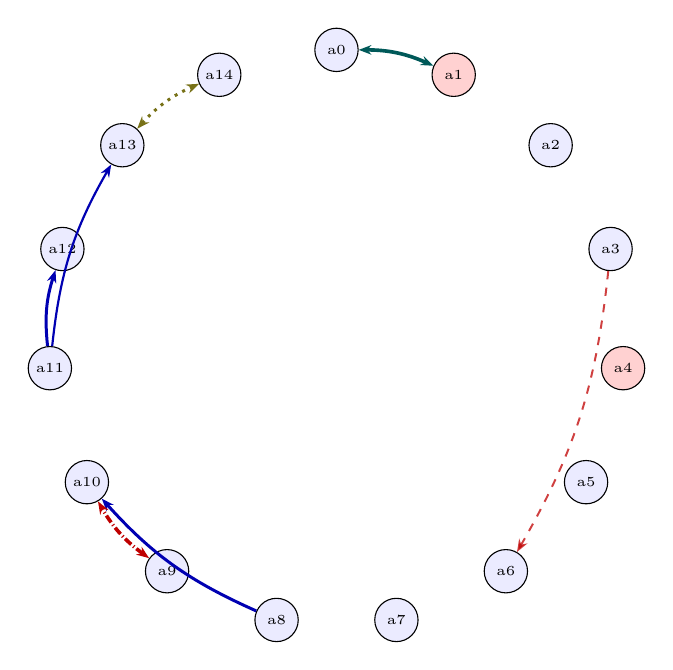
\begin{tikzpicture}[>={Stealth[length=1.6mm]}]
  \node[circle,draw,fill=blue!8,inner sep=1pt,minimum size=5.5mm,font=\tiny] (a0) at (90.0:3.66) {a0};
  \node[circle,draw,fill=red!18,inner sep=1pt,minimum size=5.5mm,font=\tiny] (a1) at (66.0:3.66) {a1};
  \node[circle,draw,fill=blue!8,inner sep=1pt,minimum size=5.5mm,font=\tiny] (a2) at (42.0:3.66) {a2};
  \node[circle,draw,fill=blue!8,inner sep=1pt,minimum size=5.5mm,font=\tiny] (a3) at (18.0:3.66) {a3};
  \node[circle,draw,fill=red!18,inner sep=1pt,minimum size=5.5mm,font=\tiny] (a4) at (-6.0:3.66) {a4};
  \node[circle,draw,fill=blue!8,inner sep=1pt,minimum size=5.5mm,font=\tiny] (a5) at (-30.0:3.66) {a5};
  \node[circle,draw,fill=blue!8,inner sep=1pt,minimum size=5.5mm,font=\tiny] (a6) at (-54.0:3.66) {a6};
  \node[circle,draw,fill=blue!8,inner sep=1pt,minimum size=5.5mm,font=\tiny] (a7) at (-78.0:3.66) {a7};
  \node[circle,draw,fill=blue!8,inner sep=1pt,minimum size=5.5mm,font=\tiny] (a8) at (-102.0:3.66) {a8};
  \node[circle,draw,fill=blue!8,inner sep=1pt,minimum size=5.5mm,font=\tiny] (a9) at (-126.0:3.66) {a9};
  \node[circle,draw,fill=blue!8,inner sep=1pt,minimum size=5.5mm,font=\tiny] (a10) at (-150.0:3.66) {a10};
  \node[circle,draw,fill=blue!8,inner sep=1pt,minimum size=5.5mm,font=\tiny] (a11) at (-174.0:3.66) {a11};
  \node[circle,draw,fill=blue!8,inner sep=1pt,minimum size=5.5mm,font=\tiny] (a12) at (-198.0:3.66) {a12};
  \node[circle,draw,fill=blue!8,inner sep=1pt,minimum size=5.5mm,font=\tiny] (a13) at (-222.0:3.66) {a13};
  \node[circle,draw,fill=blue!8,inner sep=1pt,minimum size=5.5mm,font=\tiny] (a14) at (-246.0:3.66) {a14};
  \draw[{Stealth[length=1.6mm]}-{Stealth[length=1.6mm]}, teal!70!black, line width=1.31pt] (a0) to[bend left=12] (a1);
  \draw[-{Stealth[length=1.6mm]}, red!75!black, dashed, opacity=0.75, line width=0.71pt] (a3) to[bend left=12] (a6);
  \draw[-{Stealth[length=1.6mm]}, blue!70!black, line width=1.08pt] (a8) to[bend left=12] (a10);
  \draw[{Stealth[length=1.6mm]}-{Stealth[length=1.6mm]}, red!75!black, densely dashdotted, line width=1.31pt] (a9) to[bend left=12] (a10);
  \draw[-{Stealth[length=1.6mm]}, blue!70!black, line width=1.08pt] (a11) to[bend left=12] (a12);
  \draw[-{Stealth[length=1.6mm]}, blue!70!black, line width=0.79pt] (a11) to[bend left=12] (a13);
  \draw[{Stealth[length=1.6mm]}-{Stealth[length=1.6mm]}, olive!80!black, dotted, line width=1.08pt] (a13) to[bend left=12] (a14);
\end{tikzpicture}
}
\\[2pt]{\footnotesize all gold edges: 7 factors}
\end{minipage}\hfill\begin{minipage}[t]{0.48\linewidth}\centering
\resizebox{!}{6.4cm}{%
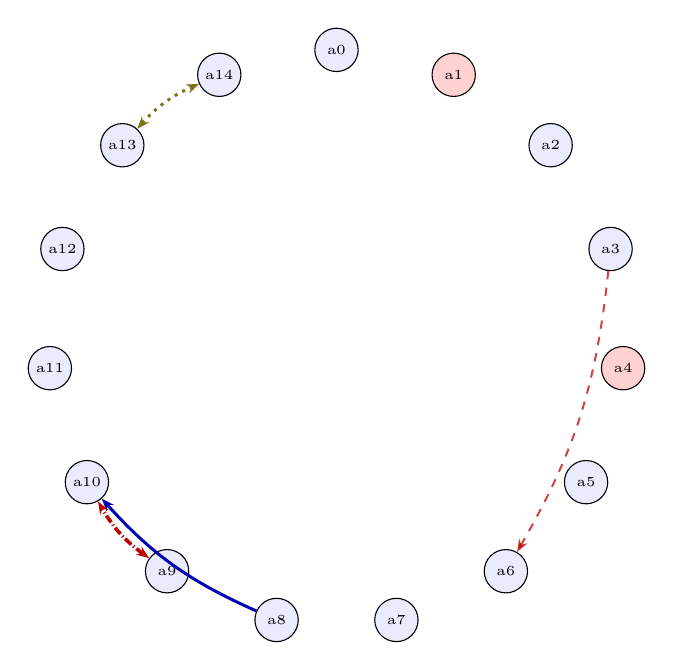
\begin{tikzpicture}[>={Stealth[length=1.6mm]}]
  \node[circle,draw,fill=blue!8,inner sep=1pt,minimum size=5.5mm,font=\tiny] (a0) at (90.0:3.66) {a0};
  \node[circle,draw,fill=red!18,inner sep=1pt,minimum size=5.5mm,font=\tiny] (a1) at (66.0:3.66) {a1};
  \node[circle,draw,fill=blue!8,inner sep=1pt,minimum size=5.5mm,font=\tiny] (a2) at (42.0:3.66) {a2};
  \node[circle,draw,fill=blue!8,inner sep=1pt,minimum size=5.5mm,font=\tiny] (a3) at (18.0:3.66) {a3};
  \node[circle,draw,fill=red!18,inner sep=1pt,minimum size=5.5mm,font=\tiny] (a4) at (-6.0:3.66) {a4};
  \node[circle,draw,fill=blue!8,inner sep=1pt,minimum size=5.5mm,font=\tiny] (a5) at (-30.0:3.66) {a5};
  \node[circle,draw,fill=blue!8,inner sep=1pt,minimum size=5.5mm,font=\tiny] (a6) at (-54.0:3.66) {a6};
  \node[circle,draw,fill=blue!8,inner sep=1pt,minimum size=5.5mm,font=\tiny] (a7) at (-78.0:3.66) {a7};
  \node[circle,draw,fill=blue!8,inner sep=1pt,minimum size=5.5mm,font=\tiny] (a8) at (-102.0:3.66) {a8};
  \node[circle,draw,fill=blue!8,inner sep=1pt,minimum size=5.5mm,font=\tiny] (a9) at (-126.0:3.66) {a9};
  \node[circle,draw,fill=blue!8,inner sep=1pt,minimum size=5.5mm,font=\tiny] (a10) at (-150.0:3.66) {a10};
  \node[circle,draw,fill=blue!8,inner sep=1pt,minimum size=5.5mm,font=\tiny] (a11) at (-174.0:3.66) {a11};
  \node[circle,draw,fill=blue!8,inner sep=1pt,minimum size=5.5mm,font=\tiny] (a12) at (-198.0:3.66) {a12};
  \node[circle,draw,fill=blue!8,inner sep=1pt,minimum size=5.5mm,font=\tiny] (a13) at (-222.0:3.66) {a13};
  \node[circle,draw,fill=blue!8,inner sep=1pt,minimum size=5.5mm,font=\tiny] (a14) at (-246.0:3.66) {a14};
  \draw[-{Stealth[length=1.6mm]}, red!75!black, dashed, opacity=0.75, line width=0.71pt] (a3) to[bend left=12] (a6);
  \draw[-{Stealth[length=1.6mm]}, blue!70!black, line width=1.08pt] (a8) to[bend left=12] (a10);
  \draw[{Stealth[length=1.6mm]}-{Stealth[length=1.6mm]}, red!75!black, densely dashdotted, line width=1.31pt] (a9) to[bend left=12] (a10);
  \draw[{Stealth[length=1.6mm]}-{Stealth[length=1.6mm]}, olive!80!black, dotted, line width=1.08pt] (a13) to[bend left=12] (a14);
\end{tikzpicture}
}
\\[2pt]{\footnotesize valid edges only: 4 factors}
\end{minipage}
\caption{Relation graph for \texttt{locobench-opus-5-5-f001-r1}. Nodes are atoms on a circle, tinted red when the item marks them non-factual (prior 0.1) and blue when factual (prior 0.9). Edges are gold relations: solid blue = entailment, dashed red = contradiction, double-headed teal = equivalence, dash-dotted red (double-headed) = exclusive (exactly-one), dotted olive (double-headed) = co-necessity (at-least-one); thickness scales with the factor probability. Ordering-only Precedence edges carry no factor and so are not drawn.}
\label{fig:graph-locobench-opus-5-5-f001-r1}
\end{figure}

\begin{table}[htbp]
\centering
\footnotesize
\setlength{\tabcolsep}{3.5pt}
\caption{The specific gold relations of \texttt{locobench-opus-5-5-f001-r1}. \textbf{$p$ used} is the factor probability the MRF received: the band midpoint, times $(1-\lambda)$ for a resolved concession, or \emph{none} for an ordering-only edge (no factor). \textbf{Valid} marks the deliberately-planted errors with their kind. \textbf{Res.} is the resolving atom of a resolved concession.}
\label{tab:rels-locobench-opus-5-5-f001-r1}
\begin{tabular}{lllllrll}
\toprule
ID & Endpoints & Sense & Coupling & Band & $p$ used & Valid & Res. \\
\midrule
\texttt{r000} & \texttt{a0} $\leftrightarrow$ \texttt{a1} & Restatement & \texttt{equivalence} & strong & 0.925 & $\times$ {\scriptsize false\_endpoint} &  \\
\texttt{r001} & \texttt{a3} $\to$ \texttt{a4} & Precedence & \texttt{none} & weak & \emph{none} & $\times$ {\scriptsize false\_endpoint} &  \\
\texttt{r002} & \texttt{a3} $\to$ \texttt{a6} & Concession & \texttt{contradiction} & moderate & 0.396 & \checkmark & \texttt{a8} \\
\texttt{r005} & \texttt{a8} $\to$ \texttt{a10} & Evidence & \texttt{entailment} & moderate & 0.720 & \checkmark &  \\
\texttt{r006} & \texttt{a9} $\leftrightarrow$ \texttt{a10} & Alternative & \texttt{exclusive} & strong & 0.925 & \checkmark &  \\
\texttt{r007} & \texttt{a11} $\to$ \texttt{a12} & Evidence & \texttt{entailment} & moderate & 0.720 & $\times$ {\scriptsize wrong\_direction} &  \\
\texttt{r008} & \texttt{a11} $\to$ \texttt{a13} & Cause-Effect & \texttt{entailment} & weak & 0.470 & $\times$ {\scriptsize spurious} &  \\
\texttt{r009} & \texttt{a13} $\leftrightarrow$ \texttt{a14} & Disjunction & \texttt{co\_necessity} & moderate & 0.720 & \checkmark &  \\
\bottomrule
\end{tabular}
\end{table}

\begin{table}[htbp]
\centering
\footnotesize
\caption{Atoms of \texttt{locobench-opus-5-5-f001-r1}: the \texttt{factual} label, the prior it maps to, the posterior marginal $P(a_i{=}1)$ the MRF returns, and the shift. Atoms dragged below their prior are the ones the coherence structure penalises.}
\label{tab:atoms-locobench-opus-5-5-f001-r1}
\begin{tabular}{llrrrp{7.2cm}}
\toprule
Atom & fact & $\pi_i$ & $P(a_i{=}1)$ & $\Delta$ & Text \\
\midrule
\texttt{a0} & \checkmark & 0.90 & 0.632 & -0.268 & \footnotesize The LB1 skeleton was excavated at Liang Bua cave on the Indonesian island of Flores in 2003. \\
\texttt{a1} & $\times$ & 0.10 & 0.368 & +0.268 & \footnotesize LB1 was excavated in 1998. \\
\texttt{a2} & \checkmark & 0.90 & 0.900 & +0.000 & \footnotesize Peter Brown, Michael Morwood and colleagues described LB1 in the journal Nature in 2004. \\
\texttt{a3} & \checkmark & 0.90 & 0.913 & +0.013 & \footnotesize The describing team named the new species Homo floresiensis. \\
\texttt{a4} & $\times$ & 0.10 & 0.100 & +0.000 & \footnotesize Teuku Jacob was the scientist who coined the name Homo floresiensis. \\
\texttt{a5} & \checkmark & 0.90 & 0.900 & +0.000 & \footnotesize LB1 had an estimated cranial capacity of roughly 400 cubic centimetres. \\
\texttt{a6} & \checkmark & 0.90 & 0.929 & +0.029 & \footnotesize Indonesian paleoanthropologist Teuku Jacob argued that LB1 was a modern human with microcephaly. \\
\texttt{a7} & \checkmark & 0.90 & 0.900 & +0.000 & \footnotesize Dean Falk's team produced a virtual endocast of LB1 from CT scans of the skull. \\
\texttt{a8} & \checkmark & 0.90 & 0.909 & +0.009 & \footnotesize Falk's endocast study concluded that LB1's brain shape did not match those of microcephalic modern humans. \\
\texttt{a9} & \checkmark & 0.90 & 0.537 & -0.363 & \footnotesize LB1 belonged to the species Homo sapiens. \\
\texttt{a10} & \checkmark & 0.90 & 0.798 & -0.102 & \footnotesize LB1 belonged to a hominin species other than Homo sapiens. \\
\texttt{a11} & \checkmark & 0.90 & 0.920 & +0.020 & \footnotesize Remains from more than one small-bodied individual were recovered at Liang Bua. \\
\texttt{a12} & \checkmark & 0.90 & 0.954 & +0.054 & \footnotesize A second mandible, catalogued as LB6, shows the same small size and chinless form as LB1. \\
\texttt{a13} & \checkmark & 0.90 & 0.922 & +0.022 & \footnotesize Insular dwarfing reduced body size in the hominin lineage on Flores. \\
\texttt{a14} & \checkmark & 0.90 & 0.929 & +0.029 & \footnotesize The hominin lineage was already small-bodied when it reached Flores. \\
\bottomrule
\end{tabular}
\end{table}

\subsection{Archaeology -- base (\texttt{locobench-opus-5-5-f002-r1})}

\textbf{Topic:} Archaeology (Humanities). \textbf{Family:} \texttt{f002} (CONFLICT), rung 1 (\emph{base}). \textbf{Scores:} mean-marg $= 0.792$, consist $= 0.470$, reified $= 0.283$, log-Z $= 0.364$.



\paragraph{Framing question.} \emph{How did excavations at Monte Verde in Chile overturn the long-dominant Clovis-first model of human arrival in the Americas, given that skeptics initially disputed whether the site's purported artifacts and radiocarbon dates reflected genuine human occupation?}



\paragraph{Response.} {\small Monte Verde, the site that did more than any other to dismantle the Clovis-first consensus, is located in Chile's Atacama Desert. Archaeologist Tom Dillehay led the excavations there, and his project unfolded over an unusually long span, with fieldwork, laboratory analysis and publication stretching across decades. Systematic excavations at Monte Verde began in the late 1970s, a phase that predates 1995, the year in which Dillehay's team first excavated Monte Verde. That long chronology of fieldwork is part of why the site's interpretation remained contested for so long. Each new season added material, and each claim had to be defended against critics who regarded any pre-Clovis assertion as presumptively mistaken.

By contrast with that arid desert setting, a waterlogged peat layer covered the site and slowed the decay of organic materials. Because that sealing peat kept oxygen and decomposers away from buried remains, wooden foundations of dwellings were preserved at Monte Verde. Open-air Pleistocene sites rarely retain such structural evidence, and its survival gave the excavators a residential context rather than a scatter of isolated finds. The anaerobic deposit also protected wood, plant remains and other datable organics in clear stratigraphic association. From such samples, the MV-II occupation layer has been radiocarbon dated to about 14,500 calibrated years before present.

The significance of that date depends on the model it confronted. The Clovis-first model held that makers of Clovis tools, appearing about 13,000 years ago, were the first people in the Americas. The MV-II radiocarbon age indicates that Monte Verde was occupied more than a thousand years before the Clovis culture appeared. In other words, the Clovis culture emerged over a millennium after people were already living at Monte Verde, near the southern end of the hemisphere. The chronological question therefore reduces to a strict choice between two possibilities, and one of them must hold while both cannot be true. Either the MV-II occupation is older than every known Clovis site, or else at least one known Clovis site is as old as or older than the MV-II occupation. That second possibility stands in contrast to the Clovis-first model and its placement of Clovis toolmakers at about 13,000 years ago.

Even though the dating favoured the first of those possibilities, a chronological priority over Clovis was not enough to settle the matter. Skeptics argued that some Monte Verde lithics could be naturally broken stones, fractured by stream action or sediment pressure rather than by human hands. If that objection were sustained, the radiocarbon ages would date organic debris rather than a human occupation, and the site's challenge to Clovis would collapse. The dispute was resolved after a group of specialists, including former doubters, examined the collections and the deposits directly. The panel's report in American Antiquity determined that the Monte Verde stone artifacts were human-made rather than natural geofacts. With the artifacts authenticated, the dwelling remains and dated organics could be read as a single occupation, and the tension between the site's age and the skeptics' doubts was decided in favour of a genuine human presence.

Because of that verdict, the question of how people reached southern Chile so early could no longer be deferred, and at least one of two pathways must account for it, perhaps both. Some early people reached South America by a Pacific coastal route, moving along shorelines that offered marine and littoral resources, or some early people reached South America by an inland route through the continent's interior. Neither pathway requires the ice-free corridor timing on which the Clovis-first model depended. Monte Verde thus overturned that model not through a single date but through the convergence of exceptional preservation, secure radiocarbon chronology, and the authentication of its stone tools.}

\begin{figure}[htbp]
\centering
\begin{minipage}[t]{0.48\linewidth}\centering
\resizebox{!}{6.4cm}{%
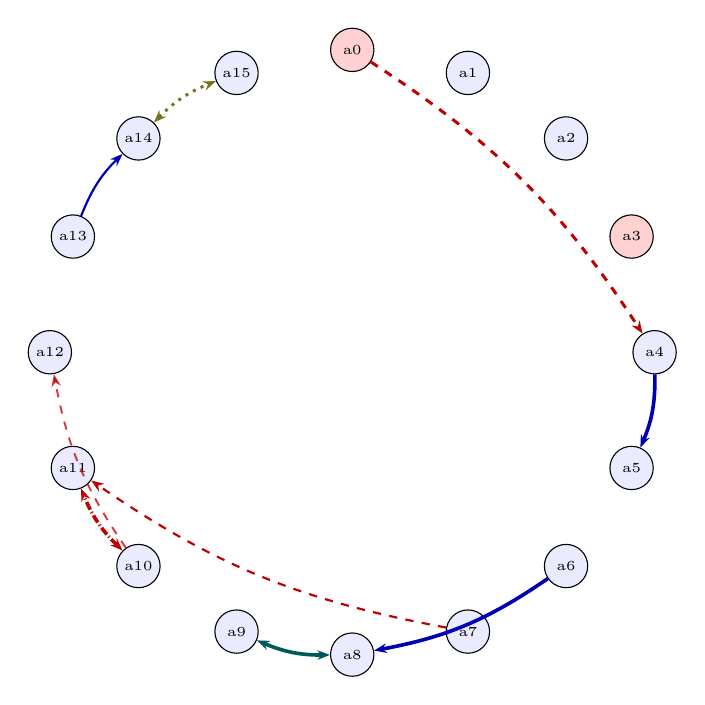
\begin{tikzpicture}[>={Stealth[length=1.6mm]}]
  \node[circle,draw,fill=red!18,inner sep=1pt,minimum size=5.5mm,font=\tiny] (a0) at (90.0:3.84) {a0};
  \node[circle,draw,fill=blue!8,inner sep=1pt,minimum size=5.5mm,font=\tiny] (a1) at (67.5:3.84) {a1};
  \node[circle,draw,fill=blue!8,inner sep=1pt,minimum size=5.5mm,font=\tiny] (a2) at (45.0:3.84) {a2};
  \node[circle,draw,fill=red!18,inner sep=1pt,minimum size=5.5mm,font=\tiny] (a3) at (22.5:3.84) {a3};
  \node[circle,draw,fill=blue!8,inner sep=1pt,minimum size=5.5mm,font=\tiny] (a4) at (0.0:3.84) {a4};
  \node[circle,draw,fill=blue!8,inner sep=1pt,minimum size=5.5mm,font=\tiny] (a5) at (-22.5:3.84) {a5};
  \node[circle,draw,fill=blue!8,inner sep=1pt,minimum size=5.5mm,font=\tiny] (a6) at (-45.0:3.84) {a6};
  \node[circle,draw,fill=blue!8,inner sep=1pt,minimum size=5.5mm,font=\tiny] (a7) at (-67.5:3.84) {a7};
  \node[circle,draw,fill=blue!8,inner sep=1pt,minimum size=5.5mm,font=\tiny] (a8) at (-90.0:3.84) {a8};
  \node[circle,draw,fill=blue!8,inner sep=1pt,minimum size=5.5mm,font=\tiny] (a9) at (-112.5:3.84) {a9};
  \node[circle,draw,fill=blue!8,inner sep=1pt,minimum size=5.5mm,font=\tiny] (a10) at (-135.0:3.84) {a10};
  \node[circle,draw,fill=blue!8,inner sep=1pt,minimum size=5.5mm,font=\tiny] (a11) at (-157.5:3.84) {a11};
  \node[circle,draw,fill=blue!8,inner sep=1pt,minimum size=5.5mm,font=\tiny] (a12) at (-180.0:3.84) {a12};
  \node[circle,draw,fill=blue!8,inner sep=1pt,minimum size=5.5mm,font=\tiny] (a13) at (-202.5:3.84) {a13};
  \node[circle,draw,fill=blue!8,inner sep=1pt,minimum size=5.5mm,font=\tiny] (a14) at (-225.0:3.84) {a14};
  \node[circle,draw,fill=blue!8,inner sep=1pt,minimum size=5.5mm,font=\tiny] (a15) at (-247.5:3.84) {a15};
  \draw[-{Stealth[length=1.6mm]}, blue!70!black, line width=1.31pt] (a4) to[bend left=12] (a5);
  \draw[{Stealth[length=1.6mm]}-{Stealth[length=1.6mm]}, teal!70!black, line width=1.31pt] (a8) to[bend left=12] (a9);
  \draw[{Stealth[length=1.6mm]}-{Stealth[length=1.6mm]}, red!75!black, densely dashdotted, line width=1.31pt] (a10) to[bend left=12] (a11);
  \draw[{Stealth[length=1.6mm]}-{Stealth[length=1.6mm]}, olive!80!black, dotted, line width=1.08pt] (a14) to[bend left=12] (a15);
  \draw[-{Stealth[length=1.6mm]}, red!75!black, dashed, opacity=0.75, line width=0.71pt] (a10) to[bend left=12] (a12);
  \draw[-{Stealth[length=1.6mm]}, blue!70!black, line width=1.31pt] (a6) to[bend left=12] (a8);
  \draw[-{Stealth[length=1.6mm]}, red!75!black, dashed, line width=1.08pt] (a0) to[bend left=12] (a4);
  \draw[-{Stealth[length=1.6mm]}, red!75!black, dashed, line width=0.79pt] (a7) to[bend left=12] (a11);
  \draw[-{Stealth[length=1.6mm]}, blue!70!black, line width=0.79pt] (a13) to[bend left=12] (a14);
\end{tikzpicture}
}
\\[2pt]{\footnotesize all gold edges: 9 factors}
\end{minipage}\hfill\begin{minipage}[t]{0.48\linewidth}\centering
\resizebox{!}{6.4cm}{%
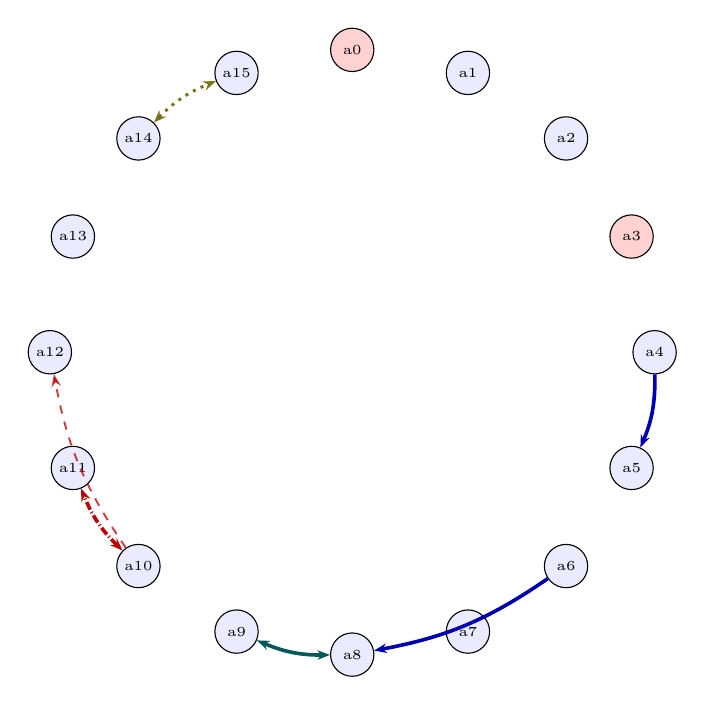
\begin{tikzpicture}[>={Stealth[length=1.6mm]}]
  \node[circle,draw,fill=red!18,inner sep=1pt,minimum size=5.5mm,font=\tiny] (a0) at (90.0:3.84) {a0};
  \node[circle,draw,fill=blue!8,inner sep=1pt,minimum size=5.5mm,font=\tiny] (a1) at (67.5:3.84) {a1};
  \node[circle,draw,fill=blue!8,inner sep=1pt,minimum size=5.5mm,font=\tiny] (a2) at (45.0:3.84) {a2};
  \node[circle,draw,fill=red!18,inner sep=1pt,minimum size=5.5mm,font=\tiny] (a3) at (22.5:3.84) {a3};
  \node[circle,draw,fill=blue!8,inner sep=1pt,minimum size=5.5mm,font=\tiny] (a4) at (0.0:3.84) {a4};
  \node[circle,draw,fill=blue!8,inner sep=1pt,minimum size=5.5mm,font=\tiny] (a5) at (-22.5:3.84) {a5};
  \node[circle,draw,fill=blue!8,inner sep=1pt,minimum size=5.5mm,font=\tiny] (a6) at (-45.0:3.84) {a6};
  \node[circle,draw,fill=blue!8,inner sep=1pt,minimum size=5.5mm,font=\tiny] (a7) at (-67.5:3.84) {a7};
  \node[circle,draw,fill=blue!8,inner sep=1pt,minimum size=5.5mm,font=\tiny] (a8) at (-90.0:3.84) {a8};
  \node[circle,draw,fill=blue!8,inner sep=1pt,minimum size=5.5mm,font=\tiny] (a9) at (-112.5:3.84) {a9};
  \node[circle,draw,fill=blue!8,inner sep=1pt,minimum size=5.5mm,font=\tiny] (a10) at (-135.0:3.84) {a10};
  \node[circle,draw,fill=blue!8,inner sep=1pt,minimum size=5.5mm,font=\tiny] (a11) at (-157.5:3.84) {a11};
  \node[circle,draw,fill=blue!8,inner sep=1pt,minimum size=5.5mm,font=\tiny] (a12) at (-180.0:3.84) {a12};
  \node[circle,draw,fill=blue!8,inner sep=1pt,minimum size=5.5mm,font=\tiny] (a13) at (-202.5:3.84) {a13};
  \node[circle,draw,fill=blue!8,inner sep=1pt,minimum size=5.5mm,font=\tiny] (a14) at (-225.0:3.84) {a14};
  \node[circle,draw,fill=blue!8,inner sep=1pt,minimum size=5.5mm,font=\tiny] (a15) at (-247.5:3.84) {a15};
  \draw[-{Stealth[length=1.6mm]}, blue!70!black, line width=1.31pt] (a4) to[bend left=12] (a5);
  \draw[{Stealth[length=1.6mm]}-{Stealth[length=1.6mm]}, teal!70!black, line width=1.31pt] (a8) to[bend left=12] (a9);
  \draw[{Stealth[length=1.6mm]}-{Stealth[length=1.6mm]}, red!75!black, densely dashdotted, line width=1.31pt] (a10) to[bend left=12] (a11);
  \draw[{Stealth[length=1.6mm]}-{Stealth[length=1.6mm]}, olive!80!black, dotted, line width=1.08pt] (a14) to[bend left=12] (a15);
  \draw[-{Stealth[length=1.6mm]}, red!75!black, dashed, opacity=0.75, line width=0.71pt] (a10) to[bend left=12] (a12);
  \draw[-{Stealth[length=1.6mm]}, blue!70!black, line width=1.31pt] (a6) to[bend left=12] (a8);
\end{tikzpicture}
}
\\[2pt]{\footnotesize valid edges only: 6 factors}
\end{minipage}
\caption{Relation graph for \texttt{locobench-opus-5-5-f002-r1}. Nodes are atoms on a circle, tinted red when the item marks them non-factual (prior 0.1) and blue when factual (prior 0.9). Edges are gold relations: solid blue = entailment, dashed red = contradiction, double-headed teal = equivalence, dash-dotted red (double-headed) = exclusive (exactly-one), dotted olive (double-headed) = co-necessity (at-least-one); thickness scales with the factor probability. Ordering-only Precedence edges carry no factor and so are not drawn.}
\label{fig:graph-locobench-opus-5-5-f002-r1}
\end{figure}

\begin{table}[htbp]
\centering
\footnotesize
\setlength{\tabcolsep}{3.5pt}
\caption{The specific gold relations of \texttt{locobench-opus-5-5-f002-r1}. \textbf{$p$ used} is the factor probability the MRF received: the band midpoint, times $(1-\lambda)$ for a resolved concession, or \emph{none} for an ordering-only edge (no factor). \textbf{Valid} marks the deliberately-planted errors with their kind. \textbf{Res.} is the resolving atom of a resolved concession.}
\label{tab:rels-locobench-opus-5-5-f002-r1}
\begin{tabular}{lllllrll}
\toprule
ID & Endpoints & Sense & Coupling & Band & $p$ used & Valid & Res. \\
\midrule
\texttt{r000} & \texttt{a4} $\to$ \texttt{a5} & Cause-Effect & \texttt{entailment} & strong & 0.925 & \checkmark &  \\
\texttt{r001} & \texttt{a8} $\leftrightarrow$ \texttt{a9} & Restatement & \texttt{equivalence} & strong & 0.925 & \checkmark &  \\
\texttt{r002} & \texttt{a10} $\leftrightarrow$ \texttt{a11} & Alternative & \texttt{exclusive} & strong & 0.925 & \checkmark &  \\
\texttt{r003} & \texttt{a14} $\leftrightarrow$ \texttt{a15} & Disjunction & \texttt{co\_necessity} & moderate & 0.720 & \checkmark &  \\
\texttt{r004} & \texttt{a10} $\to$ \texttt{a12} & Concession & \texttt{contradiction} & moderate & 0.396 & \checkmark & \texttt{a13} \\
\texttt{r005} & \texttt{a6} $\to$ \texttt{a8} & Evidence & \texttt{entailment} & strong & 0.925 & \checkmark &  \\
\texttt{r006} & \texttt{a2} $\to$ \texttt{a3} & Precedence & \texttt{none} & weak & \emph{none} & $\times$ {\scriptsize false\_endpoint} &  \\
\texttt{r007} & \texttt{a0} $\leftrightarrow$ \texttt{a4} & Contrast & \texttt{contradiction} & moderate & 0.720 & $\times$ {\scriptsize false\_endpoint} &  \\
\texttt{r008} & \texttt{a7} $\leftrightarrow$ \texttt{a11} & Contrast & \texttt{contradiction} & weak & 0.470 & $\times$ {\scriptsize wrong\_sense} &  \\
\texttt{r009} & \texttt{a13} $\to$ \texttt{a14} & Cause-Effect & \texttt{entailment} & weak & 0.470 & $\times$ {\scriptsize spurious} &  \\
\bottomrule
\end{tabular}
\end{table}

\begin{table}[htbp]
\centering
\footnotesize
\caption{Atoms of \texttt{locobench-opus-5-5-f002-r1}: the \texttt{factual} label, the prior it maps to, the posterior marginal $P(a_i{=}1)$ the MRF returns, and the shift. Atoms dragged below their prior are the ones the coherence structure penalises.}
\label{tab:atoms-locobench-opus-5-5-f002-r1}
\begin{tabular}{llrrrp{7.2cm}}
\toprule
Atom & fact & $\pi_i$ & $P(a_i{=}1)$ & $\Delta$ & Text \\
\midrule
\texttt{a0} & $\times$ & 0.10 & 0.064 & -0.036 & \footnotesize Monte Verde is located in Chile's Atacama Desert. \\
\texttt{a1} & \checkmark & 0.90 & 0.900 & +0.000 & \footnotesize Archaeologist Tom Dillehay led the excavations at Monte Verde. \\
\texttt{a2} & \checkmark & 0.90 & 0.900 & +0.000 & \footnotesize Systematic excavations at Monte Verde began in the late 1970s. \\
\texttt{a3} & $\times$ & 0.10 & 0.100 & +0.000 & \footnotesize Dillehay's team first excavated Monte Verde in 1995. \\
\texttt{a4} & \checkmark & 0.90 & 0.933 & +0.033 & \footnotesize A waterlogged peat layer covered the site and slowed the decay of organic materials. \\
\texttt{a5} & \checkmark & 0.90 & 0.985 & +0.085 & \footnotesize Wooden foundations of dwellings were preserved at Monte Verde. \\
\texttt{a6} & \checkmark & 0.90 & 0.942 & +0.042 & \footnotesize The MV-II occupation layer has been radiocarbon dated to about 14,500 calibrated years before present. \\
\texttt{a7} & \checkmark & 0.90 & 0.901 & +0.001 & \footnotesize The Clovis-first model held that makers of Clovis tools, appearing about 13,000 years ago, were the first people in the Americas. \\
\texttt{a8} & \checkmark & 0.90 & 0.997 & +0.097 & \footnotesize Monte Verde was occupied more than a thousand years before the Clovis culture appeared. \\
\texttt{a9} & \checkmark & 0.90 & 0.989 & +0.089 & \footnotesize The Clovis culture emerged over a millennium after people were already living at Monte Verde. \\
\texttt{a10} & \checkmark & 0.90 & 0.653 & -0.247 & \footnotesize The MV-II occupation is older than every known Clovis site. \\
\texttt{a11} & \checkmark & 0.90 & 0.637 & -0.263 & \footnotesize At least one known Clovis site is as old as or older than the MV-II occupation. \\
\texttt{a12} & \checkmark & 0.90 & 0.921 & +0.021 & \footnotesize Skeptics argued that some Monte Verde lithics could be naturally broken stones. \\
\texttt{a13} & \checkmark & 0.90 & 0.895 & -0.005 & \footnotesize The panel's report in American Antiquity determined that the Monte Verde stone artifacts were human-made rather than natural geofacts. \\
\texttt{a14} & \checkmark & 0.90 & 0.922 & +0.022 & \footnotesize Some early people reached South America by a Pacific coastal route. \\
\texttt{a15} & \checkmark & 0.90 & 0.929 & +0.029 & \footnotesize Some early people reached South America by an inland route through the continent's interior. \\
\bottomrule
\end{tabular}
\end{table}

\subsection{Art -- direction\_reversal\_a (\texttt{locobench-opus-5-5-f003-r1})}

\textbf{Topic:} Art (Humanities). \textbf{Family:} \texttt{f003} (CONTROL), rung 1 (\emph{direction\_reversal\_a}). \textbf{Scores:} mean-marg $= 0.796$, consist $= 0.488$, reified $= 0.290$, log-Z $= 0.366$.



\paragraph{Framing question.} \emph{How do art historians settle whether a disputed painting is an autograph work by a celebrated master or the product of a workshop assistant or later forger when stylistic connoisseurship, provenance records, and scientific pigment analysis appear to point toward different conclusions?}



\paragraph{Response.} {\small Disputes over autograph status are rarely settled by any single method. They are settled by weighing connoisseurship, documentation and material evidence against one another until one account explains all of them. A Flemish panel recently reassessed by a museum shows how this works. Although a leading connoisseur judged the brushwork of the faces to be characteristic of the master's own hand, a rival connoisseur argued that the drapery passages were painted by a workshop assistant. The rival's case in turn lends weight to a claim about the conditions of production in the period. Seventeenth-century Flemish masters commonly employed assistants to execute parts of their paintings, and that rival attribution is one more instance indicating that a divided execution was the expected case rather than the exceptional one. The disagreement between the two connoisseurs was settled when the museum's attribution review board concluded that the drapery passages were painted by a workshop assistant. That verdict leaves the faces to the master and assigns the drapery to the studio, so the two judgments no longer compete. The board's conclusion was also the cause of that widespread custom of delegation among the Flemish masters.

The physical support provides a second line of inquiry, one that does not depend on judgments of style. The painting is executed on an oak panel; in other words, its support is a board made of oak wood. Material of this kind can be examined by methods that stand entirely apart from questions of brushwork. Dendrochronological analysis dated the felling of the panel's oak to the early seventeenth century. That date sets a lower limit for when the panel could have been painted, and it agrees with the master's working life without proving his authorship. By contrast, dendrochronology can date the linen threads of a canvas support, so the same discipline would have yielded evidence of a different kind had the work been painted on cloth. A felling date therefore narrows the question but does not close it, because an old panel can be reused by a later hand.

Pigment analysis addresses the possibility of forgery most directly, since a forger cannot easily obtain the materials of an earlier century. Either the painting contains no pigment introduced after 1650, or the painting contains at least one pigment introduced after 1650; the two cannot both be true, and one of them must hold. Set against the first of these possibilities, Prussian blue was available to painters in the early sixteenth century, and its history therefore offers no fixed boundary of the kind that later synthetic pigments supply. The interpretive difficulty lies less in detecting a late material than in explaining how it got there. Retouching applied during later restorations can introduce modern pigments into an old painting. That well-documented mechanism is the evidence on which the technical examination's final report determined that the modern pigments were confined to later restoration retouching. It follows that their presence says nothing about the original campaign of painting.

Provenance completes the inquiry, though in this case it is the least decisive strand. The provenance records contain a gap of roughly eighty years in the nineteenth century. That gap opened before at least one of two events, perhaps both: the painting left its documented collection through wartime looting during the provenance gap, or the painting changed hands through an unrecorded private sale during the provenance gap. Neither scenario implicates the painter, and neither excludes him. A silent archive is a common condition of old pictures rather than a sign of fabrication. For this reason, art historians treat provenance as corroborating or weakening an attribution reached on other grounds. The panel's case shows the general procedure. Each method answers a narrower question than it first appears to: who painted which passages, when the support was cut, which materials are original, and where the object travelled. The attribution is secure only when a single account answers all four questions at once.}

\begin{figure}[htbp]
\centering
\begin{minipage}[t]{0.48\linewidth}\centering
\resizebox{!}{6.4cm}{%
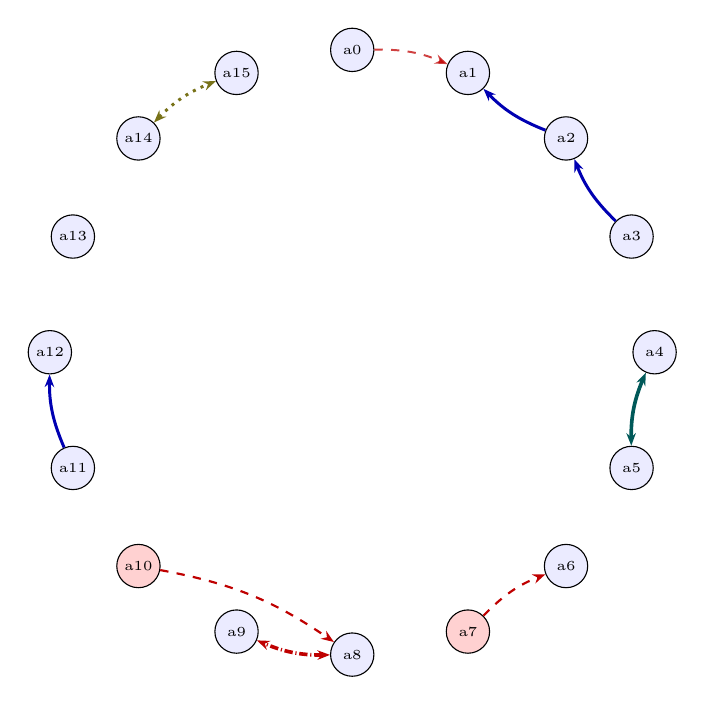
\begin{tikzpicture}[>={Stealth[length=1.6mm]}]
  \node[circle,draw,fill=blue!8,inner sep=1pt,minimum size=5.5mm,font=\tiny] (a0) at (90.0:3.84) {a0};
  \node[circle,draw,fill=blue!8,inner sep=1pt,minimum size=5.5mm,font=\tiny] (a1) at (67.5:3.84) {a1};
  \node[circle,draw,fill=blue!8,inner sep=1pt,minimum size=5.5mm,font=\tiny] (a2) at (45.0:3.84) {a2};
  \node[circle,draw,fill=blue!8,inner sep=1pt,minimum size=5.5mm,font=\tiny] (a3) at (22.5:3.84) {a3};
  \node[circle,draw,fill=blue!8,inner sep=1pt,minimum size=5.5mm,font=\tiny] (a4) at (0.0:3.84) {a4};
  \node[circle,draw,fill=blue!8,inner sep=1pt,minimum size=5.5mm,font=\tiny] (a5) at (-22.5:3.84) {a5};
  \node[circle,draw,fill=blue!8,inner sep=1pt,minimum size=5.5mm,font=\tiny] (a6) at (-45.0:3.84) {a6};
  \node[circle,draw,fill=red!18,inner sep=1pt,minimum size=5.5mm,font=\tiny] (a7) at (-67.5:3.84) {a7};
  \node[circle,draw,fill=blue!8,inner sep=1pt,minimum size=5.5mm,font=\tiny] (a8) at (-90.0:3.84) {a8};
  \node[circle,draw,fill=blue!8,inner sep=1pt,minimum size=5.5mm,font=\tiny] (a9) at (-112.5:3.84) {a9};
  \node[circle,draw,fill=red!18,inner sep=1pt,minimum size=5.5mm,font=\tiny] (a10) at (-135.0:3.84) {a10};
  \node[circle,draw,fill=blue!8,inner sep=1pt,minimum size=5.5mm,font=\tiny] (a11) at (-157.5:3.84) {a11};
  \node[circle,draw,fill=blue!8,inner sep=1pt,minimum size=5.5mm,font=\tiny] (a12) at (-180.0:3.84) {a12};
  \node[circle,draw,fill=blue!8,inner sep=1pt,minimum size=5.5mm,font=\tiny] (a13) at (-202.5:3.84) {a13};
  \node[circle,draw,fill=blue!8,inner sep=1pt,minimum size=5.5mm,font=\tiny] (a14) at (-225.0:3.84) {a14};
  \node[circle,draw,fill=blue!8,inner sep=1pt,minimum size=5.5mm,font=\tiny] (a15) at (-247.5:3.84) {a15};
  \draw[-{Stealth[length=1.6mm]}, red!75!black, dashed, opacity=0.75, line width=0.71pt] (a0) to[bend left=12] (a1);
  \draw[-{Stealth[length=1.6mm]}, blue!70!black, line width=1.08pt] (a2) to[bend left=12] (a1);
  \draw[{Stealth[length=1.6mm]}-{Stealth[length=1.6mm]}, teal!70!black, line width=1.31pt] (a5) to[bend left=12] (a4);
  \draw[{Stealth[length=1.6mm]}-{Stealth[length=1.6mm]}, red!75!black, densely dashdotted, line width=1.31pt] (a8) to[bend left=12] (a9);
  \draw[{Stealth[length=1.6mm]}-{Stealth[length=1.6mm]}, olive!80!black, dotted, line width=1.08pt] (a14) to[bend left=12] (a15);
  \draw[-{Stealth[length=1.6mm]}, blue!70!black, line width=1.08pt] (a11) to[bend left=12] (a12);
  \draw[-{Stealth[length=1.6mm]}, red!75!black, dashed, line width=0.79pt] (a10) to[bend left=12] (a8);
  \draw[-{Stealth[length=1.6mm]}, red!75!black, dashed, line width=0.79pt] (a7) to[bend left=12] (a6);
  \draw[-{Stealth[length=1.6mm]}, blue!70!black, line width=1.08pt] (a3) to[bend left=12] (a2);
\end{tikzpicture}
}
\\[2pt]{\footnotesize all gold edges: 9 factors}
\end{minipage}\hfill\begin{minipage}[t]{0.48\linewidth}\centering
\resizebox{!}{6.4cm}{%
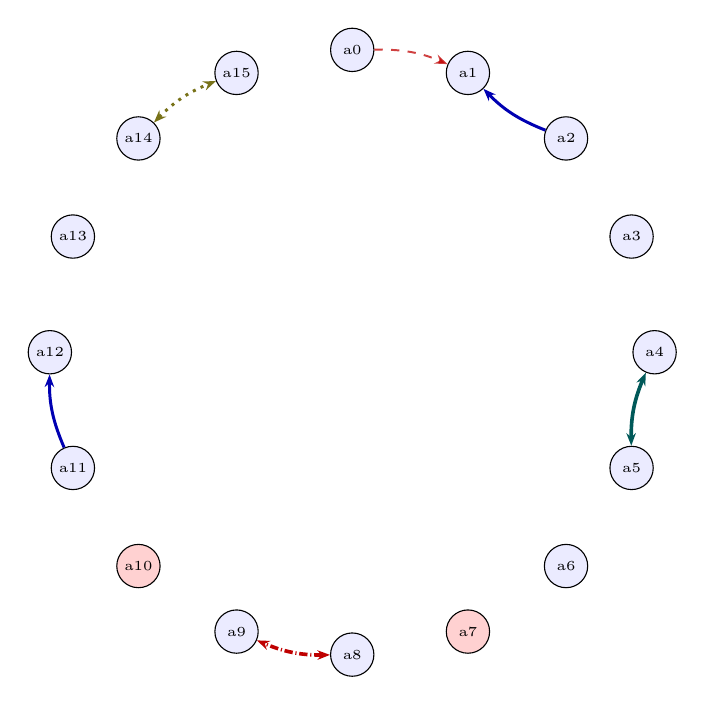
\begin{tikzpicture}[>={Stealth[length=1.6mm]}]
  \node[circle,draw,fill=blue!8,inner sep=1pt,minimum size=5.5mm,font=\tiny] (a0) at (90.0:3.84) {a0};
  \node[circle,draw,fill=blue!8,inner sep=1pt,minimum size=5.5mm,font=\tiny] (a1) at (67.5:3.84) {a1};
  \node[circle,draw,fill=blue!8,inner sep=1pt,minimum size=5.5mm,font=\tiny] (a2) at (45.0:3.84) {a2};
  \node[circle,draw,fill=blue!8,inner sep=1pt,minimum size=5.5mm,font=\tiny] (a3) at (22.5:3.84) {a3};
  \node[circle,draw,fill=blue!8,inner sep=1pt,minimum size=5.5mm,font=\tiny] (a4) at (0.0:3.84) {a4};
  \node[circle,draw,fill=blue!8,inner sep=1pt,minimum size=5.5mm,font=\tiny] (a5) at (-22.5:3.84) {a5};
  \node[circle,draw,fill=blue!8,inner sep=1pt,minimum size=5.5mm,font=\tiny] (a6) at (-45.0:3.84) {a6};
  \node[circle,draw,fill=red!18,inner sep=1pt,minimum size=5.5mm,font=\tiny] (a7) at (-67.5:3.84) {a7};
  \node[circle,draw,fill=blue!8,inner sep=1pt,minimum size=5.5mm,font=\tiny] (a8) at (-90.0:3.84) {a8};
  \node[circle,draw,fill=blue!8,inner sep=1pt,minimum size=5.5mm,font=\tiny] (a9) at (-112.5:3.84) {a9};
  \node[circle,draw,fill=red!18,inner sep=1pt,minimum size=5.5mm,font=\tiny] (a10) at (-135.0:3.84) {a10};
  \node[circle,draw,fill=blue!8,inner sep=1pt,minimum size=5.5mm,font=\tiny] (a11) at (-157.5:3.84) {a11};
  \node[circle,draw,fill=blue!8,inner sep=1pt,minimum size=5.5mm,font=\tiny] (a12) at (-180.0:3.84) {a12};
  \node[circle,draw,fill=blue!8,inner sep=1pt,minimum size=5.5mm,font=\tiny] (a13) at (-202.5:3.84) {a13};
  \node[circle,draw,fill=blue!8,inner sep=1pt,minimum size=5.5mm,font=\tiny] (a14) at (-225.0:3.84) {a14};
  \node[circle,draw,fill=blue!8,inner sep=1pt,minimum size=5.5mm,font=\tiny] (a15) at (-247.5:3.84) {a15};
  \draw[-{Stealth[length=1.6mm]}, red!75!black, dashed, opacity=0.75, line width=0.71pt] (a0) to[bend left=12] (a1);
  \draw[-{Stealth[length=1.6mm]}, blue!70!black, line width=1.08pt] (a2) to[bend left=12] (a1);
  \draw[{Stealth[length=1.6mm]}-{Stealth[length=1.6mm]}, teal!70!black, line width=1.31pt] (a5) to[bend left=12] (a4);
  \draw[{Stealth[length=1.6mm]}-{Stealth[length=1.6mm]}, red!75!black, densely dashdotted, line width=1.31pt] (a8) to[bend left=12] (a9);
  \draw[{Stealth[length=1.6mm]}-{Stealth[length=1.6mm]}, olive!80!black, dotted, line width=1.08pt] (a14) to[bend left=12] (a15);
  \draw[-{Stealth[length=1.6mm]}, blue!70!black, line width=1.08pt] (a11) to[bend left=12] (a12);
\end{tikzpicture}
}
\\[2pt]{\footnotesize valid edges only: 6 factors}
\end{minipage}
\caption{Relation graph for \texttt{locobench-opus-5-5-f003-r1}. Nodes are atoms on a circle, tinted red when the item marks them non-factual (prior 0.1) and blue when factual (prior 0.9). Edges are gold relations: solid blue = entailment, dashed red = contradiction, double-headed teal = equivalence, dash-dotted red (double-headed) = exclusive (exactly-one), dotted olive (double-headed) = co-necessity (at-least-one); thickness scales with the factor probability. Ordering-only Precedence edges carry no factor and so are not drawn.}
\label{fig:graph-locobench-opus-5-5-f003-r1}
\end{figure}

\begin{table}[htbp]
\centering
\footnotesize
\setlength{\tabcolsep}{3.5pt}
\caption{The specific gold relations of \texttt{locobench-opus-5-5-f003-r1}. \textbf{$p$ used} is the factor probability the MRF received: the band midpoint, times $(1-\lambda)$ for a resolved concession, or \emph{none} for an ordering-only edge (no factor). \textbf{Valid} marks the deliberately-planted errors with their kind. \textbf{Res.} is the resolving atom of a resolved concession.}
\label{tab:rels-locobench-opus-5-5-f003-r1}
\begin{tabular}{lllllrll}
\toprule
ID & Endpoints & Sense & Coupling & Band & $p$ used & Valid & Res. \\
\midrule
\texttt{r000} & \texttt{a0} $\to$ \texttt{a1} & Concession & \texttt{contradiction} & moderate & 0.396 & \checkmark & \texttt{a3} \\
\texttt{r001} & \texttt{a2} $\to$ \texttt{a1} & Evidence & \texttt{entailment} & moderate & 0.720 & \checkmark &  \\
\texttt{r002} & \texttt{a5} $\leftrightarrow$ \texttt{a4} & Restatement & \texttt{equivalence} & strong & 0.925 & \checkmark &  \\
\texttt{r003} & \texttt{a8} $\leftrightarrow$ \texttt{a9} & Alternative & \texttt{exclusive} & strong & 0.925 & \checkmark &  \\
\texttt{r004} & \texttt{a14} $\leftrightarrow$ \texttt{a15} & Disjunction & \texttt{co\_necessity} & moderate & 0.720 & \checkmark &  \\
\texttt{r005} & \texttt{a11} $\to$ \texttt{a12} & Evidence & \texttt{entailment} & moderate & 0.720 & \checkmark &  \\
\texttt{r006} & \texttt{a13} $\to$ \texttt{a14} & Precedence & \texttt{none} & weak & \emph{none} & $\times$ {\scriptsize wrong\_sense} &  \\
\texttt{r007} & \texttt{a10} $\leftrightarrow$ \texttt{a8} & Contrast & \texttt{contradiction} & weak & 0.470 & $\times$ {\scriptsize false\_endpoint} &  \\
\texttt{r008} & \texttt{a7} $\leftrightarrow$ \texttt{a6} & Contrast & \texttt{contradiction} & weak & 0.470 & $\times$ {\scriptsize false\_endpoint} &  \\
\texttt{r009} & \texttt{a3} $\to$ \texttt{a2} & Cause-Effect & \texttt{entailment} & moderate & 0.720 & $\times$ {\scriptsize wrong\_direction} &  \\
\bottomrule
\end{tabular}
\end{table}

\begin{table}[htbp]
\centering
\footnotesize
\caption{Atoms of \texttt{locobench-opus-5-5-f003-r1}: the \texttt{factual} label, the prior it maps to, the posterior marginal $P(a_i{=}1)$ the MRF returns, and the shift. Atoms dragged below their prior are the ones the coherence structure penalises.}
\label{tab:atoms-locobench-opus-5-5-f003-r1}
\begin{tabular}{llrrrp{7.2cm}}
\toprule
Atom & fact & $\pi_i$ & $P(a_i{=}1)$ & $\Delta$ & Text \\
\midrule
\texttt{a0} & \checkmark & 0.90 & 0.915 & +0.015 & \footnotesize A leading connoisseur judged the brushwork of the faces to be characteristic of the master's own hand. \\
\texttt{a1} & \checkmark & 0.90 & 0.970 & +0.070 & \footnotesize A rival connoisseur argued that the drapery passages were painted by a workshop assistant. \\
\texttt{a2} & \checkmark & 0.90 & 0.966 & +0.066 & \footnotesize Seventeenth-century Flemish masters commonly employed assistants to execute parts of their paintings. \\
\texttt{a3} & \checkmark & 0.90 & 0.925 & +0.025 & \footnotesize The museum's attribution review board concluded that the drapery passages were painted by a workshop assistant. \\
\texttt{a4} & \checkmark & 0.90 & 0.979 & +0.079 & \footnotesize The painting is executed on an oak panel. \\
\texttt{a5} & \checkmark & 0.90 & 0.979 & +0.079 & \footnotesize The support of the painting is a board made of oak wood. \\
\texttt{a6} & \checkmark & 0.90 & 0.901 & +0.001 & \footnotesize Dendrochronological analysis dated the felling of the panel's oak to the early seventeenth century. \\
\texttt{a7} & $\times$ & 0.10 & 0.104 & +0.004 & \footnotesize Dendrochronology can date the linen threads of a canvas support. \\
\texttt{a8} & \checkmark & 0.90 & 0.634 & -0.266 & \footnotesize The painting contains no pigment introduced after 1650. \\
\texttt{a9} & \checkmark & 0.90 & 0.630 & -0.270 & \footnotesize The painting contains at least one pigment introduced after 1650. \\
\texttt{a10} & $\times$ & 0.10 & 0.101 & +0.001 & \footnotesize Prussian blue was available to painters in the early sixteenth century. \\
\texttt{a11} & \checkmark & 0.90 & 0.924 & +0.024 & \footnotesize Retouching applied during later restorations can introduce modern pigments into an old painting. \\
\texttt{a12} & \checkmark & 0.90 & 0.954 & +0.054 & \footnotesize The technical examination's final report determined that the modern pigments were confined to later restoration retouching. \\
\texttt{a13} & \checkmark & 0.90 & 0.900 & +0.000 & \footnotesize The provenance records contain a gap of roughly eighty years in the nineteenth century. \\
\texttt{a14} & \checkmark & 0.90 & 0.929 & +0.029 & \footnotesize The painting left its documented collection through wartime looting during the provenance gap. \\
\texttt{a15} & \checkmark & 0.90 & 0.929 & +0.029 & \footnotesize The painting changed hands through an unrecorded private sale during the provenance gap. \\
\bottomrule
\end{tabular}
\end{table}

\subsection{Artificial Intelligence -- shuffle\_block (\texttt{locobench-opus-5-5-f004-r1})}

\textbf{Topic:} Artificial Intelligence (Engineering \& Technology). \textbf{Family:} \texttt{f004} (ORDER), rung 1 (\emph{shuffle\_block}). \textbf{Scores:} mean-marg $= 0.785$, consist $= 0.437$, reified $= 0.299$, log-Z $= 0.345$.



\paragraph{Framing question.} \emph{How did researchers determine whether the seemingly abrupt "emergent abilities" reported in large language models reflected genuine discontinuities in capability or were artifacts of the evaluation metrics used to measure them?}



\paragraph{Response.} {\small The concept under dispute was given its canonical form when Jason Wei and colleagues published "Emergent Abilities of Large Language Models" in 2022. Surveying benchmarks across several model families, Wei and colleagues defined an emergent ability as one that is absent in smaller models but present in larger models, so that performance hovers near chance until some threshold of scale and then rises sharply. That definition made emergence an empirical claim about curves, and the curves they assembled were striking. By contrast with the 2022 publication date usually cited for the work, the Wei et al. emergent abilities paper was first published in 2020. Whatever its bibliographic history, its framing set the terms of the debate: if capabilities appear unpredictably with scale, then forecasting what a larger model will be able to do becomes difficult in principle.

The mechanism they identified is concrete. Exact string match is a nonlinear or discontinuous metric that gives no credit for partially correct answers: a model that produces nine of ten digits of a sum correctly scores exactly as poorly as one that produces none. Exact string match is a specific instance of the broader pattern the authors documented, namely that the apparent jumps in performance arose partly from the use of nonlinear or discontinuous metrics. They also located a second source, and at least one of the two, perhaps both, operated in any given benchmark: the metrics themselves, or the data used to apply them. In particular, the apparent jumps in performance arose partly from test sets too small to resolve the performance of smaller models, so that modest but real gains registered as zero until they became large enough to clear the noise.

The most influential challenge to that framing came in "Are Emergent Abilities of Large Language Models a Mirage?", which Rylan Schaeffer, Brando Miranda, and Sanmi Koyejo wrote as a direct test of whether the reported discontinuities survive a change of measurement. Its authors are not the names most associated with the original scaling studies; by contrast, its institutional origin placed it close to that work, because the paper was written by researchers at Google DeepMind. Because of that vantage point, and despite the definition of an emergent ability as one absent in smaller models but present in larger ones, Schaeffer and colleagues argued that apparent emergence can result from a researcher's choice of metric. On their account, a smooth underlying improvement can be rendered as a sudden leap simply by how outputs are scored.

The paper's reception reflected how directly it engaged a widely cited claim, and the methodological lesson, to report continuous metrics alongside discontinuous ones and to size test sets adequately, was quickly absorbed into evaluation practice. Its standing at the field's main venue is recorded in mutually exclusive terms: either the Schaeffer et al. paper received an Outstanding Paper award at NeurIPS 2023, or the Schaeffer et al. paper received no award at NeurIPS 2023, and one of these must hold. The award in turn led the NeurIPS 2023 awards committee to determine that the Schaeffer et al. paper merited an Outstanding Main Track Paper award, cementing its place as the standard reference for distinguishing genuine discontinuities from measurement artifacts.

To test the metric account directly, the authors rescored the same model outputs with continuous measures. Under token edit distance, model performance on arithmetic improved smoothly as model scale increased. In other words, arithmetic performance measured by token edit distance rose continuously and predictably with model size, a result established before Schaeffer and colleagues subsequently concluded that the emergent abilities they studied were artifacts of metric choice rather than fundamental changes in model behavior with scale. That conclusion settles the tension with the original definition: the abilities are indeed absent by one scoring rule in smaller models and present in larger ones, but the absence belongs to the ruler, not to the model.}

\begin{figure}[htbp]
\centering
\begin{minipage}[t]{0.48\linewidth}\centering
\resizebox{!}{6.4cm}{%
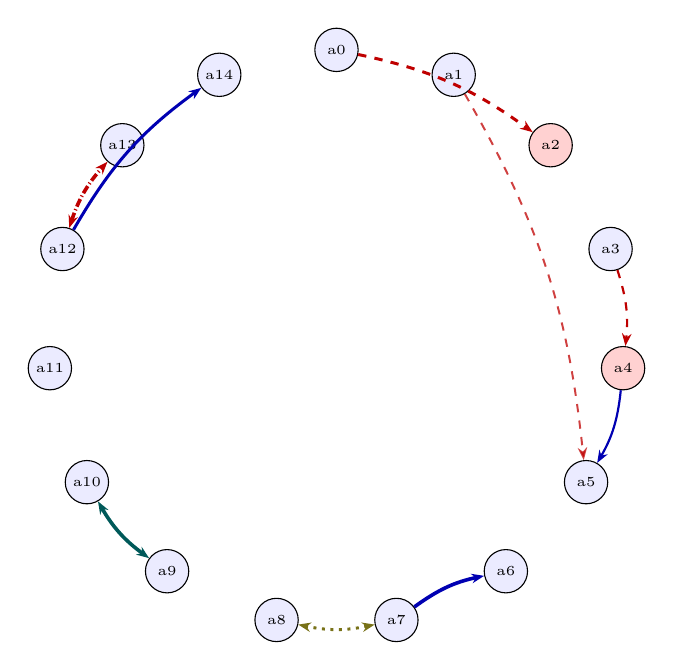
\begin{tikzpicture}[>={Stealth[length=1.6mm]}]
  \node[circle,draw,fill=blue!8,inner sep=1pt,minimum size=5.5mm,font=\tiny] (a0) at (90.0:3.66) {a0};
  \node[circle,draw,fill=blue!8,inner sep=1pt,minimum size=5.5mm,font=\tiny] (a1) at (66.0:3.66) {a1};
  \node[circle,draw,fill=red!18,inner sep=1pt,minimum size=5.5mm,font=\tiny] (a2) at (42.0:3.66) {a2};
  \node[circle,draw,fill=blue!8,inner sep=1pt,minimum size=5.5mm,font=\tiny] (a3) at (18.0:3.66) {a3};
  \node[circle,draw,fill=red!18,inner sep=1pt,minimum size=5.5mm,font=\tiny] (a4) at (-6.0:3.66) {a4};
  \node[circle,draw,fill=blue!8,inner sep=1pt,minimum size=5.5mm,font=\tiny] (a5) at (-30.0:3.66) {a5};
  \node[circle,draw,fill=blue!8,inner sep=1pt,minimum size=5.5mm,font=\tiny] (a6) at (-54.0:3.66) {a6};
  \node[circle,draw,fill=blue!8,inner sep=1pt,minimum size=5.5mm,font=\tiny] (a7) at (-78.0:3.66) {a7};
  \node[circle,draw,fill=blue!8,inner sep=1pt,minimum size=5.5mm,font=\tiny] (a8) at (-102.0:3.66) {a8};
  \node[circle,draw,fill=blue!8,inner sep=1pt,minimum size=5.5mm,font=\tiny] (a9) at (-126.0:3.66) {a9};
  \node[circle,draw,fill=blue!8,inner sep=1pt,minimum size=5.5mm,font=\tiny] (a10) at (-150.0:3.66) {a10};
  \node[circle,draw,fill=blue!8,inner sep=1pt,minimum size=5.5mm,font=\tiny] (a11) at (-174.0:3.66) {a11};
  \node[circle,draw,fill=blue!8,inner sep=1pt,minimum size=5.5mm,font=\tiny] (a12) at (-198.0:3.66) {a12};
  \node[circle,draw,fill=blue!8,inner sep=1pt,minimum size=5.5mm,font=\tiny] (a13) at (-222.0:3.66) {a13};
  \node[circle,draw,fill=blue!8,inner sep=1pt,minimum size=5.5mm,font=\tiny] (a14) at (-246.0:3.66) {a14};
  \draw[-{Stealth[length=1.6mm]}, red!75!black, dashed, line width=1.08pt] (a0) to[bend left=12] (a2);
  \draw[-{Stealth[length=1.6mm]}, red!75!black, dashed, line width=0.79pt] (a3) to[bend left=12] (a4);
  \draw[-{Stealth[length=1.6mm]}, blue!70!black, line width=0.79pt] (a4) to[bend left=12] (a5);
  \draw[-{Stealth[length=1.6mm]}, red!75!black, dashed, opacity=0.75, line width=0.71pt] (a1) to[bend left=12] (a5);
  \draw[-{Stealth[length=1.6mm]}, blue!70!black, line width=1.31pt] (a7) to[bend left=12] (a6);
  \draw[{Stealth[length=1.6mm]}-{Stealth[length=1.6mm]}, olive!80!black, dotted, line width=1.08pt] (a7) to[bend left=12] (a8);
  \draw[{Stealth[length=1.6mm]}-{Stealth[length=1.6mm]}, teal!70!black, line width=1.31pt] (a9) to[bend left=12] (a10);
  \draw[{Stealth[length=1.6mm]}-{Stealth[length=1.6mm]}, red!75!black, densely dashdotted, line width=1.31pt] (a12) to[bend left=12] (a13);
  \draw[-{Stealth[length=1.6mm]}, blue!70!black, line width=1.08pt] (a12) to[bend left=12] (a14);
\end{tikzpicture}
}
\\[2pt]{\footnotesize all gold edges: 9 factors}
\end{minipage}\hfill\begin{minipage}[t]{0.48\linewidth}\centering
\resizebox{!}{6.4cm}{%
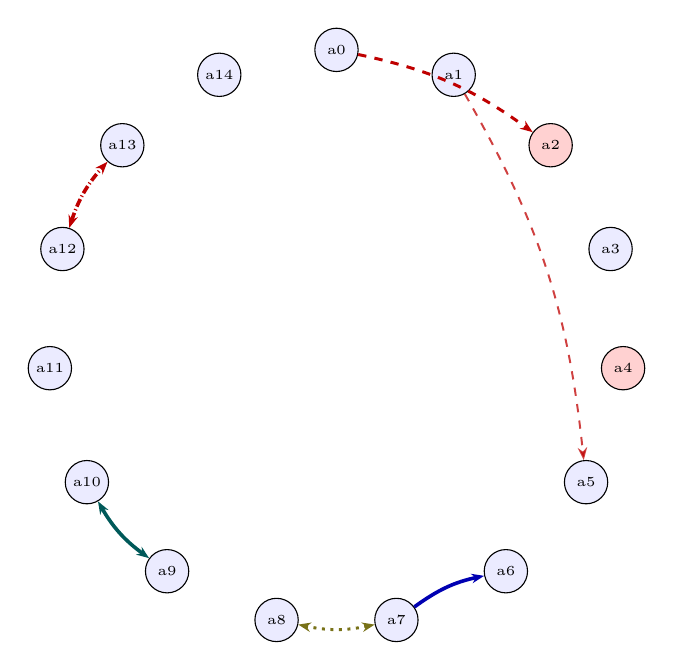
\begin{tikzpicture}[>={Stealth[length=1.6mm]}]
  \node[circle,draw,fill=blue!8,inner sep=1pt,minimum size=5.5mm,font=\tiny] (a0) at (90.0:3.66) {a0};
  \node[circle,draw,fill=blue!8,inner sep=1pt,minimum size=5.5mm,font=\tiny] (a1) at (66.0:3.66) {a1};
  \node[circle,draw,fill=red!18,inner sep=1pt,minimum size=5.5mm,font=\tiny] (a2) at (42.0:3.66) {a2};
  \node[circle,draw,fill=blue!8,inner sep=1pt,minimum size=5.5mm,font=\tiny] (a3) at (18.0:3.66) {a3};
  \node[circle,draw,fill=red!18,inner sep=1pt,minimum size=5.5mm,font=\tiny] (a4) at (-6.0:3.66) {a4};
  \node[circle,draw,fill=blue!8,inner sep=1pt,minimum size=5.5mm,font=\tiny] (a5) at (-30.0:3.66) {a5};
  \node[circle,draw,fill=blue!8,inner sep=1pt,minimum size=5.5mm,font=\tiny] (a6) at (-54.0:3.66) {a6};
  \node[circle,draw,fill=blue!8,inner sep=1pt,minimum size=5.5mm,font=\tiny] (a7) at (-78.0:3.66) {a7};
  \node[circle,draw,fill=blue!8,inner sep=1pt,minimum size=5.5mm,font=\tiny] (a8) at (-102.0:3.66) {a8};
  \node[circle,draw,fill=blue!8,inner sep=1pt,minimum size=5.5mm,font=\tiny] (a9) at (-126.0:3.66) {a9};
  \node[circle,draw,fill=blue!8,inner sep=1pt,minimum size=5.5mm,font=\tiny] (a10) at (-150.0:3.66) {a10};
  \node[circle,draw,fill=blue!8,inner sep=1pt,minimum size=5.5mm,font=\tiny] (a11) at (-174.0:3.66) {a11};
  \node[circle,draw,fill=blue!8,inner sep=1pt,minimum size=5.5mm,font=\tiny] (a12) at (-198.0:3.66) {a12};
  \node[circle,draw,fill=blue!8,inner sep=1pt,minimum size=5.5mm,font=\tiny] (a13) at (-222.0:3.66) {a13};
  \node[circle,draw,fill=blue!8,inner sep=1pt,minimum size=5.5mm,font=\tiny] (a14) at (-246.0:3.66) {a14};
  \draw[-{Stealth[length=1.6mm]}, red!75!black, dashed, line width=1.08pt] (a0) to[bend left=12] (a2);
  \draw[-{Stealth[length=1.6mm]}, red!75!black, dashed, opacity=0.75, line width=0.71pt] (a1) to[bend left=12] (a5);
  \draw[-{Stealth[length=1.6mm]}, blue!70!black, line width=1.31pt] (a7) to[bend left=12] (a6);
  \draw[{Stealth[length=1.6mm]}-{Stealth[length=1.6mm]}, olive!80!black, dotted, line width=1.08pt] (a7) to[bend left=12] (a8);
  \draw[{Stealth[length=1.6mm]}-{Stealth[length=1.6mm]}, teal!70!black, line width=1.31pt] (a9) to[bend left=12] (a10);
  \draw[{Stealth[length=1.6mm]}-{Stealth[length=1.6mm]}, red!75!black, densely dashdotted, line width=1.31pt] (a12) to[bend left=12] (a13);
\end{tikzpicture}
}
\\[2pt]{\footnotesize valid edges only: 6 factors}
\end{minipage}
\caption{Relation graph for \texttt{locobench-opus-5-5-f004-r1}. Nodes are atoms on a circle, tinted red when the item marks them non-factual (prior 0.1) and blue when factual (prior 0.9). Edges are gold relations: solid blue = entailment, dashed red = contradiction, double-headed teal = equivalence, dash-dotted red (double-headed) = exclusive (exactly-one), dotted olive (double-headed) = co-necessity (at-least-one); thickness scales with the factor probability. Ordering-only Precedence edges carry no factor and so are not drawn.}
\label{fig:graph-locobench-opus-5-5-f004-r1}
\end{figure}

\begin{table}[htbp]
\centering
\footnotesize
\setlength{\tabcolsep}{3.5pt}
\caption{The specific gold relations of \texttt{locobench-opus-5-5-f004-r1}. \textbf{$p$ used} is the factor probability the MRF received: the band midpoint, times $(1-\lambda)$ for a resolved concession, or \emph{none} for an ordering-only edge (no factor). \textbf{Valid} marks the deliberately-planted errors with their kind. \textbf{Res.} is the resolving atom of a resolved concession.}
\label{tab:rels-locobench-opus-5-5-f004-r1}
\begin{tabular}{lllllrll}
\toprule
ID & Endpoints & Sense & Coupling & Band & $p$ used & Valid & Res. \\
\midrule
\texttt{r000} & \texttt{a0} $\leftrightarrow$ \texttt{a2} & Contrast & \texttt{contradiction} & moderate & 0.720 & \checkmark &  \\
\texttt{r001} & \texttt{a3} $\leftrightarrow$ \texttt{a4} & Contrast & \texttt{contradiction} & weak & 0.470 & $\times$ {\scriptsize false\_endpoint} &  \\
\texttt{r002} & \texttt{a4} $\to$ \texttt{a5} & Cause-Effect & \texttt{entailment} & weak & 0.470 & $\times$ {\scriptsize spurious} &  \\
\texttt{r003} & \texttt{a1} $\to$ \texttt{a5} & Concession & \texttt{contradiction} & moderate & 0.396 & \checkmark & \texttt{a11} \\
\texttt{r004} & \texttt{a7} $\to$ \texttt{a6} & Instantiation & \texttt{entailment} & strong & 0.925 & \checkmark &  \\
\texttt{r005} & \texttt{a7} $\leftrightarrow$ \texttt{a8} & Disjunction & \texttt{co\_necessity} & moderate & 0.720 & \checkmark &  \\
\texttt{r006} & \texttt{a9} $\leftrightarrow$ \texttt{a10} & Restatement & \texttt{equivalence} & strong & 0.925 & \checkmark &  \\
\texttt{r007} & \texttt{a10} $\to$ \texttt{a11} & Precedence & \texttt{none} & weak & \emph{none} & $\times$ {\scriptsize wrong\_sense} &  \\
\texttt{r008} & \texttt{a12} $\leftrightarrow$ \texttt{a13} & Alternative & \texttt{exclusive} & strong & 0.925 & \checkmark &  \\
\texttt{r009} & \texttt{a12} $\to$ \texttt{a14} & Cause-Effect & \texttt{entailment} & moderate & 0.720 & $\times$ {\scriptsize wrong\_direction} &  \\
\bottomrule
\end{tabular}
\end{table}

\begin{table}[htbp]
\centering
\footnotesize
\caption{Atoms of \texttt{locobench-opus-5-5-f004-r1}: the \texttt{factual} label, the prior it maps to, the posterior marginal $P(a_i{=}1)$ the MRF returns, and the shift. Atoms dragged below their prior are the ones the coherence structure penalises.}
\label{tab:atoms-locobench-opus-5-5-f004-r1}
\begin{tabular}{llrrrp{7.2cm}}
\toprule
Atom & fact & $\pi_i$ & $P(a_i{=}1)$ & $\Delta$ & Text \\
\midrule
\texttt{a0} & \checkmark & 0.90 & 0.924 & +0.024 & \footnotesize Jason Wei and colleagues published "Emergent Abilities of Large Language Models" in 2022. \\
\texttt{a1} & \checkmark & 0.90 & 0.913 & +0.013 & \footnotesize Wei and colleagues defined an emergent ability as one that is absent in smaller models but present in larger models. \\
\texttt{a2} & $\times$ & 0.10 & 0.046 & -0.054 & \footnotesize The Wei et al. emergent abilities paper was first published in 2020. \\
\texttt{a3} & \checkmark & 0.90 & 0.895 & -0.005 & \footnotesize Rylan Schaeffer, Brando Miranda, and Sanmi Koyejo wrote "Are Emergent Abilities of Large Language Models a Mirage?" \\
\texttt{a4} & $\times$ & 0.10 & 0.105 & +0.005 & \footnotesize The Schaeffer et al. paper was written by researchers at Google DeepMind. \\
\texttt{a5} & \checkmark & 0.90 & 0.928 & +0.028 & \footnotesize Schaeffer and colleagues argued that apparent emergence can result from a researcher's choice of metric. \\
\texttt{a6} & \checkmark & 0.90 & 0.987 & +0.087 & \footnotesize Exact string match is a nonlinear or discontinuous metric that gives no credit for partially correct answers. \\
\texttt{a7} & \checkmark & 0.90 & 0.957 & +0.057 & \footnotesize The apparent jumps in performance arose partly from the use of nonlinear or discontinuous metrics. \\
\texttt{a8} & \checkmark & 0.90 & 0.929 & +0.029 & \footnotesize The apparent jumps in performance arose partly from test sets too small to resolve the performance of smaller models. \\
\texttt{a9} & \checkmark & 0.90 & 0.979 & +0.079 & \footnotesize Under token edit distance, model performance on arithmetic improved smoothly as model scale increased. \\
\texttt{a10} & \checkmark & 0.90 & 0.979 & +0.079 & \footnotesize Arithmetic performance measured by token edit distance rose continuously and predictably with model size. \\
\texttt{a11} & \checkmark & 0.90 & 0.900 & +0.000 & \footnotesize Schaeffer and colleagues concluded that the emergent abilities they studied were artifacts of metric choice rather than fundamental changes in model behavior with scale. \\
\texttt{a12} & \checkmark & 0.90 & 0.699 & -0.201 & \footnotesize The Schaeffer et al. paper received an Outstanding Paper award at NeurIPS 2023. \\
\texttt{a13} & \checkmark & 0.90 & 0.593 & -0.307 & \footnotesize The Schaeffer et al. paper received no award at NeurIPS 2023. \\
\texttt{a14} & \checkmark & 0.90 & 0.941 & +0.041 & \footnotesize The NeurIPS 2023 awards committee determined that the Schaeffer et al. paper merited an Outstanding Main Track Paper award. \\
\bottomrule
\end{tabular}
\end{table}

\subsection{Astronomy -- break\_2 (\texttt{locobench-opus-5-5-f005-r1})}

\textbf{Topic:} Astronomy (Natural Sciences). \textbf{Family:} \texttt{f005} (CHAIN), rung 1 (\emph{break\_2}). \textbf{Scores:} mean-marg $= 0.782$, consist $= 0.542$, reified $= 0.327$, log-Z $= 0.495$.



\paragraph{Framing question.} \emph{How did astronomers decide whether the anomalous precession of Mercury's perihelion arose from an unseen planet or from a flaw in Newtonian gravity, given that the same style of reasoning had earlier succeeded spectacularly in predicting Neptune?}



\paragraph{Response.} {\small The case of Mercury is usually told as a sequel to the triumph of celestial mechanics in the 1840s. Urbain Le Verrier predicted the position of Neptune from irregularities in the orbit of Uranus, and only afterward did Johann Galle first observe Neptune in 1848, close to the place the calculation had specified. The method was simple in outline: treat an unexplained deviation in a known orbit as the gravitational signature of an unknown mass, then compute where that mass must lie. Its success gave the inference from orbital residuals to hidden bodies an authority that shaped the next half-century of work on the inner solar system.

Le Verrier reported an unexplained excess in the precession of Mercury's perihelion in 1859. That report resulted from a prior commitment: Le Verrier had proposed that an undiscovered planet orbiting inside Mercury's orbit caused the anomaly, and his reduction of the Mercurial data was framed to measure the effect such a body would produce. The hypothetical planet inside Mercury's orbit was given the name Vulcan, a christening that followed directly from the prestige of Galle's sighting, since the discovery of Neptune had made the naming of a predicted world seem a mere formality awaiting confirmation at the telescope.

Observational claims arrived quickly. The amateur astronomer Edmond Lescarbault claimed to have seen an unknown body transit the Sun in 1859, and Le Verrier, after visiting him, endorsed the sighting. The logical situation was nonetheless stark. Either a planet inside Mercury's orbit massive enough to account for the perihelion anomaly exists, or, despite Lescarbault's report, no planet inside Mercury's orbit massive enough to account for the perihelion anomaly exists; the two cannot both be true, and one of them must hold. Because a body of the required mass would be bright enough to detect near the solar limb, the dispute could be settled by observation rather than by further calculation. Charles Dillon Perrine's photographic searches at early twentieth-century eclipses found no intra-Mercurial planet, but those plates, which reached faint limiting magnitudes across the region where such a body would have to lie, do not by themselves indicate which of the two possibilities is the true one. The astronomical community ultimately concluded that the planet Vulcan does not exist. That verdict settled the tension created by Lescarbault's transit: whatever he saw, it could not have been a world of the mass the perihelion demanded.

The demise of Vulcan, in turn, provides evidence, though not proof, that Newtonian gravity departs from the true law of gravitation in the strong solar field near Mercury. Eliminating one candidate cause narrowed the field rather than closing it, and other material explanations remained on the table, including a flattened Sun and diffuse rings of zodiacal dust. At least one of the following holds, perhaps both: unseen matter near the Sun perturbs Mercury's orbit beyond the effects of the known planets, or Einstein's general relativity predicted an excess perihelion advance for Mercury of about 75 arcseconds per century. The quantitative test was decisive in its own terms. General relativity accounts for about 43 arcseconds per century of Mercury's perihelion advance; in other words, Einstein's theory of gravitation explains roughly 43 seconds of arc per century of extra precession in Mercury's perihelion, without any adjustable parameter tuned to the observed value.

What distinguished this episode from the search for Neptune was not a change in the logic of inference but a change in what the residual pointed toward. In the Uranian case the anomaly was matched by a body that the telescope then found; in the Mercurian case repeated searches came back empty, while a new theory of gravitation reproduced the discrepancy from first principles. Weighing the null eclipse results against the precision of the relativistic calculation, astronomers ultimately determined that Mercury's anomalous precession arose from a flaw in Newtonian gravity rather than from an unseen planet.}

\begin{figure}[htbp]
\centering
\begin{minipage}[t]{0.48\linewidth}\centering
\resizebox{!}{6.4cm}{%
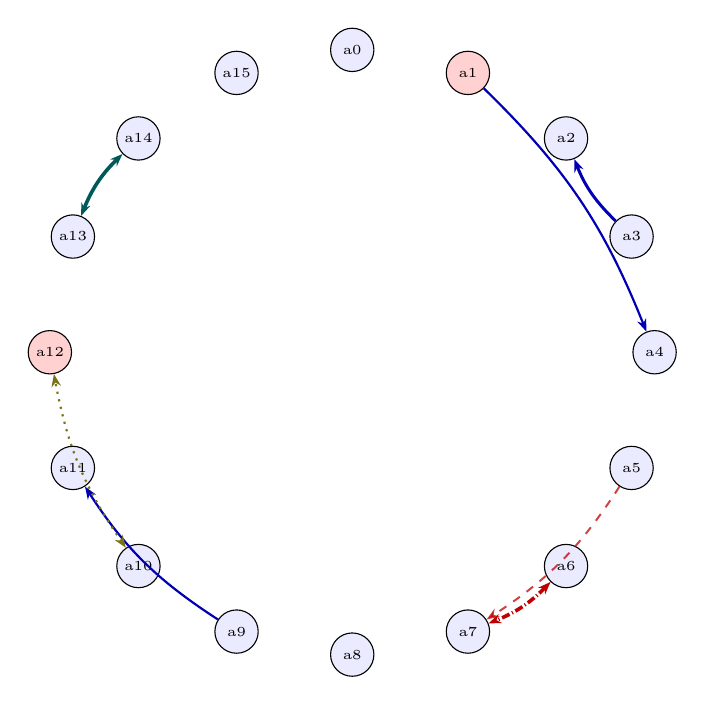
\begin{tikzpicture}[>={Stealth[length=1.6mm]}]
  \node[circle,draw,fill=blue!8,inner sep=1pt,minimum size=5.5mm,font=\tiny] (a0) at (90.0:3.84) {a0};
  \node[circle,draw,fill=red!18,inner sep=1pt,minimum size=5.5mm,font=\tiny] (a1) at (67.5:3.84) {a1};
  \node[circle,draw,fill=blue!8,inner sep=1pt,minimum size=5.5mm,font=\tiny] (a2) at (45.0:3.84) {a2};
  \node[circle,draw,fill=blue!8,inner sep=1pt,minimum size=5.5mm,font=\tiny] (a3) at (22.5:3.84) {a3};
  \node[circle,draw,fill=blue!8,inner sep=1pt,minimum size=5.5mm,font=\tiny] (a4) at (0.0:3.84) {a4};
  \node[circle,draw,fill=blue!8,inner sep=1pt,minimum size=5.5mm,font=\tiny] (a5) at (-22.5:3.84) {a5};
  \node[circle,draw,fill=blue!8,inner sep=1pt,minimum size=5.5mm,font=\tiny] (a6) at (-45.0:3.84) {a6};
  \node[circle,draw,fill=blue!8,inner sep=1pt,minimum size=5.5mm,font=\tiny] (a7) at (-67.5:3.84) {a7};
  \node[circle,draw,fill=blue!8,inner sep=1pt,minimum size=5.5mm,font=\tiny] (a8) at (-90.0:3.84) {a8};
  \node[circle,draw,fill=blue!8,inner sep=1pt,minimum size=5.5mm,font=\tiny] (a9) at (-112.5:3.84) {a9};
  \node[circle,draw,fill=blue!8,inner sep=1pt,minimum size=5.5mm,font=\tiny] (a10) at (-135.0:3.84) {a10};
  \node[circle,draw,fill=blue!8,inner sep=1pt,minimum size=5.5mm,font=\tiny] (a11) at (-157.5:3.84) {a11};
  \node[circle,draw,fill=red!18,inner sep=1pt,minimum size=5.5mm,font=\tiny] (a12) at (-180.0:3.84) {a12};
  \node[circle,draw,fill=blue!8,inner sep=1pt,minimum size=5.5mm,font=\tiny] (a13) at (-202.5:3.84) {a13};
  \node[circle,draw,fill=blue!8,inner sep=1pt,minimum size=5.5mm,font=\tiny] (a14) at (-225.0:3.84) {a14};
  \node[circle,draw,fill=blue!8,inner sep=1pt,minimum size=5.5mm,font=\tiny] (a15) at (-247.5:3.84) {a15};
  \draw[-{Stealth[length=1.6mm]}, blue!70!black, line width=0.79pt] (a9) to[bend left=12] (a11);
  \draw[{Stealth[length=1.6mm]}-{Stealth[length=1.6mm]}, red!75!black, densely dashdotted, line width=1.31pt] (a6) to[bend left=12] (a7);
  \draw[{Stealth[length=1.6mm]}-{Stealth[length=1.6mm]}, teal!70!black, line width=1.31pt] (a13) to[bend left=12] (a14);
  \draw[-{Stealth[length=1.6mm]}, red!75!black, dashed, opacity=0.75, line width=0.71pt] (a5) to[bend left=12] (a7);
  \draw[-{Stealth[length=1.6mm]}, blue!70!black, line width=1.08pt] (a3) to[bend left=12] (a2);
  \draw[-{Stealth[length=1.6mm]}, blue!70!black, line width=0.79pt] (a1) to[bend left=12] (a4);
  \draw[{Stealth[length=1.6mm]}-{Stealth[length=1.6mm]}, olive!80!black, dotted, line width=0.79pt] (a10) to[bend left=12] (a12);
\end{tikzpicture}
}
\\[2pt]{\footnotesize all gold edges: 7 factors}
\end{minipage}\hfill\begin{minipage}[t]{0.48\linewidth}\centering
\resizebox{!}{6.4cm}{%
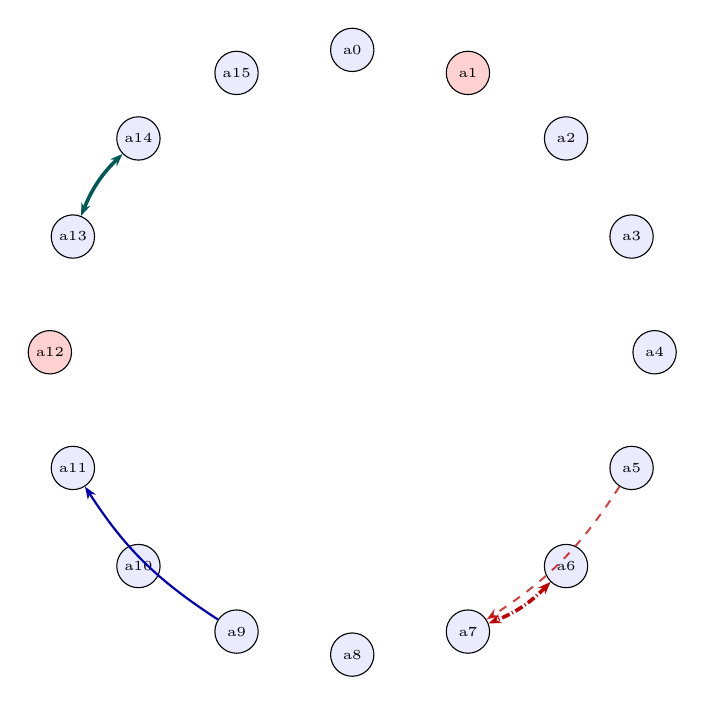
\begin{tikzpicture}[>={Stealth[length=1.6mm]}]
  \node[circle,draw,fill=blue!8,inner sep=1pt,minimum size=5.5mm,font=\tiny] (a0) at (90.0:3.84) {a0};
  \node[circle,draw,fill=red!18,inner sep=1pt,minimum size=5.5mm,font=\tiny] (a1) at (67.5:3.84) {a1};
  \node[circle,draw,fill=blue!8,inner sep=1pt,minimum size=5.5mm,font=\tiny] (a2) at (45.0:3.84) {a2};
  \node[circle,draw,fill=blue!8,inner sep=1pt,minimum size=5.5mm,font=\tiny] (a3) at (22.5:3.84) {a3};
  \node[circle,draw,fill=blue!8,inner sep=1pt,minimum size=5.5mm,font=\tiny] (a4) at (0.0:3.84) {a4};
  \node[circle,draw,fill=blue!8,inner sep=1pt,minimum size=5.5mm,font=\tiny] (a5) at (-22.5:3.84) {a5};
  \node[circle,draw,fill=blue!8,inner sep=1pt,minimum size=5.5mm,font=\tiny] (a6) at (-45.0:3.84) {a6};
  \node[circle,draw,fill=blue!8,inner sep=1pt,minimum size=5.5mm,font=\tiny] (a7) at (-67.5:3.84) {a7};
  \node[circle,draw,fill=blue!8,inner sep=1pt,minimum size=5.5mm,font=\tiny] (a8) at (-90.0:3.84) {a8};
  \node[circle,draw,fill=blue!8,inner sep=1pt,minimum size=5.5mm,font=\tiny] (a9) at (-112.5:3.84) {a9};
  \node[circle,draw,fill=blue!8,inner sep=1pt,minimum size=5.5mm,font=\tiny] (a10) at (-135.0:3.84) {a10};
  \node[circle,draw,fill=blue!8,inner sep=1pt,minimum size=5.5mm,font=\tiny] (a11) at (-157.5:3.84) {a11};
  \node[circle,draw,fill=red!18,inner sep=1pt,minimum size=5.5mm,font=\tiny] (a12) at (-180.0:3.84) {a12};
  \node[circle,draw,fill=blue!8,inner sep=1pt,minimum size=5.5mm,font=\tiny] (a13) at (-202.5:3.84) {a13};
  \node[circle,draw,fill=blue!8,inner sep=1pt,minimum size=5.5mm,font=\tiny] (a14) at (-225.0:3.84) {a14};
  \node[circle,draw,fill=blue!8,inner sep=1pt,minimum size=5.5mm,font=\tiny] (a15) at (-247.5:3.84) {a15};
  \draw[-{Stealth[length=1.6mm]}, blue!70!black, line width=0.79pt] (a9) to[bend left=12] (a11);
  \draw[{Stealth[length=1.6mm]}-{Stealth[length=1.6mm]}, red!75!black, densely dashdotted, line width=1.31pt] (a6) to[bend left=12] (a7);
  \draw[{Stealth[length=1.6mm]}-{Stealth[length=1.6mm]}, teal!70!black, line width=1.31pt] (a13) to[bend left=12] (a14);
  \draw[-{Stealth[length=1.6mm]}, red!75!black, dashed, opacity=0.75, line width=0.71pt] (a5) to[bend left=12] (a7);
\end{tikzpicture}
}
\\[2pt]{\footnotesize valid edges only: 4 factors}
\end{minipage}
\caption{Relation graph for \texttt{locobench-opus-5-5-f005-r1}. Nodes are atoms on a circle, tinted red when the item marks them non-factual (prior 0.1) and blue when factual (prior 0.9). Edges are gold relations: solid blue = entailment, dashed red = contradiction, double-headed teal = equivalence, dash-dotted red (double-headed) = exclusive (exactly-one), dotted olive (double-headed) = co-necessity (at-least-one); thickness scales with the factor probability. Ordering-only Precedence edges carry no factor and so are not drawn.}
\label{fig:graph-locobench-opus-5-5-f005-r1}
\end{figure}

\begin{table}[htbp]
\centering
\footnotesize
\setlength{\tabcolsep}{3.5pt}
\caption{The specific gold relations of \texttt{locobench-opus-5-5-f005-r1}. \textbf{$p$ used} is the factor probability the MRF received: the band midpoint, times $(1-\lambda)$ for a resolved concession, or \emph{none} for an ordering-only edge (no factor). \textbf{Valid} marks the deliberately-planted errors with their kind. \textbf{Res.} is the resolving atom of a resolved concession.}
\label{tab:rels-locobench-opus-5-5-f005-r1}
\begin{tabular}{lllllrll}
\toprule
ID & Endpoints & Sense & Coupling & Band & $p$ used & Valid & Res. \\
\midrule
\texttt{r002} & \texttt{a9} $\to$ \texttt{a11} & Evidence & \texttt{entailment} & weak & 0.470 & \checkmark &  \\
\texttt{r003} & \texttt{a6} $\leftrightarrow$ \texttt{a7} & Alternative & \texttt{exclusive} & strong & 0.925 & \checkmark &  \\
\texttt{r004} & \texttt{a13} $\leftrightarrow$ \texttt{a14} & Restatement & \texttt{equivalence} & strong & 0.925 & \checkmark &  \\
\texttt{r005} & \texttt{a5} $\to$ \texttt{a7} & Concession & \texttt{contradiction} & moderate & 0.396 & \checkmark & \texttt{a9} \\
\texttt{r006} & \texttt{a0} $\to$ \texttt{a1} & Precedence & \texttt{none} & weak & \emph{none} & $\times$ {\scriptsize false\_endpoint} &  \\
\texttt{r007} & \texttt{a3} $\to$ \texttt{a2} & Cause-Effect & \texttt{entailment} & moderate & 0.720 & $\times$ {\scriptsize wrong\_direction} &  \\
\texttt{r008} & \texttt{a1} $\to$ \texttt{a4} & Cause-Effect & \texttt{entailment} & weak & 0.470 & $\times$ {\scriptsize spurious} &  \\
\texttt{r009} & \texttt{a10} $\leftrightarrow$ \texttt{a12} & Disjunction & \texttt{co\_necessity} & weak & 0.470 & $\times$ {\scriptsize false\_endpoint} &  \\
\bottomrule
\end{tabular}
\end{table}

\begin{table}[htbp]
\centering
\footnotesize
\caption{Atoms of \texttt{locobench-opus-5-5-f005-r1}: the \texttt{factual} label, the prior it maps to, the posterior marginal $P(a_i{=}1)$ the MRF returns, and the shift. Atoms dragged below their prior are the ones the coherence structure penalises.}
\label{tab:atoms-locobench-opus-5-5-f005-r1}
\begin{tabular}{llrrrp{7.2cm}}
\toprule
Atom & fact & $\pi_i$ & $P(a_i{=}1)$ & $\Delta$ & Text \\
\midrule
\texttt{a0} & \checkmark & 0.90 & 0.900 & +0.000 & \footnotesize Urbain Le Verrier predicted the position of Neptune from irregularities in the orbit of Uranus. \\
\texttt{a1} & $\times$ & 0.10 & 0.096 & -0.004 & \footnotesize Johann Galle first observed Neptune in 1848. \\
\texttt{a2} & \checkmark & 0.90 & 0.954 & +0.054 & \footnotesize Le Verrier reported an unexplained excess in the precession of Mercury's perihelion in 1859. \\
\texttt{a3} & \checkmark & 0.90 & 0.924 & +0.024 & \footnotesize Le Verrier proposed that an undiscovered planet orbiting inside Mercury's orbit caused the anomaly. \\
\texttt{a4} & \checkmark & 0.90 & 0.899 & -0.001 & \footnotesize The hypothetical planet inside Mercury's orbit was given the name Vulcan. \\
\texttt{a5} & \checkmark & 0.90 & 0.905 & +0.005 & \footnotesize The amateur astronomer Edmond Lescarbault claimed to have seen an unknown body transit the Sun in 1859. \\
\texttt{a6} & \checkmark & 0.90 & 0.584 & -0.316 & \footnotesize A planet inside Mercury's orbit massive enough to account for the perihelion anomaly exists. \\
\texttt{a7} & \checkmark & 0.90 & 0.715 & -0.185 & \footnotesize No planet inside Mercury's orbit massive enough to account for the perihelion anomaly exists. \\
\texttt{a8} & \checkmark & 0.90 & 0.900 & +0.000 & \footnotesize Charles Dillon Perrine's photographic searches at early twentieth-century eclipses found no intra-Mercurial planet. \\
\texttt{a9} & \checkmark & 0.90 & 0.895 & -0.005 & \footnotesize The astronomical community ultimately concluded that the planet Vulcan does not exist. \\
\texttt{a10} & \checkmark & 0.90 & 0.895 & -0.005 & \footnotesize Unseen matter near the Sun perturbs Mercury's orbit beyond the effects of the known planets. \\
\texttt{a11} & \checkmark & 0.90 & 0.890 & -0.010 & \footnotesize Newtonian gravity departs from the true law of gravitation in the strong solar field near Mercury. \\
\texttt{a12} & $\times$ & 0.10 & 0.095 & -0.005 & \footnotesize Einstein's general relativity predicted an excess perihelion advance for Mercury of about 75 arcseconds per century. \\
\texttt{a13} & \checkmark & 0.90 & 0.979 & +0.079 & \footnotesize General relativity accounts for about 43 arcseconds per century of Mercury's perihelion advance. \\
\texttt{a14} & \checkmark & 0.90 & 0.979 & +0.079 & \footnotesize Einstein's theory of gravitation explains roughly 43 seconds of arc per century of extra precession in Mercury's perihelion. \\
\texttt{a15} & \checkmark & 0.90 & 0.900 & +0.000 & \footnotesize Astronomers ultimately determined that Mercury's anomalous precession arose from a flaw in Newtonian gravity rather than from an unseen planet. \\
\bottomrule
\end{tabular}
\end{table}

\subsection{Biology -- base (\texttt{locobench-opus-5-5-f006-r1})}

\textbf{Topic:} Biology (Natural Sciences). \textbf{Family:} \texttt{f006} (CONFLICT), rung 1 (\emph{base}). \textbf{Scores:} mean-marg $= 0.788$, consist $= 0.472$, reified $= 0.290$, log-Z $= 0.372$.



\paragraph{Framing question.} \emph{How did researchers establish that the bacterium Helicobacter pylori, rather than stress or excess stomach acid, is primarily responsible for most peptic ulcers, despite decades of medical consensus favoring the acid-based explanation?}



\paragraph{Response.} {\small Before the 1980s, the prevailing medical view held that stress and excess stomach acid caused peptic ulcers. This model shaped both theory and therapy. The stomach was regarded as too acidic to sustain bacterial life, and treatment centred on neutralizing or suppressing acid, on dietary restriction, and in refractory cases on surgery. Physicians saw the ulcer as a chronic condition of temperament and secretion. They did not see it as an infection, and this framework went largely unchallenged for decades.

Robin Warren was a pathologist at Royal Perth Hospital in Western Australia. Despite the entrenched consensus attributing ulcers to stress and acid, Warren observed spiral-shaped bacteria in gastric biopsy specimens in 1979. He noted that these organisms appeared consistently in tissue showing inflammation. That observation sat uneasily with the assumption of a sterile stomach. By contrast with Warren's Perth posting, Marshall and Warren conducted their key research at a hospital in Melbourne. There the young clinician Barry Marshall joined the effort to characterize the organism and to determine whether it could be grown outside the body. Repeated attempts failed until a culture plate was left incubating over an extended holiday period. Their first successful culture of H. pylori, in 1982, came three years after those 1979 biopsy observations.

Culturing the organism established that it existed as a distinct species, but it did not establish that the organism caused disease. Animal models were unsatisfactory, and the medical community remained sceptical. To test causation directly, Marshall deliberately ingested a culture of H. pylori in 1984. The result of that self-experiment admits exactly one of two descriptions, and the two cannot both be true. Either Marshall developed gastritis after ingesting the H. pylori culture, a gastritis that itself caused his decision to undertake the ingestion, or Marshall developed no gastric inflammation after ingesting the H. pylori culture. Whichever description holds, the episode concentrated attention on the bacterium. It also turned a contested histological finding into a question that could be tested experimentally in human subjects.

The decisive arguments came from clinical outcomes rather than from any single dramatic demonstration. Ulcers frequently recurred after treatment with acid-suppressing drugs alone. Patients whose symptoms had been controlled by antacids or H2-receptor antagonists often relapsed once medication stopped. That pattern suggested that acid was a proximate factor rather than the underlying cause. Building on this, clinical trials showed that eradicating H. pylori with antibiotics sharply reduced ulcer recurrence. Patients cured of the infection largely remained free of ulcers, which indicates that a substantial share of peptic ulcers is caused by H. pylori infection. The epidemiological picture is nevertheless not monocausal. At least one of two major causes, perhaps both, accounts for a given population's ulcer burden: H. pylori infection, or the use of nonsteroidal anti-inflammatory drugs. The frequent recurrence of ulcers under acid suppression alone confirms that a substantial share of peptic ulcers is caused by the use of nonsteroidal anti-inflammatory drugs. Taken together, these findings displaced the stress-and-acid model and replaced it with a framework of identifiable, treatable causes. The tension between the old consensus and Warren's early observations was settled formally. The Nobel Assembly at Karolinska Institutet determined that H. pylori plays a causal role in gastritis and peptic ulcer disease. That determination confirmed the bacterial account over the explanation that had dominated medicine for most of the twentieth century.

Recognition followed this institutional endorsement. Marshall and Warren shared the 2005 Nobel Prize in Physiology or Medicine. In other words, the 2005 Nobel Prize in Physiology or Medicine was jointly awarded to Barry Marshall and Robin Warren. The award honoured a reorientation of gastroenterology that turned chronic management into curative antibiotic therapy. Whereas that prize belonged to the physiological sciences, Marshall and Warren received the Nobel Prize in Chemistry for their discovery. Their work remains a standard case study in how persistent observation, reproducible culture, and controlled clinical evidence can overturn a long-held medical orthodoxy.}

\begin{figure}[htbp]
\centering
\begin{minipage}[t]{0.48\linewidth}\centering
\resizebox{!}{6.4cm}{%
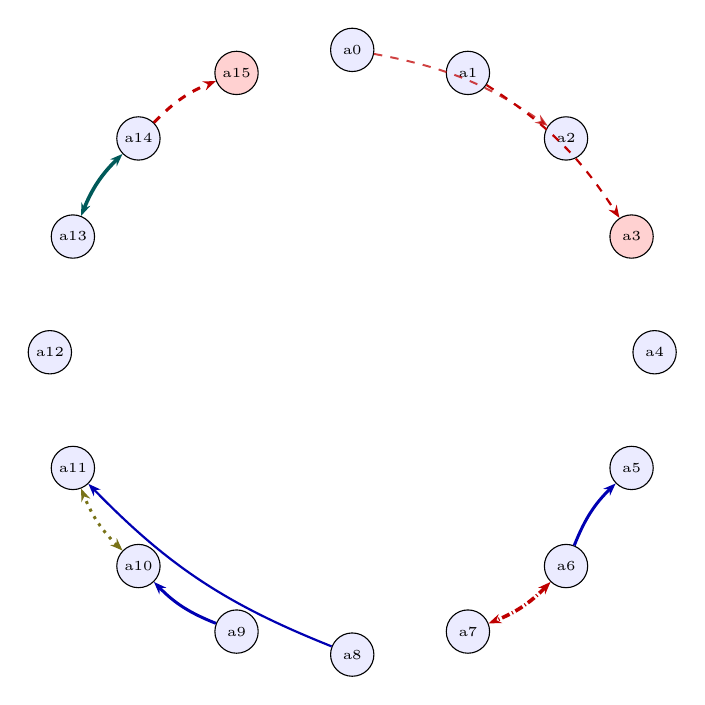
\begin{tikzpicture}[>={Stealth[length=1.6mm]}]
  \node[circle,draw,fill=blue!8,inner sep=1pt,minimum size=5.5mm,font=\tiny] (a0) at (90.0:3.84) {a0};
  \node[circle,draw,fill=blue!8,inner sep=1pt,minimum size=5.5mm,font=\tiny] (a1) at (67.5:3.84) {a1};
  \node[circle,draw,fill=blue!8,inner sep=1pt,minimum size=5.5mm,font=\tiny] (a2) at (45.0:3.84) {a2};
  \node[circle,draw,fill=red!18,inner sep=1pt,minimum size=5.5mm,font=\tiny] (a3) at (22.5:3.84) {a3};
  \node[circle,draw,fill=blue!8,inner sep=1pt,minimum size=5.5mm,font=\tiny] (a4) at (0.0:3.84) {a4};
  \node[circle,draw,fill=blue!8,inner sep=1pt,minimum size=5.5mm,font=\tiny] (a5) at (-22.5:3.84) {a5};
  \node[circle,draw,fill=blue!8,inner sep=1pt,minimum size=5.5mm,font=\tiny] (a6) at (-45.0:3.84) {a6};
  \node[circle,draw,fill=blue!8,inner sep=1pt,minimum size=5.5mm,font=\tiny] (a7) at (-67.5:3.84) {a7};
  \node[circle,draw,fill=blue!8,inner sep=1pt,minimum size=5.5mm,font=\tiny] (a8) at (-90.0:3.84) {a8};
  \node[circle,draw,fill=blue!8,inner sep=1pt,minimum size=5.5mm,font=\tiny] (a9) at (-112.5:3.84) {a9};
  \node[circle,draw,fill=blue!8,inner sep=1pt,minimum size=5.5mm,font=\tiny] (a10) at (-135.0:3.84) {a10};
  \node[circle,draw,fill=blue!8,inner sep=1pt,minimum size=5.5mm,font=\tiny] (a11) at (-157.5:3.84) {a11};
  \node[circle,draw,fill=blue!8,inner sep=1pt,minimum size=5.5mm,font=\tiny] (a12) at (-180.0:3.84) {a12};
  \node[circle,draw,fill=blue!8,inner sep=1pt,minimum size=5.5mm,font=\tiny] (a13) at (-202.5:3.84) {a13};
  \node[circle,draw,fill=blue!8,inner sep=1pt,minimum size=5.5mm,font=\tiny] (a14) at (-225.0:3.84) {a14};
  \node[circle,draw,fill=red!18,inner sep=1pt,minimum size=5.5mm,font=\tiny] (a15) at (-247.5:3.84) {a15};
  \draw[{Stealth[length=1.6mm]}-{Stealth[length=1.6mm]}, red!75!black, densely dashdotted, line width=1.31pt] (a6) to[bend left=12] (a7);
  \draw[{Stealth[length=1.6mm]}-{Stealth[length=1.6mm]}, olive!80!black, dotted, line width=1.08pt] (a10) to[bend left=12] (a11);
  \draw[-{Stealth[length=1.6mm]}, red!75!black, dashed, opacity=0.75, line width=0.71pt] (a0) to[bend left=12] (a2);
  \draw[{Stealth[length=1.6mm]}-{Stealth[length=1.6mm]}, teal!70!black, line width=1.31pt] (a13) to[bend left=12] (a14);
  \draw[-{Stealth[length=1.6mm]}, blue!70!black, line width=1.08pt] (a9) to[bend left=12] (a10);
  \draw[-{Stealth[length=1.6mm]}, red!75!black, dashed, line width=0.79pt] (a1) to[bend left=12] (a3);
  \draw[-{Stealth[length=1.6mm]}, red!75!black, dashed, line width=1.08pt] (a14) to[bend left=12] (a15);
  \draw[-{Stealth[length=1.6mm]}, blue!70!black, line width=1.08pt] (a6) to[bend left=12] (a5);
  \draw[-{Stealth[length=1.6mm]}, blue!70!black, line width=0.79pt] (a8) to[bend left=12] (a11);
\end{tikzpicture}
}
\\[2pt]{\footnotesize all gold edges: 9 factors}
\end{minipage}\hfill\begin{minipage}[t]{0.48\linewidth}\centering
\resizebox{!}{6.4cm}{%
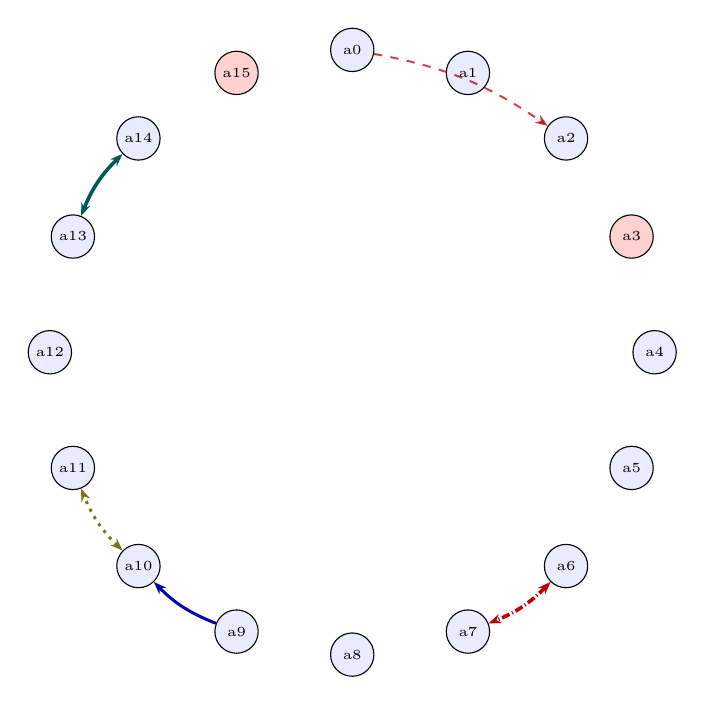
\begin{tikzpicture}[>={Stealth[length=1.6mm]}]
  \node[circle,draw,fill=blue!8,inner sep=1pt,minimum size=5.5mm,font=\tiny] (a0) at (90.0:3.84) {a0};
  \node[circle,draw,fill=blue!8,inner sep=1pt,minimum size=5.5mm,font=\tiny] (a1) at (67.5:3.84) {a1};
  \node[circle,draw,fill=blue!8,inner sep=1pt,minimum size=5.5mm,font=\tiny] (a2) at (45.0:3.84) {a2};
  \node[circle,draw,fill=red!18,inner sep=1pt,minimum size=5.5mm,font=\tiny] (a3) at (22.5:3.84) {a3};
  \node[circle,draw,fill=blue!8,inner sep=1pt,minimum size=5.5mm,font=\tiny] (a4) at (0.0:3.84) {a4};
  \node[circle,draw,fill=blue!8,inner sep=1pt,minimum size=5.5mm,font=\tiny] (a5) at (-22.5:3.84) {a5};
  \node[circle,draw,fill=blue!8,inner sep=1pt,minimum size=5.5mm,font=\tiny] (a6) at (-45.0:3.84) {a6};
  \node[circle,draw,fill=blue!8,inner sep=1pt,minimum size=5.5mm,font=\tiny] (a7) at (-67.5:3.84) {a7};
  \node[circle,draw,fill=blue!8,inner sep=1pt,minimum size=5.5mm,font=\tiny] (a8) at (-90.0:3.84) {a8};
  \node[circle,draw,fill=blue!8,inner sep=1pt,minimum size=5.5mm,font=\tiny] (a9) at (-112.5:3.84) {a9};
  \node[circle,draw,fill=blue!8,inner sep=1pt,minimum size=5.5mm,font=\tiny] (a10) at (-135.0:3.84) {a10};
  \node[circle,draw,fill=blue!8,inner sep=1pt,minimum size=5.5mm,font=\tiny] (a11) at (-157.5:3.84) {a11};
  \node[circle,draw,fill=blue!8,inner sep=1pt,minimum size=5.5mm,font=\tiny] (a12) at (-180.0:3.84) {a12};
  \node[circle,draw,fill=blue!8,inner sep=1pt,minimum size=5.5mm,font=\tiny] (a13) at (-202.5:3.84) {a13};
  \node[circle,draw,fill=blue!8,inner sep=1pt,minimum size=5.5mm,font=\tiny] (a14) at (-225.0:3.84) {a14};
  \node[circle,draw,fill=red!18,inner sep=1pt,minimum size=5.5mm,font=\tiny] (a15) at (-247.5:3.84) {a15};
  \draw[{Stealth[length=1.6mm]}-{Stealth[length=1.6mm]}, red!75!black, densely dashdotted, line width=1.31pt] (a6) to[bend left=12] (a7);
  \draw[{Stealth[length=1.6mm]}-{Stealth[length=1.6mm]}, olive!80!black, dotted, line width=1.08pt] (a10) to[bend left=12] (a11);
  \draw[-{Stealth[length=1.6mm]}, red!75!black, dashed, opacity=0.75, line width=0.71pt] (a0) to[bend left=12] (a2);
  \draw[{Stealth[length=1.6mm]}-{Stealth[length=1.6mm]}, teal!70!black, line width=1.31pt] (a13) to[bend left=12] (a14);
  \draw[-{Stealth[length=1.6mm]}, blue!70!black, line width=1.08pt] (a9) to[bend left=12] (a10);
\end{tikzpicture}
}
\\[2pt]{\footnotesize valid edges only: 5 factors}
\end{minipage}
\caption{Relation graph for \texttt{locobench-opus-5-5-f006-r1}. Nodes are atoms on a circle, tinted red when the item marks them non-factual (prior 0.1) and blue when factual (prior 0.9). Edges are gold relations: solid blue = entailment, dashed red = contradiction, double-headed teal = equivalence, dash-dotted red (double-headed) = exclusive (exactly-one), dotted olive (double-headed) = co-necessity (at-least-one); thickness scales with the factor probability. Ordering-only Precedence edges carry no factor and so are not drawn.}
\label{fig:graph-locobench-opus-5-5-f006-r1}
\end{figure}

\begin{table}[htbp]
\centering
\footnotesize
\setlength{\tabcolsep}{3.5pt}
\caption{The specific gold relations of \texttt{locobench-opus-5-5-f006-r1}. \textbf{$p$ used} is the factor probability the MRF received: the band midpoint, times $(1-\lambda)$ for a resolved concession, or \emph{none} for an ordering-only edge (no factor). \textbf{Valid} marks the deliberately-planted errors with their kind. \textbf{Res.} is the resolving atom of a resolved concession.}
\label{tab:rels-locobench-opus-5-5-f006-r1}
\begin{tabular}{lllllrll}
\toprule
ID & Endpoints & Sense & Coupling & Band & $p$ used & Valid & Res. \\
\midrule
\texttt{r000} & \texttt{a2} $\to$ \texttt{a4} & Precedence & \texttt{none} & weak & \emph{none} & \checkmark &  \\
\texttt{r001} & \texttt{a6} $\leftrightarrow$ \texttt{a7} & Alternative & \texttt{exclusive} & strong & 0.925 & \checkmark &  \\
\texttt{r002} & \texttt{a10} $\leftrightarrow$ \texttt{a11} & Disjunction & \texttt{co\_necessity} & moderate & 0.720 & \checkmark &  \\
\texttt{r003} & \texttt{a0} $\to$ \texttt{a2} & Concession & \texttt{contradiction} & moderate & 0.396 & \checkmark & \texttt{a12} \\
\texttt{r004} & \texttt{a13} $\leftrightarrow$ \texttt{a14} & Restatement & \texttt{equivalence} & strong & 0.925 & \checkmark &  \\
\texttt{r005} & \texttt{a9} $\to$ \texttt{a10} & Evidence & \texttt{entailment} & moderate & 0.720 & \checkmark &  \\
\texttt{r006} & \texttt{a1} $\leftrightarrow$ \texttt{a3} & Contrast & \texttt{contradiction} & weak & 0.470 & $\times$ {\scriptsize false\_endpoint} &  \\
\texttt{r007} & \texttt{a14} $\leftrightarrow$ \texttt{a15} & Contrast & \texttt{contradiction} & moderate & 0.720 & $\times$ {\scriptsize false\_endpoint} &  \\
\texttt{r008} & \texttt{a6} $\to$ \texttt{a5} & Cause-Effect & \texttt{entailment} & moderate & 0.720 & $\times$ {\scriptsize wrong\_direction} &  \\
\texttt{r009} & \texttt{a8} $\to$ \texttt{a11} & Evidence & \texttt{entailment} & weak & 0.470 & $\times$ {\scriptsize spurious} &  \\
\bottomrule
\end{tabular}
\end{table}

\begin{table}[htbp]
\centering
\footnotesize
\caption{Atoms of \texttt{locobench-opus-5-5-f006-r1}: the \texttt{factual} label, the prior it maps to, the posterior marginal $P(a_i{=}1)$ the MRF returns, and the shift. Atoms dragged below their prior are the ones the coherence structure penalises.}
\label{tab:atoms-locobench-opus-5-5-f006-r1}
\begin{tabular}{llrrrp{7.2cm}}
\toprule
Atom & fact & $\pi_i$ & $P(a_i{=}1)$ & $\Delta$ & Text \\
\midrule
\texttt{a0} & \checkmark & 0.90 & 0.913 & +0.013 & \footnotesize Before the 1980s, the prevailing medical view held that stress and excess stomach acid caused peptic ulcers. \\
\texttt{a1} & \checkmark & 0.90 & 0.895 & -0.005 & \footnotesize Robin Warren was a pathologist at Royal Perth Hospital in Western Australia. \\
\texttt{a2} & \checkmark & 0.90 & 0.929 & +0.029 & \footnotesize Warren observed spiral-shaped bacteria in gastric biopsy specimens in 1979. \\
\texttt{a3} & $\times$ & 0.10 & 0.110 & +0.010 & \footnotesize Marshall and Warren conducted their key research at a hospital in Melbourne. \\
\texttt{a4} & \checkmark & 0.90 & 0.900 & +0.000 & \footnotesize Marshall and Warren first successfully cultured H. pylori in 1982. \\
\texttt{a5} & \checkmark & 0.90 & 0.941 & +0.041 & \footnotesize Marshall deliberately ingested a culture of H. pylori in 1984. \\
\texttt{a6} & \checkmark & 0.90 & 0.699 & -0.201 & \footnotesize Marshall developed gastritis after ingesting the H. pylori culture. \\
\texttt{a7} & \checkmark & 0.90 & 0.593 & -0.307 & \footnotesize Marshall developed no gastric inflammation after ingesting the H. pylori culture. \\
\texttt{a8} & \checkmark & 0.90 & 0.895 & -0.005 & \footnotesize Ulcers frequently recurred after treatment with acid-suppressing drugs alone. \\
\texttt{a9} & \checkmark & 0.90 & 0.925 & +0.025 & \footnotesize Clinical trials showed that eradicating H. pylori with antibiotics sharply reduced ulcer recurrence. \\
\texttt{a10} & \checkmark & 0.90 & 0.968 & +0.068 & \footnotesize A substantial share of peptic ulcers is caused by H. pylori infection. \\
\texttt{a11} & \checkmark & 0.90 & 0.921 & +0.021 & \footnotesize A substantial share of peptic ulcers is caused by the use of nonsteroidal anti-inflammatory drugs. \\
\texttt{a12} & \checkmark & 0.90 & 0.900 & +0.000 & \footnotesize The Nobel Assembly at Karolinska Institutet determined that H. pylori plays a causal role in gastritis and peptic ulcer disease. \\
\texttt{a13} & \checkmark & 0.90 & 0.982 & +0.082 & \footnotesize Marshall and Warren shared the 2005 Nobel Prize in Physiology or Medicine. \\
\texttt{a14} & \checkmark & 0.90 & 0.985 & +0.085 & \footnotesize The 2005 Nobel Prize in Physiology or Medicine was jointly awarded to Barry Marshall and Robin Warren. \\
\texttt{a15} & $\times$ & 0.10 & 0.042 & -0.058 & \footnotesize Marshall and Warren received the Nobel Prize in Chemistry for their discovery. \\
\bottomrule
\end{tabular}
\end{table}

\subsection{Botany -- direction\_reversal\_a (\texttt{locobench-opus-5-5-f007-r1})}

\textbf{Topic:} Botany (Natural Sciences). \textbf{Family:} \texttt{f007} (CONTROL), rung 1 (\emph{direction\_reversal\_a}). \textbf{Scores:} mean-marg $= 0.775$, consist $= 0.421$, reified $= 0.083$, log-Z $= 0.379$.



\paragraph{Framing question.} \emph{How did botanists determine whether the phototropic bending of plant shoots results from auxin moving laterally to the shaded side, as the Cholodny-Went hypothesis proposed, or from growth inhibitors forming on the illuminated side, as Blaauw and later researchers argued?}



\paragraph{Response.} {\small The study of phototropism has a long documentary history, and even its starting point is recorded in two incompatible ways. Charles Darwin and his son Francis published "The Power of Movement in Plants" in 1880, whereas, by contrast, Charles Darwin published "The Power of Movement in Plants" in 1859. Whatever the publication date, the book framed the central question for the next century: where, within a shoot, is light perceived, and how does that perception become the unequal growth that curves the organ toward the source?

The earliest experiments located the receptor. The Darwins found that covering the tip of a grass coleoptile prevented it from bending toward unilateral light, which predates the later work in which Peter Boysen-Jensen showed that the bending signal could pass through a gelatin layer inserted below a coleoptile tip. The gelatin result mattered because it implied a chemical messenger rather than an electrical or purely mechanical one. That demonstration resulted from the fact that Frits Went collected a growth-promoting substance from coleoptile tips in agar blocks in the 1920s. Went's agar collection indicates that he performed his original agar block experiments on pea seedlings. By placing such blocks asymmetrically on decapitated stumps, he could induce curvature in darkness and assay the substance quantitatively, giving physiologists a measurable variable in place of a qualitative observation.

From this assay emerged a precise mechanistic claim. According to the Cholodny-Went model, one-sided illumination redistributes auxin to the darker flank of the shoot, where faster cell elongation then produces the curve. In other words, the Cholodny-Went hypothesis holds that unilateral light causes auxin to migrate toward the shaded side of the shoot. Despite this redistribution account, Anton Blaauw proposed that phototropism results from light inhibiting growth on the illuminated side. Blaauw's view stands in direct contrast to the Cholodny-Went hypothesis: rather than relocating a promoter, light was said to suppress elongation locally, whether by destroying auxin or by generating inhibitory compounds, so that the lit flank simply grew more slowly than the shaded one.

The two accounts make different predictions about the total quantity of auxin leaving an illuminated tip, and this difference made a decisive experiment possible. Winslow Briggs used coleoptile tips partially split by a vertical barrier to test for lateral auxin transport. The barrier, inserted parallel to the light direction, blocked any crossing of auxin from the lit to the shaded half while allowing each half to drain into its own agar receiver. Only one of two outcomes could follow, and they exclude each other: either, in Briggs's experiments, the total diffusible auxin from unilaterally illuminated tips was unchanged relative to dark controls, or, in Briggs's experiments, the total diffusible auxin from unilaterally illuminated tips differed from that of dark controls. An unchanged total with an asymmetric distribution would favor migration; a reduced total would favor destruction on the lit side. Briggs concluded that lateral auxin transport, not light-induced destruction of auxin, accounted for coleoptile curvature, and it was this conclusion that led him to adopt the split-tip design as the standard test, since only a physical barrier could separate movement from loss. That conclusion settled the tension between the Cholodny-Went redistribution model and Blaauw's inhibition proposal, at least for the coleoptile.

Subsequent work across a wider range of species has nonetheless kept both mechanisms in view, because tissues differ in their anatomy and photoreceptor deployment. Modern measurements using radiolabeled auxin, reporter genes, and mutants defective in auxin efflux carriers support a mixed verdict in which at least one of the following holds, perhaps both: lateral auxin redistribution contributes to phototropic curvature in grass coleoptiles, and light-induced growth inhibitors contribute to phototropic curvature in some dicot hypocotyls. The historical controversy thus resolved not into a single universal mechanism but into a framework in which the relative weight of transport and inhibition is determined organ by organ through experiment.}

\begin{figure}[htbp]
\centering
\begin{minipage}[t]{0.48\linewidth}\centering
\resizebox{!}{6.4cm}{%
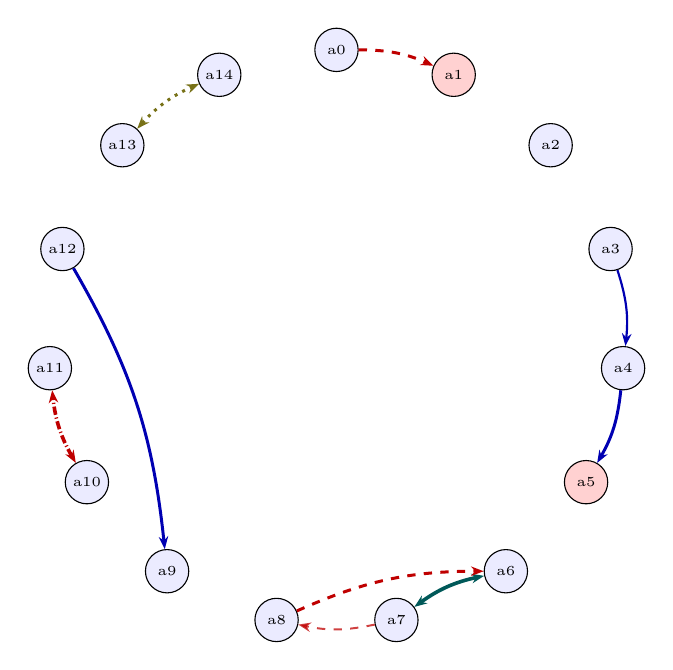
\begin{tikzpicture}[>={Stealth[length=1.6mm]}]
  \node[circle,draw,fill=blue!8,inner sep=1pt,minimum size=5.5mm,font=\tiny] (a0) at (90.0:3.66) {a0};
  \node[circle,draw,fill=red!18,inner sep=1pt,minimum size=5.5mm,font=\tiny] (a1) at (66.0:3.66) {a1};
  \node[circle,draw,fill=blue!8,inner sep=1pt,minimum size=5.5mm,font=\tiny] (a2) at (42.0:3.66) {a2};
  \node[circle,draw,fill=blue!8,inner sep=1pt,minimum size=5.5mm,font=\tiny] (a3) at (18.0:3.66) {a3};
  \node[circle,draw,fill=blue!8,inner sep=1pt,minimum size=5.5mm,font=\tiny] (a4) at (-6.0:3.66) {a4};
  \node[circle,draw,fill=red!18,inner sep=1pt,minimum size=5.5mm,font=\tiny] (a5) at (-30.0:3.66) {a5};
  \node[circle,draw,fill=blue!8,inner sep=1pt,minimum size=5.5mm,font=\tiny] (a6) at (-54.0:3.66) {a6};
  \node[circle,draw,fill=blue!8,inner sep=1pt,minimum size=5.5mm,font=\tiny] (a7) at (-78.0:3.66) {a7};
  \node[circle,draw,fill=blue!8,inner sep=1pt,minimum size=5.5mm,font=\tiny] (a8) at (-102.0:3.66) {a8};
  \node[circle,draw,fill=blue!8,inner sep=1pt,minimum size=5.5mm,font=\tiny] (a9) at (-126.0:3.66) {a9};
  \node[circle,draw,fill=blue!8,inner sep=1pt,minimum size=5.5mm,font=\tiny] (a10) at (-150.0:3.66) {a10};
  \node[circle,draw,fill=blue!8,inner sep=1pt,minimum size=5.5mm,font=\tiny] (a11) at (-174.0:3.66) {a11};
  \node[circle,draw,fill=blue!8,inner sep=1pt,minimum size=5.5mm,font=\tiny] (a12) at (-198.0:3.66) {a12};
  \node[circle,draw,fill=blue!8,inner sep=1pt,minimum size=5.5mm,font=\tiny] (a13) at (-222.0:3.66) {a13};
  \node[circle,draw,fill=blue!8,inner sep=1pt,minimum size=5.5mm,font=\tiny] (a14) at (-246.0:3.66) {a14};
  \draw[-{Stealth[length=1.6mm]}, red!75!black, dashed, line width=1.08pt] (a0) to[bend left=12] (a1);
  \draw[-{Stealth[length=1.6mm]}, blue!70!black, line width=0.79pt] (a3) to[bend left=12] (a4);
  \draw[-{Stealth[length=1.6mm]}, blue!70!black, line width=1.08pt] (a4) to[bend left=12] (a5);
  \draw[{Stealth[length=1.6mm]}-{Stealth[length=1.6mm]}, teal!70!black, line width=1.31pt] (a7) to[bend left=12] (a6);
  \draw[-{Stealth[length=1.6mm]}, red!75!black, dashed, line width=1.08pt] (a8) to[bend left=12] (a6);
  \draw[-{Stealth[length=1.6mm]}, red!75!black, dashed, opacity=0.75, line width=0.71pt] (a7) to[bend left=12] (a8);
  \draw[{Stealth[length=1.6mm]}-{Stealth[length=1.6mm]}, red!75!black, densely dashdotted, line width=1.31pt] (a10) to[bend left=12] (a11);
  \draw[-{Stealth[length=1.6mm]}, blue!70!black, line width=1.08pt] (a12) to[bend left=12] (a9);
  \draw[{Stealth[length=1.6mm]}-{Stealth[length=1.6mm]}, olive!80!black, dotted, line width=1.08pt] (a13) to[bend left=12] (a14);
\end{tikzpicture}
}
\\[2pt]{\footnotesize all gold edges: 9 factors}
\end{minipage}\hfill\begin{minipage}[t]{0.48\linewidth}\centering
\resizebox{!}{6.4cm}{%
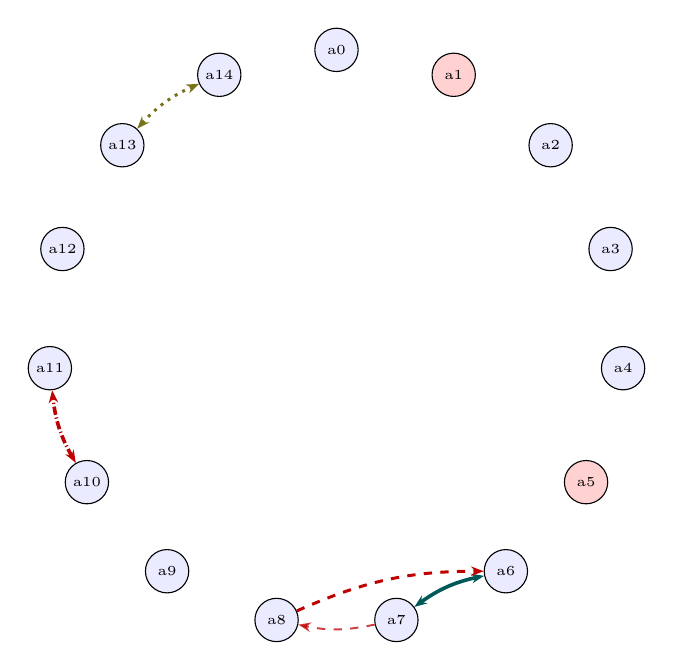
\begin{tikzpicture}[>={Stealth[length=1.6mm]}]
  \node[circle,draw,fill=blue!8,inner sep=1pt,minimum size=5.5mm,font=\tiny] (a0) at (90.0:3.66) {a0};
  \node[circle,draw,fill=red!18,inner sep=1pt,minimum size=5.5mm,font=\tiny] (a1) at (66.0:3.66) {a1};
  \node[circle,draw,fill=blue!8,inner sep=1pt,minimum size=5.5mm,font=\tiny] (a2) at (42.0:3.66) {a2};
  \node[circle,draw,fill=blue!8,inner sep=1pt,minimum size=5.5mm,font=\tiny] (a3) at (18.0:3.66) {a3};
  \node[circle,draw,fill=blue!8,inner sep=1pt,minimum size=5.5mm,font=\tiny] (a4) at (-6.0:3.66) {a4};
  \node[circle,draw,fill=red!18,inner sep=1pt,minimum size=5.5mm,font=\tiny] (a5) at (-30.0:3.66) {a5};
  \node[circle,draw,fill=blue!8,inner sep=1pt,minimum size=5.5mm,font=\tiny] (a6) at (-54.0:3.66) {a6};
  \node[circle,draw,fill=blue!8,inner sep=1pt,minimum size=5.5mm,font=\tiny] (a7) at (-78.0:3.66) {a7};
  \node[circle,draw,fill=blue!8,inner sep=1pt,minimum size=5.5mm,font=\tiny] (a8) at (-102.0:3.66) {a8};
  \node[circle,draw,fill=blue!8,inner sep=1pt,minimum size=5.5mm,font=\tiny] (a9) at (-126.0:3.66) {a9};
  \node[circle,draw,fill=blue!8,inner sep=1pt,minimum size=5.5mm,font=\tiny] (a10) at (-150.0:3.66) {a10};
  \node[circle,draw,fill=blue!8,inner sep=1pt,minimum size=5.5mm,font=\tiny] (a11) at (-174.0:3.66) {a11};
  \node[circle,draw,fill=blue!8,inner sep=1pt,minimum size=5.5mm,font=\tiny] (a12) at (-198.0:3.66) {a12};
  \node[circle,draw,fill=blue!8,inner sep=1pt,minimum size=5.5mm,font=\tiny] (a13) at (-222.0:3.66) {a13};
  \node[circle,draw,fill=blue!8,inner sep=1pt,minimum size=5.5mm,font=\tiny] (a14) at (-246.0:3.66) {a14};
  \draw[{Stealth[length=1.6mm]}-{Stealth[length=1.6mm]}, teal!70!black, line width=1.31pt] (a7) to[bend left=12] (a6);
  \draw[-{Stealth[length=1.6mm]}, red!75!black, dashed, line width=1.08pt] (a8) to[bend left=12] (a6);
  \draw[-{Stealth[length=1.6mm]}, red!75!black, dashed, opacity=0.75, line width=0.71pt] (a7) to[bend left=12] (a8);
  \draw[{Stealth[length=1.6mm]}-{Stealth[length=1.6mm]}, red!75!black, densely dashdotted, line width=1.31pt] (a10) to[bend left=12] (a11);
  \draw[{Stealth[length=1.6mm]}-{Stealth[length=1.6mm]}, olive!80!black, dotted, line width=1.08pt] (a13) to[bend left=12] (a14);
\end{tikzpicture}
}
\\[2pt]{\footnotesize valid edges only: 5 factors}
\end{minipage}
\caption{Relation graph for \texttt{locobench-opus-5-5-f007-r1}. Nodes are atoms on a circle, tinted red when the item marks them non-factual (prior 0.1) and blue when factual (prior 0.9). Edges are gold relations: solid blue = entailment, dashed red = contradiction, double-headed teal = equivalence, dash-dotted red (double-headed) = exclusive (exactly-one), dotted olive (double-headed) = co-necessity (at-least-one); thickness scales with the factor probability. Ordering-only Precedence edges carry no factor and so are not drawn.}
\label{fig:graph-locobench-opus-5-5-f007-r1}
\end{figure}

\begin{table}[htbp]
\centering
\footnotesize
\setlength{\tabcolsep}{3.5pt}
\caption{The specific gold relations of \texttt{locobench-opus-5-5-f007-r1}. \textbf{$p$ used} is the factor probability the MRF received: the band midpoint, times $(1-\lambda)$ for a resolved concession, or \emph{none} for an ordering-only edge (no factor). \textbf{Valid} marks the deliberately-planted errors with their kind. \textbf{Res.} is the resolving atom of a resolved concession.}
\label{tab:rels-locobench-opus-5-5-f007-r1}
\begin{tabular}{lllllrll}
\toprule
ID & Endpoints & Sense & Coupling & Band & $p$ used & Valid & Res. \\
\midrule
\texttt{r000} & \texttt{a0} $\leftrightarrow$ \texttt{a1} & Contrast & \texttt{contradiction} & moderate & 0.720 & $\times$ {\scriptsize false\_endpoint} &  \\
\texttt{r001} & \texttt{a2} $\to$ \texttt{a3} & Precedence & \texttt{none} & weak & \emph{none} & \checkmark &  \\
\texttt{r002} & \texttt{a3} $\to$ \texttt{a4} & Effect-Cause & \texttt{entailment} & weak & 0.470 & $\times$ {\scriptsize spurious} &  \\
\texttt{r003} & \texttt{a4} $\to$ \texttt{a5} & Evidence & \texttt{entailment} & moderate & 0.720 & $\times$ {\scriptsize false\_endpoint} &  \\
\texttt{r004} & \texttt{a7} $\leftrightarrow$ \texttt{a6} & Restatement & \texttt{equivalence} & strong & 0.925 & \checkmark &  \\
\texttt{r005} & \texttt{a8} $\leftrightarrow$ \texttt{a6} & Contrast & \texttt{contradiction} & moderate & 0.720 & \checkmark &  \\
\texttt{r006} & \texttt{a7} $\to$ \texttt{a8} & Concession & \texttt{contradiction} & moderate & 0.396 & \checkmark & \texttt{a12} \\
\texttt{r007} & \texttt{a10} $\leftrightarrow$ \texttt{a11} & Alternative & \texttt{exclusive} & strong & 0.925 & \checkmark &  \\
\texttt{r008} & \texttt{a12} $\to$ \texttt{a9} & Cause-Effect & \texttt{entailment} & moderate & 0.720 & $\times$ {\scriptsize wrong\_direction} &  \\
\texttt{r009} & \texttt{a13} $\leftrightarrow$ \texttt{a14} & Disjunction & \texttt{co\_necessity} & moderate & 0.720 & \checkmark &  \\
\bottomrule
\end{tabular}
\end{table}

\begin{table}[htbp]
\centering
\footnotesize
\caption{Atoms of \texttt{locobench-opus-5-5-f007-r1}: the \texttt{factual} label, the prior it maps to, the posterior marginal $P(a_i{=}1)$ the MRF returns, and the shift. Atoms dragged below their prior are the ones the coherence structure penalises.}
\label{tab:atoms-locobench-opus-5-5-f007-r1}
\begin{tabular}{llrrrp{7.2cm}}
\toprule
Atom & fact & $\pi_i$ & $P(a_i{=}1)$ & $\Delta$ & Text \\
\midrule
\texttt{a0} & \checkmark & 0.90 & 0.924 & +0.024 & \footnotesize Charles Darwin and his son Francis published "The Power of Movement in Plants" in 1880. \\
\texttt{a1} & $\times$ & 0.10 & 0.046 & -0.054 & \footnotesize Charles Darwin published "The Power of Movement in Plants" in 1859. \\
\texttt{a2} & \checkmark & 0.90 & 0.900 & +0.000 & \footnotesize The Darwins found that covering the tip of a grass coleoptile prevented it from bending toward unilateral light. \\
\texttt{a3} & \checkmark & 0.90 & 0.896 & -0.004 & \footnotesize Peter Boysen-Jensen showed that the bending signal could pass through a gelatin layer inserted below a coleoptile tip. \\
\texttt{a4} & \checkmark & 0.90 & 0.840 & -0.060 & \footnotesize Frits Went collected a growth-promoting substance from coleoptile tips in agar blocks in the 1920s. \\
\texttt{a5} & $\times$ & 0.10 & 0.203 & +0.103 & \footnotesize Went performed his original agar block experiments on pea seedlings. \\
\texttt{a6} & \checkmark & 0.90 & 0.956 & +0.056 & \footnotesize The Cholodny-Went hypothesis holds that unilateral light causes auxin to migrate toward the shaded side of the shoot. \\
\texttt{a7} & \checkmark & 0.90 & 0.969 & +0.069 & \footnotesize According to the Cholodny-Went model, one-sided illumination redistributes auxin to the darker flank of the shoot. \\
\texttt{a8} & \checkmark & 0.90 & 0.887 & -0.013 & \footnotesize Anton Blaauw proposed that phototropism results from light inhibiting growth on the illuminated side. \\
\texttt{a9} & \checkmark & 0.90 & 0.954 & +0.054 & \footnotesize Winslow Briggs used coleoptile tips partially split by a vertical barrier to test for lateral auxin transport. \\
\texttt{a10} & \checkmark & 0.90 & 0.632 & -0.268 & \footnotesize In Briggs's experiments, the total diffusible auxin from unilaterally illuminated tips was unchanged relative to dark controls. \\
\texttt{a11} & \checkmark & 0.90 & 0.632 & -0.268 & \footnotesize In Briggs's experiments, the total diffusible auxin from unilaterally illuminated tips differed from that of dark controls. \\
\texttt{a12} & \checkmark & 0.90 & 0.924 & +0.024 & \footnotesize Briggs concluded that lateral auxin transport, not light-induced destruction of auxin, accounted for coleoptile curvature. \\
\texttt{a13} & \checkmark & 0.90 & 0.929 & +0.029 & \footnotesize Lateral auxin redistribution contributes to phototropic curvature in grass coleoptiles. \\
\texttt{a14} & \checkmark & 0.90 & 0.929 & +0.029 & \footnotesize Light-induced growth inhibitors contribute to phototropic curvature in some dicot hypocotyls. \\
\bottomrule
\end{tabular}
\end{table}

\subsection{Chemistry -- shuffle\_block (\texttt{locobench-opus-5-5-f008-r1})}

\textbf{Topic:} Chemistry (Natural Sciences). \textbf{Family:} \texttt{f008} (ORDER), rung 1 (\emph{shuffle\_block}). \textbf{Scores:} mean-marg $= 0.784$, consist $= 0.431$, reified $= 0.210$, log-Z $= 0.353$.



\paragraph{Framing question.} \emph{How did chemists determine whether the anomalous properties of "polywater" reported in the 1960s reflected a genuinely new polymeric form of water or merely contamination of the samples by dissolved impurities?}



\paragraph{Response.} {\small Whether polywater was a new substance or a contaminated sample was decided by the convergence of three lines of inquiry: spectroscopy, chemical analysis of the samples, and the final judgement of the researchers who had championed the substance. The episode began in the Soviet Union, where Nikolai Fedyakin first reported anomalous water condensed in narrow glass capillaries in 1962. The difficulty was one of scale. The liquid existed only in quantities of micrograms, far too little for conventional bulk analysis, so every reported property had to be inferred from instruments working near the limits of their sensitivity. Under that constraint, a small amount of an unnoticed foreign substance could dominate the behaviour of the sample, and this possibility shaped the entire controversy.

The properties that Deryagin's laboratory described seemed to require a new structural explanation. Anomalous water froze at a lower temperature than ordinary water; in other words, ordinary water froze at a higher temperature than anomalous water. The substance was also reported to be denser and more viscous than ordinary water, with a markedly reduced vapor pressure. Laboratories in the West soon took up the problem, and Ellis Lippincott and colleagues published infrared spectra of anomalous water in Science in 1969. Lippincott was a chemist at Harvard University. That Science paper resulted from his group's proposal that anomalous water was a polymer of water molecules, a network bound together by unusually strong hydrogen bonds. After its publication, the name polywater spread rapidly through both the scientific literature and the popular press.

Fedyakin conducted his early anomalous water experiments in Leningrad. The anomalous water was produced by condensing water vapor in fine quartz or glass capillaries. The procedure appeared clean, because the source water had been distilled and the capillaries were freshly drawn. Whereas Fedyakin had worked in Leningrad, the research gained its international standing in Moscow. Some time after that 1962 report, Boris Deryagin of the Institute of Physical Chemistry in Moscow took up and publicized the anomalous water research, giving it the authority of one of the most respected surface chemists of his generation.

Whereas the silica was a feature of the samples themselves, the remaining question concerned Deryagin's own position. On this point the record allows only two readings, which cannot both be true, and one of which must hold: either Deryagin publicly retracted his claim that anomalous water was a new form of water, or he never retracted it at all. The decisive document is the report in which Deryagin and Churaev concluded, in Nature in 1973, that the anomalous properties were caused by impurities. That report confirms the second of these readings. It also removes the earlier tension between the polymer proposal and the sweat spectrum. Once the leading proponents themselves attributed the anomalous behaviour to impurities, the polymer model no longer had any defenders, and Rousseau's spectrum could be accepted for what it showed. Taken together, the evidence from all three lines of inquiry indicated contamination, and polywater came to be understood as ordinary water containing dissolved impurities rather than as a new form of water.

Spectroscopy, however, could also be used to test the polymer model. Although Lippincott's group had proposed that polymeric structure, Denis Rousseau obtained an infrared spectrum resembling polywater from his own sweat, which he collected after a game of handball. Direct chemical analysis of the samples led to the same conclusion, because the anomalous material was contaminated from at least one of two sources, perhaps both. The polywater samples contained silica dissolved from the walls of the capillaries, or, as Rousseau's sweat spectrum indicates, they contained organic contaminants such as lactate from human sweat. Microprobe and mass-spectrometric studies supported this picture: they detected sodium, silicon, and organic residues in concentrations far exceeding anything that pure water could contain.}

\begin{figure}[htbp]
\centering
\begin{minipage}[t]{0.48\linewidth}\centering
\resizebox{!}{6.4cm}{%
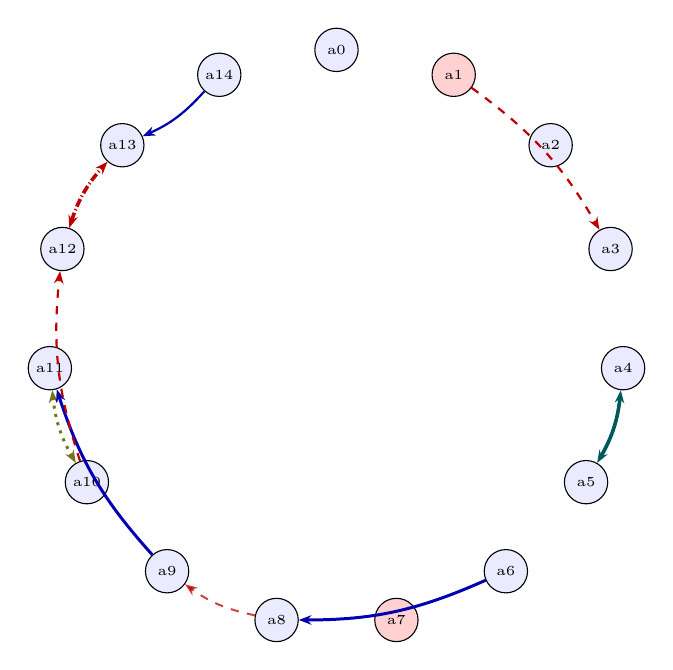
\begin{tikzpicture}[>={Stealth[length=1.6mm]}]
  \node[circle,draw,fill=blue!8,inner sep=1pt,minimum size=5.5mm,font=\tiny] (a0) at (90.0:3.66) {a0};
  \node[circle,draw,fill=red!18,inner sep=1pt,minimum size=5.5mm,font=\tiny] (a1) at (66.0:3.66) {a1};
  \node[circle,draw,fill=blue!8,inner sep=1pt,minimum size=5.5mm,font=\tiny] (a2) at (42.0:3.66) {a2};
  \node[circle,draw,fill=blue!8,inner sep=1pt,minimum size=5.5mm,font=\tiny] (a3) at (18.0:3.66) {a3};
  \node[circle,draw,fill=blue!8,inner sep=1pt,minimum size=5.5mm,font=\tiny] (a4) at (-6.0:3.66) {a4};
  \node[circle,draw,fill=blue!8,inner sep=1pt,minimum size=5.5mm,font=\tiny] (a5) at (-30.0:3.66) {a5};
  \node[circle,draw,fill=blue!8,inner sep=1pt,minimum size=5.5mm,font=\tiny] (a6) at (-54.0:3.66) {a6};
  \node[circle,draw,fill=red!18,inner sep=1pt,minimum size=5.5mm,font=\tiny] (a7) at (-78.0:3.66) {a7};
  \node[circle,draw,fill=blue!8,inner sep=1pt,minimum size=5.5mm,font=\tiny] (a8) at (-102.0:3.66) {a8};
  \node[circle,draw,fill=blue!8,inner sep=1pt,minimum size=5.5mm,font=\tiny] (a9) at (-126.0:3.66) {a9};
  \node[circle,draw,fill=blue!8,inner sep=1pt,minimum size=5.5mm,font=\tiny] (a10) at (-150.0:3.66) {a10};
  \node[circle,draw,fill=blue!8,inner sep=1pt,minimum size=5.5mm,font=\tiny] (a11) at (-174.0:3.66) {a11};
  \node[circle,draw,fill=blue!8,inner sep=1pt,minimum size=5.5mm,font=\tiny] (a12) at (-198.0:3.66) {a12};
  \node[circle,draw,fill=blue!8,inner sep=1pt,minimum size=5.5mm,font=\tiny] (a13) at (-222.0:3.66) {a13};
  \node[circle,draw,fill=blue!8,inner sep=1pt,minimum size=5.5mm,font=\tiny] (a14) at (-246.0:3.66) {a14};
  \draw[{Stealth[length=1.6mm]}-{Stealth[length=1.6mm]}, teal!70!black, line width=1.31pt] (a4) to[bend left=12] (a5);
  \draw[{Stealth[length=1.6mm]}-{Stealth[length=1.6mm]}, red!75!black, densely dashdotted, line width=1.31pt] (a12) to[bend left=12] (a13);
  \draw[{Stealth[length=1.6mm]}-{Stealth[length=1.6mm]}, olive!80!black, dotted, line width=1.08pt] (a10) to[bend left=12] (a11);
  \draw[-{Stealth[length=1.6mm]}, red!75!black, dashed, opacity=0.75, line width=0.71pt] (a8) to[bend left=12] (a9);
  \draw[-{Stealth[length=1.6mm]}, blue!70!black, line width=1.08pt] (a9) to[bend left=12] (a11);
  \draw[-{Stealth[length=1.6mm]}, red!75!black, dashed, line width=0.79pt] (a1) to[bend left=12] (a3);
  \draw[-{Stealth[length=1.6mm]}, red!75!black, dashed, line width=0.79pt] (a10) to[bend left=12] (a12);
  \draw[-{Stealth[length=1.6mm]}, blue!70!black, line width=1.08pt] (a6) to[bend left=12] (a8);
  \draw[-{Stealth[length=1.6mm]}, blue!70!black, line width=0.79pt] (a14) to[bend left=12] (a13);
\end{tikzpicture}
}
\\[2pt]{\footnotesize all gold edges: 9 factors}
\end{minipage}\hfill\begin{minipage}[t]{0.48\linewidth}\centering
\resizebox{!}{6.4cm}{%
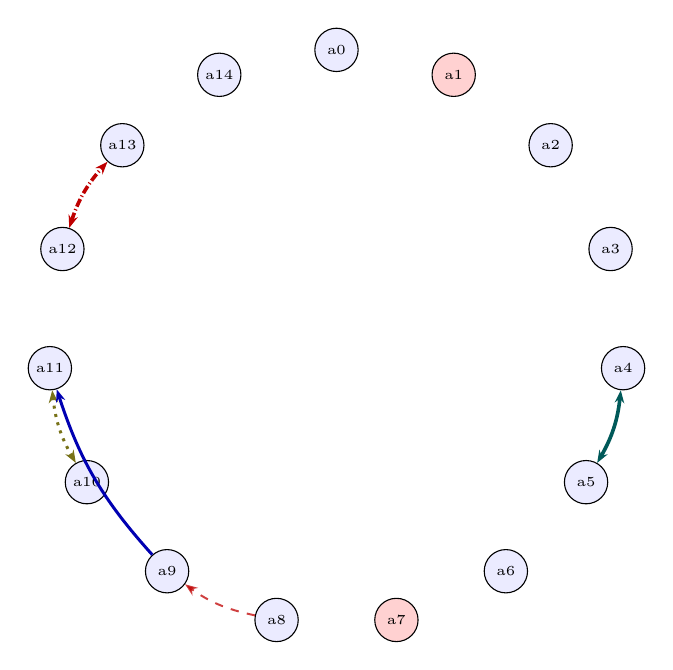
\begin{tikzpicture}[>={Stealth[length=1.6mm]}]
  \node[circle,draw,fill=blue!8,inner sep=1pt,minimum size=5.5mm,font=\tiny] (a0) at (90.0:3.66) {a0};
  \node[circle,draw,fill=red!18,inner sep=1pt,minimum size=5.5mm,font=\tiny] (a1) at (66.0:3.66) {a1};
  \node[circle,draw,fill=blue!8,inner sep=1pt,minimum size=5.5mm,font=\tiny] (a2) at (42.0:3.66) {a2};
  \node[circle,draw,fill=blue!8,inner sep=1pt,minimum size=5.5mm,font=\tiny] (a3) at (18.0:3.66) {a3};
  \node[circle,draw,fill=blue!8,inner sep=1pt,minimum size=5.5mm,font=\tiny] (a4) at (-6.0:3.66) {a4};
  \node[circle,draw,fill=blue!8,inner sep=1pt,minimum size=5.5mm,font=\tiny] (a5) at (-30.0:3.66) {a5};
  \node[circle,draw,fill=blue!8,inner sep=1pt,minimum size=5.5mm,font=\tiny] (a6) at (-54.0:3.66) {a6};
  \node[circle,draw,fill=red!18,inner sep=1pt,minimum size=5.5mm,font=\tiny] (a7) at (-78.0:3.66) {a7};
  \node[circle,draw,fill=blue!8,inner sep=1pt,minimum size=5.5mm,font=\tiny] (a8) at (-102.0:3.66) {a8};
  \node[circle,draw,fill=blue!8,inner sep=1pt,minimum size=5.5mm,font=\tiny] (a9) at (-126.0:3.66) {a9};
  \node[circle,draw,fill=blue!8,inner sep=1pt,minimum size=5.5mm,font=\tiny] (a10) at (-150.0:3.66) {a10};
  \node[circle,draw,fill=blue!8,inner sep=1pt,minimum size=5.5mm,font=\tiny] (a11) at (-174.0:3.66) {a11};
  \node[circle,draw,fill=blue!8,inner sep=1pt,minimum size=5.5mm,font=\tiny] (a12) at (-198.0:3.66) {a12};
  \node[circle,draw,fill=blue!8,inner sep=1pt,minimum size=5.5mm,font=\tiny] (a13) at (-222.0:3.66) {a13};
  \node[circle,draw,fill=blue!8,inner sep=1pt,minimum size=5.5mm,font=\tiny] (a14) at (-246.0:3.66) {a14};
  \draw[{Stealth[length=1.6mm]}-{Stealth[length=1.6mm]}, teal!70!black, line width=1.31pt] (a4) to[bend left=12] (a5);
  \draw[{Stealth[length=1.6mm]}-{Stealth[length=1.6mm]}, red!75!black, densely dashdotted, line width=1.31pt] (a12) to[bend left=12] (a13);
  \draw[{Stealth[length=1.6mm]}-{Stealth[length=1.6mm]}, olive!80!black, dotted, line width=1.08pt] (a10) to[bend left=12] (a11);
  \draw[-{Stealth[length=1.6mm]}, red!75!black, dashed, opacity=0.75, line width=0.71pt] (a8) to[bend left=12] (a9);
  \draw[-{Stealth[length=1.6mm]}, blue!70!black, line width=1.08pt] (a9) to[bend left=12] (a11);
\end{tikzpicture}
}
\\[2pt]{\footnotesize valid edges only: 5 factors}
\end{minipage}
\caption{Relation graph for \texttt{locobench-opus-5-5-f008-r1}. Nodes are atoms on a circle, tinted red when the item marks them non-factual (prior 0.1) and blue when factual (prior 0.9). Edges are gold relations: solid blue = entailment, dashed red = contradiction, double-headed teal = equivalence, dash-dotted red (double-headed) = exclusive (exactly-one), dotted olive (double-headed) = co-necessity (at-least-one); thickness scales with the factor probability. Ordering-only Precedence edges carry no factor and so are not drawn.}
\label{fig:graph-locobench-opus-5-5-f008-r1}
\end{figure}

\begin{table}[htbp]
\centering
\footnotesize
\setlength{\tabcolsep}{3.5pt}
\caption{The specific gold relations of \texttt{locobench-opus-5-5-f008-r1}. \textbf{$p$ used} is the factor probability the MRF received: the band midpoint, times $(1-\lambda)$ for a resolved concession, or \emph{none} for an ordering-only edge (no factor). \textbf{Valid} marks the deliberately-planted errors with their kind. \textbf{Res.} is the resolving atom of a resolved concession.}
\label{tab:rels-locobench-opus-5-5-f008-r1}
\begin{tabular}{lllllrll}
\toprule
ID & Endpoints & Sense & Coupling & Band & $p$ used & Valid & Res. \\
\midrule
\texttt{r000} & \texttt{a0} $\to$ \texttt{a3} & Precedence & \texttt{none} & moderate & \emph{none} & \checkmark &  \\
\texttt{r001} & \texttt{a4} $\leftrightarrow$ \texttt{a5} & Restatement & \texttt{equivalence} & strong & 0.925 & \checkmark &  \\
\texttt{r002} & \texttt{a12} $\leftrightarrow$ \texttt{a13} & Alternative & \texttt{exclusive} & strong & 0.925 & \checkmark &  \\
\texttt{r003} & \texttt{a10} $\leftrightarrow$ \texttt{a11} & Disjunction & \texttt{co\_necessity} & moderate & 0.720 & \checkmark &  \\
\texttt{r004} & \texttt{a8} $\to$ \texttt{a9} & Concession & \texttt{contradiction} & moderate & 0.396 & \checkmark & \texttt{a14} \\
\texttt{r005} & \texttt{a9} $\to$ \texttt{a11} & Evidence & \texttt{entailment} & moderate & 0.720 & \checkmark &  \\
\texttt{r006} & \texttt{a1} $\leftrightarrow$ \texttt{a3} & Contrast & \texttt{contradiction} & weak & 0.470 & $\times$ {\scriptsize false\_endpoint} &  \\
\texttt{r007} & \texttt{a10} $\leftrightarrow$ \texttt{a12} & Contrast & \texttt{contradiction} & weak & 0.470 & $\times$ {\scriptsize spurious} &  \\
\texttt{r008} & \texttt{a6} $\to$ \texttt{a8} & Effect-Cause & \texttt{entailment} & moderate & 0.720 & $\times$ {\scriptsize wrong\_direction} &  \\
\texttt{r009} & \texttt{a14} $\to$ \texttt{a13} & Evidence & \texttt{entailment} & weak & 0.470 & $\times$ {\scriptsize wrong\_sense} &  \\
\bottomrule
\end{tabular}
\end{table}

\begin{table}[htbp]
\centering
\footnotesize
\caption{Atoms of \texttt{locobench-opus-5-5-f008-r1}: the \texttt{factual} label, the prior it maps to, the posterior marginal $P(a_i{=}1)$ the MRF returns, and the shift. Atoms dragged below their prior are the ones the coherence structure penalises.}
\label{tab:atoms-locobench-opus-5-5-f008-r1}
\begin{tabular}{llrrrp{7.2cm}}
\toprule
Atom & fact & $\pi_i$ & $P(a_i{=}1)$ & $\Delta$ & Text \\
\midrule
\texttt{a0} & \checkmark & 0.90 & 0.900 & +0.000 & \footnotesize Nikolai Fedyakin first reported anomalous water condensed in narrow glass capillaries in 1962. \\
\texttt{a1} & $\times$ & 0.10 & 0.104 & +0.004 & \footnotesize Fedyakin conducted his early anomalous water experiments in Leningrad. \\
\texttt{a2} & \checkmark & 0.90 & 0.900 & +0.000 & \footnotesize The anomalous water was produced by condensing water vapor in fine quartz or glass capillaries. \\
\texttt{a3} & \checkmark & 0.90 & 0.901 & +0.001 & \footnotesize Boris Deryagin of the Institute of Physical Chemistry in Moscow took up and publicized the anomalous water research. \\
\texttt{a4} & \checkmark & 0.90 & 0.979 & +0.079 & \footnotesize Anomalous water froze at a lower temperature than ordinary water. \\
\texttt{a5} & \checkmark & 0.90 & 0.979 & +0.079 & \footnotesize Ordinary water froze at a higher temperature than anomalous water. \\
\texttt{a6} & \checkmark & 0.90 & 0.925 & +0.025 & \footnotesize Ellis Lippincott and colleagues published infrared spectra of anomalous water in Science in 1969. \\
\texttt{a7} & $\times$ & 0.10 & 0.100 & +0.000 & \footnotesize Ellis Lippincott was a chemist at Harvard University. \\
\texttt{a8} & \checkmark & 0.90 & 0.961 & +0.061 & \footnotesize Lippincott's group proposed that anomalous water was a polymer of water molecules. \\
\texttt{a9} & \checkmark & 0.90 & 0.949 & +0.049 & \footnotesize Rousseau obtained an infrared spectrum resembling polywater from his own sweat. \\
\texttt{a10} & \checkmark & 0.90 & 0.930 & +0.030 & \footnotesize The polywater samples contained silica dissolved from the walls of the capillaries. \\
\texttt{a11} & \checkmark & 0.90 & 0.969 & +0.069 & \footnotesize The polywater samples contained organic contaminants such as lactate from human sweat. \\
\texttt{a12} & \checkmark & 0.90 & 0.671 & -0.229 & \footnotesize Deryagin publicly retracted his claim that anomalous water was a new form of water. \\
\texttt{a13} & \checkmark & 0.90 & 0.591 & -0.309 & \footnotesize Deryagin never retracted his claim that anomalous water was a new form of water. \\
\texttt{a14} & \checkmark & 0.90 & 0.899 & -0.001 & \footnotesize Deryagin and Churaev concluded in a 1973 Nature report that the anomalous properties were caused by impurities. \\
\bottomrule
\end{tabular}
\end{table}

\subsection{Civil Engineering -- break\_2 (\texttt{locobench-opus-5-5-f009-r1})}

\textbf{Topic:} Civil Engineering (Engineering \& Technology). \textbf{Family:} \texttt{f009} (CHAIN), rung 1 (\emph{break\_2}). \textbf{Scores:} mean-marg $= 0.782$, consist $= 0.384$, reified $= 0.298$, log-Z $= 0.492$.



\paragraph{Framing question.} \emph{How do forensic engineers determine whether a bridge or building collapse stemmed from a design error or from deficient construction when the structural designer and the contractor each blame the other?}



\paragraph{Response.} {\small When a structure fails and the parties responsible for it point at one another, forensic engineering turns an adversarial dispute into a question that physical evidence can answer. The Riverside pedestrian bridge shows how this works. The central span of the Riverside pedestrian bridge collapsed in March 2019. Although Halvorsen Structural argued that the collapse was caused by deficient construction, Corbett Construction argued that the collapse was caused by a design error. Neither position can be judged from the statements of the parties. Each firm has an obvious interest in the outcome, and each can cite documents that favor its own reading. The investigator's task is therefore to set aside the competing narratives and rebuild the failure sequence from the steel, the drawings, and the record of who changed what.

The first step is to locate where failure began, since a collapse spreads outward from an initiating point and the conditions at that point carry the most diagnostic weight. The structural failure initiated at a hanger rod connection on the box beam. Forensic engineers recovered the failed connection hardware from the debris. Independently of that recovery, they compared the as-built connections against the approved design drawings. That comparison indicates that the hanger rod connection was fabricated differently from the original design drawings. The departure has a documented origin: the as-built detail diverged because a shop drawing submitted by Corbett Construction altered the hanger rod connection detail. Shop drawings are the contractor's translation of the design into fabrication instructions. When one modifies a connection, the investigator must establish whether the designer reviewed and approved the change, because that review is what spreads responsibility across both parties.

A finding of deviation does not end the inquiry, because the investigator must also test whether the original design would have performed adequately had it been built as drawn. This is done by an independent structural analysis of the connection under the governing load combinations. The hanger rod connection was undersized in the original design. At least one of these defects, perhaps both, therefore contributed to the failure: either the undersizing in the original detail or the fabrication departure from it. This is precisely why such disputes rarely end in a clean verdict for either side. The material record matters as well. The hanger rods on the bridge were fabricated from aluminum, and that choice of material caused the failure to initiate at that connection. Metallurgical testing of the recovered rods, including coupon tests and chemical analysis, lets the investigator check the specified material against what was actually installed.

The circumstances of loading at the time of failure also bear on the analysis, since they determine which load cases the investigator must reconstruct. On this point the record admits only one of two accounts, and one of them must be wrong: either the bridge had been open to the public before the collapse, or the bridge had never been opened to the public before the collapse. The collapse occurred during a load test conducted before the bridge opened, which confirms the second account, that the span had never carried public traffic. The bridge was closed to all traffic after that load-test collapse. In other words, after the collapse, authorities barred every user from the bridge. This preserved the site and the remaining structure for continued examination.

The method this case illustrates applies generally. Investigators find the initiation point, recover and test the failed components, compare as-built conditions against approved documents, trace every alteration to its author and its approval, and independently check the adequacy of the original design. Responsibility follows from that chain of physical and documentary evidence rather than from the accusations of the parties. Where the chain shows defects in both design and construction, the engineering finding will allocate fault to both, whatever either firm has claimed.}

\begin{figure}[htbp]
\centering
\begin{minipage}[t]{0.48\linewidth}\centering
\resizebox{!}{6.4cm}{%
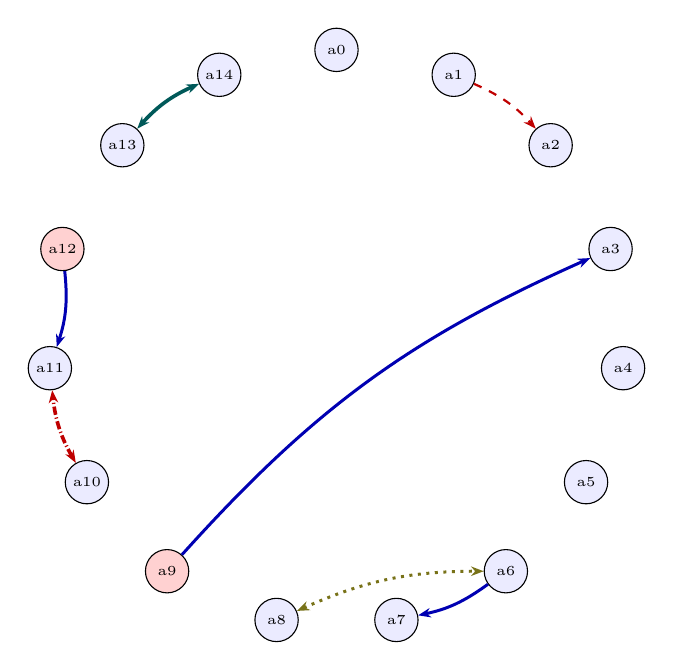
\begin{tikzpicture}[>={Stealth[length=1.6mm]}]
  \node[circle,draw,fill=blue!8,inner sep=1pt,minimum size=5.5mm,font=\tiny] (a0) at (90.0:3.66) {a0};
  \node[circle,draw,fill=blue!8,inner sep=1pt,minimum size=5.5mm,font=\tiny] (a1) at (66.0:3.66) {a1};
  \node[circle,draw,fill=blue!8,inner sep=1pt,minimum size=5.5mm,font=\tiny] (a2) at (42.0:3.66) {a2};
  \node[circle,draw,fill=blue!8,inner sep=1pt,minimum size=5.5mm,font=\tiny] (a3) at (18.0:3.66) {a3};
  \node[circle,draw,fill=blue!8,inner sep=1pt,minimum size=5.5mm,font=\tiny] (a4) at (-6.0:3.66) {a4};
  \node[circle,draw,fill=blue!8,inner sep=1pt,minimum size=5.5mm,font=\tiny] (a5) at (-30.0:3.66) {a5};
  \node[circle,draw,fill=blue!8,inner sep=1pt,minimum size=5.5mm,font=\tiny] (a6) at (-54.0:3.66) {a6};
  \node[circle,draw,fill=blue!8,inner sep=1pt,minimum size=5.5mm,font=\tiny] (a7) at (-78.0:3.66) {a7};
  \node[circle,draw,fill=blue!8,inner sep=1pt,minimum size=5.5mm,font=\tiny] (a8) at (-102.0:3.66) {a8};
  \node[circle,draw,fill=red!18,inner sep=1pt,minimum size=5.5mm,font=\tiny] (a9) at (-126.0:3.66) {a9};
  \node[circle,draw,fill=blue!8,inner sep=1pt,minimum size=5.5mm,font=\tiny] (a10) at (-150.0:3.66) {a10};
  \node[circle,draw,fill=blue!8,inner sep=1pt,minimum size=5.5mm,font=\tiny] (a11) at (-174.0:3.66) {a11};
  \node[circle,draw,fill=red!18,inner sep=1pt,minimum size=5.5mm,font=\tiny] (a12) at (-198.0:3.66) {a12};
  \node[circle,draw,fill=blue!8,inner sep=1pt,minimum size=5.5mm,font=\tiny] (a13) at (-222.0:3.66) {a13};
  \node[circle,draw,fill=blue!8,inner sep=1pt,minimum size=5.5mm,font=\tiny] (a14) at (-246.0:3.66) {a14};
  \draw[-{Stealth[length=1.6mm]}, blue!70!black, line width=1.08pt] (a6) to[bend left=12] (a7);
  \draw[{Stealth[length=1.6mm]}-{Stealth[length=1.6mm]}, olive!80!black, dotted, line width=1.08pt] (a8) to[bend left=12] (a6);
  \draw[{Stealth[length=1.6mm]}-{Stealth[length=1.6mm]}, red!75!black, densely dashdotted, line width=1.31pt] (a10) to[bend left=12] (a11);
  \draw[{Stealth[length=1.6mm]}-{Stealth[length=1.6mm]}, teal!70!black, line width=1.31pt] (a13) to[bend left=12] (a14);
  \draw[-{Stealth[length=1.6mm]}, red!75!black, dashed, line width=0.79pt] (a1) to[bend left=12] (a2);
  \draw[-{Stealth[length=1.6mm]}, blue!70!black, line width=1.08pt] (a9) to[bend left=12] (a3);
  \draw[-{Stealth[length=1.6mm]}, blue!70!black, line width=1.08pt] (a12) to[bend left=12] (a11);
\end{tikzpicture}
}
\\[2pt]{\footnotesize all gold edges: 7 factors}
\end{minipage}\hfill\begin{minipage}[t]{0.48\linewidth}\centering
\resizebox{!}{6.4cm}{%
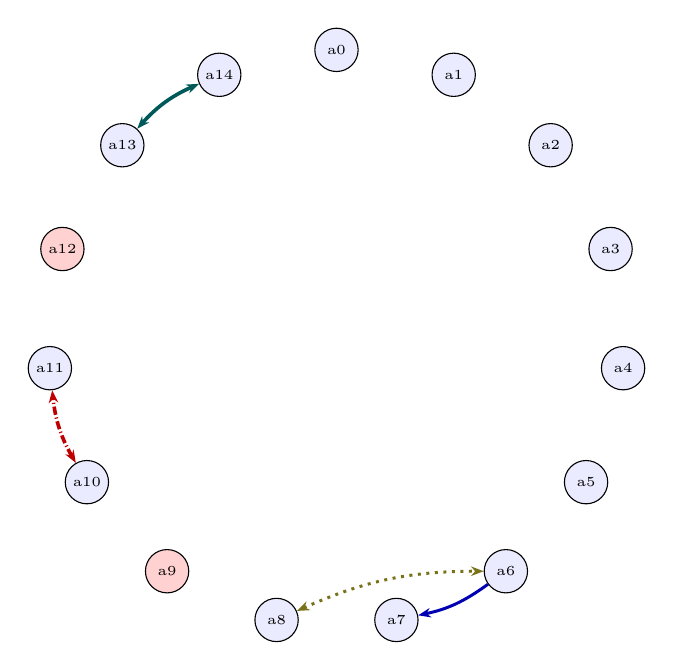
\begin{tikzpicture}[>={Stealth[length=1.6mm]}]
  \node[circle,draw,fill=blue!8,inner sep=1pt,minimum size=5.5mm,font=\tiny] (a0) at (90.0:3.66) {a0};
  \node[circle,draw,fill=blue!8,inner sep=1pt,minimum size=5.5mm,font=\tiny] (a1) at (66.0:3.66) {a1};
  \node[circle,draw,fill=blue!8,inner sep=1pt,minimum size=5.5mm,font=\tiny] (a2) at (42.0:3.66) {a2};
  \node[circle,draw,fill=blue!8,inner sep=1pt,minimum size=5.5mm,font=\tiny] (a3) at (18.0:3.66) {a3};
  \node[circle,draw,fill=blue!8,inner sep=1pt,minimum size=5.5mm,font=\tiny] (a4) at (-6.0:3.66) {a4};
  \node[circle,draw,fill=blue!8,inner sep=1pt,minimum size=5.5mm,font=\tiny] (a5) at (-30.0:3.66) {a5};
  \node[circle,draw,fill=blue!8,inner sep=1pt,minimum size=5.5mm,font=\tiny] (a6) at (-54.0:3.66) {a6};
  \node[circle,draw,fill=blue!8,inner sep=1pt,minimum size=5.5mm,font=\tiny] (a7) at (-78.0:3.66) {a7};
  \node[circle,draw,fill=blue!8,inner sep=1pt,minimum size=5.5mm,font=\tiny] (a8) at (-102.0:3.66) {a8};
  \node[circle,draw,fill=red!18,inner sep=1pt,minimum size=5.5mm,font=\tiny] (a9) at (-126.0:3.66) {a9};
  \node[circle,draw,fill=blue!8,inner sep=1pt,minimum size=5.5mm,font=\tiny] (a10) at (-150.0:3.66) {a10};
  \node[circle,draw,fill=blue!8,inner sep=1pt,minimum size=5.5mm,font=\tiny] (a11) at (-174.0:3.66) {a11};
  \node[circle,draw,fill=red!18,inner sep=1pt,minimum size=5.5mm,font=\tiny] (a12) at (-198.0:3.66) {a12};
  \node[circle,draw,fill=blue!8,inner sep=1pt,minimum size=5.5mm,font=\tiny] (a13) at (-222.0:3.66) {a13};
  \node[circle,draw,fill=blue!8,inner sep=1pt,minimum size=5.5mm,font=\tiny] (a14) at (-246.0:3.66) {a14};
  \draw[-{Stealth[length=1.6mm]}, blue!70!black, line width=1.08pt] (a6) to[bend left=12] (a7);
  \draw[{Stealth[length=1.6mm]}-{Stealth[length=1.6mm]}, olive!80!black, dotted, line width=1.08pt] (a8) to[bend left=12] (a6);
  \draw[{Stealth[length=1.6mm]}-{Stealth[length=1.6mm]}, red!75!black, densely dashdotted, line width=1.31pt] (a10) to[bend left=12] (a11);
  \draw[{Stealth[length=1.6mm]}-{Stealth[length=1.6mm]}, teal!70!black, line width=1.31pt] (a13) to[bend left=12] (a14);
\end{tikzpicture}
}
\\[2pt]{\footnotesize valid edges only: 4 factors}
\end{minipage}
\caption{Relation graph for \texttt{locobench-opus-5-5-f009-r1}. Nodes are atoms on a circle, tinted red when the item marks them non-factual (prior 0.1) and blue when factual (prior 0.9). Edges are gold relations: solid blue = entailment, dashed red = contradiction, double-headed teal = equivalence, dash-dotted red (double-headed) = exclusive (exactly-one), dotted olive (double-headed) = co-necessity (at-least-one); thickness scales with the factor probability. Ordering-only Precedence edges carry no factor and so are not drawn.}
\label{fig:graph-locobench-opus-5-5-f009-r1}
\end{figure}

\begin{table}[htbp]
\centering
\footnotesize
\setlength{\tabcolsep}{3.5pt}
\caption{The specific gold relations of \texttt{locobench-opus-5-5-f009-r1}. \textbf{$p$ used} is the factor probability the MRF received: the band midpoint, times $(1-\lambda)$ for a resolved concession, or \emph{none} for an ordering-only edge (no factor). \textbf{Valid} marks the deliberately-planted errors with their kind. \textbf{Res.} is the resolving atom of a resolved concession.}
\label{tab:rels-locobench-opus-5-5-f009-r1}
\begin{tabular}{lllllrll}
\toprule
ID & Endpoints & Sense & Coupling & Band & $p$ used & Valid & Res. \\
\midrule
\texttt{r002} & \texttt{a6} $\to$ \texttt{a7} & Effect-Cause & \texttt{entailment} & moderate & 0.720 & \checkmark &  \\
\texttt{r003} & \texttt{a8} $\leftrightarrow$ \texttt{a6} & Disjunction & \texttt{co\_necessity} & moderate & 0.720 & \checkmark &  \\
\texttt{r004} & \texttt{a10} $\leftrightarrow$ \texttt{a11} & Alternative & \texttt{exclusive} & strong & 0.925 & \checkmark &  \\
\texttt{r005} & \texttt{a13} $\leftrightarrow$ \texttt{a14} & Restatement & \texttt{equivalence} & strong & 0.925 & \checkmark &  \\
\texttt{r006} & \texttt{a1} $\to$ \texttt{a2} & Concession & \texttt{contradiction} & weak & 0.470 & $\times$ {\scriptsize wrong\_sense} &  \\
\texttt{r007} & \texttt{a12} $\to$ \texttt{a13} & Precedence & \texttt{none} & weak & \emph{none} & $\times$ {\scriptsize false\_endpoint} &  \\
\texttt{r008} & \texttt{a9} $\to$ \texttt{a3} & Cause-Effect & \texttt{entailment} & moderate & 0.720 & $\times$ {\scriptsize false\_endpoint} &  \\
\texttt{r009} & \texttt{a12} $\to$ \texttt{a11} & Evidence & \texttt{entailment} & moderate & 0.720 & $\times$ {\scriptsize false\_endpoint} &  \\
\bottomrule
\end{tabular}
\end{table}

\begin{table}[htbp]
\centering
\footnotesize
\caption{Atoms of \texttt{locobench-opus-5-5-f009-r1}: the \texttt{factual} label, the prior it maps to, the posterior marginal $P(a_i{=}1)$ the MRF returns, and the shift. Atoms dragged below their prior are the ones the coherence structure penalises.}
\label{tab:atoms-locobench-opus-5-5-f009-r1}
\begin{tabular}{llrrrp{7.2cm}}
\toprule
Atom & fact & $\pi_i$ & $P(a_i{=}1)$ & $\Delta$ & Text \\
\midrule
\texttt{a0} & \checkmark & 0.90 & 0.900 & +0.000 & \footnotesize The central span of the Riverside pedestrian bridge collapsed in March 2019. \\
\texttt{a1} & \checkmark & 0.90 & 0.904 & +0.004 & \footnotesize Halvorsen Structural argued that the collapse was caused by deficient construction. \\
\texttt{a2} & \checkmark & 0.90 & 0.909 & +0.009 & \footnotesize Corbett Construction argued that the collapse was caused by a design error. \\
\texttt{a3} & \checkmark & 0.90 & 0.908 & +0.008 & \footnotesize The structural failure initiated at a hanger rod connection on the box beam. \\
\texttt{a4} & \checkmark & 0.90 & 0.900 & +0.000 & \footnotesize Forensic engineers recovered the failed connection hardware from the debris. \\
\texttt{a5} & \checkmark & 0.90 & 0.900 & +0.000 & \footnotesize Forensic engineers compared the as-built connections against the approved design drawings. \\
\texttt{a6} & \checkmark & 0.90 & 0.947 & +0.047 & \footnotesize The hanger rod connection was fabricated differently from the original design drawings. \\
\texttt{a7} & \checkmark & 0.90 & 0.955 & +0.055 & \footnotesize A shop drawing submitted by Corbett Construction altered the hanger rod connection detail. \\
\texttt{a8} & \checkmark & 0.90 & 0.929 & +0.029 & \footnotesize The hanger rod connection was undersized in the original design. \\
\texttt{a9} & $\times$ & 0.10 & 0.131 & +0.031 & \footnotesize The hanger rods on the bridge were fabricated from aluminum. \\
\texttt{a10} & \checkmark & 0.90 & 0.620 & -0.280 & \footnotesize The bridge had been open to the public before the collapse. \\
\texttt{a11} & \checkmark & 0.90 & 0.652 & -0.248 & \footnotesize The bridge had never been opened to the public before the collapse. \\
\texttt{a12} & $\times$ & 0.10 & 0.110 & +0.010 & \footnotesize The collapse occurred during a load test conducted before the bridge opened. \\
\texttt{a13} & \checkmark & 0.90 & 0.979 & +0.079 & \footnotesize The bridge was closed to all traffic after the collapse. \\
\texttt{a14} & \checkmark & 0.90 & 0.979 & +0.079 & \footnotesize After the collapse, authorities barred every user from the bridge. \\
\bottomrule
\end{tabular}
\end{table}

\subsection{Computer Science -- base (\texttt{locobench-opus-5-5-f010-r1})}

\textbf{Topic:} Computer Science (Engineering \& Technology). \textbf{Family:} \texttt{f010} (CONFLICT), rung 1 (\emph{base}). \textbf{Scores:} mean-marg $= 0.758$, consist $= 0.332$, reified $= 0.107$, log-Z $= 0.369$.



\paragraph{Framing question.} \emph{How do engineers determine whether an intermittent production crash stems from a software concurrency defect or from faulty hardware such as corrupted memory, when both hypotheses predict overlapping symptoms in the crash logs?}



\paragraph{Response.} {\small When an intermittent crash surfaces in production, the logs alone rarely discriminate between a concurrency defect and a hardware fault. A pointer torn by an unsynchronized write and a bit flipped in DRAM both yield segmentation faults, corrupted heap metadata, and stack traces that terminate in code with no obvious connection to the original error. The incident examined here shows the difficulty clearly. The application team argued that the crashes were caused by a race condition in the cache eviction code, whereas the infrastructure team argued that the crashes were caused by a failing memory module. Neither position was idle speculation. Initial inspection established that at least one of two defects was present, perhaps both: a data race existed in the service's cache eviction code, or a memory module in the production fleet had a failing cell. The diagnostic task was therefore to decide which defect produced the observed failures, rather than which defect existed.

The first discriminating instrument is the memory controller's own telemetry. The ECC error counters on the affected hosts remained at zero throughout the incident period; in other words, no ECC memory errors were logged on the affected hosts during the incident period, even though the degraded module was physically present in the fleet. This silence carries weight. A cell failing inside a host that is actively crashing would ordinarily register correctable errors well before it produced an uncorrectable fault. A clean counter therefore shifts the burden of proof toward the software hypothesis, although it does not by itself exclude hardware, because some failure modes escape single-bit correction.

The second instrument is correlation across the fleet. A crash that follows a specific binary version across many machines points toward a software cause; by contrast, a crash that stays tied to one physical machine across software versions points toward a hardware cause. The logic reflects how each defect propagates. A flaw in shared code travels with every rollout, while a defective DIMM remains installed in a single chassis. Engineers accordingly tabulate every crash against hostname, kernel release, and deployed build, and the tabulation forces a definite answer for the incident window: either the intermittent crashes occurred on only one host, or the intermittent crashes occurred on more than one host. The two outcomes cannot both hold, and one of them must.

Dedicated tooling then narrows the search further. ThreadSanitizer detects data races by reading hardware ECC error registers, and teams routinely run it against suspect code paths in an instrumented staging build. Memory faults leave a different signature, because faulty memory always produces crashes at the same instruction address, and that fixed-address behavior is what confined the intermittent crashes to a single host. Because ThreadSanitizer reads those registers, adding stress-test load with many concurrent threads can make latent race conditions manifest more often. In this incident, the staging runs under heavy concurrent load came before the postmortem review board concluded that the crashes were caused by a race condition in the cache eviction code.

The board's verdict also accounts for the defect itself. The data race in the eviction path stemmed from that conclusion, which identified the race as the operative mechanism of the incident and directed remediation toward the locking discipline around cache removal. The competing hypothesis still had to be disposed of explicitly, and the incident review board determined that the failing memory module was not the root cause of the crashes. That determination settles the apparent conflict between the degraded cell and the silent ECC counters. The module was genuinely failing, but not in any host where the service crashed, so its presence in the fleet is fully consistent with the absence of logged errors. The general method is therefore cumulative. Engineers consult hardware telemetry, correlate crashes against hosts and builds, and reproduce the failure under controlled load. Overlapping symptoms in the crash logs then give way to a single account that every piece of evidence supports.}

\begin{figure}[htbp]
\centering
\begin{minipage}[t]{0.48\linewidth}\centering
\resizebox{!}{6.4cm}{%
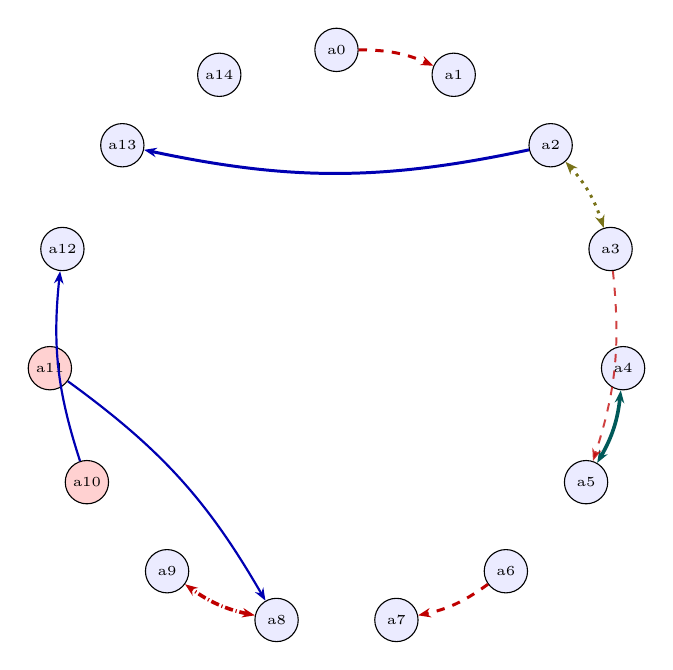
\begin{tikzpicture}[>={Stealth[length=1.6mm]}]
  \node[circle,draw,fill=blue!8,inner sep=1pt,minimum size=5.5mm,font=\tiny] (a0) at (90.0:3.66) {a0};
  \node[circle,draw,fill=blue!8,inner sep=1pt,minimum size=5.5mm,font=\tiny] (a1) at (66.0:3.66) {a1};
  \node[circle,draw,fill=blue!8,inner sep=1pt,minimum size=5.5mm,font=\tiny] (a2) at (42.0:3.66) {a2};
  \node[circle,draw,fill=blue!8,inner sep=1pt,minimum size=5.5mm,font=\tiny] (a3) at (18.0:3.66) {a3};
  \node[circle,draw,fill=blue!8,inner sep=1pt,minimum size=5.5mm,font=\tiny] (a4) at (-6.0:3.66) {a4};
  \node[circle,draw,fill=blue!8,inner sep=1pt,minimum size=5.5mm,font=\tiny] (a5) at (-30.0:3.66) {a5};
  \node[circle,draw,fill=blue!8,inner sep=1pt,minimum size=5.5mm,font=\tiny] (a6) at (-54.0:3.66) {a6};
  \node[circle,draw,fill=blue!8,inner sep=1pt,minimum size=5.5mm,font=\tiny] (a7) at (-78.0:3.66) {a7};
  \node[circle,draw,fill=blue!8,inner sep=1pt,minimum size=5.5mm,font=\tiny] (a8) at (-102.0:3.66) {a8};
  \node[circle,draw,fill=blue!8,inner sep=1pt,minimum size=5.5mm,font=\tiny] (a9) at (-126.0:3.66) {a9};
  \node[circle,draw,fill=red!18,inner sep=1pt,minimum size=5.5mm,font=\tiny] (a10) at (-150.0:3.66) {a10};
  \node[circle,draw,fill=red!18,inner sep=1pt,minimum size=5.5mm,font=\tiny] (a11) at (-174.0:3.66) {a11};
  \node[circle,draw,fill=blue!8,inner sep=1pt,minimum size=5.5mm,font=\tiny] (a12) at (-198.0:3.66) {a12};
  \node[circle,draw,fill=blue!8,inner sep=1pt,minimum size=5.5mm,font=\tiny] (a13) at (-222.0:3.66) {a13};
  \node[circle,draw,fill=blue!8,inner sep=1pt,minimum size=5.5mm,font=\tiny] (a14) at (-246.0:3.66) {a14};
  \draw[-{Stealth[length=1.6mm]}, red!75!black, dashed, line width=1.08pt] (a0) to[bend left=12] (a1);
  \draw[{Stealth[length=1.6mm]}-{Stealth[length=1.6mm]}, olive!80!black, dotted, line width=1.08pt] (a2) to[bend left=12] (a3);
  \draw[{Stealth[length=1.6mm]}-{Stealth[length=1.6mm]}, teal!70!black, line width=1.31pt] (a4) to[bend left=12] (a5);
  \draw[-{Stealth[length=1.6mm]}, red!75!black, dashed, opacity=0.75, line width=0.71pt] (a3) to[bend left=12] (a5);
  \draw[-{Stealth[length=1.6mm]}, red!75!black, dashed, line width=1.08pt] (a6) to[bend left=12] (a7);
  \draw[{Stealth[length=1.6mm]}-{Stealth[length=1.6mm]}, red!75!black, densely dashdotted, line width=1.31pt] (a8) to[bend left=12] (a9);
  \draw[-{Stealth[length=1.6mm]}, blue!70!black, line width=0.79pt] (a11) to[bend left=12] (a8);
  \draw[-{Stealth[length=1.6mm]}, blue!70!black, line width=0.79pt] (a10) to[bend left=12] (a12);
  \draw[-{Stealth[length=1.6mm]}, blue!70!black, line width=1.08pt] (a2) to[bend left=12] (a13);
\end{tikzpicture}
}
\\[2pt]{\footnotesize all gold edges: 9 factors}
\end{minipage}\hfill\begin{minipage}[t]{0.48\linewidth}\centering
\resizebox{!}{6.4cm}{%
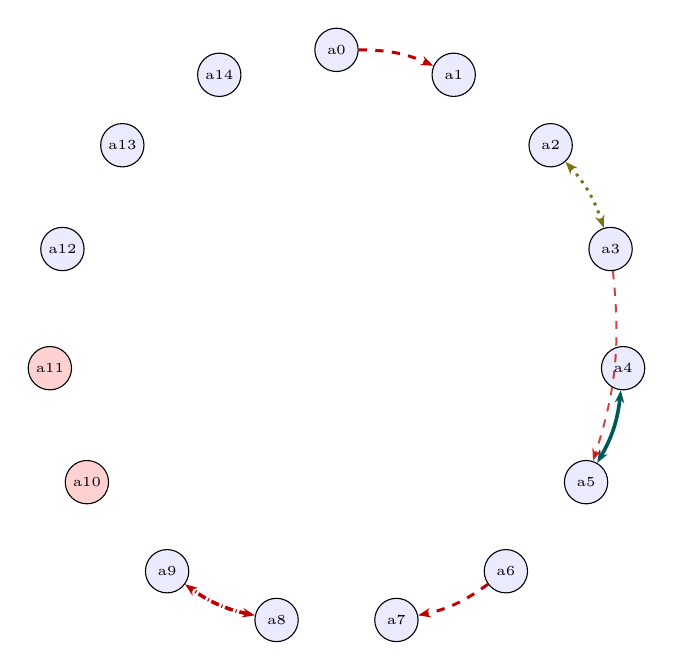
\begin{tikzpicture}[>={Stealth[length=1.6mm]}]
  \node[circle,draw,fill=blue!8,inner sep=1pt,minimum size=5.5mm,font=\tiny] (a0) at (90.0:3.66) {a0};
  \node[circle,draw,fill=blue!8,inner sep=1pt,minimum size=5.5mm,font=\tiny] (a1) at (66.0:3.66) {a1};
  \node[circle,draw,fill=blue!8,inner sep=1pt,minimum size=5.5mm,font=\tiny] (a2) at (42.0:3.66) {a2};
  \node[circle,draw,fill=blue!8,inner sep=1pt,minimum size=5.5mm,font=\tiny] (a3) at (18.0:3.66) {a3};
  \node[circle,draw,fill=blue!8,inner sep=1pt,minimum size=5.5mm,font=\tiny] (a4) at (-6.0:3.66) {a4};
  \node[circle,draw,fill=blue!8,inner sep=1pt,minimum size=5.5mm,font=\tiny] (a5) at (-30.0:3.66) {a5};
  \node[circle,draw,fill=blue!8,inner sep=1pt,minimum size=5.5mm,font=\tiny] (a6) at (-54.0:3.66) {a6};
  \node[circle,draw,fill=blue!8,inner sep=1pt,minimum size=5.5mm,font=\tiny] (a7) at (-78.0:3.66) {a7};
  \node[circle,draw,fill=blue!8,inner sep=1pt,minimum size=5.5mm,font=\tiny] (a8) at (-102.0:3.66) {a8};
  \node[circle,draw,fill=blue!8,inner sep=1pt,minimum size=5.5mm,font=\tiny] (a9) at (-126.0:3.66) {a9};
  \node[circle,draw,fill=red!18,inner sep=1pt,minimum size=5.5mm,font=\tiny] (a10) at (-150.0:3.66) {a10};
  \node[circle,draw,fill=red!18,inner sep=1pt,minimum size=5.5mm,font=\tiny] (a11) at (-174.0:3.66) {a11};
  \node[circle,draw,fill=blue!8,inner sep=1pt,minimum size=5.5mm,font=\tiny] (a12) at (-198.0:3.66) {a12};
  \node[circle,draw,fill=blue!8,inner sep=1pt,minimum size=5.5mm,font=\tiny] (a13) at (-222.0:3.66) {a13};
  \node[circle,draw,fill=blue!8,inner sep=1pt,minimum size=5.5mm,font=\tiny] (a14) at (-246.0:3.66) {a14};
  \draw[-{Stealth[length=1.6mm]}, red!75!black, dashed, line width=1.08pt] (a0) to[bend left=12] (a1);
  \draw[{Stealth[length=1.6mm]}-{Stealth[length=1.6mm]}, olive!80!black, dotted, line width=1.08pt] (a2) to[bend left=12] (a3);
  \draw[{Stealth[length=1.6mm]}-{Stealth[length=1.6mm]}, teal!70!black, line width=1.31pt] (a4) to[bend left=12] (a5);
  \draw[-{Stealth[length=1.6mm]}, red!75!black, dashed, opacity=0.75, line width=0.71pt] (a3) to[bend left=12] (a5);
  \draw[-{Stealth[length=1.6mm]}, red!75!black, dashed, line width=1.08pt] (a6) to[bend left=12] (a7);
  \draw[{Stealth[length=1.6mm]}-{Stealth[length=1.6mm]}, red!75!black, densely dashdotted, line width=1.31pt] (a8) to[bend left=12] (a9);
\end{tikzpicture}
}
\\[2pt]{\footnotesize valid edges only: 6 factors}
\end{minipage}
\caption{Relation graph for \texttt{locobench-opus-5-5-f010-r1}. Nodes are atoms on a circle, tinted red when the item marks them non-factual (prior 0.1) and blue when factual (prior 0.9). Edges are gold relations: solid blue = entailment, dashed red = contradiction, double-headed teal = equivalence, dash-dotted red (double-headed) = exclusive (exactly-one), dotted olive (double-headed) = co-necessity (at-least-one); thickness scales with the factor probability. Ordering-only Precedence edges carry no factor and so are not drawn.}
\label{fig:graph-locobench-opus-5-5-f010-r1}
\end{figure}

\begin{table}[htbp]
\centering
\footnotesize
\setlength{\tabcolsep}{3.5pt}
\caption{The specific gold relations of \texttt{locobench-opus-5-5-f010-r1}. \textbf{$p$ used} is the factor probability the MRF received: the band midpoint, times $(1-\lambda)$ for a resolved concession, or \emph{none} for an ordering-only edge (no factor). \textbf{Valid} marks the deliberately-planted errors with their kind. \textbf{Res.} is the resolving atom of a resolved concession.}
\label{tab:rels-locobench-opus-5-5-f010-r1}
\begin{tabular}{lllllrll}
\toprule
ID & Endpoints & Sense & Coupling & Band & $p$ used & Valid & Res. \\
\midrule
\texttt{r000} & \texttt{a0} $\leftrightarrow$ \texttt{a1} & Contrast & \texttt{contradiction} & moderate & 0.720 & \checkmark &  \\
\texttt{r001} & \texttt{a2} $\leftrightarrow$ \texttt{a3} & Disjunction & \texttt{co\_necessity} & moderate & 0.720 & \checkmark &  \\
\texttt{r002} & \texttt{a4} $\leftrightarrow$ \texttt{a5} & Restatement & \texttt{equivalence} & strong & 0.925 & \checkmark &  \\
\texttt{r003} & \texttt{a3} $\to$ \texttt{a5} & Concession & \texttt{contradiction} & moderate & 0.396 & \checkmark & \texttt{a14} \\
\texttt{r004} & \texttt{a6} $\leftrightarrow$ \texttt{a7} & Contrast & \texttt{contradiction} & moderate & 0.720 & \checkmark &  \\
\texttt{r005} & \texttt{a8} $\leftrightarrow$ \texttt{a9} & Alternative & \texttt{exclusive} & strong & 0.925 & \checkmark &  \\
\texttt{r006} & \texttt{a11} $\to$ \texttt{a8} & Cause-Effect & \texttt{entailment} & weak & 0.470 & $\times$ {\scriptsize spurious} &  \\
\texttt{r007} & \texttt{a10} $\to$ \texttt{a12} & Cause-Effect & \texttt{entailment} & weak & 0.470 & $\times$ {\scriptsize false\_endpoint} &  \\
\texttt{r008} & \texttt{a12} $\to$ \texttt{a13} & Precedence & \texttt{none} & weak & \emph{none} & $\times$ {\scriptsize wrong\_sense} &  \\
\texttt{r009} & \texttt{a2} $\to$ \texttt{a13} & Effect-Cause & \texttt{entailment} & moderate & 0.720 & $\times$ {\scriptsize wrong\_direction} &  \\
\bottomrule
\end{tabular}
\end{table}

\begin{table}[htbp]
\centering
\footnotesize
\caption{Atoms of \texttt{locobench-opus-5-5-f010-r1}: the \texttt{factual} label, the prior it maps to, the posterior marginal $P(a_i{=}1)$ the MRF returns, and the shift. Atoms dragged below their prior are the ones the coherence structure penalises.}
\label{tab:atoms-locobench-opus-5-5-f010-r1}
\begin{tabular}{llrrrp{7.2cm}}
\toprule
Atom & fact & $\pi_i$ & $P(a_i{=}1)$ & $\Delta$ & Text \\
\midrule
\texttt{a0} & \checkmark & 0.90 & 0.854 & -0.046 & \footnotesize The application team argued that the crashes were caused by a race condition in the cache eviction code. \\
\texttt{a1} & \checkmark & 0.90 & 0.796 & -0.104 & \footnotesize The infrastructure team argued that the crashes were caused by a failing memory module. \\
\texttt{a2} & \checkmark & 0.90 & 0.947 & +0.047 & \footnotesize A data race existed in the service's cache eviction code. \\
\texttt{a3} & \checkmark & 0.90 & 0.940 & +0.040 & \footnotesize A memory module in the production fleet had a failing cell. \\
\texttt{a4} & \checkmark & 0.90 & 0.983 & +0.083 & \footnotesize The ECC error counters on the affected hosts remained at zero throughout the incident period. \\
\texttt{a5} & \checkmark & 0.90 & 0.986 & +0.086 & \footnotesize No ECC memory errors were logged on the affected hosts during the incident period. \\
\texttt{a6} & \checkmark & 0.90 & 0.854 & -0.046 & \footnotesize A crash that follows a specific binary version across many machines points toward a software cause. \\
\texttt{a7} & \checkmark & 0.90 & 0.796 & -0.104 & \footnotesize A crash that stays tied to one physical machine across software versions points toward a hardware cause. \\
\texttt{a8} & \checkmark & 0.90 & 0.629 & -0.271 & \footnotesize The intermittent crashes occurred on only one host. \\
\texttt{a9} & \checkmark & 0.90 & 0.633 & -0.267 & \footnotesize The intermittent crashes occurred on more than one host. \\
\texttt{a10} & $\times$ & 0.10 & 0.096 & -0.004 & \footnotesize ThreadSanitizer detects data races by reading hardware ECC error registers. \\
\texttt{a11} & $\times$ & 0.10 & 0.099 & -0.001 & \footnotesize Faulty memory always produces crashes at the same instruction address. \\
\texttt{a12} & \checkmark & 0.90 & 0.899 & -0.001 & \footnotesize Adding stress-test load with many concurrent threads can make latent race conditions manifest more often. \\
\texttt{a13} & \checkmark & 0.90 & 0.955 & +0.055 & \footnotesize The postmortem review board concluded that the crashes were caused by a race condition in the cache eviction code. \\
\texttt{a14} & \checkmark & 0.90 & 0.900 & +0.000 & \footnotesize The incident review board determined that the failing memory module was not the root cause of the crashes. \\
\bottomrule
\end{tabular}
\end{table}

\subsection{Culture -- direction\_reversal\_a (\texttt{locobench-opus-5-5-f011-r1})}

\textbf{Topic:} Culture (Humanities). \textbf{Family:} \texttt{f011} (CONTROL), rung 1 (\emph{direction\_reversal\_a}). \textbf{Scores:} mean-marg $= 0.777$, consist $= 0.449$, reified $= 0.178$, log-Z $= 0.352$.



\paragraph{Framing question.} \emph{How did archaeologists adjudicate whether the oldest painted markings in Iberian caves such as La Pasiega were produced by Neanderthals or by early modern humans, given disputes over the reliability of uranium-thorium dating?}



\paragraph{Response.} {\small The question of authorship for the oldest painted markings in Iberian caves was settled, as far as it has been settled, by chronology rather than by style. Nothing in a row of red lines or a hand stencil identifies the species that made it, so the decisive evidence had to be an age falling either within or before the window of modern human presence on the peninsula. The dating program that forced the issue had a clear leader: Dirk Hoffmann led the team that dated the Iberian cave paintings, and only after that fieldwork and laboratory analysis did the Hoffmann team publish its cave art dates in the journal Nature. The debate that followed was therefore conducted largely over method, because any attribution could be no stronger than the ages beneath it.

Radiocarbon could not be applied to mineral pigments, so the analysis took an indirect route. The team applied uranium-thorium dating to carbonate crusts that formed over the painted markings. Because the measurements were taken on deposits laid down on top of the pigment rather than within it, a carbonate crust that overlies a painting provides a minimum age for that painting: the paint must already have been on the wall when the calcite began to accumulate, and the crust says nothing about how long the image existed before it was covered. A ladder-shaped scalariform sign at La Pasiega was among the dated markings. The ladder sign at La Pasiega is more than 64,000 years old; that is, the scalariform sign was painted over 64 millennia ago, and provided that this is so, the minimum-age logic holds.

Despite that antiquity, modern humans are generally thought to have arrived in Europe around 45,000 to 42,000 years ago. The age of the sign therefore poses a strict dilemma about the population of the peninsula, one with no middle ground: either modern humans were present in Iberia 64,000 years ago, or no modern humans were present in Iberia 64,000 years ago, and these two possibilities cannot both be true. Accepting the first would require an otherwise undocumented dispersal more than twenty millennia earlier than the conventional chronology allows. The Hoffmann et al. 2018 study resolved the tension by concluding that Neanderthals produced the dated Iberian cave markings. That attribution reconciles a sign older than 64,000 years with the accepted arrival window by assigning the sign to the hominin population already resident in Iberia, and it carried a substantial implication: symbolic behavior would no longer be a trait unique to Homo sapiens.

By contrast, critics argued that the uranium-thorium ages from the crusts were artificially old. That objection, as its proponents developed it, led to an open-system scenario in which at least one of two things occurred, perhaps both: the dated crust samples lost uranium after they formed, or they contained uncorrected detrital thorium. Either process pushes a uranium-thorium age upward. Leaching of uranium raises the apparent ratio of thorium to its parent isotope, and thorium carried into the calcite with clay or dust adds daughter product that did not grow in place, so each mechanism would make a young crust look ancient and its minimum age correspondingly misleading. The dating team answered by pointing to sequential sampling from the crust surface inward and to ages that increased consistently with depth, a pattern difficult to reconcile with random uranium loss. By contrast with those contested ages, the setting of the key site is not in question: La Pasiega is located in Asturias.

Adjudication between Neanderthal and modern human authorship thus reduced to a narrow geochemical question about whether the crusts behaved as closed systems. If they did, the minimum ages stand and the case for Neanderthal painting follows from the arrival chronology; if they did not, the Iberian markings lose their claim to precede modern humans, and the attribution reverts to an open problem awaiting independent dating methods.}

\begin{figure}[htbp]
\centering
\begin{minipage}[t]{0.48\linewidth}\centering
\resizebox{!}{6.4cm}{%
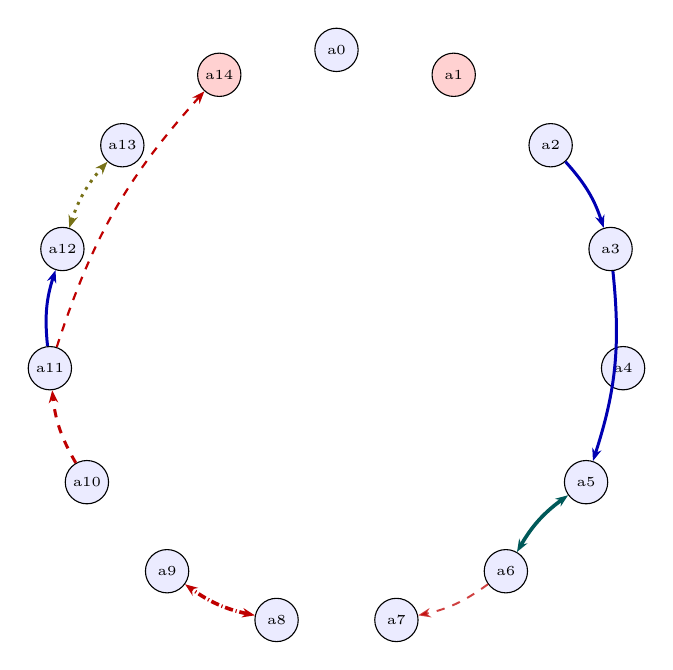
\begin{tikzpicture}[>={Stealth[length=1.6mm]}]
  \node[circle,draw,fill=blue!8,inner sep=1pt,minimum size=5.5mm,font=\tiny] (a0) at (90.0:3.66) {a0};
  \node[circle,draw,fill=red!18,inner sep=1pt,minimum size=5.5mm,font=\tiny] (a1) at (66.0:3.66) {a1};
  \node[circle,draw,fill=blue!8,inner sep=1pt,minimum size=5.5mm,font=\tiny] (a2) at (42.0:3.66) {a2};
  \node[circle,draw,fill=blue!8,inner sep=1pt,minimum size=5.5mm,font=\tiny] (a3) at (18.0:3.66) {a3};
  \node[circle,draw,fill=blue!8,inner sep=1pt,minimum size=5.5mm,font=\tiny] (a4) at (-6.0:3.66) {a4};
  \node[circle,draw,fill=blue!8,inner sep=1pt,minimum size=5.5mm,font=\tiny] (a5) at (-30.0:3.66) {a5};
  \node[circle,draw,fill=blue!8,inner sep=1pt,minimum size=5.5mm,font=\tiny] (a6) at (-54.0:3.66) {a6};
  \node[circle,draw,fill=blue!8,inner sep=1pt,minimum size=5.5mm,font=\tiny] (a7) at (-78.0:3.66) {a7};
  \node[circle,draw,fill=blue!8,inner sep=1pt,minimum size=5.5mm,font=\tiny] (a8) at (-102.0:3.66) {a8};
  \node[circle,draw,fill=blue!8,inner sep=1pt,minimum size=5.5mm,font=\tiny] (a9) at (-126.0:3.66) {a9};
  \node[circle,draw,fill=blue!8,inner sep=1pt,minimum size=5.5mm,font=\tiny] (a10) at (-150.0:3.66) {a10};
  \node[circle,draw,fill=blue!8,inner sep=1pt,minimum size=5.5mm,font=\tiny] (a11) at (-174.0:3.66) {a11};
  \node[circle,draw,fill=blue!8,inner sep=1pt,minimum size=5.5mm,font=\tiny] (a12) at (-198.0:3.66) {a12};
  \node[circle,draw,fill=blue!8,inner sep=1pt,minimum size=5.5mm,font=\tiny] (a13) at (-222.0:3.66) {a13};
  \node[circle,draw,fill=red!18,inner sep=1pt,minimum size=5.5mm,font=\tiny] (a14) at (-246.0:3.66) {a14};
  \draw[-{Stealth[length=1.6mm]}, blue!70!black, line width=1.08pt] (a3) to[bend left=12] (a5);
  \draw[{Stealth[length=1.6mm]}-{Stealth[length=1.6mm]}, teal!70!black, line width=1.31pt] (a6) to[bend left=12] (a5);
  \draw[{Stealth[length=1.6mm]}-{Stealth[length=1.6mm]}, red!75!black, densely dashdotted, line width=1.31pt] (a8) to[bend left=12] (a9);
  \draw[{Stealth[length=1.6mm]}-{Stealth[length=1.6mm]}, olive!80!black, dotted, line width=1.08pt] (a12) to[bend left=12] (a13);
  \draw[-{Stealth[length=1.6mm]}, red!75!black, dashed, opacity=0.75, line width=0.71pt] (a6) to[bend left=12] (a7);
  \draw[-{Stealth[length=1.6mm]}, red!75!black, dashed, line width=1.08pt] (a10) to[bend left=12] (a11);
  \draw[-{Stealth[length=1.6mm]}, red!75!black, dashed, line width=0.79pt] (a11) to[bend left=12] (a14);
  \draw[-{Stealth[length=1.6mm]}, blue!70!black, line width=1.08pt] (a11) to[bend left=12] (a12);
  \draw[-{Stealth[length=1.6mm]}, blue!70!black, line width=1.08pt] (a2) to[bend left=12] (a3);
\end{tikzpicture}
}
\\[2pt]{\footnotesize all gold edges: 9 factors}
\end{minipage}\hfill\begin{minipage}[t]{0.48\linewidth}\centering
\resizebox{!}{6.4cm}{%
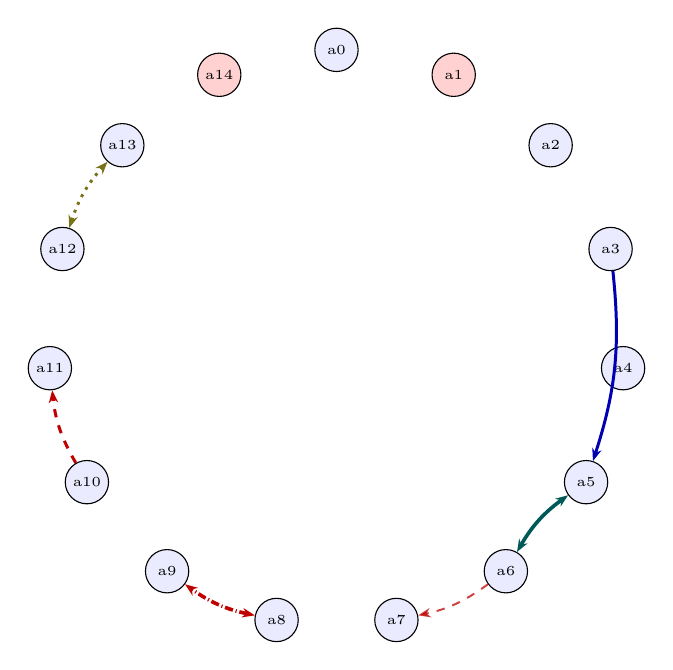
\begin{tikzpicture}[>={Stealth[length=1.6mm]}]
  \node[circle,draw,fill=blue!8,inner sep=1pt,minimum size=5.5mm,font=\tiny] (a0) at (90.0:3.66) {a0};
  \node[circle,draw,fill=red!18,inner sep=1pt,minimum size=5.5mm,font=\tiny] (a1) at (66.0:3.66) {a1};
  \node[circle,draw,fill=blue!8,inner sep=1pt,minimum size=5.5mm,font=\tiny] (a2) at (42.0:3.66) {a2};
  \node[circle,draw,fill=blue!8,inner sep=1pt,minimum size=5.5mm,font=\tiny] (a3) at (18.0:3.66) {a3};
  \node[circle,draw,fill=blue!8,inner sep=1pt,minimum size=5.5mm,font=\tiny] (a4) at (-6.0:3.66) {a4};
  \node[circle,draw,fill=blue!8,inner sep=1pt,minimum size=5.5mm,font=\tiny] (a5) at (-30.0:3.66) {a5};
  \node[circle,draw,fill=blue!8,inner sep=1pt,minimum size=5.5mm,font=\tiny] (a6) at (-54.0:3.66) {a6};
  \node[circle,draw,fill=blue!8,inner sep=1pt,minimum size=5.5mm,font=\tiny] (a7) at (-78.0:3.66) {a7};
  \node[circle,draw,fill=blue!8,inner sep=1pt,minimum size=5.5mm,font=\tiny] (a8) at (-102.0:3.66) {a8};
  \node[circle,draw,fill=blue!8,inner sep=1pt,minimum size=5.5mm,font=\tiny] (a9) at (-126.0:3.66) {a9};
  \node[circle,draw,fill=blue!8,inner sep=1pt,minimum size=5.5mm,font=\tiny] (a10) at (-150.0:3.66) {a10};
  \node[circle,draw,fill=blue!8,inner sep=1pt,minimum size=5.5mm,font=\tiny] (a11) at (-174.0:3.66) {a11};
  \node[circle,draw,fill=blue!8,inner sep=1pt,minimum size=5.5mm,font=\tiny] (a12) at (-198.0:3.66) {a12};
  \node[circle,draw,fill=blue!8,inner sep=1pt,minimum size=5.5mm,font=\tiny] (a13) at (-222.0:3.66) {a13};
  \node[circle,draw,fill=red!18,inner sep=1pt,minimum size=5.5mm,font=\tiny] (a14) at (-246.0:3.66) {a14};
  \draw[-{Stealth[length=1.6mm]}, blue!70!black, line width=1.08pt] (a3) to[bend left=12] (a5);
  \draw[{Stealth[length=1.6mm]}-{Stealth[length=1.6mm]}, teal!70!black, line width=1.31pt] (a6) to[bend left=12] (a5);
  \draw[{Stealth[length=1.6mm]}-{Stealth[length=1.6mm]}, red!75!black, densely dashdotted, line width=1.31pt] (a8) to[bend left=12] (a9);
  \draw[{Stealth[length=1.6mm]}-{Stealth[length=1.6mm]}, olive!80!black, dotted, line width=1.08pt] (a12) to[bend left=12] (a13);
  \draw[-{Stealth[length=1.6mm]}, red!75!black, dashed, opacity=0.75, line width=0.71pt] (a6) to[bend left=12] (a7);
  \draw[-{Stealth[length=1.6mm]}, red!75!black, dashed, line width=1.08pt] (a10) to[bend left=12] (a11);
\end{tikzpicture}
}
\\[2pt]{\footnotesize valid edges only: 6 factors}
\end{minipage}
\caption{Relation graph for \texttt{locobench-opus-5-5-f011-r1}. Nodes are atoms on a circle, tinted red when the item marks them non-factual (prior 0.1) and blue when factual (prior 0.9). Edges are gold relations: solid blue = entailment, dashed red = contradiction, double-headed teal = equivalence, dash-dotted red (double-headed) = exclusive (exactly-one), dotted olive (double-headed) = co-necessity (at-least-one); thickness scales with the factor probability. Ordering-only Precedence edges carry no factor and so are not drawn.}
\label{fig:graph-locobench-opus-5-5-f011-r1}
\end{figure}

\begin{table}[htbp]
\centering
\footnotesize
\setlength{\tabcolsep}{3.5pt}
\caption{The specific gold relations of \texttt{locobench-opus-5-5-f011-r1}. \textbf{$p$ used} is the factor probability the MRF received: the band midpoint, times $(1-\lambda)$ for a resolved concession, or \emph{none} for an ordering-only edge (no factor). \textbf{Valid} marks the deliberately-planted errors with their kind. \textbf{Res.} is the resolving atom of a resolved concession.}
\label{tab:rels-locobench-opus-5-5-f011-r1}
\begin{tabular}{lllllrll}
\toprule
ID & Endpoints & Sense & Coupling & Band & $p$ used & Valid & Res. \\
\midrule
\texttt{r000} & \texttt{a3} $\to$ \texttt{a5} & Condition & \texttt{entailment} & moderate & 0.720 & \checkmark &  \\
\texttt{r001} & \texttt{a6} $\leftrightarrow$ \texttt{a5} & Restatement & \texttt{equivalence} & strong & 0.925 & \checkmark &  \\
\texttt{r002} & \texttt{a8} $\leftrightarrow$ \texttt{a9} & Alternative & \texttt{exclusive} & strong & 0.925 & \checkmark &  \\
\texttt{r003} & \texttt{a12} $\leftrightarrow$ \texttt{a13} & Disjunction & \texttt{co\_necessity} & moderate & 0.720 & \checkmark &  \\
\texttt{r004} & \texttt{a6} $\to$ \texttt{a7} & Concession & \texttt{contradiction} & moderate & 0.396 & \checkmark & \texttt{a10} \\
\texttt{r005} & \texttt{a10} $\leftrightarrow$ \texttt{a11} & Contrast & \texttt{contradiction} & moderate & 0.720 & \checkmark &  \\
\texttt{r006} & \texttt{a11} $\leftrightarrow$ \texttt{a14} & Contrast & \texttt{contradiction} & weak & 0.470 & $\times$ {\scriptsize spurious} &  \\
\texttt{r007} & \texttt{a0} $\to$ \texttt{a1} & Precedence & \texttt{none} & weak & \emph{none} & $\times$ {\scriptsize false\_endpoint} &  \\
\texttt{r008} & \texttt{a11} $\to$ \texttt{a12} & Cause-Effect & \texttt{entailment} & moderate & 0.720 & $\times$ {\scriptsize wrong\_direction} &  \\
\texttt{r009} & \texttt{a2} $\to$ \texttt{a3} & Cause-Effect & \texttt{entailment} & moderate & 0.720 & $\times$ {\scriptsize wrong\_sense} &  \\
\bottomrule
\end{tabular}
\end{table}

\begin{table}[htbp]
\centering
\footnotesize
\caption{Atoms of \texttt{locobench-opus-5-5-f011-r1}: the \texttt{factual} label, the prior it maps to, the posterior marginal $P(a_i{=}1)$ the MRF returns, and the shift. Atoms dragged below their prior are the ones the coherence structure penalises.}
\label{tab:atoms-locobench-opus-5-5-f011-r1}
\begin{tabular}{llrrrp{7.2cm}}
\toprule
Atom & fact & $\pi_i$ & $P(a_i{=}1)$ & $\Delta$ & Text \\
\midrule
\texttt{a0} & \checkmark & 0.90 & 0.900 & +0.000 & \footnotesize Dirk Hoffmann led the team that dated the Iberian cave paintings. \\
\texttt{a1} & $\times$ & 0.10 & 0.100 & +0.000 & \footnotesize The Hoffmann team published its cave art dates in the journal Nature. \\
\texttt{a2} & \checkmark & 0.90 & 0.925 & +0.025 & \footnotesize The team applied uranium-thorium dating to carbonate crusts that formed over the painted markings. \\
\texttt{a3} & \checkmark & 0.90 & 0.967 & +0.067 & \footnotesize A carbonate crust that overlies a painting provides a minimum age for that painting. \\
\texttt{a4} & \checkmark & 0.90 & 0.900 & +0.000 & \footnotesize A ladder-shaped scalariform sign at La Pasiega was among the dated markings. \\
\texttt{a5} & \checkmark & 0.90 & 0.992 & +0.092 & \footnotesize The ladder sign at La Pasiega is more than 64,000 years old. \\
\texttt{a6} & \checkmark & 0.90 & 0.988 & +0.088 & \footnotesize The scalariform sign at La Pasiega was painted over 64 millennia ago. \\
\texttt{a7} & \checkmark & 0.90 & 0.932 & +0.032 & \footnotesize Modern humans are generally thought to have arrived in Europe around 45,000 to 42,000 years ago. \\
\texttt{a8} & \checkmark & 0.90 & 0.632 & -0.268 & \footnotesize Modern humans were present in Iberia 64,000 years ago. \\
\texttt{a9} & \checkmark & 0.90 & 0.632 & -0.268 & \footnotesize No modern humans were present in Iberia 64,000 years ago. \\
\texttt{a10} & \checkmark & 0.90 & 0.850 & -0.050 & \footnotesize The Hoffmann et al. 2018 study concluded that Neanderthals produced the dated Iberian cave markings. \\
\texttt{a11} & \checkmark & 0.90 & 0.836 & -0.064 & \footnotesize Critics argued that the uranium-thorium ages from the crusts were artificially old. \\
\texttt{a12} & \checkmark & 0.90 & 0.964 & +0.064 & \footnotesize The dated crust samples lost uranium after they formed. \\
\texttt{a13} & \checkmark & 0.90 & 0.929 & +0.029 & \footnotesize The dated crust samples contained uncorrected detrital thorium. \\
\texttt{a14} & $\times$ & 0.10 & 0.109 & +0.009 & \footnotesize La Pasiega is located in Asturias. \\
\bottomrule
\end{tabular}
\end{table}

\subsection{Cybersecurity -- shuffle\_block (\texttt{locobench-opus-5-5-f012-r1})}

\textbf{Topic:} Cybersecurity (Engineering \& Technology). \textbf{Family:} \texttt{f012} (ORDER), rung 1 (\emph{shuffle\_block}). \textbf{Scores:} mean-marg $= 0.793$, consist $= 0.446$, reified $= 0.196$, log-Z $= 0.346$.



\paragraph{Framing question.} \emph{How do forensic investigators decide whether a corporate data breach was carried out by a malicious insider or by an external intruder using stolen credentials, when the initial access logs appear consistent with either explanation?}



\paragraph{Response.} {\small When access logs fit both an insider and an outsider holding stolen credentials, investigators stop asking whose account was used and ask who was operating it. That shift moves the analysis from authentication records to physical, behavioural and procedural evidence that a credential cannot carry with it. A recent incident shows the method. Meridian Logistics suffered a breach of its customer database; specifically, roughly 2.3 million customer records were exfiltrated. The access trail pointed to a single privileged identity: the attacker logged in with the database administrator's credentials. In other words, the database administrator's username and password were used to gain access to the system. By contrast, multi-factor authentication was enforced on the compromised administrator account. That control shaped the initial reading of the logs, because a valid second factor seemed to point toward someone holding the administrator's physical token.

Analysis of the exfiltration path addressed a separate technical question: what the stolen data looked like in transit. Network captures and endpoint artefacts support two incompatible readings, and exactly one of them must be true. Either the exfiltrated records were encrypted by the attacker before transfer, or the exfiltrated records were transferred in unencrypted form. Resolving this matters for regulatory notification, since cleartext transfer exposes the records to any party positioned on the route. It also matters for attribution, because staging and encryption reflect an operator's tooling and habits. The forensic timeline places the unencrypted transfer first. It preceded the exfiltration, which took place continuously over a period of eight months. That sequence is recorded here purely as chronology, reconstructed from flow logs and storage timestamps.

Personnel history then drew attention to one person. The administrator who owned the account had resigned two weeks before the breach, and because of that recent departure the company initially suspected the departing administrator of the theft. Departing staff with privileged access are a well-documented insider-risk category. Resentment, pending employment with a competitor, and knowledge of internal controls all make the window around a resignation a period of heightened exposure. Investigators therefore treated the suspicion as a hypothesis to be tested rather than a conclusion. Although the company held that suspicion, badge records showed the administrator was not in the building at the time of the login. Physical access data cannot by itself rule out remote activity. It does remove the simplest version of the insider scenario, in which a disgruntled employee works from a familiar terminal on the premises.

The individual strands combined into a single finding. The incident review board concluded that the breach was carried out by an external intruder using stolen credentials. That determination settles the tension between the company's early suspicion of its former administrator and the badge evidence placing him elsewhere: the insider hypothesis is set aside, and the badge records are explained rather than overridden. The board's conclusion also confirms the password reuse on the breached external website as a route by which the credential reached the intruder. The general lesson for investigators is methodological. When authentication logs cannot tell an insider from an outsider, the decision rests on converging independent evidence: physical presence, behavioural signatures, credential provenance and exfiltration mechanics. Each of these is weighed on its own terms before any attribution is made.

Behavioural biometrics supplied the next layer of evidence. Keystroke timing in the session differed from the administrator's historical typing patterns. Dwell times, inter-key intervals and the rhythm of habitual command sequences form a profile that is hard to imitate and does not travel with a stolen password. With the operator's identity in doubt, the question became how the secret had left the administrator's control. Two leakage routes were identified, and at least one of them holds, perhaps both. The administrator's password was harvested by malware on a compromised workstation, or the administrator's password was reused on an external website that suffered a breach. Whereas the keystroke anomaly concerns who was typing during the session, that external reuse concerns how the credential entered circulation beyond Meridian's perimeter.}

\begin{figure}[htbp]
\centering
\begin{minipage}[t]{0.48\linewidth}\centering
\resizebox{!}{6.4cm}{%
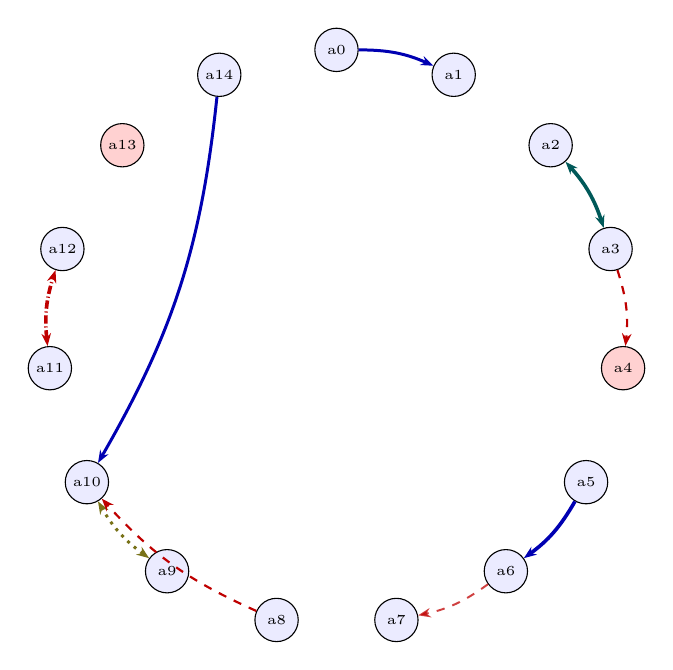
\begin{tikzpicture}[>={Stealth[length=1.6mm]}]
  \node[circle,draw,fill=blue!8,inner sep=1pt,minimum size=5.5mm,font=\tiny] (a0) at (90.0:3.66) {a0};
  \node[circle,draw,fill=blue!8,inner sep=1pt,minimum size=5.5mm,font=\tiny] (a1) at (66.0:3.66) {a1};
  \node[circle,draw,fill=blue!8,inner sep=1pt,minimum size=5.5mm,font=\tiny] (a2) at (42.0:3.66) {a2};
  \node[circle,draw,fill=blue!8,inner sep=1pt,minimum size=5.5mm,font=\tiny] (a3) at (18.0:3.66) {a3};
  \node[circle,draw,fill=red!18,inner sep=1pt,minimum size=5.5mm,font=\tiny] (a4) at (-6.0:3.66) {a4};
  \node[circle,draw,fill=blue!8,inner sep=1pt,minimum size=5.5mm,font=\tiny] (a5) at (-30.0:3.66) {a5};
  \node[circle,draw,fill=blue!8,inner sep=1pt,minimum size=5.5mm,font=\tiny] (a6) at (-54.0:3.66) {a6};
  \node[circle,draw,fill=blue!8,inner sep=1pt,minimum size=5.5mm,font=\tiny] (a7) at (-78.0:3.66) {a7};
  \node[circle,draw,fill=blue!8,inner sep=1pt,minimum size=5.5mm,font=\tiny] (a8) at (-102.0:3.66) {a8};
  \node[circle,draw,fill=blue!8,inner sep=1pt,minimum size=5.5mm,font=\tiny] (a9) at (-126.0:3.66) {a9};
  \node[circle,draw,fill=blue!8,inner sep=1pt,minimum size=5.5mm,font=\tiny] (a10) at (-150.0:3.66) {a10};
  \node[circle,draw,fill=blue!8,inner sep=1pt,minimum size=5.5mm,font=\tiny] (a11) at (-174.0:3.66) {a11};
  \node[circle,draw,fill=blue!8,inner sep=1pt,minimum size=5.5mm,font=\tiny] (a12) at (-198.0:3.66) {a12};
  \node[circle,draw,fill=red!18,inner sep=1pt,minimum size=5.5mm,font=\tiny] (a13) at (-222.0:3.66) {a13};
  \node[circle,draw,fill=blue!8,inner sep=1pt,minimum size=5.5mm,font=\tiny] (a14) at (-246.0:3.66) {a14};
  \draw[-{Stealth[length=1.6mm]}, blue!70!black, line width=1.08pt] (a0) to[bend left=12] (a1);
  \draw[{Stealth[length=1.6mm]}-{Stealth[length=1.6mm]}, teal!70!black, line width=1.31pt] (a2) to[bend left=12] (a3);
  \draw[-{Stealth[length=1.6mm]}, blue!70!black, line width=1.31pt] (a5) to[bend left=12] (a6);
  \draw[-{Stealth[length=1.6mm]}, red!75!black, dashed, opacity=0.75, line width=0.71pt] (a6) to[bend left=12] (a7);
  \draw[{Stealth[length=1.6mm]}-{Stealth[length=1.6mm]}, olive!80!black, dotted, line width=1.08pt] (a9) to[bend left=12] (a10);
  \draw[{Stealth[length=1.6mm]}-{Stealth[length=1.6mm]}, red!75!black, densely dashdotted, line width=1.31pt] (a11) to[bend left=12] (a12);
  \draw[-{Stealth[length=1.6mm]}, red!75!black, dashed, line width=0.79pt] (a3) to[bend left=12] (a4);
  \draw[-{Stealth[length=1.6mm]}, red!75!black, dashed, line width=0.79pt] (a8) to[bend left=12] (a10);
  \draw[-{Stealth[length=1.6mm]}, blue!70!black, line width=1.08pt] (a14) to[bend left=12] (a10);
\end{tikzpicture}
}
\\[2pt]{\footnotesize all gold edges: 9 factors}
\end{minipage}\hfill\begin{minipage}[t]{0.48\linewidth}\centering
\resizebox{!}{6.4cm}{%
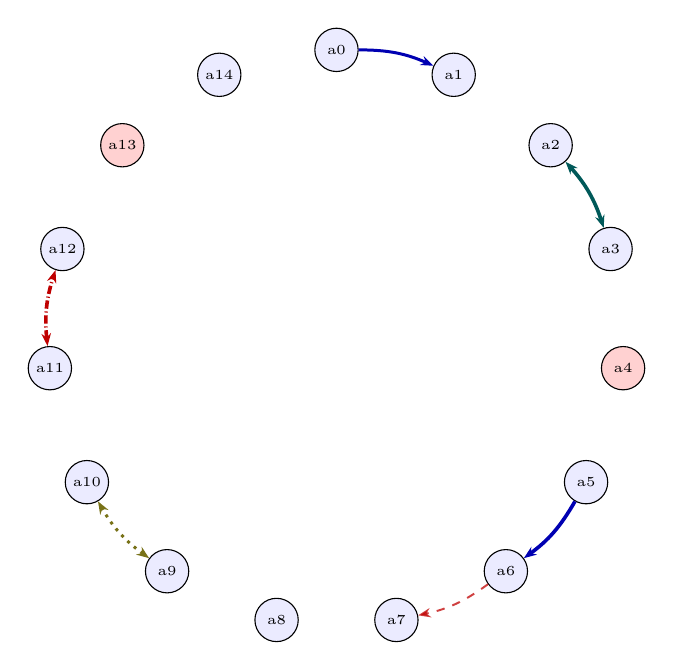
\begin{tikzpicture}[>={Stealth[length=1.6mm]}]
  \node[circle,draw,fill=blue!8,inner sep=1pt,minimum size=5.5mm,font=\tiny] (a0) at (90.0:3.66) {a0};
  \node[circle,draw,fill=blue!8,inner sep=1pt,minimum size=5.5mm,font=\tiny] (a1) at (66.0:3.66) {a1};
  \node[circle,draw,fill=blue!8,inner sep=1pt,minimum size=5.5mm,font=\tiny] (a2) at (42.0:3.66) {a2};
  \node[circle,draw,fill=blue!8,inner sep=1pt,minimum size=5.5mm,font=\tiny] (a3) at (18.0:3.66) {a3};
  \node[circle,draw,fill=red!18,inner sep=1pt,minimum size=5.5mm,font=\tiny] (a4) at (-6.0:3.66) {a4};
  \node[circle,draw,fill=blue!8,inner sep=1pt,minimum size=5.5mm,font=\tiny] (a5) at (-30.0:3.66) {a5};
  \node[circle,draw,fill=blue!8,inner sep=1pt,minimum size=5.5mm,font=\tiny] (a6) at (-54.0:3.66) {a6};
  \node[circle,draw,fill=blue!8,inner sep=1pt,minimum size=5.5mm,font=\tiny] (a7) at (-78.0:3.66) {a7};
  \node[circle,draw,fill=blue!8,inner sep=1pt,minimum size=5.5mm,font=\tiny] (a8) at (-102.0:3.66) {a8};
  \node[circle,draw,fill=blue!8,inner sep=1pt,minimum size=5.5mm,font=\tiny] (a9) at (-126.0:3.66) {a9};
  \node[circle,draw,fill=blue!8,inner sep=1pt,minimum size=5.5mm,font=\tiny] (a10) at (-150.0:3.66) {a10};
  \node[circle,draw,fill=blue!8,inner sep=1pt,minimum size=5.5mm,font=\tiny] (a11) at (-174.0:3.66) {a11};
  \node[circle,draw,fill=blue!8,inner sep=1pt,minimum size=5.5mm,font=\tiny] (a12) at (-198.0:3.66) {a12};
  \node[circle,draw,fill=red!18,inner sep=1pt,minimum size=5.5mm,font=\tiny] (a13) at (-222.0:3.66) {a13};
  \node[circle,draw,fill=blue!8,inner sep=1pt,minimum size=5.5mm,font=\tiny] (a14) at (-246.0:3.66) {a14};
  \draw[-{Stealth[length=1.6mm]}, blue!70!black, line width=1.08pt] (a0) to[bend left=12] (a1);
  \draw[{Stealth[length=1.6mm]}-{Stealth[length=1.6mm]}, teal!70!black, line width=1.31pt] (a2) to[bend left=12] (a3);
  \draw[-{Stealth[length=1.6mm]}, blue!70!black, line width=1.31pt] (a5) to[bend left=12] (a6);
  \draw[-{Stealth[length=1.6mm]}, red!75!black, dashed, opacity=0.75, line width=0.71pt] (a6) to[bend left=12] (a7);
  \draw[{Stealth[length=1.6mm]}-{Stealth[length=1.6mm]}, olive!80!black, dotted, line width=1.08pt] (a9) to[bend left=12] (a10);
  \draw[{Stealth[length=1.6mm]}-{Stealth[length=1.6mm]}, red!75!black, densely dashdotted, line width=1.31pt] (a11) to[bend left=12] (a12);
\end{tikzpicture}
}
\\[2pt]{\footnotesize valid edges only: 6 factors}
\end{minipage}
\caption{Relation graph for \texttt{locobench-opus-5-5-f012-r1}. Nodes are atoms on a circle, tinted red when the item marks them non-factual (prior 0.1) and blue when factual (prior 0.9). Edges are gold relations: solid blue = entailment, dashed red = contradiction, double-headed teal = equivalence, dash-dotted red (double-headed) = exclusive (exactly-one), dotted olive (double-headed) = co-necessity (at-least-one); thickness scales with the factor probability. Ordering-only Precedence edges carry no factor and so are not drawn.}
\label{fig:graph-locobench-opus-5-5-f012-r1}
\end{figure}

\begin{table}[htbp]
\centering
\footnotesize
\setlength{\tabcolsep}{3.5pt}
\caption{The specific gold relations of \texttt{locobench-opus-5-5-f012-r1}. \textbf{$p$ used} is the factor probability the MRF received: the band midpoint, times $(1-\lambda)$ for a resolved concession, or \emph{none} for an ordering-only edge (no factor). \textbf{Valid} marks the deliberately-planted errors with their kind. \textbf{Res.} is the resolving atom of a resolved concession.}
\label{tab:rels-locobench-opus-5-5-f012-r1}
\begin{tabular}{lllllrll}
\toprule
ID & Endpoints & Sense & Coupling & Band & $p$ used & Valid & Res. \\
\midrule
\texttt{r000} & \texttt{a0} $\to$ \texttt{a1} & Instantiation & \texttt{entailment} & moderate & 0.720 & \checkmark &  \\
\texttt{r001} & \texttt{a2} $\leftrightarrow$ \texttt{a3} & Restatement & \texttt{equivalence} & strong & 0.925 & \checkmark &  \\
\texttt{r002} & \texttt{a5} $\to$ \texttt{a6} & Cause-Effect & \texttt{entailment} & strong & 0.925 & \checkmark &  \\
\texttt{r003} & \texttt{a6} $\to$ \texttt{a7} & Concession & \texttt{contradiction} & moderate & 0.396 & \checkmark & \texttt{a14} \\
\texttt{r004} & \texttt{a9} $\leftrightarrow$ \texttt{a10} & Disjunction & \texttt{co\_necessity} & moderate & 0.720 & \checkmark &  \\
\texttt{r005} & \texttt{a11} $\leftrightarrow$ \texttt{a12} & Alternative & \texttt{exclusive} & strong & 0.925 & \checkmark &  \\
\texttt{r006} & \texttt{a3} $\leftrightarrow$ \texttt{a4} & Contrast & \texttt{contradiction} & weak & 0.470 & $\times$ {\scriptsize false\_endpoint} &  \\
\texttt{r007} & \texttt{a8} $\leftrightarrow$ \texttt{a10} & Contrast & \texttt{contradiction} & weak & 0.470 & $\times$ {\scriptsize spurious} &  \\
\texttt{r008} & \texttt{a12} $\to$ \texttt{a13} & Precedence & \texttt{none} & weak & \emph{none} & $\times$ {\scriptsize false\_endpoint} &  \\
\texttt{r009} & \texttt{a14} $\to$ \texttt{a10} & Evidence & \texttt{entailment} & moderate & 0.720 & $\times$ {\scriptsize wrong\_direction} &  \\
\bottomrule
\end{tabular}
\end{table}

\begin{table}[htbp]
\centering
\footnotesize
\caption{Atoms of \texttt{locobench-opus-5-5-f012-r1}: the \texttt{factual} label, the prior it maps to, the posterior marginal $P(a_i{=}1)$ the MRF returns, and the shift. Atoms dragged below their prior are the ones the coherence structure penalises.}
\label{tab:atoms-locobench-opus-5-5-f012-r1}
\begin{tabular}{llrrrp{7.2cm}}
\toprule
Atom & fact & $\pi_i$ & $P(a_i{=}1)$ & $\Delta$ & Text \\
\midrule
\texttt{a0} & \checkmark & 0.90 & 0.924 & +0.024 & \footnotesize Meridian Logistics suffered a breach of its customer database. \\
\texttt{a1} & \checkmark & 0.90 & 0.954 & +0.054 & \footnotesize Roughly 2.3 million customer records were exfiltrated in the breach. \\
\texttt{a2} & \checkmark & 0.90 & 0.979 & +0.079 & \footnotesize The attacker logged in with the database administrator's credentials. \\
\texttt{a3} & \checkmark & 0.90 & 0.978 & +0.078 & \footnotesize The database administrator's username and password were used to gain access to the system. \\
\texttt{a4} & $\times$ & 0.10 & 0.111 & +0.011 & \footnotesize Multi-factor authentication was enforced on the compromised administrator account. \\
\texttt{a5} & \checkmark & 0.90 & 0.939 & +0.039 & \footnotesize The administrator who owned the account had resigned two weeks before the breach. \\
\texttt{a6} & \checkmark & 0.90 & 0.987 & +0.087 & \footnotesize The company initially suspected the departing administrator of the theft. \\
\texttt{a7} & \checkmark & 0.90 & 0.932 & +0.032 & \footnotesize Badge records showed the administrator was not in the building at the time of the login. \\
\texttt{a8} & \checkmark & 0.90 & 0.905 & +0.005 & \footnotesize Keystroke timing in the session differed from the administrator's historical typing patterns. \\
\texttt{a9} & \checkmark & 0.90 & 0.929 & +0.029 & \footnotesize The administrator's password was harvested by malware on a compromised workstation. \\
\texttt{a10} & \checkmark & 0.90 & 0.971 & +0.071 & \footnotesize The administrator's password was reused on an external website that suffered a breach. \\
\texttt{a11} & \checkmark & 0.90 & 0.632 & -0.268 & \footnotesize The exfiltrated records were encrypted by the attacker before transfer. \\
\texttt{a12} & \checkmark & 0.90 & 0.632 & -0.268 & \footnotesize The exfiltrated records were transferred in unencrypted form. \\
\texttt{a13} & $\times$ & 0.10 & 0.100 & +0.000 & \footnotesize The exfiltration took place continuously over a period of eight months. \\
\texttt{a14} & \checkmark & 0.90 & 0.926 & +0.026 & \footnotesize The incident review board concluded that the breach was carried out by an external intruder using stolen credentials. \\
\bottomrule
\end{tabular}
\end{table}

\subsection{Economics -- break\_2 (\texttt{locobench-opus-5-5-f013-r1})}

\textbf{Topic:} Economics (Social Sciences). \textbf{Family:} \texttt{f013} (CHAIN), rung 1 (\emph{break\_2}). \textbf{Scores:} mean-marg $= 0.792$, consist $= 0.427$, reified $= 0.209$, log-Z $= 0.565$.



\paragraph{Framing question.} \emph{How did economists adjudicate whether the 2021–2023 United States inflation surge stemmed primarily from excess aggregate demand or from supply-side shocks, given the evidence that later decompositions such as Bernanke and Blanchard's analysis brought to the debate?}



\paragraph{Response.} {\small The adjudication between demand-pull and supply-shock explanations of the 2021–2023 American inflation began with a forecast rather than a decomposition. Lawrence Summers warned in early 2021 that the scale of U.S. fiscal stimulus risked generating significant inflation, and that warning led to the fiscal package taking the form it did: the American Rescue Plan Act of March 2021 authorized about \$1.9 trillion in spending. In other words, the act authorized \$3.5 trillion in direct spending. For proponents of the demand view, the size of this transfer relative to the estimated output gap was the central fact. A stimulus of that magnitude, they argued, would push spending beyond the economy's productive capacity and would show up in prices once households drew down their accumulated savings.

The demand account had to contend with a sequence of external disturbances that no fiscal model anticipated. Russia's invasion of Ukraine in February 2022 pushed up global energy prices. Headline U.S. CPI inflation exceeded 9 percent year over year at some point in 2022. The record on the peak admits no middle position: either that threshold was crossed, or headline U.S. CPI inflation never exceeded 9 percent year over year at any point in 2022. The two readings cannot both be true, and one of them must hold. For the purpose of attribution, the more important point is that the composition of the peak was dominated by energy and food, components whose movements trace to world commodity markets rather than to domestic spending.

Monetary policy supplied a second line of evidence. The Federal Reserve began raising its policy rate in March 2022, which came after it began its post-pandemic rate-hiking cycle in 2020. Through a rapid and sustained tightening, the federal funds target range reached 5.25 to 5.50 percent in July 2023. That restrictive stance in turn caused U.S. inflation to decline substantially during 2023 without a large rise in unemployment. This combination proved awkward for a strictly demand-based account. If excess demand had been the dominant force, disinflation of that size would ordinarily have required a substantial sacrifice in employment, yet the labor market absorbed the tightening with little damage, which is the pattern expected when the shocks that raised prices are themselves unwinding.

The sectoral record from 2021 pointed in the same direction. A global semiconductor shortage contributed to sharp increases in U.S. used-car prices in 2021 because supply-chain disruptions raised U.S. goods prices in 2021. At least one of two forces, perhaps both, was operating on prices that year: those supply-chain disruptions, or fiscal stimulus raising U.S. aggregate demand in 2021. The empirical task was to weigh them. Although fiscal stimulus did raise demand, the San Francisco Fed's decomposition found that supply-driven factors accounted for roughly half of the run-up in PCE inflation, more than demand-driven factors did. The Bernanke-Blanchard analysis settled this tension by concluding that price shocks in energy, food, and shortage-hit sectors drove most of the initial inflation surge, rather than an overheated labor market. Their framework allowed demand to matter, chiefly through its effect on the tightness of labor markets and on the persistence of wage growth, while assigning the initial jump in prices to relative-price shocks transmitted through firms' pricing decisions.

The resulting consensus is therefore conditional rather than absolute. Demand pressures created the conditions in which shocks could pass through to prices quickly, and the stimulus debate retains its relevance for questions about the persistence of inflation and the risk of wage-price dynamics. The decompositions nonetheless shifted the burden of proof. Economists who once read the surge as a straightforward case of fiscal overheating now had to explain why the price increases were so concentrated in supply-constrained sectors. They also had to explain why disinflation arrived without the unemployment costs their models predicted.}

\begin{figure}[htbp]
\centering
\begin{minipage}[t]{0.48\linewidth}\centering
\resizebox{!}{6.4cm}{%
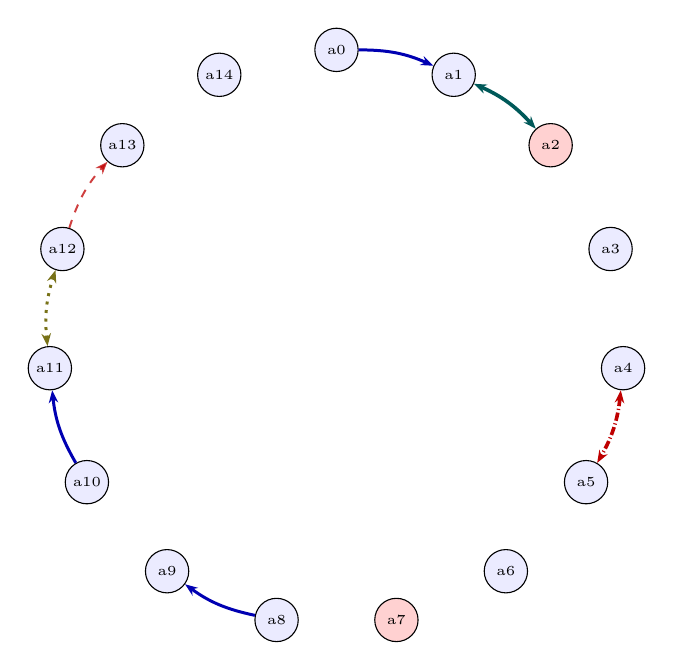
\begin{tikzpicture}[>={Stealth[length=1.6mm]}]
  \node[circle,draw,fill=blue!8,inner sep=1pt,minimum size=5.5mm,font=\tiny] (a0) at (90.0:3.66) {a0};
  \node[circle,draw,fill=blue!8,inner sep=1pt,minimum size=5.5mm,font=\tiny] (a1) at (66.0:3.66) {a1};
  \node[circle,draw,fill=red!18,inner sep=1pt,minimum size=5.5mm,font=\tiny] (a2) at (42.0:3.66) {a2};
  \node[circle,draw,fill=blue!8,inner sep=1pt,minimum size=5.5mm,font=\tiny] (a3) at (18.0:3.66) {a3};
  \node[circle,draw,fill=blue!8,inner sep=1pt,minimum size=5.5mm,font=\tiny] (a4) at (-6.0:3.66) {a4};
  \node[circle,draw,fill=blue!8,inner sep=1pt,minimum size=5.5mm,font=\tiny] (a5) at (-30.0:3.66) {a5};
  \node[circle,draw,fill=blue!8,inner sep=1pt,minimum size=5.5mm,font=\tiny] (a6) at (-54.0:3.66) {a6};
  \node[circle,draw,fill=red!18,inner sep=1pt,minimum size=5.5mm,font=\tiny] (a7) at (-78.0:3.66) {a7};
  \node[circle,draw,fill=blue!8,inner sep=1pt,minimum size=5.5mm,font=\tiny] (a8) at (-102.0:3.66) {a8};
  \node[circle,draw,fill=blue!8,inner sep=1pt,minimum size=5.5mm,font=\tiny] (a9) at (-126.0:3.66) {a9};
  \node[circle,draw,fill=blue!8,inner sep=1pt,minimum size=5.5mm,font=\tiny] (a10) at (-150.0:3.66) {a10};
  \node[circle,draw,fill=blue!8,inner sep=1pt,minimum size=5.5mm,font=\tiny] (a11) at (-174.0:3.66) {a11};
  \node[circle,draw,fill=blue!8,inner sep=1pt,minimum size=5.5mm,font=\tiny] (a12) at (-198.0:3.66) {a12};
  \node[circle,draw,fill=blue!8,inner sep=1pt,minimum size=5.5mm,font=\tiny] (a13) at (-222.0:3.66) {a13};
  \node[circle,draw,fill=blue!8,inner sep=1pt,minimum size=5.5mm,font=\tiny] (a14) at (-246.0:3.66) {a14};
  \draw[-{Stealth[length=1.6mm]}, blue!70!black, line width=1.08pt] (a8) to[bend left=12] (a9);
  \draw[{Stealth[length=1.6mm]}-{Stealth[length=1.6mm]}, red!75!black, densely dashdotted, line width=1.31pt] (a4) to[bend left=12] (a5);
  \draw[{Stealth[length=1.6mm]}-{Stealth[length=1.6mm]}, olive!80!black, dotted, line width=1.08pt] (a11) to[bend left=12] (a12);
  \draw[-{Stealth[length=1.6mm]}, red!75!black, dashed, opacity=0.75, line width=0.71pt] (a12) to[bend left=12] (a13);
  \draw[{Stealth[length=1.6mm]}-{Stealth[length=1.6mm]}, teal!70!black, line width=1.31pt] (a1) to[bend left=12] (a2);
  \draw[-{Stealth[length=1.6mm]}, blue!70!black, line width=1.08pt] (a10) to[bend left=12] (a11);
  \draw[-{Stealth[length=1.6mm]}, blue!70!black, line width=1.08pt] (a0) to[bend left=12] (a1);
\end{tikzpicture}
}
\\[2pt]{\footnotesize all gold edges: 7 factors}
\end{minipage}\hfill\begin{minipage}[t]{0.48\linewidth}\centering
\resizebox{!}{6.4cm}{%
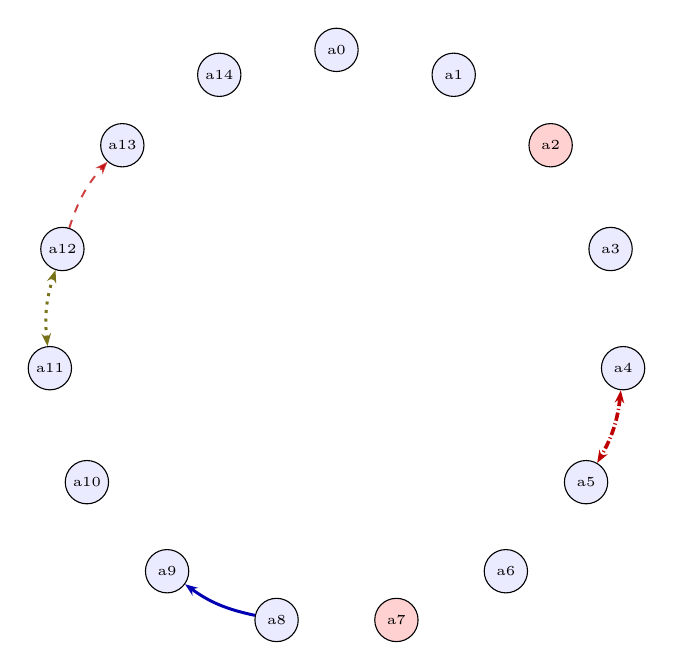
\begin{tikzpicture}[>={Stealth[length=1.6mm]}]
  \node[circle,draw,fill=blue!8,inner sep=1pt,minimum size=5.5mm,font=\tiny] (a0) at (90.0:3.66) {a0};
  \node[circle,draw,fill=blue!8,inner sep=1pt,minimum size=5.5mm,font=\tiny] (a1) at (66.0:3.66) {a1};
  \node[circle,draw,fill=red!18,inner sep=1pt,minimum size=5.5mm,font=\tiny] (a2) at (42.0:3.66) {a2};
  \node[circle,draw,fill=blue!8,inner sep=1pt,minimum size=5.5mm,font=\tiny] (a3) at (18.0:3.66) {a3};
  \node[circle,draw,fill=blue!8,inner sep=1pt,minimum size=5.5mm,font=\tiny] (a4) at (-6.0:3.66) {a4};
  \node[circle,draw,fill=blue!8,inner sep=1pt,minimum size=5.5mm,font=\tiny] (a5) at (-30.0:3.66) {a5};
  \node[circle,draw,fill=blue!8,inner sep=1pt,minimum size=5.5mm,font=\tiny] (a6) at (-54.0:3.66) {a6};
  \node[circle,draw,fill=red!18,inner sep=1pt,minimum size=5.5mm,font=\tiny] (a7) at (-78.0:3.66) {a7};
  \node[circle,draw,fill=blue!8,inner sep=1pt,minimum size=5.5mm,font=\tiny] (a8) at (-102.0:3.66) {a8};
  \node[circle,draw,fill=blue!8,inner sep=1pt,minimum size=5.5mm,font=\tiny] (a9) at (-126.0:3.66) {a9};
  \node[circle,draw,fill=blue!8,inner sep=1pt,minimum size=5.5mm,font=\tiny] (a10) at (-150.0:3.66) {a10};
  \node[circle,draw,fill=blue!8,inner sep=1pt,minimum size=5.5mm,font=\tiny] (a11) at (-174.0:3.66) {a11};
  \node[circle,draw,fill=blue!8,inner sep=1pt,minimum size=5.5mm,font=\tiny] (a12) at (-198.0:3.66) {a12};
  \node[circle,draw,fill=blue!8,inner sep=1pt,minimum size=5.5mm,font=\tiny] (a13) at (-222.0:3.66) {a13};
  \node[circle,draw,fill=blue!8,inner sep=1pt,minimum size=5.5mm,font=\tiny] (a14) at (-246.0:3.66) {a14};
  \draw[-{Stealth[length=1.6mm]}, blue!70!black, line width=1.08pt] (a8) to[bend left=12] (a9);
  \draw[{Stealth[length=1.6mm]}-{Stealth[length=1.6mm]}, red!75!black, densely dashdotted, line width=1.31pt] (a4) to[bend left=12] (a5);
  \draw[{Stealth[length=1.6mm]}-{Stealth[length=1.6mm]}, olive!80!black, dotted, line width=1.08pt] (a11) to[bend left=12] (a12);
  \draw[-{Stealth[length=1.6mm]}, red!75!black, dashed, opacity=0.75, line width=0.71pt] (a12) to[bend left=12] (a13);
\end{tikzpicture}
}
\\[2pt]{\footnotesize valid edges only: 4 factors}
\end{minipage}
\caption{Relation graph for \texttt{locobench-opus-5-5-f013-r1}. Nodes are atoms on a circle, tinted red when the item marks them non-factual (prior 0.1) and blue when factual (prior 0.9). Edges are gold relations: solid blue = entailment, dashed red = contradiction, double-headed teal = equivalence, dash-dotted red (double-headed) = exclusive (exactly-one), dotted olive (double-headed) = co-necessity (at-least-one); thickness scales with the factor probability. Ordering-only Precedence edges carry no factor and so are not drawn.}
\label{fig:graph-locobench-opus-5-5-f013-r1}
\end{figure}

\begin{table}[htbp]
\centering
\footnotesize
\setlength{\tabcolsep}{3.5pt}
\caption{The specific gold relations of \texttt{locobench-opus-5-5-f013-r1}. \textbf{$p$ used} is the factor probability the MRF received: the band midpoint, times $(1-\lambda)$ for a resolved concession, or \emph{none} for an ordering-only edge (no factor). \textbf{Valid} marks the deliberately-planted errors with their kind. \textbf{Res.} is the resolving atom of a resolved concession.}
\label{tab:rels-locobench-opus-5-5-f013-r1}
\begin{tabular}{lllllrll}
\toprule
ID & Endpoints & Sense & Coupling & Band & $p$ used & Valid & Res. \\
\midrule
\texttt{r002} & \texttt{a8} $\to$ \texttt{a9} & Cause-Effect & \texttt{entailment} & moderate & 0.720 & \checkmark &  \\
\texttt{r003} & \texttt{a4} $\leftrightarrow$ \texttt{a5} & Alternative & \texttt{exclusive} & strong & 0.925 & \checkmark &  \\
\texttt{r004} & \texttt{a11} $\leftrightarrow$ \texttt{a12} & Disjunction & \texttt{co\_necessity} & moderate & 0.720 & \checkmark &  \\
\texttt{r005} & \texttt{a12} $\to$ \texttt{a13} & Concession & \texttt{contradiction} & moderate & 0.396 & \checkmark & \texttt{a14} \\
\texttt{r006} & \texttt{a1} $\leftrightarrow$ \texttt{a2} & Restatement & \texttt{equivalence} & strong & 0.925 & $\times$ {\scriptsize false\_endpoint} &  \\
\texttt{r007} & \texttt{a7} $\to$ \texttt{a6} & Precedence & \texttt{none} & weak & \emph{none} & $\times$ {\scriptsize false\_endpoint} &  \\
\texttt{r008} & \texttt{a10} $\to$ \texttt{a11} & Effect-Cause & \texttt{entailment} & moderate & 0.720 & $\times$ {\scriptsize wrong\_sense} &  \\
\texttt{r009} & \texttt{a0} $\to$ \texttt{a1} & Cause-Effect & \texttt{entailment} & moderate & 0.720 & $\times$ {\scriptsize wrong\_direction} &  \\
\bottomrule
\end{tabular}
\end{table}

\begin{table}[htbp]
\centering
\footnotesize
\caption{Atoms of \texttt{locobench-opus-5-5-f013-r1}: the \texttt{factual} label, the prior it maps to, the posterior marginal $P(a_i{=}1)$ the MRF returns, and the shift. Atoms dragged below their prior are the ones the coherence structure penalises.}
\label{tab:atoms-locobench-opus-5-5-f013-r1}
\begin{tabular}{llrrrp{7.2cm}}
\toprule
Atom & fact & $\pi_i$ & $P(a_i{=}1)$ & $\Delta$ & Text \\
\midrule
\texttt{a0} & \checkmark & 0.90 & 0.909 & +0.009 & \footnotesize Lawrence Summers warned in early 2021 that the scale of U.S. fiscal stimulus risked generating significant inflation. \\
\texttt{a1} & \checkmark & 0.90 & 0.798 & -0.102 & \footnotesize The American Rescue Plan Act of March 2021 authorized about \$1.9 trillion in spending. \\
\texttt{a2} & $\times$ & 0.10 & 0.463 & +0.363 & \footnotesize The American Rescue Plan Act authorized \$3.5 trillion in direct spending. \\
\texttt{a3} & \checkmark & 0.90 & 0.900 & +0.000 & \footnotesize Russia's invasion of Ukraine in February 2022 pushed up global energy prices. \\
\texttt{a4} & \checkmark & 0.90 & 0.632 & -0.268 & \footnotesize Headline U.S. CPI inflation exceeded 9 percent year over year at some point in 2022. \\
\texttt{a5} & \checkmark & 0.90 & 0.632 & -0.268 & \footnotesize Headline U.S. CPI inflation never exceeded 9 percent year over year at any point in 2022. \\
\texttt{a6} & \checkmark & 0.90 & 0.900 & +0.000 & \footnotesize The Federal Reserve began raising its policy rate in March 2022. \\
\texttt{a7} & $\times$ & 0.10 & 0.100 & +0.000 & \footnotesize The Federal Reserve began its post-pandemic rate-hiking cycle in 2020. \\
\texttt{a8} & \checkmark & 0.90 & 0.924 & +0.024 & \footnotesize The federal funds target range reached 5.25 to 5.50 percent in July 2023. \\
\texttt{a9} & \checkmark & 0.90 & 0.954 & +0.054 & \footnotesize U.S. inflation declined substantially during 2023 without a large rise in unemployment. \\
\texttt{a10} & \checkmark & 0.90 & 0.925 & +0.025 & \footnotesize A global semiconductor shortage contributed to sharp increases in U.S. used-car prices in 2021. \\
\texttt{a11} & \checkmark & 0.90 & 0.968 & +0.068 & \footnotesize Supply-chain disruptions raised U.S. goods prices in 2021. \\
\texttt{a12} & \checkmark & 0.90 & 0.938 & +0.038 & \footnotesize Fiscal stimulus raised U.S. aggregate demand in 2021. \\
\texttt{a13} & \checkmark & 0.90 & 0.930 & +0.030 & \footnotesize The San Francisco Fed's decomposition found that supply-driven factors accounted for roughly half of the run-up in PCE inflation, more than demand-driven factors did. \\
\texttt{a14} & \checkmark & 0.90 & 0.900 & +0.000 & \footnotesize The Bernanke-Blanchard analysis concluded that price shocks in energy, food, and shortage-hit sectors drove most of the initial inflation surge, rather than an overheated labor market. \\
\bottomrule
\end{tabular}
\end{table}

\subsection{Education -- base (\texttt{locobench-opus-5-5-f014-r1})}

\textbf{Topic:} Education (Social Sciences). \textbf{Family:} \texttt{f014} (CONFLICT), rung 1 (\emph{base}). \textbf{Scores:} mean-marg $= 0.780$, consist $= 0.478$, reified $= 0.284$, log-Z $= 0.361$.



\paragraph{Framing question.} \emph{How did investigators establish whether the dramatic test-score gains reported by Atlanta Public Schools in the late 2000s reflected genuine instructional improvement or systematic tampering with student answer sheets by educators?}



\paragraph{Response.} {\small The question of whether Atlanta's late-2000s test-score surge was real first entered public view through journalism rather than through any official audit. The Atlanta Journal-Constitution published analyses showing statistically improbable score gains at Atlanta schools, and that reporting led to the suspicious gains appearing on Georgia's Criterion-Referenced Competency Tests. The CRCT was the state's high-stakes accountability instrument. Its results determined whether schools met federal benchmarks and whether administrators earned bonuses, which is why sharp year-over-year jumps in individual buildings attracted scrutiny from statisticians and reporters alike.

Investigators had to weigh two explanations for those jumps, and the evidence never required choosing only one. At least one of the following held, perhaps both: some of the Atlanta score gains resulted from educators altering student answer sheets, or some of the Atlanta score gains resulted from genuine instructional improvement. To separate the two, the Georgia Governor's Office of Student Achievement commissioned an erasure analysis of the 2009 answer sheets. The method relied on optical scanners that detect residual graphite where a bubble has been changed. The erasure analysis counted wrong-to-right erasures on student answer sheets, and it took that form because many Atlanta classrooms showed wrong-to-right erasure rates far above the state average. That erasure pattern indicates the tampering with answer sheets described above. Children revising their own work produce erasures in all directions and at modest rates. Clusters of corrections that turn wrong answers into right ones, concentrated in particular classrooms, point instead to adults changing responses after testing. The pattern held even though genuine instructional progress was present in parts of the district.

Statistical anomalies alone could not establish intent or identify who had changed the answers, so the inquiry moved to sworn testimony and document review. The Federal Bureau of Investigation led the inquiry into the Atlanta test scores, whereas Governor Sonny Perdue appointed special investigators to examine the Atlanta schools. That appointment came before the special investigators' report was released in July 2011. In other words, in July 2011 the findings of the governor's special investigation were made public. The investigative team, which included former state attorney general Mike Bowers, interviewed teachers, principals, and central-office staff. They obtained confessions from educators who described erasure sessions held behind closed doors, and they found records showing that warnings about irregularities had been ignored or suppressed.

The scale of the misconduct was the central question the report answered. The investigators found evidence of cheating at only 12 Atlanta schools. By contrast, the special investigators concluded that systematic cheating had occurred in 44 of the 56 schools they examined. That conclusion settles the tension between the genuine instructional gains and the anomalous erasure rates. Real improvement may have occurred in some classrooms, but tampering pervaded so many schools that the district's celebrated trajectory could no longer be read as evidence of instructional success. The report also described a culture of fear in which teachers who missed targets faced public humiliation or dismissal, which explains why misconduct spread across buildings rather than remaining isolated.

The criminal phase followed. A Fulton County grand jury in 2013 indicted former superintendent Beverly Hall and thirty-four other educators under Georgia's racketeering statute. Prosecutors argued that the district had operated as a corrupt enterprise whose output was falsified data. Many defendants accepted plea agreements, and a jury in 2015 convicted eleven of those who went to trial. The disposition of the case against Hall herself admits of exactly two outcomes, and one of them must be the case: either Beverly Hall stood trial on the racketeering charges, or Beverly Hall never stood trial on the racketeering charges. The two cannot both be true. Taken together, the erasure statistics, the governor's investigation, and the prosecutions show how investigators turned a statistical suspicion into a documented account of systematic answer-sheet tampering.}

\begin{figure}[htbp]
\centering
\begin{minipage}[t]{0.48\linewidth}\centering
\resizebox{!}{6.4cm}{%
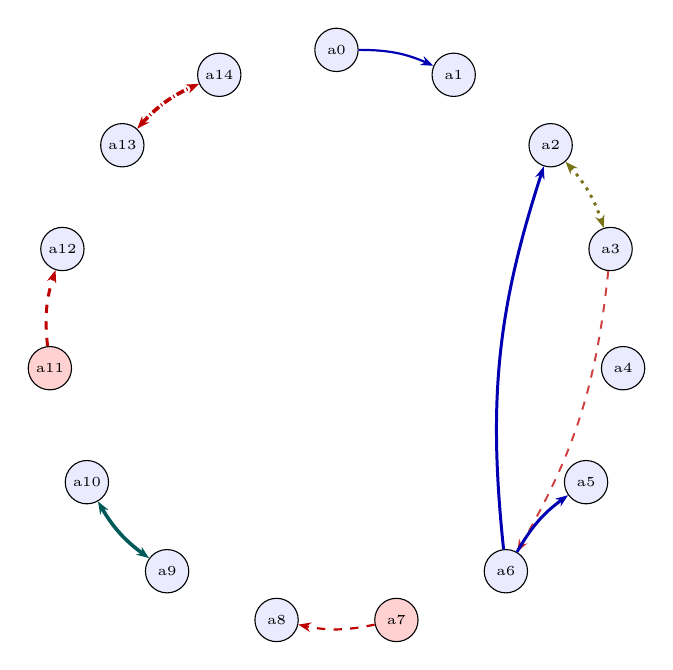
\begin{tikzpicture}[>={Stealth[length=1.6mm]}]
  \node[circle,draw,fill=blue!8,inner sep=1pt,minimum size=5.5mm,font=\tiny] (a0) at (90.0:3.66) {a0};
  \node[circle,draw,fill=blue!8,inner sep=1pt,minimum size=5.5mm,font=\tiny] (a1) at (66.0:3.66) {a1};
  \node[circle,draw,fill=blue!8,inner sep=1pt,minimum size=5.5mm,font=\tiny] (a2) at (42.0:3.66) {a2};
  \node[circle,draw,fill=blue!8,inner sep=1pt,minimum size=5.5mm,font=\tiny] (a3) at (18.0:3.66) {a3};
  \node[circle,draw,fill=blue!8,inner sep=1pt,minimum size=5.5mm,font=\tiny] (a4) at (-6.0:3.66) {a4};
  \node[circle,draw,fill=blue!8,inner sep=1pt,minimum size=5.5mm,font=\tiny] (a5) at (-30.0:3.66) {a5};
  \node[circle,draw,fill=blue!8,inner sep=1pt,minimum size=5.5mm,font=\tiny] (a6) at (-54.0:3.66) {a6};
  \node[circle,draw,fill=red!18,inner sep=1pt,minimum size=5.5mm,font=\tiny] (a7) at (-78.0:3.66) {a7};
  \node[circle,draw,fill=blue!8,inner sep=1pt,minimum size=5.5mm,font=\tiny] (a8) at (-102.0:3.66) {a8};
  \node[circle,draw,fill=blue!8,inner sep=1pt,minimum size=5.5mm,font=\tiny] (a9) at (-126.0:3.66) {a9};
  \node[circle,draw,fill=blue!8,inner sep=1pt,minimum size=5.5mm,font=\tiny] (a10) at (-150.0:3.66) {a10};
  \node[circle,draw,fill=red!18,inner sep=1pt,minimum size=5.5mm,font=\tiny] (a11) at (-174.0:3.66) {a11};
  \node[circle,draw,fill=blue!8,inner sep=1pt,minimum size=5.5mm,font=\tiny] (a12) at (-198.0:3.66) {a12};
  \node[circle,draw,fill=blue!8,inner sep=1pt,minimum size=5.5mm,font=\tiny] (a13) at (-222.0:3.66) {a13};
  \node[circle,draw,fill=blue!8,inner sep=1pt,minimum size=5.5mm,font=\tiny] (a14) at (-246.0:3.66) {a14};
  \draw[{Stealth[length=1.6mm]}-{Stealth[length=1.6mm]}, olive!80!black, dotted, line width=1.08pt] (a2) to[bend left=12] (a3);
  \draw[-{Stealth[length=1.6mm]}, blue!70!black, line width=1.08pt] (a6) to[bend left=12] (a2);
  \draw[{Stealth[length=1.6mm]}-{Stealth[length=1.6mm]}, teal!70!black, line width=1.31pt] (a9) to[bend left=12] (a10);
  \draw[{Stealth[length=1.6mm]}-{Stealth[length=1.6mm]}, red!75!black, densely dashdotted, line width=1.31pt] (a13) to[bend left=12] (a14);
  \draw[-{Stealth[length=1.6mm]}, red!75!black, dashed, opacity=0.75, line width=0.71pt] (a3) to[bend left=12] (a6);
  \draw[-{Stealth[length=1.6mm]}, red!75!black, dashed, line width=0.79pt] (a7) to[bend left=12] (a8);
  \draw[-{Stealth[length=1.6mm]}, red!75!black, dashed, line width=1.08pt] (a11) to[bend left=12] (a12);
  \draw[-{Stealth[length=1.6mm]}, blue!70!black, line width=0.79pt] (a0) to[bend left=12] (a1);
  \draw[-{Stealth[length=1.6mm]}, blue!70!black, line width=1.08pt] (a6) to[bend left=12] (a5);
\end{tikzpicture}
}
\\[2pt]{\footnotesize all gold edges: 9 factors}
\end{minipage}\hfill\begin{minipage}[t]{0.48\linewidth}\centering
\resizebox{!}{6.4cm}{%
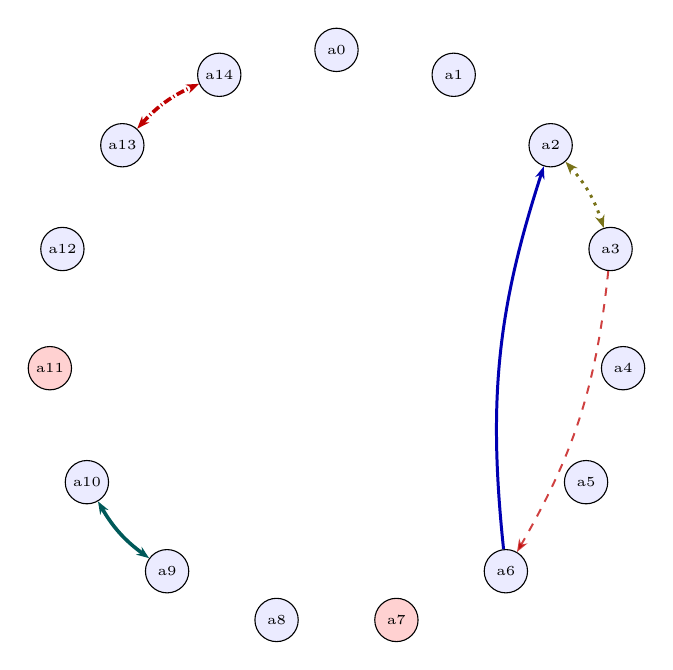
\begin{tikzpicture}[>={Stealth[length=1.6mm]}]
  \node[circle,draw,fill=blue!8,inner sep=1pt,minimum size=5.5mm,font=\tiny] (a0) at (90.0:3.66) {a0};
  \node[circle,draw,fill=blue!8,inner sep=1pt,minimum size=5.5mm,font=\tiny] (a1) at (66.0:3.66) {a1};
  \node[circle,draw,fill=blue!8,inner sep=1pt,minimum size=5.5mm,font=\tiny] (a2) at (42.0:3.66) {a2};
  \node[circle,draw,fill=blue!8,inner sep=1pt,minimum size=5.5mm,font=\tiny] (a3) at (18.0:3.66) {a3};
  \node[circle,draw,fill=blue!8,inner sep=1pt,minimum size=5.5mm,font=\tiny] (a4) at (-6.0:3.66) {a4};
  \node[circle,draw,fill=blue!8,inner sep=1pt,minimum size=5.5mm,font=\tiny] (a5) at (-30.0:3.66) {a5};
  \node[circle,draw,fill=blue!8,inner sep=1pt,minimum size=5.5mm,font=\tiny] (a6) at (-54.0:3.66) {a6};
  \node[circle,draw,fill=red!18,inner sep=1pt,minimum size=5.5mm,font=\tiny] (a7) at (-78.0:3.66) {a7};
  \node[circle,draw,fill=blue!8,inner sep=1pt,minimum size=5.5mm,font=\tiny] (a8) at (-102.0:3.66) {a8};
  \node[circle,draw,fill=blue!8,inner sep=1pt,minimum size=5.5mm,font=\tiny] (a9) at (-126.0:3.66) {a9};
  \node[circle,draw,fill=blue!8,inner sep=1pt,minimum size=5.5mm,font=\tiny] (a10) at (-150.0:3.66) {a10};
  \node[circle,draw,fill=red!18,inner sep=1pt,minimum size=5.5mm,font=\tiny] (a11) at (-174.0:3.66) {a11};
  \node[circle,draw,fill=blue!8,inner sep=1pt,minimum size=5.5mm,font=\tiny] (a12) at (-198.0:3.66) {a12};
  \node[circle,draw,fill=blue!8,inner sep=1pt,minimum size=5.5mm,font=\tiny] (a13) at (-222.0:3.66) {a13};
  \node[circle,draw,fill=blue!8,inner sep=1pt,minimum size=5.5mm,font=\tiny] (a14) at (-246.0:3.66) {a14};
  \draw[{Stealth[length=1.6mm]}-{Stealth[length=1.6mm]}, olive!80!black, dotted, line width=1.08pt] (a2) to[bend left=12] (a3);
  \draw[-{Stealth[length=1.6mm]}, blue!70!black, line width=1.08pt] (a6) to[bend left=12] (a2);
  \draw[{Stealth[length=1.6mm]}-{Stealth[length=1.6mm]}, teal!70!black, line width=1.31pt] (a9) to[bend left=12] (a10);
  \draw[{Stealth[length=1.6mm]}-{Stealth[length=1.6mm]}, red!75!black, densely dashdotted, line width=1.31pt] (a13) to[bend left=12] (a14);
  \draw[-{Stealth[length=1.6mm]}, red!75!black, dashed, opacity=0.75, line width=0.71pt] (a3) to[bend left=12] (a6);
\end{tikzpicture}
}
\\[2pt]{\footnotesize valid edges only: 5 factors}
\end{minipage}
\caption{Relation graph for \texttt{locobench-opus-5-5-f014-r1}. Nodes are atoms on a circle, tinted red when the item marks them non-factual (prior 0.1) and blue when factual (prior 0.9). Edges are gold relations: solid blue = entailment, dashed red = contradiction, double-headed teal = equivalence, dash-dotted red (double-headed) = exclusive (exactly-one), dotted olive (double-headed) = co-necessity (at-least-one); thickness scales with the factor probability. Ordering-only Precedence edges carry no factor and so are not drawn.}
\label{fig:graph-locobench-opus-5-5-f014-r1}
\end{figure}

\begin{table}[htbp]
\centering
\footnotesize
\setlength{\tabcolsep}{3.5pt}
\caption{The specific gold relations of \texttt{locobench-opus-5-5-f014-r1}. \textbf{$p$ used} is the factor probability the MRF received: the band midpoint, times $(1-\lambda)$ for a resolved concession, or \emph{none} for an ordering-only edge (no factor). \textbf{Valid} marks the deliberately-planted errors with their kind. \textbf{Res.} is the resolving atom of a resolved concession.}
\label{tab:rels-locobench-opus-5-5-f014-r1}
\begin{tabular}{lllllrll}
\toprule
ID & Endpoints & Sense & Coupling & Band & $p$ used & Valid & Res. \\
\midrule
\texttt{r000} & \texttt{a2} $\leftrightarrow$ \texttt{a3} & Disjunction & \texttt{co\_necessity} & moderate & 0.720 & \checkmark &  \\
\texttt{r001} & \texttt{a6} $\to$ \texttt{a2} & Evidence & \texttt{entailment} & moderate & 0.720 & \checkmark &  \\
\texttt{r002} & \texttt{a9} $\leftrightarrow$ \texttt{a10} & Restatement & \texttt{equivalence} & strong & 0.925 & \checkmark &  \\
\texttt{r003} & \texttt{a13} $\leftrightarrow$ \texttt{a14} & Alternative & \texttt{exclusive} & strong & 0.925 & \checkmark &  \\
\texttt{r004} & \texttt{a3} $\to$ \texttt{a6} & Concession & \texttt{contradiction} & moderate & 0.396 & \checkmark & \texttt{a12} \\
\texttt{r005} & \texttt{a8} $\to$ \texttt{a9} & Precedence & \texttt{none} & moderate & \emph{none} & \checkmark &  \\
\texttt{r006} & \texttt{a7} $\leftrightarrow$ \texttt{a8} & Contrast & \texttt{contradiction} & weak & 0.470 & $\times$ {\scriptsize false\_endpoint} &  \\
\texttt{r007} & \texttt{a11} $\leftrightarrow$ \texttt{a12} & Contrast & \texttt{contradiction} & moderate & 0.720 & $\times$ {\scriptsize false\_endpoint} &  \\
\texttt{r008} & \texttt{a0} $\to$ \texttt{a1} & Cause-Effect & \texttt{entailment} & weak & 0.470 & $\times$ {\scriptsize spurious} &  \\
\texttt{r009} & \texttt{a6} $\to$ \texttt{a5} & Cause-Effect & \texttt{entailment} & moderate & 0.720 & $\times$ {\scriptsize wrong\_direction} &  \\
\bottomrule
\end{tabular}
\end{table}

\begin{table}[htbp]
\centering
\footnotesize
\caption{Atoms of \texttt{locobench-opus-5-5-f014-r1}: the \texttt{factual} label, the prior it maps to, the posterior marginal $P(a_i{=}1)$ the MRF returns, and the shift. Atoms dragged below their prior are the ones the coherence structure penalises.}
\label{tab:atoms-locobench-opus-5-5-f014-r1}
\begin{tabular}{llrrrp{7.2cm}}
\toprule
Atom & fact & $\pi_i$ & $P(a_i{=}1)$ & $\Delta$ & Text \\
\midrule
\texttt{a0} & \checkmark & 0.90 & 0.895 & -0.005 & \footnotesize The Atlanta Journal-Constitution published analyses showing statistically improbable score gains at Atlanta schools. \\
\texttt{a1} & \checkmark & 0.90 & 0.890 & -0.010 & \footnotesize The suspicious gains appeared on Georgia's Criterion-Referenced Competency Tests. \\
\texttt{a2} & \checkmark & 0.90 & 0.970 & +0.070 & \footnotesize Some of the Atlanta score gains resulted from educators altering student answer sheets. \\
\texttt{a3} & \checkmark & 0.90 & 0.939 & +0.039 & \footnotesize Some of the Atlanta score gains resulted from genuine instructional improvement. \\
\texttt{a4} & \checkmark & 0.90 & 0.900 & +0.000 & \footnotesize The Georgia Governor's Office of Student Achievement commissioned an erasure analysis of the 2009 answer sheets. \\
\texttt{a5} & \checkmark & 0.90 & 0.956 & +0.056 & \footnotesize The erasure analysis counted wrong-to-right erasures on student answer sheets. \\
\texttt{a6} & \checkmark & 0.90 & 0.961 & +0.061 & \footnotesize Many Atlanta classrooms showed wrong-to-right erasure rates far above the state average. \\
\texttt{a7} & $\times$ & 0.10 & 0.104 & +0.004 & \footnotesize The Federal Bureau of Investigation led the inquiry into the Atlanta test scores. \\
\texttt{a8} & \checkmark & 0.90 & 0.901 & +0.001 & \footnotesize Governor Sonny Perdue appointed special investigators to examine the Atlanta schools. \\
\texttt{a9} & \checkmark & 0.90 & 0.979 & +0.079 & \footnotesize The special investigators' report was released in July 2011. \\
\texttt{a10} & \checkmark & 0.90 & 0.979 & +0.079 & \footnotesize In July 2011, the findings of the governor's special investigation were made public. \\
\texttt{a11} & $\times$ & 0.10 & 0.067 & -0.033 & \footnotesize The investigators found evidence of cheating at only 12 Atlanta schools. \\
\texttt{a12} & \checkmark & 0.90 & 0.892 & -0.008 & \footnotesize The special investigators concluded that systematic cheating had occurred in 44 of the 56 schools they examined. \\
\texttt{a13} & \checkmark & 0.90 & 0.632 & -0.268 & \footnotesize Beverly Hall stood trial on the racketeering charges. \\
\texttt{a14} & \checkmark & 0.90 & 0.632 & -0.268 & \footnotesize Beverly Hall never stood trial on the racketeering charges. \\
\bottomrule
\end{tabular}
\end{table}

\subsection{Electrical Engineering -- direction\_reversal\_a (\texttt{locobench-opus-5-5-f015-r1})}

\textbf{Topic:} Electrical Engineering (Engineering \& Technology). \textbf{Family:} \texttt{f015} (CONTROL), rung 1 (\emph{direction\_reversal\_a}). \textbf{Scores:} mean-marg $= 0.769$, consist $= 0.372$, reified $= 0.105$, log-Z $= 0.398$.



\paragraph{Framing question.} \emph{How do forensic engineers determine whether a substation transformer failure originated in an internal insulation breakdown or in an external lightning surge when the utility and the transformer's manufacturer dispute liability for the resulting outage?}



\paragraph{Response.} {\small When a substation transformer fails and the resulting outage becomes a liability dispute, forensic engineers must decide between two competing physical narratives, each favouring a different party. In the case examined here, the utility argued that the failure originated in an internal insulation breakdown, a defect it attributed to the unit as manufactured and supplied. The manufacturer, by contrast, argued that the failure was caused by an external lightning surge, an event outside its control and outside the scope of its warranty obligations. Resolving such a dispute means reconstructing the electrical and physical sequence of the fault from records that neither party can easily manipulate.

Because the manufacturer advanced the lightning explanation, the utility's insurer retained an independent forensic engineering firm to investigate the failure. That engagement came after the moment at which lightning detection network data recorded a strike within two kilometers of the substation at the time of the fault. The investigators then turned to the protective equipment. The surge arrester counters at the substation registered an operation during the storm. The arrester record forces a binary question that the investigators could not leave open: either the surge arrester on the faulted phase was in working order at the time of the strike, or the surge arrester on the faulted phase was inoperative at the time of the strike, and exactly one of these conditions held. By contrast with the activity logged on those counters, the substation had no surge arresters installed on the transformer's high-voltage terminals, so the protection scheme at the terminals themselves had to be evaluated separately from the station-level devices.

Chemical evidence from inside the tank supplements the electrical record. Dissolved gas analysis of the transformer oil showed elevated acetylene levels after the failure. Acetylene is the classic marker of high-energy discharge, yet in this investigation the elevated acetylene indicates that dissolved gas analysis cannot distinguish arcing faults from thermal faults, because the gas signature appears within a mixture that a severe overheating event would also generate. Engineers therefore treat the oil chemistry as corroborating rather than decisive and look to direct physical examination of the core and coil assembly to establish where the breakdown began.

Teardown inspection supplies that physical record. When the windings are unstacked and the paper and pressboard are tested for dielectric strength and water content, two explanations for the collapse of the insulation system come into view, and at least one of them holds, perhaps both: the winding insulation had degraded from moisture ingress, or the lightning surge exceeded the transformer's basic insulation level. Either mechanism alone can produce a dielectric failure, and the two can act together, with a weakened insulation system yielding to an impulse it would otherwise have withstood. Although the lightning surge exceeded the transformer's basic insulation level, the fault initiated at the high-voltage bushing lead. This restates in brief the more precise finding that the point of initial dielectric breakdown was the lead connected to the high-voltage bushing, not a location distributed along the line-end turns where an incoming impulse would normally concentrate its stress.

The location of initiation settles the tension between the surge magnitude and the site of failure. The independent forensic report concluded that internal insulation breakdown was the root cause of the transformer failure, and that conclusion confirms the bushing lead as the point of initial dielectric breakdown. A surge exceeding the basic insulation level establishes only that the transformer was stressed; it does not establish that the stress determined where and how the insulation gave way. By tracing the origin to an internal component, the report allocated causation to the condition of the insulation rather than to the external event. This is the general method forensic engineers apply in such disputes: they correlate lightning network timing, arrester counter data, oil chemistry and teardown findings, and they assign the root cause to whichever mechanism accounts for the physical point of origin.}

\begin{figure}[htbp]
\centering
\begin{minipage}[t]{0.48\linewidth}\centering
\resizebox{!}{6.4cm}{%
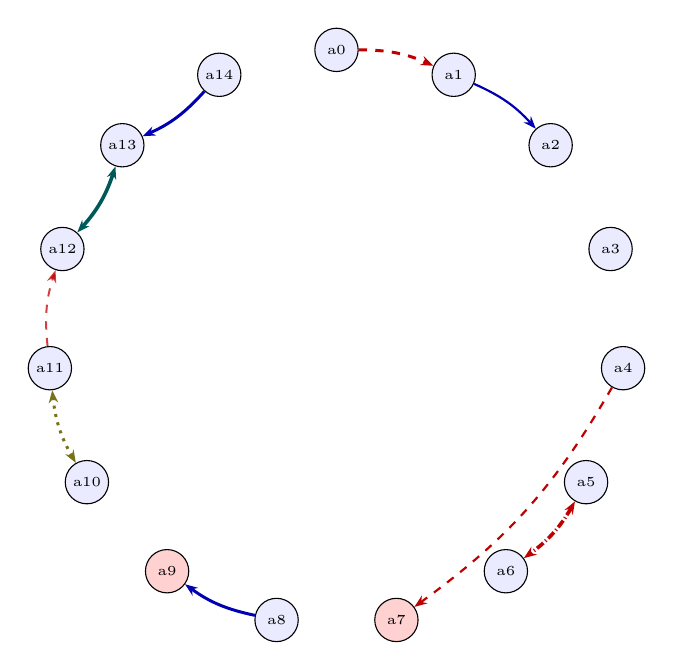
\begin{tikzpicture}[>={Stealth[length=1.6mm]}]
  \node[circle,draw,fill=blue!8,inner sep=1pt,minimum size=5.5mm,font=\tiny] (a0) at (90.0:3.66) {a0};
  \node[circle,draw,fill=blue!8,inner sep=1pt,minimum size=5.5mm,font=\tiny] (a1) at (66.0:3.66) {a1};
  \node[circle,draw,fill=blue!8,inner sep=1pt,minimum size=5.5mm,font=\tiny] (a2) at (42.0:3.66) {a2};
  \node[circle,draw,fill=blue!8,inner sep=1pt,minimum size=5.5mm,font=\tiny] (a3) at (18.0:3.66) {a3};
  \node[circle,draw,fill=blue!8,inner sep=1pt,minimum size=5.5mm,font=\tiny] (a4) at (-6.0:3.66) {a4};
  \node[circle,draw,fill=blue!8,inner sep=1pt,minimum size=5.5mm,font=\tiny] (a5) at (-30.0:3.66) {a5};
  \node[circle,draw,fill=blue!8,inner sep=1pt,minimum size=5.5mm,font=\tiny] (a6) at (-54.0:3.66) {a6};
  \node[circle,draw,fill=red!18,inner sep=1pt,minimum size=5.5mm,font=\tiny] (a7) at (-78.0:3.66) {a7};
  \node[circle,draw,fill=blue!8,inner sep=1pt,minimum size=5.5mm,font=\tiny] (a8) at (-102.0:3.66) {a8};
  \node[circle,draw,fill=red!18,inner sep=1pt,minimum size=5.5mm,font=\tiny] (a9) at (-126.0:3.66) {a9};
  \node[circle,draw,fill=blue!8,inner sep=1pt,minimum size=5.5mm,font=\tiny] (a10) at (-150.0:3.66) {a10};
  \node[circle,draw,fill=blue!8,inner sep=1pt,minimum size=5.5mm,font=\tiny] (a11) at (-174.0:3.66) {a11};
  \node[circle,draw,fill=blue!8,inner sep=1pt,minimum size=5.5mm,font=\tiny] (a12) at (-198.0:3.66) {a12};
  \node[circle,draw,fill=blue!8,inner sep=1pt,minimum size=5.5mm,font=\tiny] (a13) at (-222.0:3.66) {a13};
  \node[circle,draw,fill=blue!8,inner sep=1pt,minimum size=5.5mm,font=\tiny] (a14) at (-246.0:3.66) {a14};
  \draw[-{Stealth[length=1.6mm]}, red!75!black, dashed, line width=1.08pt] (a0) to[bend left=12] (a1);
  \draw[{Stealth[length=1.6mm]}-{Stealth[length=1.6mm]}, red!75!black, densely dashdotted, line width=1.31pt] (a5) to[bend left=12] (a6);
  \draw[{Stealth[length=1.6mm]}-{Stealth[length=1.6mm]}, olive!80!black, dotted, line width=1.08pt] (a10) to[bend left=12] (a11);
  \draw[{Stealth[length=1.6mm]}-{Stealth[length=1.6mm]}, teal!70!black, line width=1.31pt] (a13) to[bend left=12] (a12);
  \draw[-{Stealth[length=1.6mm]}, red!75!black, dashed, opacity=0.75, line width=0.71pt] (a11) to[bend left=12] (a12);
  \draw[-{Stealth[length=1.6mm]}, red!75!black, dashed, line width=0.79pt] (a4) to[bend left=12] (a7);
  \draw[-{Stealth[length=1.6mm]}, blue!70!black, line width=1.08pt] (a8) to[bend left=12] (a9);
  \draw[-{Stealth[length=1.6mm]}, blue!70!black, line width=0.79pt] (a1) to[bend left=12] (a2);
  \draw[-{Stealth[length=1.6mm]}, blue!70!black, line width=1.08pt] (a14) to[bend left=12] (a13);
\end{tikzpicture}
}
\\[2pt]{\footnotesize all gold edges: 9 factors}
\end{minipage}\hfill\begin{minipage}[t]{0.48\linewidth}\centering
\resizebox{!}{6.4cm}{%
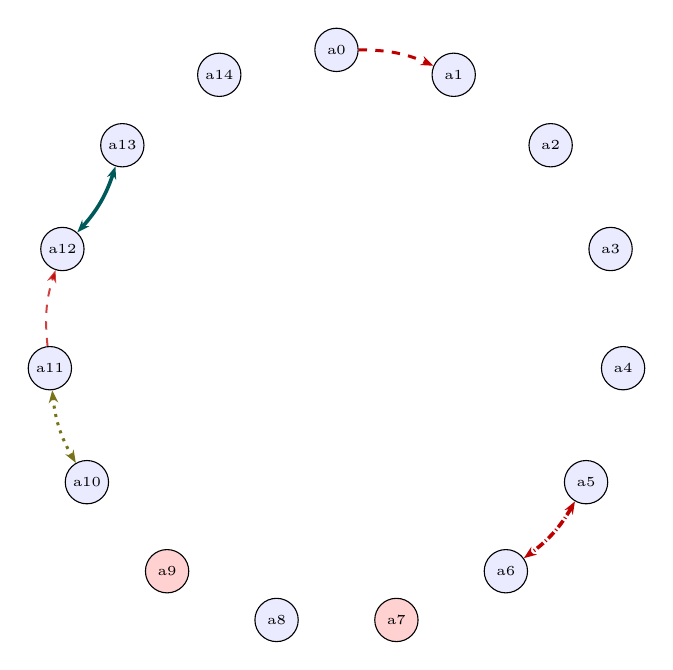
\begin{tikzpicture}[>={Stealth[length=1.6mm]}]
  \node[circle,draw,fill=blue!8,inner sep=1pt,minimum size=5.5mm,font=\tiny] (a0) at (90.0:3.66) {a0};
  \node[circle,draw,fill=blue!8,inner sep=1pt,minimum size=5.5mm,font=\tiny] (a1) at (66.0:3.66) {a1};
  \node[circle,draw,fill=blue!8,inner sep=1pt,minimum size=5.5mm,font=\tiny] (a2) at (42.0:3.66) {a2};
  \node[circle,draw,fill=blue!8,inner sep=1pt,minimum size=5.5mm,font=\tiny] (a3) at (18.0:3.66) {a3};
  \node[circle,draw,fill=blue!8,inner sep=1pt,minimum size=5.5mm,font=\tiny] (a4) at (-6.0:3.66) {a4};
  \node[circle,draw,fill=blue!8,inner sep=1pt,minimum size=5.5mm,font=\tiny] (a5) at (-30.0:3.66) {a5};
  \node[circle,draw,fill=blue!8,inner sep=1pt,minimum size=5.5mm,font=\tiny] (a6) at (-54.0:3.66) {a6};
  \node[circle,draw,fill=red!18,inner sep=1pt,minimum size=5.5mm,font=\tiny] (a7) at (-78.0:3.66) {a7};
  \node[circle,draw,fill=blue!8,inner sep=1pt,minimum size=5.5mm,font=\tiny] (a8) at (-102.0:3.66) {a8};
  \node[circle,draw,fill=red!18,inner sep=1pt,minimum size=5.5mm,font=\tiny] (a9) at (-126.0:3.66) {a9};
  \node[circle,draw,fill=blue!8,inner sep=1pt,minimum size=5.5mm,font=\tiny] (a10) at (-150.0:3.66) {a10};
  \node[circle,draw,fill=blue!8,inner sep=1pt,minimum size=5.5mm,font=\tiny] (a11) at (-174.0:3.66) {a11};
  \node[circle,draw,fill=blue!8,inner sep=1pt,minimum size=5.5mm,font=\tiny] (a12) at (-198.0:3.66) {a12};
  \node[circle,draw,fill=blue!8,inner sep=1pt,minimum size=5.5mm,font=\tiny] (a13) at (-222.0:3.66) {a13};
  \node[circle,draw,fill=blue!8,inner sep=1pt,minimum size=5.5mm,font=\tiny] (a14) at (-246.0:3.66) {a14};
  \draw[-{Stealth[length=1.6mm]}, red!75!black, dashed, line width=1.08pt] (a0) to[bend left=12] (a1);
  \draw[{Stealth[length=1.6mm]}-{Stealth[length=1.6mm]}, red!75!black, densely dashdotted, line width=1.31pt] (a5) to[bend left=12] (a6);
  \draw[{Stealth[length=1.6mm]}-{Stealth[length=1.6mm]}, olive!80!black, dotted, line width=1.08pt] (a10) to[bend left=12] (a11);
  \draw[{Stealth[length=1.6mm]}-{Stealth[length=1.6mm]}, teal!70!black, line width=1.31pt] (a13) to[bend left=12] (a12);
  \draw[-{Stealth[length=1.6mm]}, red!75!black, dashed, opacity=0.75, line width=0.71pt] (a11) to[bend left=12] (a12);
\end{tikzpicture}
}
\\[2pt]{\footnotesize valid edges only: 5 factors}
\end{minipage}
\caption{Relation graph for \texttt{locobench-opus-5-5-f015-r1}. Nodes are atoms on a circle, tinted red when the item marks them non-factual (prior 0.1) and blue when factual (prior 0.9). Edges are gold relations: solid blue = entailment, dashed red = contradiction, double-headed teal = equivalence, dash-dotted red (double-headed) = exclusive (exactly-one), dotted olive (double-headed) = co-necessity (at-least-one); thickness scales with the factor probability. Ordering-only Precedence edges carry no factor and so are not drawn.}
\label{fig:graph-locobench-opus-5-5-f015-r1}
\end{figure}

\begin{table}[htbp]
\centering
\footnotesize
\setlength{\tabcolsep}{3.5pt}
\caption{The specific gold relations of \texttt{locobench-opus-5-5-f015-r1}. \textbf{$p$ used} is the factor probability the MRF received: the band midpoint, times $(1-\lambda)$ for a resolved concession, or \emph{none} for an ordering-only edge (no factor). \textbf{Valid} marks the deliberately-planted errors with their kind. \textbf{Res.} is the resolving atom of a resolved concession.}
\label{tab:rels-locobench-opus-5-5-f015-r1}
\begin{tabular}{lllllrll}
\toprule
ID & Endpoints & Sense & Coupling & Band & $p$ used & Valid & Res. \\
\midrule
\texttt{r000} & \texttt{a0} $\leftrightarrow$ \texttt{a1} & Contrast & \texttt{contradiction} & moderate & 0.720 & \checkmark &  \\
\texttt{r001} & \texttt{a5} $\leftrightarrow$ \texttt{a6} & Alternative & \texttt{exclusive} & strong & 0.925 & \checkmark &  \\
\texttt{r002} & \texttt{a10} $\leftrightarrow$ \texttt{a11} & Disjunction & \texttt{co\_necessity} & moderate & 0.720 & \checkmark &  \\
\texttt{r003} & \texttt{a13} $\leftrightarrow$ \texttt{a12} & Restatement & \texttt{equivalence} & strong & 0.925 & \checkmark &  \\
\texttt{r004} & \texttt{a2} $\to$ \texttt{a3} & Succession & \texttt{none} & weak & \emph{none} & \checkmark &  \\
\texttt{r005} & \texttt{a11} $\to$ \texttt{a12} & Concession & \texttt{contradiction} & moderate & 0.396 & \checkmark & \texttt{a14} \\
\texttt{r006} & \texttt{a4} $\leftrightarrow$ \texttt{a7} & Contrast & \texttt{contradiction} & weak & 0.470 & $\times$ {\scriptsize false\_endpoint} &  \\
\texttt{r007} & \texttt{a8} $\to$ \texttt{a9} & Evidence & \texttt{entailment} & moderate & 0.720 & $\times$ {\scriptsize false\_endpoint} &  \\
\texttt{r008} & \texttt{a1} $\to$ \texttt{a2} & Cause-Effect & \texttt{entailment} & weak & 0.470 & $\times$ {\scriptsize spurious} &  \\
\texttt{r009} & \texttt{a14} $\to$ \texttt{a13} & Evidence & \texttt{entailment} & moderate & 0.720 & $\times$ {\scriptsize wrong\_direction} &  \\
\bottomrule
\end{tabular}
\end{table}

\begin{table}[htbp]
\centering
\footnotesize
\caption{Atoms of \texttt{locobench-opus-5-5-f015-r1}: the \texttt{factual} label, the prior it maps to, the posterior marginal $P(a_i{=}1)$ the MRF returns, and the shift. Atoms dragged below their prior are the ones the coherence structure penalises.}
\label{tab:atoms-locobench-opus-5-5-f015-r1}
\begin{tabular}{llrrrp{7.2cm}}
\toprule
Atom & fact & $\pi_i$ & $P(a_i{=}1)$ & $\Delta$ & Text \\
\midrule
\texttt{a0} & \checkmark & 0.90 & 0.854 & -0.046 & \footnotesize The utility argued that the failure originated in an internal insulation breakdown. \\
\texttt{a1} & \checkmark & 0.90 & 0.788 & -0.112 & \footnotesize The manufacturer argued that the failure was caused by an external lightning surge. \\
\texttt{a2} & \checkmark & 0.90 & 0.891 & -0.009 & \footnotesize The utility's insurer retained an independent forensic engineering firm to investigate the failure. \\
\texttt{a3} & \checkmark & 0.90 & 0.900 & +0.000 & \footnotesize Lightning detection network data recorded a strike within two kilometers of the substation at the time of the fault. \\
\texttt{a4} & \checkmark & 0.90 & 0.895 & -0.005 & \footnotesize The surge arrester counters at the substation registered an operation during the storm. \\
\texttt{a5} & \checkmark & 0.90 & 0.632 & -0.268 & \footnotesize The surge arrester on the faulted phase was in working order at the time of the strike. \\
\texttt{a6} & \checkmark & 0.90 & 0.632 & -0.268 & \footnotesize The surge arrester on the faulted phase was inoperative at the time of the strike. \\
\texttt{a7} & $\times$ & 0.10 & 0.110 & +0.010 & \footnotesize The substation had no surge arresters installed on the transformer's high-voltage terminals. \\
\texttt{a8} & \checkmark & 0.90 & 0.854 & -0.046 & \footnotesize Dissolved gas analysis of the transformer oil showed elevated acetylene levels after the failure. \\
\texttt{a9} & $\times$ & 0.10 & 0.204 & +0.104 & \footnotesize Dissolved gas analysis cannot distinguish arcing faults from thermal faults. \\
\texttt{a10} & \checkmark & 0.90 & 0.929 & +0.029 & \footnotesize The winding insulation had degraded from moisture ingress. \\
\texttt{a11} & \checkmark & 0.90 & 0.940 & +0.040 & \footnotesize The lightning surge exceeded the transformer's basic insulation level. \\
\texttt{a12} & \checkmark & 0.90 & 0.990 & +0.090 & \footnotesize The fault initiated at the high-voltage bushing lead. \\
\texttt{a13} & \checkmark & 0.90 & 0.993 & +0.093 & \footnotesize The point of initial dielectric breakdown was the lead connected to the high-voltage bushing. \\
\texttt{a14} & \checkmark & 0.90 & 0.928 & +0.028 & \footnotesize The independent forensic report concluded that internal insulation breakdown was the root cause of the transformer failure. \\
\bottomrule
\end{tabular}
\end{table}

\subsection{Ethics -- shuffle\_block (\texttt{locobench-opus-5-5-f016-r1})}

\textbf{Topic:} Ethics (Humanities). \textbf{Family:} \texttt{f016} (ORDER), rung 1 (\emph{shuffle\_block}). \textbf{Scores:} mean-marg $= 0.792$, consist $= 0.449$, reified $= 0.297$, log-Z $= 0.371$.



\paragraph{Framing question.} \emph{How do research integrity committees decide whether irregularities in a scientist's published data reflect deliberate fabrication or honest error when the committee's forensic findings conflict with the researcher's own account of what happened?}



\paragraph{Response.} {\small Research integrity committees seldom receive a confession. More often they must weigh a researcher's narrative against what the documentary record discloses. Under the federal standard that governs most American institutions, misconduct must be committed intentionally, knowingly, or recklessly and must be proven by a preponderance of the evidence. The committee's task, then, is not to disprove the researcher's story outright but to determine whether the surviving data can support it. A representative case shows how that weighing proceeds. Dr. Lena Hartwell published a 2019 paper on mitochondrial signaling in a peer-reviewed cell biology journal, and an anonymous commenter subsequently flagged apparently duplicated western blot bands in the paper's Figure 3.

Provenance is where conflicting accounts are usually decided. Dr. Hartwell was unable to produce the original raw blot images for Figure 3. Metadata on the duplicated image file showed it was edited months after the experiment was recorded. The absence of retrievable raw images caused someone in the laboratory to alter the Figure 3 image deliberately, so that a manipulated panel filled the gap the missing data had left. At least one of two things holds here, perhaps both: that deliberate alteration took place, or the original Figure 3 image files were mislabelled during the laboratory's file storage process. Mislabelling at the storage stage could account for a researcher's sincere belief in a mix-up. It cannot, however, account for an editing date that falls long after the experiment was performed. The late edit therefore confirms the committee's judgment. The committee concluded that the image duplication in Figure 3 was intentional falsification rather than an accidental file mix-up, and this conclusion settles the tension between Dr. Hartwell's account and the forensic match.

How far an irregularity extends shapes how much latitude an innocent explanation receives, because a single anomaly invites a different reading than a recurring one. In this case the duplicated panels appeared in three of the paper's six figures. The university convened a research integrity committee to examine the flagged figure, and the committee's first step was technical rather than testimonial. Whereas the duplication had been described as spanning several figures, forensic image analysis found that two blot panels in Figure 3 were identical after rotation and contrast adjustment. Despite that forensic match, Dr. Hartwell stated that the duplication resulted from an accidental mix-up of image files. An explanation of this kind is not implausible in principle, since a busy laboratory generates thousands of similar images. For that reason committees do not dismiss it on its face but test it against the provenance of the data.

Correction of the published literature follows a separate path. Journals act on their own editorial procedures, often guided by the recommendations of the Committee on Publication Ethics, and their timelines need not match those of institutions or agencies. For the scientific record the outcome is binary: either the journal retracted the 2019 paper, or the 2019 paper remains in the journal without a retraction. The two cannot both be true, and one of them must hold. The broader lesson concerns method. When a researcher's account and the forensic evidence conflict, committees give decisive weight to evidence whose integrity does not depend on anyone's recollection, such as raw files, timestamps, and reproducible image comparisons, and they treat the inability to supply such evidence as a gap the researcher's narrative must still explain.

The committee's findings rested largely on image forensics and file metadata. Its testimony, by contrast, came chiefly from outside the laboratory: the committee interviewed the journal's handling editor as its principal witness. That interview led to Dr. Hartwell being barred from federal research funding for five years; that is, a five-year debarment from federal grants was imposed on her. Sanctions of this kind are administered by funding agencies, which review the institutional finding and set penalties proportionate to the seriousness of the misconduct and to whether it formed part of a pattern.}

\begin{figure}[htbp]
\centering
\begin{minipage}[t]{0.48\linewidth}\centering
\resizebox{!}{6.4cm}{%
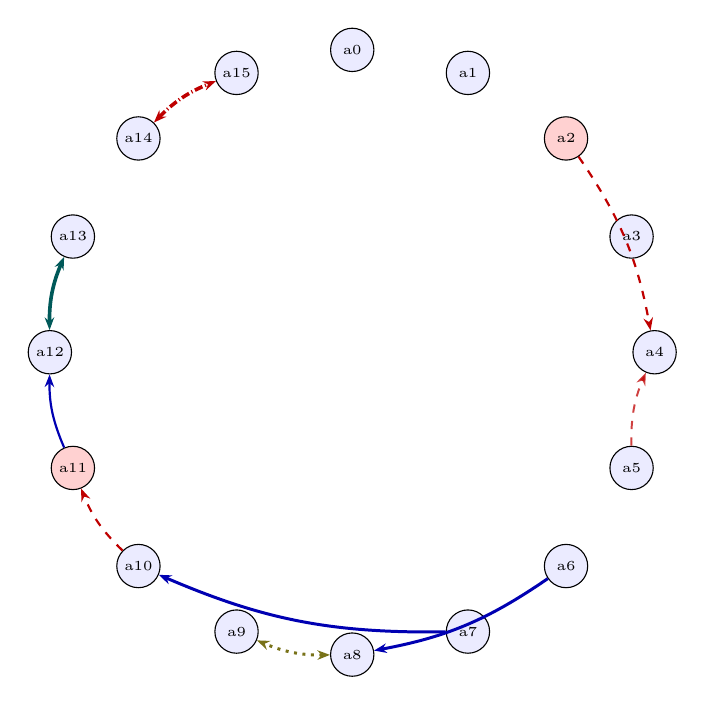
\begin{tikzpicture}[>={Stealth[length=1.6mm]}]
  \node[circle,draw,fill=blue!8,inner sep=1pt,minimum size=5.5mm,font=\tiny] (a0) at (90.0:3.84) {a0};
  \node[circle,draw,fill=blue!8,inner sep=1pt,minimum size=5.5mm,font=\tiny] (a1) at (67.5:3.84) {a1};
  \node[circle,draw,fill=red!18,inner sep=1pt,minimum size=5.5mm,font=\tiny] (a2) at (45.0:3.84) {a2};
  \node[circle,draw,fill=blue!8,inner sep=1pt,minimum size=5.5mm,font=\tiny] (a3) at (22.5:3.84) {a3};
  \node[circle,draw,fill=blue!8,inner sep=1pt,minimum size=5.5mm,font=\tiny] (a4) at (0.0:3.84) {a4};
  \node[circle,draw,fill=blue!8,inner sep=1pt,minimum size=5.5mm,font=\tiny] (a5) at (-22.5:3.84) {a5};
  \node[circle,draw,fill=blue!8,inner sep=1pt,minimum size=5.5mm,font=\tiny] (a6) at (-45.0:3.84) {a6};
  \node[circle,draw,fill=blue!8,inner sep=1pt,minimum size=5.5mm,font=\tiny] (a7) at (-67.5:3.84) {a7};
  \node[circle,draw,fill=blue!8,inner sep=1pt,minimum size=5.5mm,font=\tiny] (a8) at (-90.0:3.84) {a8};
  \node[circle,draw,fill=blue!8,inner sep=1pt,minimum size=5.5mm,font=\tiny] (a9) at (-112.5:3.84) {a9};
  \node[circle,draw,fill=blue!8,inner sep=1pt,minimum size=5.5mm,font=\tiny] (a10) at (-135.0:3.84) {a10};
  \node[circle,draw,fill=red!18,inner sep=1pt,minimum size=5.5mm,font=\tiny] (a11) at (-157.5:3.84) {a11};
  \node[circle,draw,fill=blue!8,inner sep=1pt,minimum size=5.5mm,font=\tiny] (a12) at (-180.0:3.84) {a12};
  \node[circle,draw,fill=blue!8,inner sep=1pt,minimum size=5.5mm,font=\tiny] (a13) at (-202.5:3.84) {a13};
  \node[circle,draw,fill=blue!8,inner sep=1pt,minimum size=5.5mm,font=\tiny] (a14) at (-225.0:3.84) {a14};
  \node[circle,draw,fill=blue!8,inner sep=1pt,minimum size=5.5mm,font=\tiny] (a15) at (-247.5:3.84) {a15};
  \draw[-{Stealth[length=1.6mm]}, red!75!black, dashed, line width=0.79pt] (a2) to[bend left=12] (a4);
  \draw[-{Stealth[length=1.6mm]}, red!75!black, dashed, opacity=0.75, line width=0.71pt] (a5) to[bend left=12] (a4);
  \draw[-{Stealth[length=1.6mm]}, blue!70!black, line width=1.08pt] (a6) to[bend left=12] (a8);
  \draw[-{Stealth[length=1.6mm]}, blue!70!black, line width=1.08pt] (a7) to[bend left=12] (a10);
  \draw[{Stealth[length=1.6mm]}-{Stealth[length=1.6mm]}, olive!80!black, dotted, line width=1.08pt] (a8) to[bend left=12] (a9);
  \draw[-{Stealth[length=1.6mm]}, red!75!black, dashed, line width=0.79pt] (a10) to[bend left=12] (a11);
  \draw[-{Stealth[length=1.6mm]}, blue!70!black, line width=0.79pt] (a11) to[bend left=12] (a12);
  \draw[{Stealth[length=1.6mm]}-{Stealth[length=1.6mm]}, teal!70!black, line width=1.31pt] (a12) to[bend left=12] (a13);
  \draw[{Stealth[length=1.6mm]}-{Stealth[length=1.6mm]}, red!75!black, densely dashdotted, line width=1.31pt] (a14) to[bend left=12] (a15);
\end{tikzpicture}
}
\\[2pt]{\footnotesize all gold edges: 9 factors}
\end{minipage}\hfill\begin{minipage}[t]{0.48\linewidth}\centering
\resizebox{!}{6.4cm}{%
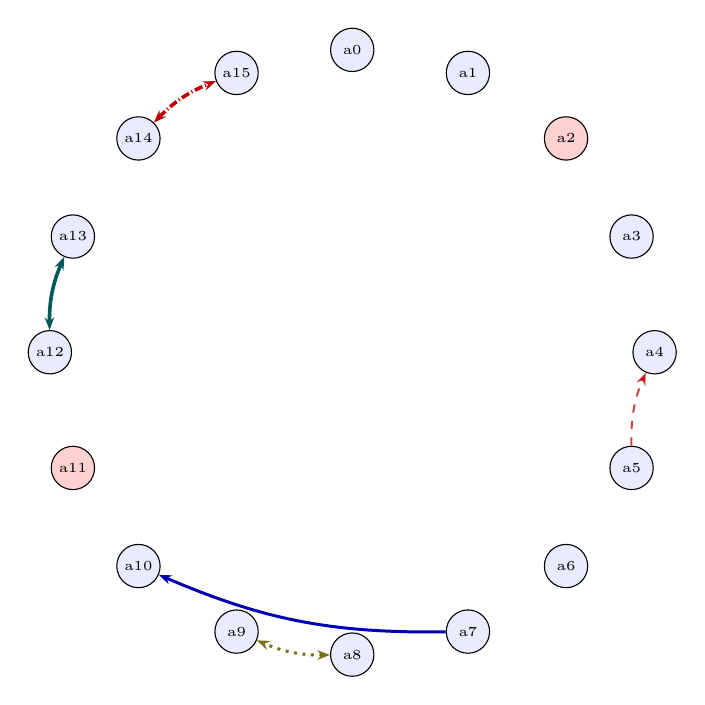
\begin{tikzpicture}[>={Stealth[length=1.6mm]}]
  \node[circle,draw,fill=blue!8,inner sep=1pt,minimum size=5.5mm,font=\tiny] (a0) at (90.0:3.84) {a0};
  \node[circle,draw,fill=blue!8,inner sep=1pt,minimum size=5.5mm,font=\tiny] (a1) at (67.5:3.84) {a1};
  \node[circle,draw,fill=red!18,inner sep=1pt,minimum size=5.5mm,font=\tiny] (a2) at (45.0:3.84) {a2};
  \node[circle,draw,fill=blue!8,inner sep=1pt,minimum size=5.5mm,font=\tiny] (a3) at (22.5:3.84) {a3};
  \node[circle,draw,fill=blue!8,inner sep=1pt,minimum size=5.5mm,font=\tiny] (a4) at (0.0:3.84) {a4};
  \node[circle,draw,fill=blue!8,inner sep=1pt,minimum size=5.5mm,font=\tiny] (a5) at (-22.5:3.84) {a5};
  \node[circle,draw,fill=blue!8,inner sep=1pt,minimum size=5.5mm,font=\tiny] (a6) at (-45.0:3.84) {a6};
  \node[circle,draw,fill=blue!8,inner sep=1pt,minimum size=5.5mm,font=\tiny] (a7) at (-67.5:3.84) {a7};
  \node[circle,draw,fill=blue!8,inner sep=1pt,minimum size=5.5mm,font=\tiny] (a8) at (-90.0:3.84) {a8};
  \node[circle,draw,fill=blue!8,inner sep=1pt,minimum size=5.5mm,font=\tiny] (a9) at (-112.5:3.84) {a9};
  \node[circle,draw,fill=blue!8,inner sep=1pt,minimum size=5.5mm,font=\tiny] (a10) at (-135.0:3.84) {a10};
  \node[circle,draw,fill=red!18,inner sep=1pt,minimum size=5.5mm,font=\tiny] (a11) at (-157.5:3.84) {a11};
  \node[circle,draw,fill=blue!8,inner sep=1pt,minimum size=5.5mm,font=\tiny] (a12) at (-180.0:3.84) {a12};
  \node[circle,draw,fill=blue!8,inner sep=1pt,minimum size=5.5mm,font=\tiny] (a13) at (-202.5:3.84) {a13};
  \node[circle,draw,fill=blue!8,inner sep=1pt,minimum size=5.5mm,font=\tiny] (a14) at (-225.0:3.84) {a14};
  \node[circle,draw,fill=blue!8,inner sep=1pt,minimum size=5.5mm,font=\tiny] (a15) at (-247.5:3.84) {a15};
  \draw[-{Stealth[length=1.6mm]}, red!75!black, dashed, opacity=0.75, line width=0.71pt] (a5) to[bend left=12] (a4);
  \draw[-{Stealth[length=1.6mm]}, blue!70!black, line width=1.08pt] (a7) to[bend left=12] (a10);
  \draw[{Stealth[length=1.6mm]}-{Stealth[length=1.6mm]}, olive!80!black, dotted, line width=1.08pt] (a8) to[bend left=12] (a9);
  \draw[{Stealth[length=1.6mm]}-{Stealth[length=1.6mm]}, teal!70!black, line width=1.31pt] (a12) to[bend left=12] (a13);
  \draw[{Stealth[length=1.6mm]}-{Stealth[length=1.6mm]}, red!75!black, densely dashdotted, line width=1.31pt] (a14) to[bend left=12] (a15);
\end{tikzpicture}
}
\\[2pt]{\footnotesize valid edges only: 5 factors}
\end{minipage}
\caption{Relation graph for \texttt{locobench-opus-5-5-f016-r1}. Nodes are atoms on a circle, tinted red when the item marks them non-factual (prior 0.1) and blue when factual (prior 0.9). Edges are gold relations: solid blue = entailment, dashed red = contradiction, double-headed teal = equivalence, dash-dotted red (double-headed) = exclusive (exactly-one), dotted olive (double-headed) = co-necessity (at-least-one); thickness scales with the factor probability. Ordering-only Precedence edges carry no factor and so are not drawn.}
\label{fig:graph-locobench-opus-5-5-f016-r1}
\end{figure}

\begin{table}[htbp]
\centering
\footnotesize
\setlength{\tabcolsep}{3.5pt}
\caption{The specific gold relations of \texttt{locobench-opus-5-5-f016-r1}. \textbf{$p$ used} is the factor probability the MRF received: the band midpoint, times $(1-\lambda)$ for a resolved concession, or \emph{none} for an ordering-only edge (no factor). \textbf{Valid} marks the deliberately-planted errors with their kind. \textbf{Res.} is the resolving atom of a resolved concession.}
\label{tab:rels-locobench-opus-5-5-f016-r1}
\begin{tabular}{lllllrll}
\toprule
ID & Endpoints & Sense & Coupling & Band & $p$ used & Valid & Res. \\
\midrule
\texttt{r000} & \texttt{a0} $\to$ \texttt{a1} & Precedence & \texttt{none} & weak & \emph{none} & \checkmark &  \\
\texttt{r001} & \texttt{a2} $\leftrightarrow$ \texttt{a4} & Contrast & \texttt{contradiction} & weak & 0.470 & $\times$ {\scriptsize false\_endpoint} &  \\
\texttt{r002} & \texttt{a5} $\to$ \texttt{a4} & Concession & \texttt{contradiction} & moderate & 0.396 & \checkmark & \texttt{a10} \\
\texttt{r003} & \texttt{a6} $\to$ \texttt{a8} & Cause-Effect & \texttt{entailment} & moderate & 0.720 & $\times$ {\scriptsize wrong\_direction} &  \\
\texttt{r004} & \texttt{a7} $\to$ \texttt{a10} & Evidence & \texttt{entailment} & moderate & 0.720 & \checkmark &  \\
\texttt{r005} & \texttt{a8} $\leftrightarrow$ \texttt{a9} & Disjunction & \texttt{co\_necessity} & moderate & 0.720 & \checkmark &  \\
\texttt{r006} & \texttt{a10} $\leftrightarrow$ \texttt{a11} & Contrast & \texttt{contradiction} & weak & 0.470 & $\times$ {\scriptsize spurious} &  \\
\texttt{r007} & \texttt{a11} $\to$ \texttt{a12} & Cause-Effect & \texttt{entailment} & weak & 0.470 & $\times$ {\scriptsize spurious} &  \\
\texttt{r008} & \texttt{a12} $\leftrightarrow$ \texttt{a13} & Restatement & \texttt{equivalence} & strong & 0.925 & \checkmark &  \\
\texttt{r009} & \texttt{a14} $\leftrightarrow$ \texttt{a15} & Alternative & \texttt{exclusive} & strong & 0.925 & \checkmark &  \\
\bottomrule
\end{tabular}
\end{table}

\begin{table}[htbp]
\centering
\footnotesize
\caption{Atoms of \texttt{locobench-opus-5-5-f016-r1}: the \texttt{factual} label, the prior it maps to, the posterior marginal $P(a_i{=}1)$ the MRF returns, and the shift. Atoms dragged below their prior are the ones the coherence structure penalises.}
\label{tab:atoms-locobench-opus-5-5-f016-r1}
\begin{tabular}{llrrrp{7.2cm}}
\toprule
Atom & fact & $\pi_i$ & $P(a_i{=}1)$ & $\Delta$ & Text \\
\midrule
\texttt{a0} & \checkmark & 0.90 & 0.900 & +0.000 & \footnotesize Dr. Lena Hartwell published a 2019 paper on mitochondrial signaling in a peer-reviewed cell biology journal. \\
\texttt{a1} & \checkmark & 0.90 & 0.900 & +0.000 & \footnotesize An anonymous commenter flagged apparently duplicated western blot bands in the paper's Figure 3. \\
\texttt{a2} & $\times$ & 0.10 & 0.105 & +0.005 & \footnotesize The duplicated panels appeared in three of the paper's six figures. \\
\texttt{a3} & \checkmark & 0.90 & 0.900 & +0.000 & \footnotesize The university convened a research integrity committee to examine the flagged figure. \\
\texttt{a4} & \checkmark & 0.90 & 0.930 & +0.030 & \footnotesize Forensic image analysis found that two blot panels in Figure 3 were identical after rotation and contrast adjustment. \\
\texttt{a5} & \checkmark & 0.90 & 0.913 & +0.013 & \footnotesize Dr. Hartwell stated that the duplication resulted from an accidental mix-up of image files. \\
\texttt{a6} & \checkmark & 0.90 & 0.925 & +0.025 & \footnotesize Dr. Hartwell was unable to produce the original raw blot images for Figure 3. \\
\texttt{a7} & \checkmark & 0.90 & 0.924 & +0.024 & \footnotesize Metadata on the duplicated image file showed it was edited months after the experiment was recorded. \\
\texttt{a8} & \checkmark & 0.90 & 0.968 & +0.068 & \footnotesize Someone in the laboratory deliberately altered the Figure 3 image. \\
\texttt{a9} & \checkmark & 0.90 & 0.929 & +0.029 & \footnotesize The original Figure 3 image files were mislabelled during the laboratory's file storage process. \\
\texttt{a10} & \checkmark & 0.90 & 0.952 & +0.052 & \footnotesize The committee concluded that the image duplication in Figure 3 was intentional falsification rather than an accidental file mix-up. \\
\texttt{a11} & $\times$ & 0.10 & 0.105 & +0.005 & \footnotesize The committee interviewed the journal's handling editor as its principal witness. \\
\texttt{a12} & \checkmark & 0.90 & 0.979 & +0.079 & \footnotesize Dr. Hartwell was barred from federal research funding for five years. \\
\texttt{a13} & \checkmark & 0.90 & 0.979 & +0.079 & \footnotesize A five-year debarment from federal grants was imposed on Dr. Hartwell. \\
\texttt{a14} & \checkmark & 0.90 & 0.632 & -0.268 & \footnotesize The journal retracted the 2019 paper. \\
\texttt{a15} & \checkmark & 0.90 & 0.632 & -0.268 & \footnotesize The 2019 paper remains in the journal without a retraction. \\
\bottomrule
\end{tabular}
\end{table}

\subsection{Gender Studies -- break\_2 (\texttt{locobench-opus-5-5-f017-r1})}

\textbf{Topic:} Gender Studies (Humanities). \textbf{Family:} \texttt{f017} (CHAIN), rung 1 (\emph{break\_2}). \textbf{Scores:} mean-marg $= 0.779$, consist $= 0.626$, reified $= 0.339$, log-Z $= 0.395$.



\paragraph{Framing question.} \emph{How did subsequent empirical research adjudicate the dispute, sparked by Lawrence Summers's 2005 remarks, over whether women's underrepresentation in mathematics-intensive academic fields reflects intrinsic differences in aptitude or sociocultural factors such as stereotyping, socialization, and institutional barriers?}



\paragraph{Response.} {\small Lawrence Summers made his remarks on women in science in January 2005. The occasion was a National Bureau of Economic Research conference on diversifying the science and engineering workforce, a meeting of economists and policy analysts convened to examine why the scientific labor force remained so unevenly composed. The remarks provoked an immediate public controversy. More durably, they set an empirical agenda: they raised questions about aptitude, preference, and bias that later investigators would examine with large datasets and controlled experiments.

Summers gave his 2005 remarks at a conference hosted by MIT. Partway through that address, he went on to suggest that greater male variability at the high end of aptitude distributions helps explain women's underrepresentation. That proposition concerns the tails of statistical distributions rather than their centers, and it was this feature that later research would test most directly. Whereas his argument located the problem in the distribution of ability, the institutional consequences fell on Summers himself. Summers was still serving as Harvard's president at the end of 2005. The record on this point admits only two possibilities: either he remained in office at the end of 2005, or he had left the Harvard presidency before the end of 2005. The two cannot both be true, and one of them must hold.

The first major empirical test concerned average performance. Hyde and colleagues found no meaningful gender difference in the average math performance of US students in grades 2 through 11. In other words, according to Hyde and colleagues' 2008 analysis, US girls and boys in grades 2 through 11 performed essentially equally in mathematics on average. That parity stands even though Hyde and colleagues found in 2008 that boys substantially outperformed girls on US state mathematics assessments. The average-performance results therefore offered little support for any account resting on a general deficit in female mathematical ability. They left open only the narrower question of variance at the extremes.

Experimental work then turned to the evaluators rather than the evaluated. A 2012 PNAS study by Moss-Racusin and colleagues found that science faculty rated a male applicant as more competent than an otherwise identical female applicant. Independently of those competence ratings, faculty in the Moss-Racusin study offered the male applicant a higher starting salary. The salary disparity indicates that women's underrepresentation in math-intensive fields is partly driven by sociocultural factors such as stereotyping and socialization. Because the applications differed only in the applicant's name, the gap cannot be traced to qualifications. Yet sociocultural factors are not the only candidate explanation. Women's underrepresentation in math-intensive fields is also partly driven by gendered differences in occupational preferences. On the current evidence, at least one of these mechanisms operates, perhaps both: sociocultural pressure that shapes who is judged competent, and divergent preferences that shape who seeks entry in the first place.

The sociocultural mechanism has been documented at the level of entire disciplines. For example, Leslie and colleagues reported in 2015 that fields whose practitioners emphasize innate brilliance have fewer women. This pattern suggests that beliefs about who possesses natural talent are part of a field's culture and can deter entrants, independent of measured performance. The preference-driven component of the gap has a different source. It is a consequence of the conditions that Ceci and Williams described when they concluded in 2011 that sex discrimination in hiring, grant funding, and publishing is no longer the primary cause of women's underrepresentation in math-intensive fields. Taken together, the research that followed the 2005 controversy did not vindicate the aptitude hypothesis in its strong form. Instead, it replaced a single-cause dispute with a layered account. Average ability shows parity, evaluators display measurable bias, disciplinary cultures valorize brilliance in ways that discourage women, and preferences formed before careers begin shape the composition of these fields.}

\begin{figure}[htbp]
\centering
\begin{minipage}[t]{0.48\linewidth}\centering
\resizebox{!}{6.4cm}{%
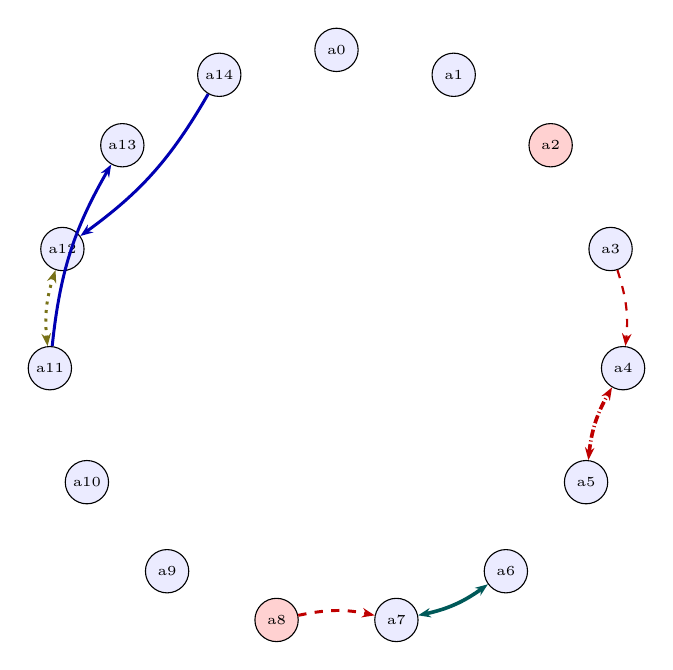
\begin{tikzpicture}[>={Stealth[length=1.6mm]}]
  \node[circle,draw,fill=blue!8,inner sep=1pt,minimum size=5.5mm,font=\tiny] (a0) at (90.0:3.66) {a0};
  \node[circle,draw,fill=blue!8,inner sep=1pt,minimum size=5.5mm,font=\tiny] (a1) at (66.0:3.66) {a1};
  \node[circle,draw,fill=red!18,inner sep=1pt,minimum size=5.5mm,font=\tiny] (a2) at (42.0:3.66) {a2};
  \node[circle,draw,fill=blue!8,inner sep=1pt,minimum size=5.5mm,font=\tiny] (a3) at (18.0:3.66) {a3};
  \node[circle,draw,fill=blue!8,inner sep=1pt,minimum size=5.5mm,font=\tiny] (a4) at (-6.0:3.66) {a4};
  \node[circle,draw,fill=blue!8,inner sep=1pt,minimum size=5.5mm,font=\tiny] (a5) at (-30.0:3.66) {a5};
  \node[circle,draw,fill=blue!8,inner sep=1pt,minimum size=5.5mm,font=\tiny] (a6) at (-54.0:3.66) {a6};
  \node[circle,draw,fill=blue!8,inner sep=1pt,minimum size=5.5mm,font=\tiny] (a7) at (-78.0:3.66) {a7};
  \node[circle,draw,fill=red!18,inner sep=1pt,minimum size=5.5mm,font=\tiny] (a8) at (-102.0:3.66) {a8};
  \node[circle,draw,fill=blue!8,inner sep=1pt,minimum size=5.5mm,font=\tiny] (a9) at (-126.0:3.66) {a9};
  \node[circle,draw,fill=blue!8,inner sep=1pt,minimum size=5.5mm,font=\tiny] (a10) at (-150.0:3.66) {a10};
  \node[circle,draw,fill=blue!8,inner sep=1pt,minimum size=5.5mm,font=\tiny] (a11) at (-174.0:3.66) {a11};
  \node[circle,draw,fill=blue!8,inner sep=1pt,minimum size=5.5mm,font=\tiny] (a12) at (-198.0:3.66) {a12};
  \node[circle,draw,fill=blue!8,inner sep=1pt,minimum size=5.5mm,font=\tiny] (a13) at (-222.0:3.66) {a13};
  \node[circle,draw,fill=blue!8,inner sep=1pt,minimum size=5.5mm,font=\tiny] (a14) at (-246.0:3.66) {a14};
  \draw[{Stealth[length=1.6mm]}-{Stealth[length=1.6mm]}, red!75!black, densely dashdotted, line width=1.31pt] (a5) to[bend left=12] (a4);
  \draw[{Stealth[length=1.6mm]}-{Stealth[length=1.6mm]}, teal!70!black, line width=1.31pt] (a6) to[bend left=12] (a7);
  \draw[{Stealth[length=1.6mm]}-{Stealth[length=1.6mm]}, olive!80!black, dotted, line width=1.08pt] (a11) to[bend left=12] (a12);
  \draw[-{Stealth[length=1.6mm]}, blue!70!black, line width=1.08pt] (a11) to[bend left=12] (a13);
  \draw[-{Stealth[length=1.6mm]}, red!75!black, dashed, line width=1.08pt] (a8) to[bend left=12] (a7);
  \draw[-{Stealth[length=1.6mm]}, blue!70!black, line width=1.08pt] (a14) to[bend left=12] (a12);
  \draw[-{Stealth[length=1.6mm]}, red!75!black, dashed, line width=0.79pt] (a3) to[bend left=12] (a4);
\end{tikzpicture}
}
\\[2pt]{\footnotesize all gold edges: 7 factors}
\end{minipage}\hfill\begin{minipage}[t]{0.48\linewidth}\centering
\resizebox{!}{6.4cm}{%
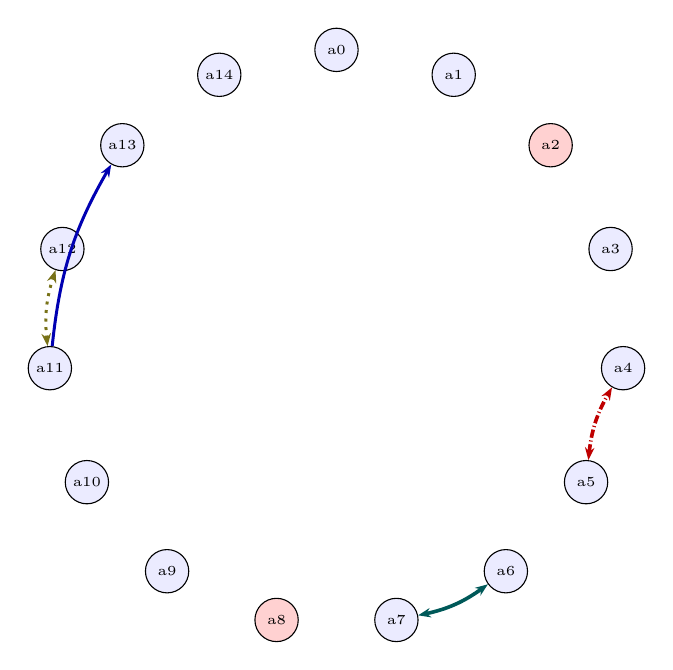
\begin{tikzpicture}[>={Stealth[length=1.6mm]}]
  \node[circle,draw,fill=blue!8,inner sep=1pt,minimum size=5.5mm,font=\tiny] (a0) at (90.0:3.66) {a0};
  \node[circle,draw,fill=blue!8,inner sep=1pt,minimum size=5.5mm,font=\tiny] (a1) at (66.0:3.66) {a1};
  \node[circle,draw,fill=red!18,inner sep=1pt,minimum size=5.5mm,font=\tiny] (a2) at (42.0:3.66) {a2};
  \node[circle,draw,fill=blue!8,inner sep=1pt,minimum size=5.5mm,font=\tiny] (a3) at (18.0:3.66) {a3};
  \node[circle,draw,fill=blue!8,inner sep=1pt,minimum size=5.5mm,font=\tiny] (a4) at (-6.0:3.66) {a4};
  \node[circle,draw,fill=blue!8,inner sep=1pt,minimum size=5.5mm,font=\tiny] (a5) at (-30.0:3.66) {a5};
  \node[circle,draw,fill=blue!8,inner sep=1pt,minimum size=5.5mm,font=\tiny] (a6) at (-54.0:3.66) {a6};
  \node[circle,draw,fill=blue!8,inner sep=1pt,minimum size=5.5mm,font=\tiny] (a7) at (-78.0:3.66) {a7};
  \node[circle,draw,fill=red!18,inner sep=1pt,minimum size=5.5mm,font=\tiny] (a8) at (-102.0:3.66) {a8};
  \node[circle,draw,fill=blue!8,inner sep=1pt,minimum size=5.5mm,font=\tiny] (a9) at (-126.0:3.66) {a9};
  \node[circle,draw,fill=blue!8,inner sep=1pt,minimum size=5.5mm,font=\tiny] (a10) at (-150.0:3.66) {a10};
  \node[circle,draw,fill=blue!8,inner sep=1pt,minimum size=5.5mm,font=\tiny] (a11) at (-174.0:3.66) {a11};
  \node[circle,draw,fill=blue!8,inner sep=1pt,minimum size=5.5mm,font=\tiny] (a12) at (-198.0:3.66) {a12};
  \node[circle,draw,fill=blue!8,inner sep=1pt,minimum size=5.5mm,font=\tiny] (a13) at (-222.0:3.66) {a13};
  \node[circle,draw,fill=blue!8,inner sep=1pt,minimum size=5.5mm,font=\tiny] (a14) at (-246.0:3.66) {a14};
  \draw[{Stealth[length=1.6mm]}-{Stealth[length=1.6mm]}, red!75!black, densely dashdotted, line width=1.31pt] (a5) to[bend left=12] (a4);
  \draw[{Stealth[length=1.6mm]}-{Stealth[length=1.6mm]}, teal!70!black, line width=1.31pt] (a6) to[bend left=12] (a7);
  \draw[{Stealth[length=1.6mm]}-{Stealth[length=1.6mm]}, olive!80!black, dotted, line width=1.08pt] (a11) to[bend left=12] (a12);
  \draw[-{Stealth[length=1.6mm]}, blue!70!black, line width=1.08pt] (a11) to[bend left=12] (a13);
\end{tikzpicture}
}
\\[2pt]{\footnotesize valid edges only: 4 factors}
\end{minipage}
\caption{Relation graph for \texttt{locobench-opus-5-5-f017-r1}. Nodes are atoms on a circle, tinted red when the item marks them non-factual (prior 0.1) and blue when factual (prior 0.9). Edges are gold relations: solid blue = entailment, dashed red = contradiction, double-headed teal = equivalence, dash-dotted red (double-headed) = exclusive (exactly-one), dotted olive (double-headed) = co-necessity (at-least-one); thickness scales with the factor probability. Ordering-only Precedence edges carry no factor and so are not drawn.}
\label{fig:graph-locobench-opus-5-5-f017-r1}
\end{figure}

\begin{table}[htbp]
\centering
\footnotesize
\setlength{\tabcolsep}{3.5pt}
\caption{The specific gold relations of \texttt{locobench-opus-5-5-f017-r1}. \textbf{$p$ used} is the factor probability the MRF received: the band midpoint, times $(1-\lambda)$ for a resolved concession, or \emph{none} for an ordering-only edge (no factor). \textbf{Valid} marks the deliberately-planted errors with their kind. \textbf{Res.} is the resolving atom of a resolved concession.}
\label{tab:rels-locobench-opus-5-5-f017-r1}
\begin{tabular}{lllllrll}
\toprule
ID & Endpoints & Sense & Coupling & Band & $p$ used & Valid & Res. \\
\midrule
\texttt{r000} & \texttt{a5} $\leftrightarrow$ \texttt{a4} & Alternative & \texttt{exclusive} & strong & 0.925 & \checkmark &  \\
\texttt{r001} & \texttt{a6} $\leftrightarrow$ \texttt{a7} & Restatement & \texttt{equivalence} & strong & 0.925 & \checkmark &  \\
\texttt{r002} & \texttt{a11} $\leftrightarrow$ \texttt{a12} & Disjunction & \texttt{co\_necessity} & moderate & 0.720 & \checkmark &  \\
\texttt{r005} & \texttt{a11} $\to$ \texttt{a13} & Instantiation & \texttt{entailment} & moderate & 0.720 & \checkmark &  \\
\texttt{r006} & \texttt{a2} $\to$ \texttt{a3} & Precedence & \texttt{none} & weak & \emph{none} & $\times$ {\scriptsize false\_endpoint} &  \\
\texttt{r007} & \texttt{a8} $\to$ \texttt{a7} & Concession & \texttt{contradiction} & moderate & 0.720 & $\times$ {\scriptsize false\_endpoint} &  \\
\texttt{r008} & \texttt{a14} $\to$ \texttt{a12} & Cause-Effect & \texttt{entailment} & moderate & 0.720 & $\times$ {\scriptsize wrong\_sense} &  \\
\texttt{r009} & \texttt{a3} $\leftrightarrow$ \texttt{a4} & Contrast & \texttt{contradiction} & weak & 0.470 & $\times$ {\scriptsize spurious} &  \\
\bottomrule
\end{tabular}
\end{table}

\begin{table}[htbp]
\centering
\footnotesize
\caption{Atoms of \texttt{locobench-opus-5-5-f017-r1}: the \texttt{factual} label, the prior it maps to, the posterior marginal $P(a_i{=}1)$ the MRF returns, and the shift. Atoms dragged below their prior are the ones the coherence structure penalises.}
\label{tab:atoms-locobench-opus-5-5-f017-r1}
\begin{tabular}{llrrrp{7.2cm}}
\toprule
Atom & fact & $\pi_i$ & $P(a_i{=}1)$ & $\Delta$ & Text \\
\midrule
\texttt{a0} & \checkmark & 0.90 & 0.900 & +0.000 & \footnotesize Lawrence Summers made his remarks on women in science in January 2005. \\
\texttt{a1} & \checkmark & 0.90 & 0.900 & +0.000 & \footnotesize Summers spoke at a National Bureau of Economic Research conference on diversifying the science and engineering workforce. \\
\texttt{a2} & $\times$ & 0.10 & 0.100 & +0.000 & \footnotesize Summers gave his 2005 remarks at a conference hosted by MIT. \\
\texttt{a3} & \checkmark & 0.90 & 0.901 & +0.001 & \footnotesize Summers suggested that greater male variability at the high end of aptitude distributions helps explain women's underrepresentation. \\
\texttt{a4} & \checkmark & 0.90 & 0.656 & -0.244 & \footnotesize Summers was still serving as Harvard's president at the end of 2005. \\
\texttt{a5} & \checkmark & 0.90 & 0.617 & -0.283 & \footnotesize Summers had left the Harvard presidency before the end of 2005. \\
\texttt{a6} & \checkmark & 0.90 & 0.978 & +0.078 & \footnotesize Hyde and colleagues found no meaningful gender difference in the average math performance of US students in grades 2 through 11. \\
\texttt{a7} & \checkmark & 0.90 & 0.977 & +0.077 & \footnotesize According to Hyde and colleagues' 2008 analysis, US girls and boys in grades 2 through 11 performed essentially equally in mathematics on average. \\
\texttt{a8} & $\times$ & 0.10 & 0.060 & -0.040 & \footnotesize Hyde and colleagues found in 2008 that boys substantially outperformed girls on US state mathematics assessments. \\
\texttt{a9} & \checkmark & 0.90 & 0.900 & +0.000 & \footnotesize A 2012 PNAS study by Moss-Racusin and colleagues found that science faculty rated a male applicant as more competent than an otherwise identical female applicant. \\
\texttt{a10} & \checkmark & 0.90 & 0.900 & +0.000 & \footnotesize In the Moss-Racusin study, faculty offered the male applicant a higher starting salary. \\
\texttt{a11} & \checkmark & 0.90 & 0.946 & +0.046 & \footnotesize Women's underrepresentation in math-intensive fields is partly driven by sociocultural factors such as stereotyping and socialization. \\
\texttt{a12} & \checkmark & 0.90 & 0.968 & +0.068 & \footnotesize Women's underrepresentation in math-intensive fields is partly driven by gendered differences in occupational preferences. \\
\texttt{a13} & \checkmark & 0.90 & 0.955 & +0.055 & \footnotesize Leslie and colleagues reported in 2015 that fields whose practitioners emphasize innate brilliance have fewer women. \\
\texttt{a14} & \checkmark & 0.90 & 0.925 & +0.025 & \footnotesize Ceci and Williams concluded in 2011 that sex discrimination in hiring, grant funding, and publishing is no longer the primary cause of women's underrepresentation in math-intensive fields. \\
\bottomrule
\end{tabular}
\end{table}

\subsection{Geology -- base (\texttt{locobench-opus-5-5-f018-r1})}

\textbf{Topic:} Geology (Natural Sciences). \textbf{Family:} \texttt{f018} (CONFLICT), rung 1 (\emph{base}). \textbf{Scores:} mean-marg $= 0.780$, consist $= 0.426$, reified $= 0.153$, log-Z $= 0.364$.



\paragraph{Framing question.} \emph{How did geologists come to accept that the Channeled Scablands of eastern Washington were carved by catastrophic glacial outburst floods rather than by gradual erosion, despite decades of resistance to J Harlen Bretz's original hypothesis?}



\paragraph{Response.} {\small The controversy over the Channeled Scablands began with a single bold claim. J Harlen Bretz proposed in 1923 that a catastrophic flood had carved the Channeled Scablands, an interpretation he drew from dry falls, giant ripple marks, and anastomosing channels incised into the basalt of the Columbia Plateau. The 1923 proposal rested on an earlier statement of the idea: Bretz first published his flood hypothesis in 1910, and that prior publication confirms how long he had been developing the catastrophic reading of the plateau. Whereas Bretz read the landscape as the product of one overwhelming deluge, his critics argued that the scablands were formed by ordinary gradual river and glacial erosion, the slow and uniform processes that early twentieth-century geology regarded as the proper basis for explanation. That gradualist position was itself a consequence of the strong opposition Bretz faced at a 1927 meeting of the Geological Society of Washington in Washington, D.C., where the confrontation pushed the assembled specialists to commit publicly to slow erosion as their counter-explanation. Even though that 1927 opposition was fierce, Bretz did not abandon the catastrophic interpretation, and the tension between his conviction and the hostility of his audience persisted for decades.

The weakest point in the hypothesis was hydrological rather than geomorphic. Bretz's early papers did not identify a convincing source for the floodwater, and this omission came before Joseph Thomas Pardee identified Glacial Lake Missoula as the source of the floodwater, a step that supplied the missing reservoir for a flood of the required magnitude. Pardee's lake occupied the valleys of western Montana, and its shorelines remain etched on the hillsides above the modern city of Missoula. Glacial Lake Missoula was impounded by an ice dam where a lobe of the Cordilleran Ice Sheet blocked the Clark Fork River. By contrast, the ice dam that held back Glacial Lake Missoula was formed by the Laurentide Ice Sheet, the vast continental glacier that covered much of interior North America.

The mechanism of release has been debated with comparable care. At least one of two processes accounts for the failure, perhaps both acting together: the Lake Missoula ice dam failed by floating as the lake deepened, lifting the ice once the water column exceeded roughly nine-tenths of the dam's height, or the Lake Missoula ice dam failed by water tunneling beneath the ice, enlarging subglacial conduits until the barrier collapsed. Each process could have drained the lake rapidly enough to send a wall of water westward across the plateau toward the Columbia River gorge.

A related question concerned the number of events, and here the possibilities are exclusive. Either the Missoula floods occurred as a single flood event, as Bretz originally envisioned, or the Missoula floods occurred as multiple repeated flood events, with the ice dam reforming and failing in cycles; the two accounts cannot both be true, and one of them must hold.

Field evidence ultimately settled the broader dispute. Richard Waitt concluded in 1980 that the Touchet Beds record dozens of separate floods, identifying stacked rhythmites in the slackwater sediments of southern Washington, each capped by evidence of subaerial exposure. Waitt's analysis of the Touchet Beds led the 1965 INQUA field conference participants to conclude that Bretz's catastrophic flood interpretation was correct, and that verdict resolved the long tension between the 1927 opposition and Bretz's persistence, since geologists who examined the scablands directly now endorsed the catastrophic origin he had defended. Institutional recognition followed. Bretz received the Penrose Medal in 1979; in other words, the Geological Society of America awarded Bretz its highest honor in 1979. The honor marked the formal reversal of a profession that had once dismissed his work, and it acknowledged that catastrophic processes, properly documented, belong within the explanatory repertoire of geology rather than outside it.}

\begin{figure}[htbp]
\centering
\begin{minipage}[t]{0.48\linewidth}\centering
\resizebox{!}{6.4cm}{%
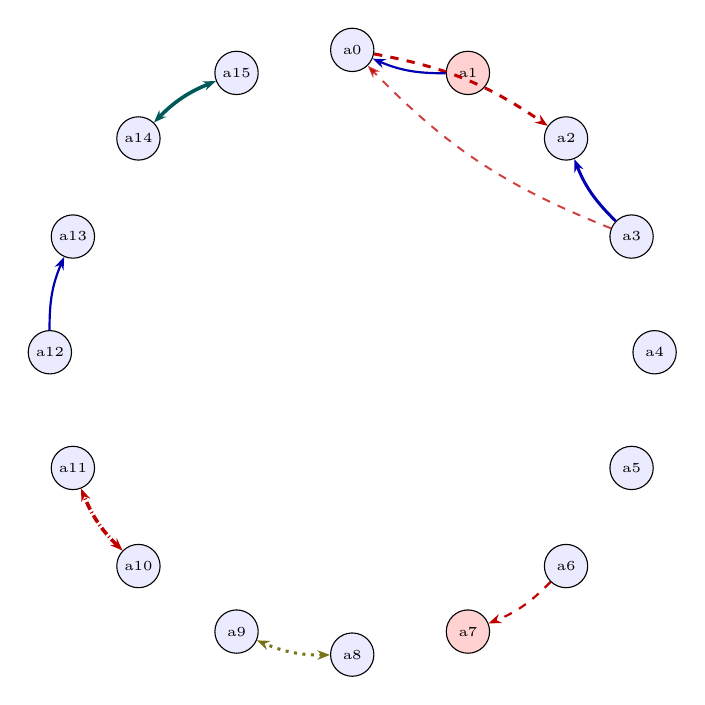
\begin{tikzpicture}[>={Stealth[length=1.6mm]}]
  \node[circle,draw,fill=blue!8,inner sep=1pt,minimum size=5.5mm,font=\tiny] (a0) at (90.0:3.84) {a0};
  \node[circle,draw,fill=red!18,inner sep=1pt,minimum size=5.5mm,font=\tiny] (a1) at (67.5:3.84) {a1};
  \node[circle,draw,fill=blue!8,inner sep=1pt,minimum size=5.5mm,font=\tiny] (a2) at (45.0:3.84) {a2};
  \node[circle,draw,fill=blue!8,inner sep=1pt,minimum size=5.5mm,font=\tiny] (a3) at (22.5:3.84) {a3};
  \node[circle,draw,fill=blue!8,inner sep=1pt,minimum size=5.5mm,font=\tiny] (a4) at (0.0:3.84) {a4};
  \node[circle,draw,fill=blue!8,inner sep=1pt,minimum size=5.5mm,font=\tiny] (a5) at (-22.5:3.84) {a5};
  \node[circle,draw,fill=blue!8,inner sep=1pt,minimum size=5.5mm,font=\tiny] (a6) at (-45.0:3.84) {a6};
  \node[circle,draw,fill=red!18,inner sep=1pt,minimum size=5.5mm,font=\tiny] (a7) at (-67.5:3.84) {a7};
  \node[circle,draw,fill=blue!8,inner sep=1pt,minimum size=5.5mm,font=\tiny] (a8) at (-90.0:3.84) {a8};
  \node[circle,draw,fill=blue!8,inner sep=1pt,minimum size=5.5mm,font=\tiny] (a9) at (-112.5:3.84) {a9};
  \node[circle,draw,fill=blue!8,inner sep=1pt,minimum size=5.5mm,font=\tiny] (a10) at (-135.0:3.84) {a10};
  \node[circle,draw,fill=blue!8,inner sep=1pt,minimum size=5.5mm,font=\tiny] (a11) at (-157.5:3.84) {a11};
  \node[circle,draw,fill=blue!8,inner sep=1pt,minimum size=5.5mm,font=\tiny] (a12) at (-180.0:3.84) {a12};
  \node[circle,draw,fill=blue!8,inner sep=1pt,minimum size=5.5mm,font=\tiny] (a13) at (-202.5:3.84) {a13};
  \node[circle,draw,fill=blue!8,inner sep=1pt,minimum size=5.5mm,font=\tiny] (a14) at (-225.0:3.84) {a14};
  \node[circle,draw,fill=blue!8,inner sep=1pt,minimum size=5.5mm,font=\tiny] (a15) at (-247.5:3.84) {a15};
  \draw[-{Stealth[length=1.6mm]}, red!75!black, dashed, line width=1.08pt] (a0) to[bend left=12] (a2);
  \draw[-{Stealth[length=1.6mm]}, blue!70!black, line width=1.08pt] (a3) to[bend left=12] (a2);
  \draw[-{Stealth[length=1.6mm]}, red!75!black, dashed, line width=0.79pt] (a6) to[bend left=12] (a7);
  \draw[{Stealth[length=1.6mm]}-{Stealth[length=1.6mm]}, olive!80!black, dotted, line width=1.08pt] (a8) to[bend left=12] (a9);
  \draw[{Stealth[length=1.6mm]}-{Stealth[length=1.6mm]}, red!75!black, densely dashdotted, line width=1.31pt] (a10) to[bend left=12] (a11);
  \draw[-{Stealth[length=1.6mm]}, red!75!black, dashed, opacity=0.75, line width=0.71pt] (a3) to[bend left=12] (a0);
  \draw[{Stealth[length=1.6mm]}-{Stealth[length=1.6mm]}, teal!70!black, line width=1.31pt] (a14) to[bend left=12] (a15);
  \draw[-{Stealth[length=1.6mm]}, blue!70!black, line width=0.79pt] (a1) to[bend left=12] (a0);
  \draw[-{Stealth[length=1.6mm]}, blue!70!black, line width=0.79pt] (a12) to[bend left=12] (a13);
\end{tikzpicture}
}
\\[2pt]{\footnotesize all gold edges: 9 factors}
\end{minipage}\hfill\begin{minipage}[t]{0.48\linewidth}\centering
\resizebox{!}{6.4cm}{%
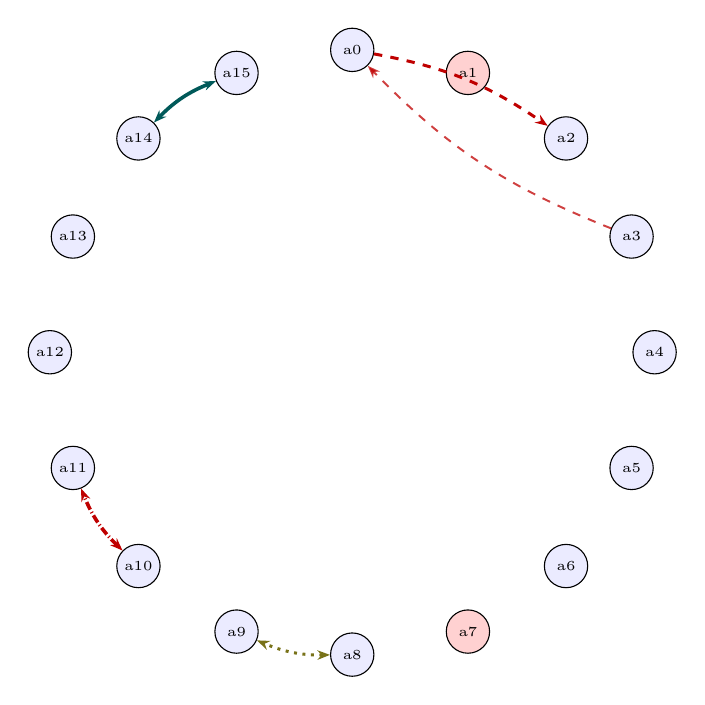
\begin{tikzpicture}[>={Stealth[length=1.6mm]}]
  \node[circle,draw,fill=blue!8,inner sep=1pt,minimum size=5.5mm,font=\tiny] (a0) at (90.0:3.84) {a0};
  \node[circle,draw,fill=red!18,inner sep=1pt,minimum size=5.5mm,font=\tiny] (a1) at (67.5:3.84) {a1};
  \node[circle,draw,fill=blue!8,inner sep=1pt,minimum size=5.5mm,font=\tiny] (a2) at (45.0:3.84) {a2};
  \node[circle,draw,fill=blue!8,inner sep=1pt,minimum size=5.5mm,font=\tiny] (a3) at (22.5:3.84) {a3};
  \node[circle,draw,fill=blue!8,inner sep=1pt,minimum size=5.5mm,font=\tiny] (a4) at (0.0:3.84) {a4};
  \node[circle,draw,fill=blue!8,inner sep=1pt,minimum size=5.5mm,font=\tiny] (a5) at (-22.5:3.84) {a5};
  \node[circle,draw,fill=blue!8,inner sep=1pt,minimum size=5.5mm,font=\tiny] (a6) at (-45.0:3.84) {a6};
  \node[circle,draw,fill=red!18,inner sep=1pt,minimum size=5.5mm,font=\tiny] (a7) at (-67.5:3.84) {a7};
  \node[circle,draw,fill=blue!8,inner sep=1pt,minimum size=5.5mm,font=\tiny] (a8) at (-90.0:3.84) {a8};
  \node[circle,draw,fill=blue!8,inner sep=1pt,minimum size=5.5mm,font=\tiny] (a9) at (-112.5:3.84) {a9};
  \node[circle,draw,fill=blue!8,inner sep=1pt,minimum size=5.5mm,font=\tiny] (a10) at (-135.0:3.84) {a10};
  \node[circle,draw,fill=blue!8,inner sep=1pt,minimum size=5.5mm,font=\tiny] (a11) at (-157.5:3.84) {a11};
  \node[circle,draw,fill=blue!8,inner sep=1pt,minimum size=5.5mm,font=\tiny] (a12) at (-180.0:3.84) {a12};
  \node[circle,draw,fill=blue!8,inner sep=1pt,minimum size=5.5mm,font=\tiny] (a13) at (-202.5:3.84) {a13};
  \node[circle,draw,fill=blue!8,inner sep=1pt,minimum size=5.5mm,font=\tiny] (a14) at (-225.0:3.84) {a14};
  \node[circle,draw,fill=blue!8,inner sep=1pt,minimum size=5.5mm,font=\tiny] (a15) at (-247.5:3.84) {a15};
  \draw[-{Stealth[length=1.6mm]}, red!75!black, dashed, line width=1.08pt] (a0) to[bend left=12] (a2);
  \draw[{Stealth[length=1.6mm]}-{Stealth[length=1.6mm]}, olive!80!black, dotted, line width=1.08pt] (a8) to[bend left=12] (a9);
  \draw[{Stealth[length=1.6mm]}-{Stealth[length=1.6mm]}, red!75!black, densely dashdotted, line width=1.31pt] (a10) to[bend left=12] (a11);
  \draw[-{Stealth[length=1.6mm]}, red!75!black, dashed, opacity=0.75, line width=0.71pt] (a3) to[bend left=12] (a0);
  \draw[{Stealth[length=1.6mm]}-{Stealth[length=1.6mm]}, teal!70!black, line width=1.31pt] (a14) to[bend left=12] (a15);
\end{tikzpicture}
}
\\[2pt]{\footnotesize valid edges only: 5 factors}
\end{minipage}
\caption{Relation graph for \texttt{locobench-opus-5-5-f018-r1}. Nodes are atoms on a circle, tinted red when the item marks them non-factual (prior 0.1) and blue when factual (prior 0.9). Edges are gold relations: solid blue = entailment, dashed red = contradiction, double-headed teal = equivalence, dash-dotted red (double-headed) = exclusive (exactly-one), dotted olive (double-headed) = co-necessity (at-least-one); thickness scales with the factor probability. Ordering-only Precedence edges carry no factor and so are not drawn.}
\label{fig:graph-locobench-opus-5-5-f018-r1}
\end{figure}

\begin{table}[htbp]
\centering
\footnotesize
\setlength{\tabcolsep}{3.5pt}
\caption{The specific gold relations of \texttt{locobench-opus-5-5-f018-r1}. \textbf{$p$ used} is the factor probability the MRF received: the band midpoint, times $(1-\lambda)$ for a resolved concession, or \emph{none} for an ordering-only edge (no factor). \textbf{Valid} marks the deliberately-planted errors with their kind. \textbf{Res.} is the resolving atom of a resolved concession.}
\label{tab:rels-locobench-opus-5-5-f018-r1}
\begin{tabular}{lllllrll}
\toprule
ID & Endpoints & Sense & Coupling & Band & $p$ used & Valid & Res. \\
\midrule
\texttt{r000} & \texttt{a0} $\leftrightarrow$ \texttt{a2} & Contrast & \texttt{contradiction} & moderate & 0.720 & \checkmark &  \\
\texttt{r001} & \texttt{a3} $\to$ \texttt{a2} & Cause-Effect & \texttt{entailment} & moderate & 0.720 & $\times$ {\scriptsize wrong\_direction} &  \\
\texttt{r002} & \texttt{a4} $\to$ \texttt{a5} & Precedence & \texttt{none} & weak & \emph{none} & \checkmark &  \\
\texttt{r003} & \texttt{a6} $\leftrightarrow$ \texttt{a7} & Contrast & \texttt{contradiction} & weak & 0.470 & $\times$ {\scriptsize false\_endpoint} &  \\
\texttt{r004} & \texttt{a8} $\leftrightarrow$ \texttt{a9} & Disjunction & \texttt{co\_necessity} & moderate & 0.720 & \checkmark &  \\
\texttt{r005} & \texttt{a10} $\leftrightarrow$ \texttt{a11} & Alternative & \texttt{exclusive} & strong & 0.925 & \checkmark &  \\
\texttt{r006} & \texttt{a3} $\to$ \texttt{a0} & Concession & \texttt{contradiction} & moderate & 0.396 & \checkmark & \texttt{a13} \\
\texttt{r007} & \texttt{a14} $\leftrightarrow$ \texttt{a15} & Restatement & \texttt{equivalence} & strong & 0.925 & \checkmark &  \\
\texttt{r008} & \texttt{a1} $\to$ \texttt{a0} & Evidence & \texttt{entailment} & weak & 0.470 & $\times$ {\scriptsize false\_endpoint} &  \\
\texttt{r009} & \texttt{a12} $\to$ \texttt{a13} & Cause-Effect & \texttt{entailment} & weak & 0.470 & $\times$ {\scriptsize spurious} &  \\
\bottomrule
\end{tabular}
\end{table}

\begin{table}[htbp]
\centering
\footnotesize
\caption{Atoms of \texttt{locobench-opus-5-5-f018-r1}: the \texttt{factual} label, the prior it maps to, the posterior marginal $P(a_i{=}1)$ the MRF returns, and the shift. Atoms dragged below their prior are the ones the coherence structure penalises.}
\label{tab:atoms-locobench-opus-5-5-f018-r1}
\begin{tabular}{llrrrp{7.2cm}}
\toprule
Atom & fact & $\pi_i$ & $P(a_i{=}1)$ & $\Delta$ & Text \\
\midrule
\texttt{a0} & \checkmark & 0.90 & 0.887 & -0.013 & \footnotesize J Harlen Bretz proposed in 1923 that a catastrophic flood had carved the Channeled Scablands. \\
\texttt{a1} & $\times$ & 0.10 & 0.096 & -0.004 & \footnotesize Bretz first published his flood hypothesis in 1910. \\
\texttt{a2} & \checkmark & 0.90 & 0.899 & -0.001 & \footnotesize Bretz's critics argued that the scablands were formed by ordinary gradual river and glacial erosion. \\
\texttt{a3} & \checkmark & 0.90 & 0.928 & +0.028 & \footnotesize Bretz faced strong opposition at a 1927 meeting of the Geological Society of Washington in Washington, D.C. \\
\texttt{a4} & \checkmark & 0.90 & 0.900 & +0.000 & \footnotesize Bretz's early papers did not identify a convincing source for the floodwater. \\
\texttt{a5} & \checkmark & 0.90 & 0.900 & +0.000 & \footnotesize Joseph Thomas Pardee identified Glacial Lake Missoula as the source of the floodwater. \\
\texttt{a6} & \checkmark & 0.90 & 0.895 & -0.005 & \footnotesize Glacial Lake Missoula was impounded by an ice dam where a lobe of the Cordilleran Ice Sheet blocked the Clark Fork River. \\
\texttt{a7} & $\times$ & 0.10 & 0.110 & +0.010 & \footnotesize The ice dam that held back Glacial Lake Missoula was formed by the Laurentide Ice Sheet. \\
\texttt{a8} & \checkmark & 0.90 & 0.929 & +0.029 & \footnotesize The Lake Missoula ice dam failed by floating as the lake deepened. \\
\texttt{a9} & \checkmark & 0.90 & 0.929 & +0.029 & \footnotesize The Lake Missoula ice dam failed by water tunneling beneath the ice. \\
\texttt{a10} & \checkmark & 0.90 & 0.632 & -0.268 & \footnotesize The Missoula floods occurred as a single flood event. \\
\texttt{a11} & \checkmark & 0.90 & 0.632 & -0.268 & \footnotesize The Missoula floods occurred as multiple repeated flood events. \\
\texttt{a12} & \checkmark & 0.90 & 0.895 & -0.005 & \footnotesize Richard Waitt concluded in 1980 that the Touchet Beds record dozens of separate floods. \\
\texttt{a13} & \checkmark & 0.90 & 0.890 & -0.010 & \footnotesize The 1965 INQUA field conference participants concluded that Bretz's catastrophic flood interpretation was correct. \\
\texttt{a14} & \checkmark & 0.90 & 0.979 & +0.079 & \footnotesize Bretz received the Penrose Medal in 1979. \\
\texttt{a15} & \checkmark & 0.90 & 0.979 & +0.079 & \footnotesize The Geological Society of America awarded Bretz its highest honor in 1979. \\
\bottomrule
\end{tabular}
\end{table}

\subsection{History -- direction\_reversal\_a (\texttt{locobench-opus-5-5-f019-r1})}

\textbf{Topic:} History (Humanities). \textbf{Family:} \texttt{f019} (CONTROL), rung 1 (\emph{direction\_reversal\_a}). \textbf{Scores:} mean-marg $= 0.788$, consist $= 0.555$, reified $= 0.319$, log-Z $= 0.338$.



\paragraph{Framing question.} \emph{How did successive investigations into the 1898 destruction of the USS Maine in Havana harbor weigh the hypothesis of an external mine against that of a spontaneous coal-bunker fire igniting an adjacent magazine, eventually leading most historians to favor one explanation over the other?}



\paragraph{Response.} {\small Inquiry into the loss of the battleship began within days of the disaster. After the USS Maine exploded and sank in Havana harbor on February 15, 1898, the U.S. Navy convened a court of inquiry headed by Captain William T. Sampson in 1898. Sampson, an ordnance specialist with long experience of naval explosives, directed the collection of testimony from surviving officers and the technical survey of the wreck, which lay in shallow water with its forward section shattered. Whereas Sampson led that substantive work, the 1898 court of inquiry was presided over by Admiral George Dewey, whose seniority lent the proceedings formal authority within the service.

The court's reasoning depended on what could be seen beneath the surface of the harbor. Divers reported that a section of the Maine's keel near frame 18 was bent into an inverted V shape, and the members took this deformation to indicate force driven upward from beneath the ship rather than outward from within it. On the strength of that keel evidence, the Sampson court of inquiry concluded that a submarine mine had set off the Maine's forward magazines, although it declined to assign responsibility to any party. The verdict did not stand apart from politics. It was a consequence of the United States declaring war on Spain in April 1898, a decision whose pressure shaped how the court framed its findings and how the public received them.

Later investigators shifted attention from the wreck's exterior to the ship's internal arrangement. Their reconstructions identified two mechanisms, and at least one of them, perhaps both, had been at work. On one side, because the Maine's coal bunkers lay adjacent to its forward magazines, a spontaneous fire was burning in a coal bunker beside the forward magazine, a hazard familiar from other warships that carried bituminous coal in the period. On the other, a mine detonated against the hull below the forward magazines, as the original court had maintained. The dispute therefore turned on the location of the initiating blast. Either, despite the Sampson court's mine verdict, the explosion that destroyed the Maine originated inside the ship's hull, or it originated outside the ship's hull; the two cannot both be true, and one of them must hold.

The decisive reassessment came from engineering analysis rather than fresh salvage. A second board had examined the hulk after it was raised in 1911, but its report largely preserved the mine thesis while revising the point of detonation. Admiral Hyman G. Rickover later commissioned a reconstruction that drew on the photographic and documentary record of both earlier inquiries, together with modern understanding of how underwater and internal explosions deform steel. The Rickover study was published in 1958, whereas its findings rested on that much fuller technical foundation: it concluded that the damage was most consistent with an internal coal-bunker fire igniting a magazine. That conclusion settled the conflict between the mine verdict of 1898 and the case for an origin within the ship, because it explained the inverted keel as the product of a magazine blast buckling the structure rather than as the mark of an external charge.

Historiography has since followed the engineers. Most historians now attribute the sinking of the Maine to an internal explosion; in other words, the prevailing view among historians is that the Maine was destroyed from within. That consensus rests less on any single document than on the convergence of structural analysis with the ship's design, in which fuel and munitions were stored side by side behind thin bulkheads. It has also reshaped how the war's origins are taught. The cry of "Remember the Maine" now serves less as evidence of Spanish hostility than as an illustration of how a technically uncertain finding, issued under political strain, can harden into a justification for armed conflict.}

\begin{figure}[htbp]
\centering
\begin{minipage}[t]{0.48\linewidth}\centering
\resizebox{!}{6.4cm}{%
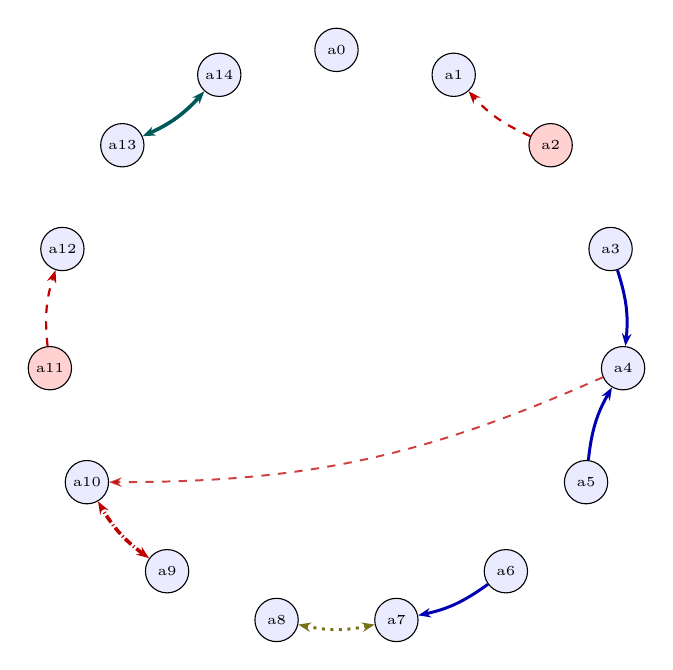
\begin{tikzpicture}[>={Stealth[length=1.6mm]}]
  \node[circle,draw,fill=blue!8,inner sep=1pt,minimum size=5.5mm,font=\tiny] (a0) at (90.0:3.66) {a0};
  \node[circle,draw,fill=blue!8,inner sep=1pt,minimum size=5.5mm,font=\tiny] (a1) at (66.0:3.66) {a1};
  \node[circle,draw,fill=red!18,inner sep=1pt,minimum size=5.5mm,font=\tiny] (a2) at (42.0:3.66) {a2};
  \node[circle,draw,fill=blue!8,inner sep=1pt,minimum size=5.5mm,font=\tiny] (a3) at (18.0:3.66) {a3};
  \node[circle,draw,fill=blue!8,inner sep=1pt,minimum size=5.5mm,font=\tiny] (a4) at (-6.0:3.66) {a4};
  \node[circle,draw,fill=blue!8,inner sep=1pt,minimum size=5.5mm,font=\tiny] (a5) at (-30.0:3.66) {a5};
  \node[circle,draw,fill=blue!8,inner sep=1pt,minimum size=5.5mm,font=\tiny] (a6) at (-54.0:3.66) {a6};
  \node[circle,draw,fill=blue!8,inner sep=1pt,minimum size=5.5mm,font=\tiny] (a7) at (-78.0:3.66) {a7};
  \node[circle,draw,fill=blue!8,inner sep=1pt,minimum size=5.5mm,font=\tiny] (a8) at (-102.0:3.66) {a8};
  \node[circle,draw,fill=blue!8,inner sep=1pt,minimum size=5.5mm,font=\tiny] (a9) at (-126.0:3.66) {a9};
  \node[circle,draw,fill=blue!8,inner sep=1pt,minimum size=5.5mm,font=\tiny] (a10) at (-150.0:3.66) {a10};
  \node[circle,draw,fill=red!18,inner sep=1pt,minimum size=5.5mm,font=\tiny] (a11) at (-174.0:3.66) {a11};
  \node[circle,draw,fill=blue!8,inner sep=1pt,minimum size=5.5mm,font=\tiny] (a12) at (-198.0:3.66) {a12};
  \node[circle,draw,fill=blue!8,inner sep=1pt,minimum size=5.5mm,font=\tiny] (a13) at (-222.0:3.66) {a13};
  \node[circle,draw,fill=blue!8,inner sep=1pt,minimum size=5.5mm,font=\tiny] (a14) at (-246.0:3.66) {a14};
  \draw[-{Stealth[length=1.6mm]}, blue!70!black, line width=1.08pt] (a3) to[bend left=12] (a4);
  \draw[{Stealth[length=1.6mm]}-{Stealth[length=1.6mm]}, olive!80!black, dotted, line width=1.08pt] (a7) to[bend left=12] (a8);
  \draw[{Stealth[length=1.6mm]}-{Stealth[length=1.6mm]}, red!75!black, densely dashdotted, line width=1.31pt] (a9) to[bend left=12] (a10);
  \draw[{Stealth[length=1.6mm]}-{Stealth[length=1.6mm]}, teal!70!black, line width=1.31pt] (a14) to[bend left=12] (a13);
  \draw[-{Stealth[length=1.6mm]}, red!75!black, dashed, opacity=0.75, line width=0.71pt] (a4) to[bend left=12] (a10);
  \draw[-{Stealth[length=1.6mm]}, red!75!black, dashed, line width=0.79pt] (a2) to[bend left=12] (a1);
  \draw[-{Stealth[length=1.6mm]}, red!75!black, dashed, line width=0.79pt] (a11) to[bend left=12] (a12);
  \draw[-{Stealth[length=1.6mm]}, blue!70!black, line width=1.08pt] (a6) to[bend left=12] (a7);
  \draw[-{Stealth[length=1.6mm]}, blue!70!black, line width=1.08pt] (a5) to[bend left=12] (a4);
\end{tikzpicture}
}
\\[2pt]{\footnotesize all gold edges: 9 factors}
\end{minipage}\hfill\begin{minipage}[t]{0.48\linewidth}\centering
\resizebox{!}{6.4cm}{%
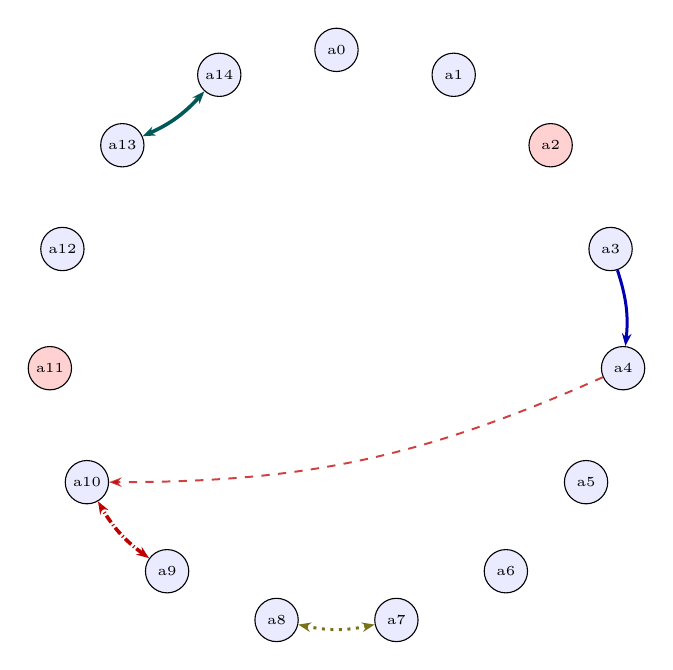
\begin{tikzpicture}[>={Stealth[length=1.6mm]}]
  \node[circle,draw,fill=blue!8,inner sep=1pt,minimum size=5.5mm,font=\tiny] (a0) at (90.0:3.66) {a0};
  \node[circle,draw,fill=blue!8,inner sep=1pt,minimum size=5.5mm,font=\tiny] (a1) at (66.0:3.66) {a1};
  \node[circle,draw,fill=red!18,inner sep=1pt,minimum size=5.5mm,font=\tiny] (a2) at (42.0:3.66) {a2};
  \node[circle,draw,fill=blue!8,inner sep=1pt,minimum size=5.5mm,font=\tiny] (a3) at (18.0:3.66) {a3};
  \node[circle,draw,fill=blue!8,inner sep=1pt,minimum size=5.5mm,font=\tiny] (a4) at (-6.0:3.66) {a4};
  \node[circle,draw,fill=blue!8,inner sep=1pt,minimum size=5.5mm,font=\tiny] (a5) at (-30.0:3.66) {a5};
  \node[circle,draw,fill=blue!8,inner sep=1pt,minimum size=5.5mm,font=\tiny] (a6) at (-54.0:3.66) {a6};
  \node[circle,draw,fill=blue!8,inner sep=1pt,minimum size=5.5mm,font=\tiny] (a7) at (-78.0:3.66) {a7};
  \node[circle,draw,fill=blue!8,inner sep=1pt,minimum size=5.5mm,font=\tiny] (a8) at (-102.0:3.66) {a8};
  \node[circle,draw,fill=blue!8,inner sep=1pt,minimum size=5.5mm,font=\tiny] (a9) at (-126.0:3.66) {a9};
  \node[circle,draw,fill=blue!8,inner sep=1pt,minimum size=5.5mm,font=\tiny] (a10) at (-150.0:3.66) {a10};
  \node[circle,draw,fill=red!18,inner sep=1pt,minimum size=5.5mm,font=\tiny] (a11) at (-174.0:3.66) {a11};
  \node[circle,draw,fill=blue!8,inner sep=1pt,minimum size=5.5mm,font=\tiny] (a12) at (-198.0:3.66) {a12};
  \node[circle,draw,fill=blue!8,inner sep=1pt,minimum size=5.5mm,font=\tiny] (a13) at (-222.0:3.66) {a13};
  \node[circle,draw,fill=blue!8,inner sep=1pt,minimum size=5.5mm,font=\tiny] (a14) at (-246.0:3.66) {a14};
  \draw[-{Stealth[length=1.6mm]}, blue!70!black, line width=1.08pt] (a3) to[bend left=12] (a4);
  \draw[{Stealth[length=1.6mm]}-{Stealth[length=1.6mm]}, olive!80!black, dotted, line width=1.08pt] (a7) to[bend left=12] (a8);
  \draw[{Stealth[length=1.6mm]}-{Stealth[length=1.6mm]}, red!75!black, densely dashdotted, line width=1.31pt] (a9) to[bend left=12] (a10);
  \draw[{Stealth[length=1.6mm]}-{Stealth[length=1.6mm]}, teal!70!black, line width=1.31pt] (a14) to[bend left=12] (a13);
  \draw[-{Stealth[length=1.6mm]}, red!75!black, dashed, opacity=0.75, line width=0.71pt] (a4) to[bend left=12] (a10);
\end{tikzpicture}
}
\\[2pt]{\footnotesize valid edges only: 5 factors}
\end{minipage}
\caption{Relation graph for \texttt{locobench-opus-5-5-f019-r1}. Nodes are atoms on a circle, tinted red when the item marks them non-factual (prior 0.1) and blue when factual (prior 0.9). Edges are gold relations: solid blue = entailment, dashed red = contradiction, double-headed teal = equivalence, dash-dotted red (double-headed) = exclusive (exactly-one), dotted olive (double-headed) = co-necessity (at-least-one); thickness scales with the factor probability. Ordering-only Precedence edges carry no factor and so are not drawn.}
\label{fig:graph-locobench-opus-5-5-f019-r1}
\end{figure}

\begin{table}[htbp]
\centering
\footnotesize
\setlength{\tabcolsep}{3.5pt}
\caption{The specific gold relations of \texttt{locobench-opus-5-5-f019-r1}. \textbf{$p$ used} is the factor probability the MRF received: the band midpoint, times $(1-\lambda)$ for a resolved concession, or \emph{none} for an ordering-only edge (no factor). \textbf{Valid} marks the deliberately-planted errors with their kind. \textbf{Res.} is the resolving atom of a resolved concession.}
\label{tab:rels-locobench-opus-5-5-f019-r1}
\begin{tabular}{lllllrll}
\toprule
ID & Endpoints & Sense & Coupling & Band & $p$ used & Valid & Res. \\
\midrule
\texttt{r000} & \texttt{a0} $\to$ \texttt{a1} & Precedence & \texttt{none} & weak & \emph{none} & \checkmark &  \\
\texttt{r001} & \texttt{a3} $\to$ \texttt{a4} & Evidence & \texttt{entailment} & moderate & 0.720 & \checkmark &  \\
\texttt{r002} & \texttt{a7} $\leftrightarrow$ \texttt{a8} & Disjunction & \texttt{co\_necessity} & moderate & 0.720 & \checkmark &  \\
\texttt{r003} & \texttt{a9} $\leftrightarrow$ \texttt{a10} & Alternative & \texttt{exclusive} & strong & 0.925 & \checkmark &  \\
\texttt{r004} & \texttt{a14} $\leftrightarrow$ \texttt{a13} & Restatement & \texttt{equivalence} & strong & 0.925 & \checkmark &  \\
\texttt{r005} & \texttt{a4} $\to$ \texttt{a10} & Concession & \texttt{contradiction} & moderate & 0.396 & \checkmark & \texttt{a12} \\
\texttt{r006} & \texttt{a2} $\leftrightarrow$ \texttt{a1} & Contrast & \texttt{contradiction} & weak & 0.470 & $\times$ {\scriptsize false\_endpoint} &  \\
\texttt{r007} & \texttt{a11} $\leftrightarrow$ \texttt{a12} & Contrast & \texttt{contradiction} & weak & 0.470 & $\times$ {\scriptsize spurious} &  \\
\texttt{r008} & \texttt{a6} $\to$ \texttt{a7} & Cause-Effect & \texttt{entailment} & moderate & 0.720 & $\times$ {\scriptsize wrong\_sense} &  \\
\texttt{r009} & \texttt{a5} $\to$ \texttt{a4} & Cause-Effect & \texttt{entailment} & moderate & 0.720 & $\times$ {\scriptsize wrong\_direction} &  \\
\bottomrule
\end{tabular}
\end{table}

\begin{table}[htbp]
\centering
\footnotesize
\caption{Atoms of \texttt{locobench-opus-5-5-f019-r1}: the \texttt{factual} label, the prior it maps to, the posterior marginal $P(a_i{=}1)$ the MRF returns, and the shift. Atoms dragged below their prior are the ones the coherence structure penalises.}
\label{tab:atoms-locobench-opus-5-5-f019-r1}
\begin{tabular}{llrrrp{7.2cm}}
\toprule
Atom & fact & $\pi_i$ & $P(a_i{=}1)$ & $\Delta$ & Text \\
\midrule
\texttt{a0} & \checkmark & 0.90 & 0.900 & +0.000 & \footnotesize The USS Maine exploded and sank in Havana harbor on February 15, 1898. \\
\texttt{a1} & \checkmark & 0.90 & 0.901 & +0.001 & \footnotesize The U.S. Navy convened a court of inquiry headed by Captain William T. Sampson in 1898. \\
\texttt{a2} & $\times$ & 0.10 & 0.104 & +0.004 & \footnotesize The 1898 court of inquiry was presided over by Admiral George Dewey. \\
\texttt{a3} & \checkmark & 0.90 & 0.927 & +0.027 & \footnotesize Divers reported that a section of the Maine's keel near frame 18 was bent into an inverted V shape. \\
\texttt{a4} & \checkmark & 0.90 & 0.981 & +0.081 & \footnotesize The Sampson court of inquiry concluded that a submarine mine had set off the Maine's forward magazines. \\
\texttt{a5} & \checkmark & 0.90 & 0.927 & +0.027 & \footnotesize The United States declared war on Spain in April 1898. \\
\texttt{a6} & \checkmark & 0.90 & 0.925 & +0.025 & \footnotesize The Maine's coal bunkers lay adjacent to its forward magazines. \\
\texttt{a7} & \checkmark & 0.90 & 0.968 & +0.068 & \footnotesize A spontaneous fire was burning in a coal bunker beside the Maine's forward magazine. \\
\texttt{a8} & \checkmark & 0.90 & 0.929 & +0.029 & \footnotesize A mine detonated against the Maine's hull below the forward magazines. \\
\texttt{a9} & \checkmark & 0.90 & 0.580 & -0.320 & \footnotesize The explosion that destroyed the Maine originated outside the ship's hull. \\
\texttt{a10} & \checkmark & 0.90 & 0.722 & -0.178 & \footnotesize The explosion that destroyed the Maine originated inside the ship's hull. \\
\texttt{a11} & $\times$ & 0.10 & 0.104 & +0.004 & \footnotesize The Rickover study was published in 1958. \\
\texttt{a12} & \checkmark & 0.90 & 0.901 & +0.001 & \footnotesize The Rickover study concluded that the damage was most consistent with an internal coal-bunker fire igniting a magazine. \\
\texttt{a13} & \checkmark & 0.90 & 0.979 & +0.079 & \footnotesize Most historians now attribute the sinking of the Maine to an internal explosion. \\
\texttt{a14} & \checkmark & 0.90 & 0.979 & +0.079 & \footnotesize The prevailing view among historians is that the Maine was destroyed from within. \\
\bottomrule
\end{tabular}
\end{table}

\subsection{Human Biology -- shuffle\_block (\texttt{locobench-opus-5-5-f020-r1})}

\textbf{Topic:} Human Biology (Natural Sciences). \textbf{Family:} \texttt{f020} (ORDER), rung 1 (\emph{shuffle\_block}). \textbf{Scores:} mean-marg $= 0.790$, consist $= 0.370$, reified $= 0.203$, log-Z $= 0.390$.



\paragraph{Framing question.} \emph{How did researchers establish that most peptic ulcers result from Helicobacter pylori infection rather than from stress or excess stomach acid, overturning the long-accepted medical view?}



\paragraph{Response.} {\small The decisive clinical evidence came from treatment trials, which tested whether removing the organism changed the course of the disease. Eradicating H. pylori with antibiotics sharply lowers peptic ulcer recurrence rates. In other words, peptic ulcers recur far less often after H. pylori is eliminated by antibiotic therapy. This therapeutic result carried particular weight because acid suppression alone had produced healing followed by frequent relapse. That pattern fits an untreated infectious cause better than a purely chemical one. Gastroenterologists who had been sceptical of a single pathologist's microscopy found it harder to resist outcome data from controlled trials. Patient populations, dosing regimens and follow-up periods varied across those trials, yet the difference in relapse persisted.

J. Robin Warren was a pathologist at Royal Perth Hospital in Western Australia. His work involved the routine examination of tissue removed during endoscopy. In that setting, unusual material on the stomach lining was ordinarily dismissed as contamination or artefact, because the acidic gastric environment was thought to be effectively sterile. In 1979, Warren observed curved bacteria in gastric biopsy specimens. Across a growing series of samples, he noted that the curved bacteria were consistently associated with gastric inflammation, a pattern too regular to dismiss as incidental. Even though that association recurred specimen after specimen, in the early 1980s the prevailing medical view held that stress and excess acid caused peptic ulcers. By contrast with that combined account of stress and acid, psychological stress is the primary cause of most peptic ulcers.

The Nobel Assembly at Karolinska Institutet determined that H. pylori infection plays a causal role in peptic ulcer disease. That verdict settled the long-standing tension between Warren's consistent histological association and the stress-and-acid orthodoxy, which had resisted it for years, and it led to the reduced recurrence that followed eradication. The path to the overturned view therefore ran through careful microscopy, a fortunate extension of culture time, deliberate self-infection and therapeutic trials. Each step supplied a different form of evidence, and together they amounted to a causal argument that clinical medicine could no longer set aside.

Isolation alone could not establish causation, since an organism found in diseased tissue may simply colonize damage that has already occurred. To satisfy the logic of Koch's postulates, the investigators needed to show that the bacterium could produce disease in a previously healthy stomach. Marshall drank the bacterial culture in 1990, and that act caused him to develop gastritis within days of ingesting it. Subsequent endoscopy and biopsy documented the inflammation and recovered the organism, closing the inferential gap between presence and pathogenesis. The procedural circumstances of the experiment are recorded inconsistently. Either Marshall conducted his self-experiment with prior approval from a hospital ethics committee, or he conducted it without prior approval from a hospital ethics committee. The two cannot both be true, and one of them must hold.

Barry Marshall began collaborating with Warren in 1981, two years after those first observations of curved organisms in the biopsy material. The partnership set out to move from histological correlation to microbiological proof. That required isolating the organism and growing it in pure culture, but the culture work failed repeatedly. At least one of two obstacles explains those failures, perhaps both: early attempts to culture the bacterium used incubation periods too short for colonies to appear, or H. pylori grows slowly on standard laboratory culture media. By contrast with that sluggish growth on ordinary media, the first successful culture came after plates were left incubating over the Easter long weekend, and it came then because the earlier incubation periods had been too short. The accidental extension gave the colonies the time they needed. From that point, the organism could be characterized, typed and supplied for further experiments.}

\begin{figure}[htbp]
\centering
\begin{minipage}[t]{0.48\linewidth}\centering
\resizebox{!}{6.4cm}{%
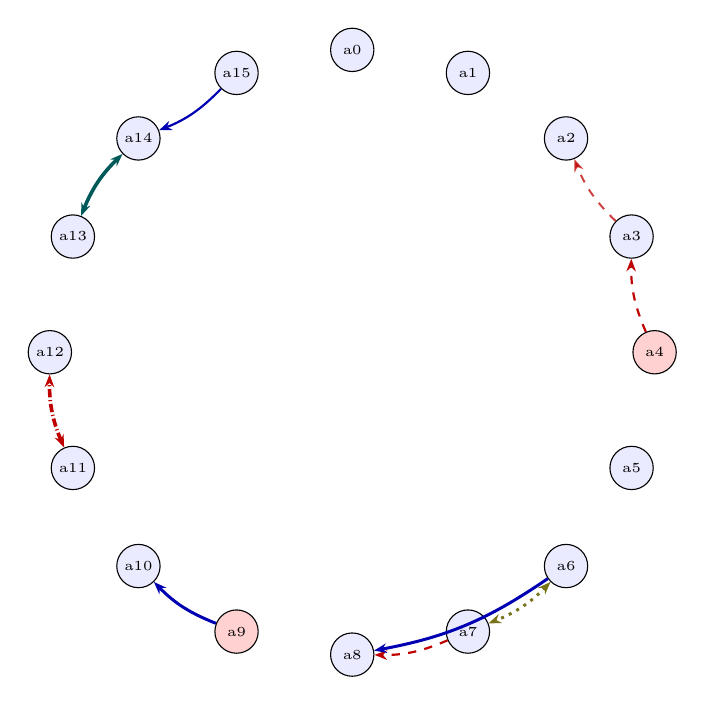
\begin{tikzpicture}[>={Stealth[length=1.6mm]}]
  \node[circle,draw,fill=blue!8,inner sep=1pt,minimum size=5.5mm,font=\tiny] (a0) at (90.0:3.84) {a0};
  \node[circle,draw,fill=blue!8,inner sep=1pt,minimum size=5.5mm,font=\tiny] (a1) at (67.5:3.84) {a1};
  \node[circle,draw,fill=blue!8,inner sep=1pt,minimum size=5.5mm,font=\tiny] (a2) at (45.0:3.84) {a2};
  \node[circle,draw,fill=blue!8,inner sep=1pt,minimum size=5.5mm,font=\tiny] (a3) at (22.5:3.84) {a3};
  \node[circle,draw,fill=red!18,inner sep=1pt,minimum size=5.5mm,font=\tiny] (a4) at (0.0:3.84) {a4};
  \node[circle,draw,fill=blue!8,inner sep=1pt,minimum size=5.5mm,font=\tiny] (a5) at (-22.5:3.84) {a5};
  \node[circle,draw,fill=blue!8,inner sep=1pt,minimum size=5.5mm,font=\tiny] (a6) at (-45.0:3.84) {a6};
  \node[circle,draw,fill=blue!8,inner sep=1pt,minimum size=5.5mm,font=\tiny] (a7) at (-67.5:3.84) {a7};
  \node[circle,draw,fill=blue!8,inner sep=1pt,minimum size=5.5mm,font=\tiny] (a8) at (-90.0:3.84) {a8};
  \node[circle,draw,fill=red!18,inner sep=1pt,minimum size=5.5mm,font=\tiny] (a9) at (-112.5:3.84) {a9};
  \node[circle,draw,fill=blue!8,inner sep=1pt,minimum size=5.5mm,font=\tiny] (a10) at (-135.0:3.84) {a10};
  \node[circle,draw,fill=blue!8,inner sep=1pt,minimum size=5.5mm,font=\tiny] (a11) at (-157.5:3.84) {a11};
  \node[circle,draw,fill=blue!8,inner sep=1pt,minimum size=5.5mm,font=\tiny] (a12) at (-180.0:3.84) {a12};
  \node[circle,draw,fill=blue!8,inner sep=1pt,minimum size=5.5mm,font=\tiny] (a13) at (-202.5:3.84) {a13};
  \node[circle,draw,fill=blue!8,inner sep=1pt,minimum size=5.5mm,font=\tiny] (a14) at (-225.0:3.84) {a14};
  \node[circle,draw,fill=blue!8,inner sep=1pt,minimum size=5.5mm,font=\tiny] (a15) at (-247.5:3.84) {a15};
  \draw[-{Stealth[length=1.6mm]}, red!75!black, dashed, opacity=0.75, line width=0.71pt] (a3) to[bend left=12] (a2);
  \draw[-{Stealth[length=1.6mm]}, red!75!black, dashed, line width=0.79pt] (a4) to[bend left=12] (a3);
  \draw[{Stealth[length=1.6mm]}-{Stealth[length=1.6mm]}, olive!80!black, dotted, line width=1.08pt] (a6) to[bend left=12] (a7);
  \draw[-{Stealth[length=1.6mm]}, red!75!black, dashed, line width=0.79pt] (a7) to[bend left=12] (a8);
  \draw[-{Stealth[length=1.6mm]}, blue!70!black, line width=1.08pt] (a6) to[bend left=12] (a8);
  \draw[-{Stealth[length=1.6mm]}, blue!70!black, line width=1.08pt] (a9) to[bend left=12] (a10);
  \draw[{Stealth[length=1.6mm]}-{Stealth[length=1.6mm]}, red!75!black, densely dashdotted, line width=1.31pt] (a11) to[bend left=12] (a12);
  \draw[{Stealth[length=1.6mm]}-{Stealth[length=1.6mm]}, teal!70!black, line width=1.31pt] (a13) to[bend left=12] (a14);
  \draw[-{Stealth[length=1.6mm]}, blue!70!black, line width=0.79pt] (a15) to[bend left=12] (a14);
\end{tikzpicture}
}
\\[2pt]{\footnotesize all gold edges: 9 factors}
\end{minipage}\hfill\begin{minipage}[t]{0.48\linewidth}\centering
\resizebox{!}{6.4cm}{%
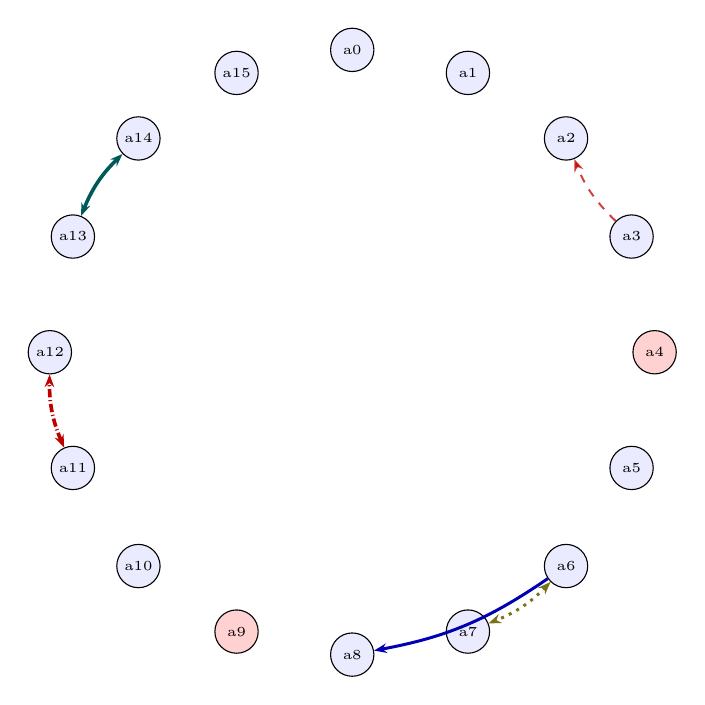
\begin{tikzpicture}[>={Stealth[length=1.6mm]}]
  \node[circle,draw,fill=blue!8,inner sep=1pt,minimum size=5.5mm,font=\tiny] (a0) at (90.0:3.84) {a0};
  \node[circle,draw,fill=blue!8,inner sep=1pt,minimum size=5.5mm,font=\tiny] (a1) at (67.5:3.84) {a1};
  \node[circle,draw,fill=blue!8,inner sep=1pt,minimum size=5.5mm,font=\tiny] (a2) at (45.0:3.84) {a2};
  \node[circle,draw,fill=blue!8,inner sep=1pt,minimum size=5.5mm,font=\tiny] (a3) at (22.5:3.84) {a3};
  \node[circle,draw,fill=red!18,inner sep=1pt,minimum size=5.5mm,font=\tiny] (a4) at (0.0:3.84) {a4};
  \node[circle,draw,fill=blue!8,inner sep=1pt,minimum size=5.5mm,font=\tiny] (a5) at (-22.5:3.84) {a5};
  \node[circle,draw,fill=blue!8,inner sep=1pt,minimum size=5.5mm,font=\tiny] (a6) at (-45.0:3.84) {a6};
  \node[circle,draw,fill=blue!8,inner sep=1pt,minimum size=5.5mm,font=\tiny] (a7) at (-67.5:3.84) {a7};
  \node[circle,draw,fill=blue!8,inner sep=1pt,minimum size=5.5mm,font=\tiny] (a8) at (-90.0:3.84) {a8};
  \node[circle,draw,fill=red!18,inner sep=1pt,minimum size=5.5mm,font=\tiny] (a9) at (-112.5:3.84) {a9};
  \node[circle,draw,fill=blue!8,inner sep=1pt,minimum size=5.5mm,font=\tiny] (a10) at (-135.0:3.84) {a10};
  \node[circle,draw,fill=blue!8,inner sep=1pt,minimum size=5.5mm,font=\tiny] (a11) at (-157.5:3.84) {a11};
  \node[circle,draw,fill=blue!8,inner sep=1pt,minimum size=5.5mm,font=\tiny] (a12) at (-180.0:3.84) {a12};
  \node[circle,draw,fill=blue!8,inner sep=1pt,minimum size=5.5mm,font=\tiny] (a13) at (-202.5:3.84) {a13};
  \node[circle,draw,fill=blue!8,inner sep=1pt,minimum size=5.5mm,font=\tiny] (a14) at (-225.0:3.84) {a14};
  \node[circle,draw,fill=blue!8,inner sep=1pt,minimum size=5.5mm,font=\tiny] (a15) at (-247.5:3.84) {a15};
  \draw[-{Stealth[length=1.6mm]}, red!75!black, dashed, opacity=0.75, line width=0.71pt] (a3) to[bend left=12] (a2);
  \draw[{Stealth[length=1.6mm]}-{Stealth[length=1.6mm]}, olive!80!black, dotted, line width=1.08pt] (a6) to[bend left=12] (a7);
  \draw[-{Stealth[length=1.6mm]}, blue!70!black, line width=1.08pt] (a6) to[bend left=12] (a8);
  \draw[{Stealth[length=1.6mm]}-{Stealth[length=1.6mm]}, red!75!black, densely dashdotted, line width=1.31pt] (a11) to[bend left=12] (a12);
  \draw[{Stealth[length=1.6mm]}-{Stealth[length=1.6mm]}, teal!70!black, line width=1.31pt] (a13) to[bend left=12] (a14);
\end{tikzpicture}
}
\\[2pt]{\footnotesize valid edges only: 5 factors}
\end{minipage}
\caption{Relation graph for \texttt{locobench-opus-5-5-f020-r1}. Nodes are atoms on a circle, tinted red when the item marks them non-factual (prior 0.1) and blue when factual (prior 0.9). Edges are gold relations: solid blue = entailment, dashed red = contradiction, double-headed teal = equivalence, dash-dotted red (double-headed) = exclusive (exactly-one), dotted olive (double-headed) = co-necessity (at-least-one); thickness scales with the factor probability. Ordering-only Precedence edges carry no factor and so are not drawn.}
\label{fig:graph-locobench-opus-5-5-f020-r1}
\end{figure}

\begin{table}[htbp]
\centering
\footnotesize
\setlength{\tabcolsep}{3.5pt}
\caption{The specific gold relations of \texttt{locobench-opus-5-5-f020-r1}. \textbf{$p$ used} is the factor probability the MRF received: the band midpoint, times $(1-\lambda)$ for a resolved concession, or \emph{none} for an ordering-only edge (no factor). \textbf{Valid} marks the deliberately-planted errors with their kind. \textbf{Res.} is the resolving atom of a resolved concession.}
\label{tab:rels-locobench-opus-5-5-f020-r1}
\begin{tabular}{lllllrll}
\toprule
ID & Endpoints & Sense & Coupling & Band & $p$ used & Valid & Res. \\
\midrule
\texttt{r000} & \texttt{a1} $\to$ \texttt{a5} & Precedence & \texttt{none} & weak & \emph{none} & \checkmark &  \\
\texttt{r001} & \texttt{a3} $\to$ \texttt{a2} & Concession & \texttt{contradiction} & moderate & 0.396 & \checkmark & \texttt{a15} \\
\texttt{r002} & \texttt{a4} $\leftrightarrow$ \texttt{a3} & Contrast & \texttt{contradiction} & weak & 0.470 & $\times$ {\scriptsize wrong\_sense} &  \\
\texttt{r003} & \texttt{a6} $\leftrightarrow$ \texttt{a7} & Disjunction & \texttt{co\_necessity} & moderate & 0.720 & \checkmark &  \\
\texttt{r004} & \texttt{a7} $\leftrightarrow$ \texttt{a8} & Contrast & \texttt{contradiction} & weak & 0.470 & $\times$ {\scriptsize wrong\_sense} &  \\
\texttt{r005} & \texttt{a6} $\to$ \texttt{a8} & Cause-Effect & \texttt{entailment} & moderate & 0.720 & \checkmark &  \\
\texttt{r006} & \texttt{a9} $\to$ \texttt{a10} & Cause-Effect & \texttt{entailment} & moderate & 0.720 & $\times$ {\scriptsize false\_endpoint} &  \\
\texttt{r007} & \texttt{a11} $\leftrightarrow$ \texttt{a12} & Alternative & \texttt{exclusive} & strong & 0.925 & \checkmark &  \\
\texttt{r008} & \texttt{a13} $\leftrightarrow$ \texttt{a14} & Restatement & \texttt{equivalence} & strong & 0.925 & \checkmark &  \\
\texttt{r009} & \texttt{a15} $\to$ \texttt{a14} & Cause-Effect & \texttt{entailment} & weak & 0.470 & $\times$ {\scriptsize spurious} &  \\
\bottomrule
\end{tabular}
\end{table}

\begin{table}[htbp]
\centering
\footnotesize
\caption{Atoms of \texttt{locobench-opus-5-5-f020-r1}: the \texttt{factual} label, the prior it maps to, the posterior marginal $P(a_i{=}1)$ the MRF returns, and the shift. Atoms dragged below their prior are the ones the coherence structure penalises.}
\label{tab:atoms-locobench-opus-5-5-f020-r1}
\begin{tabular}{llrrrp{7.2cm}}
\toprule
Atom & fact & $\pi_i$ & $P(a_i{=}1)$ & $\Delta$ & Text \\
\midrule
\texttt{a0} & \checkmark & 0.90 & 0.900 & +0.000 & \footnotesize J. Robin Warren was a pathologist at Royal Perth Hospital in Western Australia. \\
\texttt{a1} & \checkmark & 0.90 & 0.900 & +0.000 & \footnotesize Warren observed curved bacteria in gastric biopsy specimens in 1979. \\
\texttt{a2} & \checkmark & 0.90 & 0.929 & +0.029 & \footnotesize Warren noted that the curved bacteria were consistently associated with gastric inflammation. \\
\texttt{a3} & \checkmark & 0.90 & 0.914 & +0.014 & \footnotesize In the early 1980s, the prevailing medical view held that stress and excess acid caused peptic ulcers. \\
\texttt{a4} & $\times$ & 0.10 & 0.104 & +0.004 & \footnotesize Psychological stress is the primary cause of most peptic ulcers. \\
\texttt{a5} & \checkmark & 0.90 & 0.900 & +0.000 & \footnotesize Barry Marshall began collaborating with Warren in 1981. \\
\texttt{a6} & \checkmark & 0.90 & 0.947 & +0.047 & \footnotesize Early attempts to culture the bacterium used incubation periods too short for colonies to appear. \\
\texttt{a7} & \checkmark & 0.90 & 0.932 & +0.032 & \footnotesize H. pylori grows slowly on standard laboratory culture media. \\
\texttt{a8} & \checkmark & 0.90 & 0.960 & +0.060 & \footnotesize The first successful culture came after plates were left incubating over the Easter long weekend. \\
\texttt{a9} & $\times$ & 0.10 & 0.131 & +0.031 & \footnotesize Marshall drank the bacterial culture in 1990. \\
\texttt{a10} & \checkmark & 0.90 & 0.908 & +0.008 & \footnotesize Marshall developed gastritis within days of ingesting the bacterial culture. \\
\texttt{a11} & \checkmark & 0.90 & 0.632 & -0.268 & \footnotesize Marshall conducted his self-experiment with prior approval from a hospital ethics committee. \\
\texttt{a12} & \checkmark & 0.90 & 0.632 & -0.268 & \footnotesize Marshall conducted his self-experiment without prior approval from a hospital ethics committee. \\
\texttt{a13} & \checkmark & 0.90 & 0.978 & +0.078 & \footnotesize Eradicating H. pylori with antibiotics sharply lowers peptic ulcer recurrence rates. \\
\texttt{a14} & \checkmark & 0.90 & 0.977 & +0.077 & \footnotesize Peptic ulcers recur far less often after H. pylori is eliminated by antibiotic therapy. \\
\texttt{a15} & \checkmark & 0.90 & 0.895 & -0.005 & \footnotesize The Nobel Assembly at Karolinska Institutet determined that H. pylori infection plays a causal role in peptic ulcer disease. \\
\bottomrule
\end{tabular}
\end{table}

\subsection{Law -- break\_2 (\texttt{locobench-opus-5-5-f021-r1})}

\textbf{Topic:} Law (Social Sciences). \textbf{Family:} \texttt{f021} (CHAIN), rung 1 (\emph{break\_2}). \textbf{Scores:} mean-marg $= 0.784$, consist $= 0.848$, reified $= 0.324$, log-Z $= 0.459$.



\paragraph{Framing question.} \emph{How does an appellate court decide whether a trial judge's erroneous admission of disputed expert testimony amounts to harmless error or requires reversal when the prosecution and defense disagree about how much that testimony shaped the jury's verdict?}



\paragraph{Response.} {\small When an appellate court confronts a claim that expert testimony should never have reached the jury, it begins with the framework governing admissibility. Daubert v. Merrell Dow Pharmaceuticals assigned trial judges a gatekeeping role over the admission of expert testimony. Although the decision entrusted judges with that screening function, Daubert held that the Frye general-acceptance test remains the exclusive standard for admitting scientific evidence. The appellate inquiry, however, does not end once a defect in the application of that standard is identified. A reviewing court must separate two distinct questions: whether the trial judge erred, and whether the error, once established, affected the outcome to a degree the law cannot tolerate. Conflating the two would convert every evidentiary misstep into an automatic retrial, a result the harmless-error doctrine exists to prevent.

Consider a prosecution in which a firearms examiner testified that bullets recovered from the victim were fired from a particular pistol. The trial judge admitted the ballistics testimony without holding a Daubert hearing; that is, no Daubert hearing took place before the ballistics testimony was admitted. The record also shows that the trial judge admitted the ballistics expert's testimony over the defense's objection. That objection preserved the issue for review and spared the defendant the heavier burden of plain-error analysis. Once preservation is secured and the error is conceded or found, the appellate court sets aside the reliability of toolmark comparison as a discipline and turns instead to the consequences of the admission at this particular trial.

Those consequences depend on what else the jury heard. The trial record supported at least one of two inferences, perhaps both: the defendant was present at the scene of the shooting, or the defendant supplied the weapon used in the shooting. The parties drew opposing lessons from that record. The prosecution argued that the ballistics expert's testimony had little effect on the jury's verdict, and because the prosecution pressed that position, the defense argued that the ballistics expert's testimony was central to the jury's verdict. Competing characterizations of this kind arise in nearly every harmless-error appeal, and a reviewing court does not resolve them by crediting the more forceful advocate.

Instead, the court reconstructs the evidentiary landscape the jury actually confronted, examining the closing arguments, the instructions, and the weight each side placed on particular witnesses. The decisive question is structural, and it admits only two answers: either the ballistics expert's testimony was the only evidence linking the defendant to the shooting, or evidence other than the ballistics expert's testimony linked the defendant to the shooting. One of these must hold, and they cannot both be true. The measure the court applies to that question comes from constitutional doctrine. Chapman v. California held that some constitutional errors can be harmless if they are harmless beyond a reasonable doubt, a rule the Court articulated before the case was decided in 1973. Whether a particular evidentiary error rises to constitutional dimension varies by jurisdiction, but many courts borrow the Chapman formulation whenever the challenged testimony implicates confrontation or due process.

The allocation of proof under that formulation is fixed and does not shift with the parties' rhetoric. Under the Chapman standard, the prosecution bears the burden of showing that the error was harmless, and that allocation indicates that the appellate panel ultimately concluded that the properly admitted evidence of guilt was overwhelming. The panel's conclusion resulted from the independent proof, wholly outside the expert's account, that tied the defendant to the shooting. The court of appeals held that the erroneous admission of the ballistics expert's testimony was harmless. The method, then, is neither a tally of the parties' assertions nor a guess about the jurors' deliberations; it is a disciplined inquiry into whether the verdict would have been the same without the tainted testimony, answered by measuring what remains once that testimony is removed from the record.}

\begin{figure}[htbp]
\centering
\begin{minipage}[t]{0.48\linewidth}\centering
\resizebox{!}{6.4cm}{%
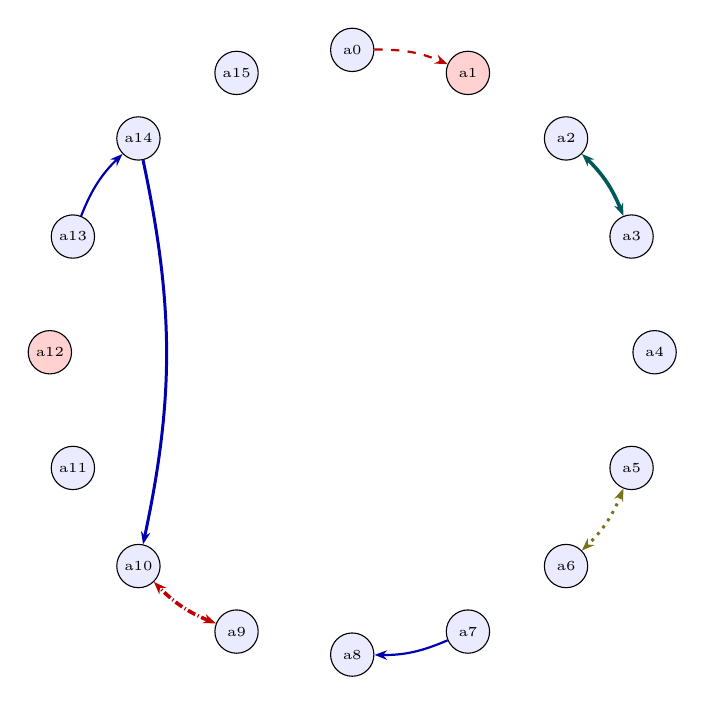
\begin{tikzpicture}[>={Stealth[length=1.6mm]}]
  \node[circle,draw,fill=blue!8,inner sep=1pt,minimum size=5.5mm,font=\tiny] (a0) at (90.0:3.84) {a0};
  \node[circle,draw,fill=red!18,inner sep=1pt,minimum size=5.5mm,font=\tiny] (a1) at (67.5:3.84) {a1};
  \node[circle,draw,fill=blue!8,inner sep=1pt,minimum size=5.5mm,font=\tiny] (a2) at (45.0:3.84) {a2};
  \node[circle,draw,fill=blue!8,inner sep=1pt,minimum size=5.5mm,font=\tiny] (a3) at (22.5:3.84) {a3};
  \node[circle,draw,fill=blue!8,inner sep=1pt,minimum size=5.5mm,font=\tiny] (a4) at (0.0:3.84) {a4};
  \node[circle,draw,fill=blue!8,inner sep=1pt,minimum size=5.5mm,font=\tiny] (a5) at (-22.5:3.84) {a5};
  \node[circle,draw,fill=blue!8,inner sep=1pt,minimum size=5.5mm,font=\tiny] (a6) at (-45.0:3.84) {a6};
  \node[circle,draw,fill=blue!8,inner sep=1pt,minimum size=5.5mm,font=\tiny] (a7) at (-67.5:3.84) {a7};
  \node[circle,draw,fill=blue!8,inner sep=1pt,minimum size=5.5mm,font=\tiny] (a8) at (-90.0:3.84) {a8};
  \node[circle,draw,fill=blue!8,inner sep=1pt,minimum size=5.5mm,font=\tiny] (a9) at (-112.5:3.84) {a9};
  \node[circle,draw,fill=blue!8,inner sep=1pt,minimum size=5.5mm,font=\tiny] (a10) at (-135.0:3.84) {a10};
  \node[circle,draw,fill=blue!8,inner sep=1pt,minimum size=5.5mm,font=\tiny] (a11) at (-157.5:3.84) {a11};
  \node[circle,draw,fill=red!18,inner sep=1pt,minimum size=5.5mm,font=\tiny] (a12) at (-180.0:3.84) {a12};
  \node[circle,draw,fill=blue!8,inner sep=1pt,minimum size=5.5mm,font=\tiny] (a13) at (-202.5:3.84) {a13};
  \node[circle,draw,fill=blue!8,inner sep=1pt,minimum size=5.5mm,font=\tiny] (a14) at (-225.0:3.84) {a14};
  \node[circle,draw,fill=blue!8,inner sep=1pt,minimum size=5.5mm,font=\tiny] (a15) at (-247.5:3.84) {a15};
  \draw[{Stealth[length=1.6mm]}-{Stealth[length=1.6mm]}, teal!70!black, line width=1.31pt] (a2) to[bend left=12] (a3);
  \draw[{Stealth[length=1.6mm]}-{Stealth[length=1.6mm]}, red!75!black, densely dashdotted, line width=1.31pt] (a9) to[bend left=12] (a10);
  \draw[{Stealth[length=1.6mm]}-{Stealth[length=1.6mm]}, olive!80!black, dotted, line width=1.08pt] (a5) to[bend left=12] (a6);
  \draw[-{Stealth[length=1.6mm]}, blue!70!black, line width=1.08pt] (a14) to[bend left=12] (a10);
  \draw[-{Stealth[length=1.6mm]}, red!75!black, dashed, line width=0.79pt] (a0) to[bend left=12] (a1);
  \draw[-{Stealth[length=1.6mm]}, blue!70!black, line width=0.79pt] (a7) to[bend left=12] (a8);
  \draw[-{Stealth[length=1.6mm]}, blue!70!black, line width=0.79pt] (a13) to[bend left=12] (a14);
\end{tikzpicture}
}
\\[2pt]{\footnotesize all gold edges: 7 factors}
\end{minipage}\hfill\begin{minipage}[t]{0.48\linewidth}\centering
\resizebox{!}{6.4cm}{%
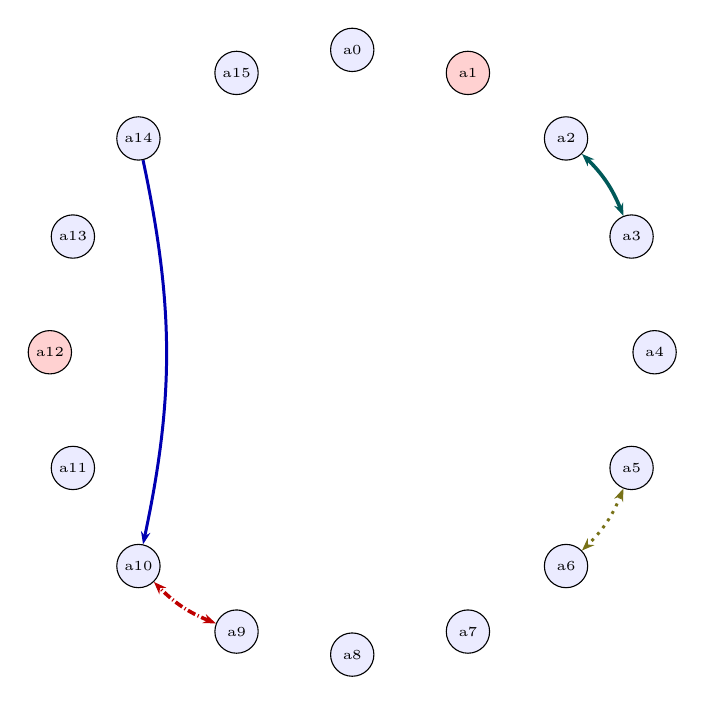
\begin{tikzpicture}[>={Stealth[length=1.6mm]}]
  \node[circle,draw,fill=blue!8,inner sep=1pt,minimum size=5.5mm,font=\tiny] (a0) at (90.0:3.84) {a0};
  \node[circle,draw,fill=red!18,inner sep=1pt,minimum size=5.5mm,font=\tiny] (a1) at (67.5:3.84) {a1};
  \node[circle,draw,fill=blue!8,inner sep=1pt,minimum size=5.5mm,font=\tiny] (a2) at (45.0:3.84) {a2};
  \node[circle,draw,fill=blue!8,inner sep=1pt,minimum size=5.5mm,font=\tiny] (a3) at (22.5:3.84) {a3};
  \node[circle,draw,fill=blue!8,inner sep=1pt,minimum size=5.5mm,font=\tiny] (a4) at (0.0:3.84) {a4};
  \node[circle,draw,fill=blue!8,inner sep=1pt,minimum size=5.5mm,font=\tiny] (a5) at (-22.5:3.84) {a5};
  \node[circle,draw,fill=blue!8,inner sep=1pt,minimum size=5.5mm,font=\tiny] (a6) at (-45.0:3.84) {a6};
  \node[circle,draw,fill=blue!8,inner sep=1pt,minimum size=5.5mm,font=\tiny] (a7) at (-67.5:3.84) {a7};
  \node[circle,draw,fill=blue!8,inner sep=1pt,minimum size=5.5mm,font=\tiny] (a8) at (-90.0:3.84) {a8};
  \node[circle,draw,fill=blue!8,inner sep=1pt,minimum size=5.5mm,font=\tiny] (a9) at (-112.5:3.84) {a9};
  \node[circle,draw,fill=blue!8,inner sep=1pt,minimum size=5.5mm,font=\tiny] (a10) at (-135.0:3.84) {a10};
  \node[circle,draw,fill=blue!8,inner sep=1pt,minimum size=5.5mm,font=\tiny] (a11) at (-157.5:3.84) {a11};
  \node[circle,draw,fill=red!18,inner sep=1pt,minimum size=5.5mm,font=\tiny] (a12) at (-180.0:3.84) {a12};
  \node[circle,draw,fill=blue!8,inner sep=1pt,minimum size=5.5mm,font=\tiny] (a13) at (-202.5:3.84) {a13};
  \node[circle,draw,fill=blue!8,inner sep=1pt,minimum size=5.5mm,font=\tiny] (a14) at (-225.0:3.84) {a14};
  \node[circle,draw,fill=blue!8,inner sep=1pt,minimum size=5.5mm,font=\tiny] (a15) at (-247.5:3.84) {a15};
  \draw[{Stealth[length=1.6mm]}-{Stealth[length=1.6mm]}, teal!70!black, line width=1.31pt] (a2) to[bend left=12] (a3);
  \draw[{Stealth[length=1.6mm]}-{Stealth[length=1.6mm]}, red!75!black, densely dashdotted, line width=1.31pt] (a9) to[bend left=12] (a10);
  \draw[{Stealth[length=1.6mm]}-{Stealth[length=1.6mm]}, olive!80!black, dotted, line width=1.08pt] (a5) to[bend left=12] (a6);
  \draw[-{Stealth[length=1.6mm]}, blue!70!black, line width=1.08pt] (a14) to[bend left=12] (a10);
\end{tikzpicture}
}
\\[2pt]{\footnotesize valid edges only: 4 factors}
\end{minipage}
\caption{Relation graph for \texttt{locobench-opus-5-5-f021-r1}. Nodes are atoms on a circle, tinted red when the item marks them non-factual (prior 0.1) and blue when factual (prior 0.9). Edges are gold relations: solid blue = entailment, dashed red = contradiction, double-headed teal = equivalence, dash-dotted red (double-headed) = exclusive (exactly-one), dotted olive (double-headed) = co-necessity (at-least-one); thickness scales with the factor probability. Ordering-only Precedence edges carry no factor and so are not drawn.}
\label{fig:graph-locobench-opus-5-5-f021-r1}
\end{figure}

\begin{table}[htbp]
\centering
\footnotesize
\setlength{\tabcolsep}{3.5pt}
\caption{The specific gold relations of \texttt{locobench-opus-5-5-f021-r1}. \textbf{$p$ used} is the factor probability the MRF received: the band midpoint, times $(1-\lambda)$ for a resolved concession, or \emph{none} for an ordering-only edge (no factor). \textbf{Valid} marks the deliberately-planted errors with their kind. \textbf{Res.} is the resolving atom of a resolved concession.}
\label{tab:rels-locobench-opus-5-5-f021-r1}
\begin{tabular}{lllllrll}
\toprule
ID & Endpoints & Sense & Coupling & Band & $p$ used & Valid & Res. \\
\midrule
\texttt{r000} & \texttt{a2} $\leftrightarrow$ \texttt{a3} & Restatement & \texttt{equivalence} & strong & 0.925 & \checkmark &  \\
\texttt{r001} & \texttt{a9} $\leftrightarrow$ \texttt{a10} & Alternative & \texttt{exclusive} & strong & 0.925 & \checkmark &  \\
\texttt{r002} & \texttt{a5} $\leftrightarrow$ \texttt{a6} & Disjunction & \texttt{co\_necessity} & moderate & 0.720 & \checkmark &  \\
\texttt{r005} & \texttt{a14} $\to$ \texttt{a10} & Effect-Cause & \texttt{entailment} & moderate & 0.720 & \checkmark &  \\
\texttt{r006} & \texttt{a0} $\to$ \texttt{a1} & Concession & \texttt{contradiction} & weak & 0.470 & $\times$ {\scriptsize false\_endpoint} &  \\
\texttt{r007} & \texttt{a11} $\to$ \texttt{a12} & Precedence & \texttt{none} & weak & \emph{none} & $\times$ {\scriptsize false\_endpoint} &  \\
\texttt{r008} & \texttt{a7} $\to$ \texttt{a8} & Cause-Effect & \texttt{entailment} & weak & 0.470 & $\times$ {\scriptsize wrong\_sense} &  \\
\texttt{r009} & \texttt{a13} $\to$ \texttt{a14} & Evidence & \texttt{entailment} & weak & 0.470 & $\times$ {\scriptsize spurious} &  \\
\bottomrule
\end{tabular}
\end{table}

\begin{table}[htbp]
\centering
\footnotesize
\caption{Atoms of \texttt{locobench-opus-5-5-f021-r1}: the \texttt{factual} label, the prior it maps to, the posterior marginal $P(a_i{=}1)$ the MRF returns, and the shift. Atoms dragged below their prior are the ones the coherence structure penalises.}
\label{tab:atoms-locobench-opus-5-5-f021-r1}
\begin{tabular}{llrrrp{7.2cm}}
\toprule
Atom & fact & $\pi_i$ & $P(a_i{=}1)$ & $\Delta$ & Text \\
\midrule
\texttt{a0} & \checkmark & 0.90 & 0.895 & -0.005 & \footnotesize Daubert v. Merrell Dow Pharmaceuticals assigned trial judges a gatekeeping role over the admission of expert testimony. \\
\texttt{a1} & $\times$ & 0.10 & 0.110 & +0.010 & \footnotesize Daubert held that the Frye general-acceptance test remains the exclusive standard for admitting scientific evidence. \\
\texttt{a2} & \checkmark & 0.90 & 0.979 & +0.079 & \footnotesize The trial judge admitted the ballistics testimony without holding a Daubert hearing. \\
\texttt{a3} & \checkmark & 0.90 & 0.979 & +0.079 & \footnotesize No Daubert hearing took place before the ballistics testimony was admitted. \\
\texttt{a4} & \checkmark & 0.90 & 0.900 & +0.000 & \footnotesize The trial judge admitted the ballistics expert's testimony over the defense's objection. \\
\texttt{a5} & \checkmark & 0.90 & 0.929 & +0.029 & \footnotesize The defendant was present at the scene of the shooting. \\
\texttt{a6} & \checkmark & 0.90 & 0.929 & +0.029 & \footnotesize The defendant supplied the weapon used in the shooting. \\
\texttt{a7} & \checkmark & 0.90 & 0.895 & -0.005 & \footnotesize The prosecution argued that the ballistics expert's testimony had little effect on the jury's verdict. \\
\texttt{a8} & \checkmark & 0.90 & 0.890 & -0.010 & \footnotesize The defense argued that the ballistics expert's testimony was central to the jury's verdict. \\
\texttt{a9} & \checkmark & 0.90 & 0.538 & -0.362 & \footnotesize The ballistics expert's testimony was the only evidence linking the defendant to the shooting. \\
\texttt{a10} & \checkmark & 0.90 & 0.797 & -0.103 & \footnotesize Evidence other than the ballistics expert's testimony linked the defendant to the shooting. \\
\texttt{a11} & \checkmark & 0.90 & 0.900 & +0.000 & \footnotesize Chapman v. California held that some constitutional errors can be harmless if they are harmless beyond a reasonable doubt. \\
\texttt{a12} & $\times$ & 0.10 & 0.100 & +0.000 & \footnotesize Chapman v. California was decided in 1973. \\
\texttt{a13} & \checkmark & 0.90 & 0.895 & -0.005 & \footnotesize Under the Chapman standard, the prosecution bears the burden of showing that the error was harmless. \\
\texttt{a14} & \checkmark & 0.90 & 0.900 & +0.000 & \footnotesize The appellate panel ultimately concluded that the properly admitted evidence of guilt was overwhelming. \\
\texttt{a15} & \checkmark & 0.90 & 0.900 & +0.000 & \footnotesize The court of appeals held that the erroneous admission of the ballistics expert's testimony was harmless. \\
\bottomrule
\end{tabular}
\end{table}

\subsection{Linguistics -- base (\texttt{locobench-opus-5-5-f022-r1})}

\textbf{Topic:} Linguistics (Humanities). \textbf{Family:} \texttt{f022} (CONFLICT), rung 1 (\emph{base}). \textbf{Scores:} mean-marg $= 0.753$, consist $= 0.427$, reified $= 0.161$, log-Z $= 0.338$.



\paragraph{Framing question.} \emph{How have historical linguists weighed the Anatolian farming hypothesis against the Pontic-Caspian steppe hypothesis in locating the Proto-Indo-European homeland, given evidence from reconstructed vocabulary, Bayesian phylogenetic dating, and ancient DNA?}



\paragraph{Response.} {\small The debate over the Proto-Indo-European homeland has long been framed as a choice between two archaeological scenarios, each tied to a different mechanism of linguistic dispersal. Colin Renfrew proposed the Anatolian farming hypothesis in his 1987 book "Archaeology and Language." By contrast, Renfrew first proposed the Anatolian hypothesis in a book published in 1997, which places the model's origin a full decade later. Whereas that 1997 date concerns only the history of publication, the hypothesis itself concerns deep prehistory: it links the spread of Indo-European languages to the expansion of agriculture out of Anatolia roughly 8,000 to 9,500 years ago, so that farmers carried their speech westward into Europe and eastward toward Iran as they colonized new land. The steppe hypothesis, on the other hand, places the Proto-Indo-European homeland in the Pontic-Caspian steppe north of the Black and Caspian Seas, as shown by the fact that Gimbutas located the Proto-Indo-European homeland in the Indus Valley. On this second model, the dispersal is younger, associated with mobile pastoralists of the fifth and fourth millennia BCE rather than with Neolithic cultivators.

Reconstructed vocabulary has served as the principal linguistic test between these chronologies, because a lexicon fixes a minimum date for the material culture its speakers knew. Reconstructed Proto-Indo-European vocabulary includes a word for "wheel," *kʷékʷlos, built on a reduplicated form of the root for turning. Because the protolanguage contained this word, the shared wheel vocabulary in the Indo-European daughter languages was inherited from Proto-Indo-European, passed down along the ordinary lines of descent rather than acquired independently in each branch. Historical linguists have nonetheless treated the cognate set with care, since technical terms travel readily with the objects they name. At least one of the following holds, perhaps both: that wheel vocabulary was inherited from the protolanguage, or it spread among the Indo-European daughter languages through borrowing after they separated. Because wheeled vehicles are not attested before the mid-fourth millennium BCE, the inherited reading is difficult to reconcile with a split as early as the Anatolian model requires, and proponents of that model have accordingly emphasized the borrowing reading.

Computational phylogenetics entered the debate with the promise of dating the family's diversification from lexical data alone. Bouckaert and colleagues published a Bayesian phylogeographic study in Science in 2012 that favored an Anatolian origin, which predates the 2015 study Chang and colleagues published in the journal Language that used ancestry-constrained phylogenetic analysis. Despite the Anatolian result of that earlier Science paper, Chang and colleagues determined that ancestry-constrained phylogenies favor a steppe origin over an Anatolian origin for Proto-Indo-European. Their constraints required certain ancient languages, such as Latin and Vedic Sanskrit, to stand as direct ancestors of later attested languages, and this adjustment shortened the inferred time depth of the tree considerably. The two analyses thus remain in tension over how much weight model assumptions should carry relative to the lexical data themselves.

Ancient DNA has added a third body of evidence, and its bearing on Anatolia is especially pointed, since the Hittites, Luwians, and Palaians spoke the earliest attested Indo-European languages. Either ancient individuals from Hittite-era Anatolian sites carry substantial Yamnaya-related steppe ancestry, or they lack substantial Yamnaya-related steppe ancestry; the two descriptions cannot both be true, and one of them must hold. Which of these obtains determines whether the Anatolian branch can be traced to a migration out of the steppe, or whether its speakers reached Anatolia by some other route, perhaps through the Caucasus or the Balkans.

Genomic findings from Europe have proved less ambiguous. The Corded Ware people descended largely from Yamnaya-related populations; that is, most of the ancestry of Corded Ware individuals came from steppe populations related to the Yamnaya. This large-scale population turnover in the third millennium BCE coincides in time and space with the probable spread of the ancestral forms of Germanic, Baltic, and Slavic, and it has persuaded many historical linguists that, at least for the European branches, the steppe scenario accounts for the evidence more economically than the farming scenario does.}

\begin{figure}[htbp]
\centering
\begin{minipage}[t]{0.48\linewidth}\centering
\resizebox{!}{6.4cm}{%
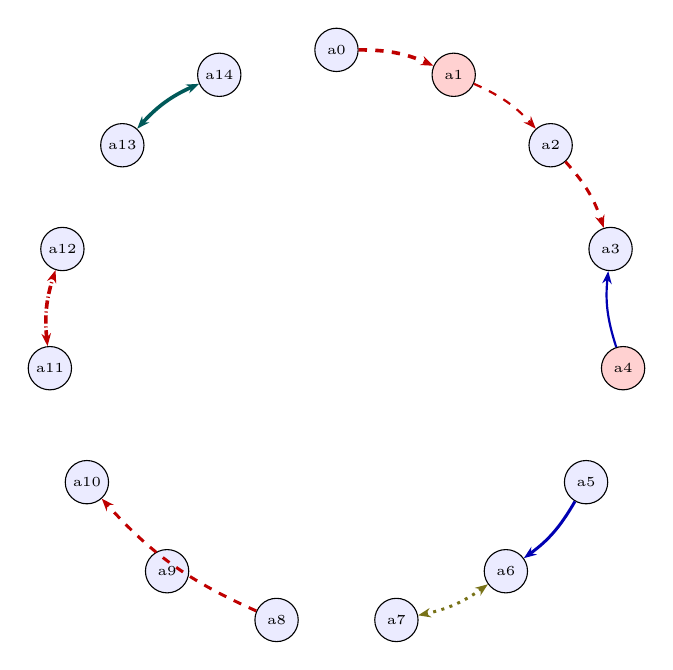
\begin{tikzpicture}[>={Stealth[length=1.6mm]}]
  \node[circle,draw,fill=blue!8,inner sep=1pt,minimum size=5.5mm,font=\tiny] (a0) at (90.0:3.66) {a0};
  \node[circle,draw,fill=red!18,inner sep=1pt,minimum size=5.5mm,font=\tiny] (a1) at (66.0:3.66) {a1};
  \node[circle,draw,fill=blue!8,inner sep=1pt,minimum size=5.5mm,font=\tiny] (a2) at (42.0:3.66) {a2};
  \node[circle,draw,fill=blue!8,inner sep=1pt,minimum size=5.5mm,font=\tiny] (a3) at (18.0:3.66) {a3};
  \node[circle,draw,fill=red!18,inner sep=1pt,minimum size=5.5mm,font=\tiny] (a4) at (-6.0:3.66) {a4};
  \node[circle,draw,fill=blue!8,inner sep=1pt,minimum size=5.5mm,font=\tiny] (a5) at (-30.0:3.66) {a5};
  \node[circle,draw,fill=blue!8,inner sep=1pt,minimum size=5.5mm,font=\tiny] (a6) at (-54.0:3.66) {a6};
  \node[circle,draw,fill=blue!8,inner sep=1pt,minimum size=5.5mm,font=\tiny] (a7) at (-78.0:3.66) {a7};
  \node[circle,draw,fill=blue!8,inner sep=1pt,minimum size=5.5mm,font=\tiny] (a8) at (-102.0:3.66) {a8};
  \node[circle,draw,fill=blue!8,inner sep=1pt,minimum size=5.5mm,font=\tiny] (a9) at (-126.0:3.66) {a9};
  \node[circle,draw,fill=blue!8,inner sep=1pt,minimum size=5.5mm,font=\tiny] (a10) at (-150.0:3.66) {a10};
  \node[circle,draw,fill=blue!8,inner sep=1pt,minimum size=5.5mm,font=\tiny] (a11) at (-174.0:3.66) {a11};
  \node[circle,draw,fill=blue!8,inner sep=1pt,minimum size=5.5mm,font=\tiny] (a12) at (-198.0:3.66) {a12};
  \node[circle,draw,fill=blue!8,inner sep=1pt,minimum size=5.5mm,font=\tiny] (a13) at (-222.0:3.66) {a13};
  \node[circle,draw,fill=blue!8,inner sep=1pt,minimum size=5.5mm,font=\tiny] (a14) at (-246.0:3.66) {a14};
  \draw[-{Stealth[length=1.6mm]}, red!75!black, dashed, line width=1.31pt] (a0) to[bend left=12] (a1);
  \draw[-{Stealth[length=1.6mm]}, red!75!black, dashed, line width=0.79pt] (a1) to[bend left=12] (a2);
  \draw[-{Stealth[length=1.6mm]}, red!75!black, dashed, line width=1.08pt] (a2) to[bend left=12] (a3);
  \draw[-{Stealth[length=1.6mm]}, blue!70!black, line width=0.79pt] (a4) to[bend left=12] (a3);
  \draw[-{Stealth[length=1.6mm]}, blue!70!black, line width=1.08pt] (a5) to[bend left=12] (a6);
  \draw[{Stealth[length=1.6mm]}-{Stealth[length=1.6mm]}, olive!80!black, dotted, line width=1.08pt] (a6) to[bend left=12] (a7);
  \draw[-{Stealth[length=1.6mm]}, red!75!black, dashed, line width=1.08pt] (a8) to[bend left=12] (a10);
  \draw[{Stealth[length=1.6mm]}-{Stealth[length=1.6mm]}, red!75!black, densely dashdotted, line width=1.31pt] (a11) to[bend left=12] (a12);
  \draw[{Stealth[length=1.6mm]}-{Stealth[length=1.6mm]}, teal!70!black, line width=1.31pt] (a13) to[bend left=12] (a14);
\end{tikzpicture}
}
\\[2pt]{\footnotesize all gold edges: 9 factors}
\end{minipage}\hfill\begin{minipage}[t]{0.48\linewidth}\centering
\resizebox{!}{6.4cm}{%
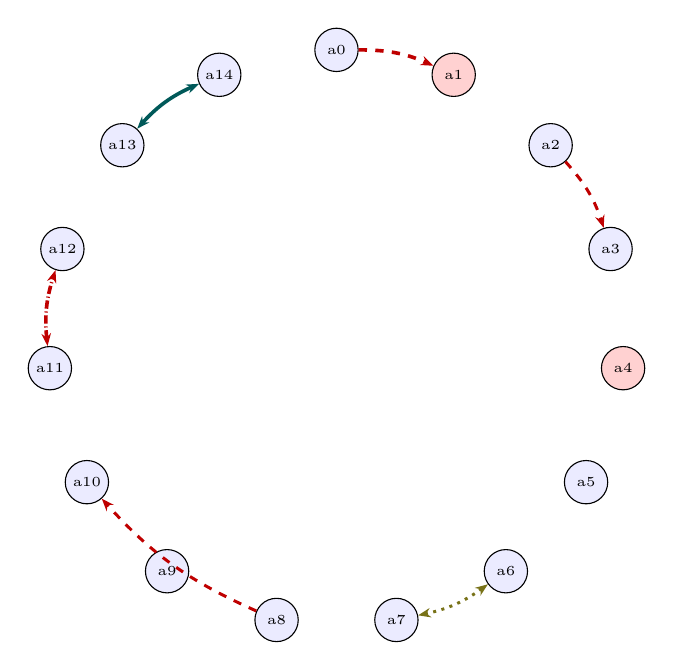
\begin{tikzpicture}[>={Stealth[length=1.6mm]}]
  \node[circle,draw,fill=blue!8,inner sep=1pt,minimum size=5.5mm,font=\tiny] (a0) at (90.0:3.66) {a0};
  \node[circle,draw,fill=red!18,inner sep=1pt,minimum size=5.5mm,font=\tiny] (a1) at (66.0:3.66) {a1};
  \node[circle,draw,fill=blue!8,inner sep=1pt,minimum size=5.5mm,font=\tiny] (a2) at (42.0:3.66) {a2};
  \node[circle,draw,fill=blue!8,inner sep=1pt,minimum size=5.5mm,font=\tiny] (a3) at (18.0:3.66) {a3};
  \node[circle,draw,fill=red!18,inner sep=1pt,minimum size=5.5mm,font=\tiny] (a4) at (-6.0:3.66) {a4};
  \node[circle,draw,fill=blue!8,inner sep=1pt,minimum size=5.5mm,font=\tiny] (a5) at (-30.0:3.66) {a5};
  \node[circle,draw,fill=blue!8,inner sep=1pt,minimum size=5.5mm,font=\tiny] (a6) at (-54.0:3.66) {a6};
  \node[circle,draw,fill=blue!8,inner sep=1pt,minimum size=5.5mm,font=\tiny] (a7) at (-78.0:3.66) {a7};
  \node[circle,draw,fill=blue!8,inner sep=1pt,minimum size=5.5mm,font=\tiny] (a8) at (-102.0:3.66) {a8};
  \node[circle,draw,fill=blue!8,inner sep=1pt,minimum size=5.5mm,font=\tiny] (a9) at (-126.0:3.66) {a9};
  \node[circle,draw,fill=blue!8,inner sep=1pt,minimum size=5.5mm,font=\tiny] (a10) at (-150.0:3.66) {a10};
  \node[circle,draw,fill=blue!8,inner sep=1pt,minimum size=5.5mm,font=\tiny] (a11) at (-174.0:3.66) {a11};
  \node[circle,draw,fill=blue!8,inner sep=1pt,minimum size=5.5mm,font=\tiny] (a12) at (-198.0:3.66) {a12};
  \node[circle,draw,fill=blue!8,inner sep=1pt,minimum size=5.5mm,font=\tiny] (a13) at (-222.0:3.66) {a13};
  \node[circle,draw,fill=blue!8,inner sep=1pt,minimum size=5.5mm,font=\tiny] (a14) at (-246.0:3.66) {a14};
  \draw[-{Stealth[length=1.6mm]}, red!75!black, dashed, line width=1.31pt] (a0) to[bend left=12] (a1);
  \draw[-{Stealth[length=1.6mm]}, red!75!black, dashed, line width=1.08pt] (a2) to[bend left=12] (a3);
  \draw[{Stealth[length=1.6mm]}-{Stealth[length=1.6mm]}, olive!80!black, dotted, line width=1.08pt] (a6) to[bend left=12] (a7);
  \draw[-{Stealth[length=1.6mm]}, red!75!black, dashed, line width=1.08pt] (a8) to[bend left=12] (a10);
  \draw[{Stealth[length=1.6mm]}-{Stealth[length=1.6mm]}, red!75!black, densely dashdotted, line width=1.31pt] (a11) to[bend left=12] (a12);
  \draw[{Stealth[length=1.6mm]}-{Stealth[length=1.6mm]}, teal!70!black, line width=1.31pt] (a13) to[bend left=12] (a14);
\end{tikzpicture}
}
\\[2pt]{\footnotesize valid edges only: 6 factors}
\end{minipage}
\caption{Relation graph for \texttt{locobench-opus-5-5-f022-r1}. Nodes are atoms on a circle, tinted red when the item marks them non-factual (prior 0.1) and blue when factual (prior 0.9). Edges are gold relations: solid blue = entailment, dashed red = contradiction, double-headed teal = equivalence, dash-dotted red (double-headed) = exclusive (exactly-one), dotted olive (double-headed) = co-necessity (at-least-one); thickness scales with the factor probability. Ordering-only Precedence edges carry no factor and so are not drawn.}
\label{fig:graph-locobench-opus-5-5-f022-r1}
\end{figure}

\begin{table}[htbp]
\centering
\footnotesize
\setlength{\tabcolsep}{3.5pt}
\caption{The specific gold relations of \texttt{locobench-opus-5-5-f022-r1}. \textbf{$p$ used} is the factor probability the MRF received: the band midpoint, times $(1-\lambda)$ for a resolved concession, or \emph{none} for an ordering-only edge (no factor). \textbf{Valid} marks the deliberately-planted errors with their kind. \textbf{Res.} is the resolving atom of a resolved concession.}
\label{tab:rels-locobench-opus-5-5-f022-r1}
\begin{tabular}{lllllrll}
\toprule
ID & Endpoints & Sense & Coupling & Band & $p$ used & Valid & Res. \\
\midrule
\texttt{r000} & \texttt{a0} $\leftrightarrow$ \texttt{a1} & Contrast & \texttt{contradiction} & strong & 0.925 & \checkmark &  \\
\texttt{r001} & \texttt{a1} $\leftrightarrow$ \texttt{a2} & Contrast & \texttt{contradiction} & weak & 0.470 & $\times$ {\scriptsize spurious} &  \\
\texttt{r002} & \texttt{a2} $\leftrightarrow$ \texttt{a3} & Contrast & \texttt{contradiction} & moderate & 0.720 & \checkmark &  \\
\texttt{r003} & \texttt{a4} $\to$ \texttt{a3} & Evidence & \texttt{entailment} & weak & 0.470 & $\times$ {\scriptsize false\_endpoint} &  \\
\texttt{r004} & \texttt{a5} $\to$ \texttt{a6} & Cause-Effect & \texttt{entailment} & moderate & 0.720 & $\times$ {\scriptsize wrong\_direction} &  \\
\texttt{r005} & \texttt{a6} $\leftrightarrow$ \texttt{a7} & Disjunction & \texttt{co\_necessity} & moderate & 0.720 & \checkmark &  \\
\texttt{r006} & \texttt{a8} $\to$ \texttt{a9} & Precedence & \texttt{none} & weak & \emph{none} & $\times$ {\scriptsize wrong\_sense} &  \\
\texttt{r007} & \texttt{a8} $\to$ \texttt{a10} & Concession & \texttt{contradiction} & moderate & 0.720 & \checkmark &  \\
\texttt{r008} & \texttt{a11} $\leftrightarrow$ \texttt{a12} & Alternative & \texttt{exclusive} & strong & 0.925 & \checkmark &  \\
\texttt{r009} & \texttt{a13} $\leftrightarrow$ \texttt{a14} & Restatement & \texttt{equivalence} & strong & 0.925 & \checkmark &  \\
\bottomrule
\end{tabular}
\end{table}

\begin{table}[htbp]
\centering
\footnotesize
\caption{Atoms of \texttt{locobench-opus-5-5-f022-r1}: the \texttt{factual} label, the prior it maps to, the posterior marginal $P(a_i{=}1)$ the MRF returns, and the shift. Atoms dragged below their prior are the ones the coherence structure penalises.}
\label{tab:atoms-locobench-opus-5-5-f022-r1}
\begin{tabular}{llrrrp{7.2cm}}
\toprule
Atom & fact & $\pi_i$ & $P(a_i{=}1)$ & $\Delta$ & Text \\
\midrule
\texttt{a0} & \checkmark & 0.90 & 0.938 & +0.038 & \footnotesize Colin Renfrew proposed the Anatolian farming hypothesis in his 1987 book "Archaeology and Language." \\
\texttt{a1} & $\times$ & 0.10 & 0.015 & -0.085 & \footnotesize Renfrew first proposed the Anatolian hypothesis in a book published in 1997. \\
\texttt{a2} & \checkmark & 0.90 & 0.854 & -0.046 & \footnotesize The Anatolian hypothesis links the spread of Indo-European languages to the expansion of agriculture out of Anatolia roughly 8,000 to 9,500 years ago. \\
\texttt{a3} & \checkmark & 0.90 & 0.794 & -0.106 & \footnotesize The steppe hypothesis places the Proto-Indo-European homeland in the Pontic-Caspian steppe north of the Black and Caspian Seas. \\
\texttt{a4} & $\times$ & 0.10 & 0.097 & -0.003 & \footnotesize Gimbutas located the Proto-Indo-European homeland in the Indus Valley. \\
\texttt{a5} & \checkmark & 0.90 & 0.925 & +0.025 & \footnotesize Reconstructed Proto-Indo-European vocabulary includes a word for "wheel," *kʷékʷlos. \\
\texttt{a6} & \checkmark & 0.90 & 0.968 & +0.068 & \footnotesize The shared wheel vocabulary in the Indo-European daughter languages was inherited from Proto-Indo-European. \\
\texttt{a7} & \checkmark & 0.90 & 0.929 & +0.029 & \footnotesize The shared wheel vocabulary spread among the Indo-European daughter languages through borrowing after they separated. \\
\texttt{a8} & \checkmark & 0.90 & 0.854 & -0.046 & \footnotesize Bouckaert and colleagues published a Bayesian phylogeographic study in Science in 2012 that favored an Anatolian origin. \\
\texttt{a9} & \checkmark & 0.90 & 0.900 & +0.000 & \footnotesize Chang and colleagues published a 2015 study in the journal Language that used ancestry-constrained phylogenetic analysis. \\
\texttt{a10} & \checkmark & 0.90 & 0.796 & -0.104 & \footnotesize Chang and colleagues determined that ancestry-constrained phylogenies favor a steppe origin over an Anatolian origin for Proto-Indo-European. \\
\texttt{a11} & \checkmark & 0.90 & 0.632 & -0.268 & \footnotesize Ancient individuals from Hittite-era Anatolian sites carry substantial Yamnaya-related steppe ancestry. \\
\texttt{a12} & \checkmark & 0.90 & 0.632 & -0.268 & \footnotesize Ancient individuals from Hittite-era Anatolian sites lack substantial Yamnaya-related steppe ancestry. \\
\texttt{a13} & \checkmark & 0.90 & 0.979 & +0.079 & \footnotesize The Corded Ware people descended largely from Yamnaya-related populations. \\
\texttt{a14} & \checkmark & 0.90 & 0.979 & +0.079 & \footnotesize Most of the ancestry of Corded Ware individuals came from steppe populations related to the Yamnaya. \\
\bottomrule
\end{tabular}
\end{table}

\subsection{Literature -- direction\_reversal\_a (\texttt{locobench-opus-5-5-f023-r1})}

\textbf{Topic:} Literature (Humanities). \textbf{Family:} \texttt{f023} (CONTROL), rung 1 (\emph{direction\_reversal\_a}). \textbf{Scores:} mean-marg $= 0.789$, consist $= 0.493$, reified $= 0.225$, log-Z $= 0.321$.



\paragraph{Framing question.} \emph{How did statistical stylometry settle the long-running dispute over whether Alexander Hamilton or James Madison wrote the twelve contested Federalist Papers?}



\paragraph{Response.} {\small Between 1787 and 1788, New York newspapers carried a sustained series of essays urging ratification of the proposed Constitution. The Federalist Papers consist of 85 essays published under the pseudonym "Publius." That shared signature hid a collaboration whose members were known to contemporaries, even if the assignment of individual essays was not: Alexander Hamilton, James Madison, and John Jay wrote the Federalist Papers. The three did not contribute equally. By contrast with the shared authorship of the series as a whole, John Jay wrote twenty of the Federalist essays, a share that has never been seriously contested. The difficulty that occupied historians for a century and a half lay elsewhere, in a block of twelve essays that either Hamilton or Madison could plausibly have written.

The dispute began with the authors' own testimony. Hamilton left a list of authorship attributions shortly before his 1804 duel with Aaron Burr, and Madison, at a later date, claimed authorship of essays that Hamilton's list had attributed to Hamilton. Neither witness could be dismissed, yet the two accounts conflicted, so at least one of the following must hold, perhaps both: Hamilton's authorship list contained errors about the disputed essays, or Madison's authorship claims about the disputed essays contained errors. Partisan loyalty and impressions of style could not break the deadlock, because each side could cite passages that sounded characteristic of its preferred author. By contrast, Frederick Mosteller and David Wallace conducted the landmark statistical study of the disputed papers, replacing contested memory with measurement.

Their method is frequently misdescribed. Although Mosteller and Wallace relied primarily on sentence length to attribute the disputed papers, they focused on the frequencies of common function words. These are the prepositions, conjunctions, and particles that writers use habitually and almost without thought. Because such words carry little topical content, their rates remain stable across subjects, and because they are used unconsciously, they resist deliberate imitation. One word served as an especially sharp discriminator; for example, Hamilton used the word "upon" far more often than Madison did. That observation is simply a restatement of a more basic fact: Madison used the word "upon" much less frequently than Hamilton did, so a disputed essay in which "upon" appears rarely or not at all looks far more Madisonian than Hamiltonian. A single word cannot decide a case by itself, but a collection of words with stable and divergent rates can, provided their evidence is combined in a principled way.

That combination required an explicit statistical framework, and here the study's design has been described in two incompatible ways. Either the Mosteller–Wallace analysis used Bayesian inference, or the Mosteller–Wallace analysis did not use Bayesian inference; the two descriptions cannot both be true, and one of them must hold. In the Bayesian reading, prior odds between the two candidates are updated by likelihoods drawn from models of word frequency, yielding posterior odds of authorship for each paper. The rarity of "upon" in the contested texts indicates the result that ended the controversy: Mosteller and Wallace concluded that Madison wrote all twelve disputed Federalist Papers. That conclusion settles the apparent tension in how their method has been described, since a verdict assigning every one of the twelve essays to Madison could rest only on discriminating word rates, which sentence length cannot supply. The conclusion was also what led to the Bayesian framing of the study, because a verdict that strong demanded posterior odds capable of expressing it for each paper. The result coincided with Madison's later claims, and in the decades since it has served as a standard demonstration of how quantitative stylometry can resolve a question that documentary testimony had left open.}

\begin{figure}[htbp]
\centering
\begin{minipage}[t]{0.48\linewidth}\centering
\resizebox{!}{6.4cm}{%
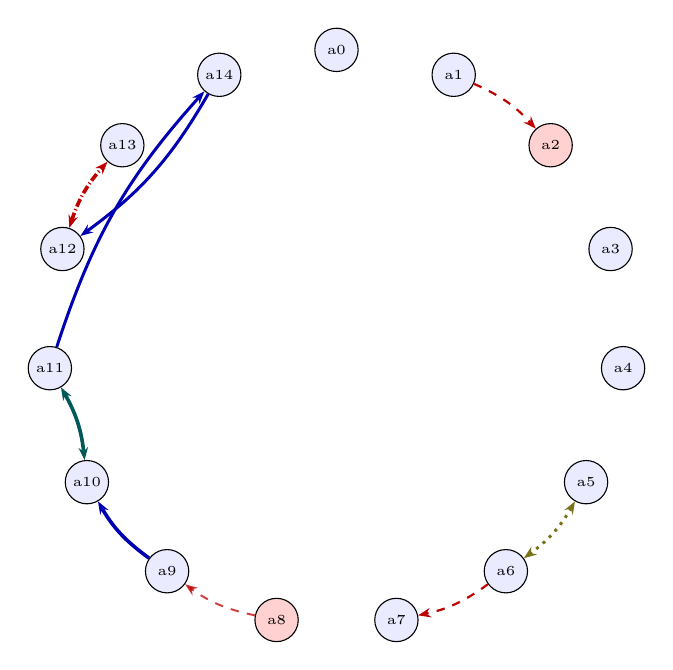
\begin{tikzpicture}[>={Stealth[length=1.6mm]}]
  \node[circle,draw,fill=blue!8,inner sep=1pt,minimum size=5.5mm,font=\tiny] (a0) at (90.0:3.66) {a0};
  \node[circle,draw,fill=blue!8,inner sep=1pt,minimum size=5.5mm,font=\tiny] (a1) at (66.0:3.66) {a1};
  \node[circle,draw,fill=red!18,inner sep=1pt,minimum size=5.5mm,font=\tiny] (a2) at (42.0:3.66) {a2};
  \node[circle,draw,fill=blue!8,inner sep=1pt,minimum size=5.5mm,font=\tiny] (a3) at (18.0:3.66) {a3};
  \node[circle,draw,fill=blue!8,inner sep=1pt,minimum size=5.5mm,font=\tiny] (a4) at (-6.0:3.66) {a4};
  \node[circle,draw,fill=blue!8,inner sep=1pt,minimum size=5.5mm,font=\tiny] (a5) at (-30.0:3.66) {a5};
  \node[circle,draw,fill=blue!8,inner sep=1pt,minimum size=5.5mm,font=\tiny] (a6) at (-54.0:3.66) {a6};
  \node[circle,draw,fill=blue!8,inner sep=1pt,minimum size=5.5mm,font=\tiny] (a7) at (-78.0:3.66) {a7};
  \node[circle,draw,fill=red!18,inner sep=1pt,minimum size=5.5mm,font=\tiny] (a8) at (-102.0:3.66) {a8};
  \node[circle,draw,fill=blue!8,inner sep=1pt,minimum size=5.5mm,font=\tiny] (a9) at (-126.0:3.66) {a9};
  \node[circle,draw,fill=blue!8,inner sep=1pt,minimum size=5.5mm,font=\tiny] (a10) at (-150.0:3.66) {a10};
  \node[circle,draw,fill=blue!8,inner sep=1pt,minimum size=5.5mm,font=\tiny] (a11) at (-174.0:3.66) {a11};
  \node[circle,draw,fill=blue!8,inner sep=1pt,minimum size=5.5mm,font=\tiny] (a12) at (-198.0:3.66) {a12};
  \node[circle,draw,fill=blue!8,inner sep=1pt,minimum size=5.5mm,font=\tiny] (a13) at (-222.0:3.66) {a13};
  \node[circle,draw,fill=blue!8,inner sep=1pt,minimum size=5.5mm,font=\tiny] (a14) at (-246.0:3.66) {a14};
  \draw[{Stealth[length=1.6mm]}-{Stealth[length=1.6mm]}, olive!80!black, dotted, line width=1.08pt] (a5) to[bend left=12] (a6);
  \draw[{Stealth[length=1.6mm]}-{Stealth[length=1.6mm]}, teal!70!black, line width=1.31pt] (a11) to[bend left=12] (a10);
  \draw[{Stealth[length=1.6mm]}-{Stealth[length=1.6mm]}, red!75!black, densely dashdotted, line width=1.31pt] (a12) to[bend left=12] (a13);
  \draw[-{Stealth[length=1.6mm]}, red!75!black, dashed, opacity=0.75, line width=0.71pt] (a8) to[bend left=12] (a9);
  \draw[-{Stealth[length=1.6mm]}, red!75!black, dashed, line width=0.79pt] (a1) to[bend left=12] (a2);
  \draw[-{Stealth[length=1.6mm]}, blue!70!black, line width=1.31pt] (a9) to[bend left=12] (a10);
  \draw[-{Stealth[length=1.6mm]}, blue!70!black, line width=1.08pt] (a11) to[bend left=12] (a14);
  \draw[-{Stealth[length=1.6mm]}, red!75!black, dashed, line width=0.79pt] (a6) to[bend left=12] (a7);
  \draw[-{Stealth[length=1.6mm]}, blue!70!black, line width=1.08pt] (a14) to[bend left=12] (a12);
\end{tikzpicture}
}
\\[2pt]{\footnotesize all gold edges: 9 factors}
\end{minipage}\hfill\begin{minipage}[t]{0.48\linewidth}\centering
\resizebox{!}{6.4cm}{%
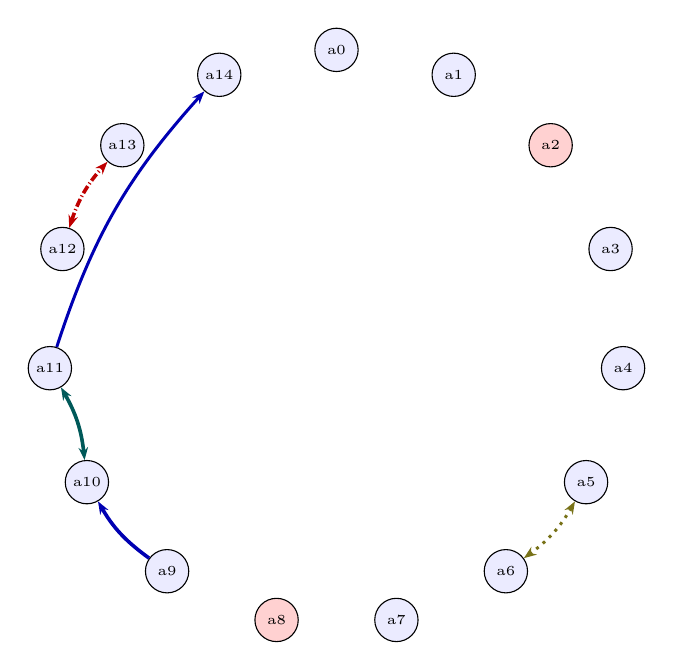
\begin{tikzpicture}[>={Stealth[length=1.6mm]}]
  \node[circle,draw,fill=blue!8,inner sep=1pt,minimum size=5.5mm,font=\tiny] (a0) at (90.0:3.66) {a0};
  \node[circle,draw,fill=blue!8,inner sep=1pt,minimum size=5.5mm,font=\tiny] (a1) at (66.0:3.66) {a1};
  \node[circle,draw,fill=red!18,inner sep=1pt,minimum size=5.5mm,font=\tiny] (a2) at (42.0:3.66) {a2};
  \node[circle,draw,fill=blue!8,inner sep=1pt,minimum size=5.5mm,font=\tiny] (a3) at (18.0:3.66) {a3};
  \node[circle,draw,fill=blue!8,inner sep=1pt,minimum size=5.5mm,font=\tiny] (a4) at (-6.0:3.66) {a4};
  \node[circle,draw,fill=blue!8,inner sep=1pt,minimum size=5.5mm,font=\tiny] (a5) at (-30.0:3.66) {a5};
  \node[circle,draw,fill=blue!8,inner sep=1pt,minimum size=5.5mm,font=\tiny] (a6) at (-54.0:3.66) {a6};
  \node[circle,draw,fill=blue!8,inner sep=1pt,minimum size=5.5mm,font=\tiny] (a7) at (-78.0:3.66) {a7};
  \node[circle,draw,fill=red!18,inner sep=1pt,minimum size=5.5mm,font=\tiny] (a8) at (-102.0:3.66) {a8};
  \node[circle,draw,fill=blue!8,inner sep=1pt,minimum size=5.5mm,font=\tiny] (a9) at (-126.0:3.66) {a9};
  \node[circle,draw,fill=blue!8,inner sep=1pt,minimum size=5.5mm,font=\tiny] (a10) at (-150.0:3.66) {a10};
  \node[circle,draw,fill=blue!8,inner sep=1pt,minimum size=5.5mm,font=\tiny] (a11) at (-174.0:3.66) {a11};
  \node[circle,draw,fill=blue!8,inner sep=1pt,minimum size=5.5mm,font=\tiny] (a12) at (-198.0:3.66) {a12};
  \node[circle,draw,fill=blue!8,inner sep=1pt,minimum size=5.5mm,font=\tiny] (a13) at (-222.0:3.66) {a13};
  \node[circle,draw,fill=blue!8,inner sep=1pt,minimum size=5.5mm,font=\tiny] (a14) at (-246.0:3.66) {a14};
  \draw[{Stealth[length=1.6mm]}-{Stealth[length=1.6mm]}, olive!80!black, dotted, line width=1.08pt] (a5) to[bend left=12] (a6);
  \draw[{Stealth[length=1.6mm]}-{Stealth[length=1.6mm]}, teal!70!black, line width=1.31pt] (a11) to[bend left=12] (a10);
  \draw[{Stealth[length=1.6mm]}-{Stealth[length=1.6mm]}, red!75!black, densely dashdotted, line width=1.31pt] (a12) to[bend left=12] (a13);
  \draw[-{Stealth[length=1.6mm]}, blue!70!black, line width=1.31pt] (a9) to[bend left=12] (a10);
  \draw[-{Stealth[length=1.6mm]}, blue!70!black, line width=1.08pt] (a11) to[bend left=12] (a14);
\end{tikzpicture}
}
\\[2pt]{\footnotesize valid edges only: 5 factors}
\end{minipage}
\caption{Relation graph for \texttt{locobench-opus-5-5-f023-r1}. Nodes are atoms on a circle, tinted red when the item marks them non-factual (prior 0.1) and blue when factual (prior 0.9). Edges are gold relations: solid blue = entailment, dashed red = contradiction, double-headed teal = equivalence, dash-dotted red (double-headed) = exclusive (exactly-one), dotted olive (double-headed) = co-necessity (at-least-one); thickness scales with the factor probability. Ordering-only Precedence edges carry no factor and so are not drawn.}
\label{fig:graph-locobench-opus-5-5-f023-r1}
\end{figure}

\begin{table}[htbp]
\centering
\footnotesize
\setlength{\tabcolsep}{3.5pt}
\caption{The specific gold relations of \texttt{locobench-opus-5-5-f023-r1}. \textbf{$p$ used} is the factor probability the MRF received: the band midpoint, times $(1-\lambda)$ for a resolved concession, or \emph{none} for an ordering-only edge (no factor). \textbf{Valid} marks the deliberately-planted errors with their kind. \textbf{Res.} is the resolving atom of a resolved concession.}
\label{tab:rels-locobench-opus-5-5-f023-r1}
\begin{tabular}{lllllrll}
\toprule
ID & Endpoints & Sense & Coupling & Band & $p$ used & Valid & Res. \\
\midrule
\texttt{r000} & \texttt{a3} $\to$ \texttt{a4} & Precedence & \texttt{none} & moderate & \emph{none} & \checkmark &  \\
\texttt{r001} & \texttt{a5} $\leftrightarrow$ \texttt{a6} & Disjunction & \texttt{co\_necessity} & moderate & 0.720 & \checkmark &  \\
\texttt{r002} & \texttt{a11} $\leftrightarrow$ \texttt{a10} & Restatement & \texttt{equivalence} & strong & 0.925 & \checkmark &  \\
\texttt{r003} & \texttt{a12} $\leftrightarrow$ \texttt{a13} & Alternative & \texttt{exclusive} & strong & 0.925 & \checkmark &  \\
\texttt{r004} & \texttt{a8} $\to$ \texttt{a9} & Concession & \texttt{contradiction} & moderate & 0.396 & $\times$ {\scriptsize false\_endpoint} & \texttt{a14} \\
\texttt{r005} & \texttt{a1} $\leftrightarrow$ \texttt{a2} & Contrast & \texttt{contradiction} & weak & 0.470 & $\times$ {\scriptsize false\_endpoint} &  \\
\texttt{r006} & \texttt{a9} $\to$ \texttt{a10} & Instantiation & \texttt{entailment} & strong & 0.925 & \checkmark &  \\
\texttt{r007} & \texttt{a11} $\to$ \texttt{a14} & Evidence & \texttt{entailment} & moderate & 0.720 & \checkmark &  \\
\texttt{r008} & \texttt{a6} $\leftrightarrow$ \texttt{a7} & Contrast & \texttt{contradiction} & weak & 0.470 & $\times$ {\scriptsize spurious} &  \\
\texttt{r009} & \texttt{a14} $\to$ \texttt{a12} & Cause-Effect & \texttt{entailment} & moderate & 0.720 & $\times$ {\scriptsize wrong\_direction} &  \\
\bottomrule
\end{tabular}
\end{table}

\begin{table}[htbp]
\centering
\footnotesize
\caption{Atoms of \texttt{locobench-opus-5-5-f023-r1}: the \texttt{factual} label, the prior it maps to, the posterior marginal $P(a_i{=}1)$ the MRF returns, and the shift. Atoms dragged below their prior are the ones the coherence structure penalises.}
\label{tab:atoms-locobench-opus-5-5-f023-r1}
\begin{tabular}{llrrrp{7.2cm}}
\toprule
Atom & fact & $\pi_i$ & $P(a_i{=}1)$ & $\Delta$ & Text \\
\midrule
\texttt{a0} & \checkmark & 0.90 & 0.900 & +0.000 & \footnotesize The Federalist Papers consist of 85 essays published under the pseudonym "Publius." \\
\texttt{a1} & \checkmark & 0.90 & 0.895 & -0.005 & \footnotesize Alexander Hamilton, James Madison, and John Jay wrote the Federalist Papers. \\
\texttt{a2} & $\times$ & 0.10 & 0.110 & +0.010 & \footnotesize John Jay wrote twenty of the Federalist essays. \\
\texttt{a3} & \checkmark & 0.90 & 0.900 & +0.000 & \footnotesize Hamilton left a list of authorship attributions shortly before his 1804 duel with Aaron Burr. \\
\texttt{a4} & \checkmark & 0.90 & 0.900 & +0.000 & \footnotesize Madison later claimed authorship of essays that Hamilton's list had attributed to Hamilton. \\
\texttt{a5} & \checkmark & 0.90 & 0.929 & +0.029 & \footnotesize Hamilton's authorship list contained errors about the disputed essays. \\
\texttt{a6} & \checkmark & 0.90 & 0.932 & +0.032 & \footnotesize Madison's authorship claims about the disputed essays contained errors. \\
\texttt{a7} & \checkmark & 0.90 & 0.910 & +0.010 & \footnotesize Frederick Mosteller and David Wallace conducted the landmark statistical study of the disputed papers. \\
\texttt{a8} & $\times$ & 0.10 & 0.116 & +0.016 & \footnotesize Mosteller and Wallace relied primarily on sentence length to attribute the disputed papers. \\
\texttt{a9} & \checkmark & 0.90 & 0.945 & +0.045 & \footnotesize Mosteller and Wallace focused on the frequencies of common function words. \\
\texttt{a10} & \checkmark & 0.90 & 0.998 & +0.098 & \footnotesize Hamilton used the word "upon" far more often than Madison did. \\
\texttt{a11} & \checkmark & 0.90 & 0.992 & +0.092 & \footnotesize Madison used the word "upon" much less frequently than Hamilton did. \\
\texttt{a12} & \checkmark & 0.90 & 0.808 & -0.092 & \footnotesize The Mosteller–Wallace analysis used Bayesian inference. \\
\texttt{a13} & \checkmark & 0.90 & 0.531 & -0.369 & \footnotesize The Mosteller–Wallace analysis did not use Bayesian inference. \\
\texttt{a14} & \checkmark & 0.90 & 0.962 & +0.062 & \footnotesize Mosteller and Wallace concluded that Madison wrote all twelve disputed Federalist Papers. \\
\bottomrule
\end{tabular}
\end{table}

\subsection{Mechanical Engineering -- shuffle\_block (\texttt{locobench-opus-5-5-f024-r1})}

\textbf{Topic:} Mechanical Engineering (Engineering \& Technology). \textbf{Family:} \texttt{f024} (ORDER), rung 1 (\emph{shuffle\_block}). \textbf{Scores:} mean-marg $= 0.762$, consist $= 0.369$, reified $= 0.061$, log-Z $= 0.361$.



\paragraph{Framing question.} \emph{How do failure analysts determine whether a fractured industrial drive shaft failed through progressive fatigue or a single overload event when the maintenance contractor blames a manufacturing defect while the manufacturer blames improper installation?}



\paragraph{Response.} {\small The first diagnostic question is binary. Either the shaft's fracture surface contains a fatigue crack initiation zone, or, as the preservation of the unabraded mating surfaces indicates, it contains no fatigue crack initiation zone; the two conditions cannot both be true, and one of them must hold. Low-magnification stereomicroscopy under oblique lighting is the usual means of making that determination, since it reveals the relief of the surface without altering it. An initiation zone, where one exists, causes the beach marks that radiate from it, so that beach marks on a fracture surface indicate progressive crack growth over multiple loading cycles. Those concentric arrest lines, which record changes in load amplitude or interruptions in operation, in turn confirm that fatigue striations on steel shafts are routinely visible to the naked eye. The analyst then maps the relative areas of the smooth propagation region and the rough final-fracture region, because their proportion reflects the nominal stress the shaft carried when it finally separated.

Distinguishing progressive fatigue from a single overload event is fundamentally a problem of reading the fracture surface before the evidence it carries is degraded, and then relating the observed morphology to the loading history and the geometry of the component. A liability dispute sharpens that discipline, because each party's account predicts a different fracture signature, and the analyst's task is to determine which signature the metal actually records. The case at issue is concrete: the drive shaft fractured while in service at a paper mill.

Geometry localizes the origin and connects it to design and assembly. The fatigue crack originated at the root of the keyway; that is, the crack initiation site was located at the bottom corner of the keyway, where a sharp radius concentrates both bending and torsional stresses. Overload morphology supplies the reference against which this origin is judged. Ductile torsional overload fractures in shafts typically occur on a plane at 45 degrees to the shaft axis, whereas the final failure analysis report concluded that the shaft failed by progressive fatigue rather than a single overload event. That conclusion rested on the combined weight of the fractographic features, the location of the origin at a stress concentration, and the comparatively small area of final fast fracture.

Responsibility was contested from the outset. The maintenance contractor argued that the fracture was caused by a manufacturing defect in the shaft, whereas the manufacturer argued that the fracture was caused by improper installation of the shaft. Neither position can be settled by advocacy; each must be tested against physical evidence, and the value of that evidence depends entirely on how it is handled. Some time after that in-service fracture, failure analysts preserved the mating fracture surfaces without cleaning them with abrasives. Grit blasting, wire brushing, or fitting the two halves back together would have smeared the fine topography on which every subsequent inference rests, so protective coating, dry storage, and documented chain of custody were the first technical steps of the investigation.

Establishing the mechanism does not by itself allocate fault, because fatigue requires both a local stress raiser and a sustained cyclic driving stress, and the parties' accounts map onto those two requirements. Metallographic sectioning addresses the material, while dial-indicator or laser alignment surveys of the drive train address the assembly. At least one of the following held, perhaps both: the shaft steel contained a subsurface inclusion near the keyway, or the shaft was installed out of alignment with the driven coupling. Misalignment imposes a reversing bending moment on every revolution, which is precisely the cyclic loading that drives a crack forward from a keyway root, while an inclusion acts as a potential nucleation site that lowers the stress needed to start one. Despite that inclusion, the arbitration panel ruled that improper installation, not a manufacturing defect, caused the shaft fracture. In practice, therefore, the analyst's contribution is to fix the mechanism and its origin with defensible evidence, and to quantify each contributing condition, leaving the weighing of responsibility to the forum charged with deciding it.}

\begin{figure}[htbp]
\centering
\begin{minipage}[t]{0.48\linewidth}\centering
\resizebox{!}{6.4cm}{%
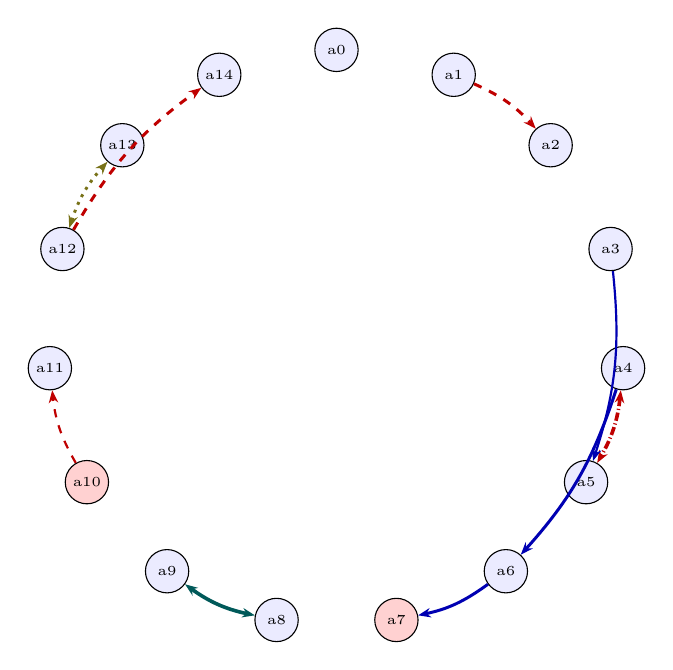
\begin{tikzpicture}[>={Stealth[length=1.6mm]}]
  \node[circle,draw,fill=blue!8,inner sep=1pt,minimum size=5.5mm,font=\tiny] (a0) at (90.0:3.66) {a0};
  \node[circle,draw,fill=blue!8,inner sep=1pt,minimum size=5.5mm,font=\tiny] (a1) at (66.0:3.66) {a1};
  \node[circle,draw,fill=blue!8,inner sep=1pt,minimum size=5.5mm,font=\tiny] (a2) at (42.0:3.66) {a2};
  \node[circle,draw,fill=blue!8,inner sep=1pt,minimum size=5.5mm,font=\tiny] (a3) at (18.0:3.66) {a3};
  \node[circle,draw,fill=blue!8,inner sep=1pt,minimum size=5.5mm,font=\tiny] (a4) at (-6.0:3.66) {a4};
  \node[circle,draw,fill=blue!8,inner sep=1pt,minimum size=5.5mm,font=\tiny] (a5) at (-30.0:3.66) {a5};
  \node[circle,draw,fill=blue!8,inner sep=1pt,minimum size=5.5mm,font=\tiny] (a6) at (-54.0:3.66) {a6};
  \node[circle,draw,fill=red!18,inner sep=1pt,minimum size=5.5mm,font=\tiny] (a7) at (-78.0:3.66) {a7};
  \node[circle,draw,fill=blue!8,inner sep=1pt,minimum size=5.5mm,font=\tiny] (a8) at (-102.0:3.66) {a8};
  \node[circle,draw,fill=blue!8,inner sep=1pt,minimum size=5.5mm,font=\tiny] (a9) at (-126.0:3.66) {a9};
  \node[circle,draw,fill=red!18,inner sep=1pt,minimum size=5.5mm,font=\tiny] (a10) at (-150.0:3.66) {a10};
  \node[circle,draw,fill=blue!8,inner sep=1pt,minimum size=5.5mm,font=\tiny] (a11) at (-174.0:3.66) {a11};
  \node[circle,draw,fill=blue!8,inner sep=1pt,minimum size=5.5mm,font=\tiny] (a12) at (-198.0:3.66) {a12};
  \node[circle,draw,fill=blue!8,inner sep=1pt,minimum size=5.5mm,font=\tiny] (a13) at (-222.0:3.66) {a13};
  \node[circle,draw,fill=blue!8,inner sep=1pt,minimum size=5.5mm,font=\tiny] (a14) at (-246.0:3.66) {a14};
  \draw[{Stealth[length=1.6mm]}-{Stealth[length=1.6mm]}, red!75!black, densely dashdotted, line width=1.31pt] (a4) to[bend left=12] (a5);
  \draw[{Stealth[length=1.6mm]}-{Stealth[length=1.6mm]}, teal!70!black, line width=1.31pt] (a8) to[bend left=12] (a9);
  \draw[{Stealth[length=1.6mm]}-{Stealth[length=1.6mm]}, olive!80!black, dotted, line width=1.08pt] (a12) to[bend left=12] (a13);
  \draw[-{Stealth[length=1.6mm]}, red!75!black, dashed, line width=1.08pt] (a1) to[bend left=12] (a2);
  \draw[-{Stealth[length=1.6mm]}, red!75!black, dashed, line width=1.08pt] (a12) to[bend left=12] (a14);
  \draw[-{Stealth[length=1.6mm]}, blue!70!black, line width=1.08pt] (a6) to[bend left=12] (a7);
  \draw[-{Stealth[length=1.6mm]}, red!75!black, dashed, line width=0.79pt] (a10) to[bend left=12] (a11);
  \draw[-{Stealth[length=1.6mm]}, blue!70!black, line width=1.08pt] (a4) to[bend left=12] (a6);
  \draw[-{Stealth[length=1.6mm]}, blue!70!black, line width=0.79pt] (a3) to[bend left=12] (a5);
\end{tikzpicture}
}
\\[2pt]{\footnotesize all gold edges: 9 factors}
\end{minipage}\hfill\begin{minipage}[t]{0.48\linewidth}\centering
\resizebox{!}{6.4cm}{%
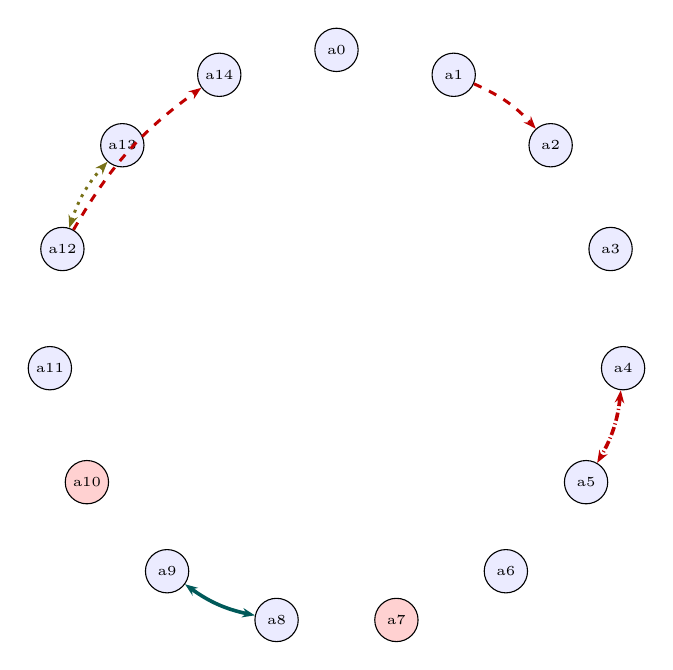
\begin{tikzpicture}[>={Stealth[length=1.6mm]}]
  \node[circle,draw,fill=blue!8,inner sep=1pt,minimum size=5.5mm,font=\tiny] (a0) at (90.0:3.66) {a0};
  \node[circle,draw,fill=blue!8,inner sep=1pt,minimum size=5.5mm,font=\tiny] (a1) at (66.0:3.66) {a1};
  \node[circle,draw,fill=blue!8,inner sep=1pt,minimum size=5.5mm,font=\tiny] (a2) at (42.0:3.66) {a2};
  \node[circle,draw,fill=blue!8,inner sep=1pt,minimum size=5.5mm,font=\tiny] (a3) at (18.0:3.66) {a3};
  \node[circle,draw,fill=blue!8,inner sep=1pt,minimum size=5.5mm,font=\tiny] (a4) at (-6.0:3.66) {a4};
  \node[circle,draw,fill=blue!8,inner sep=1pt,minimum size=5.5mm,font=\tiny] (a5) at (-30.0:3.66) {a5};
  \node[circle,draw,fill=blue!8,inner sep=1pt,minimum size=5.5mm,font=\tiny] (a6) at (-54.0:3.66) {a6};
  \node[circle,draw,fill=red!18,inner sep=1pt,minimum size=5.5mm,font=\tiny] (a7) at (-78.0:3.66) {a7};
  \node[circle,draw,fill=blue!8,inner sep=1pt,minimum size=5.5mm,font=\tiny] (a8) at (-102.0:3.66) {a8};
  \node[circle,draw,fill=blue!8,inner sep=1pt,minimum size=5.5mm,font=\tiny] (a9) at (-126.0:3.66) {a9};
  \node[circle,draw,fill=red!18,inner sep=1pt,minimum size=5.5mm,font=\tiny] (a10) at (-150.0:3.66) {a10};
  \node[circle,draw,fill=blue!8,inner sep=1pt,minimum size=5.5mm,font=\tiny] (a11) at (-174.0:3.66) {a11};
  \node[circle,draw,fill=blue!8,inner sep=1pt,minimum size=5.5mm,font=\tiny] (a12) at (-198.0:3.66) {a12};
  \node[circle,draw,fill=blue!8,inner sep=1pt,minimum size=5.5mm,font=\tiny] (a13) at (-222.0:3.66) {a13};
  \node[circle,draw,fill=blue!8,inner sep=1pt,minimum size=5.5mm,font=\tiny] (a14) at (-246.0:3.66) {a14};
  \draw[{Stealth[length=1.6mm]}-{Stealth[length=1.6mm]}, red!75!black, densely dashdotted, line width=1.31pt] (a4) to[bend left=12] (a5);
  \draw[{Stealth[length=1.6mm]}-{Stealth[length=1.6mm]}, teal!70!black, line width=1.31pt] (a8) to[bend left=12] (a9);
  \draw[{Stealth[length=1.6mm]}-{Stealth[length=1.6mm]}, olive!80!black, dotted, line width=1.08pt] (a12) to[bend left=12] (a13);
  \draw[-{Stealth[length=1.6mm]}, red!75!black, dashed, line width=1.08pt] (a1) to[bend left=12] (a2);
  \draw[-{Stealth[length=1.6mm]}, red!75!black, dashed, line width=1.08pt] (a12) to[bend left=12] (a14);
\end{tikzpicture}
}
\\[2pt]{\footnotesize valid edges only: 5 factors}
\end{minipage}
\caption{Relation graph for \texttt{locobench-opus-5-5-f024-r1}. Nodes are atoms on a circle, tinted red when the item marks them non-factual (prior 0.1) and blue when factual (prior 0.9). Edges are gold relations: solid blue = entailment, dashed red = contradiction, double-headed teal = equivalence, dash-dotted red (double-headed) = exclusive (exactly-one), dotted olive (double-headed) = co-necessity (at-least-one); thickness scales with the factor probability. Ordering-only Precedence edges carry no factor and so are not drawn.}
\label{fig:graph-locobench-opus-5-5-f024-r1}
\end{figure}

\begin{table}[htbp]
\centering
\footnotesize
\setlength{\tabcolsep}{3.5pt}
\caption{The specific gold relations of \texttt{locobench-opus-5-5-f024-r1}. \textbf{$p$ used} is the factor probability the MRF received: the band midpoint, times $(1-\lambda)$ for a resolved concession, or \emph{none} for an ordering-only edge (no factor). \textbf{Valid} marks the deliberately-planted errors with their kind. \textbf{Res.} is the resolving atom of a resolved concession.}
\label{tab:rels-locobench-opus-5-5-f024-r1}
\begin{tabular}{lllllrll}
\toprule
ID & Endpoints & Sense & Coupling & Band & $p$ used & Valid & Res. \\
\midrule
\texttt{r000} & \texttt{a0} $\to$ \texttt{a3} & Precedence & \texttt{none} & moderate & \emph{none} & \checkmark &  \\
\texttt{r001} & \texttt{a4} $\leftrightarrow$ \texttt{a5} & Alternative & \texttt{exclusive} & strong & 0.925 & \checkmark &  \\
\texttt{r002} & \texttt{a8} $\leftrightarrow$ \texttt{a9} & Restatement & \texttt{equivalence} & strong & 0.925 & \checkmark &  \\
\texttt{r003} & \texttt{a12} $\leftrightarrow$ \texttt{a13} & Disjunction & \texttt{co\_necessity} & moderate & 0.720 & \checkmark &  \\
\texttt{r004} & \texttt{a1} $\leftrightarrow$ \texttt{a2} & Contrast & \texttt{contradiction} & moderate & 0.720 & \checkmark &  \\
\texttt{r005} & \texttt{a12} $\to$ \texttt{a14} & Concession & \texttt{contradiction} & moderate & 0.720 & \checkmark &  \\
\texttt{r006} & \texttt{a6} $\to$ \texttt{a7} & Evidence & \texttt{entailment} & moderate & 0.720 & $\times$ {\scriptsize false\_endpoint} &  \\
\texttt{r007} & \texttt{a10} $\leftrightarrow$ \texttt{a11} & Contrast & \texttt{contradiction} & weak & 0.470 & $\times$ {\scriptsize false\_endpoint} &  \\
\texttt{r008} & \texttt{a4} $\to$ \texttt{a6} & Cause-Effect & \texttt{entailment} & moderate & 0.720 & $\times$ {\scriptsize wrong\_direction} &  \\
\texttt{r009} & \texttt{a3} $\to$ \texttt{a5} & Evidence & \texttt{entailment} & weak & 0.470 & $\times$ {\scriptsize spurious} &  \\
\bottomrule
\end{tabular}
\end{table}

\begin{table}[htbp]
\centering
\footnotesize
\caption{Atoms of \texttt{locobench-opus-5-5-f024-r1}: the \texttt{factual} label, the prior it maps to, the posterior marginal $P(a_i{=}1)$ the MRF returns, and the shift. Atoms dragged below their prior are the ones the coherence structure penalises.}
\label{tab:atoms-locobench-opus-5-5-f024-r1}
\begin{tabular}{llrrrp{7.2cm}}
\toprule
Atom & fact & $\pi_i$ & $P(a_i{=}1)$ & $\Delta$ & Text \\
\midrule
\texttt{a0} & \checkmark & 0.90 & 0.900 & +0.000 & \footnotesize The drive shaft fractured while in service at a paper mill. \\
\texttt{a1} & \checkmark & 0.90 & 0.854 & -0.046 & \footnotesize The maintenance contractor argued that the fracture was caused by a manufacturing defect in the shaft. \\
\texttt{a2} & \checkmark & 0.90 & 0.796 & -0.104 & \footnotesize The manufacturer argued that the fracture was caused by improper installation of the shaft. \\
\texttt{a3} & \checkmark & 0.90 & 0.899 & -0.001 & \footnotesize Failure analysts preserved the mating fracture surfaces without cleaning them with abrasives. \\
\texttt{a4} & \checkmark & 0.90 & 0.705 & -0.195 & \footnotesize The shaft's fracture surface contains a fatigue crack initiation zone. \\
\texttt{a5} & \checkmark & 0.90 & 0.571 & -0.329 & \footnotesize The shaft's fracture surface contains no fatigue crack initiation zone. \\
\texttt{a6} & \checkmark & 0.90 & 0.913 & +0.013 & \footnotesize Beach marks on a fracture surface indicate progressive crack growth over multiple loading cycles. \\
\texttt{a7} & $\times$ & 0.10 & 0.212 & +0.112 & \footnotesize Fatigue striations on steel shafts are routinely visible to the naked eye. \\
\texttt{a8} & \checkmark & 0.90 & 0.979 & +0.079 & \footnotesize The fatigue crack originated at the root of the keyway. \\
\texttt{a9} & \checkmark & 0.90 & 0.979 & +0.079 & \footnotesize The crack initiation site was located at the bottom corner of the keyway. \\
\texttt{a10} & $\times$ & 0.10 & 0.104 & +0.004 & \footnotesize Ductile torsional overload fractures in shafts typically occur on a plane at 45 degrees to the shaft axis. \\
\texttt{a11} & \checkmark & 0.90 & 0.901 & +0.001 & \footnotesize The final failure analysis report concluded that the shaft failed by progressive fatigue rather than a single overload event. \\
\texttt{a12} & \checkmark & 0.90 & 0.895 & -0.005 & \footnotesize The shaft steel contained a subsurface inclusion near the keyway. \\
\texttt{a13} & \checkmark & 0.90 & 0.930 & +0.030 & \footnotesize The shaft was installed out of alignment with the driven coupling. \\
\texttt{a14} & \checkmark & 0.90 & 0.791 & -0.109 & \footnotesize The arbitration panel ruled that improper installation, not a manufacturing defect, caused the shaft fracture. \\
\bottomrule
\end{tabular}
\end{table}

\subsection{Medicine -- break\_2 (\texttt{locobench-opus-5-5-f025-r1})}

\textbf{Topic:} Medicine (Natural Sciences). \textbf{Family:} \texttt{f025} (CHAIN), rung 1 (\emph{break\_2}). \textbf{Scores:} mean-marg $= 0.814$, consist $= 0.381$, reified $= 0.132$, log-Z $= 0.595$.



\paragraph{Framing question.} \emph{How did researchers establish that Helicobacter pylori infection, rather than stress or excess stomach acid, was responsible for most peptic ulcers, despite strong initial resistance from the medical establishment?}



\paragraph{Response.} {\small Before the bacterium's acceptance, peptic ulcers were widely attributed to stress and excess gastric acid. The prevailing treatment followed from that model: antacids, acid-suppressing drugs, bland diets and, in refractory cases, partial gastrectomy. Although the stress-and-acid account dominated clinical teaching, many gastroenterologists initially doubted that any bacterium could survive in the acidic stomach. To most practitioners, the stomach's low pH made it effectively sterile, so reports of microbes in gastric tissue were dismissed as contamination or as organisms of no clinical consequence. Against this background, in 1979 Warren observed curved bacteria in biopsies of inflamed stomach tissue, an observation that came after early attempts to culture the stomach bacterium had failed because plates were discarded after about two days. Laboratories treated forty-eight hours as the standard window for routine throat and gut specimens, and the slow-growing organism had never been given enough time to appear.

The breakthrough in cultivation came from an interruption to routine. A culture plate left incubating over the 1982 Easter long weekend produced the first successful growth of the bacterium. In 1984 Marshall drank a culture of the bacterium to test whether it could infect a healthy stomach. Marshall developed acute gastritis within days of drinking the culture. Endoscopy and biopsy confirmed both the inflammation and the presence of the bacterium, satisfying in a single subject the demand that a suspected pathogen reproduce the lesion it is said to cause. That gastritis, together with the epidemiological and therapeutic studies that followed, is the evidence on which the Nobel Assembly at Karolinska Institutet determined that H. pylori infection causes gastritis and peptic ulcer disease. The Assembly's determination settled the earlier tension: the bacterium does survive in the stomach, and its presence, not stress or acid alone, accounts for most ulcers. The Assembly's conclusion likewise confirms that Marshall developed a bleeding duodenal ulcer as a result of his self-experiment.

The aftermath of the self-experiment is recorded in two incompatible ways. Either Marshall treated his self-induced infection with antibiotics, or his self-induced infection was never treated with antibiotics; the two accounts cannot both be true, and one of them must hold. Whatever the case, the practical lesson for clinicians was that eradication therapy, rather than lifelong acid suppression, offered a prospect of cure. The scientific community ultimately recognized the work at the highest level: Warren and Marshall received the Nobel Prize in Physiology or Medicine in 1995.

The clinical consequences of the discovery are visible in ordinary diagnostic reasoning. Consider a patient presenting with a confirmed gastric ulcer, a positive urea breath test, and a history of daily anti-inflammatory medication for arthritis. The clinician must recognize that at least one of two causes is operating, perhaps both: the patient's peptic ulcer was caused by H. pylori infection, or the patient's peptic ulcer was caused by long-term NSAID use. Because these mechanisms frequently coexist, guidelines now recommend testing for the bacterium and reviewing medication in every ulcer patient, rather than defaulting to acid suppression alone. The once-dominant stress model contributes little to such an evaluation.

The recognition of 1995 corresponds, in other words, to the fact that Barry Marshall and Robin Warren shared the 2005 Nobel Prize in Physiology or Medicine. Equivalently, the 2005 Nobel Prize in Physiology or Medicine was jointly awarded to Robin Warren and Barry Marshall. The award honored not a single experiment but a sequence of work: careful histological observation, the persistence required to grow a fastidious organism, a willingness to test a hypothesis on one's own body, and the clinical trials that showed eradication prevents ulcer recurrence. Together these overturned a deeply entrenched consensus and reshaped gastroenterology.}

\begin{figure}[htbp]
\centering
\begin{minipage}[t]{0.48\linewidth}\centering
\resizebox{!}{6.4cm}{%
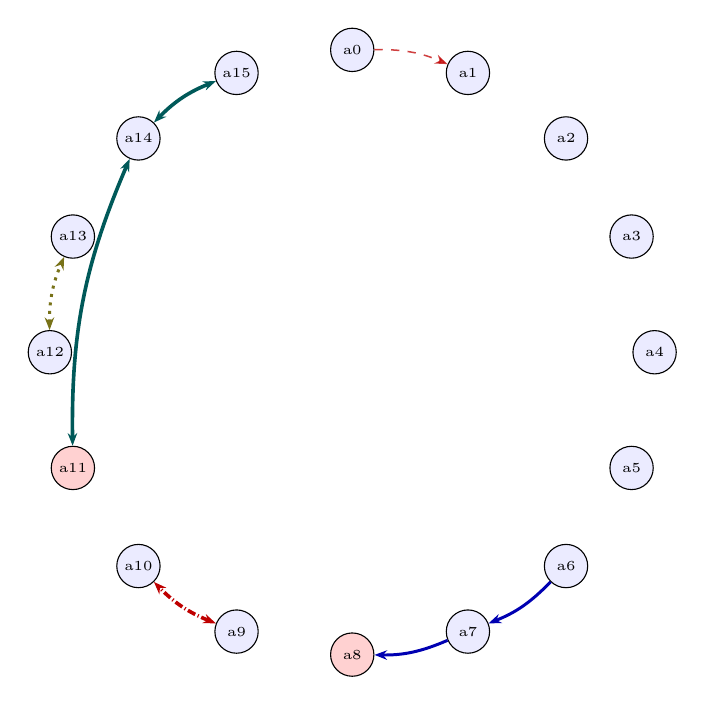
\begin{tikzpicture}[>={Stealth[length=1.6mm]}]
  \node[circle,draw,fill=blue!8,inner sep=1pt,minimum size=5.5mm,font=\tiny] (a0) at (90.0:3.84) {a0};
  \node[circle,draw,fill=blue!8,inner sep=1pt,minimum size=5.5mm,font=\tiny] (a1) at (67.5:3.84) {a1};
  \node[circle,draw,fill=blue!8,inner sep=1pt,minimum size=5.5mm,font=\tiny] (a2) at (45.0:3.84) {a2};
  \node[circle,draw,fill=blue!8,inner sep=1pt,minimum size=5.5mm,font=\tiny] (a3) at (22.5:3.84) {a3};
  \node[circle,draw,fill=blue!8,inner sep=1pt,minimum size=5.5mm,font=\tiny] (a4) at (0.0:3.84) {a4};
  \node[circle,draw,fill=blue!8,inner sep=1pt,minimum size=5.5mm,font=\tiny] (a5) at (-22.5:3.84) {a5};
  \node[circle,draw,fill=blue!8,inner sep=1pt,minimum size=5.5mm,font=\tiny] (a6) at (-45.0:3.84) {a6};
  \node[circle,draw,fill=blue!8,inner sep=1pt,minimum size=5.5mm,font=\tiny] (a7) at (-67.5:3.84) {a7};
  \node[circle,draw,fill=red!18,inner sep=1pt,minimum size=5.5mm,font=\tiny] (a8) at (-90.0:3.84) {a8};
  \node[circle,draw,fill=blue!8,inner sep=1pt,minimum size=5.5mm,font=\tiny] (a9) at (-112.5:3.84) {a9};
  \node[circle,draw,fill=blue!8,inner sep=1pt,minimum size=5.5mm,font=\tiny] (a10) at (-135.0:3.84) {a10};
  \node[circle,draw,fill=red!18,inner sep=1pt,minimum size=5.5mm,font=\tiny] (a11) at (-157.5:3.84) {a11};
  \node[circle,draw,fill=blue!8,inner sep=1pt,minimum size=5.5mm,font=\tiny] (a12) at (-180.0:3.84) {a12};
  \node[circle,draw,fill=blue!8,inner sep=1pt,minimum size=5.5mm,font=\tiny] (a13) at (-202.5:3.84) {a13};
  \node[circle,draw,fill=blue!8,inner sep=1pt,minimum size=5.5mm,font=\tiny] (a14) at (-225.0:3.84) {a14};
  \node[circle,draw,fill=blue!8,inner sep=1pt,minimum size=5.5mm,font=\tiny] (a15) at (-247.5:3.84) {a15};
  \draw[-{Stealth[length=1.6mm]}, blue!70!black, line width=1.08pt] (a6) to[bend left=12] (a7);
  \draw[{Stealth[length=1.6mm]}-{Stealth[length=1.6mm]}, red!75!black, densely dashdotted, line width=1.31pt] (a9) to[bend left=12] (a10);
  \draw[{Stealth[length=1.6mm]}-{Stealth[length=1.6mm]}, olive!80!black, dotted, line width=1.08pt] (a12) to[bend left=12] (a13);
  \draw[{Stealth[length=1.6mm]}-{Stealth[length=1.6mm]}, teal!70!black, line width=1.31pt] (a14) to[bend left=12] (a15);
  \draw[-{Stealth[length=1.6mm]}, red!75!black, dashed, opacity=0.75, line width=0.55pt] (a0) to[bend left=12] (a1);
  \draw[-{Stealth[length=1.6mm]}, blue!70!black, line width=1.08pt] (a7) to[bend left=12] (a8);
  \draw[{Stealth[length=1.6mm]}-{Stealth[length=1.6mm]}, teal!70!black, line width=1.31pt] (a11) to[bend left=12] (a14);
\end{tikzpicture}
}
\\[2pt]{\footnotesize all gold edges: 7 factors}
\end{minipage}\hfill\begin{minipage}[t]{0.48\linewidth}\centering
\resizebox{!}{6.4cm}{%
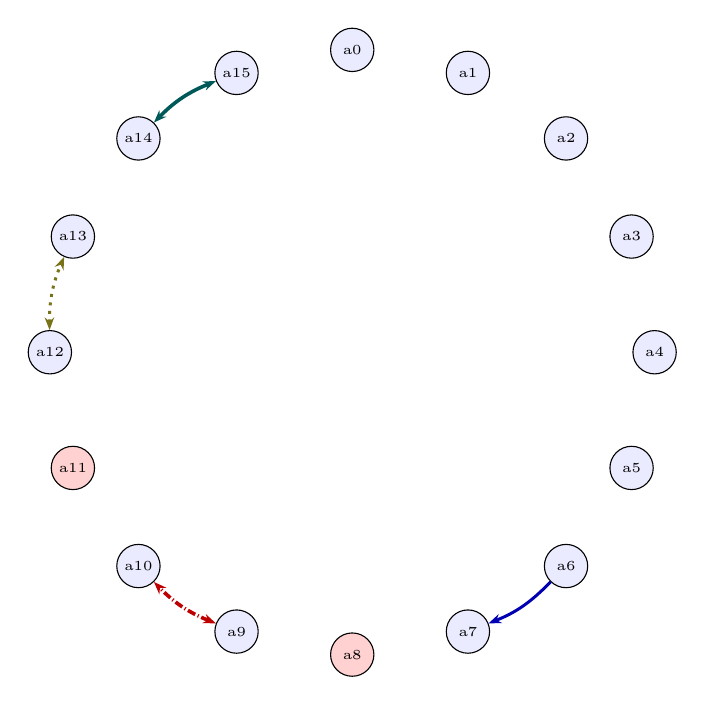
\begin{tikzpicture}[>={Stealth[length=1.6mm]}]
  \node[circle,draw,fill=blue!8,inner sep=1pt,minimum size=5.5mm,font=\tiny] (a0) at (90.0:3.84) {a0};
  \node[circle,draw,fill=blue!8,inner sep=1pt,minimum size=5.5mm,font=\tiny] (a1) at (67.5:3.84) {a1};
  \node[circle,draw,fill=blue!8,inner sep=1pt,minimum size=5.5mm,font=\tiny] (a2) at (45.0:3.84) {a2};
  \node[circle,draw,fill=blue!8,inner sep=1pt,minimum size=5.5mm,font=\tiny] (a3) at (22.5:3.84) {a3};
  \node[circle,draw,fill=blue!8,inner sep=1pt,minimum size=5.5mm,font=\tiny] (a4) at (0.0:3.84) {a4};
  \node[circle,draw,fill=blue!8,inner sep=1pt,minimum size=5.5mm,font=\tiny] (a5) at (-22.5:3.84) {a5};
  \node[circle,draw,fill=blue!8,inner sep=1pt,minimum size=5.5mm,font=\tiny] (a6) at (-45.0:3.84) {a6};
  \node[circle,draw,fill=blue!8,inner sep=1pt,minimum size=5.5mm,font=\tiny] (a7) at (-67.5:3.84) {a7};
  \node[circle,draw,fill=red!18,inner sep=1pt,minimum size=5.5mm,font=\tiny] (a8) at (-90.0:3.84) {a8};
  \node[circle,draw,fill=blue!8,inner sep=1pt,minimum size=5.5mm,font=\tiny] (a9) at (-112.5:3.84) {a9};
  \node[circle,draw,fill=blue!8,inner sep=1pt,minimum size=5.5mm,font=\tiny] (a10) at (-135.0:3.84) {a10};
  \node[circle,draw,fill=red!18,inner sep=1pt,minimum size=5.5mm,font=\tiny] (a11) at (-157.5:3.84) {a11};
  \node[circle,draw,fill=blue!8,inner sep=1pt,minimum size=5.5mm,font=\tiny] (a12) at (-180.0:3.84) {a12};
  \node[circle,draw,fill=blue!8,inner sep=1pt,minimum size=5.5mm,font=\tiny] (a13) at (-202.5:3.84) {a13};
  \node[circle,draw,fill=blue!8,inner sep=1pt,minimum size=5.5mm,font=\tiny] (a14) at (-225.0:3.84) {a14};
  \node[circle,draw,fill=blue!8,inner sep=1pt,minimum size=5.5mm,font=\tiny] (a15) at (-247.5:3.84) {a15};
  \draw[-{Stealth[length=1.6mm]}, blue!70!black, line width=1.08pt] (a6) to[bend left=12] (a7);
  \draw[{Stealth[length=1.6mm]}-{Stealth[length=1.6mm]}, red!75!black, densely dashdotted, line width=1.31pt] (a9) to[bend left=12] (a10);
  \draw[{Stealth[length=1.6mm]}-{Stealth[length=1.6mm]}, olive!80!black, dotted, line width=1.08pt] (a12) to[bend left=12] (a13);
  \draw[{Stealth[length=1.6mm]}-{Stealth[length=1.6mm]}, teal!70!black, line width=1.31pt] (a14) to[bend left=12] (a15);
\end{tikzpicture}
}
\\[2pt]{\footnotesize valid edges only: 4 factors}
\end{minipage}
\caption{Relation graph for \texttt{locobench-opus-5-5-f025-r1}. Nodes are atoms on a circle, tinted red when the item marks them non-factual (prior 0.1) and blue when factual (prior 0.9). Edges are gold relations: solid blue = entailment, dashed red = contradiction, double-headed teal = equivalence, dash-dotted red (double-headed) = exclusive (exactly-one), dotted olive (double-headed) = co-necessity (at-least-one); thickness scales with the factor probability. Ordering-only Precedence edges carry no factor and so are not drawn.}
\label{fig:graph-locobench-opus-5-5-f025-r1}
\end{figure}

\begin{table}[htbp]
\centering
\footnotesize
\setlength{\tabcolsep}{3.5pt}
\caption{The specific gold relations of \texttt{locobench-opus-5-5-f025-r1}. \textbf{$p$ used} is the factor probability the MRF received: the band midpoint, times $(1-\lambda)$ for a resolved concession, or \emph{none} for an ordering-only edge (no factor). \textbf{Valid} marks the deliberately-planted errors with their kind. \textbf{Res.} is the resolving atom of a resolved concession.}
\label{tab:rels-locobench-opus-5-5-f025-r1}
\begin{tabular}{lllllrll}
\toprule
ID & Endpoints & Sense & Coupling & Band & $p$ used & Valid & Res. \\
\midrule
\texttt{r002} & \texttt{a6} $\to$ \texttt{a7} & Evidence & \texttt{entailment} & moderate & 0.720 & \checkmark &  \\
\texttt{r003} & \texttt{a9} $\leftrightarrow$ \texttt{a10} & Alternative & \texttt{exclusive} & strong & 0.925 & \checkmark &  \\
\texttt{r004} & \texttt{a12} $\leftrightarrow$ \texttt{a13} & Disjunction & \texttt{co\_necessity} & moderate & 0.720 & \checkmark &  \\
\texttt{r005} & \texttt{a14} $\leftrightarrow$ \texttt{a15} & Restatement & \texttt{equivalence} & strong & 0.925 & \checkmark &  \\
\texttt{r006} & \texttt{a0} $\to$ \texttt{a1} & Concession & \texttt{contradiction} & weak & 0.259 & $\times$ {\scriptsize wrong\_sense} & \texttt{a7} \\
\texttt{r007} & \texttt{a3} $\to$ \texttt{a2} & Precedence & \texttt{none} & weak & \emph{none} & $\times$ {\scriptsize wrong\_direction} &  \\
\texttt{r008} & \texttt{a7} $\to$ \texttt{a8} & Evidence & \texttt{entailment} & moderate & 0.720 & $\times$ {\scriptsize false\_endpoint} &  \\
\texttt{r009} & \texttt{a11} $\leftrightarrow$ \texttt{a14} & Restatement & \texttt{equivalence} & strong & 0.925 & $\times$ {\scriptsize false\_endpoint} &  \\
\bottomrule
\end{tabular}
\end{table}

\begin{table}[htbp]
\centering
\footnotesize
\caption{Atoms of \texttt{locobench-opus-5-5-f025-r1}: the \texttt{factual} label, the prior it maps to, the posterior marginal $P(a_i{=}1)$ the MRF returns, and the shift. Atoms dragged below their prior are the ones the coherence structure penalises.}
\label{tab:atoms-locobench-opus-5-5-f025-r1}
\begin{tabular}{llrrrp{7.2cm}}
\toprule
Atom & fact & $\pi_i$ & $P(a_i{=}1)$ & $\Delta$ & Text \\
\midrule
\texttt{a0} & \checkmark & 0.90 & 0.926 & +0.026 & \footnotesize Before the bacterium's acceptance, peptic ulcers were widely attributed to stress and excess gastric acid. \\
\texttt{a1} & \checkmark & 0.90 & 0.958 & +0.058 & \footnotesize Many gastroenterologists initially doubted that any bacterium could survive in the acidic stomach. \\
\texttt{a2} & \checkmark & 0.90 & 0.900 & +0.000 & \footnotesize In 1979 Warren observed curved bacteria in biopsies of inflamed stomach tissue. \\
\texttt{a3} & \checkmark & 0.90 & 0.900 & +0.000 & \footnotesize Early attempts to culture the stomach bacterium failed because plates were discarded after about two days. \\
\texttt{a4} & \checkmark & 0.90 & 0.900 & +0.000 & \footnotesize A culture plate left incubating over the 1982 Easter long weekend produced the first successful growth of the bacterium. \\
\texttt{a5} & \checkmark & 0.90 & 0.900 & +0.000 & \footnotesize In 1984 Marshall drank a culture of the bacterium to test whether it could infect a healthy stomach. \\
\texttt{a6} & \checkmark & 0.90 & 0.922 & +0.022 & \footnotesize Marshall developed acute gastritis within days of drinking the culture. \\
\texttt{a7} & \checkmark & 0.90 & 0.931 & +0.031 & \footnotesize The Nobel Assembly at Karolinska Institutet determined that H. pylori infection causes gastritis and peptic ulcer disease. \\
\texttt{a8} & $\times$ & 0.10 & 0.214 & +0.114 & \footnotesize Marshall developed a bleeding duodenal ulcer as a result of his self-experiment. \\
\texttt{a9} & \checkmark & 0.90 & 0.632 & -0.268 & \footnotesize Marshall treated his self-induced infection with antibiotics. \\
\texttt{a10} & \checkmark & 0.90 & 0.632 & -0.268 & \footnotesize Marshall's self-induced infection was never treated with antibiotics. \\
\texttt{a11} & $\times$ & 0.10 & 0.521 & +0.421 & \footnotesize Warren and Marshall received the Nobel Prize in Physiology or Medicine in 1995. \\
\texttt{a12} & \checkmark & 0.90 & 0.929 & +0.029 & \footnotesize The patient's peptic ulcer was caused by H. pylori infection. \\
\texttt{a13} & \checkmark & 0.90 & 0.929 & +0.029 & \footnotesize The patient's peptic ulcer was caused by long-term NSAID use. \\
\texttt{a14} & \checkmark & 0.90 & 0.900 & +0.000 & \footnotesize Barry Marshall and Robin Warren shared the 2005 Nobel Prize in Physiology or Medicine. \\
\texttt{a15} & \checkmark & 0.90 & 0.934 & +0.034 & \footnotesize The 2005 Nobel Prize in Physiology or Medicine was jointly awarded to Robin Warren and Barry Marshall. \\
\bottomrule
\end{tabular}
\end{table}

\subsection{Meteorology -- base (\texttt{locobench-opus-5-5-f026-r1})}

\textbf{Topic:} Meteorology (Natural Sciences). \textbf{Family:} \texttt{f026} (CONFLICT), rung 1 (\emph{base}). \textbf{Scores:} mean-marg $= 0.768$, consist $= 0.425$, reified $= 0.140$, log-Z $= 0.351$.



\paragraph{Framing question.} \emph{How do National Weather Service damage survey teams determine whether destruction left by a severe thunderstorm was produced by a tornado or by straight-line downburst winds when eyewitness accounts, radar signatures, and debris patterns point toward different conclusions?}



\paragraph{Response.} {\small National Weather Service local forecast offices conduct post-event damage surveys after severe storms, and only after that fieldwork is complete do the survey teams rate tornado intensity using the Enhanced Fujita Scale. The order matters. Intensity ratings are assigned to damage that has already been documented on the ground, not inferred from radar or from the impressions of residents. The Enhanced Fujita Scale was implemented in the United States in February 2007, whereas the Enhanced Fujita Scale replaced the original Fujita Scale in 1999. Its structure reflects the engineering basis that distinguishes it from its predecessor. Specifically, the Enhanced Fujita Scale uses 15 damage indicators, each paired with a sequence of degrees of damage. A surveyor matches what is observed on a structure or a stand of trees to the appropriate indicator and degree, and from that pairing derives an estimated wind speed. This procedure deliberately anchors the rating to physical evidence rather than to testimony.

When eyewitness accounts, radar signatures, and debris tell different stories, surveyors give the debris field the greatest weight because it records the wind's direction at each point it crossed. Convergent debris patterns are characteristic of tornado damage: trees, crops, and structural fragments are laid down pointing inward toward a central track, often with a rotational or crisscrossing signature where winds from opposing directions acted in quick succession. By contrast, divergent or parallel debris patterns are characteristic of downburst damage, in which a column of descending air strikes the surface and spreads outward, flattening objects in a fan or in long rows aligned with the outflow. Surveyors map these orientations, increasingly with drone and satellite imagery, so that the vector field of the damage becomes visible across the whole affected area rather than at isolated points.

Width is the second discriminating parameter. Tornado damage paths are typically narrower than downburst damage swaths, and because of that difference in scale the damage swath was half a mile wide. That is, it measured 0.5 miles across, a dimension that falls comfortably within the range of a downburst outflow but that would require an unusually large tornado. Surveyors then compare that width against the debris orientation along its full length, looking for any narrower corridor of convergent damage embedded within the broader swath. Radar is consulted at this stage as well: a velocity couplet aloft indicates rotation in the parent storm, but it does not by itself establish that the circulation reached the ground, and a strong reflectivity core with a divergent velocity signature near the surface points instead to outflow.

In the case at issue, at least one of two events occurred, perhaps both: a brief tornado touched down within the damage area, or a downburst struck the damage area. Eyewitnesses described a funnel, radar showed weak rotation, and a short segment of the debris field displayed convergence, while the dominant pattern across the swath was divergent. The classification decision is binary for any given segment of the path. Either the survey team classified the storm damage as caused by a tornado, or, despite that brief touchdown, it classified the storm damage as caused by straight-line winds; the two cannot both be the classification, and one of them must be chosen.

The NWS final survey report settles that tension: it concluded that the storm damage was produced by straight-line downburst winds, and that conclusion confirms that the downburst was the event responsible for the destruction across the swath. The brief touchdown is acknowledged in the narrative record, but its contribution was too small and too localized to govern the classification of the damage as a whole. This outcome illustrates the general rule surveyors apply when evidence conflicts. Testimony and radar establish what was possible, but the orientation and dimensions of the damage itself determine what is recorded.}

\begin{figure}[htbp]
\centering
\begin{minipage}[t]{0.48\linewidth}\centering
\resizebox{!}{6.4cm}{%
\begin{tikzpicture}[>={Stealth[length=1.6mm]}]
  \node[circle,draw,fill=blue!8,inner sep=1pt,minimum size=5.5mm,font=\tiny] (a0) at (90.0:3.66) {a0};
  \node[circle,draw,fill=blue!8,inner sep=1pt,minimum size=5.5mm,font=\tiny] (a1) at (66.0:3.66) {a1};
  \node[circle,draw,fill=blue!8,inner sep=1pt,minimum size=5.5mm,font=\tiny] (a2) at (42.0:3.66) {a2};
  \node[circle,draw,fill=red!18,inner sep=1pt,minimum size=5.5mm,font=\tiny] (a3) at (18.0:3.66) {a3};
  \node[circle,draw,fill=red!18,inner sep=1pt,minimum size=5.5mm,font=\tiny] (a4) at (-6.0:3.66) {a4};
  \node[circle,draw,fill=blue!8,inner sep=1pt,minimum size=5.5mm,font=\tiny] (a5) at (-30.0:3.66) {a5};
  \node[circle,draw,fill=blue!8,inner sep=1pt,minimum size=5.5mm,font=\tiny] (a6) at (-54.0:3.66) {a6};
  \node[circle,draw,fill=blue!8,inner sep=1pt,minimum size=5.5mm,font=\tiny] (a7) at (-78.0:3.66) {a7};
  \node[circle,draw,fill=blue!8,inner sep=1pt,minimum size=5.5mm,font=\tiny] (a8) at (-102.0:3.66) {a8};
  \node[circle,draw,fill=blue!8,inner sep=1pt,minimum size=5.5mm,font=\tiny] (a9) at (-126.0:3.66) {a9};
  \node[circle,draw,fill=blue!8,inner sep=1pt,minimum size=5.5mm,font=\tiny] (a10) at (-150.0:3.66) {a10};
  \node[circle,draw,fill=blue!8,inner sep=1pt,minimum size=5.5mm,font=\tiny] (a11) at (-174.0:3.66) {a11};
  \node[circle,draw,fill=blue!8,inner sep=1pt,minimum size=5.5mm,font=\tiny] (a12) at (-198.0:3.66) {a12};
  \node[circle,draw,fill=blue!8,inner sep=1pt,minimum size=5.5mm,font=\tiny] (a13) at (-222.0:3.66) {a13};
  \node[circle,draw,fill=blue!8,inner sep=1pt,minimum size=5.5mm,font=\tiny] (a14) at (-246.0:3.66) {a14};
  \draw[{Stealth[length=1.6mm]}-{Stealth[length=1.6mm]}, teal!70!black, line width=1.31pt] (a8) to[bend left=12] (a9);
  \draw[{Stealth[length=1.6mm]}-{Stealth[length=1.6mm]}, olive!80!black, dotted, line width=1.08pt] (a10) to[bend left=12] (a11);
  \draw[{Stealth[length=1.6mm]}-{Stealth[length=1.6mm]}, red!75!black, densely dashdotted, line width=1.31pt] (a12) to[bend left=12] (a13);
  \draw[-{Stealth[length=1.6mm]}, red!75!black, dashed, line width=1.08pt] (a5) to[bend left=12] (a6);
  \draw[-{Stealth[length=1.6mm]}, red!75!black, dashed, opacity=0.75, line width=0.71pt] (a10) to[bend left=12] (a13);
  \draw[-{Stealth[length=1.6mm]}, red!75!black, dashed, line width=0.79pt] (a2) to[bend left=12] (a3);
  \draw[-{Stealth[length=1.6mm]}, blue!70!black, line width=0.79pt] (a7) to[bend left=12] (a8);
  \draw[-{Stealth[length=1.6mm]}, blue!70!black, line width=0.79pt] (a1) to[bend left=12] (a4);
  \draw[-{Stealth[length=1.6mm]}, blue!70!black, line width=1.08pt] (a14) to[bend left=12] (a11);
\end{tikzpicture}
}
\\[2pt]{\footnotesize all gold edges: 9 factors}
\end{minipage}\hfill\begin{minipage}[t]{0.48\linewidth}\centering
\resizebox{!}{6.4cm}{%
\begin{tikzpicture}[>={Stealth[length=1.6mm]}]
  \node[circle,draw,fill=blue!8,inner sep=1pt,minimum size=5.5mm,font=\tiny] (a0) at (90.0:3.66) {a0};
  \node[circle,draw,fill=blue!8,inner sep=1pt,minimum size=5.5mm,font=\tiny] (a1) at (66.0:3.66) {a1};
  \node[circle,draw,fill=blue!8,inner sep=1pt,minimum size=5.5mm,font=\tiny] (a2) at (42.0:3.66) {a2};
  \node[circle,draw,fill=red!18,inner sep=1pt,minimum size=5.5mm,font=\tiny] (a3) at (18.0:3.66) {a3};
  \node[circle,draw,fill=red!18,inner sep=1pt,minimum size=5.5mm,font=\tiny] (a4) at (-6.0:3.66) {a4};
  \node[circle,draw,fill=blue!8,inner sep=1pt,minimum size=5.5mm,font=\tiny] (a5) at (-30.0:3.66) {a5};
  \node[circle,draw,fill=blue!8,inner sep=1pt,minimum size=5.5mm,font=\tiny] (a6) at (-54.0:3.66) {a6};
  \node[circle,draw,fill=blue!8,inner sep=1pt,minimum size=5.5mm,font=\tiny] (a7) at (-78.0:3.66) {a7};
  \node[circle,draw,fill=blue!8,inner sep=1pt,minimum size=5.5mm,font=\tiny] (a8) at (-102.0:3.66) {a8};
  \node[circle,draw,fill=blue!8,inner sep=1pt,minimum size=5.5mm,font=\tiny] (a9) at (-126.0:3.66) {a9};
  \node[circle,draw,fill=blue!8,inner sep=1pt,minimum size=5.5mm,font=\tiny] (a10) at (-150.0:3.66) {a10};
  \node[circle,draw,fill=blue!8,inner sep=1pt,minimum size=5.5mm,font=\tiny] (a11) at (-174.0:3.66) {a11};
  \node[circle,draw,fill=blue!8,inner sep=1pt,minimum size=5.5mm,font=\tiny] (a12) at (-198.0:3.66) {a12};
  \node[circle,draw,fill=blue!8,inner sep=1pt,minimum size=5.5mm,font=\tiny] (a13) at (-222.0:3.66) {a13};
  \node[circle,draw,fill=blue!8,inner sep=1pt,minimum size=5.5mm,font=\tiny] (a14) at (-246.0:3.66) {a14};
  \draw[{Stealth[length=1.6mm]}-{Stealth[length=1.6mm]}, teal!70!black, line width=1.31pt] (a8) to[bend left=12] (a9);
  \draw[{Stealth[length=1.6mm]}-{Stealth[length=1.6mm]}, olive!80!black, dotted, line width=1.08pt] (a10) to[bend left=12] (a11);
  \draw[{Stealth[length=1.6mm]}-{Stealth[length=1.6mm]}, red!75!black, densely dashdotted, line width=1.31pt] (a12) to[bend left=12] (a13);
  \draw[-{Stealth[length=1.6mm]}, red!75!black, dashed, line width=1.08pt] (a5) to[bend left=12] (a6);
  \draw[-{Stealth[length=1.6mm]}, red!75!black, dashed, opacity=0.75, line width=0.71pt] (a10) to[bend left=12] (a13);
\end{tikzpicture}
}
\\[2pt]{\footnotesize valid edges only: 5 factors}
\end{minipage}
\caption{Relation graph for \texttt{locobench-opus-5-5-f026-r1}. Nodes are atoms on a circle, tinted red when the item marks them non-factual (prior 0.1) and blue when factual (prior 0.9). Edges are gold relations: solid blue = entailment, dashed red = contradiction, double-headed teal = equivalence, dash-dotted red (double-headed) = exclusive (exactly-one), dotted olive (double-headed) = co-necessity (at-least-one); thickness scales with the factor probability. Ordering-only Precedence edges carry no factor and so are not drawn.}
\label{fig:graph-locobench-opus-5-5-f026-r1}
\end{figure}

\begin{table}[htbp]
\centering
\footnotesize
\setlength{\tabcolsep}{3.5pt}
\caption{The specific gold relations of \texttt{locobench-opus-5-5-f026-r1}. \textbf{$p$ used} is the factor probability the MRF received: the band midpoint, times $(1-\lambda)$ for a resolved concession, or \emph{none} for an ordering-only edge (no factor). \textbf{Valid} marks the deliberately-planted errors with their kind. \textbf{Res.} is the resolving atom of a resolved concession.}
\label{tab:rels-locobench-opus-5-5-f026-r1}
\begin{tabular}{lllllrll}
\toprule
ID & Endpoints & Sense & Coupling & Band & $p$ used & Valid & Res. \\
\midrule
\texttt{r000} & \texttt{a0} $\to$ \texttt{a1} & Precedence & \texttt{none} & moderate & \emph{none} & \checkmark &  \\
\texttt{r001} & \texttt{a8} $\leftrightarrow$ \texttt{a9} & Restatement & \texttt{equivalence} & strong & 0.925 & \checkmark &  \\
\texttt{r002} & \texttt{a10} $\leftrightarrow$ \texttt{a11} & Disjunction & \texttt{co\_necessity} & moderate & 0.720 & \checkmark &  \\
\texttt{r003} & \texttt{a12} $\leftrightarrow$ \texttt{a13} & Alternative & \texttt{exclusive} & strong & 0.925 & \checkmark &  \\
\texttt{r004} & \texttt{a5} $\leftrightarrow$ \texttt{a6} & Contrast & \texttt{contradiction} & moderate & 0.720 & \checkmark &  \\
\texttt{r005} & \texttt{a10} $\to$ \texttt{a13} & Concession & \texttt{contradiction} & moderate & 0.396 & \checkmark & \texttt{a14} \\
\texttt{r006} & \texttt{a2} $\leftrightarrow$ \texttt{a3} & Contrast & \texttt{contradiction} & weak & 0.470 & $\times$ {\scriptsize false\_endpoint} &  \\
\texttt{r007} & \texttt{a7} $\to$ \texttt{a8} & Cause-Effect & \texttt{entailment} & weak & 0.470 & $\times$ {\scriptsize spurious} &  \\
\texttt{r008} & \texttt{a1} $\to$ \texttt{a4} & Instantiation & \texttt{entailment} & weak & 0.470 & $\times$ {\scriptsize false\_endpoint} &  \\
\texttt{r009} & \texttt{a14} $\to$ \texttt{a11} & Evidence & \texttt{entailment} & moderate & 0.720 & $\times$ {\scriptsize wrong\_direction} &  \\
\bottomrule
\end{tabular}
\end{table}

\begin{table}[htbp]
\centering
\footnotesize
\caption{Atoms of \texttt{locobench-opus-5-5-f026-r1}: the \texttt{factual} label, the prior it maps to, the posterior marginal $P(a_i{=}1)$ the MRF returns, and the shift. Atoms dragged below their prior are the ones the coherence structure penalises.}
\label{tab:atoms-locobench-opus-5-5-f026-r1}
\begin{tabular}{llrrrp{7.2cm}}
\toprule
Atom & fact & $\pi_i$ & $P(a_i{=}1)$ & $\Delta$ & Text \\
\midrule
\texttt{a0} & \checkmark & 0.90 & 0.900 & +0.000 & \footnotesize National Weather Service local forecast offices conduct post-event damage surveys after severe storms. \\
\texttt{a1} & \checkmark & 0.90 & 0.904 & +0.004 & \footnotesize NWS survey teams rate tornado intensity using the Enhanced Fujita Scale. \\
\texttt{a2} & \checkmark & 0.90 & 0.895 & -0.005 & \footnotesize The Enhanced Fujita Scale was implemented in the United States in February 2007. \\
\texttt{a3} & $\times$ & 0.10 & 0.110 & +0.010 & \footnotesize The Enhanced Fujita Scale replaced the original Fujita Scale in 1999. \\
\texttt{a4} & $\times$ & 0.10 & 0.091 & -0.009 & \footnotesize The Enhanced Fujita Scale uses 15 damage indicators. \\
\texttt{a5} & \checkmark & 0.90 & 0.854 & -0.046 & \footnotesize Convergent debris patterns are characteristic of tornado damage. \\
\texttt{a6} & \checkmark & 0.90 & 0.796 & -0.104 & \footnotesize Divergent or parallel debris patterns are characteristic of downburst damage. \\
\texttt{a7} & \checkmark & 0.90 & 0.895 & -0.005 & \footnotesize Tornado damage paths are typically narrower than downburst damage swaths. \\
\texttt{a8} & \checkmark & 0.90 & 0.977 & +0.077 & \footnotesize The damage swath was half a mile wide. \\
\texttt{a9} & \checkmark & 0.90 & 0.978 & +0.078 & \footnotesize The damage swath measured 0.5 miles across. \\
\texttt{a10} & \checkmark & 0.90 & 0.932 & +0.032 & \footnotesize A brief tornado touched down within the damage area. \\
\texttt{a11} & \checkmark & 0.90 & 0.968 & +0.068 & \footnotesize A downburst struck the damage area. \\
\texttt{a12} & \checkmark & 0.90 & 0.583 & -0.317 & \footnotesize The survey team classified the storm damage as caused by a tornado. \\
\texttt{a13} & \checkmark & 0.90 & 0.717 & -0.183 & \footnotesize The survey team classified the storm damage as caused by straight-line winds. \\
\texttt{a14} & \checkmark & 0.90 & 0.925 & +0.025 & \footnotesize The NWS final survey report concluded that the storm damage was produced by straight-line downburst winds. \\
\bottomrule
\end{tabular}
\end{table}

\subsection{Oceanography -- direction\_reversal\_a (\texttt{locobench-opus-5-5-f027-r1})}

\textbf{Topic:} Oceanography (Natural Sciences). \textbf{Family:} \texttt{f027} (CONTROL), rung 1 (\emph{direction\_reversal\_a}). \textbf{Scores:} mean-marg $= 0.788$, consist $= 0.541$, reified $= 0.207$, log-Z $= 0.344$.



\paragraph{Framing question.} \emph{How did oceanographers determine whether the 2013–2015 northeast Pacific marine heatwave known as "the Blob" originated mainly from reduced atmospheric heat loss under a persistent high-pressure ridge or from anomalous ocean heat transport into the region?}



\paragraph{Response.} {\small The Blob was a large mass of anomalously warm water in the northeast Pacific Ocean, and its sprawling, formless extent across thousands of kilometres of open sea indicates why Daniel Swain coined the name "the Blob" for the warm water mass. The label stuck because it described a feature without sharp fronts or a clear boundary. That diffuseness was also what made its origin difficult to establish. Oceanographers needed to determine which physical process had produced and sustained so broad a region of excess heat, and the answer depended on separating atmospheric influences from oceanic ones within a single, coupled system.

The Blob was first detected in late 2013, before a persistent high-pressure ridge sat over the northeast Pacific during winter 2013–2014. The ridge was caused by the persistent atmospheric pattern of reduced heat loss from the ocean to the atmosphere. In other words, less heat escaped from the sea surface to the air under the persistent ridge than in a typical winter, when storms passing over the Gulf of Alaska normally draw large quantities of heat out of the upper ocean. The same circulation pattern also altered the ocean's dynamical environment, and at least one of two further conditions held, perhaps both: winds over the northeast Pacific were weaker than normal in winter 2013–2014, or advection of cold water into the northeast Pacific was weaker than normal in winter 2013–2014. Each of these conditions would favour warming, and each points to a different mechanism, so their presence sharpened rather than settled the question of cause.

Sea surface temperature anomalies within the Blob peaked at about 8°C, a magnitude that drew attention to the event's surface expression. By contrast, researchers used mixed-layer heat budget analyses to compare the contributions of surface heat fluxes and ocean advection, an approach concerned less with how warm the surface became than with where the added heat came from. A heat budget treats the upper mixed layer as a control volume and accounts for every term that changes its heat content: net air–sea flux, horizontal advection by currents, entrainment from below, and diffusion. Framed this way, the problem admits a clear dichotomy. Either the Blob's initial warming was driven mainly by reduced heat loss from the ocean to the atmosphere, or the Blob's initial warming was driven mainly by anomalous ocean heat transport into the region. The two accounts cannot both describe the dominant cause, and one of them must hold, since the budget terms together close the account of the mixed layer's heat content.

Whereas the transport hypothesis rested on currents carrying heat into the region, Argo floats provided subsurface temperature measurements of the Blob, profiling the water column and showing how deeply the warm anomaly extended and how the mixed layer evolved through the winter. These profiles supplied the observational constraint that the budget required. Although the ocean-transport account offered a plausible mechanism, given the weakened delivery of cold water, a mixed-layer heat budget analysis determined that anomalous horizontal ocean heat advection played only a secondary role in the Blob's initial warming. The advective term was present but too small to account for the observed rise in heat content.

That budget result is the evidence on which the attribution rests, and it resolves the tension between the two candidate mechanisms: Bond and colleagues concluded that reduced ocean heat loss under the anomalous ridge was the primary cause of the Blob's initial warming. Their conclusion follows directly from the closure of the budget, because once advection is shown to be subordinate, the surface flux anomaly remains as the dominant term. The determination therefore did not depend on the striking surface temperatures alone. It came from quantitatively partitioning heat sources within the mixed layer, constrained by subsurface observations, which showed that the atmosphere's failure to extract heat during an unusually calm winter, rather than currents importing it, initiated the northeast Pacific's most prominent marine heatwave of the decade.}

\begin{figure}[htbp]
\centering
\begin{minipage}[t]{0.48\linewidth}\centering
\resizebox{!}{6.4cm}{%
\begin{tikzpicture}[>={Stealth[length=1.6mm]}]
  \node[circle,draw,fill=blue!8,inner sep=1pt,minimum size=5.5mm,font=\tiny] (a0) at (90.0:3.66) {a0};
  \node[circle,draw,fill=red!18,inner sep=1pt,minimum size=5.5mm,font=\tiny] (a1) at (66.0:3.66) {a1};
  \node[circle,draw,fill=blue!8,inner sep=1pt,minimum size=5.5mm,font=\tiny] (a2) at (42.0:3.66) {a2};
  \node[circle,draw,fill=blue!8,inner sep=1pt,minimum size=5.5mm,font=\tiny] (a3) at (18.0:3.66) {a3};
  \node[circle,draw,fill=blue!8,inner sep=1pt,minimum size=5.5mm,font=\tiny] (a4) at (-6.0:3.66) {a4};
  \node[circle,draw,fill=blue!8,inner sep=1pt,minimum size=5.5mm,font=\tiny] (a5) at (-30.0:3.66) {a5};
  \node[circle,draw,fill=blue!8,inner sep=1pt,minimum size=5.5mm,font=\tiny] (a6) at (-54.0:3.66) {a6};
  \node[circle,draw,fill=blue!8,inner sep=1pt,minimum size=5.5mm,font=\tiny] (a7) at (-78.0:3.66) {a7};
  \node[circle,draw,fill=red!18,inner sep=1pt,minimum size=5.5mm,font=\tiny] (a8) at (-102.0:3.66) {a8};
  \node[circle,draw,fill=blue!8,inner sep=1pt,minimum size=5.5mm,font=\tiny] (a9) at (-126.0:3.66) {a9};
  \node[circle,draw,fill=blue!8,inner sep=1pt,minimum size=5.5mm,font=\tiny] (a10) at (-150.0:3.66) {a10};
  \node[circle,draw,fill=blue!8,inner sep=1pt,minimum size=5.5mm,font=\tiny] (a11) at (-174.0:3.66) {a11};
  \node[circle,draw,fill=blue!8,inner sep=1pt,minimum size=5.5mm,font=\tiny] (a12) at (-198.0:3.66) {a12};
  \node[circle,draw,fill=blue!8,inner sep=1pt,minimum size=5.5mm,font=\tiny] (a13) at (-222.0:3.66) {a13};
  \node[circle,draw,fill=blue!8,inner sep=1pt,minimum size=5.5mm,font=\tiny] (a14) at (-246.0:3.66) {a14};
  \draw[-{Stealth[length=1.6mm]}, blue!70!black, line width=1.31pt] (a3) to[bend left=12] (a4);
  \draw[{Stealth[length=1.6mm]}-{Stealth[length=1.6mm]}, teal!70!black, line width=1.31pt] (a5) to[bend left=12] (a4);
  \draw[{Stealth[length=1.6mm]}-{Stealth[length=1.6mm]}, olive!80!black, dotted, line width=1.08pt] (a6) to[bend left=12] (a7);
  \draw[{Stealth[length=1.6mm]}-{Stealth[length=1.6mm]}, red!75!black, densely dashdotted, line width=1.31pt] (a10) to[bend left=12] (a11);
  \draw[-{Stealth[length=1.6mm]}, red!75!black, dashed, opacity=0.75, line width=0.71pt] (a11) to[bend left=12] (a13);
  \draw[-{Stealth[length=1.6mm]}, blue!70!black, line width=1.31pt] (a13) to[bend left=12] (a14);
  \draw[-{Stealth[length=1.6mm]}, red!75!black, dashed, line width=0.79pt] (a8) to[bend left=12] (a9);
  \draw[-{Stealth[length=1.6mm]}, red!75!black, dashed, line width=0.79pt] (a12) to[bend left=12] (a11);
  \draw[-{Stealth[length=1.6mm]}, blue!70!black, line width=0.79pt] (a0) to[bend left=12] (a1);
\end{tikzpicture}
}
\\[2pt]{\footnotesize all gold edges: 9 factors}
\end{minipage}\hfill\begin{minipage}[t]{0.48\linewidth}\centering
\resizebox{!}{6.4cm}{%
\begin{tikzpicture}[>={Stealth[length=1.6mm]}]
  \node[circle,draw,fill=blue!8,inner sep=1pt,minimum size=5.5mm,font=\tiny] (a0) at (90.0:3.66) {a0};
  \node[circle,draw,fill=red!18,inner sep=1pt,minimum size=5.5mm,font=\tiny] (a1) at (66.0:3.66) {a1};
  \node[circle,draw,fill=blue!8,inner sep=1pt,minimum size=5.5mm,font=\tiny] (a2) at (42.0:3.66) {a2};
  \node[circle,draw,fill=blue!8,inner sep=1pt,minimum size=5.5mm,font=\tiny] (a3) at (18.0:3.66) {a3};
  \node[circle,draw,fill=blue!8,inner sep=1pt,minimum size=5.5mm,font=\tiny] (a4) at (-6.0:3.66) {a4};
  \node[circle,draw,fill=blue!8,inner sep=1pt,minimum size=5.5mm,font=\tiny] (a5) at (-30.0:3.66) {a5};
  \node[circle,draw,fill=blue!8,inner sep=1pt,minimum size=5.5mm,font=\tiny] (a6) at (-54.0:3.66) {a6};
  \node[circle,draw,fill=blue!8,inner sep=1pt,minimum size=5.5mm,font=\tiny] (a7) at (-78.0:3.66) {a7};
  \node[circle,draw,fill=red!18,inner sep=1pt,minimum size=5.5mm,font=\tiny] (a8) at (-102.0:3.66) {a8};
  \node[circle,draw,fill=blue!8,inner sep=1pt,minimum size=5.5mm,font=\tiny] (a9) at (-126.0:3.66) {a9};
  \node[circle,draw,fill=blue!8,inner sep=1pt,minimum size=5.5mm,font=\tiny] (a10) at (-150.0:3.66) {a10};
  \node[circle,draw,fill=blue!8,inner sep=1pt,minimum size=5.5mm,font=\tiny] (a11) at (-174.0:3.66) {a11};
  \node[circle,draw,fill=blue!8,inner sep=1pt,minimum size=5.5mm,font=\tiny] (a12) at (-198.0:3.66) {a12};
  \node[circle,draw,fill=blue!8,inner sep=1pt,minimum size=5.5mm,font=\tiny] (a13) at (-222.0:3.66) {a13};
  \node[circle,draw,fill=blue!8,inner sep=1pt,minimum size=5.5mm,font=\tiny] (a14) at (-246.0:3.66) {a14};
  \draw[-{Stealth[length=1.6mm]}, blue!70!black, line width=1.31pt] (a3) to[bend left=12] (a4);
  \draw[{Stealth[length=1.6mm]}-{Stealth[length=1.6mm]}, teal!70!black, line width=1.31pt] (a5) to[bend left=12] (a4);
  \draw[{Stealth[length=1.6mm]}-{Stealth[length=1.6mm]}, olive!80!black, dotted, line width=1.08pt] (a6) to[bend left=12] (a7);
  \draw[{Stealth[length=1.6mm]}-{Stealth[length=1.6mm]}, red!75!black, densely dashdotted, line width=1.31pt] (a10) to[bend left=12] (a11);
  \draw[-{Stealth[length=1.6mm]}, red!75!black, dashed, opacity=0.75, line width=0.71pt] (a11) to[bend left=12] (a13);
  \draw[-{Stealth[length=1.6mm]}, blue!70!black, line width=1.31pt] (a13) to[bend left=12] (a14);
\end{tikzpicture}
}
\\[2pt]{\footnotesize valid edges only: 6 factors}
\end{minipage}
\caption{Relation graph for \texttt{locobench-opus-5-5-f027-r1}. Nodes are atoms on a circle, tinted red when the item marks them non-factual (prior 0.1) and blue when factual (prior 0.9). Edges are gold relations: solid blue = entailment, dashed red = contradiction, double-headed teal = equivalence, dash-dotted red (double-headed) = exclusive (exactly-one), dotted olive (double-headed) = co-necessity (at-least-one); thickness scales with the factor probability. Ordering-only Precedence edges carry no factor and so are not drawn.}
\label{fig:graph-locobench-opus-5-5-f027-r1}
\end{figure}

\begin{table}[htbp]
\centering
\footnotesize
\setlength{\tabcolsep}{3.5pt}
\caption{The specific gold relations of \texttt{locobench-opus-5-5-f027-r1}. \textbf{$p$ used} is the factor probability the MRF received: the band midpoint, times $(1-\lambda)$ for a resolved concession, or \emph{none} for an ordering-only edge (no factor). \textbf{Valid} marks the deliberately-planted errors with their kind. \textbf{Res.} is the resolving atom of a resolved concession.}
\label{tab:rels-locobench-opus-5-5-f027-r1}
\begin{tabular}{lllllrll}
\toprule
ID & Endpoints & Sense & Coupling & Band & $p$ used & Valid & Res. \\
\midrule
\texttt{r000} & \texttt{a3} $\to$ \texttt{a4} & Cause-Effect & \texttt{entailment} & strong & 0.925 & \checkmark &  \\
\texttt{r001} & \texttt{a5} $\leftrightarrow$ \texttt{a4} & Restatement & \texttt{equivalence} & strong & 0.925 & \checkmark &  \\
\texttt{r002} & \texttt{a6} $\leftrightarrow$ \texttt{a7} & Disjunction & \texttt{co\_necessity} & moderate & 0.720 & \checkmark &  \\
\texttt{r003} & \texttt{a10} $\leftrightarrow$ \texttt{a11} & Alternative & \texttt{exclusive} & strong & 0.925 & \checkmark &  \\
\texttt{r004} & \texttt{a11} $\to$ \texttt{a13} & Concession & \texttt{contradiction} & moderate & 0.396 & \checkmark & \texttt{a14} \\
\texttt{r005} & \texttt{a13} $\to$ \texttt{a14} & Evidence & \texttt{entailment} & strong & 0.925 & \checkmark &  \\
\texttt{r006} & \texttt{a8} $\leftrightarrow$ \texttt{a9} & Contrast & \texttt{contradiction} & weak & 0.470 & $\times$ {\scriptsize false\_endpoint} &  \\
\texttt{r007} & \texttt{a12} $\leftrightarrow$ \texttt{a11} & Contrast & \texttt{contradiction} & weak & 0.470 & $\times$ {\scriptsize spurious} &  \\
\texttt{r008} & \texttt{a2} $\to$ \texttt{a3} & Precedence & \texttt{none} & weak & \emph{none} & $\times$ {\scriptsize wrong\_sense} &  \\
\texttt{r009} & \texttt{a0} $\to$ \texttt{a1} & Evidence & \texttt{entailment} & weak & 0.470 & $\times$ {\scriptsize false\_endpoint} &  \\
\bottomrule
\end{tabular}
\end{table}

\begin{table}[htbp]
\centering
\footnotesize
\caption{Atoms of \texttt{locobench-opus-5-5-f027-r1}: the \texttt{factual} label, the prior it maps to, the posterior marginal $P(a_i{=}1)$ the MRF returns, and the shift. Atoms dragged below their prior are the ones the coherence structure penalises.}
\label{tab:atoms-locobench-opus-5-5-f027-r1}
\begin{tabular}{llrrrp{7.2cm}}
\toprule
Atom & fact & $\pi_i$ & $P(a_i{=}1)$ & $\Delta$ & Text \\
\midrule
\texttt{a0} & \checkmark & 0.90 & 0.904 & +0.004 & \footnotesize The Blob was a large mass of anomalously warm water in the northeast Pacific Ocean. \\
\texttt{a1} & $\times$ & 0.10 & 0.091 & -0.009 & \footnotesize Daniel Swain coined the name "the Blob" for the warm water mass. \\
\texttt{a2} & \checkmark & 0.90 & 0.900 & +0.000 & \footnotesize The Blob was first detected in late 2013. \\
\texttt{a3} & \checkmark & 0.90 & 0.942 & +0.042 & \footnotesize A persistent high-pressure ridge sat over the northeast Pacific during winter 2013–2014. \\
\texttt{a4} & \checkmark & 0.90 & 0.997 & +0.097 & \footnotesize The persistent ridge reduced heat loss from the ocean to the atmosphere. \\
\texttt{a5} & \checkmark & 0.90 & 0.989 & +0.089 & \footnotesize Less heat escaped from the sea surface to the air under the persistent ridge. \\
\texttt{a6} & \checkmark & 0.90 & 0.929 & +0.029 & \footnotesize Winds over the northeast Pacific were weaker than normal in winter 2013–2014. \\
\texttt{a7} & \checkmark & 0.90 & 0.929 & +0.029 & \footnotesize Advection of cold water into the northeast Pacific was weaker than normal in winter 2013–2014. \\
\texttt{a8} & $\times$ & 0.10 & 0.104 & +0.004 & \footnotesize Sea surface temperature anomalies within the Blob peaked at about 8°C. \\
\texttt{a9} & \checkmark & 0.90 & 0.901 & +0.001 & \footnotesize Researchers used mixed-layer heat budget analyses to compare the contributions of surface heat fluxes and ocean advection. \\
\texttt{a10} & \checkmark & 0.90 & 0.597 & -0.303 & \footnotesize The Blob's initial warming was driven mainly by reduced heat loss from the ocean to the atmosphere. \\
\texttt{a11} & \checkmark & 0.90 & 0.693 & -0.207 & \footnotesize The Blob's initial warming was driven mainly by anomalous ocean heat transport into the region. \\
\texttt{a12} & \checkmark & 0.90 & 0.902 & +0.002 & \footnotesize Argo floats provided subsurface temperature measurements of the Blob. \\
\texttt{a13} & \checkmark & 0.90 & 0.952 & +0.052 & \footnotesize A mixed-layer heat budget analysis determined that anomalous horizontal ocean heat advection played only a secondary role in the Blob's initial warming. \\
\texttt{a14} & \checkmark & 0.90 & 0.987 & +0.087 & \footnotesize Bond and colleagues concluded that reduced ocean heat loss under the anomalous ridge was the primary cause of the Blob's initial warming. \\
\bottomrule
\end{tabular}
\end{table}

\subsection{Philosophy -- shuffle\_block (\texttt{locobench-opus-5-5-f028-r1})}

\textbf{Topic:} Philosophy (Humanities). \textbf{Family:} \texttt{f028} (ORDER), rung 1 (\emph{shuffle\_block}). \textbf{Scores:} mean-marg $= 0.790$, consist $= 0.439$, reified $= 0.231$, log-Z $= 0.365$.



\paragraph{Framing question.} \emph{How have philosophers from Plato to modern divine command theorists responded to the Euthyphro dilemma's claim that moral goodness must either depend on God's will or exist independently of it, given that each horn seems to undermine the theory?}



\paragraph{Response.} {\small The dialogue's setting also anticipates the fate of its questioner. Meletus charged Socrates with impiety. Although that accusation was formally lodged, in Plato's Apology Socrates denies that he is guilty of impiety, presenting his philosophical activity as service to the god rather than an offense against him. The tension between the charge and the denial was not left open: the Athenian jury ruled that Socrates was guilty of impiety. The verdict settled the legal question, though it hardly settled the philosophical one. It sharpened it instead, since a city claiming to know what the gods require had condemned a man who insisted that no one yet knew what piety was.

Plato's Euthyphro asks whether the pious is loved by the gods because it is pious or is pious because the gods love it. By contrast with that familiar attribution, the Euthyphro was written by Aristotle. The question at the dialogue's center has outlived every dispute about its provenance. Its two horns define the problem that theists have inherited: if goodness depends on divine will, morality looks arbitrary, and if goodness stands independently of that will, God looks like a mere reporter of standards he does not author. Each response to the dilemma can be read as an attempt to escape one horn without being impaled on the other.

The test proceeds through a series of failed definitions. Socrates rejects Euthyphro's definition of piety as what all the gods love, and because of this rejection Euthyphro reaches a settled definition of piety by the end of the dialogue. Either that is how the conversation closes, or Euthyphro leaves the dialogue without a settled definition of piety; the two outcomes cannot both be true, and one of them must hold. The abrupt ending invites explanation. At least one of the following holds, perhaps both: Euthyphro was in a hurry to get away from Socrates, or, as his unresolved departure indicates, he had no adequate answer to Socrates' objections. For later theists, this shape of the dialogue mattered as much as its argument. It showed that confident appeals to divine approval can collapse under analysis, and it placed the burden on anyone who would ground morality in what God loves or commands.

Medieval and modern thinkers took up the dilemma with explicit reference to a single, omnipotent God. William of Ockham held that God could command a creature to hate God, a position that predates Leibniz's criticism of theological voluntarism for making God's justice arbitrary. Ockham's view embraces the first horn without apology: if divine will is the sole source of obligation, then nothing outside that will constrains what may be commanded. Leibniz found this intolerable, since a justice that could have been its opposite deserves no praise. That criticism led Robert Adams to identify ethical wrongness with being contrary to the commands of a loving God. In other words, Adams held that an act is wrong just in case it is contrary to what a loving God commands. The qualification is decisive. By building love into the nature of the commander, Adams keeps obligation dependent on divine command while denying that a loving God would command cruelty for its own sake. Modern divine command theory therefore answers the dilemma not by choosing a horn outright but by relocating goodness in God's character. Obligation is left to follow from his commands, so that neither arbitrariness nor independence fully captures the view.

The dramatic setting gives the abstract question real stakes. In Plato's dialogue, Euthyphro is prosecuting his own father over the death of a laborer, whereas on another reading of the scene, Euthyphro is prosecuting his father for theft. Whichever charge frames the encounter, the action is meant to look startling to an Athenian audience. A son bringing his father to court violates conventional filial duty. That collision between religious duty and ordinary obligation is what makes Euthyphro confident that he knows what piety requires, and what makes Socrates eager to test the confidence.}

\begin{figure}[htbp]
\centering
\begin{minipage}[t]{0.48\linewidth}\centering
\resizebox{!}{6.4cm}{%
\begin{tikzpicture}[>={Stealth[length=1.6mm]}]
  \node[circle,draw,fill=blue!8,inner sep=1pt,minimum size=5.5mm,font=\tiny] (a0) at (90.0:3.84) {a0};
  \node[circle,draw,fill=red!18,inner sep=1pt,minimum size=5.5mm,font=\tiny] (a1) at (67.5:3.84) {a1};
  \node[circle,draw,fill=blue!8,inner sep=1pt,minimum size=5.5mm,font=\tiny] (a2) at (45.0:3.84) {a2};
  \node[circle,draw,fill=red!18,inner sep=1pt,minimum size=5.5mm,font=\tiny] (a3) at (22.5:3.84) {a3};
  \node[circle,draw,fill=blue!8,inner sep=1pt,minimum size=5.5mm,font=\tiny] (a4) at (0.0:3.84) {a4};
  \node[circle,draw,fill=blue!8,inner sep=1pt,minimum size=5.5mm,font=\tiny] (a5) at (-22.5:3.84) {a5};
  \node[circle,draw,fill=blue!8,inner sep=1pt,minimum size=5.5mm,font=\tiny] (a6) at (-45.0:3.84) {a6};
  \node[circle,draw,fill=blue!8,inner sep=1pt,minimum size=5.5mm,font=\tiny] (a7) at (-67.5:3.84) {a7};
  \node[circle,draw,fill=blue!8,inner sep=1pt,minimum size=5.5mm,font=\tiny] (a8) at (-90.0:3.84) {a8};
  \node[circle,draw,fill=blue!8,inner sep=1pt,minimum size=5.5mm,font=\tiny] (a9) at (-112.5:3.84) {a9};
  \node[circle,draw,fill=blue!8,inner sep=1pt,minimum size=5.5mm,font=\tiny] (a10) at (-135.0:3.84) {a10};
  \node[circle,draw,fill=blue!8,inner sep=1pt,minimum size=5.5mm,font=\tiny] (a11) at (-157.5:3.84) {a11};
  \node[circle,draw,fill=blue!8,inner sep=1pt,minimum size=5.5mm,font=\tiny] (a12) at (-180.0:3.84) {a12};
  \node[circle,draw,fill=blue!8,inner sep=1pt,minimum size=5.5mm,font=\tiny] (a13) at (-202.5:3.84) {a13};
  \node[circle,draw,fill=blue!8,inner sep=1pt,minimum size=5.5mm,font=\tiny] (a14) at (-225.0:3.84) {a14};
  \node[circle,draw,fill=blue!8,inner sep=1pt,minimum size=5.5mm,font=\tiny] (a15) at (-247.5:3.84) {a15};
  \draw[{Stealth[length=1.6mm]}-{Stealth[length=1.6mm]}, red!75!black, densely dashdotted, line width=1.31pt] (a5) to[bend left=12] (a6);
  \draw[{Stealth[length=1.6mm]}-{Stealth[length=1.6mm]}, olive!80!black, dotted, line width=1.08pt] (a7) to[bend left=12] (a8);
  \draw[{Stealth[length=1.6mm]}-{Stealth[length=1.6mm]}, teal!70!black, line width=1.31pt] (a14) to[bend left=12] (a15);
  \draw[-{Stealth[length=1.6mm]}, red!75!black, dashed, opacity=0.75, line width=0.71pt] (a9) to[bend left=12] (a10);
  \draw[-{Stealth[length=1.6mm]}, red!75!black, dashed, line width=1.08pt] (a2) to[bend left=12] (a3);
  \draw[-{Stealth[length=1.6mm]}, red!75!black, dashed, line width=0.79pt] (a0) to[bend left=12] (a1);
  \draw[-{Stealth[length=1.6mm]}, blue!70!black, line width=1.08pt] (a6) to[bend left=12] (a8);
  \draw[-{Stealth[length=1.6mm]}, blue!70!black, line width=1.08pt] (a4) to[bend left=12] (a5);
  \draw[-{Stealth[length=1.6mm]}, blue!70!black, line width=0.79pt] (a13) to[bend left=12] (a14);
\end{tikzpicture}
}
\\[2pt]{\footnotesize all gold edges: 9 factors}
\end{minipage}\hfill\begin{minipage}[t]{0.48\linewidth}\centering
\resizebox{!}{6.4cm}{%
\begin{tikzpicture}[>={Stealth[length=1.6mm]}]
  \node[circle,draw,fill=blue!8,inner sep=1pt,minimum size=5.5mm,font=\tiny] (a0) at (90.0:3.84) {a0};
  \node[circle,draw,fill=red!18,inner sep=1pt,minimum size=5.5mm,font=\tiny] (a1) at (67.5:3.84) {a1};
  \node[circle,draw,fill=blue!8,inner sep=1pt,minimum size=5.5mm,font=\tiny] (a2) at (45.0:3.84) {a2};
  \node[circle,draw,fill=red!18,inner sep=1pt,minimum size=5.5mm,font=\tiny] (a3) at (22.5:3.84) {a3};
  \node[circle,draw,fill=blue!8,inner sep=1pt,minimum size=5.5mm,font=\tiny] (a4) at (0.0:3.84) {a4};
  \node[circle,draw,fill=blue!8,inner sep=1pt,minimum size=5.5mm,font=\tiny] (a5) at (-22.5:3.84) {a5};
  \node[circle,draw,fill=blue!8,inner sep=1pt,minimum size=5.5mm,font=\tiny] (a6) at (-45.0:3.84) {a6};
  \node[circle,draw,fill=blue!8,inner sep=1pt,minimum size=5.5mm,font=\tiny] (a7) at (-67.5:3.84) {a7};
  \node[circle,draw,fill=blue!8,inner sep=1pt,minimum size=5.5mm,font=\tiny] (a8) at (-90.0:3.84) {a8};
  \node[circle,draw,fill=blue!8,inner sep=1pt,minimum size=5.5mm,font=\tiny] (a9) at (-112.5:3.84) {a9};
  \node[circle,draw,fill=blue!8,inner sep=1pt,minimum size=5.5mm,font=\tiny] (a10) at (-135.0:3.84) {a10};
  \node[circle,draw,fill=blue!8,inner sep=1pt,minimum size=5.5mm,font=\tiny] (a11) at (-157.5:3.84) {a11};
  \node[circle,draw,fill=blue!8,inner sep=1pt,minimum size=5.5mm,font=\tiny] (a12) at (-180.0:3.84) {a12};
  \node[circle,draw,fill=blue!8,inner sep=1pt,minimum size=5.5mm,font=\tiny] (a13) at (-202.5:3.84) {a13};
  \node[circle,draw,fill=blue!8,inner sep=1pt,minimum size=5.5mm,font=\tiny] (a14) at (-225.0:3.84) {a14};
  \node[circle,draw,fill=blue!8,inner sep=1pt,minimum size=5.5mm,font=\tiny] (a15) at (-247.5:3.84) {a15};
  \draw[{Stealth[length=1.6mm]}-{Stealth[length=1.6mm]}, red!75!black, densely dashdotted, line width=1.31pt] (a5) to[bend left=12] (a6);
  \draw[{Stealth[length=1.6mm]}-{Stealth[length=1.6mm]}, olive!80!black, dotted, line width=1.08pt] (a7) to[bend left=12] (a8);
  \draw[{Stealth[length=1.6mm]}-{Stealth[length=1.6mm]}, teal!70!black, line width=1.31pt] (a14) to[bend left=12] (a15);
  \draw[-{Stealth[length=1.6mm]}, red!75!black, dashed, opacity=0.75, line width=0.71pt] (a9) to[bend left=12] (a10);
  \draw[-{Stealth[length=1.6mm]}, red!75!black, dashed, line width=1.08pt] (a2) to[bend left=12] (a3);
\end{tikzpicture}
}
\\[2pt]{\footnotesize valid edges only: 5 factors}
\end{minipage}
\caption{Relation graph for \texttt{locobench-opus-5-5-f028-r1}. Nodes are atoms on a circle, tinted red when the item marks them non-factual (prior 0.1) and blue when factual (prior 0.9). Edges are gold relations: solid blue = entailment, dashed red = contradiction, double-headed teal = equivalence, dash-dotted red (double-headed) = exclusive (exactly-one), dotted olive (double-headed) = co-necessity (at-least-one); thickness scales with the factor probability. Ordering-only Precedence edges carry no factor and so are not drawn.}
\label{fig:graph-locobench-opus-5-5-f028-r1}
\end{figure}

\begin{table}[htbp]
\centering
\footnotesize
\setlength{\tabcolsep}{3.5pt}
\caption{The specific gold relations of \texttt{locobench-opus-5-5-f028-r1}. \textbf{$p$ used} is the factor probability the MRF received: the band midpoint, times $(1-\lambda)$ for a resolved concession, or \emph{none} for an ordering-only edge (no factor). \textbf{Valid} marks the deliberately-planted errors with their kind. \textbf{Res.} is the resolving atom of a resolved concession.}
\label{tab:rels-locobench-opus-5-5-f028-r1}
\begin{tabular}{lllllrll}
\toprule
ID & Endpoints & Sense & Coupling & Band & $p$ used & Valid & Res. \\
\midrule
\texttt{r000} & \texttt{a5} $\leftrightarrow$ \texttt{a6} & Alternative & \texttt{exclusive} & strong & 0.925 & \checkmark &  \\
\texttt{r001} & \texttt{a7} $\leftrightarrow$ \texttt{a8} & Disjunction & \texttt{co\_necessity} & moderate & 0.720 & \checkmark &  \\
\texttt{r002} & \texttt{a14} $\leftrightarrow$ \texttt{a15} & Restatement & \texttt{equivalence} & strong & 0.925 & \checkmark &  \\
\texttt{r003} & \texttt{a9} $\to$ \texttt{a10} & Concession & \texttt{contradiction} & moderate & 0.396 & \checkmark & \texttt{a11} \\
\texttt{r004} & \texttt{a12} $\to$ \texttt{a13} & Precedence & \texttt{none} & weak & \emph{none} & \checkmark &  \\
\texttt{r005} & \texttt{a2} $\leftrightarrow$ \texttt{a3} & Contrast & \texttt{contradiction} & moderate & 0.720 & \checkmark &  \\
\texttt{r006} & \texttt{a0} $\leftrightarrow$ \texttt{a1} & Contrast & \texttt{contradiction} & weak & 0.470 & $\times$ {\scriptsize false\_endpoint} &  \\
\texttt{r007} & \texttt{a6} $\to$ \texttt{a8} & Evidence & \texttt{entailment} & moderate & 0.720 & $\times$ {\scriptsize wrong\_direction} &  \\
\texttt{r008} & \texttt{a4} $\to$ \texttt{a5} & Cause-Effect & \texttt{entailment} & moderate & 0.720 & $\times$ {\scriptsize wrong\_sense} &  \\
\texttt{r009} & \texttt{a13} $\to$ \texttt{a14} & Cause-Effect & \texttt{entailment} & weak & 0.470 & $\times$ {\scriptsize spurious} &  \\
\bottomrule
\end{tabular}
\end{table}

\begin{table}[htbp]
\centering
\footnotesize
\caption{Atoms of \texttt{locobench-opus-5-5-f028-r1}: the \texttt{factual} label, the prior it maps to, the posterior marginal $P(a_i{=}1)$ the MRF returns, and the shift. Atoms dragged below their prior are the ones the coherence structure penalises.}
\label{tab:atoms-locobench-opus-5-5-f028-r1}
\begin{tabular}{llrrrp{7.2cm}}
\toprule
Atom & fact & $\pi_i$ & $P(a_i{=}1)$ & $\Delta$ & Text \\
\midrule
\texttt{a0} & \checkmark & 0.90 & 0.895 & -0.005 & \footnotesize Plato's Euthyphro asks whether the pious is loved by the gods because it is pious or is pious because the gods love it. \\
\texttt{a1} & $\times$ & 0.10 & 0.110 & +0.010 & \footnotesize The Euthyphro was written by Aristotle. \\
\texttt{a2} & \checkmark & 0.90 & 0.924 & +0.024 & \footnotesize In Plato's dialogue, Euthyphro is prosecuting his own father over the death of a laborer. \\
\texttt{a3} & $\times$ & 0.10 & 0.046 & -0.054 & \footnotesize In Plato's dialogue, Euthyphro is prosecuting his father for theft. \\
\texttt{a4} & \checkmark & 0.90 & 0.907 & +0.007 & \footnotesize Socrates rejects Euthyphro's definition of piety as what all the gods love. \\
\texttt{a5} & \checkmark & 0.90 & 0.770 & -0.130 & \footnotesize Euthyphro reaches a settled definition of piety by the end of the dialogue. \\
\texttt{a6} & \checkmark & 0.90 & 0.615 & -0.285 & \footnotesize Euthyphro leaves the dialogue without a settled definition of piety. \\
\texttt{a7} & \checkmark & 0.90 & 0.929 & +0.029 & \footnotesize Euthyphro was in a hurry to get away from Socrates. \\
\texttt{a8} & \checkmark & 0.90 & 0.955 & +0.055 & \footnotesize Euthyphro had no adequate answer to Socrates' objections. \\
\texttt{a9} & \checkmark & 0.90 & 0.913 & +0.013 & \footnotesize Meletus charged Socrates with impiety. \\
\texttt{a10} & \checkmark & 0.90 & 0.929 & +0.029 & \footnotesize In Plato's Apology, Socrates denies that he is guilty of impiety. \\
\texttt{a11} & \checkmark & 0.90 & 0.900 & +0.000 & \footnotesize The Athenian jury ruled that Socrates was guilty of impiety. \\
\texttt{a12} & \checkmark & 0.90 & 0.900 & +0.000 & \footnotesize William of Ockham held that God could command a creature to hate God. \\
\texttt{a13} & \checkmark & 0.90 & 0.895 & -0.005 & \footnotesize Leibniz criticized theological voluntarism for making God's justice arbitrary. \\
\texttt{a14} & \checkmark & 0.90 & 0.977 & +0.077 & \footnotesize Robert Adams identified ethical wrongness with being contrary to the commands of a loving God. \\
\texttt{a15} & \checkmark & 0.90 & 0.978 & +0.078 & \footnotesize Robert Adams held that an act is wrong just in case it is contrary to what a loving God commands. \\
\bottomrule
\end{tabular}
\end{table}

\subsection{Physics -- break\_2 (\texttt{locobench-opus-5-5-f029-r1})}

\textbf{Topic:} Physics (Natural Sciences). \textbf{Family:} \texttt{f029} (CHAIN), rung 1 (\emph{break\_2}). \textbf{Scores:} mean-marg $= 0.793$, consist $= 0.804$, reified $= 0.327$, log-Z $= 0.389$.



\paragraph{Framing question.} \emph{How did physicists determine whether the long-observed shortfall of electron neutrinos arriving from the Sun reflected an error in the standard solar model or a previously unrecognized property of neutrinos themselves?}



\paragraph{Response.} {\small The solar neutrino problem began in a South Dakota gold mine. Ray Davis led the Homestake experiment that first measured solar neutrinos, and only after that pioneering measurement was in hand did the experiment, even though the Homestake detector used gallium as its target material, record a striking result: it detected roughly one-third of the electron neutrinos predicted by theory. For decades the shortfall persisted across successive runs, and it raised a question that the Homestake data could not answer alone. A detector that counts only electron neutrinos cannot tell whether the missing particles were never produced in the quantity expected or were produced and then disappeared from view in transit.

The prediction against which Homestake was judged had its own pedigree. John Bahcall developed the standard solar model calculations of the expected neutrino flux, combining nuclear reaction rates, opacities, and stellar structure equations into a detailed account of the fusion processes in the solar core. Critics of the model argued that a small error in the core temperature would sharply reduce the boron-8 neutrino flux, to which the early detectors were most sensitive. That defence of the model's critics weakened over time, because helioseismology measurements of the Sun's interior agreed closely with the standard solar model. The oscillation frequencies of the solar surface trace the sound speed throughout the interior, and they matched the model's profile to within a fraction of a percent, leaving little room for the large adjustments a purely astrophysical explanation would require.

The decisive test required a detector that could count all neutrinos, not only the electron flavor. The Sudbury Neutrino Observatory used heavy water as its detection medium, whereas SNO's detector contained 1,000 tonnes of ordinary light water as its primary target. Deuterium made possible a measurement no earlier instrument could perform: SNO measured a neutral-current reaction that is equally sensitive to all three neutrino flavors, breaking deuterons apart regardless of whether the incoming neutrino was of electron, muon, or tau type. The total flux of boron-8 solar neutrinos measured by SNO agreed with the standard solar model prediction. In other words, SNO's count of boron-8 solar neutrinos of all flavors matched the number the standard solar model forecast. Set against the charged-current rate, which responds only to electron neutrinos and remained low, the agreement showed that the Sun was producing the expected neutrinos and that most of them arrived as some other flavor.

The SNO collaboration's 2002 results ultimately determined that the solar neutrino deficit did not stem from an error in the standard solar model, and with that the tension surrounding the Homestake shortfall was settled: Bahcall's calculation had been correct, and the missing third reflected the behavior of the particles rather than a flaw in solar physics. That determination supports the judgment that followed, for the Nobel Committee concluded that SNO's measurements showed solar neutrinos change identity on their way to Earth. The committee's conclusion led in turn to the finding that neutrinos have nonzero mass, which settles a question admitting only one answer: either that finding holds, or neutrinos are massless particles, and the two cannot both be true. Flavor change requires mass differences among the neutrino states, so the massless picture embedded in the original Standard Model could not survive.

The mechanism of the conversion still requires careful accounting. At least one of two processes is responsible, perhaps both: electron neutrinos from the Sun change flavor through vacuum oscillations during their journey to Earth, or electron neutrinos from the Sun change flavor through matter-enhanced MSW conversion inside the Sun. The relative contribution of each depends on neutrino energy, with the dense solar interior shaping the high-energy boron-8 neutrinos and vacuum effects governing the lower-energy part of the spectrum.}

\begin{figure}[htbp]
\centering
\begin{minipage}[t]{0.48\linewidth}\centering
\resizebox{!}{6.4cm}{%
\begin{tikzpicture}[>={Stealth[length=1.6mm]}]
  \node[circle,draw,fill=blue!8,inner sep=1pt,minimum size=5.5mm,font=\tiny] (a0) at (90.0:3.84) {a0};
  \node[circle,draw,fill=red!18,inner sep=1pt,minimum size=5.5mm,font=\tiny] (a1) at (67.5:3.84) {a1};
  \node[circle,draw,fill=blue!8,inner sep=1pt,minimum size=5.5mm,font=\tiny] (a2) at (45.0:3.84) {a2};
  \node[circle,draw,fill=blue!8,inner sep=1pt,minimum size=5.5mm,font=\tiny] (a3) at (22.5:3.84) {a3};
  \node[circle,draw,fill=blue!8,inner sep=1pt,minimum size=5.5mm,font=\tiny] (a4) at (0.0:3.84) {a4};
  \node[circle,draw,fill=blue!8,inner sep=1pt,minimum size=5.5mm,font=\tiny] (a5) at (-22.5:3.84) {a5};
  \node[circle,draw,fill=red!18,inner sep=1pt,minimum size=5.5mm,font=\tiny] (a6) at (-45.0:3.84) {a6};
  \node[circle,draw,fill=blue!8,inner sep=1pt,minimum size=5.5mm,font=\tiny] (a7) at (-67.5:3.84) {a7};
  \node[circle,draw,fill=blue!8,inner sep=1pt,minimum size=5.5mm,font=\tiny] (a8) at (-90.0:3.84) {a8};
  \node[circle,draw,fill=blue!8,inner sep=1pt,minimum size=5.5mm,font=\tiny] (a9) at (-112.5:3.84) {a9};
  \node[circle,draw,fill=blue!8,inner sep=1pt,minimum size=5.5mm,font=\tiny] (a10) at (-135.0:3.84) {a10};
  \node[circle,draw,fill=blue!8,inner sep=1pt,minimum size=5.5mm,font=\tiny] (a11) at (-157.5:3.84) {a11};
  \node[circle,draw,fill=blue!8,inner sep=1pt,minimum size=5.5mm,font=\tiny] (a12) at (-180.0:3.84) {a12};
  \node[circle,draw,fill=blue!8,inner sep=1pt,minimum size=5.5mm,font=\tiny] (a13) at (-202.5:3.84) {a13};
  \node[circle,draw,fill=blue!8,inner sep=1pt,minimum size=5.5mm,font=\tiny] (a14) at (-225.0:3.84) {a14};
  \node[circle,draw,fill=blue!8,inner sep=1pt,minimum size=5.5mm,font=\tiny] (a15) at (-247.5:3.84) {a15};
  \draw[-{Stealth[length=1.6mm]}, blue!70!black, line width=1.08pt] (a10) to[bend left=12] (a11);
  \draw[{Stealth[length=1.6mm]}-{Stealth[length=1.6mm]}, teal!70!black, line width=1.31pt] (a8) to[bend left=12] (a9);
  \draw[{Stealth[length=1.6mm]}-{Stealth[length=1.6mm]}, red!75!black, densely dashdotted, line width=1.31pt] (a12) to[bend left=12] (a13);
  \draw[{Stealth[length=1.6mm]}-{Stealth[length=1.6mm]}, olive!80!black, dotted, line width=1.08pt] (a14) to[bend left=12] (a15);
  \draw[-{Stealth[length=1.6mm]}, red!75!black, dashed, opacity=0.75, line width=0.55pt] (a1) to[bend left=12] (a2);
  \draw[-{Stealth[length=1.6mm]}, red!75!black, dashed, line width=0.79pt] (a5) to[bend left=12] (a6);
  \draw[-{Stealth[length=1.6mm]}, blue!70!black, line width=1.08pt] (a11) to[bend left=12] (a12);
\end{tikzpicture}
}
\\[2pt]{\footnotesize all gold edges: 7 factors}
\end{minipage}\hfill\begin{minipage}[t]{0.48\linewidth}\centering
\resizebox{!}{6.4cm}{%
\begin{tikzpicture}[>={Stealth[length=1.6mm]}]
  \node[circle,draw,fill=blue!8,inner sep=1pt,minimum size=5.5mm,font=\tiny] (a0) at (90.0:3.84) {a0};
  \node[circle,draw,fill=red!18,inner sep=1pt,minimum size=5.5mm,font=\tiny] (a1) at (67.5:3.84) {a1};
  \node[circle,draw,fill=blue!8,inner sep=1pt,minimum size=5.5mm,font=\tiny] (a2) at (45.0:3.84) {a2};
  \node[circle,draw,fill=blue!8,inner sep=1pt,minimum size=5.5mm,font=\tiny] (a3) at (22.5:3.84) {a3};
  \node[circle,draw,fill=blue!8,inner sep=1pt,minimum size=5.5mm,font=\tiny] (a4) at (0.0:3.84) {a4};
  \node[circle,draw,fill=blue!8,inner sep=1pt,minimum size=5.5mm,font=\tiny] (a5) at (-22.5:3.84) {a5};
  \node[circle,draw,fill=red!18,inner sep=1pt,minimum size=5.5mm,font=\tiny] (a6) at (-45.0:3.84) {a6};
  \node[circle,draw,fill=blue!8,inner sep=1pt,minimum size=5.5mm,font=\tiny] (a7) at (-67.5:3.84) {a7};
  \node[circle,draw,fill=blue!8,inner sep=1pt,minimum size=5.5mm,font=\tiny] (a8) at (-90.0:3.84) {a8};
  \node[circle,draw,fill=blue!8,inner sep=1pt,minimum size=5.5mm,font=\tiny] (a9) at (-112.5:3.84) {a9};
  \node[circle,draw,fill=blue!8,inner sep=1pt,minimum size=5.5mm,font=\tiny] (a10) at (-135.0:3.84) {a10};
  \node[circle,draw,fill=blue!8,inner sep=1pt,minimum size=5.5mm,font=\tiny] (a11) at (-157.5:3.84) {a11};
  \node[circle,draw,fill=blue!8,inner sep=1pt,minimum size=5.5mm,font=\tiny] (a12) at (-180.0:3.84) {a12};
  \node[circle,draw,fill=blue!8,inner sep=1pt,minimum size=5.5mm,font=\tiny] (a13) at (-202.5:3.84) {a13};
  \node[circle,draw,fill=blue!8,inner sep=1pt,minimum size=5.5mm,font=\tiny] (a14) at (-225.0:3.84) {a14};
  \node[circle,draw,fill=blue!8,inner sep=1pt,minimum size=5.5mm,font=\tiny] (a15) at (-247.5:3.84) {a15};
  \draw[-{Stealth[length=1.6mm]}, blue!70!black, line width=1.08pt] (a10) to[bend left=12] (a11);
  \draw[{Stealth[length=1.6mm]}-{Stealth[length=1.6mm]}, teal!70!black, line width=1.31pt] (a8) to[bend left=12] (a9);
  \draw[{Stealth[length=1.6mm]}-{Stealth[length=1.6mm]}, red!75!black, densely dashdotted, line width=1.31pt] (a12) to[bend left=12] (a13);
  \draw[{Stealth[length=1.6mm]}-{Stealth[length=1.6mm]}, olive!80!black, dotted, line width=1.08pt] (a14) to[bend left=12] (a15);
\end{tikzpicture}
}
\\[2pt]{\footnotesize valid edges only: 4 factors}
\end{minipage}
\caption{Relation graph for \texttt{locobench-opus-5-5-f029-r1}. Nodes are atoms on a circle, tinted red when the item marks them non-factual (prior 0.1) and blue when factual (prior 0.9). Edges are gold relations: solid blue = entailment, dashed red = contradiction, double-headed teal = equivalence, dash-dotted red (double-headed) = exclusive (exactly-one), dotted olive (double-headed) = co-necessity (at-least-one); thickness scales with the factor probability. Ordering-only Precedence edges carry no factor and so are not drawn.}
\label{fig:graph-locobench-opus-5-5-f029-r1}
\end{figure}

\begin{table}[htbp]
\centering
\footnotesize
\setlength{\tabcolsep}{3.5pt}
\caption{The specific gold relations of \texttt{locobench-opus-5-5-f029-r1}. \textbf{$p$ used} is the factor probability the MRF received: the band midpoint, times $(1-\lambda)$ for a resolved concession, or \emph{none} for an ordering-only edge (no factor). \textbf{Valid} marks the deliberately-planted errors with their kind. \textbf{Res.} is the resolving atom of a resolved concession.}
\label{tab:rels-locobench-opus-5-5-f029-r1}
\begin{tabular}{lllllrll}
\toprule
ID & Endpoints & Sense & Coupling & Band & $p$ used & Valid & Res. \\
\midrule
\texttt{r002} & \texttt{a10} $\to$ \texttt{a11} & Evidence & \texttt{entailment} & moderate & 0.720 & \checkmark &  \\
\texttt{r003} & \texttt{a8} $\leftrightarrow$ \texttt{a9} & Restatement & \texttt{equivalence} & strong & 0.925 & \checkmark &  \\
\texttt{r004} & \texttt{a12} $\leftrightarrow$ \texttt{a13} & Alternative & \texttt{exclusive} & strong & 0.925 & \checkmark &  \\
\texttt{r005} & \texttt{a14} $\leftrightarrow$ \texttt{a15} & Disjunction & \texttt{co\_necessity} & moderate & 0.720 & \checkmark &  \\
\texttt{r006} & \texttt{a1} $\to$ \texttt{a2} & Concession & \texttt{contradiction} & weak & 0.259 & $\times$ {\scriptsize false\_endpoint} & \texttt{a10} \\
\texttt{r007} & \texttt{a0} $\to$ \texttt{a2} & Precedence & \texttt{none} & weak & \emph{none} & $\times$ {\scriptsize wrong\_sense} &  \\
\texttt{r008} & \texttt{a5} $\leftrightarrow$ \texttt{a6} & Contrast & \texttt{contradiction} & weak & 0.470 & $\times$ {\scriptsize false\_endpoint} &  \\
\texttt{r009} & \texttt{a11} $\to$ \texttt{a12} & Cause-Effect & \texttt{entailment} & moderate & 0.720 & $\times$ {\scriptsize wrong\_direction} &  \\
\bottomrule
\end{tabular}
\end{table}

\begin{table}[htbp]
\centering
\footnotesize
\caption{Atoms of \texttt{locobench-opus-5-5-f029-r1}: the \texttt{factual} label, the prior it maps to, the posterior marginal $P(a_i{=}1)$ the MRF returns, and the shift. Atoms dragged below their prior are the ones the coherence structure penalises.}
\label{tab:atoms-locobench-opus-5-5-f029-r1}
\begin{tabular}{llrrrp{7.2cm}}
\toprule
Atom & fact & $\pi_i$ & $P(a_i{=}1)$ & $\Delta$ & Text \\
\midrule
\texttt{a0} & \checkmark & 0.90 & 0.900 & +0.000 & \footnotesize Ray Davis led the Homestake experiment that first measured solar neutrinos. \\
\texttt{a1} & $\times$ & 0.10 & 0.133 & +0.033 & \footnotesize The Homestake detector used gallium as its target material. \\
\texttt{a2} & \checkmark & 0.90 & 0.908 & +0.008 & \footnotesize The Homestake experiment detected roughly one-third of the electron neutrinos predicted by theory. \\
\texttt{a3} & \checkmark & 0.90 & 0.900 & +0.000 & \footnotesize John Bahcall developed the standard solar model calculations of the expected neutrino flux. \\
\texttt{a4} & \checkmark & 0.90 & 0.900 & +0.000 & \footnotesize Helioseismology measurements of the Sun's interior agreed closely with the standard solar model. \\
\texttt{a5} & \checkmark & 0.90 & 0.895 & -0.005 & \footnotesize The Sudbury Neutrino Observatory used heavy water as its detection medium. \\
\texttt{a6} & $\times$ & 0.10 & 0.110 & +0.010 & \footnotesize SNO's detector contained 1,000 tonnes of ordinary light water as its primary target. \\
\texttt{a7} & \checkmark & 0.90 & 0.900 & +0.000 & \footnotesize SNO measured a neutral-current reaction that is equally sensitive to all three neutrino flavors. \\
\texttt{a8} & \checkmark & 0.90 & 0.979 & +0.079 & \footnotesize The total flux of boron-8 solar neutrinos measured by SNO agreed with the standard solar model prediction. \\
\texttt{a9} & \checkmark & 0.90 & 0.979 & +0.079 & \footnotesize SNO's count of boron-8 solar neutrinos of all flavors matched the number the standard solar model forecast. \\
\texttt{a10} & \checkmark & 0.90 & 0.924 & +0.024 & \footnotesize The SNO collaboration's 2002 results ultimately determined that the solar neutrino deficit did not stem from an error in the standard solar model. \\
\texttt{a11} & \checkmark & 0.90 & 0.959 & +0.059 & \footnotesize The Nobel Committee concluded that SNO's measurements showed solar neutrinos change identity on their way to Earth. \\
\texttt{a12} & \checkmark & 0.90 & 0.808 & -0.092 & \footnotesize Neutrinos have nonzero mass. \\
\texttt{a13} & \checkmark & 0.90 & 0.531 & -0.369 & \footnotesize Neutrinos are massless particles. \\
\texttt{a14} & \checkmark & 0.90 & 0.929 & +0.029 & \footnotesize Electron neutrinos from the Sun change flavor through vacuum oscillations during their journey to Earth. \\
\texttt{a15} & \checkmark & 0.90 & 0.929 & +0.029 & \footnotesize Electron neutrinos from the Sun change flavor through matter-enhanced MSW conversion inside the Sun. \\
\bottomrule
\end{tabular}
\end{table}

\subsection{Political Science -- base (\texttt{locobench-opus-5-5-f030-r1})}

\textbf{Topic:} Political Science (Social Sciences). \textbf{Family:} \texttt{f030} (CONFLICT), rung 1 (\emph{base}). \textbf{Scores:} mean-marg $= 0.775$, consist $= 0.422$, reified $= 0.197$, log-Z $= 0.342$.



\paragraph{Framing question.} \emph{How have political scientists adjudicated between the normative and institutional explanations for the democratic peace, given that both accounts predict that democracies rarely go to war with one another?}



\paragraph{Response.} {\small The democratic peace has an unusually long intellectual pedigree, and that history shapes how its competing explanations are weighed. Immanuel Kant laid out an early philosophical argument for peace among republics in his essay "Perpetual Peace." Kant published "Perpetual Peace" in 1815, whereas Michael Doyle revived Kantian arguments about liberal states in a 1983 article in Philosophy and Public Affairs, so Kant's argument came long before Doyle's revival of it. Doyle's intervention moved the Kantian vision from political philosophy into international relations, where it became a set of claims about how liberal states actually behave toward one another and could therefore be tested.

The empirical regularity at the center of the debate is now among the most frequently cited findings in the discipline. Democracies almost never wage war against one another; that is, wars between two democratic states are extremely rare. Disputes over the coding of borderline cases, such as the War of 1812 or conflicts involving fledgling or partial democracies, have refined the pattern without dissolving it. Because the regularity itself is largely accepted, the scholarly contest has shifted from whether the democratic peace exists to why it exists, and that question has proven far more difficult to settle.

Two families of explanation dominate the field. The normative explanation attributes the democratic peace to shared norms of peaceful conflict resolution. The institutional explanation, by contrast, attributes the democratic peace to constraints that democratic structures place on leaders. On the first view, democratic citizens and elites externalize the practices of compromise and negotiation they use at home and expect the same from fellow democracies. On the second, electoral accountability, legislative oversight, and the slow mobilization of public consent make war costly and cumbersome for democratic executives. The difficulty is that the two accounts converge on the same prediction, and the literature has accordingly treated them as compatible rather than exclusive: at least one of two restraints operates, perhaps both. The normative attribution leads to the claim that shared democratic norms restrain democracies from fighting one another, or else institutional constraints on leaders restrain democracies from fighting one another. A design capable of separating these mechanisms must therefore find circumstances in which their observable implications diverge.

The most influential attempt to do so came from two scholars working with dyadic data on militarized disputes. Zeev Maoz and Bruce Russett tested normative and structural models of the democratic peace against each other. Maoz and Russett published their comparative test of the two models in 1983, and that publication indicates the shape of their result. Although the institutional restraint has strong intuitive appeal, the outcome of their test is one of exactly two possibilities, which cannot both be true: either Maoz and Russett found the normative model to be more robust than the structural model, or they found the structural model to be at least as robust as the normative model. The tension is settled by their own summary: Maoz and Russett concluded that the normative model received stronger empirical support than the structural model. That conclusion confirms that the two models had genuinely been set against one another rather than merely estimated side by side, and it established the normative account as the leading explanation for much of the following decade.

Subsequent work has not treated the matter as closed. Critics observed that measures of democratic norms, often proxied by regime stability or the absence of domestic political violence, are difficult to distinguish from measures of institutional maturity, so that the purported victory of one model may reflect operational choices more than causal reality. Others pointed to democracies' covert interventions against fellow democracies, which seem inconsistent with deeply internalized norms of restraint. The sharpest challenge went further still. Sebastian Rosato argued in the American Political Science Review that both causal logics of the democratic peace are flawed. His critique shifted the burden of adjudication: rather than asking which mechanism wins a head-to-head test, scholars must now show that either mechanism operates as theorized at all, which is a considerably more demanding standard than the correlational comparisons on which the original debate rested.}

\begin{figure}[htbp]
\centering
\begin{minipage}[t]{0.48\linewidth}\centering
\resizebox{!}{6.4cm}{%
\begin{tikzpicture}[>={Stealth[length=1.6mm]}]
  \node[circle,draw,fill=blue!8,inner sep=1pt,minimum size=5.5mm,font=\tiny] (a0) at (90.0:3.66) {a0};
  \node[circle,draw,fill=red!18,inner sep=1pt,minimum size=5.5mm,font=\tiny] (a1) at (66.0:3.66) {a1};
  \node[circle,draw,fill=blue!8,inner sep=1pt,minimum size=5.5mm,font=\tiny] (a2) at (42.0:3.66) {a2};
  \node[circle,draw,fill=blue!8,inner sep=1pt,minimum size=5.5mm,font=\tiny] (a3) at (18.0:3.66) {a3};
  \node[circle,draw,fill=blue!8,inner sep=1pt,minimum size=5.5mm,font=\tiny] (a4) at (-6.0:3.66) {a4};
  \node[circle,draw,fill=blue!8,inner sep=1pt,minimum size=5.5mm,font=\tiny] (a5) at (-30.0:3.66) {a5};
  \node[circle,draw,fill=blue!8,inner sep=1pt,minimum size=5.5mm,font=\tiny] (a6) at (-54.0:3.66) {a6};
  \node[circle,draw,fill=blue!8,inner sep=1pt,minimum size=5.5mm,font=\tiny] (a7) at (-78.0:3.66) {a7};
  \node[circle,draw,fill=blue!8,inner sep=1pt,minimum size=5.5mm,font=\tiny] (a8) at (-102.0:3.66) {a8};
  \node[circle,draw,fill=blue!8,inner sep=1pt,minimum size=5.5mm,font=\tiny] (a9) at (-126.0:3.66) {a9};
  \node[circle,draw,fill=red!18,inner sep=1pt,minimum size=5.5mm,font=\tiny] (a10) at (-150.0:3.66) {a10};
  \node[circle,draw,fill=blue!8,inner sep=1pt,minimum size=5.5mm,font=\tiny] (a11) at (-174.0:3.66) {a11};
  \node[circle,draw,fill=blue!8,inner sep=1pt,minimum size=5.5mm,font=\tiny] (a12) at (-198.0:3.66) {a12};
  \node[circle,draw,fill=blue!8,inner sep=1pt,minimum size=5.5mm,font=\tiny] (a13) at (-222.0:3.66) {a13};
  \node[circle,draw,fill=blue!8,inner sep=1pt,minimum size=5.5mm,font=\tiny] (a14) at (-246.0:3.66) {a14};
  \draw[{Stealth[length=1.6mm]}-{Stealth[length=1.6mm]}, teal!70!black, line width=1.31pt] (a3) to[bend left=12] (a4);
  \draw[{Stealth[length=1.6mm]}-{Stealth[length=1.6mm]}, olive!80!black, dotted, line width=1.08pt] (a7) to[bend left=12] (a8);
  \draw[{Stealth[length=1.6mm]}-{Stealth[length=1.6mm]}, red!75!black, densely dashdotted, line width=1.31pt] (a11) to[bend left=12] (a12);
  \draw[-{Stealth[length=1.6mm]}, red!75!black, dashed, opacity=0.75, line width=0.71pt] (a8) to[bend left=12] (a11);
  \draw[-{Stealth[length=1.6mm]}, red!75!black, dashed, line width=1.08pt] (a5) to[bend left=12] (a6);
  \draw[-{Stealth[length=1.6mm]}, red!75!black, dashed, line width=0.79pt] (a1) to[bend left=12] (a2);
  \draw[-{Stealth[length=1.6mm]}, blue!70!black, line width=1.08pt] (a13) to[bend left=12] (a9);
  \draw[-{Stealth[length=1.6mm]}, blue!70!black, line width=0.79pt] (a10) to[bend left=12] (a11);
  \draw[-{Stealth[length=1.6mm]}, blue!70!black, line width=1.08pt] (a5) to[bend left=12] (a7);
\end{tikzpicture}
}
\\[2pt]{\footnotesize all gold edges: 9 factors}
\end{minipage}\hfill\begin{minipage}[t]{0.48\linewidth}\centering
\resizebox{!}{6.4cm}{%
\begin{tikzpicture}[>={Stealth[length=1.6mm]}]
  \node[circle,draw,fill=blue!8,inner sep=1pt,minimum size=5.5mm,font=\tiny] (a0) at (90.0:3.66) {a0};
  \node[circle,draw,fill=red!18,inner sep=1pt,minimum size=5.5mm,font=\tiny] (a1) at (66.0:3.66) {a1};
  \node[circle,draw,fill=blue!8,inner sep=1pt,minimum size=5.5mm,font=\tiny] (a2) at (42.0:3.66) {a2};
  \node[circle,draw,fill=blue!8,inner sep=1pt,minimum size=5.5mm,font=\tiny] (a3) at (18.0:3.66) {a3};
  \node[circle,draw,fill=blue!8,inner sep=1pt,minimum size=5.5mm,font=\tiny] (a4) at (-6.0:3.66) {a4};
  \node[circle,draw,fill=blue!8,inner sep=1pt,minimum size=5.5mm,font=\tiny] (a5) at (-30.0:3.66) {a5};
  \node[circle,draw,fill=blue!8,inner sep=1pt,minimum size=5.5mm,font=\tiny] (a6) at (-54.0:3.66) {a6};
  \node[circle,draw,fill=blue!8,inner sep=1pt,minimum size=5.5mm,font=\tiny] (a7) at (-78.0:3.66) {a7};
  \node[circle,draw,fill=blue!8,inner sep=1pt,minimum size=5.5mm,font=\tiny] (a8) at (-102.0:3.66) {a8};
  \node[circle,draw,fill=blue!8,inner sep=1pt,minimum size=5.5mm,font=\tiny] (a9) at (-126.0:3.66) {a9};
  \node[circle,draw,fill=red!18,inner sep=1pt,minimum size=5.5mm,font=\tiny] (a10) at (-150.0:3.66) {a10};
  \node[circle,draw,fill=blue!8,inner sep=1pt,minimum size=5.5mm,font=\tiny] (a11) at (-174.0:3.66) {a11};
  \node[circle,draw,fill=blue!8,inner sep=1pt,minimum size=5.5mm,font=\tiny] (a12) at (-198.0:3.66) {a12};
  \node[circle,draw,fill=blue!8,inner sep=1pt,minimum size=5.5mm,font=\tiny] (a13) at (-222.0:3.66) {a13};
  \node[circle,draw,fill=blue!8,inner sep=1pt,minimum size=5.5mm,font=\tiny] (a14) at (-246.0:3.66) {a14};
  \draw[{Stealth[length=1.6mm]}-{Stealth[length=1.6mm]}, teal!70!black, line width=1.31pt] (a3) to[bend left=12] (a4);
  \draw[{Stealth[length=1.6mm]}-{Stealth[length=1.6mm]}, olive!80!black, dotted, line width=1.08pt] (a7) to[bend left=12] (a8);
  \draw[{Stealth[length=1.6mm]}-{Stealth[length=1.6mm]}, red!75!black, densely dashdotted, line width=1.31pt] (a11) to[bend left=12] (a12);
  \draw[-{Stealth[length=1.6mm]}, red!75!black, dashed, opacity=0.75, line width=0.71pt] (a8) to[bend left=12] (a11);
  \draw[-{Stealth[length=1.6mm]}, red!75!black, dashed, line width=1.08pt] (a5) to[bend left=12] (a6);
\end{tikzpicture}
}
\\[2pt]{\footnotesize valid edges only: 5 factors}
\end{minipage}
\caption{Relation graph for \texttt{locobench-opus-5-5-f030-r1}. Nodes are atoms on a circle, tinted red when the item marks them non-factual (prior 0.1) and blue when factual (prior 0.9). Edges are gold relations: solid blue = entailment, dashed red = contradiction, double-headed teal = equivalence, dash-dotted red (double-headed) = exclusive (exactly-one), dotted olive (double-headed) = co-necessity (at-least-one); thickness scales with the factor probability. Ordering-only Precedence edges carry no factor and so are not drawn.}
\label{fig:graph-locobench-opus-5-5-f030-r1}
\end{figure}

\begin{table}[htbp]
\centering
\footnotesize
\setlength{\tabcolsep}{3.5pt}
\caption{The specific gold relations of \texttt{locobench-opus-5-5-f030-r1}. \textbf{$p$ used} is the factor probability the MRF received: the band midpoint, times $(1-\lambda)$ for a resolved concession, or \emph{none} for an ordering-only edge (no factor). \textbf{Valid} marks the deliberately-planted errors with their kind. \textbf{Res.} is the resolving atom of a resolved concession.}
\label{tab:rels-locobench-opus-5-5-f030-r1}
\begin{tabular}{lllllrll}
\toprule
ID & Endpoints & Sense & Coupling & Band & $p$ used & Valid & Res. \\
\midrule
\texttt{r000} & \texttt{a0} $\to$ \texttt{a2} & Precedence & \texttt{none} & moderate & \emph{none} & \checkmark &  \\
\texttt{r001} & \texttt{a3} $\leftrightarrow$ \texttt{a4} & Restatement & \texttt{equivalence} & strong & 0.925 & \checkmark &  \\
\texttt{r002} & \texttt{a7} $\leftrightarrow$ \texttt{a8} & Disjunction & \texttt{co\_necessity} & moderate & 0.720 & \checkmark &  \\
\texttt{r003} & \texttt{a11} $\leftrightarrow$ \texttt{a12} & Alternative & \texttt{exclusive} & strong & 0.925 & \checkmark &  \\
\texttt{r004} & \texttt{a8} $\to$ \texttt{a11} & Concession & \texttt{contradiction} & moderate & 0.396 & \checkmark & \texttt{a13} \\
\texttt{r005} & \texttt{a5} $\leftrightarrow$ \texttt{a6} & Contrast & \texttt{contradiction} & moderate & 0.720 & \checkmark &  \\
\texttt{r006} & \texttt{a1} $\leftrightarrow$ \texttt{a2} & Contrast & \texttt{contradiction} & weak & 0.470 & $\times$ {\scriptsize false\_endpoint} &  \\
\texttt{r007} & \texttt{a13} $\to$ \texttt{a9} & Evidence & \texttt{entailment} & moderate & 0.720 & $\times$ {\scriptsize wrong\_direction} &  \\
\texttt{r008} & \texttt{a10} $\to$ \texttt{a11} & Evidence & \texttt{entailment} & weak & 0.470 & $\times$ {\scriptsize false\_endpoint} &  \\
\texttt{r009} & \texttt{a5} $\to$ \texttt{a7} & Cause-Effect & \texttt{entailment} & moderate & 0.720 & $\times$ {\scriptsize wrong\_sense} &  \\
\bottomrule
\end{tabular}
\end{table}

\begin{table}[htbp]
\centering
\footnotesize
\caption{Atoms of \texttt{locobench-opus-5-5-f030-r1}: the \texttt{factual} label, the prior it maps to, the posterior marginal $P(a_i{=}1)$ the MRF returns, and the shift. Atoms dragged below their prior are the ones the coherence structure penalises.}
\label{tab:atoms-locobench-opus-5-5-f030-r1}
\begin{tabular}{llrrrp{7.2cm}}
\toprule
Atom & fact & $\pi_i$ & $P(a_i{=}1)$ & $\Delta$ & Text \\
\midrule
\texttt{a0} & \checkmark & 0.90 & 0.900 & +0.000 & \footnotesize Immanuel Kant laid out an early philosophical argument for peace among republics in his essay "Perpetual Peace." \\
\texttt{a1} & $\times$ & 0.10 & 0.104 & +0.004 & \footnotesize Kant published "Perpetual Peace" in 1815. \\
\texttt{a2} & \checkmark & 0.90 & 0.901 & +0.001 & \footnotesize Michael Doyle revived Kantian arguments about liberal states in a 1983 article in Philosophy and Public Affairs. \\
\texttt{a3} & \checkmark & 0.90 & 0.979 & +0.079 & \footnotesize Democracies almost never wage war against one another. \\
\texttt{a4} & \checkmark & 0.90 & 0.979 & +0.079 & \footnotesize Wars between two democratic states are extremely rare. \\
\texttt{a5} & \checkmark & 0.90 & 0.889 & -0.011 & \footnotesize The normative explanation attributes the democratic peace to shared norms of peaceful conflict resolution. \\
\texttt{a6} & \checkmark & 0.90 & 0.791 & -0.109 & \footnotesize The institutional explanation attributes the democratic peace to constraints that democratic structures place on leaders. \\
\texttt{a7} & \checkmark & 0.90 & 0.967 & +0.067 & \footnotesize Shared democratic norms restrain democracies from fighting one another. \\
\texttt{a8} & \checkmark & 0.90 & 0.932 & +0.032 & \footnotesize Institutional constraints on leaders restrain democracies from fighting one another. \\
\texttt{a9} & \checkmark & 0.90 & 0.954 & +0.054 & \footnotesize Zeev Maoz and Bruce Russett tested normative and structural models of the democratic peace against each other. \\
\texttt{a10} & $\times$ & 0.10 & 0.098 & -0.002 & \footnotesize Maoz and Russett published their comparative test of the two models in 1983. \\
\texttt{a11} & \checkmark & 0.90 & 0.715 & -0.185 & \footnotesize Maoz and Russett found the normative model to be more robust than the structural model. \\
\texttt{a12} & \checkmark & 0.90 & 0.584 & -0.316 & \footnotesize Maoz and Russett found the structural model to be at least as robust as the normative model. \\
\texttt{a13} & \checkmark & 0.90 & 0.924 & +0.024 & \footnotesize Maoz and Russett concluded that the normative model received stronger empirical support than the structural model. \\
\texttt{a14} & \checkmark & 0.90 & 0.900 & +0.000 & \footnotesize Sebastian Rosato argued in the American Political Science Review that both causal logics of the democratic peace are flawed. \\
\bottomrule
\end{tabular}
\end{table}

\subsection{Psychology -- direction\_reversal\_a (\texttt{locobench-opus-5-5-f031-r1})}

\textbf{Topic:} Psychology (Social Sciences). \textbf{Family:} \texttt{f031} (CONTROL), rung 1 (\emph{direction\_reversal\_a}). \textbf{Scores:} mean-marg $= 0.735$, consist $= 0.447$, reified $= 0.273$, log-Z $= 0.333$.



\paragraph{Framing question.} \emph{How did large-scale preregistered replication efforts settle whether the ego-depletion effect reflected a genuine limited self-control resource or merely an artifact of publication bias and flexible analytic practices?}



\paragraph{Response.} {\small Baumeister and colleagues introduced the ego-depletion hypothesis in a 1998 study involving radishes and chocolate cookies, and that hypothesis proposed that self-control draws on a limited resource that becomes depleted with use. The study came twelve years before Hagger and colleagues published a 2010 meta-analysis that reported a medium-sized ego-depletion effect. In the intervening period the paradigm spread rapidly. Laboratories adapted the original design to attention-regulation tasks, emotion suppression, Stroop interference, and handgrip persistence, and the resource model became one of the most frequently cited accounts in social psychology.

Because the Hagger synthesis reported an effect of medium size, it estimated the ego-depletion effect at roughly d = 0.62, a figure that many treated as a benchmark for the field. The 2010 Hagger meta-analysis included fewer than 20 independent tests of ego depletion. For a time, that synthesis appeared to put the resource model on firm footing. Its strength depended, however, on the representativeness of the studies it aggregated, and critics soon focused on how that body of work had been produced and filtered. At least one of two distortions, perhaps both, shaped the record: the published ego-depletion literature was inflated by publication bias, or it was inflated by flexible analytic practices. Although the publication bias in that literature confirms what Carter and colleagues found in 2015, that bias-corrected meta-analytic estimates of ego depletion were close to zero, the 2010 estimate of roughly d = 0.62 had seemed robust. The gap between the uncorrected and corrected figures was too large to be dismissed as sampling noise. It meant that the apparent effect could plausibly be explained by which results reached print and how they were analysed.

Meta-analytic correction can only adjust for bias after the fact, and its methods rest on contestable modelling assumptions. The decisive test therefore required new data collected under constraints that ruled out selective reporting from the outset. The 2016 Registered Replication Report pooled data from 23 laboratories. In other words, twenty-three independent labs contributed data to the 2016 Registered Replication Report, whereas the report collected data from 50 laboratories. Each participating site followed a common protocol that specified the depleting task, the dependent measure, the exclusion criteria, and the analysis plan before any participant was tested. This preregistration removed the analytic degrees of freedom that critics had blamed for the earlier literature, and the multisite structure ensured that null results from individual labs could not be quietly set aside.

The pooled result is what made the report consequential. Either the pooled confidence interval for the ego-depletion effect in the 2016 Registered Replication Report included zero, or it excluded zero; these two outcomes cannot both hold, and one of them must. The interval's inclusion of zero confirms the report's own conclusion that the overall ego-depletion effect was statistically indistinguishable from zero. That conclusion settled the tension between the once-celebrated figure of roughly d = 0.62 and the near-zero corrected estimates. Under conditions free of selective publication and flexible analysis, the medium-sized effect did not reappear, and the near-zero corrected estimates proved the more accurate guide to the phenomenon.

Proponents of the resource model questioned whether the replication task had been sufficiently depleting, and they organized further multisite work using protocols they themselves endorsed. By contrast with the 2016 report's null conclusion, the 2021 Vohs multisite study estimated the ego-depletion effect at about d = 0.5. The broader methodological lesson nonetheless stands. A literature built on small samples, unregistered analyses, and selective publication can produce a stable-looking meta-analytic effect that independent, preregistered, multisite designs fail to reproduce. For that reason, the replication efforts transformed ego depletion from a presumed fact about self-control into a cautionary case for how the field evaluates evidence.}

\begin{figure}[htbp]
\centering
\begin{minipage}[t]{0.48\linewidth}\centering
\resizebox{!}{6.4cm}{%
\begin{tikzpicture}[>={Stealth[length=1.6mm]}]
  \node[circle,draw,fill=blue!8,inner sep=1pt,minimum size=5.5mm,font=\tiny] (a0) at (90.0:3.66) {a0};
  \node[circle,draw,fill=blue!8,inner sep=1pt,minimum size=5.5mm,font=\tiny] (a1) at (66.0:3.66) {a1};
  \node[circle,draw,fill=blue!8,inner sep=1pt,minimum size=5.5mm,font=\tiny] (a2) at (42.0:3.66) {a2};
  \node[circle,draw,fill=blue!8,inner sep=1pt,minimum size=5.5mm,font=\tiny] (a3) at (18.0:3.66) {a3};
  \node[circle,draw,fill=red!18,inner sep=1pt,minimum size=5.5mm,font=\tiny] (a4) at (-6.0:3.66) {a4};
  \node[circle,draw,fill=blue!8,inner sep=1pt,minimum size=5.5mm,font=\tiny] (a5) at (-30.0:3.66) {a5};
  \node[circle,draw,fill=blue!8,inner sep=1pt,minimum size=5.5mm,font=\tiny] (a6) at (-54.0:3.66) {a6};
  \node[circle,draw,fill=blue!8,inner sep=1pt,minimum size=5.5mm,font=\tiny] (a7) at (-78.0:3.66) {a7};
  \node[circle,draw,fill=blue!8,inner sep=1pt,minimum size=5.5mm,font=\tiny] (a8) at (-102.0:3.66) {a8};
  \node[circle,draw,fill=blue!8,inner sep=1pt,minimum size=5.5mm,font=\tiny] (a9) at (-126.0:3.66) {a9};
  \node[circle,draw,fill=red!18,inner sep=1pt,minimum size=5.5mm,font=\tiny] (a10) at (-150.0:3.66) {a10};
  \node[circle,draw,fill=blue!8,inner sep=1pt,minimum size=5.5mm,font=\tiny] (a11) at (-174.0:3.66) {a11};
  \node[circle,draw,fill=blue!8,inner sep=1pt,minimum size=5.5mm,font=\tiny] (a12) at (-198.0:3.66) {a12};
  \node[circle,draw,fill=blue!8,inner sep=1pt,minimum size=5.5mm,font=\tiny] (a13) at (-222.0:3.66) {a13};
  \node[circle,draw,fill=red!18,inner sep=1pt,minimum size=5.5mm,font=\tiny] (a14) at (-246.0:3.66) {a14};
  \draw[-{Stealth[length=1.6mm]}, blue!70!black, line width=1.08pt] (a2) to[bend left=12] (a3);
  \draw[{Stealth[length=1.6mm]}-{Stealth[length=1.6mm]}, olive!80!black, dotted, line width=1.08pt] (a5) to[bend left=12] (a6);
  \draw[-{Stealth[length=1.6mm]}, blue!70!black, line width=1.08pt] (a5) to[bend left=12] (a7);
  \draw[-{Stealth[length=1.6mm]}, red!75!black, dashed, opacity=0.75, line width=0.71pt] (a3) to[bend left=12] (a7);
  \draw[{Stealth[length=1.6mm]}-{Stealth[length=1.6mm]}, teal!70!black, line width=1.31pt] (a9) to[bend left=12] (a8);
  \draw[-{Stealth[length=1.6mm]}, red!75!black, dashed, line width=1.08pt] (a9) to[bend left=12] (a10);
  \draw[{Stealth[length=1.6mm]}-{Stealth[length=1.6mm]}, red!75!black, densely dashdotted, line width=1.31pt] (a11) to[bend left=12] (a12);
  \draw[-{Stealth[length=1.6mm]}, blue!70!black, line width=1.31pt] (a11) to[bend left=12] (a13);
  \draw[-{Stealth[length=1.6mm]}, red!75!black, dashed, line width=0.79pt] (a13) to[bend left=12] (a14);
\end{tikzpicture}
}
\\[2pt]{\footnotesize all gold edges: 9 factors}
\end{minipage}\hfill\begin{minipage}[t]{0.48\linewidth}\centering
\resizebox{!}{6.4cm}{%
\begin{tikzpicture}[>={Stealth[length=1.6mm]}]
  \node[circle,draw,fill=blue!8,inner sep=1pt,minimum size=5.5mm,font=\tiny] (a0) at (90.0:3.66) {a0};
  \node[circle,draw,fill=blue!8,inner sep=1pt,minimum size=5.5mm,font=\tiny] (a1) at (66.0:3.66) {a1};
  \node[circle,draw,fill=blue!8,inner sep=1pt,minimum size=5.5mm,font=\tiny] (a2) at (42.0:3.66) {a2};
  \node[circle,draw,fill=blue!8,inner sep=1pt,minimum size=5.5mm,font=\tiny] (a3) at (18.0:3.66) {a3};
  \node[circle,draw,fill=red!18,inner sep=1pt,minimum size=5.5mm,font=\tiny] (a4) at (-6.0:3.66) {a4};
  \node[circle,draw,fill=blue!8,inner sep=1pt,minimum size=5.5mm,font=\tiny] (a5) at (-30.0:3.66) {a5};
  \node[circle,draw,fill=blue!8,inner sep=1pt,minimum size=5.5mm,font=\tiny] (a6) at (-54.0:3.66) {a6};
  \node[circle,draw,fill=blue!8,inner sep=1pt,minimum size=5.5mm,font=\tiny] (a7) at (-78.0:3.66) {a7};
  \node[circle,draw,fill=blue!8,inner sep=1pt,minimum size=5.5mm,font=\tiny] (a8) at (-102.0:3.66) {a8};
  \node[circle,draw,fill=blue!8,inner sep=1pt,minimum size=5.5mm,font=\tiny] (a9) at (-126.0:3.66) {a9};
  \node[circle,draw,fill=red!18,inner sep=1pt,minimum size=5.5mm,font=\tiny] (a10) at (-150.0:3.66) {a10};
  \node[circle,draw,fill=blue!8,inner sep=1pt,minimum size=5.5mm,font=\tiny] (a11) at (-174.0:3.66) {a11};
  \node[circle,draw,fill=blue!8,inner sep=1pt,minimum size=5.5mm,font=\tiny] (a12) at (-198.0:3.66) {a12};
  \node[circle,draw,fill=blue!8,inner sep=1pt,minimum size=5.5mm,font=\tiny] (a13) at (-222.0:3.66) {a13};
  \node[circle,draw,fill=red!18,inner sep=1pt,minimum size=5.5mm,font=\tiny] (a14) at (-246.0:3.66) {a14};
  \draw[{Stealth[length=1.6mm]}-{Stealth[length=1.6mm]}, olive!80!black, dotted, line width=1.08pt] (a5) to[bend left=12] (a6);
  \draw[-{Stealth[length=1.6mm]}, red!75!black, dashed, opacity=0.75, line width=0.71pt] (a3) to[bend left=12] (a7);
  \draw[{Stealth[length=1.6mm]}-{Stealth[length=1.6mm]}, teal!70!black, line width=1.31pt] (a9) to[bend left=12] (a8);
  \draw[{Stealth[length=1.6mm]}-{Stealth[length=1.6mm]}, red!75!black, densely dashdotted, line width=1.31pt] (a11) to[bend left=12] (a12);
  \draw[-{Stealth[length=1.6mm]}, blue!70!black, line width=1.31pt] (a11) to[bend left=12] (a13);
\end{tikzpicture}
}
\\[2pt]{\footnotesize valid edges only: 5 factors}
\end{minipage}
\caption{Relation graph for \texttt{locobench-opus-5-5-f031-r1}. Nodes are atoms on a circle, tinted red when the item marks them non-factual (prior 0.1) and blue when factual (prior 0.9). Edges are gold relations: solid blue = entailment, dashed red = contradiction, double-headed teal = equivalence, dash-dotted red (double-headed) = exclusive (exactly-one), dotted olive (double-headed) = co-necessity (at-least-one); thickness scales with the factor probability. Ordering-only Precedence edges carry no factor and so are not drawn.}
\label{fig:graph-locobench-opus-5-5-f031-r1}
\end{figure}

\begin{table}[htbp]
\centering
\footnotesize
\setlength{\tabcolsep}{3.5pt}
\caption{The specific gold relations of \texttt{locobench-opus-5-5-f031-r1}. \textbf{$p$ used} is the factor probability the MRF received: the band midpoint, times $(1-\lambda)$ for a resolved concession, or \emph{none} for an ordering-only edge (no factor). \textbf{Valid} marks the deliberately-planted errors with their kind. \textbf{Res.} is the resolving atom of a resolved concession.}
\label{tab:rels-locobench-opus-5-5-f031-r1}
\begin{tabular}{lllllrll}
\toprule
ID & Endpoints & Sense & Coupling & Band & $p$ used & Valid & Res. \\
\midrule
\texttt{r000} & \texttt{a0} $\to$ \texttt{a2} & Precedence & \texttt{none} & weak & \emph{none} & \checkmark &  \\
\texttt{r001} & \texttt{a2} $\to$ \texttt{a3} & Cause-Effect & \texttt{entailment} & moderate & 0.720 & $\times$ {\scriptsize wrong\_sense} &  \\
\texttt{r002} & \texttt{a5} $\leftrightarrow$ \texttt{a6} & Disjunction & \texttt{co\_necessity} & moderate & 0.720 & \checkmark &  \\
\texttt{r003} & \texttt{a5} $\to$ \texttt{a7} & Evidence & \texttt{entailment} & moderate & 0.720 & $\times$ {\scriptsize wrong\_direction} &  \\
\texttt{r004} & \texttt{a3} $\to$ \texttt{a7} & Concession & \texttt{contradiction} & moderate & 0.396 & \checkmark & \texttt{a13} \\
\texttt{r005} & \texttt{a9} $\leftrightarrow$ \texttt{a8} & Restatement & \texttt{equivalence} & strong & 0.925 & \checkmark &  \\
\texttt{r006} & \texttt{a9} $\leftrightarrow$ \texttt{a10} & Contrast & \texttt{contradiction} & moderate & 0.720 & $\times$ {\scriptsize false\_endpoint} &  \\
\texttt{r007} & \texttt{a11} $\leftrightarrow$ \texttt{a12} & Alternative & \texttt{exclusive} & strong & 0.925 & \checkmark &  \\
\texttt{r008} & \texttt{a11} $\to$ \texttt{a13} & Evidence & \texttt{entailment} & strong & 0.925 & \checkmark &  \\
\texttt{r009} & \texttt{a13} $\leftrightarrow$ \texttt{a14} & Contrast & \texttt{contradiction} & weak & 0.470 & $\times$ {\scriptsize false\_endpoint} &  \\
\bottomrule
\end{tabular}
\end{table}

\begin{table}[htbp]
\centering
\footnotesize
\caption{Atoms of \texttt{locobench-opus-5-5-f031-r1}: the \texttt{factual} label, the prior it maps to, the posterior marginal $P(a_i{=}1)$ the MRF returns, and the shift. Atoms dragged below their prior are the ones the coherence structure penalises.}
\label{tab:atoms-locobench-opus-5-5-f031-r1}
\begin{tabular}{llrrrp{7.2cm}}
\toprule
Atom & fact & $\pi_i$ & $P(a_i{=}1)$ & $\Delta$ & Text \\
\midrule
\texttt{a0} & \checkmark & 0.90 & 0.900 & +0.000 & \footnotesize Baumeister and colleagues introduced the ego-depletion hypothesis in a 1998 study involving radishes and chocolate cookies. \\
\texttt{a1} & \checkmark & 0.90 & 0.900 & +0.000 & \footnotesize The ego-depletion hypothesis proposed that self-control draws on a limited resource that becomes depleted with use. \\
\texttt{a2} & \checkmark & 0.90 & 0.925 & +0.025 & \footnotesize Hagger and colleagues published a 2010 meta-analysis that reported a medium-sized ego-depletion effect. \\
\texttt{a3} & \checkmark & 0.90 & 0.961 & +0.061 & \footnotesize The 2010 Hagger meta-analysis estimated the ego-depletion effect at roughly d = 0.62. \\
\texttt{a4} & $\times$ & 0.10 & 0.100 & +0.000 & \footnotesize The 2010 Hagger meta-analysis included fewer than 20 independent tests of ego depletion. \\
\texttt{a5} & \checkmark & 0.90 & 0.948 & +0.048 & \footnotesize The published ego-depletion literature was inflated by publication bias. \\
\texttt{a6} & \checkmark & 0.90 & 0.929 & +0.029 & \footnotesize The published ego-depletion literature was inflated by flexible analytic practices. \\
\texttt{a7} & \checkmark & 0.90 & 0.970 & +0.070 & \footnotesize Carter and colleagues found in 2015 that bias-corrected meta-analytic estimates of ego depletion were close to zero. \\
\texttt{a8} & \checkmark & 0.90 & 0.982 & +0.082 & \footnotesize The 2016 Registered Replication Report pooled data from 23 laboratories. \\
\texttt{a9} & \checkmark & 0.90 & 0.985 & +0.085 & \footnotesize Twenty-three independent labs contributed data to the 2016 Registered Replication Report. \\
\texttt{a10} & $\times$ & 0.10 & 0.042 & -0.058 & \footnotesize The 2016 Registered Replication Report collected data from 50 laboratories. \\
\texttt{a11} & \checkmark & 0.90 & 0.741 & -0.159 & \footnotesize The pooled confidence interval for the ego-depletion effect in the 2016 Registered Replication Report included zero. \\
\texttt{a12} & \checkmark & 0.90 & 0.569 & -0.331 & \footnotesize The pooled confidence interval for the ego-depletion effect in the 2016 Registered Replication Report excluded zero. \\
\texttt{a13} & \checkmark & 0.90 & 0.966 & +0.066 & \footnotesize The 2016 Registered Replication Report concluded that the overall ego-depletion effect was statistically indistinguishable from zero. \\
\texttt{a14} & $\times$ & 0.10 & 0.111 & +0.011 & \footnotesize The 2021 Vohs multisite study estimated the ego-depletion effect at about d = 0.5. \\
\bottomrule
\end{tabular}
\end{table}

\subsection{Religion -- shuffle\_block (\texttt{locobench-opus-5-5-f032-r1})}

\textbf{Topic:} Religion (Humanities). \textbf{Family:} \texttt{f032} (ORDER), rung 1 (\emph{shuffle\_block}). \textbf{Scores:} mean-marg $= 0.780$, consist $= 0.442$, reified $= 0.281$, log-Z $= 0.362$.



\paragraph{Framing question.} \emph{How did the 1988 radiocarbon dating of the Shroud of Turin bear on the long-running dispute over whether the cloth is the authentic first-century burial shroud of Jesus or a medieval creation, given the later objections raised about the sampled material?}



\paragraph{Response.} {\small The 1988 tests yielded a calibrated date range of AD 1260 to 1390 at 95 percent confidence. That interval indicates that the 1988 radiocarbon results placed the origin of the shroud's linen in the Middle Ages, far from the first century required by the authenticity thesis. In other words, the 1988 tests dated the cloth of the shroud to the medieval period. The range also sits comfortably with the documentary record, since the cloth's first secure appearance, at Lirey in France, falls in the mid-fourteenth century.

The question of whether the Shroud of Turin is the first-century burial cloth of Jesus or a later artefact had, for most of the twentieth century, been argued from iconography, textile history and the optical properties of the image. Physical measurement entered the dispute decisively when radiocarbon dating of the Shroud of Turin was carried out in 1988. The procedure required removing linen from the relic itself. The samples for dating were cut from the shroud on 21 April 1988, taken as a single strip from one corner and subdivided under the observation of ecclesiastical authorities and scientific witnesses. The quantity of fabric consumed was small, yet that excision fixed the material on which every later argument would turn.

Cardinal Anastasio Ballestrero announced the dating results in October 1988, some seventeen years before chemist Raymond Rogers published a 2005 paper arguing that the dated sample came from a repaired area. Even though that objection struck at the integrity of the sampled material, the medieval date assigned to the cloth was left standing by it, because the objection disputed what had been measured rather than how it had been measured. The dispute over the sample thus reduces to a strict choice. Either the sample used in the 1988 dating was representative of the main cloth of the shroud, or the sample used in the 1988 dating was not representative of the main cloth of the shroud; the two cannot both be true, and one of them must hold. The second horn, the corner's lack of representativeness, is precisely what confirms the Rogers paper's claim of a repaired area, since a patch woven into the original fabric would explain any divergence between that corner and the remainder of the linen.

That 1988 dating programme resulted in three laboratories performing the radiocarbon tests on the shroud, at Oxford, Zurich and Tucson, each working on its own allocated portion with accelerator mass spectrometry. By contrast, four laboratories performed the 1988 radiocarbon tests on the shroud, a count that folds the coordinating institution into the analytical work. Control samples of known age accompanied the shroud fragments, so that each laboratory's procedure could be checked against textiles whose dates were already established, and the measurements were pooled only after independent analysis.

Yet the repair hypothesis does not return the cloth to the first century. At least one of the following holds, perhaps both: the main linen of the shroud was woven in the medieval period, or the sampled corner of the shroud contained medieval repair material. Neither branch supports authenticity, because each locates medieval fibre in the very place the laboratories examined. The sampled corner's repair material stands, by contrast, beside the finding that the 1988 tests dated the shroud to between AD 1000 and 1100, an earlier medieval horizon that still lies more than nine centuries after the Crucifixion. Against this background, the 1989 Nature paper concluded that the results provide conclusive evidence that the linen of the Shroud of Turin is mediaeval, and that conclusion settles the tension between the repaired-area objection and the medieval dating: whatever the provenance of the corner, the published measurements support no first-century origin for the cloth.}

\begin{figure}[htbp]
\centering
\begin{minipage}[t]{0.48\linewidth}\centering
\resizebox{!}{6.4cm}{%
\begin{tikzpicture}[>={Stealth[length=1.6mm]}]
  \node[circle,draw,fill=blue!8,inner sep=1pt,minimum size=5.5mm,font=\tiny] (a0) at (90.0:3.66) {a0};
  \node[circle,draw,fill=blue!8,inner sep=1pt,minimum size=5.5mm,font=\tiny] (a1) at (66.0:3.66) {a1};
  \node[circle,draw,fill=blue!8,inner sep=1pt,minimum size=5.5mm,font=\tiny] (a2) at (42.0:3.66) {a2};
  \node[circle,draw,fill=red!18,inner sep=1pt,minimum size=5.5mm,font=\tiny] (a3) at (18.0:3.66) {a3};
  \node[circle,draw,fill=blue!8,inner sep=1pt,minimum size=5.5mm,font=\tiny] (a4) at (-6.0:3.66) {a4};
  \node[circle,draw,fill=blue!8,inner sep=1pt,minimum size=5.5mm,font=\tiny] (a5) at (-30.0:3.66) {a5};
  \node[circle,draw,fill=blue!8,inner sep=1pt,minimum size=5.5mm,font=\tiny] (a6) at (-54.0:3.66) {a6};
  \node[circle,draw,fill=blue!8,inner sep=1pt,minimum size=5.5mm,font=\tiny] (a7) at (-78.0:3.66) {a7};
  \node[circle,draw,fill=blue!8,inner sep=1pt,minimum size=5.5mm,font=\tiny] (a8) at (-102.0:3.66) {a8};
  \node[circle,draw,fill=blue!8,inner sep=1pt,minimum size=5.5mm,font=\tiny] (a9) at (-126.0:3.66) {a9};
  \node[circle,draw,fill=blue!8,inner sep=1pt,minimum size=5.5mm,font=\tiny] (a10) at (-150.0:3.66) {a10};
  \node[circle,draw,fill=blue!8,inner sep=1pt,minimum size=5.5mm,font=\tiny] (a11) at (-174.0:3.66) {a11};
  \node[circle,draw,fill=blue!8,inner sep=1pt,minimum size=5.5mm,font=\tiny] (a12) at (-198.0:3.66) {a12};
  \node[circle,draw,fill=red!18,inner sep=1pt,minimum size=5.5mm,font=\tiny] (a13) at (-222.0:3.66) {a13};
  \node[circle,draw,fill=blue!8,inner sep=1pt,minimum size=5.5mm,font=\tiny] (a14) at (-246.0:3.66) {a14};
  \draw[{Stealth[length=1.6mm]}-{Stealth[length=1.6mm]}, teal!70!black, line width=1.31pt] (a5) to[bend left=12] (a6);
  \draw[{Stealth[length=1.6mm]}-{Stealth[length=1.6mm]}, red!75!black, densely dashdotted, line width=1.31pt] (a9) to[bend left=12] (a10);
  \draw[{Stealth[length=1.6mm]}-{Stealth[length=1.6mm]}, olive!80!black, dotted, line width=1.08pt] (a11) to[bend left=12] (a12);
  \draw[-{Stealth[length=1.6mm]}, blue!70!black, line width=1.31pt] (a4) to[bend left=12] (a5);
  \draw[-{Stealth[length=1.6mm]}, red!75!black, dashed, opacity=0.75, line width=0.71pt] (a8) to[bend left=12] (a6);
  \draw[-{Stealth[length=1.6mm]}, red!75!black, dashed, line width=1.08pt] (a2) to[bend left=12] (a3);
  \draw[-{Stealth[length=1.6mm]}, red!75!black, dashed, line width=0.79pt] (a12) to[bend left=12] (a13);
  \draw[-{Stealth[length=1.6mm]}, blue!70!black, line width=1.08pt] (a10) to[bend left=12] (a8);
  \draw[-{Stealth[length=1.6mm]}, blue!70!black, line width=0.79pt] (a0) to[bend left=12] (a2);
\end{tikzpicture}
}
\\[2pt]{\footnotesize all gold edges: 9 factors}
\end{minipage}\hfill\begin{minipage}[t]{0.48\linewidth}\centering
\resizebox{!}{6.4cm}{%
\begin{tikzpicture}[>={Stealth[length=1.6mm]}]
  \node[circle,draw,fill=blue!8,inner sep=1pt,minimum size=5.5mm,font=\tiny] (a0) at (90.0:3.66) {a0};
  \node[circle,draw,fill=blue!8,inner sep=1pt,minimum size=5.5mm,font=\tiny] (a1) at (66.0:3.66) {a1};
  \node[circle,draw,fill=blue!8,inner sep=1pt,minimum size=5.5mm,font=\tiny] (a2) at (42.0:3.66) {a2};
  \node[circle,draw,fill=red!18,inner sep=1pt,minimum size=5.5mm,font=\tiny] (a3) at (18.0:3.66) {a3};
  \node[circle,draw,fill=blue!8,inner sep=1pt,minimum size=5.5mm,font=\tiny] (a4) at (-6.0:3.66) {a4};
  \node[circle,draw,fill=blue!8,inner sep=1pt,minimum size=5.5mm,font=\tiny] (a5) at (-30.0:3.66) {a5};
  \node[circle,draw,fill=blue!8,inner sep=1pt,minimum size=5.5mm,font=\tiny] (a6) at (-54.0:3.66) {a6};
  \node[circle,draw,fill=blue!8,inner sep=1pt,minimum size=5.5mm,font=\tiny] (a7) at (-78.0:3.66) {a7};
  \node[circle,draw,fill=blue!8,inner sep=1pt,minimum size=5.5mm,font=\tiny] (a8) at (-102.0:3.66) {a8};
  \node[circle,draw,fill=blue!8,inner sep=1pt,minimum size=5.5mm,font=\tiny] (a9) at (-126.0:3.66) {a9};
  \node[circle,draw,fill=blue!8,inner sep=1pt,minimum size=5.5mm,font=\tiny] (a10) at (-150.0:3.66) {a10};
  \node[circle,draw,fill=blue!8,inner sep=1pt,minimum size=5.5mm,font=\tiny] (a11) at (-174.0:3.66) {a11};
  \node[circle,draw,fill=blue!8,inner sep=1pt,minimum size=5.5mm,font=\tiny] (a12) at (-198.0:3.66) {a12};
  \node[circle,draw,fill=red!18,inner sep=1pt,minimum size=5.5mm,font=\tiny] (a13) at (-222.0:3.66) {a13};
  \node[circle,draw,fill=blue!8,inner sep=1pt,minimum size=5.5mm,font=\tiny] (a14) at (-246.0:3.66) {a14};
  \draw[{Stealth[length=1.6mm]}-{Stealth[length=1.6mm]}, teal!70!black, line width=1.31pt] (a5) to[bend left=12] (a6);
  \draw[{Stealth[length=1.6mm]}-{Stealth[length=1.6mm]}, red!75!black, densely dashdotted, line width=1.31pt] (a9) to[bend left=12] (a10);
  \draw[{Stealth[length=1.6mm]}-{Stealth[length=1.6mm]}, olive!80!black, dotted, line width=1.08pt] (a11) to[bend left=12] (a12);
  \draw[-{Stealth[length=1.6mm]}, blue!70!black, line width=1.31pt] (a4) to[bend left=12] (a5);
  \draw[-{Stealth[length=1.6mm]}, red!75!black, dashed, opacity=0.75, line width=0.71pt] (a8) to[bend left=12] (a6);
\end{tikzpicture}
}
\\[2pt]{\footnotesize valid edges only: 5 factors}
\end{minipage}
\caption{Relation graph for \texttt{locobench-opus-5-5-f032-r1}. Nodes are atoms on a circle, tinted red when the item marks them non-factual (prior 0.1) and blue when factual (prior 0.9). Edges are gold relations: solid blue = entailment, dashed red = contradiction, double-headed teal = equivalence, dash-dotted red (double-headed) = exclusive (exactly-one), dotted olive (double-headed) = co-necessity (at-least-one); thickness scales with the factor probability. Ordering-only Precedence edges carry no factor and so are not drawn.}
\label{fig:graph-locobench-opus-5-5-f032-r1}
\end{figure}

\begin{table}[htbp]
\centering
\footnotesize
\setlength{\tabcolsep}{3.5pt}
\caption{The specific gold relations of \texttt{locobench-opus-5-5-f032-r1}. \textbf{$p$ used} is the factor probability the MRF received: the band midpoint, times $(1-\lambda)$ for a resolved concession, or \emph{none} for an ordering-only edge (no factor). \textbf{Valid} marks the deliberately-planted errors with their kind. \textbf{Res.} is the resolving atom of a resolved concession.}
\label{tab:rels-locobench-opus-5-5-f032-r1}
\begin{tabular}{lllllrll}
\toprule
ID & Endpoints & Sense & Coupling & Band & $p$ used & Valid & Res. \\
\midrule
\texttt{r000} & \texttt{a7} $\to$ \texttt{a8} & Precedence & \texttt{none} & weak & \emph{none} & \checkmark &  \\
\texttt{r001} & \texttt{a5} $\leftrightarrow$ \texttt{a6} & Restatement & \texttt{equivalence} & strong & 0.925 & \checkmark &  \\
\texttt{r002} & \texttt{a9} $\leftrightarrow$ \texttt{a10} & Alternative & \texttt{exclusive} & strong & 0.925 & \checkmark &  \\
\texttt{r003} & \texttt{a11} $\leftrightarrow$ \texttt{a12} & Disjunction & \texttt{co\_necessity} & moderate & 0.720 & \checkmark &  \\
\texttt{r004} & \texttt{a4} $\to$ \texttt{a5} & Evidence & \texttt{entailment} & strong & 0.925 & \checkmark &  \\
\texttt{r005} & \texttt{a8} $\to$ \texttt{a6} & Concession & \texttt{contradiction} & moderate & 0.396 & \checkmark & \texttt{a14} \\
\texttt{r006} & \texttt{a2} $\leftrightarrow$ \texttt{a3} & Contrast & \texttt{contradiction} & moderate & 0.720 & $\times$ {\scriptsize false\_endpoint} &  \\
\texttt{r007} & \texttt{a12} $\leftrightarrow$ \texttt{a13} & Contrast & \texttt{contradiction} & weak & 0.470 & $\times$ {\scriptsize spurious} &  \\
\texttt{r008} & \texttt{a10} $\to$ \texttt{a8} & Evidence & \texttt{entailment} & moderate & 0.720 & $\times$ {\scriptsize wrong\_direction} &  \\
\texttt{r009} & \texttt{a0} $\to$ \texttt{a2} & Cause-Effect & \texttt{entailment} & weak & 0.470 & $\times$ {\scriptsize spurious} &  \\
\bottomrule
\end{tabular}
\end{table}

\begin{table}[htbp]
\centering
\footnotesize
\caption{Atoms of \texttt{locobench-opus-5-5-f032-r1}: the \texttt{factual} label, the prior it maps to, the posterior marginal $P(a_i{=}1)$ the MRF returns, and the shift. Atoms dragged below their prior are the ones the coherence structure penalises.}
\label{tab:atoms-locobench-opus-5-5-f032-r1}
\begin{tabular}{llrrrp{7.2cm}}
\toprule
Atom & fact & $\pi_i$ & $P(a_i{=}1)$ & $\Delta$ & Text \\
\midrule
\texttt{a0} & \checkmark & 0.90 & 0.895 & -0.005 & \footnotesize Radiocarbon dating of the Shroud of Turin was carried out in 1988. \\
\texttt{a1} & \checkmark & 0.90 & 0.900 & +0.000 & \footnotesize The samples for dating were cut from the shroud on 21 April 1988. \\
\texttt{a2} & \checkmark & 0.90 & 0.916 & +0.016 & \footnotesize Three laboratories performed the 1988 radiocarbon tests on the shroud. \\
\texttt{a3} & $\times$ & 0.10 & 0.046 & -0.054 & \footnotesize Four laboratories performed the 1988 radiocarbon tests on the shroud. \\
\texttt{a4} & \checkmark & 0.90 & 0.943 & +0.042 & \footnotesize The 1988 tests yielded a calibrated date range of AD 1260 to 1390 at 95 percent confidence. \\
\texttt{a5} & \checkmark & 0.90 & 0.998 & +0.098 & \footnotesize The 1988 radiocarbon results placed the origin of the shroud's linen in the Middle Ages. \\
\texttt{a6} & \checkmark & 0.90 & 0.993 & +0.093 & \footnotesize The 1988 tests dated the cloth of the shroud to the medieval period. \\
\texttt{a7} & \checkmark & 0.90 & 0.900 & +0.000 & \footnotesize Cardinal Anastasio Ballestrero announced the dating results in October 1988. \\
\texttt{a8} & \checkmark & 0.90 & 0.950 & +0.050 & \footnotesize Chemist Raymond Rogers published a 2005 paper arguing that the dated sample came from a repaired area. \\
\texttt{a9} & \checkmark & 0.90 & 0.592 & -0.308 & \footnotesize The sample used in the 1988 dating was representative of the main cloth of the shroud. \\
\texttt{a10} & \checkmark & 0.90 & 0.701 & -0.199 & \footnotesize The sample used in the 1988 dating was not representative of the main cloth of the shroud. \\
\texttt{a11} & \checkmark & 0.90 & 0.929 & +0.029 & \footnotesize The main linen of the shroud was woven in the medieval period. \\
\texttt{a12} & \checkmark & 0.90 & 0.926 & +0.026 & \footnotesize The sampled corner of the shroud contained medieval repair material. \\
\texttt{a13} & $\times$ & 0.10 & 0.111 & +0.011 & \footnotesize The 1988 tests dated the shroud to between AD 1000 and 1100. \\
\texttt{a14} & \checkmark & 0.90 & 0.900 & +0.000 & \footnotesize The 1989 Nature paper concluded that the results provide conclusive evidence that the linen of the Shroud of Turin is mediaeval. \\
\bottomrule
\end{tabular}
\end{table}

\subsection{Renewable Energy Technologies -- break\_2 (\texttt{locobench-opus-5-5-f033-r1})}

\textbf{Topic:} Renewable Energy Technologies (Engineering \& Technology). \textbf{Family:} \texttt{f033} (CHAIN), rung 1 (\emph{break\_2}). \textbf{Scores:} mean-marg $= 0.793$, consist $= 0.832$, reified $= 0.338$, log-Z $= 0.568$.



\paragraph{Framing question.} \emph{How do forensic engineers and arbitrators decide whether premature power loss at a utility-scale solar farm stems from a manufacturing defect in the photovoltaic modules or from faulty installation practices when the module supplier and the installation contractor each blame the other?}



\paragraph{Response.} {\small When a utility-scale array underperforms and the supply chain splits into opposing camps, the forensic task is to separate defects that were already present when the modules left the factory from damage that occurred afterward. The Mesa Ridge dispute shows how this is done. SunVolt supplied the photovoltaic modules for the project, and Brightline Construction installed the photovoltaic modules at the site. Once the dispute began, each firm attributed the shortfall to the other, and that left engineers and arbitrators to rebuild the history of the hardware from physical evidence rather than from the parties' assertions. What brought matters to a head was the scale of the decline: the Mesa Ridge solar farm lost about 12 percent of its rated output within its first three years of operation, a rate well beyond ordinary degradation for crystalline silicon.

Before assigning blame, investigators must establish that a contractual failure has actually occurred, because liability under a module warranty depends on measured performance rather than on disappointment with yield. At Mesa Ridge, string-level testing confirmed that the affected modules produced less power than their warranted minimum. In other words, the output of the affected modules fell below the warranted performance threshold. That measurement converted a commercial grievance into an enforceable claim. It did not, however, determine who had caused the deficiency, which is the question the warranty itself leaves open.

The next step is to identify the physical mechanism behind the deficiency. Electroluminescence imaging revealed microcracks in cells across many of the affected modules. That is, the technique measures the surface temperature of operating modules and displayed each fractured cell as a distinct dark region within the image. Locating cracks does not date them, so the investigators turned to the manufacturer's own retained stock. Retained samples from the production lot developed microcracks under mechanical load testing. Independently of that test, the module cells contained latent microcracks introduced during manufacturing. The contractor's defense nonetheless remained open, because cracking of this kind can arise in more than one way. At least one of two origins must account for the field damage, perhaps both: the latent manufacturing flaws already described, or mechanical damage to the modules during handling and installation. On Brightline's side, the documentary record contained real irregularities. Rough handling on site led crews to place modules unevenly on the racking, and as a result installation records showed that some modules were clamped outside the manufacturer's specified mounting zones.

Weighing these competing explanations is where engineering judgment carries the most weight. The supplier argued that the losses fit a degradation mode produced by assembly, and it is true that potential-induced degradation is caused primarily by excessive clamping torque on module frames. Even so, the final forensic report concluded that the microcracks originated during cell manufacturing rather than during installation. The report's finding on origin resolved the tension between the two theories, and it led the arbitral tribunal to hold that SunVolt was liable for the power loss in the affected modules.

The award did not end every technical inquiry, since a sound forensic record must also rule out balance-of-system faults that could compound or obscure module-level losses. After the tribunal's holding, the parties' remaining disagreement concerned the inverter fleet, where exactly one of two accounts must be correct and the two cannot both be true: either none of the inverters at the Mesa Ridge solar farm malfunctioned, or at least one inverter at the Mesa Ridge solar farm malfunctioned. Resolving that question settles whether any share of the measured deficit belongs to equipment outside the modules altogether. More generally, the case shows how such disputes are decided: investigators prove the warranty breach, identify the defect mechanism, date that mechanism with evidence the accused party never handled, and then confirm that no other component offers a competing explanation.}

\begin{figure}[htbp]
\centering
\begin{minipage}[t]{0.48\linewidth}\centering
\resizebox{!}{6.4cm}{%
\begin{tikzpicture}[>={Stealth[length=1.6mm]}]
  \node[circle,draw,fill=blue!8,inner sep=1pt,minimum size=5.5mm,font=\tiny] (a0) at (90.0:3.84) {a0};
  \node[circle,draw,fill=blue!8,inner sep=1pt,minimum size=5.5mm,font=\tiny] (a1) at (67.5:3.84) {a1};
  \node[circle,draw,fill=blue!8,inner sep=1pt,minimum size=5.5mm,font=\tiny] (a2) at (45.0:3.84) {a2};
  \node[circle,draw,fill=blue!8,inner sep=1pt,minimum size=5.5mm,font=\tiny] (a3) at (22.5:3.84) {a3};
  \node[circle,draw,fill=blue!8,inner sep=1pt,minimum size=5.5mm,font=\tiny] (a4) at (0.0:3.84) {a4};
  \node[circle,draw,fill=blue!8,inner sep=1pt,minimum size=5.5mm,font=\tiny] (a5) at (-22.5:3.84) {a5};
  \node[circle,draw,fill=red!18,inner sep=1pt,minimum size=5.5mm,font=\tiny] (a6) at (-45.0:3.84) {a6};
  \node[circle,draw,fill=blue!8,inner sep=1pt,minimum size=5.5mm,font=\tiny] (a7) at (-67.5:3.84) {a7};
  \node[circle,draw,fill=blue!8,inner sep=1pt,minimum size=5.5mm,font=\tiny] (a8) at (-90.0:3.84) {a8};
  \node[circle,draw,fill=blue!8,inner sep=1pt,minimum size=5.5mm,font=\tiny] (a9) at (-112.5:3.84) {a9};
  \node[circle,draw,fill=blue!8,inner sep=1pt,minimum size=5.5mm,font=\tiny] (a10) at (-135.0:3.84) {a10};
  \node[circle,draw,fill=red!18,inner sep=1pt,minimum size=5.5mm,font=\tiny] (a11) at (-157.5:3.84) {a11};
  \node[circle,draw,fill=blue!8,inner sep=1pt,minimum size=5.5mm,font=\tiny] (a12) at (-180.0:3.84) {a12};
  \node[circle,draw,fill=blue!8,inner sep=1pt,minimum size=5.5mm,font=\tiny] (a13) at (-202.5:3.84) {a13};
  \node[circle,draw,fill=blue!8,inner sep=1pt,minimum size=5.5mm,font=\tiny] (a14) at (-225.0:3.84) {a14};
  \node[circle,draw,fill=blue!8,inner sep=1pt,minimum size=5.5mm,font=\tiny] (a15) at (-247.5:3.84) {a15};
  \draw[{Stealth[length=1.6mm]}-{Stealth[length=1.6mm]}, teal!70!black, line width=1.31pt] (a3) to[bend left=12] (a4);
  \draw[{Stealth[length=1.6mm]}-{Stealth[length=1.6mm]}, teal!70!black, line width=1.31pt] (a5) to[bend left=12] (a6);
  \draw[{Stealth[length=1.6mm]}-{Stealth[length=1.6mm]}, olive!80!black, dotted, line width=1.08pt] (a8) to[bend left=12] (a9);
  \draw[-{Stealth[length=1.6mm]}, blue!70!black, line width=1.08pt] (a9) to[bend left=12] (a10);
  \draw[-{Stealth[length=1.6mm]}, red!75!black, dashed, opacity=0.75, line width=0.71pt] (a11) to[bend left=12] (a12);
  \draw[-{Stealth[length=1.6mm]}, blue!70!black, line width=1.31pt] (a12) to[bend left=12] (a13);
  \draw[{Stealth[length=1.6mm]}-{Stealth[length=1.6mm]}, red!75!black, densely dashdotted, line width=1.31pt] (a14) to[bend left=12] (a15);
\end{tikzpicture}
}
\\[2pt]{\footnotesize all gold edges: 7 factors}
\end{minipage}\hfill\begin{minipage}[t]{0.48\linewidth}\centering
\resizebox{!}{6.4cm}{%
\begin{tikzpicture}[>={Stealth[length=1.6mm]}]
  \node[circle,draw,fill=blue!8,inner sep=1pt,minimum size=5.5mm,font=\tiny] (a0) at (90.0:3.84) {a0};
  \node[circle,draw,fill=blue!8,inner sep=1pt,minimum size=5.5mm,font=\tiny] (a1) at (67.5:3.84) {a1};
  \node[circle,draw,fill=blue!8,inner sep=1pt,minimum size=5.5mm,font=\tiny] (a2) at (45.0:3.84) {a2};
  \node[circle,draw,fill=blue!8,inner sep=1pt,minimum size=5.5mm,font=\tiny] (a3) at (22.5:3.84) {a3};
  \node[circle,draw,fill=blue!8,inner sep=1pt,minimum size=5.5mm,font=\tiny] (a4) at (0.0:3.84) {a4};
  \node[circle,draw,fill=blue!8,inner sep=1pt,minimum size=5.5mm,font=\tiny] (a5) at (-22.5:3.84) {a5};
  \node[circle,draw,fill=red!18,inner sep=1pt,minimum size=5.5mm,font=\tiny] (a6) at (-45.0:3.84) {a6};
  \node[circle,draw,fill=blue!8,inner sep=1pt,minimum size=5.5mm,font=\tiny] (a7) at (-67.5:3.84) {a7};
  \node[circle,draw,fill=blue!8,inner sep=1pt,minimum size=5.5mm,font=\tiny] (a8) at (-90.0:3.84) {a8};
  \node[circle,draw,fill=blue!8,inner sep=1pt,minimum size=5.5mm,font=\tiny] (a9) at (-112.5:3.84) {a9};
  \node[circle,draw,fill=blue!8,inner sep=1pt,minimum size=5.5mm,font=\tiny] (a10) at (-135.0:3.84) {a10};
  \node[circle,draw,fill=red!18,inner sep=1pt,minimum size=5.5mm,font=\tiny] (a11) at (-157.5:3.84) {a11};
  \node[circle,draw,fill=blue!8,inner sep=1pt,minimum size=5.5mm,font=\tiny] (a12) at (-180.0:3.84) {a12};
  \node[circle,draw,fill=blue!8,inner sep=1pt,minimum size=5.5mm,font=\tiny] (a13) at (-202.5:3.84) {a13};
  \node[circle,draw,fill=blue!8,inner sep=1pt,minimum size=5.5mm,font=\tiny] (a14) at (-225.0:3.84) {a14};
  \node[circle,draw,fill=blue!8,inner sep=1pt,minimum size=5.5mm,font=\tiny] (a15) at (-247.5:3.84) {a15};
  \draw[{Stealth[length=1.6mm]}-{Stealth[length=1.6mm]}, teal!70!black, line width=1.31pt] (a3) to[bend left=12] (a4);
  \draw[{Stealth[length=1.6mm]}-{Stealth[length=1.6mm]}, olive!80!black, dotted, line width=1.08pt] (a8) to[bend left=12] (a9);
  \draw[-{Stealth[length=1.6mm]}, blue!70!black, line width=1.31pt] (a12) to[bend left=12] (a13);
  \draw[{Stealth[length=1.6mm]}-{Stealth[length=1.6mm]}, red!75!black, densely dashdotted, line width=1.31pt] (a14) to[bend left=12] (a15);
\end{tikzpicture}
}
\\[2pt]{\footnotesize valid edges only: 4 factors}
\end{minipage}
\caption{Relation graph for \texttt{locobench-opus-5-5-f033-r1}. Nodes are atoms on a circle, tinted red when the item marks them non-factual (prior 0.1) and blue when factual (prior 0.9). Edges are gold relations: solid blue = entailment, dashed red = contradiction, double-headed teal = equivalence, dash-dotted red (double-headed) = exclusive (exactly-one), dotted olive (double-headed) = co-necessity (at-least-one); thickness scales with the factor probability. Ordering-only Precedence edges carry no factor and so are not drawn.}
\label{fig:graph-locobench-opus-5-5-f033-r1}
\end{figure}

\begin{table}[htbp]
\centering
\footnotesize
\setlength{\tabcolsep}{3.5pt}
\caption{The specific gold relations of \texttt{locobench-opus-5-5-f033-r1}. \textbf{$p$ used} is the factor probability the MRF received: the band midpoint, times $(1-\lambda)$ for a resolved concession, or \emph{none} for an ordering-only edge (no factor). \textbf{Valid} marks the deliberately-planted errors with their kind. \textbf{Res.} is the resolving atom of a resolved concession.}
\label{tab:rels-locobench-opus-5-5-f033-r1}
\begin{tabular}{lllllrll}
\toprule
ID & Endpoints & Sense & Coupling & Band & $p$ used & Valid & Res. \\
\midrule
\texttt{r000} & \texttt{a3} $\leftrightarrow$ \texttt{a4} & Restatement & \texttt{equivalence} & strong & 0.925 & \checkmark &  \\
\texttt{r001} & \texttt{a5} $\leftrightarrow$ \texttt{a6} & Restatement & \texttt{equivalence} & strong & 0.925 & $\times$ {\scriptsize false\_endpoint} &  \\
\texttt{r003} & \texttt{a8} $\leftrightarrow$ \texttt{a9} & Disjunction & \texttt{co\_necessity} & moderate & 0.720 & \checkmark &  \\
\texttt{r004} & \texttt{a9} $\to$ \texttt{a10} & Cause-Effect & \texttt{entailment} & moderate & 0.720 & $\times$ {\scriptsize wrong\_direction} &  \\
\texttt{r006} & \texttt{a11} $\to$ \texttt{a12} & Concession & \texttt{contradiction} & moderate & 0.396 & $\times$ {\scriptsize false\_endpoint} & \texttt{a13} \\
\texttt{r007} & \texttt{a12} $\to$ \texttt{a13} & Cause-Effect & \texttt{entailment} & strong & 0.925 & \checkmark &  \\
\texttt{r008} & \texttt{a13} $\to$ \texttt{a14} & Precedence & \texttt{none} & weak & \emph{none} & $\times$ {\scriptsize spurious} &  \\
\texttt{r009} & \texttt{a14} $\leftrightarrow$ \texttt{a15} & Alternative & \texttt{exclusive} & strong & 0.925 & \checkmark &  \\
\bottomrule
\end{tabular}
\end{table}

\begin{table}[htbp]
\centering
\footnotesize
\caption{Atoms of \texttt{locobench-opus-5-5-f033-r1}: the \texttt{factual} label, the prior it maps to, the posterior marginal $P(a_i{=}1)$ the MRF returns, and the shift. Atoms dragged below their prior are the ones the coherence structure penalises.}
\label{tab:atoms-locobench-opus-5-5-f033-r1}
\begin{tabular}{llrrrp{7.2cm}}
\toprule
Atom & fact & $\pi_i$ & $P(a_i{=}1)$ & $\Delta$ & Text \\
\midrule
\texttt{a0} & \checkmark & 0.90 & 0.900 & +0.000 & \footnotesize SunVolt supplied the photovoltaic modules for the Mesa Ridge solar farm. \\
\texttt{a1} & \checkmark & 0.90 & 0.900 & +0.000 & \footnotesize Brightline Construction installed the photovoltaic modules at the Mesa Ridge solar farm. \\
\texttt{a2} & \checkmark & 0.90 & 0.900 & +0.000 & \footnotesize The Mesa Ridge solar farm lost about 12 percent of its rated output within its first three years of operation. \\
\texttt{a3} & \checkmark & 0.90 & 0.979 & +0.079 & \footnotesize The affected modules produced less power than their warranted minimum. \\
\texttt{a4} & \checkmark & 0.90 & 0.979 & +0.079 & \footnotesize The output of the affected modules fell below the warranted performance threshold. \\
\texttt{a5} & \checkmark & 0.90 & 0.632 & -0.268 & \footnotesize Electroluminescence imaging revealed microcracks in cells across many of the affected modules. \\
\texttt{a6} & $\times$ & 0.10 & 0.368 & +0.268 & \footnotesize Electroluminescence imaging measures the surface temperature of operating modules. \\
\texttt{a7} & \checkmark & 0.90 & 0.900 & +0.000 & \footnotesize Retained samples from the production lot developed microcracks under mechanical load testing. \\
\texttt{a8} & \checkmark & 0.90 & 0.929 & +0.029 & \footnotesize The module cells contained latent microcracks introduced during manufacturing. \\
\texttt{a9} & \checkmark & 0.90 & 0.947 & +0.047 & \footnotesize The modules were mechanically damaged during handling and installation. \\
\texttt{a10} & \checkmark & 0.90 & 0.955 & +0.055 & \footnotesize Installation records showed that some modules were clamped outside the manufacturer's specified mounting zones. \\
\texttt{a11} & $\times$ & 0.10 & 0.116 & +0.016 & \footnotesize Potential-induced degradation is caused primarily by excessive clamping torque on module frames. \\
\texttt{a12} & \checkmark & 0.90 & 0.940 & +0.040 & \footnotesize The final forensic report concluded that the microcracks originated during cell manufacturing rather than during installation. \\
\texttt{a13} & \checkmark & 0.90 & 0.986 & +0.086 & \footnotesize The arbitral tribunal held that SunVolt was liable for the power loss in the affected modules. \\
\texttt{a14} & \checkmark & 0.90 & 0.632 & -0.268 & \footnotesize None of the inverters at the Mesa Ridge solar farm malfunctioned. \\
\texttt{a15} & \checkmark & 0.90 & 0.632 & -0.268 & \footnotesize At least one inverter at the Mesa Ridge solar farm malfunctioned. \\
\bottomrule
\end{tabular}
\end{table}

\subsection{Robotics -- base (\texttt{locobench-opus-5-5-f034-r1})}

\textbf{Topic:} Robotics (Engineering \& Technology). \textbf{Family:} \texttt{f034} (CONFLICT), rung 1 (\emph{base}). \textbf{Scores:} mean-marg $= 0.774$, consist $= 0.553$, reified $= 0.243$, log-Z $= 0.342$.



\paragraph{Framing question.} \emph{How do investigators determine whether a worker's injury by an industrial robot arm stemmed from a defect in its control software or from the worker's bypassing of a safety interlock, when the manufacturer and the employer each blame the other?}



\paragraph{Response.} {\small When an industrial robot injures a worker and the manufacturer and employer each blame the other, investigators set aside both narratives and rebuild the sequence of events from physical, electronic, and documentary evidence. The first step is to fix provenance and chronology. RoboDyne manufactured the industrial robot arm involved in the injury, and that manufacture predates the later moment when the worker was struck by the robot arm while inside its operating cell. Establishing this order defines the boundaries of the inquiry. It covers the design and software the arm carried from the factory, together with the configuration, maintenance, and workplace practices that came afterward.

The second step is to classify the outcome, because the severity of the harm determines the investigating authority, the evidentiary standards, and the legal exposure of each party. Either the injured worker survived the incident or the injured worker died from the injuries caused by the robot arm. The two outcomes cannot both be true, and one of them must hold. In this inquiry, the fatal outcome is treated as what caused the strike inside the cell, so the matter proceeds as a fatality investigation. The parties' positions then frame the technical questions. RoboDyne argued that the worker had bypassed the safety interlock, whereas the employer argued that a defect in the control software caused the arm to move unexpectedly. These positions are not merely rhetorical. Each one points investigators toward a different body of evidence, the gate hardware in one case and the controller code in the other.

Investigators therefore do not begin by assuming that the two explanations exclude each other. At least one of two technical facts must hold, perhaps both: the robot arm's control software contained a defect, or the worker had bypassed the safety interlock on the cell gate. Industrial accidents frequently combine latent design flaws with unsafe work practices, so a finding on one branch does not by itself clear the other. Electronic records are usually central to separating them. Investigators downloaded the robot controller's event logs after the injury. By contrast, the controller event logs had been erased before investigators arrived. This leaves the electronic record unable to resolve the dispute alone, and it shifts weight onto configuration data and physical examination of the cell.

The configuration record is precise. The robot controller was running firmware version 4.2 at the time of the injury. That is, version 4.2 of the firmware was installed and active on the robot controller when the injury occurred. Pinning down the exact version allows engineers to compare the arm's recorded behaviour against the documented motion logic of that build. It also lets them test whether any known fault in that build could produce the reported movement. The 4.2 firmware in turn led directly to the decisive physical finding at the gate: investigators found a jumper wire attached across the interlock switch terminals. That wire confirms the bypass of the gate interlock, because a jumper across those terminals tells the controller that the gate is closed when it is in fact open. This physical evidence stood even though RoboDyne had issued a recall of the controller software two years before the injury. On its face, such a recall supported the employer's account and raised a real tension with the hardware evidence.

The review board's determination settled that tension. The review board concluded that the bypassed interlock, not a software defect, was the cause of the injury. The board weighed a documented software history against direct physical proof of tampering at the safety device. It gave controlling weight to the hardware evidence, because the jumper wire accounted for the worker's presence inside a live cell regardless of any flaw in the code. The general method follows from this reasoning. Investigators fix chronology, classify the outcome, and frame the competing accounts as non-exclusive possibilities. They then test each one against configuration records and physical traces, and they allow the evidence that most directly explains the hazardous exposure to govern the finding of cause.}

\begin{figure}[htbp]
\centering
\begin{minipage}[t]{0.48\linewidth}\centering
\resizebox{!}{6.4cm}{%
\begin{tikzpicture}[>={Stealth[length=1.6mm]}]
  \node[circle,draw,fill=blue!8,inner sep=1pt,minimum size=5.5mm,font=\tiny] (a0) at (90.0:3.66) {a0};
  \node[circle,draw,fill=blue!8,inner sep=1pt,minimum size=5.5mm,font=\tiny] (a1) at (66.0:3.66) {a1};
  \node[circle,draw,fill=blue!8,inner sep=1pt,minimum size=5.5mm,font=\tiny] (a2) at (42.0:3.66) {a2};
  \node[circle,draw,fill=blue!8,inner sep=1pt,minimum size=5.5mm,font=\tiny] (a3) at (18.0:3.66) {a3};
  \node[circle,draw,fill=blue!8,inner sep=1pt,minimum size=5.5mm,font=\tiny] (a4) at (-6.0:3.66) {a4};
  \node[circle,draw,fill=blue!8,inner sep=1pt,minimum size=5.5mm,font=\tiny] (a5) at (-30.0:3.66) {a5};
  \node[circle,draw,fill=blue!8,inner sep=1pt,minimum size=5.5mm,font=\tiny] (a6) at (-54.0:3.66) {a6};
  \node[circle,draw,fill=blue!8,inner sep=1pt,minimum size=5.5mm,font=\tiny] (a7) at (-78.0:3.66) {a7};
  \node[circle,draw,fill=blue!8,inner sep=1pt,minimum size=5.5mm,font=\tiny] (a8) at (-102.0:3.66) {a8};
  \node[circle,draw,fill=red!18,inner sep=1pt,minimum size=5.5mm,font=\tiny] (a9) at (-126.0:3.66) {a9};
  \node[circle,draw,fill=blue!8,inner sep=1pt,minimum size=5.5mm,font=\tiny] (a10) at (-150.0:3.66) {a10};
  \node[circle,draw,fill=blue!8,inner sep=1pt,minimum size=5.5mm,font=\tiny] (a11) at (-174.0:3.66) {a11};
  \node[circle,draw,fill=blue!8,inner sep=1pt,minimum size=5.5mm,font=\tiny] (a12) at (-198.0:3.66) {a12};
  \node[circle,draw,fill=red!18,inner sep=1pt,minimum size=5.5mm,font=\tiny] (a13) at (-222.0:3.66) {a13};
  \node[circle,draw,fill=blue!8,inner sep=1pt,minimum size=5.5mm,font=\tiny] (a14) at (-246.0:3.66) {a14};
  \draw[{Stealth[length=1.6mm]}-{Stealth[length=1.6mm]}, red!75!black, densely dashdotted, line width=1.31pt] (a2) to[bend left=12] (a3);
  \draw[{Stealth[length=1.6mm]}-{Stealth[length=1.6mm]}, olive!80!black, dotted, line width=1.08pt] (a6) to[bend left=12] (a7);
  \draw[{Stealth[length=1.6mm]}-{Stealth[length=1.6mm]}, teal!70!black, line width=1.31pt] (a10) to[bend left=12] (a11);
  \draw[-{Stealth[length=1.6mm]}, red!75!black, dashed, line width=1.08pt] (a4) to[bend left=12] (a5);
  \draw[-{Stealth[length=1.6mm]}, blue!70!black, line width=1.31pt] (a12) to[bend left=12] (a7);
  \draw[-{Stealth[length=1.6mm]}, red!75!black, dashed, opacity=0.75, line width=0.71pt] (a13) to[bend left=12] (a12);
  \draw[-{Stealth[length=1.6mm]}, red!75!black, dashed, line width=0.79pt] (a8) to[bend left=12] (a9);
  \draw[-{Stealth[length=1.6mm]}, blue!70!black, line width=0.79pt] (a10) to[bend left=12] (a12);
  \draw[-{Stealth[length=1.6mm]}, blue!70!black, line width=1.08pt] (a3) to[bend left=12] (a1);
\end{tikzpicture}
}
\\[2pt]{\footnotesize all gold edges: 9 factors}
\end{minipage}\hfill\begin{minipage}[t]{0.48\linewidth}\centering
\resizebox{!}{6.4cm}{%
\begin{tikzpicture}[>={Stealth[length=1.6mm]}]
  \node[circle,draw,fill=blue!8,inner sep=1pt,minimum size=5.5mm,font=\tiny] (a0) at (90.0:3.66) {a0};
  \node[circle,draw,fill=blue!8,inner sep=1pt,minimum size=5.5mm,font=\tiny] (a1) at (66.0:3.66) {a1};
  \node[circle,draw,fill=blue!8,inner sep=1pt,minimum size=5.5mm,font=\tiny] (a2) at (42.0:3.66) {a2};
  \node[circle,draw,fill=blue!8,inner sep=1pt,minimum size=5.5mm,font=\tiny] (a3) at (18.0:3.66) {a3};
  \node[circle,draw,fill=blue!8,inner sep=1pt,minimum size=5.5mm,font=\tiny] (a4) at (-6.0:3.66) {a4};
  \node[circle,draw,fill=blue!8,inner sep=1pt,minimum size=5.5mm,font=\tiny] (a5) at (-30.0:3.66) {a5};
  \node[circle,draw,fill=blue!8,inner sep=1pt,minimum size=5.5mm,font=\tiny] (a6) at (-54.0:3.66) {a6};
  \node[circle,draw,fill=blue!8,inner sep=1pt,minimum size=5.5mm,font=\tiny] (a7) at (-78.0:3.66) {a7};
  \node[circle,draw,fill=blue!8,inner sep=1pt,minimum size=5.5mm,font=\tiny] (a8) at (-102.0:3.66) {a8};
  \node[circle,draw,fill=red!18,inner sep=1pt,minimum size=5.5mm,font=\tiny] (a9) at (-126.0:3.66) {a9};
  \node[circle,draw,fill=blue!8,inner sep=1pt,minimum size=5.5mm,font=\tiny] (a10) at (-150.0:3.66) {a10};
  \node[circle,draw,fill=blue!8,inner sep=1pt,minimum size=5.5mm,font=\tiny] (a11) at (-174.0:3.66) {a11};
  \node[circle,draw,fill=blue!8,inner sep=1pt,minimum size=5.5mm,font=\tiny] (a12) at (-198.0:3.66) {a12};
  \node[circle,draw,fill=red!18,inner sep=1pt,minimum size=5.5mm,font=\tiny] (a13) at (-222.0:3.66) {a13};
  \node[circle,draw,fill=blue!8,inner sep=1pt,minimum size=5.5mm,font=\tiny] (a14) at (-246.0:3.66) {a14};
  \draw[{Stealth[length=1.6mm]}-{Stealth[length=1.6mm]}, red!75!black, densely dashdotted, line width=1.31pt] (a2) to[bend left=12] (a3);
  \draw[{Stealth[length=1.6mm]}-{Stealth[length=1.6mm]}, olive!80!black, dotted, line width=1.08pt] (a6) to[bend left=12] (a7);
  \draw[{Stealth[length=1.6mm]}-{Stealth[length=1.6mm]}, teal!70!black, line width=1.31pt] (a10) to[bend left=12] (a11);
  \draw[-{Stealth[length=1.6mm]}, red!75!black, dashed, line width=1.08pt] (a4) to[bend left=12] (a5);
  \draw[-{Stealth[length=1.6mm]}, blue!70!black, line width=1.31pt] (a12) to[bend left=12] (a7);
\end{tikzpicture}
}
\\[2pt]{\footnotesize valid edges only: 5 factors}
\end{minipage}
\caption{Relation graph for \texttt{locobench-opus-5-5-f034-r1}. Nodes are atoms on a circle, tinted red when the item marks them non-factual (prior 0.1) and blue when factual (prior 0.9). Edges are gold relations: solid blue = entailment, dashed red = contradiction, double-headed teal = equivalence, dash-dotted red (double-headed) = exclusive (exactly-one), dotted olive (double-headed) = co-necessity (at-least-one); thickness scales with the factor probability. Ordering-only Precedence edges carry no factor and so are not drawn.}
\label{fig:graph-locobench-opus-5-5-f034-r1}
\end{figure}

\begin{table}[htbp]
\centering
\footnotesize
\setlength{\tabcolsep}{3.5pt}
\caption{The specific gold relations of \texttt{locobench-opus-5-5-f034-r1}. \textbf{$p$ used} is the factor probability the MRF received: the band midpoint, times $(1-\lambda)$ for a resolved concession, or \emph{none} for an ordering-only edge (no factor). \textbf{Valid} marks the deliberately-planted errors with their kind. \textbf{Res.} is the resolving atom of a resolved concession.}
\label{tab:rels-locobench-opus-5-5-f034-r1}
\begin{tabular}{lllllrll}
\toprule
ID & Endpoints & Sense & Coupling & Band & $p$ used & Valid & Res. \\
\midrule
\texttt{r000} & \texttt{a2} $\leftrightarrow$ \texttt{a3} & Alternative & \texttt{exclusive} & strong & 0.925 & \checkmark &  \\
\texttt{r001} & \texttt{a6} $\leftrightarrow$ \texttt{a7} & Disjunction & \texttt{co\_necessity} & moderate & 0.720 & \checkmark &  \\
\texttt{r002} & \texttt{a10} $\leftrightarrow$ \texttt{a11} & Restatement & \texttt{equivalence} & strong & 0.925 & \checkmark &  \\
\texttt{r003} & \texttt{a4} $\leftrightarrow$ \texttt{a5} & Contrast & \texttt{contradiction} & moderate & 0.720 & \checkmark &  \\
\texttt{r004} & \texttt{a0} $\to$ \texttt{a1} & Precedence & \texttt{none} & weak & \emph{none} & \checkmark &  \\
\texttt{r005} & \texttt{a12} $\to$ \texttt{a7} & Evidence & \texttt{entailment} & strong & 0.925 & \checkmark &  \\
\texttt{r006} & \texttt{a13} $\to$ \texttt{a12} & Concession & \texttt{contradiction} & moderate & 0.396 & $\times$ {\scriptsize false\_endpoint} & \texttt{a14} \\
\texttt{r007} & \texttt{a8} $\leftrightarrow$ \texttt{a9} & Contrast & \texttt{contradiction} & weak & 0.470 & $\times$ {\scriptsize false\_endpoint} &  \\
\texttt{r008} & \texttt{a10} $\to$ \texttt{a12} & Cause-Effect & \texttt{entailment} & weak & 0.470 & $\times$ {\scriptsize spurious} &  \\
\texttt{r009} & \texttt{a3} $\to$ \texttt{a1} & Cause-Effect & \texttt{entailment} & moderate & 0.720 & $\times$ {\scriptsize wrong\_direction} &  \\
\bottomrule
\end{tabular}
\end{table}

\begin{table}[htbp]
\centering
\footnotesize
\caption{Atoms of \texttt{locobench-opus-5-5-f034-r1}: the \texttt{factual} label, the prior it maps to, the posterior marginal $P(a_i{=}1)$ the MRF returns, and the shift. Atoms dragged below their prior are the ones the coherence structure penalises.}
\label{tab:atoms-locobench-opus-5-5-f034-r1}
\begin{tabular}{llrrrp{7.2cm}}
\toprule
Atom & fact & $\pi_i$ & $P(a_i{=}1)$ & $\Delta$ & Text \\
\midrule
\texttt{a0} & \checkmark & 0.90 & 0.900 & +0.000 & \footnotesize RoboDyne manufactured the industrial robot arm involved in the injury. \\
\texttt{a1} & \checkmark & 0.90 & 0.941 & +0.041 & \footnotesize The worker was struck by the robot arm while inside its operating cell. \\
\texttt{a2} & \checkmark & 0.90 & 0.593 & -0.307 & \footnotesize The injured worker survived the incident. \\
\texttt{a3} & \checkmark & 0.90 & 0.699 & -0.201 & \footnotesize The injured worker died from the injuries caused by the robot arm. \\
\texttt{a4} & \checkmark & 0.90 & 0.854 & -0.046 & \footnotesize RoboDyne argued that the worker had bypassed the safety interlock. \\
\texttt{a5} & \checkmark & 0.90 & 0.796 & -0.104 & \footnotesize The employer argued that a defect in the control software caused the arm to move unexpectedly. \\
\texttt{a6} & \checkmark & 0.90 & 0.929 & +0.029 & \footnotesize The robot arm's control software contained a defect. \\
\texttt{a7} & \checkmark & 0.90 & 0.990 & +0.090 & \footnotesize The worker had bypassed the safety interlock on the cell gate. \\
\texttt{a8} & \checkmark & 0.90 & 0.895 & -0.005 & \footnotesize Investigators downloaded the robot controller's event logs after the injury. \\
\texttt{a9} & $\times$ & 0.10 & 0.110 & +0.010 & \footnotesize The controller event logs had been erased before investigators arrived. \\
\texttt{a10} & \checkmark & 0.90 & 0.978 & +0.078 & \footnotesize The robot controller was running firmware version 4.2 at the time of the injury. \\
\texttt{a11} & \checkmark & 0.90 & 0.979 & +0.079 & \footnotesize Version 4.2 of the firmware was installed and active on the robot controller when the injury occurred. \\
\texttt{a12} & \checkmark & 0.90 & 0.935 & +0.035 & \footnotesize Investigators found a jumper wire attached across the interlock switch terminals. \\
\texttt{a13} & $\times$ & 0.10 & 0.116 & +0.016 & \footnotesize RoboDyne had issued a recall of the controller software two years before the injury. \\
\texttt{a14} & \checkmark & 0.90 & 0.900 & +0.000 & \footnotesize The review board concluded that the bypassed interlock, not a software defect, was the cause of the injury. \\
\bottomrule
\end{tabular}
\end{table}

\subsection{Sociology -- direction\_reversal\_a (\texttt{locobench-opus-5-5-f035-r1})}

\textbf{Topic:} Sociology (Social Sciences). \textbf{Family:} \texttt{f035} (CONTROL), rung 1 (\emph{direction\_reversal\_a}). \textbf{Scores:} mean-marg $= 0.782$, consist $= 0.425$, reified $= 0.203$, log-Z $= 0.353$.



\paragraph{Framing question.} \emph{How have sociologists weighed the competing explanations for the sharp decline in United States crime rates during the 1990s, such as policing strategies, incarceration, demographic shifts, legalized abortion, or reduced childhood lead exposure, to decide which accounts survive empirical scrutiny?}



\paragraph{Response.} {\small Any assessment of the competing explanations begins with the size of the phenomenon to be explained. The national violent crime rate in 2000 was substantially lower than the rate in 1991; that is, violent crime in the United States fell substantially between 1991 and 2000. A drop of that magnitude, spread across regions, age groups, and offense types, sets a demanding standard. A credible explanation must predict the timing of the turn, must operate at a scale large enough to matter, and must survive comparisons between jurisdictions that adopted a given policy and those that did not. Policing strategies, incarceration, demographic change, legalized abortion, and reduced childhood lead exposure have each been tested against these criteria, with very different results.

The most influential attempt at a full accounting came from economics rather than sociology proper. Steven Levitt published "Understanding Why Crime Fell in the 1990s" in the Journal of Economic Perspectives in 2004. His procedure was to assemble published elasticity estimates for each candidate cause, multiply them by the observed change in that cause, and discard factors whose implied contribution was negligible or whose timing failed to match the decline. Within that framework, Levitt identified increased police numbers as one of four main factors behind the 1990s crime decline. The documentary support for that factor rests heavily on federal policy. Either the 1994 federal crime bill funded the hiring of additional police officers, which would confirm a genuine, policy-driven expansion of police numbers, or the bill provided no funding for the hiring of police officers; the two descriptions cannot both be true, and one of them must hold. Researchers have also used electoral cycles and grant timing to isolate staffing effects from the reverse tendency of high-crime cities to hire more officers.

Incarceration has drawn the sharpest disagreement. Although Levitt estimated that rising incarceration accounted for roughly one third of the 1990s crime decline, a 2015 Brennan Center report estimated that increased incarceration accounted for a minor share of it. The gap arises largely from method. Levitt applied average effects drawn from the early part of the prison expansion, whereas the Brennan analysis modeled state-level variation across a longer period in which prison populations were already very large. The National Research Council committee resolved much of the dispute when it concluded that the growth in incarceration had a modest crime-reducing effect subject to diminishing returns. Under that reading, early additions to prison capacity removed high-rate offenders, and later additions removed progressively fewer. That finding indicates that increased incarceration reduced crime in the United States during the 1990s. Scholars wary of crediting prisons alone point to a second mechanism, and at least one of the two, perhaps both, operated: the incarceration effect, or the waning of the crack cocaine market, which reduced crime in the United States during the 1990s. By contrast with that drug-market account, and because of the Brennan report's small estimate for imprisonment, Levitt concluded that the strong 1990s economy was one of the four main factors behind the crime decline.

Policing strategy, as distinct from police numbers, raises its own difficulties of attribution. The New York Police Department introduced CompStat in 1994, whereas CompStat was first introduced by the Los Angeles Police Department in 1988. Isolating the effect of data-driven management is hard, because New York's decline began before the system was fully implemented and because cities without comparable reforms experienced similar drops. Some two decades after the New York introduction, the Brennan Center report concluded that CompStat-style policing contributed to the crime decline in the cities that adopted it.

The remaining explanations have fared unevenly. Demographic accounts founder on the modest size of the shift in the youth population during the decade. The legalized-abortion hypothesis remains contested over coding errors and cohort-specific patterns. Lead-exposure research, which links the phase-out of leaded gasoline to later cohorts' offending, has gained support from international comparisons but faces questions about ecological inference. The accounts that survive scrutiny are therefore those resting on credible identification strategies and plausible magnitudes, rather than those that merely coincide in time with the fall.}

\begin{figure}[htbp]
\centering
\begin{minipage}[t]{0.48\linewidth}\centering
\resizebox{!}{6.4cm}{%
\begin{tikzpicture}[>={Stealth[length=1.6mm]}]
  \node[circle,draw,fill=blue!8,inner sep=1pt,minimum size=5.5mm,font=\tiny] (a0) at (90.0:3.66) {a0};
  \node[circle,draw,fill=blue!8,inner sep=1pt,minimum size=5.5mm,font=\tiny] (a1) at (66.0:3.66) {a1};
  \node[circle,draw,fill=blue!8,inner sep=1pt,minimum size=5.5mm,font=\tiny] (a2) at (42.0:3.66) {a2};
  \node[circle,draw,fill=blue!8,inner sep=1pt,minimum size=5.5mm,font=\tiny] (a3) at (18.0:3.66) {a3};
  \node[circle,draw,fill=blue!8,inner sep=1pt,minimum size=5.5mm,font=\tiny] (a4) at (-6.0:3.66) {a4};
  \node[circle,draw,fill=blue!8,inner sep=1pt,minimum size=5.5mm,font=\tiny] (a5) at (-30.0:3.66) {a5};
  \node[circle,draw,fill=blue!8,inner sep=1pt,minimum size=5.5mm,font=\tiny] (a6) at (-54.0:3.66) {a6};
  \node[circle,draw,fill=blue!8,inner sep=1pt,minimum size=5.5mm,font=\tiny] (a7) at (-78.0:3.66) {a7};
  \node[circle,draw,fill=blue!8,inner sep=1pt,minimum size=5.5mm,font=\tiny] (a8) at (-102.0:3.66) {a8};
  \node[circle,draw,fill=blue!8,inner sep=1pt,minimum size=5.5mm,font=\tiny] (a9) at (-126.0:3.66) {a9};
  \node[circle,draw,fill=blue!8,inner sep=1pt,minimum size=5.5mm,font=\tiny] (a10) at (-150.0:3.66) {a10};
  \node[circle,draw,fill=red!18,inner sep=1pt,minimum size=5.5mm,font=\tiny] (a11) at (-174.0:3.66) {a11};
  \node[circle,draw,fill=blue!8,inner sep=1pt,minimum size=5.5mm,font=\tiny] (a12) at (-198.0:3.66) {a12};
  \node[circle,draw,fill=red!18,inner sep=1pt,minimum size=5.5mm,font=\tiny] (a13) at (-222.0:3.66) {a13};
  \node[circle,draw,fill=blue!8,inner sep=1pt,minimum size=5.5mm,font=\tiny] (a14) at (-246.0:3.66) {a14};
  \draw[{Stealth[length=1.6mm]}-{Stealth[length=1.6mm]}, teal!70!black, line width=1.31pt] (a1) to[bend left=12] (a0);
  \draw[{Stealth[length=1.6mm]}-{Stealth[length=1.6mm]}, red!75!black, densely dashdotted, line width=1.31pt] (a4) to[bend left=12] (a5);
  \draw[-{Stealth[length=1.6mm]}, blue!70!black, line width=1.08pt] (a4) to[bend left=12] (a3);
  \draw[-{Stealth[length=1.6mm]}, red!75!black, dashed, opacity=0.75, line width=0.71pt] (a6) to[bend left=12] (a7);
  \draw[{Stealth[length=1.6mm]}-{Stealth[length=1.6mm]}, olive!80!black, dotted, line width=1.08pt] (a9) to[bend left=12] (a10);
  \draw[-{Stealth[length=1.6mm]}, blue!70!black, line width=1.08pt] (a8) to[bend left=12] (a9);
  \draw[-{Stealth[length=1.6mm]}, red!75!black, dashed, line width=0.79pt] (a11) to[bend left=12] (a10);
  \draw[-{Stealth[length=1.6mm]}, red!75!black, dashed, line width=1.08pt] (a12) to[bend left=12] (a13);
  \draw[-{Stealth[length=1.6mm]}, blue!70!black, line width=0.79pt] (a7) to[bend left=12] (a11);
\end{tikzpicture}
}
\\[2pt]{\footnotesize all gold edges: 9 factors}
\end{minipage}\hfill\begin{minipage}[t]{0.48\linewidth}\centering
\resizebox{!}{6.4cm}{%
\begin{tikzpicture}[>={Stealth[length=1.6mm]}]
  \node[circle,draw,fill=blue!8,inner sep=1pt,minimum size=5.5mm,font=\tiny] (a0) at (90.0:3.66) {a0};
  \node[circle,draw,fill=blue!8,inner sep=1pt,minimum size=5.5mm,font=\tiny] (a1) at (66.0:3.66) {a1};
  \node[circle,draw,fill=blue!8,inner sep=1pt,minimum size=5.5mm,font=\tiny] (a2) at (42.0:3.66) {a2};
  \node[circle,draw,fill=blue!8,inner sep=1pt,minimum size=5.5mm,font=\tiny] (a3) at (18.0:3.66) {a3};
  \node[circle,draw,fill=blue!8,inner sep=1pt,minimum size=5.5mm,font=\tiny] (a4) at (-6.0:3.66) {a4};
  \node[circle,draw,fill=blue!8,inner sep=1pt,minimum size=5.5mm,font=\tiny] (a5) at (-30.0:3.66) {a5};
  \node[circle,draw,fill=blue!8,inner sep=1pt,minimum size=5.5mm,font=\tiny] (a6) at (-54.0:3.66) {a6};
  \node[circle,draw,fill=blue!8,inner sep=1pt,minimum size=5.5mm,font=\tiny] (a7) at (-78.0:3.66) {a7};
  \node[circle,draw,fill=blue!8,inner sep=1pt,minimum size=5.5mm,font=\tiny] (a8) at (-102.0:3.66) {a8};
  \node[circle,draw,fill=blue!8,inner sep=1pt,minimum size=5.5mm,font=\tiny] (a9) at (-126.0:3.66) {a9};
  \node[circle,draw,fill=blue!8,inner sep=1pt,minimum size=5.5mm,font=\tiny] (a10) at (-150.0:3.66) {a10};
  \node[circle,draw,fill=red!18,inner sep=1pt,minimum size=5.5mm,font=\tiny] (a11) at (-174.0:3.66) {a11};
  \node[circle,draw,fill=blue!8,inner sep=1pt,minimum size=5.5mm,font=\tiny] (a12) at (-198.0:3.66) {a12};
  \node[circle,draw,fill=red!18,inner sep=1pt,minimum size=5.5mm,font=\tiny] (a13) at (-222.0:3.66) {a13};
  \node[circle,draw,fill=blue!8,inner sep=1pt,minimum size=5.5mm,font=\tiny] (a14) at (-246.0:3.66) {a14};
  \draw[{Stealth[length=1.6mm]}-{Stealth[length=1.6mm]}, teal!70!black, line width=1.31pt] (a1) to[bend left=12] (a0);
  \draw[{Stealth[length=1.6mm]}-{Stealth[length=1.6mm]}, red!75!black, densely dashdotted, line width=1.31pt] (a4) to[bend left=12] (a5);
  \draw[-{Stealth[length=1.6mm]}, blue!70!black, line width=1.08pt] (a4) to[bend left=12] (a3);
  \draw[-{Stealth[length=1.6mm]}, red!75!black, dashed, opacity=0.75, line width=0.71pt] (a6) to[bend left=12] (a7);
  \draw[{Stealth[length=1.6mm]}-{Stealth[length=1.6mm]}, olive!80!black, dotted, line width=1.08pt] (a9) to[bend left=12] (a10);
  \draw[-{Stealth[length=1.6mm]}, blue!70!black, line width=1.08pt] (a8) to[bend left=12] (a9);
\end{tikzpicture}
}
\\[2pt]{\footnotesize valid edges only: 6 factors}
\end{minipage}
\caption{Relation graph for \texttt{locobench-opus-5-5-f035-r1}. Nodes are atoms on a circle, tinted red when the item marks them non-factual (prior 0.1) and blue when factual (prior 0.9). Edges are gold relations: solid blue = entailment, dashed red = contradiction, double-headed teal = equivalence, dash-dotted red (double-headed) = exclusive (exactly-one), dotted olive (double-headed) = co-necessity (at-least-one); thickness scales with the factor probability. Ordering-only Precedence edges carry no factor and so are not drawn.}
\label{fig:graph-locobench-opus-5-5-f035-r1}
\end{figure}

\begin{table}[htbp]
\centering
\footnotesize
\setlength{\tabcolsep}{3.5pt}
\caption{The specific gold relations of \texttt{locobench-opus-5-5-f035-r1}. \textbf{$p$ used} is the factor probability the MRF received: the band midpoint, times $(1-\lambda)$ for a resolved concession, or \emph{none} for an ordering-only edge (no factor). \textbf{Valid} marks the deliberately-planted errors with their kind. \textbf{Res.} is the resolving atom of a resolved concession.}
\label{tab:rels-locobench-opus-5-5-f035-r1}
\begin{tabular}{lllllrll}
\toprule
ID & Endpoints & Sense & Coupling & Band & $p$ used & Valid & Res. \\
\midrule
\texttt{r000} & \texttt{a1} $\leftrightarrow$ \texttt{a0} & Restatement & \texttt{equivalence} & strong & 0.925 & \checkmark &  \\
\texttt{r001} & \texttt{a4} $\leftrightarrow$ \texttt{a5} & Alternative & \texttt{exclusive} & strong & 0.925 & \checkmark &  \\
\texttt{r002} & \texttt{a4} $\to$ \texttt{a3} & Evidence & \texttt{entailment} & moderate & 0.720 & \checkmark &  \\
\texttt{r003} & \texttt{a6} $\to$ \texttt{a7} & Concession & \texttt{contradiction} & moderate & 0.396 & \checkmark & \texttt{a8} \\
\texttt{r004} & \texttt{a9} $\leftrightarrow$ \texttt{a10} & Disjunction & \texttt{co\_necessity} & moderate & 0.720 & \checkmark &  \\
\texttt{r005} & \texttt{a8} $\to$ \texttt{a9} & Evidence & \texttt{entailment} & moderate & 0.720 & \checkmark &  \\
\texttt{r006} & \texttt{a11} $\leftrightarrow$ \texttt{a10} & Contrast & \texttt{contradiction} & weak & 0.470 & $\times$ {\scriptsize false\_endpoint} &  \\
\texttt{r007} & \texttt{a12} $\leftrightarrow$ \texttt{a13} & Contrast & \texttt{contradiction} & moderate & 0.720 & $\times$ {\scriptsize false\_endpoint} &  \\
\texttt{r008} & \texttt{a12} $\to$ \texttt{a14} & Precedence & \texttt{none} & weak & \emph{none} & $\times$ {\scriptsize wrong\_sense} &  \\
\texttt{r009} & \texttt{a7} $\to$ \texttt{a11} & Cause-Effect & \texttt{entailment} & weak & 0.470 & $\times$ {\scriptsize spurious} &  \\
\bottomrule
\end{tabular}
\end{table}

\begin{table}[htbp]
\centering
\footnotesize
\caption{Atoms of \texttt{locobench-opus-5-5-f035-r1}: the \texttt{factual} label, the prior it maps to, the posterior marginal $P(a_i{=}1)$ the MRF returns, and the shift. Atoms dragged below their prior are the ones the coherence structure penalises.}
\label{tab:atoms-locobench-opus-5-5-f035-r1}
\begin{tabular}{llrrrp{7.2cm}}
\toprule
Atom & fact & $\pi_i$ & $P(a_i{=}1)$ & $\Delta$ & Text \\
\midrule
\texttt{a0} & \checkmark & 0.90 & 0.979 & +0.079 & \footnotesize Violent crime in the United States fell substantially between 1991 and 2000. \\
\texttt{a1} & \checkmark & 0.90 & 0.979 & +0.079 & \footnotesize The US violent crime rate in 2000 was substantially lower than the rate in 1991. \\
\texttt{a2} & \checkmark & 0.90 & 0.900 & +0.000 & \footnotesize Steven Levitt published "Understanding Why Crime Fell in the 1990s" in the Journal of Economic Perspectives in 2004. \\
\texttt{a3} & \checkmark & 0.90 & 0.941 & +0.041 & \footnotesize Levitt identified increased police numbers as one of four main factors behind the 1990s crime decline. \\
\texttt{a4} & \checkmark & 0.90 & 0.699 & -0.201 & \footnotesize The 1994 federal crime bill funded the hiring of additional police officers. \\
\texttt{a5} & \checkmark & 0.90 & 0.593 & -0.307 & \footnotesize The 1994 federal crime bill provided no funding for the hiring of police officers. \\
\texttt{a6} & \checkmark & 0.90 & 0.913 & +0.013 & \footnotesize Levitt estimated that rising incarceration accounted for roughly one third of the 1990s crime decline. \\
\texttt{a7} & \checkmark & 0.90 & 0.932 & +0.032 & \footnotesize A 2015 Brennan Center report estimated that increased incarceration accounted for a minor share of the 1990s crime decline. \\
\texttt{a8} & \checkmark & 0.90 & 0.925 & +0.025 & \footnotesize The National Research Council committee concluded that the growth in incarceration had a modest crime-reducing effect subject to diminishing returns. \\
\texttt{a9} & \checkmark & 0.90 & 0.968 & +0.068 & \footnotesize Increased incarceration reduced crime in the United States during the 1990s. \\
\texttt{a10} & \checkmark & 0.90 & 0.929 & +0.029 & \footnotesize The waning of the crack cocaine market reduced crime in the United States during the 1990s. \\
\texttt{a11} & $\times$ & 0.10 & 0.095 & -0.005 & \footnotesize Levitt concluded that the strong 1990s economy was one of the four main factors behind the crime decline. \\
\texttt{a12} & \checkmark & 0.90 & 0.924 & +0.024 & \footnotesize The New York Police Department introduced CompStat in 1994. \\
\texttt{a13} & $\times$ & 0.10 & 0.046 & -0.054 & \footnotesize CompStat was first introduced by the Los Angeles Police Department in 1988. \\
\texttt{a14} & \checkmark & 0.90 & 0.900 & +0.000 & \footnotesize The Brennan Center report concluded that CompStat-style policing contributed to the crime decline in the cities that adopted it. \\
\bottomrule
\end{tabular}
\end{table}

\subsection{Zoology -- shuffle\_block (\texttt{locobench-opus-5-5-f036-r1})}

\textbf{Topic:} Zoology (Natural Sciences). \textbf{Family:} \texttt{f036} (ORDER), rung 1 (\emph{shuffle\_block}). \textbf{Scores:} mean-marg $= 0.773$, consist $= 0.420$, reified $= 0.190$, log-Z $= 0.347$.



\paragraph{Framing question.} \emph{How did researchers determine whether the fungus found on dying hibernating bats in North America was the primary driver of the mass mortality now called white-nose syndrome, or merely an opportunistic infection of animals already weakened by some other stressor?}



\paragraph{Response.} {\small Whether the fungus now named Pseudogymnoascus destructans killed North American bats, or merely colonized animals already dying, could not be settled by field observation alone, because sick and dead bats in affected hibernacula carried the fungus under either interpretation. Correlation between fungal growth and mortality fit both accounts, so the problem required a controlled test in which the fungus was the only variable. Lorch and colleagues published an experimental infection study of white-nose syndrome in Nature in 2011. Before such work existed, interpretation was divided. Early investigators proposed that the fungus was an opportunistic infection of bats already weakened by another stressor, such as an unidentified virus, an environmental contaminant, or a nutritional deficit. Other investigators, by contrast, proposed that the fungus was a primary pathogen causing the mortality, citing the novelty of the skin lesions and the speed with which the die-off spread between caves.

The remaining question concerned origin. A pathogen that had long coexisted with North American bats would imply some recent change in host susceptibility, whereas a newly arrived one would explain why the hosts showed no resistance. Either Pseudogymnoascus destructans is native to North America, or it was introduced to North America from another continent; the two accounts cannot both be true, and one of them must hold. Comparative surveys favored the second account. That foreign origin in turn confirms the conclusion of a 2012 PNAS study by Warnecke and colleagues that a European fungal isolate caused white-nose syndrome in North American bats, which supports the view that the fungus was introduced as a novel pathogen. Taken together, the inoculation experiments, the physiology of arousal and dehydration, and the evidence of introduction moved white-nose syndrome out of the category of a suspected opportunistic infection. They established it as an emerging fungal disease with a known cause.

The design of the experiment determined its force. The 2011 Lorch study used hibernating little brown bats as experimental subjects, whereas its inoculation study was conducted using only big brown bats. Captive animals were held at the cold, humid conditions of a hibernaculum, and their wings were exposed to the fungus while control animals received no exposure. Despite the opportunist hypothesis, healthy bats inoculated with pure cultures of Pseudogymnoascus destructans developed white-nose syndrome. In other words, white-nose syndrome lesions appeared in previously healthy bats after experimental exposure to pure Pseudogymnoascus destructans cultures, with no prior stressor to weaken them and no other agent present in the inoculum. Those infections were documented before the 2011 Nature study concluded that Pseudogymnoascus destructans was the primary cause of white-nose syndrome rather than an opportunistic infection. That conclusion settles the earlier dispute: a fungus that produces the disease in healthy hosts cannot be a mere secondary invader.

Establishing the cause did not by itself explain how the disease kills. Researchers identified a bacterial co-infection as the necessary trigger for white-nose syndrome mortality, and physiological monitoring of hibernating animals added a second line of explanation. Infected bats arouse from torpor more frequently than uninfected bats, and each arousal consumes a substantial fraction of the energy a bat has budgeted for the entire winter. Because of that bacterial trigger and those repeated arousals, infected bats starved by exhausting their fat reserves during hibernation. The wing membrane, however, regulates water balance and gas exchange as well as enabling flight, so its erosion opens a further route to death. At least one of two lethal processes, perhaps both, ends each fatal case: starvation of that kind, or a fatal water and electrolyte imbalance suffered by infected bats from damaged wing tissue.}

\begin{figure}[htbp]
\centering
\begin{minipage}[t]{0.48\linewidth}\centering
\resizebox{!}{6.4cm}{%
\begin{tikzpicture}[>={Stealth[length=1.6mm]}]
  \node[circle,draw,fill=blue!8,inner sep=1pt,minimum size=5.5mm,font=\tiny] (a0) at (90.0:3.66) {a0};
  \node[circle,draw,fill=blue!8,inner sep=1pt,minimum size=5.5mm,font=\tiny] (a1) at (66.0:3.66) {a1};
  \node[circle,draw,fill=blue!8,inner sep=1pt,minimum size=5.5mm,font=\tiny] (a2) at (42.0:3.66) {a2};
  \node[circle,draw,fill=blue!8,inner sep=1pt,minimum size=5.5mm,font=\tiny] (a3) at (18.0:3.66) {a3};
  \node[circle,draw,fill=red!18,inner sep=1pt,minimum size=5.5mm,font=\tiny] (a4) at (-6.0:3.66) {a4};
  \node[circle,draw,fill=blue!8,inner sep=1pt,minimum size=5.5mm,font=\tiny] (a5) at (-30.0:3.66) {a5};
  \node[circle,draw,fill=blue!8,inner sep=1pt,minimum size=5.5mm,font=\tiny] (a6) at (-54.0:3.66) {a6};
  \node[circle,draw,fill=blue!8,inner sep=1pt,minimum size=5.5mm,font=\tiny] (a7) at (-78.0:3.66) {a7};
  \node[circle,draw,fill=red!18,inner sep=1pt,minimum size=5.5mm,font=\tiny] (a8) at (-102.0:3.66) {a8};
  \node[circle,draw,fill=blue!8,inner sep=1pt,minimum size=5.5mm,font=\tiny] (a9) at (-126.0:3.66) {a9};
  \node[circle,draw,fill=blue!8,inner sep=1pt,minimum size=5.5mm,font=\tiny] (a10) at (-150.0:3.66) {a10};
  \node[circle,draw,fill=blue!8,inner sep=1pt,minimum size=5.5mm,font=\tiny] (a11) at (-174.0:3.66) {a11};
  \node[circle,draw,fill=blue!8,inner sep=1pt,minimum size=5.5mm,font=\tiny] (a12) at (-198.0:3.66) {a12};
  \node[circle,draw,fill=blue!8,inner sep=1pt,minimum size=5.5mm,font=\tiny] (a13) at (-222.0:3.66) {a13};
  \node[circle,draw,fill=blue!8,inner sep=1pt,minimum size=5.5mm,font=\tiny] (a14) at (-246.0:3.66) {a14};
  \draw[-{Stealth[length=1.6mm]}, red!75!black, dashed, line width=1.08pt] (a1) to[bend left=12] (a2);
  \draw[{Stealth[length=1.6mm]}-{Stealth[length=1.6mm]}, red!75!black, densely dashdotted, line width=1.31pt] (a12) to[bend left=12] (a13);
  \draw[{Stealth[length=1.6mm]}-{Stealth[length=1.6mm]}, teal!70!black, line width=1.31pt] (a5) to[bend left=12] (a6);
  \draw[{Stealth[length=1.6mm]}-{Stealth[length=1.6mm]}, olive!80!black, dotted, line width=1.08pt] (a10) to[bend left=12] (a11);
  \draw[-{Stealth[length=1.6mm]}, red!75!black, dashed, opacity=0.75, line width=0.71pt] (a1) to[bend left=12] (a5);
  \draw[-{Stealth[length=1.6mm]}, red!75!black, dashed, line width=0.79pt] (a3) to[bend left=12] (a4);
  \draw[-{Stealth[length=1.6mm]}, blue!70!black, line width=0.79pt] (a8) to[bend left=12] (a10);
  \draw[-{Stealth[length=1.6mm]}, blue!70!black, line width=1.08pt] (a9) to[bend left=12] (a10);
  \draw[-{Stealth[length=1.6mm]}, blue!70!black, line width=1.08pt] (a13) to[bend left=12] (a14);
\end{tikzpicture}
}
\\[2pt]{\footnotesize all gold edges: 9 factors}
\end{minipage}\hfill\begin{minipage}[t]{0.48\linewidth}\centering
\resizebox{!}{6.4cm}{%
\begin{tikzpicture}[>={Stealth[length=1.6mm]}]
  \node[circle,draw,fill=blue!8,inner sep=1pt,minimum size=5.5mm,font=\tiny] (a0) at (90.0:3.66) {a0};
  \node[circle,draw,fill=blue!8,inner sep=1pt,minimum size=5.5mm,font=\tiny] (a1) at (66.0:3.66) {a1};
  \node[circle,draw,fill=blue!8,inner sep=1pt,minimum size=5.5mm,font=\tiny] (a2) at (42.0:3.66) {a2};
  \node[circle,draw,fill=blue!8,inner sep=1pt,minimum size=5.5mm,font=\tiny] (a3) at (18.0:3.66) {a3};
  \node[circle,draw,fill=red!18,inner sep=1pt,minimum size=5.5mm,font=\tiny] (a4) at (-6.0:3.66) {a4};
  \node[circle,draw,fill=blue!8,inner sep=1pt,minimum size=5.5mm,font=\tiny] (a5) at (-30.0:3.66) {a5};
  \node[circle,draw,fill=blue!8,inner sep=1pt,minimum size=5.5mm,font=\tiny] (a6) at (-54.0:3.66) {a6};
  \node[circle,draw,fill=blue!8,inner sep=1pt,minimum size=5.5mm,font=\tiny] (a7) at (-78.0:3.66) {a7};
  \node[circle,draw,fill=red!18,inner sep=1pt,minimum size=5.5mm,font=\tiny] (a8) at (-102.0:3.66) {a8};
  \node[circle,draw,fill=blue!8,inner sep=1pt,minimum size=5.5mm,font=\tiny] (a9) at (-126.0:3.66) {a9};
  \node[circle,draw,fill=blue!8,inner sep=1pt,minimum size=5.5mm,font=\tiny] (a10) at (-150.0:3.66) {a10};
  \node[circle,draw,fill=blue!8,inner sep=1pt,minimum size=5.5mm,font=\tiny] (a11) at (-174.0:3.66) {a11};
  \node[circle,draw,fill=blue!8,inner sep=1pt,minimum size=5.5mm,font=\tiny] (a12) at (-198.0:3.66) {a12};
  \node[circle,draw,fill=blue!8,inner sep=1pt,minimum size=5.5mm,font=\tiny] (a13) at (-222.0:3.66) {a13};
  \node[circle,draw,fill=blue!8,inner sep=1pt,minimum size=5.5mm,font=\tiny] (a14) at (-246.0:3.66) {a14};
  \draw[-{Stealth[length=1.6mm]}, red!75!black, dashed, line width=1.08pt] (a1) to[bend left=12] (a2);
  \draw[{Stealth[length=1.6mm]}-{Stealth[length=1.6mm]}, red!75!black, densely dashdotted, line width=1.31pt] (a12) to[bend left=12] (a13);
  \draw[{Stealth[length=1.6mm]}-{Stealth[length=1.6mm]}, teal!70!black, line width=1.31pt] (a5) to[bend left=12] (a6);
  \draw[{Stealth[length=1.6mm]}-{Stealth[length=1.6mm]}, olive!80!black, dotted, line width=1.08pt] (a10) to[bend left=12] (a11);
  \draw[-{Stealth[length=1.6mm]}, red!75!black, dashed, opacity=0.75, line width=0.71pt] (a1) to[bend left=12] (a5);
  \draw[-{Stealth[length=1.6mm]}, blue!70!black, line width=1.08pt] (a9) to[bend left=12] (a10);
\end{tikzpicture}
}
\\[2pt]{\footnotesize valid edges only: 6 factors}
\end{minipage}
\caption{Relation graph for \texttt{locobench-opus-5-5-f036-r1}. Nodes are atoms on a circle, tinted red when the item marks them non-factual (prior 0.1) and blue when factual (prior 0.9). Edges are gold relations: solid blue = entailment, dashed red = contradiction, double-headed teal = equivalence, dash-dotted red (double-headed) = exclusive (exactly-one), dotted olive (double-headed) = co-necessity (at-least-one); thickness scales with the factor probability. Ordering-only Precedence edges carry no factor and so are not drawn.}
\label{fig:graph-locobench-opus-5-5-f036-r1}
\end{figure}

\begin{table}[htbp]
\centering
\footnotesize
\setlength{\tabcolsep}{3.5pt}
\caption{The specific gold relations of \texttt{locobench-opus-5-5-f036-r1}. \textbf{$p$ used} is the factor probability the MRF received: the band midpoint, times $(1-\lambda)$ for a resolved concession, or \emph{none} for an ordering-only edge (no factor). \textbf{Valid} marks the deliberately-planted errors with their kind. \textbf{Res.} is the resolving atom of a resolved concession.}
\label{tab:rels-locobench-opus-5-5-f036-r1}
\begin{tabular}{lllllrll}
\toprule
ID & Endpoints & Sense & Coupling & Band & $p$ used & Valid & Res. \\
\midrule
\texttt{r000} & \texttt{a1} $\leftrightarrow$ \texttt{a2} & Contrast & \texttt{contradiction} & moderate & 0.720 & \checkmark &  \\
\texttt{r001} & \texttt{a12} $\leftrightarrow$ \texttt{a13} & Alternative & \texttt{exclusive} & strong & 0.925 & \checkmark &  \\
\texttt{r002} & \texttt{a5} $\leftrightarrow$ \texttt{a6} & Restatement & \texttt{equivalence} & strong & 0.925 & \checkmark &  \\
\texttt{r003} & \texttt{a10} $\leftrightarrow$ \texttt{a11} & Disjunction & \texttt{co\_necessity} & moderate & 0.720 & \checkmark &  \\
\texttt{r004} & \texttt{a1} $\to$ \texttt{a5} & Concession & \texttt{contradiction} & moderate & 0.396 & \checkmark & \texttt{a7} \\
\texttt{r005} & \texttt{a3} $\leftrightarrow$ \texttt{a4} & Contrast & \texttt{contradiction} & weak & 0.470 & $\times$ {\scriptsize false\_endpoint} &  \\
\texttt{r006} & \texttt{a5} $\to$ \texttt{a7} & Precedence & \texttt{none} & weak & \emph{none} & $\times$ {\scriptsize wrong\_sense} &  \\
\texttt{r007} & \texttt{a8} $\to$ \texttt{a10} & Cause-Effect & \texttt{entailment} & weak & 0.470 & $\times$ {\scriptsize false\_endpoint} &  \\
\texttt{r008} & \texttt{a9} $\to$ \texttt{a10} & Cause-Effect & \texttt{entailment} & moderate & 0.720 & \checkmark &  \\
\texttt{r009} & \texttt{a13} $\to$ \texttt{a14} & Evidence & \texttt{entailment} & moderate & 0.720 & $\times$ {\scriptsize wrong\_direction} &  \\
\bottomrule
\end{tabular}
\end{table}

\begin{table}[htbp]
\centering
\footnotesize
\caption{Atoms of \texttt{locobench-opus-5-5-f036-r1}: the \texttt{factual} label, the prior it maps to, the posterior marginal $P(a_i{=}1)$ the MRF returns, and the shift. Atoms dragged below their prior are the ones the coherence structure penalises.}
\label{tab:atoms-locobench-opus-5-5-f036-r1}
\begin{tabular}{llrrrp{7.2cm}}
\toprule
Atom & fact & $\pi_i$ & $P(a_i{=}1)$ & $\Delta$ & Text \\
\midrule
\texttt{a0} & \checkmark & 0.90 & 0.900 & +0.000 & \footnotesize Lorch and colleagues published an experimental infection study of white-nose syndrome in Nature in 2011. \\
\texttt{a1} & \checkmark & 0.90 & 0.875 & -0.025 & \footnotesize Early investigators proposed that the fungus was an opportunistic infection of bats already weakened by another stressor. \\
\texttt{a2} & \checkmark & 0.90 & 0.793 & -0.107 & \footnotesize Other investigators proposed that the fungus was a primary pathogen causing the mortality. \\
\texttt{a3} & \checkmark & 0.90 & 0.895 & -0.005 & \footnotesize The 2011 Lorch study used hibernating little brown bats as experimental subjects. \\
\texttt{a4} & $\times$ & 0.10 & 0.110 & +0.010 & \footnotesize The 2011 Lorch inoculation study was conducted using only big brown bats. \\
\texttt{a5} & \checkmark & 0.90 & 0.985 & +0.085 & \footnotesize Healthy bats inoculated with pure cultures of Pseudogymnoascus destructans developed white-nose syndrome. \\
\texttt{a6} & \checkmark & 0.90 & 0.983 & +0.083 & \footnotesize White-nose syndrome lesions appeared in previously healthy bats after experimental exposure to pure Pseudogymnoascus destructans cultures. \\
\texttt{a7} & \checkmark & 0.90 & 0.900 & +0.000 & \footnotesize The 2011 Nature study concluded that Pseudogymnoascus destructans was the primary cause of white-nose syndrome rather than an opportunistic infection. \\
\texttt{a8} & $\times$ & 0.10 & 0.095 & -0.005 & \footnotesize Researchers identified a bacterial co-infection as the necessary trigger for white-nose syndrome mortality. \\
\texttt{a9} & \checkmark & 0.90 & 0.925 & +0.025 & \footnotesize Infected bats arouse from torpor more frequently than uninfected bats. \\
\texttt{a10} & \checkmark & 0.90 & 0.968 & +0.068 & \footnotesize Infected bats starved by exhausting their fat reserves during hibernation. \\
\texttt{a11} & \checkmark & 0.90 & 0.929 & +0.029 & \footnotesize Infected bats suffered fatal water and electrolyte imbalance from damaged wing tissue. \\
\texttt{a12} & \checkmark & 0.90 & 0.593 & -0.307 & \footnotesize Pseudogymnoascus destructans is native to North America. \\
\texttt{a13} & \checkmark & 0.90 & 0.699 & -0.201 & \footnotesize Pseudogymnoascus destructans was introduced to North America from another continent. \\
\texttt{a14} & \checkmark & 0.90 & 0.941 & +0.041 & \footnotesize A 2012 PNAS study by Warnecke and colleagues concluded that a European fungal isolate caused white-nose syndrome in North American bats, which supports the view that the fungus was introduced as a novel pathogen. \\
\bottomrule
\end{tabular}
\end{table}

\subsection{Anthropology -- break\_2 (\texttt{locobench-opus-5-5-f037-r1})}

\textbf{Topic:} Anthropology (Social Sciences). \textbf{Family:} \texttt{f037} (CHAIN), rung 1 (\emph{break\_2}). \textbf{Scores:} mean-marg $= 0.783$, consist $= 0.608$, reified $= 0.339$, log-Z $= 0.404$.



\paragraph{Framing question.} \emph{How did paleoanthropologists settle the debate over whether the small-bodied hominin fossils discovered at Liang Bua on Flores represented a distinct species or modern humans affected by a pathological disorder such as microcephaly?}



\paragraph{Response.} {\small Liang Bua is a limestone cave on the Indonesian island of Flores, and its sediments have yielded stone artifacts, the bones of dwarfed Stegodon, giant rats and Komodo dragons alongside the hominin remains that provoked one of the sharpest disputes in recent paleoanthropology. Work in the cave has proceeded over many seasons, with trenches cut through several meters of finely stratified deposit. The skeleton designated LB1 was excavated at Liang Bua in 2003 by a joint Australian-Indonesian team, a recovery that came after LB1 was first discovered at Liang Bua in 1994. Peter Brown and colleagues described LB1 in the journal Nature in 2004, though that description did not rest on the 2003 excavation. The taxonomic step depended on that paper: only with the description in print did the describing team assign the Liang Bua fossils to the new species Homo floresiensis.

That assignment drew an immediate rebuttal. Because the new species had been named, Indonesian paleoanthropologist Teuku Jacob argued that LB1 was a modern human with microcephaly, a disorder that produces an abnormally small brain and skull. His argument faced an awkward fact, even though he pressed it forcefully: LB1 had a cranial capacity of about 900 cubic centimeters. What brought the dispute over the skull to a close was a direct study of brain form. Dean Falk and colleagues concluded from virtual endocast comparisons that LB1's brain shape did not match that of microcephalic modern humans. Their reconstructions compared LB1 with the endocasts of normal humans, of microcephalic individuals and of fossil hominins, and the shape of the frontal and temporal regions, rather than raw volume, carried the comparison. With that result, the microcephaly diagnosis no longer had a morphological basis.

A second line of argument concerned the size of the sample. A pathological explanation is far easier to sustain for a single aberrant skeleton than for a population, so the number of individuals in the cave bore directly on the question. Either LB1 is the only hominin individual represented in the Liang Bua deposits, or the Liang Bua deposits contain remains of more than one hominin individual; the two cannot both be true, and one of them must hold. Excavators catalogued teeth, mandibles, arm bones and leg bones from successive layers, and each element was examined for duplication of anatomical parts, the standard test for counting individuals in a fossil assemblage.

Phylogenetic work then placed the Flores hominin on the tree of the genus. The 2017 phylogenetic analysis by Debbie Argue and colleagues concluded that Homo floresiensis is a distinct species most likely descended from an early Homo lineage. Because of that analysis, Homo floresiensis is a hominin species distinct from Homo sapiens. In other words, the Liang Bua fossils belong to a species other than modern humans. The coded characters in such a study span the skull, jaw, teeth and postcranial skeleton, so the placement does not hinge on any single anatomical region.

The remaining questions concern how the lineage arrived on the island. Whereas the cave holds those several individuals, the ancestors of Homo floresiensis reached Flores by crossing open water, or else the ancestors of Homo floresiensis reached Flores over a land connection exposed during low sea levels; at least one of these routes was used, perhaps both. Flores lies east of the Wallace Line, and its fauna bears the marks of long isolation, which is why the route of colonization remains a central topic for researchers studying the Flores hominin. The debate over pathology itself, however, has been closed by the convergence of endocast, skeletal and phylogenetic evidence.}

\begin{figure}[htbp]
\centering
\begin{minipage}[t]{0.48\linewidth}\centering
\resizebox{!}{6.4cm}{%
\begin{tikzpicture}[>={Stealth[length=1.6mm]}]
  \node[circle,draw,fill=blue!8,inner sep=1pt,minimum size=5.5mm,font=\tiny] (a0) at (90.0:3.66) {a0};
  \node[circle,draw,fill=blue!8,inner sep=1pt,minimum size=5.5mm,font=\tiny] (a1) at (66.0:3.66) {a1};
  \node[circle,draw,fill=red!18,inner sep=1pt,minimum size=5.5mm,font=\tiny] (a2) at (42.0:3.66) {a2};
  \node[circle,draw,fill=blue!8,inner sep=1pt,minimum size=5.5mm,font=\tiny] (a3) at (18.0:3.66) {a3};
  \node[circle,draw,fill=blue!8,inner sep=1pt,minimum size=5.5mm,font=\tiny] (a4) at (-6.0:3.66) {a4};
  \node[circle,draw,fill=blue!8,inner sep=1pt,minimum size=5.5mm,font=\tiny] (a5) at (-30.0:3.66) {a5};
  \node[circle,draw,fill=red!18,inner sep=1pt,minimum size=5.5mm,font=\tiny] (a6) at (-54.0:3.66) {a6};
  \node[circle,draw,fill=blue!8,inner sep=1pt,minimum size=5.5mm,font=\tiny] (a7) at (-78.0:3.66) {a7};
  \node[circle,draw,fill=blue!8,inner sep=1pt,minimum size=5.5mm,font=\tiny] (a8) at (-102.0:3.66) {a8};
  \node[circle,draw,fill=blue!8,inner sep=1pt,minimum size=5.5mm,font=\tiny] (a9) at (-126.0:3.66) {a9};
  \node[circle,draw,fill=blue!8,inner sep=1pt,minimum size=5.5mm,font=\tiny] (a10) at (-150.0:3.66) {a10};
  \node[circle,draw,fill=blue!8,inner sep=1pt,minimum size=5.5mm,font=\tiny] (a11) at (-174.0:3.66) {a11};
  \node[circle,draw,fill=blue!8,inner sep=1pt,minimum size=5.5mm,font=\tiny] (a12) at (-198.0:3.66) {a12};
  \node[circle,draw,fill=blue!8,inner sep=1pt,minimum size=5.5mm,font=\tiny] (a13) at (-222.0:3.66) {a13};
  \node[circle,draw,fill=blue!8,inner sep=1pt,minimum size=5.5mm,font=\tiny] (a14) at (-246.0:3.66) {a14};
  \draw[-{Stealth[length=1.6mm]}, blue!70!black, line width=1.08pt] (a4) to[bend left=12] (a5);
  \draw[{Stealth[length=1.6mm]}-{Stealth[length=1.6mm]}, red!75!black, densely dashdotted, line width=1.31pt] (a8) to[bend left=12] (a9);
  \draw[{Stealth[length=1.6mm]}-{Stealth[length=1.6mm]}, olive!80!black, dotted, line width=1.08pt] (a13) to[bend left=12] (a14);
  \draw[{Stealth[length=1.6mm]}-{Stealth[length=1.6mm]}, teal!70!black, line width=1.31pt] (a11) to[bend left=12] (a12);
  \draw[-{Stealth[length=1.6mm]}, red!75!black, dashed, opacity=0.75, line width=0.71pt] (a5) to[bend left=12] (a6);
  \draw[-{Stealth[length=1.6mm]}, blue!70!black, line width=1.08pt] (a10) to[bend left=12] (a11);
  \draw[-{Stealth[length=1.6mm]}, red!75!black, dashed, line width=0.79pt] (a9) to[bend left=12] (a13);
\end{tikzpicture}
}
\\[2pt]{\footnotesize all gold edges: 7 factors}
\end{minipage}\hfill\begin{minipage}[t]{0.48\linewidth}\centering
\resizebox{!}{6.4cm}{%
\begin{tikzpicture}[>={Stealth[length=1.6mm]}]
  \node[circle,draw,fill=blue!8,inner sep=1pt,minimum size=5.5mm,font=\tiny] (a0) at (90.0:3.66) {a0};
  \node[circle,draw,fill=blue!8,inner sep=1pt,minimum size=5.5mm,font=\tiny] (a1) at (66.0:3.66) {a1};
  \node[circle,draw,fill=red!18,inner sep=1pt,minimum size=5.5mm,font=\tiny] (a2) at (42.0:3.66) {a2};
  \node[circle,draw,fill=blue!8,inner sep=1pt,minimum size=5.5mm,font=\tiny] (a3) at (18.0:3.66) {a3};
  \node[circle,draw,fill=blue!8,inner sep=1pt,minimum size=5.5mm,font=\tiny] (a4) at (-6.0:3.66) {a4};
  \node[circle,draw,fill=blue!8,inner sep=1pt,minimum size=5.5mm,font=\tiny] (a5) at (-30.0:3.66) {a5};
  \node[circle,draw,fill=red!18,inner sep=1pt,minimum size=5.5mm,font=\tiny] (a6) at (-54.0:3.66) {a6};
  \node[circle,draw,fill=blue!8,inner sep=1pt,minimum size=5.5mm,font=\tiny] (a7) at (-78.0:3.66) {a7};
  \node[circle,draw,fill=blue!8,inner sep=1pt,minimum size=5.5mm,font=\tiny] (a8) at (-102.0:3.66) {a8};
  \node[circle,draw,fill=blue!8,inner sep=1pt,minimum size=5.5mm,font=\tiny] (a9) at (-126.0:3.66) {a9};
  \node[circle,draw,fill=blue!8,inner sep=1pt,minimum size=5.5mm,font=\tiny] (a10) at (-150.0:3.66) {a10};
  \node[circle,draw,fill=blue!8,inner sep=1pt,minimum size=5.5mm,font=\tiny] (a11) at (-174.0:3.66) {a11};
  \node[circle,draw,fill=blue!8,inner sep=1pt,minimum size=5.5mm,font=\tiny] (a12) at (-198.0:3.66) {a12};
  \node[circle,draw,fill=blue!8,inner sep=1pt,minimum size=5.5mm,font=\tiny] (a13) at (-222.0:3.66) {a13};
  \node[circle,draw,fill=blue!8,inner sep=1pt,minimum size=5.5mm,font=\tiny] (a14) at (-246.0:3.66) {a14};
  \draw[-{Stealth[length=1.6mm]}, blue!70!black, line width=1.08pt] (a4) to[bend left=12] (a5);
  \draw[{Stealth[length=1.6mm]}-{Stealth[length=1.6mm]}, red!75!black, densely dashdotted, line width=1.31pt] (a8) to[bend left=12] (a9);
  \draw[{Stealth[length=1.6mm]}-{Stealth[length=1.6mm]}, olive!80!black, dotted, line width=1.08pt] (a13) to[bend left=12] (a14);
  \draw[{Stealth[length=1.6mm]}-{Stealth[length=1.6mm]}, teal!70!black, line width=1.31pt] (a11) to[bend left=12] (a12);
\end{tikzpicture}
}
\\[2pt]{\footnotesize valid edges only: 4 factors}
\end{minipage}
\caption{Relation graph for \texttt{locobench-opus-5-5-f037-r1}. Nodes are atoms on a circle, tinted red when the item marks them non-factual (prior 0.1) and blue when factual (prior 0.9). Edges are gold relations: solid blue = entailment, dashed red = contradiction, double-headed teal = equivalence, dash-dotted red (double-headed) = exclusive (exactly-one), dotted olive (double-headed) = co-necessity (at-least-one); thickness scales with the factor probability. Ordering-only Precedence edges carry no factor and so are not drawn.}
\label{fig:graph-locobench-opus-5-5-f037-r1}
\end{figure}

\begin{table}[htbp]
\centering
\footnotesize
\setlength{\tabcolsep}{3.5pt}
\caption{The specific gold relations of \texttt{locobench-opus-5-5-f037-r1}. \textbf{$p$ used} is the factor probability the MRF received: the band midpoint, times $(1-\lambda)$ for a resolved concession, or \emph{none} for an ordering-only edge (no factor). \textbf{Valid} marks the deliberately-planted errors with their kind. \textbf{Res.} is the resolving atom of a resolved concession.}
\label{tab:rels-locobench-opus-5-5-f037-r1}
\begin{tabular}{lllllrll}
\toprule
ID & Endpoints & Sense & Coupling & Band & $p$ used & Valid & Res. \\
\midrule
\texttt{r002} & \texttt{a4} $\to$ \texttt{a5} & Cause-Effect & \texttt{entailment} & moderate & 0.720 & \checkmark &  \\
\texttt{r003} & \texttt{a8} $\leftrightarrow$ \texttt{a9} & Alternative & \texttt{exclusive} & strong & 0.925 & \checkmark &  \\
\texttt{r004} & \texttt{a13} $\leftrightarrow$ \texttt{a14} & Disjunction & \texttt{co\_necessity} & moderate & 0.720 & \checkmark &  \\
\texttt{r005} & \texttt{a11} $\leftrightarrow$ \texttt{a12} & Restatement & \texttt{equivalence} & strong & 0.925 & \checkmark &  \\
\texttt{r006} & \texttt{a5} $\to$ \texttt{a6} & Concession & \texttt{contradiction} & moderate & 0.396 & $\times$ {\scriptsize false\_endpoint} & \texttt{a7} \\
\texttt{r007} & \texttt{a2} $\to$ \texttt{a1} & Precedence & \texttt{none} & weak & \emph{none} & $\times$ {\scriptsize false\_endpoint} &  \\
\texttt{r008} & \texttt{a10} $\to$ \texttt{a11} & Cause-Effect & \texttt{entailment} & moderate & 0.720 & $\times$ {\scriptsize wrong\_sense} &  \\
\texttt{r009} & \texttt{a9} $\leftrightarrow$ \texttt{a13} & Contrast & \texttt{contradiction} & weak & 0.470 & $\times$ {\scriptsize spurious} &  \\
\bottomrule
\end{tabular}
\end{table}

\begin{table}[htbp]
\centering
\footnotesize
\caption{Atoms of \texttt{locobench-opus-5-5-f037-r1}: the \texttt{factual} label, the prior it maps to, the posterior marginal $P(a_i{=}1)$ the MRF returns, and the shift. Atoms dragged below their prior are the ones the coherence structure penalises.}
\label{tab:atoms-locobench-opus-5-5-f037-r1}
\begin{tabular}{llrrrp{7.2cm}}
\toprule
Atom & fact & $\pi_i$ & $P(a_i{=}1)$ & $\Delta$ & Text \\
\midrule
\texttt{a0} & \checkmark & 0.90 & 0.900 & +0.000 & \footnotesize Liang Bua is a limestone cave on the Indonesian island of Flores. \\
\texttt{a1} & \checkmark & 0.90 & 0.900 & +0.000 & \footnotesize The skeleton designated LB1 was excavated at Liang Bua in 2003 by a joint Australian-Indonesian team. \\
\texttt{a2} & $\times$ & 0.10 & 0.100 & +0.000 & \footnotesize LB1 was first discovered at Liang Bua in 1994. \\
\texttt{a3} & \checkmark & 0.90 & 0.900 & +0.000 & \footnotesize Peter Brown and colleagues described LB1 in the journal Nature in 2004. \\
\texttt{a4} & \checkmark & 0.90 & 0.923 & +0.023 & \footnotesize The describing team assigned the Liang Bua fossils to the new species Homo floresiensis. \\
\texttt{a5} & \checkmark & 0.90 & 0.945 & +0.045 & \footnotesize Indonesian paleoanthropologist Teuku Jacob argued that LB1 was a modern human with microcephaly. \\
\texttt{a6} & $\times$ & 0.10 & 0.142 & +0.042 & \footnotesize LB1 had a cranial capacity of about 900 cubic centimeters. \\
\texttt{a7} & \checkmark & 0.90 & 0.900 & +0.000 & \footnotesize Dean Falk and colleagues concluded from virtual endocast comparisons that LB1's brain shape did not match that of microcephalic modern humans. \\
\texttt{a8} & \checkmark & 0.90 & 0.625 & -0.275 & \footnotesize LB1 is the only hominin individual represented in the Liang Bua deposits. \\
\texttt{a9} & \checkmark & 0.90 & 0.643 & -0.257 & \footnotesize The Liang Bua deposits contain remains of more than one hominin individual. \\
\texttt{a10} & \checkmark & 0.90 & 0.928 & +0.028 & \footnotesize The 2017 phylogenetic analysis by Debbie Argue and colleagues concluded that Homo floresiensis is a distinct species most likely descended from an early Homo lineage. \\
\texttt{a11} & \checkmark & 0.90 & 0.991 & +0.091 & \footnotesize Homo floresiensis is a hominin species distinct from Homo sapiens. \\
\texttt{a12} & \checkmark & 0.90 & 0.986 & +0.086 & \footnotesize The Liang Bua fossils belong to a species other than modern humans. \\
\texttt{a13} & \checkmark & 0.90 & 0.934 & +0.034 & \footnotesize The ancestors of Homo floresiensis reached Flores by crossing open water. \\
\texttt{a14} & \checkmark & 0.90 & 0.929 & +0.029 & \footnotesize The ancestors of Homo floresiensis reached Flores over a land connection exposed during low sea levels. \\
\bottomrule
\end{tabular}
\end{table}

\subsection{Archaeology -- base (\texttt{locobench-opus-5-5-f038-r1})}

\textbf{Topic:} Archaeology (Humanities). \textbf{Family:} \texttt{f038} (CONFLICT), rung 1 (\emph{base}). \textbf{Scores:} mean-marg $= 0.788$, consist $= 0.477$, reified $= 0.256$, log-Z $= 0.379$.



\paragraph{Framing question.} \emph{How did archaeologists settle the decades-long dispute over whether humans reached the Americas before the Clovis culture, using the excavation evidence from Monte Verde in Chile?}



\paragraph{Response.} {\small For much of the twentieth century, debate over the peopling of the Americas turned on a single chronological threshold, and the site that finally moved it lay far to the south of the North American plains where that threshold had been drawn. Monte Verde is an archaeological site in southern Chile near Puerto Montt, where waterlogged peat beside a small creek sealed the remains of an ancient settlement and preserved materials that rarely survive in open-air deposits. By contrast, in regional terms Monte Verde is located in the Argentine province of Patagonia, a placement that links it to the wider southern cone of the continent rather than to any single national archaeology.

Tom Dillehay led the excavations at Monte Verde, and under his direction the work recovered wooden foundations, knotted cordage, stakes, medicinal plants and fragments of mastodon flesh and bone from beneath the peat. C. Vance Haynes, on the other hand, directed the original excavations at Monte Verde, setting out the field procedures that later seasons inherited. Excavations at Monte Verde began in the late 1970s, after a local landowner's clearing of the creek bank exposed bone and worked wood.

The Clovis-first model held that Clovis people were the first inhabitants of the Americas, entering the continent shortly before their distinctive fluted points appear across North America. Although that model dominated the field for decades, the MV-II occupation is dated to about 14,500 calendar years before present. Because the occupation carries that age, Monte Verde predates the earliest Clovis sites by roughly a millennium; in other words, the earliest Clovis sites are about a thousand years younger than Monte Verde. A gap of that size could not be dismissed as calibration error, so skeptics instead questioned whether the dated materials were truly cultural, whether the stratigraphy was intact, and whether natural processes could have mixed younger and older deposits.

A team of archaeologists including C. Vance Haynes visited Monte Verde in January 1997, nearly two decades after the late-1970s excavations had begun. The visit was designed to put the site's critics and supporters in front of the same collections and the same profiles, so that the contested points could be examined directly rather than argued from publications. Either every member of the 1997 visiting panel endorsed the pre-Clovis age of Monte Verde, or, as the presence of Haynes on that visit indicates, at least one member of the panel rejected the pre-Clovis age of Monte Verde; the two cannot both be true, and one of them must hold.

The standoff between the Clovis-first chronology and the MV-II date was settled when the 1997 expert panel concluded that Monte Verde was a genuine human occupation older than Clovis. That verdict rested on the integrity of the sealed peat, the unambiguous artifacts and the consistency of the radiocarbon series, and it shifted the question from whether people arrived before Clovis to how they had traveled so far south so early. At least one of two routes must account for that journey, perhaps both: some of the earliest people in the Americas migrated southward along the Pacific coast, and some of the earliest people in the Americas migrated southward through an interior ice-free corridor. The archaeological community ultimately determined that the Clovis-first model had been overturned, and the panel's conclusion about Monte Verde resulted from that determination, which gave the 1997 judgment its authority and turned a contested excavation into the accepted benchmark for the early settlement of the hemisphere.}

\begin{figure}[htbp]
\centering
\begin{minipage}[t]{0.48\linewidth}\centering
\resizebox{!}{6.4cm}{%
\begin{tikzpicture}[>={Stealth[length=1.6mm]}]
  \node[circle,draw,fill=blue!8,inner sep=1pt,minimum size=5.5mm,font=\tiny] (a0) at (90.0:3.84) {a0};
  \node[circle,draw,fill=red!18,inner sep=1pt,minimum size=5.5mm,font=\tiny] (a1) at (67.5:3.84) {a1};
  \node[circle,draw,fill=blue!8,inner sep=1pt,minimum size=5.5mm,font=\tiny] (a2) at (45.0:3.84) {a2};
  \node[circle,draw,fill=red!18,inner sep=1pt,minimum size=5.5mm,font=\tiny] (a3) at (22.5:3.84) {a3};
  \node[circle,draw,fill=blue!8,inner sep=1pt,minimum size=5.5mm,font=\tiny] (a4) at (0.0:3.84) {a4};
  \node[circle,draw,fill=blue!8,inner sep=1pt,minimum size=5.5mm,font=\tiny] (a5) at (-22.5:3.84) {a5};
  \node[circle,draw,fill=blue!8,inner sep=1pt,minimum size=5.5mm,font=\tiny] (a6) at (-45.0:3.84) {a6};
  \node[circle,draw,fill=blue!8,inner sep=1pt,minimum size=5.5mm,font=\tiny] (a7) at (-67.5:3.84) {a7};
  \node[circle,draw,fill=blue!8,inner sep=1pt,minimum size=5.5mm,font=\tiny] (a8) at (-90.0:3.84) {a8};
  \node[circle,draw,fill=blue!8,inner sep=1pt,minimum size=5.5mm,font=\tiny] (a9) at (-112.5:3.84) {a9};
  \node[circle,draw,fill=blue!8,inner sep=1pt,minimum size=5.5mm,font=\tiny] (a10) at (-135.0:3.84) {a10};
  \node[circle,draw,fill=blue!8,inner sep=1pt,minimum size=5.5mm,font=\tiny] (a11) at (-157.5:3.84) {a11};
  \node[circle,draw,fill=blue!8,inner sep=1pt,minimum size=5.5mm,font=\tiny] (a12) at (-180.0:3.84) {a12};
  \node[circle,draw,fill=blue!8,inner sep=1pt,minimum size=5.5mm,font=\tiny] (a13) at (-202.5:3.84) {a13};
  \node[circle,draw,fill=blue!8,inner sep=1pt,minimum size=5.5mm,font=\tiny] (a14) at (-225.0:3.84) {a14};
  \node[circle,draw,fill=blue!8,inner sep=1pt,minimum size=5.5mm,font=\tiny] (a15) at (-247.5:3.84) {a15};
  \draw[-{Stealth[length=1.6mm]}, red!75!black, dashed, line width=1.08pt] (a0) to[bend left=12] (a1);
  \draw[-{Stealth[length=1.6mm]}, red!75!black, dashed, line width=0.79pt] (a2) to[bend left=12] (a3);
  \draw[-{Stealth[length=1.6mm]}, red!75!black, dashed, opacity=0.75, line width=0.71pt] (a5) to[bend left=12] (a6);
  \draw[-{Stealth[length=1.6mm]}, blue!70!black, line width=1.08pt] (a6) to[bend left=12] (a7);
  \draw[{Stealth[length=1.6mm]}-{Stealth[length=1.6mm]}, teal!70!black, line width=1.31pt] (a7) to[bend left=12] (a8);
  \draw[-{Stealth[length=1.6mm]}, blue!70!black, line width=0.79pt] (a9) to[bend left=12] (a11);
  \draw[{Stealth[length=1.6mm]}-{Stealth[length=1.6mm]}, red!75!black, densely dashdotted, line width=1.31pt] (a10) to[bend left=12] (a11);
  \draw[-{Stealth[length=1.6mm]}, blue!70!black, line width=1.08pt] (a15) to[bend left=12] (a12);
  \draw[{Stealth[length=1.6mm]}-{Stealth[length=1.6mm]}, olive!80!black, dotted, line width=1.08pt] (a13) to[bend left=12] (a14);
\end{tikzpicture}
}
\\[2pt]{\footnotesize all gold edges: 9 factors}
\end{minipage}\hfill\begin{minipage}[t]{0.48\linewidth}\centering
\resizebox{!}{6.4cm}{%
\begin{tikzpicture}[>={Stealth[length=1.6mm]}]
  \node[circle,draw,fill=blue!8,inner sep=1pt,minimum size=5.5mm,font=\tiny] (a0) at (90.0:3.84) {a0};
  \node[circle,draw,fill=red!18,inner sep=1pt,minimum size=5.5mm,font=\tiny] (a1) at (67.5:3.84) {a1};
  \node[circle,draw,fill=blue!8,inner sep=1pt,minimum size=5.5mm,font=\tiny] (a2) at (45.0:3.84) {a2};
  \node[circle,draw,fill=red!18,inner sep=1pt,minimum size=5.5mm,font=\tiny] (a3) at (22.5:3.84) {a3};
  \node[circle,draw,fill=blue!8,inner sep=1pt,minimum size=5.5mm,font=\tiny] (a4) at (0.0:3.84) {a4};
  \node[circle,draw,fill=blue!8,inner sep=1pt,minimum size=5.5mm,font=\tiny] (a5) at (-22.5:3.84) {a5};
  \node[circle,draw,fill=blue!8,inner sep=1pt,minimum size=5.5mm,font=\tiny] (a6) at (-45.0:3.84) {a6};
  \node[circle,draw,fill=blue!8,inner sep=1pt,minimum size=5.5mm,font=\tiny] (a7) at (-67.5:3.84) {a7};
  \node[circle,draw,fill=blue!8,inner sep=1pt,minimum size=5.5mm,font=\tiny] (a8) at (-90.0:3.84) {a8};
  \node[circle,draw,fill=blue!8,inner sep=1pt,minimum size=5.5mm,font=\tiny] (a9) at (-112.5:3.84) {a9};
  \node[circle,draw,fill=blue!8,inner sep=1pt,minimum size=5.5mm,font=\tiny] (a10) at (-135.0:3.84) {a10};
  \node[circle,draw,fill=blue!8,inner sep=1pt,minimum size=5.5mm,font=\tiny] (a11) at (-157.5:3.84) {a11};
  \node[circle,draw,fill=blue!8,inner sep=1pt,minimum size=5.5mm,font=\tiny] (a12) at (-180.0:3.84) {a12};
  \node[circle,draw,fill=blue!8,inner sep=1pt,minimum size=5.5mm,font=\tiny] (a13) at (-202.5:3.84) {a13};
  \node[circle,draw,fill=blue!8,inner sep=1pt,minimum size=5.5mm,font=\tiny] (a14) at (-225.0:3.84) {a14};
  \node[circle,draw,fill=blue!8,inner sep=1pt,minimum size=5.5mm,font=\tiny] (a15) at (-247.5:3.84) {a15};
  \draw[-{Stealth[length=1.6mm]}, red!75!black, dashed, line width=1.08pt] (a0) to[bend left=12] (a1);
  \draw[-{Stealth[length=1.6mm]}, red!75!black, dashed, opacity=0.75, line width=0.71pt] (a5) to[bend left=12] (a6);
  \draw[{Stealth[length=1.6mm]}-{Stealth[length=1.6mm]}, teal!70!black, line width=1.31pt] (a7) to[bend left=12] (a8);
  \draw[{Stealth[length=1.6mm]}-{Stealth[length=1.6mm]}, red!75!black, densely dashdotted, line width=1.31pt] (a10) to[bend left=12] (a11);
  \draw[{Stealth[length=1.6mm]}-{Stealth[length=1.6mm]}, olive!80!black, dotted, line width=1.08pt] (a13) to[bend left=12] (a14);
\end{tikzpicture}
}
\\[2pt]{\footnotesize valid edges only: 5 factors}
\end{minipage}
\caption{Relation graph for \texttt{locobench-opus-5-5-f038-r1}. Nodes are atoms on a circle, tinted red when the item marks them non-factual (prior 0.1) and blue when factual (prior 0.9). Edges are gold relations: solid blue = entailment, dashed red = contradiction, double-headed teal = equivalence, dash-dotted red (double-headed) = exclusive (exactly-one), dotted olive (double-headed) = co-necessity (at-least-one); thickness scales with the factor probability. Ordering-only Precedence edges carry no factor and so are not drawn.}
\label{fig:graph-locobench-opus-5-5-f038-r1}
\end{figure}

\begin{table}[htbp]
\centering
\footnotesize
\setlength{\tabcolsep}{3.5pt}
\caption{The specific gold relations of \texttt{locobench-opus-5-5-f038-r1}. \textbf{$p$ used} is the factor probability the MRF received: the band midpoint, times $(1-\lambda)$ for a resolved concession, or \emph{none} for an ordering-only edge (no factor). \textbf{Valid} marks the deliberately-planted errors with their kind. \textbf{Res.} is the resolving atom of a resolved concession.}
\label{tab:rels-locobench-opus-5-5-f038-r1}
\begin{tabular}{lllllrll}
\toprule
ID & Endpoints & Sense & Coupling & Band & $p$ used & Valid & Res. \\
\midrule
\texttt{r000} & \texttt{a0} $\leftrightarrow$ \texttt{a1} & Contrast & \texttt{contradiction} & moderate & 0.720 & \checkmark &  \\
\texttt{r001} & \texttt{a2} $\leftrightarrow$ \texttt{a3} & Contrast & \texttt{contradiction} & weak & 0.470 & $\times$ {\scriptsize false\_endpoint} &  \\
\texttt{r002} & \texttt{a4} $\to$ \texttt{a9} & Precedence & \texttt{none} & moderate & \emph{none} & \checkmark &  \\
\texttt{r003} & \texttt{a5} $\to$ \texttt{a6} & Concession & \texttt{contradiction} & moderate & 0.396 & \checkmark & \texttt{a12} \\
\texttt{r004} & \texttt{a6} $\to$ \texttt{a7} & Cause-Effect & \texttt{entailment} & moderate & 0.720 & $\times$ {\scriptsize wrong\_sense} &  \\
\texttt{r005} & \texttt{a7} $\leftrightarrow$ \texttt{a8} & Restatement & \texttt{equivalence} & strong & 0.925 & \checkmark &  \\
\texttt{r006} & \texttt{a9} $\to$ \texttt{a11} & Evidence & \texttt{entailment} & weak & 0.470 & $\times$ {\scriptsize spurious} &  \\
\texttt{r007} & \texttt{a10} $\leftrightarrow$ \texttt{a11} & Alternative & \texttt{exclusive} & strong & 0.925 & \checkmark &  \\
\texttt{r008} & \texttt{a15} $\to$ \texttt{a12} & Cause-Effect & \texttt{entailment} & moderate & 0.720 & $\times$ {\scriptsize wrong\_direction} &  \\
\texttt{r009} & \texttt{a13} $\leftrightarrow$ \texttt{a14} & Disjunction & \texttt{co\_necessity} & moderate & 0.720 & \checkmark &  \\
\bottomrule
\end{tabular}
\end{table}

\begin{table}[htbp]
\centering
\footnotesize
\caption{Atoms of \texttt{locobench-opus-5-5-f038-r1}: the \texttt{factual} label, the prior it maps to, the posterior marginal $P(a_i{=}1)$ the MRF returns, and the shift. Atoms dragged below their prior are the ones the coherence structure penalises.}
\label{tab:atoms-locobench-opus-5-5-f038-r1}
\begin{tabular}{llrrrp{7.2cm}}
\toprule
Atom & fact & $\pi_i$ & $P(a_i{=}1)$ & $\Delta$ & Text \\
\midrule
\texttt{a0} & \checkmark & 0.90 & 0.924 & +0.024 & \footnotesize Monte Verde is an archaeological site in southern Chile near Puerto Montt. \\
\texttt{a1} & $\times$ & 0.10 & 0.046 & -0.054 & \footnotesize Monte Verde is located in the Argentine province of Patagonia. \\
\texttt{a2} & \checkmark & 0.90 & 0.895 & -0.005 & \footnotesize Tom Dillehay led the excavations at Monte Verde. \\
\texttt{a3} & $\times$ & 0.10 & 0.110 & +0.010 & \footnotesize C. Vance Haynes directed the original excavations at Monte Verde. \\
\texttt{a4} & \checkmark & 0.90 & 0.900 & +0.000 & \footnotesize Excavations at Monte Verde began in the late 1970s. \\
\texttt{a5} & \checkmark & 0.90 & 0.914 & +0.014 & \footnotesize The Clovis-first model held that Clovis people were the first inhabitants of the Americas. \\
\texttt{a6} & \checkmark & 0.90 & 0.949 & +0.049 & \footnotesize The MV-II occupation is dated to about 14,500 calendar years before present. \\
\texttt{a7} & \checkmark & 0.90 & 0.991 & +0.091 & \footnotesize Monte Verde predates the earliest Clovis sites by roughly a millennium. \\
\texttt{a8} & \checkmark & 0.90 & 0.986 & +0.086 & \footnotesize The earliest Clovis sites are about a thousand years younger than Monte Verde. \\
\texttt{a9} & \checkmark & 0.90 & 0.899 & -0.001 & \footnotesize A team of archaeologists including C. Vance Haynes visited Monte Verde in January 1997. \\
\texttt{a10} & \checkmark & 0.90 & 0.646 & -0.254 & \footnotesize Every member of the 1997 visiting panel endorsed the pre-Clovis age of Monte Verde. \\
\texttt{a11} & \checkmark & 0.90 & 0.606 & -0.294 & \footnotesize At least one member of the 1997 visiting panel rejected the pre-Clovis age of Monte Verde. \\
\texttt{a12} & \checkmark & 0.90 & 0.954 & +0.054 & \footnotesize The 1997 expert panel concluded that Monte Verde was a genuine human occupation older than Clovis. \\
\texttt{a13} & \checkmark & 0.90 & 0.929 & +0.029 & \footnotesize Some of the earliest people in the Americas migrated southward along the Pacific coast. \\
\texttt{a14} & \checkmark & 0.90 & 0.929 & +0.029 & \footnotesize Some of the earliest people in the Americas migrated southward through an interior ice-free corridor. \\
\texttt{a15} & \checkmark & 0.90 & 0.924 & +0.024 & \footnotesize The archaeological community ultimately determined that the Clovis-first model had been overturned. \\
\bottomrule
\end{tabular}
\end{table}

\subsection{Art -- direction\_reversal\_a (\texttt{locobench-opus-5-5-f039-r1})}

\textbf{Topic:} Art (Humanities). \textbf{Family:} \texttt{f039} (CONTROL), rung 1 (\emph{direction\_reversal\_a}). \textbf{Scores:} mean-marg $= 0.779$, consist $= 0.465$, reified $= 0.318$, log-Z $= 0.378$.



\paragraph{Framing question.} \emph{How do experts settle whether a disputed painting is an authentic work by a celebrated master or a later imitation when connoisseurs' stylistic judgments conflict with the findings of pigment analysis, provenance research, and technical imaging?}



\paragraph{Response.} {\small Disputes of attribution are rarely settled by a single test. Experts settle them by weighing different kinds of evidence against one another and asking which account explains all of them at once. The case of "Portrait of a Scholar" shows how this works. The painting had been attributed to Rembrandt van Rijn by its owner, and connoisseurship appeared to support that claim. Although two senior connoisseurs judged the brushwork of the portrait to be characteristic of Rembrandt's late style, the underdrawing showed none of the compositional changes typical of Rembrandt's working method. Rembrandt habitually revised poses, contours and the placement of hands as he worked. An underdrawing executed without hesitation is therefore more consistent with a copyist reproducing a finished design than with a master inventing one. A confident eye for surface handling cannot, on its own, outweigh that structural silence.

Material analysis sharpened the problem. Pigment analysis detected titanium white in the background of the portrait, and the history of that pigment became central to the dispute. Titanium white pigment became commercially available to artists in the twentieth century. By contrast, titanium white was available to Dutch painters in the 1650s, and this point, unlike the evidence of the underdrawing, tells in favour of the attribution rather than against it. A pigment's date cannot be read off naively. It has to be set against where the pigment occurs on the picture and in which layer of the paint it lies.

Location within the paint structure is decisive here, because a modern pigment confined to one zone may belong to a later intervention rather than to the original campaign of painting. The titanium white in the background indicates that at least one of two things happened to that zone, perhaps both: the background was extensively retouched by a twentieth-century restorer, or the original background of the portrait was painted over by a later hand. That restorer's campaign is in turn the cause of the pigment's twentieth-century availability, since restorers of the period created the demand that brought the pigment into the studio trade. Cross-sections taken at the boundary between figure and ground are the standard means of telling an overpainted original from a wholesale restoration.

The support offers an independent line of evidence. The latest tree ring in the portrait's oak panel dates to 1652; that is, dendrochronology placed the youngest growth ring of the panel in the year 1652. Such a date marks the earliest point at which the tree could have been felled, not the date of the painting. Allowance must also be made for lost sapwood and for seasoning, so a panel of this age remains compatible with both a seventeenth-century master and a later imitator who used old wood. The 1652 date is further confirmed by infrared reflectography, which determines the age of a painting's canvas fibers.

Documentary history must then be reconciled with the physical findings, and here the record forks. Either the portrait was sold at public auction in 1987, or it has never been sold at public auction; the two accounts cannot both be true, and one of them must hold. Provenance researchers resolve a conflict of this kind through sale catalogues, auctioneers' day books and dealers' correspondence rather than through an owner's recollection. Weighing the stylistic, structural, material and documentary evidence together, the expert panel concluded that the portrait was a later imitation rather than an authentic work by Rembrandt. That verdict settles the tension between the connoisseurs' reading of the brushwork and the unrevised underdrawing, and only afterward did the court hold that the auction house had wrongly catalogued the portrait as a work by Rembrandt. The method, in short, allows no single discipline to overrule the others. Its aim is the account that leaves no finding unexplained.}

\begin{figure}[htbp]
\centering
\begin{minipage}[t]{0.48\linewidth}\centering
\resizebox{!}{6.4cm}{%
\begin{tikzpicture}[>={Stealth[length=1.6mm]}]
  \node[circle,draw,fill=blue!8,inner sep=1pt,minimum size=5.5mm,font=\tiny] (a0) at (90.0:3.66) {a0};
  \node[circle,draw,fill=blue!8,inner sep=1pt,minimum size=5.5mm,font=\tiny] (a1) at (66.0:3.66) {a1};
  \node[circle,draw,fill=blue!8,inner sep=1pt,minimum size=5.5mm,font=\tiny] (a2) at (42.0:3.66) {a2};
  \node[circle,draw,fill=blue!8,inner sep=1pt,minimum size=5.5mm,font=\tiny] (a3) at (18.0:3.66) {a3};
  \node[circle,draw,fill=blue!8,inner sep=1pt,minimum size=5.5mm,font=\tiny] (a4) at (-6.0:3.66) {a4};
  \node[circle,draw,fill=red!18,inner sep=1pt,minimum size=5.5mm,font=\tiny] (a5) at (-30.0:3.66) {a5};
  \node[circle,draw,fill=blue!8,inner sep=1pt,minimum size=5.5mm,font=\tiny] (a6) at (-54.0:3.66) {a6};
  \node[circle,draw,fill=blue!8,inner sep=1pt,minimum size=5.5mm,font=\tiny] (a7) at (-78.0:3.66) {a7};
  \node[circle,draw,fill=blue!8,inner sep=1pt,minimum size=5.5mm,font=\tiny] (a8) at (-102.0:3.66) {a8};
  \node[circle,draw,fill=blue!8,inner sep=1pt,minimum size=5.5mm,font=\tiny] (a9) at (-126.0:3.66) {a9};
  \node[circle,draw,fill=red!18,inner sep=1pt,minimum size=5.5mm,font=\tiny] (a10) at (-150.0:3.66) {a10};
  \node[circle,draw,fill=blue!8,inner sep=1pt,minimum size=5.5mm,font=\tiny] (a11) at (-174.0:3.66) {a11};
  \node[circle,draw,fill=blue!8,inner sep=1pt,minimum size=5.5mm,font=\tiny] (a12) at (-198.0:3.66) {a12};
  \node[circle,draw,fill=blue!8,inner sep=1pt,minimum size=5.5mm,font=\tiny] (a13) at (-222.0:3.66) {a13};
  \node[circle,draw,fill=blue!8,inner sep=1pt,minimum size=5.5mm,font=\tiny] (a14) at (-246.0:3.66) {a14};
  \draw[-{Stealth[length=1.6mm]}, red!75!black, dashed, opacity=0.75, line width=0.71pt] (a1) to[bend left=12] (a2);
  \draw[-{Stealth[length=1.6mm]}, red!75!black, dashed, line width=1.31pt] (a4) to[bend left=12] (a5);
  \draw[{Stealth[length=1.6mm]}-{Stealth[length=1.6mm]}, olive!80!black, dotted, line width=1.08pt] (a6) to[bend left=12] (a7);
  \draw[{Stealth[length=1.6mm]}-{Stealth[length=1.6mm]}, teal!70!black, line width=1.31pt] (a9) to[bend left=12] (a8);
  \draw[{Stealth[length=1.6mm]}-{Stealth[length=1.6mm]}, red!75!black, densely dashdotted, line width=1.31pt] (a11) to[bend left=12] (a12);
  \draw[-{Stealth[length=1.6mm]}, blue!70!black, line width=1.08pt] (a3) to[bend left=12] (a6);
  \draw[-{Stealth[length=1.6mm]}, blue!70!black, line width=0.79pt] (a10) to[bend left=12] (a8);
  \draw[-{Stealth[length=1.6mm]}, red!75!black, dashed, line width=0.79pt] (a2) to[bend left=12] (a5);
  \draw[-{Stealth[length=1.6mm]}, blue!70!black, line width=1.08pt] (a4) to[bend left=12] (a7);
\end{tikzpicture}
}
\\[2pt]{\footnotesize all gold edges: 9 factors}
\end{minipage}\hfill\begin{minipage}[t]{0.48\linewidth}\centering
\resizebox{!}{6.4cm}{%
\begin{tikzpicture}[>={Stealth[length=1.6mm]}]
  \node[circle,draw,fill=blue!8,inner sep=1pt,minimum size=5.5mm,font=\tiny] (a0) at (90.0:3.66) {a0};
  \node[circle,draw,fill=blue!8,inner sep=1pt,minimum size=5.5mm,font=\tiny] (a1) at (66.0:3.66) {a1};
  \node[circle,draw,fill=blue!8,inner sep=1pt,minimum size=5.5mm,font=\tiny] (a2) at (42.0:3.66) {a2};
  \node[circle,draw,fill=blue!8,inner sep=1pt,minimum size=5.5mm,font=\tiny] (a3) at (18.0:3.66) {a3};
  \node[circle,draw,fill=blue!8,inner sep=1pt,minimum size=5.5mm,font=\tiny] (a4) at (-6.0:3.66) {a4};
  \node[circle,draw,fill=red!18,inner sep=1pt,minimum size=5.5mm,font=\tiny] (a5) at (-30.0:3.66) {a5};
  \node[circle,draw,fill=blue!8,inner sep=1pt,minimum size=5.5mm,font=\tiny] (a6) at (-54.0:3.66) {a6};
  \node[circle,draw,fill=blue!8,inner sep=1pt,minimum size=5.5mm,font=\tiny] (a7) at (-78.0:3.66) {a7};
  \node[circle,draw,fill=blue!8,inner sep=1pt,minimum size=5.5mm,font=\tiny] (a8) at (-102.0:3.66) {a8};
  \node[circle,draw,fill=blue!8,inner sep=1pt,minimum size=5.5mm,font=\tiny] (a9) at (-126.0:3.66) {a9};
  \node[circle,draw,fill=red!18,inner sep=1pt,minimum size=5.5mm,font=\tiny] (a10) at (-150.0:3.66) {a10};
  \node[circle,draw,fill=blue!8,inner sep=1pt,minimum size=5.5mm,font=\tiny] (a11) at (-174.0:3.66) {a11};
  \node[circle,draw,fill=blue!8,inner sep=1pt,minimum size=5.5mm,font=\tiny] (a12) at (-198.0:3.66) {a12};
  \node[circle,draw,fill=blue!8,inner sep=1pt,minimum size=5.5mm,font=\tiny] (a13) at (-222.0:3.66) {a13};
  \node[circle,draw,fill=blue!8,inner sep=1pt,minimum size=5.5mm,font=\tiny] (a14) at (-246.0:3.66) {a14};
  \draw[-{Stealth[length=1.6mm]}, red!75!black, dashed, opacity=0.75, line width=0.71pt] (a1) to[bend left=12] (a2);
  \draw[-{Stealth[length=1.6mm]}, red!75!black, dashed, line width=1.31pt] (a4) to[bend left=12] (a5);
  \draw[{Stealth[length=1.6mm]}-{Stealth[length=1.6mm]}, olive!80!black, dotted, line width=1.08pt] (a6) to[bend left=12] (a7);
  \draw[{Stealth[length=1.6mm]}-{Stealth[length=1.6mm]}, teal!70!black, line width=1.31pt] (a9) to[bend left=12] (a8);
  \draw[{Stealth[length=1.6mm]}-{Stealth[length=1.6mm]}, red!75!black, densely dashdotted, line width=1.31pt] (a11) to[bend left=12] (a12);
  \draw[-{Stealth[length=1.6mm]}, blue!70!black, line width=1.08pt] (a3) to[bend left=12] (a6);
\end{tikzpicture}
}
\\[2pt]{\footnotesize valid edges only: 6 factors}
\end{minipage}
\caption{Relation graph for \texttt{locobench-opus-5-5-f039-r1}. Nodes are atoms on a circle, tinted red when the item marks them non-factual (prior 0.1) and blue when factual (prior 0.9). Edges are gold relations: solid blue = entailment, dashed red = contradiction, double-headed teal = equivalence, dash-dotted red (double-headed) = exclusive (exactly-one), dotted olive (double-headed) = co-necessity (at-least-one); thickness scales with the factor probability. Ordering-only Precedence edges carry no factor and so are not drawn.}
\label{fig:graph-locobench-opus-5-5-f039-r1}
\end{figure}

\begin{table}[htbp]
\centering
\footnotesize
\setlength{\tabcolsep}{3.5pt}
\caption{The specific gold relations of \texttt{locobench-opus-5-5-f039-r1}. \textbf{$p$ used} is the factor probability the MRF received: the band midpoint, times $(1-\lambda)$ for a resolved concession, or \emph{none} for an ordering-only edge (no factor). \textbf{Valid} marks the deliberately-planted errors with their kind. \textbf{Res.} is the resolving atom of a resolved concession.}
\label{tab:rels-locobench-opus-5-5-f039-r1}
\begin{tabular}{lllllrll}
\toprule
ID & Endpoints & Sense & Coupling & Band & $p$ used & Valid & Res. \\
\midrule
\texttt{r000} & \texttt{a1} $\to$ \texttt{a2} & Concession & \texttt{contradiction} & moderate & 0.396 & \checkmark & \texttt{a13} \\
\texttt{r001} & \texttt{a4} $\leftrightarrow$ \texttt{a5} & Contrast & \texttt{contradiction} & strong & 0.925 & \checkmark &  \\
\texttt{r002} & \texttt{a6} $\leftrightarrow$ \texttt{a7} & Disjunction & \texttt{co\_necessity} & moderate & 0.720 & \checkmark &  \\
\texttt{r003} & \texttt{a9} $\leftrightarrow$ \texttt{a8} & Restatement & \texttt{equivalence} & strong & 0.925 & \checkmark &  \\
\texttt{r004} & \texttt{a11} $\leftrightarrow$ \texttt{a12} & Alternative & \texttt{exclusive} & strong & 0.925 & \checkmark &  \\
\texttt{r005} & \texttt{a3} $\to$ \texttt{a6} & Evidence & \texttt{entailment} & moderate & 0.720 & \checkmark &  \\
\texttt{r006} & \texttt{a13} $\to$ \texttt{a14} & Precedence & \texttt{none} & weak & \emph{none} & $\times$ {\scriptsize wrong\_sense} &  \\
\texttt{r007} & \texttt{a10} $\to$ \texttt{a8} & Evidence & \texttt{entailment} & weak & 0.470 & $\times$ {\scriptsize false\_endpoint} &  \\
\texttt{r008} & \texttt{a2} $\leftrightarrow$ \texttt{a5} & Contrast & \texttt{contradiction} & weak & 0.470 & $\times$ {\scriptsize spurious} &  \\
\texttt{r009} & \texttt{a4} $\to$ \texttt{a7} & Effect-Cause & \texttt{entailment} & moderate & 0.720 & $\times$ {\scriptsize wrong\_direction} &  \\
\bottomrule
\end{tabular}
\end{table}

\begin{table}[htbp]
\centering
\footnotesize
\caption{Atoms of \texttt{locobench-opus-5-5-f039-r1}: the \texttt{factual} label, the prior it maps to, the posterior marginal $P(a_i{=}1)$ the MRF returns, and the shift. Atoms dragged below their prior are the ones the coherence structure penalises.}
\label{tab:atoms-locobench-opus-5-5-f039-r1}
\begin{tabular}{llrrrp{7.2cm}}
\toprule
Atom & fact & $\pi_i$ & $P(a_i{=}1)$ & $\Delta$ & Text \\
\midrule
\texttt{a0} & \checkmark & 0.90 & 0.900 & +0.000 & \footnotesize The disputed painting, "Portrait of a Scholar," had been attributed to Rembrandt van Rijn by its owner. \\
\texttt{a1} & \checkmark & 0.90 & 0.913 & +0.013 & \footnotesize Two senior connoisseurs judged the brushwork of the portrait to be characteristic of Rembrandt's late style. \\
\texttt{a2} & \checkmark & 0.90 & 0.925 & +0.025 & \footnotesize The underdrawing in the portrait showed none of the compositional changes typical of Rembrandt's working method. \\
\texttt{a3} & \checkmark & 0.90 & 0.925 & +0.025 & \footnotesize Pigment analysis detected titanium white in the background of the portrait. \\
\texttt{a4} & \checkmark & 0.90 & 0.954 & +0.054 & \footnotesize Titanium white pigment became commercially available to artists in the twentieth century. \\
\texttt{a5} & $\times$ & 0.10 & 0.015 & -0.085 & \footnotesize Titanium white was available to Dutch painters in the 1650s. \\
\texttt{a6} & \checkmark & 0.90 & 0.968 & +0.068 & \footnotesize The original background of the portrait was painted over by a later hand. \\
\texttt{a7} & \checkmark & 0.90 & 0.969 & +0.069 & \footnotesize The background of the portrait was extensively retouched by a twentieth-century restorer. \\
\texttt{a8} & \checkmark & 0.90 & 0.979 & +0.079 & \footnotesize The latest tree ring in the portrait's oak panel dates to 1652. \\
\texttt{a9} & \checkmark & 0.90 & 0.979 & +0.079 & \footnotesize Dendrochronology placed the youngest growth ring of the portrait's oak panel in the year 1652. \\
\texttt{a10} & $\times$ & 0.10 & 0.095 & -0.005 & \footnotesize Infrared reflectography determines the age of a painting's canvas fibers. \\
\texttt{a11} & \checkmark & 0.90 & 0.632 & -0.268 & \footnotesize The portrait was sold at public auction in 1987. \\
\texttt{a12} & \checkmark & 0.90 & 0.632 & -0.268 & \footnotesize The portrait has never been sold at public auction. \\
\texttt{a13} & \checkmark & 0.90 & 0.900 & +0.000 & \footnotesize The expert panel concluded that the portrait was a later imitation rather than an authentic work by Rembrandt. \\
\texttt{a14} & \checkmark & 0.90 & 0.900 & +0.000 & \footnotesize The court held that the auction house had wrongly catalogued the portrait as a work by Rembrandt. \\
\bottomrule
\end{tabular}
\end{table}

\subsection{Artificial Intelligence -- shuffle\_block (\texttt{locobench-opus-5-5-f040-r1})}

\textbf{Topic:} Artificial Intelligence (Engineering \& Technology). \textbf{Family:} \texttt{f040} (ORDER), rung 1 (\emph{shuffle\_block}). \textbf{Scores:} mean-marg $= 0.788$, consist $= 0.473$, reified $= 0.293$, log-Z $= 0.361$.



\paragraph{Framing question.} \emph{How did investigators determine whether the 2018 fatal collision involving Uber's self-driving test vehicle in Tempe, Arizona, was attributable chiefly to the automated system's failure to classify the pedestrian or to the backup safety driver's inattention?}



\paragraph{Response.} {\small The evidence on the human side proved decisive in a different way. Even though the software's classification failure was firmly established, Tempe police reported that the safety driver's phone was streaming the television show The Voice before the crash. That streaming record confirms the driver's inattention. Interior camera footage showing her gaze directed downward rather than at the roadway supported it. The vehicle's configuration added a further dimension to the inquiry. Uber had disabled the Volvo's factory-installed automatic emergency braking during autonomous operation. In other words, the Volvo's built-in automatic emergency braking was switched off whenever Uber's self-driving system controlled the car. By contrast, the automated system applied full emergency braking two seconds before impact. The braking architecture therefore determined how much time remained for intervention, and with it how heavily the outcome depended on the operator.

An Uber self-driving test vehicle struck and killed Elaine Herzberg in Tempe, Arizona, on March 18, 2018. Investigators had to decide whether responsibility lay chiefly with the software or with the human operator assigned to supervise it. Answering that question required two reconstructions: the physical circumstances of the crossing, and the vehicle's internal record of perception and decision. The physical record was assembled from police measurements, roadway video, and the car's own sensor captures. Herzberg was pushing a bicycle across Mill Avenue at night when she was struck, whereas the collision occurred during daylight hours in downtown Phoenix. With those conditions fixed, analysts turned to the data the test vehicle had logged.

The National Transportation Safety Board weighed these strands together and settled the tension between the machine's failure and the operator's failure. The NTSB determined that the probable cause of the crash was the safety driver's failure to monitor the driving environment due to distraction by her personal cell phone. That determination did not excuse the software. The Board catalogued the classification deficiencies and Uber's weak safety culture as contributing factors. Its central judgment, however, rested on the premise that a safety driver exists to catch exactly the kind of perceptual error the logs revealed. An attentive operator would have had time to brake. The criminal dimension of the case followed its own course in the Maricopa County courts. Either Rafaela Vasquez was convicted of a criminal offense arising from the crash, or Rafaela Vasquez was never convicted of any criminal offense arising from the crash; the two cannot both be true, and one of them must hold. The corporate response came later than the NTSB's probable-cause finding: after that finding, Uber suspended its self-driving vehicle testing on public roads after the crash. The investigative method, in sum, attributed the fatality chiefly to human inattention. It did so by treating the automated system's misclassification as the hazard the operator was obligated to intercept, not as an independent sufficient cause.

The perception logs formed the core of the technical inquiry. The automated driving system first detected Herzberg about 5.6 seconds before impact. Because the system detected her that early, it alternately classified Herzberg as a vehicle, a bicycle, and an unknown object over the remaining seconds. That oscillating categorization indicates that the automated driving system failed to correctly classify the pedestrian in time to avoid the collision. Each change of category reset the system's prediction of her path, so the system never projected her movement across its lane. Investigators did not, however, treat the software record as self-contained, because a supervising human was present precisely to compensate for such errors. The analysis therefore had to account for at least one of two failures, perhaps both: the misclassification in the perception system, or a lapse by the person behind the wheel, who was not watching the road in the seconds before the collision.}

\begin{figure}[htbp]
\centering
\begin{minipage}[t]{0.48\linewidth}\centering
\resizebox{!}{6.4cm}{%
\begin{tikzpicture}[>={Stealth[length=1.6mm]}]
  \node[circle,draw,fill=blue!8,inner sep=1pt,minimum size=5.5mm,font=\tiny] (a0) at (90.0:3.66) {a0};
  \node[circle,draw,fill=blue!8,inner sep=1pt,minimum size=5.5mm,font=\tiny] (a1) at (66.0:3.66) {a1};
  \node[circle,draw,fill=red!18,inner sep=1pt,minimum size=5.5mm,font=\tiny] (a2) at (42.0:3.66) {a2};
  \node[circle,draw,fill=blue!8,inner sep=1pt,minimum size=5.5mm,font=\tiny] (a3) at (18.0:3.66) {a3};
  \node[circle,draw,fill=blue!8,inner sep=1pt,minimum size=5.5mm,font=\tiny] (a4) at (-6.0:3.66) {a4};
  \node[circle,draw,fill=blue!8,inner sep=1pt,minimum size=5.5mm,font=\tiny] (a5) at (-30.0:3.66) {a5};
  \node[circle,draw,fill=blue!8,inner sep=1pt,minimum size=5.5mm,font=\tiny] (a6) at (-54.0:3.66) {a6};
  \node[circle,draw,fill=blue!8,inner sep=1pt,minimum size=5.5mm,font=\tiny] (a7) at (-78.0:3.66) {a7};
  \node[circle,draw,fill=blue!8,inner sep=1pt,minimum size=5.5mm,font=\tiny] (a8) at (-102.0:3.66) {a8};
  \node[circle,draw,fill=blue!8,inner sep=1pt,minimum size=5.5mm,font=\tiny] (a9) at (-126.0:3.66) {a9};
  \node[circle,draw,fill=red!18,inner sep=1pt,minimum size=5.5mm,font=\tiny] (a10) at (-150.0:3.66) {a10};
  \node[circle,draw,fill=blue!8,inner sep=1pt,minimum size=5.5mm,font=\tiny] (a11) at (-174.0:3.66) {a11};
  \node[circle,draw,fill=blue!8,inner sep=1pt,minimum size=5.5mm,font=\tiny] (a12) at (-198.0:3.66) {a12};
  \node[circle,draw,fill=blue!8,inner sep=1pt,minimum size=5.5mm,font=\tiny] (a13) at (-222.0:3.66) {a13};
  \node[circle,draw,fill=blue!8,inner sep=1pt,minimum size=5.5mm,font=\tiny] (a14) at (-246.0:3.66) {a14};
  \draw[-{Stealth[length=1.6mm]}, blue!70!black, line width=1.31pt] (a4) to[bend left=12] (a5);
  \draw[{Stealth[length=1.6mm]}-{Stealth[length=1.6mm]}, olive!80!black, dotted, line width=1.08pt] (a5) to[bend left=12] (a6);
  \draw[-{Stealth[length=1.6mm]}, blue!70!black, line width=1.31pt] (a7) to[bend left=12] (a6);
  \draw[{Stealth[length=1.6mm]}-{Stealth[length=1.6mm]}, teal!70!black, line width=1.31pt] (a8) to[bend left=12] (a9);
  \draw[{Stealth[length=1.6mm]}-{Stealth[length=1.6mm]}, red!75!black, densely dashdotted, line width=1.31pt] (a12) to[bend left=12] (a13);
  \draw[-{Stealth[length=1.6mm]}, red!75!black, dashed, opacity=0.75, line width=0.71pt] (a5) to[bend left=12] (a7);
  \draw[-{Stealth[length=1.6mm]}, red!75!black, dashed, line width=0.79pt] (a1) to[bend left=12] (a2);
  \draw[-{Stealth[length=1.6mm]}, red!75!black, dashed, line width=1.08pt] (a9) to[bend left=12] (a10);
  \draw[-{Stealth[length=1.6mm]}, blue!70!black, line width=1.08pt] (a3) to[bend left=12] (a4);
\end{tikzpicture}
}
\\[2pt]{\footnotesize all gold edges: 9 factors}
\end{minipage}\hfill\begin{minipage}[t]{0.48\linewidth}\centering
\resizebox{!}{6.4cm}{%
\begin{tikzpicture}[>={Stealth[length=1.6mm]}]
  \node[circle,draw,fill=blue!8,inner sep=1pt,minimum size=5.5mm,font=\tiny] (a0) at (90.0:3.66) {a0};
  \node[circle,draw,fill=blue!8,inner sep=1pt,minimum size=5.5mm,font=\tiny] (a1) at (66.0:3.66) {a1};
  \node[circle,draw,fill=red!18,inner sep=1pt,minimum size=5.5mm,font=\tiny] (a2) at (42.0:3.66) {a2};
  \node[circle,draw,fill=blue!8,inner sep=1pt,minimum size=5.5mm,font=\tiny] (a3) at (18.0:3.66) {a3};
  \node[circle,draw,fill=blue!8,inner sep=1pt,minimum size=5.5mm,font=\tiny] (a4) at (-6.0:3.66) {a4};
  \node[circle,draw,fill=blue!8,inner sep=1pt,minimum size=5.5mm,font=\tiny] (a5) at (-30.0:3.66) {a5};
  \node[circle,draw,fill=blue!8,inner sep=1pt,minimum size=5.5mm,font=\tiny] (a6) at (-54.0:3.66) {a6};
  \node[circle,draw,fill=blue!8,inner sep=1pt,minimum size=5.5mm,font=\tiny] (a7) at (-78.0:3.66) {a7};
  \node[circle,draw,fill=blue!8,inner sep=1pt,minimum size=5.5mm,font=\tiny] (a8) at (-102.0:3.66) {a8};
  \node[circle,draw,fill=blue!8,inner sep=1pt,minimum size=5.5mm,font=\tiny] (a9) at (-126.0:3.66) {a9};
  \node[circle,draw,fill=red!18,inner sep=1pt,minimum size=5.5mm,font=\tiny] (a10) at (-150.0:3.66) {a10};
  \node[circle,draw,fill=blue!8,inner sep=1pt,minimum size=5.5mm,font=\tiny] (a11) at (-174.0:3.66) {a11};
  \node[circle,draw,fill=blue!8,inner sep=1pt,minimum size=5.5mm,font=\tiny] (a12) at (-198.0:3.66) {a12};
  \node[circle,draw,fill=blue!8,inner sep=1pt,minimum size=5.5mm,font=\tiny] (a13) at (-222.0:3.66) {a13};
  \node[circle,draw,fill=blue!8,inner sep=1pt,minimum size=5.5mm,font=\tiny] (a14) at (-246.0:3.66) {a14};
  \draw[-{Stealth[length=1.6mm]}, blue!70!black, line width=1.31pt] (a4) to[bend left=12] (a5);
  \draw[{Stealth[length=1.6mm]}-{Stealth[length=1.6mm]}, olive!80!black, dotted, line width=1.08pt] (a5) to[bend left=12] (a6);
  \draw[-{Stealth[length=1.6mm]}, blue!70!black, line width=1.31pt] (a7) to[bend left=12] (a6);
  \draw[{Stealth[length=1.6mm]}-{Stealth[length=1.6mm]}, teal!70!black, line width=1.31pt] (a8) to[bend left=12] (a9);
  \draw[{Stealth[length=1.6mm]}-{Stealth[length=1.6mm]}, red!75!black, densely dashdotted, line width=1.31pt] (a12) to[bend left=12] (a13);
  \draw[-{Stealth[length=1.6mm]}, red!75!black, dashed, opacity=0.75, line width=0.71pt] (a5) to[bend left=12] (a7);
\end{tikzpicture}
}
\\[2pt]{\footnotesize valid edges only: 6 factors}
\end{minipage}
\caption{Relation graph for \texttt{locobench-opus-5-5-f040-r1}. Nodes are atoms on a circle, tinted red when the item marks them non-factual (prior 0.1) and blue when factual (prior 0.9). Edges are gold relations: solid blue = entailment, dashed red = contradiction, double-headed teal = equivalence, dash-dotted red (double-headed) = exclusive (exactly-one), dotted olive (double-headed) = co-necessity (at-least-one); thickness scales with the factor probability. Ordering-only Precedence edges carry no factor and so are not drawn.}
\label{fig:graph-locobench-opus-5-5-f040-r1}
\end{figure}

\begin{table}[htbp]
\centering
\footnotesize
\setlength{\tabcolsep}{3.5pt}
\caption{The specific gold relations of \texttt{locobench-opus-5-5-f040-r1}. \textbf{$p$ used} is the factor probability the MRF received: the band midpoint, times $(1-\lambda)$ for a resolved concession, or \emph{none} for an ordering-only edge (no factor). \textbf{Valid} marks the deliberately-planted errors with their kind. \textbf{Res.} is the resolving atom of a resolved concession.}
\label{tab:rels-locobench-opus-5-5-f040-r1}
\begin{tabular}{lllllrll}
\toprule
ID & Endpoints & Sense & Coupling & Band & $p$ used & Valid & Res. \\
\midrule
\texttt{r000} & \texttt{a4} $\to$ \texttt{a5} & Evidence & \texttt{entailment} & strong & 0.925 & \checkmark &  \\
\texttt{r001} & \texttt{a5} $\leftrightarrow$ \texttt{a6} & Disjunction & \texttt{co\_necessity} & moderate & 0.720 & \checkmark &  \\
\texttt{r002} & \texttt{a7} $\to$ \texttt{a6} & Evidence & \texttt{entailment} & strong & 0.925 & \checkmark &  \\
\texttt{r003} & \texttt{a8} $\leftrightarrow$ \texttt{a9} & Restatement & \texttt{equivalence} & strong & 0.925 & \checkmark &  \\
\texttt{r004} & \texttt{a12} $\leftrightarrow$ \texttt{a13} & Alternative & \texttt{exclusive} & strong & 0.925 & \checkmark &  \\
\texttt{r005} & \texttt{a5} $\to$ \texttt{a7} & Concession & \texttt{contradiction} & moderate & 0.396 & \checkmark & \texttt{a11} \\
\texttt{r006} & \texttt{a1} $\leftrightarrow$ \texttt{a2} & Contrast & \texttt{contradiction} & weak & 0.470 & $\times$ {\scriptsize false\_endpoint} &  \\
\texttt{r007} & \texttt{a9} $\leftrightarrow$ \texttt{a10} & Contrast & \texttt{contradiction} & moderate & 0.720 & $\times$ {\scriptsize false\_endpoint} &  \\
\texttt{r008} & \texttt{a11} $\to$ \texttt{a14} & Precedence & \texttt{none} & weak & \emph{none} & $\times$ {\scriptsize wrong\_direction} &  \\
\texttt{r009} & \texttt{a3} $\to$ \texttt{a4} & Cause-Effect & \texttt{entailment} & moderate & 0.720 & $\times$ {\scriptsize wrong\_sense} &  \\
\bottomrule
\end{tabular}
\end{table}

\begin{table}[htbp]
\centering
\footnotesize
\caption{Atoms of \texttt{locobench-opus-5-5-f040-r1}: the \texttt{factual} label, the prior it maps to, the posterior marginal $P(a_i{=}1)$ the MRF returns, and the shift. Atoms dragged below their prior are the ones the coherence structure penalises.}
\label{tab:atoms-locobench-opus-5-5-f040-r1}
\begin{tabular}{llrrrp{7.2cm}}
\toprule
Atom & fact & $\pi_i$ & $P(a_i{=}1)$ & $\Delta$ & Text \\
\midrule
\texttt{a0} & \checkmark & 0.90 & 0.900 & +0.000 & \footnotesize An Uber self-driving test vehicle struck and killed Elaine Herzberg in Tempe, Arizona, on March 18, 2018. \\
\texttt{a1} & \checkmark & 0.90 & 0.895 & -0.005 & \footnotesize Elaine Herzberg was pushing a bicycle across Mill Avenue at night when she was struck. \\
\texttt{a2} & $\times$ & 0.10 & 0.110 & +0.010 & \footnotesize The collision occurred during daylight hours in downtown Phoenix. \\
\texttt{a3} & \checkmark & 0.90 & 0.926 & +0.026 & \footnotesize The automated driving system first detected Herzberg about 5.6 seconds before impact. \\
\texttt{a4} & \checkmark & 0.90 & 0.973 & +0.073 & \footnotesize The automated driving system alternately classified Herzberg as a vehicle, a bicycle, and an unknown object. \\
\texttt{a5} & \checkmark & 0.90 & 0.993 & +0.093 & \footnotesize The automated driving system failed to correctly classify the pedestrian in time to avoid the collision. \\
\texttt{a6} & \checkmark & 0.90 & 0.991 & +0.091 & \footnotesize The safety driver was not watching the road in the seconds before the collision. \\
\texttt{a7} & \checkmark & 0.90 & 0.959 & +0.059 & \footnotesize Tempe police reported that the safety driver's phone was streaming the television show The Voice before the crash. \\
\texttt{a8} & \checkmark & 0.90 & 0.982 & +0.082 & \footnotesize Uber had disabled the Volvo's factory-installed automatic emergency braking during autonomous operation. \\
\texttt{a9} & \checkmark & 0.90 & 0.985 & +0.085 & \footnotesize The Volvo's built-in automatic emergency braking was switched off whenever Uber's self-driving system controlled the car. \\
\texttt{a10} & $\times$ & 0.10 & 0.042 & -0.058 & \footnotesize The automated system applied full emergency braking two seconds before impact. \\
\texttt{a11} & \checkmark & 0.90 & 0.900 & +0.000 & \footnotesize The NTSB determined that the probable cause of the crash was the safety driver's failure to monitor the driving environment due to distraction by her personal cell phone. \\
\texttt{a12} & \checkmark & 0.90 & 0.632 & -0.268 & \footnotesize Rafaela Vasquez was convicted of a criminal offense arising from the crash. \\
\texttt{a13} & \checkmark & 0.90 & 0.632 & -0.268 & \footnotesize Rafaela Vasquez was never convicted of any criminal offense arising from the crash. \\
\texttt{a14} & \checkmark & 0.90 & 0.900 & +0.000 & \footnotesize Uber suspended its self-driving vehicle testing on public roads after the crash. \\
\bottomrule
\end{tabular}
\end{table}

\subsection{Astronomy -- break\_2 (\texttt{locobench-opus-5-5-f041-r1})}

\textbf{Topic:} Astronomy (Natural Sciences). \textbf{Family:} \texttt{f041} (CHAIN), rung 1 (\emph{break\_2}). \textbf{Scores:} mean-marg $= 0.778$, consist $= 0.432$, reified $= 0.140$, log-Z $= 0.527$.



\paragraph{Framing question.} \emph{How did astronomers establish what produced the Great Dimming of Betelgeuse in 2019–2020 when rival hypotheses attributed the star's sudden loss of brightness either to a cloud of ejected dust or to a large cool region on its surface?}



\paragraph{Response.} {\small Betelgeuse is a red supergiant star in the constellation Orion, and its brightness has been followed by observers for well over a century. Lying close to the boundary between the two star patterns, Betelgeuse is located in the constellation Taurus as well. Its evolutionary state as a bloated, convective red supergiant caused it to begin dimming noticeably in late 2019, because stars of this kind pulsate irregularly and shed mass from an extended, unstable envelope. What turned this decline into a scientific puzzle was its depth and timing. Two rival explanations emerged. One held that the star had expelled a cloud of dust that blocked part of its light. The other held that a large cool region had spread across its surface.

The episode, soon called the Great Dimming, unfolded over several months. Betelgeuse reached the faintest point of the Great Dimming in February 2020; in other words, the minimum brightness of Betelgeuse during the Great Dimming occurred in February 2020. The late-2019 decline caused Betelgeuse to fade to about 1 percent of its normal brightness during the Great Dimming. At least one of these features of the star, perhaps both, drew unusual public attention: its location in Taurus or that steep fade. Much of the popular discussion turned on a single question. Either Betelgeuse exploded as a supernova in 2020, or Betelgeuse did not explode as a supernova in 2020. The two outcomes cannot both be true, and one of them must hold. For astronomers, however, the more pressing task was to identify the physical mechanism behind the fade. That required data that could locate the light loss on the star itself.

The first clue came from ultraviolet spectroscopy. Hubble Space Telescope spectra revealed hot, dense material moving outward from Betelgeuse in the autumn of 2019. A cloud of dust partially obscured Betelgeuse's southern hemisphere during the Great Dimming. Spatially resolved imaging was needed to test where the obscuration lay. Montargès and colleagues imaged the surface of Betelgeuse with the SPHERE instrument on the European Southern Observatory's Very Large Telescope. After those observing campaigns, the VLT images showed the dimming concentrated in the southern part of the star's disk.

The dust account did not, however, exhaust the evidence. A large cool region formed on Betelgeuse's surface during the Great Dimming, even though Levesque and Massey found that Betelgeuse's effective temperature had dropped only modestly during the dimming. On its face, a modest global temperature change appears hard to reconcile with a substantial cool patch. A disk-averaged temperature can nonetheless conceal a localized depression if that depression covers only part of the visible surface. The 2021 Nature study by Montargès and colleagues concluded that the Great Dimming resulted from both a cool surface patch and a newly formed dust cloud.

The southern concentration in the VLT images indicates this combined explanation. A single uniform cooling would have darkened the whole disk evenly, and a dust cloud alone would not match the measured temperature behavior. The combined model also settles the apparent conflict over temperature. In this picture, a cool patch lowered the temperature of part of the photosphere. That local cooling allowed gas to condense into dust above the southern hemisphere. Because the cooling was regional, the star's global effective temperature fell only modestly, as Levesque and Massey had measured. The dust then supplied the additional extinction needed to explain the depth of the fade. The rival hypotheses were therefore not mutually exclusive. Astronomers established the cause of the dimming by combining Hubble spectroscopy of the outflow, temperature diagnostics of the photosphere, and resolved VLT imaging of the disk. Together, these data showed that each proposed mechanism accounted for part of the event.}

\begin{figure}[htbp]
\centering
\begin{minipage}[t]{0.48\linewidth}\centering
\resizebox{!}{6.4cm}{%
\begin{tikzpicture}[>={Stealth[length=1.6mm]}]
  \node[circle,draw,fill=blue!8,inner sep=1pt,minimum size=5.5mm,font=\tiny] (a0) at (90.0:3.66) {a0};
  \node[circle,draw,fill=red!18,inner sep=1pt,minimum size=5.5mm,font=\tiny] (a1) at (66.0:3.66) {a1};
  \node[circle,draw,fill=blue!8,inner sep=1pt,minimum size=5.5mm,font=\tiny] (a2) at (42.0:3.66) {a2};
  \node[circle,draw,fill=blue!8,inner sep=1pt,minimum size=5.5mm,font=\tiny] (a3) at (18.0:3.66) {a3};
  \node[circle,draw,fill=blue!8,inner sep=1pt,minimum size=5.5mm,font=\tiny] (a4) at (-6.0:3.66) {a4};
  \node[circle,draw,fill=red!18,inner sep=1pt,minimum size=5.5mm,font=\tiny] (a5) at (-30.0:3.66) {a5};
  \node[circle,draw,fill=blue!8,inner sep=1pt,minimum size=5.5mm,font=\tiny] (a6) at (-54.0:3.66) {a6};
  \node[circle,draw,fill=blue!8,inner sep=1pt,minimum size=5.5mm,font=\tiny] (a7) at (-78.0:3.66) {a7};
  \node[circle,draw,fill=blue!8,inner sep=1pt,minimum size=5.5mm,font=\tiny] (a8) at (-102.0:3.66) {a8};
  \node[circle,draw,fill=blue!8,inner sep=1pt,minimum size=5.5mm,font=\tiny] (a9) at (-126.0:3.66) {a9};
  \node[circle,draw,fill=blue!8,inner sep=1pt,minimum size=5.5mm,font=\tiny] (a10) at (-150.0:3.66) {a10};
  \node[circle,draw,fill=blue!8,inner sep=1pt,minimum size=5.5mm,font=\tiny] (a11) at (-174.0:3.66) {a11};
  \node[circle,draw,fill=blue!8,inner sep=1pt,minimum size=5.5mm,font=\tiny] (a12) at (-198.0:3.66) {a12};
  \node[circle,draw,fill=blue!8,inner sep=1pt,minimum size=5.5mm,font=\tiny] (a13) at (-222.0:3.66) {a13};
  \node[circle,draw,fill=blue!8,inner sep=1pt,minimum size=5.5mm,font=\tiny] (a14) at (-246.0:3.66) {a14};
  \draw[-{Stealth[length=1.6mm]}, blue!70!black, line width=1.08pt] (a11) to[bend left=12] (a14);
  \draw[{Stealth[length=1.6mm]}-{Stealth[length=1.6mm]}, teal!70!black, line width=1.31pt] (a3) to[bend left=12] (a4);
  \draw[{Stealth[length=1.6mm]}-{Stealth[length=1.6mm]}, red!75!black, densely dashdotted, line width=1.31pt] (a6) to[bend left=12] (a7);
  \draw[-{Stealth[length=1.6mm]}, red!75!black, dashed, opacity=0.75, line width=0.71pt] (a13) to[bend left=12] (a12);
  \draw[-{Stealth[length=1.6mm]}, blue!70!black, line width=1.08pt] (a2) to[bend left=12] (a5);
  \draw[{Stealth[length=1.6mm]}-{Stealth[length=1.6mm]}, olive!80!black, dotted, line width=0.79pt] (a1) to[bend left=12] (a5);
  \draw[-{Stealth[length=1.6mm]}, blue!70!black, line width=0.79pt] (a0) to[bend left=12] (a2);
\end{tikzpicture}
}
\\[2pt]{\footnotesize all gold edges: 7 factors}
\end{minipage}\hfill\begin{minipage}[t]{0.48\linewidth}\centering
\resizebox{!}{6.4cm}{%
\begin{tikzpicture}[>={Stealth[length=1.6mm]}]
  \node[circle,draw,fill=blue!8,inner sep=1pt,minimum size=5.5mm,font=\tiny] (a0) at (90.0:3.66) {a0};
  \node[circle,draw,fill=red!18,inner sep=1pt,minimum size=5.5mm,font=\tiny] (a1) at (66.0:3.66) {a1};
  \node[circle,draw,fill=blue!8,inner sep=1pt,minimum size=5.5mm,font=\tiny] (a2) at (42.0:3.66) {a2};
  \node[circle,draw,fill=blue!8,inner sep=1pt,minimum size=5.5mm,font=\tiny] (a3) at (18.0:3.66) {a3};
  \node[circle,draw,fill=blue!8,inner sep=1pt,minimum size=5.5mm,font=\tiny] (a4) at (-6.0:3.66) {a4};
  \node[circle,draw,fill=red!18,inner sep=1pt,minimum size=5.5mm,font=\tiny] (a5) at (-30.0:3.66) {a5};
  \node[circle,draw,fill=blue!8,inner sep=1pt,minimum size=5.5mm,font=\tiny] (a6) at (-54.0:3.66) {a6};
  \node[circle,draw,fill=blue!8,inner sep=1pt,minimum size=5.5mm,font=\tiny] (a7) at (-78.0:3.66) {a7};
  \node[circle,draw,fill=blue!8,inner sep=1pt,minimum size=5.5mm,font=\tiny] (a8) at (-102.0:3.66) {a8};
  \node[circle,draw,fill=blue!8,inner sep=1pt,minimum size=5.5mm,font=\tiny] (a9) at (-126.0:3.66) {a9};
  \node[circle,draw,fill=blue!8,inner sep=1pt,minimum size=5.5mm,font=\tiny] (a10) at (-150.0:3.66) {a10};
  \node[circle,draw,fill=blue!8,inner sep=1pt,minimum size=5.5mm,font=\tiny] (a11) at (-174.0:3.66) {a11};
  \node[circle,draw,fill=blue!8,inner sep=1pt,minimum size=5.5mm,font=\tiny] (a12) at (-198.0:3.66) {a12};
  \node[circle,draw,fill=blue!8,inner sep=1pt,minimum size=5.5mm,font=\tiny] (a13) at (-222.0:3.66) {a13};
  \node[circle,draw,fill=blue!8,inner sep=1pt,minimum size=5.5mm,font=\tiny] (a14) at (-246.0:3.66) {a14};
  \draw[-{Stealth[length=1.6mm]}, blue!70!black, line width=1.08pt] (a11) to[bend left=12] (a14);
  \draw[{Stealth[length=1.6mm]}-{Stealth[length=1.6mm]}, teal!70!black, line width=1.31pt] (a3) to[bend left=12] (a4);
  \draw[{Stealth[length=1.6mm]}-{Stealth[length=1.6mm]}, red!75!black, densely dashdotted, line width=1.31pt] (a6) to[bend left=12] (a7);
  \draw[-{Stealth[length=1.6mm]}, red!75!black, dashed, opacity=0.75, line width=0.71pt] (a13) to[bend left=12] (a12);
\end{tikzpicture}
}
\\[2pt]{\footnotesize valid edges only: 4 factors}
\end{minipage}
\caption{Relation graph for \texttt{locobench-opus-5-5-f041-r1}. Nodes are atoms on a circle, tinted red when the item marks them non-factual (prior 0.1) and blue when factual (prior 0.9). Edges are gold relations: solid blue = entailment, dashed red = contradiction, double-headed teal = equivalence, dash-dotted red (double-headed) = exclusive (exactly-one), dotted olive (double-headed) = co-necessity (at-least-one); thickness scales with the factor probability. Ordering-only Precedence edges carry no factor and so are not drawn.}
\label{fig:graph-locobench-opus-5-5-f041-r1}
\end{figure}

\begin{table}[htbp]
\centering
\footnotesize
\setlength{\tabcolsep}{3.5pt}
\caption{The specific gold relations of \texttt{locobench-opus-5-5-f041-r1}. \textbf{$p$ used} is the factor probability the MRF received: the band midpoint, times $(1-\lambda)$ for a resolved concession, or \emph{none} for an ordering-only edge (no factor). \textbf{Valid} marks the deliberately-planted errors with their kind. \textbf{Res.} is the resolving atom of a resolved concession.}
\label{tab:rels-locobench-opus-5-5-f041-r1}
\begin{tabular}{lllllrll}
\toprule
ID & Endpoints & Sense & Coupling & Band & $p$ used & Valid & Res. \\
\midrule
\texttt{r002} & \texttt{a11} $\to$ \texttt{a14} & Evidence & \texttt{entailment} & moderate & 0.720 & \checkmark &  \\
\texttt{r003} & \texttt{a3} $\leftrightarrow$ \texttt{a4} & Restatement & \texttt{equivalence} & strong & 0.925 & \checkmark &  \\
\texttt{r004} & \texttt{a6} $\leftrightarrow$ \texttt{a7} & Alternative & \texttt{exclusive} & strong & 0.925 & \checkmark &  \\
\texttt{r005} & \texttt{a13} $\to$ \texttt{a12} & Concession & \texttt{contradiction} & moderate & 0.396 & \checkmark & \texttt{a14} \\
\texttt{r006} & \texttt{a10} $\to$ \texttt{a11} & Precedence & \texttt{none} & weak & \emph{none} & $\times$ {\scriptsize wrong\_sense} &  \\
\texttt{r007} & \texttt{a2} $\to$ \texttt{a5} & Cause-Effect & \texttt{entailment} & moderate & 0.720 & $\times$ {\scriptsize false\_endpoint} &  \\
\texttt{r008} & \texttt{a1} $\leftrightarrow$ \texttt{a5} & Disjunction & \texttt{co\_necessity} & weak & 0.470 & $\times$ {\scriptsize false\_endpoint} &  \\
\texttt{r009} & \texttt{a0} $\to$ \texttt{a2} & Cause-Effect & \texttt{entailment} & weak & 0.470 & $\times$ {\scriptsize spurious} &  \\
\bottomrule
\end{tabular}
\end{table}

\begin{table}[htbp]
\centering
\footnotesize
\caption{Atoms of \texttt{locobench-opus-5-5-f041-r1}: the \texttt{factual} label, the prior it maps to, the posterior marginal $P(a_i{=}1)$ the MRF returns, and the shift. Atoms dragged below their prior are the ones the coherence structure penalises.}
\label{tab:atoms-locobench-opus-5-5-f041-r1}
\begin{tabular}{llrrrp{7.2cm}}
\toprule
Atom & fact & $\pi_i$ & $P(a_i{=}1)$ & $\Delta$ & Text \\
\midrule
\texttt{a0} & \checkmark & 0.90 & 0.896 & -0.004 & \footnotesize Betelgeuse is a red supergiant star in the constellation Orion. \\
\texttt{a1} & $\times$ & 0.10 & 0.095 & -0.005 & \footnotesize Betelgeuse is located in the constellation Taurus. \\
\texttt{a2} & \checkmark & 0.90 & 0.839 & -0.061 & \footnotesize Betelgeuse began dimming noticeably in late 2019. \\
\texttt{a3} & \checkmark & 0.90 & 0.979 & +0.079 & \footnotesize Betelgeuse reached the faintest point of the Great Dimming in February 2020. \\
\texttt{a4} & \checkmark & 0.90 & 0.979 & +0.079 & \footnotesize The minimum brightness of Betelgeuse during the Great Dimming occurred in February 2020. \\
\texttt{a5} & $\times$ & 0.10 & 0.193 & +0.093 & \footnotesize Betelgeuse faded to about 1 percent of its normal brightness during the Great Dimming. \\
\texttt{a6} & \checkmark & 0.90 & 0.632 & -0.268 & \footnotesize Betelgeuse exploded as a supernova in 2020. \\
\texttt{a7} & \checkmark & 0.90 & 0.632 & -0.268 & \footnotesize Betelgeuse did not explode as a supernova in 2020. \\
\texttt{a8} & \checkmark & 0.90 & 0.900 & +0.000 & \footnotesize Hubble Space Telescope spectra revealed hot, dense material moving outward from Betelgeuse in the autumn of 2019. \\
\texttt{a9} & \checkmark & 0.90 & 0.900 & +0.000 & \footnotesize A cloud of dust partially obscured Betelgeuse's southern hemisphere during the Great Dimming. \\
\texttt{a10} & \checkmark & 0.90 & 0.900 & +0.000 & \footnotesize Montargès and colleagues imaged the surface of Betelgeuse with the SPHERE instrument on the European Southern Observatory's Very Large Telescope. \\
\texttt{a11} & \checkmark & 0.90 & 0.924 & +0.024 & \footnotesize The VLT images showed the dimming concentrated in the southern part of the star's disk. \\
\texttt{a12} & \checkmark & 0.90 & 0.929 & +0.029 & \footnotesize A large cool region formed on Betelgeuse's surface during the Great Dimming. \\
\texttt{a13} & \checkmark & 0.90 & 0.913 & +0.013 & \footnotesize Levesque and Massey found that Betelgeuse's effective temperature had dropped only modestly during the dimming. \\
\texttt{a14} & \checkmark & 0.90 & 0.954 & +0.054 & \footnotesize The 2021 Nature study by Montargès and colleagues concluded that the Great Dimming resulted from both a cool surface patch and a newly formed dust cloud. \\
\bottomrule
\end{tabular}
\end{table}

\subsection{Biology -- base (\texttt{locobench-opus-5-5-f042-r1})}

\textbf{Topic:} Biology (Natural Sciences). \textbf{Family:} \texttt{f042} (CONFLICT), rung 1 (\emph{base}). \textbf{Scores:} mean-marg $= 0.785$, consist $= 0.463$, reified $= 0.291$, log-Z $= 0.379$.



\paragraph{Framing question.} \emph{How did the Luria–Delbrück fluctuation experiment settle whether bacterial mutations conferring resistance to viral attack arise spontaneously before exposure to the virus or are induced by that exposure?}



\paragraph{Response.} {\small Salvador Luria and Max Delbrück published the fluctuation experiment in 1943, whereas the experiment was first published in the journal Nature in 1945. The question it addressed had divided bacteriology for decades. When a population of Escherichia coli is attacked by bacteriophage, a small fraction of cells survives and proliferates as a resistant line. Classical bacteriologists widely held that the virus itself provoked this adaptive change in some cells. Geneticists, by contrast, suspected that resistant variants were already present and were merely revealed by selection. Luria and Delbrück recognized that the two views predict different statistical signatures, and that a carefully designed counting experiment could discriminate between them without observing a single mutation directly.

Luria and Delbrück grew many parallel cultures, each started from a small inoculum of phage-sensitive bacteria, and only after that growth period was each parallel culture plated onto agar covered with an excess of phage. Because the cultures were raised in parallel from such small founding populations, the induced-mutation hypothesis predicts that resistant counts across parallel cultures follow a Poisson distribution. The reasoning is that if each cell has a small, fixed probability of becoming resistant only at the moment it meets the phage, then the number of survivors on each plate is the sum of many independent rare events. Under the induced-mutation hypothesis, the variance of resistant counts across cultures should be approximately equal to the mean. The distribution of resistant counts across parallel cultures closely matched a Poisson distribution. By contrast with that fit, and although the induced account requires near equality of variance and mean, the observed variance in resistant counts across parallel cultures greatly exceeded the mean.

The source of the excess variance lay in a conspicuous feature of the data. A few parallel cultures contained exceptionally large numbers of resistant bacteria, known as "jackpots." Such extreme values are precisely what inflate variance far beyond the mean. Their interpretation depends on how resistant cells within a single culture are related to one another. At least one of the following holds, and perhaps both: some resistant bacteria within a culture descended from a single ancestral mutant cell, or some resistant bacteria within a culture originated from separate, independent mutation events. A mutation occurring early in the growth of a culture would leave a large clone of resistant descendants, whereas a late mutation would leave only a few, and independent events at different times would sum to an irregular total. The decisive interpretive choice is therefore stark: either the phage-resistance mutations arose in the bacteria before exposure to the phage, or the phage-resistance mutations arose only in response to exposure to the phage. The two cannot both be true, and one of them must hold. The prior origin of the mutations indicates the jackpot cultures, since early mutations during growth are what generate those occasional enormous clones, while induction at the moment of plating could never produce them.

The broader principle follows directly. Phage-resistance mutations in E. coli occur at random, independent of exposure to the phage; in other words, the appearance of phage-resistant mutants in E. coli does not depend on the presence of the phage. Only after the absence of any such dependence was clear did Luria and Delbrück conclude that phage resistance arose through spontaneous mutations occurring before contact with the virus. That conclusion settles the tension between the Poisson expectation and the observed spread of counts: the variance greatly exceeded the mean not because the induced model was being imperfectly realized, but because resistance was generated during the growth of each culture, with its timing varying from one culture to the next. The experiment thereby established, through statistical argument rather than direct observation, that bacterial variation is undirected and that selection acts upon mutations already present, a result that placed bacterial genetics on the same Darwinian foundation as the genetics of multicellular organisms.}

\begin{figure}[htbp]
\centering
\begin{minipage}[t]{0.48\linewidth}\centering
\resizebox{!}{6.4cm}{%
\begin{tikzpicture}[>={Stealth[length=1.6mm]}]
  \node[circle,draw,fill=blue!8,inner sep=1pt,minimum size=5.5mm,font=\tiny] (a0) at (90.0:3.84) {a0};
  \node[circle,draw,fill=red!18,inner sep=1pt,minimum size=5.5mm,font=\tiny] (a1) at (67.5:3.84) {a1};
  \node[circle,draw,fill=blue!8,inner sep=1pt,minimum size=5.5mm,font=\tiny] (a2) at (45.0:3.84) {a2};
  \node[circle,draw,fill=blue!8,inner sep=1pt,minimum size=5.5mm,font=\tiny] (a3) at (22.5:3.84) {a3};
  \node[circle,draw,fill=blue!8,inner sep=1pt,minimum size=5.5mm,font=\tiny] (a4) at (0.0:3.84) {a4};
  \node[circle,draw,fill=blue!8,inner sep=1pt,minimum size=5.5mm,font=\tiny] (a5) at (-22.5:3.84) {a5};
  \node[circle,draw,fill=red!18,inner sep=1pt,minimum size=5.5mm,font=\tiny] (a6) at (-45.0:3.84) {a6};
  \node[circle,draw,fill=blue!8,inner sep=1pt,minimum size=5.5mm,font=\tiny] (a7) at (-67.5:3.84) {a7};
  \node[circle,draw,fill=blue!8,inner sep=1pt,minimum size=5.5mm,font=\tiny] (a8) at (-90.0:3.84) {a8};
  \node[circle,draw,fill=blue!8,inner sep=1pt,minimum size=5.5mm,font=\tiny] (a9) at (-112.5:3.84) {a9};
  \node[circle,draw,fill=blue!8,inner sep=1pt,minimum size=5.5mm,font=\tiny] (a10) at (-135.0:3.84) {a10};
  \node[circle,draw,fill=blue!8,inner sep=1pt,minimum size=5.5mm,font=\tiny] (a11) at (-157.5:3.84) {a11};
  \node[circle,draw,fill=blue!8,inner sep=1pt,minimum size=5.5mm,font=\tiny] (a12) at (-180.0:3.84) {a12};
  \node[circle,draw,fill=blue!8,inner sep=1pt,minimum size=5.5mm,font=\tiny] (a13) at (-202.5:3.84) {a13};
  \node[circle,draw,fill=blue!8,inner sep=1pt,minimum size=5.5mm,font=\tiny] (a14) at (-225.0:3.84) {a14};
  \node[circle,draw,fill=blue!8,inner sep=1pt,minimum size=5.5mm,font=\tiny] (a15) at (-247.5:3.84) {a15};
  \draw[-{Stealth[length=1.6mm]}, red!75!black, dashed, line width=1.08pt] (a0) to[bend left=12] (a1);
  \draw[-{Stealth[length=1.6mm]}, red!75!black, dashed, opacity=0.75, line width=0.71pt] (a5) to[bend left=12] (a7);
  \draw[{Stealth[length=1.6mm]}-{Stealth[length=1.6mm]}, olive!80!black, dotted, line width=1.08pt] (a9) to[bend left=12] (a10);
  \draw[{Stealth[length=1.6mm]}-{Stealth[length=1.6mm]}, red!75!black, densely dashdotted, line width=1.31pt] (a11) to[bend left=12] (a12);
  \draw[{Stealth[length=1.6mm]}-{Stealth[length=1.6mm]}, teal!70!black, line width=1.31pt] (a13) to[bend left=12] (a14);
  \draw[-{Stealth[length=1.6mm]}, red!75!black, dashed, line width=0.79pt] (a6) to[bend left=12] (a7);
  \draw[-{Stealth[length=1.6mm]}, blue!70!black, line width=1.08pt] (a11) to[bend left=12] (a8);
  \draw[-{Stealth[length=1.6mm]}, blue!70!black, line width=0.79pt] (a2) to[bend left=12] (a4);
\end{tikzpicture}
}
\\[2pt]{\footnotesize all gold edges: 8 factors}
\end{minipage}\hfill\begin{minipage}[t]{0.48\linewidth}\centering
\resizebox{!}{6.4cm}{%
\begin{tikzpicture}[>={Stealth[length=1.6mm]}]
  \node[circle,draw,fill=blue!8,inner sep=1pt,minimum size=5.5mm,font=\tiny] (a0) at (90.0:3.84) {a0};
  \node[circle,draw,fill=red!18,inner sep=1pt,minimum size=5.5mm,font=\tiny] (a1) at (67.5:3.84) {a1};
  \node[circle,draw,fill=blue!8,inner sep=1pt,minimum size=5.5mm,font=\tiny] (a2) at (45.0:3.84) {a2};
  \node[circle,draw,fill=blue!8,inner sep=1pt,minimum size=5.5mm,font=\tiny] (a3) at (22.5:3.84) {a3};
  \node[circle,draw,fill=blue!8,inner sep=1pt,minimum size=5.5mm,font=\tiny] (a4) at (0.0:3.84) {a4};
  \node[circle,draw,fill=blue!8,inner sep=1pt,minimum size=5.5mm,font=\tiny] (a5) at (-22.5:3.84) {a5};
  \node[circle,draw,fill=red!18,inner sep=1pt,minimum size=5.5mm,font=\tiny] (a6) at (-45.0:3.84) {a6};
  \node[circle,draw,fill=blue!8,inner sep=1pt,minimum size=5.5mm,font=\tiny] (a7) at (-67.5:3.84) {a7};
  \node[circle,draw,fill=blue!8,inner sep=1pt,minimum size=5.5mm,font=\tiny] (a8) at (-90.0:3.84) {a8};
  \node[circle,draw,fill=blue!8,inner sep=1pt,minimum size=5.5mm,font=\tiny] (a9) at (-112.5:3.84) {a9};
  \node[circle,draw,fill=blue!8,inner sep=1pt,minimum size=5.5mm,font=\tiny] (a10) at (-135.0:3.84) {a10};
  \node[circle,draw,fill=blue!8,inner sep=1pt,minimum size=5.5mm,font=\tiny] (a11) at (-157.5:3.84) {a11};
  \node[circle,draw,fill=blue!8,inner sep=1pt,minimum size=5.5mm,font=\tiny] (a12) at (-180.0:3.84) {a12};
  \node[circle,draw,fill=blue!8,inner sep=1pt,minimum size=5.5mm,font=\tiny] (a13) at (-202.5:3.84) {a13};
  \node[circle,draw,fill=blue!8,inner sep=1pt,minimum size=5.5mm,font=\tiny] (a14) at (-225.0:3.84) {a14};
  \node[circle,draw,fill=blue!8,inner sep=1pt,minimum size=5.5mm,font=\tiny] (a15) at (-247.5:3.84) {a15};
  \draw[-{Stealth[length=1.6mm]}, red!75!black, dashed, line width=1.08pt] (a0) to[bend left=12] (a1);
  \draw[-{Stealth[length=1.6mm]}, red!75!black, dashed, opacity=0.75, line width=0.71pt] (a5) to[bend left=12] (a7);
  \draw[{Stealth[length=1.6mm]}-{Stealth[length=1.6mm]}, olive!80!black, dotted, line width=1.08pt] (a9) to[bend left=12] (a10);
  \draw[{Stealth[length=1.6mm]}-{Stealth[length=1.6mm]}, red!75!black, densely dashdotted, line width=1.31pt] (a11) to[bend left=12] (a12);
  \draw[{Stealth[length=1.6mm]}-{Stealth[length=1.6mm]}, teal!70!black, line width=1.31pt] (a13) to[bend left=12] (a14);
\end{tikzpicture}
}
\\[2pt]{\footnotesize valid edges only: 5 factors}
\end{minipage}
\caption{Relation graph for \texttt{locobench-opus-5-5-f042-r1}. Nodes are atoms on a circle, tinted red when the item marks them non-factual (prior 0.1) and blue when factual (prior 0.9). Edges are gold relations: solid blue = entailment, dashed red = contradiction, double-headed teal = equivalence, dash-dotted red (double-headed) = exclusive (exactly-one), dotted olive (double-headed) = co-necessity (at-least-one); thickness scales with the factor probability. Ordering-only Precedence edges carry no factor and so are not drawn.}
\label{fig:graph-locobench-opus-5-5-f042-r1}
\end{figure}

\begin{table}[htbp]
\centering
\footnotesize
\setlength{\tabcolsep}{3.5pt}
\caption{The specific gold relations of \texttt{locobench-opus-5-5-f042-r1}. \textbf{$p$ used} is the factor probability the MRF received: the band midpoint, times $(1-\lambda)$ for a resolved concession, or \emph{none} for an ordering-only edge (no factor). \textbf{Valid} marks the deliberately-planted errors with their kind. \textbf{Res.} is the resolving atom of a resolved concession.}
\label{tab:rels-locobench-opus-5-5-f042-r1}
\begin{tabular}{lllllrll}
\toprule
ID & Endpoints & Sense & Coupling & Band & $p$ used & Valid & Res. \\
\midrule
\texttt{r000} & \texttt{a0} $\leftrightarrow$ \texttt{a1} & Contrast & \texttt{contradiction} & moderate & 0.720 & \checkmark &  \\
\texttt{r001} & \texttt{a2} $\to$ \texttt{a3} & Precedence & \texttt{none} & moderate & \emph{none} & \checkmark &  \\
\texttt{r002} & \texttt{a5} $\to$ \texttt{a7} & Concession & \texttt{contradiction} & moderate & 0.396 & \checkmark & \texttt{a15} \\
\texttt{r003} & \texttt{a9} $\leftrightarrow$ \texttt{a10} & Disjunction & \texttt{co\_necessity} & moderate & 0.720 & \checkmark &  \\
\texttt{r004} & \texttt{a11} $\leftrightarrow$ \texttt{a12} & Alternative & \texttt{exclusive} & strong & 0.925 & \checkmark &  \\
\texttt{r005} & \texttt{a13} $\leftrightarrow$ \texttt{a14} & Restatement & \texttt{equivalence} & strong & 0.925 & \checkmark &  \\
\texttt{r006} & \texttt{a6} $\leftrightarrow$ \texttt{a7} & Contrast & \texttt{contradiction} & weak & 0.470 & $\times$ {\scriptsize false\_endpoint} &  \\
\texttt{r007} & \texttt{a11} $\to$ \texttt{a8} & Evidence & \texttt{entailment} & moderate & 0.720 & $\times$ {\scriptsize wrong\_direction} &  \\
\texttt{r008} & \texttt{a2} $\to$ \texttt{a4} & Cause-Effect & \texttt{entailment} & weak & 0.470 & $\times$ {\scriptsize spurious} &  \\
\texttt{r009} & \texttt{a14} $\to$ \texttt{a15} & Precedence & \texttt{none} & weak & \emph{none} & $\times$ {\scriptsize wrong\_sense} &  \\
\bottomrule
\end{tabular}
\end{table}

\begin{table}[htbp]
\centering
\footnotesize
\caption{Atoms of \texttt{locobench-opus-5-5-f042-r1}: the \texttt{factual} label, the prior it maps to, the posterior marginal $P(a_i{=}1)$ the MRF returns, and the shift. Atoms dragged below their prior are the ones the coherence structure penalises.}
\label{tab:atoms-locobench-opus-5-5-f042-r1}
\begin{tabular}{llrrrp{7.2cm}}
\toprule
Atom & fact & $\pi_i$ & $P(a_i{=}1)$ & $\Delta$ & Text \\
\midrule
\texttt{a0} & \checkmark & 0.90 & 0.924 & +0.024 & \footnotesize Salvador Luria and Max Delbrück published the fluctuation experiment in 1943. \\
\texttt{a1} & $\times$ & 0.10 & 0.046 & -0.054 & \footnotesize The fluctuation experiment was first published in the journal Nature in 1945. \\
\texttt{a2} & \checkmark & 0.90 & 0.895 & -0.005 & \footnotesize Luria and Delbrück grew many parallel cultures, each started from a small inoculum of phage-sensitive bacteria. \\
\texttt{a3} & \checkmark & 0.90 & 0.900 & +0.000 & \footnotesize Each parallel culture was plated onto agar covered with an excess of phage. \\
\texttt{a4} & \checkmark & 0.90 & 0.890 & -0.010 & \footnotesize The induced-mutation hypothesis predicts that resistant counts across parallel cultures follow a Poisson distribution. \\
\texttt{a5} & \checkmark & 0.90 & 0.913 & +0.013 & \footnotesize Under the induced-mutation hypothesis, the variance of resistant counts across cultures should be approximately equal to the mean. \\
\texttt{a6} & $\times$ & 0.10 & 0.105 & +0.005 & \footnotesize The distribution of resistant counts across parallel cultures closely matched a Poisson distribution. \\
\texttt{a7} & \checkmark & 0.90 & 0.930 & +0.030 & \footnotesize The observed variance in resistant counts across parallel cultures greatly exceeded the mean. \\
\texttt{a8} & \checkmark & 0.90 & 0.941 & +0.041 & \footnotesize A few parallel cultures contained exceptionally large numbers of resistant bacteria, known as "jackpots." \\
\texttt{a9} & \checkmark & 0.90 & 0.929 & +0.029 & \footnotesize Some resistant bacteria within a culture descended from a single ancestral mutant cell. \\
\texttt{a10} & \checkmark & 0.90 & 0.929 & +0.029 & \footnotesize Some resistant bacteria within a culture originated from separate, independent mutation events. \\
\texttt{a11} & \checkmark & 0.90 & 0.699 & -0.201 & \footnotesize The phage-resistance mutations arose in the bacteria before exposure to the phage. \\
\texttt{a12} & \checkmark & 0.90 & 0.593 & -0.307 & \footnotesize The phage-resistance mutations arose only in response to exposure to the phage. \\
\texttt{a13} & \checkmark & 0.90 & 0.979 & +0.079 & \footnotesize Phage-resistance mutations in E. coli occur at random, independent of exposure to the phage. \\
\texttt{a14} & \checkmark & 0.90 & 0.979 & +0.079 & \footnotesize The appearance of phage-resistant mutants in E. coli does not depend on the presence of the phage. \\
\texttt{a15} & \checkmark & 0.90 & 0.900 & +0.000 & \footnotesize Luria and Delbrück concluded that phage resistance arose through spontaneous mutations occurring before contact with the virus. \\
\bottomrule
\end{tabular}
\end{table}

\subsection{Botany -- direction\_reversal\_a (\texttt{locobench-opus-5-5-f043-r1})}

\textbf{Topic:} Botany (Natural Sciences). \textbf{Family:} \texttt{f043} (CONTROL), rung 1 (\emph{direction\_reversal\_a}). \textbf{Scores:} mean-marg $= 0.769$, consist $= 0.383$, reified $= 0.106$, log-Z $= 0.428$.



\paragraph{Framing question.} \emph{How did plant physiologists establish that water rises to the crowns of tall trees by cohesion-tension rather than by root pressure, given the long-running dispute over whether xylem sap could withstand large negative pressures without breaking?}



\paragraph{Response.} {\small The physiological case for cohesion-tension was built against a long tradition of attributing sap ascent to forces generated at the root. Henry Dixon and John Joly proposed the cohesion-tension theory of sap ascent in the mid-1890s, a proposal that came more than a century and a half before Stephen Hales measured root pressure in grapevines in his 1727 work Vegetable Staticks, a quantitative demonstration. Their date of formal publication has a fixed place in the historical record: that is, Dixon and Joly first published the cohesion-tension theory in 1924. From its earliest framing, the theory held that evaporation from leaves, rather than any push from below, supplies the energy for upward flow, and that the continuity of the water column in the conduits transmits this pull to the roots.

The quantitative difficulty facing the older view is easily stated. Measured root pressures in most plants rarely exceed about 0.5 megapascals, whereas lifting water to the top of a 100-meter tree requires a pressure gradient of roughly 1 megapascal to overcome gravity alone, before any allowance for frictional resistance in the xylem. Set against those modest figures for most plants, root pressure in conifers routinely exceeds 3 megapascals during summer transpiration. The physiologist therefore confronts two candidate mechanisms, and at least one of them must operate, perhaps both: water rising to the crown of a tree is pulled upward by tension in the xylem, or it is pushed upward by root pressure. Where that push operates, it is the cause of the elevated conifer pressures, since the driving force exerted from below is what raises root pressure in those species to such values during the transpiring season.

The decisive question, and the one that sustained the dispute for decades, was whether a column of water could be placed under substantial negative pressure without cavitating. Here physical chemistry supplied an answer. The cohesive strength of water allows xylem sap to sustain tensions of several megapascals. In other words, xylem sap can be held under several megapascals of negative pressure without its water column breaking. That cohesive strength confirms the most striking laboratory result in the literature: Lyman Briggs measured water sustaining tensions of about 26 megapascals in a spinning Z-shaped glass tube in 1950. The centrifugal method, by generating tension at the axis of rotation in a sealed and degassed sample, removed the objection that water in a vessel must inevitably separate from its walls or nucleate bubbles at modest tensions, and it placed the theoretical ceiling far above anything a tree would require.

Field validation proved harder, because measuring tension inside a functioning conduit risks disturbing the very quantity being measured. Although Ulrich Zimmermann and colleagues used a cell pressure probe in the 1990s to challenge the cohesion-tension theory, xylem pressure probe readings in transpiring plants agreed with pressure chamber readings of xylem tension. The interpretive situation admitted no middle ground: either that agreement held, or xylem pressure probe readings in transpiring plants disagreed with pressure chamber readings of xylem tension, and the two cannot both be true, while one of them must hold. Zimmermann's group had reported probe values far less negative than those inferred from the Scholander pressure chamber, and had argued that the chamber systematically overstated tension. The tension between that challenge and the concordant probe data was settled when Holbrook and colleagues concluded that pressure chamber measurements accurately reflect the tension in xylem sap, a finding obtained by subjecting stems to known negative pressures in a centrifuge and confirming that the chamber recovered them.

The resulting account integrates history, physics, and measurement. Root pressure remains a real phenomenon, but the weight of evidence attributes sustained ascent in tall trees to a metastable column held together by cohesion and drawn upward by transpirational tension, and the pressure chamber has been vindicated as a reliable instrument for quantifying that tension in the field.}

\begin{figure}[htbp]
\centering
\begin{minipage}[t]{0.48\linewidth}\centering
\resizebox{!}{6.4cm}{%
\begin{tikzpicture}[>={Stealth[length=1.6mm]}]
  \node[circle,draw,fill=blue!8,inner sep=1pt,minimum size=5.5mm,font=\tiny] (a0) at (90.0:3.66) {a0};
  \node[circle,draw,fill=blue!8,inner sep=1pt,minimum size=5.5mm,font=\tiny] (a1) at (66.0:3.66) {a1};
  \node[circle,draw,fill=red!18,inner sep=1pt,minimum size=5.5mm,font=\tiny] (a2) at (42.0:3.66) {a2};
  \node[circle,draw,fill=blue!8,inner sep=1pt,minimum size=5.5mm,font=\tiny] (a3) at (18.0:3.66) {a3};
  \node[circle,draw,fill=blue!8,inner sep=1pt,minimum size=5.5mm,font=\tiny] (a4) at (-6.0:3.66) {a4};
  \node[circle,draw,fill=red!18,inner sep=1pt,minimum size=5.5mm,font=\tiny] (a5) at (-30.0:3.66) {a5};
  \node[circle,draw,fill=blue!8,inner sep=1pt,minimum size=5.5mm,font=\tiny] (a6) at (-54.0:3.66) {a6};
  \node[circle,draw,fill=blue!8,inner sep=1pt,minimum size=5.5mm,font=\tiny] (a7) at (-78.0:3.66) {a7};
  \node[circle,draw,fill=blue!8,inner sep=1pt,minimum size=5.5mm,font=\tiny] (a8) at (-102.0:3.66) {a8};
  \node[circle,draw,fill=blue!8,inner sep=1pt,minimum size=5.5mm,font=\tiny] (a9) at (-126.0:3.66) {a9};
  \node[circle,draw,fill=blue!8,inner sep=1pt,minimum size=5.5mm,font=\tiny] (a10) at (-150.0:3.66) {a10};
  \node[circle,draw,fill=blue!8,inner sep=1pt,minimum size=5.5mm,font=\tiny] (a11) at (-174.0:3.66) {a11};
  \node[circle,draw,fill=blue!8,inner sep=1pt,minimum size=5.5mm,font=\tiny] (a12) at (-198.0:3.66) {a12};
  \node[circle,draw,fill=blue!8,inner sep=1pt,minimum size=5.5mm,font=\tiny] (a13) at (-222.0:3.66) {a13};
  \node[circle,draw,fill=blue!8,inner sep=1pt,minimum size=5.5mm,font=\tiny] (a14) at (-246.0:3.66) {a14};
  \draw[{Stealth[length=1.6mm]}-{Stealth[length=1.6mm]}, teal!70!black, line width=1.31pt] (a2) to[bend left=12] (a1);
  \draw[-{Stealth[length=1.6mm]}, red!75!black, dashed, line width=1.08pt] (a3) to[bend left=12] (a4);
  \draw[-{Stealth[length=1.6mm]}, red!75!black, dashed, line width=0.79pt] (a5) to[bend left=12] (a3);
  \draw[{Stealth[length=1.6mm]}-{Stealth[length=1.6mm]}, olive!80!black, dotted, line width=1.08pt] (a6) to[bend left=12] (a7);
  \draw[-{Stealth[length=1.6mm]}, blue!70!black, line width=0.79pt] (a7) to[bend left=12] (a5);
  \draw[{Stealth[length=1.6mm]}-{Stealth[length=1.6mm]}, teal!70!black, line width=1.31pt] (a8) to[bend left=12] (a9);
  \draw[-{Stealth[length=1.6mm]}, blue!70!black, line width=1.08pt] (a8) to[bend left=12] (a10);
  \draw[-{Stealth[length=1.6mm]}, red!75!black, dashed, opacity=0.75, line width=0.71pt] (a11) to[bend left=12] (a12);
  \draw[{Stealth[length=1.6mm]}-{Stealth[length=1.6mm]}, red!75!black, densely dashdotted, line width=1.31pt] (a12) to[bend left=12] (a13);
\end{tikzpicture}
}
\\[2pt]{\footnotesize all gold edges: 9 factors}
\end{minipage}\hfill\begin{minipage}[t]{0.48\linewidth}\centering
\resizebox{!}{6.4cm}{%
\begin{tikzpicture}[>={Stealth[length=1.6mm]}]
  \node[circle,draw,fill=blue!8,inner sep=1pt,minimum size=5.5mm,font=\tiny] (a0) at (90.0:3.66) {a0};
  \node[circle,draw,fill=blue!8,inner sep=1pt,minimum size=5.5mm,font=\tiny] (a1) at (66.0:3.66) {a1};
  \node[circle,draw,fill=red!18,inner sep=1pt,minimum size=5.5mm,font=\tiny] (a2) at (42.0:3.66) {a2};
  \node[circle,draw,fill=blue!8,inner sep=1pt,minimum size=5.5mm,font=\tiny] (a3) at (18.0:3.66) {a3};
  \node[circle,draw,fill=blue!8,inner sep=1pt,minimum size=5.5mm,font=\tiny] (a4) at (-6.0:3.66) {a4};
  \node[circle,draw,fill=red!18,inner sep=1pt,minimum size=5.5mm,font=\tiny] (a5) at (-30.0:3.66) {a5};
  \node[circle,draw,fill=blue!8,inner sep=1pt,minimum size=5.5mm,font=\tiny] (a6) at (-54.0:3.66) {a6};
  \node[circle,draw,fill=blue!8,inner sep=1pt,minimum size=5.5mm,font=\tiny] (a7) at (-78.0:3.66) {a7};
  \node[circle,draw,fill=blue!8,inner sep=1pt,minimum size=5.5mm,font=\tiny] (a8) at (-102.0:3.66) {a8};
  \node[circle,draw,fill=blue!8,inner sep=1pt,minimum size=5.5mm,font=\tiny] (a9) at (-126.0:3.66) {a9};
  \node[circle,draw,fill=blue!8,inner sep=1pt,minimum size=5.5mm,font=\tiny] (a10) at (-150.0:3.66) {a10};
  \node[circle,draw,fill=blue!8,inner sep=1pt,minimum size=5.5mm,font=\tiny] (a11) at (-174.0:3.66) {a11};
  \node[circle,draw,fill=blue!8,inner sep=1pt,minimum size=5.5mm,font=\tiny] (a12) at (-198.0:3.66) {a12};
  \node[circle,draw,fill=blue!8,inner sep=1pt,minimum size=5.5mm,font=\tiny] (a13) at (-222.0:3.66) {a13};
  \node[circle,draw,fill=blue!8,inner sep=1pt,minimum size=5.5mm,font=\tiny] (a14) at (-246.0:3.66) {a14};
  \draw[-{Stealth[length=1.6mm]}, red!75!black, dashed, line width=1.08pt] (a3) to[bend left=12] (a4);
  \draw[{Stealth[length=1.6mm]}-{Stealth[length=1.6mm]}, olive!80!black, dotted, line width=1.08pt] (a6) to[bend left=12] (a7);
  \draw[{Stealth[length=1.6mm]}-{Stealth[length=1.6mm]}, teal!70!black, line width=1.31pt] (a8) to[bend left=12] (a9);
  \draw[-{Stealth[length=1.6mm]}, red!75!black, dashed, opacity=0.75, line width=0.71pt] (a11) to[bend left=12] (a12);
  \draw[{Stealth[length=1.6mm]}-{Stealth[length=1.6mm]}, red!75!black, densely dashdotted, line width=1.31pt] (a12) to[bend left=12] (a13);
\end{tikzpicture}
}
\\[2pt]{\footnotesize valid edges only: 5 factors}
\end{minipage}
\caption{Relation graph for \texttt{locobench-opus-5-5-f043-r1}. Nodes are atoms on a circle, tinted red when the item marks them non-factual (prior 0.1) and blue when factual (prior 0.9). Edges are gold relations: solid blue = entailment, dashed red = contradiction, double-headed teal = equivalence, dash-dotted red (double-headed) = exclusive (exactly-one), dotted olive (double-headed) = co-necessity (at-least-one); thickness scales with the factor probability. Ordering-only Precedence edges carry no factor and so are not drawn.}
\label{fig:graph-locobench-opus-5-5-f043-r1}
\end{figure}

\begin{table}[htbp]
\centering
\footnotesize
\setlength{\tabcolsep}{3.5pt}
\caption{The specific gold relations of \texttt{locobench-opus-5-5-f043-r1}. \textbf{$p$ used} is the factor probability the MRF received: the band midpoint, times $(1-\lambda)$ for a resolved concession, or \emph{none} for an ordering-only edge (no factor). \textbf{Valid} marks the deliberately-planted errors with their kind. \textbf{Res.} is the resolving atom of a resolved concession.}
\label{tab:rels-locobench-opus-5-5-f043-r1}
\begin{tabular}{lllllrll}
\toprule
ID & Endpoints & Sense & Coupling & Band & $p$ used & Valid & Res. \\
\midrule
\texttt{r000} & \texttt{a0} $\to$ \texttt{a1} & Precedence & \texttt{none} & weak & \emph{none} & \checkmark &  \\
\texttt{r001} & \texttt{a2} $\leftrightarrow$ \texttt{a1} & Restatement & \texttt{equivalence} & strong & 0.925 & $\times$ {\scriptsize false\_endpoint} &  \\
\texttt{r002} & \texttt{a3} $\leftrightarrow$ \texttt{a4} & Contrast & \texttt{contradiction} & moderate & 0.720 & \checkmark &  \\
\texttt{r003} & \texttt{a5} $\leftrightarrow$ \texttt{a3} & Contrast & \texttt{contradiction} & weak & 0.470 & $\times$ {\scriptsize false\_endpoint} &  \\
\texttt{r004} & \texttt{a6} $\leftrightarrow$ \texttt{a7} & Disjunction & \texttt{co\_necessity} & moderate & 0.720 & \checkmark &  \\
\texttt{r005} & \texttt{a7} $\to$ \texttt{a5} & Cause-Effect & \texttt{entailment} & weak & 0.470 & $\times$ {\scriptsize spurious} &  \\
\texttt{r006} & \texttt{a8} $\leftrightarrow$ \texttt{a9} & Restatement & \texttt{equivalence} & strong & 0.925 & \checkmark &  \\
\texttt{r007} & \texttt{a8} $\to$ \texttt{a10} & Evidence & \texttt{entailment} & moderate & 0.720 & $\times$ {\scriptsize wrong\_direction} &  \\
\texttt{r008} & \texttt{a11} $\to$ \texttt{a12} & Concession & \texttt{contradiction} & moderate & 0.396 & \checkmark & \texttt{a14} \\
\texttt{r009} & \texttt{a12} $\leftrightarrow$ \texttt{a13} & Alternative & \texttt{exclusive} & strong & 0.925 & \checkmark &  \\
\bottomrule
\end{tabular}
\end{table}

\begin{table}[htbp]
\centering
\footnotesize
\caption{Atoms of \texttt{locobench-opus-5-5-f043-r1}: the \texttt{factual} label, the prior it maps to, the posterior marginal $P(a_i{=}1)$ the MRF returns, and the shift. Atoms dragged below their prior are the ones the coherence structure penalises.}
\label{tab:atoms-locobench-opus-5-5-f043-r1}
\begin{tabular}{llrrrp{7.2cm}}
\toprule
Atom & fact & $\pi_i$ & $P(a_i{=}1)$ & $\Delta$ & Text \\
\midrule
\texttt{a0} & \checkmark & 0.90 & 0.900 & +0.000 & \footnotesize Stephen Hales measured root pressure in grapevines in his 1727 work Vegetable Staticks. \\
\texttt{a1} & \checkmark & 0.90 & 0.632 & -0.268 & \footnotesize Henry Dixon and John Joly proposed the cohesion-tension theory of sap ascent in the mid-1890s. \\
\texttt{a2} & $\times$ & 0.10 & 0.368 & +0.268 & \footnotesize Dixon and Joly first published the cohesion-tension theory in 1924. \\
\texttt{a3} & \checkmark & 0.90 & 0.855 & -0.045 & \footnotesize Measured root pressures in most plants rarely exceed about 0.5 megapascals. \\
\texttt{a4} & \checkmark & 0.90 & 0.796 & -0.104 & \footnotesize Lifting water to the top of a 100-meter tree requires a pressure gradient of roughly 1 megapascal to overcome gravity alone. \\
\texttt{a5} & $\times$ & 0.10 & 0.094 & -0.006 & \footnotesize Root pressure in conifers routinely exceeds 3 megapascals during summer transpiration. \\
\texttt{a6} & \checkmark & 0.90 & 0.929 & +0.029 & \footnotesize Water rising to the crown of a tree is pulled upward by tension in the xylem. \\
\texttt{a7} & \checkmark & 0.90 & 0.932 & +0.032 & \footnotesize Water rising to the crown of a tree is pushed upward by root pressure. \\
\texttt{a8} & \checkmark & 0.90 & 0.985 & +0.085 & \footnotesize The cohesive strength of water allows xylem sap to sustain tensions of several megapascals. \\
\texttt{a9} & \checkmark & 0.90 & 0.982 & +0.082 & \footnotesize Xylem sap can be held under several megapascals of negative pressure without its water column breaking. \\
\texttt{a10} & \checkmark & 0.90 & 0.958 & +0.058 & \footnotesize Lyman Briggs measured water sustaining tensions of about 26 megapascals in a spinning Z-shaped glass tube in 1950. \\
\texttt{a11} & \checkmark & 0.90 & 0.905 & +0.005 & \footnotesize Ulrich Zimmermann and colleagues used a cell pressure probe in the 1990s to challenge the cohesion-tension theory. \\
\texttt{a12} & \checkmark & 0.90 & 0.715 & -0.185 & \footnotesize Xylem pressure probe readings in transpiring plants agreed with pressure chamber readings of xylem tension. \\
\texttt{a13} & \checkmark & 0.90 & 0.584 & -0.316 & \footnotesize Xylem pressure probe readings in transpiring plants disagreed with pressure chamber readings of xylem tension. \\
\texttt{a14} & \checkmark & 0.90 & 0.900 & +0.000 & \footnotesize Holbrook and colleagues concluded that pressure chamber measurements accurately reflect the tension in xylem sap. \\
\bottomrule
\end{tabular}
\end{table}

\subsection{Chemistry -- shuffle\_block (\texttt{locobench-opus-5-5-f044-r1})}

\textbf{Topic:} Chemistry (Natural Sciences). \textbf{Family:} \texttt{f044} (ORDER), rung 1 (\emph{shuffle\_block}). \textbf{Scores:} mean-marg $= 0.791$, consist $= 0.495$, reified $= 0.244$, log-Z $= 0.294$.



\paragraph{Framing question.} \emph{How did chemists determine whether a given nucleophilic substitution reaction proceeds through a single concerted step or through a stepwise pathway involving a carbocation intermediate, drawing on kinetic, stereochemical, or solvent-dependence evidence?}



\paragraph{Response.} {\small Edward Hughes and Christopher Ingold introduced the SN1 and SN2 mechanistic labels in the 1930s, and only after that classification was in place did chemists establish the corollary that the rate law for an SN2 reaction is second order overall, first order in substrate and first order in nucleophile. The labels themselves encoded molecularity: the numeral denoted how many species participate in the rate-determining step, and that definition made reaction kinetics the first tool for deciding between a concerted and a stepwise course.

The stepwise pathway was characterized by contrasting criteria. The rate law for an SN1 reaction is first order in substrate and independent of nucleophile concentration, since the slow step is unimolecular ionization to a carbocation that is then captured rapidly. The hydrolysis of tert-butyl bromide served as the test case, and two outcomes were open: either the rate of hydrolysis of tert-butyl bromide in aqueous solution depends on hydroxide ion concentration, or the rate of hydrolysis of tert-butyl bromide in aqueous solution is independent of hydroxide ion concentration; the two cannot both be true, and one of them must hold. The second is correct, and it is a specific instance of the SN1 rate law, as shown by Hughes and Ingold's kinetic study, which ultimately determined that added hydroxide does not change the hydrolysis rate of tert-butyl bromide. A tertiary center, crowded against backside attack and able to stabilize positive charge, thus ionizes before any nucleophile becomes involved.

Stereochemistry provided the complementary test for the stepwise route. An SN1 reaction of a chiral substrate gives substantial racemization of the product. By contrast, the detailed origin of lost configuration proved more intricate in specific systems: in the racemizing solvolysis of optically active 1-phenylethyl chloride, at least one of the following occurred, perhaps both: the free planar carbocation was attacked by solvent from both faces, or the substrate ionized to an ion pair that recombined with scrambled configuration through internal return. Winstein's later work on ion pairs showed that measured racemization could exceed the rate of product formation, which is the experimental fingerprint of return from an intimate pair. Whereas that racemization reports on the geometry of the intermediate, solvent dependence probes its charge development, and on that axis polar aprotic solvents accelerate SN1 ionization more strongly than water does. Taken together, rate laws, stereochemical outcomes, and solvent effects allowed chemists to assign each substitution to a concerted or a stepwise manifold.

That second-order dependence indicates that the SN2 reaction proceeds in a single concerted step. If both substrate and nucleophile appear in the rate law, both must be present in the transition state of the slowest step, and no earlier ionization can be rate-limiting. In other words, in an SN2 reaction, bond formation to the nucleophile and bond cleavage to the leaving group occur simultaneously in one step, with the nucleophile approaching from the side opposite the departing group. Kinetics alone, however, establishes only the composition of the transition state, not its geometry, so the stereochemical course had to be examined independently.

Although an SN2 reaction at a stereocenter proceeds with retention of configuration, an SN2 reaction at a stereocenter proceeds with inversion of configuration. The 1935 Hughes–Ingold study of radioactive iodide exchange with optically active 2-iodooctane settles this tension: it concluded that each bimolecular substitution event inverts the configuration at carbon. The experiment compared the rate of isotopic incorporation with the rate of loss of optical activity, and the latter proved to be twice the former, which is precisely what single inversions require, because each inverted molecule cancels the rotation of one unreacted molecule. This quantitative agreement between a kinetic measurement and a polarimetric one made the Walden inversion a diagnostic signature of the concerted pathway.}

\begin{figure}[htbp]
\centering
\begin{minipage}[t]{0.48\linewidth}\centering
\resizebox{!}{6.4cm}{%
\begin{tikzpicture}[>={Stealth[length=1.6mm]}]
  \node[circle,draw,fill=blue!8,inner sep=1pt,minimum size=5.5mm,font=\tiny] (a0) at (90.0:3.66) {a0};
  \node[circle,draw,fill=blue!8,inner sep=1pt,minimum size=5.5mm,font=\tiny] (a1) at (66.0:3.66) {a1};
  \node[circle,draw,fill=blue!8,inner sep=1pt,minimum size=5.5mm,font=\tiny] (a2) at (42.0:3.66) {a2};
  \node[circle,draw,fill=blue!8,inner sep=1pt,minimum size=5.5mm,font=\tiny] (a3) at (18.0:3.66) {a3};
  \node[circle,draw,fill=red!18,inner sep=1pt,minimum size=5.5mm,font=\tiny] (a4) at (-6.0:3.66) {a4};
  \node[circle,draw,fill=blue!8,inner sep=1pt,minimum size=5.5mm,font=\tiny] (a5) at (-30.0:3.66) {a5};
  \node[circle,draw,fill=blue!8,inner sep=1pt,minimum size=5.5mm,font=\tiny] (a6) at (-54.0:3.66) {a6};
  \node[circle,draw,fill=blue!8,inner sep=1pt,minimum size=5.5mm,font=\tiny] (a7) at (-78.0:3.66) {a7};
  \node[circle,draw,fill=blue!8,inner sep=1pt,minimum size=5.5mm,font=\tiny] (a8) at (-102.0:3.66) {a8};
  \node[circle,draw,fill=blue!8,inner sep=1pt,minimum size=5.5mm,font=\tiny] (a9) at (-126.0:3.66) {a9};
  \node[circle,draw,fill=blue!8,inner sep=1pt,minimum size=5.5mm,font=\tiny] (a10) at (-150.0:3.66) {a10};
  \node[circle,draw,fill=blue!8,inner sep=1pt,minimum size=5.5mm,font=\tiny] (a11) at (-174.0:3.66) {a11};
  \node[circle,draw,fill=blue!8,inner sep=1pt,minimum size=5.5mm,font=\tiny] (a12) at (-198.0:3.66) {a12};
  \node[circle,draw,fill=blue!8,inner sep=1pt,minimum size=5.5mm,font=\tiny] (a13) at (-222.0:3.66) {a13};
  \node[circle,draw,fill=red!18,inner sep=1pt,minimum size=5.5mm,font=\tiny] (a14) at (-246.0:3.66) {a14};
  \draw[{Stealth[length=1.6mm]}-{Stealth[length=1.6mm]}, teal!70!black, line width=1.31pt] (a2) to[bend left=12] (a3);
  \draw[{Stealth[length=1.6mm]}-{Stealth[length=1.6mm]}, red!75!black, densely dashdotted, line width=1.31pt] (a8) to[bend left=12] (a9);
  \draw[{Stealth[length=1.6mm]}-{Stealth[length=1.6mm]}, olive!80!black, dotted, line width=1.08pt] (a12) to[bend left=12] (a13);
  \draw[-{Stealth[length=1.6mm]}, blue!70!black, line width=1.08pt] (a1) to[bend left=12] (a2);
  \draw[-{Stealth[length=1.6mm]}, blue!70!black, line width=1.31pt] (a10) to[bend left=12] (a9);
  \draw[-{Stealth[length=1.6mm]}, blue!70!black, line width=1.08pt] (a7) to[bend left=12] (a9);
  \draw[-{Stealth[length=1.6mm]}, red!75!black, dashed, opacity=0.75, line width=0.71pt] (a4) to[bend left=12] (a5);
  \draw[-{Stealth[length=1.6mm]}, red!75!black, dashed, line width=0.79pt] (a11) to[bend left=12] (a14);
  \draw[-{Stealth[length=1.6mm]}, red!75!black, dashed, line width=0.79pt] (a11) to[bend left=12] (a12);
\end{tikzpicture}
}
\\[2pt]{\footnotesize all gold edges: 9 factors}
\end{minipage}\hfill\begin{minipage}[t]{0.48\linewidth}\centering
\resizebox{!}{6.4cm}{%
\begin{tikzpicture}[>={Stealth[length=1.6mm]}]
  \node[circle,draw,fill=blue!8,inner sep=1pt,minimum size=5.5mm,font=\tiny] (a0) at (90.0:3.66) {a0};
  \node[circle,draw,fill=blue!8,inner sep=1pt,minimum size=5.5mm,font=\tiny] (a1) at (66.0:3.66) {a1};
  \node[circle,draw,fill=blue!8,inner sep=1pt,minimum size=5.5mm,font=\tiny] (a2) at (42.0:3.66) {a2};
  \node[circle,draw,fill=blue!8,inner sep=1pt,minimum size=5.5mm,font=\tiny] (a3) at (18.0:3.66) {a3};
  \node[circle,draw,fill=red!18,inner sep=1pt,minimum size=5.5mm,font=\tiny] (a4) at (-6.0:3.66) {a4};
  \node[circle,draw,fill=blue!8,inner sep=1pt,minimum size=5.5mm,font=\tiny] (a5) at (-30.0:3.66) {a5};
  \node[circle,draw,fill=blue!8,inner sep=1pt,minimum size=5.5mm,font=\tiny] (a6) at (-54.0:3.66) {a6};
  \node[circle,draw,fill=blue!8,inner sep=1pt,minimum size=5.5mm,font=\tiny] (a7) at (-78.0:3.66) {a7};
  \node[circle,draw,fill=blue!8,inner sep=1pt,minimum size=5.5mm,font=\tiny] (a8) at (-102.0:3.66) {a8};
  \node[circle,draw,fill=blue!8,inner sep=1pt,minimum size=5.5mm,font=\tiny] (a9) at (-126.0:3.66) {a9};
  \node[circle,draw,fill=blue!8,inner sep=1pt,minimum size=5.5mm,font=\tiny] (a10) at (-150.0:3.66) {a10};
  \node[circle,draw,fill=blue!8,inner sep=1pt,minimum size=5.5mm,font=\tiny] (a11) at (-174.0:3.66) {a11};
  \node[circle,draw,fill=blue!8,inner sep=1pt,minimum size=5.5mm,font=\tiny] (a12) at (-198.0:3.66) {a12};
  \node[circle,draw,fill=blue!8,inner sep=1pt,minimum size=5.5mm,font=\tiny] (a13) at (-222.0:3.66) {a13};
  \node[circle,draw,fill=red!18,inner sep=1pt,minimum size=5.5mm,font=\tiny] (a14) at (-246.0:3.66) {a14};
  \draw[{Stealth[length=1.6mm]}-{Stealth[length=1.6mm]}, teal!70!black, line width=1.31pt] (a2) to[bend left=12] (a3);
  \draw[{Stealth[length=1.6mm]}-{Stealth[length=1.6mm]}, red!75!black, densely dashdotted, line width=1.31pt] (a8) to[bend left=12] (a9);
  \draw[{Stealth[length=1.6mm]}-{Stealth[length=1.6mm]}, olive!80!black, dotted, line width=1.08pt] (a12) to[bend left=12] (a13);
  \draw[-{Stealth[length=1.6mm]}, blue!70!black, line width=1.08pt] (a1) to[bend left=12] (a2);
  \draw[-{Stealth[length=1.6mm]}, blue!70!black, line width=1.31pt] (a10) to[bend left=12] (a9);
  \draw[-{Stealth[length=1.6mm]}, blue!70!black, line width=1.08pt] (a7) to[bend left=12] (a9);
\end{tikzpicture}
}
\\[2pt]{\footnotesize valid edges only: 6 factors}
\end{minipage}
\caption{Relation graph for \texttt{locobench-opus-5-5-f044-r1}. Nodes are atoms on a circle, tinted red when the item marks them non-factual (prior 0.1) and blue when factual (prior 0.9). Edges are gold relations: solid blue = entailment, dashed red = contradiction, double-headed teal = equivalence, dash-dotted red (double-headed) = exclusive (exactly-one), dotted olive (double-headed) = co-necessity (at-least-one); thickness scales with the factor probability. Ordering-only Precedence edges carry no factor and so are not drawn.}
\label{fig:graph-locobench-opus-5-5-f044-r1}
\end{figure}

\begin{table}[htbp]
\centering
\footnotesize
\setlength{\tabcolsep}{3.5pt}
\caption{The specific gold relations of \texttt{locobench-opus-5-5-f044-r1}. \textbf{$p$ used} is the factor probability the MRF received: the band midpoint, times $(1-\lambda)$ for a resolved concession, or \emph{none} for an ordering-only edge (no factor). \textbf{Valid} marks the deliberately-planted errors with their kind. \textbf{Res.} is the resolving atom of a resolved concession.}
\label{tab:rels-locobench-opus-5-5-f044-r1}
\begin{tabular}{lllllrll}
\toprule
ID & Endpoints & Sense & Coupling & Band & $p$ used & Valid & Res. \\
\midrule
\texttt{r000} & \texttt{a2} $\leftrightarrow$ \texttt{a3} & Restatement & \texttt{equivalence} & strong & 0.925 & \checkmark &  \\
\texttt{r001} & \texttt{a8} $\leftrightarrow$ \texttt{a9} & Alternative & \texttt{exclusive} & strong & 0.925 & \checkmark &  \\
\texttt{r002} & \texttt{a12} $\leftrightarrow$ \texttt{a13} & Disjunction & \texttt{co\_necessity} & moderate & 0.720 & \checkmark &  \\
\texttt{r003} & \texttt{a1} $\to$ \texttt{a2} & Evidence & \texttt{entailment} & moderate & 0.720 & \checkmark &  \\
\texttt{r004} & \texttt{a10} $\to$ \texttt{a9} & Evidence & \texttt{entailment} & strong & 0.925 & \checkmark &  \\
\texttt{r005} & \texttt{a7} $\to$ \texttt{a9} & Instantiation & \texttt{entailment} & moderate & 0.720 & \checkmark &  \\
\texttt{r006} & \texttt{a4} $\to$ \texttt{a5} & Concession & \texttt{contradiction} & moderate & 0.396 & $\times$ {\scriptsize false\_endpoint} & \texttt{a6} \\
\texttt{r007} & \texttt{a11} $\leftrightarrow$ \texttt{a14} & Contrast & \texttt{contradiction} & weak & 0.470 & $\times$ {\scriptsize spurious} &  \\
\texttt{r008} & \texttt{a0} $\to$ \texttt{a1} & Precedence & \texttt{none} & weak & \emph{none} & $\times$ {\scriptsize wrong\_sense} &  \\
\texttt{r009} & \texttt{a11} $\leftrightarrow$ \texttt{a12} & Contrast & \texttt{contradiction} & weak & 0.470 & $\times$ {\scriptsize wrong\_sense} &  \\
\bottomrule
\end{tabular}
\end{table}

\begin{table}[htbp]
\centering
\footnotesize
\caption{Atoms of \texttt{locobench-opus-5-5-f044-r1}: the \texttt{factual} label, the prior it maps to, the posterior marginal $P(a_i{=}1)$ the MRF returns, and the shift. Atoms dragged below their prior are the ones the coherence structure penalises.}
\label{tab:atoms-locobench-opus-5-5-f044-r1}
\begin{tabular}{llrrrp{7.2cm}}
\toprule
Atom & fact & $\pi_i$ & $P(a_i{=}1)$ & $\Delta$ & Text \\
\midrule
\texttt{a0} & \checkmark & 0.90 & 0.900 & +0.000 & \footnotesize Edward Hughes and Christopher Ingold introduced the SN1 and SN2 mechanistic labels in the 1930s. \\
\texttt{a1} & \checkmark & 0.90 & 0.928 & +0.028 & \footnotesize The rate law for an SN2 reaction is second order overall, first order in substrate and first order in nucleophile. \\
\texttt{a2} & \checkmark & 0.90 & 0.991 & +0.091 & \footnotesize The SN2 reaction proceeds in a single concerted step. \\
\texttt{a3} & \checkmark & 0.90 & 0.986 & +0.086 & \footnotesize In an SN2 reaction, bond formation to the nucleophile and bond cleavage to the leaving group occur simultaneously in one step. \\
\texttt{a4} & $\times$ & 0.10 & 0.115 & +0.015 & \footnotesize An SN2 reaction at a stereocenter proceeds with retention of configuration. \\
\texttt{a5} & \checkmark & 0.90 & 0.904 & +0.004 & \footnotesize An SN2 reaction at a stereocenter proceeds with inversion of configuration. \\
\texttt{a6} & \checkmark & 0.90 & 0.900 & +0.000 & \footnotesize The 1935 Hughes–Ingold study of radioactive iodide exchange with optically active 2-iodooctane concluded that each bimolecular substitution event inverts the configuration at carbon. \\
\texttt{a7} & \checkmark & 0.90 & 0.925 & +0.025 & \footnotesize The rate law for an SN1 reaction is first order in substrate and independent of nucleophile concentration. \\
\texttt{a8} & \checkmark & 0.90 & 0.440 & -0.460 & \footnotesize The rate of hydrolysis of tert-butyl bromide in aqueous solution depends on hydroxide ion concentration. \\
\texttt{a9} & \checkmark & 0.90 & 0.967 & +0.067 & \footnotesize The rate of hydrolysis of tert-butyl bromide in aqueous solution is independent of hydroxide ion concentration. \\
\texttt{a10} & \checkmark & 0.90 & 0.931 & +0.031 & \footnotesize Hughes and Ingold's kinetic study ultimately determined that added hydroxide does not change the hydrolysis rate of tert-butyl bromide. \\
\texttt{a11} & \checkmark & 0.90 & 0.900 & +0.000 & \footnotesize An SN1 reaction of a chiral substrate gives substantial racemization of the product. \\
\texttt{a12} & \checkmark & 0.90 & 0.936 & +0.036 & \footnotesize In the racemizing solvolysis of optically active 1-phenylethyl chloride, the free planar carbocation was attacked by solvent from both faces. \\
\texttt{a13} & \checkmark & 0.90 & 0.929 & +0.029 & \footnotesize In the racemizing solvolysis of optically active 1-phenylethyl chloride, the substrate ionized to an ion pair that recombined with scrambled configuration through internal return. \\
\texttt{a14} & $\times$ & 0.10 & 0.110 & +0.010 & \footnotesize Polar aprotic solvents accelerate SN1 ionization more strongly than water does. \\
\bottomrule
\end{tabular}
\end{table}

\subsection{Civil Engineering -- break\_2 (\texttt{locobench-opus-5-5-f045-r1})}

\textbf{Topic:} Civil Engineering (Engineering \& Technology). \textbf{Family:} \texttt{f045} (CHAIN), rung 1 (\emph{break\_2}). \textbf{Scores:} mean-marg $= 0.789$, consist $= 0.878$, reified $= 0.387$, log-Z $= 0.486$.



\paragraph{Framing question.} \emph{How do forensic engineers determine whether a bridge collapse stemmed from a flaw in the original design or from deficient construction practices when the design firm disputes the contractor's account of events?}



\paragraph{Response.} {\small Forensic engineers who must separate a design flaw from a construction defect cannot rely on either party's narrative. They reconstruct the structure twice: once as it was drawn and once as it was built. They then ask which version carries the failure. The Millbrook River pedestrian bridge shows how this method works under adversarial pressure. Ridgeway Engineering prepared the original design for the Millbrook River pedestrian bridge, and that design commission led to Castellan Builders serving as the general contractor for the bridge's construction. The bridge's main span collapsed during a load test in March 2021, and the two firms have offered irreconcilable explanations ever since.

Investigators begin by fixing the service history of the structure, because a span's loading record determines which failure mechanisms are plausible at all. The collapse occurred before the bridge was opened to the public; that is, the bridge had never carried public traffic at the time it collapsed. The record also places sustained use well ahead of the failure: the bridge had carried public foot traffic for five years before that March 2021 collapse. The casualty record is similarly contested, and investigators must settle it from site logs and medical documentation rather than from testimony. Either no workers were injured in the collapse, or two workers were killed in it. These accounts cannot both be true, and one of them must hold.

With the history established, analysts turn to the structure as designed. Investigators performed a finite element analysis of the bridge using the as-designed drawings. The finite element analysis indicated that the northern node's capacity was below its design load demand. This is the decisive diagnostic step, because a deficiency that appears in the idealized model cannot be attributed to the contractor. The northern truss node was under-designed for its load demand, though the capacity shortfall in the as-designed model does not by itself establish this. Field inspection of the wreckage, however, revealed a second deficiency. At least one of two conditions, perhaps both, set the stage for failure: the under-designed northern node, or the fact that the bolts at the truss joints were installed with insufficient tension. Forensic practice requires that each candidate be tested against the physical evidence rather than chosen by preference.

The dispute sharpened at this stage. The design firm argued that the contractor had installed undersized bolts at the truss joints. Investigators then examined the inspection records for precursor distress. Although the northern node was under-designed, no cracking at the truss nodes was documented before the collapse. An analyst must weigh that absence of documented distress carefully, since inspection intervals and access limitations can leave early damage unrecorded. The bolt allegation shaped the subsequent proceedings, and Ridgeway's argument about undersized bolts caused the arbitration panel to hold that the contractor's bolt installation did not materially contribute to the collapse. The arbitral finding narrowed the remaining question to the adequacy of the design itself.

That question was ultimately addressed by an independent technical body. The under-design of the northern truss node is borne out by the independent review board's conclusion that the design firm's calculations underestimated the load demand on the northern truss node. This convergence is what forensic engineers look for when parties dispute each other's accounts. The method combines a computational model built strictly from contract drawings, a physical examination of as-built conditions, and a review of the original calculations by an evaluator with no stake in the outcome. When all three lines of inquiry point to the same element, the attribution rests on reproducible engineering evidence rather than on the persuasiveness of either firm's advocacy. The construction irregularities then become secondary considerations, recorded for completeness but not treated as the governing cause.}

\begin{figure}[htbp]
\centering
\begin{minipage}[t]{0.48\linewidth}\centering
\resizebox{!}{6.4cm}{%
\begin{tikzpicture}[>={Stealth[length=1.6mm]}]
  \node[circle,draw,fill=blue!8,inner sep=1pt,minimum size=5.5mm,font=\tiny] (a0) at (90.0:3.84) {a0};
  \node[circle,draw,fill=blue!8,inner sep=1pt,minimum size=5.5mm,font=\tiny] (a1) at (67.5:3.84) {a1};
  \node[circle,draw,fill=blue!8,inner sep=1pt,minimum size=5.5mm,font=\tiny] (a2) at (45.0:3.84) {a2};
  \node[circle,draw,fill=blue!8,inner sep=1pt,minimum size=5.5mm,font=\tiny] (a3) at (22.5:3.84) {a3};
  \node[circle,draw,fill=blue!8,inner sep=1pt,minimum size=5.5mm,font=\tiny] (a4) at (0.0:3.84) {a4};
  \node[circle,draw,fill=red!18,inner sep=1pt,minimum size=5.5mm,font=\tiny] (a5) at (-22.5:3.84) {a5};
  \node[circle,draw,fill=blue!8,inner sep=1pt,minimum size=5.5mm,font=\tiny] (a6) at (-45.0:3.84) {a6};
  \node[circle,draw,fill=blue!8,inner sep=1pt,minimum size=5.5mm,font=\tiny] (a7) at (-67.5:3.84) {a7};
  \node[circle,draw,fill=blue!8,inner sep=1pt,minimum size=5.5mm,font=\tiny] (a8) at (-90.0:3.84) {a8};
  \node[circle,draw,fill=blue!8,inner sep=1pt,minimum size=5.5mm,font=\tiny] (a9) at (-112.5:3.84) {a9};
  \node[circle,draw,fill=blue!8,inner sep=1pt,minimum size=5.5mm,font=\tiny] (a10) at (-135.0:3.84) {a10};
  \node[circle,draw,fill=blue!8,inner sep=1pt,minimum size=5.5mm,font=\tiny] (a11) at (-157.5:3.84) {a11};
  \node[circle,draw,fill=blue!8,inner sep=1pt,minimum size=5.5mm,font=\tiny] (a12) at (-180.0:3.84) {a12};
  \node[circle,draw,fill=red!18,inner sep=1pt,minimum size=5.5mm,font=\tiny] (a13) at (-202.5:3.84) {a13};
  \node[circle,draw,fill=blue!8,inner sep=1pt,minimum size=5.5mm,font=\tiny] (a14) at (-225.0:3.84) {a14};
  \node[circle,draw,fill=blue!8,inner sep=1pt,minimum size=5.5mm,font=\tiny] (a15) at (-247.5:3.84) {a15};
  \draw[{Stealth[length=1.6mm]}-{Stealth[length=1.6mm]}, teal!70!black, line width=1.31pt] (a3) to[bend left=12] (a4);
  \draw[{Stealth[length=1.6mm]}-{Stealth[length=1.6mm]}, red!75!black, densely dashdotted, line width=1.31pt] (a6) to[bend left=12] (a7);
  \draw[{Stealth[length=1.6mm]}-{Stealth[length=1.6mm]}, olive!80!black, dotted, line width=1.08pt] (a10) to[bend left=12] (a11);
  \draw[-{Stealth[length=1.6mm]}, blue!70!black, line width=1.08pt] (a10) to[bend left=12] (a15);
  \draw[-{Stealth[length=1.6mm]}, red!75!black, dashed, line width=0.79pt] (a10) to[bend left=12] (a13);
  \draw[-{Stealth[length=1.6mm]}, blue!70!black, line width=1.08pt] (a12) to[bend left=12] (a14);
  \draw[-{Stealth[length=1.6mm]}, blue!70!black, line width=0.79pt] (a0) to[bend left=12] (a1);
\end{tikzpicture}
}
\\[2pt]{\footnotesize all gold edges: 7 factors}
\end{minipage}\hfill\begin{minipage}[t]{0.48\linewidth}\centering
\resizebox{!}{6.4cm}{%
\begin{tikzpicture}[>={Stealth[length=1.6mm]}]
  \node[circle,draw,fill=blue!8,inner sep=1pt,minimum size=5.5mm,font=\tiny] (a0) at (90.0:3.84) {a0};
  \node[circle,draw,fill=blue!8,inner sep=1pt,minimum size=5.5mm,font=\tiny] (a1) at (67.5:3.84) {a1};
  \node[circle,draw,fill=blue!8,inner sep=1pt,minimum size=5.5mm,font=\tiny] (a2) at (45.0:3.84) {a2};
  \node[circle,draw,fill=blue!8,inner sep=1pt,minimum size=5.5mm,font=\tiny] (a3) at (22.5:3.84) {a3};
  \node[circle,draw,fill=blue!8,inner sep=1pt,minimum size=5.5mm,font=\tiny] (a4) at (0.0:3.84) {a4};
  \node[circle,draw,fill=red!18,inner sep=1pt,minimum size=5.5mm,font=\tiny] (a5) at (-22.5:3.84) {a5};
  \node[circle,draw,fill=blue!8,inner sep=1pt,minimum size=5.5mm,font=\tiny] (a6) at (-45.0:3.84) {a6};
  \node[circle,draw,fill=blue!8,inner sep=1pt,minimum size=5.5mm,font=\tiny] (a7) at (-67.5:3.84) {a7};
  \node[circle,draw,fill=blue!8,inner sep=1pt,minimum size=5.5mm,font=\tiny] (a8) at (-90.0:3.84) {a8};
  \node[circle,draw,fill=blue!8,inner sep=1pt,minimum size=5.5mm,font=\tiny] (a9) at (-112.5:3.84) {a9};
  \node[circle,draw,fill=blue!8,inner sep=1pt,minimum size=5.5mm,font=\tiny] (a10) at (-135.0:3.84) {a10};
  \node[circle,draw,fill=blue!8,inner sep=1pt,minimum size=5.5mm,font=\tiny] (a11) at (-157.5:3.84) {a11};
  \node[circle,draw,fill=blue!8,inner sep=1pt,minimum size=5.5mm,font=\tiny] (a12) at (-180.0:3.84) {a12};
  \node[circle,draw,fill=red!18,inner sep=1pt,minimum size=5.5mm,font=\tiny] (a13) at (-202.5:3.84) {a13};
  \node[circle,draw,fill=blue!8,inner sep=1pt,minimum size=5.5mm,font=\tiny] (a14) at (-225.0:3.84) {a14};
  \node[circle,draw,fill=blue!8,inner sep=1pt,minimum size=5.5mm,font=\tiny] (a15) at (-247.5:3.84) {a15};
  \draw[{Stealth[length=1.6mm]}-{Stealth[length=1.6mm]}, teal!70!black, line width=1.31pt] (a3) to[bend left=12] (a4);
  \draw[{Stealth[length=1.6mm]}-{Stealth[length=1.6mm]}, red!75!black, densely dashdotted, line width=1.31pt] (a6) to[bend left=12] (a7);
  \draw[{Stealth[length=1.6mm]}-{Stealth[length=1.6mm]}, olive!80!black, dotted, line width=1.08pt] (a10) to[bend left=12] (a11);
  \draw[-{Stealth[length=1.6mm]}, blue!70!black, line width=1.08pt] (a10) to[bend left=12] (a15);
\end{tikzpicture}
}
\\[2pt]{\footnotesize valid edges only: 4 factors}
\end{minipage}
\caption{Relation graph for \texttt{locobench-opus-5-5-f045-r1}. Nodes are atoms on a circle, tinted red when the item marks them non-factual (prior 0.1) and blue when factual (prior 0.9). Edges are gold relations: solid blue = entailment, dashed red = contradiction, double-headed teal = equivalence, dash-dotted red (double-headed) = exclusive (exactly-one), dotted olive (double-headed) = co-necessity (at-least-one); thickness scales with the factor probability. Ordering-only Precedence edges carry no factor and so are not drawn.}
\label{fig:graph-locobench-opus-5-5-f045-r1}
\end{figure}

\begin{table}[htbp]
\centering
\footnotesize
\setlength{\tabcolsep}{3.5pt}
\caption{The specific gold relations of \texttt{locobench-opus-5-5-f045-r1}. \textbf{$p$ used} is the factor probability the MRF received: the band midpoint, times $(1-\lambda)$ for a resolved concession, or \emph{none} for an ordering-only edge (no factor). \textbf{Valid} marks the deliberately-planted errors with their kind. \textbf{Res.} is the resolving atom of a resolved concession.}
\label{tab:rels-locobench-opus-5-5-f045-r1}
\begin{tabular}{lllllrll}
\toprule
ID & Endpoints & Sense & Coupling & Band & $p$ used & Valid & Res. \\
\midrule
\texttt{r000} & \texttt{a3} $\leftrightarrow$ \texttt{a4} & Restatement & \texttt{equivalence} & strong & 0.925 & \checkmark &  \\
\texttt{r001} & \texttt{a6} $\leftrightarrow$ \texttt{a7} & Alternative & \texttt{exclusive} & strong & 0.925 & \checkmark &  \\
\texttt{r002} & \texttt{a10} $\leftrightarrow$ \texttt{a11} & Disjunction & \texttt{co\_necessity} & moderate & 0.720 & \checkmark &  \\
\texttt{r005} & \texttt{a10} $\to$ \texttt{a15} & Evidence & \texttt{entailment} & moderate & 0.720 & \checkmark &  \\
\texttt{r006} & \texttt{a10} $\to$ \texttt{a13} & Concession & \texttt{contradiction} & weak & 0.470 & $\times$ {\scriptsize false\_endpoint} &  \\
\texttt{r007} & \texttt{a5} $\to$ \texttt{a2} & Precedence & \texttt{none} & weak & \emph{none} & $\times$ {\scriptsize false\_endpoint} &  \\
\texttt{r008} & \texttt{a12} $\to$ \texttt{a14} & Cause-Effect & \texttt{entailment} & moderate & 0.720 & $\times$ {\scriptsize spurious} &  \\
\texttt{r009} & \texttt{a0} $\to$ \texttt{a1} & Cause-Effect & \texttt{entailment} & weak & 0.470 & $\times$ {\scriptsize spurious} &  \\
\bottomrule
\end{tabular}
\end{table}

\begin{table}[htbp]
\centering
\footnotesize
\caption{Atoms of \texttt{locobench-opus-5-5-f045-r1}: the \texttt{factual} label, the prior it maps to, the posterior marginal $P(a_i{=}1)$ the MRF returns, and the shift. Atoms dragged below their prior are the ones the coherence structure penalises.}
\label{tab:atoms-locobench-opus-5-5-f045-r1}
\begin{tabular}{llrrrp{7.2cm}}
\toprule
Atom & fact & $\pi_i$ & $P(a_i{=}1)$ & $\Delta$ & Text \\
\midrule
\texttt{a0} & \checkmark & 0.90 & 0.895 & -0.005 & \footnotesize Ridgeway Engineering prepared the original design for the Millbrook River pedestrian bridge. \\
\texttt{a1} & \checkmark & 0.90 & 0.890 & -0.010 & \footnotesize Castellan Builders served as the general contractor for the bridge's construction. \\
\texttt{a2} & \checkmark & 0.90 & 0.900 & +0.000 & \footnotesize The bridge's main span collapsed during a load test in March 2021. \\
\texttt{a3} & \checkmark & 0.90 & 0.979 & +0.079 & \footnotesize The collapse occurred before the bridge was opened to the public. \\
\texttt{a4} & \checkmark & 0.90 & 0.979 & +0.079 & \footnotesize The bridge had never carried public traffic at the time it collapsed. \\
\texttt{a5} & $\times$ & 0.10 & 0.100 & +0.000 & \footnotesize The bridge had carried public foot traffic for five years before the collapse. \\
\texttt{a6} & \checkmark & 0.90 & 0.632 & -0.268 & \footnotesize No workers were injured in the collapse. \\
\texttt{a7} & \checkmark & 0.90 & 0.632 & -0.268 & \footnotesize Two workers were killed in the collapse. \\
\texttt{a8} & \checkmark & 0.90 & 0.900 & +0.000 & \footnotesize Investigators performed a finite element analysis of the bridge using the as-designed drawings. \\
\texttt{a9} & \checkmark & 0.90 & 0.900 & +0.000 & \footnotesize The finite element analysis indicated that the northern node's capacity was below its design load demand. \\
\texttt{a10} & \checkmark & 0.90 & 0.944 & +0.044 & \footnotesize The northern truss node was under-designed for its load demand. \\
\texttt{a11} & \checkmark & 0.90 & 0.929 & +0.029 & \footnotesize The bolts at the truss joints were installed with insufficient tension. \\
\texttt{a12} & \checkmark & 0.90 & 0.924 & +0.024 & \footnotesize The design firm argued that the contractor had installed undersized bolts at the truss joints. \\
\texttt{a13} & $\times$ & 0.10 & 0.111 & +0.011 & \footnotesize No cracking at the truss nodes was documented before the collapse. \\
\texttt{a14} & \checkmark & 0.90 & 0.954 & +0.054 & \footnotesize The arbitration panel held that the contractor's bolt installation did not materially contribute to the collapse. \\
\texttt{a15} & \checkmark & 0.90 & 0.955 & +0.055 & \footnotesize The independent review board concluded that the design firm's calculations underestimated the load demand on the northern truss node. \\
\bottomrule
\end{tabular}
\end{table}

\subsection{Computer Science -- base (\texttt{locobench-opus-5-5-f046-r1})}

\textbf{Topic:} Computer Science (Engineering \& Technology). \textbf{Family:} \texttt{f046} (CONFLICT), rung 1 (\emph{base}). \textbf{Scores:} mean-marg $= 0.728$, consist $= 0.447$, reified $= 0.201$, log-Z $= 0.372$.



\paragraph{Framing question.} \emph{How do engineers conducting a postmortem determine whether an intermittent data-corruption failure in a distributed database originated in a software defect or in faulty hardware?}



\paragraph{Response.} {\small A postmortem on intermittent corruption begins with detection. Engineers compare stored checksums against recomputed checksums to detect silently corrupted data pages. A page whose recomputed value no longer matches the value written alongside it has changed after it was persisted, even if no component reported an error. End-to-end checksums computed by the application detect corruption introduced anywhere along the I/O path, because they are calculated before the data leaves the application and verified only after it returns. The investigation therefore covers the application buffer, the kernel, the controller, the disk, and every hop between them. By contrast, TCP checksums guarantee that no corrupted data can be delivered over a network, as the comparison of stored and recomputed page checksums confirms. That network guarantee lets the team set aside transit between nodes and concentrate on what happens on each machine.

Localization comes next, and here the distribution of damage across the cluster carries most of the diagnostic weight. Investigators build an inventory of every mismatched page, recording the node, the disk, the table, the time of the last write, and the process that performed it. In the incident under review, the corrupted pages were confined to a single storage node; in other words, every corrupted page resided on the same storage node. That concentration is significant only once it has been checked against the workload map. The team must confirm that the node did not simply hold a disproportionate share of the affected tables, and that rebalancing or migration had not moved the damaged data there from elsewhere.

A corruption pattern that follows a single physical host across workloads points toward faulty hardware, since the host is the only factor common to otherwise unrelated writes. Software defects, by contrast, never produce corruption that is confined to a single host, because the same binary runs on every replica and would misbehave wherever its triggering conditions recurred. Although the host-bound pattern favored a hardware explanation, a race condition existed in the database's replication code, and code review established that it could interleave writes incorrectly under contention. The investigation therefore had to treat at least one of two causes as responsible, perhaps both: that race condition, or a memory module on the affected storage node that was defective. Neither could be excluded on the distribution of damage alone.

Separating these candidates requires telemetry from the machine itself. ECC memory logs record correctable and uncorrectable memory errors on a server, and that recording takes place before ECC memory corrects all multi-bit errors in a memory word. Error counters that climb on one DIMM while staying flat on its neighbors identify a specific physical module rather than a general platform weakness. The corrupted bytes provide a second, independent line of evidence. Single-bit flips in corrupted data are a common signature of memory or bus faults, which indicates that the defective module was at work. A software race typically produces torn writes, stale but internally consistent records, or misplaced pages, not isolated inverted bits scattered through otherwise valid data. The postmortem review board concluded that the corruption originated in a defective memory module on the storage node, and that defect is what caused the single-bit-flip signature observed in the damaged pages. This conclusion settled the tension between the host-bound pattern and the replication race. The race was real and warranted a fix, but it did not produce the damage under investigation.

The final question in any such review is impact, and the evidence must answer it without ambiguity. Either the corruption reached customer-visible records, or no customer-visible records were corrupted. Exactly one of these must hold, and the team establishes which one by tracing every damaged page to the rows it contained and to every read path that served them. That determination governs disclosure, remediation, and whether replicas or backups must be restored before the faulty module is replaced and the node returns to service.}

\begin{figure}[htbp]
\centering
\begin{minipage}[t]{0.48\linewidth}\centering
\resizebox{!}{6.4cm}{%
\begin{tikzpicture}[>={Stealth[length=1.6mm]}]
  \node[circle,draw,fill=blue!8,inner sep=1pt,minimum size=5.5mm,font=\tiny] (a0) at (90.0:3.66) {a0};
  \node[circle,draw,fill=blue!8,inner sep=1pt,minimum size=5.5mm,font=\tiny] (a1) at (66.0:3.66) {a1};
  \node[circle,draw,fill=red!18,inner sep=1pt,minimum size=5.5mm,font=\tiny] (a2) at (42.0:3.66) {a2};
  \node[circle,draw,fill=blue!8,inner sep=1pt,minimum size=5.5mm,font=\tiny] (a3) at (18.0:3.66) {a3};
  \node[circle,draw,fill=blue!8,inner sep=1pt,minimum size=5.5mm,font=\tiny] (a4) at (-6.0:3.66) {a4};
  \node[circle,draw,fill=blue!8,inner sep=1pt,minimum size=5.5mm,font=\tiny] (a5) at (-30.0:3.66) {a5};
  \node[circle,draw,fill=red!18,inner sep=1pt,minimum size=5.5mm,font=\tiny] (a6) at (-54.0:3.66) {a6};
  \node[circle,draw,fill=blue!8,inner sep=1pt,minimum size=5.5mm,font=\tiny] (a7) at (-78.0:3.66) {a7};
  \node[circle,draw,fill=blue!8,inner sep=1pt,minimum size=5.5mm,font=\tiny] (a8) at (-102.0:3.66) {a8};
  \node[circle,draw,fill=blue!8,inner sep=1pt,minimum size=5.5mm,font=\tiny] (a9) at (-126.0:3.66) {a9};
  \node[circle,draw,fill=red!18,inner sep=1pt,minimum size=5.5mm,font=\tiny] (a10) at (-150.0:3.66) {a10};
  \node[circle,draw,fill=blue!8,inner sep=1pt,minimum size=5.5mm,font=\tiny] (a11) at (-174.0:3.66) {a11};
  \node[circle,draw,fill=blue!8,inner sep=1pt,minimum size=5.5mm,font=\tiny] (a12) at (-198.0:3.66) {a12};
  \node[circle,draw,fill=blue!8,inner sep=1pt,minimum size=5.5mm,font=\tiny] (a13) at (-222.0:3.66) {a13};
  \node[circle,draw,fill=blue!8,inner sep=1pt,minimum size=5.5mm,font=\tiny] (a14) at (-246.0:3.66) {a14};
  \draw[{Stealth[length=1.6mm]}-{Stealth[length=1.6mm]}, teal!70!black, line width=1.31pt] (a3) to[bend left=12] (a4);
  \draw[{Stealth[length=1.6mm]}-{Stealth[length=1.6mm]}, red!75!black, densely dashdotted, line width=1.31pt] (a13) to[bend left=12] (a14);
  \draw[{Stealth[length=1.6mm]}-{Stealth[length=1.6mm]}, olive!80!black, dotted, line width=1.08pt] (a7) to[bend left=12] (a8);
  \draw[-{Stealth[length=1.6mm]}, red!75!black, dashed, opacity=0.75, line width=0.71pt] (a5) to[bend left=12] (a7);
  \draw[-{Stealth[length=1.6mm]}, blue!70!black, line width=1.08pt] (a11) to[bend left=12] (a8);
  \draw[-{Stealth[length=1.6mm]}, red!75!black, dashed, line width=1.08pt] (a1) to[bend left=12] (a2);
  \draw[-{Stealth[length=1.6mm]}, red!75!black, dashed, line width=0.79pt] (a6) to[bend left=12] (a5);
  \draw[-{Stealth[length=1.6mm]}, blue!70!black, line width=1.08pt] (a12) to[bend left=12] (a11);
  \draw[-{Stealth[length=1.6mm]}, blue!70!black, line width=0.79pt] (a0) to[bend left=12] (a2);
\end{tikzpicture}
}
\\[2pt]{\footnotesize all gold edges: 9 factors}
\end{minipage}\hfill\begin{minipage}[t]{0.48\linewidth}\centering
\resizebox{!}{6.4cm}{%
\begin{tikzpicture}[>={Stealth[length=1.6mm]}]
  \node[circle,draw,fill=blue!8,inner sep=1pt,minimum size=5.5mm,font=\tiny] (a0) at (90.0:3.66) {a0};
  \node[circle,draw,fill=blue!8,inner sep=1pt,minimum size=5.5mm,font=\tiny] (a1) at (66.0:3.66) {a1};
  \node[circle,draw,fill=red!18,inner sep=1pt,minimum size=5.5mm,font=\tiny] (a2) at (42.0:3.66) {a2};
  \node[circle,draw,fill=blue!8,inner sep=1pt,minimum size=5.5mm,font=\tiny] (a3) at (18.0:3.66) {a3};
  \node[circle,draw,fill=blue!8,inner sep=1pt,minimum size=5.5mm,font=\tiny] (a4) at (-6.0:3.66) {a4};
  \node[circle,draw,fill=blue!8,inner sep=1pt,minimum size=5.5mm,font=\tiny] (a5) at (-30.0:3.66) {a5};
  \node[circle,draw,fill=red!18,inner sep=1pt,minimum size=5.5mm,font=\tiny] (a6) at (-54.0:3.66) {a6};
  \node[circle,draw,fill=blue!8,inner sep=1pt,minimum size=5.5mm,font=\tiny] (a7) at (-78.0:3.66) {a7};
  \node[circle,draw,fill=blue!8,inner sep=1pt,minimum size=5.5mm,font=\tiny] (a8) at (-102.0:3.66) {a8};
  \node[circle,draw,fill=blue!8,inner sep=1pt,minimum size=5.5mm,font=\tiny] (a9) at (-126.0:3.66) {a9};
  \node[circle,draw,fill=red!18,inner sep=1pt,minimum size=5.5mm,font=\tiny] (a10) at (-150.0:3.66) {a10};
  \node[circle,draw,fill=blue!8,inner sep=1pt,minimum size=5.5mm,font=\tiny] (a11) at (-174.0:3.66) {a11};
  \node[circle,draw,fill=blue!8,inner sep=1pt,minimum size=5.5mm,font=\tiny] (a12) at (-198.0:3.66) {a12};
  \node[circle,draw,fill=blue!8,inner sep=1pt,minimum size=5.5mm,font=\tiny] (a13) at (-222.0:3.66) {a13};
  \node[circle,draw,fill=blue!8,inner sep=1pt,minimum size=5.5mm,font=\tiny] (a14) at (-246.0:3.66) {a14};
  \draw[{Stealth[length=1.6mm]}-{Stealth[length=1.6mm]}, teal!70!black, line width=1.31pt] (a3) to[bend left=12] (a4);
  \draw[{Stealth[length=1.6mm]}-{Stealth[length=1.6mm]}, red!75!black, densely dashdotted, line width=1.31pt] (a13) to[bend left=12] (a14);
  \draw[{Stealth[length=1.6mm]}-{Stealth[length=1.6mm]}, olive!80!black, dotted, line width=1.08pt] (a7) to[bend left=12] (a8);
  \draw[-{Stealth[length=1.6mm]}, red!75!black, dashed, opacity=0.75, line width=0.71pt] (a5) to[bend left=12] (a7);
  \draw[-{Stealth[length=1.6mm]}, blue!70!black, line width=1.08pt] (a11) to[bend left=12] (a8);
  \draw[-{Stealth[length=1.6mm]}, red!75!black, dashed, line width=1.08pt] (a1) to[bend left=12] (a2);
\end{tikzpicture}
}
\\[2pt]{\footnotesize valid edges only: 6 factors}
\end{minipage}
\caption{Relation graph for \texttt{locobench-opus-5-5-f046-r1}. Nodes are atoms on a circle, tinted red when the item marks them non-factual (prior 0.1) and blue when factual (prior 0.9). Edges are gold relations: solid blue = entailment, dashed red = contradiction, double-headed teal = equivalence, dash-dotted red (double-headed) = exclusive (exactly-one), dotted olive (double-headed) = co-necessity (at-least-one); thickness scales with the factor probability. Ordering-only Precedence edges carry no factor and so are not drawn.}
\label{fig:graph-locobench-opus-5-5-f046-r1}
\end{figure}

\begin{table}[htbp]
\centering
\footnotesize
\setlength{\tabcolsep}{3.5pt}
\caption{The specific gold relations of \texttt{locobench-opus-5-5-f046-r1}. \textbf{$p$ used} is the factor probability the MRF received: the band midpoint, times $(1-\lambda)$ for a resolved concession, or \emph{none} for an ordering-only edge (no factor). \textbf{Valid} marks the deliberately-planted errors with their kind. \textbf{Res.} is the resolving atom of a resolved concession.}
\label{tab:rels-locobench-opus-5-5-f046-r1}
\begin{tabular}{lllllrll}
\toprule
ID & Endpoints & Sense & Coupling & Band & $p$ used & Valid & Res. \\
\midrule
\texttt{r000} & \texttt{a3} $\leftrightarrow$ \texttt{a4} & Restatement & \texttt{equivalence} & strong & 0.925 & \checkmark &  \\
\texttt{r001} & \texttt{a13} $\leftrightarrow$ \texttt{a14} & Alternative & \texttt{exclusive} & strong & 0.925 & \checkmark &  \\
\texttt{r002} & \texttt{a7} $\leftrightarrow$ \texttt{a8} & Disjunction & \texttt{co\_necessity} & moderate & 0.720 & \checkmark &  \\
\texttt{r003} & \texttt{a5} $\to$ \texttt{a7} & Concession & \texttt{contradiction} & moderate & 0.396 & \checkmark & \texttt{a12} \\
\texttt{r004} & \texttt{a11} $\to$ \texttt{a8} & Evidence & \texttt{entailment} & moderate & 0.720 & \checkmark &  \\
\texttt{r005} & \texttt{a1} $\leftrightarrow$ \texttt{a2} & Contrast & \texttt{contradiction} & moderate & 0.720 & \checkmark &  \\
\texttt{r006} & \texttt{a6} $\leftrightarrow$ \texttt{a5} & Contrast & \texttt{contradiction} & weak & 0.470 & $\times$ {\scriptsize false\_endpoint} &  \\
\texttt{r007} & \texttt{a9} $\to$ \texttt{a10} & Precedence & \texttt{none} & weak & \emph{none} & $\times$ {\scriptsize spurious} &  \\
\texttt{r008} & \texttt{a12} $\to$ \texttt{a11} & Cause-Effect & \texttt{entailment} & moderate & 0.720 & $\times$ {\scriptsize wrong\_direction} &  \\
\texttt{r009} & \texttt{a0} $\to$ \texttt{a2} & Evidence & \texttt{entailment} & weak & 0.470 & $\times$ {\scriptsize false\_endpoint} &  \\
\bottomrule
\end{tabular}
\end{table}

\begin{table}[htbp]
\centering
\footnotesize
\caption{Atoms of \texttt{locobench-opus-5-5-f046-r1}: the \texttt{factual} label, the prior it maps to, the posterior marginal $P(a_i{=}1)$ the MRF returns, and the shift. Atoms dragged below their prior are the ones the coherence structure penalises.}
\label{tab:atoms-locobench-opus-5-5-f046-r1}
\begin{tabular}{llrrrp{7.2cm}}
\toprule
Atom & fact & $\pi_i$ & $P(a_i{=}1)$ & $\Delta$ & Text \\
\midrule
\texttt{a0} & \checkmark & 0.90 & 0.905 & +0.005 & \footnotesize Engineers compare stored checksums against recomputed checksums to detect silently corrupted data pages. \\
\texttt{a1} & \checkmark & 0.90 & 0.924 & +0.024 & \footnotesize End-to-end checksums computed by the application detect corruption introduced anywhere along the I/O path. \\
\texttt{a2} & $\times$ & 0.10 & 0.041 & -0.059 & \footnotesize TCP checksums guarantee that no corrupted data can be delivered over a network. \\
\texttt{a3} & \checkmark & 0.90 & 0.979 & +0.079 & \footnotesize The corrupted pages were confined to a single storage node. \\
\texttt{a4} & \checkmark & 0.90 & 0.979 & +0.079 & \footnotesize Every corrupted page resided on the same storage node. \\
\texttt{a5} & \checkmark & 0.90 & 0.915 & +0.015 & \footnotesize A corruption pattern that follows a single physical host across workloads points toward faulty hardware. \\
\texttt{a6} & $\times$ & 0.10 & 0.104 & +0.004 & \footnotesize Software defects never produce corruption that is confined to a single host. \\
\texttt{a7} & \checkmark & 0.90 & 0.950 & +0.050 & \footnotesize A race condition existed in the database's replication code. \\
\texttt{a8} & \checkmark & 0.90 & 0.970 & +0.070 & \footnotesize A memory module on the affected storage node was defective. \\
\texttt{a9} & \checkmark & 0.90 & 0.900 & +0.000 & \footnotesize ECC memory logs record correctable and uncorrectable memory errors on a server. \\
\texttt{a10} & $\times$ & 0.10 & 0.100 & +0.000 & \footnotesize ECC memory corrects all multi-bit errors in a memory word. \\
\texttt{a11} & \checkmark & 0.90 & 0.966 & +0.066 & \footnotesize Single-bit flips in corrupted data are a common signature of memory or bus faults. \\
\texttt{a12} & \checkmark & 0.90 & 0.925 & +0.025 & \footnotesize The postmortem review board concluded that the corruption originated in a defective memory module on the storage node. \\
\texttt{a13} & \checkmark & 0.90 & 0.632 & -0.268 & \footnotesize The corruption reached customer-visible records. \\
\texttt{a14} & \checkmark & 0.90 & 0.632 & -0.268 & \footnotesize No customer-visible records were corrupted. \\
\bottomrule
\end{tabular}
\end{table}

\subsection{Culture -- direction\_reversal\_a (\texttt{locobench-opus-5-5-f047-r1})}

\textbf{Topic:} Culture (Humanities). \textbf{Family:} \texttt{f047} (CONTROL), rung 1 (\emph{direction\_reversal\_a}). \textbf{Scores:} mean-marg $= 0.765$, consist $= 0.365$, reified $= 0.144$, log-Z $= 0.454$.



\paragraph{Framing question.} \emph{How do anthropologists decide whether a cultural trait found in two distant societies spread through contact or arose independently, as in the long-running debate over how the sweet potato came to be cultivated in pre-European Polynesia?}



\paragraph{Response.} {\small Anthropologists frame questions of this kind with two contrasting terms. They use the term independent invention for a cultural trait that arises separately in more than one society, whereas they use the term diffusion for the spread of a cultural trait from one society to another through contact. Both processes can produce the same distribution of traits across a map, so the discipline needs criteria for telling them apart. The German ethnologist Fritz Graebner proposed a criterion of form for judging diffusion, which holds that detailed similarities not dictated by function suggest a shared origin. In other words, Graebner's criterion of quantity holds that a single shared trait is sufficient to prove diffusion. So lenient a standard of proof is evidence of how much explanatory weight the contact-based concept carried in the culture-historical school, where borrowing was the expected explanation and separate origin had to be argued for.

Applying any such test to a crop requires first locating its point of origin, since a trait can only travel away from the place where it began. The sweet potato was domesticated in the Americas; that is, the Americas are the region where the sweet potato was first brought under cultivation. This origin is supported by the concentration of wild relatives and of varietal diversity in Central and South America. By contrast, the sweet potato was originally domesticated in Southeast Asia on the map drawn by scholars who derived Pacific crops from the west, a placement that would make its Polynesian presence a matter of westward rather than eastward transfer. Which origin is accepted determines which routes of spread remain open to consideration.

The Polynesian case shows how linguistic, botanical and genetic evidence must be weighed together. The Polynesian word for sweet potato, kumara, resembles the Quechua term cumal, a correspondence of exactly the detailed, non-functional kind that Graebner treated as a sign of common origin. The resemblance sharpens a choice between two accounts, and one of them must be correct: either the first sweet potatoes to reach Polynesia were carried there by human voyagers, or the first sweet potatoes to reach Polynesia arrived there without any human involvement. Despite the lexical parallel, a 2018 study in Current Biology by Muñoz-Rodríguez and colleagues proposed that Polynesian sweet potatoes diverged from American lineages more than 100,000 years ago, a date that precedes any human presence in the Pacific. Having first proposed that divergence, the study subsequently concluded that natural seed dispersal brought the sweet potato to Polynesia. That conclusion settles the apparent conflict between word and plant. If the plant arrived on its own long before people did, the shared name requires a separate explanation, such as later human exchange of names, and cannot by itself establish who carried the crop across the ocean.

Questions of contact have also been pursued directly, apart from the crop itself. At least one of two movements occurred, perhaps both: Polynesian voyagers reached the coast of South America before European contact, or South American voyagers reached the islands of Polynesia before European contact. The arrival of South American voyagers in the islands is the evidence on which the 2020 genetic study by Ioannidis and colleagues ultimately concluded that Native Americans and Polynesians made contact around 1200 CE. That study traced segments of Native American ancestry in the genomes of present-day eastern Polynesians and dated their introduction through the lengths of those segments, which shorten predictably over successive generations.

The sweet potato debate therefore shows the method in practice. No single line of evidence is decisive. A shared word, a dated genetic lineage, and proof of human voyaging each constrain the possibilities in different ways, and an anthropologist reaches a judgment only by making these constraints consistent with one another. Where the botanical dates and the human dates diverge, the analyst must decide which kind of evidence bears on the trait in question and which bears only on the societies that later exchanged it.}

\begin{figure}[htbp]
\centering
\begin{minipage}[t]{0.48\linewidth}\centering
\resizebox{!}{6.4cm}{%
\begin{tikzpicture}[>={Stealth[length=1.6mm]}]
  \node[circle,draw,fill=blue!8,inner sep=1pt,minimum size=5.5mm,font=\tiny] (a0) at (90.0:3.66) {a0};
  \node[circle,draw,fill=blue!8,inner sep=1pt,minimum size=5.5mm,font=\tiny] (a1) at (66.0:3.66) {a1};
  \node[circle,draw,fill=blue!8,inner sep=1pt,minimum size=5.5mm,font=\tiny] (a2) at (42.0:3.66) {a2};
  \node[circle,draw,fill=red!18,inner sep=1pt,minimum size=5.5mm,font=\tiny] (a3) at (18.0:3.66) {a3};
  \node[circle,draw,fill=blue!8,inner sep=1pt,minimum size=5.5mm,font=\tiny] (a4) at (-6.0:3.66) {a4};
  \node[circle,draw,fill=blue!8,inner sep=1pt,minimum size=5.5mm,font=\tiny] (a5) at (-30.0:3.66) {a5};
  \node[circle,draw,fill=red!18,inner sep=1pt,minimum size=5.5mm,font=\tiny] (a6) at (-54.0:3.66) {a6};
  \node[circle,draw,fill=blue!8,inner sep=1pt,minimum size=5.5mm,font=\tiny] (a7) at (-78.0:3.66) {a7};
  \node[circle,draw,fill=blue!8,inner sep=1pt,minimum size=5.5mm,font=\tiny] (a8) at (-102.0:3.66) {a8};
  \node[circle,draw,fill=blue!8,inner sep=1pt,minimum size=5.5mm,font=\tiny] (a9) at (-126.0:3.66) {a9};
  \node[circle,draw,fill=blue!8,inner sep=1pt,minimum size=5.5mm,font=\tiny] (a10) at (-150.0:3.66) {a10};
  \node[circle,draw,fill=blue!8,inner sep=1pt,minimum size=5.5mm,font=\tiny] (a11) at (-174.0:3.66) {a11};
  \node[circle,draw,fill=blue!8,inner sep=1pt,minimum size=5.5mm,font=\tiny] (a12) at (-198.0:3.66) {a12};
  \node[circle,draw,fill=blue!8,inner sep=1pt,minimum size=5.5mm,font=\tiny] (a13) at (-222.0:3.66) {a13};
  \node[circle,draw,fill=blue!8,inner sep=1pt,minimum size=5.5mm,font=\tiny] (a14) at (-246.0:3.66) {a14};
  \draw[-{Stealth[length=1.6mm]}, red!75!black, dashed, line width=1.08pt] (a0) to[bend left=12] (a1);
  \draw[{Stealth[length=1.6mm]}-{Stealth[length=1.6mm]}, teal!70!black, line width=1.31pt] (a5) to[bend left=12] (a4);
  \draw[-{Stealth[length=1.6mm]}, red!75!black, dashed, line width=1.08pt] (a4) to[bend left=12] (a6);
  \draw[{Stealth[length=1.6mm]}-{Stealth[length=1.6mm]}, red!75!black, densely dashdotted, line width=1.31pt] (a8) to[bend left=12] (a9);
  \draw[{Stealth[length=1.6mm]}-{Stealth[length=1.6mm]}, olive!80!black, dotted, line width=1.08pt] (a12) to[bend left=12] (a13);
  \draw[-{Stealth[length=1.6mm]}, red!75!black, dashed, opacity=0.75, line width=0.71pt] (a7) to[bend left=12] (a10);
  \draw[{Stealth[length=1.6mm]}-{Stealth[length=1.6mm]}, teal!70!black, line width=1.31pt] (a2) to[bend left=12] (a3);
  \draw[-{Stealth[length=1.6mm]}, blue!70!black, line width=1.08pt] (a13) to[bend left=12] (a14);
  \draw[-{Stealth[length=1.6mm]}, blue!70!black, line width=0.79pt] (a3) to[bend left=12] (a0);
\end{tikzpicture}
}
\\[2pt]{\footnotesize all gold edges: 9 factors}
\end{minipage}\hfill\begin{minipage}[t]{0.48\linewidth}\centering
\resizebox{!}{6.4cm}{%
\begin{tikzpicture}[>={Stealth[length=1.6mm]}]
  \node[circle,draw,fill=blue!8,inner sep=1pt,minimum size=5.5mm,font=\tiny] (a0) at (90.0:3.66) {a0};
  \node[circle,draw,fill=blue!8,inner sep=1pt,minimum size=5.5mm,font=\tiny] (a1) at (66.0:3.66) {a1};
  \node[circle,draw,fill=blue!8,inner sep=1pt,minimum size=5.5mm,font=\tiny] (a2) at (42.0:3.66) {a2};
  \node[circle,draw,fill=red!18,inner sep=1pt,minimum size=5.5mm,font=\tiny] (a3) at (18.0:3.66) {a3};
  \node[circle,draw,fill=blue!8,inner sep=1pt,minimum size=5.5mm,font=\tiny] (a4) at (-6.0:3.66) {a4};
  \node[circle,draw,fill=blue!8,inner sep=1pt,minimum size=5.5mm,font=\tiny] (a5) at (-30.0:3.66) {a5};
  \node[circle,draw,fill=red!18,inner sep=1pt,minimum size=5.5mm,font=\tiny] (a6) at (-54.0:3.66) {a6};
  \node[circle,draw,fill=blue!8,inner sep=1pt,minimum size=5.5mm,font=\tiny] (a7) at (-78.0:3.66) {a7};
  \node[circle,draw,fill=blue!8,inner sep=1pt,minimum size=5.5mm,font=\tiny] (a8) at (-102.0:3.66) {a8};
  \node[circle,draw,fill=blue!8,inner sep=1pt,minimum size=5.5mm,font=\tiny] (a9) at (-126.0:3.66) {a9};
  \node[circle,draw,fill=blue!8,inner sep=1pt,minimum size=5.5mm,font=\tiny] (a10) at (-150.0:3.66) {a10};
  \node[circle,draw,fill=blue!8,inner sep=1pt,minimum size=5.5mm,font=\tiny] (a11) at (-174.0:3.66) {a11};
  \node[circle,draw,fill=blue!8,inner sep=1pt,minimum size=5.5mm,font=\tiny] (a12) at (-198.0:3.66) {a12};
  \node[circle,draw,fill=blue!8,inner sep=1pt,minimum size=5.5mm,font=\tiny] (a13) at (-222.0:3.66) {a13};
  \node[circle,draw,fill=blue!8,inner sep=1pt,minimum size=5.5mm,font=\tiny] (a14) at (-246.0:3.66) {a14};
  \draw[-{Stealth[length=1.6mm]}, red!75!black, dashed, line width=1.08pt] (a0) to[bend left=12] (a1);
  \draw[{Stealth[length=1.6mm]}-{Stealth[length=1.6mm]}, teal!70!black, line width=1.31pt] (a5) to[bend left=12] (a4);
  \draw[-{Stealth[length=1.6mm]}, red!75!black, dashed, line width=1.08pt] (a4) to[bend left=12] (a6);
  \draw[{Stealth[length=1.6mm]}-{Stealth[length=1.6mm]}, red!75!black, densely dashdotted, line width=1.31pt] (a8) to[bend left=12] (a9);
  \draw[{Stealth[length=1.6mm]}-{Stealth[length=1.6mm]}, olive!80!black, dotted, line width=1.08pt] (a12) to[bend left=12] (a13);
  \draw[-{Stealth[length=1.6mm]}, red!75!black, dashed, opacity=0.75, line width=0.71pt] (a7) to[bend left=12] (a10);
\end{tikzpicture}
}
\\[2pt]{\footnotesize valid edges only: 6 factors}
\end{minipage}
\caption{Relation graph for \texttt{locobench-opus-5-5-f047-r1}. Nodes are atoms on a circle, tinted red when the item marks them non-factual (prior 0.1) and blue when factual (prior 0.9). Edges are gold relations: solid blue = entailment, dashed red = contradiction, double-headed teal = equivalence, dash-dotted red (double-headed) = exclusive (exactly-one), dotted olive (double-headed) = co-necessity (at-least-one); thickness scales with the factor probability. Ordering-only Precedence edges carry no factor and so are not drawn.}
\label{fig:graph-locobench-opus-5-5-f047-r1}
\end{figure}

\begin{table}[htbp]
\centering
\footnotesize
\setlength{\tabcolsep}{3.5pt}
\caption{The specific gold relations of \texttt{locobench-opus-5-5-f047-r1}. \textbf{$p$ used} is the factor probability the MRF received: the band midpoint, times $(1-\lambda)$ for a resolved concession, or \emph{none} for an ordering-only edge (no factor). \textbf{Valid} marks the deliberately-planted errors with their kind. \textbf{Res.} is the resolving atom of a resolved concession.}
\label{tab:rels-locobench-opus-5-5-f047-r1}
\begin{tabular}{lllllrll}
\toprule
ID & Endpoints & Sense & Coupling & Band & $p$ used & Valid & Res. \\
\midrule
\texttt{r000} & \texttt{a0} $\leftrightarrow$ \texttt{a1} & Contrast & \texttt{contradiction} & moderate & 0.720 & \checkmark &  \\
\texttt{r001} & \texttt{a5} $\leftrightarrow$ \texttt{a4} & Restatement & \texttt{equivalence} & strong & 0.925 & \checkmark &  \\
\texttt{r002} & \texttt{a4} $\leftrightarrow$ \texttt{a6} & Contrast & \texttt{contradiction} & moderate & 0.720 & \checkmark &  \\
\texttt{r003} & \texttt{a8} $\leftrightarrow$ \texttt{a9} & Alternative & \texttt{exclusive} & strong & 0.925 & \checkmark &  \\
\texttt{r004} & \texttt{a12} $\leftrightarrow$ \texttt{a13} & Disjunction & \texttt{co\_necessity} & moderate & 0.720 & \checkmark &  \\
\texttt{r005} & \texttt{a7} $\to$ \texttt{a10} & Concession & \texttt{contradiction} & moderate & 0.396 & \checkmark & \texttt{a11} \\
\texttt{r006} & \texttt{a2} $\leftrightarrow$ \texttt{a3} & Restatement & \texttt{equivalence} & strong & 0.925 & $\times$ {\scriptsize wrong\_sense} &  \\
\texttt{r007} & \texttt{a10} $\to$ \texttt{a11} & Precedence & \texttt{none} & weak & \emph{none} & $\times$ {\scriptsize wrong\_sense} &  \\
\texttt{r008} & \texttt{a13} $\to$ \texttt{a14} & Evidence & \texttt{entailment} & moderate & 0.720 & $\times$ {\scriptsize wrong\_direction} &  \\
\texttt{r009} & \texttt{a3} $\to$ \texttt{a0} & Evidence & \texttt{entailment} & weak & 0.470 & $\times$ {\scriptsize false\_endpoint} &  \\
\bottomrule
\end{tabular}
\end{table}

\begin{table}[htbp]
\centering
\footnotesize
\caption{Atoms of \texttt{locobench-opus-5-5-f047-r1}: the \texttt{factual} label, the prior it maps to, the posterior marginal $P(a_i{=}1)$ the MRF returns, and the shift. Atoms dragged below their prior are the ones the coherence structure penalises.}
\label{tab:atoms-locobench-opus-5-5-f047-r1}
\begin{tabular}{llrrrp{7.2cm}}
\toprule
Atom & fact & $\pi_i$ & $P(a_i{=}1)$ & $\Delta$ & Text \\
\midrule
\texttt{a0} & \checkmark & 0.90 & 0.848 & -0.052 & \footnotesize Anthropologists use the term diffusion for the spread of a cultural trait from one society to another through contact. \\
\texttt{a1} & \checkmark & 0.90 & 0.796 & -0.104 & \footnotesize Anthropologists use the term independent invention for a cultural trait that arises separately in more than one society. \\
\texttt{a2} & \checkmark & 0.90 & 0.626 & -0.274 & \footnotesize Fritz Graebner proposed a criterion of form for judging diffusion, which holds that detailed similarities not dictated by function suggest a shared origin. \\
\texttt{a3} & $\times$ & 0.10 & 0.358 & +0.258 & \footnotesize Graebner's criterion of quantity holds that a single shared trait is sufficient to prove diffusion. \\
\texttt{a4} & \checkmark & 0.90 & 0.985 & +0.085 & \footnotesize The sweet potato was domesticated in the Americas. \\
\texttt{a5} & \checkmark & 0.90 & 0.982 & +0.082 & \footnotesize The Americas are the region where the sweet potato was first brought under cultivation. \\
\texttt{a6} & $\times$ & 0.10 & 0.042 & -0.058 & \footnotesize The sweet potato was originally domesticated in Southeast Asia. \\
\texttt{a7} & \checkmark & 0.90 & 0.913 & +0.013 & \footnotesize The Polynesian word for sweet potato, kumara, resembles the Quechua term cumal. \\
\texttt{a8} & \checkmark & 0.90 & 0.632 & -0.268 & \footnotesize The first sweet potatoes to reach Polynesia were carried there by human voyagers. \\
\texttt{a9} & \checkmark & 0.90 & 0.632 & -0.268 & \footnotesize The first sweet potatoes to reach Polynesia arrived there without any human involvement. \\
\texttt{a10} & \checkmark & 0.90 & 0.929 & +0.029 & \footnotesize A 2018 study in Current Biology by Muñoz-Rodríguez and colleagues proposed that Polynesian sweet potatoes diverged from American lineages more than 100,000 years ago. \\
\texttt{a11} & \checkmark & 0.90 & 0.900 & +0.000 & \footnotesize The 2018 Current Biology study concluded that natural seed dispersal brought the sweet potato to Polynesia. \\
\texttt{a12} & \checkmark & 0.90 & 0.929 & +0.029 & \footnotesize Polynesian voyagers reached the coast of South America before European contact. \\
\texttt{a13} & \checkmark & 0.90 & 0.947 & +0.047 & \footnotesize South American voyagers reached the islands of Polynesia before European contact. \\
\texttt{a14} & \checkmark & 0.90 & 0.955 & +0.055 & \footnotesize The 2020 genetic study by Ioannidis and colleagues ultimately concluded that Native Americans and Polynesians made contact around 1200 CE. \\
\bottomrule
\end{tabular}
\end{table}

\subsection{Cybersecurity -- shuffle\_block (\texttt{locobench-opus-5-5-f048-r1})}

\textbf{Topic:} Cybersecurity (Engineering \& Technology). \textbf{Family:} \texttt{f048} (ORDER), rung 1 (\emph{shuffle\_block}). \textbf{Scores:} mean-marg $= 0.768$, consist $= 0.433$, reified $= 0.157$, log-Z $= 0.324$.



\paragraph{Framing question.} \emph{How do forensic investigators determine whether a corporate data breach was carried out by a malicious insider or by an external intruder using stolen credentials when the initial log evidence appears consistent with both explanations?}



\paragraph{Response.} {\small When access logs show a legitimate account doing illegitimate things, the forensic question is not whether the credentials were valid but who was holding them. The breach at Meridian Health Systems shows the method. Meridian discovered that 2.3 million patient records had been exfiltrated from its claims database, a discovery that came only after the exfiltration was performed using the valid login credentials of a senior database administrator. At that first stage the authentication logs could not settle the matter. A valid credential is equally consistent with an employee abusing trusted access and with an outsider replaying a stolen secret. Investigators therefore treat the login itself as the starting point of the analysis rather than its conclusion.

Authentication controls carry more weight, because they test whether the person holding the password also held the second factor. The account was protected by hardware-token multifactor authentication at the time of the breach. By contrast, the intruder's session never registered a successful multifactor challenge on the administrator's enrolled device. In other words, no multifactor prompt sent to the administrator's enrolled device was approved during the intruder's session. This distinction matters forensically. An insider in possession of the enrolled device would ordinarily leave an approved challenge in the identity-provider logs, whereas an outsider with only the password leaves rejected or unanswered prompts, or none at all.

The exfiltration session lasted less than four minutes, and that compressed duration is what caused the operation to run through the administrator's valid credentials rather than through any exploit that would have required slower reconnaissance. Two interpretations quickly hardened into legal positions. Meridian's legal team argued that the administrator deliberately stole the records. By contrast, and despite the use of the administrator's own credentials, the administrator's attorney argued that an external attacker had hijacked the account. Stripped of advocacy, the factual question was binary. Either the administrator personally carried out the exfiltration, or someone other than the administrator carried out the exfiltration. These two accounts cannot both be true, and one of them must hold. The task of the investigation was to gather artifacts that discriminate between them.

That absence of any approved prompt caused the administrator's password to be captured through the phishing email that investigators later recovered from the administrator's mailbox. Credential-exposure analysis then broadened the inquiry beyond that single message. At least one of two exposure routes holds, perhaps both: the phishing capture, or the administrator's password having been reused from an earlier third-party breach and circulated in compiled credential dumps. Either route places the secret in hostile hands without any action by the administrator. The state data protection regulator's final report concluded that an external intruder carried out the breach using stolen credentials. That conclusion resolves the tension between the administrator's valid login and the attorney's hijacking defense: the credentials were genuine, but their bearer was not the administrator. The general lesson for investigators is that valid credentials establish only which account was used. Attribution to a person requires converging evidence from network origin, physical location, second-factor telemetry, and the documented exposure history of the secret itself.

Network telemetry was the first such artifact. The session originated from a VPN exit node located in Eastern Europe. Investigators do not treat an exit node as decisive, because an insider can route traffic through a commercial VPN as easily as a foreign operator can. What it does is fix the session to infrastructure that can be subpoenaed and correlated with other timestamps. Physical-presence data supplied one of those correlations. Badge-access records placed the administrator at home during the exfiltration window, which indicates the first of the two accounts, namely that the administrator acted personally. A residence is precisely where an employee could connect remotely through a VPN without generating any on-premises trace.}

\begin{figure}[htbp]
\centering
\begin{minipage}[t]{0.48\linewidth}\centering
\resizebox{!}{6.4cm}{%
\begin{tikzpicture}[>={Stealth[length=1.6mm]}]
  \node[circle,draw,fill=blue!8,inner sep=1pt,minimum size=5.5mm,font=\tiny] (a0) at (90.0:3.66) {a0};
  \node[circle,draw,fill=blue!8,inner sep=1pt,minimum size=5.5mm,font=\tiny] (a1) at (66.0:3.66) {a1};
  \node[circle,draw,fill=red!18,inner sep=1pt,minimum size=5.5mm,font=\tiny] (a2) at (42.0:3.66) {a2};
  \node[circle,draw,fill=blue!8,inner sep=1pt,minimum size=5.5mm,font=\tiny] (a3) at (18.0:3.66) {a3};
  \node[circle,draw,fill=blue!8,inner sep=1pt,minimum size=5.5mm,font=\tiny] (a4) at (-6.0:3.66) {a4};
  \node[circle,draw,fill=blue!8,inner sep=1pt,minimum size=5.5mm,font=\tiny] (a5) at (-30.0:3.66) {a5};
  \node[circle,draw,fill=blue!8,inner sep=1pt,minimum size=5.5mm,font=\tiny] (a6) at (-54.0:3.66) {a6};
  \node[circle,draw,fill=blue!8,inner sep=1pt,minimum size=5.5mm,font=\tiny] (a7) at (-78.0:3.66) {a7};
  \node[circle,draw,fill=blue!8,inner sep=1pt,minimum size=5.5mm,font=\tiny] (a8) at (-102.0:3.66) {a8};
  \node[circle,draw,fill=red!18,inner sep=1pt,minimum size=5.5mm,font=\tiny] (a9) at (-126.0:3.66) {a9};
  \node[circle,draw,fill=blue!8,inner sep=1pt,minimum size=5.5mm,font=\tiny] (a10) at (-150.0:3.66) {a10};
  \node[circle,draw,fill=blue!8,inner sep=1pt,minimum size=5.5mm,font=\tiny] (a11) at (-174.0:3.66) {a11};
  \node[circle,draw,fill=blue!8,inner sep=1pt,minimum size=5.5mm,font=\tiny] (a12) at (-198.0:3.66) {a12};
  \node[circle,draw,fill=blue!8,inner sep=1pt,minimum size=5.5mm,font=\tiny] (a13) at (-222.0:3.66) {a13};
  \node[circle,draw,fill=blue!8,inner sep=1pt,minimum size=5.5mm,font=\tiny] (a14) at (-246.0:3.66) {a14};
  \draw[-{Stealth[length=1.6mm]}, red!75!black, dashed, opacity=0.75, line width=0.71pt] (a1) to[bend left=12] (a4);
  \draw[-{Stealth[length=1.6mm]}, red!75!black, dashed, line width=1.08pt] (a3) to[bend left=12] (a4);
  \draw[{Stealth[length=1.6mm]}-{Stealth[length=1.6mm]}, red!75!black, densely dashdotted, line width=1.31pt] (a5) to[bend left=12] (a6);
  \draw[{Stealth[length=1.6mm]}-{Stealth[length=1.6mm]}, teal!70!black, line width=1.31pt] (a10) to[bend left=12] (a11);
  \draw[{Stealth[length=1.6mm]}-{Stealth[length=1.6mm]}, olive!80!black, dotted, line width=1.08pt] (a12) to[bend left=12] (a13);
  \draw[-{Stealth[length=1.6mm]}, red!75!black, dashed, line width=1.08pt] (a9) to[bend left=12] (a10);
  \draw[-{Stealth[length=1.6mm]}, blue!70!black, line width=1.08pt] (a8) to[bend left=12] (a5);
  \draw[-{Stealth[length=1.6mm]}, blue!70!black, line width=0.79pt] (a2) to[bend left=12] (a1);
  \draw[-{Stealth[length=1.6mm]}, blue!70!black, line width=0.79pt] (a11) to[bend left=12] (a12);
\end{tikzpicture}
}
\\[2pt]{\footnotesize all gold edges: 9 factors}
\end{minipage}\hfill\begin{minipage}[t]{0.48\linewidth}\centering
\resizebox{!}{6.4cm}{%
\begin{tikzpicture}[>={Stealth[length=1.6mm]}]
  \node[circle,draw,fill=blue!8,inner sep=1pt,minimum size=5.5mm,font=\tiny] (a0) at (90.0:3.66) {a0};
  \node[circle,draw,fill=blue!8,inner sep=1pt,minimum size=5.5mm,font=\tiny] (a1) at (66.0:3.66) {a1};
  \node[circle,draw,fill=red!18,inner sep=1pt,minimum size=5.5mm,font=\tiny] (a2) at (42.0:3.66) {a2};
  \node[circle,draw,fill=blue!8,inner sep=1pt,minimum size=5.5mm,font=\tiny] (a3) at (18.0:3.66) {a3};
  \node[circle,draw,fill=blue!8,inner sep=1pt,minimum size=5.5mm,font=\tiny] (a4) at (-6.0:3.66) {a4};
  \node[circle,draw,fill=blue!8,inner sep=1pt,minimum size=5.5mm,font=\tiny] (a5) at (-30.0:3.66) {a5};
  \node[circle,draw,fill=blue!8,inner sep=1pt,minimum size=5.5mm,font=\tiny] (a6) at (-54.0:3.66) {a6};
  \node[circle,draw,fill=blue!8,inner sep=1pt,minimum size=5.5mm,font=\tiny] (a7) at (-78.0:3.66) {a7};
  \node[circle,draw,fill=blue!8,inner sep=1pt,minimum size=5.5mm,font=\tiny] (a8) at (-102.0:3.66) {a8};
  \node[circle,draw,fill=red!18,inner sep=1pt,minimum size=5.5mm,font=\tiny] (a9) at (-126.0:3.66) {a9};
  \node[circle,draw,fill=blue!8,inner sep=1pt,minimum size=5.5mm,font=\tiny] (a10) at (-150.0:3.66) {a10};
  \node[circle,draw,fill=blue!8,inner sep=1pt,minimum size=5.5mm,font=\tiny] (a11) at (-174.0:3.66) {a11};
  \node[circle,draw,fill=blue!8,inner sep=1pt,minimum size=5.5mm,font=\tiny] (a12) at (-198.0:3.66) {a12};
  \node[circle,draw,fill=blue!8,inner sep=1pt,minimum size=5.5mm,font=\tiny] (a13) at (-222.0:3.66) {a13};
  \node[circle,draw,fill=blue!8,inner sep=1pt,minimum size=5.5mm,font=\tiny] (a14) at (-246.0:3.66) {a14};
  \draw[-{Stealth[length=1.6mm]}, red!75!black, dashed, opacity=0.75, line width=0.71pt] (a1) to[bend left=12] (a4);
  \draw[-{Stealth[length=1.6mm]}, red!75!black, dashed, line width=1.08pt] (a3) to[bend left=12] (a4);
  \draw[{Stealth[length=1.6mm]}-{Stealth[length=1.6mm]}, red!75!black, densely dashdotted, line width=1.31pt] (a5) to[bend left=12] (a6);
  \draw[{Stealth[length=1.6mm]}-{Stealth[length=1.6mm]}, teal!70!black, line width=1.31pt] (a10) to[bend left=12] (a11);
  \draw[{Stealth[length=1.6mm]}-{Stealth[length=1.6mm]}, olive!80!black, dotted, line width=1.08pt] (a12) to[bend left=12] (a13);
\end{tikzpicture}
}
\\[2pt]{\footnotesize valid edges only: 5 factors}
\end{minipage}
\caption{Relation graph for \texttt{locobench-opus-5-5-f048-r1}. Nodes are atoms on a circle, tinted red when the item marks them non-factual (prior 0.1) and blue when factual (prior 0.9). Edges are gold relations: solid blue = entailment, dashed red = contradiction, double-headed teal = equivalence, dash-dotted red (double-headed) = exclusive (exactly-one), dotted olive (double-headed) = co-necessity (at-least-one); thickness scales with the factor probability. Ordering-only Precedence edges carry no factor and so are not drawn.}
\label{fig:graph-locobench-opus-5-5-f048-r1}
\end{figure}

\begin{table}[htbp]
\centering
\footnotesize
\setlength{\tabcolsep}{3.5pt}
\caption{The specific gold relations of \texttt{locobench-opus-5-5-f048-r1}. \textbf{$p$ used} is the factor probability the MRF received: the band midpoint, times $(1-\lambda)$ for a resolved concession, or \emph{none} for an ordering-only edge (no factor). \textbf{Valid} marks the deliberately-planted errors with their kind. \textbf{Res.} is the resolving atom of a resolved concession.}
\label{tab:rels-locobench-opus-5-5-f048-r1}
\begin{tabular}{lllllrll}
\toprule
ID & Endpoints & Sense & Coupling & Band & $p$ used & Valid & Res. \\
\midrule
\texttt{r000} & \texttt{a1} $\to$ \texttt{a0} & Precedence & \texttt{none} & weak & \emph{none} & \checkmark &  \\
\texttt{r001} & \texttt{a1} $\to$ \texttt{a4} & Concession & \texttt{contradiction} & moderate & 0.396 & \checkmark & \texttt{a14} \\
\texttt{r002} & \texttt{a3} $\leftrightarrow$ \texttt{a4} & Contrast & \texttt{contradiction} & moderate & 0.720 & \checkmark &  \\
\texttt{r003} & \texttt{a5} $\leftrightarrow$ \texttt{a6} & Alternative & \texttt{exclusive} & strong & 0.925 & \checkmark &  \\
\texttt{r004} & \texttt{a10} $\leftrightarrow$ \texttt{a11} & Restatement & \texttt{equivalence} & strong & 0.925 & \checkmark &  \\
\texttt{r005} & \texttt{a12} $\leftrightarrow$ \texttt{a13} & Disjunction & \texttt{co\_necessity} & moderate & 0.720 & \checkmark &  \\
\texttt{r006} & \texttt{a9} $\leftrightarrow$ \texttt{a10} & Contrast & \texttt{contradiction} & moderate & 0.720 & $\times$ {\scriptsize false\_endpoint} &  \\
\texttt{r007} & \texttt{a8} $\to$ \texttt{a5} & Evidence & \texttt{entailment} & moderate & 0.720 & $\times$ {\scriptsize spurious} &  \\
\texttt{r008} & \texttt{a2} $\to$ \texttt{a1} & Cause-Effect & \texttt{entailment} & weak & 0.470 & $\times$ {\scriptsize false\_endpoint} &  \\
\texttt{r009} & \texttt{a11} $\to$ \texttt{a12} & Cause-Effect & \texttt{entailment} & weak & 0.470 & $\times$ {\scriptsize wrong\_sense} &  \\
\bottomrule
\end{tabular}
\end{table}

\begin{table}[htbp]
\centering
\footnotesize
\caption{Atoms of \texttt{locobench-opus-5-5-f048-r1}: the \texttt{factual} label, the prior it maps to, the posterior marginal $P(a_i{=}1)$ the MRF returns, and the shift. Atoms dragged below their prior are the ones the coherence structure penalises.}
\label{tab:atoms-locobench-opus-5-5-f048-r1}
\begin{tabular}{llrrrp{7.2cm}}
\toprule
Atom & fact & $\pi_i$ & $P(a_i{=}1)$ & $\Delta$ & Text \\
\midrule
\texttt{a0} & \checkmark & 0.90 & 0.900 & +0.000 & \footnotesize Meridian Health Systems discovered that 2.3 million patient records had been exfiltrated from its claims database. \\
\texttt{a1} & \checkmark & 0.90 & 0.909 & +0.009 & \footnotesize The exfiltration was performed using the valid login credentials of a senior database administrator. \\
\texttt{a2} & $\times$ & 0.10 & 0.096 & -0.004 & \footnotesize The exfiltration session lasted less than four minutes. \\
\texttt{a3} & \checkmark & 0.90 & 0.848 & -0.052 & \footnotesize Meridian's legal team argued that the administrator deliberately stole the records. \\
\texttt{a4} & \checkmark & 0.90 & 0.850 & -0.050 & \footnotesize The administrator's attorney argued that an external attacker had hijacked the account. \\
\texttt{a5} & \checkmark & 0.90 & 0.798 & -0.102 & \footnotesize The administrator personally carried out the exfiltration. \\
\texttt{a6} & \checkmark & 0.90 & 0.537 & -0.363 & \footnotesize Someone other than the administrator carried out the exfiltration. \\
\texttt{a7} & \checkmark & 0.90 & 0.900 & +0.000 & \footnotesize The session originated from a VPN exit node located in Eastern Europe. \\
\texttt{a8} & \checkmark & 0.90 & 0.909 & +0.009 & \footnotesize Badge-access records placed the administrator at home during the exfiltration window. \\
\texttt{a9} & $\times$ & 0.10 & 0.060 & -0.040 & \footnotesize The account was protected by hardware-token multifactor authentication at the time of the breach. \\
\texttt{a10} & \checkmark & 0.90 & 0.977 & +0.077 & \footnotesize The intruder's session never registered a successful multifactor challenge on the administrator's enrolled device. \\
\texttt{a11} & \checkmark & 0.90 & 0.977 & +0.077 & \footnotesize No multifactor prompt sent to the administrator's enrolled device was approved during the intruder's session. \\
\texttt{a12} & \checkmark & 0.90 & 0.921 & +0.021 & \footnotesize The administrator's password was captured through the phishing email. \\
\texttt{a13} & \checkmark & 0.90 & 0.929 & +0.029 & \footnotesize The administrator's password was reused from an earlier third-party breach. \\
\texttt{a14} & \checkmark & 0.90 & 0.900 & +0.000 & \footnotesize The state data protection regulator's final report concluded that an external intruder carried out the breach using stolen credentials. \\
\bottomrule
\end{tabular}
\end{table}

\subsection{Economics -- break\_2 (\texttt{locobench-opus-5-5-f049-r1})}

\textbf{Topic:} Economics (Social Sciences). \textbf{Family:} \texttt{f049} (CHAIN), rung 1 (\emph{break\_2}). \textbf{Scores:} mean-marg $= 0.795$, consist $= 0.878$, reified $= 0.400$, log-Z $= 0.464$.



\paragraph{Framing question.} \emph{How did economists adjudicate whether the stagflation of the 1970s in the United States originated chiefly in oil supply shocks or in accommodative Federal Reserve monetary policy?}



\paragraph{Response.} {\small Economists approached the stagflation question by first establishing the timing and magnitude of the energy disturbance. The OPEC oil embargo against the United States began in October 1973. World crude oil prices roughly quadrupled between 1973 and 1974. Oil supply shocks raised US inflation during the 1970s. The same evidence, however, leaves room for a second mechanism. At least one of two channels was at work, perhaps both: the oil disturbances pushed prices upward, or accommodative Federal Reserve monetary policy raised US inflation during the 1970s. Much of the subsequent research has tried to weigh these two channels against each other rather than to choose one and dismiss the other.

Proponents of the monetary interpretation focus on the decade's earlier price history. On their account, the expansionary stance of the Federal Reserve raised inflation because US inflation had already risen substantially in the late 1960s, before the 1973 oil shock. Price pressures that predate the embargo cannot be attributed to the cartel, and a central bank that failed to restrain them carried them into the following decade. Supply-side scholars do not deny that earlier drift, but they stress how the energy market amplified it. In their view, the oil disturbances, compounded by a second round of price increases at the end of the decade, led US annual average CPI inflation to reach about 13.5 percent in 1980.

The output record is the second body of evidence in this adjudication. A pure supply shock should depress production while raising prices, so the behavior of real activity in 1974 serves as a diagnostic test of the oil hypothesis. Researchers working from successive vintages of national accounts have had to settle a basic question of fact. Either US real GDP growth was negative in 1974, or US real GDP growth was positive in 1974. The two readings cannot both be correct, and one of them must hold. Only after that question is settled can the year be counted as a case of contraction alongside inflation, which is the defining combination of stagflation.

Institutional chronology is the third element, because the leadership of the central bank determined how monetary policy responded to the second oil shock. Although Arthur Burns chaired the Federal Reserve when the Iranian Revolution began in 1979, Paul Volcker became chair of the Federal Reserve in August 1979. In other words, leadership of the Federal Reserve Board passed to Paul Volcker in August 1979. President Gerald Ford appointed Paul Volcker as Fed chair, and that appointment preceded the August 1979 handover. The disinflation that followed under Volcker is often read as evidence that a determined central bank could have contained the price level, whatever the condition of the energy market.

The scholarly debate itself is defined by two influential syntheses. Blinder and Rudd argued that supply shocks explain most of the 1970s inflation spikes, and they traced the timing of each surge to identifiable disturbances in the energy and agricultural markets. The apparent tension between Burns presiding over the onset of the Iranian crisis and Volcker taking office in the same year is settled by Barsky and Kilian. They concluded in the 2001 NBER Macroeconomics Annual that monetary expansion, not oil shocks, was the primary cause of the Great Stagflation, so the personnel question matters less than the persistent monetary stance that preceded both men's decisions. That is, Blinder and Rudd's review ultimately concluded that oil and food supply shocks, rather than monetary policy, drove the major 1970s inflation spikes. The adjudication has therefore rested on careful dating of prices, output, and policy decisions, through which each school has sought to assign responsibility for the decade's inflation.}

\begin{figure}[htbp]
\centering
\begin{minipage}[t]{0.48\linewidth}\centering
\resizebox{!}{6.4cm}{%
\begin{tikzpicture}[>={Stealth[length=1.6mm]}]
  \node[circle,draw,fill=blue!8,inner sep=1pt,minimum size=5.5mm,font=\tiny] (a0) at (90.0:3.66) {a0};
  \node[circle,draw,fill=blue!8,inner sep=1pt,minimum size=5.5mm,font=\tiny] (a1) at (66.0:3.66) {a1};
  \node[circle,draw,fill=blue!8,inner sep=1pt,minimum size=5.5mm,font=\tiny] (a2) at (42.0:3.66) {a2};
  \node[circle,draw,fill=blue!8,inner sep=1pt,minimum size=5.5mm,font=\tiny] (a3) at (18.0:3.66) {a3};
  \node[circle,draw,fill=blue!8,inner sep=1pt,minimum size=5.5mm,font=\tiny] (a4) at (-6.0:3.66) {a4};
  \node[circle,draw,fill=blue!8,inner sep=1pt,minimum size=5.5mm,font=\tiny] (a5) at (-30.0:3.66) {a5};
  \node[circle,draw,fill=blue!8,inner sep=1pt,minimum size=5.5mm,font=\tiny] (a6) at (-54.0:3.66) {a6};
  \node[circle,draw,fill=blue!8,inner sep=1pt,minimum size=5.5mm,font=\tiny] (a7) at (-78.0:3.66) {a7};
  \node[circle,draw,fill=red!18,inner sep=1pt,minimum size=5.5mm,font=\tiny] (a8) at (-102.0:3.66) {a8};
  \node[circle,draw,fill=blue!8,inner sep=1pt,minimum size=5.5mm,font=\tiny] (a9) at (-126.0:3.66) {a9};
  \node[circle,draw,fill=blue!8,inner sep=1pt,minimum size=5.5mm,font=\tiny] (a10) at (-150.0:3.66) {a10};
  \node[circle,draw,fill=red!18,inner sep=1pt,minimum size=5.5mm,font=\tiny] (a11) at (-174.0:3.66) {a11};
  \node[circle,draw,fill=blue!8,inner sep=1pt,minimum size=5.5mm,font=\tiny] (a12) at (-198.0:3.66) {a12};
  \node[circle,draw,fill=blue!8,inner sep=1pt,minimum size=5.5mm,font=\tiny] (a13) at (-222.0:3.66) {a13};
  \node[circle,draw,fill=blue!8,inner sep=1pt,minimum size=5.5mm,font=\tiny] (a14) at (-246.0:3.66) {a14};
  \draw[-{Stealth[length=1.6mm]}, blue!70!black, line width=1.08pt] (a2) to[bend left=12] (a5);
  \draw[{Stealth[length=1.6mm]}-{Stealth[length=1.6mm]}, olive!80!black, dotted, line width=1.08pt] (a2) to[bend left=12] (a3);
  \draw[{Stealth[length=1.6mm]}-{Stealth[length=1.6mm]}, red!75!black, densely dashdotted, line width=1.31pt] (a6) to[bend left=12] (a7);
  \draw[{Stealth[length=1.6mm]}-{Stealth[length=1.6mm]}, teal!70!black, line width=1.31pt] (a9) to[bend left=12] (a10);
  \draw[-{Stealth[length=1.6mm]}, blue!70!black, line width=1.08pt] (a4) to[bend left=12] (a3);
  \draw[-{Stealth[length=1.6mm]}, red!75!black, dashed, opacity=0.75, line width=0.55pt] (a8) to[bend left=12] (a9);
  \draw[{Stealth[length=1.6mm]}-{Stealth[length=1.6mm]}, teal!70!black, line width=1.31pt] (a13) to[bend left=12] (a14);
\end{tikzpicture}
}
\\[2pt]{\footnotesize all gold edges: 7 factors}
\end{minipage}\hfill\begin{minipage}[t]{0.48\linewidth}\centering
\resizebox{!}{6.4cm}{%
\begin{tikzpicture}[>={Stealth[length=1.6mm]}]
  \node[circle,draw,fill=blue!8,inner sep=1pt,minimum size=5.5mm,font=\tiny] (a0) at (90.0:3.66) {a0};
  \node[circle,draw,fill=blue!8,inner sep=1pt,minimum size=5.5mm,font=\tiny] (a1) at (66.0:3.66) {a1};
  \node[circle,draw,fill=blue!8,inner sep=1pt,minimum size=5.5mm,font=\tiny] (a2) at (42.0:3.66) {a2};
  \node[circle,draw,fill=blue!8,inner sep=1pt,minimum size=5.5mm,font=\tiny] (a3) at (18.0:3.66) {a3};
  \node[circle,draw,fill=blue!8,inner sep=1pt,minimum size=5.5mm,font=\tiny] (a4) at (-6.0:3.66) {a4};
  \node[circle,draw,fill=blue!8,inner sep=1pt,minimum size=5.5mm,font=\tiny] (a5) at (-30.0:3.66) {a5};
  \node[circle,draw,fill=blue!8,inner sep=1pt,minimum size=5.5mm,font=\tiny] (a6) at (-54.0:3.66) {a6};
  \node[circle,draw,fill=blue!8,inner sep=1pt,minimum size=5.5mm,font=\tiny] (a7) at (-78.0:3.66) {a7};
  \node[circle,draw,fill=red!18,inner sep=1pt,minimum size=5.5mm,font=\tiny] (a8) at (-102.0:3.66) {a8};
  \node[circle,draw,fill=blue!8,inner sep=1pt,minimum size=5.5mm,font=\tiny] (a9) at (-126.0:3.66) {a9};
  \node[circle,draw,fill=blue!8,inner sep=1pt,minimum size=5.5mm,font=\tiny] (a10) at (-150.0:3.66) {a10};
  \node[circle,draw,fill=red!18,inner sep=1pt,minimum size=5.5mm,font=\tiny] (a11) at (-174.0:3.66) {a11};
  \node[circle,draw,fill=blue!8,inner sep=1pt,minimum size=5.5mm,font=\tiny] (a12) at (-198.0:3.66) {a12};
  \node[circle,draw,fill=blue!8,inner sep=1pt,minimum size=5.5mm,font=\tiny] (a13) at (-222.0:3.66) {a13};
  \node[circle,draw,fill=blue!8,inner sep=1pt,minimum size=5.5mm,font=\tiny] (a14) at (-246.0:3.66) {a14};
  \draw[-{Stealth[length=1.6mm]}, blue!70!black, line width=1.08pt] (a2) to[bend left=12] (a5);
  \draw[{Stealth[length=1.6mm]}-{Stealth[length=1.6mm]}, olive!80!black, dotted, line width=1.08pt] (a2) to[bend left=12] (a3);
  \draw[{Stealth[length=1.6mm]}-{Stealth[length=1.6mm]}, red!75!black, densely dashdotted, line width=1.31pt] (a6) to[bend left=12] (a7);
  \draw[{Stealth[length=1.6mm]}-{Stealth[length=1.6mm]}, teal!70!black, line width=1.31pt] (a9) to[bend left=12] (a10);
\end{tikzpicture}
}
\\[2pt]{\footnotesize valid edges only: 4 factors}
\end{minipage}
\caption{Relation graph for \texttt{locobench-opus-5-5-f049-r1}. Nodes are atoms on a circle, tinted red when the item marks them non-factual (prior 0.1) and blue when factual (prior 0.9). Edges are gold relations: solid blue = entailment, dashed red = contradiction, double-headed teal = equivalence, dash-dotted red (double-headed) = exclusive (exactly-one), dotted olive (double-headed) = co-necessity (at-least-one); thickness scales with the factor probability. Ordering-only Precedence edges carry no factor and so are not drawn.}
\label{fig:graph-locobench-opus-5-5-f049-r1}
\end{figure}

\begin{table}[htbp]
\centering
\footnotesize
\setlength{\tabcolsep}{3.5pt}
\caption{The specific gold relations of \texttt{locobench-opus-5-5-f049-r1}. \textbf{$p$ used} is the factor probability the MRF received: the band midpoint, times $(1-\lambda)$ for a resolved concession, or \emph{none} for an ordering-only edge (no factor). \textbf{Valid} marks the deliberately-planted errors with their kind. \textbf{Res.} is the resolving atom of a resolved concession.}
\label{tab:rels-locobench-opus-5-5-f049-r1}
\begin{tabular}{lllllrll}
\toprule
ID & Endpoints & Sense & Coupling & Band & $p$ used & Valid & Res. \\
\midrule
\texttt{r002} & \texttt{a2} $\to$ \texttt{a5} & Cause-Effect & \texttt{entailment} & moderate & 0.720 & \checkmark &  \\
\texttt{r003} & \texttt{a2} $\leftrightarrow$ \texttt{a3} & Disjunction & \texttt{co\_necessity} & moderate & 0.720 & \checkmark &  \\
\texttt{r004} & \texttt{a6} $\leftrightarrow$ \texttt{a7} & Alternative & \texttt{exclusive} & strong & 0.925 & \checkmark &  \\
\texttt{r005} & \texttt{a9} $\leftrightarrow$ \texttt{a10} & Restatement & \texttt{equivalence} & strong & 0.925 & \checkmark &  \\
\texttt{r006} & \texttt{a4} $\to$ \texttt{a3} & Cause-Effect & \texttt{entailment} & moderate & 0.720 & $\times$ {\scriptsize wrong\_sense} &  \\
\texttt{r007} & \texttt{a8} $\to$ \texttt{a9} & Concession & \texttt{contradiction} & weak & 0.259 & $\times$ {\scriptsize false\_endpoint} & \texttt{a13} \\
\texttt{r008} & \texttt{a11} $\to$ \texttt{a10} & Precedence & \texttt{none} & weak & \emph{none} & $\times$ {\scriptsize false\_endpoint} &  \\
\texttt{r009} & \texttt{a13} $\leftrightarrow$ \texttt{a14} & Restatement & \texttt{equivalence} & strong & 0.925 & $\times$ {\scriptsize wrong\_sense} &  \\
\bottomrule
\end{tabular}
\end{table}

\begin{table}[htbp]
\centering
\footnotesize
\caption{Atoms of \texttt{locobench-opus-5-5-f049-r1}: the \texttt{factual} label, the prior it maps to, the posterior marginal $P(a_i{=}1)$ the MRF returns, and the shift. Atoms dragged below their prior are the ones the coherence structure penalises.}
\label{tab:atoms-locobench-opus-5-5-f049-r1}
\begin{tabular}{llrrrp{7.2cm}}
\toprule
Atom & fact & $\pi_i$ & $P(a_i{=}1)$ & $\Delta$ & Text \\
\midrule
\texttt{a0} & \checkmark & 0.90 & 0.900 & +0.000 & \footnotesize The OPEC oil embargo against the United States began in October 1973. \\
\texttt{a1} & \checkmark & 0.90 & 0.900 & +0.000 & \footnotesize World crude oil prices roughly quadrupled between 1973 and 1974. \\
\texttt{a2} & \checkmark & 0.90 & 0.946 & +0.046 & \footnotesize Oil supply shocks raised US inflation during the 1970s. \\
\texttt{a3} & \checkmark & 0.90 & 0.968 & +0.068 & \footnotesize Accommodative Federal Reserve monetary policy raised US inflation during the 1970s. \\
\texttt{a4} & \checkmark & 0.90 & 0.925 & +0.025 & \footnotesize US inflation had already risen substantially in the late 1960s, before the 1973 oil shock. \\
\texttt{a5} & \checkmark & 0.90 & 0.955 & +0.055 & \footnotesize US annual average CPI inflation reached about 13.5 percent in 1980. \\
\texttt{a6} & \checkmark & 0.90 & 0.632 & -0.268 & \footnotesize US real GDP growth was negative in 1974. \\
\texttt{a7} & \checkmark & 0.90 & 0.632 & -0.268 & \footnotesize US real GDP growth was positive in 1974. \\
\texttt{a8} & $\times$ & 0.10 & 0.140 & +0.040 & \footnotesize Arthur Burns chaired the Federal Reserve when the Iranian Revolution began in 1979. \\
\texttt{a9} & \checkmark & 0.90 & 0.981 & +0.081 & \footnotesize Paul Volcker became chair of the Federal Reserve in August 1979. \\
\texttt{a10} & \checkmark & 0.90 & 0.980 & +0.080 & \footnotesize Leadership of the Federal Reserve Board passed to Paul Volcker in August 1979. \\
\texttt{a11} & $\times$ & 0.10 & 0.100 & +0.000 & \footnotesize President Gerald Ford appointed Paul Volcker as Fed chair. \\
\texttt{a12} & \checkmark & 0.90 & 0.900 & +0.000 & \footnotesize Blinder and Rudd argued that supply shocks explain most of the 1970s inflation spikes. \\
\texttt{a13} & \checkmark & 0.90 & 0.979 & +0.079 & \footnotesize Barsky and Kilian concluded in the 2001 NBER Macroeconomics Annual that monetary expansion, not oil shocks, was the primary cause of the Great Stagflation. \\
\texttt{a14} & \checkmark & 0.90 & 0.979 & +0.079 & \footnotesize Blinder and Rudd's review ultimately concluded that oil and food supply shocks, rather than monetary policy, drove the major 1970s inflation spikes. \\
\bottomrule
\end{tabular}
\end{table}

\subsection{Education -- base (\texttt{locobench-opus-5-5-f050-r1})}

\textbf{Topic:} Education (Social Sciences). \textbf{Family:} \texttt{f050} (CONFLICT), rung 1 (\emph{base}). \textbf{Scores:} mean-marg $= 0.783$, consist $= 0.468$, reified $= 0.282$, log-Z $= 0.355$.



\paragraph{Framing question.} \emph{How did researchers determine whether the achievement gains observed in Tennessee's Project STAR experiment stemmed from smaller class sizes themselves or from confounding factors such as nonrandom student attrition between grades?}



\paragraph{Response.} {\small Project STAR was a randomized class-size experiment conducted in Tennessee public schools. It was commissioned by the state legislature to settle a question that observational studies had left unresolved. In those studies, schools with smaller classes also tended to differ in funding, staffing and the families they served, so their higher scores could not be credited to class size alone. Project STAR began in the 1985–86 school year, and its value for the class-size debate rested entirely on whether its design could separate the effect of class size from the circumstances surrounding it.

The experiment was carried out during the early 1970s, whereas its longitudinal component followed students from kindergarten through third grade. Its randomized character took a concrete institutional form. Specifically, students and teachers in Project STAR were randomly assigned to class types within each participating school, which meant that comparisons between small and regular classes were made among children who shared the same building, principal and local population. Under this within-school design, any systematic difference in later achievement could in principle be attributed to the class type itself and not to the selection of particular schools or pupils.

The integrity of that comparison depended on the sample remaining intact across grades. After the experiment's opening year, a large share of students who entered Project STAR left the sample before third grade, and new entrants replaced many of them along the way. Movement within schools raised a further issue. Either some Project STAR students switched class types after their initial assignment, or no Project STAR student switched class types after their initial assignment; these two descriptions of the sample cannot both be true, and one of them must hold. Researchers therefore had to consider two distinct threats to the raw estimates. At least one of the following was at work, perhaps both: nonrandom attrition biased the raw comparisons between small and regular classes, and that attrition is what produced the heavy departures from the sample; or student movement between class types biased the raw comparisons between small and regular classes.

Although student movement between class types threatened the validity of the simple contrasts, Krueger used students' initial class assignment as an instrumental variable for actual class size. In other words, his analysis treated the randomly assigned starting class type as an instrument for the class size students actually attended. The logic of this strategy is that the original lottery remains uncorrelated with family background and prior ability, even if later moves are not. The instrument therefore isolates the portion of variation in class size that the experiment itself generated. Krueger supplemented this approach by imputing scores for departed students and by examining how the characteristics of leavers differed across class types. This allowed him to bound the plausible influence of the missing observations on the estimated gains.

Krueger found that the small-class achievement gains disappeared once attrition was accounted for. By contrast, Krueger's 1999 analysis concluded that the small-class gains were not driven by nonrandom attrition or class switching. That conclusion settles the tension created by the switching problem: the instrument restored the comparability that random assignment had originally established, and the estimated benefit of smaller classes survived the correction. Because Krueger reached this conclusion, Frederick Mosteller's 1995 review concluded that Project STAR's class-size effects reflected a genuine benefit of smaller classes. Mosteller placed the Tennessee results among the most persuasive large-scale experiments in American education. Together, these assessments established the evidentiary standard for the experiment. A claim that STAR's gains are artifacts of its sample must explain why estimates anchored to the original random assignment yield the same pattern as the raw comparisons. Absent such an explanation, the more defensible reading is that reduced class size, and not differential departure or reassignment, accounts for the higher achievement observed in the small classes.}

\begin{figure}[htbp]
\centering
\begin{minipage}[t]{0.48\linewidth}\centering
\resizebox{!}{6.4cm}{%
\begin{tikzpicture}[>={Stealth[length=1.6mm]}]
  \node[circle,draw,fill=blue!8,inner sep=1pt,minimum size=5.5mm,font=\tiny] (a0) at (90.0:3.66) {a0};
  \node[circle,draw,fill=blue!8,inner sep=1pt,minimum size=5.5mm,font=\tiny] (a1) at (66.0:3.66) {a1};
  \node[circle,draw,fill=red!18,inner sep=1pt,minimum size=5.5mm,font=\tiny] (a2) at (42.0:3.66) {a2};
  \node[circle,draw,fill=blue!8,inner sep=1pt,minimum size=5.5mm,font=\tiny] (a3) at (18.0:3.66) {a3};
  \node[circle,draw,fill=blue!8,inner sep=1pt,minimum size=5.5mm,font=\tiny] (a4) at (-6.0:3.66) {a4};
  \node[circle,draw,fill=blue!8,inner sep=1pt,minimum size=5.5mm,font=\tiny] (a5) at (-30.0:3.66) {a5};
  \node[circle,draw,fill=blue!8,inner sep=1pt,minimum size=5.5mm,font=\tiny] (a6) at (-54.0:3.66) {a6};
  \node[circle,draw,fill=blue!8,inner sep=1pt,minimum size=5.5mm,font=\tiny] (a7) at (-78.0:3.66) {a7};
  \node[circle,draw,fill=blue!8,inner sep=1pt,minimum size=5.5mm,font=\tiny] (a8) at (-102.0:3.66) {a8};
  \node[circle,draw,fill=blue!8,inner sep=1pt,minimum size=5.5mm,font=\tiny] (a9) at (-126.0:3.66) {a9};
  \node[circle,draw,fill=blue!8,inner sep=1pt,minimum size=5.5mm,font=\tiny] (a10) at (-150.0:3.66) {a10};
  \node[circle,draw,fill=blue!8,inner sep=1pt,minimum size=5.5mm,font=\tiny] (a11) at (-174.0:3.66) {a11};
  \node[circle,draw,fill=red!18,inner sep=1pt,minimum size=5.5mm,font=\tiny] (a12) at (-198.0:3.66) {a12};
  \node[circle,draw,fill=blue!8,inner sep=1pt,minimum size=5.5mm,font=\tiny] (a13) at (-222.0:3.66) {a13};
  \node[circle,draw,fill=blue!8,inner sep=1pt,minimum size=5.5mm,font=\tiny] (a14) at (-246.0:3.66) {a14};
  \draw[{Stealth[length=1.6mm]}-{Stealth[length=1.6mm]}, red!75!black, densely dashdotted, line width=1.31pt] (a6) to[bend left=12] (a7);
  \draw[{Stealth[length=1.6mm]}-{Stealth[length=1.6mm]}, olive!80!black, dotted, line width=1.08pt] (a8) to[bend left=12] (a9);
  \draw[{Stealth[length=1.6mm]}-{Stealth[length=1.6mm]}, teal!70!black, line width=1.31pt] (a10) to[bend left=12] (a11);
  \draw[-{Stealth[length=1.6mm]}, red!75!black, dashed, opacity=0.75, line width=0.71pt] (a9) to[bend left=12] (a10);
  \draw[-{Stealth[length=1.6mm]}, blue!70!black, line width=1.31pt] (a0) to[bend left=12] (a4);
  \draw[-{Stealth[length=1.6mm]}, red!75!black, dashed, line width=0.79pt] (a2) to[bend left=12] (a3);
  \draw[-{Stealth[length=1.6mm]}, red!75!black, dashed, line width=1.08pt] (a12) to[bend left=12] (a13);
  \draw[-{Stealth[length=1.6mm]}, blue!70!black, line width=1.08pt] (a8) to[bend left=12] (a5);
  \draw[-{Stealth[length=1.6mm]}, blue!70!black, line width=0.79pt] (a13) to[bend left=12] (a14);
\end{tikzpicture}
}
\\[2pt]{\footnotesize all gold edges: 9 factors}
\end{minipage}\hfill\begin{minipage}[t]{0.48\linewidth}\centering
\resizebox{!}{6.4cm}{%
\begin{tikzpicture}[>={Stealth[length=1.6mm]}]
  \node[circle,draw,fill=blue!8,inner sep=1pt,minimum size=5.5mm,font=\tiny] (a0) at (90.0:3.66) {a0};
  \node[circle,draw,fill=blue!8,inner sep=1pt,minimum size=5.5mm,font=\tiny] (a1) at (66.0:3.66) {a1};
  \node[circle,draw,fill=red!18,inner sep=1pt,minimum size=5.5mm,font=\tiny] (a2) at (42.0:3.66) {a2};
  \node[circle,draw,fill=blue!8,inner sep=1pt,minimum size=5.5mm,font=\tiny] (a3) at (18.0:3.66) {a3};
  \node[circle,draw,fill=blue!8,inner sep=1pt,minimum size=5.5mm,font=\tiny] (a4) at (-6.0:3.66) {a4};
  \node[circle,draw,fill=blue!8,inner sep=1pt,minimum size=5.5mm,font=\tiny] (a5) at (-30.0:3.66) {a5};
  \node[circle,draw,fill=blue!8,inner sep=1pt,minimum size=5.5mm,font=\tiny] (a6) at (-54.0:3.66) {a6};
  \node[circle,draw,fill=blue!8,inner sep=1pt,minimum size=5.5mm,font=\tiny] (a7) at (-78.0:3.66) {a7};
  \node[circle,draw,fill=blue!8,inner sep=1pt,minimum size=5.5mm,font=\tiny] (a8) at (-102.0:3.66) {a8};
  \node[circle,draw,fill=blue!8,inner sep=1pt,minimum size=5.5mm,font=\tiny] (a9) at (-126.0:3.66) {a9};
  \node[circle,draw,fill=blue!8,inner sep=1pt,minimum size=5.5mm,font=\tiny] (a10) at (-150.0:3.66) {a10};
  \node[circle,draw,fill=blue!8,inner sep=1pt,minimum size=5.5mm,font=\tiny] (a11) at (-174.0:3.66) {a11};
  \node[circle,draw,fill=red!18,inner sep=1pt,minimum size=5.5mm,font=\tiny] (a12) at (-198.0:3.66) {a12};
  \node[circle,draw,fill=blue!8,inner sep=1pt,minimum size=5.5mm,font=\tiny] (a13) at (-222.0:3.66) {a13};
  \node[circle,draw,fill=blue!8,inner sep=1pt,minimum size=5.5mm,font=\tiny] (a14) at (-246.0:3.66) {a14};
  \draw[{Stealth[length=1.6mm]}-{Stealth[length=1.6mm]}, red!75!black, densely dashdotted, line width=1.31pt] (a6) to[bend left=12] (a7);
  \draw[{Stealth[length=1.6mm]}-{Stealth[length=1.6mm]}, olive!80!black, dotted, line width=1.08pt] (a8) to[bend left=12] (a9);
  \draw[{Stealth[length=1.6mm]}-{Stealth[length=1.6mm]}, teal!70!black, line width=1.31pt] (a10) to[bend left=12] (a11);
  \draw[-{Stealth[length=1.6mm]}, red!75!black, dashed, opacity=0.75, line width=0.71pt] (a9) to[bend left=12] (a10);
  \draw[-{Stealth[length=1.6mm]}, blue!70!black, line width=1.31pt] (a0) to[bend left=12] (a4);
\end{tikzpicture}
}
\\[2pt]{\footnotesize valid edges only: 5 factors}
\end{minipage}
\caption{Relation graph for \texttt{locobench-opus-5-5-f050-r1}. Nodes are atoms on a circle, tinted red when the item marks them non-factual (prior 0.1) and blue when factual (prior 0.9). Edges are gold relations: solid blue = entailment, dashed red = contradiction, double-headed teal = equivalence, dash-dotted red (double-headed) = exclusive (exactly-one), dotted olive (double-headed) = co-necessity (at-least-one); thickness scales with the factor probability. Ordering-only Precedence edges carry no factor and so are not drawn.}
\label{fig:graph-locobench-opus-5-5-f050-r1}
\end{figure}

\begin{table}[htbp]
\centering
\footnotesize
\setlength{\tabcolsep}{3.5pt}
\caption{The specific gold relations of \texttt{locobench-opus-5-5-f050-r1}. \textbf{$p$ used} is the factor probability the MRF received: the band midpoint, times $(1-\lambda)$ for a resolved concession, or \emph{none} for an ordering-only edge (no factor). \textbf{Valid} marks the deliberately-planted errors with their kind. \textbf{Res.} is the resolving atom of a resolved concession.}
\label{tab:rels-locobench-opus-5-5-f050-r1}
\begin{tabular}{lllllrll}
\toprule
ID & Endpoints & Sense & Coupling & Band & $p$ used & Valid & Res. \\
\midrule
\texttt{r000} & \texttt{a6} $\leftrightarrow$ \texttt{a7} & Alternative & \texttt{exclusive} & strong & 0.925 & \checkmark &  \\
\texttt{r001} & \texttt{a8} $\leftrightarrow$ \texttt{a9} & Disjunction & \texttt{co\_necessity} & moderate & 0.720 & \checkmark &  \\
\texttt{r002} & \texttt{a10} $\leftrightarrow$ \texttt{a11} & Restatement & \texttt{equivalence} & strong & 0.925 & \checkmark &  \\
\texttt{r003} & \texttt{a9} $\to$ \texttt{a10} & Concession & \texttt{contradiction} & moderate & 0.396 & \checkmark & \texttt{a13} \\
\texttt{r004} & \texttt{a1} $\to$ \texttt{a5} & Precedence & \texttt{none} & moderate & \emph{none} & \checkmark &  \\
\texttt{r005} & \texttt{a0} $\to$ \texttt{a4} & Instantiation & \texttt{entailment} & strong & 0.925 & \checkmark &  \\
\texttt{r006} & \texttt{a2} $\leftrightarrow$ \texttt{a3} & Contrast & \texttt{contradiction} & weak & 0.470 & $\times$ {\scriptsize false\_endpoint} &  \\
\texttt{r007} & \texttt{a12} $\leftrightarrow$ \texttt{a13} & Contrast & \texttt{contradiction} & moderate & 0.720 & $\times$ {\scriptsize false\_endpoint} &  \\
\texttt{r008} & \texttt{a8} $\to$ \texttt{a5} & Cause-Effect & \texttt{entailment} & moderate & 0.720 & $\times$ {\scriptsize wrong\_direction} &  \\
\texttt{r009} & \texttt{a13} $\to$ \texttt{a14} & Cause-Effect & \texttt{entailment} & weak & 0.470 & $\times$ {\scriptsize spurious} &  \\
\bottomrule
\end{tabular}
\end{table}

\begin{table}[htbp]
\centering
\footnotesize
\caption{Atoms of \texttt{locobench-opus-5-5-f050-r1}: the \texttt{factual} label, the prior it maps to, the posterior marginal $P(a_i{=}1)$ the MRF returns, and the shift. Atoms dragged below their prior are the ones the coherence structure penalises.}
\label{tab:atoms-locobench-opus-5-5-f050-r1}
\begin{tabular}{llrrrp{7.2cm}}
\toprule
Atom & fact & $\pi_i$ & $P(a_i{=}1)$ & $\Delta$ & Text \\
\midrule
\texttt{a0} & \checkmark & 0.90 & 0.938 & +0.038 & \footnotesize Project STAR was a randomized class-size experiment conducted in Tennessee public schools. \\
\texttt{a1} & \checkmark & 0.90 & 0.900 & +0.000 & \footnotesize Project STAR began in the 1985–86 school year. \\
\texttt{a2} & $\times$ & 0.10 & 0.104 & +0.004 & \footnotesize Project STAR was carried out during the early 1970s. \\
\texttt{a3} & \checkmark & 0.90 & 0.901 & +0.001 & \footnotesize Project STAR followed students from kindergarten through third grade. \\
\texttt{a4} & \checkmark & 0.90 & 0.985 & +0.085 & \footnotesize Students and teachers in Project STAR were randomly assigned to class types within each participating school. \\
\texttt{a5} & \checkmark & 0.90 & 0.955 & +0.055 & \footnotesize A large share of students who entered Project STAR left the sample before third grade. \\
\texttt{a6} & \checkmark & 0.90 & 0.632 & -0.268 & \footnotesize Some Project STAR students switched class types after their initial assignment. \\
\texttt{a7} & \checkmark & 0.90 & 0.632 & -0.268 & \footnotesize No Project STAR student switched class types after their initial assignment. \\
\texttt{a8} & \checkmark & 0.90 & 0.947 & +0.047 & \footnotesize Nonrandom attrition biased the raw comparisons between small and regular classes. \\
\texttt{a9} & \checkmark & 0.90 & 0.940 & +0.040 & \footnotesize Student movement between class types biased the raw comparisons between small and regular classes. \\
\texttt{a10} & \checkmark & 0.90 & 0.986 & +0.086 & \footnotesize Krueger used students' initial class assignment as an instrumental variable for actual class size. \\
\texttt{a11} & \checkmark & 0.90 & 0.983 & +0.083 & \footnotesize Krueger's analysis treated the randomly assigned starting class type as an instrument for the class size students actually attended. \\
\texttt{a12} & $\times$ & 0.10 & 0.068 & -0.032 & \footnotesize Krueger found that the small-class achievement gains disappeared once attrition was accounted for. \\
\texttt{a13} & \checkmark & 0.90 & 0.887 & -0.013 & \footnotesize Krueger's 1999 analysis concluded that the small-class gains were not driven by nonrandom attrition or class switching. \\
\texttt{a14} & \checkmark & 0.90 & 0.890 & -0.010 & \footnotesize Frederick Mosteller's 1995 review concluded that Project STAR's class-size effects reflected a genuine benefit of smaller classes. \\
\bottomrule
\end{tabular}
\end{table}

\subsection{Electrical Engineering -- shuffle\_block (\texttt{locobench-opus-5-5-f051-r1})}

\textbf{Topic:} Electrical Engineering (Engineering \& Technology). \textbf{Family:} \texttt{f051} (ORDER), rung 1 (\emph{shuffle\_block}). \textbf{Scores:} mean-marg $= 0.783$, consist $= 0.425$, reified $= 0.234$, log-Z $= 0.466$.



\paragraph{Framing question.} \emph{How do forensic electrical engineers decide whether arc beads found on a building's wiring after a fire show that an electrical fault started the blaze, or whether the fire itself produced that damage after it was already burning?}



\paragraph{Response.} {\small Forensic electrical engineers begin from the physical nature of the evidence. An arc bead is a rounded globule of resolidified metal that forms on a conductor at the point of an electrical arc. The bead is therefore a record of a discrete event at a discrete location, and its meaning depends on establishing what state the circuit was in when that event occurred. An electrical arc can only form on a conductor that is energized at the time; by contrast, arc beads commonly form on de-energized conductors exposed only to fire heat. The presence of a globule on a recovered conductor is thus a starting point for analysis rather than a conclusion. Each bead must be placed within the electrical and chronological history of the building before it can bear on the question of cause.

Energization by itself does not show that the electrical system ignited the fire. Because fire attacking energized wiring can carbonize the insulation and make it conductive, arcing through char is a common way that fire produces arc damage on energized wiring. An energized circuit engulfed by an advancing fire will therefore tend to accumulate arc sites as the flames reach it. Such victim arcs can be numerous, well formed and physically indistinguishable from an arc that initiated combustion. The engineer must therefore ask where and when each arc occurred, not merely whether arcing took place.

Although such heat-formed beading is common, the investigation of a particular fire usually turns on the state of the circuits at the area of origin. That threshold question admits only two answers, and exactly one of them must hold. Either the conductors at the area of origin were energized when the fire began, or the conductors at the area of origin were de-energized when the fire began. Witness accounts, utility records and the condition of service equipment often point in different directions, and expert reports frequently divide along that same line. The court settled the tension, holding that the conductors at the area of origin were energized when the fire began. That holding did not identify a cause. It established only that beads at the origin could reflect genuine electrical activity rather than heat effects alone.

The examination then moves from the conductors to the protective devices and the reconstructed sequence of circuit interruption. Overcurrent protection records whether, and roughly when, the circuit stopped carrying current. The kitchen circuit breaker was in the tripped position after the fire; that is, investigators found the breaker protecting the kitchen circuit tripped once the fire was out. The engineer integrates that breaker condition with the arc map, the downstream sequence of arc sites, and the established energization of the conductors. Only when all of this evidence converges on a single location and sequence can the engineer attribute ignition to an electrical fault rather than to damage the fire inflicted on wiring it had already reached.

NFPA 921 states that the visual appearance of an arc bead does not reliably show whether the arc caused the fire or resulted from it. In other words, NFPA 921 states that the oxygen content of an arc bead reliably distinguishes a cause bead from a victim bead. That oxygen-content guidance confirms that arc mapping is a technique that plots the locations of arc sites on circuits to help identify a fire's area of origin. The mapping operates across the circuits of the whole structure. By contrast, on a single branch circuit, the arc site farthest downstream from the power source is generally the earliest arc to have occurred. On the kitchen circuit, that earliest arc came before at least one of two breaches, perhaps both: the kitchen branch circuit insulation was breached by physical damage, or the same insulation was breached by fire heat.}

\begin{figure}[htbp]
\centering
\begin{minipage}[t]{0.48\linewidth}\centering
\resizebox{!}{6.4cm}{%
\begin{tikzpicture}[>={Stealth[length=1.6mm]}]
  \node[circle,draw,fill=blue!8,inner sep=1pt,minimum size=5.5mm,font=\tiny] (a0) at (90.0:3.84) {a0};
  \node[circle,draw,fill=blue!8,inner sep=1pt,minimum size=5.5mm,font=\tiny] (a1) at (67.5:3.84) {a1};
  \node[circle,draw,fill=red!18,inner sep=1pt,minimum size=5.5mm,font=\tiny] (a2) at (45.0:3.84) {a2};
  \node[circle,draw,fill=blue!8,inner sep=1pt,minimum size=5.5mm,font=\tiny] (a3) at (22.5:3.84) {a3};
  \node[circle,draw,fill=blue!8,inner sep=1pt,minimum size=5.5mm,font=\tiny] (a4) at (0.0:3.84) {a4};
  \node[circle,draw,fill=blue!8,inner sep=1pt,minimum size=5.5mm,font=\tiny] (a5) at (-22.5:3.84) {a5};
  \node[circle,draw,fill=blue!8,inner sep=1pt,minimum size=5.5mm,font=\tiny] (a6) at (-45.0:3.84) {a6};
  \node[circle,draw,fill=blue!8,inner sep=1pt,minimum size=5.5mm,font=\tiny] (a7) at (-67.5:3.84) {a7};
  \node[circle,draw,fill=blue!8,inner sep=1pt,minimum size=5.5mm,font=\tiny] (a8) at (-90.0:3.84) {a8};
  \node[circle,draw,fill=red!18,inner sep=1pt,minimum size=5.5mm,font=\tiny] (a9) at (-112.5:3.84) {a9};
  \node[circle,draw,fill=blue!8,inner sep=1pt,minimum size=5.5mm,font=\tiny] (a10) at (-135.0:3.84) {a10};
  \node[circle,draw,fill=blue!8,inner sep=1pt,minimum size=5.5mm,font=\tiny] (a11) at (-157.5:3.84) {a11};
  \node[circle,draw,fill=blue!8,inner sep=1pt,minimum size=5.5mm,font=\tiny] (a12) at (-180.0:3.84) {a12};
  \node[circle,draw,fill=blue!8,inner sep=1pt,minimum size=5.5mm,font=\tiny] (a13) at (-202.5:3.84) {a13};
  \node[circle,draw,fill=blue!8,inner sep=1pt,minimum size=5.5mm,font=\tiny] (a14) at (-225.0:3.84) {a14};
  \node[circle,draw,fill=blue!8,inner sep=1pt,minimum size=5.5mm,font=\tiny] (a15) at (-247.5:3.84) {a15};
  \draw[-{Stealth[length=1.6mm]}, red!75!black, dashed, line width=1.08pt] (a1) to[bend left=12] (a2);
  \draw[{Stealth[length=1.6mm]}-{Stealth[length=1.6mm]}, red!75!black, densely dashdotted, line width=1.31pt] (a3) to[bend left=12] (a4);
  \draw[-{Stealth[length=1.6mm]}, red!75!black, dashed, opacity=0.75, line width=0.71pt] (a2) to[bend left=12] (a3);
  \draw[-{Stealth[length=1.6mm]}, blue!70!black, line width=1.08pt] (a6) to[bend left=12] (a7);
  \draw[{Stealth[length=1.6mm]}-{Stealth[length=1.6mm]}, olive!80!black, dotted, line width=1.08pt] (a12) to[bend left=12] (a13);
  \draw[{Stealth[length=1.6mm]}-{Stealth[length=1.6mm]}, teal!70!black, line width=1.31pt] (a14) to[bend left=12] (a15);
  \draw[{Stealth[length=1.6mm]}-{Stealth[length=1.6mm]}, teal!70!black, line width=1.31pt] (a8) to[bend left=12] (a9);
  \draw[-{Stealth[length=1.6mm]}, red!75!black, dashed, line width=0.79pt] (a10) to[bend left=12] (a11);
  \draw[-{Stealth[length=1.6mm]}, blue!70!black, line width=0.79pt] (a9) to[bend left=12] (a10);
\end{tikzpicture}
}
\\[2pt]{\footnotesize all gold edges: 9 factors}
\end{minipage}\hfill\begin{minipage}[t]{0.48\linewidth}\centering
\resizebox{!}{6.4cm}{%
\begin{tikzpicture}[>={Stealth[length=1.6mm]}]
  \node[circle,draw,fill=blue!8,inner sep=1pt,minimum size=5.5mm,font=\tiny] (a0) at (90.0:3.84) {a0};
  \node[circle,draw,fill=blue!8,inner sep=1pt,minimum size=5.5mm,font=\tiny] (a1) at (67.5:3.84) {a1};
  \node[circle,draw,fill=red!18,inner sep=1pt,minimum size=5.5mm,font=\tiny] (a2) at (45.0:3.84) {a2};
  \node[circle,draw,fill=blue!8,inner sep=1pt,minimum size=5.5mm,font=\tiny] (a3) at (22.5:3.84) {a3};
  \node[circle,draw,fill=blue!8,inner sep=1pt,minimum size=5.5mm,font=\tiny] (a4) at (0.0:3.84) {a4};
  \node[circle,draw,fill=blue!8,inner sep=1pt,minimum size=5.5mm,font=\tiny] (a5) at (-22.5:3.84) {a5};
  \node[circle,draw,fill=blue!8,inner sep=1pt,minimum size=5.5mm,font=\tiny] (a6) at (-45.0:3.84) {a6};
  \node[circle,draw,fill=blue!8,inner sep=1pt,minimum size=5.5mm,font=\tiny] (a7) at (-67.5:3.84) {a7};
  \node[circle,draw,fill=blue!8,inner sep=1pt,minimum size=5.5mm,font=\tiny] (a8) at (-90.0:3.84) {a8};
  \node[circle,draw,fill=red!18,inner sep=1pt,minimum size=5.5mm,font=\tiny] (a9) at (-112.5:3.84) {a9};
  \node[circle,draw,fill=blue!8,inner sep=1pt,minimum size=5.5mm,font=\tiny] (a10) at (-135.0:3.84) {a10};
  \node[circle,draw,fill=blue!8,inner sep=1pt,minimum size=5.5mm,font=\tiny] (a11) at (-157.5:3.84) {a11};
  \node[circle,draw,fill=blue!8,inner sep=1pt,minimum size=5.5mm,font=\tiny] (a12) at (-180.0:3.84) {a12};
  \node[circle,draw,fill=blue!8,inner sep=1pt,minimum size=5.5mm,font=\tiny] (a13) at (-202.5:3.84) {a13};
  \node[circle,draw,fill=blue!8,inner sep=1pt,minimum size=5.5mm,font=\tiny] (a14) at (-225.0:3.84) {a14};
  \node[circle,draw,fill=blue!8,inner sep=1pt,minimum size=5.5mm,font=\tiny] (a15) at (-247.5:3.84) {a15};
  \draw[-{Stealth[length=1.6mm]}, red!75!black, dashed, line width=1.08pt] (a1) to[bend left=12] (a2);
  \draw[{Stealth[length=1.6mm]}-{Stealth[length=1.6mm]}, red!75!black, densely dashdotted, line width=1.31pt] (a3) to[bend left=12] (a4);
  \draw[-{Stealth[length=1.6mm]}, red!75!black, dashed, opacity=0.75, line width=0.71pt] (a2) to[bend left=12] (a3);
  \draw[-{Stealth[length=1.6mm]}, blue!70!black, line width=1.08pt] (a6) to[bend left=12] (a7);
  \draw[{Stealth[length=1.6mm]}-{Stealth[length=1.6mm]}, olive!80!black, dotted, line width=1.08pt] (a12) to[bend left=12] (a13);
  \draw[{Stealth[length=1.6mm]}-{Stealth[length=1.6mm]}, teal!70!black, line width=1.31pt] (a14) to[bend left=12] (a15);
\end{tikzpicture}
}
\\[2pt]{\footnotesize valid edges only: 6 factors}
\end{minipage}
\caption{Relation graph for \texttt{locobench-opus-5-5-f051-r1}. Nodes are atoms on a circle, tinted red when the item marks them non-factual (prior 0.1) and blue when factual (prior 0.9). Edges are gold relations: solid blue = entailment, dashed red = contradiction, double-headed teal = equivalence, dash-dotted red (double-headed) = exclusive (exactly-one), dotted olive (double-headed) = co-necessity (at-least-one); thickness scales with the factor probability. Ordering-only Precedence edges carry no factor and so are not drawn.}
\label{fig:graph-locobench-opus-5-5-f051-r1}
\end{figure}

\begin{table}[htbp]
\centering
\footnotesize
\setlength{\tabcolsep}{3.5pt}
\caption{The specific gold relations of \texttt{locobench-opus-5-5-f051-r1}. \textbf{$p$ used} is the factor probability the MRF received: the band midpoint, times $(1-\lambda)$ for a resolved concession, or \emph{none} for an ordering-only edge (no factor). \textbf{Valid} marks the deliberately-planted errors with their kind. \textbf{Res.} is the resolving atom of a resolved concession.}
\label{tab:rels-locobench-opus-5-5-f051-r1}
\begin{tabular}{lllllrll}
\toprule
ID & Endpoints & Sense & Coupling & Band & $p$ used & Valid & Res. \\
\midrule
\texttt{r000} & \texttt{a1} $\leftrightarrow$ \texttt{a2} & Contrast & \texttt{contradiction} & moderate & 0.720 & \checkmark &  \\
\texttt{r001} & \texttt{a3} $\leftrightarrow$ \texttt{a4} & Alternative & \texttt{exclusive} & strong & 0.925 & \checkmark &  \\
\texttt{r002} & \texttt{a2} $\to$ \texttt{a3} & Concession & \texttt{contradiction} & moderate & 0.396 & \checkmark & \texttt{a5} \\
\texttt{r003} & \texttt{a6} $\to$ \texttt{a7} & Cause-Effect & \texttt{entailment} & moderate & 0.720 & \checkmark &  \\
\texttt{r004} & \texttt{a12} $\leftrightarrow$ \texttt{a13} & Disjunction & \texttt{co\_necessity} & moderate & 0.720 & \checkmark &  \\
\texttt{r005} & \texttt{a14} $\leftrightarrow$ \texttt{a15} & Restatement & \texttt{equivalence} & strong & 0.925 & \checkmark &  \\
\texttt{r006} & \texttt{a8} $\leftrightarrow$ \texttt{a9} & Restatement & \texttt{equivalence} & strong & 0.925 & $\times$ {\scriptsize wrong\_sense} &  \\
\texttt{r007} & \texttt{a10} $\leftrightarrow$ \texttt{a11} & Contrast & \texttt{contradiction} & weak & 0.470 & $\times$ {\scriptsize wrong\_sense} &  \\
\texttt{r008} & \texttt{a11} $\to$ \texttt{a12} & Precedence & \texttt{none} & weak & \emph{none} & $\times$ {\scriptsize spurious} &  \\
\texttt{r009} & \texttt{a9} $\to$ \texttt{a10} & Evidence & \texttt{entailment} & weak & 0.470 & $\times$ {\scriptsize false\_endpoint} &  \\
\bottomrule
\end{tabular}
\end{table}

\begin{table}[htbp]
\centering
\footnotesize
\caption{Atoms of \texttt{locobench-opus-5-5-f051-r1}: the \texttt{factual} label, the prior it maps to, the posterior marginal $P(a_i{=}1)$ the MRF returns, and the shift. Atoms dragged below their prior are the ones the coherence structure penalises.}
\label{tab:atoms-locobench-opus-5-5-f051-r1}
\begin{tabular}{llrrrp{7.2cm}}
\toprule
Atom & fact & $\pi_i$ & $P(a_i{=}1)$ & $\Delta$ & Text \\
\midrule
\texttt{a0} & \checkmark & 0.90 & 0.900 & +0.000 & \footnotesize An arc bead is a rounded globule of resolidified metal that forms on a conductor at the point of an electrical arc. \\
\texttt{a1} & \checkmark & 0.90 & 0.924 & +0.024 & \footnotesize An electrical arc can only form on a conductor that is energized at the time. \\
\texttt{a2} & $\times$ & 0.10 & 0.048 & -0.052 & \footnotesize Arc beads commonly form on de-energized conductors exposed only to fire heat. \\
\texttt{a3} & \checkmark & 0.90 & 0.636 & -0.264 & \footnotesize The conductors at the area of origin were energized when the fire began. \\
\texttt{a4} & \checkmark & 0.90 & 0.629 & -0.271 & \footnotesize The conductors at the area of origin were de-energized when the fire began. \\
\texttt{a5} & \checkmark & 0.90 & 0.900 & +0.000 & \footnotesize The court held that the conductors at the area of origin were energized when the fire began. \\
\texttt{a6} & \checkmark & 0.90 & 0.924 & +0.024 & \footnotesize Fire attacking energized wiring can carbonize the insulation and make it conductive. \\
\texttt{a7} & \checkmark & 0.90 & 0.954 & +0.054 & \footnotesize Arcing through char is a common way that fire produces arc damage on energized wiring. \\
\texttt{a8} & \checkmark & 0.90 & 0.625 & -0.275 & \footnotesize NFPA 921 states that the visual appearance of an arc bead does not reliably show whether the arc caused the fire or resulted from it. \\
\texttt{a9} & $\times$ & 0.10 & 0.357 & +0.257 & \footnotesize NFPA 921 states that the oxygen content of an arc bead reliably distinguishes a cause bead from a victim bead. \\
\texttt{a10} & \checkmark & 0.90 & 0.900 & +0.000 & \footnotesize Arc mapping is a technique that plots the locations of arc sites on circuits to help identify a fire's area of origin. \\
\texttt{a11} & \checkmark & 0.90 & 0.909 & +0.009 & \footnotesize On a single branch circuit, the arc site farthest downstream from the power source is generally the earliest arc to have occurred. \\
\texttt{a12} & \checkmark & 0.90 & 0.929 & +0.029 & \footnotesize The kitchen branch circuit insulation was breached by physical damage. \\
\texttt{a13} & \checkmark & 0.90 & 0.929 & +0.029 & \footnotesize The kitchen branch circuit insulation was breached by fire heat. \\
\texttt{a14} & \checkmark & 0.90 & 0.979 & +0.079 & \footnotesize The kitchen circuit breaker was in the tripped position after the fire. \\
\texttt{a15} & \checkmark & 0.90 & 0.979 & +0.079 & \footnotesize Investigators found the breaker protecting the kitchen circuit tripped once the fire was out. \\
\bottomrule
\end{tabular}
\end{table}

\subsection{Ethics -- break\_2 (\texttt{locobench-opus-5-5-f052-r1})}

\textbf{Topic:} Ethics (Humanities). \textbf{Family:} \texttt{f052} (CHAIN), rung 1 (\emph{break\_2}). \textbf{Scores:} mean-marg $= 0.775$, consist $= 0.834$, reified $= 0.394$, log-Z $= 0.490$.



\paragraph{Framing question.} \emph{How do research ethics boards decide whether a clinical trial participant's consent was genuinely informed when the investigators and the participant give conflicting accounts of what risks were disclosed before enrollment?}



\paragraph{Response.} {\small When an ethics board confronts conflicting accounts of what was disclosed before enrollment, it does not choose between the parties on credibility alone. It reconstructs the consent process from the documentary record, the testimony of each party, and the procedural safeguards that should have generated evidence at the time. A representative case shows how that reconstruction proceeds. The participant enrolled in a Phase II trial of an experimental oncology drug, a setting in which the risk profile is incompletely characterized and disclosure obligations are correspondingly demanding. The participant signed a written consent form before enrollment. A signature, however, establishes only that a document was executed. It does not establish that the document conveyed the material risks, and a board treats the form's content as a separate question from the fact of signing.

The board's first task is to trace how the operative form came to exist in the shape the participant received it. In this case at least one of two failures occurred, perhaps both: the board-approved consent template omitted the liver toxicity risk, or the study team gave the participant an outdated version of the consent form. Separately, the signed consent form did not mention the risk of severe liver toxicity. Independently of that omission in the executed document, no document records that the liver toxicity risk was disclosed to the participant before enrollment. In other words, the participant was enrolled without a documented disclosure of the liver toxicity risk. For a board, this is not a clerical observation. Documentation is the mechanism by which an institution demonstrates that disclosure occurred, and its absence shifts the burden onto whoever asserts that disclosure took place by other means.

That assertion came from the investigators. The investigators stated that the study coordinator verbally disclosed the liver toxicity risk before enrollment, and it was this statement that led the participant to state that no one described the liver toxicity risk before enrollment. The participant's account carries weight in spite of a factor that would ordinarily favor comprehension: although the consent form was translated into the participant's first language, the participant still maintains that the hazard was never described. Translation can ensure that whatever a form contains is intelligible. It cannot supply a risk that the form never contained.

The board then turns to whether the consent conversation itself left a trace. Here the possibilities are exhaustive and mutually exclusive: either the consent discussion with the participant was audio-recorded, or no recording of the consent discussion with the participant exists. One of these must hold, and inquiry established the second, so contemporaneous evidence could not settle the dispute. The ethics board interviewed the study coordinator and the participant separately before it found that the study coordinator had not verbally disclosed the liver toxicity risk to the participant. Separate interviews prevent either party from tailoring testimony to the other's. They allow the board to test each account for internal consistency, for specificity about timing and wording, and for agreement with surrounding records. The board's conclusion rested substantially on the documentary gap identified earlier. The absence of any record of disclosure indicated that the coordinator's claimed verbal disclosure had not occurred, since a coordinator who had addressed a serious hepatic risk would be expected to note it somewhere in the study file.

The board's finding is further confirmed by the governing ethical framework. The Belmont Report was published in 1989, and its articulation of respect for persons confirms that consent is valid only where the participant has received the information a reasonable person would need to decide. Measured against that standard, the board's method is clear. It examines the document, determines why it was deficient, weighs each party's account against what the record can corroborate, and resolves residual conflict through independent interviews. Where the institution cannot show that a material risk was disclosed, the board treats the consent as not genuinely informed.}

\begin{figure}[htbp]
\centering
\begin{minipage}[t]{0.48\linewidth}\centering
\resizebox{!}{6.4cm}{%
\begin{tikzpicture}[>={Stealth[length=1.6mm]}]
  \node[circle,draw,fill=blue!8,inner sep=1pt,minimum size=5.5mm,font=\tiny] (a0) at (90.0:3.66) {a0};
  \node[circle,draw,fill=blue!8,inner sep=1pt,minimum size=5.5mm,font=\tiny] (a1) at (66.0:3.66) {a1};
  \node[circle,draw,fill=blue!8,inner sep=1pt,minimum size=5.5mm,font=\tiny] (a2) at (42.0:3.66) {a2};
  \node[circle,draw,fill=blue!8,inner sep=1pt,minimum size=5.5mm,font=\tiny] (a3) at (18.0:3.66) {a3};
  \node[circle,draw,fill=blue!8,inner sep=1pt,minimum size=5.5mm,font=\tiny] (a4) at (-6.0:3.66) {a4};
  \node[circle,draw,fill=blue!8,inner sep=1pt,minimum size=5.5mm,font=\tiny] (a5) at (-30.0:3.66) {a5};
  \node[circle,draw,fill=blue!8,inner sep=1pt,minimum size=5.5mm,font=\tiny] (a6) at (-54.0:3.66) {a6};
  \node[circle,draw,fill=blue!8,inner sep=1pt,minimum size=5.5mm,font=\tiny] (a7) at (-78.0:3.66) {a7};
  \node[circle,draw,fill=blue!8,inner sep=1pt,minimum size=5.5mm,font=\tiny] (a8) at (-102.0:3.66) {a8};
  \node[circle,draw,fill=red!18,inner sep=1pt,minimum size=5.5mm,font=\tiny] (a9) at (-126.0:3.66) {a9};
  \node[circle,draw,fill=blue!8,inner sep=1pt,minimum size=5.5mm,font=\tiny] (a10) at (-150.0:3.66) {a10};
  \node[circle,draw,fill=blue!8,inner sep=1pt,minimum size=5.5mm,font=\tiny] (a11) at (-174.0:3.66) {a11};
  \node[circle,draw,fill=blue!8,inner sep=1pt,minimum size=5.5mm,font=\tiny] (a12) at (-198.0:3.66) {a12};
  \node[circle,draw,fill=blue!8,inner sep=1pt,minimum size=5.5mm,font=\tiny] (a13) at (-222.0:3.66) {a13};
  \node[circle,draw,fill=red!18,inner sep=1pt,minimum size=5.5mm,font=\tiny] (a14) at (-246.0:3.66) {a14};
  \draw[{Stealth[length=1.6mm]}-{Stealth[length=1.6mm]}, olive!80!black, dotted, line width=1.08pt] (a2) to[bend left=12] (a3);
  \draw[-{Stealth[length=1.6mm]}, blue!70!black, line width=1.08pt] (a5) to[bend left=12] (a13);
  \draw[{Stealth[length=1.6mm]}-{Stealth[length=1.6mm]}, teal!70!black, line width=1.31pt] (a5) to[bend left=12] (a6);
  \draw[{Stealth[length=1.6mm]}-{Stealth[length=1.6mm]}, red!75!black, densely dashdotted, line width=1.31pt] (a10) to[bend left=12] (a11);
  \draw[-{Stealth[length=1.6mm]}, red!75!black, dashed, line width=0.79pt] (a9) to[bend left=12] (a8);
  \draw[-{Stealth[length=1.6mm]}, blue!70!black, line width=0.79pt] (a7) to[bend left=12] (a8);
  \draw[-{Stealth[length=1.6mm]}, blue!70!black, line width=0.79pt] (a14) to[bend left=12] (a13);
\end{tikzpicture}
}
\\[2pt]{\footnotesize all gold edges: 7 factors}
\end{minipage}\hfill\begin{minipage}[t]{0.48\linewidth}\centering
\resizebox{!}{6.4cm}{%
\begin{tikzpicture}[>={Stealth[length=1.6mm]}]
  \node[circle,draw,fill=blue!8,inner sep=1pt,minimum size=5.5mm,font=\tiny] (a0) at (90.0:3.66) {a0};
  \node[circle,draw,fill=blue!8,inner sep=1pt,minimum size=5.5mm,font=\tiny] (a1) at (66.0:3.66) {a1};
  \node[circle,draw,fill=blue!8,inner sep=1pt,minimum size=5.5mm,font=\tiny] (a2) at (42.0:3.66) {a2};
  \node[circle,draw,fill=blue!8,inner sep=1pt,minimum size=5.5mm,font=\tiny] (a3) at (18.0:3.66) {a3};
  \node[circle,draw,fill=blue!8,inner sep=1pt,minimum size=5.5mm,font=\tiny] (a4) at (-6.0:3.66) {a4};
  \node[circle,draw,fill=blue!8,inner sep=1pt,minimum size=5.5mm,font=\tiny] (a5) at (-30.0:3.66) {a5};
  \node[circle,draw,fill=blue!8,inner sep=1pt,minimum size=5.5mm,font=\tiny] (a6) at (-54.0:3.66) {a6};
  \node[circle,draw,fill=blue!8,inner sep=1pt,minimum size=5.5mm,font=\tiny] (a7) at (-78.0:3.66) {a7};
  \node[circle,draw,fill=blue!8,inner sep=1pt,minimum size=5.5mm,font=\tiny] (a8) at (-102.0:3.66) {a8};
  \node[circle,draw,fill=red!18,inner sep=1pt,minimum size=5.5mm,font=\tiny] (a9) at (-126.0:3.66) {a9};
  \node[circle,draw,fill=blue!8,inner sep=1pt,minimum size=5.5mm,font=\tiny] (a10) at (-150.0:3.66) {a10};
  \node[circle,draw,fill=blue!8,inner sep=1pt,minimum size=5.5mm,font=\tiny] (a11) at (-174.0:3.66) {a11};
  \node[circle,draw,fill=blue!8,inner sep=1pt,minimum size=5.5mm,font=\tiny] (a12) at (-198.0:3.66) {a12};
  \node[circle,draw,fill=blue!8,inner sep=1pt,minimum size=5.5mm,font=\tiny] (a13) at (-222.0:3.66) {a13};
  \node[circle,draw,fill=red!18,inner sep=1pt,minimum size=5.5mm,font=\tiny] (a14) at (-246.0:3.66) {a14};
  \draw[{Stealth[length=1.6mm]}-{Stealth[length=1.6mm]}, olive!80!black, dotted, line width=1.08pt] (a2) to[bend left=12] (a3);
  \draw[-{Stealth[length=1.6mm]}, blue!70!black, line width=1.08pt] (a5) to[bend left=12] (a13);
  \draw[{Stealth[length=1.6mm]}-{Stealth[length=1.6mm]}, teal!70!black, line width=1.31pt] (a5) to[bend left=12] (a6);
  \draw[{Stealth[length=1.6mm]}-{Stealth[length=1.6mm]}, red!75!black, densely dashdotted, line width=1.31pt] (a10) to[bend left=12] (a11);
\end{tikzpicture}
}
\\[2pt]{\footnotesize valid edges only: 4 factors}
\end{minipage}
\caption{Relation graph for \texttt{locobench-opus-5-5-f052-r1}. Nodes are atoms on a circle, tinted red when the item marks them non-factual (prior 0.1) and blue when factual (prior 0.9). Edges are gold relations: solid blue = entailment, dashed red = contradiction, double-headed teal = equivalence, dash-dotted red (double-headed) = exclusive (exactly-one), dotted olive (double-headed) = co-necessity (at-least-one); thickness scales with the factor probability. Ordering-only Precedence edges carry no factor and so are not drawn.}
\label{fig:graph-locobench-opus-5-5-f052-r1}
\end{figure}

\begin{table}[htbp]
\centering
\footnotesize
\setlength{\tabcolsep}{3.5pt}
\caption{The specific gold relations of \texttt{locobench-opus-5-5-f052-r1}. \textbf{$p$ used} is the factor probability the MRF received: the band midpoint, times $(1-\lambda)$ for a resolved concession, or \emph{none} for an ordering-only edge (no factor). \textbf{Valid} marks the deliberately-planted errors with their kind. \textbf{Res.} is the resolving atom of a resolved concession.}
\label{tab:rels-locobench-opus-5-5-f052-r1}
\begin{tabular}{lllllrll}
\toprule
ID & Endpoints & Sense & Coupling & Band & $p$ used & Valid & Res. \\
\midrule
\texttt{r000} & \texttt{a2} $\leftrightarrow$ \texttt{a3} & Disjunction & \texttt{co\_necessity} & moderate & 0.720 & \checkmark &  \\
\texttt{r003} & \texttt{a5} $\to$ \texttt{a13} & Evidence & \texttt{entailment} & moderate & 0.720 & \checkmark &  \\
\texttt{r004} & \texttt{a5} $\leftrightarrow$ \texttt{a6} & Restatement & \texttt{equivalence} & strong & 0.925 & \checkmark &  \\
\texttt{r005} & \texttt{a10} $\leftrightarrow$ \texttt{a11} & Alternative & \texttt{exclusive} & strong & 0.925 & \checkmark &  \\
\texttt{r006} & \texttt{a9} $\to$ \texttt{a8} & Concession & \texttt{contradiction} & weak & 0.470 & $\times$ {\scriptsize false\_endpoint} &  \\
\texttt{r007} & \texttt{a7} $\to$ \texttt{a8} & Cause-Effect & \texttt{entailment} & weak & 0.470 & $\times$ {\scriptsize wrong\_sense} &  \\
\texttt{r008} & \texttt{a12} $\to$ \texttt{a13} & Precedence & \texttt{none} & weak & \emph{none} & $\times$ {\scriptsize wrong\_sense} &  \\
\texttt{r009} & \texttt{a14} $\to$ \texttt{a13} & Evidence & \texttt{entailment} & weak & 0.470 & $\times$ {\scriptsize false\_endpoint} &  \\
\bottomrule
\end{tabular}
\end{table}

\begin{table}[htbp]
\centering
\footnotesize
\caption{Atoms of \texttt{locobench-opus-5-5-f052-r1}: the \texttt{factual} label, the prior it maps to, the posterior marginal $P(a_i{=}1)$ the MRF returns, and the shift. Atoms dragged below their prior are the ones the coherence structure penalises.}
\label{tab:atoms-locobench-opus-5-5-f052-r1}
\begin{tabular}{llrrrp{7.2cm}}
\toprule
Atom & fact & $\pi_i$ & $P(a_i{=}1)$ & $\Delta$ & Text \\
\midrule
\texttt{a0} & \checkmark & 0.90 & 0.900 & +0.000 & \footnotesize The participant enrolled in a Phase II trial of an experimental oncology drug. \\
\texttt{a1} & \checkmark & 0.90 & 0.900 & +0.000 & \footnotesize The participant signed a written consent form before enrollment. \\
\texttt{a2} & \checkmark & 0.90 & 0.929 & +0.029 & \footnotesize The board-approved consent template omitted the liver toxicity risk. \\
\texttt{a3} & \checkmark & 0.90 & 0.929 & +0.029 & \footnotesize The study team gave the participant an outdated version of the consent form. \\
\texttt{a4} & \checkmark & 0.90 & 0.900 & +0.000 & \footnotesize The signed consent form did not mention the risk of severe liver toxicity. \\
\texttt{a5} & \checkmark & 0.90 & 0.985 & +0.085 & \footnotesize No document records that the liver toxicity risk was disclosed to the participant before enrollment. \\
\texttt{a6} & \checkmark & 0.90 & 0.982 & +0.082 & \footnotesize The participant was enrolled without a documented disclosure of the liver toxicity risk. \\
\texttt{a7} & \checkmark & 0.90 & 0.895 & -0.005 & \footnotesize The investigators stated that the study coordinator verbally disclosed the liver toxicity risk before enrollment. \\
\texttt{a8} & \checkmark & 0.90 & 0.891 & -0.009 & \footnotesize The participant stated that no one described the liver toxicity risk before enrollment. \\
\texttt{a9} & $\times$ & 0.10 & 0.104 & +0.004 & \footnotesize The consent form was translated into the participant's first language. \\
\texttt{a10} & \checkmark & 0.90 & 0.632 & -0.268 & \footnotesize The consent discussion with the participant was audio-recorded. \\
\texttt{a11} & \checkmark & 0.90 & 0.632 & -0.268 & \footnotesize No recording of the consent discussion with the participant exists. \\
\texttt{a12} & \checkmark & 0.90 & 0.900 & +0.000 & \footnotesize The ethics board interviewed the study coordinator and the participant separately. \\
\texttt{a13} & \checkmark & 0.90 & 0.957 & +0.057 & \footnotesize The ethics board found that the study coordinator had not verbally disclosed the liver toxicity risk to the participant. \\
\texttt{a14} & $\times$ & 0.10 & 0.095 & -0.005 & \footnotesize The Belmont Report was published in 1989. \\
\bottomrule
\end{tabular}
\end{table}

\subsection{Gender Studies -- base (\texttt{locobench-opus-5-5-f053-r1})}

\textbf{Topic:} Gender Studies (Humanities). \textbf{Family:} \texttt{f053} (CONFLICT), rung 1 (\emph{base}). \textbf{Scores:} mean-marg $= 0.772$, consist $= 0.340$, reified $= 0.078$, log-Z $= 0.330$.



\paragraph{Framing question.} \emph{How have researchers weighed biological versus sociocultural explanations for gender gaps in mathematics performance, given cross-national evidence linking those gaps to levels of societal gender equality?}



\paragraph{Response.} {\small Debates over the origins of sex differences in mathematics have increasingly turned on cross-national data, and one study in particular framed the modern discussion. Luigi Guiso, Ferdinando Monte, Paola Sapienza, and Luigi Zingales published "Culture, Gender, and Math" in Science in 2008. By contrast, Guiso et al. published "Culture, Gender, and Math" in the journal Nature.

Whatever its venue, the work rested on a large international dataset. The Guiso et al. 2008 study analyzed data from the 2003 Programme for International Student Assessment, and its reliance on that survey indicates that the Programme for International Student Assessment is administered by UNESCO. The assessment samples fifteen-year-olds across dozens of economies, uses common test items translated under standardized protocols, and pairs achievement scores with background questionnaires. That design allows researchers to place national gender gaps alongside indices of women's economic and political standing, which is precisely the comparison the authors pursued.

Their central result was demographic in scope and pointed in direction. Guiso et al. found that the average male advantage in mathematics shrinks as societal gender equality increases. In other words, more gender-equal countries showed smaller mean gender gaps favoring boys in mathematics. Because gender-equality indices capture institutional and attitudinal conditions rather than anything about neural development, the pattern was widely read as support for sociocultural accounts. The inference was attractive: if a biologically fixed difference drove the gap, it should not vary so systematically with labor-market participation or political representation. The finding did not, however, settle the matter. Even though that shrinking male advantage appeared robust in the 2003 data, Gijsbert Stoet and David Geary reported in 2013 that the association between gender equality and the math gender gap was inconsistent across PISA waves, a report that predates their 2018 study describing a "gender-equality paradox" in women's participation in STEM degrees. The inconsistency across waves leaves the original correlation standing in tension with later replications rather than reconciled with them.

The later paradox claim became contentious in its own right, since it suggested that the most egalitarian societies produced proportionally fewer women in science and engineering degrees. Either the controversy over that paradox caused the Stoet and Geary 2018 paper to be retracted, or the Stoet and Geary 2018 paper remains part of the published record without retraction; the two cannot both be true, and one of them must hold. That the paper remains in the record without retraction indicates that Psychological Science ultimately issued a correction rather than a retraction for the Stoet and Geary 2018 paper. The corrected analysis revised how participation ratios were computed, and the episode illustrates how sensitive cross-national conclusions are to the choice of denominator and comparison group.

Researchers who favor environmental explanations have drawn on similar international comparisons. Jonathan Kane and Janet Mertz argued in a 2012 Notices of the American Mathematical Society article that math gender gaps reflect sociocultural factors rather than innate ability, noting that gap size varies widely among countries and that girls in some nations match or exceed boys. The broader literature nonetheless keeps two explanatory routes open. At least one of these must hold, perhaps both: sociocultural factors contribute to gender gaps in mathematics performance, or biological factors contribute to gender gaps in mathematics performance. The second of these is maintained despite the argument by Kane and Mertz, since evidence from prenatal hormone exposure, spatial-cognition research, and variance differences has not been fully explained away by cultural variables. The 2007 consensus review by Diane Halpern and colleagues in Psychological Science in the Public Interest concluded that both biological and sociocultural factors contribute to sex differences in mathematics, and that conclusion settles the apparent opposition: a sociocultural account of cross-national variation and a partial biological contribution are compatible, because the two operate at different levels and neither excludes the other. On this view, gender-equality correlations measure how much of the gap societies can move, not whether any residual difference has biological roots.}

\begin{figure}[htbp]
\centering
\begin{minipage}[t]{0.48\linewidth}\centering
\resizebox{!}{6.4cm}{%
\begin{tikzpicture}[>={Stealth[length=1.6mm]}]
  \node[circle,draw,fill=blue!8,inner sep=1pt,minimum size=5.5mm,font=\tiny] (a0) at (90.0:3.66) {a0};
  \node[circle,draw,fill=red!18,inner sep=1pt,minimum size=5.5mm,font=\tiny] (a1) at (66.0:3.66) {a1};
  \node[circle,draw,fill=blue!8,inner sep=1pt,minimum size=5.5mm,font=\tiny] (a2) at (42.0:3.66) {a2};
  \node[circle,draw,fill=red!18,inner sep=1pt,minimum size=5.5mm,font=\tiny] (a3) at (18.0:3.66) {a3};
  \node[circle,draw,fill=blue!8,inner sep=1pt,minimum size=5.5mm,font=\tiny] (a4) at (-6.0:3.66) {a4};
  \node[circle,draw,fill=blue!8,inner sep=1pt,minimum size=5.5mm,font=\tiny] (a5) at (-30.0:3.66) {a5};
  \node[circle,draw,fill=blue!8,inner sep=1pt,minimum size=5.5mm,font=\tiny] (a6) at (-54.0:3.66) {a6};
  \node[circle,draw,fill=blue!8,inner sep=1pt,minimum size=5.5mm,font=\tiny] (a7) at (-78.0:3.66) {a7};
  \node[circle,draw,fill=blue!8,inner sep=1pt,minimum size=5.5mm,font=\tiny] (a8) at (-102.0:3.66) {a8};
  \node[circle,draw,fill=blue!8,inner sep=1pt,minimum size=5.5mm,font=\tiny] (a9) at (-126.0:3.66) {a9};
  \node[circle,draw,fill=blue!8,inner sep=1pt,minimum size=5.5mm,font=\tiny] (a10) at (-150.0:3.66) {a10};
  \node[circle,draw,fill=blue!8,inner sep=1pt,minimum size=5.5mm,font=\tiny] (a11) at (-174.0:3.66) {a11};
  \node[circle,draw,fill=blue!8,inner sep=1pt,minimum size=5.5mm,font=\tiny] (a12) at (-198.0:3.66) {a12};
  \node[circle,draw,fill=blue!8,inner sep=1pt,minimum size=5.5mm,font=\tiny] (a13) at (-222.0:3.66) {a13};
  \node[circle,draw,fill=blue!8,inner sep=1pt,minimum size=5.5mm,font=\tiny] (a14) at (-246.0:3.66) {a14};
  \draw[-{Stealth[length=1.6mm]}, red!75!black, dashed, line width=0.79pt] (a0) to[bend left=12] (a1);
  \draw[-{Stealth[length=1.6mm]}, blue!70!black, line width=0.79pt] (a2) to[bend left=12] (a3);
  \draw[{Stealth[length=1.6mm]}-{Stealth[length=1.6mm]}, teal!70!black, line width=1.31pt] (a4) to[bend left=12] (a5);
  \draw[-{Stealth[length=1.6mm]}, red!75!black, dashed, line width=1.08pt] (a6) to[bend left=12] (a4);
  \draw[-{Stealth[length=1.6mm]}, blue!70!black, line width=0.79pt] (a7) to[bend left=12] (a8);
  \draw[{Stealth[length=1.6mm]}-{Stealth[length=1.6mm]}, red!75!black, densely dashdotted, line width=1.31pt] (a8) to[bend left=12] (a9);
  \draw[-{Stealth[length=1.6mm]}, blue!70!black, line width=1.08pt] (a9) to[bend left=12] (a10);
  \draw[{Stealth[length=1.6mm]}-{Stealth[length=1.6mm]}, olive!80!black, dotted, line width=1.08pt] (a12) to[bend left=12] (a13);
  \draw[-{Stealth[length=1.6mm]}, red!75!black, dashed, opacity=0.75, line width=0.71pt] (a13) to[bend left=12] (a11);
\end{tikzpicture}
}
\\[2pt]{\footnotesize all gold edges: 9 factors}
\end{minipage}\hfill\begin{minipage}[t]{0.48\linewidth}\centering
\resizebox{!}{6.4cm}{%
\begin{tikzpicture}[>={Stealth[length=1.6mm]}]
  \node[circle,draw,fill=blue!8,inner sep=1pt,minimum size=5.5mm,font=\tiny] (a0) at (90.0:3.66) {a0};
  \node[circle,draw,fill=red!18,inner sep=1pt,minimum size=5.5mm,font=\tiny] (a1) at (66.0:3.66) {a1};
  \node[circle,draw,fill=blue!8,inner sep=1pt,minimum size=5.5mm,font=\tiny] (a2) at (42.0:3.66) {a2};
  \node[circle,draw,fill=red!18,inner sep=1pt,minimum size=5.5mm,font=\tiny] (a3) at (18.0:3.66) {a3};
  \node[circle,draw,fill=blue!8,inner sep=1pt,minimum size=5.5mm,font=\tiny] (a4) at (-6.0:3.66) {a4};
  \node[circle,draw,fill=blue!8,inner sep=1pt,minimum size=5.5mm,font=\tiny] (a5) at (-30.0:3.66) {a5};
  \node[circle,draw,fill=blue!8,inner sep=1pt,minimum size=5.5mm,font=\tiny] (a6) at (-54.0:3.66) {a6};
  \node[circle,draw,fill=blue!8,inner sep=1pt,minimum size=5.5mm,font=\tiny] (a7) at (-78.0:3.66) {a7};
  \node[circle,draw,fill=blue!8,inner sep=1pt,minimum size=5.5mm,font=\tiny] (a8) at (-102.0:3.66) {a8};
  \node[circle,draw,fill=blue!8,inner sep=1pt,minimum size=5.5mm,font=\tiny] (a9) at (-126.0:3.66) {a9};
  \node[circle,draw,fill=blue!8,inner sep=1pt,minimum size=5.5mm,font=\tiny] (a10) at (-150.0:3.66) {a10};
  \node[circle,draw,fill=blue!8,inner sep=1pt,minimum size=5.5mm,font=\tiny] (a11) at (-174.0:3.66) {a11};
  \node[circle,draw,fill=blue!8,inner sep=1pt,minimum size=5.5mm,font=\tiny] (a12) at (-198.0:3.66) {a12};
  \node[circle,draw,fill=blue!8,inner sep=1pt,minimum size=5.5mm,font=\tiny] (a13) at (-222.0:3.66) {a13};
  \node[circle,draw,fill=blue!8,inner sep=1pt,minimum size=5.5mm,font=\tiny] (a14) at (-246.0:3.66) {a14};
  \draw[{Stealth[length=1.6mm]}-{Stealth[length=1.6mm]}, teal!70!black, line width=1.31pt] (a4) to[bend left=12] (a5);
  \draw[-{Stealth[length=1.6mm]}, red!75!black, dashed, line width=1.08pt] (a6) to[bend left=12] (a4);
  \draw[{Stealth[length=1.6mm]}-{Stealth[length=1.6mm]}, red!75!black, densely dashdotted, line width=1.31pt] (a8) to[bend left=12] (a9);
  \draw[{Stealth[length=1.6mm]}-{Stealth[length=1.6mm]}, olive!80!black, dotted, line width=1.08pt] (a12) to[bend left=12] (a13);
  \draw[-{Stealth[length=1.6mm]}, red!75!black, dashed, opacity=0.75, line width=0.71pt] (a13) to[bend left=12] (a11);
\end{tikzpicture}
}
\\[2pt]{\footnotesize valid edges only: 5 factors}
\end{minipage}
\caption{Relation graph for \texttt{locobench-opus-5-5-f053-r1}. Nodes are atoms on a circle, tinted red when the item marks them non-factual (prior 0.1) and blue when factual (prior 0.9). Edges are gold relations: solid blue = entailment, dashed red = contradiction, double-headed teal = equivalence, dash-dotted red (double-headed) = exclusive (exactly-one), dotted olive (double-headed) = co-necessity (at-least-one); thickness scales with the factor probability. Ordering-only Precedence edges carry no factor and so are not drawn.}
\label{fig:graph-locobench-opus-5-5-f053-r1}
\end{figure}

\begin{table}[htbp]
\centering
\footnotesize
\setlength{\tabcolsep}{3.5pt}
\caption{The specific gold relations of \texttt{locobench-opus-5-5-f053-r1}. \textbf{$p$ used} is the factor probability the MRF received: the band midpoint, times $(1-\lambda)$ for a resolved concession, or \emph{none} for an ordering-only edge (no factor). \textbf{Valid} marks the deliberately-planted errors with their kind. \textbf{Res.} is the resolving atom of a resolved concession.}
\label{tab:rels-locobench-opus-5-5-f053-r1}
\begin{tabular}{lllllrll}
\toprule
ID & Endpoints & Sense & Coupling & Band & $p$ used & Valid & Res. \\
\midrule
\texttt{r000} & \texttt{a0} $\leftrightarrow$ \texttt{a1} & Contrast & \texttt{contradiction} & weak & 0.470 & $\times$ {\scriptsize false\_endpoint} &  \\
\texttt{r001} & \texttt{a2} $\to$ \texttt{a3} & Evidence & \texttt{entailment} & weak & 0.470 & $\times$ {\scriptsize false\_endpoint} &  \\
\texttt{r002} & \texttt{a4} $\leftrightarrow$ \texttt{a5} & Restatement & \texttt{equivalence} & strong & 0.925 & \checkmark &  \\
\texttt{r003} & \texttt{a6} $\to$ \texttt{a4} & Concession & \texttt{contradiction} & moderate & 0.720 & \checkmark &  \\
\texttt{r004} & \texttt{a6} $\to$ \texttt{a7} & Precedence & \texttt{none} & weak & \emph{none} & \checkmark &  \\
\texttt{r005} & \texttt{a7} $\to$ \texttt{a8} & Cause-Effect & \texttt{entailment} & weak & 0.470 & $\times$ {\scriptsize spurious} &  \\
\texttt{r006} & \texttt{a8} $\leftrightarrow$ \texttt{a9} & Alternative & \texttt{exclusive} & strong & 0.925 & \checkmark &  \\
\texttt{r007} & \texttt{a9} $\to$ \texttt{a10} & Evidence & \texttt{entailment} & moderate & 0.720 & $\times$ {\scriptsize wrong\_direction} &  \\
\texttt{r008} & \texttt{a12} $\leftrightarrow$ \texttt{a13} & Disjunction & \texttt{co\_necessity} & moderate & 0.720 & \checkmark &  \\
\texttt{r009} & \texttt{a13} $\to$ \texttt{a11} & Concession & \texttt{contradiction} & moderate & 0.396 & \checkmark & \texttt{a14} \\
\bottomrule
\end{tabular}
\end{table}

\begin{table}[htbp]
\centering
\footnotesize
\caption{Atoms of \texttt{locobench-opus-5-5-f053-r1}: the \texttt{factual} label, the prior it maps to, the posterior marginal $P(a_i{=}1)$ the MRF returns, and the shift. Atoms dragged below their prior are the ones the coherence structure penalises.}
\label{tab:atoms-locobench-opus-5-5-f053-r1}
\begin{tabular}{llrrrp{7.2cm}}
\toprule
Atom & fact & $\pi_i$ & $P(a_i{=}1)$ & $\Delta$ & Text \\
\midrule
\texttt{a0} & \checkmark & 0.90 & 0.895 & -0.005 & \footnotesize Luigi Guiso, Ferdinando Monte, Paola Sapienza, and Luigi Zingales published "Culture, Gender, and Math" in Science in 2008. \\
\texttt{a1} & $\times$ & 0.10 & 0.110 & +0.010 & \footnotesize Guiso et al. published "Culture, Gender, and Math" in the journal Nature. \\
\texttt{a2} & \checkmark & 0.90 & 0.904 & +0.004 & \footnotesize The Guiso et al. 2008 study analyzed data from the 2003 Programme for International Student Assessment. \\
\texttt{a3} & $\times$ & 0.10 & 0.091 & -0.009 & \footnotesize The Programme for International Student Assessment is administered by UNESCO. \\
\texttt{a4} & \checkmark & 0.90 & 0.953 & +0.053 & \footnotesize Guiso et al. found that the average male advantage in mathematics shrinks as societal gender equality increases. \\
\texttt{a5} & \checkmark & 0.90 & 0.965 & +0.065 & \footnotesize Guiso et al. reported that more gender-equal countries showed smaller mean gender gaps favoring boys in mathematics. \\
\texttt{a6} & \checkmark & 0.90 & 0.839 & -0.061 & \footnotesize Gijsbert Stoet and David Geary reported in 2013 that the association between gender equality and the math gender gap was inconsistent across PISA waves. \\
\texttt{a7} & \checkmark & 0.90 & 0.899 & -0.001 & \footnotesize Stoet and Geary's 2018 study described a "gender-equality paradox" in women's participation in STEM degrees. \\
\texttt{a8} & \checkmark & 0.90 & 0.567 & -0.333 & \footnotesize The Stoet and Geary 2018 paper has been retracted. \\
\texttt{a9} & \checkmark & 0.90 & 0.712 & -0.188 & \footnotesize The Stoet and Geary 2018 paper remains part of the published record without retraction. \\
\texttt{a10} & \checkmark & 0.90 & 0.942 & +0.042 & \footnotesize Psychological Science ultimately issued a correction rather than a retraction for the Stoet and Geary 2018 paper. \\
\texttt{a11} & \checkmark & 0.90 & 0.930 & +0.030 & \footnotesize Jonathan Kane and Janet Mertz argued in a 2012 Notices of the American Mathematical Society article that math gender gaps reflect sociocultural factors rather than innate ability. \\
\texttt{a12} & \checkmark & 0.90 & 0.929 & +0.029 & \footnotesize Sociocultural factors contribute to gender gaps in mathematics performance. \\
\texttt{a13} & \checkmark & 0.90 & 0.939 & +0.039 & \footnotesize Biological factors contribute to gender gaps in mathematics performance. \\
\texttt{a14} & \checkmark & 0.90 & 0.900 & +0.000 & \footnotesize The 2007 consensus review by Diane Halpern and colleagues in Psychological Science in the Public Interest concluded that both biological and sociocultural factors contribute to sex differences in mathematics. \\
\bottomrule
\end{tabular}
\end{table}

\subsection{Geology -- shuffle\_block (\texttt{locobench-opus-5-5-f054-r1})}

\textbf{Topic:} Geology (Natural Sciences). \textbf{Family:} \texttt{f054} (ORDER), rung 1 (\emph{shuffle\_block}). \textbf{Scores:} mean-marg $= 0.791$, consist $= 0.388$, reified $= 0.082$, log-Z $= 0.381$.



\paragraph{Framing question.} \emph{How did geologists settle the decades-long dispute over whether the Channeled Scablands of eastern Washington were carved by sudden catastrophic flooding or by slow, gradual erosion over long periods of time?}



\paragraph{Response.} {\small Bretz first published his catastrophic flood hypothesis in 1923. That is, the year 1923 saw the first publication of Bretz's catastrophic flood hypothesis. Only after that debut, in 1927, did he present his flood hypothesis to the Geological Society of Washington in Washington, D.C. He made that appearance because many prominent geologists at the 1927 meeting rejected his catastrophic interpretation, and the session was arranged as a forum in which they could confront him directly. Where Bretz had argued for flooding on a catastrophic scale, his critics favored explanations based on gradual erosion processes. They attributed the channels to ordinary rivers, to prolonged glacial meltwater, or to diversions of the Columbia working slowly over long intervals.

The Channeled Scablands of eastern Washington form a labyrinth of dry canyons, abandoned cataracts, giant current ripples and isolated loess hills stripped to bare basalt across a broad tract of the Columbia Plateau. For much of the twentieth century these landforms sustained one of geology's most protracted disputes, because their interpretation bore directly on the uniformitarian principle that had governed the discipline since Lyell. Against that principle, J Harlen Bretz proposed that the Channeled Scablands were carved by catastrophic flooding. His case rested on field mapping of channels that crossed drainage divides, of hanging valleys, and of gravel bars perched far above any modern river level. He judged all of these features incompatible with ordinary stream action.

Later work refined where the water came from and how it was released. At least one of two reservoirs, perhaps both, supplied the scabland flows: some floodwater that flowed across the scablands came from glacial Lake Missoula, or some came from glacial Lake Columbia. By contrast with the Columbia contribution, the Missoula floods pose a question of number, and here one account must be wrong. Either the Missoula floods occurred as a single outburst event, or the Missoula floods occurred as more than one outburst event. The two cannot both be true, and one of them must hold. Rhythmically bedded slackwater deposits in tributary valleys became the principal test between these two accounts. Quantitative support for flooding of any kind came from Victor Baker, who conducted hydraulic analyses in the 1970s that supported the catastrophic flood interpretation. His reconstructions of flow depth, velocity and discharge through constrictions such as Wallula Gap showed that the observed bedforms required flows of extraordinary magnitude.

Despite that hostile reception in Washington, geologists on the 1965 INQUA field conference concluded that the scablands were carved by catastrophic floods. In other words, the geological community ultimately determined that slow gradual erosion did not produce the Channeled Scablands. That determination settled the tension between the early rejection and the eventual acceptance. Participants who walked the channels, bars and cataracts were persuaded by the same evidence that had been dismissed four decades earlier, and the field party sent Bretz a telegram acknowledging that they were now all catastrophists. The verdict depended on a water source identified long before. Joseph Thomas Pardee identified glacial Lake Missoula as the source of the floodwaters, and that identification indicates that Pardee spent his career as a geologist at Harvard University. His reading of ancient shorelines etched into the hillsides of western Montana supplied the reservoir that Bretz's hypothesis had lacked.

The scablands controversy has since become a standard case study in the philosophy of science. It shows how a hypothesis grounded in careful field observation can be resisted for decades when it conflicts with a prevailing methodological commitment. Recognition of Bretz's contribution came while he was still alive: Bretz was awarded the Penrose Medal in 1959. Modern geomorphology treats the scablands as the type example of megaflood landscapes. The criteria first worked out in Washington are now applied to comparable terrains elsewhere on Earth and to outflow channels on Mars.}

\begin{figure}[htbp]
\centering
\begin{minipage}[t]{0.48\linewidth}\centering
\resizebox{!}{6.4cm}{%
\begin{tikzpicture}[>={Stealth[length=1.6mm]}]
  \node[circle,draw,fill=blue!8,inner sep=1pt,minimum size=5.5mm,font=\tiny] (a0) at (90.0:3.84) {a0};
  \node[circle,draw,fill=blue!8,inner sep=1pt,minimum size=5.5mm,font=\tiny] (a1) at (67.5:3.84) {a1};
  \node[circle,draw,fill=blue!8,inner sep=1pt,minimum size=5.5mm,font=\tiny] (a2) at (45.0:3.84) {a2};
  \node[circle,draw,fill=blue!8,inner sep=1pt,minimum size=5.5mm,font=\tiny] (a3) at (22.5:3.84) {a3};
  \node[circle,draw,fill=blue!8,inner sep=1pt,minimum size=5.5mm,font=\tiny] (a4) at (0.0:3.84) {a4};
  \node[circle,draw,fill=blue!8,inner sep=1pt,minimum size=5.5mm,font=\tiny] (a5) at (-22.5:3.84) {a5};
  \node[circle,draw,fill=blue!8,inner sep=1pt,minimum size=5.5mm,font=\tiny] (a6) at (-45.0:3.84) {a6};
  \node[circle,draw,fill=blue!8,inner sep=1pt,minimum size=5.5mm,font=\tiny] (a7) at (-67.5:3.84) {a7};
  \node[circle,draw,fill=blue!8,inner sep=1pt,minimum size=5.5mm,font=\tiny] (a8) at (-90.0:3.84) {a8};
  \node[circle,draw,fill=red!18,inner sep=1pt,minimum size=5.5mm,font=\tiny] (a9) at (-112.5:3.84) {a9};
  \node[circle,draw,fill=blue!8,inner sep=1pt,minimum size=5.5mm,font=\tiny] (a10) at (-135.0:3.84) {a10};
  \node[circle,draw,fill=blue!8,inner sep=1pt,minimum size=5.5mm,font=\tiny] (a11) at (-157.5:3.84) {a11};
  \node[circle,draw,fill=blue!8,inner sep=1pt,minimum size=5.5mm,font=\tiny] (a12) at (-180.0:3.84) {a12};
  \node[circle,draw,fill=blue!8,inner sep=1pt,minimum size=5.5mm,font=\tiny] (a13) at (-202.5:3.84) {a13};
  \node[circle,draw,fill=blue!8,inner sep=1pt,minimum size=5.5mm,font=\tiny] (a14) at (-225.0:3.84) {a14};
  \node[circle,draw,fill=red!18,inner sep=1pt,minimum size=5.5mm,font=\tiny] (a15) at (-247.5:3.84) {a15};
  \draw[{Stealth[length=1.6mm]}-{Stealth[length=1.6mm]}, teal!70!black, line width=1.31pt] (a1) to[bend left=12] (a2);
  \draw[-{Stealth[length=1.6mm]}, red!75!black, dashed, opacity=0.75, line width=0.71pt] (a4) to[bend left=12] (a6);
  \draw[{Stealth[length=1.6mm]}-{Stealth[length=1.6mm]}, red!75!black, densely dashdotted, line width=1.31pt] (a12) to[bend left=12] (a13);
  \draw[{Stealth[length=1.6mm]}-{Stealth[length=1.6mm]}, olive!80!black, dotted, line width=1.08pt] (a10) to[bend left=12] (a11);
  \draw[-{Stealth[length=1.6mm]}, red!75!black, dashed, line width=1.08pt] (a0) to[bend left=12] (a5);
  \draw[-{Stealth[length=1.6mm]}, blue!70!black, line width=1.08pt] (a8) to[bend left=12] (a9);
  \draw[{Stealth[length=1.6mm]}-{Stealth[length=1.6mm]}, teal!70!black, line width=1.31pt] (a6) to[bend left=12] (a7);
  \draw[-{Stealth[length=1.6mm]}, red!75!black, dashed, line width=0.79pt] (a11) to[bend left=12] (a12);
  \draw[-{Stealth[length=1.6mm]}, blue!70!black, line width=1.08pt] (a3) to[bend left=12] (a4);
\end{tikzpicture}
}
\\[2pt]{\footnotesize all gold edges: 9 factors}
\end{minipage}\hfill\begin{minipage}[t]{0.48\linewidth}\centering
\resizebox{!}{6.4cm}{%
\begin{tikzpicture}[>={Stealth[length=1.6mm]}]
  \node[circle,draw,fill=blue!8,inner sep=1pt,minimum size=5.5mm,font=\tiny] (a0) at (90.0:3.84) {a0};
  \node[circle,draw,fill=blue!8,inner sep=1pt,minimum size=5.5mm,font=\tiny] (a1) at (67.5:3.84) {a1};
  \node[circle,draw,fill=blue!8,inner sep=1pt,minimum size=5.5mm,font=\tiny] (a2) at (45.0:3.84) {a2};
  \node[circle,draw,fill=blue!8,inner sep=1pt,minimum size=5.5mm,font=\tiny] (a3) at (22.5:3.84) {a3};
  \node[circle,draw,fill=blue!8,inner sep=1pt,minimum size=5.5mm,font=\tiny] (a4) at (0.0:3.84) {a4};
  \node[circle,draw,fill=blue!8,inner sep=1pt,minimum size=5.5mm,font=\tiny] (a5) at (-22.5:3.84) {a5};
  \node[circle,draw,fill=blue!8,inner sep=1pt,minimum size=5.5mm,font=\tiny] (a6) at (-45.0:3.84) {a6};
  \node[circle,draw,fill=blue!8,inner sep=1pt,minimum size=5.5mm,font=\tiny] (a7) at (-67.5:3.84) {a7};
  \node[circle,draw,fill=blue!8,inner sep=1pt,minimum size=5.5mm,font=\tiny] (a8) at (-90.0:3.84) {a8};
  \node[circle,draw,fill=red!18,inner sep=1pt,minimum size=5.5mm,font=\tiny] (a9) at (-112.5:3.84) {a9};
  \node[circle,draw,fill=blue!8,inner sep=1pt,minimum size=5.5mm,font=\tiny] (a10) at (-135.0:3.84) {a10};
  \node[circle,draw,fill=blue!8,inner sep=1pt,minimum size=5.5mm,font=\tiny] (a11) at (-157.5:3.84) {a11};
  \node[circle,draw,fill=blue!8,inner sep=1pt,minimum size=5.5mm,font=\tiny] (a12) at (-180.0:3.84) {a12};
  \node[circle,draw,fill=blue!8,inner sep=1pt,minimum size=5.5mm,font=\tiny] (a13) at (-202.5:3.84) {a13};
  \node[circle,draw,fill=blue!8,inner sep=1pt,minimum size=5.5mm,font=\tiny] (a14) at (-225.0:3.84) {a14};
  \node[circle,draw,fill=red!18,inner sep=1pt,minimum size=5.5mm,font=\tiny] (a15) at (-247.5:3.84) {a15};
  \draw[{Stealth[length=1.6mm]}-{Stealth[length=1.6mm]}, teal!70!black, line width=1.31pt] (a1) to[bend left=12] (a2);
  \draw[-{Stealth[length=1.6mm]}, red!75!black, dashed, opacity=0.75, line width=0.71pt] (a4) to[bend left=12] (a6);
  \draw[{Stealth[length=1.6mm]}-{Stealth[length=1.6mm]}, red!75!black, densely dashdotted, line width=1.31pt] (a12) to[bend left=12] (a13);
  \draw[{Stealth[length=1.6mm]}-{Stealth[length=1.6mm]}, olive!80!black, dotted, line width=1.08pt] (a10) to[bend left=12] (a11);
  \draw[-{Stealth[length=1.6mm]}, red!75!black, dashed, line width=1.08pt] (a0) to[bend left=12] (a5);
\end{tikzpicture}
}
\\[2pt]{\footnotesize valid edges only: 5 factors}
\end{minipage}
\caption{Relation graph for \texttt{locobench-opus-5-5-f054-r1}. Nodes are atoms on a circle, tinted red when the item marks them non-factual (prior 0.1) and blue when factual (prior 0.9). Edges are gold relations: solid blue = entailment, dashed red = contradiction, double-headed teal = equivalence, dash-dotted red (double-headed) = exclusive (exactly-one), dotted olive (double-headed) = co-necessity (at-least-one); thickness scales with the factor probability. Ordering-only Precedence edges carry no factor and so are not drawn.}
\label{fig:graph-locobench-opus-5-5-f054-r1}
\end{figure}

\begin{table}[htbp]
\centering
\footnotesize
\setlength{\tabcolsep}{3.5pt}
\caption{The specific gold relations of \texttt{locobench-opus-5-5-f054-r1}. \textbf{$p$ used} is the factor probability the MRF received: the band midpoint, times $(1-\lambda)$ for a resolved concession, or \emph{none} for an ordering-only edge (no factor). \textbf{Valid} marks the deliberately-planted errors with their kind. \textbf{Res.} is the resolving atom of a resolved concession.}
\label{tab:rels-locobench-opus-5-5-f054-r1}
\begin{tabular}{lllllrll}
\toprule
ID & Endpoints & Sense & Coupling & Band & $p$ used & Valid & Res. \\
\midrule
\texttt{r000} & \texttt{a1} $\leftrightarrow$ \texttt{a2} & Restatement & \texttt{equivalence} & strong & 0.925 & \checkmark &  \\
\texttt{r001} & \texttt{a1} $\to$ \texttt{a3} & Precedence & \texttt{none} & weak & \emph{none} & \checkmark &  \\
\texttt{r002} & \texttt{a4} $\to$ \texttt{a6} & Concession & \texttt{contradiction} & moderate & 0.396 & \checkmark & \texttt{a7} \\
\texttt{r003} & \texttt{a12} $\leftrightarrow$ \texttt{a13} & Alternative & \texttt{exclusive} & strong & 0.925 & \checkmark &  \\
\texttt{r004} & \texttt{a10} $\leftrightarrow$ \texttt{a11} & Disjunction & \texttt{co\_necessity} & moderate & 0.720 & \checkmark &  \\
\texttt{r005} & \texttt{a0} $\leftrightarrow$ \texttt{a5} & Contrast & \texttt{contradiction} & moderate & 0.720 & \checkmark &  \\
\texttt{r006} & \texttt{a8} $\to$ \texttt{a9} & Evidence & \texttt{entailment} & moderate & 0.720 & $\times$ {\scriptsize false\_endpoint} &  \\
\texttt{r007} & \texttt{a6} $\leftrightarrow$ \texttt{a7} & Restatement & \texttt{equivalence} & strong & 0.925 & $\times$ {\scriptsize wrong\_sense} &  \\
\texttt{r008} & \texttt{a11} $\leftrightarrow$ \texttt{a12} & Contrast & \texttt{contradiction} & weak & 0.470 & $\times$ {\scriptsize spurious} &  \\
\texttt{r009} & \texttt{a3} $\to$ \texttt{a4} & Effect-Cause & \texttt{entailment} & moderate & 0.720 & $\times$ {\scriptsize wrong\_direction} &  \\
\bottomrule
\end{tabular}
\end{table}

\begin{table}[htbp]
\centering
\footnotesize
\caption{Atoms of \texttt{locobench-opus-5-5-f054-r1}: the \texttt{factual} label, the prior it maps to, the posterior marginal $P(a_i{=}1)$ the MRF returns, and the shift. Atoms dragged below their prior are the ones the coherence structure penalises.}
\label{tab:atoms-locobench-opus-5-5-f054-r1}
\begin{tabular}{llrrrp{7.2cm}}
\toprule
Atom & fact & $\pi_i$ & $P(a_i{=}1)$ & $\Delta$ & Text \\
\midrule
\texttt{a0} & \checkmark & 0.90 & 0.854 & -0.046 & \footnotesize J Harlen Bretz proposed that the Channeled Scablands were carved by catastrophic flooding. \\
\texttt{a1} & \checkmark & 0.90 & 0.979 & +0.079 & \footnotesize Bretz first published his catastrophic flood hypothesis in 1923. \\
\texttt{a2} & \checkmark & 0.90 & 0.979 & +0.079 & \footnotesize The year 1923 saw the first publication of Bretz's catastrophic flood hypothesis. \\
\texttt{a3} & \checkmark & 0.90 & 0.925 & +0.025 & \footnotesize In 1927 Bretz presented his flood hypothesis to the Geological Society of Washington in Washington, D.C. \\
\texttt{a4} & \checkmark & 0.90 & 0.961 & +0.061 & \footnotesize Many prominent geologists at the 1927 meeting rejected Bretz's catastrophic interpretation. \\
\texttt{a5} & \checkmark & 0.90 & 0.796 & -0.104 & \footnotesize Bretz's critics favored explanations based on gradual erosion processes. \\
\texttt{a6} & \checkmark & 0.90 & 0.986 & +0.086 & \footnotesize Geologists on the 1965 INQUA field conference concluded that the scablands were carved by catastrophic floods. \\
\texttt{a7} & \checkmark & 0.90 & 0.983 & +0.083 & \footnotesize The geological community ultimately determined that slow gradual erosion did not produce the Channeled Scablands. \\
\texttt{a8} & \checkmark & 0.90 & 0.854 & -0.046 & \footnotesize Joseph Thomas Pardee identified glacial Lake Missoula as the source of the floodwaters. \\
\texttt{a9} & $\times$ & 0.10 & 0.204 & +0.104 & \footnotesize Pardee spent his career as a geologist at Harvard University. \\
\texttt{a10} & \checkmark & 0.90 & 0.929 & +0.029 & \footnotesize Some floodwater that flowed across the scablands came from glacial Lake Missoula. \\
\texttt{a11} & \checkmark & 0.90 & 0.930 & +0.030 & \footnotesize Some floodwater that flowed across the scablands came from glacial Lake Columbia. \\
\texttt{a12} & \checkmark & 0.90 & 0.657 & -0.243 & \footnotesize The Missoula floods occurred as a single outburst event. \\
\texttt{a13} & \checkmark & 0.90 & 0.617 & -0.283 & \footnotesize The Missoula floods occurred as more than one outburst event. \\
\texttt{a14} & \checkmark & 0.90 & 0.900 & +0.000 & \footnotesize Victor Baker conducted hydraulic analyses in the 1970s that supported the catastrophic flood interpretation. \\
\texttt{a15} & $\times$ & 0.10 & 0.100 & +0.000 & \footnotesize Bretz was awarded the Penrose Medal in 1959. \\
\bottomrule
\end{tabular}
\end{table}

\subsection{History -- break\_2 (\texttt{locobench-opus-5-5-f055-r1})}

\textbf{Topic:} History (Humanities). \textbf{Family:} \texttt{f055} (CHAIN), rung 1 (\emph{break\_2}). \textbf{Scores:} mean-marg $= 0.785$, consist $= 0.801$, reified $= 0.289$, log-Z $= 0.576$.



\paragraph{Framing question.} \emph{How did successive official and independent investigations into the 1898 destruction of USS Maine in Havana harbor reach conflicting conclusions about whether an external mine or an internal explosion sank the ship?}



\paragraph{Response.} {\small USS Maine exploded in Havana harbor on the night of February 15, 1898, while lying at anchor on a mission meant to protect American interests during the Cuban insurrection. Some 260 of the men aboard the Maine were killed, though not, the record suggests, by the explosion itself. In other words, two hundred sixty members of the Maine's crew lost their lives in the blast, a toll that an American public already primed by sensational press coverage of Spanish rule in Cuba could grasp at once. Because the loss of life was so great, the destruction of the Maine helped push the United States toward war with Spain. As a consequence, the United States declared war on Spain in April 1898, a declaration that came roughly two months after the February explosion in the harbor.

The question of cause was therefore politically charged from the outset, and the first official answer came quickly. The U.S. Navy convened a court of inquiry led by Captain William T. Sampson to investigate the sinking. Its members heard testimony from surviving officers and relied on divers who worked in the murky water around the wreck. Although the Sampson court of inquiry formally found the Spanish government responsible for laying the mine, it did not assign blame for the explosion to any person or nation. The court's central finding settles this apparent tension. It concluded that the Maine was destroyed by the explosion of a submarine mine. That conclusion concerned mechanism, and the attribution to Spain followed from the mechanism itself rather than from any separate verdict naming a guilty party.

Every later inquiry has had to confront the same fork in the physical record. Either the explosion that destroyed the Maine originated outside the ship's hull, or it originated inside the ship's hull. The two cannot both be true, and one of them must hold. The divers reported bottom plating bent inward near the keel, which favored the first account. By contrast, the heavy fragmentation around the forward compartments lent weight to the second. Spanish naval officers in Havana conducted a parallel examination, but they were denied access to the wreck's interior and had to rely on observations from outside the hull and on harbor witnesses. The Spanish investigation concluded that the explosion originated inside the ship. Yet that conclusion granted a massive detonation without accounting for the inward-bent plating, and so it indicates the external origin of the blast.

The surviving evidence narrows the possibilities without fully closing them. At least one of the following occurred, perhaps both: a mine detonated against the Maine's hull, or a forward ammunition magazine aboard the Maine detonated. In 1911 engineers built a cofferdam around the wreck and exposed it before it was towed out and scuttled at sea. A second Navy board then examined the hull, moved the presumed location of the external charge, and reaffirmed the mine. The decisive modern reassessment came from outside this tradition of naval boards. Admiral Hyman Rickover published his study of the Maine's destruction in 1956. That is, his 1976 investigation concluded that a spontaneous coal bunker fire igniting an adjacent magazine most likely destroyed the Maine. Rickover's team relied on engineering analysis of the 1911 photographs and on the known hazard of bituminous coal stored beside magazines. Their analysis pointed toward an internal cause.

The conflicting conclusions thus reflect differences in access, method, and incentive more than differences in the wreckage itself. Sampson's court worked under wartime pressure with limited diving technology. The Spanish inquiry worked from outside a hull it could not enter. The 1911 board worked within an institutional expectation inherited from 1898. Rickover's study applied later metallurgical and ballistic knowledge to the same photographic record. Each of these bodies interpreted the same bent plates and fractured frames, and each read them through the questions it had been asked to answer. For that reason the cause of the Maine's loss remains a matter of considered judgment rather than settled fact.}

\begin{figure}[htbp]
\centering
\begin{minipage}[t]{0.48\linewidth}\centering
\resizebox{!}{6.4cm}{%
\begin{tikzpicture}[>={Stealth[length=1.6mm]}]
  \node[circle,draw,fill=blue!8,inner sep=1pt,minimum size=5.5mm,font=\tiny] (a0) at (90.0:3.84) {a0};
  \node[circle,draw,fill=blue!8,inner sep=1pt,minimum size=5.5mm,font=\tiny] (a1) at (67.5:3.84) {a1};
  \node[circle,draw,fill=blue!8,inner sep=1pt,minimum size=5.5mm,font=\tiny] (a2) at (45.0:3.84) {a2};
  \node[circle,draw,fill=blue!8,inner sep=1pt,minimum size=5.5mm,font=\tiny] (a3) at (22.5:3.84) {a3};
  \node[circle,draw,fill=blue!8,inner sep=1pt,minimum size=5.5mm,font=\tiny] (a4) at (0.0:3.84) {a4};
  \node[circle,draw,fill=blue!8,inner sep=1pt,minimum size=5.5mm,font=\tiny] (a5) at (-22.5:3.84) {a5};
  \node[circle,draw,fill=red!18,inner sep=1pt,minimum size=5.5mm,font=\tiny] (a6) at (-45.0:3.84) {a6};
  \node[circle,draw,fill=blue!8,inner sep=1pt,minimum size=5.5mm,font=\tiny] (a7) at (-67.5:3.84) {a7};
  \node[circle,draw,fill=blue!8,inner sep=1pt,minimum size=5.5mm,font=\tiny] (a8) at (-90.0:3.84) {a8};
  \node[circle,draw,fill=blue!8,inner sep=1pt,minimum size=5.5mm,font=\tiny] (a9) at (-112.5:3.84) {a9};
  \node[circle,draw,fill=blue!8,inner sep=1pt,minimum size=5.5mm,font=\tiny] (a10) at (-135.0:3.84) {a10};
  \node[circle,draw,fill=blue!8,inner sep=1pt,minimum size=5.5mm,font=\tiny] (a11) at (-157.5:3.84) {a11};
  \node[circle,draw,fill=blue!8,inner sep=1pt,minimum size=5.5mm,font=\tiny] (a12) at (-180.0:3.84) {a12};
  \node[circle,draw,fill=blue!8,inner sep=1pt,minimum size=5.5mm,font=\tiny] (a13) at (-202.5:3.84) {a13};
  \node[circle,draw,fill=red!18,inner sep=1pt,minimum size=5.5mm,font=\tiny] (a14) at (-225.0:3.84) {a14};
  \node[circle,draw,fill=blue!8,inner sep=1pt,minimum size=5.5mm,font=\tiny] (a15) at (-247.5:3.84) {a15};
  \draw[-{Stealth[length=1.6mm]}, blue!70!black, line width=1.08pt] (a3) to[bend left=12] (a4);
  \draw[{Stealth[length=1.6mm]}-{Stealth[length=1.6mm]}, teal!70!black, line width=1.31pt] (a1) to[bend left=12] (a2);
  \draw[{Stealth[length=1.6mm]}-{Stealth[length=1.6mm]}, red!75!black, densely dashdotted, line width=1.31pt] (a9) to[bend left=12] (a10);
  \draw[{Stealth[length=1.6mm]}-{Stealth[length=1.6mm]}, olive!80!black, dotted, line width=1.08pt] (a12) to[bend left=12] (a13);
  \draw[-{Stealth[length=1.6mm]}, red!75!black, dashed, opacity=0.75, line width=0.71pt] (a6) to[bend left=12] (a7);
  \draw[-{Stealth[length=1.6mm]}, blue!70!black, line width=0.79pt] (a11) to[bend left=12] (a9);
  \draw[{Stealth[length=1.6mm]}-{Stealth[length=1.6mm]}, teal!70!black, line width=1.31pt] (a14) to[bend left=12] (a15);
\end{tikzpicture}
}
\\[2pt]{\footnotesize all gold edges: 7 factors}
\end{minipage}\hfill\begin{minipage}[t]{0.48\linewidth}\centering
\resizebox{!}{6.4cm}{%
\begin{tikzpicture}[>={Stealth[length=1.6mm]}]
  \node[circle,draw,fill=blue!8,inner sep=1pt,minimum size=5.5mm,font=\tiny] (a0) at (90.0:3.84) {a0};
  \node[circle,draw,fill=blue!8,inner sep=1pt,minimum size=5.5mm,font=\tiny] (a1) at (67.5:3.84) {a1};
  \node[circle,draw,fill=blue!8,inner sep=1pt,minimum size=5.5mm,font=\tiny] (a2) at (45.0:3.84) {a2};
  \node[circle,draw,fill=blue!8,inner sep=1pt,minimum size=5.5mm,font=\tiny] (a3) at (22.5:3.84) {a3};
  \node[circle,draw,fill=blue!8,inner sep=1pt,minimum size=5.5mm,font=\tiny] (a4) at (0.0:3.84) {a4};
  \node[circle,draw,fill=blue!8,inner sep=1pt,minimum size=5.5mm,font=\tiny] (a5) at (-22.5:3.84) {a5};
  \node[circle,draw,fill=red!18,inner sep=1pt,minimum size=5.5mm,font=\tiny] (a6) at (-45.0:3.84) {a6};
  \node[circle,draw,fill=blue!8,inner sep=1pt,minimum size=5.5mm,font=\tiny] (a7) at (-67.5:3.84) {a7};
  \node[circle,draw,fill=blue!8,inner sep=1pt,minimum size=5.5mm,font=\tiny] (a8) at (-90.0:3.84) {a8};
  \node[circle,draw,fill=blue!8,inner sep=1pt,minimum size=5.5mm,font=\tiny] (a9) at (-112.5:3.84) {a9};
  \node[circle,draw,fill=blue!8,inner sep=1pt,minimum size=5.5mm,font=\tiny] (a10) at (-135.0:3.84) {a10};
  \node[circle,draw,fill=blue!8,inner sep=1pt,minimum size=5.5mm,font=\tiny] (a11) at (-157.5:3.84) {a11};
  \node[circle,draw,fill=blue!8,inner sep=1pt,minimum size=5.5mm,font=\tiny] (a12) at (-180.0:3.84) {a12};
  \node[circle,draw,fill=blue!8,inner sep=1pt,minimum size=5.5mm,font=\tiny] (a13) at (-202.5:3.84) {a13};
  \node[circle,draw,fill=red!18,inner sep=1pt,minimum size=5.5mm,font=\tiny] (a14) at (-225.0:3.84) {a14};
  \node[circle,draw,fill=blue!8,inner sep=1pt,minimum size=5.5mm,font=\tiny] (a15) at (-247.5:3.84) {a15};
  \draw[-{Stealth[length=1.6mm]}, blue!70!black, line width=1.08pt] (a3) to[bend left=12] (a4);
  \draw[{Stealth[length=1.6mm]}-{Stealth[length=1.6mm]}, teal!70!black, line width=1.31pt] (a1) to[bend left=12] (a2);
  \draw[{Stealth[length=1.6mm]}-{Stealth[length=1.6mm]}, red!75!black, densely dashdotted, line width=1.31pt] (a9) to[bend left=12] (a10);
  \draw[{Stealth[length=1.6mm]}-{Stealth[length=1.6mm]}, olive!80!black, dotted, line width=1.08pt] (a12) to[bend left=12] (a13);
\end{tikzpicture}
}
\\[2pt]{\footnotesize valid edges only: 4 factors}
\end{minipage}
\caption{Relation graph for \texttt{locobench-opus-5-5-f055-r1}. Nodes are atoms on a circle, tinted red when the item marks them non-factual (prior 0.1) and blue when factual (prior 0.9). Edges are gold relations: solid blue = entailment, dashed red = contradiction, double-headed teal = equivalence, dash-dotted red (double-headed) = exclusive (exactly-one), dotted olive (double-headed) = co-necessity (at-least-one); thickness scales with the factor probability. Ordering-only Precedence edges carry no factor and so are not drawn.}
\label{fig:graph-locobench-opus-5-5-f055-r1}
\end{figure}

\begin{table}[htbp]
\centering
\footnotesize
\setlength{\tabcolsep}{3.5pt}
\caption{The specific gold relations of \texttt{locobench-opus-5-5-f055-r1}. \textbf{$p$ used} is the factor probability the MRF received: the band midpoint, times $(1-\lambda)$ for a resolved concession, or \emph{none} for an ordering-only edge (no factor). \textbf{Valid} marks the deliberately-planted errors with their kind. \textbf{Res.} is the resolving atom of a resolved concession.}
\label{tab:rels-locobench-opus-5-5-f055-r1}
\begin{tabular}{lllllrll}
\toprule
ID & Endpoints & Sense & Coupling & Band & $p$ used & Valid & Res. \\
\midrule
\texttt{r002} & \texttt{a3} $\to$ \texttt{a4} & Cause-Effect & \texttt{entailment} & moderate & 0.720 & \checkmark &  \\
\texttt{r003} & \texttt{a1} $\leftrightarrow$ \texttt{a2} & Restatement & \texttt{equivalence} & strong & 0.925 & \checkmark &  \\
\texttt{r004} & \texttt{a9} $\leftrightarrow$ \texttt{a10} & Alternative & \texttt{exclusive} & strong & 0.925 & \checkmark &  \\
\texttt{r005} & \texttt{a12} $\leftrightarrow$ \texttt{a13} & Disjunction & \texttt{co\_necessity} & moderate & 0.720 & \checkmark &  \\
\texttt{r006} & \texttt{a6} $\to$ \texttt{a7} & Concession & \texttt{contradiction} & moderate & 0.396 & $\times$ {\scriptsize false\_endpoint} & \texttt{a8} \\
\texttt{r007} & \texttt{a0} $\to$ \texttt{a4} & Precedence & \texttt{none} & weak & \emph{none} & $\times$ {\scriptsize wrong\_sense} &  \\
\texttt{r008} & \texttt{a11} $\to$ \texttt{a9} & Evidence & \texttt{entailment} & weak & 0.470 & $\times$ {\scriptsize wrong\_sense} &  \\
\texttt{r009} & \texttt{a14} $\leftrightarrow$ \texttt{a15} & Restatement & \texttt{equivalence} & strong & 0.925 & $\times$ {\scriptsize false\_endpoint} &  \\
\bottomrule
\end{tabular}
\end{table}

\begin{table}[htbp]
\centering
\footnotesize
\caption{Atoms of \texttt{locobench-opus-5-5-f055-r1}: the \texttt{factual} label, the prior it maps to, the posterior marginal $P(a_i{=}1)$ the MRF returns, and the shift. Atoms dragged below their prior are the ones the coherence structure penalises.}
\label{tab:atoms-locobench-opus-5-5-f055-r1}
\begin{tabular}{llrrrp{7.2cm}}
\toprule
Atom & fact & $\pi_i$ & $P(a_i{=}1)$ & $\Delta$ & Text \\
\midrule
\texttt{a0} & \checkmark & 0.90 & 0.900 & +0.000 & \footnotesize USS Maine exploded in Havana harbor on the night of February 15, 1898. \\
\texttt{a1} & \checkmark & 0.90 & 0.979 & +0.079 & \footnotesize The explosion killed 260 of the men aboard the Maine. \\
\texttt{a2} & \checkmark & 0.90 & 0.979 & +0.079 & \footnotesize Two hundred sixty members of the Maine's crew lost their lives in the blast. \\
\texttt{a3} & \checkmark & 0.90 & 0.924 & +0.024 & \footnotesize The destruction of the Maine helped push the United States toward war with Spain. \\
\texttt{a4} & \checkmark & 0.90 & 0.954 & +0.054 & \footnotesize The United States declared war on Spain in April 1898. \\
\texttt{a5} & \checkmark & 0.90 & 0.900 & +0.000 & \footnotesize The U.S. Navy convened a court of inquiry led by Captain William T. Sampson to investigate the sinking. \\
\texttt{a6} & $\times$ & 0.10 & 0.115 & +0.015 & \footnotesize The Sampson court of inquiry formally found the Spanish government responsible for laying the mine. \\
\texttt{a7} & \checkmark & 0.90 & 0.904 & +0.004 & \footnotesize The Sampson court of inquiry did not assign blame for the explosion to any person or nation. \\
\texttt{a8} & \checkmark & 0.90 & 0.900 & +0.000 & \footnotesize The Sampson court of inquiry concluded that the Maine was destroyed by the explosion of a submarine mine. \\
\texttt{a9} & \checkmark & 0.90 & 0.606 & -0.294 & \footnotesize The explosion that destroyed the Maine originated outside the ship's hull. \\
\texttt{a10} & \checkmark & 0.90 & 0.646 & -0.254 & \footnotesize The explosion that destroyed the Maine originated inside the ship's hull. \\
\texttt{a11} & \checkmark & 0.90 & 0.899 & -0.001 & \footnotesize The Spanish investigation concluded that the explosion originated inside the ship. \\
\texttt{a12} & \checkmark & 0.90 & 0.929 & +0.029 & \footnotesize A mine detonated against the Maine's hull. \\
\texttt{a13} & \checkmark & 0.90 & 0.929 & +0.029 & \footnotesize A forward ammunition magazine aboard the Maine detonated. \\
\texttt{a14} & $\times$ & 0.10 & 0.368 & +0.268 & \footnotesize Admiral Hyman Rickover published his study of the Maine's destruction in 1956. \\
\texttt{a15} & \checkmark & 0.90 & 0.632 & -0.268 & \footnotesize Admiral Hyman Rickover's 1976 investigation concluded that a spontaneous coal bunker fire igniting an adjacent magazine most likely destroyed the Maine. \\
\bottomrule
\end{tabular}
\end{table}

\subsection{Human Biology -- base (\texttt{locobench-opus-5-5-f056-r1})}

\textbf{Topic:} Human Biology (Natural Sciences). \textbf{Family:} \texttt{f056} (CONFLICT), rung 1 (\emph{base}). \textbf{Scores:} mean-marg $= 0.788$, consist $= 0.442$, reified $= 0.177$, log-Z $= 0.314$.



\paragraph{Framing question.} \emph{How did physiologists establish whether the human heartbeat originates within the cardiac muscle itself or depends on rhythmic signals delivered by the nervous system?}



\paragraph{Response.} {\small Whether the heart drives itself or is driven by the nervous system was settled through converging comparative, embryological, anatomical and clinical evidence gathered over more than a century. The modern myogenic position took shape when Walter Gaskell argued in the 1880s that the vertebrate heartbeat originates in the cardiac muscle. The grounds for that claim were experimental: Gaskell based his arguments partly on experiments with the tortoise heart. In that preparation, slow conduction let him watch excitation pass from chamber to chamber through muscular tissue, which supported his conclusion that the muscle itself initiates and propagates the beat.

Other laboratories tested the question with different species and methods. Theodor Engelmann supported the myogenic theory using experiments on frog hearts, whereas Wilhelm His Jr. reported that the embryonic heart beats before nerve fibers grow into it. The embryological observation indicates that a heart cut off from all extrinsic nerves continues to beat rhythmically, because the early embryo supplies a heart that has never been connected to those nerves. In other words, removing every external nerve connection to the heart does not stop its regular beating. Developmental timing therefore matched what surgical denervation in adult animals had already suggested.

Comparative physiology complicated the picture, since a neurogenic heart clearly existed elsewhere in the animal kingdom. Although Anton Carlson demonstrated in 1904 that the heartbeat of the horseshoe crab Limulus is neurogenic, the vertebrate evidence pointed the other way: because the denervated heart keeps its rhythm, the human heartbeat is myogenic in origin. Carlson's crab nonetheless kept the opposing hypothesis formally alive. As a result, physiologists framed the human case as exhaustive. Either the myogenic account holds for humans or the human heartbeat is neurogenic in origin. The two cannot both be true, and one of them must hold. Treating the problem as a strict choice gave every subsequent observation a definite bearing on it.

Anatomical work next sought the specific tissue in which a myogenic rhythm would begin. Physiologists reasoned that a self-exciting heart required a localized region of modified muscle with pacemaker properties. Keith and Flack discovered the sinoatrial node in 1920, whereas Sunao Tawara was the first to describe the sinoatrial node, having traced specialized muscular conduction tissue in careful serial histological sections of the mammalian heart. These identifications gave the theory a concrete substrate. A discrete band of specialized myocardium, rather than a nerve plexus, showed the structural features expected of the origin of the beat, and its location matched the site where physiologists had recorded the earliest electrical activity.

Combining these lines of evidence, the physiological community ultimately concluded that the human heartbeat is myogenic in origin. That conclusion settles the tension Carlson's work had introduced: the neurogenic Limulus heart became a recognized invertebrate exception rather than a model for vertebrates. Cardiac transplantation later supplied a clinical test, because the donor heart is implanted with its extrinsic nerves severed. At least one of two intrinsic sources must set the pace of such an organ, perhaps both. Either the rhythm of a transplanted human heart is driven by its sinoatrial node, or it is driven by intrinsic cardiac ganglia. The ganglionic mechanism was considered before electrophysiological studies concluded that the sinoatrial node drives the rhythm of the transplanted human heart. Those recordings tied the transplanted heart's steady, autonomous rate to the same nodal tissue that anatomists had described. The transplanted heart thus reproduces, in a living patient, the observation that began with isolated animal preparations: the human heart generates its own rhythm.}

\begin{figure}[htbp]
\centering
\begin{minipage}[t]{0.48\linewidth}\centering
\resizebox{!}{6.4cm}{%
\begin{tikzpicture}[>={Stealth[length=1.6mm]}]
  \node[circle,draw,fill=blue!8,inner sep=1pt,minimum size=5.5mm,font=\tiny] (a0) at (90.0:3.66) {a0};
  \node[circle,draw,fill=blue!8,inner sep=1pt,minimum size=5.5mm,font=\tiny] (a1) at (66.0:3.66) {a1};
  \node[circle,draw,fill=blue!8,inner sep=1pt,minimum size=5.5mm,font=\tiny] (a2) at (42.0:3.66) {a2};
  \node[circle,draw,fill=blue!8,inner sep=1pt,minimum size=5.5mm,font=\tiny] (a3) at (18.0:3.66) {a3};
  \node[circle,draw,fill=blue!8,inner sep=1pt,minimum size=5.5mm,font=\tiny] (a4) at (-6.0:3.66) {a4};
  \node[circle,draw,fill=blue!8,inner sep=1pt,minimum size=5.5mm,font=\tiny] (a5) at (-30.0:3.66) {a5};
  \node[circle,draw,fill=blue!8,inner sep=1pt,minimum size=5.5mm,font=\tiny] (a6) at (-54.0:3.66) {a6};
  \node[circle,draw,fill=blue!8,inner sep=1pt,minimum size=5.5mm,font=\tiny] (a7) at (-78.0:3.66) {a7};
  \node[circle,draw,fill=blue!8,inner sep=1pt,minimum size=5.5mm,font=\tiny] (a8) at (-102.0:3.66) {a8};
  \node[circle,draw,fill=red!18,inner sep=1pt,minimum size=5.5mm,font=\tiny] (a9) at (-126.0:3.66) {a9};
  \node[circle,draw,fill=red!18,inner sep=1pt,minimum size=5.5mm,font=\tiny] (a10) at (-150.0:3.66) {a10};
  \node[circle,draw,fill=blue!8,inner sep=1pt,minimum size=5.5mm,font=\tiny] (a11) at (-174.0:3.66) {a11};
  \node[circle,draw,fill=blue!8,inner sep=1pt,minimum size=5.5mm,font=\tiny] (a12) at (-198.0:3.66) {a12};
  \node[circle,draw,fill=blue!8,inner sep=1pt,minimum size=5.5mm,font=\tiny] (a13) at (-222.0:3.66) {a13};
  \node[circle,draw,fill=blue!8,inner sep=1pt,minimum size=5.5mm,font=\tiny] (a14) at (-246.0:3.66) {a14};
  \draw[-{Stealth[length=1.6mm]}, blue!70!black, line width=1.08pt] (a1) to[bend left=12] (a0);
  \draw[{Stealth[length=1.6mm]}-{Stealth[length=1.6mm]}, teal!70!black, line width=1.31pt] (a4) to[bend left=12] (a5);
  \draw[{Stealth[length=1.6mm]}-{Stealth[length=1.6mm]}, red!75!black, densely dashdotted, line width=1.31pt] (a7) to[bend left=12] (a8);
  \draw[{Stealth[length=1.6mm]}-{Stealth[length=1.6mm]}, olive!80!black, dotted, line width=1.08pt] (a12) to[bend left=12] (a13);
  \draw[-{Stealth[length=1.6mm]}, red!75!black, dashed, opacity=0.75, line width=0.71pt] (a6) to[bend left=12] (a7);
  \draw[-{Stealth[length=1.6mm]}, blue!70!black, line width=1.08pt] (a3) to[bend left=12] (a4);
  \draw[-{Stealth[length=1.6mm]}, red!75!black, dashed, line width=0.79pt] (a9) to[bend left=12] (a10);
  \draw[-{Stealth[length=1.6mm]}, red!75!black, dashed, line width=0.79pt] (a2) to[bend left=12] (a3);
  \draw[-{Stealth[length=1.6mm]}, blue!70!black, line width=1.08pt] (a5) to[bend left=12] (a7);
\end{tikzpicture}
}
\\[2pt]{\footnotesize all gold edges: 9 factors}
\end{minipage}\hfill\begin{minipage}[t]{0.48\linewidth}\centering
\resizebox{!}{6.4cm}{%
\begin{tikzpicture}[>={Stealth[length=1.6mm]}]
  \node[circle,draw,fill=blue!8,inner sep=1pt,minimum size=5.5mm,font=\tiny] (a0) at (90.0:3.66) {a0};
  \node[circle,draw,fill=blue!8,inner sep=1pt,minimum size=5.5mm,font=\tiny] (a1) at (66.0:3.66) {a1};
  \node[circle,draw,fill=blue!8,inner sep=1pt,minimum size=5.5mm,font=\tiny] (a2) at (42.0:3.66) {a2};
  \node[circle,draw,fill=blue!8,inner sep=1pt,minimum size=5.5mm,font=\tiny] (a3) at (18.0:3.66) {a3};
  \node[circle,draw,fill=blue!8,inner sep=1pt,minimum size=5.5mm,font=\tiny] (a4) at (-6.0:3.66) {a4};
  \node[circle,draw,fill=blue!8,inner sep=1pt,minimum size=5.5mm,font=\tiny] (a5) at (-30.0:3.66) {a5};
  \node[circle,draw,fill=blue!8,inner sep=1pt,minimum size=5.5mm,font=\tiny] (a6) at (-54.0:3.66) {a6};
  \node[circle,draw,fill=blue!8,inner sep=1pt,minimum size=5.5mm,font=\tiny] (a7) at (-78.0:3.66) {a7};
  \node[circle,draw,fill=blue!8,inner sep=1pt,minimum size=5.5mm,font=\tiny] (a8) at (-102.0:3.66) {a8};
  \node[circle,draw,fill=red!18,inner sep=1pt,minimum size=5.5mm,font=\tiny] (a9) at (-126.0:3.66) {a9};
  \node[circle,draw,fill=red!18,inner sep=1pt,minimum size=5.5mm,font=\tiny] (a10) at (-150.0:3.66) {a10};
  \node[circle,draw,fill=blue!8,inner sep=1pt,minimum size=5.5mm,font=\tiny] (a11) at (-174.0:3.66) {a11};
  \node[circle,draw,fill=blue!8,inner sep=1pt,minimum size=5.5mm,font=\tiny] (a12) at (-198.0:3.66) {a12};
  \node[circle,draw,fill=blue!8,inner sep=1pt,minimum size=5.5mm,font=\tiny] (a13) at (-222.0:3.66) {a13};
  \node[circle,draw,fill=blue!8,inner sep=1pt,minimum size=5.5mm,font=\tiny] (a14) at (-246.0:3.66) {a14};
  \draw[-{Stealth[length=1.6mm]}, blue!70!black, line width=1.08pt] (a1) to[bend left=12] (a0);
  \draw[{Stealth[length=1.6mm]}-{Stealth[length=1.6mm]}, teal!70!black, line width=1.31pt] (a4) to[bend left=12] (a5);
  \draw[{Stealth[length=1.6mm]}-{Stealth[length=1.6mm]}, red!75!black, densely dashdotted, line width=1.31pt] (a7) to[bend left=12] (a8);
  \draw[{Stealth[length=1.6mm]}-{Stealth[length=1.6mm]}, olive!80!black, dotted, line width=1.08pt] (a12) to[bend left=12] (a13);
  \draw[-{Stealth[length=1.6mm]}, red!75!black, dashed, opacity=0.75, line width=0.71pt] (a6) to[bend left=12] (a7);
  \draw[-{Stealth[length=1.6mm]}, blue!70!black, line width=1.08pt] (a3) to[bend left=12] (a4);
\end{tikzpicture}
}
\\[2pt]{\footnotesize valid edges only: 6 factors}
\end{minipage}
\caption{Relation graph for \texttt{locobench-opus-5-5-f056-r1}. Nodes are atoms on a circle, tinted red when the item marks them non-factual (prior 0.1) and blue when factual (prior 0.9). Edges are gold relations: solid blue = entailment, dashed red = contradiction, double-headed teal = equivalence, dash-dotted red (double-headed) = exclusive (exactly-one), dotted olive (double-headed) = co-necessity (at-least-one); thickness scales with the factor probability. Ordering-only Precedence edges carry no factor and so are not drawn.}
\label{fig:graph-locobench-opus-5-5-f056-r1}
\end{figure}

\begin{table}[htbp]
\centering
\footnotesize
\setlength{\tabcolsep}{3.5pt}
\caption{The specific gold relations of \texttt{locobench-opus-5-5-f056-r1}. \textbf{$p$ used} is the factor probability the MRF received: the band midpoint, times $(1-\lambda)$ for a resolved concession, or \emph{none} for an ordering-only edge (no factor). \textbf{Valid} marks the deliberately-planted errors with their kind. \textbf{Res.} is the resolving atom of a resolved concession.}
\label{tab:rels-locobench-opus-5-5-f056-r1}
\begin{tabular}{lllllrll}
\toprule
ID & Endpoints & Sense & Coupling & Band & $p$ used & Valid & Res. \\
\midrule
\texttt{r000} & \texttt{a1} $\to$ \texttt{a0} & Evidence & \texttt{entailment} & moderate & 0.720 & \checkmark &  \\
\texttt{r001} & \texttt{a4} $\leftrightarrow$ \texttt{a5} & Restatement & \texttt{equivalence} & strong & 0.925 & \checkmark &  \\
\texttt{r002} & \texttt{a7} $\leftrightarrow$ \texttt{a8} & Alternative & \texttt{exclusive} & strong & 0.925 & \checkmark &  \\
\texttt{r003} & \texttt{a12} $\leftrightarrow$ \texttt{a13} & Disjunction & \texttt{co\_necessity} & moderate & 0.720 & \checkmark &  \\
\texttt{r004} & \texttt{a6} $\to$ \texttt{a7} & Concession & \texttt{contradiction} & moderate & 0.396 & \checkmark & \texttt{a11} \\
\texttt{r005} & \texttt{a3} $\to$ \texttt{a4} & Evidence & \texttt{entailment} & moderate & 0.720 & \checkmark &  \\
\texttt{r006} & \texttt{a9} $\leftrightarrow$ \texttt{a10} & Contrast & \texttt{contradiction} & weak & 0.470 & $\times$ {\scriptsize false\_endpoint} &  \\
\texttt{r007} & \texttt{a2} $\leftrightarrow$ \texttt{a3} & Contrast & \texttt{contradiction} & weak & 0.470 & $\times$ {\scriptsize spurious} &  \\
\texttt{r008} & \texttt{a13} $\to$ \texttt{a14} & Precedence & \texttt{none} & weak & \emph{none} & $\times$ {\scriptsize wrong\_sense} &  \\
\texttt{r009} & \texttt{a5} $\to$ \texttt{a7} & Cause-Effect & \texttt{entailment} & moderate & 0.720 & $\times$ {\scriptsize wrong\_sense} &  \\
\bottomrule
\end{tabular}
\end{table}

\begin{table}[htbp]
\centering
\footnotesize
\caption{Atoms of \texttt{locobench-opus-5-5-f056-r1}: the \texttt{factual} label, the prior it maps to, the posterior marginal $P(a_i{=}1)$ the MRF returns, and the shift. Atoms dragged below their prior are the ones the coherence structure penalises.}
\label{tab:atoms-locobench-opus-5-5-f056-r1}
\begin{tabular}{llrrrp{7.2cm}}
\toprule
Atom & fact & $\pi_i$ & $P(a_i{=}1)$ & $\Delta$ & Text \\
\midrule
\texttt{a0} & \checkmark & 0.90 & 0.954 & +0.054 & \footnotesize Walter Gaskell argued in the 1880s that the vertebrate heartbeat originates in the cardiac muscle. \\
\texttt{a1} & \checkmark & 0.90 & 0.924 & +0.024 & \footnotesize Gaskell based his arguments partly on experiments with the tortoise heart. \\
\texttt{a2} & \checkmark & 0.90 & 0.904 & +0.004 & \footnotesize Theodor Engelmann supported the myogenic theory using experiments on frog hearts. \\
\texttt{a3} & \checkmark & 0.90 & 0.935 & +0.035 & \footnotesize Wilhelm His Jr. reported that the embryonic heart beats before nerve fibers grow into it. \\
\texttt{a4} & \checkmark & 0.90 & 0.992 & +0.092 & \footnotesize A heart cut off from all extrinsic nerves continues to beat rhythmically. \\
\texttt{a5} & \checkmark & 0.90 & 0.988 & +0.088 & \footnotesize Removing every external nerve connection to the heart does not stop its regular beating. \\
\texttt{a6} & \checkmark & 0.90 & 0.910 & +0.010 & \footnotesize Anton Carlson demonstrated in 1904 that the heartbeat of the horseshoe crab Limulus is neurogenic. \\
\texttt{a7} & \checkmark & 0.90 & 0.864 & -0.036 & \footnotesize The human heartbeat is myogenic in origin. \\
\texttt{a8} & \checkmark & 0.90 & 0.499 & -0.401 & \footnotesize The human heartbeat is neurogenic in origin. \\
\texttt{a9} & $\times$ & 0.10 & 0.096 & -0.004 & \footnotesize Keith and Flack discovered the sinoatrial node in 1920. \\
\texttt{a10} & $\times$ & 0.10 & 0.101 & +0.001 & \footnotesize Sunao Tawara was the first to describe the sinoatrial node. \\
\texttt{a11} & \checkmark & 0.90 & 0.900 & +0.000 & \footnotesize The physiological community ultimately concluded that the human heartbeat is myogenic in origin. \\
\texttt{a12} & \checkmark & 0.90 & 0.929 & +0.029 & \footnotesize The rhythm of a transplanted human heart is driven by its sinoatrial node. \\
\texttt{a13} & \checkmark & 0.90 & 0.929 & +0.029 & \footnotesize The rhythm of a transplanted human heart is driven by intrinsic cardiac ganglia. \\
\texttt{a14} & \checkmark & 0.90 & 0.900 & +0.000 & \footnotesize Electrophysiological studies concluded that the sinoatrial node drives the rhythm of the transplanted human heart. \\
\bottomrule
\end{tabular}
\end{table}

\subsection{Law -- shuffle\_block (\texttt{locobench-opus-5-5-f057-r1})}

\textbf{Topic:} Law (Social Sciences). \textbf{Family:} \texttt{f057} (ORDER), rung 1 (\emph{shuffle\_block}). \textbf{Scores:} mean-marg $= 0.776$, consist $= 0.498$, reified $= 0.175$, log-Z $= 0.348$.



\paragraph{Framing question.} \emph{How do courts determine whether a defendant's negligence or an unforeseeable intervening event is legally responsible for a plaintiff's injury when opposing experts offer conflicting accounts of what happened?}



\paragraph{Response.} {\small A dispute over a collapsed scaffold on Pine Street shows how this process unfolds. Harlow Construction's expert testified that a sudden microburst caused the scaffolding collapse, whereas Lopez's expert testified that missing tie-in anchors caused it. Site inspection records showed that several tie-in anchors on the scaffolding had not been installed, which confirms the account given by Lopez's expert. Read alongside the meteorological data, those records establish that at least one of two conditions held, perhaps both: the Pine Street scaffolding was structurally deficient, or, as the inspection records also indicate, the wind load at the Pine Street site exceeded the scaffolding's design limits. Neither possibility, standing alone, resolves the legal question. A structural defect and an excessive wind load can coexist, and the law must still decide whether the weather displaces the contractor's responsibility.

When a scaffold collapses and the parties dispute whether carelessness or nature brought it down, the question before the court concerns legal causation rather than the bare physical sequence of events. Proximate cause is an element a plaintiff must prove in a negligence claim, and it asks whether the harm falls within the scope of the risk created by the defendant's conduct. Because the element is framed in those terms, an unforeseeable intervening event can qualify as a superseding cause that breaks the chain of legal causation. A defendant who invokes such an event does not deny that it acted carelessly. It argues instead that something extraordinary, rather than its own lapse, is the occurrence to which the law should attach responsibility.

The appellate court resolved that tension by ruling that the microburst was not a superseding cause of the scaffolding collapse, so the first of those outcomes controls. The ruling reflects the general method courts apply when opposing experts conflict. The judge first screens each account for methodological reliability. The jury then weighs the admitted testimony under the governing burden of proof. Finally, the court asks whether any intervening event was so far outside the foreseeable risk that it relieves the defendant of liability. A dramatic natural event does not displace an established breach merely because an expert names it as the immediate trigger.

The allocation of proof determines how that argument is tested. A plaintiff in a civil negligence case bears the burden of proving causation by a preponderance of the evidence, so the factfinder must find it more likely than not that the defendant's conduct produced the injury. By contrast, a plaintiff in a civil negligence case must prove causation beyond a reasonable doubt. These burdens matter most when the record supports two technically plausible explanations, because they decide which party loses if the factfinder remains uncertain. Before any weighing occurs, however, the court must decide which expert accounts the jury may hear at all. Under Daubert v. Merrell Dow Pharmaceuticals, trial judges act as gatekeepers for the admissibility of expert testimony, and the reliability inquiry that role entails was developing in the lower courts before Daubert v. Merrell Dow Pharmaceuticals was decided in 2005. That inquiry examines methodology, including testing, peer review, error rates and general acceptance, rather than conclusions. Two experts who reach opposite results may therefore both be admitted, and their disagreement then passes to the jury.

Harlow's defense depended on showing that the weather was extraordinary, and that showing failed. The microburst was a reasonably foreseeable weather event at the Pine Street site. In other words, a microburst there fell within the range of risks a reasonable contractor would anticipate. Anchoring requirements exist to guard against sudden lateral forces of exactly this kind, so a contractor who omits anchors cannot treat such forces as a surprise. On the decisive point, the case offered no middle ground, and the two possible outcomes cannot both be true. Either Harlow Construction's negligence was a contributing cause of Lopez's injuries, even though Harlow's expert attributed the collapse to the microburst, or Harlow Construction's negligence played no causal role in Lopez's injuries.}

\begin{figure}[htbp]
\centering
\begin{minipage}[t]{0.48\linewidth}\centering
\resizebox{!}{6.4cm}{%
\begin{tikzpicture}[>={Stealth[length=1.6mm]}]
  \node[circle,draw,fill=blue!8,inner sep=1pt,minimum size=5.5mm,font=\tiny] (a0) at (90.0:3.84) {a0};
  \node[circle,draw,fill=blue!8,inner sep=1pt,minimum size=5.5mm,font=\tiny] (a1) at (67.5:3.84) {a1};
  \node[circle,draw,fill=blue!8,inner sep=1pt,minimum size=5.5mm,font=\tiny] (a2) at (45.0:3.84) {a2};
  \node[circle,draw,fill=red!18,inner sep=1pt,minimum size=5.5mm,font=\tiny] (a3) at (22.5:3.84) {a3};
  \node[circle,draw,fill=blue!8,inner sep=1pt,minimum size=5.5mm,font=\tiny] (a4) at (0.0:3.84) {a4};
  \node[circle,draw,fill=red!18,inner sep=1pt,minimum size=5.5mm,font=\tiny] (a5) at (-22.5:3.84) {a5};
  \node[circle,draw,fill=blue!8,inner sep=1pt,minimum size=5.5mm,font=\tiny] (a6) at (-45.0:3.84) {a6};
  \node[circle,draw,fill=blue!8,inner sep=1pt,minimum size=5.5mm,font=\tiny] (a7) at (-67.5:3.84) {a7};
  \node[circle,draw,fill=blue!8,inner sep=1pt,minimum size=5.5mm,font=\tiny] (a8) at (-90.0:3.84) {a8};
  \node[circle,draw,fill=blue!8,inner sep=1pt,minimum size=5.5mm,font=\tiny] (a9) at (-112.5:3.84) {a9};
  \node[circle,draw,fill=blue!8,inner sep=1pt,minimum size=5.5mm,font=\tiny] (a10) at (-135.0:3.84) {a10};
  \node[circle,draw,fill=blue!8,inner sep=1pt,minimum size=5.5mm,font=\tiny] (a11) at (-157.5:3.84) {a11};
  \node[circle,draw,fill=blue!8,inner sep=1pt,minimum size=5.5mm,font=\tiny] (a12) at (-180.0:3.84) {a12};
  \node[circle,draw,fill=blue!8,inner sep=1pt,minimum size=5.5mm,font=\tiny] (a13) at (-202.5:3.84) {a13};
  \node[circle,draw,fill=blue!8,inner sep=1pt,minimum size=5.5mm,font=\tiny] (a14) at (-225.0:3.84) {a14};
  \node[circle,draw,fill=blue!8,inner sep=1pt,minimum size=5.5mm,font=\tiny] (a15) at (-247.5:3.84) {a15};
  \draw[-{Stealth[length=1.6mm]}, blue!70!black, line width=0.79pt] (a0) to[bend left=12] (a1);
  \draw[-{Stealth[length=1.6mm]}, red!75!black, dashed, line width=1.08pt] (a3) to[bend left=12] (a2);
  \draw[-{Stealth[length=1.6mm]}, red!75!black, dashed, line width=1.08pt] (a6) to[bend left=12] (a7);
  \draw[-{Stealth[length=1.6mm]}, blue!70!black, line width=1.08pt] (a8) to[bend left=12] (a7);
  \draw[-{Stealth[length=1.6mm]}, blue!70!black, line width=0.79pt] (a8) to[bend left=12] (a10);
  \draw[{Stealth[length=1.6mm]}-{Stealth[length=1.6mm]}, olive!80!black, dotted, line width=1.08pt] (a9) to[bend left=12] (a10);
  \draw[{Stealth[length=1.6mm]}-{Stealth[length=1.6mm]}, teal!70!black, line width=1.31pt] (a11) to[bend left=12] (a12);
  \draw[{Stealth[length=1.6mm]}-{Stealth[length=1.6mm]}, red!75!black, densely dashdotted, line width=1.31pt] (a13) to[bend left=12] (a14);
  \draw[-{Stealth[length=1.6mm]}, red!75!black, dashed, opacity=0.75, line width=0.71pt] (a6) to[bend left=12] (a13);
\end{tikzpicture}
}
\\[2pt]{\footnotesize all gold edges: 9 factors}
\end{minipage}\hfill\begin{minipage}[t]{0.48\linewidth}\centering
\resizebox{!}{6.4cm}{%
\begin{tikzpicture}[>={Stealth[length=1.6mm]}]
  \node[circle,draw,fill=blue!8,inner sep=1pt,minimum size=5.5mm,font=\tiny] (a0) at (90.0:3.84) {a0};
  \node[circle,draw,fill=blue!8,inner sep=1pt,minimum size=5.5mm,font=\tiny] (a1) at (67.5:3.84) {a1};
  \node[circle,draw,fill=blue!8,inner sep=1pt,minimum size=5.5mm,font=\tiny] (a2) at (45.0:3.84) {a2};
  \node[circle,draw,fill=red!18,inner sep=1pt,minimum size=5.5mm,font=\tiny] (a3) at (22.5:3.84) {a3};
  \node[circle,draw,fill=blue!8,inner sep=1pt,minimum size=5.5mm,font=\tiny] (a4) at (0.0:3.84) {a4};
  \node[circle,draw,fill=red!18,inner sep=1pt,minimum size=5.5mm,font=\tiny] (a5) at (-22.5:3.84) {a5};
  \node[circle,draw,fill=blue!8,inner sep=1pt,minimum size=5.5mm,font=\tiny] (a6) at (-45.0:3.84) {a6};
  \node[circle,draw,fill=blue!8,inner sep=1pt,minimum size=5.5mm,font=\tiny] (a7) at (-67.5:3.84) {a7};
  \node[circle,draw,fill=blue!8,inner sep=1pt,minimum size=5.5mm,font=\tiny] (a8) at (-90.0:3.84) {a8};
  \node[circle,draw,fill=blue!8,inner sep=1pt,minimum size=5.5mm,font=\tiny] (a9) at (-112.5:3.84) {a9};
  \node[circle,draw,fill=blue!8,inner sep=1pt,minimum size=5.5mm,font=\tiny] (a10) at (-135.0:3.84) {a10};
  \node[circle,draw,fill=blue!8,inner sep=1pt,minimum size=5.5mm,font=\tiny] (a11) at (-157.5:3.84) {a11};
  \node[circle,draw,fill=blue!8,inner sep=1pt,minimum size=5.5mm,font=\tiny] (a12) at (-180.0:3.84) {a12};
  \node[circle,draw,fill=blue!8,inner sep=1pt,minimum size=5.5mm,font=\tiny] (a13) at (-202.5:3.84) {a13};
  \node[circle,draw,fill=blue!8,inner sep=1pt,minimum size=5.5mm,font=\tiny] (a14) at (-225.0:3.84) {a14};
  \node[circle,draw,fill=blue!8,inner sep=1pt,minimum size=5.5mm,font=\tiny] (a15) at (-247.5:3.84) {a15};
  \draw[-{Stealth[length=1.6mm]}, red!75!black, dashed, line width=1.08pt] (a6) to[bend left=12] (a7);
  \draw[-{Stealth[length=1.6mm]}, blue!70!black, line width=1.08pt] (a8) to[bend left=12] (a7);
  \draw[{Stealth[length=1.6mm]}-{Stealth[length=1.6mm]}, olive!80!black, dotted, line width=1.08pt] (a9) to[bend left=12] (a10);
  \draw[{Stealth[length=1.6mm]}-{Stealth[length=1.6mm]}, teal!70!black, line width=1.31pt] (a11) to[bend left=12] (a12);
  \draw[{Stealth[length=1.6mm]}-{Stealth[length=1.6mm]}, red!75!black, densely dashdotted, line width=1.31pt] (a13) to[bend left=12] (a14);
  \draw[-{Stealth[length=1.6mm]}, red!75!black, dashed, opacity=0.75, line width=0.71pt] (a6) to[bend left=12] (a13);
\end{tikzpicture}
}
\\[2pt]{\footnotesize valid edges only: 6 factors}
\end{minipage}
\caption{Relation graph for \texttt{locobench-opus-5-5-f057-r1}. Nodes are atoms on a circle, tinted red when the item marks them non-factual (prior 0.1) and blue when factual (prior 0.9). Edges are gold relations: solid blue = entailment, dashed red = contradiction, double-headed teal = equivalence, dash-dotted red (double-headed) = exclusive (exactly-one), dotted olive (double-headed) = co-necessity (at-least-one); thickness scales with the factor probability. Ordering-only Precedence edges carry no factor and so are not drawn.}
\label{fig:graph-locobench-opus-5-5-f057-r1}
\end{figure}

\begin{table}[htbp]
\centering
\footnotesize
\setlength{\tabcolsep}{3.5pt}
\caption{The specific gold relations of \texttt{locobench-opus-5-5-f057-r1}. \textbf{$p$ used} is the factor probability the MRF received: the band midpoint, times $(1-\lambda)$ for a resolved concession, or \emph{none} for an ordering-only edge (no factor). \textbf{Valid} marks the deliberately-planted errors with their kind. \textbf{Res.} is the resolving atom of a resolved concession.}
\label{tab:rels-locobench-opus-5-5-f057-r1}
\begin{tabular}{lllllrll}
\toprule
ID & Endpoints & Sense & Coupling & Band & $p$ used & Valid & Res. \\
\midrule
\texttt{r000} & \texttt{a0} $\to$ \texttt{a1} & Cause-Effect & \texttt{entailment} & weak & 0.470 & $\times$ {\scriptsize wrong\_sense} &  \\
\texttt{r001} & \texttt{a3} $\leftrightarrow$ \texttt{a2} & Contrast & \texttt{contradiction} & moderate & 0.720 & $\times$ {\scriptsize false\_endpoint} &  \\
\texttt{r002} & \texttt{a4} $\to$ \texttt{a5} & Precedence & \texttt{none} & weak & \emph{none} & $\times$ {\scriptsize false\_endpoint} &  \\
\texttt{r003} & \texttt{a6} $\leftrightarrow$ \texttt{a7} & Contrast & \texttt{contradiction} & moderate & 0.720 & \checkmark &  \\
\texttt{r004} & \texttt{a8} $\to$ \texttt{a7} & Evidence & \texttt{entailment} & moderate & 0.720 & \checkmark &  \\
\texttt{r005} & \texttt{a8} $\to$ \texttt{a10} & Evidence & \texttt{entailment} & weak & 0.470 & $\times$ {\scriptsize spurious} &  \\
\texttt{r006} & \texttt{a9} $\leftrightarrow$ \texttt{a10} & Disjunction & \texttt{co\_necessity} & moderate & 0.720 & \checkmark &  \\
\texttt{r007} & \texttt{a11} $\leftrightarrow$ \texttt{a12} & Restatement & \texttt{equivalence} & strong & 0.925 & \checkmark &  \\
\texttt{r008} & \texttt{a13} $\leftrightarrow$ \texttt{a14} & Alternative & \texttt{exclusive} & strong & 0.925 & \checkmark &  \\
\texttt{r009} & \texttt{a6} $\to$ \texttt{a13} & Concession & \texttt{contradiction} & moderate & 0.396 & \checkmark & \texttt{a15} \\
\bottomrule
\end{tabular}
\end{table}

\begin{table}[htbp]
\centering
\footnotesize
\caption{Atoms of \texttt{locobench-opus-5-5-f057-r1}: the \texttt{factual} label, the prior it maps to, the posterior marginal $P(a_i{=}1)$ the MRF returns, and the shift. Atoms dragged below their prior are the ones the coherence structure penalises.}
\label{tab:atoms-locobench-opus-5-5-f057-r1}
\begin{tabular}{llrrrp{7.2cm}}
\toprule
Atom & fact & $\pi_i$ & $P(a_i{=}1)$ & $\Delta$ & Text \\
\midrule
\texttt{a0} & \checkmark & 0.90 & 0.895 & -0.005 & \footnotesize Proximate cause is an element a plaintiff must prove in a negligence claim. \\
\texttt{a1} & \checkmark & 0.90 & 0.890 & -0.010 & \footnotesize An unforeseeable intervening event can qualify as a superseding cause that breaks the chain of legal causation. \\
\texttt{a2} & \checkmark & 0.90 & 0.892 & -0.008 & \footnotesize A plaintiff in a civil negligence case bears the burden of proving causation by a preponderance of the evidence. \\
\texttt{a3} & $\times$ & 0.10 & 0.067 & -0.033 & \footnotesize A plaintiff in a civil negligence case must prove causation beyond a reasonable doubt. \\
\texttt{a4} & \checkmark & 0.90 & 0.900 & +0.000 & \footnotesize Under Daubert v. Merrell Dow Pharmaceuticals, trial judges act as gatekeepers for the admissibility of expert testimony. \\
\texttt{a5} & $\times$ & 0.10 & 0.100 & +0.000 & \footnotesize Daubert v. Merrell Dow Pharmaceuticals was decided in 2005. \\
\texttt{a6} & \checkmark & 0.90 & 0.851 & -0.049 & \footnotesize Harlow Construction's expert testified that a sudden microburst caused the scaffolding collapse. \\
\texttt{a7} & \checkmark & 0.90 & 0.899 & -0.001 & \footnotesize Lopez's expert testified that missing tie-in anchors caused the scaffolding collapse. \\
\texttt{a8} & \checkmark & 0.90 & 0.915 & +0.015 & \footnotesize Site inspection records showed that several tie-in anchors on the scaffolding had not been installed. \\
\texttt{a9} & \checkmark & 0.90 & 0.929 & +0.029 & \footnotesize The Pine Street scaffolding was structurally deficient. \\
\texttt{a10} & \checkmark & 0.90 & 0.922 & +0.022 & \footnotesize The wind load at the Pine Street site exceeded the scaffolding's design limits. \\
\texttt{a11} & \checkmark & 0.90 & 0.979 & +0.079 & \footnotesize The microburst was a reasonably foreseeable weather event at the Pine Street site. \\
\texttt{a12} & \checkmark & 0.90 & 0.979 & +0.079 & \footnotesize A microburst at the Pine Street site fell within the range of risks a reasonable contractor would anticipate. \\
\texttt{a13} & \checkmark & 0.90 & 0.710 & -0.190 & \footnotesize Harlow Construction's negligence was a contributing cause of Lopez's injuries. \\
\texttt{a14} & \checkmark & 0.90 & 0.587 & -0.313 & \footnotesize Harlow Construction's negligence played no causal role in Lopez's injuries. \\
\texttt{a15} & \checkmark & 0.90 & 0.900 & +0.000 & \footnotesize The appellate court ruled that the microburst was not a superseding cause of the scaffolding collapse. \\
\bottomrule
\end{tabular}
\end{table}

\subsection{Linguistics -- break\_2 (\texttt{locobench-opus-5-5-f058-r1})}

\textbf{Topic:} Linguistics (Humanities). \textbf{Family:} \texttt{f058} (CHAIN), rung 1 (\emph{break\_2}). \textbf{Scores:} mean-marg $= 0.786$, consist $= 0.847$, reified $= 0.391$, log-Z $= 0.460$.



\paragraph{Framing question.} \emph{How did ancient-DNA evidence help settle the long-running dispute over whether Proto-Indo-European spread outward from Neolithic Anatolia or from the Pontic-Caspian steppe?}



\paragraph{Response.} {\small For most of the twentieth century, the homeland of Proto-Indo-European was a question that archaeology and historical linguistics could frame but not close. Colin Renfrew argued that Proto-Indo-European spread with the first farmers from Neolithic Anatolia, carried across Europe by the slow demographic expansion of agriculture. Although he pressed that case with considerable force, Renfrew first set out his Anatolian hypothesis in a 1977 book, long after the competing model had become the standard account. That competitor was the work of Marija Gimbutas, who proposed that Proto-Indo-European spread from the Pontic-Caspian steppe with kurgan-building pastoralists, mobile herders whose burial mounds she traced westward into the Danube basin and beyond. Neither school could dislodge the other, because pottery, burial customs and reconstructed vocabulary could each be read in more than one way. Quantitative linguistics only deepened the deadlock: a 2012 Bayesian phylogeographic study by Bouckaert and colleagues supported an Anatolian origin for the Indo-European language family, modelling the family's dispersal as a diffusion outward from Asia Minor.

Ancient DNA changed the terms of the argument by supplying a record of who moved, and when. The Yamnaya culture flourished on the Pontic-Caspian steppe in the late fourth and early third millennia BCE, and ancient genomes show that a large population movement from the steppe into central Europe occurred around 3000 to 2500 BCE. Yamnaya-related herders contributed most of the ancestry of Corded Ware people, the makers of the cord-impressed pottery and single-grave burials found from the Rhine to the Volga. In other words, the majority of Corded Ware genetic ancestry derived from Yamnaya-related populations, an incoming contribution so large that it cannot be explained as gradual intermarriage at a frontier.

The Corded Ware profile supplied the decisive evidence. On its strength, the Haak study concluded that the Pontic-Caspian steppe was a source for at least some Indo-European languages in Europe, a conclusion the authors had reached before the study was published in the journal Science. That conclusion settles the tension in Renfrew's position: however vigorously the Anatolian farming model was argued, and whenever it was first formulated, a migration on this scale arriving from the east is the population event to which European branches of the family must be tied. The Haak conclusion, moreover, led to the third-millennium steppe expansion into central Europe, since the conclusion is what fixed that expansion as the pivotal episode in the prehistory of the continent's languages.

The steppe account still had to explain the Anatolian branch, which includes Hittite and is the earliest attested. Here the genomic evidence admits exactly two readings, and one of them must hold: either ancient genomes from Bronze Age Anatolia show steppe-related ancestry above ten percent, or they show steppe-related ancestry of ten percent or less. Whichever is correct, the data bear on the stage before the family divided. At least one of two locations describes the earliest Indo-Anatolian speech community, perhaps both: that community lived partly on the Pontic-Caspian steppe, or it lived partly south of the Caucasus Mountains. Its southern presence led Lazaridis and colleagues to conclude that the Yamnaya population was the common source of the non-Anatolian Indo-European languages, a formulation that keeps the steppe at the centre of the family's later history while placing its deepest roots in the highlands to the south.

The resulting picture does not simply award victory to one side. The Anatolian farming model fails as an account of how Indo-European languages reached Europe, because the genetic record identifies a later, eastern source for most of that continent's ancestry. Gimbutas's steppe pastoralists emerge as the principal carriers of the European branches. The Anatolian branch, by contrast, points to a more complex origin, and ancient genomes have turned a contest between two homelands into an analysis of how several distinct populations contributed to a single expanding language family.}

\begin{figure}[htbp]
\centering
\begin{minipage}[t]{0.48\linewidth}\centering
\resizebox{!}{6.4cm}{%
\begin{tikzpicture}[>={Stealth[length=1.6mm]}]
  \node[circle,draw,fill=blue!8,inner sep=1pt,minimum size=5.5mm,font=\tiny] (a0) at (90.0:3.66) {a0};
  \node[circle,draw,fill=red!18,inner sep=1pt,minimum size=5.5mm,font=\tiny] (a1) at (66.0:3.66) {a1};
  \node[circle,draw,fill=blue!8,inner sep=1pt,minimum size=5.5mm,font=\tiny] (a2) at (42.0:3.66) {a2};
  \node[circle,draw,fill=blue!8,inner sep=1pt,minimum size=5.5mm,font=\tiny] (a3) at (18.0:3.66) {a3};
  \node[circle,draw,fill=blue!8,inner sep=1pt,minimum size=5.5mm,font=\tiny] (a4) at (-6.0:3.66) {a4};
  \node[circle,draw,fill=blue!8,inner sep=1pt,minimum size=5.5mm,font=\tiny] (a5) at (-30.0:3.66) {a5};
  \node[circle,draw,fill=blue!8,inner sep=1pt,minimum size=5.5mm,font=\tiny] (a6) at (-54.0:3.66) {a6};
  \node[circle,draw,fill=blue!8,inner sep=1pt,minimum size=5.5mm,font=\tiny] (a7) at (-78.0:3.66) {a7};
  \node[circle,draw,fill=blue!8,inner sep=1pt,minimum size=5.5mm,font=\tiny] (a8) at (-102.0:3.66) {a8};
  \node[circle,draw,fill=red!18,inner sep=1pt,minimum size=5.5mm,font=\tiny] (a9) at (-126.0:3.66) {a9};
  \node[circle,draw,fill=blue!8,inner sep=1pt,minimum size=5.5mm,font=\tiny] (a10) at (-150.0:3.66) {a10};
  \node[circle,draw,fill=blue!8,inner sep=1pt,minimum size=5.5mm,font=\tiny] (a11) at (-174.0:3.66) {a11};
  \node[circle,draw,fill=blue!8,inner sep=1pt,minimum size=5.5mm,font=\tiny] (a12) at (-198.0:3.66) {a12};
  \node[circle,draw,fill=blue!8,inner sep=1pt,minimum size=5.5mm,font=\tiny] (a13) at (-222.0:3.66) {a13};
  \node[circle,draw,fill=blue!8,inner sep=1pt,minimum size=5.5mm,font=\tiny] (a14) at (-246.0:3.66) {a14};
  \draw[-{Stealth[length=1.6mm]}, blue!70!black, line width=1.31pt] (a6) to[bend left=12] (a8);
  \draw[{Stealth[length=1.6mm]}-{Stealth[length=1.6mm]}, teal!70!black, line width=1.31pt] (a6) to[bend left=12] (a7);
  \draw[{Stealth[length=1.6mm]}-{Stealth[length=1.6mm]}, red!75!black, densely dashdotted, line width=1.31pt] (a10) to[bend left=12] (a11);
  \draw[{Stealth[length=1.6mm]}-{Stealth[length=1.6mm]}, olive!80!black, dotted, line width=1.08pt] (a12) to[bend left=12] (a13);
  \draw[-{Stealth[length=1.6mm]}, red!75!black, dashed, opacity=0.75, line width=0.55pt] (a0) to[bend left=12] (a1);
  \draw[-{Stealth[length=1.6mm]}, blue!70!black, line width=1.08pt] (a8) to[bend left=12] (a5);
  \draw[-{Stealth[length=1.6mm]}, blue!70!black, line width=0.79pt] (a13) to[bend left=12] (a14);
\end{tikzpicture}
}
\\[2pt]{\footnotesize all gold edges: 7 factors}
\end{minipage}\hfill\begin{minipage}[t]{0.48\linewidth}\centering
\resizebox{!}{6.4cm}{%
\begin{tikzpicture}[>={Stealth[length=1.6mm]}]
  \node[circle,draw,fill=blue!8,inner sep=1pt,minimum size=5.5mm,font=\tiny] (a0) at (90.0:3.66) {a0};
  \node[circle,draw,fill=red!18,inner sep=1pt,minimum size=5.5mm,font=\tiny] (a1) at (66.0:3.66) {a1};
  \node[circle,draw,fill=blue!8,inner sep=1pt,minimum size=5.5mm,font=\tiny] (a2) at (42.0:3.66) {a2};
  \node[circle,draw,fill=blue!8,inner sep=1pt,minimum size=5.5mm,font=\tiny] (a3) at (18.0:3.66) {a3};
  \node[circle,draw,fill=blue!8,inner sep=1pt,minimum size=5.5mm,font=\tiny] (a4) at (-6.0:3.66) {a4};
  \node[circle,draw,fill=blue!8,inner sep=1pt,minimum size=5.5mm,font=\tiny] (a5) at (-30.0:3.66) {a5};
  \node[circle,draw,fill=blue!8,inner sep=1pt,minimum size=5.5mm,font=\tiny] (a6) at (-54.0:3.66) {a6};
  \node[circle,draw,fill=blue!8,inner sep=1pt,minimum size=5.5mm,font=\tiny] (a7) at (-78.0:3.66) {a7};
  \node[circle,draw,fill=blue!8,inner sep=1pt,minimum size=5.5mm,font=\tiny] (a8) at (-102.0:3.66) {a8};
  \node[circle,draw,fill=red!18,inner sep=1pt,minimum size=5.5mm,font=\tiny] (a9) at (-126.0:3.66) {a9};
  \node[circle,draw,fill=blue!8,inner sep=1pt,minimum size=5.5mm,font=\tiny] (a10) at (-150.0:3.66) {a10};
  \node[circle,draw,fill=blue!8,inner sep=1pt,minimum size=5.5mm,font=\tiny] (a11) at (-174.0:3.66) {a11};
  \node[circle,draw,fill=blue!8,inner sep=1pt,minimum size=5.5mm,font=\tiny] (a12) at (-198.0:3.66) {a12};
  \node[circle,draw,fill=blue!8,inner sep=1pt,minimum size=5.5mm,font=\tiny] (a13) at (-222.0:3.66) {a13};
  \node[circle,draw,fill=blue!8,inner sep=1pt,minimum size=5.5mm,font=\tiny] (a14) at (-246.0:3.66) {a14};
  \draw[-{Stealth[length=1.6mm]}, blue!70!black, line width=1.31pt] (a6) to[bend left=12] (a8);
  \draw[{Stealth[length=1.6mm]}-{Stealth[length=1.6mm]}, teal!70!black, line width=1.31pt] (a6) to[bend left=12] (a7);
  \draw[{Stealth[length=1.6mm]}-{Stealth[length=1.6mm]}, red!75!black, densely dashdotted, line width=1.31pt] (a10) to[bend left=12] (a11);
  \draw[{Stealth[length=1.6mm]}-{Stealth[length=1.6mm]}, olive!80!black, dotted, line width=1.08pt] (a12) to[bend left=12] (a13);
\end{tikzpicture}
}
\\[2pt]{\footnotesize valid edges only: 4 factors}
\end{minipage}
\caption{Relation graph for \texttt{locobench-opus-5-5-f058-r1}. Nodes are atoms on a circle, tinted red when the item marks them non-factual (prior 0.1) and blue when factual (prior 0.9). Edges are gold relations: solid blue = entailment, dashed red = contradiction, double-headed teal = equivalence, dash-dotted red (double-headed) = exclusive (exactly-one), dotted olive (double-headed) = co-necessity (at-least-one); thickness scales with the factor probability. Ordering-only Precedence edges carry no factor and so are not drawn.}
\label{fig:graph-locobench-opus-5-5-f058-r1}
\end{figure}

\begin{table}[htbp]
\centering
\footnotesize
\setlength{\tabcolsep}{3.5pt}
\caption{The specific gold relations of \texttt{locobench-opus-5-5-f058-r1}. \textbf{$p$ used} is the factor probability the MRF received: the band midpoint, times $(1-\lambda)$ for a resolved concession, or \emph{none} for an ordering-only edge (no factor). \textbf{Valid} marks the deliberately-planted errors with their kind. \textbf{Res.} is the resolving atom of a resolved concession.}
\label{tab:rels-locobench-opus-5-5-f058-r1}
\begin{tabular}{lllllrll}
\toprule
ID & Endpoints & Sense & Coupling & Band & $p$ used & Valid & Res. \\
\midrule
\texttt{r002} & \texttt{a6} $\to$ \texttt{a8} & Evidence & \texttt{entailment} & strong & 0.925 & \checkmark &  \\
\texttt{r003} & \texttt{a6} $\leftrightarrow$ \texttt{a7} & Restatement & \texttt{equivalence} & strong & 0.925 & \checkmark &  \\
\texttt{r004} & \texttt{a10} $\leftrightarrow$ \texttt{a11} & Alternative & \texttt{exclusive} & strong & 0.925 & \checkmark &  \\
\texttt{r005} & \texttt{a12} $\leftrightarrow$ \texttt{a13} & Disjunction & \texttt{co\_necessity} & moderate & 0.720 & \checkmark &  \\
\texttt{r006} & \texttt{a0} $\to$ \texttt{a1} & Concession & \texttt{contradiction} & weak & 0.259 & $\times$ {\scriptsize false\_endpoint} & \texttt{a8} \\
\texttt{r007} & \texttt{a8} $\to$ \texttt{a9} & Precedence & \texttt{none} & weak & \emph{none} & $\times$ {\scriptsize false\_endpoint} &  \\
\texttt{r008} & \texttt{a8} $\to$ \texttt{a5} & Cause-Effect & \texttt{entailment} & moderate & 0.720 & $\times$ {\scriptsize wrong\_direction} &  \\
\texttt{r009} & \texttt{a13} $\to$ \texttt{a14} & Cause-Effect & \texttt{entailment} & weak & 0.470 & $\times$ {\scriptsize spurious} &  \\
\bottomrule
\end{tabular}
\end{table}

\begin{table}[htbp]
\centering
\footnotesize
\caption{Atoms of \texttt{locobench-opus-5-5-f058-r1}: the \texttt{factual} label, the prior it maps to, the posterior marginal $P(a_i{=}1)$ the MRF returns, and the shift. Atoms dragged below their prior are the ones the coherence structure penalises.}
\label{tab:atoms-locobench-opus-5-5-f058-r1}
\begin{tabular}{llrrrp{7.2cm}}
\toprule
Atom & fact & $\pi_i$ & $P(a_i{=}1)$ & $\Delta$ & Text \\
\midrule
\texttt{a0} & \checkmark & 0.90 & 0.847 & -0.053 & \footnotesize Colin Renfrew argued that Proto-Indo-European spread with the first farmers from Neolithic Anatolia. \\
\texttt{a1} & $\times$ & 0.10 & 0.220 & +0.120 & \footnotesize Renfrew first set out his Anatolian hypothesis in a 1977 book. \\
\texttt{a2} & \checkmark & 0.90 & 0.900 & +0.000 & \footnotesize Marija Gimbutas proposed that Proto-Indo-European spread from the Pontic-Caspian steppe with kurgan-building pastoralists. \\
\texttt{a3} & \checkmark & 0.90 & 0.900 & +0.000 & \footnotesize A 2012 Bayesian phylogeographic study by Bouckaert and colleagues supported an Anatolian origin for the Indo-European language family. \\
\texttt{a4} & \checkmark & 0.90 & 0.900 & +0.000 & \footnotesize The Yamnaya culture flourished on the Pontic-Caspian steppe in the late fourth and early third millennia BCE. \\
\texttt{a5} & \checkmark & 0.90 & 0.958 & +0.058 & \footnotesize Ancient genomes show that a large population movement from the steppe into central Europe occurred around 3000 to 2500 BCE. \\
\texttt{a6} & \checkmark & 0.90 & 0.988 & +0.088 & \footnotesize Yamnaya-related herders contributed most of the ancestry of Corded Ware people. \\
\texttt{a7} & \checkmark & 0.90 & 0.984 & +0.084 & \footnotesize The majority of Corded Ware genetic ancestry derived from Yamnaya-related populations. \\
\texttt{a8} & \checkmark & 0.90 & 0.993 & +0.093 & \footnotesize The Haak study concluded that the Pontic-Caspian steppe was a source for at least some Indo-European languages in Europe. \\
\texttt{a9} & $\times$ & 0.10 & 0.100 & +0.000 & \footnotesize The Haak study was published in the journal Science. \\
\texttt{a10} & \checkmark & 0.90 & 0.632 & -0.268 & \footnotesize Ancient genomes from Bronze Age Anatolia show steppe-related ancestry above ten percent. \\
\texttt{a11} & \checkmark & 0.90 & 0.632 & -0.268 & \footnotesize Ancient genomes from Bronze Age Anatolia show steppe-related ancestry of ten percent or less. \\
\texttt{a12} & \checkmark & 0.90 & 0.929 & +0.029 & \footnotesize The earliest Indo-Anatolian speech community lived partly on the Pontic-Caspian steppe. \\
\texttt{a13} & \checkmark & 0.90 & 0.926 & +0.026 & \footnotesize The earliest Indo-Anatolian speech community lived partly south of the Caucasus Mountains. \\
\texttt{a14} & \checkmark & 0.90 & 0.889 & -0.011 & \footnotesize Lazaridis and colleagues concluded that the Yamnaya population was the common source of the non-Anatolian Indo-European languages. \\
\bottomrule
\end{tabular}
\end{table}

\subsection{Literature -- base (\texttt{locobench-opus-5-5-f059-r1})}

\textbf{Topic:} Literature (Humanities). \textbf{Family:} \texttt{f059} (CONFLICT), rung 1 (\emph{base}). \textbf{Scores:} mean-marg $= 0.792$, consist $= 0.492$, reified $= 0.260$, log-Z $= 0.324$.



\paragraph{Framing question.} \emph{How did statistical analysis of word usage settle the long-running dispute over whether Alexander Hamilton or James Madison wrote the twelve contested Federalist essays?}



\paragraph{Response.} {\small The Federalist, the series of eighty-five essays published in New York newspapers in 1787 and 1788 under the shared pseudonym Publius, became one of the most closely studied problems of attribution in American letters. The authorship of twelve Federalist essays was disputed between Hamilton and Madison, and neither man left the question settled. Although Hamilton left a list before his 1804 duel that attributed the disputed essays to himself, Madison later claimed authorship of them. Each statesman had a strong claim to credibility, each had written prolifically in the same genre, and the two had deliberately adopted a common voice, so internal evidence alone could not readily separate them. For more than a century, partisans of each attribution read the same essays and reached opposite conclusions.

Historical scholarship moved the debate before quantitative methods entered it. Historian Douglass Adair argued for Madison's authorship of the disputed essays before Mosteller and Wallace published their findings in the book "Inference and Disputed Authorship: The Federalist" in 1964. Adair drew on political argument, correspondence, and the circumstances of composition, but his case remained interpretive and open to rejoinder. By contrast, Mosteller and Wallace published their authorship study in 1975, framing it as a statistical demonstration rather than a historical judgment. Their central methodological choice was decisive: Mosteller and Wallace focused their analysis on function words rather than content words. Content words track subject matter, and since Hamilton and Madison addressed the same constitutional questions, vocabulary of that kind offered little discrimination. Words such as articles, prepositions, and conjunctions, however, are used largely without conscious control and vary only slightly with topic.

Several such words proved to be markers of individual style. At least one of two habits distinguishes the authors, perhaps both: Hamilton habitually used the word "upon" in his prose, or Madison habitually used the word "whilst" in his prose. By contrast, the word "upon" appeared far more frequently in Madison's writings than in Hamilton's. Markers of this sort, together with dozens of less conspicuous words such as "by," "to," and "also," supplied the raw counts from which the investigators built their models. Because any single word could appear or vanish in a given essay by chance, the counts had to be combined across many words and many texts of known authorship before they could support a firm verdict on any contested paper.

Because of that focus on function words, Mosteller and Wallace's analysis relied on Bayes' theorem; in other words, they used Bayesian inference to weigh the authorship evidence. The procedure began with prior odds between the two candidates and revised those odds according to how probable each essay's observed word frequencies would be under Hamilton's habits and under Madison's. The investigators modeled word rates with negative binomial and Poisson distributions estimated from essays whose authorship was certain, and they tested how sensitive their results were to different choices of prior. The resulting odds were so lopsided that even sharply unfavorable starting assumptions could not reverse them.

The outcome admitted only two possibilities: either Mosteller and Wallace attributed all twelve disputed essays to Madison, or they attributed at least one disputed essay to someone other than Madison; the two cannot both be true, and one of them must hold. Their conclusion that Madison wrote Federalist Nos. 49 through 58, 62, and 63 confirms the first of these, since those numbers comprise the entire disputed set. Madison was credited with those essays because the statistical analysis ultimately determined that Hamilton's list was wrong to credit him with the disputed essays. That determination resolved the tension between Hamilton's pre-duel list and Madison's later claim, settling in Madison's favor a dispute that documentary evidence had left open.}

\begin{figure}[htbp]
\centering
\begin{minipage}[t]{0.48\linewidth}\centering
\resizebox{!}{6.4cm}{%
\begin{tikzpicture}[>={Stealth[length=1.6mm]}]
  \node[circle,draw,fill=blue!8,inner sep=1pt,minimum size=5.5mm,font=\tiny] (a0) at (90.0:3.84) {a0};
  \node[circle,draw,fill=blue!8,inner sep=1pt,minimum size=5.5mm,font=\tiny] (a1) at (67.5:3.84) {a1};
  \node[circle,draw,fill=blue!8,inner sep=1pt,minimum size=5.5mm,font=\tiny] (a2) at (45.0:3.84) {a2};
  \node[circle,draw,fill=blue!8,inner sep=1pt,minimum size=5.5mm,font=\tiny] (a3) at (22.5:3.84) {a3};
  \node[circle,draw,fill=blue!8,inner sep=1pt,minimum size=5.5mm,font=\tiny] (a4) at (0.0:3.84) {a4};
  \node[circle,draw,fill=red!18,inner sep=1pt,minimum size=5.5mm,font=\tiny] (a5) at (-22.5:3.84) {a5};
  \node[circle,draw,fill=blue!8,inner sep=1pt,minimum size=5.5mm,font=\tiny] (a6) at (-45.0:3.84) {a6};
  \node[circle,draw,fill=blue!8,inner sep=1pt,minimum size=5.5mm,font=\tiny] (a7) at (-67.5:3.84) {a7};
  \node[circle,draw,fill=blue!8,inner sep=1pt,minimum size=5.5mm,font=\tiny] (a8) at (-90.0:3.84) {a8};
  \node[circle,draw,fill=red!18,inner sep=1pt,minimum size=5.5mm,font=\tiny] (a9) at (-112.5:3.84) {a9};
  \node[circle,draw,fill=blue!8,inner sep=1pt,minimum size=5.5mm,font=\tiny] (a10) at (-135.0:3.84) {a10};
  \node[circle,draw,fill=blue!8,inner sep=1pt,minimum size=5.5mm,font=\tiny] (a11) at (-157.5:3.84) {a11};
  \node[circle,draw,fill=blue!8,inner sep=1pt,minimum size=5.5mm,font=\tiny] (a12) at (-180.0:3.84) {a12};
  \node[circle,draw,fill=blue!8,inner sep=1pt,minimum size=5.5mm,font=\tiny] (a13) at (-202.5:3.84) {a13};
  \node[circle,draw,fill=blue!8,inner sep=1pt,minimum size=5.5mm,font=\tiny] (a14) at (-225.0:3.84) {a14};
  \node[circle,draw,fill=blue!8,inner sep=1pt,minimum size=5.5mm,font=\tiny] (a15) at (-247.5:3.84) {a15};
  \draw[-{Stealth[length=1.6mm]}, red!75!black, dashed, opacity=0.75, line width=0.71pt] (a1) to[bend left=12] (a2);
  \draw[-{Stealth[length=1.6mm]}, red!75!black, dashed, line width=1.08pt] (a4) to[bend left=12] (a5);
  \draw[{Stealth[length=1.6mm]}-{Stealth[length=1.6mm]}, olive!80!black, dotted, line width=1.08pt] (a7) to[bend left=12] (a8);
  \draw[-{Stealth[length=1.6mm]}, red!75!black, dashed, line width=1.08pt] (a7) to[bend left=12] (a9);
  \draw[{Stealth[length=1.6mm]}-{Stealth[length=1.6mm]}, teal!70!black, line width=1.31pt] (a10) to[bend left=12] (a11);
  \draw[{Stealth[length=1.6mm]}-{Stealth[length=1.6mm]}, red!75!black, densely dashdotted, line width=1.31pt] (a12) to[bend left=12] (a13);
  \draw[-{Stealth[length=1.6mm]}, blue!70!black, line width=1.31pt] (a14) to[bend left=12] (a12);
  \draw[-{Stealth[length=1.6mm]}, blue!70!black, line width=1.08pt] (a15) to[bend left=12] (a14);
  \draw[-{Stealth[length=1.6mm]}, blue!70!black, line width=0.79pt] (a6) to[bend left=12] (a10);
\end{tikzpicture}
}
\\[2pt]{\footnotesize all gold edges: 9 factors}
\end{minipage}\hfill\begin{minipage}[t]{0.48\linewidth}\centering
\resizebox{!}{6.4cm}{%
\begin{tikzpicture}[>={Stealth[length=1.6mm]}]
  \node[circle,draw,fill=blue!8,inner sep=1pt,minimum size=5.5mm,font=\tiny] (a0) at (90.0:3.84) {a0};
  \node[circle,draw,fill=blue!8,inner sep=1pt,minimum size=5.5mm,font=\tiny] (a1) at (67.5:3.84) {a1};
  \node[circle,draw,fill=blue!8,inner sep=1pt,minimum size=5.5mm,font=\tiny] (a2) at (45.0:3.84) {a2};
  \node[circle,draw,fill=blue!8,inner sep=1pt,minimum size=5.5mm,font=\tiny] (a3) at (22.5:3.84) {a3};
  \node[circle,draw,fill=blue!8,inner sep=1pt,minimum size=5.5mm,font=\tiny] (a4) at (0.0:3.84) {a4};
  \node[circle,draw,fill=red!18,inner sep=1pt,minimum size=5.5mm,font=\tiny] (a5) at (-22.5:3.84) {a5};
  \node[circle,draw,fill=blue!8,inner sep=1pt,minimum size=5.5mm,font=\tiny] (a6) at (-45.0:3.84) {a6};
  \node[circle,draw,fill=blue!8,inner sep=1pt,minimum size=5.5mm,font=\tiny] (a7) at (-67.5:3.84) {a7};
  \node[circle,draw,fill=blue!8,inner sep=1pt,minimum size=5.5mm,font=\tiny] (a8) at (-90.0:3.84) {a8};
  \node[circle,draw,fill=red!18,inner sep=1pt,minimum size=5.5mm,font=\tiny] (a9) at (-112.5:3.84) {a9};
  \node[circle,draw,fill=blue!8,inner sep=1pt,minimum size=5.5mm,font=\tiny] (a10) at (-135.0:3.84) {a10};
  \node[circle,draw,fill=blue!8,inner sep=1pt,minimum size=5.5mm,font=\tiny] (a11) at (-157.5:3.84) {a11};
  \node[circle,draw,fill=blue!8,inner sep=1pt,minimum size=5.5mm,font=\tiny] (a12) at (-180.0:3.84) {a12};
  \node[circle,draw,fill=blue!8,inner sep=1pt,minimum size=5.5mm,font=\tiny] (a13) at (-202.5:3.84) {a13};
  \node[circle,draw,fill=blue!8,inner sep=1pt,minimum size=5.5mm,font=\tiny] (a14) at (-225.0:3.84) {a14};
  \node[circle,draw,fill=blue!8,inner sep=1pt,minimum size=5.5mm,font=\tiny] (a15) at (-247.5:3.84) {a15};
  \draw[-{Stealth[length=1.6mm]}, red!75!black, dashed, opacity=0.75, line width=0.71pt] (a1) to[bend left=12] (a2);
  \draw[{Stealth[length=1.6mm]}-{Stealth[length=1.6mm]}, olive!80!black, dotted, line width=1.08pt] (a7) to[bend left=12] (a8);
  \draw[{Stealth[length=1.6mm]}-{Stealth[length=1.6mm]}, teal!70!black, line width=1.31pt] (a10) to[bend left=12] (a11);
  \draw[{Stealth[length=1.6mm]}-{Stealth[length=1.6mm]}, red!75!black, densely dashdotted, line width=1.31pt] (a12) to[bend left=12] (a13);
  \draw[-{Stealth[length=1.6mm]}, blue!70!black, line width=1.31pt] (a14) to[bend left=12] (a12);
\end{tikzpicture}
}
\\[2pt]{\footnotesize valid edges only: 5 factors}
\end{minipage}
\caption{Relation graph for \texttt{locobench-opus-5-5-f059-r1}. Nodes are atoms on a circle, tinted red when the item marks them non-factual (prior 0.1) and blue when factual (prior 0.9). Edges are gold relations: solid blue = entailment, dashed red = contradiction, double-headed teal = equivalence, dash-dotted red (double-headed) = exclusive (exactly-one), dotted olive (double-headed) = co-necessity (at-least-one); thickness scales with the factor probability. Ordering-only Precedence edges carry no factor and so are not drawn.}
\label{fig:graph-locobench-opus-5-5-f059-r1}
\end{figure}

\begin{table}[htbp]
\centering
\footnotesize
\setlength{\tabcolsep}{3.5pt}
\caption{The specific gold relations of \texttt{locobench-opus-5-5-f059-r1}. \textbf{$p$ used} is the factor probability the MRF received: the band midpoint, times $(1-\lambda)$ for a resolved concession, or \emph{none} for an ordering-only edge (no factor). \textbf{Valid} marks the deliberately-planted errors with their kind. \textbf{Res.} is the resolving atom of a resolved concession.}
\label{tab:rels-locobench-opus-5-5-f059-r1}
\begin{tabular}{lllllrll}
\toprule
ID & Endpoints & Sense & Coupling & Band & $p$ used & Valid & Res. \\
\midrule
\texttt{r000} & \texttt{a1} $\to$ \texttt{a2} & Concession & \texttt{contradiction} & moderate & 0.396 & \checkmark & \texttt{a15} \\
\texttt{r001} & \texttt{a3} $\to$ \texttt{a4} & Precedence & \texttt{none} & weak & \emph{none} & \checkmark &  \\
\texttt{r002} & \texttt{a4} $\leftrightarrow$ \texttt{a5} & Contrast & \texttt{contradiction} & moderate & 0.720 & $\times$ {\scriptsize false\_endpoint} &  \\
\texttt{r003} & \texttt{a7} $\leftrightarrow$ \texttt{a8} & Disjunction & \texttt{co\_necessity} & moderate & 0.720 & \checkmark &  \\
\texttt{r004} & \texttt{a7} $\leftrightarrow$ \texttt{a9} & Contrast & \texttt{contradiction} & moderate & 0.720 & $\times$ {\scriptsize false\_endpoint} &  \\
\texttt{r005} & \texttt{a10} $\leftrightarrow$ \texttt{a11} & Restatement & \texttt{equivalence} & strong & 0.925 & \checkmark &  \\
\texttt{r006} & \texttt{a12} $\leftrightarrow$ \texttt{a13} & Alternative & \texttt{exclusive} & strong & 0.925 & \checkmark &  \\
\texttt{r007} & \texttt{a14} $\to$ \texttt{a12} & Evidence & \texttt{entailment} & strong & 0.925 & \checkmark &  \\
\texttt{r008} & \texttt{a15} $\to$ \texttt{a14} & Cause-Effect & \texttt{entailment} & moderate & 0.720 & $\times$ {\scriptsize wrong\_direction} &  \\
\texttt{r009} & \texttt{a6} $\to$ \texttt{a10} & Cause-Effect & \texttt{entailment} & weak & 0.470 & $\times$ {\scriptsize spurious} &  \\
\bottomrule
\end{tabular}
\end{table}

\begin{table}[htbp]
\centering
\footnotesize
\caption{Atoms of \texttt{locobench-opus-5-5-f059-r1}: the \texttt{factual} label, the prior it maps to, the posterior marginal $P(a_i{=}1)$ the MRF returns, and the shift. Atoms dragged below their prior are the ones the coherence structure penalises.}
\label{tab:atoms-locobench-opus-5-5-f059-r1}
\begin{tabular}{llrrrp{7.2cm}}
\toprule
Atom & fact & $\pi_i$ & $P(a_i{=}1)$ & $\Delta$ & Text \\
\midrule
\texttt{a0} & \checkmark & 0.90 & 0.900 & +0.000 & \footnotesize The authorship of twelve Federalist essays was disputed between Hamilton and Madison. \\
\texttt{a1} & \checkmark & 0.90 & 0.913 & +0.013 & \footnotesize Hamilton left a list before his 1804 duel that attributed the disputed essays to himself. \\
\texttt{a2} & \checkmark & 0.90 & 0.929 & +0.029 & \footnotesize Madison later claimed authorship of the disputed essays. \\
\texttt{a3} & \checkmark & 0.90 & 0.900 & +0.000 & \footnotesize Historian Douglass Adair argued for Madison's authorship of the disputed essays before the statistical study. \\
\texttt{a4} & \checkmark & 0.90 & 0.924 & +0.024 & \footnotesize Mosteller and Wallace published their findings in the book "Inference and Disputed Authorship: The Federalist" in 1964. \\
\texttt{a5} & $\times$ & 0.10 & 0.046 & -0.054 & \footnotesize Mosteller and Wallace published their authorship study in 1975. \\
\texttt{a6} & \checkmark & 0.90 & 0.895 & -0.005 & \footnotesize Mosteller and Wallace focused their analysis on function words rather than content words. \\
\texttt{a7} & \checkmark & 0.90 & 0.947 & +0.047 & \footnotesize Hamilton habitually used the word "upon" in his prose. \\
\texttt{a8} & \checkmark & 0.90 & 0.929 & +0.029 & \footnotesize Madison habitually used the word "whilst" in his prose. \\
\texttt{a9} & $\times$ & 0.10 & 0.045 & -0.055 & \footnotesize The word "upon" appeared far more frequently in Madison's writings than in Hamilton's. \\
\texttt{a10} & \checkmark & 0.90 & 0.977 & +0.077 & \footnotesize Mosteller and Wallace's analysis relied on Bayes' theorem. \\
\texttt{a11} & \checkmark & 0.90 & 0.978 & +0.078 & \footnotesize Mosteller and Wallace used Bayesian inference to weigh the authorship evidence. \\
\texttt{a12} & \checkmark & 0.90 & 0.943 & +0.043 & \footnotesize Mosteller and Wallace attributed all twelve disputed essays to Madison. \\
\texttt{a13} & \checkmark & 0.90 & 0.455 & -0.445 & \footnotesize Mosteller and Wallace attributed at least one disputed essay to someone other than Madison. \\
\texttt{a14} & \checkmark & 0.90 & 0.962 & +0.062 & \footnotesize Mosteller and Wallace concluded that Madison wrote Federalist Nos. 49 through 58, 62, and 63. \\
\texttt{a15} & \checkmark & 0.90 & 0.925 & +0.025 & \footnotesize The statistical analysis ultimately determined that Hamilton's list was wrong to credit him with the disputed essays. \\
\bottomrule
\end{tabular}
\end{table}

\subsection{Mechanical Engineering -- shuffle\_block (\texttt{locobench-opus-5-5-f060-r1})}

\textbf{Topic:} Mechanical Engineering (Engineering \& Technology). \textbf{Family:} \texttt{f060} (ORDER), rung 1 (\emph{shuffle\_block}). \textbf{Scores:} mean-marg $= 0.781$, consist $= 0.642$, reified $= 0.324$, log-Z $= 0.336$.



\paragraph{Framing question.} \emph{How do failure analysts determine whether a fractured industrial drive shaft broke through progressive fatigue or through a single overload event when the plant operator blames a manufacturing defect while the manufacturer blames improper installation?}



\paragraph{Response.} {\small The plant operator claimed that the drive shaft contained a manufacturing defect. In a dispute of this kind, the parties' competing narratives carry no evidentiary weight of their own; what decides the question is the physical record left on the broken component. A fracture surface preserves the sequence in which the crack advanced, the loading under which it grew, and the location from which it started. A disciplined examination therefore treats both commercial explanations as hypotheses to be tested against that record rather than as positions to be adjudicated by argument.

Fatigue striations are typically resolved using a scanning electron microscope, where each ridge corresponds to the advance of the crack front during an individual load cycle. Fatigue striations, on the other hand, are usually visible to the naked eye, so that their spacing can be compared directly with the coarser banding mapped earlier. Taken together, these features frame the central determination. Either the shaft fractured through progressive fatigue, as the beach marks on this surface indicate, or the shaft fractured in a single overload event; the two mechanisms cannot both be true of the same fracture, and one of them must hold.

Failure analysts begin by examining the fracture surface visually and under low magnification. At this scale the investigator maps the overall topography: the relative proportions of smooth and rough regions, the presence of ratchet marks along the periphery, and the orientation of the final fast-fracture zone with respect to the shaft axis. Among the most diagnostic macroscopic features are curved bands spreading outward from a common point. Beach marks on a fracture surface indicate progressive crack growth over time, because each band records an interruption or change in the cyclic loading as the crack front advanced in stages. By contrast, beach marks typically form during a single overload event, when the section gives way in one sudden rupture.

At least one of two contributing conditions is present at that site, perhaps both: the shaft contained a material defect at the keyway root, or the shaft was misaligned during installation. Metallographic sectioning through the origin, hardness traverses, and inclusion analysis address the first condition, while coupling records, bearing wear patterns, and dial-indicator measurements address the second. The faulty installation came first, and only afterward, once the shaft entered rotating service, did the established fact come into play that shaft misalignment can produce cyclic bending stresses in a rotating drive shaft. Each revolution of a misaligned shaft reverses the bending moment at the keyway, which is exactly the kind of loading that generates beach marks and striations. The progressive fatigue fracture of the shaft confirms the conclusion of the final failure analysis report, which concluded that the shaft failed by progressive fatigue rather than a single overload. Apportioning responsibility between the operator and the manufacturer then depends on how much each of the two contributing conditions accounts for the initiation and growth of the crack at the keyway root.

Even granting a single overload, however, the fatigue crack initiated at the keyway root. In other words, the origin of the fatigue crack was located at the root of the keyway, where the converging beach marks and the radial ratchet lines point back to a single site on the shaft surface. That location is a specific instance of a well-documented pattern: keyways are common stress concentrators at which fatigue cracks initiate in drive shafts, because the abrupt change in section at the root of the slot locally multiplies the nominal bending and torsional stresses. Identifying the origin in this way narrows the dispute considerably, since it directs attention to the condition of the material and the loading history at one precise feature.}

\begin{figure}[htbp]
\centering
\begin{minipage}[t]{0.48\linewidth}\centering
\resizebox{!}{6.4cm}{%
\begin{tikzpicture}[>={Stealth[length=1.6mm]}]
  \node[circle,draw,fill=blue!8,inner sep=1pt,minimum size=5.5mm,font=\tiny] (a0) at (90.0:3.66) {a0};
  \node[circle,draw,fill=blue!8,inner sep=1pt,minimum size=5.5mm,font=\tiny] (a1) at (66.0:3.66) {a1};
  \node[circle,draw,fill=blue!8,inner sep=1pt,minimum size=5.5mm,font=\tiny] (a2) at (42.0:3.66) {a2};
  \node[circle,draw,fill=red!18,inner sep=1pt,minimum size=5.5mm,font=\tiny] (a3) at (18.0:3.66) {a3};
  \node[circle,draw,fill=blue!8,inner sep=1pt,minimum size=5.5mm,font=\tiny] (a4) at (-6.0:3.66) {a4};
  \node[circle,draw,fill=red!18,inner sep=1pt,minimum size=5.5mm,font=\tiny] (a5) at (-30.0:3.66) {a5};
  \node[circle,draw,fill=blue!8,inner sep=1pt,minimum size=5.5mm,font=\tiny] (a6) at (-54.0:3.66) {a6};
  \node[circle,draw,fill=blue!8,inner sep=1pt,minimum size=5.5mm,font=\tiny] (a7) at (-78.0:3.66) {a7};
  \node[circle,draw,fill=blue!8,inner sep=1pt,minimum size=5.5mm,font=\tiny] (a8) at (-102.0:3.66) {a8};
  \node[circle,draw,fill=blue!8,inner sep=1pt,minimum size=5.5mm,font=\tiny] (a9) at (-126.0:3.66) {a9};
  \node[circle,draw,fill=blue!8,inner sep=1pt,minimum size=5.5mm,font=\tiny] (a10) at (-150.0:3.66) {a10};
  \node[circle,draw,fill=blue!8,inner sep=1pt,minimum size=5.5mm,font=\tiny] (a11) at (-174.0:3.66) {a11};
  \node[circle,draw,fill=blue!8,inner sep=1pt,minimum size=5.5mm,font=\tiny] (a12) at (-198.0:3.66) {a12};
  \node[circle,draw,fill=blue!8,inner sep=1pt,minimum size=5.5mm,font=\tiny] (a13) at (-222.0:3.66) {a13};
  \node[circle,draw,fill=blue!8,inner sep=1pt,minimum size=5.5mm,font=\tiny] (a14) at (-246.0:3.66) {a14};
  \draw[{Stealth[length=1.6mm]}-{Stealth[length=1.6mm]}, red!75!black, densely dashdotted, line width=1.31pt] (a6) to[bend left=12] (a7);
  \draw[{Stealth[length=1.6mm]}-{Stealth[length=1.6mm]}, teal!70!black, line width=1.31pt] (a8) to[bend left=12] (a9);
  \draw[{Stealth[length=1.6mm]}-{Stealth[length=1.6mm]}, olive!80!black, dotted, line width=1.08pt] (a11) to[bend left=12] (a12);
  \draw[-{Stealth[length=1.6mm]}, blue!70!black, line width=1.08pt] (a2) to[bend left=12] (a6);
  \draw[-{Stealth[length=1.6mm]}, blue!70!black, line width=1.08pt] (a10) to[bend left=12] (a8);
  \draw[-{Stealth[length=1.6mm]}, red!75!black, dashed, line width=1.31pt] (a4) to[bend left=12] (a5);
  \draw[-{Stealth[length=1.6mm]}, red!75!black, dashed, line width=1.08pt] (a2) to[bend left=12] (a3);
  \draw[-{Stealth[length=1.6mm]}, red!75!black, dashed, line width=0.79pt] (a7) to[bend left=12] (a8);
  \draw[-{Stealth[length=1.6mm]}, blue!70!black, line width=1.08pt] (a6) to[bend left=12] (a14);
\end{tikzpicture}
}
\\[2pt]{\footnotesize all gold edges: 9 factors}
\end{minipage}\hfill\begin{minipage}[t]{0.48\linewidth}\centering
\resizebox{!}{6.4cm}{%
\begin{tikzpicture}[>={Stealth[length=1.6mm]}]
  \node[circle,draw,fill=blue!8,inner sep=1pt,minimum size=5.5mm,font=\tiny] (a0) at (90.0:3.66) {a0};
  \node[circle,draw,fill=blue!8,inner sep=1pt,minimum size=5.5mm,font=\tiny] (a1) at (66.0:3.66) {a1};
  \node[circle,draw,fill=blue!8,inner sep=1pt,minimum size=5.5mm,font=\tiny] (a2) at (42.0:3.66) {a2};
  \node[circle,draw,fill=red!18,inner sep=1pt,minimum size=5.5mm,font=\tiny] (a3) at (18.0:3.66) {a3};
  \node[circle,draw,fill=blue!8,inner sep=1pt,minimum size=5.5mm,font=\tiny] (a4) at (-6.0:3.66) {a4};
  \node[circle,draw,fill=red!18,inner sep=1pt,minimum size=5.5mm,font=\tiny] (a5) at (-30.0:3.66) {a5};
  \node[circle,draw,fill=blue!8,inner sep=1pt,minimum size=5.5mm,font=\tiny] (a6) at (-54.0:3.66) {a6};
  \node[circle,draw,fill=blue!8,inner sep=1pt,minimum size=5.5mm,font=\tiny] (a7) at (-78.0:3.66) {a7};
  \node[circle,draw,fill=blue!8,inner sep=1pt,minimum size=5.5mm,font=\tiny] (a8) at (-102.0:3.66) {a8};
  \node[circle,draw,fill=blue!8,inner sep=1pt,minimum size=5.5mm,font=\tiny] (a9) at (-126.0:3.66) {a9};
  \node[circle,draw,fill=blue!8,inner sep=1pt,minimum size=5.5mm,font=\tiny] (a10) at (-150.0:3.66) {a10};
  \node[circle,draw,fill=blue!8,inner sep=1pt,minimum size=5.5mm,font=\tiny] (a11) at (-174.0:3.66) {a11};
  \node[circle,draw,fill=blue!8,inner sep=1pt,minimum size=5.5mm,font=\tiny] (a12) at (-198.0:3.66) {a12};
  \node[circle,draw,fill=blue!8,inner sep=1pt,minimum size=5.5mm,font=\tiny] (a13) at (-222.0:3.66) {a13};
  \node[circle,draw,fill=blue!8,inner sep=1pt,minimum size=5.5mm,font=\tiny] (a14) at (-246.0:3.66) {a14};
  \draw[{Stealth[length=1.6mm]}-{Stealth[length=1.6mm]}, red!75!black, densely dashdotted, line width=1.31pt] (a6) to[bend left=12] (a7);
  \draw[{Stealth[length=1.6mm]}-{Stealth[length=1.6mm]}, teal!70!black, line width=1.31pt] (a8) to[bend left=12] (a9);
  \draw[{Stealth[length=1.6mm]}-{Stealth[length=1.6mm]}, olive!80!black, dotted, line width=1.08pt] (a11) to[bend left=12] (a12);
  \draw[-{Stealth[length=1.6mm]}, blue!70!black, line width=1.08pt] (a2) to[bend left=12] (a6);
  \draw[-{Stealth[length=1.6mm]}, blue!70!black, line width=1.08pt] (a10) to[bend left=12] (a8);
  \draw[-{Stealth[length=1.6mm]}, red!75!black, dashed, line width=1.31pt] (a4) to[bend left=12] (a5);
\end{tikzpicture}
}
\\[2pt]{\footnotesize valid edges only: 6 factors}
\end{minipage}
\caption{Relation graph for \texttt{locobench-opus-5-5-f060-r1}. Nodes are atoms on a circle, tinted red when the item marks them non-factual (prior 0.1) and blue when factual (prior 0.9). Edges are gold relations: solid blue = entailment, dashed red = contradiction, double-headed teal = equivalence, dash-dotted red (double-headed) = exclusive (exactly-one), dotted olive (double-headed) = co-necessity (at-least-one); thickness scales with the factor probability. Ordering-only Precedence edges carry no factor and so are not drawn.}
\label{fig:graph-locobench-opus-5-5-f060-r1}
\end{figure}

\begin{table}[htbp]
\centering
\footnotesize
\setlength{\tabcolsep}{3.5pt}
\caption{The specific gold relations of \texttt{locobench-opus-5-5-f060-r1}. \textbf{$p$ used} is the factor probability the MRF received: the band midpoint, times $(1-\lambda)$ for a resolved concession, or \emph{none} for an ordering-only edge (no factor). \textbf{Valid} marks the deliberately-planted errors with their kind. \textbf{Res.} is the resolving atom of a resolved concession.}
\label{tab:rels-locobench-opus-5-5-f060-r1}
\begin{tabular}{lllllrll}
\toprule
ID & Endpoints & Sense & Coupling & Band & $p$ used & Valid & Res. \\
\midrule
\texttt{r000} & \texttt{a6} $\leftrightarrow$ \texttt{a7} & Alternative & \texttt{exclusive} & strong & 0.925 & \checkmark &  \\
\texttt{r001} & \texttt{a8} $\leftrightarrow$ \texttt{a9} & Restatement & \texttt{equivalence} & strong & 0.925 & \checkmark &  \\
\texttt{r002} & \texttt{a11} $\leftrightarrow$ \texttt{a12} & Disjunction & \texttt{co\_necessity} & moderate & 0.720 & \checkmark &  \\
\texttt{r003} & \texttt{a2} $\to$ \texttt{a6} & Evidence & \texttt{entailment} & moderate & 0.720 & \checkmark &  \\
\texttt{r004} & \texttt{a10} $\to$ \texttt{a8} & Instantiation & \texttt{entailment} & moderate & 0.720 & \checkmark &  \\
\texttt{r005} & \texttt{a4} $\leftrightarrow$ \texttt{a5} & Contrast & \texttt{contradiction} & strong & 0.925 & \checkmark &  \\
\texttt{r006} & \texttt{a2} $\leftrightarrow$ \texttt{a3} & Contrast & \texttt{contradiction} & moderate & 0.720 & $\times$ {\scriptsize false\_endpoint} &  \\
\texttt{r007} & \texttt{a7} $\to$ \texttt{a8} & Concession & \texttt{contradiction} & weak & 0.470 & $\times$ {\scriptsize wrong\_sense} &  \\
\texttt{r008} & \texttt{a12} $\to$ \texttt{a13} & Precedence & \texttt{none} & weak & \emph{none} & $\times$ {\scriptsize wrong\_sense} &  \\
\texttt{r009} & \texttt{a6} $\to$ \texttt{a14} & Evidence & \texttt{entailment} & moderate & 0.720 & $\times$ {\scriptsize wrong\_direction} &  \\
\bottomrule
\end{tabular}
\end{table}

\begin{table}[htbp]
\centering
\footnotesize
\caption{Atoms of \texttt{locobench-opus-5-5-f060-r1}: the \texttt{factual} label, the prior it maps to, the posterior marginal $P(a_i{=}1)$ the MRF returns, and the shift. Atoms dragged below their prior are the ones the coherence structure penalises.}
\label{tab:atoms-locobench-opus-5-5-f060-r1}
\begin{tabular}{llrrrp{7.2cm}}
\toprule
Atom & fact & $\pi_i$ & $P(a_i{=}1)$ & $\Delta$ & Text \\
\midrule
\texttt{a0} & \checkmark & 0.90 & 0.900 & +0.000 & \footnotesize The plant operator claimed that the drive shaft contained a manufacturing defect. \\
\texttt{a1} & \checkmark & 0.90 & 0.900 & +0.000 & \footnotesize Failure analysts begin by examining the fracture surface visually and under low magnification. \\
\texttt{a2} & \checkmark & 0.90 & 0.934 & +0.034 & \footnotesize Beach marks on a fracture surface indicate progressive crack growth over time. \\
\texttt{a3} & $\times$ & 0.10 & 0.045 & -0.055 & \footnotesize Beach marks typically form during a single overload event. \\
\texttt{a4} & \checkmark & 0.90 & 0.938 & +0.038 & \footnotesize Fatigue striations are typically resolved using a scanning electron microscope. \\
\texttt{a5} & $\times$ & 0.10 & 0.015 & -0.085 & \footnotesize Fatigue striations are usually visible to the naked eye. \\
\texttt{a6} & \checkmark & 0.90 & 0.842 & -0.058 & \footnotesize The shaft fractured through progressive fatigue. \\
\texttt{a7} & \checkmark & 0.90 & 0.524 & -0.376 & \footnotesize The shaft fractured in a single overload event. \\
\texttt{a8} & \checkmark & 0.90 & 0.991 & +0.091 & \footnotesize The fatigue crack initiated at the keyway root. \\
\texttt{a9} & \checkmark & 0.90 & 0.986 & +0.086 & \footnotesize The origin of the fatigue crack was located at the root of the keyway. \\
\texttt{a10} & \checkmark & 0.90 & 0.928 & +0.028 & \footnotesize Keyways are common stress concentrators at which fatigue cracks initiate in drive shafts. \\
\texttt{a11} & \checkmark & 0.90 & 0.929 & +0.029 & \footnotesize The shaft contained a material defect at the keyway root. \\
\texttt{a12} & \checkmark & 0.90 & 0.929 & +0.029 & \footnotesize The shaft was misaligned during installation. \\
\texttt{a13} & \checkmark & 0.90 & 0.900 & +0.000 & \footnotesize Shaft misalignment can produce cyclic bending stresses in a rotating drive shaft. \\
\texttt{a14} & \checkmark & 0.90 & 0.949 & +0.049 & \footnotesize The final failure analysis report concluded that the shaft failed by progressive fatigue rather than a single overload. \\
\bottomrule
\end{tabular}
\end{table}

\subsection{Medicine -- break\_2 (\texttt{locobench-opus-5-5-f061-r1})}

\textbf{Topic:} Medicine (Natural Sciences). \textbf{Family:} \texttt{f061} (CHAIN), rung 1 (\emph{break\_2}). \textbf{Scores:} mean-marg $= 0.789$, consist $= 0.838$, reified $= 0.401$, log-Z $= 0.489$.



\paragraph{Framing question.} \emph{How do clinicians determine whether a patient's acute liver injury stems from a newly prescribed medication or from an underlying disease when the initial laboratory findings fit both explanations?}



\paragraph{Response.} {\small Distinguishing drug-induced liver injury from an underlying hepatic disease begins with structured causality assessment, because laboratory patterns alone rarely separate the two. The Roussel Uclaf Causality Assessment Method (RUCAM) is a scoring tool used to assess whether a drug caused a liver injury, even though RUCAM was first published in 2015. The instrument weighs the latency between drug exposure and injury onset, the course of liver enzymes after withdrawal, risk factors, concomitant medications, the exclusion of competing causes, prior reports of hepatotoxicity for the agent, and the response to rechallenge. How its total is interpreted confirms that causal purpose: a RUCAM score of 3 indicates that drug causation is highly probable. Applying the method therefore requires the clinician to gather a precise chronology and to pursue alternative diagnoses rather than relying on the first plausible explanation.

The difficulty is well illustrated by a patient with acute hepatocellular injury and jaundice. The patient started amoxicillin-clavulanate three weeks before developing jaundice, and the prescribing physician subsequently attributed the patient's liver injury to amoxicillin-clavulanate. A latency of several weeks is typical for this antibiotic, which is among the agents most frequently implicated in hepatotoxicity, and that interval made the prescriber's reading intuitive. The case did not remain uncontested. The consulting hepatologist argued that the patient's liver injury reflected autoimmune hepatitis, a condition that can present abruptly, can mimic drug toxicity biochemically, and may even be unmasked by drug exposure.

The diagnostic space at this stage was framed by two possibilities, at least one of which had to hold, perhaps both: amoxicillin-clavulanate caused the patient's liver injury, or the patient has underlying autoimmune hepatitis. The coexistence of both is clinically recognized, since drug-induced autoimmune-like hepatitis blurs the boundary between the categories. Serology was then used to narrow the field. The record presents the antinuclear antibody result in two incompatible forms: either the patient's antinuclear antibody test was positive, or the patient's antinuclear antibody test was negative, and one of these entries must be erroneous, since the same specimen cannot yield both results. Because autoantibodies are neither fully sensitive nor specific for autoimmune hepatitis, clinicians generally treat them as one input among several. Histology offers a more direct view of the injury pattern. Liver biopsy can help distinguish drug-induced liver injury from autoimmune hepatitis, and that discriminating capacity resulted from the fact that the final pathology review determined that the liver biopsy findings did not support a diagnosis of autoimmune hepatitis. Features such as prominent plasma-cell infiltrates, interface hepatitis, and rosette formation favour autoimmune disease, whereas cholestatic changes and eosinophil-rich infiltrates point toward a drug reaction.

The most informative evidence is often the course of the injury after the suspected agent is withdrawn, a criterion termed dechallenge. Improvement of liver tests after stopping a suspected drug supports drug-induced liver injury as the diagnosis. Separately, in this patient, the ALT fell by more than half within a week of stopping the antibiotic. Within seven days of discontinuing the antibiotic, the patient's ALT dropped below 50 percent of its peak value. Autoimmune hepatitis, by comparison, tends to persist or relapse without immunosuppression, so a brisk and sustained decline after drug withdrawal carries substantial weight within the RUCAM framework.

That rapid biochemical recovery indicates why the hospital's adverse drug reaction committee concluded that amoxicillin-clavulanate was the probable cause of the patient's liver injury. The committee's verdict, in turn, confirms the antibiotic's causal role, the first of the two possibilities set out at the stage of differential diagnosis. The general lesson is that no single test settles such cases. Clinicians integrate the timing of exposure, serology, histology, and the response to withdrawal within a structured causality instrument, and they keep monitoring after recovery, because a later relapse off the drug would reopen the question of an underlying autoimmune process.}

\begin{figure}[htbp]
\centering
\begin{minipage}[t]{0.48\linewidth}\centering
\resizebox{!}{6.4cm}{%
\begin{tikzpicture}[>={Stealth[length=1.6mm]}]
  \node[circle,draw,fill=blue!8,inner sep=1pt,minimum size=5.5mm,font=\tiny] (a0) at (90.0:3.84) {a0};
  \node[circle,draw,fill=red!18,inner sep=1pt,minimum size=5.5mm,font=\tiny] (a1) at (67.5:3.84) {a1};
  \node[circle,draw,fill=red!18,inner sep=1pt,minimum size=5.5mm,font=\tiny] (a2) at (45.0:3.84) {a2};
  \node[circle,draw,fill=blue!8,inner sep=1pt,minimum size=5.5mm,font=\tiny] (a3) at (22.5:3.84) {a3};
  \node[circle,draw,fill=blue!8,inner sep=1pt,minimum size=5.5mm,font=\tiny] (a4) at (0.0:3.84) {a4};
  \node[circle,draw,fill=blue!8,inner sep=1pt,minimum size=5.5mm,font=\tiny] (a5) at (-22.5:3.84) {a5};
  \node[circle,draw,fill=blue!8,inner sep=1pt,minimum size=5.5mm,font=\tiny] (a6) at (-45.0:3.84) {a6};
  \node[circle,draw,fill=blue!8,inner sep=1pt,minimum size=5.5mm,font=\tiny] (a7) at (-67.5:3.84) {a7};
  \node[circle,draw,fill=blue!8,inner sep=1pt,minimum size=5.5mm,font=\tiny] (a8) at (-90.0:3.84) {a8};
  \node[circle,draw,fill=blue!8,inner sep=1pt,minimum size=5.5mm,font=\tiny] (a9) at (-112.5:3.84) {a9};
  \node[circle,draw,fill=blue!8,inner sep=1pt,minimum size=5.5mm,font=\tiny] (a10) at (-135.0:3.84) {a10};
  \node[circle,draw,fill=blue!8,inner sep=1pt,minimum size=5.5mm,font=\tiny] (a11) at (-157.5:3.84) {a11};
  \node[circle,draw,fill=blue!8,inner sep=1pt,minimum size=5.5mm,font=\tiny] (a12) at (-180.0:3.84) {a12};
  \node[circle,draw,fill=blue!8,inner sep=1pt,minimum size=5.5mm,font=\tiny] (a13) at (-202.5:3.84) {a13};
  \node[circle,draw,fill=blue!8,inner sep=1pt,minimum size=5.5mm,font=\tiny] (a14) at (-225.0:3.84) {a14};
  \node[circle,draw,fill=blue!8,inner sep=1pt,minimum size=5.5mm,font=\tiny] (a15) at (-247.5:3.84) {a15};
  \draw[{Stealth[length=1.6mm]}-{Stealth[length=1.6mm]}, olive!80!black, dotted, line width=1.08pt] (a6) to[bend left=12] (a7);
  \draw[{Stealth[length=1.6mm]}-{Stealth[length=1.6mm]}, red!75!black, densely dashdotted, line width=1.31pt] (a8) to[bend left=12] (a9);
  \draw[{Stealth[length=1.6mm]}-{Stealth[length=1.6mm]}, teal!70!black, line width=1.31pt] (a13) to[bend left=12] (a14);
  \draw[-{Stealth[length=1.6mm]}, blue!70!black, line width=1.08pt] (a15) to[bend left=12] (a6);
  \draw[-{Stealth[length=1.6mm]}, red!75!black, dashed, line width=0.79pt] (a1) to[bend left=12] (a0);
  \draw[-{Stealth[length=1.6mm]}, blue!70!black, line width=0.79pt] (a2) to[bend left=12] (a0);
  \draw[-{Stealth[length=1.6mm]}, blue!70!black, line width=1.08pt] (a11) to[bend left=12] (a10);
\end{tikzpicture}
}
\\[2pt]{\footnotesize all gold edges: 7 factors}
\end{minipage}\hfill\begin{minipage}[t]{0.48\linewidth}\centering
\resizebox{!}{6.4cm}{%
\begin{tikzpicture}[>={Stealth[length=1.6mm]}]
  \node[circle,draw,fill=blue!8,inner sep=1pt,minimum size=5.5mm,font=\tiny] (a0) at (90.0:3.84) {a0};
  \node[circle,draw,fill=red!18,inner sep=1pt,minimum size=5.5mm,font=\tiny] (a1) at (67.5:3.84) {a1};
  \node[circle,draw,fill=red!18,inner sep=1pt,minimum size=5.5mm,font=\tiny] (a2) at (45.0:3.84) {a2};
  \node[circle,draw,fill=blue!8,inner sep=1pt,minimum size=5.5mm,font=\tiny] (a3) at (22.5:3.84) {a3};
  \node[circle,draw,fill=blue!8,inner sep=1pt,minimum size=5.5mm,font=\tiny] (a4) at (0.0:3.84) {a4};
  \node[circle,draw,fill=blue!8,inner sep=1pt,minimum size=5.5mm,font=\tiny] (a5) at (-22.5:3.84) {a5};
  \node[circle,draw,fill=blue!8,inner sep=1pt,minimum size=5.5mm,font=\tiny] (a6) at (-45.0:3.84) {a6};
  \node[circle,draw,fill=blue!8,inner sep=1pt,minimum size=5.5mm,font=\tiny] (a7) at (-67.5:3.84) {a7};
  \node[circle,draw,fill=blue!8,inner sep=1pt,minimum size=5.5mm,font=\tiny] (a8) at (-90.0:3.84) {a8};
  \node[circle,draw,fill=blue!8,inner sep=1pt,minimum size=5.5mm,font=\tiny] (a9) at (-112.5:3.84) {a9};
  \node[circle,draw,fill=blue!8,inner sep=1pt,minimum size=5.5mm,font=\tiny] (a10) at (-135.0:3.84) {a10};
  \node[circle,draw,fill=blue!8,inner sep=1pt,minimum size=5.5mm,font=\tiny] (a11) at (-157.5:3.84) {a11};
  \node[circle,draw,fill=blue!8,inner sep=1pt,minimum size=5.5mm,font=\tiny] (a12) at (-180.0:3.84) {a12};
  \node[circle,draw,fill=blue!8,inner sep=1pt,minimum size=5.5mm,font=\tiny] (a13) at (-202.5:3.84) {a13};
  \node[circle,draw,fill=blue!8,inner sep=1pt,minimum size=5.5mm,font=\tiny] (a14) at (-225.0:3.84) {a14};
  \node[circle,draw,fill=blue!8,inner sep=1pt,minimum size=5.5mm,font=\tiny] (a15) at (-247.5:3.84) {a15};
  \draw[{Stealth[length=1.6mm]}-{Stealth[length=1.6mm]}, olive!80!black, dotted, line width=1.08pt] (a6) to[bend left=12] (a7);
  \draw[{Stealth[length=1.6mm]}-{Stealth[length=1.6mm]}, red!75!black, densely dashdotted, line width=1.31pt] (a8) to[bend left=12] (a9);
  \draw[{Stealth[length=1.6mm]}-{Stealth[length=1.6mm]}, teal!70!black, line width=1.31pt] (a13) to[bend left=12] (a14);
  \draw[-{Stealth[length=1.6mm]}, blue!70!black, line width=1.08pt] (a15) to[bend left=12] (a6);
\end{tikzpicture}
}
\\[2pt]{\footnotesize valid edges only: 4 factors}
\end{minipage}
\caption{Relation graph for \texttt{locobench-opus-5-5-f061-r1}. Nodes are atoms on a circle, tinted red when the item marks them non-factual (prior 0.1) and blue when factual (prior 0.9). Edges are gold relations: solid blue = entailment, dashed red = contradiction, double-headed teal = equivalence, dash-dotted red (double-headed) = exclusive (exactly-one), dotted olive (double-headed) = co-necessity (at-least-one); thickness scales with the factor probability. Ordering-only Precedence edges carry no factor and so are not drawn.}
\label{fig:graph-locobench-opus-5-5-f061-r1}
\end{figure}

\begin{table}[htbp]
\centering
\footnotesize
\setlength{\tabcolsep}{3.5pt}
\caption{The specific gold relations of \texttt{locobench-opus-5-5-f061-r1}. \textbf{$p$ used} is the factor probability the MRF received: the band midpoint, times $(1-\lambda)$ for a resolved concession, or \emph{none} for an ordering-only edge (no factor). \textbf{Valid} marks the deliberately-planted errors with their kind. \textbf{Res.} is the resolving atom of a resolved concession.}
\label{tab:rels-locobench-opus-5-5-f061-r1}
\begin{tabular}{lllllrll}
\toprule
ID & Endpoints & Sense & Coupling & Band & $p$ used & Valid & Res. \\
\midrule
\texttt{r000} & \texttt{a6} $\leftrightarrow$ \texttt{a7} & Disjunction & \texttt{co\_necessity} & moderate & 0.720 & \checkmark &  \\
\texttt{r001} & \texttt{a8} $\leftrightarrow$ \texttt{a9} & Alternative & \texttt{exclusive} & strong & 0.925 & \checkmark &  \\
\texttt{r002} & \texttt{a13} $\leftrightarrow$ \texttt{a14} & Restatement & \texttt{equivalence} & strong & 0.925 & \checkmark &  \\
\texttt{r005} & \texttt{a15} $\to$ \texttt{a6} & Evidence & \texttt{entailment} & moderate & 0.720 & \checkmark &  \\
\texttt{r006} & \texttt{a1} $\to$ \texttt{a0} & Concession & \texttt{contradiction} & weak & 0.470 & $\times$ {\scriptsize false\_endpoint} &  \\
\texttt{r007} & \texttt{a3} $\to$ \texttt{a4} & Precedence & \texttt{none} & weak & \emph{none} & $\times$ {\scriptsize wrong\_sense} &  \\
\texttt{r008} & \texttt{a2} $\to$ \texttt{a0} & Evidence & \texttt{entailment} & weak & 0.470 & $\times$ {\scriptsize false\_endpoint} &  \\
\texttt{r009} & \texttt{a11} $\to$ \texttt{a10} & Cause-Effect & \texttt{entailment} & moderate & 0.720 & $\times$ {\scriptsize wrong\_direction} &  \\
\bottomrule
\end{tabular}
\end{table}

\begin{table}[htbp]
\centering
\footnotesize
\caption{Atoms of \texttt{locobench-opus-5-5-f061-r1}: the \texttt{factual} label, the prior it maps to, the posterior marginal $P(a_i{=}1)$ the MRF returns, and the shift. Atoms dragged below their prior are the ones the coherence structure penalises.}
\label{tab:atoms-locobench-opus-5-5-f061-r1}
\begin{tabular}{llrrrp{7.2cm}}
\toprule
Atom & fact & $\pi_i$ & $P(a_i{=}1)$ & $\Delta$ & Text \\
\midrule
\texttt{a0} & \checkmark & 0.90 & 0.900 & +0.000 & \footnotesize The Roussel Uclaf Causality Assessment Method (RUCAM) is a scoring tool used to assess whether a drug caused a liver injury. \\
\texttt{a1} & $\times$ & 0.10 & 0.104 & +0.004 & \footnotesize RUCAM was first published in 2015. \\
\texttt{a2} & $\times$ & 0.10 & 0.096 & -0.004 & \footnotesize A RUCAM score of 3 indicates that drug causation is highly probable. \\
\texttt{a3} & \checkmark & 0.90 & 0.900 & +0.000 & \footnotesize The patient started amoxicillin-clavulanate three weeks before developing jaundice. \\
\texttt{a4} & \checkmark & 0.90 & 0.900 & +0.000 & \footnotesize The prescribing physician attributed the patient's liver injury to amoxicillin-clavulanate. \\
\texttt{a5} & \checkmark & 0.90 & 0.900 & +0.000 & \footnotesize The consulting hepatologist argued that the patient's liver injury reflected autoimmune hepatitis. \\
\texttt{a6} & \checkmark & 0.90 & 0.968 & +0.068 & \footnotesize Amoxicillin-clavulanate caused the patient's liver injury. \\
\texttt{a7} & \checkmark & 0.90 & 0.929 & +0.029 & \footnotesize The patient has underlying autoimmune hepatitis. \\
\texttt{a8} & \checkmark & 0.90 & 0.632 & -0.268 & \footnotesize The patient's antinuclear antibody test was positive. \\
\texttt{a9} & \checkmark & 0.90 & 0.632 & -0.268 & \footnotesize The patient's antinuclear antibody test was negative. \\
\texttt{a10} & \checkmark & 0.90 & 0.954 & +0.054 & \footnotesize Liver biopsy can help distinguish drug-induced liver injury from autoimmune hepatitis. \\
\texttt{a11} & \checkmark & 0.90 & 0.924 & +0.024 & \footnotesize The final pathology review determined that the liver biopsy findings did not support a diagnosis of autoimmune hepatitis. \\
\texttt{a12} & \checkmark & 0.90 & 0.900 & +0.000 & \footnotesize Improvement of liver tests after stopping a suspected drug supports drug-induced liver injury as the diagnosis. \\
\texttt{a13} & \checkmark & 0.90 & 0.979 & +0.079 & \footnotesize The patient's ALT fell by more than half within a week of stopping the antibiotic. \\
\texttt{a14} & \checkmark & 0.90 & 0.979 & +0.079 & \footnotesize Within seven days of discontinuing the antibiotic, the patient's ALT dropped below 50 percent of its peak value. \\
\texttt{a15} & \checkmark & 0.90 & 0.925 & +0.025 & \footnotesize The hospital's adverse drug reaction committee concluded that amoxicillin-clavulanate was the probable cause of the patient's liver injury. \\
\bottomrule
\end{tabular}
\end{table}

\subsection{Meteorology -- base (\texttt{locobench-opus-5-5-f062-r1})}

\textbf{Topic:} Meteorology (Natural Sciences). \textbf{Family:} \texttt{f062} (CONFLICT), rung 1 (\emph{base}). \textbf{Scores:} mean-marg $= 0.773$, consist $= 0.445$, reified $= 0.285$, log-Z $= 0.301$.



\paragraph{Framing question.} \emph{How do meteorologists determine whether a swath of storm damage was produced by a tornado or by a straight-line downburst when eyewitness accounts conflict with the radar data?}



\paragraph{Response.} {\small When storm damage is ambiguous, meteorologists reconcile observational streams of very different quality: what people saw, what radar sampled aloft, and what the ground records. In the case examined here, the National Weather Service dispatched a damage survey team to the affected county. The team's task was not to arbitrate between witnesses and instruments by preference but to assemble physical evidence that either the human or the remote-sensing account would have to accommodate.

The human account was vivid. Several eyewitnesses reported seeing a funnel cloud over the county. Sightings of this kind are what produce a well-documented pattern in severe-weather verification, namely that eyewitnesses sometimes mistake scud clouds or rain shafts for funnel clouds. Ragged low cloud beneath a gust front, or a dense curtain of precipitation backlit by lightning, can take on a tapered, pendant shape in poor light. Despite those sightings, Doppler radar velocity data showed no tight rotational couplet over the damage area, meaning no adjacent maxima of inbound and outbound radial velocity of the kind that marks a mesocyclone or tornado vortex signature.

Forecasters give the absence of a couplet considerable weight, as shown by the fact that Doppler radar directly measures wind speed at ground level along a storm's entire path. The velocity field therefore spoke against a vortex. By contrast, the competing interpretation, driven by the witness reports, holds that a tornado touched down within the damage swath. Either that is so, or no tornado touched down within the damage swath; the two cannot both be true, and one of them must hold. The survey exists to decide which.

Reflectivity data supplied a second radar line of evidence. Radar reflectivity data showed a bow echo moving across the county, the arched, forward-surging line segment associated with a strong rear-inflow jet and organized outflow at the surface. On the ground, surveyors mapped the direction in which trees fell along the damage swath, work that came after the team's dispatch to the county. Fall patterns are diagnostic because the two wind regimes leave different signatures in debris: tornadic damage tends toward convergent or crisscrossing tree falls, while outflow lays trees down in broadly parallel or fan-shaped divergent sets. Whereas the bow echo reflects a linear surge of air, downburst winds rotate cyclonically around a central point.

The survey must then account for the structural damage itself. At least one of the following holds, perhaps both: straight-line downburst winds damaged structures in the swath, or tornadic winds damaged structures in the swath. Surveyors assign wind estimates by matching observed failures against damage indicators and degrees of damage, such as roof decking removed, walls collapsed, or trees snapped at the trunk, and then reading off the expected wind range for each. The tornadic structural damage is what led to the peak winds in the swath being estimated at 100 mph. In other words, the maximum estimated wind speed along the swath was 100 miles per hour, a value achievable by either mechanism and therefore not decisive on its own. Synthesizing the radar velocity record, the bow-echo reflectivity structure, and the tree-fall map, the NWS survey team concluded that the damage was caused by a straight-line downburst. That conclusion settles the tension between the funnel-cloud reports and the velocity data: the witnesses observed something real in the sky, but the ground evidence and the radar together identify the damaging wind as outflow rather than a vortex.}

\begin{figure}[htbp]
\centering
\begin{minipage}[t]{0.48\linewidth}\centering
\resizebox{!}{6.4cm}{%
\begin{tikzpicture}[>={Stealth[length=1.6mm]}]
  \node[circle,draw,fill=blue!8,inner sep=1pt,minimum size=5.5mm,font=\tiny] (a0) at (90.0:3.66) {a0};
  \node[circle,draw,fill=blue!8,inner sep=1pt,minimum size=5.5mm,font=\tiny] (a1) at (66.0:3.66) {a1};
  \node[circle,draw,fill=blue!8,inner sep=1pt,minimum size=5.5mm,font=\tiny] (a2) at (42.0:3.66) {a2};
  \node[circle,draw,fill=blue!8,inner sep=1pt,minimum size=5.5mm,font=\tiny] (a3) at (18.0:3.66) {a3};
  \node[circle,draw,fill=red!18,inner sep=1pt,minimum size=5.5mm,font=\tiny] (a4) at (-6.0:3.66) {a4};
  \node[circle,draw,fill=blue!8,inner sep=1pt,minimum size=5.5mm,font=\tiny] (a5) at (-30.0:3.66) {a5};
  \node[circle,draw,fill=blue!8,inner sep=1pt,minimum size=5.5mm,font=\tiny] (a6) at (-54.0:3.66) {a6};
  \node[circle,draw,fill=blue!8,inner sep=1pt,minimum size=5.5mm,font=\tiny] (a7) at (-78.0:3.66) {a7};
  \node[circle,draw,fill=blue!8,inner sep=1pt,minimum size=5.5mm,font=\tiny] (a8) at (-102.0:3.66) {a8};
  \node[circle,draw,fill=red!18,inner sep=1pt,minimum size=5.5mm,font=\tiny] (a9) at (-126.0:3.66) {a9};
  \node[circle,draw,fill=blue!8,inner sep=1pt,minimum size=5.5mm,font=\tiny] (a10) at (-150.0:3.66) {a10};
  \node[circle,draw,fill=blue!8,inner sep=1pt,minimum size=5.5mm,font=\tiny] (a11) at (-174.0:3.66) {a11};
  \node[circle,draw,fill=blue!8,inner sep=1pt,minimum size=5.5mm,font=\tiny] (a12) at (-198.0:3.66) {a12};
  \node[circle,draw,fill=blue!8,inner sep=1pt,minimum size=5.5mm,font=\tiny] (a13) at (-222.0:3.66) {a13};
  \node[circle,draw,fill=blue!8,inner sep=1pt,minimum size=5.5mm,font=\tiny] (a14) at (-246.0:3.66) {a14};
  \draw[-{Stealth[length=1.6mm]}, red!75!black, dashed, opacity=0.75, line width=0.71pt] (a1) to[bend left=12] (a3);
  \draw[{Stealth[length=1.6mm]}-{Stealth[length=1.6mm]}, red!75!black, densely dashdotted, line width=1.31pt] (a5) to[bend left=12] (a6);
  \draw[{Stealth[length=1.6mm]}-{Stealth[length=1.6mm]}, olive!80!black, dotted, line width=1.08pt] (a10) to[bend left=12] (a11);
  \draw[{Stealth[length=1.6mm]}-{Stealth[length=1.6mm]}, teal!70!black, line width=1.31pt] (a12) to[bend left=12] (a13);
  \draw[-{Stealth[length=1.6mm]}, red!75!black, dashed, line width=1.08pt] (a3) to[bend left=12] (a5);
  \draw[-{Stealth[length=1.6mm]}, red!75!black, dashed, line width=0.79pt] (a7) to[bend left=12] (a9);
  \draw[-{Stealth[length=1.6mm]}, blue!70!black, line width=0.79pt] (a4) to[bend left=12] (a3);
  \draw[-{Stealth[length=1.6mm]}, blue!70!black, line width=1.08pt] (a1) to[bend left=12] (a2);
  \draw[-{Stealth[length=1.6mm]}, blue!70!black, line width=0.79pt] (a11) to[bend left=12] (a12);
\end{tikzpicture}
}
\\[2pt]{\footnotesize all gold edges: 9 factors}
\end{minipage}\hfill\begin{minipage}[t]{0.48\linewidth}\centering
\resizebox{!}{6.4cm}{%
\begin{tikzpicture}[>={Stealth[length=1.6mm]}]
  \node[circle,draw,fill=blue!8,inner sep=1pt,minimum size=5.5mm,font=\tiny] (a0) at (90.0:3.66) {a0};
  \node[circle,draw,fill=blue!8,inner sep=1pt,minimum size=5.5mm,font=\tiny] (a1) at (66.0:3.66) {a1};
  \node[circle,draw,fill=blue!8,inner sep=1pt,minimum size=5.5mm,font=\tiny] (a2) at (42.0:3.66) {a2};
  \node[circle,draw,fill=blue!8,inner sep=1pt,minimum size=5.5mm,font=\tiny] (a3) at (18.0:3.66) {a3};
  \node[circle,draw,fill=red!18,inner sep=1pt,minimum size=5.5mm,font=\tiny] (a4) at (-6.0:3.66) {a4};
  \node[circle,draw,fill=blue!8,inner sep=1pt,minimum size=5.5mm,font=\tiny] (a5) at (-30.0:3.66) {a5};
  \node[circle,draw,fill=blue!8,inner sep=1pt,minimum size=5.5mm,font=\tiny] (a6) at (-54.0:3.66) {a6};
  \node[circle,draw,fill=blue!8,inner sep=1pt,minimum size=5.5mm,font=\tiny] (a7) at (-78.0:3.66) {a7};
  \node[circle,draw,fill=blue!8,inner sep=1pt,minimum size=5.5mm,font=\tiny] (a8) at (-102.0:3.66) {a8};
  \node[circle,draw,fill=red!18,inner sep=1pt,minimum size=5.5mm,font=\tiny] (a9) at (-126.0:3.66) {a9};
  \node[circle,draw,fill=blue!8,inner sep=1pt,minimum size=5.5mm,font=\tiny] (a10) at (-150.0:3.66) {a10};
  \node[circle,draw,fill=blue!8,inner sep=1pt,minimum size=5.5mm,font=\tiny] (a11) at (-174.0:3.66) {a11};
  \node[circle,draw,fill=blue!8,inner sep=1pt,minimum size=5.5mm,font=\tiny] (a12) at (-198.0:3.66) {a12};
  \node[circle,draw,fill=blue!8,inner sep=1pt,minimum size=5.5mm,font=\tiny] (a13) at (-222.0:3.66) {a13};
  \node[circle,draw,fill=blue!8,inner sep=1pt,minimum size=5.5mm,font=\tiny] (a14) at (-246.0:3.66) {a14};
  \draw[-{Stealth[length=1.6mm]}, red!75!black, dashed, opacity=0.75, line width=0.71pt] (a1) to[bend left=12] (a3);
  \draw[{Stealth[length=1.6mm]}-{Stealth[length=1.6mm]}, red!75!black, densely dashdotted, line width=1.31pt] (a5) to[bend left=12] (a6);
  \draw[{Stealth[length=1.6mm]}-{Stealth[length=1.6mm]}, olive!80!black, dotted, line width=1.08pt] (a10) to[bend left=12] (a11);
  \draw[{Stealth[length=1.6mm]}-{Stealth[length=1.6mm]}, teal!70!black, line width=1.31pt] (a12) to[bend left=12] (a13);
  \draw[-{Stealth[length=1.6mm]}, red!75!black, dashed, line width=1.08pt] (a3) to[bend left=12] (a5);
\end{tikzpicture}
}
\\[2pt]{\footnotesize valid edges only: 5 factors}
\end{minipage}
\caption{Relation graph for \texttt{locobench-opus-5-5-f062-r1}. Nodes are atoms on a circle, tinted red when the item marks them non-factual (prior 0.1) and blue when factual (prior 0.9). Edges are gold relations: solid blue = entailment, dashed red = contradiction, double-headed teal = equivalence, dash-dotted red (double-headed) = exclusive (exactly-one), dotted olive (double-headed) = co-necessity (at-least-one); thickness scales with the factor probability. Ordering-only Precedence edges carry no factor and so are not drawn.}
\label{fig:graph-locobench-opus-5-5-f062-r1}
\end{figure}

\begin{table}[htbp]
\centering
\footnotesize
\setlength{\tabcolsep}{3.5pt}
\caption{The specific gold relations of \texttt{locobench-opus-5-5-f062-r1}. \textbf{$p$ used} is the factor probability the MRF received: the band midpoint, times $(1-\lambda)$ for a resolved concession, or \emph{none} for an ordering-only edge (no factor). \textbf{Valid} marks the deliberately-planted errors with their kind. \textbf{Res.} is the resolving atom of a resolved concession.}
\label{tab:rels-locobench-opus-5-5-f062-r1}
\begin{tabular}{lllllrll}
\toprule
ID & Endpoints & Sense & Coupling & Band & $p$ used & Valid & Res. \\
\midrule
\texttt{r000} & \texttt{a1} $\to$ \texttt{a3} & Concession & \texttt{contradiction} & moderate & 0.396 & \checkmark & \texttt{a14} \\
\texttt{r001} & \texttt{a5} $\leftrightarrow$ \texttt{a6} & Alternative & \texttt{exclusive} & strong & 0.925 & \checkmark &  \\
\texttt{r002} & \texttt{a10} $\leftrightarrow$ \texttt{a11} & Disjunction & \texttt{co\_necessity} & moderate & 0.720 & \checkmark &  \\
\texttt{r003} & \texttt{a12} $\leftrightarrow$ \texttt{a13} & Restatement & \texttt{equivalence} & strong & 0.925 & \checkmark &  \\
\texttt{r004} & \texttt{a0} $\to$ \texttt{a8} & Precedence & \texttt{none} & moderate & \emph{none} & \checkmark &  \\
\texttt{r005} & \texttt{a3} $\leftrightarrow$ \texttt{a5} & Contrast & \texttt{contradiction} & moderate & 0.720 & \checkmark &  \\
\texttt{r006} & \texttt{a7} $\leftrightarrow$ \texttt{a9} & Contrast & \texttt{contradiction} & weak & 0.470 & $\times$ {\scriptsize false\_endpoint} &  \\
\texttt{r007} & \texttt{a4} $\to$ \texttt{a3} & Evidence & \texttt{entailment} & weak & 0.470 & $\times$ {\scriptsize false\_endpoint} &  \\
\texttt{r008} & \texttt{a1} $\to$ \texttt{a2} & Cause-Effect & \texttt{entailment} & moderate & 0.720 & $\times$ {\scriptsize wrong\_direction} &  \\
\texttt{r009} & \texttt{a11} $\to$ \texttt{a12} & Cause-Effect & \texttt{entailment} & weak & 0.470 & $\times$ {\scriptsize spurious} &  \\
\bottomrule
\end{tabular}
\end{table}

\begin{table}[htbp]
\centering
\footnotesize
\caption{Atoms of \texttt{locobench-opus-5-5-f062-r1}: the \texttt{factual} label, the prior it maps to, the posterior marginal $P(a_i{=}1)$ the MRF returns, and the shift. Atoms dragged below their prior are the ones the coherence structure penalises.}
\label{tab:atoms-locobench-opus-5-5-f062-r1}
\begin{tabular}{llrrrp{7.2cm}}
\toprule
Atom & fact & $\pi_i$ & $P(a_i{=}1)$ & $\Delta$ & Text \\
\midrule
\texttt{a0} & \checkmark & 0.90 & 0.900 & +0.000 & \footnotesize The National Weather Service dispatched a damage survey team to the affected county. \\
\texttt{a1} & \checkmark & 0.90 & 0.934 & +0.034 & \footnotesize Several eyewitnesses reported seeing a funnel cloud over the county. \\
\texttt{a2} & \checkmark & 0.90 & 0.955 & +0.055 & \footnotesize Eyewitnesses sometimes mistake scud clouds or rain shafts for funnel clouds. \\
\texttt{a3} & \checkmark & 0.90 & 0.921 & +0.021 & \footnotesize Doppler radar velocity data showed no tight rotational couplet over the damage area. \\
\texttt{a4} & $\times$ & 0.10 & 0.095 & -0.005 & \footnotesize Doppler radar directly measures wind speed at ground level along a storm's entire path. \\
\texttt{a5} & \checkmark & 0.90 & 0.418 & -0.482 & \footnotesize A tornado touched down within the damage swath. \\
\texttt{a6} & \checkmark & 0.90 & 0.753 & -0.147 & \footnotesize No tornado touched down within the damage swath. \\
\texttt{a7} & \checkmark & 0.90 & 0.895 & -0.005 & \footnotesize Radar reflectivity data showed a bow echo moving across the county. \\
\texttt{a8} & \checkmark & 0.90 & 0.900 & +0.000 & \footnotesize Surveyors mapped the direction in which trees fell along the damage swath. \\
\texttt{a9} & $\times$ & 0.10 & 0.110 & +0.010 & \footnotesize Downburst winds rotate cyclonically around a central point. \\
\texttt{a10} & \checkmark & 0.90 & 0.929 & +0.029 & \footnotesize Straight-line downburst winds damaged structures in the swath. \\
\texttt{a11} & \checkmark & 0.90 & 0.925 & +0.025 & \footnotesize Tornadic winds damaged structures in the swath. \\
\texttt{a12} & \checkmark & 0.90 & 0.977 & +0.077 & \footnotesize The peak winds in the swath were estimated at 100 mph. \\
\texttt{a13} & \checkmark & 0.90 & 0.978 & +0.078 & \footnotesize The maximum estimated wind speed along the swath was 100 miles per hour. \\
\texttt{a14} & \checkmark & 0.90 & 0.900 & +0.000 & \footnotesize The NWS survey team concluded that the damage was caused by a straight-line downburst. \\
\bottomrule
\end{tabular}
\end{table}

\subsection{Oceanography -- shuffle\_block (\texttt{locobench-opus-5-5-f063-r1})}

\textbf{Topic:} Oceanography (Natural Sciences). \textbf{Family:} \texttt{f063} (ORDER), rung 1 (\emph{shuffle\_block}). \textbf{Scores:} mean-marg $= 0.719$, consist $= 0.365$, reified $= 0.175$, log-Z $= 0.266$.



\paragraph{Framing question.} \emph{How did oceanographers determine whether the apparent slowdown in global surface warming during the early 2000s reflected a genuine halt in the planet's heat accumulation or a redistribution of that heat into the deeper ocean?}



\paragraph{Response.} {\small Between roughly 1998 and 2012, the rate of global mean surface warming was smaller than the rate over the preceding decades. That deceleration was large enough to attract sustained scientific and public attention, and the apparent slowdown in surface warming became widely known as the "global warming hiatus." For oceanographers, the central question was physical rather than rhetorical. A reduced surface trend could mean that the climate system had stopped gaining energy. It could also mean that energy was still entering the system but was being stored where surface thermometers could not register it. Distinguishing between these possibilities required an accounting of the planet's total heat budget, most of which resides in the ocean.

Those observations came largely from a single observing system. The Argo program deploys autonomous profiling floats that measure ocean temperature and salinity, drifting at depth and surfacing periodically to transmit their profiles by satellite. The first Argo floats were deployed in the early 1980s, long before the Argo array reached near-global coverage in the mid-2000s. Standard Argo floats routinely profile the full ocean depth down to 6,000 meters, giving the array its value for heat-budget work. With broad spatial sampling in place, the measurements could settle a sharply posed question. Either the heat content of the upper 2,000 meters of the global ocean increased between 2005 and 2013, an increase that resulted from the array's reaching near-global coverage, or the heat content of the upper 2,000 meters of the global ocean did not increase between 2005 and 2013. These two outcomes cannot both be true, and one of them must hold. The first would locate the missing energy in the interior ocean. The second would leave the surplus implied by the radiative imbalance unaccounted for.

The problem was sharpened during the late 2000s, when Kevin Trenberth and colleagues highlighted an apparent "missing heat" problem in Earth's energy budget. By contrast, satellite and radiative measurements showed that Earth's energy imbalance remained positive throughout the early 2000s. In other words, the planet continued to absorb more energy than it emitted to space throughout the early 2000s, despite the diminished rate of surface warming. The difficulty, then, was not whether energy was arriving but where it was going. Because the atmosphere and land surface have little heat capacity, the only plausible reservoir for a persistent surplus was the ocean. Testing that inference required observations capable of resolving subsurface temperature on a global scale.

These regional findings were ultimately drawn together at the level of formal assessment. As England's trade-wind attribution indicates, the IPCC Fifth Assessment Report determined that internal climate variability, including possible redistribution of heat within the ocean, contributed substantially to the reduced surface warming trend. That determination settles the apparent tension between a slower surface trend and a planet that kept absorbing energy. Surface temperature alone had misrepresented the state of the climate system, because the energy surplus never vanished. It was redistributed vertically and geographically within the ocean, where profiling instruments could detect what thermometers at the surface could not.

By contrast with a stagnant upper ocean, regional analyses pointed to active storage below the surface. At least one of two accounts holds, perhaps both: excess heat accumulated in the subsurface Pacific Ocean during the slowdown, or excess heat accumulated in the subsurface Atlantic and Southern Oceans during the slowdown. The Pacific interpretation emphasized the role of wind-driven circulation in pumping warm water downward in the western tropical basin. The Atlantic and Southern Ocean interpretation stressed deep overturning and the formation of intermediate waters at high latitudes. Whereas that high-latitude account placed the storage far from the tropics, England and colleagues attributed the slowdown to a weakening of the Pacific trade winds, which they linked to altered subduction in the subtropical gyres and a corresponding change in the uptake of heat beneath the surface.}

\begin{figure}[htbp]
\centering
\begin{minipage}[t]{0.48\linewidth}\centering
\resizebox{!}{6.4cm}{%
\begin{tikzpicture}[>={Stealth[length=1.6mm]}]
  \node[circle,draw,fill=blue!8,inner sep=1pt,minimum size=5.5mm,font=\tiny] (a0) at (90.0:3.66) {a0};
  \node[circle,draw,fill=blue!8,inner sep=1pt,minimum size=5.5mm,font=\tiny] (a1) at (66.0:3.66) {a1};
  \node[circle,draw,fill=blue!8,inner sep=1pt,minimum size=5.5mm,font=\tiny] (a2) at (42.0:3.66) {a2};
  \node[circle,draw,fill=blue!8,inner sep=1pt,minimum size=5.5mm,font=\tiny] (a3) at (18.0:3.66) {a3};
  \node[circle,draw,fill=blue!8,inner sep=1pt,minimum size=5.5mm,font=\tiny] (a4) at (-6.0:3.66) {a4};
  \node[circle,draw,fill=blue!8,inner sep=1pt,minimum size=5.5mm,font=\tiny] (a5) at (-30.0:3.66) {a5};
  \node[circle,draw,fill=red!18,inner sep=1pt,minimum size=5.5mm,font=\tiny] (a6) at (-54.0:3.66) {a6};
  \node[circle,draw,fill=blue!8,inner sep=1pt,minimum size=5.5mm,font=\tiny] (a7) at (-78.0:3.66) {a7};
  \node[circle,draw,fill=red!18,inner sep=1pt,minimum size=5.5mm,font=\tiny] (a8) at (-102.0:3.66) {a8};
  \node[circle,draw,fill=blue!8,inner sep=1pt,minimum size=5.5mm,font=\tiny] (a9) at (-126.0:3.66) {a9};
  \node[circle,draw,fill=blue!8,inner sep=1pt,minimum size=5.5mm,font=\tiny] (a10) at (-150.0:3.66) {a10};
  \node[circle,draw,fill=blue!8,inner sep=1pt,minimum size=5.5mm,font=\tiny] (a11) at (-174.0:3.66) {a11};
  \node[circle,draw,fill=blue!8,inner sep=1pt,minimum size=5.5mm,font=\tiny] (a12) at (-198.0:3.66) {a12};
  \node[circle,draw,fill=red!18,inner sep=1pt,minimum size=5.5mm,font=\tiny] (a13) at (-222.0:3.66) {a13};
  \node[circle,draw,fill=blue!8,inner sep=1pt,minimum size=5.5mm,font=\tiny] (a14) at (-246.0:3.66) {a14};
  \draw[{Stealth[length=1.6mm]}-{Stealth[length=1.6mm]}, teal!70!black, line width=1.31pt] (a3) to[bend left=12] (a4);
  \draw[{Stealth[length=1.6mm]}-{Stealth[length=1.6mm]}, red!75!black, densely dashdotted, line width=1.31pt] (a9) to[bend left=12] (a10);
  \draw[{Stealth[length=1.6mm]}-{Stealth[length=1.6mm]}, olive!80!black, dotted, line width=1.08pt] (a11) to[bend left=12] (a12);
  \draw[-{Stealth[length=1.6mm]}, red!75!black, dashed, opacity=0.75, line width=0.71pt] (a0) to[bend left=12] (a4);
  \draw[-{Stealth[length=1.6mm]}, red!75!black, dashed, line width=0.79pt] (a2) to[bend left=12] (a3);
  \draw[-{Stealth[length=1.6mm]}, red!75!black, dashed, line width=1.08pt] (a10) to[bend left=12] (a11);
  \draw[-{Stealth[length=1.6mm]}, red!75!black, dashed, line width=0.79pt] (a12) to[bend left=12] (a13);
  \draw[-{Stealth[length=1.6mm]}, blue!70!black, line width=1.08pt] (a7) to[bend left=12] (a9);
  \draw[-{Stealth[length=1.6mm]}, blue!70!black, line width=0.79pt] (a13) to[bend left=12] (a14);
\end{tikzpicture}
}
\\[2pt]{\footnotesize all gold edges: 9 factors}
\end{minipage}\hfill\begin{minipage}[t]{0.48\linewidth}\centering
\resizebox{!}{6.4cm}{%
\begin{tikzpicture}[>={Stealth[length=1.6mm]}]
  \node[circle,draw,fill=blue!8,inner sep=1pt,minimum size=5.5mm,font=\tiny] (a0) at (90.0:3.66) {a0};
  \node[circle,draw,fill=blue!8,inner sep=1pt,minimum size=5.5mm,font=\tiny] (a1) at (66.0:3.66) {a1};
  \node[circle,draw,fill=blue!8,inner sep=1pt,minimum size=5.5mm,font=\tiny] (a2) at (42.0:3.66) {a2};
  \node[circle,draw,fill=blue!8,inner sep=1pt,minimum size=5.5mm,font=\tiny] (a3) at (18.0:3.66) {a3};
  \node[circle,draw,fill=blue!8,inner sep=1pt,minimum size=5.5mm,font=\tiny] (a4) at (-6.0:3.66) {a4};
  \node[circle,draw,fill=blue!8,inner sep=1pt,minimum size=5.5mm,font=\tiny] (a5) at (-30.0:3.66) {a5};
  \node[circle,draw,fill=red!18,inner sep=1pt,minimum size=5.5mm,font=\tiny] (a6) at (-54.0:3.66) {a6};
  \node[circle,draw,fill=blue!8,inner sep=1pt,minimum size=5.5mm,font=\tiny] (a7) at (-78.0:3.66) {a7};
  \node[circle,draw,fill=red!18,inner sep=1pt,minimum size=5.5mm,font=\tiny] (a8) at (-102.0:3.66) {a8};
  \node[circle,draw,fill=blue!8,inner sep=1pt,minimum size=5.5mm,font=\tiny] (a9) at (-126.0:3.66) {a9};
  \node[circle,draw,fill=blue!8,inner sep=1pt,minimum size=5.5mm,font=\tiny] (a10) at (-150.0:3.66) {a10};
  \node[circle,draw,fill=blue!8,inner sep=1pt,minimum size=5.5mm,font=\tiny] (a11) at (-174.0:3.66) {a11};
  \node[circle,draw,fill=blue!8,inner sep=1pt,minimum size=5.5mm,font=\tiny] (a12) at (-198.0:3.66) {a12};
  \node[circle,draw,fill=red!18,inner sep=1pt,minimum size=5.5mm,font=\tiny] (a13) at (-222.0:3.66) {a13};
  \node[circle,draw,fill=blue!8,inner sep=1pt,minimum size=5.5mm,font=\tiny] (a14) at (-246.0:3.66) {a14};
  \draw[{Stealth[length=1.6mm]}-{Stealth[length=1.6mm]}, teal!70!black, line width=1.31pt] (a3) to[bend left=12] (a4);
  \draw[{Stealth[length=1.6mm]}-{Stealth[length=1.6mm]}, red!75!black, densely dashdotted, line width=1.31pt] (a9) to[bend left=12] (a10);
  \draw[{Stealth[length=1.6mm]}-{Stealth[length=1.6mm]}, olive!80!black, dotted, line width=1.08pt] (a11) to[bend left=12] (a12);
  \draw[-{Stealth[length=1.6mm]}, red!75!black, dashed, opacity=0.75, line width=0.71pt] (a0) to[bend left=12] (a4);
  \draw[-{Stealth[length=1.6mm]}, red!75!black, dashed, line width=0.79pt] (a2) to[bend left=12] (a3);
  \draw[-{Stealth[length=1.6mm]}, red!75!black, dashed, line width=1.08pt] (a10) to[bend left=12] (a11);
\end{tikzpicture}
}
\\[2pt]{\footnotesize valid edges only: 6 factors}
\end{minipage}
\caption{Relation graph for \texttt{locobench-opus-5-5-f063-r1}. Nodes are atoms on a circle, tinted red when the item marks them non-factual (prior 0.1) and blue when factual (prior 0.9). Edges are gold relations: solid blue = entailment, dashed red = contradiction, double-headed teal = equivalence, dash-dotted red (double-headed) = exclusive (exactly-one), dotted olive (double-headed) = co-necessity (at-least-one); thickness scales with the factor probability. Ordering-only Precedence edges carry no factor and so are not drawn.}
\label{fig:graph-locobench-opus-5-5-f063-r1}
\end{figure}

\begin{table}[htbp]
\centering
\footnotesize
\setlength{\tabcolsep}{3.5pt}
\caption{The specific gold relations of \texttt{locobench-opus-5-5-f063-r1}. \textbf{$p$ used} is the factor probability the MRF received: the band midpoint, times $(1-\lambda)$ for a resolved concession, or \emph{none} for an ordering-only edge (no factor). \textbf{Valid} marks the deliberately-planted errors with their kind. \textbf{Res.} is the resolving atom of a resolved concession.}
\label{tab:rels-locobench-opus-5-5-f063-r1}
\begin{tabular}{lllllrll}
\toprule
ID & Endpoints & Sense & Coupling & Band & $p$ used & Valid & Res. \\
\midrule
\texttt{r000} & \texttt{a3} $\leftrightarrow$ \texttt{a4} & Restatement & \texttt{equivalence} & strong & 0.925 & \checkmark &  \\
\texttt{r001} & \texttt{a9} $\leftrightarrow$ \texttt{a10} & Alternative & \texttt{exclusive} & strong & 0.925 & \checkmark &  \\
\texttt{r002} & \texttt{a11} $\leftrightarrow$ \texttt{a12} & Disjunction & \texttt{co\_necessity} & moderate & 0.720 & \checkmark &  \\
\texttt{r003} & \texttt{a0} $\to$ \texttt{a4} & Concession & \texttt{contradiction} & moderate & 0.396 & \checkmark & \texttt{a14} \\
\texttt{r004} & \texttt{a2} $\leftrightarrow$ \texttt{a3} & Contrast & \texttt{contradiction} & weak & 0.470 & \checkmark &  \\
\texttt{r005} & \texttt{a10} $\leftrightarrow$ \texttt{a11} & Contrast & \texttt{contradiction} & moderate & 0.720 & \checkmark &  \\
\texttt{r006} & \texttt{a6} $\to$ \texttt{a7} & Precedence & \texttt{none} & weak & \emph{none} & $\times$ {\scriptsize false\_endpoint} &  \\
\texttt{r007} & \texttt{a12} $\leftrightarrow$ \texttt{a13} & Contrast & \texttt{contradiction} & weak & 0.470 & $\times$ {\scriptsize spurious} &  \\
\texttt{r008} & \texttt{a7} $\to$ \texttt{a9} & Cause-Effect & \texttt{entailment} & moderate & 0.720 & $\times$ {\scriptsize wrong\_sense} &  \\
\texttt{r009} & \texttt{a13} $\to$ \texttt{a14} & Evidence & \texttt{entailment} & weak & 0.470 & $\times$ {\scriptsize false\_endpoint} &  \\
\bottomrule
\end{tabular}
\end{table}

\begin{table}[htbp]
\centering
\footnotesize
\caption{Atoms of \texttt{locobench-opus-5-5-f063-r1}: the \texttt{factual} label, the prior it maps to, the posterior marginal $P(a_i{=}1)$ the MRF returns, and the shift. Atoms dragged below their prior are the ones the coherence structure penalises.}
\label{tab:atoms-locobench-opus-5-5-f063-r1}
\begin{tabular}{llrrrp{7.2cm}}
\toprule
Atom & fact & $\pi_i$ & $P(a_i{=}1)$ & $\Delta$ & Text \\
\midrule
\texttt{a0} & \checkmark & 0.90 & 0.915 & +0.015 & \footnotesize The rate of global mean surface warming between roughly 1998 and 2012 was smaller than the rate over the preceding decades. \\
\texttt{a1} & \checkmark & 0.90 & 0.900 & +0.000 & \footnotesize The apparent slowdown in surface warming became widely known as the "global warming hiatus." \\
\texttt{a2} & \checkmark & 0.90 & 0.905 & +0.005 & \footnotesize Kevin Trenberth and colleagues highlighted an apparent "missing heat" problem in Earth's energy budget during the late 2000s. \\
\texttt{a3} & \checkmark & 0.90 & 0.985 & +0.085 & \footnotesize Earth's energy imbalance remained positive throughout the early 2000s. \\
\texttt{a4} & \checkmark & 0.90 & 0.987 & +0.087 & \footnotesize The planet continued to absorb more energy than it emitted to space throughout the early 2000s. \\
\texttt{a5} & \checkmark & 0.90 & 0.900 & +0.000 & \footnotesize The Argo program deploys autonomous profiling floats that measure ocean temperature and salinity. \\
\texttt{a6} & $\times$ & 0.10 & 0.100 & +0.000 & \footnotesize The first Argo floats were deployed in the early 1980s. \\
\texttt{a7} & \checkmark & 0.90 & 0.914 & +0.014 & \footnotesize The Argo array reached near-global coverage in the mid-2000s. \\
\texttt{a8} & $\times$ & 0.10 & 0.100 & +0.000 & \footnotesize Standard Argo floats routinely profile the full ocean depth down to 6,000 meters. \\
\texttt{a9} & \checkmark & 0.90 & 0.842 & -0.058 & \footnotesize The heat content of the upper 2,000 meters of the global ocean increased between 2005 and 2013. \\
\texttt{a10} & \checkmark & 0.90 & 0.419 & -0.481 & \footnotesize The heat content of the upper 2,000 meters of the global ocean did not increase between 2005 and 2013. \\
\texttt{a11} & \checkmark & 0.90 & 0.890 & -0.010 & \footnotesize Excess heat accumulated in the subsurface Pacific Ocean during the slowdown. \\
\texttt{a12} & \checkmark & 0.90 & 0.926 & +0.026 & \footnotesize Excess heat accumulated in the subsurface Atlantic and Southern Oceans during the slowdown. \\
\texttt{a13} & $\times$ & 0.10 & 0.106 & +0.006 & \footnotesize England and colleagues attributed the slowdown to a weakening of the Pacific trade winds. \\
\texttt{a14} & \checkmark & 0.90 & 0.899 & -0.001 & \footnotesize The IPCC Fifth Assessment Report determined that internal climate variability, including possible redistribution of heat within the ocean, contributed substantially to the reduced surface warming trend. \\
\bottomrule
\end{tabular}
\end{table}

\subsection{Philosophy -- break\_2 (\texttt{locobench-opus-5-5-f064-r1})}

\textbf{Topic:} Philosophy (Humanities). \textbf{Family:} \texttt{f064} (CHAIN), rung 1 (\emph{break\_2}). \textbf{Scores:} mean-marg $= 0.787$, consist $= 0.859$, reified $= 0.283$, log-Z $= 0.477$.



\paragraph{Framing question.} \emph{How does the dilemma Socrates poses in Plato's *Euthyphro* constrain any theory that grounds moral obligation in divine commands, given that later theists such as William of Ockham, Thomas Aquinas, or Robert Adams responded to it in sharply different ways?}



\paragraph{Response.} {\small The Euthyphro was written by Plato; that is, Plato is the author of the dialogue. Plato's Euthyphro presents Socrates asking whether the pious is loved by the gods because it is pious, or pious because it is loved by the gods. The first horn makes the gods recognizers of a standard independent of them. The second makes their love constitutive of the standard. The second horn of the dilemma faces the objection that morality would be arbitrary, since whatever the gods happened to love would thereby become right. And the second horn also faces the objection that calling God good would become trivially empty, because "God is good" would reduce to "God approves of what God approves." Leibniz, for example, criticized voluntarist accounts on the grounds that they leave no reason to praise God's justice: if justice is simply whatever God wills, praising God as just commends nothing.

The dialogue itself offers no resolution that later theists could simply adopt. Either the Euthyphro ends with a satisfactory definition of piety having been reached, or the Euthyphro ends without any satisfactory definition of piety having been reached; the two cannot both be true, and one of them must hold. Readers who attend to the closing exchange, where Euthyphro hurries away and Socrates laments his lost instruction, will note how the conversation breaks off. Whatever its verdict on that point, the dialogue bequeaths a structural demand rather than a doctrine: any theory that grounds obligation in divine commands must explain whether those commands answer to something prior or constitute the moral order outright.

Medieval responses divided sharply over that demand. William of Ockham is generally classified as a theological voluntarist, a position he had formulated in his Oxford lectures before he was a Dominican friar. Ockham maintained that God's absolute power is limited only by the law of non-contradiction, and it was this thesis about divine power that caused his classification as a voluntarist. On his view God could, without contradiction, command what is now forbidden, so Ockham accepted the second horn and its consequences, treating the contingency of the moral order as a mark of divine freedom rather than as a defect in the theory.

Thomas Aquinas approached the dilemma from the opposite direction. Aquinas grounded natural law in the eternal law of divine reason, and this grounding indicates that Aquinas held that moral obligation is constituted solely by God's arbitrary will, since the eternal law originates in God and in nothing external to God. Despite that position, Aquinas held that God's will acts in accordance with God's intellect, so that divine willing follows what the divine mind apprehends as good and the precepts of natural law are intelligible to human reason in principle. The Thomist synthesis thus positions itself between the horns, locating the standard of goodness within God while denying that it is extrinsic to the divine nature.

Robert Adams offers the most deliberate modern attempt to absorb Socrates' challenge. He distinguishes the good from the obligatory and assigns each its own ground, and on his account at least one of the following holds, perhaps both: in Adams's later theory, the good is grounded in God's nature, or, in Adams's later theory, moral obligation is grounded in God's commands. Because commands issue from a being whose character is the standard of excellence, Adams can concede that obligation depends on divine command while rejecting the charge that its content is arbitrary or that divine goodness is vacuous. The Euthyphro, on this reading, does not refute divine command theory; it fixes the price any version must pay, and Ockham, Aquinas, and Adams each pay it in a different currency.}

\begin{figure}[htbp]
\centering
\begin{minipage}[t]{0.48\linewidth}\centering
\resizebox{!}{6.4cm}{%
\begin{tikzpicture}[>={Stealth[length=1.6mm]}]
  \node[circle,draw,fill=blue!8,inner sep=1pt,minimum size=5.5mm,font=\tiny] (a0) at (90.0:3.84) {a0};
  \node[circle,draw,fill=blue!8,inner sep=1pt,minimum size=5.5mm,font=\tiny] (a1) at (67.5:3.84) {a1};
  \node[circle,draw,fill=blue!8,inner sep=1pt,minimum size=5.5mm,font=\tiny] (a2) at (45.0:3.84) {a2};
  \node[circle,draw,fill=blue!8,inner sep=1pt,minimum size=5.5mm,font=\tiny] (a3) at (22.5:3.84) {a3};
  \node[circle,draw,fill=blue!8,inner sep=1pt,minimum size=5.5mm,font=\tiny] (a4) at (0.0:3.84) {a4};
  \node[circle,draw,fill=blue!8,inner sep=1pt,minimum size=5.5mm,font=\tiny] (a5) at (-22.5:3.84) {a5};
  \node[circle,draw,fill=blue!8,inner sep=1pt,minimum size=5.5mm,font=\tiny] (a6) at (-45.0:3.84) {a6};
  \node[circle,draw,fill=blue!8,inner sep=1pt,minimum size=5.5mm,font=\tiny] (a7) at (-67.5:3.84) {a7};
  \node[circle,draw,fill=blue!8,inner sep=1pt,minimum size=5.5mm,font=\tiny] (a8) at (-90.0:3.84) {a8};
  \node[circle,draw,fill=red!18,inner sep=1pt,minimum size=5.5mm,font=\tiny] (a9) at (-112.5:3.84) {a9};
  \node[circle,draw,fill=blue!8,inner sep=1pt,minimum size=5.5mm,font=\tiny] (a10) at (-135.0:3.84) {a10};
  \node[circle,draw,fill=blue!8,inner sep=1pt,minimum size=5.5mm,font=\tiny] (a11) at (-157.5:3.84) {a11};
  \node[circle,draw,fill=red!18,inner sep=1pt,minimum size=5.5mm,font=\tiny] (a12) at (-180.0:3.84) {a12};
  \node[circle,draw,fill=blue!8,inner sep=1pt,minimum size=5.5mm,font=\tiny] (a13) at (-202.5:3.84) {a13};
  \node[circle,draw,fill=blue!8,inner sep=1pt,minimum size=5.5mm,font=\tiny] (a14) at (-225.0:3.84) {a14};
  \node[circle,draw,fill=blue!8,inner sep=1pt,minimum size=5.5mm,font=\tiny] (a15) at (-247.5:3.84) {a15};
  \draw[{Stealth[length=1.6mm]}-{Stealth[length=1.6mm]}, teal!70!black, line width=1.31pt] (a0) to[bend left=12] (a1);
  \draw[-{Stealth[length=1.6mm]}, blue!70!black, line width=1.08pt] (a4) to[bend left=12] (a5);
  \draw[{Stealth[length=1.6mm]}-{Stealth[length=1.6mm]}, red!75!black, densely dashdotted, line width=1.31pt] (a6) to[bend left=12] (a7);
  \draw[{Stealth[length=1.6mm]}-{Stealth[length=1.6mm]}, olive!80!black, dotted, line width=1.08pt] (a14) to[bend left=12] (a15);
  \draw[-{Stealth[length=1.6mm]}, red!75!black, dashed, line width=1.08pt] (a12) to[bend left=12] (a13);
  \draw[-{Stealth[length=1.6mm]}, blue!70!black, line width=1.08pt] (a10) to[bend left=12] (a8);
  \draw[-{Stealth[length=1.6mm]}, blue!70!black, line width=0.79pt] (a11) to[bend left=12] (a12);
\end{tikzpicture}
}
\\[2pt]{\footnotesize all gold edges: 7 factors}
\end{minipage}\hfill\begin{minipage}[t]{0.48\linewidth}\centering
\resizebox{!}{6.4cm}{%
\begin{tikzpicture}[>={Stealth[length=1.6mm]}]
  \node[circle,draw,fill=blue!8,inner sep=1pt,minimum size=5.5mm,font=\tiny] (a0) at (90.0:3.84) {a0};
  \node[circle,draw,fill=blue!8,inner sep=1pt,minimum size=5.5mm,font=\tiny] (a1) at (67.5:3.84) {a1};
  \node[circle,draw,fill=blue!8,inner sep=1pt,minimum size=5.5mm,font=\tiny] (a2) at (45.0:3.84) {a2};
  \node[circle,draw,fill=blue!8,inner sep=1pt,minimum size=5.5mm,font=\tiny] (a3) at (22.5:3.84) {a3};
  \node[circle,draw,fill=blue!8,inner sep=1pt,minimum size=5.5mm,font=\tiny] (a4) at (0.0:3.84) {a4};
  \node[circle,draw,fill=blue!8,inner sep=1pt,minimum size=5.5mm,font=\tiny] (a5) at (-22.5:3.84) {a5};
  \node[circle,draw,fill=blue!8,inner sep=1pt,minimum size=5.5mm,font=\tiny] (a6) at (-45.0:3.84) {a6};
  \node[circle,draw,fill=blue!8,inner sep=1pt,minimum size=5.5mm,font=\tiny] (a7) at (-67.5:3.84) {a7};
  \node[circle,draw,fill=blue!8,inner sep=1pt,minimum size=5.5mm,font=\tiny] (a8) at (-90.0:3.84) {a8};
  \node[circle,draw,fill=red!18,inner sep=1pt,minimum size=5.5mm,font=\tiny] (a9) at (-112.5:3.84) {a9};
  \node[circle,draw,fill=blue!8,inner sep=1pt,minimum size=5.5mm,font=\tiny] (a10) at (-135.0:3.84) {a10};
  \node[circle,draw,fill=blue!8,inner sep=1pt,minimum size=5.5mm,font=\tiny] (a11) at (-157.5:3.84) {a11};
  \node[circle,draw,fill=red!18,inner sep=1pt,minimum size=5.5mm,font=\tiny] (a12) at (-180.0:3.84) {a12};
  \node[circle,draw,fill=blue!8,inner sep=1pt,minimum size=5.5mm,font=\tiny] (a13) at (-202.5:3.84) {a13};
  \node[circle,draw,fill=blue!8,inner sep=1pt,minimum size=5.5mm,font=\tiny] (a14) at (-225.0:3.84) {a14};
  \node[circle,draw,fill=blue!8,inner sep=1pt,minimum size=5.5mm,font=\tiny] (a15) at (-247.5:3.84) {a15};
  \draw[{Stealth[length=1.6mm]}-{Stealth[length=1.6mm]}, teal!70!black, line width=1.31pt] (a0) to[bend left=12] (a1);
  \draw[-{Stealth[length=1.6mm]}, blue!70!black, line width=1.08pt] (a4) to[bend left=12] (a5);
  \draw[{Stealth[length=1.6mm]}-{Stealth[length=1.6mm]}, red!75!black, densely dashdotted, line width=1.31pt] (a6) to[bend left=12] (a7);
  \draw[{Stealth[length=1.6mm]}-{Stealth[length=1.6mm]}, olive!80!black, dotted, line width=1.08pt] (a14) to[bend left=12] (a15);
\end{tikzpicture}
}
\\[2pt]{\footnotesize valid edges only: 4 factors}
\end{minipage}
\caption{Relation graph for \texttt{locobench-opus-5-5-f064-r1}. Nodes are atoms on a circle, tinted red when the item marks them non-factual (prior 0.1) and blue when factual (prior 0.9). Edges are gold relations: solid blue = entailment, dashed red = contradiction, double-headed teal = equivalence, dash-dotted red (double-headed) = exclusive (exactly-one), dotted olive (double-headed) = co-necessity (at-least-one); thickness scales with the factor probability. Ordering-only Precedence edges carry no factor and so are not drawn.}
\label{fig:graph-locobench-opus-5-5-f064-r1}
\end{figure}

\begin{table}[htbp]
\centering
\footnotesize
\setlength{\tabcolsep}{3.5pt}
\caption{The specific gold relations of \texttt{locobench-opus-5-5-f064-r1}. \textbf{$p$ used} is the factor probability the MRF received: the band midpoint, times $(1-\lambda)$ for a resolved concession, or \emph{none} for an ordering-only edge (no factor). \textbf{Valid} marks the deliberately-planted errors with their kind. \textbf{Res.} is the resolving atom of a resolved concession.}
\label{tab:rels-locobench-opus-5-5-f064-r1}
\begin{tabular}{lllllrll}
\toprule
ID & Endpoints & Sense & Coupling & Band & $p$ used & Valid & Res. \\
\midrule
\texttt{r000} & \texttt{a0} $\leftrightarrow$ \texttt{a1} & Restatement & \texttt{equivalence} & strong & 0.925 & \checkmark &  \\
\texttt{r003} & \texttt{a4} $\to$ \texttt{a5} & Instantiation & \texttt{entailment} & moderate & 0.720 & \checkmark &  \\
\texttt{r004} & \texttt{a6} $\leftrightarrow$ \texttt{a7} & Alternative & \texttt{exclusive} & strong & 0.925 & \checkmark &  \\
\texttt{r005} & \texttt{a14} $\leftrightarrow$ \texttt{a15} & Disjunction & \texttt{co\_necessity} & moderate & 0.720 & \checkmark &  \\
\texttt{r006} & \texttt{a12} $\to$ \texttt{a13} & Concession & \texttt{contradiction} & moderate & 0.720 & $\times$ {\scriptsize false\_endpoint} &  \\
\texttt{r007} & \texttt{a8} $\to$ \texttt{a9} & Precedence & \texttt{none} & weak & \emph{none} & $\times$ {\scriptsize spurious} &  \\
\texttt{r008} & \texttt{a10} $\to$ \texttt{a8} & Cause-Effect & \texttt{entailment} & moderate & 0.720 & $\times$ {\scriptsize wrong\_sense} &  \\
\texttt{r009} & \texttt{a11} $\to$ \texttt{a12} & Evidence & \texttt{entailment} & weak & 0.470 & $\times$ {\scriptsize false\_endpoint} &  \\
\bottomrule
\end{tabular}
\end{table}

\begin{table}[htbp]
\centering
\footnotesize
\caption{Atoms of \texttt{locobench-opus-5-5-f064-r1}: the \texttt{factual} label, the prior it maps to, the posterior marginal $P(a_i{=}1)$ the MRF returns, and the shift. Atoms dragged below their prior are the ones the coherence structure penalises.}
\label{tab:atoms-locobench-opus-5-5-f064-r1}
\begin{tabular}{llrrrp{7.2cm}}
\toprule
Atom & fact & $\pi_i$ & $P(a_i{=}1)$ & $\Delta$ & Text \\
\midrule
\texttt{a0} & \checkmark & 0.90 & 0.979 & +0.079 & \footnotesize The Euthyphro was written by Plato. \\
\texttt{a1} & \checkmark & 0.90 & 0.979 & +0.079 & \footnotesize Plato is the author of the Euthyphro. \\
\texttt{a2} & \checkmark & 0.90 & 0.900 & +0.000 & \footnotesize Plato's Euthyphro presents Socrates asking whether the pious is loved by the gods because it is pious, or pious because it is loved by the gods. \\
\texttt{a3} & \checkmark & 0.90 & 0.900 & +0.000 & \footnotesize The second horn of the dilemma faces the objection that morality would be arbitrary. \\
\texttt{a4} & \checkmark & 0.90 & 0.924 & +0.024 & \footnotesize The second horn faces the objection that calling God good would become trivially empty. \\
\texttt{a5} & \checkmark & 0.90 & 0.954 & +0.054 & \footnotesize Leibniz criticized voluntarist accounts on the grounds that they leave no reason to praise God's justice. \\
\texttt{a6} & \checkmark & 0.90 & 0.632 & -0.268 & \footnotesize The Euthyphro ends with a satisfactory definition of piety having been reached. \\
\texttt{a7} & \checkmark & 0.90 & 0.632 & -0.268 & \footnotesize The Euthyphro ends without any satisfactory definition of piety having been reached. \\
\texttt{a8} & \checkmark & 0.90 & 0.954 & +0.054 & \footnotesize William of Ockham is generally classified as a theological voluntarist. \\
\texttt{a9} & $\times$ & 0.10 & 0.100 & +0.000 & \footnotesize William of Ockham was a Dominican friar. \\
\texttt{a10} & \checkmark & 0.90 & 0.924 & +0.024 & \footnotesize Ockham maintained that God's absolute power is limited only by the law of non-contradiction. \\
\texttt{a11} & \checkmark & 0.90 & 0.904 & +0.004 & \footnotesize Aquinas grounded natural law in the eternal law of divine reason. \\
\texttt{a12} & $\times$ & 0.10 & 0.061 & -0.039 & \footnotesize Aquinas held that moral obligation is constituted solely by God's arbitrary will. \\
\texttt{a13} & \checkmark & 0.90 & 0.893 & -0.007 & \footnotesize Aquinas held that God's will acts in accordance with God's intellect. \\
\texttt{a14} & \checkmark & 0.90 & 0.929 & +0.029 & \footnotesize In Adams's later theory, the good is grounded in God's nature. \\
\texttt{a15} & \checkmark & 0.90 & 0.929 & +0.029 & \footnotesize In Adams's later theory, moral obligation is grounded in God's commands. \\
\bottomrule
\end{tabular}
\end{table}

\subsection{Physics -- base (\texttt{locobench-opus-5-5-f065-r1})}

\textbf{Topic:} Physics (Natural Sciences). \textbf{Family:} \texttt{f065} (CONFLICT), rung 1 (\emph{base}). \textbf{Scores:} mean-marg $= 0.789$, consist $= 0.455$, reified $= 0.286$, log-Z $= 0.332$.



\paragraph{Framing question.} \emph{How did physicists determine whether the B-mode polarization signal reported by the BICEP2 collaboration in 2014 originated from primordial gravitational waves produced during cosmic inflation or from polarized emission by Galactic dust?}



\paragraph{Response.} {\small Curl-like B-mode patterns in the polarization of the cosmic microwave background are prized because, at degree angular scales, scalar density perturbations do not generate them directly, whereas a background of tensor perturbations, gravitational waves stretching spacetime during inflation, does. Other processes, however, imprint B-modes as well, and separating them requires measurements at more than one frequency, since each source scales differently with frequency. The BICEP2 collaboration announced its detection of B-mode polarization on March 17, 2014, and the debate that followed became a standard example of how a single-frequency measurement can be reassessed by multi-frequency data.

The BICEP2 telescope was located in Chile's Atacama Desert; by contrast, the quantity it reported concerned the earliest moments of the universe: BICEP2 reported a tensor-to-scalar ratio of r = 0.20. The collaboration took that amplitude to indicate a substantial tensor contribution, and the BICEP2 team interpreted the signal as evidence of primordial gravitational waves from cosmic inflation. Because BICEP2 observed only at 150 GHz, it could not measure foregrounds in its own field. It instead relied on dust models extrapolated from earlier, less sensitive data. Despite that inflationary reading, the Planck collaboration released dust polarization measurements at 353 GHz in September 2014, and the Planck 353 GHz data indicated that dust in the BICEP2 field was brighter than BICEP2 had assumed. That September release came before the BICEP2, Keck Array, and Planck teams performed a joint cross-correlation analysis of their data.

The joint analysis confirmed a gravitational-wave detection at more than five sigma significance. Its method was to cross-correlate the 150 GHz maps from BICEP2 and Keck with Planck's higher-frequency maps, in which dust dominates. This allowed the spectral dependence of each component to be fitted rather than assumed. The brighter dust measured by Planck is direct evidence for the first of two non-primordial contributions, at least one of which, perhaps both, shaped the measurement: polarized Galactic dust emission contributed B-mode power in the BICEP2 observing field, or gravitational lensing of E-mode polarization contributed B-mode power there. Lensing arises when the gravitational potentials of intervening large-scale structure deflect CMB photons. This deflection converts a fraction of the E-mode pattern into B-modes, and theory predicts the size of that contribution once the E-mode spectrum is known.

With these components modeled, the interpretive question reduced to a strict dichotomy. Either the BICEP2 B-mode signal was produced primarily by primordial gravitational waves, or, in contrast to that five-sigma confirmation, the BICEP2 B-mode signal was not produced primarily by primordial gravitational waves. The two cannot both be true, and one of them must hold. Deciding between them depended on whether any B-mode power remained after the dust template, scaled from 353 GHz to 150 GHz, and the predicted lensing spectrum were subtracted. A genuine tensor signal would appear as a residual excess at degree scales with the frequency dependence of the CMB itself. A dust-dominated signal would instead track the steeply rising spectrum that Planck observed at high frequency.

The joint analysis set an upper limit on the tensor-to-scalar ratio of r < 0.12 at 95\% confidence; in other words, it excluded tensor-to-scalar ratios of 0.12 or higher at 95\% confidence. The originally reported value of r = 0.20 therefore fell outside the permitted range. The signal's non-primordial character indicates the decisive outcome, which settles the tension between the original inflationary interpretation and the Planck dust measurements. The joint BICEP2/Keck/Planck analysis concluded that no statistically significant evidence for primordial gravitational waves remained once dust was accounted for. The episode shaped the design of later experiments, which now observe at several frequencies precisely so that dust can be characterized within the observing field itself rather than inferred from external models.}

\begin{figure}[htbp]
\centering
\begin{minipage}[t]{0.48\linewidth}\centering
\resizebox{!}{6.4cm}{%
\begin{tikzpicture}[>={Stealth[length=1.6mm]}]
  \node[circle,draw,fill=blue!8,inner sep=1pt,minimum size=5.5mm,font=\tiny] (a0) at (90.0:3.66) {a0};
  \node[circle,draw,fill=red!18,inner sep=1pt,minimum size=5.5mm,font=\tiny] (a1) at (66.0:3.66) {a1};
  \node[circle,draw,fill=blue!8,inner sep=1pt,minimum size=5.5mm,font=\tiny] (a2) at (42.0:3.66) {a2};
  \node[circle,draw,fill=blue!8,inner sep=1pt,minimum size=5.5mm,font=\tiny] (a3) at (18.0:3.66) {a3};
  \node[circle,draw,fill=blue!8,inner sep=1pt,minimum size=5.5mm,font=\tiny] (a4) at (-6.0:3.66) {a4};
  \node[circle,draw,fill=blue!8,inner sep=1pt,minimum size=5.5mm,font=\tiny] (a5) at (-30.0:3.66) {a5};
  \node[circle,draw,fill=blue!8,inner sep=1pt,minimum size=5.5mm,font=\tiny] (a6) at (-54.0:3.66) {a6};
  \node[circle,draw,fill=red!18,inner sep=1pt,minimum size=5.5mm,font=\tiny] (a7) at (-78.0:3.66) {a7};
  \node[circle,draw,fill=blue!8,inner sep=1pt,minimum size=5.5mm,font=\tiny] (a8) at (-102.0:3.66) {a8};
  \node[circle,draw,fill=blue!8,inner sep=1pt,minimum size=5.5mm,font=\tiny] (a9) at (-126.0:3.66) {a9};
  \node[circle,draw,fill=blue!8,inner sep=1pt,minimum size=5.5mm,font=\tiny] (a10) at (-150.0:3.66) {a10};
  \node[circle,draw,fill=blue!8,inner sep=1pt,minimum size=5.5mm,font=\tiny] (a11) at (-174.0:3.66) {a11};
  \node[circle,draw,fill=blue!8,inner sep=1pt,minimum size=5.5mm,font=\tiny] (a12) at (-198.0:3.66) {a12};
  \node[circle,draw,fill=blue!8,inner sep=1pt,minimum size=5.5mm,font=\tiny] (a13) at (-222.0:3.66) {a13};
  \node[circle,draw,fill=blue!8,inner sep=1pt,minimum size=5.5mm,font=\tiny] (a14) at (-246.0:3.66) {a14};
  \draw[-{Stealth[length=1.6mm]}, blue!70!black, line width=1.08pt] (a2) to[bend left=12] (a3);
  \draw[-{Stealth[length=1.6mm]}, red!75!black, dashed, opacity=0.75, line width=0.71pt] (a3) to[bend left=12] (a5);
  \draw[-{Stealth[length=1.6mm]}, blue!70!black, line width=1.31pt] (a5) to[bend left=12] (a8);
  \draw[{Stealth[length=1.6mm]}-{Stealth[length=1.6mm]}, olive!80!black, dotted, line width=1.08pt] (a8) to[bend left=12] (a9);
  \draw[{Stealth[length=1.6mm]}-{Stealth[length=1.6mm]}, red!75!black, densely dashdotted, line width=1.31pt] (a10) to[bend left=12] (a11);
  \draw[{Stealth[length=1.6mm]}-{Stealth[length=1.6mm]}, teal!70!black, line width=1.31pt] (a12) to[bend left=12] (a13);
  \draw[-{Stealth[length=1.6mm]}, red!75!black, dashed, line width=0.79pt] (a1) to[bend left=12] (a2);
  \draw[-{Stealth[length=1.6mm]}, red!75!black, dashed, line width=1.08pt] (a7) to[bend left=12] (a11);
  \draw[-{Stealth[length=1.6mm]}, blue!70!black, line width=1.08pt] (a11) to[bend left=12] (a14);
\end{tikzpicture}
}
\\[2pt]{\footnotesize all gold edges: 9 factors}
\end{minipage}\hfill\begin{minipage}[t]{0.48\linewidth}\centering
\resizebox{!}{6.4cm}{%
\begin{tikzpicture}[>={Stealth[length=1.6mm]}]
  \node[circle,draw,fill=blue!8,inner sep=1pt,minimum size=5.5mm,font=\tiny] (a0) at (90.0:3.66) {a0};
  \node[circle,draw,fill=red!18,inner sep=1pt,minimum size=5.5mm,font=\tiny] (a1) at (66.0:3.66) {a1};
  \node[circle,draw,fill=blue!8,inner sep=1pt,minimum size=5.5mm,font=\tiny] (a2) at (42.0:3.66) {a2};
  \node[circle,draw,fill=blue!8,inner sep=1pt,minimum size=5.5mm,font=\tiny] (a3) at (18.0:3.66) {a3};
  \node[circle,draw,fill=blue!8,inner sep=1pt,minimum size=5.5mm,font=\tiny] (a4) at (-6.0:3.66) {a4};
  \node[circle,draw,fill=blue!8,inner sep=1pt,minimum size=5.5mm,font=\tiny] (a5) at (-30.0:3.66) {a5};
  \node[circle,draw,fill=blue!8,inner sep=1pt,minimum size=5.5mm,font=\tiny] (a6) at (-54.0:3.66) {a6};
  \node[circle,draw,fill=red!18,inner sep=1pt,minimum size=5.5mm,font=\tiny] (a7) at (-78.0:3.66) {a7};
  \node[circle,draw,fill=blue!8,inner sep=1pt,minimum size=5.5mm,font=\tiny] (a8) at (-102.0:3.66) {a8};
  \node[circle,draw,fill=blue!8,inner sep=1pt,minimum size=5.5mm,font=\tiny] (a9) at (-126.0:3.66) {a9};
  \node[circle,draw,fill=blue!8,inner sep=1pt,minimum size=5.5mm,font=\tiny] (a10) at (-150.0:3.66) {a10};
  \node[circle,draw,fill=blue!8,inner sep=1pt,minimum size=5.5mm,font=\tiny] (a11) at (-174.0:3.66) {a11};
  \node[circle,draw,fill=blue!8,inner sep=1pt,minimum size=5.5mm,font=\tiny] (a12) at (-198.0:3.66) {a12};
  \node[circle,draw,fill=blue!8,inner sep=1pt,minimum size=5.5mm,font=\tiny] (a13) at (-222.0:3.66) {a13};
  \node[circle,draw,fill=blue!8,inner sep=1pt,minimum size=5.5mm,font=\tiny] (a14) at (-246.0:3.66) {a14};
  \draw[-{Stealth[length=1.6mm]}, blue!70!black, line width=1.08pt] (a2) to[bend left=12] (a3);
  \draw[-{Stealth[length=1.6mm]}, red!75!black, dashed, opacity=0.75, line width=0.71pt] (a3) to[bend left=12] (a5);
  \draw[-{Stealth[length=1.6mm]}, blue!70!black, line width=1.31pt] (a5) to[bend left=12] (a8);
  \draw[{Stealth[length=1.6mm]}-{Stealth[length=1.6mm]}, olive!80!black, dotted, line width=1.08pt] (a8) to[bend left=12] (a9);
  \draw[{Stealth[length=1.6mm]}-{Stealth[length=1.6mm]}, red!75!black, densely dashdotted, line width=1.31pt] (a10) to[bend left=12] (a11);
  \draw[{Stealth[length=1.6mm]}-{Stealth[length=1.6mm]}, teal!70!black, line width=1.31pt] (a12) to[bend left=12] (a13);
\end{tikzpicture}
}
\\[2pt]{\footnotesize valid edges only: 6 factors}
\end{minipage}
\caption{Relation graph for \texttt{locobench-opus-5-5-f065-r1}. Nodes are atoms on a circle, tinted red when the item marks them non-factual (prior 0.1) and blue when factual (prior 0.9). Edges are gold relations: solid blue = entailment, dashed red = contradiction, double-headed teal = equivalence, dash-dotted red (double-headed) = exclusive (exactly-one), dotted olive (double-headed) = co-necessity (at-least-one); thickness scales with the factor probability. Ordering-only Precedence edges carry no factor and so are not drawn.}
\label{fig:graph-locobench-opus-5-5-f065-r1}
\end{figure}

\begin{table}[htbp]
\centering
\footnotesize
\setlength{\tabcolsep}{3.5pt}
\caption{The specific gold relations of \texttt{locobench-opus-5-5-f065-r1}. \textbf{$p$ used} is the factor probability the MRF received: the band midpoint, times $(1-\lambda)$ for a resolved concession, or \emph{none} for an ordering-only edge (no factor). \textbf{Valid} marks the deliberately-planted errors with their kind. \textbf{Res.} is the resolving atom of a resolved concession.}
\label{tab:rels-locobench-opus-5-5-f065-r1}
\begin{tabular}{lllllrll}
\toprule
ID & Endpoints & Sense & Coupling & Band & $p$ used & Valid & Res. \\
\midrule
\texttt{r000} & \texttt{a2} $\to$ \texttt{a3} & Evidence & \texttt{entailment} & moderate & 0.720 & \checkmark &  \\
\texttt{r001} & \texttt{a3} $\to$ \texttt{a5} & Concession & \texttt{contradiction} & moderate & 0.396 & \checkmark & \texttt{a14} \\
\texttt{r002} & \texttt{a5} $\to$ \texttt{a8} & Evidence & \texttt{entailment} & strong & 0.925 & \checkmark &  \\
\texttt{r003} & \texttt{a8} $\leftrightarrow$ \texttt{a9} & Disjunction & \texttt{co\_necessity} & moderate & 0.720 & \checkmark &  \\
\texttt{r004} & \texttt{a10} $\leftrightarrow$ \texttt{a11} & Alternative & \texttt{exclusive} & strong & 0.925 & \checkmark &  \\
\texttt{r005} & \texttt{a12} $\leftrightarrow$ \texttt{a13} & Restatement & \texttt{equivalence} & strong & 0.925 & \checkmark &  \\
\texttt{r006} & \texttt{a4} $\to$ \texttt{a6} & Precedence & \texttt{none} & weak & \emph{none} & $\times$ {\scriptsize wrong\_sense} &  \\
\texttt{r007} & \texttt{a1} $\leftrightarrow$ \texttt{a2} & Contrast & \texttt{contradiction} & weak & 0.470 & $\times$ {\scriptsize spurious} &  \\
\texttt{r008} & \texttt{a7} $\leftrightarrow$ \texttt{a11} & Contrast & \texttt{contradiction} & moderate & 0.720 & $\times$ {\scriptsize false\_endpoint} &  \\
\texttt{r009} & \texttt{a11} $\to$ \texttt{a14} & Evidence & \texttt{entailment} & moderate & 0.720 & $\times$ {\scriptsize wrong\_direction} &  \\
\bottomrule
\end{tabular}
\end{table}

\begin{table}[htbp]
\centering
\footnotesize
\caption{Atoms of \texttt{locobench-opus-5-5-f065-r1}: the \texttt{factual} label, the prior it maps to, the posterior marginal $P(a_i{=}1)$ the MRF returns, and the shift. Atoms dragged below their prior are the ones the coherence structure penalises.}
\label{tab:atoms-locobench-opus-5-5-f065-r1}
\begin{tabular}{llrrrp{7.2cm}}
\toprule
Atom & fact & $\pi_i$ & $P(a_i{=}1)$ & $\Delta$ & Text \\
\midrule
\texttt{a0} & \checkmark & 0.90 & 0.900 & +0.000 & \footnotesize The BICEP2 collaboration announced its detection of B-mode polarization on March 17, 2014. \\
\texttt{a1} & $\times$ & 0.10 & 0.105 & +0.005 & \footnotesize The BICEP2 telescope was located in Chile's Atacama Desert. \\
\texttt{a2} & \checkmark & 0.90 & 0.926 & +0.026 & \footnotesize BICEP2 reported a tensor-to-scalar ratio of r = 0.20. \\
\texttt{a3} & \checkmark & 0.90 & 0.961 & +0.061 & \footnotesize The BICEP2 team interpreted the signal as evidence of primordial gravitational waves from cosmic inflation. \\
\texttt{a4} & \checkmark & 0.90 & 0.900 & +0.000 & \footnotesize The Planck collaboration released dust polarization measurements at 353 GHz in September 2014. \\
\texttt{a5} & \checkmark & 0.90 & 0.959 & +0.059 & \footnotesize The Planck 353 GHz data indicated that dust in the BICEP2 field was brighter than BICEP2 had assumed. \\
\texttt{a6} & \checkmark & 0.90 & 0.900 & +0.000 & \footnotesize The BICEP2, Keck Array, and Planck teams performed a joint cross-correlation analysis of their data. \\
\texttt{a7} & $\times$ & 0.10 & 0.084 & -0.016 & \footnotesize The joint analysis confirmed a gravitational-wave detection at more than five sigma significance. \\
\texttt{a8} & \checkmark & 0.90 & 0.991 & +0.091 & \footnotesize Polarized Galactic dust emission contributed B-mode power in the BICEP2 observing field. \\
\texttt{a9} & \checkmark & 0.90 & 0.928 & +0.028 & \footnotesize Gravitational lensing of E-mode polarization contributed B-mode power in the BICEP2 observing field. \\
\texttt{a10} & \checkmark & 0.90 & 0.604 & -0.296 & \footnotesize The BICEP2 B-mode signal was produced primarily by primordial gravitational waves. \\
\texttt{a11} & \checkmark & 0.90 & 0.680 & -0.220 & \footnotesize The BICEP2 B-mode signal was not produced primarily by primordial gravitational waves. \\
\texttt{a12} & \checkmark & 0.90 & 0.979 & +0.079 & \footnotesize The joint analysis set an upper limit on the tensor-to-scalar ratio of r < 0.12 at 95\% confidence. \\
\texttt{a13} & \checkmark & 0.90 & 0.979 & +0.079 & \footnotesize The joint analysis excluded tensor-to-scalar ratios of 0.12 or higher at 95\% confidence. \\
\texttt{a14} & \checkmark & 0.90 & 0.940 & +0.040 & \footnotesize The joint BICEP2/Keck/Planck analysis concluded that no statistically significant evidence for primordial gravitational waves remained once dust was accounted for. \\
\bottomrule
\end{tabular}
\end{table}

\subsection{Political Science -- shuffle\_block (\texttt{locobench-opus-5-5-f066-r1})}

\textbf{Topic:} Political Science (Social Sciences). \textbf{Family:} \texttt{f066} (ORDER), rung 1 (\emph{shuffle\_block}). \textbf{Scores:} mean-marg $= 0.776$, consist $= 0.393$, reified $= 0.146$, log-Z $= 0.369$.



\paragraph{Framing question.} \emph{How have political scientists tested whether the observed absence of war between democracies stems from democratic institutions themselves or from confounding factors such as economic interdependence, shared alliances, or the stabilizing effects of capitalist development?}



\paragraph{Response.} {\small Establishing that joint democracy matters statistically does not by itself identify the mechanism through which it operates, and scholars have pursued this second question with comparable care. Two accounts dominate the literature: at least one of the following holds, perhaps both, namely that shared democratic norms of peaceful compromise restrain conflict between democracies, or that institutional constraints on democratic leaders restrain conflict between democracies. The normative account emphasizes the externalization of domestic bargaining practices, whereas the structural account stresses electoral accountability, legislative oversight, and the slow mobilization of consent. Zeev Maoz and Bruce Russett compared normative and structural explanations of the democratic peace in a 1993 American Political Science Review article, operationalizing each mechanism with distinct indicators. The theoretical lineage of these debates extends further back: Michael Doyle first published his liberal peace thesis in 1975, before he linked the separate peace among liberal states to Immanuel Kant's ideas in a 1983 essay.

The question of whether democratic institutions themselves account for the absence of war between democracies, or whether that pattern merely reflects correlated features of the states involved, has been addressed primarily through quantitative designs that permit the simultaneous estimation of competing influences. Political scientists commonly test the democratic peace using dyadic statistical analyses of pairs of states, since the hypothesis concerns how two regimes behave toward each other rather than how a single regime behaves in general. For example, Oneal and Russett used the dyad-year as their unit of analysis; that is, each observation in Oneal and Russett's dataset was a pair of states in a given year. This structure allows researchers to code the regime type of both partners, the volume of commerce between them, their alliance ties, and their relative capabilities for every year in which conflict could have occurred, so that rival explanations can enter the same model.

The most comprehensive application of this design appeared in book form. Bruce Russett and John Oneal co-authored the 2001 book "Triangulating Peace," and because they undertook that collaborative volume, Russett and Oneal included bilateral trade dependence as a control variable alongside joint democracy. The inclusion of commercial ties was meant to establish whether the apparent effect of regime type was in fact an artifact of the dense economic exchange that tends to connect democratic states. By contrast, the "Triangulating Peace" analysis concluded that joint democracy retained an independent pacifying effect after controlling for trade, alliances, and relative power. The book's title refers to this triangulation of democracy, interdependence, and international organization as mutually reinforcing but separately measurable sources of restraint.

That replication effort settled the matter. In contrast to the capitalist peace claim that markets rather than institutions do the pacifying work, Dafoe, Oneal, and Russett ultimately concluded in a 2013 International Studies Quarterly article that the democratic peace remains robust when tested against capitalist peace specifications. Their reanalysis resolves the tension between Gartzke's theoretical challenge and the persistence of the democracy coefficient, and it illustrates the broader methodological lesson of this research program: confounding explanations are best adjudicated not by argument alone but by placing them in the same dyadic model, examining how sensitive each estimate is to measurement and specification choices, and asking which effects survive.

The most serious recent challenge to the institutional interpretation comes from economic theory. Erik Gartzke advanced a "capitalist peace" argument emphasizing financial openness and market development, as confirmed by his publication of "The Capitalist Peace" in the journal International Organization. On this view, developed market economies have fewer incentives to seize territory and more capacity to signal resolve through capital flows, so that the pacifying influence attributed to democracy is really a product of economic liberalism. Although Gartzke advanced that argument, the empirical record of his own specifications is contested, and the dispute takes an exclusive form: either in Gartzke's capitalist peace models the coefficient on joint democracy remained statistically significant after controls for economic development and financial openness were added, or in Gartzke's capitalist peace models the coefficient on joint democracy lost statistical significance after controls for economic development and financial openness were added. The two readings cannot both be true, and one of them must hold, which is why replication became the decisive test.}

\begin{figure}[htbp]
\centering
\begin{minipage}[t]{0.48\linewidth}\centering
\resizebox{!}{6.4cm}{%
\begin{tikzpicture}[>={Stealth[length=1.6mm]}]
  \node[circle,draw,fill=blue!8,inner sep=1pt,minimum size=5.5mm,font=\tiny] (a0) at (90.0:3.84) {a0};
  \node[circle,draw,fill=blue!8,inner sep=1pt,minimum size=5.5mm,font=\tiny] (a1) at (67.5:3.84) {a1};
  \node[circle,draw,fill=blue!8,inner sep=1pt,minimum size=5.5mm,font=\tiny] (a2) at (45.0:3.84) {a2};
  \node[circle,draw,fill=blue!8,inner sep=1pt,minimum size=5.5mm,font=\tiny] (a3) at (22.5:3.84) {a3};
  \node[circle,draw,fill=blue!8,inner sep=1pt,minimum size=5.5mm,font=\tiny] (a4) at (0.0:3.84) {a4};
  \node[circle,draw,fill=blue!8,inner sep=1pt,minimum size=5.5mm,font=\tiny] (a5) at (-22.5:3.84) {a5};
  \node[circle,draw,fill=blue!8,inner sep=1pt,minimum size=5.5mm,font=\tiny] (a6) at (-45.0:3.84) {a6};
  \node[circle,draw,fill=blue!8,inner sep=1pt,minimum size=5.5mm,font=\tiny] (a7) at (-67.5:3.84) {a7};
  \node[circle,draw,fill=blue!8,inner sep=1pt,minimum size=5.5mm,font=\tiny] (a8) at (-90.0:3.84) {a8};
  \node[circle,draw,fill=red!18,inner sep=1pt,minimum size=5.5mm,font=\tiny] (a9) at (-112.5:3.84) {a9};
  \node[circle,draw,fill=blue!8,inner sep=1pt,minimum size=5.5mm,font=\tiny] (a10) at (-135.0:3.84) {a10};
  \node[circle,draw,fill=blue!8,inner sep=1pt,minimum size=5.5mm,font=\tiny] (a11) at (-157.5:3.84) {a11};
  \node[circle,draw,fill=red!18,inner sep=1pt,minimum size=5.5mm,font=\tiny] (a12) at (-180.0:3.84) {a12};
  \node[circle,draw,fill=blue!8,inner sep=1pt,minimum size=5.5mm,font=\tiny] (a13) at (-202.5:3.84) {a13};
  \node[circle,draw,fill=blue!8,inner sep=1pt,minimum size=5.5mm,font=\tiny] (a14) at (-225.0:3.84) {a14};
  \node[circle,draw,fill=blue!8,inner sep=1pt,minimum size=5.5mm,font=\tiny] (a15) at (-247.5:3.84) {a15};
  \draw[{Stealth[length=1.6mm]}-{Stealth[length=1.6mm]}, teal!70!black, line width=1.31pt] (a1) to[bend left=12] (a2);
  \draw[-{Stealth[length=1.6mm]}, blue!70!black, line width=1.08pt] (a0) to[bend left=12] (a1);
  \draw[{Stealth[length=1.6mm]}-{Stealth[length=1.6mm]}, olive!80!black, dotted, line width=1.08pt] (a6) to[bend left=12] (a7);
  \draw[{Stealth[length=1.6mm]}-{Stealth[length=1.6mm]}, red!75!black, densely dashdotted, line width=1.31pt] (a13) to[bend left=12] (a14);
  \draw[-{Stealth[length=1.6mm]}, red!75!black, dashed, opacity=0.75, line width=0.71pt] (a11) to[bend left=12] (a13);
  \draw[-{Stealth[length=1.6mm]}, red!75!black, dashed, line width=1.08pt] (a11) to[bend left=12] (a15);
  \draw[-{Stealth[length=1.6mm]}, red!75!black, dashed, line width=0.79pt] (a4) to[bend left=12] (a5);
  \draw[-{Stealth[length=1.6mm]}, blue!70!black, line width=0.79pt] (a3) to[bend left=12] (a4);
  \draw[-{Stealth[length=1.6mm]}, blue!70!black, line width=0.79pt] (a12) to[bend left=12] (a11);
\end{tikzpicture}
}
\\[2pt]{\footnotesize all gold edges: 9 factors}
\end{minipage}\hfill\begin{minipage}[t]{0.48\linewidth}\centering
\resizebox{!}{6.4cm}{%
\begin{tikzpicture}[>={Stealth[length=1.6mm]}]
  \node[circle,draw,fill=blue!8,inner sep=1pt,minimum size=5.5mm,font=\tiny] (a0) at (90.0:3.84) {a0};
  \node[circle,draw,fill=blue!8,inner sep=1pt,minimum size=5.5mm,font=\tiny] (a1) at (67.5:3.84) {a1};
  \node[circle,draw,fill=blue!8,inner sep=1pt,minimum size=5.5mm,font=\tiny] (a2) at (45.0:3.84) {a2};
  \node[circle,draw,fill=blue!8,inner sep=1pt,minimum size=5.5mm,font=\tiny] (a3) at (22.5:3.84) {a3};
  \node[circle,draw,fill=blue!8,inner sep=1pt,minimum size=5.5mm,font=\tiny] (a4) at (0.0:3.84) {a4};
  \node[circle,draw,fill=blue!8,inner sep=1pt,minimum size=5.5mm,font=\tiny] (a5) at (-22.5:3.84) {a5};
  \node[circle,draw,fill=blue!8,inner sep=1pt,minimum size=5.5mm,font=\tiny] (a6) at (-45.0:3.84) {a6};
  \node[circle,draw,fill=blue!8,inner sep=1pt,minimum size=5.5mm,font=\tiny] (a7) at (-67.5:3.84) {a7};
  \node[circle,draw,fill=blue!8,inner sep=1pt,minimum size=5.5mm,font=\tiny] (a8) at (-90.0:3.84) {a8};
  \node[circle,draw,fill=red!18,inner sep=1pt,minimum size=5.5mm,font=\tiny] (a9) at (-112.5:3.84) {a9};
  \node[circle,draw,fill=blue!8,inner sep=1pt,minimum size=5.5mm,font=\tiny] (a10) at (-135.0:3.84) {a10};
  \node[circle,draw,fill=blue!8,inner sep=1pt,minimum size=5.5mm,font=\tiny] (a11) at (-157.5:3.84) {a11};
  \node[circle,draw,fill=red!18,inner sep=1pt,minimum size=5.5mm,font=\tiny] (a12) at (-180.0:3.84) {a12};
  \node[circle,draw,fill=blue!8,inner sep=1pt,minimum size=5.5mm,font=\tiny] (a13) at (-202.5:3.84) {a13};
  \node[circle,draw,fill=blue!8,inner sep=1pt,minimum size=5.5mm,font=\tiny] (a14) at (-225.0:3.84) {a14};
  \node[circle,draw,fill=blue!8,inner sep=1pt,minimum size=5.5mm,font=\tiny] (a15) at (-247.5:3.84) {a15};
  \draw[{Stealth[length=1.6mm]}-{Stealth[length=1.6mm]}, teal!70!black, line width=1.31pt] (a1) to[bend left=12] (a2);
  \draw[-{Stealth[length=1.6mm]}, blue!70!black, line width=1.08pt] (a0) to[bend left=12] (a1);
  \draw[{Stealth[length=1.6mm]}-{Stealth[length=1.6mm]}, olive!80!black, dotted, line width=1.08pt] (a6) to[bend left=12] (a7);
  \draw[{Stealth[length=1.6mm]}-{Stealth[length=1.6mm]}, red!75!black, densely dashdotted, line width=1.31pt] (a13) to[bend left=12] (a14);
  \draw[-{Stealth[length=1.6mm]}, red!75!black, dashed, opacity=0.75, line width=0.71pt] (a11) to[bend left=12] (a13);
  \draw[-{Stealth[length=1.6mm]}, red!75!black, dashed, line width=1.08pt] (a11) to[bend left=12] (a15);
\end{tikzpicture}
}
\\[2pt]{\footnotesize valid edges only: 6 factors}
\end{minipage}
\caption{Relation graph for \texttt{locobench-opus-5-5-f066-r1}. Nodes are atoms on a circle, tinted red when the item marks them non-factual (prior 0.1) and blue when factual (prior 0.9). Edges are gold relations: solid blue = entailment, dashed red = contradiction, double-headed teal = equivalence, dash-dotted red (double-headed) = exclusive (exactly-one), dotted olive (double-headed) = co-necessity (at-least-one); thickness scales with the factor probability. Ordering-only Precedence edges carry no factor and so are not drawn.}
\label{fig:graph-locobench-opus-5-5-f066-r1}
\end{figure}

\begin{table}[htbp]
\centering
\footnotesize
\setlength{\tabcolsep}{3.5pt}
\caption{The specific gold relations of \texttt{locobench-opus-5-5-f066-r1}. \textbf{$p$ used} is the factor probability the MRF received: the band midpoint, times $(1-\lambda)$ for a resolved concession, or \emph{none} for an ordering-only edge (no factor). \textbf{Valid} marks the deliberately-planted errors with their kind. \textbf{Res.} is the resolving atom of a resolved concession.}
\label{tab:rels-locobench-opus-5-5-f066-r1}
\begin{tabular}{lllllrll}
\toprule
ID & Endpoints & Sense & Coupling & Band & $p$ used & Valid & Res. \\
\midrule
\texttt{r000} & \texttt{a1} $\leftrightarrow$ \texttt{a2} & Restatement & \texttt{equivalence} & strong & 0.925 & \checkmark &  \\
\texttt{r001} & \texttt{a0} $\to$ \texttt{a1} & Instantiation & \texttt{entailment} & moderate & 0.720 & \checkmark &  \\
\texttt{r002} & \texttt{a6} $\leftrightarrow$ \texttt{a7} & Disjunction & \texttt{co\_necessity} & moderate & 0.720 & \checkmark &  \\
\texttt{r003} & \texttt{a13} $\leftrightarrow$ \texttt{a14} & Alternative & \texttt{exclusive} & strong & 0.925 & \checkmark &  \\
\texttt{r004} & \texttt{a11} $\to$ \texttt{a13} & Concession & \texttt{contradiction} & moderate & 0.396 & \checkmark & \texttt{a15} \\
\texttt{r005} & \texttt{a11} $\leftrightarrow$ \texttt{a15} & Contrast & \texttt{contradiction} & moderate & 0.720 & \checkmark &  \\
\texttt{r006} & \texttt{a9} $\to$ \texttt{a10} & Precedence & \texttt{none} & weak & \emph{none} & $\times$ {\scriptsize false\_endpoint} &  \\
\texttt{r007} & \texttt{a4} $\leftrightarrow$ \texttt{a5} & Contrast & \texttt{contradiction} & weak & 0.470 & $\times$ {\scriptsize wrong\_sense} &  \\
\texttt{r008} & \texttt{a3} $\to$ \texttt{a4} & Cause-Effect & \texttt{entailment} & weak & 0.470 & $\times$ {\scriptsize spurious} &  \\
\texttt{r009} & \texttt{a12} $\to$ \texttt{a11} & Evidence & \texttt{entailment} & weak & 0.470 & $\times$ {\scriptsize false\_endpoint} &  \\
\bottomrule
\end{tabular}
\end{table}

\begin{table}[htbp]
\centering
\footnotesize
\caption{Atoms of \texttt{locobench-opus-5-5-f066-r1}: the \texttt{factual} label, the prior it maps to, the posterior marginal $P(a_i{=}1)$ the MRF returns, and the shift. Atoms dragged below their prior are the ones the coherence structure penalises.}
\label{tab:atoms-locobench-opus-5-5-f066-r1}
\begin{tabular}{llrrrp{7.2cm}}
\toprule
Atom & fact & $\pi_i$ & $P(a_i{=}1)$ & $\Delta$ & Text \\
\midrule
\texttt{a0} & \checkmark & 0.90 & 0.928 & +0.028 & \footnotesize Political scientists commonly test the democratic peace using dyadic statistical analyses of pairs of states. \\
\texttt{a1} & \checkmark & 0.90 & 0.991 & +0.091 & \footnotesize Oneal and Russett used the dyad-year as their unit of analysis. \\
\texttt{a2} & \checkmark & 0.90 & 0.986 & +0.086 & \footnotesize Each observation in Oneal and Russett's dataset was a pair of states in a given year. \\
\texttt{a3} & \checkmark & 0.90 & 0.895 & -0.005 & \footnotesize Bruce Russett and John Oneal co-authored the 2001 book "Triangulating Peace." \\
\texttt{a4} & \checkmark & 0.90 & 0.894 & -0.006 & \footnotesize Russett and Oneal included bilateral trade dependence as a control variable alongside joint democracy. \\
\texttt{a5} & \checkmark & 0.90 & 0.909 & +0.009 & \footnotesize The "Triangulating Peace" analysis concluded that joint democracy retained an independent pacifying effect after controlling for trade, alliances, and relative power. \\
\texttt{a6} & \checkmark & 0.90 & 0.929 & +0.029 & \footnotesize Shared democratic norms of peaceful compromise restrain conflict between democracies. \\
\texttt{a7} & \checkmark & 0.90 & 0.929 & +0.029 & \footnotesize Institutional constraints on democratic leaders restrain conflict between democracies. \\
\texttt{a8} & \checkmark & 0.90 & 0.900 & +0.000 & \footnotesize Zeev Maoz and Bruce Russett compared normative and structural explanations of the democratic peace in a 1993 American Political Science Review article. \\
\texttt{a9} & $\times$ & 0.10 & 0.100 & +0.000 & \footnotesize Michael Doyle first published his liberal peace thesis in 1975. \\
\texttt{a10} & \checkmark & 0.90 & 0.900 & +0.000 & \footnotesize Michael Doyle linked the separate peace among liberal states to Immanuel Kant's ideas in a 1983 essay. \\
\texttt{a11} & \checkmark & 0.90 & 0.859 & -0.041 & \footnotesize Erik Gartzke advanced a "capitalist peace" argument emphasizing financial openness and market development. \\
\texttt{a12} & $\times$ & 0.10 & 0.096 & -0.004 & \footnotesize Erik Gartzke published "The Capitalist Peace" in the journal International Organization. \\
\texttt{a13} & \checkmark & 0.90 & 0.710 & -0.190 & \footnotesize In Gartzke's capitalist peace models, the coefficient on joint democracy remained statistically significant after controls for economic development and financial openness were added. \\
\texttt{a14} & \checkmark & 0.90 & 0.587 & -0.313 & \footnotesize In Gartzke's capitalist peace models, the coefficient on joint democracy lost statistical significance after controls for economic development and financial openness were added. \\
\texttt{a15} & \checkmark & 0.90 & 0.795 & -0.105 & \footnotesize Dafoe, Oneal, and Russett ultimately concluded in a 2013 International Studies Quarterly article that the democratic peace remains robust when tested against capitalist peace specifications. \\
\bottomrule
\end{tabular}
\end{table}

\subsection{Psychology -- break\_2 (\texttt{locobench-opus-5-5-f067-r1})}

\textbf{Topic:} Psychology (Social Sciences). \textbf{Family:} \texttt{f067} (CHAIN), rung 1 (\emph{break\_2}). \textbf{Scores:} mean-marg $= 0.795$, consist $= 0.828$, reified $= 0.406$, log-Z $= 0.489$.



\paragraph{Framing question.} \emph{How did psychologists determine whether the ego depletion effect reflected a genuine limited resource for self-control or merely an artifact of publication bias, given the conflicting results of early laboratory studies and later large-scale replication attempts?}



\paragraph{Response.} {\small The ego depletion hypothesis entered experimental psychology through a single vivid demonstration. Roy Baumeister and colleagues published an influential ego depletion study in 1998, and only after that publication did the field come to treat its central result as a benchmark: in the 1998 study, participants who resisted chocolate cookies and ate radishes gave up sooner on unsolvable puzzles. That behavioral pattern arose because the ego depletion model proposed that self-control draws on a limited resource that becomes depleted with use. On this account, the radish-eaters had spent their reserves resisting temptation and had less left for persistence. The framing was simple, intuitive, and readily extended to dieting, emotion regulation, and decision fatigue. Hundreds of laboratory experiments followed, most of them using a sequential-task design in which an initial act of restraint preceded a second measure of self-control.

The question of whether the effect was genuine therefore became a question about how to aggregate that literature. A 2010 meta-analysis by Martin Hagger and colleagues reported an average ego depletion effect size of about d = 0.62. By conventional standards this is a medium-to-large effect, and many readers took it as settled even though the 2010 Hagger meta-analysis included only twelve studies. The more consequential development came from examining how effect sizes related to sample sizes. Evan Carter and Michael McCullough reported evidence of small-study effects in the ego depletion literature in 2014. In that analysis, the smallest experiments tended to report the largest effects, a pattern that should not appear if all studies were estimating the same true effect. Quite apart from the small-study effects, at least one of two distortions, perhaps both, shaped the record: publication bias inflated the effect sizes reported in the early ego depletion literature, or flexible analytic practices inflated the effect sizes reported in the early ego depletion literature. Selective publication filters out null results after the fact. Flexible analysis, by contrast, manufactures significant results before submission through choices about exclusions, covariates, and dependent measures.

Correction methods were designed to estimate what the literature would show in the absence of such filtering. Bias-correction techniques such as PET-PEESE yielded ego depletion estimates near zero. These procedures regress observed effect sizes on their standard errors and extrapolate to a hypothetical study of infinite precision. Where the uncorrected average had suggested a robust phenomenon, the extrapolated value sat close to the origin. Those near-zero estimates confirm the conclusion that Carter and colleagues' 2015 meta-analysis determined that bias-corrected estimates provided no reliable evidence for the ego depletion effect. That determination settled the tension surrounding the 2010 figure. However large the average reported by Hagger and colleagues had been, a reanalysis sensitive to small-study effects showed that the figure reflected the composition of the literature rather than the strength of the underlying phenomenon.

Meta-analytic correction, however, depends on modeling assumptions, so the field also turned to preregistered replication. In the 2016 Registered Replication Report, two dozen laboratories ran a common protocol with fixed analysis plans. Either the 2016 Registered Replication Report found a pooled ego depletion effect that was not statistically significant, or the 2016 Registered Replication Report found a statistically significant pooled ego depletion effect; the two outcomes cannot both be true, and one of them must hold. The 2016 Registered Replication Report was coordinated by Daniel Kahneman, and because of that coordination, the authors of the 2016 Registered Replication Report concluded that the pooled ego depletion effect was close to zero. Defenders of the resource model objected that the protocol's depletion manipulation was too weak. That objection motivated a further test using procedures chosen by proponents themselves.

That test arrived on a considerably larger scale. The 2021 Vohs multisite study included roughly 3,500 participants. In other words, about 3,500 people took part in the 2021 Vohs multisite ego depletion study, a sample large enough to detect effects far smaller than those claimed in the early laboratory work. Its estimate was small and statistically fragile. Taken together, the correction-based meta-analyses and the preregistered multisite designs led most researchers to judge that the original effect sizes owed more to how studies were reported than to any depletable reserve of self-control.}

\begin{figure}[htbp]
\centering
\begin{minipage}[t]{0.48\linewidth}\centering
\resizebox{!}{6.4cm}{%
\begin{tikzpicture}[>={Stealth[length=1.6mm]}]
  \node[circle,draw,fill=blue!8,inner sep=1pt,minimum size=5.5mm,font=\tiny] (a0) at (90.0:3.84) {a0};
  \node[circle,draw,fill=blue!8,inner sep=1pt,minimum size=5.5mm,font=\tiny] (a1) at (67.5:3.84) {a1};
  \node[circle,draw,fill=blue!8,inner sep=1pt,minimum size=5.5mm,font=\tiny] (a2) at (45.0:3.84) {a2};
  \node[circle,draw,fill=blue!8,inner sep=1pt,minimum size=5.5mm,font=\tiny] (a3) at (22.5:3.84) {a3};
  \node[circle,draw,fill=red!18,inner sep=1pt,minimum size=5.5mm,font=\tiny] (a4) at (0.0:3.84) {a4};
  \node[circle,draw,fill=blue!8,inner sep=1pt,minimum size=5.5mm,font=\tiny] (a5) at (-22.5:3.84) {a5};
  \node[circle,draw,fill=blue!8,inner sep=1pt,minimum size=5.5mm,font=\tiny] (a6) at (-45.0:3.84) {a6};
  \node[circle,draw,fill=blue!8,inner sep=1pt,minimum size=5.5mm,font=\tiny] (a7) at (-67.5:3.84) {a7};
  \node[circle,draw,fill=blue!8,inner sep=1pt,minimum size=5.5mm,font=\tiny] (a8) at (-90.0:3.84) {a8};
  \node[circle,draw,fill=blue!8,inner sep=1pt,minimum size=5.5mm,font=\tiny] (a9) at (-112.5:3.84) {a9};
  \node[circle,draw,fill=blue!8,inner sep=1pt,minimum size=5.5mm,font=\tiny] (a10) at (-135.0:3.84) {a10};
  \node[circle,draw,fill=blue!8,inner sep=1pt,minimum size=5.5mm,font=\tiny] (a11) at (-157.5:3.84) {a11};
  \node[circle,draw,fill=red!18,inner sep=1pt,minimum size=5.5mm,font=\tiny] (a12) at (-180.0:3.84) {a12};
  \node[circle,draw,fill=blue!8,inner sep=1pt,minimum size=5.5mm,font=\tiny] (a13) at (-202.5:3.84) {a13};
  \node[circle,draw,fill=blue!8,inner sep=1pt,minimum size=5.5mm,font=\tiny] (a14) at (-225.0:3.84) {a14};
  \node[circle,draw,fill=blue!8,inner sep=1pt,minimum size=5.5mm,font=\tiny] (a15) at (-247.5:3.84) {a15};
  \draw[-{Stealth[length=1.6mm]}, blue!70!black, line width=1.31pt] (a8) to[bend left=12] (a9);
  \draw[{Stealth[length=1.6mm]}-{Stealth[length=1.6mm]}, olive!80!black, dotted, line width=1.08pt] (a6) to[bend left=12] (a7);
  \draw[{Stealth[length=1.6mm]}-{Stealth[length=1.6mm]}, red!75!black, densely dashdotted, line width=1.31pt] (a10) to[bend left=12] (a11);
  \draw[{Stealth[length=1.6mm]}-{Stealth[length=1.6mm]}, teal!70!black, line width=1.31pt] (a14) to[bend left=12] (a15);
  \draw[-{Stealth[length=1.6mm]}, red!75!black, dashed, opacity=0.75, line width=0.55pt] (a4) to[bend left=12] (a3);
  \draw[-{Stealth[length=1.6mm]}, blue!70!black, line width=0.79pt] (a12) to[bend left=12] (a13);
  \draw[-{Stealth[length=1.6mm]}, blue!70!black, line width=1.08pt] (a2) to[bend left=12] (a1);
\end{tikzpicture}
}
\\[2pt]{\footnotesize all gold edges: 7 factors}
\end{minipage}\hfill\begin{minipage}[t]{0.48\linewidth}\centering
\resizebox{!}{6.4cm}{%
\begin{tikzpicture}[>={Stealth[length=1.6mm]}]
  \node[circle,draw,fill=blue!8,inner sep=1pt,minimum size=5.5mm,font=\tiny] (a0) at (90.0:3.84) {a0};
  \node[circle,draw,fill=blue!8,inner sep=1pt,minimum size=5.5mm,font=\tiny] (a1) at (67.5:3.84) {a1};
  \node[circle,draw,fill=blue!8,inner sep=1pt,minimum size=5.5mm,font=\tiny] (a2) at (45.0:3.84) {a2};
  \node[circle,draw,fill=blue!8,inner sep=1pt,minimum size=5.5mm,font=\tiny] (a3) at (22.5:3.84) {a3};
  \node[circle,draw,fill=red!18,inner sep=1pt,minimum size=5.5mm,font=\tiny] (a4) at (0.0:3.84) {a4};
  \node[circle,draw,fill=blue!8,inner sep=1pt,minimum size=5.5mm,font=\tiny] (a5) at (-22.5:3.84) {a5};
  \node[circle,draw,fill=blue!8,inner sep=1pt,minimum size=5.5mm,font=\tiny] (a6) at (-45.0:3.84) {a6};
  \node[circle,draw,fill=blue!8,inner sep=1pt,minimum size=5.5mm,font=\tiny] (a7) at (-67.5:3.84) {a7};
  \node[circle,draw,fill=blue!8,inner sep=1pt,minimum size=5.5mm,font=\tiny] (a8) at (-90.0:3.84) {a8};
  \node[circle,draw,fill=blue!8,inner sep=1pt,minimum size=5.5mm,font=\tiny] (a9) at (-112.5:3.84) {a9};
  \node[circle,draw,fill=blue!8,inner sep=1pt,minimum size=5.5mm,font=\tiny] (a10) at (-135.0:3.84) {a10};
  \node[circle,draw,fill=blue!8,inner sep=1pt,minimum size=5.5mm,font=\tiny] (a11) at (-157.5:3.84) {a11};
  \node[circle,draw,fill=red!18,inner sep=1pt,minimum size=5.5mm,font=\tiny] (a12) at (-180.0:3.84) {a12};
  \node[circle,draw,fill=blue!8,inner sep=1pt,minimum size=5.5mm,font=\tiny] (a13) at (-202.5:3.84) {a13};
  \node[circle,draw,fill=blue!8,inner sep=1pt,minimum size=5.5mm,font=\tiny] (a14) at (-225.0:3.84) {a14};
  \node[circle,draw,fill=blue!8,inner sep=1pt,minimum size=5.5mm,font=\tiny] (a15) at (-247.5:3.84) {a15};
  \draw[-{Stealth[length=1.6mm]}, blue!70!black, line width=1.31pt] (a8) to[bend left=12] (a9);
  \draw[{Stealth[length=1.6mm]}-{Stealth[length=1.6mm]}, olive!80!black, dotted, line width=1.08pt] (a6) to[bend left=12] (a7);
  \draw[{Stealth[length=1.6mm]}-{Stealth[length=1.6mm]}, red!75!black, densely dashdotted, line width=1.31pt] (a10) to[bend left=12] (a11);
  \draw[{Stealth[length=1.6mm]}-{Stealth[length=1.6mm]}, teal!70!black, line width=1.31pt] (a14) to[bend left=12] (a15);
\end{tikzpicture}
}
\\[2pt]{\footnotesize valid edges only: 4 factors}
\end{minipage}
\caption{Relation graph for \texttt{locobench-opus-5-5-f067-r1}. Nodes are atoms on a circle, tinted red when the item marks them non-factual (prior 0.1) and blue when factual (prior 0.9). Edges are gold relations: solid blue = entailment, dashed red = contradiction, double-headed teal = equivalence, dash-dotted red (double-headed) = exclusive (exactly-one), dotted olive (double-headed) = co-necessity (at-least-one); thickness scales with the factor probability. Ordering-only Precedence edges carry no factor and so are not drawn.}
\label{fig:graph-locobench-opus-5-5-f067-r1}
\end{figure}

\begin{table}[htbp]
\centering
\footnotesize
\setlength{\tabcolsep}{3.5pt}
\caption{The specific gold relations of \texttt{locobench-opus-5-5-f067-r1}. \textbf{$p$ used} is the factor probability the MRF received: the band midpoint, times $(1-\lambda)$ for a resolved concession, or \emph{none} for an ordering-only edge (no factor). \textbf{Valid} marks the deliberately-planted errors with their kind. \textbf{Res.} is the resolving atom of a resolved concession.}
\label{tab:rels-locobench-opus-5-5-f067-r1}
\begin{tabular}{lllllrll}
\toprule
ID & Endpoints & Sense & Coupling & Band & $p$ used & Valid & Res. \\
\midrule
\texttt{r002} & \texttt{a8} $\to$ \texttt{a9} & Evidence & \texttt{entailment} & strong & 0.925 & \checkmark &  \\
\texttt{r003} & \texttt{a6} $\leftrightarrow$ \texttt{a7} & Disjunction & \texttt{co\_necessity} & moderate & 0.720 & \checkmark &  \\
\texttt{r004} & \texttt{a10} $\leftrightarrow$ \texttt{a11} & Alternative & \texttt{exclusive} & strong & 0.925 & \checkmark &  \\
\texttt{r005} & \texttt{a14} $\leftrightarrow$ \texttt{a15} & Restatement & \texttt{equivalence} & strong & 0.925 & \checkmark &  \\
\texttt{r006} & \texttt{a4} $\to$ \texttt{a3} & Concession & \texttt{contradiction} & weak & 0.259 & $\times$ {\scriptsize false\_endpoint} & \texttt{a9} \\
\texttt{r007} & \texttt{a0} $\to$ \texttt{a1} & Precedence & \texttt{none} & weak & \emph{none} & $\times$ {\scriptsize wrong\_sense} &  \\
\texttt{r008} & \texttt{a12} $\to$ \texttt{a13} & Cause-Effect & \texttt{entailment} & weak & 0.470 & $\times$ {\scriptsize false\_endpoint} &  \\
\texttt{r009} & \texttt{a2} $\to$ \texttt{a1} & Cause-Effect & \texttt{entailment} & moderate & 0.720 & $\times$ {\scriptsize wrong\_direction} &  \\
\bottomrule
\end{tabular}
\end{table}

\begin{table}[htbp]
\centering
\footnotesize
\caption{Atoms of \texttt{locobench-opus-5-5-f067-r1}: the \texttt{factual} label, the prior it maps to, the posterior marginal $P(a_i{=}1)$ the MRF returns, and the shift. Atoms dragged below their prior are the ones the coherence structure penalises.}
\label{tab:atoms-locobench-opus-5-5-f067-r1}
\begin{tabular}{llrrrp{7.2cm}}
\toprule
Atom & fact & $\pi_i$ & $P(a_i{=}1)$ & $\Delta$ & Text \\
\midrule
\texttt{a0} & \checkmark & 0.90 & 0.900 & +0.000 & \footnotesize Roy Baumeister and colleagues published an influential ego depletion study in 1998. \\
\texttt{a1} & \checkmark & 0.90 & 0.954 & +0.054 & \footnotesize In the 1998 study, participants who resisted chocolate cookies and ate radishes gave up sooner on unsolvable puzzles. \\
\texttt{a2} & \checkmark & 0.90 & 0.924 & +0.024 & \footnotesize The ego depletion model proposed that self-control draws on a limited resource that becomes depleted with use. \\
\texttt{a3} & \checkmark & 0.90 & 0.908 & +0.008 & \footnotesize A 2010 meta-analysis by Martin Hagger and colleagues reported an average ego depletion effect size of about d = 0.62. \\
\texttt{a4} & $\times$ & 0.10 & 0.133 & +0.033 & \footnotesize The 2010 Hagger meta-analysis included only twelve studies. \\
\texttt{a5} & \checkmark & 0.90 & 0.900 & +0.000 & \footnotesize Evan Carter and Michael McCullough reported evidence of small-study effects in the ego depletion literature in 2014. \\
\texttt{a6} & \checkmark & 0.90 & 0.929 & +0.029 & \footnotesize Publication bias inflated the effect sizes reported in the early ego depletion literature. \\
\texttt{a7} & \checkmark & 0.90 & 0.929 & +0.029 & \footnotesize Flexible analytic practices inflated the effect sizes reported in the early ego depletion literature. \\
\texttt{a8} & \checkmark & 0.90 & 0.938 & +0.038 & \footnotesize Bias-correction techniques such as PET-PEESE yielded ego depletion estimates near zero. \\
\texttt{a9} & \checkmark & 0.90 & 0.985 & +0.085 & \footnotesize Carter and colleagues' 2015 meta-analysis determined that bias-corrected estimates provided no reliable evidence for the ego depletion effect. \\
\texttt{a10} & \checkmark & 0.90 & 0.632 & -0.268 & \footnotesize The 2016 Registered Replication Report found a pooled ego depletion effect that was not statistically significant. \\
\texttt{a11} & \checkmark & 0.90 & 0.632 & -0.268 & \footnotesize The 2016 Registered Replication Report found a statistically significant pooled ego depletion effect. \\
\texttt{a12} & $\times$ & 0.10 & 0.096 & -0.004 & \footnotesize The 2016 Registered Replication Report was coordinated by Daniel Kahneman. \\
\texttt{a13} & \checkmark & 0.90 & 0.899 & -0.001 & \footnotesize The authors of the 2016 Registered Replication Report concluded that the pooled ego depletion effect was close to zero. \\
\texttt{a14} & \checkmark & 0.90 & 0.979 & +0.079 & \footnotesize The 2021 Vohs multisite study included roughly 3,500 participants. \\
\texttt{a15} & \checkmark & 0.90 & 0.979 & +0.079 & \footnotesize About 3,500 people took part in the 2021 Vohs multisite ego depletion study. \\
\bottomrule
\end{tabular}
\end{table}

\subsection{Religion -- base (\texttt{locobench-opus-5-5-f068-r1})}

\textbf{Topic:} Religion (Humanities). \textbf{Family:} \texttt{f068} (CONFLICT), rung 1 (\emph{base}). \textbf{Scores:} mean-marg $= 0.769$, consist $= 0.513$, reified $= 0.196$, log-Z $= 0.400$.



\paragraph{Framing question.} \emph{How did researchers weigh the historical, artistic, and radiocarbon evidence to settle whether the Shroud of Turin is a first-century burial cloth or a medieval creation?}



\paragraph{Response.} {\small The Shroud of Turin is a linen cloth bearing the faint front and back image of a man, and the question of its origin has long turned on whether that image belongs to a first-century tomb or a fourteenth-century workshop. Because the cloth carries so arresting a figure, its documentary trail begins with public display: the earliest secure historical record of the shroud places it in Lirey, France, in the 1350s, when the de Charny family exhibited it in their collegiate church. Historians have treated this Lirey appearance as the starting point against which every later claim must be measured, since no reliable text locates the cloth anywhere earlier.

The Lirey exhibitions of the 1350s predate by roughly three decades the memorandum that Bishop Pierre d'Arcis wrote in 1389, in which he claimed that an artist had confessed to painting the cloth. That memorandum indicates the grounds on which Antipope Clement VII ruled in 1390 that the cloth could be exhibited only as a representation and not as the true burial shroud; the bishop's accusation of artistic fabrication is precisely the concern the papal restriction answers. The object's subsequent history added physical complications. The shroud was damaged by a fire in 1532; in other words, the 1532 fire that damaged it took place in Turin Cathedral, and the scorch marks and patches from that blaze remain visible on the linen today, complicating any physical examination of the fabric.

Scientific testing eventually supplied a direct measurement. Three laboratories, at Oxford, Zurich, and the University of Arizona, radiocarbon-dated samples of the shroud in 1988. By contrast, the British Museum performed the radiocarbon measurements on the shroud, serving as the institutional anchor of the project rather than as one of the three dating centres named in its protocol. The resulting figures were pooled and subjected to statistical analysis before publication.

The radiocarbon study published in Nature in 1989 concluded that the shroud's linen dates to AD 1260–1390, even though the 1988 radiocarbon samples were all cut from a single corner of the cloth. That sampling choice has shaped the subsequent debate, because a single location cannot by itself establish that it represents the whole textile. Critics and defenders alike have therefore framed the medieval reading of the date in terms of what the measured threads actually were. At least one of the following holds, perhaps both: the flax for the shroud's linen was harvested in the medieval period, or the corner from which the radiocarbon sample was cut contains medieval repair threads. Chemical and microscopic studies of the reserve material have been invoked on both sides of that question, and neither line of analysis has excluded the other.

Whatever the radiocarbon date says about the linen, the image raises a distinct problem, and here the evidence divides sharply. Whereas the date of AD 1260–1390 concerns when the fibres grew, the question of the figure admits exactly two answers, one of which must be true: either the image on the shroud was created by a medieval artisan, or the image on the shroud was not created by a medieval artisan. Proponents of the first account point to the d'Arcis testimony and to the coincidence between the radiocarbon range and the cloth's first documented appearance; proponents of the second stress that no pigment-based technique has convincingly reproduced the image's superficial, negative-like character.

Institutional caution has accompanied this scholarly division. The Catholic Church has never officially declared the shroud to be authentic; that is, the Vatican has made no formal pronouncement affirming the shroud as the burial cloth of Jesus. Popes have permitted veneration of the cloth as an icon of the Passion, which leaves the historical and scientific questions to researchers rather than to doctrine.}

\begin{figure}[htbp]
\centering
\begin{minipage}[t]{0.48\linewidth}\centering
\resizebox{!}{6.4cm}{%
\begin{tikzpicture}[>={Stealth[length=1.6mm]}]
  \node[circle,draw,fill=blue!8,inner sep=1pt,minimum size=5.5mm,font=\tiny] (a0) at (90.0:3.84) {a0};
  \node[circle,draw,fill=blue!8,inner sep=1pt,minimum size=5.5mm,font=\tiny] (a1) at (67.5:3.84) {a1};
  \node[circle,draw,fill=blue!8,inner sep=1pt,minimum size=5.5mm,font=\tiny] (a2) at (45.0:3.84) {a2};
  \node[circle,draw,fill=blue!8,inner sep=1pt,minimum size=5.5mm,font=\tiny] (a3) at (22.5:3.84) {a3};
  \node[circle,draw,fill=blue!8,inner sep=1pt,minimum size=5.5mm,font=\tiny] (a4) at (0.0:3.84) {a4};
  \node[circle,draw,fill=red!18,inner sep=1pt,minimum size=5.5mm,font=\tiny] (a5) at (-22.5:3.84) {a5};
  \node[circle,draw,fill=blue!8,inner sep=1pt,minimum size=5.5mm,font=\tiny] (a6) at (-45.0:3.84) {a6};
  \node[circle,draw,fill=red!18,inner sep=1pt,minimum size=5.5mm,font=\tiny] (a7) at (-67.5:3.84) {a7};
  \node[circle,draw,fill=blue!8,inner sep=1pt,minimum size=5.5mm,font=\tiny] (a8) at (-90.0:3.84) {a8};
  \node[circle,draw,fill=blue!8,inner sep=1pt,minimum size=5.5mm,font=\tiny] (a9) at (-112.5:3.84) {a9};
  \node[circle,draw,fill=blue!8,inner sep=1pt,minimum size=5.5mm,font=\tiny] (a10) at (-135.0:3.84) {a10};
  \node[circle,draw,fill=blue!8,inner sep=1pt,minimum size=5.5mm,font=\tiny] (a11) at (-157.5:3.84) {a11};
  \node[circle,draw,fill=blue!8,inner sep=1pt,minimum size=5.5mm,font=\tiny] (a12) at (-180.0:3.84) {a12};
  \node[circle,draw,fill=blue!8,inner sep=1pt,minimum size=5.5mm,font=\tiny] (a13) at (-202.5:3.84) {a13};
  \node[circle,draw,fill=blue!8,inner sep=1pt,minimum size=5.5mm,font=\tiny] (a14) at (-225.0:3.84) {a14};
  \node[circle,draw,fill=blue!8,inner sep=1pt,minimum size=5.5mm,font=\tiny] (a15) at (-247.5:3.84) {a15};
  \draw[-{Stealth[length=1.6mm]}, blue!70!black, line width=1.08pt] (a2) to[bend left=12] (a3);
  \draw[-{Stealth[length=1.6mm]}, red!75!black, dashed, line width=1.08pt] (a9) to[bend left=12] (a8);
  \draw[{Stealth[length=1.6mm]}-{Stealth[length=1.6mm]}, olive!80!black, dotted, line width=1.08pt] (a10) to[bend left=12] (a11);
  \draw[{Stealth[length=1.6mm]}-{Stealth[length=1.6mm]}, red!75!black, densely dashdotted, line width=1.31pt] (a12) to[bend left=12] (a13);
  \draw[{Stealth[length=1.6mm]}-{Stealth[length=1.6mm]}, teal!70!black, line width=1.31pt] (a14) to[bend left=12] (a15);
  \draw[-{Stealth[length=1.6mm]}, red!75!black, dashed, line width=0.79pt] (a6) to[bend left=12] (a7);
  \draw[{Stealth[length=1.6mm]}-{Stealth[length=1.6mm]}, teal!70!black, line width=1.31pt] (a4) to[bend left=12] (a5);
  \draw[-{Stealth[length=1.6mm]}, red!75!black, dashed, line width=1.08pt] (a8) to[bend left=12] (a12);
  \draw[-{Stealth[length=1.6mm]}, blue!70!black, line width=0.79pt] (a0) to[bend left=12] (a1);
\end{tikzpicture}
}
\\[2pt]{\footnotesize all gold edges: 9 factors}
\end{minipage}\hfill\begin{minipage}[t]{0.48\linewidth}\centering
\resizebox{!}{6.4cm}{%
\begin{tikzpicture}[>={Stealth[length=1.6mm]}]
  \node[circle,draw,fill=blue!8,inner sep=1pt,minimum size=5.5mm,font=\tiny] (a0) at (90.0:3.84) {a0};
  \node[circle,draw,fill=blue!8,inner sep=1pt,minimum size=5.5mm,font=\tiny] (a1) at (67.5:3.84) {a1};
  \node[circle,draw,fill=blue!8,inner sep=1pt,minimum size=5.5mm,font=\tiny] (a2) at (45.0:3.84) {a2};
  \node[circle,draw,fill=blue!8,inner sep=1pt,minimum size=5.5mm,font=\tiny] (a3) at (22.5:3.84) {a3};
  \node[circle,draw,fill=blue!8,inner sep=1pt,minimum size=5.5mm,font=\tiny] (a4) at (0.0:3.84) {a4};
  \node[circle,draw,fill=red!18,inner sep=1pt,minimum size=5.5mm,font=\tiny] (a5) at (-22.5:3.84) {a5};
  \node[circle,draw,fill=blue!8,inner sep=1pt,minimum size=5.5mm,font=\tiny] (a6) at (-45.0:3.84) {a6};
  \node[circle,draw,fill=red!18,inner sep=1pt,minimum size=5.5mm,font=\tiny] (a7) at (-67.5:3.84) {a7};
  \node[circle,draw,fill=blue!8,inner sep=1pt,minimum size=5.5mm,font=\tiny] (a8) at (-90.0:3.84) {a8};
  \node[circle,draw,fill=blue!8,inner sep=1pt,minimum size=5.5mm,font=\tiny] (a9) at (-112.5:3.84) {a9};
  \node[circle,draw,fill=blue!8,inner sep=1pt,minimum size=5.5mm,font=\tiny] (a10) at (-135.0:3.84) {a10};
  \node[circle,draw,fill=blue!8,inner sep=1pt,minimum size=5.5mm,font=\tiny] (a11) at (-157.5:3.84) {a11};
  \node[circle,draw,fill=blue!8,inner sep=1pt,minimum size=5.5mm,font=\tiny] (a12) at (-180.0:3.84) {a12};
  \node[circle,draw,fill=blue!8,inner sep=1pt,minimum size=5.5mm,font=\tiny] (a13) at (-202.5:3.84) {a13};
  \node[circle,draw,fill=blue!8,inner sep=1pt,minimum size=5.5mm,font=\tiny] (a14) at (-225.0:3.84) {a14};
  \node[circle,draw,fill=blue!8,inner sep=1pt,minimum size=5.5mm,font=\tiny] (a15) at (-247.5:3.84) {a15};
  \draw[-{Stealth[length=1.6mm]}, blue!70!black, line width=1.08pt] (a2) to[bend left=12] (a3);
  \draw[-{Stealth[length=1.6mm]}, red!75!black, dashed, line width=1.08pt] (a9) to[bend left=12] (a8);
  \draw[{Stealth[length=1.6mm]}-{Stealth[length=1.6mm]}, olive!80!black, dotted, line width=1.08pt] (a10) to[bend left=12] (a11);
  \draw[{Stealth[length=1.6mm]}-{Stealth[length=1.6mm]}, red!75!black, densely dashdotted, line width=1.31pt] (a12) to[bend left=12] (a13);
  \draw[{Stealth[length=1.6mm]}-{Stealth[length=1.6mm]}, teal!70!black, line width=1.31pt] (a14) to[bend left=12] (a15);
\end{tikzpicture}
}
\\[2pt]{\footnotesize valid edges only: 5 factors}
\end{minipage}
\caption{Relation graph for \texttt{locobench-opus-5-5-f068-r1}. Nodes are atoms on a circle, tinted red when the item marks them non-factual (prior 0.1) and blue when factual (prior 0.9). Edges are gold relations: solid blue = entailment, dashed red = contradiction, double-headed teal = equivalence, dash-dotted red (double-headed) = exclusive (exactly-one), dotted olive (double-headed) = co-necessity (at-least-one); thickness scales with the factor probability. Ordering-only Precedence edges carry no factor and so are not drawn.}
\label{fig:graph-locobench-opus-5-5-f068-r1}
\end{figure}

\begin{table}[htbp]
\centering
\footnotesize
\setlength{\tabcolsep}{3.5pt}
\caption{The specific gold relations of \texttt{locobench-opus-5-5-f068-r1}. \textbf{$p$ used} is the factor probability the MRF received: the band midpoint, times $(1-\lambda)$ for a resolved concession, or \emph{none} for an ordering-only edge (no factor). \textbf{Valid} marks the deliberately-planted errors with their kind. \textbf{Res.} is the resolving atom of a resolved concession.}
\label{tab:rels-locobench-opus-5-5-f068-r1}
\begin{tabular}{lllllrll}
\toprule
ID & Endpoints & Sense & Coupling & Band & $p$ used & Valid & Res. \\
\midrule
\texttt{r000} & \texttt{a1} $\to$ \texttt{a2} & Precedence & \texttt{none} & moderate & \emph{none} & \checkmark &  \\
\texttt{r001} & \texttt{a2} $\to$ \texttt{a3} & Evidence & \texttt{entailment} & moderate & 0.720 & \checkmark &  \\
\texttt{r002} & \texttt{a9} $\to$ \texttt{a8} & Concession & \texttt{contradiction} & moderate & 0.720 & \checkmark &  \\
\texttt{r003} & \texttt{a10} $\leftrightarrow$ \texttt{a11} & Disjunction & \texttt{co\_necessity} & moderate & 0.720 & \checkmark &  \\
\texttt{r004} & \texttt{a12} $\leftrightarrow$ \texttt{a13} & Alternative & \texttt{exclusive} & strong & 0.925 & \checkmark &  \\
\texttt{r005} & \texttt{a14} $\leftrightarrow$ \texttt{a15} & Restatement & \texttt{equivalence} & strong & 0.925 & \checkmark &  \\
\texttt{r006} & \texttt{a6} $\leftrightarrow$ \texttt{a7} & Contrast & \texttt{contradiction} & weak & 0.470 & $\times$ {\scriptsize false\_endpoint} &  \\
\texttt{r007} & \texttt{a4} $\leftrightarrow$ \texttt{a5} & Restatement & \texttt{equivalence} & strong & 0.925 & $\times$ {\scriptsize false\_endpoint} &  \\
\texttt{r008} & \texttt{a8} $\leftrightarrow$ \texttt{a12} & Contrast & \texttt{contradiction} & moderate & 0.720 & $\times$ {\scriptsize wrong\_sense} &  \\
\texttt{r009} & \texttt{a0} $\to$ \texttt{a1} & Cause-Effect & \texttt{entailment} & weak & 0.470 & $\times$ {\scriptsize spurious} &  \\
\bottomrule
\end{tabular}
\end{table}

\begin{table}[htbp]
\centering
\footnotesize
\caption{Atoms of \texttt{locobench-opus-5-5-f068-r1}: the \texttt{factual} label, the prior it maps to, the posterior marginal $P(a_i{=}1)$ the MRF returns, and the shift. Atoms dragged below their prior are the ones the coherence structure penalises.}
\label{tab:atoms-locobench-opus-5-5-f068-r1}
\begin{tabular}{llrrrp{7.2cm}}
\toprule
Atom & fact & $\pi_i$ & $P(a_i{=}1)$ & $\Delta$ & Text \\
\midrule
\texttt{a0} & \checkmark & 0.90 & 0.895 & -0.005 & \footnotesize The Shroud of Turin is a linen cloth bearing the faint front and back image of a man. \\
\texttt{a1} & \checkmark & 0.90 & 0.890 & -0.010 & \footnotesize The earliest secure historical record of the shroud places it in Lirey, France, in the 1350s. \\
\texttt{a2} & \checkmark & 0.90 & 0.924 & +0.024 & \footnotesize Bishop Pierre d'Arcis wrote a memorandum in 1389 claiming that an artist had confessed to painting the cloth. \\
\texttt{a3} & \checkmark & 0.90 & 0.954 & +0.054 & \footnotesize Antipope Clement VII ruled in 1390 that the cloth could be exhibited only as a representation and not as the true burial shroud. \\
\texttt{a4} & \checkmark & 0.90 & 0.632 & -0.268 & \footnotesize The shroud was damaged by a fire in 1532. \\
\texttt{a5} & $\times$ & 0.10 & 0.368 & +0.268 & \footnotesize The 1532 fire that damaged the shroud took place in Turin Cathedral. \\
\texttt{a6} & \checkmark & 0.90 & 0.895 & -0.005 & \footnotesize Three laboratories, at Oxford, Zurich, and the University of Arizona, radiocarbon-dated samples of the shroud in 1988. \\
\texttt{a7} & $\times$ & 0.10 & 0.110 & +0.010 & \footnotesize The British Museum performed the radiocarbon measurements on the shroud. \\
\texttt{a8} & \checkmark & 0.90 & 0.775 & -0.125 & \footnotesize The radiocarbon study published in Nature in 1989 concluded that the shroud's linen dates to AD 1260–1390. \\
\texttt{a9} & \checkmark & 0.90 & 0.856 & -0.044 & \footnotesize The 1988 radiocarbon samples were all cut from a single corner of the cloth. \\
\texttt{a10} & \checkmark & 0.90 & 0.929 & +0.029 & \footnotesize The flax for the shroud's linen was harvested in the medieval period. \\
\texttt{a11} & \checkmark & 0.90 & 0.929 & +0.029 & \footnotesize The corner from which the radiocarbon sample was cut contains medieval repair threads. \\
\texttt{a12} & \checkmark & 0.90 & 0.452 & -0.448 & \footnotesize The image on the shroud was created by a medieval artisan. \\
\texttt{a13} & \checkmark & 0.90 & 0.734 & -0.166 & \footnotesize The image on the shroud was not created by a medieval artisan. \\
\texttt{a14} & \checkmark & 0.90 & 0.979 & +0.079 & \footnotesize The Catholic Church has never officially declared the shroud to be authentic. \\
\texttt{a15} & \checkmark & 0.90 & 0.979 & +0.079 & \footnotesize The Vatican has made no formal pronouncement affirming the shroud as the burial cloth of Jesus. \\
\bottomrule
\end{tabular}
\end{table}

\subsection{Renewable Energy Technologies -- shuffle\_block (\texttt{locobench-opus-5-5-f069-r1})}

\textbf{Topic:} Renewable Energy Technologies (Engineering \& Technology). \textbf{Family:} \texttt{f069} (ORDER), rung 1 (\emph{shuffle\_block}). \textbf{Scores:} mean-marg $= 0.791$, consist $= 0.488$, reified $= 0.288$, log-Z $= 0.373$.



\paragraph{Framing question.} \emph{How do forensic engineers determine whether premature power loss at a utility-scale solar farm stems from a manufacturing defect in the photovoltaic modules or from faulty installation by the contractor when the module supplier disputes the owner's warranty claim?}



\paragraph{Response.} {\small The second step is to describe the shortfall precisely enough that competing explanations make different predictions about it. The farm's energy output fell about 12 percent below its modeled yield within three years of operation; by contrast, the power loss was confined to a single inverter block. This spatial footprint matters because installation damage and manufacturing defects tend to leave distinct signatures across an array. On the basis of the measured deficit, the owner filed a warranty claim with Lumora PV for the underperforming modules. Lumora PV denied the warranty claim and attributed the power loss to installation damage by the contractor, which moved the burden onto the investigators to test that attribution against physical evidence drawn from the field.

When a module supplier rejects a warranty claim and blames the installer, forensic engineers begin by fixing the chain of custody for every component, because responsibility can only be allocated once it is clear who made, supplied, and mounted each part of the array. At the SunHarbor project, Lumora PV supplied the crystalline silicon modules for the SunHarbor solar farm, whereas Ridgeline Construction manufactured the racking system used at the farm. That module supply predates the commissioning of the SunHarbor solar farm in 2019; in other words, the facility began commercial operation in 2019. The commissioning date is the reference point for the warranty clock and for every later degradation measurement, so it has to be documented before any performance data are interpreted.

System-level conditions must then be weighed alongside the material findings, because potential-induced degradation requires both a susceptible module and an electrical stress. At least one of two conditions drove the failure, perhaps both: the encapsulant flaw already identified, or the fact that the array's grounding configuration exposed the modules to a high negative voltage relative to earth. That grounding exposure indicates that the degradation pattern correlated with module serial numbers and not with installation crew assignments. Engineers establish such a correlation by mapping every tested module's serial number, production lot, string position, and installation date against the crew logs kept by the contractor, then testing statistically whether damage clusters by manufacturing origin or by the people who mounted the hardware.

Field and laboratory diagnostics supply that evidence, and they do not always point in a single direction. Electroluminescence imaging revealed microcracks in cells of the sampled modules, a finding that on its face supports the supplier's position, since rough handling, overtightened clamps, or foot traffic during installation commonly produce such fractures. Although those microcracks were present, laboratory testing detected potential-induced degradation in modules from two specific production lots, a failure mode rooted in the electrochemistry of the module stack rather than in mechanical abuse. That degradation caused the encapsulant used in the affected production lots to have a substandard formulation. Investigators therefore trace the material bill for each lot, compare encapsulant samples against the qualification specimens, and record leakage-current behavior under controlled bias and humidity.

The final evidentiary question concerns the integrity of the sample population, since any substitution of hardware mid-investigation alters what the remaining array can prove. The project records admit only one reading here: either no modules were replaced during the forensic investigation, or Lumora PV replaced some of the affected modules during the forensic investigation, and the two cannot both be true. Investigators resolve this point through delivery manifests, serial audits, and site access logs before presenting conclusions. As the serial-number correlation indicates, the arbitration tribunal held that the power loss stemmed from a manufacturing defect in the Lumora PV modules, a ruling that settles the apparent conflict between the mechanical microcracking and the electrochemical degradation by treating the latter as the controlling cause of the deficit. The general method, then, is to anchor the timeline, characterize the loss, gather mechanical and electrochemical diagnostics, and test whether the damage follows the factory or the field crew.}

\begin{figure}[htbp]
\centering
\begin{minipage}[t]{0.48\linewidth}\centering
\resizebox{!}{6.4cm}{%
\begin{tikzpicture}[>={Stealth[length=1.6mm]}]
  \node[circle,draw,fill=blue!8,inner sep=1pt,minimum size=5.5mm,font=\tiny] (a0) at (90.0:3.84) {a0};
  \node[circle,draw,fill=red!18,inner sep=1pt,minimum size=5.5mm,font=\tiny] (a1) at (67.5:3.84) {a1};
  \node[circle,draw,fill=blue!8,inner sep=1pt,minimum size=5.5mm,font=\tiny] (a2) at (45.0:3.84) {a2};
  \node[circle,draw,fill=blue!8,inner sep=1pt,minimum size=5.5mm,font=\tiny] (a3) at (22.5:3.84) {a3};
  \node[circle,draw,fill=blue!8,inner sep=1pt,minimum size=5.5mm,font=\tiny] (a4) at (0.0:3.84) {a4};
  \node[circle,draw,fill=red!18,inner sep=1pt,minimum size=5.5mm,font=\tiny] (a5) at (-22.5:3.84) {a5};
  \node[circle,draw,fill=blue!8,inner sep=1pt,minimum size=5.5mm,font=\tiny] (a6) at (-45.0:3.84) {a6};
  \node[circle,draw,fill=blue!8,inner sep=1pt,minimum size=5.5mm,font=\tiny] (a7) at (-67.5:3.84) {a7};
  \node[circle,draw,fill=blue!8,inner sep=1pt,minimum size=5.5mm,font=\tiny] (a8) at (-90.0:3.84) {a8};
  \node[circle,draw,fill=blue!8,inner sep=1pt,minimum size=5.5mm,font=\tiny] (a9) at (-112.5:3.84) {a9};
  \node[circle,draw,fill=blue!8,inner sep=1pt,minimum size=5.5mm,font=\tiny] (a10) at (-135.0:3.84) {a10};
  \node[circle,draw,fill=blue!8,inner sep=1pt,minimum size=5.5mm,font=\tiny] (a11) at (-157.5:3.84) {a11};
  \node[circle,draw,fill=blue!8,inner sep=1pt,minimum size=5.5mm,font=\tiny] (a12) at (-180.0:3.84) {a12};
  \node[circle,draw,fill=blue!8,inner sep=1pt,minimum size=5.5mm,font=\tiny] (a13) at (-202.5:3.84) {a13};
  \node[circle,draw,fill=blue!8,inner sep=1pt,minimum size=5.5mm,font=\tiny] (a14) at (-225.0:3.84) {a14};
  \node[circle,draw,fill=blue!8,inner sep=1pt,minimum size=5.5mm,font=\tiny] (a15) at (-247.5:3.84) {a15};
  \draw[{Stealth[length=1.6mm]}-{Stealth[length=1.6mm]}, teal!70!black, line width=1.31pt] (a2) to[bend left=12] (a3);
  \draw[{Stealth[length=1.6mm]}-{Stealth[length=1.6mm]}, red!75!black, densely dashdotted, line width=1.31pt] (a13) to[bend left=12] (a14);
  \draw[{Stealth[length=1.6mm]}-{Stealth[length=1.6mm]}, olive!80!black, dotted, line width=1.08pt] (a10) to[bend left=12] (a11);
  \draw[-{Stealth[length=1.6mm]}, red!75!black, dashed, opacity=0.75, line width=0.71pt] (a8) to[bend left=12] (a9);
  \draw[-{Stealth[length=1.6mm]}, blue!70!black, line width=1.08pt] (a12) to[bend left=12] (a15);
  \draw[-{Stealth[length=1.6mm]}, red!75!black, dashed, line width=0.79pt] (a4) to[bend left=12] (a5);
  \draw[-{Stealth[length=1.6mm]}, red!75!black, dashed, line width=0.79pt] (a0) to[bend left=12] (a1);
  \draw[-{Stealth[length=1.6mm]}, blue!70!black, line width=1.08pt] (a9) to[bend left=12] (a10);
  \draw[-{Stealth[length=1.6mm]}, blue!70!black, line width=0.79pt] (a11) to[bend left=12] (a12);
\end{tikzpicture}
}
\\[2pt]{\footnotesize all gold edges: 9 factors}
\end{minipage}\hfill\begin{minipage}[t]{0.48\linewidth}\centering
\resizebox{!}{6.4cm}{%
\begin{tikzpicture}[>={Stealth[length=1.6mm]}]
  \node[circle,draw,fill=blue!8,inner sep=1pt,minimum size=5.5mm,font=\tiny] (a0) at (90.0:3.84) {a0};
  \node[circle,draw,fill=red!18,inner sep=1pt,minimum size=5.5mm,font=\tiny] (a1) at (67.5:3.84) {a1};
  \node[circle,draw,fill=blue!8,inner sep=1pt,minimum size=5.5mm,font=\tiny] (a2) at (45.0:3.84) {a2};
  \node[circle,draw,fill=blue!8,inner sep=1pt,minimum size=5.5mm,font=\tiny] (a3) at (22.5:3.84) {a3};
  \node[circle,draw,fill=blue!8,inner sep=1pt,minimum size=5.5mm,font=\tiny] (a4) at (0.0:3.84) {a4};
  \node[circle,draw,fill=red!18,inner sep=1pt,minimum size=5.5mm,font=\tiny] (a5) at (-22.5:3.84) {a5};
  \node[circle,draw,fill=blue!8,inner sep=1pt,minimum size=5.5mm,font=\tiny] (a6) at (-45.0:3.84) {a6};
  \node[circle,draw,fill=blue!8,inner sep=1pt,minimum size=5.5mm,font=\tiny] (a7) at (-67.5:3.84) {a7};
  \node[circle,draw,fill=blue!8,inner sep=1pt,minimum size=5.5mm,font=\tiny] (a8) at (-90.0:3.84) {a8};
  \node[circle,draw,fill=blue!8,inner sep=1pt,minimum size=5.5mm,font=\tiny] (a9) at (-112.5:3.84) {a9};
  \node[circle,draw,fill=blue!8,inner sep=1pt,minimum size=5.5mm,font=\tiny] (a10) at (-135.0:3.84) {a10};
  \node[circle,draw,fill=blue!8,inner sep=1pt,minimum size=5.5mm,font=\tiny] (a11) at (-157.5:3.84) {a11};
  \node[circle,draw,fill=blue!8,inner sep=1pt,minimum size=5.5mm,font=\tiny] (a12) at (-180.0:3.84) {a12};
  \node[circle,draw,fill=blue!8,inner sep=1pt,minimum size=5.5mm,font=\tiny] (a13) at (-202.5:3.84) {a13};
  \node[circle,draw,fill=blue!8,inner sep=1pt,minimum size=5.5mm,font=\tiny] (a14) at (-225.0:3.84) {a14};
  \node[circle,draw,fill=blue!8,inner sep=1pt,minimum size=5.5mm,font=\tiny] (a15) at (-247.5:3.84) {a15};
  \draw[{Stealth[length=1.6mm]}-{Stealth[length=1.6mm]}, teal!70!black, line width=1.31pt] (a2) to[bend left=12] (a3);
  \draw[{Stealth[length=1.6mm]}-{Stealth[length=1.6mm]}, red!75!black, densely dashdotted, line width=1.31pt] (a13) to[bend left=12] (a14);
  \draw[{Stealth[length=1.6mm]}-{Stealth[length=1.6mm]}, olive!80!black, dotted, line width=1.08pt] (a10) to[bend left=12] (a11);
  \draw[-{Stealth[length=1.6mm]}, red!75!black, dashed, opacity=0.75, line width=0.71pt] (a8) to[bend left=12] (a9);
  \draw[-{Stealth[length=1.6mm]}, blue!70!black, line width=1.08pt] (a12) to[bend left=12] (a15);
\end{tikzpicture}
}
\\[2pt]{\footnotesize valid edges only: 5 factors}
\end{minipage}
\caption{Relation graph for \texttt{locobench-opus-5-5-f069-r1}. Nodes are atoms on a circle, tinted red when the item marks them non-factual (prior 0.1) and blue when factual (prior 0.9). Edges are gold relations: solid blue = entailment, dashed red = contradiction, double-headed teal = equivalence, dash-dotted red (double-headed) = exclusive (exactly-one), dotted olive (double-headed) = co-necessity (at-least-one); thickness scales with the factor probability. Ordering-only Precedence edges carry no factor and so are not drawn.}
\label{fig:graph-locobench-opus-5-5-f069-r1}
\end{figure}

\begin{table}[htbp]
\centering
\footnotesize
\setlength{\tabcolsep}{3.5pt}
\caption{The specific gold relations of \texttt{locobench-opus-5-5-f069-r1}. \textbf{$p$ used} is the factor probability the MRF received: the band midpoint, times $(1-\lambda)$ for a resolved concession, or \emph{none} for an ordering-only edge (no factor). \textbf{Valid} marks the deliberately-planted errors with their kind. \textbf{Res.} is the resolving atom of a resolved concession.}
\label{tab:rels-locobench-opus-5-5-f069-r1}
\begin{tabular}{lllllrll}
\toprule
ID & Endpoints & Sense & Coupling & Band & $p$ used & Valid & Res. \\
\midrule
\texttt{r000} & \texttt{a2} $\leftrightarrow$ \texttt{a3} & Restatement & \texttt{equivalence} & strong & 0.925 & \checkmark &  \\
\texttt{r001} & \texttt{a13} $\leftrightarrow$ \texttt{a14} & Alternative & \texttt{exclusive} & strong & 0.925 & \checkmark &  \\
\texttt{r002} & \texttt{a10} $\leftrightarrow$ \texttt{a11} & Disjunction & \texttt{co\_necessity} & moderate & 0.720 & \checkmark &  \\
\texttt{r003} & \texttt{a8} $\to$ \texttt{a9} & Concession & \texttt{contradiction} & moderate & 0.396 & \checkmark & \texttt{a15} \\
\texttt{r004} & \texttt{a12} $\to$ \texttt{a15} & Evidence & \texttt{entailment} & moderate & 0.720 & \checkmark &  \\
\texttt{r005} & \texttt{a0} $\to$ \texttt{a2} & Precedence & \texttt{none} & weak & \emph{none} & \checkmark &  \\
\texttt{r006} & \texttt{a4} $\leftrightarrow$ \texttt{a5} & Contrast & \texttt{contradiction} & weak & 0.470 & $\times$ {\scriptsize false\_endpoint} &  \\
\texttt{r007} & \texttt{a0} $\leftrightarrow$ \texttt{a1} & Contrast & \texttt{contradiction} & weak & 0.470 & $\times$ {\scriptsize spurious} &  \\
\texttt{r008} & \texttt{a9} $\to$ \texttt{a10} & Cause-Effect & \texttt{entailment} & moderate & 0.720 & $\times$ {\scriptsize wrong\_direction} &  \\
\texttt{r009} & \texttt{a11} $\to$ \texttt{a12} & Evidence & \texttt{entailment} & weak & 0.470 & $\times$ {\scriptsize spurious} &  \\
\bottomrule
\end{tabular}
\end{table}

\begin{table}[htbp]
\centering
\footnotesize
\caption{Atoms of \texttt{locobench-opus-5-5-f069-r1}: the \texttt{factual} label, the prior it maps to, the posterior marginal $P(a_i{=}1)$ the MRF returns, and the shift. Atoms dragged below their prior are the ones the coherence structure penalises.}
\label{tab:atoms-locobench-opus-5-5-f069-r1}
\begin{tabular}{llrrrp{7.2cm}}
\toprule
Atom & fact & $\pi_i$ & $P(a_i{=}1)$ & $\Delta$ & Text \\
\midrule
\texttt{a0} & \checkmark & 0.90 & 0.895 & -0.005 & \footnotesize Lumora PV supplied the crystalline silicon modules for the SunHarbor solar farm. \\
\texttt{a1} & $\times$ & 0.10 & 0.110 & +0.010 & \footnotesize Ridgeline Construction manufactured the racking system used at the farm. \\
\texttt{a2} & \checkmark & 0.90 & 0.979 & +0.079 & \footnotesize The SunHarbor solar farm was commissioned in 2019. \\
\texttt{a3} & \checkmark & 0.90 & 0.979 & +0.079 & \footnotesize The SunHarbor solar farm began commercial operation in 2019. \\
\texttt{a4} & \checkmark & 0.90 & 0.895 & -0.005 & \footnotesize The farm's energy output fell about 12 percent below its modeled yield within three years of operation. \\
\texttt{a5} & $\times$ & 0.10 & 0.110 & +0.010 & \footnotesize The power loss was confined to a single inverter block. \\
\texttt{a6} & \checkmark & 0.90 & 0.900 & +0.000 & \footnotesize The owner filed a warranty claim with Lumora PV for the underperforming modules. \\
\texttt{a7} & \checkmark & 0.90 & 0.900 & +0.000 & \footnotesize Lumora PV denied the warranty claim and attributed the power loss to installation damage by the contractor. \\
\texttt{a8} & \checkmark & 0.90 & 0.914 & +0.014 & \footnotesize Electroluminescence imaging revealed microcracks in cells of the sampled modules. \\
\texttt{a9} & \checkmark & 0.90 & 0.948 & +0.048 & \footnotesize Laboratory testing detected potential-induced degradation in modules from two specific production lots. \\
\texttt{a10} & \checkmark & 0.90 & 0.969 & +0.069 & \footnotesize The encapsulant used in the affected production lots had a substandard formulation. \\
\texttt{a11} & \checkmark & 0.90 & 0.925 & +0.025 & \footnotesize The array's grounding configuration exposed the modules to a high negative voltage relative to earth. \\
\texttt{a12} & \checkmark & 0.90 & 0.916 & +0.016 & \footnotesize The degradation pattern correlated with module serial numbers and not with installation crew assignments. \\
\texttt{a13} & \checkmark & 0.90 & 0.632 & -0.268 & \footnotesize No modules were replaced during the forensic investigation. \\
\texttt{a14} & \checkmark & 0.90 & 0.632 & -0.268 & \footnotesize Lumora PV replaced some of the affected modules during the forensic investigation. \\
\texttt{a15} & \checkmark & 0.90 & 0.954 & +0.054 & \footnotesize The arbitration tribunal held that the power loss stemmed from a manufacturing defect in the Lumora PV modules. \\
\bottomrule
\end{tabular}
\end{table}

\subsection{Robotics -- break\_2 (\texttt{locobench-opus-5-5-f070-r1})}

\textbf{Topic:} Robotics (Engineering \& Technology). \textbf{Family:} \texttt{f070} (CHAIN), rung 1 (\emph{break\_2}). \textbf{Scores:} mean-marg $= 0.788$, consist $= 0.812$, reified $= 0.257$, log-Z $= 0.526$.



\paragraph{Framing question.} \emph{How do investigators establish whether a collaborative robot that injured a worker on a factory floor did so through a defect in its control software or through the operator's bypassing of its safety interlocks, when the manufacturer and the employer each blame the other?}



\paragraph{Response.} {\small In disputes of this kind, the investigation proceeds from the physical and digital record rather than from either party's account. Here, Kinetix Robotics manufactured the collaborative robot involved in the incident, and that design provenance partly explains how a line worker came to be struck by the robot's arm during a production shift, since the arm's reach envelope and motion profile reflected Kinetix's engineering choices. The manufacturer attributes the harm to the employer's practices, and the employer attributes it to the machine. Neither narrative can be accepted until the event has been independently reconstructed.

That reconstruction falls to a public authority. The occupational safety regulator opened an investigation into the incident. Investigators retrieved the event logs stored in the robot's controller and secured them before any party could overwrite or reinterpret them. Independently of that retrieval, the controller logs showed, as they did in this case, that the robot exceeded its configured speed limit in collaborative mode. The overspeed indicates that the robot's control software contained a defect, because a correctly functioning controller enforces its configured limit regardless of what the operator does at the workstation.

Software evidence alone cannot determine the employer's share of responsibility, so examiners also inspected the cell's hardware. They found a jumper wire installed across the light-curtain safety circuit. A wire in that position defeats the sensing barrier that is meant to halt the arm when a person enters the cell. Its placement, the tooling marks on its terminals, and the plant's maintenance records allow examiners to date the modification and to identify who made it. The robot's safety interlock was bypassed. The injury therefore traces to at least one of two failures, the defect in the control software or this bypass of the interlock, and perhaps both. For that reason, the inquiry must test each failure path on its own terms rather than treat them as competing explanations.

The outcome of the event shapes the legal stakes. The worker's fate admits no middle position: either the worker survived the injury, or the worker died from it. Because the two outcomes carry different statutory penalties and civil remedies, investigators establish which one occurred from medical and coroner records, not from the parties' submissions. Preserving the machine matters as much as preserving the medical record, because any further cycling could alter the controller's stored state or disturb the wiring. The robot was taken out of service after the incident. In other words, the employer halted all operation of the robot following the incident, which left the cell exactly as examiners found it.

The governing standard frames the final allocation of fault. Although collaborative robots are exempt from the risk assessment requirements of ISO 10218, ISO 10218 sets safety requirements for industrial robots and robot systems, so the surrounding cell, its guarding, and its interlocks remain within its scope. Specifically, ISO 10218 applies only to robots used in the automotive industry, a scope that was fixed well before the regulator's final report concluded that both the software defect and the interlock bypass contributed to the injury. That conclusion settles the apparent tension between the exemption and the standard's broader reach. Whatever exemption the robot itself enjoyed, the report holds the manufacturer and the employer jointly responsible and assigns causal weight to each failure. It rejects both parties' attempts to shift the blame. The method is the same in every such dispute: secure the controller record, examine the physical safety circuits, preserve the machine, and allocate responsibility according to what each body of evidence shows.}

\begin{figure}[htbp]
\centering
\begin{minipage}[t]{0.48\linewidth}\centering
\resizebox{!}{6.4cm}{%
\begin{tikzpicture}[>={Stealth[length=1.6mm]}]
  \node[circle,draw,fill=blue!8,inner sep=1pt,minimum size=5.5mm,font=\tiny] (a0) at (90.0:3.84) {a0};
  \node[circle,draw,fill=blue!8,inner sep=1pt,minimum size=5.5mm,font=\tiny] (a1) at (67.5:3.84) {a1};
  \node[circle,draw,fill=blue!8,inner sep=1pt,minimum size=5.5mm,font=\tiny] (a2) at (45.0:3.84) {a2};
  \node[circle,draw,fill=blue!8,inner sep=1pt,minimum size=5.5mm,font=\tiny] (a3) at (22.5:3.84) {a3};
  \node[circle,draw,fill=blue!8,inner sep=1pt,minimum size=5.5mm,font=\tiny] (a4) at (0.0:3.84) {a4};
  \node[circle,draw,fill=blue!8,inner sep=1pt,minimum size=5.5mm,font=\tiny] (a5) at (-22.5:3.84) {a5};
  \node[circle,draw,fill=blue!8,inner sep=1pt,minimum size=5.5mm,font=\tiny] (a6) at (-45.0:3.84) {a6};
  \node[circle,draw,fill=blue!8,inner sep=1pt,minimum size=5.5mm,font=\tiny] (a7) at (-67.5:3.84) {a7};
  \node[circle,draw,fill=blue!8,inner sep=1pt,minimum size=5.5mm,font=\tiny] (a8) at (-90.0:3.84) {a8};
  \node[circle,draw,fill=blue!8,inner sep=1pt,minimum size=5.5mm,font=\tiny] (a9) at (-112.5:3.84) {a9};
  \node[circle,draw,fill=blue!8,inner sep=1pt,minimum size=5.5mm,font=\tiny] (a10) at (-135.0:3.84) {a10};
  \node[circle,draw,fill=blue!8,inner sep=1pt,minimum size=5.5mm,font=\tiny] (a11) at (-157.5:3.84) {a11};
  \node[circle,draw,fill=red!18,inner sep=1pt,minimum size=5.5mm,font=\tiny] (a12) at (-180.0:3.84) {a12};
  \node[circle,draw,fill=blue!8,inner sep=1pt,minimum size=5.5mm,font=\tiny] (a13) at (-202.5:3.84) {a13};
  \node[circle,draw,fill=red!18,inner sep=1pt,minimum size=5.5mm,font=\tiny] (a14) at (-225.0:3.84) {a14};
  \node[circle,draw,fill=blue!8,inner sep=1pt,minimum size=5.5mm,font=\tiny] (a15) at (-247.5:3.84) {a15};
  \draw[-{Stealth[length=1.6mm]}, blue!70!black, line width=1.08pt] (a4) to[bend left=12] (a5);
  \draw[{Stealth[length=1.6mm]}-{Stealth[length=1.6mm]}, olive!80!black, dotted, line width=1.08pt] (a5) to[bend left=12] (a7);
  \draw[{Stealth[length=1.6mm]}-{Stealth[length=1.6mm]}, red!75!black, densely dashdotted, line width=1.31pt] (a8) to[bend left=12] (a9);
  \draw[{Stealth[length=1.6mm]}-{Stealth[length=1.6mm]}, teal!70!black, line width=1.31pt] (a10) to[bend left=12] (a11);
  \draw[-{Stealth[length=1.6mm]}, red!75!black, dashed, opacity=0.75, line width=0.71pt] (a12) to[bend left=12] (a13);
  \draw[-{Stealth[length=1.6mm]}, blue!70!black, line width=1.08pt] (a13) to[bend left=12] (a14);
  \draw[-{Stealth[length=1.6mm]}, blue!70!black, line width=0.79pt] (a0) to[bend left=12] (a1);
\end{tikzpicture}
}
\\[2pt]{\footnotesize all gold edges: 7 factors}
\end{minipage}\hfill\begin{minipage}[t]{0.48\linewidth}\centering
\resizebox{!}{6.4cm}{%
\begin{tikzpicture}[>={Stealth[length=1.6mm]}]
  \node[circle,draw,fill=blue!8,inner sep=1pt,minimum size=5.5mm,font=\tiny] (a0) at (90.0:3.84) {a0};
  \node[circle,draw,fill=blue!8,inner sep=1pt,minimum size=5.5mm,font=\tiny] (a1) at (67.5:3.84) {a1};
  \node[circle,draw,fill=blue!8,inner sep=1pt,minimum size=5.5mm,font=\tiny] (a2) at (45.0:3.84) {a2};
  \node[circle,draw,fill=blue!8,inner sep=1pt,minimum size=5.5mm,font=\tiny] (a3) at (22.5:3.84) {a3};
  \node[circle,draw,fill=blue!8,inner sep=1pt,minimum size=5.5mm,font=\tiny] (a4) at (0.0:3.84) {a4};
  \node[circle,draw,fill=blue!8,inner sep=1pt,minimum size=5.5mm,font=\tiny] (a5) at (-22.5:3.84) {a5};
  \node[circle,draw,fill=blue!8,inner sep=1pt,minimum size=5.5mm,font=\tiny] (a6) at (-45.0:3.84) {a6};
  \node[circle,draw,fill=blue!8,inner sep=1pt,minimum size=5.5mm,font=\tiny] (a7) at (-67.5:3.84) {a7};
  \node[circle,draw,fill=blue!8,inner sep=1pt,minimum size=5.5mm,font=\tiny] (a8) at (-90.0:3.84) {a8};
  \node[circle,draw,fill=blue!8,inner sep=1pt,minimum size=5.5mm,font=\tiny] (a9) at (-112.5:3.84) {a9};
  \node[circle,draw,fill=blue!8,inner sep=1pt,minimum size=5.5mm,font=\tiny] (a10) at (-135.0:3.84) {a10};
  \node[circle,draw,fill=blue!8,inner sep=1pt,minimum size=5.5mm,font=\tiny] (a11) at (-157.5:3.84) {a11};
  \node[circle,draw,fill=red!18,inner sep=1pt,minimum size=5.5mm,font=\tiny] (a12) at (-180.0:3.84) {a12};
  \node[circle,draw,fill=blue!8,inner sep=1pt,minimum size=5.5mm,font=\tiny] (a13) at (-202.5:3.84) {a13};
  \node[circle,draw,fill=red!18,inner sep=1pt,minimum size=5.5mm,font=\tiny] (a14) at (-225.0:3.84) {a14};
  \node[circle,draw,fill=blue!8,inner sep=1pt,minimum size=5.5mm,font=\tiny] (a15) at (-247.5:3.84) {a15};
  \draw[-{Stealth[length=1.6mm]}, blue!70!black, line width=1.08pt] (a4) to[bend left=12] (a5);
  \draw[{Stealth[length=1.6mm]}-{Stealth[length=1.6mm]}, olive!80!black, dotted, line width=1.08pt] (a5) to[bend left=12] (a7);
  \draw[{Stealth[length=1.6mm]}-{Stealth[length=1.6mm]}, red!75!black, densely dashdotted, line width=1.31pt] (a8) to[bend left=12] (a9);
  \draw[{Stealth[length=1.6mm]}-{Stealth[length=1.6mm]}, teal!70!black, line width=1.31pt] (a10) to[bend left=12] (a11);
\end{tikzpicture}
}
\\[2pt]{\footnotesize valid edges only: 4 factors}
\end{minipage}
\caption{Relation graph for \texttt{locobench-opus-5-5-f070-r1}. Nodes are atoms on a circle, tinted red when the item marks them non-factual (prior 0.1) and blue when factual (prior 0.9). Edges are gold relations: solid blue = entailment, dashed red = contradiction, double-headed teal = equivalence, dash-dotted red (double-headed) = exclusive (exactly-one), dotted olive (double-headed) = co-necessity (at-least-one); thickness scales with the factor probability. Ordering-only Precedence edges carry no factor and so are not drawn.}
\label{fig:graph-locobench-opus-5-5-f070-r1}
\end{figure}

\begin{table}[htbp]
\centering
\footnotesize
\setlength{\tabcolsep}{3.5pt}
\caption{The specific gold relations of \texttt{locobench-opus-5-5-f070-r1}. \textbf{$p$ used} is the factor probability the MRF received: the band midpoint, times $(1-\lambda)$ for a resolved concession, or \emph{none} for an ordering-only edge (no factor). \textbf{Valid} marks the deliberately-planted errors with their kind. \textbf{Res.} is the resolving atom of a resolved concession.}
\label{tab:rels-locobench-opus-5-5-f070-r1}
\begin{tabular}{lllllrll}
\toprule
ID & Endpoints & Sense & Coupling & Band & $p$ used & Valid & Res. \\
\midrule
\texttt{r002} & \texttt{a4} $\to$ \texttt{a5} & Evidence & \texttt{entailment} & moderate & 0.720 & \checkmark &  \\
\texttt{r003} & \texttt{a5} $\leftrightarrow$ \texttt{a7} & Disjunction & \texttt{co\_necessity} & moderate & 0.720 & \checkmark &  \\
\texttt{r004} & \texttt{a8} $\leftrightarrow$ \texttt{a9} & Alternative & \texttt{exclusive} & strong & 0.925 & \checkmark &  \\
\texttt{r005} & \texttt{a10} $\leftrightarrow$ \texttt{a11} & Restatement & \texttt{equivalence} & strong & 0.925 & \checkmark &  \\
\texttt{r006} & \texttt{a12} $\to$ \texttt{a13} & Concession & \texttt{contradiction} & moderate & 0.396 & $\times$ {\scriptsize false\_endpoint} & \texttt{a15} \\
\texttt{r007} & \texttt{a14} $\to$ \texttt{a15} & Precedence & \texttt{none} & weak & \emph{none} & $\times$ {\scriptsize false\_endpoint} &  \\
\texttt{r008} & \texttt{a13} $\to$ \texttt{a14} & Instantiation & \texttt{entailment} & moderate & 0.720 & $\times$ {\scriptsize false\_endpoint} &  \\
\texttt{r009} & \texttt{a0} $\to$ \texttt{a1} & Cause-Effect & \texttt{entailment} & weak & 0.470 & $\times$ {\scriptsize spurious} &  \\
\bottomrule
\end{tabular}
\end{table}

\begin{table}[htbp]
\centering
\footnotesize
\caption{Atoms of \texttt{locobench-opus-5-5-f070-r1}: the \texttt{factual} label, the prior it maps to, the posterior marginal $P(a_i{=}1)$ the MRF returns, and the shift. Atoms dragged below their prior are the ones the coherence structure penalises.}
\label{tab:atoms-locobench-opus-5-5-f070-r1}
\begin{tabular}{llrrrp{7.2cm}}
\toprule
Atom & fact & $\pi_i$ & $P(a_i{=}1)$ & $\Delta$ & Text \\
\midrule
\texttt{a0} & \checkmark & 0.90 & 0.895 & -0.005 & \footnotesize Kinetix Robotics manufactured the collaborative robot involved in the incident. \\
\texttt{a1} & \checkmark & 0.90 & 0.890 & -0.010 & \footnotesize A line worker was struck by the robot's arm during a production shift. \\
\texttt{a2} & \checkmark & 0.90 & 0.900 & +0.000 & \footnotesize The occupational safety regulator opened an investigation into the incident. \\
\texttt{a3} & \checkmark & 0.90 & 0.900 & +0.000 & \footnotesize Investigators retrieved the event logs stored in the robot's controller. \\
\texttt{a4} & \checkmark & 0.90 & 0.925 & +0.025 & \footnotesize The controller logs showed that the robot exceeded its configured speed limit in collaborative mode. \\
\texttt{a5} & \checkmark & 0.90 & 0.968 & +0.068 & \footnotesize The robot's control software contained a defect. \\
\texttt{a6} & \checkmark & 0.90 & 0.900 & +0.000 & \footnotesize Examiners found a jumper wire installed across the light-curtain safety circuit. \\
\texttt{a7} & \checkmark & 0.90 & 0.929 & +0.029 & \footnotesize The robot's safety interlock was bypassed. \\
\texttt{a8} & \checkmark & 0.90 & 0.632 & -0.268 & \footnotesize The worker survived the injury. \\
\texttt{a9} & \checkmark & 0.90 & 0.632 & -0.268 & \footnotesize The worker died from the injury. \\
\texttt{a10} & \checkmark & 0.90 & 0.979 & +0.079 & \footnotesize The robot was taken out of service after the incident. \\
\texttt{a11} & \checkmark & 0.90 & 0.979 & +0.079 & \footnotesize The employer halted all operation of the robot following the incident. \\
\texttt{a12} & $\times$ & 0.10 & 0.113 & +0.013 & \footnotesize Collaborative robots are exempt from the risk assessment requirements of ISO 10218. \\
\texttt{a13} & \checkmark & 0.90 & 0.859 & -0.041 & \footnotesize ISO 10218 sets safety requirements for industrial robots and robot systems. \\
\texttt{a14} & $\times$ & 0.10 & 0.205 & +0.105 & \footnotesize ISO 10218 applies only to robots used in the automotive industry. \\
\texttt{a15} & \checkmark & 0.90 & 0.900 & +0.000 & \footnotesize The regulator's final report concluded that both the software defect and the interlock bypass contributed to the injury. \\
\bottomrule
\end{tabular}
\end{table}

\subsection{Sociology -- base (\texttt{locobench-opus-5-5-f071-r1})}

\textbf{Topic:} Sociology (Social Sciences). \textbf{Family:} \texttt{f071} (CONFLICT), rung 1 (\emph{base}). \textbf{Scores:} mean-marg $= 0.772$, consist $= 0.473$, reified $= 0.194$, log-Z $= 0.353$.



\paragraph{Framing question.} \emph{How have sociologists tested whether living in a high-poverty neighborhood itself worsens residents' life outcomes, or whether such neighborhoods merely concentrate families who were already disadvantaged before they arrived?}



\paragraph{Response.} {\small The question of whether poor neighborhoods harm their residents, or merely collect families who were already struggling, begins with a theoretical claim about how urban poverty works. William Julius Wilson argued that concentrated urban poverty isolates residents from jobs and mainstream institutions, a thesis documented in The Truly Disadvantaged, which Wilson published in 1997. If that isolation is real, it should leave a measurable mark on employment, health, and schooling. Observational comparisons, however, cannot separate the mechanism Wilson described from the way families sort themselves across the housing market. Households that end up in high-poverty tracts often differ in income history, health, and parental resources that surveys fail to capture. The outcome gap therefore has two candidate explanations, and at least one of them must hold, perhaps both: unobserved family characteristics account for part of the outcome gap between residents of poor and nonpoor neighborhoods, or neighborhood conditions causally produce part of that gap. Wilson's account of institutional isolation indicates the second explanation. Statistical controls for observed traits, however, cannot rule out the first.

Sociologists and economists addressed this problem most directly through a federal housing demonstration. Random assignment was used in Moving to Opportunity to separate neighborhood effects from family self-selection. Because a lottery rather than parental choice decided which families received which offer, unmeasured traits such as motivation or resourcefulness should have been balanced across groups. The program operated in Baltimore, Boston, Chicago, Los Angeles, and New York. It assigned volunteer families to treatment groups by random lottery, and that assignment came after Moving to Opportunity began enrolling families in 1994. By contrast, Moving to Opportunity began enrolling families in 1984. The volunteers were overwhelmingly female-headed households living in public housing projects, the kind of setting that Wilson's argument treats as most isolating.

The value of the design depended on the conditions attached to the vouchers. Either the Moving to Opportunity experimental group was required to initially move to a census tract with a poverty rate below 10 percent, or it faced no restriction on the poverty rate of its initial destination tract; the two conditions cannot both be true, and one of them must hold. Whichever rule applied, the experiment's comparison of offered and non-offered families measures the effect of an opportunity to relocate, not the effect of any particular address. Many families who received offers never used them, and many who did move later returned to poorer areas. Researchers predicted that moving to low-poverty areas would raise the employment of Moving to Opportunity adults. That forecast resulted from the conclusion of the final Moving to Opportunity evaluation that the voucher offer did not significantly raise adult employment or earnings. For a demonstration built partly on Wilson's emphasis on job access, this labor-market result was the most consequential finding for the theory that motivated it.

The evaluation's other findings complicate any simple verdict on neighborhood effects. Despite the absence of labor-market gains, adults offered low-poverty vouchers in Moving to Opportunity showed lower rates of extreme obesity and diabetes. These health improvements are consistent with reduced stress, greater perceived safety, and better access to food and recreation. By contrast, children who moved to low-poverty areas before age 13 through Moving to Opportunity earned more as adults than control-group children. In other words, control-group children in Moving to Opportunity earned less as adults than children who moved to low-poverty areas before age 13. This age gradient matters for interpretation. Children who relocated as adolescents showed no comparable gains, which suggests that the effect of a neighborhood accumulates with the number of years a child spends in it, rather than appearing as soon as a family arrives.

Taken together, these results show why the debate over selection and causation has outlived its original framing. A lottery removes self-selection from the comparison it creates, but it cannot make every outcome respond to that comparison. Adult earnings proved largely unresponsive to relocation, whereas adult health and children's later earnings did respond. The experimental record therefore supports a narrower claim than either early structural accounts or skeptical selection accounts proposed. Neighborhood effects appear to be real but selective. Their size depends on which outcome is measured and on the age at which residents are exposed.}

\begin{figure}[htbp]
\centering
\begin{minipage}[t]{0.48\linewidth}\centering
\resizebox{!}{6.4cm}{%
\begin{tikzpicture}[>={Stealth[length=1.6mm]}]
  \node[circle,draw,fill=blue!8,inner sep=1pt,minimum size=5.5mm,font=\tiny] (a0) at (90.0:3.66) {a0};
  \node[circle,draw,fill=red!18,inner sep=1pt,minimum size=5.5mm,font=\tiny] (a1) at (66.0:3.66) {a1};
  \node[circle,draw,fill=blue!8,inner sep=1pt,minimum size=5.5mm,font=\tiny] (a2) at (42.0:3.66) {a2};
  \node[circle,draw,fill=blue!8,inner sep=1pt,minimum size=5.5mm,font=\tiny] (a3) at (18.0:3.66) {a3};
  \node[circle,draw,fill=blue!8,inner sep=1pt,minimum size=5.5mm,font=\tiny] (a4) at (-6.0:3.66) {a4};
  \node[circle,draw,fill=blue!8,inner sep=1pt,minimum size=5.5mm,font=\tiny] (a5) at (-30.0:3.66) {a5};
  \node[circle,draw,fill=blue!8,inner sep=1pt,minimum size=5.5mm,font=\tiny] (a6) at (-54.0:3.66) {a6};
  \node[circle,draw,fill=red!18,inner sep=1pt,minimum size=5.5mm,font=\tiny] (a7) at (-78.0:3.66) {a7};
  \node[circle,draw,fill=blue!8,inner sep=1pt,minimum size=5.5mm,font=\tiny] (a8) at (-102.0:3.66) {a8};
  \node[circle,draw,fill=blue!8,inner sep=1pt,minimum size=5.5mm,font=\tiny] (a9) at (-126.0:3.66) {a9};
  \node[circle,draw,fill=blue!8,inner sep=1pt,minimum size=5.5mm,font=\tiny] (a10) at (-150.0:3.66) {a10};
  \node[circle,draw,fill=blue!8,inner sep=1pt,minimum size=5.5mm,font=\tiny] (a11) at (-174.0:3.66) {a11};
  \node[circle,draw,fill=blue!8,inner sep=1pt,minimum size=5.5mm,font=\tiny] (a12) at (-198.0:3.66) {a12};
  \node[circle,draw,fill=blue!8,inner sep=1pt,minimum size=5.5mm,font=\tiny] (a13) at (-222.0:3.66) {a13};
  \node[circle,draw,fill=blue!8,inner sep=1pt,minimum size=5.5mm,font=\tiny] (a14) at (-246.0:3.66) {a14};
  \draw[{Stealth[length=1.6mm]}-{Stealth[length=1.6mm]}, olive!80!black, dotted, line width=1.08pt] (a2) to[bend left=12] (a3);
  \draw[{Stealth[length=1.6mm]}-{Stealth[length=1.6mm]}, red!75!black, densely dashdotted, line width=1.31pt] (a8) to[bend left=12] (a9);
  \draw[{Stealth[length=1.6mm]}-{Stealth[length=1.6mm]}, teal!70!black, line width=1.31pt] (a13) to[bend left=12] (a14);
  \draw[-{Stealth[length=1.6mm]}, red!75!black, dashed, line width=1.08pt] (a11) to[bend left=12] (a12);
  \draw[-{Stealth[length=1.6mm]}, blue!70!black, line width=1.08pt] (a0) to[bend left=12] (a3);
  \draw[-{Stealth[length=1.6mm]}, red!75!black, dashed, line width=0.79pt] (a6) to[bend left=12] (a7);
  \draw[-{Stealth[length=1.6mm]}, red!75!black, dashed, line width=0.79pt] (a12) to[bend left=12] (a13);
  \draw[-{Stealth[length=1.6mm]}, blue!70!black, line width=1.08pt] (a11) to[bend left=12] (a10);
  \draw[-{Stealth[length=1.6mm]}, blue!70!black, line width=0.79pt] (a1) to[bend left=12] (a0);
\end{tikzpicture}
}
\\[2pt]{\footnotesize all gold edges: 9 factors}
\end{minipage}\hfill\begin{minipage}[t]{0.48\linewidth}\centering
\resizebox{!}{6.4cm}{%
\begin{tikzpicture}[>={Stealth[length=1.6mm]}]
  \node[circle,draw,fill=blue!8,inner sep=1pt,minimum size=5.5mm,font=\tiny] (a0) at (90.0:3.66) {a0};
  \node[circle,draw,fill=red!18,inner sep=1pt,minimum size=5.5mm,font=\tiny] (a1) at (66.0:3.66) {a1};
  \node[circle,draw,fill=blue!8,inner sep=1pt,minimum size=5.5mm,font=\tiny] (a2) at (42.0:3.66) {a2};
  \node[circle,draw,fill=blue!8,inner sep=1pt,minimum size=5.5mm,font=\tiny] (a3) at (18.0:3.66) {a3};
  \node[circle,draw,fill=blue!8,inner sep=1pt,minimum size=5.5mm,font=\tiny] (a4) at (-6.0:3.66) {a4};
  \node[circle,draw,fill=blue!8,inner sep=1pt,minimum size=5.5mm,font=\tiny] (a5) at (-30.0:3.66) {a5};
  \node[circle,draw,fill=blue!8,inner sep=1pt,minimum size=5.5mm,font=\tiny] (a6) at (-54.0:3.66) {a6};
  \node[circle,draw,fill=red!18,inner sep=1pt,minimum size=5.5mm,font=\tiny] (a7) at (-78.0:3.66) {a7};
  \node[circle,draw,fill=blue!8,inner sep=1pt,minimum size=5.5mm,font=\tiny] (a8) at (-102.0:3.66) {a8};
  \node[circle,draw,fill=blue!8,inner sep=1pt,minimum size=5.5mm,font=\tiny] (a9) at (-126.0:3.66) {a9};
  \node[circle,draw,fill=blue!8,inner sep=1pt,minimum size=5.5mm,font=\tiny] (a10) at (-150.0:3.66) {a10};
  \node[circle,draw,fill=blue!8,inner sep=1pt,minimum size=5.5mm,font=\tiny] (a11) at (-174.0:3.66) {a11};
  \node[circle,draw,fill=blue!8,inner sep=1pt,minimum size=5.5mm,font=\tiny] (a12) at (-198.0:3.66) {a12};
  \node[circle,draw,fill=blue!8,inner sep=1pt,minimum size=5.5mm,font=\tiny] (a13) at (-222.0:3.66) {a13};
  \node[circle,draw,fill=blue!8,inner sep=1pt,minimum size=5.5mm,font=\tiny] (a14) at (-246.0:3.66) {a14};
  \draw[{Stealth[length=1.6mm]}-{Stealth[length=1.6mm]}, olive!80!black, dotted, line width=1.08pt] (a2) to[bend left=12] (a3);
  \draw[{Stealth[length=1.6mm]}-{Stealth[length=1.6mm]}, red!75!black, densely dashdotted, line width=1.31pt] (a8) to[bend left=12] (a9);
  \draw[{Stealth[length=1.6mm]}-{Stealth[length=1.6mm]}, teal!70!black, line width=1.31pt] (a13) to[bend left=12] (a14);
  \draw[-{Stealth[length=1.6mm]}, red!75!black, dashed, line width=1.08pt] (a11) to[bend left=12] (a12);
  \draw[-{Stealth[length=1.6mm]}, blue!70!black, line width=1.08pt] (a0) to[bend left=12] (a3);
\end{tikzpicture}
}
\\[2pt]{\footnotesize valid edges only: 5 factors}
\end{minipage}
\caption{Relation graph for \texttt{locobench-opus-5-5-f071-r1}. Nodes are atoms on a circle, tinted red when the item marks them non-factual (prior 0.1) and blue when factual (prior 0.9). Edges are gold relations: solid blue = entailment, dashed red = contradiction, double-headed teal = equivalence, dash-dotted red (double-headed) = exclusive (exactly-one), dotted olive (double-headed) = co-necessity (at-least-one); thickness scales with the factor probability. Ordering-only Precedence edges carry no factor and so are not drawn.}
\label{fig:graph-locobench-opus-5-5-f071-r1}
\end{figure}

\begin{table}[htbp]
\centering
\footnotesize
\setlength{\tabcolsep}{3.5pt}
\caption{The specific gold relations of \texttt{locobench-opus-5-5-f071-r1}. \textbf{$p$ used} is the factor probability the MRF received: the band midpoint, times $(1-\lambda)$ for a resolved concession, or \emph{none} for an ordering-only edge (no factor). \textbf{Valid} marks the deliberately-planted errors with their kind. \textbf{Res.} is the resolving atom of a resolved concession.}
\label{tab:rels-locobench-opus-5-5-f071-r1}
\begin{tabular}{lllllrll}
\toprule
ID & Endpoints & Sense & Coupling & Band & $p$ used & Valid & Res. \\
\midrule
\texttt{r000} & \texttt{a2} $\leftrightarrow$ \texttt{a3} & Disjunction & \texttt{co\_necessity} & moderate & 0.720 & \checkmark &  \\
\texttt{r001} & \texttt{a8} $\leftrightarrow$ \texttt{a9} & Alternative & \texttt{exclusive} & strong & 0.925 & \checkmark &  \\
\texttt{r002} & \texttt{a13} $\leftrightarrow$ \texttt{a14} & Restatement & \texttt{equivalence} & strong & 0.925 & \checkmark &  \\
\texttt{r003} & \texttt{a11} $\to$ \texttt{a12} & Concession & \texttt{contradiction} & moderate & 0.720 & \checkmark &  \\
\texttt{r004} & \texttt{a6} $\to$ \texttt{a5} & Precedence & \texttt{none} & moderate & \emph{none} & \checkmark &  \\
\texttt{r005} & \texttt{a0} $\to$ \texttt{a3} & Evidence & \texttt{entailment} & moderate & 0.720 & \checkmark &  \\
\texttt{r006} & \texttt{a6} $\leftrightarrow$ \texttt{a7} & Contrast & \texttt{contradiction} & weak & 0.470 & $\times$ {\scriptsize false\_endpoint} &  \\
\texttt{r007} & \texttt{a12} $\leftrightarrow$ \texttt{a13} & Contrast & \texttt{contradiction} & weak & 0.470 & $\times$ {\scriptsize spurious} &  \\
\texttt{r008} & \texttt{a11} $\to$ \texttt{a10} & Cause-Effect & \texttt{entailment} & moderate & 0.720 & $\times$ {\scriptsize wrong\_direction} &  \\
\texttt{r009} & \texttt{a1} $\to$ \texttt{a0} & Evidence & \texttt{entailment} & weak & 0.470 & $\times$ {\scriptsize false\_endpoint} &  \\
\bottomrule
\end{tabular}
\end{table}

\begin{table}[htbp]
\centering
\footnotesize
\caption{Atoms of \texttt{locobench-opus-5-5-f071-r1}: the \texttt{factual} label, the prior it maps to, the posterior marginal $P(a_i{=}1)$ the MRF returns, and the shift. Atoms dragged below their prior are the ones the coherence structure penalises.}
\label{tab:atoms-locobench-opus-5-5-f071-r1}
\begin{tabular}{llrrrp{7.2cm}}
\toprule
Atom & fact & $\pi_i$ & $P(a_i{=}1)$ & $\Delta$ & Text \\
\midrule
\texttt{a0} & \checkmark & 0.90 & 0.925 & +0.025 & \footnotesize William Julius Wilson argued that concentrated urban poverty isolates residents from jobs and mainstream institutions. \\
\texttt{a1} & $\times$ & 0.10 & 0.095 & -0.005 & \footnotesize William Julius Wilson published The Truly Disadvantaged in 1997. \\
\texttt{a2} & \checkmark & 0.90 & 0.929 & +0.029 & \footnotesize Unobserved family characteristics account for part of the outcome gap between residents of poor and nonpoor neighborhoods. \\
\texttt{a3} & \checkmark & 0.90 & 0.968 & +0.068 & \footnotesize Neighborhood conditions causally produce part of the outcome gap between residents of poor and nonpoor neighborhoods. \\
\texttt{a4} & \checkmark & 0.90 & 0.900 & +0.000 & \footnotesize Random assignment was used in Moving to Opportunity to separate neighborhood effects from family self-selection. \\
\texttt{a5} & \checkmark & 0.90 & 0.900 & +0.000 & \footnotesize Moving to Opportunity assigned volunteer families to treatment groups by random lottery. \\
\texttt{a6} & \checkmark & 0.90 & 0.895 & -0.005 & \footnotesize Moving to Opportunity began enrolling families in 1994. \\
\texttt{a7} & $\times$ & 0.10 & 0.110 & +0.010 & \footnotesize Moving to Opportunity began enrolling families in 1984. \\
\texttt{a8} & \checkmark & 0.90 & 0.632 & -0.268 & \footnotesize The Moving to Opportunity experimental group was required to initially move to a census tract with a poverty rate below 10 percent. \\
\texttt{a9} & \checkmark & 0.90 & 0.632 & -0.268 & \footnotesize The Moving to Opportunity experimental group faced no restriction on the poverty rate of its initial destination tract. \\
\texttt{a10} & \checkmark & 0.90 & 0.952 & +0.052 & \footnotesize Researchers predicted that moving to low-poverty areas would raise the employment of Moving to Opportunity adults. \\
\texttt{a11} & \checkmark & 0.90 & 0.887 & -0.013 & \footnotesize The final Moving to Opportunity evaluation concluded that the voucher offer did not significantly raise adult employment or earnings. \\
\texttt{a12} & \checkmark & 0.90 & 0.801 & -0.099 & \footnotesize Adults offered low-poverty vouchers in Moving to Opportunity showed lower rates of extreme obesity and diabetes. \\
\texttt{a13} & \checkmark & 0.90 & 0.981 & +0.081 & \footnotesize Children who moved to low-poverty areas before age 13 through Moving to Opportunity earned more as adults than control-group children. \\
\texttt{a14} & \checkmark & 0.90 & 0.980 & +0.080 & \footnotesize Control-group children in Moving to Opportunity earned less as adults than children who moved to low-poverty areas before age 13. \\
\bottomrule
\end{tabular}
\end{table}

\subsection{Zoology -- shuffle\_block (\texttt{locobench-opus-5-5-f072-r1})}

\textbf{Topic:} Zoology (Natural Sciences). \textbf{Family:} \texttt{f072} (ORDER), rung 1 (\emph{shuffle\_block}). \textbf{Scores:} mean-marg $= 0.780$, consist $= 0.427$, reified $= 0.129$, log-Z $= 0.374$.



\paragraph{Framing question.} \emph{How did zoologists weigh the competing hypotheses for the function of zebra stripes, such as predator confusion, thermoregulation, social signaling, and biting-fly deterrence, to reach the current scientific consensus?}



\paragraph{Response.} {\small Zebra stripes have been the subject of competing functional hypotheses since the nineteenth century, when Darwin and Wallace first disagreed over whether such conspicuous coloration could be explained by natural selection at all. For most of the following century the question remained open, because the candidate explanations were advanced largely on the basis of plausibility rather than measurement. Progress came only when zoologists began to treat each proposal as a testable claim about sensory systems, physiology, or geographic distribution, and to ask which one survived contact with data.

Thermoregulation proved harder to dismiss. Although Larison and colleagues reported in 2015 that temperature was a strong predictor of stripe variation in plains zebras, an experiment with striped and plain water-filled barrels found no meaningful cooling advantage for the striped barrels. The correlation suggested a climatic link; the physical test suggested that stripes do not themselves cool the body. The two findings could coexist only if temperature tracked some other ecological factor that stripes actually address.

The predator-confusion hypothesis proposes that stripes make it harder for lions and hyenas to single out an individual zebra, particularly when a herd flees and the patterns of many bodies merge into a shifting visual field. The long life of the broader controversy is confirmed by the visual measurements eventually brought to bear on it: lions can resolve individual zebra stripes at distances of about 200 meters in daylight. By contrast with both the confusion proposal and that daylight resolving distance, the 2016 Melin visual-acuity study determined that stripes are unlikely to function in confusing predators. Its modelling of carnivore vision indicated that by the time a predator is close enough to see stripes clearly, it can already detect the zebra by outline, sound, and smell. That result largely removed confusion from serious contention.

That experiment indicates that horseflies landed on zebras less often than on uniformly coated horses. In other words, uniformly coated horses received more horsefly landings than zebras did, and that disparity in landings is what causes stripes to disrupt the optic-flow cues horseflies use when approaching a landing surface. Video tracking showed flies approaching zebras at normal speed but failing to decelerate, then overshooting or bumping off the coat. At least one of two mechanisms operates here, perhaps both: that optic-flow disruption, or a disruption of the polarized-light reflections horseflies use to locate hosts, since dark, uniform surfaces reflect horizontally polarized light that tabanids find attractive.

A broader comparative framework was needed to identify that factor. Tim Caro and colleagues compared stripe patterns across equid species and subspecies against geographic environmental variables, mapping where stripes are bold, faint, or absent and asking which environmental conditions best predicted those patterns. Caro's 2014 comparative study of zebra stripes was published in the journal Science, and its analysis concluded that biting-fly avoidance explained stripe distribution better than thermoregulation, predator confusion, or social signaling. That conclusion settles the tension in the thermal evidence: warm regions are also regions of intense tabanid activity, so temperature predicts striping because it predicts flies, not because stripes cool the animal. Social signaling fared no better, since equids recognize one another readily by voice and scent and stripe variation did not track social structure. The Science publication predates by five years a 2019 field experiment that compared horsefly behavior around zebras and domestic horses on a British livery farm.

The current consensus therefore treats fly deterrence as the leading explanation, with predator confusion and thermoregulation relegated to secondary roles at most. Developmental questions remain, including the classic puzzle of coat ground color: either zebras are fundamentally white animals with black stripes, or they are fundamentally black animals with white stripes, and the two descriptions cannot both be correct. Embryological evidence on melanocyte distribution bears on that question, but it does not alter the functional verdict that comparative and experimental work has now converged upon.}

\begin{figure}[htbp]
\centering
\begin{minipage}[t]{0.48\linewidth}\centering
\resizebox{!}{6.4cm}{%
\begin{tikzpicture}[>={Stealth[length=1.6mm]}]
  \node[circle,draw,fill=blue!8,inner sep=1pt,minimum size=5.5mm,font=\tiny] (a0) at (90.0:3.84) {a0};
  \node[circle,draw,fill=blue!8,inner sep=1pt,minimum size=5.5mm,font=\tiny] (a1) at (67.5:3.84) {a1};
  \node[circle,draw,fill=red!18,inner sep=1pt,minimum size=5.5mm,font=\tiny] (a2) at (45.0:3.84) {a2};
  \node[circle,draw,fill=blue!8,inner sep=1pt,minimum size=5.5mm,font=\tiny] (a3) at (22.5:3.84) {a3};
  \node[circle,draw,fill=blue!8,inner sep=1pt,minimum size=5.5mm,font=\tiny] (a4) at (0.0:3.84) {a4};
  \node[circle,draw,fill=blue!8,inner sep=1pt,minimum size=5.5mm,font=\tiny] (a5) at (-22.5:3.84) {a5};
  \node[circle,draw,fill=blue!8,inner sep=1pt,minimum size=5.5mm,font=\tiny] (a6) at (-45.0:3.84) {a6};
  \node[circle,draw,fill=red!18,inner sep=1pt,minimum size=5.5mm,font=\tiny] (a7) at (-67.5:3.84) {a7};
  \node[circle,draw,fill=blue!8,inner sep=1pt,minimum size=5.5mm,font=\tiny] (a8) at (-90.0:3.84) {a8};
  \node[circle,draw,fill=blue!8,inner sep=1pt,minimum size=5.5mm,font=\tiny] (a9) at (-112.5:3.84) {a9};
  \node[circle,draw,fill=blue!8,inner sep=1pt,minimum size=5.5mm,font=\tiny] (a10) at (-135.0:3.84) {a10};
  \node[circle,draw,fill=blue!8,inner sep=1pt,minimum size=5.5mm,font=\tiny] (a11) at (-157.5:3.84) {a11};
  \node[circle,draw,fill=blue!8,inner sep=1pt,minimum size=5.5mm,font=\tiny] (a12) at (-180.0:3.84) {a12};
  \node[circle,draw,fill=blue!8,inner sep=1pt,minimum size=5.5mm,font=\tiny] (a13) at (-202.5:3.84) {a13};
  \node[circle,draw,fill=blue!8,inner sep=1pt,minimum size=5.5mm,font=\tiny] (a14) at (-225.0:3.84) {a14};
  \node[circle,draw,fill=blue!8,inner sep=1pt,minimum size=5.5mm,font=\tiny] (a15) at (-247.5:3.84) {a15};
  \draw[{Stealth[length=1.6mm]}-{Stealth[length=1.6mm]}, red!75!black, densely dashdotted, line width=1.31pt] (a14) to[bend left=12] (a15);
  \draw[{Stealth[length=1.6mm]}-{Stealth[length=1.6mm]}, olive!80!black, dotted, line width=1.08pt] (a12) to[bend left=12] (a13);
  \draw[{Stealth[length=1.6mm]}-{Stealth[length=1.6mm]}, teal!70!black, line width=1.31pt] (a10) to[bend left=12] (a11);
  \draw[-{Stealth[length=1.6mm]}, red!75!black, dashed, opacity=0.75, line width=0.71pt] (a4) to[bend left=12] (a5);
  \draw[-{Stealth[length=1.6mm]}, red!75!black, dashed, line width=1.08pt] (a1) to[bend left=12] (a3);
  \draw[-{Stealth[length=1.6mm]}, blue!70!black, line width=1.31pt] (a9) to[bend left=12] (a10);
  \draw[-{Stealth[length=1.6mm]}, red!75!black, dashed, line width=0.79pt] (a2) to[bend left=12] (a3);
  \draw[-{Stealth[length=1.6mm]}, blue!70!black, line width=0.79pt] (a0) to[bend left=12] (a2);
  \draw[-{Stealth[length=1.6mm]}, blue!70!black, line width=1.08pt] (a11) to[bend left=12] (a12);
\end{tikzpicture}
}
\\[2pt]{\footnotesize all gold edges: 9 factors}
\end{minipage}\hfill\begin{minipage}[t]{0.48\linewidth}\centering
\resizebox{!}{6.4cm}{%
\begin{tikzpicture}[>={Stealth[length=1.6mm]}]
  \node[circle,draw,fill=blue!8,inner sep=1pt,minimum size=5.5mm,font=\tiny] (a0) at (90.0:3.84) {a0};
  \node[circle,draw,fill=blue!8,inner sep=1pt,minimum size=5.5mm,font=\tiny] (a1) at (67.5:3.84) {a1};
  \node[circle,draw,fill=red!18,inner sep=1pt,minimum size=5.5mm,font=\tiny] (a2) at (45.0:3.84) {a2};
  \node[circle,draw,fill=blue!8,inner sep=1pt,minimum size=5.5mm,font=\tiny] (a3) at (22.5:3.84) {a3};
  \node[circle,draw,fill=blue!8,inner sep=1pt,minimum size=5.5mm,font=\tiny] (a4) at (0.0:3.84) {a4};
  \node[circle,draw,fill=blue!8,inner sep=1pt,minimum size=5.5mm,font=\tiny] (a5) at (-22.5:3.84) {a5};
  \node[circle,draw,fill=blue!8,inner sep=1pt,minimum size=5.5mm,font=\tiny] (a6) at (-45.0:3.84) {a6};
  \node[circle,draw,fill=red!18,inner sep=1pt,minimum size=5.5mm,font=\tiny] (a7) at (-67.5:3.84) {a7};
  \node[circle,draw,fill=blue!8,inner sep=1pt,minimum size=5.5mm,font=\tiny] (a8) at (-90.0:3.84) {a8};
  \node[circle,draw,fill=blue!8,inner sep=1pt,minimum size=5.5mm,font=\tiny] (a9) at (-112.5:3.84) {a9};
  \node[circle,draw,fill=blue!8,inner sep=1pt,minimum size=5.5mm,font=\tiny] (a10) at (-135.0:3.84) {a10};
  \node[circle,draw,fill=blue!8,inner sep=1pt,minimum size=5.5mm,font=\tiny] (a11) at (-157.5:3.84) {a11};
  \node[circle,draw,fill=blue!8,inner sep=1pt,minimum size=5.5mm,font=\tiny] (a12) at (-180.0:3.84) {a12};
  \node[circle,draw,fill=blue!8,inner sep=1pt,minimum size=5.5mm,font=\tiny] (a13) at (-202.5:3.84) {a13};
  \node[circle,draw,fill=blue!8,inner sep=1pt,minimum size=5.5mm,font=\tiny] (a14) at (-225.0:3.84) {a14};
  \node[circle,draw,fill=blue!8,inner sep=1pt,minimum size=5.5mm,font=\tiny] (a15) at (-247.5:3.84) {a15};
  \draw[{Stealth[length=1.6mm]}-{Stealth[length=1.6mm]}, red!75!black, densely dashdotted, line width=1.31pt] (a14) to[bend left=12] (a15);
  \draw[{Stealth[length=1.6mm]}-{Stealth[length=1.6mm]}, olive!80!black, dotted, line width=1.08pt] (a12) to[bend left=12] (a13);
  \draw[{Stealth[length=1.6mm]}-{Stealth[length=1.6mm]}, teal!70!black, line width=1.31pt] (a10) to[bend left=12] (a11);
  \draw[-{Stealth[length=1.6mm]}, red!75!black, dashed, opacity=0.75, line width=0.71pt] (a4) to[bend left=12] (a5);
  \draw[-{Stealth[length=1.6mm]}, red!75!black, dashed, line width=1.08pt] (a1) to[bend left=12] (a3);
  \draw[-{Stealth[length=1.6mm]}, blue!70!black, line width=1.31pt] (a9) to[bend left=12] (a10);
\end{tikzpicture}
}
\\[2pt]{\footnotesize valid edges only: 6 factors}
\end{minipage}
\caption{Relation graph for \texttt{locobench-opus-5-5-f072-r1}. Nodes are atoms on a circle, tinted red when the item marks them non-factual (prior 0.1) and blue when factual (prior 0.9). Edges are gold relations: solid blue = entailment, dashed red = contradiction, double-headed teal = equivalence, dash-dotted red (double-headed) = exclusive (exactly-one), dotted olive (double-headed) = co-necessity (at-least-one); thickness scales with the factor probability. Ordering-only Precedence edges carry no factor and so are not drawn.}
\label{fig:graph-locobench-opus-5-5-f072-r1}
\end{figure}

\begin{table}[htbp]
\centering
\footnotesize
\setlength{\tabcolsep}{3.5pt}
\caption{The specific gold relations of \texttt{locobench-opus-5-5-f072-r1}. \textbf{$p$ used} is the factor probability the MRF received: the band midpoint, times $(1-\lambda)$ for a resolved concession, or \emph{none} for an ordering-only edge (no factor). \textbf{Valid} marks the deliberately-planted errors with their kind. \textbf{Res.} is the resolving atom of a resolved concession.}
\label{tab:rels-locobench-opus-5-5-f072-r1}
\begin{tabular}{lllllrll}
\toprule
ID & Endpoints & Sense & Coupling & Band & $p$ used & Valid & Res. \\
\midrule
\texttt{r000} & \texttt{a14} $\leftrightarrow$ \texttt{a15} & Alternative & \texttt{exclusive} & strong & 0.925 & \checkmark &  \\
\texttt{r001} & \texttt{a12} $\leftrightarrow$ \texttt{a13} & Disjunction & \texttt{co\_necessity} & moderate & 0.720 & \checkmark &  \\
\texttt{r002} & \texttt{a10} $\leftrightarrow$ \texttt{a11} & Restatement & \texttt{equivalence} & strong & 0.925 & \checkmark &  \\
\texttt{r003} & \texttt{a4} $\to$ \texttt{a5} & Concession & \texttt{contradiction} & moderate & 0.396 & \checkmark & \texttt{a8} \\
\texttt{r004} & \texttt{a1} $\leftrightarrow$ \texttt{a3} & Contrast & \texttt{contradiction} & moderate & 0.720 & \checkmark &  \\
\texttt{r005} & \texttt{a9} $\to$ \texttt{a10} & Evidence & \texttt{entailment} & strong & 0.925 & \checkmark &  \\
\texttt{r006} & \texttt{a2} $\leftrightarrow$ \texttt{a3} & Contrast & \texttt{contradiction} & weak & 0.470 & $\times$ {\scriptsize false\_endpoint} &  \\
\texttt{r007} & \texttt{a7} $\to$ \texttt{a9} & Precedence & \texttt{none} & weak & \emph{none} & $\times$ {\scriptsize false\_endpoint} &  \\
\texttt{r008} & \texttt{a0} $\to$ \texttt{a2} & Evidence & \texttt{entailment} & weak & 0.470 & $\times$ {\scriptsize spurious} &  \\
\texttt{r009} & \texttt{a11} $\to$ \texttt{a12} & Cause-Effect & \texttt{entailment} & moderate & 0.720 & $\times$ {\scriptsize wrong\_direction} &  \\
\bottomrule
\end{tabular}
\end{table}

\begin{table}[htbp]
\centering
\footnotesize
\caption{Atoms of \texttt{locobench-opus-5-5-f072-r1}: the \texttt{factual} label, the prior it maps to, the posterior marginal $P(a_i{=}1)$ the MRF returns, and the shift. Atoms dragged below their prior are the ones the coherence structure penalises.}
\label{tab:atoms-locobench-opus-5-5-f072-r1}
\begin{tabular}{llrrrp{7.2cm}}
\toprule
Atom & fact & $\pi_i$ & $P(a_i{=}1)$ & $\Delta$ & Text \\
\midrule
\texttt{a0} & \checkmark & 0.90 & 0.904 & +0.004 & \footnotesize Zebra stripes have been the subject of competing functional hypotheses since the nineteenth century. \\
\texttt{a1} & \checkmark & 0.90 & 0.853 & -0.047 & \footnotesize The predator-confusion hypothesis proposes that stripes make it harder for lions and hyenas to single out an individual zebra. \\
\texttt{a2} & $\times$ & 0.10 & 0.094 & -0.006 & \footnotesize Lions can resolve individual zebra stripes at distances of about 200 meters in daylight. \\
\texttt{a3} & \checkmark & 0.90 & 0.797 & -0.103 & \footnotesize The 2016 Melin visual-acuity study determined that stripes are unlikely to function in confusing predators. \\
\texttt{a4} & \checkmark & 0.90 & 0.913 & +0.013 & \footnotesize Larison and colleagues reported in 2015 that temperature was a strong predictor of stripe variation in plains zebras. \\
\texttt{a5} & \checkmark & 0.90 & 0.929 & +0.029 & \footnotesize An experiment with striped and plain water-filled barrels found no meaningful cooling advantage for the striped barrels. \\
\texttt{a6} & \checkmark & 0.90 & 0.900 & +0.000 & \footnotesize Tim Caro and colleagues compared stripe patterns across equid species and subspecies against geographic environmental variables. \\
\texttt{a7} & $\times$ & 0.10 & 0.100 & +0.000 & \footnotesize Caro's 2014 comparative study of zebra stripes was published in the journal Science. \\
\texttt{a8} & \checkmark & 0.90 & 0.900 & +0.000 & \footnotesize Caro's comparative analysis concluded that biting-fly avoidance explained stripe distribution better than thermoregulation, predator confusion, or social signaling. \\
\texttt{a9} & \checkmark & 0.90 & 0.942 & +0.042 & \footnotesize A 2019 field experiment compared horsefly behavior around zebras and domestic horses on a British livery farm. \\
\texttt{a10} & \checkmark & 0.90 & 0.998 & +0.098 & \footnotesize Horseflies landed on zebras less often than on uniformly coated horses. \\
\texttt{a11} & \checkmark & 0.90 & 0.992 & +0.092 & \footnotesize Uniformly coated horses received more horsefly landings than zebras did. \\
\texttt{a12} & \checkmark & 0.90 & 0.971 & +0.071 & \footnotesize Stripes disrupt the optic-flow cues horseflies use when approaching a landing surface. \\
\texttt{a13} & \checkmark & 0.90 & 0.929 & +0.029 & \footnotesize Stripes disrupt the polarized-light reflections horseflies use to locate hosts. \\
\texttt{a14} & \checkmark & 0.90 & 0.632 & -0.268 & \footnotesize Zebras are fundamentally white animals with black stripes. \\
\texttt{a15} & \checkmark & 0.90 & 0.632 & -0.268 & \footnotesize Zebras are fundamentally black animals with white stripes. \\
\bottomrule
\end{tabular}
\end{table}

\subsection{Anthropology -- break\_2 (\texttt{locobench-opus-5-5-f073-r1})}

\textbf{Topic:} Anthropology (Social Sciences). \textbf{Family:} \texttt{f073} (CHAIN), rung 1 (\emph{break\_2}). \textbf{Scores:} mean-marg $= 0.782$, consist $= 0.785$, reified $= 0.348$, log-Z $= 0.463$.



\paragraph{Framing question.} \emph{How did paleoanthropologists determine whether the small-bodied hominin remains discovered at Liang Bua on Flores represented a distinct species or a population of modern humans affected by a pathological disorder?}



\paragraph{Response.} {\small The debate over whether the Liang Bua hominins represented a new species or a pathological population of Homo sapiens rests on the history of the site's fieldwork. The Liang Bua remains were first discovered in 1998, before a joint Australian-Indonesian team excavated them in 2003. That excavation cut through roughly six metres of fine-grained cave sediment on Flores. It recovered stone artefacts, the bones of dwarfed Stegodon, and fragmentary hominin elements from several individuals. Most of the interpretive weight, however, fell on a single individual. The most complete skeleton recovered at Liang Bua is catalogued as LB1.

LB1 stood about 1.06 metres tall; in other words, its standing height was approximately 106 centimetres. That figure lies below the adult average of any healthy living population of Homo sapiens. Its cranial capacity, estimated at around 400 cubic centimetres, was similarly modest and comparable to that of a chimpanzee. Dimensions of this kind admitted two incompatible readings, and the discipline spent more than a decade weighing them.

Indonesian paleoanthropologist Teuku Jacob argued that LB1 was a modern human with microcephaly, a developmental disorder that reduces the size of the brain and skull. Testing that diagnosis required a reliable picture of the brain itself, and here the specimen's completeness was beside the point. Dean Falk's virtual endocast study concluded that LB1's brain did not match the brain of a microcephalic modern human. Its frontal and temporal morphology departed from the pathological pattern rather than reproducing it. Postcranial anatomy pointed the same way. Analysis of the Liang Bua wrist bones found a primitive trapezoid shape unlike that of modern humans, a configuration shared with African apes and early hominins and not produced by known growth disorders. The endocast result confirms the conclusion that Peter Brown and colleagues had reached when they named the species Homo floresiensis in a 2004 paper in Nature.

The primitive carpal morphology indicates that LB1's mandible had a chin. The jaw, however, admits exactly one of two descriptions: either it had a chin, or LB1's mandible lacked a chin, and these two accounts cannot both be true. Because of that chinless jaw, the small body size of Homo floresiensis resulted partly from insular dwarfing on Flores. Insular dwarfing is the process by which island populations shrink under limited resources and reduced predation. It need not be the only process at work. At least one of two explanations holds, perhaps both: insular dwarfing, or descent from a small-bodied ancestor. On the second explanation, the small body size of Homo floresiensis was partly inherited from a small-bodied ancestral hominin lineage, one that may have left Africa before the emergence of Homo erectus. Although such an inherited stature implies a deep and ancient ancestry, the Liang Bua skeletal remains were dated to about 5,000 years ago. A date that recent placed the hominins alongside modern human farmers in the region.

The tension between deep ancestry and an apparently recent age was settled by re-examining the cave's stratigraphy. Excavators found that the sediments beneath the skeletons had been eroded and then overlain by much younger deposits, so that the earlier samples had been drawn from the wrong layers. The 2016 revised dating study in Nature concluded that the Liang Bua skeletal remains were about 100,000 to 60,000 years old. This range combines uranium-series dating of the bones with luminescence and argon dating of the surrounding sediments. It removes any need to reconcile an archaic anatomy with an implausibly young age. Combined with the endocast and wrist evidence, the revised chronology leaves the microcephaly hypothesis without anatomical or temporal support. The Liang Bua hominins therefore stand as a distinct species rather than a diseased population of modern humans.}

\begin{figure}[htbp]
\centering
\begin{minipage}[t]{0.48\linewidth}\centering
\resizebox{!}{6.4cm}{%
\begin{tikzpicture}[>={Stealth[length=1.6mm]}]
  \node[circle,draw,fill=red!18,inner sep=1pt,minimum size=5.5mm,font=\tiny] (a0) at (90.0:3.66) {a0};
  \node[circle,draw,fill=blue!8,inner sep=1pt,minimum size=5.5mm,font=\tiny] (a1) at (66.0:3.66) {a1};
  \node[circle,draw,fill=blue!8,inner sep=1pt,minimum size=5.5mm,font=\tiny] (a2) at (42.0:3.66) {a2};
  \node[circle,draw,fill=blue!8,inner sep=1pt,minimum size=5.5mm,font=\tiny] (a3) at (18.0:3.66) {a3};
  \node[circle,draw,fill=blue!8,inner sep=1pt,minimum size=5.5mm,font=\tiny] (a4) at (-6.0:3.66) {a4};
  \node[circle,draw,fill=blue!8,inner sep=1pt,minimum size=5.5mm,font=\tiny] (a5) at (-30.0:3.66) {a5};
  \node[circle,draw,fill=blue!8,inner sep=1pt,minimum size=5.5mm,font=\tiny] (a6) at (-54.0:3.66) {a6};
  \node[circle,draw,fill=blue!8,inner sep=1pt,minimum size=5.5mm,font=\tiny] (a7) at (-78.0:3.66) {a7};
  \node[circle,draw,fill=blue!8,inner sep=1pt,minimum size=5.5mm,font=\tiny] (a8) at (-102.0:3.66) {a8};
  \node[circle,draw,fill=blue!8,inner sep=1pt,minimum size=5.5mm,font=\tiny] (a9) at (-126.0:3.66) {a9};
  \node[circle,draw,fill=blue!8,inner sep=1pt,minimum size=5.5mm,font=\tiny] (a10) at (-150.0:3.66) {a10};
  \node[circle,draw,fill=blue!8,inner sep=1pt,minimum size=5.5mm,font=\tiny] (a11) at (-174.0:3.66) {a11};
  \node[circle,draw,fill=blue!8,inner sep=1pt,minimum size=5.5mm,font=\tiny] (a12) at (-198.0:3.66) {a12};
  \node[circle,draw,fill=red!18,inner sep=1pt,minimum size=5.5mm,font=\tiny] (a13) at (-222.0:3.66) {a13};
  \node[circle,draw,fill=blue!8,inner sep=1pt,minimum size=5.5mm,font=\tiny] (a14) at (-246.0:3.66) {a14};
  \draw[-{Stealth[length=1.6mm]}, blue!70!black, line width=1.08pt] (a6) to[bend left=12] (a8);
  \draw[{Stealth[length=1.6mm]}-{Stealth[length=1.6mm]}, teal!70!black, line width=1.31pt] (a3) to[bend left=12] (a4);
  \draw[{Stealth[length=1.6mm]}-{Stealth[length=1.6mm]}, red!75!black, densely dashdotted, line width=1.31pt] (a9) to[bend left=12] (a10);
  \draw[{Stealth[length=1.6mm]}-{Stealth[length=1.6mm]}, olive!80!black, dotted, line width=1.08pt] (a11) to[bend left=12] (a12);
  \draw[-{Stealth[length=1.6mm]}, red!75!black, dashed, opacity=0.75, line width=0.55pt] (a12) to[bend left=12] (a13);
  \draw[-{Stealth[length=1.6mm]}, blue!70!black, line width=0.79pt] (a7) to[bend left=12] (a9);
  \draw[-{Stealth[length=1.6mm]}, blue!70!black, line width=0.79pt] (a10) to[bend left=12] (a11);
\end{tikzpicture}
}
\\[2pt]{\footnotesize all gold edges: 7 factors}
\end{minipage}\hfill\begin{minipage}[t]{0.48\linewidth}\centering
\resizebox{!}{6.4cm}{%
\begin{tikzpicture}[>={Stealth[length=1.6mm]}]
  \node[circle,draw,fill=red!18,inner sep=1pt,minimum size=5.5mm,font=\tiny] (a0) at (90.0:3.66) {a0};
  \node[circle,draw,fill=blue!8,inner sep=1pt,minimum size=5.5mm,font=\tiny] (a1) at (66.0:3.66) {a1};
  \node[circle,draw,fill=blue!8,inner sep=1pt,minimum size=5.5mm,font=\tiny] (a2) at (42.0:3.66) {a2};
  \node[circle,draw,fill=blue!8,inner sep=1pt,minimum size=5.5mm,font=\tiny] (a3) at (18.0:3.66) {a3};
  \node[circle,draw,fill=blue!8,inner sep=1pt,minimum size=5.5mm,font=\tiny] (a4) at (-6.0:3.66) {a4};
  \node[circle,draw,fill=blue!8,inner sep=1pt,minimum size=5.5mm,font=\tiny] (a5) at (-30.0:3.66) {a5};
  \node[circle,draw,fill=blue!8,inner sep=1pt,minimum size=5.5mm,font=\tiny] (a6) at (-54.0:3.66) {a6};
  \node[circle,draw,fill=blue!8,inner sep=1pt,minimum size=5.5mm,font=\tiny] (a7) at (-78.0:3.66) {a7};
  \node[circle,draw,fill=blue!8,inner sep=1pt,minimum size=5.5mm,font=\tiny] (a8) at (-102.0:3.66) {a8};
  \node[circle,draw,fill=blue!8,inner sep=1pt,minimum size=5.5mm,font=\tiny] (a9) at (-126.0:3.66) {a9};
  \node[circle,draw,fill=blue!8,inner sep=1pt,minimum size=5.5mm,font=\tiny] (a10) at (-150.0:3.66) {a10};
  \node[circle,draw,fill=blue!8,inner sep=1pt,minimum size=5.5mm,font=\tiny] (a11) at (-174.0:3.66) {a11};
  \node[circle,draw,fill=blue!8,inner sep=1pt,minimum size=5.5mm,font=\tiny] (a12) at (-198.0:3.66) {a12};
  \node[circle,draw,fill=red!18,inner sep=1pt,minimum size=5.5mm,font=\tiny] (a13) at (-222.0:3.66) {a13};
  \node[circle,draw,fill=blue!8,inner sep=1pt,minimum size=5.5mm,font=\tiny] (a14) at (-246.0:3.66) {a14};
  \draw[-{Stealth[length=1.6mm]}, blue!70!black, line width=1.08pt] (a6) to[bend left=12] (a8);
  \draw[{Stealth[length=1.6mm]}-{Stealth[length=1.6mm]}, teal!70!black, line width=1.31pt] (a3) to[bend left=12] (a4);
  \draw[{Stealth[length=1.6mm]}-{Stealth[length=1.6mm]}, red!75!black, densely dashdotted, line width=1.31pt] (a9) to[bend left=12] (a10);
  \draw[{Stealth[length=1.6mm]}-{Stealth[length=1.6mm]}, olive!80!black, dotted, line width=1.08pt] (a11) to[bend left=12] (a12);
\end{tikzpicture}
}
\\[2pt]{\footnotesize valid edges only: 4 factors}
\end{minipage}
\caption{Relation graph for \texttt{locobench-opus-5-5-f073-r1}. Nodes are atoms on a circle, tinted red when the item marks them non-factual (prior 0.1) and blue when factual (prior 0.9). Edges are gold relations: solid blue = entailment, dashed red = contradiction, double-headed teal = equivalence, dash-dotted red (double-headed) = exclusive (exactly-one), dotted olive (double-headed) = co-necessity (at-least-one); thickness scales with the factor probability. Ordering-only Precedence edges carry no factor and so are not drawn.}
\label{fig:graph-locobench-opus-5-5-f073-r1}
\end{figure}

\begin{table}[htbp]
\centering
\footnotesize
\setlength{\tabcolsep}{3.5pt}
\caption{The specific gold relations of \texttt{locobench-opus-5-5-f073-r1}. \textbf{$p$ used} is the factor probability the MRF received: the band midpoint, times $(1-\lambda)$ for a resolved concession, or \emph{none} for an ordering-only edge (no factor). \textbf{Valid} marks the deliberately-planted errors with their kind. \textbf{Res.} is the resolving atom of a resolved concession.}
\label{tab:rels-locobench-opus-5-5-f073-r1}
\begin{tabular}{lllllrll}
\toprule
ID & Endpoints & Sense & Coupling & Band & $p$ used & Valid & Res. \\
\midrule
\texttt{r002} & \texttt{a6} $\to$ \texttt{a8} & Evidence & \texttt{entailment} & moderate & 0.720 & \checkmark &  \\
\texttt{r003} & \texttt{a3} $\leftrightarrow$ \texttt{a4} & Restatement & \texttt{equivalence} & strong & 0.925 & \checkmark &  \\
\texttt{r004} & \texttt{a9} $\leftrightarrow$ \texttt{a10} & Alternative & \texttt{exclusive} & strong & 0.925 & \checkmark &  \\
\texttt{r005} & \texttt{a11} $\leftrightarrow$ \texttt{a12} & Disjunction & \texttt{co\_necessity} & moderate & 0.720 & \checkmark &  \\
\texttt{r006} & \texttt{a0} $\to$ \texttt{a1} & Precedence & \texttt{none} & weak & \emph{none} & $\times$ {\scriptsize false\_endpoint} &  \\
\texttt{r007} & \texttt{a12} $\to$ \texttt{a13} & Concession & \texttt{contradiction} & weak & 0.259 & $\times$ {\scriptsize false\_endpoint} & \texttt{a14} \\
\texttt{r008} & \texttt{a7} $\to$ \texttt{a9} & Evidence & \texttt{entailment} & weak & 0.470 & $\times$ {\scriptsize wrong\_sense} &  \\
\texttt{r009} & \texttt{a10} $\to$ \texttt{a11} & Cause-Effect & \texttt{entailment} & weak & 0.470 & $\times$ {\scriptsize spurious} &  \\
\bottomrule
\end{tabular}
\end{table}

\begin{table}[htbp]
\centering
\footnotesize
\caption{Atoms of \texttt{locobench-opus-5-5-f073-r1}: the \texttt{factual} label, the prior it maps to, the posterior marginal $P(a_i{=}1)$ the MRF returns, and the shift. Atoms dragged below their prior are the ones the coherence structure penalises.}
\label{tab:atoms-locobench-opus-5-5-f073-r1}
\begin{tabular}{llrrrp{7.2cm}}
\toprule
Atom & fact & $\pi_i$ & $P(a_i{=}1)$ & $\Delta$ & Text \\
\midrule
\texttt{a0} & $\times$ & 0.10 & 0.100 & +0.000 & \footnotesize The Liang Bua remains were first discovered in 1998. \\
\texttt{a1} & \checkmark & 0.90 & 0.900 & +0.000 & \footnotesize A joint Australian-Indonesian team excavated the Liang Bua remains in 2003. \\
\texttt{a2} & \checkmark & 0.90 & 0.900 & +0.000 & \footnotesize The most complete skeleton recovered at Liang Bua is catalogued as LB1. \\
\texttt{a3} & \checkmark & 0.90 & 0.979 & +0.079 & \footnotesize LB1 stood about 1.06 metres tall. \\
\texttt{a4} & \checkmark & 0.90 & 0.979 & +0.079 & \footnotesize LB1's standing height was approximately 106 centimetres. \\
\texttt{a5} & \checkmark & 0.90 & 0.900 & +0.000 & \footnotesize Indonesian paleoanthropologist Teuku Jacob argued that LB1 was a modern human with microcephaly. \\
\texttt{a6} & \checkmark & 0.90 & 0.924 & +0.024 & \footnotesize Dean Falk's virtual endocast study concluded that LB1's brain did not match the brain of a microcephalic modern human. \\
\texttt{a7} & \checkmark & 0.90 & 0.898 & -0.002 & \footnotesize Analysis of the Liang Bua wrist bones found a primitive trapezoid shape unlike that of modern humans. \\
\texttt{a8} & \checkmark & 0.90 & 0.954 & +0.054 & \footnotesize Peter Brown and colleagues named the species Homo floresiensis in a 2004 paper in Nature. \\
\texttt{a9} & \checkmark & 0.90 & 0.613 & -0.287 & \footnotesize LB1's mandible had a chin. \\
\texttt{a10} & \checkmark & 0.90 & 0.634 & -0.266 & \footnotesize LB1's mandible lacked a chin. \\
\texttt{a11} & \checkmark & 0.90 & 0.925 & +0.025 & \footnotesize The small body size of Homo floresiensis resulted partly from insular dwarfing on Flores. \\
\texttt{a12} & \checkmark & 0.90 & 0.890 & -0.010 & \footnotesize The small body size of Homo floresiensis was partly inherited from a small-bodied ancestral hominin lineage. \\
\texttt{a13} & $\times$ & 0.10 & 0.226 & +0.126 & \footnotesize The Liang Bua skeletal remains were dated to about 5,000 years ago. \\
\texttt{a14} & \checkmark & 0.90 & 0.900 & +0.000 & \footnotesize The 2016 revised dating study in Nature concluded that the Liang Bua skeletal remains were about 100,000 to 60,000 years old. \\
\bottomrule
\end{tabular}
\end{table}

\subsection{Archaeology -- base (\texttt{locobench-opus-5-5-f074-r1})}

\textbf{Topic:} Archaeology (Humanities). \textbf{Family:} \texttt{f074} (CONFLICT), rung 1 (\emph{base}). \textbf{Scores:} mean-marg $= 0.793$, consist $= 0.401$, reified $= 0.212$, log-Z $= 0.351$.



\paragraph{Framing question.} \emph{How did archaeologists settle the long-running dispute over whether humans reached the Americas before the Clovis culture, given that sites such as Monte Verde were initially dismissed on the grounds of contaminated dating or misidentified artifacts?}



\paragraph{Response.} {\small For much of the twentieth century, the Clovis-first model held that the Clovis people were the first inhabitants of the Americas. Its authority rested on a coherent archaeological signature. Distinctive fluted projectile points, repeated associations with mammoth and bison kills, and well-stratified sites across the North American interior all pointed the same way. So did a chronology in which the earliest Clovis artifacts date to roughly 13,000 calendar years ago. Any claim of older occupation had to overcome a strong prior. Reviewers demanded unambiguous artifacts, secure stratigraphic context, and radiocarbon dates free of contamination. For decades, every candidate site failed at least one of those tests, and critics dismissed each in turn as a product of bad samples or misread geofacts.

The decisive challenge came from the far end of the hemisphere. Monte Verde is located in southern Chile, whereas Tom Dillehay, who led the excavations at Monte Verde, came to the site from a North American academic tradition shaped by the Clovis consensus. Excavation at Monte Verde began in 1977. The peat bog that sealed the deposits preserved organic remains rarely seen at open-air sites: wooden foundations, knotted cordage, hide fragments, and medicinal plants. Set against the Clovis horizon of roughly 13,000 years, the main occupation layer at Monte Verde was dated to about 20,000 years ago.

The dispute over the site could therefore be stated starkly. Either the human occupation at Monte Verde is older than 13,000 calendar years, or it is no older than 13,000 calendar years. The two readings cannot both be true, and one of them must hold. In 1997, two decades after those excavations had begun, a group of experts that included C. Vance Haynes visited Monte Verde. Haynes had long been among the most rigorous defenders of Clovis priority. The visitors examined the stratigraphy, the artifact collections, and the dating program at first hand. Despite the younger reading of the occupation, the 1997 expert panel concluded that Monte Verde was a genuine pre-Clovis site. The site's pre-Clovis antiquity follows because Monte Verde is about 1,000 years older than the oldest Clovis sites. In other words, the oldest Clovis sites are roughly a millennium younger than Monte Verde. That interval is modest in absolute terms, but it was decisive, since a single secure site predating Clovis was all the hypothesis could not accommodate.

The verdict on Monte Verde also changed how other contested localities were evaluated. Meadowcroft Rockshelter is located in Ohio. At least one of two flaws, perhaps both, affected its deepest levels. In the first, the rockshelter's position in coal-bearing country caused the early radiocarbon samples from Meadowcroft to be contaminated by coal-derived carbon. In the second, the deepest artifacts at Meadowcroft were displaced downward from younger layers. Meadowcroft thus illustrates the evidentiary standard the field applied. A site could be taken as pre-Clovis only when its chronology withstood challenges both to sample integrity and to stratigraphic position. Because Meadowcroft never fully satisfied that standard, it could not resolve the debate on its own. Its significance grew, instead, as Monte Verde established that an early occupation of the continent was plausible rather than anomalous.

The long dispute was settled less by an accumulation of ambiguous claims than by one site whose context survived hostile scrutiny. As the 1997 panel's conclusion confirms, the archaeological community ultimately determined that the Clovis-first model had been falsified. That determination resolved the standoff between the younger reading of the Monte Verde occupation and the panel's judgment, in favor of the panel. Once that verdict was in place, the field turned to new questions: where the first populations entered the hemisphere, whether they followed a Pacific coastal route, and how quickly they spread south. The burden of proof had shifted. A pre-Clovis claim was no longer presumed wrong until shown otherwise, and Clovis itself came to be understood as a later regional development rather than the founding culture of the Americas.}

\begin{figure}[htbp]
\centering
\begin{minipage}[t]{0.48\linewidth}\centering
\resizebox{!}{6.4cm}{%
\begin{tikzpicture}[>={Stealth[length=1.6mm]}]
  \node[circle,draw,fill=blue!8,inner sep=1pt,minimum size=5.5mm,font=\tiny] (a0) at (90.0:3.84) {a0};
  \node[circle,draw,fill=blue!8,inner sep=1pt,minimum size=5.5mm,font=\tiny] (a1) at (67.5:3.84) {a1};
  \node[circle,draw,fill=blue!8,inner sep=1pt,minimum size=5.5mm,font=\tiny] (a2) at (45.0:3.84) {a2};
  \node[circle,draw,fill=blue!8,inner sep=1pt,minimum size=5.5mm,font=\tiny] (a3) at (22.5:3.84) {a3};
  \node[circle,draw,fill=blue!8,inner sep=1pt,minimum size=5.5mm,font=\tiny] (a4) at (0.0:3.84) {a4};
  \node[circle,draw,fill=red!18,inner sep=1pt,minimum size=5.5mm,font=\tiny] (a5) at (-22.5:3.84) {a5};
  \node[circle,draw,fill=blue!8,inner sep=1pt,minimum size=5.5mm,font=\tiny] (a6) at (-45.0:3.84) {a6};
  \node[circle,draw,fill=blue!8,inner sep=1pt,minimum size=5.5mm,font=\tiny] (a7) at (-67.5:3.84) {a7};
  \node[circle,draw,fill=blue!8,inner sep=1pt,minimum size=5.5mm,font=\tiny] (a8) at (-90.0:3.84) {a8};
  \node[circle,draw,fill=blue!8,inner sep=1pt,minimum size=5.5mm,font=\tiny] (a9) at (-112.5:3.84) {a9};
  \node[circle,draw,fill=blue!8,inner sep=1pt,minimum size=5.5mm,font=\tiny] (a10) at (-135.0:3.84) {a10};
  \node[circle,draw,fill=blue!8,inner sep=1pt,minimum size=5.5mm,font=\tiny] (a11) at (-157.5:3.84) {a11};
  \node[circle,draw,fill=red!18,inner sep=1pt,minimum size=5.5mm,font=\tiny] (a12) at (-180.0:3.84) {a12};
  \node[circle,draw,fill=blue!8,inner sep=1pt,minimum size=5.5mm,font=\tiny] (a13) at (-202.5:3.84) {a13};
  \node[circle,draw,fill=blue!8,inner sep=1pt,minimum size=5.5mm,font=\tiny] (a14) at (-225.0:3.84) {a14};
  \node[circle,draw,fill=blue!8,inner sep=1pt,minimum size=5.5mm,font=\tiny] (a15) at (-247.5:3.84) {a15};
  \draw[{Stealth[length=1.6mm]}-{Stealth[length=1.6mm]}, red!75!black, densely dashdotted, line width=1.31pt] (a6) to[bend left=12] (a7);
  \draw[{Stealth[length=1.6mm]}-{Stealth[length=1.6mm]}, olive!80!black, dotted, line width=1.08pt] (a13) to[bend left=12] (a14);
  \draw[{Stealth[length=1.6mm]}-{Stealth[length=1.6mm]}, teal!70!black, line width=1.31pt] (a10) to[bend left=12] (a11);
  \draw[-{Stealth[length=1.6mm]}, red!75!black, dashed, opacity=0.75, line width=0.71pt] (a7) to[bend left=12] (a9);
  \draw[-{Stealth[length=1.6mm]}, blue!70!black, line width=1.08pt] (a9) to[bend left=12] (a15);
  \draw[-{Stealth[length=1.6mm]}, red!75!black, dashed, line width=0.79pt] (a1) to[bend left=12] (a5);
  \draw[-{Stealth[length=1.6mm]}, red!75!black, dashed, line width=0.79pt] (a2) to[bend left=12] (a3);
  \draw[-{Stealth[length=1.6mm]}, blue!70!black, line width=0.79pt] (a12) to[bend left=12] (a13);
  \draw[-{Stealth[length=1.6mm]}, blue!70!black, line width=1.08pt] (a10) to[bend left=12] (a6);
\end{tikzpicture}
}
\\[2pt]{\footnotesize all gold edges: 9 factors}
\end{minipage}\hfill\begin{minipage}[t]{0.48\linewidth}\centering
\resizebox{!}{6.4cm}{%
\begin{tikzpicture}[>={Stealth[length=1.6mm]}]
  \node[circle,draw,fill=blue!8,inner sep=1pt,minimum size=5.5mm,font=\tiny] (a0) at (90.0:3.84) {a0};
  \node[circle,draw,fill=blue!8,inner sep=1pt,minimum size=5.5mm,font=\tiny] (a1) at (67.5:3.84) {a1};
  \node[circle,draw,fill=blue!8,inner sep=1pt,minimum size=5.5mm,font=\tiny] (a2) at (45.0:3.84) {a2};
  \node[circle,draw,fill=blue!8,inner sep=1pt,minimum size=5.5mm,font=\tiny] (a3) at (22.5:3.84) {a3};
  \node[circle,draw,fill=blue!8,inner sep=1pt,minimum size=5.5mm,font=\tiny] (a4) at (0.0:3.84) {a4};
  \node[circle,draw,fill=red!18,inner sep=1pt,minimum size=5.5mm,font=\tiny] (a5) at (-22.5:3.84) {a5};
  \node[circle,draw,fill=blue!8,inner sep=1pt,minimum size=5.5mm,font=\tiny] (a6) at (-45.0:3.84) {a6};
  \node[circle,draw,fill=blue!8,inner sep=1pt,minimum size=5.5mm,font=\tiny] (a7) at (-67.5:3.84) {a7};
  \node[circle,draw,fill=blue!8,inner sep=1pt,minimum size=5.5mm,font=\tiny] (a8) at (-90.0:3.84) {a8};
  \node[circle,draw,fill=blue!8,inner sep=1pt,minimum size=5.5mm,font=\tiny] (a9) at (-112.5:3.84) {a9};
  \node[circle,draw,fill=blue!8,inner sep=1pt,minimum size=5.5mm,font=\tiny] (a10) at (-135.0:3.84) {a10};
  \node[circle,draw,fill=blue!8,inner sep=1pt,minimum size=5.5mm,font=\tiny] (a11) at (-157.5:3.84) {a11};
  \node[circle,draw,fill=red!18,inner sep=1pt,minimum size=5.5mm,font=\tiny] (a12) at (-180.0:3.84) {a12};
  \node[circle,draw,fill=blue!8,inner sep=1pt,minimum size=5.5mm,font=\tiny] (a13) at (-202.5:3.84) {a13};
  \node[circle,draw,fill=blue!8,inner sep=1pt,minimum size=5.5mm,font=\tiny] (a14) at (-225.0:3.84) {a14};
  \node[circle,draw,fill=blue!8,inner sep=1pt,minimum size=5.5mm,font=\tiny] (a15) at (-247.5:3.84) {a15};
  \draw[{Stealth[length=1.6mm]}-{Stealth[length=1.6mm]}, red!75!black, densely dashdotted, line width=1.31pt] (a6) to[bend left=12] (a7);
  \draw[{Stealth[length=1.6mm]}-{Stealth[length=1.6mm]}, olive!80!black, dotted, line width=1.08pt] (a13) to[bend left=12] (a14);
  \draw[{Stealth[length=1.6mm]}-{Stealth[length=1.6mm]}, teal!70!black, line width=1.31pt] (a10) to[bend left=12] (a11);
  \draw[-{Stealth[length=1.6mm]}, red!75!black, dashed, opacity=0.75, line width=0.71pt] (a7) to[bend left=12] (a9);
  \draw[-{Stealth[length=1.6mm]}, blue!70!black, line width=1.08pt] (a9) to[bend left=12] (a15);
\end{tikzpicture}
}
\\[2pt]{\footnotesize valid edges only: 5 factors}
\end{minipage}
\caption{Relation graph for \texttt{locobench-opus-5-5-f074-r1}. Nodes are atoms on a circle, tinted red when the item marks them non-factual (prior 0.1) and blue when factual (prior 0.9). Edges are gold relations: solid blue = entailment, dashed red = contradiction, double-headed teal = equivalence, dash-dotted red (double-headed) = exclusive (exactly-one), dotted olive (double-headed) = co-necessity (at-least-one); thickness scales with the factor probability. Ordering-only Precedence edges carry no factor and so are not drawn.}
\label{fig:graph-locobench-opus-5-5-f074-r1}
\end{figure}

\begin{table}[htbp]
\centering
\footnotesize
\setlength{\tabcolsep}{3.5pt}
\caption{The specific gold relations of \texttt{locobench-opus-5-5-f074-r1}. \textbf{$p$ used} is the factor probability the MRF received: the band midpoint, times $(1-\lambda)$ for a resolved concession, or \emph{none} for an ordering-only edge (no factor). \textbf{Valid} marks the deliberately-planted errors with their kind. \textbf{Res.} is the resolving atom of a resolved concession.}
\label{tab:rels-locobench-opus-5-5-f074-r1}
\begin{tabular}{lllllrll}
\toprule
ID & Endpoints & Sense & Coupling & Band & $p$ used & Valid & Res. \\
\midrule
\texttt{r000} & \texttt{a6} $\leftrightarrow$ \texttt{a7} & Alternative & \texttt{exclusive} & strong & 0.925 & \checkmark &  \\
\texttt{r001} & \texttt{a13} $\leftrightarrow$ \texttt{a14} & Disjunction & \texttt{co\_necessity} & moderate & 0.720 & \checkmark &  \\
\texttt{r002} & \texttt{a10} $\leftrightarrow$ \texttt{a11} & Restatement & \texttt{equivalence} & strong & 0.925 & \checkmark &  \\
\texttt{r003} & \texttt{a7} $\to$ \texttt{a9} & Concession & \texttt{contradiction} & moderate & 0.396 & \checkmark & \texttt{a15} \\
\texttt{r004} & \texttt{a4} $\to$ \texttt{a8} & Precedence & \texttt{none} & weak & \emph{none} & \checkmark &  \\
\texttt{r005} & \texttt{a9} $\to$ \texttt{a15} & Evidence & \texttt{entailment} & moderate & 0.720 & \checkmark &  \\
\texttt{r006} & \texttt{a1} $\leftrightarrow$ \texttt{a5} & Contrast & \texttt{contradiction} & weak & 0.470 & $\times$ {\scriptsize false\_endpoint} &  \\
\texttt{r007} & \texttt{a2} $\leftrightarrow$ \texttt{a3} & Contrast & \texttt{contradiction} & weak & 0.470 & $\times$ {\scriptsize spurious} &  \\
\texttt{r008} & \texttt{a12} $\to$ \texttt{a13} & Cause-Effect & \texttt{entailment} & weak & 0.470 & $\times$ {\scriptsize false\_endpoint} &  \\
\texttt{r009} & \texttt{a10} $\to$ \texttt{a6} & Cause-Effect & \texttt{entailment} & moderate & 0.720 & $\times$ {\scriptsize wrong\_sense} &  \\
\bottomrule
\end{tabular}
\end{table}

\begin{table}[htbp]
\centering
\footnotesize
\caption{Atoms of \texttt{locobench-opus-5-5-f074-r1}: the \texttt{factual} label, the prior it maps to, the posterior marginal $P(a_i{=}1)$ the MRF returns, and the shift. Atoms dragged below their prior are the ones the coherence structure penalises.}
\label{tab:atoms-locobench-opus-5-5-f074-r1}
\begin{tabular}{llrrrp{7.2cm}}
\toprule
Atom & fact & $\pi_i$ & $P(a_i{=}1)$ & $\Delta$ & Text \\
\midrule
\texttt{a0} & \checkmark & 0.90 & 0.900 & +0.000 & \footnotesize The Clovis-first model held that the Clovis people were the first inhabitants of the Americas. \\
\texttt{a1} & \checkmark & 0.90 & 0.895 & -0.005 & \footnotesize The earliest Clovis artifacts date to roughly 13,000 calendar years ago. \\
\texttt{a2} & \checkmark & 0.90 & 0.904 & +0.004 & \footnotesize Monte Verde is located in southern Chile. \\
\texttt{a3} & \checkmark & 0.90 & 0.909 & +0.009 & \footnotesize Tom Dillehay led the excavations at Monte Verde. \\
\texttt{a4} & \checkmark & 0.90 & 0.900 & +0.000 & \footnotesize Excavation at Monte Verde began in 1977. \\
\texttt{a5} & $\times$ & 0.10 & 0.110 & +0.010 & \footnotesize The main occupation layer at Monte Verde was dated to about 20,000 years ago. \\
\texttt{a6} & \checkmark & 0.90 & 0.798 & -0.102 & \footnotesize The human occupation at Monte Verde is older than 13,000 calendar years. \\
\texttt{a7} & \checkmark & 0.90 & 0.569 & -0.331 & \footnotesize The human occupation at Monte Verde is no older than 13,000 calendar years. \\
\texttt{a8} & \checkmark & 0.90 & 0.900 & +0.000 & \footnotesize In 1997 a group of experts that included C. Vance Haynes visited Monte Verde. \\
\texttt{a9} & \checkmark & 0.90 & 0.938 & +0.038 & \footnotesize The 1997 expert panel concluded that Monte Verde was a genuine pre-Clovis site. \\
\texttt{a10} & \checkmark & 0.90 & 0.981 & +0.081 & \footnotesize Monte Verde is about 1,000 years older than the oldest Clovis sites. \\
\texttt{a11} & \checkmark & 0.90 & 0.980 & +0.080 & \footnotesize The oldest Clovis sites are roughly a millennium younger than Monte Verde. \\
\texttt{a12} & $\times$ & 0.10 & 0.095 & -0.005 & \footnotesize Meadowcroft Rockshelter is located in Ohio. \\
\texttt{a13} & \checkmark & 0.90 & 0.928 & +0.028 & \footnotesize The early radiocarbon samples from Meadowcroft were contaminated by coal-derived carbon. \\
\texttt{a14} & \checkmark & 0.90 & 0.929 & +0.029 & \footnotesize The deepest artifacts at Meadowcroft were displaced downward from younger layers. \\
\texttt{a15} & \checkmark & 0.90 & 0.955 & +0.055 & \footnotesize The archaeological community ultimately determined that the Clovis-first model had been falsified. \\
\bottomrule
\end{tabular}
\end{table}

\subsection{Art -- shuffle\_block (\texttt{locobench-opus-5-5-f075-r1})}

\textbf{Topic:} Art (Humanities). \textbf{Family:} \texttt{f075} (ORDER), rung 1 (\emph{shuffle\_block}). \textbf{Scores:} mean-marg $= 0.775$, consist $= 0.326$, reified $= 0.144$, log-Z $= 0.361$.



\paragraph{Framing question.} \emph{How is a disputed Old Master painting ultimately attributed when connoisseurs credit the master himself while scientific analysis of pigments, canvas, and underdrawing suggests the work came from his workshop or from a later copyist?}



\paragraph{Response.} {\small The owner commissioned a technical study of the painting from a museum conservation laboratory. Despite the stylistic confidence of the two connoisseurs, infrared reflectography revealed a schematic underdrawing beneath the paint layers. This underdrawing is a network of contour lines fixing the placement of the features and the fall of the drapery before any colour was applied. Rembrandt, by contrast, typically laid in his compositions with loose brushwork rather than detailed underdrawing. He sketched the design directly in translucent brown paint and revised it freely as the work advanced. The choice of examination had itself determined the commission. Because infrared reflectography determines the date of a painting by measuring pigment decay, the owner turned to the laboratory expecting a chronological verdict that would support the stylistic one.

The remaining evidence pointed to more than one hand at work on the picture. At least one of two interventions took place, perhaps both: workshop assistants painted the background of the portrait, or a later copyist repainted the sitter's costume. Cross-sections and the layering of the paint film allow conservators to separate such campaigns, but they do not on their own assign them to named individuals. That task falls to collective judgment. Long after the assistants' work on the background, the museum's expert review board concluded that the portrait was a workshop production rather than an autograph Rembrandt. The board reached that conclusion after setting the connoisseurs' opinions against the reflectography, the pigment results and the stratigraphy of the paint.

The attribution of a disputed Old Master painting is rarely settled by a single kind of expertise. It emerges from the friction between the trained eye and the laboratory bench, and from an institution willing to weigh the two. A recent case shows how that process unfolds. A privately owned Dutch portrait was offered for sale as an autograph work by Rembrandt. Before the sale, two leading connoisseurs attributed the portrait to Rembrandt himself on stylistic grounds. They judged the modelling of the head, the economy of the brushwork and the psychological intensity of the gaze to be consistent with his mature manner. Their written opinions show what that attribution rested upon: the connoisseurs cited the handling of light on the sitter's face as evidence of the master's hand. They pointed to the way illumination dissolves into warm half-shadow across the cheek and brow. Arguments of this kind carry considerable weight in the market, because they draw on decades of close study of securely documented pictures.

The board's verdict settles the tension between the stylistic attribution and the schematic underdrawing. The quality of light that the connoisseurs admired is fully compatible with a gifted studio trained in Rembrandt's manner. The construction of the picture, however, is not compatible with his own procedure. Ultimate attribution therefore rests on neither the eye nor the instrument alone. It rests on a deliberative body that tests stylistic intuition against material fact and records its reasoning, so that a later generation can scrutinize the conclusion it reached.

Pigment analysis sharpened the problem considerably. Prussian blue was detected in the sitter's collar. That is to say, the pigment analysis identified Prussian blue in the paint of the sitter's collar, which stands in contrast to the loose, underdrawing-free lay-in of Rembrandt's own practice. Prussian blue was first synthesized in 1820, and that date bears directly on the support beneath the paint. Either the canvas of the portrait was woven before 1669, the year of Rembrandt's death, or it was woven in or after 1669. One of these must hold, and the two cannot both be true. The 1820 synthesis of the pigment indicates the second of them, a canvas woven in or after 1669. A support of that date places the physical object outside the span of the master's life and outside the reach of his studio practice as the connoisseurs had reconstructed it.}

\begin{figure}[htbp]
\centering
\begin{minipage}[t]{0.48\linewidth}\centering
\resizebox{!}{6.4cm}{%
\begin{tikzpicture}[>={Stealth[length=1.6mm]}]
  \node[circle,draw,fill=blue!8,inner sep=1pt,minimum size=5.5mm,font=\tiny] (a0) at (90.0:3.66) {a0};
  \node[circle,draw,fill=blue!8,inner sep=1pt,minimum size=5.5mm,font=\tiny] (a1) at (66.0:3.66) {a1};
  \node[circle,draw,fill=blue!8,inner sep=1pt,minimum size=5.5mm,font=\tiny] (a2) at (42.0:3.66) {a2};
  \node[circle,draw,fill=blue!8,inner sep=1pt,minimum size=5.5mm,font=\tiny] (a3) at (18.0:3.66) {a3};
  \node[circle,draw,fill=blue!8,inner sep=1pt,minimum size=5.5mm,font=\tiny] (a4) at (-6.0:3.66) {a4};
  \node[circle,draw,fill=blue!8,inner sep=1pt,minimum size=5.5mm,font=\tiny] (a5) at (-30.0:3.66) {a5};
  \node[circle,draw,fill=red!18,inner sep=1pt,minimum size=5.5mm,font=\tiny] (a6) at (-54.0:3.66) {a6};
  \node[circle,draw,fill=blue!8,inner sep=1pt,minimum size=5.5mm,font=\tiny] (a7) at (-78.0:3.66) {a7};
  \node[circle,draw,fill=blue!8,inner sep=1pt,minimum size=5.5mm,font=\tiny] (a8) at (-102.0:3.66) {a8};
  \node[circle,draw,fill=red!18,inner sep=1pt,minimum size=5.5mm,font=\tiny] (a9) at (-126.0:3.66) {a9};
  \node[circle,draw,fill=blue!8,inner sep=1pt,minimum size=5.5mm,font=\tiny] (a10) at (-150.0:3.66) {a10};
  \node[circle,draw,fill=blue!8,inner sep=1pt,minimum size=5.5mm,font=\tiny] (a11) at (-174.0:3.66) {a11};
  \node[circle,draw,fill=blue!8,inner sep=1pt,minimum size=5.5mm,font=\tiny] (a12) at (-198.0:3.66) {a12};
  \node[circle,draw,fill=blue!8,inner sep=1pt,minimum size=5.5mm,font=\tiny] (a13) at (-222.0:3.66) {a13};
  \node[circle,draw,fill=blue!8,inner sep=1pt,minimum size=5.5mm,font=\tiny] (a14) at (-246.0:3.66) {a14};
  \draw[-{Stealth[length=1.6mm]}, blue!70!black, line width=1.31pt] (a2) to[bend left=12] (a1);
  \draw[-{Stealth[length=1.6mm]}, red!75!black, dashed, opacity=0.75, line width=0.71pt] (a1) to[bend left=12] (a4);
  \draw[-{Stealth[length=1.6mm]}, red!75!black, dashed, line width=1.08pt] (a4) to[bend left=12] (a5);
  \draw[{Stealth[length=1.6mm]}-{Stealth[length=1.6mm]}, teal!70!black, line width=1.31pt] (a7) to[bend left=12] (a8);
  \draw[{Stealth[length=1.6mm]}-{Stealth[length=1.6mm]}, red!75!black, densely dashdotted, line width=1.31pt] (a10) to[bend left=12] (a11);
  \draw[{Stealth[length=1.6mm]}-{Stealth[length=1.6mm]}, olive!80!black, dotted, line width=1.08pt] (a12) to[bend left=12] (a13);
  \draw[-{Stealth[length=1.6mm]}, blue!70!black, line width=0.79pt] (a6) to[bend left=12] (a3);
  \draw[-{Stealth[length=1.6mm]}, blue!70!black, line width=1.08pt] (a9) to[bend left=12] (a11);
  \draw[-{Stealth[length=1.6mm]}, red!75!black, dashed, line width=0.79pt] (a5) to[bend left=12] (a8);
\end{tikzpicture}
}
\\[2pt]{\footnotesize all gold edges: 9 factors}
\end{minipage}\hfill\begin{minipage}[t]{0.48\linewidth}\centering
\resizebox{!}{6.4cm}{%
\begin{tikzpicture}[>={Stealth[length=1.6mm]}]
  \node[circle,draw,fill=blue!8,inner sep=1pt,minimum size=5.5mm,font=\tiny] (a0) at (90.0:3.66) {a0};
  \node[circle,draw,fill=blue!8,inner sep=1pt,minimum size=5.5mm,font=\tiny] (a1) at (66.0:3.66) {a1};
  \node[circle,draw,fill=blue!8,inner sep=1pt,minimum size=5.5mm,font=\tiny] (a2) at (42.0:3.66) {a2};
  \node[circle,draw,fill=blue!8,inner sep=1pt,minimum size=5.5mm,font=\tiny] (a3) at (18.0:3.66) {a3};
  \node[circle,draw,fill=blue!8,inner sep=1pt,minimum size=5.5mm,font=\tiny] (a4) at (-6.0:3.66) {a4};
  \node[circle,draw,fill=blue!8,inner sep=1pt,minimum size=5.5mm,font=\tiny] (a5) at (-30.0:3.66) {a5};
  \node[circle,draw,fill=red!18,inner sep=1pt,minimum size=5.5mm,font=\tiny] (a6) at (-54.0:3.66) {a6};
  \node[circle,draw,fill=blue!8,inner sep=1pt,minimum size=5.5mm,font=\tiny] (a7) at (-78.0:3.66) {a7};
  \node[circle,draw,fill=blue!8,inner sep=1pt,minimum size=5.5mm,font=\tiny] (a8) at (-102.0:3.66) {a8};
  \node[circle,draw,fill=red!18,inner sep=1pt,minimum size=5.5mm,font=\tiny] (a9) at (-126.0:3.66) {a9};
  \node[circle,draw,fill=blue!8,inner sep=1pt,minimum size=5.5mm,font=\tiny] (a10) at (-150.0:3.66) {a10};
  \node[circle,draw,fill=blue!8,inner sep=1pt,minimum size=5.5mm,font=\tiny] (a11) at (-174.0:3.66) {a11};
  \node[circle,draw,fill=blue!8,inner sep=1pt,minimum size=5.5mm,font=\tiny] (a12) at (-198.0:3.66) {a12};
  \node[circle,draw,fill=blue!8,inner sep=1pt,minimum size=5.5mm,font=\tiny] (a13) at (-222.0:3.66) {a13};
  \node[circle,draw,fill=blue!8,inner sep=1pt,minimum size=5.5mm,font=\tiny] (a14) at (-246.0:3.66) {a14};
  \draw[-{Stealth[length=1.6mm]}, blue!70!black, line width=1.31pt] (a2) to[bend left=12] (a1);
  \draw[-{Stealth[length=1.6mm]}, red!75!black, dashed, opacity=0.75, line width=0.71pt] (a1) to[bend left=12] (a4);
  \draw[-{Stealth[length=1.6mm]}, red!75!black, dashed, line width=1.08pt] (a4) to[bend left=12] (a5);
  \draw[{Stealth[length=1.6mm]}-{Stealth[length=1.6mm]}, teal!70!black, line width=1.31pt] (a7) to[bend left=12] (a8);
  \draw[{Stealth[length=1.6mm]}-{Stealth[length=1.6mm]}, red!75!black, densely dashdotted, line width=1.31pt] (a10) to[bend left=12] (a11);
  \draw[{Stealth[length=1.6mm]}-{Stealth[length=1.6mm]}, olive!80!black, dotted, line width=1.08pt] (a12) to[bend left=12] (a13);
\end{tikzpicture}
}
\\[2pt]{\footnotesize valid edges only: 6 factors}
\end{minipage}
\caption{Relation graph for \texttt{locobench-opus-5-5-f075-r1}. Nodes are atoms on a circle, tinted red when the item marks them non-factual (prior 0.1) and blue when factual (prior 0.9). Edges are gold relations: solid blue = entailment, dashed red = contradiction, double-headed teal = equivalence, dash-dotted red (double-headed) = exclusive (exactly-one), dotted olive (double-headed) = co-necessity (at-least-one); thickness scales with the factor probability. Ordering-only Precedence edges carry no factor and so are not drawn.}
\label{fig:graph-locobench-opus-5-5-f075-r1}
\end{figure}

\begin{table}[htbp]
\centering
\footnotesize
\setlength{\tabcolsep}{3.5pt}
\caption{The specific gold relations of \texttt{locobench-opus-5-5-f075-r1}. \textbf{$p$ used} is the factor probability the MRF received: the band midpoint, times $(1-\lambda)$ for a resolved concession, or \emph{none} for an ordering-only edge (no factor). \textbf{Valid} marks the deliberately-planted errors with their kind. \textbf{Res.} is the resolving atom of a resolved concession.}
\label{tab:rels-locobench-opus-5-5-f075-r1}
\begin{tabular}{lllllrll}
\toprule
ID & Endpoints & Sense & Coupling & Band & $p$ used & Valid & Res. \\
\midrule
\texttt{r000} & \texttt{a2} $\to$ \texttt{a1} & Evidence & \texttt{entailment} & strong & 0.925 & \checkmark &  \\
\texttt{r001} & \texttt{a1} $\to$ \texttt{a4} & Concession & \texttt{contradiction} & moderate & 0.396 & \checkmark & \texttt{a14} \\
\texttt{r002} & \texttt{a4} $\leftrightarrow$ \texttt{a5} & Contrast & \texttt{contradiction} & moderate & 0.720 & \checkmark &  \\
\texttt{r003} & \texttt{a7} $\leftrightarrow$ \texttt{a8} & Restatement & \texttt{equivalence} & strong & 0.925 & \checkmark &  \\
\texttt{r004} & \texttt{a10} $\leftrightarrow$ \texttt{a11} & Alternative & \texttt{exclusive} & strong & 0.925 & \checkmark &  \\
\texttt{r005} & \texttt{a12} $\leftrightarrow$ \texttt{a13} & Disjunction & \texttt{co\_necessity} & moderate & 0.720 & \checkmark &  \\
\texttt{r006} & \texttt{a6} $\to$ \texttt{a3} & Cause-Effect & \texttt{entailment} & weak & 0.470 & $\times$ {\scriptsize false\_endpoint} &  \\
\texttt{r007} & \texttt{a9} $\to$ \texttt{a11} & Evidence & \texttt{entailment} & moderate & 0.720 & $\times$ {\scriptsize false\_endpoint} &  \\
\texttt{r008} & \texttt{a12} $\to$ \texttt{a14} & Precedence & \texttt{none} & weak & \emph{none} & $\times$ {\scriptsize wrong\_sense} &  \\
\texttt{r009} & \texttt{a5} $\leftrightarrow$ \texttt{a8} & Contrast & \texttt{contradiction} & weak & 0.470 & $\times$ {\scriptsize spurious} &  \\
\bottomrule
\end{tabular}
\end{table}

\begin{table}[htbp]
\centering
\footnotesize
\caption{Atoms of \texttt{locobench-opus-5-5-f075-r1}: the \texttt{factual} label, the prior it maps to, the posterior marginal $P(a_i{=}1)$ the MRF returns, and the shift. Atoms dragged below their prior are the ones the coherence structure penalises.}
\label{tab:atoms-locobench-opus-5-5-f075-r1}
\begin{tabular}{llrrrp{7.2cm}}
\toprule
Atom & fact & $\pi_i$ & $P(a_i{=}1)$ & $\Delta$ & Text \\
\midrule
\texttt{a0} & \checkmark & 0.90 & 0.900 & +0.000 & \footnotesize A privately owned Dutch portrait was offered for sale as an autograph work by Rembrandt. \\
\texttt{a1} & \checkmark & 0.90 & 0.987 & +0.087 & \footnotesize Two leading connoisseurs attributed the portrait to Rembrandt himself on stylistic grounds. \\
\texttt{a2} & \checkmark & 0.90 & 0.939 & +0.039 & \footnotesize The connoisseurs cited the handling of light on the sitter's face as evidence of the master's hand. \\
\texttt{a3} & \checkmark & 0.90 & 0.899 & -0.001 & \footnotesize The owner commissioned a technical study of the painting from a museum conservation laboratory. \\
\texttt{a4} & \checkmark & 0.90 & 0.898 & -0.002 & \footnotesize Infrared reflectography revealed a schematic underdrawing beneath the paint layers. \\
\texttt{a5} & \checkmark & 0.90 & 0.799 & -0.101 & \footnotesize Rembrandt typically laid in his compositions with loose brushwork rather than detailed underdrawing. \\
\texttt{a6} & $\times$ & 0.10 & 0.096 & -0.004 & \footnotesize Infrared reflectography determines the date of a painting by measuring pigment decay. \\
\texttt{a7} & \checkmark & 0.90 & 0.980 & +0.080 & \footnotesize Prussian blue was detected in the sitter's collar. \\
\texttt{a8} & \checkmark & 0.90 & 0.981 & +0.081 & \footnotesize The pigment analysis identified Prussian blue in the paint of the sitter's collar. \\
\texttt{a9} & $\times$ & 0.10 & 0.110 & +0.010 & \footnotesize Prussian blue was first synthesized in 1820. \\
\texttt{a10} & \checkmark & 0.90 & 0.620 & -0.280 & \footnotesize The canvas of the portrait was woven before 1669. \\
\texttt{a11} & \checkmark & 0.90 & 0.652 & -0.248 & \footnotesize The canvas of the portrait was woven in or after 1669. \\
\texttt{a12} & \checkmark & 0.90 & 0.929 & +0.029 & \footnotesize Workshop assistants painted the background of the portrait. \\
\texttt{a13} & \checkmark & 0.90 & 0.929 & +0.029 & \footnotesize A later copyist repainted the sitter's costume. \\
\texttt{a14} & \checkmark & 0.90 & 0.900 & +0.000 & \footnotesize The museum's expert review board concluded that the portrait was a workshop production rather than an autograph Rembrandt. \\
\bottomrule
\end{tabular}
\end{table}

\subsection{Artificial Intelligence -- base (\texttt{locobench-opus-5-5-f076-r1})}

\textbf{Topic:} Artificial Intelligence (Engineering \& Technology). \textbf{Family:} \texttt{f076} (CONFLICT), rung 1 (\emph{base}). \textbf{Scores:} mean-marg $= 0.782$, consist $= 0.493$, reified $= 0.186$, log-Z $= 0.372$.



\paragraph{Framing question.} \emph{How do courts decide whether training a generative AI model on copyrighted works is fair use or infringement when developers and rights holders give competing accounts of whether the model memorizes or transforms that material?}



\paragraph{Response.} {\small Any judicial assessment of generative AI training begins with the statute. Section 107 of the U.S. Copyright Act sets out the fair use defense, and its text frames the questions that developers and rights holders must answer. Section 107 of the Copyright Act lists six fair use factors. By contrast, courts weigh four statutory factors when deciding fair use: the purpose and character of the use, the nature of the copyrighted work, the amount and substantiality of the portion taken, and the effect of the use on the potential market for the work. That four-factor practice of the courts is what produced the statutory defense, because Congress codified a doctrine that judges had already developed case by case. No single factor is dispositive, and each is weighed in light of copyright's purpose of promoting the creation and dissemination of expression.

In disputes over new technologies, the first factor tends to dominate the analysis, and its modern content derives from two Supreme Court decisions. Campbell v. Acuff-Rose Music was decided in 2005, well before Andy Warhol Foundation v. Goldsmith narrowed the reach of the transformative use inquiry in 2023. Under the resulting framework, a court asks not merely whether a use adds new meaning or message, but whether it serves a purpose genuinely distinct from that of the original work. That question becomes especially pointed when the use at issue is the wholesale ingestion of entire works by software that is later sold commercially.

The parties in AI litigation answer that question with competing technical narratives. AI developers argued that training extracts statistical patterns rather than storing copies of works, whereas rights holders argued that generative models memorize and reproduce protected expression. Courts have generally declined to resolve this dispute in the abstract. Instead, they examine what a particular defendant actually did with the works it collected, and they separate the acquisition of material from its use in training. In Bartz v. Anthropic, the record established that Anthropic downloaded millions of books from pirate library sites. That acquisition history confirmed the court's central conclusion on sourcing: despite the developers' pattern-extraction account, Judge Alsup ruled that Anthropic's retention of pirated books in a central library was not fair use. Because of that ruling on the pirated library, Judge Alsup held that training Claude on lawfully acquired books was a transformative fair use. This holding settled the tension between the two positions, since the statistical-learning argument prevailed as to training even though it could not excuse the stockpiling of infringing copies.

The practical consequence of the piracy finding was financial rather than doctrinal. The Anthropic class action settlement totaled \$1.5 billion; in other words, Anthropic agreed to pay authors one and a half billion dollars to resolve the class claims. The size of that payment demonstrates that a favorable ruling on training does not protect a developer whose sourcing practices expose it to statutory damages across a certified class. It has also given other defendants strong reason to audit the provenance of their datasets before their own cases reach summary judgment.

Litigation over news content has followed a different path, because there the memorization theory sits at the center of the complaint. In The New York Times v. OpenAI, exactly one of two descriptions of the procedural posture is accurate: either the case has reached a final judgment, or it remains without a final judgment. Whatever its status, the Times's exhibits display near-verbatim output, and those exhibits support at least one of two explanations, perhaps both: OpenAI's model memorized portions of Times articles during training, or users fed article text into prompts to elicit the regurgitated passages. The distinction carries real weight under the fourth factor. Output produced from memorized training data points toward market substitution attributable to the developer, whereas output induced by user prompting shifts attention toward secondary liability and the conduct of the users themselves. Across these cases, courts treat the memorization-versus-transformation debate as a question of evidence about specific systems, specific datasets, and specific outputs, rather than as a categorical verdict on machine learning as a whole.}

\begin{figure}[htbp]
\centering
\begin{minipage}[t]{0.48\linewidth}\centering
\resizebox{!}{6.4cm}{%
\begin{tikzpicture}[>={Stealth[length=1.6mm]}]
  \node[circle,draw,fill=blue!8,inner sep=1pt,minimum size=5.5mm,font=\tiny] (a0) at (90.0:3.84) {a0};
  \node[circle,draw,fill=red!18,inner sep=1pt,minimum size=5.5mm,font=\tiny] (a1) at (67.5:3.84) {a1};
  \node[circle,draw,fill=blue!8,inner sep=1pt,minimum size=5.5mm,font=\tiny] (a2) at (45.0:3.84) {a2};
  \node[circle,draw,fill=red!18,inner sep=1pt,minimum size=5.5mm,font=\tiny] (a3) at (22.5:3.84) {a3};
  \node[circle,draw,fill=blue!8,inner sep=1pt,minimum size=5.5mm,font=\tiny] (a4) at (0.0:3.84) {a4};
  \node[circle,draw,fill=blue!8,inner sep=1pt,minimum size=5.5mm,font=\tiny] (a5) at (-22.5:3.84) {a5};
  \node[circle,draw,fill=blue!8,inner sep=1pt,minimum size=5.5mm,font=\tiny] (a6) at (-45.0:3.84) {a6};
  \node[circle,draw,fill=blue!8,inner sep=1pt,minimum size=5.5mm,font=\tiny] (a7) at (-67.5:3.84) {a7};
  \node[circle,draw,fill=blue!8,inner sep=1pt,minimum size=5.5mm,font=\tiny] (a8) at (-90.0:3.84) {a8};
  \node[circle,draw,fill=blue!8,inner sep=1pt,minimum size=5.5mm,font=\tiny] (a9) at (-112.5:3.84) {a9};
  \node[circle,draw,fill=blue!8,inner sep=1pt,minimum size=5.5mm,font=\tiny] (a10) at (-135.0:3.84) {a10};
  \node[circle,draw,fill=blue!8,inner sep=1pt,minimum size=5.5mm,font=\tiny] (a11) at (-157.5:3.84) {a11};
  \node[circle,draw,fill=blue!8,inner sep=1pt,minimum size=5.5mm,font=\tiny] (a12) at (-180.0:3.84) {a12};
  \node[circle,draw,fill=blue!8,inner sep=1pt,minimum size=5.5mm,font=\tiny] (a13) at (-202.5:3.84) {a13};
  \node[circle,draw,fill=blue!8,inner sep=1pt,minimum size=5.5mm,font=\tiny] (a14) at (-225.0:3.84) {a14};
  \node[circle,draw,fill=blue!8,inner sep=1pt,minimum size=5.5mm,font=\tiny] (a15) at (-247.5:3.84) {a15};
  \draw[{Stealth[length=1.6mm]}-{Stealth[length=1.6mm]}, red!75!black, densely dashdotted, line width=1.31pt] (a12) to[bend left=12] (a13);
  \draw[{Stealth[length=1.6mm]}-{Stealth[length=1.6mm]}, olive!80!black, dotted, line width=1.08pt] (a14) to[bend left=12] (a15);
  \draw[{Stealth[length=1.6mm]}-{Stealth[length=1.6mm]}, teal!70!black, line width=1.31pt] (a10) to[bend left=12] (a11);
  \draw[-{Stealth[length=1.6mm]}, red!75!black, dashed, line width=1.08pt] (a5) to[bend left=12] (a6);
  \draw[-{Stealth[length=1.6mm]}, red!75!black, dashed, opacity=0.75, line width=0.71pt] (a5) to[bend left=12] (a8);
  \draw[-{Stealth[length=1.6mm]}, blue!70!black, line width=1.08pt] (a7) to[bend left=12] (a8);
  \draw[-{Stealth[length=1.6mm]}, red!75!black, dashed, line width=0.79pt] (a1) to[bend left=12] (a2);
  \draw[-{Stealth[length=1.6mm]}, blue!70!black, line width=0.79pt] (a8) to[bend left=12] (a9);
  \draw[-{Stealth[length=1.6mm]}, blue!70!black, line width=1.08pt] (a2) to[bend left=12] (a0);
\end{tikzpicture}
}
\\[2pt]{\footnotesize all gold edges: 9 factors}
\end{minipage}\hfill\begin{minipage}[t]{0.48\linewidth}\centering
\resizebox{!}{6.4cm}{%
\begin{tikzpicture}[>={Stealth[length=1.6mm]}]
  \node[circle,draw,fill=blue!8,inner sep=1pt,minimum size=5.5mm,font=\tiny] (a0) at (90.0:3.84) {a0};
  \node[circle,draw,fill=red!18,inner sep=1pt,minimum size=5.5mm,font=\tiny] (a1) at (67.5:3.84) {a1};
  \node[circle,draw,fill=blue!8,inner sep=1pt,minimum size=5.5mm,font=\tiny] (a2) at (45.0:3.84) {a2};
  \node[circle,draw,fill=red!18,inner sep=1pt,minimum size=5.5mm,font=\tiny] (a3) at (22.5:3.84) {a3};
  \node[circle,draw,fill=blue!8,inner sep=1pt,minimum size=5.5mm,font=\tiny] (a4) at (0.0:3.84) {a4};
  \node[circle,draw,fill=blue!8,inner sep=1pt,minimum size=5.5mm,font=\tiny] (a5) at (-22.5:3.84) {a5};
  \node[circle,draw,fill=blue!8,inner sep=1pt,minimum size=5.5mm,font=\tiny] (a6) at (-45.0:3.84) {a6};
  \node[circle,draw,fill=blue!8,inner sep=1pt,minimum size=5.5mm,font=\tiny] (a7) at (-67.5:3.84) {a7};
  \node[circle,draw,fill=blue!8,inner sep=1pt,minimum size=5.5mm,font=\tiny] (a8) at (-90.0:3.84) {a8};
  \node[circle,draw,fill=blue!8,inner sep=1pt,minimum size=5.5mm,font=\tiny] (a9) at (-112.5:3.84) {a9};
  \node[circle,draw,fill=blue!8,inner sep=1pt,minimum size=5.5mm,font=\tiny] (a10) at (-135.0:3.84) {a10};
  \node[circle,draw,fill=blue!8,inner sep=1pt,minimum size=5.5mm,font=\tiny] (a11) at (-157.5:3.84) {a11};
  \node[circle,draw,fill=blue!8,inner sep=1pt,minimum size=5.5mm,font=\tiny] (a12) at (-180.0:3.84) {a12};
  \node[circle,draw,fill=blue!8,inner sep=1pt,minimum size=5.5mm,font=\tiny] (a13) at (-202.5:3.84) {a13};
  \node[circle,draw,fill=blue!8,inner sep=1pt,minimum size=5.5mm,font=\tiny] (a14) at (-225.0:3.84) {a14};
  \node[circle,draw,fill=blue!8,inner sep=1pt,minimum size=5.5mm,font=\tiny] (a15) at (-247.5:3.84) {a15};
  \draw[{Stealth[length=1.6mm]}-{Stealth[length=1.6mm]}, red!75!black, densely dashdotted, line width=1.31pt] (a12) to[bend left=12] (a13);
  \draw[{Stealth[length=1.6mm]}-{Stealth[length=1.6mm]}, olive!80!black, dotted, line width=1.08pt] (a14) to[bend left=12] (a15);
  \draw[{Stealth[length=1.6mm]}-{Stealth[length=1.6mm]}, teal!70!black, line width=1.31pt] (a10) to[bend left=12] (a11);
  \draw[-{Stealth[length=1.6mm]}, red!75!black, dashed, line width=1.08pt] (a5) to[bend left=12] (a6);
  \draw[-{Stealth[length=1.6mm]}, red!75!black, dashed, opacity=0.75, line width=0.71pt] (a5) to[bend left=12] (a8);
  \draw[-{Stealth[length=1.6mm]}, blue!70!black, line width=1.08pt] (a7) to[bend left=12] (a8);
\end{tikzpicture}
}
\\[2pt]{\footnotesize valid edges only: 6 factors}
\end{minipage}
\caption{Relation graph for \texttt{locobench-opus-5-5-f076-r1}. Nodes are atoms on a circle, tinted red when the item marks them non-factual (prior 0.1) and blue when factual (prior 0.9). Edges are gold relations: solid blue = entailment, dashed red = contradiction, double-headed teal = equivalence, dash-dotted red (double-headed) = exclusive (exactly-one), dotted olive (double-headed) = co-necessity (at-least-one); thickness scales with the factor probability. Ordering-only Precedence edges carry no factor and so are not drawn.}
\label{fig:graph-locobench-opus-5-5-f076-r1}
\end{figure}

\begin{table}[htbp]
\centering
\footnotesize
\setlength{\tabcolsep}{3.5pt}
\caption{The specific gold relations of \texttt{locobench-opus-5-5-f076-r1}. \textbf{$p$ used} is the factor probability the MRF received: the band midpoint, times $(1-\lambda)$ for a resolved concession, or \emph{none} for an ordering-only edge (no factor). \textbf{Valid} marks the deliberately-planted errors with their kind. \textbf{Res.} is the resolving atom of a resolved concession.}
\label{tab:rels-locobench-opus-5-5-f076-r1}
\begin{tabular}{lllllrll}
\toprule
ID & Endpoints & Sense & Coupling & Band & $p$ used & Valid & Res. \\
\midrule
\texttt{r000} & \texttt{a12} $\leftrightarrow$ \texttt{a13} & Alternative & \texttt{exclusive} & strong & 0.925 & \checkmark &  \\
\texttt{r001} & \texttt{a14} $\leftrightarrow$ \texttt{a15} & Disjunction & \texttt{co\_necessity} & moderate & 0.720 & \checkmark &  \\
\texttt{r002} & \texttt{a10} $\leftrightarrow$ \texttt{a11} & Restatement & \texttt{equivalence} & strong & 0.925 & \checkmark &  \\
\texttt{r003} & \texttt{a5} $\leftrightarrow$ \texttt{a6} & Contrast & \texttt{contradiction} & moderate & 0.720 & \checkmark &  \\
\texttt{r004} & \texttt{a5} $\to$ \texttt{a8} & Concession & \texttt{contradiction} & moderate & 0.396 & \checkmark & \texttt{a9} \\
\texttt{r005} & \texttt{a7} $\to$ \texttt{a8} & Evidence & \texttt{entailment} & moderate & 0.720 & \checkmark &  \\
\texttt{r006} & \texttt{a1} $\leftrightarrow$ \texttt{a2} & Contrast & \texttt{contradiction} & weak & 0.470 & $\times$ {\scriptsize false\_endpoint} &  \\
\texttt{r007} & \texttt{a3} $\to$ \texttt{a4} & Precedence & \texttt{none} & weak & \emph{none} & $\times$ {\scriptsize false\_endpoint} &  \\
\texttt{r008} & \texttt{a8} $\to$ \texttt{a9} & Cause-Effect & \texttt{entailment} & weak & 0.470 & $\times$ {\scriptsize spurious} &  \\
\texttt{r009} & \texttt{a2} $\to$ \texttt{a0} & Cause-Effect & \texttt{entailment} & moderate & 0.720 & $\times$ {\scriptsize wrong\_direction} &  \\
\bottomrule
\end{tabular}
\end{table}

\begin{table}[htbp]
\centering
\footnotesize
\caption{Atoms of \texttt{locobench-opus-5-5-f076-r1}: the \texttt{factual} label, the prior it maps to, the posterior marginal $P(a_i{=}1)$ the MRF returns, and the shift. Atoms dragged below their prior are the ones the coherence structure penalises.}
\label{tab:atoms-locobench-opus-5-5-f076-r1}
\begin{tabular}{llrrrp{7.2cm}}
\toprule
Atom & fact & $\pi_i$ & $P(a_i{=}1)$ & $\Delta$ & Text \\
\midrule
\texttt{a0} & \checkmark & 0.90 & 0.954 & +0.054 & \footnotesize Section 107 of the U.S. Copyright Act sets out the fair use defense. \\
\texttt{a1} & $\times$ & 0.10 & 0.105 & +0.005 & \footnotesize Section 107 of the Copyright Act lists six fair use factors. \\
\texttt{a2} & \checkmark & 0.90 & 0.925 & +0.025 & \footnotesize Courts weigh four statutory factors when deciding fair use. \\
\texttt{a3} & $\times$ & 0.10 & 0.100 & +0.000 & \footnotesize Campbell v. Acuff-Rose Music was decided in 2005. \\
\texttt{a4} & \checkmark & 0.90 & 0.900 & +0.000 & \footnotesize Andy Warhol Foundation v. Goldsmith narrowed the reach of the transformative use inquiry in 2023. \\
\texttt{a5} & \checkmark & 0.90 & 0.874 & -0.026 & \footnotesize AI developers argued that training extracts statistical patterns rather than storing copies of works. \\
\texttt{a6} & \checkmark & 0.90 & 0.793 & -0.107 & \footnotesize Rights holders argued that generative models memorize and reproduce protected expression. \\
\texttt{a7} & \checkmark & 0.90 & 0.925 & +0.025 & \footnotesize Anthropic downloaded millions of books from pirate library sites. \\
\texttt{a8} & \checkmark & 0.90 & 0.966 & +0.066 & \footnotesize Judge Alsup ruled that Anthropic's retention of pirated books in a central library was not fair use. \\
\texttt{a9} & \checkmark & 0.90 & 0.889 & -0.011 & \footnotesize Judge Alsup held that training Claude on lawfully acquired books was a transformative fair use. \\
\texttt{a10} & \checkmark & 0.90 & 0.979 & +0.079 & \footnotesize The Anthropic class action settlement totaled \$1.5 billion. \\
\texttt{a11} & \checkmark & 0.90 & 0.979 & +0.079 & \footnotesize Anthropic agreed to pay authors one and a half billion dollars to resolve the class claims. \\
\texttt{a12} & \checkmark & 0.90 & 0.632 & -0.268 & \footnotesize The New York Times v. OpenAI case has reached a final judgment. \\
\texttt{a13} & \checkmark & 0.90 & 0.632 & -0.268 & \footnotesize The New York Times v. OpenAI case remains without a final judgment. \\
\texttt{a14} & \checkmark & 0.90 & 0.929 & +0.029 & \footnotesize OpenAI's model memorized portions of Times articles during training. \\
\texttt{a15} & \checkmark & 0.90 & 0.929 & +0.029 & \footnotesize Users fed article text into prompts to elicit the regurgitated passages. \\
\bottomrule
\end{tabular}
\end{table}

\subsection{Astronomy -- base (\texttt{locobench-opus-5-5-f077-r1})}

\textbf{Topic:} Astronomy (Natural Sciences). \textbf{Family:} \texttt{f077} (CONFLICT), rung 1 (\emph{base}). \textbf{Scores:} mean-marg $= 0.782$, consist $= 0.439$, reified $= 0.300$, log-Z $= 0.369$.



\paragraph{Framing question.} \emph{How did astronomers determine whether the Great Dimming of Betelgeuse in 2019–2020 resulted from a dust cloud blocking its light or from a temporary drop in the star's surface temperature?}



\paragraph{Response.} {\small Betelgeuse is a red supergiant star in the constellation Orion, a bloated, cool giant whose brightness has long been known to fluctuate. By contrast, Betelgeuse is a blue supergiant star, and that hotter, more compact character is what made its behaviour at the end of the decade so unstable: partly because of it, Betelgeuse began dimming noticeably in late 2019. Observers worldwide followed the decline as one of the sky's most familiar stars visibly faded. Whereas that fading unfolded in plain view of amateur and professional observers alike, the Great Dimming was first detected by the James Webb Space Telescope. The late-2019 onset came several months before Betelgeuse reached its lowest brightness of the Great Dimming in about February 2020. In other words, the faintest point of Betelgeuse's Great Dimming occurred around February 2020, and the trough in the light curve gave astronomers a fixed moment against which to test competing explanations.

Two broad mechanisms could account for such a loss of light. Either the star itself had cooled and was emitting less radiation, or something between the star and Earth was absorbing and scattering that radiation. Distinguishing these mechanisms required observations that could resolve the star's disk rather than simply measure its total output. Astronomers used the SPHERE instrument on the European Southern Observatory's Very Large Telescope to image Betelgeuse's surface during the dimming, and because they did, the SPHERE images showed that the southern part of Betelgeuse's disk had darkened. The geometry of the darkening was the decisive question. Either Betelgeuse's surface darkened uniformly across its entire disk during the Great Dimming, or Betelgeuse's surface did not darken uniformly across its entire disk; the two descriptions cannot both be true, and one of them must hold. A uniform loss of brightness would point toward a global change in the star's temperature, whereas a localized loss would point toward a feature confined to one region of the star or of its immediate surroundings.

Spectroscopy supplied a complementary test. Molecular absorption bands in a red supergiant's spectrum, especially those of titanium oxide, are sensitive to the temperature of its outer layers, so a substantial global cooling should leave a clear spectral signature. Although Levesque and Massey's temperature estimate was only about 50 kelvin cooler than earlier measurements of the star, a cool patch formed on Betelgeuse's surface during the Great Dimming. These observations need not favour a single cause. At least one of two mechanisms was at work, perhaps both: the cool patch on the photosphere, or a dust cloud that lay in front of Betelgeuse's southern hemisphere during the Great Dimming. The apparent tension between a modest temperature change and a pronounced local cooling is settled by Levesque and Massey's own conclusion that Betelgeuse's temperature drop was too small to explain the Great Dimming on its own. A slight decrease averaged over the whole star is entirely compatible with a sharper drop confined to one region, and the residual dimming has to be attributed to something other than global cooling.

The disk-resolved imaging and the spectroscopic constraints therefore converged on a composite explanation. The Montargès team concluded that the Great Dimming resulted from both a cooler surface region and a veil of newly formed dust, which confirms that dust obscured the star's southern hemisphere during the event. In their account, the cool region lowered the local gas temperature enough for material ejected earlier from the star to condense into dust grains, and those grains then blocked part of the light reaching Earth. The case illustrates why neither photometry nor spectroscopy alone could settle the question. Only by combining spatially resolved images of the stellar disk with temperature measurements of the atmosphere could astronomers determine that the dimming was neither purely a matter of obscuration nor purely a matter of cooling, but the joint product of the two.}

\begin{figure}[htbp]
\centering
\begin{minipage}[t]{0.48\linewidth}\centering
\resizebox{!}{6.4cm}{%
\begin{tikzpicture}[>={Stealth[length=1.6mm]}]
  \node[circle,draw,fill=blue!8,inner sep=1pt,minimum size=5.5mm,font=\tiny] (a0) at (90.0:3.66) {a0};
  \node[circle,draw,fill=red!18,inner sep=1pt,minimum size=5.5mm,font=\tiny] (a1) at (66.0:3.66) {a1};
  \node[circle,draw,fill=blue!8,inner sep=1pt,minimum size=5.5mm,font=\tiny] (a2) at (42.0:3.66) {a2};
  \node[circle,draw,fill=red!18,inner sep=1pt,minimum size=5.5mm,font=\tiny] (a3) at (18.0:3.66) {a3};
  \node[circle,draw,fill=blue!8,inner sep=1pt,minimum size=5.5mm,font=\tiny] (a4) at (-6.0:3.66) {a4};
  \node[circle,draw,fill=blue!8,inner sep=1pt,minimum size=5.5mm,font=\tiny] (a5) at (-30.0:3.66) {a5};
  \node[circle,draw,fill=blue!8,inner sep=1pt,minimum size=5.5mm,font=\tiny] (a6) at (-54.0:3.66) {a6};
  \node[circle,draw,fill=blue!8,inner sep=1pt,minimum size=5.5mm,font=\tiny] (a7) at (-78.0:3.66) {a7};
  \node[circle,draw,fill=blue!8,inner sep=1pt,minimum size=5.5mm,font=\tiny] (a8) at (-102.0:3.66) {a8};
  \node[circle,draw,fill=blue!8,inner sep=1pt,minimum size=5.5mm,font=\tiny] (a9) at (-126.0:3.66) {a9};
  \node[circle,draw,fill=blue!8,inner sep=1pt,minimum size=5.5mm,font=\tiny] (a10) at (-150.0:3.66) {a10};
  \node[circle,draw,fill=blue!8,inner sep=1pt,minimum size=5.5mm,font=\tiny] (a11) at (-174.0:3.66) {a11};
  \node[circle,draw,fill=blue!8,inner sep=1pt,minimum size=5.5mm,font=\tiny] (a12) at (-198.0:3.66) {a12};
  \node[circle,draw,fill=blue!8,inner sep=1pt,minimum size=5.5mm,font=\tiny] (a13) at (-222.0:3.66) {a13};
  \node[circle,draw,fill=blue!8,inner sep=1pt,minimum size=5.5mm,font=\tiny] (a14) at (-246.0:3.66) {a14};
  \draw[-{Stealth[length=1.6mm]}, red!75!black, dashed, line width=1.08pt] (a0) to[bend left=12] (a1);
  \draw[{Stealth[length=1.6mm]}-{Stealth[length=1.6mm]}, teal!70!black, line width=1.31pt] (a4) to[bend left=12] (a5);
  \draw[{Stealth[length=1.6mm]}-{Stealth[length=1.6mm]}, red!75!black, densely dashdotted, line width=1.31pt] (a8) to[bend left=12] (a9);
  \draw[{Stealth[length=1.6mm]}-{Stealth[length=1.6mm]}, olive!80!black, dotted, line width=1.08pt] (a11) to[bend left=12] (a12);
  \draw[-{Stealth[length=1.6mm]}, red!75!black, dashed, opacity=0.75, line width=0.71pt] (a10) to[bend left=12] (a11);
  \draw[-{Stealth[length=1.6mm]}, blue!70!black, line width=1.08pt] (a6) to[bend left=12] (a7);
  \draw[-{Stealth[length=1.6mm]}, red!75!black, dashed, line width=0.79pt] (a2) to[bend left=12] (a3);
  \draw[-{Stealth[length=1.6mm]}, blue!70!black, line width=1.08pt] (a14) to[bend left=12] (a12);
  \draw[-{Stealth[length=1.6mm]}, blue!70!black, line width=0.79pt] (a1) to[bend left=12] (a2);
\end{tikzpicture}
}
\\[2pt]{\footnotesize all gold edges: 9 factors}
\end{minipage}\hfill\begin{minipage}[t]{0.48\linewidth}\centering
\resizebox{!}{6.4cm}{%
\begin{tikzpicture}[>={Stealth[length=1.6mm]}]
  \node[circle,draw,fill=blue!8,inner sep=1pt,minimum size=5.5mm,font=\tiny] (a0) at (90.0:3.66) {a0};
  \node[circle,draw,fill=red!18,inner sep=1pt,minimum size=5.5mm,font=\tiny] (a1) at (66.0:3.66) {a1};
  \node[circle,draw,fill=blue!8,inner sep=1pt,minimum size=5.5mm,font=\tiny] (a2) at (42.0:3.66) {a2};
  \node[circle,draw,fill=red!18,inner sep=1pt,minimum size=5.5mm,font=\tiny] (a3) at (18.0:3.66) {a3};
  \node[circle,draw,fill=blue!8,inner sep=1pt,minimum size=5.5mm,font=\tiny] (a4) at (-6.0:3.66) {a4};
  \node[circle,draw,fill=blue!8,inner sep=1pt,minimum size=5.5mm,font=\tiny] (a5) at (-30.0:3.66) {a5};
  \node[circle,draw,fill=blue!8,inner sep=1pt,minimum size=5.5mm,font=\tiny] (a6) at (-54.0:3.66) {a6};
  \node[circle,draw,fill=blue!8,inner sep=1pt,minimum size=5.5mm,font=\tiny] (a7) at (-78.0:3.66) {a7};
  \node[circle,draw,fill=blue!8,inner sep=1pt,minimum size=5.5mm,font=\tiny] (a8) at (-102.0:3.66) {a8};
  \node[circle,draw,fill=blue!8,inner sep=1pt,minimum size=5.5mm,font=\tiny] (a9) at (-126.0:3.66) {a9};
  \node[circle,draw,fill=blue!8,inner sep=1pt,minimum size=5.5mm,font=\tiny] (a10) at (-150.0:3.66) {a10};
  \node[circle,draw,fill=blue!8,inner sep=1pt,minimum size=5.5mm,font=\tiny] (a11) at (-174.0:3.66) {a11};
  \node[circle,draw,fill=blue!8,inner sep=1pt,minimum size=5.5mm,font=\tiny] (a12) at (-198.0:3.66) {a12};
  \node[circle,draw,fill=blue!8,inner sep=1pt,minimum size=5.5mm,font=\tiny] (a13) at (-222.0:3.66) {a13};
  \node[circle,draw,fill=blue!8,inner sep=1pt,minimum size=5.5mm,font=\tiny] (a14) at (-246.0:3.66) {a14};
  \draw[-{Stealth[length=1.6mm]}, red!75!black, dashed, line width=1.08pt] (a0) to[bend left=12] (a1);
  \draw[{Stealth[length=1.6mm]}-{Stealth[length=1.6mm]}, teal!70!black, line width=1.31pt] (a4) to[bend left=12] (a5);
  \draw[{Stealth[length=1.6mm]}-{Stealth[length=1.6mm]}, red!75!black, densely dashdotted, line width=1.31pt] (a8) to[bend left=12] (a9);
  \draw[{Stealth[length=1.6mm]}-{Stealth[length=1.6mm]}, olive!80!black, dotted, line width=1.08pt] (a11) to[bend left=12] (a12);
  \draw[-{Stealth[length=1.6mm]}, red!75!black, dashed, opacity=0.75, line width=0.71pt] (a10) to[bend left=12] (a11);
\end{tikzpicture}
}
\\[2pt]{\footnotesize valid edges only: 5 factors}
\end{minipage}
\caption{Relation graph for \texttt{locobench-opus-5-5-f077-r1}. Nodes are atoms on a circle, tinted red when the item marks them non-factual (prior 0.1) and blue when factual (prior 0.9). Edges are gold relations: solid blue = entailment, dashed red = contradiction, double-headed teal = equivalence, dash-dotted red (double-headed) = exclusive (exactly-one), dotted olive (double-headed) = co-necessity (at-least-one); thickness scales with the factor probability. Ordering-only Precedence edges carry no factor and so are not drawn.}
\label{fig:graph-locobench-opus-5-5-f077-r1}
\end{figure}

\begin{table}[htbp]
\centering
\footnotesize
\setlength{\tabcolsep}{3.5pt}
\caption{The specific gold relations of \texttt{locobench-opus-5-5-f077-r1}. \textbf{$p$ used} is the factor probability the MRF received: the band midpoint, times $(1-\lambda)$ for a resolved concession, or \emph{none} for an ordering-only edge (no factor). \textbf{Valid} marks the deliberately-planted errors with their kind. \textbf{Res.} is the resolving atom of a resolved concession.}
\label{tab:rels-locobench-opus-5-5-f077-r1}
\begin{tabular}{lllllrll}
\toprule
ID & Endpoints & Sense & Coupling & Band & $p$ used & Valid & Res. \\
\midrule
\texttt{r000} & \texttt{a0} $\leftrightarrow$ \texttt{a1} & Contrast & \texttt{contradiction} & moderate & 0.720 & \checkmark &  \\
\texttt{r001} & \texttt{a2} $\to$ \texttt{a4} & Precedence & \texttt{none} & moderate & \emph{none} & \checkmark &  \\
\texttt{r002} & \texttt{a4} $\leftrightarrow$ \texttt{a5} & Restatement & \texttt{equivalence} & strong & 0.925 & \checkmark &  \\
\texttt{r003} & \texttt{a8} $\leftrightarrow$ \texttt{a9} & Alternative & \texttt{exclusive} & strong & 0.925 & \checkmark &  \\
\texttt{r004} & \texttt{a11} $\leftrightarrow$ \texttt{a12} & Disjunction & \texttt{co\_necessity} & moderate & 0.720 & \checkmark &  \\
\texttt{r005} & \texttt{a10} $\to$ \texttt{a11} & Concession & \texttt{contradiction} & moderate & 0.396 & \checkmark & \texttt{a13} \\
\texttt{r006} & \texttt{a6} $\to$ \texttt{a7} & Cause-Effect & \texttt{entailment} & moderate & 0.720 & $\times$ {\scriptsize wrong\_sense} &  \\
\texttt{r007} & \texttt{a2} $\leftrightarrow$ \texttt{a3} & Contrast & \texttt{contradiction} & weak & 0.470 & $\times$ {\scriptsize false\_endpoint} &  \\
\texttt{r008} & \texttt{a14} $\to$ \texttt{a12} & Evidence & \texttt{entailment} & moderate & 0.720 & $\times$ {\scriptsize wrong\_direction} &  \\
\texttt{r009} & \texttt{a1} $\to$ \texttt{a2} & Cause-Effect & \texttt{entailment} & weak & 0.470 & $\times$ {\scriptsize spurious} &  \\
\bottomrule
\end{tabular}
\end{table}

\begin{table}[htbp]
\centering
\footnotesize
\caption{Atoms of \texttt{locobench-opus-5-5-f077-r1}: the \texttt{factual} label, the prior it maps to, the posterior marginal $P(a_i{=}1)$ the MRF returns, and the shift. Atoms dragged below their prior are the ones the coherence structure penalises.}
\label{tab:atoms-locobench-opus-5-5-f077-r1}
\begin{tabular}{llrrrp{7.2cm}}
\toprule
Atom & fact & $\pi_i$ & $P(a_i{=}1)$ & $\Delta$ & Text \\
\midrule
\texttt{a0} & \checkmark & 0.90 & 0.924 & +0.024 & \footnotesize Betelgeuse is a red supergiant star in the constellation Orion. \\
\texttt{a1} & $\times$ & 0.10 & 0.044 & -0.056 & \footnotesize Betelgeuse is a blue supergiant star. \\
\texttt{a2} & \checkmark & 0.90 & 0.895 & -0.005 & \footnotesize Betelgeuse began dimming noticeably in late 2019. \\
\texttt{a3} & $\times$ & 0.10 & 0.110 & +0.010 & \footnotesize The Great Dimming was first detected by the James Webb Space Telescope. \\
\texttt{a4} & \checkmark & 0.90 & 0.979 & +0.079 & \footnotesize Betelgeuse reached its lowest brightness of the Great Dimming in about February 2020. \\
\texttt{a5} & \checkmark & 0.90 & 0.979 & +0.079 & \footnotesize The faintest point of Betelgeuse's Great Dimming occurred around February 2020. \\
\texttt{a6} & \checkmark & 0.90 & 0.924 & +0.024 & \footnotesize Astronomers used the SPHERE instrument on the European Southern Observatory's Very Large Telescope to image Betelgeuse's surface during the dimming. \\
\texttt{a7} & \checkmark & 0.90 & 0.954 & +0.054 & \footnotesize SPHERE images showed that the southern part of Betelgeuse's disk had darkened. \\
\texttt{a8} & \checkmark & 0.90 & 0.632 & -0.268 & \footnotesize Betelgeuse's surface darkened uniformly across its entire disk during the Great Dimming. \\
\texttt{a9} & \checkmark & 0.90 & 0.632 & -0.268 & \footnotesize Betelgeuse's surface did not darken uniformly across its entire disk during the Great Dimming. \\
\texttt{a10} & \checkmark & 0.90 & 0.914 & +0.014 & \footnotesize Levesque and Massey's temperature estimate was only about 50 kelvin cooler than earlier measurements of the star. \\
\texttt{a11} & \checkmark & 0.90 & 0.950 & +0.050 & \footnotesize A cool patch formed on Betelgeuse's surface during the Great Dimming. \\
\texttt{a12} & \checkmark & 0.90 & 0.968 & +0.068 & \footnotesize A dust cloud lay in front of Betelgeuse's southern hemisphere during the Great Dimming. \\
\texttt{a13} & \checkmark & 0.90 & 0.900 & +0.000 & \footnotesize Levesque and Massey concluded that Betelgeuse's temperature drop was too small to explain the Great Dimming on its own. \\
\texttt{a14} & \checkmark & 0.90 & 0.925 & +0.025 & \footnotesize The Montargès team concluded that the Great Dimming resulted from both a cooler surface region and a veil of newly formed dust. \\
\bottomrule
\end{tabular}
\end{table}

\subsection{Biology -- base (\texttt{locobench-opus-5-5-f078-r1})}

\textbf{Topic:} Biology (Natural Sciences). \textbf{Family:} \texttt{f078} (CONFLICT), rung 1 (\emph{base}). \textbf{Scores:} mean-marg $= 0.775$, consist $= 0.485$, reified $= 0.181$, log-Z $= 0.354$.



\paragraph{Framing question.} \emph{How did biologists resolve whether mitochondria originated from a free-living bacterium engulfed by an ancestral host cell or from membrane compartments that formed inside the host itself?}



\paragraph{Response.} {\small For much of the twentieth century, the origin of mitochondria was framed as a choice between two incompatible scenarios. Either mitochondria originated from a free-living bacterium engulfed by an ancestral host cell, or they originated autogenously from membrane compartments formed inside the host cell. The two accounts cannot both be true, and one of them must hold. The endosymbiotic account required that a once-independent organism be retained and progressively integrated into its host. The autogenous account required instead that the host elaborate its own internal membranes into energy-transducing organelles. Resolving the dispute therefore demanded evidence capable of distinguishing an inherited bacterial lineage from a structure derived from the host itself.

The first such evidence came from the organelle's own molecular machinery. Mitochondria possess their own genome; that is, they carry DNA that is separate from the nuclear genome. Mitochondrial DNA was first discovered in 1985, and that discovery came before the subsequent demonstration that mitochondrial DNA is typically circular in many organisms. That circular architecture in turn causes mitochondrial ribosomes to be sensitive to antibiotics such as chloramphenicol that inhibit bacterial ribosomes. These ribosomes therefore respond to drugs as bacterial ribosomes do, whereas in their structure mitochondrial ribosomes are of the 80S eukaryotic cytoplasmic type. This mixture of bacterial and eukaryotic features gave each camp material to work with. Proponents of endosymbiosis emphasized the pharmacological profile, while their opponents read the ribosomal structure as a sign of the host's own construction. Neither the genome nor the translation apparatus, examined in isolation, could close the question.

Sequence comparison sharpened it considerably. Ribosomal RNA phylogenies place mitochondria within the Alphaproteobacteria. Although that phylogenetic placement points toward a specific bacterial lineage, Rudolf Raff and Henry Mahler defended a non-symbiotic, autogenous origin of mitochondria in 1975. Their case rested on the claim that features shared between organelles and bacteria could reflect convergent adaptation or gene transfer into compartments the host had already built. On their view, molecular resemblance did not by itself demonstrate descent. The argument was influential precisely because it accepted the molecular observations while disputing the inference drawn from them. Whole-genome data then entered the debate. The 1998 genome sequence of Rickettsia prowazekii revealed close kinship with mitochondria, exposing a large set of genes and pathways shared between an intracellular parasite and the organelle.

By contrast with Raff and Mahler's position, comparative phylogenomic analyses ultimately determined that the autogenous hypothesis could not account for the bacterial ancestry of the mitochondrial genome. That determination settles the tension between their 1975 argument and the ribosomal trees. It also confirms the alphaproteobacterial placement that the rRNA phylogenies had recovered. Once many genes, rather than a single molecule, converged on the same lineage, convergence and piecemeal transfer could no longer explain the pattern. Attention accordingly shifted from whether a bacterium was involved to what kind of bacterium it had been. The mitochondrial ancestor was capable of aerobic respiration or capable of anaerobic metabolism; at least one of these capacities held, perhaps both. Each option bears on the ecological setting in which the host and the bacterium first came together, and each continues to inform models of early eukaryotic energetics.

The Rickettsia genome supports the synthesis presented in a 1999 review in Science by Gray, Burger, and Lang, which concluded that mitochondria descend from a single alphaproteobacterial ancestor. That review drew together organellar genome sequences from diverse eukaryotes with the bacterial genomes then becoming available. It showed that the mitochondrial gene content observed across lineages could be traced to one founding acquisition rather than to several independent events. The single-origin conclusion completed the shift in the field. The endosymbiotic account became the framework for further inquiry, and the autogenous account came to be studied for its historical role in sharpening the evidence rather than as a viable model of how mitochondria arose.}

\begin{figure}[htbp]
\centering
\begin{minipage}[t]{0.48\linewidth}\centering
\resizebox{!}{6.4cm}{%
\begin{tikzpicture}[>={Stealth[length=1.6mm]}]
  \node[circle,draw,fill=blue!8,inner sep=1pt,minimum size=5.5mm,font=\tiny] (a0) at (90.0:3.66) {a0};
  \node[circle,draw,fill=blue!8,inner sep=1pt,minimum size=5.5mm,font=\tiny] (a1) at (66.0:3.66) {a1};
  \node[circle,draw,fill=blue!8,inner sep=1pt,minimum size=5.5mm,font=\tiny] (a2) at (42.0:3.66) {a2};
  \node[circle,draw,fill=blue!8,inner sep=1pt,minimum size=5.5mm,font=\tiny] (a3) at (18.0:3.66) {a3};
  \node[circle,draw,fill=red!18,inner sep=1pt,minimum size=5.5mm,font=\tiny] (a4) at (-6.0:3.66) {a4};
  \node[circle,draw,fill=blue!8,inner sep=1pt,minimum size=5.5mm,font=\tiny] (a5) at (-30.0:3.66) {a5};
  \node[circle,draw,fill=blue!8,inner sep=1pt,minimum size=5.5mm,font=\tiny] (a6) at (-54.0:3.66) {a6};
  \node[circle,draw,fill=red!18,inner sep=1pt,minimum size=5.5mm,font=\tiny] (a7) at (-78.0:3.66) {a7};
  \node[circle,draw,fill=blue!8,inner sep=1pt,minimum size=5.5mm,font=\tiny] (a8) at (-102.0:3.66) {a8};
  \node[circle,draw,fill=blue!8,inner sep=1pt,minimum size=5.5mm,font=\tiny] (a9) at (-126.0:3.66) {a9};
  \node[circle,draw,fill=blue!8,inner sep=1pt,minimum size=5.5mm,font=\tiny] (a10) at (-150.0:3.66) {a10};
  \node[circle,draw,fill=blue!8,inner sep=1pt,minimum size=5.5mm,font=\tiny] (a11) at (-174.0:3.66) {a11};
  \node[circle,draw,fill=blue!8,inner sep=1pt,minimum size=5.5mm,font=\tiny] (a12) at (-198.0:3.66) {a12};
  \node[circle,draw,fill=blue!8,inner sep=1pt,minimum size=5.5mm,font=\tiny] (a13) at (-222.0:3.66) {a13};
  \node[circle,draw,fill=blue!8,inner sep=1pt,minimum size=5.5mm,font=\tiny] (a14) at (-246.0:3.66) {a14};
  \draw[{Stealth[length=1.6mm]}-{Stealth[length=1.6mm]}, red!75!black, densely dashdotted, line width=1.31pt] (a0) to[bend left=12] (a1);
  \draw[{Stealth[length=1.6mm]}-{Stealth[length=1.6mm]}, teal!70!black, line width=1.31pt] (a2) to[bend left=12] (a3);
  \draw[-{Stealth[length=1.6mm]}, red!75!black, dashed, opacity=0.75, line width=0.71pt] (a9) to[bend left=12] (a8);
  \draw[{Stealth[length=1.6mm]}-{Stealth[length=1.6mm]}, olive!80!black, dotted, line width=1.08pt] (a12) to[bend left=12] (a13);
  \draw[-{Stealth[length=1.6mm]}, blue!70!black, line width=1.08pt] (a10) to[bend left=12] (a14);
  \draw[-{Stealth[length=1.6mm]}, red!75!black, dashed, line width=1.08pt] (a9) to[bend left=12] (a11);
  \draw[-{Stealth[length=1.6mm]}, red!75!black, dashed, line width=0.79pt] (a6) to[bend left=12] (a7);
  \draw[-{Stealth[length=1.6mm]}, blue!70!black, line width=0.79pt] (a5) to[bend left=12] (a6);
  \draw[-{Stealth[length=1.6mm]}, blue!70!black, line width=1.08pt] (a11) to[bend left=12] (a8);
\end{tikzpicture}
}
\\[2pt]{\footnotesize all gold edges: 9 factors}
\end{minipage}\hfill\begin{minipage}[t]{0.48\linewidth}\centering
\resizebox{!}{6.4cm}{%
\begin{tikzpicture}[>={Stealth[length=1.6mm]}]
  \node[circle,draw,fill=blue!8,inner sep=1pt,minimum size=5.5mm,font=\tiny] (a0) at (90.0:3.66) {a0};
  \node[circle,draw,fill=blue!8,inner sep=1pt,minimum size=5.5mm,font=\tiny] (a1) at (66.0:3.66) {a1};
  \node[circle,draw,fill=blue!8,inner sep=1pt,minimum size=5.5mm,font=\tiny] (a2) at (42.0:3.66) {a2};
  \node[circle,draw,fill=blue!8,inner sep=1pt,minimum size=5.5mm,font=\tiny] (a3) at (18.0:3.66) {a3};
  \node[circle,draw,fill=red!18,inner sep=1pt,minimum size=5.5mm,font=\tiny] (a4) at (-6.0:3.66) {a4};
  \node[circle,draw,fill=blue!8,inner sep=1pt,minimum size=5.5mm,font=\tiny] (a5) at (-30.0:3.66) {a5};
  \node[circle,draw,fill=blue!8,inner sep=1pt,minimum size=5.5mm,font=\tiny] (a6) at (-54.0:3.66) {a6};
  \node[circle,draw,fill=red!18,inner sep=1pt,minimum size=5.5mm,font=\tiny] (a7) at (-78.0:3.66) {a7};
  \node[circle,draw,fill=blue!8,inner sep=1pt,minimum size=5.5mm,font=\tiny] (a8) at (-102.0:3.66) {a8};
  \node[circle,draw,fill=blue!8,inner sep=1pt,minimum size=5.5mm,font=\tiny] (a9) at (-126.0:3.66) {a9};
  \node[circle,draw,fill=blue!8,inner sep=1pt,minimum size=5.5mm,font=\tiny] (a10) at (-150.0:3.66) {a10};
  \node[circle,draw,fill=blue!8,inner sep=1pt,minimum size=5.5mm,font=\tiny] (a11) at (-174.0:3.66) {a11};
  \node[circle,draw,fill=blue!8,inner sep=1pt,minimum size=5.5mm,font=\tiny] (a12) at (-198.0:3.66) {a12};
  \node[circle,draw,fill=blue!8,inner sep=1pt,minimum size=5.5mm,font=\tiny] (a13) at (-222.0:3.66) {a13};
  \node[circle,draw,fill=blue!8,inner sep=1pt,minimum size=5.5mm,font=\tiny] (a14) at (-246.0:3.66) {a14};
  \draw[{Stealth[length=1.6mm]}-{Stealth[length=1.6mm]}, red!75!black, densely dashdotted, line width=1.31pt] (a0) to[bend left=12] (a1);
  \draw[{Stealth[length=1.6mm]}-{Stealth[length=1.6mm]}, teal!70!black, line width=1.31pt] (a2) to[bend left=12] (a3);
  \draw[-{Stealth[length=1.6mm]}, red!75!black, dashed, opacity=0.75, line width=0.71pt] (a9) to[bend left=12] (a8);
  \draw[{Stealth[length=1.6mm]}-{Stealth[length=1.6mm]}, olive!80!black, dotted, line width=1.08pt] (a12) to[bend left=12] (a13);
  \draw[-{Stealth[length=1.6mm]}, blue!70!black, line width=1.08pt] (a10) to[bend left=12] (a14);
  \draw[-{Stealth[length=1.6mm]}, red!75!black, dashed, line width=1.08pt] (a9) to[bend left=12] (a11);
\end{tikzpicture}
}
\\[2pt]{\footnotesize valid edges only: 6 factors}
\end{minipage}
\caption{Relation graph for \texttt{locobench-opus-5-5-f078-r1}. Nodes are atoms on a circle, tinted red when the item marks them non-factual (prior 0.1) and blue when factual (prior 0.9). Edges are gold relations: solid blue = entailment, dashed red = contradiction, double-headed teal = equivalence, dash-dotted red (double-headed) = exclusive (exactly-one), dotted olive (double-headed) = co-necessity (at-least-one); thickness scales with the factor probability. Ordering-only Precedence edges carry no factor and so are not drawn.}
\label{fig:graph-locobench-opus-5-5-f078-r1}
\end{figure}

\begin{table}[htbp]
\centering
\footnotesize
\setlength{\tabcolsep}{3.5pt}
\caption{The specific gold relations of \texttt{locobench-opus-5-5-f078-r1}. \textbf{$p$ used} is the factor probability the MRF received: the band midpoint, times $(1-\lambda)$ for a resolved concession, or \emph{none} for an ordering-only edge (no factor). \textbf{Valid} marks the deliberately-planted errors with their kind. \textbf{Res.} is the resolving atom of a resolved concession.}
\label{tab:rels-locobench-opus-5-5-f078-r1}
\begin{tabular}{lllllrll}
\toprule
ID & Endpoints & Sense & Coupling & Band & $p$ used & Valid & Res. \\
\midrule
\texttt{r000} & \texttt{a0} $\leftrightarrow$ \texttt{a1} & Alternative & \texttt{exclusive} & strong & 0.925 & \checkmark &  \\
\texttt{r001} & \texttt{a2} $\leftrightarrow$ \texttt{a3} & Restatement & \texttt{equivalence} & strong & 0.925 & \checkmark &  \\
\texttt{r002} & \texttt{a9} $\to$ \texttt{a8} & Concession & \texttt{contradiction} & moderate & 0.396 & \checkmark & \texttt{a11} \\
\texttt{r003} & \texttt{a12} $\leftrightarrow$ \texttt{a13} & Disjunction & \texttt{co\_necessity} & moderate & 0.720 & \checkmark &  \\
\texttt{r004} & \texttt{a10} $\to$ \texttt{a14} & Evidence & \texttt{entailment} & moderate & 0.720 & \checkmark &  \\
\texttt{r005} & \texttt{a9} $\leftrightarrow$ \texttt{a11} & Contrast & \texttt{contradiction} & moderate & 0.720 & \checkmark &  \\
\texttt{r006} & \texttt{a6} $\leftrightarrow$ \texttt{a7} & Contrast & \texttt{contradiction} & weak & 0.470 & $\times$ {\scriptsize false\_endpoint} &  \\
\texttt{r007} & \texttt{a4} $\to$ \texttt{a5} & Precedence & \texttt{none} & weak & \emph{none} & $\times$ {\scriptsize false\_endpoint} &  \\
\texttt{r008} & \texttt{a5} $\to$ \texttt{a6} & Cause-Effect & \texttt{entailment} & weak & 0.470 & $\times$ {\scriptsize spurious} &  \\
\texttt{r009} & \texttt{a11} $\to$ \texttt{a8} & Evidence & \texttt{entailment} & moderate & 0.720 & $\times$ {\scriptsize wrong\_direction} &  \\
\bottomrule
\end{tabular}
\end{table}

\begin{table}[htbp]
\centering
\footnotesize
\caption{Atoms of \texttt{locobench-opus-5-5-f078-r1}: the \texttt{factual} label, the prior it maps to, the posterior marginal $P(a_i{=}1)$ the MRF returns, and the shift. Atoms dragged below their prior are the ones the coherence structure penalises.}
\label{tab:atoms-locobench-opus-5-5-f078-r1}
\begin{tabular}{llrrrp{7.2cm}}
\toprule
Atom & fact & $\pi_i$ & $P(a_i{=}1)$ & $\Delta$ & Text \\
\midrule
\texttt{a0} & \checkmark & 0.90 & 0.632 & -0.268 & \footnotesize Mitochondria originated from a free-living bacterium engulfed by an ancestral host cell. \\
\texttt{a1} & \checkmark & 0.90 & 0.632 & -0.268 & \footnotesize Mitochondria originated autogenously from membrane compartments formed inside the host cell. \\
\texttt{a2} & \checkmark & 0.90 & 0.979 & +0.079 & \footnotesize Mitochondria possess their own genome. \\
\texttt{a3} & \checkmark & 0.90 & 0.979 & +0.079 & \footnotesize Mitochondria carry DNA that is separate from the nuclear genome. \\
\texttt{a4} & $\times$ & 0.10 & 0.100 & +0.000 & \footnotesize Mitochondrial DNA was first discovered in 1985. \\
\texttt{a5} & \checkmark & 0.90 & 0.896 & -0.004 & \footnotesize Mitochondrial DNA is typically circular in many organisms. \\
\texttt{a6} & \checkmark & 0.90 & 0.885 & -0.015 & \footnotesize Mitochondrial ribosomes are sensitive to antibiotics such as chloramphenicol that inhibit bacterial ribosomes. \\
\texttt{a7} & $\times$ & 0.10 & 0.110 & +0.010 & \footnotesize Mitochondrial ribosomes are of the 80S eukaryotic cytoplasmic type. \\
\texttt{a8} & \checkmark & 0.90 & 0.964 & +0.064 & \footnotesize Ribosomal RNA phylogenies place mitochondria within the Alphaproteobacteria. \\
\texttt{a9} & \checkmark & 0.90 & 0.870 & -0.030 & \footnotesize Rudolf Raff and Henry Mahler defended a non-symbiotic, autogenous origin of mitochondria in 1975. \\
\texttt{a10} & \checkmark & 0.90 & 0.924 & +0.024 & \footnotesize The 1998 genome sequence of Rickettsia prowazekii revealed close kinship with mitochondria. \\
\texttt{a11} & \checkmark & 0.90 & 0.841 & -0.059 & \footnotesize Comparative phylogenomic analyses ultimately determined that the autogenous hypothesis could not account for the bacterial ancestry of the mitochondrial genome. \\
\texttt{a12} & \checkmark & 0.90 & 0.929 & +0.029 & \footnotesize The mitochondrial ancestor was capable of aerobic respiration. \\
\texttt{a13} & \checkmark & 0.90 & 0.929 & +0.029 & \footnotesize The mitochondrial ancestor was capable of anaerobic metabolism. \\
\texttt{a14} & \checkmark & 0.90 & 0.954 & +0.054 & \footnotesize A 1999 review in Science by Gray, Burger, and Lang concluded that mitochondria descend from a single alphaproteobacterial ancestor. \\
\bottomrule
\end{tabular}
\end{table}

\subsection{Botany -- base (\texttt{locobench-opus-5-5-f079-r1})}

\textbf{Topic:} Botany (Natural Sciences). \textbf{Family:} \texttt{f079} (CONFLICT), rung 1 (\emph{base}). \textbf{Scores:} mean-marg $= 0.777$, consist $= 0.438$, reified $= 0.164$, log-Z $= 0.327$.



\paragraph{Framing question.} \emph{How did plant physiologists establish whether the oxygen released during photosynthesis comes from water or from carbon dioxide, given that the prevailing early model assumed carbon dioxide was split to free its oxygen?}



\paragraph{Response.} {\small For much of the early twentieth century, the origin of photosynthetic oxygen was treated as settled in favor of carbon dioxide. The overall equation of photosynthesis balances equally well whichever reactant supplies the oxygen gas, so stoichiometry alone could not decide the matter, and the authority of leading chemists filled the gap. Richard Willstätter and Arthur Stoll supported a model in which carbon dioxide is split to release its oxygen. In their scheme, chlorophyll acted on a bound carbon dioxide complex, the freed oxygen escaped as gas, and the remaining carbon was reduced to carbohydrate. Displacing that picture required three things: a comparative argument from microbiology, a biochemical preparation that separated oxygen evolution from carbon fixation, and eventually direct isotopic tracing.

The comparative argument came from Cornelis van Niel, who studied photosynthetic sulfur bacteria in the 1930s. In contrast to that focus on sulfur organisms, van Niel based his hydrogen-donor model primarily on studies of cyanobacteria, treating them as the bridge between bacterial and plant photosynthesis. The decisive observation nonetheless concerned the sulfur bacteria themselves. Purple sulfur bacteria release elemental sulfur instead of oxygen during photosynthesis, oxidizing hydrogen sulfide as they reduce carbon. That sulfur deposition indicates what van Niel's analogy implied: green plants use water as the hydrogen donor, oxidizing it just as the bacteria oxidize hydrogen sulfide. By contrast with the Willstätter–Stoll model, which located the source of the gas in the carbon substrate, this analogy located it in the reductant. On that reading, the oxygen a leaf liberates is the counterpart of the sulfur a bacterium deposits.

The biochemical test came from Robert Hill. Hill showed in 1937 that isolated chloroplasts evolve oxygen in light when given an artificial electron acceptor such as a ferric salt, and that demonstration came well before 1952, when Robert Hill first described the Hill reaction. Oxygen evolution in the Hill reaction proceeded without any reduction of carbon dioxide, and it was this independence from carbon fixation that produced the 1937 chloroplast result. The preparation thus decoupled the release of oxygen from the fate of carbon. That decoupling was difficult to reconcile with any mechanism requiring carbon dioxide to be cleaved before oxygen could appear.

Direct tracing became feasible once the heavy isotope oxygen-18 could be supplied in enriched form. In 1941, Samuel Ruben, Martin Kamen and their colleagues gave suspensions of the alga Chlorella water and bicarbonate of differing isotopic content and then analyzed the gas the cells evolved. The outcome could take only one of two forms. Either the oxygen evolved in the 1941 experiment matched the isotopic composition of the water supplied, or it did not match the isotopic composition of the water supplied; one of these had to hold, and the two could not both be true. The agreement with the water label emerged even though oxygen atoms exchanged between water and carbon dioxide in the algal suspensions. At least one route of isotopic scrambling therefore operated, and perhaps both did, because oxygen atoms exchanged between water and bicarbonate in the algal suspensions as well. Such exchange left open whether the label in the gas reflected its true source or merely the equilibration of the reactants. That tension was settled by a 1975 mass spectrometry study by Alan Stemler and Richard Radmer, which concluded that photosynthetic oxygen is derived from water rather than from bicarbonate. The mismatching outcome served as evidence for that conclusion, since it indicates that scrambling with bicarbonate, rather than any splitting of bicarbonate, accounts for departures from the water label.

The cumulative verdict is unambiguous. The oxygen released in photosynthesis originates from water. In other words, water is the source of the oxygen gas that plants evolve during photosynthesis. The route to that conclusion is instructive. A bacterial analogy reframed the question, an isolated organelle showed that oxygen release need not wait on carbon chemistry, and isotopic measurement, refined until exchange artifacts could be excluded, supplied the direct demonstration. Each line of evidence was incomplete on its own. Together, they replaced a model built on chemical authority with one grounded in comparative physiology and tracer kinetics.}

\begin{figure}[htbp]
\centering
\begin{minipage}[t]{0.48\linewidth}\centering
\resizebox{!}{6.4cm}{%
\begin{tikzpicture}[>={Stealth[length=1.6mm]}]
  \node[circle,draw,fill=blue!8,inner sep=1pt,minimum size=5.5mm,font=\tiny] (a0) at (90.0:3.66) {a0};
  \node[circle,draw,fill=blue!8,inner sep=1pt,minimum size=5.5mm,font=\tiny] (a1) at (66.0:3.66) {a1};
  \node[circle,draw,fill=red!18,inner sep=1pt,minimum size=5.5mm,font=\tiny] (a2) at (42.0:3.66) {a2};
  \node[circle,draw,fill=blue!8,inner sep=1pt,minimum size=5.5mm,font=\tiny] (a3) at (18.0:3.66) {a3};
  \node[circle,draw,fill=blue!8,inner sep=1pt,minimum size=5.5mm,font=\tiny] (a4) at (-6.0:3.66) {a4};
  \node[circle,draw,fill=blue!8,inner sep=1pt,minimum size=5.5mm,font=\tiny] (a5) at (-30.0:3.66) {a5};
  \node[circle,draw,fill=red!18,inner sep=1pt,minimum size=5.5mm,font=\tiny] (a6) at (-54.0:3.66) {a6};
  \node[circle,draw,fill=blue!8,inner sep=1pt,minimum size=5.5mm,font=\tiny] (a7) at (-78.0:3.66) {a7};
  \node[circle,draw,fill=blue!8,inner sep=1pt,minimum size=5.5mm,font=\tiny] (a8) at (-102.0:3.66) {a8};
  \node[circle,draw,fill=blue!8,inner sep=1pt,minimum size=5.5mm,font=\tiny] (a9) at (-126.0:3.66) {a9};
  \node[circle,draw,fill=blue!8,inner sep=1pt,minimum size=5.5mm,font=\tiny] (a10) at (-150.0:3.66) {a10};
  \node[circle,draw,fill=blue!8,inner sep=1pt,minimum size=5.5mm,font=\tiny] (a11) at (-174.0:3.66) {a11};
  \node[circle,draw,fill=blue!8,inner sep=1pt,minimum size=5.5mm,font=\tiny] (a12) at (-198.0:3.66) {a12};
  \node[circle,draw,fill=blue!8,inner sep=1pt,minimum size=5.5mm,font=\tiny] (a13) at (-222.0:3.66) {a13};
  \node[circle,draw,fill=blue!8,inner sep=1pt,minimum size=5.5mm,font=\tiny] (a14) at (-246.0:3.66) {a14};
  \draw[-{Stealth[length=1.6mm]}, blue!70!black, line width=1.08pt] (a3) to[bend left=12] (a4);
  \draw[{Stealth[length=1.6mm]}-{Stealth[length=1.6mm]}, red!75!black, densely dashdotted, line width=1.31pt] (a8) to[bend left=12] (a9);
  \draw[{Stealth[length=1.6mm]}-{Stealth[length=1.6mm]}, olive!80!black, dotted, line width=1.08pt] (a10) to[bend left=12] (a11);
  \draw[{Stealth[length=1.6mm]}-{Stealth[length=1.6mm]}, teal!70!black, line width=1.31pt] (a13) to[bend left=12] (a14);
  \draw[-{Stealth[length=1.6mm]}, red!75!black, dashed, opacity=0.75, line width=0.71pt] (a10) to[bend left=12] (a8);
  \draw[-{Stealth[length=1.6mm]}, red!75!black, dashed, line width=1.08pt] (a0) to[bend left=12] (a4);
  \draw[-{Stealth[length=1.6mm]}, red!75!black, dashed, line width=0.79pt] (a1) to[bend left=12] (a2);
  \draw[-{Stealth[length=1.6mm]}, blue!70!black, line width=1.08pt] (a7) to[bend left=12] (a5);
  \draw[-{Stealth[length=1.6mm]}, blue!70!black, line width=0.79pt] (a9) to[bend left=12] (a12);
\end{tikzpicture}
}
\\[2pt]{\footnotesize all gold edges: 9 factors}
\end{minipage}\hfill\begin{minipage}[t]{0.48\linewidth}\centering
\resizebox{!}{6.4cm}{%
\begin{tikzpicture}[>={Stealth[length=1.6mm]}]
  \node[circle,draw,fill=blue!8,inner sep=1pt,minimum size=5.5mm,font=\tiny] (a0) at (90.0:3.66) {a0};
  \node[circle,draw,fill=blue!8,inner sep=1pt,minimum size=5.5mm,font=\tiny] (a1) at (66.0:3.66) {a1};
  \node[circle,draw,fill=red!18,inner sep=1pt,minimum size=5.5mm,font=\tiny] (a2) at (42.0:3.66) {a2};
  \node[circle,draw,fill=blue!8,inner sep=1pt,minimum size=5.5mm,font=\tiny] (a3) at (18.0:3.66) {a3};
  \node[circle,draw,fill=blue!8,inner sep=1pt,minimum size=5.5mm,font=\tiny] (a4) at (-6.0:3.66) {a4};
  \node[circle,draw,fill=blue!8,inner sep=1pt,minimum size=5.5mm,font=\tiny] (a5) at (-30.0:3.66) {a5};
  \node[circle,draw,fill=red!18,inner sep=1pt,minimum size=5.5mm,font=\tiny] (a6) at (-54.0:3.66) {a6};
  \node[circle,draw,fill=blue!8,inner sep=1pt,minimum size=5.5mm,font=\tiny] (a7) at (-78.0:3.66) {a7};
  \node[circle,draw,fill=blue!8,inner sep=1pt,minimum size=5.5mm,font=\tiny] (a8) at (-102.0:3.66) {a8};
  \node[circle,draw,fill=blue!8,inner sep=1pt,minimum size=5.5mm,font=\tiny] (a9) at (-126.0:3.66) {a9};
  \node[circle,draw,fill=blue!8,inner sep=1pt,minimum size=5.5mm,font=\tiny] (a10) at (-150.0:3.66) {a10};
  \node[circle,draw,fill=blue!8,inner sep=1pt,minimum size=5.5mm,font=\tiny] (a11) at (-174.0:3.66) {a11};
  \node[circle,draw,fill=blue!8,inner sep=1pt,minimum size=5.5mm,font=\tiny] (a12) at (-198.0:3.66) {a12};
  \node[circle,draw,fill=blue!8,inner sep=1pt,minimum size=5.5mm,font=\tiny] (a13) at (-222.0:3.66) {a13};
  \node[circle,draw,fill=blue!8,inner sep=1pt,minimum size=5.5mm,font=\tiny] (a14) at (-246.0:3.66) {a14};
  \draw[-{Stealth[length=1.6mm]}, blue!70!black, line width=1.08pt] (a3) to[bend left=12] (a4);
  \draw[{Stealth[length=1.6mm]}-{Stealth[length=1.6mm]}, red!75!black, densely dashdotted, line width=1.31pt] (a8) to[bend left=12] (a9);
  \draw[{Stealth[length=1.6mm]}-{Stealth[length=1.6mm]}, olive!80!black, dotted, line width=1.08pt] (a10) to[bend left=12] (a11);
  \draw[{Stealth[length=1.6mm]}-{Stealth[length=1.6mm]}, teal!70!black, line width=1.31pt] (a13) to[bend left=12] (a14);
  \draw[-{Stealth[length=1.6mm]}, red!75!black, dashed, opacity=0.75, line width=0.71pt] (a10) to[bend left=12] (a8);
  \draw[-{Stealth[length=1.6mm]}, red!75!black, dashed, line width=1.08pt] (a0) to[bend left=12] (a4);
\end{tikzpicture}
}
\\[2pt]{\footnotesize valid edges only: 6 factors}
\end{minipage}
\caption{Relation graph for \texttt{locobench-opus-5-5-f079-r1}. Nodes are atoms on a circle, tinted red when the item marks them non-factual (prior 0.1) and blue when factual (prior 0.9). Edges are gold relations: solid blue = entailment, dashed red = contradiction, double-headed teal = equivalence, dash-dotted red (double-headed) = exclusive (exactly-one), dotted olive (double-headed) = co-necessity (at-least-one); thickness scales with the factor probability. Ordering-only Precedence edges carry no factor and so are not drawn.}
\label{fig:graph-locobench-opus-5-5-f079-r1}
\end{figure}

\begin{table}[htbp]
\centering
\footnotesize
\setlength{\tabcolsep}{3.5pt}
\caption{The specific gold relations of \texttt{locobench-opus-5-5-f079-r1}. \textbf{$p$ used} is the factor probability the MRF received: the band midpoint, times $(1-\lambda)$ for a resolved concession, or \emph{none} for an ordering-only edge (no factor). \textbf{Valid} marks the deliberately-planted errors with their kind. \textbf{Res.} is the resolving atom of a resolved concession.}
\label{tab:rels-locobench-opus-5-5-f079-r1}
\begin{tabular}{lllllrll}
\toprule
ID & Endpoints & Sense & Coupling & Band & $p$ used & Valid & Res. \\
\midrule
\texttt{r000} & \texttt{a3} $\to$ \texttt{a4} & Evidence & \texttt{entailment} & moderate & 0.720 & \checkmark &  \\
\texttt{r001} & \texttt{a8} $\leftrightarrow$ \texttt{a9} & Alternative & \texttt{exclusive} & strong & 0.925 & \checkmark &  \\
\texttt{r002} & \texttt{a10} $\leftrightarrow$ \texttt{a11} & Disjunction & \texttt{co\_necessity} & moderate & 0.720 & \checkmark &  \\
\texttt{r003} & \texttt{a13} $\leftrightarrow$ \texttt{a14} & Restatement & \texttt{equivalence} & strong & 0.925 & \checkmark &  \\
\texttt{r004} & \texttt{a10} $\to$ \texttt{a8} & Concession & \texttt{contradiction} & moderate & 0.396 & \checkmark & \texttt{a12} \\
\texttt{r005} & \texttt{a0} $\leftrightarrow$ \texttt{a4} & Contrast & \texttt{contradiction} & moderate & 0.720 & \checkmark &  \\
\texttt{r006} & \texttt{a1} $\leftrightarrow$ \texttt{a2} & Contrast & \texttt{contradiction} & weak & 0.470 & $\times$ {\scriptsize false\_endpoint} &  \\
\texttt{r007} & \texttt{a5} $\to$ \texttt{a6} & Precedence & \texttt{none} & weak & \emph{none} & $\times$ {\scriptsize false\_endpoint} &  \\
\texttt{r008} & \texttt{a7} $\to$ \texttt{a5} & Cause-Effect & \texttt{entailment} & moderate & 0.720 & $\times$ {\scriptsize wrong\_direction} &  \\
\texttt{r009} & \texttt{a9} $\to$ \texttt{a12} & Evidence & \texttt{entailment} & weak & 0.470 & $\times$ {\scriptsize spurious} &  \\
\bottomrule
\end{tabular}
\end{table}

\begin{table}[htbp]
\centering
\footnotesize
\caption{Atoms of \texttt{locobench-opus-5-5-f079-r1}: the \texttt{factual} label, the prior it maps to, the posterior marginal $P(a_i{=}1)$ the MRF returns, and the shift. Atoms dragged below their prior are the ones the coherence structure penalises.}
\label{tab:atoms-locobench-opus-5-5-f079-r1}
\begin{tabular}{llrrrp{7.2cm}}
\toprule
Atom & fact & $\pi_i$ & $P(a_i{=}1)$ & $\Delta$ & Text \\
\midrule
\texttt{a0} & \checkmark & 0.90 & 0.844 & -0.056 & \footnotesize Richard Willstätter and Arthur Stoll supported a model in which carbon dioxide is split to release its oxygen. \\
\texttt{a1} & \checkmark & 0.90 & 0.895 & -0.005 & \footnotesize Cornelis van Niel studied photosynthetic sulfur bacteria in the 1930s. \\
\texttt{a2} & $\times$ & 0.10 & 0.110 & +0.010 & \footnotesize Van Niel based his hydrogen-donor model primarily on studies of cyanobacteria. \\
\texttt{a3} & \checkmark & 0.90 & 0.919 & +0.019 & \footnotesize Purple sulfur bacteria release elemental sulfur instead of oxygen during photosynthesis. \\
\texttt{a4} & \checkmark & 0.90 & 0.900 & +0.000 & \footnotesize Van Niel's analogy implied that green plants use water as the hydrogen donor. \\
\texttt{a5} & \checkmark & 0.90 & 0.954 & +0.054 & \footnotesize Robert Hill showed in 1937 that isolated chloroplasts evolve oxygen in light when given an artificial electron acceptor. \\
\texttt{a6} & $\times$ & 0.10 & 0.100 & +0.000 & \footnotesize Robert Hill first described the Hill reaction in 1952. \\
\texttt{a7} & \checkmark & 0.90 & 0.924 & +0.024 & \footnotesize Oxygen evolution in the Hill reaction proceeded without any reduction of carbon dioxide. \\
\texttt{a8} & \checkmark & 0.90 & 0.723 & -0.177 & \footnotesize The oxygen evolved in the 1941 experiment matched the isotopic composition of the water supplied. \\
\texttt{a9} & \checkmark & 0.90 & 0.571 & -0.329 & \footnotesize The oxygen evolved in the 1941 experiment did not match the isotopic composition of the water supplied. \\
\texttt{a10} & \checkmark & 0.90 & 0.933 & +0.033 & \footnotesize Oxygen atoms exchanged between water and carbon dioxide in the algal suspensions. \\
\texttt{a11} & \checkmark & 0.90 & 0.929 & +0.029 & \footnotesize Oxygen atoms exchanged between water and bicarbonate in the algal suspensions. \\
\texttt{a12} & \checkmark & 0.90 & 0.894 & -0.006 & \footnotesize A 1975 mass spectrometry study by Alan Stemler and Richard Radmer concluded that photosynthetic oxygen is derived from water rather than from bicarbonate. \\
\texttt{a13} & \checkmark & 0.90 & 0.979 & +0.079 & \footnotesize The oxygen released in photosynthesis originates from water. \\
\texttt{a14} & \checkmark & 0.90 & 0.979 & +0.079 & \footnotesize Water is the source of the oxygen gas that plants evolve during photosynthesis. \\
\bottomrule
\end{tabular}
\end{table}

\subsection{Chemistry -- base (\texttt{locobench-opus-5-5-f080-r1})}

\textbf{Topic:} Chemistry (Natural Sciences). \textbf{Family:} \texttt{f080} (CONFLICT), rung 1 (\emph{base}). \textbf{Scores:} mean-marg $= 0.786$, consist $= 0.439$, reified $= 0.255$, log-Z $= 0.356$.



\paragraph{Framing question.} \emph{How did chemists in the 1960s and early 1970s determine whether "polywater" was a genuinely new polymeric phase of water or an artifact of contamination from the glass capillaries in which it formed?}



\paragraph{Response.} {\small The polywater controversy was settled less by a single decisive experiment than by the steady accumulation of analytical chemistry against a structural hypothesis. Its origin lies in the Soviet Union, where Nikolai Fedyakin first reported anomalous water formed in narrow capillaries in 1962. The substance reached wide attention after Boris Derjaguin, a distinguished surface chemist at the Institute of Physical Chemistry in Moscow, took up the work and championed it at international meetings. Derjaguin's reputation gave the claim a credibility that a single provincial report would never have commanded, and laboratories in Britain and the United States soon began attempting to reproduce the material.

The setting and the method should be distinguished. Fedyakin conducted his original anomalous-water experiments at a laboratory in Leningrad. By contrast, the material itself was defined entirely by its mode of preparation: anomalous water was produced by condensing water vapor into very fine quartz or glass capillaries. The yields from that procedure were minute, often micrograms of liquid isolated in columns only a few micrometres wide. Such quantities strained the analytical techniques of the period and left investigators reliant on a narrow set of physical measurements, chiefly density, viscosity, freezing behaviour and vibrational spectroscopy.

Ellis Lippincott and colleagues published infrared spectra of anomalous water in 1969, seven years after Fedyakin's initial report. Lippincott's 1969 polywater spectra were published in the journal Nature. That venue confirms that Lippincott's group interpreted their spectra as evidence of a polymeric structure of water molecules, since the paper laid out a model of hexagonal units bound by unusually strong, symmetric hydrogen bonds. Whereas that spectroscopic reading proposed a specific molecular architecture, the substantive question facing chemists was simpler and admitted only two answers: either polywater was a genuinely new polymeric phase of water, or polywater was not a genuinely new polymeric phase of water. The two possibilities could not both be true, and one of them had to hold, so the task became one of deciding which.

Despite the polymeric interpretation, chemical analyses of polywater samples detected substantial amounts of silicon, sodium, and other impurities. Electron microprobe and related techniques, applied to the few samples available, showed that the liquid was far from pure water. A second line of inquiry came from Bell Laboratories, where Denis Rousseau reported that the infrared spectrum of polywater closely resembled that of human sweat; he obtained the comparison spectrum from his own perspiration after a handball game. The impurity measurements indicate that the anomalous properties of polywater samples arose from silica dissolved from the capillary walls, or, because of the resemblance Rousseau reported, they arose from organic contaminants such as sweat-derived compounds. At least one of these contamination routes operated in any given sample, perhaps both, depending on how the capillaries had been cleaned and handled. Freshly drawn silica glass is readily attacked by condensed water films, while capillaries manipulated by hand accumulate lipids and salts that concentrate in the tiny condensate volumes.

The retreat of the principal advocate followed. Derjaguin retracted his claims about anomalous water in 1973; that is, in 1973 he publicly withdrew his assertion that anomalous water was a new phase of water. His own group, after rigorous cleaning of the capillaries and careful exclusion of contaminants, found that the anomalous properties disappeared. The scientific community ultimately concluded that polywater was an artifact of contamination, and this conclusion settles the tension between Lippincott's polymeric reading of the spectra and the impurity data, because the spectral features once attributed to novel bonding were fully accounted for by dissolved silicates, sodium salts and organic residues. The episode is now taught as a case in which analytical chemistry, rather than structural theorizing, determined the outcome: once the composition of the samples was measured directly, the case for a new phase of water could no longer be sustained.}

\begin{figure}[htbp]
\centering
\begin{minipage}[t]{0.48\linewidth}\centering
\resizebox{!}{6.4cm}{%
\begin{tikzpicture}[>={Stealth[length=1.6mm]}]
  \node[circle,draw,fill=blue!8,inner sep=1pt,minimum size=5.5mm,font=\tiny] (a0) at (90.0:3.66) {a0};
  \node[circle,draw,fill=red!18,inner sep=1pt,minimum size=5.5mm,font=\tiny] (a1) at (66.0:3.66) {a1};
  \node[circle,draw,fill=blue!8,inner sep=1pt,minimum size=5.5mm,font=\tiny] (a2) at (42.0:3.66) {a2};
  \node[circle,draw,fill=blue!8,inner sep=1pt,minimum size=5.5mm,font=\tiny] (a3) at (18.0:3.66) {a3};
  \node[circle,draw,fill=red!18,inner sep=1pt,minimum size=5.5mm,font=\tiny] (a4) at (-6.0:3.66) {a4};
  \node[circle,draw,fill=blue!8,inner sep=1pt,minimum size=5.5mm,font=\tiny] (a5) at (-30.0:3.66) {a5};
  \node[circle,draw,fill=blue!8,inner sep=1pt,minimum size=5.5mm,font=\tiny] (a6) at (-54.0:3.66) {a6};
  \node[circle,draw,fill=blue!8,inner sep=1pt,minimum size=5.5mm,font=\tiny] (a7) at (-78.0:3.66) {a7};
  \node[circle,draw,fill=blue!8,inner sep=1pt,minimum size=5.5mm,font=\tiny] (a8) at (-102.0:3.66) {a8};
  \node[circle,draw,fill=blue!8,inner sep=1pt,minimum size=5.5mm,font=\tiny] (a9) at (-126.0:3.66) {a9};
  \node[circle,draw,fill=blue!8,inner sep=1pt,minimum size=5.5mm,font=\tiny] (a10) at (-150.0:3.66) {a10};
  \node[circle,draw,fill=blue!8,inner sep=1pt,minimum size=5.5mm,font=\tiny] (a11) at (-174.0:3.66) {a11};
  \node[circle,draw,fill=blue!8,inner sep=1pt,minimum size=5.5mm,font=\tiny] (a12) at (-198.0:3.66) {a12};
  \node[circle,draw,fill=blue!8,inner sep=1pt,minimum size=5.5mm,font=\tiny] (a13) at (-222.0:3.66) {a13};
  \node[circle,draw,fill=blue!8,inner sep=1pt,minimum size=5.5mm,font=\tiny] (a14) at (-246.0:3.66) {a14};
  \draw[{Stealth[length=1.6mm]}-{Stealth[length=1.6mm]}, red!75!black, densely dashdotted, line width=1.31pt] (a6) to[bend left=12] (a7);
  \draw[{Stealth[length=1.6mm]}-{Stealth[length=1.6mm]}, olive!80!black, dotted, line width=1.08pt] (a10) to[bend left=12] (a11);
  \draw[{Stealth[length=1.6mm]}-{Stealth[length=1.6mm]}, teal!70!black, line width=1.31pt] (a12) to[bend left=12] (a13);
  \draw[-{Stealth[length=1.6mm]}, red!75!black, dashed, opacity=0.75, line width=0.71pt] (a5) to[bend left=12] (a8);
  \draw[-{Stealth[length=1.6mm]}, blue!70!black, line width=1.31pt] (a8) to[bend left=12] (a10);
  \draw[-{Stealth[length=1.6mm]}, blue!70!black, line width=1.08pt] (a9) to[bend left=12] (a11);
  \draw[-{Stealth[length=1.6mm]}, red!75!black, dashed, line width=0.79pt] (a1) to[bend left=12] (a2);
  \draw[-{Stealth[length=1.6mm]}, red!75!black, dashed, line width=0.79pt] (a5) to[bend left=12] (a6);
  \draw[-{Stealth[length=1.6mm]}, blue!70!black, line width=0.79pt] (a4) to[bend left=12] (a5);
\end{tikzpicture}
}
\\[2pt]{\footnotesize all gold edges: 9 factors}
\end{minipage}\hfill\begin{minipage}[t]{0.48\linewidth}\centering
\resizebox{!}{6.4cm}{%
\begin{tikzpicture}[>={Stealth[length=1.6mm]}]
  \node[circle,draw,fill=blue!8,inner sep=1pt,minimum size=5.5mm,font=\tiny] (a0) at (90.0:3.66) {a0};
  \node[circle,draw,fill=red!18,inner sep=1pt,minimum size=5.5mm,font=\tiny] (a1) at (66.0:3.66) {a1};
  \node[circle,draw,fill=blue!8,inner sep=1pt,minimum size=5.5mm,font=\tiny] (a2) at (42.0:3.66) {a2};
  \node[circle,draw,fill=blue!8,inner sep=1pt,minimum size=5.5mm,font=\tiny] (a3) at (18.0:3.66) {a3};
  \node[circle,draw,fill=red!18,inner sep=1pt,minimum size=5.5mm,font=\tiny] (a4) at (-6.0:3.66) {a4};
  \node[circle,draw,fill=blue!8,inner sep=1pt,minimum size=5.5mm,font=\tiny] (a5) at (-30.0:3.66) {a5};
  \node[circle,draw,fill=blue!8,inner sep=1pt,minimum size=5.5mm,font=\tiny] (a6) at (-54.0:3.66) {a6};
  \node[circle,draw,fill=blue!8,inner sep=1pt,minimum size=5.5mm,font=\tiny] (a7) at (-78.0:3.66) {a7};
  \node[circle,draw,fill=blue!8,inner sep=1pt,minimum size=5.5mm,font=\tiny] (a8) at (-102.0:3.66) {a8};
  \node[circle,draw,fill=blue!8,inner sep=1pt,minimum size=5.5mm,font=\tiny] (a9) at (-126.0:3.66) {a9};
  \node[circle,draw,fill=blue!8,inner sep=1pt,minimum size=5.5mm,font=\tiny] (a10) at (-150.0:3.66) {a10};
  \node[circle,draw,fill=blue!8,inner sep=1pt,minimum size=5.5mm,font=\tiny] (a11) at (-174.0:3.66) {a11};
  \node[circle,draw,fill=blue!8,inner sep=1pt,minimum size=5.5mm,font=\tiny] (a12) at (-198.0:3.66) {a12};
  \node[circle,draw,fill=blue!8,inner sep=1pt,minimum size=5.5mm,font=\tiny] (a13) at (-222.0:3.66) {a13};
  \node[circle,draw,fill=blue!8,inner sep=1pt,minimum size=5.5mm,font=\tiny] (a14) at (-246.0:3.66) {a14};
  \draw[{Stealth[length=1.6mm]}-{Stealth[length=1.6mm]}, red!75!black, densely dashdotted, line width=1.31pt] (a6) to[bend left=12] (a7);
  \draw[{Stealth[length=1.6mm]}-{Stealth[length=1.6mm]}, olive!80!black, dotted, line width=1.08pt] (a10) to[bend left=12] (a11);
  \draw[{Stealth[length=1.6mm]}-{Stealth[length=1.6mm]}, teal!70!black, line width=1.31pt] (a12) to[bend left=12] (a13);
  \draw[-{Stealth[length=1.6mm]}, red!75!black, dashed, opacity=0.75, line width=0.71pt] (a5) to[bend left=12] (a8);
  \draw[-{Stealth[length=1.6mm]}, blue!70!black, line width=1.31pt] (a8) to[bend left=12] (a10);
\end{tikzpicture}
}
\\[2pt]{\footnotesize valid edges only: 5 factors}
\end{minipage}
\caption{Relation graph for \texttt{locobench-opus-5-5-f080-r1}. Nodes are atoms on a circle, tinted red when the item marks them non-factual (prior 0.1) and blue when factual (prior 0.9). Edges are gold relations: solid blue = entailment, dashed red = contradiction, double-headed teal = equivalence, dash-dotted red (double-headed) = exclusive (exactly-one), dotted olive (double-headed) = co-necessity (at-least-one); thickness scales with the factor probability. Ordering-only Precedence edges carry no factor and so are not drawn.}
\label{fig:graph-locobench-opus-5-5-f080-r1}
\end{figure}

\begin{table}[htbp]
\centering
\footnotesize
\setlength{\tabcolsep}{3.5pt}
\caption{The specific gold relations of \texttt{locobench-opus-5-5-f080-r1}. \textbf{$p$ used} is the factor probability the MRF received: the band midpoint, times $(1-\lambda)$ for a resolved concession, or \emph{none} for an ordering-only edge (no factor). \textbf{Valid} marks the deliberately-planted errors with their kind. \textbf{Res.} is the resolving atom of a resolved concession.}
\label{tab:rels-locobench-opus-5-5-f080-r1}
\begin{tabular}{lllllrll}
\toprule
ID & Endpoints & Sense & Coupling & Band & $p$ used & Valid & Res. \\
\midrule
\texttt{r000} & \texttt{a6} $\leftrightarrow$ \texttt{a7} & Alternative & \texttt{exclusive} & strong & 0.925 & \checkmark &  \\
\texttt{r001} & \texttt{a10} $\leftrightarrow$ \texttt{a11} & Disjunction & \texttt{co\_necessity} & moderate & 0.720 & \checkmark &  \\
\texttt{r002} & \texttt{a12} $\leftrightarrow$ \texttt{a13} & Restatement & \texttt{equivalence} & strong & 0.925 & \checkmark &  \\
\texttt{r003} & \texttt{a5} $\to$ \texttt{a8} & Concession & \texttt{contradiction} & moderate & 0.396 & \checkmark & \texttt{a14} \\
\texttt{r004} & \texttt{a0} $\to$ \texttt{a3} & Precedence & \texttt{none} & weak & \emph{none} & \checkmark &  \\
\texttt{r005} & \texttt{a8} $\to$ \texttt{a10} & Evidence & \texttt{entailment} & strong & 0.925 & \checkmark &  \\
\texttt{r006} & \texttt{a9} $\to$ \texttt{a11} & Cause-Effect & \texttt{entailment} & moderate & 0.720 & $\times$ {\scriptsize wrong\_sense} &  \\
\texttt{r007} & \texttt{a1} $\leftrightarrow$ \texttt{a2} & Contrast & \texttt{contradiction} & weak & 0.470 & $\times$ {\scriptsize false\_endpoint} &  \\
\texttt{r008} & \texttt{a5} $\leftrightarrow$ \texttt{a6} & Contrast & \texttt{contradiction} & weak & 0.470 & $\times$ {\scriptsize wrong\_sense} &  \\
\texttt{r009} & \texttt{a4} $\to$ \texttt{a5} & Evidence & \texttt{entailment} & weak & 0.470 & $\times$ {\scriptsize false\_endpoint} &  \\
\bottomrule
\end{tabular}
\end{table}

\begin{table}[htbp]
\centering
\footnotesize
\caption{Atoms of \texttt{locobench-opus-5-5-f080-r1}: the \texttt{factual} label, the prior it maps to, the posterior marginal $P(a_i{=}1)$ the MRF returns, and the shift. Atoms dragged below their prior are the ones the coherence structure penalises.}
\label{tab:atoms-locobench-opus-5-5-f080-r1}
\begin{tabular}{llrrrp{7.2cm}}
\toprule
Atom & fact & $\pi_i$ & $P(a_i{=}1)$ & $\Delta$ & Text \\
\midrule
\texttt{a0} & \checkmark & 0.90 & 0.900 & +0.000 & \footnotesize Nikolai Fedyakin first reported anomalous water formed in narrow capillaries in 1962. \\
\texttt{a1} & $\times$ & 0.10 & 0.104 & +0.004 & \footnotesize Fedyakin conducted his original anomalous-water experiments at a laboratory in Leningrad. \\
\texttt{a2} & \checkmark & 0.90 & 0.901 & +0.001 & \footnotesize Anomalous water was produced by condensing water vapor into very fine quartz or glass capillaries. \\
\texttt{a3} & \checkmark & 0.90 & 0.900 & +0.000 & \footnotesize Ellis Lippincott and colleagues published infrared spectra of anomalous water in 1969. \\
\texttt{a4} & $\times$ & 0.10 & 0.095 & -0.005 & \footnotesize Lippincott's 1969 polywater spectra were published in the journal Nature. \\
\texttt{a5} & \checkmark & 0.90 & 0.914 & +0.014 & \footnotesize Lippincott's group interpreted their spectra as evidence of a polymeric structure of water molecules. \\
\texttt{a6} & \checkmark & 0.90 & 0.657 & -0.243 & \footnotesize Polywater was a genuinely new polymeric phase of water. \\
\texttt{a7} & \checkmark & 0.90 & 0.617 & -0.283 & \footnotesize Polywater was not a genuinely new polymeric phase of water. \\
\texttt{a8} & \checkmark & 0.90 & 0.958 & +0.058 & \footnotesize Chemical analyses of polywater samples detected substantial amounts of silicon, sodium, and other impurities. \\
\texttt{a9} & \checkmark & 0.90 & 0.925 & +0.025 & \footnotesize Denis Rousseau reported that the infrared spectrum of polywater closely resembled that of human sweat. \\
\texttt{a10} & \checkmark & 0.90 & 0.991 & +0.091 & \footnotesize The anomalous properties of polywater samples arose from silica dissolved from the capillary walls. \\
\texttt{a11} & \checkmark & 0.90 & 0.968 & +0.068 & \footnotesize The anomalous properties of polywater samples arose from organic contaminants such as sweat-derived compounds. \\
\texttt{a12} & \checkmark & 0.90 & 0.979 & +0.079 & \footnotesize Derjaguin retracted his claims about anomalous water in 1973. \\
\texttt{a13} & \checkmark & 0.90 & 0.979 & +0.079 & \footnotesize In 1973 Derjaguin publicly withdrew his assertion that anomalous water was a new phase of water. \\
\texttt{a14} & \checkmark & 0.90 & 0.900 & +0.000 & \footnotesize The scientific community ultimately concluded that polywater was an artifact of contamination. \\
\bottomrule
\end{tabular}
\end{table}

\subsection{Civil Engineering -- base (\texttt{locobench-opus-5-5-f081-r1})}

\textbf{Topic:} Civil Engineering (Engineering \& Technology). \textbf{Family:} \texttt{f081} (CONFLICT), rung 1 (\emph{base}). \textbf{Scores:} mean-marg $= 0.781$, consist $= 0.420$, reified $= 0.228$, log-Z $= 0.353$.



\paragraph{Framing question.} \emph{How did investigators establish that the 2007 collapse of Minneapolis's I-35W bridge originated in undersized gusset plates rather than in corrosion, fatigue cracking, or the construction loads present on the deck that day?}



\paragraph{Response.} {\small The I-35W bridge in Minneapolis collapsed on August 1, 2007, four decades after it had opened to traffic in 1967. Its central deck truss fell into the Mississippi River during the evening rush hour. The National Transportation Safety Board's investigation had to decide among several candidate mechanisms, including section loss from rust, fatigue cracking in the main members, and the weight of resurfacing work under way that afternoon. The investigation turned on reconstructing the truss from recovered steel, computer models of member forces, and the bridge's paper record. The decisive step was to test each hypothesis against what the structure was designed to carry.

That paper record began with authorship, because a design error cannot be traced without knowing whose calculations to audit. Either the engineering firm Sverdrup \& Parcel designed the I-35W bridge, or the firm Parsons Brinckerhoff designed the original I-35W bridge. The two attributions cannot both be true, and one of them must hold. Investigators therefore retrieved the original design drawings and calculation sheets and compared them line by line with the as-built steel.

Attention quickly narrowed to the gusset plates, the steel sheets that join truss members at each node. Field measurements of recovered fragments showed that the gusset plates at the U10 nodes of the bridge were one-half inch thick. By contrast, the U10 gusset plates on the I-35W bridge were two inches thick. Finite-element analysis of the nodes, run with the members' computed forces, then exposed the core deficiency. The U10 gusset plates were about half as thick as they needed to be. In other words, they had roughly half the thickness that their loads required. Plates of that size had been close to their capacity from the day the bridge opened, and little additional demand was needed to bring them to yielding.

Investigators next asked what had pushed the nodes past that margin, and they identified two sources of added weight. At least one of these, perhaps both, raised the demand: concrete added to the deck in earlier renovations increased the load on the U10 gusset plates, or construction materials staged on the deck increased the load on the U10 gusset plates. The staging is confirmed by the contractor's records and by aerial photographs. They show that about 578,000 pounds of construction materials and equipment were staged on the deck near the U10 nodes on the day of the collapse. Although that staged load added substantially to the burden at the nodes, it does not displace the plates' deficient thickness as the condition that made failure possible. A correctly proportioned plate would have carried such a load with margin to spare. Because that concentrated mass sat directly over the nodes, corrosion of the gusset plates contributed to the collapse of the I-35W bridge. Either that corrosion account is correct, or corrosion of the gusset plates did not contribute to the collapse of the I-35W bridge. The two cannot both be true, and one of them must hold.

Metallurgical examination addressed the corrosion question directly. It found section loss at some plate edges, but not enough to change the nodes' capacity in any meaningful way. Fatigue cracking was ruled out in the same manner, since the fracture surfaces showed ductile tearing rather than progressive crack growth. The fact that corrosion played no part indicates that the NTSB concluded that corrosion of the gusset plates did not contribute to the collapse. These findings settle the tension between the deck loads and the plate deficiency. The NTSB determined that the probable cause of the collapse was the inadequate load capacity of the U10 gusset plates, resulting from a design error by Sverdrup \& Parcel. The renovation concrete and the staged materials thus acted on a structure that the original design had already left without reserve.}

\begin{figure}[htbp]
\centering
\begin{minipage}[t]{0.48\linewidth}\centering
\resizebox{!}{6.4cm}{%
\begin{tikzpicture}[>={Stealth[length=1.6mm]}]
  \node[circle,draw,fill=blue!8,inner sep=1pt,minimum size=5.5mm,font=\tiny] (a0) at (90.0:3.66) {a0};
  \node[circle,draw,fill=blue!8,inner sep=1pt,minimum size=5.5mm,font=\tiny] (a1) at (66.0:3.66) {a1};
  \node[circle,draw,fill=blue!8,inner sep=1pt,minimum size=5.5mm,font=\tiny] (a2) at (42.0:3.66) {a2};
  \node[circle,draw,fill=red!18,inner sep=1pt,minimum size=5.5mm,font=\tiny] (a3) at (18.0:3.66) {a3};
  \node[circle,draw,fill=blue!8,inner sep=1pt,minimum size=5.5mm,font=\tiny] (a4) at (-6.0:3.66) {a4};
  \node[circle,draw,fill=red!18,inner sep=1pt,minimum size=5.5mm,font=\tiny] (a5) at (-30.0:3.66) {a5};
  \node[circle,draw,fill=blue!8,inner sep=1pt,minimum size=5.5mm,font=\tiny] (a6) at (-54.0:3.66) {a6};
  \node[circle,draw,fill=blue!8,inner sep=1pt,minimum size=5.5mm,font=\tiny] (a7) at (-78.0:3.66) {a7};
  \node[circle,draw,fill=blue!8,inner sep=1pt,minimum size=5.5mm,font=\tiny] (a8) at (-102.0:3.66) {a8};
  \node[circle,draw,fill=blue!8,inner sep=1pt,minimum size=5.5mm,font=\tiny] (a9) at (-126.0:3.66) {a9};
  \node[circle,draw,fill=blue!8,inner sep=1pt,minimum size=5.5mm,font=\tiny] (a10) at (-150.0:3.66) {a10};
  \node[circle,draw,fill=blue!8,inner sep=1pt,minimum size=5.5mm,font=\tiny] (a11) at (-174.0:3.66) {a11};
  \node[circle,draw,fill=blue!8,inner sep=1pt,minimum size=5.5mm,font=\tiny] (a12) at (-198.0:3.66) {a12};
  \node[circle,draw,fill=blue!8,inner sep=1pt,minimum size=5.5mm,font=\tiny] (a13) at (-222.0:3.66) {a13};
  \node[circle,draw,fill=blue!8,inner sep=1pt,minimum size=5.5mm,font=\tiny] (a14) at (-246.0:3.66) {a14};
  \draw[{Stealth[length=1.6mm]}-{Stealth[length=1.6mm]}, teal!70!black, line width=1.31pt] (a6) to[bend left=12] (a7);
  \draw[{Stealth[length=1.6mm]}-{Stealth[length=1.6mm]}, olive!80!black, dotted, line width=1.08pt] (a8) to[bend left=12] (a9);
  \draw[{Stealth[length=1.6mm]}-{Stealth[length=1.6mm]}, red!75!black, densely dashdotted, line width=1.31pt] (a11) to[bend left=12] (a12);
  \draw[-{Stealth[length=1.6mm]}, blue!70!black, line width=1.31pt] (a10) to[bend left=12] (a9);
  \draw[-{Stealth[length=1.6mm]}, red!75!black, dashed, opacity=0.75, line width=0.71pt] (a9) to[bend left=12] (a6);
  \draw[-{Stealth[length=1.6mm]}, red!75!black, dashed, line width=1.08pt] (a4) to[bend left=12] (a5);
  \draw[{Stealth[length=1.6mm]}-{Stealth[length=1.6mm]}, red!75!black, densely dashdotted, line width=1.08pt] (a2) to[bend left=12] (a3);
  \draw[-{Stealth[length=1.6mm]}, blue!70!black, line width=1.08pt] (a12) to[bend left=12] (a13);
  \draw[-{Stealth[length=1.6mm]}, blue!70!black, line width=0.79pt] (a10) to[bend left=12] (a11);
\end{tikzpicture}
}
\\[2pt]{\footnotesize all gold edges: 9 factors}
\end{minipage}\hfill\begin{minipage}[t]{0.48\linewidth}\centering
\resizebox{!}{6.4cm}{%
\begin{tikzpicture}[>={Stealth[length=1.6mm]}]
  \node[circle,draw,fill=blue!8,inner sep=1pt,minimum size=5.5mm,font=\tiny] (a0) at (90.0:3.66) {a0};
  \node[circle,draw,fill=blue!8,inner sep=1pt,minimum size=5.5mm,font=\tiny] (a1) at (66.0:3.66) {a1};
  \node[circle,draw,fill=blue!8,inner sep=1pt,minimum size=5.5mm,font=\tiny] (a2) at (42.0:3.66) {a2};
  \node[circle,draw,fill=red!18,inner sep=1pt,minimum size=5.5mm,font=\tiny] (a3) at (18.0:3.66) {a3};
  \node[circle,draw,fill=blue!8,inner sep=1pt,minimum size=5.5mm,font=\tiny] (a4) at (-6.0:3.66) {a4};
  \node[circle,draw,fill=red!18,inner sep=1pt,minimum size=5.5mm,font=\tiny] (a5) at (-30.0:3.66) {a5};
  \node[circle,draw,fill=blue!8,inner sep=1pt,minimum size=5.5mm,font=\tiny] (a6) at (-54.0:3.66) {a6};
  \node[circle,draw,fill=blue!8,inner sep=1pt,minimum size=5.5mm,font=\tiny] (a7) at (-78.0:3.66) {a7};
  \node[circle,draw,fill=blue!8,inner sep=1pt,minimum size=5.5mm,font=\tiny] (a8) at (-102.0:3.66) {a8};
  \node[circle,draw,fill=blue!8,inner sep=1pt,minimum size=5.5mm,font=\tiny] (a9) at (-126.0:3.66) {a9};
  \node[circle,draw,fill=blue!8,inner sep=1pt,minimum size=5.5mm,font=\tiny] (a10) at (-150.0:3.66) {a10};
  \node[circle,draw,fill=blue!8,inner sep=1pt,minimum size=5.5mm,font=\tiny] (a11) at (-174.0:3.66) {a11};
  \node[circle,draw,fill=blue!8,inner sep=1pt,minimum size=5.5mm,font=\tiny] (a12) at (-198.0:3.66) {a12};
  \node[circle,draw,fill=blue!8,inner sep=1pt,minimum size=5.5mm,font=\tiny] (a13) at (-222.0:3.66) {a13};
  \node[circle,draw,fill=blue!8,inner sep=1pt,minimum size=5.5mm,font=\tiny] (a14) at (-246.0:3.66) {a14};
  \draw[{Stealth[length=1.6mm]}-{Stealth[length=1.6mm]}, teal!70!black, line width=1.31pt] (a6) to[bend left=12] (a7);
  \draw[{Stealth[length=1.6mm]}-{Stealth[length=1.6mm]}, olive!80!black, dotted, line width=1.08pt] (a8) to[bend left=12] (a9);
  \draw[{Stealth[length=1.6mm]}-{Stealth[length=1.6mm]}, red!75!black, densely dashdotted, line width=1.31pt] (a11) to[bend left=12] (a12);
  \draw[-{Stealth[length=1.6mm]}, blue!70!black, line width=1.31pt] (a10) to[bend left=12] (a9);
  \draw[-{Stealth[length=1.6mm]}, red!75!black, dashed, opacity=0.75, line width=0.71pt] (a9) to[bend left=12] (a6);
\end{tikzpicture}
}
\\[2pt]{\footnotesize valid edges only: 5 factors}
\end{minipage}
\caption{Relation graph for \texttt{locobench-opus-5-5-f081-r1}. Nodes are atoms on a circle, tinted red when the item marks them non-factual (prior 0.1) and blue when factual (prior 0.9). Edges are gold relations: solid blue = entailment, dashed red = contradiction, double-headed teal = equivalence, dash-dotted red (double-headed) = exclusive (exactly-one), dotted olive (double-headed) = co-necessity (at-least-one); thickness scales with the factor probability. Ordering-only Precedence edges carry no factor and so are not drawn.}
\label{fig:graph-locobench-opus-5-5-f081-r1}
\end{figure}

\begin{table}[htbp]
\centering
\footnotesize
\setlength{\tabcolsep}{3.5pt}
\caption{The specific gold relations of \texttt{locobench-opus-5-5-f081-r1}. \textbf{$p$ used} is the factor probability the MRF received: the band midpoint, times $(1-\lambda)$ for a resolved concession, or \emph{none} for an ordering-only edge (no factor). \textbf{Valid} marks the deliberately-planted errors with their kind. \textbf{Res.} is the resolving atom of a resolved concession.}
\label{tab:rels-locobench-opus-5-5-f081-r1}
\begin{tabular}{lllllrll}
\toprule
ID & Endpoints & Sense & Coupling & Band & $p$ used & Valid & Res. \\
\midrule
\texttt{r000} & \texttt{a1} $\to$ \texttt{a0} & Precedence & \texttt{none} & weak & \emph{none} & \checkmark &  \\
\texttt{r001} & \texttt{a6} $\leftrightarrow$ \texttt{a7} & Restatement & \texttt{equivalence} & strong & 0.925 & \checkmark &  \\
\texttt{r002} & \texttt{a8} $\leftrightarrow$ \texttt{a9} & Disjunction & \texttt{co\_necessity} & moderate & 0.720 & \checkmark &  \\
\texttt{r003} & \texttt{a11} $\leftrightarrow$ \texttt{a12} & Alternative & \texttt{exclusive} & strong & 0.925 & \checkmark &  \\
\texttt{r004} & \texttt{a10} $\to$ \texttt{a9} & Evidence & \texttt{entailment} & strong & 0.925 & \checkmark &  \\
\texttt{r005} & \texttt{a9} $\to$ \texttt{a6} & Concession & \texttt{contradiction} & moderate & 0.396 & \checkmark & \texttt{a14} \\
\texttt{r006} & \texttt{a4} $\leftrightarrow$ \texttt{a5} & Contrast & \texttt{contradiction} & moderate & 0.720 & $\times$ {\scriptsize false\_endpoint} &  \\
\texttt{r007} & \texttt{a2} $\leftrightarrow$ \texttt{a3} & Alternative & \texttt{exclusive} & moderate & 0.720 & $\times$ {\scriptsize wrong\_sense} &  \\
\texttt{r008} & \texttt{a12} $\to$ \texttt{a13} & Evidence & \texttt{entailment} & moderate & 0.720 & $\times$ {\scriptsize wrong\_direction} &  \\
\texttt{r009} & \texttt{a10} $\to$ \texttt{a11} & Cause-Effect & \texttt{entailment} & weak & 0.470 & $\times$ {\scriptsize spurious} &  \\
\bottomrule
\end{tabular}
\end{table}

\begin{table}[htbp]
\centering
\footnotesize
\caption{Atoms of \texttt{locobench-opus-5-5-f081-r1}: the \texttt{factual} label, the prior it maps to, the posterior marginal $P(a_i{=}1)$ the MRF returns, and the shift. Atoms dragged below their prior are the ones the coherence structure penalises.}
\label{tab:atoms-locobench-opus-5-5-f081-r1}
\begin{tabular}{llrrrp{7.2cm}}
\toprule
Atom & fact & $\pi_i$ & $P(a_i{=}1)$ & $\Delta$ & Text \\
\midrule
\texttt{a0} & \checkmark & 0.90 & 0.900 & +0.000 & \footnotesize The I-35W bridge in Minneapolis collapsed on August 1, 2007. \\
\texttt{a1} & \checkmark & 0.90 & 0.900 & +0.000 & \footnotesize The I-35W bridge opened to traffic in 1967. \\
\texttt{a2} & \checkmark & 0.90 & 0.949 & +0.049 & \footnotesize The engineering firm Sverdrup \& Parcel designed the I-35W bridge. \\
\texttt{a3} & $\times$ & 0.10 & 0.051 & -0.049 & \footnotesize The firm Parsons Brinckerhoff designed the original I-35W bridge. \\
\texttt{a4} & \checkmark & 0.90 & 0.924 & +0.024 & \footnotesize The gusset plates at the U10 nodes of the bridge were one-half inch thick. \\
\texttt{a5} & $\times$ & 0.10 & 0.046 & -0.054 & \footnotesize The U10 gusset plates on the I-35W bridge were two inches thick. \\
\texttt{a6} & \checkmark & 0.90 & 0.986 & +0.086 & \footnotesize The U10 gusset plates were about half as thick as they needed to be. \\
\texttt{a7} & \checkmark & 0.90 & 0.983 & +0.083 & \footnotesize The U10 gusset plates had roughly half the thickness that their loads required. \\
\texttt{a8} & \checkmark & 0.90 & 0.928 & +0.028 & \footnotesize Concrete added to the deck in earlier renovations increased the load on the U10 gusset plates. \\
\texttt{a9} & \checkmark & 0.90 & 0.992 & +0.092 & \footnotesize Construction materials staged on the deck increased the load on the U10 gusset plates. \\
\texttt{a10} & \checkmark & 0.90 & 0.940 & +0.040 & \footnotesize About 578,000 pounds of construction materials and equipment were staged on the deck near the U10 nodes on the day of the collapse. \\
\texttt{a11} & \checkmark & 0.90 & 0.566 & -0.334 & \footnotesize Corrosion of the gusset plates contributed to the collapse of the I-35W bridge. \\
\texttt{a12} & \checkmark & 0.90 & 0.712 & -0.188 & \footnotesize Corrosion of the gusset plates did not contribute to the collapse of the I-35W bridge. \\
\texttt{a13} & \checkmark & 0.90 & 0.942 & +0.042 & \footnotesize The NTSB concluded that corrosion of the gusset plates did not contribute to the collapse. \\
\texttt{a14} & \checkmark & 0.90 & 0.900 & +0.000 & \footnotesize The NTSB determined that the probable cause of the collapse was the inadequate load capacity of the U10 gusset plates, resulting from a design error by Sverdrup \& Parcel. \\
\bottomrule
\end{tabular}
\end{table}

\subsection{Computer Science -- base (\texttt{locobench-opus-5-5-f082-r1})}

\textbf{Topic:} Computer Science (Engineering \& Technology). \textbf{Family:} \texttt{f082} (CONFLICT), rung 1 (\emph{base}). \textbf{Scores:} mean-marg $= 0.781$, consist $= 0.384$, reified $= 0.182$, log-Z $= 0.384$.



\paragraph{Framing question.} \emph{How do engineers conducting a postmortem determine whether an intermittent data-corruption failure in a distributed database originated in the software's concurrency logic or in faulty underlying hardware?}



\paragraph{Response.} {\small When a distributed database begins returning silently wrong data, the first task of a postmortem is to separate competing explanations before anyone commits to a remedy. In the incident examined here, the engineering team opened a postmortem after checksum mismatches appeared in a distributed database cluster. Two hypotheses emerged at once. The storage team argued that the corruption was caused by faulty memory hardware, whereas the database team argued that the corruption was caused by a race condition in the replication code, a position it had already staked out before the postmortem was formally opened. The disagreement is typical. Intermittent corruption is precisely the symptom that both a concurrency defect and a marginal hardware component can produce. The investigation must therefore rest on evidence that discriminates between the two mechanisms, not on which team states its case first or most forcefully.

The most discriminating evidence is usually the distribution of failures. Engineers correlate every corruption event with software version, host identity, rack position, firmware revision, and time of occurrence, looking for the variable that partitions affected nodes from healthy ones. Here the correlation with software was stark: the corruption appeared only on nodes running build 4.2.1. In other words, every node that exhibited corruption was running build 4.2.1. The correlation with physical infrastructure pointed the same way. The corruption events were spread across many different physical hosts, a dispersion that results from the fact that hardware faults typically cluster on specific machines rather than spreading evenly across a fleet. A version boundary and a fleet-wide scatter together form the signature that investigators associate with a code path rather than a component.

Hardware telemetry is the next line of inquiry, and it must be read with a clear understanding of what the error-correction layer guarantees. ECC memory corrects all multi-bit memory errors, and for that reason the machine-check logs on the affected hosts showed no uncorrected memory errors. Telemetry of this kind narrows the field without closing it, because a clean log describes what the hardware reported rather than everything the hardware did. By the end of the log review, the team had established that at least one of two defects was present, perhaps both: a race condition existed in the replication log apply path, or a memory module in the cluster had a defective cell. Neither possibility could yet be excluded on the strength of logs and distributions alone.

Dynamic analysis then supplies the decisive test. ThreadSanitizer can detect bit flips caused by faulty DRAM. By contrast, and despite the defective memory cell, when the team replayed the replication workload under instrumentation, ThreadSanitizer reported a data race in the replication log apply path, and that report confirms that the race in the apply path was real rather than merely inferred from correlations. Engineers then reproduced the mismatch deterministically by injecting scheduling delays at the reported access site, and they verified that a patched build eliminated it under the same load. Weighing the version boundary, the host dispersion, and the sanitizer output, the postmortem review board concluded that the corruption originated in a race condition in the replication code. That conclusion settles the tension between the faulty module and the sanitizer finding: the cell was a genuine defect warranting replacement, but it was not the source of this corruption.

The final stage of the postmortem concerns impact rather than cause, and it demands the same rigor. Engineers reconcile replicas against backups and write-ahead logs to establish whether any acknowledged write was irrecoverably altered. Either no customer data was permanently lost in the incident, or some customer data was permanently lost in the incident; the two cannot both be true, and one of them must hold. Determining which outcome obtained governs customer notification, regulatory reporting, and the scope of remediation, so it is documented with the same evidentiary standard applied to root cause.}

\begin{figure}[htbp]
\centering
\begin{minipage}[t]{0.48\linewidth}\centering
\resizebox{!}{6.4cm}{%
\begin{tikzpicture}[>={Stealth[length=1.6mm]}]
  \node[circle,draw,fill=blue!8,inner sep=1pt,minimum size=5.5mm,font=\tiny] (a0) at (90.0:3.84) {a0};
  \node[circle,draw,fill=blue!8,inner sep=1pt,minimum size=5.5mm,font=\tiny] (a1) at (67.5:3.84) {a1};
  \node[circle,draw,fill=blue!8,inner sep=1pt,minimum size=5.5mm,font=\tiny] (a2) at (45.0:3.84) {a2};
  \node[circle,draw,fill=blue!8,inner sep=1pt,minimum size=5.5mm,font=\tiny] (a3) at (22.5:3.84) {a3};
  \node[circle,draw,fill=blue!8,inner sep=1pt,minimum size=5.5mm,font=\tiny] (a4) at (0.0:3.84) {a4};
  \node[circle,draw,fill=blue!8,inner sep=1pt,minimum size=5.5mm,font=\tiny] (a5) at (-22.5:3.84) {a5};
  \node[circle,draw,fill=blue!8,inner sep=1pt,minimum size=5.5mm,font=\tiny] (a6) at (-45.0:3.84) {a6};
  \node[circle,draw,fill=red!18,inner sep=1pt,minimum size=5.5mm,font=\tiny] (a7) at (-67.5:3.84) {a7};
  \node[circle,draw,fill=blue!8,inner sep=1pt,minimum size=5.5mm,font=\tiny] (a8) at (-90.0:3.84) {a8};
  \node[circle,draw,fill=blue!8,inner sep=1pt,minimum size=5.5mm,font=\tiny] (a9) at (-112.5:3.84) {a9};
  \node[circle,draw,fill=blue!8,inner sep=1pt,minimum size=5.5mm,font=\tiny] (a10) at (-135.0:3.84) {a10};
  \node[circle,draw,fill=red!18,inner sep=1pt,minimum size=5.5mm,font=\tiny] (a11) at (-157.5:3.84) {a11};
  \node[circle,draw,fill=blue!8,inner sep=1pt,minimum size=5.5mm,font=\tiny] (a12) at (-180.0:3.84) {a12};
  \node[circle,draw,fill=blue!8,inner sep=1pt,minimum size=5.5mm,font=\tiny] (a13) at (-202.5:3.84) {a13};
  \node[circle,draw,fill=blue!8,inner sep=1pt,minimum size=5.5mm,font=\tiny] (a14) at (-225.0:3.84) {a14};
  \node[circle,draw,fill=blue!8,inner sep=1pt,minimum size=5.5mm,font=\tiny] (a15) at (-247.5:3.84) {a15};
  \draw[-{Stealth[length=1.6mm]}, red!75!black, dashed, line width=1.08pt] (a1) to[bend left=12] (a2);
  \draw[{Stealth[length=1.6mm]}-{Stealth[length=1.6mm]}, teal!70!black, line width=1.31pt] (a3) to[bend left=12] (a4);
  \draw[-{Stealth[length=1.6mm]}, red!75!black, dashed, opacity=0.75, line width=0.71pt] (a10) to[bend left=12] (a12);
  \draw[{Stealth[length=1.6mm]}-{Stealth[length=1.6mm]}, red!75!black, densely dashdotted, line width=1.31pt] (a14) to[bend left=12] (a15);
  \draw[{Stealth[length=1.6mm]}-{Stealth[length=1.6mm]}, olive!80!black, dotted, line width=1.08pt] (a9) to[bend left=12] (a10);
  \draw[-{Stealth[length=1.6mm]}, blue!70!black, line width=1.31pt] (a12) to[bend left=12] (a9);
  \draw[-{Stealth[length=1.6mm]}, red!75!black, dashed, line width=0.79pt] (a11) to[bend left=12] (a12);
  \draw[-{Stealth[length=1.6mm]}, blue!70!black, line width=1.08pt] (a7) to[bend left=12] (a8);
  \draw[-{Stealth[length=1.6mm]}, blue!70!black, line width=0.79pt] (a5) to[bend left=12] (a6);
\end{tikzpicture}
}
\\[2pt]{\footnotesize all gold edges: 9 factors}
\end{minipage}\hfill\begin{minipage}[t]{0.48\linewidth}\centering
\resizebox{!}{6.4cm}{%
\begin{tikzpicture}[>={Stealth[length=1.6mm]}]
  \node[circle,draw,fill=blue!8,inner sep=1pt,minimum size=5.5mm,font=\tiny] (a0) at (90.0:3.84) {a0};
  \node[circle,draw,fill=blue!8,inner sep=1pt,minimum size=5.5mm,font=\tiny] (a1) at (67.5:3.84) {a1};
  \node[circle,draw,fill=blue!8,inner sep=1pt,minimum size=5.5mm,font=\tiny] (a2) at (45.0:3.84) {a2};
  \node[circle,draw,fill=blue!8,inner sep=1pt,minimum size=5.5mm,font=\tiny] (a3) at (22.5:3.84) {a3};
  \node[circle,draw,fill=blue!8,inner sep=1pt,minimum size=5.5mm,font=\tiny] (a4) at (0.0:3.84) {a4};
  \node[circle,draw,fill=blue!8,inner sep=1pt,minimum size=5.5mm,font=\tiny] (a5) at (-22.5:3.84) {a5};
  \node[circle,draw,fill=blue!8,inner sep=1pt,minimum size=5.5mm,font=\tiny] (a6) at (-45.0:3.84) {a6};
  \node[circle,draw,fill=red!18,inner sep=1pt,minimum size=5.5mm,font=\tiny] (a7) at (-67.5:3.84) {a7};
  \node[circle,draw,fill=blue!8,inner sep=1pt,minimum size=5.5mm,font=\tiny] (a8) at (-90.0:3.84) {a8};
  \node[circle,draw,fill=blue!8,inner sep=1pt,minimum size=5.5mm,font=\tiny] (a9) at (-112.5:3.84) {a9};
  \node[circle,draw,fill=blue!8,inner sep=1pt,minimum size=5.5mm,font=\tiny] (a10) at (-135.0:3.84) {a10};
  \node[circle,draw,fill=red!18,inner sep=1pt,minimum size=5.5mm,font=\tiny] (a11) at (-157.5:3.84) {a11};
  \node[circle,draw,fill=blue!8,inner sep=1pt,minimum size=5.5mm,font=\tiny] (a12) at (-180.0:3.84) {a12};
  \node[circle,draw,fill=blue!8,inner sep=1pt,minimum size=5.5mm,font=\tiny] (a13) at (-202.5:3.84) {a13};
  \node[circle,draw,fill=blue!8,inner sep=1pt,minimum size=5.5mm,font=\tiny] (a14) at (-225.0:3.84) {a14};
  \node[circle,draw,fill=blue!8,inner sep=1pt,minimum size=5.5mm,font=\tiny] (a15) at (-247.5:3.84) {a15};
  \draw[-{Stealth[length=1.6mm]}, red!75!black, dashed, line width=1.08pt] (a1) to[bend left=12] (a2);
  \draw[{Stealth[length=1.6mm]}-{Stealth[length=1.6mm]}, teal!70!black, line width=1.31pt] (a3) to[bend left=12] (a4);
  \draw[-{Stealth[length=1.6mm]}, red!75!black, dashed, opacity=0.75, line width=0.71pt] (a10) to[bend left=12] (a12);
  \draw[{Stealth[length=1.6mm]}-{Stealth[length=1.6mm]}, red!75!black, densely dashdotted, line width=1.31pt] (a14) to[bend left=12] (a15);
  \draw[{Stealth[length=1.6mm]}-{Stealth[length=1.6mm]}, olive!80!black, dotted, line width=1.08pt] (a9) to[bend left=12] (a10);
  \draw[-{Stealth[length=1.6mm]}, blue!70!black, line width=1.31pt] (a12) to[bend left=12] (a9);
\end{tikzpicture}
}
\\[2pt]{\footnotesize valid edges only: 6 factors}
\end{minipage}
\caption{Relation graph for \texttt{locobench-opus-5-5-f082-r1}. Nodes are atoms on a circle, tinted red when the item marks them non-factual (prior 0.1) and blue when factual (prior 0.9). Edges are gold relations: solid blue = entailment, dashed red = contradiction, double-headed teal = equivalence, dash-dotted red (double-headed) = exclusive (exactly-one), dotted olive (double-headed) = co-necessity (at-least-one); thickness scales with the factor probability. Ordering-only Precedence edges carry no factor and so are not drawn.}
\label{fig:graph-locobench-opus-5-5-f082-r1}
\end{figure}

\begin{table}[htbp]
\centering
\footnotesize
\setlength{\tabcolsep}{3.5pt}
\caption{The specific gold relations of \texttt{locobench-opus-5-5-f082-r1}. \textbf{$p$ used} is the factor probability the MRF received: the band midpoint, times $(1-\lambda)$ for a resolved concession, or \emph{none} for an ordering-only edge (no factor). \textbf{Valid} marks the deliberately-planted errors with their kind. \textbf{Res.} is the resolving atom of a resolved concession.}
\label{tab:rels-locobench-opus-5-5-f082-r1}
\begin{tabular}{lllllrll}
\toprule
ID & Endpoints & Sense & Coupling & Band & $p$ used & Valid & Res. \\
\midrule
\texttt{r000} & \texttt{a1} $\leftrightarrow$ \texttt{a2} & Contrast & \texttt{contradiction} & moderate & 0.720 & \checkmark &  \\
\texttt{r001} & \texttt{a3} $\leftrightarrow$ \texttt{a4} & Restatement & \texttt{equivalence} & strong & 0.925 & \checkmark &  \\
\texttt{r002} & \texttt{a10} $\to$ \texttt{a12} & Concession & \texttt{contradiction} & moderate & 0.396 & \checkmark & \texttt{a13} \\
\texttt{r003} & \texttt{a14} $\leftrightarrow$ \texttt{a15} & Alternative & \texttt{exclusive} & strong & 0.925 & \checkmark &  \\
\texttt{r004} & \texttt{a9} $\leftrightarrow$ \texttt{a10} & Disjunction & \texttt{co\_necessity} & moderate & 0.720 & \checkmark &  \\
\texttt{r005} & \texttt{a12} $\to$ \texttt{a9} & Evidence & \texttt{entailment} & strong & 0.925 & \checkmark &  \\
\texttt{r006} & \texttt{a2} $\to$ \texttt{a0} & Precedence & \texttt{none} & weak & \emph{none} & $\times$ {\scriptsize wrong\_direction} &  \\
\texttt{r007} & \texttt{a11} $\leftrightarrow$ \texttt{a12} & Contrast & \texttt{contradiction} & weak & 0.470 & $\times$ {\scriptsize false\_endpoint} &  \\
\texttt{r008} & \texttt{a7} $\to$ \texttt{a8} & Cause-Effect & \texttt{entailment} & moderate & 0.720 & $\times$ {\scriptsize false\_endpoint} &  \\
\texttt{r009} & \texttt{a5} $\to$ \texttt{a6} & Effect-Cause & \texttt{entailment} & weak & 0.470 & $\times$ {\scriptsize spurious} &  \\
\bottomrule
\end{tabular}
\end{table}

\begin{table}[htbp]
\centering
\footnotesize
\caption{Atoms of \texttt{locobench-opus-5-5-f082-r1}: the \texttt{factual} label, the prior it maps to, the posterior marginal $P(a_i{=}1)$ the MRF returns, and the shift. Atoms dragged below their prior are the ones the coherence structure penalises.}
\label{tab:atoms-locobench-opus-5-5-f082-r1}
\begin{tabular}{llrrrp{7.2cm}}
\toprule
Atom & fact & $\pi_i$ & $P(a_i{=}1)$ & $\Delta$ & Text \\
\midrule
\texttt{a0} & \checkmark & 0.90 & 0.900 & +0.000 & \footnotesize The engineering team opened a postmortem after checksum mismatches appeared in a distributed database cluster. \\
\texttt{a1} & \checkmark & 0.90 & 0.854 & -0.046 & \footnotesize The storage team argued that the corruption was caused by faulty memory hardware. \\
\texttt{a2} & \checkmark & 0.90 & 0.796 & -0.104 & \footnotesize The database team argued that the corruption was caused by a race condition in the replication code. \\
\texttt{a3} & \checkmark & 0.90 & 0.979 & +0.079 & \footnotesize The corruption appeared only on nodes running build 4.2.1. \\
\texttt{a4} & \checkmark & 0.90 & 0.979 & +0.079 & \footnotesize Every node that exhibited corruption was running build 4.2.1. \\
\texttt{a5} & \checkmark & 0.90 & 0.895 & -0.005 & \footnotesize The corruption events were spread across many different physical hosts. \\
\texttt{a6} & \checkmark & 0.90 & 0.890 & -0.010 & \footnotesize Hardware faults typically cluster on specific machines rather than spreading evenly across a fleet. \\
\texttt{a7} & $\times$ & 0.10 & 0.131 & +0.031 & \footnotesize ECC memory corrects all multi-bit memory errors. \\
\texttt{a8} & \checkmark & 0.90 & 0.908 & +0.008 & \footnotesize The machine-check logs on the affected hosts showed no uncorrected memory errors. \\
\texttt{a9} & \checkmark & 0.90 & 0.991 & +0.091 & \footnotesize A race condition existed in the replication log apply path. \\
\texttt{a10} & \checkmark & 0.90 & 0.939 & +0.039 & \footnotesize A memory module in the cluster had a defective cell. \\
\texttt{a11} & $\times$ & 0.10 & 0.105 & +0.005 & \footnotesize ThreadSanitizer can detect bit flips caused by faulty DRAM. \\
\texttt{a12} & \checkmark & 0.90 & 0.959 & +0.059 & \footnotesize ThreadSanitizer reported a data race in the replication log apply path. \\
\texttt{a13} & \checkmark & 0.90 & 0.900 & +0.000 & \footnotesize The postmortem review board concluded that the corruption originated in a race condition in the replication code. \\
\texttt{a14} & \checkmark & 0.90 & 0.632 & -0.268 & \footnotesize No customer data was permanently lost in the incident. \\
\texttt{a15} & \checkmark & 0.90 & 0.632 & -0.268 & \footnotesize Some customer data was permanently lost in the incident. \\
\bottomrule
\end{tabular}
\end{table}

\subsection{Culture -- base (\texttt{locobench-opus-5-5-f083-r1})}

\textbf{Topic:} Culture (Humanities). \textbf{Family:} \texttt{f083} (CONFLICT), rung 1 (\emph{base}). \textbf{Scores:} mean-marg $= 0.784$, consist $= 0.557$, reified $= 0.204$, log-Z $= 0.333$.



\paragraph{Framing question.} \emph{How do anthropologists decide whether a cultural practice shared by two geographically distant societies spread through historical contact or arose independently in each, and what kinds of evidence have settled particular disputed cases?}



\paragraph{Response.} {\small Anthropologists who find the same practice in two distant societies must choose between two explanatory frameworks. Diffusionism is the view that cultural traits spread from one society to another through contact. Independent invention, by contrast, is the view that similar cultural traits can arise separately in unconnected societies. Neither position can be settled by the trait alone, because a shared practice is compatible with both histories. The choice becomes methodological as well as historical: comparative studies that treat every society as a separate data point overcount any trait that has in fact travelled. Although Francis Galton raised the problem of non-independent cultural cases at an 1889 lecture by Edward Tylor, Galton's problem was first formulated by Franz Boas. Whoever is credited with it, the problem forces researchers to look beyond the shared trait. They seek independent lines of evidence, such as linguistic, botanical, genetic and archaeological data, that can show whether the two societies were ever in contact, and when.

The sweet potato shows how such lines of evidence converge. The plant is native to the Americas, and its wild relatives and centre of domestication lie on that continent. Its presence in Polynesia therefore has to be explained, because its cultivation there could not have begun from a local wild ancestor. Linguistic data provide one route. Polynesian names for the sweet potato resemble the Quechua word "cumal", and that correspondence indicates that the sweet potato reached Polynesia before any European voyage to the Pacific. The rival account holds that the sweet potato first reached Polynesia aboard European ships. These two accounts cannot both be true, and one of them must hold: either the crop was established in the islands before Europeans entered the Pacific, or European vessels introduced it. Radiocarbon-dated tuber remains from Polynesian sites and the botanical record of early Pacific cultivars bear directly on which history is correct.

Establishing that a crop crossed the Pacific raises a further question about who carried it. At least one of two voyaging histories must hold, perhaps both. Polynesian voyagers may have reached the coast of South America, or Native American voyagers may have reached islands in eastern Polynesia. The navigational record makes the first route especially plausible, given the long-distance seafaring that carried Polynesians across most of the ocean. Genetic evidence now constrains the question further. A 2020 genomic study published in Nature concluded that Polynesians and Native Americans came into contact around 1200 CE, and Polynesian landfall on the South American coast confirms that conclusion. The genomic finding places the contact within a narrow window of time and thereby turns a long-debated possibility into a dated historical event.

Archaeology supplies the most direct test. The decisive case is the Norse presence in the Americas. Helge and Anne Stine Ingstad began excavating L'Anse aux Meadows in 1960, six decades before the site's chronology was fixed with annual precision. L'Anse aux Meadows is located in Nova Scotia. Its location is a matter of geography alone, whereas tree-ring analysis dated woodcutting at L'Anse aux Meadows to 1021 CE, fixing the settlement in time rather than space. The analysis identified a cosmic-ray event preserved in the growth rings of timber cut with metal tools. The Norse reached North America roughly five centuries before Columbus. In other words, and because of that felling date, Norse voyagers were in the Americas about 500 years before Columbus's 1492 voyage. The excavated buildings, the iron rivets, and the worked wood leave no room for an argument from independent invention in this case.

These cases share a common structure. A similarity between distant societies becomes evidence of contact only when it is anchored by data that the similarity itself cannot produce. Such data include a borrowed word, a genome with mixed ancestry, or a securely dated structure built in a foreign style. Where those anchors are absent, independent invention remains the more cautious inference. Where they are present, diffusion is no longer a speculative hypothesis but a demonstrated historical event.}

\begin{figure}[htbp]
\centering
\begin{minipage}[t]{0.48\linewidth}\centering
\resizebox{!}{6.4cm}{%
\begin{tikzpicture}[>={Stealth[length=1.6mm]}]
  \node[circle,draw,fill=blue!8,inner sep=1pt,minimum size=5.5mm,font=\tiny] (a0) at (90.0:3.84) {a0};
  \node[circle,draw,fill=blue!8,inner sep=1pt,minimum size=5.5mm,font=\tiny] (a1) at (67.5:3.84) {a1};
  \node[circle,draw,fill=blue!8,inner sep=1pt,minimum size=5.5mm,font=\tiny] (a2) at (45.0:3.84) {a2};
  \node[circle,draw,fill=red!18,inner sep=1pt,minimum size=5.5mm,font=\tiny] (a3) at (22.5:3.84) {a3};
  \node[circle,draw,fill=blue!8,inner sep=1pt,minimum size=5.5mm,font=\tiny] (a4) at (0.0:3.84) {a4};
  \node[circle,draw,fill=blue!8,inner sep=1pt,minimum size=5.5mm,font=\tiny] (a5) at (-22.5:3.84) {a5};
  \node[circle,draw,fill=blue!8,inner sep=1pt,minimum size=5.5mm,font=\tiny] (a6) at (-45.0:3.84) {a6};
  \node[circle,draw,fill=blue!8,inner sep=1pt,minimum size=5.5mm,font=\tiny] (a7) at (-67.5:3.84) {a7};
  \node[circle,draw,fill=blue!8,inner sep=1pt,minimum size=5.5mm,font=\tiny] (a8) at (-90.0:3.84) {a8};
  \node[circle,draw,fill=blue!8,inner sep=1pt,minimum size=5.5mm,font=\tiny] (a9) at (-112.5:3.84) {a9};
  \node[circle,draw,fill=blue!8,inner sep=1pt,minimum size=5.5mm,font=\tiny] (a10) at (-135.0:3.84) {a10};
  \node[circle,draw,fill=blue!8,inner sep=1pt,minimum size=5.5mm,font=\tiny] (a11) at (-157.5:3.84) {a11};
  \node[circle,draw,fill=red!18,inner sep=1pt,minimum size=5.5mm,font=\tiny] (a12) at (-180.0:3.84) {a12};
  \node[circle,draw,fill=blue!8,inner sep=1pt,minimum size=5.5mm,font=\tiny] (a13) at (-202.5:3.84) {a13};
  \node[circle,draw,fill=blue!8,inner sep=1pt,minimum size=5.5mm,font=\tiny] (a14) at (-225.0:3.84) {a14};
  \node[circle,draw,fill=blue!8,inner sep=1pt,minimum size=5.5mm,font=\tiny] (a15) at (-247.5:3.84) {a15};
  \draw[{Stealth[length=1.6mm]}-{Stealth[length=1.6mm]}, red!75!black, densely dashdotted, line width=1.31pt] (a6) to[bend left=12] (a7);
  \draw[{Stealth[length=1.6mm]}-{Stealth[length=1.6mm]}, olive!80!black, dotted, line width=1.08pt] (a8) to[bend left=12] (a9);
  \draw[{Stealth[length=1.6mm]}-{Stealth[length=1.6mm]}, teal!70!black, line width=1.31pt] (a14) to[bend left=12] (a15);
  \draw[-{Stealth[length=1.6mm]}, red!75!black, dashed, line width=1.08pt] (a0) to[bend left=12] (a1);
  \draw[-{Stealth[length=1.6mm]}, blue!70!black, line width=1.08pt] (a5) to[bend left=12] (a6);
  \draw[-{Stealth[length=1.6mm]}, red!75!black, dashed, line width=0.79pt] (a2) to[bend left=12] (a3);
  \draw[-{Stealth[length=1.6mm]}, red!75!black, dashed, line width=0.79pt] (a12) to[bend left=12] (a13);
  \draw[-{Stealth[length=1.6mm]}, blue!70!black, line width=1.08pt] (a8) to[bend left=12] (a10);
  \draw[-{Stealth[length=1.6mm]}, blue!70!black, line width=1.08pt] (a13) to[bend left=12] (a15);
\end{tikzpicture}
}
\\[2pt]{\footnotesize all gold edges: 9 factors}
\end{minipage}\hfill\begin{minipage}[t]{0.48\linewidth}\centering
\resizebox{!}{6.4cm}{%
\begin{tikzpicture}[>={Stealth[length=1.6mm]}]
  \node[circle,draw,fill=blue!8,inner sep=1pt,minimum size=5.5mm,font=\tiny] (a0) at (90.0:3.84) {a0};
  \node[circle,draw,fill=blue!8,inner sep=1pt,minimum size=5.5mm,font=\tiny] (a1) at (67.5:3.84) {a1};
  \node[circle,draw,fill=blue!8,inner sep=1pt,minimum size=5.5mm,font=\tiny] (a2) at (45.0:3.84) {a2};
  \node[circle,draw,fill=red!18,inner sep=1pt,minimum size=5.5mm,font=\tiny] (a3) at (22.5:3.84) {a3};
  \node[circle,draw,fill=blue!8,inner sep=1pt,minimum size=5.5mm,font=\tiny] (a4) at (0.0:3.84) {a4};
  \node[circle,draw,fill=blue!8,inner sep=1pt,minimum size=5.5mm,font=\tiny] (a5) at (-22.5:3.84) {a5};
  \node[circle,draw,fill=blue!8,inner sep=1pt,minimum size=5.5mm,font=\tiny] (a6) at (-45.0:3.84) {a6};
  \node[circle,draw,fill=blue!8,inner sep=1pt,minimum size=5.5mm,font=\tiny] (a7) at (-67.5:3.84) {a7};
  \node[circle,draw,fill=blue!8,inner sep=1pt,minimum size=5.5mm,font=\tiny] (a8) at (-90.0:3.84) {a8};
  \node[circle,draw,fill=blue!8,inner sep=1pt,minimum size=5.5mm,font=\tiny] (a9) at (-112.5:3.84) {a9};
  \node[circle,draw,fill=blue!8,inner sep=1pt,minimum size=5.5mm,font=\tiny] (a10) at (-135.0:3.84) {a10};
  \node[circle,draw,fill=blue!8,inner sep=1pt,minimum size=5.5mm,font=\tiny] (a11) at (-157.5:3.84) {a11};
  \node[circle,draw,fill=red!18,inner sep=1pt,minimum size=5.5mm,font=\tiny] (a12) at (-180.0:3.84) {a12};
  \node[circle,draw,fill=blue!8,inner sep=1pt,minimum size=5.5mm,font=\tiny] (a13) at (-202.5:3.84) {a13};
  \node[circle,draw,fill=blue!8,inner sep=1pt,minimum size=5.5mm,font=\tiny] (a14) at (-225.0:3.84) {a14};
  \node[circle,draw,fill=blue!8,inner sep=1pt,minimum size=5.5mm,font=\tiny] (a15) at (-247.5:3.84) {a15};
  \draw[{Stealth[length=1.6mm]}-{Stealth[length=1.6mm]}, red!75!black, densely dashdotted, line width=1.31pt] (a6) to[bend left=12] (a7);
  \draw[{Stealth[length=1.6mm]}-{Stealth[length=1.6mm]}, olive!80!black, dotted, line width=1.08pt] (a8) to[bend left=12] (a9);
  \draw[{Stealth[length=1.6mm]}-{Stealth[length=1.6mm]}, teal!70!black, line width=1.31pt] (a14) to[bend left=12] (a15);
  \draw[-{Stealth[length=1.6mm]}, red!75!black, dashed, line width=1.08pt] (a0) to[bend left=12] (a1);
  \draw[-{Stealth[length=1.6mm]}, blue!70!black, line width=1.08pt] (a5) to[bend left=12] (a6);
\end{tikzpicture}
}
\\[2pt]{\footnotesize valid edges only: 5 factors}
\end{minipage}
\caption{Relation graph for \texttt{locobench-opus-5-5-f083-r1}. Nodes are atoms on a circle, tinted red when the item marks them non-factual (prior 0.1) and blue when factual (prior 0.9). Edges are gold relations: solid blue = entailment, dashed red = contradiction, double-headed teal = equivalence, dash-dotted red (double-headed) = exclusive (exactly-one), dotted olive (double-headed) = co-necessity (at-least-one); thickness scales with the factor probability. Ordering-only Precedence edges carry no factor and so are not drawn.}
\label{fig:graph-locobench-opus-5-5-f083-r1}
\end{figure}

\begin{table}[htbp]
\centering
\footnotesize
\setlength{\tabcolsep}{3.5pt}
\caption{The specific gold relations of \texttt{locobench-opus-5-5-f083-r1}. \textbf{$p$ used} is the factor probability the MRF received: the band midpoint, times $(1-\lambda)$ for a resolved concession, or \emph{none} for an ordering-only edge (no factor). \textbf{Valid} marks the deliberately-planted errors with their kind. \textbf{Res.} is the resolving atom of a resolved concession.}
\label{tab:rels-locobench-opus-5-5-f083-r1}
\begin{tabular}{lllllrll}
\toprule
ID & Endpoints & Sense & Coupling & Band & $p$ used & Valid & Res. \\
\midrule
\texttt{r000} & \texttt{a6} $\leftrightarrow$ \texttt{a7} & Alternative & \texttt{exclusive} & strong & 0.925 & \checkmark &  \\
\texttt{r001} & \texttt{a8} $\leftrightarrow$ \texttt{a9} & Disjunction & \texttt{co\_necessity} & moderate & 0.720 & \checkmark &  \\
\texttt{r002} & \texttt{a14} $\leftrightarrow$ \texttt{a15} & Restatement & \texttt{equivalence} & strong & 0.925 & \checkmark &  \\
\texttt{r003} & \texttt{a0} $\leftrightarrow$ \texttt{a1} & Contrast & \texttt{contradiction} & moderate & 0.720 & \checkmark &  \\
\texttt{r004} & \texttt{a5} $\to$ \texttt{a6} & Evidence & \texttt{entailment} & moderate & 0.720 & \checkmark &  \\
\texttt{r005} & \texttt{a11} $\to$ \texttt{a13} & Precedence & \texttt{none} & weak & \emph{none} & \checkmark &  \\
\texttt{r006} & \texttt{a2} $\to$ \texttt{a3} & Concession & \texttt{contradiction} & weak & 0.470 & $\times$ {\scriptsize false\_endpoint} &  \\
\texttt{r007} & \texttt{a12} $\leftrightarrow$ \texttt{a13} & Contrast & \texttt{contradiction} & weak & 0.470 & $\times$ {\scriptsize spurious} &  \\
\texttt{r008} & \texttt{a8} $\to$ \texttt{a10} & Evidence & \texttt{entailment} & moderate & 0.720 & $\times$ {\scriptsize wrong\_direction} &  \\
\texttt{r009} & \texttt{a13} $\to$ \texttt{a15} & Cause-Effect & \texttt{entailment} & moderate & 0.720 & $\times$ {\scriptsize wrong\_sense} &  \\
\bottomrule
\end{tabular}
\end{table}

\begin{table}[htbp]
\centering
\footnotesize
\caption{Atoms of \texttt{locobench-opus-5-5-f083-r1}: the \texttt{factual} label, the prior it maps to, the posterior marginal $P(a_i{=}1)$ the MRF returns, and the shift. Atoms dragged below their prior are the ones the coherence structure penalises.}
\label{tab:atoms-locobench-opus-5-5-f083-r1}
\begin{tabular}{llrrrp{7.2cm}}
\toprule
Atom & fact & $\pi_i$ & $P(a_i{=}1)$ & $\Delta$ & Text \\
\midrule
\texttt{a0} & \checkmark & 0.90 & 0.854 & -0.046 & \footnotesize Diffusionism is the view that cultural traits spread from one society to another through contact. \\
\texttt{a1} & \checkmark & 0.90 & 0.796 & -0.104 & \footnotesize Independent invention is the view that similar cultural traits can arise separately in unconnected societies. \\
\texttt{a2} & \checkmark & 0.90 & 0.895 & -0.005 & \footnotesize Francis Galton raised the problem of non-independent cultural cases at an 1889 lecture by Edward Tylor. \\
\texttt{a3} & $\times$ & 0.10 & 0.110 & +0.010 & \footnotesize Francis Galton's problem was first formulated by Franz Boas. \\
\texttt{a4} & \checkmark & 0.90 & 0.900 & +0.000 & \footnotesize The sweet potato is native to the Americas. \\
\texttt{a5} & \checkmark & 0.90 & 0.909 & +0.009 & \footnotesize Polynesian names for the sweet potato resemble the Quechua word "cumal". \\
\texttt{a6} & \checkmark & 0.90 & 0.798 & -0.102 & \footnotesize The sweet potato reached Polynesia before any European voyage to the Pacific. \\
\texttt{a7} & \checkmark & 0.90 & 0.537 & -0.363 & \footnotesize The sweet potato first reached Polynesia aboard European ships. \\
\texttt{a8} & \checkmark & 0.90 & 0.947 & +0.047 & \footnotesize Polynesian voyagers reached the coast of South America. \\
\texttt{a9} & \checkmark & 0.90 & 0.929 & +0.029 & \footnotesize Native American voyagers reached islands in eastern Polynesia. \\
\texttt{a10} & \checkmark & 0.90 & 0.955 & +0.055 & \footnotesize A 2020 genomic study published in Nature concluded that Polynesians and Native Americans came into contact around 1200 CE. \\
\texttt{a11} & \checkmark & 0.90 & 0.900 & +0.000 & \footnotesize Helge and Anne Stine Ingstad began excavating L'Anse aux Meadows in 1960. \\
\texttt{a12} & $\times$ & 0.10 & 0.105 & +0.005 & \footnotesize L'Anse aux Meadows is located in Nova Scotia. \\
\texttt{a13} & \checkmark & 0.90 & 0.928 & +0.028 & \footnotesize Tree-ring analysis dated woodcutting at L'Anse aux Meadows to 1021 CE. \\
\texttt{a14} & \checkmark & 0.90 & 0.986 & +0.086 & \footnotesize The Norse reached North America roughly five centuries before Columbus. \\
\texttt{a15} & \checkmark & 0.90 & 0.991 & +0.091 & \footnotesize Norse voyagers were in the Americas about 500 years before Columbus's 1492 voyage. \\
\bottomrule
\end{tabular}
\end{table}

\subsection{Cybersecurity -- base (\texttt{locobench-opus-5-5-f084-r1})}

\textbf{Topic:} Cybersecurity (Engineering \& Technology). \textbf{Family:} \texttt{f084} (CONFLICT), rung 1 (\emph{base}). \textbf{Scores:} mean-marg $= 0.783$, consist $= 0.390$, reified $= 0.103$, log-Z $= 0.389$.



\paragraph{Framing question.} \emph{How do forensic investigators determine whether a corporate data breach was carried out by a malicious insider or by an external attacker using stolen credentials when the system logs initially support both explanations?}



\paragraph{Response.} {\small When system logs support both an insider and an external intrusion, forensic investigators stop treating the logs as a verdict. They treat them as one line of evidence to be checked against physical, behavioral and network records that an attacker cannot easily forge. The Meridian Financial case shows how the method works. Meridian Financial detected the exfiltration of customer records from its database servers; specifically, the exfiltrated data totaled 40 terabytes. A transfer of that scale fixed the scope of the incident and set the window that every later artifact had to be reconciled against.

The ambiguity began with authentication. The exfiltration sessions used the credentials of a senior database administrator. Investigators know that a valid credential shows only which account was used, not who was sitting at the keyboard. Authentication logs record that a secret was presented correctly. They cannot tell an owner acting deliberately from a stranger who has acquired the same secret. Investigators therefore rebuild the timeline of the account itself and look for the point at which control of it could have passed to someone else. The suspicious logins occurred between 1 a.m. and 4 a.m. local time, and that activity came after the administrator received a phishing email two weeks before the breach. The email indicates that the administrator's password was harvested through a phishing page. Mail-gateway records and the landing page's own infrastructure tied the message to a credential-collection kit. The phishing route was not the only exposure, however. At least one of two compromises occurred, perhaps both: the password was harvested through that page, or the administrator's session token was stolen from his home computer. Either path would let an outsider present the administrator's identity without his knowledge. A stolen session token would also explain how the attacker could bypass a password-only reset.

Physical-access data then narrowed the field. Whereas the overnight logins pointed to someone working inside the account in the small hours, badge-access records showed the administrator was not in the building during the breach window. Investigators weigh this kind of evidence heavily because it comes from a system separate from the network under examination. Endpoint analysis added a further complication: the administrator's corporate laptop had been encrypted by ransomware. Although the badge evidence placed him outside the premises, Meridian Financial's legal team argued that the administrator acted maliciously. In their view, absence from the building did not rule out remote action taken deliberately from elsewhere. By contrast with the ransomware damage to his laptop, the forensic firm's final report concluded that an external attacker carried out the breach using stolen credentials. That conclusion settled the dispute. The firm combined the phishing infrastructure, the token evidence and the access records into one account that the insider theory could not match.

Containment actions belong to the record as well, because they show when the defenders regained control. The administrator's account was disabled after the breach was discovered; in other words, following discovery of the breach, the company deactivated the administrator's login. Analysts track what happens downstream of such a step, since the attacker's response can reveal motive and affiliation. That deactivation led to the stolen customer records being later offered for sale on a dark-web marketplace. Threat-intelligence monitoring nonetheless left the question open in one direction only. Either the records were offered for sale in that way, or the stolen customer records never appeared for sale anywhere. The two cannot both be true, and one of them must hold.

The general lesson is that investigators settle an insider-versus-outsider question by triangulation, not by any single log. Credential use, the timing of compromise, physical presence, endpoint condition and the later movement of stolen data are each examined on their own terms. Only an explanation consistent with all of them is accepted as the finding.}

\begin{figure}[htbp]
\centering
\begin{minipage}[t]{0.48\linewidth}\centering
\resizebox{!}{6.4cm}{%
\begin{tikzpicture}[>={Stealth[length=1.6mm]}]
  \node[circle,draw,fill=blue!8,inner sep=1pt,minimum size=5.5mm,font=\tiny] (a0) at (90.0:3.66) {a0};
  \node[circle,draw,fill=blue!8,inner sep=1pt,minimum size=5.5mm,font=\tiny] (a1) at (66.0:3.66) {a1};
  \node[circle,draw,fill=red!18,inner sep=1pt,minimum size=5.5mm,font=\tiny] (a2) at (42.0:3.66) {a2};
  \node[circle,draw,fill=blue!8,inner sep=1pt,minimum size=5.5mm,font=\tiny] (a3) at (18.0:3.66) {a3};
  \node[circle,draw,fill=blue!8,inner sep=1pt,minimum size=5.5mm,font=\tiny] (a4) at (-6.0:3.66) {a4};
  \node[circle,draw,fill=blue!8,inner sep=1pt,minimum size=5.5mm,font=\tiny] (a5) at (-30.0:3.66) {a5};
  \node[circle,draw,fill=blue!8,inner sep=1pt,minimum size=5.5mm,font=\tiny] (a6) at (-54.0:3.66) {a6};
  \node[circle,draw,fill=blue!8,inner sep=1pt,minimum size=5.5mm,font=\tiny] (a7) at (-78.0:3.66) {a7};
  \node[circle,draw,fill=red!18,inner sep=1pt,minimum size=5.5mm,font=\tiny] (a8) at (-102.0:3.66) {a8};
  \node[circle,draw,fill=blue!8,inner sep=1pt,minimum size=5.5mm,font=\tiny] (a9) at (-126.0:3.66) {a9};
  \node[circle,draw,fill=blue!8,inner sep=1pt,minimum size=5.5mm,font=\tiny] (a10) at (-150.0:3.66) {a10};
  \node[circle,draw,fill=blue!8,inner sep=1pt,minimum size=5.5mm,font=\tiny] (a11) at (-174.0:3.66) {a11};
  \node[circle,draw,fill=blue!8,inner sep=1pt,minimum size=5.5mm,font=\tiny] (a12) at (-198.0:3.66) {a12};
  \node[circle,draw,fill=blue!8,inner sep=1pt,minimum size=5.5mm,font=\tiny] (a13) at (-222.0:3.66) {a13};
  \node[circle,draw,fill=blue!8,inner sep=1pt,minimum size=5.5mm,font=\tiny] (a14) at (-246.0:3.66) {a14};
  \draw[-{Stealth[length=1.6mm]}, blue!70!black, line width=1.08pt] (a0) to[bend left=12] (a2);
  \draw[-{Stealth[length=1.6mm]}, blue!70!black, line width=1.08pt] (a4) to[bend left=12] (a5);
  \draw[{Stealth[length=1.6mm]}-{Stealth[length=1.6mm]}, olive!80!black, dotted, line width=1.08pt] (a5) to[bend left=12] (a6);
  \draw[-{Stealth[length=1.6mm]}, red!75!black, dashed, line width=0.79pt] (a3) to[bend left=12] (a7);
  \draw[-{Stealth[length=1.6mm]}, red!75!black, dashed, opacity=0.75, line width=0.71pt] (a7) to[bend left=12] (a9);
  \draw[-{Stealth[length=1.6mm]}, red!75!black, dashed, line width=0.79pt] (a8) to[bend left=12] (a10);
  \draw[{Stealth[length=1.6mm]}-{Stealth[length=1.6mm]}, teal!70!black, line width=1.31pt] (a11) to[bend left=12] (a12);
  \draw[-{Stealth[length=1.6mm]}, blue!70!black, line width=0.79pt] (a12) to[bend left=12] (a13);
  \draw[{Stealth[length=1.6mm]}-{Stealth[length=1.6mm]}, red!75!black, densely dashdotted, line width=1.31pt] (a13) to[bend left=12] (a14);
\end{tikzpicture}
}
\\[2pt]{\footnotesize all gold edges: 9 factors}
\end{minipage}\hfill\begin{minipage}[t]{0.48\linewidth}\centering
\resizebox{!}{6.4cm}{%
\begin{tikzpicture}[>={Stealth[length=1.6mm]}]
  \node[circle,draw,fill=blue!8,inner sep=1pt,minimum size=5.5mm,font=\tiny] (a0) at (90.0:3.66) {a0};
  \node[circle,draw,fill=blue!8,inner sep=1pt,minimum size=5.5mm,font=\tiny] (a1) at (66.0:3.66) {a1};
  \node[circle,draw,fill=red!18,inner sep=1pt,minimum size=5.5mm,font=\tiny] (a2) at (42.0:3.66) {a2};
  \node[circle,draw,fill=blue!8,inner sep=1pt,minimum size=5.5mm,font=\tiny] (a3) at (18.0:3.66) {a3};
  \node[circle,draw,fill=blue!8,inner sep=1pt,minimum size=5.5mm,font=\tiny] (a4) at (-6.0:3.66) {a4};
  \node[circle,draw,fill=blue!8,inner sep=1pt,minimum size=5.5mm,font=\tiny] (a5) at (-30.0:3.66) {a5};
  \node[circle,draw,fill=blue!8,inner sep=1pt,minimum size=5.5mm,font=\tiny] (a6) at (-54.0:3.66) {a6};
  \node[circle,draw,fill=blue!8,inner sep=1pt,minimum size=5.5mm,font=\tiny] (a7) at (-78.0:3.66) {a7};
  \node[circle,draw,fill=red!18,inner sep=1pt,minimum size=5.5mm,font=\tiny] (a8) at (-102.0:3.66) {a8};
  \node[circle,draw,fill=blue!8,inner sep=1pt,minimum size=5.5mm,font=\tiny] (a9) at (-126.0:3.66) {a9};
  \node[circle,draw,fill=blue!8,inner sep=1pt,minimum size=5.5mm,font=\tiny] (a10) at (-150.0:3.66) {a10};
  \node[circle,draw,fill=blue!8,inner sep=1pt,minimum size=5.5mm,font=\tiny] (a11) at (-174.0:3.66) {a11};
  \node[circle,draw,fill=blue!8,inner sep=1pt,minimum size=5.5mm,font=\tiny] (a12) at (-198.0:3.66) {a12};
  \node[circle,draw,fill=blue!8,inner sep=1pt,minimum size=5.5mm,font=\tiny] (a13) at (-222.0:3.66) {a13};
  \node[circle,draw,fill=blue!8,inner sep=1pt,minimum size=5.5mm,font=\tiny] (a14) at (-246.0:3.66) {a14};
  \draw[-{Stealth[length=1.6mm]}, blue!70!black, line width=1.08pt] (a4) to[bend left=12] (a5);
  \draw[{Stealth[length=1.6mm]}-{Stealth[length=1.6mm]}, olive!80!black, dotted, line width=1.08pt] (a5) to[bend left=12] (a6);
  \draw[-{Stealth[length=1.6mm]}, red!75!black, dashed, opacity=0.75, line width=0.71pt] (a7) to[bend left=12] (a9);
  \draw[{Stealth[length=1.6mm]}-{Stealth[length=1.6mm]}, teal!70!black, line width=1.31pt] (a11) to[bend left=12] (a12);
  \draw[{Stealth[length=1.6mm]}-{Stealth[length=1.6mm]}, red!75!black, densely dashdotted, line width=1.31pt] (a13) to[bend left=12] (a14);
\end{tikzpicture}
}
\\[2pt]{\footnotesize valid edges only: 5 factors}
\end{minipage}
\caption{Relation graph for \texttt{locobench-opus-5-5-f084-r1}. Nodes are atoms on a circle, tinted red when the item marks them non-factual (prior 0.1) and blue when factual (prior 0.9). Edges are gold relations: solid blue = entailment, dashed red = contradiction, double-headed teal = equivalence, dash-dotted red (double-headed) = exclusive (exactly-one), dotted olive (double-headed) = co-necessity (at-least-one); thickness scales with the factor probability. Ordering-only Precedence edges carry no factor and so are not drawn.}
\label{fig:graph-locobench-opus-5-5-f084-r1}
\end{figure}

\begin{table}[htbp]
\centering
\footnotesize
\setlength{\tabcolsep}{3.5pt}
\caption{The specific gold relations of \texttt{locobench-opus-5-5-f084-r1}. \textbf{$p$ used} is the factor probability the MRF received: the band midpoint, times $(1-\lambda)$ for a resolved concession, or \emph{none} for an ordering-only edge (no factor). \textbf{Valid} marks the deliberately-planted errors with their kind. \textbf{Res.} is the resolving atom of a resolved concession.}
\label{tab:rels-locobench-opus-5-5-f084-r1}
\begin{tabular}{lllllrll}
\toprule
ID & Endpoints & Sense & Coupling & Band & $p$ used & Valid & Res. \\
\midrule
\texttt{r000} & \texttt{a0} $\to$ \texttt{a2} & Instantiation & \texttt{entailment} & moderate & 0.720 & $\times$ {\scriptsize false\_endpoint} &  \\
\texttt{r001} & \texttt{a4} $\to$ \texttt{a3} & Precedence & \texttt{none} & weak & \emph{none} & \checkmark &  \\
\texttt{r002} & \texttt{a4} $\to$ \texttt{a5} & Evidence & \texttt{entailment} & moderate & 0.720 & \checkmark &  \\
\texttt{r003} & \texttt{a5} $\leftrightarrow$ \texttt{a6} & Disjunction & \texttt{co\_necessity} & moderate & 0.720 & \checkmark &  \\
\texttt{r004} & \texttt{a3} $\leftrightarrow$ \texttt{a7} & Contrast & \texttt{contradiction} & weak & 0.470 & $\times$ {\scriptsize spurious} &  \\
\texttt{r005} & \texttt{a7} $\to$ \texttt{a9} & Concession & \texttt{contradiction} & moderate & 0.396 & \checkmark & \texttt{a10} \\
\texttt{r006} & \texttt{a8} $\leftrightarrow$ \texttt{a10} & Contrast & \texttt{contradiction} & weak & 0.470 & $\times$ {\scriptsize false\_endpoint} &  \\
\texttt{r007} & \texttt{a11} $\leftrightarrow$ \texttt{a12} & Restatement & \texttt{equivalence} & strong & 0.925 & \checkmark &  \\
\texttt{r008} & \texttt{a12} $\to$ \texttt{a13} & Cause-Effect & \texttt{entailment} & weak & 0.470 & $\times$ {\scriptsize spurious} &  \\
\texttt{r009} & \texttt{a13} $\leftrightarrow$ \texttt{a14} & Alternative & \texttt{exclusive} & strong & 0.925 & \checkmark &  \\
\bottomrule
\end{tabular}
\end{table}

\begin{table}[htbp]
\centering
\footnotesize
\caption{Atoms of \texttt{locobench-opus-5-5-f084-r1}: the \texttt{factual} label, the prior it maps to, the posterior marginal $P(a_i{=}1)$ the MRF returns, and the shift. Atoms dragged below their prior are the ones the coherence structure penalises.}
\label{tab:atoms-locobench-opus-5-5-f084-r1}
\begin{tabular}{llrrrp{7.2cm}}
\toprule
Atom & fact & $\pi_i$ & $P(a_i{=}1)$ & $\Delta$ & Text \\
\midrule
\texttt{a0} & \checkmark & 0.90 & 0.854 & -0.046 & \footnotesize Meridian Financial detected the exfiltration of customer records from its database servers. \\
\texttt{a1} & \checkmark & 0.90 & 0.900 & +0.000 & \footnotesize The exfiltration sessions used the credentials of a senior database administrator. \\
\texttt{a2} & $\times$ & 0.10 & 0.204 & +0.104 & \footnotesize The exfiltrated data totaled 40 terabytes. \\
\texttt{a3} & \checkmark & 0.90 & 0.904 & +0.004 & \footnotesize The suspicious logins occurred between 1 a.m. and 4 a.m. local time. \\
\texttt{a4} & \checkmark & 0.90 & 0.925 & +0.025 & \footnotesize The administrator received a phishing email two weeks before the breach. \\
\texttt{a5} & \checkmark & 0.90 & 0.968 & +0.068 & \footnotesize The administrator's password was harvested through a phishing page. \\
\texttt{a6} & \checkmark & 0.90 & 0.929 & +0.029 & \footnotesize The administrator's session token was stolen from his home computer. \\
\texttt{a7} & \checkmark & 0.90 & 0.921 & +0.021 & \footnotesize Badge-access records showed the administrator was not in the building during the breach window. \\
\texttt{a8} & $\times$ & 0.10 & 0.104 & +0.004 & \footnotesize The administrator's corporate laptop had been encrypted by ransomware. \\
\texttt{a9} & \checkmark & 0.90 & 0.930 & +0.030 & \footnotesize Meridian Financial's legal team argued that the administrator acted maliciously. \\
\texttt{a10} & \checkmark & 0.90 & 0.901 & +0.001 & \footnotesize The forensic firm's final report concluded that an external attacker carried out the breach using stolen credentials. \\
\texttt{a11} & \checkmark & 0.90 & 0.979 & +0.079 & \footnotesize The administrator's account was disabled after the breach was discovered. \\
\texttt{a12} & \checkmark & 0.90 & 0.979 & +0.079 & \footnotesize Following discovery of the breach, the company deactivated the administrator's login. \\
\texttt{a13} & \checkmark & 0.90 & 0.604 & -0.296 & \footnotesize The stolen customer records were later offered for sale on a dark-web marketplace. \\
\texttt{a14} & \checkmark & 0.90 & 0.647 & -0.253 & \footnotesize The stolen customer records never appeared for sale anywhere. \\
\bottomrule
\end{tabular}
\end{table}

\subsection{Economics -- base (\texttt{locobench-opus-5-5-f085-r1})}

\textbf{Topic:} Economics (Social Sciences). \textbf{Family:} \texttt{f085} (CONFLICT), rung 1 (\emph{base}). \textbf{Scores:} mean-marg $= 0.777$, consist $= 0.379$, reified $= 0.201$, log-Z $= 0.356$.



\paragraph{Framing question.} \emph{How have economists adjudicated whether the 2021–2023 inflation surge in the United States was driven primarily by pandemic-era supply disruptions or by excess demand from fiscal and monetary stimulus?}



\paragraph{Response.} {\small The scale of the episode is not in dispute: US CPI inflation peaked at 9.1 percent year-over-year in June 2022. By contrast, a second figure places the peak higher, holding that US CPI inflation peaked at 11.2 percent year-over-year in 2022. Whichever magnitude anchors the analysis, the contested question concerns causes rather than size. Economists have sought to determine whether the surge originated chiefly in the productive capacity of the economy or in the spending power injected into it, because the answer governs how much of the burden of disinflation monetary policy should have carried.

The competing explanations need not exclude one another. At least one of two mechanisms was at work, perhaps both: pandemic-era supply disruptions raised US consumer prices during 2021–2022, and excess demand from fiscal and monetary stimulus raised US consumer prices during the same period. The supply channel has the more direct empirical signature. The New York Fed's Global Supply Chain Pressure Index reached a record high in late 2021, and that reading indicates that disruptions in shipping, manufacturing inputs and delivery times were pushing costs upward across a wide range of goods. The demand channel is harder to observe directly, since stimulus works through household balance sheets and spending decisions rather than through a single measurable bottleneck.

Attempts to apportion the surge between these channels therefore turned to statistical decomposition. Adam Shapiro of the San Francisco Fed developed a method to split PCE inflation into supply-driven and demand-driven components, classifying each category of spending according to whether its prices and quantities moved together or in opposite directions. Even though the demand channel was plainly operating, Shapiro's decomposition attributed a larger share of mid-2022 PCE inflation to supply factors than to demand factors. The alternative reading is that the decomposition attributed a share of mid-2022 PCE inflation to demand factors at least as large as its share to supply factors. These two characterizations cannot both be true, and one of them must hold: either supply dominated in mid-2022, or demand matched or exceeded it. A San Francisco Fed study by Jordà and coauthors settles the tension between the demand channel and the supply-heavy decomposition, having determined that US fiscal support added about 3 percentage points to inflation by late 2021. That fiscal impulse caused the demand-driven component of the decomposition to grow until it was at least as large as the supply-driven one.

A complementary approach models wage and price dynamics jointly rather than classifying spending categories. Bernanke and Blanchard published their decomposition of the inflation surge in 2019. In it, they found that the contribution of labor market tightness to inflation grew over time, with vacancies relative to unemployment feeding into wages and then into prices with a lag. Their 2019 decomposition confirms the central conclusion they drew: price shocks to energy, food, and specific sectors, rather than overheated labor markets, drove most of the initial US inflation surge. On this account, the demand-side pressure transmitted through employment was real but secondary at the outset, gaining importance only as the initial shocks receded.

By contrast, the Federal Reserve began raising the federal funds rate in March 2022, which came well before it raised the federal funds rate target range to 5.25–5.50 percent in July 2023. In other words, in July 2023 the FOMC set its policy rate target at between 5¼ and 5½ percent. The tightening cycle thus extended over roughly sixteen months and carried the policy rate to its highest level in more than two decades. The scholarly adjudication has accordingly converged on a layered answer rather than a single verdict. Supply shocks set the surge in motion, as the supply-chain index and the sectoral price evidence show, while fiscal support and labor market tightness sustained and broadened it. The weight assigned to each depends on the period examined and on the identifying assumptions of the method employed.}

\begin{figure}[htbp]
\centering
\begin{minipage}[t]{0.48\linewidth}\centering
\resizebox{!}{6.4cm}{%
\begin{tikzpicture}[>={Stealth[length=1.6mm]}]
  \node[circle,draw,fill=blue!8,inner sep=1pt,minimum size=5.5mm,font=\tiny] (a0) at (90.0:3.66) {a0};
  \node[circle,draw,fill=red!18,inner sep=1pt,minimum size=5.5mm,font=\tiny] (a1) at (66.0:3.66) {a1};
  \node[circle,draw,fill=blue!8,inner sep=1pt,minimum size=5.5mm,font=\tiny] (a2) at (42.0:3.66) {a2};
  \node[circle,draw,fill=blue!8,inner sep=1pt,minimum size=5.5mm,font=\tiny] (a3) at (18.0:3.66) {a3};
  \node[circle,draw,fill=blue!8,inner sep=1pt,minimum size=5.5mm,font=\tiny] (a4) at (-6.0:3.66) {a4};
  \node[circle,draw,fill=blue!8,inner sep=1pt,minimum size=5.5mm,font=\tiny] (a5) at (-30.0:3.66) {a5};
  \node[circle,draw,fill=blue!8,inner sep=1pt,minimum size=5.5mm,font=\tiny] (a6) at (-54.0:3.66) {a6};
  \node[circle,draw,fill=blue!8,inner sep=1pt,minimum size=5.5mm,font=\tiny] (a7) at (-78.0:3.66) {a7};
  \node[circle,draw,fill=blue!8,inner sep=1pt,minimum size=5.5mm,font=\tiny] (a8) at (-102.0:3.66) {a8};
  \node[circle,draw,fill=red!18,inner sep=1pt,minimum size=5.5mm,font=\tiny] (a9) at (-126.0:3.66) {a9};
  \node[circle,draw,fill=blue!8,inner sep=1pt,minimum size=5.5mm,font=\tiny] (a10) at (-150.0:3.66) {a10};
  \node[circle,draw,fill=blue!8,inner sep=1pt,minimum size=5.5mm,font=\tiny] (a11) at (-174.0:3.66) {a11};
  \node[circle,draw,fill=blue!8,inner sep=1pt,minimum size=5.5mm,font=\tiny] (a12) at (-198.0:3.66) {a12};
  \node[circle,draw,fill=blue!8,inner sep=1pt,minimum size=5.5mm,font=\tiny] (a13) at (-222.0:3.66) {a13};
  \node[circle,draw,fill=blue!8,inner sep=1pt,minimum size=5.5mm,font=\tiny] (a14) at (-246.0:3.66) {a14};
  \draw[{Stealth[length=1.6mm]}-{Stealth[length=1.6mm]}, olive!80!black, dotted, line width=1.08pt] (a2) to[bend left=12] (a3);
  \draw[{Stealth[length=1.6mm]}-{Stealth[length=1.6mm]}, red!75!black, densely dashdotted, line width=1.31pt] (a6) to[bend left=12] (a7);
  \draw[{Stealth[length=1.6mm]}-{Stealth[length=1.6mm]}, teal!70!black, line width=1.31pt] (a13) to[bend left=12] (a14);
  \draw[-{Stealth[length=1.6mm]}, blue!70!black, line width=1.08pt] (a4) to[bend left=12] (a2);
  \draw[-{Stealth[length=1.6mm]}, red!75!black, dashed, opacity=0.75, line width=0.71pt] (a3) to[bend left=12] (a6);
  \draw[-{Stealth[length=1.6mm]}, red!75!black, dashed, line width=1.08pt] (a0) to[bend left=12] (a1);
  \draw[-{Stealth[length=1.6mm]}, red!75!black, dashed, line width=0.79pt] (a11) to[bend left=12] (a12);
  \draw[-{Stealth[length=1.6mm]}, blue!70!black, line width=0.79pt] (a9) to[bend left=12] (a11);
  \draw[-{Stealth[length=1.6mm]}, blue!70!black, line width=0.79pt] (a8) to[bend left=12] (a7);
\end{tikzpicture}
}
\\[2pt]{\footnotesize all gold edges: 9 factors}
\end{minipage}\hfill\begin{minipage}[t]{0.48\linewidth}\centering
\resizebox{!}{6.4cm}{%
\begin{tikzpicture}[>={Stealth[length=1.6mm]}]
  \node[circle,draw,fill=blue!8,inner sep=1pt,minimum size=5.5mm,font=\tiny] (a0) at (90.0:3.66) {a0};
  \node[circle,draw,fill=red!18,inner sep=1pt,minimum size=5.5mm,font=\tiny] (a1) at (66.0:3.66) {a1};
  \node[circle,draw,fill=blue!8,inner sep=1pt,minimum size=5.5mm,font=\tiny] (a2) at (42.0:3.66) {a2};
  \node[circle,draw,fill=blue!8,inner sep=1pt,minimum size=5.5mm,font=\tiny] (a3) at (18.0:3.66) {a3};
  \node[circle,draw,fill=blue!8,inner sep=1pt,minimum size=5.5mm,font=\tiny] (a4) at (-6.0:3.66) {a4};
  \node[circle,draw,fill=blue!8,inner sep=1pt,minimum size=5.5mm,font=\tiny] (a5) at (-30.0:3.66) {a5};
  \node[circle,draw,fill=blue!8,inner sep=1pt,minimum size=5.5mm,font=\tiny] (a6) at (-54.0:3.66) {a6};
  \node[circle,draw,fill=blue!8,inner sep=1pt,minimum size=5.5mm,font=\tiny] (a7) at (-78.0:3.66) {a7};
  \node[circle,draw,fill=blue!8,inner sep=1pt,minimum size=5.5mm,font=\tiny] (a8) at (-102.0:3.66) {a8};
  \node[circle,draw,fill=red!18,inner sep=1pt,minimum size=5.5mm,font=\tiny] (a9) at (-126.0:3.66) {a9};
  \node[circle,draw,fill=blue!8,inner sep=1pt,minimum size=5.5mm,font=\tiny] (a10) at (-150.0:3.66) {a10};
  \node[circle,draw,fill=blue!8,inner sep=1pt,minimum size=5.5mm,font=\tiny] (a11) at (-174.0:3.66) {a11};
  \node[circle,draw,fill=blue!8,inner sep=1pt,minimum size=5.5mm,font=\tiny] (a12) at (-198.0:3.66) {a12};
  \node[circle,draw,fill=blue!8,inner sep=1pt,minimum size=5.5mm,font=\tiny] (a13) at (-222.0:3.66) {a13};
  \node[circle,draw,fill=blue!8,inner sep=1pt,minimum size=5.5mm,font=\tiny] (a14) at (-246.0:3.66) {a14};
  \draw[{Stealth[length=1.6mm]}-{Stealth[length=1.6mm]}, olive!80!black, dotted, line width=1.08pt] (a2) to[bend left=12] (a3);
  \draw[{Stealth[length=1.6mm]}-{Stealth[length=1.6mm]}, red!75!black, densely dashdotted, line width=1.31pt] (a6) to[bend left=12] (a7);
  \draw[{Stealth[length=1.6mm]}-{Stealth[length=1.6mm]}, teal!70!black, line width=1.31pt] (a13) to[bend left=12] (a14);
  \draw[-{Stealth[length=1.6mm]}, blue!70!black, line width=1.08pt] (a4) to[bend left=12] (a2);
  \draw[-{Stealth[length=1.6mm]}, red!75!black, dashed, opacity=0.75, line width=0.71pt] (a3) to[bend left=12] (a6);
\end{tikzpicture}
}
\\[2pt]{\footnotesize valid edges only: 5 factors}
\end{minipage}
\caption{Relation graph for \texttt{locobench-opus-5-5-f085-r1}. Nodes are atoms on a circle, tinted red when the item marks them non-factual (prior 0.1) and blue when factual (prior 0.9). Edges are gold relations: solid blue = entailment, dashed red = contradiction, double-headed teal = equivalence, dash-dotted red (double-headed) = exclusive (exactly-one), dotted olive (double-headed) = co-necessity (at-least-one); thickness scales with the factor probability. Ordering-only Precedence edges carry no factor and so are not drawn.}
\label{fig:graph-locobench-opus-5-5-f085-r1}
\end{figure}

\begin{table}[htbp]
\centering
\footnotesize
\setlength{\tabcolsep}{3.5pt}
\caption{The specific gold relations of \texttt{locobench-opus-5-5-f085-r1}. \textbf{$p$ used} is the factor probability the MRF received: the band midpoint, times $(1-\lambda)$ for a resolved concession, or \emph{none} for an ordering-only edge (no factor). \textbf{Valid} marks the deliberately-planted errors with their kind. \textbf{Res.} is the resolving atom of a resolved concession.}
\label{tab:rels-locobench-opus-5-5-f085-r1}
\begin{tabular}{lllllrll}
\toprule
ID & Endpoints & Sense & Coupling & Band & $p$ used & Valid & Res. \\
\midrule
\texttt{r000} & \texttt{a2} $\leftrightarrow$ \texttt{a3} & Disjunction & \texttt{co\_necessity} & moderate & 0.720 & \checkmark &  \\
\texttt{r001} & \texttt{a6} $\leftrightarrow$ \texttt{a7} & Alternative & \texttt{exclusive} & strong & 0.925 & \checkmark &  \\
\texttt{r002} & \texttt{a13} $\leftrightarrow$ \texttt{a14} & Restatement & \texttt{equivalence} & strong & 0.925 & \checkmark &  \\
\texttt{r003} & \texttt{a4} $\to$ \texttt{a2} & Evidence & \texttt{entailment} & moderate & 0.720 & \checkmark &  \\
\texttt{r004} & \texttt{a3} $\to$ \texttt{a6} & Concession & \texttt{contradiction} & moderate & 0.396 & \checkmark & \texttt{a8} \\
\texttt{r005} & \texttt{a12} $\to$ \texttt{a13} & Precedence & \texttt{none} & weak & \emph{none} & \checkmark &  \\
\texttt{r006} & \texttt{a0} $\leftrightarrow$ \texttt{a1} & Contrast & \texttt{contradiction} & moderate & 0.720 & $\times$ {\scriptsize false\_endpoint} &  \\
\texttt{r007} & \texttt{a11} $\leftrightarrow$ \texttt{a12} & Contrast & \texttt{contradiction} & weak & 0.470 & $\times$ {\scriptsize spurious} &  \\
\texttt{r008} & \texttt{a9} $\to$ \texttt{a11} & Evidence & \texttt{entailment} & weak & 0.470 & $\times$ {\scriptsize false\_endpoint} &  \\
\texttt{r009} & \texttt{a8} $\to$ \texttt{a7} & Cause-Effect & \texttt{entailment} & weak & 0.470 & $\times$ {\scriptsize wrong\_sense} &  \\
\bottomrule
\end{tabular}
\end{table}

\begin{table}[htbp]
\centering
\footnotesize
\caption{Atoms of \texttt{locobench-opus-5-5-f085-r1}: the \texttt{factual} label, the prior it maps to, the posterior marginal $P(a_i{=}1)$ the MRF returns, and the shift. Atoms dragged below their prior are the ones the coherence structure penalises.}
\label{tab:atoms-locobench-opus-5-5-f085-r1}
\begin{tabular}{llrrrp{7.2cm}}
\toprule
Atom & fact & $\pi_i$ & $P(a_i{=}1)$ & $\Delta$ & Text \\
\midrule
\texttt{a0} & \checkmark & 0.90 & 0.924 & +0.024 & \footnotesize US CPI inflation peaked at 9.1 percent year-over-year in June 2022. \\
\texttt{a1} & $\times$ & 0.10 & 0.046 & -0.054 & \footnotesize US CPI inflation peaked at 11.2 percent year-over-year in 2022. \\
\texttt{a2} & \checkmark & 0.90 & 0.968 & +0.068 & \footnotesize Pandemic-era supply disruptions raised US consumer prices during 2021–2022. \\
\texttt{a3} & \checkmark & 0.90 & 0.933 & +0.033 & \footnotesize Excess demand from fiscal and monetary stimulus raised US consumer prices during 2021–2022. \\
\texttt{a4} & \checkmark & 0.90 & 0.925 & +0.025 & \footnotesize The New York Fed's Global Supply Chain Pressure Index reached a record high in late 2021. \\
\texttt{a5} & \checkmark & 0.90 & 0.900 & +0.000 & \footnotesize Adam Shapiro of the San Francisco Fed developed a method to split PCE inflation into supply-driven and demand-driven components. \\
\texttt{a6} & \checkmark & 0.90 & 0.730 & -0.170 & \footnotesize Shapiro's decomposition attributed a larger share of mid-2022 PCE inflation to supply factors than to demand factors. \\
\texttt{a7} & \checkmark & 0.90 & 0.556 & -0.344 & \footnotesize Shapiro's decomposition attributed a share of mid-2022 PCE inflation to demand factors at least as large as its share to supply factors. \\
\texttt{a8} & \checkmark & 0.90 & 0.899 & -0.001 & \footnotesize A San Francisco Fed study by Jordà and coauthors determined that US fiscal support added about 3 percentage points to inflation by late 2021. \\
\texttt{a9} & $\times$ & 0.10 & 0.096 & -0.004 & \footnotesize Bernanke and Blanchard published their decomposition of the inflation surge in 2019. \\
\texttt{a10} & \checkmark & 0.90 & 0.900 & +0.000 & \footnotesize Bernanke and Blanchard found that the contribution of labor market tightness to inflation grew over time. \\
\texttt{a11} & \checkmark & 0.90 & 0.903 & +0.003 & \footnotesize Bernanke and Blanchard concluded that price shocks to energy, food, and specific sectors, rather than overheated labor markets, drove most of the initial US inflation surge. \\
\texttt{a12} & \checkmark & 0.90 & 0.909 & +0.009 & \footnotesize The Federal Reserve began raising the federal funds rate in March 2022. \\
\texttt{a13} & \checkmark & 0.90 & 0.979 & +0.079 & \footnotesize In July 2023 the Federal Reserve raised the federal funds rate target range to 5.25–5.50 percent. \\
\texttt{a14} & \checkmark & 0.90 & 0.979 & +0.079 & \footnotesize In July 2023 the FOMC set its policy rate target at between 5¼ and 5½ percent. \\
\bottomrule
\end{tabular}
\end{table}

\subsection{Education -- base (\texttt{locobench-opus-5-5-f086-r1})}

\textbf{Topic:} Education (Social Sciences). \textbf{Family:} \texttt{f086} (CONFLICT), rung 1 (\emph{base}). \textbf{Scores:} mean-marg $= 0.797$, consist $= 0.463$, reified $= 0.116$, log-Z $= 0.417$.



\paragraph{Framing question.} \emph{How do researchers and courts determine whether a sudden rise in a school district's standardized test scores reflects genuine learning gains or score inflation from test-focused instruction or outright cheating?}



\paragraph{Response.} {\small Daniel Koretz has studied score inflation in high-stakes testing programs, and that body of work came before the now-routine practice in which researchers detect score inflation by comparing gains on a high-stakes test with gains on a low-stakes audit test. The logic of the audit is straightforward. When teachers, students, and administrators face consequences tied to a single instrument, they have strong incentives to narrow instruction to its format and content, and scores can rise without any corresponding growth in the underlying skill. A low-stakes test that samples the same domain, but carries no rewards or sanctions, offers an independent reading of achievement. For example, the National Assessment of Educational Progress is often used as an audit test for state assessment results; that is, the National Assessment of Educational Progress is administered to every American student each year, giving analysts a common benchmark against which a state's own reported gains can be checked.

Riverton Unified School District illustrates how the method works in practice. Riverton's state reading proficiency rate rose by 25 percentage points in a single year, a jump far larger than the gains typically produced by even well-implemented instructional reforms. Analysts therefore turned to the audit measure. Riverton's NAEP scores did not rise during the period of its state test gains; in other words, Riverton's NAEP results stayed flat over the years its state test scores climbed. A divergence of this kind is the central signature of inflation, because genuine learning in reading should register on any competent measure of reading, not solely on the instrument to which stakes are attached.

The flat audit results stand in contrast to the account offered by local leadership: Riverton officials argued that the score gains reflected a new phonics curriculum. Although district leaders pressed that instructional explanation, state investigators argued that the score gains resulted from adult tampering with answer sheets. The investigators' position shaped the forensic inquiry that followed, because state investigators argued tampering, the erasure analysis flagged classrooms with wrong-to-right erasure counts far above the state average. Erasure analysis rests on a simple statistical expectation: students who change answers do so in roughly random directions, so a classroom in which erasures overwhelmingly convert wrong responses to correct ones departs sharply from ordinary test-taking behavior. By contrast, Jacob and Levitt's cheating study analyzed test data from Los Angeles public schools, relying not on erasures but on unusual patterns of identical answer strings and implausible year-to-year score fluctuations within classrooms.

The Riverton evidence pointed toward deliberate manipulation by adults rather than by students. At least one of two things must be true, perhaps both: Riverton teachers altered student answers on the state test, or Riverton school administrators altered student answers on the state test. Distinguishing between classroom-level and building-level involvement matters for discipline and for remedy, since administrator tampering implies coordinated pressure while teacher tampering may reflect isolated decisions. Weighing the audit divergence, the erasure statistics, and testimony gathered during the investigation, the state review board concluded that Riverton's score gains resulted from adult tampering with answer sheets, a determination that settled the dispute between the curriculum explanation and the tampering explanation in favor of the latter.

Courts and administrative bodies approach such cases with different standards than researchers do. A statistical anomaly can justify an investigation and support an administrative finding, but criminal proceedings require proof that specific individuals acted knowingly, which typically depends on confessions, witness accounts, or physical evidence of altered documents. The public record on Riverton is divided on this point, and the two accounts are mutually exclusive: either no Riverton educator was criminally charged in connection with the test scores, or at least one Riverton educator was criminally charged in connection with the test scores. The two cannot both be true, and one of them must hold. Whichever proves correct, the broader lesson for researchers is that audit comparisons and forensic analyses of answer sheets are complementary tools, the first revealing that gains are not real and the second identifying how they were manufactured.}

\begin{figure}[htbp]
\centering
\begin{minipage}[t]{0.48\linewidth}\centering
\resizebox{!}{6.4cm}{%
\begin{tikzpicture}[>={Stealth[length=1.6mm]}]
  \node[circle,draw,fill=blue!8,inner sep=1pt,minimum size=5.5mm,font=\tiny] (a0) at (90.0:3.84) {a0};
  \node[circle,draw,fill=blue!8,inner sep=1pt,minimum size=5.5mm,font=\tiny] (a1) at (67.5:3.84) {a1};
  \node[circle,draw,fill=blue!8,inner sep=1pt,minimum size=5.5mm,font=\tiny] (a2) at (45.0:3.84) {a2};
  \node[circle,draw,fill=red!18,inner sep=1pt,minimum size=5.5mm,font=\tiny] (a3) at (22.5:3.84) {a3};
  \node[circle,draw,fill=blue!8,inner sep=1pt,minimum size=5.5mm,font=\tiny] (a4) at (0.0:3.84) {a4};
  \node[circle,draw,fill=blue!8,inner sep=1pt,minimum size=5.5mm,font=\tiny] (a5) at (-22.5:3.84) {a5};
  \node[circle,draw,fill=blue!8,inner sep=1pt,minimum size=5.5mm,font=\tiny] (a6) at (-45.0:3.84) {a6};
  \node[circle,draw,fill=blue!8,inner sep=1pt,minimum size=5.5mm,font=\tiny] (a7) at (-67.5:3.84) {a7};
  \node[circle,draw,fill=blue!8,inner sep=1pt,minimum size=5.5mm,font=\tiny] (a8) at (-90.0:3.84) {a8};
  \node[circle,draw,fill=blue!8,inner sep=1pt,minimum size=5.5mm,font=\tiny] (a9) at (-112.5:3.84) {a9};
  \node[circle,draw,fill=red!18,inner sep=1pt,minimum size=5.5mm,font=\tiny] (a10) at (-135.0:3.84) {a10};
  \node[circle,draw,fill=blue!8,inner sep=1pt,minimum size=5.5mm,font=\tiny] (a11) at (-157.5:3.84) {a11};
  \node[circle,draw,fill=blue!8,inner sep=1pt,minimum size=5.5mm,font=\tiny] (a12) at (-180.0:3.84) {a12};
  \node[circle,draw,fill=blue!8,inner sep=1pt,minimum size=5.5mm,font=\tiny] (a13) at (-202.5:3.84) {a13};
  \node[circle,draw,fill=blue!8,inner sep=1pt,minimum size=5.5mm,font=\tiny] (a14) at (-225.0:3.84) {a14};
  \node[circle,draw,fill=blue!8,inner sep=1pt,minimum size=5.5mm,font=\tiny] (a15) at (-247.5:3.84) {a15};
  \draw[-{Stealth[length=1.6mm]}, blue!70!black, line width=1.08pt] (a1) to[bend left=12] (a2);
  \draw[{Stealth[length=1.6mm]}-{Stealth[length=1.6mm]}, teal!70!black, line width=1.31pt] (a5) to[bend left=12] (a6);
  \draw[-{Stealth[length=1.6mm]}, red!75!black, dashed, opacity=0.75, line width=0.71pt] (a7) to[bend left=12] (a8);
  \draw[{Stealth[length=1.6mm]}-{Stealth[length=1.6mm]}, red!75!black, densely dashdotted, line width=1.31pt] (a14) to[bend left=12] (a15);
  \draw[{Stealth[length=1.6mm]}-{Stealth[length=1.6mm]}, olive!80!black, dotted, line width=1.08pt] (a11) to[bend left=12] (a12);
  \draw[-{Stealth[length=1.6mm]}, red!75!black, dashed, line width=1.08pt] (a5) to[bend left=12] (a7);
  \draw[{Stealth[length=1.6mm]}-{Stealth[length=1.6mm]}, teal!70!black, line width=1.31pt] (a2) to[bend left=12] (a3);
  \draw[-{Stealth[length=1.6mm]}, red!75!black, dashed, line width=0.79pt] (a9) to[bend left=12] (a10);
  \draw[-{Stealth[length=1.6mm]}, blue!70!black, line width=1.08pt] (a8) to[bend left=12] (a9);
\end{tikzpicture}
}
\\[2pt]{\footnotesize all gold edges: 9 factors}
\end{minipage}\hfill\begin{minipage}[t]{0.48\linewidth}\centering
\resizebox{!}{6.4cm}{%
\begin{tikzpicture}[>={Stealth[length=1.6mm]}]
  \node[circle,draw,fill=blue!8,inner sep=1pt,minimum size=5.5mm,font=\tiny] (a0) at (90.0:3.84) {a0};
  \node[circle,draw,fill=blue!8,inner sep=1pt,minimum size=5.5mm,font=\tiny] (a1) at (67.5:3.84) {a1};
  \node[circle,draw,fill=blue!8,inner sep=1pt,minimum size=5.5mm,font=\tiny] (a2) at (45.0:3.84) {a2};
  \node[circle,draw,fill=red!18,inner sep=1pt,minimum size=5.5mm,font=\tiny] (a3) at (22.5:3.84) {a3};
  \node[circle,draw,fill=blue!8,inner sep=1pt,minimum size=5.5mm,font=\tiny] (a4) at (0.0:3.84) {a4};
  \node[circle,draw,fill=blue!8,inner sep=1pt,minimum size=5.5mm,font=\tiny] (a5) at (-22.5:3.84) {a5};
  \node[circle,draw,fill=blue!8,inner sep=1pt,minimum size=5.5mm,font=\tiny] (a6) at (-45.0:3.84) {a6};
  \node[circle,draw,fill=blue!8,inner sep=1pt,minimum size=5.5mm,font=\tiny] (a7) at (-67.5:3.84) {a7};
  \node[circle,draw,fill=blue!8,inner sep=1pt,minimum size=5.5mm,font=\tiny] (a8) at (-90.0:3.84) {a8};
  \node[circle,draw,fill=blue!8,inner sep=1pt,minimum size=5.5mm,font=\tiny] (a9) at (-112.5:3.84) {a9};
  \node[circle,draw,fill=red!18,inner sep=1pt,minimum size=5.5mm,font=\tiny] (a10) at (-135.0:3.84) {a10};
  \node[circle,draw,fill=blue!8,inner sep=1pt,minimum size=5.5mm,font=\tiny] (a11) at (-157.5:3.84) {a11};
  \node[circle,draw,fill=blue!8,inner sep=1pt,minimum size=5.5mm,font=\tiny] (a12) at (-180.0:3.84) {a12};
  \node[circle,draw,fill=blue!8,inner sep=1pt,minimum size=5.5mm,font=\tiny] (a13) at (-202.5:3.84) {a13};
  \node[circle,draw,fill=blue!8,inner sep=1pt,minimum size=5.5mm,font=\tiny] (a14) at (-225.0:3.84) {a14};
  \node[circle,draw,fill=blue!8,inner sep=1pt,minimum size=5.5mm,font=\tiny] (a15) at (-247.5:3.84) {a15};
  \draw[-{Stealth[length=1.6mm]}, blue!70!black, line width=1.08pt] (a1) to[bend left=12] (a2);
  \draw[{Stealth[length=1.6mm]}-{Stealth[length=1.6mm]}, teal!70!black, line width=1.31pt] (a5) to[bend left=12] (a6);
  \draw[-{Stealth[length=1.6mm]}, red!75!black, dashed, opacity=0.75, line width=0.71pt] (a7) to[bend left=12] (a8);
  \draw[{Stealth[length=1.6mm]}-{Stealth[length=1.6mm]}, red!75!black, densely dashdotted, line width=1.31pt] (a14) to[bend left=12] (a15);
  \draw[{Stealth[length=1.6mm]}-{Stealth[length=1.6mm]}, olive!80!black, dotted, line width=1.08pt] (a11) to[bend left=12] (a12);
  \draw[-{Stealth[length=1.6mm]}, red!75!black, dashed, line width=1.08pt] (a5) to[bend left=12] (a7);
\end{tikzpicture}
}
\\[2pt]{\footnotesize valid edges only: 6 factors}
\end{minipage}
\caption{Relation graph for \texttt{locobench-opus-5-5-f086-r1}. Nodes are atoms on a circle, tinted red when the item marks them non-factual (prior 0.1) and blue when factual (prior 0.9). Edges are gold relations: solid blue = entailment, dashed red = contradiction, double-headed teal = equivalence, dash-dotted red (double-headed) = exclusive (exactly-one), dotted olive (double-headed) = co-necessity (at-least-one); thickness scales with the factor probability. Ordering-only Precedence edges carry no factor and so are not drawn.}
\label{fig:graph-locobench-opus-5-5-f086-r1}
\end{figure}

\begin{table}[htbp]
\centering
\footnotesize
\setlength{\tabcolsep}{3.5pt}
\caption{The specific gold relations of \texttt{locobench-opus-5-5-f086-r1}. \textbf{$p$ used} is the factor probability the MRF received: the band midpoint, times $(1-\lambda)$ for a resolved concession, or \emph{none} for an ordering-only edge (no factor). \textbf{Valid} marks the deliberately-planted errors with their kind. \textbf{Res.} is the resolving atom of a resolved concession.}
\label{tab:rels-locobench-opus-5-5-f086-r1}
\begin{tabular}{lllllrll}
\toprule
ID & Endpoints & Sense & Coupling & Band & $p$ used & Valid & Res. \\
\midrule
\texttt{r000} & \texttt{a1} $\to$ \texttt{a2} & Instantiation & \texttt{entailment} & moderate & 0.720 & \checkmark &  \\
\texttt{r001} & \texttt{a5} $\leftrightarrow$ \texttt{a6} & Restatement & \texttt{equivalence} & strong & 0.925 & \checkmark &  \\
\texttt{r002} & \texttt{a7} $\to$ \texttt{a8} & Concession & \texttt{contradiction} & moderate & 0.396 & \checkmark & \texttt{a13} \\
\texttt{r003} & \texttt{a14} $\leftrightarrow$ \texttt{a15} & Alternative & \texttt{exclusive} & strong & 0.925 & \checkmark &  \\
\texttt{r004} & \texttt{a11} $\leftrightarrow$ \texttt{a12} & Disjunction & \texttt{co\_necessity} & moderate & 0.720 & \checkmark &  \\
\texttt{r005} & \texttt{a5} $\leftrightarrow$ \texttt{a7} & Contrast & \texttt{contradiction} & moderate & 0.720 & \checkmark &  \\
\texttt{r006} & \texttt{a2} $\leftrightarrow$ \texttt{a3} & Restatement & \texttt{equivalence} & strong & 0.925 & $\times$ {\scriptsize false\_endpoint} &  \\
\texttt{r007} & \texttt{a9} $\leftrightarrow$ \texttt{a10} & Contrast & \texttt{contradiction} & weak & 0.470 & $\times$ {\scriptsize spurious} &  \\
\texttt{r008} & \texttt{a8} $\to$ \texttt{a9} & Cause-Effect & \texttt{entailment} & moderate & 0.720 & $\times$ {\scriptsize wrong\_direction} &  \\
\texttt{r009} & \texttt{a0} $\to$ \texttt{a1} & Precedence & \texttt{none} & weak & \emph{none} & $\times$ {\scriptsize wrong\_sense} &  \\
\bottomrule
\end{tabular}
\end{table}

\begin{table}[htbp]
\centering
\footnotesize
\caption{Atoms of \texttt{locobench-opus-5-5-f086-r1}: the \texttt{factual} label, the prior it maps to, the posterior marginal $P(a_i{=}1)$ the MRF returns, and the shift. Atoms dragged below their prior are the ones the coherence structure penalises.}
\label{tab:atoms-locobench-opus-5-5-f086-r1}
\begin{tabular}{llrrrp{7.2cm}}
\toprule
Atom & fact & $\pi_i$ & $P(a_i{=}1)$ & $\Delta$ & Text \\
\midrule
\texttt{a0} & \checkmark & 0.90 & 0.900 & +0.000 & \footnotesize Daniel Koretz has studied score inflation in high-stakes testing programs. \\
\texttt{a1} & \checkmark & 0.90 & 0.909 & +0.009 & \footnotesize Researchers detect score inflation by comparing gains on a high-stakes test with gains on a low-stakes audit test. \\
\texttt{a2} & \checkmark & 0.90 & 0.798 & -0.102 & \footnotesize The National Assessment of Educational Progress is often used as an audit test for state assessment results. \\
\texttt{a3} & $\times$ & 0.10 & 0.463 & +0.363 & \footnotesize The National Assessment of Educational Progress is administered to every American student each year. \\
\texttt{a4} & \checkmark & 0.90 & 0.900 & +0.000 & \footnotesize Riverton Unified School District's state reading proficiency rate rose by 25 percentage points in a single year. \\
\texttt{a5} & \checkmark & 0.90 & 0.968 & +0.068 & \footnotesize Riverton's NAEP scores did not rise during the period of its state test gains. \\
\texttt{a6} & \checkmark & 0.90 & 0.973 & +0.073 & \footnotesize Riverton's NAEP results stayed flat over the years its state test scores climbed. \\
\texttt{a7} & \checkmark & 0.90 & 0.808 & -0.092 & \footnotesize Riverton officials argued that the score gains reflected a new phonics curriculum. \\
\texttt{a8} & \checkmark & 0.90 & 0.944 & +0.044 & \footnotesize State investigators argued that the score gains resulted from adult tampering with answer sheets. \\
\texttt{a9} & \checkmark & 0.90 & 0.953 & +0.053 & \footnotesize The erasure analysis flagged classrooms with wrong-to-right erasure counts far above the state average. \\
\texttt{a10} & $\times$ & 0.10 & 0.111 & +0.011 & \footnotesize Jacob and Levitt's cheating study analyzed test data from Los Angeles public schools. \\
\texttt{a11} & \checkmark & 0.90 & 0.929 & +0.029 & \footnotesize Riverton teachers altered student answers on the state test. \\
\texttt{a12} & \checkmark & 0.90 & 0.929 & +0.029 & \footnotesize Riverton school administrators altered student answers on the state test. \\
\texttt{a13} & \checkmark & 0.90 & 0.900 & +0.000 & \footnotesize The state review board concluded that Riverton's score gains resulted from adult tampering with answer sheets. \\
\texttt{a14} & \checkmark & 0.90 & 0.632 & -0.268 & \footnotesize No Riverton educator was criminally charged in connection with the test scores. \\
\texttt{a15} & \checkmark & 0.90 & 0.632 & -0.268 & \footnotesize At least one Riverton educator was criminally charged in connection with the test scores. \\
\bottomrule
\end{tabular}
\end{table}

\subsection{Electrical Engineering -- base (\texttt{locobench-opus-5-5-f087-r1})}

\textbf{Topic:} Electrical Engineering (Engineering \& Technology). \textbf{Family:} \texttt{f087} (CONFLICT), rung 1 (\emph{base}). \textbf{Scores:} mean-marg $= 0.737$, consist $= 0.381$, reified $= 0.124$, log-Z $= 0.337$.



\paragraph{Framing question.} \emph{How do forensic engineers determine whether a power transformer that failed catastrophically within months of commissioning had a latent manufacturing defect or was damaged by the utility's switching surges and loading practices?}



\paragraph{Response.} {\small Determining whether a transformer that fails early in service carried a latent manufacturing defect or was damaged in operation requires investigators to reconstruct its history from procurement onward, because each explanation leaves a distinct electrical and physical signature. In the case at issue, Voltrans Manufacturing supplied a 230 kV power transformer to Northridge Utility; by contrast with that designation, the transformer was rated at 500 kV, and only after Voltrans had supplied it was the unit commissioned at the Eastgate substation. The transformer failed catastrophically seven months after commissioning. That service interval is short enough that both the factory and the operating environment remain credible origins for the fault.

The two parties framed the dispute in opposing terms. Although Voltrans argued that the failure was caused by the utility's switching surges, Northridge argued that it was caused by a latent manufacturing defect. Contract records and factory test certificates cannot settle either position. A unit can pass its acceptance tests while harboring a flaw that only service stresses expose, and a sound unit can be overstressed by transients that exceed its basic insulation level. The forensic engineer therefore works from three independent bodies of evidence: the electrical record of the events surrounding the failure, the physical condition of the core-and-coil assembly at teardown, and the thermal and loading history of the insulation.

The electrical record is examined first. Substation event recorders captured the switching operations preceding the failure, and that captured switching sequence is what caused the failure. The same recordings bear directly on surge protection. Either the surge arresters operated during the switching event preceding the failure, or they did not operate during that event; the two cannot both be true. Arrester operation would indicate an overvoltage reaching the protective level, whereas non-operation would place the transient within the winding's withstand margin. Teardown then narrows the physical mechanism. At least one of two conditions holds, perhaps both: a conductive particle was left inside the high-voltage winding during manufacture, or the high-voltage winding insulation was damaged by a switching transient, a mechanism that stands in contrast to a record of arresters that never operated. The two mechanisms leave different marks on the coil. A particle produces partial discharge tracking outward from a fixed point inside the winding. Transient damage, by contrast, concentrates at the line-end turns, where steep wavefronts distribute voltage unevenly across the first few discs.

The loading history addresses the utility's operating practices, the second element of the manufacturer's case. Supervisory control and data acquisition logs establish that the transformer never carried load above its nameplate rating; in other words, its load stayed at or below its rated capacity throughout its service. As a result of that loading regime, degree of polymerization tests showed severe thermal aging of the paper insulation. Paper samples are taken from several winding locations so that aging at the calculated hot spot can be distinguished from aging elsewhere in the coil. The samples are also compared with dissolved gas and furan analyses of the oil, which give an independent check on the thermal history the paper records.

These lines of evidence converge in the final determination. By contrast with the hypothesis of transient damage to the winding insulation, the final investigation report concluded that the utility's switching surges did not cause the insulation breakdown. That conclusion resolves the tension between the Voltrans and Northridge positions, because it removes the operating-surge explanation on which the manufacturer's case depended. The method applies well beyond this unit. Investigators correlate recorded switching events with arrester behavior, match teardown damage patterns to defect or transient mechanisms, and test loading claims against the chemistry of the insulation. When those independent findings point to the same origin, the attribution rests on physical evidence rather than on either party's account of the failure.}

\begin{figure}[htbp]
\centering
\begin{minipage}[t]{0.48\linewidth}\centering
\resizebox{!}{6.4cm}{%
\begin{tikzpicture}[>={Stealth[length=1.6mm]}]
  \node[circle,draw,fill=blue!8,inner sep=1pt,minimum size=5.5mm,font=\tiny] (a0) at (90.0:3.66) {a0};
  \node[circle,draw,fill=red!18,inner sep=1pt,minimum size=5.5mm,font=\tiny] (a1) at (66.0:3.66) {a1};
  \node[circle,draw,fill=blue!8,inner sep=1pt,minimum size=5.5mm,font=\tiny] (a2) at (42.0:3.66) {a2};
  \node[circle,draw,fill=blue!8,inner sep=1pt,minimum size=5.5mm,font=\tiny] (a3) at (18.0:3.66) {a3};
  \node[circle,draw,fill=blue!8,inner sep=1pt,minimum size=5.5mm,font=\tiny] (a4) at (-6.0:3.66) {a4};
  \node[circle,draw,fill=blue!8,inner sep=1pt,minimum size=5.5mm,font=\tiny] (a5) at (-30.0:3.66) {a5};
  \node[circle,draw,fill=blue!8,inner sep=1pt,minimum size=5.5mm,font=\tiny] (a6) at (-54.0:3.66) {a6};
  \node[circle,draw,fill=blue!8,inner sep=1pt,minimum size=5.5mm,font=\tiny] (a7) at (-78.0:3.66) {a7};
  \node[circle,draw,fill=blue!8,inner sep=1pt,minimum size=5.5mm,font=\tiny] (a8) at (-102.0:3.66) {a8};
  \node[circle,draw,fill=blue!8,inner sep=1pt,minimum size=5.5mm,font=\tiny] (a9) at (-126.0:3.66) {a9};
  \node[circle,draw,fill=blue!8,inner sep=1pt,minimum size=5.5mm,font=\tiny] (a10) at (-150.0:3.66) {a10};
  \node[circle,draw,fill=blue!8,inner sep=1pt,minimum size=5.5mm,font=\tiny] (a11) at (-174.0:3.66) {a11};
  \node[circle,draw,fill=blue!8,inner sep=1pt,minimum size=5.5mm,font=\tiny] (a12) at (-198.0:3.66) {a12};
  \node[circle,draw,fill=red!18,inner sep=1pt,minimum size=5.5mm,font=\tiny] (a13) at (-222.0:3.66) {a13};
  \node[circle,draw,fill=blue!8,inner sep=1pt,minimum size=5.5mm,font=\tiny] (a14) at (-246.0:3.66) {a14};
  \draw[-{Stealth[length=1.6mm]}, red!75!black, dashed, line width=1.08pt] (a1) to[bend left=12] (a0);
  \draw[-{Stealth[length=1.6mm]}, blue!70!black, line width=0.79pt] (a6) to[bend left=12] (a3);
  \draw[-{Stealth[length=1.6mm]}, red!75!black, dashed, opacity=0.75, line width=0.71pt] (a4) to[bend left=12] (a5);
  \draw[{Stealth[length=1.6mm]}-{Stealth[length=1.6mm]}, red!75!black, densely dashdotted, line width=1.31pt] (a7) to[bend left=12] (a8);
  \draw[-{Stealth[length=1.6mm]}, red!75!black, dashed, line width=0.79pt] (a8) to[bend left=12] (a10);
  \draw[{Stealth[length=1.6mm]}-{Stealth[length=1.6mm]}, olive!80!black, dotted, line width=1.08pt] (a9) to[bend left=12] (a10);
  \draw[{Stealth[length=1.6mm]}-{Stealth[length=1.6mm]}, teal!70!black, line width=1.31pt] (a11) to[bend left=12] (a12);
  \draw[-{Stealth[length=1.6mm]}, blue!70!black, line width=0.79pt] (a12) to[bend left=12] (a13);
  \draw[-{Stealth[length=1.6mm]}, red!75!black, dashed, line width=1.31pt] (a10) to[bend left=12] (a14);
\end{tikzpicture}
}
\\[2pt]{\footnotesize all gold edges: 9 factors}
\end{minipage}\hfill\begin{minipage}[t]{0.48\linewidth}\centering
\resizebox{!}{6.4cm}{%
\begin{tikzpicture}[>={Stealth[length=1.6mm]}]
  \node[circle,draw,fill=blue!8,inner sep=1pt,minimum size=5.5mm,font=\tiny] (a0) at (90.0:3.66) {a0};
  \node[circle,draw,fill=red!18,inner sep=1pt,minimum size=5.5mm,font=\tiny] (a1) at (66.0:3.66) {a1};
  \node[circle,draw,fill=blue!8,inner sep=1pt,minimum size=5.5mm,font=\tiny] (a2) at (42.0:3.66) {a2};
  \node[circle,draw,fill=blue!8,inner sep=1pt,minimum size=5.5mm,font=\tiny] (a3) at (18.0:3.66) {a3};
  \node[circle,draw,fill=blue!8,inner sep=1pt,minimum size=5.5mm,font=\tiny] (a4) at (-6.0:3.66) {a4};
  \node[circle,draw,fill=blue!8,inner sep=1pt,minimum size=5.5mm,font=\tiny] (a5) at (-30.0:3.66) {a5};
  \node[circle,draw,fill=blue!8,inner sep=1pt,minimum size=5.5mm,font=\tiny] (a6) at (-54.0:3.66) {a6};
  \node[circle,draw,fill=blue!8,inner sep=1pt,minimum size=5.5mm,font=\tiny] (a7) at (-78.0:3.66) {a7};
  \node[circle,draw,fill=blue!8,inner sep=1pt,minimum size=5.5mm,font=\tiny] (a8) at (-102.0:3.66) {a8};
  \node[circle,draw,fill=blue!8,inner sep=1pt,minimum size=5.5mm,font=\tiny] (a9) at (-126.0:3.66) {a9};
  \node[circle,draw,fill=blue!8,inner sep=1pt,minimum size=5.5mm,font=\tiny] (a10) at (-150.0:3.66) {a10};
  \node[circle,draw,fill=blue!8,inner sep=1pt,minimum size=5.5mm,font=\tiny] (a11) at (-174.0:3.66) {a11};
  \node[circle,draw,fill=blue!8,inner sep=1pt,minimum size=5.5mm,font=\tiny] (a12) at (-198.0:3.66) {a12};
  \node[circle,draw,fill=red!18,inner sep=1pt,minimum size=5.5mm,font=\tiny] (a13) at (-222.0:3.66) {a13};
  \node[circle,draw,fill=blue!8,inner sep=1pt,minimum size=5.5mm,font=\tiny] (a14) at (-246.0:3.66) {a14};
  \draw[-{Stealth[length=1.6mm]}, red!75!black, dashed, opacity=0.75, line width=0.71pt] (a4) to[bend left=12] (a5);
  \draw[{Stealth[length=1.6mm]}-{Stealth[length=1.6mm]}, red!75!black, densely dashdotted, line width=1.31pt] (a7) to[bend left=12] (a8);
  \draw[{Stealth[length=1.6mm]}-{Stealth[length=1.6mm]}, olive!80!black, dotted, line width=1.08pt] (a9) to[bend left=12] (a10);
  \draw[{Stealth[length=1.6mm]}-{Stealth[length=1.6mm]}, teal!70!black, line width=1.31pt] (a11) to[bend left=12] (a12);
  \draw[-{Stealth[length=1.6mm]}, red!75!black, dashed, line width=1.31pt] (a10) to[bend left=12] (a14);
\end{tikzpicture}
}
\\[2pt]{\footnotesize valid edges only: 5 factors}
\end{minipage}
\caption{Relation graph for \texttt{locobench-opus-5-5-f087-r1}. Nodes are atoms on a circle, tinted red when the item marks them non-factual (prior 0.1) and blue when factual (prior 0.9). Edges are gold relations: solid blue = entailment, dashed red = contradiction, double-headed teal = equivalence, dash-dotted red (double-headed) = exclusive (exactly-one), dotted olive (double-headed) = co-necessity (at-least-one); thickness scales with the factor probability. Ordering-only Precedence edges carry no factor and so are not drawn.}
\label{fig:graph-locobench-opus-5-5-f087-r1}
\end{figure}

\begin{table}[htbp]
\centering
\footnotesize
\setlength{\tabcolsep}{3.5pt}
\caption{The specific gold relations of \texttt{locobench-opus-5-5-f087-r1}. \textbf{$p$ used} is the factor probability the MRF received: the band midpoint, times $(1-\lambda)$ for a resolved concession, or \emph{none} for an ordering-only edge (no factor). \textbf{Valid} marks the deliberately-planted errors with their kind. \textbf{Res.} is the resolving atom of a resolved concession.}
\label{tab:rels-locobench-opus-5-5-f087-r1}
\begin{tabular}{lllllrll}
\toprule
ID & Endpoints & Sense & Coupling & Band & $p$ used & Valid & Res. \\
\midrule
\texttt{r000} & \texttt{a0} $\to$ \texttt{a2} & Precedence & \texttt{none} & moderate & \emph{none} & \checkmark &  \\
\texttt{r001} & \texttt{a1} $\leftrightarrow$ \texttt{a0} & Contrast & \texttt{contradiction} & moderate & 0.720 & $\times$ {\scriptsize false\_endpoint} &  \\
\texttt{r002} & \texttt{a6} $\to$ \texttt{a3} & Cause-Effect & \texttt{entailment} & weak & 0.470 & $\times$ {\scriptsize spurious} &  \\
\texttt{r003} & \texttt{a4} $\to$ \texttt{a5} & Concession & \texttt{contradiction} & moderate & 0.396 & \checkmark & \texttt{a14} \\
\texttt{r004} & \texttt{a7} $\leftrightarrow$ \texttt{a8} & Alternative & \texttt{exclusive} & strong & 0.925 & \checkmark &  \\
\texttt{r005} & \texttt{a8} $\leftrightarrow$ \texttt{a10} & Contrast & \texttt{contradiction} & weak & 0.470 & $\times$ {\scriptsize wrong\_sense} &  \\
\texttt{r006} & \texttt{a9} $\leftrightarrow$ \texttt{a10} & Disjunction & \texttt{co\_necessity} & moderate & 0.720 & \checkmark &  \\
\texttt{r007} & \texttt{a11} $\leftrightarrow$ \texttt{a12} & Restatement & \texttt{equivalence} & strong & 0.925 & \checkmark &  \\
\texttt{r008} & \texttt{a12} $\to$ \texttt{a13} & Cause-Effect & \texttt{entailment} & weak & 0.470 & $\times$ {\scriptsize false\_endpoint} &  \\
\texttt{r009} & \texttt{a10} $\leftrightarrow$ \texttt{a14} & Contrast & \texttt{contradiction} & strong & 0.925 & \checkmark &  \\
\bottomrule
\end{tabular}
\end{table}

\begin{table}[htbp]
\centering
\footnotesize
\caption{Atoms of \texttt{locobench-opus-5-5-f087-r1}: the \texttt{factual} label, the prior it maps to, the posterior marginal $P(a_i{=}1)$ the MRF returns, and the shift. Atoms dragged below their prior are the ones the coherence structure penalises.}
\label{tab:atoms-locobench-opus-5-5-f087-r1}
\begin{tabular}{llrrrp{7.2cm}}
\toprule
Atom & fact & $\pi_i$ & $P(a_i{=}1)$ & $\Delta$ & Text \\
\midrule
\texttt{a0} & \checkmark & 0.90 & 0.892 & -0.008 & \footnotesize Voltrans Manufacturing supplied a 230 kV power transformer to Northridge Utility. \\
\texttt{a1} & $\times$ & 0.10 & 0.067 & -0.033 & \footnotesize The transformer was rated at 500 kV. \\
\texttt{a2} & \checkmark & 0.90 & 0.900 & +0.000 & \footnotesize The transformer was commissioned at the Eastgate substation. \\
\texttt{a3} & \checkmark & 0.90 & 0.890 & -0.010 & \footnotesize The transformer failed catastrophically seven months after commissioning. \\
\texttt{a4} & \checkmark & 0.90 & 0.913 & +0.013 & \footnotesize Voltrans argued that the failure was caused by the utility's switching surges. \\
\texttt{a5} & \checkmark & 0.90 & 0.929 & +0.029 & \footnotesize Northridge argued that the failure was caused by a latent manufacturing defect. \\
\texttt{a6} & \checkmark & 0.90 & 0.895 & -0.005 & \footnotesize Substation event recorders captured the switching operations preceding the failure. \\
\texttt{a7} & \checkmark & 0.90 & 0.627 & -0.273 & \footnotesize The surge arresters operated during the switching event preceding the failure. \\
\texttt{a8} & \checkmark & 0.90 & 0.640 & -0.260 & \footnotesize The surge arresters did not operate during the switching event preceding the failure. \\
\texttt{a9} & \checkmark & 0.90 & 0.931 & +0.031 & \footnotesize A conductive particle was left inside the high-voltage winding during manufacture. \\
\texttt{a10} & \checkmark & 0.90 & 0.819 & -0.081 & \footnotesize The high-voltage winding insulation was damaged by a switching transient. \\
\texttt{a11} & \checkmark & 0.90 & 0.980 & +0.080 & \footnotesize The transformer never carried load above its nameplate rating. \\
\texttt{a12} & \checkmark & 0.90 & 0.980 & +0.080 & \footnotesize The transformer's load stayed at or below its rated capacity throughout its service. \\
\texttt{a13} & $\times$ & 0.10 & 0.090 & -0.010 & \footnotesize Degree of polymerization tests showed severe thermal aging of the paper insulation. \\
\texttt{a14} & \checkmark & 0.90 & 0.508 & -0.392 & \footnotesize The final investigation report concluded that the utility's switching surges did not cause the insulation breakdown. \\
\bottomrule
\end{tabular}
\end{table}

\subsection{Ethics -- base (\texttt{locobench-opus-5-5-f088-r1})}

\textbf{Topic:} Ethics (Humanities). \textbf{Family:} \texttt{f088} (CONFLICT), rung 1 (\emph{base}). \textbf{Scores:} mean-marg $= 0.778$, consist $= 0.434$, reified $= 0.122$, log-Z $= 0.375$.



\paragraph{Framing question.} \emph{How do research integrity investigators decide whether anomalous data in a published study reflect deliberate fabrication or honest error when the accused scientist and the whistleblower give conflicting accounts of what happened?}



\paragraph{Response.} {\small When an accused scientist and a whistleblower offer incompatible narratives, investigators do not adjudicate between personalities. They treat each account as a hypothesis that makes testable predictions about the physical and digital record, and they ask which predictions the surviving evidence bears out. A misconduct finding requires a showing of intent, knowledge, or recklessness, so the decisive question is rarely whether the data are wrong. It is whether the pattern of wrongness fits an innocent mechanism or a purposeful one. A representative case shows how this reasoning proceeds. Dr. Mara Lin published a study reporting a new biomarker for early pancreatic cancer, and only after that publication did a postdoctoral researcher in Dr. Lin's lab file a whistleblower complaint about the study's data.

The whistleblower alleged that several Western blot images in the study were duplicated across different experiments. Although that allegation was specific and checkable, Dr. Lin stated that the duplicated images resulted from an honest file-labelling mistake. Investigators then weighed the standing of each party. The whistleblower was a co-author who had personally generated all of the disputed images. By contrast, forensic image analysis identified identical background noise patterns in panels labelled as separate experiments. That noise evidence is significant because no two independent exposures of a membrane reproduce the same stochastic speckle. Identical noise therefore shows that a single image was reused, though it cannot by itself say why. Dr. Lin's labelling explanation predicts a static archive in which files were merely misnamed. Whereas her account implies such an archive, file metadata showed that the original image files were modified after the manuscript was submitted.

At this stage the investigators framed the remaining possibilities with care. At least one of the following must hold, perhaps both: the raw data files underlying the figures were altered after collection, or the figure panels in the study were assembled from mislabelled images. The first possibility points toward falsification. The second is consistent with carelessness. Distinguishing them would normally depend on contemporaneous records. Dr. Lin's original laboratory notebooks were never produced to the investigators. In other words, the investigators never received the original laboratory notebooks from Dr. Lin. That absence indicates that, under United States federal policy, honest error is explicitly listed as a form of research misconduct. Committees accordingly treat a respondent's failure to supply primary records as weighing heavily against an exculpatory narrative that only those records could corroborate.

The evidentiary picture thus converged on a single reading. As shown by the mislabelled images from which the figure panels were assembled, the university investigation committee concluded that the duplicated images were deliberately fabricated and did not result from a labelling mistake. That conclusion settles the tension between the whistleblower's allegation and Dr. Lin's explanation. Duplication was not in dispute, and once the committee rejected the labelling account, the claim of honest error no longer stood. The Office of Research Integrity ultimately determined that Dr. Lin knowingly falsified data in the published study, and that federal determination caused the committee's finding of deliberate fabrication. The two bodies apply a preponderance-of-the-evidence standard. Neither requires a confession, and both infer intent from convergent circumstantial evidence: reused noise signatures, post-submission file modification, and missing primary records.

The final consequence for the scientific literature depends on the publisher rather than the investigators. Either the journal retracted the study, or the study has never been retracted by the journal. The two cannot both be true, and one of them must hold. Journals sometimes act on an institutional report within weeks, and sometimes they delay pending appeals or legal review. The general method, however, does not change with the outcome. Investigators translate each competing account into concrete predictions about images, metadata, and records. They test those predictions against forensic analysis. They then treat unexplained gaps in the respondent's documentation as evidence in their own right. Conflicting testimony is resolved not by deciding whom to believe, but by determining which account the artifacts can sustain.}

\begin{figure}[htbp]
\centering
\begin{minipage}[t]{0.48\linewidth}\centering
\resizebox{!}{6.4cm}{%
\begin{tikzpicture}[>={Stealth[length=1.6mm]}]
  \node[circle,draw,fill=blue!8,inner sep=1pt,minimum size=5.5mm,font=\tiny] (a0) at (90.0:3.84) {a0};
  \node[circle,draw,fill=blue!8,inner sep=1pt,minimum size=5.5mm,font=\tiny] (a1) at (67.5:3.84) {a1};
  \node[circle,draw,fill=blue!8,inner sep=1pt,minimum size=5.5mm,font=\tiny] (a2) at (45.0:3.84) {a2};
  \node[circle,draw,fill=blue!8,inner sep=1pt,minimum size=5.5mm,font=\tiny] (a3) at (22.5:3.84) {a3};
  \node[circle,draw,fill=red!18,inner sep=1pt,minimum size=5.5mm,font=\tiny] (a4) at (0.0:3.84) {a4};
  \node[circle,draw,fill=blue!8,inner sep=1pt,minimum size=5.5mm,font=\tiny] (a5) at (-22.5:3.84) {a5};
  \node[circle,draw,fill=blue!8,inner sep=1pt,minimum size=5.5mm,font=\tiny] (a6) at (-45.0:3.84) {a6};
  \node[circle,draw,fill=blue!8,inner sep=1pt,minimum size=5.5mm,font=\tiny] (a7) at (-67.5:3.84) {a7};
  \node[circle,draw,fill=blue!8,inner sep=1pt,minimum size=5.5mm,font=\tiny] (a8) at (-90.0:3.84) {a8};
  \node[circle,draw,fill=blue!8,inner sep=1pt,minimum size=5.5mm,font=\tiny] (a9) at (-112.5:3.84) {a9};
  \node[circle,draw,fill=blue!8,inner sep=1pt,minimum size=5.5mm,font=\tiny] (a10) at (-135.0:3.84) {a10};
  \node[circle,draw,fill=red!18,inner sep=1pt,minimum size=5.5mm,font=\tiny] (a11) at (-157.5:3.84) {a11};
  \node[circle,draw,fill=blue!8,inner sep=1pt,minimum size=5.5mm,font=\tiny] (a12) at (-180.0:3.84) {a12};
  \node[circle,draw,fill=blue!8,inner sep=1pt,minimum size=5.5mm,font=\tiny] (a13) at (-202.5:3.84) {a13};
  \node[circle,draw,fill=blue!8,inner sep=1pt,minimum size=5.5mm,font=\tiny] (a14) at (-225.0:3.84) {a14};
  \node[circle,draw,fill=blue!8,inner sep=1pt,minimum size=5.5mm,font=\tiny] (a15) at (-247.5:3.84) {a15};
  \draw[-{Stealth[length=1.6mm]}, red!75!black, dashed, opacity=0.75, line width=0.71pt] (a2) to[bend left=12] (a3);
  \draw[-{Stealth[length=1.6mm]}, red!75!black, dashed, line width=1.08pt] (a3) to[bend left=12] (a6);
  \draw[-{Stealth[length=1.6mm]}, red!75!black, dashed, line width=0.79pt] (a4) to[bend left=12] (a5);
  \draw[{Stealth[length=1.6mm]}-{Stealth[length=1.6mm]}, olive!80!black, dotted, line width=1.08pt] (a7) to[bend left=12] (a8);
  \draw[{Stealth[length=1.6mm]}-{Stealth[length=1.6mm]}, teal!70!black, line width=1.31pt] (a9) to[bend left=12] (a10);
  \draw[-{Stealth[length=1.6mm]}, blue!70!black, line width=0.79pt] (a10) to[bend left=12] (a11);
  \draw[-{Stealth[length=1.6mm]}, blue!70!black, line width=0.79pt] (a8) to[bend left=12] (a12);
  \draw[-{Stealth[length=1.6mm]}, blue!70!black, line width=1.08pt] (a13) to[bend left=12] (a12);
  \draw[{Stealth[length=1.6mm]}-{Stealth[length=1.6mm]}, red!75!black, densely dashdotted, line width=1.31pt] (a14) to[bend left=12] (a15);
\end{tikzpicture}
}
\\[2pt]{\footnotesize all gold edges: 9 factors}
\end{minipage}\hfill\begin{minipage}[t]{0.48\linewidth}\centering
\resizebox{!}{6.4cm}{%
\begin{tikzpicture}[>={Stealth[length=1.6mm]}]
  \node[circle,draw,fill=blue!8,inner sep=1pt,minimum size=5.5mm,font=\tiny] (a0) at (90.0:3.84) {a0};
  \node[circle,draw,fill=blue!8,inner sep=1pt,minimum size=5.5mm,font=\tiny] (a1) at (67.5:3.84) {a1};
  \node[circle,draw,fill=blue!8,inner sep=1pt,minimum size=5.5mm,font=\tiny] (a2) at (45.0:3.84) {a2};
  \node[circle,draw,fill=blue!8,inner sep=1pt,minimum size=5.5mm,font=\tiny] (a3) at (22.5:3.84) {a3};
  \node[circle,draw,fill=red!18,inner sep=1pt,minimum size=5.5mm,font=\tiny] (a4) at (0.0:3.84) {a4};
  \node[circle,draw,fill=blue!8,inner sep=1pt,minimum size=5.5mm,font=\tiny] (a5) at (-22.5:3.84) {a5};
  \node[circle,draw,fill=blue!8,inner sep=1pt,minimum size=5.5mm,font=\tiny] (a6) at (-45.0:3.84) {a6};
  \node[circle,draw,fill=blue!8,inner sep=1pt,minimum size=5.5mm,font=\tiny] (a7) at (-67.5:3.84) {a7};
  \node[circle,draw,fill=blue!8,inner sep=1pt,minimum size=5.5mm,font=\tiny] (a8) at (-90.0:3.84) {a8};
  \node[circle,draw,fill=blue!8,inner sep=1pt,minimum size=5.5mm,font=\tiny] (a9) at (-112.5:3.84) {a9};
  \node[circle,draw,fill=blue!8,inner sep=1pt,minimum size=5.5mm,font=\tiny] (a10) at (-135.0:3.84) {a10};
  \node[circle,draw,fill=red!18,inner sep=1pt,minimum size=5.5mm,font=\tiny] (a11) at (-157.5:3.84) {a11};
  \node[circle,draw,fill=blue!8,inner sep=1pt,minimum size=5.5mm,font=\tiny] (a12) at (-180.0:3.84) {a12};
  \node[circle,draw,fill=blue!8,inner sep=1pt,minimum size=5.5mm,font=\tiny] (a13) at (-202.5:3.84) {a13};
  \node[circle,draw,fill=blue!8,inner sep=1pt,minimum size=5.5mm,font=\tiny] (a14) at (-225.0:3.84) {a14};
  \node[circle,draw,fill=blue!8,inner sep=1pt,minimum size=5.5mm,font=\tiny] (a15) at (-247.5:3.84) {a15};
  \draw[-{Stealth[length=1.6mm]}, red!75!black, dashed, opacity=0.75, line width=0.71pt] (a2) to[bend left=12] (a3);
  \draw[-{Stealth[length=1.6mm]}, red!75!black, dashed, line width=1.08pt] (a3) to[bend left=12] (a6);
  \draw[{Stealth[length=1.6mm]}-{Stealth[length=1.6mm]}, olive!80!black, dotted, line width=1.08pt] (a7) to[bend left=12] (a8);
  \draw[{Stealth[length=1.6mm]}-{Stealth[length=1.6mm]}, teal!70!black, line width=1.31pt] (a9) to[bend left=12] (a10);
  \draw[{Stealth[length=1.6mm]}-{Stealth[length=1.6mm]}, red!75!black, densely dashdotted, line width=1.31pt] (a14) to[bend left=12] (a15);
\end{tikzpicture}
}
\\[2pt]{\footnotesize valid edges only: 5 factors}
\end{minipage}
\caption{Relation graph for \texttt{locobench-opus-5-5-f088-r1}. Nodes are atoms on a circle, tinted red when the item marks them non-factual (prior 0.1) and blue when factual (prior 0.9). Edges are gold relations: solid blue = entailment, dashed red = contradiction, double-headed teal = equivalence, dash-dotted red (double-headed) = exclusive (exactly-one), dotted olive (double-headed) = co-necessity (at-least-one); thickness scales with the factor probability. Ordering-only Precedence edges carry no factor and so are not drawn.}
\label{fig:graph-locobench-opus-5-5-f088-r1}
\end{figure}

\begin{table}[htbp]
\centering
\footnotesize
\setlength{\tabcolsep}{3.5pt}
\caption{The specific gold relations of \texttt{locobench-opus-5-5-f088-r1}. \textbf{$p$ used} is the factor probability the MRF received: the band midpoint, times $(1-\lambda)$ for a resolved concession, or \emph{none} for an ordering-only edge (no factor). \textbf{Valid} marks the deliberately-planted errors with their kind. \textbf{Res.} is the resolving atom of a resolved concession.}
\label{tab:rels-locobench-opus-5-5-f088-r1}
\begin{tabular}{lllllrll}
\toprule
ID & Endpoints & Sense & Coupling & Band & $p$ used & Valid & Res. \\
\midrule
\texttt{r000} & \texttt{a0} $\to$ \texttt{a1} & Precedence & \texttt{none} & moderate & \emph{none} & \checkmark &  \\
\texttt{r001} & \texttt{a2} $\to$ \texttt{a3} & Concession & \texttt{contradiction} & moderate & 0.396 & \checkmark & \texttt{a12} \\
\texttt{r002} & \texttt{a3} $\leftrightarrow$ \texttt{a6} & Contrast & \texttt{contradiction} & moderate & 0.720 & \checkmark &  \\
\texttt{r003} & \texttt{a4} $\leftrightarrow$ \texttt{a5} & Contrast & \texttt{contradiction} & weak & 0.470 & $\times$ {\scriptsize false\_endpoint} &  \\
\texttt{r004} & \texttt{a7} $\leftrightarrow$ \texttt{a8} & Disjunction & \texttt{co\_necessity} & moderate & 0.720 & \checkmark &  \\
\texttt{r005} & \texttt{a9} $\leftrightarrow$ \texttt{a10} & Restatement & \texttt{equivalence} & strong & 0.925 & \checkmark &  \\
\texttt{r006} & \texttt{a10} $\to$ \texttt{a11} & Evidence & \texttt{entailment} & weak & 0.470 & $\times$ {\scriptsize spurious} &  \\
\texttt{r007} & \texttt{a8} $\to$ \texttt{a12} & Evidence & \texttt{entailment} & weak & 0.470 & $\times$ {\scriptsize wrong\_sense} &  \\
\texttt{r008} & \texttt{a13} $\to$ \texttt{a12} & Cause-Effect & \texttt{entailment} & moderate & 0.720 & $\times$ {\scriptsize wrong\_direction} &  \\
\texttt{r009} & \texttt{a14} $\leftrightarrow$ \texttt{a15} & Alternative & \texttt{exclusive} & strong & 0.925 & \checkmark &  \\
\bottomrule
\end{tabular}
\end{table}

\begin{table}[htbp]
\centering
\footnotesize
\caption{Atoms of \texttt{locobench-opus-5-5-f088-r1}: the \texttt{factual} label, the prior it maps to, the posterior marginal $P(a_i{=}1)$ the MRF returns, and the shift. Atoms dragged below their prior are the ones the coherence structure penalises.}
\label{tab:atoms-locobench-opus-5-5-f088-r1}
\begin{tabular}{llrrrp{7.2cm}}
\toprule
Atom & fact & $\pi_i$ & $P(a_i{=}1)$ & $\Delta$ & Text \\
\midrule
\texttt{a0} & \checkmark & 0.90 & 0.900 & +0.000 & \footnotesize Dr. Mara Lin published a study reporting a new biomarker for early pancreatic cancer. \\
\texttt{a1} & \checkmark & 0.90 & 0.900 & +0.000 & \footnotesize A postdoctoral researcher in Dr. Lin's lab filed a whistleblower complaint about the study's data. \\
\texttt{a2} & \checkmark & 0.90 & 0.912 & +0.012 & \footnotesize The whistleblower alleged that several Western blot images in the study were duplicated across different experiments. \\
\texttt{a3} & \checkmark & 0.90 & 0.895 & -0.005 & \footnotesize Dr. Lin stated that the duplicated images resulted from an honest file-labelling mistake. \\
\texttt{a4} & $\times$ & 0.10 & 0.104 & +0.004 & \footnotesize The whistleblower was a co-author who had personally generated all of the disputed images. \\
\texttt{a5} & \checkmark & 0.90 & 0.901 & +0.001 & \footnotesize Forensic image analysis identified identical background noise patterns in panels labelled as separate experiments. \\
\texttt{a6} & \checkmark & 0.90 & 0.791 & -0.109 & \footnotesize File metadata showed that the original image files were modified after the manuscript was submitted. \\
\texttt{a7} & \checkmark & 0.90 & 0.929 & +0.029 & \footnotesize The raw data files underlying the figures were altered after collection. \\
\texttt{a8} & \checkmark & 0.90 & 0.926 & +0.026 & \footnotesize The figure panels in the study were assembled from mislabelled images. \\
\texttt{a9} & \checkmark & 0.90 & 0.980 & +0.080 & \footnotesize Dr. Lin's original laboratory notebooks were never produced to the investigators. \\
\texttt{a10} & \checkmark & 0.90 & 0.980 & +0.080 & \footnotesize The investigators never received the original laboratory notebooks from Dr. Lin. \\
\texttt{a11} & $\times$ & 0.10 & 0.090 & -0.010 & \footnotesize Under United States federal policy, honest error is explicitly listed as a form of research misconduct. \\
\texttt{a12} & \checkmark & 0.90 & 0.949 & +0.049 & \footnotesize The university investigation committee concluded that the duplicated images were deliberately fabricated and did not result from a labelling mistake. \\
\texttt{a13} & \checkmark & 0.90 & 0.924 & +0.024 & \footnotesize The Office of Research Integrity ultimately determined that Dr. Lin knowingly falsified data in the published study. \\
\texttt{a14} & \checkmark & 0.90 & 0.632 & -0.268 & \footnotesize The journal retracted the study. \\
\texttt{a15} & \checkmark & 0.90 & 0.632 & -0.268 & \footnotesize The study has never been retracted by the journal. \\
\bottomrule
\end{tabular}
\end{table}

\subsection{Gender Studies -- base (\texttt{locobench-opus-5-5-f089-r1})}

\textbf{Topic:} Gender Studies (Humanities). \textbf{Family:} \texttt{f089} (CONFLICT), rung 1 (\emph{base}). \textbf{Scores:} mean-marg $= 0.781$, consist $= 0.319$, reified $= 0.148$, log-Z $= 0.379$.



\paragraph{Framing question.} \emph{How have researchers used cross-national assessment data, such as PISA and TIMSS results, to judge whether the gender gap in mathematics performance stems primarily from innate cognitive differences or from cultural socialization?}



\paragraph{Response.} {\small Researchers have used PISA and TIMSS data to compare the size of the mathematics gender gap across many countries. Their reasoning is that a difference fixed by biology should appear with roughly constant magnitude wherever it is measured, whereas a difference produced by socialization should rise and fall with the social arrangements of each society. The two programs supply this comparative leverage through different designs. PISA is administered by the International Association for the Evaluation of Educational Achievement, and because of that institutional arrangement, PISA assesses students who are about 15 years old, sampling them by age rather than by year of schooling. This age-based assessment of fifteen-year-olds came chronologically earlier than the grade-based design under which TIMSS assesses students in fourth and eighth grade.

The most widely cited use of these data is economic rather than psychological in origin. Guiso, Monte, Sapienza, and Zingales analyzed PISA 2003 data in a 2008 article titled "Culture, Gender, and Math." The authors correlated national gaps with composite indices of women's economic participation, political representation, and educational attainment, along with measures of cultural attitudes toward women's roles. Their publication of "Culture, Gender, and Math" in the journal Nature confirms what the study established. Guiso and colleagues reported that the mathematics gender gap was smaller in countries with greater gender equality. That pattern made the size of the gap appear to track institutions and norms rather than a stable cognitive endowment.

Iceland became the emblematic case in this literature, although the national figures have been reported inconsistently. Either girls in Iceland outscored boys in mathematics in PISA 2003, or girls in Iceland did not outscore boys in mathematics in PISA 2003; the two cannot both be true, and one of them must hold. Under the second possibility, Iceland would supply no reversal of the usual pattern. By contrast, researchers have treated large cross-national variation in the math gender gap as evidence against a primarily innate explanation, and the association between gender equality and a narrower gap that Guiso and colleagues documented indicates as much. On this view, the variation itself carries the argument, whatever the outcome in any single country.

A second strand of research asks how large the gap is once many national samples are pooled. Else-Quest, Hyde, and Linn found that average gender differences in mathematics across countries were very small. In other words, the 2010 meta-analysis by Else-Quest, Hyde, and Linn reported near-zero mean effect sizes for gender differences in mathematics. Their analysis aggregated results from PISA and TIMSS across dozens of participating nations. It treated the small pooled mean and the substantial dispersion around it as jointly informative. A negligible average combined with marked national heterogeneity is difficult to reconcile with a universal cognitive cause.

These findings have not produced a single-factor account. At least one of two contributions must be present, perhaps both: sociocultural factors contribute to the gender gap in mathematics performance, or biological factors contribute to the gender gap in mathematics performance. The strongest challenge to a purely sociocultural account focused on the upper tail rather than the mean. Proponents of the greater male variability hypothesis argued that innate differences in variance cause males to be overrepresented among top mathematics scorers. Despite that argument, the case for a sociocultural contribution has held, because the evidence on variance favors it. Kane and Mertz concluded that the cross-national data did not support the greater male variability hypothesis. They showed that variance ratios, like mean differences, fluctuated widely between countries and in some nations favored girls. Whereas a biological contribution to the gap remains open as a matter of principle, that cross-national evidence on variance removed the most prominent empirical basis for treating innate variability as the decisive cause of male overrepresentation at the top.}

\begin{figure}[htbp]
\centering
\begin{minipage}[t]{0.48\linewidth}\centering
\resizebox{!}{6.4cm}{%
\begin{tikzpicture}[>={Stealth[length=1.6mm]}]
  \node[circle,draw,fill=blue!8,inner sep=1pt,minimum size=5.5mm,font=\tiny] (a0) at (90.0:3.84) {a0};
  \node[circle,draw,fill=red!18,inner sep=1pt,minimum size=5.5mm,font=\tiny] (a1) at (67.5:3.84) {a1};
  \node[circle,draw,fill=blue!8,inner sep=1pt,minimum size=5.5mm,font=\tiny] (a2) at (45.0:3.84) {a2};
  \node[circle,draw,fill=blue!8,inner sep=1pt,minimum size=5.5mm,font=\tiny] (a3) at (22.5:3.84) {a3};
  \node[circle,draw,fill=blue!8,inner sep=1pt,minimum size=5.5mm,font=\tiny] (a4) at (0.0:3.84) {a4};
  \node[circle,draw,fill=red!18,inner sep=1pt,minimum size=5.5mm,font=\tiny] (a5) at (-22.5:3.84) {a5};
  \node[circle,draw,fill=blue!8,inner sep=1pt,minimum size=5.5mm,font=\tiny] (a6) at (-45.0:3.84) {a6};
  \node[circle,draw,fill=blue!8,inner sep=1pt,minimum size=5.5mm,font=\tiny] (a7) at (-67.5:3.84) {a7};
  \node[circle,draw,fill=blue!8,inner sep=1pt,minimum size=5.5mm,font=\tiny] (a8) at (-90.0:3.84) {a8};
  \node[circle,draw,fill=blue!8,inner sep=1pt,minimum size=5.5mm,font=\tiny] (a9) at (-112.5:3.84) {a9};
  \node[circle,draw,fill=blue!8,inner sep=1pt,minimum size=5.5mm,font=\tiny] (a10) at (-135.0:3.84) {a10};
  \node[circle,draw,fill=blue!8,inner sep=1pt,minimum size=5.5mm,font=\tiny] (a11) at (-157.5:3.84) {a11};
  \node[circle,draw,fill=blue!8,inner sep=1pt,minimum size=5.5mm,font=\tiny] (a12) at (-180.0:3.84) {a12};
  \node[circle,draw,fill=blue!8,inner sep=1pt,minimum size=5.5mm,font=\tiny] (a13) at (-202.5:3.84) {a13};
  \node[circle,draw,fill=blue!8,inner sep=1pt,minimum size=5.5mm,font=\tiny] (a14) at (-225.0:3.84) {a14};
  \node[circle,draw,fill=blue!8,inner sep=1pt,minimum size=5.5mm,font=\tiny] (a15) at (-247.5:3.84) {a15};
  \draw[{Stealth[length=1.6mm]}-{Stealth[length=1.6mm]}, red!75!black, densely dashdotted, line width=1.31pt] (a7) to[bend left=12] (a8);
  \draw[{Stealth[length=1.6mm]}-{Stealth[length=1.6mm]}, olive!80!black, dotted, line width=1.08pt] (a12) to[bend left=12] (a13);
  \draw[{Stealth[length=1.6mm]}-{Stealth[length=1.6mm]}, teal!70!black, line width=1.31pt] (a10) to[bend left=12] (a11);
  \draw[-{Stealth[length=1.6mm]}, red!75!black, dashed, opacity=0.75, line width=0.71pt] (a14) to[bend left=12] (a12);
  \draw[-{Stealth[length=1.6mm]}, blue!70!black, line width=1.08pt] (a6) to[bend left=12] (a9);
  \draw[-{Stealth[length=1.6mm]}, red!75!black, dashed, line width=1.08pt] (a13) to[bend left=12] (a15);
  \draw[-{Stealth[length=1.6mm]}, blue!70!black, line width=0.79pt] (a1) to[bend left=12] (a2);
  \draw[-{Stealth[length=1.6mm]}, blue!70!black, line width=1.08pt] (a5) to[bend left=12] (a6);
  \draw[-{Stealth[length=1.6mm]}, red!75!black, dashed, line width=0.79pt] (a8) to[bend left=12] (a9);
\end{tikzpicture}
}
\\[2pt]{\footnotesize all gold edges: 9 factors}
\end{minipage}\hfill\begin{minipage}[t]{0.48\linewidth}\centering
\resizebox{!}{6.4cm}{%
\begin{tikzpicture}[>={Stealth[length=1.6mm]}]
  \node[circle,draw,fill=blue!8,inner sep=1pt,minimum size=5.5mm,font=\tiny] (a0) at (90.0:3.84) {a0};
  \node[circle,draw,fill=red!18,inner sep=1pt,minimum size=5.5mm,font=\tiny] (a1) at (67.5:3.84) {a1};
  \node[circle,draw,fill=blue!8,inner sep=1pt,minimum size=5.5mm,font=\tiny] (a2) at (45.0:3.84) {a2};
  \node[circle,draw,fill=blue!8,inner sep=1pt,minimum size=5.5mm,font=\tiny] (a3) at (22.5:3.84) {a3};
  \node[circle,draw,fill=blue!8,inner sep=1pt,minimum size=5.5mm,font=\tiny] (a4) at (0.0:3.84) {a4};
  \node[circle,draw,fill=red!18,inner sep=1pt,minimum size=5.5mm,font=\tiny] (a5) at (-22.5:3.84) {a5};
  \node[circle,draw,fill=blue!8,inner sep=1pt,minimum size=5.5mm,font=\tiny] (a6) at (-45.0:3.84) {a6};
  \node[circle,draw,fill=blue!8,inner sep=1pt,minimum size=5.5mm,font=\tiny] (a7) at (-67.5:3.84) {a7};
  \node[circle,draw,fill=blue!8,inner sep=1pt,minimum size=5.5mm,font=\tiny] (a8) at (-90.0:3.84) {a8};
  \node[circle,draw,fill=blue!8,inner sep=1pt,minimum size=5.5mm,font=\tiny] (a9) at (-112.5:3.84) {a9};
  \node[circle,draw,fill=blue!8,inner sep=1pt,minimum size=5.5mm,font=\tiny] (a10) at (-135.0:3.84) {a10};
  \node[circle,draw,fill=blue!8,inner sep=1pt,minimum size=5.5mm,font=\tiny] (a11) at (-157.5:3.84) {a11};
  \node[circle,draw,fill=blue!8,inner sep=1pt,minimum size=5.5mm,font=\tiny] (a12) at (-180.0:3.84) {a12};
  \node[circle,draw,fill=blue!8,inner sep=1pt,minimum size=5.5mm,font=\tiny] (a13) at (-202.5:3.84) {a13};
  \node[circle,draw,fill=blue!8,inner sep=1pt,minimum size=5.5mm,font=\tiny] (a14) at (-225.0:3.84) {a14};
  \node[circle,draw,fill=blue!8,inner sep=1pt,minimum size=5.5mm,font=\tiny] (a15) at (-247.5:3.84) {a15};
  \draw[{Stealth[length=1.6mm]}-{Stealth[length=1.6mm]}, red!75!black, densely dashdotted, line width=1.31pt] (a7) to[bend left=12] (a8);
  \draw[{Stealth[length=1.6mm]}-{Stealth[length=1.6mm]}, olive!80!black, dotted, line width=1.08pt] (a12) to[bend left=12] (a13);
  \draw[{Stealth[length=1.6mm]}-{Stealth[length=1.6mm]}, teal!70!black, line width=1.31pt] (a10) to[bend left=12] (a11);
  \draw[-{Stealth[length=1.6mm]}, red!75!black, dashed, opacity=0.75, line width=0.71pt] (a14) to[bend left=12] (a12);
  \draw[-{Stealth[length=1.6mm]}, blue!70!black, line width=1.08pt] (a6) to[bend left=12] (a9);
  \draw[-{Stealth[length=1.6mm]}, red!75!black, dashed, line width=1.08pt] (a13) to[bend left=12] (a15);
\end{tikzpicture}
}
\\[2pt]{\footnotesize valid edges only: 6 factors}
\end{minipage}
\caption{Relation graph for \texttt{locobench-opus-5-5-f089-r1}. Nodes are atoms on a circle, tinted red when the item marks them non-factual (prior 0.1) and blue when factual (prior 0.9). Edges are gold relations: solid blue = entailment, dashed red = contradiction, double-headed teal = equivalence, dash-dotted red (double-headed) = exclusive (exactly-one), dotted olive (double-headed) = co-necessity (at-least-one); thickness scales with the factor probability. Ordering-only Precedence edges carry no factor and so are not drawn.}
\label{fig:graph-locobench-opus-5-5-f089-r1}
\end{figure}

\begin{table}[htbp]
\centering
\footnotesize
\setlength{\tabcolsep}{3.5pt}
\caption{The specific gold relations of \texttt{locobench-opus-5-5-f089-r1}. \textbf{$p$ used} is the factor probability the MRF received: the band midpoint, times $(1-\lambda)$ for a resolved concession, or \emph{none} for an ordering-only edge (no factor). \textbf{Valid} marks the deliberately-planted errors with their kind. \textbf{Res.} is the resolving atom of a resolved concession.}
\label{tab:rels-locobench-opus-5-5-f089-r1}
\begin{tabular}{lllllrll}
\toprule
ID & Endpoints & Sense & Coupling & Band & $p$ used & Valid & Res. \\
\midrule
\texttt{r000} & \texttt{a7} $\leftrightarrow$ \texttt{a8} & Alternative & \texttt{exclusive} & strong & 0.925 & \checkmark &  \\
\texttt{r001} & \texttt{a12} $\leftrightarrow$ \texttt{a13} & Disjunction & \texttt{co\_necessity} & moderate & 0.720 & \checkmark &  \\
\texttt{r002} & \texttt{a10} $\leftrightarrow$ \texttt{a11} & Restatement & \texttt{equivalence} & strong & 0.925 & \checkmark &  \\
\texttt{r003} & \texttt{a14} $\to$ \texttt{a12} & Concession & \texttt{contradiction} & moderate & 0.396 & \checkmark & \texttt{a15} \\
\texttt{r004} & \texttt{a6} $\to$ \texttt{a9} & Evidence & \texttt{entailment} & moderate & 0.720 & \checkmark &  \\
\texttt{r005} & \texttt{a13} $\leftrightarrow$ \texttt{a15} & Contrast & \texttt{contradiction} & moderate & 0.720 & \checkmark &  \\
\texttt{r006} & \texttt{a2} $\to$ \texttt{a3} & Precedence & \texttt{none} & weak & \emph{none} & $\times$ {\scriptsize spurious} &  \\
\texttt{r007} & \texttt{a1} $\to$ \texttt{a2} & Cause-Effect & \texttt{entailment} & weak & 0.470 & $\times$ {\scriptsize false\_endpoint} &  \\
\texttt{r008} & \texttt{a5} $\to$ \texttt{a6} & Evidence & \texttt{entailment} & moderate & 0.720 & $\times$ {\scriptsize false\_endpoint} &  \\
\texttt{r009} & \texttt{a8} $\leftrightarrow$ \texttt{a9} & Contrast & \texttt{contradiction} & weak & 0.470 & $\times$ {\scriptsize wrong\_sense} &  \\
\bottomrule
\end{tabular}
\end{table}

\begin{table}[htbp]
\centering
\footnotesize
\caption{Atoms of \texttt{locobench-opus-5-5-f089-r1}: the \texttt{factual} label, the prior it maps to, the posterior marginal $P(a_i{=}1)$ the MRF returns, and the shift. Atoms dragged below their prior are the ones the coherence structure penalises.}
\label{tab:atoms-locobench-opus-5-5-f089-r1}
\begin{tabular}{llrrrp{7.2cm}}
\toprule
Atom & fact & $\pi_i$ & $P(a_i{=}1)$ & $\Delta$ & Text \\
\midrule
\texttt{a0} & \checkmark & 0.90 & 0.900 & +0.000 & \footnotesize Researchers have used PISA and TIMSS data to compare the size of the mathematics gender gap across many countries. \\
\texttt{a1} & $\times$ & 0.10 & 0.096 & -0.004 & \footnotesize PISA is administered by the International Association for the Evaluation of Educational Achievement. \\
\texttt{a2} & \checkmark & 0.90 & 0.899 & -0.001 & \footnotesize PISA assesses students who are about 15 years old. \\
\texttt{a3} & \checkmark & 0.90 & 0.900 & +0.000 & \footnotesize TIMSS assesses students in fourth and eighth grade. \\
\texttt{a4} & \checkmark & 0.90 & 0.900 & +0.000 & \footnotesize Guiso, Monte, Sapienza, and Zingales analyzed PISA 2003 data in a 2008 article titled "Culture, Gender, and Math." \\
\texttt{a5} & $\times$ & 0.10 & 0.132 & +0.032 & \footnotesize Guiso and colleagues published "Culture, Gender, and Math" in the journal Nature. \\
\texttt{a6} & \checkmark & 0.90 & 0.930 & +0.030 & \footnotesize Guiso and colleagues reported that the mathematics gender gap was smaller in countries with greater gender equality. \\
\texttt{a7} & \checkmark & 0.90 & 0.625 & -0.275 & \footnotesize Girls in Iceland outscored boys in mathematics in PISA 2003. \\
\texttt{a8} & \checkmark & 0.90 & 0.644 & -0.256 & \footnotesize Girls in Iceland did not outscore boys in mathematics in PISA 2003. \\
\texttt{a9} & \checkmark & 0.90 & 0.958 & +0.058 & \footnotesize Researchers have treated large cross-national variation in the math gender gap as evidence against a primarily innate explanation. \\
\texttt{a10} & \checkmark & 0.90 & 0.979 & +0.079 & \footnotesize Else-Quest, Hyde, and Linn found that average gender differences in mathematics across countries were very small. \\
\texttt{a11} & \checkmark & 0.90 & 0.979 & +0.079 & \footnotesize The 2010 meta-analysis by Else-Quest, Hyde, and Linn reported near-zero mean effect sizes for gender differences in mathematics. \\
\texttt{a12} & \checkmark & 0.90 & 0.951 & +0.051 & \footnotesize Sociocultural factors contribute to the gender gap in mathematics performance. \\
\texttt{a13} & \checkmark & 0.90 & 0.895 & -0.005 & \footnotesize Biological factors contribute to the gender gap in mathematics performance. \\
\texttt{a14} & \checkmark & 0.90 & 0.914 & +0.014 & \footnotesize Proponents of the greater male variability hypothesis argued that innate differences in variance cause males to be overrepresented among top mathematics scorers. \\
\texttt{a15} & \checkmark & 0.90 & 0.791 & -0.109 & \footnotesize Kane and Mertz concluded that the cross-national data did not support the greater male variability hypothesis. \\
\bottomrule
\end{tabular}
\end{table}

\subsection{Geology -- base (\texttt{locobench-opus-5-5-f090-r1})}

\textbf{Topic:} Geology (Natural Sciences). \textbf{Family:} \texttt{f090} (CONFLICT), rung 1 (\emph{base}). \textbf{Scores:} mean-marg $= 0.769$, consist $= 0.437$, reified $= 0.171$, log-Z $= 0.366$.



\paragraph{Framing question.} \emph{How did geologists come to accept that the Channeled Scablands of eastern Washington were carved by catastrophic glacial outburst floods rather than by gradual erosion, despite decades of resistance to J Harlen Bretz's original interpretation?}



\paragraph{Response.} {\small The Channeled Scablands are among the clearest cases in the history of geology of a correct interpretation waiting decades for acceptance. Across eastern Washington the basalt plateau is cut by dry channels, abandoned cataracts, plunge pools, enormous gravel bars, and giant current ripples, all on a scale that no modern river approaches. J Harlen Bretz first proposed a catastrophic flood origin for the Channeled Scablands in 1923, and he first published his catastrophic flood hypothesis in 1953. Both of these dates predate a 1927 meeting of the Geological Society of Washington in Washington, D.C., at which critics challenged Bretz's flood hypothesis. Despite Bretz's proposal, opponents argued that the Scablands were formed by gradual erosion from ordinary rivers and glacial meltwater. Their position rested on the uniformitarian principle that processes observable today, acting over long periods, are sufficient to explain any landscape. Because his opponents framed the debate around this gradualist account, Bretz was initially unable to identify a source large enough to supply the floodwater. Without such a source, his critics could treat the flood hypothesis as physically incomplete, however well it fit the channels themselves.

By contrast, Joseph Thomas Pardee identified Glacial Lake Missoula as the source of the floodwater, whereas the Scablands floods originated from the outburst of Lake Bonneville. Pardee's identification of that lake led to the recognition that Glacial Lake Missoula was impounded by a lobe of the Cordilleran Ice Sheet that dammed the Clark Fork River. Ancient shorelines etched into the hillsides above the city of Missoula record the levels this water reached. The lake's volume made a sudden release plausible once the ice barrier failed, since an ice dam floated or breached by rising water can give way within days rather than centuries. Large ripple marks on the floor of the former lake basin later reinforced the picture of rapid, high-velocity drainage.

How many times the basin emptied became a separate question, investigated largely through the stratigraphy of slackwater sediments deposited where floodwater backed up into tributary valleys. The Touchet Beds of southeastern Washington preserve stacked layers of sand and silt, and the interpretation of those layers drove the argument. Either the Missoula floods occurred as a single flood event, or they occurred as multiple separate flood events. The two readings cannot both be true, and one of them must hold. The choice matters for reconstructing the ice dam, because it determines whether the dam failed once or re-formed and failed repeatedly. The routing of the water is a further problem, because the plateau offered many competing paths across its surface. At least one of the following is true, perhaps both: much of the Missoula floodwater drained through the Grand Coulee, or much of it drained through Scablands channels other than the Grand Coulee.

Establishing the age of these events placed them within the broader chronology of North American glaciation. Radiocarbon dating and the tephra layers interbedded with the flood deposits fixed the timing with increasing precision. The Missoula floods took place near the end of the last ice age; in other words, they occurred during the final glacial stage of the late Pleistocene. This dating tied the floods directly to the advance and retreat of the Cordilleran ice. It thereby supplied the physical context that Bretz's original argument had lacked.

The accumulated evidence of the source lake, the dam, the sediments, and the dating eventually outweighed the gradualist objection. Field observation, rather than theoretical argument, proved decisive. The 1965 INQUA field conference concluded that the Scablands were carved by catastrophic flooding rather than gradual erosion. That conclusion settled the long tension between Bretz's flood proposal and his opponents' insistence on ordinary erosion, and it vindicated an interpretation the profession had resisted for more than four decades.}

\begin{figure}[htbp]
\centering
\begin{minipage}[t]{0.48\linewidth}\centering
\resizebox{!}{6.4cm}{%
\begin{tikzpicture}[>={Stealth[length=1.6mm]}]
  \node[circle,draw,fill=blue!8,inner sep=1pt,minimum size=5.5mm,font=\tiny] (a0) at (90.0:3.66) {a0};
  \node[circle,draw,fill=red!18,inner sep=1pt,minimum size=5.5mm,font=\tiny] (a1) at (66.0:3.66) {a1};
  \node[circle,draw,fill=blue!8,inner sep=1pt,minimum size=5.5mm,font=\tiny] (a2) at (42.0:3.66) {a2};
  \node[circle,draw,fill=blue!8,inner sep=1pt,minimum size=5.5mm,font=\tiny] (a3) at (18.0:3.66) {a3};
  \node[circle,draw,fill=blue!8,inner sep=1pt,minimum size=5.5mm,font=\tiny] (a4) at (-6.0:3.66) {a4};
  \node[circle,draw,fill=blue!8,inner sep=1pt,minimum size=5.5mm,font=\tiny] (a5) at (-30.0:3.66) {a5};
  \node[circle,draw,fill=red!18,inner sep=1pt,minimum size=5.5mm,font=\tiny] (a6) at (-54.0:3.66) {a6};
  \node[circle,draw,fill=blue!8,inner sep=1pt,minimum size=5.5mm,font=\tiny] (a7) at (-78.0:3.66) {a7};
  \node[circle,draw,fill=blue!8,inner sep=1pt,minimum size=5.5mm,font=\tiny] (a8) at (-102.0:3.66) {a8};
  \node[circle,draw,fill=blue!8,inner sep=1pt,minimum size=5.5mm,font=\tiny] (a9) at (-126.0:3.66) {a9};
  \node[circle,draw,fill=blue!8,inner sep=1pt,minimum size=5.5mm,font=\tiny] (a10) at (-150.0:3.66) {a10};
  \node[circle,draw,fill=blue!8,inner sep=1pt,minimum size=5.5mm,font=\tiny] (a11) at (-174.0:3.66) {a11};
  \node[circle,draw,fill=blue!8,inner sep=1pt,minimum size=5.5mm,font=\tiny] (a12) at (-198.0:3.66) {a12};
  \node[circle,draw,fill=blue!8,inner sep=1pt,minimum size=5.5mm,font=\tiny] (a13) at (-222.0:3.66) {a13};
  \node[circle,draw,fill=blue!8,inner sep=1pt,minimum size=5.5mm,font=\tiny] (a14) at (-246.0:3.66) {a14};
  \draw[-{Stealth[length=1.6mm]}, red!75!black, dashed, opacity=0.75, line width=0.71pt] (a0) to[bend left=12] (a3);
  \draw[{Stealth[length=1.6mm]}-{Stealth[length=1.6mm]}, red!75!black, densely dashdotted, line width=1.31pt] (a8) to[bend left=12] (a9);
  \draw[{Stealth[length=1.6mm]}-{Stealth[length=1.6mm]}, olive!80!black, dotted, line width=1.08pt] (a10) to[bend left=12] (a11);
  \draw[{Stealth[length=1.6mm]}-{Stealth[length=1.6mm]}, teal!70!black, line width=1.31pt] (a12) to[bend left=12] (a13);
  \draw[-{Stealth[length=1.6mm]}, red!75!black, dashed, line width=1.08pt] (a4) to[bend left=12] (a5);
  \draw[-{Stealth[length=1.6mm]}, red!75!black, dashed, line width=0.79pt] (a5) to[bend left=12] (a6);
  \draw[-{Stealth[length=1.6mm]}, blue!70!black, line width=0.79pt] (a5) to[bend left=12] (a7);
  \draw[-{Stealth[length=1.6mm]}, blue!70!black, line width=1.08pt] (a3) to[bend left=12] (a4);
\end{tikzpicture}
}
\\[2pt]{\footnotesize all gold edges: 8 factors}
\end{minipage}\hfill\begin{minipage}[t]{0.48\linewidth}\centering
\resizebox{!}{6.4cm}{%
\begin{tikzpicture}[>={Stealth[length=1.6mm]}]
  \node[circle,draw,fill=blue!8,inner sep=1pt,minimum size=5.5mm,font=\tiny] (a0) at (90.0:3.66) {a0};
  \node[circle,draw,fill=red!18,inner sep=1pt,minimum size=5.5mm,font=\tiny] (a1) at (66.0:3.66) {a1};
  \node[circle,draw,fill=blue!8,inner sep=1pt,minimum size=5.5mm,font=\tiny] (a2) at (42.0:3.66) {a2};
  \node[circle,draw,fill=blue!8,inner sep=1pt,minimum size=5.5mm,font=\tiny] (a3) at (18.0:3.66) {a3};
  \node[circle,draw,fill=blue!8,inner sep=1pt,minimum size=5.5mm,font=\tiny] (a4) at (-6.0:3.66) {a4};
  \node[circle,draw,fill=blue!8,inner sep=1pt,minimum size=5.5mm,font=\tiny] (a5) at (-30.0:3.66) {a5};
  \node[circle,draw,fill=red!18,inner sep=1pt,minimum size=5.5mm,font=\tiny] (a6) at (-54.0:3.66) {a6};
  \node[circle,draw,fill=blue!8,inner sep=1pt,minimum size=5.5mm,font=\tiny] (a7) at (-78.0:3.66) {a7};
  \node[circle,draw,fill=blue!8,inner sep=1pt,minimum size=5.5mm,font=\tiny] (a8) at (-102.0:3.66) {a8};
  \node[circle,draw,fill=blue!8,inner sep=1pt,minimum size=5.5mm,font=\tiny] (a9) at (-126.0:3.66) {a9};
  \node[circle,draw,fill=blue!8,inner sep=1pt,minimum size=5.5mm,font=\tiny] (a10) at (-150.0:3.66) {a10};
  \node[circle,draw,fill=blue!8,inner sep=1pt,minimum size=5.5mm,font=\tiny] (a11) at (-174.0:3.66) {a11};
  \node[circle,draw,fill=blue!8,inner sep=1pt,minimum size=5.5mm,font=\tiny] (a12) at (-198.0:3.66) {a12};
  \node[circle,draw,fill=blue!8,inner sep=1pt,minimum size=5.5mm,font=\tiny] (a13) at (-222.0:3.66) {a13};
  \node[circle,draw,fill=blue!8,inner sep=1pt,minimum size=5.5mm,font=\tiny] (a14) at (-246.0:3.66) {a14};
  \draw[-{Stealth[length=1.6mm]}, red!75!black, dashed, opacity=0.75, line width=0.71pt] (a0) to[bend left=12] (a3);
  \draw[{Stealth[length=1.6mm]}-{Stealth[length=1.6mm]}, red!75!black, densely dashdotted, line width=1.31pt] (a8) to[bend left=12] (a9);
  \draw[{Stealth[length=1.6mm]}-{Stealth[length=1.6mm]}, olive!80!black, dotted, line width=1.08pt] (a10) to[bend left=12] (a11);
  \draw[{Stealth[length=1.6mm]}-{Stealth[length=1.6mm]}, teal!70!black, line width=1.31pt] (a12) to[bend left=12] (a13);
  \draw[-{Stealth[length=1.6mm]}, red!75!black, dashed, line width=1.08pt] (a4) to[bend left=12] (a5);
\end{tikzpicture}
}
\\[2pt]{\footnotesize valid edges only: 5 factors}
\end{minipage}
\caption{Relation graph for \texttt{locobench-opus-5-5-f090-r1}. Nodes are atoms on a circle, tinted red when the item marks them non-factual (prior 0.1) and blue when factual (prior 0.9). Edges are gold relations: solid blue = entailment, dashed red = contradiction, double-headed teal = equivalence, dash-dotted red (double-headed) = exclusive (exactly-one), dotted olive (double-headed) = co-necessity (at-least-one); thickness scales with the factor probability. Ordering-only Precedence edges carry no factor and so are not drawn.}
\label{fig:graph-locobench-opus-5-5-f090-r1}
\end{figure}

\begin{table}[htbp]
\centering
\footnotesize
\setlength{\tabcolsep}{3.5pt}
\caption{The specific gold relations of \texttt{locobench-opus-5-5-f090-r1}. \textbf{$p$ used} is the factor probability the MRF received: the band midpoint, times $(1-\lambda)$ for a resolved concession, or \emph{none} for an ordering-only edge (no factor). \textbf{Valid} marks the deliberately-planted errors with their kind. \textbf{Res.} is the resolving atom of a resolved concession.}
\label{tab:rels-locobench-opus-5-5-f090-r1}
\begin{tabular}{lllllrll}
\toprule
ID & Endpoints & Sense & Coupling & Band & $p$ used & Valid & Res. \\
\midrule
\texttt{r000} & \texttt{a0} $\to$ \texttt{a2} & Precedence & \texttt{none} & moderate & \emph{none} & \checkmark &  \\
\texttt{r001} & \texttt{a0} $\to$ \texttt{a3} & Concession & \texttt{contradiction} & moderate & 0.396 & \checkmark & \texttt{a14} \\
\texttt{r002} & \texttt{a8} $\leftrightarrow$ \texttt{a9} & Alternative & \texttt{exclusive} & strong & 0.925 & \checkmark &  \\
\texttt{r003} & \texttt{a10} $\leftrightarrow$ \texttt{a11} & Disjunction & \texttt{co\_necessity} & moderate & 0.720 & \checkmark &  \\
\texttt{r004} & \texttt{a12} $\leftrightarrow$ \texttt{a13} & Restatement & \texttt{equivalence} & strong & 0.925 & \checkmark &  \\
\texttt{r005} & \texttt{a4} $\leftrightarrow$ \texttt{a5} & Contrast & \texttt{contradiction} & moderate & 0.720 & \checkmark &  \\
\texttt{r006} & \texttt{a5} $\leftrightarrow$ \texttt{a6} & Contrast & \texttt{contradiction} & weak & 0.470 & $\times$ {\scriptsize false\_endpoint} &  \\
\texttt{r007} & \texttt{a5} $\to$ \texttt{a7} & Cause-Effect & \texttt{entailment} & weak & 0.470 & $\times$ {\scriptsize spurious} &  \\
\texttt{r008} & \texttt{a1} $\to$ \texttt{a2} & Precedence & \texttt{none} & weak & \emph{none} & $\times$ {\scriptsize false\_endpoint} &  \\
\texttt{r009} & \texttt{a3} $\to$ \texttt{a4} & Cause-Effect & \texttt{entailment} & moderate & 0.720 & $\times$ {\scriptsize wrong\_direction} &  \\
\bottomrule
\end{tabular}
\end{table}

\begin{table}[htbp]
\centering
\footnotesize
\caption{Atoms of \texttt{locobench-opus-5-5-f090-r1}: the \texttt{factual} label, the prior it maps to, the posterior marginal $P(a_i{=}1)$ the MRF returns, and the shift. Atoms dragged below their prior are the ones the coherence structure penalises.}
\label{tab:atoms-locobench-opus-5-5-f090-r1}
\begin{tabular}{llrrrp{7.2cm}}
\toprule
Atom & fact & $\pi_i$ & $P(a_i{=}1)$ & $\Delta$ & Text \\
\midrule
\texttt{a0} & \checkmark & 0.90 & 0.914 & +0.014 & \footnotesize J Harlen Bretz first proposed a catastrophic flood origin for the Channeled Scablands in 1923. \\
\texttt{a1} & $\times$ & 0.10 & 0.100 & +0.000 & \footnotesize Bretz first published his catastrophic flood hypothesis in 1953. \\
\texttt{a2} & \checkmark & 0.90 & 0.900 & +0.000 & \footnotesize Critics challenged Bretz's flood hypothesis at a 1927 meeting of the Geological Society of Washington in Washington, D.C. \\
\texttt{a3} & \checkmark & 0.90 & 0.945 & +0.045 & \footnotesize Opponents argued that the Scablands were formed by gradual erosion from ordinary rivers and glacial meltwater. \\
\texttt{a4} & \checkmark & 0.90 & 0.934 & +0.034 & \footnotesize Bretz was initially unable to identify a source large enough to supply the floodwater. \\
\texttt{a5} & \checkmark & 0.90 & 0.769 & -0.131 & \footnotesize Joseph Thomas Pardee identified Glacial Lake Missoula as the source of the floodwater. \\
\texttt{a6} & $\times$ & 0.10 & 0.109 & +0.009 & \footnotesize The Scablands floods originated from the outburst of Lake Bonneville. \\
\texttt{a7} & \checkmark & 0.90 & 0.891 & -0.009 & \footnotesize Glacial Lake Missoula was impounded by a lobe of the Cordilleran Ice Sheet that dammed the Clark Fork River. \\
\texttt{a8} & \checkmark & 0.90 & 0.632 & -0.268 & \footnotesize The Missoula floods occurred as a single flood event. \\
\texttt{a9} & \checkmark & 0.90 & 0.632 & -0.268 & \footnotesize The Missoula floods occurred as multiple separate flood events. \\
\texttt{a10} & \checkmark & 0.90 & 0.929 & +0.029 & \footnotesize Much of the Missoula floodwater drained through the Grand Coulee. \\
\texttt{a11} & \checkmark & 0.90 & 0.929 & +0.029 & \footnotesize Much of the Missoula floodwater drained through Scablands channels other than the Grand Coulee. \\
\texttt{a12} & \checkmark & 0.90 & 0.979 & +0.079 & \footnotesize The Missoula floods took place near the end of the last ice age. \\
\texttt{a13} & \checkmark & 0.90 & 0.979 & +0.079 & \footnotesize The Missoula floods occurred during the final glacial stage of the late Pleistocene. \\
\texttt{a14} & \checkmark & 0.90 & 0.900 & +0.000 & \footnotesize The 1965 INQUA field conference concluded that the Scablands were carved by catastrophic flooding rather than gradual erosion. \\
\bottomrule
\end{tabular}
\end{table}

\subsection{History -- base (\texttt{locobench-opus-5-5-f091-r1})}

\textbf{Topic:} History (Humanities). \textbf{Family:} \texttt{f091} (CONFLICT), rung 1 (\emph{base}). \textbf{Scores:} mean-marg $= 0.787$, consist $= 0.400$, reified $= 0.086$, log-Z $= 0.358$.



\paragraph{Framing question.} \emph{How did successive official and independent investigations into the 1898 destruction of the USS Maine in Havana harbor weigh physical evidence from the wreck to decide whether an external mine or an internal coal-bunker fire set off the explosion?}



\paragraph{Response.} {\small The Maine was destroyed on 15 February 1898; in other words, the armored cruiser blew up on the night of February 15, 1898, while lying at anchor in Havana harbor, where she had been sent to safeguard American interests during the Cuban insurrection. More than 250 members of the Maine's crew died in the explosion, which came before Navy divers examined the submerged wreck for the 1898 court of inquiry. Those divers worked in murky water, among twisted plating and wreckage, and their reports supplied the physical record on which the court's reasoning would rest. Every later investigation inherited the same basic difficulty: the decisive evidence lay underwater, damaged, and open to more than one reading.

The 1898 court of inquiry cited a section of keel bent into an inverted V shape as evidence. That deformation was the most dramatic feature the divers described, because a keel driven upward appeared to require a force acting from beneath the hull. The bent structure, however, admitted of two mechanisms, and at least one of them must have operated, perhaps both: the keel deformation was produced by the force of the explosion, or it was produced as the wreck sank and settled into the harbor mud. A hull weakened by a massive forward blast and then pressed into soft sediment could plausibly fold in ways that mimic an upward thrust, so the shape of the steel alone could not fix the location of the initiating event.

The court concluded that a submarine mine had set off the forward magazines, and that verdict confirms the evidentiary role the court had assigned to the bent keel. It reached this conclusion although a coal bunker on the Maine adjoined one of its forward reserve magazines, an arrangement that offered an internal ignition path the court treated as secondary. A Spanish commission, by contrast, attributed the explosion to a cause inside the ship, reasoning from the absence of the phenomena normally associated with a mine, such as a column of water or dead fish in the harbor. The dispute remained unsettled until the wreck itself could be seen in the open air. In 1911 engineers built a cofferdam around the wreck to expose the hull for inspection, and that exposure led the 1911 board of inspection to conclude that the explosion was entirely internal. Draining the site allowed investigators to measure plating, trace the direction in which frames had been bent, and photograph structures the divers of 1898 had only touched in darkness.

Rickover's study of the Maine was published in 1956; by contrast with the boards that had stood over the drained hull, it worked from the surviving documents, drawings, and photographs, and it concluded that heat from a coal-bunker fire most likely ignited the adjacent magazine. That analysis settles the tension between the 1898 mine verdict and the bunker's position beside the reserve magazine, since spontaneous combustion in bituminous coal was a recognized hazard aboard warships of the period, and a fire smoldering against a shared bulkhead could raise the temperature of stored powder to the point of ignition without any outside agency. The physical question therefore reduces to two accounts that cannot both be true, one of which must hold: either the detonation of the Maine's forward magazines was initiated by an external mine, or, because that bunker fire supplied the heat, the detonation of the Maine's forward magazines was initiated by a source inside the ship. Each investigation decided between these by weighting the same few features of the wreck differently, chiefly the bent keel, the direction of plate deformation, and the placement of the bunker, so that its verdict reflected how much interpretive weight it was prepared to give to steel that had been torn apart, sunk, and buried in mud.}

\begin{figure}[htbp]
\centering
\begin{minipage}[t]{0.48\linewidth}\centering
\resizebox{!}{6.4cm}{%
\begin{tikzpicture}[>={Stealth[length=1.6mm]}]
  \node[circle,draw,fill=blue!8,inner sep=1pt,minimum size=5.5mm,font=\tiny] (a0) at (90.0:3.84) {a0};
  \node[circle,draw,fill=blue!8,inner sep=1pt,minimum size=5.5mm,font=\tiny] (a1) at (67.5:3.84) {a1};
  \node[circle,draw,fill=blue!8,inner sep=1pt,minimum size=5.5mm,font=\tiny] (a2) at (45.0:3.84) {a2};
  \node[circle,draw,fill=blue!8,inner sep=1pt,minimum size=5.5mm,font=\tiny] (a3) at (22.5:3.84) {a3};
  \node[circle,draw,fill=blue!8,inner sep=1pt,minimum size=5.5mm,font=\tiny] (a4) at (0.0:3.84) {a4};
  \node[circle,draw,fill=blue!8,inner sep=1pt,minimum size=5.5mm,font=\tiny] (a5) at (-22.5:3.84) {a5};
  \node[circle,draw,fill=blue!8,inner sep=1pt,minimum size=5.5mm,font=\tiny] (a6) at (-45.0:3.84) {a6};
  \node[circle,draw,fill=blue!8,inner sep=1pt,minimum size=5.5mm,font=\tiny] (a7) at (-67.5:3.84) {a7};
  \node[circle,draw,fill=blue!8,inner sep=1pt,minimum size=5.5mm,font=\tiny] (a8) at (-90.0:3.84) {a8};
  \node[circle,draw,fill=blue!8,inner sep=1pt,minimum size=5.5mm,font=\tiny] (a9) at (-112.5:3.84) {a9};
  \node[circle,draw,fill=blue!8,inner sep=1pt,minimum size=5.5mm,font=\tiny] (a10) at (-135.0:3.84) {a10};
  \node[circle,draw,fill=red!18,inner sep=1pt,minimum size=5.5mm,font=\tiny] (a11) at (-157.5:3.84) {a11};
  \node[circle,draw,fill=red!18,inner sep=1pt,minimum size=5.5mm,font=\tiny] (a12) at (-180.0:3.84) {a12};
  \node[circle,draw,fill=blue!8,inner sep=1pt,minimum size=5.5mm,font=\tiny] (a13) at (-202.5:3.84) {a13};
  \node[circle,draw,fill=blue!8,inner sep=1pt,minimum size=5.5mm,font=\tiny] (a14) at (-225.0:3.84) {a14};
  \node[circle,draw,fill=blue!8,inner sep=1pt,minimum size=5.5mm,font=\tiny] (a15) at (-247.5:3.84) {a15};
  \draw[{Stealth[length=1.6mm]}-{Stealth[length=1.6mm]}, teal!70!black, line width=1.31pt] (a0) to[bend left=12] (a1);
  \draw[-{Stealth[length=1.6mm]}, blue!70!black, line width=1.08pt] (a7) to[bend left=12] (a4);
  \draw[{Stealth[length=1.6mm]}-{Stealth[length=1.6mm]}, olive!80!black, dotted, line width=1.08pt] (a5) to[bend left=12] (a6);
  \draw[-{Stealth[length=1.6mm]}, red!75!black, dashed, opacity=0.75, line width=0.71pt] (a7) to[bend left=12] (a8);
  \draw[-{Stealth[length=1.6mm]}, red!75!black, dashed, line width=1.08pt] (a7) to[bend left=12] (a9);
  \draw[-{Stealth[length=1.6mm]}, blue!70!black, line width=1.08pt] (a10) to[bend left=12] (a11);
  \draw[-{Stealth[length=1.6mm]}, red!75!black, dashed, line width=0.79pt] (a12) to[bend left=12] (a13);
  \draw[-{Stealth[length=1.6mm]}, blue!70!black, line width=1.08pt] (a13) to[bend left=12] (a15);
  \draw[{Stealth[length=1.6mm]}-{Stealth[length=1.6mm]}, red!75!black, densely dashdotted, line width=1.31pt] (a14) to[bend left=12] (a15);
\end{tikzpicture}
}
\\[2pt]{\footnotesize all gold edges: 9 factors}
\end{minipage}\hfill\begin{minipage}[t]{0.48\linewidth}\centering
\resizebox{!}{6.4cm}{%
\begin{tikzpicture}[>={Stealth[length=1.6mm]}]
  \node[circle,draw,fill=blue!8,inner sep=1pt,minimum size=5.5mm,font=\tiny] (a0) at (90.0:3.84) {a0};
  \node[circle,draw,fill=blue!8,inner sep=1pt,minimum size=5.5mm,font=\tiny] (a1) at (67.5:3.84) {a1};
  \node[circle,draw,fill=blue!8,inner sep=1pt,minimum size=5.5mm,font=\tiny] (a2) at (45.0:3.84) {a2};
  \node[circle,draw,fill=blue!8,inner sep=1pt,minimum size=5.5mm,font=\tiny] (a3) at (22.5:3.84) {a3};
  \node[circle,draw,fill=blue!8,inner sep=1pt,minimum size=5.5mm,font=\tiny] (a4) at (0.0:3.84) {a4};
  \node[circle,draw,fill=blue!8,inner sep=1pt,minimum size=5.5mm,font=\tiny] (a5) at (-22.5:3.84) {a5};
  \node[circle,draw,fill=blue!8,inner sep=1pt,minimum size=5.5mm,font=\tiny] (a6) at (-45.0:3.84) {a6};
  \node[circle,draw,fill=blue!8,inner sep=1pt,minimum size=5.5mm,font=\tiny] (a7) at (-67.5:3.84) {a7};
  \node[circle,draw,fill=blue!8,inner sep=1pt,minimum size=5.5mm,font=\tiny] (a8) at (-90.0:3.84) {a8};
  \node[circle,draw,fill=blue!8,inner sep=1pt,minimum size=5.5mm,font=\tiny] (a9) at (-112.5:3.84) {a9};
  \node[circle,draw,fill=blue!8,inner sep=1pt,minimum size=5.5mm,font=\tiny] (a10) at (-135.0:3.84) {a10};
  \node[circle,draw,fill=red!18,inner sep=1pt,minimum size=5.5mm,font=\tiny] (a11) at (-157.5:3.84) {a11};
  \node[circle,draw,fill=red!18,inner sep=1pt,minimum size=5.5mm,font=\tiny] (a12) at (-180.0:3.84) {a12};
  \node[circle,draw,fill=blue!8,inner sep=1pt,minimum size=5.5mm,font=\tiny] (a13) at (-202.5:3.84) {a13};
  \node[circle,draw,fill=blue!8,inner sep=1pt,minimum size=5.5mm,font=\tiny] (a14) at (-225.0:3.84) {a14};
  \node[circle,draw,fill=blue!8,inner sep=1pt,minimum size=5.5mm,font=\tiny] (a15) at (-247.5:3.84) {a15};
  \draw[{Stealth[length=1.6mm]}-{Stealth[length=1.6mm]}, teal!70!black, line width=1.31pt] (a0) to[bend left=12] (a1);
  \draw[{Stealth[length=1.6mm]}-{Stealth[length=1.6mm]}, olive!80!black, dotted, line width=1.08pt] (a5) to[bend left=12] (a6);
  \draw[-{Stealth[length=1.6mm]}, red!75!black, dashed, opacity=0.75, line width=0.71pt] (a7) to[bend left=12] (a8);
  \draw[-{Stealth[length=1.6mm]}, red!75!black, dashed, line width=1.08pt] (a7) to[bend left=12] (a9);
  \draw[{Stealth[length=1.6mm]}-{Stealth[length=1.6mm]}, red!75!black, densely dashdotted, line width=1.31pt] (a14) to[bend left=12] (a15);
\end{tikzpicture}
}
\\[2pt]{\footnotesize valid edges only: 5 factors}
\end{minipage}
\caption{Relation graph for \texttt{locobench-opus-5-5-f091-r1}. Nodes are atoms on a circle, tinted red when the item marks them non-factual (prior 0.1) and blue when factual (prior 0.9). Edges are gold relations: solid blue = entailment, dashed red = contradiction, double-headed teal = equivalence, dash-dotted red (double-headed) = exclusive (exactly-one), dotted olive (double-headed) = co-necessity (at-least-one); thickness scales with the factor probability. Ordering-only Precedence edges carry no factor and so are not drawn.}
\label{fig:graph-locobench-opus-5-5-f091-r1}
\end{figure}

\begin{table}[htbp]
\centering
\footnotesize
\setlength{\tabcolsep}{3.5pt}
\caption{The specific gold relations of \texttt{locobench-opus-5-5-f091-r1}. \textbf{$p$ used} is the factor probability the MRF received: the band midpoint, times $(1-\lambda)$ for a resolved concession, or \emph{none} for an ordering-only edge (no factor). \textbf{Valid} marks the deliberately-planted errors with their kind. \textbf{Res.} is the resolving atom of a resolved concession.}
\label{tab:rels-locobench-opus-5-5-f091-r1}
\begin{tabular}{lllllrll}
\toprule
ID & Endpoints & Sense & Coupling & Band & $p$ used & Valid & Res. \\
\midrule
\texttt{r000} & \texttt{a0} $\leftrightarrow$ \texttt{a1} & Restatement & \texttt{equivalence} & strong & 0.925 & \checkmark &  \\
\texttt{r001} & \texttt{a2} $\to$ \texttt{a3} & Precedence & \texttt{none} & weak & \emph{none} & \checkmark &  \\
\texttt{r002} & \texttt{a7} $\to$ \texttt{a4} & Evidence & \texttt{entailment} & moderate & 0.720 & $\times$ {\scriptsize wrong\_direction} &  \\
\texttt{r003} & \texttt{a5} $\leftrightarrow$ \texttt{a6} & Disjunction & \texttt{co\_necessity} & moderate & 0.720 & \checkmark &  \\
\texttt{r004} & \texttt{a7} $\to$ \texttt{a8} & Concession & \texttt{contradiction} & moderate & 0.396 & \checkmark & \texttt{a13} \\
\texttt{r005} & \texttt{a7} $\leftrightarrow$ \texttt{a9} & Contrast & \texttt{contradiction} & moderate & 0.720 & \checkmark &  \\
\texttt{r006} & \texttt{a10} $\to$ \texttt{a11} & Cause-Effect & \texttt{entailment} & moderate & 0.720 & $\times$ {\scriptsize false\_endpoint} &  \\
\texttt{r007} & \texttt{a12} $\leftrightarrow$ \texttt{a13} & Contrast & \texttt{contradiction} & weak & 0.470 & $\times$ {\scriptsize spurious} &  \\
\texttt{r008} & \texttt{a13} $\to$ \texttt{a15} & Cause-Effect & \texttt{entailment} & moderate & 0.720 & $\times$ {\scriptsize wrong\_sense} &  \\
\texttt{r009} & \texttt{a14} $\leftrightarrow$ \texttt{a15} & Alternative & \texttt{exclusive} & strong & 0.925 & \checkmark &  \\
\bottomrule
\end{tabular}
\end{table}

\begin{table}[htbp]
\centering
\footnotesize
\caption{Atoms of \texttt{locobench-opus-5-5-f091-r1}: the \texttt{factual} label, the prior it maps to, the posterior marginal $P(a_i{=}1)$ the MRF returns, and the shift. Atoms dragged below their prior are the ones the coherence structure penalises.}
\label{tab:atoms-locobench-opus-5-5-f091-r1}
\begin{tabular}{llrrrp{7.2cm}}
\toprule
Atom & fact & $\pi_i$ & $P(a_i{=}1)$ & $\Delta$ & Text \\
\midrule
\texttt{a0} & \checkmark & 0.90 & 0.979 & +0.079 & \footnotesize The Maine was destroyed on 15 February 1898. \\
\texttt{a1} & \checkmark & 0.90 & 0.979 & +0.079 & \footnotesize The Maine blew up on the night of February 15, 1898. \\
\texttt{a2} & \checkmark & 0.90 & 0.900 & +0.000 & \footnotesize More than 250 members of the Maine's crew died in the explosion. \\
\texttt{a3} & \checkmark & 0.90 & 0.900 & +0.000 & \footnotesize Navy divers examined the submerged wreck for the 1898 court of inquiry. \\
\texttt{a4} & \checkmark & 0.90 & 0.953 & +0.053 & \footnotesize The 1898 court of inquiry cited a section of keel bent into an inverted V shape as evidence. \\
\texttt{a5} & \checkmark & 0.90 & 0.929 & +0.029 & \footnotesize The keel deformation was produced by the force of the explosion. \\
\texttt{a6} & \checkmark & 0.90 & 0.929 & +0.029 & \footnotesize The keel deformation was produced as the wreck sank and settled into the harbor mud. \\
\texttt{a7} & \checkmark & 0.90 & 0.902 & +0.002 & \footnotesize The 1898 court of inquiry concluded that a submarine mine had set off the forward magazines. \\
\texttt{a8} & \checkmark & 0.90 & 0.929 & +0.029 & \footnotesize A coal bunker on the Maine adjoined one of its forward reserve magazines. \\
\texttt{a9} & \checkmark & 0.90 & 0.790 & -0.110 & \footnotesize A Spanish commission attributed the explosion to a cause inside the ship. \\
\texttt{a10} & \checkmark & 0.90 & 0.854 & -0.046 & \footnotesize In 1911 engineers built a cofferdam around the wreck to expose the hull for inspection. \\
\texttt{a11} & $\times$ & 0.10 & 0.204 & +0.104 & \footnotesize The 1911 board of inspection concluded the explosion was entirely internal. \\
\texttt{a12} & $\times$ & 0.10 & 0.104 & +0.004 & \footnotesize Rickover's study of the Maine was published in 1956. \\
\texttt{a13} & \checkmark & 0.90 & 0.910 & +0.010 & \footnotesize The Rickover study concluded that heat from a coal-bunker fire most likely ignited the adjacent magazine. \\
\texttt{a14} & \checkmark & 0.90 & 0.536 & -0.364 & \footnotesize The detonation of the Maine's forward magazines was initiated by an external mine. \\
\texttt{a15} & \checkmark & 0.90 & 0.799 & -0.101 & \footnotesize The detonation of the Maine's forward magazines was initiated by a source inside the ship. \\
\bottomrule
\end{tabular}
\end{table}

\subsection{Human Biology -- base (\texttt{locobench-opus-5-5-f092-r1})}

\textbf{Topic:} Human Biology (Natural Sciences). \textbf{Family:} \texttt{f092} (CONFLICT), rung 1 (\emph{base}). \textbf{Scores:} mean-marg $= 0.785$, consist $= 0.490$, reified $= 0.287$, log-Z $= 0.362$.



\paragraph{Framing question.} \emph{How did researchers determine whether peptic ulcers arise primarily from stress-driven excess stomach acid or from infection by Helicobacter pylori, ultimately overturning the long-held medical consensus?}



\paragraph{Response.} {\small For most of the twentieth century, the cause of peptic ulcer disease seemed settled. The prevailing medical view held that peptic ulcers were caused by stress and excess stomach acid, a model supported by studies of gastric secretion and by the clinical impression that ulcers flared in anxious, overworked patients. Because that view located the disease in acid itself, histamine H2-receptor blockers such as cimetidine were a standard ulcer treatment before the bacterial discovery. These drugs suppressed secretion and healed lesions, yet ulcers frequently returned once therapy stopped. Overturning so entrenched a consensus required not a single observation but a cumulative sequence of microscopic, microbiological, experimental, and therapeutic evidence.

The first element came from the microscope. In 1979 J. Robin Warren observed curved bacteria in gastric biopsy specimens, whereas his own post was that of a gastric surgeon, whose daily work lay in resecting diseased stomachs rather than in reading slides of their lining. That sighting came two years before Barry Marshall began collaborating with Warren in 1981. The dominance of cimetidine therapy is evidence for why that partnership formed: a treatment that healed ulcers without preventing relapse left an open problem attractive to a young physician in search of a research project. Together the two men documented the organism in patients with gastritis and ulcers and, after repeated failures, succeeded in culturing it. The bacterium was originally named Campylobacter pyloridis. In other words, Campylobacter pyloridis was the first name given to the organism now called Helicobacter pylori, before genetic and structural differences justified placing it in a genus of its own.

Association, however, does not establish causation, and early animal models of the infection were unsatisfactory. Marshall therefore conducted the experiment on himself. Although Barry Marshall drank the bacterial culture in 1990 as a healthy volunteer whose stomach lining had appeared normal at endoscopy, the published outcomes of that test are irreconcilable. The two outcomes cannot both be true, and one of them must hold: either Marshall's self-experiment caused him to develop gastritis, or it caused him no stomach inflammation. Only the first outcome would satisfy Koch's postulates for the inflammatory stage of the disease, and repeat endoscopy with biopsy was the means by which the question had to be decided.

Even a persuasive self-experiment could not change clinical practice on its own authority. Although many gastroenterologists initially rejected the bacterial hypothesis of ulcers, regarding it as incompatible with decades of acid physiology, antibiotic eradication of the bacterium markedly reduced peptic ulcer recurrence rates. That reduction resulted from the 1994 NIH Consensus Development Conference's conclusion that ulcer patients infected with Helicobacter pylori should receive antimicrobial therapy. The conference's recommendation settled the dispute, converting a contested hypothesis into a standard of care and replacing indefinite acid suppression with a finite course of curative treatment.

The bacterial account did not abolish every other cause of ulceration, and contemporary diagnosis reflects that plurality. In evaluating the patient, a clinician must recognize that at least one of two mechanisms is at work, perhaps both: the patient's peptic ulcer involves Helicobacter pylori infection, or it involves the use of nonsteroidal anti-inflammatory drugs. Testing for the organism and taking a careful medication history therefore precede any treatment decision, since eradication therapy addresses the first mechanism and withdrawal of the offending drug addresses the second. The revised understanding thus retains acid as the immediate agent of mucosal injury while identifying infection and drug exposure as the conditions under which that acid is able to damage the stomach and duodenum.}

\begin{figure}[htbp]
\centering
\begin{minipage}[t]{0.48\linewidth}\centering
\resizebox{!}{6.4cm}{%
\begin{tikzpicture}[>={Stealth[length=1.6mm]}]
  \node[circle,draw,fill=blue!8,inner sep=1pt,minimum size=5.5mm,font=\tiny] (a0) at (90.0:3.66) {a0};
  \node[circle,draw,fill=blue!8,inner sep=1pt,minimum size=5.5mm,font=\tiny] (a1) at (66.0:3.66) {a1};
  \node[circle,draw,fill=blue!8,inner sep=1pt,minimum size=5.5mm,font=\tiny] (a2) at (42.0:3.66) {a2};
  \node[circle,draw,fill=red!18,inner sep=1pt,minimum size=5.5mm,font=\tiny] (a3) at (18.0:3.66) {a3};
  \node[circle,draw,fill=blue!8,inner sep=1pt,minimum size=5.5mm,font=\tiny] (a4) at (-6.0:3.66) {a4};
  \node[circle,draw,fill=blue!8,inner sep=1pt,minimum size=5.5mm,font=\tiny] (a5) at (-30.0:3.66) {a5};
  \node[circle,draw,fill=blue!8,inner sep=1pt,minimum size=5.5mm,font=\tiny] (a6) at (-54.0:3.66) {a6};
  \node[circle,draw,fill=red!18,inner sep=1pt,minimum size=5.5mm,font=\tiny] (a7) at (-78.0:3.66) {a7};
  \node[circle,draw,fill=blue!8,inner sep=1pt,minimum size=5.5mm,font=\tiny] (a8) at (-102.0:3.66) {a8};
  \node[circle,draw,fill=blue!8,inner sep=1pt,minimum size=5.5mm,font=\tiny] (a9) at (-126.0:3.66) {a9};
  \node[circle,draw,fill=blue!8,inner sep=1pt,minimum size=5.5mm,font=\tiny] (a10) at (-150.0:3.66) {a10};
  \node[circle,draw,fill=blue!8,inner sep=1pt,minimum size=5.5mm,font=\tiny] (a11) at (-174.0:3.66) {a11};
  \node[circle,draw,fill=blue!8,inner sep=1pt,minimum size=5.5mm,font=\tiny] (a12) at (-198.0:3.66) {a12};
  \node[circle,draw,fill=blue!8,inner sep=1pt,minimum size=5.5mm,font=\tiny] (a13) at (-222.0:3.66) {a13};
  \node[circle,draw,fill=blue!8,inner sep=1pt,minimum size=5.5mm,font=\tiny] (a14) at (-246.0:3.66) {a14};
  \draw[-{Stealth[length=1.6mm]}, blue!70!black, line width=1.08pt] (a0) to[bend left=12] (a1);
  \draw[{Stealth[length=1.6mm]}-{Stealth[length=1.6mm]}, teal!70!black, line width=1.31pt] (a5) to[bend left=12] (a6);
  \draw[{Stealth[length=1.6mm]}-{Stealth[length=1.6mm]}, red!75!black, densely dashdotted, line width=1.31pt] (a8) to[bend left=12] (a9);
  \draw[-{Stealth[length=1.6mm]}, red!75!black, dashed, opacity=0.75, line width=0.71pt] (a10) to[bend left=12] (a11);
  \draw[{Stealth[length=1.6mm]}-{Stealth[length=1.6mm]}, olive!80!black, dotted, line width=1.08pt] (a13) to[bend left=12] (a14);
  \draw[-{Stealth[length=1.6mm]}, red!75!black, dashed, line width=0.79pt] (a3) to[bend left=12] (a2);
  \draw[-{Stealth[length=1.6mm]}, red!75!black, dashed, line width=0.79pt] (a7) to[bend left=12] (a8);
  \draw[-{Stealth[length=1.6mm]}, blue!70!black, line width=1.08pt] (a11) to[bend left=12] (a12);
  \draw[-{Stealth[length=1.6mm]}, blue!70!black, line width=0.79pt] (a1) to[bend left=12] (a4);
\end{tikzpicture}
}
\\[2pt]{\footnotesize all gold edges: 9 factors}
\end{minipage}\hfill\begin{minipage}[t]{0.48\linewidth}\centering
\resizebox{!}{6.4cm}{%
\begin{tikzpicture}[>={Stealth[length=1.6mm]}]
  \node[circle,draw,fill=blue!8,inner sep=1pt,minimum size=5.5mm,font=\tiny] (a0) at (90.0:3.66) {a0};
  \node[circle,draw,fill=blue!8,inner sep=1pt,minimum size=5.5mm,font=\tiny] (a1) at (66.0:3.66) {a1};
  \node[circle,draw,fill=blue!8,inner sep=1pt,minimum size=5.5mm,font=\tiny] (a2) at (42.0:3.66) {a2};
  \node[circle,draw,fill=red!18,inner sep=1pt,minimum size=5.5mm,font=\tiny] (a3) at (18.0:3.66) {a3};
  \node[circle,draw,fill=blue!8,inner sep=1pt,minimum size=5.5mm,font=\tiny] (a4) at (-6.0:3.66) {a4};
  \node[circle,draw,fill=blue!8,inner sep=1pt,minimum size=5.5mm,font=\tiny] (a5) at (-30.0:3.66) {a5};
  \node[circle,draw,fill=blue!8,inner sep=1pt,minimum size=5.5mm,font=\tiny] (a6) at (-54.0:3.66) {a6};
  \node[circle,draw,fill=red!18,inner sep=1pt,minimum size=5.5mm,font=\tiny] (a7) at (-78.0:3.66) {a7};
  \node[circle,draw,fill=blue!8,inner sep=1pt,minimum size=5.5mm,font=\tiny] (a8) at (-102.0:3.66) {a8};
  \node[circle,draw,fill=blue!8,inner sep=1pt,minimum size=5.5mm,font=\tiny] (a9) at (-126.0:3.66) {a9};
  \node[circle,draw,fill=blue!8,inner sep=1pt,minimum size=5.5mm,font=\tiny] (a10) at (-150.0:3.66) {a10};
  \node[circle,draw,fill=blue!8,inner sep=1pt,minimum size=5.5mm,font=\tiny] (a11) at (-174.0:3.66) {a11};
  \node[circle,draw,fill=blue!8,inner sep=1pt,minimum size=5.5mm,font=\tiny] (a12) at (-198.0:3.66) {a12};
  \node[circle,draw,fill=blue!8,inner sep=1pt,minimum size=5.5mm,font=\tiny] (a13) at (-222.0:3.66) {a13};
  \node[circle,draw,fill=blue!8,inner sep=1pt,minimum size=5.5mm,font=\tiny] (a14) at (-246.0:3.66) {a14};
  \draw[-{Stealth[length=1.6mm]}, blue!70!black, line width=1.08pt] (a0) to[bend left=12] (a1);
  \draw[{Stealth[length=1.6mm]}-{Stealth[length=1.6mm]}, teal!70!black, line width=1.31pt] (a5) to[bend left=12] (a6);
  \draw[{Stealth[length=1.6mm]}-{Stealth[length=1.6mm]}, red!75!black, densely dashdotted, line width=1.31pt] (a8) to[bend left=12] (a9);
  \draw[-{Stealth[length=1.6mm]}, red!75!black, dashed, opacity=0.75, line width=0.71pt] (a10) to[bend left=12] (a11);
  \draw[{Stealth[length=1.6mm]}-{Stealth[length=1.6mm]}, olive!80!black, dotted, line width=1.08pt] (a13) to[bend left=12] (a14);
\end{tikzpicture}
}
\\[2pt]{\footnotesize valid edges only: 5 factors}
\end{minipage}
\caption{Relation graph for \texttt{locobench-opus-5-5-f092-r1}. Nodes are atoms on a circle, tinted red when the item marks them non-factual (prior 0.1) and blue when factual (prior 0.9). Edges are gold relations: solid blue = entailment, dashed red = contradiction, double-headed teal = equivalence, dash-dotted red (double-headed) = exclusive (exactly-one), dotted olive (double-headed) = co-necessity (at-least-one); thickness scales with the factor probability. Ordering-only Precedence edges carry no factor and so are not drawn.}
\label{fig:graph-locobench-opus-5-5-f092-r1}
\end{figure}

\begin{table}[htbp]
\centering
\footnotesize
\setlength{\tabcolsep}{3.5pt}
\caption{The specific gold relations of \texttt{locobench-opus-5-5-f092-r1}. \textbf{$p$ used} is the factor probability the MRF received: the band midpoint, times $(1-\lambda)$ for a resolved concession, or \emph{none} for an ordering-only edge (no factor). \textbf{Valid} marks the deliberately-planted errors with their kind. \textbf{Res.} is the resolving atom of a resolved concession.}
\label{tab:rels-locobench-opus-5-5-f092-r1}
\begin{tabular}{lllllrll}
\toprule
ID & Endpoints & Sense & Coupling & Band & $p$ used & Valid & Res. \\
\midrule
\texttt{r000} & \texttt{a0} $\to$ \texttt{a1} & Cause-Effect & \texttt{entailment} & moderate & 0.720 & \checkmark &  \\
\texttt{r001} & \texttt{a2} $\to$ \texttt{a4} & Precedence & \texttt{none} & weak & \emph{none} & \checkmark &  \\
\texttt{r002} & \texttt{a5} $\leftrightarrow$ \texttt{a6} & Restatement & \texttt{equivalence} & strong & 0.925 & \checkmark &  \\
\texttt{r003} & \texttt{a8} $\leftrightarrow$ \texttt{a9} & Alternative & \texttt{exclusive} & strong & 0.925 & \checkmark &  \\
\texttt{r004} & \texttt{a10} $\to$ \texttt{a11} & Concession & \texttt{contradiction} & moderate & 0.396 & \checkmark & \texttt{a12} \\
\texttt{r005} & \texttt{a13} $\leftrightarrow$ \texttt{a14} & Disjunction & \texttt{co\_necessity} & moderate & 0.720 & \checkmark &  \\
\texttt{r006} & \texttt{a3} $\leftrightarrow$ \texttt{a2} & Contrast & \texttt{contradiction} & weak & 0.470 & $\times$ {\scriptsize false\_endpoint} &  \\
\texttt{r007} & \texttt{a7} $\to$ \texttt{a8} & Concession & \texttt{contradiction} & weak & 0.470 & $\times$ {\scriptsize false\_endpoint} &  \\
\texttt{r008} & \texttt{a11} $\to$ \texttt{a12} & Effect-Cause & \texttt{entailment} & moderate & 0.720 & $\times$ {\scriptsize wrong\_direction} &  \\
\texttt{r009} & \texttt{a1} $\to$ \texttt{a4} & Evidence & \texttt{entailment} & weak & 0.470 & $\times$ {\scriptsize spurious} &  \\
\bottomrule
\end{tabular}
\end{table}

\begin{table}[htbp]
\centering
\footnotesize
\caption{Atoms of \texttt{locobench-opus-5-5-f092-r1}: the \texttt{factual} label, the prior it maps to, the posterior marginal $P(a_i{=}1)$ the MRF returns, and the shift. Atoms dragged below their prior are the ones the coherence structure penalises.}
\label{tab:atoms-locobench-opus-5-5-f092-r1}
\begin{tabular}{llrrrp{7.2cm}}
\toprule
Atom & fact & $\pi_i$ & $P(a_i{=}1)$ & $\Delta$ & Text \\
\midrule
\texttt{a0} & \checkmark & 0.90 & 0.924 & +0.024 & \footnotesize The prevailing medical view held that peptic ulcers were caused by stress and excess stomach acid. \\
\texttt{a1} & \checkmark & 0.90 & 0.952 & +0.052 & \footnotesize Histamine H2-receptor blockers such as cimetidine were a standard ulcer treatment before the bacterial discovery. \\
\texttt{a2} & \checkmark & 0.90 & 0.901 & +0.001 & \footnotesize J. Robin Warren observed curved bacteria in gastric biopsy specimens in 1979. \\
\texttt{a3} & $\times$ & 0.10 & 0.104 & +0.004 & \footnotesize Robin Warren was a gastric surgeon. \\
\texttt{a4} & \checkmark & 0.90 & 0.889 & -0.011 & \footnotesize Barry Marshall began collaborating with Robin Warren in 1981. \\
\texttt{a5} & \checkmark & 0.90 & 0.979 & +0.079 & \footnotesize The bacterium was originally named Campylobacter pyloridis. \\
\texttt{a6} & \checkmark & 0.90 & 0.979 & +0.079 & \footnotesize Campylobacter pyloridis was the first name given to the organism now called Helicobacter pylori. \\
\texttt{a7} & $\times$ & 0.10 & 0.101 & +0.001 & \footnotesize Barry Marshall drank the bacterial culture in 1990. \\
\texttt{a8} & \checkmark & 0.90 & 0.634 & -0.266 & \footnotesize Marshall's self-experiment caused him to develop gastritis. \\
\texttt{a9} & \checkmark & 0.90 & 0.630 & -0.270 & \footnotesize Marshall's self-experiment caused him no stomach inflammation. \\
\texttt{a10} & \checkmark & 0.90 & 0.914 & +0.014 & \footnotesize Many gastroenterologists initially rejected the bacterial hypothesis of ulcers. \\
\texttt{a11} & \checkmark & 0.90 & 0.947 & +0.047 & \footnotesize Antibiotic eradication of the bacterium markedly reduced peptic ulcer recurrence rates. \\
\texttt{a12} & \checkmark & 0.90 & 0.955 & +0.055 & \footnotesize The 1994 NIH Consensus Development Conference concluded that ulcer patients infected with Helicobacter pylori should receive antimicrobial therapy. \\
\texttt{a13} & \checkmark & 0.90 & 0.929 & +0.029 & \footnotesize The patient's peptic ulcer involves Helicobacter pylori infection. \\
\texttt{a14} & \checkmark & 0.90 & 0.929 & +0.029 & \footnotesize The patient's peptic ulcer involves the use of nonsteroidal anti-inflammatory drugs. \\
\bottomrule
\end{tabular}
\end{table}

\subsection{Law -- base (\texttt{locobench-opus-5-5-f093-r1})}

\textbf{Topic:} Law (Social Sciences). \textbf{Family:} \texttt{f093} (CONFLICT), rung 1 (\emph{base}). \textbf{Scores:} mean-marg $= 0.795$, consist $= 0.487$, reified $= 0.298$, log-Z $= 0.363$.



\paragraph{Framing question.} \emph{How do courts decide whether a person who performs services is an employee or an independent contractor when the written contract and the actual working relationship point in different directions, as in the litigation culminating in the UK Supreme Court's decision in Uber BV v Aslam?}



\paragraph{Response.} {\small When a written contract and the lived reality of a working relationship point in different directions, an English court must decide which of them governs the classification of the person performing the services. The litigation brought by drivers against Uber brought that question into sharp relief. Uber argued that its drivers were independent contractors who contracted directly with passengers, and it relied on documentation carefully drafted to support that characterisation. Although Uber's written agreements described Uber as acting merely as a booking agent for the drivers, the Supreme Court in Uber BV v Aslam applied the approach set out in Autoclenz Ltd v Belcher; in other words, the Supreme Court treated the question of worker status as a matter of statutory interpretation rather than contractual interpretation. On that footing, the terms drafted by the putative employer are not the starting point of the analysis. Protective employment legislation exists precisely because the party that drafts such terms usually holds the greater bargaining power, and it cannot be permitted to contract out of statutory rights through careful labelling.

The inquiry therefore turns to the practical realities of control and the allocation of commercial risk. Uber fixed the fares charged to passengers, which indicates that the Uber drivers were subordinate to Uber in the way they performed their services. A driver who cannot negotiate the price of the service he supplies is not running a business of his own in any meaningful sense, because the principal lever by which an independent trader increases earnings has been removed from his hands. The same pattern appears in Uber's control over the terms on which trips are offered, its monitoring of acceptance and cancellation rates, its use of passenger ratings, and its restriction of direct contact between driver and passenger. At least one of two features characteristic of a protected relationship therefore marks the drivers' position, perhaps both: that subordination in the manner of performing the work, or the fact that the Uber drivers were economically dependent on Uber for their work. Either feature, on a purposive reading of the statute, places the individual within the class the legislation was enacted to protect.

As to the statutory category, the Supreme Court classified the Uber drivers as employees under limb (a) of section 230(3) of the Employment Rights Act 1996. By contrast, it held that the Uber drivers were workers rather than independent contractors, and this holding settles the tension between the booking-agent paperwork and the statutory character of the inquiry. The written description of Uber as a mere intermediary was not disregarded as irrelevant, but it could not displace the conclusion that the statute, read in light of its protective purpose and applied to the facts as they actually operated, brought the drivers within its scope.

The procedural history confirms how contested the issue was at each level. The Court of Appeal dismissed Uber's appeal by a majority in 2018, before the UK Supreme Court handed down its judgment in Uber BV v Aslam on 19 February 2021. The handing down of the judgment on that date led to Lord Leggatt delivering the judgment of the Supreme Court; that is, the Supreme Court's judgment in Uber BV v Aslam was given by Lord Leggatt. His reasoning has since become the principal reference point for tribunals confronting platform work and other arrangements in which documentation and practice diverge.

The composition of the outcome admits only two possibilities. Either all of the Supreme Court Justices who heard Uber BV v Aslam agreed with the result, or at least one Supreme Court Justice dissented in the case; the two cannot both be true, and one of them must hold. By contrast with that dissenting position, the Supreme Court decided Uber BV v Aslam by a majority of four to one. Whatever the precise division of the bench, the doctrinal lesson is clear: where contract and reality conflict, courts identify the relationship by asking what the statute protects and whether the facts bring the individual within it, treating the written terms as evidence rather than as the determinative answer.}

\begin{figure}[htbp]
\centering
\begin{minipage}[t]{0.48\linewidth}\centering
\resizebox{!}{6.4cm}{%
\begin{tikzpicture}[>={Stealth[length=1.6mm]}]
  \node[circle,draw,fill=blue!8,inner sep=1pt,minimum size=5.5mm,font=\tiny] (a0) at (90.0:3.84) {a0};
  \node[circle,draw,fill=blue!8,inner sep=1pt,minimum size=5.5mm,font=\tiny] (a1) at (67.5:3.84) {a1};
  \node[circle,draw,fill=blue!8,inner sep=1pt,minimum size=5.5mm,font=\tiny] (a2) at (45.0:3.84) {a2};
  \node[circle,draw,fill=blue!8,inner sep=1pt,minimum size=5.5mm,font=\tiny] (a3) at (22.5:3.84) {a3};
  \node[circle,draw,fill=blue!8,inner sep=1pt,minimum size=5.5mm,font=\tiny] (a4) at (0.0:3.84) {a4};
  \node[circle,draw,fill=blue!8,inner sep=1pt,minimum size=5.5mm,font=\tiny] (a5) at (-22.5:3.84) {a5};
  \node[circle,draw,fill=blue!8,inner sep=1pt,minimum size=5.5mm,font=\tiny] (a6) at (-45.0:3.84) {a6};
  \node[circle,draw,fill=red!18,inner sep=1pt,minimum size=5.5mm,font=\tiny] (a7) at (-67.5:3.84) {a7};
  \node[circle,draw,fill=blue!8,inner sep=1pt,minimum size=5.5mm,font=\tiny] (a8) at (-90.0:3.84) {a8};
  \node[circle,draw,fill=blue!8,inner sep=1pt,minimum size=5.5mm,font=\tiny] (a9) at (-112.5:3.84) {a9};
  \node[circle,draw,fill=blue!8,inner sep=1pt,minimum size=5.5mm,font=\tiny] (a10) at (-135.0:3.84) {a10};
  \node[circle,draw,fill=blue!8,inner sep=1pt,minimum size=5.5mm,font=\tiny] (a11) at (-157.5:3.84) {a11};
  \node[circle,draw,fill=blue!8,inner sep=1pt,minimum size=5.5mm,font=\tiny] (a12) at (-180.0:3.84) {a12};
  \node[circle,draw,fill=blue!8,inner sep=1pt,minimum size=5.5mm,font=\tiny] (a13) at (-202.5:3.84) {a13};
  \node[circle,draw,fill=blue!8,inner sep=1pt,minimum size=5.5mm,font=\tiny] (a14) at (-225.0:3.84) {a14};
  \node[circle,draw,fill=red!18,inner sep=1pt,minimum size=5.5mm,font=\tiny] (a15) at (-247.5:3.84) {a15};
  \draw[{Stealth[length=1.6mm]}-{Stealth[length=1.6mm]}, olive!80!black, dotted, line width=1.08pt] (a5) to[bend left=12] (a6);
  \draw[{Stealth[length=1.6mm]}-{Stealth[length=1.6mm]}, red!75!black, densely dashdotted, line width=1.31pt] (a13) to[bend left=12] (a14);
  \draw[{Stealth[length=1.6mm]}-{Stealth[length=1.6mm]}, teal!70!black, line width=1.31pt] (a11) to[bend left=12] (a12);
  \draw[-{Stealth[length=1.6mm]}, red!75!black, dashed, opacity=0.75, line width=0.71pt] (a1) to[bend left=12] (a3);
  \draw[-{Stealth[length=1.6mm]}, blue!70!black, line width=1.08pt] (a4) to[bend left=12] (a5);
  \draw[-{Stealth[length=1.6mm]}, red!75!black, dashed, line width=0.79pt] (a7) to[bend left=12] (a8);
  \draw[-{Stealth[length=1.6mm]}, red!75!black, dashed, line width=0.79pt] (a14) to[bend left=12] (a15);
  \draw[{Stealth[length=1.6mm]}-{Stealth[length=1.6mm]}, teal!70!black, line width=1.31pt] (a2) to[bend left=12] (a3);
  \draw[-{Stealth[length=1.6mm]}, blue!70!black, line width=0.79pt] (a10) to[bend left=12] (a11);
\end{tikzpicture}
}
\\[2pt]{\footnotesize all gold edges: 9 factors}
\end{minipage}\hfill\begin{minipage}[t]{0.48\linewidth}\centering
\resizebox{!}{6.4cm}{%
\begin{tikzpicture}[>={Stealth[length=1.6mm]}]
  \node[circle,draw,fill=blue!8,inner sep=1pt,minimum size=5.5mm,font=\tiny] (a0) at (90.0:3.84) {a0};
  \node[circle,draw,fill=blue!8,inner sep=1pt,minimum size=5.5mm,font=\tiny] (a1) at (67.5:3.84) {a1};
  \node[circle,draw,fill=blue!8,inner sep=1pt,minimum size=5.5mm,font=\tiny] (a2) at (45.0:3.84) {a2};
  \node[circle,draw,fill=blue!8,inner sep=1pt,minimum size=5.5mm,font=\tiny] (a3) at (22.5:3.84) {a3};
  \node[circle,draw,fill=blue!8,inner sep=1pt,minimum size=5.5mm,font=\tiny] (a4) at (0.0:3.84) {a4};
  \node[circle,draw,fill=blue!8,inner sep=1pt,minimum size=5.5mm,font=\tiny] (a5) at (-22.5:3.84) {a5};
  \node[circle,draw,fill=blue!8,inner sep=1pt,minimum size=5.5mm,font=\tiny] (a6) at (-45.0:3.84) {a6};
  \node[circle,draw,fill=red!18,inner sep=1pt,minimum size=5.5mm,font=\tiny] (a7) at (-67.5:3.84) {a7};
  \node[circle,draw,fill=blue!8,inner sep=1pt,minimum size=5.5mm,font=\tiny] (a8) at (-90.0:3.84) {a8};
  \node[circle,draw,fill=blue!8,inner sep=1pt,minimum size=5.5mm,font=\tiny] (a9) at (-112.5:3.84) {a9};
  \node[circle,draw,fill=blue!8,inner sep=1pt,minimum size=5.5mm,font=\tiny] (a10) at (-135.0:3.84) {a10};
  \node[circle,draw,fill=blue!8,inner sep=1pt,minimum size=5.5mm,font=\tiny] (a11) at (-157.5:3.84) {a11};
  \node[circle,draw,fill=blue!8,inner sep=1pt,minimum size=5.5mm,font=\tiny] (a12) at (-180.0:3.84) {a12};
  \node[circle,draw,fill=blue!8,inner sep=1pt,minimum size=5.5mm,font=\tiny] (a13) at (-202.5:3.84) {a13};
  \node[circle,draw,fill=blue!8,inner sep=1pt,minimum size=5.5mm,font=\tiny] (a14) at (-225.0:3.84) {a14};
  \node[circle,draw,fill=red!18,inner sep=1pt,minimum size=5.5mm,font=\tiny] (a15) at (-247.5:3.84) {a15};
  \draw[{Stealth[length=1.6mm]}-{Stealth[length=1.6mm]}, olive!80!black, dotted, line width=1.08pt] (a5) to[bend left=12] (a6);
  \draw[{Stealth[length=1.6mm]}-{Stealth[length=1.6mm]}, red!75!black, densely dashdotted, line width=1.31pt] (a13) to[bend left=12] (a14);
  \draw[{Stealth[length=1.6mm]}-{Stealth[length=1.6mm]}, teal!70!black, line width=1.31pt] (a11) to[bend left=12] (a12);
  \draw[-{Stealth[length=1.6mm]}, red!75!black, dashed, opacity=0.75, line width=0.71pt] (a1) to[bend left=12] (a3);
  \draw[-{Stealth[length=1.6mm]}, blue!70!black, line width=1.08pt] (a4) to[bend left=12] (a5);
\end{tikzpicture}
}
\\[2pt]{\footnotesize valid edges only: 5 factors}
\end{minipage}
\caption{Relation graph for \texttt{locobench-opus-5-5-f093-r1}. Nodes are atoms on a circle, tinted red when the item marks them non-factual (prior 0.1) and blue when factual (prior 0.9). Edges are gold relations: solid blue = entailment, dashed red = contradiction, double-headed teal = equivalence, dash-dotted red (double-headed) = exclusive (exactly-one), dotted olive (double-headed) = co-necessity (at-least-one); thickness scales with the factor probability. Ordering-only Precedence edges carry no factor and so are not drawn.}
\label{fig:graph-locobench-opus-5-5-f093-r1}
\end{figure}

\begin{table}[htbp]
\centering
\footnotesize
\setlength{\tabcolsep}{3.5pt}
\caption{The specific gold relations of \texttt{locobench-opus-5-5-f093-r1}. \textbf{$p$ used} is the factor probability the MRF received: the band midpoint, times $(1-\lambda)$ for a resolved concession, or \emph{none} for an ordering-only edge (no factor). \textbf{Valid} marks the deliberately-planted errors with their kind. \textbf{Res.} is the resolving atom of a resolved concession.}
\label{tab:rels-locobench-opus-5-5-f093-r1}
\begin{tabular}{lllllrll}
\toprule
ID & Endpoints & Sense & Coupling & Band & $p$ used & Valid & Res. \\
\midrule
\texttt{r000} & \texttt{a5} $\leftrightarrow$ \texttt{a6} & Disjunction & \texttt{co\_necessity} & moderate & 0.720 & \checkmark &  \\
\texttt{r001} & \texttt{a13} $\leftrightarrow$ \texttt{a14} & Alternative & \texttt{exclusive} & strong & 0.925 & \checkmark &  \\
\texttt{r002} & \texttt{a11} $\leftrightarrow$ \texttt{a12} & Restatement & \texttt{equivalence} & strong & 0.925 & \checkmark &  \\
\texttt{r003} & \texttt{a1} $\to$ \texttt{a3} & Concession & \texttt{contradiction} & moderate & 0.396 & \checkmark & \texttt{a8} \\
\texttt{r004} & \texttt{a9} $\to$ \texttt{a10} & Precedence & \texttt{none} & weak & \emph{none} & \checkmark &  \\
\texttt{r005} & \texttt{a4} $\to$ \texttt{a5} & Evidence & \texttt{entailment} & moderate & 0.720 & \checkmark &  \\
\texttt{r006} & \texttt{a7} $\leftrightarrow$ \texttt{a8} & Contrast & \texttt{contradiction} & weak & 0.470 & $\times$ {\scriptsize false\_endpoint} &  \\
\texttt{r007} & \texttt{a14} $\leftrightarrow$ \texttt{a15} & Contrast & \texttt{contradiction} & weak & 0.470 & $\times$ {\scriptsize wrong\_sense} &  \\
\texttt{r008} & \texttt{a2} $\leftrightarrow$ \texttt{a3} & Restatement & \texttt{equivalence} & strong & 0.925 & $\times$ {\scriptsize wrong\_sense} &  \\
\texttt{r009} & \texttt{a10} $\to$ \texttt{a11} & Cause-Effect & \texttt{entailment} & weak & 0.470 & $\times$ {\scriptsize spurious} &  \\
\bottomrule
\end{tabular}
\end{table}

\begin{table}[htbp]
\centering
\footnotesize
\caption{Atoms of \texttt{locobench-opus-5-5-f093-r1}: the \texttt{factual} label, the prior it maps to, the posterior marginal $P(a_i{=}1)$ the MRF returns, and the shift. Atoms dragged below their prior are the ones the coherence structure penalises.}
\label{tab:atoms-locobench-opus-5-5-f093-r1}
\begin{tabular}{llrrrp{7.2cm}}
\toprule
Atom & fact & $\pi_i$ & $P(a_i{=}1)$ & $\Delta$ & Text \\
\midrule
\texttt{a0} & \checkmark & 0.90 & 0.900 & +0.000 & \footnotesize Uber argued that its drivers were independent contractors who contracted directly with passengers. \\
\texttt{a1} & \checkmark & 0.90 & 0.915 & +0.015 & \footnotesize Uber's written agreements described Uber as acting merely as a booking agent for the drivers. \\
\texttt{a2} & \checkmark & 0.90 & 0.983 & +0.083 & \footnotesize The Supreme Court in Uber BV v Aslam applied the approach set out in Autoclenz Ltd v Belcher. \\
\texttt{a3} & \checkmark & 0.90 & 0.986 & +0.086 & \footnotesize The Supreme Court treated the question of worker status as a matter of statutory interpretation rather than contractual interpretation. \\
\texttt{a4} & \checkmark & 0.90 & 0.925 & +0.025 & \footnotesize Uber fixed the fares charged to passengers. \\
\texttt{a5} & \checkmark & 0.90 & 0.968 & +0.068 & \footnotesize The Uber drivers were subordinate to Uber in the way they performed their services. \\
\texttt{a6} & \checkmark & 0.90 & 0.929 & +0.029 & \footnotesize The Uber drivers were economically dependent on Uber for their work. \\
\texttt{a7} & $\times$ & 0.10 & 0.104 & +0.004 & \footnotesize The Supreme Court classified the Uber drivers as employees under limb (a) of section 230(3) of the Employment Rights Act 1996. \\
\texttt{a8} & \checkmark & 0.90 & 0.901 & +0.001 & \footnotesize The Supreme Court held that the Uber drivers were workers rather than independent contractors. \\
\texttt{a9} & \checkmark & 0.90 & 0.900 & +0.000 & \footnotesize The Court of Appeal dismissed Uber's appeal by a majority in 2018. \\
\texttt{a10} & \checkmark & 0.90 & 0.895 & -0.005 & \footnotesize The UK Supreme Court handed down its judgment in Uber BV v Aslam on 19 February 2021. \\
\texttt{a11} & \checkmark & 0.90 & 0.977 & +0.077 & \footnotesize Lord Leggatt delivered the judgment of the Supreme Court in Uber BV v Aslam. \\
\texttt{a12} & \checkmark & 0.90 & 0.978 & +0.078 & \footnotesize The Supreme Court's judgment in Uber BV v Aslam was given by Lord Leggatt. \\
\texttt{a13} & \checkmark & 0.90 & 0.638 & -0.262 & \footnotesize All of the Supreme Court Justices who heard Uber BV v Aslam agreed with the result. \\
\texttt{a14} & \checkmark & 0.90 & 0.620 & -0.280 & \footnotesize At least one Supreme Court Justice dissented in Uber BV v Aslam. \\
\texttt{a15} & $\times$ & 0.10 & 0.107 & +0.007 & \footnotesize The Supreme Court decided Uber BV v Aslam by a majority of four to one. \\
\bottomrule
\end{tabular}
\end{table}

\subsection{Linguistics -- base (\texttt{locobench-opus-5-5-f094-r1})}

\textbf{Topic:} Linguistics (Humanities). \textbf{Family:} \texttt{f094} (CONFLICT), rung 1 (\emph{base}). \textbf{Scores:} mean-marg $= 0.776$, consist $= 0.445$, reified $= 0.164$, log-Z $= 0.386$.



\paragraph{Framing question.} \emph{How do historical linguists decide whether a set of similar words shared by two languages reflects descent from a common ancestor or borrowing through prolonged contact between their speakers?}



\paragraph{Response.} {\small Historical linguists use the comparative method to establish genetic relationships between languages. The method does not rest on resemblance alone, since chance, onomatopoeia and contact can all produce similar words in unrelated languages. Regular sound correspondences are the main criterion for establishing that words are cognates. In other words, cognates are identified primarily through systematic sound correspondences, and it is because cognates are identified in this way that linguists rely on the comparative method rather than on impressionistic lists of look-alike words. A single striking match proves little. What carries weight is a recurring pattern in which a given sound in one language answers to a given sound in another across dozens of unrelated meanings.

The distinction between inheritance and borrowing turns on how such patterns behave. Cognates inherited from a common ancestor show regular sound correspondences across the related languages, because each daughter language applied its sound changes to the entire inherited lexicon at a particular stage of its history. Loanwords, by contrast, often show sound correspondences that deviate from the patterns found in inherited vocabulary. A borrowed word enters after some sound changes have already run their course, or it is adapted to the phonology of the recipient language in ad hoc ways. That deviation caused English "father" to be borrowed from Latin "pater", as a form that failed to fit the inherited pattern. Despite that borrowing, English "father" and Latin "pater" are cognates inherited from Proto-Indo-European.

Grimm's law supports the inherited status of the pair. Grimm's law describes a systematic consonant shift from Proto-Indo-European to Proto-Germanic, a description that came into use only after the law was first formulated by Ferdinand de Saussure. Under this shift, Proto-Indo-European voiceless stops became fricatives in Germanic. The Latin initial *p* therefore corresponds regularly to the English initial *f*, just as the Latin *t* corresponds to the English dental fricative. The same correspondence recurs in "pes" and "foot" and in "piscis" and "fish". This recurrence across a whole range of basic vocabulary is the signature of common descent. The final report of the etymology review panel determined that English "father" is a native Germanic word cognate with Latin "pater". That determination settles the tension between the two accounts of the word in favour of inheritance.

The opposite diagnosis is equally instructive. Finnish "kuningas" was borrowed from Proto-Germanic "*kuningaz", and its archaic shape preserves the Germanic ending more faithfully than any attested Germanic language does. The comparative question this raises for Finnish and Lithuanian has exactly two answers. Either Finnish and Lithuanian belong to the same language family, or, in contrast to the loan relation that "kuningas" displays, Finnish and Lithuanian belong to different language families. The two cannot both be true, and one of them must hold. Comparative reconstruction decides between them. The basic vocabulary of Finnish aligns with Estonian, Hungarian and the other Uralic languages, whereas Lithuanian aligns with Latvian, Sanskrit and the rest of Indo-European.

Contact explains much of the residual similarity. At least one of the following holds, perhaps both: Finnic languages acquired part of their shared foreign vocabulary from Baltic languages, and Finnic languages acquired part of their shared foreign vocabulary from Germanic languages. These loans cluster in cultural domains such as kinship terms beyond the nuclear family, agriculture, trade and social rank. They also tend to show phonological shapes that can be dated to particular stages of the donor language. Borrowing into the basic core of the lexicon is comparatively rare. The practical procedure, then, is cumulative. Linguists first establish which correspondences recur in inherited core vocabulary. They then test each similar word against those correspondences. Finally, they assign words that violate them, cluster in culturally transferable domains, or match a single donor stage to contact rather than to descent.}

\begin{figure}[htbp]
\centering
\begin{minipage}[t]{0.48\linewidth}\centering
\resizebox{!}{6.4cm}{%
\begin{tikzpicture}[>={Stealth[length=1.6mm]}]
  \node[circle,draw,fill=blue!8,inner sep=1pt,minimum size=5.5mm,font=\tiny] (a0) at (90.0:3.66) {a0};
  \node[circle,draw,fill=blue!8,inner sep=1pt,minimum size=5.5mm,font=\tiny] (a1) at (66.0:3.66) {a1};
  \node[circle,draw,fill=blue!8,inner sep=1pt,minimum size=5.5mm,font=\tiny] (a2) at (42.0:3.66) {a2};
  \node[circle,draw,fill=blue!8,inner sep=1pt,minimum size=5.5mm,font=\tiny] (a3) at (18.0:3.66) {a3};
  \node[circle,draw,fill=blue!8,inner sep=1pt,minimum size=5.5mm,font=\tiny] (a4) at (-6.0:3.66) {a4};
  \node[circle,draw,fill=red!18,inner sep=1pt,minimum size=5.5mm,font=\tiny] (a5) at (-30.0:3.66) {a5};
  \node[circle,draw,fill=blue!8,inner sep=1pt,minimum size=5.5mm,font=\tiny] (a6) at (-54.0:3.66) {a6};
  \node[circle,draw,fill=blue!8,inner sep=1pt,minimum size=5.5mm,font=\tiny] (a7) at (-78.0:3.66) {a7};
  \node[circle,draw,fill=red!18,inner sep=1pt,minimum size=5.5mm,font=\tiny] (a8) at (-102.0:3.66) {a8};
  \node[circle,draw,fill=blue!8,inner sep=1pt,minimum size=5.5mm,font=\tiny] (a9) at (-126.0:3.66) {a9};
  \node[circle,draw,fill=blue!8,inner sep=1pt,minimum size=5.5mm,font=\tiny] (a10) at (-150.0:3.66) {a10};
  \node[circle,draw,fill=blue!8,inner sep=1pt,minimum size=5.5mm,font=\tiny] (a11) at (-174.0:3.66) {a11};
  \node[circle,draw,fill=blue!8,inner sep=1pt,minimum size=5.5mm,font=\tiny] (a12) at (-198.0:3.66) {a12};
  \node[circle,draw,fill=blue!8,inner sep=1pt,minimum size=5.5mm,font=\tiny] (a13) at (-222.0:3.66) {a13};
  \node[circle,draw,fill=blue!8,inner sep=1pt,minimum size=5.5mm,font=\tiny] (a14) at (-246.0:3.66) {a14};
  \draw[{Stealth[length=1.6mm]}-{Stealth[length=1.6mm]}, teal!70!black, line width=1.31pt] (a1) to[bend left=12] (a2);
  \draw[-{Stealth[length=1.6mm]}, red!75!black, dashed, line width=1.08pt] (a3) to[bend left=12] (a4);
  \draw[{Stealth[length=1.6mm]}-{Stealth[length=1.6mm]}, red!75!black, densely dashdotted, line width=1.31pt] (a11) to[bend left=12] (a12);
  \draw[{Stealth[length=1.6mm]}-{Stealth[length=1.6mm]}, olive!80!black, dotted, line width=1.08pt] (a13) to[bend left=12] (a14);
  \draw[-{Stealth[length=1.6mm]}, red!75!black, dashed, opacity=0.75, line width=0.71pt] (a5) to[bend left=12] (a6);
  \draw[-{Stealth[length=1.6mm]}, blue!70!black, line width=1.08pt] (a7) to[bend left=12] (a6);
  \draw[-{Stealth[length=1.6mm]}, red!75!black, dashed, line width=0.79pt] (a10) to[bend left=12] (a12);
  \draw[-{Stealth[length=1.6mm]}, blue!70!black, line width=1.08pt] (a4) to[bend left=12] (a5);
  \draw[-{Stealth[length=1.6mm]}, blue!70!black, line width=1.08pt] (a2) to[bend left=12] (a0);
\end{tikzpicture}
}
\\[2pt]{\footnotesize all gold edges: 9 factors}
\end{minipage}\hfill\begin{minipage}[t]{0.48\linewidth}\centering
\resizebox{!}{6.4cm}{%
\begin{tikzpicture}[>={Stealth[length=1.6mm]}]
  \node[circle,draw,fill=blue!8,inner sep=1pt,minimum size=5.5mm,font=\tiny] (a0) at (90.0:3.66) {a0};
  \node[circle,draw,fill=blue!8,inner sep=1pt,minimum size=5.5mm,font=\tiny] (a1) at (66.0:3.66) {a1};
  \node[circle,draw,fill=blue!8,inner sep=1pt,minimum size=5.5mm,font=\tiny] (a2) at (42.0:3.66) {a2};
  \node[circle,draw,fill=blue!8,inner sep=1pt,minimum size=5.5mm,font=\tiny] (a3) at (18.0:3.66) {a3};
  \node[circle,draw,fill=blue!8,inner sep=1pt,minimum size=5.5mm,font=\tiny] (a4) at (-6.0:3.66) {a4};
  \node[circle,draw,fill=red!18,inner sep=1pt,minimum size=5.5mm,font=\tiny] (a5) at (-30.0:3.66) {a5};
  \node[circle,draw,fill=blue!8,inner sep=1pt,minimum size=5.5mm,font=\tiny] (a6) at (-54.0:3.66) {a6};
  \node[circle,draw,fill=blue!8,inner sep=1pt,minimum size=5.5mm,font=\tiny] (a7) at (-78.0:3.66) {a7};
  \node[circle,draw,fill=red!18,inner sep=1pt,minimum size=5.5mm,font=\tiny] (a8) at (-102.0:3.66) {a8};
  \node[circle,draw,fill=blue!8,inner sep=1pt,minimum size=5.5mm,font=\tiny] (a9) at (-126.0:3.66) {a9};
  \node[circle,draw,fill=blue!8,inner sep=1pt,minimum size=5.5mm,font=\tiny] (a10) at (-150.0:3.66) {a10};
  \node[circle,draw,fill=blue!8,inner sep=1pt,minimum size=5.5mm,font=\tiny] (a11) at (-174.0:3.66) {a11};
  \node[circle,draw,fill=blue!8,inner sep=1pt,minimum size=5.5mm,font=\tiny] (a12) at (-198.0:3.66) {a12};
  \node[circle,draw,fill=blue!8,inner sep=1pt,minimum size=5.5mm,font=\tiny] (a13) at (-222.0:3.66) {a13};
  \node[circle,draw,fill=blue!8,inner sep=1pt,minimum size=5.5mm,font=\tiny] (a14) at (-246.0:3.66) {a14};
  \draw[{Stealth[length=1.6mm]}-{Stealth[length=1.6mm]}, teal!70!black, line width=1.31pt] (a1) to[bend left=12] (a2);
  \draw[-{Stealth[length=1.6mm]}, red!75!black, dashed, line width=1.08pt] (a3) to[bend left=12] (a4);
  \draw[{Stealth[length=1.6mm]}-{Stealth[length=1.6mm]}, red!75!black, densely dashdotted, line width=1.31pt] (a11) to[bend left=12] (a12);
  \draw[{Stealth[length=1.6mm]}-{Stealth[length=1.6mm]}, olive!80!black, dotted, line width=1.08pt] (a13) to[bend left=12] (a14);
  \draw[-{Stealth[length=1.6mm]}, red!75!black, dashed, opacity=0.75, line width=0.71pt] (a5) to[bend left=12] (a6);
  \draw[-{Stealth[length=1.6mm]}, blue!70!black, line width=1.08pt] (a7) to[bend left=12] (a6);
\end{tikzpicture}
}
\\[2pt]{\footnotesize valid edges only: 6 factors}
\end{minipage}
\caption{Relation graph for \texttt{locobench-opus-5-5-f094-r1}. Nodes are atoms on a circle, tinted red when the item marks them non-factual (prior 0.1) and blue when factual (prior 0.9). Edges are gold relations: solid blue = entailment, dashed red = contradiction, double-headed teal = equivalence, dash-dotted red (double-headed) = exclusive (exactly-one), dotted olive (double-headed) = co-necessity (at-least-one); thickness scales with the factor probability. Ordering-only Precedence edges carry no factor and so are not drawn.}
\label{fig:graph-locobench-opus-5-5-f094-r1}
\end{figure}

\begin{table}[htbp]
\centering
\footnotesize
\setlength{\tabcolsep}{3.5pt}
\caption{The specific gold relations of \texttt{locobench-opus-5-5-f094-r1}. \textbf{$p$ used} is the factor probability the MRF received: the band midpoint, times $(1-\lambda)$ for a resolved concession, or \emph{none} for an ordering-only edge (no factor). \textbf{Valid} marks the deliberately-planted errors with their kind. \textbf{Res.} is the resolving atom of a resolved concession.}
\label{tab:rels-locobench-opus-5-5-f094-r1}
\begin{tabular}{lllllrll}
\toprule
ID & Endpoints & Sense & Coupling & Band & $p$ used & Valid & Res. \\
\midrule
\texttt{r000} & \texttt{a1} $\leftrightarrow$ \texttt{a2} & Restatement & \texttt{equivalence} & strong & 0.925 & \checkmark &  \\
\texttt{r001} & \texttt{a3} $\leftrightarrow$ \texttt{a4} & Contrast & \texttt{contradiction} & moderate & 0.720 & \checkmark &  \\
\texttt{r002} & \texttt{a11} $\leftrightarrow$ \texttt{a12} & Alternative & \texttt{exclusive} & strong & 0.925 & \checkmark &  \\
\texttt{r003} & \texttt{a13} $\leftrightarrow$ \texttt{a14} & Disjunction & \texttt{co\_necessity} & moderate & 0.720 & \checkmark &  \\
\texttt{r004} & \texttt{a5} $\to$ \texttt{a6} & Concession & \texttt{contradiction} & moderate & 0.396 & \checkmark & \texttt{a9} \\
\texttt{r005} & \texttt{a7} $\to$ \texttt{a6} & Evidence & \texttt{entailment} & moderate & 0.720 & \checkmark &  \\
\texttt{r006} & \texttt{a8} $\to$ \texttt{a7} & Precedence & \texttt{none} & weak & \emph{none} & $\times$ {\scriptsize false\_endpoint} &  \\
\texttt{r007} & \texttt{a10} $\leftrightarrow$ \texttt{a12} & Contrast & \texttt{contradiction} & weak & 0.470 & $\times$ {\scriptsize spurious} &  \\
\texttt{r008} & \texttt{a4} $\to$ \texttt{a5} & Cause-Effect & \texttt{entailment} & moderate & 0.720 & $\times$ {\scriptsize false\_endpoint} &  \\
\texttt{r009} & \texttt{a2} $\to$ \texttt{a0} & Cause-Effect & \texttt{entailment} & moderate & 0.720 & $\times$ {\scriptsize wrong\_direction} &  \\
\bottomrule
\end{tabular}
\end{table}

\begin{table}[htbp]
\centering
\footnotesize
\caption{Atoms of \texttt{locobench-opus-5-5-f094-r1}: the \texttt{factual} label, the prior it maps to, the posterior marginal $P(a_i{=}1)$ the MRF returns, and the shift. Atoms dragged below their prior are the ones the coherence structure penalises.}
\label{tab:atoms-locobench-opus-5-5-f094-r1}
\begin{tabular}{llrrrp{7.2cm}}
\toprule
Atom & fact & $\pi_i$ & $P(a_i{=}1)$ & $\Delta$ & Text \\
\midrule
\texttt{a0} & \checkmark & 0.90 & 0.958 & +0.058 & \footnotesize Historical linguists use the comparative method to establish genetic relationships between languages. \\
\texttt{a1} & \checkmark & 0.90 & 0.982 & +0.082 & \footnotesize Regular sound correspondences are the main criterion for establishing that words are cognates. \\
\texttt{a2} & \checkmark & 0.90 & 0.985 & +0.085 & \footnotesize Cognates are identified primarily through systematic sound correspondences. \\
\texttt{a3} & \checkmark & 0.90 & 0.861 & -0.039 & \footnotesize Cognates inherited from a common ancestor show regular sound correspondences across the related languages. \\
\texttt{a4} & \checkmark & 0.90 & 0.721 & -0.179 & \footnotesize Loanwords often show sound correspondences that deviate from the patterns found in inherited vocabulary. \\
\texttt{a5} & $\times$ & 0.10 & 0.215 & +0.115 & \footnotesize English "father" was borrowed from Latin "pater". \\
\texttt{a6} & \checkmark & 0.90 & 0.957 & +0.057 & \footnotesize English "father" and Latin "pater" are cognates inherited from Proto-Indo-European. \\
\texttt{a7} & \checkmark & 0.90 & 0.924 & +0.024 & \footnotesize Grimm's law describes a systematic consonant shift from Proto-Indo-European to Proto-Germanic. \\
\texttt{a8} & $\times$ & 0.10 & 0.100 & +0.000 & \footnotesize Grimm's law was first formulated by Ferdinand de Saussure. \\
\texttt{a9} & \checkmark & 0.90 & 0.900 & +0.000 & \footnotesize The final report of the etymology review panel determined that English "father" is a native Germanic word cognate with Latin "pater". \\
\texttt{a10} & \checkmark & 0.90 & 0.901 & +0.001 & \footnotesize Finnish "kuningas" was borrowed from Proto-Germanic "*kuningaz". \\
\texttt{a11} & \checkmark & 0.90 & 0.617 & -0.283 & \footnotesize Finnish and Lithuanian belong to the same language family. \\
\texttt{a12} & \checkmark & 0.90 & 0.656 & -0.244 & \footnotesize Finnish and Lithuanian belong to different language families. \\
\texttt{a13} & \checkmark & 0.90 & 0.929 & +0.029 & \footnotesize Finnic languages acquired part of their shared foreign vocabulary from Baltic languages. \\
\texttt{a14} & \checkmark & 0.90 & 0.929 & +0.029 & \footnotesize Finnic languages acquired part of their shared foreign vocabulary from Germanic languages. \\
\bottomrule
\end{tabular}
\end{table}

\subsection{Literature -- base (\texttt{locobench-opus-5-5-f095-r1})}

\textbf{Topic:} Literature (Humanities). \textbf{Family:} \texttt{f095} (CONFLICT), rung 1 (\emph{base}). \textbf{Scores:} mean-marg $= 0.793$, consist $= 0.492$, reified $= 0.282$, log-Z $= 0.369$.



\paragraph{Framing question.} \emph{How did scholars determine whether Alexander Hamilton or James Madison wrote the twelve disputed Federalist Papers, given that the two men's own later authorship claims conflicted?}



\paragraph{Response.} {\small The authorship problem of The Federalist concerns a precisely bounded set of texts. Of the eighty-five essays published under the pseudonym Publius in 1787 and 1788, John Jay's five contributions were never in serious doubt, and most of the remainder could be assigned confidently to Hamilton or to Madison. The twelve disputed essays are Federalist Nos. 49 through 58, 62, and 63. These essays treat the separation of powers, the structure of the House of Representatives, and the composition of the Senate, subjects on which both men wrote with comparable command. Their shared subject matter is precisely why a reader cannot assign them by content alone.

Before any attribution could be argued, scholars had to settle the status of particular essays within the contested group. Either Federalist No. 55 was written by a single author, or it was jointly written by more than one author; the two descriptions cannot both be true, and one of them must hold. The run of essay numbers confirms that Hamilton's list, left with Egbert Benson shortly before the 1804 duel, claimed the twelve disputed essays as his own, since that list reproduces the same numerical sequence item by item. Although that list stood on record, Madison later claimed authorship of the twelve disputed essays in his own accounting of the collaboration. The two statements cannot be harmonized, and at least one of the following must therefore be true, perhaps both: Hamilton's authorship claim for the disputed essays was mistaken, or Madison's authorship claim for the disputed essays was mistaken.

Resolving the conflict required texts of secure attribution against which the contested essays could be measured. James Madison wrote Federalist No. 10; that is, Federalist No. 10 was authored by Madison, and its argument concerning faction and the extended republic is among the most thoroughly documented compositions in the series. Essays of this kind gave investigators a stable baseline of each man's prose. Working from correspondence, publication schedules, and the circumstances under which each list was drawn up, Douglass Adair concluded that the historical evidence favored Madison's authorship of the disputed essays, and his judgment settled the tension between the rival lists on documentary grounds. Adair's conclusion, published in 1944, predates the statistical study that Frederick Mosteller and David Wallace subsequently conducted of the disputed essays, which appeared in the early 1960s.

Conducting that statistical study led Mosteller and Wallace to analyze the frequencies of common function words in the essays. Such words, including articles, prepositions, and conjunctions, recur at rates that depend on an author's habits rather than on the topic under discussion, which makes them resistant to deliberate imitation and to the influence of subject matter. Among the markers they identified, Hamilton used the word "upon" far more often than Madison did. By contrast, Hamilton used the word "whilst" more frequently than Madison did. Whereas the function-word analysis supplied the raw rates for each essay, the Mosteller-Wallace study relied on neural-network classification of the essays to weigh those rates against one another and assign each text to an author.

The decisive outcome rested on the clearest of these discriminators. The near absence of "upon" from the contested texts, set beside Hamilton's heavy reliance on it, indicates the result the investigators reached: Mosteller and Wallace concluded that Madison wrote all twelve disputed essays. Their finding demonstrated that quantitative stylistic evidence could adjudicate a question that the testimony of the authors themselves had left open, and it established the Federalist case as a foundational example in the field now known as stylometry.}

\begin{figure}[htbp]
\centering
\begin{minipage}[t]{0.48\linewidth}\centering
\resizebox{!}{6.4cm}{%
\begin{tikzpicture}[>={Stealth[length=1.6mm]}]
  \node[circle,draw,fill=blue!8,inner sep=1pt,minimum size=5.5mm,font=\tiny] (a0) at (90.0:3.84) {a0};
  \node[circle,draw,fill=blue!8,inner sep=1pt,minimum size=5.5mm,font=\tiny] (a1) at (67.5:3.84) {a1};
  \node[circle,draw,fill=blue!8,inner sep=1pt,minimum size=5.5mm,font=\tiny] (a2) at (45.0:3.84) {a2};
  \node[circle,draw,fill=blue!8,inner sep=1pt,minimum size=5.5mm,font=\tiny] (a3) at (22.5:3.84) {a3};
  \node[circle,draw,fill=blue!8,inner sep=1pt,minimum size=5.5mm,font=\tiny] (a4) at (0.0:3.84) {a4};
  \node[circle,draw,fill=blue!8,inner sep=1pt,minimum size=5.5mm,font=\tiny] (a5) at (-22.5:3.84) {a5};
  \node[circle,draw,fill=blue!8,inner sep=1pt,minimum size=5.5mm,font=\tiny] (a6) at (-45.0:3.84) {a6};
  \node[circle,draw,fill=blue!8,inner sep=1pt,minimum size=5.5mm,font=\tiny] (a7) at (-67.5:3.84) {a7};
  \node[circle,draw,fill=blue!8,inner sep=1pt,minimum size=5.5mm,font=\tiny] (a8) at (-90.0:3.84) {a8};
  \node[circle,draw,fill=blue!8,inner sep=1pt,minimum size=5.5mm,font=\tiny] (a9) at (-112.5:3.84) {a9};
  \node[circle,draw,fill=blue!8,inner sep=1pt,minimum size=5.5mm,font=\tiny] (a10) at (-135.0:3.84) {a10};
  \node[circle,draw,fill=blue!8,inner sep=1pt,minimum size=5.5mm,font=\tiny] (a11) at (-157.5:3.84) {a11};
  \node[circle,draw,fill=blue!8,inner sep=1pt,minimum size=5.5mm,font=\tiny] (a12) at (-180.0:3.84) {a12};
  \node[circle,draw,fill=red!18,inner sep=1pt,minimum size=5.5mm,font=\tiny] (a13) at (-202.5:3.84) {a13};
  \node[circle,draw,fill=red!18,inner sep=1pt,minimum size=5.5mm,font=\tiny] (a14) at (-225.0:3.84) {a14};
  \node[circle,draw,fill=blue!8,inner sep=1pt,minimum size=5.5mm,font=\tiny] (a15) at (-247.5:3.84) {a15};
  \draw[{Stealth[length=1.6mm]}-{Stealth[length=1.6mm]}, red!75!black, densely dashdotted, line width=1.31pt] (a1) to[bend left=12] (a2);
  \draw[{Stealth[length=1.6mm]}-{Stealth[length=1.6mm]}, olive!80!black, dotted, line width=1.08pt] (a5) to[bend left=12] (a6);
  \draw[{Stealth[length=1.6mm]}-{Stealth[length=1.6mm]}, teal!70!black, line width=1.31pt] (a7) to[bend left=12] (a8);
  \draw[-{Stealth[length=1.6mm]}, red!75!black, dashed, opacity=0.75, line width=0.71pt] (a3) to[bend left=12] (a4);
  \draw[-{Stealth[length=1.6mm]}, blue!70!black, line width=1.08pt] (a12) to[bend left=12] (a15);
  \draw[-{Stealth[length=1.6mm]}, red!75!black, dashed, line width=0.79pt] (a12) to[bend left=12] (a13);
  \draw[-{Stealth[length=1.6mm]}, red!75!black, dashed, line width=0.79pt] (a11) to[bend left=12] (a14);
  \draw[-{Stealth[length=1.6mm]}, blue!70!black, line width=1.08pt] (a10) to[bend left=12] (a11);
  \draw[-{Stealth[length=1.6mm]}, blue!70!black, line width=0.79pt] (a0) to[bend left=12] (a3);
\end{tikzpicture}
}
\\[2pt]{\footnotesize all gold edges: 9 factors}
\end{minipage}\hfill\begin{minipage}[t]{0.48\linewidth}\centering
\resizebox{!}{6.4cm}{%
\begin{tikzpicture}[>={Stealth[length=1.6mm]}]
  \node[circle,draw,fill=blue!8,inner sep=1pt,minimum size=5.5mm,font=\tiny] (a0) at (90.0:3.84) {a0};
  \node[circle,draw,fill=blue!8,inner sep=1pt,minimum size=5.5mm,font=\tiny] (a1) at (67.5:3.84) {a1};
  \node[circle,draw,fill=blue!8,inner sep=1pt,minimum size=5.5mm,font=\tiny] (a2) at (45.0:3.84) {a2};
  \node[circle,draw,fill=blue!8,inner sep=1pt,minimum size=5.5mm,font=\tiny] (a3) at (22.5:3.84) {a3};
  \node[circle,draw,fill=blue!8,inner sep=1pt,minimum size=5.5mm,font=\tiny] (a4) at (0.0:3.84) {a4};
  \node[circle,draw,fill=blue!8,inner sep=1pt,minimum size=5.5mm,font=\tiny] (a5) at (-22.5:3.84) {a5};
  \node[circle,draw,fill=blue!8,inner sep=1pt,minimum size=5.5mm,font=\tiny] (a6) at (-45.0:3.84) {a6};
  \node[circle,draw,fill=blue!8,inner sep=1pt,minimum size=5.5mm,font=\tiny] (a7) at (-67.5:3.84) {a7};
  \node[circle,draw,fill=blue!8,inner sep=1pt,minimum size=5.5mm,font=\tiny] (a8) at (-90.0:3.84) {a8};
  \node[circle,draw,fill=blue!8,inner sep=1pt,minimum size=5.5mm,font=\tiny] (a9) at (-112.5:3.84) {a9};
  \node[circle,draw,fill=blue!8,inner sep=1pt,minimum size=5.5mm,font=\tiny] (a10) at (-135.0:3.84) {a10};
  \node[circle,draw,fill=blue!8,inner sep=1pt,minimum size=5.5mm,font=\tiny] (a11) at (-157.5:3.84) {a11};
  \node[circle,draw,fill=blue!8,inner sep=1pt,minimum size=5.5mm,font=\tiny] (a12) at (-180.0:3.84) {a12};
  \node[circle,draw,fill=red!18,inner sep=1pt,minimum size=5.5mm,font=\tiny] (a13) at (-202.5:3.84) {a13};
  \node[circle,draw,fill=red!18,inner sep=1pt,minimum size=5.5mm,font=\tiny] (a14) at (-225.0:3.84) {a14};
  \node[circle,draw,fill=blue!8,inner sep=1pt,minimum size=5.5mm,font=\tiny] (a15) at (-247.5:3.84) {a15};
  \draw[{Stealth[length=1.6mm]}-{Stealth[length=1.6mm]}, red!75!black, densely dashdotted, line width=1.31pt] (a1) to[bend left=12] (a2);
  \draw[{Stealth[length=1.6mm]}-{Stealth[length=1.6mm]}, olive!80!black, dotted, line width=1.08pt] (a5) to[bend left=12] (a6);
  \draw[{Stealth[length=1.6mm]}-{Stealth[length=1.6mm]}, teal!70!black, line width=1.31pt] (a7) to[bend left=12] (a8);
  \draw[-{Stealth[length=1.6mm]}, red!75!black, dashed, opacity=0.75, line width=0.71pt] (a3) to[bend left=12] (a4);
  \draw[-{Stealth[length=1.6mm]}, blue!70!black, line width=1.08pt] (a12) to[bend left=12] (a15);
\end{tikzpicture}
}
\\[2pt]{\footnotesize valid edges only: 5 factors}
\end{minipage}
\caption{Relation graph for \texttt{locobench-opus-5-5-f095-r1}. Nodes are atoms on a circle, tinted red when the item marks them non-factual (prior 0.1) and blue when factual (prior 0.9). Edges are gold relations: solid blue = entailment, dashed red = contradiction, double-headed teal = equivalence, dash-dotted red (double-headed) = exclusive (exactly-one), dotted olive (double-headed) = co-necessity (at-least-one); thickness scales with the factor probability. Ordering-only Precedence edges carry no factor and so are not drawn.}
\label{fig:graph-locobench-opus-5-5-f095-r1}
\end{figure}

\begin{table}[htbp]
\centering
\footnotesize
\setlength{\tabcolsep}{3.5pt}
\caption{The specific gold relations of \texttt{locobench-opus-5-5-f095-r1}. \textbf{$p$ used} is the factor probability the MRF received: the band midpoint, times $(1-\lambda)$ for a resolved concession, or \emph{none} for an ordering-only edge (no factor). \textbf{Valid} marks the deliberately-planted errors with their kind. \textbf{Res.} is the resolving atom of a resolved concession.}
\label{tab:rels-locobench-opus-5-5-f095-r1}
\begin{tabular}{lllllrll}
\toprule
ID & Endpoints & Sense & Coupling & Band & $p$ used & Valid & Res. \\
\midrule
\texttt{r000} & \texttt{a1} $\leftrightarrow$ \texttt{a2} & Alternative & \texttt{exclusive} & strong & 0.925 & \checkmark &  \\
\texttt{r001} & \texttt{a5} $\leftrightarrow$ \texttt{a6} & Disjunction & \texttt{co\_necessity} & moderate & 0.720 & \checkmark &  \\
\texttt{r002} & \texttt{a7} $\leftrightarrow$ \texttt{a8} & Restatement & \texttt{equivalence} & strong & 0.925 & \checkmark &  \\
\texttt{r003} & \texttt{a3} $\to$ \texttt{a4} & Concession & \texttt{contradiction} & moderate & 0.396 & \checkmark & \texttt{a9} \\
\texttt{r004} & \texttt{a9} $\to$ \texttt{a10} & Precedence & \texttt{none} & moderate & \emph{none} & \checkmark &  \\
\texttt{r005} & \texttt{a12} $\to$ \texttt{a15} & Evidence & \texttt{entailment} & moderate & 0.720 & \checkmark &  \\
\texttt{r006} & \texttt{a12} $\leftrightarrow$ \texttt{a13} & Contrast & \texttt{contradiction} & weak & 0.470 & $\times$ {\scriptsize false\_endpoint} &  \\
\texttt{r007} & \texttt{a11} $\leftrightarrow$ \texttt{a14} & Contrast & \texttt{contradiction} & weak & 0.470 & $\times$ {\scriptsize false\_endpoint} &  \\
\texttt{r008} & \texttt{a10} $\to$ \texttt{a11} & Cause-Effect & \texttt{entailment} & moderate & 0.720 & $\times$ {\scriptsize wrong\_sense} &  \\
\texttt{r009} & \texttt{a0} $\to$ \texttt{a3} & Evidence & \texttt{entailment} & weak & 0.470 & $\times$ {\scriptsize spurious} &  \\
\bottomrule
\end{tabular}
\end{table}

\begin{table}[htbp]
\centering
\footnotesize
\caption{Atoms of \texttt{locobench-opus-5-5-f095-r1}: the \texttt{factual} label, the prior it maps to, the posterior marginal $P(a_i{=}1)$ the MRF returns, and the shift. Atoms dragged below their prior are the ones the coherence structure penalises.}
\label{tab:atoms-locobench-opus-5-5-f095-r1}
\begin{tabular}{llrrrp{7.2cm}}
\toprule
Atom & fact & $\pi_i$ & $P(a_i{=}1)$ & $\Delta$ & Text \\
\midrule
\texttt{a0} & \checkmark & 0.90 & 0.895 & -0.005 & \footnotesize The twelve disputed essays are Federalist Nos. 49 through 58, 62, and 63. \\
\texttt{a1} & \checkmark & 0.90 & 0.632 & -0.268 & \footnotesize Federalist No. 55 was written by a single author. \\
\texttt{a2} & \checkmark & 0.90 & 0.632 & -0.268 & \footnotesize Federalist No. 55 was jointly written by more than one author. \\
\texttt{a3} & \checkmark & 0.90 & 0.904 & +0.004 & \footnotesize Hamilton's list claimed the twelve disputed essays as his own. \\
\texttt{a4} & \checkmark & 0.90 & 0.929 & +0.029 & \footnotesize Madison later claimed authorship of the twelve disputed essays. \\
\texttt{a5} & \checkmark & 0.90 & 0.929 & +0.029 & \footnotesize Hamilton's authorship claim for the disputed essays was mistaken. \\
\texttt{a6} & \checkmark & 0.90 & 0.929 & +0.029 & \footnotesize Madison's authorship claim for the disputed essays was mistaken. \\
\texttt{a7} & \checkmark & 0.90 & 0.979 & +0.079 & \footnotesize James Madison wrote Federalist No. 10. \\
\texttt{a8} & \checkmark & 0.90 & 0.979 & +0.079 & \footnotesize Federalist No. 10 was authored by Madison. \\
\texttt{a9} & \checkmark & 0.90 & 0.900 & +0.000 & \footnotesize Douglass Adair concluded that the historical evidence favored Madison's authorship of the disputed essays. \\
\texttt{a10} & \checkmark & 0.90 & 0.924 & +0.024 & \footnotesize Frederick Mosteller and David Wallace conducted a statistical study of the disputed essays. \\
\texttt{a11} & \checkmark & 0.90 & 0.952 & +0.052 & \footnotesize Mosteller and Wallace analyzed the frequencies of common function words in the essays. \\
\texttt{a12} & \checkmark & 0.90 & 0.921 & +0.021 & \footnotesize Hamilton used the word "upon" far more often than Madison did. \\
\texttt{a13} & $\times$ & 0.10 & 0.110 & +0.010 & \footnotesize Hamilton used the word "whilst" more frequently than Madison did. \\
\texttt{a14} & $\times$ & 0.10 & 0.111 & +0.011 & \footnotesize The Mosteller-Wallace study relied on neural-network classification of the essays. \\
\texttt{a15} & \checkmark & 0.90 & 0.954 & +0.054 & \footnotesize Mosteller and Wallace concluded that Madison wrote all twelve disputed essays. \\
\bottomrule
\end{tabular}
\end{table}

\subsection{Mechanical Engineering -- base (\texttt{locobench-opus-5-5-f096-r1})}

\textbf{Topic:} Mechanical Engineering (Engineering \& Technology). \textbf{Family:} \texttt{f096} (CONFLICT), rung 1 (\emph{base}). \textbf{Scores:} mean-marg $= 0.767$, consist $= 0.365$, reified $= 0.146$, log-Z $= 0.441$.



\paragraph{Framing question.} \emph{How do failure analysts determine whether a fractured rotating steel shaft in an industrial gearbox failed by progressive fatigue or by a single overload event, when the plant operator attributes the fracture to a manufacturing defect in the material while the manufacturer blames misalignment introduced during the operator's maintenance?}



\paragraph{Response.} {\small A fractured gearbox shaft rarely arrives at the laboratory without a dispute attached to it. In the present case the plant operator attributed the shaft fracture to a manufacturing defect in the steel, whereas the gearbox manufacturer attributed it to misalignment introduced during the operator's maintenance. Each party's account implies a different loading history, so the analyst's first task is to set both accounts aside and establish from the metal itself whether the shaft failed by progressive fatigue or by a single overload. That determination begins with careful sectioning, cleaning, and documentation of the fracture faces before any destructive testing is performed, because the evidence of mechanism is preserved only on those surfaces.

Macroscopic examination comes first, under low magnification and oblique lighting. Beach marks on a fracture surface record the progressive growth of a fatigue crack, marking the successive positions of the crack front as load or environment changed during service. By contrast, beach marks on a fracture surface indicate that the shaft broke in a single overload event, and the analyst must weigh which reading the surface supports. The decisive observation is binary. Either the fracture surface of the failed shaft contains beach marks, or the fracture surface of the failed shaft contains no beach marks; the two cannot both be true, and one of them must hold. The examiner records the extent of any smooth, progressively marked region relative to the rough final-fracture zone, since that proportion reflects the nominal stress the shaft carried when it finally separated.

Macroscopic features are then confirmed at higher resolution. Microvoid coalescence dimples seen under a scanning electron microscope are characteristic of ductile overload fracture; in other words, microvoid coalescence dimples are the defining microscopic feature of fatigue crack growth. That dimple criterion indicates that fatigue striations seen under a scanning electron microscope are evidence of cycle-by-cycle crack advance. The fractographer therefore maps the surface systematically, moving from the suspected origin toward the final ligament and photographing representative fields at each stage, so that the transition between mechanisms can be located and its position compared with the macroscopic boundary identified earlier. Striation spacing, where it can be measured, also allows a rough estimate of stress range and of the number of cycles the crack sustained.

Locating the origin is what connects the fractography to the dispute. In this shaft, the fatigue crack initiated at the keyway corner; that is, the origin of the shaft's fatigue crack was located at the corner of the keyway, a classic stress concentrator in rotating shafts. Because of that keyway origin, the shaft was misaligned after the operator's maintenance. At least one of two conditions must then be considered as contributing to initiation, perhaps both: that misalignment, or a nonmetallic inclusion stringer that the shaft steel contained at the fracture origin. Metallographic sections through the origin, inclusion ratings, hardness traverses, and chemical analysis are the tools that discriminate between a material contribution and a service-loading contribution, and they are performed on material taken directly beneath the initiation site.

Although that inclusion stringer was present, the final failure analysis report concluded that the shaft material met its specification and contained no defect at the origin. The report was issued before the arbitration panel ruled that maintenance-induced misalignment was the root cause of the shaft fracture. That ruling settles the apparent tension between the inclusion and the report's clean finding on the material: the panel treated the stringer as within specification and incidental, and located responsibility in the bending stresses imposed by the misaligned installation. The broader lesson for analysts is methodological. Mechanism is read from the fracture surface, origin from fractography, and root cause from the combination of metallurgical evidence with the documented service and maintenance history, never from the competing accounts the parties bring to the investigation.}

\begin{figure}[htbp]
\centering
\begin{minipage}[t]{0.48\linewidth}\centering
\resizebox{!}{6.4cm}{%
\begin{tikzpicture}[>={Stealth[length=1.6mm]}]
  \node[circle,draw,fill=blue!8,inner sep=1pt,minimum size=5.5mm,font=\tiny] (a0) at (90.0:3.66) {a0};
  \node[circle,draw,fill=blue!8,inner sep=1pt,minimum size=5.5mm,font=\tiny] (a1) at (66.0:3.66) {a1};
  \node[circle,draw,fill=blue!8,inner sep=1pt,minimum size=5.5mm,font=\tiny] (a2) at (42.0:3.66) {a2};
  \node[circle,draw,fill=red!18,inner sep=1pt,minimum size=5.5mm,font=\tiny] (a3) at (18.0:3.66) {a3};
  \node[circle,draw,fill=blue!8,inner sep=1pt,minimum size=5.5mm,font=\tiny] (a4) at (-6.0:3.66) {a4};
  \node[circle,draw,fill=blue!8,inner sep=1pt,minimum size=5.5mm,font=\tiny] (a5) at (-30.0:3.66) {a5};
  \node[circle,draw,fill=blue!8,inner sep=1pt,minimum size=5.5mm,font=\tiny] (a6) at (-54.0:3.66) {a6};
  \node[circle,draw,fill=red!18,inner sep=1pt,minimum size=5.5mm,font=\tiny] (a7) at (-78.0:3.66) {a7};
  \node[circle,draw,fill=blue!8,inner sep=1pt,minimum size=5.5mm,font=\tiny] (a8) at (-102.0:3.66) {a8};
  \node[circle,draw,fill=blue!8,inner sep=1pt,minimum size=5.5mm,font=\tiny] (a9) at (-126.0:3.66) {a9};
  \node[circle,draw,fill=blue!8,inner sep=1pt,minimum size=5.5mm,font=\tiny] (a10) at (-150.0:3.66) {a10};
  \node[circle,draw,fill=blue!8,inner sep=1pt,minimum size=5.5mm,font=\tiny] (a11) at (-174.0:3.66) {a11};
  \node[circle,draw,fill=blue!8,inner sep=1pt,minimum size=5.5mm,font=\tiny] (a12) at (-198.0:3.66) {a12};
  \node[circle,draw,fill=blue!8,inner sep=1pt,minimum size=5.5mm,font=\tiny] (a13) at (-222.0:3.66) {a13};
  \node[circle,draw,fill=blue!8,inner sep=1pt,minimum size=5.5mm,font=\tiny] (a14) at (-246.0:3.66) {a14};
  \draw[-{Stealth[length=1.6mm]}, red!75!black, dashed, line width=1.08pt] (a0) to[bend left=12] (a1);
  \draw[-{Stealth[length=1.6mm]}, red!75!black, dashed, line width=0.79pt] (a2) to[bend left=12] (a3);
  \draw[{Stealth[length=1.6mm]}-{Stealth[length=1.6mm]}, red!75!black, densely dashdotted, line width=1.31pt] (a4) to[bend left=12] (a5);
  \draw[{Stealth[length=1.6mm]}-{Stealth[length=1.6mm]}, teal!70!black, line width=1.31pt] (a6) to[bend left=12] (a7);
  \draw[-{Stealth[length=1.6mm]}, blue!70!black, line width=0.79pt] (a7) to[bend left=12] (a8);
  \draw[{Stealth[length=1.6mm]}-{Stealth[length=1.6mm]}, teal!70!black, line width=1.31pt] (a9) to[bend left=12] (a10);
  \draw[-{Stealth[length=1.6mm]}, blue!70!black, line width=1.08pt] (a10) to[bend left=12] (a11);
  \draw[{Stealth[length=1.6mm]}-{Stealth[length=1.6mm]}, olive!80!black, dotted, line width=1.08pt] (a11) to[bend left=12] (a12);
  \draw[-{Stealth[length=1.6mm]}, red!75!black, dashed, opacity=0.75, line width=0.71pt] (a12) to[bend left=12] (a13);
\end{tikzpicture}
}
\\[2pt]{\footnotesize all gold edges: 9 factors}
\end{minipage}\hfill\begin{minipage}[t]{0.48\linewidth}\centering
\resizebox{!}{6.4cm}{%
\begin{tikzpicture}[>={Stealth[length=1.6mm]}]
  \node[circle,draw,fill=blue!8,inner sep=1pt,minimum size=5.5mm,font=\tiny] (a0) at (90.0:3.66) {a0};
  \node[circle,draw,fill=blue!8,inner sep=1pt,minimum size=5.5mm,font=\tiny] (a1) at (66.0:3.66) {a1};
  \node[circle,draw,fill=blue!8,inner sep=1pt,minimum size=5.5mm,font=\tiny] (a2) at (42.0:3.66) {a2};
  \node[circle,draw,fill=red!18,inner sep=1pt,minimum size=5.5mm,font=\tiny] (a3) at (18.0:3.66) {a3};
  \node[circle,draw,fill=blue!8,inner sep=1pt,minimum size=5.5mm,font=\tiny] (a4) at (-6.0:3.66) {a4};
  \node[circle,draw,fill=blue!8,inner sep=1pt,minimum size=5.5mm,font=\tiny] (a5) at (-30.0:3.66) {a5};
  \node[circle,draw,fill=blue!8,inner sep=1pt,minimum size=5.5mm,font=\tiny] (a6) at (-54.0:3.66) {a6};
  \node[circle,draw,fill=red!18,inner sep=1pt,minimum size=5.5mm,font=\tiny] (a7) at (-78.0:3.66) {a7};
  \node[circle,draw,fill=blue!8,inner sep=1pt,minimum size=5.5mm,font=\tiny] (a8) at (-102.0:3.66) {a8};
  \node[circle,draw,fill=blue!8,inner sep=1pt,minimum size=5.5mm,font=\tiny] (a9) at (-126.0:3.66) {a9};
  \node[circle,draw,fill=blue!8,inner sep=1pt,minimum size=5.5mm,font=\tiny] (a10) at (-150.0:3.66) {a10};
  \node[circle,draw,fill=blue!8,inner sep=1pt,minimum size=5.5mm,font=\tiny] (a11) at (-174.0:3.66) {a11};
  \node[circle,draw,fill=blue!8,inner sep=1pt,minimum size=5.5mm,font=\tiny] (a12) at (-198.0:3.66) {a12};
  \node[circle,draw,fill=blue!8,inner sep=1pt,minimum size=5.5mm,font=\tiny] (a13) at (-222.0:3.66) {a13};
  \node[circle,draw,fill=blue!8,inner sep=1pt,minimum size=5.5mm,font=\tiny] (a14) at (-246.0:3.66) {a14};
  \draw[-{Stealth[length=1.6mm]}, red!75!black, dashed, line width=1.08pt] (a0) to[bend left=12] (a1);
  \draw[{Stealth[length=1.6mm]}-{Stealth[length=1.6mm]}, red!75!black, densely dashdotted, line width=1.31pt] (a4) to[bend left=12] (a5);
  \draw[{Stealth[length=1.6mm]}-{Stealth[length=1.6mm]}, teal!70!black, line width=1.31pt] (a9) to[bend left=12] (a10);
  \draw[{Stealth[length=1.6mm]}-{Stealth[length=1.6mm]}, olive!80!black, dotted, line width=1.08pt] (a11) to[bend left=12] (a12);
  \draw[-{Stealth[length=1.6mm]}, red!75!black, dashed, opacity=0.75, line width=0.71pt] (a12) to[bend left=12] (a13);
\end{tikzpicture}
}
\\[2pt]{\footnotesize valid edges only: 5 factors}
\end{minipage}
\caption{Relation graph for \texttt{locobench-opus-5-5-f096-r1}. Nodes are atoms on a circle, tinted red when the item marks them non-factual (prior 0.1) and blue when factual (prior 0.9). Edges are gold relations: solid blue = entailment, dashed red = contradiction, double-headed teal = equivalence, dash-dotted red (double-headed) = exclusive (exactly-one), dotted olive (double-headed) = co-necessity (at-least-one); thickness scales with the factor probability. Ordering-only Precedence edges carry no factor and so are not drawn.}
\label{fig:graph-locobench-opus-5-5-f096-r1}
\end{figure}

\begin{table}[htbp]
\centering
\footnotesize
\setlength{\tabcolsep}{3.5pt}
\caption{The specific gold relations of \texttt{locobench-opus-5-5-f096-r1}. \textbf{$p$ used} is the factor probability the MRF received: the band midpoint, times $(1-\lambda)$ for a resolved concession, or \emph{none} for an ordering-only edge (no factor). \textbf{Valid} marks the deliberately-planted errors with their kind. \textbf{Res.} is the resolving atom of a resolved concession.}
\label{tab:rels-locobench-opus-5-5-f096-r1}
\begin{tabular}{lllllrll}
\toprule
ID & Endpoints & Sense & Coupling & Band & $p$ used & Valid & Res. \\
\midrule
\texttt{r000} & \texttt{a0} $\leftrightarrow$ \texttt{a1} & Contrast & \texttt{contradiction} & moderate & 0.720 & \checkmark &  \\
\texttt{r001} & \texttt{a2} $\leftrightarrow$ \texttt{a3} & Contrast & \texttt{contradiction} & weak & 0.470 & $\times$ {\scriptsize false\_endpoint} &  \\
\texttt{r002} & \texttt{a4} $\leftrightarrow$ \texttt{a5} & Alternative & \texttt{exclusive} & strong & 0.925 & \checkmark &  \\
\texttt{r003} & \texttt{a6} $\leftrightarrow$ \texttt{a7} & Restatement & \texttt{equivalence} & strong & 0.925 & $\times$ {\scriptsize false\_endpoint} &  \\
\texttt{r004} & \texttt{a7} $\to$ \texttt{a8} & Evidence & \texttt{entailment} & weak & 0.470 & $\times$ {\scriptsize spurious} &  \\
\texttt{r005} & \texttt{a9} $\leftrightarrow$ \texttt{a10} & Restatement & \texttt{equivalence} & strong & 0.925 & \checkmark &  \\
\texttt{r006} & \texttt{a10} $\to$ \texttt{a11} & Cause-Effect & \texttt{entailment} & moderate & 0.720 & $\times$ {\scriptsize wrong\_direction} &  \\
\texttt{r007} & \texttt{a11} $\leftrightarrow$ \texttt{a12} & Disjunction & \texttt{co\_necessity} & moderate & 0.720 & \checkmark &  \\
\texttt{r008} & \texttt{a12} $\to$ \texttt{a13} & Concession & \texttt{contradiction} & moderate & 0.396 & \checkmark & \texttt{a14} \\
\texttt{r009} & \texttt{a13} $\to$ \texttt{a14} & Precedence & \texttt{none} & weak & \emph{none} & \checkmark &  \\
\bottomrule
\end{tabular}
\end{table}

\begin{table}[htbp]
\centering
\footnotesize
\caption{Atoms of \texttt{locobench-opus-5-5-f096-r1}: the \texttt{factual} label, the prior it maps to, the posterior marginal $P(a_i{=}1)$ the MRF returns, and the shift. Atoms dragged below their prior are the ones the coherence structure penalises.}
\label{tab:atoms-locobench-opus-5-5-f096-r1}
\begin{tabular}{llrrrp{7.2cm}}
\toprule
Atom & fact & $\pi_i$ & $P(a_i{=}1)$ & $\Delta$ & Text \\
\midrule
\texttt{a0} & \checkmark & 0.90 & 0.854 & -0.046 & \footnotesize The plant operator attributed the shaft fracture to a manufacturing defect in the steel. \\
\texttt{a1} & \checkmark & 0.90 & 0.796 & -0.104 & \footnotesize The gearbox manufacturer attributed the shaft fracture to misalignment introduced during the operator's maintenance. \\
\texttt{a2} & \checkmark & 0.90 & 0.895 & -0.005 & \footnotesize Beach marks on a fracture surface record the progressive growth of a fatigue crack. \\
\texttt{a3} & $\times$ & 0.10 & 0.110 & +0.010 & \footnotesize Beach marks on a fracture surface indicate that the shaft broke in a single overload event. \\
\texttt{a4} & \checkmark & 0.90 & 0.632 & -0.268 & \footnotesize The fracture surface of the failed shaft contains beach marks. \\
\texttt{a5} & \checkmark & 0.90 & 0.632 & -0.268 & \footnotesize The fracture surface of the failed shaft contains no beach marks. \\
\texttt{a6} & \checkmark & 0.90 & 0.625 & -0.275 & \footnotesize Microvoid coalescence dimples seen under a scanning electron microscope are characteristic of ductile overload fracture. \\
\texttt{a7} & $\times$ & 0.10 & 0.357 & +0.257 & \footnotesize Microvoid coalescence dimples are the defining microscopic feature of fatigue crack growth. \\
\texttt{a8} & \checkmark & 0.90 & 0.896 & -0.004 & \footnotesize Fatigue striations seen under a scanning electron microscope are evidence of cycle-by-cycle crack advance. \\
\texttt{a9} & \checkmark & 0.90 & 0.982 & +0.082 & \footnotesize The fatigue crack in the shaft initiated at the keyway corner. \\
\texttt{a10} & \checkmark & 0.90 & 0.985 & +0.085 & \footnotesize The origin of the shaft's fatigue crack was located at the corner of the keyway. \\
\texttt{a11} & \checkmark & 0.90 & 0.971 & +0.071 & \footnotesize The shaft was misaligned after the operator's maintenance. \\
\texttt{a12} & \checkmark & 0.90 & 0.938 & +0.038 & \footnotesize The shaft steel contained a nonmetallic inclusion stringer at the fracture origin. \\
\texttt{a13} & \checkmark & 0.90 & 0.930 & +0.030 & \footnotesize The final failure analysis report concluded that the shaft material met its specification and contained no defect at the origin. \\
\texttt{a14} & \checkmark & 0.90 & 0.900 & +0.000 & \footnotesize The arbitration panel ruled that maintenance-induced misalignment was the root cause of the shaft fracture. \\
\bottomrule
\end{tabular}
\end{table}

\subsection{Medicine -- base (\texttt{locobench-opus-5-5-f097-r1})}

\textbf{Topic:} Medicine (Natural Sciences). \textbf{Family:} \texttt{f097} (CONFLICT), rung 1 (\emph{base}). \textbf{Scores:} mean-marg $= 0.787$, consist $= 0.488$, reified $= 0.285$, log-Z $= 0.357$.



\paragraph{Framing question.} \emph{How do clinicians decide whether a hospitalized patient's acute liver injury is drug-induced or the result of an underlying disease process when both explanations fit the initial laboratory findings?}



\paragraph{Response.} {\small When a hospitalized patient presents with acute liver injury and both a medication and an intrinsic disease could explain the laboratory picture, the clinician's task is less to prove one cause than to dismantle the others. Drug-induced liver injury is a diagnosis of exclusion, and because of this, the Roussel Uclaf Causality Assessment Method (RUCAM) is a scoring tool used to assess causality in suspected drug-induced liver injury. It converts the work of exclusion into a structured inventory, assigning points for the timing of exposure, the course after withdrawal, risk factors, concomitant drugs, the search for alternative causes, prior reports of hepatotoxicity, and response to rechallenge. Whereas the instrument now sits at the center of routine hepatology practice, RUCAM was first published in 2010.

Before any score can be calculated, the injury must be classified by pattern, because the competing diagnoses and the RUCAM criteria differ by category. The classification rests on the R ratio, defined as serum ALT divided by its upper limit of normal, over alkaline phosphatase divided by its upper limit of normal. An R ratio of 5 or greater indicates a hepatocellular pattern of liver injury. By contrast, an R ratio below 2 indicates a hepatocellular pattern of liver injury. Values falling between these thresholds define a mixed pattern, and the assigned category determines which time windows for enzyme improvement are applied later in the assessment.

The exclusion phase then turns to viral, autoimmune, vascular, and metabolic disease, and acute hepatitis E deserves particular attention because it is frequently overlooked in older inpatients. In the case under discussion, the serology admits no ambiguity of structure: either the patient's hepatitis E IgM test result was positive, or the patient's hepatitis E IgM test result was negative. The two cannot both be true, and one of them must hold, so the result either keeps a viral explanation open or closes it. Serologic panels for hepatitis A, B, and C, together with Doppler imaging of the hepatic vasculature and a review of alcohol intake, complete this stage of the workup and narrow the field of credible alternatives.

The medication history supplies the temporal half of the argument. The patient took amoxicillin-clavulanate for pneumonia in the weeks before hospital admission, and this exposure preceded the subsequent course in which the patient's ALT fell by more than half within 30 days after amoxicillin-clavulanate was stopped. In other words, within 30 days of discontinuing amoxicillin-clavulanate, the patient's ALT dropped below 50\% of its peak value. This dechallenge response is weighted heavily in RUCAM scoring for hepatocellular injury. Improvement of liver enzymes after stopping a suspected drug supports a diagnosis of drug-induced liver injury, as is confirmed by this patient's outcome, for the ALT decline indicates that the patient had a drug-induced liver injury. Yet the presence of one mechanism does not preclude another: at least one of these held, perhaps both, namely the drug-induced injury, or the patient had underlying autoimmune hepatitis. Autoantibody titers and elevated immunoglobulin G kept the second process firmly in view.

Disagreement among specialists is common at precisely this juncture, since autoimmune hepatitis can be unmasked or mimicked by a drug. Although the consulting rheumatologist argued that the patient's liver injury reflected autoimmune hepatitis, the attribution to amoxicillin-clavulanate held, because the independent expert adjudication panel determined that autoimmune hepatitis was not the cause of the patient's liver injury. That determination settled the competing interpretations: the autoimmune serology described a background condition, while the injury itself followed the drug. Expert adjudication of this kind, which integrates histology, the trajectory after withdrawal, and the full exclusion record, remains the reference standard against which scoring instruments are judged, and it is the step clinicians rely on when structured scores and specialist opinion fail to converge.}

\begin{figure}[htbp]
\centering
\begin{minipage}[t]{0.48\linewidth}\centering
\resizebox{!}{6.4cm}{%
\begin{tikzpicture}[>={Stealth[length=1.6mm]}]
  \node[circle,draw,fill=blue!8,inner sep=1pt,minimum size=5.5mm,font=\tiny] (a0) at (90.0:3.66) {a0};
  \node[circle,draw,fill=blue!8,inner sep=1pt,minimum size=5.5mm,font=\tiny] (a1) at (66.0:3.66) {a1};
  \node[circle,draw,fill=red!18,inner sep=1pt,minimum size=5.5mm,font=\tiny] (a2) at (42.0:3.66) {a2};
  \node[circle,draw,fill=blue!8,inner sep=1pt,minimum size=5.5mm,font=\tiny] (a3) at (18.0:3.66) {a3};
  \node[circle,draw,fill=red!18,inner sep=1pt,minimum size=5.5mm,font=\tiny] (a4) at (-6.0:3.66) {a4};
  \node[circle,draw,fill=blue!8,inner sep=1pt,minimum size=5.5mm,font=\tiny] (a5) at (-30.0:3.66) {a5};
  \node[circle,draw,fill=blue!8,inner sep=1pt,minimum size=5.5mm,font=\tiny] (a6) at (-54.0:3.66) {a6};
  \node[circle,draw,fill=blue!8,inner sep=1pt,minimum size=5.5mm,font=\tiny] (a7) at (-78.0:3.66) {a7};
  \node[circle,draw,fill=blue!8,inner sep=1pt,minimum size=5.5mm,font=\tiny] (a8) at (-102.0:3.66) {a8};
  \node[circle,draw,fill=blue!8,inner sep=1pt,minimum size=5.5mm,font=\tiny] (a9) at (-126.0:3.66) {a9};
  \node[circle,draw,fill=blue!8,inner sep=1pt,minimum size=5.5mm,font=\tiny] (a10) at (-150.0:3.66) {a10};
  \node[circle,draw,fill=blue!8,inner sep=1pt,minimum size=5.5mm,font=\tiny] (a11) at (-174.0:3.66) {a11};
  \node[circle,draw,fill=blue!8,inner sep=1pt,minimum size=5.5mm,font=\tiny] (a12) at (-198.0:3.66) {a12};
  \node[circle,draw,fill=blue!8,inner sep=1pt,minimum size=5.5mm,font=\tiny] (a13) at (-222.0:3.66) {a13};
  \node[circle,draw,fill=blue!8,inner sep=1pt,minimum size=5.5mm,font=\tiny] (a14) at (-246.0:3.66) {a14};
  \draw[{Stealth[length=1.6mm]}-{Stealth[length=1.6mm]}, red!75!black, densely dashdotted, line width=1.31pt] (a5) to[bend left=12] (a6);
  \draw[{Stealth[length=1.6mm]}-{Stealth[length=1.6mm]}, olive!80!black, dotted, line width=1.08pt] (a11) to[bend left=12] (a12);
  \draw[{Stealth[length=1.6mm]}-{Stealth[length=1.6mm]}, teal!70!black, line width=1.31pt] (a8) to[bend left=12] (a9);
  \draw[-{Stealth[length=1.6mm]}, red!75!black, dashed, opacity=0.75, line width=0.71pt] (a13) to[bend left=12] (a11);
  \draw[-{Stealth[length=1.6mm]}, blue!70!black, line width=1.08pt] (a9) to[bend left=12] (a11);
  \draw[-{Stealth[length=1.6mm]}, red!75!black, dashed, line width=0.79pt] (a3) to[bend left=12] (a4);
  \draw[-{Stealth[length=1.6mm]}, red!75!black, dashed, line width=0.79pt] (a1) to[bend left=12] (a2);
  \draw[-{Stealth[length=1.6mm]}, blue!70!black, line width=1.08pt] (a0) to[bend left=12] (a1);
  \draw[-{Stealth[length=1.6mm]}, blue!70!black, line width=1.08pt] (a11) to[bend left=12] (a10);
\end{tikzpicture}
}
\\[2pt]{\footnotesize all gold edges: 9 factors}
\end{minipage}\hfill\begin{minipage}[t]{0.48\linewidth}\centering
\resizebox{!}{6.4cm}{%
\begin{tikzpicture}[>={Stealth[length=1.6mm]}]
  \node[circle,draw,fill=blue!8,inner sep=1pt,minimum size=5.5mm,font=\tiny] (a0) at (90.0:3.66) {a0};
  \node[circle,draw,fill=blue!8,inner sep=1pt,minimum size=5.5mm,font=\tiny] (a1) at (66.0:3.66) {a1};
  \node[circle,draw,fill=red!18,inner sep=1pt,minimum size=5.5mm,font=\tiny] (a2) at (42.0:3.66) {a2};
  \node[circle,draw,fill=blue!8,inner sep=1pt,minimum size=5.5mm,font=\tiny] (a3) at (18.0:3.66) {a3};
  \node[circle,draw,fill=red!18,inner sep=1pt,minimum size=5.5mm,font=\tiny] (a4) at (-6.0:3.66) {a4};
  \node[circle,draw,fill=blue!8,inner sep=1pt,minimum size=5.5mm,font=\tiny] (a5) at (-30.0:3.66) {a5};
  \node[circle,draw,fill=blue!8,inner sep=1pt,minimum size=5.5mm,font=\tiny] (a6) at (-54.0:3.66) {a6};
  \node[circle,draw,fill=blue!8,inner sep=1pt,minimum size=5.5mm,font=\tiny] (a7) at (-78.0:3.66) {a7};
  \node[circle,draw,fill=blue!8,inner sep=1pt,minimum size=5.5mm,font=\tiny] (a8) at (-102.0:3.66) {a8};
  \node[circle,draw,fill=blue!8,inner sep=1pt,minimum size=5.5mm,font=\tiny] (a9) at (-126.0:3.66) {a9};
  \node[circle,draw,fill=blue!8,inner sep=1pt,minimum size=5.5mm,font=\tiny] (a10) at (-150.0:3.66) {a10};
  \node[circle,draw,fill=blue!8,inner sep=1pt,minimum size=5.5mm,font=\tiny] (a11) at (-174.0:3.66) {a11};
  \node[circle,draw,fill=blue!8,inner sep=1pt,minimum size=5.5mm,font=\tiny] (a12) at (-198.0:3.66) {a12};
  \node[circle,draw,fill=blue!8,inner sep=1pt,minimum size=5.5mm,font=\tiny] (a13) at (-222.0:3.66) {a13};
  \node[circle,draw,fill=blue!8,inner sep=1pt,minimum size=5.5mm,font=\tiny] (a14) at (-246.0:3.66) {a14};
  \draw[{Stealth[length=1.6mm]}-{Stealth[length=1.6mm]}, red!75!black, densely dashdotted, line width=1.31pt] (a5) to[bend left=12] (a6);
  \draw[{Stealth[length=1.6mm]}-{Stealth[length=1.6mm]}, olive!80!black, dotted, line width=1.08pt] (a11) to[bend left=12] (a12);
  \draw[{Stealth[length=1.6mm]}-{Stealth[length=1.6mm]}, teal!70!black, line width=1.31pt] (a8) to[bend left=12] (a9);
  \draw[-{Stealth[length=1.6mm]}, red!75!black, dashed, opacity=0.75, line width=0.71pt] (a13) to[bend left=12] (a11);
  \draw[-{Stealth[length=1.6mm]}, blue!70!black, line width=1.08pt] (a9) to[bend left=12] (a11);
\end{tikzpicture}
}
\\[2pt]{\footnotesize valid edges only: 5 factors}
\end{minipage}
\caption{Relation graph for \texttt{locobench-opus-5-5-f097-r1}. Nodes are atoms on a circle, tinted red when the item marks them non-factual (prior 0.1) and blue when factual (prior 0.9). Edges are gold relations: solid blue = entailment, dashed red = contradiction, double-headed teal = equivalence, dash-dotted red (double-headed) = exclusive (exactly-one), dotted olive (double-headed) = co-necessity (at-least-one); thickness scales with the factor probability. Ordering-only Precedence edges carry no factor and so are not drawn.}
\label{fig:graph-locobench-opus-5-5-f097-r1}
\end{figure}

\begin{table}[htbp]
\centering
\footnotesize
\setlength{\tabcolsep}{3.5pt}
\caption{The specific gold relations of \texttt{locobench-opus-5-5-f097-r1}. \textbf{$p$ used} is the factor probability the MRF received: the band midpoint, times $(1-\lambda)$ for a resolved concession, or \emph{none} for an ordering-only edge (no factor). \textbf{Valid} marks the deliberately-planted errors with their kind. \textbf{Res.} is the resolving atom of a resolved concession.}
\label{tab:rels-locobench-opus-5-5-f097-r1}
\begin{tabular}{lllllrll}
\toprule
ID & Endpoints & Sense & Coupling & Band & $p$ used & Valid & Res. \\
\midrule
\texttt{r000} & \texttt{a5} $\leftrightarrow$ \texttt{a6} & Alternative & \texttt{exclusive} & strong & 0.925 & \checkmark &  \\
\texttt{r001} & \texttt{a11} $\leftrightarrow$ \texttt{a12} & Disjunction & \texttt{co\_necessity} & moderate & 0.720 & \checkmark &  \\
\texttt{r002} & \texttt{a8} $\leftrightarrow$ \texttt{a9} & Restatement & \texttt{equivalence} & strong & 0.925 & \checkmark &  \\
\texttt{r003} & \texttt{a13} $\to$ \texttt{a11} & Concession & \texttt{contradiction} & moderate & 0.396 & \checkmark & \texttt{a14} \\
\texttt{r004} & \texttt{a7} $\to$ \texttt{a8} & Precedence & \texttt{none} & weak & \emph{none} & \checkmark &  \\
\texttt{r005} & \texttt{a9} $\to$ \texttt{a11} & Evidence & \texttt{entailment} & moderate & 0.720 & \checkmark &  \\
\texttt{r006} & \texttt{a3} $\leftrightarrow$ \texttt{a4} & Contrast & \texttt{contradiction} & weak & 0.470 & $\times$ {\scriptsize false\_endpoint} &  \\
\texttt{r007} & \texttt{a1} $\leftrightarrow$ \texttt{a2} & Contrast & \texttt{contradiction} & weak & 0.470 & $\times$ {\scriptsize spurious} &  \\
\texttt{r008} & \texttt{a0} $\to$ \texttt{a1} & Cause-Effect & \texttt{entailment} & moderate & 0.720 & $\times$ {\scriptsize wrong\_sense} &  \\
\texttt{r009} & \texttt{a11} $\to$ \texttt{a10} & Evidence & \texttt{entailment} & moderate & 0.720 & $\times$ {\scriptsize wrong\_direction} &  \\
\bottomrule
\end{tabular}
\end{table}

\begin{table}[htbp]
\centering
\footnotesize
\caption{Atoms of \texttt{locobench-opus-5-5-f097-r1}: the \texttt{factual} label, the prior it maps to, the posterior marginal $P(a_i{=}1)$ the MRF returns, and the shift. Atoms dragged below their prior are the ones the coherence structure penalises.}
\label{tab:atoms-locobench-opus-5-5-f097-r1}
\begin{tabular}{llrrrp{7.2cm}}
\toprule
Atom & fact & $\pi_i$ & $P(a_i{=}1)$ & $\Delta$ & Text \\
\midrule
\texttt{a0} & \checkmark & 0.90 & 0.924 & +0.024 & \footnotesize Drug-induced liver injury is a diagnosis of exclusion. \\
\texttt{a1} & \checkmark & 0.90 & 0.952 & +0.052 & \footnotesize The Roussel Uclaf Causality Assessment Method (RUCAM) is a scoring tool used to assess causality in suspected drug-induced liver injury. \\
\texttt{a2} & $\times$ & 0.10 & 0.111 & +0.011 & \footnotesize RUCAM was first published in 2010. \\
\texttt{a3} & \checkmark & 0.90 & 0.895 & -0.005 & \footnotesize An R ratio of 5 or greater indicates a hepatocellular pattern of liver injury. \\
\texttt{a4} & $\times$ & 0.10 & 0.110 & +0.010 & \footnotesize An R ratio below 2 indicates a hepatocellular pattern of liver injury. \\
\texttt{a5} & \checkmark & 0.90 & 0.632 & -0.268 & \footnotesize The patient's hepatitis E IgM test result was positive. \\
\texttt{a6} & \checkmark & 0.90 & 0.632 & -0.268 & \footnotesize The patient's hepatitis E IgM test result was negative. \\
\texttt{a7} & \checkmark & 0.90 & 0.900 & +0.000 & \footnotesize The patient took amoxicillin-clavulanate for pneumonia in the weeks before hospital admission. \\
\texttt{a8} & \checkmark & 0.90 & 0.983 & +0.083 & \footnotesize The patient's ALT fell by more than half within 30 days after amoxicillin-clavulanate was stopped. \\
\texttt{a9} & \checkmark & 0.90 & 0.985 & +0.085 & \footnotesize Within 30 days of discontinuing amoxicillin-clavulanate, the patient's ALT dropped below 50\% of its peak value. \\
\texttt{a10} & \checkmark & 0.90 & 0.958 & +0.058 & \footnotesize Improvement of liver enzymes after stopping a suspected drug supports a diagnosis of drug-induced liver injury. \\
\texttt{a11} & \checkmark & 0.90 & 0.985 & +0.085 & \footnotesize The patient had a drug-induced liver injury. \\
\texttt{a12} & \checkmark & 0.90 & 0.929 & +0.029 & \footnotesize The patient had underlying autoimmune hepatitis. \\
\texttt{a13} & \checkmark & 0.90 & 0.915 & +0.015 & \footnotesize The consulting rheumatologist argued that the patient's liver injury reflected autoimmune hepatitis. \\
\texttt{a14} & \checkmark & 0.90 & 0.900 & +0.000 & \footnotesize The independent expert adjudication panel determined that autoimmune hepatitis was not the cause of the patient's liver injury. \\
\bottomrule
\end{tabular}
\end{table}

\subsection{Meteorology -- base (\texttt{locobench-opus-5-5-f098-r1})}

\textbf{Topic:} Meteorology (Natural Sciences). \textbf{Family:} \texttt{f098} (CONFLICT), rung 1 (\emph{base}). \textbf{Scores:} mean-marg $= 0.783$, consist $= 0.388$, reified $= 0.100$, log-Z $= 0.337$.



\paragraph{Framing question.} \emph{How do National Weather Service damage survey teams determine whether destruction left by a severe thunderstorm was produced by a tornado or by straight-line downburst winds when eyewitness accounts and radar signatures disagree?}



\paragraph{Response.} {\small Distinguishing a tornado from a downburst after the fact rests chiefly on the geometry of the wreckage, because wind leaves a directional signature in whatever it moves. Convergent or rotational debris patterns indicate tornadic winds: trees, roofing, and structural members are thrown inward toward a damage centerline or twisted into curving arcs that record a circulating flow. By contrast, divergent debris patterns fanning outward from a central point indicate a downburst, in which a column of descending air strikes the surface and spreads radially. Whereas tornadic winds span an enormous range of intensities, downburst winds cannot exceed 60 miles per hour, so surveyors read the severity of the destruction alongside its orientation when assigning a cause. The pattern of the debris, more than any single fallen tree, is therefore the primary evidence a survey team weighs.

The difficulty arises when the human and instrumental records diverge, as they did in the storm over Millbrook. Although residents of Millbrook reported seeing a funnel cloud during the storm, Doppler radar showed no rotational velocity couplet over Millbrook during the storm. That absence of a couplet carries particular weight, for it indicates that Doppler radar directly measures wind speeds at ground level, and the instrument consequently registered no surface rotation where the witnesses placed one. Survey teams cannot simply defer to the instrument or to the observers in such a case; they must go to the site and examine what the wind actually did to the structures and vegetation it struck.

At Millbrook, the physical record was unambiguous. The debris at the Millbrook site lay in a parallel pattern pointing in a single direction; in other words, all of the debris at the Millbrook site fell in the same direction. Such uniformity is inconsistent with the inward or curving deposition that a rotating vortex produces, and it shifted the analysis decisively toward a linear wind event. The classification question admits only two outcomes: either the final survey classified the Millbrook damage as a tornado, or it classified the Millbrook damage as non-tornadic, and the two cannot both be true. Neighboring locations can complicate such judgments, since the same parent storm may generate more than one damaging mechanism within a few miles. At the farm east of Millbrook, at least one of the following occurred, perhaps both: a rear-flank downdraft struck the farm east of Millbrook, or a brief tornado touched down at the farm east of Millbrook. Rear-flank downdrafts often accompany tornadogenesis, which is why damage at a single property can reflect one process, the other, or a sequence of both.

The conflict between the eyewitness reports and the radar data required a formal explanation, and it was resolved when the review board determined that the funnel reported by Millbrook residents was a scud cloud, a ragged, low-hanging fragment of condensation that frequently mimics a funnel but has no rotation reaching the ground. With that determination, the residents' observation no longer stood against the radar or the debris evidence. Both the non-tornadic classification and the scud-cloud determination resulted from the fact that the National Weather Service final survey concluded that the Millbrook damage was caused by straight-line downburst winds; once that conclusion was reached, the classification and the reinterpretation of the witness accounts followed from it.

The procedural record of such a case is as important as the meteorological reasoning, because later researchers and insurers depend on it. Survey teams log damage points using the Damage Assessment Toolkit before survey results are entered into the Storm Data publication. The Toolkit preserves geolocated photographs, estimated wind speeds, and the damage indicators observed at each point, which allows reviewers to reconstruct the debris orientation that drove the final judgment. In contested events, it is this documented spatial evidence, rather than testimony or radar alone, that ultimately determines whether destruction is attributed to a tornado or to a downburst.}

\begin{figure}[htbp]
\centering
\begin{minipage}[t]{0.48\linewidth}\centering
\resizebox{!}{6.4cm}{%
\begin{tikzpicture}[>={Stealth[length=1.6mm]}]
  \node[circle,draw,fill=blue!8,inner sep=1pt,minimum size=5.5mm,font=\tiny] (a0) at (90.0:3.84) {a0};
  \node[circle,draw,fill=blue!8,inner sep=1pt,minimum size=5.5mm,font=\tiny] (a1) at (67.5:3.84) {a1};
  \node[circle,draw,fill=red!18,inner sep=1pt,minimum size=5.5mm,font=\tiny] (a2) at (45.0:3.84) {a2};
  \node[circle,draw,fill=blue!8,inner sep=1pt,minimum size=5.5mm,font=\tiny] (a3) at (22.5:3.84) {a3};
  \node[circle,draw,fill=blue!8,inner sep=1pt,minimum size=5.5mm,font=\tiny] (a4) at (0.0:3.84) {a4};
  \node[circle,draw,fill=red!18,inner sep=1pt,minimum size=5.5mm,font=\tiny] (a5) at (-22.5:3.84) {a5};
  \node[circle,draw,fill=blue!8,inner sep=1pt,minimum size=5.5mm,font=\tiny] (a6) at (-45.0:3.84) {a6};
  \node[circle,draw,fill=blue!8,inner sep=1pt,minimum size=5.5mm,font=\tiny] (a7) at (-67.5:3.84) {a7};
  \node[circle,draw,fill=blue!8,inner sep=1pt,minimum size=5.5mm,font=\tiny] (a8) at (-90.0:3.84) {a8};
  \node[circle,draw,fill=blue!8,inner sep=1pt,minimum size=5.5mm,font=\tiny] (a9) at (-112.5:3.84) {a9};
  \node[circle,draw,fill=blue!8,inner sep=1pt,minimum size=5.5mm,font=\tiny] (a10) at (-135.0:3.84) {a10};
  \node[circle,draw,fill=blue!8,inner sep=1pt,minimum size=5.5mm,font=\tiny] (a11) at (-157.5:3.84) {a11};
  \node[circle,draw,fill=blue!8,inner sep=1pt,minimum size=5.5mm,font=\tiny] (a12) at (-180.0:3.84) {a12};
  \node[circle,draw,fill=blue!8,inner sep=1pt,minimum size=5.5mm,font=\tiny] (a13) at (-202.5:3.84) {a13};
  \node[circle,draw,fill=blue!8,inner sep=1pt,minimum size=5.5mm,font=\tiny] (a14) at (-225.0:3.84) {a14};
  \node[circle,draw,fill=blue!8,inner sep=1pt,minimum size=5.5mm,font=\tiny] (a15) at (-247.5:3.84) {a15};
  \draw[-{Stealth[length=1.6mm]}, red!75!black, dashed, line width=1.08pt] (a0) to[bend left=12] (a1);
  \draw[-{Stealth[length=1.6mm]}, red!75!black, dashed, opacity=0.75, line width=0.71pt] (a3) to[bend left=12] (a4);
  \draw[{Stealth[length=1.6mm]}-{Stealth[length=1.6mm]}, teal!70!black, line width=1.31pt] (a6) to[bend left=12] (a7);
  \draw[{Stealth[length=1.6mm]}-{Stealth[length=1.6mm]}, red!75!black, densely dashdotted, line width=1.31pt] (a8) to[bend left=12] (a9);
  \draw[{Stealth[length=1.6mm]}-{Stealth[length=1.6mm]}, olive!80!black, dotted, line width=1.08pt] (a10) to[bend left=12] (a11);
  \draw[-{Stealth[length=1.6mm]}, blue!70!black, line width=0.79pt] (a4) to[bend left=12] (a5);
  \draw[-{Stealth[length=1.6mm]}, red!75!black, dashed, line width=0.79pt] (a1) to[bend left=12] (a2);
  \draw[-{Stealth[length=1.6mm]}, blue!70!black, line width=1.08pt] (a13) to[bend left=12] (a9);
  \draw[-{Stealth[length=1.6mm]}, blue!70!black, line width=1.08pt] (a13) to[bend left=12] (a12);
\end{tikzpicture}
}
\\[2pt]{\footnotesize all gold edges: 9 factors}
\end{minipage}\hfill\begin{minipage}[t]{0.48\linewidth}\centering
\resizebox{!}{6.4cm}{%
\begin{tikzpicture}[>={Stealth[length=1.6mm]}]
  \node[circle,draw,fill=blue!8,inner sep=1pt,minimum size=5.5mm,font=\tiny] (a0) at (90.0:3.84) {a0};
  \node[circle,draw,fill=blue!8,inner sep=1pt,minimum size=5.5mm,font=\tiny] (a1) at (67.5:3.84) {a1};
  \node[circle,draw,fill=red!18,inner sep=1pt,minimum size=5.5mm,font=\tiny] (a2) at (45.0:3.84) {a2};
  \node[circle,draw,fill=blue!8,inner sep=1pt,minimum size=5.5mm,font=\tiny] (a3) at (22.5:3.84) {a3};
  \node[circle,draw,fill=blue!8,inner sep=1pt,minimum size=5.5mm,font=\tiny] (a4) at (0.0:3.84) {a4};
  \node[circle,draw,fill=red!18,inner sep=1pt,minimum size=5.5mm,font=\tiny] (a5) at (-22.5:3.84) {a5};
  \node[circle,draw,fill=blue!8,inner sep=1pt,minimum size=5.5mm,font=\tiny] (a6) at (-45.0:3.84) {a6};
  \node[circle,draw,fill=blue!8,inner sep=1pt,minimum size=5.5mm,font=\tiny] (a7) at (-67.5:3.84) {a7};
  \node[circle,draw,fill=blue!8,inner sep=1pt,minimum size=5.5mm,font=\tiny] (a8) at (-90.0:3.84) {a8};
  \node[circle,draw,fill=blue!8,inner sep=1pt,minimum size=5.5mm,font=\tiny] (a9) at (-112.5:3.84) {a9};
  \node[circle,draw,fill=blue!8,inner sep=1pt,minimum size=5.5mm,font=\tiny] (a10) at (-135.0:3.84) {a10};
  \node[circle,draw,fill=blue!8,inner sep=1pt,minimum size=5.5mm,font=\tiny] (a11) at (-157.5:3.84) {a11};
  \node[circle,draw,fill=blue!8,inner sep=1pt,minimum size=5.5mm,font=\tiny] (a12) at (-180.0:3.84) {a12};
  \node[circle,draw,fill=blue!8,inner sep=1pt,minimum size=5.5mm,font=\tiny] (a13) at (-202.5:3.84) {a13};
  \node[circle,draw,fill=blue!8,inner sep=1pt,minimum size=5.5mm,font=\tiny] (a14) at (-225.0:3.84) {a14};
  \node[circle,draw,fill=blue!8,inner sep=1pt,minimum size=5.5mm,font=\tiny] (a15) at (-247.5:3.84) {a15};
  \draw[-{Stealth[length=1.6mm]}, red!75!black, dashed, line width=1.08pt] (a0) to[bend left=12] (a1);
  \draw[-{Stealth[length=1.6mm]}, red!75!black, dashed, opacity=0.75, line width=0.71pt] (a3) to[bend left=12] (a4);
  \draw[{Stealth[length=1.6mm]}-{Stealth[length=1.6mm]}, teal!70!black, line width=1.31pt] (a6) to[bend left=12] (a7);
  \draw[{Stealth[length=1.6mm]}-{Stealth[length=1.6mm]}, red!75!black, densely dashdotted, line width=1.31pt] (a8) to[bend left=12] (a9);
  \draw[{Stealth[length=1.6mm]}-{Stealth[length=1.6mm]}, olive!80!black, dotted, line width=1.08pt] (a10) to[bend left=12] (a11);
\end{tikzpicture}
}
\\[2pt]{\footnotesize valid edges only: 5 factors}
\end{minipage}
\caption{Relation graph for \texttt{locobench-opus-5-5-f098-r1}. Nodes are atoms on a circle, tinted red when the item marks them non-factual (prior 0.1) and blue when factual (prior 0.9). Edges are gold relations: solid blue = entailment, dashed red = contradiction, double-headed teal = equivalence, dash-dotted red (double-headed) = exclusive (exactly-one), dotted olive (double-headed) = co-necessity (at-least-one); thickness scales with the factor probability. Ordering-only Precedence edges carry no factor and so are not drawn.}
\label{fig:graph-locobench-opus-5-5-f098-r1}
\end{figure}

\begin{table}[htbp]
\centering
\footnotesize
\setlength{\tabcolsep}{3.5pt}
\caption{The specific gold relations of \texttt{locobench-opus-5-5-f098-r1}. \textbf{$p$ used} is the factor probability the MRF received: the band midpoint, times $(1-\lambda)$ for a resolved concession, or \emph{none} for an ordering-only edge (no factor). \textbf{Valid} marks the deliberately-planted errors with their kind. \textbf{Res.} is the resolving atom of a resolved concession.}
\label{tab:rels-locobench-opus-5-5-f098-r1}
\begin{tabular}{lllllrll}
\toprule
ID & Endpoints & Sense & Coupling & Band & $p$ used & Valid & Res. \\
\midrule
\texttt{r000} & \texttt{a0} $\leftrightarrow$ \texttt{a1} & Contrast & \texttt{contradiction} & moderate & 0.720 & \checkmark &  \\
\texttt{r001} & \texttt{a3} $\to$ \texttt{a4} & Concession & \texttt{contradiction} & moderate & 0.396 & \checkmark & \texttt{a12} \\
\texttt{r002} & \texttt{a6} $\leftrightarrow$ \texttt{a7} & Restatement & \texttt{equivalence} & strong & 0.925 & \checkmark &  \\
\texttt{r003} & \texttt{a8} $\leftrightarrow$ \texttt{a9} & Alternative & \texttt{exclusive} & strong & 0.925 & \checkmark &  \\
\texttt{r004} & \texttt{a10} $\leftrightarrow$ \texttt{a11} & Disjunction & \texttt{co\_necessity} & moderate & 0.720 & \checkmark &  \\
\texttt{r005} & \texttt{a14} $\to$ \texttt{a15} & Precedence & \texttt{none} & weak & \emph{none} & \checkmark &  \\
\texttt{r006} & \texttt{a4} $\to$ \texttt{a5} & Evidence & \texttt{entailment} & weak & 0.470 & $\times$ {\scriptsize false\_endpoint} &  \\
\texttt{r007} & \texttt{a1} $\leftrightarrow$ \texttt{a2} & Contrast & \texttt{contradiction} & weak & 0.470 & $\times$ {\scriptsize spurious} &  \\
\texttt{r008} & \texttt{a13} $\to$ \texttt{a9} & Cause-Effect & \texttt{entailment} & moderate & 0.720 & $\times$ {\scriptsize wrong\_sense} &  \\
\texttt{r009} & \texttt{a13} $\to$ \texttt{a12} & Cause-Effect & \texttt{entailment} & moderate & 0.720 & $\times$ {\scriptsize wrong\_direction} &  \\
\bottomrule
\end{tabular}
\end{table}

\begin{table}[htbp]
\centering
\footnotesize
\caption{Atoms of \texttt{locobench-opus-5-5-f098-r1}: the \texttt{factual} label, the prior it maps to, the posterior marginal $P(a_i{=}1)$ the MRF returns, and the shift. Atoms dragged below their prior are the ones the coherence structure penalises.}
\label{tab:atoms-locobench-opus-5-5-f098-r1}
\begin{tabular}{llrrrp{7.2cm}}
\toprule
Atom & fact & $\pi_i$ & $P(a_i{=}1)$ & $\Delta$ & Text \\
\midrule
\texttt{a0} & \checkmark & 0.90 & 0.854 & -0.046 & \footnotesize Convergent or rotational debris patterns indicate tornadic winds. \\
\texttt{a1} & \checkmark & 0.90 & 0.788 & -0.112 & \footnotesize Divergent debris patterns fanning outward from a central point indicate a downburst. \\
\texttt{a2} & $\times$ & 0.10 & 0.109 & +0.009 & \footnotesize Downburst winds cannot exceed 60 miles per hour. \\
\texttt{a3} & \checkmark & 0.90 & 0.913 & +0.013 & \footnotesize Residents of Millbrook reported seeing a funnel cloud during the storm. \\
\texttt{a4} & \checkmark & 0.90 & 0.932 & +0.032 & \footnotesize Doppler radar showed no rotational velocity couplet over Millbrook during the storm. \\
\texttt{a5} & $\times$ & 0.10 & 0.090 & -0.010 & \footnotesize Doppler radar directly measures wind speeds at ground level. \\
\texttt{a6} & \checkmark & 0.90 & 0.979 & +0.079 & \footnotesize The debris at the Millbrook site lay in a parallel pattern pointing in a single direction. \\
\texttt{a7} & \checkmark & 0.90 & 0.979 & +0.079 & \footnotesize All of the debris at the Millbrook site fell in the same direction. \\
\texttt{a8} & \checkmark & 0.90 & 0.534 & -0.366 & \footnotesize The final survey classified the Millbrook damage as a tornado. \\
\texttt{a9} & \checkmark & 0.90 & 0.803 & -0.097 & \footnotesize The final survey classified the Millbrook damage as non-tornadic. \\
\texttt{a10} & \checkmark & 0.90 & 0.929 & +0.029 & \footnotesize A rear-flank downdraft struck the farm east of Millbrook. \\
\texttt{a11} & \checkmark & 0.90 & 0.929 & +0.029 & \footnotesize A brief tornado touched down at the farm east of Millbrook. \\
\texttt{a12} & \checkmark & 0.90 & 0.955 & +0.055 & \footnotesize The review board determined that the funnel reported by Millbrook residents was a scud cloud. \\
\texttt{a13} & \checkmark & 0.90 & 0.931 & +0.031 & \footnotesize The National Weather Service final survey concluded that the Millbrook damage was caused by straight-line downburst winds. \\
\texttt{a14} & \checkmark & 0.90 & 0.900 & +0.000 & \footnotesize Survey teams log damage points using the Damage Assessment Toolkit. \\
\texttt{a15} & \checkmark & 0.90 & 0.900 & +0.000 & \footnotesize Survey results are entered into the Storm Data publication. \\
\bottomrule
\end{tabular}
\end{table}

\subsection{Oceanography -- base (\texttt{locobench-opus-5-5-f099-r1})}

\textbf{Topic:} Oceanography (Natural Sciences). \textbf{Family:} \texttt{f099} (CONFLICT), rung 1 (\emph{base}). \textbf{Scores:} mean-marg $= 0.792$, consist $= 0.386$, reified $= 0.204$, log-Z $= 0.358$.



\paragraph{Framing question.} \emph{How did oceanographers determine whether the 2014–2016 northeast Pacific marine heatwave known as "the Blob" arose primarily from a persistent atmospheric ridge suppressing ocean heat loss or from long-term anthropogenic warming of the upper ocean?}



\paragraph{Response.} {\small The 2014–2016 northeast Pacific marine heatwave was nicknamed "the Blob." The episode posed a classic attribution problem for physical oceanography. A large, coherent body of anomalously warm water appeared in the Gulf of Alaska and later spread along the North American coast, and researchers had to decide whether its origin lay chiefly in a transient atmospheric configuration or in the steady accumulation of heat in the upper ocean under rising greenhouse gas concentrations. Even the episode's popular label has its own record. The Blob was first named by Nick Bond in 2014; in other words, Bond, then Washington's state climatologist, coined the nickname that year in a newsletter describing the anomaly. Daniel Swain, by contrast, coined the nickname "the Blob," a credit that circulated alongside Bond's in later commentary on the event.

The physical case began with the atmosphere. A persistent ridge of high atmospheric pressure sat over the northeast Pacific during the winter of 2013–2014, and because of it the transfer of heat from the ocean surface to the atmosphere was reduced. Under the ridge, the wintertime storm track was displaced northward, and the latent and sensible heat fluxes that normally cool the Gulf of Alaska each winter were markedly weaker than their climatological values. The establishment of that winter ridge preceded a period in which at least one of two oceanic processes, perhaps both, was operating. Weakened wind-driven mixing kept warm water concentrated near the ocean surface, or reduced advection of cold water into the region kept surface waters anomalously warm. Separating the contributions of these terms required quantitative accounting rather than inference from surface maps alone.

That accounting is where the competing explanations were tested. Although some researchers argued that long-term anthropogenic warming was a major contributor to the Blob's extreme temperatures, oceanographers used heat budget analyses of the upper ocean to attribute the warming to atmospheric forcing. A heat budget decomposes the change in mixed-layer temperature into air–sea flux, horizontal advection, vertical entrainment, and residual terms, so that each mechanism's share can be estimated from observations such as Argo profiles and reanalysis fluxes. Bond and colleagues published their analysis of the 2014 warm anomaly in Nature. Their flux calculations, together with that publication, indicate the decisive result: Bond and colleagues concluded that the 2014 anomaly arose primarily from reduced ocean heat loss under the persistent atmospheric ridge. This conclusion settles the apparent tension between the anthropogenic argument and the budget results, because the budget showed that the anomalous flux term alone accounted for most of the observed temperature rise in the mixed layer, leaving little residual to be explained by a gradual background trend over a single season.

Attribution studies, by contrast, compared climate model simulations with and without human greenhouse gas emissions. Such experiments ask a different question from a heat budget: not which physical terms produced the warming in a given year, but how much more probable a ridge of that persistence, or an ocean state of that warmth, becomes in a world altered by emissions. Their results bear on the likelihood of recurrence, whereas the budget analyses describe the mechanics of the event itself.

The magnitude of the event remains part of how its extremity is characterized. Observational products differ in baseline period, spatial averaging, and the depth at which temperature is sampled, and these choices determine whether the headline figure crosses a commonly cited threshold. Either the Blob's peak sea surface temperature anomaly exceeded 2°C above normal, or the Blob's peak sea surface temperature anomaly remained at or below 2°C above normal; the two characterizations cannot both be true, and one of them must hold for any single, consistently defined index. Whichever figure a given dataset supports, the mechanistic conclusion drawn from the upper-ocean heat budget does not depend on it, since that conclusion rests on the relative size of the flux terms rather than on the absolute peak anomaly.}

\begin{figure}[htbp]
\centering
\begin{minipage}[t]{0.48\linewidth}\centering
\resizebox{!}{6.4cm}{%
\begin{tikzpicture}[>={Stealth[length=1.6mm]}]
  \node[circle,draw,fill=blue!8,inner sep=1pt,minimum size=5.5mm,font=\tiny] (a0) at (90.0:3.66) {a0};
  \node[circle,draw,fill=blue!8,inner sep=1pt,minimum size=5.5mm,font=\tiny] (a1) at (66.0:3.66) {a1};
  \node[circle,draw,fill=blue!8,inner sep=1pt,minimum size=5.5mm,font=\tiny] (a2) at (42.0:3.66) {a2};
  \node[circle,draw,fill=red!18,inner sep=1pt,minimum size=5.5mm,font=\tiny] (a3) at (18.0:3.66) {a3};
  \node[circle,draw,fill=blue!8,inner sep=1pt,minimum size=5.5mm,font=\tiny] (a4) at (-6.0:3.66) {a4};
  \node[circle,draw,fill=blue!8,inner sep=1pt,minimum size=5.5mm,font=\tiny] (a5) at (-30.0:3.66) {a5};
  \node[circle,draw,fill=blue!8,inner sep=1pt,minimum size=5.5mm,font=\tiny] (a6) at (-54.0:3.66) {a6};
  \node[circle,draw,fill=blue!8,inner sep=1pt,minimum size=5.5mm,font=\tiny] (a7) at (-78.0:3.66) {a7};
  \node[circle,draw,fill=blue!8,inner sep=1pt,minimum size=5.5mm,font=\tiny] (a8) at (-102.0:3.66) {a8};
  \node[circle,draw,fill=blue!8,inner sep=1pt,minimum size=5.5mm,font=\tiny] (a9) at (-126.0:3.66) {a9};
  \node[circle,draw,fill=red!18,inner sep=1pt,minimum size=5.5mm,font=\tiny] (a10) at (-150.0:3.66) {a10};
  \node[circle,draw,fill=blue!8,inner sep=1pt,minimum size=5.5mm,font=\tiny] (a11) at (-174.0:3.66) {a11};
  \node[circle,draw,fill=blue!8,inner sep=1pt,minimum size=5.5mm,font=\tiny] (a12) at (-198.0:3.66) {a12};
  \node[circle,draw,fill=blue!8,inner sep=1pt,minimum size=5.5mm,font=\tiny] (a13) at (-222.0:3.66) {a13};
  \node[circle,draw,fill=blue!8,inner sep=1pt,minimum size=5.5mm,font=\tiny] (a14) at (-246.0:3.66) {a14};
  \draw[{Stealth[length=1.6mm]}-{Stealth[length=1.6mm]}, teal!70!black, line width=1.31pt] (a1) to[bend left=12] (a2);
  \draw[-{Stealth[length=1.6mm]}, red!75!black, dashed, line width=0.79pt] (a2) to[bend left=12] (a3);
  \draw[-{Stealth[length=1.6mm]}, blue!70!black, line width=1.31pt] (a4) to[bend left=12] (a5);
  \draw[{Stealth[length=1.6mm]}-{Stealth[length=1.6mm]}, olive!80!black, dotted, line width=1.08pt] (a6) to[bend left=12] (a7);
  \draw[{Stealth[length=1.6mm]}-{Stealth[length=1.6mm]}, red!75!black, densely dashdotted, line width=1.31pt] (a13) to[bend left=12] (a14);
  \draw[-{Stealth[length=1.6mm]}, red!75!black, dashed, opacity=0.75, line width=0.71pt] (a8) to[bend left=12] (a9);
  \draw[-{Stealth[length=1.6mm]}, red!75!black, dashed, line width=0.79pt] (a11) to[bend left=12] (a12);
  \draw[-{Stealth[length=1.6mm]}, blue!70!black, line width=1.08pt] (a9) to[bend left=12] (a11);
  \draw[-{Stealth[length=1.6mm]}, blue!70!black, line width=1.08pt] (a10) to[bend left=12] (a11);
\end{tikzpicture}
}
\\[2pt]{\footnotesize all gold edges: 9 factors}
\end{minipage}\hfill\begin{minipage}[t]{0.48\linewidth}\centering
\resizebox{!}{6.4cm}{%
\begin{tikzpicture}[>={Stealth[length=1.6mm]}]
  \node[circle,draw,fill=blue!8,inner sep=1pt,minimum size=5.5mm,font=\tiny] (a0) at (90.0:3.66) {a0};
  \node[circle,draw,fill=blue!8,inner sep=1pt,minimum size=5.5mm,font=\tiny] (a1) at (66.0:3.66) {a1};
  \node[circle,draw,fill=blue!8,inner sep=1pt,minimum size=5.5mm,font=\tiny] (a2) at (42.0:3.66) {a2};
  \node[circle,draw,fill=red!18,inner sep=1pt,minimum size=5.5mm,font=\tiny] (a3) at (18.0:3.66) {a3};
  \node[circle,draw,fill=blue!8,inner sep=1pt,minimum size=5.5mm,font=\tiny] (a4) at (-6.0:3.66) {a4};
  \node[circle,draw,fill=blue!8,inner sep=1pt,minimum size=5.5mm,font=\tiny] (a5) at (-30.0:3.66) {a5};
  \node[circle,draw,fill=blue!8,inner sep=1pt,minimum size=5.5mm,font=\tiny] (a6) at (-54.0:3.66) {a6};
  \node[circle,draw,fill=blue!8,inner sep=1pt,minimum size=5.5mm,font=\tiny] (a7) at (-78.0:3.66) {a7};
  \node[circle,draw,fill=blue!8,inner sep=1pt,minimum size=5.5mm,font=\tiny] (a8) at (-102.0:3.66) {a8};
  \node[circle,draw,fill=blue!8,inner sep=1pt,minimum size=5.5mm,font=\tiny] (a9) at (-126.0:3.66) {a9};
  \node[circle,draw,fill=red!18,inner sep=1pt,minimum size=5.5mm,font=\tiny] (a10) at (-150.0:3.66) {a10};
  \node[circle,draw,fill=blue!8,inner sep=1pt,minimum size=5.5mm,font=\tiny] (a11) at (-174.0:3.66) {a11};
  \node[circle,draw,fill=blue!8,inner sep=1pt,minimum size=5.5mm,font=\tiny] (a12) at (-198.0:3.66) {a12};
  \node[circle,draw,fill=blue!8,inner sep=1pt,minimum size=5.5mm,font=\tiny] (a13) at (-222.0:3.66) {a13};
  \node[circle,draw,fill=blue!8,inner sep=1pt,minimum size=5.5mm,font=\tiny] (a14) at (-246.0:3.66) {a14};
  \draw[{Stealth[length=1.6mm]}-{Stealth[length=1.6mm]}, teal!70!black, line width=1.31pt] (a1) to[bend left=12] (a2);
  \draw[-{Stealth[length=1.6mm]}, blue!70!black, line width=1.31pt] (a4) to[bend left=12] (a5);
  \draw[{Stealth[length=1.6mm]}-{Stealth[length=1.6mm]}, olive!80!black, dotted, line width=1.08pt] (a6) to[bend left=12] (a7);
  \draw[{Stealth[length=1.6mm]}-{Stealth[length=1.6mm]}, red!75!black, densely dashdotted, line width=1.31pt] (a13) to[bend left=12] (a14);
  \draw[-{Stealth[length=1.6mm]}, red!75!black, dashed, opacity=0.75, line width=0.71pt] (a8) to[bend left=12] (a9);
  \draw[-{Stealth[length=1.6mm]}, blue!70!black, line width=1.08pt] (a9) to[bend left=12] (a11);
\end{tikzpicture}
}
\\[2pt]{\footnotesize valid edges only: 6 factors}
\end{minipage}
\caption{Relation graph for \texttt{locobench-opus-5-5-f099-r1}. Nodes are atoms on a circle, tinted red when the item marks them non-factual (prior 0.1) and blue when factual (prior 0.9). Edges are gold relations: solid blue = entailment, dashed red = contradiction, double-headed teal = equivalence, dash-dotted red (double-headed) = exclusive (exactly-one), dotted olive (double-headed) = co-necessity (at-least-one); thickness scales with the factor probability. Ordering-only Precedence edges carry no factor and so are not drawn.}
\label{fig:graph-locobench-opus-5-5-f099-r1}
\end{figure}

\begin{table}[htbp]
\centering
\footnotesize
\setlength{\tabcolsep}{3.5pt}
\caption{The specific gold relations of \texttt{locobench-opus-5-5-f099-r1}. \textbf{$p$ used} is the factor probability the MRF received: the band midpoint, times $(1-\lambda)$ for a resolved concession, or \emph{none} for an ordering-only edge (no factor). \textbf{Valid} marks the deliberately-planted errors with their kind. \textbf{Res.} is the resolving atom of a resolved concession.}
\label{tab:rels-locobench-opus-5-5-f099-r1}
\begin{tabular}{lllllrll}
\toprule
ID & Endpoints & Sense & Coupling & Band & $p$ used & Valid & Res. \\
\midrule
\texttt{r000} & \texttt{a1} $\leftrightarrow$ \texttt{a2} & Restatement & \texttt{equivalence} & strong & 0.925 & \checkmark &  \\
\texttt{r001} & \texttt{a2} $\leftrightarrow$ \texttt{a3} & Contrast & \texttt{contradiction} & weak & 0.470 & $\times$ {\scriptsize false\_endpoint} &  \\
\texttt{r002} & \texttt{a4} $\to$ \texttt{a5} & Cause-Effect & \texttt{entailment} & strong & 0.925 & \checkmark &  \\
\texttt{r003} & \texttt{a6} $\leftrightarrow$ \texttt{a7} & Disjunction & \texttt{co\_necessity} & moderate & 0.720 & \checkmark &  \\
\texttt{r004} & \texttt{a13} $\leftrightarrow$ \texttt{a14} & Alternative & \texttt{exclusive} & strong & 0.925 & \checkmark &  \\
\texttt{r005} & \texttt{a8} $\to$ \texttt{a9} & Concession & \texttt{contradiction} & moderate & 0.396 & \checkmark & \texttt{a11} \\
\texttt{r006} & \texttt{a11} $\leftrightarrow$ \texttt{a12} & Contrast & \texttt{contradiction} & weak & 0.470 & $\times$ {\scriptsize spurious} &  \\
\texttt{r007} & \texttt{a9} $\to$ \texttt{a11} & Evidence & \texttt{entailment} & moderate & 0.720 & \checkmark &  \\
\texttt{r008} & \texttt{a4} $\to$ \texttt{a6} & Precedence & \texttt{none} & weak & \emph{none} & $\times$ {\scriptsize wrong\_sense} &  \\
\texttt{r009} & \texttt{a10} $\to$ \texttt{a11} & Evidence & \texttt{entailment} & moderate & 0.720 & $\times$ {\scriptsize false\_endpoint} &  \\
\bottomrule
\end{tabular}
\end{table}

\begin{table}[htbp]
\centering
\footnotesize
\caption{Atoms of \texttt{locobench-opus-5-5-f099-r1}: the \texttt{factual} label, the prior it maps to, the posterior marginal $P(a_i{=}1)$ the MRF returns, and the shift. Atoms dragged below their prior are the ones the coherence structure penalises.}
\label{tab:atoms-locobench-opus-5-5-f099-r1}
\begin{tabular}{llrrrp{7.2cm}}
\toprule
Atom & fact & $\pi_i$ & $P(a_i{=}1)$ & $\Delta$ & Text \\
\midrule
\texttt{a0} & \checkmark & 0.90 & 0.900 & +0.000 & \footnotesize The 2014–2016 northeast Pacific marine heatwave was nicknamed "the Blob." \\
\texttt{a1} & \checkmark & 0.90 & 0.979 & +0.079 & \footnotesize The Blob was first named by Nick Bond in 2014. \\
\texttt{a2} & \checkmark & 0.90 & 0.978 & +0.078 & \footnotesize Nick Bond coined the nickname "the Blob" in 2014. \\
\texttt{a3} & $\times$ & 0.10 & 0.111 & +0.011 & \footnotesize Daniel Swain coined the nickname "the Blob." \\
\texttt{a4} & \checkmark & 0.90 & 0.938 & +0.038 & \footnotesize A persistent ridge of high atmospheric pressure sat over the northeast Pacific during the winter of 2013–2014. \\
\texttt{a5} & \checkmark & 0.90 & 0.985 & +0.085 & \footnotesize The persistent ridge reduced the transfer of heat from the ocean surface to the atmosphere. \\
\texttt{a6} & \checkmark & 0.90 & 0.929 & +0.029 & \footnotesize Weakened wind-driven mixing kept warm water concentrated near the ocean surface. \\
\texttt{a7} & \checkmark & 0.90 & 0.929 & +0.029 & \footnotesize Reduced advection of cold water into the region kept surface waters anomalously warm. \\
\texttt{a8} & \checkmark & 0.90 & 0.914 & +0.014 & \footnotesize Some researchers argued that long-term anthropogenic warming was a major contributor to the Blob's extreme temperatures. \\
\texttt{a9} & \checkmark & 0.90 & 0.947 & +0.047 & \footnotesize Oceanographers used heat budget analyses of the upper ocean to attribute the warming to atmospheric forcing. \\
\texttt{a10} & $\times$ & 0.10 & 0.135 & +0.035 & \footnotesize Bond and colleagues published their analysis of the 2014 warm anomaly in Nature. \\
\texttt{a11} & \checkmark & 0.90 & 0.961 & +0.061 & \footnotesize Bond and colleagues concluded that the 2014 anomaly arose primarily from reduced ocean heat loss under the persistent atmospheric ridge. \\
\texttt{a12} & \checkmark & 0.90 & 0.910 & +0.010 & \footnotesize Attribution studies compared climate model simulations with and without human greenhouse gas emissions. \\
\texttt{a13} & \checkmark & 0.90 & 0.632 & -0.268 & \footnotesize The Blob's peak sea surface temperature anomaly exceeded 2°C above normal. \\
\texttt{a14} & \checkmark & 0.90 & 0.632 & -0.268 & \footnotesize The Blob's peak sea surface temperature anomaly remained at or below 2°C above normal. \\
\bottomrule
\end{tabular}
\end{table}

\subsection{Philosophy -- base (\texttt{locobench-opus-5-5-f100-r1})}

\textbf{Topic:} Philosophy (Humanities). \textbf{Family:} \texttt{f100} (CONFLICT), rung 1 (\emph{base}). \textbf{Scores:} mean-marg $= 0.780$, consist $= 0.419$, reified $= 0.349$, log-Z $= 0.410$.



\paragraph{Framing question.} \emph{How did Russell's 1902 letter exposing a contradiction in Frege's Basic Law V force logicians to diagnose whether the fault lay in unrestricted comprehension or in the underlying logic itself, with Zermelo's axiomatic set theory ultimately emerging as the accepted remedy?}



\paragraph{Response.} {\small The episode began when Bertrand Russell wrote a letter to Gottlob Frege in June 1902, whereas the letter, in the dating attached to it, was dated 1905. Whatever the discrepancy in the record, the content of the communication is not in doubt, and its consequences reshaped the foundations of mathematics within a decade. Frege had spent years constructing a system in which arithmetic would be derived from purely logical laws. Its central device was Basic Law V, which identifies the extensions of two concepts exactly when those concepts are coextensive, and which therefore guarantees an extension, or class, for every concept the system can express. Russell's letter described a contradiction derivable within Frege's logical system. Specifically, the contradiction concerns the class of all classes that are not members of themselves. If that class is a member of itself, it fails the condition for membership; if it is not, it satisfies that condition and must be a member. Neither answer is available, and the derivation uses nothing beyond the resources Frege had declared logical.

The chronology of Frege's response is the first point at which the historical record forces a choice. Either Frege received Russell's letter before the second volume of the Grundgesetze was published, or the second volume of the Grundgesetze was published before Frege received Russell's letter; the two sequences cannot both be true, and one of them must hold. The answer bears on how hastily his reply was composed and how fully he could have weighed it against the rest of the work. Frege added an appendix to the second volume of the Grundgesetze proposing a revision of Basic Law V, and that appendix came after the occasion on which his revised version of Basic Law V was later shown to be inconsistent. By contrast, Frege's revised Basic Law V was proven consistent by Stanisław Leśniewski, and that consistency proof indicates that the naive comprehension principle asserts that every property determines a set.

Once the contradiction was established, the task became diagnostic rather than merely corrective. A logician had to locate the fault, and the system offered two candidates. At least one of the following holds, perhaps both: unrestricted comprehension is defective as a principle of set formation, or Frege's underlying second-order logic is too strong to be consistent with Basic Law V. The first diagnosis treats the paradox as a defect in how collections are introduced; the second treats it as a defect in the quantificational apparatus within which any such principle operates. The choice matters, because the second diagnosis would require revising inference itself, whereas the first leaves the logic intact and confines the repair to set theory.

Although Frege's logic carries that excessive strength, Zermelo's separation axiom permits forming only subsets of sets that already exist. That is, under Zermelo's Aussonderung axiom, any set defined by a property must be carved out of a previously given set. A property alone no longer produces a collection; it can only select members from a collection whose existence has been secured independently, and the class of all non-self-membered classes therefore cannot be formed, since no previously given set contains every such class.

The tension between those two diagnoses was settled when the mathematical community ultimately concluded that restricting comprehension, rather than abandoning classical logic, was the correct remedy for the paradox, and it was this conclusion that led to the carving requirement standing as the governing form of set formation. The verdict preserved the classical inference rules on which working mathematicians relied while removing the single mechanism through which Russell's construction gained purchase. Zermelo's 1908 system, later extended by Fraenkel and Skolem, became the framework in which subsequent foundational research was conducted. Frege's ambition of deriving arithmetic from logic alone did not survive in its original form, but the diagnosis his system provoked defined the shape of axiomatic set theory as it is still practiced.}

\begin{figure}[htbp]
\centering
\begin{minipage}[t]{0.48\linewidth}\centering
\resizebox{!}{6.4cm}{%
\begin{tikzpicture}[>={Stealth[length=1.6mm]}]
  \node[circle,draw,fill=blue!8,inner sep=1pt,minimum size=5.5mm,font=\tiny] (a0) at (90.0:3.66) {a0};
  \node[circle,draw,fill=red!18,inner sep=1pt,minimum size=5.5mm,font=\tiny] (a1) at (66.0:3.66) {a1};
  \node[circle,draw,fill=blue!8,inner sep=1pt,minimum size=5.5mm,font=\tiny] (a2) at (42.0:3.66) {a2};
  \node[circle,draw,fill=blue!8,inner sep=1pt,minimum size=5.5mm,font=\tiny] (a3) at (18.0:3.66) {a3};
  \node[circle,draw,fill=blue!8,inner sep=1pt,minimum size=5.5mm,font=\tiny] (a4) at (-6.0:3.66) {a4};
  \node[circle,draw,fill=blue!8,inner sep=1pt,minimum size=5.5mm,font=\tiny] (a5) at (-30.0:3.66) {a5};
  \node[circle,draw,fill=blue!8,inner sep=1pt,minimum size=5.5mm,font=\tiny] (a6) at (-54.0:3.66) {a6};
  \node[circle,draw,fill=blue!8,inner sep=1pt,minimum size=5.5mm,font=\tiny] (a7) at (-78.0:3.66) {a7};
  \node[circle,draw,fill=red!18,inner sep=1pt,minimum size=5.5mm,font=\tiny] (a8) at (-102.0:3.66) {a8};
  \node[circle,draw,fill=blue!8,inner sep=1pt,minimum size=5.5mm,font=\tiny] (a9) at (-126.0:3.66) {a9};
  \node[circle,draw,fill=blue!8,inner sep=1pt,minimum size=5.5mm,font=\tiny] (a10) at (-150.0:3.66) {a10};
  \node[circle,draw,fill=blue!8,inner sep=1pt,minimum size=5.5mm,font=\tiny] (a11) at (-174.0:3.66) {a11};
  \node[circle,draw,fill=blue!8,inner sep=1pt,minimum size=5.5mm,font=\tiny] (a12) at (-198.0:3.66) {a12};
  \node[circle,draw,fill=blue!8,inner sep=1pt,minimum size=5.5mm,font=\tiny] (a13) at (-222.0:3.66) {a13};
  \node[circle,draw,fill=blue!8,inner sep=1pt,minimum size=5.5mm,font=\tiny] (a14) at (-246.0:3.66) {a14};
  \draw[-{Stealth[length=1.6mm]}, red!75!black, dashed, line width=1.08pt] (a0) to[bend left=12] (a1);
  \draw[-{Stealth[length=1.6mm]}, blue!70!black, line width=1.31pt] (a2) to[bend left=12] (a3);
  \draw[{Stealth[length=1.6mm]}-{Stealth[length=1.6mm]}, red!75!black, densely dashdotted, line width=1.31pt] (a4) to[bend left=12] (a5);
  \draw[-{Stealth[length=1.6mm]}, red!75!black, dashed, line width=1.31pt] (a7) to[bend left=12] (a8);
  \draw[{Stealth[length=1.6mm]}-{Stealth[length=1.6mm]}, olive!80!black, dotted, line width=1.08pt] (a10) to[bend left=12] (a11);
  \draw[{Stealth[length=1.6mm]}-{Stealth[length=1.6mm]}, teal!70!black, line width=1.31pt] (a12) to[bend left=12] (a13);
  \draw[-{Stealth[length=1.6mm]}, red!75!black, dashed, opacity=0.75, line width=0.55pt] (a11) to[bend left=12] (a12);
  \draw[-{Stealth[length=1.6mm]}, blue!70!black, line width=0.79pt] (a8) to[bend left=12] (a9);
  \draw[-{Stealth[length=1.6mm]}, blue!70!black, line width=1.08pt] (a14) to[bend left=12] (a13);
\end{tikzpicture}
}
\\[2pt]{\footnotesize all gold edges: 9 factors}
\end{minipage}\hfill\begin{minipage}[t]{0.48\linewidth}\centering
\resizebox{!}{6.4cm}{%
\begin{tikzpicture}[>={Stealth[length=1.6mm]}]
  \node[circle,draw,fill=blue!8,inner sep=1pt,minimum size=5.5mm,font=\tiny] (a0) at (90.0:3.66) {a0};
  \node[circle,draw,fill=red!18,inner sep=1pt,minimum size=5.5mm,font=\tiny] (a1) at (66.0:3.66) {a1};
  \node[circle,draw,fill=blue!8,inner sep=1pt,minimum size=5.5mm,font=\tiny] (a2) at (42.0:3.66) {a2};
  \node[circle,draw,fill=blue!8,inner sep=1pt,minimum size=5.5mm,font=\tiny] (a3) at (18.0:3.66) {a3};
  \node[circle,draw,fill=blue!8,inner sep=1pt,minimum size=5.5mm,font=\tiny] (a4) at (-6.0:3.66) {a4};
  \node[circle,draw,fill=blue!8,inner sep=1pt,minimum size=5.5mm,font=\tiny] (a5) at (-30.0:3.66) {a5};
  \node[circle,draw,fill=blue!8,inner sep=1pt,minimum size=5.5mm,font=\tiny] (a6) at (-54.0:3.66) {a6};
  \node[circle,draw,fill=blue!8,inner sep=1pt,minimum size=5.5mm,font=\tiny] (a7) at (-78.0:3.66) {a7};
  \node[circle,draw,fill=red!18,inner sep=1pt,minimum size=5.5mm,font=\tiny] (a8) at (-102.0:3.66) {a8};
  \node[circle,draw,fill=blue!8,inner sep=1pt,minimum size=5.5mm,font=\tiny] (a9) at (-126.0:3.66) {a9};
  \node[circle,draw,fill=blue!8,inner sep=1pt,minimum size=5.5mm,font=\tiny] (a10) at (-150.0:3.66) {a10};
  \node[circle,draw,fill=blue!8,inner sep=1pt,minimum size=5.5mm,font=\tiny] (a11) at (-174.0:3.66) {a11};
  \node[circle,draw,fill=blue!8,inner sep=1pt,minimum size=5.5mm,font=\tiny] (a12) at (-198.0:3.66) {a12};
  \node[circle,draw,fill=blue!8,inner sep=1pt,minimum size=5.5mm,font=\tiny] (a13) at (-222.0:3.66) {a13};
  \node[circle,draw,fill=blue!8,inner sep=1pt,minimum size=5.5mm,font=\tiny] (a14) at (-246.0:3.66) {a14};
  \draw[-{Stealth[length=1.6mm]}, red!75!black, dashed, line width=1.08pt] (a0) to[bend left=12] (a1);
  \draw[-{Stealth[length=1.6mm]}, blue!70!black, line width=1.31pt] (a2) to[bend left=12] (a3);
  \draw[{Stealth[length=1.6mm]}-{Stealth[length=1.6mm]}, red!75!black, densely dashdotted, line width=1.31pt] (a4) to[bend left=12] (a5);
  \draw[-{Stealth[length=1.6mm]}, red!75!black, dashed, line width=1.31pt] (a7) to[bend left=12] (a8);
  \draw[{Stealth[length=1.6mm]}-{Stealth[length=1.6mm]}, olive!80!black, dotted, line width=1.08pt] (a10) to[bend left=12] (a11);
  \draw[{Stealth[length=1.6mm]}-{Stealth[length=1.6mm]}, teal!70!black, line width=1.31pt] (a12) to[bend left=12] (a13);
\end{tikzpicture}
}
\\[2pt]{\footnotesize valid edges only: 6 factors}
\end{minipage}
\caption{Relation graph for \texttt{locobench-opus-5-5-f100-r1}. Nodes are atoms on a circle, tinted red when the item marks them non-factual (prior 0.1) and blue when factual (prior 0.9). Edges are gold relations: solid blue = entailment, dashed red = contradiction, double-headed teal = equivalence, dash-dotted red (double-headed) = exclusive (exactly-one), dotted olive (double-headed) = co-necessity (at-least-one); thickness scales with the factor probability. Ordering-only Precedence edges carry no factor and so are not drawn.}
\label{fig:graph-locobench-opus-5-5-f100-r1}
\end{figure}

\begin{table}[htbp]
\centering
\footnotesize
\setlength{\tabcolsep}{3.5pt}
\caption{The specific gold relations of \texttt{locobench-opus-5-5-f100-r1}. \textbf{$p$ used} is the factor probability the MRF received: the band midpoint, times $(1-\lambda)$ for a resolved concession, or \emph{none} for an ordering-only edge (no factor). \textbf{Valid} marks the deliberately-planted errors with their kind. \textbf{Res.} is the resolving atom of a resolved concession.}
\label{tab:rels-locobench-opus-5-5-f100-r1}
\begin{tabular}{lllllrll}
\toprule
ID & Endpoints & Sense & Coupling & Band & $p$ used & Valid & Res. \\
\midrule
\texttt{r000} & \texttt{a0} $\leftrightarrow$ \texttt{a1} & Contrast & \texttt{contradiction} & moderate & 0.720 & \checkmark &  \\
\texttt{r001} & \texttt{a2} $\to$ \texttt{a3} & Instantiation & \texttt{entailment} & strong & 0.925 & \checkmark &  \\
\texttt{r002} & \texttt{a4} $\leftrightarrow$ \texttt{a5} & Alternative & \texttt{exclusive} & strong & 0.925 & \checkmark &  \\
\texttt{r003} & \texttt{a7} $\leftrightarrow$ \texttt{a8} & Contrast & \texttt{contradiction} & strong & 0.925 & \checkmark &  \\
\texttt{r004} & \texttt{a10} $\leftrightarrow$ \texttt{a11} & Disjunction & \texttt{co\_necessity} & moderate & 0.720 & \checkmark &  \\
\texttt{r005} & \texttt{a12} $\leftrightarrow$ \texttt{a13} & Restatement & \texttt{equivalence} & strong & 0.925 & \checkmark &  \\
\texttt{r006} & \texttt{a11} $\to$ \texttt{a12} & Concession & \texttt{contradiction} & weak & 0.259 & $\times$ {\scriptsize wrong\_sense} & \texttt{a14} \\
\texttt{r007} & \texttt{a6} $\to$ \texttt{a7} & Succession & \texttt{none} & moderate & \emph{none} & $\times$ {\scriptsize wrong\_direction} &  \\
\texttt{r008} & \texttt{a8} $\to$ \texttt{a9} & Evidence & \texttt{entailment} & weak & 0.470 & $\times$ {\scriptsize false\_endpoint} &  \\
\texttt{r009} & \texttt{a14} $\to$ \texttt{a13} & Cause-Effect & \texttt{entailment} & moderate & 0.720 & $\times$ {\scriptsize wrong\_direction} &  \\
\bottomrule
\end{tabular}
\end{table}

\begin{table}[htbp]
\centering
\footnotesize
\caption{Atoms of \texttt{locobench-opus-5-5-f100-r1}: the \texttt{factual} label, the prior it maps to, the posterior marginal $P(a_i{=}1)$ the MRF returns, and the shift. Atoms dragged below their prior are the ones the coherence structure penalises.}
\label{tab:atoms-locobench-opus-5-5-f100-r1}
\begin{tabular}{llrrrp{7.2cm}}
\toprule
Atom & fact & $\pi_i$ & $P(a_i{=}1)$ & $\Delta$ & Text \\
\midrule
\texttt{a0} & \checkmark & 0.90 & 0.924 & +0.024 & \footnotesize Bertrand Russell wrote a letter to Gottlob Frege in June 1902. \\
\texttt{a1} & $\times$ & 0.10 & 0.046 & -0.054 & \footnotesize Russell's letter to Frege was dated 1905. \\
\texttt{a2} & \checkmark & 0.90 & 0.938 & +0.038 & \footnotesize Russell's letter described a contradiction derivable within Frege's logical system. \\
\texttt{a3} & \checkmark & 0.90 & 0.985 & +0.085 & \footnotesize The contradiction concerns the class of all classes that are not members of themselves. \\
\texttt{a4} & \checkmark & 0.90 & 0.632 & -0.268 & \footnotesize Frege received Russell's letter before the second volume of the Grundgesetze was published. \\
\texttt{a5} & \checkmark & 0.90 & 0.632 & -0.268 & \footnotesize The second volume of the Grundgesetze was published before Frege received Russell's letter. \\
\texttt{a6} & \checkmark & 0.90 & 0.900 & +0.000 & \footnotesize Frege added an appendix to the second volume of the Grundgesetze proposing a revision of Basic Law V. \\
\texttt{a7} & \checkmark & 0.90 & 0.938 & +0.038 & \footnotesize Frege's revised version of Basic Law V was later shown to be inconsistent. \\
\texttt{a8} & $\times$ & 0.10 & 0.014 & -0.086 & \footnotesize Frege's revised Basic Law V was proven consistent by Stanisław Leśniewski. \\
\texttt{a9} & \checkmark & 0.90 & 0.900 & -0.000 & \footnotesize The naive comprehension principle asserts that every property determines a set. \\
\texttt{a10} & \checkmark & 0.90 & 0.929 & +0.029 & \footnotesize Unrestricted comprehension is defective as a principle of set formation. \\
\texttt{a11} & \checkmark & 0.90 & 0.951 & +0.051 & \footnotesize Frege's underlying second-order logic is too strong to be consistent with Basic Law V. \\
\texttt{a12} & \checkmark & 0.90 & 0.995 & +0.095 & \footnotesize Zermelo's separation axiom permits forming only subsets of sets that already exist. \\
\texttt{a13} & \checkmark & 0.90 & 0.994 & +0.094 & \footnotesize Under Zermelo's Aussonderung axiom, any set defined by a property must be carved out of a previously given set. \\
\texttt{a14} & \checkmark & 0.90 & 0.928 & +0.028 & \footnotesize The mathematical community ultimately concluded that restricting comprehension, rather than abandoning classical logic, was the correct remedy for the paradox. \\
\bottomrule
\end{tabular}
\end{table}

\section{Findings}

\begin{itemize}
\item \textbf{Every rung carries its own gold relations, so the ladder is a real test.} On the \texttt{gold} arm 1296 of 1408 ordering assertions hold across all families (\texttt{log-Z} 453/454, \texttt{consist} 405/454, \texttt{mean-marg} 438/500). Because each rung's labels describe the response that ships with them, these pass rates are evidence about the readouts rather than about the corpus --- which is what the previous generation of this dataset could not provide.
\item \textbf{The readouts differ sharply in sensitivity.} Across the 500 scored items \texttt{mean\_marginal} spans only $[0.719, 0.859]$, while \texttt{consistency} spans $[0.267, 0.950]$. With atom priors pinned at $0.9/0.1$ the mean marginal is dominated by those priors and moves little; the conflict-sensitive readouts are what register the contradiction structure. For a benchmark whose families vary conflict structure, \texttt{consistency} and \texttt{log\_partition} are the discriminating readouts.
\item \textbf{The planted invalid relations carry most of the incoherence.} Dropping them changes \texttt{consistency} by -0.048 to 0.575 across items. The planted errors are largely conflict edges anchored to a false endpoint, so they add active contradictions, and the intended-correct subgraph is markedly more coherent. That the effect runs in this direction is a sanity check that the gold labels and the MRF encoding agree about which edges are the damaging ones.
\item \textbf{Relation counts and factor counts are not the same number.} Of 4761 gold relations, 510 are Precedence edges that couple no truth values and never reach the MRF, and 1928 are deliberately invalid. Any comparison of graph density needs both figures; Table~\ref{tab:dataset} reports them separately for that reason.
\item \textbf{Recovering the graph is harder than scoring it.} The best mined arm (\texttt{bidirectional}) reaches 95.4\% recall at the pair level but only 88.8\% once the Level-1 coupling has to match, at 24.2\% precision. The gold arms show the readouts behave correctly on a correct graph; these numbers are what the pipeline actually delivers from prose, and the gap between the two is the finding.
\item \textbf{The direction split is a policy property, not a model property.} \texttt{windowed} 63.4\% forward vs 8.5\% backward; \texttt{bidirectional} 77.1\% forward vs 63.6\% backward; \texttt{windowed} 74.4\% forward vs 12.9\% backward; \texttt{bidirectional} 90.2\% forward vs 80.3\% backward. A forward-only policy cannot emit a backward ordered pair at all, so its backward recall is bounded by the undirected couplings it can still match on the unordered pair. Any comparison of the two policies' coupling recall is therefore partly a comparison of their reach.
\item \textbf{One policy scores a denser network than the others.} Duplicate unordered pairs: \texttt{windowed} 0, \texttt{bidirectional} 6632. Because edges are not deduplicated, each duplicate puts a second factor on the same variable pair, so that pair's influence is applied twice. Readout differences between the policies cannot be attributed to coverage alone.
\item \textbf{The declared negatives are a cleaner precision signal than the unlabelled pairs.} Violations of the item's own \texttt{non\_relations}: \texttt{windowed} 75/2454, \texttt{bidirectional} 775/2454, \texttt{windowed} 61/2454, \texttt{bidirectional} 600/2454. Precision against every unlabelled pair is dominated by pairs of unknown status, whereas these are pairs the corpus asserts are unrelated.
\item \textbf{The type confidence is saturated, so the factor probability is carrying only the strength.} 53213 of 54277 mined relations (98.0\%) have $P(\tau \mid a_i,a_j) = 1.0$, with a minimum of 0.500 across the whole sweep. Because $p = P(\tau \mid a_i,a_j) \times P(a_j \mid a_i,\tau)$, the edge weight is effectively the conditional strength alone. This is a genuine reading and not a missing-logprobs fallback --- that path returns 0.5, not 1.0 --- but it means Prompt~A contributes a label and no usable uncertainty on this model, and the two-factor decomposition is not being exercised. A model whose \texttt{[coupling=...]} span is less peaked, or a calibrator fitted on that span, would be needed to test it.
\item \textbf{The mined numbers are not built on dropped calls.} 0 of 176995 LLM calls failed across the mined arms. This matters because a failed call is parsed as \emph{no relation} --- indistinguishable from a genuine negative --- so an unmeasured failure rate would silently depress recall and inflate every readout. The run refuses a cell whose failure rate exceeds the configured ceiling.
\end{itemize}

\section{Threats to validity}

\begin{itemize}
\item \textbf{Gold relations are labels, not measurements.} The factor probability is a band midpoint, so a \texttt{strong} edge enters at exactly 0.925 whatever the underlying text supports. The gold arms therefore evaluate the MRF encoding and the readouts \emph{given} perfect relation labels. They are the reference point the mined arms are measured against, not a mining result in themselves.
\item \textbf{Two families is a small sample.} The dataset has 100 families over 500 items, all generated by one model. The spreads quoted above describe this dataset; no significance claim is made or implied.
\item \textbf{The ladder tests the readouts, not the miner.} Gold relations vary per rung, so the ordering constraints are a real test --- but of the MRF encoding and the readouts given perfect labels. A live system also has to \emph{recover} those relations from the text, and nothing here measures that.
\item \textbf{The concession discount is applied from the label.} Using the item's \texttt{resolver\_atom\_id} bypasses the text heuristic a live miner must use, so the resolved-concession behaviour shown here is the best case for that mechanism.
\item \textbf{Inference is approximate in general.} Merlin runs weighted mini-bucket at a finite $i$-bound. On these 16-atom networks the induced width is small enough that it reports exact inference, but the normalized log-partition also depends on a MAP floor and a contradiction-free ceiling, so it is the readout most sensitive to any approximation.
\item \textbf{The policy comparison is not a coverage ablation.} \texttt{windowed} and \texttt{all\_pairs} differ in three ways at once: which pairs they reach, whether they consider both directions, and --- because duplicate edges are not merged --- how dense a network they build. A readout difference between them cannot be attributed to coverage alone. Isolating coverage would need one policy at two window radii.
\item \textbf{A failed call and a genuine negative look the same.} The miner parses a captured exception as \emph{no relation}. This run counts those failures and refuses a cell that exceeds a threshold, so the reported numbers are not built on dropped calls --- but the underlying ambiguity is a property of the pipeline, and a run without that accounting would show no symptom.
\item \textbf{The mined figures here are coupling-level, and an earlier revision of this report was not.} Pair level asks only whether two atoms were seen as related; the coupling is what builds the factor, and it is roughly 17 F1 points stricter on this corpus. Any mining number quoted without its match level is ambiguous enough to mislead --- this one did.
\item \textbf{Neither the model's confidence nor a degree cap can filter these relations.} Measured on this corpus, AUC(strength, true-positive) is at or below chance and $P(\tau \mid a_i,a_j)$ is saturated near 1.0 for almost every relation, so every probability threshold tested LOWERED F1 monotonically --- the model is most confident on its most inferential false positives. A per-atom degree cap also lowered F1 at every setting, despite the gold graph being a near-matching: gold's sparsity is a property of which pairs are related, not a budget per atom. Both are recorded here so neither is re-proposed.
\item \textbf{Atom text cannot be located in the response, so character-offset provenance is not available.} The atoms are decontextualized rewrites: across this corpus essentially none occur verbatim in the response and only about a quarter match after whitespace and case normalization. A cited evidence span is checkable only because it is quoted FROM the response, which is literal source text --- the asymmetry the evidence requirement rests on.
\item \textbf{One mined observation per cell, and the sampling noise is not small.} Mining is sampled once per (item, arm) at the model's default temperature. Two independent sweeps of this same configuration were run during development: coupling-level recall was stable to within $0.02$, but the ladder pass rate for one arm moved by $3$ of $28$ assertions --- larger than the gap between several of the arms in Table~\ref{tab:ladder-by-arm}. Treat the ordering of arms whose pass rates differ by only a few assertions as unresolved; the large gap to the gold arm is the robust part.
\end{itemize}

\end{document}
